\documentclass[UTF8,12pt]{ctexbook}

\def\pdftitle{数学笔记}
\def\pdfauthor{KaiserKatze}

\title{\pdftitle}
\author{\pdfauthor}
\date{
Powered by \TeX\\
\today
}

\usepackage{my-math-note}
\allowdisplaybreaks%

%\includeonly{parts/集合论}
\includeonly{parts/初等数学}
%\includeonly{parts/几何}
%\includeonly{parts/线性代数}
%\includeonly{parts/抽象代数}
%\includeonly{parts/单变量微积分}
%\includeonly{parts/多变量微积分}
%\includeonly{parts/拓扑学}
%\includeonly{parts/复分析}
%\includeonly{parts/概率论与数理统计}
%\includeonly{parts/附录}


\begin{document}

\frontmatter%
\begin{titlepage}
\pagenumbering{gobble} % 禁用页码
\begin{center}
%\maketitle
\scalebox{1.6}{\Huge\textbf{\begingroup\setmainfont{Old English Text MT}Mathematics\endgroup}} \\
\vspace{0.5cm}
\Large\textbf{\pdftitle} \\
\setmainfont{Times New Roman}
\large\pdfauthor

\vfill

%\begin{tikzpicture}%心形线:\( \rho=a(1+\cos\theta) \)
%\draw[domain=0:3*pi,scale=3,samples=100,color=white,fill=pink,rotate=-90]plot({deg(\x)}:{1 + cos(\x r)});
%\end{tikzpicture}% Mathematica> PolarPlot[1 - Sin[t], {t, 0, 2 \[Pi]}]

\includegraphics[scale=.2]{miskatonic-university.jpg}

\vfill

\Large
Miskatonic University Press
\end{center}

\clearpage
\hspace{1pt}
\vfill

\begingroup
\def\MyRule{\raggedright\rule{12cm}{1pt}\vspace{5pt}}
\def\LinkURL#1{\hyperref[#1]{#1}}
\MyRule

\raggedright\noindent%
责任编辑/KaiserKatze \\
出版发行/Miskatonic University Press \\
通信地址/Arkham, Massachusetts, United States \\
网\hspace{2em}址/\LinkURL{https://gitee.com/kaiserkatze/mathematical-notes} \\
\hspace{4em}\newlength{\slashlength}\settowidth{\slashlength}{/}\hspace{\slashlength}%
\LinkURL{https://github.com/KaiserKatze/mathematical-notes} \\
版\hspace{2em}别/\today\ 第1版 \\
定\hspace{2em}价/無料 \\
\MyRule

\textcopyleft\ ALL WRONGS RESERVED.
\endgroup

\end{titlepage}

\pagenumbering{roman}% 页码:小写罗马数字
\chapter*{写在前面的话}
我在记笔记的时候参考了
恩德尔顿 编写的《Elements of Set Theory》(ISBN 0-12-238440-7)、
《A Mathematical Introduction to Logic (2nd Edition)》(ISBN 0-12-238452-0),
潘承洞 编写的《初等数论》(ISBN 978-7-301-21612-5),
希尔伯特 编写的《几何基础》,
张慎语、周厚隆 编写的《线性代数》(ISBN 978-7-04-010545-2),
丘维声 编写的
《解析几何(第三版)》(ISBN 978-7-301-25921-4)、
《高等代数(第三版)》(ISBN 978-7-04-041880-4 和 ISBN 978-7-04-042235-1)、
《近世代数》(ISBN 978-7-301-25580-3),
同济大学数学系 编写的《高等数学(第六版)》(ISBN 978-7-04-020549-7 和 ISBN 978-7-04-021277-8),
李逸 编写的《基本分析讲义》,
辛钦 编写的《数学分析八讲》(ISBN 978-7-115-39747-8),
卓里奇 编写的《数学分析\ 第一卷》(ISBN 978-7-04-028755-4),
常庚哲、史济怀 编写的《数学分析教程》(ISBN 978-7-312-03009-3 和 ISBN 978-7-312-03131-1),
熊金城 编写的《点集拓扑讲义》(ISBN 978-7-04-032237-8),
黄大奎、舒慕曾 编写的《数学物理方法》(ISBN 978-7-04-010326-7),
龚昇 编写的《简明复分析(第2版)》(ISBN 978-7-312-02169-5),
陈鸿建、赵永红、翁洋 编写的《概率论与数理统计》(ISBN 978-7-04-024894-4),
施利亚耶夫 编写的《概率论》,
茆诗松 编写的《概率论与数理统计(第二版)》、《概率论与数理统计(第四版)》(ISBN 978-7-5037-9345-5),
薛留根 编写的《概率论解题方法与技巧》(ISBN 7-118-01414-1).

在此对先生们表达由衷的感激!


\tableofcontents

\mainmatter%
%\pagenumbering{arabic}% 页码:阿拉伯数字

% 每章新起一张
\let\oldchapter\chapter
\renewcommand{\chapter}{\cleardoublepage\oldchapter}
% 每节新起一页
\let\oldsection\section
\renewcommand{\section}{\clearpage\oldsection}

\everymath{\displaystyle}

\part{集合论与数理逻辑}

\chapter{数理逻辑}

\section{数理逻辑概论}
\DefineConcept{逻辑},作为英文单词 logic 的音译,指的是这样一种学科:
它研究如何正确地推理.
\DefineConcept{数理逻辑}(mathematical logic)则是逻辑学的一个分支,
它又被称为\DefineConcept{形式逻辑}(formal logic),
研究的范围则是命题、形式语言.

\subsection{命题的概念}
\DefineConcept{命题}(proposition),
是指对确定的对象进行判断的陈述句.
如果命题\(p\)的判断正确,
那么我们称“命题\(p\)是\DefineConcept{真的}(true)”,
或称“命题\(p\)是\DefineConcept{真命题}”;
如果命题\(p\)的判断错误,
那么我们称“命题\(p\)是\DefineConcept{假的}(false)”,
或称“命题\(p\)是\DefineConcept{假命题}”.

例如“太阳总从东方升起”“只有在冬天才下雪”“水是液体”“冰是固体”都是命题.

在给出若干命题后,我们通常会尝试找寻命题之间的关联性.
例如,已知“人固有一死”和“司马迁是人”,我们可以得出结论:“司马迁会死”.
像这样的思考方式,就是演绎推理.

\subsection{形式语言}
对于用汉语(或其他人类语言)表述的命题,
我们可能会因为它含糊不清的语义而无法作出真伪判断.
因此,数学家创造了一种独立于人类语言的、专门用于逻辑演绎的语言,
这就是\DefineConcept{形式语言}(formal language).

下面我们讨论形式语言的三个方面:
\begin{enumerate}
	\item 指定形式语言使用的符号集、字母表.
	\item 制定一些规则,用以构造语法正确的有限符号串(即合式公式).
	\item 指明形式语言与自然语言之间所允许的翻译.
\end{enumerate}


对于复杂的命题,我们可以将其看作是由若干个小命题组合而成的.
就像汉语中有“而且”“但是”等连接句子的虚词一样,
形式语言也有扮演相同角色的符号,这就是“逻辑联结词”.
\begin{table}[ht]
	\centering
	\begin{tabular}{*3c}
		\hline
		{\bf 概念} & {\bf 意义} & {\bf 符号} \\ \hline
		\DefineConcept{否定词}(negative) & 不、非 & \(\neg\) \\
		\DefineConcept{合取词}(conjunction) & 且、而且、并且 & \(\land\) \\
		\DefineConcept{析取词}(disjunction) & 或、或者 & \(\lor\) \\
		\DefineConcept{蕴涵词}(implication) & 如果……那么…… & \(\implies\) \\
		\DefineConcept{等价词}(equivalence) & 当且仅当 & \(\iff\) \\ \hline
	\end{tabular}
	\caption{逻辑联结词}
\end{table}

形式语言是由以下几种符号组成的:
\begin{enumerate}
	\item \DefineConcept{自由变元}(free variable),用小写拉丁字母表记.
	\item \DefineConcept{受限变元}(bound variable),也用小写拉丁字母表记.
	\item \DefineConcept{谓词}(predicate),目前有且只有一个:\(\in\).
	\item \DefineConcept{逻辑联结词}(logical connective),包括:\[
		\neg \qquad
		\lor \qquad
		\land \qquad
		\implies \qquad
		\iff \qquad
		\forall \qquad
		\exists.
	\]
	\item \DefineConcept{辅助符号}(auxiliary symbol),包括圆括号和方括号:\[
		( \qquad
		) \qquad
		[ \qquad
		]
	\]
\end{enumerate}

非形式地讲,
我们只要从上述符号中,可重复地选取有限个符号,写成一串,
就能得到一条\DefineConcept{命题公式}(proposition formula).
在不引起误解的时候,我们也可将“命题公式”简称为\DefineConcept{公式}(formula).



为了简化书写,我们可以规定逻辑联结词的优先级顺序.
逻辑联结词的优先级为:\[
	\neg, \qquad
	\land, \qquad
	\lor, \qquad
	\implies, \qquad
	\iff.
\]
除非有括号,否则按照命题公式从左到右,按照优先级从高到低的次序结合.
定义逻辑联结词的优先级的意义在于可以减少命题公式中的括号数量.

\begin{example}
\([(\neg p) \lor (q)]\)等同于\([\neg p \lor q]\).
\end{example}

\begin{example}
\([p \implies q \land r \implies s]\)等同于\([(p \implies (q \land r)) \implies s]\).
\end{example}

\begin{table}[ht]
	\centering
	\begin{subtable}[ht]{0.9\textwidth}
		\centering
		\begin{tabular}{|c|p{1.5cm}|}
			\hline
			\(p\) & \(\neg p\) \\ \hline
			0 & 1 \\ \hline
			1 & 0 \\ \hline
		\end{tabular}
		\caption{否定词“非”}
	\end{subtable}

	\begin{subtable}[ht]{0.45\textwidth}
		\centering
		\begin{tabular}{|*{2}{c|}p{2cm}|}
			\hline
			\(p\) & \(q\) & \(p \land q\) \\ \hline
			0 & 0 & 0 \\ \hline
			0 & 1 & 0 \\ \hline
			1 & 0 & 0 \\ \hline
			1 & 1 & 1 \\ \hline
		\end{tabular}
		\caption{合取词“且”}
	\end{subtable}
	\begin{subtable}[ht]{0.45\textwidth}
		\centering
		\begin{tabular}{|*{2}{c|}p{2cm}|}
			\hline
			\(p\) & \(q\) & \(p \lor q\) \\ \hline
			0 & 0 & 0 \\ \hline
			0 & 1 & 1 \\ \hline
			1 & 0 & 1 \\ \hline
			1 & 1 & 1 \\ \hline
		\end{tabular}
		\caption{析取词“或”}
	\end{subtable}

	\begin{subtable}[ht]{0.45\textwidth}
		\centering
		\begin{tabular}{|*{2}{c|}p{2cm}|}
			\hline
			\(p\) & \(q\) & \(p \implies q\) \\ \hline
			0 & 0 & 1 \\ \hline
			0 & 1 & 1 \\ \hline
			1 & 0 & 0 \\ \hline
			1 & 1 & 1 \\ \hline
		\end{tabular}
		\caption{蕴涵词}
	\end{subtable}
	\begin{subtable}[ht]{0.45\textwidth}
		\centering
		\begin{tabular}{|*{2}{c|}p{2cm}|}
			\hline
			\(p\) & \(q\) & \(p \iff q\) \\ \hline
			0 & 0 & 1 \\ \hline
			0 & 1 & 0 \\ \hline
			1 & 0 & 0 \\ \hline
			1 & 1 & 1 \\ \hline
		\end{tabular}
	\caption{等价词}
	\end{subtable}
	\caption{真值表}
\end{table}

如果有命题\([p \implies q]\)是真命题,
则称“\(p\)是\(q\)的\DefineConcept{充分条件}”,
或称“\(q\)是\(p\)的\DefineConcept{必要条件}”.
我们把命题\(p\)和命题\(q\)分别称为命题\([p \implies q]\)的\DefineConcept{蕴含前件}和\DefineConcept{蕴含后件}.

可以观察发现,\([p \implies q]\)的真值表与\([p \land \neg q]\)的恰好相反.
\begin{table}[ht]
	\centering
	\begin{tabular}{|*4{c|}}
		\hline
		\(p\) & \(q\) & \(\neg q\) & \(p \land \neg q\) \\ \hline
		0 & 0 & 1 & 0 \\ \hline
		0 & 1 & 0 & 0 \\ \hline
		1 & 0 & 1 & 1 \\ \hline
		1 & 1 & 0 & 0 \\ \hline
	\end{tabular}
	\caption{}
\end{table}



如果对于一个公式,不论其命题变元取何值,该公式总为真,
则称该公式为\DefineConcept{永真式}或\DefineConcept{重言式}.
常见的永真式有:
\begin{enumerate}
	\item 肯定后件律 \(p \implies (q \implies p)\);
	\item 同一律 \(p \implies p\);
	\item 排中律 \(\neg p \lor p\);
	\item 矛盾律 \(\neg(\neg p \land p)\);
	\item 双重否定律 \(\neg\neg p \iff p\).
\end{enumerate}


\subsection{合式公式}
我们将满足以下条件的公式称为\DefineConcept{合式公式}(well-formed formula):%wff
\begin{enumerate}
	\item 如果\(a\)和\(b\)是自由变元,那么\([a \in b]\)是合式公式.
	这样的合式公式又被称为是\DefineConcept{原子的}(atomic),
	或者称这样的公式为\DefineConcept{原子公式}\footnote{%
	我们可以按公式中是否含有逻辑联结词,将命题公式分为两类:
	\DefineConcept{简单命题}(simple proposition)%
	或\DefineConcept{原子命题}(atom proposition),
	即不含有逻辑联结词的命题公式;
	以及\DefineConcept{复合命题}(compound proposition),
	即由简单命题和逻辑联结词构成的命题公式.
	}.

	\item 如果\(\varphi\)和\(\psi\)是合式公式,那么\[
		\neg \varphi, \qquad
		[\varphi \lor \psi], \qquad
		[\varphi \land \psi], \qquad
		[\varphi \implies \psi], \qquad
		[\varphi \iff \psi]
	\]都是合式公式.

	\item 如果\(\varphi\)是合式公式,\(x\)是受限变元,那么\[
		(\forall x) \varphi(x)
		\quad\text{和}\quad
		(\exists x) \varphi(x)
	\]都是合式公式,
	其中,\(\varphi(x)\)表示在合式公式\(\varphi\)中,
	用受限变元\(x\)代替某个自由变元\(a\)从而得到的公式.
	我们将这两个公式分别称为%
	“通过\DefineConcept{全称量化}变元\(a\)而从\(\varphi\)得到的公式%
	(the formula obtained from \(\varphi\) by universally quantifying on the variable \(a\))”%
	和“通过\DefineConcept{存在量化}变元\(a\)而从\(\varphi\)得到的公式%
	(the formula obtained from \(\varphi\) by existentially quantifying on the variable \(a\))”.
	%If \(\varphi\) is a wff and x is a bound variable,
	%then \((\forall x) \varphi(x)\) and \((\exists x) \varphi(x)\) are wffs,
	%where \(\varphi(x)\) is the formula obtained from the wff \(\varphi\)
	%by replacing each occurrence of some free variable \(a\) by the bound variable \(x\).
	%We call \((\forall x) \varphi(x)\) and \((\exists x) \varphi(x)\) respectively,
	%the formula obtained from \(\varphi\) by universally, or existentially,
	%quantifying on the variable \(a\).
\end{enumerate}
任意一条公式,当且仅当它可以由上述三条规则演绎推得时,我们才称其为合式公式.


\subsection{逻辑公理,推理规则}
我们有如下五条逻辑公理:
\begin{axiom}
\(\varphi \implies [\psi \implies \varphi]\).
\end{axiom}
\begin{axiom}
\([\varphi \implies [\psi \implies \eta]] \implies [[\varphi \implies \psi] \implies [\varphi \implies \eta]]\).
\end{axiom}
\begin{axiom}
\([\neg\varphi \implies \neg\psi] \implies [\psi \implies \varphi]\).
\end{axiom}
\begin{axiom}
\((\forall x)[\varphi \implies \psi(x)] \implies [\varphi \implies (\forall x) \psi(x)]\),
其中,我们量化的自由变元\(a\)没有出现在公式\(\varphi\)中.
%where the free variable \(a\) on which we are quantifying does not occur in \(\varphi\).
\end{axiom}
\begin{axiom}
\((\forall x) \varphi(x) \implies \varphi(a)\),
其中,\(\varphi(a)\)是通过用自由变元\(a\)代替\(\varphi(x)\)中的受限变元\(x\)得到的公式.
%where \(\varphi(a)\) is the forumla
%obtained by replacing each occurrence
%of the bound variable x
%in \(\varphi(x)\) by the free variable \(a\).
\end{axiom}
以及如下两条\DefineConcept{推理规则}(rules of inference):
\begin{axiom}
从\(\varphi\)和\(\varphi \implies \psi\),可以推断\(\psi\).
%From \(\varphi\) and \(\varphi \implies \psi\) to infer \(\psi\).
\end{axiom}
\begin{axiom}
从\(\varphi\),可以推断\((\forall x) \varphi(x)\),
其中,\(\varphi(x)\)表示在合式公式\(\varphi\)中,
用受限变元\(x\)代替某个自由变元从而得到的公式.
%From \(\varphi\) to infer \((\forall x)\) \varphi(x)
%where \(\varphi(x)\) is obtained from \(\varphi\)
%by replacing each occurrence of some free variable by x.
\end{axiom}


\chapter{集合论}
%@see: https://plato.stanford.edu/entries/set-theory/ZF.html

\section{类}
公理化集合论的一个目标是规避经典悖论,其中之一就是“罗素悖论”.
这个悖论来源于我们天真地接受了这样一个想法:
任给一个性质,总存在一个集合,它的元素都满足上述性质.
例如,给定一个合式公式\(\varphi\),它只含一个自由变元,存在一个集合,
所有满足\(\varphi\)的对象都在这个集合里,
而所有不满足\(\varphi\)的对象都不在这个集合里,也就是说
\begin{equation}\label{equation:集合论.类的逻辑表示}
	(\forall x)[x \in a \iff \varphi(x)].
\end{equation}
这个原则被称为“抽象公理(Abstraction Axiom)”.
它曾在弗雷格于1893年所著的《算术基础(Grundgesetze der Arithmetik)》中出现过.
后来,罗素向弗雷格写信指出,抽象公理会导致悖论.

考虑到\(b \notin b\)是一个合式公式,
我们用受限变元\(x\)代替自由变元\(b\),
代入到“抽象公理”中,作为\(\varphi(x)\).
然后,我们假设存在一个集合\(a\)使得\[
	(\forall x)[x \in a \iff x \notin x],
\]
那么,特别地,有\[
	a \in a \iff a \notin a.
\]
于是我们得到一个逻辑谬误,
这是因为根据排中律,要么有\(a \in a\),要么有\(a \notin a\),不能二者兼得.
这就说明“抽象公理”是一个假命题.

我们想要取得“满足某种特定性质的全部对象的汇集”的愿望难以摈弃,
而如若不拒绝“抽象公理”,则会导致悖论,我们又该怎么办呢?
策梅洛与弗伦克尔提供了以下解决方案:
我们把命题公式 \labelcref{equation:集合论.类的逻辑表示} 中的\(a\)称为%
“具有性质\(\varphi\)的各个事物的\DefineConcept{类}%
(the \emph{class} of individuals that have the property \(\varphi\))”,
并且将它表示为
\begin{equation}
	\Set{ x \given \varphi(x) }.
\end{equation}
以后我们可以证明,类是对集合这一概念的延伸,
每个集合都是一个类,但不是每个类都是一个集合.
这里,其实我们也把用于表示元素与集合之间从属关系的\(\in\)符号的使用范围拓宽到类上了:
“一个对象是某个类\(\Set{ x \given \varphi(x) }\)的一个元素”%
当且仅当“这个对象是一个集合,且它具有这个类的定义性质\(\varphi\)”.
接下来,要解决罗素悖论,
我们只需证明\(\Set{ x \given x \notin x }\)%
是一个\DefineConcept{真类}(proper class),
也就是证明这个类不是集合.
正因为这个类不是集合,所以它不从属于任何一个类,包括它自己.

现在我们来将形如\[
	\Set{ x \given \varphi(x) }
\]的符号加入我们的对象语言.
\begin{definition}
%@see: 《Introduction to Axiomatic Set Theory》 P12. Definition 4.1.
我们可以归纳地给出\DefineConcept{广义合式公式}(well-formed formula in the wider sense)的定义:
\begin{enumerate}
	\item 如果\(a\)和\(b\)都是自由变元,那么\(a \in b\)是广义合式公式.
	\item 如果\(\varphi\)和\(\psi\)都是广义合式公式,且\(a\)和\(b\)都是自由变元,
	那么\[
		\def\A{\Set{ x \given \psi(x) }}
		\def\B{\Set{ x \given \varphi(x) }}
		a \in \A, \qquad
		\B \in b, \qquad
		\B \in \A
	\]都是广义合式公式.
	\item 如果\(\varphi\)和\(\psi\)都是广义合式公式,
	那么\[
		\neg\varphi, \qquad
		\varphi\land\psi, \qquad
		\varphi\lor\psi, \qquad
		\varphi\implies\psi,
		\varphi\iff\psi
	\]都是广义合式公式.
	\item 如果\(\varphi\)是广义合式公式,且\(x\)是受限变元,
	那么\[
		(\exists x)\varphi(x)
		\quad\text{和}\quad
		(\forall x)\varphi(x)
	\]都是广义合式公式.
\end{enumerate}
任意一条公式,当且仅当它可以由上述三条规则演绎推得时,我们才称其为广义合式公式.
\end{definition}

\begin{definition}
%@see: 《Introduction to Axiomatic Set Theory》 P12. Definition 4.2.
设\(\varphi\)和\(\psi\)都是广义合式公式.
\def\A{\Set{ x \given \varphi(x) }}
\def\B{\Set{ x \given \psi(x) }}
那么\begin{enumerate}
	\item \(a \in \A \defiff \varphi(a)\).
	\item \(\A \in a \defiff (\exists y)[y \in a \land (\forall z)[z \in y \iff \varphi(z)]]\).
	\item \(\A \in \B \defiff (\exists y)[y \in \B \land (\forall z)[z \in y \iff \varphi(z)]]\).
\end{enumerate}
\end{definition}

任意一条广义合式公式\(\varphi\),
总\DefineConcept{可化简为}(is reducible to)一条唯一确定的合式公式\(\varphi^*\).
\begin{definition}\label{definition:集合论.广义合式公式化简为合式公式的方法}
%@see: 《Introduction to Axiomatic Set Theory》 P12. Definition 4.3.
设\(\varphi\)和\(\psi\)都是广义合式公式.
\def\A{\Set{ x \given \varphi(x) }}
\def\B{\Set{ x \given \psi(x) }}
那么\begin{enumerate}
	\item \([a \in b]^* \defiff a \in b\).
	\item \([a \in \A]^* \defiff \varphi^*(a) \defiff [\varphi(a)]^*\).
	\item \([\A \in a]^* \defiff (\exists y)[y \in a \land (\forall z)[z \in y \iff \varphi^*(z)]]\).
	\item \([\A \in \B]^* \defiff (\exists y)[\psi^*(y) \land (\forall z)[z \in y \iff \varphi^*(z)]]\).
	\item \([\neg\varphi]^* \defiff \neg\varphi^*\).
	\item \([\varphi\land\psi]^* \defiff \varphi^*\land\psi^*\).
	\item \([(\forall x)\varphi(x)]^* \defiff (\forall x)\varphi^*(x)\).
\end{enumerate}
\end{definition}

\begin{theorem}
每一条广义合式公式\(\varphi\),
总可按\cref{definition:集合论.广义合式公式化简为合式公式的方法} 约定的规则,
化简为唯一确定的合式公式\(\varphi^*\).
\end{theorem}

我们把自由变元和类的符号统称为\DefineConcept{项}(term).
\begin{definition}
如果\(A\)和\(B\)是项,那么\[
	A=B \defiff (\forall x)[x \in A \iff x \in B].
\]
\end{definition}

\begin{theorem}
\(A \in B \iff (\exists x)[x = A \land x \in B]\).
\end{theorem}

\begin{theorem}
如果\(A,B,C\)都是项,那么\begin{enumerate}
	\item \(A=A\).
	\item \(A=B \implies B=A\).
	\item \(A=B \land B=C \implies A=C\).
\end{enumerate}
\end{theorem}

\begin{theorem}
如果\(A\)和\(B\)是项,且\(\varphi\)是广义合式公式,那么\[
	A=B \implies [\varphi(A)\iff\varphi(B)].
\]
\end{theorem}

\begin{theorem}\label{theorem:集合论.集合是类}
\(a=\Set{ x \given x \in a }\).
\end{theorem}
\cref{theorem:集合论.集合是类} 说明“每个集合都是一个类”.
接下来,我们引入两个谓词:
用\(\mathfrak{M}(A)\)表示“\(A\)是集合”,
用\(\mathfrak{Pr}(A)\)表示“\(A\)是真类”,即\[
	\mathfrak{M}(A) \defiff (\exists x)[x = A],
\]\[
	\mathfrak{Pr}(A) \defiff \neg\mathfrak{M}(A).
\]

\begin{theorem}
设\(a\)是集合,那么\(\mathfrak{M}(a)\).
\end{theorem}

\begin{theorem}
\(A \in \Set{ x \given \varphi(x) } \iff \mathfrak{M}(A) \land \varphi(A)\).
\end{theorem}

\begin{theorem}
\def\Ru{\mathrm{Ru}}
把\[
	\Ru \defeq \Set{ x \given x \notin x }
\]称为{\rm\DefineConcept{罗素类}(Russel class)},
那么\(\mathfrak{Pr}(\Ru)\).
\begin{proof}
由于\(\mathfrak{M}(\Ru)
\implies
[\Ru\in\Ru\iff\Ru\notin\Ru]\)矛盾,
故\(\Ru\)是真类.
\end{proof}
\end{theorem}
鉴于罗素类\(\mathrm{Ru}\)是真类,
罗素悖论旋即得以解决.

\begin{definition}
为了简化符号,
\def\x{x_1,\dotsc,x_n}
定义:\begin{gather}
	(\forall\x)\varphi(\x)
	\defiff
	(\forall x_1)\dotso(\forall x_n)\varphi(\x), \\
	(\exists\x)\varphi(\x)
	\defiff
	(\exists x_1)\dotso(\forall x_n)\varphi(\x), \\
	\begin{split}
		&\hspace{-20pt}
		(\forall\x\in A)\varphi(\x) \\
		&\defiff
		(\forall\x)[x_1\in A \land \dotsb \land x_n\in A \implies \varphi(\x)],
	\end{split} \\
	(\exists\x\in A)\varphi(\x)
	\defiff
	(\exists\x)[x_1 \in A \land \dotsb \land x_n\in A \land \varphi(\x)], \\
	a_1,\dotsc,a_n\in A \defiff a_1\in A \land \dotsb \land a_n\in A.
\end{gather}
\end{definition}

\begin{definition}
\def\x{x_1,\dotsc,x_n}
设\(\uptau\)是项,且\(\varphi\)是合式公式,定义:\begin{equation}
	\Set{ \uptau(\x) \given \varphi(\x) }
	\defeq
	\Set{ y \given (\exists\x)[y = \uptau(\x) \land \varphi(\x)] }.
\end{equation}
\end{definition}

%@see: https://mathworld.wolfram.com/Zermelo-FraenkelAxioms.html
\section{公理化集合论}
虽然直到19世纪末德国数学家康托才创立了集合论,
但是其实人们很早就开始使用集合的概念并对集合进行运算了.
在《周易·系辞下》中有这么一句话:“上古结绳而治,后世圣人易之以书契.”
于是我们想到,古人在农业生产中始终有着对农产品分类和计数的需要,
即将同类的产品集中地放置,
再用一个符记(例如手势、绳结、算筹、文字)表示这类产品的数量.

在本节我们先来介绍集合和元素的概念、集合存在公理,以及集合的运算法则.

\subsection{外延公理}
要实现对事物的分类,我们应该首先明白这样一点:
在现实世界中,事物之间的差异与矛盾是根本存在的.
我们知道,人对事物的认识,是人脑对客观现实的反映.
如果我们在观测事物时,观测手段十分粗略,
那么想必很难找出事物之间的差异;
如果我们在观测事物时,观测手段十分细致,
那么必然能够找出事物之间的更多差异.

为了解决上述问题,一组相对的哲学概念被提出来了,这就是“逻辑同一性”和“实在同一性”.
简单地说,实在同一性和逻辑同一性都是对事物关系的一种描述,
实在同一性要求被比较的事物无法被区分,
而逻辑同一性是指两个物在部分的属性上具备某种相同、相等或相似的关系.
以实在同一性和逻辑同一性作为分类的标准,
我们就可以区分事物以构建对立关系,又可以混同事物以构建等价关系.

\begin{definition}
如果“\(a\)是\(A\)的元素(\(a\) is a \emph{member} of \(A\),
\(a\) is an \emph{element} of \(A\))”,
或“\(a\) \DefineConcept{属于} \(A\)
(\(a\) \emph{belongs to} \(A\))”,
记作\(a \in A\)\footnote{%
用来表记“所属关系(membership)”的符号\(\in\)实际上是变形的小写希腊字母\(\epsilon\),
它是由皮亚诺于 1889 年提出的.}.
\end{definition}

\begin{definition}
如果“\(b\)不是\(A\)的元素(\(b\) is not an element of \(A\))”,
或“\(b\) \DefineConcept{不属于} \(A\)
(\(b\) does not belong to \(A\))”,
记作\(b \notin A\).
\end{definition}

\begin{axiom}[外延公理I]
%@see: 《Elements of Set Theory》 P17 Extensionality Axiom
如果集合\(A\)与\(B\)具有相同的元素,
则称“\(A\)与\(B\) \DefineConcept{相等}”
或“\(A\) \DefineConcept{等于} \(B\)”,
记作\(A=B\),即
\[
	(\forall A)(\forall B)[
		(\forall x)[x \in A \iff x \in B]
		\defiff
		A=B
	].
\]
\end{axiom}
外延公理在英语中称作Extensionality Axiom,在德语中称作Axiom der Bestimmtheit.

我们还可以定义:\[
	[A \neq B] \defiff \neg(A=B).
\]

\begin{property}
设\(a,b,c\)是集合.
那么有\begin{enumerate}
	\item\label{item:集合论.集合相等的自反性}
	自反性,即\(a=a\).
	\item\label{item:集合论.集合相等的对称性}
	对称性,即\(a=b \implies b=a\).
	\item\label{item:集合论.集合相等的传递性}
	传递性,即\(a=b \land b=c \implies a=c\).
\end{enumerate}
\begin{proof}
证明如下:
\begin{enumerate}
	\item \((\forall x)[x \in a \iff x \in a]\).
	\item \((\forall x)[x \in a \iff x \in b] \implies (\forall x)[x \in b \iff x \in a]\).
	\item \((\forall x)[x \in a \iff x \in b] \land (\forall x)[x \in b \iff x \in c]
	\implies (\forall x)[x \in a \iff x \in c]\).
	\qedhere
\end{enumerate}
\end{proof}
\end{property}

我们对相等性的直观理解源于同一性.
对于相等性,我们期望的一个基本性质是“两个相等的事物可以用另外两个相等的事物互相替代”.
也就是说,如果\(a=b\),那么对于任意事物,可以断言关于\(a\)的任何事情也可以断言关于\(b\)
特别地,如果某个合式公式对\(a\)成立,那么它也应对\(b\)成立,并且反之亦然,即\[
	(a=b)\implies[\phi(a)\iff\phi(b)],
\]
其中\(\phi(a)\)和\(\phi(b)\)是%
用受限变元\(a\)和\(b\)代替合式公式\(\phi\)中的某个相同的自由变元而取得的.

\begin{axiom}[外延公理II]
%@see: 《Introduction to Axiomatic Set Theory》 P8 Extensionality Axiom
设\(A,B,C\)是集合,那么\[
	A=B \land A \in C \implies B \in C.
\]
\end{axiom}

\begin{property}
设\(A,B,C\)是集合,那么\[
	A=B \implies [A \in C \iff B \in C].
\]
\begin{proof}
根据外延公理II和\hyperref[item:集合论.集合相等的对称性]{集合相等的对称性}易得.
\end{proof}
\end{property}

\begin{theorem}
\(a=b \implies [\phi(a)\iff\phi(b)]\).
\end{theorem}

外延公理说明一个集合完全由它的元素确定.


\subsection{集合存在公理}
让我们想象这样的情景:
你是一个在原始部落中负责管理仓库的工人学徒.
今天,猎人们从森林里带回一些猎物,堆放在地面上,让你把它们先分好类再收进仓库.
今天是你上班的第一天,你不知道这些猎物是什么.
说要分类,你也只能一屁股坐在空地上,面朝这些码放在一起的猎物,一筹莫展.
正在此时,一位老人颤颤巍巍地走了过来,他正是你的师父.
你向他询问这些猎物应当如何分类.

“你应该首先了解这些猎物具有的特征,”
在望了一眼这堆猎物以后,你的师父说道,
“你看,和我们人类一样,这些猎物身上长着眼睛的部位也叫做头部.
在它们的头上也长有和我们的嘴巴一样用来进食的部位.
但是,你要注意,有的猎物的‘嘴’的形状与我们的嘴巴不同,它的‘嘴’是尖尖的,
我们把这类猎物的‘嘴’叫做‘喙’;
此外这类猎物也长着和我们的脚一样用来站立的部位,但它的‘脚’也是尖尖的,
我们把这类猎物的‘脚’叫做‘爪子’;
最后,我们把这类猎物叫做‘鸟’.”
他掏出水壶,喝上一口水以后,继续说:
“今天你就学习怎么把‘鸟’从这堆猎物中筛选出来,放在一起.
其余的猎物我让别人来收拾.”
紧接着,他缓缓蹲下,捡了一只长着尖喙尖爪的猎物,递给你,
“这就是‘鸟’,你照着这个样子分类吧!”
说完这句话,师父站起身来,去其他地方溜达了.

你伸出左手接住师父递给你的那只鸟,
再用空着的右手在猎物堆里扒拉,随意地拎出一只猎物.
你举起双臂,扭动翻转手腕、手肘,
仔细查看这两只猎物,比较它们的特征是否一致.
如果两者不同,右手上的猎物没有尖喙尖爪,
就把它放到身体右侧,和原本堆在地上的猎物隔开一段距离,
再用右手重新抓一只猎物进行下一轮比较;
如果两者相同,右手的猎物也有尖喙尖爪,
就把你左手提着的这只鸟放在身体左侧,也和原本堆在地上的猎物隔开一段距离,
再把右手抓着的鸟转移到左手上,
然后用右手重新抓一只猎物进行下一轮比较.

在过了一会儿后,你发现面前没有需要分类的猎物了,
于是你把左手拎着的那只鸟也放在身体左侧.
就这样,你把猎人们放在地上的那堆猎物分成了两小堆,左边这堆全是鸟.


我们经常会像上面这个故事一样,
把一些事物收集在一起,把这个整体叫做一个\DefineConcept{集合}(set),
简称为\DefineConcept{集};
然后把组成集合的这些事物叫做这个集合的\DefineConcept{元素}(member,或element),
简称为\DefineConcept{元}.
例如,在上面的故事中,在你举起双臂时,
你双手上抓着的两只鸟组成了一个集合,每只鸟都是这个集合的元素.
又例如,在你把猎物分成两堆以后,这两堆猎物中的每一堆都可以看作一个集合.
为了方便讨论,我们用大写拉丁字母(如\(A,B,C,X,Y\)等)表示集合,
用小写拉丁字母(如\(a,b,c,x,y\)等)表示元素.
由此,我们可以给出一个集合的粗糙的定义.

我们可以看出,集合具有三种特性:
\begin{enumerate}
	\item {\bf 确定性},
	即对于任意一个元素,
	要么它属于某个指定集合,
	要么它不属于该集合,
	二者必居其一.

	\item {\bf 互异性},
	即同一个集合中的元素是互不相同的,
	或者说,在以列举法表记的集合中,
	如果表记同一个元素的符号出现了多次,
	那么可以直接去除多余的符号而对集合的描述没有任何影响,即\[
		\Set{ x, x, y } = \Set{ x, y }.
	\]

	\item {\bf 无序性},
	即在以列举法表记的集合中,
	任意改变集合中元素的排列次序,
	它们仍然表示同一个集合,即\[
		\Set{ y, x } = \Set{ x, y }.
	\]
\end{enumerate}



另外,根据上面这个故事,我们还可以想到:
一方面,原本空地上没有任何我们关心的东西,至少在这里我们并不关心空气和尘土;
另一方面,对于任意两个东西,如果我们觉得这两个东西能分类在一起,就可以把它们分类在一起.
我们可以说空地是一个空着的集合,或者说“空集”.
我们还说两只鸟组成一对鸟,或者说“对集”.

从上述生活经验出发,我们认定“空集”“对集”和“并集”是一定存在的,
于是我们可以给出如下的三个公理.

\begin{axiom}[空集公理]\label{axiom:集合论.空集公理}
%@see: 《Elements of Set Theory》 P18 Empty Set Axiom
总存在这样一个集合\(A\),没有任何元素属于它\footnote{%
我们也可以用命题公式\[
	(\exists A)(\forall x)[x \in A \iff x \neq x]
\]表示“没有任何元素的集合”的存在性.
它主要利用了“\((x \neq x)\)一定是假命题”这一点.
},即\[
	(\exists A)(\forall x)[x \notin A].
\]
\end{axiom}

\begin{axiom}[对集公理]\label{axiom:集合论.对集公理}
%@see: 《Elements of Set Theory》 P18 Pairing Axiom
对于任意两个元素\(u\)和\(v\),
总存在一个集合\(B\),它的元素只有\(u\)和\(v\),即\[
	(\forall u)(\forall v)(\exists B)(\forall x)
	[x \in B \iff x = u \lor x = v].
\]
\end{axiom}

\begin{axiom}[并集公理I]
%@see: 《Elements of Set Theory》 P18 Union Axiom, Preliminary Form
对于任意两个集合\(a\)和\(b\),
总存在一个集合\(B\),它的元素要么属于\(a\),要么属于\(b\),即\[
	\forall a, \forall b, \exists B, \forall x
	\bigl(
		x \in B
		\iff
		x \in a \lor x \in b
	\bigr).
\]
\end{axiom}

\begin{axiom}[幂集公理]
对于任意集合\(A\),总存在一个集合\(B\),\(B\)的全部元素恰好是集合\(A\)的全部子集,即\[
	(\forall A)(\exists B)(\forall x)
	[
		x \in B
		\iff
		(\forall t)[t \in x \implies t \in A]
		\defiff
		x \subseteq A
		\defiff
		A \supseteq x
	].
\]
\end{axiom}


空集公理在英语中称作Empty Set Axiom.
对集公理在英语中称作Pairing Axiom.
并集公理在英语中称作Union Axiom, Preliminary Form,
在德语中称作Axiom der Vereinigung.
在德语中把对集公理和空集公理并称为Axiom der Elementarmengen.
幂集公理在英语中称作Power Set Axiom,在德语中称作Axiom der Potenzmenge.

下面我们给出我们对“空集”“对集”“并集”和“幂集”的正式定义.

\subsection{空集}
\begin{definition}
不含任何元素的集合称为\DefineConcept{空集}(empty set),
记作\(\emptyset\),即
\begin{equation}
	\emptyset \defeq \Set{},
\end{equation}
或
\begin{equation}
	\emptyset \defeq \Set{ x \given x \neq x }.
\end{equation}
\end{definition}
%定义空集\(\emptyset\)时一定要注意两点:
%一是“空集”是否存在,这已由空集公理确保;
%二是“空集”是否唯一,这则由外延公理确保.
%若是没有这两条公理的帮助,我们就不能说\(\emptyset\)是良定义的.

容易看出,当我们说“集合\(A\)不是空集”或“集合\(A\)是非空集合”时,
\(A\)中必定至少有一个元素,即\[
	(\exists x)[x \in A].
\]

\subsection{对集}
\begin{definition}
对于任意给定的元素\(u\)和\(v\),
我们用符号\[
	\Set{ u, v }
\]表示只有\(u,v\)元素的集合,
并把这个集合称为“\(u\)和\(v\)的\DefineConcept{对集}(pair set)”,
即\[
	\Set{ u, v } \defeq \Set{ x \given x = u \lor x = v }.
\]
\end{definition}
在对集的定义中,我们没有明确说明元素\(u,v\)是否相同.
实际上,当\(u=v\)时,\(u\)和\(v\)的对集成为只含一个元素的集合\[
	\Set{ u } = \Set{ u, v };
\]
我们称这种集合为\DefineConcept{单元素集}(singleton).
%@see: https://mathworld.wolfram.com/SingletonSet.html
单元素集是最简单的非空集合.

利用对集公理和并集公理,我们可以构造任意有限集合.
例如,给定任意的\(x\),我们可以定义“单元集”如下:\[
\{x\} \defeq \{x, x\}.
\]
又例如,给定任意的\(\AutoTuple{x}{3}\),我们可以定义由这三个元素构成的集合
\[
	\{\AutoTuple{x}{3}\} \defeq \{x_1,x_2\}\cup\{x_3\};
\]
同样地,我们还可以定义\(\{\AutoTuple{x}{4}\}\),以此类推.

%可以看出,对集公理和并集公理是保障我们采用“列举法”表示集合这一方法论的正当性的基础.

\subsection{并集}
\begin{definition}
称\[
	\Set{ x \given x \in A \lor x \in B }
\]为“\(A\)和\(B\)的\DefineConcept{并}(the \emph{union} of \(A\) and \(B\))”,
记作\(A \cup B\)或\(A+B\),即\[
	A \cup B \defeq \Set{ x \given x \in A \lor x \in B }.
\]
\end{definition}


\begin{definition}
设系\(A = \Set{\AutoTuple{a}{n}}\).
称集合\(\AutoTuple{a}{n}\)的并\[
	a_1 \cup a_2 \cup \dotsb \cup a_n
\]为“\(A\)的\DefineConcept{并}”,
记作\(\bigcup A\)或\(\bigcup_i a_i\),即\[
	\bigcup A
	\defeq
	a_1 \cup a_2 \cup \dotsb \cup a_n
	= \Set*{ x \given (\exists a \in A)[x \in a] }.
\]
\end{definition}

为了确保“系的并”这样的集合存在,我们需要改进并集公理,如下:
\begin{axiom}[并集公理II]
对于任意集合\(A\),总存在一个集合\(B\),
使得集合\(B\)中的元素恰好是集合\(A\)中的元素的元素,即\[
	(\forall x)[
		x \in B
		\iff
		(\exists b)[b \in A \implies x \in b]
	].
\]
\end{axiom}

我们可以将\(\bigcup A\)的定义表述为如下形式:\[
	x \in \bigcup A
	\defiff
	(\exists b)[b \in A \implies x \in b].
\]
原有的对于“集的并”的定义可以修改为\[
	a \cup b \defeq \bigcup\Set{a,b}.
\]

\begin{example}
%@see: 《Elements of Set Theory》 P26 Example
如果\(b \in A\),那么必有\(b \subseteq \bigcup A\),
这是因为对于\(\forall x, \forall b\),总有\[
	x \in b \in A
	\implies
	x \in \bigcup A;
\]
反之则不然,例如\[
	A = \Set{\Set{1,2,3},\Set{1,4}}
	\implies
	\bigcup A = \Set{1,2,3,4},
\]
容易看出\(b = \Set{2,3,4} \subseteq \bigcup A\),但是\(b \notin A\).
\end{example}

\begin{example}\label{example:集合论.有序对各坐标的取值范围}
%@see: 《Elements of Set Theory》 P26 Example
%@see: 《Elements of Set Theory》 P38 Lemma 3D
如果有\(\Set{ \Set{x}, \Set{x,y} } \in A\),
考虑到\(\Set{x,y} \in \Set{ \Set{x}, \Set{x,y} }\),
那么有\[
	\Set{x,y} \in \bigcup A;
\]
再考虑到\(x,y \in \Set{x,y}\),
进而有\[
	x,y \in \bigcup\bigcup A.
\]
综上所述,我们有
\begin{equation}
	\Set{ \Set{x}, \Set{x,y} } \in A
	\implies
	x,y \in \bigcup\bigcup A.
\end{equation}
\end{example}

例如,
\begin{align*}
	&\bigcup\Set{a,b,c,d} = a \cup b \cup c \cup d. \\
	&\bigcup\Set{a} = a. \\
	&\bigcup\emptyset = \emptyset.
\end{align*}


\subsection{幂集}
\begin{definition}
由集合\(A\)的所有子集(包括空集和集合\(A\)本身)构成的集合,
称作“集合\(A\)的\DefineConcept{幂集}(power set)”,
记作\(\Powerset A\)或\(2^A\)或\(\mathcal{P}A\),
即\[
	\Powerset A
	\defeq
	\Set{ x \given x \subseteq A }.
\]
\end{definition}

\begin{example}
%@see: 《Elements of Set Theory》 P26 Exercise 6(a).
证明:对任意集合\(A\),总有
\begin{equation}\label{equation:集合论.集的幂集的并等于集}
	\bigcup \Powerset A = A.
\end{equation}
\begin{proof}
不难得到
\begin{align*}
	x \in \bigcup \Powerset A
	&\iff
	(\exists b \in \Powerset A)
	[x \in b] \\
	&\iff
	(\exists b \subseteq A)
	[x \in b] \\
	&\iff
	x \in A.
	\qedhere
\end{align*}
\end{proof}
\end{example}

\subsection{子集公理}
\begin{axiom}[子集公理]
%@see: 《Elements of Set Theory》 P21 Subset Axiom
对于不涉及\(B\)的每一条命题公式\(\lambda\),命题\[
	(\forall A)(\exists B)(\forall x)
	[x \in B \iff x \in A \land \lambda]
\]是一条公理.
\end{axiom}
子集公理有时候也称作\DefineConcept{分离公理},
它在英语中称作Subset Axioms,
在德语中称作Axiom der Aussonderung.
正如其名,该定理的作用就是从集合\(A\)中取出适合命题公式\(\lambda\)的元素,组合成新的集合\(B\).

可以看出,子集公理是保障我们采用“描述法”表示集合这一方法论的正当性的基础.
也就是说,\[
	(\forall A)(\exists B)(\forall x)
	[x \in B \iff x \in A \land \lambda]
	\quad\iff\quad
	B = \Set{ x \in A \given \lambda }.
\]

\begin{example}
以空集为元素构成的集合\(\Set{\emptyset}\)不是空集,即\(\Set{\emptyset} \neq \emptyset\).
这是因为\(\emptyset \in \Set{\emptyset}\)但\(\emptyset \notin \emptyset\).
\end{example}

现在我们可以利用子集公理和罗素悖论的论据来证明%
“包括所有集合的类\(V\)本身不是一个集合”.
\begin{theorem}\label{theorem:集合论.以所有集合为元素组成的集合不存在}
%@see: 《Elements of Set Theory》 P22 Theorem 2A
以所有集合为元素组成的集合不存在.
\begin{proof}
设\(A\)是一个集合.
令\[
B = \Set{ x \in A \given x \notin x }.
\]那么有\[
B \in B
\iff
B \in A \land B \notin B.
\eqno(1)
\]

假设\(B \in A\),那么(1)式化为\[
B \in B \iff B \notin B,
\]矛盾,故\(B \notin A\).

综上所述,我们总可构造出一个不属于\(A\)的集合\(B\),因此不存在“以所有集合为元素组成的集合”.
\end{proof}
\end{theorem}
有的人可能会对是否存在以其本身为元素的集合抱有疑问,我们将在后面证明这是不可能的.
而根据这个结论,在上面的证明中,集合\(B\)实际上与集合\(A\)完全相同.

利用子集定理,我们可以进一步定义子集、真子集、交集等概念.
\begin{definition}\label{definition:集合论.子集的定义}
设\(A\)、\(B\)是两个集合,
如果集合\(A\)的元素都是集合\(B\)的元素,
则称“\(A\)是\(B\)的\DefineConcept{子集}(\(A\) is a \emph{subset} of \(B\))”,
记作\(A \subseteq B\)\footnote{读作“\(A\)包含于\(B\)
(\(A\) is included in \(B\))”.},
或记作\(B \supseteq A\)\footnote{读作“\(B\)包含\(A\)
(\(B\) includes \(A\))”.},
即\[
	(\forall x \in A)[x \in B]
	\defiff
	A \subseteq B
	\defiff
	B \supseteq A.
\]

若集合\(A \subseteq B\)且\(A \neq B\),
则称“\(A\)是\(B\)的\DefineConcept{真子集}%
(\(A\) is a \emph{proper subset} of \(B\))”,
记作\(A \subset B\)或\(B \supset A\),即\[
	A \subseteq B
	\land
	A \neq B
	\defiff
	A \subset B
	\defiff
	B \supset A.
\]
\end{definition}

\begin{theorem}
任意集合都是其本身的子集,即\[
	(\forall A)[A \subseteq A].
\]
\end{theorem}

\begin{theorem}
空集\(\emptyset\)是任何集合的子集,即\[
	(\forall A)[\emptyset \subseteq A];
\]
还是任何非空集合的真子集,即\[
	(\forall A)[A \neq \emptyset \iff \emptyset \subset A].
\]
\end{theorem}

在学习了从属关系(\(\in\))和包含关系(\(\subseteq\))以后,切莫将两者搞混.
在讨论\(A \in B\)是否成立时,我们是将\(A\)作为一个整体,看它是不是\(B\)中的一个元素.
在讨论\(A \subseteq B\)是否成立时,我们要将\(A\)打开,检查它里面的所有元素是不是都是\(B\)中的元素.

\begin{theorem}
如果集合\(A\)与集合\(B\)互为子集,那么集合\(A\)与集合\(B\)相等,即\[
	A \subseteq B \land B \subseteq A
	\iff
	A = B.
\]
\end{theorem}

\begin{example}
\(\Powerset \emptyset = \{ \emptyset \},%
\Powerset \Set{ \emptyset } = \{ \emptyset, \{ \emptyset \} \}\).
\end{example}

\begin{example}
对于任意集合\(A,B\),试分析\(\Powerset(A-B)\)与\(\Powerset A - \Powerset B\)是否相等.
\begin{solution}
集合\(\Powerset(A-B)\)包含集合\(A-B\)的所有子集,
那么总有\(\emptyset\in\Powerset(A-B)\).
但是\(\emptyset\notin\Powerset A - \Powerset B\),
所以\(\Powerset(A-B) \neq \Powerset A - \Powerset B\).
\end{solution}
\end{example}

\begin{example}
求非空集合\(S\)的所有单元素子集.
\begin{solution}
我们知道\(\Powerset S\)中的元素是\(S\)的全部子集,
于是我们可以利用子集公理从中找出只有一个元素的集合,将它们重组为一个新的集合\[
	\Set{ a \in \Powerset S \given \text{\(a\)是单元集} }.
\]
我们知道,单元素集中有且仅有一个元素,由此可知\[
	a \neq \emptyset
	\land
	\forall u,v \in a \bigl( u = v \bigr).
\]
综上所述,非空集合\(S\)的所有单元素子集的集合为\[
	\Set*{ a \in \Powerset S \given a \neq \emptyset
	\land
	\forall u,v \in a \bigl( u = v \bigr) }.
\]
\end{solution}
\end{example}


\subsection{交集}

\begin{definition}
称\[
	\Set{ x \given x \in A \land x \in B }
\]为“\(A\)和\(B\)的\DefineConcept{交}(the \emph{intersection} of \(A\) and \(B\))”,
记作\(A \cap B\)或\(AB\).
\end{definition}

\begin{definition}
设\(A,B\)都是集合.
如果\(A \cap B = \emptyset\),
则称“\(A\)与\(B\) \DefineConcept{互斥}”.
\end{definition}

\begin{theorem}\label{theorem:集合论.系的交的唯一存在性}
%@see: 《Elements of Set Theory》 P25 Theorem 2B
对于任意非空集合\(A\),存在唯一的集合\(B\),使得\[
	(\forall x)[x \in B \iff (\forall a)[a \in A \implies x \in a]].
\]
\begin{proof}
先证集合\(B\)的存在性.
既然\(A\)是非空集,不妨取定\(c \in A\).
那么根据子集公理,存在集合\(B\),使得对于任意\(x\),都有\[
	x \in B
	\iff
	x \in c \land (\forall a)[a \in A \implies x \in a];
\]
由于\(c\)是从\(A\)中任意取出的一个元素,所以\[
	(\forall a)[a \in A \implies x \in a]
	\implies
	x \in c,
\]
那么就有\[
	x \in B
	\iff
	(\forall a)[a \in A \implies x \in a].
\]

根据外延公理不难得出集合\(B\)的唯一性.
\end{proof}
\end{theorem}

\begin{example}
%@see: 《Elements of Set Theory》 P26 Example
因为\[
	\bigcap\Set{\Set{a},\Set{a,b}}
	= \Set{a}\cap\Set{a,b}
	= \Set{a},
\]
所以\[
	\bigcup\bigcap\Set{\Set{a},\Set{a,b}}
	= \bigcup\Set{a}
	= a.
\]

类似有\[
	\bigcap\bigcup\Set{\Set{a},\Set{a,b}}
	= \bigcap\Set{a,b}
	= a \cap b.
\]
\end{example}

\begin{definition}
设系\(A = \Set{\AutoTuple{a}{n}}\).
称集合\(\AutoTuple{a}{n}\)的交\[
	a_1 \cap a_2 \cap \dotsb \cap a_n
\]为\(A\)的\DefineConcept{交}\footnote{%
\cref{theorem:集合论.系的交的唯一存在性} 确保了\(\bigcap A\)可以定义为唯一存在的集合\(B\).
},
记作\(\bigcap A\)或\(\bigcap_i a_i\),即\[
	\bigcap A
	\defeq
	a_1 \cap a_2 \cap \dotsb \cap a_n
	= \Set*{ x \given (\forall a)[a \in A \implies x \in a] }.
\]
\end{definition}

例如,
\begin{align*}
	&\bigcap\Set{a} = a. \\
	&\bigcap\Set{a,b} = a \cap b. \\
	&\bigcap\Set{a,b,c,d} = a \cap b \cap c \cap d.
\end{align*}

特别注意到“\(\bigcap\emptyset\)”是未定义的!

\begin{example}
因为\(\bigcap\Set{ \Set{a}, \Set{a,b} } = \Set{a} \cap \Set{a,b} = \Set{a}\),
所以\[
\bigcup \bigcap \Set{ \Set{a}, \Set{a,b} } = \bigcup \Set{a} = a;
\]\[
\bigcap \bigcup \Set{ \Set{a}, \Set{a,b} } = \bigcap \Set{a,b} = a \cap b.
\]
\end{example}

\subsection{差集}
\begin{definition}
称集合\[
	\Set{ x \given x \in A \land x \notin B }
\]为“\(A\)和\(B\)的\DefineConcept{差集}%
(the \emph{relative complement} of \(B\) in \(A\))”,
记作\(A - B\)或\(A \setminus B\).
\end{definition}

\begin{definition}
设\(A,B\)都是集合.
称\[
	(A-B)\cup(B-A)
\]为“\(A\)与\(B\)的\DefineConcept{对称差}”,
记作\(A \oplus B\).
\end{definition}

\begin{theorem}
\(A \oplus B = (A \cup B)-(A \cap B)\).
\begin{proof}
直接计算得
\begin{align*}
	x\in(A-B)\cup(B-A)
	&\iff x \in A-B \lor x \in B-A \\
	&\iff (x \in A \land x \notin B) \lor (x \in B \land x \notin A) \\
	&\iff (x \in A \lor (x \in B \land x \notin A)) \land (x \notin B \lor (x \in B \land x \notin A)) \\
	&\iff (x \in A \lor x \in B) \land (x \notin A \lor x \notin B) \\
	&\iff (x \in A \lor x \in B) \land \neg(x \in A \land x \in B) \\
	&\iff x \in A \cup B \land x \notin A \cap B \\
	&\iff x\in(A \cup B)-(A \cap B).
	\qedhere
\end{align*}
\end{proof}
\end{theorem}

\begin{definition}[全集、补集]
有时,我们研究某个问题限定在一个大的集合\(U\)中进行,所研究的其他集合都是\(U\)的子集;
此时我们称集合\(U\)为\DefineConcept{全集}(universe)或\DefineConcept{基本集}.

设集合\(A \subseteq U\),
则称\(U-A\)为“\(A\)的\DefineConcept{补集}或\DefineConcept{余集}”,
记作\(\overline{A}\),或\(\complement_U A\),或\(A^C\).
\end{definition}

\begin{example}
%@see: 《Elements of Set Theory》 P26 Exercise 6(b).
证明:对任意集合\(A\),总有
\begin{equation}\label{equation:集合论.系的并的幂集包含系}
	A \subseteq \Powerset \bigcup A;
\end{equation}
并找出使得\(A = \Powerset \bigcup A\)成立的条件.
\begin{proof}
因为对于\(\forall a\),总有\[
	a \in A
	\implies
	a \subseteq \bigcup A
	\iff
	a \in \Powerset \bigcup A,
\]
所以\[
	A \subseteq \Powerset \bigcup A.
\]

从上面的证明过程可以看出,
当\[
	\forall a \bigl( a \subseteq \bigcup A \iff a \in A \bigr)
\]时,就有\(A = \Powerset \bigcup A\)成立.

在\(a \subseteq \bigcup A \implies a \in A\)的前提下,
由于总有\(\emptyset \subseteq \bigcup A\)成立,
所以\(\emptyset \in A\)恒成立.
考虑当\(A = \Set{\emptyset}\)成立时,
必有\(\bigcup A = \bigcup\Set{\emptyset} = \emptyset\),
因此\(\Powerset \bigcup A = \Powerset \emptyset = \Set{\emptyset} = A\).
%TODO
\end{proof}
\end{example}

\section{集合代数}
\begin{figure}[ht]
	\def\subwidth{.5\linewidth}
	\centering
	\begin{subfigure}[b]{\subwidth}
		\centering
		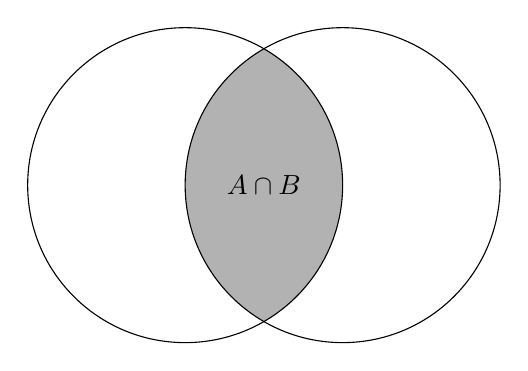
\begin{tikzpicture}
			\path[save path=\pathA](-1,0)circle(2cm);
			\path[save path=\pathB](+1,0)circle(2cm);
			\begin{scope}
				\clip[use path=\pathA];
				\fill[black!30][use path=\pathB];
			\end{scope}
			\draw[use path=\pathA];
			\draw[use path=\pathB];
			\draw(0,0)node{\(A \cap B\)};
		\end{tikzpicture}
		\subcaption{集合的交}
	\end{subfigure}%
	\begin{subfigure}[b]{\subwidth}
		\centering
		\begin{tikzpicture}
			\path[save path=\pathA,name path=A](-1,0)circle(2cm);
			\path[save path=\pathB,name path=B](+1,0)circle(2cm);
			\path[fill=black!30][use path=\pathA+\pathB];
			\draw[name intersections={of=A and B}]
				(intersection-1)arc[start angle=60,end angle=300,radius=2]
				(intersection-2)arc[start angle=-120,end angle=120,radius=2]
				(intersection-1);
			\draw(0,0)node{\(A \cup B\)};
			\pgfresetboundingbox
			\path[use as bounding box] (-3,-2)rectangle(3,2);
		\end{tikzpicture}
		\subcaption{集合的并}
	\end{subfigure}%

	\begin{subfigure}[b]{\linewidth}
		\centering
		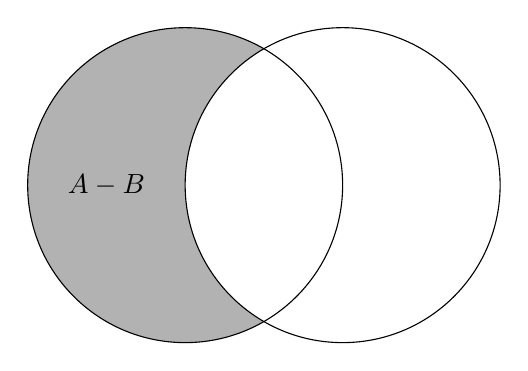
\begin{tikzpicture}
			\fill[black!30](0,{sqrt(3)})arc[start angle=60,end angle=300,radius=2]
				arc[start angle=240,end angle=120,radius=2];
			\draw(-1,0)circle(2cm);
			\draw(+1,0)circle(2cm);
			\draw(-2,0)node{\(A-B\)};
			\pgfresetboundingbox
			\path[use as bounding box] (-3,-2)rectangle(3,2);
		\end{tikzpicture}
		\subcaption{集合的差}
	\end{subfigure}%
	\caption{韦恩图}
	\label{figure:集合论.韦恩图}
\end{figure}

\begin{property}
集合的运算满足以下性质:
\begin{enumerate}
\item 幂等律
\begin{gather}
	A \cap A = A, \\
	A \cup A = A.
\end{gather}

\item 交换律({\rm Commutative laws})
\begin{gather}
	A \cap B = B \cap A, \label{equation:集合论.集合代数公式1-1} \\
	A \cup B = B \cup A. \label{equation:集合论.集合代数公式1-2}
\end{gather}

\item 结合律({\rm Associative laws})
\begin{gather}
	(A \cap B) \cap C = A \cap (B \cap C), \label{equation:集合论.集合代数公式2-1} \\
	(A \cup B) \cup C = A \cup (B \cup C). \label{equation:集合论.集合代数公式2-2}
\end{gather}

\item 分配律({\rm Distributive laws})
\begin{gather}
	(A \cap B) \cup C = (A \cup C) \cap (B \cup C), \label{equation:集合论.集合代数公式3-1} \\
	(A \cup B) \cap C = (A \cap C) \cup (B \cap C), \label{equation:集合论.集合代数公式3-2} \\
	A \cup \bigcap \mathscr{B} = \bigcap\Set{A \cup X \given X \in \mathscr{B}}, \quad(\mathscr{B}\neq\emptyset) \label{equation:集合论.集合代数公式3-3} \\
	A \cap \bigcup \mathscr{B} = \bigcup\Set{A \cap X \given X \in \mathscr{B}}, \label{equation:集合论.集合代数公式3-4} \\
	\Powerset (A \cup B) \supseteq \Powerset A \cup \Powerset B, \label{equation:集合论.集合代数公式3-5} \\ %@see: 《Elements of Set Theory》 P26. Exercise 7(b).
	\Powerset (A \cap B) = \Powerset A \cap \Powerset B. \label{equation:集合论.集合代数公式3-6} %@see: 《Elements of Set Theory》 P26. Exercise 7(a)
\end{gather}

\item 对偶律({\rm De Morgan's laws})(假设\(\mathscr{A}\neq\emptyset\))
\begin{gather}
	\overline{A \cap B} = \overline A \cup \overline B, \label{equation:集合论.集合代数公式4-1} \\
	\overline{A \cup B} = \overline A \cap \overline B, \label{equation:集合论.集合代数公式4-2} \\
	C - \bigcup\mathscr{A} = \bigcap\Set{C-X \given X\in\mathscr{A}}, \label{equation:集合论.集合代数公式4-3} \\
	C - \bigcap\mathscr{A} = \bigcup\Set{C-X \given X\in\mathscr{A}}. \label{equation:集合论.集合代数公式4-4}
\end{gather}

\item 与空集\(\emptyset\)和全集\(\Omega\)的运算(假设\(A \subseteq \Omega\))
\begin{gather}
	A \cup \emptyset = A, \label{equation:集合论.集合代数公式5-1} \\
	A \cap \emptyset = \emptyset, \label{equation:集合论.集合代数公式5-2} \\
	A \cup \Omega = \Omega, \label{equation:集合论.集合代数公式5-3} \\
	A \cap \Omega = A, \label{equation:集合论.集合代数公式5-4} \\
	A \cup \overline{A} = \Omega, \label{equation:集合论.集合代数公式5-5} \\
	A \cap \overline{A} = \emptyset, \label{equation:集合论.集合代数公式5-6} \\
	A \cup (A \cap B) = A, \\
	A \cap (A \cup B) = A, \\
	\overline{\emptyset} = \Omega, \\
	\overline{\Omega} = \emptyset, \\
	\overline{\overline{A}} = A.
\end{gather}

\item 包含关系
\begin{gather}
	A \subseteq B \implies A \cup C \subseteq B \cup C, \label{equation:集合论.集合代数公式6-1} \\
	A \subseteq B \implies A \cap C \subseteq B \cap C, \label{equation:集合论.集合代数公式6-2} \\
	A \subseteq B \implies \bigcup A \subseteq \bigcup B, \label{equation:集合论.集合代数公式6-3} \\
	A \subseteq B \implies \overline{B} \subseteq \overline{A}, \label{equation:集合论.集合代数公式6-4} \\
	\emptyset \neq A \subseteq B \implies \bigcap B \subseteq \bigcap A, \label{equation:集合论.集合代数公式6-5} \\
	A \cap B \subseteq A, \\
	A \subseteq A \cup B.
\end{gather}

\item 差集
\begin{gather}
	A - B \subseteq A, \\
	A - B = A \cap \overline{B}, \\
	A \cup B = B \iff A \subseteq B \iff A \cap B = A \iff A - B = \emptyset, \\
	A \oplus B = B \oplus A, \\
	(A \oplus B) \oplus C = A \oplus (B \oplus C), \\
	A \oplus \emptyset = A, \\
	A \oplus A = \emptyset, \\
	A \oplus B = A \oplus C \iff B = C.
\end{gather}
\end{enumerate}
\begin{proof}
对\cref{equation:集合论.集合代数公式1-1} 证明如下:
\begin{align*}
	x \in A \cap B
	&\iff x \in A \land x \in B \\
	&\iff x \in B \land x \in A \\
	&\iff x \in B \cap A.
\end{align*}

对\cref{equation:集合论.集合代数公式1-2} 证明如下:
\begin{align*}
	x \in A \cup B
	&\iff x \in A \lor x \in B \\
	&\iff x \in B \lor x \in A \\
	&\iff x \in B \cup A.
\end{align*}

对\cref{equation:集合论.集合代数公式2-1} 证明如下:
\begin{align*}
	x \in (A \cap B) \cap C
	&\iff x \in A \cap B \land x \in C \\
	&\iff (x \in A \land x \in B) \land x \in C \\
	&\iff x \in A \land (x \in B \land x \in C) \\
	&\iff x \in A \land x \in B \cap C \\
	&\iff x \in A \cap (B \cap C).
\end{align*}

对\cref{equation:集合论.集合代数公式2-2} 证明如下:
\begin{align*}
	x \in (A \cup B) \cup C
	&\iff x \in A \cup B \lor x \in C \\
	&\iff (x \in A \lor x \in B) \lor x \in C \\
	&\iff x \in A \lor (x \in B \lor x \in C) \\
	&\iff x \in A \lor x \in B \cup C \\
	&\iff x \in A \cup (B \cup C).
\end{align*}

对\cref{equation:集合论.集合代数公式3-5} 证明如下:
\begin{align*}
	x \in \Powerset A \cup \Powerset B
	&\iff x \in \Powerset A \lor x \in \Powerset B \\
	&\iff x \subseteq A \lor x \subseteq B \\
	&\implies x \subseteq A \cup B \\
	&\iff x \in \Powerset (A \cup B),
\end{align*}
注意到中间步骤的\(\implies\)通常不是可逆的,
这是因为只要取\(a \subseteq A - B, b \subseteq B - A, x = a \cup b\),
就有\(x \subseteq A \cup B\)但是\(x \not\subseteq A \land x \not\subseteq B\),
因此\(x \subseteq A \cup B \notimplies x \subseteq A \lor x \subseteq B\).
%从上面的证明过程可以看出,
%要使\(\Powerset (A \cup B) = \Powerset A \cup \Powerset B\)成立,
%必有\[
%	\forall x \bigl(
%		x \subseteq A \cup B
%		\iff
%		x \subseteq A \lor x \subseteq B
%	\bigr)
%\]成立.
%取\(x = A \cup B\),
%由\(x \subseteq A \lor x \subseteq B\)
%可得\[
%	A \cup B = A \lor A \cup B = B.
%\]
%因此,当且仅当\(A \cup B \in \Set{A,B}\)时,
%就有\(\Powerset (A \cup B) = \Powerset A \cup \Powerset B\)成立.

对\cref{equation:集合论.集合代数公式3-6} 证明如下:
\begin{align*}
	x \in \Powerset (A \cap B)
	&\iff x \subseteq A \cap B \\
	&\iff x \subseteq A \land x \subseteq B \\
	&\iff x \in \Powerset A \land x \in \Powerset B \\
	&\iff x \in \Powerset A \cap \Powerset B.
\end{align*}

对\cref{equation:集合论.集合代数公式6-5} 证明如下:
\begin{align*}
	A \subseteq B
	&\iff (\forall t)[t \in A \implies t \in B] \\
	&\implies (\forall x)[
		(\forall b)[b \in B \implies x \in b]
		\implies
		(\forall a)[a \in A \implies x \in a]
	] \\
	&\iff (\forall x)[x \in \bigcap B \implies x \in \bigcap A].
	\qedhere
\end{align*}
\end{proof}
\end{property}

\begin{example}
%@see: 《Elements of Set Theory》 P32. Exercise 21.
设\(A,B\)是集合.
证明:\begin{equation}\label{equation:集合论.并集的并等于并的并集}
	\bigcup(A \cup B) = \bigcup A \cup \bigcup B.
\end{equation}
\begin{proof}
直接计算得
\begin{align*}
	x \in \bigcup(A \cup B)
	&\iff
	(\exists t)[t \in A \cup B \implies x \in t] \\
	&\iff
	(\exists t)[t \in A \lor t \in B \implies x \in t] \\
	&\iff
	(\exists t)[t \in A \implies x \in t] \lor (\exists t)[t \in B \implies x \in t] \\
	&\iff
	x \in \bigcup A \lor x \in \bigcup B \\
	&\iff
	x \in \bigcup A \cup \bigcup B.
	\qedhere
\end{align*}
\end{proof}
\end{example}

\begin{example}
%@see: 《Elements of Set Theory》 P32. Exercise 22.
设\(A,B\)是非空集合.
证明:\begin{equation}
	\bigcap(A \cup B) = \bigcap A \cap \bigcap B.
\end{equation}
%\begin{proof}
%直接计算得
%\begin{align*}
%	x \in \bigcap(A \cup B)
%	&\iff
%	x \in \bigcap A \land x \in \bigcap B \\
%	&\iff
%	x \in \bigcap A \cap \bigcap B.
%	\qedhere
%\end{align*}
%\end{proof}
\end{example}

\begin{example}
证明:\begin{equation}
	(A \cup B) - (A \cap B) = (A-B)\cup(B-A).
\end{equation}
\begin{proof}
根据集合交、并、差的定义,有
\begin{align*}
	x \in (A \cup B) - (A \cap B)
	&\iff x \in (A \cup B) \land x \notin (A \cap B) \\
	&\iff (x \in A \lor x \in B) \land \neg(x \in A \land x \in B) \\
	&\iff (x \in A \land \neg(x \in A \land x \in B))
	 \lor (x \in B \land \neg(x \in A \land x \in B)) \\
	&\iff (x \in A \land (x \notin A \lor x \notin B))
	 \lor (x \in B \land (x \notin A \lor x \notin B)) \\
	&\iff (x \in A \land x \notin B) \lor (x \in B \land x \notin A) \\
	&\iff x \in (A-B)\cup(B-A).
\qedhere
\end{align*}
\end{proof}
\end{example}

\section{关系}
\subsection{无序对、有序对的概念}
\begin{definition}
由两个元素\(x_1\)和\(x_2\)组成的集合\[
\Set{x_1, x_2}
\]称作\DefineConcept{无序对}(unordered pair).
\end{definition}

\begin{example}
%@see: 《Elements of Set Theory》 P38. Exercise 1.
定义:\[
	\opair{x,y,z}^* = \{\{x\},\{x,y\},\{x,y,z\}\}.
\]
找出元素\(u,v,w,x,y,z\)使\[
	\opair{x,y,z}^* = \opair{u,v,w}^*
\]成立,
但\(y \neq v\)或\(z \neq w\).
\begin{solution}
取\[
	\opair{1,1,2}^* = \{\{1\},\{1,1\},\{1,1,2\}\} = \{\{1\},\{1,2\}\},
\]\[
	\opair{1,2,1}^* = \{\{1\},\{1,2\},\{1,2,1\}\} = \{\{1\},\{1,2\}\},
\]
即可满足题设条件.
\end{solution}
\end{example}

\begin{definition}
两个元素\(x_1\)和\(x_2\)按一定顺序形成的排列称为\DefineConcept{有序对},
记作\[
	\opair{x_1,x_2}.
\]

我们可以采用多种方式构造集合用于表记有序对\(\opair{x_1,x_2}\),
例如(由Norbert Wiener于1914年构造的)
\[
	\Set{ \Set{ \Set{x_1}, \emptyset }, \Set{ \Set{ x_2 } } }.
\]
但我们更常用(由Kazimierz Kuratowski于1921年构造的)以下形式
\[
	\Set{ \Set{x_1}, \Set{x_1, x_2} }.
\]
以后我们都采用第二种形式表记有序对,因此\[
	\opair{x_1,x_2}
	\defeq
	\Set{ \Set{x_1}, \Set{x_1, x_2} }.
\]
\end{definition}

有序对具有以下性质.
\begin{property}\label{theorem:集合论.有序对的性质1}
%@see: 《Elements of Set Theory》 P36. Theorem 3A
\(\opair{u,v} = \opair{x,y}\)的充要条件是:\(u=x\)且\(v=y\).
\begin{proof}
充分性.
这个方向的证明是平凡的;
当\(u=x\)且\(v=y\)时,自然有\[
	\opair{u,v} = \opair{x,y}.
\]

必要性.
当\(\opair{u,v} = \opair{x,y}\)时,根据定义有\[
	\Set{ \Set{u}, \Set{u, v} }
	= \Set{ \Set{x}, \Set{x, y} };
\]于是\[
	\Set{u} \in \Set{ \Set{x}, \Set{x, y} },
	\eqno{(1)}
\]且\[
	\Set{u,v} \in \Set{ \Set{x}, \Set{x, y} }.
	\eqno{(2)}
\]
从(1)式我们知道,
要么等式\[
	\Set{u} = \Set{x}
	\eqno{(3)}
\]成立,
要么等式\[
	\Set{u} = \Set{x,y}
	\eqno{(4)}
\]成立;
从(2)式我们知道,
要么等式\[
	\Set{u,v} = \Set{x}
	\eqno{(5)}
\]成立,
要么等式\[
	\Set{u,v} = \Set{x,y}
	\eqno{(6)}
\]成立.

首先我们假设(4)式成立,那么有\(u = x = y\);
从而有(5)式等价于(6)式,且\(u = v = x = y\);
在这种情况下,必要性得证.
同理,假设(5)式成立,也可证明必要性.

然后我们假设(3)式、(6)式同时成立.
从(3)式成立我们知道\(u = x\).
从(6)式成立我们知道\(u = y\)或\(v = y\);
第一种情况,即\(u = x\)和\(u = y\)同时成立的情况,已经在(4)式成立时作了讨论.
第二种情况,即\(u = x\)和\(v = y\)同时成立的情况,立即保证了必要性.
\end{proof}
\end{property}
\cref{theorem:集合论.有序对的性质1} 让我们可以不含糊地将有序对\(\opair{x,y}\)
中的\(x\)和\(y\)分别称为%
有序对的\DefineConcept{第一坐标}(first coordinate)%
和\DefineConcept{第二坐标}(second coordinate).

\subsection{直积}
\begin{definition}\label{definition:集合论.直积}
设\(A,B\)都是集合.
在\(A\)中任取一个元素\(x\),
在\(B\)中任取一个元素\(y\),
组成一个有序对\(\opair{x,y}\),
把这样的有序对作为新的元素,
它们全体组成的类称为
“\(A\)与\(B\)的\DefineConcept{直积}(direct product)”,
或“\(A\)与\(B\)的\DefineConcept{笛卡尔乘积}(Cartesian product)”,
记为\(A \times B\),
即\begin{equation}
	A \times B
	\defeq
	\Set*{ \opair{x,y} \given x \in A \land y \in B }.
\end{equation}
%@see: https://mathworld.wolfram.com/DirectProduct.html
\end{definition}

在宣称\cref{definition:集合论.直积} 合法以前,
我们必须确认它给出的类\(A \times B\)是不是真的是一个集合.
而要证明\(A \times B\)是一个集合,
我们就必须找到一个足够大的集合,
它包括了我们需要的全部有序对,
然后利用子集公理证明\(A \times B\)是这个集合的子集.
为此我们给出下述引理.
\begin{lemma}\label{theorem:集合论.有序对是其坐标元素所在集合的二重幂集的元素}
%@see: 《Elements of Set Theory》 P37. Lemma 3B
如果\(x,y \in A\),那么\(\opair{x,y} \in \Powerset\Powerset A\).
\begin{proof}
由\(x,y \in A\)可知\(\{x\},\{x,y\} \subseteq A\),
即\(\{x\},\{x,y\} \in \Powerset A\),
那么\(\{\{x\},\{x,y\}\} \subseteq \Powerset A\),
进一步可得\(\opair{x,y} = \{\{x\},\{x,y\}\} \in \Powerset\Powerset A\).
\end{proof}
\end{lemma}

\begin{theorem}\label{theorem:集合论.直积存在定理}
%@see: 《Elements of Set Theory》 P38. Corollary 3C
设\(A,B\)都是集合,那么存在这样一个集合\(C\),使得\(C = A \times B\).
\begin{proof}
要使\(C = A \times B\),根据外延公理必有\[
	w \in C \iff w \in A \times B,
\]
再根据直积的定义有\[
	w \in C \iff w = \opair{x,y} \land x \in A \land y \in B.
\]
根据子集公理,我们可以构造集合\[
	C = \Set*{
		w \in \Powerset\Powerset(A \cup B)
		\given
		w = \opair{x,y} \land x \in A \land y \in B
	}.
\]
显然,根据\cref{theorem:集合论.有序对是其坐标元素所在集合的二重幂集的元素},
\(C\)满足定理要求的条件.
\end{proof}
\end{theorem}
\cref{theorem:集合论.直积存在定理} 告诉我们,
任意两个集合\(A\)和\(B\)的直积\(A \times B\)也是集合.

容易发现,对于任意集合\(A\),总有\begin{equation}
	A \times \emptyset
	= \emptyset \times A
	= \emptyset \times \emptyset
	= \emptyset.
\end{equation}
这是因为\((\forall x)[x \notin \emptyset]\).

\begin{example}
设\(A,B,C\)是集合.
证明:\begin{equation}
	A \subseteq B
	\implies
	A \times C \subseteq B \times C.
\end{equation}
\begin{proof}
直接计算得
\begin{align*}
	A \subseteq B
	&\iff [x \in A \implies x \in B] \\
	&\implies [x \in A \land y \in C \implies x \in B \land y \in C] \\
	&\iff [\opair{x,y} \in A \times C \implies \opair{x,y} \in B \times C] \\
	&\iff [A \times C \subseteq B \times C].
	\qedhere
\end{align*}
\end{proof}
\end{example}

\begin{example}
%@see: 《Elements of Set Theory》 P38. Exercise 2.(a)
%@see: 《Elements of Set Theory》 P65. Exercise 54.
设\(A,B,C\)是集合.
证明:\begin{gather}
	A \times (B \cup C) = (A \times B) \cup (A \times C),
	\label{equation:集合论.直积分配律1} \\
	A \times (B \cap C) = (A \times B) \cap (A \times C),
	\label{equation:集合论.直积分配律2} \\
	A \times (B - C) = (A \times B) - (A \times C).
	\label{equation:集合论.直积分配律3}
\end{gather}
\begin{proof}
对\cref{equation:集合论.直积分配律1} 证明如下:
由于对于任意\(w = \opair{x,y}\)总有
\begin{align*}
	w \in A \times (B \cup C)
	&\iff x \in A \land y \in B \cup C \\
	&\iff x \in A \land (y \in B \lor y \in C) \\
	&\iff (x \in A \land y \in B) \lor (x \in A \land y \in C) \\
	&\iff (w \in A \times B) \lor (w \in A \times C),
\end{align*}
那么由外延公理可知\(A \times (B \cup C) = (A \times B) \cup (A \times C)\).

对\cref{equation:集合论.直积分配律2} 证明如下:
由于对于任意\(w = \opair{x,y}\)总有
\begin{align*}
	w \in A \times (B \cap C)
	&\iff x \in A \land y \in B \cap C \\
	&\iff x \in A \land (y \in B \land y \in C) \\
	&\iff (x \in A \land y \in B) \land (x \in A \land y \in C) \\
	&\iff (w \in A \times B) \land (w \in A \times C),
\end{align*}
那么由外延公理可知\(A \times (B \cap C) = (A \times B) \cap (A \times C)\).

对\cref{equation:集合论.直积分配律3} 证明如下:
由于对于任意\(w = \opair{x,y}\)总有
\begin{align*}
	w \in A \times (B - C)
	&\iff x \in A \land y \in (B - C) \\
	&\iff x \in A \land (y \in B \land y \notin C) \\
	&\iff (x \in A \land y \in B \land x \notin A)
		\lor (x \in A \land y \in B \land y \notin C) \\
	&\iff (x \in A \land y \in B) \land (x \notin A \lor y \notin C) \\
	&\iff (x \in A \land y \in B) \land \neg(x \in A \land y \in C) \\
	&\iff w \in A \times B \land w \notin A \times C,
\end{align*}
那么由外延公理可知\(A \times (B - C) = (A \times B) - (A \times C)\).
\end{proof}
\end{example}

\begin{example}
%@see: 《Elements of Set Theory》 P38. Exercise 2.(b)
证明:如果\(A \times B = A \times C\)且\(A \neq \emptyset\),则\(B = C\).
%TODO
\end{example}

\begin{example}
%@see: 《Elements of Set Theory》 P38. Exercise 3.
证明:\(A \times \bigcup B = \bigcup\Set{ A \times X \given X \in B }\).
%TODO
\end{example}

\begin{example}
%@see: 《Elements of Set Theory》 P38. Exercise 5.(a)
设\(A,B\)都是集合,试证:\(\Set{ \{x\} \times B \given x \in A }\)也是集合.
\begin{proof}
由于\(x \in A \implies \{x\} \subseteq A \implies \{x\} \times B \subseteq A \times B\),
所以我们可以利用子集公理构造集合\[
	\Set{ w \in A \times B \given w = \opair{u,v} \land u = x }.
	\qedhere
\]
\end{proof}
\end{example}

\subsection{关系}
\begin{definition}
\DefineConcept{关系}(relation)是有序对的集合.
\end{definition}

如果有序对\(\opair{x,y}\)是关系\(\rel{R}\)的元素,即\[
	\opair{x,y} \in \rel{R},
\]
那么称“\(x\)与\(y\)有\(\rel{R}\)关系”,
记作\(x\rel{R}y\);
反之,\[
	\opair{x,y} \notin \rel{R},
\]
那么称“\(x\)与\(y\)没有\(\rel{R}\)关系”.

给定集合\(X\)和集合\(Y\),
如果关系\(\rel{R}\)满足\[
	\rel{R} \subseteq X \times Y,
\]
我们就称“\(\rel{R}\)是\(X\)与\(Y\)之间的\DefineConcept{二元关系}(binary relation)”.
特别地,当\(X = Y\)时,就称“\(\rel{R}\)是\(X\)上的\DefineConcept{二元关系}”.

从关系的定义可以看出,关系是有序对的集合.
即便是看起来毫无意义的,只由一个有序对组成的集合,也可以看成是一个关系.
我们自然会认为有的关系比别的关系更有意义,
例如我们马上会提到的“映射”“等价关系”和“排序关系”.

\begin{definition}\label{definition:集合论.定义域与值域的定义}
设\(R\)是集合.

如果集合\(A\)满足\[
	x \in A \iff (\exists y)[\opair{x,y} \in R],
\]
那么称\(A\)为“\(R\)的\DefineConcept{定义域}(domain)”,记作\(\dom R\).

如果集合\(B\)满足\[
	x \in B \iff (\exists t)[\opair{t,x} \in R],
\]
那么称\(B\)为“\(R\)的\DefineConcept{值域}(range)”,记作\(\ran R\).

最后,我们把\(R\)的定义域与它的值域的并集称为
“\(R\)的\DefineConcept{域}(field)”,记作\(\fld R\),即\[
	\fld R \defeq \dom R \cup \ran R.
\]
\end{definition}

为了正当化\cref{definition:集合论.定义域与值域的定义},
我们必须明确:对于任意集合\(R\),存在这样一个集合,
\(R\)中的有序对的第一坐标和第二坐标都是这个集合的元素.
这个问题类似于我们之前对于直积\(A \times B\)的定义的正当化,
当时我们证明了\cref{theorem:集合论.直积存在定理}.
为此,我们给出下述引理,
可以注意到它与\cref{theorem:集合论.有序对是其坐标元素所在集合的二重幂集的元素} 的关联.

\begin{lemma}
%@see: 《Elements of Set Theory》 P41. Lemma 3D
如果\(\opair{x,y} \in A\),那么\(x,y \in \bigcup\bigcup A\).
\end{lemma}
这条引理已经在\cref{example:集合论.有序对各坐标的取值范围} 得到证明.
利用这条引理,再加上子集公理,我们可以构造集合\(R\)的定义域和值域:
\begin{gather}
	\dom R
	\defeq
	\Set*{ x \in \bigcup\bigcup R \given (\exists y)[\opair{x,y} \in R] }, \\
	\ran R
	\defeq
	\Set*{ x \in \bigcup\bigcup R \given (\exists t)[\opair{t,x} \in R] }.
\end{gather}

\begin{example}
%@see: 《Elements of Set Theory》 P41. Exercise 6.
试证:集合\(A\)是一个关系的充要条件是\[
	A \subseteq \dom A \times \ran A.
\]
%TODO
\end{example}

\begin{example}
%@see: 《Elements of Set Theory》 P41. Exercise 7.
试证:给定关系\(\rel{R}\),总有\[
	\fld \rel{R} = \bigcup\bigcup \rel{R}.
\]
%TODO
\end{example}

\begin{example}
%@see: 《Elements of Set Theory》 P41. Exercise 8.
试证:对于任意集合\(A\),总有\begin{gather}
	\dom\bigcup A = \bigcup\Set{ \dom\rel{R} \given \rel{R} \in A }, \\
	\ran\bigcup A = \bigcup\Set{ \ran\rel{R} \given \rel{R} \in A }.
\end{gather}
%TODO
\end{example}

\subsection{多元关系}
我们可以将“有序对”和“二元关系”的概念分别扩展为“元组”和“多元关系”.

例如定义\[
	\opair{x_1,x_2,x_3}
	\defeq
	\opair{\opair{x_1,x_2},x_3},
\]
称之为\DefineConcept{三元组}(triple);
定义\[
	\opair{x_1,x_2,x_3,x_4}
	\defeq
	\opair{\opair{x_1,x_2,x_3},x_4},
\]
称之为\DefineConcept{四元组}(quadruple);
定义\[
	\opair{x_1,x_2,x_3,x_4,x_5}
	\defeq
	\opair{\opair{x_1,x_2,x_3,x_4},x_5},
\]
称之为\DefineConcept{五元组}(quintuple);
以此类推,对于任意给定\(n\),可以定义\(n\)元组(\(n\)-tuple):\[
	\opair{x_1,x_2,\dotsc,x_n}
	\defeq
	\opair{\opair{x_1,x_2,\dotsc,x_{n-1}},x_n}.
\]
为了让我们的定义看起来整齐划一,我们还可以补充定义\[
	\opair{x} \defeq x,
\]
称之为\DefineConcept{一元组}(1-tuple).

我们把“在\(A\)上的\(n\)元\DefineConcept{关系}(n-ary \emph{relation} on \(A\))”%
定义为由\(n\)元组构成的集合.
由于\(A\)上的二元关系是\(A \times A\)的子集,
以及\(A\)上的三元关系(ternary relation, 3-ary relation)是\((A \times A) \times A\)的子集,
所以三元关系也可归结为一种二元关系;
同理,其他\(n\)元关系,只要\(n>1\),也都可以归结为二元关系.
虽然在上面对\(n\)元关系的定义中,
我们也把由\(A\)中包括的一元组构成的集合称为%
“\(A\)上的一元关系(unary relation, 1-ary relation)”,
但它只是\(A\)的一个子集,根本不满足关系的定义.

\section{映射}
\subsection{映射的概念}
\begin{definition}
设\(F\)是关系,如果\[
	(\forall x \in \dom F)(\exists! y)[\opair{x,y} \in F],
\]
则称“关系\(F\)是一个\DefineConcept{映射}(function)”.
\end{definition}
可以从映射的定义中看出,虽然映射也是关系,
但映射有一般的关系所没有的特殊性质:
映射是\DefineConcept{单值的}(single-valued).
换句话说,对于关系\(F\),每个\(x\)可能对应若干个\(y\);
但是,对于映射\(F\),每个\(x\)就只对应一个\(y\).
我们可以把\(x\)与\(y\)这两个元素之间的对应关系记为\(x \mapsto y\).

我们把使得\(xFy\)成立的\(y\)称为“\(x\)(在映射\(F\)下)的\DefineConcept{像}%
(the \emph{value} of \(F\) at \(x\))”,
记为\(F(x)\),即\[
	y = f(x);
\]
称\(x\)为“\(y\)(在映射\(F\)下)的一个\DefineConcept{原像}”.
这里用的\(F(x)\)符号是欧拉提出的,
我们仅当\(F\)是一个映射且\(x\in\dom F\)时使用这个记号.
不过,我们也可以定义:\[
	F(x) \defeq \bigcup\Set{ y \given \opair{x,y} \in F }.
\]
它对于任意\(F\)和\(x\)都有意义.

映射是如此重要,以至于各家对用于描述映射的术语没有达成统一.
以下是两种最常采用的术语.

设\(X,Y\)都是集合,
如果\(f\)是一个映射,且\(\dom f = X\),\(\ran f \subseteq Y\),
则称“\(f\)是从\(X\)到\(Y\)的\DefineConcept{映射}%
(\(f\) is a function \emph{from} \(X\) \emph{into} \(Y\))”,
或称“\(f\)将\(X\)映射到\(Y\)里%
(\(f\) \emph{maps} \(X\) \emph{into} \(Y\))”,
记作\[
	f\colon X \to Y.
\]
如果还有\(\ran f = Y\),
那么称“\(f\)是从\(X\)到\(Y\)上的映射%
(\(f\) is a function from \(X\) \emph{onto} \(Y\))”,
或称“\(f\)将\(X\)映射到\(Y\)上%
(\(f\) \emph{maps} \(X\) \emph{onto} \(Y\))”,
或称“\(f\)是\DefineConcept{满射}(surjective)”.
我们可以说“任意映射总将它的定义域映射到它的值域上”,
还可以说“任意映射总把它的定义域映射到以它的值域为子集的任意集合\(B\)里”.
注意到两种说法的区别,“上”字和“里”字的选用,
不光取决于映射\(f\)本身,还取决于我们讨论的集合\(B\).

如果\[
	(\forall y \in \ran f)
	(\exists! x)
	[\opair{x,y} \in f],
\]
那么称“映射\(f\)是\DefineConcept{一一映射}(one-to-one)”.

有时候我们希望把一一映射的概念套用到一般的关系上,
它们往往不是映射,因此“一一映射”这个用词就显得不那么恰当了.
为此,我们创造出“单根的”,类比于“单值的”.

\begin{definition}
如果集合\(R\)满足\[
	(\forall y \in \ran R)
	(\exists! x)
	[\opair{x,y} \in R],
\]
则称“\(R\)是\DefineConcept{单根的}(single-rooted)”.
\end{definition}

因此,我们可以说,“一个映射是单根的”当且仅当“这个映射是一一映射”.

如果\[
	(\forall x_1, x_2 \in \dom f)
	[x_1 \neq x_2 \implies f(x_1) \neq f(x_2)],
\]
那么称“\(f\)是\DefineConcept{单射}(injective)”.
由于映射本就是单值的,若它还是单根的,那么这个映射就是单射;
换句话说,一一映射和单射是相同的概念.

如果\(f\)既是单射,又是满射,即
那么称“\(f\)是\DefineConcept{双射}(bijective)\footnote{%
有的书可能会把双射称作一一映射,但是我们不采取这种说法.
}”.


\begin{example}
设\(f\colon A \to B, g\colon B \to C\).
证明:\begin{enumerate}
	\item 如果\(f\)和\(g\)都是单射,那么\(g \circ f\)也是单射;
	\item 如果\(f\)和\(g\)都是满射,那么\(g \circ f\)也是满射;
	\item 如果\(f\)和\(g\)都是双射,那么\(g \circ f\)也是双射;
	\item 如果\(f\)和\(g\)都是可逆映射,那么\(g \circ f\)也是可逆映射.
\end{enumerate}
\begin{proof}
当\(f\)和\(g\)都是单射时.设\(a_1,a_2 \in A\).
如果\((g \circ f)(a_1) = (g \circ f)(a_2)\),那么\(g[f(a_1)] = g[f(a_2)]\).
由于\(g\)是单射,因此\(f(a_1) = f(a_2)\).
由于\(f\)是单射,因此\(a_1 = a_2\).
综上,\(g \circ f\)是单射.

当\(f\)和\(g\)都是满射时.任取\(c \in C\).
由于\(g\)是满射,因此存在\(b \in B\),使得\(c = g(b)\).
由于\(f\)是满射,因此存在\(a \in A\),使得\(b = f(a)\).
因此\(c = g(b) = g[f(a)] = (g \circ f)(a)\),也就是说\(g \circ f\)是满射.

双射的情形,根据单射、满射的情形显然成立.

可逆映射的情形,根据双射的情形以及\cref{theorem:集合论.映射可逆的充要条件} 即得.
\end{proof}
\end{example}

\begin{example}
%@see: 《Elements of Set Theory》 P52. Exercise 11
设\(F,G\)都是映射,
\(\dom F = \dom G = X\),且\[
	(\forall x \in X)[F(x) = G(x)].
\]
证明:\(F=G\).
%TODO
\end{example}

\begin{example}
%@see: 《Elements of Set Theory》 P52. Exercise 12
设\(f,g\)都是映射.
证明:\[
	f \subseteq g
	\iff
	\dom f \subseteq \dom g
	\land
	(\forall x \in \dom f)
	[f(x) = g(x)].
\]
%TODO
\end{example}

\begin{example}
%@see: 《Elements of Set Theory》 P53. Exercise 13
设\(f,g\)都是映射,\(f \subseteq g\)且\(\dom g \subseteq \dom f\).
证明:\(f=g\).
%TODO
\end{example}

\begin{example}
%@see: 《Elements of Set Theory》 P53. Exercise 14
设\(f,g\)都是映射.
证明:
\begin{enumerate}
	\item \(f \cap g\)是映射.
	\item \(f \cup g\)是映射的充要条件是\[
		(\forall x \in (\dom f)\cap(\dom g))[f(x)=g(x)].
	\]
\end{enumerate}
%TODO
\end{example}

\begin{example}
%@see: 《Elements of Set Theory》 P53. Exercise 15
\def\A{\mathscr{A}}%
设\(\A\)是一组映射,且\[
	(\forall f,g\in\A)[f \subseteq g \lor g \subseteq f].
\]
证明:\(\bigcup\A\)也是映射.
%TODO
\end{example}

\begin{example}
%@see: 《Elements of Set Theory》 P53. Exercise 16
证明:不存在一个集合,使得每个映射都属于它.
%TODO
\end{example}

\subsection{逆,复合,限制,像,原像}
以下定义的操作通常用在映射上,有时候也用于关系,但也可以用于任意集合.
\begin{definition}
设\(A,F,G\)都是集合.
\begin{enumerate}
	\item 称集合\[
		\Set*{ \opair{u,v} \given \opair{v,u} \in F }
	\]为“\(F\)的\DefineConcept{逆}%
	(the \emph{inverse} of \(F\))”,
	记作\(F^{-1}\).

	特别地,如果\(F^{-1}\)是映射,
	则称“\(F^{-1}\)是\(F\)的\DefineConcept{逆映射}”.

	\item 称集合\[
		\Set*{ \opair{u,v} \given (\exists t)[\opair{u,t} \in G \land \opair{t,v} \in F] }
	\]为“\(F\)和\(G\)的\DefineConcept{复合}%
	(the \emph{composition} of \(F\) and \(G\))”,
	记作\(F \circ G\).

	\item 称集合\[
		\Set*{ \opair{u,v} \given \opair{u,v} \in F \land u \in A }
	\]为“\(F\)在\(A\)上的\DefineConcept{限制}%
	(the \emph{restriction} of \(F\) to \(A\))”,
	记作\(F \upharpoonright A\).

	\item 称集合\[
		\Set*{ v \given (\exists u \in A)[\opair{u,v} \in F] }
	\]为“\(A\)在\(F\)下的\DefineConcept{像}%
	(the \emph{image} of \(A\) \emph{under} \(F\))”,
	记作\(F\ImageOfSetUnderRelation{A}\).
\end{enumerate}
\end{definition}

当\(F\)是一个映射,且\(A \subseteq \dom F\)时,
\(F\ImageOfSetUnderRelation{A}\)这个概念可能更容易理解,
因为这时候\[
	F\ImageOfSetUnderRelation{A}
	= \Set{ F(u) \given u \in A }.
\]

我们可以利用子集公理构造出上述定义下的所需集合的存在性.
特别地,\[
	F^{-1} \subseteq \ran F \times \dom F, \qquad
	F \circ G \subseteq \dom G \times \ran F,
\]\[
	F \upharpoonright A \subseteq F, \qquad
	F\ImageOfSetUnderRelation{A} \subseteq \ran F.
\]

例如,我们可以按如下方法正当化“关系\(F\)的逆”的定义:
根据子集公理,存在集合\(B\),使得对于任意\(x\),总有\begin{align*}
	x \in B
	&\iff
	[x \in \ran F \times \dom F]
	\land
	(\exists u)(\exists v)[x = \opair{u,v} \land \opair{v,u} \in F], \\
	&\iff
	(\exists u)(\exists v)[x = \opair{u,v} \land \opair{v,u} \in F].
\end{align*}
再根据外延公理,可以保证集合\(B\)的唯一性.
因此我们可以将集合\(B\)记为\(F^{-1}\).

\begin{theorem}
\(F \upharpoonright \emptyset = \emptyset\).
\end{theorem}

\begin{theorem}
\(F\ImageOfSetUnderRelation{A} = \ran(F \upharpoonright A)\).
\begin{proof}
根据值域的定义有\begin{align*}
	v \in \ran(F \upharpoonright A)
	&\iff
	(\exists u)[\opair{u,v} \in F \upharpoonright A] \\
	&\iff
	(\exists u)[\opair{u,v} \in F \land u \in A] \\
	&\iff
	v \in F\ImageOfSetUnderRelation{A}.
	\qedhere
\end{align*}
\end{proof}
\end{theorem}

\begin{definition}
设\(F\)是关系,\(A\)是集合,那么称集合\[
	\Set*{ x \in \dom F \given F(x) \in A }
\]为“集合\(A\)在关系\(F\)下的\DefineConcept{原像}%
(the \emph{inverse image} of \(A\) under \(F\))”,
记作\(F^{-1}\ImageOfSetUnderRelation{A}\).
\end{definition}

\begin{theorem}\label{theorem:集合论.关系的逆的定义域值域以及关系的二重逆}
%@see: 《Elements of Set Theory》 P46. Theorem 3E
设\(F\)是集合,则有\begin{gather}
	\dom F^{-1} = \ran F, \\
	\ran F^{-1} = \dom F.
\end{gather}

如果\(F\)是关系,则有\begin{equation}
	(F^{-1})^{-1} = F.
\end{equation}
\end{theorem}

\begin{theorem}\label{theorem:集合论.关系及其逆是映射的充要条件}
%@see: 《Elements of Set Theory》 P46. Theorem 3F
设\(F\)是集合,则“\(F^{-1}\)是映射”的充要条件是:\(F\)是单根的.

设\(F\)是关系,则“\(F\)是映射”的充要条件是:\(F^{-1}\)是单根的.
\end{theorem}

\begin{theorem}\label{theorem:集合论.映射可逆的充要条件}
映射\(f\)可逆的充要条件是:\(f\)是双射.
\end{theorem}

\begin{theorem}\label{theorem:集合论.逆映射的计算}
%@see: 《Elements of Set Theory》 P46. Theorem 3G
设\(F\)是一一映射.
\begin{enumerate}
	\item 如果\(x \in \dom F\),那么\[
		F^{-1}(F(x)) = x.
	\]

	\item 如果\(y \in \ran F\),那么\[
		F(F^{-1}(y)) = y.
	\]
\end{enumerate}
\begin{proof}
假设\(x \in \dom F\),
那么\(\opair{x,F(x)} \in F\),且\(\opair{F(x),x} \in F^{-1}\),
于是\(F(x) \in \dom F^{-1}\).
因为\(F\)是一一映射,是单值的,所以\(F^{-1}\)是映射,
从而\(x = F^{-1}(F(x))\).

如果\(y \in \ran F\),
那么根据本定理第1条,以及\((F^{-1})^{-1} = F\),可知\[
	F(F^{-1}(y)) = (F^{-1})^{-1}(F^{-1}(y)) = y.
	\qedhere
\]
\end{proof}
\end{theorem}

\begin{theorem}\label{theorem:集合论.映射的复合也是映射}
%@see: 《Elements of Set Theory》 P47. Theorem 3H
设\(F,G\)都是映射,则\(F \circ G\)是映射,且\[
	\dom(F \circ G)
	= \Set*{ x \in \dom G \given G(x) \in \dom F },
\]\[
	(\forall x \in \dom(F \circ G))
	[(F \circ G)(x) = F(G(x))].
\]
\begin{proof}
要证\(F \circ G\)是一个映射,
假设有\(\opair{x,y} \in F \circ G\)和\(\opair{x,z} \in F \circ G\)同时成立.
那么,\[
	(\exists p)[\opair{x,p} \in G \land \opair{p,y} \in F]
	\quad\text{和}\quad
	(\exists q)[\opair{x,q} \in G \land \opair{q,z} \in F]
\]同时成立.
既然\(G\)是映射,必有\(p = q\).
同理,\(F\)是映射,必有\(y = z\).
因此\(F \circ G\)是映射.

现在再假设\(x \in \dom G\)且\(G(x) \in \dom F\).
我们必须证明\[
	x \in \dom(F \circ G)
	\quad\text{和}\quad
	(F \circ G)(x) = F(G(x)).
\]
我们知道\[
	\opair{x,G(x)} \in G,
	\qquad
	\opair{G(x),F(G(x))} \in F.
\]
因此\(\opair{x,F(G(x))} \in F \circ G\).

反过来说,如果\(x \in \dom(F \circ G)\),
那么就有\[
	(\exists y)(\exists t)
	[\opair{x,t} \in G \land \opair{t,y} \in F].
\]
于是就有\(x \in \dom G\)和\(t = G(x) \in \dom F\).
\end{proof}
\end{theorem}

容易看出,映射的复合是有顺序的,
\(f \circ g\)有意义并不代表\(g \circ f\)也有意义.
即便两者都有意义,它们也未必相同.

\begin{example}
假设\(G\)是某个一一映射,
那么,根据\cref{theorem:集合论.映射的复合也是映射},
\(G^{-1} \circ G\)也是一个映射,
它的定义域为\[
	\Set{ x \in \dom G \given G(x) \in \dom G^{-1} }
	= \dom G,
\]
并且,对于\(\forall x \in \dom(G^{-1} \circ G)\),有\begin{align*}
	(G^{-1} \circ G)(x) &= G^{-1}(G(x)) \\
	&= x. &(\text{\cref{theorem:集合论.逆映射的计算}})
\end{align*}
因此,\(G^{-1} \circ G\)就是\(I_{\dom G}\),
\(\dom G\)上的恒等映射.
同理,\(G \circ G^{-1}\)是\(I_{\ran G}\),
\(\ran G\)上的恒等映射.
\end{example}


\begin{theorem}
%@see: 《Elements of Set Theory》 P65. Exercise 53.
设\(R,S\)是集合,那么\begin{gather}
	(R \cup S)^{-1} = R^{-1} \cup S^{-1},
	\label{equation:集合论.并的逆等于逆的并} \\
	(R \cap S)^{-1} = R^{-1} \cap S^{-1},
	\label{equation:集合论.交的逆等于逆的交} \\
	(R - S)^{-1} = R^{-1} - S^{-1}.
	\label{equation:集合论.差的逆等于逆的差}
\end{gather}
\begin{proof}
对\cref{equation:集合论.并的逆等于逆的并} 证明如下:
\begin{align*}
	\opair{x,y} \in (R \cup S)^{-1}
	&\iff \opair{y,x} \in R \cup S \\
	&\iff \opair{y,x} \in R \lor \opair{y,x} \in S \\
	&\iff \opair{x,y} \in R^{-1} \lor \opair{x,y} \in S^{-1} \\
	&\iff \opair{x,y} \in R^{-1} \cup S^{-1}.
\end{align*}

对\cref{equation:集合论.交的逆等于逆的交} 证明如下:
\begin{align*}
	\opair{x,y} \in (R \cap S)^{-1}
	&\iff \opair{y,x} \in R \cap S \\
	&\iff \opair{y,x} \in R \land \opair{y,x} \in S \\
	&\iff \opair{x,y} \in R^{-1} \land \opair{x,y} \in S^{-1} \\
	&\iff \opair{x,y} \in R^{-1} \cap S^{-1}.
\end{align*}

对\cref{equation:集合论.差的逆等于逆的差} 证明如下:
\begin{align*}
	\opair{x,y} \in (R - S)^{-1}
	&\iff \opair{y,x} \in R - S \\
	&\iff \opair{y,x} \in R \land \opair{y,x} \notin S \\
	&\iff \opair{x,y} \in R^{-1} \land \opair{x,y} \notin S^{-1} \\
	&\iff \opair{x,y} \in R^{-1} - S^{-1}.
	\qedhere
\end{align*}
\end{proof}
\end{theorem}

\begin{theorem}
%@see: 《Elements of Set Theory》 P47. Theorem 3I
设\(F,G\)都是集合,那么\[
	(F \circ G)^{-1} = G^{-1} \circ F^{-1}.
\]
\begin{proof}
易知\((F \circ G)^{-1}\)和\(G^{-1} \circ F^{-1}\)都是关系,且\begin{align*}
	\opair{x,y} \in (F \circ G)^{-1}
	&\iff
	\opair{y,x} \in F \circ G \\
	&\iff
	(\exists t)[\opair{y,t} \in G \land \opair{t,x} \in F] \\
	&\iff
	(\exists t)[\opair{x,t} \in F^{-1} \land \opair{t,y} \in G^{-1}] \\
	&\iff
	\opair{x,y} \in G^{-1} \circ F^{-1}.
	\qedhere
\end{align*}
\end{proof}
\end{theorem}

\begin{axiom}[选择公理(第一种形式)]
对于任意关系\(R\),存在映射\(H\),满足\[
	H \subseteq R,
	\quad\text{且}\quad
	\dom H = \dom R.
\]
\end{axiom}

\begin{theorem}
%@see: 《Elements of Set Theory》 P48. Theorem 3J
设映射\(F\colon A \to B\),其中\(A\)是非空集合.
\begin{enumerate}
	\item “存在映射\(G\colon B \to A\)(称其为\DefineConcept{左逆}),
	使得\(G \circ F\)是\(A\)上的恒等映射\(I_A\)”是“\(F\)是一一映射”的充要条件.

	\item “存在映射\(H\colon B \to A\)(称其为\DefineConcept{右逆}),
	使得\(F \circ H\)是\(B\)上的恒等映射\(I_B\)”是“\(F\)是满射”的充要条件.
\end{enumerate}
\begin{proof}
\begin{enumerate}
	\item
	先证充分性.
	我们假设存在映射\(G\)使得\(G \circ F = I_A\).
	如果\(F(x) = F(y)\),那么\[
		x = G(F(x)) = G(F(y)) = y,
	\]
	于是\(F\)是一一映射.

	再证必要性.
	假设\(F\)是一一映射,
	那么根据\cref{theorem:集合论.关系的逆的定义域值域以及关系的二重逆,theorem:集合论.关系及其逆是映射的充要条件},
	\(F^{-1}\)是一个从\(\ran F\)到\(A\)上的映射.
	现在我们需要将\(F^{-1}\)延拓为以\(B\)为定义域的映射\(G\).
	因为\(A\)是非空集合,
	于是我们可以取定\(a \in A\),
	然后令\[
		G(x) = \left\{ \begin{array}{ll}
			F^{-1}(x), & x \in \ran F, \\
			a, & x \in B - \ran F,
		\end{array} \right.
	\]或者令\[
		G = F^{-1} \cup (B - \ran F) \times \Set{a}.
	\]
	这个构造出来的映射\(G\)是一个从\(B\)到\(A\)里的映射,
	且满足\[
		\dom(G \circ F) = A,
	\]
	以及\[
		(\forall x \in A)[G(F(x)) = F^{-1}(F(x)) = x],
	\]
	于是\(G \circ F = I_A\)成立.

	\item
	我们还是先证充分性.
	假设存在映射\(H\)使得\(F \circ H = I_B\).
	那么\[
		(\forall y \in B)[y = F(H(y))],
	\]
	从而\(y \in \ran F\),
	于是\(\ran F = B\).

	必要性的证明稍显困难.
	我们不能直接取\(H = F^{-1}\),
	因为一般而言\(F\)不会是一一映射,
	\(F^{-1}\)也不会是一个映射.
	假设\(F\)将\(A\)映射到\(B\)上,\(\ran F = B\).
	现在我们需要为每个\(y \in B\)选择某个\(x\),使得\(F(x) = y\),然后令\(H(y) = x\);
	考虑到\(y \in \ran F\),这样的\(x\)必定存在.
	虽然我们知道对于每个\(y\),存在一个合适的\(x\),
	但是我们无法据此构造所求映射\(H\).
	因此,我们需要引入选择公理.
	借助选择公理,我们可以令映射\(H\)满足\(H \subseteq F^{-1}\)且\(\dom H = \dom F^{-1} = B\).
	于是\(H\)满足\[
		(\forall y \in B)
		[
			\opair{y,H(y)} \in F^{-1}
			\iff
			\opair{H(y),y} \in F
			\iff
			F(H(y)) = y
		].
		\qedhere
	\]
\end{enumerate}
\end{proof}
\end{theorem}

\begin{theorem}
%@see: 《Elements of Set Theory》 P48. Theorem 3K
设\(A,B,F\)都是集合.
\def\F#1{F\ImageOfSetUnderRelation{#1}}
\begin{enumerate}
	\item 并的像是像的并:\begin{gather}
		\F{A \cup B}
		= \F{A} \cup \F{B},
		\label{equation:集合论.并的像与像的并的关系1} \\
		\F{\bigcup A}
		= \bigcup\Set{ \F{a} \given a \in A }.
		\label{equation:集合论.并的像与像的并的关系2}
	\end{gather}

	\item 交的像包含于像的交:\begin{gather}
		\F{A \cap B}
		\subseteq \F{A} \cap \F{B},
		\label{equation:集合论.交的像与像的交的关系1} \\
		\F{\bigcap A}
		\subseteq \bigcap\Set{ \F{a} \given a \in A }.
		\label{equation:集合论.交的像与像的交的关系2}
		\quad(A \neq \emptyset)
	\end{gather}
	若\(F\)是单根的,则以上两式取“=”号.

	\item 差的像包含像的差:\begin{equation}
		\F{A} - \F{B}
		\subseteq \F{A-B}.
		\label{equation:集合论.差的像与像的差的关系}
	\end{equation}
	若\(F\)是单根的,则上式取“=”号.
\end{enumerate}
\begin{proof}
\cref{equation:集合论.并的像与像的并的关系1} 证明如下:
\begin{align*}
	y \in \F{A \cup B}
	&\iff (\exists x \in A \cup B)[\opair{x,y} \in F] \\
	&\iff (\exists x \in A)[\opair{x,y} \in F]
			\lor (\exists x \in B)[\opair{x,y} \in F] \\
	&\iff y \in \F{A} \lor y \in \F{B}.
\end{align*}

\cref{equation:集合论.交的像与像的交的关系1} 证明如下:
\begin{align*}
	y \in \F{A \cap B}
	&\iff (\exists x \in A \cap B)[\opair{x,y} \in F] \\
	&\implies (\exists x \in A)[\opair{x,y} \in F]
		\land (\exists x \in B)[\opair{x,y} \in F] \\
	&\iff y \in \F{A} \land y \in \F{B}.
\end{align*}
注意到中间步骤的\(\implies\)不总是可逆的,
这时因为虽然有\[
	(\exists x_1 \in A)[\opair{x_1,y} \in F], \qquad
	(\exists x_2 \in B)[\opair{x_2,y} \in F],
\]
但是可能\[
	(\forall x \in A \cap B)[\opair{x,y} \notin F].
\]
不过,如果\(F\)是单根的,那么必有\(x_1 = x_2 \in A \cap B\),
这时候中间步骤的\(\implies\)是可逆的,可以改为\(\iff\).

\cref{equation:集合论.并的像与像的并的关系2,equation:集合论.交的像与像的交的关系2} 分别是%
\cref{equation:集合论.并的像与像的并的关系1,equation:集合论.交的像与像的交的关系1} 的简单推广,
故略去证明.

\cref{equation:集合论.差的像与像的差的关系} 证明如下:
\begin{align*}
	y \in \F{A} - \F{B}
	&\iff (\exists x \in A)[\opair{x,y} \in F]
		\land \neg[(\exists t \in B)[\opair{t,y} \in F]] \\
	&\implies (\exists x \in A - B)[\opair{x,y} \in F] \\
	&\iff y \in \F{A - B}.
\end{align*}
若\(F\)是单根的,则\[
	(\exists! x)[\opair{x,y} \in F].
\]
这种情况下,中间步骤的\(\implies\)可以改为\(\iff\).
\end{proof}
\end{theorem}

\begin{corollary}
%@see: 《Elements of Set Theory》 P48. Corollary 3L
设\(G\)是映射,\(A,B\)都是集合.
\def\G#1{G^{-1}\ImageOfSetUnderRelation{#1}}
\begin{gather}
	\G{\bigcup A} = \bigcup\Set*{ \G{a} \given a \in A },
	\label{equation:集合论.并的原像与原像的并的关系} \\
	\G{\bigcap A} = \bigcap\Set*{ \G{a} \given a \in A }, \quad A \neq \emptyset,
	\label{equation:集合论.交的原像与原像的交的关系} \\
	\G{A - B} = \G{A} - \G{B}.
	\label{equation:集合论.差的原像与原像的差的关系}
\end{gather}
\end{corollary}

\begin{example}
%@see: 《Elements of Set Theory》 P53. Exercise 22.(a)
\def\F#1{F\ImageOfSetUnderRelation{#1}}
证明:\begin{equation}
	A \subseteq B \implies \F{A} \subseteq \F{B}.
\end{equation}
\begin{proof}
因为\(A \subseteq B\),所以\(A \cap B = A\),
那么由\cref{equation:集合论.交的像与像的交的关系1} 可知,\[
	\F{A} = \F{A \cap B} \subseteq \F{A} \cap \F{B} \subseteq \F{B}.
	\qedhere
\]
\end{proof}
\end{example}

\begin{example}
%@see: 《Elements of Set Theory》 P53. Exercise 22.(b)
证明:\begin{equation}
	(F \circ G)\ImageOfSetUnderRelation{A}
	= F\ImageOfSetUnderRelation{G\ImageOfSetUnderRelation{A}}.
\end{equation}
%TODO
\end{example}

\begin{example}
%@see: 《Elements of Set Theory》 P53. Exercise 22.(c)
证明:\begin{equation}
	Q \upharpoonright (A \cup B)
	= (Q \upharpoonright A)\cup(Q \upharpoonright B).
\end{equation}
%TODO
\end{example}

\begin{example}
%@see: 《Elements of Set Theory》 P65. Exercise 59.
设\(A,B,Q\)是集合.
证明:\begin{gather}
	Q \upharpoonright (A \cap B)
	= (Q \upharpoonright A) \cap (Q \upharpoonright B), \\
	Q \upharpoonright (A - B)
	= (Q \upharpoonright A)
	- (Q \upharpoonright B).
\end{gather}
%TODO
\end{example}

\begin{example}
%@see: 《Elements of Set Theory》 P65. Exercise 60.
设\(A,R,S\)是集合.
证明:\begin{equation}
	(R \circ S) \upharpoonright A = R \circ (S \upharpoonright A).
\end{equation}
%TODO
\end{example}

\subsection{指标集}
\begin{definition}
设\(F\)是映射,\(I\)是集合,\(\dom F \supseteq I\),定义:\[
	\bigcup\limits_{i \in I} F(i) \defeq \bigcup\Set{ F(i) \given i \in I },
\]\[
	\bigcap\limits_{i \in I} F(i) \defeq \bigcap\Set{ F(i) \given i \in I }.
\]
称\(I\)为“\(\bigcup\limits_{i \in I} F(i)\)、\(\bigcap\limits_{i \in I} F(i)\)的%
\DefineConcept{指标集}(\emph{index} set)”.
\end{definition}

\subsection{映射空间}
对于任意给定的集合\(A,X\),定义:\[
	X^A \defeq \Set{ F \given F\ \text{是从\(A\)到\(X\)的映射} }.
\]
我们把\(X^A\)称为“从\(A\)到\(X\)的\DefineConcept{映射空间}”.

因为\(F\colon A \to X\)必有\(F \subseteq A \times X\),\(F \in \Powerset(A \times X)\),
所以我们可以对集合\(\Powerset(A \times X)\)利用子集公理,构造包括全部从\(A\)到\(X\)的映射的集合.

%之所以采取这种表记方式,
%是因为当\(A\)和\(X\)是有限集,且\(\abs{A}=a,\abs{X}=x\)时,
%\(\abs{X^A}=x^a\).

容易看出,对于非空集合\(A\),总有\(\emptyset^A = \emptyset\);
这是因为没有哪个映射会同时有非空的定义域和空的值域.
另一方面,对于任意集合\(A\),总有\(A^\emptyset = \Set{\emptyset}\);
这是因为“空映射”\(\emptyset\colon \emptyset \to A\)的存在,
空映射是唯一的以空集为定义域的映射.
作为特例,我们还有\(\emptyset^\emptyset=\Set{\emptyset}\).


\section{无穷直积}
我们在前面学习了有限个集合的直积,
但让我们更好奇的是:
存不存在无限个集合的直积呢?
取集合\(I\)作为指标集,
设映射\(H\)的定义域包含\(I\),
那么对于\(I\)中的每个\(i\),总可得集合\(H(i)\).
我们定义:\[
	\BigTimes_{i \in I} H(i)
	\defeq
	\Set{ f \given f \ \text{是一个以\(I\)为定义域的映射},
	\forall i \in I \bigl[ f(i) \in H(i) \bigr] }.
\]
易见\(\BigTimes_{i \in I} H(i)\)的元素都是“\(I\)元组(\(I\)-tuples)”(即以\(I\)为定义域的映射),
这些“元组”的“第\(i\)坐标”(即\(i\)在这些映射下的像)是\(H(i)\)中的元素.

注意到\(\BigTimes_{i \in I} H(i)\)的元素都是从\(I\)到\(\bigcup_{i \in I} H(i)\)的映射,
显然这些元素也都是映射空间\[
	\mathcal{H} = \left(\bigcup_{i \in I} H(i)\right)^I
\]的元素,
于是集合\(\BigTimes_{i \in I} H(i)\)可以通过对映射空间\(\mathcal{H}\)使用子集公理构造得到.

\begin{example}
如果存在集合\(A\),对\(\forall i \in I\),有\(H(i) = A\),那么\[
	\BigTimes_{i \in I} H(i) = A^I.
\]
\end{example}

应该注意到,
如果某个\(H(i)\)是空集,
那么无穷直积\(\BigTimes_{i \in I} H(i)\)也将是空集.
反过来说,假设\(\forall i \in I \bigl( H(i) \neq \emptyset \bigr)\),
我们能不能说\(\BigTimes_{i \in I} H(i) \neq \emptyset\)呢?
为了得到这个无穷直积的一个元素\(f\),
我们需要从每个\(H(i)\)中选择一些元素,
令\(f(i)\)等于这些选定的元素.
这就需要用到选择公理,
而且实际上这也是选择公理的若干等价表述方式之一.

\begin{axiom}[选择公理(第二种形式)]
对于任意集合\(I\)和任意以\(I\)为定义域的映射\(H\),
如果\(H(i) \neq \emptyset\ (i \in I)\),
那么\(\BigTimes_{i \in I} H(i) \neq \emptyset\).
\end{axiom}


\section{等价关系}
\subsection{等价关系}
\begin{definition}
设\(\rel{R}\)是集合\(A\)上的二元关系,即\(\rel{R} \subseteq A^2\).
\begin{itemize}
	\item 对于\(\forall x \in A\),若满足\[
		x\rel{R}x,
	\]
	则称“关系\(\rel{R}\)具有\DefineConcept{自反性}(reflexive)”;

	\item 对于\(\forall x,y \in A\),若\[
		x\rel{R}y \implies y\rel{R}x,
	\]
	则称“关系\(\rel{R}\)具有\DefineConcept{对称性}(symmetric)”;

	\item 对于\(\forall x,y,z \in A\),若\[
		x\rel{R}y \land y\rel{R}z \implies x\rel{R}z,
	\]
	则称“关系\(\rel{R}\)具有\DefineConcept{传递性}(transitive)”.
\end{itemize}
\end{definition}

\begin{example}
%@see: 《Elements of Set Theory》 P61. Exercise 32.
%@see: 《Elements of Set Theory》 P61. Exercise 33.
设\(\rel{R}\)是集合\(A\)上的二元关系.
证明:\begin{enumerate}
	\item \(\rel{R}\)具有对称性的充要条件是\(\rel{R}^{-1} \subseteq \rel{R}\).
	\item \(\rel{R}\)具有传递性的充要条件是\(\rel{R}\circ\rel{R} \subseteq \rel{R}\).
	\item \(\rel{R}\)同时具有对称性和传递性的充要条件是\(\rel{R} = \rel{R}^{-1}\circ\rel{R}\).
\end{enumerate}
%TODO
\end{example}

\begin{definition}
设\(\rel{R}\)是集合\(A\)上的二元关系,即\(\rel{R} \subseteq A^2\).
如果\(\rel{R}\)同时具有自反性、对称性、传递性,
则称“\(\rel{R}\)是\(A\)上的\DefineConcept{等价关系}(equivalence relation)”.
\end{definition}

\subsection{等价类划分}
\begin{theorem}\label{theorem:集合论.划分集合获得等价关系}
%@see: 《Elements of Set Theory》 P56. Theorem 3M
如果关系\(\rel{R}\)具有对称性和传递性,
那么\(\rel{R}\)是\(\fld \rel{R}\)上的等价关系.
\begin{proof}
任意关系\(\rel{R}\)(不论它是三元的还是四元的)都是它的域上的二元关系,
这是因为\[
	\rel{R}
	\subseteq \dom \rel{R} \times \ran \rel{R}
	\subseteq \fld \rel{R} \times \fld \rel{R}.
\]
已知\(\rel{R}\)具有对称性和传递性,
要证\(\rel{R}\)是\(\fld \rel{R}\)上的等价关系,
只需证\(\rel{R}\)在\(\fld \rel{R}\)上具有自反性.
由于\begin{align*}
	x \in \dom \rel{R}
	&\implies
	\exists y \bigl( x \rel{R} y \bigr) \\
	&\implies
	\exists y \bigl( x \rel{R} y \land y \rel{R} x \bigr)
	\tag{对称性} \\
	&\implies
	x \rel{R} x,
	\tag{传递性}
\end{align*}
可知\(\rel{R}\)在\(\dom \rel{R}\)上具有自反性;
同理,\(x \in \ran \rel{R} \implies x \rel{R} x\),
即\(\rel{R}\)在\(\ran \rel{R}\)上具有自反性;
所以,\(\rel{R}\)在\(\dom \rel{R} \cup \ran \rel{R} = \fld \rel{R}\)上具有自反性.
\end{proof}
\end{theorem}
一般而言,如果\(\rel{R}\)是一个在\(A\)上兼具对称性和传递性的关系,
它可能不是在\(A\)上的等价关系.
根据\cref{theorem:集合论.划分集合获得等价关系} 我们知道,
这样的\(\rel{R}\)在\(\fld \rel{R}\)上具有自反性,
但\(\fld \rel{R}\)可能只是\(A\)的一个小小的子集.

利用\cref{theorem:集合论.划分集合获得等价关系},
我们学会通过对集合\(A\)的划分诱导出一个等价关系.
接下来我们来研究怎么逆转这个过程,
也就是说,已知\(A\)上的等价关系,求\(A\)的划分.

\begin{definition}
%@see: 《Elements of Set Theory》 P57. Definition
已知\(\rel{R}\)是一个等价关系.
对于\(x \in \fld \rel{R}\),集合\[
	\Set{ y \given x \rel{R} y }
\]
称为“\(x\)(在关系\(\rel{R}\)下)的\DefineConcept{等价类}%
(the \emph{equivalence class} of \(x\) (\emph{modulo} \(\rel{R}\)))”,
记作\(\rel{R}[x]\)或\([x]_{\rel{R}}\).
把等价类\(\rel{R}[x]\)中的任意一个元素\(y\)称为%
“\(\rel{R}[x]\)的\DefineConcept{代表}(representative)”.

对不强调关系\(\rel{R}\)时,
也可将上述等价类记为\(\overline{x}\)或\([x]\).
\end{definition}

虽然这里把\(\rel{R}[x]\)叫做等价“类”,
实际上它是实实在在的集合,
这一地位可以由子集公理确保无虞,
这是因为\(\rel{R}[x] \subseteq \ran \rel{R}\).

我们还可以进一步构造等价类的集合,例如\[
	\Set{ \rel{R}[x] \given x \in A },
\]
因为这个集合包含于\(\Powerset(\ran \rel{R})\).

根据等价类的定义,容易得到以下性质.
\begin{property}
设\(\rel{R}\)是\(A\)上的一个等价关系,则有:
\begin{enumerate}
	\item \(x \in A
	\implies \rel{R}[x] \neq \emptyset\).

	\item \(x,y \in A
	\implies \rel{R}[x] = \rel{R}[y]
	\lor \rel{R}[x] \cap \rel{R}[y] = \emptyset\).

	\item \(\forall x,y \in A \bigl( \rel{R}[x] = \rel{R}[y]
	\implies x \rel{R} y
	\iff x \in \rel{R}[y] \land y \in \rel{R}[x] \bigr)\).

	\item \(\forall x,y \in A \bigl( \rel{R}[x] \neq \rel{R}[y]
	\implies \rel{R}[x] \cap \rel{R}[y] = \emptyset \bigr)\).
\end{enumerate}
\end{property}


\begin{lemma}\label{theorem:集合论.相等的等价类的代表等价}
%@see: 《Elements of Set Theory》 P57. Theorem 3N
设\(\rel{R}\)是\(A\)上的一个等价关系,\(x,y \in A\),
那么\[
	\rel{R}[x] = \rel{R}[y]
	\iff
	x \rel{R} y.
\]
\begin{proof}
首先,设\(\rel{R}[x] = \rel{R}[y]\).
由于等价关系\(\rel{R}\)具有自反性,\(y \rel{R} y\),\(y \in \rel{R}[y]\);
那么由\(\rel{R}[x] = \rel{R}[y]\)就有\(y \in \rel{R}[x]\);
根据等价类\(\rel{R}[x]\)的定义,便得\(x \rel{R} y\).

然后,设\(x \rel{R} y\).
任取\(t\),若有\(t \in \rel{R}[y]\),
根据等价类\(\rel{R}[y]\)的定义,
必有\(y \rel{R} t\);
再根据假设条件\(x \rel{R} y\),以及等价关系\(\rel{R}\)具有传递性,
立即可得\(x \rel{R} t\);
那么根据等价类\(\rel{R}[x]\)的定义,
就有\(t \in \rel{R}[x]\);
因此,\(\rel{R}[y] \subseteq \rel{R}[x]\).
又因为\(\rel{R}\)具有对称性,
从\(x \rel{R} y\)还可得到\(y \rel{R} x\),
参照上面的推导过程,交换\(x\)和\(y\)符号,
不难得到\(\rel{R}[x] \subseteq \rel{R}[y]\),
所以\(\rel{R}[x] = \rel{R}[y]\).
\end{proof}
\end{lemma}
从\cref{theorem:集合论.相等的等价类的代表等价} 可以看出,
相等等价类的代表等价,代表等价的等价类相等.

\begin{definition}\label{definition:集合论.划分的定义}
%@see: 《Elements of Set Theory》 P57. Definition
设\(A,\Pi\)都是集合.
若\(\Pi\)满足:
\begin{enumerate}
	\item \(\Pi\)中的元素都是\(A\)的非空子集,即\[
		(\forall p \in \Pi)
		[
			p \neq \emptyset
			\land
			p \subseteq A
		].
	\]

	\item \(\Pi\)中的元素两两互斥,即\[
		(\forall p,q \in \Pi)[p \cap q = \emptyset].
	\]

	\item \(A\)中的元素是\(\Pi\)中某个元素的元素,即\[
		(\forall a \in A)
		(\exists p \in \Pi)
		[a \in p]
		\quad\text{或}\quad
		\bigcup\Pi = A.
	\]
\end{enumerate}
则称“\(\Pi\)是\(A\)的一个\DefineConcept{划分}(partition)”.
\end{definition}

\begin{theorem}
%@see: 《Elements of Set Theory》 P57. Theorem 3P
设\(\rel{R}\)是\(A\)上的一个等价关系,那么由所有等价类组成的集合\[
	\Pi = \Set{ \rel{R}[x] \given x \in A }
\]就是\(A\)的一个划分.
\begin{proof}
对于任一等价类\(\rel{R}[x]\),
由于总有\(x \in \rel{R}[x]\),
它永远不可能是空集;
又因为\(\rel{R}\)是\(A\)上的二元关系,\(\rel{R} \subseteq A^2\),
\(\rel{R}[x] \subseteq \ran \rel{R}\),
所以\(\rel{R}[x]\)一定是\(A\)的子集.
因此,\(\Pi\)满足\cref{definition:集合论.划分的定义} 中的第1条和第3条,
也就是说,在这里我们只需要证明第2条:\(\Pi\)中的元素是互不重叠的.
用反证法,设\(\rel{R}[x] \neq \rel{R}[y]\ (x,y \in A)\),
而且存在\(t \in \rel{R}[x] \cap \rel{R}[y]\),
于是有\[
	x \rel{R} t \land y \rel{R} t,
	\quad\text{即}\quad
	x \rel{R} y,
\]
再根据\cref{theorem:集合论.相等的等价类的代表等价},
必有\(\rel{R}[x] = \rel{R}[y]\),
即\(\rel{R}[x],\rel{R}[y]\)是同一个元素,矛盾!
\end{proof}
\end{theorem}

\begin{definition}
%@see: 《Elements of Set Theory》 P58.
设\(\rel{R}\)是\(A\)上的一个等价关系.
集合\[
	\Set{ \rel{R}[x] \given x \in A }
\]称为“\(A\)在\(\rel{R}\)下的\DefineConcept{划分}”,
或称为“\(A\)对\(\rel{R}\)的\DefineConcept{商集}(quotient set)”,
记作\(A/\rel{R}\),
读作“\(A\)余\(\rel{R}\)
(\(A\) modulo \(\rel{R}\))”.
把映射\[
	\phi\colon A \to A/\rel{R}, x \mapsto \rel{R}[x]
\]称为\DefineConcept{自然映射}(natural map)%
或\DefineConcept{典范映射}(canonical map).
\end{definition}
对于一个非空集合\(A\),通过建立\(A\)上的一个等价关系\(\rel{R}\),
得到\(A\)对于\(\rel{R}\)的商集\(A/\rel{R}\),
进而研究商集\(A/\rel{R}\)的性质,
这就是抽象代数的基本方法之一.

现在我们来研究如何在商集上定义映射.
具体而言,设\(\rel{R}\)是\(A\)上的一个等价关系,
映射\(F\colon A \to A\).
我们想知道是否存在一个对应的映射\(\hat{F}\colon A/\rel{R} \to A/\rel{R}\),
使得对于任意\(x \in A\),总有\[
	\hat{F}(\rel{R}[x]) = \rel{R}[F(x)].
\]
这里我们可以尝试依靠在等价类\(\rel{R}[x]\)中选择某个特定的元素\(x\),
定义等价类\(\rel{R}[x]\)在映射\(\hat{F}\)下的值.
不过,假如\(x_1,x_2\)都在同一个等价类中,
那么除非\(F(x_1),F(x_2)\)也都在同一个等价类中,
否则映射\(\hat{F}\)就不是良定的!

为了给出一个一般性结论,我们先了解这样一个概念:
如果\[
	\forall x,y \in A \bigl(
		x \rel{R} y
		\implies
		\opair{F(x),F(y)} \in \rel{R}
	\bigr),
\]
那么我们称“\(F\)和\(\rel{R}\) \DefineConcept{兼容}%
(\(F\) is \emph{compatible} with \(\rel{R}\))”.

\begin{theorem}\label{theorem:集合论.与等价关系兼容的映射的性质}
%@see: 《Elements of Set Theory》 P60. Theorem 3Q
设\(\rel{R}\)是\(A\)上的一个等价关系,映射\(F\colon A \to A\).
如果\(F\)和\(\rel{R}\)兼容,
那么存在一个唯一的映射\(\hat{F}\colon A/\rel{R} \to A/\rel{R}\),使得\[
	\forall x \in A:
	\hat{F}(\rel{R}[x]) = \rel{R}[F(x)].
\]
如果\(F\)和\(\rel{R}\)不兼容,
那么不存在映射\(\hat{F}\)满足上述条件.
\begin{proof}
首先假设\(F\)和\(\rel{R}\)不兼容,即\[
	\exists x,y \in A \bigl(
		x \rel{R} y,
		\opair{F(x),F(y)} \notin \rel{R}
	\bigr),
\]
也即\[
	\exists x,y \in A \bigl(
		\rel{R}[x] = \rel{R}[y],
		\rel{R}[F(x)] \neq \rel{R}[F(y)]
	\bigr).
\]
而要使\[
	\forall x \in A:
	\hat{F}(\rel{R}[x]) = \rel{R}[F(x)]
\]成立,必须有\[
	\hat{F}(\rel{R}[x])
	= \rel{R}[F(x)]
	\quad\text{和}\quad
	\hat{F}(\rel{R}[y])
	= \rel{R}[F(y)]
\]同时成立,
但这是不可能的,
毕竟上面两式的左边相等而右边不等.

接下来,我们假设\(F\)和\(\rel{R}\)兼容.
由于结论要求\(\opair{\rel{R}[x],\rel{R}[F(x)]} \in \hat{F}\),
所以我们可以令\[
	\hat{F} = \Set{ \opair{\rel{R}[x],\rel{R}[F(x)]} \given x \in A }.
\]
现在就需要证明关系\(\hat{F}\)是一个映射.
考虑\(\opair{\rel{R}[x],\rel{R}[F(x)]},
\opair{\rel{R}[y],\rel{R}[F(y)]} \in \hat{F}\),
由于\begin{align*}
	\rel{R}[x] = \rel{R}[y]
	&\implies
	x \rel{R} y
	\tag{\cref{theorem:集合论.相等的等价类的代表等价}} \\
	&\implies
	\opair{F(x),F(y)} \in \rel{R} \\
	&\implies
	\rel{R}[F(x)] = \rel{R}[F(y)],
	\tag{\cref{theorem:集合论.相等的等价类的代表等价}}
\end{align*}
\(\hat{F}\)是单值的,
可见\(\hat{F}\)确实是一个映射.
显然有\(\dom \hat{F} = A/\rel{R}\),\(\ran \hat{F} \subseteq A/\rel{R}\),
因此\(\hat{F}\)是从\(A/\rel{R}\)到\(A/\rel{R}\)的映射.
%TODO 没有给出唯一性的证明
\end{proof}
\end{theorem}
上述结论还可以推广到映射是\(F\colon A \times A \to A\)的情形.

\section{排序关系}
不同于等价关系,\DefineConcept{排序关系}(ordering relation)具有一些别致的性质.

\subsection{线性序}
\begin{definition}
设\(A\)是集合,\(\rel{R}\)是\(A\)上的一个二元关系.
如果\begin{enumerate}
	\item \(\rel{R}\)具有传递性,
	\item \(\rel{R}\)在\(A\)上服从\DefineConcept{三一律}(trichotomy),
	也就是说,对于\(\forall x,y \in A\),
	在以下三个命题中,有且仅有一个是真命题:\[
		x \rel{R} y, \qquad
		x = y, \qquad
		y \rel{R} x;
	\]
	%@see: https://mathworld.wolfram.com/TrichotomyLaw.html
\end{enumerate}
那么称\(\rel{R}\)为
“\(A\)上的\DefineConcept{线性序}(linear ordering)
或\DefineConcept{全序}(total ordering)”.
\end{definition}

应该注意到,当\(x = y\)时,三一律要求\[
	x \rel{R} x, \qquad
	x = x, \qquad
	x \rel{R} x
\]中的一个成立,
考虑到\(x = x\)恒成立,
那么必有\(x \rel{R} x\)恒不成立.
易见当\(x \neq y\)时,必有\(x \rel{R} y\)或\(y \rel{R} x\)之一成立,
都不可能有\(x \rel{R} y\)和\(y \rel{R} x\)都成立.
于是我们证得如下定理.

\begin{theorem}
%@see: 《Elements of Set Theory》 P63. Theorem 3R
设\(\rel{R}\)是集合\(A\)上的线性序.
\begin{enumerate}
	\item {\rm \(\rel{R}\)具有\DefineConcept{反自反性}(irreflexive)},
	即不存在\(x\)使得\(x \rel{R} x\).

	\item {\rm \(\rel{R}\)在\(A\)上是连通的(\(\rel{R}\) is \emph{connected} on \(A\))},
	即对于不同的\(x,y \in A\),要么有\(x \rel{R} y\)成立,要么有\(y \rel{R} x\)成立.
\end{enumerate}
\end{theorem}

值得注意的是,
线性序\(\rel{R}\)永远不会给出如下的环形:
\begin{center}
	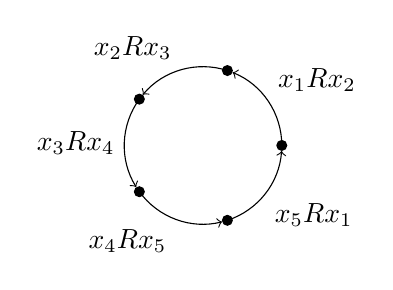
\begin{tikzpicture}
		\fill(1,0)circle(2pt)coordinate(A0);
		\fill({cos(72)},{sin(72)})circle(2pt)coordinate(A1);
		\fill({cos(144)},{sin(144)})circle(2pt)coordinate(A2);
		\fill({cos(216)},{sin(216)})circle(2pt)coordinate(A3);
		\fill({cos(288)},{sin(288)})circle(2pt)coordinate(A4);
		\begin{scope}[->]
			\draw(A0)arc[start angle=0,end angle=68,radius=1]node[midway,above right]{\(x_1 \rel{R} x_2\)};
			\draw(A1)arc[start angle=72,end angle=140,radius=1]node[midway,above left]{\(x_2 \rel{R} x_3\)};
			\draw(A2)arc[start angle=144,end angle=212,radius=1]node[midway,left]{\(x_3 \rel{R} x_4\)};
			\draw(A3)arc[start angle=216,end angle=284,radius=1]node[midway,below left]{\(x_4 \rel{R} x_5\)};
			\draw(A4)arc[start angle=288,end angle=356,radius=1]node[midway,below right]{\(x_5 \rel{R} x_1\)};
		\end{scope}
	\end{tikzpicture}
\end{center}
这是因为,如果我们有这样的环形成立,
那么根据传递性必有\(x_1 \rel{R} x_1\),
而这就与反自反性矛盾!

\begin{example}
设\(\rel{R}\)是\(A\)上的一个线性序,
证明:\(\rel{R}^{-1}\)也是\(A\)上的线性序.
\begin{proof}
由于\[
	\bigl( x \rel{R} y \land y \rel{R} z \implies x \rel{R} z \bigr)
	\iff
	\bigl( y \rel{R}^{-1} x \land z \rel{R}^{-1} y \implies z \rel{R}^{-1} x \bigr),
\]
可知\(\rel{R}^{-1}\)具有传递性.
又因为\(\rel{R}\)是\(A\)上的线性序,
所以对于\(\forall x,y \in A\),以下三个命题\[
	x \rel{R} y, \qquad
	x = y, \qquad
	y \rel{R} x
\]有且仅有一个成立;
换句话说,以下三个命题\[
	y \rel{R}^{-1} x, \qquad
	x = y, \qquad
	x \rel{R}^{-1} y
\]有且仅有一个成立;
可知\(\rel{R}^{-1}\)服从三一律.
综上所述,\(\rel{R}^{-1}\)也是\(A\)上的线性序.
\end{proof}
\end{example}

\subsection{偏序关系}
\begin{definition}
设\(\rel{R}\)是集合\(A\)上的二元关系,即\(\rel{R} \subseteq A^2\).
对于\(\forall x,y \in A\),若\[
	x\rel{R}y \land y\rel{R}x \implies x = y,
\]
则称“关系\(\rel{R}\)具有\DefineConcept{反对称性}(antisymmetric)”.
\end{definition}

\begin{definition}
设\(\rel{R}\)是集合\(A\)上的二元关系,即\(\rel{R} \subseteq A^2\).
如果\(\rel{R}\)同时具有自反性、反对称性、传递性,
则称“\(\rel{R}\)是\(A\)上的\DefineConcept{偏序关系}(ordering relation)”.
\end{definition}

\subsection{最大元,最小元,上界,下界}
\begin{definition}
设\(X\)是非空集合,
\(x \in X\),
\(E \subseteq X\),
\(\rel{R}\)是\(X\)上的偏序关系.

我们如果把满足\[
	[y \in X \implies x\rel{R}y]
	\implies
	y = x,
\]的\(x\)称作“\(X\)的\DefineConcept{最大元}(maximal element)”,
那么相应地把满足\[
	[y \in X \implies y\rel{R}x]
	\implies
	y = x,
\]的\(x\)称作“\(X\)的\DefineConcept{最小元}(minimal element)”.
在这样的语境下,
如果\(x\)满足\[
	(\forall y \in E)[y\rel{R}x],
\]
那么称“\(x\)是\(E\)的\DefineConcept{上界}(upper bound)”.
如果\(x\)满足\[
	(\forall y \in E)[x\rel{R}y],
\]
那么称“\(x\)是\(E\)的\DefineConcept{下界}(lower bound)”.
\end{definition}


\chapter{数系构造}
\section{自然数}
一般而言,我们有两种途径,可以引入新的数学研究对象:公理法和构造法.
我们已经利用公理法引入了集合的概念.
集合是我们基于数学直觉和日常生活的原始认知之一.
在处理集合时,我们初步建立了一系列的公理%
(包括外延公理、对集公理、并集公理、幂集公理、子集公理、选择公理等).

在本节,我们要尝试引入自然数系统.
皮亚诺曾经在1889年给出过自然数的公理化定义.
但是我们不采纳公理法,转而采用构造法,
即基于集合的概念,定义自然数的概念,
通过对自然数的必要的性质的证明,取代皮亚诺公理体系.

尽管自然数乍看之下不像是集合,
但是我们还是可以构造特定的集合,把它们定义为数字.
自然数的定义方式多种多样.
在1908年,策梅洛提议用\[
	\emptyset, \qquad
	\Set{\emptyset}, \qquad
	\Set{\Set{\emptyset}}, \qquad
	\Set{\Set{\Set{\emptyset}}}, \qquad
	\dotsc
\]代表自然数.
不久以后,冯诺依曼提出了一种新的构造方式,
由于其优点,它成为了用集合定义自然数的标准构造.
冯诺依曼的构造方式的首要原则是把每个自然数看作所有“比它小的自然数”组成的集合.
我们可以把前四个自然数定义如下:\begin{align*}
	&0 \defeq \emptyset, \\
	&1 \defeq \Powerset0 = \Set{0} = \NaturalSet{1}, \\
	&2 \defeq \Powerset1 = \Set{0,1} = \NaturalSet{2}, \\
	&3 \defeq \Powerset2 = \Set{0,1,2} = \NaturalSet{3}.
\end{align*}
我们可以继续照此方式定义任意多个自然数.
可以注意到,在集合\(3=\Set{0,1,2}\)中有三个元素\(0,1,2\).
如果说\(A_3\)表示由所有“具有三个元素的集合”组成的类,
那么我们可以说集合\(3\)是\(A_3\)的代表.

容易发现,这些表示自然数的集合具有以下两个奇妙的性质:\[
	0 \in 1 \in 2 \in 3 \in \dotsb,
\]
以及\[
	0 \subseteq 1 \subseteq 2 \subseteq 3 \subseteq \dotsb.
\]

尽管我们已经给出了前四个自然数的定义,
也摸索出了定义任意自然数的大致思路,
但是我们还没有给出自然数的一般性定义.
也就是说,我们还没有定义由全部自然数组成的集合.
这是因为我们认为对自然数集的确切定义不能依赖类似由省略号或诸如“以此类推”这样的短语!
因此,我们首先需要重新打造一套数学工具,给出一些基本概念的定义,用来代替含糊不清的用语.

\subsection{归纳集}
\begin{definition}[后继]\label{definition:集合论.后继的定义}
对于任意集合\(a\),把集合\(a \cup \Set{a}\)%
称为“\(a\)的\DefineConcept{后继}(successor)”,记为\(a^+\).
\end{definition}

利用后继符号,我们就可以将之前构造的用来表示自然数的集合重写为\[
	0=\emptyset, \qquad
	1=0^+=\emptyset^+, \qquad
	2=1^+=\emptyset^{++}, \qquad
	3=2^+=\emptyset^{+++}, \qquad
	\dotsc
\]
容易证明,这些集合互不相等,例如\(1\neq3\).

\begin{definition}[归纳集]\label{definition:集合论.归纳集的定义}
如果集合\(A\)同时满足
\begin{itemize}
	\item 空集是\(A\)的元素,即\[
		\emptyset \in A,
	\]
	\item \(A\)对后继封闭,即\[
		(\forall a)[a \in A \implies a^+ \in A],
	\]
\end{itemize}
这两个条件,
则称“集合\(A\)是\DefineConcept{归纳的}(inductive)”,
或“集合\(A\)是\DefineConcept{归纳集}(inductive set)”.
\end{definition}
尽管我们还没有给出“无穷”或“无限”的正式定义,
但是我们还是可以凭借数学直觉非正式地看出任意归纳集都是无限无尽的.

\subsection{无穷公理}
尽管“归纳集”的概念在形式上有了清晰的定义,
我们可以照此方法尝试构造无穷多个不同的集合,
但是由于我们尚未建立确保“无穷集”存在的公理,
我们就无法证明存在这样一个“拥有无穷多个元素的集合”,
因此我们也就不能证明任何“归纳集”真实存在.
于是我们要用“无穷公理”补上这个漏洞.
\begin{axiom}[无穷公理]
总存在一个集合\(A\)是归纳集,即\[
	(\exists A)[
		\emptyset \in A
		\land
		(\forall a)[a \in A \implies a^+ \in A]
	].
\]
\end{axiom}
无穷公理在英语中称作Infinity Axiom.

\subsection{自然数}
在无穷公理的加持下,我们终于可以定义自然数的概念了.
\begin{definition}\label{definition:集合论.自然数的定义}
如果集合\(x\)属于每一个归纳集,那么称其为\DefineConcept{自然数}(natural number),即\[
	\text{\(x\)是自然数}
	\defiff
	(\forall A)[\text{\(A\)是归纳集} \implies x \in A].
\]
\end{definition}
于是,我们可以利用描述法,将“全体自然数的汇集”定义为:
\[
	\omega
	\defeq
	\bigcap\Set{ A \given \text{\(A\)是归纳集} }.
\]
特别注意到:全体归纳集的汇集\(\Set{ A \given \text{\(A\)是归纳集} }\)是一个真类,而不是一个集合!

下面我们证明“全体自然数的汇集\(\omega\)”是一个集合.
\begin{theorem}\label{theorem:集合论.自然数集存在定理}
%@see: 《Elements of Set Theory》 P68. Theorem 4A
存在这样一个集合:它的元素都是自然数,任一自然数都是它的元素.
\begin{proof}
设\(A\)是一个归纳集(根据无穷公理,总可找到这样的\(A\)).
根据子集公理,
\[
	\exists w,
	\forall x
	\left(
		\begin{array}{rcl}
			x \in w
			&\iff&
				x \in A \land \text{\(x\)属于所有异于\(A\)的其他归纳集} \\
			&\iff&
				\text{\(x\)属于所有归纳集}
		\end{array}
	\right).
\]
于是集合\(w\)的所有元素都是自然数,
所有的自然数都是集合\(w\)的元素.
\end{proof}
\end{theorem}
可以注意到,这个证明与\cref{theorem:集合论.系的交的唯一存在性} 的证明本质上相同.

\subsection{数学归纳法}
我们首先证明自然数集\(\omega\)是最小的归纳集.
\begin{theorem}
%@see: 《Elements of Set Theory》 P69. Theorem 4B
自然数集\(\omega\)是归纳集,且它是任意一个归纳集的子集.
\begin{proof}
首先,由\hyperref[definition:集合论.归纳集的定义]{归纳集的定义}可知\[
	(\forall A)[\text{\(A\)是归纳集} \implies \emptyset \in A],
\]
于是\(\emptyset \in \omega\).

其次,结合自然数的定义可知\[
	(\forall a)[
		a \in \omega
		\implies
		(\forall A)[
			\text{\(A\)是归纳集} \implies a \in A \implies a^+ \in A
		]
		\implies
		a^+ \in \omega
	];
\]
也就是说,自然数集\(\omega\)对后继封闭.

因此\(\omega\)是归纳集,且\(\omega\)是任意一个归纳集的子集.
\end{proof}
\end{theorem}

既然\(\omega\)是归纳的,
那么根据归纳集的定义可知,\(0(=\emptyset)\)是自然数集的元素.
因此\(1(=0^+)\)在自然数集中,同理\(2(=1^+)\)和\(3(=2^+)\)也都在自然数集中.
于是我们说\(0,1,2,3\)都是自然数.
非必要的数学对象(即不是自然数的集合)都不在\(\omega\)中,
我们可以说:自然数集是“最小的”归纳集.
这句话可以更严谨地表述为下述“归纳原理”.
\begin{theorem}[归纳原理]\label{theorem:集合论.归纳原理1}
自然数集\(\omega\)的任意\DefineConcept{归纳子集}({\rm inductive subset})总是它自己.
\end{theorem}

这就引出“数学归纳法”的方法论,即:
如果我们要证明形如“对于每个自然数\(n\),涉及\(n\)的命题公式\(\lambda(n)\)成立”的命题,
我们可以基于自然数集\(\omega\),构造一个集合\[
	T = \Set{ n \in \omega \given \lambda(n) }.
\]
我们只要证明集合\(T\)是归纳的,
就能证明“对于每个自然数\(n\),涉及\(n\)的命题公式\(\lambda(n)\)成立”是真命题.

我们可以马上利用数学归纳法证明下面这个定理:
\begin{theorem}
%@see: 《Elements of Set Theory》 P69. Theorem 4C
除了\(0\)以外,所有自然数都是某个自然数的后继.
\begin{proof}
令集合\[
	T = \Set*{ n \in \omega \given n = 0 \lor (\exists p\in\omega)[n = p^+] },
\]
则\(0 \in T\),且\(k \in T \implies k^+ \in T\).
因此根据\hyperref[theorem:集合论.归纳原理1]{归纳原理}可知\(T = \omega\).
\end{proof}
\end{theorem}

\subsection{传递集}
\begin{definition}\label{definition:集合论.传递集的定义}
如果集合\(A\)的任一元素的每个元素都是\(A\)的元素,
那么称“集合\(A\)是\DefineConcept{传递的}(transitive)”,
或称“集合\(A\)是一个\DefineConcept{传递集}(transitive set)”,
即\begin{equation}\label{equation:集合论.传递集的定义式1}
	\text{\(A\)是传递集}
	\defiff
	(\forall x)(\forall a)[
		x \in a \in A
		\implies
		x \in A
	].
\end{equation}
\end{definition}
传递集\(A\)也可等价地定义为以下三种形式:
\begin{align}
	\text{\(A\)是传递集}
	&\iff
	\bigcup A \subseteq A;
	\label{equation:集合论.传递集的定义式2} \\
	&\iff
	(\forall a)[a \in A \implies a \subseteq A];
	\label{equation:集合论.传递集的定义式3} \\
	&\iff
	A \subseteq \Powerset A.
	\label{equation:集合论.传递集的定义式4}
\end{align}

这里我们要注意区分“关系的传递性”与“传递集”这两个概念,它们是根本不同的!
从今以后,我们还将遭遇类似的情况,总有些概念具有重复的、相同的名称.
实际上,我们常常需要动用阅读理解能力,联系上下文,根据用词,判断某个概念的涵义.

\begin{example}
证明:空集\(\emptyset\)是传递集.
\begin{proof}
假设空集不是传递集,那么根据传递集的定义可知,\[
	(\exists a)(\exists x)[
		x \in a \in \emptyset
		\land
		x \notin \emptyset
	].
\]
但是根据空集公理,空集中根本就不存在满足条件的\(a\),矛盾!因此空集是传递集.
\end{proof}
\end{example}

\begin{example}
\def\a{\Set{\emptyset}}%
\def\b{\Set{\a}}%
\def\A{\Set{ \emptyset, \b }}%
集合\(\A\)不是一个传递集,
这是因为\[
	\a \in \b \in \A,
	\quad\text{且}\quad
	\a \notin \A.
\]
\end{example}

\begin{example}
\(\Set{0,1,5}\)也不是传递集,
这是因为\[
	4 \in 5 \in \Set{0,1,5},
	\quad\text{且}\quad
	4 \notin \Set{0,1,5}.
\]
\end{example}

\begin{theorem}\label{theorem:集合论.传递集的后继的并就是这个传递集本身}
%@see: 《Elements of Set Theory》 P72. Theorem 4E
如果\(a\)是传递集,那么\(\bigcup\left( a^+ \right) = a\).
\begin{proof}
直接计算得\begin{align*}
	\bigcup\left( a^+ \right)
	&= \bigcup (a \cup \{a\})
		&(\text{\hyperref[definition:集合论.后继的定义]{后继的定义}}) \\
	&= \bigcup a \cup \bigcup\Set{a}
		&(\text{\cref{equation:集合论.并集的并等于并的并集}}) \\
	&= \bigcup a \cup a \\
	&= a.
	\qedhere
\end{align*}
\end{proof}
\end{theorem}

\begin{theorem}\label{theorem:集合论.传递集的后继也是传递集}
%@see: 《Elements of Set Theory》 P73. Exercise 2.
如果\(a\)是传递集,那么\(a^+\)也是传递集.
\begin{proof}
因为\(a\)是传递集,
根据\cref{theorem:集合论.传递集的后继的并就是这个传递集本身} 有%
\(\bigcup\left( a^+ \right) = a\),
而\(a \subseteq a \cup \{a\} = a^+\),
所以\[
	\bigcup\left( a^+ \right) \subseteq a^+;
\]
那么根据\hyperref[equation:集合论.传递集的定义式2]{传递集的定义},\(a^+\)也是传递集.
\end{proof}
\end{theorem}

\begin{theorem}
%@see: 《Elements of Set Theory》 P72. Theorem 4F
任一自然数都是传递集.
\begin{proof}
用数学归纳法证明.
首先,\(\emptyset\)是传递集.
假设自然数\(k\)也是传递集,
那么根据\cref{theorem:集合论.传递集的后继也是传递集} 可知\(k^+\)也是传递集.
综上所述,每个自然数都是传递集.
\end{proof}
\end{theorem}

\begin{theorem}\label{theorem:集合论.自然数集是传递集}
%@see: 《Elements of Set Theory》 P72. Theorem 4G
自然数集\(\omega\)是传递集.
\begin{proof}
用数学归纳法证明.
欲证自然数集\(\omega\)是传递集,
即证\((\forall n)[n \in \omega \implies n \subseteq \omega]\),
从而我们只需证集合\[
	T = \Set{ n \in \omega \given n \subseteq \omega }
\]是传递的.
显然自然数\(0=\emptyset \in T\).
假设自然数\(k \in T\),那么有\[
	k \in \omega
	\land
	k \subseteq \omega,
\]
即有\[
	k \subseteq \omega
	\land
	\{k\} \subseteq \omega;
\]
于是\(k \cup \{k\} \subseteq \omega\);
加之\(k^+ \in \omega\),于是\(k^+ \in T\).
因此\(T\)是传递的,而自然数集\(\omega\)是传递集.
\end{proof}
\end{theorem}
\cref{theorem:集合论.自然数集是传递集} 也可等价表述为:
每个自然数都是由自然数组成的集合.
以后我们会将这个定理加强为:
每个自然数都是由所有比它小的自然数组成的集合.

\begin{example}
%@see: 《Elements of Set Theory》 P73. Exercise 3.
证明:“\(a\)是传递集”的充要条件是“\(\Powerset a\)是传递集”.
\begin{proof}
因为\begin{align*}
	\text{\(a\)是传递集}
	&\iff
	a \subseteq \Powerset a
		&(\text{传递集的定义 \labelcref{equation:集合论.传递集的定义式4}}) \\
	&\iff
	a = \bigcup \Powerset a \subseteq \Powerset a
		&(\text{\cref{equation:集合论.集的幂集的并等于集}}) \\
	&\iff
	\text{\(\Powerset a\)是传递集},
		&(\text{传递集的定义 \labelcref{equation:集合论.传递集的定义式2}})
\end{align*}
所以,命题“\(a\)是传递集”与“\(\Powerset a\)是传递集”等价.
\end{proof}
\end{example}

\begin{example}
%@see: 《Elements of Set Theory》 P73. Exercise 4.
证明:如果\(A\)是传递集,那么\(\bigcup A\)也是传递集.
\begin{proof}
因为\(A\)是传递集,
由传递集的定义 \labelcref{equation:集合论.传递集的定义式2} 可知
\[
	\bigcup A \subseteq A;
\]
又由\cref{equation:集合论.系的并的幂集包含系} 可知\[
	A \subseteq \Powerset \bigcup A;
\]
所以\[
	\bigcup A \subseteq \Powerset \bigcup A,
\]
由传递集的定义 \labelcref{equation:集合论.传递集的定义式4} 可知\(\bigcup A\)是传递集.
\end{proof}
\end{example}

\begin{example}
%@see: 《Elements of Set Theory》 P73. Exercise 6.
证明\cref{theorem:集合论.传递集的后继的并就是这个传递集本身} 的逆命题:
如果\(\bigcup\left( a^+ \right) = a\),那么\(a\)是传递集.
\begin{proof}
因为\(a \subseteq a \cup \{a\} = a^+\),
根据\cref{equation:集合论.集合代数公式6-3} 可知\[
	\bigcup a \subseteq \bigcup\left( a^+ \right) = a,
\]
那么根据传递集的定义 \labelcref{equation:集合论.传递集的定义式2},\(a\)是传递集.
\end{proof}
\end{example}

\begin{example}
设\(a,b\)都是传递集.
证明:\(a \cup b\)也是传递集.
\begin{proof}
因为\[
	\text{\(a\)是传递集} \iff a \subseteq \Powerset a, \qquad
	\text{\(b\)是传递集} \iff b \subseteq \Powerset b,
\]
于是\begin{align*}
	a \cup b
	&\subseteq
	\Powerset a \cup b &(\text{\cref{equation:集合论.集合代数公式6-1}}) \\
	&\subseteq
	\Powerset a \cup \Powerset b &(\text{\cref{equation:集合论.集合代数公式6-1}}) \\
	&\subseteq
	\Powerset(a \cup b), &(\text{\cref{equation:集合论.集合代数公式3-5}})
\end{align*}
也就是说\(a \cup b\)是传递集.
\end{proof}
\end{example}

\begin{example}
%@see: 《Elements of Set Theory》 P73. Exercise 5.
\def\A{\mathscr{A}}%
设\(\A\)中的每一个元素都是传递集.
证明:\begin{enumerate}
	\item \(\bigcup \A\)是传递集.
	\item 当\(\A\)非空时,\(\bigcap \A\)是传递集.
\end{enumerate}
%TODO
\end{example}

\subsection{自然数的递归}
考虑一个映射\(h\colon \omega \to A\),
我们只知道\(h(0)\)的取值,
以及映射\(F\colon A \to A\)满足\[
	h(n^+) = F(h(n))
	\quad(n\in\omega).
\]
由此,虽然我们不知道映射\(h\)的具体表达式,
但我们总能依次计算出\(h(n)\ (n\in\omega)\)的取值:\[
	h(0), \qquad
	h(1) = F(h(0)), \qquad
	h(2) = F(h(1)), \qquad
	\dotsc
\]
这里,我们把\(h(0)\)称为\DefineConcept{初项},
把\[
	w = h(n) \quad(n\in\omega)
\]称为\DefineConcept{通项公式},
把\[
	h(n^+) = F(h(n)) \quad(n\in\omega)
\]称为\DefineConcept{递推公式}.

接下来,我们来思考这样一个问题:
在给定初项和递推公式的情况下,能否唯一确定通项公式呢?
也就是说,任给一个集合\(A\),再从中取定一个元素\(a\)作为初项,
并给定一个映射\(F\colon A \to A\)作为递推公式,
我们能否证明,存在一个唯一的映射\(h\colon \omega \to A\),
使得\(h(0) = a\),且对\(\forall n\in\omega\)总有\[
	h(n^+) = F(h(n)).
\]

\begin{theorem}[递归定理]\label{theorem:集合论.自然数集的递归定理}
%@see: 《Elements of Set Theory》 P73. Recursion Theorem on omega
设\(A\)是集合,\(a \in A\),映射\(F\colon A \to A\),
则唯一存在一个映射\(h\colon \omega \to A\),使得\[
	h(0) = a; \qquad
	h(n^+) = F(h(n)), \quad n\in\omega.
\]
\begin{proof}
为了方便后续证明,我们首先在这里提出一个概念:
对于映射\(v\),当且仅当
\begin{enumerate}[label={(\roman*)}]
	\item\label{item:集合论.容许映射条件1}
	\(\dom v \subseteq \omega\)且\(\ran v \subseteq A\);

	\item\label{item:集合论.容许映射条件2}
	\(0 \in \dom v
	\implies
	v(0) = a\);

	\item\label{item:集合论.容许映射条件3}
	对任意\(n \in \omega\),总有\(n^+ \in \dom v
	\implies
	n \in \dom v \land v(n^+) = F(v(n))\).
\end{enumerate}
这三个条件同时成立时,
我们称“映射\(v\)是\emph{容许的}(acceptable)”.

令\(\mathscr{K}\)为全体容许映射的类,即\[
	\mathscr{K} \defeq \Set{ v \given \text{映射\(v\)是容许的} };
\]
再令\(h = \bigcup \mathscr{K}\),
那么有\begin{equation}
	\begin{split}
		\opair{n,y} \in h
		&\iff
		\opair{n,y}\ \text{是某个容许映射\(v\)的元素} \\
		&\iff
		\text{对某个容许映射\(v\),总有\(v(n) = y\)成立}.
	\end{split}
	\tag1
\end{equation}
我们要证明\(h\)符合定理的要求,可以将证明细分为四个部分,
即证明\(h\)是一个映射,且它是容许的,
它的定义域是整个自然数集,以及这个映射是唯一的:
\begin{enumerate}
	\item 我们首先证明\(h\)是映射.
	%Proving this will, in effect, amount to showing that two acceptable functions
	%always agree with each other whenever both are defined.
	%TODO 这句不知道怎么翻译好呢
	令\[
		S = \Set{ n \in \omega
		\given
		\text{至多只有一个}\ y\ \text{满足}\ \opair{n,y} \in h }.
	\]
	我们需要证明\(S\)是归纳集.

	如果\[
		\opair{0,y_1} \in h
		\quad\text{且}\quad
		\opair{0,y_2} \in h,
	\]
	那么根据(1)式,存在容许映射\(v_1,v_2\),使得\[
		v_1(0) = y_1
		\quad\text{且}\quad
		v_2(0) = y_2;
	\]
	再根据\hyperref[item:集合论.容许映射条件2]{容许映射条件(ii)}可知\(y_1 = a = y_2\),
	因此\(0 \in S\).

	假设\(k \in S\),
	欲证\(k^+ \in S\).
	朝着这个方向,我们又假设\[
		\opair{k^+,y_1} \in h
		\quad\text{且}\quad
		\opair{k^+,y_2} \in h.
	\]
	同样地,必定存在容许映射\(v_1,v_2\),使得\[
		v_1(k^+) = y_1
		\quad\text{且}\quad
		v_2(k^+) = y_2.
	\]
	再根据\hyperref[item:集合论.容许映射条件3]{容许映射条件(iii)}可知\[
		y_1 = v_1(k^+) = F(v_1(k))
		\quad\text{且}\quad
		y_2 = v_2(k^+) = F(v_2(k)).
	\]
	又因为\(k \in S\),
	我们有\(\opair{k,v_1(k)},\opair{k,v_2(k)} \in h\),
	从而有\(v_1(k) = v_2(k)\),
	因此\[
		y_1 = F(v_1(k)) = F(v_2(k)) = y_2,
	\]
	这就说明\(k^+ \in S\).

	于是,\(S\)是归纳集,而且它恰好就是自然数集\(\omega\),
	从而\(h\)是一个映射.

	\item 现在我们来证明\(h\)是容许的.
	既然我们已经证明\(h\)是映射,
	那么根据(1)式,
	显然有\(\dom h \subseteq \omega\)且\(\ran h \subseteq A\).

	我们先来检验\hyperref[item:集合论.容许映射条件2]{容许映射条件(ii)}.
	如果\(0 \in \dom h\),
	那么必定存在某个容许映射\(v\)满足\(v(0) = h(0)\).
	既然\(v(0) = a\),我们就有\(h(0) = a\).

	我们再来检验\hyperref[item:集合论.容许映射条件3]{容许映射条件(iii)}.
	假设\(n^+ \in \dom h\).
	同样地,必定存在某个容许映射\(v\)满足\(v(n^+) = h(n^+)\).
	既然\(v\)是容许的,我们就有\(n \in \dom v\),\(v(n) = h(n)\),以及\[
		h(n^+) = F(h(n)) = F(v(n)) = v(n^+).
	\]

	于是,\(h\)是容许的.

	\item 现在我们来证明\(h\)的定义域是整个自然数集,
	即\(\dom h = \omega\).
	实际上我们只需证\(\dom h\)是归纳集.
	由于映射\(\Set{\opair{0,a}}\)是容许的,
	所以\(0 \in \dom h\).
	假设\(k \in \dom h\),只需证\(k^+ \in \dom h\).
	如果这条路走不通,那么考虑\[
		v = h \cup \Set{\opair{k^+,F(h(k))}}.
	\]
	易见\(v\)是一个映射,且\(\dom v \subseteq \omega\),\(\ran v \subseteq A\).
	因此只需证\(v\)是容许的.

	由于\(v(0) = h(0) = a\),\hyperref[item:集合论.容许映射条件2]{容许映射条件(ii)}成立.
	对于\hyperref[item:集合论.容许映射条件3]{容许映射条件(iii)},
	可以分为两种情形.
	如果\(n^+ \in \dom v\ (n^+ \neq k^+)\),
	那么\(n^+ \in \dom h\)且\(v(n^+) = h(n^+) = F(h(n)) = F(v(n))\).
	其他情形当\(n^+ = k^+\)时出现.
	既然后继是一一映射,那么\(n=k\).
	根据假设\(k \in \dom h\).
	因此\[
		v(k^+) = F(h(k)) = F(v(k))
	\]
	且\hyperref[item:集合论.容许映射条件3]{容许映射条件(iii)}成立.
	可见,\(v\)是容许的.
	但是,接下来我们有\(v \subseteq h\),
	从而\(k^+ \in \dom h\).

	于是,\(\dom h\)是归纳集,且\(\dom h = \omega\).

	\item 最后我们证明\(h\)是唯一的.
	假设映射\(h_1,h_2\)都符合定理的要求.
	令\[
		S = \Set{ n \in \omega \given h_1(n) = h_2(n) }.
	\]
	易见\(S\)是归纳集.
	%TODO 证明“\(S\)是归纳集”的步骤参考本节 Exercise 7

	于是,\(S = \omega\)且\(h_1 = h_2\).
	\qedhere
\end{enumerate}
\end{proof}
\end{theorem}
我们把\cref{theorem:集合论.自然数集的递归定理} 称为\DefineConcept{递归定理}.

\subsection{自然数的算术运算}
我们可以利用\hyperref[theorem:集合论.自然数集的递归定理]{递归定理}定义自然数集上的加法、乘法和乘幂.

\begin{definition}\label{definition:集合论.二元代数运算}
%@see: 《Elements of Set Theory》 P79. Definition
任给一个映射\(f\colon A \times A \to A\),
我们称“\(f\)是定义在集合\(A\)上的一个%
\DefineConcept{二元代数运算}(binary arithmetic operation)”,
简称\DefineConcept{运算}(operation).
\end{definition}

任取\(m \in \omega\),
根据\hyperref[theorem:集合论.自然数集的递归定理]{递归定理}%
易证存在唯一映射\(A_m\colon \omega \to \omega\)满足\[
	A_m(0) = m; \qquad
	A_m(n^+) = (A_m(n))^+, \quad n \in \omega.
\]

%@see: 《Elements of Set Theory》 P79. Definition
由此,我们可以定义自然数集\(\omega\)上的一个二元代数运算%
\DefineConcept{加法}(addition),
用符号“\(+\)”\footnote{%
这里把“\(+\)”读作“加号”.
}表记,
它满足:\[
	(\forall m,n\in\omega)
	[m + n = A_m(n)].
\]

我们把用来表示二元代数运算的符号(例如这里的“\(+\)”),
称为这个二元代数运算的\DefineConcept{算符}(operator);
把算符两边的项称为这个二元代数运算的\DefineConcept{算元}(operand).

我们可以把加法运算写成关系的形式:\[
	+ \defeq \Set*{
		\opair{\opair{m,n},p}
		\given
		m \in \omega
		\land
		n \in \omega
		\land
		p = A_m(n)
	}.
\]

\begin{theorem}
%@see: 《Elements of Set Theory》 P79. Theorem 4I
对于任意自然数\(m,n\),总有\begin{gather}
	m + 0 = m;
	\label{equation:集合论.自然数的加法.性质1} \\%(A1)
	m + n^+ = (m+n)^+.
	\label{equation:集合论.自然数的加法.性质2}%(A2)
\end{gather}
\end{theorem}

类似于加法的构造,任取\(m \in \omega\),
易证存在唯一映射\(M_m\colon \omega \to \omega\)满足\[
	M_m(0) = 0; \qquad
	M_m(n^+) = M_m(n) + m, \quad n \in \omega.
\]
由此,我们可以定义自然数集\(\omega\)上的另一个二元代数运算%
\DefineConcept{乘法}(multiplication),
用符号“\(\times\)”或“\(\cdot\)”\footnote{%
这里把“\(\times\)”和“\(\cdot\)”都读作“乘号”.
}表记,
它满足:\[
	(\forall m,n\in\omega)[m \times n = M_m(n)].
\]
我们可以把乘法运算写成关系的形式:\[
	\times \defeq \Set*{
		\opair{\opair{m,n},p}
		\given
		m \in \omega
		\land
		n \in \omega
		\land
		p = M_m(n)
	}.
\]

\begin{theorem}
%@see: 《Elements of Set Theory》 P79. Theorem 4J
对于任意自然数\(m,n\),总有\begin{gather}
	m \cdot 0 = 0;
	\label{equation:集合论.自然数的乘法.性质1} \\%(M1)
	m \cdot n^+ = m \cdot n + m.
	\label{equation:集合论.自然数的乘法.性质2}%(M2)
\end{gather}
\end{theorem}

我们在定义加法和乘法以后,
还可以类似地定义自然数的\DefineConcept{乘幂}(exponentiation),
并且可以给出:对于任意自然数\(m,n\),总有\begin{gather}
	m^0 = 1, \quad m \neq 0;
	\label{equation:集合论.自然数的乘幂.性质1} \\%(E1)
	m^{(n^+)} = m^n \cdot m.
	\label{equation:集合论.自然数的乘幂.性质2}%(E2)
\end{gather}

\begin{theorem}
%@see: 《Elements of Set Theory》 P79. Theorem 4K
对于任意自然数\(m,n,p\),以下命题恒成立:
\begin{enumerate}
	\item 加法结合律(associative law for addition)
	\begin{equation}\label{equation:集合论.自然数加法结合律}
		m+(n+p)=(m+n)+p.
	\end{equation}
	\item 加法交换律(commutative law for addition)
	\begin{equation}\label{equation:集合论.自然数加法交换律}
		m+n=n+m.
	\end{equation}
	\item 乘法分配律(distributive law)
	\begin{equation}\label{equation:集合论.自然数乘法分配律}
		m \cdot (n+p) = m \cdot n + m \cdot p.
	\end{equation}
	\item 乘法结合律(associative law for multiplication)
	\begin{equation}\label{equation:集合论.自然数乘法结合律}
		m \cdot (n \cdot p) = (m \cdot n) \cdot p.
	\end{equation}
	\item 乘法交换律(commutative law for multiplication)
	\begin{equation}\label{equation:集合论.自然数乘法交换律}
		m \cdot n = n \cdot m.
	\end{equation}
\end{enumerate}
\end{theorem}
这些命题依靠数学归纳法可以轻松得证,故略去证明.

\subsection{自然数的序}
\begin{definition}
设\(m,n\)是自然数.

如果\[
	m \in n,
\]
则称“\(m\) \DefineConcept{小于}(less than)\(n\)”(记作\(m < n\)),
或称“\(n\) \DefineConcept{大于}(greater than)\(m\)”(记作\(n > m\)),
即\[
	m \in n
	\defiff m < n
	\defiff n > m.
\]

如果\[
	m < n \lor m = n,
\]
则称“\(m\) \DefineConcept{小于或等于}(less than or equal to)\(n\)”(记作\(m \leq n\)),
或称“\(n\) \DefineConcept{大于或等于}(greater than or equal to)\(m\)”(记作\(n \geq m\)),
即\[
	m < n \lor m = n
	\defiff m \leq n
	\defiff n \geq m.
\]
\end{definition}

容易看出,\[
	(\forall x)(\forall n\in\omega)[
		x < n
		\iff
		x \in \omega \land x \in n
	];
\]
由于自然数集\(\omega\)是传递集,于是\[
	(\forall x)(\forall n)[x \in n \in \omega \implies x \in \omega],
\]
因此,任意自然数都是由比它小的数组成的集合.

现在我们来构造自然数集上的线性序关系.
我们令\[
	<\ \defeq \Set*{
		\opair{m,n} \in \omega \times \omega
		\given
		m \in n
	}.
\]
因为任意自然数都是传递集,所以\[
	(\forall m,n,p \in \omega)[
		m \in n \land n \in p
		\implies
		m \in p
	],
\]
即\[
	(\forall m,n,p \in \omega)[
		m < n \land n < p
		\implies
		m < p
	],
\]
这就可以证明关系\(<\)具有传递性;
接下来只要证明\(<\)在\(\omega\)上服从三一律,
那么它就是\(\omega\)上的线性序.
我们需要用到下面的引理.

\begin{lemma}\label{theorem:集合论.自然数的线性序.引理1}
%@see: 《Elements of Set Theory》 P84. Lemma 4L(a)
对任意自然数\(m,n\),总有\[
	m < n
	\iff
	m^+ < n^+.
\]
\begin{proof}
当\(m^+ < n^+\)时,
有\[
	m < m^+ \leq n,
\]
因此,利用传递性,便得\(m < n\).

当\(m < n\)时,
利用数学归纳法证明,
构造\[
	T = \Set*{
		n \in \omega
		\given
		(\forall m)[m < n \implies m^+ < n^+]
	}.
\]
显然\(0 \in T\).
当\(k \in T\)时,
要证\(k^+ \in T\),
只需证\(m \in k^+ \implies m^+ \in k^{++}\);
由\(m \in k^+\)可得\(m = k\)(这种情况下又有\(m^+ = k^+ \in k^{++}\))
或\(m \in k\)(这种情况下由于\(k \in T\),便有\(m^+ \in k^+ \subseteq k^{++}\));
于是不管是哪种情况下我们都有\(m^+ \in k^{++}\),
于是证得\(k^+ \in T\).
因此,\(T\)是归纳的,且与\(\omega\)相等.
\end{proof}
\end{lemma}

\begin{lemma}\label{theorem:集合论.自然数的线性序.引理2}
%@see: 《Elements of Set Theory》 P84. Lemma 4L(b)
没有任何一个自然数是它自己的元素.
\begin{proof}
用数学归纳法证明.
构造\[
	T = \Set*{ n \in \omega \given n \notin n }.
\]
由于空集中没有元素,于是\(0 \notin 0\),从而\(0 \in T\).
再根据\cref{theorem:集合论.自然数的线性序.引理1},\[
	k \notin k
	\implies
	k^+ \notin k^+.
\]
因此\(T\)是归纳的,且与\(\omega\)相等.
\end{proof}
\end{lemma}

\begin{theorem}\label{theorem:集合论.自然数集的三一律}
%@see: 《Elements of Set Theory》 P84. Trichotomy Law for omega
设\(m,n\)是自然数.
在以下三个命题中,有且仅有一个是真命题:\[
	m < n, \qquad
	m = n, \qquad
	n < m.
\]
\begin{proof}
首先我们证明“三个命题中至多一个成立”.
如果\(m < n\)和\(m = n\)同时成立,
那么有\(m < m\),
这就违反了\cref{theorem:集合论.自然数的线性序.引理2}.
另外,如果\(m < n < m\)成立,
那么根据\(m\)是传递集,
那么我们回到\(m < m\)这个错误结论了.

接下来只要证明“三个命题中至少一个成立”.
利用数学归纳法,令\[
	T = \Set*{
		n \in \omega
		\given
		(\forall m \in \omega)
		[
			m < n
			\lor
			m = n
			\lor
			n < m
		]
	}.
\]
要证\(0 \in T\),
只需证\(0 \leq m\)对任意\(m \in \omega\)都成立;
我们可以再次利用数学归纳法,
显然有\(0 \leq 0\)成立;
同时,若有\(0 \leq k\),那么\(0 < k^+\);
由此可知\(0 \in T\).
然后我们假设\(k \in T\),再想办法证明\(k^+ \in T\).
对于任意自然数\(m\),
由于\(k \in T\),我们有\[
	m \leq k
	\lor
	k < m;
\]
在前一种情形下,有\(m < k^+\);
而在后一种情形下,根据\cref{theorem:集合论.自然数的线性序.引理1},
我们有\(k^+ < m^+\),从而有\(k^+ \leq m\).
于是不论在哪种情形下,我们都有\[
	m < k^+
	\lor
	k^+ = m
	\lor
	k^+ < m.
\]
于是\(k^+ \in T\).
因此,\(T\)是归纳的.
\end{proof}
\end{theorem}

\begin{corollary}
%@see: 《Elements of Set Theory》 P85. Corollary 4M
设\(m,n\)是自然数.
那么\begin{gather*}
	m < n \iff m \subset n, \\
	m \leq n \iff m \subseteq n.
\end{gather*}
\begin{proof}
由于\(n\)是传递集,于是有\[
	m < n \implies m \subseteq n;
\]
再根据\cref{theorem:集合论.自然数的线性序.引理2},
这时候同时还有\(m \neq n\),
也就是说\(m < n \implies m \subset n\).
反过来,当\(m \subset n\)时,
那么必有\(m \neq n\)且\(n \notin m\)(不这样的话就会有\(n \in n\)),
于是根据三一律就有\(m \in n\).
\end{proof}
\end{corollary}
上面的证明过程体现出利用三一律的特定方式:
要证\(m < n\)成立,只需证其他两种情况\(m = n\)和\(m > n\)不成立.

\begin{theorem}\label{theorem:集合论.自然数的加法与乘法的保序性}
%@see: 《Elements of Set Theory》 P85. Theorem 4N
设\(m,n,p\)是自然数.
那么\begin{gather}
	m < n \iff m + p < n + p,
	\label{equation:集合论.自然数的加法的保序性} \\
	p \neq 0 \implies [m < n \iff m \cdot p < n \cdot p].
	\label{equation:集合论.自然数的乘法的保序性}
\end{gather}
\begin{proof}
对\cref{equation:集合论.自然数的加法的保序性} 的证明如下:
\begin{enumerate}
	\item 首先证\(m < n \implies m + p < n + p\).
	对\(p\)利用数学归纳法,
	取定\(m \in n \in \omega\),
	令\[
		A = \Set*{
			p \in \omega
			\given
			m + p < n + p
		}.
	\]
	显然\(0 \in A\),且\begin{align*}
		k \in A
		&\implies m+k<n+k \\
		&\implies (m+k)^+<(n+k)^+
			&(\text{\cref{theorem:集合论.自然数的线性序.引理1}}) \\
		&\implies m+k^+<n+k^+
			&(\text{\cref{equation:集合论.自然数的加法.性质2}}) \\
		&\implies k^+ \in A.
	\end{align*}
	因此\(A\)是归纳集,且\(A = \omega\).

	\item 然后证\(m + p < n + p \implies m < n\).
	利用三一律,
	因为\(m + p < n + p\),
	所以不可能有\(m = n\)(否则会有\(n+p<n+p\)),
	也不可能有\(n < m\)(否则会有\(n+p<m+p<n+p\)),
	于是只有\(m < n\)成立.
\end{enumerate}

对\cref{equation:集合论.自然数的乘法的保序性} 的证明如下:
\begin{enumerate}
	\item 首先证\(m < n \implies m \cdot p < n \cdot p\).
	取定\(m \in n \in \omega\),令\[
		B = \Set*{
			q \in \omega
			\given
			m \cdot q^+ < n \cdot q^+
		}.
	\]
	考虑到,对于非零自然数\(p\),存在自然数\(q\),使得\(q^+ = p\).
	容易看出,由于\[
		m \cdot 0^+ = m \cdot 0 + m = m,
	\]
	所以\(0 \in B\).
	假设\(k \in B\),要证\(m \cdot k^{++} < n \cdot k^{++}\).
	对\(m \cdot k^+ < n \cdot k^+\)利用\cref{theorem:集合论.自然数的加法与乘法的保序性},
	便得\begin{align*}
		m \cdot k^{++}
		&= m \cdot k^+ + m \\
		&< n \cdot k^+ + m.
	\end{align*}
	在对\(m < n\)利用\cref{theorem:集合论.自然数的加法与乘法的保序性},
	便得\begin{align*}
		n \cdot k^+ + m
		&< n \cdot k^+ + n \\
		&= n \cdot k^{++}.
	\end{align*}
	这就证明\(k^+ \in B\),
	从而\(B\)是归纳集,且\(B = \omega\).

	\item \(m \cdot p < n \cdot p \implies m < n\)%
	这部分的证明过程与\cref{equation:集合论.自然数的加法的保序性} 的证明过程完全一致,故略去.
	\qedhere
\end{enumerate}
\end{proof}
\end{theorem}

\begin{corollary}\label{theorem:集合论.自然数的消去律}
%@see: 《Elements of Set Theory》 P86. Corollary 4P
设\(m,n,p\in\omega\).
那么\begin{gather*}
	m + p = n + p \implies m = n; \\
	m \cdot p = n \cdot p \land p \neq 0 \implies m = n.
\end{gather*}
\end{corollary}
\cref{theorem:集合论.自然数的消去律}
又称为“自然数的\DefineConcept{消去律}(cancellation law)”.

\begin{theorem}[良序原理]\label{theorem:集合论.自然数集的良序}
%@see: 《Elements of Set Theory》 P86. Well Ordering of omega
设\(A\)是\(\omega\)的一个非空子集.
存在\(m \in A\),使得对于\(\forall n \in A\),总有\[
	m \leq n.
\]
\begin{proof}
首先我们给出如下定义:
我们把满足本定理的条件的自然数\(m\)称为“\(A\)中最小的数”.
容易看出,在自然数集\(\omega\)的任意一个非空子集中,最小的数总是唯一的.
利用反证法,假设\(m_1,m_2\)都是\(A\)中最小的数,
那么有\(m_1 \leq m_2 \land m_2 \leq m_1\),
从而有\(m_1 = m_2\).

现在我们开始对本定理的证明.
利用反证法,
设\(A\)是\(\omega\)的一个子集,且没有一个自然数是\(A\)中最小的数,
我们可以证明\(A = \emptyset\),这会与本定理要求的“\(A\)非空”矛盾.
而为了证明\(A = \emptyset\),
只需证\(\omega - A\)是归纳集.
但是,在利用数学归纳法证明“\(\omega - A\)是归纳集”时,
需要证明\(k^+ \in \omega - A\),
而这个命题不能仅凭\(k \in \omega - A\)得出,
这是因为我们还需要证明“所有比\(k\)小的自然数也都是\(\omega - A\)的元素”,即\[
	(\forall p \in \omega)[
		p < k \implies p \in \omega - A
	].
\]
考虑到这一点,我们就能肯定命题\(k^+ \in \omega - A\)一定成立,
否则就会有“\(k^+\)是\(A\)中最小的数”,
这就与我们的假设“没有一个自然数是\(A\)中最小的数”矛盾!

在整理好上面的思路以后,我们构造\[
	B = \Set*{
		m \in \omega
		\given
		\text{比\(m\)小的自然数不属于\(A\)}
	}.
\]
现在来证明\(B\)是归纳的.
显然\(0 \in B\).
假设\(k \in B\),
那么,如果\(n < k^+\),
则有\(n < k\)(这种情况下,由\(k \in B\)可知\(n \notin A\))%
或\(n = k\)(这种情况下,必有\(n \notin A\),否则根据三一律必有“\(n\)是\(A\)中最小的数”)%
成立,
在这两种情况下,\(n\)都不是\(A\)的元素.
因此,\(k^+ \in B\).
于是\(B\)是归纳集,从而\(A = \emptyset\).
\end{proof}
\end{theorem}

\begin{theorem}
%@see: 《Elements of Set Theory》 P87. Corollary 4Q
不存在这样的映射\(f\colon\omega\to\omega\),
使得对\(\forall n \in \omega\),总有\[
	f(n^+) < f(n).
\]
\begin{proof}
假设存在这样的映射\(f\colon\omega\to\omega\),
使得对\(\forall n \in \omega\),总有\[
	f(n^+) < f(n).
\]
那么\(\ran f\)会是\(\omega\)的非空子集,
而且没有一个自然数是\(\ran f\)中最小的数,
这就与\cref{theorem:集合论.自然数集的良序} 矛盾,
因此这样的映射不存在.
\end{proof}
\end{theorem}

\begin{theorem}[强归纳原理]\label{theorem:集合论.归纳原理2}
%@see: 《Elements of Set Theory》 P87. Strong Induction Principle for omega
设\(A\)是\(\omega\)的子集.
如果\[
	(\forall n \in \omega)[
		(\forall m \in \omega)[m < n \implies m \in A]
		\implies
		n \in A
	],
\]
那么\(A = \omega\).
\begin{proof}
用反证法,
设\(A \neq \omega\),
那么\(\omega - A \neq \omega\),
那么根据\hyperref[theorem:集合论.自然数集的良序]{良序原理},
\(\omega - A\)必有最小数\(m\).
既如此,所有比\(m\)小的数都在\(A\)中.
但是定理要求\(m \in A\),这就与\(m \in \omega - A\)矛盾.
\end{proof}
\end{theorem}

良序原理为数学归纳法提供另一种选择.
假设我们需要证明,某个命题对任意自然数都成立,
虽然可以像之前一样构造“正例集”(也就是由使命题为真的自然数组成的集合),
但是也可以构造“反例集”(也就是由使命题为假的自然数组成的集合)\(C\),
然后证明这个反例集是空集;
而要证得\(C = \emptyset\),
只需证明\(C\)没有最小数.

\begin{example}
%@see: 《Elements of Set Theory》 P88. Exercise 19.
设\(m\in\omega\),\(d\in\omega-\{0\}\).
证明:\(\exists q,r\in\omega\),使得\[
	m=(d \cdot q)+r
	\land
	r<d.
\]
\begin{proof}
用数学归纳法.
令\[
	T = \Set{
		m \in \omega
		\given
		(\exists q,r\in\omega)[
			m=(d \cdot q)+r
			\land
			r<d
		]
	}.
\]
因为只要取\(q=r=0\),就有\(0=(d\cdot0)+0\land0<d\)成立,所以\(0 \in T\).
设\(a \in T\),即\[
	a = (d \cdot q) + r \land r < d.
\]
根据\hyperref[equation:集合论.自然数的加法.性质2]{自然数加法的性质},有\[
	a^+ = ((d \cdot q) + r)^+
	= (d \cdot q) + r^+.
\]
注意到\(r^+ \leq d\),
我们规定:\begin{enumerate}
	\item 当\(r^+=d\)时,取\(q'=q^+, r'=0\);
	\item 当\(r^+<d\)时,取\(q'=q, r'=r^+\).
\end{enumerate}
于是有\[
	a^+ = (d \cdot q') + r'
	\land
	r' < d,
\]
即\(a^+ \in T\).
因此\(T\)是传递集,\(T = \omega\).
\end{proof}
\end{example}

\begin{example}
%@see: 《Elements of Set Theory》 P88. Exercise 20.
设集合\(A\)是\(\omega\)的非空子集,且\(\bigcup A = A\).
证明:\(A=\omega\).
%TODO
\end{example}

\begin{example}
%@see: 《Elements of Set Theory》 P88. Exercise 21.
证明:没有一个自然数是它的任一元素的一个子集.
%TODO
\end{example}

\begin{example}
%@see: 《Elements of Set Theory》 P88. Exercise 22.
设\(m,p\in\omega\).
证明:\(m<m+p^+\).
%TODO
\end{example}

\begin{example}
%@see: 《Elements of Set Theory》 P88. Exercise 23.
设\(m,n\in\omega\),\(m<n\).
证明:\(\exists p\in\omega\),使得\[
	m+p^+=n.
\]
%TODO
\end{example}

\begin{example}
%@see: 《Elements of Set Theory》 P88. Exercise 24.
设\(m,n,p,q\in\omega\),且\(m+n=p+q\).
证明:\(m<p \iff q<n\).
%TODO
\end{example}

\begin{example}
%@see: 《Elements of Set Theory》 P88. Exercise 25.
设\(m,n,p,q\in\omega\),且\(n<m,q<p\).
证明:\((m \cdot q)+(n \cdot p)<(m \cdot p)+(n \cdot q)\).
%TODO
\end{example}

\begin{example}
%@see: 《Elements of Set Theory》 P88. Exercise 26.
设\(n\in\omega\),\(f\colon n^+\to\omega\).
证明:\(\ran f\)有最大值.
%TODO
\end{example}


\section{整数}
我们现在把自然数集扩张为整数集.
\subsection{整数集}
设\(a,b\in\omega\).
我们把数对\(\opair{a,b}\)称为“\(a\)与\(b\)的\DefineConcept{差}(difference)”,
记作\(a-b\)\footnote{读作“\(a\)减\(b\)”.},即\[
	a-b = \opair{a,b}.
\]

\begin{definition}\label{definition:集合论.自然数的差的等价关系}
%@see: 《Elements of Set Theory》 P91. Definition
我们定义\(\omega\times\omega\)上的关系\(\sim\)如下:
\[
	(\forall a,b,c,d \in \omega)
	[
		\opair{a,b} \sim \opair{c,d}
		\defiff
		a+d=b+c
	].
\]
\end{definition}

容易看出,关系\(\sim\)的定义域和值域都是自然数对.
除了通过命题公式给出\(\sim\)的定义以外,
我们还可以用更直接的形式给出它的定义:
\[
	\sim\ \defeq \Set*{
		\opair{\opair{a,b},\opair{c,d}}
		\given
		a+d=b+c \land a,b,c,d\in\omega
	}.
\]

\begin{theorem}
%@see: 《Elements of Set Theory》 P91. Theorem 5ZA
关系\(\sim\)是\(\omega\times\omega\)上的等价关系.
\begin{proof}
容易看出,关系\(\sim\)具有自反性和对称性.
现在来证\(\sim\)具有传递性.
设\[
	\opair{m,n}\sim\opair{p,q}, \qquad
	\opair{p,q}\sim\opair{r,s}.
\]
由定义有\[
	m+q=n+p, \qquad
	p+s=q+r;
\]
相加得\[
	m+q+p+s=n+p+q+r;
\]
再利用\hyperref[theorem:集合论.自然数的消去律]{消去律}便得\[
	m+s=n+r;
\]
于是\(\opair{m,n}\sim\opair{r,s}\),关系\(\sim\)具有传递性.
综上所述,关系\(\sim\)是一个等价关系.
\end{proof}
\end{theorem}

既然关系\(\sim\)是一个等价关系,
那么对于任意给定的自然数对\(\opair{m,0}\),
我们可以取得它在关系\(\sim\)下唯一的等价类\[
	[\opair{m,0}] = \Set{
		\opair{m,0},
		\opair{m+1,1},
		\opair{m+2,2},
		\dotsc
	};
\]
类似地,
对于任意给定的自然数对\(\opair{0,n}\),
我们也可以取得它在关系\(\sim\)下唯一的等价类\[
	[\opair{0,n}] = \Set{
		\opair{0,n},
		\opair{1,n+1},
		\opair{2,n+2},
		\dotsc
	}.
\]
像这样,我们把任意两个自然数\(m\)和\(n\)的差\(\opair{m,n}\)%
在关系\(\sim\)下的等价类叫做一个\DefineConcept{整数}(integer).

于是我们可以构造出“整数集”.
\begin{definition}
%@see: 《Elements of Set Theory》 P92. Definition
称“\(\omega\times\omega\)对\(\sim\)的商集”为%
\DefineConcept{整数集}(the set of integers),
记作\(\mathbb{Z}\),即\[
	\mathbb{Z} \defeq \IntegerQuotient.
\]
\end{definition}

例如,整数\(2\)是等价类\[
	[\opair{2,0}]
	= \Set{\opair{2,0},\opair{3,1},\opair{4,2},\dotsc};
\]
而整数\((-3)\)是等价类\[
	[\opair{0,3}]
	= \Set{\opair{0,3},\opair{1,4},\opair{2,5},\dotsc}.
\]

\begin{figure}[ht]
	\centering
	\begin{tikzpicture}[scale=.5]
		\draw[help lines, color=gray!30, dashed] (0,0)grid(9,9);
		\begin{scope}[>=Stealth,->]
			\draw(0,0)--(0,10);
			\draw(0,0)--(10,0);
		\end{scope}
		\foreach \i in {0,...,9} {
			\foreach \j in {0,...,9} {
				\fill (\i,\j)circle(2pt);
			}
		}
		\draw(0,4)--(5,9)node[above right]{\(-4\)};
		\draw(0,0)--(9,9)node[above right]{\(0\)};
		\draw(3,0)--(9,6)node[above right]{\(3\)};
	\end{tikzpicture}
	\caption{整数是\(\omega\times\omega\)上的“直线”}
\end{figure}

\subsection{整数集上的加法运算}
类比自然数,我们希望在整数集上也能定义加法和乘法.

利用我们从初等代数学到的知识,
容易验证下式是正确的:\[
	(m-n)+(p-q) = (m+p)-(n+q).
\]
于是我们可以定义整数集上的加法运算:
\begin{equation}\label{equation:集合论.整数集上的加法运算}
	[\opair{m,n}] + [\opair{p,q}]
	\defeq
	[\opair{m+p,n+q}].
\end{equation}
虽然已经有了整数加法的定义了,
但我们还不能确信它是良定的.
这和我们在讨论\cref{theorem:集合论.与等价关系兼容的映射的性质} 时遇到的情况是一样的.
我们想要为一对等价类给出加法运算结果的取值,就要分成下面三个步骤:
\begin{enumerate}
	\item 从两个等价类中各自取出一个代表\(\opair{m,n}\)和\(\opair{p,q}\);
	\item 在这两个代表上作运算,即\[
		\opair{m,n} + \opair{p,q}
		= \opair{m+p,n+q};
	\]
	\item 构造运算结果的等价类\([\opair{m+p,n+q}]\).
\end{enumerate}

\begin{lemma}\label{theorem:集合论.整数集上的加法运算是良定的}
%@see: 《Elements of Set Theory》 P93. Lemma 5ZB
如果\(\opair{m,n}\sim\opair{m',n'}\)且\(\opair{p,q}\sim\opair{p',q'}\),
那么\[
	\opair{m+p,n+q}\sim\opair{m'+p',n'+q'}.
\]
\begin{proof}
根据\cref{definition:集合论.自然数的差的等价关系},
\[
	m+n'=m'+n, \qquad
	p+q'=p'+q;
\]
将上述两式相加得\[
	m+p+n'+q'=m'+p'+n+q;
\]
于是\(\opair{m+p,n+q}\sim\opair{m'+p',n'+q'}\).
\end{proof}
\end{lemma}
\cref{theorem:集合论.整数集上的加法运算是良定的} 说明前面定义的%
\hyperref[equation:集合论.整数集上的加法运算]{整数集上的加法运算}是正当的.
换句话说,由于映射\[
	F\colon ((\omega\times\omega)\times(\omega\times\omega))\to(\omega\times\omega),
	\opair{\opair{m,n},\opair{p,q}} \mapsto \opair{m+p,n+q}
\]和关系\(\sim\)兼容,
那么根据\cref{theorem:集合论.与等价关系兼容的映射的性质},
在商集\(\IntegerQuotient\)上,唯一存在映射\(\hat{F}\)(这就是整数集上的加法运算),满足\[
	\hat{F}([\opair{m,n}],[\opair{p,q}]) = [\opair{m+p,n+q}].
\]

\begin{theorem}\label{theorem:集合论.整数加法的运算法则}
%@see: 《Elements of Set Theory》 P94. Theorem 5ZC
%@see: 《Elements of Set Theory》 P95. Theorem 5ZD
以下命题恒成立:
\begin{enumerate}
	\item 加法交换律
	\begin{equation}\label{equation:集合论.整数加法交换律}
		(\forall a,b\in\mathbb{Z})[a+b=b+a].
	\end{equation}
	\item 加法结合律
	\begin{equation}\label{equation:集合论.整数加法结合律}
		(\forall a,b,c\in\mathbb{Z})[(a+b)+c=a+(b+c)].
	\end{equation}
	\item 任意整数加上整数\(0\defeq[\opair{0,0}]\)不变
	\begin{equation}\label{equation:集合论.任意整数加上零不变}
		(\forall a\in\mathbb{Z})[a+0=a].
	\end{equation}
	\item 加法可逆
	\begin{equation}\label{equation:集合论.整数加法可逆}
		(\forall a\in\mathbb{Z})(\exists! b\in\mathbb{Z})[a+b=0].
	\end{equation}
\end{enumerate}
\begin{proof}
首先证明 \labelcref{equation:集合论.整数加法交换律,equation:集合论.整数加法结合律} 这两个命题.
设\[
	a = [\opair{m,n}], \qquad
	b = [\opair{p,q}], \qquad
	c = [\opair{u,v}],
\]
其中\(m,n,p,q,u,v\)是自然数.
那么\begin{align*}
	a+b &= [\opair{m,n}]+[\opair{p,q}] \\
	&= [\opair{m+p,n+q}]	&(\text{\hyperref[equation:集合论.整数集上的加法运算]{整数加法的定义}}) \\
	&= [\opair{p+m,q+n}]	&(\text{\hyperref[equation:集合论.自然数加法交换律]{自然数加法交换律}}) \\
	&= [\opair{p,q}]+[\opair{m,n}] \\
	&= b+a; \\
	(a+b)+c &= [\opair{m+p,n+q}]+[\opair{u,v}] \\
	&= [\opair{(m+p)+u,(n+q)+v}] \\
	&= [\opair{m+(p+u),n+(q+v)}]	&(\text{\hyperref[equation:集合论.自然数加法结合律]{自然数加法结合律}}) \\
	&= [\opair{m,n}]+[\opair{p+u,q+v}] \\
	&= a+(b+c);
\end{align*}
因此整数加法满足交换律、结合律.

命题 \labelcref{equation:集合论.任意整数加上零不变} 显然成立,
这是因为对于任意给定的整数\(a = [\opair{m,n}]\),总有\[
	a+0
	= [\opair{m,n}]+[\opair{0,0}]
	= [\opair{m+0,n+0}]
	= [\opair{m,n}]
	= a.
\]

最后,我们来证明命题 \labelcref{equation:集合论.整数加法可逆}.
显然,对于任意取定整数\(a = [\opair{m,n}]\),
整数\(b = [\opair{n,m}]\)总是满足\[
	a+b
	= [\opair{m+n,n+m}]
	= [\opair{0,0}]
	= 0.
\]
由此,我们不仅证明命题 \labelcref{equation:集合论.整数加法可逆} 中,
整数\(b\)的存在性,还给出了它的表达式.
我们再假设\(b,c\)这两个整数分别满足\[
	a+b=0, \qquad
	a+c=0;
\]
那么\[
	b=b+(a+c)=(b+a)+c=c.
\]
于是我们证得整数\(b\)的唯一性.
\end{proof}
\end{theorem}

从上面的证明过程我们得知,
对于任意给定的一个整数\(a\),
满足\(a+b=0\)的整数\(b\)存在且唯一.
于是,我们可以把\(b\)叫做“\(a\)的\DefineConcept{逆}(inverse)”,
记作\((-a)\).
那么有\begin{equation}
	-[\opair{m,n}]=[\opair{n,m}].
\end{equation}
整数的逆为我们提供了\DefineConcept{减法运算}(subtraction operation):
\begin{equation}
	b-a \defeq b+(-a).
\end{equation}

\cref{theorem:集合论.整数加法的运算法则}
说明整数集\(\mathbb{Z}\)配上加法运算就成为一个阿贝尔群!
在以后学到抽象代数的时候,我们会明白这意味着什么.

\subsection{整数集上的乘法运算}
我们遵循同样的思路,像在研究整数集上的加法运算那样,借助初等代数的知识,注意到\[
	(m-n)\cdot(p-q)=(mp+nq)-(mq+np).
\]
于是我们可以定义整数集上的乘法运算:
\begin{equation}\label{equation:集合论.整数集上的乘法运算}
	[\opair{m,n}]\cdot[\opair{p,q}]
	\defeq [\opair{mp+nq,mq+np}].
\end{equation}
同样地,我们还是要验证整数乘法的定义在等价类上是不是良定的.
也就是要验证映射\[
	G\colon ((\omega\times\omega)\times(\omega\times\omega))\to(\omega\times\omega),
	\opair{\opair{m,n},\opair{p,q}} \mapsto \opair{mp+nq,mq+np}
\]和关系\(\sim\)兼容.
为此,我们有如下引理.
\begin{lemma}\label{theorem:集合论.整数集上的乘法运算是良定的}
%@see: 《Elements of Set Theory》 P96. Lemma 5ZE
如果\(\opair{m,n}\sim\opair{m',n'}\)且\(\opair{p,q}\sim\opair{p',q'}\),
那么\[
	\opair{mp+nq,mq+np}\sim\opair{m'p'+n'q',m'q'+n'p'}.
\]
\begin{proof}
根据\cref{definition:集合论.自然数的差的等价关系},
\[
	m+n'=m'+n,
	\eqno(1)
\]\[
	p+q'=p'+q;
	\eqno(2)
\]
将(1)式乘以\(p\)倍,得\[
	mp+n'p=m'p+np;
	\eqno(3)
\]
将(1)式乘以\(q\)倍,得\[
	m'q+nq=mq+n'q;
	\eqno(4)
\]
将(2)式乘以\(m'\)倍,得\[
	m'p+m'q'=m'p'+m'q;
	\eqno(5)
\]
将(2)式乘以\(n'\)倍,得\[
	n'p'+n'q=n'p+n'q';
	\eqno(6)
\]
将(3)(4)(5)(6)这四个式子相加,
再利用\hyperref[theorem:集合论.自然数的消去律]{消去律}化简,便得\[
	mp+nq+m'q'+n'p'
	=np+mq+m'p'+n'q';
\]
因此,\(\opair{mp+nq,mq+np}\sim\opair{m'p'+n'q',m'q'+n'p'}\).
\end{proof}
\end{lemma}

\begin{theorem}\label{theorem:集合论.整数乘法的运算法则1}
%@see: 《Elements of Set Theory》 P96. Theorem 5ZF
以下命题恒成立:
\begin{enumerate}
	\item 乘法交换律
	\begin{equation}\label{equation:集合论.整数乘法交换律}
		\forall a,b\in\mathbb{Z} \bigl(
			a \cdot b = b \cdot a
		\bigr).
	\end{equation}
	\item 乘法结合律
	\begin{equation}\label{equation:集合论.整数乘法结合律}
		\forall a,b,c\in\mathbb{Z} \bigl(
			(a \cdot b) \cdot c = a \cdot (b \cdot c)
		\bigr).
	\end{equation}
	\item 乘法分配律
	\begin{equation}\label{equation:集合论.整数乘法分配律}
		\forall a,b,c\in\mathbb{Z} \bigl(
			a \cdot (b + c) = (a \cdot b) + (a \cdot c)
		\bigr).
	\end{equation}
\end{enumerate}
\begin{proof}
设\(a=[\opair{m,n}]\),\(b=[\opair{p,q}]\),其中\(m,n,p,q\in\omega\).
那么根据\cref{equation:集合论.整数集上的乘法运算},\[
	a \cdot b = [\opair{mp+nq,mq+np}],
\]\[
	b \cdot a = [\opair{pm+qn,pn+qm}].
\]
根据自然数的\hyperref[equation:集合论.自然数加法交换律]{加法交换律}%
和\hyperref[equation:集合论.自然数乘法交换律]{乘法交换律},
有\(mp+nq=pm+qn\)和\(mq+np=pn+qm\),
于是\(a \cdot b = b \cdot a\)成立.

又设\(c=[\opair{r,s}]\),其中\(r,s\in\omega\).
那么\[
	(a \cdot b) \cdot c
	= [\opair{(mp+nq)r+(mq+np)s,(mp+nq)s+(mq+np)r}],
\]\[
	a \cdot (b \cdot c)
	= [\opair{m(pr+qs)+n(ps+qr),m(ps+qr)+n(pr+qs)}].
\]
只要像上面一样,利用自然数的运算法则,
易证\((a \cdot b) \cdot c = a \cdot (b \cdot c)\).

最后,我们将\(a \cdot (b+c)\)展开,得\[
	[\opair{m(p+r)+n(q+s),m(q+s)+n(p+r)}];
\]
将\((a \cdot b) + (a \cdot c)\)展开,得\[
	[\opair{mp+nq+mr+ns,mq+np+ms+nr}].
\]
易证\(a \cdot (b + c) = (a \cdot b) + (a \cdot c)\)成立.
\end{proof}
\end{theorem}

\begin{theorem}\label{theorem:集合论.整数乘法的运算法则2}
%@see: 《Elements of Set Theory》 P97. Theorem 5ZG
以下命题恒成立:\begin{enumerate}
	\item 任意整数乘上整数\(1\defeq[(1,0)]\)不变,即
	\begin{equation}\label{equation:集合论.任意整数乘上一不变}
		\forall a\in\mathbb{Z} \bigl(
			a \cdot 1 = a
		\bigr).
	\end{equation}
	\item 整数\(1\)与整数\(0\)不相等,即\(1\neq0\).
	\item 如果\(a \cdot b = 0\),那么\(a = 0 \lor b = 0\).
\end{enumerate}
\begin{proof}
设\(a=[\opair{m,n}]\),那么
\begin{align*}
	a \cdot 1
	&= [\opair{m,n}]\cdot[(1,0)] \\
	&= [\opair{m\cdot1+n\cdot0,m\cdot0+n\cdot1}] \\
	&= [\opair{m,n}] = a.
\end{align*}
于是命题 \labelcref{equation:集合论.任意整数乘上一不变} 成立.

要证整数\(1\)与整数\(0\)不相等,
即证\([(1,0)]\neq[\opair{0,0}]\),
那么只需证\[
	\opair{0,0}\not\sim(1,0);
\]
即证\(0+0\neq0+1\)或\(0\neq1\),显然成立.

接下来,若要证\(a \cdot b = 0 \implies a = 0 \lor b = 0\),
可以用反证法,
假设\(a,b\)都是非零整数,只需证\(a \cdot b \neq 0\)制造矛盾.
设\(a=[\opair{m,n}]\),\(b=[\opair{p,q}]\),
其中\(m,n,p,q\)都是自然数.
那么\[
	a \cdot b = [\opair{mp+nq,mq+np}].
\]
既然\(a\neq0=[\opair{0,0}]\),
那么\(m \neq n\),即有\[
	m < n \lor n < m;
	\eqno(1)
\]
同理可得\[
	p < q \lor q < p.
	\eqno(2)
\]
从(1)(2)两式可以得到\(m,n,p,q\)取值的四种不同情况,不过我们总有\[
	mp+nq \neq mq+np.
\]
因此\(a \cdot b \neq 0\).
\end{proof}
\end{theorem}

我们可以说\(\opair{\mathbb{Z},+,\cdot}\)构成了%
\DefineConcept{整环}(integral domain),
这是因为\begin{enumerate}
	\item \(\opair{\mathbb{Z},+}\)构成阿贝尔群%
	(\cref{theorem:集合论.整数加法的运算法则}).
	\item 整数乘法遵守交换律和结合律,以及对加法的分配律%
	(\cref{theorem:集合论.整数乘法的运算法则1}).
	\item 整数\(1\)是乘法的单位元,且整数集中不存在零因子%
	(\cref{theorem:集合论.整数乘法的运算法则2}).
\end{enumerate}

\subsection{整数的序}
现在我们来为整数构造一个序.
利用我们从初等代数学到的知识,
容易验证下式是正确的:\[
	m-n<p-q \iff m+q<p+n.
\]
于是我们可以定义整数集上的序:
\begin{equation}\label{equation:集合论.整数集上的序}
	[\opair{m,n}] < [\opair{p,q}]
	\iff
	m+q<p+n.
\end{equation}
接下来我们想要确认这里定义的序是否不是良定的关系.

\begin{lemma}\label{theorem:集合论.整数集上的序是良定的}
%@see: 《Elements of Set Theory》 P98. Theorem 5ZH
如果\(\opair{m,n}\sim\opair{m',n'}\)且\(\opair{p,q}\sim\opair{p',q'}\),
那么\[
	m+q<p+n \iff m'+q'<p'+n'.
\]
\begin{proof}
因为\(\opair{m,n}\sim\opair{m',n'}\)且\(\opair{p,q}\sim\opair{p',q'}\),所以\[
	m+n'=m'+n, \qquad
	p+q'=p'+q.
\]
于是\begin{align*}
	m+q<p+n
	&\iff
	m+q+n'+q'<p+n+n'+q'
		\tag{\cref{theorem:集合论.自然数的加法与乘法的保序性}} \\
	&\iff
	m'+n+q+q'<p'+q+n+n'
		&(\text{代入上述两个等式}) \\
	&\iff
	m'+q'<p'+n'
		\tag{\cref{theorem:集合论.自然数的加法与乘法的保序性}}.
\end{align*}
\end{proof}
\end{lemma}

\begin{theorem}\label{theorem:集合论.整数集上的序是线性序}
%@see: 《Elements of Set Theory》 P98. Theorem 5ZI
关系\(<\)是整数集上的线性序.
\begin{proof}
要证关系\(<\)是整数集上的线性序,
即证\(<\)具有传递性,且满足三一律.

先证\(<\)的传递性.
考虑整数\(a=[\opair{m,n}]\),\(b=[\opair{p,q}]\),\(c=[\opair{r,s}]\),
那么\begin{align*}
	a<b \land b<c
	&\implies
	m+q<p+n \land p+s<r+q \\
	&\implies
	m+q+s<p+n+s \land p+s+n<r+q+n \\
	&\implies
	m+q+s<r+q+n \\
	&\implies
	m+s<r+n
		\tag{\cref{theorem:集合论.自然数的加法与乘法的保序性}} \\
	&\implies
	a < c.
\end{align*}

再证\(<\)服从三一律.
要说\[
	a < b, \qquad
	a = b, \qquad
	b < a
\]这三个命题中有且仅有一个成立,
等于说\[
	m+q<p+n, \qquad
	m+q=p+n, \qquad
	p+n<m+q
\]中有且仅有一个成立,
而这根据\cref{theorem:集合论.自然数集的三一律} 就能得到.
\end{proof}
\end{theorem}

\begin{definition}
设\(a\)是整数.
如果\[
	0 < a,
\]
那么称“\(a\)是\DefineConcept{正的}(\(a\) is \emph{positive})”,
或称“\(a\)是\DefineConcept{正整数}(\(a\) is a \emph{positive integer})”.
反之,如果\[
	a < 0,
\]
那么称“\(a\)是\DefineConcept{负的}(\(a\) is \emph{negative})”,
或称“\(a\)是\DefineConcept{负整数}(\(a\) is a \emph{negative integer})”.
\end{definition}

任给一个整数\(b\),
容易验证\[
	b < 0 \iff 0 < -b.
\]
于是我们又有如下的三一律:
\[
	\text{\(b\)是正的}, \qquad
	\text{\(b\)是零}, \qquad
	\text{\(-b\)是正的}
\]这三个命题有且仅有一个成立.

\begin{theorem}\label{theorem:集合论.整数的加法与乘法的保序性}
%@see: 《Elements of Set Theory》 P99. Theorem 5ZJ
设\(a,b,c\in\mathbb{Z}\).
那么\begin{gather}
	a<b \iff a+c<b+c,
	\label{equation:集合论.整数的加法的保序性} \\
	0<c \implies \bigl(
		a<b \iff a \cdot c < b \cdot c
	\bigr).
	\label{equation:集合论.整数的乘法的保序性}
\end{gather}
\begin{proof}
假设\[
	a=[\opair{m,n}], \qquad
	b=[\opair{p,q}], \qquad
	c=[\opair{r,s}].
\]
那么\cref{equation:集合论.整数的加法的保序性} 相当于\[
	m+q<p+n \iff m+r+q+s<p+r+n+s.
\]
而这根据\cref{theorem:集合论.自然数的加法与乘法的保序性} 立即可得.

要证\cref{equation:集合论.整数的乘法的保序性},
根据\cref{theorem:集合论.自然数的加法与乘法的保序性},
只需证\[
	0<c \land a<b \implies a \cdot c < b \cdot c,
\]
即证\[
	s<r \land m+q<p+n \implies mr+ns+ps+qr<pr+qs+ms+nr.
\]
如果令\(k=m+q, l=p+n\),那么上式变为\[
	s<r \land k<l \implies kr+ls<ks+lr.
\]
%TODO Exercise 25 of Chapter 4.
\end{proof}
\end{theorem}

\begin{corollary}\label{theorem:集合论.整数的消去律}
%@see: 《Elements of Set Theory》 P100. Corollary 5ZK
设\(a,b,c\in\mathbb{Z}\).
那么\begin{gather*}
	a+c=b+c \implies a=b, \\
	a \cdot c = b \cdot c \land c \neq 0 \implies a=b.
\end{gather*}
\end{corollary}
\cref{theorem:集合论.整数的消去律} 又称为“整数的消去律”.

最后,我们还可以给出减法:%@see: P101.
对于任意自然数\(m,n\),有\[
	[\opair{m,n}]=E(m)-E(n).
\]


\section{有理数}
我们现在把整数集\(\mathbb{Z}\)扩张为有理数集\(\mathbb{Q}\).
这个过程正如我们在上一节将\(\omega\)扩张为\(\mathbb{Z}\)时一样.
实际上,从\(\mathbb{Z}\)到\(\mathbb{Q}\)的拓展体现在乘法上,
这就类似于,从\(\omega\)到\(\mathbb{Z}\)的拓展体现在加法上.
在整数集中,我们得到了加法的逆;
在有理数集中,我们希望得到乘法的逆.

\subsection{有理数集}
\begin{definition}
%@see: 《Elements of Set Theory》 P102 Definition
设\(\mathbb{Z}^* \defeq \mathbb{Z}-\{0\}\).
我们定义\(\mathbb{Z}\times\mathbb{Z}^*\)上的关系\(\sim\)如下:
\[
	(\forall a,c\in\mathbb{Z})
	(\forall b,d\in\mathbb{Z}^*)
	[
		\opair{a,b} \sim \opair{c,d}
		\defiff
		a \cdot d = c \cdot b
	].
\]

把任意一个整数\(a\)和一个非零整数\(b\)的比\(\opair{a,b}\)在关系\(\sim\)下的等价类\[
	[\opair{a,b}]
\]叫做一个\DefineConcept{分数}(fraction).

称“\(\mathbb{Z}\times\mathbb{Z}^*\)对\(\sim\)的商集”为%
\DefineConcept{有理数集}(the set of rational numbers),
记作\(\mathbb{Q}\),即\[
	\mathbb{Q} \defeq \RationalQuotient.
\]
\end{definition}

\begin{theorem}
%@see: 《Elements of Set Theory》 P102 Theorem 5QA
关系\(\sim\)是\(\mathbb{Z}\times\mathbb{Z}^*\)上的等价关系.
\end{theorem}

\begin{figure}[ht]
	\centering
	\begin{tikzpicture}[scale=.5]
		\draw[help lines, color=gray!30, dashed] (-9,-9)grid(9,9);
		\begin{scope}[>=Stealth,->]
			\draw(0,-10)--(0,10);
			\draw(-10,0)--(10,0);
		\end{scope}
		\foreach \i in {-9,...,9} {
			\foreach \j in {-9,...,9} {
				\fill (\i,\j)circle(2pt);
			}
		}
		\draw(-3,-9)--(3,9)node[above right]{\(\tfrac{1}{3}\)};
		\draw(-5,-9)--(5,9)node[above right]{\(\tfrac{5}{9}\)};
		\draw(-9,-9)--(9,9)node[above right]{\(1\)};
		\draw(-9,-3)--(9,3)node[above right]{\(3\)};
	\end{tikzpicture}
	\caption{整数是\(\mathbb{Z}\times\mathbb{Z}^*\)上的“直线”}
\end{figure}

\subsection{有理数集上的加法运算}
我们定义有理数集上的加法运算:
\begin{equation}\label{equation:集合论.有理数集上的加法运算}
	[\opair{a,b}]+[\opair{c,d}]=[\opair{ad+cb,bd}].
\end{equation}

\begin{lemma}\label{theorem:集合论.有理数集上的加法运算是良定的}
%@see: 《Elements of Set Theory》 P104 Lemma 5QB
如果\(\opair{a,b}\sim\opair{a',b'}\)且\(\opair{c,d}\sim\opair{c',d'}\),那么\[
	\opair{ad+cb,bd}\sim\opair{a'd'+c'b',b'd'}.
\]
\end{lemma}

\begin{theorem}\label{theorem:集合论.有理数加法的运算法则}
%@see: 《Elements of Set Theory》 P104 Theorem 5QC
以下命题恒成立:
\begin{enumerate}
	\item 加法交换律
	\begin{equation}\label{equation:集合论.有理数加法交换律}
		(\forall a,b\in\mathbb{Q})[a+b=b+a].
	\end{equation}
	\item 加法结合律
	\begin{equation}\label{equation:集合论.有理数加法结合律}
		(\forall a,b,c\in\mathbb{Q})[(a+b)+c=a+(b+c)].
	\end{equation}
	\item 任意有理数加上有理数\(0\defeq[(0,1)]\)不变
	\begin{equation}\label{equation:集合论.任意有理数加上零不变}
		(\forall a\in\mathbb{Q})[a+0=a].
	\end{equation}
	\item 加法可逆
	\begin{equation}\label{equation:集合论.有理数加法可逆}
		(\forall a\in\mathbb{Q})(\exists!b\in\mathbb{Q})[a+b=0].
	\end{equation}
\end{enumerate}
\end{theorem}

\subsection{有理数集上的乘法运算}
我们定义有理数集上的乘法运算:
\begin{equation}\label{equation:集合论.有理数集上的乘法运算}
	[\opair{a,b}]\cdot[\opair{c,d}]=[\opair{ac,bd}].
\end{equation}

\begin{lemma}\label{theorem:集合论.有理数集上的乘法运算是良定的}
%@see: 《Elements of Set Theory》 P106 Lemma 5QD
如果\(\opair{a,b}\sim\opair{a',b'}\)且\(\opair{c,d}\sim\opair{c',d'}\),那么\[
	\opair{ac,bd}\sim\opair{a'c',b'd'}.
\]
\end{lemma}

\begin{theorem}\label{theorem:集合论.有理数乘法的运算法则}
%@see: 《Elements of Set Theory》 P106 Theorem 5QE
%@see: 《Elements of Set Theory》 P107 Theorem 5QF
%@see: 《Elements of Set Theory》 P107 Corollary 5QG
以下命题恒成立:
\begin{enumerate}
	\item 乘法交换律
	\begin{equation}\label{equation:集合论.有理数乘法交换律}
		(\forall a,b\in\mathbb{Q})[a \cdot b = b \cdot a].
	\end{equation}
	\item 乘法结合律
	\begin{equation}\label{equation:集合论.有理数乘法结合律}
		(\forall a,b,c\in\mathbb{Q})[(a \cdot b) \cdot c = a \cdot (b \cdot c)].
	\end{equation}
	\item 乘法分配律
	\begin{equation}\label{equation:集合论.有理数乘法分配律}
		(\forall a,b,c\in\mathbb{Q})[a \cdot (b + c) = (a \cdot b) + (a \cdot c)].
	\end{equation}
	\item 对\(\forall r\in\mathbb{Q}^*\),\(\exists! q\in\mathbb{Q}\),使得\[
		r \cdot q = 1.
	\]
	\item 对\(\forall r,s\in\mathbb{Q}^*\),\[
		r \cdot s \neq 0.
	\]
	\item 任意有理数乘上有理数\(1\defeq[\opair{1,1}]\)不变,即
	\begin{equation}\label{equation:集合论.任意有理数乘上一不变}
		(\forall a\in\mathbb{Z})[a \cdot 1 = a].
	\end{equation}
	\item 有理数\(1\)与有理数\(0\)不相等,即\(1\neq0\).
	\item 如果\(a \cdot b = 0\),那么\(a = 0 \lor b = 0\).
\end{enumerate}
\end{theorem}

由于对于任意给定的一个非零有理数\(a\),满足\(a \cdot b = 1\)的有理数\(b\)存在且唯一.
于是,我们可以把\(b\)叫做“\(a\)的逆”,记作\(a^{-1}\).
那么有\begin{equation}
	[\opair{a,b}]^{-1}=[\opair{b,a}].
\end{equation}
有理数的逆为我们提供了\DefineConcept{除法运算}(division operation):
\begin{equation}
	s/r \defeq s \cdot (r^{-1}).
\end{equation}

我们可以说\(\opair{\mathbb{Q},+,\cdot}\)构成了\DefineConcept{有理数域}(rational field).

\subsection{有理数的序}
定义有理数集上的序:
\begin{equation}
	[\opair{a,b}]<[\opair{c,d}]
	\iff
	ad<cb.
\end{equation}

\begin{lemma}\label{theorem:集合论.有理数集上的序是良定的}
%@see: 《Elements of Set Theory》 P108 Lemma 5QH
如果\(\opair{a,b}\sim\opair{a',b'}\),
\(\opair{c,d}\sim\opair{c',d'}\),
\(b,b',d,d'\in\mathbb{Z}^+\),
那么\[
	ad<cb \iff a'd'<c'b'.
\]
\end{lemma}

\begin{theorem}\label{theorem:集合论.有理数集上的序是线性序}
%@see: 《Elements of Set Theory》 P108 Lemma 5QI
关系\(<\)是有理数集\(\mathbb{Q}\)上的线性序.
\end{theorem}

\begin{definition}
设\(r\)是有理数.
如果\[
	0<r,
\]
那么称“\(r\)是\DefineConcept{正的}”,
或称“\(r\)是\DefineConcept{正有理数}”.
反之,如果\[
	r<0,
\]
那么称“\(r\)是\DefineConcept{负的}”,
或称“\(r\)是\DefineConcept{负有理数}”.
\end{definition}

任给一个有理数\(q\),容易验证\[
	q < 0
	\iff
	0 < -q.
\]
于是我们有三一律:\[
	\text{\(q\)是正的}, \qquad
	\text{\(q\)是零}, \qquad
	\text{\(-q\)是正的}
\]这三个命题有且仅有一个成立.

我们可以定义任意有理数\(r\)的\DefineConcept{绝对值}(absolute value)为:
\begin{equation}
	\abs{r} \defeq \left\{ \begin{array}{rl}
		-r, & \text{\(-r\)是正的}, \\
		r, & \text{其他}.
	\end{array} \right.
\end{equation}

\begin{theorem}\label{theorem:集合论.有理数的加法与乘法的保序性}
%@see: 《Elements of Set Theory》 P109 Theorem 5QJ
设\(r,s,t\in\mathbb{Q}\).
\begin{gather}
	r<s \iff r+t<s+t,
	\label{equation:集合论.有理数的加法的保序性} \\
	0<t \implies \bigl(
		r<s \iff r \cdot t < s \cdot t
	\bigr).
	\label{equation:集合论.有理数的乘法的保序性}
\end{gather}
\end{theorem}

\begin{theorem}\label{theorem:集合论.有理数的消去律}
%@see: 《Elements of Set Theory》 P110 Theorem 5QK
设\(r,s,t\in\mathbb{Q}\).
那么\begin{gather*}
	r+t=s+t \implies r=s, \\
	r \cdot t = s \cdot t \land t \neq 0 \implies r=s.
\end{gather*}
\end{theorem}

\section{实数}
古希腊毕达哥拉斯学派的数学家发现,
对于一个等腰直角三角形,
假设它的直角边都是单位长度,
要想求出它的斜边长,
仅凭有理数,显然不足以表示它.
因此我们要将有理数系进一步扩张为实数系,
这也是我们本节要着重学习的内容.

\subsection{实数的构造}
实际上,我们已经有了好几种方法,可以用来构造实数.
一种方式是利用十进制展开,
用一个整数和一串无限的数字序列
(相当于从\(\omega\)到\(\{0,1,2,3,4,5,6,7,8,9\}\)的映射)
来确定一个实数.

\subsubsection*{第一种途径:利用柯西列构造实数}
一种更常用的实数构造方法是
利用有理数列(即从\(\omega\)到\(\mathbb{Q}\)的映射)
去逼近一个实数,
然后把所有收敛的有理数列收集在一起,
取这个集合对一个等价关系(我们把收敛到同一个实数的两个有理数列看成是等价的)的商集.
这就是柯西用来构造实数的技巧.

\begin{definition}
%@see: 《Elements of Set Theory》 P112
设映射\(s\colon \omega\to\mathbb{Q}\)满足\[
	(\forall\epsilon\in\mathbb{Q}^+)(\exists k\in\omega)(\forall m>k)(\forall n>k)
	[\abs{s(m) - s(n)}<\epsilon],
\]
则称“\(s\)是一个\DefineConcept{柯西列}(Cauchy sequence)”.
\end{definition}

\begin{definition}
%@see: 《Elements of Set Theory》 P112
我们把全体柯西列的集合记为\(S\).
定义关系\(\sim\):\[
	r \sim s
	\defiff
	(\forall\epsilon\in\mathbb{Q}^+)(\exists k\in\omega)(\forall n>k)
	[\abs{r(n)-s(n)}<\epsilon],
\]
称“柯西列\(r\)和\(s\)等价”.
\end{definition}

可以证明关系\(\sim\)是柯西列集\(S\)上的等价关系,
以此为基础我们可以确定一个等价类划分,把它定义为实数.
\begin{definition}
%@see: 《Elements of Set Theory》 P112
称“\(S\)对\(\sim\)的商集”为\DefineConcept{实数集}(the set of real numbers),
记作\(\mathbb{R}\),即\[
	\mathbb{R} \defeq S/\kern-2pt\sim.
\]
\end{definition}
这种构造实数集的方法归功于康托.

\subsubsection*{第二种途径:利用戴德金分割构造实数}
还有一种构造实数系的方法,叫做戴德金分割.
柯西法与戴德金法这两种构造实数的方法各有其优劣.
戴德金分割的优点在于:
它可以简单明了地定义实数和实数的序.
但戴德金分割的乘法却差强人意,
验证戴德金分割的乘法运算律甚是无趣.
利用柯西列构造的实数则胜在它的通用性,
这是因为它不仅仅可以用在有理数系中,
还可以用在任意的度量空间中.

“戴德金分割就是实数”
这一想法根源在于:
一个实数\(x\)可以将数轴分割为两部分,
在它左边的有理数,全都比它小.

\begin{definition}
%@see: 《Elements of Set Theory》 P113 Definition
设集合\(x \subseteq \mathbb{Q}\).
如果\begin{enumerate}
	\item \(x\)是\(\mathbb{Q}\)的非空真子集,
	即\(\emptyset \neq x \neq \mathbb{Q}\);

	\item \(x\)向下封闭(\(x\) is closed downward),
	即\[
		q \in x \land r < q \implies r \in x;
	\]

	\item \(x\)没有最大元素,
\end{enumerate}
那么称“\(x\)是一个\DefineConcept{戴德金分割}(Dedekind cut)”.
\end{definition}

应该注意到,这里没有提到等价关系,实数也不是戴德金分割的等价类,
相反地,每个戴德金分割都是一个\DefineConcept{实数}(real number).
最终,全体戴德金分割的集合就是实数集.

在戴德金分割途径下,对实数的序的定义非常简洁.
对于任意两个实数\(x\)和\(y\),定义“小于”关系\(<\):\[
	x < y \defiff x \subset y.
\]
换句话说,\[
	<\ \defeq \Set*{ \opair{x,y}\in\mathbb{R}\times\mathbb{R} \given x \subset y }.
\]

\begin{theorem}
%@see: 《Elements of Set Theory》 P113 Theorem 5RA
关系\(<\)是实数集\(\mathbb{R}\)上的线性序.
\begin{proof}
显然关系\(<\)是传递的,于是我们只需证它满足三一律.
任取\(x,y\in\mathbb{R}\).
显然以下三个命题最多有一个成立:\[
	x \subset y, \qquad
	x = y, \qquad
	y \subset x.
\]
现在我们需要证明这三个命题中至少有一个成立.

假设前两个命题不成立,即\(x \nsubseteq y\),现在来证\(y \subset x\)必定成立.
显然\[
	x \nsubseteq y
	\implies
	(\exists r)[r \in x-y].
\]
任取\(q \in y\).
如果\(r \leq q\),
那么由定义,\(y\)向下封闭,易得\(r \in y\).
如果\(r \notin y\),
那么必有\(q < r\).
又由于\(x\)向下封闭,便得\(q \in x\).
因为\(q\)是任意取定的,而\(x \neq y\),于是可得\(y \subset x\).
\end{proof}
%@see: 《Real Analysis Modern Techniques and Their Applications Second Edition》 P5
% 我们把\(<\)和\(>\)统称为
% “\(\mathbb{R}\)的\DefineConcept{通常排序}(usual ordering)”.
% 通常排序是\(\mathbb{R}\)上的线性序.
\end{theorem}

考虑集合\(A \subseteq \mathbb{R}\).
如果实数\(x\)满足\[
	(\forall y \in A)[y \leq x],
\]
那么称“\(x\)是\(A\)的\DefineConcept{上界}(\(x\) is an \emph{upper bound} of \(A\))”.
相对地,如果实数\(x\)满足\[
	(\forall y \in A)[y \geq x],
\]
那么称“\(x\)是\(A\)的\DefineConcept{下界}(\(x\) is an \emph{lower bound} of \(A\))”.

需要注意到,\(x\)本身可能不是\(A\)的元素.

如果\[
	(\exists y\in\mathbb{R})
	[\text{\(y\)是\(A\)的上界}],
\]
那么称“\(A\)~\DefineConcept{有上界}(the set \(A\) is \emph{bounded above})”.
如果\[
	(\exists y\in\mathbb{R})
	[\text{\(y\)是\(A\)的下界}],
\]
那么称“\(A\)~\DefineConcept{有下界}(the set \(A\) is \emph{bounded below})”.

如果\(A\)的上界\(z\)比其他任何上界都要小,
那么称“\(z\)是\(A\)的\DefineConcept{最小上界}(least upper bound)”.
如果\(A\)的下界\(z\)比其他任何下界都要大,
那么称“\(z\)是\(A\)的\DefineConcept{最大下界}(greatest lower bound)”.

\begin{theorem}\label{theorem:实数.实数存在最小上界}
%@see: 《Elements of Set Theory》 P114 Theorem 5RB
实数集的任意一个有上界的非空子集总有一个实最小上界.
\end{theorem}
\cref{theorem:实数.实数存在最小上界}
指出的“实数系存在最小上界”这一性质,
是将实数域与其他有序域区分开来的重要特征.

这个定理在数学分析中也非常重要.
它可以用来证明在闭区间上的连续函数一定能取得最值.

\begin{definition}
设\(X\)是一个数系,\(<\)是\(X\)上的线性序,
\(Y\)是\(X\)的一个非空子集.
若\[
	(\forall x_1,x_2 \in X)
	(\exists y \in Y)
	[x_1 < x_2 \implies x_1 < y < x_2],
\]
则称“\(Y\)在\(X\)中是\DefineConcept{稠密的}”.
\end{definition}

\begin{proposition}
\(\mathbb{Q}\)在\(\mathbb{R}\)中是稠密的.
%@see: https://math.stackexchange.com/questions/1027970/what-does-it-mean-for-rational-numbers-to-be-dense-in-the-reals
\end{proposition}

\begin{definition}
对于\(\forall x,y\in\mathbb{R}\),
我们定义实数集上的加法运算:
\begin{equation}
	x + y \defeq \Set{
		q + r \given q \in x \land r \in y
	}.
\end{equation}
\end{definition}

\begin{lemma}
%@see: 《Elements of Set Theory》 P114 Lemma 5RC
若\(x,y\in\mathbb{R}\),那么\(x+y\in\mathbb{R}\).
\end{lemma}

\begin{theorem}
%@see: 《Elements of Set Theory》 P115 Theorem 5RD
以下命题恒成立:
\begin{enumerate}
	\item 加法交换律
	\begin{equation}
		(\forall x,y\in\mathbb{R})[x+y=y+x].
	\end{equation}
	\item 加法结合律
	\begin{equation}
		(\forall x,y,z\in\mathbb{R})[(x+y)+z=x+(y+z)].
	\end{equation}
\end{enumerate}
\end{theorem}

\begin{definition}
定义:\(0\defeq\Set{ r\in\mathbb{Q} \given r<0 }\).
\end{definition}

\begin{theorem}
%@see: 《Elements of Set Theory》 P116 Theorem 5RE
以下命题恒成立:
\begin{enumerate}
	\item \(0\)是实数.
	\item 任意实数加上实数\(0\)不变
	\begin{equation}
		(\forall x\in\mathbb{R})[x+0=x].
	\end{equation}
\end{enumerate}
\end{theorem}

\begin{definition}
%@see: 《Elements of Set Theory》 P117
设\(x\in\mathbb{R}\).
那么称集合\[
	\Set{ r \in \mathbb{Q} \given (\exists s>r) -s \notin x }
\]为“\(x\)的负元”,记作\((-x)\).
\end{definition}

\begin{theorem}
%@see: 《Elements of Set Theory》 P117 Theorem 5RF
设\(x\in\mathbb{R}\),那么\begin{enumerate}
	\item \(-x\in\mathbb{R}\).
	\item \(x+(-x)=0\).
\end{enumerate}
\end{theorem}

\begin{corollary}\label{theorem:集合论.实数的消去律}
%@see: 《Elements of Set Theory》 P118 Corollary 5RG
\((\forall x,y,z\in\mathbb{R})[
	x+z=y+z \implies x=y
]\).
\end{corollary}

\begin{theorem}\label{theorem:集合论.实数的加法的保序性}
%@see: 《Elements of Set Theory》 P118 Theorem 5RH
\((\forall x,y,z\in\mathbb{R})[
	x<y \iff x+z<y+z
]\).
\end{theorem}

\begin{definition}
%@see: 《Elements of Set Theory》 P118
设\(x\in\mathbb{R}\).
把\(x \cup -x\)称为“\(x\)的\DefineConcept{绝对值}(absolute value),
记作\(\abs{x}\),即\[
	\abs{x} \defeq x \cup -x.
\]
\end{definition}

\begin{definition}
定义:
\begin{enumerate}
	\item 如果\(x,y\)都是非负实数,那么\[
		x \cdot y
		\defeq
		0 \cup \Set{ r \cdot s \given 0 \leq r \in x \land 0 \leq s \in y }.
	\]

	\item 如果\(x,y\)都是负实数,那么\[
		x \cdot y \defeq \abs{x} \cdot \abs{y}.
	\]

	\item 如果\(x,y\)中一个是负实数一个是非负实数,那么\[
		x \cdot y \defeq -(\abs{x} \cdot \abs{y}).
	\]
\end{enumerate}
\end{definition}

\begin{definition}
定义:\(1\defeq\Set{ r\in\mathbb{Q} \given r < 1 }\).
\end{definition}

\begin{theorem}
%@see: 《Elements of Set Theory》 P119 Theorem 5RI
以下命题恒成立:
\begin{enumerate}
	\item 实数集对乘法封闭\begin{equation}
		(\forall x,y\in\mathbb{R})[x \cdot y \in \mathbb{R}].
	\end{equation}
	\item 乘法结合律\begin{equation}
		(\forall x,y,z\in\mathbb{R})[(x+y)+z=x+(y+z)].
	\end{equation}
	\item 乘法交换律\begin{equation}
		(\forall x,y\in\mathbb{R})[x+y=y+z].
	\end{equation}
	\item 乘法分配律\begin{equation}
		(\forall x,y,z\in\mathbb{R})[x\cdot(y+z)=x \cdot y+x \cdot z].
	\end{equation}
	\item \(0\neq1\).
	\item \(x\cdot1=x\).
	\item \((\forall x\in\mathbb{R}^*)(\exists y\in\mathbb{R}^*)[x \cdot y=1]\).
	\item \(0<z \implies [x<y \iff x \cdot z<y \cdot z]\).
\end{enumerate}
\end{theorem}

\subsection{区间}
定义:\begin{gather}
	(a,b) \defeq \Set{ x\in\mathbb{R} \given a<x<b }, \\
	[a,b] \defeq \Set{ x\in\mathbb{R} \given a \leq x \leq b }, \\
	(a,b] \defeq \Set{ x\in\mathbb{R} \given a < x \leq b }, \\
	[a,b) \defeq \Set{ x\in\mathbb{R} \given a \leq x < b }.
\end{gather}
%@see: https://mathworld.wolfram.com/Interval.html

\subsection{确界}
\begin{definition}
%@see: 《数学分析教程》(史济怀) P40 定义1.8.1
设\(X\)是一个非空的有上界的实数的子集,
\(\beta\)是一个实数.
若\begin{enumerate}
	\item \(\beta\)是\(X\)的上界,
	即\((\forall x \in X)[x \leq \beta]\),

	\item \((\forall \epsilon>0)(\exists x \in X)[x>\beta-\epsilon]\),
\end{enumerate}
则称“\(\beta\)是\(X\)的\DefineConcept{上确界}(supremum)”,
记\(\sup X = \beta\).
%@see: https://mathworld.wolfram.com/Supremum.html
\end{definition}

\begin{definition}
%@see: 《数学分析教程》(史济怀) P40 定义1.8.2
设\(X\)是一个非空的有下界的实数的子集,
\(\alpha\)是一个实数.
若\begin{enumerate}
	\item \(\alpha\)是\(X\)的下界,
	即\((\forall x \in X)[x \geq \alpha]\),

	\item \((\forall \epsilon>0)(\exists x \in X)[x<\alpha+\epsilon]\),
\end{enumerate}
则称“\(\alpha\)是\(X\)的\DefineConcept{下确界}(infimum)”,
记\(\inf X = \alpha\).
%@see: https://mathworld.wolfram.com/Infimum.html
\end{definition}

\begin{proposition}
设\(X\)是一个非空的有上界的实数的子集,
则\(X\)的上确界就是\(X\)的最小上界.
\end{proposition}

\begin{proposition}
设\(X\)是一个非空的有下界的实数的子集,
则\(X\)的下确界就是\(X\)的最大下界.
\end{proposition}

% 如果集合\(X\)下方无界,则记\[
% 	\inf X = -\infty.
% \]
% 如果集合\(X\)上方无界,则记\[
% 	\sup X = +\infty.
% \]

\begin{theorem}[确界原理]
%@see: 《数学分析教程》(史济怀) P41 定理1.8.1
非空的有上界的实数的子集必有上确界.
非空的有下界的实数的子集必有下确界.
\end{theorem}

\subsection{有限覆盖定理}
\begingroup
\def\J{\mathscr{J}}%开区间族
\begin{definition}
%@see: 《数学分析教程》(史济怀) P43 定义1.9.1
设\(A\)是一个实数的子集,
\(\J\)是一个开区间族.
如果\[
	A \subset \bigcup \J,
\]
那么称“开区间族\(\J\)是\(A\)的一个\DefineConcept{开覆盖}”.
\end{definition}

\begin{theorem}[紧致性定理]\label{theorem:实数.紧致性定理}
%@see: 《数学分析教程》(史济怀) P43 定理1.9.1
设\([a,b]\)是一个有限闭区间,
并且它有一个开覆盖\(\J\),
那么\[
	(\exists \J')
	[
		\J' \subseteq \J
		\land
		\text{\(\J'\)是有限集}
		\land
		\text{\(\J'\)是\([a,b]\)的开覆盖}
	].
\]
\end{theorem}
\cref{theorem:实数.紧致性定理} 常被称为\DefineConcept{有限覆盖定理},
也称为\DefineConcept{海涅--波莱尔定理}.

\endgroup%end of subsection{有限覆盖定理}

\section{基数}
\subsection{等势}
我们时不时想要研究讨论下面的问题:
两个集合是否具有相同的大小?
或者说,这两个集合的元素的个数是否相同?
还是说,一个集合相比于另一个拥有更多的元素?

\begin{definition}
%@see: 《Elements of Set Theory》 P129. Definition
设\(A,B\)都是集合.
如果存在一个从\(A\)到\(B\)的双射,
那么称“\(A\)与\(B\) \DefineConcept{等势}(\(A\) is \emph{equinumerous} to \(B\))”,
记作\(A \approx B\);
并把这个映射称为“\(A\)和\(B\)之间的\DefineConcept{一一对应}%
(\emph{one-to-one correspondence} between \(A\) and \(B\))”.
\end{definition}

\begin{example}
%@see: 《实变函数论》(周民强) P15. 例2
自然数集\(\omega\)与\(\Set{ y \in \omega \given x \in \omega \land y = 2x }\)等势.
\end{example}

\begin{example}
%@see: 《Elements of Set Theory》 P129. Example
%@see: 《实变函数论》(周民强) P15. 例3
自然数集\(\omega\)与\(\omega\times\omega\)等势.
这是因为映射\[
	J_1\colon \omega\times\omega\to\omega,
	\opair{m,n} \mapsto \frac12[(m+n)^2+3m+n]
\]是双射.
%@see: 《Elements of Set Theory》 P133. Exercise 1.
不止如此,映射\[
	J_2\colon \omega\times\omega\to\omega,
	\opair{m,n} \mapsto 2^m(2n+1)-1
\]也是双射.
%TODO
\end{example}

\begin{example}
%@see: 《Elements of Set Theory》 P130. Example
\(\omega\)与\(\mathbb{Q}\)等势.
%TODO
\end{example}

\begin{example}
%@see: 《Elements of Set Theory》 P130. Example
开区间\((0,1)\)与\(\mathbb{R}\)等势.
这是因为\[
	f(x) = \tan\frac{\pi(2x-1)}2
	\quad(0<x<1)
\]是从\((0,1)\)到\(\mathbb{R}\)的双射.
\end{example}

\begin{example}
%@see: 《实变函数论》(周民强) P15. 例4
开区间\((-1,1)\)与\(\mathbb{R}\)等势.
这是因为\[
	f(x) = \frac{x}{1-x^2}
	\quad(-1<x<1)
\]是从\((-1,1)\)到\(\mathbb{R}\)的双射.
\end{example}

\begin{example}\label{example:基数.幂集与特征函数空间等势}
%@see: 《Elements of Set Theory》 P131. Example
证明:对于任意集合\(A\),
总有\(A\)的幂集\(\Powerset A\)与映射空间\(2^A\)等势.
\begin{proof}
对于\(A\)的每个子集\(a\),
定义从\(A\)到\(\{0,1\}\)的映射\[
	f_a(x) = \left\{ \begin{array}{cl}
		1, & x \in a, \\
		0, & x \in A - a.
	\end{array} \right.
\]
注意到\(2=\{0,1\}\),
于是\(f_a \in 2^A\).
再定义映射\[
	H\colon \Powerset A \to 2^A,
	a \mapsto f_a.
\]
对于\(\forall a,b \in \Powerset A\),
只要\(a \neq b\),
就\(\exists x \in A\),
满足\(x \in a\),但不满足\(x \in b\),
这就使得\(f_a(x) = 1\)而\(f_b(x) = 0\),
于是\(f_a \neq f_b\),
由此可见\(H\)是单射.
又因为对于\(\forall g \in 2^A\),
若记\(G = \Set{ x \in A \given g(x) = 1 }\),
则必有\((\forall x \in A - G)[g(x) = 0]\),
于是\(H(G) = g\),
即\(g \in \ran H\).
由\(g\)的任意性可知\(\ran H = 2^A\),
因此\(H\)是满射.
既然\(H\)是双射,那么\(\Powerset A \approx 2^A\).
\end{proof}
\end{example}

\begin{example}
全体完全平方数组成的集合与自然数集\(\omega\)等势.
\end{example}

\begin{example}
全体偶数组成的集合与整数集\(\mathbb{Z}\)等势.
\end{example}

\begin{example}
证明:\(A\)的幂集与从\(A\)到自然数\(2\)的映射空间等势,即\begin{equation}
	\Powerset A \approx 2^A.
\end{equation}
\begin{proof}
构造映射\(H\colon \Powerset A \to 2^A\),
使得对于\(A\)的任意子集\(B\),
\(H(B)\)是\(B\)的\DefineConcept{特征映射}(characteristic function),即\[
	H(B) = f_B(x) = \left\{ \begin{array}{cl}
		1, & x \in B, \\
		0, & x \in A - B.
	\end{array} \right.
\]
那么,\(2^A\)中的任一映射\(g\)都在\(\ran H\)中,这是因为\[
	g = H(\Set{ x \in A \given g(x) = 1 }).
	\qedhere
\]
\end{proof}
\end{example}

\begin{theorem}\label{theorem:集合论.等势相当于等价关系}
%@see: 《Elements of Set Theory》 P132. Theorem 6A
对于任意集合\(A,B,C\):\begin{enumerate}
	\item \(A \approx A\).
	\item \(A \approx B \implies B \approx A\).
	\item \(A \approx B \land B \approx C \implies A \approx C\).
\end{enumerate}
\end{theorem}
\cref{theorem:集合论.等势相当于等价关系}
说明\DefineConcept{等势}(equinumerosity)
和每一个等价关系都一样,
也具有自反性、对称性、传递性,
但要注意,它不是一个等价关系,
这是因为它关注的是全体集合.

\begin{theorem}
%@see: 《Elements of Set Theory》 P132. Theorem 6B(a)
自然数集\(\omega\)与实数集\(\mathbb{R}\)不等势.
\end{theorem}

\begin{theorem}
%@see: 《Elements of Set Theory》 P132. Theorem 6B(b)
没有集合与它的幂集等势.
\end{theorem}

\subsection{有限集,无限集}
\begin{definition}
%@see: 《Elements of Set Theory》 P133. Definition
设\(A\)是集合.
当且仅当存在自然数\(n\)与之等势时,称“\(A\)是\DefineConcept{有限的}(finite)”;
否则称“\(A\)是\DefineConcept{无限的}(infinite)”,
即\begin{gather}
	\text{\(A\)是有限的}
	\defiff
	(\exists n\in\omega)[A \approx n]; \\
	\text{\(A\)是无限的}
	\defiff
	(\forall n\in\omega)\neg[A \approx n].
\end{gather}
\end{definition}

\subsection{鸽巢原理}
\begin{theorem}[鸽巢原理]
%@see: 《Elements of Set Theory》 P134. Pigeonhold Principle
没有自然数与它的真子集等势.
\end{theorem}

\begin{corollary}
%@see: 《Elements of Set Theory》 P135. Corollary 6C
没有有限集与它的真子集等势.
\end{corollary}

\begin{corollary}
%@see: 《Elements of Set Theory》 P136. Corollary 6D
任一集合,如果与其真子集等势,就是无限的.
\end{corollary}

\begin{corollary}
%@see: 《Elements of Set Theory》 P136. Corollary 6E
任一集合总与唯一一个自然数等势.
\end{corollary}

\subsection{基数}
\begin{definition}
设\(A\)是有限集.
满足\(A \approx n\)的自然数\(n\),
称为“\(A\)的\DefineConcept{基数}(cardinal number)\footnote{%
有的地方也将其称为\DefineConcept{元数}或\DefineConcept{浓度}.
}”,
记作\(\card A\)或\(\abs{A}\).
\end{definition}

\begin{example}
\((\forall n\in\omega)[\card n = n]\).
\end{example}

我们可以看出,对于任意两个有限集\(A\)和\(B\),
我们有\(A \approx \card A\)和\[
	\card A = \card B
	\iff
	A \approx B.
\]

%那么无限集又该如何呢?
%前面我们说过,\(\card A\)衡量的是有限集\(A\)的大小.
%现在我们也想要某种“数字”来衡量任一无限集的大小.
%TODO

\begin{lemma}
%@see: 《Elements of Set Theory》 P137. Lemma 6F
如果\(C\)是自然数\(n\)的真子集,
那么存在\(m<n\)使得\(C \approx m\).
\end{lemma}

\begin{theorem}
%@see: 《Elements of Set Theory》 P137. Corollary 6G
任一有限集的任一子集也是有限的.
\end{theorem}

\subsection{基数算术}
\begin{definition}
%@see: 《Elements of Set Theory》 P139. Definition
设\(A,B\)都是集合,
\(\card A = \alpha\),
\(\card B = \beta\).
\begin{enumerate}
	\item 如果\(A\)和\(B\)互斥,那么\(\card(A \cup B)=\alpha+\beta\).
	\item \(\card(A \times B)=\alpha\cdot\beta\).
	\item \(\card(A^B)=\alpha^\beta\).
\end{enumerate}
\end{definition}

需要注意到的是,
如果给定的两个集合\(A,B\)不互斥,
那么可以令\[
	A' = A\times\{0\}, \qquad
	B' = B\times\{1\},
\]
从而有\(A' \approx A\),\(B' \approx B\),
以及\(A'\)和\(B'\)互斥.

\begin{theorem}
%@see: 《Elements of Set Theory》 P139. Theorem 6H
设\(A \approx B\),\(C \approx D\).
\begin{enumerate}
	\item 如果\(A \cap C = B \cap D = \emptyset\),
	那么\(A \cup C \approx B \cup D\).
	\item \(A \times C \approx B \times D\).
	\item \(A^C \approx B^D\).
\end{enumerate}
\end{theorem}

\begin{theorem}
%@see: 《Elements of Set Theory》 P144. Corollary 6K
如果\(A,B\)都是有限集,
那么\[
	A \cup B, \qquad
	A \times B, \qquad
	A^B
\]也都是有限的.
\end{theorem}

\subsection{基数排序}
我们可以利用等势的概念来判定两个集合的大小是否一致,
但是我们要怎么说明一个集合比另一个集合更大呢?

\begin{definition}
%@see: 《Elements of Set Theory》 P145. Definition
设\(A,B\)都是集合.
当且仅当存在从\(A\)到\(B\)的单射,
称“\(A\)由\(B\) \DefineConcept{主导}(\(A\) is \emph{dominated} by \(B\))”,
记作\(A \preceq B\)或\(B \succeq A\).
\end{definition}

\begin{example}
\(A \preceq A\).
\end{example}

\begin{example}
\(A \subseteq B \implies A \preceq B\).
\end{example}

\begin{theorem}
\(A \preceq B
\iff
(\exists b)[b \subseteq B \implies A \approx b]\).
\end{theorem}

\begin{definition}
设\(A,B\)都是集合.
定义:\begin{equation}
	\card A \leq \card B \defiff A \preceq B.
\end{equation}
\end{definition}

\begin{proposition}
设映射\(f\colon A \to B\),
则\begin{align*}
	\text{$f$是单射}
	\implies
	\card A \leq \card B, \\
	\text{$f$是满射}
	\implies
	\card A \geq \card B, \\
	\text{$f$是双射}
	\implies
	\card A = \card B.
\end{align*}
\end{proposition}

\begin{lemma}\label{theorem:基数.集合在映射下的分解}
%@see: 《实变函数论》(周民强) P15. 引理1.4
设映射\(f\colon A \to B,
g\colon B \to A\),
则存在集合\(X_1,X_2,Y_1,Y_2\),
使得\begin{enumerate}
	\item \(\{X_1,X_2\}\)是\(A\)的一个划分,
	\(\{Y_1,Y_2\}\)是\(B\)的一个划分,
	\item \(X_1\)在\(f\)下的像为\(f\ImageOfSetUnderRelation{X_1}=Y_1\),
	\(Y_2\)在\(g\)下的像为\(g\ImageOfSetUnderRelation{Y_2}=X_2\).
\end{enumerate}
\begin{proof}
我们首先作出如下定义:
设\(E\)是\(A\)的一个子集(不妨假定\(B - f\ImageOfSetUnderRelation{E} \neq \emptyset\)),
若\[
	E \cap g\ImageOfSetUnderRelation{B - f\ImageOfSetUnderRelation{E}} = \emptyset,
	\eqno(1)
\]
则称“\(E\)是\(A\)中的\DefineConcept{分离集}”.

现将\(A\)中的分离集的全体记为\(\Gamma\).
令\(X_1 = \bigcup \Gamma\).
我们有\(X_1 \in \Gamma\).%TODO 为什么?
事实上,
对于\(\forall E \in \Gamma\),
由于\(X_1 \supseteq E\),
故从(1)式可知\(E \cap g\ImageOfSetUnderRelation{B - f\ImageOfSetUnderRelation{X_1}} = \emptyset\),
从而有\(X_1 \cap g\ImageOfSetUnderRelation{B - f\ImageOfSetUnderRelation{X_1}} = \emptyset\).
这说明\(X_1\)不光是\(A\)中的分离集,而且是\(\Gamma\)中对包含关系\(\subseteq\)的最大元.

现在令\(f\ImageOfSetUnderRelation{X_1}=Y_1,
B-Y_1=Y_2,
g\ImageOfSetUnderRelation{Y_2}=X_2\).
首先知道\(B=Y_1 \cup Y_2\).
其次,由于\(X_1 \cap X_2 = \emptyset\),
故又易得\(X_1 \cup X_2 = A\).
事实上,若不然,那么\(\exists a \in A\),
使得\(a \notin X_1 \cup X_2\).
现在取\(X_3 = X_1 \cup \{a\}\),
我们有\[
	Y_1 = f\ImageOfSetUnderRelation{X_1} \subseteq f\ImageOfSetUnderRelation{X_3},
	\qquad
	Y_2 \supseteq B - f\ImageOfSetUnderRelation{X_3},
\]
从而知\(X_2 \supseteq g\ImageOfSetUnderRelation{B - f\ImageOfSetUnderRelation{X_3}}\).
这就是说\[
	X_1 \cap g\ImageOfSetUnderRelation{B - f\ImageOfSetUnderRelation{X_3}} = \emptyset.
\]
由此可得\[
	X_3 \cap g\ImageOfSetUnderRelation{B - f\ImageOfSetUnderRelation{X_3}} = \emptyset.
\]
这与“\(X_1\)是\(\Gamma\)的最大元”相矛盾!
\end{proof}
\end{lemma}
\cref{theorem:基数.集合在映射下的分解} 是由巴拿赫建立的.

\begin{theorem}\label{theorem:集合论.施罗德--伯恩斯坦定理}
%@see: 《Elements of Set Theory》 P147. Schroder-Bernstein Theorem(a)
%@see: 《实变函数论》(周民强) P16. 定理1.5
设\(A,B\)都是集合,则\[
	A \preceq B \land B \preceq A \implies A \approx B.
\]
\begin{proof}
根据定义可知,
存在单射\(f\colon A \to B\)和\(g\colon B \to A\).
根据\hyperref[theorem:基数.集合在映射下的分解]{映射分解定理}知\[
	A = X_1 \cup X_2, \qquad
	B = Y_1 \cup Y_2, \qquad
	f\ImageOfSetUnderRelation{X_1} = Y_1, \qquad
	f\ImageOfSetUnderRelation{Y_2} = X_2.
\]
因为\(f\)和\(g^{-1}\)是双射,
所以我们可以构造一个从\(A\)到\(B\)的双射:\[
	h(x) = \left\{ \begin{array}{cl}
		f(x), & x \in X_1, \\
		g^{-1}(x), & x \in X_2,
	\end{array} \right.
\]
这就说明\(A \approx B\).
\end{proof}
\end{theorem}
\cref{theorem:集合论.施罗德--伯恩斯坦定理}
常被称为“施罗德--伯恩斯坦定理”,
不过有时候也被称为“康托--伯恩斯坦定理”.
最先是康托于1897年证明了该定理,
但是他的证明利用了一条等价于选择公理的原理.
后来,施罗德在他于1896年撰写的一篇摘要中发表了这条定理,
但是他给出的证明是有缺陷的.
菲利克斯·伯恩斯坦是第一个为这条定理给出完全令人满意的证明的人,
波莱尔把他的证明发表在自己于1898年出版的
《函数论讲义(Le\c{c}ons sur la th\'eorie des fonctions)》上.
但是这里对\cref{theorem:集合论.施罗德--伯恩斯坦定理} 的证明是由巴拿赫给出的.

\begin{proposition}
%@see: 《Real Analysis Modern Techniques and Their Applications Second Edition》 P7. 0.9 Proposition
设\(A\)是集合,
则\[
	\card A < \card(\Powerset A).
\]
\end{proposition}

\begin{example}
%@see: 《Elements of Set Theory》 P148. Examples 1.
设\(A,B,C\)都是集合.
证明:如果\(A \subseteq B \subseteq C\)且\(A \approx C\),
那么这三个集合全都等势.
\end{example}

\begin{example}
%@see: 《Elements of Set Theory》 P148. Examples 2.
因为\((0,1)\subseteq[0,1]\subseteq\mathbb{R}\)且\((0,1)\approx\mathbb{R}\),
所以\((0,1)\approx[0,1]\approx\mathbb{R}\).
\end{example}

\begin{example}
%@see: 《Elements of Set Theory》 P148. Examples 4.
\(\mathbb{R}\approx2^\omega\),
\(\mathbb{R}\approx\Powerset\omega\).
\end{example}

\subsection{可数集,不可数集}
\begin{definition}
%@see: 《Real Analysis Modern Techniques and Their Applications Second Edition》 P7.
设\(A\)是集合.
若\[
	\card A \leq \card\mathbb{N},
\]
则称“\(A\)是\DefineConcept{可数的}(countable, denumerable)”.
反之,若\[
	\card A > \card\mathbb{N},
\]
则称“\(A\)是\DefineConcept{不可数的}(uncountable)”.
\end{definition}

\begin{proposition}
%@see: 《Real Analysis Modern Techniques and Their Applications Second Edition》 P7.
有限集是可数的.
任一有限集\(A\)的基数\(\card A\)等于它的元素个数.
\end{proposition}

\begin{definition}
%@see: 《Real Analysis Modern Techniques and Their Applications Second Edition》 P7.
若集合\(A\)既是无限的又是可数的,
则称“\(A\)是\DefineConcept{可数无限的}(countably infinite)”.
\end{definition}

\begin{example}
任一自然数是有限集.
\end{example}

\begin{proposition}
%@see: 《Real Analysis Modern Techniques and Their Applications Second Edition》 P8. 0.10 Proposition
如果集合\(A,B\)都是可数的,
那么\(A \times B\)也是可数的.
\end{proposition}

\begin{proposition}
%@see: 《Real Analysis Modern Techniques and Their Applications Second Edition》 P8. 0.10 Proposition
如果
\begin{enumerate}
	\item 集合\(A\)是可数的;
	\item 对于每个\(a \in A\),\(X_a\)都是可数的,
\end{enumerate}
那么\(\bigcup_{a \in A} X_a\)是可数的.
\end{proposition}

\begin{proposition}
%@see: 《Real Analysis Modern Techniques and Their Applications Second Edition》 P8. 0.10 Proposition
如果集合\(A\)是可数无限的,
那么\(\card A = \card{N}\).
\end{proposition}

\begin{corollary}
%@see: 《Real Analysis Modern Techniques and Their Applications Second Edition》 P8. 0.11 Corollary
\(\mathbb{Z}\)是可数的.
\end{corollary}

\begin{corollary}
%@see: 《Real Analysis Modern Techniques and Their Applications Second Edition》 P8. 0.11 Corollary
\(\mathbb{Q}\)是可数的.
\end{corollary}

\begin{proposition}
%@see: 《Real Analysis Modern Techniques and Their Applications Second Edition》 P8. 0.12 Proposition
\(\card(\Powerset\mathbb{N}) = \card\mathbb{R}\).
\end{proposition}

\begin{corollary}
%@see: 《Real Analysis Modern Techniques and Their Applications Second Edition》 P8. 0.13 Corollary
设\(A\)是集合.
如果\(\card A \geq \card\mathbb{R}\),
那么\(A\)是不可数的.
\end{corollary}

\begin{proposition}
%@see: 《Real Analysis Modern Techniques and Their Applications Second Edition》 P9. 0.14 Proposition
设\(A,B\)都是集合.
若\(\card A \leq \card\mathbb{R}\)且\(\card B \leq \card\mathbb{R}\),
则\(\card(A \times B) \leq \card\mathbb{R}\).
\end{proposition}

\begin{proposition}
%@see: 《Real Analysis Modern Techniques and Their Applications Second Edition》 P9. 0.14 Proposition
如果
\begin{enumerate}
	\item \(\card A \leq \card\mathbb{R}\);
	\item \[
		(\forall a \in A)
		[\card X_a \leq \card\mathbb{R}],
	\]
\end{enumerate}
那么\[
	\card\left( \bigcup_{a \in A} X_a \right) \leq \card\mathbb{R}.
\]
\end{proposition}


\part{初等数学}
\chapter{算术基础}

\section{比}
\subsection{比例数}
\begin{definition}
给定两个数\(a\)和\(b\),如果数\(c\)满足\(a=b \cdot c\),则称“\(c\)是\(a\)与\(b\)的\textbf{比例数}(简称\textbf{比})”,记作\(a \propto b\)或\(a:b=c\)或\(a/b=c\)或\(\frac{a}{b}=c\),并称\(a\)和\(b\)为这个比的\textbf{项},称\(a\)为\textbf{前项},称\(b\)为\textbf{后项}.
\end{definition}

\begin{property}
\(\frac{a}{b} = \frac{ma}{mb}\ (m\neq0)\).
\end{property}

\begin{definition}
相对于比\(a:b\),比\(a^2:b^2\)称为\(a:b\)的\textbf{二次比},\(a^3:b^3\)称为\(a:b\)的\textbf{三次比},\(a^{\frac{1}{2}}:b^{\frac{1}{2}}\)称为\(a:b\)的\textbf{平方根比}.
\end{definition}

\begin{example}
设\[
\frac{a}{b} = \frac{c}{d} = \frac{e}{f} = \dotsb = k,
\]证明:\[
\left(\frac{p a^n + q c^n + r e^n + \dotsb}{p b^n + q d^n + r f^n + \dotsb}\right)^{\frac{1}{n}} = k,
\]其中\(p,q,r,\dotsc\)和\(n\)都是任意常数.
\end{example}

\begin{example}
已知\(\frac{a}{b}=\frac{c}{d}=\frac{e}{f}\),证明:\(\frac{a^3b+2c^2e-3ae^2f}{b^4+2d^2f-3bf^3} = \frac{ace}{bdf}\).
\end{example}

\begin{example}
已知\(\frac{x}{a}=\frac{y}{b}=\frac{z}{c}\),证明:\[
\frac{x^2+a^2}{x+a}+\frac{y^2+b^2}{y+b}+\frac{z^2+c^2}{z+c}
= \frac{(x+y+z)^2+(a+b+c)^2}{x+y+z+a+b+c}.
\]
\end{example}

\begin{example}
已知方程\(7x=4y+8z, 3z=12x+11y\),求比\(x:y:z\).
\begin{solution}
方程移项,得\begin{gather*}
7x-4y-8z=0, \\
12x+11y-3z=0,
\end{gather*}
从每个方程的第二项开始写出系数,并利用“交叉相乘法”
\[
\begin{array}{*4r}
-4, & -8, & 7, & -4, \\
11, & -3, & 12, & 11,
\end{array}
\]得到\begin{gather*}
(-4)\times(-3)-11\times(-8)=100, \\
(-8)\times12-(-3)\times7=-75, \\
7\times11-12\times(-4)=125,
\end{gather*}即\[
\frac{x}{100}=\frac{y}{-75}=\frac{z}{125}
\quad\text{或}\quad
\frac{x}{4}=\frac{y}{-3}=\frac{z}{5}.
\]
\end{solution}
\end{example}

\subsection{比例}
\begin{definition}
给定四个数\(a,b,c,d\),如果有\(\frac{a}{b}=\frac{c}{d}\),则称“\(a,b,c,d\)是\textbf{成比例的}”,记作\[
a:b :: c:d
\quad\text{或}\quad
a:b = c:d,
\]并称\(a\)和\(d\)两项为\textbf{外项},称\(b\)和\(c\)为\textbf{内项}.
\end{definition}

显然,当数\(a,b,c,d\)成比例时,\(\frac{a}{b}=\frac{c}{d}\),必有\(b,d\)均不为零,于是\[
bd \cdot \frac{a}{b} = bd \cdot \frac{c}{d},
\]\[
ad = bc,
\]也就是说,“外项之积等于内项之积.”

\begin{definition}
如果数\(a,b,c,d,\dotsc\)满足\[
\frac{a}{b} = \frac{b}{c} = \frac{c}{d} = \dotsb,
\]则称“\(a,b,c,d,\dotsc\)成\textbf{连比}”.

特别地,当\(a,b,c\)成连比(即\(a:b = b:c\))时,称\(b\)为\textbf{比例中项},称\(c\)为\(a\)与\(b\)的\textbf{第三比例项}.
\end{definition}

我们有以下几个平凡的结论:\begin{enumerate}
\item 若\(\frac{a}{b} = \frac{b}{c}\),则\(\frac{a}{c} = \frac{a^2}{b^2}\).
\item 若\(\frac{a}{b} = \frac{c}{d}\)且\(\frac{e}{f} = \frac{g}{h}\),则\(\frac{ae}{bf} = \frac{cg}{dh}\).
\item {\bf 交等定理}\footnote{%
交等定理、反比定理、交比定理、合比定理、分比定理和合分比定理这几个名称实际上取自欧几里得的《几何原本》.%
}.
若\(\frac{a}{b} = \frac{c}{d}\)且\(\frac{b}{x} = \frac{d}{y}\),则\(\frac{a}{x} = \frac{c}{y}\).
\item {\bf 反比定理}.
若\(\frac{a}{b} = \frac{c}{d}\),则\(\frac{b}{a} = \frac{d}{c}\).
\item {\bf 交比定理}.
若\(\frac{a}{b} = \frac{c}{d}\),则\(\frac{a}{c} = \frac{b}{d}\).
\item {\bf 合比定理}.
若\(\frac{a}{b} = \frac{c}{d}\),则\((a+b):b = (c+d):d\).
\item {\bf 分比定理}.
若\(\frac{a}{b} = \frac{c}{d}\),则\((a-b):b = (c-d):d\).
\item {\bf 合分比定理}.
若\(\frac{a}{b} = \frac{c}{d}\),则\(\frac{a+b}{a-b} = \frac{c+d}{c-d}\).
\end{enumerate}

\begin{example}
解方程\[
\frac{\sqrt{x+1}+\sqrt{x-1}}{\sqrt{x+1}-\sqrt{x-1}} = \frac{4x-1}{2}.
\]
\begin{solution}
注意到原方程中\(x\)的取值范围是\(x\geqslant1\).
利用合分比定理,有\[
\frac{\sqrt{x+1}}{\sqrt{x-1}} = \frac{4x+1}{4x-3},
\]所以\[
\frac{x+1}{x-1} = \frac{16x^2+8x+1}{16x^2-24x+9}.
\]再利用合分比定理,有\[
\frac{2x}{2} = \frac{32x^2-16x+10}{32x-8},
\]即\[
x = \frac{16x^2-8x+5}{16x-4},
\]解得\(x=\frac{5}{4} \geqslant1\).
\end{solution}
\end{example}

\subsection{变化率}
\begin{definition}
已知互相关联的两个量\(A\)与\(B\).
如果每当\(B\)变化了,就有\(A\)也随之变化一个相同的比率,那么称“量\(A\)与量\(B\)成\textbf{正比}”,记作\(A \propto B\).
\end{definition}

\begin{theorem}
如果\(A\)与\(B\)成正比,那么\(A\)等于\(B\)乘以一个常量.
\begin{proof}
设数\(\v{a}{0}\)和\(\v{b}{0}\)是\(A\)和\(B\)的对应的取值.
根据定义,有\[
\def\f#1{%
\frac{a_#1}{a_1} = \frac{b_#1}{b_1}%
}
\f2,\f3,\f4,\dotsc,
\]于是\[
\def\f#1{\frac{a_#1}{b_#1}}
\frac{A}{B} = \f1 = \f2 = \f3 = \f4 = \dotsb.
\qedhere
\]
\end{proof}
\end{theorem}

\begin{definition}
已知两个量\(A\)与\(B\).
如果\(A\)与\(B\)的倒数成正比,那么称“量\(A\)与量\(B\)成\textbf{反比}”.
\end{definition}

结合“正比”与“反比”的定义,如果\(A\)同\(B/C\)成正比,那么称“\(A\)同\(B\)成正比,而同\(C\)成反比”.
%
\chapter{集合论}
虽然直到19世纪末德国数学家康托(Cantor)才创立了集合论,但是其实人们很早就开始使用集合的概念与运算了.
在《周易·系辞下》中有这么一句话:“上古结绳而治,后世圣人易之以书契.”
于是我们想到,古人在农业生产中始终有着对农产品(例如红枣、覆盆子、野兔、鲤鱼等)分类、计数的需要,即将同类的产品集中地放置,再用一个符号(绳结或算筹)表示这类产品的数量.

对于分类的标准的探索,或者说对于物的“同一性”与“差异性”的研究,也同样源远流长.
古希腊哲学家赫拉克利特(Heraclitus)也提出“太阳每天都是新的”“人不能两次踏进同一条河流”,并认为事物总是在变化的,观念上的同一的物也是不同的;后来,罗马哲学家普鲁塔克(Plutarchus)也提出了著名的忒修斯之船(The Ship of Theseus)悖论.
但是,即使椭圆、双曲线和抛物线在几何形态上存在天差地别,古希腊数学家阿波罗尼(Apollonius)仍将它们归作一类,看作相似的概念,并创立了《圆锥曲线论》.
为了解决上述问题,一组相对的哲学概念被提出来了,这就是“逻辑同一性”和“实在同一性”.
简单地说,实在同一性和逻辑同一性都是对事物关系的一种描述,实在同一性要求被比较的事物无法被区分,而逻辑同一性是指两个物在部分的属性上具备某种相同、相等或相似的关系.
以实在同一性和逻辑同一性作为分类的标准,我们就可以区分事物以构建对立关系,又可以混同事物以构建等价关系.

\section{朴素集合论}
\subsection{集合的概念}
\begin{definition}
\textbf{集合}(简称\textbf{集},Set)是指具有某种特定性质的事物的总体.
组成这个集合的事物称为该集合的\textbf{元素}(简称\textbf{元},Member或Element).
集合常用大写字母(如\(A,B,C,X,Y\)等)表示,元素常用小写字母(如\(a,b,c\)等)表示.

如果元素\(a\)是集合\(A\)的元素,就说“\(a\)\textbf{属于}\(A\)(\(a\) is a member of \(A\)或\(a\) belongs to \(A\))”,记作\(a \in A\);
如果\(b\)不是集合\(A\)的元素,就说“\(b\)\textbf{不属于}\(A\)(\(b\) is not a member of \(A\))”,记作\(b \notin A\).
\end{definition}

\begin{property}
集合具有三种特性:\begin{enumerate}
\item \textbf{确定性},即对于任意一个元素,要么它属于某个指定集合,要么它不属于该集合,二者必居其一;
\item \textbf{互异性},即同一个集合中的元素是互不相同的;
\item \textbf{无序性},即任意改变集合中元素的排列次序,它们仍然表示同一个集合.
\end{enumerate}
\end{property}

\begin{definition}
由不是集合的元素组成的集合,叫做\textbf{第一层集}.
把第一层集当作元素组成的集合,叫做\textbf{第二层集}(又称\textbf{系}).
\end{definition}

把集合的全体元素一一列举出来,用以表示集合的方法,称为\textbf{列举法}.
例如由\(n\)个元素\(\v{a}{n}\)组成的集合,可表示为\[
\Set{ \v{a}{n} }.
\]

\subsection{集合的关系与运算}
\begin{axiom}[外延公理]
如果集合\(A\)与集合\(B\)具有相同的元素,则称集合\(A\)与集合\(B\)\textbf{相等},记作\(A=B\),即\[
\forall A, \forall B \Bigl[
	\forall x \bigl( x \in A \iff x \in B \bigr)
	\implies A = B
\Bigr].
\]
\end{axiom}
外延性公理在英语中称作Extensionality Axiom,在德语中称作Axiom der Bestimmtheit.

\begin{axiom}[空集公理]
总存在这样一个集合,没有任何元素属于它,即\[
\exists A,\forall x( x \notin A ).
\]
\end{axiom}
空集公理在英语中称作Empty Set Axiom.

\begin{definition}
不含任何元素的集合称为\textbf{空集}(Empty set),记作\(\emptyset\).
\end{definition}
定义空集\(\emptyset\)时一定要注意两点:一是“空集”是否存在,这已由空集公理确保;二是“空集”是否唯一,这则由外延公理确保.
没有这两条公理的帮助,我们就不能说\(\emptyset\)是\cemph{定义良好的}.

\begin{example}
以空集为元素构成的集合\(\Set{\emptyset}\)不是空集,即\(\Set{\emptyset} \neq \emptyset\).
这是因为\(\emptyset \in \Set{\emptyset}\)但\(\emptyset \notin \emptyset\).
\end{example}

\begin{axiom}[对集公理]
对于任意集合\(u\)和\(v\),总存在一个集合\(B\),它的元素只有\(u\)和\(v\),即\[
\forall u, \forall v, \exists B, \forall x \bigl(
	x \in B \iff x = u \lor x = v
\bigr).
\]
\end{axiom}
对集公理在英语中称作Pairing Axiom.

在德语中把对集公理和空集公理并称为Axiom der Elementarmengen.

\begin{definition}
设\(A\)、\(B\)是两个集合,称集合\[
\Set{ A, B }
\]为\(A\)和\(B\)的\textbf{对集}(Pair set).
\end{definition}

\begin{axiom}[子集公理]
对于不涉及\(B\)的每一条命题公式\(\lambda\),下式是一条公理:\[
\forall A, \exists B, \forall x \bigl(
	x \in B \iff x \in A \land \lambda
\bigr).
\]
\end{axiom}
子集公理有时候也称作\textbf{分离公理},它在英语中称作Subset Axioms,在德语中称作Axiom der Aussonderung.
正如其名,该定理的作用就是从集合\(A\)中取出适合命题公式\(\lambda\)的元素,组合成新的集合\(B\).

由子集公理可知,除了用列举法表示集合以外,还可以通过说明集合中的元素具有的性质来确定集合,这种方法称为\textbf{描述法}.例如若集合\(M\)是由具有某种性质\(P\)的元素\(x\)的全体所组成的,就可表示为\[
M = \Set{ x \given x\ \text{具有性质}\ P }.
\]

利用描述法,我们可以重新定义空集如下:\[
\emptyset \equiv \Set{ x \given x \neq x },
\]\[
\Set{ u, v } \equiv \Set{ x \given x = u \lor x = v };
\]

\begin{theorem}
以所有集合为元素组成的集合不存在.
\begin{proof}
设\(A\)是一个集合,那么我们总可构造出一个不属于\(A\)的集合.记\[
B = \Set{ x \in A \given x \notin x },
\]那么有\[
B \in B \iff B \in A \land B \notin B.
\]

假设\(B \in A\),那么上式化为\[
B \in B \iff B \notin B,
\]矛盾,故\(B \notin A\).
\end{proof}
有的人可能会对是否存在以其本身为元素的集合抱有疑问,我们将在后面证明这是不可能的.
而根据这个结论,在上面的证明中,集合\(B\)实际上与集合\(A\)完全相同.
\end{theorem}

利用子集定理,我们可以进一步定义子集、真子集、交集等概念.
\begin{definition}
设\(A\)、\(B\)是两个集合,如果集合\(A\)的元素都是集合\(B\)的元素,则称\(A\)是\(B\)的\textbf{子集}(\(A\) is a Subset of \(B\)),记作\(A \subseteq B\)(读作\(A\)包含于\(B\),\(A\) is included in \(B\))或\(B \supseteq A\)(读作\(B\)包含\(A\),\(B\) includes \(A\)),即\[
\forall x \in A \bigl( x \in B \bigr) \iff A \subseteq B.
\]

若集合\(A \subseteq B\)且\(A \neq B\),则称\(A\)是\(B\)的\textbf{真子集}(Proper subset),记作\(A \subsetneqq B\).
\end{definition}

\begin{property}
任意集合都是其本身的子集,即\[
\forall A \bigl( A \subseteq A \bigr).
\]
\end{property}

\begin{property}
空集\(\emptyset\)是任何集合的子集,即\[
\forall A \bigl( \emptyset \subseteq A \bigr);
\]还是任何非空集合的真子集,即\[
\forall A \bigl( A \neq \emptyset \iff \emptyset \subsetneqq A \bigr).
\]
\end{property}

在学习了从属关系(\(\in\))和包含关系(\(\subseteq\))以后,切莫将两者搞混.
在讨论\(A \in B\)是否成立时,我们是将\(A\)作为一个整体,看它是不是\(B\)中的一个元素.
在讨论\(A \subseteq B\)是否成立时,我们要将\(A\)打开,检查它里面的所有元素是不是都是\(B\)中的元素.

\begin{theorem}
如果集合\(A\)与集合\(B\)互为子集,那么集合\(A\)与集合\(B\)相等,即\[
A \subseteq B \land B \subseteq A \iff A = B.
\]
\end{theorem}

\begin{axiom}[幂集公理]
对于任意集合\(A\),总存在这样一个集合——它的全部元素恰好是集合\(A\)的全部子集,即\[
\forall A, \exists B, \forall x ( x \in B \iff x \subseteq A ).
\]

像这样由集合\(A\)的所有子集(包括空集和集合\(A\)本身)构成的集合\(B\),称作集合\(A\)的\textbf{幂集}(Power set),记作\(\Powerset A\)(有的地方也记作\(2^A\)或\(\mathcal{P}A\)),即\[
\Powerset A \equiv \Set{x \given x \subseteq A}.
\]
\end{axiom}
幂集公理在英语中称作Power Set Axiom,在德语中称作Axiom der Potenzmenge.

空集公理、对集公理、并集公理、幂集公理并称\textbf{集合存在公理}(Set existence axioms).

\begin{example}
\(\Powerset \emptyset = \{ \emptyset \},%
\Powerset \Set{ \emptyset } = \{ \emptyset, \{ \emptyset \} \}\).
\end{example}

\begin{example}
对于任意集合\(A,B\),试分析\(\Powerset(A-B)\)与\(\Powerset A - \Powerset B\)是否相等.
\begin{solution}
集合\(\Powerset(A-B)\)包含集合\(A-B\)的所有子集,那么总有\(\emptyset\in\Powerset(A-B)\).
但是\(\emptyset\notin\Powerset A - \Powerset B\),所以\(\Powerset(A-B) \neq \Powerset A - \Powerset B\).
\end{solution}
\end{example}

\begin{axiom}[并集公理]
对于任意集合\(a\)和\(b\),总存在这样一个集合——它的元素要么属于\(a\),要么属于\(b\),即\[
\forall a, \forall b, \exists B, \forall x( x \in B \iff x \in a \lor x \in b ).
\]
\end{axiom}
上述公理在英语中称作Union Axiom, Preliminary Form.
并集公理在德语中称作Axiom der Vereinigung.

\begin{definition}[集合的交、并、差]
设集合\(A\)、\(B\).
称集合\[
\Set{ x \given x \in A \land x \in B }
\]为\(A\)和\(B\)的\textbf{交集}(简称\textbf{交},the intersection of \(A\) and \(B\)),记作\(A \cap B\).

称集合\[
\Set{ x \given x \in A \lor x \in B }
\]为\(A\)和\(B\)的\textbf{并集}(简称\textbf{并},the union of \(A\) and \(B\)),记作\(A \cup B\)或\(A+B\).

称\[
\Set{ x \given x \in A \land x \notin B }
\]为\(A\)和\(B\)的\textbf{差集}(the relative complement of \(B\) in \(A\)),记作\(A - B\)或\(A \setminus B\).
\end{definition}

\begin{definition}[全集、补集]
有时,我们研究某个问题限定在一个大的集合\(U\)中进行,所研究的其他集合都是\(U\)的子集.此时我们称集合\(U\)为\textbf{全集}(或\textbf{基本集}).设\(A \subseteq U\),则称\(U-A\)为\(A\)的\textbf{补集}(或\textbf{余集}),记作\(\overline{A}\)(或\(\complement_U A\),或\(A^C\)).
\end{definition}

我们可以进一步改善并集公理如下:
\begin{axiom}[并集公理']
对于任意集合\(A\),总存在一个集合\(B\),使得集合\(B\)中的所有元素都属于集合\(A\)中的元素,即\[
\forall x \bigl[
	x \in B \iff (\exists b \in A) x \in b
\bigr].
\]
\end{axiom}
在给出上述并集公理后,原本的并集公理就可以抛弃不用了.

\begin{theorem}
对于任意非空集合\(A\),总存在唯一的集合\(B\),使得\[
\forall x \bigl[
	x \in B \iff (\forall a \in A) x \in a
\bigr].
\]
\begin{proof}
从非空集合\(A\)中任取一个元素\(c\).
根据子集公理,存在集合\(B\)使得\[
\forall x \left[
	\begin{array}{rl}
	x \in B &\iff x \in c \land (\forall a \in A) x \in a \\
		&\iff (\forall a \in A) x \in a
	\end{array}
\right].
\]唯一性可通过外延公理证明.
\end{proof}
\end{theorem}

\begin{definition}[系的并、交]
设系\(A = \Set{\v{a}{n}}\).称集合\(\v{a}{n}\)的并为\(A\)的并,即\[
\bigcup A \equiv \bigcup\limits_i a_i
= \Set{ x \given x \in a, a \in A }.
\]

称集合\(\v{a}{n}\)的并为\(A\)的交,即\[
\bigcap A \equiv \bigcap\limits_i a_i
= \Set{ x \given \forall a \in A \bigl(x \in a\bigr) }.
\]
\end{definition}

\begin{property}
集合的运算满足以下性质:
\begin{enumerate}
\item 交换律(Commutative laws)
\begin{gather}
A \cap B = B \cap A \\
A \cup B = B \cup A
\end{gather}

\item 结合律(Associative laws)
\begin{gather}
(A \cap B) \cap C = A \cap (B \cap C) \\
(A \cup B) \cup C = A \cup (B \cup C)
\end{gather}

\item 分配律(Distributive laws)
\begin{gather}
(A \cap B) \cup C = (A \cup C) \cap (B \cup C) \\
(A \cup B) \cap C = (A \cap C) \cup (B \cap C)
\end{gather}

\item 对偶律(De Morgan's laws)
\begin{gather}
\overline{A \cap B} = \overline A \cup \overline B \\
\overline{A \cup B} = \overline A \cap \overline B
\end{gather}

\item 与空集\(\emptyset\)和全集\(\Omega\)的运算(假设\(A \subseteq \Omega\))
\begin{gather}
A \cup \emptyset = A \\
A \cap \emptyset = \emptyset \\
A \cup \Omega = \Omega \\
A \cap \Omega = A \\
A \cup \overline{A} = \Omega \\
A \cap \overline{A} = \emptyset
\end{gather}

\item 包含关系的运算
\begin{gather}
A \subseteq B \implies A \cup C \subseteq B \cup C \\
A \subseteq B \implies A \cap C \subseteq B \cap C \\
A \subseteq B \implies \overline{B} \subseteq \overline{A} \\
A \subseteq B \implies \bigcup A \subseteq \bigcup B \\
\emptyset \neq A \subseteq B \implies \bigcap B \subseteq \bigcap A
\end{gather}
\end{enumerate}
\end{property}

\begin{example}
证明:\[
(A \cup B) - (A \cap B) = (A-B)\cup(B-A).
\]
\end{example}

\section{关系与映射}
\subsection{无序对与有序对}
\begin{definition}[无序对]
由两个元素\(x_1\)和\(x_2\)组成的集合\(\Set{x_1, x_2}\)称作\textbf{无序对}.
\end{definition}

\begin{example}
定义:\[
\opair{x,y,z}^* = \{\{x\},\{x,y\},\{x,y,z\}\}.
\]找出元素\(u,v,w,x,y,z\)使\[
\opair{x,y,z}^* = \opair{u,v,w}^*
\]成立,但\(y \neq v\)或\(z \neq w\).
\begin{solution}
取\[
\opair{1,1,2}^* = \{\{1\},\{1,1\},\{1,1,2\}\} = \{\{1\},\{1,2\}\},
\]\[
\opair{1,2,1}^* = \{\{1\},\{1,2\},\{1,2,1\}\} = \{\{1\},\{1,2\}\},
\]即可满足题设条件.
\end{solution}
\end{example}

\begin{definition}[有序对]
两个元素\(x_1\)和\(x_2\)按一定顺序形成的排列\[
\Set{ \Set{x_1}, \Set{x_1, x_2} }
\]称为\textbf{有序对},记作\(\opair{x_1,x_2}\).

我们可以把有序对的概念进一步扩展,形成一系列称为\(n\)\textbf{元组}(n-tuple)的概念,例如定义\[
\opair{x_1,x_2,x_3} = \opair{\opair{x_1,x_2},x_3},
\]称之为\textbf{三元组}(triple);定义\[
\opair{x_1,x_2,x_3,x_4} = \opair{\opair{x_1,x_2,x_3},x_4},
\]称之为\textbf{四元组}(quadruple).特别地,定义\[
\opair{x} = x,
\]称之为\textbf{一元组}(1-tuple).
\end{definition}

\begin{definition}[直积、笛卡尔乘积]
设\(A\)和\(B\)是任意两个集合,在集合\(A\)中任取一个元素\(x\),在集合\(B\)中任取一个元素\(y\),组成一个有序对\(\opair{x,y}\),把这样的有序对作为新的元素,它们全体组成的集合\[
\Set{ \opair{x,y} \given x \in A, y \in B }
\]称为集合\(A\)与集合\(B\)的\textbf{直积}(或称\textbf{笛卡尔乘积},Cartesian product),记为\(A \times B\).

特别地,\(A \times A\)可以简记为\(A^2\),\((A \times A) \times A\)可以简记为\(A^3\),以此类推.
\end{definition}

\begin{theorem}
有序对\(\opair{x_1,x_2} = \opair{y_1,y_2}\)的充要条件是:\[
x_1=y_1 \land x_2=y_2.
\]
\end{theorem}

\begin{theorem}
如果\(x,y \in A\),那么\(\opair{x,y} \in \Powerset\Powerset A\).
\begin{proof}
由\(x,y \in A\)可知\(\{x\},\{x,y\} \subseteq A\),即\(\{x\},\{x,y\} \in \Powerset A\),那么\(\{\{x\},\{x,y\}\} \subseteq \Powerset A\),进一步可得\(\{\{x\},\{x,y\}\} \in \Powerset\Powerset A\).
\end{proof}
\end{theorem}

\subsection{关系}
\begin{definition}
已知集合\(X\)和集合\(Y\),集合\(\Set{ \opair{x,y} \given x \in X, y \in Y }\)称作\textbf{ \(X\)与\(Y\)之间的二元关系};当\(X = Y\)时,就称之为\textbf{ \(X\)上的二元关系}.

如果有序对\(\opair{x,y}\)是关系\(\rel{R}\)的元素(即\(\opair{x,y} \in \rel{R}\)),那么称\(x\)与\(y\)有\(\rel{R}\)关系,记作\(x\rel{R}y\);反之,如果\(\opair{x,y} \notin \rel{R}\),那么称\(x\)与\(y\)没有\(\rel{R}\)关系.
\end{definition}

\begin{definition}
设\(\rel{R} \subseteq A^2\).
对于\(\forall x \in A\),若满足\(x\rel{R}x\),则称关系\(\rel{R}\)具有\textbf{自反性}(reflexive);
对于\(\forall x,y \in A\),若\(x\rel{R}y \implies y\rel{R}x\),则称关系\(\rel{R}\)具有\textbf{对称性}(symmetric);
对于\(\forall x,y \in A\),若\(x\rel{R}y \land yRx \implies x = y\),则称关系\(\rel{R}\)具有\textbf{反对称性}(antisymmetric);
对于\(\forall x,y,z \in A\),若\(x\rel{R}y \land yRz \implies xRz\),则称关系\(\rel{R}\)具有\textbf{传递性}(transitive).
\end{definition}

\begin{definition}
已知\(\rel{R} \subseteq A^2\).
如果关系\(\rel{R}\)同时具有自反性、对称性、传递性,则称关系\(\rel{R}\)是集合\(A\)上的\textbf{等价关系}(equivalence).
如果关系\(\rel{R}\)同时具有自反性、反对称性、传递性,则称关系\(\rel{R}\)是集合\(A\)上的\textbf{偏序关系}(partial ordering).
\end{definition}

\begin{definition}
对于关系\(\rel{R}\),把集合\(
\Set{ x \given \opair{x,y} \in \rel{R} }
\)称作它的\textbf{定义域}(Domain),记作\(\dom \rel{R}\);
把集合\(
\Set{ y \given \opair{x,y} \in \rel{R} }
\)称作它的\textbf{值域}(Range),记作\(\ran \rel{R}\);
把集合\(
\dom \rel{R} \cup \ran \rel{R}
\)称作它的\textbf{域}(Field),记作\(\fld \rel{R}\).
\end{definition}

\subsection{映射}
\begin{definition}
设\(X\)和\(Y\)是两个非空集合,如果存在一个法则\(f\),使得对\(X\)中每个元素\(x\),按法则\(f\),在\(Y\)中有唯一确定的元素\(y\)与之对应,则称\(f\)为从\(X\)到\(Y\)的\textbf{映射},记作\[
f\colon X \to Y,
\]其中\(y\)称为元素\(x\)(在映射\(f\)下)的\textbf{像},并记作\(f(x)\),即\[
y = f(x),
\]而元素\(x\)称为元素\(y\)(在映射\(f\)下)的一个\textbf{原像};集合\(X\)称为映射\(f\)的\textbf{定义域},记作\(D_f\),即\(D_f = X\);而\(X\)中所有元素的像所组成的集合称为映射\(f\)的\textbf{值域},记作\(R_f\)或\(f(X)\),即\[
R_f = f(X) = \Set{f(x) \given x \in X}.
\]
\end{definition}

从上述映射的定义中,需要注意的是:
\begin{enumerate}
\item 映射是一种特殊的关系.
\item 构成一个映射必须具备以下三个要素:集合\(X\),即定义域\(D_f = X\);集合\(Y\),即值域的范围\(R_f \subseteq Y\);对应法则\(f\),使对每个\(x \in X\),有唯一确定的\(y=f(x)\)与之对应;
\item 对\(\forall x \in X\),元素\(x\)的像\(y\)是唯一的;而对每个\(y \in R_f\),元素\(y\)的原像不一定是唯一的;映射\(f\)的值域\(R_f\)是\(Y\)的一个子集,即\(R_f \subseteq Y\),不一定\(R_f = Y\).
\end{enumerate}

\begin{example}
设映射\(f\colon X \to Y\),\(A \subseteq X\).证明:\(x \in A\)是\(f(x) \in f(A)\)的充分不必要条件.
\begin{proof}
根据值域的定义\[
f(A) = \Set{ f(x) \given x \in A },
\]易证充分性\(x \in A \implies f(x) \in f(A)\).

设\(A,B\)是\(X\)的非空子集,且\[
A \cap B = \emptyset,
\qquad
A \cup B = X,
\qquad
f(A) = f(B).
\]那么有\[
f(A) = f(B) = f(X) \subseteq Y,
\]\[
f(x) \in f(X) \iff x \in X \iff x \in A \lor x \in B,
\]也即\[
f(x) \in f(A) \implies x \in A \lor x \in B,
\]于是\(f(x) \in f(A) \notimplies x \in A\).
\end{proof}
\end{example}

\begin{example}
设映射\(f\colon X \to Y\),\(A \subseteq X\),\(B \subseteq X\),试证:\begin{enumerate}
\item \(f(A \cup B) = f(A) \cup f(B)\);
\item \(f(A \cap B) \subseteq f(A) \cap f(B)\).
\end{enumerate}
\begin{proof}
\def\fran#1{ \Set{ f(x) \given #1 } }
根据值域的定义,有\[
f(A) = \fran{x \in A},
\qquad
f(B) = \fran{x \in B}.
\]所以\[
\begin{split}
f(A) \cup f(B)
&= \fran{x \in A} \cup \fran{x \in B} \\
&= \fran{x \in A \lor x \in B} \\
&= \fran{x \in A \cup B}.
\end{split}
\]

另一方面,因为\[
\begin{split}
&x \in A \cap B
\iff
x \in A \lor x \in B \\
&\implies
f(x) \in f(A) \lor f(x) \in f(B) \\
&\iff
f(x) \in f(A) \cup f(B),
\end{split}
\]所以\[
f(A \cap B) = \fran{x \in A \cap B}
\subseteq f(A) \cup f(B).
\qedhere
\]
\end{proof}
\end{example}

\begin{definition}
设\(f\)为\(X\)到\(Y\)的映射,即\(f\colon X \to Y\).
\begin{enumerate}
\item 如果\(R_f = Y\),即对\(\forall y \in Y, \exists x \in X: f(x) = y\),那么称\(f\)为\textbf{满射}.
\item 如果对\(\forall x_1, x_2 \in X\),\(x_1 \neq x_2\)必有\(f(x_1) \neq f(x_2)\),那么称\(f\)为\textbf{单射}.
\item 如果\(f\)既是单射,又是满射,那么称\(f\)为\textbf{一一映射}(或\textbf{双射}).
\end{enumerate}

映射又称为\textbf{算子}.根据集合\(X\)、\(Y\)的不同情形,在不同的数学分支中,映射又有不同的惯用名称.例如,从非空集\(X\)到数集\(Y\)的映射又称为\(X\)上的\textbf{泛函};从非空集\(X\)到它自身的映射又称为\(X\)上的\textbf{变换};从数集\(X\)到数集\(Y\)的映射又称为\(X\)上的\textbf{函数}.
\end{definition}

\begin{definition}
设\(f\)是\(X\)到\(Y\)的单射,则由定义,对\(\forall y \in R_f\),有唯一的\(x \in X\),使得\(f(x) = y\).于是,我们可定义一个从\(R_f\)到\(X\)的新映射\(g\),即\[
g: R_f \to X,
\]对每个\(y \in R_f\),规定\(g(y) = x\).映射\(g\)称为\(f\)的\textbf{逆映射},记作\(f^{-1}\),其定义域\(D_{f^{-1}} = R_f\),值域\(R_{f^{-1}} = X\).
\end{definition}

\begin{definition}
设有两个映射\[
g\colon X \to Y_1, \quad f\colon Y_2 \to Z,
\]其中\(Y_1 \subseteq Y_2\).则由映射\(g\)和\(f\)可以定出一个从\(X\)到\(Z\)的对应法则,它使每个\(x \in X\)映成\(f[g(x)] \in Z\).显然,这个对应法则确定了一个从\(X\)到\(Z\)的映射,这个映射称为映射\(g\)和\(f\)构成的\textbf{复合映射},记作\(f \circ g\),即\[
f \circ g: X \to Z,
\]\[
(f \circ g)(x) = f[g(x)], \quad x \in X.
\]

由复合映射的定义可知,映射\(g\)和\(f\)构成复合映射的条件是:\(g\)的值域\(R_g\)必须包含在\(f\)的定义域内,即\(R_f \subseteq D_f\).否则不能构成复合映射.由此可知,映射\(g\)和\(f\)的复合是有顺序的,\(f \circ g\)有意义并不代表\(g \circ f\)也有意义.即是\(f \circ g\)和\(g \circ f\)都有意义,复合映射\(f \circ g\)和\(g \circ f\)也未必相同.
\end{definition}

\begin{theorem}\label{theorem:集合论.映射可逆的充要条件}
映射\(f\colon A \to B\)可逆的充要条件是:\(f\)是双射.
\end{theorem}

\begin{example}
设\(f\colon A \to B, g\colon B \to C\).证明:\begin{enumerate}
\item 如果\(f\)和\(g\)都是单射,那么\(g \circ f\)也是单射;
\item 如果\(f\)和\(g\)都是满射,那么\(g \circ f\)也是满射;
\item 如果\(f\)和\(g\)都是双射,那么\(g \circ f\)也是双射;
\item 如果\(f\)和\(g\)都是可逆映射,那么\(g \circ f\)也是可逆映射.
\end{enumerate}
\begin{proof}
当\(f\)和\(g\)都是单射时.设\(a_1,a_2 \in A\).
如果\((g \circ f)(a_1) = (g \circ f)(a_2)\),那么\(g[f(a_1)] = g[f(a_2)]\).
由于\(g\)是单射,因此\(f(a_1) = f(a_2)\).
由于\(f\)是单射,因此\(a_1 = a_2\).
综上,\(g \circ f\)是单射.

当\(f\)和\(g\)都是满射时.任取\(c \in C\).
由于\(g\)是满射,因此存在\(b \in B\),使得\(c = g(b)\).
由于\(f\)是满射,因此存在\(a \in A\),使得\(b = f(a)\).
因此\(c = g(b) = g[f(a)] = (g \circ f)(a)\),也就是说\(g \circ f\)是满射.

双射的情形,根据单射、满射的情形显然成立.

可逆映射的情形,根据双射的情形以及\cref{theorem:集合论.映射可逆的充要条件} 即得.
\end{proof}
\end{example}

\section{集合的大小与自然数}
利用空集、幂集和映射的概念,我们可以定义出两个相关的概念:集合的大小和自然数.

\begin{definition}
一个集合所包含的元素的个数,称作集合的\textbf{基数}(cardinal)、\textbf{元数}或\textbf{浓度},记作\(\card(A)\)或\(\abs{A}\).
\end{definition}

我们首先用空集\(\emptyset\)代表“零”,用符号\(0\)表示它,即\[
0 = \emptyset.
\]接下来,只以空集为元素的集合\(\{\emptyset\}\)代表“一”,用符号\(1\)表示它,即\[
1 = \{\emptyset\}.
\]以\(\emptyset\)和\(\{\emptyset\}\)为元素的集合代表“二”,用符号\(2\)表示它,即\[
2 = \{\emptyset,\ \{\emptyset\}\}.
\]以此类推,\[
3 = \{\emptyset,\ \{\emptyset\},\ \{\emptyset,\{\emptyset\}\}\},
\]\[
4 = \{\emptyset,\ \{\emptyset\},\ \{\emptyset,\{\emptyset\}\},\ \{\emptyset,\{\emptyset\},\{\emptyset,\{\emptyset\}\}\}\}.
\]照此方法我们可以定义任意自然数.
注意到集合“\(3\)”含有三个元素,它选自包括所有含有三个元素的集合的类,用以表征这个类中的集合的大小.

像这样定义自然数可以引出两条出人意料的性质.例如,\[
0 \in 1 \in 2 \in 3 \in \dotsb
\]以及\[
0 \subseteq 1 \subseteq 2 \subseteq 3 \subseteq \dotsb.
\]只不过这些性质可以被看作是利用集合论定义自然数过程中偶然的副作用.

尽管我们已经定义了从\(0\)到\(4\)这五个自然数,但我们还没有给出自然数的完整定义,也就是说我们还没有定义包含所有自然数的集合(简称自然数集).
为了定义自然数集,我们不可依赖不严谨的自然语言,于是我们给出以下几个初步的概念的定义:
\begin{definition}
对于任意集合\(A\),定义它的\DefineConcept{后继}(successor)\(A^+\)为\[
A^+ \defeq A \cup \{A\}.
\]
\end{definition}

\begin{definition}
如果\begin{enumerate}
\item 集合\(A\)包含空集元素,即\(\emptyset \in A\);
\item 且集合\(A\)“对后继封闭”,即\(\forall a \in A : a^+ \in A\),%
\end{enumerate}
则称“集合\(A\)是\DefineConcept{归纳的}(inductive)”,或“集合\(A\)是\DefineConcept{归纳集}”.
\end{definition}

\begin{definition}
只含有限个元素的集合称为\textbf{有限集}(Finite set).
不是有限集的集合称为\textbf{无限集}(或\textbf{无穷集},Infinite set).
\end{definition}

利用上述定义,前面讨论中对自然数定义的讨论可以简化为\[
0 = \emptyset,
1 = 0^+ = \emptyset^+,
2 = 1^+ = \emptyset^{++},
3 = 2^+ = \emptyset^{+++},
\dotsc.
\]
可以证明,上述集合任取两个必不相等,例如\(\emptyset^+ \neq \emptyset^{+++}\).
虽然我们还没有定义什么是“无穷”,但我们还是可以直观地感受到上述归纳集是无穷无尽的.
至此我们尚无任何公理确定地保证了无穷集的存在.
诚然,我们可以按上述自然数定义方法构造出无穷多个互不相同的集合.
但我们不能证明存在一个集合包含无穷多个元素,继而我们也无法证明任何归纳集存在,因此我们给出以下公理:
\begin{axiom}[无穷公理]
归纳集存在,即\[
\exists A \Bigl[
\emptyset \in A
\land
\forall a \in A \bigl( a^+ \in A \bigr)
\Bigr].
\]
\end{axiom}

利用无穷公理,我们就可以定义出自然数的概念了.
\begin{definition}
一个自然数是这样一个集合 —— 它属于任意归纳集.
\end{definition}

下面我们证明所有自然数构成一个集合.
\begin{theorem}%Theorem4A
存在这样一个集合 —— 它的元素恰好是全部自然数.
\end{theorem}

因为\(\Powerset\emptyset = \{ \emptyset \}\),所以\(\abs{\Powerset\emptyset} = 1\).
因为\(\Powerset\Powerset\emptyset = \{ \emptyset, \{ \emptyset \} \}\),所以\(\abs{\Powerset\Powerset\emptyset} = 2\).
因为\[
\Powerset\Powerset\Powerset\emptyset = \{ %
	\emptyset,
	\{ \emptyset \},
	\{\{ \emptyset \}\},
	\{ \emptyset, \{ \emptyset \} \}
\},
\]所以\(\abs{\Powerset\Powerset\Powerset\emptyset} = 4\).

\begin{property}
有限集\(A\)对应的\cemph{幂集的大小}为\(\abs{\Powerset A} = 2^{\abs{A}}\).
\end{property}

\begin{example}
设\(A\)、\(B\)是任意两个集合,试证:\(\abs{A \cup B} + \abs{A \cap B} = \abs{A} + \abs{B}\).
\end{example}

\section{数集}
\subsection{常见数集的总结}
\begin{center}
\begin{tabular}{c|l|l}
\hline
名称 & 记法 & 定义 \\ \hline
自然数集 & \(\mathbb{N}\) & \(\{ 0,1,2,3,\dotsc \}\) \\
正整数集 & \(\mathbb{N}^+\) & \(\{ 1,2,3,\dotsc \}\) \\
整数集 & \(\mathbb{Z}\) & \(\{ \dotsc,-2,-1,0,1,2,3,\dotsc \}\) \\
有理数集 & \(\mathbb{Q}\) & \(\{ \frac{p}{q} \mid p \in \mathbb{Z}, q \in \mathbb{N}^+, \text{p与q互质} \}\) \\
实数集 & \(\mathbb{R}\) \\
非零实数集 & \(\mathbb{R}^*\) & \(\{ x \in \mathbb{R} \mid x \neq 0 \}\) \\
正实数集 & \(\mathbb{R}^+\) & \(\{ x \in \mathbb{R} \mid x > 0 \}\) \\
扩展实数集 & \(\overline{\mathbb{R}}\) & \(\mathbb{R} \cup (-\infty,+\infty)\) \\
复数集 & \(\mathbb{C}\) & \(\{ z = x + \iu y \mid x,y \in \mathbb{R}; \iu^2 = -1 \}\) \\ \hline
\end{tabular}
\end{center}

\begin{example}
以实数集\(\mathbb{R}\)为全集,则集合\(A = \{ x \mid 0 < x \leqslant 1 \}\)的补集是\[
\overline{A} = \{ x \mid x \leqslant 0 \lor x > 1 \}.
\]
\end{example}

\section{划分、等价类与等价类划分}
\subsection{划分}
\begin{definition}
对于集合\(S\),若集合\(\pi = \Set{ s_1,s_2,\dotsc,s_n }\)满足:
\begin{enumerate}
 \item \(\emptyset \neq s_i \subseteq S\)(\(i=1,2,\dotsc,n\));
 \item \(s_i \cap s_j = \emptyset\)(\(i,j=1,2,\dotsc,n\)且\(i \neq j\));
 \item \(\bigcup\limits_{i=1}^n s_i = s_1 \cup s_2 \cup \dotsb \cup s_n = S\),%
\end{enumerate}
则称集合\(\pi\)是集合\(S\)的\textbf{划分}.
\end{definition}
上述对划分的定义可以概括为:如果集合\(S\)是它的一些非空子集的并集,其中每两个不相等的子集的交集为空集,那么把这些子集组成的集合称为\(S\)的一个划分.


\subsection{等价类}
\begin{definition}
\def\R{\rel{R}}
已知关系\(\R \subseteq A^2\)是一个等价关系.对于元素\(x \in A\),集合\[
\Set{y \in A \given x \R y}
\]称为元素\(x\)在关系\(\R\)下的\textbf{等价类},记作\(\R[x]\);称元素\(x\)是等价类\(\R[x]\)的\textbf{代表}.

对不强调关系\(\R\)时,也可将上述等价类记为\(\overline{x}\),即\(\overline{x} = \R[x]\).
\end{definition}

\begin{property}
\def\R{\rel{R}}
设\(\R \subseteq A^2\)是一个等价关系,则有:
\begin{enumerate}
 \item \(\forall x \in A \implies \R[x] \neq \emptyset\);
 \item \(\forall x,y \in A \implies \R[x] = \R[y] \lor \R[x] \cap \R[y] = \emptyset\).
\end{enumerate}
\end{property}

\subsection{等价类划分}
\begin{lemma}
设\(\rel{R}\)是集合\(S\)上的一个等价关系,\(a,b \in S\),则\[
\rel{R}[a] = \rel{R}[b] \iff a \rel{R} b.
\]
\end{lemma}

\begin{lemma}
设\(\rel{R}\)是集合\(S\)上的一个等价关系,\(a,b \in S\),那么\[
\rel{R}[a] \neq \rel{R}[b] \implies \rel{R}[a] \cap \rel{R}[b] = \emptyset.
\]
\end{lemma}

\begin{theorem}
若集合\(S\)上有一个等价关系\(\rel{R}\),则所有等价类组成的集合是\(S\)的一个划分.
\end{theorem}
上述定理给出了集合划分的一个统一的方法,即在集合\(S\)上建立一个二元关系,验证它是否为等价关系,如果它是等价关系,那么所有等价类组成的集合是\(S\)的一个划分.

反之,如果给了集合\(S\)的一个划分,那么可以在\(S\)上建立一个等价关系,使得\(S\)的这个划分就是由所有等价类组成的.

\begin{definition}
设\(\rel{R} \subseteq S^2\)是一个等价关系.集合\[
\Set{\rel{R}[x] \given x \in S}
\]称为集合\(S\)在关系\(\rel{R}\)下的\textbf{划分},或称为\(S\)对\(\rel{R}\)的\textbf{商集},记作\(S/\rel{R}\).
\end{definition}
对于一个非空集合\(S\),通过建立\(S\)上的一个等价关系\(\rel{R}\),得到\(S\)对于\(\rel{R}\)的商集\(S/\rel{R}\),进而研究商集\(S/\rel{R}\)的性质,这就是抽象代数的基本方法之一.

\section{抽象代数}
\subsection{环}
\begin{definition}
在集合\(S\)上的一个\textbf{二元代数运算}是指\(S^2\)到\(S\)的一个映射.
\end{definition}

\begin{definition}
设\(R\)是一个非空集合,如果\(R\)上定义了两个代数运算,一个叫做加法(记作\(+\)),另一个叫做乘法(记作\(\cdot\)),并且满足下列6条运算法则\begin{enumerate}
\item 加法交换律,即\[
\forall a,b \in R \bigl(a+b = b+a\bigr);
\]
\item 加法结合律,即\[
\forall a,b,c \in R \Bigl[(a+b)+c = a+(b+c)\Bigr];
\]
\item \(R\)中存在一个元素\(o\),它满足\[
\forall a \in R \bigl( a+o = o+a = a \bigr),%
\]称其为\(R\)的\textbf{零元};
\item 任给\(a \in R\),都有\(b \in R\),使得\[
a+b = b+a = o,
\]把\(b\)称为\(a\)的\textbf{负元},记作\((-a)\);
\item 乘法结合律,即\[
\forall a,b,c \in R \bigl[ (a \cdot b) \cdot c = a \cdot (b \cdot c) \bigr];
\]
\item 左分配律,即\[
\forall a,b,c \in R \bigl[ a \cdot (b+c) = a \cdot b + a \cdot c \bigr],
\]和右分配律,即\[
\forall a,b,c \in R \bigl[ (b+c) \cdot a = b \cdot a + c \cdot a \bigr],
\]
\end{enumerate}那么称\(R\)是一个\textbf{环}(Ring).

在环上可以定义二元运算\textbf{减法}如下:\[
a - b \mapsto a + (-b).
\]
\end{definition}

\begin{property}
任一环的零元唯一.
\begin{proof}
设环\(R\)中有两个零元\(o_1\)和\(o_2\).由环的定义,有\[
o_1 = o_1 + o_2 = o_2 + o_1 = o_2.
\]也就是说,环\(R\)的零元是唯一的.
\end{proof}
\end{property}

\begin{property}
零元的负元是它本身.
\begin{proof}
设环\(R\)中的零元\(o\)的负元是\(x\).由环的定义,有\[
x + o = o + x = x,
\]\[
x + o = o + x = o.
\]比较可得\[
x = o.
\]这就说明,零元的负元总是它本身.
\end{proof}
\end{property}

\begin{property}
两元素各自负元的和等于两元素和的负元.
\begin{proof}
从环\(R\)中任取两元素\(a\)和\(b\).由加法交换律和加法结合律,得\[
[(-a) + (-b)] + [a + b]
= [(-a) + a] + [(-b) + b]
= o + o = o,
\]也就是说\((a+b)\)是\((-a) + (-b)\)的负元.
\end{proof}
\end{property}

\begin{property}
任一环中元素的负元唯一.
\begin{proof}
从环\(R\)中任取一元素\(a\),假设元素\(b\)与元素\(c\)都是\(a\)的负元.由环的定义,有\[
b + a = o,
\]\[
c + a = o.
\]而\((-c) + (-a) = -(c + a) = -o = o\),那么\[
(b + a) + [-(c + a)]
= o + o = o.
\]又因为\[
(b + a) + [-(c + a)]
= (b + a) + [(-c) + (-a)]
= [b + (-c)] + [a + (-a)]
= b + (-c),
\]所以\[
b + (-c) = o,
\]\[
[b + (-c)] + c = b + [(-c) + c] = b = o + c = c,
\]也就是说,元素\(a\)的负元是唯一的.
\end{proof}
\end{property}

\begin{definition}
如果环\(R\)的乘法满足交换律,即\[
\forall a,b \in R \big( a \cdot b = b \cdot a \bigr),
\]那么称\(R\)是\textbf{交换环}.
\end{definition}

\begin{definition}
如果环\(R\)中有一个元素\(e\)满足\[
\forall a \in R \bigl( e \cdot a = a \cdot e = a \bigr),
\]那么称\(e\)是\(R\)的\textbf{单位元}(或\textbf{幺元}).
\end{definition}

\begin{property}
具有单位元的环的单位元唯一.
\begin{proof}
设环\(R\)具有单位元\(e_1\)和\(e_2\).根据单位元的定义,对\(\forall a \in R\),有\[
e_1 = e_1 \cdot e_2 = e_2 \cdot e_1 = e_2,
\]也就是说,\(R\)的单位元是唯一的.
\end{proof}
\end{property}

\begin{theorem}[乘零定理]
在环\(R\)中,零元\(o\)满足\[
\forall a \in R \bigl( o \cdot a = a \cdot o = o \bigr).
\]
\begin{proof}
需要利用沟通加法和乘法的桥梁:乘法对于加法的左、右分配律,即\[
o \cdot a = (o + o) \cdot a = o \cdot a + o \cdot a.
\]在上式等号两边加上\(o \cdot a\)的负元\(-o \cdot a\),得\[
o \cdot a + (- o \cdot a) = (o \cdot a + o \cdot a) + (- o \cdot a),
\]\[
o = o \cdot a.
\]同理,可证\(a \cdot o = o\).
\end{proof}
\end{theorem}

\begin{example}
设\(R\)是有单位元\(e(\neq o)\)的环.证明:单位元的负元\((-e)\)满足\[
(-e)^2=(-e)\cdot(-e)=e.
\]
\begin{proof}
根据单位元的定义有\[
e \cdot (-e) = (-e) \cdot e = -e.
\]又由负元的定义有\[
e + (-e) = o,
\]在等号左右两边同时右乘\((-e)\),再由右分配律有\[
-e + (-e)^2 = e \cdot (-e) + (-e) \cdot (-e) = o \cdot (-e) = o,
\]移项得\((-e)^2 = e\).
\end{proof}
\end{example}

\begin{definition}
设\(R\)是有单位元\(e(\neq o)\)的环.对于\(a \in R\),如果\[
\exists b \in R \bigl( a \cdot b = b \cdot a = e \bigr),
\]那么称\(a\)是一个\textbf{可逆元}(或\textbf{单位}),把\(b\)叫做\(a\)的\textbf{逆元},记作\(a^{-1}\).
\end{definition}

\begin{property}
若\(a\)是可逆元,则\(a\)的逆元唯一.
\begin{proof}
设环\(R\)具有单位元\(e(\neq o)\).假设环\(R\)中的任一可逆元\(a\)的逆元为\(b\)和\(c\).由可逆元的定义,有\[
a \cdot b = b \cdot a = e,
\]\[
a \cdot c = c \cdot a = e.
\]又由单位元的定义,有\[
b = b \cdot e
= b \cdot (a \cdot c)
= (b \cdot a) \cdot c
= e \cdot c
= c,
\]这就说明,任一可逆元的逆元是唯一的.
\end{proof}
\end{property}

\begin{definition}
设\(R\)是一个环.对于\(a \in R\),如果存在\(c \in R\)且\(c \neq o\),使得\(a \cdot c = o\)(或\(c \cdot a = o\)),那么称\(a\)是一个\textbf{左零因子}(或\textbf{右零因子}).
左、右零因子统称为\textbf{零因子}.
\end{definition}

\begin{property}
在环\(R\)中,零元\(o\)是一个零因子.
\end{property}

\begin{theorem}
设\(R\)是有单位元\(e(\neq o)\)的环,则\(R\)的零因子不是可逆元.
\begin{proof}
设\(a\)是左零因子,则存在\(c \in R\)且\(c \neq o\),使得\[
a \cdot c = o.
\]

假如\(a\)是可逆元,则在上式两边左乘\(a^{-1}\),再根据乘零定理,得\[
a^{-1} \cdot (a \cdot c) = a^{-1} \cdot o = o.
\]根据乘法的结合律和逆元的性质,得\[
a^{-1} \cdot (a \cdot c) = (a^{-1} \cdot a) \cdot c = e \cdot c = c.
\]于是\(c = o\),矛盾,故左零因子\(a\)不是可逆元.同理可得,右零因子不是可逆元.
\end{proof}
\end{theorem}
上述定理的逆否命题是:设\(R\)是有单位元\(e(\neq o)\)的环,则\(R\)的可逆元不是零因子.

\begin{example}
要想让可逆元等于零元,唯一的办法是在由一个元素\(o\)构成的集合\(R\)上定义加法和乘法如下:\[
o + o \mapsto o,
\qquad
o \cdot o \mapsto o.
\]显然元素\(o\)是环\(R\)的单位元和零元.再将原本的可逆元的定义中对环\(R\)的单位元\(e \neq o\)的约束去掉,那么对于环\(R\)上唯一的元素\(o\),有\[
\forall x \in R \bigl( x = o \land x \cdot o = o \cdot x = o \bigr),
\]即元素\(o\)还是环\(R\)的“可逆元”,它的“逆元”是\(o\)本身.

这就说明,在上面对可逆元的定义中,我们必须强调环\(R\)上的单位元\(e\)不是零元.
\end{example}

\subsection{域}
\begin{definition}
设\(F\)是一个有单位元\(e(\neq o)\)的交换环,如果\(F\)中每个非零元都是可逆元,那么称\(F\)是一个\textbf{域}(Field).
\end{definition}

\begin{definition}
一个数集\(K\)如果满足\begin{enumerate}
\item \(0,1 \in K\);
\item \(\forall a,b \in K : a \pm b, ab \in K\);
\item \(\forall a \in K, \forall b \in K - \{0\} : \frac{a}{b} \in K\),%
\end{enumerate}
则称\(K\)是一个\textbf{数域}.
\end{definition}
容易验证,有理数集\(\mathbb{Q}\)、实数集\(\mathbb{R}\)和复数集\(\mathbb{C}\)都是数域.

\begin{theorem}
有理数域是最小的数域,即任意数域都包含有理数域;
而复数域是最大的数域,即任意数域都包含于复数域.
\end{theorem}

\subsection{群}
\begin{definition}
设\(G\)是一个非空集合.如果在\(G\)上定义了一个代数运算\(\cdot\),该运算满足\begin{enumerate}
\item 结合律,即\[
\forall a,b,c \in G \bigl[ (a \cdot b) \cdot c = a \cdot (b \cdot c) \bigr];
\]
\item \(G\)中有一个元素\(e\),使得\[
\forall a \in G \bigl( e \cdot a = a \cdot e = a \bigr),
\]称\(e\)是\(G\)的\textbf{单位元};
\item 对于\(G\)中每个元素\(a\),存在\(b \in G\),使得\[
b \cdot a = a \cdot b = e,
\]称\(a\)\textbf{可逆},把\(b\)称为\(a\)的\textbf{逆元},记作\(a^{-1}\),%
\end{enumerate}
那么称\(G\)是一个\textbf{群}(Group).
\end{definition}

\begin{property}
群\(G\)的单位元唯一,\(G\)中每个元素\(a\)的逆元唯一,且\[
(a^{-1})^{-1} = a.
\]
\end{property}

\begin{definition}
如果群\(G\)的乘法还满足交换律,那么称\(G\)是\textbf{交换群}(或\textbf{Abel 群}).
\end{definition}

\begin{theorem}
设\(R\)是非空集合,如果\(R\)上定义了两种二元运算\(+\)和\(\cdot\),且满足\begin{enumerate}
\item \((R,+)\)是Abel群,\((R,\cdot)\)是半群;
\item 对任意\(a,b,c \in R\),对\(+\)和\(\cdot\)有分配律成立,即\[
a \cdot (b + c) = a \cdot b + a \cdot c,
\]\[
(b + c) \cdot a = b \cdot a + c \cdot a,
\]
\end{enumerate}则称\(R\)是环.
\end{theorem}


\section{区间}
\begin{definition}[区间]
\textbf{区间}是实数集的子集.设\(a,b\in\mathbb{R}\),且\(a<b\).定义:
\begin{center}
\begin{tabular}{|c|c|c|c|} \hline
\multicolumn{2}{|c|}{名称} & 记法 & 描述法表示 \\ \hline
\multicolumn{2}{|c|}{开区间} & \((a,b)\) & \(\{ x \mid a < x < b \}\) \\ \hline
\multicolumn{2}{|c|}{闭区间} & \([a,b]\) & \(\{ x \mid a \leqslant x \leqslant b \}\) \\ \hline
\multirow{2}{*}{半开区间} & 左开右闭区间 & \((a,b]\) & \(\{ x \mid a < x \leqslant b \}\) \\ \cline{2-4}
& 左闭右开区间 & \([a,b)\) & \(\{ x \mid a \leqslant x < b \}\) \\ \hline
\end{tabular}
\end{center}
其中,\(a\)、\(b\)称为区间的\textbf{端点},\(b-a\)称为区间的\textbf{长度}.像这样,端点\(a\)、\(b\)都是有限实数的区间称为\textbf{有限区间}.

特别地,有如下的定义:
\[ (a,+\infty) = \{ x \mid x > a\}, \]
\[ [a,+\infty) = \{ x \mid x \geqslant a\}, \]
\[ (-\infty,b) = \{ x \mid x < b\}, \]
\[ (-\infty,b] = \{ x \mid x \leqslant b\}, \]
\[ (-\infty,+\infty) = \{ x \mid x \in \mathbb{R} \}. \]
像这样,端点中任一或全部为无穷大的,称为\textbf{无限区间}.
\end{definition}

\section{上确界与下确界}
\begin{definition}
设\(X\)是实数的有界子集.

如果\(\forall x \in X\)都有\(x \geqslant m\),%
且对于\(\forall \varepsilon > 0\)都\(\exists \alpha \in X\)使\(\alpha < m + \varepsilon\)成立,%
则数\(m\)称为集合\(X\)的\textbf{下确界},记作\(\inf{x}\).

如果\(\forall x \in X\)都有\(x \leqslant M\),%
且对于\(\forall \varepsilon > 0\)都\(\exists \beta \in X\)使\(\beta > M - \varepsilon\)成立,%
则数\(M\)称为集合\(X\)的\textbf{上确界},记作\(\sup{x}\).

如果集合\(X\)下方无界,则记\[
\inf{x} = -\infty;
\]如果集合\(X\)上方无界,则记\[
\sup{x} = +\infty.
\]
\end{definition}

\section{邻域}
\begin{definition}
在数域\(P\)上取一点\(a \in P^n\)(\(n\in\mathbb{N}^+\)),区域\[
\Set{b \in P^n \given \abs{b - a} < \delta}
\]称为点\(a\)的\(\delta\)\textbf{邻域},记作\(U(a,\delta)\);其中,点\(a\)称为邻域的\textbf{中心},\(\delta\)称为邻域的\textbf{半径}.

特别地,区域\[
\Set{b \in P^n \given 0 < \abs{b - a} < \delta}
\]称为点\(a\)的\textbf{去心\(\delta\)邻域},记作\(\mathring{U}(a,\delta)\).

在不需要强调邻域半径\(\delta\)的时候,邻域\(U(a,\delta)\)简记为\(U(a)\),去心邻域\(\mathring{U}(a,\delta)\)简记为\(\mathring{U}(a)\).

特别地,对于\(P^1\)上任意一点\(a\),把开区间\((a-\delta,a)\)称为\(a\)的\textbf{左\(\delta\)邻域}(简称\textbf{左邻域}),把开区间\((a,a+\delta)\)称为\(a\)的\textbf{右\(\delta\)邻域}(简称\textbf{右邻域}).
\end{definition}

\begin{property}
显然地,总有\(\mathring{U}(a,\delta) \subsetneqq U(a,\delta)\)成立.
\end{property}

\section{平面上的点与点集}
\subsection{平面上的点与点集的关系}
\begin{definition}
设点\(P\in\mathbb{R}^2\),点集\(S\subseteq\mathbb{R}^2\).
定义:\begin{enumerate}
\item 若\(\exists U(P)\)使得\[
U(P) \subseteq S,
\]则称点\(P\)为\(S\)的\textbf{内点}(interior),记作\(P \in I(S)\).
(如\cref{figure:集合论.平面上的点与点集的关系} 中,\(P_1\)为\(S\)的内点);

\item 若\(\exists U(P)\)使得\[
U(P) \cap S = \emptyset,
\]则称点\(P\)为\(S\)的\textbf{外点}(exterior),记作\(P \in E(S)\).
(如\cref{figure:集合论.平面上的点与点集的关系} 中,\(P_2\)为\(S\)的外点);

\item 若\(\forall U(P)\)都有\[
\exists a \bigl( a \in U(P) \land a \in S \bigr)
\quad\text{且}\quad
\exists b \bigl( b \in U(P) \land b \notin S \bigr),
\]则称点\(P\)为\(S\)的\textbf{边界点},记作\(P \in \partial{S}\).
(如\cref{figure:集合论.平面上的点与点集的关系} 中,\(P_3\)为\(S\)的边界点);
\end{enumerate}

\begin{figure}[ht]
\centering
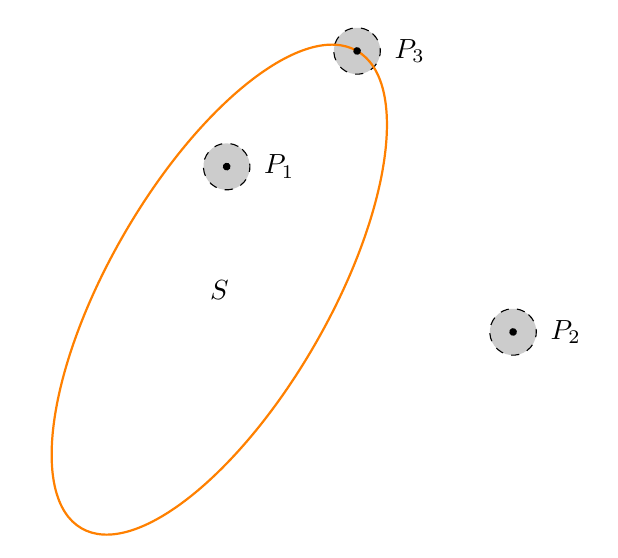
\begin{tikzpicture}[scale=.7]
\filldraw[rotate=60,draw=black,dashed,fill=gray!40]
	(2,1)circle(12pt)
	(2,-5)circle(12pt)
	(5,0)circle(12pt);
\draw[orange,rotate=60,thick](0,0)ellipse[x radius=5,y radius=2];
\draw (0,0)node{\(S\)};
\fill[rotate=60]
	(2,1)circle(2pt)node[right=10pt]{\(P_1\)}
	(2,-5)circle(2pt)node[right=10pt]{\(P_2\)}
	(5,0)circle(2pt)node[right=10pt]{\(P_3\)};
\end{tikzpicture}
\caption{平面上的点与点集的关系}
\label{figure:集合论.平面上的点与点集的关系}
\end{figure}
\end{definition}

\begin{property}
设点集\(S\subseteq\mathbb{R}^2\).
任意一点\(P\in\mathbb{R}^2\)要么是\(S\)的内点,要么是\(S\)的外点,要么是\(S\)的边界点.

换言之,任意点集\(S\)的内点、外点和边界点的集合均无交集,即:
\begin{enumerate}
\item \(I(S) \cap E(S) = \emptyset\).
\item \(\partial{S} \cap I(S) = \emptyset\).
\item \(\partial{S} \cap E(S) = \emptyset\).
\end{enumerate}
\end{property}

\begin{definition}
设点\(P\)和点集\(S\)满足\(P \in S\).
定义:若\(\exists \mathring{U}(P)\)使得\[
\mathring{U}(P) \cap S = \emptyset,
\]则称\(P\)为\(S\)的\textbf{孤立点}(acnode),记作\(P \in A(S)\).
\end{definition}

\begin{property}
\(S\)的内点必属于\(S\),即\[
P \in I(S) \implies P \in S
\]或\[
I(S) \subseteq S.
\]
\begin{proof}
\[
\left. \begin{array}{r}
P \in I(S) \iff \exists U(P) :\: U(P) \subseteq S \\
P \in U(P)
\end{array} \right\}
\implies P \in S.
\qedhere
\]
\end{proof}
\end{property}

\begin{property}
\(S\)的外点必不属于\(S\),即\(P \in E(S) \implies P \notin S\).
\begin{proof}
\begin{align*}
\left. \begin{array}{r}
P \in E(S) \iff \exists U(P) :\: U(P) \cap S = \emptyset \\
P \in U(P) \iff \{P\} \subseteq U(P) \implies \{P\} \cap S \subseteq U(P) \cap S
\end{array} \right\}
\implies& \{P\} \cap S \subseteq \emptyset \\
\implies \{P\} \cap S = \emptyset
\implies P \notin S.&
\qedhere
\end{align*}
\end{proof}
\end{property}

\begin{example}
点集的边界点可能属于该点集,也可能不属于它.例如,实轴上的左闭右开区间\([a,b)\)有两个边界点\(a\)和\(b\),但\(a \in [a,b)\)而\(b \notin [a,b)\).
\end{example}

\begin{definition}
设点\(P\in\mathbb{R}^2\),点集\(S\subseteq\mathbb{R}^2\).
定义:如果点\(P\)的任意邻域内总有\(S\)中的无穷多个点,则称\(P\)是\(S\)的\textbf{聚点}(Cluster),记作\(P \in C(S)\),即\[
P \in C(S)
\iff
\forall\delta>0,\exists Q \in S : Q \in \mathring{U}(P,\delta).
\]称点集\(S\)的聚点的集合\(C(S)\)为\(S\)的\textbf{导集}(derived set).
\end{definition}
任取点集\(S\)的一个聚点\(P_C\).由聚点的定义可知,\(P_C\)可以属于\(S\),也可以不属于\(S\).

\begin{theorem}
点\(P\)是点集\(S\)的聚点的充要条件是:在\(P\)的任意邻域内总有异于点\(P\)而属于\(S\)的一个点,即\[
\forall \delta>0 \bigl[
	\mathring{U}(P,\delta) \cap S \neq \emptyset
\bigr].
\]
\end{theorem}

\begin{property}
点集的内点均是其聚点,即\(I(S) \subseteq C(S)\).
\begin{proof}
由内点的定义有\(P \in I(S) \iff \exists \delta_1>0 :\: U(P,\delta_1) \subseteq S\).

当\(0 < \delta_2 \leqslant \delta_1\)时,有\[
\mathring{U}(P,\delta_2)
\subseteq U(P,\delta_1)
\subseteq S,
\]所以\[
\mathring{U}(P,\delta_2) \cap S
= \mathring{U}(P,\delta_2)
\neq \emptyset.
\]

当\(\delta_2 > \delta_1\)时,有\[
\emptyset \neq \mathring{U}(P,\delta_1) \subsetneqq U(P,\delta_1) \subseteq S,
\]\[
\mathring{U}(P,\delta_2) \cap S
\supseteq \mathring{U}(P,\delta_1) \cap S \neq \emptyset.
\]

综上所述,对于\(\forall \delta_2 > 0\)都有\(\mathring{U}(P,\delta_2) \cap S \neq \emptyset\)成立,即\(P \in C(S)\).
\end{proof}
\end{property}

\begin{property}
点集的外点不是其聚点,即\(P \in E(S) \implies P \notin C(S)\).
\begin{proof}
因为\(P \in E(S)\),所以\(\exists \delta > 0: U(P,\delta) \cap S = \emptyset\).又因为\(\mathring{U}(P,\delta) \subsetneqq U(P,\delta)\),所以\[
U(P,\delta) \cap S \supsetneqq \mathring{U}(P,\delta) \cap S = \emptyset,
\]从而有\(P \notin C(S)\).
\end{proof}
\end{property}

\begin{property}
点集的孤立点不是聚点,即\(P \in A(S) \implies P \notin C(S)\).
\begin{proof}
\(P \in A(S) \implies \exists \delta > 0 : \mathring{U}(P,\delta) \cap S = \emptyset \iff P \notin C(S)\).
\end{proof}
\end{property}

\begin{property}
点集的孤立点必不是其内点,点集的内点也必不是其孤立点,即\[
P \in A(S) \implies P \notin I(S),
\]\[
P \in I(S) \implies P \notin A(S).
\]
\end{property}

\begin{property}
点集的孤立点必不是其外点,点集的外点也必不是其孤立点,即\[
P \in A(S) \implies P \notin E(S),
\]\[
P \in E(S) \implies P \notin A(S).
\]
\end{property}

\begin{property}
点集的孤立点必是其边界点,即\(A(S) \subseteq \partial{S}\).
\end{property}

\begin{property}
点集的边界点可能是聚点,也可能不是聚点.
\end{property}

\begin{definition}
设点集\(S \subseteq \mathbb{R}^2\).

若\(S\)的点皆为它的内点,则称\(S\)为\textbf{开集}.若\(S\)的所有边界点都属于\(S\)(即\(\partial S \subseteq S\)),或所有聚点皆属于\(S\)(即\(C(S) \subseteq S\)),则称\(S\)为\textbf{闭集}.

若\(\exists r > 0\),使得\[
S \subseteq U(O,r),
\]其中\(O\)是坐标原点\(\opair{0,0}\),则称“\(S\)是\textbf{有界的}”或“\(S\)是\textbf{有界集}”;否则称“\(S\)是\textbf{无界的}”或“\(S\)是\textbf{无界集}”.

若\(S\)中任意两点均可用一条全含于\(S\)内的折线相连接,则称“\(S\)是\textbf{连通的}”或“\(S\)是\textbf{连通集}”.

若\(S\)既是连通集又是开集,则称\(S\)为\textbf{开区域}.开区域\(S\)及其边界\(\partial S\)的并集\(S + \partial S\)称为\textbf{闭区域}(简称\textbf{闭域},常记作\(\overline{S}\)).开区域与闭区域统称\textbf{区域}.

如果平面区域\(S\)内任一闭曲线所围的部分都属于\(S\),则称\(S\)为平面\textbf{单连通区域};否则称为平面\textbf{复连通区域}.
\end{definition}
%集合论
\chapter{数理逻辑}
\section{命题}
\subsection{命题的概念}
\begin{definition}
\textbf{命题}(Proposition),是指对确定的对象进行判断的陈述句.
对于一个命题,它要么是真命题,要么是假命题.
悖论不能作为命题.

如果命题的判断正确,那么我们称“该命题是\textbf{真的}(True)”,或称“该命题是\textbf{真命题}”;
如果命题的判断错误,那么我们称“该命题是\textbf{假的}(False)”,或称“该命题是\textbf{假命题}”.

我们可以用数字表示命题的\textbf{真值},即:
\begin{center}
\begin{tabular}{|c|c|}
\hline
\textbf{命题的真值} & \textbf{数字表示} \\ \hline
真 & 1 \\ \hline
假 & 0 \\ \hline
\end{tabular}
\end{center}
\end{definition}

\subsection{简单命题与复合命题}
\begin{definition}
\textbf{逻辑联结词}(Logical connectives),是指连接命题,对各个命题的真值进行运算的词,例如“\emph{且}”“\emph{或}”“\emph{不}”“\emph{非}”“\emph{如果……那么……}”“\emph{当且仅当}”等.

为了将逻辑联结词形式化,我们可以使用符号来代表逻辑联结词.

\begin{table}[bp]
\centering
\begin{tabular}{|*{3}{c|}}
\hline
\textbf{概念} & \textbf{意义} & \textbf{符号} \\ \hline
\textbf{否定词}(negative) & 不、非 & \(\neg\) \\ \hline
\textbf{合取词}(conjunction) & 且、而且、并且 & \(\land\) \\ \hline
\textbf{析取词}(disjunction) & 或、或者 & \(\lor\) \\ \hline
\textbf{蕴涵词}(implication) & 如果……那么…… & \(\implies\) \\ \hline
\textbf{等价词}(equivalence) & 当且仅当 & \(\iff\) \\ \hline
\end{tabular}
\caption{逻辑联结词}
\end{table}
\end{definition}

\begin{definition}
\textbf{简单命题}(又称\textbf{原子命题},Atom proposition),%
指不含有逻辑联结词的命题.
相反地,\textbf{复合命题}(Compound proposition),%
是指包含了简单命题和逻辑联结词的命题.

逻辑联结词具有对命题的真值进行运算的效果,%
我们可以用\textbf{真值表}来说明其具体效果.
\end{definition}

\begin{table}[ht]
\centering
\begin{subtable}[ht]{0.9\textwidth}
\centering
\begin{tabular}{|c|p{1.5cm}|}
\hline
\(p\) & \(\neg p\) \\ \hline
0 & 1 \\ \hline
1 & 0 \\ \hline
\end{tabular}
\caption{否定词“非”}
\end{subtable}

\begin{subtable}[ht]{0.45\textwidth}
\centering
\begin{tabular}{|*{2}{c|}p{2cm}|}
\hline
\(p\) & \(q\) & \(p \land q\) \\ \hline
0 & 0 & 0 \\ \hline
0 & 1 & 0 \\ \hline
1 & 0 & 0 \\ \hline
1 & 1 & 1 \\ \hline
\end{tabular}
\caption{合取词“且”}
\end{subtable}
\begin{subtable}[ht]{0.45\textwidth}
\centering
\begin{tabular}{|*{2}{c|}p{2cm}|}
\hline
\(p\) & \(q\) & \(p \lor q\) \\ \hline
0 & 0 & 0 \\ \hline
0 & 1 & 1 \\ \hline
1 & 0 & 1 \\ \hline
1 & 1 & 1 \\ \hline
\end{tabular}
\caption{析取词“或”}
\end{subtable}

\begin{subtable}[ht]{0.45\textwidth}
\centering
\begin{tabular}{|*{2}{c|}p{2cm}|}
\hline
\(p\) & \(q\) & \(p \implies q\) \\ \hline
0 & 0 & 1 \\ \hline
0 & 1 & 1 \\ \hline
1 & 0 & 0 \\ \hline
1 & 1 & 1 \\ \hline
\end{tabular}
\caption{蕴涵词}
\end{subtable}
\begin{subtable}[ht]{0.45\textwidth}
\centering
\begin{tabular}{|*{2}{c|}p{2cm}|}
\hline
\(p\) & \(q\) & \(p \iff q\) \\ \hline
0 & 0 & 1 \\ \hline
0 & 1 & 0 \\ \hline
1 & 0 & 0 \\ \hline
1 & 1 & 1 \\ \hline
\end{tabular}
\caption{等价词}
\end{subtable}

\caption{单个逻辑联结词逻辑运算结果的真值表}
\end{table}

\begin{definition}
如果有p成立时q必成立,记\(p \implies q\),称\textbf{ \(p\)是\(q\)的充分条件},或称\textbf{ \(q\)是\(p\)的必要条件}.
称\(p\)为\textbf{蕴含前件},\(q\)为\textbf{蕴含后件}.
\end{definition}

在自然语言中,条件语句一般都具有内在的联系;而数理逻辑中的\emph{蕴含}则仅是命题的连接,不一定具有什么内在联系.

\begin{property}
只有当\(p\)为真,\(q\)为假时,蕴含式\(p \implies q\)才为假.
\end{property}
可以观察发现,\(p \implies q\)的真值表与\(\neg p \land q\)的相同.

\section{命题公式及其组成成分}
\begin{definition}
\textbf{命题常元}(Proposition constant),表示具体命题.
\textbf{命题变元}(Proposition variable),表示以“真、假”或者“0、1”为取值范围的变量.
\textbf{命题公式}(Proposition formula),是指由命题常元、命题变元和逻辑联结词组成的命题.

命题公式有如下的归纳定义:
\begin{enumerate}
\item 命题常元和命题变元是命题公式,也称作\textbf{原子公式}或\textbf{原子};
\item 设\(A\)、\(B\)为命题公式,那么有\[
(\neg A),\quad (A \land B),\quad (A \lor B),\quad (A \implies B),\quad (A \iff B)
\]也都是命题公式;
\item 只有有限步地引用上述两条所组成的符号串,才是命题公式.
\end{enumerate}
\end{definition}

\begin{example}
根据定义,\((\neg(p \implies (q \land r)))\)是命题公式.
\((qp)\)缺少联结词,所以不是命题公式.
\((p_1 \land (p_2 \land \dotsb))\)是无限的,所以不是命题公式.
\end{example}

为了简化书写,我们可以规定逻辑联结词的优先级顺序.
\begin{axiom}
逻辑联结词的优先级为:\[
\neg,\quad \land,\quad \lor,\quad \implies,\quad \iff.
\]除非有括号,否则按照命题公式从左到右,按照优先级从高到低的次序结合.
定义逻辑联结词的优先级的意义在于可以减少命题公式中的括号数量.
\end{axiom}

\begin{example}
\(((\neg p) \lor (q))\)等同于\(\neg p \lor q\).

但\[
p \implies q \land r \implies s
\]并非\[
((p \implies q) \land (r \implies s)),
\]而应等同于\[
((p \implies (q \land r)) \implies s).
\]
\end{example}

\subsection{命题公式与真值函数}





\begin{definition}
如果对于一个公式,不论其命题变元取何值,该公式总为真,则称该公式为\DefineConcept{永真式}或\DefineConcept{重言式}.
\end{definition}

\begin{example}
常见的永真式列举如下:\begin{enumerate}
\item 肯定后件律 \(p \implies (q \implies p)\);
\item 同一律 \(p \implies p\);
\item 排中律 \(\neg p \lor p\);
\item 矛盾律 \(\neg(\neg p \land p)\);
\item 双重否定律 \(\neg\neg p \iff p\).
\end{enumerate}
\end{example}
%数理逻辑
\begingroup
\chapter{初等数论}
数论在一些地方总有让人意想不到的妙用.
有这样一种说法:“自然科学的皇后是数学,数学的皇冠是数论,哥德巴赫猜想则是皇冠上的明珠。”
在这一章,我们介绍一些基础的数论理论,供大家参考.

\section{素数与合数}
在正整数集上,由于没有引入负数、分数的概念,正整数\(x\)与\(y\)相除的结果除了商\(z\)以外,还经常是带有余数\(r\)的,于是有关系式\[
x = y z + r.
\]
\begin{definition}
在正整数集上,如果\(x\)与\(y\)相除余\(r=0\),我们就称“\(y\)可以\textbf{整除}\(x\)”或“\(x\)可以\textbf{被}\(y\)\textbf{整除}”或“\(x\)是\(y\)的\textbf{倍数}”或“\(y\)是\(x\)的\textbf{因子}”,记作\(\truediv{x}{y}\),即\[
\truediv{x}{y} \iff
\bigl( \exists z \in \mathbb{N}^+ : x = y z \bigr).
\]
\end{definition}

\begin{definition}
设\(a,b\in\mathbb{N}^+\).
\(a\)与\(b\)的\textbf{最大公约数}(greatest common divisor),记作\((a,b)\);
\(a\)与\(b\)的\textbf{最小公倍数}(least common multiple),记作\([a,b]\).
\end{definition}
在本章以外,为了防止最大公约数、最小公倍数记号与开区间、闭区间符号混淆,分别记作\(\gcd{p,q}\)和\(\lcm{p,q}\).

\begin{theorem}
设\(a,b\in\mathbb{N}^+\).
已知\(a\)与\(b\)的最大公约数\((a,b)\)和最小公倍数\([a,b]\),%
那么\((a,b)\times[a,b]=ab\).
\end{theorem}

\begin{definition}
如果正整数\(x\)只能被1或它自己整除\footnote{特别地,我们规定1不是素数.},那么称\(x\)为\textbf{素数}或\textbf{质数}(prime number),否则称之为\textbf{合数}(composite number).
如果正整数\(x\)与\(y\)除了1以外没有其他公因子,就称“\(x\)与\(y\)\textbf{互素}(或\textbf{互质})”.

全体素数的集合,记作\(\mathbb{S}\),即\[
\mathbb{S} = \Set*{
x\in\mathbb{N}^+-\{1\} \given \forall y\in\mathbb{N}^+ \bigl[
	y \neq x \implies (x,y)=1
\bigr]
}.
\]
\end{definition}

\begin{theorem}
如果一个正整数\(a\)能整除正整数的乘积\(bc\),且\(a\)与其中一个因子\(b\)互素,则\(a\)必能整除另一个因子\(c\).
\end{theorem}
\begin{corollary}
如果素数\(a\)能整除正整数的乘积\(bcd\dotsm\),则\(a\)必能整除该乘积的一个因子.
\end{corollary}
\begin{corollary}
如果素数\(a\)能整除正整数的乘积\(b^n\ (n\in\mathbb{N}^+)\),那么\(a\)必能整除\(b\).
\end{corollary}

\begin{theorem}
如果正整数\(a\)与正整数\(b,c\)均互素,则它必与乘积\(bc\)互素.
\end{theorem}
\begin{corollary}
如果正整数\(a\)与正整数的乘积\(bc\)互素,则\(a\)与正整数\(b,c\)均互素.
\end{corollary}
\begin{corollary}
如果正整数\(a\)与\(b\)互素,则\(a^m\ (m\in\mathbb{N}^+)\)与\(b^n\ (n\in\mathbb{N}^+)\)互素.
\end{corollary}

\begin{theorem}
如果正整数\(a\)与\(b\)互素,则分数\(\frac{a^m}{b^n}\ (m,n\in\mathbb{N}^+)\)均为既约分数.
\end{theorem}
\begin{corollary}
设\(a,b,c,d\in\mathbb{N}^+\).
如果\(\frac{a}{b} = \frac{c}{d}\),且\(\frac{a}{b}\)是既约分数,则\[
\forall k\in\mathbb{R}^* : c = ka, d = kb.
\]
\end{corollary}

不难发现,第一个素数是2,它也是素数中唯一一个偶数.
第二个素数是3,接下来是5、7、11……
我们不禁发问,素数的个数究竟是有限的,还是无限的.
\begin{theorem}
素数有无穷多个.
\begin{proof}
用反证法\footnote{这个证法是由古希腊数学家欧几里得给出的.}.
假设素数只有\(k\)个,分别是\(\v{p}{k}\),且\(p_1 < p_2 < \dotsb < p_k\).
显然,数\(\truediv{p_1 p_2 \dotsm p_k}{p_i}\ (i=1,2,\dotsc,k)\).
但数\[
N = 1 + p_1 p_2 \dotsm p_k
\]与\(p_i\ (i=1,2,\dotsc,k)\)相除总余1,这就说明数\(N\)要么是一个素数,要么是一个可以被区间\((p_k,N)\)内的一个正整数\(M\)整除的合数,总之素数的个数大于\(k\).
以此类推,可知素数必然有无穷多个.
\end{proof}
\end{theorem}

\begin{theorem}
没有任何一个有理代数式能唯一地表示素数.
\begin{proof}
用反证法.
假设有理代数式\[
p(x) = a_0 + a_1 x + a_2 x^2 + \dotsb
\]唯一地表示素数,且\[
p(m) = a_0 + a_1 m + a_2 m^2 + \dotsb = q.
\]但\begin{align*}
p(m+nq) &= a_0 + a_1 (m+nq) + a_2 (m+nq)^2 + \dotsb \\
&= a_0 + a_1 m + a_2 m^2 + \dotsb + \alpha q \quad(\alpha\in\mathbb{Q}) \\
&= q + \alpha q = (1+\alpha)q,
\end{align*}即\(\truediv{p(m+nq)}{q}\),说明\(p(m+nq)\)不是一个素数.
\end{proof}
\end{theorem}

\begin{theorem}
一个数只能以一种方式分解素因子.
\begin{proof}
设合数\(N\)可以分解为乘积\(abcd\dotsm\),其中\(a,b,c,d,\dotsc\)是素数;又设\(N = \alpha\beta\gamma\delta\dotsm\),其中\(\alpha,\beta,\gamma,\delta,\dotsc\)是另一些素数;那么\[
abcd\dotsm = \alpha\beta\gamma\delta\dotsm.
\]
显然,数\(\alpha\)可以整除\(abcd\dotsm\),所以\(\alpha\)至少能整除它们中的一个因子,不妨设\(\truediv{a}{\alpha}\),但是由于\(a,b,c,d,\dotsc\)都是素数,故可知\(a=\alpha\),因此\[
bcd\dotsm = \beta\gamma\delta\dotsm.
\]以此类推,最后得到\(b=\beta,c=\gamma,d=\delta,\dotsc\),也就是说,任意合数的素因子分解式是唯一的.
\end{proof}
\end{theorem}

\begin{example}
已知合数\(N = a^p b^q c^r \dotsm\),其中\(a,b,c,\dotsc\)是不同的素数,\(p,q,r,\dotsc\)是正整数.
计算\(N\)的因子个数,\(N\)分解成两个因子的方式数,\(N\)分解成两个互素的因子的方式数,\(N\)的所有因子之和.
\begin{solution}
因为乘积\[
(1+a+a^2+\dotsb+a^p)
(1+b+b^2+\dotsb+b^q)
(1+c+c^2+\dotsb+c^r)\dotsm
\]的展开式的每一项都是数\(N\)的一个因子,所以,\(N\)的因子个数就是上述乘积的项数\((p+1)(q+1)(r+1)\dotsm\)\footnote{这里“因子个数”包括了1和合数\(N\)本身.}.

当\(N\)不是完全平方数时,\(N\)分解成两个因子的方式显然有\[
\frac{1}{2} (p+1)(q+1)(r+1)\dotsm
\]种.

当\(N\)是完全平方数时,\(N = \sqrt{N}\times\sqrt{N}\)也是一种分解方式,但对应于这种分解方式的因子只有一个\(\sqrt{N}\).
如果不计入这种分解方式,那么\(N\)的分解方式有\[
\frac{1}{2} \left[-1 + (p+1)(q+1)(r+1)\dotsm\right]
\]种;再加上刚刚提到的一种特殊分解方式\(N = \sqrt{N}\times\sqrt{N}\),那么\(N\)的分解方式总共有\[
\frac{1}{2} \left[1 + (p+1)(q+1)(r+1)\dotsm\right]
\]种.

在将数\(N\)分解成互素的两个因子\(\alpha,\beta\)时,其中一个必须包含\(a^p\),否则就会有\(a\)的一些幂在一个因子中,\(a\)的另一些幂在在另一个因子中,于是这两个因子就不互素了.
以此类推,可知“\(N\)分解成两个互素的因子的方式数”与“\(abcd\dotsm\)分解成两个因子的方式数”相等,即为\[
\frac{1}{2}(1+1)(1+1)(1+1)\dotsm.
\]若设\(N\)中共有\(n\)个不同的素因子,那么\(N\)分解成两个互素的因子的方式数是\[
\frac{1}{2} \cdot 2^n = 2^{n-1}.
\]

如前所述,由于乘积\[
(1+a+a^2+\dotsb+a^p)
(1+b+b^2+\dotsb+b^q)
(1+c+c^2+\dotsb+c^r)\dotsm
\]展开式的每一项都是一个因子,所以“\(N\)的所有因子之和”就等于这个乘积,由等比数列的求和公式,便得\(N\)的所有因子之和为\[
\frac{1-a^{p+1}}{1-a}\cdot\frac{1-b^{q+1}}{1-b}\cdot\frac{1-c^{r+1}}{1-c}\dotsm.
\]
\end{solution}
\end{example}

\section{费马小定理}
\begin{lemma}\label{theorem:初等数论.费马小定理.引理0}
证明:任意\(r\)个连续正整数的乘积能被\(r!\)整除.
\begin{proof}
设从正整数\(n\)开始的连续\(r\)个正整数的乘积为\(P_n = n(n+1)(n+2)\dotsm(n+r-1)\),那么\[
P_{n+1} = (n+1)(n+2)\dotsm(n+r),
\]\[
n P_{n+1} = (n+r) P_n = n P_n + r P_n,
\]\[
P_{n+1} = P_n + \frac{r}{n} P_n,
\]\[
P_{n+1} - P_n = r \frac{P_n}{n},
\]上式等号右边是\(r-1\)个连续正整数的\(r\)倍.
因此,如果任意\(r-1\)个连续正整数的乘积能被\((r-1)!\)整除,就有\(P_{n+1} - P_n\)能被\(r!\)整除.
因为\(P_1 = 1 \cdot 2 \dotsm r = r!\),所以\(P_2\)必是\(r!\)的倍数,从而\(P_3,P_4,\dotsc\)也都是\(r!\)的倍数.
这样就证明了“如果\(r-1\)个连续正整数的乘积能被\((r-1)!\)整除,那么\(r\)个连续正整数的乘积便能被\(r!\)整除”.
但是由于每两个连续正整数(必有一个奇数和一个偶数)的乘积能被\(2!=2\)整除,所以每三个连续正整数的乘积也能被\(3!\)整除;以此类推,该命题普遍成立.
\end{proof}
\end{lemma}

\begin{lemma}\label{theorem:初等数论.费马小定理.引理1}
设\(p\)是素数.
证明:除了第一项和最后一项以外,\((a+b)^p\)展开式的每一项的系数,都可以被\(p\)整除.
\begin{proof}
除了第一项与最后一项以外的各项系数为\[
C_p^r = \frac{p(p-1)(p-2)\dotsm(p-r+1)}{r!},
\]其中\(r=1,2,\dotsc,p-1\).
因为\(p\)是素数,所以\(r!\)中(除了1以外)没有一个因子可以整除\(p\);
又因为\(p>r\),所以\(p\)也不能整除\(r!\)中的任一因子;
也就是说,\((p-1)(p-2)\dotsm(p-r+1)\)必能被\(r!\)整除,而系数\(C_p^r\)必能被\(p\)整除.
\end{proof}
\end{lemma}

\begin{lemma}\label{theorem:初等数论.费马小定理.引理2}
设\(p\)是素数.
证明:\[
(a+b+c+d+\dotsb)^p = M + a^p + b^p + c^p + d^p + \dotsb,
\]其中\(M\)是\(p\)的倍数.
\begin{proof}
记\(\beta=b+c+\dotsb\),则由\cref{theorem:初等数论.费马小定理.引理1} 可知\[
(a+\beta)^p = a^p + \beta^p + M_1,
\]其中\(M_1\)是\(p\)的倍数.
接下来,记\(\gamma=c+d+\dotsb\),则同样有\[
\beta^p = (b+\gamma)^p = b^p + \gamma^p + M_2,
\]其中\(M_2\)是\(p\)的倍数.
以此类推,便得要证的结果,且\(M = M_1+M_2+\dotsb\).
\end{proof}
\end{lemma}

\begin{theorem}[费马小定理]\label{theorem:初等数论.费马小定理}
如果\(p\)是素数,且正整数\(n\)与\(p\)互素,则\(n^{p-1}-1\)是\(p\)的倍数.
\begin{proof}
根据\cref{theorem:初等数论.费马小定理.引理2},在\(n\)个正整数的和的\(p\)次幂\[
(a+b+c+d+\dotsb)^p = M + a^p + b^p + c^p + d^p + \dotsb
\]中令\(a=b=c=d=\dotsb=1\),那么有\[
n^p = n + M
\quad\text{或}\quad
n^p - n = n(n^{p-1}-1) = M,
\]即\(\truediv{n^{p-1}-1}{p}\).
\end{proof}
\end{theorem}

\begin{corollary}
如果\(p\)是素数,且\(p\neq2\),那么\(p-1\)是偶数,且对于任意正整数\(N\)总有\[
\left(N^{\frac{p-1}{2}}+1\right)
\left(N^{\frac{p-1}{2}}-1\right)
\]是\(p\)的倍数,或者说\[
N^{\frac{p-1}{2}} = Kp\pm1,
\]其中\(K\)是某个正整数.
\end{corollary}

\begin{corollary}[费马小定理']
如果\(p\)是素数,则\(\truediv{n^p-n}{p}\).
\end{corollary}

\begin{example}
设\(p\)是素数,证明:任意两个正整数的\(p\)次幂的差比这两个数的差大\(p\)的倍数.
\end{example}

\begin{example}
证明:任意完全平方数要么等于\(5n\),要么等于\(5n\pm1\),其中\(n\in\mathbb{N}^+\).
\end{example}

\begin{example}[费马猜想]
费马提出过一个错误的猜想:数\(2^{2^n}+1\ (n=0,1,2,\dotsc)\)都是素数.
这个猜想在当\(n=0,1,2,3,4\)时是正确的,但很遗憾的是,数学家欧拉发现,当\(n=5\)时,数\(2^{2^5}+1 = 4294967297 = 641 \times 6700417\)是合数.
% FactorInteger[2^(2^5)+1]
\end{example}

\endgroup
%初等数论
\chapter{复数概论}
\section{复数的形式与运算}
\subsection{复数的代数形式}
\begin{definition}[虚数单位]
规定:满足\(\iu^2=-1\)的数\(\iu\)称为\textbf{虚数单位}.
\end{definition}

\begin{definition}
把由有序实数对\(\opair{x,y}\)作代数组合所确定的数\(z=x+\iu y\)称为代数形式的\textbf{复数}.
实数\(x\)、\(y\)分别称为复数\(z=x+\iu y\)的\textbf{实部}、\textbf{虚部},记作\(x=\Re z\)、\(y=\Im z\).

特别地,当\(\Im z=0\)时,\(z=\Re z=x\)是实数;
当\(\Re z=0\)时,\(z=\iu\Im z=\iu y\),称为\textbf{纯虚数}.
\end{definition}

\begin{definition}[代数形式下复数相等条件]
设\(z_1\)和\(z_2\)都是复数,则当\(\Re z_1 = \Re z_2\)和\(\Im z_1 = \Im z_2\)同时成立时,则称\(z_1 = z_2\).
特别地,对于复数\(z\),则当且仅当\(\Re z=0\)且\(\Im z=0\)时,\(z=0\).
\end{definition}

\begin{definition}[共轭复数]
设\(z=x + \iu y \in\mathbb{C}\),其中\(x,y\in\mathbb{C}\),称复数\(\complexconjugate{z}=x - \iu y\)为\(z\)的\textbf{共轭复数}(conjugate).
\end{definition}

\subsection{复数的模}
\begin{definition}[复数的模]
设复数\(z = x + \iu y\),称\[
\abs{z} = \sqrt{x^2 + y^2}
\]为\(z\)的\textbf{模}或\textbf{绝对值}.
\end{definition}

\begin{property}
共轭复数以及复数的模具有以下性质:
\begin{enumerate}
\item \(\Re \complexconjugate{z} = \Re z\);
\item \(\Im \complexconjugate{z} = -\Im z\);
\item \(\complexconjugate{(\complexconjugate{z})} = z\);
\item \(z+\complexconjugate{z} = 2 \Re z\);
\item \(z-\complexconjugate{z} = 2\iu \Im z\);
\item \(z\complexconjugate{z} = \abs{z}^2\);
\item \(\abs{\complexconjugate{z}}=\abs{z}\);
\item \(\abs{z_1 z_2} = \abs{z_1} \abs{z_2}\);
\item \(\abs{\frac{z_1}{z_2}} = \frac{\abs{z_1}}{\abs{z_2}} \quad(z_2 \neq 0)\);
\item \(\complexconjugate{z_1 \pm z_2} = \complexconjugate{z_1} \pm \complexconjugate{z_2}\);
\item \(\complexconjugate{z_1 z_2} = \complexconjugate{z_1} \cdot \complexconjugate{z_2}\);
\item \(\complexconjugate{\left(\frac{z_1}{z_2}\right)} = \frac{\complexconjugate{z_1}}{\complexconjugate{z_2}} \quad (z_2 \neq 0)\);
\item \(-\abs{z} \leqslant \Re z \leqslant \abs{z} \leqslant \abs{\Re z} + \abs{\Im z}\);
\item \(-\abs{z} \leqslant \Im z \leqslant \abs{z} \leqslant \abs{\Re z} + \abs{\Im z}\).
\end{enumerate}
\end{property}

\subsection{复数的代数运算}
\begin{definition}[复数加法]
设\(z_1=x_1+\iu y_1\),\(z_2=x_2+\iu y_2\),%
定义\[
z_1+z_2=(x_1+x_2)+\iu(y_1+y_2)
\]为复数\(z_1\)和\(z_2\)的加法运算.
\end{definition}

\begin{definition}[复数减法]
设\(z_1=x_1+\iu y_1\),\(z_2=x_2+\iu y_2\),定义\[
z_1-z_2=(x_1-x_2)+\iu(y_1-y_2)
\]为复数的\(z_1\)和\(z_2\)的减法运算.
显然,复数减法是加法的逆运算.
\end{definition}

\begin{definition}[复数乘法]
设\(z_1 = x_1 + \iu y_1\),\(z_2 = x_2 + \iu y_2\),定义\[
z_1 \cdot z_2
= (x_1 + \iu y_1)(x_2 + \iu y_2)
= (x_1 x_2 - y_1 y_2)+\iu(x_1 y_2 + x_2 y_1)
\]为复数\(z_1\)和\(z_2\)的乘法运算.
\end{definition}

\begin{definition}[复数除法]
设\(z_1 = x_1 + \iu y_1\),\(z_2 = x_2 + \iu y_2 \neq 0\),定义满足\[
z_1 = z \cdot z_2
\]的复数\(z = x + \iu y\)为复数\(z_1\)和\(z_2\)的商,记作\[
z = \frac{z_1}{z_2},
\]称为复数\(z_1\)和\(z_2\)的除法运算.

显然,复数的除法是乘法的逆运算.
\end{definition}

\begin{theorem}
设\(z_1 = x_1 + \iu y_1\),\(z_2 = x_2 + \iu y_2 \neq 0\),则\[
\frac{z_1}{z_2}
= \frac{z_1 \cdot \complexconjugate{z_2}}{z_2 \cdot \complexconjugate{z_2}}
= \frac{z_1 \cdot \complexconjugate{z_2}}{\abs{z_2}^2}
= \frac{x_1 x_2 + y_1 y_2}{x_2^2 + y_2^2}
+ \iu \frac{x_2 y_1 - x_1 y_2}{x_2^2 + y_2^2}.
\]
\begin{proof}
设\(z = x + \iu y = \frac{z_1}{z_2}\),则\[
z \cdot z_2 = (x + \iu y)(x_2 + \iu y_2)
= (x_2 x - y_2 y) + \iu(y_2 x + x_2 y)
= x_1 + \iu y_1,
\]从而有方程组\[
\left\{ \begin{array}{l}
x_2 x - y_2 y = x_1, \\
y_2 x + x_2 y = y_1,
\end{array} \right.
\]解得\[
x = \frac{x_1 x_2 + y_1 y_2}{x_2^2 + y_2^2},
\quad
y = \frac{x_2 y_1 - x_1 y_2}{x_2^2 + y_2^2}.
\]
\end{proof}
\end{theorem}

\begin{theorem}
若\(z,w \in \mathbb{C}\),则有\begin{equation}
\abs{z \pm w}^2 = \abs{z}^2 + \abs{w}^2 \pm 2 \Re(z \complexconjugate{w}).
\end{equation}
\begin{proof}
\(
\abs{z + w}^2
= (z + w) (\complexconjugate{z + w})
= z\complexconjugate{z} + z\complexconjugate{w} + w\complexconjugate{z} + w\complexconjugate{w}
= \abs{z}^2 + 2 \Re(z\complexconjugate{w}) + \abs{w}^2
\).
\end{proof}
\end{theorem}

\begin{theorem}
若\(z,w \in \mathbb{C}\),则有\begin{equation}
\abs{z + w}^2 \leqslant (\abs{z} + \abs{w})^2.
\end{equation}
\begin{proof}
\(
\abs{z + w}^2
= \abs{z}^2 + 2 \Re(z \complexconjugate{w}) + \abs{w}^2
\leqslant \abs{z}^2 + 2 \abs{z}\abs{\complexconjugate{w}} + \abs{w}^2
= (\abs{z} + \abs{w})^2
\).
\end{proof}
\end{theorem}

\begin{theorem}[三角不等式]
若\(z,w \in \mathbb{C}\),则有\begin{equation}
\abs{\abs{z}-\abs{w}} \leqslant \abs{z \pm w} \leqslant \abs{z} + \abs{w}.
\end{equation}
\begin{proof}
因为\[
\abs{z + w}^2 \leqslant (\abs{z} + \abs{w})^2,
\]所以\(\abs{z + w} \leqslant \abs{z} + \abs{w}\).

又因为\[
\abs{z} = \abs{z + w + (-w)} \leqslant \abs{z+w} + \abs{-w} = \abs{z+w} + \abs{w},
\]所以\(\abs{z}-\abs{w} \leqslant \abs{z+w}\).

同样地,有\(\abs{w}-\abs{z} \leqslant \abs{z+w}\).

综上所述,\(\abs{\abs{z}-\abs{w}}\leqslant\abs{z+w}\).
\end{proof}
\end{theorem}

\begin{example}
证明:\(\abs{z_1+z_2}^2 + \abs{z_1-z_2}^2 = 2 (\abs{z_1}^2 + \abs{z_2}^2)\).
\begin{proof}
记\(z_1 = x_1 + \iu y_1, z_2 = x_2 + \iu y_2\).那么\[
z_1+z_2 = (x_1+x_2) + \iu(y_1+y_2),
\]\[
\abs{z_1+z_2}^2 = (x_1+x_2)^2 + (y_1+y_2)^2;
\]同理\(\abs{z_1-z_2}^2 = (x_1-x_2)^2 + (y_1-y_2)^2\).那么\begin{align*}
\abs{z_1+z_2}^2 + \abs{z_1-z_2}^2
&= (x_1+x_2)^2 + (y_1+y_2)^2
+ (x_1-x_2)^2 + (y_1-y_2)^2 \\
&= 2 ( x_1^2 + x_2^2 + y_1^2 + y_2^2 )
= 2 ( \abs{z_1}^2 + \abs{z_2}^2 ).
\qedhere
\end{align*}
\end{proof}
\end{example}

\subsection{复数的几何表示}
\begin{definition}[复数在复平面上的几何表示]
在直角坐标系\(xOy\)上可以用点\(\opair{x,y}\)表示复数\(z=x+\iu y\),也可以用向量\((x,y)\)表示复数\(z=x+\iu y\).与复数建立了这种对应关系的坐标平面\(xOy\)称为\textbf{复平面},记作\(C\).
称\(x\)轴为复平面的\textbf{实轴}.称\(y\)轴为复平面的\textbf{虚轴}.

显然,表示复数\(z\)的点与表示其共轭复数\(\complexconjugate{z}\)的点关于实轴对称.
\end{definition}

\begin{definition}[复数在复球面上的几何表示]
在\(Ox_1x_2x_3\)坐标系下,考虑单位球面\(S\)(即球心位于原点、半径为1的球面):\[
x_1^2+x_2^2+x_3^2=1
\]点\((0,0,1)\)称为北极,记作\(N\),同时\(x_1Ox_2\)平面取为复平面\(C\).复平面\(C\)交球面\(S\)于单位球的赤道.

对于复平面\(C\)上的每一个点\(z\),它与\(N\)连接的直线必与\(S\)交且只交于一点\(Z \neq N\).
若\(\abs{z} < 1\),则点\(Z\)在下半球面上;
若\(\abs{z} > 1\),则点\(Z\)在上半球面上;
若\(\abs{z} = 1\),则点\(Z\)在赤道上.
反之,取球面上任意一点\(Z \neq N\),连接它与\(N\)的直线也只与复平面\(C\)交于一点\(z\).

可见,除北极\(N=(0,0,1)\)以外,复平面\(C\)和球面\(S\)上的点是一一对应的.
并且当\(\abs{z} \to +\infty\)时,\(Z \to N\).
那么可以假想一个模为无穷大的复数,称作\textbf{无穷远点},记作\(z = \infty\),作为复平面\(C\)上与复球面北极\(N\)对应的点.

加上无穷远点后的复平面称为\textbf{扩充复平面},记作\(C_\infty\),即\[
C_\infty = C \cup \{\infty\}.
\]
扩充复平面\(C_\infty\)又称为\textbf{闭平面}.
对应地,复平面\(C\)因为不含无穷远点,所以又称为\textbf{开平面}.

复球面\(S\)与扩充复平面\(C_\infty\)上点之间的映射称为\textbf{球极射影}.
\(S\)又称为\textbf{黎曼复球面}.

另外,对于\(\infty\)还有以下几点值得注意:
\begin{enumerate}
\item \(\infty\)的实部\(\Re\infty\)、虚部\(\Im\infty\)、辐角\(\Arg\infty\)均无意义,其模\(\abs{\infty}=+\infty\);
\item 运算\(\infty \pm \infty\)、\(0 \cdot \infty\)、\(\frac{\infty}{\infty}\)均无意义;
\item 设复数\(z \neq \infty\),有\(z \pm \infty = \infty \pm z = \infty\),\(\frac{z}{\infty} = 0\);
\item 设复数\(z \neq 0\),有\(z \cdot \infty = \infty \cdot z = \infty\),\(\frac{z}{0} = \infty\);
\item 设复数\(z \neq 0\)且\(z \neq \infty\),有\(\frac{\infty}{z} = \infty\);
\item 在扩充复平面\(C_\infty\)上,任一直线都是通过无穷远点\(\infty\)的.同时,没有一个半平面包含点\(\infty\).
\end{enumerate}
\end{definition}

\begin{theorem}
设复数\(z=x+\iu y\),其对应的复球面上的点为\(Z=\opair{x_1,x_2,x_3}\),并满足:

当\(z \neq \infty\)时,\(Z\)的坐标为\[
x_1 = \frac{z + \complexconjugate{z}}{\abs{z}^2 + 1}, \qquad
x_2 = \iu\frac{\complexconjugate{z} - z}{\abs{z}^2 + 1}, \qquad
x_3 = \frac{\abs{z}^2 - 1}{\abs{z}^2 + 1}
\]或\[
x_1 = \frac{2x}{x^2+y^2+1}, \quad
x_2 = \frac{2y}{x^2+y^2+1}, \quad
x_3 = \frac{x^2+y^2-1}{x^2+y^2+1}.
\]

当\(z = \infty\)时,\(Z\)的坐标为\(N = (0,0,1)\).
\end{theorem}

\begin{theorem}
已知复球面上一点\(Z=(x_1,x_2,x_3)\),则其对应的复平面上的点为\[
z = x+\iu y = \frac{x_1+\iu x_2}{1-x_3}
\]
\end{theorem}
%复数
\chapter{函数}
\section{函数}
\subsection{一元函数的概念}
\begin{definition}
设\(D\)是\(\mathbb{R}\)的一个非空子集,称映射\(f\colon D \to \mathbb{R}\)为定义在\(D\)上的一个\DefineConcept{一元函数}(简称\DefineConcept{函数}),通常记为\[
y = f(x), \qquad x \in D
\]其中点集\(D\)称为该函数的\DefineConcept{定义域},\(x\)称为\DefineConcept{自变量},\(y\)称为\DefineConcept{因变量}.

函数定义中,对每个\(x \in D\),按对应法则\(f\),总有唯一确定的值\(y\)与之相应,%
这个值称为函数\(f\)在\(x\)处的\DefineConcept{函数值},记作\(f(x)\),即\(y=f(x)\).
因变量\(y\)与自变量\(x\)之间的这种依赖关系,通常称为\DefineConcept{函数关系}.
函数值\(f(x)\)的全体所构成的集合称为函数\(f\)的\DefineConcept{值域},%
记作\(R_f\)或\(f(D)\),即\[
R_f = f(D) = \Set{ y \given y = f(x) \land x \in D }.
\]

函数的定义域通常按以下两种情形来确定:
一种是对有实际背景的函数,根据实际背景中变量的实际意义来确定.
另一种是对抽象地用算式表达的函数,通常约定这种函数的定义域是使得算式有意义的一切实数组成的集合,这种定义域称为函数的\DefineConcept{自然定义域}.
\end{definition}

\begin{example}
函数\(y = \frac{1}{x}\)的自然定义域是\(\{ x \in \mathbb{R} \mid x \neq 0 \}\).
\end{example}

\begin{example}
函数\(y = \sqrt{x}\)的自然定义域是\(\{ x \in \mathbb{R} \mid x \geqslant 0 \}\).
\end{example}

\begin{definition}
如果给定一个对应法则,按这个法则,对每个\(x \in D\),总有确定但不唯一的\(y\)与之对应.
这样的不符合函数的定义的对应法则,习惯上称这种法则确定了一个\DefineConcept{多值函数}.
对于多值函数,如果我们附加一些条件,使得在附加条件之下,按照这个法则,%
对每个\(x \in D\),总有唯一确定的实数值\(y\)与之对应,那么这就确定了一个函数.
我们称这样得到的函数为多值函数的\DefineConcept{单值分支}.
\end{definition}

\subsection{多元函数的概念}
\begin{definition}
设\(D\)是\(\mathbb{R}^2\)的一个非空子集,称映射\(f\colon D \to \mathbb{R}\)为定义在\(D\)上的\DefineConcept{二元函数},通常记为\[
z = f(x,y),
\quad \opair{x,y} \in D
\]或\[
z = f(P),
\quad P\opair{x,y} \in D
\]其中点集\(D\)称为该函数的\DefineConcept{定义域},
\(x\)、\(y\)称为\DefineConcept{自变量},
\(z\)称为\DefineConcept{因变量}.
\end{definition}

\begin{definition}
类似地,设\(D\)是\(n\)维空间\(\mathbb{R}^n\)的一个非空子集,
称映射\[
	f\colon D \to \mathbb{R}
\]
为“定义在\(D\)上的\(n\)元\DefineConcept{函数}”,
通常记为\[
	y = f(\v{x}{n}),
	\quad \opair{\v{x}{n}} \in D
\]或\[
	y = f(\mat{x}),
	\quad \mat{x}=\opair{\v{x}{n}} \in D
\]
其中点集\(D\)称为“函数\(f\)的\DefineConcept{定义域}”,
\(x\)、\(y\)称为“函数\(f\)的\DefineConcept{自变量}”,
\(z\)称为“函数\(f\)的\DefineConcept{因变量}”.
\end{definition}

\subsection{函数的性质}
\subsubsection{函数的有界性}
\begin{definition}\label{definition:函数.函数的有界性}
设函数\(f(x)\)的定义域为\(D\),数集\(X \subseteq D\).

如果存在数\(K_1\),使得\(f(x) \leqslant K_1\)对任一\(x \in X\)都成立,即\[
\forall x \in X, \exists K_1 \in \mathbb{R} \bigl[
	f(x) \leqslant K_1
\bigr],
\]则称“函数\(f(x)\)在\(X\)上有\DefineConcept{上界}”,称“\(K_1\)是函数\(f(x)\)在\(X\)上的一个上界”.

如果存在数\(K_2\),使得\(f(x) \geqslant K_2\)对任一\(x \in X\)都成立,即\[
\forall x \in X, \exists K_2 \in \mathbb{R} \bigl[
	f(x) \geqslant K_2
\bigr],
\]则称“函数\(f(x)\)在\(X\)上有\DefineConcept{下界}”,称“\(K_2\)是函数\(f(x)\)在\(X\)上的一个下界”.

如果存在正数\(M\),使得\(\abs{f(x)} \leqslant M\)对任一\(x \in X\)都成立,即\[
\forall x \in X, \exists M>0 \bigl[
	\abs{f(x)} \leqslant M
\bigr],
\]则称“函数\(f(x)\)在\(X\)上\DefineConcept{有界}”或“函数\(f(x)\)是\(X\)上的\DefineConcept{有界函数}”.
反之如果这样的\(M\)不存在,即\[
\exists x_0 \in X, \forall M>0 \bigl[
	\abs{f(x_0)} > M
\bigr],
\]就称“函数\(f(x)\)在\(X\)上\DefineConcept{无界}”.
\end{definition}

\begin{theorem}
设函数\(f(x)\)的定义域为\(D\),数集\(X \subseteq D\).
函数\(f(x)\)在\(X\)上有界的充要条件是它在\(X\)上既有上界又有下界.
\end{theorem}

\subsubsection{函数的单调性}
\begin{definition}
设函数\(f(x)\)的定义域为\(D\),区间\(I \subseteq D\).
如果对于区间\(I\)上任意两点\(x_1\)及\(x_2\),当\(x_1 < x_2\)时,恒有\[
f(x_1) < f(x_2),
\]则称函数\(f(x)\)在区间\(I\)上是\DefineConcept{(严格)单调增加}的;
如果对于区间\(I\)上任意两点\(x_1\)及\(x_2\),当\(x_1 < x_2\)时,恒有\[
f(x_1) > f(x_2),
\]则称函数\(f(x)\)在区间\(I\)上是\DefineConcept{(严格)单调减少}的.

单调增加的函数和单调减少的函数统称为\DefineConcept{单调函数}.
\end{definition}

\subsubsection{函数的奇偶性}
\begin{definition}
设函数\(f(x)\)定义域为\(D=(-l,l)\)(\(l>0\)).
若对于任一\(x \in D\)都有\[
f(-x) = f(x),
\]恒成立,则称\(f(x)\)为\DefineConcept{偶函数};
若对于任一\(x \in D\)都有\[
f(-x) = -f(x)
\]恒成立,则称\(f(x)\)为\DefineConcept{奇函数}.
\end{definition}

\begin{property}
偶函数的图形是关于\(y\)轴对称的.
奇函数的图形是关于原点对称的.
\end{property}

\begin{property}
奇函数与奇函数之和、之差均为奇函数.
偶函数与偶函数之和、之差均为偶函数.
\begin{proof}
设\[
f(-x) = -f(x), \qquad g(-x) = -g(x).
\]令\(F(x) = f(x) \pm g(x)\),则\[
F(-x) = f(-x) \pm g(-x)
= [-f(x)] \pm [-g(x)]
= -[f(x) \pm g(x)]
= -F(x).
\qedhere
\]
\end{proof}
\end{property}

\begin{property}
奇函数与奇函数之积为偶函数.
\begin{proof}
设\[
f(-x) = -f(x), \qquad g(-x) = -g(x).
\]令\(F(x) = f(x) \cdot g(x)\),则\[
F(-x) = f(-x) \cdot g(-x)
= [-f(x)] \cdot [-g(x)]
= f(x) \cdot g(x)
= F(x).
\qedhere
\]
\end{proof}
\end{property}

\begin{property}
奇函数与偶函数之积为奇函数.
\begin{proof}
设\[
f(-x) = -f(x), \qquad g(-x) = g(x).
\]令\(F(x) = f(x) \cdot g(x)\),则\[
F(-x) = f(-x) \cdot g(-x)
= [-f(x)] \cdot g(x)
= - f(x) \cdot g(x)
= - F(x).
\qedhere
\]
\end{proof}
\end{property}

\begin{property}
偶函数与偶函数之积为偶函数.
\begin{proof}
设\[
f(-x) = f(x), \qquad g(-x) = g(x).
\]令\(F(x) = f(x) \cdot g(x)\),则\[
F(-x) = f(-x) \cdot g(-x) = f(x) \cdot g(x) = F(x).
\qedhere
\]
\end{proof}
\end{property}

\subsubsection{函数的周期性}
\begin{definition}
设函数\(f(x)\)的定义域为\(D\).
如果存在一个正数\(T\),使得对于任一\(x \in D\)有\((x + T) \in D\),且\[
f(x+ T) = f(x)
\]恒成立,则称\(f(x)\)为\DefineConcept{周期函数},称\(T\)为\(f(x)\)的周期.

已知周期为\(T\)的函数.
如果对于任意数\(a \in (0,T)\)都有\[
f(x + a) \neq f(x),%
\]则称\(T\)为\DefineConcept{最小正周期}.
\end{definition}

\begin{example}
狄利克雷函数\[
D(x) = \left\{ \begin{array}{ll}
1, & x \in \mathbb{Q}, \\
0, & x \in \mathbb{Q}^C.
\end{array} \right.
\]是一个周期函数,任何正有理数\(r\)都是它的周期.因为不存在最小的正有理数,所以它没有最小正周期.
\end{example}

\section{反函数与复合函数}
\begin{definition}[反函数]
设函数\(f\colon D \to f(D)\)是单射,则它存在逆映射\(f^{-1}: f(D) \to D\),称此映射\(f^{-1}\)为函数\(f\)的\DefineConcept{反函数}.
相对于反函数\(y=f^{-1}(x)\)来说,原来的函数\(y=f(x)\)称为\DefineConcept{直接函数}.
\end{definition}

\begin{property}
将直接函数\(y=f(x)\)和它的反函数\(y=f^{-1}(x)\)的图形画在同一坐标平面上,%
这两个图形关于直线\(y=x\)是对称的.
\end{property}

\begin{definition}
设函数\(y=f(u)\)的定义域为\(D_f\),函数\(u=g(x)\)的定义域为\(D_g\),且其值域\(R_g \subseteq D_f\),则函数\[
y = f[g(x)],
\quad x \in D_g
\]称为由函数\(u=g(x)\)与函数\(y=f(u)\)构成的\DefineConcept{复合函数},它的定义域为\(D_g\),变量\(u\)称为\DefineConcept{中间变量}.

函数\(g\)与函数\(f\)构成的复合函数,即按“先\(g\)后\(f\)”的次序复合的函数,通常记为\(f \circ g\),即\[
(f \circ g)(x) = f[g(x)].
\]
\end{definition}

\begin{example}
设函数\(f(x)\)的定义域为\((-l,l)\),试证:在\((-l,l)\)上必存在偶函数\(g(x)\)和奇函数\(h(x)\),使得\[
f(x) = g(x)+h(x).
\]
\begin{proof}
首先假设这样的\(g(x)\)、\(h(x)\)存在,即\[
f(x) = g(x) + h(x),
\]\[
g(-x) = g(x),
\]\[
h(-x) = -h(x).
\]于是有\[
f(-x) = g(-x) + h(-x) = g(x) - h(x).
\]

由此可知,只需要取\[
g(x) = \frac{1}{2} [f(x) + f(-x)],
\]\[
h(x) = \frac{1}{2} [f(x) - f(-x)]
\]即可满足题设要求.
\end{proof}
\end{example}

\section{常见函数}
\subsection{绝对值函数}
\begin{definition}[绝对值]
设\(x \in \mathbb{R}\),则称函数\[
f(x) = \left\{ \begin{array}{c}
x, \quad x \geqslant 0 \\
-x, \quad x < 0
\end{array} \right.
\]为\(x\)的绝对值,记作\(\abs{x}\).
\end{definition}

\begin{figure}[ht]
\centering
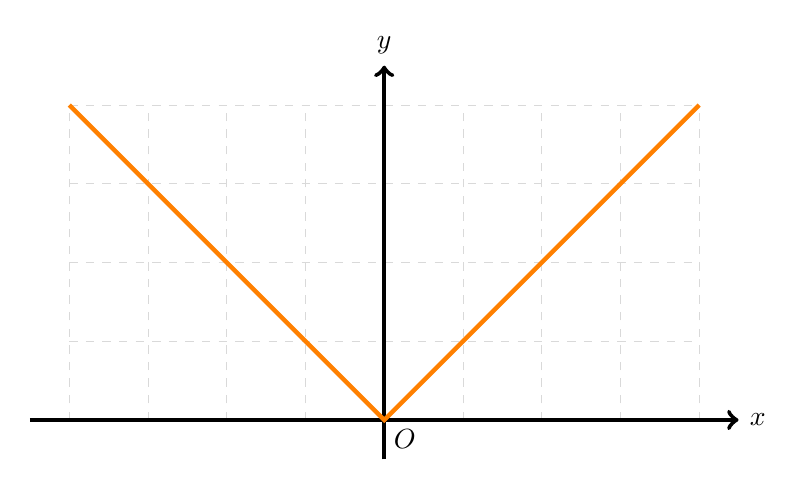
\begin{tikzpicture}
	\draw[help lines, color=gray!30, dashed] (-4,0) grid (4,4);
	\draw[->, ultra thick] (-4.5,0) -- (4.5,0) node[right]{\(x\)};
	\draw[->, ultra thick] (0,-0.5) -- (0,4.5) node[above]{\(y\)};
	\draw (0,0)node[below right]{\(O\)};
	\draw[orange,ultra thick] (-4,4)--(0,0)--(4,4);
\end{tikzpicture}
\caption{绝对值函数\(\abs{x}\)的图形}
\end{figure}

\subsection{符号函数}
\begin{definition}[符号函数]
函数\[
f(x) = \left\{ \begin{array}{cc}
1, & x > 0 \\
0, & x = 0 \\
-1, & x < 0 \\
\end{array} \right.
\]称为\DefineConcept{符号函数},记作\(\sgn x\).
\end{definition}

\begin{figure}[ht]
\centering
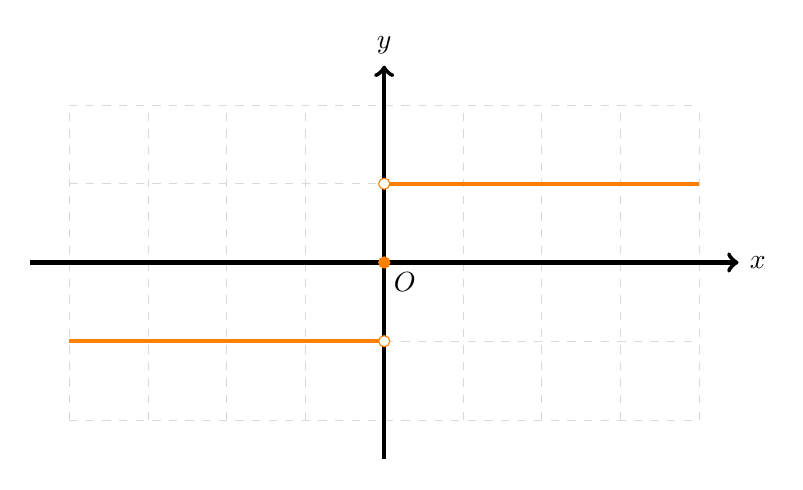
\begin{tikzpicture}
	\draw[help lines, color=gray!30, dashed] (-4,-2) grid (4,2);
	\draw[->, ultra thick] (-4.5,0) -- (4.5,0) node[right]{\(x\)};
	\draw[->, ultra thick] (0,-2.5) -- (0,2.5) node[above]{\(y\)};
	\draw (0,0)node[below right]{\(O\)};
	\draw[orange,ultra thick] (-4,-1)--(0,-1) (0,1)--(4,1);
	\draw[draw=orange,fill=orange] (0,0)circle(2pt);
	\draw[draw=orange,fill=white] (0,1)circle(2pt) (0,-1)circle(2pt);
\end{tikzpicture}
\caption{符号函数\(\sgn x\)的图形}
\end{figure}

\subsection{取整函数}
\begin{definition}[取整函数]
设\(x \in \mathbb{R}\),定义:
\begin{enumerate}
\item 向下取整函数\(\floor{x}\)为不大于\(x\)的最大整数;
\item 向上取整函数\(\ceil{x}\)为不小于\(x\)的最小整数.
\end{enumerate}
在未特别说明的情况下,取整函数\([x]\)是指向下取整函数,即\[
[x] = \floor{x}.
\]
\end{definition}

\begin{figure}[ht]
\def\subwidth{.45\linewidth}
\def\subscale{.9}
\begin{subfigure}[b]{\subwidth}%
\centering
\begin{tikzpicture}[scale=\subscale]
	\tikzstyle{sx}=[draw=orange,fill=orange]
	\tikzstyle{kx}=[draw=orange,fill=white]
	\draw[help lines, color=gray!30, dashed] (-1,-1) grid (4,4);
	\draw[dashed, color=gray] (-1,-1) -- (4,4);
	\draw[->, thick] (-1.5,0) -- (4.5,0) node[right]{\(x\)};
	\draw[->, thick] (0,-1.5) -- (0,4.5) node[above]{\(y\)};
	\foreach \i in {-1,...,3} {
		\draw[ultra thick,orange] (\i,\i)--(\i+1,\i);
		\fill[sx] (\i,\i)circle(2pt);
		\fill[kx] (\i+1,\i)circle(2pt);
		\ifnum\i=0\relax\else
			\draw(\i,0)node[below right]{\i};
			\draw(0,\i)node[above right]{\i};
		\fi;
	}
	\draw (0,0)node[above left]{\(O\)};
\end{tikzpicture}
\subcaption{向下取整函数\(\floor{x}\)}
\end{subfigure}
\begin{subfigure}[b]{\subwidth}%
\centering
\begin{tikzpicture}[scale=\subscale]
	\tikzstyle{sx}=[draw=orange,fill=orange]
	\tikzstyle{kx}=[draw=orange,fill=white]
	\draw[help lines, color=gray!30, dashed] (-1,-1) grid (4,4);
	\draw[dashed, color=gray] (-1,-1) -- (4,4);
	\draw[->, thick] (-1.5,0) -- (4.5,0) node[right]{\(x\)};
	\draw[->, thick] (0,-1.5) -- (0,4.5) node[above]{\(y\)};
	\foreach \i in {-1,...,3} {
		\draw[ultra thick,orange] (\i,\i+1)--(\i+1,\i+1);
		\fill[kx] (\i,\i+1)circle(2pt);
		\fill[sx] (\i+1,\i+1)circle(2pt);
		\ifnum\i=0\relax\else
			\draw(\i,0)node[below right]{\i};
			\draw(0,\i)node[above right]{\i};
		\fi;
	}
	\draw (0,0)node[above left]{\(O\)};
\end{tikzpicture}
\subcaption{向上取整函数\(\ceil{x}\)}
\end{subfigure}
\caption{取整函数的图形}
\end{figure}

\begin{property}
一般地,对于\(x\in\mathbb{R}\),总有\begin{equation}
x - 1 < \floor{x} \leqslant x \leqslant \ceil{x} < x + 1.
\end{equation}
\end{property}

\begin{property}
对于\(x\in\mathbb{Z}\),总有\begin{equation}
\ceil{n/2} + \floor{n/2} = n.
\end{equation}
\end{property}

\begin{property}
对于任意实数\(x \geqslant 0\)和整数\(a,b>0\),总有\begin{gather}
\ceil*{\frac{\ceil{x/a}}{b}} = \ceil*{\frac{x}{ab}}, \\
\floor*{\frac{\floor{x/a}}{b}} = \floor*{\frac{x}{ab}}, \\
\ceil*{\frac{a}{b}} \leqslant \frac{a+(b-1)}{b}, \\
\floor*{\frac{a}{b}} \geqslant \frac{a-(b-1)}{b}.
\end{gather}
\end{property}

\subsection{单位阶跃函数}
\begin{definition}
函数\[
f(x) = \left\{ \begin{array}{cc}
0, & x < 0, \\
1, & x \geqslant 1
\end{array} \right.
\]称为\DefineConcept{单位阶跃函数}或\DefineConcept{赫维赛德阶跃函数}.
\end{definition}

\begin{figure}[h!]
\centering
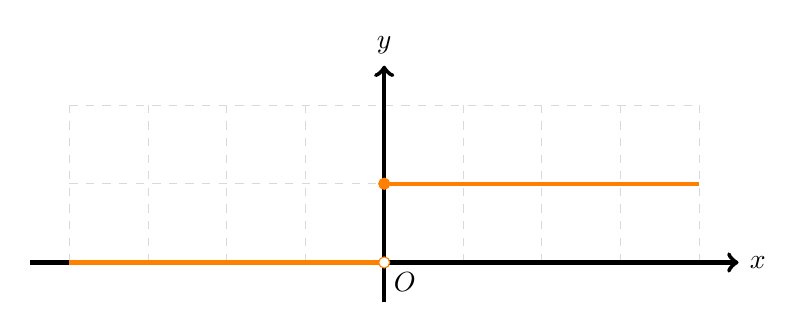
\begin{tikzpicture}
	\draw[help lines, color=gray!30, dashed] (-4,0) grid (4,2);
	\draw[->, ultra thick] (-4.5,0) -- (4.5,0) node[right]{\(x\)};
	\draw[->, ultra thick] (0,-.5) -- (0,2.5) node[above]{\(y\)};
	\draw (0,0)node[below right]{\(O\)};
	\draw[orange,ultra thick] (-4,0)--(0,0) (0,1)--(4,1);
	\draw[draw=orange,fill=orange] (0,1)circle(2pt);
	\draw[draw=orange,fill=white] (0,0)circle(2pt);
\end{tikzpicture}
\caption{单位阶跃函数的图形}
\end{figure}

\subsection{克罗内克\texorpdfstring{\(\delta\)}{\textdelta}函数}
\begin{definition}
%@see: https://mathworld.wolfram.com/KroneckerDelta.html
定义:\[
\delta_K(a,b)
\defeq \left\{ \begin{array}{cl}
	1, & a = b, \\
	0, & a \neq b.
\end{array} \right.
\]称其为\DefineConcept{克罗内克\(\delta\)函数}.
\end{definition}

\subsection{狄拉克\texorpdfstring{\(\delta\)}{\textdelta}函数}
\begin{definition}
%@see: https://functions.wolfram.com/GeneralizedFunctions/DiracDelta/02/
%@see: https://functions.wolfram.com/GeneralizedFunctions/DiracDelta2/02/
定义:\[
\delta_D(x)
\defeq \frac{1}{\pi}
	\lim\limits_{\varepsilon\to0}
	\frac{\varepsilon}{x^2+\varepsilon^2}
\quad(x\in\mathbb{R}).
\]
称其为\DefineConcept{狄拉克\(\delta\)函数}.
\end{definition}

\subsection{幂函数、指数函数、对数函数}
\begin{definition}
同一个数\(a\)(\(a\in\mathbb{R}\))连续相乘\(b\)(\(b\in\mathbb{N}\))次所得的乘积称作“\(a\)的\(b\)次方”(或“\(a\)的\(b\)次幂”),记作\(a^b\),即\[
a^b = \underbrace{a \times a \times \dotsm \times a}_{b\text{次}} = \prod\limits_{i=1}^b a.
\]

特别地,规定:\(a^0 = 1\),\(a^{-n} = \frac{1}{a^n}\),其中\(a\in\mathbb{R}^*\),\(n\in\mathbb{N}^+\).
\end{definition}

\begin{figure}[ht]
\centering
\begin{tikzpicture}
\def\r{\textcolor{orange}}
\def\b{\textcolor{blue}}
\def\p{\textcolor{purple}}
\draw (0,0)node{\(\r{a}^{\b{b}} = \p{c} \iff \log_{\r{a}} \p{c} = \b{b}\)};
\draw (-2.2,-.5)node{\r{底数}}
	(-2.2,.5)node{\b{指数}}
	(-1,-.5)node{\p{幂}}
	(.3,-.5)node{\r{底数}}
	(1.4,-.5)node{\p{真数}}
	(2.3,.5)node{\b{对数}};
\draw[->] (-1.7,-.3)--(-1.7,-1)--(.84,-1)->(.84,-.3); %a
\draw[->] (-1.55,.3)--(-1.55,1)--(1.7,1)->(1.7,.3); %b
\draw[->] (-.86,.3)--(-.86,.7)--(1.1,.7)->(1.1,.3); %c
\end{tikzpicture}
\caption{底数、指数、幂与对数的联系}
\label{figure:函数.底数、指数、幂与对数的联系}
\end{figure}

\subsubsection{幂函数的概念}
\begin{definition}[幂函数]
形如\(y=x^{\mu}\)(\(\mu \in \mathbb{R}\))的函数,称为\DefineConcept{幂函数}.
\end{definition}

\subsubsection{幂函数的性质}
\begin{property}
幂函数具有以下性质:
\begin{enumerate}
\item 当\(\mu = 0\)时,幂函数\(y=x^{\mu}=1\)是常数函数;

\item 当\(\mu\)为正奇数时,幂函数\(y=x^{\mu}\)为奇函数,%
其定义域、值域均为\((-\infty,+\infty)\),它在定义域内恒单调递增;

\item 当\(\mu\)为正偶数时,幂函数\(y=x^{\mu}\)为偶函数,%
其定义域为\((-\infty,+\infty)\),其值域为\([0,+\infty)\);
它在\((-\infty,0]\)上单调递减,在\([0,+\infty)\)上单调递增;

\item 当\(\mu\)为负奇数时,幂级数\(y=x^{\mu}\)又称为\DefineConcept{比例函数},%
其定义域、值域为\((-\infty,0)\cup(0,+\infty)\);
它在区间\((-\infty,0)\)和\((0,+\infty)\)内单调递减;
\begin{enumerate}
	\item 若幂函数前有常系数大于零则称之为\DefineConcept{正比例函数}.
	% Mathematica: Plot[Evaluate[x^-n /. n -> {1, 2, 3, 4, 5}], {x, 0, 2}, PlotRange -> {0, 2}, PlotLegends -> Automatic]
	\item 若幂函数前有常系数小于零则称之为\DefineConcept{反比例函数}.
	% Mathematica: Plot[Evaluate[x^-n /. n -> {1, 2, 3, 4, 5}], {x, -2, 0}, PlotRange -> {-2, 2}, PlotLegends -> Automatic]
\end{enumerate}

\item 当\(\mu\)为负偶数时,幂函数\(y=x^{\mu}\)为偶函数,%
其定义域为\((-\infty,0)\cup(0,+\infty)\),其值域为\((0,+\infty)\);
它在\((-\infty,0)\)内单调递增,在\((0,+\infty)\)内单调递减;

\item 当\(\mu = \pm\frac{m}{n} \in \mathbb{Q}\)(\(m,n>0\)且\(m\)、\(n\)是互质的整数)时,%
幂函数\(y=x^{\mu}=x^{\pm\frac{m}{n}}\)可改写为\(y=\sqrt[n]{x^m}\)(\(\mu>0\)时)%
或\(y=\frac{1}{\sqrt[n]{x^m}}\)(\(\mu<0\)时).
\end{enumerate}
\end{property}

\subsubsection{指数函数的概念}
\begin{definition}[指数函数]
形如\(y=a^x\)(\(a>0 \land a \neq 1\))的函数,称为以\(a\)为底的\DefineConcept{指数函数}.
将\(a\)(\(a \neq 0\))的倒数\(\frac{1}{a}\)记作\(a^{-1}\).
将\(a\)(\(a \geqslant 0\))的\(x\)次方根\(\sqrt[x]{a}\)记作\(a^{\frac{1}{x}}\).
规定任一实数的1次幂为该实数本身,即\(a^1=a\).
规定任一非零实数的零次幂为1,即\(a^0=1\).
\end{definition}

\subsubsection{对数函数的概念}
\begin{definition}[对数函数]
形如\(y=\log_a x\)(\(a>0 \land a \neq 1\))的函数,称为以\(a\)为底的\DefineConcept{对数函数}.

特别地,以\(10\)为底的对数称为\DefineConcept{常用对数},记作\(y = \lg x\);
以常数\(e\)为底的对数称为\DefineConcept{自然对数},记作\(y = \ln x\).
\end{definition}

\subsubsection{指数函数、对数函数的性质}
\begin{property}
指数函数\(y = a^x\)与对数函数\(y = \log_a x\)互为反函数,即\[
a^{\log_a x} = x, \qquad \log_a a^x = x.
\]它们具有以下性质:
\begin{center}
\def\arraystretch{1.5}
\begin{tabular}{|*{2}{p{5cm}|}}
\hline
\(a^x a^y = a^{x+y}\) & \(\log_a xy = \log_a x + \log_a y\) \\ \hline
\(\frac{a^x}{a^y} = a^{x-y}\) & \(\log_a \frac{x}{y} = \log_a x - \log_a y\) \\ \hline
\((a^x)^y = a^{xy}\) & \(\log_a x^y = y \log_a x\) \\ \hline
\end{tabular}
\end{center}
\end{property}

\begin{theorem}[换底公式]
一般地,\[
\log_a b = \frac{\log_c b}{\log_c a},
\]其中\(a,c\in(0,1)\cup(1,+\infty)\),\(b\in(0,+\infty)\).

特殊地,\[
\log_a b = \frac{1}{\log_b a},
\]其中\(a,b\in(0,1)\cup(1,+\infty)\).
\end{theorem}

\begin{corollary}
若\(a,a^x \in (0,1)\cup(1,+\infty)\),则\[
\log_{a^x} b^y = \frac{y}{x} \log_a b.
\]
\end{corollary}

\begin{example}
证明:\begin{equation}\label{equation:函数.真底互换公式}
a^{\ln b} = b^{\ln a}.
\end{equation}
\begin{proof}
在\cref{equation:函数.真底互换公式} 等号左右变量分别取对数,得\[
\ln(a^{\ln b}) = \ln b \ln a, \qquad
\ln(b^{\ln a}) = \ln a \ln b,
\]显然两者相等,故\(a^{\ln b} = b^{\ln a}\)成立.
\end{proof}
\end{example}

\subsubsection{重幂}
设\(a\)是实数,\(b\)是正整数,定义:\[
	^ba \defeq \underbrace{a^{a^{\ddots^a}}}_{\text{\(b\)个}},
\]
我们把\(^ba\)读作“\(a\)的\(b\)\DefineConcept{重幂}”.

例如,\[
	^23 = 3^3, \qquad
	^33 = 3^{3^3}, \qquad
	^43 = 3^{3^{3^3}}.
\]

\subsection{三角函数}
\subsubsection{三角函数的概念}
\begin{definition}\label{definition:函数.三角函数的几何定义}
取任意一个直角三角形\(\triangle ABC\)%
(如\cref{figure:函数.三角函数.三角函数的几何定义}),%
以\(\angle B\)为直角(即\(\angle{ABC} = \pi/2\)),%
设\(\angle{BAC} = \theta\).

\begin{figure}[ht]
\centering
\begin{tikzpicture}
\draw[help lines, color=gray!30, dashed] (0,0) grid (4,3);
\coordinate (A) at (0,0);
\coordinate (B) at (4,0);
\coordinate (C) at (4,3);
\draw (A)node[left]{\(A\)} -- (B)node[right]{\(B\)}node[midway,below]{\(c\)} -- (C)node[right]{\(C\)}node[midway,right]{\(a\)} -- (A)node[midway,left,above]{\(b\)} pic["\(\theta\)",draw=orange,-,angle eccentricity=2,angle radius=0.3cm]{angle=B--A--C} pic[draw=gray,-,angle radius=0.3cm]{right angle=C--B--A};
\end{tikzpicture}
\caption{}
\label{figure:函数.三角函数.三角函数的几何定义}
\end{figure}

定义三角函数如下:
\begin{center}
	\begin{tabular}{cc}
		\hline
		名称 & 定义式 \\ \hline
		正弦 & \(\sin\theta = a/b\) \\
		余弦 & \(\cos\theta = c/b\) \\
		正切 & \(\tan\theta = a/c\) \\
		余切 & \(\cot\theta = c/a\) \\
		正割 & \(\sec\theta = b/c\) \\
		余割 & \(\csc\theta = b/a\) \\
		\hline
	\end{tabular}
\end{center}
\end{definition}

\begin{example}
下面列出一些特殊的正弦函数值:\[
\sin0 = 0, \quad
\sin\frac{\pi}{6} = \frac{1}{2}, \quad
\sin\frac{\pi}{4} = \frac{\sqrt{2}}{2}, \quad
\sin\frac{\pi}{3} = \frac{\sqrt{3}}{2},
\]\[
\sin\frac{\pi}{2} = 1, \quad
\sin\pi = 0, \quad
\sin\frac{3\pi}{2} = -1.
\]

\begin{figure}[ht]
	\centering
	\begin{tikzpicture}
		\pgfmathsetmacro{\r}{2}
		\pgfmathsetmacro{\ax}{\r*cos(30)}
		\pgfmathsetmacro{\ay}{\r*sin(30)}
		\pgfmathsetmacro{\b}{\r/sqrt(2)}
		\coordinate (O)at(0,0);
		\draw(O)circle(\r);
		\begin{scope}[dashed,color=gray!50,text=black]
			\draw(O)--(\r,0)node[left]{\(0\)}node[right]{\(0\)}
			(O)--(\ax,\ay)node[below left]{\(\tfrac{\pi}{6}\)}node[right]{\(\tfrac{1}{2}\)}
			(O)--(\b,\b)node[below left]{\(\tfrac{\pi}{4}\)}node[above right]{\(\tfrac{\sqrt2}{2}\)}
			(O)--(\ay,\ax)node[below left]{\(\tfrac{\pi}{3}\)}node[above]{\(\tfrac{\sqrt3}{2}\)}
			(O)--(0,\r)node[below]{\(\tfrac{\pi}{2}\)}node[above]{\(1\)}
			(O)--(-\ay,\ax)node[below right]{\(\tfrac{2\pi}{3}\)}node[above]{\(\tfrac{\sqrt3}{2}\)}
			(O)--(-\b,\b)node[below right]{\(\tfrac{3\pi}{4}\)}node[above left]{\(\tfrac{\sqrt2}{2}\)}
			(O)--(-\ax,\ay)node[below right]{\(\tfrac{5\pi}{6}\)}node[left]{\(\tfrac{1}{2}\)}
			(O)--(-\r,0)node[right]{\(\pi\)}node[left]{\(0\)}
			(O)--(-\ax,-\ay)node[above right]{\(\tfrac{7\pi}{6}\)}node[left]{\(-\tfrac{1}{2}\)}
			(O)--(-\b,-\b)node[above right]{\(\tfrac{5\pi}{4}\)}node[below left]{\(-\tfrac{\sqrt2}{2}\)}
			(O)--(-\ay,-\ax)node[above right]{\(\tfrac{4\pi}{3}\)}node[below]{\(-\tfrac{\sqrt3}{2}\)}
			(O)--(0,-\r)node[above]{\(\tfrac{3\pi}{2}\)}node[below]{\(-1\)}
			(O)--(\ay,-\ax)node[above left]{\(\tfrac{5\pi}{3}\)}node[below]{\(-\tfrac{\sqrt3}{2}\)}
			(O)--(\b,-\b)node[above left]{\(\tfrac{7\pi}{4}\)}node[below right]{\(-\tfrac{\sqrt2}{2}\)}
			(O)--(\ax,-\ay)node[above left]{\(\tfrac{11\pi}{6}\)}node[right]{\(-\tfrac{1}{2}\)}
			;
		\end{scope}
		\begin{scope}[very thick,->]
			\draw(-1,0)--(1,0)node[above left]{\(x\)};
			\draw(0,-1)--(0,1)node[below right]{\(y\)};
		\end{scope}
	\end{tikzpicture}
	\caption{正弦函数\(\sin x\)的辅助圆与特殊值}
\end{figure}

特殊的余弦函数值:\[
	\cos0 = 1, \quad
	\cos\frac{\pi}{6} = \frac{\sqrt{3}}{2}, \quad
	\cos\frac{\pi}{4} = \frac{\sqrt{2}}{2}, \quad
	\cos\frac{\pi}{3} = \frac{1}{2},
\]\[
	\cos\frac{\pi}{2} = 0, \quad
	\cos\pi = -1, \quad
	\cos\frac{3\pi}{2} = 0.
\]
\end{example}

\subsubsection{三角函数的性质}
\begin{property}
根据三角函数的定义,显然有\begin{gather}
	\cot\theta = \frac{1}{\tan\theta}, \\
	\sec\theta = \frac{1}{\cos\theta}, \\
	\csc\theta = \frac{1}{\sin\theta}.
\end{gather}
\end{property}

\begin{theorem}[毕达哥拉斯三角恒等式]
\begin{figure}[ht]
	\def\subwidth{.5\linewidth}
	\def\subscale{.8}
		\begin{subfigure}[b]{\subwidth}%
		\centering
		\begin{tikzpicture}[scale=\subscale]
			\draw[help lines, color=gray!30, dashed] (0,0) grid (4,3);
			\coordinate (A) at (0,0);
			\coordinate (B) at (4,0);
			\coordinate (C) at (4,3);
			\draw (A)node[left]{\(A\)} -- (B)node[right]{\(B\)}node[midway,below]{\(\cos\theta\)} -- (C)node[right]{\(C\)}node[midway,right]{\(\sin\theta\)} -- (A)node[midway,above left]{\(1\)} pic["\(\theta\)",draw=orange,-,angle eccentricity=2,angle radius=0.3cm]{angle=B--A--C} pic[draw=gray,-,angle radius=0.3cm]{right angle=C--B--A};
		\end{tikzpicture}
		\subcaption{正弦、余弦辅助三角形}
		\end{subfigure}%
		\begin{subfigure}[b]{\subwidth}%
		\centering
		\begin{tikzpicture}[scale=\subscale]
			\draw[help lines, color=gray!30, dashed] (0,0) grid (4,3);
			\coordinate (A) at (0,0);
			\coordinate (B) at (4,0);
			\coordinate (C) at (4,3);
			\draw (A)node[left]{\(A\)} -- (B)node[right]{\(B\)}node[midway,below]{\(1\)} -- (C)node[right]{\(C\)}node[midway,right]{\(\tan\theta\)} -- (A)node[midway,above left]{\(\sec\theta\)} pic["\(\theta\)",draw=orange,-,angle eccentricity=2,angle radius=0.3cm]{angle=B--A--C} pic[draw=gray,-,angle radius=0.3cm]{right angle=C--B--A};
		\end{tikzpicture}
		\subcaption{正切、正割辅助三角形}
		\end{subfigure}%
	\caption{两种特殊的辅助三角形}
	\label{figure:函数.两种特殊的辅助三角形}
\end{figure}

结合\cref{figure:函数.两种特殊的辅助三角形},根据勾股定理可得
\begin{gather}
	\sin^2 \theta + \cos^2 \theta = 1, \\
	\tan^2 \theta + 1 = \sec^2 \theta, \\
	1 + \cot^2 \theta = \csc^2 \theta.
\end{gather}
\end{theorem}

\begin{property}
%sine
\begin{figure}[ht]
	\centering
	\begin{tikzpicture}[scale=0.7]
		\draw[help lines, color=gray!30, dashed] (-8,-2) grid (8,2);
		\draw[color=orange,domain=-2*pi:2*pi,samples=50] plot(\x,{sin(\x r)});

		\begin{scope}[>=Stealth,->,ultra thick]
			\draw(-7,0) -- (7,0) node[right]{\(x\)};
			\draw(0,-2) -- (0,2) node[above]{\(y\)};
		\end{scope}
		\draw (0.5*pi,0)node[below]{\(\pi/2\)};
		\draw[dashed, color=gray] (0.5*pi,1) -- (0.5*pi,0);
		\draw (0,0)node[below right]{\(O\)}
			(0,1)node[left]{\(1\)}
			(pi,0)node[below=3pt]{\(\pi\)}
			(-pi,0)node[below]{\(-\pi\)}
			(4,1)node{\(y=\sin x\)};
	\end{tikzpicture}
	\caption{正弦函数的图形}
	\label{figure:函数.正弦函数的图形}
\end{figure}

如\cref{figure:函数.正弦函数的图形},可以观察得出正弦函数的若干性质.
\begin{enumerate}
	\item 正弦函数是周期函数,其周期为\(T = 2\pi\).
	\item 正弦函数在区间\([2k\pi-\frac{\pi}{2},2k\pi+\frac{\pi}{2})\)上单调递增.
	\item 在区间\([2k\pi+\frac{\pi}{2},2k\pi+\frac{3\pi}{2})\)上单调递增.
	\item 当\(x=\frac{\pi}{2}+2k\pi\ (k\in\mathbb{Z})\)时,正弦函数\(y=\sin x\)取得极大值\(1\).
	\item 当\(x=\frac{3\pi}{2}+2k\pi\ (k\in\mathbb{Z})\)时,正弦函数\(y=\sin x\)取得极小值\(-1\).
	\item 正弦函数是奇函数,其图形关于坐标原点\(O\)中心对称,满足\(\sin(-x)=-\sin x\).
\end{enumerate}
\end{property}

\begin{property}
%cosine
\begin{figure}[ht]
	\centering
	\begin{tikzpicture}[scale=0.7]
		\draw[help lines, color=gray!30, dashed] (-8,-2) grid (8,2);
		\draw[color=orange,domain=-2*pi:2*pi,samples=50] plot(\x,{cos(\x r)});

		\begin{scope}[>=Stealth,->,ultra thick]
			\draw(-7,0) -- (7,0) node[right]{\(x\)};
			\draw(0,-2) -- (0,2) node[above]{\(y\)};
		\end{scope}
		\draw (1.4,0)node[below]{\(\pi/2\)};
		\draw[dashed, color=gray] (pi,-1) -- (pi,0);
		\draw (0,0)node[below right]{\(O\)}
			(-1,0)node[below]{\(-1\)}
			(0,1.3)node[left]{\(1\)}
			(3.3,0)node[below=3pt]{\(\pi\)}
			(-pi,0)node[below]{\(-\pi\)}
			(2,1)node{\(y=\cos x\)};
	\end{tikzpicture}
	\caption{余弦函数的图形}
	\label{figure:函数.余弦函数的图形}
\end{figure}

如\cref{figure:函数.余弦函数的图形},可以观察得出余弦函数的若干性质.
\begin{enumerate}
	\item 余弦函数也是周期函数,其周期为\(T = 2\pi\).
	\item 余弦函数在区间\([2k\pi,\pi+2k\pi)\)上单调递减.
	\item 在区间\([\pi+2k\pi,2\pi+2k\pi)\)上单调递增.
	\item 当\(x=2k\pi\ (k\in\mathbb{Z})\)时,余弦函数\(y=\cos x\)取得极大值\(1\).
	\item 当\(x=(2k-1)\pi\ (k\in\mathbb{Z})\)时,余弦函数\(y=\cos x\)取得极小值\(-1\).
	\item 余弦函数是偶函数,其图形关于\(y\)轴对称,满足\(\cos(-x)=\cos x\).
\end{enumerate}
\end{property}

\begin{property}
%tangent
\begin{figure}[ht]
	\centering
	\begin{tikzpicture}
		\draw[help lines, color=gray!30, dashed] (-6,-4) grid (6,4);

		\foreach \idx in {-1,0,1,2}{
			\pgfmathsetmacro{\start}{\idx*pi-1.3};
			\pgfmathsetmacro{\left}{(\idx-0.5)*pi};
			\pgfmathsetmacro{\end}{\idx*pi+1.3};
			\draw[dashed,red] (\left,-4) -- (\left,4);
			\ifthenelse{\equal{2}{\idx}} {} {
				\draw[color=orange] plot[domain=\start:\end, samples=100] (\x, {tan(\x r)})
			};
		}

		\begin{scope}[>=Stealth,->,ultra thick]
			\draw(-6,0) -- (6,0) node[right]{\(x\)};
			\draw(0,-4) -- (0,4) node[above]{\(y\)};
		\end{scope}
		\draw node at(1.4,-0.5) {\(\frac{\pi}{2}\)};
		\draw node at(0.3,-0.3) {\(O\)}
				node at(-0.3,1) {\(1\)}
				node at(3.14159,-0.5) {\(\pi\)}
				node at(-3.14159,-0.5) {\(-\pi\)}
				node at(2,1) {\(y=\tan x\)};
	\end{tikzpicture}
	\caption{正切函数的图形}
	\label{figure:函数.正切函数的图形}
\end{figure}

如\cref{figure:函数.正切函数的图形},可以观察得出正切函数的若干性质.
\begin{enumerate}
	\item 正切函数是周期函数,其周期为\(T = \pi\).
	\item 正切函数在区间\((k\pi-\frac{\pi}{2},k\pi+\frac{\pi}{2})\ (k\in\mathbb{Z})\)上单调递增.
	\item 正切函数是奇函数,其图形关于坐标原点\(O\)中心对称,满足\(\tan(-x)=-\tan x\).
\end{enumerate}
\end{property}

\subsubsection{和积互化公式}
\begin{theorem}[和积互化公式]
\begin{align}
	\sin(\alpha\pm\beta) &= \sin\alpha\cos\beta\pm\cos\alpha\sin\beta, \label{equation:函数.三角函数.和积互化公式1} \\
	\cos(\alpha\pm\beta) &= \cos\alpha\cos\beta\mp\sin\alpha\sin\beta, \label{equation:函数.三角函数.和积互化公式2} \\
	\tan(\alpha\pm\beta) &= \frac{\tan\alpha\pm\tan\beta}{1\mp\tan\alpha\tan\beta}, \label{equation:函数.三角函数.和积互化公式3} \\
	\cot(\alpha\pm\beta) &= \frac{\cot\alpha\cot\beta\mp 1}{\cot\beta\pm\cot\alpha}, \label{equation:函数.三角函数.和积互化公式4} \\
	\sec(\alpha\pm\beta) &= \frac{\sec\alpha\sec\beta}{1\mp\tan\alpha\tan\beta}, \label{equation:函数.三角函数.和积互化公式5} \\
	\csc(\alpha\pm\beta) &= \frac{\csc\alpha\csc\beta}{\cot\beta\pm\cot\alpha}, \label{equation:函数.三角函数.和积互化公式6} \\
	\sin \alpha \cos \beta &= \frac{\sin (\alpha + \beta) + \sin (\alpha - \beta)}{2}, \label{equation:函数.三角函数.和积互化公式7} \\
	\cos \alpha \sin \beta &= \frac{\sin (\alpha + \beta) - \sin (\alpha - \beta)}{2}, \label{equation:函数.三角函数.和积互化公式8} \\
	\cos \alpha \cos \beta &= \frac{\cos (\alpha + \beta) + \cos (\alpha - \beta)}{2}, \label{equation:函数.三角函数.和积互化公式9} \\
	\sin \alpha \sin \beta &= -\frac{\cos (\alpha + \beta) - \cos (\alpha - \beta)}{2}, \label{equation:函数.三角函数.和积互化公式10} \\
	\sin \alpha + \sin \beta &= 2 \sin \frac{\alpha + \beta}{2} \cos \frac{\alpha - \beta}{2}, \label{equation:函数.三角函数.和积互化公式11} \\
	\sin \alpha - \sin \beta &= 2 \cos \frac{\alpha + \beta}{2} \sin \frac{\alpha - \beta}{2}, \label{equation:函数.三角函数.和积互化公式12} \\
	\cos \alpha + \cos \beta &= 2 \cos \frac{\alpha + \beta}{2} \cos \frac{\alpha - \beta}{2}, \label{equation:函数.三角函数.和积互化公式13} \\
	\cos \alpha - \cos \beta &= -2 \sin \frac{\alpha + \beta}{2} \sin \frac{\alpha - \beta}{2}. \label{equation:函数.三角函数.和积互化公式14}
\end{align}
\begin{proof}
\begin{figure} %
	\centering
	\begin{tikzpicture}
		\coordinate (A) at (0.0,0.0);
		\coordinate (B) at (6.4,0.0);
		\coordinate (C) at (6.4,4.8);
		\coordinate (D) at (6.4,6.4);
		\coordinate (E) at (5.2,6.4);
		\draw (A) -- (B)node[midway,below]{\(\cos\alpha\cos\beta\)} -- (C)node[midway,right]{\rotatebox{90}{\(\cos\alpha\sin\beta\)}} -- (D)node[midway,right]{\rotatebox{90}{\(\sin\alpha\cos\beta\)}} -- (E)node[midway,above]{\(\sin\alpha\sin\beta\)} -- (C)node[midway,left=2mm,below=-3mm]{\rotatebox{-53.13}{\(\sin\alpha\)}} -- (A)node[midway,right=1mm,below=-2mm]{\rotatebox{36.87}{\(\cos\alpha\)}} -- (E)node[midway,left=2mm,above=2mm]{\(1\)};
		\pic["\(\alpha\)",draw=orange,-,angle eccentricity=2,angle radius=0.7cm]{angle=C--A--E};
		\pic["\(\beta\)",draw=blue,-,angle eccentricity=2,angle radius=0.7cm]{angle=B--A--C};
		\pic[draw=blue,-,angle radius=0.5cm]{angle=D--C--E};
		\pic[draw=gray,-,angle radius=0.3cm]{right angle=C--B--A};
		\pic[draw=gray,-,angle radius=0.3cm]{right angle=E--C--A};
		\pic[draw=gray,-,angle radius=0.3cm]{right angle=E--D--C};
	\end{tikzpicture}
	\caption{和积互化公式的辅助三角形}
	\label{figure:函数.和积互化公式的辅助三角形}
\end{figure} %

观察\cref{figure:函数.和积互化公式的辅助三角形} 可知
\begin{align*}
	\sin(\alpha+\beta) &= \sin\alpha\cos\beta+\cos\alpha\sin\beta, \\
	\cos(\alpha+\beta) &= \cos\alpha\cos\beta-\sin\alpha\sin\beta
\end{align*}成立.
又令\(\beta=-\beta\)则可得
\begin{align*}
	\sin(\alpha-\beta) &= \sin\alpha\cos\beta-\cos\alpha\sin\beta, \\
	\cos(\alpha-\beta) &= \cos\alpha\cos\beta+\sin\alpha\sin\beta.
	\qedhere
\end{align*}
\end{proof}
\end{theorem}

特别地,根据和积互化公式有
\begin{gather}
	\sin(\pi+x) = -\sin x, \\
	\cos(\pi+x) = -\cos x, \\
	\tan(\pi+x) = \tan x, \\
	\cot(\pi+x) = \cot x, \\
	\sin(\pi-x) = \sin x, \\
	\cos(\pi-x) = -\cos x, \\
	\tan(\pi-x) = -\tan x, \\
	\cot(\pi-x) = -\cot x.
\end{gather}
还有
\begin{gather}
	\cos\left(\frac{\pi}{2}-x\right) = \sin x, \\
	\sin\left(\frac{\pi}{2}-x\right) = \cos x, \\
	\tan\left(\frac{\pi}{2}-x\right) = \cot x, \\
	\cot\left(\frac{\pi}{2}-x\right) = \tan x.
\end{gather}
以上四个公式是当\(x\)为任意角时\(\left(\frac{\pi}{2}-x\right)\)的诱导公式.如果把其中的\(x\)换成\((-x)\),就可得到当\(x\)为任意角时\(\left(\frac{\pi}{2}+x\right)\)的诱导公式:
\begin{gather}
	\cos\left(\frac{\pi}{2}+x\right) = -\sin x, \\
	\sin\left(\frac{\pi}{2}+x\right) = \cos x, \\
	\tan\left(\frac{\pi}{2}+x\right) = -\cot x, \\
	\cot\left(\frac{\pi}{2}+x\right) = -\tan x.
\end{gather}

\begin{example}
\def\s{\sum\limits_{k=1}^n}%
证明:
当\(x\neq0\)时,有
\begin{gather}
	\s \sin kx
	= \frac{\sin\frac{nx}{2} \sin\frac{(n+1)x}{2}}{\sin\frac{x}{2}}, \\
	\s \cos kx
	= \frac{\sin\frac{nx}{2} \cos\frac{(n+1)x}{2}}{\sin\frac{x}{2}}.
\end{gather}
\end{example}

\subsubsection{倍角公式}
\begin{theorem}[二倍角公式]
\begin{align}
	\sin 2 \theta &= 2 \sin \theta \cos \theta, \\
	\cos 2 \theta &= \cos^2 \theta - \sin^2 \theta \\
		&= 2 \cos^2 \theta - 1 \\
		&= 1 - 2 \sin^2 \theta, \\
	\tan 2 \theta &= \frac{2 \tan \theta}{1 - \tan^2 \theta}.
\end{align}
\end{theorem}

\begin{theorem}[半倍角公式]
\begin{align}
	\sin \frac{\theta}{2} &= \pm \sqrt{\frac{1 - \cos \theta}{2}}, \\
	\cos \frac{\theta}{2} &= \pm \sqrt{\frac{1 + \cos \theta}{2}}, \\
	\tan \frac{\theta}{2} &= \pm \sqrt{\frac{1 - \cos \theta}{1 + \cos \theta}}.
\end{align}
\begin{proof}
联立\[
	\left\{ \begin{array}{l}
	\cos^2 \theta - \sin^2 \theta = \cos 2\theta, \\
	\cos^2 \theta + \sin^2 \theta = 1,
	\end{array} \right.
\]
解得\[
	\cos\theta = \pm\sqrt{\frac{1+\cos2\theta}{2}},
	\qquad
	\sin\theta = \pm\sqrt{\frac{1-\cos2\theta}{2}},
\]
再相除可得\[
	\tan\theta = \frac{\sin\theta}{\cos\theta}
	= \pm \sqrt{\frac{1 - \cos2\theta}{1 + \cos2\theta}}.
	\qedhere
\]
\end{proof}
\end{theorem}

\begin{figure}[ht]
	\centering
	\begin{tikzpicture}[scale=4]
		\pgfmathsetmacro{\t}{60}
		\coordinate(C)at({cos(\t)},{sin(\t)});
		\draw(1,0)coordinate(A)node[right]{\(A\)}arc[start angle=0,end angle=180,radius=1]
			coordinate(B)node[left]{\(B\)}--(0,0)coordinate(O)node[below]{\(O\)}
			--(C)node[above right]{\(C\)};
		\draw(C)--(C|-A)coordinate(D)node[below]{\(D\)}node[midway,above,rotate=90,orange]{\(\sin\theta\)};
		\draw(O)--(D)node[midway,below,orange]{\(\cos\theta\)}--(A)node[midway,below,orange]{\(1-\cos\theta\)}--(C)--(B)--(O)node[midway,below,orange]{\(1\)};
		\draw
			pic[draw=gray,angle radius=0.3cm]{right angle=A--D--C}
			pic[draw=gray,angle radius=0.3cm]{right angle=B--C--A};
		\draw
			pic["\(\theta\)",draw=blue,angle eccentricity=1.7,angle radius=5mm]{angle=D--O--C};
	\end{tikzpicture}
	\caption{半角公式的辅助三角形}
	\label{figure:函数.半角公式的辅助三角形}
\end{figure}

\begin{theorem}[万能公式]
\begin{gather}
\sin x = \frac{2 \tan(x/2)}{1+\tan^2(x/2)}, \\
\cos x = \frac{1-\tan^2(x/2)}{1+\tan^2(x/2)}, \\
\tan x = \frac{2 \tan(x/2)}{1-\tan^2(x/2)}.
\end{gather}
\end{theorem}

\subsubsection{辅助角公式}
\begin{theorem}[辅助角公式]
对于任意实数\(a,b,x\),总有
\begin{equation}
a \sin x + b \cos x = \sqrt{a^2 + b^2} \sin(x + \varphi),
\end{equation}
其中\(\varphi = \arctan\frac{b}{a}\).
\begin{proof}
令\(a = c \cos\varphi,
b = c \sin\varphi\ (c>0)\),那么
\[
\left(a/c\right)^2+\left(b/c\right)^2
=\cos^2\varphi+\sin^2\varphi
=1
\implies
c = \sqrt{a^2+b^2};
\]
且\[
\frac{b}{a} = \frac{c \sin\varphi}{c \cos\varphi} = \tan\varphi
\implies
\varphi = \arctan\frac{b}{a};
\]
同时
\[
a \sin x + b \cos x
= c (\sin x \cos\varphi + \cos x \sin\varphi)
= c \sin(x+\varphi).
\qedhere
\]
\end{proof}
\end{theorem}

\subsubsection{正(余)弦函数的一般形式}
\begin{definition}
一般地,把函数\[
F(t) = A \sin(\omega t + \varphi) \quad (-\infty<t<+\infty)
\]称作正弦函数的一般形式,其中\(A\)称为\DefineConcept{振幅},\(\omega\)称为\DefineConcept{角速度},\(\varphi\)称为\DefineConcept{初相},\((\omega t + \varphi)\)称为\DefineConcept{相位},\(T = \frac{2\pi}{\omega}\)称为\DefineConcept{最小正周期},\(f = \frac{1}{T}\)称为\DefineConcept{频率}.
\end{definition}
% Mathematica: Manipulate[Plot[A Sin[\[Omega] x + \[Phi]], {x, 0, 2 \[Pi]}], {A, 1, 5, 1}, {\[Omega], .1, 2, .1}, {\[Phi], 0, 2 \[Pi], \[Pi]/10}]
可以证明,随着\(A\)的增大,函数\(F(t)\)的波峰(或波谷)会变得更高(或更低);而随着\(\omega\)的增大,在固定长度的区间\([0,2\pi]\)上函数\(F(t)\)出现零点的次数会变多,形象地说,就是函数\(F(t)\)的图形变密了;另外,随着\(\varphi\)的增大,看起来,函数\(f(t)\)的图形好像沿着\(x\)轴向左移动一样.

\subsection{反三角函数}
\subsubsection{反三角函数的概念}
\begin{figure}[p]
\def\subwidth{.5\linewidth}
\def\subscale{.8}
    \begin{subfigure}[b]{\subwidth}%
    \centering
	\begin{tikzpicture}[scale=\subscale]
		\draw[help lines, color=gray!30, dashed] (-3,-4) grid (3,4);

		\draw[color=blue,dashed]
			plot[domain=0.5*pi:4,samples=100] ({sin(\x r)},\x)
			plot[domain=-4:-0.5*pi,samples=100] ({sin(\x r)},\x);
		\draw[color=orange]
			plot[domain=-0.5*pi:0.5*pi,samples=100] ({sin(\x r)},\x)
			node[color=black] at (1.5,2) {\(y=\arcsin x\)};
		\draw [dashed,color=gray] (-1,0) -- (-1,-0.5*pi) -- (0,-0.5*pi)
			(1,0) -- (1,0.5*pi) -- (0,0.5*pi);

		\draw [->, ultra thick] (-3,0) -- (3,0) node[right]{\(x\)};
		\draw [->, ultra thick] (0,-4) -- (0,4) node[above]{\(y\)};

		\draw (-0.5,0.5*pi)node{\(\frac{\pi}{2}\)}
			(0.5,-0.5*pi)node{\(-\frac{\pi}{2}\)};
			\draw (0,0)node[below right]{\(O\)}
			(-1.5,-0.5)node{\(-1\)}
			(1.5,-0.5)node{\(1\)};
	\end{tikzpicture}
    \subcaption{反正弦函数}
    \end{subfigure}%
    \begin{subfigure}[b]{\subwidth}%
    \centering
	\begin{tikzpicture}[scale=\subscale]
		\draw[help lines, color=gray!30, dashed] (-3,-4) grid (3,4);

		\draw[color=blue,dashed]
			plot[domain=pi:4,samples=100] ({cos(\x r)},\x)
			plot[domain=-4:0,samples=100] ({cos(\x r)},\x);
		\draw[color=orange]
			plot[domain=0:pi,samples=100] ({cos(\x r)},\x)
			node[color=black] at (1.5,2) {\(y=\arccos x\)};
		\draw [dashed,color=gray] (-1,0) -- (-1,pi) -- (0,pi);

		\draw [->, ultra thick] (-3,0) -- (3,0) node[right]{\(x\)};
		\draw [->, ultra thick] (0,-4) -- (0,4) node[above]{\(y\)};

		\draw (-0.5,0.5*pi)node{\(\frac{\pi}{2}\)}
			(0.5,-0.5*pi)node{\(-\frac{\pi}{2}\)}
			(0.5,pi)node{\(\pi\)};
		\draw (0,0)node[below right]{\(O\)}
			(-1.5,-0.5)node{\(-1\)}
			(1.5,-0.5)node{\(1\)};
	\end{tikzpicture}
    \subcaption{反余弦函数}
    \end{subfigure}%

	\begin{subfigure}[b]{\linewidth}%
	\centering
	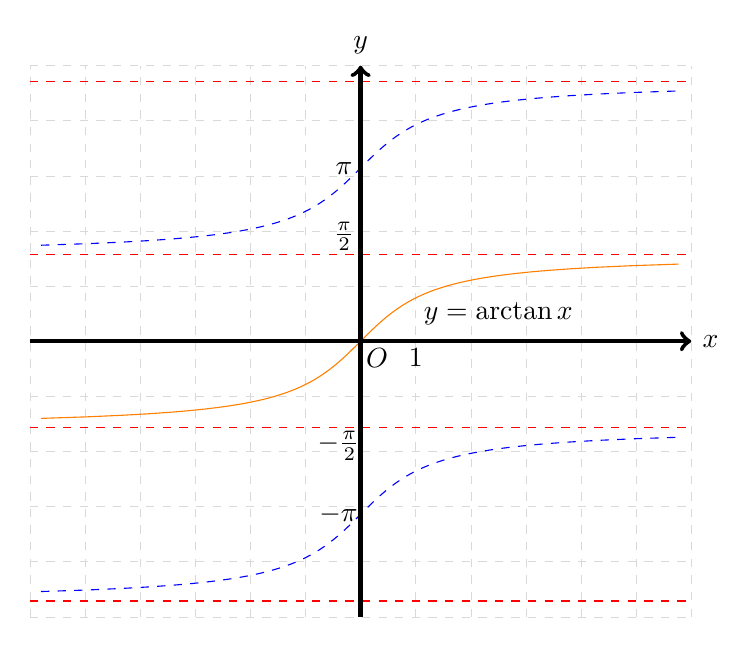
\begin{tikzpicture}[scale=.7]
		\draw[help lines, color=gray!30, dashed] (-6,-5) grid (6,5);

		\draw[color=red, dashed]
			(-6,-4.71237) -- (6,-4.71237)
			(-6,4.71237) -- (6,4.71237)
			(-6,-0.5*pi) -- (6,-0.5*pi)
			(-6,0.5*pi) -- (6,0.5*pi);
		\draw[color=blue, dashed]
			plot[domain=-1.4:1.4, samples=100] ({tan(\x r)},\x-pi)
			plot[domain=-1.4:1.4, samples=100] ({tan(\x r)},\x+pi);
		\draw[color=orange]
			plot[domain=-1.4:1.4, samples=100] ({tan(\x r)},\x);

		\draw [->, ultra thick] (-6,0) -- (6,0) node[right]{\(x\)};
		\draw [->, ultra thick] (0,-5) -- (0,5) node[above]{\(y\)};
		\draw (-0.3,1.9)node{\(\frac{\pi}{2}\)}
			(-0.4,-1.9)node{\(-\frac{\pi}{2}\)}
			(0.3,-0.3)node{\(O\)}
			(1,-0.3)node{\(1\)}
			(-0.3,pi)node{\(\pi\)}
			(-0.4,-pi)node{\(-\pi\)}
			(2.5,0.5)node{\(y=\arctan x\)};
	\end{tikzpicture}
	\subcaption{反正切函数}
	\end{subfigure}%
\caption{反三角函数的图形}
\label{figure:函数.反三角函数的图形}
\end{figure}

\subsubsection{反三角函数的性质}
\begin{theorem}[余角公式]
\begin{align}
\arcsin x + \arccos x &= \frac{\pi}{2}, \\
\arctan x + \arccot x &= \left\{ \begin{array}{cl}
\pi/2, & x > 0, \\
-\pi/2, & x < 0.
\end{array} \right.
\end{align}
\end{theorem}

\begin{theorem}[负数关系]
\begin{align}
\arcsin(-x) &= -\arcsin x, \\
\arccos(-x) &= \pi-\arccos x, \\
\arctan(-x) &= -\arctan x, \\
\arccot(-x) &= \pi-\arccot x, \\
\arcsec(-x) &= \pi-\arcsec x, \\
\arccsc(-x) &= -\arccsc x.
\end{align}
\end{theorem}

\begin{theorem}[倒数关系]
\begin{align}
\arcsin\frac{1}{x} &= \arccsc x, \\
\arccos\frac{1}{x} &= \arcsec x, \\
\arctan\frac{1}{x} &= \arccot x
	= \frac{\pi}{2} - \arctan x
 \quad(x>0), \\
\arccot\frac{1}{x} &= \begin{cases}
	\arctan x, & x>0, \\
	\pi+\arctan x, & x<0,
	\end{cases} \\
\arccot\frac{1}{x} &= \left\{ \def\arraystretch{1.5} \begin{array}{lc}
	\frac{\pi}{2} - \arccot x, & x>0, \\
	\frac{3\pi}{2} - \arccot x, & x<0,
	\end{array} \right. \\
\arcsec\frac{1}{x} &= \arccos x, \\
\arccsc\frac{1}{x} &= \arcsin x.
\end{align}
\end{theorem}

\begin{theorem}[三角关系]
\begin{align}
\sin(\arcsin{x}) &= x, \\
\cos(\arccos{x}) &= x, \\
\tan(\arctan{x}) &= x, \\
\arcsin(\sin x) &= x, \quad x \in (-\frac{\pi}{2},\frac{\pi}{2}), \\
\arccos(\cos x) &= x, \quad x \in (0,\pi), \\
\arctan(\tan x) &= x, \quad x \in (-\frac{\pi}{2},\frac{\pi}{2}), \\
\sin(\arccos{x}) = \cos(\arcsin{x}) &= \sqrt{1 - x^2}, \\
\tan(\arccot{x}) = \cot(\arccot{x}) &= \frac{1}{x}, \\
\sin(\arctan{x}) = \cos(\arccot{x}) &= \frac{x}{\sqrt{1+x^2}}, \\
\cos(\arctan{x}) = \sin(\arccot{x}) &= \frac{1}{\sqrt{1+x^2}}.
\end{align}
\end{theorem}

\begin{theorem}[和差公式]
\begin{align}
&\hspace{-10pt}
\arcsin x + \arcsin y \\
	&= \arcsin(x \sqrt{1-y^2} + y \sqrt{1-x^2})
		\quad(xy\leqslant0 \lor x^2+y^2\leqslant1) \\
	&= \pi - \arcsin(x \sqrt{1-y^2} + y \sqrt{1-x^2})
		\quad(x>0, y>0, x^2+y^2>1) \\
	&= -\pi - \arcsin(x \sqrt{1-y^2} + y \sqrt{1-x^2})
		\quad(x<0, y<0, x^2+y^2>1), \\
&\hspace{-10pt}
\arcsin x - \arcsin y \\
	&= \arcsin(x \sqrt{1-y^2} - y \sqrt{1-x^2})
		\quad(xy\geqslant0 \lor x^2+y^2\leqslant1) \\
	&= \pi - \arcsin(x \sqrt{1-y^2} - y \sqrt{1-x^2})
		\quad(x>0, y<0, x^2+y^2>1) \\
	&= -\pi - \arcsin(x \sqrt{1-y^2} + y \sqrt{1-x^2})
		\quad(x<0, y>0, x^2+y^2>1), \\
&\hspace{-10pt}
\arccos x + \arccos y \\
	&= \arccos[xy - \sqrt{(1-x^2)(1-y^2)}]
		\quad(x+y\geqslant0) \\
	&= 2\pi - \arccos[xy - \sqrt{(1-x^2)(1-y^2)}]
		\quad(x+y<0), \\
&\hspace{-10pt}
\arccos x - \arccos y \\
	&= -\arccos[xy + \sqrt{(1-x^2)(1-y^2)}]
		\quad(x \geqslant y) \\
	&= \arccos[xy + \sqrt{(1-x^2)(1-y^2)}]
		\quad(x<y), \\
&\hspace{-10pt}
\arctan x + \arctan y \\
	&= \arctan\frac{x+y}{1-xy}
		\quad(xy<1) \\
	&= \pi+\arctan\frac{x+y}{1-xy}
		\quad(x>0,xy>1) \\
	&= -\pi+\arctan\frac{x+y}{1-xy}
		\quad(x<0,xy>1), \\
&\hspace{-10pt}
\arctan x - \arctan y \\
	&= \arctan\frac{x-y}{1+xy}
		\quad(xy>-1) \\
	&= \pi+\arctan\frac{x-y}{1+xy}
		\quad(x>0,xy<-1) \\
	&= -\pi+\arctan\frac{x-y}{1+xy}
		\quad(x<0,xy<-1).
\end{align}
\end{theorem}

\begin{figure}[ht]
\centering
\begin{tikzpicture}
  \draw[help lines, color=gray!30, dashed] (0,0) grid (4,3);
  \coordinate (A) at (0,0);
  \coordinate (B) at (4,0);
  \coordinate (C) at (4,3);
  \draw (A)node[left]{\(A\)} -- (B)node[right]{\(B\)}node[midway,below]{\(1\)} -- (C)node[right]{\(C\)}node[midway,right]{\(x\)} -- (A)node[midway,above left]{\(\sqrt{1+x^2}\)} pic["\(\theta\)",draw=orange,-,angle eccentricity=2,angle radius=0.3cm]{angle=B--A--C} pic[draw=gray,-,angle radius=0.3cm]{right angle=C--B--A};
  \draw (5,1.5)node[right]{\(\begin{aligned}
  &\tan\theta = x \implies \theta = \arctan x, \\
  &\cos\theta = \cos(\arctan x) = \frac{1}{\sqrt{1+x^2}}, \\
  &\sin\theta = \sin(\arctan x) = \frac{x}{\sqrt{1+x^2}}, \\
  &\cot\theta = \cot(\arctan x) = \frac{1}{x}.
  \end{aligned}\)};
\end{tikzpicture}
\caption{三角函数与反三角函数之间的联系}
\end{figure}

\subsection{双曲函数、反双曲函数}
\begin{definition}[双曲函数]
\begin{align}
\sinh{x} &\defeq \frac{e^x - e^{-x}}{2}, \\
\cosh{x} &\defeq \frac{e^x + e^{-x}}{2}, \\
\tanh{x} &\defeq \frac{\sinh x}{\cosh x} = \frac{e^x - e^{-x}}{e^x + e^{-x}}, \\
\coth{x} &\defeq \frac{1}{\tanh{x}} = \frac{e^x + e^{-x}}{e^x - e^{-x}},
\end{align}
其中,%
\(\sinh{x}\)被称为\DefineConcept{双曲正弦},%
\(\cosh{x}\)被称为\DefineConcept{双曲余弦},%
\(\tanh{x}\)被称为\DefineConcept{双曲正切},%
\(\coth{x}\)被称为\DefineConcept{双曲余切}.
\end{definition}

\begin{definition}[反双曲函数]
\begin{align}
\arsh{x} &= \ln(x + \sqrt{x^2 + 1}), &x \in (-\infty,+\infty) \\
\arch{x} &= \ln(x - \sqrt{x^2 - 1}), &x \in [1,+\infty) \\
\arth{x} &= \frac{1}{2} \ln\frac{1 + x}{1 - x}, &x \in (-1,1) \\
\arcth{x} &= \frac{1}{2} \ln\frac{x + 1}{x - 1}, &x \in (-\infty,-1) \cup (1,+\infty)
\end{align}
其中,%
\(\arsh{x}\)被称为\DefineConcept{反双曲正弦},%
\(\arch{x}\)被称为\DefineConcept{反双曲余弦},%
\(\arth{x}\)被称为\DefineConcept{反双曲正切},%
\(\arcth{x}\)被称为\DefineConcept{反双曲余切}.
\end{definition}

\begin{property}
\(\sinh x\)是奇函数,即对\(\forall x \in [-a,a]\)有\[
\sinh(-x) = -\sinh x;
\]

\(\cosh x\)是偶函数,即对\(\forall x \in [-a,a]\)有\[
\cosh(-x) = \cosh x.
\]
\end{property}

\begin{property}
\(\cosh{x}\)有下界:\[
\cosh{x} \geqslant 1
\]当且仅当\(x=0\)时,上式取等号.
\end{property}

\begin{theorem}
\begin{gather}
\sinh(x \pm y) = \sinh{x}\cosh{y} \pm \cosh{x}\sinh{y} \\
\cosh(x \pm y) = \cosh{x}\cosh{y} \pm \sinh{x}\sinh{y} \\
\tanh(x + y) = \frac{\tanh{x} + \tanh{y}}{1 + \tanh{x}\tanh{y}}
\end{gather}
\begin{proof}
根据双曲函数的定义有
\begin{align*}
\sinh{x}\cosh{y}+\cosh{x}\sinh{y}
&= \frac{e^x - e^{-x}}{2} \frac{e^y + e^{-y}}{2} + \frac{e^x + e^{-x}}{2} \frac{e^y - e^{-y}}{2} \\
&= \frac{1}{4} (e^x e^y + e^x e^{-y} - e^{-x} e^y - e^{-x} e^{-y} \\
&\qquad+ e^x e^y - e^x e^{-y} + e^{-x} e^y - e^{-x} e^{-y}) \\
&= \frac{1}{4} (2 e^x e^y - 2 e^{-x} e^{-y}) \\
&= \frac{1}{2} (e^{x+y} - e^{-x-y}) = \sinh(x+y).
\end{align*}

\begin{align*}
\cosh{x}\cosh{y}+\sinh{x}\sinh{y}
&= \frac{e^x + e^{-1}}{2} \frac{e^y + e^{-y}}{2} + \frac{e^x - e^{-x}}{2} \frac{e^y - e^{-y}}{2} \\
&= \frac{1}{4} (e^x e^y + e^x e^{-y} + e^{-x} e^y + e^{-x} e^{-y} \\
&\qquad+ e^x e^y - e^x e^{-y} - e^{-x} e^y + e^{-x} e^{-y}) \\
&= \frac{1}{4} (2 e^x e^y + 2 e^{-x} e^{-y}) \\
&= \frac{1}{2} (e^{x+y} + e^{-x-y}) = \cosh(x+y).
\qedhere
\end{align*}
\end{proof}
\end{theorem}

\begin{theorem}
\begin{gather}
\cosh^2{x} - \sinh^2{x} = 1 \\
\sinh{x} + \cosh{x} = e^x \\
\cosh{x} - \sinh{x} = e^{-x} \\
1 - \tanh^2{x} = \frac{1}{\cosh^2{x}} \\
\coth^2{x} - 1 = \frac{1}{\sinh^2{x}}
\end{gather}
\begin{proof}
根据双曲函数的定义有
\begin{align*}
\cosh^2{x}-\sinh^2{x}
&=\left(\frac{e^x + e^{-x}}{2}\right)^2-\left(\frac{e^x - e^{-x}}{2}\right)^2 \\
&=\frac{e^{2x}+2+e^{-2x}}{4}-\frac{e^{2x}-2+e^{-2x}}{4}
=1. \qedhere
\end{align*}
\end{proof}
\end{theorem}

\begin{theorem}
\begin{gather}
\sinh{2x} = 2 \sinh{x}\cosh{x} \\
\cosh{2x} = \cosh^2{x} + \sinh^2{x}
\end{gather}
\end{theorem}

\subsection{幂指函数}
\begin{definition}
形如\[
y = u(x)^{v(x)},
\quad u(x) > 0 \land u(x) \not\equiv 1
\]的函数称为\DefineConcept{幂指函数}.
\end{definition}
值得注意的是,幂指函数不是初等函数.

\section{抽象函数}
方程\[
f(x+y) = f(x) + f(y) + c
\]确定的函数\(f\)称为直线型抽象函数,%
其中\(c\)是与\(x\)、\(y\)无关的常数.

方程\[
f(xy) = f(x) f(y)
\]确定的函数\(f\)称为幂函数型抽象函数.

方程\[
f(x+y) = f(x) f(y)
\]或\[
f(xy) = [f(x)]^y
\]确定的函数\(f\)称为指数函数型抽象函数.

方程\[
f(xy) = f(x) + f(y)
\]或\[
f\left(\frac{x}{y}\right) = f(x) - f(y)
\]确定的函数\(f\)称为对数函数型抽象函数.

方程\[
f(x) + f(y) = 2 f\left(\frac{x+y}{2}\right) f\left(\frac{x-y}{2}\right)
\]或\[
f(x+y) = \frac{f(x) + f(y)}{1 - f(x) f(y)}
\]确定的函数\(f\)称为三角函数型抽象函数.

\section{初等函数}
\begin{definition}
\emph{常函数}、\emph{幂函数}、\emph{指数函数}、\emph{对数函数}、\emph{三角函数}、\emph{反三角函数}这六类函数统称为\DefineConcept{基本初等函数}.
由常数和基本初等函数经过有限次四则运算和有限次函数复合步骤所构成并可用一个式子表示的函数,称为\DefineConcept{初等函数}.
\end{definition}
%函数
\chapter{数列}
\section{数列的概念}
\begin{definition}\label{definition.数列.数列的定义}
一般地,如果\(D \subseteq \mathbb{Z}\),
那么称映射\[
    f\colon D\to\mathbb{R}, n \mapsto a_n
\]为一个\DefineConcept{数列}(sequence,progression),
记作\(\{a_n\}\),即\(\{a_n\} \defeq f\).

数列中的每一个数(例如\(\AutoTuple{a}{0}\))叫做数列的\DefineConcept{项}(term).
表示第\(n\)个数的公式叫做数列的\DefineConcept{一般项}.
\end{definition}

应该指出,如果我们说“数列\(\{x_n\}\)在数集\(X\)内”或\(\{x_n\} \subseteq X\),
我们指的是:把数列\(\{x_n\}\)看作一个映射\(f\)时,
这个映射的值域是\(X\)的子集,即\(\ran f \subseteq X\).

\begin{definition}
如果数列\(\{x_n\}\)满足条件\[
	x_n \leq x_{n+1}, \quad n=1,2,\dotsc,
\]
就称“数列\(\{x_n\}\)是\DefineConcept{单调增加的}”.

如果数列\(\{x_n\}\)满足条件\[
	x_n \geq x_{n+1}, \quad n=1,2,\dotsc,
\]
就称“数列\(\{x_n\}\)是\DefineConcept{单调减少的}”.

单调增加数列和单调减少数列统称为\DefineConcept{单调数列}.
\end{definition}

\begin{definition}[数列的有界性]
设数列\(\{x_n\}\).

如果\[
	(\exists M>0)
	(\forall n\in\mathbb{N})
	[\abs{x_n} \leq M],
\]
那么称“数列\(\{x_n\}\)是\DefineConcept{有界的}”.

如果这样的正数\(M\)不存在,即\[
	(\forall M>0)
	(\exists n\in\mathbb{N})
	[\abs{x_n} > M],
\]
那么称“数列\(\{x_n\}\)是\DefineConcept{无界的}”.
\end{definition}

例如,数列\(x_n = \frac{n}{n+1}\ (n=1,2,\dotsc)\)是有界的,
因为可取\(M=1\),而使\[
	\abs{\frac{n}{n+1}} \leq 1
\]对于一切正整数\(n\)都成立.

数列\(x_n = 2^n\ (n=1,2,\dotsc)\)是无界的,因为当\(n\)无限增加时,\(2^n\)可超过任何正数.

\section{数列的连加与连乘}
\subsection{数列的连加}
\begin{definition}[连加]
定义\DefineConcept{连续求和}:\[
	\sum\limits_{i=m}^n a_i
	\defeq
	a_m + a_{m+1} + \dotsb + a_{n-1} + a_n
	\quad(m \leq n),
\]其中符号\(\sum\)称作\DefineConcept{连加号},
符号\(i\)称为\DefineConcept{求和指标}(index of summation),
整数\(m\)称为\DefineConcept{求和下限}(lower bound),
整数\(n\)称为\DefineConcept{求和上限}(upper bound),
符号\(a_i\)称为\DefineConcept{求和通项}(summand).
\end{definition}

\begin{figure}[ht]
	\centering
	\begin{tikzpicture}
		\draw(0,0)node{$\sum\limits_{
			{\textcolor{red}i}
			=
			{\textcolor{blue}m}
		}^{\textcolor{yellow-green}n} x_i$};
		\draw(-.2,1)node{\textcolor{yellow-green}{求和上限}};
		\draw(-1.5,-.5)node{\textcolor{red}{求和指标}};
		\draw(1.1,-.5)node{\textcolor{blue}{求和下限}};
	\end{tikzpicture}
	\caption{}
\end{figure}

有时候也把\(\sum\limits_{i=m}^n\)%
写作\(\sum\limits_{m \leq i \leq n}\).

使用双重连加号求和时,如果两个求和指标独立取值,则连加号\(\sum\)的顺序可以交换.

在不引起误解的情况下,可以省略不写求和指标,
例如用\(\sum a_n\)表示\(\sum\limits_{k=1}^n a_k\).

\subsection{数列的连乘}
\begin{definition}[连乘]
定义\DefineConcept{连续求积}:\[
\prod\limits_{i=m}^n a_i
\defeq
a_m \times a_{m+1} \times \dotsb \times a_{n-1} \times a_n
\quad(m \leq n),
\]其中符号\(\prod\)称作\DefineConcept{连乘号},整数\(i\)称为\DefineConcept{求积指标}.
\end{definition}

同样地,有时候也把\(\prod\limits_{i=m}^n\)%
写作\(\prod\limits_{m \leq i \leq n}\).

\begin{definition}\label{definition:数列.阶乘的定义}
给定一个正整数\(n\),
称所有小于或等于\(n\)的正整数的积为“\(n\)的\DefineConcept{阶乘}(factorial)”,
记作\(n!\),即
\begin{equation}
n!
\defeq
\prod\limits_{k=1}^n k
=
n \times (n-1) \times (n-2) \times \dotsm \times 2 \times 1.
\end{equation}
特别地,规定\(0! = 1\).
\end{definition}

\begin{definition}
给定一个正整数\(n\),
称小于或等于\(n\)且与之同奇偶的所有正整数的积为“\(n\)的\DefineConcept{双阶乘}”,
记作\(n!!\),即
\begin{equation}
n!!
\defeq
\begin{cases}
n \times (n-2) \times (n-4) \times \dotsm \times 3 \times 1, & n\text{是奇数}, \\
n \times (n-2) \times (n-4) \times \dotsm \times 4 \times 2, & n\text{是偶数}.
\end{cases}
\end{equation}
特别地,规定\(0!! = 1\).
\end{definition}

需要注意的是,通常来说双阶乘\(n!!\)并不等于“阶乘的阶乘”\((n!)!\),
实际上,\(3!! = 3\)而\((3!)! = 6! = 720\).

称\(\sum\limits_{k=1}^n a_k\)为数列\(\{a_n\}\)的\DefineConcept{前\(n\)项和}.

\section{等差数列}
一般地,如果一个数列从第2项起,每一项与它的前一项的差等于同一个常数,
这个数列就叫做\DefineConcept{等差数列}(arithmetical progression),
这个常数叫做等差数列的\DefineConcept{公差}(common difference).

如果数列\(\{a_n\}\)是等差数列,它的公差是\(d\),那么\begin{align*}
    a_2 &= a_1 + d, \\
    a_3 &= a_2 + d = (a_1 + d) + d = a_1 + 2d, \\
    a_4 &= a_3 + d = (a_1 + 2d) + d = a_1 + d3.
\end{align*}
以此类推,可知等差数列\(\{a_n\}\)的\DefineConcept{通项公式}是\begin{equation}
    a_n = a_1 + (n-1) d.
\end{equation}

将等差数列中任意两项\[
    a_m = a_1 + (m-1) d
    \quad\text{与}\quad
    a_n = a_1 + (n-1) d
\]相减,得到\[
    a_m - a_n = (m-n) d.
\]
由此我们也可得到%
等差数列的\DefineConcept{递推公式}:\begin{equation}
    a_{n+1} - a_n = d.
\end{equation}

\begin{property}[等差数列求和]
设数列\(\{a_n\}\)为等差数列,它的通项公式为\[
    a_n = a_1 + (n-1) d,
\]
那么它的前\(n\)项和为\begin{equation}\label{equation:数列.等差数列的前n项和1}
    S_n = \frac{n(a_1 + a_n)}{2},
\end{equation}
或\begin{equation}\label{equation:数列.等差数列的前n项和2}
    S_n = n a_1 + \frac{n(n-1)}{2} d.
\end{equation}
\begin{proof}
由\[
    S_n = a_1 + (a_1 + d) + \dotsb + [a_1 + (n-2)d] + [a_1 + (n-1)d],
\]\[
    S_n = [a_n - (n-1)d] + [a_n - (n-2)d] + \dotsb + (a_n - d) + a_n,
\]相加得\[
    2 S_n = n(a_1 + a_n),
\]最终可得\[
    S_n = \frac{n(a_1 + a_n)}{2} = n a_1 + \frac{n(n-1)}{2} d.
    \qedhere
\]
\end{proof}
\end{property}

根据\hyperref[equation:数列.等差数列的前n项和1]{等差数列的前\(n\)项和公式},立即有如下结论:
\begin{equation}
    \sum\limits_{k=1}^n k = \frac{1}{2} n(n+1).
\end{equation}

\section{平方数列}
如果数列\(\{a_n\}\)的通项公式是\[
a_n = n^2,
\]那么称其为\DefineConcept{平方数列}.

由立方差公式可知
\[\begin{aligned}
n^3 - (n-1)^3
&= [n - (n-1)] \cdot [n^2 + n(n-1) + (n-1)^2] \\
&= 2n^2 + (n-1)^2 - n.
\end{aligned}\]于是将\[
\begin{array}{l}
2^3 - 1^3 = 2\times2^2+1^2-2, \\
3^3 - 2^3 = 2\times3^2+2^2-3, \\
\hdotsfor{1} \\
n^3 - (n-1)^3 = 2n^2 + (n-1)^2 - n,
\end{array}
\]相加便得\[\begin{aligned}
n^3 - 1^3
&= 2(2^2+3^2+\dotsb+n^2) + [1^2+2^2+\dotsb+(n-1)^2] - (2+3+\dotsb+n) \\
&= 2\left(\sum\limits_{k=1}^n k^2 - 1\right)
    + \left(\sum\limits_{k=1}^n k^2 - n^2\right)
    - \left(\sum\limits_{k=1}^n k - 1\right) \\
&= 3\sum\limits_{k=1}^n k^2 - 2 - n^2 - \frac{n(n+1)}{2} + 1 \\
&= 3\sum\limits_{k=1}^n k^2 - \frac{3}{2} n^2 - \frac{1}{2} n - 1,
\end{aligned}\]
移项,得\[
3 \sum\limits_{k=1}^n k^2
= n^3 + \frac{3}{2} n^2 + \frac{1}{2} n
= \frac{1}{2} n (n+1) (2n+1).
\]
因此,平方数列的前\(n\)项之和为
\begin{equation}
	\sum\limits_{k=1}^n a_n
	= \sum\limits_{k=1}^n k^2
	= \frac{1}{6} n(n+1)(2n+1).
\end{equation}

\begin{example}
求在正方形底上排成完整棱锥体的小球个数.
\begin{solution}
设底部每边有\(n\)个小球,则最底层小球的个数为\(n^2\)个;
从下往上数,第二层有\((n-1)^2\)个小球,
第三层有\((n-2)^2\)个小球,
以此类推,直至顶层只有一个小球.
因此,棱锥体的小球个数为\[
    S = n^2+(n-1)^2+(n-2)^2+\dotsb+1
    = \frac{n(n+1)(2n+1)}{6}.
\]
\end{solution}
\end{example}

\begin{example}
求在等边三角形底上排成完整棱锥体的小球个数.
\begin{solution}
设底部每边有\(n\)个小球,则最底层小球的个数为\[
    n+(n-1)+(n-2)+\dotsb+1
    = \frac{n(n+1)}{2}
    = \frac{1}{2}(n^2+n).
\]
在上式中以\((n-1),(n-2),\dotsc\)替代\(n\),
就得到了从下往上数从第二层开始直至最顶层的小球个数.
因此,棱锥体的小球个数为\[
    S = \frac{1}{2} (\sum n^2 + \sum n)
    = \frac{n(n+1)(n+2)}{6}.
\]
\end{solution}
\end{example}

\section{立方数列}
如果数列\(\{a_n\}\)的通项公式是\[
a_n = n^3,
\]那么称其为\DefineConcept{立方数列}.

由平方差公式可知
\[\begin{aligned}
n^4 - (n-1)^4
&= [n^2 - (n-1)^2] [n^2 + (n-1)^2] \\
&= [n - (n-1)] [n + (n-1)] [n^2 + (n-1)^2] \\
&= (2n-1) (2n^2 - 2n + 1) \\
&= 4n^3 - 6n^2 + 4n - 1.
\end{aligned}\]
于是\[
\sum\limits_{k=1}^n [k^4 - (k-1)^4]
= \sum\limits_{k=1}^n (4k^3 - 6k^2 + 4k - 1),
\]即\[\begin{aligned}
n^4
&= 4 \sum\limits_{k=1}^n k^3 - 6 \sum\limits_{k=1}^n k^2 + 4 \sum\limits_{k=1}^n k - n \\
&= 4 \sum\limits_{k=1}^n k^3 - n(n+1)(2n+1) + 2n(n+1) - n,
\end{aligned}\]
移项,得\[
4 \sum\limits_{k=1}^n k^3
= n^4 + n(n+1)(2n+1) - 2n(n+1) + n
= n^4 + 2n^3 + n^2
= n^2(n+1)^2.
\]
因此,立方数列的前\(n\)项之和为
\begin{equation}
\sum\limits_{k=1}^n a_n
= \sum\limits_{k=1}^n k^3
= \left[\frac{n(n+1)}{2}\right]^2.
\end{equation}

\section{等比数列}
\begin{definition}
如果数列\(\{a_n\}\)满足\[
	a_n = a q^{n-1} \quad(a\neq0,q\neq1),
\]
则称该数列为\DefineConcept{等比数列}
或\DefineConcept{几何数列}(geometrical progression),
其中\(q\)称作\DefineConcept{公比}.

等比数列的递推公式为\(\frac{a_n}{a_{n-1}} = q\ (n \geq 2)\).
\end{definition}

\begin{property}[等比数列求和]\label{theorem:等比数列.前n项和}
设数列\(\{a_n\}\)为等比数列\[
	a_n = a q^{n-1} \qquad (q \neq 1)
\]
则有\[
	\sum\limits_{i=1}^n a_i
	= \left\{ \begin{array}{cl}
		\frac{a (q^n-1)}{q-1}, & q \neq 1, \\
		na, & q = 1.
	\end{array} \right.
\]
\begin{proof}
记\(S_n = \sum\limits_{i=1}^n a_i\).

当\(q = 1\)时,显然有\(S_n = na\).

当\(q \neq 1\)时,有\[
	q S_n
	= aq+aq^2+aq^3+\dotsb+aq^n,
	\eqno(1)
\]\[
	S_{n+1}
	= a+aq+aq^2+\dotsb+aq^{n-1}+aq^n,
	\eqno(2)
\]
用(2)式减去(1)式便得\[
	S_{n+1} - q S_n
	= a.
	\eqno(3)
\]
又因为\[
	S_{n+1} - S_n = aq^n,
	\eqno(4)
\]
用(4)式减去(3)式,得\[
	(q-1) S_n
	= (S_{n+1} - S_n) - (S_{n+1} - q S_n)
	= aq^n - a
	= a(q^n - 1),
\]
整理得\[
	S_n = \frac{a(q^n - 1)}{q-1}.
	\qedhere
\]
\end{proof}
\end{property}

\begin{property}
设数列\(\{a_n\}\)为等差数列,\(b\)为常数,则:
\begin{enumerate}
    \item \(\{b + a_n\}\)为等差数列,它的公差与\(\{a_n\}\)的一样;
    \item \(\{b \cdot a_n\}\)为等差数列,它的公差是\(\{a_n\}\)的\(b\)倍;
    \item \(\{b^{a_n}\}\)为等比数列.
\end{enumerate}
\end{property}

\begin{property}
设数列\(\{a_n\}\)为等比数列,\(b\)为常数,则:
\begin{enumerate}
    \item \(\{b \cdot a_n\}\)为等比数列,它的公比与\(\{a_n\}\)的一样;
    \item \(\{b / a_n\}\)为等比数列,它的公比是\(\{a_n\}\)的公比的倒数;
    \item \(\{\log_b a_n\}\)为等差数列.
\end{enumerate}
\end{property}

\begin{example}
求级数\[
    a,(a+d)r,(a+2d)r^2,(a+3d)r^3,\dotsc
\]的前\(n\)项之和.
\begin{solution}
设所求级数的前\(n\)项之和为\[
    S_n = \sum\limits_{k=0}^{n-1} (a+kd) r^k.
    \eqno(1)
\]
那么\[
    r S_n = \sum\limits_{k=0}^{n-1} (a+kd) r^{k+1}.
    \eqno(2)
\]
将(1)式与(2)式相减,得\begin{align*}
    S_n(1-r) &= a + (dr + dr^2 + \dotsb + dr^{n-1}) - [a+(n-1)d] r^n \\
    &= a + \frac{dr(1-r^{n-1})}{1-r} - [a+(n-1)d] r^n.
\end{align*}
于是\[
    S_n = \frac{a}{1-r} + \frac{dr(1-r^{n-1})}{(1-r)^2} - \frac{[a+(n-1)d] r^n}{1-r}.
\]
\end{solution}
\end{example}

\section{调和数列}
若数列\(\{a_n\}\)每相邻三项满足\[
    \frac{a_{n+1}}{a_{n-1}}
    = \frac{a_{n+1}-a_n}{a_n-a_{n-1}},
\]
则称其为\DefineConcept{调和数列}(harmonical progression)\footnote{%
人们对调和数列有兴趣的主要原因是它在几何学与声学中有其重要性.
调和数列的若干项求和无一般公式可循.
通常来说,涉及调和数列的问题的解法都是将它的各项倒转,再利用对应的等差数列的性质.
};
称\(a_n\)为“\(a_{n-1}\)和\(a_{n+1}\)的\DefineConcept{调和中项}或\DefineConcept{调和平均数}”.

\begin{property}\label{theorem:数列.调和数列的性质}
调和数列\(\{a_n\}\)各项的倒数组成的数列\(\{1/a_n\}\)是等差数列.
\begin{proof}
根据调和数列的定义可知,\[
    \frac{a_{n+1}}{a_{n-1}}
    = \frac{a_{n+1}-a_n}{a_n-a_{n-1}},
\]整理得\[
    a_{n+1} (a_n - a_{n-1})
    = a_{n-1} (a_{n+1} - a_n),
\]再同除以\((a_{n+1} \cdot a_n \cdot a_{n-1})\),得\[
    \frac{1}{a_{n-1}} - \frac{1}{a_n}
    = \frac{1}{a_n} - \frac{1}{a_{n+1}}.
    \qedhere
\]
\end{proof}
\end{property}

\begin{example}
求\(a\)与\(b\)的调和平均数.
\begin{solution}
设\(a\)与\(b\)的调和平均数为\(h\).
由\cref{theorem:数列.调和数列的性质} 有\[
    \frac{1}{h} - \frac{1}{a}
    = \frac{1}{b} - \frac{1}{h},
\]\[
    \frac{2}{h} = \frac{1}{a} + \frac{1}{b}
    = \frac{a+b}{ab},
\]\[
    h = \frac{2ab}{a+b}.
\]
\end{solution}
\end{example}

我们知道,两个数\(x\)与\(y\)的算术平均数、几何平均数、调和平均数分别为\[
    A = \frac{x+y}{2}, \qquad
    G = \sqrt{xy}, \qquad
    H = \frac{2xy}{x+y}.
\]
由于\[
    A \cdot H = \frac{x+y}{2} \cdot \frac{2xy}{x+y}
    = ab = G^2,
\]
所以\(G\)又是\(A\)与\(H\)的几何平均数.
我们还注意到,当\(x,y>0\)且\(x \neq y\)时,\[
    A - G = \frac{x+y}{2} - \sqrt{xy}
    = \frac{x+y-2\sqrt{xy}}{2}
    = \left(\frac{\sqrt{x}-\sqrt{y}}{\sqrt{2}}\right)^2
    > 0,
\]
因此我们可以说:
两个正数的算术平均数总大于它们的几何平均数,即\(A > G\).
再考虑到\(G^2 = A H\),\(G\)是介于\(A\)与\(H\)之间的,于是必有\(G > H\).
综上所述,两个正数的算术平均数、几何平均数、调和平均数的大小依次递减,即\(A > G > H\).

\section{斐波那契数列}
如果数列\(\{a_n\}\)满足\(a_1=a_2=1\),且\[
a_n = a_{n-1} + a_{n-2} \quad(n\geq3),
\]则称该数列为\DefineConcept{斐波那契数列}.

\section{已知递推公式求解通项公式的方法}
\subsection{\texorpdfstring{形如\(a_{n+2}=p a_{n+1} + q a_n\ (q\neq0)\)的递推公式}{第一类递推公式}}
对于形如\(a_{n+2}=p a_{n+1} + q a_n\ (q\neq0)\)的递推公式,我们可以令\[
\vb{X}_n = \begin{bmatrix}
a_{n+1} \\
a_n
\end{bmatrix},
\qquad
\vb{A} = \begin{bmatrix}
p & q \\
1 & 0
\end{bmatrix},
\]则\(\vb{X}_{n+1} = \vb{A} \vb{X}_n\),从而\(\vb{X}_n = \vb{A}^{n-1} \vb{X}_1\).
这样就可以求出通项公式.

现在我们来求\(\vb{A}\)的幂.
此时\(\vb{A}\)的特征多项式为\[
f(x) = \begin{vmatrix}
x-p & -q \\
-1 & x
\end{vmatrix} = x^2 - px - q,
\]我们也称这个多项式为递推公式的特征方程.

假设我们求得该方程的两个复根为\(\alpha,\beta\),则由韦达定理可知\(p=\alpha+\beta, q=-\alpha\beta\).
注意到\[
\left\{ \begin{array}{l}
a_{n+2} - \alpha a_{n+1} = \beta(a_{n+1}-\alpha a_n), \\
a_{n+2} - \beta a_{n+1} = \alpha(a_{n+1}-\beta a_n)
\end{array} \right.,
\]从而\[
\left\{ \begin{array}{l}
a_{n+1} - \alpha a_n = \beta^{n-1} (a_2 - \alpha a_1), \\
a_{n+1} - \beta a_n = \alpha^{n-1} (a_2 - \beta a_1)
\end{array} \right.,
\]

若\(\alpha\neq\beta\),解关于\(a_{n+1},a_n\)的线性方程组可得\[
a_n = \frac{\beta^{n-1} (a_2 - \alpha a_1) - a^{n-1} (a_2 - \beta a_1)}{\beta-\alpha};
\]
若\(\alpha=\beta\),则\(\alpha=\beta\neq0\),从而\(a_{n+1} = \alpha a_n = \alpha^{n-1} (a_2 - \alpha a_1)\),进而\[
\frac{a_{n+1}}{\alpha^{n+1}} - \frac{a_n}{\alpha^n} = \frac{1}{\alpha^2}(a_2-\alpha a_1),
\]最后得到\[
a_n = (2-n)\alpha^{n-1} a_1 + (n-1) \alpha^{n-2} a_2.
\]

利用上述结论可以求出斐波那契数列的通项公式为\[
a_n = \frac{1}{\sqrt{5}} \left[
\left(\frac{1+\sqrt{5}}{2}\right)^n
-\left(\frac{1-\sqrt{5}}{2}\right)^n
\right].
\]

\subsection{\texorpdfstring{形如\(a_{n+1} = \frac{a a_n + b}{c a_n + d}\ (ad-bc\neq0)\)的递推公式}{第二类递推公式}}
对于形如\(a_{n+1} = \frac{a a_n + b}{c a_n + d}\ (ad-bc\neq0)\)的递推公式\footnote{这里\(ad-bc\neq0\)确保分式不可能恒为常数(即分式不能约分).},首先考虑特征方程\[
x = \frac{ax+b}{cx+d},
\]整理得\[
cx^2+(d-a)x-b=0,
\]解得\[
\alpha=\frac{(a-d)-\sqrt{(d-a)^2+4bc}}{2c}, \qquad
\beta=\frac{(a-d)+\sqrt{(d-a)^2+4bc}}{2c}.
\]由韦达定理,有\[
\alpha+\beta=\frac{a-d}{c}, \qquad
\alpha\beta=-\frac{b}{c};
\]因此\[
a_{n+1} = \frac{\left(\alpha+\beta+\frac{d}{c}\right) a_n - \alpha\beta}{a_n + \frac{d}{c}}.
\]

接下来分成两种情况讨论:\begin{enumerate}
\item 若\(\alpha\neq\beta\),则\[
\frac{a_{n+1}-\alpha}{a_{n+1}-\beta}
= \frac{\left(\alpha+\beta+\frac{d}{c}\right) a_n - \alpha\beta - \alpha \left(a_n + \frac{d}{c}\right)}{\left(\alpha+\beta+\frac{d}{c}\right) a_n - \alpha\beta - \beta \left(a_n + \frac{d}{c}\right)}
= \frac{c\beta+d}{c\alpha+d} \frac{a_n-\alpha}{a_n-\beta}.
\]记\(b_n = \frac{a_n-\alpha}{a_n-\beta}\),则\(b_{n+1} = \frac{c\beta+d}{c\alpha+d} b_n\).

\item 若\(\alpha=\beta=\frac{a-d}{2c}\),则\[
a_{n+1} = \frac{\left(2\alpha+\frac{d}{c}\right) a_n - \alpha^2}{a_n + \frac{d}{c}}
= \frac{(2c\alpha+d)a_n-c\alpha^2}{c a_n+d},
\]进而有\[
\frac{1}{a_{n+1}-\alpha}=\frac{1}{a_n-\alpha}+\frac{1}{\alpha+\frac{d}{c}}.
\]记\(b_n = \frac{1}{a_n-\alpha}\),则\(b_{n+1} = b_n + \frac{1}{\alpha+\frac{d}{c}}\).
\end{enumerate}
%数列
\chapter{初等代数}
\section{排列组合}
\subsection{基本原理}
\begin{axiom}[加法原理]
如果做一件事,完成它可以有\(n\)类办法,
在第一类办法中有\(m_1\)种不同的方法,
在第二类办法中有\(m_2\)种不同的方法,……,
在第\(n\)类办法中有\(m_n\)种不同的方法,那么完成这件事共有\[
N = m_1 + m_2 + \dotsb + m_n
\]种不同的方法.
\end{axiom}

\begin{axiom}[乘法原理]
如果做一件事,完成它需要分成\(n\)个步骤,
做第一步有\(m_1\)种不同的方法,
做第二步有\(m_2\)种不同的方法,……,
做第\(n\)步有\(m_n\)种不同的方法,那么完成这件事共有\[
N = m_1 \times m_2 \times \dotsm \times m_n
\]种不同的方法.
\end{axiom}

\begin{theorem}[抽屉原理]\label{theorem:排列组合.抽屉原理}
抽屉原理有以下几种形式:
\begin{enumerate}
\item 把\(n+1\)个元素放入\(n\)个集合内,则一定有一个集合里有两个或两个以上的元素.
\item 把\(m\)个元素任意放入\(n\ (n<m)\)个集合里,则一定有一个集合里至少有\(k\)个元素,其中\[
k = \left\{ \begin{array}{ll}
m/n, & m \pmod n = 0, \\
\floor{m/n}+1, & m \pmod n \neq 0.
\end{array} \right.
\]
\item 把无穷多个元素放入有限个集合里,则一定有一个集合里含有无穷多个元素.
\end{enumerate}
\end{theorem}
\hyperref[theorem:排列组合.抽屉原理]{抽屉原理}有时候也称作\DefineConcept{鸽巢原理};
因它最先是由狄利克雷明确地提出来的,因此也可称其为\DefineConcept{狄利克雷原理}.

\subsection{排列、组合的基本概念}
从若干个元素中取出几个或全部的一种排法,称作是一个\DefineConcept{排列}.
例如,从\(a,b,c,d\)四个字母里一次取出两个的排列数有12个,即\[
	\begin{gathered}
	ab, \quad
	ac, \quad
	ad, \quad
	bc, \quad
	bd, \quad
	cd, \\
	ba, \quad
	ca, \quad
	da, \quad
	cb, \quad
	db, \quad
	dc;
	\end{gathered}
\]
其中每一个都代表两个字母的不同的排法.

从若干个元素中取出几个或全部的一种选法,称作是一个\DefineConcept{组合}.
例如,从\(a,b,c,d\)四个字母里一次取出两个的组合数有6个,即\[
	ab, \quad
	ac, \quad
	ad, \quad
	bc, \quad
	bd, \quad
	cd;
\]
其中每一个都代表两个字母的不同的选法.

从这些例子中我们看到,组合仅与每个选法所含元素的个数有关,
而排列还要考虑元素在每一个排法中的次序.
例如,从四个字母\(a,b,c,d\)中选三个字母可以得到\(abc\)这样一种组合,
可以作以下六种不同的排列:\[
	abc, \quad
	acd, \quad
	bca, \quad
	bac, \quad
	cab, \quad
	cba.
\]

\begin{definition}
从\(n\)个相异元素中取出\(k\)个元素,排列数为\[
A_n^k = \frac{n!}{(n-k)!} = n \cdot (n-1) \dotsm (n-k+1)
\]
\end{definition}

\begin{definition}
从\(n\)个相异元素中取出\(k\)个元素,组合数为\[
\binom{n}{k} =
C_n^k = \frac{n!}{k!(n-k)!} = \frac{n \cdot (n-1) \dotsm (n-k+1)}{k \cdot (k-1) \dotsm 1}
\]

特别地,规定:当\(n < k\)时,\(C_n^k = 0\).
\end{definition}

\begin{example}
将\(m+n\)颗小球分为两袋,一袋含\(m\)颗小球,另一袋含\(n\)颗小球,求可能的分法种数.
\begin{solution}
不难看出,这样的分法种数,等于从\(m+n\)颗小球中一次取\(m\)颗的组合数,
如此,可将取出的\(m\)颗小球装入一袋,将剩下的\((m+n)-m=n\)颗小球装入另一袋.
因此,所求的分法种数为\[
	\frac{(m+n)!}{m! n!}.
\]

特别地,当\(m=n\)时,两个袋子中所含小球颗数相同.
如果认为“两个袋子没有次序”或者说“袋子互换,分法种数不变”,那么分法种数为\[
	\frac{(2n)!}{(n!)^2 2!}.
\]
\end{solution}
\end{example}

\begin{example}
将\(m+n+p\)颗小球分为三袋,且各袋分别含\(m,n,p\)颗小球,求可能的分法种数.
\begin{solution}
首先将全部小球分到两个口袋里,各袋分别含\(m,n+p\)颗小球,分法种数为\[
	\frac{(m+n+p)!}{m!(n+p)!};
\]
然后将第二袋中的\(n+p\)颗小球再分为两袋,各袋分别含\(n,p\)颗小球,分法种数为\[
	\frac{(n+p)!}{n! p!};
\]
所以,全部\(m+n+p\)颗小球分成三袋,各袋分别含\(m,n,p\)颗小球的分法种数为\[
	\frac{(m+n+p)!}{m!(n+p)!} \cdot \frac{(n+p)!}{n! p!}
	= \frac{(m+n+p)!}{m! n! p!}.
\]

特别地,当\(m=n=p\)时,三个袋子中所含小球颗数相同.
如果认为“三个袋子有次序”或者说“袋子互换,就得到新的分法”,那么分法种类为\[
	\frac{(3n)!}{(n!)^3};
\]
反之,如果认为“三个袋子没有次序”,那么分法种类为\[
	\frac{(3n)!}{(n!)^3 3!}.
\]
\end{solution}
\end{example}

到目前为止,我们考虑的元素(如小球)常常被看作是不同的;
但有的时候,所给元素中有一部分元素是相同的.
相同的元素是无法区分的,不管怎么排布这些元素,都对排法种数没有影响.

\begin{example}
排列\(n\)颗小球,其中\(p\)颗是红球,\(q\)颗是黄球,\(r\)颗是蓝球,
剩余的\(n-p-q-r\)颗小球具有互不相同的彩色花纹,求可能的排列数.
\begin{solution}
当提到一组小球具有某种特征(如小球是红色的)时,
我们认为这组小球是相同的、无法区分的.
基于这条约定,我们来求解可能的排列数.

设所求排列数为\(x\).
如果用\(p\)颗花纹各异的小球代替上述\(p\)颗红球,
那么对于\(x\)个排列中的任一个,
不改变其他小球的位置,我们可以作\(p!\)个新排列;
于是如果对\(x\)个排列中的每一个,都作这样的替换,
我们就得到\(x \cdot p!\)种排列.
同理,如果在此基础上继续用\(q\)颗花纹各异的小球代替\(q\)颗黄球,会得到\(x \cdot p! \cdot q!\)种排列.
再用\(r\)颗花纹各异的小球代替\(r\)颗蓝球,会得到\(x \cdot p! \cdot q! \cdot r!\)种排列.
现在,这\(n\)颗小球全都互不相同了,它们的全排列数为\(n!\),于是有\[
	n! = x \cdot p! \cdot q! \cdot r!,
\]即有\[
	x = \frac{n!}{p! q! r!}.
\]
\end{solution}
\end{example}

\begin{example}
用数字\(1,2,3,4,3,2,1\)可以组成多少个七位数,且奇数总在奇数位上.
\begin{solution}
奇数\(1,3,3,1\)有\(\frac{4!}{2! 2!}\)种方式排列在它们的四个位置上;
偶数\(2,4,2\)有\(\frac{3!}{2!}\)种方式排列在它们的三个位置上;
奇数的每一种排列都能与偶数的每一种排列组合,因此,所求排列数为\[
	\frac{4!}{2! 2!} \times \frac{3!}{2!} = 18.
\]
\end{solution}
\end{example}

\subsection{组合数的性质}
\begin{property}\label{theorem:组合数性质1}
\(C_n^k = C_n^{n-k}\).
\begin{proof}
\(
\displaystyle
C_n^{n-k}
= \frac{n!}{(n-k)! [n-(n-k)]!}
= \frac{n!}{k! (n-k)!}
= C_n^k
\).
\end{proof}
\end{property}

\begin{property}\label{theorem:组合数性质2}
\(C_{n-1}^{k-1} + C_{n-1}^k = C_n^k\).
\begin{proof}
\begin{align*}
C_{n-1}^{k-1} + C_{n-1}^k
&= \frac{(n-1)!}{(k-1)! (n-k)!} + \frac{(n-1)!}{k! (n-k-1)!} \\
&= \frac{(n-1)!}{(k-1)! (n-k-1)!} \left( \frac{1}{n-k} + \frac{1}{k} \right) \\
&= \frac{(n-1)!}{(k-1)! (n-k-1)!} \frac{n}{(n-k)k}
= \frac{n!}{k! (n-k)!}
= C_n^k. \qedhere
\end{align*}
\end{proof}
\end{property}

\begin{property}\label{theorem:组合数性质3}
\(\sum\limits_{i=0}^n C_n^i = 2^n\).
\begin{proof}
当\(n=0\)时,\(\sum\limits_{i=0}^0 C_0^i = C_0^0 = \frac{0!}{0! \cdot 0!} = 1 = 2^0\)成立.
假设\(n=k\)时,结论仍成立,即\[
\sum\limits_{i=0}^k C_k^i
= C_k^0 + C_k^1 + \dotsb + C_k^k = 2^k.
\]那么\[
\begin{array}{*{14}{c}}
& C_k^0 &+& C_k^1 &+& \dotsb &+& C_k^{k-1} &+& C_k^k && &=& 2^k \\
+) & && C_k^0 &+& \dotsb &+& C_k^{k-2} &+& C_k^{k-1} &+& C_k^k &=& 2^k \\ \hline
& C_k^0 &+& C_{k+1}^1 &+& \dotsb &+& C_{k+1}^{k-1} &+& C_{k+1}^k &+& C_k^k &=& 2 \cdot 2^k
\end{array}
\]又因为\(C_k^0 = C_{k+1}^0 = C_k^k = C_{k+1}^{k+1} = 1\),所以\[
\sum\limits_{i=0}^{k+1} C_{k+1}^i = 2^{k+1}
\]成立.
\end{proof}
\end{property}

\begin{property}\label{theorem:组合数性质4}
\(\sum\limits_{k=0}^n (-1)^k C_n^k = 0\).
\end{property}

\begin{property}\label{theorem:组合数性质5}
\(\sum\limits_{k=0}^{\floor{n/2}} C_n^{2k} = 2^{n-1}\).
\end{property}
\begin{property}\label{theorem:组合数性质6}
\(\sum\limits_{k=0}^{\floor{(n-1)/2}} C_n^{2k+1} = 2^{n-1}\).
\end{property}

\begin{property}\label{theorem:组合数性质7}
\(C_{n+m}^k = \sum\limits_{r=0}^{k} C_n^r C_m^{k-r}\).
\end{property}

\begin{property}\label{theorem:组合数性质8}
\(\sum\limits_{k=0}^n (C_n^k)^2 = C_{2n}^n\).
\end{property}

\begin{property}\label{theorem:组合数性质9}
\(C_n^{r_1} C_{n-r_1}^{r_2} \dotsm C_{n-(r_1+r_2+\dotsb+r_{k-1})}^{r_k}
= \frac{n!}{r_1! r_2! \dotsm r_k!}\).
\end{property}

\section{常见代数公式}

\begin{theorem}[平方差、立方差公式]
\[
a^2 - b^2 = (a-b)(a+b),
\]\[
a^3 - b^3 = (a-b)(a^2+ab+b^2),
\]

推广一下可得,当\(n \in \mathbb{N}^+\)时,有\[
a^n - b^n = (a-b) \sum\limits_{k=0}^{n-1}{a^{n-1-k} b^k}
= (a-b)(a^{n-1} + a^{n-2} b + \dotsb + b^{n-1}).
\]
\end{theorem}

\begin{theorem}[完全平方公式、牛顿二项式定理]
\[
(a \pm b)^2 = a^2 \pm 2ab + b^2,
\]\[
(a \pm b)^3 = a^3 \pm 3 a^2 b + 3 a b^2 \pm b^3.
\]

推广一下可得,当\(n \in \mathbb{N}^+\)时,有\[
(x+y)^n = \sum_{k=0}^n C_n^k x^{n-k} y^k.
\]若令\(y=1\),则有\[
(1+x)^n = \sum_{k=0}^n C_n^k x^k.
\]
\end{theorem}

\section{初等代数方程}
\subsection{一元二次方程}
一元二次方程的\textbf{一般形式}为:\[
ax^2 + bx + c = 0, \quad a \neq 0. \eqno{(1)}
\]其中,\(ax^2\)是二次项,\(bx\)是一次项,\(c\)是常数项;
\(a\)、\(b\)、\(c\)被称作系数.

(1)式两端同除以\(a\),得\[
x^2 + \frac{b}{a} x + \frac{c}{a} = 0, \eqno{(2)}
\]配方,得\[
\left( x + \frac{b}{2a} \right)^2 + \left( \frac{c}{a} - \frac{b^2}{4a^2} \right) = 0,
\]移项,再开方,得\[
x = -\frac{b}{2a} \pm \sqrt{\frac{b^2}{4a^2} - \frac{c}{a}}
= -\frac{b}{2a} \pm \sqrt{\frac{b^2-4ac}{4a^2}}
= \frac{-b \pm \sqrt{b^2-4ac}}{2a}.
\]
于是我们得到一元二次方程\(ax^2 + bx + c = 0\ (a\neq0)\)的两个解\[
x_1 = \frac{-b + \sqrt{b^2-4ac}}{2a},
\qquad
x_2 = \frac{-b - \sqrt{b^2-4ac}}{2a}.
\]

记\(\Delta = b^2-4ac\),称之为方程(1)的\textbf{判别式}(discriminant).
当\(\Delta > 0\)时,它有两个不同的实根\[
x = \frac{-b \pm \sqrt{\Delta}}{2a};
\]当\(\Delta = 0\)时,它有两个相同的实根\[
x = -\frac{b}{2a};
\]当\(\Delta < 0\)时,它有一对共轭复根\[
x = \frac{-b \pm \iu \sqrt{-\Delta}}{2a}.
\]

\begin{theorem}[韦达定理]
设数\(x_1,x_2\)是一元二次方程{\rm(1)}的两个根,则有\[
x_1 + x_2 = -\frac{b}{a},
\qquad
x_1 \cdot x_2 = \frac{c}{a}.
\]
\begin{proof}
因为\(x_1,x_2\)是一元二次方程\(ax^2 + bx + c = 0\)的两个根,所以原方程可化为\[
a(x - x_1)(x - x_2) = 0
\quad\text{或}\quad
a x^2 - a (x_1 + x_2) x + a x_1 x_2 = 0.
\]将上式与方程(1)比较可得\[
b = -a (x_1 + x_2),
\qquad
c = a x_1 x_2.
\]整理得\(x_1 + x_2 = -\frac{b}{a}, x_1 \cdot x_2 = \frac{c}{a}\).
\end{proof}
\end{theorem}

\subsection{一元三次方程}
对于一般的一元三次方程\[
ax^3+bx^2+cx+d=0 \quad(a\neq0),
\]我们总可通过以下步骤将其化为标准形式.

首先在等号两边同除以\(a\),得\[
x^3+\frac{b}{a}x^2+\frac{c}{a}x+\frac{d}{a}=0,
\]再令\(x=y-\frac{b}{3a}\),得\[
\left(y-\frac{b}{3a}\right)^3+\frac{b}{a}\left(y-\frac{b}{3a}\right)^2+\frac{c}{a}\left(y-\frac{b}{3a}\right)+\frac{d}{a}=0,
\]整理得\[
y^3+py+q=0,
\]其中\[
p = \frac{3ac-b^2}{3a^2}, \qquad
q = \frac{2b^3}{27a^3}-\frac{bc}{3a^2}+\frac{d}{a}.
\]

\begin{theorem}[卡丹公式]
\def\a{-\frac{q}{2}}%
\def\d{\frac{q^2}{4}+\frac{p^3}{27}}
\def\b{\sqrt{\d}}%
\def\c#1{\sqrt[3]{\a#1\b}}%
形如\[
x^3 + px + q = 0 \quad (p,q \in \mathbb{C})
\]的一元三次方程的解为\[
x = \c{+}+\c{-}.
\]

令\[
\alpha=\c{+}, \qquad \beta=\c{-}.
\]总有\[
\alpha \beta = -\frac{p}{3}
\]成立.

当\(p,q\in\mathbb{R}\)时,判别式\[
\Delta = -108\left(\d\right) = -27q^2-4p^3
\]的正负号决定了\(x^3+px+q=0\)的根的性质:\begin{enumerate}
\item 当\(\Delta>0\)时,方程的三个根是各不相同的实根.
\item 当\(\Delta=0\)时,\begin{enumerate}
	\item 如果\(p=q=0\),则方程有三重实根;
	\item 如果\(p\neq0\)且\(q\neq0\),则方程有一个二重实根和一个与之不同的实根.
	\end{enumerate}
\item 当\(\Delta<0\)时,方程的三个根各不相同,其中一个是实根,两个是共轭复根.
\end{enumerate}
\end{theorem}
%初等代数
\chapter{不等式}
\section{不等式的概念与性质}
\begin{definition}
设\(a,b\in\mathbb{R}\).
如果\(a-b\)是正数,则称\(a\)\textbf{大于}\(b\),记作\(a>b\).
如果\(a-b\)是负数,则称\(a\)\textbf{小于}\(b\),记作\(a<b\).
如果\(a-b\)是零,则称\(a\)\textbf{等于}\(b\),记作\(a=b\).

如果\(a-b\)是非负数,则称\(a\)\textbf{大于或等于}\(b\),记作\(a \geqslant b\).

如果\(a-b\)是非正数,则称\(a\)\textbf{小于或等于}\(b\),记作\(a \leqslant b\).

如果\(a-b\)不是零,则称\(a\)\textbf{不等于}\(b\),记作\(a \neq b\).
\end{definition}

\begin{property}
不等式具有以下性质:\begin{enumerate}
\item \textbf{对称性} \(a>b \iff a<b\).
\item \textbf{传递性} \begin{enumerate}
		\item \(a>b \land b>c \implies a>c\);
		\item \(a<b \land b<c \implies a<c\).
	\end{enumerate}
\end{enumerate}
\begin{proof}
\begin{enumerate}
\item 由于正数的相反数是负数,负数的相反数是正数,得\[
a > b \iff a-b > 0 \iff -(a-b) < 0 \iff b-a < 0 \iff b < a.
\]
\item 根据两个正数的和仍是正数,得\[
\left. \begin{array}{c}
a > b \iff a-b > 0 \\
b > c \iff b-c > 0
\end{array} \right\}
\implies (a-b)+(b-c) > 0
\implies a-c > 0
\implies a > c.
\]同理可得\(a<b \land b<c \implies a<c\).
\qedhere
\end{enumerate}
\end{proof}
\end{property}

\begin{theorem}
如果\(a>b\),那么\(a+c>b+c\).
\begin{proof}
显然有\[
a>b
\iff a-b>0
\iff (a+c)-(b+c)>0
\iff a+c>b+c.
\qedhere
\]
\end{proof}
\end{theorem}

\begin{corollary}
如果\(a+b>c\),那么\(a>c-b\).
\begin{proof}
显然有\[
a+b>c
\iff a+b+(-b)>c+(-b)
\iff a>c-b.
\qedhere
\]
\end{proof}
\end{corollary}
一般地说,不等式中任何一项的符号变成相反的符号后,应把它从一边移到另一边.

\begin{corollary}
如果\(a>b\)且\(c>d\),那么\(a+c>b+d\).
\begin{proof}
显然有\[
\left. \begin{array}{c}
a>b \iff a+c>b+c \\
c>d \iff b+c>b+d
\end{array} \right\}
\implies a+c>b+d.
\qedhere
\]
\end{proof}
\end{corollary}
这就是说,若干个同向不等式两边分别相加,所得不等式与原不等式同向.

\begin{example}
证明:如果\(a > b\)且\(c < d\),那么\(a - c > b - d\).
\begin{proof}
因为\(c < d\),所以\(-c > -d\).又因为\(a > b\),\(a + (-c) > b + (-d)\),所以\(a - c > b - d\).
\end{proof}
\end{example}

\begin{theorem}
设\(a>b\).如果\(c>0\),那么\(ac>bc\);如果\(c<0\),那么\(ac<bc\).
\begin{proof}
根据同号相乘得正,异号相乘得负,有\[
\left. \begin{array}{r}
a>b \iff a-b>0 \\
c>0
\end{array} \right\}
\implies (a-b)c>0
\iff ac-bc>0
\iff ac>bc;
\]同理有\[
\left. \begin{array}{r}
a>b \iff a-b> 0 \\
c<0
\end{array} \right\}
\implies (a-b)c<0
\iff ac-bc<0
\iff ac<bc.
\qedhere
\]
\end{proof}
\end{theorem}

\begin{corollary}
如果\(a>b>0\),\(c>d>0\),那么\(ac>bd>0\).
\begin{proof}
显然有\[
\left. \begin{array}{r}
a>b,c>0 \implies ac>bc \\
c>d,b>0 \implies bc>bd
\end{array} \right\}
\implies ac>bd.
\qedhere
\]
\end{proof}
\end{corollary}
这就是说,若干个两边都是正数的同向不等式两边分别相乘,所得不等式与原不等式同向.
由此,我们可以得到
\begin{corollary}
如果\(a>b>0\),那么\(a^n>b^n>0 \quad (n\in\mathbb{N}^+)\).
\end{corollary}

\begin{example}
证明:如果\(a > b > 0\)且\(c < d < 0\),那么\(ac < bd < 0\).
\begin{proof}
因为\(c < d < 0\),\(-c > -d > 0\),\(a(-c) > b(-d) > 0\),所以\(ac < bd < 0\).
\end{proof}
\end{example}

\begin{corollary}\label{corollary:不等式.正整数次幂的序}
设\(m,n\in\mathbb{N}^+\)且\(m>n\).
\begin{enumerate}
\item 当\(a>1\)时,\(a^m > a^n > 0\);
\item 当\(a=1\)时,\(a^m = a^n = 1\);
\item 当\(0<a<1\)时,\(0 < a^m < a^n < 1\);
\item 当\(a=0\)时,\(a^m = a^n = 0\).
\end{enumerate}
\begin{proof}
根据幂的定义,第2、4种情形是显然的.
现在来证第1种情形,因为\[
\left. \begin{array}{c}
a>1 \\
\Downarrow \\
a>0
\end{array} \right\}
\implies
a^2 = a \cdot a > 1 \cdot a = a
\implies
a^3 > a^2,
\]故以此类推,可得\[
\forall m,n\in\mathbb{N}^+ \bigl(
	a>1,m>n \implies a^m > a^n > 1
\bigr).
\]

再证第3种情形,因为\[
1>a>0
\implies
a = 1 \cdot a > a \cdot a = a^2
\implies
a^2 > a^3,
\]故以此类推,可得\[
\forall m,n\in\mathbb{N}^+ \bigl(
	0<a<1,m>n \implies 0 < a^m < a^n < 1
\bigr).
\qedhere
\]
\end{proof}
\end{corollary}

\begin{theorem}
如果\(a>b>0\),那么\(\sqrt[n]a > \sqrt[n]b \quad (n\in\mathbb{N}^+)\).
\begin{proof}
用反证法.假设当\(a>b>0\)时,\(\sqrt[n]{a} \ngtr \sqrt[n]{b}\),那么要么有\(\sqrt[n]{a} < \sqrt[n]{b}\),要么有\(\sqrt[n]{a} = \sqrt[n]{b}\).但是\[
\sqrt[n]{a} < \sqrt[n]{b} \implies a<b,
\]\[
\sqrt[n]{a} = \sqrt[n]{b} \implies a=b.
\]矛盾,故\(\sqrt[n]{a}>\sqrt[n]{b}\)成立.
\end{proof}
\end{theorem}

\begin{example}
证明:如果\(a > b\)且\(ab > 0\),那么\(\frac{1}{a} < \frac{1}{b}\).
\begin{proof}
因为\(ab > 0\),\(\frac{1}{ab} > 0\),所以\(b \cdot \frac{1}{ab} < a \cdot \frac{1}{ab}\),\(\frac{1}{a} < \frac{1}{b}\).
\end{proof}
\end{example}

\begin{example}
证明:\(-\abs{a} \leqslant a \leqslant \abs{a}\).
\begin{proof}
当\(a \geqslant 0\)时,\(\abs{a}=a\),原式化为\(-a \leqslant a \leqslant a\),成立.

当\(a < 0\)时,\(\abs{a}=-a\),原式化为\(a \leqslant a \leqslant -a\),成立.
\end{proof}
\end{example}

\section{不等式的证明}
\subsection{作差比较法}
\begin{theorem}\label{theorem:不等式.作差比较法}
任给两个实数\(a\)和\(b\),有\begin{enumerate}
\item \(a - b > 0 \iff a > b\);
\item \(a - b = 0 \iff a = b\);
\item \(a - b < 0 \iff a < b\).
\end{enumerate}
\end{theorem}
\cref{theorem:不等式.作差比较法} 表述的不等式比较方法称为“作差比较法”.

\begin{example}\label{example:不等式.真分数的分子分母同加一个正数}
设\(b > a > 0\),\(m > 0\),证明:\(\frac{a}{b} < \frac{a+m}{b+m}\).
\begin{proof}
因为\[
\frac{a+m}{b+m} - \frac{a}{b}
= \frac{b(a+m) - a(b+m)}{b(b+m)}
= \frac{m(b-a)}{b(b+m)} > 0,
\]所以\[
\frac{a+m}{b+m} > \frac{a}{b}.
\qedhere
\]
\end{proof}
\end{example}
同理可证,若\(a > b > 0\),\(m > 0\),则\(\frac{a}{b} > \frac{a+m}{b+m}\).

\begin{example}\label{example:不等式.不同浓度的溶液的混合}
如果\(\frac{a_1}{b_1},\frac{a_2}{b_2},\dotsc,\frac{a_n}{b_n}\)是\(n\)个不相等的分数,且它们的分母的符号都相同,证明:分数\[
\frac{a_1+a_2+\dotsb+a_n}{b_1+b_2+\dotsb+b_n}
\]的值落在上述分数的最大值与最小值之间,即
\begin{equation}
\def\lu{\limits_{1 \leqslant k \leqslant n}}%
\min\lu\left\{ \frac{a_k}{b_k} \right\}
\leqslant
\frac{\sum\lu a_k}{\sum\lu b_k}
\leqslant
\max\lu\left\{ \frac{a_k}{b_k} \right\}.
\end{equation}
\begin{proof}
假设\(p=\frac{a_1}{b_1}<\frac{a_2}{b_2}<\dotsb<\frac{a_n}{b_n}=q\).
当\(b_1,b_2,\dotsc,b_n>0\)时,有\[
a_1 = p b_1,
a_2 > p b_2,
\dotsc,
a_n > p b_n,
\]相加得\[
a_1 + a_2 + \dotsb + a_n > p(b_1 + b_2 + \dotsb + b_n),
\]即\[
\frac{a_1+a_2+\dotsb+a_n}{b_1+b_2+\dotsb+b_n} > p = \frac{a_1}{b_1}.
\]同理可证\[
\frac{a_1+a_2+\dotsb+a_n}{b_1+b_2+\dotsb+b_n} < q = \frac{a_n}{b_n}.
\]

当\(b_1,b_2,\dotsc,b_n<0\)时,有相同的结论.
\end{proof}
\end{example}

\subsection{作商比较法}
\begin{theorem}\label{theorem:不等式.作商比较法}
任给两个实数\(a\)和\(b\),有\begin{enumerate}
\item \(\frac{a}{b} > 1 \iff ab > 0 \land \abs{a} > \abs{b}\);
\item \(\frac{a}{b} = 1 \iff a = b \neq 0\);
\item \(0 < \frac{a}{b} < 1 \iff ab > 0 \land \abs{a} < \abs{b}\);
\item \(\frac{a}{b} = 0 \iff a = 0 \land b \neq 0\);
\item \(-1 < \frac{a}{b} < 0 \iff ab < 0 \land \abs{a} < \abs{b}\);
\item \(\frac{a}{b} = -1 \iff a = -b \neq 0\);
\item \(\frac{a}{b} < -1 \iff ab < 0 \land \abs{a} > \abs{b}\).
\end{enumerate}
\end{theorem}
\cref{theorem:不等式.作商比较法} 表述的不等式比较方法称为“作商比较法”.

\section{常见不等式}
\begin{theorem}[三角不等式]\label{theorem:不等式.三角不等式}
设\(a,b\in\mathbb{C}\),那么\begin{equation}
\abs{\abs{a}-\abs{b}} \leqslant \abs{a \pm b} \leqslant \abs{a} + \abs{b}.
\end{equation}
\end{theorem}

\begin{theorem}\label{theorem:不等式.基本不等式1}
如果\(a,b\in\mathbb{R}\),那么\(a^2 + b^2 \geqslant 2ab\)(当且仅当\(a=b\)时取“\(=\)”号).
\begin{proof}
因为\(a,b\in\mathbb{R}\),所以\(a-b\in\mathbb{R}\),\((a-b)^2 = a^2 - 2ab + b^2 \geqslant 0\),移项得\[
a^2 + b^2 \geqslant 2ab.
\qedhere
\]
\end{proof}
\end{theorem}

\begin{corollary}\label{corollary:不等式.基本不等式2}
如果\(a,b\in\mathbb{R}^+\),那么\(\frac{a+b}{2} \geqslant \sqrt{ab}\)(当且仅当\(a=b\)时取“\(=\)”号).
\begin{proof}
当\(a,b\in\mathbb{R}^+\)时,亦有\(\sqrt{a},\sqrt{b}\in\mathbb{R}^+\),%
由\cref{theorem:不等式.基本不等式1} 有\[
a + b = \sqrt{a}^2 + \sqrt{b}^2 \geqslant 2\sqrt{a}\sqrt{b}.
\qedhere
\]
\end{proof}
\end{corollary}

\begin{theorem}\label{theorem:不等式.基本不等式3}
如果\(a,b,c\in\mathbb{R}^+\),那么\(a^3 + b^3 + c^3 \geqslant 3abc\)(当且仅当\(a=b=c\)时取“\(=\)”号).
\end{theorem}

\begin{corollary}\label{theorem:不等式.基本不等式4}
如果\(a,b,c\in\mathbb{R}^+\),那么\(\frac{a+b+c}{3} \geqslant \sqrt[3]{abc}\)(当且仅当\(a=b=c\)时取“\(=\)”号).
\end{corollary}

\begin{theorem}[均值不等式]\label{theorem:不等式.均值不等式}
如果\(\v{x}{n}\in\mathbb{R}^+\),那么
\begin{equation}
n \left( \frac{1}{x_1} + \dotsb + \frac{1}{x_n} \right)
\leqslant \sqrt[n]{x_1 \dotsm x_n}
\leqslant \frac{x_1 + \dotsb + x_n}{n}
\leqslant \sqrt{\frac{x_1^2 + \dotsb + x_n^2}{n}}.
\end{equation}
\rm
上述四个式子依次分别称为\textbf{调和平均数}、\textbf{几何平均数}、\textbf{算术平均数}、\textbf{平方平均数}.
\end{theorem}

\begin{corollary}\label{theorem:不等式.基本不等式6}
如果\(\v{x}{n},\v{p}{n}\in\mathbb{R}^+\),那么
\begin{equation}
x_1^{p_1} \dotsm x_n^{p_n}
\leqslant
\left( \frac{p_1 x_1 + \dotsb + p_n x_n}{p_1 + \dotsb + p_n} \right)^{p_1 + \dotsb + p_n}.
\end{equation}
\end{corollary}

\begin{corollary}[杨格不等式]\label{theorem:不等式.杨格不等式}
设\(a,b\geqslant0\),\(p,q>1\)且\(\frac{1}{p}+\frac{1}{q}=1\),则
\begin{equation}
ab \leqslant \frac{a^p}{p} + \frac{b^q}{q}.
\end{equation}
\end{corollary}

\begin{theorem}[伯努利不等式]\label{theorem:不等式.伯努利不等式}
\begin{equation}
(1+x_1)(1+x_2)\dotsm(1+x_n) \geqslant 1+x_1+x_2+\dotsb+x_n,
\end{equation}
式中\(\v{x}{n}\)是符号相同且大于\(-1\)的数.
\begin{proof}
用数学归纳法.
当\(n=1\)时两边相等,故结论成立.现假设\(n=k\)时结论成立,即\((1+x_1)(1+x_2)\dotsm(1+x_k) \geqslant 1+x_1+x_2+\dotsb+x_k\).那么当\(n=k+1\)时,\begin{align*}
&(1+x_1)(1+x_2)\dotsm(1+x_k)(1+x_{k+1}) \\
&\geqslant (1+x_1+x_2+\dotsb+x_k)(1+x_{k+1}) \\
&= (1+x_1+x_2+\dotsb+x_k+x_{k+1}) + x_{k+1}(x_1+x_2+\dotsb+x_k).
\end{align*}
若\(x_1,x_2,\dotsc,x_{k+1}\)都大于零,则\(x_{k+1}(x_1+x_2+\dotsb+x_k) > 0\),\begin{gather}
(1+x_1)(1+x_2)\dotsm(1+x_k)(1+x_{k+1}) \geqslant 1+x_1+x_2+\dotsb+x_k+x_{k+1}
\tag1
\end{gather}成立;若\(x_1,x_2,\dotsc,x_{k+1}\)都等于零,则\(x_{k+1}(x_1+x_2+\dotsb+x_k) = 0\),同样有(1)式成立;若\(x_1,x_2,\dotsc,x_{k+1}\in(-1,0)\),则\(x_1+x_2+\dotsb+x_k < 0\),\(x_{k+1}(x_1+x_2+\dotsb+x_k) > 0\),仍然有(1)式成立.
\end{proof}
\end{theorem}

\begin{example}
证明:当\(x > -1\)时,不等式\begin{equation}
(1+x)^n \geqslant 1+nx \quad (n>1)
\end{equation}成立,当且仅当\(x=0\)时取“\(=\)”.
\begin{proof}
用数学归纳法.
当\(n=2\)时,\((1+x)^2 = 1+2x+x^2 \geqslant 1+2x\)成立.
假设当\(n=k\)时有\((1+x)^k \geqslant 1+kx\)成立.
当\(n=k+1\)时,\begin{align*}
(1+x)^{k+1}
&= (1+x)^k (1+x) \\
&\geqslant (1+kx)(1+x) \\
&= 1 + (k+1)x + kx^2 \\
&\geqslant 1 + (k+1)x.
\qedhere
\end{align*}
\end{proof}
实际上,当\(-2 \leqslant x \leqslant -1\)时,上述不等式仍然成立.

\begin{enumerate}
\item 当\(x = -1\)时,左边\((1+x)^n \equiv 0\),右边\(1+nx = 1 - n < 0\),上述不等式成立.

\item 当\(x = -2\)时,左边\((1+x)^n = (-1)^n = \pm1\),右边\[
1+nx = 1-2n < -1,
\]即上述不等式成立.

\item 当\(-2 < x < -1\)时,\(-1 < 1+x < 0\),故\(1+x < (1+x)^n\);
又因为\(n>1\),\(nx<x\),故\(1+nx < 1+x < (1+x)^n\).
\end{enumerate}
综上所述,不等式\[
(1+x)^n \geqslant 1+nx \quad (n>1)
\]当\(-2 \leqslant x \leqslant -1\)时仍然成立.
\end{example}

\begin{theorem}[柯西不等式]\label{theorem:不等式.柯西不等式}
设\(\v{a}{n},\v{b}{n}\in\mathbb{R}\),则
\begin{equation}
(a_1 b_1 + a_2 b_2 + \dotsb + a_n b_n)^2
\leqslant
(a_1^2 + a_2^2 + \dotsb + a_n^2) (b_1^2 + b_2^2 + \dotsb + b_n^2).
\end{equation}
\end{theorem}

\begin{example}
证明:\(C_n^k < n^k\).
\begin{proof}
显然有\begin{align*}
C_n^k &= \frac{n \cdot (n-1) \dotsm (n-k+1)}{k \cdot (k-1) \dotsm 1} \\
&< n \cdot (n-1) \dotsm (n-k+1) \\
&< n \cdot n \dotsm n = n^k.
\qedhere
\end{align*}
\end{proof}
\end{example}

\begin{theorem}[赫尔德不等式]\label{theorem:不等式.赫尔德不等式}
设\(\v{x}{n},\v{y}{n}\geqslant0\),\(p,q>1\),且满足\(\frac{1}{p}+\frac{1}{q}=1\),则
\def\s{\sum\limits_{i=1}^n}%
\def\sp#1#2#3{\left( \s #1^#2 \right)^{#3/#2}}%
\begin{equation}
\s x_i y_i
\leqslant
\sp{x_i}{p}{1} \sp{y_i}{q}{1}.
\end{equation}
\begin{proof}
令\[
a_j = x_j \sp{x_i}{p}{-1}, \qquad
b_j = y_j \sp{y_i}{q}{-1}.
\]那么根据\cref{theorem:不等式.杨格不等式} 得到\[
\s a_i b_i \leqslant \s \left( \frac{a_i^p}{p} + \frac{b_i}{q} \right)
\leqslant \frac{1}{p} + \frac{1}{q} = 1.
\qedhere
\]
\end{proof}
\end{theorem}

\begin{theorem}[闵可夫斯基不等式]\label{theorem:不等式.闵可夫斯基不等式}
设\(\v{x}{n},\v{y}{n}\in\mathbb{R}\),\(p\geqslant1\),则
\def\s{\sum\limits_{i=1}^n}%
\def\sumonly#1{\s \abs{#1}^p}%
\newcommand\sumpower[2][1]{\left( \sumonly{#2} \right)^{\frac{#1}{p}}}%
\begin{equation}
\sumpower{x_i+y_i} \leqslant \sumpower{x_i} + \sumpower{y_i}.
\end{equation}
\begin{proof}
利用\cref{theorem:不等式.赫尔德不等式} 就有\[\begin{aligned}
&\hspace{-20pt}\sumonly{x_i+y_i}
= \s \abs{x_i+y_i} \abs{x_i+y_i}^{p-1}
\leqslant \s (\abs{x_i}+\abs{y_i}) \abs{x_i+y_i}^{p-1} \\
&\leqslant \sumpower{x_i} \sumpower[p-1]{x_i+y_i}
+ \sumpower{y_i} \sumpower[p-1]{x_i+y_i}.
\end{aligned}\]
整理即得欲证不等式.
\end{proof}
\end{theorem}
%不等式
\part{几何学}
\chapter{平面几何与空间几何}
古希腊的欧几里得在公元前300年左右写出了旷古烁今的一本书,这就是《几何原本》.
这本书的重要意义不仅体现在它记载了古希腊数学那丰厚的成果,更体现在它提出的欧式几何公理体系以及其后的公理化方法.

\section{欧式公理体系}
\subsection{几何元素}
\begin{definition}\label{definition:欧式几何.几何元素.基本几何元素}
在平面几何中,有两种基本研究对象:
\begin{enumerate}
\item \textbf{点}(我们常用大写拉丁字母\(A,B,C,\dotsc\)表示);
\item \textbf{直线}(我们常用小写拉丁字母\(a,b,c,\dotsc\)表示).
\end{enumerate}
在空间几何中,除了上述两种以外,还多了一种研究对象:
\begin{enumerate}
\setcounter{enumi}{2}
\item \textbf{平面}(我们常用小写希腊字母\(\alpha,\beta,\gamma,\dotsc\)表示).
\end{enumerate}
点和直线统称为“平面几何的\textbf{元素}”;
点、直线和平面统称为“空间几何的\textbf{元素}”.
\end{definition}

我们设想,点、直线、平面这三类几何元素之间总是存在某种关系.
根据这些关系,我们提出以下五组命题,并认定它们恒为真,特别地称它们为“公理(axiom)”.

\subsection{第一组公理:关联公理}
本组公理是在前面提到的点、直线和平面这三类几何元素之间建立联系,其条文如下.
\begin{axiom}[关联公理]\label{axiom:欧式几何.关联公理}
点、直线和平面这三类几何元素存在如下的关系:
\begin{enumerate}
\item 对于两点\footnote{%
在本章中,当提到“两点”“两条直线”等时,都是指两个相异的几何元素.%
}\(A\)和\(B\),%
恒有一直线\(l\),%
它同\(A\)和\(B\)这两点的每一点都相关\footnote{%
同一种关系可能存在多种说法,%
例如“直线\(l\)同\(A\)和\(B\)这两点的每一点都相关”
可以说成是“直线\(l\)通过点\(A\)、点\(B\)”
或“直线\(l\)连结点\(A\)和点\(B\)”,%
而“点\(A\)与直线\(l\)相关”可以说成是“点\(A\)在直线\(l\)上”
“点\(A\)是直线\(l\)(上)的一点”或“直线\(l\)含有点\(A\)”.%
“点\(P\)既在直线\(a\)上,%
又在直线\(b\)上”可以说成是“点\(P\)是直线\(a\)和直线\(b\)的\textbf{交点}或\textbf{公共点}”
或“直线\(a\)、\(b\)相交于点\(P\)”.
}.

\item 对于两点\(A\)和\(B\),%
至多有一直线\footnote{%
除了可以用某个小写拉丁字母表示直线以外,与点\(A\)、\(B\)相关的直线还可以记作\(AB\).%
},它同\(A\)和\(B\)这两点的每一点都相关.

\item 一直线上恒至少有两点;至少有三点不在同一直线上.

\item 对于不在同一直线上的任意三点\(A\)、\(B\)和\(C\),恒有一平面\(\gamma\),它同\(A\)、\(B\)和\(C\)这三点的每一点相关;对于任一平面,恒有一点同这平面相关\footnote{%
“点\(A\)与平面\(\gamma\)相关”可以说成是“点\(A\)在\(\gamma\)上”或“点\(A\)是\(\gamma\)的点”.%
}.

\item 对于不在同一直线上的三点\(A\)、\(B\)和\(C\),至多有一平面\footnote{%
除了可以用某个小写希腊字母表示平面以外,由点\(A\)、\(B\)和\(C\)确定的平面还可以记作\(ABC\).%
},它同\(A\)、\(B\)和\(C\)这三点的每一点相关.

\item 若一直线\(l\)的两点\(A\)和\(B\)在一平面\(\gamma\)上,则\(l\)的每一点都在平面\(\gamma\)上\footnote{%
或者说“直线\(l\)在平面\(\gamma\)上”.%
}.

\item 若两平面\(\alpha\)和\(\beta\)有一个公共点\(A\),则它们至少还有一个(与\(A\)相异的)公共点\(B\)\footnote{%
这表明空间的维数不大于3.%
}.

\item 至少有四点不在同一平面上\footnote{%
这表明空间的维数不小于3.%
}.
\end{enumerate}
\end{axiom}
\cref{axiom:欧式几何.关联公理}
的前3个命题可以统称为\textbf{平面公理},
后5个命题可以统称为\textbf{空间公理}.

依据\cref{axiom:欧式几何.关联公理} 可以推证出以下两条定理.
\begin{theorem}\label{theorem:欧式几何.定理1}
一平面上的两直线或有一公共点,或无公共点;
两平面或无公共点,或有一公共直线;
两平面无公共直线时无公共点;
一平面和不在其上的一直线或无公共点,或有一公共点.
\end{theorem}

\begin{theorem}\label{theorem:欧式几何.定理2}
过一直线和不在这直线上的一点,或过有公共点的两条不同直线,恒有一个而且只有一个平面.
\end{theorem}

\subsection{第二组公理:顺序公理}
本组公理规定了“介于”(或“在……之间”)这个概念.
根据这个概念,直线上的、平面上的和空间中的点才有顺序可言.
\begin{axiom}[顺序公理I]\label{axiom:欧式几何.顺序公理1}
在一直线上的点有一定的相互关系.
我们特别用“介于”(或“在……之间”)来描述它.
\begin{enumerate}
\item 若一点\(B\)在一点\(A\)和一点\(C\)之间(如\cref{figure:欧式几何.直线上点的顺序1} ),则\(A\)、\(B\)和\(C\)是一直线上的不同的三点,同时\(B\)也在\(C\)和\(A\)之间.
\begin{figure}[ht]
\centering
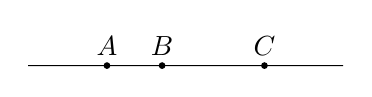
\begin{tikzpicture}
\draw[fill=black] (0,0)--(1,0)node[above]{\(A\)}circle(1pt)
--(1.7,0)node[above]{\(B\)}circle(1pt)
--(3,0)node[above]{\(C\)}circle(1pt)
--(4,0);
\end{tikzpicture}
\caption{直线上点的顺序}
\label{figure:欧式几何.直线上点的顺序1}
\end{figure}

\item 对于两点\(A\)和\(B\)(如\cref{figure:欧式几何.直线上点的顺序2} ),直线\(AB\)上恒至少有一点\(C\),使得\(B\)在\(A\)和\(C\)之间.
\begin{figure}[ht]
\centering
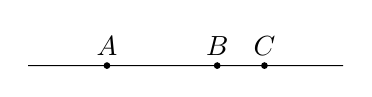
\begin{tikzpicture}
\draw[fill=black] (0,0)--(1,0)node[above]{\(A\)}circle(1pt)
--(2.4,0)node[above]{\(B\)}circle(1pt)
--(3,0)node[above]{\(C\)}circle(1pt)
--(4,0);
\end{tikzpicture}
\caption{直线上点的顺序}
\label{figure:欧式几何.直线上点的顺序2}
\end{figure}

\item 一直线的任意三点中,至多有一点在其他两点之间.
\end{enumerate}
\end{axiom}

在上述三条\textbf{直线顺序公理}之外,还需要一条\textbf{平面顺序公理}.

\begin{axiom}[顺序公理II]\label{axiom:欧式几何.顺序公理2}
考虑一直线\(l\)上的两点\(A\)和\(B\).
我们把这一对点\(A\)和\(B\)确定的介于它们的点的集合叫做一条\textbf{线段},记作\(AB\)(或\(BA\)).
在\(A\)和\(B\)之间的点叫做线段\(AB\)的点,或线段\(AB\)的\textbf{内点};
\(A\)和\(B\)叫做线段\(AB\)的\textbf{端点};
直线\(l\)上的其他点叫做线段\(AB\)的\textbf{外点}.
\begin{enumerate}
\setcounter{enumi}{3}
\item 设\(A\)、\(B\)和\(C\)是不在同一直线上的三点,\(l\)是平面\(ABC\)上的一直线,但\(l\)不通过\(A,B,C\)这三点中的任一点(如\cref{figure:欧式几何.平面上点的顺序1} ),若直线\(l\)通过线段\(AB\)的一点,则它必定也通过线段\(AC\)或线段\(BC\)的一点.
\begin{figure}[ht]
\centering
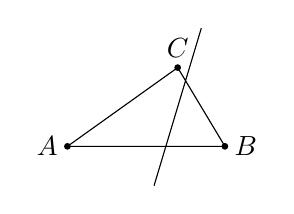
\begin{tikzpicture}
\draw[fill=black] (-1,0)node[left]{\(A\)}circle(1pt)
--(1,0)node[right]{\(B\)}circle(1pt)
--(.4,1)node[above]{\(C\)}circle(1pt)--(-1,0)
(.1,-.5)--(.7,1.5);
\end{tikzpicture}
\caption{平面上点的顺序}
\label{figure:欧式几何.平面上点的顺序1}
\end{figure}
\end{enumerate}
\end{axiom}
直观地说,\cref{axiom:欧式几何.顺序公理2} 说的就是:若一直线“冲进”一个三角形的内部,它必定还要再“冲出”这个三角形.
易证:与线段\(AB\)相交的直线\(l\)不同时和\(AC,BC\)这两条线段都相交.

\subsection{关联公理和顺序公理的推论}
从\cref{axiom:欧式几何.关联公理,axiom:欧式几何.顺序公理1,axiom:欧式几何.顺序公理2} 能推证下列定理.
\begin{theorem}\label{theorem:欧式几何.定理3}
对于两点\(A\)和\(C\),直线\(AC\)上恒至少有一点\(D\),在\(A\)和\(C\)之间.
\begin{proof}
根据\cref{axiom:欧式几何.关联公理} 第3条,直线\(AC\)外存在一点\(E\);
根据\cref{axiom:欧式几何.顺序公理1} 第2条,直线\(AE\)上有一点\(F\),使得\(E\)在线段\(AF\)内.
根据\cref{axiom:欧式几何.顺序公理1} 第2条、第3条,直线\(FC\)上有一点\(G\),不在线段\(FC\)内.
根据\cref{axiom:欧式几何.顺序公理2} 第4条,直线\(EG\)必交线段\(AC\)于一点\(D\).
\end{proof}
\end{theorem}

\begin{theorem}\label{theorem:欧式几何.定理4}
一直线上的任意三点\(A,B,C\)中,必有一点且只有一点在其他两点之间.
\begin{proof}
设\(A\)不在\(B\)和\(C\)之间,而且\(C\)不在\(A\)和\(B\)之间.
用直线连接\(B\)和直线\(AC\)外一点\(D\).
根据\cref{axiom:欧式几何.顺序公理1} 第2条,能在直线\(BD\)上取一点\(G\),使得\(D\)在\(B\)和\(G\)之间.
对于三角形\(BCG\)和直线\(AD\)应用\cref{axiom:欧式几何.顺序公理2} 第4条,可知直线\(AD\)通过线段\(CG\)内的一点\(E\);
同理可知直线\(CD\)通过线段\(AG\)内一点\(F\).
对于三角形\(AEG\)和直线\(CF\)应用\cref{axiom:欧式几何.顺序公理2} 第4条,可知\(D\)在\(A\)和\(E\)之间;
再对于三角形\(AEC\)和直线\(BG\)应用\cref{axiom:欧式几何.顺序公理2} 第4条,即证得\(B\)在\(A\)和\(C\)之间.
\end{proof}
\end{theorem}

\begin{theorem}\label{theorem:欧式几何.定理5}
一直线上的任意四点\(A,B,C,D\),使得点\(B\)既在\(A\)和\(C\)之间,又在\(A\)和\(D\)之间;
而且点\(C\)既在\(A\)和\(D\)之间,又在\(B\)和\(D\)之间.
\end{theorem}

\begin{corollary}\label{theorem:欧式几何.定理6}
一直线上的任意有限个点\(A,B,C,\dotsc,K\),%
使得点\(B\)在\(A\)和\(C\),或和\(D\),或和\(E\),……,或和\(K\)之间;
而且点\(C\)在\(A\)(或\(B\))和\(D\),或和\(E\),……,或和\(K\)之间;以此类推.
\end{corollary}

\begin{corollary}\label{theorem:欧式几何.定理7}
一直线上任意两点之间恒有无限多个点.
\end{corollary}

\begin{theorem}\label{theorem:欧式几何.定理8}
一平面\(\gamma\)上的任一直线\(l\)将该平面上其余的点分为具有下述性质的两个区域:
一个区域的任一点\(A\)与另一区域的任一点\(B\)所决定的线段\(AB\)内,%
必含有直线\(l\)的一点(如\cref{figure:欧式几何.直线l分平面为两个区域} );%
而同一个区域的任意两点\(A\)和\(A'\)所决定的线段\(AA'\)内,不含有直线\(l\)的点.
\begin{figure}[ht]
\centering
\begin{tikzpicture}
\draw (-2,0)--(2,0)node[right]{\(l\)}
(.5,-1)node[right]{\(B\)}--(-.5,.5)node[left]{\(A\)}--(.3,1)node[right]{\(A'\)};
\end{tikzpicture}
\caption{直线\(l\)分平面为两个区域}
\label{figure:欧式几何.直线l分平面为两个区域}
\end{figure}
\end{theorem}

\begin{definition}
我们说\(A\)和\(A'\)这两点在平面\(\gamma\)上直线\(l\)的\textbf{同侧}%
(如\cref{figure:欧式几何.直线l分平面为两个区域} ),%
而\(A\)和\(B\)这两点在平面\(\gamma\)上直线\(l\)的\textbf{异侧}.%
\end{definition}

\begin{definition}
设\(A,A',O\)和\(B\)是一直线\(l\)上的四点(如\cref{figure:欧式几何.射线} ),%
而\(O\)在\(A\)和\(B\)之间,但不在\(A\)和\(A'\)之间.
我们称“\(A\)和\(A'\)这两点在\(l\)上点\(O\)的\textbf{同侧}”,%
而称“\(A\)和\(B\)这两点在\(l\)上点\(O\)的\textbf{异侧}”.

直线\(l\)上点\(O\)的同侧的点的全体,叫做从点\(O\)起始的一条\textbf{射线};
因此一直线的每一点把这直线分成两条射线.
\begin{figure}[ht]
\centering
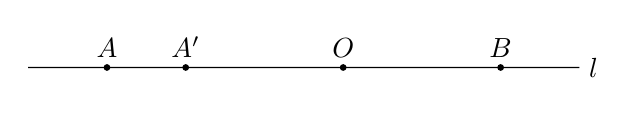
\begin{tikzpicture}
\draw[fill=black] (-3,0)--(-2,0)node[above]{\(A\)}circle(1pt)
--(-1,0)node[above]{\(A'\)}circle(1pt)
--(1,0)node[above]{\(O\)}circle(1pt)
--(3,0)node[above]{\(B\)}circle(1pt)--(4,0)node[right]{\(l\)};
\end{tikzpicture}
\caption{射线}
\label{figure:欧式几何.射线}
\end{figure}
\end{definition}

\begin{definition}
若干条首尾相连的线段\(AB,BC,CD,\dotsc,KL\)的集合叫做一条\textbf{折线段},%
它连结\(A\)和\(L\)这两点.
为求简便,可将这条折线段记为\(ABCD \dotso KL\).
线段\(AB,BC,CD,\dotsc,KL\)的内点和端点都叫做这条折线段的点.
点\(A\)和点\(L\)称为“折线段的\textbf{端点}”.

若折线段\(ABCD \dotso KL\)的顶点\(A,B,C,D,\dotsc,K,L\)都在同一平面上,%
且它的端点\(L\)和\(A\)是同一个点,%
则这条折线段就叫做一个\textbf{多边形},%
记为\(ABCD \dotso K\).
线段\(AB,BC,CD,\dotsc,KA\)叫做“多边形的\textbf{边}”.
点\(A,B,C,D,\dotsc,K\)叫做“多边形的\textbf{顶点}”.

若一个多边形有三个顶点,%
则称之为\textbf{三角形}.
设三角形的三个顶点分别为\(A\)、\(B\)、\(C\),%
则可将其表记为以下六个符号中的任意一个:
\[
\begin{split}
\triangle ABC, \qquad
\triangle ACB, \qquad
\triangle BAC, \\
\triangle BCA, \qquad
\triangle CAB, \qquad
\triangle CBA.
\end{split}
\]

若一个多边形有\(n\ (n>3)\)个顶点,%
则称之为\(n\)\textbf{边形}.

若一个多边形的顶点各各不同,%
它的任一边内不含有顶点,%
且它的任意两边无公共点,%
这个多边形就叫做\textbf{简单多边形}.
\end{definition}

根据\cref{theorem:欧式几何.定理8} 可以推出下列两条推论:
\begin{theorem}\label{theorem:欧式几何.定理9}
一平面\(\alpha\)上的每一个简单多边形,%
把平面\(\alpha\)上其余点%
(即平面\(\alpha\)上的,%
而不在这多边形的边上的点)%
分为\textbf{内域}和\textbf{外域}两个区域.
这两个区域具有如下性质:
\begin{enumerate}
	\item 若\(A\)是“内域的一个点(内点)”,%
	而且\(B\)是“外域的一个点(外点)”,%
	则平面\(\alpha\)上任意一条连接\(A\)和\(B\)的折线段,%
	至少和多边形有一公共点.

	\item 若\(A\)和\(C\)是内点,%
	而\(B\)和\(D\)是外点,%
	则在平面\(\alpha\)上恒有连接\(A\)和\(C\)的折线段,%
	和连接\(B\)和\(D\)的折线段,%
	它们都和多边形无公共点.

	\item 平面\(\alpha\)上存在全含于外域的直线,%
	而不存在全含于内域的直线.
\end{enumerate}
\end{theorem}

\begin{theorem}\label{theorem:欧式几何.定理10}
每一平面\(\alpha\)把空间中其余点分为具有下述性质的两个区域:
\begin{enumerate}
	\item 一区域的任一点\(A\)和另一区域的任一点\(B\)所决定的线段\(AB\)内,必含有\(\alpha\)的一点.
	\item 同一区域的任意两点\(A\)和\(C\)所决定的线段\(AC\)内,恒不含有\(\alpha\)的点.
\end{enumerate}
\end{theorem}

\begin{definition}
在\cref{theorem:欧式几何.定理10} 的条件下,%
我们说“\(A\)和\(C\)这两点在空间中平面\(\alpha\)的\textbf{同侧}”,%
说“\(A\)和\(B\)这两点在空间中平面\(\alpha\)的\textbf{异侧}”.
\end{definition}

\subsection{第三组公理:合同公理}
本组公理规定“合同”这个概念,利用它就可以规定运动的概念.

我们首先介绍角的概念.
\begin{definition}\label{definition:欧式几何.几何元素.角}
设\(\alpha\)是任意平面,%
而且\(h\)和\(k\)是\(\alpha\)上的、%
从一点\(A\)起始的、%
不属于同一直线的%
两条射线,%
我们把这一对射线\(h\)和\(k\)所成的射线组叫做一个\textbf{角},%
记作\(\angle(h,k)\)或\(\angle(k,h)\).
称射线\(h\)和\(k\)为这个角的\textbf{边}.
称点\(A\)为这个角的\textbf{顶点}.

如果在\(h\)上任取一点记为\(B\),在\(k\)上任取一点记为\(C\),%
那么也称角\(\angle(h,k)\)为\(\angle BAC\)或\(\angle A\).
不致混淆时,也可以用小写希腊字母表记角.

记射线\(h\)所在的直线为\(p\),射线\(k\)所在的直线为\(q\).
射线\(h\)与\(k\)(包括点\(A\))把平面\(\alpha\)上其余点分成两个区域:
在\(q\)的\(h\)侧(即\(h\)的点所在的那一侧)的,且%
在\(p\)的\(k\)侧(即\(k\)的点所在的那一侧)的区域,%
叫做“角\(\angle(h,k)\)的\textbf{内部}”,%
或者说是在\textbf{角内};
其他区域叫做“角\(\angle(h,k)\)的\textbf{外部}”,%
或者说是在\textbf{角外}.
\end{definition}

\begin{property}
根据第一组和第二组公理,%
易知任意角(不妨设为交于点\(A\)的射线\(h\)、\(k\)所成的角,即\(\angle(h,k)\))具有以下性质:
\begin{enumerate}
\item 角内、角外两个区域各含有点,连结角内两点的线段完全在角内.
\item 若点\(H\)在射线\(h\)上,点\(K\)在射线\(k\)上,则线段\(HK\)完全在角内.
\item 一条从点\(A\)起始的射线,要么完全在角内,要么完全在角外.
\item 一条完全在角内的射线与线段\(HK\)有交点.
\item 若\(B\)是一个区域的一点,而且\(C\)是另一个区域的一点,%
则每一条连接\(B\)和\(C\)的折线段,要么通过点\(A\),要么与\(h\)或\(k\)至少有一个交点;
反之,若\(B\)和\(D\)是同一个区域的两点,则恒有一条连接\(B\)和\(D\)的折线段,%
它既不通过点\(A\),又与\(h\)、\(k\)无交点.
\end{enumerate}
\end{property}


\begin{axiom}[合同公理]\label{axiom:欧式几何.合同公理}
线段与线段之间、角与角之间都有一定的相互关系,我们用“合同”或“相等”这个词来描述.
\begin{enumerate}
\item 设\(A\)和\(B\)是直线\(a\)上的两点,%
\(P\)是直线\(b\)上的点,%
而且给定了直线\(b\)上\(P\)的一侧,%
则在直线\(b\)上\(P\)的这一侧,%
恒有一点\(Q\),%
使得线段\(AB\)和线段\(PQ\)合同.
我们将上述关系记为\(AB \equiv PQ\).

\item 若两线段\(PQ\)和\(MN\)都和线段\(AB\)合同,%
则\(PQ\)和\(MN\)也合同.

\item 设两线段\(AB\)和\(BC\)在同一直线\(a\)上,无公共点,%
而且两线段\(PQ\)和\(QR\)在同一直线\(b\)上,亦无公共点.
若\(AB \equiv PQ\)且\(BC \equiv QR\),%
则\(AC \equiv PR\).

\item 设给定了一个平面\(\alpha\)上的一个角\(\angle(h,k)\),%
一平面\(\beta\)上的一直线\(b\),%
和在\(\beta\)上\(b\)的一侧.
设\(p\)是\(b\)上的、从点\(B\)起始的一条射线,%
则平面\(\beta\)上恰有一条射线\(q\),%
使得\(\angle(h,k)\)与\(\angle(p,q)\)合同,%
而且使得\(\angle(p,q)\)的内部在\(b\)的这给定了的一侧.
我们将上述关系记为\(\angle(h,k) \equiv \angle(p,q)\).

\item 若两个三角形\(ABC\)和\(PQR\)有下列合同式
\[
AB \equiv PQ, \qquad
AC \equiv PR, \qquad
\angle BAC \equiv \angle QPR,
\]
则也恒有合同式\footnote{%
只需要交换记号,还可以同时得到另一个合同式
\(\angle ACB \equiv \angle PRQ\)
也同时成立.
}
\[
\angle ABC \equiv \angle PQR.
\]
\end{enumerate}
\end{axiom}

我们在前面用点\(A\)、\(B\)所成的点组规定一条线段,并用\(AB\)或\(BA\)表示;
我们在线段的定义里,并不考虑这两点的顺序;
因此下列四个合同式的意义相同:
\[
AB \equiv PQ, \qquad
AB \equiv QP, \qquad
BA \equiv PR, \qquad
BA \equiv QP.
\]

如同线段我们不考虑它的方向,在角的定义中我们也不考虑旋转方向.
因此下列四个合同式的意义也相同:
\[
\angle(h,k) \equiv \angle(p,q), \qquad
\angle(h,k) \equiv \angle(q,p), \qquad
\angle(k,h) \equiv \angle(p,q), \qquad
\angle(k,h) \equiv \angle(q,p).
\]

\cref{axiom:欧式几何.合同公理} 第3条要求线段能够相加.

\cref{axiom:欧式几何.合同公理} 第4条可以表述为:
每一个角都能用唯一确定的方式迁移到一个给定了的平面上,%
使得它沿着一条给定了的射线,并且在这射线的给定了的一侧.
藉此,我们直接保证了角的迁移的可能性与唯一性.

\cref{axiom:欧式几何.合同公理} 第1条、第2条、第3条只论及线段的合同,%
因此可以叫做“第三组公理中的直线公理”.

\cref{axiom:欧式几何.合同公理} 第4条论及角的合同.
\cref{axiom:欧式几何.合同公理} 第5条则把线段的合同和角的合同这两个概念联系起来.
这两条概念论及平面几何的几何元素,%
因此可以叫做“第三组公理中的平面公理”.

\cref{axiom:欧式几何.合同公理} 第1条要求线段平移的可能性,%
但它还没有保证这种平移的唯一性.
只有结合\cref{axiom:欧式几何.合同公理} 第5条,%
从角的迁移的唯一性出发予以证明.
具体地,我们应用反证法,%
假设把线段\(PQ\)迁移到一条从\(A\)起始的射线上可以得到不同的两点\(B\)、\(D\);
在直线\(AB\)外取一点\(C\),于是有下列合同式
\[
AB \equiv AD, \qquad
AC \equiv AC, \qquad
\angle BAC \equiv \angle DAC;
\]
那么根据\cref{axiom:欧式几何.合同公理} 第5条,得
\[
\angle ACB \equiv \angle ACD;
\]
这和\cref{axiom:欧式几何.合同公理} 第4条中要求的角的迁移的唯一性矛盾,%
因此线段平移也是唯一的.

\begin{property}
线段的合同关系具有自反性、对称性和传递性,即
\begin{enumerate}
\item \textbf{自反性},
\(AB \equiv AB\).

\item \textbf{对称性},
\(AB \equiv PQ \implies PQ \equiv AB\)
\footnote{%
正因线段的合同关系具有对称性,%
我们才能说“某两条线段\textbf{互相合同}”.
}.

\item \textbf{传递性},
\(AB \equiv PQ \land PQ \equiv MN \implies AB \equiv MN\).
\end{enumerate}
\end{property}

\begin{property}
角的合同关系具有自反性、对称性和传递性,即
\item \textbf{自反性},
\(\angle(h,k) \equiv \angle(h,k)\).

\item \textbf{对称性},
\(\angle(h,k) \equiv \angle(p,q)
\implies
\angle(p,q) \equiv \angle(h,k)\).

\item \textbf{传递性},
\(\angle(h,k) \equiv \angle(m,n)
\land
\angle(m,n) \equiv \angle(p,q)
\implies
\angle(h,k) \equiv \angle(p,q)\).
\end{property}
角的合同关系的自反性是显然的,%
至于它的对称性、传递性和可加性,%
则留待以后予以证明.

\subsection{合同公理的推论}
\begin{definition}
两角共顶点,共一边,而且不公共的两边合成一条直线的,叫做\textbf{邻补角}.
\end{definition}
\begin{definition}
两角共顶点,而且它们的边合成两条直线的,叫做\textbf{对顶角}.
\end{definition}
\begin{definition}
一个角和它的邻补角合同的,叫做\textbf{直角}.
\end{definition}

\begin{theorem}\label{theorem:欧式几何.定理11}
若一个三角形中的两边合同,和这两边相对的两角就也合同\footnote{%
换言之,等腰三角形的底角相等.
}.
\end{theorem}

\begin{definition}
若两个三角形\(ABC\)和\(PQR\)满足下列所有的合同式
\[
\begin{split}
AB \equiv PQ, \qquad
AC \equiv PR, \qquad
BC \equiv QR, \\
\angle A \equiv \angle P, \qquad
\angle B \equiv \angle Q, \qquad
\angle C \equiv \angle R,
\end{split}
\]
就说“三角形\(ABC\)合同于三角形\(PQR\)”,%
或者说“三角形\(ABC\)和三角形\(PQR\)是全等三角形”,%
或者说“三角形\(ABC\)、\(PQR\)全等”,%
记为\(\triangle ABC \cong \triangle PQR\).
\end{definition}

\begin{theorem}[三角形的合同定理1]\label{theorem:欧式几何.定理12}
若两个三角形\(ABC\)、\(PQR\)有下列合同式
\[
AB \equiv PQ, \qquad
AC \equiv PR, \qquad
\angle A \equiv \angle P,
\]
则\(\triangle ABC \cong \triangle PQR\).
\end{theorem}

\begin{theorem}[三角形的合同定理2]\label{theorem:欧式几何.定理13}
若两个三角形\(ABC\)、\(PQR\)有下列合同式
\[
AB \equiv PQ, \qquad
\angle A \equiv \angle P,
\angle B \equiv \angle Q,
\]
则\(\triangle ABC \cong \triangle PQR\).
\end{theorem}

\begin{theorem}\label{theorem:欧式几何.定理14}
设\(\angle ABC\)的邻补角为\(\angle CBD\),%
\(\angle PQR\)的邻补角为\(\angle RQS\).
若\(\angle ABC \equiv \angle PQR\),%
则\(\angle CBD \equiv \angle RQS\).
\end{theorem}

\begin{corollary}\label{theorem:欧式几何.对顶角合同}
任意一个角和它的对顶角合同.
\end{corollary}

\begin{corollary}\label{theorem:欧式几何.直角存在}
直角存在.
\begin{proof}
把任意一个角迁移到沿着一条从点\(O\)起始的射线\(OA\),%
而且迁移到这射线的两侧.
在新得到的这两个角的另外两条边上,%
取线段\(OB \equiv OC\),%
线段\(BC\)交射线\(OA\)于一点\(D\).

若点\(D\)就是点\(O\),%
\(\angle BOA\)和\(\angle COA\)是合同的邻补角,所以是直角.

若点\(D\)在射线\(OA\)上,%
或在与\(OA\)恰好反向的射线上,%
总有\(\angle DOB \equiv \angle DOC\);
根据\cref{axiom:欧式几何.合同公理} 第2条,%
每一条线段都和它自己合同,即\(OD \equiv OD\);
再根据\cref{axiom:欧式几何.合同公理} 第5条,%
就有\(\angle ODB \equiv \angle ODC\).
\end{proof}
\end{corollary}

\begin{theorem}\label{theorem:欧式几何.定理15}
设\(h\)、\(k\)和\(l\)是一平面\(\alpha\)上的、从一点\(M\)起始的三条射线,%
而且\(p\)、\(q\)和\(r\)是一平面\(\beta\)上的、从一点\(N\)起始的三条射线;%
又设\(h\)和\(k\)分别在\(l\)的同侧(或异侧),%
且\(p\)和\(q\)也分别在\(r\)的同侧(或异侧).
若
\[
\angle(h,l) \equiv \angle(p,r)
\quad\text{且}\quad
\angle(k,l) \equiv \angle(q,r),
\]
则
\[
\angle(h,k) \equiv \angle(p,q).
\]
\end{theorem}

\begin{theorem}\label{theorem:欧式几何.定理16}
设平面\(\alpha\)上的\(\angle(h,k)\)合同于平面\(\beta\)上的\(\angle(p,q)\),%
而且\(l\)是平面\(\alpha\)上的、从\(\angle(h,k)\)的顶点起始的、在\(\angle(h,k)\)角内的一条射线.
这时平面\(\beta\)上恒恰有一条从\(\angle(p,q)\)的顶点起始的、在\(\angle(p,q)\)角内的一条射线\(r\),%
使得
\[
\angle(h,l) \equiv \angle(p,r), \qquad
\angle(k,l) \equiv \angle(q,r).
\]
\end{theorem}

\begin{theorem}\label{theorem:欧式几何.定理17}
若两点\(C\)和\(D\)在直线\(AB\)的异侧,%
而且\(AC \equiv AD\)、\(BC \equiv BD\),%
则\(\angle ABC \equiv \angle ABD\).
\end{theorem}

\begin{theorem}[三角形的合同定理3]\label{theorem:欧式几何.定理18}
若两个三角形\(ABC\)和\(PQR\)的每对对应边合同,即
\[
AB \equiv PQ, \qquad
AC \equiv PR, \qquad
BC \equiv QR,
\]
则\(\triangle ABC \cong \triangle PQR\).
\end{theorem}

\begin{theorem}\label{theorem:欧式几何.定理19}
若两个角\(\angle(a,b)\)和\(\angle(c,d)\)都合同于第三个角\(\angle(e,f)\),%
则\(\angle(a,b)\)也合同于\(\angle(c,d)\).
\end{theorem}
由此,我们证明了角的合同关系具有对称性、传递性.

现在我们就可以比较角的大小了.

\begin{theorem}\label{theorem:欧式几何.定理20}
如\cref{figure:欧式几何.图20},
给定任意两个角\(\angle(h,k)\)和\(\angle(p,r)\).
设迁移\(\angle(h,k)\)到沿着\(p\),而且在\(p\)的\(r\)侧时,所得到的射线是\(q\);
又迁移\(\angle(p,r)\)到沿着\(h\),而且在\(h\)的\(k\)侧时,所得到的射线是\(l\);
这时,若\(q\)在\(\angle(p,r)\)内,则\(l\)在\(\angle(h,k)\)外.
反之也成立.
\end{theorem}

\begin{figure}[ht]
	\centering
	\begin{tikzpicture}
		\pgfmathsetmacro{\r}{3}
		\begin{scope}
			\draw(0,0)--(\r,0)node[right]{\(h\)};
			\pgfmathsetmacro{\kx}{\r*cos(45)}
			\pgfmathsetmacro{\ky}{\r*sin(45)}
			\draw(0,0)--(\kx,\ky)node[right]{\(k\)};
			\pgfmathsetmacro{\lx}{\r*cos(60)}
			\pgfmathsetmacro{\ly}{\r*sin(60)}
			\draw(0,0)--(\lx,\ly)node[above]{\(l\)};
		\end{scope}
		\begin{scope}[xshift=6cm]
			\draw(0,0)--(\r,0)node[right]{\(p\)};
			\pgfmathsetmacro{\kx}{\r*cos(45)}
			\pgfmathsetmacro{\ky}{\r*sin(45)}
			\draw(0,0)--(\kx,\ky)node[right]{\(q\)};
			\pgfmathsetmacro{\lx}{\r*cos(60)}
			\pgfmathsetmacro{\ly}{\r*sin(60)}
			\draw(0,0)--(\lx,\ly)node[above]{\(r\)};
		\end{scope}
	\end{tikzpicture}
	\caption{}
	\label{figure:欧式几何.图20}
\end{figure}

\begin{definition}
在\cref{theorem:欧式几何.定理20} 中,
若\(q\)在\(\angle(p,r)\)内,则称“\(\angle(h,k)\)小于\(\angle(p,r)\)”,记为\(\angle(h,k) < \angle(p,r)\).
若\(q\)在\(\angle(p,r)\)外,则称“\(\angle(h,k)\)大于\(\angle(p,r)\)”,记为\(\angle(h,k) > \angle(p,r)\).
\end{definition}

因此,两个角\(\alpha,\beta\)恒恰适合以下三种情形之一:
\begin{itemize}
	\item \(\alpha<\beta\)和\(\beta>\alpha\).
	\item \(\alpha\equiv\beta\).
	\item \(\alpha>\beta\)和\(\beta<\alpha\).
\end{itemize}

角的大小的比较有传递性.
若有下列三种情形
\begin{itemize}
	\item \(\alpha>\beta,\beta>\gamma\),
	\item \(\alpha>\beta,\beta\equiv\gamma\),
	\item \(\alpha\equiv\beta,\beta>\gamma\),
\end{itemize}
之一,则\[
	\alpha>\gamma.
\]

\begin{theorem}\label{theorem:欧式几何.定理21}
所有的直角都互相合同.
\end{theorem}

\begin{definition}
一个角大于它的邻补角的,也就是大于一直角的,叫做\textbf{钝角};
小于它的邻补角的,也就是小于一直角的,叫做\textbf{锐角}.
\end{definition}

\begin{definition}
\(\triangle ABC\)的\(\angle ABC\)、\(\angle BCA\)和\(\angle CAB\)
叫做这个三角形的\textbf{内角},简称为这个三角形的\textbf{角};
它们的邻补角叫做这个三角形的\textbf{外角}.
\end{definition}

\begin{theorem}[外角定理]\label{theorem:欧式几何.定理22}
在三角形中,一个外角大于其任一不相邻的内角.
\end{theorem}

下列定理是外角定理的重要推论.

\begin{theorem}\label{theorem:欧式几何.定理23}
在三角形中,长边所对的角大于短边所对的角.
\end{theorem}

\begin{theorem}\label{theorem:欧式几何.定理24}
若三角形有两角合同,则有两边合同.
\end{theorem}
这是\cref{theorem:欧式几何.定理11} 的逆定理,
也是\cref{theorem:欧式几何.定理23} 的直接推论.

从\cref{theorem:欧式几何.定理22},
还能很简单地证得下述对三角形的合同定理二的补充.
\begin{theorem}\label{theorem:欧式几何.定理25}
若\(\triangle ABC\)和\(\triangle DEF\)有下列合同式\[
	AB \equiv DE, \qquad
	\angle A \equiv \angle D, \qquad
	\angle C \equiv \angle F,
\]
则这两个三角形合同.
\end{theorem}

\begin{theorem}\label{theorem:欧式几何.定理26}
每一线段都能二等分.
\end{theorem}

类似地,从\cref{theorem:欧式几何.定理11} 和\cref{theorem:欧式几何.定理26},能直接推证下列事实:
\begin{theorem}
每一角都能二等分.
\end{theorem}

合同的概念可以推广应用到任意的图形上去.

\begin{definition}
设\(A,B,C,D,\dotsc,K,L\)是直线\(\alpha\)上的一个点列,
\(A',B',C',D',\dotsc,K',L'\)是直线\(\alpha'\)上的一个点列,
而且所有的对应线段都两两合同,
那么称这两个点列互相合同.
\(A\)和\(A'\)、\(B\)和\(B'\),一直到\(L\)和\(L'\),叫做这\textbf{合同点列}的对应点.
\end{definition}

\begin{theorem}\label{theorem:欧式几何.定理27}
两个合同的点列的点的顺序相同.
\end{theorem}

\begin{definition}
任意有限个点叫做一个\textbf{图形}.
一个图形的点,若都在一个平面上,这图形就叫做一个\textbf{平面图形}.
\end{definition}

两个图形的点之间若有一个一一对应的关系,
使得由此规定的每对对应的线段都互相合同,
且每对对应的角都互相合同,
那么这两个图形合同.

由\cref{theorem:欧式几何.定理14}
和\cref{theorem:欧式几何.定理27},
可知合同图形有下述性质:
若一个图形中的三个点在一条直线上,
则每一个和它合同图形中的对应的三个点也在一条直线上.
合同图形中的、对应平面上的对应点,
对于对应直线而言的顺序相同;
对应直线上的对应点顺序也相同.

平面的和空间的最普遍的合同定理如下:
\begin{theorem}\label{theorem:欧式几何.定理28}
设\((A,B,C,\dotsc,L)\)
和\((A',B',C',\dotsc,L')\)
是两个合同的平面图形.
若\(P\)是第一个图形的平面上的一点,
则第二个图形的平面上恒有一点\(P'\)存在,
使得\((A,B,C,\dotsc,L,P)\)
和\((A',B',C',\dotsc,L',P')\)还是合同的图形.
若\((A,B,C,\dotsc,L)\)至少含有不在同一条直线上的三点,
则\(P'\)只有一个可能的作法.
\end{theorem}

\begin{theorem}\label{theorem:欧式几何.定理29}
设\((A,B,C,\dotsc,L)\)
和\((A',B',C',\dotsc,L')\)
是两个合同的图形.
若\(P\)是任意一点,
则恒有一点\(P'\)存在,
使得\((A,B,C,\dotsc,L,P)\)
和\((A',B',C',\dotsc,L',P')\)还是合同的图形.
若\((A,B,C,\dotsc,L)\)至少含有不在同一平面上的四点,
则\(P'\)只有一个可能的作法.
\end{theorem}

\cref{theorem:欧式几何.定理29} 说出了所有关于合同的空间事实,
因此,空间中运动的性质,都是上述的直线的和平面的五条合同公理(结合着第一组和第二组公理)的推论.

\subsection{第四组公理:平行公理}
设\(\alpha\)是任一平面,
\(a\)是\(\alpha\)上的任一直线,
而且\(A\)是\(\alpha\)上的、但不在\(a\)上的一点,
在\(\alpha\)上作一直线\(c\),
通过\(A\)且和\(a\)相交,
再在\(\alpha\)上作一直线\(b\),通过\(A\),
且使得\(c\)交\(a\)和\(b\)于相等的同位角.
从\hyperref[theorem:欧式几何.定理22]{外角定理},
易知\(a\)和\(b\)这两直线无公共点,这就是说,
在一平面\(\alpha\)上,而且通过一直线\(a\)外的一点\(A\),
恒有一直线不和\(a\)相交.

现在可将平行公理叙述如下:
\begin{axiom}[平行公理、欧几里得公理]\label{axiom:欧式几何.平行公理}
设\(a\)是任一直线,\(A\)是\(a\)外的任一点.
在\(a\)和\(A\)所决定的平面上,
至多有一条直线通过\(A\),而且不和\(a\)相交.
\end{axiom}

根据上文和平行公理,我们知道:
在\(a\)和\(A\)所决定的平面上,恰有一直线,通过\(A\)且不和\(a\)相交,
我们把这条直线叫做“通过\(A\)的\(a\)的\textbf{平行直线}”.

平行公理和下述的要求等价:
如果一平面上的\(a\)和\(b\)两直线都不和这平面上的第三条直线\(c\)相交,
那么\(a\)和\(b\)也不相交.

事实上,如果\(a\)和\(b\)有一公共点\(A\),那么在同一平面上,
就有了\(a\)和\(b\)这两条直线,都通过\(A\)而且不和\(c\)相交.
这和平行公理矛盾.
反之,从上述要求,也易推得平行公理.

平行公理是一条平面公理.
它的引入,使得几何的基础大大地简单化了,也使得几何的构造容易得多了.

例如,在合同公理之外,再加上平行公理,不难得到下列熟知的事实:
\begin{theorem}\label{theorem:欧式几何.定理30}
若两平行直线被第三条直线所截,则同位角合同,内错角也合同;
反之,若同位角合同,或内错角合同,则前两直线平行.
\end{theorem}

\begin{theorem}\label{theorem:欧式几何.定理31}
三角形的三个内角的和等于两个直角的和.
\end{theorem}
\begin{figure}[ht]
	\centering
	\begin{tikzpicture}
		\coordinate (A) at (0,0);
		\coordinate (B) at (4,0);
		\coordinate (C) at (3,2);
		\coordinate (P) at (2,2);
		\coordinate (Q) at (4,2);
		\draw (A)node[left]{\(A\)}
				-- (B)node[right]{\(B\)}
				-- (C)node[above]{\(C\)} -- (A);
		\draw (P)node[left]{\(P\)} -- (Q)node[right]{\(Q\)};
		\draw pic[draw=blue,angle radius=5mm]{angle=B--A--C}
				pic[draw=blue,angle radius=6mm]{angle=B--A--C}
				pic[draw=blue,angle radius=5mm]{angle=P--C--A}
				pic[draw=blue,angle radius=6mm]{angle=P--C--A}
				pic[draw=orange,angle radius=4mm]{angle=C--B--A}
				pic[draw=orange,angle radius=4mm]{angle=B--C--Q};
	\end{tikzpicture}
\end{figure}

\begin{definition}
设\(M\)是一平面\(\alpha\)上的任一点.
考虑\(\alpha\)上的所有的那些点\(A\),
它们使线段\(MA\)都互相合同的.
这种点\(A\)的全体叫做一个\textbf{圆},
点\(M\)叫做“这个圆的\textbf{中心}”,简称\textbf{圆心}.
\end{definition}

根据这个定义,我们容易从第三组和第四组公理,推证关于圆的若干熟知的定理.
特别是下述的定理:
通过不在同一条直线上的三点,能作一圆;
关于同一条弦上的圆周角合同的定理;
关于内接于圆的一个四边形的角的定理.

\subsection{第五组公理:连续公理}

\begin{axiom}[连续公理]
关于线段、角的度量,有如下公理:
\begin{enumerate}
	\item (度量公理,阿基米德公理).
	若\(AB\)和\(CD\)是任意两线段,则必存在一个数\(n\)使得沿\(A\)到\(B\)的射线上,
	自\(A\)作首尾相接的\(n\)个线段\(CD\),必将越过\(B\)点.
	\item (直线完备公理).
	一直线上的点集联通其顺序关系与合同关系不可能再这样扩充,
	使得这直线上原来元素之间所具有的关系,
	从第一组、第二组、第三组公理所推出的直线顺序与合同的基本性质\footnote{%
	所谓“基本性质”是指第二组第一至三条公理和\cref{theorem:欧式几何.定理5} 中所叙述的顺序性质,
	以及第三组第一至第三条公理中所叙述的合同性质连同迁移线段的唯一性.}
	以及度量公理都仍旧保持\footnote{%
	所谓“仍旧保持”是指,当点集扩充后,顺序关系及合同关系也将延续到扩充后的点集中去.
	我们注意到第一组第三条公理在各种扩充后,不言而喻地仍然保持,
	至于在所考虑的扩充下,\cref{theorem:欧式几何.定理3} 仍能成立,
	则是保持阿基米德公理的结果.}.
\end{enumerate}
\end{axiom}

完备公理中所要求保持的诸公理之一是阿基米德公理,
这时完备公理从本质上能以建立所不可缺少的一个条件.
其实我们能够证明:
若直线上的一个点集能满足上面所列举的关于顺序公理和定理以及合同公理和定理,
这点集就恒能够增加新点,使扩充后的点集还满足这里所提到的诸公理;
也就是说,如果一条完备公理,只要求保持这里所提到的诸公理和定理,
但不要求保持阿基米德公理或一条等价的公理,就要产生矛盾.

这两条连续公理都是直线公理.

下面所述更普遍的定理,主要根据直线完备公理.
\begin{theorem}[完备定理]\label{theorem:欧式几何.定理32}
几何元素(即点、直线、平面)形成一个集合,
它在保持关联公理、顺序公理、合同公理和阿基米德公理,
从而更不用说,在保持全体公理的条件之下,
不可能经由点、直线和平面再行扩充.
\end{theorem}

完备定理还能表成较强的形式.
也就是在完备定理内缩要求保持的诸公理中,有些并不是绝对需要的,为了定理能够成立,
重要的倒是在所要求保持的诸公理中包含有第一组第七条公理.
其实我们能证明:
对于满足第一至第第五组公理的元素集合,恒能给添加新的点、直线和平面,
使得扩充后的心机和能满足除去第一组第七条公理之外的全体公理;
这就是说,一条完备定理若不包含第一组第七条公理或一条等价的公理,就将引出矛盾.

完备公理不是阿基米德公理的一个推论.
实际上,只有阿基米德公理,连同第一至第四组公理,
并不足以证明我们的几何和通常的笛卡尔解析几何完全相同.
但是加上了完备公理(虽然这条公理并没有直接提到收敛的概念),
就能证明(相当于戴德金分割的)确界的存在,
和关于聚点存在的波尔查诺定理,
从而才证明欧式几何和笛卡尔几何相同.

从上文可见,连续的要求,在本质上,分成两个不同的部分:
阿基米德公理和完备公理;
前者的作用是替连续的要求做准备,
后者为完成整个公理系统作基础.

在本章后面的研究中,我们主要只用阿基米德公理作根据,而普遍地不假设完备公理.

\section{平面三角形}

\begin{theorem}
三角形内角和为\(\pi\).
\begin{proof}
设有\(\triangle ABC\).
过点\(C\)作平行于线段\(AB\)的直线\(PQ\).

由内错角相等,有\[
\angle{PCA} = \angle{CAB}, \quad \angle{QCB} = \angle{CBA},
\]又由\(\angle{PCA}+\angle{ACB}+\angle{QCB}=\pi\),可得\[
\angle{CAB}+\angle{ACB}+\angle{QCB}=\pi.
\qedhere
\]
\end{proof}
\end{theorem}

\begin{theorem}[正弦定理]
设任意三角形\(\triangle ABC\)的外接圆半径为\(R\),则\begin{equation}
\frac{a}{\sin A}
= \frac{b}{\sin B}
= \frac{c}{\sin C}
= 2R.
\end{equation}
\end{theorem}

\begin{theorem}[余弦定理]
设任意三角形\(\triangle ABC\),有\begin{equation}
c^2 = a^2 + b^2 - 2ab \cos C.
\end{equation}
\end{theorem}
可以看出,勾股定理是余弦定理的特殊情况,即当\(C = \frac{\pi}{2}\)时,有\(\cos C=0\),于是\(c^2 = a^2 + b^2\).

\begin{theorem}[摩尔外德公式]
%@see: https://mathshistory.st-andrews.ac.uk/Biographies/Mollweide/
%@see: https://arxiv.org/pdf/1808.08049.pdf
设任意三角形\(\triangle ABC\),则\begin{gather}
\frac{a+b}{c}
= \frac{\cos[(A-B)/2]}{\sin(C/2)}, \\
\frac{a-b}{c}
= \frac{\sin[(A-B)/2]}{\cos(C/2)}.
\end{gather}
\end{theorem}

\begin{theorem}[正切定理]
设任意三角形\(\triangle ABC\),有\begin{equation}
\frac{a-b}{a+b} = \frac{\tan[(A-B)/2]}{\tan[(A+B)/2]}.
\end{equation}
\end{theorem}

\section{圆}
\subsection{圆的概念}
\subsection{圆的性质}
\subsection{圆的周长\ 圆周率}
\begin{definition}
定义:圆的周长\(C\)与其直径\(2R\)之比称为\textbf{圆周率},记作\(\pi\),即\[
\pi = \frac{C}{2R}.
\]
\end{definition}
由于圆周率是一个常数,那么已知圆的直径(或半径)可以求得圆的周长,而已知圆的周长可以求得圆的直径(或半径).

\begin{property}
给定圆上任意一段弧,若它的角度为\(\theta\),那么弧长为\(\theta r\).
\end{property}

\begin{corollary}
如下图,在单位圆上,当圆弧的角度\(\theta\)为锐角,即\(0<\theta<\pi/2\)时,\(\theta > x\). \begin{center}
\begin{tikzpicture}[scale=4]
%\draw[help lines, color=gray!30, dashed] (0,0) grid (1,1);
\pgfmathsetmacro{\u}{sqrt(3)/2}
\coordinate (O) at (0,0);
\coordinate (A) at (\u,0);
\coordinate (B) at (\u,1/2);
\draw (1,0)arc[start angle=0,end angle=30,radius=1]node[midway,right]{\(\theta\)} -- (0,0)node[midway,above left]{\(1\)} -- (1,0)
	(A) -- (B)node[midway,left]{\(x\)};
\draw pic["\(\theta\)",draw=orange,-,angle eccentricity=1.7,angle radius=5mm]{angle=A--O--B} pic[draw=gray,-,angle radius=0.3cm]{right angle=B--A--O};
\end{tikzpicture}
\end{center}
\end{corollary}

\section{平面凸多边形}
\begin{theorem}
设凸多边形的边数为\(n\),则其内角和为\((n-2)\pi\).
\end{theorem}
如图,在凸多边形内部任取一点\(P\),连接该点与凸多边形各顶点,可以得到\(n\)个三角形.
因为三角形内角和为\(\pi\),所以\(n\)个三角形内角和的总和为\(n\pi\),再减去各三角形\(\angle P\)之和\(2\pi\),可知凸\(n\)边形的内角和为\((n-2)\pi\).
\begin{center}
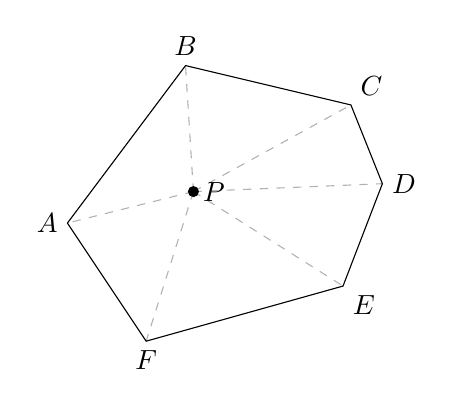
\begin{tikzpicture}
\coordinate (A1) at (0,2);
\coordinate (A2) at (1.5,4);
\coordinate (A3) at (3.6,3.5);
\coordinate (A4) at (4,2.5);
\coordinate (A5) at (3.5,1.2);
\coordinate (A6) at (1,0.5);
\coordinate (P) at (1.6,2.4);
\draw[dashed,color=black!30] (P)--(A1) (P)--(A2) (P)--(A3) (P)--(A4) (P)--(A5) (P)--(A6);
\draw (A1)node[left]{\(A\)}--(A2)node[above]{\(B\)}--(A3)node[above right]{\(C\)}--(A4)node[right]{\(D\)}--(A5)node[below right]{\(E\)}--(A6)node[below]{\(F\)}--(A1) (P)node[right]{\(P\)};
\fill (P)circle(2pt);
\end{tikzpicture}
\end{center}

\begin{theorem}
凸多边形的外角和为\(2\pi\).
\end{theorem}

\section{凸多面体}
\begin{theorem}[欧拉公式]
设凸多面体的顶点数、棱数、面数分别为\(V\)、\(E\)、\(F\),则有\[
V - E + F = 2.
\]
\end{theorem}

\begin{definition}
\textbf{正凸多面体}(简称\textbf{正多面体}),是指满足以下条件的凸多面体:
\begin{enumerate}
\item 正多面体的面由正多边形构成;
\item 正多面体的各个顶角相等;
\item 正多面体的各条棱长相等.
\end{enumerate}
\end{definition}

\begin{corollary}
正凸多面体只有5种:三四面体、正方体、正八面体、正十二面体、正二十面体.
\end{corollary}
%平面几何、立体几何
\chapter{解析几何}
古希腊的毕达哥拉斯曾经提出“万物皆数”这一哲学观点,从这一章开始,我们研究如何利用代数方法研究几何问题.

在利用函数图像研究初等函数的性质时,我们产生了这么一个观念:
在平面上建立了平面直角坐标系以后,
平面上的点与数是一一对应的,
或说平面上的点与由实有序对\((x,y)\)一一对应.
几何图形是由点构成的集合,我们自然地想到能不能用数的集合来代表几何图形.
这就是解析几何的思想根源.


\section{向量及其线性运算}
解析几何最基本的方法是坐标法,即建立一个坐标系,使得点可以用有序对或元组来表示,
从而可以用方程表示图形,通过方程来研究图形的性质.
坐标法的优越性在于它利用了数可以进行运算的优点.
那么,能否把代数运算直接引入几何中来呢?什么样的几何对象能够做运算?

\subsection{向量的概念}
既有大小、又有方向的量,称为\DefineConcept{向量}或\DefineConcept{矢量}(vector).

与向量相对的,只有大小,没有方向的量,称为\DefineConcept{标量}(scalar).

我们通常用黑体小写拉丁字母(如\(\mat{a}\)、\(\mat{r}\)、\(\mat{v}\)、\(\mat{F}\)等),
或在小写拉丁字母上面加箭头(如\(\vec{a}\)、\(\vec{r}\)、\(\vec{v}\)、\(\vec{F}\)等)来表记向量.

对于一个给定的向量\(\mat{a}\),
我们也常用“有向线段”\(\vec{AB}\)来表示这个向量,
其中用这条线段的长度\(\abs{AB}\)表示\(\mat{a}\)的大小,
用起点\(A\)到终点\(B\)的指向表示\(\mat{a}\)的方向,
如\cref{figure:解析几何.有向线段} 所示.
\begin{figure}[ht]
\centering
\begin{tikzpicture}[>=Stealth]
	\draw[->] (0,0)node[left]{\(A\)}--(3,1)node[right]{\(B\)}
		node[midway,above]{\(\mat{a}\)};
\end{tikzpicture}
\caption{有向线段}
\label{figure:解析几何.有向线段}
\end{figure}

规定长度相等、方向相同的有向线段表示同一个向量.

如\cref{figure:解析几何.有向线段的平移不变性} 所示,
若有向线段\(\vec{AB}\)表示向量\(\mat{a}\),
则\(\vec{AB}\)经过平行移动得到的有向线段\(\vec{CD}\)仍然表示向量\(\mat{a}\),
即\(\mat{a} = \vec{AB} = \vec{CD}\).
换言之,给定两条有向线段,如果其中一条经过平移可以让这两条有向线段的起点和终点分别完全重合,
那么这两条有向线段表示的是同一个向量.
\begin{figure}[ht]
\centering
\begin{tikzpicture}[>=Stealth]
	\draw[dashed] (0,0)--(5,0) (3,1)--(8,1);
	\draw[->] (0,0)node[left]{\(A\)}--(3,1)node[above left]{\(B\)}node[midway,above left]{\(\mat{a}\)};
	\draw[->] (5,0)node[below right]{\(C\)}--(8,1)node[right]{\(D\)};
\end{tikzpicture}
\caption{}
\label{figure:解析几何.有向线段的平移不变性}
\end{figure}

我们今后把向量的大小称为
“向量的\DefineConcept{长度}(length)”或“向量的\DefineConcept{模}(modulus)”,
记作\(\abs{\mat{a}}\).

如果两个向量\(\mat{a}\)和\(\mat{b}\)的长度相等、方向相同,
我们就说“\(\mat{a}\)和\(\mat{b}\)是\DefineConcept{相等}的”,
或者说“\(\mat{a}\)等于\(\mat{b}\)”,
记作\(\mat{a}=\mat{b}\);
否则,记\(\mat{a}\neq\mat{b}\).

长度为零的向量称为\DefineConcept{零向量}(zero vector),记作\(\mat{0}\).

看作有向线段时,零向量的起点和终点重合,所以它的方向可以看作是任意的、不确定的.

相对地,长度不为零的向量称为\DefineConcept{非零向量}(nonzero vector).

长度为1的向量称为\DefineConcept{单位向量}(identity vector),记作\(\mat{e}\).

任意给定一个向量\(\mat{a}\),与\(\mat{a}\)同向的单位向量记作\(\mat{a}^0\),
称其为“\(\mat{a}\)的\DefineConcept{方向}(direction)”.

任意给定一个向量\(\mat{a}\),
如果向量\(\mat{b}\)正好是与\(\mat{a}\)长度相等、方向相反的向量,
那么称“\(\mat{b}\)是\(\mat{a}\)的\DefineConcept{负向量}(negative vector)”,
记作\(-\mat{a}\).
例如,\(\vec{BA}\)是\(\vec{AB}\)的负向量,因此\(\vec{BA} = -\vec{AB}\).

\subsection{向量的加法}
我们知道,将与点\(A\)重合的点\(P\)移动到点\(B\)再移动到点\(C\)的结果是点\(P\)与点\(C\)重合.

\begin{definition}
%@see: 《解析几何》(丘维声) P2 定义1.1
对于向量\(\mat{a},\mat{b}\),
如\cref{figure:解析几何.向量相加的三角形法则} 所示,
作有向线段\(\vec{AB}\)表示\(\mat{a}\),
作有向线段\(\vec{BC}\)表示\(\mat{b}\),
把有向线段\(\vec{AC}\)表示的向量\(\mat{c}\)称为
“向量\(\mat{a}\)与\(\mat{b}\)的\DefineConcept{和}”,
记作\[
	\vec{AB}+\vec{BC}=\vec{AC}
	\quad\text{或}\quad
	\mat{c}=\mat{a}+\mat{b}.
\]
\end{definition}
由上述公式表示的向量加法规则通常称为\DefineConcept{三角形法则}(triangle law).
除此以外,我们还有\DefineConcept{平行四边形法则}(parallelogram law),
如\cref{figure:解析几何.向量相加的平行四边形法则}.

\begin{figure}[ht]
	\centering
	\def\subwidth{.4\linewidth}
	\begin{subfigure}[b]{\subwidth}
		\centering
		\begin{tikzpicture}
			\pgfmathsetmacro{\xmax}{5}
			\pgfmathsetmacro{\xmin}{0}
			\pgfmathsetmacro{\ymax}{4}
			\pgfmathsetmacro{\ymin}{0}
			\draw[help lines,color=gray!30,dashed](\xmin,\ymin)grid(\xmax,\ymax);
			\begin{scope}[->,>=Stealth,ultra thick]
				\draw(\xmin,0)--(\xmax,0)node[right]{\(x\)};
				\draw(0,\ymin)--(0,\ymax)node[above]{\(y\)};
			\end{scope}
			\coordinate(A)at(1,1);
			\coordinate(B)at(4,2);
			\coordinate(C)at(3,3);
			\begin{scope}[>=Stealth,->]
				\draw[blue](A)node[black,left]{\(A\)}
					--(B)node[black,right]{\(B\)}node[black,midway,below]{\(\mat{a}\)};
				\draw[blue](B)
					--(C)node[black,above]{\(C\)}node[black,midway,above right]{\(\mat{b}\)};
				\draw[red](A)--(C)node[black,midway,above left]{\(\mat{a}+\mat{b}\)};
			\end{scope}
		\end{tikzpicture}
		\caption{向量加法的三角形法则}
		\label{figure:解析几何.向量相加的三角形法则}
	\end{subfigure}
	\begin{subfigure}[b]{\subwidth}
		\centering
		\begin{tikzpicture}
			\pgfmathsetmacro{\xmax}{6}
			\pgfmathsetmacro{\xmin}{0}
			\pgfmathsetmacro{\ymax}{4}
			\pgfmathsetmacro{\ymin}{0}
			\draw[help lines,color=gray!30,dashed](\xmin,\ymin)grid(\xmax,\ymax);
			\begin{scope}[->,>=Stealth,ultra thick]
				\draw(\xmin,0)--(\xmax,0)node[right]{\(x\)};
				\draw(0,\ymin)--(0,\ymax)node[above]{\(y\)};
			\end{scope}
			\coordinate(A)at(2,1);
			\coordinate(B)at(5,2);
			\coordinate(C)at(4,3);
			\coordinate(D)at(1,2);
			\begin{scope}[>=Stealth,->]
				\draw[blue](A)node[black,below]{\(A\)}
					--(B)node[black,midway,below]{\(\mat{a}\)};
				\draw[blue](A)--(D)node[black,midway,left]{\(\mat{b}\)};
				\draw[red](A)--(C)node[black,midway,above left]{\(\mat{a}+\mat{b}\)};
			\end{scope}
			\draw[dashed](D)node[black,left]{\(D\)}
				--(C)node[black,above]{\(C\)}
				--(B)node[black,right]{\(B\)};
		\end{tikzpicture}
		\caption{向量相加的平行四边形法则}
		\label{figure:解析几何.向量相加的平行四边形法则}
	\end{subfigure}
	\caption{}
\end{figure}

向量的加法服从以下运算律:
\begin{enumerate}
	\item 结合律,即对于\(\forall \mat{a},\mat{b},\mat{c}\),有\[
		(\mat{a}+\mat{b})+\mat{c}
		= \mat{a}+(\mat{b}+\mat{c}).
	\]

	\item 交换律,即对于\(\forall \mat{a},\mat{b}\),有\[
		\mat{a}+\mat{b} = \mat{b}+\mat{a}.
	\]

	\item 对于\(\forall \mat{a}\),有\[
		\mat{a}+\mat{0}=\mat{a}.
	\]

	\item 对于\(\forall \mat{a}\),有\[
		\mat{a}+(-\mat{a})=\mat{0}.
	\]
\end{enumerate}
这些运算律都可以利用有向线段作图予以证明.

\begin{definition}
%@see: 《解析几何》(丘维声) P4 定义1.2
对于向量\(\mat{a},\mat{b}\),
称\(\mat{a}\)与\(\mat{b}\)的负向量\(-\mat{b}\)的和\(\mat{a}+(-\mat{b})\)为
“向量\(\mat{a}\)与\(\mat{b}\)的\DefineConcept{差}”,记作\(\mat{a}-\mat{b}\),即\[
	\mat{a}-\mat{b}
	\defeq
	\mat{a}+(-\mat{b}).
\]
\end{definition}

\begin{theorem}
%@see: 《解析几何》(丘维声) P10 习题1.1 7.
对任意向量\(\mat{a},\mat{b}\),都有\[
	\abs{\mat{a}+\mat{b}} \leq \mat{a} + \mat{b}.
\]
\end{theorem}

\subsection{向量的数量乘法}
\begin{definition}
%@see: 《解析几何》(丘维声) P4 定义1.3
规定:实数\(\lambda\)与向量\(\mat{a}\)的乘积\(\lambda \mat{a}\)还是一个向量,
它的长度为\[
\abs{\lambda\mat{a}}
\defeq
\abs{\lambda} \abs{\mat{a}},
\]
它的方向当\(\lambda>0\)时与\(\mat{a}\)相同,
当\(\lambda<0\)时与\(\mat{a}\)相反.
\end{definition}

对于任意向量\(\mat{a}\),
由于\(\abs{0 \mat{a}} = 0 \abs{\mat{a}} = 0\),
所以\(0 \mat{a} = \mat{0}\).
同理,对一切实数\(\lambda\),都有\(\lambda \mat{0} = \mat{0}\).

对于任意非零向量\(\mat{a}\),
因为向量\(\abs{\mat{a}}^{-1} \mat{a}\)与\(\mat{a}\)同向,
且\[
	\abs{\frac{1}{\abs{\mat{a}}} \mat{a}}
	= \frac{1}{\abs{\mat{a}}} \abs{\mat{a}} = 1,
\]
所以\(\mat{a}^0 = \abs{\mat{a}}^{-1} \mat{a}\).
像这样,把一个非零向量\(\mat{a}\)乘以它的长度的倒数,
以得到与它同向的单位向量\(\mat{a}^0\)的过程,称为“把\(\mat{a}\) \DefineConcept{单位化}”.

向量的数量乘法服从以下运算律:
对于任意向量\(\mat{a},\mat{b}\)和任意实数\(\lambda,\mu\),有
\begin{enumerate}
	\item \(1 \mat{a} = \mat{a}\);
	\item \((-1) \mat{a} = -\mat{a}\);
	\item \(\lambda(\mu \mat{a}) = (\lambda \mu) \mat{a}\);
	\item \((\lambda+\mu) \mat{a} = \lambda \mat{a} + \mu \mat{a}\);
	\item \(\lambda (\mat{a}+\mat{b}) = \lambda \mat{a} + \lambda \mat{b}\).
\end{enumerate}

\subsection{共线、共面的向量组}
向量的加法和数量乘法统称为向量的\DefineConcept{线性运算}.

设\(\AutoTuple{\mat{a}}{n}\)是一组向量,
\(\AutoTuple{k}{n}\)是一组实数,
则\(k_1 \mat{a}_1 + k_2 \mat{a}_2 + \dotsb + k_n \mat{a}_n\)是一个向量,
我们称其为“向量组\(\AutoTuple{\mat{a}}{n}\)的一个\DefineConcept{线性组合}”,
称\(\AutoTuple{k}{n}\)为这个线性组合的\DefineConcept{系数}.

\begin{definition}
%@see: 《解析几何》(丘维声) P6 定义1.4
若用起点相同的有向线段表示向量组中的向量,
这些向量的终点和它们的公共起点都在同一条直线上,
则称这个向量组是\DefineConcept{共线的}.

若用起点相同的有向线段表示向量组中的向量,
这些向量的终点和它们的公共起点都在同一个平面上,
则称这个向量组是\DefineConcept{共面的}(coplanar).
\end{definition}

\begin{theorem}
%@see: 《解析几何》(丘维声) P6 命题1.1
若\(\mat{a}\)与\(\mat{b}\)共线,且\(\mat{a}\neq\mat{0}\),
则存在唯一的实数\(\lambda\),使得\(\mat{b} = \lambda \mat{a}\).
\end{theorem}

\begin{theorem}\label{theorem:解析几何.两向量共线的充要条件1}
%@see: 《解析几何》(丘维声) P6 命题1.2
\(\mat{a}\)与\(\mat{b}\)共线的充要条件是:
存在不全为零的实数\(\lambda\)和\(\mu\),使得\[
	\lambda \mat{a} + \mu \mat{b} = \mat{0}.
\]
\begin{proof}
先证必要性.
设\(\mat{a}\)与\(\mat{b}\)共线.
若\(\mat{a}=\mat{b}=\mat{0}\),
则有\(1\mat{a}+1\mat{b}=\mat{0}\).
若\(\mat{a},\mat{b}\)不全为\(\mat{0}\),不妨设\(\mat{a}\neq\mat{0}\),
则存在实数\(\lambda\),使得\(\mat{b}=\lambda\mat{a}\),从而有\[
	\lambda\mat{a}+(-1)\mat{b}=\mat{0}.
\]

再证充分性.
若有不全为零的实数\(\lambda,\mu\),使得\(\lambda \mat{a} + \mu \mat{b} = \mat{0}\)成立,
不妨设\(\lambda\neq0\),于是得\(\mat{a}=-\frac{\mu}{\lambda}\mat{b}\),
因此\(\mat{a}\)与\(\mat{b}\)共线.
\end{proof}
\end{theorem}

\begin{corollary}\label{theorem:解析几何.两向量不共线的充要条件1}
%@see: 《解析几何》(丘维声) P7 推论1.1
\(\mat{a}\)与\(\mat{b}\)不共线的充要条件是:\[
	\lambda \mat{a} + \mu \mat{b} = \mat{0}
	\implies
	\lambda = \mu = 0.
\]
\end{corollary}

\begin{theorem}
%@see: 《解析几何》(丘维声) P7 命题1.3
若\(\mat{c} = \lambda \mat{a} + \mu \mat{b}\),
则\(\mat{a},\mat{b},\mat{c}\)共面.
\end{theorem}

\begin{theorem}
%@see: 《解析几何》(丘维声) P7 命题1.4
若\(\mat{a},\mat{b},\mat{c}\)共面,
并且\(\mat{a}\)与\(\mat{b}\)不共线,
则存在唯一的一对实数\(\lambda\)和\(\mu\),使得\[
\mat{c} = \lambda \mat{a} + \mu \mat{b}.
\]
\end{theorem}

\begin{theorem}\label{theorem:解析几何.三向量共面的充要条件1}
%@see: 《解析几何》(丘维声) P8 命题1.5
\(\mat{a},\mat{b},\mat{c}\)共面的充要条件是:
存在不全为零的实数\(\mat{k}_1,\mat{k}_2,\mat{k}_3\),使得\[
	k_1 \mat{a} + k_2 \mat{b} + k_3 \mat{c} = \mat{0}.
\]
\end{theorem}

\begin{corollary}\label{theorem:解析几何.三向量不共面的充要条件1}
%@see: 《解析几何》(丘维声) P8 推论1.2
\(\mat{a},\mat{b},\mat{c}\)不共面的充要条件是:\[
	k_1 \mat{a} + k_2 \mat{b} + k_3 \mat{c} = \mat{0}
	\implies
	k_1 = k_2 = k_3 = 0.
\]
\end{corollary}

由于上述命题成立,使得向量的线性运算可以用来解决有关点的共线或共面问题、直线的共点问题
以及线段的定比分割问题;并且这些命题是研究几何空间的线性结构的依据.

\begin{theorem}
%@see: 《解析几何》(丘维声) P8 例1.1
点\(M\)在线段\(AB\)上的充要条件是:
存在非负实数\(\lambda,\mu\),使得对于任意一点\(P\),总有\(\lambda+\mu=1\),且\[
\vec{PM} = \lambda \vec{PA} + \mu \vec{PB}.
\]
\end{theorem}

\begin{theorem}
%@see: 《解析几何》(丘维声) P10 习题1.1 9.
点\(M\)在直线\(AB\)上的充要条件是:
存在实数\(\lambda,\mu\),使得对于任意一点\(P\),总有\(\lambda+\mu=1\),且\[
\vec{PM} = \lambda \vec{PA} + \mu \vec{PB}.
\]
\end{theorem}

\begin{theorem}
%@see: 《解析几何》(丘维声) P9 例1.2
三点\(A,B,C\)共线的充要条件是:
存在不全为零的实数\(\lambda,\mu,\nu\),使得对于任意一点\(P\),总有\(\lambda+\mu+\nu=0\),且\[
\lambda \vec{PA} + \mu \vec{PB} + \nu \vec{PC} = \mat{0}.
\]
\end{theorem}

\begin{theorem}
%@see: 《解析几何》(丘维声) P10 习题1.1 10.
四点\(A,B,C,D\)共面的充要条件是:
存在不全为零的实数\(\lambda,\mu,\nu,\omega\),
使得对于任意一点\(P\),总有\(\lambda+\mu+\nu+\omega=0\),且\[
\lambda \vec{PA} + \mu \vec{PB} + \nu \vec{PC} + \omega \vec{PD} = \mat{0}.
\]
\end{theorem}

\begin{theorem}
%@see: 《解析几何》(丘维声) P11 习题1.1 11.
设\(A,B,C\)是不在一直线上的三点.
点\(M\)在平面\(ABC\)上的充要条件是:
存在实数\(\lambda,\mu,\nu\),使得对于任意一点\(P\),总有\(\lambda+\mu+\nu=1\),且\[
\vec{PM} = \lambda \vec{PA} + \mu \vec{PB} + \nu \vec{PC}.
\]
\end{theorem}

\begin{theorem}
%@see: 《解析几何》(丘维声) P11 习题1.1 12.
点\(M\)在\(\triangle ABC\)内(包括它的三条边)的充要条件是:
存在非负实数\(\lambda,\mu\),使得\(\lambda+\mu\leq1\),且\[
\vec{AM} = \lambda \vec{AB} + \mu \vec{AC}.
\]
\end{theorem}

\begin{theorem}
%@see: 《解析几何》(丘维声) P11 习题1.1 13.
点\(M\)在\(\triangle ABC\)内(包括它的三条边)的充要条件是:
存在非负实数\(\lambda,\mu,\nu\),使得对于任意一点\(P\),总有\(\lambda+\mu+\nu=1\),且\[
\vec{PM} = \lambda \vec{PA} + \mu \vec{PB} + \nu \vec{PC}.
\]
\end{theorem}

\section{几何空间的线性结构}
几何空间\(V\)是空间中所有的点组成的集合.
取一个点\(O\),以\(O\)为起点的向量称为“定位向量”.
所有的定位向量组成的集合与\(V\)有一个一一对应:\(\vec{OM}\)对应于终点\(M\).
于是\(V\)也可以看成是由所有定位向量组成的集合.
由于向量\(\vec{OM}\)经过平行移动得到的向量与\(\vec{OM}\)相等,
因此\(V\)也可以看成由所有向量组成的集合,
其中经过平行移动得到的向量是相等的向量.
\(V\)中的向量有加法和数量乘法运算,
这使得几何空间\(V\)具有了一个很好的代数结构.

\subsection{向量和点的仿射坐标与直角坐标}
\begin{theorem}\label{theorem:解析几何.向量可由基线性表出}
%@see: 《解析几何》(丘维声) P12 定理2.1
几何空间\(V\)中任意给定三个不共面的向量\(\mat{d}_1,\mat{d}_2,\mat{d}_3\),
则任意一个向量\(\mat{m}\)可以唯一地表示成\(\mat{d}_1,\mat{d}_2,\mat{d}_3\)的线性组合.
\end{theorem}
\cref{theorem:解析几何.向量可由基线性表出} 给出了几何空间\(V\)的线性结构.

\begin{figure}[ht]
	\centering
	\begin{tikzpicture}
		\coordinate(O)at(0,0);
		\coordinate(P)at(-1,-1);
		\coordinate(H)at(-1,1.2);
		\coordinate(N)at(2,-1);
		\coordinate(M)at(2,1.2);
		\coordinate(R)at(0,2.2);
		\coordinate(K)at(3,2.2);
		\coordinate(Q)at(3,0);
		\draw[dashed] (O)--(P) (O)--(Q) (O)--(R);
		\draw (P)--(N)--(M)--(H)--(P)
			(H)--(R)--(K)--(Q)--(N)
			(K)--(M);
		\begin{scope}[->]
			\draw(P)--+(-.5,-.5)node[below left]{\(x\)};
			\draw(Q)--+(.5,0)node[right]{\(y\)};
			\draw(R)--+(0,.5)node[left]{\(z\)};
		\end{scope}
		\draw[dashed,>=Stealth,->](O)--(M);
		\draw(O)node[below]{\(O\)};
		\draw(P)node[below]{\(P\)};
		\draw(H)node[left]{\(H\)};
		\draw(N)node[below]{\(N\)};
		\draw(M)node[right]{\(M\)};
		\draw(R)node[left]{\(R\)};
		\draw(K)node[right]{\(K\)};
		\draw(Q)node[below]{\(Q\)};
	\end{tikzpicture}
	\caption{}
	\label{figure:解析几何.向量的坐标分解}
\end{figure}

\begin{definition}
%@see: 《解析几何》(丘维声) P13 定义2.1
几何空间\(V\)中任意三个有次序的不共面的向量
\(\mat{d}_1,\mat{d}_2,\mat{d}_3\)
称为“\(V\)的一个\DefineConcept{基}”.

对于几何空间中任一向量\(\mat{m}\),若\[
\mat{m} = x \mat{d}_1 + y \mat{d}_2 + z \mat{d}_3,
\]
则把三元组\((x,y,z)\)称为
“\(\mat{m}\)(在基\(\mat{d}_1,\mat{d}_2,\mat{d}_3\)下)的\DefineConcept{坐标}”,记作\[
\begin{bmatrix} x \\ y \\ z \end{bmatrix}
\quad\text{或}\quad
(x,y,z)^T.
\]
\end{definition}

向量有了坐标后,我们再对空间中的点也引进坐标.

\begin{definition}
%@see: 《解析几何》(丘维声) P13 定义2.2
几何空间中一个点\(O\)和一个基\(\mat{d}_1,\mat{d}_2,\mat{d}_3\)合在一起,
称为“几何空间的一个\DefineConcept{仿射标架}或\DefineConcept{仿射坐标系}”,
记作\([O;\mat{d}_1,\mat{d}_2,\mat{d}_3]\);
称点\(O\)为\DefineConcept{原点}.
对于几何空间中任意一点\(M\),
把有向线段\(\vec{OM}\)代表的向量称为“点\(M\)的\DefineConcept{定位向量}或\DefineConcept{向径}或\DefineConcept{位矢}”,
把\(\vec{OM}\)(在基\(\mat{d}_1,\mat{d}_2,\mat{d}_3\)下)的坐标称为
“点\(M\)(在仿射标架\([O;\mat{d}_1,\mat{d}_2,\mat{d}_3]\)中)的坐标”.
\end{definition}

根据定义可知,点与它的定位向量有相同的坐标;
也就是说,点\(M\)在\([O;\mat{d}_1,\mat{d}_2,\mat{d}_3]\)中的坐标为\((x,y,z)^T\)的充要条件是:
\(\vec{OM} = x \mat{d}_1 + y \mat{d}_2 + z \mat{d}_3\).
以后我们把向量\(\mat{m}\)(在基\(\mat{d}_1,\mat{d}_2,\mat{d}_3\)下)的坐标也称为
“\(\mat{m}\)(在仿射标架\([O;\mat{d}_1,\mat{d}_2,\mat{d}_3]\)中)的坐标”.

在几何空间中取定了一个仿射标架后,
根据\cref{theorem:解析几何.向量可由基线性表出},
几何空间中全体向量的集合与全体三元组的集合之间就建立了一一对应;
通过定位向量,几何空间中全体点的集合与全体三元组的集合之间也建立了一一对应.

设\([O;\mat{d}_1,\mat{d}_2,\mat{d}_3]\)是几何空间的一个仿射标架.
过原点且分别以\(\mat{d}_1,\mat{d}_2,\mat{d}_3\)为方向的有向直线,
分别称为\(x\)轴(横轴)、\(y\)轴(纵轴)、\(z\)轴(竖轴),
三者统称为\DefineConcept{坐标轴}.
由每两根坐标轴决定的平面称为\DefineConcept{坐标平面}或\DefineConcept{坐标面},
它们分别是\(Oxy\)平面、\(Oyz\)平面和\(Ozx\)平面.
这三个坐标平面把几何空间分成八个部分,称为八个卦限;
在每个卦限中,点的坐标的符号是不变的(见\cref{table:解析几何.几何空间的八个卦限}).
于是我们称\([O;\mat{d}_1,\mat{d}_2,\mat{d}_3]\)决定了一个\DefineConcept{仿射坐标系},记为\(Oxyz\).
点(或向量)在仿射坐标系中的坐标称为它的\DefineConcept{仿射坐标}.

坐标面上和坐标轴上的点,其坐标各有一定的特征.
例如,
在\(yOz\)面上的点,有\(x=0\);
在\(zOy\)面上的点,有\(y=0\);
在\(xOy\)面上的点,有\(z=0\);
在\(x\)轴上的点,有\(y=z=0\);
在\(y\)轴上的点,有\(z=x=0\);
在\(z\)轴上的点,有\(x=y=0\);
坐标原点\(O\)总有\(x=y=z=0\).

\begin{table}
\centering
\def\guaxian#1#2#3{\Set{ (x,y,z) \given x #1 0, y #2 0, z #3 0 }}%
\def\arraystretch{1.2}%
\begin{tabular}{cl}%
第一卦限 & \(\guaxian{>}{>}{>}\) \\
第二卦限 & \(\guaxian{<}{>}{>}\) \\
第三卦限 & \(\guaxian{<}{<}{>}\) \\
第四卦限 & \(\guaxian{>}{<}{>}\) \\
第五卦限 & \(\guaxian{>}{>}{<}\) \\
第六卦限 & \(\guaxian{<}{>}{<}\) \\
第七卦限 & \(\guaxian{<}{<}{<}\) \\
第八卦限 & \(\guaxian{>}{<}{<}\) \\
\end{tabular}%
\caption{}
\label{table:解析几何.几何空间的八个卦限}
\end{table}

将右手除拇指以外的四指从\(x\)轴方向弯向\(y\)轴方向(转角小于\(\pi\)),
如果拇指所指的方向与\(z\)轴方向在\(Oxy\)面同侧,
则称此坐标系为\DefineConcept{右手坐标系}或\DefineConcept{右手系}(如\cref{figure:解析几何.右手系});
否则,称之为\DefineConcept{左手坐标系}或\DefineConcept{左手系}(如\cref{figure:解析几何.左手系}).

\begin{figure}[ht]
	\centering
	\def\subwidth{.4\linewidth}
	\begin{subfigure}[b]{\subwidth}
		\centering
		\begin{tikzpicture}[->]
			\draw(0,0)node[below]{\(O\)} -- (1,0)node[right]{\(y\)};
			\draw(0,0) -- (-.5,-.5)node[below left]{\(x\)};
			\draw(0,0) -- (0,1)node[left]{\(z\)};
		\end{tikzpicture}
		\caption{右手系}
		\label{figure:解析几何.右手系}
	\end{subfigure}
	\begin{subfigure}[b]{\subwidth}
		\centering
		\begin{tikzpicture}[->]
			\draw(0,0)node[below]{\(O\)} -- (1,0)node[right]{\(x\)};
			\draw(0,0) -- (-.5,-.5)node[below left]{\(y\)};
			\draw(0,0) -- (0,1)node[left]{\(z\)};
		\end{tikzpicture}
		\caption{左手系}
		\label{figure:解析几何.左手系}
	\end{subfigure}
	\caption{空间直角坐标系的手性}
\end{figure}

\begin{definition}
%@see: 《解析几何》(丘维声) P15 定义2.3
如果向量\(\mat{e}_1,\mat{e}_2,\mat{e}_3\)两两垂直,并且它们都是单位向量,
则\([O;\mat{e}_1,\mat{e}_2,\mat{e}_3]\)称为一个\DefineConcept{直角标架}或\DefineConcept{直角坐标系}.
\end{definition}

直角标架的基\(\mat{e}_1,\mat{e}_2,\mat{e}_3\)两两垂直,必不共面,因此直角标架是一种特殊的仿射标架.

点(或向量)在直角坐标系中的坐标称为它的\DefineConcept{直角坐标}.

类似地,我们还可以讨论平面上的仿射坐标系和直角坐标系.

\subsection{利用坐标实现向量的线性运算}
取定仿射标架\([O;\mat{d}_1,\mat{d}_2,\mat{d}_3]\),
设\(\mat{a}\)的坐标是\((a_1,a_2,a_3)^T\),
\(\mat{b}\)的坐标是\((b_1,b_2,b_3)^T\),则\begin{align*}
\mat{a}+\mat{b}
&= (a_1 \mat{d}_1 + a_2 \mat{d}_2 + a_3 \mat{d}_3)
+ (b_1 \mat{d}_1 + b_2 \mat{d}_2 + b_3 \mat{d}_3) \\
&= (a_1 + b_1) \mat{d}_1 + (a_1 + b_2) \mat{d}_2 + (a_1 + b_3) \mat{d}_3.
\end{align*}
所以\(\mat{a}+\mat{b}\)的坐标是\((a_1+b_1,a_2+b_2,a_3+b_3)^T\).
也就是说,向量和的坐标等于对应坐标的和.

对于任意实数\(\lambda\),有\begin{align*}
\lambda \mat{a}
&= \lambda (a_1 \mat{d}_1 + a_2 \mat{d}_2 + a_3 \mat{d}_3) \\
&= (\lambda a_1) \mat{d}_1 + (\lambda a_2) \mat{d}_2 + (\lambda a_3) \mat{d}_3,
\end{align*}
所以\(\lambda \mat{a}\)的坐标是\((\lambda a_1,\lambda a_2,\lambda a_3)^T\).
也就是说,\(\mat{a}\)乘以实数\(\lambda\),则它的坐标就都乘上同一个实数\(\lambda\).

于是我们又有\(\mat{a}-\mat{b}\)的坐标是\((a_1-b_1,a_2-b_2,a_3-b_3)^T\).

\begin{theorem}
%@see: 《解析几何》(丘维声) P16 定理2.2
向量\(\mat{a}\)的坐标等于表示它的有向线段\(\vec{AB}\)的终点坐标\(\vec{OB}\)减去起点坐标\(\vec{OA}\).
\end{theorem}

点\(M\)的坐标是它的定位向量\(\vec{OM}\)的坐标;
向量的坐标等于其终点坐标减去其起点坐标;
这两句话表明了点的坐标与向量的坐标之间的联系.

必须要注意到:
虽然点\(M\)与其定位向量\(\vec{OM}\)都可以用记号\((x,y,z)^T\)表示,
但是它们终归是两个不同的概念,不可混淆.
因此,在计算前我们必须要注意记号\((x,y,z)^T\)的含义;
当它表示向量时可以进行运算,当它表示点时就不能进行运算.

\subsection{三点共线的条件}
\begin{theorem}\label{theorem:解析几何.平面上两向量共线的充要条件}
%@see: 《解析几何》(丘维声) P16 命题2.1
设平面上两个向量\(\mat{a},\mat{b}\)的坐标分别为\((a_1,a_2)^T\)和\((b_1,b_2)^T\),
则\(\mat{a}\)与\(\mat{b}\)共线的充要条件是:\[
\begin{vmatrix}
	a_1 & b_1 \\
	a_2 & b_2
\end{vmatrix} = 0.
\]
\end{theorem}

\begin{theorem}\label{theorem:解析几何.平面上三点共线的充要条件}
%@see: 《解析几何》(丘维声) P16 命题2.2
在三个点\(A,B,C\)所在的平面上取一个仿射标架\([0;\mat{d}_1,\mat{d}_2]\),
设这三个点的坐标分别是\[
	(x_1,y_1)^T, \qquad
	(x_2,y_2)^T, \qquad
	(x_3,y_3)^T,
\]
则点\(A,B,C\)共线的充要条件是:\[
\begin{vmatrix}
	x_1 & x_2 & x_3 \\
	y_1 & y_2 & y_3 \\
	1 & 1 & 1
\end{vmatrix} = 0.
\]
\end{theorem}

\begin{theorem}\label{theorem:解析几何.两向量共线的充要条件2}
%@see: 《解析几何》(丘维声) P17 命题2.3
设两向量\(\mat{a},\mat{b}\)在仿射标架\([0;\mat{d}_1,\mat{d}_2,\mat{d}_3]\)中的坐标分别是\[
	(a_1,a_2,a_3)^T, \qquad
	(b_1,b_2,b_3)^T,
\]
则\(\mat{a}\)与\(\mat{b}\)共线的充要条件是:\[
\begin{vmatrix}
	a_1 & b_1 \\
	a_2 & b_2
\end{vmatrix}
= \begin{vmatrix}
	a_1 & b_1 \\
	a_3 & b_3
\end{vmatrix}
= \begin{vmatrix}
	a_2 & b_2 \\
	a_3 & b_3
\end{vmatrix} = 0.
\]
\end{theorem}

\subsection{线段的定比分点}
给定线段\(AB\ (A \neq B)\),如果点\(C\)满足\(\vec{AC} = \lambda \vec{CB}\),
则称“点\(C\)分线段\(AB\)成定比\(\lambda\)”.
当\(\lambda>0\)时,\(\vec{AC}\)与\(\vec{CB}\)同向,
点\(C\)是线段内部的点,称\(C\)为内分点;
当\(\lambda<0\)时,\(\vec{AC}\)与\(\vec{CB}\)反向,
点\(C\)是线段外部的点,称\(C\)为外分点;
当\(\lambda=0\)时,\(C\)与\(A\)重合.
特别注意到,假如\(\lambda=-1\),\(\vec{AC}=-\vec{CB}\),
即\(\vec{AB}=\mat{0}\),矛盾,所以\(\lambda\neq-1\).

\begin{theorem}\label{theorem:解析几何.空间两点的定比分点公式}
%@see: 《解析几何》(丘维声) P18 命题2.4
设\(A,B\)的坐标分别是\[
	(x_1,y_1,z_1)^T, \qquad
	(x_2,y_2,z_2)^T,
\]
则分线段\(AB\)成定比\(\lambda\ (\lambda\neq-1)\)的分点\(C\)的坐标为
\begin{equation}
	\left(
		\frac{x_1 + \lambda x_2}{1+\lambda},
		\frac{y_1 + \lambda y_2}{1+\lambda},
		\frac{z_1 + \lambda z_2}{1+\lambda}
	\right)^T.
\end{equation}
\end{theorem}

\begin{corollary}
%@see: 《解析几何》(丘维声) P18 推论2.1
设\(A,B\)的坐标分别是\[
	(x_1,y_1,z_1)^T, \qquad
	(x_2,y_2,z_2)^T,
\]
则线段\(AB\)的中点的坐标为
\begin{equation}
	\left(
		\frac{x_1 + x_2}{2},
		\frac{y_1 + y_2}{2},
		\frac{z_1 + z_2}{2}
	\right)^T.
\end{equation}
\end{corollary}

\begin{example}[门内劳斯定理]
%@see: 《解析几何》(丘维声) P20 例2.2
设点\(P,Q,R\)分别分\(\triangle ABC\)的边\(AB,BC,CA\)成定比\(\lambda,\mu,\nu\).
证明:点\(P,Q,R\)共线的充要条件是\(\lambda \mu \nu = -1\).
\begin{proof}
取平面仿射标架\([A;\vec{AB},\vec{AC}]\),点\(A,B,C\)的坐标分别为\[
	(0,0)^T, \qquad
	(1,0)^T, \qquad
	(0,1)^T.
\]
根据\cref{theorem:解析几何.空间两点的定比分点公式},
点\(P,Q,R\)的坐标分别为\[
	\left(\frac{\lambda}{1+\lambda},0\right)^T, \qquad
	\left(\frac{1}{1+\mu},\frac{\mu}{1+\mu}\right)^T, \qquad
	\left(0,\frac{1}{1+\nu}\right)^T.
\]
根据\cref{theorem:解析几何.平面上三点共线的充要条件},
点\(P,Q,R\)共线的充要条件为\[
	\begin{vmatrix}
		\frac{\lambda}{1+\lambda} & \frac{1}{1+\mu} & 0 \\
		0 & \frac{\mu}{1+\mu} & \frac{1}{1+\nu} \\
		1 & 1 & 1
	\end{vmatrix}
	= \frac{\lambda \mu \nu + 1}{(1+\lambda)(1+\mu)(1+\nu)}
	= 0,
\]也即\(\lambda \mu \nu = -1\).
\end{proof}
\end{example}

常见的三线共点问题也可以转化为三点共线问题.

\begin{example}[切瓦定理]
%@see: 《解析几何》(丘维声) P21 例2.3
设点\(P,Q,R\)分别内分\(\triangle ABC\)的边\(AB,BC,CA\)成定比\(\lambda,\mu,\nu\).
证明:三线\(AQ,BR,CP\)共点的充要条件是\(\lambda \mu \nu = 1\).
\begin{proof}
取平面仿射标架\([A;\vec{AB},\vec{AC}]\),点\(A,B,C\)的坐标分别为\[
	(0,0)^T, \qquad
	(1,0)^T, \qquad
	(0,1)^T;
\]
点\(P,Q,R\)的坐标分别为\[
	\left(\frac{\lambda}{1+\lambda},0\right)^T, \qquad
	\left(\frac{1}{1+\mu},\frac{\mu}{1+\mu}\right)^T, \qquad
	\left(0,\frac{1}{1+\nu}\right)^T.
\]
设\(AQ\)与\(BR\)相交于点\(M(x,y)^T\),且点\(M\)分别分线段\(AQ,BR\)成定比\(k,l\),
则\[
x = \frac{1}{1+k} \cdot k \cdot \frac{1}{1+\mu}
= \frac{1}{1+l}, \qquad
y = \frac{1}{1+k} \cdot k \cdot \frac{\mu}{1+\mu}
= \frac{1}{1+l} \cdot l \cdot \frac{1}{1+\nu}.
\]
将上述两个式子相除,得\[
\frac{1}{\mu}
= \frac{1+\nu}{l},
\]于是\(l = \mu(1+\nu)\).
因此\[
	x = \frac{1}{1+\mu(1+\nu)}, \qquad
	y = \frac{\mu}{1+\mu(1+\nu)}.
\]
由于\(\mu>0,\nu>0\),因此\(1+\mu(1+\nu)\neq0\),
从而“三线\(AQ,BR,CP\)共点”等价于“三点\(C,M,P\)共线”,
等价于\[
	0 = \def\arraystretch{1.2} \begin{vmatrix}
		0 & \frac{1}{1+\mu(1+\nu)} & \frac{\lambda}{1+\lambda} \\
		1 & \frac{\mu}{1+\mu(1+\nu)} & 0 \\
		1 & 1 & 1
	\end{vmatrix}
	= \frac{\lambda \mu \nu - 1}{(1+\lambda) [1+\mu(1+\nu)]},
\]
也即\(\lambda \mu \nu = 1\).
\end{proof}
\end{example}

利用三线共点的判定定理(切瓦定理)可以证明三角形三条中线相交于一点.

\section{向量的内积}
关于角的度量问题如何利用向量来解决?

\subsection{射影与分量}
几何空间\(V\)中,给定一个单位向量\(\mat{e}\),
过点\(O\)作直线\(l\),其方向向量为\(\mat{e}\);
过点\(O\)做一个平面\(\pi\)与\(l\)垂直,
在平面\(\pi\)上取两个互相垂直的单位向量\(\mat{e}_1,\mat{e}_2\),
则\([O;\mat{e}_1,\mat{e}_2,\mat{e}]\)是几何空间\(V\)的一个直角坐标系.
于是,任给一个向量\(\mat{a}\),它总可唯一地分解成\[
	\mat{a}
	= x \mat{e}_1 + y \mat{e}_2 + z \mat{e}
	= \mat{a}_2 + \mat{a}_1,
\]
其中\(\mat{a}_2 = x \mat{e}_1 + y \mat{e}_2\),
\(\mat{a}_1 = z \mat{e}\).

可见\(\mat{a}_2 \perp \mat{e}\),\(\mat{a}_1\)与\(\mat{e}\)共线.
我们把\(\mat{a}_1\)称为“\(\mat{a}\)在方向\(\mat{e}\)上的\DefineConcept{内射影}”
或“\(\mat{a}\)在方向向量为\(\mat{e}\)的轴\(l\)上的\DefineConcept{正投影}”,
记作\(\Prj_{\mat{e}}(\mat{a})\);
把\(\mat{a}_2\)称为“\(\mat{a}\)沿方向\(\mat{e}\)下的\DefineConcept{外射影}”.

\begin{theorem}
%@see: 《解析几何》(丘维声) P24 命题3.1
对于几何空间中的任意两个向量\(\mat{a},\mat{b}\),任意实数\(\lambda\),有\begin{gather}
	\Prj_{\mat{e}}(\mat{a}+\mat{b})
	= \Prj_{\mat{e}}(\mat{a})
	+ \Prj_{\mat{e}}(\mat{b}), \\
	\Prj_{\mat{e}}(\lambda \mat{a})
	= \lambda \Prj_{\mat{e}}(\mat{a}).
\end{gather}
\end{theorem}

由于\(\mat{a}\)在方向\(\mat{e}\)上的内射影\(\mat{a}_1\)与\(\mat{e}\)共线,
因此存在唯一的实数\(\mu\),使得\(\mat{a}_1 = \mu \mat{e}\).
把这个实数\(\mu\)称为“\(\mat{a}\)在方向\(\mat{e}\)上的\DefineConcept{分量}(component)”,
记作\((\mat{a})_{\mat{e}}\).

\begin{theorem}
%@see: 《解析几何》(丘维声) P25 命题3.2
几何空间中任一向量\(\mat{a}\)在方向\(\mat{e}\)上的分量为\begin{equation}
	(\mat{a})_{\mat{e}}
	= \abs{\mat{a}} \cdot \cos\angle(\mat{a},\mat{e}).
\end{equation}
\end{theorem}

从内射影和分量的定义立即得到以下命题:
\begin{theorem}
%@see: 《解析几何》(丘维声) P25 命题3.3
对几何空间中任一向量\(\mat{a}\),有\[
	\Prj_{\mat{e}}(\mat{a})
	= (\mat{a})_{\mat{e}} \mat{e}.
\]
\end{theorem}

\begin{theorem}
%@see: 《解析几何》(丘维声) P25 命题3.4
对几何空间中任意两个向量\(\mat{a},\mat{b}\),有\begin{gather}
	(\mat{a}+\mat{b})_{\mat{e}}
	= (\mat{a})_{\mat{e}}
	+ (\mat{a})_{\mat{e}}, \\
	(\lambda \mat{a})_{\mat{e}}
	= \lambda (\mat{a})_{\mat{e}},
	\quad\lambda\in\mathbb{R}.
\end{gather}
\end{theorem}

\subsection{向量的夹角}

\begin{definition}
给定两个非零向量\(\mat{a},\mat{b}\).
如\cref{figure:解析几何.向量的夹角},
任取一点\(O\),作\(\vec{OA}=\mat{a},\vec{OB}=\mat{b}\).
称\(\angle{AOB}\)为“向量\(\mat{a}\)和\(\mat{b}\)的夹角%
\footnote{%
在不强调“由向量\(\mat{a}\)转动到向量\(\mat{b}\)所扫过的角度”时,
也就是说当没有规定角度的正负时,
两向量间夹角\(\theta\)始终是区间\([0,\pi]\)中的一个值,
那么有\(\angle(\mat{a},\mat{b}) \equiv \angle(\mat{b},\mat{a})\);%
否则,规定\(\angle(\mat{a},\mat{b}) \equiv -\angle(\mat{b},\mat{a})\).%
}”,
记作\(\angle(\mat{a},\mat{b})\)或\(\angle(\mat{b},\mat{a})\).

如果\(\angle(\mat{a},\mat{b}) = 0\)或\(\angle(\mat{a},\mat{b}) = \pi\),
就称“向量\(\mat{a}\)与\(\mat{b}\) \DefineConcept{平行}(parallel)”,
记作\(\mat{a}\parallel\mat{b}\).

如果\(\angle(\mat{a},\mat{b}) = \pi/2\),
就称“向量\(\mat{a}\)与\(\mat{b}\) \DefineConcept{垂直}(perpendicular)”,
记作\(\mat{a}\perp\mat{b}\).
\end{definition}

\begin{figure}[ht]
	\centering
	\begin{tikzpicture}
		\pgfmathsetmacro{\by}{sqrt(3)}
		\coordinate (O) at (0,0);
		\coordinate (A) at (2,0);
		\coordinate (B) at (1,\by);
		\draw[->] (O)node[left]{\(O\)}
			-- (A)node[right]{\(A\)}node[midway,below]{\(\mat{a}\)};
		\draw[->] (O) -- (B)node[above]{\(B\)}node[midway,above left]{\(\mat{b}\)};
		\draw pic["\(\theta\)",draw=orange,-,angle eccentricity=1.5,angle radius=4mm]
			{angle=A--O--B};

		\coordinate (O) at (5,0);
		\coordinate (A) at (7,0);
		\coordinate (B) at (4,\by);
		\draw[->] (O)node[left]{\(O\)}
			-- (A)node[right]{\(A\)}node[midway,below]{\(\mat{a}\)};
		\draw[->] (O) -- (B)node[above]{\(B\)}node[midway,left]{\(\mat{b}\)};
		\draw pic["\(\theta\)",draw=orange,-,angle eccentricity=1.7,angle radius=3mm]
			{angle=A--O--B};
	\end{tikzpicture}
	\caption{}
	\label{figure:解析几何.向量的夹角}
\end{figure}

由于零向量与任一向量的夹角\(\theta\)可以在\(0\)到\(\pi\)之间任意取值,
因此可以认为零向量与任何向量都平行,
也可以认为零向量与任何向量都垂直.

\subsection{向量的内积的定义与性质}
\begin{definition}
%@see: 《解析几何》(丘维声) P26 定义3.1
给定两个向量\(\mat{a},\mat{b}\),
称实数\(\abs{\mat{a}} \abs{\mat{b}} \cos\angle(\mat{a},\mat{b})\)
为“\(\mat{a}\)与\(\mat{b}\)的\DefineConcept{内积}(inner product)”
或“\(\mat{a}\)与\(\mat{b}\)的\DefineConcept{数量积}(scalar product)”,
记作\(\mat{a} \cdot \mat{b}\),即
\begin{equation}
	\mat{a} \cdot \mat{b}
	\defeq
	\abs{\mat{a}} \abs{\mat{b}} \cos\angle(\mat{a},\mat{b}).
\end{equation}
\end{definition}

\begin{definition}
若向量\(\mat{a},\mat{b}\)满足\(\mat{a}\cdot\mat{b}=0\),
则称“\(\mat{a}\)与\(\mat{b}\) \DefineConcept{正交}(orthogonal)”.
\end{definition}

\begin{proposition}
若零向量\(\mat{0}\)与任意一个\(\mat{a}\)的内积为零,
即\(\mat{0}\cdot\mat{a}=0\).
\end{proposition}

若\(\mat{b}\neq\mat{0}\),则有
\begin{equation}
	\mat{a}\cdot\mat{b}
	= (\mat{a})_{\mat{b}} \abs{\mat{b}},
\end{equation}
若\(\mat{a}\neq\mat{0}\),则有
\begin{equation}
	\mat{a}\cdot\mat{b}
	= (\mat{b})_{\mat{a}} \abs{\mat{a}},
\end{equation}
由此可见,两向量的内积等于其中一个向量的长度,
和另一个向量在前者方向上的分量的乘积.
这表明了向量的内积与分量的关系.

由向量内积的定义式可得
\begin{gather}
	\mat{a}\cdot\mat{a}=\abs{\mat{a}}^2, \\
	\abs{\mat{a}} = \sqrt{\mat{a}\cdot\mat{a}}, \\
	\cos\angle(\mat{a},\mat{b}) = \frac{\mat{a}\cdot\mat{b}}{\abs{\mat{a}} \abs{\mat{b}}},
	\quad \mat{a}\neq\mat{0},\mat{b}\neq\mat{0}.
\end{gather}
以上两式表明,可以利用向量的内积来解决几何上长度和角度的问题.

由向量内积的定义还可得到:
\(\mat{a}\perp\mat{b}\)的充要条件是\(\mat{a}\cdot\mat{b}=0\).

\begin{theorem}
%@see: 《解析几何》(丘维声) P26 定理3.1
对于任意向量\(\mat{a},\mat{b},\mat{c}\),任意实数\(\lambda\),有\begin{enumerate}
	\item 对称性,即\(\mat{a}\cdot\mat{b} = \mat{b}\cdot\mat{a}\).
	\item 线性性,即\begin{itemize}
		\item \((\lambda\mat{a})\cdot\mat{b}=\lambda(\mat{a}\cdot\mat{b})\);
		\item \((\mat{a}+\mat{c})\cdot\mat{b}=\mat{a}\cdot\mat{b}+\mat{c}\cdot\mat{b}\).
	\end{itemize}
	\item 正定性,即\(\mat{a}\cdot\mat{a}\geq0\);
	这里当且仅当\(\mat{a}=\mat{0}\)时有\(\mat{a}\cdot\mat{a}=0\)成立.
\end{enumerate}
\end{theorem}

由内积的对称性和线性性还可以得到\[
	\mat{a}\cdot(\lambda\mat{b})=\lambda(\mat{a}\cdot\mat{b}),
\]\[
	\mat{a}\cdot(\mat{b}+\mat{c})=\mat{a}\cdot\mat{b}+\mat{a}\cdot\mat{c}.
\]

\begin{example}
证明:三角形的三条高线交于一点.
\begin{proof}
设\(\triangle ABC\)的三条高线\(BE,CF\)交于点\(M\),连接\(AM\).
因为\(BE \perp AC\),所以\(\vec{BM}\cdot\vec{AC}=0\),即\[
	(\vec{AM}-\vec{AB})\cdot\vec{AC}=0,
\]
亦即\[
	\vec{AM}\cdot\vec{AC}=\vec{AB}\cdot\vec{AC}.
\]

因为\(CF \perp AB\),所以\(\vec{CM}\cdot\vec{AB}=0\),从而\[
	\vec{AM}\cdot\vec{AB}=\vec{AC}\cdot\vec{AB}.
\]
于是有\(\vec{AM}\cdot\vec{AC}=\vec{AM}\cdot\vec{AB}\),
即\(\vec{AM}\cdot\vec{BC}=0\),\(AM \perp BC\).
延长\(AM\)交\(BC\)于点\(D\),则\(AD\)为\(BC\)边上的高.
综上所述,\(\triangle ABC\)的三条高线交于一点\(M\).
\end{proof}
\end{example}

\subsection{利用坐标计算向量的内积}
首先取一个仿射标架\([O;\mat{d}_1,\mat{d}_2,\mat{d}_3]\),
设\(\mat{a},\mat{b}\)的坐标分别是\[
	(a_1,a_2,a_3)^T, \qquad
	(b_1,b_2,b_3)^T,
\]
则\begin{equation}
	\begin{split}
	\mat{a}\cdot\mat{b}
	&= (a_1 \mat{d}_1 + a_2 \mat{d}_2 + a_3 \mat{d}_3)
	\cdot (b_1 \mat{d}_1 + b_2 \mat{d}_2 + b_3 \mat{d}_3) \\
	&= (a_1 b_1) \mat{d}_1 \cdot \mat{d}_1
	+ (a_1 b_2) \mat{d}_1 \cdot \mat{d}_2
	+ (a_1 b_3) \mat{d}_1 \cdot \mat{d}_3 \\
	&\hspace{20pt}
	+ (a_2 b_1) \mat{d}_2 \cdot \mat{d}_1
	+ (a_2 b_2) \mat{d}_2 \cdot \mat{d}_2
	+ (a_2 b_3) \mat{d}_2 \cdot \mat{d}_3 \\
	&\hspace{20pt}
	+ (a_3 b_1) \mat{d}_3 \cdot \mat{d}_1
	+ (a_3 b_2) \mat{d}_3 \cdot \mat{d}_2
	+ (a_3 b_3) \mat{d}_3 \cdot \mat{d}_3.
	\end{split}
\end{equation}
可见,只要知道基向量\(\mat{d}_1,\mat{d}_2,\mat{d}_3\)之间的内积
(看起来有9个数,实际上由于内积的对称性,至多有6个不同的数)
就可以求出任意两个向量的内积.
这9个数\[
	\mat{d}_i \cdot \mat{d}_j
	\quad(i,j=1,2,3)
\]称为“仿射标架\([O;\mat{d}_1,\mat{d}_2,\mat{d}_3]\)的\DefineConcept{度量参数}”.

如果我们取定的是直角标架\([O;\mat{e}_1,\mat{e}_2,\mat{e}_3]\),则\[
	\mat{e}_i \cdot \mat{e}_j = \left\{ \begin{array}{ll}
		1, & i = j, \\
		0, & i \neq j.
	\end{array} \right.
\]
于是我们有下述定理.
\begin{theorem}\label{theorem:解析几何.直角坐标系下向量内积的坐标计算式}
%@see: 《解析几何》(丘维声) P28 定理3.2
在直角坐标系中,两个向量的内积等于它们的对应坐标的乘积之和,即
\begin{equation}
	\mat{a}\cdot\mat{b}
	= a_1 b_1 y + a_2 b_2 + a_3 b_3,
\end{equation}
其中\(\mat{a}=(a_1,a_2,a_3)^T\),\(\mat{b}=(b_1,b_2,b_3)^T\).
\end{theorem}

由\cref{theorem:解析几何.直角坐标系下向量内积的坐标计算式} 可知,
在直角坐标系下,向量\(\mat{a}=(a_1,a_2,a_3)^T\)的长度为\begin{equation}
	\abs{\mat{a}} = \sqrt{a_1^2+a_2^2+a_3^2};
\end{equation}
而两点\(A(x_1,y_1,z_1)^T\)和\(B(x_2,y_2,z_2)^T\)之间的距离为\begin{equation}
	\abs{\vec{AB}} = \sqrt{(x_2-x_1)^2+(y_2-y_1)^2+(z_2-z_1)^2}.
\end{equation}

\subsection{方向角与方向余弦}
在直角坐标系中,还可以用向量\(\mat{a}\)与基向量的内积来计算\(\mat{a}\)的坐标.
设\(\mat{a}\)在直角标架\([O;\mat{e}_1,\mat{e}_2,\mat{e}_3]\)中的坐标为\((a_1,a_2,a_3)^T\),
则有\[
	\mat{a}=a_1 \mat{e}_1 + a_2 \mat{e}_2 + a_3 \mat{e}_3.
\]
上式两边用\(\mat{e}_1\)作内积,得\[
	\mat{a}\cdot\mat{e}_1 = a_1.
\]
同理可得\[
	\mat{a}\cdot\mat{e}_2 = a_2, \qquad
	\mat{a}\cdot\mat{e}_3 = a_3.
\]
这说明向量\(\mat{a}\)与基向量\(\mat{e}_j\)的内积就是
\(\mat{a}\)的第\(j\ (j=1,2,3)\)个直角坐标.

特别地,单位向量\(\mat{a}^0\)的直角坐标为\[
	\left( \cos\angle(\mat{a},\mat{e}_1),
	\cos\angle(\mat{a},\mat{e}_2),
	\cos\angle(\mat{a},\mat{e}_3) \right).
\]

我们把一个向量\(\mat{a}\)与直角标架的基向量\(\mat{e}_1,\mat{e}_2,\mat{e}_3\)所成的角\[
	\alpha=\angle(\mat{a},\mat{e}_1), \qquad
	\beta=\angle(\mat{a},\mat{e}_2), \qquad
	\gamma=\angle(\mat{a},\mat{e}_3),
\]称为“方向\(\mat{a}\)的\DefineConcept{方向角}”;
把方向角的余弦\(\cos\alpha,\cos\beta,\cos\gamma\)称为
“方向\(\mat{a}\)的\DefineConcept{方向余弦}”.
由上可知,\[
	\cos\alpha
	= \frac{\mat{a}\cdot\mat{e}_1}{\abs{\mat{a}}\abs{\mat{e}_1}}
	= \frac{a_1}{\abs{\mat{a}}},
	\qquad
	\cos\beta
	= \frac{\mat{a}\cdot\mat{e}_2}{\abs{\mat{a}}\abs{\mat{e}_2}}
	= \frac{a_2}{\abs{\mat{a}}},
	\qquad
	\cos\gamma
	= \frac{\mat{a}\cdot\mat{e}_3}{\abs{\mat{a}}\abs{\mat{e}_3}}
	= \frac{a_3}{\abs{\mat{a}}},
\]
也就是说\(\mat{a}\)的方向余弦就是与\(\mat{a}\)同向的单位向量\(\mat{a}^0\)的直角坐标,即\[
	(\cos\alpha,\cos\beta,\cos\gamma)^T
	= \frac{1}{\abs{\mat{a}}} (a_1,a_2,a_3)^T
	= \frac{1}{\abs{\mat{a}}} \mat{a},
\]
从而有\[
	\cos^2\alpha+\cos^2\beta+\cos^2\gamma=1.
\]

\section{向量的外积}
\subsection{向量的外积的定义}
\begin{definition}
%@see: 《解析几何》(丘维声) P31 定义4.1
给定两个向量\(\mat{a},\mat{b}\).
若向量\(\mat{c}\)满足
\begin{equation}\label{equation:解析几何.向量外积的长度关系}
	\abs{\mat{c}}
	= \abs{\mat{a}} \cdot \abs{\mat{b}} \cdot \sin\angle(\mat{a},\mat{b}),
\end{equation}
且\(\mat{c}\)与\(\mat{a},\mat{b}\)均垂直,\((\mat{a},\mat{b},\mat{c})\)成右手系,
则称\(\mat{c}\)为“\(\mat{a}\)与\(\mat{b}\)的\DefineConcept{外积}或\DefineConcept{向量积}”,
记作\(\mat{a}\times\mat{b}\).

特别地,若\(\mat{a}\)与\(\mat{b}\)中至少有一个是零向量,则\(\mat{a}\times\mat{b}=\mat{0}\).
\end{definition}

从定义可以看出,\(\mat{a}\times\mat{b}=\mat{0}\)的充要条件是\(\mat{a},\mat{b}\)共线.
因此要特别注意:若\(\mat{a}\times\mat{b}=\mat{0}\),不能断定\(\mat{a},\mat{b}\)中必有一个为\(\mat{0}\).
这是与数的乘法很不一样的地方.

\subsection{向量的外积的几何意义、有向平面}
当向量\(\mat{a}\)与\(\mat{b}\)不共线时,
从\cref{equation:解析几何.向量外积的长度关系} 容易看出\(\mat{a}\times\mat{b}\)的几何意义,
即\(\mat{a}\times\mat{b}\)表示以\(\mat{a},\mat{b}\)为邻边的平行四边形的面积.
但要说明\(\mat{a}\times\mat{b}\)的方向的几何意义,
我们需要先给出所谓的“平面的定向”的概念.

平面的定向,就是平面上的旋转方向.
在平面几何中,常用“逆时针方向”与“顺时针方向”来描述平面上的两个旋转方向.
对于放在三维空间中的平面,这种说法不足以描述平面上的旋转方向.
从一侧看来是逆时针的旋转方向,从另一侧看就成了顺时针的.
因此我们需要采用另外的方法来描述.

我们知道,给定三个不共线的点\(O,A,B\),
我们可以确定一个平面\(OAB\),
且向量\(\mat{a}=\vec{OA},
\mat{b}=\vec{OB}\)不共线.
如果规定了这两个向量的先后顺序,
则从第一个向量到第二个向量的转角小于\(\pi\)的旋转方向,
就称为平面\(OAB\)的一个定向.
例如,如果规定“先\(\mat{a}\)后\(\mat{b}\)”的顺序,
则从\(\mat{a}\)到\(\mat{b}\)的转角小于\(\pi\)的旋转方向是平面\(OAB\)的一个定向;
但是,如果规定“先\(\mat{b}\)后\(\mat{a}\)”的顺序,
则从\(\mat{b}\)到\(\mat{a}\)的转角小于\(\pi\)的旋转方向是平面\(OAB\)的另一个定向,
它与前述方向恰好相反.

平面的两个定向,也可以用平面的两侧来代表.
如果右手四指沿平面上取定的旋转方向弯曲,拇指必指向平面的一侧.
这样,平面的两个定向就对应于平面的两侧,
而平面的两侧又可用垂直于该平面的两个方向(或单位向量)来刻画,
因此通常也用垂直于平面的方向来表示平面的定向.
设\(\mat{e}_1\)是与平面\(OAB\)垂直的单位向量,
如果右手四指从\(\mat{a}\)弯向\(\mat{b}\)(转角小于\(\pi\))时,
右手拇指的指向是\(\mat{e}_1\)的方向,
则\(\mat{e}_1\)表示的平面\(OAB\)的定向就是由\(\mat{a}\)到\(\mat{b}\)的旋转方向.
设单位向量\(\mat{e}_2\)与\(\mat{e}_1\)方向相反,
则\(\mat{e}_2\)表示平面\(OAB\)的定向就是由\(\mat{b}\)到\(\mat{a}\)的旋转方向.

现在再回头来看外积\(\mat{a}\times\mat{b}\)的方向的几何意义.
\(\mat{a}\times\mat{b}\)的方向给出了
以\(\mat{a},\mat{b}\)为邻边的平行四边形的边界的一个绕行方向:
即让右手的拇指指向\(\mat{a}\times\mat{b}\)的方向,
右手其余四指的弯向就是这个方向.
对于一个平行四边形,如果给它的边界指定了一个绕行方向,则称它是“定向平行四边形”.
因此,\(\mat{a}\times\mat{b}\)的方向的几何意义
就是它给以\(\mat{a},\mat{b}\)为邻边的平行四边形确定了一个定向.

假定我们已经用单位向量\(\mat{e}\)规定了平面\(OAB\)的定向.
对于这个平面上的定向平行四边形,
可以给它的面积赋予一个正号或负号:
如果它的方向与平面的定向一致,则规定它的面积是正的;
如果不一致,则规定它的面积是负的.
这就叫定向平行四边形的“定向面积”.

\subsection{向量的外积的运算规则}
\begin{theorem}
%@see: 《解析几何》(丘维声) P33 命题4.1
若\(\mat{a}\neq\mat{0}\),
则\(\mat{a}\times\mat{b}=\mat{a}\times\mat{b}_2\),
其中\(\mat{b}_2\)是\(\mat{b}\)沿方向\(\mat{a}\)下的外射影.
\end{theorem}

\begin{theorem}
%@see: 《解析几何》(丘维声) P33 命题4.2
设\(\mat{e}\)是单位向量,\(\mat{b}\perp\mat{e}\),
则\(\mat{e}\times\mat{b}\)等于
\(\mat{b}\)按右手螺旋法则绕\(\mat{e}\)旋转\(\frac{\pi}{2}\)得到的向量\(\mat{b}_1\).
\end{theorem}

\begin{corollary}
%@see: 《解析几何》(丘维声) P34 推论4.1
若\([O;\mat{e}_1,\mat{e}_2,\mat{e}_3]\)为右手直角坐标系,则有\[
	\mat{e}_1 \times \mat{e}_2 = \mat{e}_3, \qquad
	\mat{e}_2 \times \mat{e}_3 = \mat{e}_1, \qquad
	\mat{e}_3 \times \mat{e}_1 = \mat{e}_2.
\]
\end{corollary}

\begin{theorem}
%@see: 《解析几何》(丘维声) P34 定理4.1
对于任意向量\(\mat{a},\mat{b},\mat{c}\),任意实数\(\lambda\),有
\begin{enumerate}
	\item 反交换律,即\(\mat{a}\times\mat{b}=-\mat{b}\times\mat{a}\).
	\item 线性性,即\((\lambda \mat{a})\times\mat{b}
	= \lambda(\mat{a}\times\mat{b})
	= \mat{a}\times(\lambda \mat{b})\).
	\item 左分配律,即\(\mat{a}\times(\mat{b}+\mat{c})
	= \mat{a}\times\mat{b} + \mat{a}\times\mat{c}\).
	\item 右分配律,即\((\mat{b}+\mat{c})\times\mat{a}
	= \mat{b}\times\mat{a} + \mat{c}\times\mat{a}\).
\end{enumerate}
\end{theorem}

\subsection{利用坐标计算向量的外积}
首先取一个仿射标架\([O;\mat{d}_1,\mat{d}_2,\mat{d}_3]\),
设向量\(\mat{a},\mat{b}\)的坐标分别是\[
	(a_1,a_2,a_3)^T, \qquad
	(b_1,b_2,b_3)^T,
\]
则\begin{equation}
\begin{split}
	\mat{a}\times\mat{b}
	&= (a_1 \mat{d}_1 + a_2 \mat{d}_2 + a_3 \mat{d}_3)
	\times (b_1 \mat{d}_1 + b_2 \mat{d}_2 + b_3 \mat{d}_3) \\
	&= (a_1 b_2 - a_2 b_1) \mat{d}_1 \times \mat{d}_2
	+ (a_3 b_1 - a_1 b_3) \mat{d}_3 \times \mat{d}_1
	+ (a_2 b_3 - a_3 b_2) \mat{d}_2 \times \mat{d}_3.
\end{split}
\end{equation}
由此可见,只要知道基向量之间的外积,就可求出\(\mat{a}\times\mat{b}\).

如果我们取定的是直角标架\([O;\mat{e}_1,\mat{e}_2,\mat{e}_3]\),则
\begin{equation}
	\mat{a}\times\mat{b}
	= \begin{vmatrix}
		a_2 & b_2 \\
		a_3 & b_3
	\end{vmatrix}
	\mat{e}_1
	- \begin{vmatrix}
		a_1 & b_1 \\
		a_3 & b_3
	\end{vmatrix}
	\mat{e}_2
	+ \begin{vmatrix}
		a_1 & b_1 \\
		a_2 & b_2
	\end{vmatrix}
	\mat{e}_3.
\end{equation}

于是我们有下述定理.
\begin{theorem}
%@see: 《解析几何》(丘维声) P36 定理4.2
设\(\mat{a},\mat{b}\)在右手直角坐标系中的坐标分别为\[
	(a_1,a_2,a_3)^T, \qquad
	(b_1,b_2,b_3)^T,
\]
则
\begin{equation}
	\mat{a}\times\mat{b}
	= \left( \begin{vmatrix}
		a_2 & b_2 \\
		a_3 & b_3
	\end{vmatrix},
	- \begin{vmatrix}
		a_1 & b_1 \\
		a_3 & b_3
	\end{vmatrix},
	\begin{vmatrix}
		a_1 & b_1 \\
		a_2 & b_2
	\end{vmatrix} \right)^T.
\end{equation}
\end{theorem}
为了便于记忆,我们常常将上式写作\begin{equation}
	\mat{a}\times\mat{b}
	= \begin{vmatrix}
		\mat{e}_1 & \mat{e}_2 & \mat{e}_3 \\
		a_1 & a_2 & a_3 \\
		b_1 & b_2 & b_3
	\end{vmatrix}.
\end{equation}

\subsection{二重外积}
向量的外积是否满足结合律?
首先让我们探索\(\mat{a}\times(\mat{b}\times\mat{c})\)的计算结果.
设\(\mat{b}=\vec{OB},\mat{c}=\vec{OC}\)不共线,
从外积的定义可知,
\(\mat{b}\times\mat{c}\)垂直于由\(\mat{b},\mat{c}\)确定的平面\(OBC\).
又由于\(\mat{a}\times(\mat{b}\times\mat{c})\)与\(\mat{b}\times\mat{c}\)垂直,
因此\(\mat{a}\times(\mat{b}\times\mat{c})\)在平面\(OBC\)内,
从而\(\mat{a}\times(\mat{b}\times\mat{c}) = k_1 \mat{b} + k_2 \mat{c}\),
其中\(k_1,k_2\)待定.

\begin{theorem}
%@see: 《解析几何》(丘维声) P37 命题4.3
对任意向量\(\mat{a},\mat{b},\mat{c}\),有
\begin{equation}\label{equation:解析几何.二重外积公式}
	\mat{a}\times(\mat{b}\times\mat{c})
	= (\mat{a}\cdot\mat{c}) \mat{b}
	- (\mat{a}\cdot\mat{b}) \mat{c}.
\end{equation}
\end{theorem}
\cref{equation:解析几何.二重外积公式}
称为\DefineConcept{二重外积公式}.

由\cref{equation:解析几何.二重外积公式}
和外积的反交换律可以得到\[
	(\mat{a}\times\mat{b})\times\mat{c}
	= -\mat{c}\times(\mat{a}\times\mat{b})
	= -(\mat{c}\cdot\mat{b}) \mat{a}
	+ (\mat{c}\cdot\mat{a}) \mat{b}.
\]
从而在一般情况下,
\(\mat{a}\times(\mat{b}\times\mat{c}) \neq (\mat{a}\times\mat{b})\times\mat{c}\),
即向量的外积不适合结合律.

容易证明下述\DefineConcept{雅克比等式}:
\begin{equation}\label{equation:解析几何.雅可比等式}
	\mat{a}\times(\mat{b}\times\mat{c})
	+ \mat{b}\times(\mat{c}\times\mat{a})
	+ \mat{c}\times(\mat{a}\times\mat{b})
	= \mat{0}.
\end{equation}

\begin{example}
%@see: 《解析几何》(丘维声) P38 习题1.4 1.
证明:\[
	\abs{\mat{a}\times\mat{b}}^2
	= \abs{\mat{a}}^2 \abs{\mat{b}}^2 - (\mat{a}\cdot\mat{b})^2.
\]
\begin{proof}
\def\t{\angle(\mat{a},\mat{b})}%
直接计算得\begin{align*}
	\abs{\mat{a}\times\mat{b}}^2
	&= (\abs{\mat{a}}\abs{\mat{b}}\sin\t)^2 \\
	&= \abs{\mat{a}}^2 \abs{\mat{b}}^2 (1-\cos^2\t) \\
	&= \abs{\mat{a}}^2 \abs{\mat{b}}^2
	- (\abs{\mat{a}}\abs{\mat{b}}\cos\t)^2 \\
	&= \abs{\mat{a}}^2 \abs{\mat{b}}^2
	- (\mat{a}\cdot\mat{b})^2.
	\qedhere
\end{align*}
\end{proof}
\end{example}

\begin{example}
%@see: 《解析几何》(丘维声) P38 习题1.4 5.
证明:\[
	(\mat{a}-\mat{b})\times(\mat{a}+\mat{b})
	= 2(\mat{a}\times\mat{b}).
\]
\begin{proof}
直接计算得\begin{align*}
	(\mat{a}-\mat{b})\times(\mat{a}+\mat{b})
	&= (\mat{a}-\mat{b})\times\mat{a}
	+ (\mat{a}-\mat{b})\times\mat{b} \\
	&= \mat{a}\times\mat{a}-\mat{b}\times\mat{a}
	+ \mat{a}\times\mat{b}-\mat{b}\times\mat{b} \\
	&= \mat{0}+\mat{a}\times\mat{b}
	+ \mat{a}\times\mat{b}-\mat{0} \\
	&= 2(\mat{a}\times\mat{b}).
	\qedhere
\end{align*}
\end{proof}
\end{example}

\section{向量的混合积}
\subsection{向量的混合积的定义、几何意义及性质}
如果利用向量来计算几何体的体积?
由于计算几何体的体积可以归结为计算平行六面体的体积,
因此我们来讨论平行六面体\(ABCD-EFGH\).
设\(\vec{AB}=\mat{a},
\vec{AD}=\mat{b},
\vec{AE}=\mat{c}\),
则底面积为\(\abs{\mat{a}\times\mat{b}}\),
高为\(\abs{\vec{AI}}\),
其中\(\vec{AI}\)是\(\mat{c}\)在方向\(\mat{a}\times\mat{b}\)上的内射影.
因此\[
	\abs{\vec{AI}}
	= \abs{(\mat{c})_{\mat{a}\times\mat{b}}},
\]
从而平行六面体的体积为
\begin{align*}
	V &= \abs{\mat{a}\times\mat{b}} \abs{\vec{AI}} \\
	&= \abs{(\mat{a}\times\mat{b}) (\mat{c})_{\mat{a}\times\mat{b}}} \\
	&= \abs{(\mat{a}\times\mat{b})\cdot\mat{c}}.
\end{align*}

\(\mat{a}\times\mat{b}\cdot\mat{c}\)称为“向量\(\mat{a},\mat{b},\mat{c}\)的\DefineConcept{混合积}”.
上述计算过程表明,\(\mat{a}\times\mat{b}\cdot\mat{c}\)
表示以\(\mat{a},\mat{b},\mat{c}\)为棱的平行六面体的体积.
若\(\mat{a}\times\mat{b}\cdot\mat{c}>0\),
则夹角\(\angle(\mat{a}\times\mat{b},\mat{c})\)为锐角,
由于\((\mat{a},\mat{b},\mat{a}\times\mat{b})\)构成右手系,
于是\((\mat{a},\mat{b},\mat{c})\)也构成右手系.
同理可知,若\(\mat{a}\times\mat{b}\cdot\mat{c}<0\),
则\((\mat{a},\mat{b},\mat{c})\)构成左手系.
因此我们可以根据\(\mat{a}\times\mat{b}\cdot\mat{c}\)的正负性判断
\((\mat{a},\mat{b},\mat{c})\)是右手系还是左手系.
若给平行六面体的同义顶点上的三条棱规定一个顺序\((\mat{a},\mat{b},\mat{c})\),
则称“这个平行六面体是\DefineConcept{定向平行六面体}”,
还称“这个平行六面体的\DefineConcept{定向}为\((\mat{a},\mat{b},\mat{c})\)”.
对于定向平行六面体,
我们可以给它的体积规定一个正负号:
如果它的定向\((\mat{a},\mat{b},\mat{c})\)构成右手系,则它的体积规定为正的;
如果它的定向\((\mat{a},\mat{b},\mat{c})\)构成左手系,则它的体积规定为负的.
这叫做定向平行六面体的\DefineConcept{定向体积}.
于是我们可以说“混合积\(\mat{a}\times\mat{b}\cdot\mat{c}\)
表示了定向为\((\mat{a},\mat{b},\mat{c})\)的平行六面体的定向体积”.

由混合积的几何意义立即得到以下定理.
\begin{theorem}
%@see: 《解析几何》(丘维声) P40 命题5.1
三个向量\(\mat{a},\mat{b},\mat{c}\)共面的充要条件是\[
	\mat{a}\times\mat{b}\cdot\mat{c} = 0.
\]
\end{theorem}

混合积有以下两条常用的性质:
\begin{gather}
	\mat{a}\times\mat{b}\cdot\mat{c}
	= \mat{b}\times\mat{c}\cdot\mat{a}
	= \mat{c}\times\mat{a}\cdot\mat{b}, \\
	\mat{a}\times\mat{b}\cdot\mat{c}
	= \mat{a}\cdot\mat{b}\times\mat{c}.
\end{gather}
第二个性质说明三个向量\(\mat{a},\mat{b},\mat{c}\)的混合积与外积、内积运算符的位置无关,
因此可以把混合积\(\mat{a}\times\mat{b}\cdot\mat{c}\)记作\((\mat{a},\mat{b},\mat{c})\).
但要注意,\(\mat{a}\cdot\mat{b}\times\mat{c}\)的运算顺序是先求外积\(\mat{b}\times\mat{c}\),
再求内积\(\mat{a}\cdot(\mat{b}\times\mat{c})\),否则运算就没有意义.

\begin{example}
%@see: 《解析几何》(丘维声) P46 习题1.5 1.
三个向量\(\mat{a},\mat{b},\mat{c}\)共面
证明:\(\abs{\mat{a}\times\mat{b}\cdot\mat{c}}
\leq \abs{\mat{a}} \abs{\mat{b}} \abs{\mat{c}}\).
%TODO
\end{example}

\begin{example}
%@see: 《解析几何》(丘维声) P46 习题1.5 2.
证明:若\(\mat{a}\times\mat{b}
+ \mat{b}\times\mat{c}
+ \mat{c}\times\mat{a}
= \mat{0}\),
则\(\mat{a},\mat{b},\mat{c}\)共面.
%TODO
\end{example}

\begin{example}
%@see: 《解析几何》(丘维声) P46 习题1.5 4.
证明:\((\mat{a}\times\mat{b},\mat{b}\times\mat{c},\mat{c}\times\mat{a})
= (\mat{a},\mat{b},\mat{c})^2\).
%TODO
\end{example}

\begin{example}
%@see: 《解析几何》(丘维声) P46 习题1.5 5.
证明:\((\mat{a}\times\mat{b})\cdot(\mat{c}\times\mat{d})
+ (\mat{b}\times\mat{c})\cdot(\mat{a}\times\mat{d})
+ (\mat{c}\times\mat{a})\cdot(\mat{b}\times\mat{d})
= 0\).
%TODO
\end{example}

\subsection{利用坐标计算向量的混合积}
首先取一个仿射标架\([O;\mat{d}_1,\mat{d}_2,\mat{d}_3]\),
设向量\(\mat{a},\mat{b},\mat{c}\)的坐标分别为\[
	(a_1,a_2,a_3)^T, \qquad
	(b_1,b_2,b_3)^T, \qquad
	(c_1,c_2,c_3)^T,
\]
则\begin{equation}
\begin{split}
	\mat{a}\times\mat{b}\cdot\mat{c}
	&= [(a_1 b_2 - a_2 b_1) \mat{d}_1 \times \mat{d}_2
	+ (a_3 b_1 - a_1 b_3) \mat{d}_3 \times \mat{d}_1 \\
	&\hspace{20pt}
	+ (a_2 b_3 - a_3 b_2) \mat{d}_2 \times \mat{d}_3]
	\cdot (c_1 \mat{d}_1 + c_2 \mat{d}_2 + c_3 \mat{d}_3) \\
	&= \begin{vmatrix}
		a_1 & b_1 & c_1 \\
		a_2 & b_2 & c_2 \\
		a_3 & b_3 & c_3
	\end{vmatrix}
	\mat{d}_1 \times \mat{d}_2 \cdot \mat{d}_3.
\end{split}
\end{equation}
这里\(\mat{d}_1,\mat{d}_2,\mat{d}_3\)不共面,
\(\mat{d}_1\times\mat{d}_2\cdot\mat{d}_3\neq0\).

\begin{theorem}
%@see: 《解析几何》(丘维声) P41 命题5.2
任意取定一个仿射标架\([O;\mat{d}_1,\mat{d}_2,\mat{d}_3]\),
设向量\(\mat{a},\mat{b},\mat{c}\)的坐标分别为\[
	(a_1,a_2,a_3)^T, \qquad
	(b_1,b_2,b_3)^T, \qquad
	(c_1,c_2,c_3)^T,
\]
则\begin{equation}
	\frac{\mat{a}\times\mat{b}\cdot\mat{c}}{\mat{d}_1\times\mat{d}_2\cdot\mat{d}_3}
	= \begin{vmatrix}
		a_1 & b_1 & c_1 \\
		a_2 & b_2 & c_2 \\
		a_3 & b_3 & c_3
	\end{vmatrix}.
\end{equation}
\end{theorem}

\begin{theorem}
%@see: 《解析几何》(丘维声) P41 定理5.1
任意取定一个右手直角标架\([O;\mat{e}_1,\mat{e}_2,\mat{e}_3]\),
设向量\(\mat{a},\mat{b},\mat{c}\)的坐标分别为\[
	(a_1,a_2,a_3)^T, \qquad
	(b_1,b_2,b_3)^T, \qquad
	(c_1,c_2,c_3)^T,
\]
则\begin{equation}
	\mat{a}\times\mat{b}\cdot\mat{c}
	= \begin{vmatrix}
		a_1 & b_1 & c_1 \\
		a_2 & b_2 & c_2 \\
		a_3 & b_3 & c_3
	\end{vmatrix}.
\end{equation}
\end{theorem}
这个定理表明,以\(\mat{a},\mat{b},\mat{c}\)
为棱的平行六面体的定向体积等于以这三个向量的右手直角坐标组成的三阶行列式.
这也是3阶行列式的几何意义.

\subsection{四点共面的条件}
\begin{theorem}
%@see: 《解析几何》(丘维声) P41 定理5.2
任意取定一个仿射标架\([O;\mat{d}_1,\mat{d}_2,\mat{d}_3]\),
设向量\(\mat{a},\mat{b},\mat{c}\)的坐标分别为\[
	(a_1,a_2,a_3)^T, \qquad
	(b_1,b_2,b_3)^T, \qquad
	(c_1,c_2,c_3)^T,
\]
则\(\mat{a},\mat{b},\mat{c}\)共面的充要条件是\[
	\begin{vmatrix}
		a_1 & b_1 & c_1 \\
		a_2 & b_2 & c_2 \\
		a_3 & b_3 & c_3
	\end{vmatrix} = 0.
\]
\end{theorem}

\begin{corollary}
%@see: 《解析几何》(丘维声) P42 推论5.1
任意取定一个仿射标架\([O;\mat{d}_1,\mat{d}_2,\mat{d}_3]\),
设四点\(A,B,C,D\)的坐标分别为\[
	(x_i,y_i,z_i)^T,
	\quad i=1,2,3,4,
\]
则\(A,B,C,D\)共面的充要条件是\[
	\begin{vmatrix}
		x_1 & x_2 & x_3 & x_4 \\
		y_1 & y_2 & y_3 & y_4 \\
		z_1 & z_2 & z_3 & z_4 \\
		1 & 1 & 1 & 1
	\end{vmatrix} = 0.
\]
\end{corollary}

\subsection{拉格朗日恒等式及其应用}
\begin{theorem}
%@see: 《解析几何》(丘维声) P42 定理5.3
对任意四个向量\(\mat{a},\mat{b},\mat{c},\mat{d}\),有
\begin{equation}\label{equation:解析几何.拉格朗日恒等式}
	(\mat{a}\times\mat{b})\cdot(\mat{c}\times\mat{d})
	= \begin{vmatrix}
		\mat{a}\cdot\mat{c} & \mat{a}\cdot\mat{d} \\
		\mat{b}\cdot\mat{c} & \mat{b}\cdot\mat{d}
	\end{vmatrix}.
\end{equation}
\end{theorem}
\cref{equation:解析几何.拉格朗日恒等式}
称为\DefineConcept{拉格朗日恒等式}.

\subsection{向量代数在球面三角中的应用}
设在以\(O\)为球心,\(R\)为半径的球面\(S\)上,
有不在同一大圆弧上的三点\(A,B,C\).
过这三点中每两点作大圆弧段连接,得到\[
	\alpha=\arc{BC}, \qquad
	\beta=\arc{CA}, \qquad
	\gamma=\arc{AB}.
\]
这三条大圆弧段围成的球面区域,称为\DefineConcept{球面三角形};
其中点\(A,B,C\)称为它的\DefineConcept{顶点};
大圆弧段\(\alpha,\beta,\gamma\)称为它的\DefineConcept{边},
用它们对应的大圆弧段的弧度来量度.
称由\(\beta\)与\(\gamma\)分别所在的平面组成的二面角为“边\(\beta\)与\(\gamma\)所夹的角”,
记作\(\angle A\)或\(\angle(\beta,\gamma)\);
同理可以定义\(\angle B \equiv \angle(\alpha,\gamma)\)
和\(\angle C \equiv \angle(\alpha,\beta)\);
称这三个角为“球面三角形\(\triangle ABC\)的\DefineConcept{内角}”.

我们可以用向量法证明球面三角的下述公式:
\begin{enumerate}
	\item 余弦公式,即\[
		\cos\alpha = \cos\beta \cos\gamma + \sin\beta \sin\gamma \cos A;
	\]
	\item 正弦公式,即\[
		\frac{\sin\alpha}{\sin A}
		= \frac{\sin\beta}{\sin B}
		= \frac{\sin\gamma}{\sin C}.
	\]
\end{enumerate}

\section{空间的平面和直线}
本节把坐标法和向量法结合起来,研究空间中平面和直线的方程以及它们的性质.

\subsection{仿射坐标系中平面的方程、两平面的相关位置}
\subsubsection{平面的参数方程和一般方程}
我们已经知道,确定一个平面的条件是:
不在一直线上的三点;
或者一条直线和此直线外的一点;
或者两条相交直线;
或者两条平行直线.
为了便于应用向量法,我们采用“一个点和两个不共线的向量确定一个平面”作为讨论的出发点.

取定仿射标架\([O;\mat{d}_1,\mat{d}_2,\mat{d}_3]\).
已知一个点\(M_0(x_0,y_0,z_0)\),
向量\(\mat{v}_1(X_1,Y_1,Z_1)\)和\(\mat{v}_2(X_2,Y_2,Z_2)\),
其中\(\mat{v}_1\)与\(\mat{v}_2\)不共线,
我们来求由点\(M_0\)和\(\mat{v}_1,\mat{v}_2\)确定的平面\(\alpha\)的方程.

点\(M(x,y,z)\)在平面\(\alpha\)上的充分必要条件是\(\vec{M_0 M}\)与\(\mat{v}_1,\mat{v}_2\)共面.
因为\(\mat{v}_1\)与\(\mat{v}_2\)不共线,
所以\(\vec{M_0 M},\mat{v}_1,\mat{v}_2\)共面的充要条件是:
存在唯一的一对实数\(\lambda,\mu\),使得\[
	\vec{M_0 M} = \lambda \mat{v}_1 + \mu \mat{v}_2.
\]
上式用坐标写出,即得
\begin{equation}\label{equation:解析几何.平面的参数方程}
	\left\{ \begin{array}{l}
		x = x_0 + \lambda X_1 + \mu X_2, \\
		y = y_0 + \lambda Y_1 + \mu Y_2, \\
		z = z_0 + \lambda Z_1 + \mu Z_2.
	\end{array} \right.
	\quad(\lambda,\mu\in\mathbb{R})
\end{equation}
\cref{equation:解析几何.平面的参数方程}
称为“平面\(\alpha\)的\DefineConcept{参数方程}”,
其中\(\lambda,\mu\)称为这个方程的\DefineConcept{参数}.

我们可以把\cref{equation:解析几何.平面的参数方程} 改写为
\begin{equation}
	\begin{vmatrix}
		x - x_0 & X_1 & X_2 \\
		y - y_0 & Y_1 & Y_2 \\
		z - z_0 & Z_1 & Z_2
	\end{vmatrix} = 0,
\end{equation}
或\begin{equation}\label{equation:解析几何.平面的一般方程}
	A x + B y + C z + D = 0,
\end{equation}
其中\[
	A = \begin{vmatrix}
		Y_1 & Y_2 \\
		Z_1 & Z_2
	\end{vmatrix},
	\qquad
	B = -\begin{vmatrix}
		X_1 & X_2 \\
		Z_1 & Z_2
	\end{vmatrix},
	\qquad
	C = \begin{vmatrix}
		X_1 & X_2 \\
		Y_1 & Y_2
	\end{vmatrix},
	\qquad
	D = - (A x_0 + B y_0 + C z_0).
\]
\cref{equation:解析几何.平面的一般方程}
称为“平面\(\alpha\)的\DefineConcept{一般方程}”.
由于\(\mat{v}_1\)与\(\mat{v}_2\)不共线,
根据\cref{theorem:解析几何.两向量共线的充要条件2} 可知,
系数\(A,B,C\)不全为零,
也就是说,平面\(\alpha\)的方程 \labelcref{equation:解析几何.平面的一般方程} 是三元一次方程.

\begin{theorem}
%@see: 《解析几何》(丘维声) P49 定理1.1
在几何空间中取定一个仿射坐标系,则平面的方程必定是三元一次方程;
反之,任意一个三元一次方程表示一个平面.
\end{theorem}

我们来看平面\(\alpha\)的方程 \labelcref{equation:解析几何.平面的一般方程} 中系数的几何意义.

\begin{theorem}
%@see: 《解析几何》(丘维声) P50 定理1.2
设平面\(\alpha\)的方程是 \labelcref{equation:解析几何.平面的一般方程},
则向量\((r,s,t)\)平行于平面\(\alpha\)的充要条件是:\[
	Ar+Bs+Ct = 0.
\]
\end{theorem}

因为平面\(\alpha\)的方程 \labelcref{equation:解析几何.平面的一般方程} 中,
系数\(A,B,C\)不全为零,不妨设\(A\neq0\),
则可解出\[
	\mat{\omega}_1 \left( -\frac{B}{A},1,0 \right), \qquad
	\mat{\omega}_2 \left( -\frac{C}{A},0,1 \right),
\]
于是它们均平行于平面\(\alpha\),
且根据\cref{theorem:解析几何.两向量共线的充要条件2} 可知,
这两个向量不共线.
根据立体几何中两个平面平行的判定定理
“如果一个平面内有两条相交直线都平行于另一个平面,那么这两个平面平行”得,
凡是与\(\mat{\omega}_1,\mat{\omega}_2\)平行的平面,
它们彼此平行或重合.
一族平行或重合的平面在几何空间中有相同的方向,
平面方程 \labelcref{equation:解析几何.平面的一般方程} 中的的一次项系数\(A,B,C\)决定了这些平面的方向.

\begin{corollary}
设平面\(\alpha\)的方程是 \labelcref{equation:解析几何.平面的一般方程},
则\begin{enumerate}
	\item 平面\(\alpha\)平行于\(x\)轴的充要条件是\(A=0\);
	\item 平面\(\alpha\)平行于\(y\)轴的充要条件是\(B=0\);
	\item 平面\(\alpha\)平行于\(z\)轴的充要条件是\(C=0\);
	\item 平面\(\alpha\)通过原点的充要条件是\(D=0\).
\end{enumerate}
\end{corollary}

容易看出,如果平面的方程 \labelcref{equation:解析几何.平面的一般方程} 的系数全不为零,
即\(ABCD\neq0\),则此平面与三根坐标轴均相交,且交点不是原点.

\subsubsection{平面的截距式方程}
设平面\(\alpha\)与\(x\)、\(y\)、\(z\)轴的交点依次为\[
	P(a,0,0), \qquad
	Q(0,b,0), \qquad
	R(0,0,c)
\]三点,且\(abc\neq0\).
若令\[
	\mat{\nu}_1 = \vec{PQ} = (-a,b,0), \qquad
	\mat{\nu}_2 = \vec{PR} = (-a,0,c),
\]
则点\(M(x,y,z)\)在平面\(\alpha\)上的充要条件是:
存在唯一的一对实数\(\lambda,\mu\),使得\[
	\vec{PM} = \lambda \mat{\nu}_1 + \mu \mat{\nu}_2.
\]
上式用坐标写出,即得\[
	\left\{ \begin{array}{l}
		x = a + \lambda (-a) + \mu(-a), \\
		y = 0 + \lambda b + \mu 0, \\
		z = 0 + \lambda 0 + \mu c;
	\end{array} \right.
\]然后改写为\[
	\begin{vmatrix}
		x-a & -a & -a \\
		y & b & 0 \\
		z & 0 & c
	\end{vmatrix} = 0;
\]也即\[
	bc (x-a) + ca y + ab z = 0;
\]或\[
	bc x + ca y + ab z = abc.
\]
由于\(abc\neq0\),因此可以将上式进一步化简为
\begin{equation}\label{equation:解析几何.平面的截距式方程}
	\frac{x}{a} + \frac{y}{b} + \frac{z}{c} = 1.
\end{equation}
我们称\cref{equation:解析几何.平面的截距式方程}
为“平面\(\alpha\)的\DefineConcept{截距式方程}”;
非零实数\(a\)、\(b\)、\(c\)依次叫做
“平面\(\alpha\)在\(x\)、\(y\)、\(z\)轴上的\DefineConcept{截距}”.

\begin{example}
%@see: 《解析几何》(丘维声) P54 习题2.1 3.
证明:经过不共线三点\((x_i,y_i,z_i)\ (i=1,2,3)\)的平面的方程为\[
	\begin{vmatrix}
		x & x_1 & x_2 & x_3 \\
		y & y_1 & y_2 & y_3 \\
		z & z_1 & z_2 & z_3 \\
		1 & 1 & 1 & 1
	\end{vmatrix} = 0.
\]
%TODO
\end{example}

\subsubsection{两平面的相关位置}
两平面的相关位置有三种可能情形:
\begin{enumerate}
	\item 相交于一直线;
	\item 平行;
	\item 重合.
\end{enumerate}
如何从两平面的方程判断它们属于何种情形呢?

\begin{theorem}
%@see: 《解析几何》(丘维声) P51 定理1.3
取定一个仿射标架,设两个平面的方程分别是\[
	\alpha_1: A_1 x + B_1 y + C_1 z + D_1 = 0,
\]\[
	\alpha_2: A_2 x + B_2 y + C_2 z + D_2 = 0,
\]
则\begin{enumerate}
	\item \(\alpha_1\)与\(\alpha_2\)相交的充要条件是:
	两个平面的方程的一次项系数不成比例,即\[
		\forall k \in \mathbb{R}:
		(A_2,B_2,C_2) \neq k (A_1,B_1,C_1).
	\]
	\item \(\alpha_1\)与\(\alpha_2\)平行的充要条件是:
	两个平面的方程的一次项系数成比例,但常数项不与这些系数成比例,即\[
		\exists k \in \mathbb{R}^*:
		(A_2,B_2,C_2) = k (A_1,B_1,C_1).
	\]
	\item \(\alpha_1\)与\(\alpha_2\)重合的充要条件是:
	两个平面的方程的所有系数成比例,即\[
		\exists k \in \mathbb{R}^*:
		(A_2,B_2,C_2,D_2) = k (A_1,B_1,C_1,D_1).
	\]
\end{enumerate}
\end{theorem}

\subsubsection{三平面恰交于一点的条件}
\begin{theorem}
%@see: 《解析几何》(丘维声) P52 命题1.1
设三个平面在仿射坐标系中的方程分别为\[
	\alpha_1: A_1 x + B_1 y + C_1 z + D_1 = 0,
\]\[
	\alpha_2: A_2 x + B_2 y + C_2 z + D_2 = 0,
\]\[
	\alpha_3: A_3 x + B_3 y + C_3 z + D_3 = 0,
\]
则这三个平面恰交于一点的充要条件是\[
	\begin{vmatrix}
		A_1 & B_1 & C_1 \\
		A_2 & B_2 & C_2 \\
		A_3 & B_3 & C_3
	\end{vmatrix}
	\neq 0.
\]
\end{theorem}

\subsubsection{有轴平面束}
几何空间中,经过同一条直线\(l\)的所有平面组成的集合,
称为\DefineConcept{有轴平面束},简称\DefineConcept{平面束};
直线\(l\)称为“平面束的\DefineConcept{轴}”.

在仿射坐标系中,设相交于直线\(l\)的两个平面的方程分别为\[
	\alpha_1: A_1 x + B_1 y + C_1 z + D_1 = 0,
\]\[
	\alpha_2: A_2 x + B_2 y + C_2 z + D_2 = 0,
\]
现在我们来研究经过直线\(l\)的平面的方程.
假设平面\(\alpha\)是经过直线\(l\)的任意一个平面.
在平面\(\alpha\)上取一个不在直线\(l\)上的点\(P_0(x_0,y_0,z_0)\),
那么有\(\neg(P_0 \in \alpha_1 \land P_0 \in \alpha_2)\)成立,
也就是说\(P_0 \notin \alpha_1 \lor P_0 \notin \alpha_2\),
从而\[
	A_1 x_0 + B_1 y_0 + C_1 z_0 + D_1 \neq 0
	\lor
	A_2 x_0 + B_2 y_0 + C_2 z_0 + D_2 \neq 0.
\]
记\[
	\lambda = A_2 x_0 + B_2 y_0 + C_2 z_0 + D_2, \qquad
	\mu = -(A_1 x_0 + B_1 y_0 + C_1 z_0 + D_1),
\]
显然\(\lambda,\mu\)不全为零,于是方程
\begin{equation}\label{equation:解析几何.由两个相交平面确定的有轴平面束方程}
	\lambda	(A_1 x + B_1 y + C_1 z + D_1)
	+ \mu	(A_2 x + B_2 y + C_2 z + D_2) = 0
\end{equation}
是三元一次方程,它表示一个平面.
把\(P_0\)的坐标代入方程 \labelcref{equation:解析几何.由两个相交平面确定的有轴平面束方程}
左边可得\(\lambda(-\mu)+\mu\lambda=0\),
因此点\(P_0\)在方程 \labelcref{equation:解析几何.由两个相交平面确定的有轴平面束方程} 表示的平面上.
直线\(l\)上任一点的坐标同时适合\(\alpha_1,\alpha_2\)的方程,
从而也适合方程 \labelcref{equation:解析几何.由两个相交平面确定的有轴平面束方程}.
因此方程 \labelcref{equation:解析几何.由两个相交平面确定的有轴平面束方程}
表示的平面经过直线\(l\).yo
由于直线\(l\)和不在其上的一点\(P_0\)确定一个平面,
因此方程 \labelcref{equation:解析几何.由两个相交平面确定的有轴平面束方程}
表示的平面就是平面\(\alpha\).
这就证明,以相交平面\(\alpha_1\)和\(\alpha_2\)的交线\(l\)为轴的有轴平面束中的任一平面的方程形如 \labelcref{equation:解析几何.由两个相交平面确定的有轴平面束方程},
其中\(\lambda,\mu\)不全为零.

反之,设有一个方程形如 \labelcref{equation:解析几何.由两个相交平面确定的有轴平面束方程},
其中\(\lambda,\mu\)不全为零,则方程 \labelcref{equation:解析几何.由两个相交平面确定的有轴平面束方程}
表示一个平面\(\alpha_3\).
直线\(l\)上任一点的坐标适合\(\alpha_1\)的方程和\(\alpha_2\)的方程,
从而适合方程 \labelcref{equation:解析几何.由两个相交平面确定的有轴平面束方程}.
因此,平面\(\alpha_3\)经过直线\(l\),从而\(\alpha_3\)属于以\(l\)为轴的有轴平面束.

综上所述,我们得到以下定理.
\begin{theorem}
%@see: 《解析几何》(丘维声) P53 定理1.4
在仿射坐标系中,设相交于直线\(l\)的两个平面的方程分别为\[
	\alpha_1: A_1 x + B_1 y + C_1 z + D_1 = 0,
\]\[
	\alpha_2: A_2 x + B_2 y + C_2 z + D_2 = 0,
\]
则一个平面属于以\(l\)为轴的有轴平面束的充要条件是:
这个平面的方程形如\[
	\lambda	(A_1 x + B_1 y + C_1 z + D_1)
	+ \mu	(A_2 x + B_2 y + C_2 z + D_2) = 0,
\]
其中\(\lambda,\mu\)是不全为零的实数.
\end{theorem}

\subsection{直角坐标系中平面的方程、点到平面的距离}

\subsubsection{直角坐标系中平面方程的系数的几何意义}
确定一个平面的条件还可以是:
一个点和一个与这个平面垂直的非零向量.
与平面垂直的非零向量称为这个平面的\DefineConcept{法向量}.

取一个直角标架\([O;\mat{e}_1,\mat{e}_2,\mat{e}_3]\).
我们来求经过点\(M_0(x_0,y_0,z_0)\),
且法向量为\(\mat{n}=(a,b,c)\)的平面\(\alpha\)的方程.
点\(M(x,y,z)\)在平面\(\alpha\)上的充要条件是\[
	\vec{M_0 M} \perp \mat{n},
\]
于是有\(\vec{M_0 M} \cdot \mat{n} = 0\),
即\begin{equation}\label{equation:解析几何.平面的点法式方程}
	a(x-x_0) + b(y-y_0) + c(z-z_0) = 0,
\end{equation}
或\[
	a x + b y + c z + h = 0,
\]其中\(h=-(a x_0 + b y_0 + c z_0)\).
上式就是所求平面\(\alpha\)的方程.
我们称\cref{equation:解析几何.平面的点法式方程} 为“平面的\DefineConcept{点法式方程}”.

由此可见,在直角坐标系中,
平面方程的一次项系数组成的向量就是这个平面的一个法向量的坐标.

\subsubsection{点到平面的距离}
\begin{theorem}
%@see: 《解析几何》(丘维声) P56 定理2.1
在直角坐标系中,点\(P_1(x_1,y_1,z_1)\)到平面\[
	\alpha: A x + B y + C z + D = 0
\]的距离为
\begin{equation}
	d = \frac{\abs{A x_1 + B y_1 + C z_1 + D}}{\sqrt{A^2 + B^2 + C^2}}.
\end{equation}
\end{theorem}

\subsubsection{三元一次不等式的几何意义}
取定一个直角坐标系.
我们已经知道,坐标适合方程\[
	A x + B y + C z + D = 0
\]的点在此方程表示的平面\(\alpha\)上.
显然,坐标合适不等式
\begin{equation}\label{equation:解析几何.平面的侧1}
	A x + B y + C z + D > 0
\end{equation}
的点\(P(x,y,z)\)就不在平面\(\alpha\)上.
设\(P\)到平面\(\alpha\)引的垂线的垂足为\(P_0\),
则\(\vec{P_0 P}\)与\(\mat{n}=(A,B,c)\)同向.
因此,所有坐标适合不等式 \labelcref{equation:解析几何.平面的侧1} 的点,
都在平面\(\alpha\)的同一侧,即\(\mat{n}\)所指的那一侧.
同理,所有坐标适合不等式
\begin{equation}\label{equation:解析几何.平面的侧2}
	A x + B y + C z + D < 0
\end{equation}
的点,也都在平面\(\alpha\)的同一侧,只不过是\((-\mat{n})\)所指的那一侧.

由上可知,平面\(\alpha\)把空间中的所有不在\(\alpha\)上的点分成了两部分:
一部分点的坐标都适合不等式 \labelcref{equation:解析几何.平面的侧1},
另一部分点的坐标都适合不等式 \labelcref{equation:解析几何.平面的侧2}.

于是,我们可以得到这样的结论:
两个点\(P_1(x_1,y_1,z_1)\)和\(P_2(x_2,y_2,z_2)\)在平面\(\alpha\)同侧的充要条件是\[
	(A x_1 + B y_1 + C z_1 + D) (A x_2 + B y_2 + C z_2 + D) > 0.
\]
可以证明,这个结论在仿射坐标系中也成立.

\subsubsection{两个平面的夹角}
两个相交平面的夹角,是指两个平面交成的四个二面角中的任意一个.
易知其中两个等于两个平面的法向量\(\mat{n}_1,\mat{n}_2\)的夹角\(\angle(\mat{n}_1,\mat{n}_2)\),
另外两个等于\(\angle(\mat{n}_1,\mat{n}_2)\)的补角.
规定两个平行或重合平面的夹角为它们的法向量\(\mat{n}_1,\mat{n}_2\)的夹角或其补角,
从而等于\(0\)或\(\pi\).

设在直角坐标系中,两个平面的方程分别是\[
	\alpha_i:
	A_i x + B_i y + C_i z + D_i = 0,
	\quad i=1,2.
\]
则\(\alpha_1\)与\(\alpha_2\)的一个夹角满足\[
	\angle(\alpha_1,\alpha_2)
	= \frac{\mat{n}_1 \cdot \mat{n}_2}{\abs{\mat{n}_1} \abs{\mat{n}_2}}
	= \frac{A_1 A_2 + B_1 B_2 + C_1 C_2}{\sqrt{A_1^2 + B_1^2 + C_1^2} \sqrt{A_2^2 + B_2^2 + C_2^2}},
\]
由此可得,两个平面\(\alpha_1\)与\(\alpha_2\)垂直的充要条件是
\begin{equation}
	A_1 A_2 + B_1 B_2 + C_1 C_2 = 0.
\end{equation}

\subsection{直线的方程、直线与平面的相关位置}

\subsubsection{直线的方程}
一个点和一个非零向量可以决定一条直线.

给定一条直线\(l\)和一个向量\(\mat{a}\),
如果直线\(l\)与用来表示向量\(\mat{a}\)的有向线段所在的直线平行,
则称“向量\(\mat{a}\)是直线\(l\)的\DefineConcept{方向向量}”.

取一个仿射标架\([O;\mat{d}_1,\mat{d}_2,\mat{d}_3]\).
已知一点\(M_0(x_0,y_0,z_0)\),
非零向量\(\mat{\nu}=(X,Y,Z)\).
现在来求经过点\(M_0\),且方向向量为\(\mat{\nu}\)的直线\(l\)的方程.

点\(M(x,y,z)\)在直线\(l\)上的充要条件是\(\vec{M_0 M}\)与\(\mat{\nu}\)共线,
即\(\vec{M_0 M} = t \mat{\nu}\),其中\(t\)是实数.
设\(M_0,M\)的定位向量分别用\(\mat{r}_0,\mat{r}\)表示,
则由上式得
\begin{equation}\label{equation:解析几何.直线的向量式参数方程}
	\mat{r} = r_0 + t \mat{\nu}.
\end{equation}
\cref{equation:解析几何.直线的向量式参数方程} 称为“直线的\DefineConcept{向量式参数方程}”,
其中\(t\)是实参数.
我们可以这样考虑参数\(t\)的几何意义:
它表示点\(M\)在直线\(l\)上的仿射标架\([M_0;\mat{\nu}]\)中的坐标.

将\cref{equation:解析几何.直线的向量式参数方程} 用坐标写出,可得
\begin{equation}\label{equation:解析几何.直线的参数方程}
	\left\{ \begin{array}{l}
		x = x_0 + t X, \\
		y = y_0 + t Y, \\
		z = z_0 + t Z.
	\end{array} \right.
\end{equation}
\cref{equation:解析几何.直线的参数方程} 称为“直线的\DefineConcept{参数方程}”,其中\(t\)是实参数.

下面消去参数\(t\).
因为\(\mat{\nu}\neq\mat{0}\),
必有\(X,Y,Z\)不同时为零.
若\(X\neq0\),则\[
	t = \frac{x - x_0}{X};
\]
否则\(x - x_0 = 0\).
若\(Y\neq0\),则\[
	t = \frac{y - y_0}{Y};
\]
否则\(y - y_0 = 0\).
若\(Z\neq0\),则\[
	t = \frac{z - z_0}{Z};
\]
否则\(z - z_0 = 0\).
于是,
若\(X,Y\neq0\),\(Z=0\),则有
\begin{equation}
	\left\{ \begin{array}{l}
		\frac{x - x_0}{X}
		= \frac{y - y_0}{Y}, \\
		z - z_0 = 0;
	\end{array} \right.
\end{equation}
若\(Y,Z\neq0\),\(X=0\),则有
\begin{equation}
	\left\{ \begin{array}{l}
		\frac{y - y_0}{Y}
		= \frac{z - z_0}{Z}, \\
		x - x_0 = 0;
	\end{array} \right.
\end{equation}
若\(Z,X\neq0\),\(Y=0\),则有
\begin{equation}
	\left\{ \begin{array}{l}
		\frac{x - x_0}{X}
		= \frac{z - z_0}{Z}, \\
		y - y_0 = 0;
	\end{array} \right.
\end{equation}
若\(X,Y,Z\neq0\),则有
\begin{equation}\label{equation:解析几何.直线的点向式方程}
	\frac{x - x_0}{X}
	= \frac{y - y_0}{Y}
	= \frac{z - z_0}{Z}.
\end{equation}
\cref{equation:解析几何.直线的点向式方程}
称为“直线的\DefineConcept{点向式方程}”,
或“直线的\DefineConcept{标准方程}”.
它实际上是联立两个方程而得的方程组.

如果已知直线\(l\)上两点\(M_1(x_1,y_1,z_1)\)和\(M_2(x_2,y_2,z_2)\),
则\(\vec{M_1 M_2}\)是\(l\)的一个方向向量,从而\(l\)的方程为
\begin{equation}\label{equation:解析几何.直线的两点式方程}
	\frac{x - x_1}{x_2 - x_1}
	= \frac{y - y_1}{y_2 - y_1}
	= \frac{z - z_1}{z_2 - z_1}.
\end{equation}
\cref{equation:解析几何.直线的两点式方程}
称为“直线\(l\)的\DefineConcept{两点式方程}”.

任意一条直线可以看成某两个相交平面的交线.
设直线\(l\)是相交平面\(\alpha_1\)和\(\alpha_2\)的交线,它们的方程分别为\[
	A_i x + B_i y + C_i z + D_i = 0
	\quad(i=1,2),
\]
这两个方程的一次项系数不成比例,则方程组
\begin{equation}
	\left\{ \begin{array}{l}
		A_1 x + B_1 y + C_1 z + D_1 = 0, \\
		A_2 x + B_2 y + C_2 z + D_2 = 0
	\end{array} \right.
\end{equation}
就是直线\(l\)的方程,称为“直线\(l\)的一般方程”.

由于直角坐标系是特殊的仿射坐标系,
所以上述一切结论在直角坐标系中都成立.
利用右手直角坐标系的特殊性,
由直线的一般方程写出它的标准方程时,
求直线\(l\)的方向向量\(\mat{\nu}\)可以更加直观:
因为\(\mat{\nu}\perp\mat{n}_i\),
其中\(\mat{n}_i\)是\(\alpha_i\ (i=1,2)\)的法向量,
所以可以取\(\mat{\nu}=\mat{n}_1\times\mat{n}_2\).
由于\(\mat{n}_i = (A_i,B_i,C_i)\),
所以\[
	\mat{\nu}
	= \begin{vmatrix}
		\mat{i} & \mat{j} & \mat{k} \\
		A_1 & B_1 & C_1 \\
		A_2 & B_2 & C_2
	\end{vmatrix}.
\]

\subsubsection{两条直线的相关位置}
在仿射坐标系中,设直线\(l_i\)经过点\(M_i(x_i,y_i,z_i)\),
方向向量为\(\mat{\nu}=(X_i,Y_i,Z_i)\),\(i=1,2\).

\(l_1\)与\(l_2\)平行的充要条件是
\(\mat{\nu}_1\)与\(\mat{\nu}_2\)共线,
但\(\vec{M_1 M_2}\)与\(\mat{\nu}_1\)不共线,
即存在实数\(\lambda\),使得\(\mat{\nu}_2 = \lambda \mat{\nu}_1\);
但对一切实数\(\mu\),都有\(\vec{M_1 M_2} \neq \mu \mat{\nu}_1\).

\(l_1\)与\(l_2\)重合的充要条件是
\(\mat{\nu}_1,\mat{\nu}_2,\vec{M_1 M_2}\)三个向量共线,
即存在实数\(\lambda,\mu\),使得\[
	\mat{\nu}_2 = \lambda \mat{\nu}_1,
	\qquad
	\vec{M_1 M_2} = \mu \mat{\nu}_1.
\]

\(l_1\)与\(l_2\)相交的充要条件是
\(\mat{\nu}_1,\mat{\nu}_2,\vec{M_1 M_2}\)三个向量共面,
且\(\mat{\nu}_1\)与\(\mat{\nu}_2\)不共线,即\[
	\begin{vmatrix}
		x_2 - x_1 & X_1 & X_2 \\
		y_2 - y_1 & Y_1 & Y_2 \\
		z_2 - z_1 & Z_1 & Z_2
	\end{vmatrix} = 0,
\]
且对一切实数\(\lambda\),都有\(\mat{\nu}_2 \neq \lambda \mat{\nu_1}\).

\(l_1\)与\(l_2\)异面的充要条件是
\(\mat{\nu}_1,\mat{\nu}_2,\vec{M_1 M_2}\)三个向量不共面,即\[
	\begin{vmatrix}
		x_2 - x_1 & X_1 & X_2 \\
		y_2 - y_1 & Y_1 & Y_2 \\
		z_2 - z_1 & Z_1 & Z_2
	\end{vmatrix} \neq 0.
\]

\begin{example}
设直线\(l_1: y=k_1 x+b_2\)与\(l_2: y=k_2 x+b_2\)垂直.
证明:\(k_1 \cdot k_2 = -1\).
\begin{proof}
由题意有,直线\(l_1,l_2\)的方向向量分别为\[
	\mat{\nu}_1 = \lambda (1,k_1), \qquad
	\mat{\nu}_2 = \mu (1,k_2),
\]
其中\(\lambda,\mu\)取任意实数.
因为直线\(l_1\)与\(l_2\)垂直,所以它们的方向向量垂直,那么\[
	\mat{\nu}_1\cdot\mat{\nu}_2
	= (\lambda \cdot 1) \cdot (\mu \cdot 1)
	+ (\lambda \cdot k_1) \cdot (\mu \cdot k_2) = 0,
\]
化简得\(k_1 \cdot k_2 = -1\).
\end{proof}
\end{example}

\subsubsection{直线和平面的相关位置}
在仿射坐标系中,设直线\(l\)经过点\(M_0(x_0,y_0,z_0)\),方向向量为\(\mat{\nu}=(X,Y,Z)\),
平面\(\alpha\)的方程为\(A x + B y + C z + D = 0\).

\(l\)与\(\alpha\)平行的充要条件是\(\mat{\nu}\)与\(\alpha\)平行,且\(M_0\)不在\(\alpha\)上,
即\[
	AX+BY+CZ=0
	\quad\land\quad
	Ax_0+By_0+Cz_0+D\neq0.
\]

\(l\)在平面\(\alpha\)上的充要条件是\(\mat{\nu}\)与\(\alpha\)平行,且\(M_0\)在\(\alpha\)上,
即\[
	AX+BY+CZ=0
	\quad\land\quad
	Ax_0+By_0+Cz_0+D=0.
\]

\(l\)与\(\alpha\)相交的充要条件是\(\mat{\nu}\)与\(\alpha\)不平行,即\[
	AX+BY+CZ\neq0.
\]
此时,将\(l\)的参数方程\[
	\left\{ \begin{array}{l}
		x = x_0 + tX, \\
		y = y_0 + tY, \\
		z = z_0 + tZ
	\end{array} \right.
\]
代入\(\alpha\)的方程中,得\[
	A(x_0+tX) + B(y_0+tY) + C(z_0+tZ) + D = 0,
\]
解得\begin{equation}
	t = - \frac{Ax_0+By_0+Cz_0+D}{AX+BY+CZ}.
\end{equation}
将\(t\)代回到\(l\)的参数方程中,即可求出\(l\)与\(\alpha\)的交点的坐标.

\subsection{点、直线和平面之间的度量关系}

\subsubsection{点到直线的距离}
如\cref{figure:解析几何.点到直线的距离},
设直线\(l\)经过点\(M_0\),方向向量为\(\mat{\nu}\),
则\(l\)外一点\(M\)到直线\(l\)的距离\(d\),
是以\(\vec{M_0 M},\mat{\nu}\)为邻边的平行四边形的底边\(\mat{\nu}\)上的高,
因此有\begin{equation}
	d = \frac{\abs{\vec{M_0 M} \times \mat{\nu}}}{\abs{\mat{\nu}}}.
\end{equation}

\begin{figure}[ht]
	\centering
	\begin{tikzpicture}
		\draw(-1,0)--(3,0)node[right]{\(l\)};
		\begin{scope}[>=Stealth,->]
			\draw(0,0)node[below]{\(M_0\)}--(1,2)node[above]{\(M\)};
			\draw(0,0)--(2,0)node[below]{\(\mat{\nu}\)};
		\end{scope}
		\draw(2,0)--++(1,2)--(1,2);
		\draw[dashed](1,2)--(1,0)node[midway,right]{\(d\)};
	\end{tikzpicture}
	\caption{}
	\label{figure:解析几何.点到直线的距离}
\end{figure}

\subsubsection{两条直线的距离}
两条直线上的点之间的最短距离,称为这两条直线的距离.

如果\(l_1 \parallel l_2\),
则\(l_1\)上任意一点到\(l_2\)的距离就是\(l_1\)与\(l_2\)的距离;
如果\(l_1\)与\(l_2\)相交或重合,
则\(l_1\)与\(l_2\)的距离为零.

\begin{figure}[ht]
	\centering
	\begin{tikzpicture}
		\draw(0,0)node[below]{\(P_1\)}--(0,2)node[above]{\(P_2\)}node[midway,left]{\(l\)}
			node[midway,right]{\(\mat{\nu}_1\times\mat{\nu}_2\)};
		\draw[name path=a](0,0)--(5,-1)node[above left]{\(\alpha_1\)}node[below right]{\(l_1\)}
			--++(0,2)--(0,2);
		\path[name path=b](4,1)--++(0,2);
		\draw[dashed][name intersections={of=a and b}]
			(0,0)--(4,1)--(intersection-1);
		\draw(intersection-1)
			--(4,3)node[above right]{\(l_2\)}node[below left]{\(\alpha_2\)}
			--(0,2);
		\begin{scope}[>=Stealth,->]
		\draw(0,0)--(0,1);
		\draw(1,-.2)node[below]{\(M_1\)}--(2,-.4)node[below]{\(\mat{\nu}_1\)};
		\draw(1,2.25)node[above]{\(M_2\)}--(2,2.5)node[above]{\(\mat{\nu}_2\)};
		\end{scope}
		\fill(1,-.2)circle(1pt) (1,2.25)circle(1pt);
	\end{tikzpicture}
	\caption{}
	\label{figure:解析几何.异面直线的公垂线段}
\end{figure}

如\cref{figure:解析几何.异面直线的公垂线段},
设\(l_1\)与\(l_2\)异面,且\(\mat{\nu}_1\)与\(\mat{\nu}_2\)不共线,\(M_1 \neq M_2\).
又设\(l_i\)经过点\(M_i\),方向向量为\(\mat{\nu}_i\ (i=1,2)\).
我们称同时与两条异面直线\(l_1,l_2\)垂直相交的直线\(l\)为\(l_1,l_2\)的\DefineConcept{公垂线},
两个垂足间的线段\(P_1 P_2\)称为\DefineConcept{公垂线段}.

我们首先证明任意两条异面直线的公垂线存在且唯一.
\begin{enumerate}
	\item 因为\(\mat{\nu}_1\)与\(\mat{\nu}_2\)不共线,
	所以\(\mat{\nu}_1\)与\(\mat{\nu}_1\times\mat{\nu}_2\)不共线.
	于是点\(M_1\)与两向量\(\mat{\nu}_1\)、\(\mat{\nu}_1\times\mat{\nu}_2\)决定一个平面\(\alpha_1\).
	同理,\(M_2,\mat{\nu}_2,\mat{\nu}_1\times\mat{\nu}_2\)决定一个平面\(\alpha_2\).
	又因为\(\mat{\nu}_1\times(\mat{\nu}_1\times\mat{\nu}_2)\)
	与\(\mat{\nu}_2\times(\mat{\nu}_1\times\mat{\nu}_2)\)不共线,
	而这两个向量分别是\(\alpha_1\)和\(\alpha_2\)的法向量,
	于是\(\alpha_1\)与\(\alpha_2\)必相交,记交线为\(l\),其方向向量为\[
		[\mat{\nu}_1\times(\mat{\nu}_1\times\mat{\nu}_2)]
		\times[\mat{\nu}_2\times(\mat{\nu}_1\times\mat{\nu}_2)]
		= \abs{\mat{\nu}_1\times\mat{\nu}_2}^2(\mat{\nu}_1\times\mat{\nu}_2);
	\]
	也就是说,\(\mat{\nu}_1\times\mat{\nu}_2\)是\(l\)的方向向量.
	由于\[
		\mat{\nu}_1\times\mat{\nu}_2 \perp \mat{\nu}_i,
		\quad i=1,2,
	\]
	所以\(l \perp l_i\ (i=1,2)\).
	因为\(l\)与\(l_i\)都在\(\alpha_i\)内,
	所以\(l\)与\(l_i\)都相交(\(i=1,2\));
	这就是说\(\alpha_1\)与\(\alpha_2\)的交线\(l\)就是\(l_1\)与\(l_2\)的公垂线.

	\item 假设另有一条不同于\(l\)的直线\(l'\)也是\(l_1\)与\(l_2\)的公垂线,
	则\(l'\)的方向向量垂直于\(\mat{\nu}_i\ (i=1,2)\),
	从而\(\mat{\nu}_1\times\mat{\nu}_2\)就是\(l'\)的一个方向向量.
	因为\(l'\)在由\(l_i\)和\(\mat{\nu}_1\times\mat{\nu}_2\)决定的平面\(\alpha_i\ (i=1,2)\)内,
	所以\(l'\)是\(\alpha_1\)与\(\alpha_2\)的交线,即\(l'\)与\(l\)重合,矛盾!
\end{enumerate}

现在我们来证明两条异面直线\(l_1,l_2\)的公垂线段的长就是\(l_1\)与\(l_2\)的距离.
如\cref{figure:解析几何.异面直线的距离就是其公垂线段的长},
在\(l_i\)上任取一点\(Q_i\ (i=1,2)\).
作出由\(M_1,\mat{\nu}_1,\mat{\nu}_2\)决定的平面\(\alpha\),
于是公垂线\(P_1 P_2 \perp \alpha\).
由\(Q_2\)作\(\alpha\)的垂线,设垂足为\(N\).
因为\(l_2 \parallel \alpha\),
所以\(\abs{P_1 P_2} = \abs{Q_2 N}\);
又因为\(\abs{Q_2 Q_1} \geq \abs{Q_2 N}\),
所以\(\abs{P_1 P_2}\)是\(l_1\)与\(l_2\)上的点之间的最短距离,即\(l_1\)与\(l_2\)的距离.

由上可知,我们现在只要计算出公垂线段\(P_1 P_2\)的长,就得到了\(l_1\)与\(l_2\)的距离.
我们已经知道,\(\vec{P_1 P_2}\)与\(\mat{\nu}_1\times\mat{\nu}_2\)共线,
若记\(\mat{e} = (\mat{\nu}_1\times\mat{\nu}_2)^0\),则\begin{align*}
	d &= \abs{\vec{P_1 P_2}}
	= \abs{\vec{P_1 P_2} \cdot \mat{e}} \\
	&= \abs{(\vec{P_1 M_1} + \vec{M_1 M_2} + \vec{M_2 P_2}) \cdot \mat{e}} \\
	&= \abs{\vec{M_1 M_2} \cdot \mat{e}}
	= \abs{\vec{M_1 M_2} \cdot \frac{\mat{\nu}_1\times\mat{\nu}_2}{\abs{\mat{\nu}_1\times\mat{\nu}_2}}} \\
	&= \frac{\abs{\vec{M_1 M_2} \cdot \mat{\nu}_1\times\mat{\nu}_2}}{\abs{\mat{\nu}_1\times\mat{\nu}_2}}.
\end{align*}
我们可以从上述计算过程了解到其中隐含的几何意义:
两条异面直线\(l_1\)与\(l_2\)的距离\(d\)等于以\(\vec{M_1 M_2},\mat{\nu}_1,\mat{\nu}_2\)为棱的平行六面体的体积除以以\(\mat{\nu}_1,\mat{\nu}_2\)为邻边的平行四边形的面积.

综上所述,\(l_1\)与\(l_2\)的距离为
\begin{equation}
	d = \frac{\abs{\vec{M_1 M_2} \cdot \mat{\nu}_1\times\mat{\nu}_2}}{\abs{\mat{\nu}_1\times\mat{\nu}_2}}.
\end{equation}

\begin{figure}[ht]
	\centering
	\begin{tikzpicture}
		\draw(0,0)--(5,0)node[above left]{\(\alpha\)}--++(1,2)--++(-5,0)--(0,0);
		\filldraw(1,1)--(1.5,1)circle(1pt)node[below]{\(M_1\)}--(2,1)coordinate(P1)node[below]{\(P_1\)}
			--(3.5,1)coordinate(Q1)circle(1pt)node[below]{\(Q_1\)}--(4.5,1)node[right]{\(l_1\)};
		\draw(P1)--++(0,2)coordinate(P2)node[above]{\(P_2\)};
		\filldraw(1,2.6)--(1.5,2.8)circle(1pt)node[above]{\(M_2\)}--(P2)--(3,3.4)coordinate(Q2)node[above]{\(Q_2\)}
			--(4.5,4)node[right]{\(l_2\)};
		\draw(Q1)--(Q2);
		\filldraw(Q2)--++(0,-2)circle(1pt)coordinate(N)node[left]{\(N\)};
		\draw[dashed](N)--++(.3,0)coordinate(N1);
		\draw pic[draw=gray,-,angle radius=0.2cm]{right angle=Q1--P1--P2}
			pic[draw=gray,-,angle radius=0.2cm]{right angle=P1--P2--Q2}
			pic[draw=gray,-,angle radius=0.2cm]{right angle=N1--N--Q2};
		\begin{scope}[>=Stealth,->]
			\draw(3.9,1)--(4,1)node[above]{\(\mat{\nu}_1\)};
			\draw(3.9,3.76)--(4,3.8)node[below]{\(\mat{\nu}_2\)};
		\end{scope}
	\end{tikzpicture}
	\caption{}
	\label{figure:解析几何.异面直线的距离就是其公垂线段的长}
\end{figure}

\subsubsection{两条直线所成的角}
我们规定,两条直线所成的角是指它们的方向向量夹角中不大于\(\frac{\pi}{2}\)的那个角.

设空间直线\(l_1\)和\(l_2\)的方向向量分别为\(\mat{\nu}_1\)和\(\mat{\nu}_2\),
那么\(l_1\)和\(l_2\)的夹角等于它们的方向向量的夹角,满足\[
	\cos\angle(l_1,l_2)
	= \cos\angle(\mat{\nu}_1,\mat{\nu}_2)
	= \frac{\abs{\mat{\nu}_1 \cdot \mat{\nu}_2}}{\abs{\mat{\nu}_1}\abs{\mat{\nu}_2}}.
\]

\subsubsection{直线和平面所成的角}
当直线\(l\)不垂直于平面\(\alpha\)时,
规定它与\(\alpha\)所成的角为\(l\)与它在\(\alpha\)上的射影所成的角;
当它垂直于\(\alpha\)时,
规定它与\(\alpha\)所成的角为\(\frac{\pi}{2}\).

如\cref{figure:解析几何.直线与平面的夹角} 所示,
设\(\mat{n}\)是平面\(\alpha\)的一个法向量,\(\mat{\nu}\)为\(l\)的一个方向向量,
则\(l\)与\(\alpha\)所成的角\(\theta\)满足\[
	\theta = \left\{ \def\arraystretch{2} \begin{array}{ll}
		\frac{\pi}{2} - \angle(\mat{\nu},\mat{n}),
			& 0 \leq \angle(\mat{\nu},\mat{n}) < \frac{\pi}{2}, \\
		\angle(\mat{\nu},\mat{n}) - \frac{\pi}{2},
			& \frac{\pi}{2} \leq \angle(\mat{\nu},\mat{n}) < \pi.
	\end{array} \right.
\]
或\[
	\sin\theta = \abs{\cos\angle(\mat{\nu},\mat{n})}.
\]

\begin{figure}[hb]
	\centering
	\begin{tikzpicture}
		\path[name path=l](-1,-1)--(0,0);
		\draw[name path=a](-2,-1)--++(4,0)node[above left]{\(\alpha\)}--++(1,2)--++(-4,0)--(-2,-1);
		\draw[name intersections={of=a and l}]
			(-1.3,-1.3)--(intersection-1);
		\draw[dashed](intersection-1)--(0,0);
		\filldraw(0,0)coordinate(O)circle(1pt)--(1.8,1.8)coordinate(L)node[right]{\(l\)};
		\draw(0,0)--++(1.4,0)coordinate(T)node[right]{\(l'\)};
		\begin{scope}[>=Stealth,->]
			\draw(0,0)--++(0,2)node[left]{\(\mat{n}\)};
			\draw(0,0)--++(1.5,1.5)node[left]{\(\mat{\nu}\)};
		\end{scope}
		\draw pic["\(\theta\)",draw=orange,-,angle eccentricity=1.5,angle radius=4mm]{angle=T--O--L};
	\end{tikzpicture}
	\caption{}
	\label{figure:解析几何.直线与平面的夹角}
\end{figure}

\begin{example}
%@see: 《解析几何》(丘维声) P75 习题2.4 7.
设两条异面直线的方程分别为\[
	l_1: \frac{x-x_1}{X_1} = \frac{y-y_1}{Y_1} = \frac{z-z_1}{Z_1},
\]\[
	l_2: \frac{x-x_2}{X_2} = \frac{y-y_2}{Y_2} = \frac{z-z_2}{Z_2},
\]
求与\(l_1,l_2\)等距离的平面的方程.
\begin{solution}
在\(M_1,\mat{\nu}_1,\mat{\nu}_2\)决定的平面上任取一点\(Q_1\),
在\(M_2,\mat{\nu}_1,\mat{\nu}_2\)决定的平面上任取一点\(Q_2\),
可以证明线段\(Q_1 Q_2\)的中点\(Q\)在所求的与\(l_1,l_2\)等距离的平面\(\alpha\)上.

由题意有,\(l_1,l_2\)分别过点\(M_1(x_1,y_1,z_2)\)和\(M_2(x_2,y_2,z_2)\),
它们的方向向量分别为\[
	\mat{\nu}_1 = (X_1,Y_1,Z_1), \qquad
	\mat{\nu}_2 = (X_2,Y_2,Z_2);
\]
那么由\(M_1,M_2\)连线段的中点\(M\left(
	\frac{x_1+x_2}{2},
	\frac{y_1+y_2}{2},
	\frac{z_1+z_2}{2}
\right)\)
和\(\mat{\nu}_1,\mat{\nu}_2\)决定的平面的方程为\[
	\alpha: \begin{vmatrix}
		x - (x_1+x_2)/2 & y - (y_1+y_2)/2 & z - (z_1+z_2)/2 \\
		X_1 & Y_1 & Z_1 \\
		X_2 & Y_2 & Z_2
	\end{vmatrix} = 0.
\]
\end{solution}
\end{example}

\begin{example}
%@see: 《解析几何》(丘维声) P75 习题2.4 9.
在给定的直角坐标系中,点\(P\)不在坐标平面上,
从点\(P\)到\(Ozx\)平面、\(Oxy\)平面分别作垂线,垂足为\(M\)和\(N\).
设直线\(OP\)与平面\(OMN,Oxy,Oyz,Ozx\)所成的角分别为\(\theta,\alpha,\beta,\gamma\).
证明:\[
	\csc^2\theta = \csc^2\alpha+\csc^2\beta+\csc^2\gamma.
\]
%TODO
\end{example}

\section{平面二次曲线及其方程}
\subsection{圆}
\subsubsection{圆的概念与方程}
\begin{definition}
平面内与定点距离等于定长的点的集合是\DefineConcept{圆}.定点称为\DefineConcept{圆心},定长称为\DefineConcept{半径}.
\end{definition}

根据圆的定义,我们来求圆心是\(C(a,b)\),半径是\(r\)的圆的方程.
设点\(P(x,y)\)是圆上任意一点,根据定义,点\(P\)到圆心\(C\)的距离等于\(r\).圆就是点集\[
\Set{ P \given \abs{PC} = r }.
\]由两点间的距离公式,\[
\abs{PC} = \sqrt{(x-a)^2+(y-b)^2} = r.
\]把上式等号两边分别平方,得\begin{equation}
(x-a)^2+(y-b)^2 = r^2.
\end{equation}上面这个方程式就是圆心是\(C(a,b)\),半径是\(r\)的圆的方程,我们称之为\DefineConcept{圆的标准方程}.
特别地,如果圆心在坐标原点,即\(a=b=0\)时,那么圆的方程就是\begin{equation}
x^2+y^2 = r^2.
\end{equation}

把圆的标准方程\[
(x-a)^2+(y-b)^2 = r^2
\]
展开,得\[
x^2 + y^2 - 2ax - 2by + a^2 + b^2 - r^2 = 0.
\]
可见,任何一个圆的方程都可以写成下面的形式\[
x^2 + y^2 + Dx + Ey + F = 0.
\]
反过来,我们来研究上式确定的曲线是不是圆,将其配方,得\[
\left(x+\frac{D}{2}\right)^2+\left(y+\frac{E}{2}\right)^2 = \frac{D^2+E^2-4F}{4}.
\]\begin{enumerate}
	\item 当\(D^2+E^2-4F > 0\)时,
	比较上式与圆的标准方程,可知上述曲线是以\((-\frac{D}{2},-\frac{E}{2})\)为圆心、
	\(\frac{1}{2} \sqrt{D^2+E^2-4F}\)为半径的圆;

	\item 当\(D^2+E^2-4F = 0\)时,
	上式只有实数解\(x=-\frac{D}{2}\),\(y=-\frac{E}{2}\),
	所以上述曲线是一个点\((-\frac{D}{2},-\frac{E}{2})\);

	\item 当\(D^2+E^2-4F < 0\)时,
	上式没有实数解,因而它不表示任何图形.
\end{enumerate}
综上所述,方程\begin{equation}
	x^2 + y^2 + Dx + Ey + F = 0,
	\quad
	D^2+E^2-4F > 0
\end{equation}
表示一个圆,叫做\DefineConcept{圆的一般方程}.

圆的标准方程的优点在于它明确地指出了圆心和半径,
而一般方程突出了方程形式上的特点:\begin{enumerate}
	\item \(x^2\)和\(y^2\)的系数相同,且均不为零;
	\item 没有\(xy\)这样的二次项.
\end{enumerate}
以上两点是二元二次方程\[
	A x^2 + B xy + C y^2 + D x + E y + F = 0
\]表示圆的必要不充分条件.

\subsubsection{圆与点的位置关系}
已知圆\(C: (x-a)^2+(y-b)^2=r^2\).
任给一点\(P(x_0,y_0)\),令\(z_0 = (x_0-a)^2+(y_0-b)^2\).
若\(z_0 < r^2\),则称点\(P\)在圆\(C\)的内部;
若\(z_0 = r^2\),则称点\(P\)在圆\(C\)上;
若\(z_0 > r^2\),则称点\(P\)在圆\(C\)的外部.

若圆\(C\)的方程是\(x^2+y^2+Dx+Ey+F=0\),则令\(u_0 = x_0^2+y_0^2+Dx_0+Ey_0+F\).
只要\(u_0 < 0\),则称点\(P\)在圆\(C\)内;
只要\(u_0 = 0\),则称点\(P\)在圆\(C\)上;
只要\(u_0 > 0\),则称点\(P\)在圆\(C\)外.

\subsubsection{圆与直线的位置关系}
\begin{example}
已知圆的方程是\(x^2+y^2 = r^2\),求经过圆上一点\(P(x_0,y_0)\)的切线的方程.
\begin{solution}
设切线的斜率为\(k\),半径\(OP\)的斜率为\(k_1\).因为圆的切线垂直于过切点的半径,于是\(k = -\frac{1}{k_1}\).又因为\(k_1 = \frac{y_0}{x_0}\),所以\(k = -\frac{x_0}{y_0}\),那么经过点\(P\)的切线方程是\[
y-y_0 = -\frac{x_0}{y_0} (x-x_0),
\]整理得\[
x_0 x + y_0 y = x_0^2 + y_0^2.
\]因为\(P(x_0,y_0)\)在圆上,所以\(x_0^2 + y_0^2 = r^2\),所求切线方程是\begin{equation}
x_0 x + y_0 y = r^2.
\end{equation}
\end{solution}
\end{example}

\begin{example}
已知平面直线\(l: x + y = a\)与圆\(C: x^2 + y^2 = r^2\).
求当直线\(l\)与圆\(C\)相交、相切或相离时,参数\(a\)与\(r\)的关系.
\end{example}

\subsubsection{圆与圆的位置关系}
已知两个圆:\[
(x-x_1)^2+(y-y_1)^2=R^2
\quad\text{和}\quad
(x-x_2)^2+(y-y_2)^2=r^2,
\]其中\(R \geq r\).
设两圆的圆心距为\(d\).
记方程组\[
M: \begin{cases}
(x-x_1)^2+(y-y_1)^2=R^2, \\
(x-x_2)^2+(y-y_2)^2=r^2.
\end{cases}
\]
\begin{center}
\begin{tabular}{*3{c}}
\hline
位置关系 & 几何特征 & 代数特征 \\ \hline
外离 & \(d>R+r\) & \(M\)无实数解 \\
外切 & \(d=R+r\) & \(M\)有一组实数解 \\
相交 & \(R-r<d<R+r\) & \(M\)有两组实数解 \\
内切 & \(d=R-r\) & \(M\)有一组实数解 \\
内含 & \(d<R-r\) & \(M\)无实数解 \\
\hline
\end{tabular}
\end{center}

\subsection{椭圆}
\begin{definition}
平面内与两个定点的距离之和等于定长的点的集合是\DefineConcept{椭圆}(ellipse).
这两个定点叫做椭圆的\DefineConcept{焦点}(focus).
两焦点的距离叫做\DefineConcept{焦距}.
\end{definition}

根据椭圆的定义,我们来求椭圆的方程.取过焦点\(F_1\)、\(F_2\)的直线为\(x\)轴,线段\(F_1 F_2\)的垂直平分线为\(y\)轴,建立直角坐标系.

设\(P(x,y)\)是椭圆上任意一点,椭圆的焦距为\(2c\ (c > 0)\),
\(P\)与\(F_1\)和\(F_2\)的距离之和等于正常数\(2a\),
则\(F_1\)、\(F_2\)的坐标分别是\((-c,0)\)和\((c,0)\).
那么根据定义,椭圆就是点集\[
	\Set{ P \given \abs{P F_1} + \abs{P F_2} = 2a }.
\]
由两点间的距离公式,\[
	\abs{P F_1} = \sqrt{(x+c)^2+y^2}, \qquad
	\abs{P F_2} = \sqrt{(x-c)^2+y^2},
\]得\[
	\sqrt{(x+c)^2+y^2} + \sqrt{(x-c)^2+y^2} = 2a,
\]
把这个方程移项,两边平方,得\[
	(x+c)^2+y^2 = 4a^2 - 4a\sqrt{(x-c)^2+y^2} + (x-c)^2+y^2,
\]\[
	a^2 - cx = a\sqrt{(x-c)^2+y^2},
\]两边再平方,得\[
	a^4 - 2 a^2 cx + c^2 x^2 = a^2 [(x-c)^2+y^2],
\]整理得\[
	(a^2 - c^2) x^2 + a^2 y^2 = a^2 (a^2 - c^2).
\]由椭圆定义可知,\(2a > 2c\),\(a > c\),\(a^2 - c^2 > 0\).
设\(b^2 = a^2 - c^2\ (b > 0)\),得\[
	b^2 x^2 + a^2 y^2 = a^2 b^2,
\]
两边除以\(a^2 b^2\),得\begin{equation}\label{equation:解析几何.椭圆的标准方程1}
	\frac{x^2}{a^2} + \frac{y^2}{b^2} = 1,
	\quad a > b > 0.
\end{equation}
方程 \labelcref{equation:解析几何.椭圆的标准方程1} 叫做\DefineConcept{椭圆的标准方程}.
它所表示的椭圆的焦点在\(x\)轴上,
焦点是\(F_1(-c,0)\)和\(F_2(c,0)\),
其中\(c^2 = a^2 - b^2\).

如果椭圆的焦点在\(y\)轴上,焦点是\(F_1(0,-c)\)和\(F_2(0,c)\),
只要将方程 \labelcref{equation:解析几何.椭圆的标准方程1} 中的\(x\)、\(y\)互换,就可以得到它的方程.
这时它的方程为\begin{equation}\label{equation:解析几何.椭圆的标准方程2}
	\frac{y^2}{a^2} + \frac{x^2}{b^2} = 1,
	\quad a > b > 0.
\end{equation}
方程 \labelcref{equation:解析几何.椭圆的标准方程2} 也是椭圆的标准方程.

\begin{figure}[ht]
	\centering
	\begin{tikzpicture}
		%\draw[gray,help lines,dashed] (-5,-3) grid (5,3);
		\draw[thick,->] (-6,0) -- (7,0)node[above]{\(x\)};
		\draw[thick,->] (0,-4) -- (0,4)node[right]{\(y\)};
		\pgfmathsetmacro{\a}{5}
		\pgfmathsetmacro{\b}{3}
		\pgfmathsetmacro{\c}{sqrt(\a*\a-\b*\b)}
		\pgfmathsetmacro{\px}{3}
		\pgfmathsetmacro{\py}{12/5}
		\pgfmathsetmacro{\dx}{\a*\a/\c}  % directrix
		\coordinate (P) at (\px,\py);
		\coordinate (Q) at (\dx,\py);
		\coordinate (R) at (\dx,0);
		\coordinate (M) at (\c,9/5);
		\coordinate (N) at (\c,-9/5);
		\coordinate (F1) at (-\c,0);
		\coordinate (F2) at (\c,0);
		\draw[orange] (0,0)ellipse[x radius=\a,y radius=\b];
		\draw[red] (F1)node[below right,black]{\(F_1\)}
			-- (P)node[above right,black]{\(P\)}
			-- (F2)node[below left,black]{\(F_2\)}
			(P) -- (Q)node[right,black]{\(Q\)}
			pic[draw=gray,-,angle radius=0.3cm]{right angle=P--Q--R}
			pic[draw=gray,-,angle radius=0.3cm]{right angle=N--F2--R};
		\draw[blue] (N)node[right,black]{\(N\)}
			-- (M)node[right,black]{\(M\)};
		\draw[purple] (\dx,-4) -- (\dx,4);
		\draw (-3,2)node[above left]{\(C: \frac{x^2}{a^2}+\frac{y^2}{b^2}=1\)}
			(\dx,-3)node[left]{\(l: x = \frac{a^2}{c}\)};
		\draw (0,0)node[below left]{\(O\)}
			(-5,0)node[above left]{\(A_1\)}
			(5,0)node[above right]{\(A_2\)}
			(0,-3)node[below right]{\(B_1\)}
			(0,3)node[above right]{\(B_2\)};
	\end{tikzpicture}
	\caption{椭圆的图形}
	\label{figure:解析几何.椭圆的图形}
\end{figure}

我们根据椭圆的标准方程\[
	\frac{x^2}{a^2} + \frac{y^2}{b^2} = 1,
	\quad a > b > 0
\]来研究椭圆的几何性质.
\begin{enumerate}
\item 范围

由标准方程可知,椭圆上点的坐标\((x,y)\)都适合不等式\[
\frac{x^2}{a^2} \leq 1, \qquad \frac{y^2}{b^2} \leq 1,
\]即\[
x^2 \leq a^2, \qquad y^2 \leq b^2,
\]\[
\abs{x} \leq a, \qquad \abs{y} \leq b.
\]这说明椭圆位于直线\(x=\pm a\)和\(y=\pm b\)所围成的矩形里.

\item 对称性

在标准方程中,把\(x\)换成\(-x\),或把\(y\)换成\(-y\),或把\(x\)、\(y\)同时换成\(-x\)、\(-y\)时,
方程都不变,所以图形关于\(y\)轴、\(x\)轴和原点都是对称的.
也就是说,坐标轴是椭圆的对称轴,原点是椭圆的对称中心.
椭圆的对称中心叫做椭圆的\DefineConcept{中心}.

\item 顶点

在标注方程中,令\(x=0\),得\(y=\pm b\),
这说明\(B_1(0,-b)\)和\(B_2(0,b)\)是椭圆和\(y\)轴的两个交点.
同理,令\(y=0\),得\(x=\pm a\),
说明\(A_1(-a,0)\)和\(A_2(a,0)\)是椭圆和\(x\)轴的两个交点.
因为\(x\)轴和\(y\)轴是椭圆的对称轴,所以椭圆和它的对称轴共有四个交点.
这四个交点叫做椭圆的\DefineConcept{顶点}.

线段\(A_1 A_2\)和\(B_1 B_2\)分别叫做%
椭圆的\DefineConcept{长轴}(major axis)%
和\DefineConcept{短轴}(minor axis).
它们的长为\[
\abs{A_1 A_2} = 2a, \qquad \abs{B_1 B_2} = 2b.
\]而\(a\)和\(b\)分别叫做椭圆的长半轴长和短半轴长.

\item 离心率

椭圆的焦距与长轴长的比\(e = \frac{c}{a}\)叫做椭圆的\DefineConcept{离心率}(eccentricity).
因为\(a > c > 0\),所以\(0 < e < 1\).

\(e\)越接近\(1\),则\(c\)越接近\(a\),从而\(b = \sqrt{a^2 - c^2}\)越小,因此椭圆越扁;
反之,\(e\)越接近\(0\),\(c\)越接近\(0\),从而\(b\)越接近\(a\),这时椭圆就接近于圆.
如果\(a=b\),则\(c=0\),两个焦点重合,这时椭圆的标准方程成为\[
x^2 + y^2 = a^2,
\]
它的图形就是圆了;
因此可以把圆\(x^2+y^2=a^2\)看作离心率为\(0\)的椭圆.
\end{enumerate}

\begin{example}
我国于1970年4月24日发射的第一颗人造地球卫星(东方红一号卫星)的运行轨道,是以地球的重心为一个焦点的椭圆,近地点\(A\)距离地面439公里,远地点\(B\)距离地面2384公里,地球半径约为6371公里.求卫星的轨道方程.
\begin{solution}
由题可知\[
a - c = 6371 + 439 = 6810,
\]\[
a + c = 6371 + 2384 = 8755.
\]解得\(a=7782.5\),\(c=972.5\),所以\(b=\sqrt{a^2-c^2}=\sqrt{(a+c)(a-c)}=7721.5\).因此,卫星的轨道方程是\[
\frac{x^2}{7783^2}+\frac{y^2}{7722^2}=1.
\]
\end{solution}
\end{example}

\begin{example}
点\(P(x,y)\)与定点\(F(c,0)\)的距离和它到定直线\(l: x = \frac{a^2}{c}\)的距离的比是常数\(\frac{c}{a}\ (a > c > 0)\).求点\(P\)的轨迹.
\begin{solution}
设点\(P\)到直线\(l\)的距离是\(d\),那么所求轨迹就是点集\[
\Set*{ P \given \frac{\abs{PF}}{d} = \frac{c}{a} },
\]由此得\[
\frac{\sqrt{(x-c)^2+y^2}}{\abs{\frac{a^2}{c}-x}} = \frac{c}{a},
\]化简得\[
(a^2-c^2)x^2 + a^2 y^2 = a^2(a^2-c^2).
\]设\(b^2=a^2-c^2\),则可将上式进一步化简为\[
\frac{x^2}{a^2}+\frac{y^2}{b^2}=1.
\]这是椭圆的标准方程,所以点\(P\)的轨迹是椭圆.
\end{solution}

由上例可知,点\(P\)与一个定点的距离和它到一条定直线的距离的比是常数\(e = \frac{c}{a}\ (0 < e < 1)\)时,这个点的轨迹是椭圆.定点是椭圆的焦点,定直线叫做椭圆的\DefineConcept{准线},常数\(e\)是椭圆的离心率.

对于椭圆\(\frac{x^2}{a^2}+\frac{y^2}{b^2}=1\ (a>b>1)\),相应于焦点\(F(c,0)\)的准线方程是\[
x = \frac{a^2}{c}
\quad\text{或}\quad
x = \frac{a}{e}.
\]根据椭圆的对称性,相应于焦点\(F'(-c,0)\)的准线方程是\(x=-\frac{a^2}{c}\),所以椭圆有两条准线.
\end{example}

\begin{example}\label{example:解析几何.椭圆的切线}
平面上任意一条直线\(l\)与椭圆\[
C: \frac{x^2}{a^2} + \frac{y^2}{b^2} = 1 \quad(a>b>1)
\]的位置关系要么是相交于两点(称\(l\)为割线),要么是相切于一点(称\(l\)为切线),要么没有公共点.
请求出椭圆在其上任意一点\(P_0(x_0,y_0)\)处的切线方程.
\begin{solution}
因为点\(P_0(x_0,y_0)\)在椭圆\(C\)上,所以\[
\frac{x_0^2}{a^2} + \frac{y_0^2}{b^2} = 1
\quad\text{即}\quad
b^2 x_0^2 + a^2 y_0^2 = a^2 b^2.
\]

当切线\(l\)与\(x\)轴相垂直时,显然只有\((-a,0)\)和\((a,0)\)两点可能是切点,而它们各自的切线方程分别为\(x=-a\)和\(x=a\).

当切线\(l\)不与\(x\)轴相垂直时,设切线方程为\(l: y = kx + p\),其中\(p = y_0 - k x_0\).
联立方程组,得\[
\begin{cases}
y = kx + p, \\
\frac{x^2}{a^2} + \frac{y^2}{b^2} = 1.
\end{cases}
\]那么有\[
\frac{1}{a^2} x^2 + \frac{1}{b^2} (kx+p)^2 = 1,
\]\[
b^2 x^2 + a^2 (k^2 x^2 + 2kpx + p^2) = a^2 b^2,
\]\[
(a^2 k^2 + b^2) x^2 + 2 a^2 k p x + a^2 (p^2 - b^2) = 0.
\]令判别式\(\Delta_1 = (2 a^2 k p)^2 - 4 (a^2 k^2 + b^2) a^2 (p^2 - b^2) = 0\),得\[
4 a^4 k^2 p^2 = 4 (a^2 k^2 + b^2) a^2 (p^2 - b^2),
\]\[
a^2 k^2 p^2 = (a^2 k^2 + b^2)(p^2 - b^2),
\]\[
[a^2 (p^2 - b^2) - a^2 p^2] k^2 + b^2 (p^2 - b^2) = 0,
\]\[
a^2 b^2 k^2 = b^2 (p^2 - b^2),
\]\[
a^2 k^2 = p^2 - b^2,
\]
代入\(p = y_0 - k x_0\),得\[
a^2 k^2 = (y_0 - k x_0)^2 - b^2,
\]\[
y_0^2 - 2k x_0 y_0 + k^2 x_0^2 - b^2 = a^2 k^2,
\]\[
(x_0^2 - a^2) k^2 - 2 x_0 y_0 k + (y_0^2 - b^2) = 0.
\]上式的判别式\(\Delta_2 = (-2 x_0 y_0)^2 - 4(x_0^2 - a^2)(y_0^2 - b^2)
= 4(a^2 y_0^2 + b^2 x_0^2 - a^2 b^2) = 0\),故可解得\[
k = \frac{2 x_0 y_0}{2 (x_0^2 - a^2)}
= \frac{x_0 y_0}{x_0^2 - a^2}.
\]那么\(l\)的方程为\[
y - y_0 = \frac{x_0 y_0}{x_0^2 - a^2} (x - x_0),
\]\[
(x_0^2 - a^2) y = x_0 y_0 x + (x_0^2 - a^2) y_0 - x_0^2 y_0
= x_0 y_0 x - a^2 y_0,
\]\[
x_0 y_0 x + (a^2 - x_0^2) y = a^2 y_0,
\]\[
\frac{x_0 x}{a^2} + (a^2 - x_0^2) \frac{y_0 y}{a^2 y_0^2} = 1,
\]\[
\frac{x_0 x}{a^2} + (a^2 - x_0^2) \frac{y_0 y}{(a^2 - x_0^2) b^2} = 1,
\]最后化简得\begin{equation}\label{equation:解析几何.椭圆的切线}
\frac{x_0 x}{a^2} + \frac{y_0 y}{b^2} = 1.
\end{equation}
这就是椭圆在其上任意一点\(P_0(x_0,y_0)\)处的切线方程.
\end{solution}
\end{example}

\begin{example}
% Mathematica: Manipulate[ParametricPlot[{a Cos[t],b Sin[t]},{t,0,2 \[Pi]}],{a,1,100},{b,1,100}]
点\(P(x,y)\)满足参数方程\begin{equation}
\left\{ \begin{array}{l}
x = a \cos\theta, \\
y = b \sin\theta,
\end{array} \right.
\quad a > b > 0, 0 \leq \theta \leq 2\pi.
\end{equation}求点\(P\)的轨迹.
\begin{solution}
对参数方程各式两边平方,得\[
x^2 = a^2 \cos^2\theta,
\qquad
y^2 = b^2 \sin^2\theta.
\]
因为\(\cos^2\theta + \sin^2\theta = 1\),所以\[
\frac{x^2}{a^2} + \frac{y^2}{b^2} = 1.
\]
这是椭圆的标准方程,
所以点\(P\)的轨迹是椭圆(见\cref{figure:解析几何.椭圆的参数方程}).

\begin{figure}[ht]
\centering
\begin{tikzpicture}[scale=.7]
%\draw[gray,help lines,dashed] (-5,-3) grid (5,3);
\draw[thick,->] (-6,0) -- (6,0)node[above]{\(x\)};
\draw[thick,->] (0,-6) -- (0,6)node[right]{\(y\)};
\pgfmathsetmacro{\a}{5}
\pgfmathsetmacro{\b}{3}
\pgfmathsetmacro{\c}{sqrt(\a^2-\b^2)}
\pgfmathsetmacro{\t}{40} % 参数(角度制)
\pgfmathsetmacro{\cost}{cos(\t)}
\pgfmathsetmacro{\sint}{sin(\t)}
\pgfmathsetmacro{\px}{\a*\cost}
\pgfmathsetmacro{\py}{\b*\sint}
\pgfmathsetmacro{\ax}{\a*\cost}
\pgfmathsetmacro{\ay}{\a*\sint}
\pgfmathsetmacro{\bx}{\b*\cost}
\pgfmathsetmacro{\by}{\b*\sint}
\coordinate (O) at (0,0);
\coordinate (P) at (\px,\py);
\coordinate (A) at (\ax,\ay);
\coordinate (B) at (\bx,\by);
\coordinate (F1) at (-\c,0);
\coordinate (F2) at (\c,0);
\draw[blue,dashed] (O)circle(\a)circle(\b);
\draw[orange] (0,0)ellipse[x radius=\a,y radius=\b];
\draw[red] (O) -- (B)node[above,black]{\(B\)}
	-- (P)node[right,black]{\(P\)}
	-- (A)node[right,black]{\(A\)} -- (B);
\fill[red] (B)circle(2pt) (P)circle(2pt) (A)circle(2pt);
\fill (F1)circle(2pt)node[below right,black]{\(F_1\)}
	(F2)circle(2pt)node[below left,black]{\(F_2\)};
\draw pic["\(\theta\)",draw=gray,-,angle eccentricity=1.7,angle radius=5mm]{angle=F2--O--B}
pic[draw=gray,-,angle eccentricity=1.7,angle radius=5mm]{angle=P--B--A};
\draw (O)node[below left]{\(O\)};
\end{tikzpicture}
\caption{椭圆的参数方程}
\label{figure:解析几何.椭圆的参数方程}
\end{figure}
\end{solution}
\end{example}

\begin{example}
设椭圆的方程为\[
	\frac{x^2}{a^2}+\frac{y^2}{b^2}=1,
	\quad a>b>1.
\]
过椭圆的右焦点\(F_2(c,0)\)
(\(c^2=a^2-b^2\))
作\(x\)轴的垂线交椭圆于\(M\)、\(N\)两点,求线段\(MN\)的长.
\begin{solution}
连接左焦点\(F_1(-c,0)\)与点\(M\),则根据椭圆的定义、勾股定理,有\[
	\left\{ \begin{array}{l}
		\abs{F_1 F_2} = 2c, \\
		\abs{F_1 M} + \abs{F_2 M} = 2a, \\
		\abs{F_1 M}^2 = \abs{F_1 F_2}^2 + \abs{F_2 M}^2,
	\end{array} \right.
\]
整理得关于\(\abs{F_2 M}\)的方程\[
	(2a - \abs{F_2 M})^2 = (2c)^2 + \abs{F_2 M}^2,
\]
解得\[
	\abs{F_2 M} = \frac{a^2 - c^2}{a} = \frac{b^2}{a}.
\]
由椭圆的对称性可知,\(\abs{F_2 M} = \abs{F_2 N}\),故\[
	\abs{MN} = 2\abs{F_2 M} = \frac{2 b^2}{a}.
\]
\end{solution}

连接椭圆上任意两点所得的线段叫做椭圆的\DefineConcept{弦}.
若这条弦通过椭圆的焦点,则称之为\DefineConcept{焦点弦}(focal chord).
若焦点弦垂直于椭圆的长轴,则称之为\DefineConcept{通径}(latus rectum);
因为椭圆有两个焦点,所以它有两条通径,通径长总是等于\(\frac{2b^2}{a}\).
\end{example}

\begin{theorem}[椭圆的焦点三角形]
如\cref{figure:解析几何.椭圆的焦点三角形} 所示,
设点\(P\)是椭圆\[
	C: \frac{x^2}{a^2} + \frac{y^2}{b^2} = 1
	\quad(a>b>0)
\]上任一点,
点\(F_1\)、\(F_2\)是\(C\)的焦点,
我们称\(\triangle P F_1 F_2\)为椭圆\(C\)的焦点三角形.
那么焦点三角形\(\triangle P F_1 F_2\)的面积为\[
S_{\triangle P F_1 F_2} = b^2 \tan\frac{\theta}{2},
\]其中\(\theta=\angle{F_1 P F_2}\).

\begin{figure}[ht]
\centering
\begin{tikzpicture}[scale=.7]
%\draw[gray,help lines,dashed] (-5,-3) grid (5,3);
\draw[thick,->] (-6,0) -- (6,0)node[above]{\(x\)};
\draw[thick,->] (0,-4) -- (0,4)node[right]{\(y\)};
\pgfmathsetmacro{\a}{5}
\pgfmathsetmacro{\b}{3}
\pgfmathsetmacro{\c}{sqrt(\a*\a-\b*\b)}
\pgfmathsetmacro{\px}{3}
\pgfmathsetmacro{\py}{12/5}
\coordinate (P) at (\px,\py);
\coordinate (F1) at (-\c,0);
\coordinate (F2) at (\c,0);
\draw[orange] (0,0)ellipse[x radius=\a,y radius=\b];
\draw[red] (F1)node[below right,black]{\(F_1\)}
	-- (P)node[above right,black]{\(P\)}
	-- (F2)node[below left,black]{\(F_2\)};
\draw pic["\(\theta\)",draw=gray,-,angle eccentricity=1.7,angle radius=3mm]{angle=F1--P--F2};
\draw (-3,2)node[above left]{\(C: \frac{x^2}{a^2}+\frac{y^2}{b^2}=1\)};
\draw (0,0)node[below left]{\(O\)};
\end{tikzpicture}
\caption{椭圆的焦点三角形}
\label{figure:解析几何.椭圆的焦点三角形}
\end{figure}
\end{theorem}

\begin{theorem}[椭圆的弦长]
设直线\(l: Ax+By+C=0\)
与椭圆\(C: \frac{x^2}{a^2} + \frac{y^2}{b^2} = 1\ (a>b>0)\)
相交于两点\(M\)和\(N\),那么
\begin{equation}
\abs{MN} = \frac{2ab\sqrt{A^2+B^2}\sqrt{a^2 A^2 + b^2 B^2 - C^2}}{a^2 A^2 + b^2 B^2}.
\end{equation}

特别地,若\(l\)过\(C\)的焦点(即\(MN\)是椭圆\(C\)的焦点弦),那么
\begin{equation}
\abs{MN} = \frac{2ab^2}{a^2 - c^2 \cos^2\theta},
\end{equation}
其中\(\theta\)是\(l\)与\(x\)轴的夹角.
\end{theorem}


\begin{example}
求证两椭圆\(b^2 x^2 + a^2 y^2 - a^2 b^2 = 0\)和\(a^2 x^2 + b^2 y^2 - a^2 b^2 = 0\)的交点在以原点为中心的圆周上,并求解这个圆的方程.
\begin{proof}
将椭圆改写为标准方程,得\begin{gather}
\frac{x^2}{a^2}+\frac{y^2}{b^2}=1, \tag1 \\
\frac{y^2}{a^2}+\frac{x^2}{b^2}=1. \tag2
\end{gather}
若将(1)式、(2)式联立,看作关于变量\(x^2\)和\(y^2\)的非齐次线性方程组,则其系数矩阵为\[
\mat{A} = \def\arraystretch{1.5} \begin{bmatrix}
\frac{1}{a^2} & \frac{1}{b^2} \\
\frac{1}{b^2} & \frac{1}{a^2}
\end{bmatrix}.
\]由椭圆的定义可知,\(a \neq b\),故上述方程的系数行列式为\[
d = \def\arraystretch{1.5} \begin{vmatrix}
\frac{1}{a^2} & \frac{1}{b^2} \\
\frac{1}{b^2} & \frac{1}{a^2}
\end{vmatrix} = \frac{1}{a^4} - \frac{1}{b^4} \neq 0,
\]该方程具有唯一解\[
\left( \def\arraystretch{1.5}
\frac{1}{d} \begin{vmatrix}
1 & \frac{1}{b^2} \\
1 & \frac{1}{a^2}
\end{vmatrix},
\frac{1}{d} \begin{vmatrix}
\frac{1}{a^2} & 1 \\
\frac{1}{b^2} & 1
\end{vmatrix}
\right)^T,
\]即\begin{gather}
x^2 = y^2 = \frac{1}{d} \left(\frac{1}{a^2} - \frac{1}{b^2}\right)
= \frac{a^2 b^2}{a^2 + b^2}. \tag3
\end{gather}题设的两个椭圆的交点可由(3)式确定.

由椭圆的定义可知,\(a>0\),\(b>0\),故\(\frac{a^2 b^2}{a^2 + b^2} > 0\),那么方程\begin{gather}
x^2 + y^2 = \frac{2 a^2 b^2}{a^2 + b^2} \tag4
\end{gather}符合圆的标准方程,说明这两个椭圆的交点在以原点为中心,以\(\sqrt{\frac{2 a^2 b^2}{a^2 + b^2}}\)为半径的圆上.
\end{proof}
\end{example}

\subsection{双曲线}
\begin{definition}
平面内与两定点的距离的差的绝对值是常数(该常数小于两定点的距离)的点的集合叫做\DefineConcept{双曲线}(hyperbola).
这两个定点叫做双曲线的\DefineConcept{焦点},两焦点的距离叫做\DefineConcept{焦距}.
\end{definition}

取过焦点\(F_1\)、\(F_2\)的直线为\(x\)轴,线段\(F_1 F_2\)的垂直平分线为\(y\)轴,建立平面直角坐标系.

设\(P(x,y)\)是双曲线上的任意一点,双曲线的焦距是\(2c\ (c>0)\),
那么\(F_1\)、\(F_2\)的坐标分别是\((-c,0)\)和\((c,0)\).
又设点\(P\)与\(F_1\)和\(F_2\)的距离的差的绝对值等于正常数\(2a\).

由定义可知,双曲线就是点集\[
\Set{ P \given \abs{\abs{P F_1} - \abs{P F_2}} = 2a }.
\]由两点间的距离公式,\[
\abs{P F_1} = \sqrt{(x+c)^2+y^2},
\qquad
\abs{P F_2} = \sqrt{(x-c)^2+y^2},
\]得\[
\abs{\sqrt{(x+c)^2+y^2} - \sqrt{(x-c)^2+y^2}} = 2a,
\]化简,得\[
(c^2-a^2)x^2 - a^2 y^2 = a^2(c^2-a^2).
\]由双曲线的定义,\(2c > 2a\),\(c > a\),\(c^2 - a^2 > 0\).设\(b^2 = c^2 - a^2\ (b > 0)\),代入上式得\[
b^2 x^2 - a^2 y^2 = a^2 b^2,
\]也就是\begin{equation}\label{equation:解析几何.双曲线的标准方程1}
	\frac{x^2}{a^2} - \frac{y^2}{b^2} = 1.
\end{equation}
方程 \labelcref{equation:解析几何.双曲线的标准方程1} 叫做\DefineConcept{双曲线的标准方程},
它所表示的双曲线的焦点在\(x\)轴上,焦点是\[
	F_1(-c,0)
	\quad\text{和}\quad
	F_2(c,0).
\]

如果双曲线的焦点在\(y\)轴上,焦点是\(F_1(0,-c)\)、\(F_2(0,c)\),
只要将上面这个方程中的\(x\)、\(y\)互换,就可以得到它的方程\begin{equation}\label{equation:解析几何.双曲线的标准方程2}
	\frac{y^2}{a^2}-\frac{x^2}{b^2}=1.
\end{equation}
方程 \labelcref{equation:解析几何.双曲线的标准方程2} 也是双曲线的标准方程.

\begin{figure}[ht]
\centering
\begin{tikzpicture}
%\draw[gray,help lines,dashed] (-5,-3) grid (5,3);
\draw[thick,->] (-4,0) -- (4,0)node[above]{\(x\)};
\draw[thick,->] (0,-4) -- (0,4)node[right]{\(y\)};
\draw (-3,2)node[above left]{\(C: \frac{x^2}{a^2}-\frac{y^2}{b^2}=1\)};
\pgfmathsetmacro{\e}{1.8}   % eccentricity
\pgfmathsetmacro{\a}{1}
\pgfmathsetmacro{\b}{(\a*sqrt((\e)^2-1)}
\pgfmathsetmacro{\c}{(sqrt((\a)^2+(\b)^2))}
\pgfmathsetmacro{\px}{2.4}
\pgfmathsetmacro{\py}{sqrt(\b^2*(\px^2/\a^2-1))}
\pgfmathsetmacro{\d}{1.8} % 定义域
\draw[orange] plot[domain=-\d:\d] ({\a*cosh(\x)},{\b*sinh(\x)});
\draw[orange] plot[domain=-\d:\d] ({-\a*cosh(\x)},{\b*sinh(\x)});
\pgfmathsetmacro{\k}{1.8*\d}
\coordinate (F1) at (-\c,0);
\coordinate (F2) at (\c,0);
\coordinate (P) at (\px,\py);
\draw[gray,dashed] (\a,\b) -- (-\a,\b) -- (-\a,-\b) -- (\a,-\b) -- (\a,\b)
	(\k*\a,\k*\b) -- (-\k*\a,-\k*\b)
	(\k*\a,-\k*\b) -- (-\k*\a,\k*\b)
	(-\k*\a/2,-\k*\b/2)node[below right]{\(l_1\)}
	(\k*\a/2,-\k*\b/2)node[below left]{\(l_2\)};
\draw[red] (F1)node[below left,black]{\(F_1\)}
	-- (P)node[right,black]{\(P\)}
	-- (F2)node[below right,black]{\(F_2\)};
\pgfmathsetmacro{\dx}{\a^2/\c}
\draw[blue] (\dx,-4) -- (\dx,4)node[right]{\(l\)}; % 准线
\draw (0,0)node[above right]{\(O\)}
	(-\a,0)node[above right]{\(A_1\)}
	(\a,0)node[above right]{\(A_2\)}
	(0,-\b)node[below left]{\(B_1\)}
	(0,\b)node[above left]{\(B_2\)};
\end{tikzpicture}
\caption{双曲线的图形}
\label{figure:解析几何.双曲线的图形}
\end{figure}

我们根据双曲线的标准方程\[
\frac{x^2}{a^2} - \frac{y^2}{b^2} = 1
\]来研究它的几何性质.
\begin{enumerate}
\item 范围

由标准方程可知,双曲线上的点的坐标\((x,y)\)都适合不等式\(\frac{x^2}{a^2}\geq1\),即\(x^2 \geq a^2\),所以\(x \geq a\)或\(x \leq -a\).这说明双曲线在两条直线\(x = \pm a\)的外侧.

\item 对称性

双曲线关于每条坐标轴和原点都是对称的.这时,坐标轴是双曲线的对称轴,原点是双曲线的对称中心.双曲线的对称中心叫做双曲线的\DefineConcept{中心}.

\item 顶点

在标准方程中,令\(y=0\),得\(x = \pm a\),因此双曲线和\(x\)轴有两个交点\(A_1(-a,0)\)、\(A_2(a,0)\).因为\(x\)轴是双曲线的对称轴,所以双曲线和它的对称轴有两个焦点,它们叫做双曲线的\DefineConcept{顶点}.

令\(x=0\),得\(y^2=-b^2\),这个方程没有实数根,说明双曲线和\(y\)轴没有交点,但我们也把\(B_1(0,-b)\)和\(B_2(0,b)\)画在\(y\)轴上.

线段\(A_1 A_2\)叫做双曲线的\DefineConcept{实轴},它的长等于\(2a\),\(a\)叫做双曲线的实半轴长.
线段\(B_1 B_2\)叫做双曲线的\DefineConcept{虚轴},它的长等于\(2b\),\(b\)叫做双曲线的虚半轴长.

\item 渐近线

经过\(A_2\)、\(A_1\)作\(y\)轴的平行线\(x = \pm a\),经过\(B_2\)、\(B_1\)作\(x\)轴的平行线\(y = \pm b\),四条直线围成一个矩形.矩形的两条对角线所在的直线是\(y = \pm\frac{b}{a}x\).可以看出,双曲线的各支向外延伸时,与这两条直线逐渐接近.我们把这两条直线叫做双曲线的\DefineConcept{渐近线}.

在方程\(\frac{x^2}{a^2}-\frac{y^2}{b^2}=1\)中,如果\(a=b\),那么双曲线方程为\(x^2-y^2=a^2\),它的实轴和虚轴的长都等于\(2a\).这时,四条直线\(x=\pm a\)、\(y=\pm a\)围成正方形;渐近线方程成为\(x=\pm y\),它们互相垂直,并且平分双曲线实轴与虚轴所成的角.像这样,实轴和虚轴等长的双曲线叫做\DefineConcept{等轴双曲线}.

\item 离心率

双曲线的焦距与实轴的比\(e = \frac{c}{a}\),叫做双曲线的\DefineConcept{离心率}.因为\(c > a\),所以双曲线的离心率\(e > 1\).

由等式\(c^2-a^2=b^2\)可得\[
\frac{b}{a} = \frac{\sqrt{c^2-b^2}}{a} = \sqrt{\frac{c^2}{a^2}-1} = \sqrt{e^2-1}.
\]因此\(e\)越大,\(\frac{b}{a}\)也越大,即渐近线\(y = \pm\frac{b}{a}x\)的斜率的绝对值越大,这时双曲线的形状就从褊狭逐渐变得开阔.由此可知,双曲线的离心率越大,它的开口就越开阔.
\end{enumerate}

\begin{example}
以已知双曲线的虚轴为实轴,实轴为虚轴的双曲线叫做原双曲线的\DefineConcept{共轭双曲线}.求证:\begin{enumerate}
\item 双曲线和它的共轭双曲线有共同的渐近线;
\item 双曲线和它的共轭双曲线的四个焦点在同一个圆上.
\end{enumerate}
\begin{proof}
设已知双曲线的方程是\[
	\frac{x^2}{a^2}-\frac{y^2}{b^2}=1.
\]
它的焦点坐标为\(F_1(-c,0)\)和\(F_2(c,0)\)
(\(c^2=a^2+b^2\)).
它的渐近线方程是\(y=\pm\frac{b}{a}x\).

根据定义,其共轭双曲线的方程是\[
\frac{y^2}{a^2}-\frac{x^2}{b^2}=1.
\]它的交点坐标为\(F'_1(0,-c)\)和\(F'_2(0,c)\),
可见四个焦点都在圆\(x^2+y^2=c^2\)上.
它的共轭双曲线的渐近线方程是\(x=\pm\frac{a}{b}y\),
也即\(y=\pm\frac{b}{a}x\),
所以双曲线和它的共轭双曲线具有共同的渐近线.
\end{proof}
\end{example}

\begin{example}
点\(P(x,y)\)与定点\(F(c,0)\)的距离和它到定直线\(l: x = \frac{a^2}{c}\)的距离的比是常数\(\frac{c}{a}\)
(\(c > a > 0\)).
求点\(P\)的轨迹.
\begin{solution}
设点\(P\)到直线\(l\)的距离是\(d\),那么所求轨迹就是点集\[
\Set*{ P \given \frac{\abs{PF}}{d} = \frac{c}{a} },
\]由此得\[
\frac{\sqrt{(x-c)^2+y^2}}{\abs{\frac{a^2}{c}-x}} = \frac{c}{a},
\]化简得\[
(c^2-a^2)x^2 - a^2 y^2 = a^2(c^2-a^2).
\]设\(b^2=c^2-a^2\),则可将上式进一步化简为\[
\frac{x^2}{a^2}-\frac{y^2}{b^2}=1.
\]这是双曲线的标准方程,所以点\(P\)的轨迹是双曲线.
\end{solution}

由上例可知,点\(P\)与一个定点的距离和它到一条定直线的距离的比是常数
\(e = \frac{c}{a} > 1\)时,
这个点的轨迹是双曲线.
定点是双曲线的焦点,定直线叫做双曲线的\DefineConcept{准线},常数\(e\)是双曲线的离心率.

对于双曲线\(\frac{x^2}{a^2}-\frac{y^2}{b^2}=1\),相应于焦点\(F(c,0)\)的准线方程是\[
x = \frac{a^2}{c}
\quad\text{或}\quad
x = \frac{a}{e}.
\]根据双曲线的对称性,相应于焦点\(F'(-c,0)\)的准线方程是\(x=-\frac{a^2}{c}\),所以双曲线有两条准线.
\end{example}

\begin{example}
证明:等轴双曲线的离心率是\(\sqrt2\).
\begin{proof}
由定义,等轴双曲线\(x^2-y^2=a^2\)的实半轴长与虚半轴长相等,即\(a=b>0\),故\(c^2 = a^2 + b^2 = 2 a^2\),\(c = \sqrt2 a\),那么等轴双曲线的离心率为\[
e = \frac{c}{a} = \frac{\sqrt2 a}{a} = \sqrt2.
\qedhere
\]
\end{proof}
\end{example}

\begin{example}
证明:从双曲线的一个焦点到一条渐近线的距离等于虚半轴长.
\begin{proof}
设双曲线方程为\[
	\frac{x^2}{a^2}-\frac{y^2}{b^2}=1,
\]
它的右焦点为\(F(c,0)\)
(\(c^2=a^2+b^2\)),
其中一条渐近线为\(y=\frac{b}{a}x\)或\(bx-ay=0\).
由点到直线的距离公式,焦点\(F\)到上述渐近线的距离为\[
	d = \frac{\abs{b \cdot c - a \cdot 0}}{\sqrt{b^2+(-a)^2}}
	= \frac{bc}{c} = b.
	\qedhere
\]
\end{proof}
\end{example}

\begin{example}
已知双曲线\[
C: \frac{x^2}{a^2} - \frac{y^2}{b^2} = 1 \quad(a>b>1).
\]求双曲线在其上任意一点\(P_0(x_0,y_0)\)处的切线方程.
\begin{solution}
因为点\(P_0(x_0,y_0)\)在双曲线\(C\)上,所以\[
\frac{x_0^2}{a^2} - \frac{y_0^2}{b^2} = 1
\quad\text{即}\quad
b^2 x_0^2 - a^2 y_0^2 = a^2 b^2.
\]

当切线\(l\)与\(x\)轴相垂直时,显然只有\((-a,0)\)和\((a,0)\)两点可能是切点,
而它们各自的切线方程分别为\(x=-a\)和\(x=a\).

当切线\(l\)不与\(x\)轴相垂直时,
设切线方程为\(l: y = kx + p\),其中\(p = y_0 - k x_0\).
联立方程组,得\[
\begin{cases}
y = kx + p, \\
\frac{x^2}{a^2} - \frac{y^2}{b^2} = 1.
\end{cases}
\]那么有\[
\frac{1}{a^2} x^2 - \frac{1}{b^2} (kx+p)^2 = 1,
\]\[
b^2 x^2 - a^2 (k^2 x^2 + 2kpx + p^2) = a^2 b^2,
\]\[
(b^2 - a^2 k^2) x^2 - 2 a^2 k p x - a^2 (p^2 + b^2) = 0.
\]令判别式\(\Delta_1 = (2 a^2 k p)^2 + 4 (b^2 - a^2 k^2) a^2 (p^2 + b^2) = 0\),得\[
4 a^4 k^2 p^2 = 4 (a^2 k^2 - b^2) a^2 (p^2 + b^2),
\]\[
a^2 k^2 p^2 = (a^2 k^2 - b^2)(p^2 + b^2),
\]\[
a^2 b^2 k^2 = b^2(p^2 + b^2),
\]\[
a^2 k^2 = p^2 + b^2,
\]
代入\(p = y_0 - k x_0\),得\[
a^2 k^2 = (y_0 - k x_0)^2 + b^2,
\]\[
y_0^2 - 2k x_0 y_0 + k^2 x_0^2 + b^2 = a^2 k^2,
\]\[
(x_0^2 - a^2) k^2 - 2 x_0 y_0 k + (y_0^2 + b^2) = 0.
\]上式的判别式\(\Delta_2 = (2 x_0 y_0)^2 - 4(x_0^2 - a^2)(y_0^2 + b^2)
= 4(a^2 b^2 + a^2 y_0^2 - b^2 x_0^2) = 0\),故可解得\[
k = \frac{2 x_0 y_0}{2 (x_0^2 - a^2)}
= \frac{x_0 y_0}{x_0^2 - a^2}.
\]那么\(l\)的方程为\[
y - y_0 = \frac{x_0 y_0}{x_0^2 - a^2} (x - x_0),
\]\[
(x_0^2 - a^2) y = x_0 y_0 x + (x_0^2 - a^2) y_0 - x_0^2 y_0
= x_0 y_0 x - a^2 y_0,
\]\[
x_0 y_0 x + (a^2 - x_0^2) y = a^2 y_0,
\]\[
\frac{x_0 x}{a^2} + (a^2 - x_0^2) \frac{y_0 y}{a^2 y_0^2} = 1,
\]\[
\frac{x_0 x}{a^2} + (a^2 - x_0^2) \frac{y_0 y}{(x_0^2 - a^2) b^2} = 1,
\]最后化简得\begin{equation}\label{equation:解析几何.双曲线的切线}
\frac{x_0 x}{a^2} - \frac{y_0 y}{b^2} = 1.
\end{equation}
这就是双曲线在其上任意一点\(P_0(x_0,y_0)\)处的切线方程.
\end{solution}
\end{example}

\begin{theorem}[双曲线的焦点三角形]
设\(P\)是双曲线\(C: \frac{x^2}{a^2} - \frac{y^2}{b^2} = 1\ (a>0,b>0)\)上任一点,
\(F_1\)、\(F_2\)是\(C\)的焦点,那么\[
S_{\triangle P F_1 F_2} = \frac{b^2}{\tan(\theta/2)},
\]其中\(\theta=\angle{F_1 P F_2}\).
\end{theorem}

\subsection{抛物线}
\begin{definition}
在平面内,与一个定点和一条定直线的距离相等的点的集合,
叫做\DefineConcept{抛物线}(parabola).
这个定点叫做抛物线的\DefineConcept{焦点}.
这条定直线叫做抛物线的\DefineConcept{准线}.
\end{definition}

取经过焦点\(F\)且垂直于准线\(l\)的直线为\(x\)轴,\(x\)轴于\(l\)相交于点\(K\),以线段\(KF\)的垂直平分线为\(y\)轴.设\(\abs{KF}=p\),
那么,焦点\(F\)的坐标为\((\frac{p}{2},0)\),准线\(l\)的方程为\(x=-\frac{p}{2}\).

设抛物线上的点\(P(x,y)\)到\(l\)的距离为\(d\).抛物线就是点集\[
\Set*{ P \given \abs{PF} = d }.
\]因为\(\abs{PF} = \sqrt{\left(x-\frac{p}{2}\right)^2+y^2}\),\(d = \abs{x+\frac{p}{2}}\),所以\[
\sqrt{\left(x-\frac{p}{2}\right)^2+y^2} = \abs{x+\frac{p}{2}}.
\]将上式两边平方,并化简得\begin{equation}
y^2 = 2px, \quad p > 0.
\end{equation}
这个方程叫做\DefineConcept{抛物线的标准方程},它所表示的抛物线的焦点在\(x\)轴的正半轴上,
坐标是\((\frac{p}{2},0)\),准线方程是\(x=-\frac{p}{2}\).

一条抛物线,由于它在坐标平面上的位置不同,方程也不同,所以抛物线的标准方程还有其他几种形式:\(y^2 = -2px\)、\(x^2 = 2py\)、\(x^2 = -2py\).

\begin{figure}[ht]
\centering
\begin{tikzpicture}
%\draw[gray,help lines,dashed] (-3,-3) grid (3,3);
\draw[thick,->] (-3,0) -> (4,0)node[above]{\(x\)};
\draw[thick,->] (0,-4) -> (0,4)node[right]{\(y\)};
\draw (0,0)node[below left]{\(O\)};
\pgfmathsetmacro{\p}{2}
\pgfmathsetmacro{\x}{3}
\pgfmathsetmacro{\y}{sqrt(2*\p*\x)}
\pgfmathsetmacro{\f}{\p/2}
\coordinate (F)at(\f,0);
\draw[orange] [rotate=-90](0,0)parabola(\y,\x) [rotate=180](0,0)parabola(\y,-\x);
\draw[purple] (-\f,-4)--(-\f,4);
\draw (2,2)node[above right]{\(C: y^2 = 2px\ (p>0)\)}
	(-\f,-1)node[below left]{\(l: x = -\frac{p}{2}\)};
\fill (F)circle(2pt)node[below right]{\(F\)};
\pgfmathsetmacro{\px}{\f/2}
\pgfmathsetmacro{\py}{\p/sqrt(2)}
\coordinate (P)at(\px,\py);
\coordinate (Q)at(-\f,\py);
\coordinate (K)at(-\f,0);
\draw[red] (F)--(P)node[above,black]{\(P\)}--(Q)node[left,black]{\(Q\)}
	pic[draw=gray,-,angle radius=0.3cm]{right angle=P--Q--K};
\draw (K)node[below left]{\(K\)};
\coordinate (M)at(\f,\p);
\coordinate (N)at(\f,-\p);
\draw[blue] (M)node[above,black]{\(M\)}--(N)node[below,black]{\(N\)}
	pic[draw=gray,-,angle radius=0.3cm]{right angle=N--F--K};
\end{tikzpicture}
\caption{抛物线的图形}
\label{figure:解析几何.抛物线的图形}
\end{figure}

我们根据抛物线的标准方程\[
y^2 = 2px, \quad p > 0
\]来研究它的几何性质.
\begin{enumerate}
\item 范围

因为\(p>0\),由标准方程可知,抛物线上的点的坐标\((x,y)\)都适合不等式\(x \geq 0\),所以这条抛物线在\(y\)轴的右侧.当\(x\)的值增大时,\(\abs{y}\)也增大,这说明抛物线向右上方和右下方无限延伸.

\item 对称性

以\(-y\)代\(y\),标准方程形式不变,所以这个抛物线关于\(x\)轴对称,我们把抛物线的对称轴叫做抛物线的\DefineConcept{轴}.

\item 顶点

抛物线和它的轴的交点叫做抛物线的\DefineConcept{顶点}.
在标准方程中,当\(y=0\)时,\(x=0\),因此标准方程所表示的抛物线的顶点就是坐标原点.

\item 离心率

抛物线上的点\(P\)与焦点和准线的距离的比,叫做抛物线的\DefineConcept{离心率},用\(e\)表示.
由抛物线的定义,抛物线的离心率为\(e = 1\).
\end{enumerate}

\begin{example}
已知抛物线方程\(C: y^2=2px\ (p>0)\).
下面讨论过焦点\(F(p/2,0)\)的直线\(l\)与抛物线的交点个数.
\begin{enumerate}
	\item 当直线\(l\)的方程为\(y=0\)时,
	代入抛物线方程得\(2px = 0\),解得\(x=0\).
	可见直线\(l\)与抛物线\(C\)只有一个交点,即坐标原点\(O\).

	\item 当直线\(l\)的方程为\(x=p/2\)时,
	代入抛物线方程得\(y^2=2p\cdot(p/2)=p^2\),解得\(y=\pm p\).
	可见直线\(l\)与抛物线\(C\)有两个交点\(P(p/2,p)\)和\(Q(p/2,-p)\).
	焦点弦长为\(\abs{PQ} = 2p\).

	\begin{center}
		\begin{tikzpicture}
			%\draw[gray,help lines,dashed] (-3,-3) grid (3,3);
			\draw[thick,->] (-2,0) -> (4,0)node[above]{\(x\)};
			\draw[thick,->] (0,-4) -> (0,4)node[right]{\(y\)};
			\draw (0,0)node[below left]{\(O\)};
			\pgfmathsetmacro{\p}{2}  % 参数p
			\pgfmathsetmacro{\x}{3}
			\pgfmathsetmacro{\y}{sqrt(2*\p*\x)}
			\pgfmathsetmacro{\f}{\p/2}  % 焦点横坐标
			\coordinate (F)at(\f,0);
			\coordinate (2F)at(2\f,0);
			\draw[orange] [rotate=-90](0,0)parabola(\y,\x) [rotate=180](0,0)parabola(\y,-\x);
			\draw[purple] (-\f,-4)--(-\f,4); % 准线
			\draw (2,-3)node[above right]{\(C: y^2 = 2px\ (p>0)\)};
			\pgfmathsetmacro{\k}{3}  % 焦点弦 斜率
			\pgfmathsetmacro{\a}{\p/(2*\k^2)}
			\pgfmathsetmacro{\b}{\p/\k}
			\pgfmathsetmacro{\c}{sqrt(\k^2+1)}
			\pgfmathsetmacro{\px}{\a*(\c+1)^2}
			\pgfmathsetmacro{\py}{\b*(\c+1)}
			\pgfmathsetmacro{\qx}{\a*(\c-1)^2}
			\pgfmathsetmacro{\qy}{-\b*(\c-1)}
			\coordinate (P)at(\px,\py);
			\coordinate (Q)at(\qx,\qy);
			\coordinate (P1)at(-\f,\py);
			\coordinate (Q1)at(-\f,\qy);
			\coordinate (K)at(-\f,0);
			\fill (P)circle(2pt)node[below right]{\(P\)}
				(F)circle(2pt)node[below right]{\(F\)}
				(Q)circle(2pt)node[right]{\(Q\)};
			\draw[red] (P)--(P1)node[left,black]{\(P_1\)}
				pic[draw=gray,-,angle radius=0.3cm]{right angle=P--P1--K}
				(Q)--(Q1)node[left,black]{\(Q_1\)}
				pic[draw=gray,-,angle radius=0.3cm]{right angle=Q--Q1--K};
			\draw[blue] (P)--(F)--(Q);
			\draw pic["\(\theta\)",draw=gray,-,angle eccentricity=1.7,angle radius=5mm]{angle=2F--F--P};
		\end{tikzpicture}
	\end{center}

	\item 当直线\(l\)的方程为\(y=k\left(x-\frac{p}{2}\right)\ (k\neq0)\)时,代入抛物线方程得\[
		\left[k \left(x-\frac{p}{2}\right)\right]^2 = 2px,
	\]
	化简得\begin{gather}
		k^2 x^2 - (k^2 + 2)px + \frac{1}{4} k^2 p^2 = 0, \tag1
	\end{gather}
	因为\[
		\Delta = [- (k^2 + 2)p]^2 - 4 k^2 \frac{1}{4} k^2 p^2
		= 4 p^2 (k^2 + 1) > 0,
	\]
	所以(1)式总有两个实根\[
		x_{1,2} = \frac{(k^2+2)p \pm \sqrt\Delta}{2 k^2}
		= \frac{p}{2 k^2} (\sqrt{k^2+1} \pm 1)^2.
	\]
	可见直线\(l\)与抛物线\(C\)有两个交点\(P(x_1,y_1)\)和\(Q(x_2,y_2)\).
	不妨设\(x_1 > x_2\),即\[
		x_1 = \frac{(k^2+2)p + \sqrt\Delta}{2 k^2}
		= \frac{p}{2 k^2} (\sqrt{k^2+1} + 1)^2,
	\]\[
		x_2 = \frac{(k^2+2)p - \sqrt\Delta}{2 k^2}
		= \frac{p}{2 k^2} (\sqrt{k^2+1} - 1)^2.
	\]
	将\(x_{1,2}\)代入抛物线方程得\[
		y^2 = 2 p^2 \frac{(\sqrt{k^2+1}\pm1)^2}{2 k^2}
		= \frac{p^2}{k^2} (\sqrt{k^2+1}\pm1)^2,
	\]\[
		y = \pm \frac{p}{k} (\sqrt{k^2+1}\pm1).
	\]
	当\(k>0\)时,由\(x_1 > x_2\)可知\(y_1 > 0 > y_2\),那么\[
		y_1 = \frac{p}{k} (\sqrt{k^2+1}+1),
		\qquad
		y_2 = -\frac{p}{k} (\sqrt{k^2+1}-1).
	\]
	由两点间距离公式,焦点弦长为\begin{equation}
		\abs{PQ} = \sqrt{
		\left(\frac{p}{2 k^2} \cdot 4 \sqrt{k^2+1}\right)^2
		+\left(\frac{p}{k} \cdot 2 \sqrt{k^2+1}\right)^2
		} = 2p \left(1+\frac{1}{k^2}\right).
	\end{equation}
	若记\(k=\tan\theta\),则上述弦长公式也可改写为\begin{equation}
		\abs{PQ} = 2p \frac{\tan^2\theta+1}{\tan^2\theta}
		= 2p \frac{\sec^2\theta}{\tan^2\theta}
		= 2p \frac{1}{\sin^2\theta}
		= 2p \csc^2\theta.
	\end{equation}

	现在我们来检验上述弦长公式的正确性.
	根据抛物线的定义,抛物线上一点到焦点与其到准线的距离相等,
	故\(\abs{PF} = \abs{P P_1} = x_1 + \frac{p}{2}\),
	\(\abs{QF} = \abs{Q Q_1} = x_2 + \frac{p}{2}\),
	那么\(\abs{PQ} = \abs{PF}+\abs{QF} = x_1 + x_2 + p\).
	代入\(x_{1,2}\),得\begin{align*}
		\abs{PQ} &= \frac{p}{2 k^2} \left[(\sqrt{k^2+1} + 1)^2 + (\sqrt{k^2+1} - 1)^2\right] + p \\
		&= p\left[\frac{2(k^2 + 1) + 2}{2 k^2} + 1\right]
		= p \frac{4k^2 + 4}{2k^2}
		= 2p \left(1+\frac{1}{k^2}\right).
	\end{align*}
\end{enumerate}

另外,可以注意到,\(P\)、\(Q\)两点的坐标满足\begin{equation}
	x_1 \cdot x_2 = \frac{p^2}{4},
	\qquad
	y_1 \cdot y_2 = -p^2.
\end{equation}

\(P\)、\(Q\)两点的焦半径\(\abs{FP}\)、\(\abs{FQ}\)满足\begin{equation}
	\frac{1}{\abs{FP}} + \frac{1}{\abs{FB}}
	= \frac{2}{p}.
\end{equation}
\end{example}


\section{常见曲面}
本章将介绍一些常见曲面,
一方面了解如何利用曲面的几何特性建立它的方程,
另一方面熟悉如何利用方程研究曲面的几何性质.

\subsection{球面和旋转面}
\subsubsection{球面的一般方程}
我们来求球心为\(M_0(x_0,y_0,z_0)\),半径为\(R\)的球面的方程.
点\(M(x,y,z)\)在这个球面上的充要条件是\(\abs{\vec{M_0 M}} = R\),即
\begin{equation}\label{equation:解析几何.球面的标准方程}
	(x-x_0)^2+(y-y_0)^2+(z-z_0)^2=R^2,
\end{equation}
展开得
\begin{equation}\label{equation:解析几何.球面的一般方程}
	x^2 + y^2 + z^2 + 2 b_1 x + 2 b_2 y + 2 b_3 z + c = 0,
\end{equation}
其中\(b_1 = -x_0\),
\(b_2 = -y_0\),
\(b_3 = -z_0\),
\(c = x_0^2 + y_0^2 + z_0^2 - R^2\).

\cref{equation:解析几何.球面的标准方程}
和\cref{equation:解析几何.球面的一般方程}
就是所求球面的方程,
它是一个三元二次方程,
没有交叉项(即含\(xy,xz,yz\)的项),
平方项的系数相同.
反之,任一形如\cref{equation:解析几何.球面的一般方程} 的方程也可经过配方得到
\begin{equation}\label{equation:解析几何.形如球面的一般方程的方程经过配方所得方程}
	(x+b_1)^2 + (y+b_2)^2 + (z+b_3)^2 + (c-b_1^2-b_2^2-b_3^2) = 0.
\end{equation}
当\(b_1^2+b_2^2+b_3^2>c\)时,
\cref{equation:解析几何.形如球面的一般方程的方程经过配方所得方程}
表示一个球心在\((-b_1,-b_2,-b_3)\),半径为\(\sqrt{b_1^2+b_2^2+b_3^2-c}\)的球面;
当\(b_1^2+b_2^2+b_3^2=c\)时,
它表示一个点\((-b_1,-b_2,-b_3)\);
当\(b_1^2+b_2^2+b_3^2<c\)时,
它没有轨迹(或者说它表示一个虚球面).

\subsubsection{球面的参数方程,点的球面坐标}
如果球心在原点,半径为\(R\),在球面上任取一点\(M(x,y,z)\),
从\(M\)作\(Oxy\)平面的垂线,垂足为\(N\),
连接\(OM,ON\),
设\(x\)轴的正半轴到\(\vec{ON}\)的角度为\(\varphi\),
\(\vec{ON}\)到\(\vec{OM}\)的角度为\(\theta\)
(\(M\)在\(Oxy\)平面上方时,\(\theta>0\);否则\(\theta<0\)),
则有
\begin{equation}\label{equation:解析几何.球心在原点半径为R的球面的参数方程}
	\left\{ \begin{array}{l}
		x = R \cos\theta \cos\varphi, \\
		y = R \cos\theta \sin\varphi, \\
		z = R \sin\theta,
	\end{array} \right.
	\quad
	-\frac{\pi}{2} \leq \theta \leq \frac{\pi}{2},
	-\pi < \varphi \leq \pi.
\end{equation}
\cref{equation:解析几何.球心在原点半径为R的球面的参数方程}
称为“球心在原点、半径为R的球面的\DefineConcept{参数方程}”;
它有两个参数\(\theta,\varphi\),
其中\(\theta\)称为\DefineConcept{纬度},
\(\varphi\)称为\DefineConcept{经度}.
球面上的每一个点(除去它与\(z\)轴的交点)对应唯一的实数对\((\theta,\varphi)\),
因此\((\theta,\varphi)\)称为“球面上的点的\DefineConcept{曲纹坐标}”.

因为几何空间中任一点\(M(x,y,z)\)必在以原点为球心,yi
以\(R=\abs{\vec{OM}}\)为半径的球面上,
而球面上的点(除去它与\(z\)轴的交点外)
又由它的曲纹坐标\((\theta,\varphi)\)唯一确定,
因此,除去\(z\)轴外,几何空间中的点\(M\)由有序三元实数组\((R,\theta,\varphi)\)唯一确定.
我们把\((R,\theta,\varphi)\)称为“几何空间中的点的\DefineConcept{球面坐标}或\DefineConcept{空间极坐标}”,
其中\[
	R \geq 0,
	\qquad
	-\frac{\pi}{2} \leq \theta \leq \frac{\pi}{2},
	\qquad
	-\pi < \varphi \leq \pi.
\]

\subsubsection{曲面和曲线的一般方程、参数方程}
从球面的方程 \labelcref{equation:解析几何.球面的一般方程}
和球面的参数方程 \labelcref{equation:解析几何.球心在原点半径为R的球面的参数方程} 看到,
一般来说,曲面的一般方程是一个三元方程\[
	F(x,y,z) = 0,
\]
曲面的参数方程是含两个参数的方程
\begin{equation}\label{equation:解析几何.曲面的参数方程}
	\left\{ \begin{array}{l}
		x = x(u,v), \\
		y = y(u,v), \\
		z = z(u,v),
	\end{array} \right.
	\quad
	a \leq u \leq b,
	c \leq v \leq d.
\end{equation}
对于\((u,v)\)的每一对值,
由方程 \labelcref{equation:解析几何.曲面的参数方程} 确定的点\((x,y,z)\)都在此曲面上;
而此曲面上任一点的坐标都可由\((u,v)\)的某一对值
通过方程 \labelcref{equation:解析几何.曲面的参数方程} 表示.
于是,通过曲面的参数方程 \labelcref{equation:解析几何.曲面的参数方程},
曲面上的点(可能要除去个别点)便可由数对\((u,v)\)来确定,
于是称\((u,v)\)为“曲面上的点的\DefineConcept{曲纹坐标}”.

我们可以给出如下定义.
\begin{definition}
如果曲面\(S\)与三元方程\[
	F(x,y,z)=0
\]满足
\begin{enumerate}
	\item 曲面\(S\)上任一点的坐标都满足这个三元方程,
	\item 不在曲面\(S\)上的点的坐标都不满足这个三元方程,
\end{enumerate}
那么,方程\(F(x,y,z)=0\)就叫做“曲面\(S\)的\DefineConcept{方程}”,
而曲面\(S\)就叫做“方程\(F(x,y,z)=0\)的\DefineConcept{图形}”.
\end{definition}

由于几何空间中曲线可以看成两个曲面的交线,
所以它的一般方程就是联立两个三元方程所得的方程组\[
	\left\{ \begin{array}{l}
		F(x,y,z) = 0, \\
		G(x,y,z) = 0;
	\end{array} \right.
\]
而它的参数方程则是含有一个参数的方程
\begin{equation}\label{equation:解析几何.曲线的参数方程}
	\left\{ \begin{array}{l}
		x = x(t), \\
		y = y(t), \\
		z = z(t),
	\end{array} \right.
	\quad
	a \leq t \leq b.
\end{equation}
对于\(t\)的每一个值,
由方程 \labelcref{equation:解析几何.曲线的参数方程} 确定的点\((x,y,z)\)都在此曲线上;
而此曲线上任一点的坐标都可由\(t\)的某个值
通过方程 \labelcref{equation:解析几何.曲线的参数方程} 表示.

\subsubsection{旋转面}
球面可以看成一个半圆绕它的直径旋转一周所形成的曲面.
现在来研究更一般的情形.

我们称一条曲线\(\Gamma\)绕一条直线\(l\)旋转所得的曲面为\DefineConcept{旋转面},
其中\(l\)称为\DefineConcept{轴},\(\Gamma\)称为\DefineConcept{母线}.

母线\(\Gamma\)上的任一点\(M_0\)绕\(l\)旋转会得到一个圆,我们称之为\DefineConcept{纬圆}.
纬圆所在的平面与轴\(l\)垂直.
过\(l\)的半平面与旋转面的交线称为\DefineConcept{经线}.
经线可以作为母线,但母线不一定是经线.

已知轴\(l\)经过点\(M_1(x_1,y_1,z_1)\),
方向向量为\(\mat{\nu}=(A,B,C)\),
母线\(\Gamma\)的方程为\[
	\left\{ \begin{array}{l}
		F(x,y,z) = 0, \\
		G(x,y,z) = 0.
	\end{array} \right.
\]
点\(M(x,y,z)\)在旋转面上的充要条件是
\(M\)在经过母线\(\Gamma\)上某一点\(M_0(x_0,y_0,z_0)\)的纬圆上,
即有母线\(\Gamma\)上的一点\(M_0\),
使得\(M\)和\(M_0\)到轴\(l\)的距离相等
(或到轴上一点\(M_1\)的距离相等),
并且\(\vec{M_0 M} \perp l\).
因此有\[
	\left\{ \begin{array}{l}
		F(x_0,y_0,z_0) = 0, \\
		G(x_0,y_0,z_0) = 0, \\
		\abs{\vec{M M_1} \times \mat{\nu}} = \abs{\vec{M_0 M_1} \times \mat{\nu}}, \\
		A(x-x_0) + B(y-y_0) + C(z-z_0) = 0.
	\end{array} \right.
\]
从这个方程组中消去参数\(x_0,y_0,z_0\),就得到关于\(x,y,z\)的方程,它就是所求旋转面的方程.

现在设旋转面的轴是\(z\)轴,
母线\(\Gamma\)在\(Oyz\)平面上,
其方程为\[
	\left\{ \begin{array}{l}
		f(y,z) = 0, \\
		x = 0,
	\end{array} \right.
\]
则点\(M(x,y,z)\)在旋转面上的充要条件是\[
	\left\{ \begin{array}{l}
		f(y_0,z_0) = 0, \\
		x_0 = 0, \\
		x^2+y^2=x_0^2+y_0^2, \\
		1\cdot(z-z_0) = 0.
	\end{array} \right.
\]
消去参数\(x_0,y_0,z_0\),得
\begin{equation}\label{equation:解析几何.Oyz平面上的曲线绕z轴旋转所得旋转面的方程}
	f(\pm\sqrt{x^2+y^2},z) = 0.
\end{equation}
\cref{equation:解析几何.Oyz平面上的曲线绕z轴旋转所得旋转面的方程} 就是所求旋转面的方程.
由此可见,为了得到由\(Oyz\)平面上的曲线\(\Gamma\)绕\(z\)轴旋转所得旋转面的方程,
只要将母线\(\Gamma\)在\(Oyz\)平面上的方程中的\(y\)改为\(\pm\sqrt{x^2+y^2}\),保持\(z\)不变.
坐标平面上的曲线绕坐标轴旋转所得旋转面的方程都有类似的规律.

\begin{table}[ht]
	\centering
	\begin{tabular}{|c|c|c|}
	\hline
	曲线方程 & 旋转轴 & 旋转曲面方程 \\ \hline
	\multirow{2}{*}{\(f(x,y)=0\)} & \(x\) & \(f(x,\pm\sqrt{y^2+z^2})=0\) \\ \cline{2-3}
		& \(y\) & \(f(\pm\sqrt{x^2+z^2},y)=0\) \\ \hline
	\multirow{2}{*}{\(f(y,z)=0\)} & \(y\) & \(f(y,\pm\sqrt{x^2+z^2})=0\) \\ \cline{2-3}
		& \(z\) & \(f(\pm\sqrt{x^2+y^2},z)=0\) \\ \hline
	\multirow{2}{*}{\(f(x,z)=0\)} & \(x\) & \(f(x,\pm\sqrt{y^2+z^2})=0\) \\ \cline{2-3}
		& \(z\) & \(f(\pm\sqrt{x^2+y^2},z)=0\) \\
	\hline
	\end{tabular}
	\caption{}
\end{table}


\begin{example}
母线\[
	\Gamma: \left\{ \begin{array}{l}
		y^2 = 2pz, \\
		x = 0,
	\end{array} \right.
	\quad p>0
\]
绕\(z\)轴旋转所得旋转面的方程为\[
	x^2+y^2=2pz.
\]
这个曲面称为\DefineConcept{旋转抛物面}.
\end{example}

\begin{example}
母线\[
	\Gamma: \left\{ \begin{array}{l}
		\frac{x^2}{a^2}-\frac{y^2}{b^2}=1, \\
		z=0
	\end{array} \right.
\]
绕\(x\)旋转所得旋转面的方程为\[
	\frac{x^2}{a^2}-\frac{y^2+z^2}{b^2}=1.
\]
这个曲面称为\DefineConcept{旋转双叶双曲面}.

母线\(\Gamma\)绕\(y\)轴旋转所得旋转面的方程为\[
	\frac{x^2+z^2}{a^2}-\frac{y^2}{b^2}=1.
\]
这个曲面称为\DefineConcept{旋转单叶双曲面}.
\end{example}

\begin{example}
圆\[
	\left\{ \begin{array}{l}
		(x-a)^2+z^2=r^2, \\
		y=0,
	\end{array} \right.
	\quad 0<r<a
\]
绕\(z\)轴旋转所得旋转面的方程为\[
	(\pm\sqrt{x^2+y^2}-a)^2+z^2=r^2,
\]
即\[
	(x^2+y^2+z^2+a^2-r^2)^2=4a^2(x^2+y^2).
\]
这个曲面称为\DefineConcept{环面}.
\end{example}

\subsection{柱面和锥面}
\subsubsection{柱面方程的建立}
一条直线\(l\)沿着一条空间曲线\(C\)平行移动时所形成的曲面称为\DefineConcept{柱面},
其中\(l\)称为\DefineConcept{母线},\(C\)称为\DefineConcept{准线}.

由于平面可以看成是由一条直线沿着另一条与之相交的直线平行移动所形成的,故平面也是柱面.

对于任意一个柱面,它的准线和母线都不唯一.
但是,除去平面以外,任意柱面的母线方向是唯一的.
与每一条母线都相交的曲线均可作为准线.

设一个柱面的母线方向为\(\mat{\nu}=(A,B,C)\),
准线的方程为\[
	\left\{ \begin{array}{l}
		F(x,y,z) = 0, \\
		G(x,y,z) = 0.
	\end{array} \right.
\]
我们来求这个柱面的方程.

点\(M(x,y,z)\)在此柱面上的充要条件是\(M\)在某一条母线上,
即有准线\(C\)上一点\(M_0(x_0,y_0,z_0)\),
使得\(M\)在经过\(M_0\)且方向向量为\(\mat{\nu}\)的直线上.
因此有\[
	\left\{ \begin{array}{l}
		F(x_0,y_0,z_0) = 0, \\
		G(x_0,y_0,z_0) = 0, \\
		x = x_0 + Au, \\
		y = y_0 + Bu, \\
		z = z_0 + Cu.
	\end{array} \right.
\]
消去\(x_0,y_0,z_0\),得\[
	\left\{ \begin{array}{l}
		F(x - Au,y - Bu,z - Cu) = 0, \\
		G(x - Au,y - Bu,z - Cu) = 0.
	\end{array} \right.
\]
再消去参数\(u\),得到关于\(x,y,z\)的一个方程,
它就是所求柱面的方程.

如果给定的准线\(C\)的方程是一个参数方程\[
	\left\{ \begin{array}{l}
		x = f(t), \\
		y = g(t), \\
		z = h(t),
	\end{array} \right.
	\quad a \leq t \leq b,
\]
则同理可得柱面的参数方程为\[
	\left\{ \begin{array}{l}
		x = f(t) + Au, \\
		y = g(t) + Bu, \\
		z = h(t) + Cu,
	\end{array} \right.
	\quad
	a \leq t \leq b,
	-\infty < u < +\infty.
\]

\subsubsection{圆柱面,点的柱面坐标}
现在来看圆柱面的方程.
圆柱面有一条对称轴\(l\),
圆柱面上每一个点到轴\(l\)的距离都相等,
这个距离称为圆柱面的半径.
圆柱面的准线可取成一个圆\(C\),
它的母线方向与准线圆垂直.
如果知道准线圆的方程和母线方向,
则可用前一目中所述的方法求出圆柱面的方程.
如果知道圆柱面的半径为\(r\),母线方向为\(\mat{\nu}=(A,B,C)\),
以及圆柱面的对称轴\(l\)经过点\(M_0(x,y,z)\),
则点\(M(x,y,z)\)在此圆柱面上充要条件是\(M\)到轴\(l\)的距离等于\(r\),即\[
	\frac{\abs{\vec{M M_0} \times \mat{\nu}}}{\abs{\mat{\nu}}} = r.
\]
由此出发可求得圆柱面的方程.
特别地,设圆柱面的对称轴为\(z\)轴,
则这个圆柱面的方程为
\begin{equation}\label{equation:解析几何.以z轴为对称轴r为半径的圆柱面的一般方程}
	x^2+y^2=r^2.
\end{equation}

由于几何空间中任意一点\(M(x,y)\)
必在以\(r=\sqrt{x^2+y^2}\)为半径,
\(z\)轴为对称轴的圆柱面上,xi
显然这个圆柱面的参数方程为\[
	\left\{ \begin{array}{l}
		x = r \cos\theta, \\
		y = r \sin\theta, \\
		z = u,
	\end{array} \right.
	\quad 0\leq \theta < 2\pi,
	-\infty < u < +\infty.
\]
因此,圆柱面上的点\(M\)可以由数对\((\theta,u)\)所确定,
从而几何空间中任意一点\(M\)被有序三元实数组\((r,\theta,u)\)所确定.
\((r,\theta,u)\)称为点\(M\)的\DefineConcept{柱面坐标}.

\subsubsection{柱面方程的特点}
从\cref{equation:解析几何.以z轴为对称轴r为半径的圆柱面的一般方程} 看到,
母线平行于\(z\)轴的圆柱面的方程中不含\(z\),或者说\(z\)的系数为零.
这个结论对于一般的柱面也成立.
\begin{theorem}
%@see: 《解析几何》(丘维声) P86 定理2.1
若一个柱面的母线平行于\(x\)轴,则它的方程中不含\(x\);
若它的母线平行于\(y\)轴,则它的方程中不含\(y\);
若它的母线平行于\(z\)轴,则它的方程中不含\(z\).
反之,若一个三元方程不含\(x\),则它一定表示一个母线平行于\(x\)轴的柱面;
若这个方程不含\(y\),则它一定表示一个母线平行于\(y\)轴的柱面;
若这个方程不含\(z\),则它一定表示一个母线平行于\(z\)轴的柱面.
\begin{proof}
设一个柱面的母线平行于\(z\)轴,则这个柱面的每条母线必与\(Oxy\)平面相交,
从而这个柱面与\(Oxy\)平面的交线\(C\)可以作为准线.
设\(C\)的方程是\[
	\left\{ \begin{array}{l}
		f(x,y) = 0, \\
		z = 0.
	\end{array} \right.
\]
点\(M\)在此柱面上的充要条件是:
存在准线\(C\)上一点\(M_0(x_0,y_0,z_0)\),
使得\(M\)在经过\(M_0\)且方向向量为\(\mat{\nu}=(0,0,1)\)的直线上.
因此有\[
	\left\{ \begin{array}{l}
		f(x_0,y_0) = 0, \\
		z_0 = 0, \\
		x = x_0, \\
		y = y_0, \\
		z = z_0 + u.
	\end{array} \right.
\]
消去\(x_0,y_0,z_0\),得\[
	\left\{ \begin{array}{l}
		f(x,y) = 0, \\
		z = u.
	\end{array} \right.
\]
由于参数可以取任意实数值,于是得到这个柱面的方程为\[
	f(x,y) = 0.
\]

反之,任给一个不含\(z\)的三元方程\(g(x,y)=0\),我们考虑以曲线\[
	D: \left\{ \begin{array}{l}
		g(x,y) = 0, \\
		z = 0
	\end{array} \right.
\]
为准线,\(z\)轴方向为母线方向的柱面.
由上述讨论可知,这个柱面的方程为\(g(x,y)=0\).
因此,方程\(g(x,y)=0\)表示一个母线平行于\(z\)轴的柱面.

母线平行于\(x\)轴和\(y\)轴的情形可以类似讨论.
\end{proof}
\end{theorem}

\begin{example}
方程\[
	\frac{x^2}{a^2} + \frac{y^2}{b^2} - 1 = 0
\]
表示母线平行于\(z\)轴的柱面,它与\(Oxy\)平面的交线为\[
	\left\{ \begin{array}{l}
		\frac{x^2}{a^2} + \frac{y^2}{b^2} = 1, \\
		z = 0.
	\end{array} \right.
\]
这条交线是椭圆,因而这个柱面称为\DefineConcept{椭圆柱面}.

类似地,方程\[
	\frac{x^2}{a^2} - \frac{y^2}{b^2} + 1 = 0
\]
表示母线平行于\(z\)轴的双曲柱面;
方程\[
	x^2 + 2py = 0
	\quad(p>0)
\]
表示母线平行于\(z\)轴的抛物柱面.
\end{example}

\subsubsection{锥面方程的建立}
在几何空间中,由曲线\(C\)上的点
与不在\(C\)上的一个定点\(M_0\)的连线组成的曲面称为\DefineConcept{锥面},
其中\(M_0\)称为\DefineConcept{顶点},\(C\)称为\DefineConcept{准线},
\(C\)上的点与\(M_0\)的连线称为\DefineConcept{母线}.

一个锥面的准线不唯一,锥面上与每一条母线都相交的曲线均可作为准线.

设一个锥面的顶点为\(M_0(x_0,y_0,z_0)\),准线\(C\)的方程为\[
	\left\{ \begin{array}{l}
		F(x,y,z) = 0, \\
		G(x,y,z) = 0.
	\end{array} \right.
\]
我们来求这个锥面的方程.

点\(M(x,y,z)\neq M_0\)在此锥面上的充要条件是:\allowbreak
\(M\)在一条母线上,即准线上存在一点\break
\(M_1(x_1,y_1,z_1)\),
使得\(M_1\)在直线\(M_0 M\)上.
因此有\[
	\left\{ \begin{array}{l}
		F(M_1) = 0, \\
		G(M_1) = 0, \\
		\vec{M_0M_1} = u \vec{M_0M}.
	\end{array} \right.
	\quad\text{即}\quad
	\left\{ \begin{array}{l}
		F(x_1,y_1,z_1) = 0, \\
		G(x_1,y_1,z_1) = 0, \\
		x_1 = x_0 + (x - x_0) u, \\
		y_1 = y_0 + (y - y_0) u, \\
		z_1 = z_0 + (z - z_0) u.
	\end{array} \right.
\]
消去\(x_1,y_1,z_1\),得\[
	\left\{ \begin{array}{l}
		F[x_0 + (x-x_0) u,y_0 + (y-y_0) u, z_0 + (z - z_0) u] = 0, \\
		G[x_0 + (x-x_0) u,y_0 + (y-y_0) u, z_0 + (z - z_0) u] = 0.
	\end{array} \right.
\]
再消去\(u\),得到关于\(x,y,z\)的一个方程,它就是所求锥面(除去顶点)的方程.

\subsubsection{圆锥面}
对于圆锥面,它有一根对称轴\(l\),
它的每一条母线与轴\(l\)所成的角都相等,
这个角称为圆锥面的\DefineConcept{半顶角}.
与轴\(l\)垂直的平面截圆锥面所得交线为圆.

如果已知准线圆方程和顶点\(M_0\)的坐标,
则用上一目所述方法可求得圆锥面的方程.

如果已知顶点坐标和轴\(l\)的方向向量\(\mat{\nu}\)以及半顶角\(\alpha\),
则点\(M(x,y,z)\)在圆锥面上的充要条件是\[
	\angle(\vec{M_0 M},\mat{\nu}) \in \{ \alpha, \pi - \alpha \}.
\]
因此有\begin{equation}
	\abs{\cos\angle(\vec{M_0 M},\mat{\nu})} = \cos\alpha.
\end{equation}
这就是所求圆锥面的方程.

特别地,我们来求以三根坐标轴为母线的圆锥面的方程.
显然可得这个圆锥面的顶点为原点\(O\).
设轴\(l\)的一个方向向量为\(\mat{\nu}\).
因为三根坐标轴是母线,所以\[
	\abs{\cos\angle(\mat{e}_1,\mat{\nu})}
	= \abs{\cos\angle(\mat{e}_2,\mat{\nu})}
	= \abs{\cos\angle(\mat{e}_3,\mat{\nu})}.
\]
因此,轴\(l\)的一个方向向量\(\mat{\nu}\)的坐标为
\((1,1,1)\)或\((1,1,-1)\)或\((1,-1,1)\)或\((1,-1,-1)\).
不妨设\(\mat{\nu}=(1,1,1)\),其余三种情形可类似讨论.
因为点\(M(x,y,z)\)在这个圆锥面上的充要条件是\[
	\abs{\cos\angle(\vec{OM},\mat{\nu})}
	= \abs{\cos\angle(\mat{e}_1,\mat{\nu})}.
\]
即\[
	\frac{\abs{\vec{OM}\cdot\mat{\nu}}}{\abs{\vec{OM}}\abs{\mat{\nu}\vphantom{\vec{OM}}}}
	= \frac{\abs{\mat{e}_1\cdot\mat{\nu}}}{\abs{\mat{\nu}}},
\]
整理得\[
	xy+yz+zx=0.
\]
这就是所求的其中一种情形下的圆锥面的方程.

\subsubsection{锥面方程的特点}
我们可以从上一目的圆锥面的方程可以看出,锥面方程的每一项都是二次的.
可以观察到,若令\(F(x,y,z) = xy+yz+zx\),则有\[
	F(tx,ty,tz) = t^2(xy+yz+zx)
	= t^2 F(x,y,z).
\]
一般地,有
\begin{definition}
如果三元函数\(F\colon D \to \mathbb{R}\)满足\[
	\exists n\in\mathbb{Z},
	\forall x,y,z \in D,
	\forall t\in\mathbb{R}^*:
	F(tx,ty,tz) = t^n F(x,y,z),
\]
则称\(F(x,y,z)\)为“\(x,y,z\)的\(n\)次\DefineConcept{齐次函数}”;
称方程\(F(x,y,z)=0\)为“\(x,y,z\)的\(n\)次\DefineConcept{齐次方程}”.
\end{definition}

由此,我们可以说锥面方程都是二次齐次方程.

\begin{theorem}
\(x,y,z\)的齐次方程表示的曲面(添上原点)一定是以原点为顶点的锥面.
\begin{proof}
设\(F(x,y,z)=0\)是\(n\)次齐次方程,
它表示的曲面添上原点\(O\)后记作\(S\).
在\(S\)上任取一点\(M_0(x_0,y_0,z_0) \neq O\).
于是直线\(O M_0\)上任一点\(M_1(x_1,y_1,z_1) \neq O\)满足\[
	\left\{ \begin{array}{l}
		x_1 = x_0 t, \\
		y_1 = y_0 t, \\
		z_1 = z_0 t,
	\end{array} \right.
	\quad t \neq 0,
\]
从而由\[
	F(x_1,y_1,z_1) = F(x_0 t,y_0 t,z_0 t)
	= t^n F(x_0,y_0,z_0) = 0.
\]
因此\(M_1\)在\(S\)上.
于是整条直线\(O M_0\)都在\(S\)上,
即\(S\)是由经过原点的一些直线组成的,
\(S\)是锥面.
\end{proof}
\end{theorem}

\begin{theorem}
在以锥面的顶点为原点的直角坐标系中,
锥面可以用\(x,y,z\)的齐次方程表示.
\end{theorem}

\subsection{二次曲面}
在前面两小节中,我们为几何特征很明显的球面、旋转面、柱面、锥面建立了各自的方程.
本小节则对比较简单的二次方程,从方程出发去研究图形的性质.

我们首先给出“二次曲面”的定义:
\begin{definition}
把三元二次方程\(F(x,y,z)=0\)所表示的曲面称为\DefineConcept{二次曲面}(quadratic surface).
%@see: https://mathworld.wolfram.com/QuadraticSurface.html
\end{definition}

我们已经知道,二次方程\[
	\frac{x^2}{a^2}+\frac{y^2}{b^2}-1=0
\]表示椭圆柱面,
\[
	\frac{x^2}{a^2}-\frac{y^2}{b^2}+1=0
\]表示双曲柱面,
\[
	x^2+2py=0
\]表示抛物柱面,
\[
	\frac{x^2}{a^2}+\frac{y^2}{b^2}-\frac{z^2}{c^2}=0
\]表示锥面.
现在我们再来研究几个二次方程表示的图形.

\subsubsection{椭球面}
方程\begin{equation}\label{equation:解析几何.椭球面的一般方程}
	\frac{x^2}{a^2}+\frac{y^2}{b^2}+\frac{z^2}{c^2}=1,
	\quad a,b,c>0
\end{equation}
表示的曲面称为\DefineConcept{椭球面}(ellipsoid).
它有下述性质:
\begin{enumerate}
	\item 对称性.
	因为方程 \labelcref{equation:解析几何.椭球面的一般方程} 中用\(-x\)代\(x\),方程不变,
	于是若点\(P(x,y,z)\)在此椭球面上,
	则点\(P\)关于\(Oyz\)平面的对称点\((-x,y,z)\)也在此椭球面上,
	即此椭球面关于\(Oyz\)平面对称;
	同理,它也关于\(Oxy\)平面、\(Ozx\)平面对称.
	因为方程 \labelcref{equation:解析几何.椭球面的一般方程} 中同时用\(-x\)代\(x\),用\(-y\)代\(y\),方程不变,
	所以此椭球面关于\(z\)轴对称;
	同理,它也关于\(x\)轴、\(y\)轴对称.
	因为方程 \labelcref{equation:解析几何.椭球面的一般方程} 中同时用\(-x\)代\(x\),用\(-y\)代\(y\),用\(-z\)代\(z\),方程不变,
	所以椭球面关于原点对称.

	\item 范围.
	由方程 \labelcref{equation:解析几何.椭球面的一般方程} 立即看出\[
		\abs{x} \leq a, \qquad
		\abs{y} \leq b, \qquad
		\abs{z} \leq c.
	\]

	\item 形状.
	此椭球面与\(Oxy\)平面的交线为\[
		\left\{ \begin{array}{l}
			\frac{x^2}{a^2}+\frac{y^2}{b^2}=1, \\
			z = 0.
		\end{array} \right.
	\]
	这时在\(Oxy\)平面上的一个椭圆.
	同理可知,此椭球面与\(Oyz\)平面或\(Oxz\)平面的交线也是椭圆.

	用平行于\(Oxy\)平面的平面\(z = h\)截此椭球面得到的交线(称之为\DefineConcept{截口})的方程为\[
		\left\{ \begin{array}{l}
			\frac{x^2}{a^2}+\frac{y^2}{b^2}=1-\frac{h^2}{c^2}, \\
			z = h.
		\end{array} \right.
	\]
	当\(\abs{h} < c\)时,截口是椭圆;
	当\(\abs{h} = c\)时,截口是一个点;
	当\(\abs{h} > c\)时,无轨迹.

	\item 等高线.
	把平行于\(Oxy\)平面的截口投影到\(Oxy\)平面上得到的投影线称为\DefineConcept{等高线}.
\end{enumerate}

\begin{example}
试证:椭球面\[
S: \frac{x^2}{a^2} + \frac{y^2}{b^2} + \frac{z^2}{c^2} = 1.
\]在其上任意一点\(P_0(x_0,y_0,z_0)\)处的切面方程为
\begin{equation}\label{equation:解析几何.椭球面的切平面}
\frac{x_0 x}{a^2} + \frac{y_0 y}{b^2} + \frac{z_0 z}{c^2} = 1.
\end{equation}
%TODO
\end{example}

\subsubsection{单叶双曲面}
方程\begin{equation}\label{equation:解析几何.单叶双曲面}
	\frac{x^2}{a^2}+\frac{y^2}{b^2}-\frac{z^2}{c^2}=1,
	\quad a,b,c>0
\end{equation}
表示的曲面称为\DefineConcept{单叶双曲面}(one-sheeted elliptic hyperboloid).
% 下面绘出单叶双曲面的图形:
% Mathematica: RevolutionPlot3D[{Sec[t], Tan[t]}, {t, -Pi, Pi}, PlotRange -> {-5, 5}]
它具有下述性质:
\begin{enumerate}
	\item 对称性.
	三个做表面都是此图形的对称平面,三根坐标轴都是它的对称轴,原点是它的对称中心.

	\item 范围.
	由方程 \labelcref{equation:解析几何.单叶双曲面} 得\[
		\frac{x^2}{a^2}+\frac{y^2}{b^2}=1+\frac{z^2}{c^2}\geq1,
	\]
	所以此曲面的全在柱面\[
		\frac{x^2}{a^2}+\frac{y^2}{b^2}=1
	\]的外部或柱面上.

	\item 形状.
	此曲面与\(Oxy\)平面的交线为\[
		\left\{ \begin{array}{l}
			\frac{x^2}{a^2}+\frac{y^2}{b^2}=1, \\
			z = 0.
		\end{array} \right.
	\]
	这是一个椭圆,我们称其为此单叶双曲面的\DefineConcept{腰椭圆}.

	此曲面与\(Ozx\)平面、\(Oyz\)平面的交线分别为\[
		\left\{ \begin{array}{l}
			\frac{x^2}{a^2}-\frac{z^2}{c^2}=1, \\
			y = 0,
		\end{array} \right.
		\qquad
		\left\{ \begin{array}{l}
			\frac{y^2}{b^2}-\frac{z^2}{c^2}=1, \\
			x = 0.
		\end{array} \right.
	\]
	它们都是双曲线.

	此曲面的平行于\(Oxy\)平面的截口为\[
		\left\{ \begin{array}{l}
			\frac{x^2}{a^2}+\frac{y^2}{b^2}=1+\frac{h^2}{c^2}, \\
			z = h.
		\end{array} \right.
	\]
	这是一个椭圆;
	并且当\(\abs{h}\)增大时,截口椭圆的长、短半轴长\[
		a' = a \sqrt{1+\frac{h^2}{c^2}}, \qquad
		b' = b \sqrt{1+\frac{h^2}{c^2}}
	\]均增大.

	\item 渐进锥面.
	锥面\begin{equation}
		\frac{x^2}{a^2}+\frac{y^2}{b^2}-\frac{z^2}{c^2}=0
	\end{equation}
	称为此单叶双曲面的\DefineConcept{渐进锥面}.

	用平面\(z=h\)截此锥面,截口为椭圆\[
		\left\{ \begin{array}{l}
			\frac{x^2}{a^2}+\frac{y^2}{b^2}=\frac{h^2}{c^2}, \\
			z = h.
		\end{array} \right.
	\]
	这个椭圆的长、短半轴长分别为\[
		a'' = a \frac{\abs{h}}{c}, \qquad
		b'' = b \frac{\abs{h}}{c}.
	\]
	因为\[
		a' - a'' = \frac{a}{\sqrt{1+\frac{h^2}{c^2}}+\frac{\abs{h}}{c}},
	\]
	所以\(\lim\limits_{\abs{h}\to\infty}(a'-a'')=0\).
	同理,\(\lim\limits_{\abs{h}\to\infty}(b'-b'')=0\).
	这说明,当\(\abs{h}\)无限增大时,单叶双曲面的截口椭圆与它的渐进锥面的截口椭圆任意接近,
	即单叶双曲面与它的渐进锥面无限地任意接近.
\end{enumerate}

\subsubsection{双叶双曲面}
方程\begin{equation}\label{equation:解析几何.双叶双曲面}
	\frac{x^2}{a^2}+\frac{y^2}{b^2}-\frac{z^2}{c^2}=-1,
	\quad a,b,c>0
\end{equation}
表示的曲面称为\DefineConcept{双叶双曲面}(two-sheeted elliptic hyperboloid).
% 下面绘出双叶双曲面的图形:
% Mathematica: RevolutionPlot3D[{Tan[t], Sec[t]}, {t, -Pi, Pi}, PlotRange -> {-5, 5}]
它具有下述性质:
\begin{enumerate}
	\item 对称性.
	它关于坐标面、坐标轴、原点均对称.

	\item 范围.
	由方程 \labelcref{equation:解析几何.双叶双曲面} 得\(\abs{z} \geq c\).

	\item 形状.
	此曲面与\(Oxy\)平面无交点.
	它与\(Ozx\)平面、\(Oyz\)平面的交线分别为\[
		\left\{ \begin{array}{l}
			\frac{z^2}{c^2}-\frac{x^2}{a^2}=1, \\
			y = 0,
		\end{array} \right.
		\qquad
		\left\{ \begin{array}{l}
			\frac{z^2}{c^2}-\frac{y^2}{b^2}=1, \\
			x = 0.
		\end{array} \right.
	\]
	它们都是双曲线.

	用平面\(z=h\ (\abs{h}\geq c)\)去截此曲面得到的截口为\[
		\left\{ \begin{array}{l}
			\frac{x^2}{a^2}+\frac{y^2}{b^2}=\frac{h^2}{c^2}-1, \\
			z = h.
		\end{array} \right.
	\]
	这是一个椭圆或一个点.

	\item 渐进锥面.
	锥面\[
		\frac{x^2}{a^2}+\frac{y^2}{b^2}-\frac{z^2}{c^2}=0
	\]也是此双叶双曲面的渐进锥面.
\end{enumerate}

\subsubsection{椭圆抛物面}
方程\begin{equation}\label{equation:解析几何.椭圆抛物面的一般方程}
	\frac{x^2}{p}+\frac{y^2}{q}=2z,
	\quad p,q>0
\end{equation}
表示的曲面称为\DefineConcept{椭圆抛物面}.
它的图形如\cref{figure:解析几何.椭圆抛物面} 所示.
它具有下述性质:
\begin{enumerate}
	\item 对称性.
	\(Ozx\)平面、\(Oyz\)平面是它的对称平面,
	\(z\)轴是它的对称轴.

	\item 范围.
	由方程 \labelcref{equation:解析几何.椭圆抛物面的一般方程} 得\(z \geq 0\).

	\item 形状.
	它与\(Ozx\)平面、\(Oyz\)平面的交线分别为\[
		\left\{ \begin{array}{l}
			x^2 = 2pz, \\
			y = 0,
		\end{array} \right.
		\qquad
		\left\{ \begin{array}{l}
			y^2 = 2qz, \\
			x = 0.
		\end{array} \right.
	\]
	它们都是抛物线.

	用平面\(z = h\ (h\geq0)\)去截此曲面得到的截口为\[
		\left\{ \begin{array}{l}
			\frac{x^2}{p} + \frac{y^2}{q} = 2h, \\
			z = h,
		\end{array} \right.
	\]
	它是一个椭圆或一个点.
\end{enumerate}

\begin{figure}[ht]%椭圆抛物面
	\centering
	\begin{tikzpicture}[scale=.7]
		\begin{axis}[
			xlabel=$x$,
			ylabel=$y$,
			zlabel=$z$,
			xlabel style={sloped},
			ylabel style={sloped},
		]
			\addplot3[
				surf,
				faceted color=blue,
				samples=15,
				domain=0:1,y domain=-1:1
			]{x^2 + y^2};
		\end{axis}
	\end{tikzpicture}
	\caption{}
	\label{figure:解析几何.椭圆抛物面}
\end{figure}

\subsubsection{双曲抛物面}
方程\begin{equation}\label{equation:解析几何.双曲抛物面的一般方程}
	\frac{x^2}{p}-\frac{y^2}{q}=2z,
	\quad p,q>0
\end{equation}
表示的曲面称为\DefineConcept{双曲抛物面}或\DefineConcept{马鞍面}.
它的图形如\cref{figure:解析几何.双曲抛物面} 所示.
它具有下述性质:
\begin{enumerate}
	\item 对称性.
	\(Ozx\)平面和\(Oyz\)平面都是双曲抛物面的对称平面,\(z\)轴是它的对称轴.

	\item 形状.
	双曲抛物面与\(Oxy\)平面的交线为\[
		\left\{ \begin{array}{l}
			\frac{x^2}{p} - \frac{y^2}{q} = 0, \\
			z = 0.
		\end{array} \right.
	\]
	这时一对经过原点的相交直线.

	双曲抛物面与\(Ozx\)平面、\(Oyz\)平面的交线分别为\[
		\left\{ \begin{array}{l}
			x^2 = 2pz, \\
			y = 0,
		\end{array} \right.
		\qquad
		\left\{ \begin{array}{l}
			y^2 = -2qz, \\
			x = 0;
		\end{array} \right.
	\]
	它们都是抛物线.

	用平面\(z=h\ (h\neq0)\)去截此曲面,得到的截口为\[
		\left\{ \begin{array}{l}
			\frac{x^2}{p} - \frac{y^2}{q} = 2h, \\
			z = h.
		\end{array} \right.
	\]
	这是一条双曲线;
	当\(h>0\)时,它的实轴平行于\(x\)轴;
	当\(h<0\)时,它的实轴平行于\(y\)轴.

	当平行移动抛物线\[
		\left\{ \begin{array}{l}
			y^2 = -2qz, \\
			x = 0,
		\end{array} \right.
	\]
	使得它的顶点沿抛物线\[
		\left\{ \begin{array}{l}
			x^2 = 2pz, \\
			y = 0
		\end{array} \right.
	\]移动时,
	便得到马鞍面.
	这是因为,点\(M(x,y,z)\)在此轨迹上的充要条件是:
	\(M\)在以抛物线\[
		\left\{ \begin{array}{l}
			x^2 = 2pz, \\
			y = 0
		\end{array} \right.
	\]上的一个点\(M_0(x_0,y_0,z_0)\)为顶点,
	且轴平行于\(z\)轴,
	形状、开口与\[
		\left\{ \begin{array}{l}
			y^2 = -2qz, \\
			x = 0
		\end{array} \right.
	\]一样的抛物线上,即有\[
		\left\{ \begin{array}{l}
			x_0^2 = 2pz_0, \\
			y_0 = 0, \\
			y^2 = -2q(z-z_0), \\
			x = x_0;
		\end{array} \right.
	\]
	消去\(x_0,y_0,z_0\),得到\[
		y^2=-2q\left(z - \frac{x^2}{2p}\right),
	\]
	整理得\[
		\frac{x^2}{p} - \frac{y^2}{q} = 2z.
	\]
\end{enumerate}

\begin{figure}[ht]%双曲抛物面
	\centering
	\begin{tikzpicture}[scale=.7]
		\begin{axis}[
			xlabel=$x$,
			ylabel=$y$,
			zlabel=$z$,
			xlabel style={sloped},
			ylabel style={sloped},
		]
			\addplot3[
				surf,
				faceted color=blue,
				samples=15,
				domain=0:1,y domain=-1:1
			]{x^2 - y^2};
		\end{axis}
	\end{tikzpicture}
	\caption{}
	\label{figure:解析几何.双曲抛物面}
\end{figure}

\subsubsection{二次曲面的种类}
到目前为止,我们学过的二次曲面有以下17种:
\begin{enumerate}[label={\chinese*.}]
	\item 椭球面
	\begin{enumerate}[label={\arabic*.}]
		\item 椭球面:\[
			\frac{x^2}{a^2}+\frac{y^2}{b^2}+\frac{z^2}{c^2}=1;
		\]

		\item 虚椭球面:\[
			\frac{x^2}{a^2}+\frac{y^2}{b^2}+\frac{z^2}{c^2}=-1;
		\]

		\item 点:\[
			\frac{x^2}{a^2}+\frac{y^2}{b^2}+\frac{z^2}{c^2}=0;
		\]
	\end{enumerate}

	\item 双曲面
	\begin{enumerate}[label={\arabic*.}]
		\setcounter{enumii}{3}
		\item 单叶双曲面:\[
			\frac{x^2}{a^2}+\frac{y^2}{b^2}-\frac{z^2}{c^2}=1;
		\]

		\item 双叶双曲面:\[
			\frac{x^2}{a^2}+\frac{y^2}{b^2}-\frac{z^2}{c^2}=-1;
		\]
	\end{enumerate}

	\item 抛物面
	\begin{enumerate}[label={\arabic*.}]
		\setcounter{enumii}{5}
		\item 椭圆抛物面:\[
			\frac{x^2}{p}+\frac{y^2}{q}=2z;
		\]

		\item 双曲抛物面:\[
			\frac{x^2}{p}-\frac{y^2}{q}=2z;
		\]
	\end{enumerate}

	\item 二次锥面
	\begin{enumerate}[label={\arabic*.}]
		\setcounter{enumii}{7}
		\item 二次锥面:\[
			\frac{x^2}{a^2}+\frac{y^2}{b^2}-\frac{z^2}{c^2}=0;
		\]
	\end{enumerate}

	\item 二次柱面
	\begin{enumerate}[label={\arabic*.}]
		\setcounter{enumii}{8}
		\item 椭圆柱面:\[
			\frac{x^2}{a^2}+\frac{y^2}{b^2}=1;
		\]

		\item 虚椭圆柱面:\[
			\frac{x^2}{a^2}+\frac{y^2}{b^2}=-1;
		\]

		\item 直线:\[
			\frac{x^2}{a^2}+\frac{y^2}{b^2}=0;
		\]

		\item 双曲柱面:\[
			\frac{x^2}{a^2}-\frac{y^2}{b^2}=1;
		\]

		\item 一对相交平面:\[
			\frac{x^2}{a^2}-\frac{y^2}{b^2}=0;
		\]

		\item 抛物柱面:\[
			x^2=2py;
		\]

		\item 一对平行平面:\[
			x^2=a^2;
		\]

		\item 一对虚平行平面:\[
			x^2=-a^2;
		\]

		\item 一对重合平面:\[
			x^2=0.
		\]
	\end{enumerate}
\end{enumerate}
我们可以证明二次曲面只有这17种.

不过有的地方也只考虑以下9种曲面是二次曲面:
\begin{enumerate}
	\item 椭圆锥面
	\item 椭球面
	\item 单叶双曲面
	\item 双叶双曲面
	\item 椭圆抛物面
	\item 双曲抛物面
	\item 椭圆柱面
	\item 双曲柱面
	\item 抛物柱面
\end{enumerate}

\subsection{直纹面}
我们看到,柱面和锥面都是由直线组成的.
那么有没有别的也由直线组成的曲面呢?

\begin{definition}
给定一个曲面\(S\),如果存在一族直线,使得这一族中的每一条直线都在\(S\)上,
并且\(S\)上的每一个点都在这一族的某一条直线上,
那么我们称曲面\(S\)为\DefineConcept{直纹面},
称这一族直线为\(S\)的一族\DefineConcept{直母线}.
\end{definition}

二次曲面中哪些是直纹面呢?
9种二次曲面和1种二次锥面都是直纹面.
3种椭球面不是直纹面,因为它有界.
双叶双曲面不是直纹面,
因为当它由方程 \labelcref{equation:解析几何.双叶双曲面} 给出时,
平行于\(Oxy\)平面的直线不可能全在\(S\)上,
与\(Oxy\)平面相交的直线也不会全在\(S\)上.
同理可知,椭圆抛物面不是直纹面.
剩下的2种二次曲面,单叶双曲面和双曲抛物面,可以证明都是直纹面.

\begin{theorem}
单叶双曲面是直纹面.
\begin{proof}
设单叶双曲面\(S\)的方程是\[
	\frac{x^2}{a^2}+\frac{y^2}{b^2}-\frac{z^2}{c^2}=1.
\]
点\(M_0(x_0,y_0,z_0)\)在单叶双曲面\(S\)上的充要条件是\[
	\frac{x_0^2}{a^2}+\frac{y_0^2}{b^2}-\frac{z_0^2}{c^2}=1.
\]
移项并且分解因式,得\[
	\left(\frac{x_0}{a}+\frac{z_0}{c}\right)
	\left(\frac{x_0}{a}-\frac{z_0}{c}\right)
	= \left(1+\frac{y_0}{b}\right)
	\left(1-\frac{y_0}{b}\right),
\]
即\[
	\def\arraystretch{1.5}
	\begin{vmatrix}
		\frac{x_0}{a}+\frac{z_0}{c} & 1+\frac{y_0}{b} \\
		1-\frac{y_0}{b} & \frac{x_0}{a}-\frac{z_0}{c}
	\end{vmatrix} = 0.
\]
因为\(1\pm\frac{y_0}{b}\)不全为零,所以方程组\[
	\left\{ \def\arraystretch{1.5} \begin{array}{l}
		\left(\frac{x_0}{a}+\frac{z_0}{c}\right) X
		+ \left(1+\frac{y_0}{b}\right) Y = 0, \\
		\left(1-\frac{y_0}{b}\right) X
		+ \left(\frac{x_0}{a}-\frac{z_0}{c}\right) Y = 0
	\end{array} \right.
\]
是\(X,Y\)的一次齐次方程组.
如前所述,它的系数行列式为零,所以它有非零解,
即存在不全为零的实数\(\mu_0,\nu_0\),使得\[
	\left\{ \def\arraystretch{1.5} \begin{array}{l}
		\mu_0 \left(\frac{x_0}{a}+\frac{z_0}{c}\right)
		+ \nu_0 \left(1+\frac{y_0}{b}\right) = 0, \\
		\mu_0 \left(1-\frac{y_0}{b}\right)
		+ \nu_0 \left(\frac{x_0}{a}-\frac{z_0}{c}\right) = 0.
	\end{array} \right.
\]
这表明点\(M_0\)在直线\[
	l_0: \left\{ \def\arraystretch{1.5} \begin{array}{l}
		\mu_0 \left(\frac{x}{a}+\frac{z}{c}\right)
		+ \nu_0 \left(1+\frac{y}{b}\right) = 0, \\
		\mu_0 \left(1-\frac{y}{b}\right)
		+ \nu_0 \left(\frac{x}{a}-\frac{z}{c}\right) = 0
	\end{array} \right.
\]上.
现在考虑一族直线:\[
	\mathcal{L}:
	\left\{ \def\arraystretch{1.5} \begin{array}{l}
		\mu \left(\frac{x}{a}+\frac{z}{c}\right)
		+ \nu \left(1+\frac{y}{b}\right) = 0, \\
		\mu \left(1-\frac{y}{b}\right)
		+ \nu \left(\frac{x}{a}-\frac{z}{c}\right) = 0,
	\end{array} \right.
\]
其中\(\mu,\nu\)取所有不全为零的实数.
若\((\mu_1,\nu_1)\)与\((\mu_2,\nu_2)\)成比例,
则它们确定直线族\(\mathcal{L}\)中的同一条直线;
若它们不成比例,则它们确定不同的直线.
所以直线族\(\mathcal{L}\)实际上只依赖于一个参数,即\(\mu\)与\(\nu\)的比值.
上面就证明了:
单叶双曲面\(S\)上的任一点\(M_0\)在直线族\(\mathcal{L}\)的某一条直线\(l_0\)上.
现在从直线族\(\mathcal{L}\)中任取一条直线\(l_1\),它对应于\((\mu_1,\nu_1)\),
且在\(l_1\)上任取一点\(M_1(x_1,y_1,z_1)\),则有\[
	\left\{ \def\arraystretch{1.5} \begin{array}{l}
		\mu_1 \left(\frac{x_1}{a}+\frac{z_1}{c}\right)
		+ \nu_1 \left(1+\frac{y_1}{b}\right) = 0, \\
		\mu_1 \left(1-\frac{y_1}{b}\right)
		+ \nu_1 \left(\frac{x_1}{a}-\frac{z_1}{c}\right) = 0.
	\end{array} \right.
\]
因为\(\mu_1,\nu_1\)不全为零,所以上式说明方程组\[
	\left\{ \def\arraystretch{1.5} \begin{array}{l}
		\left(\frac{x_1}{a}+\frac{z_1}{c}\right) X
		+ \left(1+\frac{y_1}{b}\right) Y = 0, \\
		\left(1-\frac{y_1}{b}\right) X
		+ \left(\frac{x_1}{a}-\frac{z_1}{c}\right) Y = 0
	\end{array} \right.
\]有非零解,从而它的系数行列式等于零.
于是可知,\(M_1(x_1,y_1,z_1)\)在单叶双曲面\(S\)上,
也就是说,\(S\)是直纹面,且直线族\(\mathcal{L}\)是它的一族直母线.

考虑到\[
	\def\arraystretch{1.5}
	\begin{vmatrix}
		\frac{x_0}{a}+\frac{z_0}{c} & 1-\frac{y_0}{b} \\
		1+\frac{y_0}{b} & \frac{x_0}{a}-\frac{z_0}{c}
	\end{vmatrix}
	= \begin{vmatrix}
		\frac{x_0}{a}+\frac{z_0}{c} & 1+\frac{y_0}{b} \\
		1-\frac{y_0}{b} & \frac{x_0}{a}-\frac{z_0}{c}
	\end{vmatrix},
\]
我们还可以类似地得到\(S\)的另一族直母线\[
	\left\{ \def\arraystretch{1.5} \begin{array}{l}
		\mu \left(\frac{x}{a}+\frac{z}{c}\right)
		+ \nu \left(1-\frac{y}{b}\right) = 0, \\
		\mu \left(1+\frac{y}{b}\right)
		+ \nu \left(\frac{x}{a}-\frac{z}{c}\right) = 0,
	\end{array} \right.
\]
其中\(\mu,\nu\)取所有不全为零的实数.
\end{proof}
\end{theorem}

\begin{theorem}
双曲抛物面是直纹面.
\begin{proof}
设双曲抛物面\(S\)的方程是\[
	\frac{x^2}{p}-\frac{y^2}{q}=2z,
\]
则它有两族直母线\[
	\left\{ \def\arraystretch{1.5} \begin{array}{l}
		\left(\frac{x}{\sqrt{p}}+\frac{y}{\sqrt{q}}\right)+2\lambda=0, \\
		z+\lambda\left(\frac{x}{\sqrt{p}}-\frac{y}{\sqrt{q}}\right)=0
	\end{array} \right.
	\quad\text{和}\quad
	\left\{ \def\arraystretch{1.5} \begin{array}{l}
		\lambda\left(\frac{x}{\sqrt{p}}+\frac{y}{\sqrt{q}}\right)+z=0, \\
		2\lambda\left(\frac{x}{\sqrt{p}}-\frac{y}{\sqrt{q}}\right)=0,
	\end{array} \right.
\]
其中\(\lambda\)取所有实数.
\end{proof}
\end{theorem}


\subsection{曲面的交线,曲面围成的区域}
\subsubsection{画空间图形常见的三种方法}
在纸上描绘空间图形时,我们常用以下三种方法:
\begin{enumerate}
	\item 斜二测法(或称斜二等轴测投影法).
	让\(z\)轴垂直向上,\(y\)轴水平向右,
	\(x\)轴与\(y\)轴、\(z\)轴分别成 135\textdegree 角.
	规定\(y\)轴与\(z\)轴的单位长度相等,
	而\(x\)轴的单位长度为\(y\)轴单位长度的一半.

	\item 正等测法(即正等轴测投影法).
	让\(z\)轴垂直向上,
	\(x\)轴、\(y\)轴、\(z\)轴两两成 120\textdegree 角.
	规定三根轴的单位长度相等.

	\item 正二测法(即正二等轴测投影法).
	具体地说,有以下两种作图方案:
	\begin{itemize}
		\item 让\(z\)轴垂直向上,
		\(x\)轴与\(z\)轴的夹角为\(90^\circ + \alpha\),
		其中\(\alpha\)是锐角,且\(\tan\alpha\approx\frac{7}{8}\);
		\(y\)轴与\(z\)轴的夹角为\(90^\circ + \beta\),
		其中\(\beta\)是锐角,且\(\tan\beta\approx\frac{1}{8}\).
		规定\(z\)轴和\(y\)轴的单位长度相等,
		而\(x\)轴的单位长度为\(y\)轴的单位长度的一半.

		\item 仍然让\(z\)轴垂直向上,
		\(x\)轴与\(z\)轴夹角为\(90^\circ + \beta\),
		其中\(\tan\beta\approx\frac{1}{8}\);
		\(y\)轴的负向与\(z\)轴的夹角为\(90^\circ + \alpha\),
		其中\(\tan\alpha\approx\frac{7}{8}\).
		规定\(x\)轴与\(z\)轴的单位长度相等,
		\(y\)轴的单位长度为\(z\)轴的单位长度的一半.
	\end{itemize}
	一般来说,采用正二测法画出的图形较为逼真.
\end{enumerate}

\subsubsection{曲线在坐标平面上的投影,曲面的交线的画法}
如\cref{figure:解析几何.点在坐标平面上的投影},
对于空间中任一点\(M\)以及它在三个坐标平面上的投影点\(M_1,M_2,M_3\)这四个点,
只要知道了其中两个点就可以画出另外两个点.
譬如,若知道了\(M_2,M_3\)两个点,则只要分别过\(M_2,M_3\)画出投影线(平行于相应坐标轴的直线),
它们的交点就是点\(M\),再过\(M\)画投影线(平行于\(z\)轴),
它与\(Oxy\)平面的交点就是点\(M_1\).

\begin{figure}[ht]
	\centering
	\begin{tikzpicture}
		\def\spacecoordinate(#1,#2,#3,#4){\coordinate(#1)at(#3-#2*0.35355,#4-#2*0.35355);}%
		\spacecoordinate(O,0,0,0)
		\spacecoordinate(A,1,2,3)
		\spacecoordinate(A1,1,2,0)
		\spacecoordinate(A2,0,2,3)
		\spacecoordinate(A3,1,0,3)

		\begin{scope}[->]
			\draw(O)--(3,0)node[right]{\(y\)};
			\draw(O)--(0,4)node[right]{\(z\)};
			\draw(O)--(-1,-1)node[left]{\(x\)};
		\end{scope}
		\filldraw
			(O)node[above right]{\(O\)}
			(A)circle(2pt)node[right]{\(M\)}
			(A1)circle(2pt)node[right]{\(M_1\)}
			(A2)circle(2pt)node[right]{\(M_2\)}
			(A3)circle(2pt)node[left]{\(M_3\)};
		\draw[dashed]
			(A)--(A1)
			(A)--(A2)
			(A)--(A3);
	\end{tikzpicture}
	\caption{}
	\label{figure:解析几何.点在坐标平面上的投影}
\end{figure}

因此,为了画出两个曲面的交线\(\Gamma\),
只需要先画出\(\Gamma\)上每个点在某两个坐标面上的投影.
\(\Gamma\)上所有点在某个平面\(\alpha\)
(这个平面可以是\(Oxy\)平面、\(Oyz\)平面或\(Ozx\)平面)
上的投影组成的曲线,
称为“\(\Gamma\)在\(\alpha\)上的\DefineConcept{投影曲线}”,
简称为“\(\Gamma\)在\(\alpha\)上的\DefineConcept{投影}”.
如果我们把\(\alpha\)的法线记为\(l\),
把以\(\Gamma\)准线、母线平行于\(l\)的柱面记为\(S\),
那么曲线\(\Gamma\)在\(\alpha\)上的投影就是\(S\)与\(\alpha\)的交线,
我们称柱面\(S\)为“\(\Gamma\)沿\(l\)的\DefineConcept{投影柱面}”.

\subsubsection{曲面所围成的区域的画法}
几个曲面或平面所围成的空间的区域可用几个不等式联立起来表示.
如何画出这个区域呢?
关键是要画出相应曲面的交线,随之可得所求空间区域.

\section{坐标变换}
前两节我们再选定的一个坐标系中研究平面、直线和曲面.
但是,在许多情形下,往往在实现给定的坐标系中一个图形的方程比较复杂,
这时我们需要选择领一个合适的坐标系,使这个图形的方程变得比较简单.
为此,就需要研究同一个点在两个坐标系中的坐标之间的关系.
这样的关系式就称为\DefineConcept{坐标变换公式}.
我们在本节来研究坐标变换公式及其应用.

\subsection{平面的仿射坐标变换}
\subsubsection{点的仿射坐标变换公式}
平面上给了两个仿射坐标系:
\([O;\mat{d}_1,\mat{d}_2]\)
和\([O';\mat{d}_1',\mat{d}_2']\).
为方便起见,前一个称为旧坐标系,简记为 I;
后一个称为新坐标系,简记为 II.
点或向量在 I 中的坐标称为它的旧坐标,
在 II 中的坐标称为它的新坐标.
为了研究同一个点的新旧坐标的关系,
首先要明确上述两个坐标系的相对位置.

设 II 的原点\(O'\)的旧坐标是\((x_0,y_0)\),
基向量\(\mat{d}_1',\mat{d}_2'\)的旧坐标分别是\((a_{11},a_{21})\)和\((a_{12},a_{22})\).
现在我们来求某一点\(M\)的旧坐标\((x,y)\)与它的新坐标\((x',y')\)之间的关系.
因为\begin{align*}
	\vec{OM}
	&= \vec{O O'} + \vec{O' M}
	= (x_0 \mat{d}_1 + y_0 \mat{d}_2)
	+ (x' \mat{d}_1' + y' \mat{d}_2') \\
	&= (x_0 \mat{d}_1 + y_0 \mat{d}_2)
	+ x' (a_{11} \mat{d}_1 + a_{21} \mat{d}_2)
	+ y' (a_{12} \mat{d}_1 + a_{22} \mat{d}_2) \\
	&= (a_{11} x' + a_{12} y' + x_0) \mat{d}_1
	+ (a_{21} x' + a_{22} y' + y_0) \mat{d}_2,
\end{align*}
所以有\begin{equation}\label{equation:解析几何.平面坐标系的点的仿射坐标变换公式I到II}
	\left\{ \begin{array}{l}
		x = a_{11} x' + a_{12} y' + x_0, \\
		y = a_{21} x' + a_{22} y' + y_0.
	\end{array} \right.
\end{equation}
\cref{equation:解析几何.平面坐标系的点的仿射坐标变换公式I到II}
称为“平面上坐标系 I 到 II 的点的\DefineConcept{仿射坐标变换公式}”.
它是一个把任意一点\(M\)的旧坐标\(x,y\)表示成它的新坐标\(x',y'\)的一次多项式.

利用矩阵,我们可以将\cref{equation:解析几何.平面坐标系的点的仿射坐标变换公式I到II}
化为\begin{equation}\label{equation:解析几何.平面坐标系的点的仿射坐标变换公式I到II.矩阵形式1}
	\begin{bmatrix}
		x \\ y
	\end{bmatrix}
	= \begin{bmatrix}
		a_{11} & a_{12} \\
		a_{21} & a_{22}
	\end{bmatrix} \begin{bmatrix}
		x' \\ y'
	\end{bmatrix} + \begin{bmatrix}
		x_0 \\ y_0
	\end{bmatrix}.
\end{equation}
我们称矩阵\[
	\mat{A} = \begin{bmatrix}
		a_{11} & a_{12} \\
		a_{21} & a_{22}
	\end{bmatrix}
\]为“坐标 I 到 II 的\DefineConcept{过渡矩阵}”,
它的第一列是 II 的第一个基向量\(\mat{d}_1'\)的 I 坐标,
第二列是 II 的第二个基向量\(\mat{d}_2'\)的 I 坐标.

\begin{theorem}
平面上点的仿射坐标变换公式 \labelcref{equation:解析几何.平面坐标系的点的仿射坐标变换公式I到II}
中的系数行列式不等于零,即\[
	\begin{vmatrix}
		a_{11} & a_{12} \\
		a_{21} & a_{22}
	\end{vmatrix} \neq 0.
\]
\end{theorem}

根据上述定理,如果我们把\cref{equation:解析几何.平面坐标系的点的仿射坐标变换公式I到II}
看作关于\(x',y'\)的方程组,可以求得唯一解
\begin{equation}\label{equation:解析几何.平面坐标系的点的仿射坐标变换公式II到I}
	\left\{ \begin{array}{l}
		x' = \frac{1}{D} \begin{vmatrix}
			x - x_0 & a_{12} \\
			y - y_0 & a_{22}
		\end{vmatrix}, \\
		y' = \frac{1}{D} \begin{vmatrix}
			a_{11} & x - x_0 \\
			a_{21} & y - y_0
		\end{vmatrix}.
	\end{array} \right.
\end{equation}
其中\[
	D = \begin{vmatrix}
		a_{11} & a_{12} \\
		a_{21} & a_{22}
	\end{vmatrix}.
\]
\cref{equation:解析几何.平面坐标系的点的仿射坐标变换公式II到I}
是把平面上任意一点\(M\)的新坐标\(x',y'\)表示成它的旧坐标\(x,y\)的一次多项式,
我们称其为“平面上坐标系 II 到 I 的点的仿射坐标变换公式”.

\subsubsection{向量的仿射坐标变换公式}
现在我们来看平面上的向量\(\mat{m}\)的旧坐标\((u,v)\)与它的新坐标\((u',v')\)之间的关系.
设\(\mat{m}=\vec{M_1 M_2}\),
其中点\(M_i\)的旧坐标为\((x_i,y_i)\),新坐标为\((x_i',y_i')\ (i=1,2)\),
则有\begin{align*}
	u &= x_2 - x_1
	= (a_{11} x_2' + a_{12} y_2' + x_0)
	- (a_{11} x_1' + a_{12} y_1' + x_0) \\
	&= a_{11} (x_2' - x_1')
	+ a_{12} (y_2' - y_1')
	= a_{11} u' + a_{12} v', \\
	v &= y_2 - y_1
	= (a_{21} x_2' + a_{22} y_2' + y_0)
	- (a_{21} x_1' + a_{22} y_1' + y_0) \\
	&= a_{21} u' + a_{22} v',
\end{align*}
即\begin{equation}\label{equation:解析几何.平面坐标系的向量的仿射坐标变换公式I到II}
	\left\{ \begin{array}{l}
		u = a_{11} u' + a_{12} v', \\
		v = a_{21} u' + a_{22} v'.
	\end{array} \right.
\end{equation}
\cref{equation:解析几何.平面坐标系的向量的仿射坐标变换公式I到II}
称为“平面上坐标系 I 到 II 的向量的仿射坐标变换公式”.
它是把任意一个向量\(\mat{m}\)的旧坐标\(u,v\)表示成它的新坐标\(u',v'\)的一次齐次多项式,
这时与点的坐标变换公式不同的地方.
平面上的点和向量是有本质区别的两种对象,
如果只从一个坐标系来看,
似乎点和向量的坐标都是有序实数对,
看不出它们的区别;
但是,如果取两个原点不重合的仿射坐标系,
通过坐标变换,
就可以看出两者的显著区别:
点的坐标变换公式 \labelcref{equation:解析几何.平面坐标系的点的仿射坐标变换公式I到II} 中有常数项,
而向量的坐标变换公式 \labelcref{equation:解析几何.平面坐标系的向量的仿射坐标变换公式I到II} 中没有常数项.

利用矩阵,我们可以将\cref{equation:解析几何.平面坐标系的向量的仿射坐标变换公式I到II}
化为\begin{equation}\label{equation:解析几何.平面坐标系的向量的仿射坐标变换公式I到II.矩阵形式1}
	\begin{bmatrix}
		u \\ v
	\end{bmatrix}
	= \begin{bmatrix}
		a_{11} & a_{12} \\
		a_{21} & a_{22}
	\end{bmatrix} \begin{bmatrix}
		u' \\ v'
	\end{bmatrix}.
\end{equation}

由于\cref{equation:解析几何.平面坐标系的向量的仿射坐标变换公式I到II}
中的系数行列式仍然不为零,因此可以反解出
\begin{equation}\label{equation:解析几何.平面坐标系的向量的仿射坐标变换公式II到I}
	\left\{ \begin{array}{l}
		u' = \frac{1}{D} \begin{vmatrix}
			u & a_{12} \\
			v & a_{22}
		\end{vmatrix}, \\
		v' = \frac{1}{D} \begin{vmatrix}
			a_{11} & u \\
			a_{21} & v
		\end{vmatrix}.
	\end{array} \right.
\end{equation}
这是“平面上坐标系 II 到 I 的向量的仿射坐标变换公式”.
由\cref{equation:解析几何.平面坐标系的向量的仿射坐标变换公式II到I} 看出,
I 的基向量\(\mat{d}_1,\mat{d}_2\)的 II 坐标分别是\[
	\frac{1}{D} (a_{22},-a_{21}), \qquad
	\frac{1}{D} (-a_{12},a_{11}).
\]

\subsection{平面的直角坐标变换}
设 I \([O;\mat{e}_1,\mat{e}_2]\),II \([O';\mat{e}_1',\mat{e}_2']\)都是直角坐标系.
前一小节关于仿射坐标变换的一般结论和方法对于直角坐标变换都成立,
也就是说我们其实也可以直接应用\cref{%
equation:解析几何.平面坐标系的点的仿射坐标变换公式I到II,%
equation:解析几何.平面坐标系的点的仿射坐标变换公式II到I,%
equation:解析几何.平面坐标系的向量的仿射坐标变换公式I到II,%
equation:解析几何.平面坐标系的向量的仿射坐标变换公式II到I}
进行直角坐标变换.
不过,由于直角坐标系的特殊性,
我们可以对平面上坐标系 II 到 I 的点(或向量)的坐标变换公式进行简化.

\subsubsection{直角坐标变换公式}
设\(O'\)的 I 坐标为\((x_0,y_0)\),
\(\mat{e}_1',\mat{e}_2'\)的 I 坐标分别为\((a_{11},a_{21}),(a_{12},a_{22})\),
则坐标系 I 到 II 的过渡矩阵是\[
	\mat{A} = \begin{bmatrix}
		a_{11} & a_{12} \\
		a_{21} & a_{22}
	\end{bmatrix}.
\]

\begin{theorem}\label{theorem:解析几何.直角坐标变换的过渡矩阵是正交矩阵}
设 I 和 II 都是直角坐标系,
则 I 到 II 的过渡矩阵\(\mat{A}\)是正交矩阵,
并且坐标系 II 到 I 的过渡矩阵是\(\mat{A}^T\).
\begin{proof}
因为\(\abs{\mat{e}_1'}=\abs{\mat{e}_2'}=1\),
\(\mat{e}_1' \perp \mat{e}_2'\),
并且 I 是直角坐标系,
所以有\begin{equation}\label{equation:解析几何.直角坐标变换的过渡矩阵的限定条件}
	\left\{ \begin{array}{l}
		a_{11}^2 + a_{21}^2 = 1, \\
		a_{12}^2 + a_{22}^2 = 1, \\
		a_{11} a_{12} + a_{21} a_{22} = 0.
	\end{array} \right.
\end{equation}
于是\(\mat{A}\)是正交矩阵.
\end{proof}
\end{theorem}

现在依据\cref{theorem:解析几何.直角坐标变换的过渡矩阵是正交矩阵},
我们可以将\cref{equation:解析几何.平面坐标系的点的仿射坐标变换公式II到I,%
equation:解析几何.平面坐标系的向量的仿射坐标变换公式II到I} 改为计算相对简单的以下两个公式:
\begin{equation}\label{equation:解析几何.平面坐标系的点的直角坐标变换公式II到I.矩阵形式1}
	\begin{bmatrix}
		x' \\ y'
	\end{bmatrix}
	= \begin{bmatrix}
		a_{11} & a_{21} \\
		a_{12} & a_{22}
	\end{bmatrix} \begin{bmatrix}
		x - x_0 \\ y - y_0
	\end{bmatrix},
\end{equation}
\begin{equation}\label{equation:解析几何.平面坐标系的向量的直角坐标变换公式II到I.矩阵形式1}
	\begin{bmatrix}
		u' \\ v'
	\end{bmatrix}
	= \begin{bmatrix}
		a_{11} & a_{21} \\
		a_{12} & a_{22}
	\end{bmatrix} \begin{bmatrix}
		u \\ v
	\end{bmatrix}.
\end{equation}

\subsubsection{直角坐标变换的过渡矩阵}
直角坐标系 I 到 II 的过渡矩阵\(\mat{A}\)虽然有四个数,
但是由于它是正交矩阵,
满足\cref{equation:解析几何.直角坐标变换的过渡矩阵的限定条件} 中的三个方程,
因此只有一个数是自由的.
下面来详细讨论这一点.

给定平面上的仿射坐标系\([O;\mat{d}_1,\mat{d}_2]\),
如果从\(\mat{d}_1\)逆时针旋转小于 180\textdegree 的角便与\(\mat{d}_2\)重合,
则称这个坐标系为右手坐标系,简称右手系;
反之,则称之为左手坐标系,简称左手系.
特别地,对于直角坐标系\([O;\mat{e}_1,\mat{e}_2]\)来说,
若\(\mat{e}_1\)旋转 90\textdegree 与\(\mat{e}_2\)重合,则为右手系;
若\(\mat{e}_1\)旋转 -90\textdegree 与\(\mat{e}_2\)重合,则为左手系.

设 I \([O;\mat{e}_1,\mat{e}_2]\),II \([O';\mat{e}_1',\mat{e}_2']\)都是右手直角坐标系,且\[
	O'(x_0,y_0), \qquad
	\mat{e}_1'(a_{11},a_{21}), \qquad
	\mat{e}_2'(a_{12},a_{22}),
\]则有{\def\ExprA#1#2{a_{#1#2} = \mat{e}_#2' \cdot \mat{e}_#1 = \cos\angle(\mat{e}_#2',\mat{e}_#1)}
\begin{align*}
	\ExprA{1}{1}, \qquad
	\ExprA{2}{1}, \\
	\ExprA{1}{2}, \qquad
	\ExprA{2}{2}.
\end{align*}}

\begin{figure}[ht]
	\centering
	\begin{tikzpicture}[->,scale=2]
		\draw(0,0)node[below left]{\(O\)}--(1,0)node[right]{\(\mat{e}_1\)};
		\draw(0,0)--(0,1)node[left]{\(\mat{e}_2\)};
		\begin{scope}[xshift=1.3cm,yshift=1.3cm]
			\draw[dashed,-](0,1)coordinate(E2)--(0,0)coordinate(O)node[below left]{\(O'\)}--(1,0)coordinate(E1);
			\draw(0,0)--(.866,.5)coordinate(E11)node[above right]{\(\mat{e}_1'\)};
			\draw(0,0)--(-.5,.866)coordinate(E22)node[above left]{\(\mat{e}_2'\)};
			\draw pic["\(\theta\)",draw=orange,-,angle eccentricity=1.7,angle radius=5mm]{angle=E1--O--E11};
			\draw pic[draw=orange,-,angle radius=5mm]{angle=E2--O--E22};
		\end{scope}
	\end{tikzpicture}
	\caption{}
	\label{figure:解析几何.平面坐标变换的过渡矩阵与旋转角的关系}
\end{figure}

如\cref{figure:解析几何.平面坐标变换的过渡矩阵与旋转角的关系},
设\(\mat{e}_1\)逆时针旋转\(\theta\)角便与\(\mat{e}_1'\)重合,
在\[
	0 \leq \theta < \frac{\pi}{2}, \qquad
	\frac{\pi}{2} \leq \theta < \pi, \qquad
	\pi \leq \theta < \frac{3}{2}\pi, \qquad
	\frac{3}{2}\pi \leq \theta < 2\pi
\]这四种情况下,总可得\[
	a_{11} = \cos\theta, \qquad
	a_{21} = \sin\theta, \qquad
	a_{12} = -\sin\theta, \qquad
	a_{22} = \cos\theta,
\]
那么 I 到 II 的过渡矩阵为\[
	\mat{A} = \begin{bmatrix}
		\cos\theta & -\sin\theta \\
		\sin\theta & \cos\theta
	\end{bmatrix}.
\]
应该注意到,\(\abs{\mat{A}}=1\).

类似地,设\(\theta\)仍表示\(\mat{e}_1\)到\(\mat{e}_1'\)的转角,
若 I 是右手直角坐标系,而 II 是左手直角坐标系,
则 I 到 II 的过渡矩阵为\[
	\begin{bmatrix}
		\cos\theta & \sin\theta \\
		\sin\theta & -\cos\theta
	\end{bmatrix};
\]
若 I 是左手直角坐标系,而 II 是右手直角坐标系,
则 I 到 II 的过渡矩阵为\[
	\begin{bmatrix}
		\cos\theta & -\sin\theta \\
		-\sin\theta & -\cos\theta
	\end{bmatrix};
\]
若 I 和 II 都是左手直角坐标系,
则 I 到 II 的过渡矩阵为\[
	\begin{bmatrix}
		\cos\theta & \sin\theta \\
		-\sin\theta & \cos\theta
	\end{bmatrix}.
\]

\begin{definition}
给定平面(或空间)的两个坐标系,
如果它们都是右手系,或者它们都是左手系,
则称它们是\DefineConcept{同定向的};
如果一个是左手系,另一个是右手系,
则称它们是\DefineConcept{反定向的}.
\end{definition}

从上面的讨论可以得到
\begin{theorem}
设 I 和 II 都是平面的直角坐标系,
I 到 II 的过渡矩阵是\(\mat{A}\),
则 I 和 II 同定向的充要条件是\(\abs{\mat{A}}=1\),
从而它们反定向的充要条件是\(\abs{\mat{A}}=-1\).
\end{theorem}

如无特别声明,今后所取的直角坐标系都是右手系.

\subsubsection{移轴公式和转轴公式}
设 I \([O;\mat{e}_1,\mat{e}_2]\),II \([O';\mat{e}_1',\mat{e}_2']\)都是右手直角坐标系,
\(O'(x_0,y_0)\),
\(\mat{e}_1\)到\(\mat{e}_1'\)的转角为\(\theta\),
则 I 到 II 的点的坐标变换公式为
\begin{equation}\label{equation:解析几何.平面坐标系的点的右手直角坐标变换公式I到II.矩阵形式1}
	\begin{bmatrix}
		x \\ y
	\end{bmatrix} = \begin{bmatrix}
		\cos\theta & -\sin\theta \\
		\sin\theta & \cos\theta
	\end{bmatrix} \begin{bmatrix}
		x' \\ y'
	\end{bmatrix} + \begin{bmatrix}
		x_0 \\ y_0
	\end{bmatrix}.
\end{equation}

若\(\theta=0\),
则\cref{equation:解析几何.平面坐标系的点的右手直角坐标变换公式I到II.矩阵形式1} 成为
\begin{equation}\label{equation:解析几何.平面坐标系的点的右手直角坐标变换公式I到II.矩阵形式2}
	\begin{bmatrix}
		x \\ y
	\end{bmatrix} = \begin{bmatrix}
		1 & 0 \\
		0 & 1
	\end{bmatrix} \begin{bmatrix}
		x' \\ y'
	\end{bmatrix} + \begin{bmatrix}
		x_0 \\ y_0
	\end{bmatrix},
\end{equation}
即\begin{equation}\label{equation:解析几何.平面坐标系的点的右手直角坐标变换公式I到II.代数形式2}
	\left\{ \begin{array}{l}
		x = x' + x_0, \\
		y = y' + y_0.
	\end{array} \right.
\end{equation}
\cref{equation:解析几何.平面坐标系的点的右手直角坐标变换公式I到II.矩阵形式2,%
equation:解析几何.平面坐标系的点的右手直角坐标变换公式I到II.代数形式2}
称为\DefineConcept{移轴公式}.

若\(O'\)与\(O\)重合,
则\cref{equation:解析几何.平面坐标系的点的右手直角坐标变换公式I到II.矩阵形式1} 成为
\begin{equation}\label{equation:解析几何.平面坐标系的点的右手直角坐标变换公式I到II.矩阵形式3}
	\begin{bmatrix}
		x \\ y
	\end{bmatrix} = \begin{bmatrix}
		1 & 0 \\
		0 & 1
	\end{bmatrix} \begin{bmatrix}
		x' \\ y'
	\end{bmatrix}.
\end{equation}
\cref{equation:解析几何.平面坐标系的点的右手直角坐标变换公式I到II.矩阵形式3}
称为\DefineConcept{转轴公式}.

\cref{equation:解析几何.平面坐标系的点的右手直角坐标变换公式I到II.矩阵形式1,%
equation:解析几何.平面坐标系的点的右手直角坐标变换公式I到II.矩阵形式2,%
equation:解析几何.平面坐标系的点的右手直角坐标变换公式I到II.矩阵形式3}
说明,平面上任一右手直角坐标变换可以经过移轴和转轴得到,
即对于右手直角坐标系 I \([O;\mat{e}_1,\mat{e}_2]\) 和 II \([O';\mat{e}_1',\mat{e}_2']\),有\[
	[O;\mat{e}_1,\mat{e}_2]
	\xlongrightarrow{\text{移轴}}
	[O';\mat{e}_1,\mat{e}_2]
	\xlongrightarrow{\text{转轴}}
	[O';\mat{e}_1',\mat{e}_2']
\]或\[
	[O;\mat{e}_1,\mat{e}_2]
	\xlongrightarrow{\text{转轴}}
	[O;\mat{e}_1',\mat{e}_2']
	\xlongrightarrow{\text{移轴}}
	[O';\mat{e}_1',\mat{e}_2'].
\]

上述结论对于任意两个同定向的直角坐标系仍成立,但对于反定向的两个直角坐标系不成立.

\subsection{空间的仿射坐标变换}
\begin{theorem}\label{theorem:解析几何.空间的仿射坐标变换公式}
设 I \([O;\mat{d}_1,\mat{d}_2,\mat{d}_3]\)
和 II \([O';\mat{d}_1',\mat{d}_2',\mat{d}_3']\)
都是空间仿射坐标系,
\(O'\)的 I 坐标是\((x_0,y_0,z_0)\),
\(\mat{d}_j'\)的 I 坐标是\((a_{1j},a_{2j},a_{3j})\ (j=1,2,3)\),
则 I 到 II 的点的仿射坐标变换公式为
\begin{equation}
	\begin{bmatrix}
		x \\ y \\ z
	\end{bmatrix} = \begin{bmatrix}
		a_{11} & a_{12} & a_{13} \\
		a_{21} & a_{22} & a_{23} \\
		a_{31} & a_{32} & a_{33}
	\end{bmatrix} \begin{bmatrix}
		x' \\ y' \\ z'
	\end{bmatrix} + \begin{bmatrix}
		x_0 \\ y_0 \\ z_0
	\end{bmatrix},
\end{equation}
I 到 II 的向量的仿射坐标变换公式为
\begin{equation}
	\begin{bmatrix}
		u_1 \\ u_2 \\ u_3
	\end{bmatrix} = \begin{bmatrix}
		a_{11} & a_{12} & a_{13} \\
		a_{21} & a_{22} & a_{23} \\
		a_{31} & a_{32} & a_{33}
	\end{bmatrix} \begin{bmatrix}
		u_1' \\ u_2' \\ u_3'
	\end{bmatrix},
\end{equation}
其中\[
	\mat{A} = \begin{bmatrix}
		a_{11} & a_{12} & a_{13} \\
		a_{21} & a_{22} & a_{23} \\
		a_{31} & a_{32} & a_{33}
	\end{bmatrix}
\]称为“I 到 II 的过渡矩阵”,
它的第\(j\)列是\(\mat{d}_j'\ (j=1,2,3)\)的 I 坐标.
\end{theorem}

\begin{theorem}\label{theorem:解析几何.空间仿射坐标系同定向的充要条件}
仿射坐标系 I \([O;\mat{d}_1,\mat{d}_2,\mat{d}_3]\)
到 II \([O';\mat{d}_1',\mat{d}_2',\mat{d}_3']\)的过渡矩阵\(\mat{A}\)是非奇异的,
并且 I 与 II 同定向的充要条件是\(\abs{A}>0\).
\end{theorem}

\begin{corollary}
平面上的两个仿射坐标系 I \([O;\mat{d}_1,\mat{d}_2]\)
和 II \([O';\mat{d}_1',\mat{d}_2']\)同定向的充要条件是:
I 到 II 的过渡矩阵\(\mat{A}\)的行列式\(\abs{A}>0\).
\end{corollary}

\subsection{空间的直角坐标变换}
\cref{theorem:解析几何.空间的仿射坐标变换公式,%
theorem:解析几何.空间仿射坐标系同定向的充要条件}
在直角坐标系中当然也成立,
现在我们进一步研究直角坐标变换的特殊性.

\begin{theorem}
设 I \([O;\mat{e}_1,\mat{e}_2,\mat{e}_3]\)
和 II \([O';\mat{e}_1',\mat{e}_2',\mat{e}_3']\)
都是直角坐标系,
则 I 到 II 的过渡矩阵\(\mat{A}\)是正交矩阵,
从而 II 到 I 的过渡矩阵是\(\mat{A}^T\).
\end{theorem}

由于正交矩阵的行列式等于\(\pm1\),
因此空间的两个直角坐标系同定向的充要条件就是它们的过渡矩阵的行列式等于\(+1\).

\subsection{代数曲面、代数曲线及其次数}
空间(或平面)的任一点对于不同不同坐标系的坐标是不同的,
因而作为点的轨迹的图形在不同坐标系中的方程也就不同,但是有
\begin{theorem}\label{theorem:解析几何.坐标变换时代数图形的不变性}
若图形\(S\)在仿射坐标系 I 中的方程\(F(x,y,z)=0\)的左端是关于\(x,y,z\)的\(n\)次多项式,
则\(S\)在任意一个仿射坐标系 II 中的方程\(G(x',y',z')=0\)的左端是关于\(x',y',z'\)的\(n\)次多项式.
\end{theorem}
\cref{theorem:解析几何.坐标变换时代数图形的不变性} 说明,
一个图形的方程的左端是否为多项式,以及这个多项式的次数与坐标系的选择无关,
它们都是图形本身的性质.

若图形\(S\)的左端是多项式,则称\(S\)为\DefineConcept{代数曲面},
并且把这个多项式的次数称为这个代数曲面的\DefineConcept{次数}.

平面上的图形有类似的性质.
若平面上图形\(S\)的方程\(F(x,y)=0\)的左端是多项式,
则称\(S\)是\DefineConcept{代数曲线},
并且把这个多项式的次数称为这个代数曲线的\DefineConcept{次数}.
例如,椭圆、双曲线、抛物线在直角坐标系中的标准方程是二次的,
由此可知,它们不论在哪一个仿射坐标系中的方程也都是二次的,
所以它们才都被称为二次曲线.


\section{本章总结}
\subsection*{向量及其运算}
\begin{table}[ht]
	\centering
	\begin{tabular}{|c|c|c|c|}
	\hline
	\multicolumn{2}{|c|}{加法} & \multicolumn{2}{c|}{数乘} \\ \hline
	交换律 & \(\mat{a}+\mat{b}=\mat{b}+\mat{a}\) &
		结合律 & \(\lambda(\mu\mat{a})=\mu(\lambda\mat{a})=(\lambda\mu)\mat{a}\) \\ \hline
	\multirow{2}{*}{结合律} & \multirow{2}{*}{\((\mat{a}+\mat{b})+\mat{c}=\mat{a}+(\mat{b}+\mat{c})\)} &
		\multirow{2}{*}{分配律} & \((\lambda+\mu)\mat{a}=\lambda\mat{a}+\mu\mat{a}\) \\
	 & & & \(\lambda(\mat{a}+\mat{b})=\lambda\mat{a}+\lambda\mat{b}\) \\ \hline
	\multicolumn{2}{|c|}{点乘} & \multicolumn{2}{c|}{叉乘} \\ \hline
	交换律 & \(\mat{a}\cdot\mat{b}=\mat{b}\cdot\mat{a}\) &
		负交换律 & \(\mat{a}\times\mat{b}=-\mat{b}\times\mat{a}\) \\ \hline
	分配律 & \((\mat{a}+\mat{b})\cdot\mat{c}=\mat{a}\cdot\mat{c}+\mat{b}\cdot{c}\) &
		分配律 & \((\mat{a}+\mat{b})\times\mat{c}=\mat{a}\times\mat{c}+\mat{b}\times\mat{c}\) \\ \hline
	\multirow{3}{*}{结合律} & \((\lambda\mat{a})\cdot\mat{b}=\lambda(\mat{a}\cdot\mat{b})\) & \multirow{3}{*}{结合律} & \multirow{3}{*}{\((\lambda\mat{a})\times\mat{b}=\mat{a}\times(\lambda\mat{b})=\lambda(\mat{a}\times\mat{b})\)} \\
		& \(\mat{a}\cdot(\lambda\mat{b})=\lambda(\mat{a}\cdot\mat{b})\) & & \\
		& \((\lambda\mat{a})\cdot(\mu\mat{b})=\lambda\mu(\mat{a}\cdot\mat{b})\) & & \\
	\hline
	\end{tabular}
	\caption{向量的运算法则}
\end{table}

\subsection*{常见的坐标系}
极坐标系是一种平面坐标系.
极坐标系上的点\((\rho,\theta)\)与平面直角坐标系上的点\((x,y)\)存在以下的一一对应关系:\[
\left\{ \begin{array}{l}
x = \rho\cos\theta, \\
y = \rho\sin\theta. \\
\end{array} \right.
\]

柱面坐标系是一种空间坐标系.
柱面坐标系上的点\((\rho,\theta,z)\)与空间直角坐标系上的点\((x,y,z)\)存在以下的一一对应关系:\[
\left\{ \begin{array}{l}
x = \rho\cos\theta, \\
y = \rho\sin\theta, \\
z = z. \\
\end{array} \right.
\]

球极坐标系是一种空间坐标系.
球极坐标系上的点\((r,\theta,\varphi)\)与空间直角坐标系上的点\((x,y,z)\)存在以下的一一对应关系:\[
\left\{ \begin{array}{l}
x = r \sin\varphi \cos\theta, \\
y = r \sin\varphi \sin\theta, \\
z = r \cos\varphi. \\
\end{array} \right.
\]

\begin{figure}[h]
	\centering
	\begin{tikzpicture}
		\coordinate (O) at (0,0);
		\coordinate (M) at (2,2);
		\coordinate (P) at (2,-1.2);
		\coordinate (A) at (-0.8,-1.2);
		\coordinate (Z) at (0,1);
		\draw (O)node[left]{\(O\)}
				-- (M)node[right]{\(M\)} node[midway,above]{\(r\)}
				-- (P)node[right]{\(P\)} node[midway,right]{\(z\)}
				-- (A)node[left]{\(A\)} node[midway,below]{\(y\)}
				-- (O)node[midway,left]{\(x\)}
			(O) -- (P)
			pic["\(\varphi\)",draw=orange,<-,angle eccentricity=1.3,angle radius=0.6cm]{angle=M--O--Z}
			pic["\(\theta\)",draw=orange,->,angle eccentricity=1.5,angle radius=0.4cm]{angle=A--O--P};
		\begin{scope}[>=Stealth,->,ultra thick]
			\draw(0,0) -- (-1.5,-2.25) node[right]{\(x\)};
			\draw(0,0) -- (3,0) node[right]{\(y\)};
			\draw(0,0) -- (0,3) node[above]{\(z\)};
		\end{scope}
	\end{tikzpicture}
	\caption{球极坐标系}
\end{figure}
%解析几何

\part{线性代数}
\begingroup
\def\x{\mat{X}}
\def\y{\mat{Y}}
\def\a{\mat{\alpha}}
\def\b{\mat{\beta}}
\def\e{\mat{\varepsilon}}
\def\g{\mat{\gamma}}
\def\X#1{\x_{#1}}
\def\A{\mat{A}}
\def\B{\mat{B}}
\def\C{\mat{C}}
\def\D{\mat{D}}
\def\P{\mat{P}}
\def\Q{\mat{Q}}
\def\l{\lambda}
\def\L#1{\l_{#1}}
\def\z{\mat{0}}
\def\E{\mat{E}}
\def\V{\mat{\Lambda}}

%线性代数的核心内容是研究有限维线性空间的结构和线性空间的线性变换.
%由于数域\(P\)上的任意一个\(n\)维线性空间\(V\)都与\(n\)维向量空间\(P^n\)同构,
%\(V\)上的全体线性变换构成的集合\(L(V,V)\)%
%与数域\(P\)上的全体\(n \times n\)矩阵构成的集合\(P^{n \times n}\)同构,
%因此,在本书中线性代数主要研究:
%矩阵理论、\(n\)维向量的线性关系、线性方程组、行列式、二次型、矩阵的特征值与特征向量、内积等内容.

\chapter{向量、矩阵及其基本运算}
线性代数的核心内容是研究有限维线性空间的结构和线性空间的线性变换.由于数域\(P\)上的任意一个\(n\)维线性空间\(V\)都与\(n\)维向量空间\(P^n\)同构,\(V\)上的全体线性变换构成的集合\(L(V,V)\)与数域\(P\)上的全体\(n \times n\)矩阵构成的集合\(P^{n \times n}\)同构,因此,在本书中线性代数主要研究矩阵理论、\(n\)维向量的线性关系、线性方程组、行列式、二次型、矩阵的特征值与特征向量、内积等内容.

\section{向量}
\subsection{向量的概念}
\begin{definition}
由\(n\)个数构成的有序数组,若排成一行记作\[
\a = (\alpha_1, \alpha_2, \dotsc, \alpha_n),
\]则称为\(n\)维\DefineConcept{行向量};
若排成一列记作\[
\a = \begin{bmatrix}
a_1 \\ a_2 \\ \vdots \\ a_n
\end{bmatrix},
\]则称作\(n\)维\DefineConcept{列向量}.
并称数\(a_i\)为\(\a\)的第\(i\)个\DefineConcept{分量}(\(i=1,2,\dotsc,n\)).

\(n\)维行向量和\(n\)维列向量统称为\(n\)维\DefineConcept{向量}(vector),常用小写黑体字母表示.
\end{definition}

\subsection{向量的关系与运算}
\begin{definition}
对于\(n\)维向量\(\a = (\v{a}{n})\)和\(\b = (\v{b}{n})\).如果这两个向量对应的分量全部相等,即\(a_i = b_i\)(\(i=1,2,\dotsc,n\)),则称向量\(\a\)与\(\b\)\DefineConcept{相等},记作\[
\a = \b.
\]
\end{definition}

\begin{definition}
对于\(n\)维向量\(\a = (\v{a}{n})\)和\(\b = (\v{b}{n})\).
\begin{enumerate}
\item {\bf 加法}:称向量\((a_1+b_1,a_2+b_2,\dotsc,a_n+b_n)\)为\(\a\)与\(\b\)的\DefineConcept{和},记作\[
\a+\b=(a_1+b_1,a_2+b_2,\dotsc,a_n+b_n)
\]
\item {\bf 数量乘法}:设\(k\)为数,称向量\((k a_1, k a_2, \dotsc, k a_n)\)为\(k\)与\(\a\)的\DefineConcept{数乘},记作\[
k\a = (k a_1, k a_2, \dotsc, k a_n)
\]
\item 分量全为零的向量\((0,0,\dotsc,0)\)称为\DefineConcept{零向量},记作\(\z\).
\item 称\((-a_1,-a_2,\dotsc,-a_n)\)为\(\a\)的\DefineConcept{负向量},记作\(-\a\).
\end{enumerate}

向量的加法、数乘统称为向量的\DefineConcept{线性运算}.
\end{definition}

\begin{theorem}
由上述定义可知,向量的线性运算满足下面八条运算规律:
\begin{enumerate}
\item \(\a + \b = \b + \a\)
\item \((\a + \b) + \g = \a + (\b + \g)\)
\item \(\a + \z = \a\)
\item \(\a + (-\a) = \z\)
\item \(1 \a = \a\)
\item \(k(l \a) = (kl) \a\)
\item \(k(\a + \b) = k\a + k\b\)
\item \((k+l)\a = k\a + l\a\)
\end{enumerate}
\end{theorem}

\begin{property}
向量的运算还满足以下性质:
\begin{enumerate}
\item \(0 \a = \z\)
\item \((-1) \a = -\a\)
\item \(k \z = \z\)
\item \(k \a = \z \implies k = 0 \lor \a = \z\)
\end{enumerate}
\end{property}

\begin{definition}
对于\(n\)维向量\(\a = (\v{a}{n})\)和\(\b = (\v{b}{n})\).
称向量\(\a\)与向量\(\b\)的负向量\(-\b\)的和为向量\(\a\)与向量\(\b\)的\DefineConcept{差},即\[
\a - \b = \a + (-\b).
\]
\end{definition}

\begin{definition}
两个\(n\)维复向量\(\a=(\v{a}{n})^T\),\(\b=(\v{b}{n})^T\)的\DefineConcept{内积}(inner product)定义为复数\[
a_1b_1 + a_2b_2 + \dotsb + a_nb_n
\]记作\(\vectorinnerproduct{\a}{\b}\).
\end{definition}

\begin{definition}
若向量\(\a\)与\(\b\)满足\(\vectorinnerproduct{\a}{\b}=0\),则称\(\a\)与\(\b\)正交(orthogonal),记作\(\a\perp\b\).
\end{definition}

\begin{property}
向量内积具有以下性质:
\begin{enumerate}
\item \(\vectorinnerproduct{\a}{\b} = \vectorinnerproduct{\b}{\a}\);
\item \(\vectorinnerproduct{(\a+\b)}{\g} = \vectorinnerproduct{\a}{\g} + \vectorinnerproduct{\b}{\g}\);
\item \(\vectorinnerproduct{(k\a)}{\b} = k (\vectorinnerproduct{\a}{\b})\)(\(k\in\mathbb{R}\));
\item \(\a\neq\z \iff \vectorinnerproduct{\a}{\a} > 0\);\(\a=\z \iff \vectorinnerproduct{\a}{\a} = 0\);
\item \(\vectorinnerproduct{\z}{\a} = 0\);
\end{enumerate}
\end{property}

\subsection{向量的长度(模、范数)与单位向量}
\begin{definition}
设\(n\)维向量\(\a = (\v{a}{n})\).
定义向量的\DefineConcept{长度}为\[
\sqrt{\vectorinnerproduct{\a}{\a}} = \sqrt{a_1^2+a_2^2+\dotsb+a_n^2}.
\]同样地可以定义\(n\)维列向量的长度.
2维向量、3维向量的长度常被称作向量的\DefineConcept{模}(module),记作\(\abs{\a}\).
高维(\(n > 3\))向量的长度常被称作向量的\DefineConcept{范数}(norm),记作\(\norm{\a}\).
\end{definition}

\begin{property}
显然有向量的长度为非负实数,即\(\abs{\a}\geqslant0\).
\end{property}

\begin{definition}
长度为1的向量被称为\DefineConcept{单位向量}.
\end{definition}

\begin{definition}
\def\f{\frac{1}{\abs{\a}}}
设\(\a\)满足\(\abs{\a}>0\).用\(\f\)数乘\(\a\),称为将\(\a\)\DefineConcept{单位化},得单位向量\(\f\a\).
\end{definition}

尽管我们通常出于几何(特别是欧式几何)的考量,像上面一样将向量\(\a\)的模(或范数)定义为\(\sqrt{\vectorinnerproduct{\a}{\a}}\),不过我们还可以定义其他形式的模(或范数).
观察上面的模(或范数)的定义,我们可以发现,向量的模(或范数)实际上是满足以下3条性质的映射\(f: P^n \to P, \mat{x} \mapsto m\):
\begin{enumerate}
\item {\bf 非负性},即\(\forall \mat{x} \in P^n : f(\mat{x}) \geqslant 0\);
\item {\bf 齐次性},即\(\forall \mat{x} \in P^n, \forall c \in P : f(c \mat{x}) = \abs{c} f(\mat{x})\);
\item {\bf 三角不等式},即\(\forall \mat{x},\mat{y} \in P^n : f(\mat{x}+\mat{y}) \leqslant f(\mat{x}) + f(\mat{y})\).
\end{enumerate}

据此我们可以定义p范数如下:
\begin{definition}\label{definition:向量与矩阵.p范数}
形如\[
f: \mathbb{R}^n \to \mathbb{R},
\mat{x} = \opair{\v{x}{n}}
\mapsto
\sqrt[p]{\abs{x_1}^p + \abs{x_2}^p + \dotsb + \abs{x_n}^p}
\]的这一类映射\(f(p)\ (p\geqslant1)\),称为\DefineConcept{p范数},记作\(\norm{\mat{x}}_p\).
\end{definition}

易证\[
\begin{array}{lll}
\norm{\mat{x}}_1 &=& \abs{x_1} + \abs{x_2} + \dotsb + \abs{x_n}, \\
\norm{\mat{x}}_2 &=& \sqrt{x_1^2 + x_2^2 + \dotsb + x_n^2}, \\
\norm{\mat{x}}_\infty &=& \max\{\abs{x_1},\abs{x_2},\dotsc,\abs{x_n}\}.
\end{array}
\]

\section{矩阵的概念与运算}
\subsection{矩阵的基本概念}
\begin{definition}[矩阵]
数域\(P\)中\(s \times n\)个数排成的\(s\)行\(n\)列的矩形表,加上方括号:\[
\begin{bmatrix}
a_{11} & a_{12} & \dots & a_{1n} \\
a_{21} & a_{22} & \dots & a_{2n} \\
\vdots & \vdots & \ddots & \vdots \\
a_{s1} & a_{s2} & \dots & a_{sn}
\end{bmatrix}
\]称为数域\(P\)上的\(s \times n\)矩阵(matrix),通常用一个大写黑体字母如\(\A\)或\(\A_{s \times n}\)表示,其中\(s\)称为矩阵的\DefineConcept{行数},\(n\)称为矩阵的\DefineConcept{列数}.
有时矩阵也记作\((a_{ij})_{s \times n}\),其中\(a_{ij}\)(\(i=1,2,\dotsc,s\);\(j=1,2,\dotsc,n\))称为矩阵\(\A\)的第\(i\)行第\(j\)列\DefineConcept{元素},或\(\opair{i,j}\)\DefineConcept{元素}(entry).
“\(\A\)是数域\(P\)上的\(s \times n\)矩阵”可以记作\(\A \in M_{s \times n}(P)\)或\(\A \in P^{s \times n}\).

当数域\(P\)上的矩阵\(\A_{s \times n}\)的行数等于列数(即\(s=n\))时,称\[
\A = \begin{bmatrix}
a_{11} & a_{12} & \dots & a_{1n} \\
a_{21} & a_{22} & \dots & a_{2n} \\
\vdots & \vdots & \ddots & \vdots \\
a_{n1} & a_{n2} & \dots & a_{nn}
\end{bmatrix}
\]为\(n\)阶矩阵或\(n\)阶方阵,记作\(\A \in M_n(P)\).称\(a_{11},a_{22},\dotsc,a_{nn}\)为\(\A\)的\DefineConcept{主对角线}上的元素.

如果两个矩阵行数相同且列数相同,则称两者\DefineConcept{同型}.

特别地,可以视\(n\)维行向量为\(1 \times n\)矩阵,\(n\)维列向量为\(n \times 1\)矩阵.
\end{definition}

\subsection{矩阵的线性运算}
\begin{definition}
设\(\A=(a_{ij})_{s \times n}\)和\(\B=(b_{ij})_{s \times n}\)是(数域\(P\)上)两个\(s \times n\)(同型)矩阵.
如果它们对应的元素分别相等,即\(a_{ij} = b_{ij}\)(\(i=1,2,\dotsc,s\),\(j=1,2,\dotsc,n\)),则称\(\A\)与\(\B\)\DefineConcept{相等},记作\(\A=\B\).
\end{definition}

\begin{definition}
设\(\A=(a_{ij})_{s \times n}\)和\(\B=(b_{ij})_{s \times n}\)是(数域\(P\)上)两个\(s \times n\)(同型)矩阵.
\begin{enumerate}
\item 称矩阵\[
(a_{ij} + b_{ij})_{s \times n} = \begin{bmatrix}
a_{11}+b_{11} & a_{12}+b_{12} & \dots & a_{1n}+b_{1n} \\
a_{21}+b_{21} & a_{22}+b_{22} & \dots & a_{2n}+b_{2n} \\
\vdots & \vdots & \ddots & \vdots \\
a_{s1}+b_{s1} & a_{s2}+b_{s2} & \dots & a_{sn}+b_{sn}
\end{bmatrix}
\]为\(\A\)与\(\B\)的\DefineConcept{和}(sum),记作\(\A+\B\).
\item 设\(k\)为(数域\(P\)中的)数,称矩阵\[
(ka_{ij})_{s \times n} = \begin{bmatrix}
ka_{11} & ka_{12} & \dots & ka_{1n} \\
ka_{21} & ka_{22} & \dots & ka_{2n} \\
\vdots & \vdots & \ddots & \vdots \\
ka_{s1} & ka_{s2} & \dots & ka_{sn}
\end{bmatrix}
\]为数\(k\)与矩阵\(\A\)的\DefineConcept{数乘},记作\(k\A\).
\item 称元素全为零的矩阵为\DefineConcept{零矩阵}(zero matrix),记作\(\z\).
\item 称矩阵\[
(-a_{ij})_{s \times n}=\begin{bmatrix}
-a_{11} & -a_{12} & \dots & -a_{1n} \\
-a_{21} & -a_{22} & \dots & -a_{2n} \\
\vdots & \vdots & \ddots & \vdots \\
-a_{s1} & -a_{s2} & \dots & -a_{sn}
\end{bmatrix}
\]为\(\A\)的\DefineConcept{负矩阵},记作\(-\A\).
\end{enumerate}
\end{definition}

\begin{theorem}
由上述定义可知,矩阵的线性运算满足下面八条运算规律:
\begin{enumerate}
\item \(\A + \B = \B + \A\)
\item \((\A + \B) + \C = \A + (\B + \C)\)
\item \(\A + \z = \A\)
\item \(\A + (-\A) = \z\)
\item \(1 \A = \A\)
\item \(k(l \A) = (kl) \A\)
\item \(k(\A + \B) = k\A + k\B\)
\item \((k+l)\A = k\A + l\A\)
\end{enumerate}
\end{theorem}

\begin{property}
矩阵的运算还满足以下性质:
\begin{enumerate}
\item \(0\A = \z\)
\item \((-1)\A = -\A\)
\item \(k\z = \z\)
\item \(k\A = \z \implies k = 0 \lor \A = \z\)
\end{enumerate}
\end{property}

\subsection{矩阵的乘法}
\begin{definition}
设\(\A = (a_{ij})_{s \times n}\),\(\B = (b_{ij})_{n \times m}\),\(\C = (c_{ij})_{s \times m}\),如果满足\[
c_{ij} = \sum\limits_{k=1}^n {a_{ik} b_{kj}},
\]其中\(i=1,2,\dotsc,s\),\(j=1,2,\dotsc,m\),则称矩阵\(\C\)是\(\A\)与\(\B\)的\DefineConcept{乘积},记作\(\C = \A \B\).
\end{definition}

\begin{example}
设\(\A = (\v{a}{n})^T\),\(\B = (\v{b}{n})\),计算\(\A\B\)和\(\B\A\).
\begin{solution}
\[
\A\B = \begin{bmatrix}
a_1 b_1 & a_1 b_2 & \dots & a_1 b_n \\
a_2 b_1 & a_2 b_2 & \dots & a_2 b_n \\
\vdots & \vdots & \ddots & \vdots \\
a_n b_1 & a_n b_2 & \dots & a_n b_n \\
\end{bmatrix},
\]\[
\B\A = \sum\limits_{i=1}^n{b_i a_i}.
\]
\end{solution}
\end{example}

\begin{definition}
一般地,矩阵乘法不满足交换律.但如果同阶矩阵\(\A = (a_{ij})_n\)和\(\B = (b_{ij})_n\)的乘积满足交换律,即\[
\A \B = \B \A,
\]则称矩阵\(\A\)与\(\B\)\DefineConcept{可交换}.
\end{definition}

\begin{example}
举例说明非零矩阵的乘积可能是零矩阵.
\begin{solution}
矩阵\[
\A = \begin{bmatrix}
0 & 0 & 0 \\
a_{21} & 0 & 0 \\
a_{31} & a_{32} & 0 \\
\end{bmatrix}
\]和\[
\B = \begin{bmatrix}
b_{11} & b_{12} & b_{13} \\
0 & b_{22} & b_{23} \\
0 & 0 & b_{33} \\
\end{bmatrix}
\]都不是零矩阵,但他们的乘积是零矩阵.
\end{solution}
\end{example}

\begin{example}
举例说明矩阵方程\(\A \B = \A \C\)与\(\A = \z \lor \B = \C\)不等价,即消去律不成立.
\end{example}

\begin{theorem}
矩阵乘法满足结合律,%
即对\(\A = (a_{ij})_{s \times n}\),%
\(\B = (b_{ij})_{n \times m}\),%
\(\C = (c_{ij})_{m \times p}\),%
总有\((\A\B)\C = \A(\B\C)\).
\end{theorem}

\begin{definition}
若对角矩阵\(\A=(a_{ij})_n\)总有\(a_{ii} = 1\)(\(i=1,2,\dotsc,n\))成立,则称\(\A\)为\DefineConcept{单位矩阵},记作\(\E\)或\(\E_n\)或\(\mat{I}\).
\end{definition}

\begin{property}
矩阵的乘法满足以下性质:
\begin{enumerate}
\item \(k(\A\B) = (k\A)\B = \A(k\B)\)(\(k \in P\))
\item 左分配律\(\A(\B+\C) = \A\B + \A\C\)
\item 右分配律\((\A+\B)\C = \A\C + \B\C\)
\item \(\z_{q \times s} \A_{s \times n} = \z_{q \times n}\),\(\A_{s \times n} \z_{n \times p} = \z_{s \times p}\)
\item \(\E_s \A_{s \times n} = \A\),\(\A_{s \times n} \E_n = \A\)
\end{enumerate}
\end{property}

\begin{theorem}
单位矩阵\(\E_n\)与任意\(n\)阶方阵可交换.
\end{theorem}

\begin{definition}
设\(\A\)为\(n\)阶方阵,由乘法结合律,可定义\(\A\)的乘幂.规定
\begin{align*}
\A^0 &= \E \\
\A^k &= \underbrace{\A\A\dotsm\A}_{k\text{个}}
\end{align*}
\end{definition}

\begin{theorem}
指数律\(\A^k\A^l = \A^{k+l}\),\((\A^k)^l = \A^{kl}\)(\(k,l \in \mathbb{N}\))成立.
\end{theorem}


对于同阶方阵\(\A\)、\(\B\),恒有\((\A\B)^k = \A(\B\A)^{k-1}\B\)(\(k \geqslant 1\)).
注意,当同阶方阵\(\A\)、\(\B\)不可交换时,通常有\((\A\B)^k \neq \A^k\B^k\).

\begin{example}
设\(\A,\B,\C \in M_n(P)\),则\[
(\A + \B + \C)^2 = \A^2 + \B^2 + \C^2 + \A\B + \B\A + \A\C + \C\A + \B\C + \C\B.
\]
\end{example}

\begin{theorem}
方阵\(\A\)与\(\A^k\)可交换,与\(f(\A) = \sum\limits_{i=0}^n a_i \A^i\)可交换.
\end{theorem}

\begin{theorem}
如果\(g(x)\)和\(h(x)\)是两个多项式,设\(l(x) = g(x) + h(x)\),\(m(x) = g(x) h(x)\),则\[
l(\A) = g(\A) + h(\A),
\quad
m(\A) = g(\A) h(\A)
\]
\end{theorem}

\begin{example}
设\(\A,\B,\x \in M_n(P)\).证明:若\(\A\x=\x\B\),则对任意多项式\[
f(x) = a_0 + a_1 x + a_2 x^2 + \dotsb + a_k x^k,
\quad
a_0,a_1,a_2,\dotsc,a_k \in P,
\]总有\[
f(\A) \x = \x f(\B).
\]
\begin{proof}
因为\[
\A\x = \x\B,
\]所以\[
\A^2 \x = \A(\A\x) = \A(\x\B),
\]\[
\x \B^2 = (\x\B)\B = (\A\x)\B.
\]以此类推,可证\[
\A^n \x = \x \B^n,
\quad n=1,2,\dotsc.
\]

因为\[
f(\A) = a_0 \E + a_1 \A + a_2 \A^2 + \dotsb + a_k \A^k,
\]根据左分配律,有\begin{gather}
f(\A) \x = a_0 \x + a_1 \A\x + a_2 \A^2 \x + \dotsb + a_k \A^k \x. \tag1
\end{gather}同理,根据右分配律,有\begin{gather}
\x f(\B) = a_0 \x + a_1 \x\B + a_2 \x \B^2 + \dotsb + a_k \x \B^k. \tag2
\end{gather}
因为式1与式2中各项逐项相等,故\(f(\A) \x = \x f(\B)\).
\end{proof}
\end{example}

\subsection{矩阵的转置}
\begin{definition}[矩阵的转置]
将矩阵\(\A=(a_{ij})_{s \times n}\)的行、列互换得到矩阵\(\B=(b_{ij})_{n \times s}\),其中\(b_{ij} = a_{ji}\),那么称矩阵\(\B\)为\(\A\)的\DefineConcept{转置矩阵}(简称\DefineConcept{转置},transpose),记为\(\A^T\)(或\(\A'\)).
\end{definition}
矩阵的转置运算可以看作集合\(P^{s \times n}\)到集合\(P^{n \times s}\)的一个映射.

\begin{definition}[厄米矩阵]
设矩阵\(\A = (a_{ij})_{s \times n} \in \mathbb{C}^{s \times n}\).
将\(\A\)转置后,再对各元素取共轭,称为\(\A\)的\DefineConcept{厄米矩阵},记作\(\A^H\),即\[
\A^H = \overline{\A^T} = \overline{\A}^T.
\]
\end{definition}


\begin{property}
矩阵的转置满足以下性质:
\begin{enumerate}
\item \((\A^T)^T = \A\);
\item \((\A+\B)^T = \A^T + \B^T\);
\item \((k\A)^T = k\A^T \quad(k \in P)\).
\end{enumerate}
\end{property}

\begin{theorem}\label{theorem:矩阵.矩阵乘积的转置}
对于矩阵\(\A \in P^{s \times n}\)和矩阵\(\B \in P^{n \times m}\),总有\[
(\A\B)^T = \B^T \A^T.
\]
\begin{proof}
\begin{align*}
(\A \B)^T_{\opair{i,j}}
&= (\A \B)_{\opair{j,i}}
= \A_{\opair{j,*}} \B_{\opair{*,i}}
= \sum\limits_{k=1}^n a_{jk} b_{ki}, \\
(\B^T \A^T)_{\opair{i,j}}
&= \B^T_{\opair{i,*}} \A^T_{\opair{*,j}}
= (\B_{\opair{*,i}})^T (\A_{\opair{j,*}})^T
= \sum\limits_{k=1}^n b_{ki} a_{jk}
= \sum\limits_{k=1}^n a_{jk} b_{ki}.
\qedhere
\end{align*}
\end{proof}
\end{theorem}

\begin{corollary}
\((\A_1 \A_2 \dotsb \A_n)^T = \A_n^T \dots \A_2^T \A_1^T\).
\end{corollary}

\begin{example}
设\(\A=\diag(\v{a}{n})\),\(\B=\diag(\v{b}{n})\),试证:\[
\A \B = \diag(a_1 b_1,a_2 b_2,\dotsc,a_n b_n).
\]
\end{example}

\begin{example}
设二阶矩阵\(\A=\begin{bmatrix} 1 & \lambda \\ 0 & 1 \end{bmatrix}\),试证\(\A^k=\begin{bmatrix} 1 & k\lambda \\ 0 & 1 \end{bmatrix}\).
\end{example}

\begin{example}
设\[
\A = \begin{bmatrix}
\cos t & \sin t \\
-\sin t & \cos t
\end{bmatrix}.
\]令\[
\B = \begin{bmatrix}
\cos t & 0 \\
0 & \cos t
\end{bmatrix}, \qquad
\C = \begin{bmatrix}
0 & \sin t \\
-\sin t & 0
\end{bmatrix},
\]则\(\A=\B+\C\).
因为\[
\B\C = \begin{bmatrix}
\cos t & 0 \\
0 & \cos t
\end{bmatrix} \begin{bmatrix}
0 & \sin t \\
-\sin t & 0
\end{bmatrix} = \begin{bmatrix}
0 & \cos t \sin t \\
-\cos t \sin t & 0
\end{bmatrix},
\]\[
\C\B = \begin{bmatrix}
0 & \sin t \\
-\sin t & 0
\end{bmatrix} \begin{bmatrix}
\cos t & 0 \\
0 & \cos t
\end{bmatrix} = \begin{bmatrix}
0 & \cos t \sin t \\
-\cos t \sin t & 0
\end{bmatrix},
\]所以\(\B\C=\C\B\),\(\B\)与\(\C\)可交换.
由牛顿二项式定理有,\[
\A^n=(\B+\C)^n
=\sum\limits_{k=0}^n C_n^k \B^{n-k} \C^k.
\]
\end{example}

\subsection{矩阵的分块}
\begin{definition}
设\(\A\)是\(s \times n\)矩阵,用一些水平线与垂直线(通常不画出来)将\(\A\)分成若干块小矩阵,每一块称为\(\A\)的\DefineConcept{子块},以子块为元素的矩阵叫\DefineConcept{分块阵}.

将\(\A\)按行分块,\[
\A=\begin{bmatrix} \A_1 \\ \A_2 \\ \vdots \\ \A_s \end{bmatrix},
\]其中\(\A_i=(a_{i1},a_{i2},\dotsc,a_{in})\)为\(\A\)的第\(i\)(\(i=1,2,\dotsc,s\))行(向量).

将\(\A\)按列分块,\[
\A=\begin{bmatrix} \a_1 & \a_2 & \dots & \a_n \end{bmatrix},
\]其中\(\a_j=(a_{1j},a_{2j},\dotsc,a_{sj})^T\)为\(\A\)的第\(j\)(\(j=1,2,\dotsc,n\))列(向量).

\(\A\)的分块矩阵的一般形式为\[
\begin{matrix}
& \begin{matrix} n_1 & n_2 & \dots & n_r \end{matrix} \\
\begin{matrix} s_1 \\ s_2 \\ \vdots \\ s_t \end{matrix} & \begin{bmatrix}
\A_{11} & \A_{12} & \dots & \A_{1r} \\
\A_{21} & \A_{22} & \dots & \A_{2r} \\
\vdots & \vdots & \ddots & \vdots \\
\A_{t1} & \A_{t2} & \dots & \A_{tr}
\end{bmatrix}
\end{matrix}
\]
\end{definition}

\begin{theorem}
分块阵的运算服从以下规律:
\begin{enumerate}
\item {\bf 分块阵的加法}

设\(\A,\B \in P^{s \times n}\),
若将\(\A\)、\(\B\)按同样的规则分块为
\[
    \A=(\A_{ij})_{t \times r}, \qquad
    \B=(\B_{ij})_{t \times r},
\]
其中\(\A_{ij}\)、\(\B_{ij}\)都是\(s_i \times n_j\)矩阵
(\(i=1,2,\dotsc,t;\;j=1,2,\dotsc,r\)),
则\[
    \A+\B=(\A_{ij}+\B_{ij})_{t \times r}.
\]

\item {\bf 分块阵的数乘}
\[
    k\A=(k\A_{ij})_{t \times r}.
\]

\item {\bf 分块阵的转置}
设\(\A=(\A_{ij})_{t \times r}\),则\[
    \A^T=(\A_{ji}^T)_{r \times t}.
\]
这就是说,在转置分块阵时,要将每个子块转置.

\item {\bf 分块阵的乘法}
设\(\A \in P^{s \times n}\),\(\B \in P^{n \times m}\),
若将\(\A\)、\(\B\)分别分块为
\[
    \A=(\A_{ij})_{t \times r}, \qquad
    \B=(\B_{jk})_{r \times p},
\]
且\(\A\)的列的分块法与\(\B\)的行的分块法一致,即
\begin{align*}
    \A = \begin{matrix}
        & \begin{matrix} n_1 & n_2 & \dots & n_r \end{matrix} \\
        \begin{matrix} s_1 \\ s_2 \\ \vdots \\ s_t \end{matrix} & \begin{bmatrix}
        \A_{11} & \A_{12} & \dots & \A_{1r} \\
        \A_{21} & \A_{22} & \dots & \A_{2r} \\
        \vdots & \vdots & \ddots & \vdots \\
        \A_{t1} & \A_{t2} & \dots & \A_{tr}
        \end{bmatrix}
    \end{matrix}
    ,\qquad
    \B = \begin{matrix}
        & \begin{matrix} m_1 & m_2 & \dots & m_p \end{matrix} \\
        \begin{matrix} n_1 \\ n_2 \\ \vdots \\ n_r \end{matrix} & \begin{bmatrix}
        \B_{11} & \B_{12} & \dots & \B_{1p} \\
        \B_{21} & \B_{22} & \dots & \B_{2p} \\
        \vdots & \vdots & \ddots & \vdots \\
        \B_{r1} & \B_{r2} & \dots & \B_{rp}
        \end{bmatrix},
    \end{matrix}
\end{align*}
则
\begin{align*}
    \A\B = \begin{matrix}
        & \begin{matrix} m_1 & m_2 & \dots & m_p \end{matrix} \\
        \begin{matrix} s_1 \\ s_2 \\ \vdots \\ s_t \end{matrix} & \begin{bmatrix}
        \C_{11} & \C_{12} & \dots & \C_{1p} \\
        \C_{21} & \C_{22} & \dots & \C_{2p} \\
        \vdots & \vdots & \ddots & \vdots \\
        \C_{t1} & \C_{t2} & \dots & \C_{tp}
        \end{bmatrix}
    \end{matrix}.
\end{align*}
其中\(\C_{ij}=\sum\limits_{k=1}^r \A_{ik} \B_{kj}\ (i=1,2,\dotsc,t;\;j=1,2,\dotsc,p)\).
\end{enumerate}
\end{theorem}

\begin{example}
设\(\A\)、\(\B\)都是\(n\)阶上三角阵,证明:\(\A\B\)是上三角阵.
\begin{proof}
利用数学归纳法.当\(n=1\)时,\(\A=a\),\(\B=b\),\(\A\B = ab\),结论成立.
假设\(n=k\)时上三角阵的乘积是上三角阵.当\(n=k+1\)时,对矩阵\(\A\)和\(b\)分块如下:\[
\A = \begin{bmatrix}
a_{11} & \A_2 \\
\z & \A_4
\end{bmatrix},
\qquad
\B = \begin{bmatrix}
b_{11} & \B_2 \\
\z & \B_4
\end{bmatrix},
\]其中\(\A_4\)和\(\B_4\)都是\(k\)阶上三角阵,由归纳假设,\(\A_4 \B_4\)是\(k\)阶上三角阵,则\[
\A\B = \begin{bmatrix}
a_{11} b_{11} & a_{11} \B_2 + \A_2 \B_4 \\
\z & \A_4 \B_4
\end{bmatrix},
\]即\(\A\B\)是\(k+1\)阶上三角阵.
\end{proof}
\end{example}

\section{特殊矩阵}
\subsection{三角矩阵}
\begin{definition}
设方阵\(\A=(a_{ij})_n\).
如果\(\A\)满足当\(i>j\)时必有\(a_{ij} = 0\)成立,称之为\DefineConcept{上三角形矩阵}(或\DefineConcept{上三角阵}).
如果\(\A\)满足当\(i<j\)时必有\(a_{ij} = 0\)成立,称之为\DefineConcept{下三角形矩阵}(或\DefineConcept{下三角阵}).
\end{definition}

\subsection{对角矩阵}
\begin{definition}
若方阵\(\A=(a_{ij})_n\)满足:
\begin{enumerate}
\item 当\(i \neq j\)时,必有\(a_{ij} = 0\)成立;
\item 存在\(i\)使得\(a_{ii} \neq 0\).
\end{enumerate}
则称\(\A\)为\DefineConcept{对角矩阵},记作\(\diag(a_{11},a_{22},\dotsc,a_{nn})\).
\end{definition}

\subsection{对称矩阵}
\begin{definition}
若方阵\(\A\)满足\(\A^T = \A\),则称\(\A\)为\DefineConcept{对称矩阵}(symmetric matrix).
\end{definition}

\begin{example}
设矩阵\(\A = (a_{ij})_n \in \mathbb{R}^{n \times n}\),\(\A \neq \z\),试证:\(\A \A^T\)为对称矩阵,且\(\A \A^T \neq \z\).
\begin{proof}
因为\((\A \A^T)^T = (\A^T)^T \A^T = \A \A^T\),所以\(\A \A^T\)是对称矩阵.设\[
\B = (b_{ij})_n = \A \A^T = \begin{bmatrix}
a_{11} & a_{12} & a_{13} \\
a_{21} & a_{22} & a_{23} \\
a_{31} & a_{32} & a_{33} \\
\end{bmatrix} \begin{bmatrix}
a_{11} & a_{21} & a_{31} \\
a_{12} & a_{22} & a_{32} \\
a_{13} & a_{23} & a_{33} \\
\end{bmatrix},
\]则\[
b_{ij} = a_{i1} a_{j1} + a_{i2} a_{j2} + a_{i3} a_{j3},
\quad i,j=1,2,3.
\]特别地,\(\B\)主对角线上的元素\(b_{ii}\)(\(i=1,2,3\))是实数的平方和,即\[
b_{ii} = a_{i1}^2 + a_{i2}^2 + a_{i3}^2 \geqslant 0,
\quad i=1,2,3.
\]因为\(\A \neq \z\),所以存在\(a_{kl} \neq 0\),从而有\(b_{kk} > 0\),故\(\B = \A \A^T \neq \z\).
\end{proof}
\end{example}

\begin{example}
设\(\A\)和\(\B\)是同阶对称矩阵,试证:\(\A\B\)是对称矩阵的充要条件是\(\A\B = \B\A\).
\begin{proof}
因为\(\A\)和\(\B\)都是对称矩阵,所以\(\A^T = \A\),\(\B^T = \B\).
又因为\(\A\B = \B\A\),\((\A\B)^T = \B^T \A^T = \B\A = \A\B\),即\(\A\B\)是对称矩阵.
\end{proof}
\end{example}

\subsection{反对称矩阵}
\begin{definition}
若方阵\(\A\)满足条件\(\A^T = -\A\),则称\(\A\)为\DefineConcept{反对称矩阵}(antisymmetric matrix)或\DefineConcept{斜对称矩阵}.
\end{definition}

\begin{property}
反对称矩阵主对角线上的元素全为零.
\end{property}

\begin{example}
零矩阵\(\z\)是唯一一个既是实对称矩阵又是实反对称矩阵的矩阵.
\begin{proof}
\(\A^T = \A = -\A \implies 2\A = \A+\A = \z \implies \A = \z\).
\end{proof}
\end{example}

\begin{example}
设\(\A\)是一个方阵,证明:\(\A+\A^T\)为对称矩阵,\(\A-\A^T\)为反对称矩阵.
\begin{proof}
因为\((\A+\A^T)^T = \A^T+\A\),而\((\A-\A^T)^T = \A^T - \A = -(\A-\A^T)\),所以\(\A+\A^T\)为对称矩阵,\(\A-\A^T\)为反对称矩阵.
显然有\(\A = \frac{\A + \A^T}{2} + \frac{\A - \A^T}{2}\).
\end{proof}
\end{example}

\begin{example}
设\(\A\)是3阶实对称矩阵,\(\B\)是3阶实反对称矩阵,\(\A^2 = \B^2\),试证:\(\A = \B = \z\).
\begin{proof}
设\(\A = (a_{ij})_n\),\(\B = (b_{ij})_n\).
因为\(\A = \A^T\),\(\A^2 = \A^T \A\),所以\(\A^2\)的\(\opair{i,j}\)元素为\(a_{1i} a_{1j} + a_{2i} a_{2j} + \dotsb + a_{ni} a_{nj}\).
因为\(\B = -\B^T\),\(\B^2 = -\B^T \B\),所以\(\B^2\)的\(\opair{i,j}\)元素为\(-(b_{1i} b_{1j} + b_{2i} b_{2j} + \dotsb + b_{ni} b_{nj})\).
因为\(\A^2 = \B^2\),所以\[
a_{1i} a_{1j} + a_{2i} a_{2j} + \dotsb + a_{ni} a_{nj}
= -(b_{1i} b_{1j} + b_{2i} b_{2j} + \dotsb + b_{ni} b_{nj}).
\]

当\(i=j\)时,上式变为\(
a_{1i}^2 + a_{2i}^2 + \dotsb + a_{ni}^2
= -(b_{1i}^2 + b_{2i}^2 + \dotsb + b_{ni}^2)
\),又由\(a_{ij},b_{ij} \in \mathbb{R}\)可知\(a_{1i}^2 + a_{2i}^2 + \dotsb + a_{ni}^2 \geqslant 0\),\(-(b_{1i}^2 + b_{2i}^2 + \dotsb + b_{ni}^2) \leqslant 0\),所以\[
a_{1i}^2 + a_{2i}^2 + \dotsb + a_{ni}^2
= -(b_{1i}^2 + b_{2i}^2 + \dotsb + b_{ni}^2) = 0,
\]进而有\[
a_{1i} = a_{2i} = \dotsb = a_{ni} = b_{1i} = b_{2i} = \dotsb = b_{ni} = 0.
\qedhere
\]
\end{proof}
\end{example}

\subsection{幂零矩阵}
\begin{definition}
设矩阵\(\A \in M_n(K)\).
若\(\exists m\in\mathbb{N}^+\),
使得\(\A^m = \z\),
则称“\(\A\)是\DefineConcept{幂零矩阵}”;
称使得\(\A^m = \z\)成立的最小正整数\[
    \min\Set{ m\in\mathbb{N}^+ \given \A^m = \z }
\]为“\(\A\)的\DefineConcept{幂零指数}”.
\end{definition}
%向量、矩阵及其基本运算
\chapter{线性方程组}
\section{线性方程组}
\subsection{线性方程组的概念}
我们把含有\(n\)个未知量\(\AutoTuple{x}{n}\)的一次方程组
\begin{equation}\label[equation-system]{equation:线性方程组.线性方程组的代数形式}
	\left\{ \begin{array}{l}
		a_{11} x_1 + a_{12} x_2 + \dotsb + a_{1n} x_n = b_1, \\
		a_{21} x_1 + a_{22} x_2 + \dotsb + a_{2n} x_n = b_2, \\
		\hdotsfor{1} \\
		a_{s1} x_1 + a_{s2} x_2 + \dotsb + a_{sn} x_n = b_s
	\end{array} \right.
\end{equation}
称为“\(n\)元\DefineConcept{线性方程组}(\emph{linear system of equations} in \(n\) variables)”.
这里,\(s\)为方程的个数\footnote{%
在\cref{equation:线性方程组.线性方程组的代数形式} 中,%
方程的数目\(s\)可以等于未知数的数目\(n\),%
也可以不相等(即\(s<n\)或\(s>n\)).
};%
我们把数
\[
	a_{ij}
	\quad(i=1,2,\dotsc,s; j=1,2,\dotsc,n)
\]
称为“第\(i\)个方程中\(x_j\)的\DefineConcept{系数}(coefficient)”;
把数
\[
	b_i
	\quad(i=1,2,\dotsc,s)
\]
叫做“第\(i\)个方程的\DefineConcept{常数项}(constant term)”.

\subsection{线性方程组的表示}
\begin{definition}
将\cref{equation:线性方程组.线性方程组的代数形式} 的系数按原位置构成的\(s \times n\)矩阵\[
	\A = \begin{bmatrix}
		a_{11} & a_{12} & \dots & a_{1n} \\
		a_{21} & a_{22} & \dots & a_{2n} \\
		\vdots & \vdots & & \vdots \\
		a_{n1} & a_{n2} & \dots & a_{nn}
	\end{bmatrix}
\]叫做\DefineConcept{系数矩阵}(coefficient matrix).

特别地,如果\(s = n\)(即系数矩阵\(\A\)是一个方阵),%
则系数矩阵的行列式\(\abs{\A}\)叫做\DefineConcept{系数行列式}.
\end{definition}

为使表述简明,常用向量、矩阵表示线性方程组.
若记\[
	\x=\begin{bmatrix}
		x_1 \\ x_2 \\ \vdots \\ x_n
	\end{bmatrix},
	\quad
	\b=\begin{bmatrix}
		b_1 \\ b_2 \\ \vdots \\ b_n
	\end{bmatrix},
	\quad
	\a_j=\begin{bmatrix}
		a_{1j} \\ a_{2j} \\ \vdots \\ a_{sj}
	\end{bmatrix},
	\quad
	j=1,2,\dotsc,n.
\]
\(\A\)的列分块阵为\(\A = (\a_1,\a_2,\dotsc,\a_n)\),%
则\cref{equation:线性方程组.线性方程组的代数形式} 有以下两种等价表示:
\begin{enumerate}
	\item 矩阵形式\[
		\A \x = \b.
	\]
	\item 向量形式\[
		x_1 \a_1 + x_2 \a_2 + \dotsb + x_n \a_n = \b.
	\]
\end{enumerate}

\begin{definition}
称常数项全为零(即\(\b=\z\))的线性方程组为\DefineConcept{齐次线性方程组}.
称常数项中有非零数(即\(\b\neq\z\))的线性方程组为\DefineConcept{非齐次线性方程组}.
\end{definition}

\begin{definition}
如果存在\(n\)个数\(\AutoTuple{c}{n}\)满足\cref{equation:线性方程组.线性方程组的代数形式},即\[
a_{i1} c_1 + a_{12} c_2 + \dotsb + a_{in} c_n \equiv b_i
\quad(i=1,2,\dotsc,s),
\]
则称“\cref{equation:线性方程组.线性方程组的代数形式} 有解”,%
或“\cref{equation:线性方程组.线性方程组的代数形式} 是相容的”;
否则,称“\cref{equation:线性方程组.线性方程组的代数形式} 无解”,%
或“\cref{equation:线性方程组.线性方程组的代数形式} 是不相容的”.

称这\(n\)个数\(\AutoTuple{c}{n}\)构成的列向量\((\AutoTuple{c}{n})^T\)为%
\cref{equation:线性方程组.线性方程组的代数形式} 的一个\DefineConcept{解}(solution)%
或\DefineConcept{解向量}(solution vector).
\cref{equation:线性方程组.线性方程组的代数形式} 的解的全体构成的集合,%
称为“\cref{equation:线性方程组.线性方程组的代数形式} 的\DefineConcept{解集}”.
\end{definition}

\begin{definition}
元素全为零的解向量称为\DefineConcept{零解}.
元素不全为零的解向量称为\DefineConcept{非零解}.
\end{definition}

\begin{theorem}
任意一个齐次线性方程组都有零解.
\end{theorem}

\begin{definition}
解集相等的两个线性方程组称为\DefineConcept{同解方程组}.
\end{definition}

需要注意的是,线性方程组的解集与数域有关.

\begin{theorem}
\(n\)元线性方程组的解的情况有且只有三种可能:
无解、有唯一解、有无穷多个解.
\end{theorem}

\subsection{克拉默法则}
\begin{theorem}[克拉默法则]\label{theorem:线性方程组.克拉默法则}
给定一个未知量个数与方程个数相同的线性方程组\[
	\left\{ \begin{array}{l}
		a_{11}x_1 + a_{12}x_2 + \dotsb + a_{1n}x_n = b_1, \\
		a_{21}x_1 + a_{22}x_2 + \dotsb + a_{2n}x_n = b_2, \\
		\hdotsfor{1} \\
		a_{n1}x_1 + a_{n2}x_2 + \dotsb + a_{nn}x_n = b_n.
	\end{array} \right.
	\eqno(1)
\]
如果它的系数行列式满足\[
	d=\abs{\A}=\begin{vmatrix}
	a_{11} & a_{12} & \dots & a_{1n} \\
	a_{21} & a_{22} & \dots & a_{2n} \\
	\vdots & \vdots & \ddots & \vdots \\
	a_{n1} & a_{n2} & \dots & a_{nn}
	\end{vmatrix} \neq 0,
\]
则线性方程组(1)存在唯一解:\[
	\x_0 = \left( \frac{d_1}{d},\frac{d_2}{d},\dotsc,\frac{d_n}{d} \right)^T,
\]
其中\[
	d_k = \begin{vmatrix}
		a_{11} & \dots & a_{1\ k-1} & b_1 & a_{1\ k+1} & \dots & a_{1n} \\
		a_{21} & \dots & a_{2\ k-1} & b_2 & a_{2\ k+1} & \dots & a_{2n} \\
		\vdots & & \vdots & \vdots & \vdots & & \vdots \\
		a_{n1} & \dots & a_{n\ k-1} & b_n & a_{n\ k+1} & \dots & a_{nn}
	\end{vmatrix},
	\quad k=1,2,\dotsc,n.
\]
\begin{proof}
上述原线性方程组可以改写为矩阵形式\(\A \x = \b\).
因为\(d = \abs{\A} \neq 0\),故\(\A\)可逆,那么线性方程组有唯一解\[
	\X0 = \A^{-1} \b = \frac{1}{d} \A^* \b,
\]其中\(\A^*\)是\(\A\)的伴随矩阵.
设\(A_{ij}\)表示\(\A\)中元素\(a_{ij}\ (i,j=1,2,\dotsc,n)\)的代数余子式,
则行列式\(d_k\)可按第\(k\)列展开,得\[
	d_k = b_1 A_{1k} + b_2 A_{2k} + \dotsb + b_n A_{nk},
	\quad k=1,2,\dotsc,n,
\]
则\[
	\X0 = \frac{1}{d} \A^* \b
	= \frac{1}{d} \begin{bmatrix}
		A_{11} & A_{21} & \dots & A_{n1} \\
		A_{12} & A_{22} & \dots & A_{n2} \\
		\vdots & \vdots & \ddots & \vdots \\
		A_{1n} & A_{2n} & \dots & A_{nn}
	\end{bmatrix} \begin{bmatrix} b_1 \\ b_2 \\ \vdots \\ b_n \end{bmatrix}
	= \frac{1}{d} \begin{bmatrix} d_1 \\ d_2 \\ \vdots \\ d_n \end{bmatrix}.
	\qedhere
\]
\end{proof}
\end{theorem}

\subsection{消元法}
\begin{definition}
在数域\(P\)上,设矩阵\(\A \in P^{s \times n}\),向量\(\x \in P^n\),\(\b \in P^s\).由\(n\)元线性方程组\[
\A \x = \b
\]的系数和常数项按原位置构成的\(s \times (n+1)\)矩阵\((\A,\b)\),称为该\(n\)元线性方程组的\DefineConcept{增广矩阵}(augmented matrix),记作\(\widetilde{\A}\).
\end{definition}

\begin{theorem}
对线性方程组\(\A \x = \b\)的增广矩阵\(\widetilde{\A} = (\A,\b)\)作初等行变换,变为\(\widetilde{\C} = (\C,\g)\),则相应的线性方程组\(\C \x = \g\)与原线性方程组同解.
\begin{proof}
显然存在可逆矩阵\(\P\)使得\(\widetilde{\A} \to \widetilde{\C} = \P \widetilde{\A} = (\P\A,\P\b)\),\(\C = \P\A\),\(\g = \P\b\).
如果\(\X0\)是原线性方程组的解,即\(\A \X0 = \b\),用\(\P\)左乘等式两端得\(\C \X0 = \g\);反之,若\(\X0\)满足\(\C \X0 = \g\),用\(\P^{-1}\)左乘等式两端得\(\A \X0 = \b\),故两方程组同解.
\end{proof}
\end{theorem}
这就是消元法解线性方程组的理论根据.
具体化简\(\widetilde{\A}\)时,可用一系列初等行变换将其变成一个较为简单的“阶梯形矩阵”(或更简单的“若尔当阶梯形矩阵”).

\begin{definition}
称如下形式的\(s \times n\)矩阵\[
\A = \begin{bmatrix}
0 & \dots & a_{1 j_1} & \dots & a_{1 j_2} & \dots & a_{1 j_r} & \dots & a_{1n} \\
0 & \dots & 0 & \dots & a_{2 j_2} & \dots & a_{2 j_r} & \dots & a_{2n} \\
\vdots & & \vdots & & \vdots & & \vdots & & \vdots \\
0 & \dots & 0 & \dots & 0 & \dots & a_{r j_r} & \dots & a_{rn} \\
0 & \dots & 0 & \dots & 0 & \dots & 0 & \dots & 0 \\
\vdots & & \vdots & & \vdots & & \vdots & & \vdots \\
0 & \dots & 0 & \dots & 0 & \dots & 0 & \dots & 0 \\
\end{bmatrix}
\]为\DefineConcept{阶梯形矩阵}(ladder matrix),%
其中\(a_{1 j_1},a_{2 j_2},\dotsc,a_{r j_r}\)均不为零,%
\(j_1 < j_2 < \dotsb < j_r\),%
\(\A\)的后\(s-r\)行全为零.

元素全为\(0\)的行,称为\DefineConcept{零行}.
元素不全为\(0\)的行,称为\DefineConcept{非零行}.

在非零行中,从左数起,第一个不为\(0\)的元素\(a_{i j_i}\ (i=1,2,\dotsc,r)\),称为\DefineConcept{主元}或\DefineConcept{非零首元}.

以主元为系数的未知量\(x_{j_1},x_{j_2},\dotsc,x_{j_r}\),称为\DefineConcept{主变量};
不以主元为系数的未知量,称为\DefineConcept{自由未知量}.
\end{definition}

\begin{definition}
若阶梯形矩阵\(\A\)的非零行的非零首元全为\(1\),%
它们所在列的其余元素全为零,%
则称\(\A\)为\DefineConcept{若尔当阶梯形矩阵}或\DefineConcept{行约化矩阵}.
\end{definition}
% 在Mathematica中可以用RowReduce对矩阵进行初等行变换化为若尔当阶梯形矩阵.

\begin{lemma}
任何一个非零矩阵都可经初等行变换化为阶梯形矩阵.
\begin{proof}
设\(\A_{s \times n} \neq \z\),则\(\A\)经0次或1次交换两行的变换化为\(\B\),即\[
\A \to \B = \begin{bmatrix}
0 & \dots & 0 & b_{1 j_1} & \dots & b_{1n} \\
0 & \dots & 0 & b_{2 j_1} & \dots & b_{2n} \\
\vdots & & \vdots & \vdots & & \vdots \\
0 & \dots & 0 & b_{s j_1} & \dots & b_{sn}
\end{bmatrix},
\]其中\(b_{1 j_1} \neq 0\).分别将\(\B\)的第一行的\(-b_{i j_1}/b_{1 j_1}\)倍加到第\(i\)(\(i=2,3,\dotsc,s\))行,则\[
\B \to \C = \begin{bmatrix}
\z & b_{1 j_1} & \B_1 \\
\z & \z & \C_1
\end{bmatrix},
\]其中\(\C_1\)是\((s-1)\times(n-j_1)\)矩阵,再对\(\C\)的后面\(s-1\)行作类似的初等行变换化简.因为矩阵行数有限,这样下去,最后总可化为阶梯形矩阵.
\end{proof}
\end{lemma}

\begin{corollary}\label{theorem:线性方程组.非零矩阵可经初等行变换化为若尔当阶梯形矩阵}
任何一个非零矩阵都可经初等行变换化为若尔当阶梯形矩阵.
\end{corollary}

\begin{theorem}
设\(\A\)为\(n\)阶方阵,则齐次线性方程组\(\A\x = \z\)有非零解的充要条件是:\(\abs{\A} = 0\).
\begin{proof}
必要性.
给定\(\X0 \neq \z\)满足\(\A \X0 = \z\).
假设\(\abs{\A} \neq 0\),%
由克拉默法则可知方程组有唯一解\(\X0 = \A^{-1} \z = \z\),%
矛盾,%
故\(\abs{\A} = 0\).

充分性.
用数学归纳法证明.
给定\(\abs{\A} = 0\).
当\(n=1\)时,\(\A = \z_{1 \times 1} = 0\),%
\(0 \cdot x_1 = 0\)有非零解;
假设当\(n=k-1\geqslant1\)时,%
结论成立;
那么当\(n=k\)时,%
设\(\A\)经初等行变换\(\P\)化为阶梯形矩阵\[
\B = \begin{bmatrix}
b & \g \\
\z & \C \\
\end{bmatrix} = \P \A,
\]
其中\(\C\)是\(n-1\)阶方阵,\(\P\)是\(n\)阶可逆矩阵.
取行列式得
\[
\abs{\B} = \abs{\P} \abs{\A} = 0 = b \abs{\C}.
\]
解同解方程组\(\B \x = \z\).
若\(b = 0\)则\((1,0,\dotsc,0)^T\)是一个非零解;
若\(b \neq 0\),则\(\abs{\C} = 0\),由归纳假设,齐次线性方程组\[
\C \begin{bmatrix} x_2 \\ x_3 \\ \vdots \\ x_n \end{bmatrix} = \z
\]有非零解\((k_2,k_3,\dotsc,k_n)^T\),代入\(\B \x = \z\)的第一个方程,因为\(x_1\)的系数\(b \neq 0\),可解出\(x_1\).于是\((\AutoTuple{k}{n})^T\)是\(\A \x = \z\)的一个非零解.
\end{proof}
\end{theorem}


\begin{corollary}
方程个数少于未知量个数的齐次线性方程组必有非零解.
\begin{proof}
设数域\(P\)上的线性方程组\(\A \x = \z\),%
它的系数矩阵\(\A \in M_{s \times n}(P)\ (s<n)\).
在原方程组的后面添加\(n-s\)个\(0=0\)的方程,解不变,新方程组的系数矩阵为:
\[
\B_{n} = \begin{bmatrix} \A_{s \times n} \\ \z_{(n-s) \times n} \end{bmatrix},
\]
由于\(s < n\),有\(\abs{\B} = 0\),故\(\B \x = \z\)有非零解,从而\(\A \x = \z\)有非零解.
\end{proof}
\end{corollary}
注:上述推论的逆命题不成立,即方程组有非零解,不能得出未知量个数与方程个数的关系.
%向量与线性方程组

\chapter{行列式}
\section{排列与逆序数}
\begin{definition}
\(n\)个不同的自然数按一定顺序排列组成的一个有序数组\[
	(\AutoTuple{k}{n})
\]称为一个\(n\)阶\DefineConcept{排列}.

当\(1 \leq i<j \leq n\)时,
如果\(k_i>k_j\),则称“\(k_i,k_j\)构成一个\DefineConcept{逆序}”;
如果\(k_i<k_j\),则称“\(k_i,k_j\)构成一个\DefineConcept{顺序}”.
此排列中的逆序的总数叫它的\DefineConcept{逆序数},记作\(\tau(\AutoTuple{k}{n})\).

逆序数为偶数的排列叫\DefineConcept{偶排列},逆序数为奇数的排列叫\DefineConcept{奇排列}.
\end{definition}

计算一个排列的逆序数时,排列中的逆序不能重复计算,也不能漏掉.
可按公式\[
	\tau(\AutoTuple{k}{n})=m_1+m_2+\dotsb+m_n
\]计算,其中\(m_i\)为排列中排在\(k_i\)后面比它小的数的个数.
\begin{example}
在4阶排列2341中,2与3形成的数对\((2,3)\),小的数在前,大的数在后,这一对数构成一个顺序;
而2与1形成的数对\((2,1)\),大的数在前,小的数在后,这一对数构成一个逆序.

\begin{figure}[ht]
	\centering
	\begin{tikzpicture}
		\foreach \j in {0,...,3} {
			\fill[ballblue](\j cm+1pt,1pt)rectangle(\j cm+1cm-1pt,1cm-1pt);
		}
		\foreach \i in {0,...,3} {
			\fill[orangepeel](-1pt,-\i cm-1pt)rectangle(-1cm+1pt,-\i cm-1cm+1pt);
		}
		\tiny
		\draw[black](-.5,5pt)node{\(k_i\)}
				(-5pt,.5)node{\(k_j\)};
		\normalsize
		\draw(-.5,-.5)node{2}
			(-.5,-1.5)node{3}
			(-.5,-2.5)node{4}
			(-.5,-3.5)node{1};
		\draw(.5,.5)node{2}
			(1.5,.5)node{3}
			(2.5,.5)node{4}
			(3.5,.5)node{1};
		\draw[applegreen](1.5,-.5)node{(2,3)}
			(2.5,-.5)node{(2,4)}
			(2.5,-1.5)node{(3,4)};
		\draw[tangelo](3.5,-.5)node{(2,1)}
			(3.5,-1.5)node{(3,1)}
			(3.5,-2.5)node{(4,1)};
		\draw[black!30,dashed](0,0)--(4,-4);
	\end{tikzpicture}
	\caption{}
	\label{figure:行列式.4阶排列2341的所有数对}
\end{figure}

如\cref{figure:行列式.4阶排列2341的所有数对},
构成逆序的数对有\((2,1),(3,1),(4,1)\),
构成顺序的数对有\((2,3),(2,4),(3,4)\),
这个4阶排列的逆序数是3,即\(\tau(2341)=3\),
它是一个奇排列.
\end{example}

\begin{property}
\(n\)阶排列共有\(n!\)个.
\end{property}

\begin{definition}
排列\(1,2,\dotsc,n\)由小到大按自然顺序排列,叫做\(n\)阶\DefineConcept{自然排列}.
\end{definition}

\begin{property}
自然排列中没有逆序,即\begin{equation}
	\tau(1,2,\dotsc,n)=0.
\end{equation}
\end{property}

\begin{example}
证明:\begin{equation}
	\tau(n,n-1,\dotsc,1)=\frac{n(n-1)}{2}.
\end{equation}
\begin{proof}
由于对于排列中的每一个数来说,其后的所有数都比它小,所以\[
	\tau(n,n-1,\dotsc,1)
	= (n-1) + (n-2) + \dotsb + 1 + 0
	= \frac{(n-1)n}{2}.
	\qedhere
\]
\end{proof}
\end{example}

\begin{definition}
把排列中的两个数的位置互换,其余数字不动,得到另一个排列;
像这样的变换称为\DefineConcept{对换}.
\end{definition}

\begin{theorem}
排列经一次对换后奇偶性改变.
\begin{proof}
我们首先讨论对换的两个数在\(n\)阶排列中相邻的情形:
排列\(k_1,\dotsc,k_i,k_{i+1},\dotsc,k_n\)
对换\(k_i\)与\(k_{i+1}\)这两个数会得到\(k_1,\dotsc,k_{i+1},k_i,\dotsc,k_n\);
除\(k_i,k_{i+1}\)以外的数构成的数对是顺序还是逆序,
在变换前与变换后是一样的;
\(k_i\)和\(k_{i+1}\)以外的数与\(k_i\)或\(k_{i+1}\)构成的数对是顺序还是逆序,
在变换前后也是一样的.
只有数对\((k_i,k_{i+1})\),
如果它在变换前是顺序,那么它在变换后是逆序,
这时变换后排列的逆序数比变换前排列的逆序数多1,即\[
	\tau(k_1,\dotsc,k_{i+1},k_i,\dotsc,k_n)
	= \tau(k_1,\dotsc,k_i,k_{i+1},\dotsc,k_n) + 1;
\]
如果它在变换前是逆序,那么它在变换后是顺序,
这时变换后排列的逆序数比变换前排列的逆序数少1,即\[
	\tau(k_1,\dotsc,k_{i+1},k_i,\dotsc,k_n)
	= \tau(k_1,\dotsc,k_i,k_{i+1},\dotsc,k_n) - 1.
\]
因此,在对换的两个数在\(n\)阶排列中相邻的情形下,变换前后排列的奇偶性相反.

再讨论一般情形:
排列\(k_1,\dotsc,k_{i-1},k_i,k_{i+1},\dotsc,k_{j-1},k_j,k_{j+1},\dotsc,k_n\)
对换\(k_i,k_j\)这两个数会得到
\(k_1,\dotsc,k_{i-1},k_j,k_{i+1},\dotsc,k_{j-1},k_i,k_{j+1},\dotsc,k_n\);
由于这次对换可以视作一系列相邻两数的对换,
即“对换\(k_i\)与\(k_{i+1}\)”“对换\(k_{i+1}\)与\(k_{i+2}\)”%
......%
“对换\(k_{j-2}\)与\(k_{j-1}\)”“对换\(k_{j-1}\)与\(k_j\)”,
而这就是作了\(s+1+s=2s+1\)次相邻两数的对换,
像这样奇数次相邻两数的对换回改变排列的奇偶性,也就是说,变换前后排列的奇偶性相反.
\end{proof}
\end{theorem}

\begin{corollary}
排列经奇数次对换后奇偶性改变,经偶数次对换后奇偶性不变.
\end{corollary}
我们可以把这个推论表述为如下形式:
设对换次数为\(s\),变换前后的排列分别为\[
	\AutoTuple{\mu}{n}
	\quad\text{和}\quad
	\AutoTuple{\nu}{n},
\]
则\[
	(-1)^{\tau(\AutoTuple{\nu}{n})} = (-1)^s (-1)^{\tau(\AutoTuple{\mu}{n})}.
\]

\begin{theorem}\label{theorem:行列式.任意排列可化为自然序}
任意一个\(n\)阶排列\(\AutoTuple{k}{n}\)都可经一系列对换变成自然顺序排列,
且对换的次数\(s\)与\(\tau(\AutoTuple{k}{n})\)同奇偶,即\[
	(-1)^s = (-1)^{\tau(\AutoTuple{k}{n})}.
\]
\begin{proof}
设\(n\)阶排列\(\AutoTuple{k}{n}\)经过\(s\)次对换变成\(1,2,\dotsc,n\).
考虑到\(1,2,\dotsc,n\)是偶排列,
因此,如果\(\AutoTuple{k}{n}\)是奇排列,则\(s\)必为奇数,才能把奇排列变成偶排列;
如果\(\AutoTuple{k}{n}\)是偶排列,则\(s\)必为偶数,才能保持排列的奇偶性不变.
显然,如果\(n\)阶排列\(\AutoTuple{k}{n}\)经过\(s\)次对换变成自然排列\(1,2,\dotsc,n\),
那么\(1,2,\dotsc,n\)经过上述\(n\)次对换(次序相反)就变成排列\(\AutoTuple{k}{n}\).
\end{proof}
\end{theorem}

\begin{example}
证明:在全部\(n\)阶排列中,奇偶排列各占一半.
%TODO
\end{example}

\begin{example}
试证:\(\tau(\AutoTuple{i}{n})+\tau(i_n,i_{n-1},\dotsc,i_1)=\frac{n(n-1)}{2}\).
\begin{proof}
记\(I=\Set{i_1,i_2,\dotsc,i_{n-1},i_n}\).
对于\(\forall p,q \in I\),
根据排列的定义必有\(p \neq q\),即有\(p<q\)或\(p>q\)成立.
因此,对于数对\((i_k,i_{k+1})\)和\((i_{k+1},i_k)\),
有且仅有以下两种情况:\begin{itemize}
	\item \(i_k,i_{k+1}\)构成一个顺序,\(i_{k+1},i_k\)构成一个逆序;
	\item \(i_k,i_{k+1}\)构成一个逆序,\(i_{k+1},i_k\)构成一个顺序.
\end{itemize}
不论是哪种情况,都有\(\tau(i_k,i_{k+1})+\tau(i_{k+1},i_k)=1\).

由上可知,排列\((i_1,i_2,\dotsc,i_{n-1},i_n)\)
与\((i_n,i_{n-1},\dotsc,i_2,i_1)\)的逆序数之和
相当于是从集合\(I\)中任取两个数构成一个逆序的取法,
那么\[
	\tau(i_1,i_2,\dotsc,i_{n-1},i_n)+\tau(i_n,i_{n-1},\dotsc,i_2,i_1)
	= C_n^2
	= \frac{n(n-1)}{2}.
	\qedhere
\]
\end{proof}
\end{example}

\section{行列式}
\subsection{行列式的概念}
\begin{definition}
设
\[
\A = \begin{bmatrix}
a_{11} & a_{12} & \dots & a_{1n} \\
a_{21} & a_{22} & \dots & a_{2n} \\
\vdots & \vdots & \ddots & \vdots \\
a_{n1} & a_{n2} & \dots & a_{nn}
\end{bmatrix}
\]
是数域\(P\)上的一个\(n\)阶方阵.
从矩阵\(\A\)中取出不同行又不同列的\(n\)个元素作乘积
\begin{equation}\label{equation:行列式.行列式的项1}
	(-1)^{\tau(\AutoTuple{j}{n})}
	a_{1 j_1} a_{2 j_2} \dotsm a_{n j_n},
\end{equation}
构成一项;%
我们可以像这样构造\(n!\)项,
并且称这\(n!\)项之和\[
\sum\limits_{\AutoTuple{j}{n}}
(-1)^{\tau(\AutoTuple{j}{n})}
a_{1 j_1} a_{2 j_2} \dotsm a_{n j_n}
\]为“矩阵\(\A\)的行列式(determinant)”,
记作\[
\begin{vmatrix}
a_{11} & a_{12} & \dots & a_{1n} \\
a_{21} & a_{22} & \dots & a_{2n} \\
\vdots & \vdots & & \vdots \\
a_{n1} & a_{n2} & \dots & a_{nn}
\end{vmatrix},
\]或\(\det\A\),或\(\abs{\A}\);
即
\begin{equation}\label{equation:行列式.行列式的定义式}
\begin{vmatrix}
a_{11} & a_{12} & \dots & a_{1n} \\
a_{21} & a_{22} & \dots & a_{2n} \\
\vdots & \vdots & & \vdots \\
a_{n1} & a_{n2} & \dots & a_{nn}
\end{vmatrix}
\defeq
\sum\limits_{\AutoTuple{j}{n}}
(-1)^{\tau(\AutoTuple{j}{n})}
a_{1 j_1} a_{2 j_2} \dotsm a_{n j_n}.
\end{equation}
这里,求和指标\(\AutoTuple{j}{n}\)表示遍取所有\(n\)阶排列.

我们称\cref{equation:行列式.行列式的定义式}
为“行列式\(\abs{A}\)的\DefineConcept{完全展开式}”.
\end{definition}

特别地,
一阶行列式为
\begin{equation}
	\begin{vmatrix} a \end{vmatrix} = a.
\end{equation}

二阶行列式为
\begin{equation}
	\begin{vmatrix}
		a_{11} & a_{12} \\
		a_{21} & a_{22}
	\end{vmatrix}
	= a_{11} a_{22} - a_{12} a_{21}.
\end{equation}

三阶行列式为
\begin{equation}
	\begin{vmatrix}
		a_{11} & a_{12} & a_{13} \\
		a_{21} & a_{22} & a_{23} \\
		a_{31} & a_{32} & a_{33}
	\end{vmatrix}
	= \begin{array}[t]{l}
		(a_{11} a_{22} a_{33} + a_{12} a_{23} a_{31} + a_{13} a_{21} a_{32} \\
		\hspace{20pt}
		- a_{13} a_{22} a_{31} - a_{12} a_{21} a_{33} - a_{11} a_{23} a_{32})
	\end{array}.
\end{equation}

我们还可以用数学归纳法证明以下两条公式:
\begin{gather}
	\begin{vmatrix}
		a_{11} & a_{12} & \dots & a_{1n} \\
		& a_{22} & \dots & a_{2n} \\
		& & \ddots & \vdots \\
		& & & a_{nn}
	\end{vmatrix}
	= a_{11} a_{22} \dotsm a_{nn}, \\%
	\begin{vmatrix}
		& & & & a_{1n} \\
		& & & a_{2,n-1} & a_{2n} \\
		& & & \vdots & \vdots \\
		& a_{n-1,2} & \dots & a_{n-1,n-1} & a_{n-1,n} \\
		a_{n1} & a_{n2} & \dots & a_{n,n-1} & a_{nn}
	\end{vmatrix}
	=(-1)^{\frac{1}{2}n(n-1)} a_{1n} a_{2,n-1} \dotsm a_{n-1,2} a_{n1}.
\end{gather}

\begin{lemma}
设\(\A=(a_{ij})_n\),而\(\AutoTuple{i}{n}\)与\(\AutoTuple{j}{n}\)是两个\(n\)阶排列,则
\begin{equation}\label{equation:行列式.行列式的项2}
	(-1)^{\tau(\AutoTuple{i}{n})+\tau(\AutoTuple{j}{n})}
	a_{i_1j_1} a_{i_2j_2} \dotsm a_{i_nj_n}
\end{equation}
是\(\abs{\A}\)的项.
\begin{proof}
由乘法交换律,\cref{equation:行列式.行列式的项2} 可以经过\(s\)次互换两个因子的次序写成\[
(-1)^{\tau(\AutoTuple{i}{n})+\tau(\AutoTuple{j}{n})}
	a_{1 l_1} a_{2 l_2} \dotsm a_{n l_n},
\]其中,\(\AutoTuple{l}{n}\)是一个\(n\)阶排列.

同时,行标排列\(\AutoTuple{i}{n}\)与列标排列\(\AutoTuple{j}{n}\)
分别经过\(s\)次对换变到\(1,2,\dotsc,n\)与\(\AutoTuple{l}{n}\),
而它们的奇偶性都分别改变了\(s\)次,总共改变了\(2s\)次(偶数次),故\[
	(-1)^{\tau(\AutoTuple{i}{n})+\tau(\AutoTuple{j}{n})}
	= (-1)^{\tau(1,2,\dotsc,n)+\tau(\AutoTuple{l}{n})}
	= (-1)^{\tau(\AutoTuple{l}{n})},
\]这说明\cref{equation:行列式.行列式的项2} 是行列式\(\abs{\A}\)的项.
\end{proof}
\end{lemma}

\begin{corollary}
给定行指标的一个排列\(\AutoTuple{i}{n}\),则\(n\)阶矩阵\(\A\)的行列式为
\begin{equation}\label{equation:行列式.给定行指标排列下的行列式的完全展开式}
\abs{\A}
= \sum\limits_{\AutoTuple{j}{n}}
(-1)^{\tau(\AutoTuple{i}{n})+\tau(\AutoTuple{j}{n})}
a_{i_1 j_1} a_{i_2 j_2} \dotsm a_{i_n j_n};
\end{equation}
或者给定列指标的一个排列\(\AutoTuple{j}{n}\),则\(n\)阶矩阵\(\A\)的行列式为
\begin{equation}\label{equation:行列式.给定列指标排列下的行列式的完全展开式}
	\abs{\A}
	= \sum\limits_{\AutoTuple{i}{n}}
	(-1)^{\tau(\AutoTuple{i}{n})+\tau(\AutoTuple{j}{n})}
	a_{i_1 j_1} a_{i_2 j_2} \dotsm a_{i_n j_n}.
\end{equation}

特别地,\(n\)阶行列式\(\abs{\A}\)的每一项可以按列指标成自然序排好位置,
这时用行指标所成排列的奇偶性来决定该项前面所带的符号,即
\begin{equation}\label{equation:行列式.给定列指标为自然序下行列式的完全展开式}
	\abs{\A} =
	\sum\limits_{\AutoTuple{i}{n}}
	(-1)^{\tau(\AutoTuple{i}{n})}
	a_{i_1 1} a_{i_2 2} \dotsm a_{i_n n}.
\end{equation}
\end{corollary}
\cref{equation:行列式.行列式的定义式} 和\cref{equation:行列式.给定列指标为自然序下行列式的完全展开式}
表明,行列式中行与列的地位是平等的,即\(\abs{\A} = \abs{\A^T}\).

\begin{example}
若\(n\)阶行列式\(\det\A\)中为零的元多于\(n^2-n\)个,证明:\(\det\A=0\).
% TODO
\end{example}

\begin{example}
证明:如果\(n\ (n\geq2)\)阶矩阵\(\A\)的元素为\(1\)或\(-1\),则\(\abs{\A}\)必为偶数.
% TODO
\end{example}

\subsection{行列式的性质}
\begin{property}\label{theorem:行列式.性质1}
设\(\A=(a_{ij})_n\),则\(\det \A = \det \A^T\).
\end{property}
这就说明,行列互换,行列式的值不变.

\begin{property}\label{theorem:行列式.性质2}
\(\det(\a_1,\dotsc,k\a_j,\dotsc,\a_n)
=k \cdot \det(\a_1,\dotsc,\a_j,\dotsc,\a_n)\).
\end{property}
这就说明,行列式某列(行)各元素的公因子可以提到行列式外.

\begin{corollary}\label{theorem:行列式.性质2.推论1}
\(\det(\a_1,\dotsc,\z,\dotsc,\a_n) = 0\).
\end{corollary}
也就是说,如果行列式中某一列(行)元素全为零,则行列式等于零.

\begin{corollary}\label{theorem:行列式.性质2.推论2}
\(\det(k\A) = k^n \det \A\).
\end{corollary}

应该注意到,一般说来,\(\det(k\A) \neq k \det\A\).

\begin{property}\label{theorem:行列式.性质3}
\(\det(\a_1,\dotsc,\b + \g,\dotsc,\a_n)
= \det(\a_1,\dotsc,\b,\dotsc,\a_n)
+ \det(\a_1,\dotsc,\g,\dotsc,\a_n)\).
\begin{proof}
直接计算得
\begin{align*}
	\det(\a_1,\dotsc,\b + \g,\dotsc,\a_n)
	&= \sum\limits_{\AutoTuple{i}{n}}{
	(-1)^{\tau(\AutoTuple{i}{n})}
	a_{i_1 1} \dotsm (b_{i_j} + c_{i_j}) \dotsm a_{i_n n}
	} \\
	&= \sum\limits_{\AutoTuple{i}{n}}{
	(-1)^{\tau(\AutoTuple{i}{n})}
	a_{i_1 1} \dotsm b_{i_j} \dotsm a_{i_n n}
	} \\
	&\qquad+ \sum\limits_{\AutoTuple{i}{n}}{
	(-1)^{\tau(\AutoTuple{i}{n})}
	a_{i_1 1} \dotsm c_{i_j} \dotsm a_{i_n n}
	} \\
	&= \det(\a_1,\dotsc,\b,\dotsc,\a_n)
	+ \det(\a_1,\dotsc,\g,\dotsc,\a_n).
	\qedhere
\end{align*}
\end{proof}
\end{property}
注:一般地,\(\det(\a_1+\b_1,\a_2+\b_2,\dotsc,\a_n+\b_n)\)可以拆成\(2^n\)个行列式之和.

\begin{property}\label{theorem:行列式.性质4}
\(\det(\a_1,\dotsc,\a_s,\dotsc,\a_t,\dotsc,\a_n)
=-\det(\a_1,\dotsc,\a_t,\dotsc,\a_s,\dotsc,\a_n)\).
\end{property}
也就是说,交换两列(行),行列式变号.

\begin{property}\label{theorem:行列式.性质5}
\(\det(\a_1,\dotsc,k\a,\dotsc,l\a,\dotsc,\a_n) = 0\).
\end{property}
这就说明,行列式中若有两列(行)成比例,则行列式等于零.

\begin{property}\label{theorem:行列式.性质6}
\(\det(\a_1,\dotsc,\a_s,\dotsc,\a_t,\dotsc,\a_n)
= \det(\a_1,\dotsc,\a_s,\dotsc,\a_t + k\a_s,\dotsc,\a_n)\).
\end{property}
这说明,将一列的\(k\)倍加到另一列,行列式的值不变.

\begin{example}
设\(\A\)为奇数阶反对称矩阵,即\(\A^T = -\A\),则\(\abs{\A}=0\).
\begin{proof}
设\(\A = (a_{ij})_n\).因为\(\A^T = -\A\),根据行列式的性质,有\[
\abs{\A} = \abs{\A^T} = \abs{-\A} = (-1)^n \abs{\A} = -\abs{\A},
\]于是\(\abs{\A} = 0\).
\end{proof}
\end{example}

\begin{example}
计算\(n\)阶行列式\[
D_n = \begin{vmatrix}
	k & \lambda & \lambda & \dots & \lambda \\
	\lambda & k & \lambda & \dots & \lambda \\
	\lambda & \lambda & k & \dots & \lambda \\
	\vdots & \vdots & \vdots & & \vdots \\
	\lambda & \lambda & \lambda & \dots & k
\end{vmatrix},
\quad k\neq\lambda.
\]
\begin{solution}
当\(n>1\)时,有\begin{align*}
	D_n &= \begin{vmatrix}
		k+(n-1)\lambda & \lambda & \lambda & \dots & \lambda \\
		k+(n-1)\lambda & k & \lambda & \dots & \lambda \\
		k+(n-1)\lambda & \lambda & k & \dots & \lambda \\
		\vdots & \vdots & \vdots & & \vdots \\
		k+(n-1)\lambda & \lambda & \lambda & \dots & k
	\end{vmatrix} \\
	&= [k+(n-1)\lambda] \begin{vmatrix}
		1 & \lambda & \lambda & \dots & \lambda \\
		1 & k & \lambda & \dots & \lambda \\
		1 & \lambda & k & \dots & \lambda \\
		\vdots & \vdots & \vdots & & \vdots \\
		1 & \lambda & \lambda & \dots & k
	\end{vmatrix} \\
	&= [k+(n-1)\lambda] \begin{vmatrix}
		1 & \lambda & \lambda & \dots & \lambda \\
		0 & k-\lambda & 0 & \dots & 0 \\
		0 & 0 & k-\lambda & \dots & 0 \\
		\vdots & \vdots & \vdots & & \vdots \\
		0 & 0 & 0 & \dots & k-\lambda
	\end{vmatrix} \\
	&= [k+(n-1)\lambda] (k-\lambda)^{n-1}.
	\tag1
\end{align*}

当\(n=1\)时,\(D_1 = k\)符合(1)式.
\end{solution}
\end{example}

\begin{example}\label{example:行列式.两个向量的乘积矩阵的行列式}
设\(\a=(\AutoTuple{a}{n})^T,\b=(\AutoTuple{b}{n})^T\)是\(n\)维列向量.
求:\(\abs{\a\b^T}\).
\begin{solution}
根据\cref{theorem:行列式.性质2},
有\begin{align*}
	\abs{\a\b^T} = \begin{vmatrix}
		a_1 b_1 & a_1 b_2 & \dots & a_1 b_n \\
		a_2 b_1 & a_2 b_2 & \dots & a_2 b_n \\
		\vdots & \vdots & & \vdots \\
		a_n b_1 & a_n b_2 & \dots & a_n b_n
	\end{vmatrix}
	= a_1 a_2 \dotsm a_n \cdot \begin{vmatrix}
		b_1 & b_2 & \dots & b_n \\
		b_1 & b_2 & \dots & b_n \\
		\vdots & \vdots & & \vdots \\
		b_1 & b_2 & \dots & b_n
	\end{vmatrix}.
\end{align*}
而\[
\begin{vmatrix}
	b_1 & b_2 & \dots & b_n \\
	b_1 & b_2 & \dots & b_n \\
	\vdots & \vdots & & \vdots \\
	b_1 & b_2 & \dots & b_n
\end{vmatrix}
\]各行成比例,
根据\cref{theorem:行列式.性质5},那么该行列式等于0,可知\(\abs{\a\b^T} = 0\).
\end{solution}
\end{example}

\section{行列式按行(或列)展开及其计算}
\subsection{子式}
\begin{definition}
在矩阵\(\A=(a_{ij})_{s \times n}\)中,
任取\(k\)行\(k\)列,
位于这些行与列交叉处的\(k^2\)个元素,按原顺序排成的\(k\)阶矩阵的行列式\[
	\begin{vmatrix}
		a_{i_1,j_1} & a_{i_1,j_2} & \dots & a_{i_1,j_k} \\
		a_{i_2,j_1} & a_{i_2,j_2} & \dots & a_{i_2,j_k} \\
		\vdots & \vdots & & \vdots \\
		a_{i_k,j_1} & a_{i_k,j_2} & \dots & a_{i_k,j_k}
	\end{vmatrix},
	\quad
	\begin{array}{c}
		1 \leq i_1 < i_2 < \dotsb < i_k \leq s; \\
		1 \leq j_1 < j_2 < \dotsb < j_k \leq n
	\end{array}
\]称为“\(\A\)的一个\(k\)阶\DefineConcept{子式}(minor)”,记作\[
	\MatrixMinor\A{
		\AutoTuple{i}{k} \\
		\AutoTuple{j}{k}
	}.
\]
\end{definition}

\begin{property}
设矩阵\(\A = (a_{ij})_{s \times n}\).
如果存在\(r < \min\{s,n\}\),
使得所有\(r\)阶子式都等于零,
则对任意\(k > r\)有\(\A\)的所有\(k\)阶子式全为零.
\end{property}

\subsection{主子式,顺序主子式}
\begin{definition}
设\(\A=(a_{ij})_n\),
\(k\)阶子式\[
	\MatrixMinor\A{
		i_1,i_2,\dotsc,i_k \\
		i_1,i_2,\dotsc,i_k
	}
\]
称为“\(\A\)的\(k\)阶\DefineConcept{主子式}(principal minor)”.

\(\A\)位于左上角的\(k\)阶主子式\[
	\MatrixMinor\A{
		1,2,\dotsc,k \\
		1,2,\dotsc,k
	}
\]称为“\(\A\)的\(k\)阶\DefineConcept{顺序主子式}(ordinal principal minor)”.
\end{definition}

\subsection{余子式、代数余子式}
\begin{definition}
在\(n\)阶矩阵\(\A=(a_{ij})_n\)中,
称子式\[
	\MatrixMinor\A{
		\AutoTuple{\mu}{n-k} \\
		\AutoTuple{\nu}{n-k}
	},
\]为“子式\(\MatrixMinor\A{
	\AutoTuple{i}{k} \\
	\AutoTuple{j}{k}
}\)的\DefineConcept{余子式}(cofactor)”,
其中\[
	\Set{ \AutoTuple{\mu}{n-k} } = \Set{ 1,2,\dotsc,n } - \Set{ \AutoTuple{i}{k} },
\]\[
	\Set{ \AutoTuple{\nu}{n-k} } = \Set{ 1,2,\dotsc,n } - \Set{ \AutoTuple{j}{k} },
\]
且\(\mu_1<\mu_2<\dotsb<\mu_{n-k},
\nu_1<\nu_2<\dotsb<\nu_{n-k}\).

把\[
	(-1)^{i_1+\dotsb+i_k+j_1+\dotsb+j_k}
	\MatrixMinor\A{
		\AutoTuple{\mu}{n-k} \\
		\AutoTuple{\nu}{n-k}
	}
\]称作“子式\(\MatrixMinor\A{
	\AutoTuple{i}{k} \\
	\AutoTuple{j}{k}
}\)的\DefineConcept{代数余子式}(algebraic cofactor)”.

特别地,称子式\[
	\MatrixMinor\A{
		1,\dotsc,i-1,i+1,\dotsc,n \\
		1,\dotsc,j-1,j+1,\dotsc,n
	}
\]为“元素\(a_{ij}\)的\DefineConcept{余子式}”,记作\(M_{ij}\).
又称\[
(-1)^{i+j} M_{ij}
\]为“\(a_{ij}\)的\DefineConcept{代数余子式}”,记作\(A_{ij}\).
\end{definition}

\subsection{伴随矩阵}
\begin{definition}\label{definition:伴随矩阵.伴随矩阵的定义}
设\(\A=(a_{ij})_n\),
\(A_{ij}\)为元素\(a_{ij}\ (i,j=1,2,\dotsc,n)\)的代数余子式.
以\(A_{ij}\)作为第\(j\)行第\(i\)列元素构成的\(n\)阶矩阵,
称为“\(\A\)的\DefineConcept{伴随矩阵}(adjoint, adjugate matrix)”,
记为\(\A^*\),即\[
	\A^*
	\defeq
	\begin{bmatrix}
		A_{11} & A_{21} & \dots & A_{n1} \\
		A_{12} & A_{22} & \dots & A_{n2} \\
		\vdots & \vdots & & \vdots \\
		A_{1n} & A_{2n} & \dots & A_{nn}
	\end{bmatrix}.
\]
\end{definition}

\begin{example}
设\(\A=(a_{ij})_n\)的伴随矩阵为\(\A^*\),求\((k\A)^*\).
\begin{solution}
设\(\A\)的元素\(a_{ij}\)的代数余子式是\(A_{ij}\),
那么矩阵\(k\A = (b_{ij})_n\)的元素\(b_{ij} = k a_{ij}\)的代数余子式是\[
	B_{ij}
	= (-1)^{i+j}
	\begin{vmatrix}
		k a_{11} & \dots & k a_{1,j-1} & k a_{1,j+1} & \dots & k a_{1n} \\
		\vdots & & \vdots & \vdots & & \vdots \\
		k a_{i-1,1} & \dots & k a_{i-1,j-1} & k a_{i-1,j+1} & \dots & k a_{i-1,n} \\
		k a_{i+1,1} & \dots & k a_{i+1,j-1} & k a_{i+1,j+1} & \dots & k a_{i+1,n} \\
		\vdots & & \vdots & \vdots & & \vdots \\
		k a_{n1} & \dots & k a_{n,j-1} & k a_{n,j+1} & \dots & k a_{nn} \\
	\end{vmatrix}
	= k^{n-1} A_{ij}.
\]
因此,\(k\A\)的伴随矩阵是\((B_{ji})_n
= k^{n-1} (A_{ji})_n
= k^{n-1} \A^*\).
\end{solution}
\end{example}


\subsection{行列式按一行(或一列)展开}
\begin{theorem}
设\(\A=(a_{ij})_n\),
\(A_{ij}\)为\(a_{ij}\ (i,j=1,2,\dotsc,n)\)的代数余子式.
\begin{enumerate}
	\item 行列式等于它的任一行的各元与其代数余子式乘积之和,
	即\begin{equation}
		\abs{\A} = \sum_{j=1}^n a_{ij} A_{ij}
		\quad(i=1,2,\dotsc,n).
	\end{equation}

	\item 行列式的任一行的各元与另一行对应元素的代数余子式乘积之和为零,
	即\begin{equation}
		\sum_{j=1}^n a_{ij} A_{kj} = 0
		\quad(i \neq k;
		i,k=1,2,\dotsc,n).
	\end{equation}
\end{enumerate}
\begin{proof}
注意\[
	\tau(i,1,2,\dotsc,i-1,i+1,\dotsc,n) = i-1,
\]\[
	\tau(j,j_1,j_2,\dotsc,j_{i-1},j_{i+1},\dotsc,j_n)
	= j-1+\tau(j_1,j_2,\dotsc,j_{i-1},j_{i+1},\dotsc,j_n),
\]于是有\begin{align*}
	\abs{\A}
	&= \sum_{j,j_1,j_2,\dotsc,j_{i-1},j_{i+1},\dotsc,j_n}
		(-1)^{\tau(i,1,2,\dotsc,i-1,i+1,\dotsc,n) + \tau(j,j_1,j_2,\dotsc,j_{i-1},j_{i+1},\dotsc,j_n)}
		a_{ij} \prod_{\substack{k=1 \\ k \neq i}}^n a_{k j_k} \\
	&= \sum_{j=1}^n a_{ij} (-1)^{(i-1)+(j-1)}
		\sum_{j_1,j_2,\dotsc,j_{i-1},j_{i+1},\dotsc,j_n}
			(-1)^{\tau(j_1,j_2,\dotsc,j_{i-1},j_{i+1},\dotsc,j_n)}
				\prod_{\substack{k=1 \\ k \neq i}}^n a_{k j_k} \\
	&= \sum_{j=1}^n a_{ij} (-1)^{i+j} M_{ij}
	= \sum_{j=1}^n a_{ij} A_{ij}.
	\qedhere
\end{align*}
\end{proof}
\end{theorem}

由于行列式中行与列的地位平等,因此又可以行列式按某一列展开.
\begin{theorem}
设\(\A=(a_{ij})_n\),\(A_{ij}\)为\(a_{ij}\ (i,j=1,2,\dotsc,n)\)的代数余子式.
\begin{enumerate}
	\item 行列式等于它的任一列的各元与其代数余子式乘积之和,即\begin{equation}
		\abs{\A} = \sum_{i=1}^n a_{ij} A_{ij}
		\quad(j=1,2,\dotsc,n).
	\end{equation}

	\item 行列式的任一列的各元与另一列对应元素的代数余子式乘积之和为零,即\begin{equation}
		\sum_{i=1}^n a_{ij} A_{ik} = 0
		\quad(j \neq k;
		j,k=1,2,\dotsc,n).
	\end{equation}
\end{enumerate}
\end{theorem}

我们可以将上述两个定理中的公式分别改写成以下形式:
\begin{gather}
	\sum_{j=1}^n a_{ij} A_{kj} = \left\{ \begin{array}{cl}
		\abs{\A}, & k = i, \\
		0, & k \neq i;
	\end{array} \right.
	\quad(i=1,2,\dotsc,n) \\%
	\sum_{i=1}^n a_{ij} A_{ik} = \left\{ \begin{array}{cl}
		\abs{\A}, & k = j, \\
		0, & k \neq j.
	\end{array} \right.
	\quad(j=1,2,\dotsc,n)
\end{gather}

\begin{theorem}
设方阵\(\A\)的伴随矩阵为\(\A^*\),
则\begin{gather}
	\A \A^* = \A^* \A = \abs{\A} \E, \label{equation:行列式.伴随矩阵.恒等式1} \\
	(\A^*)^T = (\A^T)^*, \label{equation:行列式.伴随矩阵.恒等式2} \\
	(\A\B)^* = \B^* \A^*. \label{equation:行列式.伴随矩阵.恒等式3}
\end{gather}
\begin{proof}
这里只证\cref{equation:行列式.伴随矩阵.恒等式1}.
设\(\A=(a_{ij})_n\),\(\A^*=(\A_{ji})_n\).
那么\begin{align*}
	\A\A^*
	&= \begin{bmatrix}
		a_{11} & a_{12} & \dots & a_{1n} \\
		a_{21} & a_{22} & \dots & a_{2n} \\
		\vdots & \vdots & & \vdots \\
		a_{n1} & a_{n2} & \dots & a_{nn} \\
	\end{bmatrix}
	\begin{bmatrix}
		A_{11} & A_{21} & \dots & A_{n1} \\
		A_{12} & A_{22} & \dots & A_{n2} \\
		\vdots & \vdots & & \vdots \\
		A_{1n} & A_{2n} & \dots & A_{nn}
	\end{bmatrix} \\
	&= \begin{bmatrix}
		\abs{\A} & 0 & \dots & 0 \\
		0 & \abs{\A} & \dots & 0 \\
		\vdots & \vdots & & \vdots \\
		0 & 0 & \dots & \abs{\A}
	\end{bmatrix}
	= \abs{\A} \E.
\end{align*}
利用对称性,立即可得\(\A^*\A\)也等于\(\abs{\A} \E\).
\end{proof}
\end{theorem}

\begin{example}
%@see: 《线性代数》(张慎语、周厚隆) P34. 例3
试证范德蒙德行列式:
\begin{equation}\label{equation:行列式.范德蒙德行列式}
	V_n = \begin{vmatrix}
		1 & 1 & 1 & \dots & 1 \\
		x_1 & x_2 & x_3 & \dots & x_n \\
		x_1^2 & x_2^2 & x_3^2 & \dots & x_n^2 \\
		\vdots & \vdots & \vdots& & \vdots \\
		x_1^{n-1} & x_2^{n-1} & x_3^{n-1} & \dots & x_n^{n-1}
	\end{vmatrix}
	= \prod_{1 \leq j < i \leq n}(x_i-x_j).
\end{equation}
\begin{proof}
利用数学归纳法.
当\(n=2\)时,\(V_2 = \begin{vmatrix}
	1 & 1 \\ x_1 & x_2
\end{vmatrix} = x_2 - x_1\),结论成立.

假设\(n=k-1\)时,结论成立;
那么当\(n=k\)时,在\(V_k\)中,
依次将第\(k-1\)行的\(-x_1\)倍加到第\(k\)行,
将第\(k-2\)行的\(-x_1\)倍加到第\(k-1\)行,
以此类推,直到最后将第1行的\(-x_1\)倍加到第\(2\)行,得\[
	V_k = \begin{vmatrix}
		1 & 1 & 1 & \dots & 1 \\
		0 & x_2 - x_1 & x_3 - x_1 & \dots & x_k - x_1 \\
		0 & x_2(x_2 - x_1) & x_3(x_3 - x_1) & \dots & x_k(x_k - x_1) \\
		\vdots & \vdots & \vdots & & \vdots \\
		0 & x_2^{k-2}(x_2 - x_1) & x_3^{k-2}(x_3 - x_1) & \dots & x_k^{k-2}(x_k - x_1) \\
	\end{vmatrix};
\]
按第1列展开,得\[
	V_k = 1 \cdot (-1)^{1+1} \cdot \begin{vmatrix}
		x_2 - x_1 & x_3 - x_1 & \dots & x_k - x_1 \\
		x_2(x_2 - x_1) & x_3(x_3 - x_1) & \dots & x_k(x_k - x_1) \\
		\vdots & \vdots & & \vdots \\
		x_2^{k-2}(x_2 - x_1) & x_3^{k-2}(x_3 - x_1) & \dots & x_k^{k-2}(x_k - x_1) \\
	\end{vmatrix};
\]
提取各列公因子,得
\begin{align*}
	V_k &= (x_2 - x_1)(x_3 - x_1)\dotsm(x_k - x_1) \begin{vmatrix}
		1 & 1 & \dots & 1 \\
		x_2 & x_3 & \dots & x_k \\
		\vdots & \vdots & & \vdots \\
		x_2^{k-2} & x_3^{k-2} & \dots & x_k^{k-2} \\
	\end{vmatrix} \\
	&= (x_2 - x_1)(x_3 - x_1)\dotsm(x_k - x_1)
		\prod_{2 \leq j < i \leq k}(x_i - x_j) \\
	&= \prod_{1 \leq j < i \leq k}(x_i - x_j).
	\qedhere
\end{align*}
\end{proof}
\end{example}
我们可以从范德蒙德行列式的表达式 \labelcref{equation:行列式.范德蒙德行列式} 看出,
\(n\)阶范德蒙德行列式\(V_n\)等于零的充分必要条件是:
\(\AutoTuple{x}{n}\)这\(n\)个数中至少有两个相等,即\[
	(\exists b,c\in\Set{\AutoTuple{x}{n}})[b=c].
\]
因此,如果\(\AutoTuple{x}{n}\)两两不等,则范德蒙德行列式不等于零.

\begin{example}
%@see: 《线性代数》(张慎语、周厚隆) P35. 例4
计算\(n\)阶三对角行列式\[
	D_n = \begin{vmatrix}
		a+b & ab & \\
		1 & a+b & ab & \\
		& 1 & a + b & \ddots & \\
		& & \ddots & \ddots & ab \\
		& & & 1 & a+b \\
	\end{vmatrix}_n.
\]
\begin{proof}
将\(D_n\)按第一行展开,得\begin{align*}
D_n &= (a+b) D_{n-1} - ab \begin{vmatrix}
1 & ab \\
0 & a+b & ab \\
 & 1 & a+b & \ddots \\
 & & \ddots & \ddots & ab \\
 & & & 1 & a+b \\
\end{vmatrix}_{n-1} \\
&= (a+b) D_{n-1} - ab D_{n-2},
\end{align*}
把上式改写为\(D_n - a D_{n-1} = b(D_{n-1} - a D_{n-2})\),继续递推下去,得\begin{align*}
D_n - a D_{n-1} &= b(D_{n-1} - a D_{n-2}) = b^2(D_{n-2} - a D_{n-3}) \\
&= \dotsb = b^{n-2}(D_2 - a D_1) \\
&= b^{n-2} [(a^2 + ab + b^2) - a(a+b)] = b^n,
\end{align*}所以\[
D_n - a D_{n-1} = b^n,
\]又由\(a\)和\(b\)的对称性可得\[
D_n - b D_{n-1} = a^n.
\]

当\(a \neq b\)时,可解得\[
D_n = \frac{a^{n+1} - b^{n+1}}{a - b}
= a^n + a^{n-1} b + a^{n-2} b^2 + \dotsb + a b^{n-1} + b^n.
\]当\(a = b\)时,由\[
D_n - a D_{n-1} = a^n
\]可继续递推得\begin{align*}
D_n &= a D_{n-1} + a^n
= a(a D_{n-2} + a^{n-1}) + a^n
= a^2 D_{n-2} + 2 a^n \\
&= a^3 D_{n-3} + 3 a^n
= \dotsb
= (n+1) a^n.
\end{align*}
综上所述,对任意\(a,b\in\mathbb{R}\)都有\[
D_n = a^n + a^{n-1} b + a^{n-2} b^2 + \dotsb + a b^{n-1} + b^n.
\qedhere
\]
\end{proof}
\end{example}

\begin{example}
设矩阵\(\A = (a_{ij})_n\),\(A_{ij}\)为\(a_{ij}\)的代数余子式.
把\(\A\)的每个元素都加上同一个数\(t\),
得到的矩阵记作\(\A(t) = (a_{ij} + t)_n\).
证明:\[
	\abs{\A(t)}
	= \abs{\A} + t \sum_{i=1}^n \sum_{j=1}^n A_{ij}.
\]
\begin{proof}
对\(\A\)列分块得\[
	\A = (\AutoTuple{\a}{n}),
\]
又令\(n\)维列向量\(\b=(t,t,\dotsc,t)^T\),
那么根据\cref{theorem:行列式.性质3,theorem:行列式.性质5} 有
\begin{align*}
	\abs{\A(t)}
	&= \abs{(\a_1+\b,\a_2+\b,\dotsc,\a_n+\b)} \\
	&= \abs{(\a_1,\a_2+\b,\dotsc,\a_n+\b)}
		+ \abs{(\b,\a_2+\b,\dotsc,\a_n+\b)} \\
	&= \dotsb = \abs{(\a_1,\a_2,\dotsc,\a_n)}
		\begin{aligned}[t]
			&+ \abs{(\b,\a_2,\dotsc,\a_{n-1},\a_n)} \\
			&+ \abs{(\a_1,\b,\dotsc,\a_{n-1},\a_n)} \\
			&+ \dotsb
			+ \abs{(\a_1,\a_2,\dotsc,\a_{n-1},\b)}
		\end{aligned}
\end{align*}
%TODO
%直接计算得\begin{align*}
%	\abs{\A(t)}
%	&=\begin{vmatrix}
%		a_{11} + t & a_{12} + t & \dots & a_{1n} + t \\
%		\vdots & \vdots & & \vdots \\
%		a_{n1} + t & a_{n2} + t & \dots & a_{nn} + t
%	\end{vmatrix} \\
%	&= \begin{vmatrix}
%		a_{11} + t & a_{12} - a_{11} & \dots & a_{1n} - a_{11} \\
%		\vdots & \vdots & & \vdots \\
%		a_{n1} + t & a_{n2} - a_{n1} & \dots & a_{nn} - a_{n1}
%	\end{vmatrix} \tag{\cref{theorem:行列式.性质6}} \\
%	&= \begin{vmatrix}
%		a_{11} & a_{12} - a_{11} & \dots & a_{1n} - a_{11} \\
%		\vdots & \vdots & & \vdots \\
%		a_{n1} & a_{n2} - a_{n1} & \dots & a_{nn} - a_{n1}
%	\end{vmatrix} + \begin{vmatrix}
%		t & a_{12} - a_{11} & \dots & a_{1n} - a_{11} \\
%		\vdots & \vdots & & \vdots \\
%		t & a_{n2} - a_{n1} & \dots & a_{nn} - a_{n1}
%	\end{vmatrix} \tag{\cref{theorem:行列式.性质3}} \\
%	&= \begin{vmatrix}
%		a_{11} & a_{12} & \dots & a_{1n} \\
%		\vdots & \vdots & & \vdots \\
%		a_{n1} & a_{n2} & \dots & a_{nn}
%	\end{vmatrix} + \begin{vmatrix}
%		t & a_{12} - a_{11} & \dots & a_{1n} - a_{11} \\
%		\vdots & \vdots & & \vdots \\
%		t & a_{n2} - a_{n1} & \dots & a_{nn} - a_{n1}
%	\end{vmatrix} \tag{\cref{theorem:行列式.性质6}} \\
%	&= \abs{\A} + t \begin{vmatrix}
%		1 & a_{12} - a_{11} & \dots & a_{1n} - a_{11} \\
%		\vdots & \vdots & & \vdots \\
%		1 & a_{n2} - a_{n1} & \dots & a_{nn} - a_{n1}
%	\end{vmatrix}, \tag{\cref{theorem:行列式.性质2}}
%\end{align*}
%因此只需证\[
%	\begin{vmatrix}
%		1 & a_{12} - a_{11} & \dots & a_{1n} - a_{11} \\
%		\vdots & \vdots & & \vdots \\
%		1 & a_{n2} - a_{n1} & \dots & a_{nn} - a_{n1}
%	\end{vmatrix} = \sum_{i=1}^n \sum_{j=1}^n A_{ij}.
%\]
\end{proof}
\end{example}

\subsection{行列式按\texorpdfstring{\(k\)}{k}行(或\texorpdfstring{\(k\)}{k}列)展开}
\begin{theorem}[拉普拉斯定理]\label{theorem:行列式.拉普拉斯定理}
%@see: 《高等代数创新教材(上册)》(丘维声) P68. 定理1(Laplace定理)
在\(n\)阶矩阵\(\A\)中,
取定第\(\AutoTuple{i}{k}\)行
(\(i_1<i_2<\dotsb<i_k\)
且\(1 \leq k < n\)),
则这\(k\)行元素形成的所有\(k\)阶子式与它们自己的代数余子式的乘积之和等于\(\abs{\A}\),
即\begin{equation}
	\abs{\A} =
	\sum_{1 \leq j_1 < j_2 < \dotsb < j_k \leq n}
	\MatrixMinor\A{
		\AutoTuple{i}{k} \\
		\AutoTuple{j}{k}
	}
	(-1)^{(i_1+\dotsb+i_k)+(j_1+\dotsb+j_k)}
	\MatrixMinor\A{
		\AutoTuple{\mu}{n-k} \\
		\AutoTuple{\nu}{n-k}
	},
\end{equation}
其中\[
	\Set{ \AutoTuple{\mu}{n-k} } = \Set{ 1,2,\dotsc,n } - \Set{ \AutoTuple{i}{k} },
\]\[
	\Set{ \AutoTuple{\nu}{n-k} } = \Set{ 1,2,\dotsc,n } - \Set{ \AutoTuple{j}{k} },
\]
且\(\mu_1<\mu_2<\dotsb<\mu_{n-k},
\nu_1<\nu_2<\dotsb<\nu_{n-k}\).
\begin{proof}
根据\cref{equation:行列式.给定行指标排列下的行列式的完全展开式},
给定\(\abs{\A}\)的行指标排列\(\AutoTuple{i}{k},\AutoTuple{\mu}{n-k}\),
\(\abs{\A}\)的表达式为\begin{align*}
	\abs{\A}
	&= \sum_{\AutoTuple{p}{k},\AutoTuple{q}{n-k}}
	(-1)^{\tau(\AutoTuple{i}{k},\AutoTuple{\mu}{n-k}) + \tau(\AutoTuple{p}{k},\AutoTuple{q}{n-k})}
	a_{i_1 p_1} \dotsm a_{i_k p_k}
	a_{\mu_1 q_1} \dotsm a_{\mu_{n-k} q_{n-k}} \\
	&= \sum_{\AutoTuple{p}{k},\AutoTuple{q}{n-k}}
	(-1)^{(i_1+\dotsb+i_k) - \frac{1}{2}k(k+1) + \tau(\AutoTuple{p}{k},\AutoTuple{q}{n-k})}
	a_{i_1 p_1} \dotsm a_{i_k p_k}
	a_{\mu_1 q_1} \dotsm a_{\mu_{n-k} q_{n-k}}.
\end{align*}

通过任意给定\(\AutoTuple{j}{k}\),
其中\(1 \leq j_1 < j_2 < \dotsb < j_k \leq n\),
可以把\(n!\)个\(n\)阶排列分成\(C_n^k\)组,
对应于\(\AutoTuple{j}{k}\)这一组中的\(n\)阶排列形如\(\AutoTuple{p}{k},\AutoTuple{q}{n-k}\),
其中\(\AutoTuple{p}{k}\)是\(\AutoTuple{j}{k}\)形成的\(k\)阶排列,
\(\AutoTuple{q}{n-k}\)是\(\AutoTuple{\mu}{n-k}\)形成的\(n-k\)阶排列.
于是对于第\(\AutoTuple{i}{k}\)行,
通过任意取定\(k\)列,例如第\(\AutoTuple{j}{k}\)列,
可以把\(\abs{\A}\)的表达式中的\(n!\)项分成\(C_n^k\)组;
再根据\cref{theorem:行列式.任意排列可化为自然序} 有
\begin{align*}
	&\hspace{-20pt}
	(-1)^{\tau(\AutoTuple{p}{k},\AutoTuple{q}{n-k})}
	= (-1)^{\tau(\AutoTuple{p}{k})}
	(-1)^{\tau(\AutoTuple{i}{k},\AutoTuple{q}{n-k})} \\
	&= (-1)^{\tau(\AutoTuple{p}{k})}
	(-1)^{[(i_1-1)+(i_2-2)+\dotsb+(i_k-k)] + \tau(\AutoTuple{q}{n-k})} \\
	&= (-1)^{(i_1+\dotsb+i_k) - \frac{1}{2}k(k+1)}
	(-1)^{\tau(\AutoTuple{p}{k}) + \tau(\AutoTuple{q}{n-k})},
\end{align*}
于是\begin{align*}
	\abs{\A}
	&= \sum_{i \leq j_1 < \dotsb < j_k \leq n}
			\sum_{\AutoTuple{p}{k}}
			\sum_{\AutoTuple{q}{n-k}}
			(-1)^{(i_1+\dotsb+i_k) - \frac{1}{2}k(k+1)}
			(-1)^{(j_1+\dotsb+j_k) - \frac{1}{2}k(k+1)} \\
		&\hspace{40pt}\cdot(-1)^{\tau(\AutoTuple{p}{k}) + \tau(\AutoTuple{q}{n-k})}
			a_{i_1 p_1} \dotsm a_{i_k p_k}
			a_{\mu_1 q_1} \dotsm a_{\mu_{n-k} q_{n-k}} \\
	&= \sum_{i \leq j_1 < \dotsb < j_k \leq n}
		(-1)^{(i_1+\dotsb+i_k)+(j_1+\dotsb+j_k)}
		\biggl\{
			\biggl[
				\sum_{\AutoTuple{p}{k}}
				(-1)^{\tau(\AutoTuple{p}{k})}
				a_{i_1 p_1} \dotsm a_{i_k p_k}
			\biggr] \\
			&\hspace{40pt}\cdot\biggl[
				\sum_{\AutoTuple{q}{n-k}}
				(-1)^{\tau(\AutoTuple{q}{n-k})}
				a_{\mu_1 q_1} \dotsm a_{\mu_{n-k} q_{n-k}}
			\biggr]
		\biggr\} \\
	&= \sum_{i \leq j_1 < \dotsb < j_k \leq n}
		(-1)^{(i_1+\dotsb+i_k)+(j_1+\dotsb+j_k)}
		\MatrixMinor\A{
			\AutoTuple{i}{k} \\
			\AutoTuple{j}{k}
		}
		\MatrixMinor\A{
			\AutoTuple{\mu}{n-k} \\
			\AutoTuple{\nu}{n-k}
		}.
	\qedhere
\end{align*}
\end{proof}
\end{theorem}
\cref{theorem:行列式.拉普拉斯定理} 称为“拉普拉斯定理”或“行列式按\(k\)行展开定理”.

由于行列式中行与列的地位平等,因此也有行列式按\(k\)列展开的定理:
\begin{theorem}\label{theorem:行列式.行列式按k列展开}
%@see: 《高等代数(第三版)》(丘维声) P52. 定理2
\(n\)阶行列式\(\abs{\A}\)中,取定\(k\ (1 \leq k < n)\)列,
则这\(k\)列元素形成的所有\(k\)阶子式与它们自己的代数余子式的乘积之和等于\(\abs{\A}\).
\end{theorem}

\section{矩阵乘积的行列式}
\begin{lemma}
设\(\A\in M_n^*(K),
\B\in M_m^*(K),
\C\in M_{m\times n}(K),
\D\in M_{n\times m}(K)\),
则\begin{align}
	\begin{vmatrix}
		\A & \z \\
		\C & \B
	\end{vmatrix}
	&= \begin{vmatrix}
		\A & \D \\
		\z & \B
	\end{vmatrix}
	= \abs{\A} \abs{\B}, \label{equation:行列式.广义三角阵的行列式1} \\
	\begin{vmatrix}
		\z & \A \\
		\B & \C
	\end{vmatrix}
	&= \begin{vmatrix}
		\D & \A \\
		\B & \z
	\end{vmatrix}
	= (-1)^{mn} \abs{\A} \abs{\B}. \label{equation:行列式.广义三角阵的行列式2}
\end{align}
\end{lemma}

\begin{theorem}[矩阵乘积的行列式定理]\label{theorem:行列式.矩阵乘积的行列式}
设\(\A,\B\in M_n(K)\),
则\begin{equation}
\abs{\A\B} = \abs{\A} \abs{\B}.
\end{equation}
\end{theorem}

\begin{example}
设\(\A\)是\(n\)阶矩阵,且\(\A\A^T = \E\),\(\abs{\A}<0\).证明:\(\abs{\E+\A}=0\).
\begin{proof}
等式\(\A\A^T=\E\)的两端取行列式,\(\abs{\A} \abs{\A^T} = \abs{\E}\),由\(\abs{\A} = \abs{\A^T}\)与\(\abs{\A} < 0\),得\(\abs{\A}^2 = 1\),\(\abs{\A} = -1\).故\begin{align*}
\abs{\E+\A}
&= \abs{\A\A^T+\A}
= \abs{\A(\A^T+\E)}
= \abs{\A} \abs{\A^T+\E} \\
&= -\abs{(\A^T+\E)^T}
= -\abs{\A+\E},
\end{align*}所以\(\abs{\E+\A} = -\abs{\E+\A}\),\(\abs{\E+\A}=0\).
\end{proof}
\end{example}

\begin{example}
设\(\A^*\)是\(n\)阶矩阵\(\A\)的伴随矩阵,若\(\abs{\A} \neq 0\),证明:\(\abs{\A^*} \neq 0\)且\(\abs{\A^*}=\abs{\A}^{n-1}\).
\begin{proof}
因为\(\A \A^* = \abs{\A} \E\),%
所以\(\abs{\A \A^*} = \abs{\abs{\A} \E} = \abs{\A}^n \abs{\E} = \abs{\A}^n\).
又因为\(\abs{\A \A^*} = \abs{\A} \abs{\A^*}\),%
所以\(\abs{\A^*} = \abs{\A}^{n-1} \neq 0\).
\end{proof}
\end{example}

\begin{example}
设矩阵\(\A,\B\)满足\(\abs{\A}=3,\abs{\B}=2,\abs{\A^{-1}+\B}=2\),试求\(\abs{\A+\B^{-1}}\).
\begin{solution}
由于\(\abs{\E+\A\B} = \abs{\A(\A^{-1}+\B)} = \abs{\A} \abs{\A^{-1}+\B} = 6\),所以\[
\abs{\A+\B^{-1}}
= \frac{\abs{(\A+\B^{-1})\B}}{\abs{\B}}
= \frac{\abs{\A\B+\E}}{\abs{\B}}
= 3.
\]
\end{solution}
\end{example}

\begin{example}
用\(\abs{\A}^2 = \abs{\A} \abs{\A^T}\)的方法计算行列式\[
\abs{\A} = \begin{vmatrix}
a & b & c & d \\
-b & a & d & -c \\
-c & -d & a & b \\
-d & c & -b & a
\end{vmatrix}.
\]
\begin{solution}
因为\begin{align*}
\abs{\A}^2 &= \abs{\A} \abs{\A^T} = \abs{\A \A^T} \\
&= \abs{\begin{bmatrix}
a & b & c & d \\
-b & a & d & -c \\
-c & -d & a & b \\
-d & c & -b & a
\end{bmatrix} \begin{bmatrix}
a & -b & -c & -d \\
b & a & -d & c \\
c & d & a & -b \\
d & -c & b & a
\end{bmatrix}} \\
&= \abs{(a^2+b^2+c^2+d^2) \E}_4
= (a^2+b^2+c^2+d^2)^4,
\end{align*}所以\(\abs{\A} = \pm(a^2+b^2+c^2+d^2)^2\),再由\(\abs{\A}\)中含有项\(a^4\),得\[
\abs{\A} = (a^2+b^2+c^2+d^2)^2.
\]
\end{solution}
\end{example}

\begin{example}
计算:\[
	D = \begin{vmatrix}
		a & a & a & a \\
		a & a & -a & -a \\
		a & -a & a & -a \\
		a & -a & -a & a
	\end{vmatrix}.
\]
\begin{solution}
因为\[
	\begin{bmatrix}
		1 & 0 & 0 & 0 \\
		0 & 0 & 1 & 0 \\
		0 & 1 & 0 & 0 \\
		0 & 0 & 0 & 1
	\end{bmatrix} \begin{bmatrix}
		a & a & a & a \\
		a & a & -a & -a \\
		a & -a & a & -a \\
		a & -a & -a & a
	\end{bmatrix}
	= \begin{bmatrix}
		1 & 0 & 0 & 0 \\
		1 & 1 & 0 & 0 \\
		1 & 0 & 1 & 0 \\
		1 & 1 & 1 & 1
	\end{bmatrix} \begin{bmatrix}
		a & a & a & a \\
		0 & -2 a & 0 & -2 a \\
		0 & 0 & -2 a & -2 a \\
		0 & 0 & 0 & 4 a
	\end{bmatrix},
\]而\[
	\begin{vmatrix}
		1 & 0 & 0 & 0 \\
		0 & 0 & 1 & 0 \\
		0 & 1 & 0 & 0 \\
		0 & 0 & 0 & 1
	\end{vmatrix} = -1,
	\qquad
	\begin{vmatrix}
		1 & 0 & 0 & 0 \\
		1 & 1 & 0 & 0 \\
		1 & 0 & 1 & 0 \\
		1 & 1 & 1 & 1
	\end{vmatrix} = 1,
\]\[
	\begin{vmatrix}
		a & a & a & a \\
		0 & -2 a & 0 & -2 a \\
		0 & 0 & -2 a & -2 a \\
		0 & 0 & 0 & 4 a
	\end{vmatrix}
	= a\cdot(-2a)\cdot(-2a)\cdot(4a) = 16a^2,
\]
所以\[
	\begin{vmatrix}
		a & a & a & a \\
		a & a & -a & -a \\
		a & -a & a & -a \\
		a & -a & -a & a
	\end{vmatrix}
	= -16a^2.
\]
\end{solution}
\end{example}

\begin{example}
设\(s_k = a_1^k + a_2^k + a_3^k + a_4^k\ (k=1,2,3,4,5,6)\).
计算:\[
	D = \begin{vmatrix}
		4 & s_1 & s_2 & s_3 \\
		s_1 & s_2 & s_3 & s_4 \\
		s_2 & s_3 & s_4 & s_5 \\
		s_3 & s_4 & s_5 & s_6
	\end{vmatrix}.
\]
\begin{solution}
令矩阵\[
	\A = \begin{bmatrix}
		1 & 1 & 1 & 1 \\
		a_1 & a_2 & a_3 & a_4 \\
		a_1^2 & a_2^2 & a_3^2 & a_4^2 \\
		a_1^3 & a_2^3 & a_3^3 & a_4^3
	\end{bmatrix},
\]
显然\[
	D = \det(\A\A^T) = \abs{\A}^2.
\]
而根据\cref{equation:行列式.范德蒙德行列式},
\(\abs{\A}
= \prod\limits_{1 \leq j < i \leq n} (a_i - a_j)\),
故\(D = \prod\limits_{1 \leq j < i \leq n} (a_i - a_j)^2\).
\end{solution}
\end{example}

\section{柯西--比内公式}
\begin{theorem}
%@see: 《高等代数(第三版 上册)》(丘维声) P141. 定理1
已知数域\(K\).
设矩阵\(\A \in M_{m \times n}(K),
\B \in M_{n \times m}(K)\).
如果\(m < n\),
那么\begin{equation}\label{equation:线性方程组.柯西比内公式}
	\abs{\A\B}
	= \sum_{1 \leq i_1 < i_2 < \dotsb < i_m \leq n}
	\MatrixMinor\A{
		1,2,\dotsc,m \\
		i_1,i_2,\dotsc,i_m
	}
	\MatrixMinor\B{
		i_1,i_2,\dotsc,i_m \\
		1,2,\dotsc,m
	}.
\end{equation}
\begin{proof}
考虑\(m+n\)阶分块矩阵\[
	\begin{bmatrix}
		\E_n & \B \\
		\z & \A\B
	\end{bmatrix}.
\]
由于\[
	\begin{vmatrix}
		\E_n & \B \\
		\z & \A\B
	\end{vmatrix}
	= \abs{\E_n} \abs{\A\B}
	= \abs{\A\B},
\]
所以\[
	\begin{bmatrix}
		\E_n & \B \\
		\z & \A\B
	\end{bmatrix}
	\to
	\begin{bmatrix}
		\E_n & \B \\
		-\A & \z
	\end{bmatrix}
	= \begin{bmatrix}
		\E_n & \z \\
		-\A & \E_m
	\end{bmatrix} \begin{bmatrix}
		\E_n & \B \\
		\z & \A\B
	\end{bmatrix},
\]\[
	\begin{vmatrix}
		\E_n & \B \\
		-\A & \z
	\end{vmatrix}
	= \begin{vmatrix}
		\E_n & \z \\
		-\A & \E_m
	\end{vmatrix} \begin{vmatrix}
		\E_n & \B \\
		\z & \A\B
	\end{vmatrix}
	= \begin{vmatrix}
		\E_n & \B \\
		\z & \A\B
	\end{vmatrix},
\]
根据\hyperref[theorem:行列式.拉普拉斯定理]{拉普拉斯定理},
把上式最左端行列式按后\(m\)行展开得\[
	\begin{vmatrix}
		\E_n & \B \\
		-\A & \z
	\end{vmatrix}
	= \sum_{1 \leq i_1 < \dotsb < i_m \leq n}
	\MatrixMinor{(-\A)}{
		1,2,\dotsc,m \\
		i_1,i_2,\dotsc,i_m
	}
	(-1)^{[(n+1)+\dotsb+(n+m)]+(i_1+\dotsb+i_m)}
	\abs{(\e_{\mu_1},\dotsc,\e_{\mu_{n-m}},\B)},
\]
其中\(\Set{\mu_1,\dotsc,\mu_{n-m}}
= \Set{1,\dotsc,n}-\Set{i_1,\dotsc,i_s}\),
且\(\mu_1<\dotsb<\mu_{n-m}\).

把\(\abs{(\e_{\mu_1},\dotsc,\e_{\mu_{n-m}},\B)}\)
按前\(n-m\)行展开得\[
	\abs{(\e_{\mu_1},\dotsc,\e_{\mu_{n-m}},\B)}
	= \abs{\E_{n-m}}
	(-1)^{(\mu_1+\dotsb+\mu_{n-m})+[1+\dotsb+(n-m)]}
	\MatrixMinor{\B}{
		i_1,i_2,\dotsc,i_m \\
		1,2,\dotsc,m
	}.
\]
因此\begin{align*}
	\begin{vmatrix}
		\E_n & \B \\
		-\A & \z
	\end{vmatrix}
	&= \sum_{1 \leq i_1 < \dotsb < i_m \leq n}
	(-1)^{m+m^2+n+n^2}
	\MatrixMinor\A{
		1,2,\dotsc,m \\
		i_1,i_2,\dotsc,i_m
	}
	\MatrixMinor\B{
		i_1,i_2,\dotsc,i_m \\
		1,2,\dotsc,m
	} \\
	&= \sum_{1 \leq i_1 < \dotsb < i_m \leq n}
	\MatrixMinor\A{
		1,2,\dotsc,m \\
		i_1,i_2,\dotsc,i_m
	}
	\MatrixMinor\B{
		i_1,i_2,\dotsc,i_m \\
		1,2,\dotsc,m
	}.
\end{align*}
综上所述,\[
	\abs{\A\B}
	= \sum_{1 \leq i_1 \leq i_2 \leq \dotsb \leq i_m \leq n}
	\MatrixMinor\A{
		1,2,\dotsc,m \\
		i_1,i_2,\dotsc,i_m
	}
	\MatrixMinor\B{
		i_1,i_2,\dotsc,i_m \\
		1,2,\dotsc,m
	}.
\]
\end{proof}
\end{theorem}
\cref{equation:线性方程组.柯西比内公式} 称为\DefineConcept{柯西--比内公式}.


\begin{example}
设\(\A = (\B,\C) \in M_{n \times m}(\mathbb{R})\),
其中\(\B \in M_{n \times s}(\mathbb{R})\),
\(\C \in M_{n \times (m-s)}(\mathbb{R})\).
证明:\begin{equation}
\abs{\A^T \A} \leq \abs{\B^T \B} \abs{\C^T \C}.
\end{equation}
%TODO
\end{example}

\begin{example}
设\(\A = (a_{ij})_n \in M_n(\mathbb{R})\).
证明:\begin{equation}\label{equation:线性方程组.Hadamard不等式}
	\abs{\A}^2 \leq \prod_{j=1}^n \sum_{i=1}^n a_{ij}^2.
\end{equation}
%TODO
\end{example}

\begin{example}
设\(\A = (a_{ij})_n \in M_n(\mathbb{R})\),
且\(\abs{a_{ij}} < M\ (i,j=1,2,\dotsc,n)\).
证明:\begin{equation}
	\abs{\det\A} \leq M^n n^{n/2}.
\end{equation}
%TODO
\end{example}

\section{本章总结}
我们可以采用以下方法计算行列式:
\begin{enumerate}
	\item 利用初等变换,将行列式化为上三角形,如此行列式就等于主对角线上元素之积.
	\item 拆成若干个行列式的和.
	\item 按行(或列)展开.
	\item 数学归纳法.
	\item 递推关系法.
	\item 加边法(即升阶法).
	\item 降阶法.
	\item 利用\hyperref[equation:行列式.范德蒙德行列式]{范德蒙德行列式}等特殊行列式计算.
\end{enumerate}


\chapter{向量空间}
\section{向量空间}
为了直接用线性方程组的系数和常数项判断方程组有没有解,有多少解,
我们再前面给出了用系数行列式判断\(n\)个方程的\(n\)元线性方程组有唯一解的充要条件.
这一判定方法只适用于方程数目与未知量数目相等的线性方程组;
而且,当系数行列式等于零时,只能得出方程组无解或有无穷多解的结论,
没有办法区分什么时候无解,什么时候有无穷多解.
对于任意的线性方程组,有没有这样一种判定方法:
直接依据它的系数和常数项,给出它有没有解,有多少解呢?
为此我们需要探讨和建立线性方程组的进一步的理论.
这一理论还将使我们弄清楚线性方程组有无穷多个解时解的结构.

\subsection{向量空间}
设\(K\)是数域,\(n\)是任意给定的一个正整数.
令\[
	K^n \defeq \Set{ (\AutoTuple{a}{n}) \given a_i \in K\ (i=1,2,\dotsc,n) }.
\]

如果\[
	a_i=b_i
	\quad(i=1,2,\dotsc,n),
\]
则称“\(K^n\)中的两个元素\((\AutoTuple{a}{n})\)与\((\AutoTuple{b}{n})\)相等”.

在\(K^n\)中规定“加法”运算如下:
\begin{equation}\label{equation:向量空间.向量的加法.定义式}
	(\AutoTuple{a}{n}) + (\AutoTuple{b}{n})
	\defeq (a_1+b_1,a_2+b_2,\dotsc,a_n+b_n).
\end{equation}

在\(K\)的元素与\(K^n\)的元素之间规定“数量乘法”运算如下:
\begin{equation}\label{equation:向量空间.向量的数量乘法.定义式}
	k (\AutoTuple{a}{n})
	\defeq (k a_1,k a_2,\dotsc,k a_n).
\end{equation}

容易验证,上述加法和数量乘法满足下述8条运算法则:
\begin{enumerate}
	\item 加法交换律,即\((\forall \a,\b \in K^n)[\a+\b=\b+\a]\).

	\item 加法结合律,即\((\forall \a,\b,\g \in K^n)[(\a+\b)+\g=\a+(\b+\g)]\).

	\item 记\(\z=(0,0,\dotsc,0)\),\[
		(\forall\a \in K^n)[\a+\z = \z+\a = \a].
	\]
	称\(\z\)为“\(K^n\)的\DefineConcept{零元}(zero element)”.

	\item \(\forall\a=(\AutoTuple{a}{n}) \in K^n\),令\[
		-\a \defeq (\AutoTuple{-a}{n}),
	\]
	则\(-\a \in K^n\)且\[
		\a+-\a
		= -\a+\a
		= \z;
	\]
	称\(-\a\)为“\(\a\)的\DefineConcept{负元}(negative element)”.

	\item \((\forall \a \in K^n)[1 \a=\a]\).

	\item \((\forall \a \in K^n)(\forall k,l \in K)[k (l \a)=(kl) \a]\).

	\item \((\forall \a \in K^n)(\forall k,l \in K)[(k+l) \a=k \a+l \a]\).

	\item \((\forall \a,\b \in K^n)(\forall k \in K)[k (\a+\b)=k \a+k \b]\).
\end{enumerate}

\begin{definition}
数域\(K\)上全体\(n\)元组组成的集合\(K^n\),
连同定义在它上面的加法运算和数量乘法运算,
及其满足的8条运算法则一起,
称为“数域\(K\)上的一个\(n\)维\DefineConcept{向量空间}(vector space)”.
\(K^n\)的元素称为“\(n\)维\DefineConcept{向量}(vector)”.

对于\(K^n\)中的任意一个向量\(\a=(\AutoTuple{a}{n})\),
称数\[
	a_i\quad(i=1,2,\dotsc,n)
\]为“\(\a\)的第\(i\)个\DefineConcept{分量}”.
\end{definition}

在\(n\)维向量空间\(K^n\)中,我们可以额外定义减法运算如下:
\begin{equation}\label{equation:向量空间.向量的减法.定义式}
	\a-\b \defeq \a+(-\b).
\end{equation}

在\(n\)维向量空间\(K^n\)中,容易验证下述4条性质:
\begin{property}
\((\forall\a \in K^n)[0\cdot\a=\z]\).
\end{property}

\begin{property}
\((\forall\a \in K^n)[(-1)\cdot\a=-\a]\).
\end{property}

\begin{property}
\((\forall k \in K)[k\z=\z]\).
\end{property}

\begin{property}
\(k\a=\z \implies k=0 \lor \a=\z\).
\end{property}

把\(n\)元组写成一行,得\[
	(\AutoTuple{a}{n})
	\quad\text{或}\quad
	\begin{bmatrix}
		a_1 & a_2 & \dots & a_n
	\end{bmatrix},
\]
称之为“\(n\)维\DefineConcept{行向量}(row vector)”.

把\(n\)元组写成一列,得\[
	\begin{bmatrix} a_1 \\ a_2 \\ \vdots \\ a_n \end{bmatrix},
\]
称之为“\(n\)维\DefineConcept{列向量}(column vector)”;
不过,我们有时候会为了方便排版,把列向量写成\[
	(a_1,a_2,\dotsc,a_n)^T.
\]

\(K^n\)可以看成是\(n\)维行向量组成的向量空间,也可以看成是\(n\)维列向量组成的向量空间.
两者并没有本质的区别,只是它们的元素的写法不同而已.


由有限个\(n\)维行向量构成的集合,称为“\(n\)维\DefineConcept{行向量组}”.
由有限个\(n\)维列向量构成的集合,称为“\(n\)维\DefineConcept{列向量组}”.
\(n\)维行向量组和\(n\)维列向量组统称\(n\)维\DefineConcept{向量组},是\(n\)维向量空间的子集.

称满足
\[
	e_{ij} = \left\{ \begin{array}{ll}
		1, & i=j, \\
		0, & i \neq j
	\end{array} \right.
\]
的向量组
\[
	\e_i = \begin{bmatrix}
		e_{1i} \\ e_{2i} \\ \vdots \\ e_{ni}
	\end{bmatrix}
	\quad(i=1,2,\dotsc,n)
\]为“\(K^n\)的\DefineConcept{基本向量组}”.

\subsection{线性组合,线性表出}
%@see: 《线性代数》(张慎语、周厚隆) P67 定义5
\begin{definition}\label{definition:向量空间.线性组合}
在\(K^n\)中,给定向量组\(\AutoTuple{\a}{s}\),
任给\(K\)中一组数\(\AutoTuple{k}{s}\),
我们把\[
	k_1 \a_1 + k_2 \a_2 + \dotsb + k_s \a_s
\]
称为“向量组\(\AutoTuple{\a}{s}\)的一个\DefineConcept{线性组合}(linear combination)”,
把\(\AutoTuple{k}{s}\)称为\DefineConcept{系数}.
\end{definition}

\begin{definition}\label{definition:向量空间.线性表出1}
对于\(\b \in K^n\),
如果存在\(K\)中一组数\(\AutoTuple{c}{s}\),使得\[
	\b = c_1 \a_1 + c_2 \a_2 + \dotsb + c_s \a_s,
\]
则称“\(\b\)可以由\(\AutoTuple{\a}{s}\) \DefineConcept{线性表出}”.
\end{definition}

现在,利用向量的加法运算和数量乘法运算,
我们可以把数域\(K\)上\(n\)元线性方程组 \labelcref{equation:线性方程组.线性方程组的代数形式}
写成
\begin{equation}\label{equation:线性方程组.线性方程组的向量形式}
	x_1 \a_1 + x_2 \a_2 + \dotsb + x_n \a_n = \b,
\end{equation}
其中\[
	\a_j=(a_{1j},a_{2j},\dotsc,a_{sj})^T,
	\quad
	j=1,2,\dotsc,n.
\]
于是,\begin{align*}
	&\text{数域\(K\)上线性方程组\(x_1 \a_1 + x_2 \a_2 + \dotsb + x_n \a_n = \b\)有解} \\
	&\iff \text{\(K\)中存在一组数\(\AutoTuple{c}{n}\),使得\(c_1 \a_1 + c_2 \a_2 + \dotsb + c_n \a_n = \b\)成立} \\
	&\iff \text{\(\b\)可以由\(\AutoTuple{\a}{n}\)线性表出}.
\end{align*}
这样我们把线性方程组有没有解的问题归结为:
常数项列向量\(\b\)能不能由系数矩阵的列向量组线性表出.
这个结论有两方面的意义:
一方面,为了从理论上研究线性方程组有没有解,
就需要去研究\(\b\)能否由\(\AutoTuple{\a}{n}\)线性表出;
另一方面,对于\(K^n\)中给定的向量组\(\AutoTuple{\a}{n}\),
以及给定的\(\b\),
为了判断\(\b\)能否由\(\AutoTuple{\a}{n}\)线性表出,
就可以去判断线性方程组\(x_1 \a_1 + x_2 \a_2 + \dotsb + x_n \a_n = \b\)是否有解.

\subsection{线性子空间}
在\(K^n\)中,从理论上如何判断任一向量\(\b\)能否由向量组\(\AutoTuple{\a}{n}\)线性表出?
从线性表出的定义知道,这需要考察\(\b\)是否等于\(\AutoTuple{\a}{n}\)的某一个线性组合.
为此,我们把\(\AutoTuple{\a}{n}\)的所有线性组合组成一个集合\(W\),即\[
	W \defeq \Set{ k_1 \a_1 + k_2 \a_2 + \dotsb + k_s \a_s \given k_i \in K, i=1,2,\dotsc,s }.
\]
如果我们能够把\(W\)的结构研究清楚,那么就比较容易判断\(\b\)是否属于\(W\),
也就是判断\(\b\)能否由\(\AutoTuple{\a}{n}\)线性表出.

现在我们来研究\(W\)的结构.
任取\(\a,\g\in W\),设\[
	\a=a_1\a_1+a_2\a_2+\dotsb+a_s\a_s, \qquad
	\g=b_1\a_1+b_2\a_2+\dotsb+b_s\a_s,
\]
则\begin{align*}
	\a+\g
	&=(a_1\a_1+a_2\a_2+\dotsb+a_s\a_s)+(b_1\a_1+b_2\a_2+\dotsb+b_s\a_s) \\
	&=(a_1+b_1)\a_1+(a_2+b_2)\a_2+\dotsb+(a_s+b_s)\a_s,
\end{align*}
从而\(\a+\g\in W\).

再任取\(k\in W\),则\begin{align*}
	k\a
	&=k(a_1\a_1+a_2\a_2+\dotsb+a_s\a_s) \\
	&=(ka_1)\a_1+(ka_2)\a_2+\dotsb+(ka_s)\a_s,
\end{align*}
从而\(k\a\in W\).

受此启发,我们引出如下概念.
\begin{definition}
\(K^n\)的一个非空子集\(U\)如果满足:
\begin{enumerate}
	\item \(U\)对\(K^n\)的加法封闭,即\[
		\a,\b \in U \implies \a+\b \in U;
	\]
	\item \(U\)对\(K^n\)的数量乘法封闭,即\[
		\a \in U, k \in K \implies k\a \in U;
	\]
\end{enumerate}
那么称\(U\)是“\(K^n\)的一个\DefineConcept{线性子空间}(linear subspace)”,
简称为\DefineConcept{子空间}(subspace).
\end{definition}
\(\{\z\}\)是\(K^n\)的一个子空间,称之为\DefineConcept{零子空间}(zero subspace).
\(K^n\)也是其自身的一个子空间.

从上面的讨论知道,在\(K^n\)中,
向量组\(\AutoTuple{\a}{s}\)的所有线性组合组成的集合\(W\)是\(K^n\)的一个子空间,
称它为“\(\AutoTuple{\a}{s}\)生成的子空间”,
记作\[
	\opair{\AutoTuple{\a}{s}}.
\]

于是,我们得出结论,以下三个命题等价:
\begin{enumerate}
	\item 数域\(K\)上的\(n\)元线性方程组\(x_1 \a_1 + x_2 \a_2 + \dotsb + x_n \a_n = \b\)有解.
	\item \(\b\)可以由\(\AutoTuple{\a}{n}\)线性表出.
	\item \(\b\in\opair{\AutoTuple{\a}{n}}\).
\end{enumerate}

\begin{example}
设\(1 \leqslant r < n\).
证明:集合\[
	U = \Set{ (\AutoTuple{a}{r},0,\dotsc,0) \given a_i \in K, i=1,2,\dotsc,r }
\]是\(K^n\)的子空间.
\begin{proof}
在\(K\)中任取一个数\(k\),%
再在\(U\)中任取两个向量
\[
	\a = (\AutoTuple{a}{r},0,\dotsc,0),
	\qquad
	\b = (\AutoTuple{b}{r},0,\dotsc,0),
\]
有\[
	\a+\b = (a_1+b_1,a_2+b_2,\dotsc,a_r+b_r,0,\dotsc,0) \in U,
\]\[
	k \a = (k a_1,k a_2,\dotsc,k a_r,0,\dotsc,0) \in U,
\]
因此\(U\)是\(K^n\)的一个子空间.
\end{proof}
\end{example}

%\begin{theorem}
%\(K^n\)中任一向量都可由基本向量组唯一地线性表出.
%\begin{proof}
%对于任意一个向量\(\a=(\AutoTuple{a}{n})^T\),%
%线性方程组\(x_1 \e_1 + x_2 \e_2 + \dotsb + x_n \e_n = \a\)的系数行列式为
%\[
%\begin{vmatrix}
%	1 & 0 & \dots & 0 \\
%	0 & 1 & \dots & 0 \\
%	\vdots & \vdots & & \vdots \\
%	0 & 0 & \dots & 1
%\end{vmatrix}
%= 1 \neq 0,
%\]
%那么,根据克拉默法则,这个线性方程组有唯一解,%
%于是\(K^n\)中任一向量\(\a\)都能由基本向量组线性表出,且表出方式唯一.
%事实上,由于
%\[
%a_1 \begin{bmatrix}
%1 \\ 0 \\ 0 \\ \vdots \\ 0
%\end{bmatrix}
%+ a_2 \begin{bmatrix}
%0 \\ 1 \\ 0 \\ \vdots \\ 0
%\end{bmatrix}
%+ \dotsb + a_n \begin{bmatrix}
%0 \\ 0 \\ 0 \\ \vdots \\ 1
%\end{bmatrix}
%= \begin{bmatrix}
%a_1 \\ a_2 \\ a_3 \\ \vdots \\ a_n
%\end{bmatrix},
%\]
%因此,用基本向量组标出向量\(\a\)的方式为
%\[
%\a = a_1 \e_1 + a_2 \e_2 + \dotsb + a_n \e_n.
%\qedhere
%\]
%\end{proof}
%\end{theorem}

\section{向量组的线性相关性}
在上一节,我们把线性方程组有没有解的问题归结为:
常数项列向量\(\b\)能否由系数矩阵的列向量组\(\AutoTuple{\a}{s}\)线性表出.
那么,如何研究\(K^n\)中一个向量能不能由一个向量组线性表出呢?

\subsection{线性相关性的概念}
我们首先回顾\cref{theorem:解析几何.两向量共线的充要条件1,%
theorem:解析几何.三向量共面的充要条件1},
以及\cref{theorem:解析几何.两向量不共线的充要条件1,%
theorem:解析几何.三向量不共面的充要条件1}.

受此启发,我们提出以下两个概念.
\begin{definition}\label{definition:线性方程组.线性相关与线性无关的定义}
%@see: 《线性代数》(张慎语、周厚隆) P68 定义6
设\(A=\Set{\AutoTuple{\a}{s}}\)是\(n\)维向量空间\(K^n\)中的一个向量组.

如果\(K\)中存在不全为零的数\(\AutoTuple{k}{s}\),使得\[
	k_1 \a_1 + k_2 \a_2 + \dotsb + k_s \a_s = \z,
\]
则称“向量组\(A\) \DefineConcept{线性相关}(linearly dependent)”;
否则,称“向量组\(A\) \DefineConcept{线性无关}(linearly independent)”.
%@see: https://mathworld.wolfram.com/LinearlyIndependent.html
\end{definition}

显然,从\cref{definition:线性方程组.线性相关与线性无关的定义} 立即可得
\[
	\text{向量组\(A\)线性无关}
	\iff
	[k_1 \a_1 + k_2 \a_2 + \dotsb + k_s \a_s = \z
	\implies
	(\AutoTuple{k}{s}) = \z].
\]

特别地,我们规定:空集\(\emptyset\)线性无关.

\subsection{线性相关性的判定条件}
根据线性相关、线性无关的定义和解析几何的结论,
在几何空间中,共线的两个向量是线性相关的,
共面的三个向量是线性相关的,
不共面的三个向量是线性无关的,
不共线的两个向量是线性无关的.

下面我们再来看几个例子.
\begin{example}\label{example:线性方程组.含有零向量的向量组线性相关}
%@see: 《线性代数》(张慎语、周厚隆) P68 例1
向量空间\(K^n\)中的零向量可以由任意向量组\(\AutoTuple{\b}{t}\)线性表出,
这是因为恒等式\[
	0\b_1+0\b_2+\dotsb+0\b_t=\z.
\]
进一步,
含有零向量\(\z\)的向量组\[
	\Set{\z,\AutoTuple{\a}{s}}
\]总是线性相关的,
这是因为\[
	1 \z + 0 \a_1 + 0 \a_2 + \dotsb + 0 \a_s = \z.
\]
\end{example}

\begin{example}\label{example:线性方程组.基本向量组线性无关}
%@see: 《线性代数》(张慎语、周厚隆) P68 例2
\(K^n\)的基本向量组\(\AutoTuple{\e}{n}\)线性无关.
\begin{proof}
令\(k_1 \e_1 + k_2 \e_2 + \dotsb + k_n \e_n = \z\),即\[
	k_1 (1,0,\dotsc,0)^T + k_2 (0,1,\dotsc,0)^T + \dotsb k_n (0,0,\dotsc,1)^T = \z.
\]
进一步,有\[
	(\AutoTuple{k}{n})^T = (0,\dotsc,0)^T,
\]
于是\(k_1 = k_2 = \dotsb = k_n = 0\),
因此\(\e_1,\e_2,\dotsc,\e_n\)线性无关.
\end{proof}
\end{example}

\begin{example}\label{example:线性方程组.单向量组线性相关的充要条件}
证明:一个向量\(\a\)组成的向量组\(\{\a\}\)线性相关的充要条件是\(\a=\z\).
\begin{proof}
必要性.
设\(\{\a\}\)线性相关,存在数\(k \neq 0\)使得\(k\a = \z\),可得\(\a = \z\).

充分性.
设\(\a = \z\),则\(1\a = \z\),而数\(1 \neq 0\),故\(\{\a\}\)线性相关.
\end{proof}
\end{example}
我们还可以给出逆否命题:\(\text{向量组\(\{\a\}\)线性无关} \iff \a\neq\z\).

\begin{theorem}\label{theorem:线性方程组.向量组线性相关的充要条件1}
向量组\(A=\{\AutoTuple{\a}{s}\}\ (s>1)\)线性相关的充要条件是:
\(A\)中至少有一个向量可由其余\(s-1\)个向量线性表出,即\[
	(\exists \a\in A)[\a \in \Span(A-\{\a\})].
\]
\begin{proof}
必要性.
\(A\)线性相关,则存在不全为零的数\(\AutoTuple{k}{s}\),使得\[
	k_1 \a_1 + k_2 \a_2 + \dotsb + k_s \a_s = \z.
\]
设\(k_i\neq0\ (1 \leqslant i \leqslant s)\),于是\[
	\a_i = -\frac{1}{k_i} (
		k_1 \a_1 + k_2 \a_2 + \dotsb
		+ k_{i-1} \a_{i-1} + k_{i+1} \a_{i+1}
		+ \dotsb + k_s \a_s
	),
\]
即\(\a_i\)可由其余\(s-1\)个向量线性表出.

充分性.
若\(\a_j \in A\)可由其余\(s-1\)个向量线性表出,即\[
	\a_j = l_1 \a_1 + \dotsb + l_{j-1} \a_{j-1} + l_{j+1} \a_{j+1} + \dotsb + l_s \a_s,
\]
移项得\[
	l_1 \a_1 + \dotsb
	+ l_{j-1} \a_{j-1} + (-1) \a_j + l_{j+1} \a_{j+1}
	+ \dotsb + l_s \a_s = \z,
\]
上式等号左边的系数中至少有一个数\(-1\neq0\),
因此\(A\)线性相关.
\end{proof}
\end{theorem}

根据\cref{theorem:线性方程组.向量组线性相关的充要条件1},我们立即有它的逆否命题成立:
\begin{corollary}
向量组\(A=\{\AutoTuple{\a}{s}\}\ (s>1)\)线性无关的充要条件是:
\(A\)中每一个向量都不能由其余向量线性表出.
\end{corollary}

\begin{example}
%@see: 《线性代数》(张慎语、周厚隆) P68 例4
设向量组\(A=\{\AutoTuple{\a}{s}\}\)线性无关,
\(B=\{\AutoTuple{\a}{s},\b\}\)线性相关.
证明:\(\b\)可由\(A\)线性表出.
\begin{proof}
由于向量组\(B\)线性相关,
则存在不全为零的数\(\AutoTuple{k}{s},k\)使得\[
	k_1 \a_1 + k_2 \a_2 + \dotsb + k_s \a_s + k \b = \z.
\]
假设\(k = 0\),
则\(\AutoTuple{k}{s}\)不全为零,
且有\(k_1 \a_1 + k_2 \a_2 + \dotsb + k_s \a_s = \z\),
即\(A\)线性相关,
与题设矛盾,说明\(k \neq 0\).
于是\[
	\b = -\frac{1}{k} (k_1 \a_1 + k_2 \a_2 + \dotsb + k_s \a_s).
	\qedhere
\]
\end{proof}
利用\cref{theorem:线性方程组.向量组线性相关的充要条件1}
可以证明,“\(\b\)可由\(A\)线性表出”蕴含“\(B\)线性相关”.
因此,“\(\b\)可由\(A\)线性表出”是“\(B\)线性相关”成立的充要条件.

再则我们还能得到如下结论:
设\(A\)线性无关,
则“\(\b\)不能由\(A\)线性表出”的充要条件是“\(B\)线性无关”.
\end{example}

\begin{theorem}\label{theorem:线性方程组.部分组线性相关则全组线性相关}
若向量组\(A=\{\AutoTuple{\a}{s}\}\)的一个部分组线性相关,则\(A\)线性相关.
\begin{proof}
假设\(A\)的部分组\(B=\{\AutoTuple{\a}{t}\}\ (t \leqslant s)\)线性相关,
即存在不全为零的数\(\AutoTuple{k}{t}\)使得\[
	k_1 \a_1 + k_2 \a_2 + \dotsb + k_t \a_t = \z;
\]
从而有\[
	k_1 \a_1 + k_2 \a_2 + \dotsb + k_t \a_t + 0 \a_{t+1} + \dotsb + 0 \a_s = \z;
\]
由于上式等号左边的系数\(\AutoTuple{k}{t},0,\dotsc,0\)不全为零,
因此向量组\(A\)线性相关.
\end{proof}
\end{theorem}

由\cref{theorem:线性方程组.部分组线性相关则全组线性相关} 立即得到:
\begin{corollary}\label{theorem:线性方程组.全组线性无关则任一部分组线性无关}
如果向量组\(A\)线性无关,
那么\(A\)的任意一个部分组也线性无关.
\end{corollary}

给定\(n\)维向量组\(\AutoTuple{\a}{s}\),
为其中的每个向量都添上\(m\)个分量,
所添分量的位置对于每个向量都一样,
把得到的\(n+m\)维向量组\(\AutoTuple{\b}{s}\)称为%
“\(\AutoTuple{\a}{s}\)的\DefineConcept{延伸组}”;
反过来,把\(\AutoTuple{\a}{s}\)称为%
“\(\AutoTuple{\b}{s}\)的\DefineConcept{缩短组}”.

如果向量组线性无关,那么它的延伸组也线性无关.
如果向量组线性相关,那么它的缩短组也线性相关.

\begin{theorem}
\(n\)个\(n\)维列向量\(\AutoTuple{\a}{n}\)线性相关的充要条件是:\[
	\det(\AutoTuple{\a}{n})=0.
\]
\end{theorem}

\begin{corollary}
\(n\)个\(n\)维列向量\(\AutoTuple{\a}{n}\)线性无关的充要条件是:\[
	\det(\AutoTuple{\a}{n})\neq0.
\]
\end{corollary}

需要注意的是,当\(s \neq n\)时,
\(s\)个\(n\)维向量\(\AutoTuple{\a}{s}\)不能构成行列式,
只能用其他方法判断其线性相关性.



\begin{theorem}[替换定理]
设向量组\(\AutoTuple{\a}{s}\)线性无关,
\(\b=b_1\a_1+\dotsb+b_s\a_s\).
如果\(b_j\neq0\),
那么用\(\b\)替换\(\a_j\)以后得到的向量组
\(\AutoTuple{\a}{j-1},\b,\AutoTuple{\a}[j+1]{s}\)
也线性无关.
\end{theorem}

\begin{example}
设\(\A\)是3阶矩阵,\(\a_1,\a_2,\a_3\)为3维列向量组,
若\(\A\a_1,\A\a_2,\A\a_3\)线性无关,
证明:\(\a_1,\a_2,\a_3\)线性无关,且\(\A\)为可逆矩阵.
\begin{proof}
因为\(\A\a_1,\A\a_2,\A\a_3\)线性无关,所以齐次线性方程组\[
	x_1 \A\a_1 + x_2 \A\a_2 + x_3 \A\a_3
	= (\A\a_1,\A\a_2,\A\a_3) (x_1,x_2,x_3)^T
	= \z
\]
只有零解(即\(x_1 = x_2 = x_3 = 0\)),根据克拉默法则,有\[
	\det(\A\a_1,\A\a_2,\A\a_3) \neq 0.
\]

因为\(\det(\A\a_1,\A\a_2,\A\a_3) = \abs{\A} \cdot \det(\a_1,\a_2,\a_3) \neq 0\),
所以\(\abs{\A} \neq 0\)(即\(\A\)是可逆矩阵),
且\(\det(\a_1,\a_2,\a_3) \neq 0\)%
(即齐次线性方程组\(x_1 \a_1 + x_2 \a_2 + x_3 \a_3 = \z\)只有零解,
向量组\(\a_1,\a_2,\a_3\)线性无关).
\end{proof}
\end{example}

%\begin{example}
%证明:\(\mathbb{R}^n\)中的任意正交组线性无关.
%\begin{proof}
%设\(A=\{\AutoTuple{\a}{m}\}\)是\(\mathbb{R}^n\)的一个正交组,令\[
%	k_1 \a_1 + k_2 \a_2 + \dotsb + k_m \a_m = \z,
%\]
%两端分别与\(\a_1\)作内积,
%即\[
%	\vectorinnerproduct{(k_1 \a_1 + k_2 \a_2 + \dotsb + k_m \a_m)}{\a_1}
%	= \vectorinnerproduct{\z}{\a_1};
%\]
%由内积性质,\[
%	k_1 (\vectorinnerproduct{\a_1}{\a_1})
%	+ k_2 (\vectorinnerproduct{\a_2}{\a_1})
%	+ \dotsb
%	+ k_m (\vectorinnerproduct{\a_m}{\a_1})
%	= \vectorinnerproduct{\z}{\a_1},
%\]
%其中\(\vectorinnerproduct{\z}{\a_1} = 0\),
%\(\vectorinnerproduct{\a_j}{\a_1} = 0\ (j=2,3,\dotsc,m)\),
%故\(k_1 \vectorinnerproduct{\a_1}{\a_1} = 0\),
%而\(\vectorinnerproduct{\a_1}{\a_1} > 0\),
%所以\(k_1=0\).
%同理可得\(k_2=k_3=\dotsb=k_m=0\),从而\(A\)线性无关.
%\end{proof}
%\end{example}

\section{向量组的秩}
\subsection{向量组的等价关系}
\begin{definition}
在\(K^n\)中,如果向量组\[
	A=\{\AutoTuple{\a}{s}\}
\]的每个向量都可由向量组\[
	B=\{\AutoTuple{\b}{t}\}
\]线性表出,
即\[
	(\forall \a \in A)[\a \in \opair{\AutoTuple{\b}{t}}],
\]
则称“\(A\)可由\(B\) \DefineConcept{线性表出}”.
\end{definition}

\begin{theorem}
非空向量组\(A\)总可由它本身线性表出.
\begin{proof}
设\(A=\{\AutoTuple{\a}{s}\}\),
显然\[
	\a_i=0\a_1+\dotsb+0\a_{i-1}+1\a_i+0\a_{i+1}+\dotsb+0\a_s,
	\quad i=1,2,\dotsc,s;
\]
这就是说\(\a_i\ (i=1,2,\dotsc,s)\)可由\(A\)线性表出,即\[
	\a_i\in\opair{\AutoTuple{\a}{s}},
	\quad i=1,2,\dotsc,s.
\]
于是\(A\)可由\(A\)线性表出,
即\(\{\AutoTuple{\a}{s}\}\subseteq\opair{\AutoTuple{\a}{s}}\).
\end{proof}
\end{theorem}

\begin{theorem}
如果向量组\(A\)可由\(B\)线性表出,
那么\(\opair{\AutoTuple{\a}{s}}\)是\(\opair{\AutoTuple{\b}{t}}\)的子集.
\begin{proof}
任意取定\(\a\in\opair{\AutoTuple{\a}{s}}\),
不妨设\(k_i\in K\ (i=1,2,\dotsc,s)\)满足\[
	\a = \sum\limits_{i=1}^s k_i \a_i;
\]
又设\(l_{ij}\in K\ (i=1,2,\dotsc,s;j=1,2,\dotsc,t)\)满足\[
	\a_i = \sum\limits_{j=1}^t l_{ij} \b_j,
	\quad i=1,2,\dotsc,s;
\]
那么\[
	\a = \sum\limits_{i=1}^s k_i \left(
		\sum\limits_{j=1}^t l_{ij} \b_j
	\right)
	= \sum\limits_{j=1}^t \left(
		\sum\limits_{i=1}^s k_i l_{ij}
	\right) \b_j,
\]
这就是说\(\a\in\opair{\AutoTuple{\b}{t}}\),
于是\(\opair{\AutoTuple{\a}{s}}\subseteq\opair{\AutoTuple{\b}{t}}\).
\end{proof}
\end{theorem}

\begin{theorem}
如果\(\opair{\AutoTuple{\a}{s}}\subseteq\opair{\AutoTuple{\b}{t}}\),
那么向量组\(\AutoTuple{\a}{s}\)可由\(\AutoTuple{\b}{t}\)线性表出.
\begin{proof}
因为\(\opair{\AutoTuple{\a}{s}}\subseteq\opair{\AutoTuple{\b}{t}}\),
对于任意\(\a\in\opair{\AutoTuple{\a}{s}}\),总有\(\a\in\opair{\AutoTuple{\b}{t}}\);
又因为\(\AutoTuple{\a}{s}\in\opair{\AutoTuple{\a}{s}}\),
所以\(\AutoTuple{\a}{s}\in\opair{\AutoTuple{\b}{t}}\).
\end{proof}
\end{theorem}

于是,我们可以说:\[
	\text{向量组\(\AutoTuple{\a}{s}\)可由\(\AutoTuple{\b}{t}\)线性表出}
	\iff
	\opair{\AutoTuple{\a}{s}}\subseteq\opair{\AutoTuple{\b}{t}}.
\]
从而“线性表出”和集合的“包含”关系一样,具有自反性和传递性:
\begin{enumerate}
	\item \(\opair{\AutoTuple{\a}{s}}\subseteq\opair{\AutoTuple{\a}{s}}\).
	\item \(\opair{\AutoTuple{\a}{s}}\subseteq\opair{\AutoTuple{\b}{r}}\subseteq\opair{\AutoTuple{\g}{m}}
	\implies\opair{\AutoTuple{\a}{s}}\subseteq\opair{\AutoTuple{\g}{m}}\).
\end{enumerate}
具体来说,
假设向量组\(A=\Set{\AutoTuple{\a}{s}}\)可以由向量组\(B=\Set{\AutoTuple{\b}{r}}\)线性表出,
且\(B\)可以由向量组\(C=\Set{\AutoTuple{\g}{m}}\)线性表出.
在向量组\(A\)中任取一个向量\(\a_i\),则\[
	\a_i = \sum\limits_{j=1}^r k_j \b_j.
\]
又由于\(\b_j\)可以由向量组\(C\)线性表出,因此\[
	\b_j = \sum\limits_{t=1}^m l_{jt} \g_t,
	\quad j=1,\dotsc,r.
\]
从而\[
	\a_i = \sum\limits_{j=1}^r k_j \b_j
	= \sum\limits_{j=1}^r k_j \left(
		\sum\limits_{t=1}^m l_{jt} \g_t
	\right)
	= \sum\limits_{t=1}^m \left(
		\sum\limits_{j=1}^r k_j l_{jt}
	\right) \g_t.
\]
于是\(\a_i\)可以由\(C\)线性表出,
从而\(A\)可以由\(C\)线性表出.


\begin{definition}
如果\(A\)与\(B\)可以相互线性表出,
即\[
	\opair{\AutoTuple{\a}{s}}\subseteq\opair{\AutoTuple{\b}{t}}
	\land
	\opair{\AutoTuple{\b}{t}}\subseteq\opair{\AutoTuple{\a}{s}},
\]
则称\(A\)与\(B\) \DefineConcept{等价},
记作\(A \cong B\).
\end{definition}

“向量组的等价”是向量组之间的一种等价关系,
这是因为对于任意向量组\(A,B,C\subseteq K^n\)来说,
\begin{enumerate}
	\item 它具有自反性,即\(A \cong A\);
	\item 它具有对称性,即\(A \cong B \implies B \cong A\);
	\item 它具有传递性,即\(A \cong B \land B \cong C \implies A \cong C\).
\end{enumerate}

\begin{theorem}\label{theorem:线性方程组.部分组可由全组线性表出}
部分组可由全组线性表出.
\begin{proof}
设数域\(K\)上一个向量组\(A=\{\AutoTuple{\a}{s}\}\),
从中任取\(t\ (t \leqslant s)\)个向量组成向量组\[
	B=\{\AutoTuple{\a}{t}\}.
\]
欲证部分组可由全组线性表出,
即证\(\forall \a_j \in B\),
\(\exists \AutoTuple{k}{j},\dotsc,k_s \in P\),
使得\[
	\a_j = k_1 \a_1 + k_2 \a_2 + \dotsb + k_j \a_j + \dotsb + k_s \a_s.
\]
显然只要取\[
	k_i = \left\{ \begin{array}{cl}
		1, & i=j, \\
		0, & i \neq j,
	\end{array} \right.
\]
便可令上式成立.
\end{proof}
\end{theorem}

\begin{theorem}
\(\alpha=\{\AutoTuple{\a}{s}\}\ (s>1)\)%
线性相关的充要条件是:
\(\alpha\)可由某个部分组%
\[\a_1,\dotsc,\a_{i-1},\a_{i+1},\dotsc,\a_s\]
线性表出.
\end{theorem}

\begin{theorem}
设向量组\(A=\{\AutoTuple{\a}{s}\}\)可由%
\(B=\{\AutoTuple{\b}{t}\}\)线性表出;
如果\(s>t\),则\(A\)线性相关.
\begin{proof}
欲证\(A\)线性相关,须找到不全为零的\(s\)个数\(\AutoTuple{k}{s}\)使得\[
	k_1 \a_1 + k_2 \a_2 + \dotsb + k_s \a_s = \z.
\]
因为向量组\(A\)可由\(B\)线性表出,即有\[
	\left\{ \begin{array}{l}
		\a_1 = c_{11} \b_1 + c_{21} \b_2 + \dotsb + c_{t1} \b_t, \\
		\a_2 = c_{12} \b_1 + c_{22} \b_2 + \dotsb + c_{t2} \b_t, \\
		\hdotsfor{1} \\
		\a_s = c_{1s} \b_1 + c_{2s} \b_2 + \dotsb + c_{ts} \b_t.
	\end{array} \right.
\]代入可得\[
	\sum\limits_{j=1}^s k_j \a_j
	=\sum\limits_{j=1}^s k_j \sum\limits_{i=1}^t c_{ij} \b_i
	=\sum\limits_{j=1}^s \sum\limits_{i=1}^t k_j c_{ij} \b_i
	=\sum\limits_{i=1}^t \b_i \sum\limits_{j=1}^s k_j c_{ij}
	=\z.
\]
如此只需证存在不全为零的\(s\)个数\(\AutoTuple{k}{s}\)
使得对于任意\(i=1,2,\dotsc,t\)都有\[
	\sum\limits_{j=1}^s k_j c_{ij} = 0.
\]
而关于\(k_i\ (i=1,2,\dotsc,s)\)的齐次线性方程组
\[
	\left\{ \begin{array}{l}
		c_{11} k_1 + c_{12} k_2 + \dotsb + c_{1s} k_s = 0, \\
		c_{21} k_1 + c_{22} k_2 + \dotsb + c_{2s} k_s = 0, \\
		\hdotsfor{1} \\
		c_{t1} k_1 + c_{t2} k_2 + \dotsb + c_{ts} k_s = 0.
	\end{array} \right.
\]中方程数\(t\)小于未知量个数\(s\),必有非零解.
\end{proof}
\end{theorem}

\begin{corollary}
任意\(n+1\)个\(n\)维向量线性相关.
换言之,向量个数大于维数的向量组线性相关.
\begin{proof}
\(P^n\)中任意\(n+1\)个\(n\)维向量\(\alpha = \{ \AutoTuple{\a}{n+1} \}\)
可由基本向量组\(\AutoTuple{\e}{n}\)线性表出,
这两个向量组中的向量个数满足\(n+1 > n\),向量组\(\alpha\)线性相关.
\end{proof}
\end{corollary}

\begin{corollary}
若线性无关向量组\[
\alpha=\{\AutoTuple{\a}{s}\}
\]可由向量组\[
\beta=\{\b_1,\b_2,\dotsc,\b_t\}
\]线性表出,则\(s \leqslant t\).
\begin{proof}
假设\(s > t\),因为向量组\(\alpha\)可由\(\beta\)线性表出,所以向量组\(\alpha\)线性相关,矛盾,故\(s \leqslant t\).
\end{proof}
\end{corollary}

\begin{corollary}
两个等价的线性无关向量组含有相同的向量个数.
\begin{proof}
设\(A=\{\AutoTuple{\a}{s}\}\)
与\(B=\{\AutoTuple{\b}{t}\}\)
都线性无关,且\(A \cong B\).
因为\(A \cong B\),%
所以\(A\)可由\(B\)线性表出,%
从而\(s \leqslant t\);
同理可得\(t \leqslant s\);
综上所述,\(s = t\).
\end{proof}
\end{corollary}

\begin{example}
在数域\(K\)上,满足\[
\abs{a_{ii}} > \sum\limits_{\substack{1 \leqslant j \leqslant n \\ j \neq i}} \abs{a_{ij}}
\quad (i=1,2,\dotsc,n)
\]的\(n\)阶矩阵\(\A = (a_{ij})_n\)称为\DefineConcept{主对角占优矩阵}.
证明:\(\A\)的列向量组\(\AutoTuple{\a}{n}\)的秩等于\(n\).
\begin{proof}
假设\(\AutoTuple{\a}{n}\)线性相关,则在\(K\)中有一组不全为0的数\(\AutoTuple{k}{n}\),使得\[
k_1 \a_1 + k_2 \a_2 + \dotsb + k_n \a_n = \z.
\]不妨设\(\abs{k_l} = \max\{\abs{k_1},\abs{k_2},\dotsc,\abs{k_n}\}\neq0\).
由\[
k_1 a_{l1} + k_2 a_{l2} + \dotsb + k_l a_{ll} + \dotsb + k_n a_{ln} = 0,
\]可得\[
a_{ll} = -\frac{1}{k_l} (k_1 a_{l1} + \dotsb + k_{l-1} a_{l,l-1} + k_{l+1} a_{l,l+1} + \dotsb + k_n a_{ln})
= - \sum\limits_{\substack{1 \leqslant j \leqslant n \\ j \neq l}} \frac{k_j}{k_l} a_{lj},
\]\[
\abs{a_{ll}} \leqslant \sum\limits_{\substack{1 \leqslant j \leqslant n \\ j \neq l}} \frac{\abs{k_j}}{\abs{k_l}} \abs{a_{lj}}
\leqslant \sum\limits_{\substack{1 \leqslant j \leqslant n \\ j \neq l}} \abs{a_{lj}}.
\]这与已知条件矛盾!
因此\(\AutoTuple{\a}{n}\)线性无关,\(\rank\{\AutoTuple{\a}{n}\} = n\).
\end{proof}
\end{example}

\subsection{极大线性无关组的概念}
\begin{definition}
在\(K^n\)中,设\(B\)是\(A\)的一个部分组.
如果\begin{enumerate}
	\item \(B\)线性无关,
	\item \(A\)可由\(B\)线性表出,
\end{enumerate}
则称“\(B\)是\(A\)的一个\DefineConcept{极大线性无关组}(maximally linearly independent subset)”.
%@see: https://mathworld.wolfram.com/MaximallyLinearlyIndependent.html
\end{definition}

\begin{property}
向量组与其极大无关组等价.
\begin{proof}
因为作为部分组,极大无关组可由全组线性表出,
同时根据极大无关组的定义全组可由极大无关组线性表出,
则根据向量组等价的定义可知原向量组与极大无关组等价.
\end{proof}
\end{property}

\begin{corollary}
向量组的任何两个极大无关组等价,且包含相同个数的向量.
\begin{proof}
设\(A=\{\AutoTuple{\a}{r}\}\)
与\(B=\{\AutoTuple{\b}{t}\}\)
是某个向量组的两个极大无关组.
因为向量组的任意向量可由其极大无关组线性表出,%
所以\(A\)可由\(B\)线性表出,%
\(B\)也可由\(A\)线性表出,%
即\(A \cong B\),%
进而这两个等价的线性无关向量组含有相同的向量个数.
\end{proof}
\end{corollary}

\begin{theorem}
在\(P^n\)中,任意向量组的极大无关组的向量个数不大于\(n\)个.
\begin{proof}
根据定义,任意向量组的极大无关组是线性无关的,而向量个数大于维数的向量组总是线性相关,故任意向量组的极大无关组的向量个数总是不大于其维数\(n\)的.
\end{proof}
\end{theorem}

\begin{example}
求向量组\(\{\a\}\)的极大无关组.
\begin{solution}
显然有\[
\Powerset\{\a\} = \{ \emptyset, \{\a\} \},
\]即\(\{\a\}\)的部分组只有\(\emptyset\)和\(\{\a\}\),从而它的极大无关组也只能是这两者中的一个.

当\(\a=\z\)时,\(\{\a\}\)线性相关,不能满足极大无关组的定义,故\(\{\a\}\)的极大无关组是\(\emptyset\).

当\(\a\neq\z\)时,\(\{\a\}\)线性无关,所以\(\{\a\}\)的极大无关组是它本身.
\end{solution}
\end{example}

\subsection{向量组的秩}
\begin{definition}
向量组的极大无关组所含向量的个数,称为向量组的\DefineConcept{秩}(rank).
记\[
A = \{\AutoTuple{\a}{s}\}
\]的秩为\(\rank A\)或\(r\{\AutoTuple{\a}{s}\}\).
\end{definition}

\begin{property}
空集\(\emptyset\)的秩为零,即\(\rank\emptyset = 0\).
\end{property}

\begin{property}
零向量组的秩为零,即\(r\{\z,\z,\dotsc,\z\}=0\).
\begin{proof}
因为向量组本质是向量的集合,所以\[
\{\z,\z,\dotsc,\z\} = \{\z\},
\]而由上例知道\(\{\z\}\)的极大无关组是\(\emptyset\),故\[
r\{\z,\z,\dotsc,\z\}
= r\{\z\}
= \abs{\emptyset}
= 0.
\qedhere
\]
\end{proof}
\end{property}

\begin{corollary}
设向量组\(A=\{\AutoTuple{\a}{s}\}\).
如果\(\rank{A}<s\),则向量组\(A\)线性相关;
如果\(\rank{A}=s\),则向量组\(A\)线性无关.
\end{corollary}

\begin{corollary}
设向量组
\(A=\{\AutoTuple{\a}{s}\}\)
可由向量组
\(B=\{\AutoTuple{\b}{t}\}\)
线性表出,%
则\(\rank A \leqslant \rank B\).
\begin{proof}
设\(\rank A = r\),\(\rank B = u\).因为\(A\)可由\(B\)线性表出,即\[
\a_k = \sum\limits_{i=1}^t l_{ki} \b_i,
\quad k=1,2,\dotsc,s.
\]
设\(A'=\{\AutoTuple{\a}{r}\}\)
和\(B'=\{\AutoTuple{\b}{u}\}\)
分别是\(A\)和\(B\)的极大无关组,%
则\(B\)可由\(B'\)线性表出,即\[
\b_i = \sum\limits_{j=1}^u b_{ij} \b_j,
\quad i=1,2,\dotsc,t;
\]所以有\[
\a_k = \sum\limits_{i=1}^t l_{ki} \sum\limits_{j=1}^u b_{ij} \b_j
= \sum\limits_{i=1}^t \sum\limits_{j=1}^u l_{ki} b_{ij} \b_j
= \sum\limits_{j=1}^u \b_j \sum\limits_{i=1}^t l_{ki} b_{ij},
\quad k=1,2,\dotsc,s.
\]

特别地,\(A'\)可由\(B'\)线性表出,%
则有\(r \leqslant u\),即\(\rank A \leqslant \rank B\).
\end{proof}
\end{corollary}

\begin{corollary}
等价向量组的秩相等.秩相等的向量组却不一定等价.
\begin{proof}
设向量组\(A\)与\(B\)等价,则\(A\)可由\(B\)线性表出,那么\(\rank A \leqslant \rank B\);同理可得\(\rank A \geqslant \rank B\),所以\(\rank A = \rank B\).

设\(A=\{ (0,1) \}\),\(B=\{ (1,0) \}\),虽然\(\rank A = \rank B = 1\),但\(A\)与\(B\)不等价.
\end{proof}
\end{corollary}

\begin{example}
证明:在秩为\(r\)的向量组中,任意\(r+1\)个向量必线性相关.
\begin{proof}
设向量组\(\AutoTuple{\a}{s}\)的秩为\(r\).
假设部分组\(\AutoTuple{\a}{r+1}\)线性无关,%
那么\[
\rank\{\AutoTuple{\a}{r+1}\} = r+1.
\]
因为部分组总可由全组线性表出,所以部分组的秩总是小于或等于全组的秩,即\[
r+1 = \rank\{\AutoTuple{\a}{r+1}\} \leqslant \rank\{\AutoTuple{\a}{s}\} = r,
\]矛盾,所以部分组\(\AutoTuple{\a}{r+1}\)一定线性相关.
\end{proof}
\end{example}

\begin{example}
设向量组\(\AutoTuple{\a}{s}\)的秩为\(r\).
如果\(\AutoTuple{\a}{r}\)线性无关,证明:
\(\AutoTuple{\a}{r}\)
是\(\AutoTuple{\a}{s}\)的一个极大无关组.
\begin{proof}
设\[
A=\{\AutoTuple{\a}{s}\},
\qquad
B=\{\AutoTuple{\a}{r}\}.
\]要证\(B\)是\(A\)的一个极大无关组,须证\(A\)的任意向量可由\(B\)线性表出.

\begin{enumerate}
\item 显然地,\(\a_i\ (i=1,2,\dotsc,r)\)可由\(B\)线性表出.

\item 根据上例,在秩为\(r\)的向量组中,任意\(r+1\)个向量必线性相关,那么向量组\[
A_i = \{\AutoTuple{\a}{r},\a_i\}\quad(i=r+1,\dotsc,s)
\]必线性相关.

又因为\(B\)线性无关,所以\(\a_i\ (i=r+1,\dotsc,s)\)可由\(B\)线性表出.
\end{enumerate}

综上所述,\(A\)的任意向量可由\(B\)线性表出,且\(B\)线性无关,根据极大无关组的定义,\(B\)是\(A\)的一个极大无关组.
\end{proof}
\end{example}

\begin{example}
向量组
\(\AutoTuple{\a}{r+1}\)
与部分组
\(\AutoTuple{\a}{r}\)
的秩相等.
证明:\(\a_{r+1}\)可由
\(\AutoTuple{\a}{r}\)
线性表出.
\begin{proof}
记\(A=\{\AutoTuple{\a}{r+1}\}\),
\(B=\{\AutoTuple{\a}{r}\}\).
设\(B\)的极大无关组为
\[
B'=\{\a_1,\a_2,\dotsc,\a_t\},
\quad 0 \leqslant t \leqslant r.
\]
由题意有
\(\rank A = \rank B = \rank B' = \abs{B'} = t\).

由上例可知,因为\(\rank A = t\),%
而\(B'\)线性无关,%
所以\(B'\)是\(A\)的一个极大无关组.
那么向量组\(A\)中的向量\(\a_{r+1}\)可以由极大无关组\(B'\)线性表出.
又由于\(B'\)是\(B\)的部分组,故\(B'\)可由\(B\)线性表出.
总而言之,\(A\)可由\(B\)线性表出.
\end{proof}
\end{example}

\subsection{极大无关组的求解}
\begin{theorem}
设矩阵\[
\A=(\AutoTuple{\a}{m})
\]经一系列初等行变换化为矩阵\[
\B=(\AutoTuple{\b}{m}),
\]则\(\a_{j1},\a_{j2},\dotsc,\a_{jk}\)为\(\A\)的列极大无关组的充要条件是:
\(\b_{j1},\b_{j2},\dotsc,\b_{jk}\)为\(\B\)的列极大无关组.
\begin{proof}
矩阵\((\a_{j1},\a_{j2},\dotsc,\a_{jk},\a_l)\)经相同的初等行变换化为
\[
(\b_{j1},\b_{j2},\dotsc,\b_{jk},\b_l) \quad(l=1,2,\dotsc,m).
\]
考虑以下四个向量形式的线性方程组
\begin{gather}
x_1 \a_{j1} + x_2 \a_{j2} + \dotsb + x_k \a_{jk} = \z, \tag1 \\
x_1 \b_{j1} + x_2 \b_{j2} + \dotsb + x_k \b_{jk} = \z, \tag2 \\
y_1 \a_{j1} + y_2 \a_{j2} + \dotsb + y_k \a_{jk} = \a_l, \tag3 \\
y_1 \b_{j1} + y_2 \b_{j2} + \dotsb + y_k \b_{jk} = \b_l, \tag4
\end{gather}
其中(1)与(2)同解,(3)与(4)同解.

必要性.
当\(\a_{j1},\a_{j2},\dotsc,\a_{jk}\)是\(\A\)的列极大无关组时,%
(1)仅有零解,(3)有解.于是(2)仅有零解,(4)有解,%
从而\(\b_{j1},\b_{j2},\dotsc,\b_{jk}\)线性无关,%
\(\b_l\ (l=1,2,\dotsc,m)\)可由其线性表出;
由极大无关组定义,%
\(\b_{j1},\b_{j2},\dotsc,\b_{jk}\)是\(\B\)的列极大无关组.

同理可证充分性.
\end{proof}
\end{theorem}

\begin{example}
求列向量组\[
\a_1 = \begin{bmatrix} -1 \\ 1 \\ 0 \\ 0 \end{bmatrix},
\a_2 = \begin{bmatrix} -1 \\ 2 \\ -1 \\ 1 \end{bmatrix},
\a_3 = \begin{bmatrix} 0 \\ -1 \\ 1 \\ -1 \end{bmatrix},
\a_4 = \begin{bmatrix} 1 \\ -1 \\ 2 \\ 3 \end{bmatrix},
\a_5 = \begin{bmatrix} 2 \\ -6 \\ 4 \\ 1 \end{bmatrix}
\]的秩与一个极大无关组.
\begin{solution}
对矩阵\(\A = (\AutoTuple{\a}{5})\)作初等行变换化为阶梯形矩阵:
\begin{align*}
\A &= \begin{bmatrix}
-1 & -1 & 0 & 1 & 2 \\
1 & 2 & -1 & -3 & -6 \\
0 & -1 & 1 & 2 & 4 \\
0 & 1 & -1 & 3 & 1 \\
\end{bmatrix}
\xlongrightarrow{\begin{array}{c}
(2\text{行}) \addeq 1 \times (1\text{行}) \\
(4\text{行}) \addeq (3\text{行})
\end{array}}
\begin{bmatrix}
-1 & -1 & 0 & 1 & 2 \\
0 & 1 & -1 & -2 & -4 \\
0 & -1 & 1 & 2 & 4 \\
0 & 0 & 0 & 5 & 5 \\
\end{bmatrix} \\
&\xlongrightarrow{\begin{array}{c}
(3\text{行}) \addeq (2\text{行}) \\
(4\text{行}) \diveq 5
\end{array}}
\begin{bmatrix}
-1 & -1 & 0 & 1 & 2 \\
0 & 1 & -1 & -2 & -4 \\
0 & 0 & 0 & 0 & 0 \\
0 & 0 & 0 & 1 & 1 \\
\end{bmatrix} \\
&\xlongrightarrow{\begin{array}{c} \text{交换(3行)与(4行)} \end{array}}
\begin{bmatrix}
-1 & -1 & 0 & 1 & 2 \\
0 & 1 & -1 & -2 & -4 \\
0 & 0 & 0 & 1 & 1 \\
0 & 0 & 0 & 0 & 0 \\
\end{bmatrix} = \B.
\end{align*}
若按列分块有\(\B = (\AutoTuple{\b}{5})\).
阶梯形矩阵\(\B\)有3行不为零,故\[
\rank\{\AutoTuple{\a}{5}\}=3.
\]又因为\(\B\)的非零首元分别位于1、2、4列,%
则\(\b_1,\b_2,\b_4\)是\(\B\)的一个列极大无关组,%
相应地,\(\a_1,\a_2,\a_4\)是\(\A\)的一个列极大无关组,%
即\(\{\AutoTuple{\a}{5}\}\)的极大无关组.
\end{solution}
\end{example}

\section{向量空间及其子空间的基与维数}
\begin{definition}
%@see: 《高等代数(第三版 上册)》(丘维声) P77. 定义1
设\(U\)是\(K^n\)的一个子空间.
如果\(A=\{\AutoTuple{\a}{r}\}\subseteq U\)满足\begin{enumerate}
	\item \(A\)线性无关,
	\item \(U\)中的每一个向量都可以由\(A\)线性表出,
\end{enumerate}
那么称\(A\)是\(U\)的一个\DefineConcept{基}.
\end{definition}
%由于基\(\AutoTuple{\a}{r}\)线性无关,
%因此如果\(\a\)可以由\(\AutoTuple{\a}{r}\)线性表出,
%那么表法唯一.

在\(K^n\)中,基本向量组\(\AutoTuple{\e}{n}\)线性无关,
并且根据\cref{theorem:向量空间.任一向量可由基本向量组唯一线性表出},
每一个向量\(\a=(\AutoTuple{a}{n})^T\)可由基本向量组线性表出,
于是基本向量组是\(K^n\)的一个基,
称之为\(K^n\)的\DefineConcept{标准基}.

\begin{theorem}\label{theorem:线性方程组.向量空间1}
%@see: 《高等代数(第三版 上册)》(丘维声) P77. 定理1
\(K^n\)的任一非零子空间\(U\)都有一个基.
\begin{proof}
因为\(U\neq\{\z\}\),
所以\(U\)中至少有一个非零向量\(\a_1\).
由\cref{example:线性方程组.单向量组线性相关的充要条件} 可知,
向量组\(\{\a_1\}\)是线性无关的.
若\(\opair{\a_1} \neq U\),
则\((\exists \a_2 \in U)[\a_2 \notin \opair{\a_1}]\).
于是\(\a_2\)不能由\(\a_1\)线性表出,
由\cref{theorem:向量空间.增加一个向量对线性相关性的影响2},
\(\{\a_1,\a_2\}\)线性无关.
若\(\opair{\a_1,\a_2} \neq U\),
则\((\exists \a_3 \in U)[\a_3 \notin \opair{\a_1,\a_2}]\).
同理\(\{\a_1,\a_2,\a_3\}\)线性无关.
以此类推,
根据\cref{theorem:向量空间.线性无关向量组的基数不大于可以线性表出它的任意向量组的基数},
由于\(K^n\)的任一线性无关向量组所含向量个数不超过\(n\),
因此上述过程不能无限进行下去,到某一步必定终止.
即将我们得到了\(U\)中一个线性无关向量组\(\{\AutoTuple{\a}{s}\}\)以后,
有\(\opair{\AutoTuple{\a}{s}} = U\),
则\(\{\AutoTuple{\a}{s}\}\)就是\(U\)的一个基.
\end{proof}
\end{theorem}
\cref{theorem:线性方程组.向量空间1} 的证明过程也表明,
从子空间\(U\)的一个非零向量出发,可以扩充成\(U\)的一个基.

\begin{theorem}\label{theorem:线性方程组.向量空间2}
\(K^n\)的非零子空间\(U\)的任意两个基所含向量的个数相等.
\begin{proof}
等价的线性无关的向量组含有相同个数的向量.
\end{proof}
\end{theorem}

\begin{definition}
设\(U\)是\(K^n\)的一个非零子空间.
\(U\)的一个基所含向量的个数称为“\(U\)的\DefineConcept{维数}(dimension)”,
记作\(\dim_K U\),或简记为\(\dim U\).

特别地,规定零空间的维数为0.
\end{definition}

\begin{property}
\(\dim K^n = n\).
\begin{proof}
基本向量组\(\AutoTuple{\e}{n}\)是\(K^n\)的一个基.
\end{proof}
\end{property}

设\(\AutoTuple{\a}{r}\)是\(K^n\)的子空间\(U\)的一个基,则\(U\)的每一个向量\(\a\)都可以由\(\AutoTuple{\a}{r}\)唯一地线性表出:\[
\a = x_1 \a_1 + x_2 \a_2 + \dotsb + x_r \a_r.
\]把元组\(\opair{x_1,x_2,\dotsc,x_r}\)称为\(\a\)在基\(\AutoTuple{\a}{r}\)下的\DefineConcept{坐标}.

\begin{example}
设\(\dim U = r\),证明:\(U\)中任意\(r+1\)个向量都线性相关.
\end{example}

\begin{example}
设\(\dim U = r\),证明:\(U\)中任意\(r\)个线性无关的向量都是\(U\)的一个基.
\end{example}

\begin{example}
设\(\dim U = r\),\(\AutoTuple{\a}{r} \in U\).
证明:如果\(U\)中每一个向量都可以由\(\AutoTuple{\a}{r}\)线性表出,那么\(\AutoTuple{\a}{r}\)是\(U\)的一个基.
\end{example}

\begin{example}
设\(U\)和\(W\)都是\(K^n\)的非零子空间.
证明:如果\(U \subseteq W\),那么\(\dim U \leqslant \dim W\).
\end{example}

\begin{example}
设\(U\)和\(W\)都是\(K^n\)的非零子空间,且\(U \subseteq W\).
证明:如果\(\dim U = \dim W\),那么\(U = W\).
\end{example}

\begin{theorem}
向量组\(\AutoTuple{\a}{s}\)的一个极大线性无关组是这个向量组生成的子空间\(\opair{\AutoTuple{\a}{s}}\)的一个基,从而\begin{equation}\label{equation:线性方程组.子空间的维数与向量组的秩的联系}
\dim\opair{\AutoTuple{\a}{s}} = \rank\{\AutoTuple{\a}{s}\}.
\end{equation}
\end{theorem}
这里要注意区分“子空间的维数\(\dim\opair{\AutoTuple{\a}{s}}\)”
和“向量组的秩\(\rank\{\AutoTuple{\a}{s}\}\)”这两个概念:
维数是对子空间而言,秩是对向量组而言;
在子空间\(\opair{\AutoTuple{\a}{s}}\)这个集合中有无穷多个向量,
而向量组\(\{\AutoTuple{\a}{s}\}\)这个集合中只有有限的\(s\)个向量.

数域\(K\)上任一\(s \times n\)矩阵\(\A\)的列向量组\(\AutoTuple{\a}{n}\)%
生成的子空间称为\(\A\)的\DefineConcept{列空间};
\(\A\)的行向量组\(\AutoTuple{\g}{s}\)生成的子空间称为\(\A\)的\DefineConcept{行空间}.
易知,\(\A\)的列(行)空间的维数等于\(\A\)的列(行)向量组的秩.

\section{矩阵的秩}
\subsection{矩阵的行秩与列秩}
为了求解向量组的秩,我们可以把向量组看成矩阵的行向量组或列向量组,
利用矩阵的性质,得出这个矩阵的行向量组、列向量组的秩,
最后得到所求向量组的秩.

\begin{definition}\label{definition:线性方程组.行秩与列秩的定义}
%@see: 《线性代数》(张慎语、周厚隆) P76. 定义11(1)
设\(\A\)是向量.
\begin{enumerate}
	\item \(\A\)的行向量组生成的子空间称为
	“\(\A\)的\DefineConcept{行空间}(row space)”,记为\(\Span_R\A\).
	\item \(\A\)的列向量组生成的子空间称为
	“\(\A\)的\DefineConcept{列空间}(column space)”,记为\(\Span_C\A\).
	\item \(\A\)的行向量组的秩称为
	“\(\A\)的\DefineConcept{行秩}(row rank)”,记为\(\rank_R\A\).
	\item \(\A\)的列向量组的秩称为
	“\(\A\)的\DefineConcept{列秩}(column rank)”,记为\(\rank_C\A\).
\end{enumerate}
%@see: https://mathworld.wolfram.com/RowSpace.html
%@see: https://mathworld.wolfram.com/ColumnSpace.html
\end{definition}

矩阵的列秩等于它的列空间的维数,它的行秩等于它的行空间的维数,即\[
	\rank_C\A=\dim(\Span_C\A), \qquad
	\rank_R\A=\dim(\Span_R\A).
\]

\begin{theorem}
设\(\A\)是矩阵,那么\begin{gather}
	\rank_R\A=\rank_C\A^T, \\
	\rank_C\A=\rank_R\A^T.
\end{gather}
\begin{proof}
显然\(\A\)的行向量组就是\(\A^T\)的列向量组,
而\(\A\)的列向量组就是\(\A^T\)的行向量组.
\end{proof}
\end{theorem}

\begin{definition}
设矩阵\(\A = (a_{ij})_{s \times n}\).
\begin{enumerate}
	\item 若\(\rank_R\A = s\),
	则称“\(\A\)为\DefineConcept{行满秩矩阵}(row full rank matrix)”.
	\item 若\(\rank_C\A = n\),
	则称“\(\A\)为\DefineConcept{列满秩矩阵}(column full rank matrix)”.
\end{enumerate}
\end{definition}

现在我们来研究一个问题:矩阵的列秩与行秩之间有什么联系?

\subsection{矩阵的秩}
\begin{definition}\label{definition:线性方程组.矩阵的秩的定义}
%@see: 《线性代数》(张慎语、周厚隆) P76. 定义11(2)
\(\A\)的非零子式的最高阶数称为
“矩阵\(\A\)的\DefineConcept{秩}(rank)”,
记为\(\rank\A\).
%@see: https://mathworld.wolfram.com/MatrixRank.html
\end{definition}

\begin{property}\label{theorem:线性方程组.矩阵的秩的性质1}
零矩阵的秩为零,即\(\rank\z = 0\).
\end{property}

\begin{property}\label{theorem:线性方程组.矩阵的秩的性质2}
设\(\A\)是\(s \times n\)矩阵,则\(0 \leq \rank\A \leq \min\{s,n\}\).
\end{property}

\begin{theorem}
设\(\A\in M_{s \times n}(K)\).
如果\(\A\)有一个\(k\)阶非零子式,那么\(\rank\A\geqslant k\).
\begin{proof}
用反证法.
假设\(\rank\A<k\),
也就是说\(\A\)的非零子式的最高阶数\(r\)小于\(k\),
但是根据前提条件,\(\A\)有一个\(k\)阶非零子式,\(k>r\),
这就和\hyperref[definition:线性方程组.矩阵的秩的定义]{矩阵的秩的定义}矛盾!
因此\(\rank\A\geqslant k\).
\end{proof}
\end{theorem}

\begin{example}
求矩阵\(\A = \begin{bmatrix} 1 & 7 \\ 2 & 6 \\ -3 & 1 \end{bmatrix}\)的秩、行秩与列秩.
\begin{solution}
因为至少存在一个\(\A\)的二阶子式不为零,即\[
	\begin{vmatrix} 1 & 7 \\ 2 & 6 \end{vmatrix} = -8 \neq 0,
\]
且\(\A\)没有三阶子式,所以\(\rank\A = 2\).

写出\(\A\)的行向量组\[
	(1,7), \qquad
	(2,6), \qquad
	(-3,1),
\]
分别转置后,列成一个矩阵(显然就是\(\A^T\)),
作初等行变换化成阶梯形矩阵\[
	\A^T = \begin{bmatrix}
		1 & 2 & -3 \\
		7 & 6 & 1
	\end{bmatrix} \to \begin{bmatrix}
		1 & 0 & 17/2 \\
		0 & 4 & -11
	\end{bmatrix} = \B_1.
\]阶梯形矩阵\(\B_1\)有2行不为零,故矩阵\(\A\)的行秩为2.

写出\(\A\)的列向量组\[
	(1,2,-3)^T,
	(7,6,1)^T,
\]列成一个矩阵(显然就是\(\A\)本身),
作初等行变换化成阶梯形矩阵\[
	\A = \begin{bmatrix} 1 & 7 \\ 2 & 6 \\ -3 & 1 \end{bmatrix}
	\to \begin{bmatrix} 1 & 0 \\ 0 & 1 \\ 0 & 0 \end{bmatrix} = \B_2.
\]
阶梯形矩阵\(\B_2\)有2行不为零,故矩阵\(\A\)的列秩为2.
\end{solution}
\end{example}

\subsection{矩阵的秩、行秩、列秩的关系}
\begin{lemma}\label{theorem:向量空间.矩阵的秩与行秩和列秩的关系.引理}
%@see: 《线性代数》(张慎语、周厚隆) P77. 引理
设矩阵\(\A = (a_{ij})_{s \times n}\)的列秩等于\(\A\)的列数\(n\),
则\(\A\)行秩、秩都等于\(n\).
\begin{proof}
对\(\A\)分别进行列分块与行分块:\[
	\A = (\AutoTuple{\a}{n})
	= (\AutoTuple{\A}{s}[,][T])^T.
\]
根据\cref{theorem:向量空间.秩与线性相关性的关系},
由于\(\rank_C\A=n\),
所以\(\A\)的列向量组线性无关,
也就是说齐次线性方程组\[
	x_1 \a_1 + x_2 \a_2 + \dotsb + x_n \a_n = \z
\]只有零解,或者说\(\A\x=\z\)只有零解.
进而根据\cref{theorem:线性方程组.方程个数少于未知量个数的齐次线性方程组必有非零解},
在\(\A\x=\z\)中,方程个数\(s\)不少于未知量个数\(n\),即\(s \geq n\).

设\(\rank_R\A=t\).
根据\cref{theorem:向量空间.子空间维数.命题4},
因为\(\A\)的行向量的维数是\(n\),
所以\(t \leq n\).

设\(\A\)的行极大线性无关组是
\(\A_{i_1},\A_{i_2},\dotsc,\A_{i_t}\),
其中\(1 \leq i_1 < i_2 < \dotsb < i_t \leq s\).

假设\(t < n\),
则\(\A\)可通过初等行变换化为\[
	\begin{bmatrix}
		\A_{i_1} \\ \A_{i_2} \\ \vdots \\ \A_{i_t} \\ \z_{(s-t) \times n}
	\end{bmatrix},
\]
于是,\(\A\x=\z\)表示的齐次线性方程组中,
非零方程的个数\(t\)小于未知量个数\(n\),
那么根据\cref{theorem:线性方程组.方程个数少于未知量个数的齐次线性方程组必有非零解},
\(\A\x=\z\)有非零解,
这与我们前面得到的结论“\(\A\x=\z\)只有零解”矛盾,
所以假设\(t < n\)不成立,
因此\(t = n\).
这就是说\[
	\rank_R\A=\rank_C\A=n.
\]

既然\(t=n\),
那么\(\A\)的行极大线性无关组恰好可以构成一个方阵,
而这个方阵的行列式为\[
	d=\begin{vmatrix} \A_{i_1} \\ \A_{i_2} \\ \vdots \\ \A_{i_n} \end{vmatrix}.
\]
根据\cref{theorem:线性方程组.克拉默法则},
因为\(\A\x=\z\)只有零解作为它的唯一解,
所以\(d\neq0\).
于是\(d\)是\(\A\)的一个\(n\)阶非零子式.
\(\A\)是一个\(s \times n\)矩阵,
不可能有阶数大于\(n\)的子式,
因此\(\rank\A = n\).
\end{proof}
\end{lemma}

\begin{theorem}\label{theorem:向量空间.矩阵的秩与行秩和列秩的关系.定理}
%@see: 《线性代数》(张慎语、周厚隆) P77. 定理5
矩阵的行秩、列秩、秩都相等.
\begin{proof}
如果矩阵\(\A = \z\),
则\(\rank\A=\rank_R\A=\rank_C\A=0\),
结论成立.

当\(\A\neq\z\)时,
设\(\rank\A=r\),
则根据\hyperref[definition:线性方程组.矩阵的秩的定义]{矩阵的秩的定义},
\(\A\)的所有\(t\ (t > r)\)阶子式全为零;
且\(\A\)有一个\(r\)阶子式不为零,
从而该\(r\)阶子式的列向量组线性无关,
它们的延伸组也线性无关,
\(\A\)有\(r\)列线性无关,
于是\(\rank_C\A=p \geq r\);
由\cref{theorem:向量空间.矩阵的秩与行秩和列秩的关系.引理},
\(\A\)的列极大线性无关组构成的矩阵有一非零\(p\)阶子式,
也是\(\A\)的子式,
故\(p \leq r\);
综上得\(p = r\).
因此\(\rank\A=\rank_C\A\).
同样地,将这一结论用于\(\A^T\),
得\(\rank\A^T=\rank_C\A^T=\rank_R\A\).
\end{proof}
\end{theorem}

\begin{theorem}
%@see: 《高等代数(第三版 上册)》(丘维声) P83. 推论6
设\(\A\)是矩阵,那么\(\rank\A = \rank\A^T\).
\begin{proof}
\(\rank\A=\rank_C\A=\rank_R\A^T=\rank\A^T\).
\end{proof}
\end{theorem}

\begin{theorem}\label{theorem:线性方程组.初等变换不变秩}
%@see: 《高等代数(第三版 上册)》(丘维声) P81. 定理2
%@see: 《高等代数(第三版 上册)》(丘维声) P82. 定理3
%@see: 《高等代数(第三版 上册)》(丘维声) P83. 推论7
初等变换不改变矩阵的秩.
\begin{proof}
由\cref{theorem:向量空间.利用初等行变换求取列极大线性无关组的依据},
初等行变换不改变矩阵的列秩;
同理,初等列变换不改变矩阵的行秩;
再由\cref{theorem:向量空间.矩阵的秩与行秩和列秩的关系.定理},
初等变换不改变矩阵的秩.
\end{proof}
\end{theorem}

\subsection{满秩矩阵}
\begin{definition}
%@see: 《线性代数》(张慎语、周厚隆) P76.
设矩阵\(\A = (a_{ij})_n\).
若\(\rank\A = n\),
则称“\(\A\)是\DefineConcept{满秩矩阵}(full rank matrix)”,
或“\(\A\)是\DefineConcept{非退化矩阵}(non-degenerate matrix)”.
\end{definition}

%应该注意到,“可逆矩阵”“非奇异矩阵”“满秩矩阵”“非退化矩阵”是从不同侧重点对同一类矩阵的四种称谓.

\begin{theorem}\label{theorem:向量空间.满秩方阵的行列式非零}
设\(\A\in M_n(K)\).
\(\A\)是满秩矩阵的充要条件是\(\abs{\A}\neq0\).
\end{theorem}

\begin{example}
计算行列式\(\det\D\),其中\[
\D = \begin{bmatrix}
	1 & \cos(\alpha_1-\alpha_2) & \cos(\alpha_1-\alpha_3) & \dots & \cos(\alpha_1-\alpha_n) \\
	\cos(\alpha_1-\alpha_2) & 1 & \cos(\alpha_2-\alpha_3) & \dots & \cos(\alpha_2-\alpha_n) \\
	\cos(\alpha_1-\alpha_3) & \cos(\alpha_2-\alpha_3) & 1 & \dots & \cos(\alpha_3-\alpha_n) \\
	\vdots & \vdots & \vdots & & \vdots \\
	\cos(\alpha_1-\alpha_n) & \cos(\alpha_2-\alpha_n) & \cos(\alpha_3-\alpha_n) & \dots & 1
\end{bmatrix}.
\]
\begin{solution}
记\(\D = (d_{ij})_n\).
由\cref{equation:函数.三角函数.和积互化公式2} 可知\[
	d_{ij} = \cos(\alpha_i-\alpha_j)
	= \cos\alpha_i\cos\alpha_j+\sin\alpha_i\sin\alpha_j,
	\quad i,j=1,2,\dotsc,n.
\]
记\[
	\A = \begin{bmatrix}
		\cos\alpha_1 & \cos\alpha_2 & \dots & \cos\alpha_n \\
		\sin\alpha_1 & \sin\alpha_2 & \dots & \sin\alpha_n
	\end{bmatrix},
\]那么\(\D = \A^T \A\).

由\cref{theorem:线性方程组.矩阵的秩的性质2} 可知,
\(\rank\A = \rank\A^T \leq \min\{n,2\}\).
由\cref{theorem:线性方程组.矩阵乘积的秩} 可知,\[
	\rank(\A^T\A) \leq \min\left\{\rank\A^T,\rank\A\right\} = \rank\A.
\]

当\(n=1\)时,\(\abs{\D}=1\).

当\(n=2\)时,\[
	\abs{\D}
	= \begin{vmatrix}
		1 & \cos(\alpha_1-\alpha_2) \\
		\cos(\alpha_1-\alpha_2) & 1
	\end{vmatrix}
	= 1 - \cos^2(\alpha_1-\alpha_2).
\]

当\(n>2\)时,
\(\rank(\A^T\A) \leq \rank\A \leq2\),
\(\D = \A^T \A\)不满秩,
故由\cref{theorem:向量空间.满秩方阵的行列式非零} 有\(\abs{\D}=0\).
\end{solution}
\end{example}

\begin{example}
设\(\a_1=(1,2,-1,0)^T,\a_2=(1,1,0,2)^T,\a_3=(2,1,1,a)^T\).
若\(\dim\opair{\AutoTuple{\a}{3}}=2\),求\(a\).
\begin{solution}
除了利用\cref{equation:线性方程组.子空间的维数与向量组的秩的联系} 在将矩阵\[
	\A = (\a_1,\a_2,\a_3)
	= \begin{bmatrix}
		1 & 1 & 2 \\
		2 & 1 & 1 \\
		-1 & 0 & 1 \\
		0 & 2 & a
	\end{bmatrix}
\]化为阶梯形矩阵以后,
根据\(\rank\{\AutoTuple{\a}{3}\}=2\)求出\(a\)的值这种方法以外,
我们还可以利用本节\hyperref[definition:线性方程组.矩阵的秩的定义]{矩阵的秩的定义},
得出\(\rank\A=\dim\opair{\AutoTuple{\a}{3}}=2\)这一结论,
从而根据\cref{definition:线性方程组.矩阵的秩的定义} 可知,
\(\A\)中任意3阶子式全都为零.
对于\(\A\)这么一个\(4\times3\)矩阵,
任意去掉不含\(a\)的一行(不妨去掉第一行)得到一个行列式必为零:\[
	\begin{vmatrix}
	2 & 1 & 1 \\
	-1 & 0 & 1 \\
	0 & 2 & a
	\end{vmatrix}
	= a - 6 = 0,
\]
解得\(a = 6\).
\end{solution}
\end{example}

\begin{example}
%@see: 《高等代数(第三版 上册)》(丘维声) P122. 命题2
设\(\A \in M_{m \times n}(\mathbb{R})\).
求证:\begin{equation}
	\rank\A = \rank(\A\A^T).
\end{equation}
\begin{proof}
设\(\rank\A=r\),
由\hyperref[definition:线性方程组.矩阵的秩的定义]{矩阵的秩的定义}可知,
\(\A\)有\(r\)阶子式不等于零,即\[
	\MatrixMinor\A{
		\AutoTuple{i}{r} \\
		\AutoTuple{j}{r}
	} \neq 0.
	\eqno(1)
\]
由\hyperref[equation:线性方程组.柯西比内公式]{柯西--比内公式}可知
\begin{align*}
	\MatrixMinor{(\A\A^T)}{
		\AutoTuple{i}{r} \\
		\AutoTuple{i}{r}
	}
	&= \sum\limits_{1 \leq k_1 < k_2 < \dotsb < k_r \leq n}
	\MatrixMinor\A{
		\AutoTuple{i}{r} \\
		\AutoTuple{k}{r}
	}
	\MatrixMinor{\A^T}{
		\AutoTuple{k}{r} \\
		\AutoTuple{i}{r}
	} \\
	&= \sum\limits_{1 \leq k_1 < k_2 < \dotsb < k_r \leq n}
	\left[
		\MatrixMinor\A{
			\AutoTuple{i}{r} \\
			\AutoTuple{k}{r}
		}
	\right]^2.
	\tag2
\end{align*}
因为\(\A \in M_{m \times n}(\mathbb{R})\),
所以\(\A\)的任意子式都是实数,于是有
\[
	\left[
		\MatrixMinor\A{
			\AutoTuple{i}{r} \\
			\AutoTuple{k}{r}
		}
	\right]^2
	\geq 0.
	\eqno(3)
\]
由(1)式可知,
\[
	\left[
		\MatrixMinor\A{
			\AutoTuple{i}{r} \\
			\AutoTuple{j}{r}
		}
	\right]^2
	> 0.
	\eqno(4)
\]
由于在(2)式中,
求和指标可以\((\AutoTuple{k}{r})\)取到\((\AutoTuple{j}{r})\),
所以(4)式是(2)式中的一项.
综上所述
\[
	\MatrixMinor{(\A\A^T)}{
		\AutoTuple{i}{r} \\
		\AutoTuple{i}{r}
	}
	= \sum\limits_{1 \leq k_1 < k_2 < \dotsb < k_r \leq n}
	\left[
		\MatrixMinor\A{
			\AutoTuple{i}{r} \\
			\AutoTuple{k}{r}
		}
	\right]^2
	> 0,
\]
这就说明\(\rank(\A\A^T) \geq r\).
又因为\(\rank(\A\A^T) \leq \rank\A = r\),
所以\(\rank(\A\A^T) = \rank\A = r\).
\end{proof}
\end{example}

\section{齐次线性方程组的解集的结构}
\begin{theorem}\label{theorem:线性方程组.齐次线性方程组的解的线性组合也是解}
齐次线性方程组\(\A\x=\z\)的解的任意线性组合也是解.
\begin{proof}
设\(\X1\)与\(\X2\)是齐次线性方程组\(\A\x=\z\)的任意两个解,
即\(\A\X1=\z\),\(\A\X2=\z\).
又设\(k\)是任意常数,那么有\[
	\A (\X1 + \X2) = \A \X1 + \A \X2 = \z + \z = \z,
\]\[
	\A (k \X1) = k (\A \X1) = k \z = \z,
\]
所以\(\X1 + \X2\)与\(k \X1\)都是\(\A \x = \z\)的解.
\end{proof}
\end{theorem}

\begin{definition}\label{definition:线性方程组.齐次线性方程组的解空间}
齐次线性方程组的解集\(V\)关于向量的加法、数乘构成一个线性空间,
称这个线性空间为“齐次线性方程组的\DefineConcept{解空间}(space of solution)”.
\end{definition}

\begin{definition}\label{definition:线性方程组.齐次线性方程组的基础解系}
已知数域\(K\)上的齐次线性方程组\(\A\x=\z\).
如果向量组\[
	X=\Set{\AutoTuple{\x}{t}}
\]满足
\begin{enumerate}
	\item \(X\)的每个向量都是\(\A\x=\z\)的解;
	\item \(X\)线性无关;
	\item \(\A\x=\z\)的任意一个解都可由向量组\(X\)线性表出,
\end{enumerate}
那么称向量组\(X\)为“齐次线性方程组\(\A\x=\z\)的\DefineConcept{基础解系}(basic set of solutions)”.

\def\tongjie{ k_1\x_1+k_2\x_2+ \dotsb +k_t\x_t }
相应地,有齐次线性方程组\(\A\x=\z\)的解空间为\[
	S = \Set{ \tongjie \given \AutoTuple{k}{t} \in P }.
\]
我们把\(\tongjie\)称为“齐次线性方程组\(\A\x=\z\)的\DefineConcept{通解}(general solution)”.
上述基础解系\(X\)又称为“齐次线性方程组\(\A\x=\z\)的解空间的\DefineConcept{基}”.
\end{definition}

\begin{theorem}\label{theorem:线性方程组.齐次线性方程组的解向量个数}
设\(\A\)是\(s \times n\)矩阵,\(\rank\A = r < n\),则齐次线性方程组\(\A\x=\z\)存在基础解系,且基础解系含\(n-r\)个解向量.
\begin{proof}
设\(\A\)经一系列初等行变换化为阶梯形矩阵\(\B\),则\(\rank\B = r\),即\(\B\)的前\(r\)行向量不为零.
不失一般性,设\(\B\)的第\(i\)行非零首元为\(b_{ii}\ (i=1,2,\dotsc,r)\),\[
\A \to \B = \begin{bmatrix}
\B_1 & \B_2 \\
\z & \z
\end{bmatrix},
\]其中\[
\B_1 = \begin{bmatrix}
b_{11} & b_{12} & \dots & b_{1r} \\
& b_{22} & \dots & b_{2r} \\
& & \ddots & \vdots \\
& & & b_{rr}
\end{bmatrix},
\qquad
\B_2 = \begin{bmatrix}
b_{1,r+1} & \dots & b_{1n} \\
b_{2,r+1} & \dots & b_{2n} \\
\vdots & & \vdots \\
b_{r,r+1} & \dots & b_{rn}
\end{bmatrix}.
\]

记\[
\x = (x_1,x_2,\dotsc,x_r,x_{r+1},\dotsc,x_n)^T,
\]将自由未知量\(x_{r+1},x_{r+2},\dotsc,x_n\)的一组值\((1,0,\dotsc,0)\)代入\[
\B \x = \z,
\]去掉\(0 = 0\)的等式,移项得线性方程组\begin{gather}
\begin{bmatrix}
b_{11} & b_{12} & \dots & b_{1r} \\
& b_{22} & \dots & b_{2r} \\
& & \ddots & \vdots \\
& & & b_{rr}
\end{bmatrix}
\begin{bmatrix}
x_1 \\ x_2 \\ \vdots \\ x_r
\end{bmatrix}
=
\begin{bmatrix}
-b_{1,r+1} \\
-b_{2,r+1} \\
\vdots \\
-b_{r,r+1}
\end{bmatrix}
\tag1
\end{gather}系数行列式\(D = b_{11} b_{22} \dotsm b_{rr} \neq 0\).

由克拉默法则,(1)式有唯一解,于是得\(\A\x=\z\)的一个解\[
\X1 = (c_{11},c_{21},\dotsc,c_{r1},1,0,\dotsc,0)^T.
\]

同理,分别将\(x_{r+1},x_{r+2},\dotsc,x_n\)的值\((0,1,\dotsc,0),\dotsc,(0,0,\dotsc,1)\)代入\[
\B \x = \z,
\]求出\(\A\x=\z\)的相应的解\[
\begin{array}{rcl}
\X2 &=& (c_{12},c_{22},\dotsc,c_{r2},0,1,\dotsc,0)^T, \\
&\vdots& \\
\X{n-r} &=& (c_{1,n-r},c_{2,n-r},\dotsc,c_{r,n-r},0,0,\dotsc,1)^T.
\end{array}
\]

易见,\begin{enumerate}
\item \(\AutoTuple{\x}{n-r}\)是\(\A\x=\z\)的解;

\item 考虑向量方程\(k_1 \X1 + k_2 \X2 + \dotsb + k_{n-r} \X{n-r} = \z\),即\[
(l_1,l_2,\dotsc,l_r,k_1,k_2,\dotsc,k_{n-r})^T
= (0,0,\dotsc,0,0,\dotsc,0)^T,
\]有\[
k_1 = k_2 = \dotsb = k_{n-r} = 0,
\]即\(\AutoTuple{\x}{n-r}\)线性无关;

\item 设\(\x = (c_1,c_2,\dotsc,c_r,k_1,k_2,\dotsc,k_{n-r})^T\)是方程组\(\A\x=\z\)的任意一个解,则\[
\x - (k_1 \X1 + k_2 \X2 + \dotsb + k_{n-r} \X{n-r})
= (d_1,d_2,\dotsc,d_r,0,0,\dotsc,0)^T
\]是齐次方程组的解,代入\(\B\x=\z\),去掉\(0 = 0\)的等式,得\[
\begin{bmatrix}
b_{11} & b_{12} & \dots & b_{1r} \\
& b_{22} & \dots & b_{2r} \\
& & \ddots & \vdots \\
& & & b_{rr}
\end{bmatrix}
\begin{bmatrix}
d_1 \\ d_2 \\ \vdots \\ d_r
\end{bmatrix} = \begin{bmatrix}
0 \\ 0 \\ \vdots \\ 0
\end{bmatrix}.
\]因为系数行列式\(\abs{\B_1} \neq 0\),所以\(d_1 = d_2 = \dotsb = d_r = 0\).
于是\[
\x - (k_1 \X1 + k_2 \X2 + \dotsb + k_{n-r} \X{n-r}) = \z,
\]或\[
\x = k_1 \X1 + k_2 \X2 + \dotsb + k_{n-r} \X{n-r}.
\]
\end{enumerate}

综上所述,\(\AutoTuple{\x}{n-r}\)是\(\A\x=\z\)的一个基础解系,含有\(n-r\)个解向量.
\end{proof}
\end{theorem}

\begin{corollary}
设齐次线性方程组\(\A\x=\z\)的系数矩阵\(\A\)是\(s \times n\)矩阵,若\(\rank\A = r < n\),则\begin{enumerate}
\item \(\A\x=\z\)的每个基础解系都含有\(n-r\)个解向量;
\item \(\A\x=\z\)的任意\(n-r+1\)个解向量线性相关;
\item \(\A\x=\z\)的任意\(n-r\)个线性无关的解都是它的一个基础解系.
\end{enumerate}
\end{corollary}

\begin{example}
求齐次线性方程组\[
\left\{ \begin{array}{*{11}{r}}
x_1 &-& 2 x_2 &-& x_3 &+& 2 x_4 &+& 4 x_5 &=& 0 \\
2 x_1 &-& 2 x_2 &-& 3 x_3 && &+& 2 x_5 &=& 0 \\
4 x_1 &-& 2 x_2 &-& 7 x_3 &-& 4 x_4 &-& 2 x_5 &=& 0
\end{array} \right.
\]的通解.
\begin{solution}
写出系数矩阵\(\A\),并作初等行变换化简\begin{align*}
\A &= \begin{bmatrix}
1 & -2 & -1 & 2 & 4 \\
2 & -2 & -3 & 0 & 2 \\
4 & -2 & -7 & -4 & -2
\end{bmatrix} \\
&\xlongrightarrow{\begin{array}{c}
	-2\times\text{(1行)}+\text{(2行)} \\
	-4\times\text{(1行)}+\text{(3行)}
\end{array}} \begin{bmatrix}
1 & -2 & -1 & 2 & 4 \\
0 & 2 & -1 & -4 & -6 \\
0 & 6 & -3 & -12 & -18
\end{bmatrix} \\
&\xlongrightarrow{\begin{array}{c}
	-3\times\text{(2行)}+\text{(3行)} \\
	1\times\text{(2行)}+\text{(1行)}
\end{array}} \begin{bmatrix}
1 & 0 & -2 & -2 & -2 \\
0 & 2 & -1 & -4 & -6 \\
0 & 0 & 0 & 0 & 0
\end{bmatrix} = \B,
\end{align*}
因为\(\rank\A=\rank\B=2\),所以基础解系含\(5-2=3\)个向量.
分别将\(x_3,x_4,x_5\)的3组值\((2,0,0),(0,1,0),(0,0,1)\)代入\(\B\x=\z\),得基础解系:\[
\X1 = (4,1,2,0,0)^T, \quad
\X2 = (2,2,0,1,0)^T, \quad
\X3 = (2,3,0,0,1)^T.
\]

原方程组的通解为\(k_1 \X1 + k_2 \X2 + k_3 \X3\),其中\(k_1,k_2,k_3\)为任意常数.
\end{solution}
\end{example}

\cref{theorem:线性方程组.齐次线性方程组的解向量个数} 揭示矩阵\(\A\)的秩与方程\(\A\x=\z\)的基础解系所含向量个数的关系.
它不仅对\(\A\x=\z\)的求解有重要意义,而且可以用来解决矩阵的秩的一些问题.
\begin{example}
设\(\A\)为\(s \times n\)矩阵,\(\B\)为\(n \times m\)矩阵,\(\A\B=\z\).证明:\(\rank\A + \rank\B \leq n\).
\begin{proof}
设矩阵\(\B\)与\(\A\B=\z\)右端的零矩阵列分块矩阵分别为\[
\B=(\AutoTuple{\b}{m}),
\quad
\z=(\z,\dotsc,\z)
\]那么\[
\A(\AutoTuple{\b}{m})
= (\A\b_1,\A\b_2,\dotsc,\A\b_m)
= (\z,\z,\dotsc,\z)
\]或\[
\A\b_j = \z \quad(j=1,2,\dotsc,m)
\]即\(\beta=\{\AutoTuple{\b}{m}\}\)是齐次线性方程组\(\A\x=\z\)解向量组.

若\(\rank\A=n\),则\(\A\x=\z\)只有零解,\(\B=\z\),\(\rank\B=0=n-\rank\A\).

若\(\rank\A<n\),则\(X=\{\AutoTuple{\x}{n-r}\}\)是\(\A\x=\z\)的一个基础解系,
则\(\beta\)可由\(X\)线性表出,\(\rank\beta \leq \rank X\).
而\(\rank\beta=\rank\B\),\(\rank X=n-\rank\A\).

综上所述,\(\rank\A+\rank\B \leq n\)成立.
\end{proof}
\end{example}

\begin{example}
设\(\A\)为\(n\ (n>1)\)阶方阵,\(\A^*\)是\(\A\)的伴随矩阵.
证明:\[
\rank\A^* = \left\{ \begin{array}{cl}
n, & \rank\A=n, \\
1, & \rank\A=n-1, \\
0, & \rank\A<n-1.
\end{array} \right.
\]
\begin{proof}
我们根据矩阵\(\A\)的秩的取值分类讨论.
\begin{enumerate}
\item 当\(\rank\A = n\)时,\(\A\)满秩,%
那么由\cref{theorem:向量空间.满秩方阵的行列式非零} 有\(\abs{\A} \neq 0\);%
根据恒等式 \labelcref{equation:行列式.伴随矩阵.恒等式1} 有\[
\A \A^* = \A^* \A = \abs{\A} \E;
\]
根据\cref{theorem:行列式.矩阵乘积的行列式} 有\[
\abs{\A \A^*} = \abs{\A} \abs{\A^*};
\]
根据\cref{theorem:行列式.性质2.推论2} 有\[
\abs{\abs{\A} \E} = \abs{\A}^n \abs{\E} = \abs{\A}^n;
\]
于是\[
\abs{\A^*}
= \frac{\abs{\A \A^*}}{\abs{\A}}
= \frac{\abs{\abs{\A} \E}}{\abs{\A}}
= \frac{\abs{\A}^n}{\abs{\A}}
= \abs{\A}^{n-1} \neq 0,
\]
进而有\[
\rank\A^* = n.
\]

\item 当\(\rank\A = n-1 < n\)时,%
\(\abs{\A} = 0\),\(\A \A^* = \z\),据上例,\[
\rank\A + \rank\A^* \leq n
\implies
\rank\A^*
\leq n - \rank\A
= n - (n-1)
= 1.
\]
又因为\(n > 1 \implies \rank\A = n-1 > 0\),%
所以\(\rank\A = 1\).

\item 当\(\rank\A < n-1\)时,%
\(\A\)的所有\(n-1\)阶子式全为零,%
\(\A\)的任意元素代数余子式为零,%
\(\A^* = \z\),\(\rank\A^* = 0\).
\end{enumerate}
\end{proof}
\end{example}

\begin{example}
设\(n\)阶矩阵\(\A\)满足\(\A^2 - 3 \A - 10 \E = \z\),证明:\[
\rank(\A - 5\E) + \rank(\A + 2\E) = n.
\]
\begin{proof}
因为\(\A\)满足\(\A^2 - 3 \A - 10 \E = (\A - 5\E)(\A + 2\E) = \z\),所以\[
\rank(\A - 5\E) + \rank(\A + 2\E) \leq n.
\]又因为\begin{align*}
&\rank(\A - 5\E) + \rank(\A + 2\E) \\
&\geq \max\{
	\rank[(\A - 5\E) + (\A + 2\E)],
	\rank[(5\E - \A) + (\A + 2\E)]
	\} \\
&= \max\{ \rank(2\A - 3\E),\rank(7\E) \}
= n,
\end{align*}所以\(\rank(\A - 5\E) + \rank(\A + 2\E) = n\).
\end{proof}
\end{example}

\begin{example}
已知向量\(\a_1 = \begin{bmatrix}
1 \\ 2 \\ 3
\end{bmatrix},
\a_2 = \begin{bmatrix}
2 \\ 1 \\ 1
\end{bmatrix},
\b_1 = \begin{bmatrix}
2 \\ 5 \\ 9
\end{bmatrix},
\b_2 = \begin{bmatrix}
1 \\ 0 \\ 1
\end{bmatrix}\).
若向量\(\g\)既可由\(\a_1,\a_2\)线性表出,也可由\(\b_1,\b_2\)线性表出,求\(\g\).
\begin{solution}
设\(\g = x_1 \a_1 + x_2 \a_2 = x_3 \b_1 + x_4 \b_2\),则\(x_1 \a_1 + x_2 \a_2 - x_3 \b_1 - x_4 \b_2 = \z\).
又由于\[
(\a_1,\a_2,-\b_1,-\b_2) = \begin{bmatrix}
1 & 2 & -2 & -1 \\
2 & 1 & -5 & 0 \\
3 & 1 & -9 & -1
\end{bmatrix} \to \begin{bmatrix}
1 & 0 & 0 & 3 \\
0 & 1 & 0 & -1 \\
0 & 0 & 1 & 1
\end{bmatrix},
\]解得\((x_1,x_2,x_3,x_4)^T = c (-3,1,-1,1)^T\ (c\in\mathbb{R})\).
因此\[
\g = c (x_3 \b_1 + x_4 \b_2)
= c \begin{bmatrix}
-1 \\ -5 \\ -8
\end{bmatrix}
= k \begin{bmatrix}
1 \\ 5 \\ 8
\end{bmatrix}
\quad(k\in\mathbb{R}).
\]
\end{solution}
\end{example}

\section{非齐次线性方程组有解的条件及解的结构}
\begin{definition}
与非齐次线性方程组\(\A\x=\b\)的系数矩阵相同的齐次线性方程组\(\A\x=\z\)称为前者的\DefineConcept{导出组}.
\end{definition}

\begin{theorem}\label{theorem:线性方程组.非齐次线性方程组有解的条件及解的结构}
已知数域\(K\),矩阵\(\A \in P^{s \times n}\).

对于线性方程组\(\A\x=\b\),其增广矩阵记为\(\widetilde{\A} = (\A,\b)\),则
\begin{enumerate}
\item \(\A\x=\b\ \text{有解} \iff \rank\A=\rank\widetilde{\A}\);

\item \(\rank\A=\rank\widetilde{\A}=n\)时,非齐次线性方程组有唯一解;

\item \(\rank\A=\rank\widetilde{\A}<n\)时,非齐次线性方程组有无穷多解.
设\[
\x_1,\x_2,\dotsc,\x_{n-r}
\]是导出组\(\A\x=\z\)的一个基础解系,那么通解为\[
\x_0+k_1\x_1+k_2\x_2+ \dotsb +k_{n-r}\x_{n-r},
\quad
k_1,k_2,\dotsc,k_{n-r} \in P,
\]其中\(\x_0\)是非齐次线性方程组的一个解,称为\DefineConcept{特解}.
\end{enumerate}
\end{theorem}

一般地,对\(\A\x=\b\)的增广矩阵\[
\widetilde{\A}=(\A,\b)
\]施行一系列初等行变换化为阶梯形矩阵\[
\widetilde{\B}=(\B,\g),
\]则\(\A\x=\b\)与\(\B\x=\g\)同解,\(\A\x=\z\)与\(\B\x=\z\)同解.

于是\(\A\x=\b\)有解的充要条件是\(\rank\B=\rank\widetilde{\B}\).

有解时,求出\(\B\x=\g\)的一个特解和\(\B\x=\z\)的一个基础解系,就可得出\(\A\x=\b\)的通解.

\begin{example}
求线性方程组\[
\left\{ \begin{array}{*{9}{r}}
x_1 &-& 2 x_2 &-& x_3 &+& 2 x_4 &=& 4 \\
2 x_1 &-& 2 x_2 &-& 3 x_3 && &=& 2 \\
4 x_1 &-& 2 x_2 &-& 7 x_3 &-& 4 x_4 &=& -2
\end{array} \right.
\]的通解.
\begin{solution}
写出增广矩阵\(\widetilde{\A}\),并作初等行变换化简\begin{align*}
\widetilde{\A}
&= \begin{bmatrix}
1 & -2 & -1 & 2 & 4 \\
2 & -2 & -3 & 0 & 2 \\
4 & -2 & -7 & -4 & -2
\end{bmatrix}
\xlongrightarrow{\begin{array}{c}
	-2\times\text{(1行)}+\text{(2行)} \\
	-4\times\text{(1行)}+\text{(3行)}
\end{array}}
\begin{bmatrix}
1 & -2 & -1 & 2 & 4 \\
0 & 2 & -1 & -4 & -6 \\
0 & 6 & -3 & -12 & -18
\end{bmatrix} \\
&\to \begin{bmatrix}
1 & -2 & -1 & 2 & 4 \\
0 & 2 & -1 & -4 & -6 \\
0 & 0 & 0 & 0 & 0
\end{bmatrix}
\to \begin{bmatrix}
1 & 0 & -2 & -2 & -2 \\
0 & 2 & -2 & -4 & -6 \\
0 & 0 & 0 & 0 & 0
\end{bmatrix}
= \widetilde{\B}
= (\B,\g),
\end{align*}
故\(\rank\A = \rank\widetilde{\A} = 2\),于是原方程组有解.

解同解方程组\[
\left\{ \begin{array}{*{9}{c}}
x_1 && &-& 2 x_3 &-& 2 x_4 &=& -2 \\
&& 2 x_2 &-& x_3 &-& 4 x_4 &=& -6
\end{array} \right..
\]令\(x_3 = 0\),\(x_4 = 0\),解得\(x_1 = -2\),\(x_2 = -3\),得特解\[
\x_0 = (-2,-3,0,0)^T.
\]

又因为导出组的基础解系含\(4 - \rank\A = 2\)个向量.
将\(x_3,x_4\)的两组值\((2,0),(0,1)\)分别代入\[
\left\{ \begin{array}{*{9}{c}}
x_1 && &-& 2 x_3 &-& 2 x_4 &=& 0 \\
&& 2 x_2 &-& x_3 &-& 4 x_4 &=& 0
\end{array} \right.
\]得基础解系\(\x_1 = (4,1,2,0)^T\),\(\x_2 = (2,2,0,1)^T\).

于是原方程的通解为\[
\x = \x_0 + k_1 \x_1 + k_2 \x_2
= \begin{bmatrix} -2 \\ -3 \\ 0 \\ 0 \end{bmatrix}
+ k_1 \begin{bmatrix} 4 \\ 1 \\ 2 \\ 0 \end{bmatrix}
+ k_2 \begin{bmatrix} 2 \\ 2 \\ 0 \\ 1 \end{bmatrix},
\]其中\(k_1,k_2\)是任意常数.
\end{solution}
\end{example}

\begin{example}
写出线性方程组\[
\left\{ \begin{array}{l}
x_1 - x_2 = a_1 \\
x_2 - x_3 = a_2 \\
x_3 - x_4 = a_3 \\
x_4 - x_1 = a_4
\end{array} \right.
\]有解的充要条件,并求解.
\begin{solution}
对增广矩阵\(\widetilde{\A}\)作初等行变换化简\begin{align*}
\widetilde{\A}
&= \begin{bmatrix}
1 & -1 & 0 & 0 & a_1 \\
0 & 1 & -1 & 0 & a_2 \\
0 & 0 & 1 & -1 & a_3 \\
-1 & 0 & 0 & 0 & a_4
\end{bmatrix} \to \begin{bmatrix}
1 & -1 & 0 & 0 & a_1 \\
0 & 1 & -1 & 0 & a_2 \\
0 & 0 & 1 & -1 & a_3 \\
0 & 0 & 0 & 0 & \sum\limits_{i=1}^4 a_i
\end{bmatrix} \\
&\to \begin{bmatrix}
1 & 0 & 0 & -1 & a_1 + a_2 + a_3 \\
0 & 1 & 0 & -1 & a_2 + a_3 \\
0 & 0 & 1 & -1 & a_3 \\
0 & 0 & 0 & 0 & \sum\limits_{i=1}^4 a_i
\end{bmatrix}.
\end{align*}
可见\(\rank\A = 3\).
方程组有解的充要条件是\(\rank\widetilde{\A} = \rank\A = 3\),那么充要条件就是\(\sum\limits_{i=1}^4 a_i = 0\)

当方程组有解时,通解为\[
\begin{bmatrix}
a_1 + a_2 + a_3 \\ a_2 + a_3 \\ a_3 \\ 0
\end{bmatrix} + k \begin{bmatrix}
1 \\ 1 \\ 1 \\ 1
\end{bmatrix},
\]其中\(k\)为任意常数.
\end{solution}
\end{example}

至此,我们讨论了线性方程组的解的存在性、解的性质、解的结构及求解方法,建立起了线性方程组的完整理论.
解线性方程组是线性代数的基本问题之一,现代科学技术方面用到的数学问题也有很多要归结到解线性方程组.

\begin{example}
设\(\X0\)是非齐次线性方程组\(\A\x=\b\)的一个解,\(\AutoTuple{\x}{n-r}\)是其导出组\(\A\x=\z\)的一个基础解系.证明:\(\X0,\AutoTuple{\x}{n-r}\)线性无关.
\begin{proof}
因为\(\AutoTuple{\x}{n-r}\)是其导出组\(\A\x=\z\)的一个基础解系,根据基础解系的定义,显然有\(\AutoTuple{\x}{n-r}\)线性无关.
假设\(\X0,\AutoTuple{\x}{n-r}\)线性相关,那么\(\X0\)可由\(\AutoTuple{\x}{n-r}\)线性表出,即存在数\(k_1,k_2,\dotsc,k_{n-r}\)使得\[
\X0 = k_1 \X1 + k_2 \X2 + \dotsb + k_{n-r} \X{n-r},
\]进而有\begin{align*}
&\A\X0 = \A(k_1 \X1 + k_2 \X2 + \dotsb + k_{n-r} \X{n-r}) \\
&= k_1 \A\X1 + k_2 \A\X2 + \dotsb + k_{n-r} \A\X{n-r}
= \z + \z + \dotsb + \z = \z,
\end{align*}即\(\X0\)是\(\A\x=\z\)的一个解,这与\(\X0\)是\(\A\x=\b\neq\z\)的一个解矛盾,所以\(\X0,\AutoTuple{\x}{n-r}\)线性无关.
\end{proof}
\end{example}

\begin{example}
\def\wA{\widetilde{\A}}
设线性方程组\(\A\x=\b\)的增广矩阵\(\wA = (\A,\b)\)是一个\(n\)阶可逆矩阵,证明:方程组无解.
\begin{proof}
因为\(\wA\)是\(n\)阶方阵,所以\(\A\)是\(n \times (n-1)\)矩阵,从而\(\rank\A \leqslant \min\{n-1,n\} = n-1\).
又因为\(\wA\)可逆,所以\(\rank\wA = n\).
因为\(\rank\wA = n > n-1 \geqslant \rank\A\),所以方程组\(\A\x=\b\)无解.
\end{proof}
\end{example}

\section{矩阵乘积的秩}
\begin{theorem}
设矩阵\(\A \in M_{m \times n}(K),
\B \in M_{n \times m}(K)\).
如果\(m > n\),
那么\(\abs{\A\B} = 0\).
\begin{proof}
当\(m>n\)时,
根据\cref{theorem:线性方程组.矩阵的秩的性质2},有\[
	\rank\A,\rank\B \leq \min\{m,n\} = n;
\]
再根据\cref{theorem:线性方程组.矩阵乘积的秩},有\[
	\rank(\A\B) \leq \min\{\rank\A,\rank\B\} = n < m,
\]
也就是说,矩阵\(\A\B\)不满秩;
那么根据\cref{theorem:向量空间.满秩方阵的行列式非零} 可知\(\abs{\A\B} = 0\).
\end{proof}
\end{theorem}

\begin{theorem}\label{theorem:线性方程组.矩阵乘积的秩}
%@see: 《线性代数》(张慎语、周厚隆) P78. 定理7
%@see: 《高等代数(第三版 上册)》(丘维声) P121. 定理1
设\(\A\in M_{s\times n}(K),
\B\in M_{n\times m}(K)\),
那么\[
	\rank(\A\B) \leq \min\{\rank\A,\rank\B\}.
\]
\begin{proof}
记\(\C = \A\B\),
显然\(\rank(\A\B)=\rank_C\C\).
将\(\C\)、\(\B\)分别进行列分块得\[
	\C = (\AutoTuple{\g}{n}),
	\qquad
	\B = (\AutoTuple{\b}{n}),
\]
则\[
	(\AutoTuple{\g}{n}) = \A (\AutoTuple{\b}{n}) = (\AutoTuple{\A\b}{n}),
\]
于是\(\g_i = \A \b_i\ (i=1,2,\dotsc,n)\).

假设\(\rank\B = t<m\),
那么由\cref{example:向量空间.若部分组向量个数多于全组的秩则部分组必线性相关},
\(\B\)的任意\(t+1\)个列向量\(\b_{k_1},\b_{k_2},\dotsc,\b_{k_{t+1}}\)线性相关,
也就是说,存在不全为零的数\(l_1,l_2,\dotsc,l_{t+1}\in K\),使得\[
	l_1 \b_{k_1} + l_2 \b_{k_2} + \dotsb + l_{t+1} \b_{k_{t+1}} = \z.
\]
因此\[
	l_1 \g_{k_1} + l_2 \g_{k_2} + \dotsb + l_{t+1} \g_{k_{t+1}}
	= \A(l_1 \b_{k_1} + l_2 \b_{k_2} + \dotsb + l_{t+1} \b_{k_{t+1}})
	= \z,
\]
这就是说\(\C\)的任意\(t+1\)个列向量也线性相关,
那么\(\rank_C\C \ngeq t+1\),
\(\rank(\A\B)\leq t\),
即\(\rank(\A\B) \leq \rank\B\).
利用这个结论,我们还可以得到\[
	\rank(\A\B)
	= \rank(\A\B)^T
	= \rank(\B^T \A^T)
	\leq \rank \A^T
	= \rank \A.
\]
综上所述\(\rank(\A\B) \leq \min\{\rank\A,\rank\B\}\).
\end{proof}
\end{theorem}

\begin{corollary}
设\(\A\)是一个\(s \times n\)矩阵,\(\P\)、\(\Q\)分别是\(s\)阶和\(n\)阶可逆矩阵,则\[
\rank\A = \rank(\P\A) = \rank(\A\Q) = \rank(\P\A\Q).
\]
\begin{proof}
因为\(\A = (\P^{-1} \P) \A = \P^{-1} (\P \A)\),由\cref{theorem:线性方程组.矩阵乘积的秩},有\[
\rank\A = \rank(\P^{-1}(\P\A)) \leq \rank(\P\A) \leq \rank\A,
\]所以\(\rank\A = \rank(\P\A)\);同理可得\(\rank\A = \rank(\A\Q) = \rank(\P\A\Q)\).
\end{proof}
\end{corollary}

\begin{theorem}
矩阵\(\A\)满足\(\rank\A=r\)的充要条件是:存在可逆矩阵\(\P,\Q\),使得\[
\P \A \Q = \begin{bmatrix}
\E_r & \z \\ \z & \z
\end{bmatrix} = \B.
\]\rm
称矩阵\(\B\)为\(\A\)的\DefineConcept{等价标准型}.
\begin{proof}
充分性.如果可逆矩阵\(\P,\Q\)使得\[
\P\A\Q = \begin{bmatrix}
\E_r & \z \\ \z & \z
\end{bmatrix},
\]
把上式等号左边的可逆矩阵\(\P\)、\(\Q\)分别视作对矩阵\(\A\)的初等行变换和初等列变换,
那么,根据\cref{theorem:线性方程组.初等变换不变秩},
所得矩阵\(\B\)的秩与原矩阵\(\A\)相同,
即\[
\rank\A = \rank\B = r.
\qedhere
\]
%\cref{theorem:线性方程组.非零矩阵可经初等行变换化为若尔当阶梯形矩阵}
\end{proof}
\end{theorem}

\begin{theorem}
设\(\A\)与\(\B\)都是\(s \times n\)矩阵,则\(\A \cong \B\)的充要条件是:\(\rank\A = \rank\B\).
\begin{proof}
必要性.因为\(\A\)可经一系列初等变换化为\(\B\),根据\cref{theorem:线性方程组.初等变换不变秩},初等变换不改变矩阵的秩,所以\(\rank\A = \rank\B\).

充分性.已知\(\rank\A = \rank\B = r\).对\(\A\)作初等行变换可将其化简为仅前\(r\)行不为零的阶梯形矩阵\(\C\),同样对\(\C\)作初等列变换可化简为\(\A\)的等价标准型.
对\(\B\)也可作初等变换化为等价标准型.
那么存在\(s\)阶可逆矩阵\(\P_1\)和\(\P_2\),存在\(n\)阶可逆矩阵\(\Q_1\)和\(\Q_2\),使得\[
\P_1 \A \Q_1 = \P_2 \A \Q_2 = \begin{bmatrix} \E_r & \z \\ \z & \z \end{bmatrix},
\]令\(\P = \P_2^{-1} \P_1\),\(\Q = \Q_1 \Q_2^{-1}\),则\(\P\)和\(\Q\)可逆,\(\P \A \Q = \B\),从而\(\A \cong \B\).
\end{proof}
\end{theorem}

\begin{example}
试证:\begin{equation}
	\rank\begin{bmatrix} \A & \z \\ \z & \B \end{bmatrix} = \rank\A + \rank\B.
	\label{equation:矩阵的秩.分块矩阵的秩的等式1}
\end{equation}
\begin{proof}
设\(\rank\A = r_1, \rank\B = r_2\),则存在可逆矩阵\(\P_1,\Q_1,\P_2,\Q_2\),使得\[
\P_1 \A \Q_1 = \begin{bmatrix}
\E_{r_1} & \z \\
\z & \z
\end{bmatrix},
\qquad
\P_2 \B \Q_2 = \begin{bmatrix}
\E_{r_2} & \z \\
\z & \z
\end{bmatrix},
\]于是\[
\begin{bmatrix}
\P_1 & \z \\
\z & \P_2
\end{bmatrix} \begin{bmatrix}
\A & \z \\
\z & \B
\end{bmatrix} \begin{bmatrix}
\Q_1 & \z \\
\z & \Q_2
\end{bmatrix}
= \begin{bmatrix}
\P_1 \A \Q_1 & \z \\
\z & \P_2 \B \Q_2
\end{bmatrix}
= \begin{bmatrix}
\E_{r_1} \\
& \z \\
& & \E_{r_2} \\
& & & \z
\end{bmatrix}.
\]显然上式最右端矩阵的秩为\(r_1+r_2\),而最左端的矩阵\(\begin{bmatrix}
\P_1 & \z \\
\z & \P_2
\end{bmatrix}\)和\(\begin{bmatrix}
\Q_1 & \z \\
\z & \Q_2
\end{bmatrix}\)都是可逆矩阵,与之相乘不改变矩阵\(\begin{bmatrix} \A & \z \\ \z & \B \end{bmatrix}\)的秩,说明\(\rank\begin{bmatrix} \A & \z \\ \z & \B \end{bmatrix} = r_1 + r_2 = \rank\A + \rank\B\).
\end{proof}
\end{example}

\begin{example}
试证:\begin{gather}
	\rank\begin{bmatrix} \A & \C \\ \z & \B \end{bmatrix} \geq \rank\A + \rank\B,
	\label{equation:矩阵的秩.分块矩阵的秩的不等式1} \\
	\rank\begin{bmatrix} \A & \z \\ \D & \B \end{bmatrix} \geq \rank\A + \rank\B.
	\label{equation:矩阵的秩.分块矩阵的秩的不等式2}
\end{gather}
\end{example}

\begin{example}
设\(\A,\B\in M_n(K)\),\(\A\B=\B\A\),证明:\[
	\rank(\A+\B)\leq\rank\A+\rank\B-\rank(\A\B).
\]
\begin{proof}
考虑\[
	\begin{bmatrix}
		\E & \E \\
		\z & \E
	\end{bmatrix}
	\begin{bmatrix}
		\A & \z \\
		\z & \B
	\end{bmatrix}
	\begin{bmatrix}
		\E & -\B \\
		\E & \A
	\end{bmatrix}
	= \begin{bmatrix}
		\A+\B & -\A\B+\B\A \\
		\B & \B\A
	\end{bmatrix}
	= \begin{bmatrix}
		\A+\B & \z \\
		\B & \A\B
	\end{bmatrix}.
\]
由\cref{equation:矩阵的秩.分块矩阵的秩的等式1,%
equation:矩阵的秩.分块矩阵的秩的不等式2} 可知\[
	\rank\A+\rank\B
	= \rank\begin{bmatrix}
		\A & \z \\
		\z & \B
	\end{bmatrix}
	\geq \rank\begin{bmatrix}
		\A+\B & \z \\
		\B & \B\A
	\end{bmatrix}
	\geq \rank(\A+\B) + \rank(\A\B).
	\qedhere
\]
\end{proof}
\end{example}

\begin{example}
设矩阵\(\A \in M_{s \times n}(P)\),矩阵\(\B \in M_{s \times m}(P)\),则
\begin{equation}
	\rank(\A,\B) \leq \rank\A + \rank\B.
\end{equation}
\begin{proof}
\def\as{\AutoTuple{\a}{n}}
\def\bs{\AutoTuple{\b}{m}}
\def\asi{\a_{i_1},\dotsc,\a_{i_r}}
\def\bsj{\b_{j_1},\dotsc,\b_{j_t}}
设\(\rank\A = r\),\(\rank\B = t\).
对\(\A\)、\(\B\)分别按列分块得\[
	\A = (\as),
	\qquad
	\B = (\bs),
\]
则\[
	(\A,\B) = (\as,\bs),
\]且\[
	\rank\{\as\} = r,
	\quad
	\rank\{\bs\} = t.
\]

由于\(\as\)可由其极大线性无关组\[
	\asi
\]线性表出,
\(\bs\)可由其极大线性无关组\[
	\bsj
\]线性表出,
故\[
	V_1=\{\as,\bs\}
\]可由向量组\[
	V_2=\{\asi,\bsj\}
\]线性表出,
则\[
	\rank V_1
	\leq
	\rank V_2
	\leq
	r+t;
\]
于是\(\rank(\A,\B) = \rank V_1 \leq r+t\).
\end{proof}
\end{example}

\begin{example}
设\(\A\)、\(\B\)都是\(s \times n\)矩阵,证明:\(\rank(\A+\B) \leq \rank\A + \rank\B\).
\begin{proof}
\def\asi{\a_{i_1},\a_{i_2},\dotsc,\a_{i_r}}
\def\bsj{\b_{j_1},\b_{j_2},\dotsc,\b_{j_t}}
设\(\rank\A = r\),\(\rank\B = t\).对\(\A\)、\(\B\)分别按列分块得\[
\A = (\AutoTuple{\a}{n}), \qquad
\B = (\AutoTuple{\b}{m}),
\]则\[
\A + \B = (\a_1 + \b_1,\a_2 + \b_2,\dotsc,\a_n + \b_n).
\]
由于\(\AutoTuple{\a}{n}\)可由其极大线性无关组\(\asi\)线性表出,
\(\AutoTuple{\b}{m}\)可由其极大线性无关组\(\bsj\)线性表出,
故\[
\a_1 + \b_1,\a_2 + \b_2,\dotsc,\a_n + \b_n
\]可由向量组\[
\asi,\bsj
\]线性表出,
结论显然成立.
\end{proof}
\end{example}

\begin{example}
设\(\A\)是\(n\)阶矩阵,证明:\(n \leq \rank(\A + \E) + \rank(\A - \E)\).
\begin{proof}
可以证
\begin{align*}
\rank(\A + \E) + \rank(\A - \E)
&= \rank(\A + \E) + \rank[-(\A - \E)] \\
&\geq \rank\{(\A + \E) + [-(\A - \E)]\} \\
&= \rank(2\E) = \rank\E = n.
\qedhere
\end{align*}
\end{proof}
\end{example}

\begin{example}
设\(\A\)是\(s \times n\)矩阵(\(s \neq n\)),证明:\(\det(\A \A^T) \det(\A^T \A) = 0\).
\begin{proof}
由题有,\(\A^T \A\)是\(n\)阶矩阵,\(\A \A^T\)是\(s\)阶矩阵.

当\(s < n\)时,\(\rank(\A^T \A) \leq \min\{ \rank\A, \rank\A^T \} = \rank\A = \rank\A^T \leq \min\{s,n\} = s < n\),\(n\)阶方阵\(\A^T \A\)不满秩,那么\(\det(\A^T \A) = 0\).

同理,当\(n < s\)时,\(\rank(\A \A^T) \leq \min\{s,n\} = n < s\),那么\(\det(\A \A^T) = 0\).

综上所述,\(s \neq n\)时总有\(\det(\A \A^T) \det(\A^T \A) = 0\).
\end{proof}
\end{example}

\begin{example}
设\(\A\)是\(m \times n\)矩阵,\(\B\)是\(n \times m\)矩阵,\(\E\)是\(m\)阶单位矩阵.
已知\(\A\B = \E\),求\(\rank\A,\rank\B\).
\begin{solution}
假设\(m > n\),则由\cref{theorem:线性方程组.矩阵的秩的性质2} 可知\[
\rank\A,\rank\B \leq \min\{m,n\} = n.
\]再由\cref{theorem:线性方程组.矩阵乘积的秩} 可知\[
\rank(\A\B) \leq \min\{\rank\A,\rank\B\} \leq n < m.
\]但\(\rank(\A\B) = \rank\E = m\),矛盾!
由此可知,必有\(m \leq n\),那么\[
\rank\A,\rank\B \leq \min\{m,n\} = m,
\]因此\begin{align*}
m = \rank(\A\B) \leq \min\{\rank\A,\rank\B\} \leq m
&\implies
\min\{\rank\A,\rank\B\} = m \\
&\implies
m \leq \rank\A,\rank\B \leq m \\
&\implies \rank\A=\rank\B=m.
\end{align*}
\end{solution}
\end{example}



\subsection{重要不等式}
\begin{theorem}[西尔维斯特不等式]
设\(\A\)是\(m \times n\)矩阵,\(\B\)是\(n \times t\)矩阵.证明:\begin{equation}\label{equation:线性方程组.西尔维斯特不等式}
\rank\A + \rank\B - n \leq \rank(\A \B).
\end{equation}
\begin{proof}
\def\AA{\P_1 \begin{bmatrix} \E_r & \z \\ \z & \z \end{bmatrix} \Q_1}
\def\BB{\P_2 \begin{bmatrix} \E_s & \z \\ \z & \z \end{bmatrix} \Q_2}
\def\CC#1{\C_{#1}}
设\(\rank\A = r\),\(\rank\B = s\),则存在可逆矩阵\(\P_1,\P_2,\Q_1,\Q_2\)使得\[
\A = \AA,
\quad
\B = \BB,
\]所以\[
\A \B = \AA \BB.
\]若\(\Q_1 \P_2 = \begin{bmatrix} \CC1 & \CC2 \\ \CC3 & \CC4 \end{bmatrix}\)(其中\(\CC1\)是\(r \times s\)矩阵),则\[
\A \B = \P_1 \begin{bmatrix} \CC1 & \z \\ \z & \z \end{bmatrix} \Q_2.
\]
注意到从任意一个矩阵中划去一行(或一列),\(\A\)的秩至多减少1,那么可以把\(\CC1\)看作将一个\(n\)阶方阵划去\(n-r\)行,并划去\(n-s\)列得到的,即\[
\rank\CC1 \geq n - (n-r) - (n-s) = r+s-n,
\]所以\(\rank\A + \rank\B - n \leq \rank(\A \B) = \rank\CC1\).
\end{proof}
\end{theorem}

上面的结果和\cref{theorem:线性方程组.矩阵乘积的秩} 一起可以确定矩阵乘积的秩的区间:\[
\rank\A + \rank\B - n \leq \rank(\A\B) \leq \min\{\rank\A,\rank\B\}.
\]
进一步,如果有\(\A\B=\z\),那么\[
\rank\A + \rank\B \leq n.
\]

我们还可以将\hyperref[equation:线性方程组.西尔维斯特不等式]{西尔维斯特不等式}进行如下的推广:\begin{equation}\label{equation:线性方程组.弗罗贝尼乌斯不等式}
\rank(\A\B\C) \geq \rank(\A\B) + \rank(\B\C) - \rank\B.
\end{equation}称其为\DefineConcept{弗罗贝尼乌斯不等式}.


\begin{example}
计算行列式\(\det\D\),其中\[
\D = \begin{bmatrix}
	1 & \cos(\alpha_1-\alpha_2) & \cos(\alpha_1-\alpha_3) & \dots & \cos(\alpha_1-\alpha_n) \\
	\cos(\alpha_1-\alpha_2) & 1 & \cos(\alpha_2-\alpha_3) & \dots & \cos(\alpha_2-\alpha_n) \\
	\cos(\alpha_1-\alpha_3) & \cos(\alpha_2-\alpha_3) & 1 & \dots & \cos(\alpha_3-\alpha_n) \\
	\vdots & \vdots & \vdots & & \vdots \\
	\cos(\alpha_1-\alpha_n) & \cos(\alpha_2-\alpha_n) & \cos(\alpha_3-\alpha_n) & \dots & 1
\end{bmatrix}.
\]
\begin{solution}
记\(\D = (d_{ij})_n\).
由\cref{equation:函数.三角函数.和积互化公式2} 可知\[
	d_{ij} = \cos(\alpha_i-\alpha_j)
	= \cos\alpha_i\cos\alpha_j+\sin\alpha_i\sin\alpha_j,
	\quad i,j=1,2,\dotsc,n.
\]
记\[
	\A = \begin{bmatrix}
		\cos\alpha_1 & \cos\alpha_2 & \dots & \cos\alpha_n \\
		\sin\alpha_1 & \sin\alpha_2 & \dots & \sin\alpha_n
	\end{bmatrix},
\]那么\(\D = \A^T \A\).

由\cref{theorem:线性方程组.矩阵的秩的性质2} 可知,
\(\rank\A = \rank\A^T \leq \min\{n,2\}\).
由\cref{theorem:线性方程组.矩阵乘积的秩} 可知,\[
	\rank(\A^T\A) \leq \min\left\{\rank\A^T,\rank\A\right\} = \rank\A.
\]

当\(n=1\)时,\(\abs{\D}=1\).

当\(n=2\)时,\[
	\abs{\D}
	= \begin{vmatrix}
		1 & \cos(\alpha_1-\alpha_2) \\
		\cos(\alpha_1-\alpha_2) & 1
	\end{vmatrix}
	= 1 - \cos^2(\alpha_1-\alpha_2).
\]

当\(n>2\)时,
\(\rank(\A^T\A) \leq \rank\A \leq2\),
\(\D = \A^T \A\)不满秩,
故由\cref{theorem:向量空间.满秩方阵的行列式非零} 有\(\abs{\D}=0\).
\end{solution}
\end{example}

\begin{example}
设\(\a_1=(1,2,-1,0)^T,\a_2=(1,1,0,2)^T,\a_3=(2,1,1,a)^T\).
若\(\dim\opair{\AutoTuple{\a}{3}}=2\),求\(a\).
\begin{solution}
除了利用\cref{equation:线性方程组.子空间的维数与向量组的秩的联系} 在将矩阵\[
	\A = (\a_1,\a_2,\a_3)
	= \begin{bmatrix}
		1 & 1 & 2 \\
		2 & 1 & 1 \\
		-1 & 0 & 1 \\
		0 & 2 & a
	\end{bmatrix}
\]化为阶梯形矩阵以后,
根据\(\rank\{\AutoTuple{\a}{3}\}=2\)求出\(a\)的值这种方法以外,
我们还可以利用本节\hyperref[definition:线性方程组.矩阵的秩的定义]{矩阵的秩的定义},
得出\(\rank\A=\dim\opair{\AutoTuple{\a}{3}}=2\)这一结论,
从而根据\cref{definition:线性方程组.矩阵的秩的定义} 可知,
\(\A\)中任意3阶子式全都为零.
对于\(\A\)这么一个\(4\times3\)矩阵,
任意去掉不含\(a\)的一行(不妨去掉第一行)得到一个行列式必为零:\[
	\begin{vmatrix}
	2 & 1 & 1 \\
	-1 & 0 & 1 \\
	0 & 2 & a
	\end{vmatrix}
	= a - 6 = 0,
\]
解得\(a = 6\).
\end{solution}
\end{example}

\begin{example}
%@see: 《高等代数(第三版 上册)》(丘维声) P122. 命题2
设\(\A \in M_{m \times n}(\mathbb{R})\).
求证:\begin{equation}
	\rank\A = \rank(\A\A^T).
\end{equation}
\begin{proof}
设\(\rank\A=r\),
由\hyperref[definition:线性方程组.矩阵的秩的定义]{矩阵的秩的定义}可知,
\(\A\)有\(r\)阶子式不等于零,即\[
	\MatrixMinor\A{
		\AutoTuple{i}{r} \\
		\AutoTuple{j}{r}
	} \neq 0.
	\eqno(1)
\]
由\hyperref[equation:线性方程组.柯西比内公式]{柯西--比内公式}可知
\begin{align*}
	\MatrixMinor{(\A\A^T)}{
		\AutoTuple{i}{r} \\
		\AutoTuple{i}{r}
	}
	&= \sum\limits_{1 \leq k_1 < k_2 < \dotsb < k_r \leq n}
	\MatrixMinor\A{
		\AutoTuple{i}{r} \\
		\AutoTuple{k}{r}
	}
	\MatrixMinor{\A^T}{
		\AutoTuple{k}{r} \\
		\AutoTuple{i}{r}
	} \\
	&= \sum\limits_{1 \leq k_1 < k_2 < \dotsb < k_r \leq n}
	\left[
		\MatrixMinor\A{
			\AutoTuple{i}{r} \\
			\AutoTuple{k}{r}
		}
	\right]^2.
	\tag2
\end{align*}
因为\(\A \in M_{m \times n}(\mathbb{R})\),
所以\(\A\)的任意子式都是实数,于是有
\[
	\left[
		\MatrixMinor\A{
			\AutoTuple{i}{r} \\
			\AutoTuple{k}{r}
		}
	\right]^2
	\geq 0.
	\eqno(3)
\]
由(1)式可知,
\[
	\left[
		\MatrixMinor\A{
			\AutoTuple{i}{r} \\
			\AutoTuple{j}{r}
		}
	\right]^2
	> 0.
	\eqno(4)
\]
由于在(2)式中,
求和指标可以\((\AutoTuple{k}{r})\)取到\((\AutoTuple{j}{r})\),
所以(4)式是(2)式中的一项.
综上所述
\[
	\MatrixMinor{(\A\A^T)}{
		\AutoTuple{i}{r} \\
		\AutoTuple{i}{r}
	}
	= \sum\limits_{1 \leq k_1 < k_2 < \dotsb < k_r \leq n}
	\left[
		\MatrixMinor\A{
			\AutoTuple{i}{r} \\
			\AutoTuple{k}{r}
		}
	\right]^2
	> 0,
\]
这就说明\(\rank(\A\A^T) \geq r\).
又因为\(\rank(\A\A^T) \leq \rank\A = r\),
所以\(\rank(\A\A^T) = \rank\A = r\).
\end{proof}
\end{example}


\chapter{矩阵的等价关系}
\section{可逆矩阵}
\begin{definition}
对于数域\(K\)上的矩阵\(\A\),
如果存在数域\(K\)上的矩阵\(\B\),使得\[
	\A\B=\B\A=\E,
\]
则称“\(\A\)是一个\DefineConcept{可逆矩阵}(\(\A\) is an invertible matrix)”,
或称“\(\A\) \DefineConcept{可逆}(\(\A\) is invertible)”;
并称“\(\B\)是\(\A\)的\DefineConcept{逆矩阵}(inverse matrix)”,
记作\(\A^{-1}\),
即\[
	\A^{-1} = \B \defiff \A\B=\B\A=\E.
\]
\end{definition}

\begin{definition}
设\(\A \in M_n(K)\).
\begin{enumerate}
	\item 若\(\abs{\A}=0\),
	则称“\(\A\)是\DefineConcept{奇异矩阵}(singular matrix)”.
	\item 若\(\abs{\A} \neq 0\),
	则称“\(\A\)是\DefineConcept{非奇异矩阵}(non-singular matrix)”.
\end{enumerate}
\end{definition}

\begin{definition}
若\(\A\)是可逆矩阵,那么规定\begin{equation}
	\A^{-k} = (\A^{-1})^k
	= \underbrace{\A^{-1}\A^{-1}\dotsm\A^{-1}}_{k\ \text{个}}.
\end{equation}
\end{definition}

\begin{theorem}\label{theorem:逆矩阵.矩阵可逆的充要条件1}
设\(\A\)是\(n\)阶方阵,则“\(\A\)可逆”的充要条件是“\(\A\)是非奇异矩阵”.
\begin{proof}
必要性.
假设矩阵\(\A\)可逆,那么存在\(n\)阶方阵\(\B\),使得\(\A\B=\E\),于是\(\abs{\A\B}=\abs{\E}\);
而根据\cref{theorem:行列式.矩阵乘积的行列式},
\(\abs{\A\B}=\abs{\A}\abs{\B}=1\),\(\abs{\A}\neq0\).

充分性.
设\(\abs{\A}\neq0\),\(\A^*\)是\(\A\)的伴随矩阵.
根据\cref{equation:行列式.伴随矩阵.恒等式1},
若令\(\B=\frac{1}{\abs{\A}} \A^*\),
则有\(\A\B = \B\A = \E\),
故由可逆矩阵的定义可知,矩阵\(\A\)可逆,
且有\[
	\A^{-1} = \B = \frac{1}{\abs{\A}} \A^*.
	\qedhere
\]
\end{proof}
\end{theorem}

\begin{property}\label{theorem:逆矩阵.逆矩阵的唯一性}
设\(\A\)是可逆矩阵,则它的逆矩阵存在且唯一,且有\begin{equation}
	\A^{-1}=\frac{1}{\abs{\A}}\A^*.
\end{equation}
\begin{proof}
存在性.
在\cref{theorem:逆矩阵.矩阵可逆的充要条件1} 的证明过程中,
我们看到矩阵\(\B=\abs{\A}^{-1} \A^*\)是可逆矩阵\(\A\)的一个逆矩阵,即\(\A\B=\E\).

唯一性.
设矩阵\(\C\)也是\(\A\)的逆矩阵,即\(\C\A=\E\),于是\[
	\C=\C\E=\C(\A\B)=(\C\A)\B=\E\B=\B.
	\qedhere
\]
\end{proof}
\end{property}

\begin{property}\label{theorem:逆矩阵.逆矩阵的对称性}
设\(\A\)、\(\B\)均为\(n\)阶矩阵,满足\(\A\B=\E\),则\(\A\)、\(\B\)都是逆矩阵且互为逆矩阵.
\begin{proof}
因为\(\A\B=\E\),所以\(\abs{\A}\abs{\B}=\abs{\A\B}=\abs{\E}=1\),
从而\(\abs{\A}\neq0,\abs{\B}\neq0\),\(\A\)、\(\B\)都可逆.
在\(A\B=\E\)等号两边同时左乘\(\A^{-1}\)得\[
	\A^{-1}\A\B=\A^{-1}\E,
\]
即\[
	\B=\A^{-1},
\]
也就是说\(\B\)是\(\A\)的逆矩阵;
同理可得\(\A\)是\(\B\)的逆矩阵.
\end{proof}
\end{property}

\begin{property}\label{theorem:逆矩阵.单位矩阵可逆}
单位矩阵\(\E\)可逆,且\(\E^{-1}=\E\).
\end{property}

\begin{property}\label{theorem:逆矩阵.逆矩阵的行列式}
设\(\A\)可逆,则\(\abs{\A^{-1}}=\abs{\A}^{-1}\).
\end{property}

\begin{property}\label{theorem:逆矩阵.逆矩阵的逆}
设\(\A\)可逆,则\(\A^{-1}\)可逆,且\((\A^{-1})^{-1}=\A\).
\end{property}

\begin{property}\label{theorem:逆矩阵.矩阵乘积的逆1}
设\(\A\)、\(\B\)都是\(n\)阶可逆矩阵,则\(\A\B\)可逆,且\begin{equation}
(\A \B)^{-1} = \B^{-1} \A^{-1}.
\end{equation}
\begin{proof}
因为\(\A,\B\)都可逆,可设它们的逆矩阵分别为\(\A^{-1},\B^{-1}\),
于是\[
	(\A\B)(\B^{-1}\A^{-1})
	= \A(\B\B^{-1})\A^{-1}
	= \A\E\A^{-1}
	= \A\A^{-1}
	= \E.
	\qedhere
\]
\end{proof}
\end{property}

\cref{theorem:逆矩阵.矩阵乘积的逆1} 可以推广到有限个\(n\)阶可逆矩阵乘积的情形.
\begin{property}\label{theorem:逆矩阵.矩阵乘积的逆2}
设\(\AutoTuple{\A}{n}\)都是\(n\)阶可逆矩阵,则\(\A_1 \A_2 \dotsm \A_{n-1} \A_n\)可逆,且\begin{equation}
(\A_1 \A_2 \dotsm \A_{n-1} \A_n)^{-1}
= \A_n^{-1} \A_{n-1}^{-1} \dotsm \A_2^{-1} \A_1^{-1}.
\end{equation}
\end{property}

\begin{property}\label{theorem:逆矩阵.数与矩阵乘积的逆}
设数域\(K\)上的\(n\)阶矩阵\(\A\)可逆,
\(k \in K-\{0\}\),则\(k\A\)可逆,且
\begin{equation}
	(k\A)^{-1}=k^{-1}\A^{-1}.
\end{equation}
\begin{proof}
由\cref{theorem:行列式.性质2.推论2},
\(\abs{k\A} = k^n\abs{\A}\).
因为\(\A\)可逆,所以\(\abs{\A}\neq0\);
又因为\(k\neq0\),所以\(\abs{k\A}\neq0\),即\(k\A\)可逆.
因此\[
	(k^{-1}\A^{-1})(k\A)
	= (k^{-1} \cdot k)(\A^{-1}\A)
	= 1 \E = \E,
\]
也就是说\(k^{-1}\A^{-1}\)是\(k\A\)的逆矩阵.
\end{proof}
\end{property}

\begin{property}\label{theorem:逆矩阵.转置矩阵的逆与逆矩阵的转置}
设\(\A\)可逆,则\(\A^T\)可逆,且\begin{equation}
	\left(\A^T\right)^{-1}=\left(\A^{-1}\right)^T.
\end{equation}
\begin{proof}
由\cref{theorem:行列式.性质1},\(\abs{\A^T}=\abs{\A}\neq0\),于是\(\A^T\)可逆.
由\cref{theorem:矩阵.矩阵乘积的转置},\((\A \A^{-1})^T = (\A^{-1})^T \A^T\).
既然\(\A \A^{-1} = \E, \E^T = \E\),于是\((\A^{-1})^T \A^T = \E\),
那么由\cref{theorem:逆矩阵.逆矩阵的对称性} 即得
\(\left(\A^T\right)^{-1}=\left(\A^{-1}\right)^T\).
\end{proof}
\end{property}

\begin{example}
若\(\A\)、\(\B\)可交换,证明:\(\A^{-1}\)与\(\B\)可交换.
\begin{proof}
因为\(\A\B = \B\A\),在等式两边同时左乘\(\A^{-1}\),得\[
\B = (\A^{-1}\A)\B = \A^{-1}(\A\B) = \A^{-1}(\B\A);
\]再在等式两边右乘\(\A^{-1}\),得\[
\B\A^{-1} = (\A^{-1}\B\A)\A^{-1} = \A^{-1}\B(\A\A^{-1}) = \A^{-1}\B.
\qedhere
\]
\end{proof}
\end{example}

\begin{example}
下面看一些常见矩阵的逆矩阵:
\[
\begin{bmatrix}
\lambda_1 \\
& \lambda_2 \\
&& \ddots \\
&&& \lambda_n
\end{bmatrix}^{-1}
= \begin{bmatrix}
\lambda_1^{-1} \\
& \lambda_2^{-1} \\
&& \ddots \\
&&& \lambda_n^{-1}
\end{bmatrix},
\]\[
\begin{bmatrix}
& & & & \lambda_1 \\
& & & \lambda_2 \\
& & \iddots \\
& \lambda_{n-1} \\
\lambda_n
\end{bmatrix}^{-1}
= \begin{bmatrix}
& & & & \lambda_n^{-1} \\
& & & \lambda_{n-1}^{-1} \\
& & \iddots \\
& \lambda_2^{-1} \\
\lambda_1^{-1}
\end{bmatrix}.
\]
\end{example}

\begin{example}
设\(\A\)可逆.
证明:\(\A\)的伴随矩阵\(\A^*\)可逆,且
\begin{equation}
	(\A^*)^{-1}=\frac{1}{\abs{\A}}\A=(\A^{-1})^*.
\end{equation}
\begin{proof}
因为\(\A^{-1}=\frac{1}{\abs{\A}} \A^*\),所以\[
(\A^{-1})^{-1} = \left( \frac{1}{\abs{\A}} \A^* \right)^{-1},
\]\[
\A = \abs{\A} (\A^*)^{-1}.
\]又因为\(\A\)可逆,\(\abs{\A}\neq0\),\[
(\A^*)^{-1} = \frac{1}{\abs{\A}} \A.
\]另外,\[
(\A^{-1})^* = \abs{\A^{-1}} (\A^{-1})^{-1}
= \frac{1}{\abs{\A}} \A,
\]所以\[
(\A^*)^{-1}=\frac{1}{\abs{\A}}\A=(\A^{-1})^*.
\qedhere
\]
\end{proof}
\end{example}

\begin{example}
设\(\A\)、\(\B\)都是\(n\)阶可逆矩阵,\(\C\)是\(n\)阶矩阵.
证明:矩阵\[
\mat{M} = \begin{bmatrix}
\A & \C \\
\z & \B
\end{bmatrix}
\]可逆,且\[
\mat{M}^{-1} = \begin{bmatrix}
\A^{-1} & -\A^{-1} \C \B^{-1} \\
\z & \B^{-1}
\end{bmatrix}.
\]
\begin{proof}
因为\(\A\)、\(\B\)为可逆矩阵,\(\abs{\A} \neq 0\),\(\abs{\B} \neq 0\).
所以\(\abs{\mat{M}}=\abs{\A}\abs{\B} \neq 0\),即\(\mat{M}\)可逆.

令\(\mat{M}\x=\E\),即\[
\begin{bmatrix}
\A & \C \\
\z & \B
\end{bmatrix}\begin{bmatrix}
\x_1 & \x_2 \\
\x_3 & \x_4
\end{bmatrix} = \begin{bmatrix}
\E & \z \\
\z & \E
\end{bmatrix}
\]则\[
\begin{bmatrix}
\A\x_1+\C\x_3 & \A\x_2+\C\x_4 \\
\B\x_3 & \B\x_4
\end{bmatrix} = \begin{bmatrix}
\E & \z \\
\z & \E
\end{bmatrix}
\]进而有\[
\left\{ \begin{array}{l}
\A\x_1+\C\x_3 = \E \\
\A\x_2+\C\x_4 = \z \\
\B\x_3 = \z \\
\B\x_4 = \E
\end{array} \right.
\]
由第4式可得\(\x_4 = \B^{-1}\).
代入第2式得\(\A\x_2=-\C\B^{-1}\),
\(\x_2=-\A^{-1}\C\B^{-1}\).
用\(\B^{-1}\)左乘第3式左右两端,\(\B^{-1}\B\x_3=\x_3=\z\).
则第1式化为\(\A\x_1=\E\),显然\(\x_1=\A^{-1}\),所以\[
\mat{M}^{-1} = \x = \begin{bmatrix}
\A^{-1} & -\A^{-1}\C\B^{-1} \\
\z & \B^{-1}
\end{bmatrix}.
\qedhere
\]
\end{proof}
\end{example}

\begin{example}
设矩阵\(\P,\Q\)都是可逆矩阵,求矩阵\(\begin{bmatrix}
\z & \P \\ \Q & \z
\end{bmatrix}\)的逆矩阵.
\begin{solution}
假设\[
\begin{bmatrix}
\z & \P \\ \Q & \z
\end{bmatrix} \begin{bmatrix}
\A & \B \\ \C & \D
\end{bmatrix} = \begin{bmatrix}
\P \C & \P \D \\
\Q \A & \Q \B
\end{bmatrix} = \begin{bmatrix}
\E & \z \\ \z & \E
\end{bmatrix},
\]那么可以写出矩阵方程组如下:\[
\left\{ \begin{array}{l}
\P \C = \E, \\
\P \D = \z, \\
\Q \A = \z, \\
\Q \B = \E,
\end{array} \right.
\]解得\[
\A = \z, \qquad
\B = \Q^{-1}, \qquad
\C = \P^{-1}, \qquad
\D = \z;
\]也就是说,矩阵\(\begin{bmatrix}
\z & \P \\ \Q & \z
\end{bmatrix}\)的逆矩阵是\(\begin{bmatrix}
\z & \Q^{-1} \\ \P^{-1} & \z
\end{bmatrix}\).
\end{solution}
\end{example}


\section{应用初等变换求解逆矩阵}
\begin{property}\label{theorem:逆矩阵.初等矩阵的性质3}
初等矩阵可逆.
\end{property}

\begin{theorem}\label{theorem:逆矩阵.可逆矩阵与初等矩阵的关系}
设\(\A=(a_{ij})_n\),则\(\A\)可逆的充要条件是:
\(\A\)可经一系列初等行变换化为单位矩阵\(\E_n\),
即\(\A \cong \E_n\).
\begin{proof}
\def\Ps{\P_t \P_{t-1} \dotsm \P_2 \P_1}
存在与\(t\)次初等行变换对应的\(t\)个初等矩阵\(\P_t,\P_{t-1},\dotsc,\P_2,\P_1\),使\[
	\A \to \E_n = \Ps \A,
\]则\(\A\)可逆且\(\A^{-1} = \Ps\).

对矩阵\((\A,\E_n)\)作以上初等行变换,则\begin{align*}
	(\A,\E_n) \to &\Ps(\A,\E_n) = \A^{-1}(\A,\E_n) \\
	&= (\A^{-1}\A,\A^{-1}\E_n) = (\E_n,\A^{-1}).
	\qedhere
\end{align*}
\end{proof}
\end{theorem}

\begin{corollary}\label{theorem:逆矩阵.计算逆矩阵的方法}
如果方阵\(\A\)经\(t\)次初等行变换为\(\E_n\),
那么同样的初等行变换会将\(\E_n\)变为\(\A^{-1}\).
\end{corollary}

\begin{corollary}
可逆矩阵\(\A\)可以表示成若干个初等矩阵的乘积.
\end{corollary}

\begin{corollary}
\(n\)阶方阵\(\A\)可逆的充要条件是:\(\A\)可经过一系列初等列变换变为\(\E_n\),
且同样的初等列变换将\(\begin{bmatrix}\A\\\E_n\end{bmatrix}\)变为
\(\begin{bmatrix}\E_n\\\A^{-1}\end{bmatrix}\).
\end{corollary}

\begin{theorem}
设\(\A\)与\(\B\)都是\(s \times n\)矩阵,则\(\A\)与\(\B\)等价的充要条件是:
存在\(s\)阶可逆矩阵\(\P\)与\(n\)阶可逆矩阵\(\Q\),使得\(\B=\P\A\Q\).
\end{theorem}

\begin{example}
初等矩阵的逆:
\begin{enumerate}
	\item \([\P(i,j)]^{-1}=\P(i,j)\)
	\item \([\P(i(c))]^{-1}=\P(i(c^{-1}))\)
	\item \([\P(i,j(k))]^{-1}=\P(i,j(-k))\)
\end{enumerate}
\end{example}

\section{初等矩阵}
\subsection{初等变换}
\begin{definition}
对矩阵施行以下变换,称为矩阵的\DefineConcept{初等行变换}(elementary row operation):
\begin{enumerate}
	\item 互换两行的位置;
	\item 用一非零数\(c\)乘以某行;
	\item 将某行的\(k\)倍加到另一行.
\end{enumerate}
类似地,可以定义矩阵的\DefineConcept{初等列变换}(elementary column operation):
\begin{enumerate}
	\item 互换两列的位置;
	\item 用一非零数\(c\)乘以某列;
	\item 将某列的\(k\)倍加到另一列.
\end{enumerate}
矩阵的初等行变换、初等列变换统称为矩阵的\DefineConcept{初等变换}(elementary operation).

我们约定:
矩阵\(\A\)经过一次初等行变换\(\sigma_1\)化为矩阵\(\B\)的过程
可以表示为在连接矩阵\(\A\)和\(\B\)的箭头上方标记\(\sigma_1\),即\[
	\A \xlongrightarrow{\sigma_1} \B;
\]而矩阵\(\A\)经过一次初等列变换\(\sigma_2\)化为矩阵\(\B\)的过程
可以表示为在连接矩阵\(\A\)和\(\B\)的箭头下方标记\(\sigma_2\),即\[
	\A \xlongrightarrow[\sigma_2]{} \B.
\]

当初等变换的效果是互换两行(列)时,记\[
	i \rightleftharpoons j.
\]
当初等变换的效果是用一非零数\(c\)乘以第\(i\)行(列)时,记\[
	(i) \muleq c
	\quad\text{或}\quad
	(i) \diveq \frac{1}{c}.
\]
当初等行变换的效果是将第\(j\)行的\(k\)倍加到第\(i\)行时,记\[
	(i) \addeq k \times (j)
	\quad\text{或}\quad
	(i) \subeq -k \times (j).
\]
当初等列变换的效果是将第\(i\)列的\(k\)倍加到第\(j\)列时,记\[
	(j) \addeq k \times (i)
	\quad\text{或}\quad
	(j) \subeq -k \times (i).
\]
\end{definition}

\subsection{初等矩阵的概念}
\begin{definition}\label{definition:逆矩阵.矩阵等价}
若矩阵\(\A\)可以经过一系列初等变换化为矩阵\(\B\),
则称“\(\A\)与\(\B\) \DefineConcept{等价}(equivalent)”,
或“\(\A\)与\(\B\) \DefineConcept{相抵}”,
记作\(\A\cong\B\).
\end{definition}

\begin{definition}
由\(n\)阶单位矩阵\(\E\)经过\emph{一次}初等变换所得矩阵称为\(n\)阶\DefineConcept{初等矩阵}(elementary matrix).
\end{definition}

对应于矩阵的三类初等变换,有三种类型的初等矩阵:
\begin{enumerate}
	\item 互换\(\E\)的\(i\),\(j\)两行(列)所得的矩阵\[
		\P(i,j) = \begin{bmatrix}
			\E_{i-1} & & & \\
			& 0 & & 1 & \\
			& & \E_{j-i-1} & & \\
			& 1 & & 0 & \\
			& & & & \E_{n-j}
		\end{bmatrix}_n;
	\]
	\item 用非零数\(c\)乘以\(\E\)的第\(i\)行(列)所得的矩阵\[
		\P(i(c)) = \begin{bmatrix}
			\E_{i-1} & & \\
			& c & \\
			& & \E_{n-i}
		\end{bmatrix}_n;
	\]
	\item 把\(\E\)的第\(j\)行(第\(i\)列)的\(k\)倍加到第\(i\)行(第\(j\)列)所得的矩阵\[
		\P(i,j(k)) = \begin{bmatrix}
			\E_{i-1} & & & \\
			& 1 & & k & \\
			& & \E_{j-i-1} & & \\
			& 0 & & 1 & \\
			& & & & \E_{n-j}
		\end{bmatrix}_n.
	\]
\end{enumerate}

\subsection{初等矩阵的性质}
\begin{property}\label{theorem:逆矩阵.初等矩阵的性质1}
初等矩阵具有以下性质:
\begin{enumerate}
	\item \(\abs{\P(i,j)}=-1\);
	\item \(\abs{\P(i(c))}=c\);
	\item \(\abs{\P(i,j(k))}=1\);
	\item \(\P(i,j)^T=\P(i,j)\);
	\item \(\P(i(c))^T=\P(i(c))\);
	\item \(\P(i,j(k))^T=\P(j,i(k))\);
	\item \(\P(i,j)^{-1}=\P(i,j)\);
	\item \(\P(i(c))^{-1}=\P(i(c^{-1}))\);
	\item \(\P(i,j(k))^{-1}=\P(i,j(-k))\).
\end{enumerate}
\end{property}

\begin{property}\label{theorem:逆矩阵.初等矩阵的性质2}
对\(n \times t\)矩阵\(\A\)施行一次初等行变换,相当于用一个相应的\(n\)阶初等矩阵左乘\(\A\);
对\(\A\)施行一次初等列变换,相当于用一个相应的\(t\)阶初等矩阵右乘\(\A\).
\begin{proof}
用\(n\)阶矩阵\(\P(i,j)\)左乘\(\A\),将矩阵\(\A\)作相应分块,有\[
	\P(i,j) \A = \begin{bmatrix}
		\E_{i-1} \\
		& 0 & & 1 \\
		& & \E_{j-i-1} \\
		& 1 & & 0 \\
		& & & & \E_{n-j}
	\end{bmatrix}
	\begin{bmatrix}
		\A_1 \\ \a_i \\ \A_2 \\ \a_j \\ \A_3
	\end{bmatrix}
	= \begin{bmatrix}
		\A_1 \\ \a_j \\ \A_2 \\ \a_i \\ \A_3
	\end{bmatrix},
\]
即\(\A\)交换\(i\)、\(j\)两行.

用\(n\)阶矩阵\(\P(i(c))\)左乘\(\A\),将矩阵\(\A\)作相应分块,有\[
	\P(i(c)) \A = \begin{bmatrix}
		\E_{i-1} \\
		& c \\
		& & \E_{n-i}
	\end{bmatrix}
	\begin{bmatrix}
		\A_1 \\ \a_i \\ \A_2
	\end{bmatrix}
	= \begin{bmatrix}
		\A_1 \\ c \a_i \\ a_2
	\end{bmatrix},
\]
即用一非零数\(c\)乘以第\(i\)行.

用\(n\)阶矩阵\(\P(i,j(k))\)(\(i < j\))左乘\(\A\),将矩阵\(\A\)作相应分块,有\[
	\P(i,j(k)) \A = \begin{bmatrix}
		\E_{i-1} \\
		& 1 & & k \\
		& & \E_{j-i-1} \\
		& 0 & & 1 \\
		& & & & \E_{n-j}
	\end{bmatrix}
	\begin{bmatrix}
		\A_1 \\ \a_i \\ \A_2 \\ \a_j \\ \A_3
	\end{bmatrix}
	= \begin{bmatrix}
		\A_1 \\ \a_i + k \a_j \\ \A_2 \\ \a_j \\ \A_3
	\end{bmatrix},
\]
即把\(\A\)第\(j\)行的\(k\)倍加到第\(i\)行.
\end{proof}
\end{property}

\section{广义初等变换}
\subsection{广义初等变换的概念}
\begin{definition}
\def\originalmatrix{%
	\begin{bmatrix}%
	\A & \B \\
	\C & \D
	\end{bmatrix}%
}%
分块矩阵有以下三种\DefineConcept{广义初等行变换}:
\def\originalmatrixTail{%
	\originalmatrix \begin{matrix} m \\ n \end{matrix}%
}%
\begin{enumerate}
\item 交换两行,\[
\originalmatrixTail \to \begin{bmatrix}
\C & \D \\
\A & \B
\end{bmatrix} = {\color{red} \begin{bmatrix}
\z & \E_n \\
\E_m & \z
\end{bmatrix}} \originalmatrix
\]

\item 用一个可逆矩阵\(\P_m\)左乘某一行,\[
\originalmatrixTail \to \begin{bmatrix}
\P\A & \P\B \\
\C & \D
\end{bmatrix} = {\color{red} \begin{bmatrix}
\P & \z \\
\z & \E_n
\end{bmatrix}} \originalmatrix
\]

\item 用一个矩阵\(\Q_{n \times m}\)左乘某一行后加到另一行,\[
\originalmatrixTail \to \begin{bmatrix}
\A & \B \\
\C+\Q\A & \D+\Q\B
\end{bmatrix} = {\color{red} \begin{bmatrix}
\E_m & \z \\
\Q & \E_n
\end{bmatrix}} \originalmatrix
\]
\end{enumerate}

类似地,有\DefineConcept{广义初等列变换}:
\def\originalmatrixHead{%
	\overset{\begin{matrix} s & t \end{matrix}}{ \originalmatrix }%
}%
\begin{enumerate}
\item 交换两列,\[
\originalmatrixHead \to \begin{bmatrix}
\B & \A \\
\D & \C
\end{bmatrix} = \originalmatrix {\color{red} \begin{bmatrix}
\z & \E_s \\
\E_t & \z
\end{bmatrix}}
\]

\item 用一个可逆矩阵\(\P_t\)右乘某一列,\[
\originalmatrixHead \to \begin{bmatrix}
\A & \B \P \\
\C & \D \P
\end{bmatrix} = \originalmatrix {\color{red} \begin{bmatrix}
\E_s & \z \\
\z & \P
\end{bmatrix}}
\]

\item 用一个矩阵\(\Q_{t \times s}\)右乘某一列后加到另一列,\[
\originalmatrixHead \to \begin{bmatrix}
\A + \B \Q & \B \\
\C + \D \Q & \D
\end{bmatrix} = \originalmatrix {\color{red} \begin{bmatrix}
\E_s & \z \\
\Q & \E_t
\end{bmatrix}}
\]
\end{enumerate}

广义初等行变换与广义初等列变换统称为\DefineConcept{广义初等变换}.
\end{definition}

类比于初等矩阵,我们定义分块初等矩阵如下:
\begin{definition}
将\(n\)阶单位矩阵\(\E\)分为\(m\)块后,进行\emph{一次}广义初等变换所得的矩阵称为\DefineConcept{分块初等矩阵}.
\end{definition}

\begin{property}
分块初等矩阵都是可逆矩阵.
\end{property}

\subsection{舒尔定理}
\begin{theorem}[舒尔定理]\label{theorem:逆矩阵.舒尔定理}
设\(\A\)是\(m\)阶可逆矩阵,
\(\B,\C,\D\)分别是\(m \times p, n \times m, n \times p\)矩阵,
则有\begin{gather}
	\begin{bmatrix}
		\E_m & \z \\
		-\C\A^{-1} & \E_n
	\end{bmatrix}
	\begin{bmatrix}
		\A & \B \\
		\C & \D
	\end{bmatrix}
	= \begin{bmatrix}
	\A & \B \\
	\z & \D - \C \A^{-1} \B
	\end{bmatrix},
	\\
	\begin{bmatrix}
		\A & \B \\
		\C & \D
	\end{bmatrix}
	\begin{bmatrix}
		\E_m & -\A^{-1} \B \\
		\z & \E_p
	\end{bmatrix}
	= \begin{bmatrix}
		\A & \z \\
		\C & \D - \C \A^{-1} \B
	\end{bmatrix},
	\\
	\begin{bmatrix}
		\E_m & \z \\
		-\C \A^{-1} & \E_n
	\end{bmatrix}
	\begin{bmatrix}
		\A & \B \\
		\C & \D
	\end{bmatrix}
	\begin{bmatrix}
		\E_m & -\A^{-1} \B \\
		\z & \E_p
	\end{bmatrix}
	= \begin{bmatrix}
		\A & \z \\
		\z & \D - \C \A^{-1} \B
	\end{bmatrix},
\end{gather}
\rm
其中\(\D - \C \A^{-1} \B\)%
称为矩阵\(\begin{bmatrix} \A & \B \\ \C & \D \end{bmatrix}\)%
关于\(\A\)的\DefineConcept{舒尔补}(Schur complement).
\end{theorem}
可以看到只要\(\A\)可逆,就能通过初等分块矩阵直接对分块矩阵进行分块对角化,而在操作过程中就把一些原本不为0的分块矩阵变成了零矩阵,这个过程可以形象地称为“矩阵打洞”,即让矩阵出现尽可能多的0.

利用\hyperref[theorem:逆矩阵.舒尔定理]{舒尔定理}可以证明下述行列式降阶定理:
\begin{theorem}[行列式第一降阶定理]\label{theorem:逆矩阵.行列式第一降阶定理}
\def\M{\mat{M}}
设\(\M = \begin{bmatrix}
\A & \B \\
\C & \D
\end{bmatrix}\)是方阵.\begin{enumerate}
\item 若\(\A\)可逆,则\[
\abs{\M} = \abs{\A} \abs{\D - \C \A^{-1} \B};
\]

\item 若\(\D\)可逆,则\[
\abs{\M} = \abs{\D} \abs{\A - \B \D^{-1} \C};
\]

\item 若\(\A,\D\)均可逆,则\[
\abs{\A} \abs{\D - \C \A^{-1} \B}
= \abs{\D} \abs{\A - \B \D^{-1} \C}.
\]
\end{enumerate}
\end{theorem}

\begin{example}\label{example:逆矩阵.行列式降阶定理的重要应用1}
设\(\A \in M_{s \times n}(K),
\B \in M_{n \times s}(K)\).
证明:\[
	\begin{vmatrix}
		\E_n & \B \\
		\A & \E_s
	\end{vmatrix} = \abs{\E_s - \A\B}.
\]
\begin{proof}
由于\(\E_n,\E_s\)都是单位矩阵,必可逆,
那么根据\cref{theorem:逆矩阵.行列式第一降阶定理},有\[
	\begin{vmatrix}
		\E_n & \B \\
		\A & \E_s
	\end{vmatrix} = \abs{\E_n} \abs{\E_s - \A(\E_n)^{-1}\B}
	= \abs{\E_s - \A\B}.
	\qedhere
\]
\end{proof}
\end{example}

\begin{example}
\def\M{\mat{M}}
求解行列式\(\det \M\),其中\[
\M = \begin{bmatrix}
1+a_1 b_1 & a_1 b_2 & \dots & a_1 b_n \\
a_2 b_1 & 1+a_2 b_2 & \dots & a_2 b_n \\
\vdots & \vdots & & \vdots \\
a_n b_1 & a_n b_2 & \dots & 1+a_n b_n
\end{bmatrix}.
\]
\begin{solution}
记\(\a = (\AutoTuple{a}{n})^T, \b = (\AutoTuple{b}{n})\),则\(\M = \E_n + \a\b\).

注意到\(\M = \E_n + \a\b\)形似某个矩阵的舒尔补,因此考虑下面的矩阵:\[
\A = \begin{bmatrix}
1 & -\b \\
\a & \E_n
\end{bmatrix}.
\]由于\[
\begin{bmatrix}
1 & \z \\
-\a & \E_n
\end{bmatrix} \A
= \begin{bmatrix}
1 & \z \\
-\a & \E_n
\end{bmatrix} \begin{bmatrix}
1 & -\b \\
\a & \E_n
\end{bmatrix} = \begin{bmatrix}
1 & -\b \\
\z & \M
\end{bmatrix},
\]且\[
\begin{bmatrix}
1 & \b \\
\z & \E_n
\end{bmatrix} \A
= \begin{bmatrix}
1 & \b \\
\z & \E_n
\end{bmatrix} \begin{bmatrix}
1 & -\b \\
\a & \E_n
\end{bmatrix} = \begin{bmatrix}
1+\a\b & \z \\
\a & \E_n
\end{bmatrix},
\]所以\[
\abs{\A} = \abs{\M} = \abs{1+\a\b}
= 1+\a\b = 1 + \sum\limits_{k=1}^n a_k b_k.
\]
\end{solution}
\end{example}

\section{广义逆矩阵}
对于线性方程组\(\A\x=\b\),如果\(\A\)可逆,那么它有\(\x=\A^{-1}\b\).
如果\(\A\)不可逆,但\(\A\x=\b\)有解,那么它的解是否也可表达为类似的简洁公式呢?
我们接下来带着这个问题,开始对\(\A^{-1}\)的性质的分析.

如果\(\A\)可逆,那么\(\A\A^{-1}=\E\).
显然,只要在等式两端同时右乘\(\A\),便得\(\A\A^{-1}\A=\A\).
这就表明:当\(\A\)可逆时,\(\A^{-1}\)是矩阵方程\(\A\x\A=\A\)的一个解.
受此启发,当\(\A\)不可逆时,为了找到\(\A^{-1}\)的替代物,应当去找矩阵方程\(\A\x\A=\A\)的解.

\begin{theorem}[广义逆存在定理]\label{theorem:线性方程组.广义逆1}
设\(\A\)是数域\(K\)上的\(s \times n\)非零矩阵,
则矩阵方程
\begin{equation}\label{equation:线性方程组.广义逆1矩阵方程}
	\A\x\A = \A
\end{equation}一定有解.
如果\(\rank\A=r\),并且\[
\A = \P \begin{bmatrix} \E_r & \z \\ \z & \z \end{bmatrix} \Q,
\]其中\(\P,\Q\)分别是\(K\)上\(s\)阶、\(n\)阶可逆矩阵,
那么矩阵方程 \labelcref{equation:线性方程组.广义逆1矩阵方程} 的通解为
\begin{equation}\label{equation:线性方程组.广义逆1矩阵方程的通解}
	\x = \Q^{-1} \begin{bmatrix} \E_r & \B \\ \C & \D \end{bmatrix} \P^{-1},
\end{equation}
其中\(\B\in M_{r\times(s-r)}(K),
\C\in M_{(n-r)\times r}(K),
\D\in M_{(n-r)\times(s-r)}(K)\).
\end{theorem}

\begin{definition}
设\(\A\)是数域\(K\)上的\(s \times n\)矩阵,
矩阵方程\(\A\x\A = \A\)的每一个解都称为
“\(\A\)的一个\DefineConcept{广义逆矩阵}(generalized inverse)”,
简称“\(\A\)的广义逆”,记作\(\A^-\).
\end{definition}

\begin{property}\label{theorem:线性方程组.广义逆的性质1}
广义逆满足以下性质:
\begin{enumerate}
	\item \(\A\A^-\A=\A\).
	\item \(\A^-\A\A^-=\A^-\).
	\item \((\A\A^-)^H=\A\A^-\).
	\item \((\A^-\A)^H=\A^-\A\).
\end{enumerate}
\end{property}

\begin{property}\label{theorem:线性方程组.广义逆的性质2}
任意一个\(n \times s\)矩阵都是\(\z_{s \times n}\)的广义逆.
\end{property}

\begin{theorem}[非齐次线性方程组的相容性定理]\label{theorem:线性方程组.非齐次线性方程组的相容性定理}
非齐次线性方程组\(\A\x=\b\)有解的充要条件是\(\b=\A\A^-\b\).
\begin{proof}
必要性.设\(\a\)是\(\A\x=\b\)的一个解,则\[
\b = \A\a = (\A\A^-\A)\a = \A\A^-\b.
\]

充分性.设\(\b=\A\A^-\b\),则\(\A^-\b\)是\(\A\x=\b\)的解.
\end{proof}
\end{theorem}

\begin{theorem}[非齐次线性方程组的解的结构定理]\label{theorem:线性方程组.非齐次线性方程组的解的结构定理}
非齐次线性方程组\(\A\x=\b\)有解时,它的通解为\begin{equation}\label{equation:线性方程组.非齐次线性方程组的通解1}
\x=\A^-\b.
\end{equation}
\end{theorem}
从\cref{theorem:线性方程组.非齐次线性方程组的解的结构定理} 看出,任意非齐次线性方程组\(\A\x=\b\)有解时,它的通解有简洁漂亮的形式 \labelcref{equation:线性方程组.非齐次线性方程组的通解1}.

\begin{theorem}[齐次线性方程组的解的结构定理]\label{theorem:线性方程组.齐次线性方程组的解的结构定理}
数域\(K\)上\(n\)元齐次线性方程组\(\A\x=\z\)的通解为\begin{equation}\label{equation:线性方程组.齐次线性方程组的通解}
\x=(\E_n - \A^- \A) \mat{Z},
\end{equation}
其中\(\A^-\)是\(\A\)的任意给定的一个广义逆,
\(\mat{Z}\)取遍\(K^n\)中任意列向量.
\end{theorem}

\begin{corollary}\label{theorem:线性方程组.齐次线性方程组的解的结构定理.推论1}
设数域\(K\)上\(n\)元非齐次线性方程组\(\A\x=\b\)有解,则它的通解为\begin{equation}\label{equation:线性方程组.非齐次线性方程组的通解2}
\x = \A^-\b + (\E_n - \A^- \A) \mat{Z},
\end{equation}
其中\(\A^-\)是\(\A\)的任意给定的一个广义逆,\(\mat{Z}\)取遍\(K^n\)中任意列向量.
\end{corollary}

一般情况下,矩阵方程\(\A\x\A=\A\)的解不唯一,从而\(\A\)的广义逆不唯一.
但是我们有时候希望\(\A\)的满足特殊条件的广义逆是唯一的,这就引出以下概念:
\begin{definition}
设\(\A \in M_{s \times n}(\mathbb{C})\).
关于矩阵\(\x\)的矩阵方程组\begin{equation}\label{equation:线性方程组.彭罗斯方程组}
	\begin{cases}
		\A\x\A=\A, \\
		\x\A\x=\x, \\
		(\A\x)^H = \A\x, \\
		(\x\A)^H = \x\A
	\end{cases}
\end{equation}
称为\(\A\)的\DefineConcept{彭罗斯方程组},
它的解称为\(\A\)的\DefineConcept{穆尔-彭罗斯广义逆},记作\(\A^+\).
%@see: https://mathworld.wolfram.com/Moore-PenroseMatrixInverse.html
\end{definition}

\begin{theorem}[穆尔-彭罗斯广义逆的唯一性]\label{theorem:线性方程组.穆尔-彭罗斯广义逆的唯一性}
如果\(\A \in M_{s \times n}(\mathbb{C})\),则\(\A\)的彭罗斯方程组 \labelcref{equation:线性方程组.彭罗斯方程组} 总是有解,并且它的解唯一.

设\(\A=\B\C\),其中\(\B\)、\(\C\)分别是列满秩矩阵、行满秩矩阵,则方程组 \labelcref{equation:线性方程组.彭罗斯方程组} 的唯一解是
\begin{equation}\label{equation:线性方程组.彭罗斯方程组的唯一解}
\x = \C^H (\C \C^H)^{-1} (\B^H \B)^{-1} \B^H.
\end{equation}
\begin{proof}
首先考虑\(\A\neq\z\).
把\cref{equation:线性方程组.彭罗斯方程组的唯一解} 代入彭罗斯方程组 \labelcref{equation:线性方程组.彭罗斯方程组} 的每一个方程,不难验证每一个方程都将变成恒等式\footnote{由于\(\rank(\C\C^H)=\rank\C=r\),所以\(\C\C^H\)是\(r\)阶满秩矩阵,可逆;同理\(\B^H\B\)也可逆.},由此可知\cref{equation:线性方程组.彭罗斯方程组的唯一解} 的确是彭罗斯方程组 \labelcref{equation:线性方程组.彭罗斯方程组} 的解.

要证明这种广义逆的唯一性,先设\(\X1\)和\(\X2\)都是彭罗斯方程组 \labelcref{equation:线性方程组.彭罗斯方程组} 的解,则\begin{align*}
\X1
&= \X1\A\X1
= \X1(\A\X2\A)\X1
= \X1(\A\X2)(\A\X1)
= \X1(\A\X2)^H(\A\X1)^H \\
&= \X1(\A\X1\A\X2)^H
= \X1(\A\X2)^H
= \X1\A\X2
= \X1(\A\X2\A)\X2 \\
&= (\X1\A)(\X2\A)\X2
= (\X1\A)^H(\X2\A)^H\X2
= (\X2\A\X1\A)^H \X2 \\
&= (\X2\A)^H \X2
= \X2\A\X2
= \X2.
\end{align*}
这就证明了彭罗斯方程组 \labelcref{equation:线性方程组.彭罗斯方程组} 的解的唯一性.

现在考虑\(\A=\z\).
设\(\X0\)是零矩阵\(\z\)的穆尔-彭罗斯广义逆,则\[
\X0 = \X0 \z \X0 = \z.
\]显然\(\z\)是零矩阵的彭罗斯方程组的解,因此零矩阵的穆尔-彭罗斯广义逆是零矩阵本身.

综上,对任意复矩阵\(\A\),它的穆尔-彭罗斯广义逆存在且唯一.
\end{proof}
\end{theorem}


\chapter{特征值、特征向量}

\section{矩阵的迹}
\begin{definition}
矩阵\(\A=(a_{ij})_{s \times n}\)主对角线上元素之和称为\(\A\)的\textbf{迹}(trace),记作\(\tr\A\),即\[
\tr\A \defeq \sum\limits_{i=1}^m a_{ii},
\]其中\(m = \min\{s,n\}\).
\end{definition}

\begin{property}
已知矩阵\(\A \in M_{s \times n}(P)\),则\(\tr\A = \tr(\A^T)\).
\end{property}

\begin{property}
已知矩阵\(\A,\B \in M_{s \times n}(P)\),则
\begin{enumerate}
\item \(\tr(\A+\B) = \tr\A + \tr\B\);
\item \(\tr(k \A) = k \tr\A\ (k \in P)\).
\end{enumerate}
\begin{proof}
设\(\A=(a_{ij})_{s \times n}, \B=(b_{ij})_{s \times n}\),取\(m = \min\{s,n\}\),那么\[
\tr(\A+\B) = \sum\limits_{i=1}^m (a_{ii}+b_{ii})
= \sum\limits_{i=1}^m a_{ii}
+ \sum\limits_{i=1}^m b_{ii}
= \tr\A + \tr\B,
\]\[
\tr(k \A) = \sum\limits_{i=1}^m (k a_{ii})
= k \sum\limits_{i=1}^m a_{ii}
= k \tr\A.
\]这也说明“矩阵的迹”具有“线性性”.
\end{proof}
\end{property}

\begin{property}
设\(\A\)是可逆矩阵,则\(\tr(\A^*) = \abs{\A} \cdot \tr(\A^{-1})\).
\end{property}

\begin{property}
已知矩阵\(\A,\B \in M_n(P)\),则\[
\tr(\A\B) = \tr(\B\A).
\]
\end{property}

\begin{property}
已知矩阵\(\A \in M_{s \times n}(P)\),则\(\tr(\A\A^T) = \tr(\A^T\A)\).
\end{property}

\begin{property}
已知矩阵\(\A,\B \in M_n(P)\),且\(\A,\B\)均为实对称矩阵,则\[
\tr(\A\B)^2 \leqslant \tr(\A^2\B^2).
\]
\end{property}

\section{矩阵的特征值与特征向量}
\subsection{特征值、特征向量的概念与性质}
\begin{definition}
设\(\A\)为复数域上\(n\)阶矩阵.
如果存在复数\(\L0\)和非零的\(n\)维列向量\(\X0\),使得\[
\A\X0 = \L0\X0,
\]
则称“复数\(\L0\)是\(\A\)的一个\textbf{特征值}(eigenvalue)”,
称“向量\(\X0\)是\(\A\)属于特征值\(\L0\)的\textbf{特征向量}(eigenvector)”.
\end{definition}

容易观察到,当特征值\(\l=0\)时,\(\l\)对应的特征向量都是齐次方程\(\A\x=\z\)的解.
当\(\abs{\A}\neq0\)时,这个方程只有零解,因此,一个矩阵有特征值\(\l=0\)说明它不满秩.

\begin{property}
若\(\X1\),\(\X2\)是\(\A\)属于同一个特征值\(\L0\)的特征向量,
且\(\X1 + \X2 \neq 0\),则\(\X1 + \X2\)也是\(\A\)的属于\(\L0\)的特征向量.
\begin{proof}
\(\A(\X1+\X2)=\A\X1+\A\X2=\L0\X1+\L0\X2=\L0(\X1+\X2)\).
\end{proof}
\end{property}

\begin{property}
若\(\X0\)是\(\A\)属于特征值\(\L0\)的特征向量,\(k\)为任意非零常数,
则\(k\X0\)也是\(\A\)的属于\(\L0\)的特征向量.
\begin{proof}
因为\(k\X0\neq\z\),\(\A(k\X0)=k(\A\X0)=k(\L0\X0)=\L0(k\X0)\),
所以\(k\X0\)也是\(\A\)的属于\(\L0\)的特征向量.
\end{proof}
\end{property}

由此可知,\(\A\)的属于同一个特征值\(\L0\)的特征向量\(\v{\x}{t}\)的非零线性组合
\(\sum\limits_{i=1}^t{k_i \X i}\)
也是\(\A\)的属于\(\L0\)的特征向量.

\begin{property}
设\(\L0\)是\(\A\)的特征值.
当\(m\in\mathbb{N}\)时,\(\L0^m\)是\(\A^m\)的特征值.
若\(\A\)可逆,则当\(m\in\mathbb{Z}\)时,\(\L0^m\)是\(\A^m\)的特征值.
\begin{proof}
由定义,存在\(\X0\neq\z\),%
使得\(\A\X0 = \L0\X0\),则\[
\A^2\X0 = \A(\A\X0)
=\A(\L0\X0)
=\L0(\A\X0)
=\L0(\L0\X0)
=\L0^2\X0.
\]
设\(\A^{m-1}\X0 = \L0^{m-1}\X0\)成立,则\[
\A^m\X0 = \A(\A^{m-1}\X0)
= \A(\L0^{m-1}\X0)
= \L0^{m-1}(\A\X0)
= \L0^{m-1}(\L0\X0)
= \L0^m\X0.
\]

当\(\A\)可逆时,\(\L0\neq0\),由\(\L0\X0 = \A\X0\)可得\[
\L0(\A^{-1}\X0) = \A^{-1}(\L0\X0) = \A^{-1}(\A\X0) = (\A^{-1}\A)\X0 = \E\X0 = \X0,
\]从而有\(\A^{-1}\X0 = \L0^{-1}\X0\).
\end{proof}
\end{property}

\begin{corollary}
设多项式\(f(x)=\sum\limits_k a_k x^k\).
若\(\L0\)是方阵\(\A\)的特征值,则\(f(\L0)\)是\(f(\A)\)的特征值.
\end{corollary}

\begin{definition}
设\(\A=(a_{ij})_n\)为\(n\)阶矩阵,\(\l\)为一个数字.
称\(\l\E-\A\)为\(\A\)的\textbf{特征矩阵}.
称特征矩阵的行列式\[
f(\l)=\abs{\l\E-\A}=\begin{vmatrix}
\l-a_{11} & -a_{12} & \dots & -a_{1n} \\
-a_{21} & \l-a_{22} & \dots & -a_{2n} \\
\vdots & \vdots & \ddots & \vdots \\
-a_{n1} & -a_{n2} & \dots & \l-a_{nn}
\end{vmatrix}
\]为\(\A\)的\textbf{特征多项式}(eigenpolynomial).
\end{definition}

\begin{property}
\(\X0\)是\(\A\)属于\(\L0\)的特征向量的充要条件是:\(\X0\)是齐次线性方程组\((\L0\E-\A)\x=\z\)的非零解.
\begin{proof}
\(\X0\neq\z \bigl[ \A\X0=\L0\X0 \iff \A\X0-\L0\X0=\z \iff (\L0\E-\A)\X0=\z \bigr]\).
\end{proof}
\end{property}

\begin{property}
\(\L0\)是\(\A\)的特征值的充要条件是:\(\abs{\L0\E-\A}=0\),即\(\L0\)是特征多项式\(f(\l)=\abs{\l\E-\A}=0\)的根.
\begin{proof}
因为“\(\X0\)是\(\A\)属于\(\L0\)的特征向量”的充要条件是“\(\X0\)是齐次线性方程组\((\L0\E-\A)\x=\z\)的非零解”,而后者成立的充要条件是“\(\rank(\L0\E-\A)<n\)”,从而有等价命题\(\abs{\L0\E-\A}=0\).
\end{proof}
\end{property}

大数学家高斯在1799年证明了以下\textbf{代数基本定理}:
\begin{lemma}[代数基本定理]
任何\(n\ (n\geqslant1)\)次多项式至少有一个复数根.
\end{lemma}

\begin{theorem}[代数基本定理']
任何\(n\ (n>0)\)次多项式有且仅有\(n\)个复根,其中规定\(m\)重根算\(m\)个根.
\end{theorem}
由此可知,任意\(n\)阶矩阵的特征多项式有且仅有\(n\)个复根.

\begin{example}
设\(\A = \begin{bmatrix}
2 & -1 & 2 \\
5 & -3 & 3 \\
-1 & 0 & -2
\end{bmatrix}\),求\(\A\)的特征值与对应的特征向量.
\begin{solution}
\(\A\)的特征多项式\begin{align*}
\abs{\l\E-\A}
&= \begin{vmatrix}
\l-2 & 1 & -2 \\
-5 & \l+2 & -3 \\
1 & 0 & \l+2
\end{vmatrix} \\
&= \l^3 + 3\l^2 + 3\l + 1
= (\l+1)^3,
\end{align*}
特征值为\(\L{1}=-1\)(三重).

当\(\l=-1\)时,解方程组\((-\E-\A)\x = \z\),对系数矩阵施行初等行变换,\[
-\E-\A = \begin{bmatrix}
-3 & 1 & -2 \\
-5 & 2 & -3 \\
1 & 0 & 1
\end{bmatrix} \to \begin{bmatrix}
1 & 0 & 1 \\
5 & 2 & -3 \\
-3 & 1 & -2
\end{bmatrix} \to \begin{bmatrix}
1 & 0 & 1 \\
0 & 1 & 1 \\
0 & 0 & 0
\end{bmatrix}.
\]可知\(\rank(-\E-\A) = 2\),方程组\((-\E-\A)\x = \z\)的解空间只有1个基向量.
令\(x_3 = -1\),得基础解系\[
\X1 = (1,1,-1)^T,
\]那么属于\(-1\)的全部特征向量为\(k (1,1,-1)^T\),\(k\)是非零的任意常数.
\end{solution}
\end{example}

\begin{example}
设\(\A = \begin{bmatrix}
-1 & 0 & 0 \\
8 & 2 & 4 \\
8 & 3 & 3
\end{bmatrix}\),求\(\A\)的特征值与对应的特征向量.
\begin{solution}
\(\A\)的特征多项式\[
\abs{\l\E-\A}
= \begin{vmatrix}
\l+1 & 0 & 0 \\
-8 & \l-2 & -4 \\
-8 & -3 & \l-3
\end{vmatrix}
= (\l+1)^2 (\l-6),
\]故\(\A\)的特征值为\(\L{1}=-1\)(二重),\(\L{2}=6\).

当\(\l=-1\)时,解方程组\((-\E-\A)\x = \z\),\[
-\E-\A = \begin{bmatrix}
0 & 0 & 0 \\
-8 & -3 & -4 \\
-8 & -3 & -4
\end{bmatrix} \to \begin{bmatrix}
-8 & -3 & -4 \\
0 & 0 & 0 \\
0 & 0 & 0
\end{bmatrix},
\]可知\(\rank(-\E-\A) = 1\),方程组\((-\E-\A)\x = \z\)的解空间有2个基向量.
分别令\(x_2 = 8, x_3 = 0\)和\(x_2 = 0, x_3 = 2\),得基础解系\[
\X1 = \begin{bmatrix} -3 \\ 8 \\ 0 \end{bmatrix},
\qquad
\X2 = \begin{bmatrix} -1 \\ 0 \\ 2 \end{bmatrix},
\]故属于\(-1\)的全部特征向量为\(k_1 \X1 + k_2 \X2\),\(k_1,k_2\)是不全为零的任意常数.

当\(\l=6\)时,解方程组\((6\E-\A)\x = \z\),\[
6\E-\A = \begin{bmatrix}
7 & 0 & 0 \\
-8 & 4 & -4 \\
-8 & -3 & 3
\end{bmatrix} \to \begin{bmatrix}
1 & 0 & 0 \\
0 & 1 & -1 \\
0 & 0 & 0
\end{bmatrix},
\]可知\(\rank(6\E-\A) = 2\),方程组\((6\E-\A)\x = \z\)的解空间有1个基向量.
令\(x_3 = 1\),得\(x_1 = 0, x_2 = 1\),基础解系\[
\X3 = (0,1,1)^T,
\]故属于\(6\)的全部特征向量为\(k_3 \X3\),\(k_3\)是任意非零常数.
\end{solution}
\end{example}

从特征值、特征向量的性质可以看出,矩阵\(\A\)的一个特征值对应若干个线性无关的特征向量;但反之,一个特征向量只能属于一个特征值.事实上,设\(\X0\)为某个矩阵\(\A\)的特征向量,若有\(\L{1},\L{2}\)满足\[
\A\X0=\L{1}\X0,
\quad
\A\X0=\L{2}\X0,
\]则必有\(\L{1}\X0=\L{2}\X0\)或\((\L{1}-\L{2})\X0=\z\),因为\(\X0\neq\z\),所以\(\L{1}-\L{2}=0\),\(\L{1}=\L{2}\).

前面已经知道,矩阵\(\A\)的同一个特征值\(\L0\)对应的特征向量的非零线性组合仍为\(\A\)的属于\(\L0\)的特征向量.那么,\(\A\)的不同特征值对应的特征向量的非零线性组合又如何呢?
\begin{example}
设\(\L{1}\)、\(\L{2}\)是矩阵\(\A\)的两个不同的特征值,\(\X1\)、\(\X2\)分别是\(\L{1}\)、\(\L{2}\)对应的特征向量.证明:\(\X1+\X2\)不是\(\A\)的特征向量.
\begin{proof}
\(\A\X1 = \L{1}\X1\),\(\A\X2 = \L{2}\X2\),假设\(\A(\X1+\X2) = \L0(\X1+\X2)\),则\[
\A\X1+\A\X2 =\L{1}\X1+\L{2}\X2 = \L0\X1+\L0\X2,
\]\[
(\L0-\L{1})\X1+(\L0-\L{2})\X2 = \z,
\]在上式左右两端同乘\(\A\)和\(\L{1}\)可得\[
\left\{ \begin{array}{l}
(\L0-\L{1})\A\X1+(\L0-\L{2})\A\X2 = (\L0-\L{1})\L{1}\X1 + (\L0-\L{2})\L{2}\X2 = \z, \\
(\L0-\L{1})\L{1}\X1+(\L0-\L{2})\L{1}\X2 = \z,
\end{array} \right.
\]\[
(\L0-\L{2})(\L{2}-\L{1})\X2 = \z,
\]因为\(\X2\neq\z\),所以\((\L0-\L{2})(\L{2}-\L{1})=0\);又因为\(\L{2}\neq\L{1}\),所以\(\L0=\L{2}\).
同理有\[
(\L0-\L{1})\L{2}\X1+(\L0-\L{2})\L{2}\X2 = \z
\implies
(\L0-\L{1})(\L{1}-\L{2})\X1 = \z,
\]因为\(\X1\neq\z\),所以\(\L0=\L{1}\).

于是导出\(\L{1}=\L{2}\),与题设矛盾,说明\(\X1+\X2\)不是\(\A\)的特征向量.
\end{proof}
\end{example}

\begin{example}
设\(\L0\)是矩阵\(\A\)的特征值,\(k\)是任意常数,则\(k\L0\)是矩阵\(k\A\)的特征值.
\begin{proof}
\(\A\X0=\L0\X0\),\((k\A)\X0=k(\A\X0)=k(\L0\X0)=(k\L0)\X0\).
\end{proof}
\end{example}

\begin{example}
证明:矩阵\(\A\)与其转置矩阵\(\A^T\)的特征值相同.
\begin{proof}
因为矩阵\(\A\)与\(\A^T\)的特征多项式相同,即\(\abs{\l\E-\A} = \abs{(\l\E-\A)^T} = \abs{\l\E-\A^T}\),所以特征值相同.
\end{proof}
\end{example}

\begin{example}
若矩阵\(\A\)满足\(\A^2=\A\).证明:\(\A\)的特征值\(\L0\)只能为0或1.
\begin{proof}
设\(\A\X0=\L0\X0\ (\X0\neq\z)\).
因为\(\A^2=\A\),\(\A^2-\A=\z\),所以\[
(\A^2-\A)\X0=\z\X0,
\]\[
\A^2\X0-\A\X0=\z,
\]\[
\L0^2\X0-\L0\X0=(\L0^2-\L0)\X0=\L0(\L0-1)\X0=\z,
\]进一步有\(\L0(\L0-1)=0\),所以\(\L0=0\)或\(\L0=1\).
\end{proof}
\end{example}

\begin{example}
试讨论:在什么条件下,矩阵\(\A\)的任一特征向量总是\(\A^T\)的特征向量.
\begin{solution}
假设\(\A\)的特征向量都是\(\A^T\)的特征向量,\(\A\x=\L{1}\x\),\(\A^T\x=\L{2}\x\),那么有\[
(\A^T\x)^T=(\L{2}\x)^T
\implies
\x^T\A=\L{2}\x^T
\implies
(\x^T\A)\x=(\L{2}\x^T)\x,
\]\[
\x^T(\A\x)=\x^T(\L{1}\x)=\L{1}\x^T\x=\L{2}\x^T\x
\implies
(\L{1}-\L{2})\x^T\x=0,
\]
因为\(\x\neq\z\),\(\x^T\x\neq0\),所以\(\L{1}-\L{2}=0\),\(\L{1}=\L{2}\).那么\[
\A\x=\L{1}\x=\L{2}\x=\A^T\x,
\]从而\((\A-\A^T)\x=\z\),\(\A=\A^T\).也就是说,当且仅当\(\A\)是对称矩阵时,\(\A\)的特征向量都是\(\A^T\)的特征向量.
\end{solution}
\end{example}

\begin{example}
设\(n\)阶矩阵\(\A=(a_{ij})_n\)的特征多项式为\[
f(\l) = \abs{\l\E-\A}
= \l^n - a_1 \l^{n-1} + a_2 \l^{n-2} - \dotsb + (-1)^n a_n,
\]证明:系数\(a_i\)是矩阵\(\A\)的\(i\)阶主子式之和(\(i=1,2,\dotsc,n\)).
特别地,\(a_1 = \tr\A\),\(a_n = \abs{\A}\).
\end{example}

\begin{example}
设\(n\)阶矩阵\(\A=(a_{ij})_n\)的特征值为\(\L{1},\L{2},\dotsc,\L{n}\),即\(\A\)的特征多项式为\(\abs{\l\E-\A}=(\l-\L{1})(\l-\L{2})\dotsm(\l-\L{n})\).证明:
\begin{enumerate}
\item \(\abs{\A} = \L{1} \L{2} \dotsm \L{n}\);
\item \(\L{1} + \L{2} + \dotsb + \L{n} = \tr\A\).
\end{enumerate}
\begin{proof}
比较特征多项式的两种形式:\[
\abs{\l\E-\A}=\l^n-\l^{n-1}(a_{11}+a_{22}+ \dotsb +a_{nn})+ \dotsb +(-1)^n\abs{\A}
\]和\begin{align*}
\abs{\l\E-\A} &= (\l-\L{1})(\l-\L{2})\dotsm(\l-\L{n}) \\
&= \l^n-\l^{n-1}(\L{1}+\L{2}+ \dotsb +\L{n}) + \dotsb + (-1)^n \L{1} \L{2} \dotsm \L{n},
\end{align*}可得\[
\L{1} + \L{2} + \dotsb + \L{n} = a_{11} + a_{22} + \dotsb + a_{nn} = \tr\A,
\]\[
\abs{\A} = \L{1} \L{2} \dotsm \L{n}.
\qedhere
\]
\end{proof}
\end{example}

\begin{example}
设\(\a,\b\)是\(n\)维列向量.
证明:\(\a\b^T\)的特征值是\(0,\b^T\a\).
\begin{proof}
显然有\((\a\b^T)\a = \a(\b^T\a)\),那么根据定义可知\(\b^T\a\)就是矩阵\(\a\b^T\)的特征值.
又由\cref{example:行列式.两个向量的乘积矩阵的行列式} 可知\(\abs{\a\b^T} = 0\),所以\(\abs{0\cdot\E-\a\b^T}=0\),也就是说\(0\)也是矩阵\(\a\b^T\)的特征值.
\end{proof}
\end{example}

\begin{example}
设\(\A \in M_{m \times n}(P), \B \in M_{n \times m}(P)\),且\(m \geqslant n\).
求证:\[
\abs{\l\E_m-\A\B} = \l^{m-n} \abs{\l\E_n-\B\A}.
\]
\begin{proof}
当\(\l\neq0\)时,考虑下列分块矩阵:\[
\begin{bmatrix}
\l\E_m & \A \\
\B & \E_n
\end{bmatrix}.
\]因为\(\l\E_m,\E_n\)都是可逆矩阵,故由\hyperref[theorem:逆矩阵.行列式第一降阶定理]{降阶公式}可得\[
\abs{\E_n} \cdot \abs{\l\E_m - \A (\E_n)^{-1} \B}
= \abs{\l\E_m} \cdot \abs{\E_n - \B (\l\E_m)^{-1} \A},
\]即有\(\abs{\l\E_m-\A\B} = \l^{m-n} \abs{\l\E_n-\B\A}\)成立.

当\(\l=0\)时,若\(m>n\),则\[
r_{\A\B} \leqslant \min\{r_{\A},r_{\B}\} \leqslant \min\{m,n\} < m,
\]故\(\abs{-\A\B}=0\),结论也成立;
若\(m = n\),则由\cref{theorem:行列式.矩阵乘积的行列式} 可知结论也成立.

事实上,\(\l=0\)的情形也可通过摄动法由\(\l\neq0\)的情形来得到.
\end{proof}
\end{example}
上例还有其他证法:你可以将\(\A\)化为等价标准型来证明,或先证\(\A\)非异的情形,再用摄动法进行讨论.

\subsection{求解特征值和特征向量的一般程序}
求解\(n\)阶矩阵\(\A = (a_{ij})_n\)的特征值和特征向量的一般程序:
\begin{enumerate}
\item 计算特征多项式\(\abs{\l\E-\A}\);
\item 求出\(\abs{\l\E-\A}=0\)的全部根,得\(\A\)的全部特征值\(\v{\lambda}{n}\);
\item 对于每个不同的特征值\(\L{j}\),求出齐次线性方程组\((\L{j} \E - \A)\x = \z\)的一个基础解系\(\v{\x}{t}\),则\(\A\)的属于\(\L{j}\)的全部特征向量为\(k_1 \X1 + k_2 \X2 + \dotsb + k_t \X t\)(其中\(\v{k}{t}\)是不全为零的任意常数).
\end{enumerate}

注1:根据高斯代数基本定理,任何\(n\ (n \geqslant 1)\)次多项式至少有一个复数根.
由此推出,任何\(n\ (n>0)\)次多项式有且仅由\(n\)个复根,其中规定\(m\)重根算\(m\)个根.

注2:\(n\)阶矩阵\(\A\)恰有\(n\)个特征值,但它不一定有\(n\)个线性无关的特征向量.

注3:如果\(\A\)是\(n\)阶实矩阵,则它有\(n\)个复特征值,其中实特征值个数\(m\)满足\(0 \leqslant m \leqslant n\).

\begin{example}
设\(\A = \begin{bmatrix} 2 & -1 & 2 \\ 5 & -3 & 3 \\ -1 & 0 & -2 \end{bmatrix}\),求\(\A\)的特征值与对应的特征向量.
\begin{solution}
\(\A\)的特征多项式\[
\abs{\l\E-\A}
= \begin{vmatrix} \l-2 & 1 & -2 \\ -5 & \l+3 & -3 \\ 1 & 0 & \l+2 \end{vmatrix}
= (\l+1)^3,
\]解\(\abs{\l\E-\A}=0\)得\(\l=-1\)(三重).

当\(\l=-1\)时,解方程组\((-\E-\A)\x=\z\),\[
-\E-\A = \begin{bmatrix} -3 & 1 & -2 \\ -5 & 2 & -3 \\ 1 & 0 & 1 \end{bmatrix}
\to \begin{bmatrix} 1 & 0 & 1 \\ 5 & 2 & -3 \\ -3 & 1 & -2 \end{bmatrix}
\to \begin{bmatrix} 1 & 0 & 1 \\ 0 & 1 & 1 \\ 0 & 0 & 0 \end{bmatrix},
\]\(\rank(-\E-\A)=2\),令\(x_3=1\),得基础解系\[
\X1=\begin{bmatrix} -1 \\ -1 \\ 1 \end{bmatrix},
\]属于\(-1\)的全部特征向量为\(k\X1\)(\(k\)为非零的任意常数).
\end{solution}
\end{example}

\begin{example}
设\(\A = \begin{bmatrix} -1 & 0 & 0 \\ 8 & 2 & 4 \\ 8 & 3 & 3 \end{bmatrix}\),求\(\A\)的特征值与对应的特征向量.
\begin{solution}
\(\A\)的特征多项式\[
\a = \begin{vmatrix}
\l+1 & 0 & 0 \\
-8 & \l-2 & -4 \\
-8 & -3 & \l-3
\end{vmatrix}
= (\l+1)(\l^2-5\l-6)
= (\l+1)^2(\l-6).
\]令\(\a = 0\)可得\(\A\)的特征值为\(\L{1}=-1\)(二重),\(\L{2}=6\).

当\(\l=-1\)时,解方程组\((-\E-\A)\x=\z\),\[
-\E-\A = \begin{bmatrix} 0 & 0 & 0 \\ -8 & -3 & -4 \\ -8 & -3 & -4 \end{bmatrix} \to \begin{bmatrix} -8 & -3 & -4 \\ 0 & 0 & 0 \\ 0 & 0 & 0 \end{bmatrix}.
\]分别令\(\left\{ \begin{array}{l} x_2=8 \\ x_3=0 \end{array} \right.\)和\(\left\{ \begin{array}{l} x_2=0 \\ x_3=2 \end{array} \right.\),得基础解系\[
\X1 = \begin{bmatrix} -3 \\ 8 \\ 0 \end{bmatrix},
\quad
\X2 = \begin{bmatrix} -1 \\ 0 \\ 2 \end{bmatrix},
\]属于\(-1\)的全部特征向量为\(k_1\X1+k_2\X2\)(\(k_1,k_2\)为不全为零的任意常数);

当\(\l=6\)时,解方程组\((6\E-\A)\x=\z\),\[
6\E-\A = \begin{bmatrix} 7 & 0 & 0 \\ -8 & 4 & -4 \\ -8 & -3 & 3 \end{bmatrix} \to \begin{bmatrix} 1 & 0 & 0 \\ 0 & 1 & -1 \\ 0 & 0 & 0 \end{bmatrix},
\]令\(x_3=1\)得\(x_1=0\),\(x_2=1\),基础解系\[
\X3 = \begin{bmatrix} 0 \\ 1 \\ 1 \end{bmatrix},
\]属于\(6\)的全部特征向量为\(k_3\X3\)(\(k_3\)为任意常数).
\end{solution}
\end{example}

\begin{example}
设矩阵\(\A = (a_{ij})_n \in \mathbb{C}^n\),但\(a_{ij} \in \mathbb{R}\ (i,j=1,2,\dotsc,n)\).证明:如果\(\L0\in\mathbb{C}\)是\(\A\)的一个特征值,\(\X0\)是\(\A\)属于\(\L0\)的一个特征向量,那么\(\complexconjugate{\L0}\)也是\(\A\)的一个特征值,且\(\complexconjugate{\X0}\)是\(\A\)属于\(\complexconjugate{\L0}\)的一个特征向量.
\begin{proof}
在\(\A\X0=\L0\X0\)两边取共轭得\(\complexconjugate{\A}\complexconjugate{\X0}=\complexconjugate{\L0}\complexconjugate{\X0}\).又因为\(\A=\complexconjugate{\A}\),因此\(\A\complexconjugate{\X0}=\complexconjugate{\L0}\complexconjugate{\X0}\).这就表明\(\complexconjugate{\L0}\)也是\(\A\)的一个特征值,\(\complexconjugate{\X0}\)是\(\A\)的属于\(\complexconjugate{\L0}\)的一个特征向量.
\end{proof}
\end{example}

\begin{example}
求复数域上矩阵\[
\A = \begin{bmatrix}
4 & 7 & -3 \\
-2 & -4 & 2 \\
-4 & -10 & 4
\end{bmatrix}
\]的全部特征值和特征向量.
\begin{solution}
\(\A\)的特征多项式为\[
\abs{\l\E-\A} = \begin{vmatrix}
\l-4 & -7 & 3 \\
2 & \l+4 & -2 \\
4 & 10 & \l-4
\end{vmatrix}
= \l^3 - 4\l^2 + 6\l - 4
= (\l-2)(\l^2-2\l+2).
\]令\(\abs{\l\E-\A}=0\)解得\(\l=2,1\pm\iu\).

当\(\l=2\)时,解方程组\((2\E-\A)\x=\z\),\[
2\E-\A = \begin{bmatrix}
-2 & -7 & 3 \\
2 & 6 & -2 \\
4 & 10 & -2
\end{bmatrix} \to \begin{bmatrix}
2 & 4 & 0 \\
0 & 1 & -1 \\
0 & 0 & 0
\end{bmatrix}.
\]令\(x_2=x_3=1\)得\(x_1=-2\),基础解系为\[
\X1 = (-2,1,1)^T,
\]属于\(2\)的全部特征向量为\(k_1\X1\ (k_1\in\mathbb{C}-\{0\})\).

当\(\l=1+\iu\)时,解方程组\([(1+\iu)\E-\A]\x=\z\),\[
(1+\iu)\E-\A = \begin{bmatrix}
-3+\iu & -7 & 3 \\
2 & 5+\iu & -2 \\
4 & 10 & -3+\iu
\end{bmatrix} \to \def\arraystretch{1.5}\begin{bmatrix}
1 & 0 & \frac{1}{2}-\iu \\
0 & 1 & -\frac{1}{2}+\frac{1}{2}\iu \\
0 & 0 & 0
\end{bmatrix}.
\]令\(x_3=-2\)得\(x_1=1-2\iu,x_2=-1+\iu\),基础解系为\[
\X2 = (1-2\iu,-1+\iu,-2)^T,
\]属于\(1+\iu\)的全部特征向量为\(k_2\X2\ (k_2\in\mathbb{C}-\{0\})\).

当\(\l=1-\iu\)时,\(\X2\)也是它的一个特征向量,那么属于\(1-\iu\)的全部特征向量为\(k_3\X2\ (k_3\in\mathbb{C}-\{0\})\).
\end{solution}
\end{example}

\section{矩阵的相似、对角化}
\subsection{矩阵相似的概念}
\begin{definition}
设\(\A\)、\(\B\)是两个\(n\)阶矩阵.若存在可逆矩阵\(\P\),使得
\begin{equation}\label{equation:特征值与特征向量.相似矩阵的定义}
\P^{-1}\A\P=\B
\end{equation}
则称\(\A\)与\(\B\)相似,记作\(\A\sim\B\).
\end{definition}

\subsection{矩阵相似的性质}
\begin{property}\label{theorem:特征值与特征向量.相似关系是等价关系}
矩阵之间的相似关系,是矩阵集合上的等价关系,因为它满足:
\begin{enumerate}
\item 反身性,即对任意矩阵\(\A\),都有\(\A\sim\A\);
\item 对称性,即若\(\A\sim\B\),则有\(\B\sim\A\);
\item 传递性,即若\(\A\sim\B\)且\(\B\sim\C\),则\(\A\sim\C\).
\end{enumerate}
\begin{proof}
在\cref{equation:特征值与特征向量.相似矩阵的定义} 中,令\(\A=\B\)、\(\P=\E\),得\(\E\A\E=\A\),即有相似矩阵的反身性成立.

再在\cref{equation:特征值与特征向量.相似矩阵的定义} 中取\(\Q=\P^{-1}\),%
得\(\A = \Q^{-1}(\P^{-1}\A\P)\Q = \Q^{-1}\B\Q\),即有相似矩阵的对称性成立.

设\(\P_1^{-1}\A\P_1=\B,
\P_2^{-1}\B\P_2=\C\),于是\(\P_2^{-1}(\P_1^{-1}\A\P_1)\P_2=\C\).
取\(\Q=\P_1\P_2\),\(\Q\)是可逆矩阵,且\(\Q^{-1}\A\Q=\C\),所以\(\A\sim\C\),即有相似矩阵的传递性成立.
\end{proof}
\end{property}

以下性质是两个矩阵相似的必要条件.
\begin{property}\label{theorem:特征值与特征向量.矩阵相似的必要条件1}
若\(\A\sim\B\),则\(\abs{\A}=\abs{\B}\).
\begin{proof}
因为\(\A\sim\B\),所以存在可逆矩阵\(\P\),使得\(\P^{-1}\A\P=\B\),两端取行列式,得\[
\abs{\B} = \abs{\P^{-1}\A\P}
= \abs{\P^{-1}}\abs{\A}\abs{\P}
= \abs{\P}^{-1}\abs{\A}\abs{\P}
= \abs{\A}.
\qedhere
\]
\end{proof}
\end{property}
我们还可以进一步推得如下结论:
若\(\A\sim\B\),则\(\A\)、\(\B\)同为可逆或不可逆.

\begin{property}\label{theorem:特征值与特征向量.矩阵相似的必要条件2}
若\(\A\sim\B\),则\(\A^m \sim \B^m\ (m\in\mathbb{N})\).
\begin{proof}
因为\(\A\sim\B\),所以存在可逆矩阵\(\P\),使得\(\P^{-1}\A\P=\B\),于是\[
(\B)^m = (\P^{-1}\A\P)^m
= (\P^{-1}\A\P)(\P^{-1}\A\P)\dotsb(\P^{-1}\A\P)
= \P^{-1}\A^m\P.
\qedhere
\]
\end{proof}
\end{property}
如果\(\A\)、\(\B\)可逆,那么上述结论可以扩展为\(\A^m\sim\B^m\ (m\in\mathbb{Z})\).

\begin{property}\label{theorem:特征值与特征向量.矩阵相似的必要条件3}
相似矩阵有相同的特征多项式,从而有相同的特征值.
\begin{proof}
因为\(\A\sim\B\),所以存在可逆矩阵\(\P\),使得\(\P^{-1}\A\P=\B\),于是\[
\abs{\l\E-\B}=\abs{\P^{-1}(\l\E-\A)\P}=\abs{\P^{-1}}\abs{\l\E-\A}\abs{\P}=\abs{\l\E-\A}.
\qedhere
\]
\end{proof}
\end{property}

\begin{property}\label{theorem:特征值与特征向量.矩阵相似的必要条件4}
相似矩阵有相同的迹,即\(\A\sim\B \implies \tr\A=\tr\B\).
\begin{proof}
设\[
\A = (a_{ij})_n
= \begin{bmatrix}
a_{11} & \dots & a_{1i} & a_{1j}  & \dots & a_{1n} \\
\vdots & & \vdots & \vdots & & \vdots \\
a_{i1} & \dots & a_{ii} & a_{ij}  & \dots & a_{in} \\
\vdots & & \vdots & \vdots  & & \vdots \\
a_{j1} & \dots & a_{ji} & a_{jj}  & \dots & a_{jn} \\
\vdots & & \vdots & \vdots  & & \vdots \\
a_{n1} & \dots & a_{ni} & a_{nj}  & \dots & a_{nn}
\end{bmatrix}.
\]

我们首先考察在成对的初等变换\(\P^{-1}\)、\(\P\)的作用下,任意矩阵\(\A\)的迹\(\tr\A\)与\(\P^{-1} \A \P\)的迹\(\tr(\P^{-1} \A \P)\)相比,会如何变化:
\begin{enumerate}
\item 令\(\P = \P(i,j)\),有\(\P^{-1} = \P\),那么\(\P^{-1} \A \P\)相当于“首先交换\(\A\)的\(i\)、\(j\)两行,然后交换所得矩阵的\(i\)、\(j\)两列”,即\[
\P^{-1} \A \P
= \begin{bmatrix}
a_{11} & \dots & a_{1j} & a_{1i}  & \dots & a_{1n} \\
\vdots & & \vdots & \vdots & & \vdots \\
a_{j1} & \dots & a_{jj} & a_{ji}  & \dots & a_{jn} \\
\vdots & & \vdots & \vdots  & & \vdots \\
a_{i1} & \dots & a_{ij} & a_{ii}  & \dots & a_{in} \\
\vdots & & \vdots & \vdots  & & \vdots \\
a_{n1} & \dots & a_{nj} & a_{ni}  & \dots & a_{nn}
\end{bmatrix}.
\]可以看到经过变换\(\P(i,j)\)前后两个矩阵的主对角线的元素之和不变.

\item 令\(\P = \P(i(c))\ (c\neq0)\),有\(\P^{-1} = \P(i(c^{-1}))\),那么\(\P^{-1} \A \P\)相当于“首先用\(1/c\)乘以\(\A\)的第\(i\)行,再用\(c\)乘以\(\A\)的第\(i\)列”,即\[
\P^{-1} \A \P
= \begin{bmatrix}
a_{11} & \dots & c a_{1i} & a_{1j}  & \dots & a_{1n} \\
\vdots & & \vdots & \vdots & & \vdots \\
\frac{1}{c} a_{i1} & \dots & \left( c \cdot \frac{1}{c} \right) a_{ii} & \frac{1}{c} a_{ij}  & \dots & \frac{1}{c} a_{in} \\
\vdots & & \vdots & \vdots  & & \vdots \\
a_{j1} & \dots & c a_{ji} & a_{jj}  & \dots & a_{jn} \\
\vdots & & \vdots & \vdots  & & \vdots \\
a_{n1} & \dots & c a_{ni} & a_{nj}  & \dots & a_{nn}
\end{bmatrix}.
\]可以看到经过变换\(\P(i(c))\)前后两个矩阵的主对角线的元素之和也不变.

\item 令\(\P = \P(i,j(k))\),有\(\P^{-1} = \P(i,j(-k))\),那么\(\P^{-1} \A \P\)相当于“首先将\(\A\)的第\(j\)行的\((-k)\)倍加到第\(i\)行,再将所得矩阵的第\(i\)列的\(k\)倍加到第\(j\)列”,即\[
\P^{-1} \A \P
= \scalebox{.8}{\(\begin{bmatrix}
a_{11} & \dots & a_{1i} & a_{1j} + k a_{1i}  & \dots & a_{1n} \\
\vdots & & \vdots & \vdots & & \vdots \\
a_{i1} - k a_{j1} & \dots & a_{ii} - k a_{ji} & a_{ij} - k a_{jj} + k(a_{ii} - k a_{ji})  & \dots & a_{in} - k a_{jn} \\
\vdots & & \vdots & \vdots  & & \vdots \\
a_{j1} & \dots & a_{ji} & a_{jj} + k a_{ji}  & \dots & a_{jn} \\
\vdots & & \vdots & \vdots  & & \vdots \\
a_{n1} & \dots & a_{ni} & a_{nj} + k a_{ni}  & \dots & a_{nn}
\end{bmatrix}\)}.
\]可以看到经过变换\(\P(i,j(k))\)前后两个矩阵的主对角线的元素之和还是不变.
\end{enumerate}
综上所述,成对的初等变换不改变矩阵的迹.
由\cref{theorem:逆矩阵.可逆矩阵与初等矩阵的关系} 可知,任意可逆矩阵都可以分解为若干个初等矩阵的乘积,那么根据上述讨论结果,对于任意可逆矩阵\(\P\),总有\[
\tr(\P^{-1}\A\P) = \tr\A.
\qedhere
\]
\end{proof}
\end{property}

\begin{example}
设矩阵\(\A\)可逆,\(\A^T\)是\(\A\)的转置.
证明:\(\A\A^T \sim \A^T\A\).
\begin{proof}
取\(\P=\A^{-1}\),那么\(\P\A=\A\P=\E\),\(\A^T = (\P\A)\A^T = \P(\A\A^T)\),\[
\P(\A\A^T)\P^{-1} = \A^T\P^{-1} = \A^T\A,
\]故\(\A\A^T \sim \A^T\A\).
\end{proof}
\end{example}

\begin{example}
特征值相同的矩阵不一定相似.
例如\(\A=\begin{bmatrix} 2 & 1 \\ 0 & 2 \end{bmatrix}\)和\(\B=\begin{bmatrix} 2 & 0 \\ 0 & 2 \end{bmatrix}\)的特征值相同,即\(\l=2\)(二重),但\(\A\)与\(\B\)不相似.这是因为\(\B=2\E\)是数乘矩阵,可以和所有二阶矩阵交换,那么对任意二阶可逆矩阵\(\P\)都有\(\P^{-1}\B\P=\B\P^{-1}\P=\B\),即\(\B\)只能与自身相似,\(\A\)与\(\B\)不相似.
\end{example}

\begin{example}
已知矩阵\(\A = \begin{bmatrix}
	2 & 0 & 0 \\
	0 & 0 & 1 \\
	0 & 1 & x
\end{bmatrix}\)与\(\B = \begin{bmatrix}
	2 & 0 & 0 \\
	0 & y & 0 \\
	0 & 0 & -1
\end{bmatrix}\)相似.
求\(x\)与\(y\).
\begin{solution}
因为\(\A\sim\B\),所以,由\cref{theorem:特征值与特征向量.矩阵相似的必要条件1},
\[
\begin{vmatrix}
	2 & 0 & 0 \\
	0 & 0 & 1 \\
	0 & 1 & x
\end{vmatrix}
= -2 = -2y =
\begin{vmatrix}
	2 & 0 & 0 \\
	0 & y & 0 \\
	0 & 0 & -1
\end{vmatrix}
\implies y = 1;
\]
又由\cref{theorem:特征值与特征向量.矩阵相似的必要条件4},
\[
\tr\A = 2+x
= 1+y = \tr\B
\implies
x = 0.
\]
\end{solution}
\end{example}

\subsection{矩阵的对角化}
\begin{theorem}[矩阵可对角化的充要条件]
\(n\)阶矩阵\(\A\)相似于对角阵的充要条件为\(\A\)有\(n\)个线性无关的特征向量.
\begin{proof}
必要性.
\(\A\)相似于对角阵,即存在可逆矩阵\(\P\),使\[
\P^{-1}\A\P=\V=\begin{bmatrix}
\L{1} \\ & \L{2} \\ & & \ddots \\ & & &\L{n}
\end{bmatrix}=\diag(\L{1},\L{2},\dotsc,\L{n}),
\]用\(\P\)左乘上式两端,得\[
\A\P=\P\V.
\]将\(\P\)按列分块,则\(\P=(\v{\x}{n})\),由于\(\P\)可逆,所以\(\v{\x}{n}\)线性无关,有\[
\A(\v{\x}{n})=(\v{\x}{n})\V,
\]\[
(\A\X1,\A\X2,\dotsc,\A\X{n})=(\X1\V,\X2\V,\dotsc,\X{n}\V),
\]于是\[
A\X i=\L{i}\X i,
\quad i=1,2,\dotsc,n,
\]即\(\v{\x}{n}\)是\(\A\)分别对应于\(\v{\lambda}{n}\)的\(n\)个线性无关的特征向量.

同理可证充分性.
\end{proof}
\end{theorem}

由上述定理的证明可知:
{\color{red}当\(\P^{-1}\A\P=\V\)时,\(\V\)的\(n\)个主对角元是\(\A\)的\(n\)个特征值;可逆矩阵\(\P\)的\(n\)个列向量\(\v{\x}{n}\)是\(\A\)分别属于\(\L{1},\L{2},\dotsc,\L{n}\)的线性无关特征向量.}

\begin{theorem}
矩阵\(\A\)的属于不同特征值的特征向量线性无关.
\begin{proof}
设\(n\)阶矩阵\(\A\)的\(m\)个不同的特征值\(\L{1},\L{2},\dotsc,\L{m}\)对应的特征向量分别为\(\v{\x}{m}\).

由上述所有特征向量构成的向量组,记作\(X_m=\{\v{\x}{m}\}\).

当\(m=1\)时,由于\(\X1 \neq 0\),故向量组\(X_1=\{\X1\}\)线性无关.
当\(m>1\)时,假设\(m-1\)个不同特征值对应的特征向量\(X_{m-1}=\{\v{\x}{m-1}\}\)线性无关.
对于\(m\)个不同特征值对应的特征向量组\(X_m\),令\begin{gather}
k_1\X1+k_2\X2+\dotsb+k_m\X{m}=\z, \tag1
\end{gather}由于\(\A\X{j}=\L{j}\X{j}\),用\(\A\)左乘(1)式两端,得\begin{gather}
k_1\L{1}\X1+k_2\L{2}\X2+\dotsb+k_{m-1}\L{m-1}\X{m-1}+k_m\L{m}\X{m}=\z. \tag2
\end{gather}再用\(\L{m}\)数乘(1)式两端,得\begin{gather}
\L{m}k_1\X1+\L{m}k_2\X2+\dotsb+\L{m}k_{m-1}\X{m-1}+\L{m}k_m\X{m}=\z, \tag3
\end{gather}(2)、(3)两式相减,得\begin{gather}
(\L{1}-\L{m})k_1\X1+(\L{2}-\L{m})k_2\X2+\dotsb+(\L{m-1}-\L{m})k_{m-1}\X{m-1}=\z. \tag4
\end{gather}根据归纳假设,向量组\(X_{m-1}\)线性无关,则\((\L{i}-\L{m})k_i=0\)(\(i=1,2,\dotsc,m-1\)).由于\(\L{i}\neq\L{m}\)(\(i=1,2,\dotsc,m-1\)),所以\(k_1=k_2=\dotsb=k_{m-1}=0\),得\(k_m\X{m}=\z\),但特征向量\(\X{m}\neq\z\),则\(k_m=0\),从而向量组\(X_m\)线性无关.
\end{proof}
\end{theorem}

\begin{corollary}[矩阵可对角化的充分条件]
若\(n\)阶矩阵\(\A\)有\(n\)个不同的特征值,则\(\A\)可对角化.
\end{corollary}

\begin{theorem}
设\(\L{1},\L{2},\dotsc,\L{m}\)是\(n\)阶矩阵\(\A\)的不同的特征值,而\(\X{ij}\ (j=1,2,\dotsc)\)是\(\A\)属于\(\L{i}\ (i=1,2,\dotsc,m)\)的线性无关的特征向量,即\[
\A \X{ij} = \L{i} \X{ij},
\quad i=1,2,\dotsc,m;j=1,2,\dotsc,
\]则\[
\X{11},\X{12},\dotsc,\X{21},\X{22},\dotsc,\X{m1},\X{m2},\dotsc
\]线性无关.
\end{theorem}

\begin{example}
设\[
\A = \begin{bmatrix}
1 & 0 & 0 \\
-2 & 5 & -2 \\
-2 & 4 & -1
\end{bmatrix}.
\]试问:\(\A\)能否对角化?若能,则求出可逆矩阵\(\P\),使\(\P^{-1}\A\P\)为对角形矩阵.
\begin{solution}
\(\A\)的特征多项式为\[
\abs{\l\E-\A} = \begin{bmatrix}
\l-1 & 0 & 0 \\
2 & \l-5 & 2 \\
2 & -4 & \l+1
\end{bmatrix} = (\l-1)^2 (\l-3),
\]则\(\A\)的特征值为\(\L{1}=1\)(二重),\(\L{2}=3\).

当\(\L{1}=1\)时,解齐次线性方程组\((\E-\A)\x=\z\),\[
\E-\A=\begin{bmatrix}
0 & 0 & 0 \\
2 & -4 & 2 \\
2 & -4 & 2
\end{bmatrix} \to \begin{bmatrix}
1 & -2 & 1 \\
0 & 0 & 0 \\
0 & 0 & 0
\end{bmatrix},
\]基础解系为\(\X1 = \begin{bmatrix} 2 \\ 1 \\ 0 \end{bmatrix}, \X2 = \begin{bmatrix} -1 \\ 0 \\ 1 \end{bmatrix}\).

对于\(\L{2}=3\),解方程组\((3\E-\A)\x=\z\),\[
3\E-\A=\begin{bmatrix}
2 & 0 & 0 \\
2 & -2 & 2 \\
2 & -4 & 4
\end{bmatrix} \to \begin{bmatrix}
2 & 0 & 0 \\
0 & -2 & 2 \\
0 & 0 & 0
\end{bmatrix},
\]基础解系为\(\X3 = \begin{bmatrix} 0 \\ 1 \\ 1 \end{bmatrix}\).

特征向量\(\X1,\X2,\X3\)线性无关,所以\(\A\)可以对角化.
令\[
\P = \begin{bmatrix} \X1 & \X2 & \X3 \end{bmatrix} = \begin{bmatrix}
2 & -1 & 0 \\
1 & 0 & 1 \\
0 & 1 & 1
\end{bmatrix},
\quad\text{则有}\quad
\P^{-1} \A \P = \begin{bmatrix} 1 \\ & 1 \\ && 3 \end{bmatrix}.
\]
\end{solution}
\end{example}

\begin{example}
设\(\A = \begin{bmatrix}
2 & 0 & 0 \\
0 & 2 & 0 \\
0 & 1 & 2
\end{bmatrix}\),证明:\(\A\)不可对角化.
\begin{proof}
\(\A\)的特征多项式为\[
\abs{\l\E-\A} = \begin{vmatrix}
\l-2 & 0 & 0 \\
0 & \l-2 & 0 \\
0 & -1 & \l-2
\end{vmatrix} = (\l-2)^2,
\]令\(\abs{\l\E-\A} = 0\)解得特征值\(\L{1}=2\)(三重).由于\(\rank(\L{1}\E-\A)=1\),那么对应于唯一的特征值\(\L{1}=2\),\(\A\)只有两个线性无关的特征向量,因而不存在可逆矩阵\(\P\)使得\(\P^{-1}\A\P\)为对角形矩阵.
\end{proof}
\end{example}

从上述例子可以看出,当矩阵\(\A\)的某个特征值\(\L0\)为\(k\)重根式,对应于\(\L0\)的线性无关的特征向量的个数可能等于\(k\),也可能小于\(k\).这个规律对于一般的矩阵是成立的.

\begin{theorem}
设\(\L0\)为\(n\)阶矩阵\(\A\)的\(k\)重特征值,则属于\(\L0\)的\(\A\)的线性无关的特征向量最多只有\(k\)个.
\end{theorem}

\begin{theorem}
\(n\)阶矩阵\(\A\)可对角化的充要条件是:对于\(\A\)的每个\(k_i\)重特征值\(\L{i}\),\(\A\)有\(k_i\)个线性无关的特征向量.
\end{theorem}

\begin{corollary}
\(n\)阶矩阵\(\A\)可对角化的充要条件是:对于\(\A\)的每个\(k_i\)重特征值\(\L{i}\),都有\(\rank(\L{i}\E-\A) = n-k_i\).
\end{corollary}

\begin{example}
设\(\A\)、\(\B\)是\(n\)阶矩阵,且\(\A\)可逆,证明:\(\A\B\)与\(\B\A\)相似.
\begin{proof}
因为\(\A\)可逆,则\[
\B\A
=\E\B\A
=(\A^{-1}\A)\B\A
=\A^{-1}(\A\B)\A
\]根据定义可得\(\A\B \sim \B\A\).
\end{proof}
\end{example}

\begin{example}
设\(\A\)为可逆矩阵且可对角化,证明:\(\A^{-1}\)也可对角化.
\begin{proof}
设存在可逆矩阵\(\P\)使得\begin{gather}
\P^{-1}\A\P = \V, \tag1
\end{gather}其中\(\V=\diag(\L{1},\L{2},\dotsc,\L{n})\),\(n\)是矩阵\(\A\)的阶数,\(\L{1},\L{2},\dotsc,\L{n}\)是矩阵\(\A\)的特征值.
显然有\(\abs{\V} = \abs{\P^{-1}\A\P} = \abs{\P^{-1}}\abs{\A}\abs{\P} = (\abs{\P^{-1}}\abs{\P})\abs{\A} = 1 \cdot \abs{\A} = \abs{\A} \neq 0\),即\(\V\)可逆.
在(1)式两端左乘\(\P\)得\(\P(\P^{-1}\A\P) = \P\V\)即\begin{gather}
\A\P = \P\V. \tag2
\end{gather}
在(2)式两端左乘\(\P^{-1}\A^{-1}\),右乘\(\V^{-1}\)得\[
(\P^{-1}\A^{-1})(\A\P)\V^{-1} = (\P^{-1}\A^{-1})(\P\V)\V^{-1},
\]即\(\V^{-1} = \P^{-1}\A^{-1}\P\).
\end{proof}
\end{example}

\begin{example}
设\(m\)阶矩阵\(\A\)与\(n\)阶矩阵\(\B\)都可对角化,证明:\(m+n\)阶矩阵\[
\begin{bmatrix} \A & \z \\ \z & \B \end{bmatrix}
\]可对角化.
\begin{proof}
设存在\(m\)阶可逆矩阵\(\P\)和\(n\)阶可逆矩阵\(\Q\)使得\begin{align*}
\P^{-1}\A\P &= \V_1 \\
\Q^{-1}\B\Q &= \V_2
\end{align*}则可构造矩阵使得\[
\begin{bmatrix}
\P^{-1} & \z \\
\z & \Q^{-1}
\end{bmatrix}
\begin{bmatrix} \A & \z \\ \z & \B \end{bmatrix}
\begin{bmatrix}
\P & \z \\
\z & \Q
\end{bmatrix}
=
\begin{bmatrix}
\V_1 & \z \\
\z & \V_2
\end{bmatrix}.
\qedhere
\]
\end{proof}
\end{example}

\begin{example}
设\(\A\)是非零的\textbf{幂零矩阵},%
即\(\A\neq\z\),且存在自然数\(m\),使得\(\A^m=\z\).
证明:\(\A\)的特征值全为零,且\(\A\)不可以对角化.
\begin{proof}
设存在非零列向量\(\X0\),使得\(\A\X0=\L0\X0\)成立,则\[
\A^m\X0=\L0^m\X0.
\]
令\(\A^m=\z\),则解\(\A^m\X0=\z=\L0^m\X0\)得\(\L0=0\),可见\(\A\)的特征值全为零.

假设\(\A\)可以对角化,即存在可逆矩阵\(\P\)使得\[
\P^{-1}\A\P = \diag(\L{1},\L{2},\dotsc,\L{n}) = \z.
\]
在等式两边同时左乘\(\P\),并右乘\(\P^{-1}\),得\[
\A = \P(\P^{-1}\A\P)\P^{-1} = \P\z\P^{-1} = \z.
\]矛盾,故\(\A\)不可以对角化.
\end{proof}
\end{example}

\begin{example}
\def\J{\mat{J}_n}
形式为\[
\J = \begin{bmatrix}
\L0 & 0 & 0 & \dots & 0 & 0 \\
1 & \L0 & 0 & \dots & 0 & 0 \\
0 & 1 & \L0 & \dots & 0 & 0 \\
\vdots & \vdots & \vdots & \ddots & \vdots & \vdots \\
0 & 0 & 0 & \dots & \L0 & 0 \\
0 & 0 & 0 & \dots & 1 & \L0
\end{bmatrix}_n
\]的复数三角形阵称为\textbf{若尔当块}.
证明:\(n>1\)阶若尔当块不可以对角化.
\begin{proof}
令\(\abs{\l\E-\J}=(\lambda-\L0)^n=0\),解得\(\l=\L0\)(\(n\)重),那么\[
\L0\E-\J = \begin{bmatrix}
0 \\
-1 & 0 \\
& -1 & 0 \\
& & \ddots & \ddots \\
& & & -1 & 0
\end{bmatrix}_n,
\]\(\rank(\L0\E-\J)=n-1 > 0\),故当\(n>1\)时\(\J\)不可以对角化.
\end{proof}
\end{example}

\begin{definition}
由若干个若尔当块构成的准对角矩阵称为\textbf{若尔当形矩阵}.
\end{definition}

\begin{theorem}
每个\(n\)阶复数矩阵不一定与对角阵相似,但必与一个若尔当形矩阵相似.
\end{theorem}

\section{正交矩阵,正规矩阵}
\subsection{正交矩阵的概念与性质}
\begin{definition}
在欧几里得空间中,如果
\begin{enumerate}
	\item 向量组\(A=\{\AutoTuple{\a}{m}\}\)不含零向量,即\(\z \notin A\);
	\item \(A\)中向量两两正交,即\(\a_i \cdot \a_j = 0\ (i \neq j)\),
\end{enumerate}
则称\(A\)为一个\textbf{正交向量组},简称\textbf{正交组}.
由单位向量构成的正交组叫做\textbf{规范正交组}或\textbf{标准正交组}.
称含有\(n\)个向量的规范正交组
\[
	\AutoTuple{\e}{n}
\]
为\(\mathbb{R}^n\)的一个\textbf{规范正交基}
或\textbf{标准正交基}(orthonormal basis).
\end{definition}

\begin{definition}
设\(n\)阶实矩阵\(\Q\)满足\(\Q^T\Q = \Q\Q^T = \E\),则称\(\Q\)为\textbf{正交矩阵}.
\end{definition}

\begin{example}
由于单位矩阵\(\E\)满足\(\E^T=\E\),
\(\E^T \E = \E \E^T = \E\),
因此\(\E\)也是正交矩阵.
\end{example}

\begin{property}
正交矩阵\(\Q\)是可逆矩阵,且\(\Q^{-1} = \Q^T\),\(\abs{\Q} = \pm 1\).
\begin{proof}
因为\(1=\abs{\E}=\abs{\Q^T\Q}
=\abs{\Q^T}\abs{\Q}
=\abs{\Q}^2\),解得\(\abs{\Q} = \pm 1 \neq 0\),所以\(\Q\)是可逆矩阵.
又有:\(\Q^T = \E\Q^T = (\Q^{-1}\Q)\Q^T
= \Q^{-1}(\Q\Q^T)
= \Q^{-1}\E
= \Q^{-1}\).
\end{proof}
\end{property}

\begin{property}
若\(\A,\B\)都是\(n\)阶正交矩阵,则\(\A\B\)也是正交矩阵.
\end{property}

\begin{property}
若\(\A\)是正交矩阵,则\(\A^T\)和\(\A^{-1}\)也是正交矩阵.
\end{property}

\begin{theorem}
正交矩阵\(\Q\)的伴随矩阵\(\Q^*\)满足\[
\Q^* = \abs{\Q} \Q^{-1}
= \abs{\Q} \Q^T
= \left\{ \begin{array}{rc}
\Q^T, & \abs{\Q}>0, \\
-\Q^T, & \abs{\Q}<0.
\end{array} \right.
\]
\end{theorem}

\begin{example}
设\(\Q=(\v{\a}{n})\)是\(n\)阶实矩阵,则\(\Q\)是正交矩阵的充要条件是\(\v{\a}{n}\)是\(\mathbb{R}^{n \times 1}\)的规范正交基.
\begin{proof}
在\(\Q\)是\(n\)阶实矩阵的前提下,\begin{align*}
&\Q\text{是正交矩阵}
\iff \Q^T\Q = \Q\Q^T = \E \\
&\iff \E = \begin{bmatrix} \a_1^T \\ \a_2^T \\ \vdots \\ \a_n^T \end{bmatrix} (\v{\a}{n}) = \begin{bmatrix}
\a_1^T \a_1 & \a_1^T \a_2 & \dots & \a_1^T \a_n \\
\a_2^T \a_1 & \a_2^T \a_2 & \dots & \a_2^T \a_n \\
\vdots & \vdots & & \vdots \\
\a_n^T \a_1 & \a_n^T \a_2 & \dots & \a_n^T \a_n
\end{bmatrix} \\
&\iff \a_i^T \a_j = (\a_i,\a_j) = \left\{ \begin{array}{ll}
1, & i=j, \\
0, & i \neq j,
\end{array} \right. i,j=1,2,\dotsc,n \\
&\iff \v{\a}{n}\text{是规范正交基}.
\qedhere
\end{align*}
\end{proof}
\end{example}

可以看出,正交矩阵是由一系列初等矩阵\(\P(i,j)\)的乘积.

\begin{example}
设\(\A\)是正交矩阵.证明:\(\A\)的特征值是模为1的复数.
\begin{proof}
设\(\L0\)是\(\A\)的任意一个特征值,\(\X0=(\v{c}{n})^T\neq\z\)是\(\A\)属于特征值\(\L0\)的特征向量,即\begin{gather}
\A\X0=\L0\X0, \tag1
\end{gather}
取共轭转置,得\begin{gather}
\overline{\X0}^T \overline{\A}^T = \overline{\L0} \overline{\X0}^T, \tag2
\end{gather}
将(1)式两端分别右乘到(2)式两端,得\begin{gather}
\overline{\X0}^T \overline{\A}^T \A\X0 = \overline{\L0} \overline{\X0}^T \L0\X0, \tag3
\end{gather}
因为\(\A\)是正交矩阵,\(\A\)是实矩阵,\(\overline{\A}^T = \A^T\),且\(\A^T\A=\A\A^T=\E\),所以\[
\overline{\X0}^T \X0 = \overline{\L0} \L0 \overline{\X0}^T \X0,
\]\[
(\overline{\L0} \L0 - 1) \overline{\X0}^T \X0 = 0,
\]又因为\(\overline{\X0}^T \X0 = \overline{c_1}c_1 + \overline{c_2}c_2 + \dotsb + \overline{c_n}{c_n} > 0\),所以\[
\overline{\L0} \L0 = 1,
\]即\(\A\)的特征值\(\L0\)是模为1的复数.
\end{proof}
\end{example}

\subsection{正规矩阵}
\begin{definition}
若矩阵\(\A\)满足\(\A\A^H = \A^H\A\),则称该矩阵为\DefineConcept{正规矩阵}.
\end{definition}

\begin{property}
实正交矩阵、实对称矩阵、实反对称矩阵都是实正规矩阵.
\end{property}

\section{实对称矩阵的对角化}
由上节讨论我们知道,\(n\)阶矩阵分成可对角化与不可对角化两类.
实际上,矩阵的相似概念与数域有关,矩阵能否对角化也与数域有关.
因为一般矩阵的特征值是复数,即使\(\A\)的元素都是实数,也可能没有实数特征值.
例如,\(\A = \begin{bmatrix} 0 & -1 \\ 1 & 0 \end{bmatrix}\)是一个二阶实矩阵,\(\abs{\l\E-\A}=\begin{vmatrix} \l & 1 \\ -1 & \l \end{vmatrix} = (\l+\iu)(\l-\iu)\),\(\A\)有两个特征值\(\pm\iu\),其对应的特征向量是复向量,因此\(\A\)在复数域上可对角化,但不存在可逆实阵\(\P\)使得\(\P^{-1}\A\P\)为对角阵.

\subsection{施密特正交规范化方法}
以下讨论将线性无关向量组改造为规范正交组的施密特正交规范化方法.

\begin{theorem}
设\(\a_1,\a_2,\dotsc,\a_m\)是\(\mathbb{R}^n\)中的一个线性无关组,令\begin{align*}
\b_1 &= \a_1, \\
\b_k &= \a_k - \sum\limits_{i=1}^{k-1}
	\frac{\vectorinnerproduct{\a_k}{\b_i}}{\vectorinnerproduct{\b_i}{\b_i}} \b_i,
\quad k=2,3,\dotsc,m,
\end{align*}
再将之单位化(或规范化)得\[
\g_k = \frac{1}{\abs{\b_k}}\b_k, \quad k=1,2,\dotsc,m
\]则\(\g_1,\g_2,\dotsc,\g_m\)是一个规范正交组,且满足
\(\a_1,\a_2,\dotsc,\a_j\)与\(\g_1,\g_2,\dotsc,\g_j\)等价(\(j=1,2,\dotsc,m\)).
\end{theorem}

\subsection{实对称矩阵的对角化}
\begin{theorem}\label{theorem:特征值与特征向量.实对称矩阵1}
实对称矩阵的特征值都是实数.
\begin{proof}
设\(\A \in M_n(\mathbb{R})\)满足\(\A^T=\A\).
显然\(\A\)的特征多项式\(\abs{\l\E-\A}\)在复数范围内有\(n\)个根.
假设\(\L0\in\mathbb{C}\)是\(\A\)的任意一个特征值,%
则存在\(n\)维复向量\(\X0=(\v{c}{n})^T \neq \z\),使得\begin{gather}
\A\X0 = \L0 \X0, \tag1
\end{gather}用\(\X0\)的共轭转置向量\(\overline{\X0}^T=(\overline{c_1},\overline{c_2},\dotsc,\overline{c_n})\)左乘(1)式两端,得\begin{gather}
\overline{\X0}^T \A \X0 = \l \overline{\X0}^T \X0, \tag2
\end{gather}其中\(\A^T=\A=\overline{\A}\),\(\overline{\X0}^T \X0 = \overline{c_1}c_1 + \overline{c_2}c_2 + \dotsb + \overline{c_n}{c_n} \in \mathbb{R}^+\).

又因为\(\overline{\X0}^T \A \X0 \in \mathbb{C}\)取转置不变,且实对称矩阵满足\(\A^T = \A = \overline{\A}\),所以\[
\overline{\X0}^T \A \X0
= (\overline{\X0}^T \A \X0)^T
= \X0^T \A^T \overline{\X0}
= \overline{\overline{\X0}^T} \overline{\A} \overline{\X0}
= \overline{\overline{\X0}^T \A \X0},
\]说明\(\overline{\X0}^T \A \X0 \in \mathbb{R}\),进而有\(\L0 \in \mathbb{R}\).
\end{proof}
\end{theorem}

\begin{theorem}\label{theorem:特征值与特征向量.实对称矩阵2}
实对称矩阵\(\A\)的不同特征值所对应的特征向量正交.
\begin{proof}
设\(\L{1}\neq\L{2}\)是\(\A\)的两个不同的特征值,\(\X1\neq\z\),\(\X2\neq\z\)分别是\(\A\)对应于\(\L{1}\)、\(\L{2}\)的特征向量,则\(\X1\)、\(\X2\)都是实向量,\begin{align*}
\A\X1 &= \L{1}\X1, \tag1 \\
\A\X2 &= \L{2}\X2. \tag2
\end{align*}
对(1)式左乘\(\X2^T\),得\begin{gather}
\X2^T \A \X1 = \L{1} \X2^T \X1, \tag3
\end{gather}
对(2)式左乘\(\X1^T\),得\begin{gather}
\X1^T \A \X2 = \L{2} \X1^T \X2, \tag4
\end{gather}
(3)式取转置,得\(\L{1}(\X2^T \X1)^T = (\X2^T \A \X1)^T\),又由\(\A=\A^T\),得\begin{gather}
\L{1} \X1^T \X2 = \X1^T \A^T \X2 = \X1^T \A \X2, \tag5
\end{gather}
(5)式减(4)式,得
\begin{gather}
(\L{2}-\L{1})\X1^T\X2=0. \tag6
\end{gather}
因为\(\L{2} \neq \L{1}\),所以\(\X1^T \X2 = 0\),即\((\X1,\X2) = 0\),也就是\(\X1\)与\(\X2\)正交.
\end{proof}
\end{theorem}

一般地,对于\(n\)阶实对称矩阵\(\A\),属于\(\A\)的同一特征值的一组线性无关的特征向量不一定相互正交,可用施密特正交化方法将其正交化,得到\(\A\)的属于该特征值的正交特征向量组.
由以上定理,\(\A\)的几个属于不同特征值的正交特征向量组仍构成正交组.
特别地,\(\A\)有\(n\)个正交的特征向量,\(\A\)相似于对角形矩阵.

\begin{theorem}\label{theorem:特征值与特征向量.实对称矩阵3}
若\(\A\)为\(n\)阶实对称矩阵,则一定存在正交矩阵\(\Q\),使得\(\V = \Q^{-1}\A\Q\)为对角形矩阵.
\begin{proof}
\def\M{\mat{M}}%
用数学归纳法.
当\(n=1\)时,矩阵\(\A\)是一个实数\(a_{11}\),定理成立.
假设当\(n=k-1\)时定理成立,下面证明当\(n=k\)时定理也成立.

由\cref{theorem:特征值与特征向量.实对称矩阵1},\(\A\)的特征值全为实数.
假设\(\L1\)是\(\A\)的特征值,并且相应地存在非零实向量\(\X1=(\v{c}{n})^T\),使得\[
\A\X1=\L1\X1.
\]不妨设\(c_1\neq0\),则\(n\)元向量组\[
\X1,\X2=(0,1,\dotsc,0)^T,\dotsc,\X{n}=(0,0,\dotsc,1)^T
\]线性无关.
对向量组\(X=\{\v{\x}{n}\}\)用施密特正交规范化方法可得规范正交组\(Y=\{\v{\y}{n}\}\),则\(\P=(\v{\y}{n})\)是正交矩阵,其中\(\y_1=\abs{\X1}^{-1}\X1\)是\(\A\)的特征向量.

因为\(\mathbb{R}^n\)中任意\(n+1\)个向量线性相关,故任意向量都可由\(Y\)线性表出,即\begin{align*}
\A\y_1 &= \L1\y_1 = \L1\y_1 + 0\y_2 + \dotsb + 0\y_n, \\
\A\y_k &= b_{1k}\y_1 + b_{2k}\y_2 + \dotsb + b_{nk}\y_n \quad(k=2,3,\dotsc,n),
\end{align*}由分块矩阵乘法,\[
\A(\v{\y}{n}) = (\v{\y}{n}) \begin{bmatrix}
\l_1 & b_{11} & \dots & b_{1n} \\
0 & b_{22} & \dots & b_{2n} \\
\vdots & \vdots & & \vdots \\
0 & b_{n2} & \dots & b_{nn}
\end{bmatrix},
\]令\(\P=(\v{\y}{n})\),显然\(\P\)是正交阵,而\(\P^{-1}\A\P=\P^T\A\P=\begin{bmatrix}
\L1 & \a \\
\z & \B
\end{bmatrix}\).

由\((\P^T\A\P)^T=\P^T\A^T\P=\P^T\A\P\)可知\(\begin{bmatrix}
\L1 & \a \\
\z & \B
\end{bmatrix} = \begin{bmatrix}
\L1 & \z \\
\a^T & \B^T
\end{bmatrix}\),于是\(\a=\z\),\(\B=\B^T\),也就是说\(\B\)是\(n-1\)阶实对称矩阵.
又由归纳假设,存在\(n-1\)阶正交阵\(\M\),使得\(\M^{-1}\B\M\)成为对角阵.

令\(\Q=\P\begin{bmatrix} 1 & \z \\ \z & \M \end{bmatrix}\),因为\(\Q\Q^T=\Q^T\Q=\E\),所以\(\Q\)是正交矩阵,而\begin{align*}
\Q^{-1}\A\Q
&=\begin{bmatrix}
1 & \z \\
\z & \M^{-1}
\end{bmatrix}\P^{-1}\A\P\begin{bmatrix}
1 & \z \\
\z & \M
\end{bmatrix}=\begin{bmatrix}
1 & \z \\
\z & \M^{-1}
\end{bmatrix}\begin{bmatrix}
\L1 & \z \\
\z & \B
\end{bmatrix}\begin{bmatrix}
1 & \z \\
\z & \M
\end{bmatrix} \\
&=\begin{bmatrix}
\L1 & \z \\
\z & \M^{-1}\B\M
\end{bmatrix}
=\diag(\v{\lambda}{n}).
\end{align*}
由上可知当\(n=k\)时定理也成立.
\end{proof}
\rm
我们称“实对称矩阵\(\A\)总是\textbf{正交相似}({orthogonally similar})于某个对角形矩阵\(\V\)”.
\end{theorem}

\begin{corollary}
\(n\)阶实对称矩阵\(\A\)存在\(n\)个正交的单位特征向量.
\end{corollary}

\begingroup
\color{red}
对于实对称矩阵\(\A\),求正交矩阵\(\Q\),使得\(\Q^{-1}\A\Q\)为对角形矩阵的方法:
\begin{enumerate}
\item 求出\(\A\)的全部不同的特征值\(\v{\lambda}{m}\);
\item 求出\((\L{i}\E-\A)\x=\z\)的基础解系,将其正交化,得到\(\A\)属于\(\L{i}\)的正交特征向量(\(i=1,2,\dotsc,m\)),共求出\(\A\)的\(n\)个正交特征向量;
\item 将以上\(n\)个正交特征向量单位化,由所得向量作为列构成正交矩阵\(\Q\),则\[
\Q^{-1}\A\Q = \Q^T \A \Q = \diag(\v{\lambda}{n}).
\]
\end{enumerate}
\endgroup

\begin{example}
设\(\A\)为\(n\)阶实对称矩阵,满足\(\A^2=\E\),证明:存在正交矩阵\(\Q\),使得\[
\Q^{-1}\A\Q=\begin{bmatrix} \E_r \\ & -\E_{n-r} \end{bmatrix}.
\]
\begin{proof}
因为\(\A\)为\(n\)阶实对称矩阵,则\(\A\)有\(n\)个实特征值,\(\A\)有\(n\)个正交的单位特征向量,适当调整它们的顺序,可以构成正交矩阵\(\Q\),满足\begin{gather}
\Q^{-1}\A\Q=\diag(\v{\lambda}{n}), \tag1
\end{gather}其中,\(\L{i}>0\ (i=1,2,\dotsc,r),%
\L{i}\leqslant0\ (i=r+1,r+2,\dotsc,n)\).
对(1)式两端分别平方,又由\(\A^2=\E\),得\[
\Q^{-1}\A^2\Q
= \Q^{-1}\E\Q
= \E
= \diag(\L{1}^2,\L{2}^2,\dotsc,\L{n}^2),
\]于是\(\L{i}^2=1\)(\(i=1,2,\dotsc,n\)),进而有\[
\L{i}= \begin{cases}
1, & i=1,2,\dotsc,r, \\
-1, & i=r+1,r+2,\dotsc,n.
\end{cases}
\qedhere
\]
\end{proof}
\end{example}

\begin{example}
设\(\A\)是4阶实对称矩阵,且\(\A^2+\A=\z\).
若\(\rank\A=3\),求\(\A\)的特征值以及与\(\A\)相似的对角阵.
\begin{solution}
\(\A\)是实对称矩阵,根据\cref{theorem:特征值与特征向量.实对称矩阵3},\(\A\)一定可对角化,不妨设\(\A\x=\l\x\ (\x\neq0)\),那么\(\A^2\x=\l^2\x\),\((\A^2+\A)\x=(\l^2+\l)\x\).
因为\(\A^2+\A=\z\),所以\((\l^2+\l)\x=\z\),\(\l^2+\l=0\),解得\(\A\)的特征值为\(\l=0,-1\).
又因为\(\rank\A=3\),所以\(\A\)具有3个非零特征值,因此与\(\A\)相似的对角阵为\(\diag(-1,-1,-1,0)\).
\end{solution}
\end{example}

\begin{example}
设\(\A\)、\(\B\)是两个\(n\)阶正交矩阵.证明:
\begin{enumerate}
\item \(\A\B\)是正交矩阵;
\item \(\A^{-1}\)是正交矩阵;
\end{enumerate}
\begin{proof}
因为\(\A\)、\(\B\)是两个\(n\)阶正交矩阵,所以\(\A\A^T = \E\),\(\B\B^T = \E\).
\begin{enumerate}
\item \((\A\B)(\A\B)^T
= (\A\B)(\B^T\A^T)
= \E\).
\item \(\A^{-1}(\A^{-1})^T
= \A^{-1} (\A^T)^{-1}
= \A^{-1} (\A^{-1})^{-1}
= \A^{-1} \A
= \E\).
\qedhere
\end{enumerate}
\end{proof}
\end{example}

\begin{example}
设\(\A\)是特征值仅为1与0的\(n\)阶实对称矩阵,证明:\(\A^2=\A\).
\begin{proof}
\def\M{\begin{bmatrix} \E_r \\ & \z_{n-r} \end{bmatrix}}%
因为\(\A\)是实对称矩阵,所以存在正交矩阵\(\Q\)使得\[
\Q^{-1}\A\Q = \M,
\]从而有\[
\A = \Q\M\Q^{-1},
\]进而有\[
\A^2 = \Q\M\Q^{-1}\Q\M\Q^{-1} = \Q\M\Q^{-1} = \A.
\qedhere
\]
\end{proof}
\end{example}

\begin{example}
设\(\A\)为\(n\)阶实对称矩阵,满足\(\A^2=\z\),证明:\(\A=\z\).
\begin{proof}
因为\(\A\)是实对称矩阵,所以存在正交矩阵\(\Q\)使得\[
\Q^{-1}\A\Q = \diag(\v{\lambda}{n}) = \V,
\]从而有\(\A = \Q\V\Q^{-1}\),\(\A^2 = (\Q\V\Q^{-1})^2 = \Q\V^2\Q^{-1} = \z\),那么\[
\V^2 = \diag(\L{1}^2,\L{2}^2,\dotsc,\L{n}^2) = \Q^{-1}\z\Q = \z,
\]\[
\L{1}=\L{2}=\dotsb=\L{n} = 0,
\]所以\(\A=\z\).
\end{proof}
\end{example}

\section{实反对称矩阵的对角化}
\subsection{实反对称矩阵的对角化}
\begin{theorem}
实反对称矩阵的特征值为零或纯虚数.
\begin{proof}
设\(\A \in M_n(\mathbb{R})\)满足\(\A^T=-\A\).
又设\(\mathbb{C} \ni \L0 = a_0 + \iu b_0\ (a_0,b_0 \in \mathbb{R})\)是\(\A\)的任意一个特征值,\(\mathbb{C}^{n \times 1} \ni \X0=(\v{c}{n})^T \neq \z\)是\(\A\)属于特征值\(\L0\)的特征向量,即\begin{gather}
\A\X0 = \L0\X0, \tag1
\end{gather}在(1)式两端左乘\(\overline{\X0}^T\),得\begin{gather}
\overline{\X0}^T \A \X0
= \L0\ \overline{\X0}^T \X0, \tag2
\end{gather}
取共轭转置,得\begin{gather}
\overline{\X0}^T \A^T \X0
= \overline{\L0}\ \overline{\X0}^T \X0, \tag3
\end{gather}
由于\(\A\)是实反对称矩阵,即\(\A^T = -\A\),所以\begin{gather}
\overline{\X0}^T \A \X0
= -\overline{\L0}\ \overline{\X0}^T \X0, \tag4
\end{gather}其中,\(\overline{\X0}^T \X0 = \overline{c_1}c_1 + \overline{c_2}c_2 + \dotsb + \overline{c_n}{c_n} > 0\).
由(2)式与(4)式,得\[
\L0\ \overline{\X0}^T \X0
= -\overline{\L0}\ \overline{\X0}^T \X0,
\]\[
\L0 = -\overline{\L0},
\]\[
a_0 + \iu b_0 = -(a_0 - \iu b_0) = -a_0 + \iu b_0,
\]\[
\Re \L0 = a_0 = 0.
\]
也就是说\(\L0\)要么为零要么为纯虚数.
\end{proof}
\end{theorem}

\section{矩阵的分解}
\subsection{LU分解}
\begingroup
\def\L{\mat{L}}%
\def\U{\mat{U}}%
\begin{theorem}
设\(\A = (a_{ij})_n \in M_n(\mathbb{R})\),存在下三角阵\(\L = (l_{ij})_n\)和上三角阵\(\U = (u_{ij})_n\),使得\(\A = \L \U\),其中\(l_{ii} = 1\ (i=1,2,\dotsc,n),\,%
l_{ij} = 0\ (i<j),\,%
u_{ij} = 0\ (i>j)\).
\end{theorem}

举例来说,令\[
\A = \begin{bmatrix}
a_{11} & a_{12} \\
a_{21} & a_{22}
\end{bmatrix} = \begin{bmatrix}
1 & 0 \\
l_{21} & 1
\end{bmatrix} \begin{bmatrix}
u_{11} & u_{12} \\
0 & u_{22}
\end{bmatrix} = \L \U,
\]得\[
\left.\begin{array}{r}
1 \cdot u_{11} + 0 \cdot 0 = a_{11} \\
1 \cdot u_{12} + 0 \cdot u_{22} = a_{12} \\
l_{21} u_{11} + 1 \cdot 0 = a_{21} \\
l_{21} u_{12} + 1 \cdot u_{22} = a_{22}
\end{array}\right\} \implies \left\{\begin{array}{l}
u_{11} = a_{11}, \\
u_{12} = a_{12}, \\
l_{21} = a_{21} / u_{11}, \\
u_{22} = a_{22} - l_{21} u_{12}.
\end{array}\right.
\]

又令\[
\A = \begin{bmatrix}
a_{11} & a_{12} & a_{13} \\
a_{21} & a_{22} & a_{23} \\
a_{31} & a_{32} & a_{33}
\end{bmatrix} = \begin{bmatrix}
1 & 0 & 0 \\
l_{21} & 1 & 0 \\
l_{31} & l_{32} & 1
\end{bmatrix} \begin{bmatrix}
u_{11} & u_{12} & u_{13} \\
0 & u_{22} & u_{23} \\
0 & 0 & u_{33}
\end{bmatrix} = \L \U,
\]得\[
\left\{\begin{array}{l}
u_{11} = a_{11}, \\
u_{12} = a_{12}, \\
u_{13} = a_{13}, \\
l_{21} = a_{21} / u_{11}, \\
l_{31} = a_{31} / u_{11}, \\
u_{22} = a_{22} - l_{21} \cdot u_{12}, \\
u_{23} = a_{23} - l_{21} \cdot u_{13}, \\
l_{32} = (a_{32} - l_{31} \cdot u_{12}) / u_{22}, \\
u_{33} = a_{33} - (l_{31} \cdot u_{13} + l_{32} \cdot u_{23}).
\end{array}\right.
\]
\endgroup%LU分解

\subsection{谱分解}
\begin{theorem}
设\(\A \in M_n(\mathbb{R})\),数\(\L{1},\L{2},\dotsc,\L{n}\)是\(\A\)的\(n\)个特征值,且\[
\L{1}\leqslant\L{2}\leqslant\dotsb\leqslant\L{n},
\]而\(\X{1},\X{2},\dotsc,\X{n}\)是其对应的\(n\)个线性无关的特征向量,则存在正交矩阵\(\Q\),使得\[
\Q^{-1}\A\Q = \Q^T\A\Q = \diag(\L{1},\L{2},\dotsc,\L{n}).
\]
\end{theorem}

\subsection{奇异值分解}
\begin{theorem}
\def\U{\mat{U}}
\def\S{\mat{\Sigma}}
\def\V{\mat{V}}
\let\Q\V
\let\P\U
\def\p{\mat{u}}
\def\q{\mat{v}}
设矩阵\(\A \in M_{m \times n}(\mathbb{R})\),则存在\(m\)阶正交矩阵\(\U\)、\(n\)阶正交矩阵\(\V\)和\(m \times n\)对角阵\(\S\),使得\[
\A = \U \S \V^T,
\]其中\(\S = (\sigma_{ij})_{m \times n}\)的元素\(\sigma_{ij}\)满足\[
\sigma_{ij} = \left\{ \begin{array}{cc}
0, & i \neq j, \\
s_i \geqslant 0, & i = j.
\end{array} \right.
\]

这里,矩阵\(\S\)的对角元\(s_i\)称为\(\A\)的\textbf{奇异值}(通常按\(s_i \geqslant s_{i+1}\)排列),\(\U\)的列分块向量称为\(\A\)的\textbf{左奇异向量},\(\V\)的列分块向量称为\textbf{右奇异向量}.
\begin{proof}
由于\(\A^T \A \in M_n(\mathbb{R})\),故可作谱分解,即存在正交矩阵\(\Q\),使得\[
\Q^{-1}\A\Q = \Q^T\A\Q = \diag(\L{1},\L{2},\dotsc,\L{n}),
\]其中\(\Q=(\v{\q}{n})\)中的列分块向量\(\q_i\)是\(\A^T \A\)对应于特征值\(\L{i}\)的特征向量,而\(\{\v{\q}{n}\}\)构成\(\mathbb{R}^n\)的一组标准正交基.

注意到\(\A^T \A\)是半正定矩阵\footnote{当\(\A^T \A\)是可逆矩阵时,\(\A^T \A\)是正定矩阵.},故其特征值\(\L{i}\geqslant0\).

考虑映射\(\A_{m \times n}\colon \mathbb{R}^n \to \mathbb{R}^m, \x \mapsto \A\x\),%
设\(\rank\A = r\),将\(\A\)作用到\(\mathbb{R}^n\)的标准正交基\(\{\v{\q}{n}\}\)上,%
利用维数公式,得\[
\dim(\ker \A) + \dim(\Im \A) = n,
\]
可知\(\A\q_1,\A\q_2,\dotsc,\A\q_n\)这\(n\)个向量中有\(r\)个向量构成\(\mathbb{R}^m\)的一组部分基,%
而\(\A\q_{r+1} = \A\q_{r+2} = \dotsb = \A\q_n = 0\).

有\(\A^T \A \q_j = \L{j} \q_j\),又有\[
\q_i \cdot \q_j = \q_i^T \q_j
= \left\{ \begin{array}{lc}
1, & i=j, \\
0, & i \neq j.
\end{array} \right.
\]所以,当\(i \neq j\)时,\[
(\A\q_i)\cdot(\A\q_j) = \q_i^T \A^T \A \q_j = \L{j} \q_i^T \q_j = 0;
\]而当\(i = j\)时,\[
\abs{\A\q_i}^2 = (\A\q_i)\cdot(\A\q_j) = \L{i} \q_i^T \q_i = \L{i}.
\]也就是说,向量组\(\{\A\q_1,\A\q_2,\dotsc,\A\q_r\}\)是两两正交的.单位化该向量组,又记\[
\p_i = \frac{\A\q_i}{\abs{\A\q_i}}
= \frac{\A\q_i}{\sqrt{\L{i}}}
\quad(i=1,2,\dotsc,r),
\]于是\(\A\q_i = s_i \p_i\),其中\(s_i = \sqrt{\L{i}}\).

将\(\p_1,\p_2,\dotsc,\p_r\)扩充成\(\mathbb{R}^m\)的标准正交基\(\{\p_1,\p_2,\dotsc,\p_r,\p_{r+1},\dotsc,\p_m\}\),在这组基下,有\[
\A\Q = \A(\v{\q}{n}) = \begin{bmatrix}
s_1 \p_1 \\
& \ddots \\
& & s_r \p_r \\
& & & 0 \\
& & & & \ddots \\
& & & & & 0
\end{bmatrix}
= \P \S,
\]其中\(\P = (\p_1,\p_2,\dotsc,\p_m)\),\(\S = \diag(s_1,\dotsc,s_r,0,\dotsc,0)\),将上式两边右乘\(\Q^{-1}\),即得\(\A = \P\S\Q^T\).
\end{proof}
\end{theorem}

\begin{example}
\def\U{\mat{U}}
\def\S{\mat{\Sigma}}
\def\V{\mat{V}}
\def\M#1{\mu_{#1}}
对矩阵\(\A = \begin{bmatrix} 0 & 1 \\ 1 & 1 \\ 1 & 0 \end{bmatrix}\)进行奇异值分解.
\begin{solution}
经计算\[
\A^T \A = \begin{bmatrix} 2 & 1 \\ 1 & 2 \end{bmatrix},
\]其特征值是\(\L{1} = 3\)和\(\L{2} = 1\).
\(\A^T \A\)属于特征值\(\L{1}\)的特征向量为\(\mat{v}_1 = \begin{bmatrix} 1/\sqrt{2} \\ 1/\sqrt{2} \end{bmatrix}\);
\(\A^T \A\)属于特征值\(\L{2}\)的特征向量为\(\mat{v}_2 = \begin{bmatrix} -1/\sqrt{2} \\ 1/\sqrt{2} \end{bmatrix}\).

同时有\[
\A \A^T = \begin{bmatrix} 1 & 1 & 0 \\ 1 & 2 & 1 \\ 0 & 1 & 1 \end{bmatrix},
\]其特征值是\(\M{1} = 3\)、\(\M{2} = 1\)、\(\M{3} = 0\).
\(\A \A^T\)属于特征值\(\M{1}\)的特征向量为\(\mat{u}_1 = \begin{bmatrix} 1/\sqrt{6} \\ 2/\sqrt{6} \\ 1/\sqrt{6} \end{bmatrix}\);
\(\A \A^T\)属于特征值\(\M{2}\)的特征向量为\(\mat{u}_2 = \begin{bmatrix} 1/\sqrt{2} \\ 0 \\ -1/\sqrt{2} \end{bmatrix}\);
\(\A \A^T\)属于特征值\(\M{3}\)的特征向量为\(\mat{u}_3 = \begin{bmatrix} 1/\sqrt{3} \\ -1/\sqrt{3} \\ 1/\sqrt{3} \end{bmatrix}\).

再根据\(s_i = \sqrt{\L{i}}\)求得奇异值\(s_1 = \sqrt{3}\)和\(s_2 = 1\).

于是\[
\U = (\mat{u}_1,\mat{u}_2,\mat{u}_3) = \begin{bmatrix}
1/\sqrt{6} & 1/\sqrt{2} & 1/\sqrt{3} \\
2/\sqrt{6} & 0 & -1/\sqrt{3} \\
1/\sqrt{6} & -1/\sqrt{2} & 1/\sqrt{3}
\end{bmatrix},
\]\[
\V = (\mat{v}_1,\mat{v}_2,\mat{v}_3) = \begin{bmatrix}
1/\sqrt{2} & -1/\sqrt{2} \\
1/\sqrt{2} & 1/\sqrt{2}
\end{bmatrix},
\]\[
\S = \begin{bmatrix}
\sqrt{3} & 0 \\
0 & 1 \\
0 & 0
\end{bmatrix}.
\]
\end{solution}
\end{example}

\subsection{极分解}
\begin{theorem}
\def\S{\mat{S}}
\def\M{\mat{\Omega}}
任意实方阵\(\A\)可表为\[
\A = \S\M = \M_1 \S_1,
\]其中\(\S\)和\(\S_1\)为半正定实对称方阵,\(\M\)与\(\M_1\)为实正交方阵,而且\(\S\)和\(\S_1\)都是唯一的.
\begin{proof}
当\(\A\)可逆时,\(\A^T \A\)是正定阵,存在正定阵\(\S_1\),使得\(\A^T \A = \S_1^2\),于是\(\A = \A \S_1^{-1} \S_1\),注意到\((\A \S_1^{-1})^T (\A \S_1^{-1}) = (\S_1^{-1})^T \A^T \A \S_1^{-1} = \E\),即\(\A \S_1^{-1}\)正交,那么只需要令\(\M_1 = \A \S_1^{-1}\)即有\(\A = \M_1 \S_1\).

当\(\A\)不可逆时,可以运用正交相似标准型;也可以运用扰动法,即令\(\S_1(t) = \S_1 + t\E\),则当\(t\)充分大时,\(\S_1(t)\)可逆.
\end{proof}
\end{theorem}

\subsection{LDLT分解}
待分解的矩阵是对称矩阵时,使用LDLT分解可以减少计算量.

\subsection{Cholesky分解}
应用Cholesky分解可以将一个矩阵分解为一个下三角矩阵以及它的厄米矩阵的乘积.
%特征值、特征向量
\chapter{二次型}
为了研究几何问题(特别是平面二次曲线、空间二次曲面的方程的化简)和物理问题,我们抽象出“二次型”的概念,利用代数方法对其进行研究.

\section{二次型的基本概念}
我们首先研究平面解析几何中以坐标原点为中心的二次曲线的方程:
\begin{center}
\def\arraystretch{1.5}
\begin{tabular}{cl}
圆 & \(x^2+y^2=r^2\) \\
椭圆 & \(\frac{x^2}{a^2}+\frac{y^2}{b^2}=1\) \\
双曲线 & \(\frac{x^2}{a^2}-\frac{y^2}{b^2}=1\) \\
\end{tabular}
\end{center}

可以看出,它们都具有\[
a x^2 + 2b xy + c y^2 = d
\]的形式.
在研究二次曲线时,如果得到的方程不是标准方程,我们通常希望通过旋转、平移等几何变换将其化为标准方程,进而判别曲线的形状和几何性质.

\subsection{二次型的基本概念}
\begin{definition}
称系数\(a_{ij}\ (1 \leq i \leq j \leq n)\)属于数域\(P\)的\(n\)个变量的二次齐次多项式\begin{equation}\label{equation:二次型.二次型}
f(\AutoTuple{x}{n})
= \sum\limits_{i=1}^n \sum\limits_{j=1}^n a_{ij} x_i x_j
\quad(a_{ji}=a_{ij})
\end{equation}为数域\(P\)上的一个\(n\)元\DefineConcept{二次型}(quadratic form)\footnote{%
本章不作特别声明时,“二次型”均指实二次型.}.
\end{definition}

数域对于一个二次齐次多项式是否成为二次型是决定性的.
多项式\[
f(x_1,x_2,x_3) = x_1^2 + 4 x_1 x_2 + 3 x_2^2 + 5 x_2 x_3 - x_3^2
\]和\[
g(x_1,x_2,x_3) = x_1^2 + 2\sqrt{2} x_1 x_2 + 2 x_1 x_3 + 2 x_2^2 + 4\sqrt{3} x_2 x_3
\]都是实数域上的二次型;
但在有理数域上,只有\(f\)是二次型,\(g\)不是二次型.

前面提到我们希望将一般方程化为标准方程,现在我们就要定义何种形式的方程应该被称为标准方程.
再次观察平面二次曲线的标准方程可以发现,标准方程的等号左边应该是二次齐次多项式(即若干个变量的平方和),等号右边则应该是任意(非零)常数.

\begin{definition}
若\(n\)阶对称矩阵\(\A = (a_{ij})_n\)满足
\begin{equation}\label{equation:二次型.二次型的矩阵表示}
f(\AutoTuple{x}{n}) = \x^T\A\x,
\end{equation}其中\(\x = (\AutoTuple{x}{n})^T\),
则称\cref{equation:二次型.二次型的矩阵表示} 为二次型\(f(\AutoTuple{x}{n})\)的\DefineConcept{矩阵表示},
对称矩阵\(\A\)为\(f\)的\DefineConcept{矩阵},
\(\A\)的秩\(\rank\A\)为\(f\)的\DefineConcept{秩}.
\end{definition}

显然,对于任一\(n\)阶矩阵\(\B\),\(\x^T\B\x\)必定是一个二次型.
需要注意的是,矩阵\(\B\)不必是对称矩阵,但“二次型\(\x^T\B\x\)的矩阵”必定是一个对称矩阵.

\begin{property}
二次型和它的矩阵是相互唯一确定的.
\begin{proof}
对于二次型\(f(\AutoTuple{x}{n})\),设非零\(n\)阶对称矩阵\(\A\)和\(\B\)都是\(f\)的矩阵,即\[
\x^T\A\x
=\x^T\B\x
=f(\AutoTuple{x}{n}),
\]则二次型\(\x^T\A\x\)与\(\x^T\B\x\)中\(x_i x_j\)的系数\(2 a_{ij}\)与\(2 b_{ij}\)(\(1 \leq i < j \leq n\))必相等,\(x_i^2\)的系数\(a_{ii}\)与\(b_{ii}\)(\(i=1,2,\dotsc,n\))必相等,故\(\A=\B\).
\end{proof}
\end{property}

\begin{example}
将\(f(x_1,x_2,x_3) = x_1^2 + 4 x_1 x_2 + 3 x_2^2 + 5 x_2 x_3 - x_3^2\)写成矩阵形式.
\begin{solution}
\(f(x_1,x_2,x_3) = \begin{bmatrix}
x_1 & x_2 & x_3
\end{bmatrix} \begin{bmatrix}
1 & 2 & 0 \\
2 & 3 & \frac{5}{2} \\
0 & \frac{5}{2} & -1
\end{bmatrix} \begin{bmatrix}
x_1 \\ x_2 \\ x_3
\end{bmatrix}\).
\end{solution}
\end{example}

\begin{example}
写出二次型\(\begin{bmatrix}
x_1 & x_2 & x_3
\end{bmatrix} \begin{bmatrix}
2 & -3 & 1 \\
1 & 0 & 1 \\
2 & 11 & 3
\end{bmatrix} \begin{bmatrix}
x_1 \\ x_2 \\ x_3
\end{bmatrix}\)的矩阵.
\begin{solution}
注意到矩阵\(\A = \begin{bmatrix}
2 & -3 & 1 \\
1 & 0 & 1 \\
2 & 11 & 3
\end{bmatrix}\)不是对称矩阵,二次型\(\x^T\A\x\)的矩阵应为\[
\B = \frac{\A+\A^T}{2} = \begin{bmatrix}
2 & -1 & \frac{3}{2} \\
-1 & 0 & 6 \\
\frac{3}{2} & 6 & 3
\end{bmatrix}.
\]
\end{solution}
\end{example}

\subsection{线性替换}
\begin{definition}
因为平面二次曲线方程通过旋转变换化为标准方程,
实际上是用新变量的一次式代替原来的变量.
同样地,使用这种基本的方法来化简一般的\(n\)元二次型,
作如下的变量替换:\[
\left\{ \begin{array}{l}
x_1 = c_{11}y_1 + c_{12}y_2 + \dotsb + c_{1n}y_n \\
x_2 = c_{21}y_1 + c_{22}y_2 + \dotsb + c_{2n}y_n \\
\hdotsfor{1} \\
x_n = c_{n1}y_1 + c_{n2}y_2 + \dotsb + c_{nn}y_n
\end{array} \right.
\]写成矩阵形式\[
\begin{bmatrix} x_1 \\ x_2 \\ \vdots \\ x_n \end{bmatrix}
= \begin{bmatrix} c_{11} & c_{12} & \dots & c_{1n} \\
c_{21} & c_{22} & \dots & c_{2n} \\
\vdots & \vdots & \ddots & \vdots \\
c_{n1} & c_{n2} & \dots & c_{nn}
\end{bmatrix}\begin{bmatrix}
y_1 \\ y_2 \\ \vdots \\ y_n
\end{bmatrix}
\quad\text{或}\quad
\x=\C\mat{Y}.
\]

上述变量之间的替换称为\DefineConcept{线性替换}.

当矩阵\(\C=(c_{ij})_n\)可逆时,
称为\DefineConcept{可逆线性替换}(或\DefineConcept{满秩的线性替换},或\DefineConcept{非退化的线性替换}等).
\end{definition}

\begin{theorem}
对二次型\(f(\AutoTuple{x}{n})=\x^T\A\x\)(\(\A=\A^T\))作可逆线性替换\(\x=\C\y\),则\(f\)化为新变量的二次型\(g(\AutoTuple{y}{n})=\y^T\B\y\),其中\(\B=\C^T\A\C\)为\(g\)的矩阵.
\begin{proof}
\(f(\AutoTuple{x}{n}) = \x^T\A\x%
\xlongequal{\x=\C\y} (\C\y)^T\A(\C\y)%
= \y^T (\C^T\A\C) \y\),
令\(\B = \C^T\A\C\),由于\(\B^T = (\C^T\A\C)^T = \C^T\A\C = \B\),以及\(\C\)可逆,所以\(\B\)是对称矩阵.
\(f\)是二次型,它的矩阵\(\A\neq\z\),\(\B\cong\A\),故\(\B\neq\z\).
于是,\(g(\AutoTuple{y}{n})=\y^T\B\y\)是二次型,对称矩阵\(\B\)是\(g\)的矩阵.
\end{proof}
\end{theorem}

\subsection{矩阵合同的概念}
\begin{definition}
设\(\A\)和\(\B\)是两个\(n\)阶矩阵,
若存在可逆矩阵\(\C\),
使得\(\B=\C^T\A\C\),
则称“\(\A\)与\(\B\) \DefineConcept{合同}(congruent)”%
或“\(\B\)是\(\A\)的\DefineConcept{合同矩阵}”,
记为\(\A\simeq\B\).
\end{definition}

\begin{property}
矩阵的合同关系是等价关系,即具备下列三条性质:
\begin{enumerate}
\item 反身性,\(\A\simeq\A\);
\item 对称性,\(\A\simeq\B \implies \B\simeq\A\);
\item 传递性,\(\A\simeq\B \land \B\simeq\C \implies \A\simeq\C\).
\end{enumerate}
\end{property}

\begin{property}
合同矩阵与原矩阵等价,即\(\A\simeq\B \implies \A\cong\B\).
\begin{proof}
由\hyperref[definition:逆矩阵.矩阵等价]{矩阵等价的定义}显然有.
\end{proof}
\end{property}

\begin{property}
合同矩阵的秩与原矩阵相等,即\(\A\simeq\B \implies \rank\A=\rank\B\).
\begin{proof}
由\cref{theorem:线性方程组.初等变换不变秩} 立得.
\end{proof}
\end{property}

\begin{property}
对称矩阵的合同矩阵也是对称的,即\(\A^T = \A, \A\simeq\B \implies \B^T = \B\).
\begin{proof}
设可逆矩阵\(\C\)满足\(\C^T\A\C=\B\),那么%
\(\B^T = (\C^T\A\C)^T = \C^T\A^T\C = \C^T\A\C = \B\).
\end{proof}
\end{property}

\begin{property}
矩阵相似是矩阵合同的充分不必要条件,即\[
\A\sim\B
\implies
\A\cong\B.
\]
\end{property}

\begin{example}\label{example:二次型.实对称矩阵相似必合同}
实对称矩阵\(\A\)、\(\B\)相似,证明:\(\A\)与\(\B\)合同.
\begin{proof}
因为\(\A\)、\(\B\)都是实对称矩阵,\(\A^T=\A\),\(\B^T=\B\),且存在正交矩阵\(\Q_1,\Q_2\)使得\[
\Q_1^{-1} \A \Q_1 = \Q_1^T \A \Q_1 = \V_1,
\]\[
\Q_2^{-1} \B \Q_2 = \Q_2^T \B \Q_2 = \V_2,
\]其中\(\V_1,\V_2\)是对角阵.
又因为\(\A\sim\B\),所以\(\A\)与\(\B\)有相同的特征多项式、特征值,即\(\V_1=\V_2\),或\[
\Q_1^{-1} \A \Q_1 = \Q_2^{-1} \B \Q_2,
\]\[
(\Q_2 \Q_1^{-1}) \A (\Q_1 \Q_2^{-1}) = \B.
\]令\(\P = \Q_1 \Q_2^{-1}\),\(\P^T = (\Q_1 \Q_2^{-1})^T = (\Q_2^{-1})^T \Q_1^T = \Q_2 \Q_1^{-1} = (\Q_1 \Q_2^{-1})^{-1} = \P^{-1}\),那么\[
\P^T \A \P = \B,
\]也就是说\(\A\)与\(\B\)合同.
\end{proof}
\end{example}

\begin{example}
尽管在\cref{example:二次型.实对称矩阵相似必合同} 中我们看到“两个相似的实对称矩阵必定合同”,但两个合同的实对称矩阵未必相似,我们立即可以拿出一个反例:
\def\diagx(#1){\begin{bmatrix} #1 \\ & #1 \\ && #1 \end{bmatrix}}%
因为\[
\diagx(3^{-1/2})^T \diagx(3) \diagx(3^{-1/2}) = \diagx(1),
\]即\(\A = \diag(3,3,3) \cong \E\),但\(\tr\A = 9 \neq \tr\E = 3\),也就是说两个矩阵并不相似.
\end{example}

\begin{example}\label{example:二次型.合同矩阵符号相同}
设\(\A\)、\(\B\)、\(\C\)都是可逆矩阵,且满足\(\C^T\A\C=\B\),
则\(\abs{\A}\)与\(\abs{\B}\)的符号相同.
\begin{proof}
因为\(\B=\C^T\A\C\),
所以\(\A\B=\A\C^T\A\C\),
进而有\[
\abs{\A}\abs{\B}
=\abs{\A\B}
=\abs{\A\C^T\A\C}
=\abs{\A}\abs{\C^T}\abs{\A}\abs{\C}
=\abs{\A}^2\abs{\C}^2.
\]
又因为\(\abs{\A} \neq 0\),\(\abs{\A}^2 > 0\),\(\abs{\C} \neq 0\),\(\abs{\C}^2 > 0\),所以\(\abs{\A}\abs{\B} > 0\),即\(\abs{\A}\)与\(\abs{\B}\)同号.
\end{proof}
\end{example}
由\cref{example:二次型.合同矩阵符号相同} 可知,若矩阵\(\A,\B\)合同,则\(\sgn\abs{\A}=\sgn\abs{\B}\).

\begin{example}
设\(\AutoTuple{i}{n}\)是\(1,2,\dotsc,n\)的一个排列,
\[
\A=\diag(\AutoTuple{d}{n}),
\qquad
\B=\diag(d_{i_1},d_{i_2},\dotsc,d_{i_n}).
\]
证明:矩阵\(\A,\B\)合同且相似.
\begin{proof}
显然\(\diag(d_{i_1},d_{i_2},\dotsc,d_{i_n})\)可由\(\diag(\AutoTuple{d}{n})\)同时左乘和右乘若干个初等矩阵\[
\P(i,j) \quad(1 \leq i < j \leq n)
\]得到,又因为\(\P(i,j)^T = \P(i,j)^{-1} = \P(i,j)\),所以只要令这些初等矩阵的乘积为\(\P\),就有\[
\P^{-1} \A \P = \B,
\qquad
\P^T \A \P = \B.
\]也就是说\(\A\simeq\B\land\A\sim\B\).
\end{proof}
\end{example}

根据\cref{theorem:特征值与特征向量.实对称矩阵3},任一实对称矩阵都与某个对角阵合同且相似,实际上,我们可以把这个结论推广到复数域上的对称矩阵.
\begin{theorem}
任一对称矩阵都合同于某个对角矩阵.
\end{theorem}

\section{二次型化为标准型的三种方法}
二次型的基本问题是研究如何通过非退化的线性替换将一个热词性化简为平方和的形式,从而讨论其性质.
\begin{definition}
如果二次型\(f(\AutoTuple{x}{n})=\x^T\A\x\)可以经过非退化的线性替换\(\x=\C\mat{Y}\)化简为\[
d_1 y_1^2 + d_2 y_2^2 + \dotsb + d_n y_n^2
\]的形式,则称上式为二次型\(f\)的\DefineConcept{标准型}或\DefineConcept{规范型}(standard form).
\end{definition}
将二次型化为标准型的问题可以归结为对称矩阵合同于对角阵的问题.
下面介绍三种化二次型为标准型的方法.

\subsection{正交变换法}
根据\cref{theorem:特征值与特征向量.实对称矩阵3},对于任何一个实对称矩阵\(\A\),存在正交矩阵\(\Q\),使得\[
\Q^{-1}\A\Q = \Q^T\A\Q = \diag(\AutoTuple{\lambda}{n}),
\]即实对称矩阵\(\A\)与对角阵\(\diag(\AutoTuple{\lambda}{n})\)合同且相似.

\begin{theorem}
对于任一\(n\)元实二次型\(f(\AutoTuple{x}{n})=\x^T\A\x\)(\(\A=\A^T\)),都存在正交矩阵\(\Q\),由\(\Q\)构成的线性替换\(\x=\Q\mat{Y}\)(称为\DefineConcept{正交变换},{\rm orthogonal operator})将\(f\)化为标准型\[
f(\AutoTuple{x}{n})
\xlongequal{\x=\Q\mat{Y}}
\lambda_1y_1^2+\lambda_2y_2^2+ \dotsb +\lambda_ny_n^2
\]其中\(\lambda_1,\lambda_2,\dotsc,\lambda_n\)是\(\A\)的全部特征值.
\end{theorem}

\begin{corollary}
正交变换的特点之一是保持向量的内积不变,也就是保持向量的长度不变,保持图形的形状不变.
\begin{proof}
设\(\Q\)为正交矩阵.
令\(\x_1=\Q\mat{Y}_1\),
\(\x_2=\Q\mat{Y}_2\),
必有\begin{align*}
\vectorinnerproduct{\x_1}{\x_2}
&=\vectorinnerproduct{(\Q\mat{Y}_1)}{(\Q\mat{Y}_2)}
=(\Q\mat{Y}_1)^T (\Q\mat{Y}_2)
=\mat{Y}_1^T \Q^T \Q \mat{Y}_2 \\
&=\mat{Y}_1^T \E \mat{Y}_2
=\mat{Y}_1^T \mat{Y}_2
=\vectorinnerproduct{\mat{Y}_1}{\mat{Y}_2},
\end{align*}
又令\(\x_1=\x_2=\x\),
\(\mat{Y}_1=\mat{Y}_2=\mat{Y}\),
则\(\abs{\x}^2=\abs{\mat{Y}}^2\),
\(\abs{\x}=\abs{\mat{Y}}\).
\end{proof}
\end{corollary}

\begingroup
\color{red}
用正交变换法将二次型化为标准型的步骤如下:
\begin{enumerate}
\item 首先根据\(f\)的表达式写出\(f\)的矩阵\(\A\);
\item 写出\(f\)矩阵的特征多项式\(\abs{\lambda\E-\A}=0\),求解\(\A\)的特征值\(\AutoTuple{\lambda}{n}\)以及对应的特征向量\(\AutoTuple{\x}{n}\);
\item 运用施密特规范化方法将\(\A\)的特征向量正交单位化为\(\AutoTuple{\g}{n}\),然后写成正交矩阵\(\Q=(\AutoTuple{\g}{n})\);
\item 计算得出标准型的矩阵\(\B=\Q^T\A\Q=\Q^{-1}\A\Q=\diag(\AutoTuple{\lambda}{n})\).
\end{enumerate}
\endgroup

\begin{example}
设\(f(x_1,x_2,x_3) = -x_1^2-x_2^2-7x_3^2-4x_1x_2+8x_1x_3+8x_2x_3\).
利用正交变换将\(f\)化为标准型,并写出所用的正交变换.
\begin{solution}
\def\z{\mat{Z}}%
\(f\)的矩阵为\[
\A = \begin{bmatrix}
-1 & -2 & 4 \\
-2 & -1 & 4 \\
4 & 4 & -7
\end{bmatrix}.
\]令\[
\abs{\l\E-\A} = \begin{bmatrix}
\l+1 & 2 & -4 \\
2 & \l+1 & -4 \\
-4 & -4 & \l+7
\end{bmatrix} = (\l-1)^2 (\l+11) = 0,
\]解得特征值\(\L1=1\)(二重),\(\L2=-11\).

当\(\l=1\)时,解方程\((\E-\A)\x=\z\),\[
\E-\A = \begin{bmatrix}
2 & 2 & -4 \\
2 & 2 & -4 \\
-4 & -4 & 8
\end{bmatrix} \to \begin{bmatrix}
2 & 2 & -4 \\
0 & 0 & 0 \\
0 & 0 & 0
\end{bmatrix},
\]基础解系为\[
\X1 = \begin{bmatrix} -1 \\ 1 \\ 0 \end{bmatrix}, \qquad
\X2 = \begin{bmatrix} 2 \\ 0 \\ 1 \end{bmatrix}.
\]利用施密特方法将其正交化,得\[
\y_1=\X1,\qquad
\y_2=\X2-\frac{\X2\cdot\y_1}{\y_1\cdot\y_1}\y_1=\begin{bmatrix} 1 \\ 1 \\ 1 \end{bmatrix};
\]再将其单位化,得\[
\z_1=\frac{1}{\sqrt{2}} \begin{bmatrix} -1 \\ 1 \\ 0 \end{bmatrix}, \qquad
\z_2=\frac{1}{\sqrt{3}} \begin{bmatrix} 1 \\ 1 \\ 1 \end{bmatrix}.
\]

当\(\l=-11\)时,解方程\((-11\E-\A)\x=\z\),\[
-11\E-\A = \begin{bmatrix}
-10 & 2 & -4 \\
2 & -10 & -4 \\
-4 & -4 & -4
\end{bmatrix} \to \begin{bmatrix}
1 & 1 & 1 \\
0 & 2 & 1 \\
0 & 0 & 0
\end{bmatrix},
\]基础解系为\[
\X3 = \begin{bmatrix} 1 \\ 1 \\ -2 \end{bmatrix},
\]单位化得\[
\z_3 = \frac{1}{\sqrt{6}} \begin{bmatrix} 1 \\ 1 \\ -2 \end{bmatrix}.
\]

令\[
\Q = (\z_1,\z_2,\z_3) = \begin{bmatrix}
-\frac{1}{\sqrt{2}} & \frac{1}{\sqrt{3}} & \frac{1}{\sqrt{6}} \\
\frac{1}{\sqrt{2}} & \frac{1}{\sqrt{3}} & \frac{1}{\sqrt{6}} \\
0 & \frac{1}{\sqrt{3}} & -\frac{2}{\sqrt{6}} \\
\end{bmatrix},
\]\(\Q\)是正交矩阵,满足\(\Q^T\A\Q=\Q^{-1}\A\Q=\diag(1,1,-11)\).
作正交变换\(\x=\Q\y\),于是\(f\)化为标准型\(y_1^2+y_2^2-11y_3^2\).
\end{solution}
\end{example}

\begin{example}
设实二次型\[
f(\AutoTuple{x}{n})=\x^T\A\x
\]的矩阵\(\A\)的特征值为\(\AutoTuple{\lambda}{n}\),\(c=\max\{\AutoTuple{\lambda}{n}\}\).
证明:对于任意\(n\)维实向量\(\x\),都有\[
f(\AutoTuple{x}{n}) \leq c \x^T\x.
\]
\begin{proof}
因为\(\A\)是实对称矩阵,即存在正交矩阵\(\Q\)使得\(\Q^T\A\Q = \diag(\AutoTuple{\lambda}{n})\),作正交变换\(\x=\Q\y\),则\(f\)化为标准型\begin{align*}
f(\AutoTuple{x}{n}) &= \L{1} y_1^2 + \L{2} y_2^2 + \dotsb + \L{n} y_n^2 \\
&\leq c y_1^2 + c y_2^2 + \dotsb + c y_n^2
= c \y^T \y = c \x^T \x.
\qedhere
\end{align*}
\end{proof}
\end{example}

\subsection{拉格朗日配方法}
用正交变换能够化实二次型为标准型,这种方法是根据实对称矩阵的性质,求出二次型矩阵的特征值和规范正交的特征向量,条件要求较强.
当研究一般数域\(P\)上的二次型(包括实二次型)的标准型时,可以用\DefineConcept{拉格朗日配方法}.
这种方法不用解矩阵特征值问题,只需反复利用以下两个初等代数公式\[
a^2+2ab+b^2=(a+b)^2 ,\quad a^2-b^2=(a+b)(a-b)
\]就能将二次型化为标准型.

\begin{example}
用配方法化二次型\(f(x_1,x_2,x_3)
= x_1^2 + 2 x_1 x_2 + 2 x_2^2 - 3 x_2 x_3\)为标准型,并求出所用的可逆线性替换.
\begin{solution}
首先有
\begin{align*}
f(x_1,x_2,x_3)
&= x_1^2 + 2 x_1 x_2 + 2 x_2^2 - 3 x_2 x_3 \\
&= x_1^2 + 2 x_1 x_2 + x_2^2 + x_2^2 - 3 x_2 x_3 \\
&= (x_1 + x_2)^2 + x_2^2 - 3 x_2 x_3 + \frac{9}{4} x_3^2 - \frac{9}{4} x_3^2 \\
&= (x_1 + x_2)^2 + \left( x_2 - \frac{3}{2} x_3 \right)^2 - \frac{9}{4} x_3^2,
\end{align*}
令\[
\left\{ \def\arraystretch{1.5} \begin{array}{*7r}
y_1 &= &x_1 &+&x_2 \\
y_2 &= & & & x_2 & -& \frac{3}{2} x_3 \\
y_3 &= & & & & & x_3
\end{array} \right.
\eqno{(1)}
\]则\[
\left\{ \def\arraystretch{1.5} \begin{array}{*7r}
x_1 &= &y_1 &-&y_2 &-&\frac{3}{2} y_3 \\
x_2 &= & & & y_2 & +& \frac{3}{2} y_3 \\
x_3 &= & & & & & y_3
\end{array} \right.
\eqno{(2)}
\]
(2)是可逆线性替换,使\(f(x_1,x_2,x_3) = y_1^2 + y_2^2 - \frac{9}{4} y_3^2\).
\end{solution}
\end{example}

\begin{theorem}
对于任一\(n\)元二次型\(f(\AutoTuple{x}{n})=\x^T\A\x\ (\A=\A^T)\),都存在非退化的线性替换\(\x=\C\mat{Y}\),使之成为\[
f(\AutoTuple{x}{n})=d_1 y_1^2 + d_2 y_2^2 + \dotsb + d_n y_n^2.
\]
\begin{proof}
应用数学归纳法.
当\(n=1\)时,\(f(x_1) = a_{11} x_1^2 = d_1 y_1^2\),结论成立.

假设当\(n=k-1\ (k\geq2)\)时结论成立;那么当\(n=k\)时,我们分以下两种情况进行讨论:
\begin{enumerate}
\item 若\(f\)的平方项系数不全为零,不妨设\(a_{11}\neq0\),
从而有\begin{align*}
	f(\AutoTuple{x}{n})
	&= a_{11} x_1^2 + 2 x_1 \sum\limits_{j=2}^n a_{1j} x_j
		+ \sum\limits_{i=2}^n \sum\limits_{j=2}^n a_{ij} x_i x_j \\
	&= a_{11} \left[
		x_1 + \frac{1}{a_{11}} \sum\limits_{j=2}^n a_{1j} x_j
	\right]^2
	- \frac{1}{a_{11}} \left[
		\sum\limits_{j=2}^n a_{1j} x_j
	\right]^2
	+ \sum\limits_{i=2}^n \sum\limits_{j=2}^n a_{ij} x_i x_j,
\end{align*}
令\[
	y_1 = x_1 + \frac{1}{a_{11}} \sum\limits_{j=2}^n a_{1j} x_j, \qquad
	y_2 = x_2, \qquad
	\dotsc, \qquad
	y_n = x_n,
\]
则\[
	f(\AutoTuple{x}{n}) = a_{11} y_1^2 + g(\AutoTuple{y}[2]{n}),
\]
其中\(g(\AutoTuple{y}[2]{n})
= - \frac{1}{a_{11}} \left[
	\sum\limits_{j=2}^n a_{1j} x_j
\right]^2
+ \sum\limits_{i=2}^n \sum\limits_{j=2}^n a_{ij} x_i x_j\)%
是一个\(n-1\)元二次型或零多项式.
由归纳假设,存在\(n-1\)阶可逆矩阵\(\Q\),
得到非退化线性变换\((\AutoTuple{y}[2]{n})^T = \Q (\AutoTuple{z}[2]{n})^T\),
使得\[
	g(\AutoTuple{y}[2]{n})
	= d_2 z_2^2 + d_3 z_3^2 + \dotsb + d_n z_n^2.
\]
记\[
\P = \begin{bmatrix}
1 & -a_{11}^{-1} a_{12} & -a_{11}^{-1} a_{13} & \dots & -a_{11}^{-1} a_{1n} \\
& 1 & 0 & \dots & 0 \\
& & 1 & \dots & 0 \\
& & & \ddots & \vdots \\
& & & & 1
\end{bmatrix},
\]则非退化线性替换\[
\begin{bmatrix}
x_1 \\ x_2 \\ \vdots \\ x_n
\end{bmatrix}
= \P \begin{bmatrix}
y_1 \\ y_2 \\ \vdots \\ y_n
\end{bmatrix}
= \P \begin{bmatrix} 1 & \z \\ \z & \Q \end{bmatrix} \begin{bmatrix}
z_1 \\ z_2 \\ \vdots \\ z_n
\end{bmatrix}
\]使得\(f(\AutoTuple{x}{n}) = a_{11} z_1^2 + d_2 z_2^2 + d_3 z_3^2 + \dotsb + d_n z_n^2\).

\item 若\(f\)不含平方项,则必存在\(1 \leq i < j \leq n\)使得\(a_{ij}\neq0\);
于是\[
\left\{ \begin{array}{l}
x_i = y_i + y_j \\
x_j = y_i - y_j \\
x_k = y_k\ (1 \leq k \leq n \land k \neq i \land k \neq j)
\end{array} \right.
\]是非退化的线性替换,使得\[
f(\AutoTuple{x}{n})
= g(\AutoTuple{y}{n})
= a_{ij} y_i^2 - a_{ij} y_j^2 + h(\AutoTuple{y}{n}),
\]其中\(h(\AutoTuple{y}{n})\)是不含平方项的二次型或零多项式,故\(g(\AutoTuple{y}{n})\)含有平方项,这归结为第一种情形,从而可以化为标准型.
\qedhere
\end{enumerate}
\end{proof}
\end{theorem}

\begin{corollary}
任意\(n\)阶对称矩阵\(\A\)都与对角形矩阵合同.
\end{corollary}

\subsection{初等变换法}
\begin{definition}
设\(\P\)为初等矩阵.
对于任意矩阵\(\B\),称变换\(\B \to \P^T\B\P\)为对\(\B\)作一次\DefineConcept{合同变换}.
\end{definition}

\begin{theorem}
因为对于任一对称阵\(\A\),存在可逆矩阵\(\C\),使得\[
\C^T\A\C=\diag(\AutoTuple{d}{n}).
\]
又因为存在初等矩阵\(\P_1,\P_2,\dotsc,\P_m\),使得\[
\C=\P_1\P_2\dotsm\P_m,
\]那么\[
\C^T\A\C = (\P_m^T\P_{m-1}^T\dotsm\P_1^T)\A(\P_1\P_2\dotsm\P_m)=\diag(\AutoTuple{d}{n}).
\]

因为初等矩阵有三类:
\begin{enumerate}
\item \(\P(i,j)^T\B\P(i,j)=\P(i,j)\B\P(i,j)\),相当于交换\(\B\)的\(i,j\)两行,再交换\(\P(i,j)\B\)的\(i,j\)两列.
\item \(\P(i(c))^T\B\P(i(c))=\P(i(c))\B\P(i(c))\)(\(c \neq 0\)),相当于用\(c\)乘\(\B\)的\(i\)行,再用\(c\)乘\(\P(i(c))\B\)的\(i\)列.
\item \(\P(i,j(k))^T\B\P(i,j(k))=\P(j,i(k))\B\P(i,j(k))\),相当于将\(\B\)的\(i\)行的\(k\)倍加到\(j\)行,再将\(\P(j,i(k))\B\)的\(i\)列的\(k\)倍加到\(j\)列.
\end{enumerate}
可见,对称矩阵\(\A\)可以经过一系列合同变换化为对角形矩阵.
则\[
\begin{bmatrix} \A \\ \E \end{bmatrix}
\to
\begin{bmatrix} \C^T & \z \\ \z & \E \end{bmatrix}
\begin{bmatrix} \A \\ \E \end{bmatrix}
\C = \begin{bmatrix} \C^T\A\C \\ \C \end{bmatrix},
\]\[
(\A,\E)
\to
\C^T (\A,\E) \begin{bmatrix}
\C & \z \\
\z & \E
\end{bmatrix}
= (\C^T\A\C,\C^T).
\]其中\(\C=\P_1\P_2\dotsm\P_m\),
即对\(\A\)作一系列合同变换化为对角阵\(\C^T\A\C\),只对\(\E\)进行列变换,将\(\E\)变成\(\C\);或者只对\(\E\)作其中的行变换,则将\(\E\)变为\(\C^T\).
\end{theorem}

\section{实二次型的分类}
\subsection{实二次型的分类标准}
\begin{definition}
设有\(n\)元实二次型\(f(\AutoTuple{x}{n}) = \x^T\A\x\),如果对任意一组不全为零的实数\(\AutoTuple{c}{n}\),都有
\begin{enumerate}
	\item \(f(\AutoTuple{c}{n}) > 0\),
	则称“\(f\)是\DefineConcept{正定的}(positive definite)”;
	把\(\A\)称为\DefineConcept{正定矩阵}(positive definite matrix),
	记为\(\A\succ\z\).

	\item \(f(\AutoTuple{c}{n}) \geq 0\),
	则称“\(f\)是\DefineConcept{半正定的}(positive semi-definite)”;
	把\(\A\)称为\DefineConcept{半正定矩阵}(positive semi-definite matrix),
	记为\(\A\succeq\z\).

	\item \(f(\AutoTuple{c}{n}) < 0\),
	则称“\(f\)是\DefineConcept{负定的}(negative definite)”,
	把\(\A\)称为\DefineConcept{负定矩阵}(negative definite matrix),
	记为\(\A\prec\z\).

	\item \(f(\AutoTuple{c}{n}) \leq 0\),
	则称“\(f\)是\DefineConcept{半负定的}(negative semi-definite)”;
	把\(\A\)称为\DefineConcept{半负定矩阵}(negative semi-definite matrix),
	记为\(\A\preceq\z\).

	\item 否则(\(f\)既可取正值,又可取负值),
	称\(f\)是\DefineConcept{不定的}(indefinite).
\end{enumerate}
\end{definition}

\subsection{惯性定理}
\begin{theorem}\label{theorem:二次型.惯性定理}
\(n\)元实二次型\[
f(\AutoTuple{x}{n}) = \x^T\A\x
\]经过任意满秩线性变换化为标准型,所得的标准型的正平方项的项数\(p\)及负平方项的项数\(q\)都是唯一确定的.
\begin{proof}
\def\z{\mat{Z}}%
设实二次型的秩为\(r\).
假设\(f\)经过两个不同的可逆线性替换\(\x=\C\y,\x=\D\z\)分别化为标准型\[
f \xlongequal{\x=\C\y} c_1 y_1^2 + c_2 y_2^2 + \dotsb + c_p y_p^2 - c_{p+1} y_{p+1}^2 - \dotsb - c_r y_r^2,
\eqno{(1)}
\]\[
f \xlongequal{\x=\D\z} d_1 z_1^2 + d_2 z_2^2 + \dotsb + d_q z_q^2 - d_{q+1} z_{q+1}^2 - \dotsb - d_r z_r^2,
\eqno{(2)}
\]其中\(c_i,d_i>0\ (i=1,2,\dotsc,r)\).

用反证法.
设\(p > q\),由\(\x = \C\y = \D\z\),\(\D\)可逆,得\(\z = \D^{-1} \C \y\).
\def\H{\mat{H}}%
\def\zexpr#1{h_{#1 1} y_1 + h_{#1 2} y_2 + \dotsb + h_{#1 n} y_n}%
记\(\H = (h_{ij})_n = \B^{-1} \C\),则\(\z = \H\y\),即\[
z_i = \zexpr{i}
\quad(i=1,2,\dotsc,n).
\]于是\[\begin{aligned}
&\hspace{-20pt}
c_1 y_1^2 + c_2 y_2^2 + \dotsb + c_p y_p^2 - c_{p+1} y_{p+1}^2 - \dotsb - c_r y_r^2 \\
&= d_1 (\zexpr{1})^2 + d_2 (\zexpr{2})^2 \\
&\hspace{20pt}+ \dotsb + d_q (\zexpr{q})^2 \\
&\hspace{20pt}- d_{q+1} (\zexpr{q+1})^2 - \dotsb \\
&\hspace{20pt}- d_r (\zexpr{r})^2.
\end{aligned}
\eqno{(3)}
\]由此可以构造齐次线性方程组\[
\begin{cases}
\zexpr{1} = 0, \\
\hdotsfor{1} \\
\zexpr{q} = 0, \\
y_{p+1} = 0, \\
\hdotsfor{1} \\
y_n = 0.
\end{cases}
\eqno{(4)}
\]这个方程组中有\(n\)个未知量,\(q+n-p < n\)个方程,于是它有非零解\((\AutoTuple{y}{p},0,\dotsc,0)^T\),
代入(3)式两端,得到左边大于零,右边小于等于零,矛盾,因此\(p \leq q\).
同理又有\(q \leq p\),于是\(p = q\).
\end{proof}
\end{theorem}
\cref{theorem:二次型.惯性定理}
又称为“惯性定理(Inertial Theorem)”.

\begin{corollary}
任意\(n\)元实二次型\(f(\AutoTuple{x}{n}) = \x^T\A\x\),总可经过满秩线性变换化为以下形式的标准型\[
f(\AutoTuple{x}{n})
=y_1^2+y_2^2+ \dotsb +y_p^2
-y_{p+1}^2-\dotsb-y_r^2
\]称为\(f(\AutoTuple{x}{n})\)的\DefineConcept{规范型}({\rm normal form}),且规范型是唯一的.
\begin{proof}
根据惯性定理,\(f\)经过可逆线性替换化为标准型:\[
f \xlongequal{\x=\D\z} d_1 z_1^2 + d_2 z_2^2 + \dotsb + d_q z_q^2 - d_{q+1} z_{q+1}^2 - \dotsb - d_r z_r^2,
\]其中\(d_i>0\ (i=1,2,\dotsc,r)\).
令\[
\C = \D \diag(d_1^{-1/2},\dotsc,d_r^{-1/2},1,\dotsc,1),
\]则\(\x = \D\z = \C\y\)是可逆线性替换,使得\[
f \xlongequal{\x=\D\z} y_1^2 + y_2^2 + \dotsb + y_q^2 - y_{q+1}^2 - \dotsb - y_r^2.
\]二次型的规范型的唯一性可以由惯性定理得到.
\end{proof}
\end{corollary}

\begin{definition}
在秩为\(r\)的实二次型\(f(\AutoTuple{x}{n})\)所化成的标准型(或规范型)中,正平方项的项数\(p\)称为\(f\)的\DefineConcept{正惯性指数}(positive index of inertia),负平方项的项数\(q=r-p\)称为\(f\)的\DefineConcept{负惯性指数}(minus index of inertia),正、负惯性指数之差\(d=p-q=2p-r\)称为\(f\)的\DefineConcept{符号差}(signature).
\end{definition}
由惯性定理和以上定义可知:可逆线性替换不改变二次型的正、负惯性指数.从而可由二次型的正、负惯性指数确定二次型的类型.

\begin{theorem}
设\(\A\)和\(\B\)是同阶实对称矩阵.这两个矩阵合同的充要条件是两者的秩、正负惯性指数均相等,即\[
\A\simeq\B \iff \rank\A=\rank\B, p_{\A}=p_{\B}, q_{\A}=q_{\B}.
\]
\end{theorem}

\subsection{正定矩阵的等价条件}
\begin{theorem}
设\(\A\)为\(n\)阶实对称矩阵,\(f(\AutoTuple{x}{n}) = \x^T\A\x\),则下列命题相互等价:
\begin{enumerate}
\item \(\A\)为正定矩阵;
\item \(\A\)的特征值全是正实数;
\item \(f(\AutoTuple{x}{n})\)的正惯性指数\(p=n\);
\item \(\A \cong \E\)(即,存在可逆实阵\(\C\),使得\(\C^T\A\C=\E\));
\item 存在可逆实阵\(\P\),使得\(\A=\P^T\P\).
\end{enumerate}
\end{theorem}

\begin{corollary}
正定矩阵的行列式大于零.
\begin{proof}
因为\(\A\)正定,所以存在可逆实阵\(\P\),使得\(\A=\P^T\P\),则\(\abs{\A}=\abs{\P^T\P}=\abs{\P^T}\abs{\P}=\abs{\P}^2>0\).
\end{proof}
\end{corollary}

\begin{theorem}
\(n\)元实二次型\(f(\AutoTuple{x}{n}) = \x^T\A\x\)(\(\A=\A^T\))正定的充要条件是:\(\A\)的各阶顺序主子式均大于零.
\begin{proof}
必要性.对于任意不全为零的\(n\)个实数\(c_1,c_2,\dotsc,c_k,0,\dotsc,0\),总有\[
f(c_1,c_2,\dotsc,c_k,0,\dotsc,0) = \sum\limits_{i=1}^k \sum\limits_{j=1}^k c_i c_j a_{ij} > 0,
\]从而\(k\)元实二次型\(f_k(x_1,x_2,\dotsc,x_k) = \sum\limits_{i=1}^k \sum\limits_{j=1}^k x_i x_j a_{ij}\)正定,而\(f_k\)的矩阵为\(\A_k = (a_{ij})_k\),那么\(\abs{\A_k} > 0\)(\(k=1,2,\dotsc,n\)).

充分性.当\(n=1\)时,\(a_{11} > 0\),\(f_1(x_1) = a_{11} x_1^2\)正定.
设\(n=k-1\)时结论成立,当\(n=k\)时,将\(\A\)分块得\(\A = \begin{bmatrix}
\A_{k-1} & \a \\
\a^T & a_{nn}
\end{bmatrix}\),其中\(\A_{k-1}\)为各阶顺序主子式都大于零的\(k-1\)阶实对称矩阵.
由归纳假设,\(\A_{k-1}\)正定,故存在\(k-1\)阶可逆矩阵\(\Q\),使得\(\A_{k-1} = \Q^T \Q\),\(\A_{k-1}\)可逆,\(\A_{k-1}^{-1} = \Q^{-1}(\Q^{-1})^T\)是对称矩阵.
令\(\P = \begin{bmatrix}
\Q^{-1} & -\A_{k-1}^{-1} \a \\
\z & 1
\end{bmatrix}\),则\(\P\)可逆,于是\begin{align*}
\P^T \A \P &= \begin{bmatrix}
(\Q^{-1})^T & \z \\
-\a^T \A_{k-1}^{-1} & 1
\end{bmatrix} \begin{bmatrix}
\Q^T \Q & \a \\
\a^T & a_{nn}
\end{bmatrix} \begin{bmatrix}
\Q^{-1} & -\A_{k-1}^{-1} \a \\
\z & 1
\end{bmatrix} \\
&= \begin{bmatrix}
\Q & (\Q^{-1})^T \a \\
\z & b
\end{bmatrix} \begin{bmatrix}
\Q^{-1} & -\A_{k-1}^{-1} \a \\
\z & 1
\end{bmatrix}
= \begin{bmatrix}
\E_{k-1} & \z \\
\z & b
\end{bmatrix} = \B,
\end{align*}
其中\(b=a_{nn}-\a^T \A_{k-1}^{-1} \a\).
由于\(\A\)与\(\B\)合同,\(\abs{\A} > 0\),得\(\abs{\B} = b > 0\),作可逆线性替换\(\x = \P\y\),则\[
f \xlongequal{\x=\Q\y} y_1^2 + y_2^2 + \dotsb + y_{n-1}^2 + b y_n^2,
\]故\(f\)的正惯性指数为\(n\),\(f\)正定.
\end{proof}
\end{theorem}

\begin{corollary}
\(n\)元实二次型\(f(\AutoTuple{x}{n}) = \x^T\A\x\)(\(\A=\A^T\))负定的充要条件是:\[
(-1)^k D_k = (-1)^k \begin{vmatrix}
a_{11} & a_{12} & \dots & a_{1k} \\
a_{21} & a_{22} & \dots & a_{2k} \\
\vdots & \vdots & \ddots & \vdots \\
a_{k1} & a_{k2} & \dots & a_{kk}
\end{vmatrix} > 0,
\quad k=1,2,\dotsc,n.
\]
\end{corollary}

\begin{example}
设\(\A\)为实对称矩阵,证明:当实数\(t\)充分大时,\(t\E+\A\)是正定矩阵.
\begin{proof}
因为\(\A\)为实对称矩阵,所以存在正交矩阵\(\Q\),使得\[
\Q^T\A\Q = \diag(\AutoTuple{\lambda}{n}).
\]又因为\[
\Q^T(t\E+\A)\Q
= \diag(t+\L{1},t+\L{2},\dotsc,t+\L{n}),
\]所以当\(t+\L{1},t+\L{2},\dotsc,t+\L{n}\)都大于零时,\(t\E+\A\)正定.
\end{proof}
\end{example}

\begin{example}
设\(\A\)、\(\B\)是同阶正定矩阵,证明:\(\A+\B\)、\(\A^{-1}\)、\(\A^*\)是正定矩阵.
\begin{proof}
根据正定矩阵的定义,因为\(\A\)是正定矩阵,任取非零列向量\(\x\),都有\[
\x^T\A\x > 0;
\]同样地,有\(\x^T\B\x > 0\).

又根据矩阵的乘法分配律,有\[
\x^T(\A+\B)\x = \x^T\A\x + \x^T\B\x > 0
\]成立,即\(\A+\B\)是正定矩阵.

因为\(\A\)是正定矩阵,存在可逆实阵\(\P\)使得\(\P^T\A\P=\E\),所以\[
\A = (\P^T)^{-1}\E\P^{-1} = (\P^T)^{-1}\P^{-1}
\implies
\A^{-1} = \P\P^T,
\]说明\(\A^{-1}\)是正定矩阵.

由逆矩阵的定义,\(\A^{-1}=\frac{1}{\abs{\A}}\A^*\),那么\(\A^*=\abs{\A}\A^{-1}\),\(\abs{\A}>0\),显然\(\A^*\)也是正定矩阵.
\end{proof}
\end{example}

\begin{example}
设\(\A\)是正定矩阵,试证:存在正定矩阵\(\B\),使得\(\A=\B^2\).
\begin{proof}
设\(\A\)是\(n\)阶正定矩阵,那么存在正交矩阵\(\P\)满足\[
\P^T\A\P = \diag(\AutoTuple{\lambda}{n}) = \V,
\]其中\(\AutoTuple{\lambda}{n} \in \mathbb{R}^+\).
又设矩阵\(\B\)满足\(\B^2=\A\),那么\[
\P^T\A\P = \P^T\B^2\P = \V
\iff
\B^2 = \P\V\P^T,
\]
只需要令\(\B = \P \diag(\sqrt{\L{1}},\sqrt{\L{2}},\dotsc,\sqrt{\L{n}}) \P^T\)即可.
\end{proof}
\end{example}

\section{二次型的应用}
\subsection{二次型在解析几何中的应用}
下面利用矩阵的运算及二次型理论讨论平面二次曲线、空间二次曲面的分类问题.
%二次型
\chapter{线性空间与线性变换}
\section{线性空间}
\subsection{线性空间的概念与性质}
\begin{definition}
设\(V\)是一个非空集合,\(P\)是一个数域,定义两种运算:
\begin{enumerate}
\item {\bf 加法}:\(\forall \a,\b \in V\),\(V\)中有唯一的元素\(\vb{\delta}\)与之对应,称为\(\a\)与\(\b\)之和,记作\(\a+\b\);
\item {\bf 数乘}:\(\forall k \in P\),\(\forall \a \in V\),\(V\)中有唯一的元素与之对应,记作\(k\a\).
\end{enumerate}

如果\emph{加法}与\emph{数乘}满足以下八条公理,即\(\forall \a,\b,\g \in V\),\(\forall k,l \in P\),有

\begin{center}
\begin{minipage}{.8\textwidth}
\begin{axiom}
\(\a+\b=\b+\a\).
\end{axiom}
\begin{axiom}
\((\a+\b)+\g=\a+(\b+\g)\).
\end{axiom}
\begin{axiom}
\(\exists \z \in V (\forall\a \in V \implies \a+\z=\a)\),\(\z\)称为\DefineConcept{零元素}.
\end{axiom}
\begin{axiom}
\(\forall\a \in V, \exists \vb{\eta} \in V (\a+\vb{\eta}=\z)\),\(\vb{\eta}\)称为\(\a\)的\DefineConcept{负元素},记作\(\vb{\eta} = -\a\).
\end{axiom}
\begin{axiom}
\(1\a=\a\).
\end{axiom}
\begin{axiom}
\(k(l\a)=(kl)\a\).
\end{axiom}
\begin{axiom}
\(k(\a+\b)=k\a+k\b\).
\end{axiom}
\end{minipage}
\end{center}

则称\(V\)为数域\(P\)上的\DefineConcept{线性空间}(linear space).
\(V\)中的元素称为\DefineConcept{向量}(vector)\nolinebreak.

特别地,当\(P = \mathbb{R}\)时,称\(V\)为\DefineConcept{实线性空间};
当\(P = \mathbb{C}\)时,称\(V\)为\DefineConcept{复线性空间}.
\end{definition}

\begin{example}
下面列举一些常见的线性空间.
实线性空间与复线性空间是代数结构完全不同的两个线性空间.
集合\(\mathbb{R}^{n \times 1}\)关于向量的加法、实数与向量的数乘构成实线性空间.
集合\(\mathbb{R}^{s \times n}\)关于矩阵的加法、实数与矩阵的数乘构成实线性空间.
全体实系数多项式关于多项式的加法、实数与多项式的乘法(数乘)构成实线性空间.
\end{example}

\begin{example}
设\(\A \in P^{s \times n}\),
齐次线性方程组\(\A\x=\z\)的解集\(W\)关于向量加法及数乘构成数域\(P\)上的线性空间,
所以\(W\)又称为\(\A\x=\z\)的\DefineConcept{解空间}.
特别地,当\(\rank\A=n\)时,\(\A\x=\z\)只有零解,
解空间\(W\)只有零向量.
只含零向量的空间称为\DefineConcept{零空间},记为\(\{\z\}\).
\end{example}

\begin{definition}
设\(V\)是数域\(P\)上的线性空间,\(W \subseteq V\)是一个非空集合.
如果\(W\)关于\(V\)中的加法及数乘运算也构成数域\(P\)上的线性空间,则称\(W\)是\(V\)的一个\DefineConcept{子空间}(subspace).
\end{definition}

\begin{theorem}\label{theorem:线性空间.子空间的判定}
设\(W\)是线性空间\(V\)的非空子集.
如果\(W\)关于\(V\)的加法与数乘运算封闭,即\[
\forall \a,\b \in W,
\forall k \in P
\bigl(
\a+\b, k \a \in W
\bigr),
\]则称\(W\)是\(V\)的子空间.
\end{theorem}

\begin{example}
设\(V\)是数域\(P\)上的线性空间.
在线性空间\(V\)中取定\(s\)个向量\[
\AutoTuple{\a}{s}
\]组成向量组\(A\).证明:集合\[
W = \Set{ k_1 \a_1 + k_2 \a_2 + \dotsb + k_s \a_s \given k_i \in P, i=1,2,\dotsc,s }
\]是\(V\)的子空间.
\begin{proof}
首先\(W\)是\(V\)的非空子集.其次\(\forall \a,\b \in W\)有\[
\a = k_1 \a_1 + k_2 \a_2 + \dotsb + k_s \a_s,
\qquad
\b = p_1 \a_1 + p_2 \a_2 + \dotsb + p_s \a_s,
\]故\[
\a+\b = (k_1+p_1)\a_1 + (k_2+p_2)\a_2 + \dotsb + (k_s+p_s)\a_s \in W;
\]同理可证\(\forall \a \in W, \forall k \in P\)有\(k\a \in W\).
由\cref{theorem:线性空间.子空间的判定},\(W\)是\(V\)的子空间.
\end{proof}
集合\(W\)称为\(A\)的\DefineConcept{生成空间}(spanning space),记作\(L(\AutoTuple{\a}{s})\).
\end{example}

\subsection{线性空间的基与维数}
\begin{definition}
\def\B{\mathcal{B}}%
设\(V\)是数域\(P\)上的线性空间,如果\begin{enumerate}
\item \(\e_1,\e_2,\dotsc,\e_n \in V\);
\item 向量组\(\B = \{ \e_1,\e_2,\dotsc,\e_n \}\)线性无关;
\item 在\(V\)中任取一个向量\(\a\),\(\a\)总可由向量组\(\B\)线性表出,即\[
\a = k_1 \e_1 + k_2 \e_2 + \dotsb + k_n \e_n,
\]
\end{enumerate}
则称\(\B\)是\(V\)的一个\DefineConcept{基}(basis).
称系数\(\AutoTuple{k}{n}\)为\(\a\)在基\(\B\)下的\DefineConcept{坐标}(coordinate).
称整数\(n\)为\(V\)的\DefineConcept{维数},记作\(\dim V = n\).
\end{definition}

\begin{definition}
\def\B{\mathcal{B}}%
\def\Ba{\B_{\alpha}}%
\def\Bb{\B_{\beta}}%
设\[
\Ba = \{ \AutoTuple{\a}{n} \}
\quad\text{和}\quad
\Bb = \{ \AutoTuple{\b}{n} \}
\]是\(V^n\)的两组基.

显然,对基\(\Bb\)中的每个向量\(\b_1\),可以求出其在基\(\Ba\)下的坐标:\[
\b_i = \Ba \P_i \quad(i=1,2,\dotsc,n),
\]其中\(\P_i = (p_{i1},p_{i2},\dotsc,p_{in})^T \in F^n\ (i=1,2,\dotsc,n)\).

若矩阵\(\P = (p_{ij})_n = (\P_1,\P_2,\dotsc,\P_n)\)满足\[
(\AutoTuple{\b}{n}) = (\AutoTuple{\a}{n}) \P,
\]则称矩阵\(\P\)是基\(\Ba\)到基\(\Bb\)的\DefineConcept{过渡矩阵}(或\DefineConcept{变换矩阵}).
\end{definition}

\begin{example}
设\(\a_1,\a_2,\a_3\)是\(\mathbb{R}^3\)的一组基,求:基\(\a_1,\frac{1}{2}\a_2,\frac{1}{3}\a_3\)到基\(\a_1+\a_2,\a_2+\a_3,\a_3+\a_1\)的过渡矩阵.
\begin{solution}
设所求过渡矩阵为\(\P\),则根据定义有\[
\begin{bmatrix}
\a_1 & \frac{1}{2}\a_2 & \frac{1}{3}\a_3
\end{bmatrix} \P
= \begin{bmatrix}
\a_1+\a_2 & \a_2+\a_3 & \a_3+\a_1
\end{bmatrix},
\]即\[
\begin{bmatrix}
\a_1 & \a_2 & \a_3
\end{bmatrix} \begin{bmatrix}
1 \\
& \frac{1}{2} \\
&& \frac{1}{3}
\end{bmatrix} \P
= \begin{bmatrix}
\a_1 & \a_2 & \a_3
\end{bmatrix} \begin{bmatrix}
1 & 0 & 1 \\
1 & 1 & 0 \\
0 & 1 & 1
\end{bmatrix},
\]所以\[
\P = \begin{bmatrix}
1 \\
& \frac{1}{2} \\
&& \frac{1}{3}
\end{bmatrix}^{-1} \begin{bmatrix}
1 & 0 & 1 \\
1 & 1 & 0 \\
0 & 1 & 1
\end{bmatrix}
= \begin{bmatrix}
1 \\
& 2 \\
&& 3
\end{bmatrix} \begin{bmatrix}
1 & 0 & 1 \\
1 & 1 & 0 \\
0 & 1 & 1
\end{bmatrix}
= \begin{bmatrix}
1 & 0 & 1 \\
2 & 2 & 0 \\
0 & 3 & 3
\end{bmatrix}.
\]
\end{solution}
\end{example}
%线性空间与线性变换
\endgroup

\part{抽象代数}
\chapter{群}
\section{群}
\subsection{半群}
\begin{definition}\label{definition:抽象代数.半群的定义}
设\(G\)是非空集合,
\(\times\)是定义在\(G\)上的一个二元代数运算.
如果\(\times\)满足结合律,即\[
	(\forall a,b,c \in G)
	[(a \times b) \times c = a \times (b \times c)],
\]
那么称“定义了\(\times\)运算的\(G\)集\(\opair{G,\times}\)是一个\DefineConcept{半群}(semigroup)”,
或称“集合\(G\)对于\(\times\)运算成半群”.
\end{definition}

由\cref{equation:集合论.自然数加法结合律,equation:集合论.自然数乘法结合律}
以及\cref{equation:集合论.整数加法结合律,equation:集合论.整数乘法结合律},
自然数集\(\omega\)、整数集\(\mathbb{Z}\)对于加法、乘法分别成半群,即\[
	\opair{\omega,+}, \qquad
	\opair{\omega,\times}, \qquad
	\opair{\mathbb{Z},+}, \qquad
	\opair{\mathbb{Z},\times}
\]都是半群.

\subsection{单位元,幺半群}
下面我们给出左单位元、右单位元的定义,并证明左单位元、右单位元是同一的.
设\(G\)是非空集合,
\(\times\)是定义在\(G\)上的一个二元代数运算.
把满足\[
	e \in G
	\land
	(\forall a \in G)[e \times a = a]
\]的元素\(e\)称为“\(\opair{G,\times}\)的\DefineConcept{左单位元}(left identity)”;
把满足\[
	o \in G
	\land
	(\forall a \in G)[a \times o = a]
\]的元素\(o\)称为“\(\opair{G,\times}\)的\DefineConcept{右单位元}(right identity)”.

假设左单位元、右单位元都存在,
那么\[
	e = e \times o = o,
\]
这就是说\(\opair{G,\times}\)的左单位元就是它的右单位元;
这时候我们把\(\opair{G,\times}\)的左单位元、右单位元合称为%
“\(\opair{G,\times}\)的\DefineConcept{单位元}(identity)”.

\begin{example}\label{example:抽象代数.单位元.例1}
我们可以构造一个对集\(G = \Set{ a, b }\),其中\(a \neq b\).
再定义:\[
	\times = \Set{
		\opair{\opair{a,b},b},
		\opair{\opair{b,a},a},
		\opair{\opair{a,a},a},
		\opair{\opair{b,b},b}
	}.
\]
容易看出\(a,b\)都是\(G\)的左单位元.
由于\begin{align*}
	(a \times a) \times a = a = a \times (a \times a), \\
	(a \times a) \times b = b = a \times (a \times b), \\
	(a \times b) \times a = a = a \times (b \times a), \\
	(b \times a) \times a = a = b \times (a \times a), \\
	(a \times b) \times b = b = a \times (b \times b), \\
	(b \times a) \times b = b = b \times (a \times b), \\
	(b \times b) \times a = a = b \times (b \times a), \\
	(b \times b) \times b = b = b \times (b \times b),
\end{align*}
所以\(\times\)服从结合律.
综上所述,\(\opair{G,\times}\)是一个只有左逆元而没有右逆元的半群.
\end{example}

\begin{example}
我们可以把\cref{example:抽象代数.单位元.例1} 中定义的\(\times\)运算画成一个表格:
\begin{center}
\begin{tabular}{c|cc}
	\(\times\) & \(a\) & \(b\) \\ \hline
	\(a\) & \(a\) & \(b\) \\
	\(b\) & \(a\) & \(b\) \\
\end{tabular}
\end{center}
在阅读时,我们从\(\times\)算符下边任取一个元素,确定一行;
然后再从\(\times\)算符右边任取一个元素,确定一列;
行列相交之处的元素,就是上面我们取得的两个元素的运算结果.
例如,我们先取\(a\),这一行对过来的可能结果有\(a\)、\(b\)两个;
然后取\(b\),这一列对下去的可能结果只有重复的两个\(b\);
那么相交之处就是\(b\),也就是说\(a \times b = b\).
\end{example}

\begin{definition}\label{definition:抽象代数.幺半群的定义}
设\(\opair{G,\times}\)是半群.
如果\(G\)中存在单位元,即\[
	(\exists e \in G)(\forall a \in G)
	[e \times a = a \times e = a].
\]
那么称“定义了\(\times\)运算的\(G\)集\(\opair{G,\times}\)是一个\DefineConcept{幺半群}(monoid)”,
或称“集合\(G\)对于\(\times\)运算成幺半群”.
\end{definition}

由于根据\cref{equation:集合论.自然数的加法.性质1,%
equation:集合论.自然数加法交换律,%
equation:集合论.自然数的乘法.性质1,%
equation:集合论.自然数乘法交换律,%
equation:集合论.任意整数加上零不变,%
equation:集合论.整数加法交换律,%
equation:集合论.任意整数乘上一不变,%
equation:集合论.整数乘法交换律},
\(0\)是自然数加法\(\opair{\omega,+}\)、整数加法\(\opair{\mathbb{Z},+}\)的单位元,
\(1\)是自然数乘法\(\opair{\omega,\times}\)、整数乘法\(\opair{\mathbb{Z},\times}\)的单位元,
所以自然数集\(\omega\)、整数集\(\mathbb{Z}\)对于加法、乘法又分别成幺半群.

\begin{theorem}\label{theorem:抽象代数.幺半群的单位元唯一}
幺半群的单位元唯一.
\begin{proof}
假设\(e_1\)和\(e_2\)都是幺半群\(\opair{G,\times}\)的单位元.
根据\hyperref[definition:抽象代数.幺半群的定义]{单位元的定义}有\[
	(\forall a \in G)[
		e_1 = e_1 \times e_2 = e_2 \times e_1 = e_2
	],
\]
也就是说,幺半群\(\opair{G,\times}\)的单位元是唯一的.
\end{proof}
\end{theorem}

\subsection{逆元,群}
下面我们给出左逆元、右逆元的定义,并证明幺半群中的左逆元与右逆元是同一的.

设幺半群\(\opair{G,\times}\)的单位元是\(e\),任意取定\(a \in G\).
把满足\[
	b \in G
	\land
	b \times a = e,
\]的元素\(b\)称为“\(a\)(在\(G\)中)的\DefineConcept{左逆元}(left inverse)”;
把满足\[
	c \in G
	\land
	a \times c = e,
\]的元素\(c\)称为“\(a\)(在\(G\)中)的\DefineConcept{右逆元}(right inverse)”.

因为\(\times\)服从结合律,再根据单位元的定义,可知\[
	b = b \times e = b \times (a \times c) = (b \times a) \times c = e \times c = c,
\]
这就是说\(a\)的左逆元就是它的右逆元,

因此我们可以将\(a\)的左、右逆元合称为“\(a\)的\DefineConcept{逆元}(inverse)”,
记作\(a^{-1}\).
%同一个元素在不同集合中、不同运算下可能有不同的逆元

\begin{definition}\label{definition:抽象代数.群的定义}
设\(\opair{G,\times}\)是幺半群.
如果运算\(\times\)可逆,即\[
	(\forall a \in G)(\exists b \in G)
	[b \times a = a \times b = e].
\]
那么称“定义了\(\times\)运算的\(G\)集\(\opair{G,\times}\)是一个\DefineConcept{群}(group)”,
或称“集合\(G\)对于\(\times\)运算成群”.
\end{definition}

\begin{theorem}\label{theorem:抽象代数.群内任一元的逆元唯一}
群内任一元素的逆元唯一.
\begin{proof}
假设\(\opair{G,\times}\)是群,\(e\)是它的单位元.
任意取定\(a \in G\).
又假设\(b\)和\(c\)都是\(a\)的逆元.
根据\hyperref[definition:抽象代数.群的定义]{逆元的定义},
有\[
    a \times b = b \times a = e,
\]\[
    a \times c = c \times a = e.
\]
再根据\hyperref[definition:抽象代数.幺半群的定义]{单位元的定义}和结合律,有\begin{align*}
    b &= b \times e
	= b \times (a \times c) \\
    &= (b \times a) \times c \\
    &= e \times c
	= c.
	\qedhere
\end{align*}
\end{proof}
\end{theorem}

\begin{theorem}\label{theorem:抽象代数.群内任一元的逆的逆是它本身}
设\(\opair{G,\times}\)是群.
那么\[
	(\forall a\in G)[(a^{-1})^{-1}=a].
\]
\begin{proof}
设\(e\)是\(\opair{G,\times}\)的单位元.
由逆元的定义,\(a^{-1} \times a = e\),所以\(a^{-1}\)的逆元就是\(a\).
\end{proof}
\end{theorem}

\begin{theorem}\label{theorem:抽象代数.群内元素的乘积的逆}
设\(\opair{G,\times}\)是群.
那么\[
	(\forall a,b\in G)[
		(a \times b)^{-1}
		= b^{-1} \times a^{-1}
	].
\]
\begin{proof}
设\(e\)是\(\opair{G,\times}\)的单位元.
因为\[
	(b^{-1} \times a^{-1})\times(a \times b)
	= b^{-1} \times (a^{-1} \times a) \times b
	= b^{-1} \times b
	= e,
\]
所以\(b^{-1} \times a^{-1}\)是\(a \times b\)的逆元.
\end{proof}
\end{theorem}

\begin{theorem}\label{theorem:抽象代数.群的运算服从消去律}
群的运算服从消去律.
\begin{proof}
设\(\opair{G,\times}\)是群.
那么\[
	a=a\times(c\times c^{-1})
	=(a\times c)\times c^{-1}=(b\times c)\times c^{-1}
	=b\times(c\times c^{-1})
	=b,
\]\[
	a=(c^{-1}\times c)\times a
	= c^{-1}\times(c\times a)
	= c^{-1}\times(c\times b)
	= (c^{-1}\times c)\times b
	= b;
\]
因此\[
	(\forall a,b,c\in G)[
		(a\times c=b\times c)\lor(c\times a=c\times b) \implies a=b
	].
	\qedhere
\]
\end{proof}
\end{theorem}

由\cref{equation:集合论.整数加法可逆} 可知,
整数集\(\mathbb{Z}\)对于加法成群.

但是,整数集\(\mathbb{Z}\)对于乘法不成群,
这是因为整数乘法不可逆,
也就是说,虽然有\(1\times1=1\),
但是对于任意整数\(a\),只要\(a\neq1\),就不存在整数\(b\),使得\(a \times b = 1\).

同样地,自然数集\(\omega\)对于加法、乘法不成群.

特别地,仅由一个自然数\(0\)组成的集合\(\Set{0}\)对于加法成群,但对乘法不成群;
而仅由一个自然数\(1\)组成的集合\(\Set{1}\)对于乘法成群,但对加法不成群.

一个群的单位元既与构成这个群的集合有关,又与定义在这个集合上的运算有关.
在同一个非空集合上定义的不同的代数运算对应的单位元有可能不同.
例如,对于\(\opair{\omega,+}\),自然数\(0\)是它的单位元;
然而,对于\(\opair{\omega,\times}\),自然数\(1\)是它的单位元.
又例如,对于\(\opair{\mathbb{Z},+}\)和\(\opair{\mathbb{Z},\times}\),
整数\(0\)、整数\(1\)分别是它们的单位元.

\subsection{交换群}
\begin{definition}\label{definition:抽象代数.交换群的定义}
设\(G\)是非空集合,
\(\times\)是定义在\(G\)上的一个二元代数运算,
\(\times\)服从交换律,即\[
	(\forall a,b \in G)[a \times b = b \times a].
\]
那么\begin{enumerate}
	\item 如果\(\opair{G,\times}\)是半群,
	那么称“\(\opair{G,\times}\)是\DefineConcept{交换半群}(commutative semigroup)”.
	\item 如果\(\opair{G,\times}\)是群,
	那么称“\(\opair{G,\times}\)是\DefineConcept{交换群}(commutative group)”,
	或称“\(\opair{G,\times}\)是\DefineConcept{阿贝尔群}(Abelian group)”.
\end{enumerate}
\end{definition}

根据\cref{equation:集合论.自然数加法交换律,%
equation:集合论.自然数乘法交换律,%
equation:集合论.整数加法交换律,%
equation:集合论.整数乘法交换律},
自然数、整数的加法、乘法都满足交换律.
但是自然数集\(\omega\)对加法、乘法均不成群;
整数集\(\mathbb{Z}\)对加法成群,对乘法不成群;
因此\[
	\opair{\omega,+}, \qquad
	\opair{\omega,\times}, \qquad
	\opair{\mathbb{Z},\times}
\]都是交换半群,
只有\(\opair{\mathbb{Z},+}\)是交换群.

\begin{theorem}
设\(\opair{G,\times}\)是群.
那么\(n\)个元素\(\AutoTuple{a}{n}\)的运算结果\[
	a_1 \times a_2 \times \dotsb \times a_n
\]由它们自身以及它们的顺序唯一确定.
\end{theorem}

\begin{corollary}
设\(\opair{G,\times}\)是交换群.
那么\(n\)个元素\(\AutoTuple{a}{n}\)的运算结果\[
	a_1 \times a_2 \times \dotsb \times a_n
\]由它们自身唯一确定.
\end{corollary}

\section{子群}
\subsection{子群}
在介绍子群的概念之前,让我们首先回顾\hyperref[definition:集合论.二元代数运算]{二元代数运算的定义}:
任意一个定义在集合\(A\)上的运算,本质上是一个从\(A \times A\)到\(A\)的映射.
现在我们来讨论更一般的情形,
假设我们有一个映射\(f\colon A \times A \to B\),其中\(B \supseteq A\),
如果\[
	(\forall x,y \in A)[f(x,y) \in A],
\]
那么实际上这个映射的值域为\(\ran f = A\);
在这种情况下,我们就说“集合\(A\)对运算\(f\) \DefineConcept{封闭}%
(set \(A\) is \emph{closed} under operation \(f\))”.
回过头来,我们可以看出,二元代数运算的定义保证了它的封闭性.
但是,假如我们从\(A\)中取出一个非空子集\(C\),
我们能否断言\(f\)在直积\(C \times C\)上的限制具有封闭性呢?

\begin{lemma}\label{theorem:抽象代数.群的运算在子集上的限制的不变性}
设\(\times\)是定义在\(G\)上的一个二元代数运算,
\(\emptyset \neq H \subseteq G\),
\(\otimes = (\times \upharpoonright(H \times H))\),
则\[
	(\forall a,b \in H)[a \otimes b = a \times b].
\]
\begin{proof}
根据限制的定义可知\[
	(\forall a,b,c)[
		\opair{\opair{a,b},c} \in \otimes
		\iff
		\opair{\opair{a,b},c} \in \times
		\land
		\opair{a,b} \in H \times H
	],
\]
于是\((\forall a,b \in H)[a \otimes b = a \times b]\).
\end{proof}
\end{lemma}
从\cref{theorem:抽象代数.群的运算在子集上的限制的不变性} 我们可以看出,
运算\(\times\)的限制\(\otimes\)在新的定义域\(H \times H\)上仍然具有和原本的运算\(\times\)一样的性质.
如果\(\times\)在\(G \times G\)上服从结合律,那么\(\otimes\)在\(H \times H\)上也服从结合律.
如果\(\times\)在\(G \times G\)上服从交换律,那么\(\otimes\)在\(H \times H\)上也服从交换律.

但是应该注意到,映射的限制只是限定了它的定义域,并没有限定它的值域,
因此我们可能会遇到值\(c\)落在\(H\)之外的情形,
也就是说\(a \otimes b \in(G - H)\)是可能的,
\(a \otimes b \in H\)不一定成立.

\begin{definition}\label{definition:抽象代数.子群的定义}
%@see: 《近世代数》(丘维声,2015) P40. 定义1
%@see: https://mathworld.wolfram.com/Subgroup.html
设\(\opair{G,\times}\)是群,
\(H\)是\(G\)的一个非空子集.
又设映射\(\otimes\)是\(\times\)在直积\(H \times H\)上的限制,
即\(\otimes = (\times \upharpoonright(H \times H))\).
如果\(H\)对于运算\(\otimes\)也成为一个群\(\opair{H,\otimes}\),
那么称“\(\opair{H,\otimes}\)是\(\opair{G,\times}\)的一个\DefineConcept{子群}(subgroup)”,
记作\(\opair{H,\otimes} \subseteq \opair{G,\times}\).
\end{definition}

鉴于\cref{theorem:抽象代数.群的运算在子集上的限制的不变性}
指出对运算的定义域的限制不会改变运算的性质,
于是,当我们不用特别强调\(\otimes\)是\(\times\)在\(H\times H\)上的限制时,
我们可以把\cref{definition:抽象代数.子群的定义} 中
子群\(\opair{H,\otimes}\)的符号改写为\(\opair{H,\times}\).

现在我们来研究一个子集成为子群的充要条件.

由于根据\hyperref[definition:抽象代数.群的定义]{群的定义},
任意一个群一定有单位元,
所以任给一个群的子集,只要它不含单位元,它就一定不对这个群的运算成群.

一方面,仅由群\(\opair{G,\times}\)的单位元\(e\)%
组成的集合\(E=\{e\}\)对于运算\[
	\odot=(\times\upharpoonright(E\times E))
	= \Set{\opair{\opair{e,e},e}}
\]
也成为一个群\(\opair{E,\odot}\),
那么它就是\(\opair{G,\times}\)的一个子群.
在这个群中,虽然只有一个元素\(e\),但是它却满足\[
	(\forall a \in E)[a \times e = e \times a = e],
\]
于是\(e\)是\(\opair{E,\odot}\)的单位元.
因此,我们可以说群\(\opair{G,\times}\)和子群\(\opair{E,\odot}\)的单位元相同.

另一方面,\(\opair{G,\times}\)本身也是\(\opair{G,\times}\)的一个子群,
即\(\opair{G,\times}\subseteq\opair{G,\times}\);
同样地,群\(\opair{G,\times}\)和子群\(\opair{G,\times}\)的单位元相同.

我们不禁好奇,任意给定一个群,再从中任取一个子群,
是不是这个群的单位元与它的子群的单位元总是相同的?

\begin{proposition}\label{theorem:抽象代数.子群.群的单位元与其子群的单位元相同}
设\(\opair{G,\times}\)是群,
\(\opair{H,\otimes}\subseteq\opair{G,\times}\).
那么\(\opair{G,\times}\)的单位元与\(\opair{H,\otimes}\)的单位元相同.
\begin{proof}
设\(e'\)是\(\opair{H,\otimes}\)的单位元,
则\[
	e' \otimes e' = e'.
\]
根据子群的定义,\(\otimes = (\times \upharpoonright(H \times H))\);
再根据\cref{theorem:抽象代数.群的运算在子集上的限制的不变性},
\((\forall a,b \in H)[a \otimes b = a \times b]\);
于是\[
	e' \times e' = e'.
\]
设\(e\)是\(\opair{G,\times}\)的单位元.
假设\(e'\)在\(G\)中的逆元是\((e')^{-1}\),
即\(e' \times (e')^{-1} = e\),
那么在上式等号两边右乘\((e')^{-1}\),得\[
	(e' \times e') \times (e')^{-1} = (e') \times (e')^{-1};
\]
利用\(\times\)结合律可得\(e' \times e = e\);
又由于\(e' \times e = e'\),因此\(e = e'\);
这就说明,\(e\)是\(\opair{H,\otimes}\)的单位元,
\(\opair{G,\times}\)的单位元与\(\opair{H,\otimes}\)的单位元相同.
\end{proof}
\end{proposition}

\begin{definition}
设\(\opair{G,\times}\)是群,
\(e\)是\(\opair{G,\times}\)的单位元.
我们将\(\opair{\{e\},\times}\)和\(\opair{G,\times}\)
统称为“\(\opair{G,\times}\)的\DefineConcept{平凡子群}(trivial subgroup)”.
\end{definition}

\begin{definition}
设\(\opair{H,\times}\)是群\(\opair{G,\times}\)的子群.
如果\(H \subset G\),
那么称“\(\opair{H,\times}\)是\(\opair{G,\times}\)的\DefineConcept{真子群}(proper subgroup)”,
记作\(\opair{H,\times}\subset\opair{G,\times}\).
\end{definition}

从\cref{definition:抽象代数.子群的定义} 看出,
如果\(\opair{H,\otimes}\)是群\(\opair{G,\times}\)的一个子群,
那么根据群的定义以及二元代数运算的定义可知,
\(H\)对\(\otimes\)封闭,即\[
	(\forall a,b \in H)[a \otimes b \in H].
\]
由\cref{theorem:抽象代数.子群.群的单位元与其子群的单位元相同} 可知,
\(\opair{G,\times}\)的单位元与\(\opair{H,\times}\)的单位元相同,
不妨设它们的单位元为\(e\).
任给\(b \in H\),假设\(b\)在\(H\)中的逆元为\(c\),
则\[
	b \times c = c \times b = e;
\]
又假设\(b\)在\(G\)中的逆元为\(b^{-1}\),
则\[
	b \times b^{-1} = b^{-1} \times b = e;
\]
那么\[
	c = c \times e
	= c \times (b \times b^{-1})
	= (c \times b) \times b^{-1}
	= e \times b^{-1}
	= b^{-1};
\]
因此\(b^{-1} \in H\).
综上所述,如果\(\opair{H,\otimes}\)是群\(\opair{G,\times}\)的一个子群,
那么\[
	a,b \in H
	\implies
	a \times b^{-1} \in H.
\]
下面我们来证明,\([a,b \in H \implies a \times b^{-1} \in H]\)
是“\(\opair{H,\otimes}\)是\(\opair{G,\times}\)的子群”的充分条件.
\begin{theorem}
%@see: 《近世代数》(熊全淹) P41. 命题1
设\(\opair{G,\times}\)是群,
\(H\)是\(G\)的一个非空子集,
\(\otimes = (\times \upharpoonright(H \times H))\).
那么“\(\opair{H,\otimes}\)是\(\opair{G,\times}\)的子群”的充要条件是:\[
	a,b \in H \implies a \times b^{-1} \in H,
\]
其中\(b^{-1}\)是\(b\)在\(G\)中的逆元.
\begin{proof}
我们已经证得必要性,接下来只需证明充分性.
由于\(H\)不是空集,因此存在\(c \in H\).
假设\(e\)是\(\opair{G,\times}\)的单位元,
\(c^{-1}\)是\(c\)在\(G\)中的逆元,
由已知条件有\[
	c \times c^{-1} \in H;
\]
又因为\(c \times c^{-1} = e\),
于是有\(e \in H\).
再次利用已知条件可得\(e \times c^{-1} = c^{-1} \in H\),
这就是说\(H\)中任一元在\(G\)中的逆元实际上也在\(H\)中.

任给\(a,b \in H\),
由上面已证明的结论可知,\(b^{-1} \in H\);
再由已知条件可知,\[
	a \times (b^{-1})^{-1} \in H;
\]
考虑到\((b^{-1})^{-1} = b\),
于是\[
	a \times b = a \otimes b \in H,
\]
这就是说\(H\)对\(\otimes\)封闭,
或者说\(\otimes\)可以看成是定义在\(H\)上的一个二元代数运算.
由于运算\(\times\)服从结合律,
那么作为\(\times\)的限制,
根据\cref{theorem:抽象代数.群的运算在子集上的限制的不变性},
运算\(\otimes\)也服从结合律.
上面已证\(\opair{G,\times}\)的单位元\(e \in H\),
再次利用\cref{theorem:抽象代数.群的运算在子集上的限制的不变性},
就有\[
	(\forall a \in H)[
		a \otimes e = a \times e = a = e \times a = e \otimes a
	],
\]
这就说明\(e\)是\(\opair{H,\otimes}\)的单位元.
由上面已证明的结论可知,\(H\)中任一元\(b\)有逆元\(b^{-1}\).
综上所述,\(H\)是一个群,从而\(H\)是\(G\)的子群.
\end{proof}
\end{theorem}


%\subsection{循环群}
%\begin{definition}
%设\(\opair{G,\times}\)是群,\(H \subseteq G\).
%如果\[
%	(\forall \gamma \in G)
%	(\exists I \subseteq G)
%	[
%		(\gamma=\textstyle\prod_{a \in I} a)
%		\land
%		(\forall a \in I)[a \in H \lor a^{-1} \in H]
%	],
%\]
%那么称“\(H\)生成\(G\)(\(H\) generates \(G\))”;
%把\(\opair{G,\times}\)称为\DefineConcept{循环群}(cyclic group);
%把\(H\)的元素称为\(G\)的\DefineConcept{生成元}(generator).
%\end{definition}
%
%
%例如,给定元素\(a\),
%构造集合\(G = \Set{
%	\opair{a,n}
%	\given
%	n\in\mathbb{Z}
%}\),
%定义运算:\[
%	\otimes\colon G \times G \to G,
%	\opair{a,m}\otimes\opair{a,n}\mapsto\opair{a,m+n},
%\]
%并规定\(\opair{a,-n}=\opair{\opair{a,-1},n}\).
%我们已经熟知了整数集\(\mathbb{Z}\)上的加法运算,
%这里可以看出,运算\(\otimes\)与整数的加法一样,也服从结合律;
%\(\opair{a,0}\)是\(G\)的单位元;
%最后对于任意整数\(n\),\(\opair{a,n}\)与\(\opair{a,-n}\)互为逆元;
%由此可知\(G\)对\(\otimes\)成群.
%于是\(G\)是由\(a\)生成的循环群,\(a\)是\(G\)的生成元.
%
%再例如,整数加法\(\opair{\mathbb{Z},+}\)本身就是一个循环群,
%同时它也是唯一一个“无限”循环群.


\subsection{群子集乘积}
我们有时候会研究这样的问题:
从一个群内的不同子集各取一个元素,
观察这两个元素的运算结果具备一些什么性质.

我们以整数乘群\(\opair{\mathbb{Z},\times}\)为例.
取\(H\)为正整数集,\(K\)为负整数集,即\[
	H = \Set{ h \in \mathbb{Z} \given h > 0 }, \qquad
	K = \Set{ k \in \mathbb{Z} \given k < 0 },
\]
由于\[
	(\forall h \in H)(\forall k \in K)[h \times k < 0],
\]
所以我们从\(H\)和\(K\)中各取一个元素,算得的乘积组成的集合恰好就是\(K\),
这就是我们常说的“正负得负”.

\begin{definition}\label{definition:抽象代数.群子集乘积.群子集乘积的定义}
设\(\opair{G,\otimes}\)是群,
\(H \subseteq G,
K \subseteq G\).
我们把集合\[
	\Set{ h \otimes k \given h \in H \land k \in K }
\]
称为“\(H\)与\(K\)的\DefineConcept{乘积}”,
记作\(H \otimes K\).
\end{definition}
必须要说明的是,这里我们没有像之前一样用\(\opair{G,\times}\)表示群,
而是用\(\opair{G,\otimes}\)表示群,
是为了避免把\(H\)与\(K\)的乘积表示成\(H \times K\),
因此这会与集合的笛卡尔积产生符号冲突,而我们总是希望能够尽可能规避符号冲突.

\begin{proposition}
设\(\opair{G,\otimes}\)是群,
\(H \subseteq G,
K \subseteq G\).
那么\(H \otimes K \subseteq G\).
\begin{proof}
根据\hyperref[definition:抽象代数.群子集乘积.群子集乘积的定义]{群子集乘积的定义},有\[
	(\forall h)
	(\forall k)
	[h \in H \land k \in K \iff h \otimes k \in H \otimes K].
	\eqno(1)
\]
再根据\hyperref[definition:集合论.子集的定义]{子集的定义},有\[
	(\forall h)
	[H \subseteq G \iff (h \in H \implies h \in G)],
	\qquad
	(\forall k)
	[K \subseteq G \iff (k \in K \implies k \in G)],
\]
所以\[
	(\forall h)
	(\forall k)
	[h \in H \land k \in K \implies h,k \in G \implies h \otimes k \in G].
	\eqno(2)
\]
于是由(1)(2)两式可知\(a \in h \otimes k \implies a \in G\),\(H \otimes K \subseteq G\).
\end{proof}
\end{proposition}

\begin{proposition}\label{theorem:抽象代数.群子集乘积.群子集乘积满足结合律}
群中子集的乘积满足结合律.
\begin{proof}
设\(\opair{G,\otimes}\)是群,
\(H \subseteq G,
K \subseteq G,
L \subseteq G\).
因为\[
	(\forall h \in H)
	(\forall k \in K)
	(\forall l \in L)
	[h \otimes (k \otimes l) = (h \otimes k) \otimes l],
\]
所以\(H \otimes (K \otimes L) = (H \otimes K) \otimes L\).
\end{proof}
\end{proposition}

\begin{proposition}\label{theorem:抽象代数.群子集乘积.子群与自身的乘积等于自身}
设\(\opair{G,\otimes}\)是群,
\(\opair{H,\otimes} \subseteq \opair{G,\otimes}\).
那么\[
	H \otimes H = H.
\]
\begin{proof}
由于\(\opair{H,\otimes}\subseteq\opair{G,\otimes}\),
所以\(H\)对\(\otimes\)封闭,即\[
	(\forall h,k \in H)
	[h \otimes k \in H];
\]
于是\(H \otimes H \subseteq H\).

设\(e\)是\(\opair{G,\otimes}\)的单位元.
因为\[
	(\forall h \in H)
	[h \otimes e = h],
\]
所以\(H = H \otimes \{e\} \subseteq H \otimes H\).

综上所述,\(H \otimes H = H\).
\end{proof}
\end{proposition}

应该注意到,\cref{theorem:抽象代数.群子集乘积.子群与自身的乘积等于自身} 的逆命题并不成立,
即当\(H \otimes H = H\)时,\(H\)不一定对\(\otimes\)成群.
譬如,在整数加群\(\opair{\mathbb{Z},+}\)中,正整数集\(\mathbb{Z}^+\)对加法\(+\)并不成群.

对于有限子群的乘积我们有如下定理.
\begin{theorem}
%@see: 《近世代数》(熊全淹) P35. 定理1
设\(H,K\)是群\(\opair{G,\otimes}\)的有限子群.
那么\[
	\card(H \otimes K)
	= \frac{\card H \cdot \card K}{\card(H \cap K)}.
\]
\begin{proof}
取定\(h_1,h_2 \in H\),\(k_1,k_2 \in K\),
使得\(h_1 \otimes k_1 = h_2 \otimes k_2\),
在等号两边同时左乘\(h_2^{-1}\)并右乘\(k_1^{-1}\),
便有\[
	h_2^{-1} \otimes h_1 = k_2 \otimes k_1^{-1};
\]
令\(d = h_2^{-1} \otimes h_1\),
那么\(d \in H \cap K\).
因此\[
	h_2 = h_1 \otimes d^{-1}, \qquad
	k_2 = d \otimes k_1.
\]

反过来,对于给定的\(h_1 \in H\)和\(k_1 \in K\),
任取\(H \cap K\)中的一个元素\(d\),
设\(h_2 = h_1 \otimes d^{-1},
k_2 = d \otimes k_1\),
就得到\(h_1 \otimes k_1 = h_2 \otimes k_2\),
这就是说,对于任意\(h_1,k_1\),
在\(H \otimes K\)中有\(\card(H \cap K)\)个与\(h_1 \otimes k_1\)相等的元素.
\end{proof}
\end{theorem}

特别地,当\(H \cap K = \{e\}\),即当\(\card(H \cap K) = 1\)时,
\(\card(H \otimes K) = \card H \cdot \card K\).

假设\(H,K\)都是\(\opair{G,\otimes}\)的子群,
\(H\)和\(K\)的乘积\(H \otimes K\)通常不一定成群.
于是我们想要知道,在什么条件下,\(H \otimes K\)也能成群?

\begin{theorem}\label{theorem:群的子集的乘积成群的充要条件}
%@see: 《近世代数》(熊全淹) P36. 定理2
群\(\opair{G,\otimes}\)的子群\(H,K\)的乘积\(H \otimes K\)成群的充要条件是:
\(H\)与\(K\)可交换.
\begin{proof}
首先我们假设\(H \otimes K\)成群,
任取\(h \in H\),任取\(k \in K\),
因为\(K \otimes H\)中的元素\(k \otimes h\)
是\(H \otimes K\)中元素\(h^{-1} \otimes k^{-1}\)的逆元,
所以\(k \otimes h \in H \otimes K\),
因此\(K \otimes H \subseteq H \otimes K\).
哟因为\((h\ otimes k)^{-1} \in H \otimes K\),
于是\(h \otimes k \in K \otimes H\),
所以\(H \otimes K \subseteq K \otimes H\).
综上,\(H \otimes K = K \otimes H\);
也就是说,假如\(H \otimes K\)成群,那么\(H\)与\(K\)可交换.

反过来,假如\(H \otimes K = K \otimes H\),
那么\(H \otimes K\)中任一元\(h \otimes k\)的逆元\(k^{-1} \otimes h^{-1}\)
在\(K \otimes H = H \otimes K\)中,
又因为\[
	H \otimes K \otimes H \otimes K
	= H \otimes H \otimes K \otimes K
	= H \otimes K,
\]
所以\(H \otimes K\)中任意两元的乘积仍然在\(H \otimes K\)中,
于是\(H \otimes K\)成群.
\end{proof}
\end{theorem}

应该注意到,\cref{theorem:群的子集的乘积成群的充要条件} 所说的“\(H\)与\(K\)可交换”
指的是\(H \otimes K\)和\(K \otimes K\)这两个集合相等,
并不意味着元素的乘积也同样相等:\[
	(\forall h \in H)(\forall k \in K)[h \otimes k = k \otimes h].
\]

\begin{corollary}
如果\(\opair{G,\otimes}\)是交换群,
那么它的子群\(H,K\)的乘积\(H \otimes K\)成群.
\end{corollary}

\subsection{陪集,拉格朗日定理}
\begingroup
\def\RQuotient{G/\kern-2pt\sim}
\def\LQuotient{G/\kern-2pt\backsim}

利用群\(\opair{G,\otimes}\)的子群\(\opair{H,\otimes}\)可以研究群\(\opair{G,\otimes}\)的结构,
这时因为利用子群\(\opair{H,\otimes}\)可以给出集合\(G\)的一个划分.
而为了给出\(G\)的一个划分,需要在\(G\)上建立一个等价关系,于是我们定义:\[
	a \sim b
	\defiff
	a \otimes b^{-1} \in H.
\]
可以验证\(\sim\)是等价关系:
首先,由于\(a \otimes a^{-1} = e \in H\),因此\(a \sim a\);
这就说明\(\sim\)具有自反性.
然后,由\(a \sim b\)可得\(a \otimes b^{-1} \in H\);
那么由\(H \subseteq G\)可知\((a \otimes b^{-1})^{-1} \in H\);
于是\(b \otimes a^{-1} \in H\),从而\(b \sim a\);
这就说明\(\sim\)具有对称性.
最后,由\(a \sim b\)和\(b \sim c\)得\(a \otimes b^{-1} \in H\)和\(b \otimes c^{-1} \in H\);
由于\(H \subseteq G\),因此\((a \otimes b^{-1}) \otimes (b \otimes c^{-1}) \in H\);
于是\(a \otimes c^{-1} \in H\),从而\(a \sim c\);
这就说明\(\sim\)具有传递性.
综上所述,\(\sim\)兼具自反性、对称性、传递性,
所以\(\sim\)是\(G\)上的一个等价关系.

任给\(a \in G\),
它在关系\(\sim\)下的等价类为\begin{align*}
	[a] &= \Set{ x \in G \given x \sim a }
	= \Set{ x \in G \given x \otimes a^{-1} \in H }
	= \Set{ x \in G \given x \otimes a^{-1} = h \land h \in H } \\
	&= \Set{ x \in G \given x = h \otimes a \land h \in H }
	= \Set{ h \otimes a \given h \in H }.
\end{align*}
可以注意到,这里的等价类\([a]\)等于\(H \otimes \{a\}\).
我们称\(H \otimes \{a\}\)为“\(H\)的一个\DefineConcept{右陪集}”;
称\(a\)为它的\DefineConcept{陪集代表}.
于是\(H\)的全体右陪集组成的集合也就是“\(G\)关于子群\(H\)的\DefineConcept{右商集}”,
记为\(\RQuotient\),
它是\(G\)的一个划分.

类似地,我们还可以重新定义:\[
	a \backsim b
	\defiff
	b^{-1} \otimes a \in H.
\]
同理可证\(\backsim\)也是\(G\)上的一个等价关系.
任给\(a \in G\),它在关系\(\backsim\)下的等价类为\begin{align*}
	[a] &= \Set{ x \in G \given x \backsim a }
	= \Set{ x \in G \given a^{-1} \otimes x \in H }
	= \Set{ x \in G \given a^{-1} \otimes x = h \land h \in H } \\
	&= \Set{ x \in G \given x = a \otimes h \land h \in H }
	= \Set{ a \otimes h \given h \in H }.
\end{align*}
可以注意到,这里的等价类\([a]\)等于\(\{a\} \otimes H\).
我们称\(\{a\} \otimes H\)为“\(H\)的一个\DefineConcept{左陪集}”;
称\(a\)为它的\DefineConcept{陪集代表}.
于是\(H\)的全体左陪集组成的集合也就是“\(G\)关于子群\(H\)的\DefineConcept{左商集}”,
记为\(\LQuotient\),
它也是\(G\)的一个划分.

现在定义映射\[
	\sigma\colon (\LQuotient) \to (\RQuotient),
	(\{a\} \otimes H) \mapsto (H \otimes \{a^{-1}\}).
\]
由于\begin{align*}
	\{a\} \otimes H = \{c\} \otimes H
	&\iff
	c^{-1} \times a \in H \\
	&\iff
	c^{-1} \times (a^{-1})^{-1} \in H \\
	&\iff
	H \otimes \{c^{-1}\} = H \otimes \{a^{-1}\},
\end{align*}
因此\(\sigma\)是单射.
任给\(H \otimes \{b\} \in \RQuotient\),
有\[
	\sigma(b^{-1} \otimes H)
	= (H \otimes b^{-1})^{-1}
	= H \otimes \{b\},
\]
因此\(\sigma\)又是满射,
从而\(\sigma\)是双射.
于是左陪集与右陪集的基数相同,即\[
	\card(\LQuotient) = \card(\RQuotient).
\]
由此我们引出下述概念.
\begin{definition}
设\(H\)是群\(G\)的一个子群,
把\(G\)关于子群\(H\)的左商集的基数
称为“\(H\)在\(G\)中的\DefineConcept{指数}”,记作\([G:H]\).
\end{definition}

假设群\(\opair{G,\otimes}\)的子群\(H\)在\(G\)中的指数为\([G:H]=r\),则有
\begin{equation}\label{equation:抽象代数.关于子群的左陪集分解式}
	G = H \cup (\{a_1\} \otimes H) \cup (\{a_2\} \otimes H) \cup \dotsb \cup (\{a_{r-1}\} \otimes H),
\end{equation}
其中\(H,(\{a_1\} \otimes H),(\{a_2\} \otimes H),\dotsc,(\{a_{r-1}\} \otimes H)\)两两互斥.

我们把\cref{equation:抽象代数.关于子群的左陪集分解式}
称为“群\(G\)关于子群\(H\)的\DefineConcept{左陪集分解式}”;
把\(\Set{e,\AutoTuple{a}{r-1}}\)称为“\(H\)在\(G\)中的\DefineConcept{左陪集代表系}”.

\begin{lemma}
设\(\opair{H,\otimes}\)是群\(\opair{G,\otimes}\)的子群,
那么映射\[
	\tau\colon H \to (\{a\} \otimes H), h \mapsto a \otimes h
\]是双射,\(\card H = \card(\{a\} \otimes H)\).
\end{lemma}

\begin{theorem}[拉格朗日定理]
%@see: 《近世代数》(丘维声,2015) P43. 定理1
设\(\opair{G,\otimes}\)是有限群,\(H\)是\(G\)的任一子群,则\[
	\card G = [G:H] \cdot \card H.
\]
\begin{proof}
设\([G:H]=r\),
则由\cref{equation:抽象代数.关于子群的左陪集分解式} 得\begin{align*}
	\card G
	&= \card H + \card(\{a_1\} \otimes H) + \dotsb + \card(\{a_{r-1}\} \otimes H) \\
	&= \card H + \card H + \dotsb + \card H \\
	&= r \card H.
	\qedhere
\end{align*}
\end{proof}
\end{theorem}
拉格朗日定理说明:
\(G\)的任一子群\(H\)的阶是\(G\)的阶的因数.

\begin{corollary}
设\(G\)是有限群,则\(G\)的任一元素\(a\)的阶是\(G\)的阶的因数,从而\(a^{\card G}=e\).
\end{corollary}


\endgroup

\subsection{正规子群}
一般地,\(H\)的左陪集不一定是它的右陪集.
假如\(H\)的一个左陪集同时又是它的右陪集,
也就是说对于任一元\(a\),
我们有\(a\)与\(H\)可交换,即\(\{a\} \otimes H = H \otimes \{a\}\).
\begin{definition}
%@see: 《近世代数》(丘维声,2015) P53 定义3
%@see: 《近世代数》(熊全淹) P40. 定义3
假如群\(\opair{G,\otimes}\)的子群\(H\)满足:
\(H\)的任一左陪集同时也是它的右陪集,即\[
	(\forall a\in G)[\{a\} \otimes H = H \otimes \{a\}],
\]
那么称“\(H\)是\(G\)的\DefineConcept{正规子群}”,
记作\(H \triangleleft G\).
\end{definition}

设\(e\)是\(G\)的单位元,
那么\(\{e\}\)和\(G\)都是\(G\)的正规子群,
我们称它们为\DefineConcept{平凡正规子群}.

\section{同构}
\subsection{同构}
\begin{definition}
设\(M\)和\(M'\)都是非空集合,
\(\times\)是定义在\(M\)上的运算,
\(\otimes\)是定义在\(M'\)上的运算,
\(\sigma\)是一个从\(M\)到\(M'\)的双射.
如果\[
	(\forall a,b \in M)[\sigma(a \times b) = \sigma(a) \otimes \sigma(b)],
\]
那么称“\(\sigma\)是一个%
从\(\opair{M,\times}\)到\(\opair{M',\otimes}\)的%
\DefineConcept{同构}(isomorphism)”;
还称“\(\opair{M,\times}\)与\(\opair{M',\otimes}\)同构%
(\(\opair{M,\times}\) is \emph{isomorphic} to \(\opair{M',\otimes}\))”,
记为\(\opair{M,\times} \simeq \opair{M',\otimes}\).

特别地,当\(M=M'\)且\(\times=\otimes\)时,
称“\(\sigma\)是一个\(\opair{M,\times}\)的\DefineConcept{自同构}(automorphism)”.
%@see: https://mathworld.wolfram.com/Isomorphism.html
%@see: https://www.britannica.com/science/isomorphism-mathematics
%@see: https://mathworld.wolfram.com/Automorphism.html
\end{definition}

可以注意到,由于双射是等价关系,因此同构也是等价关系.

\begin{example}
设\(\opair{G,\times}\)是群,
\(u\in G\).
定义运算:\[
	(\forall a,b\in G)[
		a \cdot b
		= a \times u^{-1} \times b
	].
\]
证明:
\(\opair{G,\cdot}\)是与\(\opair{G,\times}\)同构的群,
\(u\)是\(\opair{G,\cdot}\)的单位元,
映射\(\sigma(a) = a \times u\)是从\(\opair{G,\times}\)到\(\opair{G,\cdot}\)的同构映射.
%TODO
\end{example}
%上例是1942年汤瑄真(1898--1951)发表的一个定理.

\begin{example}\label{example:抽象代数.恒等映射是自同构}
证明:恒等映射是自同构.
\begin{proof}
设\(M\)是非空集合,\(\times\)是定义在\(M\)上的运算.
因为\(\sigma\)是\(M\)的恒等映射,即\[
	(\forall a\in M)[\sigma(a) = a],
\]
所以\[
	(\forall a,b\in M)[
		\sigma(a \times b) = a \times b = \sigma(a) \times \sigma(b).
	],
\]
因此\(\sigma\)是\(M\)的自同构.
\end{proof}
\end{example}

\begin{definition}
设\(M\)是非空集合,\(\times\)是定义在\(M\)上的运算,
我们把\(M\)的恒等映射\(\sigma\)称为
“\(M\)的\DefineConcept{恒等同构}(identity automorphism)”.
\end{definition}

假如两个群\(\opair{G,\times}\)和\(\opair{G',\otimes}\)同构,
那么对于任意一条命题公式,
如果这条公式只与它们的元素和运算有关,
它们就都满足这条公式,
从而它们在本质上没有区别,
我们只靠群的性质是无法区分它们的,
于是同构的群就可以看成是相同的群.
因此,在研究群\(\opair{G,\times}\)的性质时,
我们可以寻找另一个群\(\opair{G',\otimes}\),
只要能够证明两者同构,
并且研究清楚后者的性质,
那么我们就可以说前者的性质也已经研究清楚了.
同构之所以重要,主要在此.
于是研究一个群时,我们常常把它分成若干个不同构的类来讨论.
但要注意的是,同构的群与相同的群是由区别的;
例如,全体整数的加群\(\opair{\mathbb{Z},+}\)与全体偶数的加群\(\opair{2\mathbb{Z},+}\)同构,
但是后者是前者的真子群.

\begin{example}
设\(\opair{G,\times}\)是交换群,
\(e\)是\(\opair{G,\times}\)的单位元,
映射\(\sigma\colon G\to G, a\mapsto a^{-1}\).
证明:\(\sigma\)是\(\opair{G,\times}\)的自同构.
\begin{proof}
根据\cref{theorem:抽象代数.群内任一元的逆元唯一,theorem:抽象代数.群内任一元的逆的逆是它本身},
可知\(\sigma\)是双射.
任意取定\(a,b\in G\),则有
\begin{align*}
	\sigma(a \times b)
	&= (a \times b)^{-1} \\
	&= b^{-1} \times a^{-1}
		&(\text{\cref{theorem:抽象代数.群内元素的乘积的逆}}) \\
	&= a^{-1} \times b^{-1}
		&(\text{\cref{definition:抽象代数.交换群的定义}}) \\
	&= \sigma(a) \times \sigma(b).
\end{align*}
综上所述,\(\sigma\)是\(\opair{G,\times}\)的自同构.
\end{proof}
\end{example}

\subsection{常见的同构}
我们基于集合论构造了自然数集\(\omega\)和整数集\(\mathbb{Z}\),
尽管自然数集\(\omega\)并非整数集\(\mathbb{Z}\)的子集,
但是我们可以在整数集中找到一个子集\(\Set{ x \in \mathbb{Z} \given x \geq 0 }\),
它的行为表现都和\(\omega\)一模一样.
准确地说,我们定义映射\[
	E\colon \omega\to\mathbb{Z}, n\mapsto[\opair{n,0}].
\]
那么我们有\(E(0)=0\),\(E(1)=1\).
我们下面来证明,\(E\)是一个同构嵌入,@see: https://mathworld.wolfram.com/Embedding.html
它将\(\opair{\omega,+,\times,<}\)嵌入\(\opair{\mathbb{Z},+,\times,<}\).
\begin{theorem}
\(E\)是一一映射,
且对\(\forall m,n\in\omega\)总满足
\begin{gather}
	E(m+n)=E(m)+E(n),
	\label{equation:集合论.自然数集到整数集的同构嵌入1} \\
	E(m \times n)=E(m) \times E(n),
	\label{equation:集合论.自然数集到整数集的同构嵌入2} \\
	m<n \iff E(m)<E(n).
	\label{equation:集合论.自然数集到整数集的同构嵌入3}
\end{gather}
\begin{proof}
因为\begin{align*}
	E(m)=E(n)
	&\implies
	[\opair{m,0}]=[\opair{n,0}] \\
	&\implies
	\opair{m,0}\sim\opair{n,0} \\
	&\implies
	m=n,
\end{align*}
所以\(E\)是一一映射.

对\cref{equation:集合论.自然数集到整数集的同构嵌入1} 证明如下:
\begin{align*}
	E(m+n)
	&= [\opair{m+n,0}] \\
	&= [\opair{m,0}]+[\opair{n,0}] \\
	&= E(m)+E(n).
\end{align*}

对\cref{equation:集合论.自然数集到整数集的同构嵌入2} 证明如下:
\begin{align*}
	E(m \times n)
	&= [\opair{m \times n,0}] \\
	&= [\opair{m,0}]\times[\opair{n,0}] \\
	&= E(m) \times E(n).
\end{align*}

对\cref{equation:集合论.自然数集到整数集的同构嵌入3} 证明如下:
\begin{align*}
	m<n
	&\iff
	[\opair{m,0}]<[\opair{n,0}] \\
	&\iff
	E(m)<E(n).
	\qedhere
\end{align*}
\end{proof}
\end{theorem}

类似地,尽管整数集\(\mathbb{Z}\)并非有理数集\(\mathbb{Q}\)的子集,
但是我们还是可以在有理数集中找到一个子集,
它的行为表现都和整数集一模一样.
准确地说,我们定义映射\[
	E\colon \mathbb{Z}\to\mathbb{Q}, a\mapsto[\opair{a,1}].
\]
我们下面来证明,\(E\)是一个同构嵌入,
它将\(\opair{\mathbb{Z},+,\times,<}\)嵌入\(\opair{\mathbb{Q},+,\times,<}\).
\begin{theorem}
%@see: 《Elements of Set Theory》 P110. Theorem 5QL
\(E\)是一一映射,
且对\(\forall a,b,c\in\mathbb{Z}\)总满足\begin{gather}
	E(a+b)=E(a)+E(b), \\
	E(a \times b)=E(a) \times E(b), \\
	E(0)=0, \\
	E(1)=1, \\
	a<b \iff E(a)<E(b).
\end{gather}
%TODO
\end{theorem}

\subsection{自同构群}
\begin{theorem}\label{theorem:抽象代数.自同构的复合满足结合律}
自同构的复合满足结合律.
\begin{proof}
设\(G\)是非空集合,
\(\times\)是定义在\(G\)上的一个二元代数运算.
假设\(\rho,\sigma,\tau\)是\(\opair{G,\times}\)的自同构.
因为对于任意\(a\in G\),总有\[
	((\rho\circ\sigma)\circ\tau)(a)
	= (\rho\circ\sigma)(\tau(a))
	= \rho(\sigma(\tau(a)))
	= \rho((\sigma\circ\tau)(a))
	= (\rho\circ(\sigma\circ\tau))(a),
\]
也即\((\rho\circ\sigma)\circ\tau=\rho\circ(\sigma\circ\tau)\),
所以\(\circ\)满足结合律.
\end{proof}
\end{theorem}

\begin{theorem}\label{theorem:抽象代数.两个自同构的复合是自同构}
两个自同构的复合也是自同构.
\begin{proof}
设\(G\)是非空集合,
\(\times\)是定义在\(G\)上的一个二元代数运算.
假设\(\sigma,\tau\)都是\(\opair{G,\times}\)的自同构.
因为对于任意\(a,b\in G\),总有\[
	(\sigma\circ\tau)(a \times b)
	= \sigma(\tau(a \times b))
	= \sigma(\tau(a)\times\tau(b))
	= \sigma(\tau(a))\times\sigma(\tau(b))
	= (\sigma\circ\tau)(a)\times(\sigma\circ\tau)(b),
\]
所以\(\sigma\circ\tau\)是\(\opair{G,\times}\)的自同构.
\end{proof}
\end{theorem}

\begin{theorem}\label{theorem:抽象代数.自同构的逆是自同构}
自同构的逆也是自同构.
\begin{proof}
设\(G\)是非空集合,
\(\times\)是定义在\(G\)上的一个二元代数运算.
假设\(\sigma\)是\(\opair{G,\times}\)的自同构.
因为对于任意\(a,b\in G\),总有\begin{align*}
	\sigma^{-1}(a \times b)
	&= \sigma^{-1}((\sigma\circ\sigma^{-1})(a)\times(\sigma\circ\sigma^{-1})(b)) \\
	&= \sigma^{-1}(\sigma(\sigma^{-1}(a)\times\sigma^{-1}(b))) \\
	&= \sigma^{-1}(a)\times\sigma^{-1}(b),
\end{align*}
所以\(\sigma\)的逆\(\sigma^{-1}\)也是\(\opair{G,\times}\)的自同构.
\end{proof}
\end{theorem}

\begin{theorem}
%@see: 《近世代数》(熊全淹) P49. 定理2
自同构对复合成群.
\begin{proof}
设\(G\)是非空集合,
\(\times\)是定义在\(G\)上的一个二元代数运算,\[
	S = \Set{ \sigma \given \text{\(\sigma\)是\(\opair{G,\times}\)的自同构} }.
\]
由\cref{example:抽象代数.恒等映射是自同构},
恒等同构\(i\)是\(\opair{S,\circ}\)的单位元,即对于任意映射\(\sigma\),有\[
	i \circ \sigma = \sigma \circ i = \sigma.
\]
那么根据\cref{theorem:抽象代数.自同构的复合满足结合律,%
theorem:抽象代数.两个自同构的复合是自同构,%
theorem:抽象代数.自同构的逆是自同构},
\(\opair{S,\circ}\)是一个群.
\end{proof}
\end{theorem}

\subsection{内同构,外同构}
下面我们来介绍群的一种重要的自同构.

设\(\opair{G,\times}\)是群,\(a\in G\).
那么映射\(\sigma\colon G\to G, g\mapsto a\times g\times a^{-1}\)
是\(\opair{G,\times}\)的自同构.
这是因为,\(g\)的原像是\(\sigma^{-1}(g)=a^{-1}\times g\times a\).
如果\(a\times g\times a^{-1} = a\times h\times a^{-1}\),
那么\(g=h\),
所以\(\sigma\)是双射.
再从\(\sigma(g)=a\times g\times a^{-1}\),
\(\sigma(h)=a\times h\times a^{-1}\),
我们就有\[
	\sigma(g\times h)
	= a \times g \times h \times a^{-1}
	= (a \times g \times a^{-1}) \times (a \times h \times a^{-1})
	= \sigma(g) \times \sigma(h).
\]

像这样,由一个给定的元\(a\)决定的自同构\(\sigma\),
称为\DefineConcept{内自同构}(inner automorphism),
简称\DefineConcept{内同构}.
不是内自同构的自同构称为\DefineConcept{外自同构}(outer automorphism),
简称\DefineConcept{外同构}.
把\(\sigma(a)\)叫做“\(g\)用\(a\)得到的\DefineConcept{变形}”,
还称“\(g\)与\(\sigma(g)\) \DefineConcept{共轭}”.
%@see: https://mathworld.wolfram.com/InnerAutomorphism.html
%@see: https://mathworld.wolfram.com/OuterAutomorphism.html

\begin{theorem}
两个内同构的复合也是内同构.
\begin{proof}
设\(\opair{G,\times}\)是群,\(a,b\in G\),那么映射\[
	\sigma\colon G\to G, g\mapsto a\times g\times a^{-1}
	\quad\text{和}\quad
	\tau\colon G\to G, g\mapsto b\times g\times b^{-1}
\]是内同构.
因为\begin{align*}
	(\sigma\circ\tau)(g)
	&=\sigma(\tau(g))
	=\sigma(b\times g\times b^{-1}) \\
	&=a\times(b\times g\times b^{-1})\times a^{-1} \\
	&=(a\times b)\times g\times(b^{-1}\times a^{-1}) \\
	&=(a\times b)\times g\times(a\times b)^{-1},
\end{align*}
所以\(\sigma\circ\tau\)也是内同构.
\end{proof}
\end{theorem}

\subsection{内同构群}
\begin{theorem}
群的内同构对复合成群.
%TODO
\end{theorem}

\begin{theorem}
%@see: 《近世代数》(熊全淹) P51. 定理3
群的内同构群是它的自同构群的正规子群.
\begin{proof}
设\(\opair{G,\times}\)是群,
\(\sigma\)是\(\opair{G,\times}\)的自同构,
\(\tau\)是\(\opair{G,\times}\)的内同构,
\(a\in G\).
假设\[
	\sigma(g)=h, \qquad
	\tau(g)=a\times g\times a^{-1}.
\]
于是\begin{align*}
	(\sigma\circ\tau\circ\sigma^{-1})(h)
	&= (\sigma\circ\tau)(g) \\
	&= \sigma(a\times g\times a^{-1}) \\
	&= \sigma(a)\times h\times\sigma(a^{-1}) \\
	&= \sigma(a)\times h\times(\sigma(a))^{-1},
\end{align*}
因此\(\sigma\circ\tau\circ\sigma^{-1}\)是内同构.
\end{proof}
\end{theorem}

\section{同态}
如果将上一节介绍的同构的定义中用到的“双射”换成一般的映射,
我们就能得到它的推广.

\begin{definition}
%@see: 《近世代数》(熊全淹) P56. 定义
%@see: 《近世代数》(丘维声,2015) P50. 定义1
设\(M\)和\(M'\)都是非空集合,
\(\times\)是定义在\(M\)上的运算,
\(\otimes\)是定义在\(M'\)上的运算,
\(\sigma\)是一个从\(M\)到\(M'\)的映射.
如果\[
	(\forall a,b \in M)[
		\sigma(a \times b) = \sigma(a) \otimes \sigma(b)
	],
\]
那么称“\(\sigma\)是一个%
从\(\opair{M,\times}\)到\(\opair{M',\otimes}\)的%
\DefineConcept{同态}(homomorphism)”;
还称“\(\opair{M,\times}\)与\(\opair{M',\otimes}\)同态”,
记为\(\opair{M,\times} \sim \opair{M',\otimes}\).
%@see: https://www.britannica.com/science/homomorphism
%@see: https://math.libretexts.org/Bookshelves/Abstract_and_Geometric_Algebra/Introduction_to_Algebraic_Structures_(Denton)/04%3A_Groups_III/4.01%3A_Homomorphisms
%@see: https://mathworld.wolfram.com/Homomorphism.html
\end{definition}

如果同态\(\sigma\)是满射,
则称“\(\sigma\)是\DefineConcept{满同态}(epimorphism)”.
%@see: https://mathworld.wolfram.com/Epimorphism.html
如果\(\sigma\)是单射,
则称“\(\sigma\)是\DefineConcept{单同态}(monomorphism)”
%@see: https://mathworld.wolfram.com/Monomorphism.html

显然,当\(\sigma\)是双射时,\(\sigma\)就是同构,
因此同构是同态的特例.

同态这个关系具有自反性、传递性;
但它不具有对称性,即\[
	\opair{M,\times}\sim\opair{M',\otimes}
	\notimplies
	\opair{M',\otimes}\sim\opair{M,\times}.
\]
因此同态不是等价关系.

\begin{property}
%@see: 《近世代数》(丘维声,2015) P51. 性质1
设\(\sigma\)是\(G\)到\(G'\)的同态,
\(e,e'\)分别是\(G,G'\)的单位元,
则\(\sigma(e)=e'\).
\end{property}

\begin{property}
%@see: 《近世代数》(丘维声,2015) P51. 性质2
设\(\sigma\)是\(G\)到\(G'\)的同态,
则\((\forall a \in G)[\sigma(a^{-1})=(\sigma(a))^{-1}]\).
\end{property}

\begin{property}
%@see: 《近世代数》(丘维声,2015) P51. 性质3
设\(\sigma\)是\(G\)到\(G'\)的同态,
则\(G\)的子群\(H\)在\(\sigma\)下的像\(\sigma(H)\)是\(G'\)的子群.
特别地,\(\sigma(G)\)是\(G'\)的子群.
\begin{proof}
设\(e,e'\)分别是\(G,G'\)的单位元.
由于\(\sigma(e)=e'\),因此\(e'\in\sigma(H)\).
从\(\sigma(H)\)中任取\(\sigma(a),\sigma(b)\),其中\(a,b\in H\).
由于\(\sigma(a) \otimes (\sigma(b))^{-1}
= \sigma(a) \otimes \sigma(b^{-1})
= \sigma(a \times b^{-1})\),
且\(a \times b^{-1} \in H\),
因此\(\sigma(a) \otimes (\sigma(b))^{-1} \in \sigma(H)\).
从而\(\sigma(H)\)是\(G'\)的一个子群.
\end{proof}
\end{property}

\begin{property}
%@see: 《近世代数》(丘维声,2015) P51. 性质4
设\(\sigma\)是\(G\)到\(G'\)的同态,
\(e,e'\)分别是\(G,G'\)的单位元.
若\(a \in G\)且\(a^n = e\),则\((\sigma(a))^n = e'\).
于是,若\(a\)是\(G\)的\(n\)阶元,则\(\sigma(a)\)的阶是\(n\)的一个因数.
\end{property}

\begin{definition}
%@see: 《近世代数》(丘维声,2015) P51. 定义2
设\(\sigma\)是群\(G\)到\(G'\)的一个同态.
我们把\(G'\)的单位元\(e'\)在\(\sigma\)下的原像集,
称为“\(\sigma\)的\DefineConcept{核}(kernel)”,
记作\(\ker\sigma\),即\[
	\ker\sigma \defeq \Set{ a \in G \given \sigma(a) = e' }.
\]
\end{definition}

\begin{proposition}
设\(\sigma\)是群\(G\)到\(G'\)的一个同态,
则\(\ker\sigma\)是\(G\)的一个子群.
\begin{proof}
由于\(\sigma(e)=e'\),因此\(e\in\ker\sigma\).
任取\(a,b\in\ker\sigma\),则\(\sigma(a)=\sigma(b)=e'\),从而\[
	\sigma(a \times b^{-1}) = \sigma(a) \times (\sigma(b))^{-1}
	= e' \times (e')^{-1}
	= e';
\]
于是\(a \times b^{-1} \in \ker\sigma\),
这就是说,\(\ker\sigma\)是\(G\)的一个子群.
\end{proof}
\end{proposition}

\begin{proposition}
%@see: 《近世代数》(丘维声,2015) P52 命题2
设\(\sigma\)是群\(G\)到\(G'\)的一个同态,
则\[
	\text{\(\sigma\)是单射}
	\iff
	\ker\sigma=\{e\}.
\]
\end{proposition}

\begin{proposition}
%@see: 《近世代数》(丘维声,2015) P53 命题3
设\(\sigma\)是群\(G\)到\(G'\)的一个同态,
则子集乘积\((\{a\}\times(\ker\sigma))\)和\(((\ker\sigma)\times\{a\})\)满足:
\[
	(\forall a \in G)[\{a\}\times(\ker\sigma)=(\ker\sigma)\times\{a\}].
\]
\begin{proof}
对于任取\(a\in G\)和任给\(x\in\ker\sigma\),有\[
	\sigma(a \times x \times a^{-1})
	= \sigma(a) \otimes \sigma(x) \otimes (\sigma(a))^{-1}
	= \sigma(a) \otimes e' \otimes (\sigma(a))^{-1}
	= e',
\]
因此\(a \times x \times a^{-1} \in \ker\sigma\).
从而\(a \times x
= (a \times x \times a^{-1}) \times a \in (\ker\sigma)\times\{a\}\).
于是\[
	\{a\}\times(\ker\sigma) \subseteq \ker\sigma(a).
\]

任给\(y\in\ker\sigma\),有\[
	\sigma(a^{-1} \times y \times a)
	= (\sigma(a))^{-1} \otimes \sigma(y) \otimes \sigma(a)
	= (\sigma(a))^{-1} \otimes e' \otimes \sigma(a)
	= e',
\]
因此\(a^{-1} \times y \times a \in \ker\sigma\).
从而\(y \times a = a \times (a^{-1} \times y \times a) \in \{a\}\times(\ker\sigma)\).
于是\[
	(\ker\sigma)\times\{a\} \subseteq \{a\}\times(\ker\sigma).
\]

综上所述,\(\{a\}\times(\ker\sigma)=(\ker\sigma)\times\{a\}\).
\end{proof}
\end{proposition}

\begin{definition}
设\(\sigma\)是一个从\(\opair{M,\times}\)到\(\opair{M',\otimes}\)的同态.
如果\(M' \subseteq M\),也就是说,\(\sigma\ImageOfSetUnderRelation{M}\subseteq M\),
那么称“\(\sigma\)是\(\opair{M,\times}\)的\DefineConcept{自同态}(endomorphism)”.
%@see: https://mathworld.wolfram.com/Endomorphism.html
\end{definition}

\begin{example}\label{example:抽象代数.零同态}
设\(\opair{G,\times}\)是一个群,\(e\)是它的单位元.
证明:映射\(\sigma\colon\opair{G,\times}\to\opair{\{e\},\times},a\mapsto e\)是一个同态.
\begin{proof}
由于\[
	(\forall a,b\in G)[
		\sigma(a \times b)
		= e
		= e \times e
		= \sigma(a) \times \sigma(b)
	],
\]
所以\(\sigma\)是同态.
\end{proof}
\end{example}
我们把\cref{example:抽象代数.零同态} 中的同态称为\DefineConcept{零同态}.

\begin{theorem}\label{theorem:抽象代数.群的同态象是群}
%@see: 《近世代数》(熊全淹) P57. 定理1
设\(\opair{G,\times}\)是群,
\(G'\)是非空集合,
\(\otimes\)是定义在\(G'\)上的运算.
如果\(\opair{G,\times}\sim\opair{G',\otimes}\),
那么\(\opair{G',\otimes}\)也是群.
\begin{proof}
设\(\sigma\)是从\(\opair{G,\times}\)到\(\opair{G',\otimes}\)的同态,
\(e\)是\(\opair{G,\times}\)的单位元.
任意取定\(a,b,c\in G\),
并假设\[
	\sigma(a)=a', \qquad
	\sigma(b)=b', \qquad
	\sigma(c)=c', \qquad
	\sigma(a^{-1})=(a^{-1})', \qquad
	\sigma(e)=e'.
\]
那么\[
	(a \times b)\times c = a \times(b \times c)
	\implies
	(a' \otimes b')\otimes c' = a' \otimes(b' \otimes c');
\]
可见,在\(G'\)中结合律成立.
又由\(e\times a=a\),
有\(e'\otimes a'=a'\);
再由\(a^{-1}\times a=e\),
有\((a^{-1})'\otimes a'=e'\);
这就是说,\(e'\)是\(\opair{G',\otimes}\)的单位元,
并且运算\(\otimes\)可逆.
综上所述\(\opair{G',\otimes}\)是群.
\end{proof}
\end{theorem}

\begin{theorem}
%@see: 《近世代数》(熊全淹) P57. 定理2
设\(\opair{G,\times}\)和\(\opair{G',\otimes}\)都是群,
\(\opair{G,\times}\sim\opair{G',\otimes}\),
那么\(\opair{G',\otimes}\)的单位元\(e'\)在\(G\)的完全象源\(E\)是\(G\)的正规子群.
\end{theorem}

\chapter{环与体}
\section{环}
\subsection{环的概念}
\begin{definition}\label{definition:抽象代数.环的定义}
设\(R\)是非空集合,
加法\(+\)和乘法\(\times\)是定义在\(R\)上的两个二元代数运算.
如果这两种运算满足下列六条运算法则:
\begin{enumerate}
    \item 加法交换律,即\[
        (\forall a,b \in R)[a+b = b+a].
    \]

    \item 加法结合律,即\[
        (\forall a,b,c \in R)[(a+b)+c = a+(b+c)].
    \]

    \item \(R\)中存在零元,即\[
        (\exists o \in R)(\forall a \in R)[a+o = o+a = a].
    \]

	这里我们把满足\[
		o \in G
		\land
		(\forall a \in R)[a+o = o+a = a]
	\]的元素\(o\)称为“\(R\)的\DefineConcept{零元}(additive identity)”.
	%@see: https://mathworld.wolfram.com/AdditiveIdentity.html

    \item 加法可逆,即\[
        (\forall a \in R)(\exists b \in R)[a+b = b+a = o];
    \]

	这里我们把满足\[
		b \in R
		\land
        (\forall a \in R)[a+b = b+a = o]
	\]的元素\(b\)称为“\(a\)的\DefineConcept{负元}(additive inverse)”,记作\((-a)\).
	%@see: https://mathworld.wolfram.com/AdditiveInverse.html

    \item 乘法结合律,即\[
        (\forall a,b,c \in R)
        [ (a \times b) \times c = a \times (b \times c) ].
    \]

    \item 乘法对于加法的左分配律,即\[
        (\forall a,b,c \in R)[ a \times (b+c) = a \times b + a \times c ],
    \]
    和乘法对于加法的右分配律,即\[
        (\forall a,b,c \in R)[ (b+c) \times a = b \times a + c \times a ].
    \]
\end{enumerate}
那么称“\(\opair{R,+,\times}\)是一个\DefineConcept{环}(ring)”.
\end{definition}

\begin{theorem}
假设在非空集合\(R\)上定义了两种二元运算\(+\)和\(\times\),
且满足\begin{enumerate}
	\item \(\opair{R,+}\)是阿贝尔群.

	\item \(\opair{R,\times}\)是半群.

	\item 对任意\(a,b,c \in R\),对\(+\)和\(\times\)有分配律成立,即\[
		a \times (b + c) = a \times b + a \times c,
	\]\[
		(b + c) \times a = b \times a + c \times a.
	\]
\end{enumerate}
那么称\(\opair{R,+,\times}\)是环.
\end{theorem}

在环上可以定义二元运算\DefineConcept{减法}如下:\[
    a - b \defeq a + (-b).
\]

\begin{example}
整数集\(\mathbb{Z}\)、偶数集\(2\mathbb{Z}\)、任意一个数域\(K\)、
数域\(K\)上一元多项式集\(K[x]\)、
数域\(K\)上\(n\)阶全矩阵集\(M_n(K)\)都是环.
\end{example}

\subsection{环的性质}
\begin{property}
任意一个环的零元唯一.
\begin{proof}
设环\(\opair{R,+,\times}\)中有两个零元\(o_1\)和\(o_2\).
由环的定义,有\[
    o_1 = o_1 + o_2 = o_2 + o_1 = o_2.
\]
也就是说,环\(\opair{R,+,\times}\)的零元是唯一的.
\end{proof}
\end{property}

\begin{property}
环中零元的负元是它本身.
\begin{proof}
设环\(\opair{R,+,\times}\)中的零元\(o\)的负元是\(x\).
由环的定义,有\[
    x + o = o + x = x,
\]\[
    x + o = o + x = o.
\]比较可得\[
    x = o.
\]
这就说明,零元的负元总是它本身.
\end{proof}
\end{property}

\begin{property}
两元素各自负元的和等于两元素和的负元.
\begin{proof}
从环\(\opair{R,+,\times}\)中任取两元素\(a\)和\(b\).
由加法交换律和加法结合律,得\[
    [(-a) + (-b)] + [a + b]
    = [(-a) + a] + [(-b) + b]
    = o + o = o,
\]
也就是说\((a+b)\)是\((-a) + (-b)\)的负元.
\end{proof}
\end{property}

\begin{property}
任一环中元素的负元唯一.
\begin{proof}
从环\(\opair{R,+,\times}\)中任取一元素\(a\),假设元素\(b\)与元素\(c\)都是\(a\)的负元.
由环的定义,有\[
    b + a = o, \qquad
    c + a = o.
\]
而\((-c) + (-a) = -(c + a) = -o = o\),那么\[
    (b + a) + [-(c + a)]
    = o + o = o.
\]又因为\[
    (b + a) + [-(c + a)]
    = (b + a) + [(-c) + (-a)]
    = [b + (-c)] + [a + (-a)]
    = b + (-c),
\]所以\[
    b + (-c) = o,
\]\[
    [b + (-c)] + c = b + [(-c) + c] = b = o + c = c,
\]
也就是说,元素\(a\)的负元是唯一的.
\end{proof}
\end{property}

\subsection{交换环,单位元}
\begin{definition}
如果环\(\opair{R,+,\times}\)的乘法\(\times\)满足交换律,即\[
	(\forall a,b \in R)[a \times b = b \times a],
\]
那么称\(R\)是\DefineConcept{交换环}(commutative ring).
\end{definition}

\begin{definition}
如果环\(\opair{R,+,\times}\)中有一个元素\(e\)满足\[
	(\forall a \in R)[e \times a = a \times e = a],
\]
那么称“\(e\)是\(R\)的\DefineConcept{单位元}”;
这时候把\(\opair{R,+,\times}\)称为\DefineConcept{有单位元的环}.
\end{definition}

\begin{property}
具有单位元的环的单位元唯一.
\begin{proof}
设环\(\opair{R,+,\times}\)具有单位元\(e_1\)和\(e_2\).
根据单位元的定义,对\(\forall a \in R\),有\[
    e_1 = e_1 \times e_2 = e_2 \times e_1 = e_2,
\]
也就是说,\(R\)的单位元是唯一的.
\end{proof}
\end{property}

\subsection{乘零定理}
\begin{theorem}[乘零定理]
在环\(\opair{R,+,\times}\)中,零元\(o\)满足\[
    (\forall a \in R)[o \times a = a \times o = o].
\]
\begin{proof}
需要利用沟通加法和乘法的桥梁:
乘法对于加法的左、右分配律,即\[
    o \times a = (o + o) \times a = o \times a + o \times a.
\]在上式等号两边加上\(o \times a\)的负元\(-o \times a\),得\[
    o \times a + (- o \times a) = (o \times a + o \times a) + (- o \times a),
\]\[
    o = o \times a.
\]
同理,可证\(a \times o = o\).
\end{proof}
\end{theorem}

\begin{example}
设\(R\)是有单位元\(e(\neq o)\)的环.
证明:单位元的负元\((-e)\)满足\[
    (-e)^2=(-e)\times(-e)=e.
\]
\begin{proof}
根据单位元的定义有\[
    e \times (-e) = (-e) \times e = -e.
\]
又由负元的定义有\[
    e + (-e) = o,
\]
在等号左右两边同时右乘\((-e)\),再由右分配律有\[
    -e + (-e)^2 = e \times (-e) + (-e) \times (-e) = o \times (-e) = o,
\]
移项得\((-e)^2 = e\).
\end{proof}
\end{example}

\subsection{可逆元}
\begin{definition}
设\(R\)是有单位元\(e(\neq o)\)的环.
对于\(a \in R\),如果\[
	(\exists b \in R)[a \times b = b \times a = e],
\]
那么称“\(a\)是一个\DefineConcept{可逆元}”,
把\(b\)叫做“\(a\)的\DefineConcept{逆元}(multiplicative inverse)”,
记作\(a^{-1}\).
\end{definition}

\begin{proposition}
若\(a\)是可逆元,则\(a\)的逆元唯一.
\begin{proof}
设环\(\opair{R,+,\times}\)具有单位元\(e(\neq o)\).
假设环\(\opair{R,+,\times}\)中的任一可逆元\(a\)的逆元为\(b\)和\(c\).
由可逆元的定义,有\[
    a \times b = b \times a = e,
	\qquad
    a \times c = c \times a = e.
\]
又由单位元的定义,有\[
    b = b \times e
    = b \times (a \times c)
    = (b \times a) \times c
    = e \times c
    = c,
\]
这就说明,任一可逆元的逆元是唯一的.
\end{proof}
\end{proposition}

\subsection{零因子}
\begin{definition}
设\(R\)是一个环.
对于\(a \in R\),
如果存在\(c \in R\)且\(c \neq o\),
使得\(a \times c = o\)(或\(c \times a = o\)),
那么称“\(a\)是一个\DefineConcept{左零因子}或\DefineConcept{右零因子}”.
左、右零因子统称为\DefineConcept{零因子}.
\end{definition}

\begin{proposition}
在环\(\opair{R,+,\times}\)中,零元\(o\)是一个零因子.
\end{proposition}

\begin{definition}
设\(o\)是环\(\opair{R,+,\times}\)的零元.
我们把\(o\)称为\DefineConcept{平凡零因子},
把其余的零因子称为\DefineConcept{非平凡零因子}.
\end{definition}

\begin{definition}
如果环\(\opair{R,+,\times}\)中不存在非平凡零因子,
那么称“\(\opair{R,+,\times}\)是\DefineConcept{无零因子环}”.
\end{definition}

\begin{definition}
有单位元的无零因子的交换环,称为\DefineConcept{整环}.
\end{definition}

\begin{example}
整数环\(\mathbb{Z}\)、数域\(K\)上一元多项式环\(K[x]\)、数域\(K\)都是整环.
偶数环\(2\mathbb{Z}\)、数域\(K\)上\(n\)阶全矩阵环\(M_n(K)\)不是整环.
\end{example}

\begin{theorem}
设\(R\)是有单位元\(e(\neq o)\)的环,则\(R\)的零因子不是可逆元.
\begin{proof}
设\(a\)是左零因子,则存在\(c \in R\)且\(c \neq o\),使得\[
    a \times c = o.
\]

假如\(a\)是可逆元,则在上式两边左乘\(a^{-1}\),再根据乘零定理,得\[
    a^{-1} \times (a \times c) = a^{-1} \times o = o.
\]
根据乘法的结合律和逆元的性质,得\[
    a^{-1} \times (a \times c) = (a^{-1} \times a) \times c = e \times c = c.
\]
于是\(c = o\),矛盾,故左零因子\(a\)不是可逆元.
同理可得,右零因子不是可逆元.
\end{proof}
\end{theorem}

上述定理的逆否命题是:
\begin{corollary}
设\(R\)是有单位元\(e(\neq o)\)的环,则\(R\)的可逆元不是零因子.
\end{corollary}

\begin{example}
要想让可逆元等于零元,唯一的办法是在由一个元素\(o\)构成的集合\(R\)上定义加法和乘法如下:\[
    o + o \mapsto o,
    \qquad
    o \times o \mapsto o.
\]
显然元素\(o\)是环\(\opair{R,+,\times}\)的单位元和零元.
再将原本的可逆元的定义中对环\(\opair{R,+,\times}\)的单位元\(e \neq o\)的约束去掉,
那么对于环\(\opair{R,+,\times}\)上唯一的元素\(o\),有\[
    (\forall x \in R)[x = o \land x \times o = o \times x = o],
\]
即元素\(o\)还是环\(\opair{R,+,\times}\)的“可逆元”,它的“逆元”是\(o\)本身.

这就说明,在上面对可逆元的定义中,我们必须强调环\(\opair{R,+,\times}\)上的单位元\(e\)不是零元.
\end{example}

\subsection{子环}
\begin{definition}
%@see: 《高等代数(第三版 下册)》(丘维声) P5. 定义4
设\(\opair{R,+,\times}\)是环,
\(S\)是\(R\)的一个非空子集.
如果\(\opair{S,+,\times}\)成环,
那么称“\(S\)是\(R\)的一个\DefineConcept{子环}(subring)”,
记作\(\opair{S,+,\times}\subseteq\opair{R,+,\times}\).
%@see: https://mathworld.wolfram.com/Subring.html
\end{definition}

\begin{proposition}
设\(\opair{R,+,\times}\)是环,
\(\opair{S,+}\)是\(\opair{R,+}\)的一个子群,
\(S\)对乘法\(\times\)封闭,
那么\(S\)是\(R\)的一个子环.
\end{proposition}

\begin{proposition}
%@see: 《高等代数(第三版 下册)》(丘维声) P5. 命题2
环\(\opair{R,+,\times}\)的一个非空子集\(S\)成为它的子环的充分必要条件是:
\(S\)对减法和乘法封闭.
\end{proposition}

\section{体}
\begin{definition}
设\(\opair{R,+,\times}\)是有单位元的环,
\(e\)是它的单位元,\(o\)是它的零元,
\(e \neq o\).
如果\(R\)中每个非零元都是可逆元,即\[
	(\forall a \in R-\{o\})(\exists b \in R)[a \times b = b \times a = e],
\]
那么称“\(\opair{R,+,\times}\)是一个\DefineConcept{除环}(division ring)
或\DefineConcept{体}(skew field)”.
\end{definition}

\begin{definition}
设\(\opair{F,+,\times}\)是一个除环,
如果\(\times\)满足交换律,
则称“\(\opair{F,+,\times}\)是一个\DefineConcept{域}(field)”.
\end{definition}

\section{同构,同态}
\begin{definition}
%@see: 《近世代数》(熊全淹) P77. 定义
设\(\opair{R,+,\times}\)和\(\opair{R',\oplus,\otimes}\)都是环,
\(\sigma\)是一个从\(R\)到\(R'\)的映射.
如果\[
	(\forall a,b\in R)[
		\sigma(a+b)=\sigma(a)\oplus\sigma(b)
		\land
		\sigma(a \times b)=\sigma(a)\otimes\sigma(b)
	],
\]
那么称“\(\sigma\)是一个从\(\opair{R,+,\times}\)到\(\opair{R',\oplus,\otimes}\)的同态”;
还称“\(\opair{R,+,\times}\)与\(\opair{R',\oplus,\otimes}\)同态”,
记为\(\opair{R,+,\times} \sim \opair{R',\oplus,\otimes}\).

如果\(\sigma\)是单射,则称\(\sigma\)是单同态.

如果\(\sigma\)是满射,则称\(\sigma\)是满同态.

如果\(\sigma\)是双射,则称\(\sigma\)是同构,
并记\(\opair{R,+,\times} \simeq \opair{R',\oplus,\otimes}\).
\end{definition}

任意一个环\(R\)都与由零元组成的零环同态,
因为我们把\(R\)中所有元都与零元对应就是零同态.

跟群同态、群同构一样,环同构是等价关系;
环同态不是等价关系,它只满足自反性、传递性,但不满足对称性.

两个同构的环除了记号外,构造完全一样,
也就是说,它保持原来环中用加法、乘法两种运算表示的一切代数性质,
所以我们有时也把同构的环看成是相同的环.
但环同态就不是这样,它不一定保持原有的性质.
譬如,当\(R \sim R'\)时,假如\(R\)有单位元,那么\(R'\)也有单位元,但反过来就不一定成立.
再假如\(R\)是交换环,那么\(R'\)也是交换环,但反过来也不一定成立.
又假如\(R\)是无零因子环,\(R'\)中可能有零因子;
反过来,假如\(R'\)是无零因子环,\(R\)中也可能有零因子;
因此,\(R\)是整环时,\(R'\)不一定是整环,反过来,\(R'\)是整环时,\(R\)也不一定是整环.

因为环同态是把环看成加群时的同态,
所以它把零元变成零元,把任一元的负元变为这元的像的负元,因此两元的差变为它们的像的差.
又由定义,我们容易得知环同态把幂零元变为幂零元,幂等元变为幂等元.
假如环有单位元,那么单位元也变为单位元,因此,任一元的逆又变为这元的像的逆.

跟群一样,环也有自同态、自同构.
我们容易得知,整数环及有理数域的自同构都只是恒等同构,即任一元与自己对应的同构.
映射\(a+b\iu \mapsto a-b\iu\)是复数域的自同构.
也跟群一样,自同构环也分内自同构和外自同构.

我们把对任意内同构不变的子环,称为\DefineConcept{不变子环}.


\part{单变量微积分}
\chapter{极限}
\section{数列极限}
极限的概念是由于求某些实际问题的精确解答而产生的.
例如,我国数学家刘徽利用圆内接正多边形来推算圆的面积的方法 --- 割圆术,
就是极限思想在几何学上的应用.

\subsection{数列极限的定义}
\begin{definition}
设\(\{x_n\}\)为一数列.
如果存在常数\(a\),
对于任意给定的正数\(\epsilon\)(不论它多么小),
总存在正整数\(N\),
使得当\(n > N\)时,
不等式\[
	\abs{x_n - a} < \epsilon
\]都成立,
那么就称“数列\(\{x_n\}\)是\DefineConcept{收敛的}(convergent)”
或“数列\(\{x_n\}\) \DefineConcept{收敛}(converge)”;
称常数\(a\)为“\(\{x_n\}\)的\DefineConcept{极限}(limit)”
或“数列\(\{x_n\}\) \DefineConcept{收敛于} \(a\)”,
记\[
	\lim_{n\to\infty} x_n = a,
\]或\[
	x_n \to a \quad (n \to \infty).
\]
否则,称“数列\(\{x_n\}\)没有极限”
或“数列\(\{x_n\}\)是\DefineConcept{发散的}(divergent)”
或“数列\(\{x_n\}\) \DefineConcept{发散}(diverge)”
或“极限\(\lim_{n\to\infty} x_n\)不存在”.
\end{definition}

上面定义中正数\(\epsilon\)可以任意给定是很重要的,
因为只有这样,不等式\[
	\abs{x_n - a} < \epsilon
\]才能表达出\(x_n\)与\(a\)“无限接近”的意思.
此外还应注意到:
定义中的正整数\(N\)是与任意给定的正数\(\epsilon\)有关的,
它随着\(\epsilon\)的给定而选定.

利用形式逻辑的语言,我们可以将上述定义简化为:
\[
	\begin{split}
		\text{数列\(\{x_n\}\)收敛于\(a\)}
		&\defiff
		\lim_{n\to\infty} x_n = a \\
		&\defiff
		(\forall \epsilon > 0)
		(\exists N\in\mathbb{N})
		(\forall n\in\mathbb{N})
		[
			n > N
			\implies
			\abs{x_n - a} < \epsilon
		]; \\
		\text{数列\(\{x_n\}\)收敛}
		&\defiff
		(\exists x\in\mathbb{R})
		\left[\lim_{n\to\infty} x_n = x\right].
	\end{split}
\]
并且我们有\[
	\text{数列\(\{x_n\}\)发散}
	\iff
	(\forall a \in \mathbb{R})
	(\exists \epsilon_0 > 0)
	(\forall N \in \mathbb{N}^+)
	(\exists n_0 > N)[
		\abs{a_{n_0} - a} > \epsilon_0
	].
\]

\begin{proposition}
设\(a,b\)是实常数,对于数列\(\{x_n\}\),
有\[
	\lim_{n\to\infty} x_n = a
	\iff
	\lim_{n\to\infty} (x_n + b) = a + b.
\]
\begin{proof}
根据数列极限的定义有\begin{align*}
	&\lim_{n\to\infty} x_n = a \\
	&\iff
	(\forall \epsilon > 0)
	(\exists N\in\mathbb{N})
	(\forall n\in\mathbb{N})
	[
		n > N
		\implies
		\abs{x_n - a} < \epsilon
	] \\
	&\iff
	(\forall \epsilon > 0)
	(\exists N\in\mathbb{N})
	(\forall n\in\mathbb{N})
	[
		n > N
		\implies
		\abs{(x_n+b) - (a+b)} < \epsilon
	] \\
	&\iff
	\lim_{n\to\infty} (x_n+b) = a+b.
	\qedhere
\end{align*}
\end{proof}
\end{proposition}

\begin{example}
证明数列\[
2,\frac{1}{2},\frac{4}{3},\frac{3}{4},\dotsc,\frac{n+(-1)^{n-1}}{n},\dotsc
\]的极限是1.
\begin{proof}
由于\[
\abs{x_n - 1}
= \abs{\frac{n+(-1)^{n-1}}{n}-1}
= \abs{\frac{(-1)^{n-1}}{n}}
= \frac{1}{n},
\]所以为使\(\abs{x_n - 1} < \epsilon\),须取\(\frac{1}{n} < \epsilon\)或\(\frac{1}{\epsilon} < n\).
也就是说,对于\(\forall \epsilon > 0\),取\(N = \floor*{\frac{1}{\epsilon}}\),则当\(n > N\)时,就有\(\abs{x_n - a} < \epsilon\),即\(\lim_{n\to\infty}\frac{n+(-1)^{n-1}}{n}=1\).
\end{proof}
\end{example}

\begin{example}
已知\(x_n = \frac{(-1)^n}{(n+1)^2}\),证明数列\(\Set{x_n}\)的极限是\(0\).
\begin{proof}
因为\(\abs{x_n - a} = \abs{\frac{(-1)^n}{(n+1)^2}-0} = \frac{1}{(n+1)^2} < \frac{1}{n+1}\),所以对于\(\forall\epsilon>0\)(设\(\epsilon<1\)),只要\(\frac{1}{n+1}<\epsilon\)或\(n>\frac{1}{\epsilon}-1\),不等式\(\abs{x_n-a}<\epsilon\)必定成立.所以,取\(N=\floor*{\frac{1}{\epsilon}-1}\),则当\(n>N\)时就有\(\abs{x_n - a}<\epsilon\),即\(\lim_{n\to\infty}\frac{(-1)^n}{(n+1)^2}=0\).
\end{proof}
\end{example}

在利用数列极限的定义来论证某个数\(a\)是数列\(\{x_n\}\)的极限时,
重要的是对于任意给定的正数\(\epsilon\),要能够指出定义中所说的这种正整数\(N\)确实存在,
但没有必要去求最小的\(N\).
如果知道\(\abs{x_n-a}\)小于某个量(这个量是\(n\)的一个函数),
那么当这个量小于\(\epsilon\)时,\(\abs{x_n-a}<\epsilon\)当然也成立.
若令这个量小于\(\epsilon\)来定出\(N\)比较方便的话,就可采用这种方法.

\begin{example}
设\(\abs{q}<1\),证明等比数列\[
1,q,q^2,\dotsc,q^{n-1},\dotsc
\]的极限是\(0\).
\begin{proof}
对于\(\forall\epsilon>0\)(设\(\epsilon<1\)),因为\(\abs{x_n-0}=\abs{q^{n-1}-0}=\abs{q}^{n-1}\),要使\(\abs{x_n-0}<\epsilon\),只要\(\abs{q}^{n-1}<\epsilon\).取自然对数得\((n-1)\ln\abs{q}<\ln\epsilon\).因为\(\abs{q}<1\),\(\ln\abs{q}<0\),故\(n>1+\frac{\ln\epsilon}{\ln\abs{q}}\).取\(N=\floor*{1+\frac{\ln\epsilon}{\ln\abs{q}}}\),则当\(n>N\)时,就有\(\abs{q^{n-1}-0}<\epsilon\),即
\begin{equation}
\lim_{n\to\infty}q^{n-1}=0
\quad(\abs{q}<1).
\end{equation}
由此可知,当\(\abs{q}<1\)时,等比数列\(1,q,q^2,\dotsc,q^{n-1},\dotsc\)的极限是\(0\).
\end{proof}
\end{example}

\begin{example}
证明:\begin{equation}
\lim_{n\to\infty} \sqrt[n]{n^k} = 1
\quad(k\in\mathbb{N}^+).
\end{equation}
\begin{proof}
要证\(\forall\epsilon>0\),\(\exists N > 0\),使得当\(n > N\)时,
\[
\abs{\sqrt[n]{n^k} - 1} < \epsilon.
\eqno{(1)}
\]

因为\(n \geq 1\),\(n^k \geq 1\),\(\sqrt[n]{n^k} \geq 1\),所以(1)式等价于\[
\abs{\sqrt[n]{n^k} - 1} = \sqrt[n]{n^k} - 1 < \epsilon,
\]也即\(\sqrt[n]{n^k} < 1 + \epsilon\),\(\sqrt[n]{n} < \sqrt[k]{1+\epsilon}\),
\[
\frac{1}{n} \ln n < \frac{1}{k} \ln(1+\epsilon);
\eqno{(2)}
\]
又因为\(\ln n < \sqrt{n}\),所以只要有\[
\frac{1}{n} \ln n < \frac{1}{n} \sqrt{n} = \frac{1}{\sqrt{n}} \leq \frac{1}{k} \ln(1+\epsilon)
\]或
\[
n \geq \left[ \frac{k}{\ln(1+\epsilon)} \right]^2
\eqno{(3)}
\]
成立即有(2)式成立,那么取\[
N = \ceil*{\left[ \frac{k}{\ln(1+\epsilon)} \right]^2},
\]就对\(\forall\epsilon>0\),\(\exists N > 0\),使得当\(n > N\)时,有\[
\abs{\sqrt[n]{n^k} - 1} < \epsilon
\]成立.
\end{proof}
\end{example}

\begin{proposition}\label{theorem:极限.数列的绝对值的极限}
设数列\(\{x_n\}\)的极限\(\lim_{n\to\infty} x_n\)存在,
则\(\lim_{n\to\infty} \abs{x_n} = \abs{\lim_{n\to\infty} x_n}\).
\begin{proof}
假设\(\lim_{n\to\infty} x_n = a\),
那么对于\(\forall\epsilon>0\),
\(\exists N\in\mathbb{N}\),
\(\forall n\in\mathbb{N}\),
当\(n>N\)时,有\(\abs{x_n - a} < \epsilon\);
由\hyperref[theorem:不等式.三角不等式2]{三角不等式}有
\(\abs{\abs{x_n} - \abs{a}} \leq \abs{x_n - a}\);
于是当\(n>N\)时,有\(\abs{\abs{x_n} - \abs{a}} < \epsilon\),
也就是说\(\lim_{n\to\infty} \abs{x_n} = \abs{a}\).
\end{proof}
\end{proposition}

\subsection{收敛数列的性质}
\begin{theorem}[极限的唯一性]\label{theorem:极限.收敛数列的唯一性}
如果数列\(\{x_n\}\)收敛,那么它的极限唯一.
\begin{proof}
用反证法.
假设当\(n\to\infty\)时,同时有\(x_n \to a\)及\(x_n \to b\),且\(a < b\).
取\(\epsilon = \frac{b-a}{2}\).
因为\(\lim_{n\to\infty}x_n = a\),所以有
\[
	(\exists N_1\in\mathbb{N})
	(\forall n\in\mathbb{N})
	\left[n > N_1 \implies \abs{x_n - a} < \frac{b-a}{2}\right]
	\eqno{(1)}
\]成立.

同理,因为\(\lim_{n\to\infty}x_n = b\),所以有
\[
	(\exists N_2 \in \mathbb{N})
	(\forall n\in\mathbb{N})
	\left[n > N_2 \implies \abs{x_n - b} < \frac{b-a}{2}\right]
	\eqno{(2)}
\]成立.

取\(N = \max\{N_1,N_2\}\),则当\(n > N\)时,上述两个不等式应同时成立.
但由(1)式有\(x_n<\frac{a+b}{2}\),由(2)式有\(x_n>\frac{a+b}{2}\),
矛盾,故收敛数列的极限必定唯一.
\end{proof}
\end{theorem}

\begin{example}\label{example:极限.振荡数列不存在极限}
证明数列\(x_n=(-1)^{n+1}\ (n=1,2,\dotsc)\)是发散的.
\begin{proof}
假设这级数收敛,则它具有唯一的极限\(\lim_{n\to\infty}x_n = a\).
按数列极限的定义,对于\(\epsilon=1/2\),\(\exists N \in \mathbb{N}^+\),当\(n > N\)时,\(\abs{x_n-a}<1/2\)或\(x_n\in\left(a-\frac{1}{2},a+\frac{1}{2}\right)\)成立.
但这是不可能的,因为\(n\to\infty\)时,\(x_n\)无休止地一再重复取得\(1\)和\(-1\)这两个数,而这两个数不可能同时属于长度为\(1\)的开区间\(\left(a-\frac{1}{2},a+\frac{1}{2}\right)\)内,因此这数列发散.
\end{proof}
\end{example}

\begin{theorem}[收敛数列的有界性]\label{theorem:极限.收敛数列的有界性}
如果数列\(\{x_n\}\)收敛,
那么数列\(\{x_n\}\)一定有界.
\begin{proof}
既然数列\(\{x_n\}\)收敛,
不妨设\(\lim_{n\to\infty}x_n = a\).
根据数列极限的定义,
对于\(\epsilon = 1\),
\(\exists N \in \mathbb{N}^+\),
当\(n > N\)时,
不等式\(\abs{x_n - a} < 1\)都成立.
于是,
当\(n > N\)时,
\[
	\abs{x_n} = \abs{(x_n - a) + a} \leq \abs{x_n - a} + \abs{a} < 1 + \abs{a}.
\]
取\(M = \max\{\abs{x_1},\abs{x_2},\dotsc,\abs{x_N},1+\abs{a}\}\),
那么数列\(\{x_n\}\)中的一切\(x_n\)都满足不等式\[
	\abs{x_n} \leq M.
\]
这就证明了数列\(\{x_n\}\)是有界的.
\end{proof}
\end{theorem}

根据\cref{theorem:极限.收敛数列的有界性} 立即有以下推论.
\begin{corollary}
如果数列\(\{x_n\}\)是无界的,那么数列\(\{x_n\}\)一定发散.
\end{corollary}
但是,如果数列\(\{x_n\}\)有界,却不能断定数列\(\{x_n\}\)一定收敛.
例如,在\cref{example:极限.振荡数列不存在极限} 中,数列\[
1,-1,1,\dotsc,(-1)^{n+1},\dotsc
\]有界,但它是发散的.
于是我们可以说:数列有界是数列收敛的必要不充分条件.

\begin{theorem}[收敛数列的保号性]\label{theorem:极限.收敛数列的保号性}
如果\(\lim_{n\to\infty}x_n = a\),
且\(a \gtrless 0\),
那么\(\exists N \in \mathbb{N}^+\),
当\(n > N\)时,
都有\(x_n \gtrless 0\).
\begin{proof}
当\(a > 0\)时,
由数列极限的定义,
对\(\epsilon = \frac{a}{2} > 0\),
\(\exists N \in \mathbb{N}^+\),
当\(n > N\)时,
有\(\abs{x_n - a} < \frac{a}{2}\),
从而\(x_n > a - \frac{a}{2} = \frac{a}{2} > 0\).

同样地,
当\(a < 0\)时,
对\(\epsilon = -\frac{a}{2} > 0\),
\(\exists N \in \mathbb{N}^+\),
当\(n > N\)时,
有\(\abs{x_n - a} < -\frac{a}{2}\),
从而\(x_n < a - \frac{a}{2} = \frac{a}{2} < 0\).
\end{proof}
\end{theorem}

\begin{corollary}
如果数列\(\{x_n\}\)从某项起有\(x_n \geq 0\)(或\(x_n \leq 0\)),且\(\lim_{n\to\infty}x_n = a\),那么\(a \geq 0\)(或\(a \leq 0\)).
\begin{proof}
设当\(n > N_1\ (N_1 \in \mathbb{N}^+)\)时有\(x_n \geq 0\).用反证法.假设\(\lim_{n\to\infty}x_n = a < 0\),则由收敛数列的保号性定理可知,\(\exists N_2 \in \mathbb{N}^+\),当\(n > N_2\)时,有\(x_n < 0\).取\(N = \max\{N_1,N_2\}\),当\(n > N\)时,按假定有\(x_n \geq 0\),又由保号性可得\(x_n < 0\),这引起矛盾,所以必有\(a \geq 0\).
\end{proof}
\end{corollary}

\begin{example}
%@see: 《高等数学(第六版 上册)》 P31. 习题1-2 5.
设数列\(\{x_n\}\)有界,又\(\lim_{n\to\infty} y_n = 0\).
证明:\(\lim_{n\to\infty} x_n y_n = 0\).
\begin{proof}
因为\[
	\text{数列\(\{x_n\}\)有界}
	\iff
	(\exists M>0)
	(\forall n\in\mathbb{N})
	[\abs{x_n} \leq M],
\]
又因为\(\lim_{n\to\infty} y_n = 0\),
所以\[
	(\forall \epsilon>0)
	(\exists N\in\mathbb{N})
	(\forall n\in\mathbb{N})
	\left[
		\begin{array}{l}
			n>N
			\implies
			\abs{y_n - 0}
				= \abs{y_n}
				< \frac{\epsilon}{M} \\
			\implies
			\abs{x_n y_n - 0}
			= \abs{x_n y_n}
			= \abs{x_n} \abs{y_n}
			< M \cdot \frac{\epsilon}{M}
			= \epsilon
		\end{array}
	\right].
\]
因此\(\lim_{n\to\infty} x_n y_n = 0\).
\end{proof}
\end{example}

\subsection{子列极限与上下极限}
上、下极限是数列极限的必要组成部分,
它们各有三种等价的描述方式,
或者说三种等价的定义.
给定一种定义后,
其余两种定义的内容可以命题或定理的形式得到证明.

\begin{definition}
在数列\(\{x_n\}\)中任意抽取无限多项并保持这些项在原数列\(\{x_n\}\)中的先后次序,
这样得到的一个数列\[
	x_{p_1},x_{p_2},\dotsc,x_{p_n},\dotsc
	\quad(1 \leq p_1 < p_2 < \dotsb)
\]
称为原数列\(\{x_n\}\)的\DefineConcept{子数列}(或\DefineConcept{子列}).
\end{definition}

\begin{definition}
若子列\(\{x_{p_n}\}\)满足\[
	\lim_{n\to\infty} x_{p_n} = \xi,
\]
则称数\(\xi\)为“数列\(\{x_n\}\)的\DefineConcept{子列极限}(或极限点、聚点)”.

数列\(\{x_n\}\)的最小子列极限称为“数列\(x_n\)的\DefineConcept{下极限}”,
记作\[
	\varliminf_{n\to\infty} x_n
	\quad\text{或}\quad
	\liminf_{n\to\infty} x_n.
\]

数列\(\{x_n\}\)的最大子列极限称为“数列\(x_n\)的\DefineConcept{上极限}”,
记作\[
	\varlimsup_{n\to\infty} x_n
	\quad\text{或}\quad
	\limsup_{n\to\infty} x_n.
\]
\end{definition}
上面对上下极限的定义可以利用“\(\epsilon-N\)语言”更加简洁精确地重新定义为\begin{align*}
	\varliminf_{n\to\infty} x_n = \alpha
	&\defiff
	(\forall\epsilon>0)
	(\exists N\in\mathbb{N})
	(\forall n\in\mathbb{N})
	[
		n>N
		\implies
		\alpha-\epsilon < x_n
	]; \\
	\varlimsup_{n\to\infty} x_n = \beta
	&\defiff
	(\forall\epsilon>0)
	(\exists N\in\mathbb{N})
	(\forall n\in\mathbb{N})
	[
		n>N
		\implies
		x_n < \beta+\epsilon
	].
\end{align*}

\begin{theorem}[波尔查诺--魏尔斯特拉斯原理]\label{theorem:极限.波尔查诺--魏尔斯特拉斯原理}
任何有界数列至少有一个有限的子列极限.
\end{theorem}

\begin{theorem}\label{theorem:极限.上下极限的等价定义1}
数列\(\{x_n\}\)的上下极限满足:\[
	\varliminf_{n\to\infty} x_n
	= \lim_{n\to\infty} \inf\{x_n,x_{n+1},\dotsc\},
\]\[
	\varlimsup_{n\to\infty} x_n
	= \lim_{n\to\infty} \sup\{x_n,x_{n+1},\dotsc\}.
\]
\end{theorem}
\cref{theorem:极限.上下极限的等价定义1}
也是数列的上下极限的一种等价定义.

\begin{theorem}[收敛数列与其子列的关系]\label{theorem:子列极限.数列收敛的充分必要条件}
%@see: 《高等数学(第六版 上册)》 P30. 定理4
如果数列\(\{x_n\}\)收敛于\(a\),
那么它的任一子列也收敛于\(a\).
\begin{proof}
设数列\(\{x_{n_k}\}\)是数列\(\{x_n\}\)的任一子数列.
由于\(\lim_{n\to\infty}x_n = a\),
故\(\forall \epsilon > 0\),
\(\exists N \in \mathbb{N}^+\),
当\(n > N\)时,
\(\abs{x_n - a} < \epsilon\)成立.
取\(K = N\),
则当\(k > K\)时,
由\(n_k > n_K \geq N\)
得\(\abs{x_{n_k} - a} < \epsilon\),
也就是说\(\lim_{k\to\infty}x_{n_k} = a\).
\end{proof}
\end{theorem}
由此可知,如果数列\(\{x_n\}\)的两个子列收敛于不同的极限,那么数列\(\{x_n\}\)是发散的.
例如数列\(\{x_n=(-1)^{n+1}\}\)的子数列\(\{x_{2k-1}\}\)收敛于\(1\),
而其子数列\(\{x_{2k}\}\)收敛于\(-1\),因此数列\(\{x_n\}\)是发散的.
同时这个例子也说明,一个发散的数列也可能有收敛的子数列.

\begin{corollary}
对于数列\(\{x_n\}\),总有\[
	\lim_{n\to\infty} x_n = a
	\iff
	\varliminf_{n\to\infty} x_n
	= \varlimsup_{n\to\infty} x_n
	= a.
\]
\end{corollary}

\begin{example}
\def\l{\lim_{n\to\infty}}
若\(\l u_n = a\),证明\(\l \abs{u_n} = \abs{a}\).并举例说明:如果数列\(\{\abs{x_n}\}\)有极限,但数列\(\{x_n\}\)未必有极限.
\begin{proof}
因为\(\l u_n = a\),所以对\(\forall\epsilon>0\),\(\exists N \in \mathbb{N}^+\),使得当\(n>N\)时,有\(\abs{u_n-a}<\epsilon\)成立.
根据三角不等式有\(\abs{\abs{u_n}-\abs{a}} \leq \abs{u_n-a}\),显然当\(n>N\)时,也有\(\abs{\abs{u_n}-\abs{a}}<\epsilon\)成立,即\(\l \abs{u_n} = \abs{a}\).

根据前面的例子,数列\(x_n = (-1)^{n+1}\)发散,但\(\abs{x_n} = \abs{(-1)^{n+1}} = 1\)收敛,说明如果数列\(\{\abs{x_n}\}\)有极限,但数列\(\{x_n\}\)未必有极限.
\end{proof}
\end{example}

\begin{example}
\def\l#1{\lim_{#1\to\infty}}
对于数列\(\{x_n\}\),若\(\l{k}x_{2k-1}=a\),\(\l{k}x_{2k}=a\),证明:\(\l{n}x_n=a\).
\begin{proof}
因为\(\l{k}x_{2k-1}=a\),所以对于\(\forall\epsilon>0\),\(\exists N_1 \in \mathbb{N}^+\),当\(k>N_1\)时,有\(\abs{x_{2k-1}-a}<\epsilon\)成立.

因为\(\l{k}x_{2k}=a\),所以对于\(\forall\epsilon>0\),\(\exists N_2 \in \mathbb{N}^+\),当\(k>N_2\)时,有\(\abs{x_{2k}-a}<\epsilon\)成立.

对于\(\forall\epsilon>0\),取\(N = \max\{N_1,N_2\}\),当\(k>N\)时,同时有\[
\abs{x_{2k-1}-a}<\epsilon, \qquad \abs{x_{2k}-a}<\epsilon
\]即\[
a-\epsilon<x_{2k-1}<a+\epsilon, \qquad a-\epsilon<x_{2k}<a+\epsilon
\]成立,那么当\(n>N\)时,\(a-\epsilon<x_n<a+\epsilon\)或\(\abs{x_n-a}<\epsilon\)成立,也就是说\(\l{n}x_n=a\).
\end{proof}
\end{example}

\section{函数极限}
从\hyperref[definition:数列.数列的定义]{数列的定义}可以看出,
任意一个数列\(\{x_n\}\)只不过是一个以\(n\)为自变量的函数\(x_n = f(n)\).
我们只要把数列极限概念中
“自变量\(n\)的取值范围是整数的子集”
“自变量变化过程是\(n\to\infty\)”
等特殊性撇开,
就可以引出函数极限的一般概念.

\subsection{函数极限的定义}
\subsubsection*{自变量趋于有限值时函数的极限}
\begin{definition}\label{definition:极限.函数极限的定义1}
对于函数\(f\colon D\to\mathbb{R}\),
取\(x_0 \in D\),
如果存在常数\(A\in\mathbb{R}\),
对于任意给定的正数\(\epsilon\)(不论它多么小),
总存在正数\(\delta\),
使得当\(x\)满足不等式\(0 < \abs{x-x_0} < \delta\)时,
对应的函数值\(f(x)\)都满足不等式\(\abs{f(x)-A}<\epsilon\),
那么常数\(A\)就叫做“函数\(f(x)\)当\(x \to x_0\)时的\DefineConcept{极限}”,
记作
\[
	\lim_{\substack{x \to x_0 \\ x \in D}} f(x) = A,
	\quad\text{或}\quad
	f(x) \to A\ (x \to x_0; x \in D);
\]
有时候也简记为
\[
	\lim_{x \to x_0} f(x) = A,
	\quad\text{或}\quad
	f(x) \to A\ (x \to x_0).
\]
\end{definition}

上述对函数极限的定义可以简化为:
\[
	\lim_{\substack{x \to x_0 \\ x \in D}} f(x) = A
	\defiff
	(\forall \epsilon > 0)
	(\exists \delta > 0)
	(\forall x \in D)
	[0 < \abs{x - x_0} < \delta \implies \abs{f(x) - A} < \epsilon].
\]

现在我们来根据定义尝试计算一些函数的极限.
\begin{example}
证明:\(\lim_{x \to x_0} c = c\),其中\(c\)为常数.
\begin{proof}
这里\(\abs{f(x) - A} = \abs{c - c} = 0\),
因此\(\forall \epsilon > 0\),
可任取\(\delta > 0\),
当\(0 < \abs{x - x_0} < \delta\)时,
总能使不等式\[
	\abs{f(x) - A} = \abs{c - c} = 0 < \epsilon
\]成立,
所以\(\lim_{x \to x_0} c = c\).
\end{proof}
\end{example}

\begin{example}
证明:\(\lim_{x \to x_0} x = x_0\).
\begin{proof}
这里\(\abs{f(x) - A} = \abs{x - x_0}\),
因此\(\forall \epsilon > 0\),
总可取\(\delta = \epsilon\),
当\(0 < \abs{x - x_0} < \delta = \epsilon\)时,
能使不等式\(\abs{f(x) - A} = \abs{x - x_0} < \epsilon\)成立,
所以\(\lim_{x \to x_0} x = x_0\).
\end{proof}
\end{example}

\begin{example}
证明:\(\lim_{x\to1} 2x-1 = 1\).
\begin{proof}
由于\(\abs{f(x) - A} = \abs{(2x-1) - 1} = 2\abs{x-1}\),
为了使\(\abs{f(x) - A} < \epsilon\),
只要\(\abs{x-1}<\epsilon/2\).
因此\(\forall \epsilon > 0\),
可取\(\delta = \epsilon/2\),
则当\(x\)适合不等式\[
	0 < \abs{x-1} < \delta = \frac{\epsilon}{2}
\]时,
对应的函数值\(f(x)\)就满足不等式\[
	\abs{f(x) - 1} = \abs{(2x-1) - 1} = 2\abs{x-1} < \epsilon.
\]
从而\(\lim_{x\to1} 2x-1 = 1\).
\end{proof}
\end{example}

\begin{example}
证明:\(\lim_{x\to1} \frac{x^2-1}{x-1} = 2\).
\begin{proof}
这里,函数在点\(x=1\)处是没有定义的,
但是函数当\(x\to1\)时的极限存在或不存在与之无关.
事实上,\(\forall \epsilon > 0\),将不等式\[
	\abs{\frac{x^2-1}{x-1} - 2} < \epsilon
\]
约去非零因子\(x-1\)后,就化为\[
	\abs{(x+1)-2} = \abs{x-1} < \epsilon,
\]
因此,只要取\(\delta = \epsilon\),
那么当\(0 < \abs{x-1} < \delta\)时,就有\[
	\abs{\frac{x^2-1}{x-1} - 2} < \epsilon.
\]
所以\(\lim_{x\to1} \frac{x^2-1}{x-1} = 2\).
\end{proof}
\end{example}

\begin{example}\label{example:极限.根式函数在某一点的极限}
证明:当\(x_0 > 0\)时,
\(\lim_{x \to x_0}\sqrt{x} = \sqrt{x_0}\).
\begin{proof}
\(\forall \epsilon > 0\),
因为\[
	\abs{f(x) - A} = \abs{\sqrt{x} - \sqrt{x_0}}
	= \abs{\frac{x - x_0}{\sqrt{x} + \sqrt{x_0}}}
	\leq \frac{\abs{x - x_0}}{\sqrt{x_0}},
\]
那么要使\(0 < \abs{x - x_0} < \delta \implies \abs{f(x) - A} < \epsilon\),
只要\[
	0 < \abs{x - x_0} < \delta \implies \abs{x - x_0} < \sqrt{x_0} \epsilon,
\]
也即\[
	\delta \leq \sqrt{x_0} \epsilon.
	\eqno(1)
\]

由于我们还要确保\(f\)在\(x_0\)的去心邻域内有定义,
于是又有\[
	0 < \abs{x-x_0} < \delta \implies x\geq0
	\quad\text{或}\quad
	(x_0-\delta,x_0+\delta)\subseteq[0,+\infty),
\]
也即\[
	x_0-\delta\geq0
	\quad\text{或}\quad
	x_0\geq\delta.
	\eqno(2)
\]

综上所述,如果取\(\delta = \min\{x_0,\sqrt{x_0} \epsilon\}\),
则当\(0 < \abs{x - x_0} < \delta\)时,
对应的函数值\(\sqrt{x}\)就满足\[
	\abs{f(x) - A} = \abs{\sqrt{x} - \sqrt{x_0}} < \epsilon,
\]
所以\(\lim_{x \to x_0}\sqrt{x} = \sqrt{x_0}\).
\end{proof}
\end{example}

\begin{definition}\label{definition:极限.函数极限的定义2}
设函数\(f(x)\)在\(x < x_0\)时有定义.
如果存在常数\(A\),
对于任意给定的正数\(\epsilon\),
总存在正数\(\delta\),
使得当\(x\)满足不等式\(-\delta < x - x_0 < 0\)或\(x_0 - \delta < x < x_0\)时,
对应的函数值\(f(x)\)都满足不等式\(\abs{f(x) - A} < \epsilon\),
那么常数\(A\)就叫做“函数\(f(x)\)当\(x \to x_0\)时的\DefineConcept{左极限}”,
记作\[
\lim_{x \to x_0^-} f(x) = A
\quad\text{或}\quad
f(x_0^-) = A.
\]
\end{definition}

\begin{definition}\label{definition:极限.函数极限的定义3}
设函数\(f(x)\)在\(x > x_0\)时有定义.
如果存在常数\(A\),
对于任意给定的正数\(\epsilon\),
总存在正数\(\delta\),
使得当\(x\)满足不等式\(0 < x - x_0 < \delta\)或\(x_0 < x < x_0 + \delta\)时,
对应的函数值\(f(x)\)都满足不等式\(\abs{f(x) - A} < \epsilon\),
那么常数\(A\)就叫做“函数\(f(x)\)当\(x \to x_0\)时的\DefineConcept{右极限}”,
记作\[
\lim_{x \to x_0^+} f(x) = A
\quad\text{或}\quad
f(x_0^+) = A.
\]
\end{definition}
左极限与右极限统称为\DefineConcept{单侧极限}.

\begin{theorem}
函数\(f(x)\)当\(x \to x_0\)时极限存在的充分必要条件是:其左极限和右极限分别存在且相等,即\[
f(x_0^-) = f(x_0^+).
\]
\end{theorem}

\begin{example}
证明:函数\[
f(x) = \left\{ \begin{array}{lc}
x-1, & x<0, \\
0, & x=0, \\
x+1, & x>0.
\end{array} \right.
\]当\(x\to0\)时\(f(x)\)的极限不存在.
\begin{proof}
易证\[
\lim_{x\to0^-} f(x) = \lim_{x\to0^-} x-1 = -1,
\]而\[
\lim_{x\to0^+} f(x) = \lim_{x\to0^+} x+1 = 1,
\]因为左、右极限存在但不相等,所以\(\lim_{x\to0}\)不存在.
\end{proof}
\end{example}

\subsubsection*{自变量趋于无穷大时函数的极限}
\begin{definition}\label{definition:极限.函数极限的定义4}
设函数\(f(x)\)当\(\abs{x}\)大于某一正数时有定义.
如果存在常数\(A\),
对于任意给定的正数\(\epsilon\)(不论它多么小),
总存在正数\(X\),
使得当\(x\)满足不等式\(\abs{x} > X\)时,
对应的函数值\(f(x)\)都满足不等式\[
\abs{f(x) - A} < \epsilon,
\]那么常数\(A\)就叫做“函数\(f(x)\)当\(x \to \infty\)时的\DefineConcept{极限}”,
记作\[
\lim_{x \to \infty} f(x) = A
\quad\text{或}\quad
f(\infty) = A
\quad\text{或}\quad
f(x) \to A\ (x \to \infty).
\]
\end{definition}
\cref{definition:极限.函数极限的定义4} 可以简化为:
\[
	\lim_{x\to\infty} f(x) = A
	\defiff
	(\forall\epsilon>0)
	(\exists X>0)
	[
		\abs{x} > X
		\implies
		\abs{f(x) - A} < \epsilon
	].
\]

我们只要对\cref{definition:极限.函数极限的定义4} 中的条件稍加改变,
就可以得到以下两种不同的极限定义.
\begin{definition}\label{definition:极限.函数极限的定义5}
设函数\(f(x)\)在\(x > 0\)时有定义.
如果存在常数\(A\),
对于任意给定的正数\(\epsilon\),
总存在正数\(X\),
使得当\(x\)满足不等式\(x > X\)时,
对应的函数值\(f(x)\)都满足不等式\[
	\abs{f(x) - A} < \epsilon,
\]
那么常数\(A\)就叫做“函数\(f(x)\)当\(x \to +\infty\)时的\DefineConcept{极限}”,
记作\[
	\lim_{x \to +\infty} f(x) = A
	\quad\text{或}\quad
	f(+\infty) = A
	\quad\text{或}\quad
	f(x) \to A\ (x \to +\infty).
\]
\end{definition}

\begin{definition}\label{definition:极限.函数极限的定义6}
设函数\(f(x)\)在\(x < 0\)时有定义.
如果存在常数\(A\),
对于任意给定的正数\(\epsilon\),
总存在正数\(X\),
使得当\(x\)满足不等式\(x < -X\)时,
对应的函数值\(f(x)\)都满足不等式\[
\abs{f(x) - A} < \epsilon,
\]那么常数\(A\)就叫做“函数\(f(x)\)当\(x \to -\infty\)时的\DefineConcept{极限}”,
记作\[
\lim_{x \to -\infty} f(x) = A
\quad\text{或}\quad
f(-\infty) = A
\quad\text{或}\quad
f(x) \to A\ (x \to -\infty).
\]
\end{definition}

\begin{example}
\def\l{\lim_{x\to\infty}}
证明:\(\l \frac{1}{x} = 0\).
\begin{proof}
\(\forall\epsilon>0\),要证\(\exists X > 0\),当\(\abs{x}>X\)时,不等式\[
\abs{\frac{1}{x}-0}<\epsilon
\]成立.
因这个不等式相当于\(\frac{1}{\abs{x}}<\epsilon\)或\(\abs{x}>\frac{1}{\epsilon}\).
由此可知,如果取\(X=\frac{1}{\epsilon}\),
那么当\(\abs{x}>X=\frac{1}{\epsilon}\)时,
不等式\(\abs{\frac{1}{x}-0}<\epsilon\)成立,
这就证明了\(\l \frac{1}{x} = 0\).
\end{proof}
\end{example}

\subsection{函数极限的性质}
与收敛数列的性质相比较,可得函数极限的一些相应的性质.它们都可以根据函数极限的定义,运用类似于证明收敛数列性质的方法加以证明.由于函数极限的定义按自变量的变化过程不同有各种形式,下面仅以“\(\lim_{x \to x_0}f(x)\)”这种形式为代表给出关于函数极限性质的一些定理,并就其中的几个给出证明.至于其他形式的极限的性质及其证明,只要相应地做一些修改即可得出.

\begin{theorem}[函数极限的唯一性]\label{theorem:极限.函数极限的唯一性}
如果\(\lim_{x \to x_0}f(x)\)存在,那么这极限唯一.
\end{theorem}

\begin{theorem}[函数极限的局部有界性]\label{theorem:极限.函数极限的局部有界性}
如果\(\lim_{x \to x_0}f(x) = A\),那么存在常数\(M>0\)和\(\delta>0\),
使得当\(0<\abs{x-x_0}<\delta\)时,有\(\abs{f(x)} \leq M\).
\begin{proof}
因为\(\lim_{x \to x_0}f(x) = A\),所以若取\(\epsilon = 1\),则\(\exists \delta > 0\),当\(0 < \abs{x - x_0} < \delta\)时,有\[
\abs{f(x) - A} < 1 \implies \abs{f(x)} \leq \abs{f(x) - A} + \abs{A} < \abs{A} + 1.
\]记\(M = \abs{A} + 1\)即可.
\end{proof}
\end{theorem}

\begin{theorem}[函数极限的局部保号性]\label{theorem:极限.函数极限的局部保号性1}
如果\(\lim_{x \to x_0}f(x)=A\),且\(A \gtrless 0\),那么存在常数\(\delta>0\),使得当\(0<\abs{x-x_0}<\delta\)时,有\(f(x) \gtrless 0\).
\begin{proof}
就\(A > 0\)的情形证明.因为\(\lim_{x \to x_0}f(x) = A > 0\),所以若取\(\epsilon = \frac{A}{2} > 0\),则\(\exists \delta > 0\),当\(0 < \abs{x - x_0} < \delta\)时,有\[
\abs{f(x) - A} < \epsilon = \frac{A}{2}
\implies f(x) > A - \frac{A}{2} = \frac{A}{2} > 0.
\]类似地可以证明\(A < 0\)的情形.
\end{proof}
\end{theorem}

\begin{theorem}\label{theorem:极限.函数极限的局部保号性2}
%@see: 《高等数学(第六版 上册)》 P37. 定理3'
设\(D\)是一个区间,
函数\(f\colon D\to\mathbb{R}\),
点\(x_0 \in D\).
如果\(\lim_{x \to x_0} f(x) = A \neq 0\),
那么\[
	(\exists \delta>0)
	(\forall x)
	\left[
		0<\abs{x-x_0}<\delta
		\implies
		\abs{f(x)}>\frac12\abs{A}.
	\right].
\]
\end{theorem}

\begin{corollary}\label{theorem:极限.函数极限的局部保号性3}
%@see: 《高等数学(第六版 上册)》 P37. 推论
设\(D\)是一个区间,
函数\(f\colon D\to\mathbb{R}\),
点\(x_0 \in D\),
且\(\lim_{x \to x_0} f(x) = A\).
\begin{enumerate}
	\item 如果\((\forall x \in D)[f(x) \geq 0]\),则\(A \geq 0\).
	\item 如果\((\forall x \in D)[f(x) \leq 0]\),则\(A \leq 0\).
\end{enumerate}
\end{corollary}

\begin{example}
设函数\(f(x)\)在区间\((0,+\infty)\)上单调减少.
证明:若\(\lim_{x\to+\infty} f(x) = A\),
则\((\forall x\in(0,+\infty))[f(x)>A]\).
\begin{proof}
用反证法.
假设\((\exists x_0\in(0,+\infty))[f(x_0)<A]\),
那么\[
	(\forall x\in(x_0,+\infty))
	\left[
		\begin{array}{l}
			f(x)<f(x_0)<A \\
			\iff
			f(x) - A < f(x_0) - A < 0 \\
			\implies
			\abs{f(x) - A} > \abs{f(x_0) - A} > 0
		\end{array}
	\right].
\]
但是这与\[
	\lim_{x\to+\infty} f(x) = A
	\iff
	(\forall \epsilon>0)
	(\exists X>0)
	(\forall x>0)
	[
		x > X
		\implies
		\abs{f(x) - A} < \epsilon
	]
\]矛盾,
说明\((\forall x_0 > 0)[f(x_0) > A]\).
\end{proof}
\end{example}

\begin{theorem}[函数极限的保序性]\label{theorem:极限.函数极限的保序性}
若函数\(f(x)\)和\(g(x)\)在区间\(I\)上满足\(f(x) \leq g(x)\),那么有\[
	\varlimsup_{x \to a} f(x) \leq \varlimsup_{x \to a} g(x),
\]\[
	\varliminf_{x \to a} f(x) \leq \varliminf_{x \to a} g(x).
\]
\end{theorem}

\begin{example}
\def\l{\lim_{n\to+\infty}}
根据函数极限的定义证明:\(\l\frac{\sin x}{\sqrt x} = 0\).
\begin{proof}
\(\forall \epsilon>0\),要证\(\exists X > 0\),当\(x > X\)时,不等式\[
\abs{\frac{\sin x}{\sqrt x} - 0} = \frac{\abs{\sin x}}{\sqrt x}
\leq \frac{1}{\sqrt x} < \epsilon
\]成立.因这个不等式相当于\(\sqrt x > 1/\epsilon\)或\(x > 1/\epsilon^2\),由此可知,如果取\(X = 1/\epsilon^2\),那么当\(x > X = \frac{1}{\epsilon^2}\)时,不等式\(\abs{\frac{\sin x}{\sqrt x} - 0} < \epsilon\)成立,这就证明了\(\l\frac{\sin x}{\sqrt x} = 0\).
\end{proof}
\end{example}

\begin{example}
\def\l#1{\lim_{x\to#1}}
证明:\(\l0\abs{x}=0\).
\begin{proof}
先证\(\l{0^+}\abs{x}=0\).
\(\forall \epsilon>0\),要证\(\exists \delta > 0\),当\(0<x<\delta\)时,不等式\[
\abs{\abs{x} - 0} = x < \epsilon
\]成立,只需令\(\delta = \epsilon\)即可.

再证\(\l{0^-}\abs{x}=0\).
\(\forall \epsilon>0\),要证\(\exists \delta > 0\),当\(-\delta<x<0\)时,不等式\[
\abs{\abs{x} - 0} = -x < \epsilon
\quad \text{或} \quad
x > -\epsilon
\]成立,只需令\(\delta = \epsilon\)即可.

因为\(\l{0^+}\abs{x}=\l{0^-}\abs{x}=0\),所以\(\l0\abs{x}=0\).
\end{proof}
\end{example}

\subsection{子列极限与上下极限}
\begin{definition}\label{definition:极限.函数的子列极限和上下极限}
设函数\(f(x)\)在区间\(I\)上有定义.
如果数列\(\{x_n\}\)满足\[
	x_i \in I \quad (i=1,2,\dotsc,n),
\]且数列极限\(\lim_{n\to\infty}{x_n} = a\),
则称极限\(\lim_{n\to\infty}{f(x_n)}\)为
“函数\(f(x)\)在点\(a\)的\DefineConcept{子列极限}”.

这些子列极限中的最小值称作“函数\(f(x)\)在点\(a\)的\DefineConcept{下极限}”,
记作\[
	\varliminf_{x \to a} f(x)
	\quad\text{或}\quad
	\liminf_{x \to a} f(x).
\]

这些子列极限中的最大值称作“函数\(f(x)\)在点\(a\)的\DefineConcept{上极限}”,
记作\[
	\varlimsup_{x \to a} f(x)
	\quad\text{或}\quad
	\limsup_{x \to a} f(x).
\]
\end{definition}

\begin{property}
函数\(f(x)\)的上、下极限满足:\begin{gather}
\varlimsup_{x \to a} f(x) = \lim_{\delta\to0^+} \sup_{0<\abs{x-a}<\delta} f(x), \\
\varliminf_{x \to a} f(x) = \lim_{\delta\to0^+} \inf_{0<\abs{x-a}<\delta} f(x).
\end{gather}
\end{property}

\begin{theorem}
任意函数\(f(x)\)的上下极限总满足\[
\varliminf_{x \to a} f(x) \leq \varlimsup_{x \to a} f(x).
\]
\end{theorem}

\begin{theorem}
函数\(f(x)\)当\(x \to x_0\)时极限存在的充分必要条件是:其上极限和下极限相等,即\[
\varlimsup_{x \to a} f(x) = \varliminf_{x \to a} f(x) = A
\iff
\lim_{x \to a} f(x) = A.
\]
\end{theorem}

\section{函数极限与数列极限的关系,海涅定理}
\begin{theorem}[海涅定理]\label{theorem:极限.海涅定理}
%@see: 《数学分析教程》(史济怀) P70 定理2.4.1
设函数\(f\colon D\to\mathbb{R}\),点\(x_0 \in D\).
函数\(f\)在点\(x_0\)有极限\(A\)的充分必要条件是:
对于任何一个收敛于\(x_0\)的数列\(\{x_n \neq x_0\ (n=1,2,\dotsc)\}\),
函数列\(\{f(x_n)\}\)有极限\(A\).
\end{theorem}
海涅定理也称作\DefineConcept{归结原则}.

这里要注意定理的条件\(x_n \neq x_0\),
因为只要没有这个条件就不能保证海涅定理的结果成立,下面我们举例说明.
设\[
	f(x) = \left\{ \begin{array}{cl}
		2, & x\neq0, \\
		1, & x=0.
	\end{array} \right.
\]
又设点\(x_0\)与数列\(\{x_n\}\)满足\(x_0=x_n=0\ (n=1,2,\dotsc)\).
那么有\[
	\lim_{n\to\infty} x_n = 0,
	\quad\text{和}\quad
	\lim_{x\to0} f(x) = 2,
\]
但是\[
	\lim_{n\to\infty} f(x_n) = \lim_{n\to\infty} f(0) = 1.
\]这就说明不总有\[
	\lim_{n\to\infty} f(x_n)
	= \lim_{x \to x_0} f(x)
\]成立.

\begin{example}
函数\(f(x)\)在\((-\infty,+\infty)\)内单调有界,
数列\(\{x_n\}\)收敛,
但函数列\(\{f(x_n)\}\)不一定收敛.
例如,取函数\[
	f(x) = \left\{ \begin{array}{rl}
		1 & x\geq0, \\
		-1, & x<0,
	\end{array} \right.
\]
和数列\(x_n = \frac{(-1)^n}{n}\),
容易看出\(\varlimsup_{n\to\infty} f(x_n) = 1\)
和\(\varliminf_{n\to\infty} f(x_n) = -1\),
于是\(\lim_{n\to\infty} f(x_n)\)发散.
\end{example}

\begin{example}
函数\(f(x)\)在\((-\infty,+\infty)\)内单调有界,
函数列\(\{f(x_n)\}\)单调或收敛,
但数列\(\{x_n\}\)不一定收敛.
例如,取\[
	f(x) = \arctan x,
\]
和数列\(x_n = n\),
容易看出\(\{f(x_n)\}\)单调且收敛,
但是\(\{x_n\}\)不收敛.
\end{example}

\section{无穷小与无穷大}
\subsection{无穷小}
\begin{definition}
如果函数\(f(x)\)当\(x \to x_0\)(或\(x \to \infty\))时的极限为零,那么称函数\(f(x)\)为当\(x \to x_0\)(或\(x \to \infty\))时的\DefineConcept{无穷小}.

特别地,以零为极限的数列\(\{x_n\}\)称为\(n \to \infty\)时的\DefineConcept{无穷小}.
\end{definition}

根据无穷小的定义,零是唯一可以作为无穷小的常数.

\begin{theorem}
在自变量的同一变化过程\(x \to x_0\)(或\(x \to \infty\))中,函数\(f(x)\)具有极限\(A\)的充分必要条件是:\(f(x) = A + \alpha\),其中\(\alpha\)是无穷小.
\end{theorem}

\subsection{无穷大}
\begin{definition}
设函数\(f(x)\)在\(x_0\)的某一去心邻域内有定义(或\(\abs{x}\)大于某一正数时有定义).如果对于任意给定的正数\(M\),总存在正数\(\delta\)(或正数\(X\)),只要\(x\)满足不等式\(0 < \abs{x - x_0} < \delta\)(或\(\abs{x} > X\)),对应的函数值\(f(x)\)总满足不等式\begin{gather}
\abs{f(x)} > M, \tag1
\end{gather}则称函数\(f(x)\)为当\(x \to x_0\)(或\(x \to \infty\))时的\DefineConcept{无穷大},记作\[
\lim_{x \to x_0}f(x) = \infty
\quad\text{(或} \lim_{x \to \infty}f(x) = \infty \text{)}.
\]

这里若将条件不等式(1)换成\(f(x) > M\),则称函数\(f(x)\)为当\(x \to x_0\)(或\(x \to \infty\))时的\DefineConcept{正无穷大},记作\[
\lim_{x \to x_0}f(x) = +\infty
\quad\text{(或} \lim_{x \to \infty}f(x) = +\infty \text{)}.
\]

同样地,若将条件不等式(1)换成\(f(x) < -M\),则称函数\(f(x)\)为当\(x \to x_0\)(或\(x \to \infty\))时的\DefineConcept{负无穷大},记作\[
\lim_{x \to x_0}f(x) = -\infty
\quad\text{(或} \lim_{x \to \infty}f(x) = -\infty \text{)}.
\]
\end{definition}
必须注意,无穷大(\(\infty\))不是数.

\begin{example}
证明:\(\lim_{x\to1}\frac{1}{x-1}=\infty\).
\begin{proof}
\(\forall M>0\).要使当\(0<\abs{x-1}<\delta\)时,\(\abs{\frac{1}{x-1}}>M\)成立,只要\(\abs{x-1}<\frac{1}{M}\),所以取\(\delta=\frac{1}{M}\)即可.这就证明了\(\lim_{x\to1}\frac{1}{x-1}=\infty\).
\end{proof}
\end{example}

无穷大与无穷小之间有一种简单的关系,即:
\begin{theorem}\label{theorem:极限.无穷大与无穷小的关系}
在自变量的同一变化过程中,如果\(f(x)\)为无穷大,则\(\frac{1}{f(x)}\)为无穷小;反之,如果\(f(x)\)为无穷小,且\(f(x) \neq 0\),则\(\frac{1}{f(x)}\)为无穷大.
\end{theorem}

显然,当一个函数是无穷大时,必有该函数无界;但当一个函数无界时,却不一定有该函数是无穷大.
\begin{example}
证明:函数\(f(x) = \frac{1}{x} \sin\frac{1}{x}\)在区间\((0,1]\)上无界,但该函数不是\(x\to0^+\)时的无穷大.
\begin{proof}
要证函数\(y = \frac{1}{x} \sin\frac{1}{x}\)在区间\((0,1]\)上无界,只需证\[
\forall M > 0, \exists x \in (0,1] : \abs{f(x)} > M.
\]

取数列\(u_n = \frac{\pi}{2} + n\pi\ (n=0,1,2,\dotsc)\),那么恒有\(\abs{\sin u_n} = 1\)和\[
1 < u_0 < u_1 < \dotsb < u_n < \dotsb,
\]\[
0 < \dotsb < \frac{1}{u_n} < \dotsb < \frac{1}{u_1} < \frac{1}{u_0} < 1
\]成立.
易证\(
\forall M > 0 \bigl(
	n > M/\pi \implies u_n > M
\bigr)
\),也就是说数列\(\{u_n\}\)无界.

由于\[
\abs{f(x)} = \abs{\frac{1}{x} \sin\frac{1}{x}}
= \abs{\frac{1}{x}} \abs{\sin\frac{1}{x}}
= \frac{1}{x} \abs{\sin\frac{1}{x}},
\]\[
\abs{f(1/u_n)}
= u_n \abs{\sin u_n} \equiv u_n,
\]所以函数值数列\(\{\abs{f(1/u_n)}\}\)也无界,自然地函数\(f(x)\)也无界.


假设\(f(x)\)是\(x\to0^+\)时的无穷大,那么\[
\forall M > 0, \exists \delta > 0 \bigl[
0 < x < \delta \implies \abs{f(x)} > M
\bigr].
\]取数列\(v_n = n\pi\ (n=1,2,\dotsc)\),那么\(v_n > 1\)和\(\sin v_n = 0\)恒成立.由函数值\[
\abs{f(1/v_n)} = v_n \abs{\sin v_n} \equiv 0
\]构成的数列\(\{\abs{f(1/v_n)}\}\)恒小于任意正数,与假设矛盾,说明\(f(x)\)不是\(x\to0^+\)时的无穷大.
\end{proof}
\end{example}

\section{极限的运算法则}\label{section:极限.极限的运算法则}
在下面的讨论中,记号“\(\lim\)”下面没有标明自变量的变化过程,实际上,下面的定理对\(x \to x_0\)及\(x \to \infty\)都是成立的.在论证时,我们只证明了\(x \to x_0\)的情形,只要把\(\delta\)改成\(X\),把\(0<\abs{x-x_0}<\delta\)改成\(\abs{x}>X\),就可得\(x \to \infty\)情形的证明.

\subsection{无穷小的四则运算法则}
\begin{theorem}
有限个无穷小的和也是无穷小.
\begin{proof}
考虑两个无穷小的和.设\(\alpha\)和\(\beta\)是当\(x \to x_0\)时的两个无穷小,而\(\gamma = \alpha+\beta\).
对于\(\forall\epsilon>0\),因为\(\alpha\)是当\(x \to x_0\)时的无穷小,对于\(\frac{\epsilon}{2}>0\),\(\exists \delta_1 > 0\),当\(0<\abs{x-x_0}<\delta_1\)时,不等式\(\abs{\alpha}<\frac{\epsilon}{2}\)成立.同样地,对于\(\frac{\epsilon}{2}>0\),\(\exists \delta_2 > 0\),当\(0<\abs{x-x_0}<\delta_2\)时,不等式\(\abs{\beta}<\frac{\epsilon}{2}\)成立.取\(\delta=\min\{\delta_1,\delta_2\}\),则当\(0<\abs{x-x_0}<\delta\)时,不等式\(\abs{\alpha}<\frac{\epsilon}{2}\)和\(\abs{\beta}<\frac{\epsilon}{2}\)同时成立,从而\(\abs{\gamma}=\abs{\alpha+\beta}\leq\abs{\alpha}+\abs{\beta}<\frac{\epsilon}{2}+\frac{\epsilon}{2}=\epsilon\).这就证明了\(\gamma\)也是当\(x \to x_0\)时的无穷小.
\end{proof}
\end{theorem}

\begin{theorem}
有界函数与无穷小的乘积是无穷小.
\begin{proof}
设函数\(u\)在\(x_0\)的某一去心邻域\(\mathring{U}(x_0,\delta_1)\)内是有界的,即对\(\forall x\in\mathring{U}(x_0,\delta_1)\),\(\exists M>0\)使\(\abs{u} \leq M\)成立.又设\(\alpha\)是当\(x \to x_0\)时的无穷小,即\(\forall \epsilon > 0\),\(\exists \delta_2 > 0\),当\(x\in\mathring{U}(x_0,\delta_2)\)时,有\(\abs{\alpha}<\frac{\epsilon}{M}\).取\(\delta=\min\{\delta_1,\delta_2\}\),则当\(x\in\mathring{U}(x_0,\delta)\)时,不等式\(\abs{u} \leq M\)和\(\abs{\alpha} < \frac{\epsilon}{M}\)同时成立,从而\(\abs{u \alpha} = \abs{u}\abs{\alpha} < M \cdot \frac{\epsilon}{M} = \epsilon\),这就证明了\(u \alpha\)是当\(x \to x_0\)时的无穷小.
\end{proof}
\end{theorem}

\begin{corollary}
常数与无穷小的乘积是无穷小.
\end{corollary}

\begin{corollary}
有限个无穷小的乘积也是无穷小.
\end{corollary}

\begin{theorem}\label{theorem:极限.极限的四则运算法则}
如果\(\lim f(x)=A\),\(\lim g(x)=B\),那么\begin{enumerate}
	\item \(\lim [f(x) \pm g(x)] = \lim f(x) \pm \lim g(x) = A \pm B\);
	\item \(\lim [f(x) \cdot g(x)] = \lim f(x) \cdot \lim g(x) = A \cdot B\);
	\item 若又有 \(B \neq 0\),则\[
		\lim \frac{f(x)}{g(x)} = \frac{\lim f(x)}{\lim g(x)} = \frac{A}{B}.
	\]
\end{enumerate}
\begin{proof}
因为\(\lim f(x)=A \iff f(x)=A+\alpha\),\(\lim g(x)=B \iff g(x)=B+\beta\),
其中\(\alpha\)、\(\beta\)为无穷小,所以\[
	f(x) \pm g(x) = (A+\alpha)\pm(B+\beta) = (A \pm B) + (\alpha \pm \beta).
\]
又因为\(\alpha\pm\beta\)是无穷小(其中\(\alpha-\beta\)可看做\(\alpha+(-1)\beta\),
而常数\((-1)\)与无穷小\(\beta\)的乘积还是无穷小,那么\(\alpha-\beta\)也是无穷小),所以\[
	\lim [f(x) \pm g(x)] = A \pm B = \lim f(x) \pm \lim g(x).
\]

因为\(\lim f(x)=A \iff f(x)=A+\alpha\),
\(\lim g(x)=B \iff g(x)=B+\beta\),
其中\(\alpha\)、\(\beta\)为无穷小,
又设\(\gamma = \frac{f(x)}{g(x)} - \frac{A}{B}\),那么\[
	\gamma = \frac{A+\alpha}{B+\beta} - \frac{A}{B}
	= \frac{1}{B(B+\beta)} (B \alpha - A \beta).
\]
上式表明\(\gamma\)可看作两个函数的乘积,
其中函数\(B \alpha - A \beta\)是无穷小.
又由于\(\lim g(x) = B \neq 0\),
\(\exists \mathring{U}(x_0)\)使得当\(x\in\mathring{U}(x_0)\)时,
\(\abs{g(x)}>\frac{\abs{B}}{2}\),
从而\(\abs{\frac{1}{g(x)}}<\frac{2}{\abs{B}}\).
于是\[
	\abs{\frac{1}{B(B+\beta)}}
	=\frac{1}{\abs{B}} \abs{\frac{1}{g(x)}}
	<\frac{1}{\abs{B}} \frac{2}{\abs{B}}
	=\frac{2}{\abs{B}^2}.
\]
也就是说函数\(\frac{1}{B(B+\beta)}\)在点\(x_0\)的某一邻域内有界.

由上可知,函数\(\gamma = \frac{1}{B(B+\beta)} (B \alpha - A \beta)\)是无穷小,而\[
\frac{f(x)}{g(x)} = \frac{A}{B} + \gamma,
\]所以\[
\lim\frac{f(x)}{g(x)} = \frac{A}{B} = \frac{\lim f(x)}{\lim g(x)}.
\qedhere
\]
\end{proof}
\end{theorem}

该定理的第1条、第2条可以推广到有限个函数的情形.
例如,如果\(\lim f(x)\)、\(\lim g(x)\)和\(\lim h(x)\)都存在,
则有\[
	\lim[f(x) + g(x) - h(x)] = \lim f(x) + \lim g(x) - \lim h(x),
\]\[
	\lim[f(x) \cdot g(x) \cdot h(x)] = \lim f(x) \cdot \lim g(x) \cdot \lim h(x).
\]

\begin{corollary}
如果\(\lim f(x)\)存在,而\(c\)为常数,则\[\lim [c f(x)] = c \lim f(x).\]
\end{corollary}

\begin{corollary}
如果\(\lim f(x)\)存在,而\(n\)是正整数,则\[\lim [f(x)]^n = [\lim f(x)]^n.\]
\end{corollary}

\begin{theorem}
设有数列\(\{x_n\}\)和\(\{y_n\}\),如果\[
\lim_{n\to\infty}x_n = A,
\quad
\lim_{n\to\infty}y_n = B,
\]那么\begin{enumerate}
\item \(\lim_{n\to\infty}{(x_n \pm y_n)}=A \pm B\);
\item \(\lim_{n\to\infty}{x_n \cdot y_n}=A \cdot B\);
\item 当\(y_n \neq 0\ (n=1,2,\dotsc,)\)且\(B \neq 0\)时,\(\lim_{n\to\infty}{\frac{x_n}{y_n}}=\frac{A}{B}\).
\end{enumerate}
\end{theorem}

\begin{theorem}
如果\(\phi(x) \geq \psi(x)\),而\(\lim \phi(x)=a\),\(\lim \psi(x)=b\),那么\(a \geq b\).
\begin{proof}
令\(f(x) = \phi(x) - \psi(x)\),则\(f(x) \geq 0\),且\[
\lim f(x) = \lim[\phi(x) - \psi(x)]
= \lim \phi(x) - \lim \psi(x)
= a - b.
\]由函数极限的保号性定理可知,\(\lim f(x) \geq 0\),\(a - b \geq 0\),\(a \geq b\).
\end{proof}
\end{theorem}

\begin{example}\label{example:极限.有理整函数在一点的极限}
求有理整函数当\(x\to x_0\)时的极限时,
只要用\(x_0\)代替函数中的\(x\)就行了,
也就是说
\def\lx{\left(\lim_{x \to x_0} x\right)}
\begin{align*}
	\lim_{x \to x_0} (a_0 x^n + a_1 x^{n-1} + \dotsb + a_n)
	&= \lim_{x \to x_0}{(a_0 x^n + a_1 x^{n-1} + \dotsb + a_n)} \\
	&= a_0 \lx^n + a_1 \lx^{n-1} + \dotsb + a_n \\
	&= a_0 x_0^n + a_1 x_0^{n-1} + \dotsb + a_n
	= f(x_0).
\end{align*}
\end{example}

\begin{example}
对于有理分式函数\[
F(x) = \frac{P(x)}{Q(x)},
\]其中\(P(x)\)和\(Q(x)\)都是多项式,即\[
P(x) = a_0 x^m + a_1 x^{m-1} + \dotsb + a_m,
\]\[
Q(x) = b_0 x^n + b_1 x^{n-1} + \dotsb + b_n,
\]且\[
\lim_{x \to x_0} P(x) = P(x_0),
\quad
\lim_{x \to x_0} Q(x) = Q(x_0).
\]

如果\(Q(x_0) \neq 0\),则\[
\lim_{x \to x_0} F(x)
= \lim_{x \to x_0} \frac{P(x)}{Q(x)}
= \frac{\lim_{x \to x_0} P(x)}{\lim_{x \to x_0} Q(x)}
= \frac{P(x_0)}{Q(x_0)}
= F(x_0).
\]

特别地,当\(a_0\neq0\),\(b_0\neq0\),\(m\)和\(n\)为非负整数时,有
\[
\lim_{x\to\infty}\frac{P(x)}{Q(x)} = \left\{ \begin{array}{cl}
a_0/b_0, & m=n, \\
0, & m<n, \\
\infty, & m>n.
\end{array} \right.
\]
\end{example}
须注意:若\(Q(x_0) = 0\),则关于商的极限的运算法则不能应用,那就需要特别考虑.

\begin{example}
求\(\lim_{x \to 3}\frac{x-3}{x^2-9}\).
\begin{solution}
当\(x \to 3\)时,分子及分母的极限都是零,于是分子、分母不能分别取极限.因分子及分母有公因子\(x - 3\),而\(x \to 3\)时,\(x \neq 3\),\(x - 3 \neq 0\),可约去这个不为零的公因子,即\[
\lim_{x \to 3}\frac{x - 3}{x^2 - 9}
= \lim_{x \to 3}\frac{1}{x + 3}
= \frac{\lim_{x \to 3} 1}{\lim_{x \to 3} x+3}
= \frac{1}{6}.
\]
\end{solution}
\end{example}

\subsection{复合函数的极限运算法则}
\begin{theorem}
设函数\(y=f[g(x)]\)是由函数\(u=g(x)\)与函数\(y=f(u)\)复合而成.
\begin{enumerate}
\item 设\(f[g(x)]\)在点\(x_0\)的某去心邻域内有定义.
\begin{enumerate}
\item 若\(\lim_{x \to x_0} g(x) = u_0\),\(\lim_{u \to u_0} f(u) = A\),且存在\(\delta_0 > 0\),当\(x \in \mathring{U}(x_0,\,\delta_0)\)时,有\(g(x) \neq u_0\),则\[
\lim_{x \to x_0} f[g(x)] = \lim_{u \to u_0} f(u) = A.
\]
\item 若\(\lim_{x \to x_0}g(x) = \infty\),\(\lim_{u \to \infty}f(u) = A\),则\[
\lim_{x \to x_0} f[g(x)] = \lim_{u \to \infty} f(u) = A.
\]
\end{enumerate}
\item 设\(f[g(x)]\)在\(\abs{x}\)大于某一正数时有定义.
\begin{enumerate}
\item 若\(\lim_{x \to \infty} g(x) = u_0\),\(\lim_{u \to u_0} f(u) = A\),且存在\(\delta_0 > 0\),当\(x \in \mathring{U}(x_0,\,\delta_0)\)时,有\(g(x) \neq u_0\),则\[
\lim_{x \to \infty} f[g(x)] = \lim_{u \to u_0} f(u) = A.
\]
\item 若\(\lim_{x \to \infty}g(x) = \infty\),\(\lim_{u \to \infty}f(u) = A\),则\[
\lim_{x \to \infty} f[g(x)] = \lim_{u \to \infty} f(u) = A.
\]
\end{enumerate}
\end{enumerate}
\begin{proof}
我们只证1-(a).按函数极限的定义,要证\[
\forall\epsilon>0, \exists\delta>0 :
0 < \abs{x - x_0} < \delta
\implies
\abs{ f[g(x)] - A } < \epsilon
\]成立.

由于\(\lim_{u \to u_0} f(u) = A\),那么\[
\forall\epsilon>0, \exists\eta>0 :
0 < \abs{u - u_0} < \eta
\implies
\abs{ f(u) - A } < \epsilon
\]成立.

又由于\(\lim_{x \to x_0} g(x) = u_0\),对于上面得到的\(\eta > 0\),\(\exists \delta_1 > 0\),当\(0 < \abs{x - x_0} < \delta_1\)时,\(\abs{ g(x) - u_0 } < \eta\)成立.

由假设,当\(x \in \mathring{U}(x_0,\delta_0)\)时,\(g(x) \neq u_0\).
取\(\delta = \min\{\delta_0,\delta_1\}\),则当\(0 < \abs{x - x_0} < \delta\)时,\(\abs{ g(x) - u_0 } < \eta\)及\(\abs{ g(x) - u_0 } \neq 0\)同时成立,即\(0 < \abs{ g(x) - u_0 } < \eta\)成立,从而\[
\abs{ f[g(x)] - A } = \abs{ f(u) - A } < \epsilon
\]成立.
\end{proof}
\end{theorem}

\section{极限存在准则,两个重要极限}
\subsection{夹逼准则}
\begin{lemma}
设\(\lim_{n\to\infty} x_n\)和\(\lim_{n\to\infty} y_n\)存在.
若\(x_n \leq y_n\),则\(\lim_{n\to\infty} x_n \leq \lim_{n\to\infty} y_n\).
\end{lemma}

\begin{theorem}\label{theorem:极限.夹逼准则}
如果数列\(\{x_n\}\)、\(\{y_n\}\)及\(\{z_n\}\)满足下列条件:
\begin{enumerate}
\item 从某项起,即\(\exists n_0 \in \mathbb{N}\),当\(n > n_0\)时,有
\[y_n \leq x_n \leq z_n\]
\item \(\lim_{n\to\infty}{y_n}=a\),\(\lim_{n\to\infty}{z_n}=a\),
\end{enumerate}
那么数列\(\{x_n\}\)的极限存在,且\(\lim_{n\to\infty}{x_n}=a\).
\begin{proof}
因为\[
	\lim_{n\to\infty}{y_n}=a, \qquad
	\lim_{n\to\infty}{z_n}=a,
\]
根据数列极限的定义,\[
	(\forall \epsilon > 0)
	(\exists N_1,N_2 \in \mathbb{N})
	(\forall n\in\mathbb{N})
	[
		n > N_1 \implies \abs{y_n - a} < \epsilon
		\land
		n > N_2 \implies \abs{z_n - a} < \epsilon
	].
\]

现在取\(N = \max\{n_0,N_1,N_2\}\),
那么,当\(n > N\)时,有\[
	\left\{ \begin{array}{l}
		\abs{y_n - a} < \epsilon, \\
		\abs{z_n - a} < \epsilon,
	\end{array} \right.
	\quad\text{或}\quad
	\left\{ \begin{array}{l}
		a - \epsilon < y_n, \\
		z_n < a + \epsilon
	\end{array} \right.
\]同时成立.

又因当\(n > N\)时,有\[
	a - \epsilon < y_n \leq x_n \leq z_n < a + \epsilon,
\]即\[
	\abs{x_n - a} < \epsilon
\]成立.

综上所述,\[
	(\forall\epsilon>0)
	(\exists N\in\mathbb{N})
	(\forall n\in\mathbb{N})
	[
		n > N
		\implies
		\abs{x_n - a} < \epsilon
	]
	\bigl(  \bigr);
\]
这就证明了\(\lim_{n\to\infty} x_n = a\).
\end{proof}
\end{theorem}

\begin{corollary}
如果
\begin{enumerate}
\item 当\(x \in \mathring{U}(x_0,\,r)\)(或\(\abs{x} > M\))时,\(g(x) \leq f(x) \leq h(x)\),
\item \(\lim_{x \to x_0} g(x) = A\)且\(\lim_{x \to x_0} h(x) = A\)(或\(\lim_{x \to \infty} g(x) = A\)且\(\lim_{x \to \infty} h(x) = A\)),
\end{enumerate}
那么\(\lim_{x \to x_0} f(x) = A\)(或\(\lim_{x \to \infty} f(x) = A\)).
\end{corollary}

\begin{example}
证明:\begin{equation}
	\lim_{n\to\infty} \sqrt[n]{k n} = 1
	\quad(k>0).
\end{equation}
\begin{proof}
当\(n \geq 3\)时,将\(\sqrt[n]{k n}\)看作一个\(k\)、两个\(\sqrt{n}\)与\(n-3\)个\(1\)的几何平均值,则有\[
1 \leq \sqrt[n]{k n} = (k \cdot \sqrt{n}^2 \cdot 1^{n-3})^{1/n}
< \frac{k + 2\sqrt{n} + n-3}{n}
= 1 + \frac{2}{\sqrt{n}} + \frac{k-3}{n}.
\]因为\[
\lim_{n\to\infty} 1
= \lim_{n\to\infty} \left(1 + \frac{2}{\sqrt{n}} + \frac{k-3}{n}\right) = 1,
\]由夹逼定理可得\(\lim_{n\to\infty} \sqrt[n]{k n} = 1\).
\end{proof}
\end{example}

\begin{example}[重要极限I]
试证:\begin{equation}\label{equation:极限.重要极限I}
\lim_{x\to0} \frac{\sin x}{x} = 1.
\end{equation}
\begin{proof}
如图所示,
\begin{center}
\begin{tikzpicture}
\pgfmathsetmacro{\r}{4}
\pgfmathsetmacro{\cx}{\r/sqrt(2)}
\coordinate (O) at (0,0);
\coordinate (A) at (\r,0);
\coordinate (B) at (\cx,\cx);
\coordinate (C) at (\cx,0);
\coordinate (D) at (\r,\r);
\draw (O)node[left]{\(O\)} -- (C)node[below]{\(C\)}node[midway,below]{\(\cos x\)} -- (A)node[below]{\(A\)}arc[start angle=0,end angle=90,radius=\r] (C) -- (B)node[above]{\(B\)}node[midway,left]{\(\sin x\)} -- (O)node[midway,above left]{\(1\)} -- (0,\r) (B) -- (D)node[right]{\(D\)} -- (A)node[midway,right]{\(\tan x\)};
\end{tikzpicture}
\end{center}
由于在\(0 < x < \pi/2\)时,\[
0 < \sin x < x < \tan x
\implies
1 < \frac{x}{\sin x} < \frac{1}{\cos x}
\implies
\cos x < \frac{\sin x}{x} < 1.
\]
因为\(\lim_{x\to0}\cos x = 1\),所以由\hyperref[theorem:极限.夹逼准则]{夹逼准则}可知,\(\lim_{x\to0} \frac{\sin x}{x} = 1\).
\end{proof}
\end{example}

\begin{figure}[ht]
	\centering
	\begin{tikzpicture}
		\begin{axis}[
			xmin=-4*pi,xmax=4*pi,
			ymin=-.5,ymax=1.2,
			width=\textwidth,
			height=.3\textheight,
			grid=both,
			xlabel=$x$,
			ylabel=$y$,
			enlargelimits,
			axis lines=middle,
			xtick={3.14,6.28,9.42,-3.14,-6.28,-9.42},
			xticklabels={$\pi$,$2\pi$,$3\pi$,$-\pi$,$-2\pi$,$-3\pi$},
		]
			\begin{scope}[samples=50,thick,red]
				\addplot[domain=.01:4*pi]{sin(deg(x))/x};
				\addplot[domain=-4*pi:-.01]{sin(deg(x))/x};
			\end{scope}
			\filldraw[draw=black,fill=white](0,1)circle(1pt);
		\end{axis}
	\end{tikzpicture}
	\caption{函数\(y=\frac{\sin x}{x}\)的图像}
	\label{figure:极限.函数[y=sin(x)/x]的图像}
\end{figure}

\begin{example}
\def\l{\lim_{x\to0}}
求:\(\l \frac{\tan x}{x}\).
\begin{solution}
\(
\l \frac{\tan x}{x}
= \l \left(\frac{\sin x}{x} \cdot \frac{1}{\cos x}\right)
= \l \frac{\sin x}{x} \cdot \lim_{x\to0}\frac{1}{\cos x}
= 1.
\)
\end{solution}
\end{example}

\begin{example}
\def\l{\lim_{x\to0}}
求:\(\l \frac{1 - \cos x}{x^2}\).
\begin{solution}
\(
\l \frac{1 - \cos x}{x^2}
= \l \frac{2 \sin^2\frac{x}{2}}{x^2}
= \frac{1}{2} \l \frac{\sin^2\frac{x}{2}}{\left(\frac{x}{2}\right)^2}
= \frac{1}{2} \left(\l \frac{\sin \frac{x}{2}}{\frac{x}{2}}\right)^2
= \frac{1}{2}.
\)
\end{solution}
\end{example}

\begin{example}
求:\(\lim_{x\to0}\frac{\arcsin x}{x}\).
\begin{solution}
令\(t = \arcsin x\),则\(x = \sin t\).当\(x\to0\)时,有\(t\to0\).于是由复合函数的极限运算法则得\[
\lim_{x\to0}\frac{\arcsin x}{x}
= \lim_{t\to0}\frac{t}{\sin t}
= 1.
\]
\end{solution}
\end{example}

\begin{example}
\def\l{\lim_{x\to0}}
计算\(\l \frac{\sin \omega x}{x}\).
\begin{solution}
当\(\omega=0\)时,\[
\l \frac{\sin \omega x}{x} = \l 0 = 0;
\]当\(\omega\neq0\)时,\[
\l \frac{\sin \omega x}{x}
= \omega \cdot \l \frac{\sin \omega x}{\omega x}
= \omega.
\]综上,\(\l \frac{\sin \omega x}{x} = \omega\).
\end{solution}
\end{example}

\begin{example}
\def\l{\lim_{x\to0}}
计算\(\l \frac{\sin mx}{\sin nx}\).
\begin{solution}
\(
\l \frac{\sin mx}{\sin nx}
= \frac{m}{n} \cdot \l \left( \frac{\sin mx}{mx} \cdot \frac{nx}{\sin nx} \right)
= \frac{m}{n}
\).
\end{solution}
\end{example}

\begin{example}
\def\l#1{\lim_{#1}}
计算\(\l{x\to\pi} \frac{\sin mx}{\sin nx} \quad(m,n\in\mathbb{Z})\).
\begin{solution}
\begin{align*}
\l{x\to\pi} \frac{\sin mx}{\sin nx}
&\xlongequal{t=x-\pi}
\l{t\to0} \frac{\sin m(t+\pi)}{\sin n(t+\pi)}
= \l{t\to0} \frac{(-1)^m}{(-1)^n} \frac{\sin mt}{\sin nt} \\
&= \l{t\to0} \frac{(-1)^m}{(-1)^n} \frac{\sin mt}{mt} \frac{m}{n} \frac{nt}{\sin nt}
= (-1)^{m-n} \frac{m}{n}.
\end{align*}
\end{solution}
\end{example}

\begin{example}
求:\(\lim_{n\to\infty}\frac{1 \cdot 3 \cdot 5 \dotsm (2n-1)}{2 \cdot 4 \cdot 6 \dotsm (2n)}\).
\begin{solution}
因为\((2n)^2 = 4n^2 > 4n^2-1 = (2n-1)(2n+1)\),\(2n > \sqrt{(2n-1)(2n+1)}\),所以\[
2 > \sqrt{1 \cdot 3},
4 > \sqrt{3 \cdot 5},
6 > \sqrt{5 \cdot 7},
\dotsc,
\]故\[
\frac{1 \cdot 3 \cdot 5 \dotsm (2n-1)}{2 \cdot 4 \cdot 6 \dotsm (2n)}
< \frac{1 \cdot 3 \cdot 5 \dotsm (2n-1)}{\sqrt{1 \cdot 3} \sqrt{3 \cdot 5} \sqrt{5 \cdot 7} \dotsm \sqrt{(2n-1)(2n+1)}}
= \frac{1}{\sqrt{2n+1}}.
\]

因为\(0 < \frac{1 \cdot 3 \cdot 5 \dotsm (2n-1)}{2 \cdot 4 \cdot 6 \dotsm (2n)} < \frac{1}{\sqrt{2n+1}}\),而\[
\lim_{n\to\infty}0 = \lim_{n\to\infty}\frac{1}{\sqrt{2n+1}} = 0,
\]所以\(\lim_{n\to\infty}\frac{1 \cdot 3 \cdot 5 \dotsm (2n-1)}{2 \cdot 4 \cdot 6 \dotsm (2n)} = 0\).
\end{solution}
\end{example}

\begin{example}
证明:\(\lim_{x\to0} \sqrt[n]{1+x} = 1\).
\begin{proof}
当\(x > 0\)时,
因为\(1 < \sqrt[n]{1+x} < 1+x\),
且\(\lim_{x\to0^+} 1 = \lim_{x\to0^+}(1+x) = 1\),
所以\[
	\lim_{x\to0^+} \sqrt[n]{1+x} = 1;
\]

当\(-1 < x < 0\)时,
因为\(1+x < \sqrt[n]{1+x} < 1\),
且\(\lim_{x\to0^-} 1 = \lim_{x\to0^-}(1+x) = 1\),
所以\[
	\lim_{x\to0^-} \sqrt[n]{1+x} = 1.
\]

综上,\[
	\lim_{x\to0} \sqrt[n]{1+x} = 1.
	\qedhere
\]
\end{proof}
\end{example}

\begin{example}
证明:\(\lim_{x\to0^+} x \floor*{\frac{1}{x}} = 1\).
\begin{proof}
令\(t=1/x\),那么\[
x \floor*{\frac{1}{x}} = \frac{1}{t} \floor{t}.
\]又因为\[
t - 1 < \floor{t} \leq t,
\]\[
1 - \frac{1}{t} < \frac{1}{t} \floor{t} \leq 1;
\]而\[
\lim_{t\to+\infty} 1 - \frac{1}{t} = 1,
\quad
\lim_{t\to+\infty} 1 = 1,
\]所以\[
\lim_{x\to0^+} x \floor*{\frac{1}{x}} = \lim_{t\to+\infty} \frac{1}{t} \floor{t} = 1.
\qedhere
\]
\end{proof}
\end{example}

\begin{proposition}
设数列\(\{x_n\}\)满足\[
	\lim_{n\to\infty} \frac{x_{n+1}}{x_n} = \rho \in (-1,1),
\]
那么\(\lim_{n\to\infty} x_n = 0\).
\begin{proof}
因为\(\lim_{n\to\infty} \frac{x_{n+1}}{x_n} = \rho\),
所以根据数列极限的定义,
\(\forall\epsilon>0\),
\(\exists N\in\mathbb{N}\),
\(\forall n\in\mathbb{N}\),
只要\(n > N\),
就有\(\rho-\epsilon < \frac{x_{n+1}}{x_n} < \rho+\epsilon\).
取\(r=\max\{\abs{\rho-\epsilon},\abs{\rho+\epsilon}\}\),
那么有\(\abs{\frac{x_{n+1}}{x_n}} < r\),
即\(\abs{x_{n+1}} < r \abs{x_n}\),
于是\(0 \leq \abs{x_{n+k}} < r^k \abs{x_n}\ (k=1,2,\dotsc)\),
而\[
	\lim_{k\to\infty} r^k \abs{x_n} = 0,
\]
那么根据\hyperref[theorem:极限.夹逼准则]{夹逼准则},
\(\lim_{k\to\infty} \abs{x_{n+k}} = 0\),
因此\(\lim_{n\to\infty} x_n = 0\).
\end{proof}
\end{proposition}

\subsection{单调有界定理}
\begin{theorem}\label{theorem:极限.数列的单调有界定理}
单调有界数列必有极限.
\begin{proof}
不妨设数列\(\{a_n\}\)是单调增加的,即\[
	a_n \leq a_{n+1},
	\quad n=1,2,\dotsc;
	\eqno(1)
\]
又设\(\{a_n\}\)有界,且\[
	\abs{a_n} < c,
	\quad n=1,2,\dotsc.
	\eqno(2)
\]

现在我们把连续统分成两个集合\(A\)和\(B\),
把大于所有\(a_n\)的任何实数(例如数\(c\))放入集合\(B\),
而把其余的所有实数放入\(A\),即取\[
	B = \Set{ x \in \mathbb{R} \given x > a_n\ (n=1,2,\dotsc) },
	\eqno(3)
\]\[
	A = \mathbb{R} - B.
	\eqno(4)
\]
显然\(\Set{A,B}\)是\(\mathbb{R}\)的一个分割.
设\(\alpha\)是这个分割的界限,
那么必有\[
	a_n \leq \alpha,
	\quad n=1,2,\dotsc;
	\eqno(5)
\]
这是因为假设这个数列的某一项\(a_m\)满足\(a_m > \alpha\),
依照界限的定义会有\(a_m \in B\),而这与\(B\)的定义式(3)矛盾.

假设“\(\alpha\)不是\(\{a_n\}\)的极限”,
根据数列发散的定义,\[
	\exists\epsilon>0,
	\forall n\in\mathbb{N}^+,
	\exists n_0>n
	\bigl( \abs{a_{n_0} - \alpha} > \epsilon \bigr)
\]成立;
由(5)可知,\(\abs{a_{n_0} - \alpha} = \alpha - a_{n_0}\);
又因为\(\{a_n\}\)是单调增加的,
所以\(a_{n_0} \geq a_n\),
\(-a_{n_0} \leq -a_n\),
\(\alpha - a_{n_0} \leq \alpha - a_n\).
因此,\(\exists\epsilon>0\),对\(\forall n\in\mathbb{N}^+\),都有\[
	\alpha - a_n > \epsilon
	\quad\text{或}\quad
	a_n < \alpha - \epsilon.
	\eqno(6)
\]
结合集合\(B\)的定义(3),由(6)便得\(\alpha - \epsilon \in B\);
但由\(\alpha - \epsilon < \alpha\)可知,应该有\((\alpha - \epsilon) \in A\);
矛盾!因此假设不成立,\(\alpha\)就是数列\(\{a_n\}\)的极限,
即\(\lim_{n\to\infty} a_n = \alpha\).
\end{proof}
\end{theorem}

由\cref{theorem:极限.收敛数列的有界性} 可知,收敛的数列一定有界.
但是,我们也知道,有界的数列不一定收敛,例如\[
	\{ x_n = \sin n \}, \qquad
	\{ y_n = (-1)^n \}.
\]
现在\cref{theorem:极限.数列的单调有界定理} 表明:
如果数列不仅有界,而且是单调的,那么这数列的极限必定存在,也就是这数列一定收敛.

相应于单调有界数列必有极限的准则,函数极限也有类似的准则.
\begin{theorem}\label{theorem:极限.函数的单调有界定理}
设函数\(f(x)\)在点\(x_0\)的某个左邻域\((x_0-\delta,x_0)\)内单调并且有界,则\(f(x)\)在\(x_0\)的左极限\(f(x_0^-)\)必定存在.
\end{theorem}

\begin{example}[重要极限II]
试证:极限\(\lim_{x \to \infty}\left(1 + \frac{1}{x}\right)^x\)存在.
\begin{proof}
考虑\(x\)取正整数\(n\)而趋于\(+\infty\)的情形.设\(x_n=\left(1+\frac{1}{n}\right)^n\),根据牛顿二项公式,有\begin{align*}
x_n &= \left(1+\frac{1}{n}\right)^n
= \sum_{k=0}^n \frac{n!}{k! (n-k)!} \frac{1}{n^k} \\
&= 1 + \frac{n}{1!}\frac{1}{n} + \frac{n(n-1)}{2!}\frac{1}{n^2} + \frac{n(n-1)(n-2)}{3!}\frac{1}{n^3} + \dotsb \\
&\qquad+ \frac{n(n-1)\dotsm(n-n+1)}{n!}\frac{1}{n^n} \\
&= 1 + 1 + \frac{1}{2!}\left(1-\frac{1}{n}\right) + \frac{1}{3!}\left(1-\frac{1}{n}\right)\left(1-\frac{2}{n}\right) + \dotsb \\
&\qquad+ \frac{1}{n!}\left(1-\frac{1}{n}\right)\left(1-\frac{2}{n}\right)\dotsm\left(1-\frac{n-1}{n}\right),
\end{align*}
类似地,\begin{align*}
x_{n+1}
&= 1 + 1 + \frac{1}{2!}\left(1-\frac{1}{n+1}\right) + \frac{1}{3!}\left(1-\frac{1}{n+1}\right)\left(1-\frac{2}{n+1}\right) + \dotsb \\
&\qquad+ \frac{1}{n!}\left(1-\frac{1}{n+1}\right)\left(1-\frac{2}{n+1}\right)\dotsm\left(1-\frac{n-1}{n+1}\right) \\
&\qquad+ \frac{1}{(n+1)!}\left(1-\frac{1}{n+1}\right)\left(1-\frac{2}{n+1}\right)\dotsm\left(1-\frac{n}{n+1}\right),
\end{align*}
比较\(x_n\)和\(x_{n+1}\)的展开式,可以看到除前两项外,\(x_n\)的每一项都小于\(x_{n+1}\)的对应项,并且\(x_{n+1}\)还多了最后一项\[
\frac{1}{(n+1)!}\left(1-\frac{1}{n+1}\right)\left(1-\frac{2}{n+1}\right)\dotsm\left(1-\frac{n}{n+1}\right) > 0,
\]因此\[
x_n < x_{n+1},
\]这就说明数列\(\{x_n\}\)是单调增加的.

又因为\[
x_n < 1 + 1 + \frac{1}{2!} + \frac{1}{3!} + \dotsb + \frac{1}{n!}
< 1 + 1 + \frac{1}{2} + \frac{1}{2^2} + \dotsb + \frac{1}{2^{n-1}}
= 3 - \frac{1}{2^{n-1}} < 3,
\]这就说明数列\(\{x_n\}\)是有界的.

既然数列\(\{x_n\}\)是单调增加的,
又是有界的,
那么数列\(\{x_n\}\)的极限一定存在,
记它的极限值为常数\(e\).

再设\(n \leq x < n+1\),则\[
\left(1+\frac{1}{n+1}\right)^n < \left(1+\frac{1}{x}\right)^x < \left(1+\frac{1}{n}\right)^{n+1},
\]且当\(n\to\infty\)时,\(x\to\infty\),而\[
\lim_{n\to\infty}\left(1+\frac{1}{n+1}\right)^n
=\lim_{n\to\infty}\frac{\left(1+\frac{1}{n+1}\right)^{n+1}}{1+\frac{1}{n+1}} = e,
\]\[
\lim_{n\to\infty}\left(1+\frac{1}{n}\right)^{n+1}
=\lim_{n\to\infty}\left[\left(1+\frac{1}{n}\right)^n\cdot\left(1+\frac{1}{n}\right)\right]=e,
\]应用\hyperref[theorem:极限.夹逼准则]{夹逼准则}可得\[
\lim_{x\to+\infty}\left(1+\frac{1}{x}\right)^x = e.
\]令\(x=-(t+1)\),则\(x\to-\infty\)时,\(t\to+\infty\),从而\begin{align*}
\lim_{x\to-\infty}\left(1+\frac{1}{x}\right)^x
&=\lim_{t\to+\infty}\left(1-\frac{1}{t+1}\right)^{-(t+1)}
=\lim_{t\to+\infty}\left(\frac{t}{t+1}\right)^{-(t+1)} \\
&=\lim_{t\to+\infty}\left(1+\frac{1}{t}\right)^{t+1}
=\lim_{t\to+\infty}\left[\left(1+\frac{1}{t}\right)^t\cdot\left(1+\frac{1}{t}\right)\right]=e.
\end{align*}

综上所述,由于\[
\lim_{x\to+\infty}\left(1+\frac{1}{x}\right)^x
= \lim_{x\to-\infty}\left(1+\frac{1}{x}\right)^x
= e,
\]所以\begin{equation}\label{equation:极限.重要极限II}
\lim_{x\to\infty} \left(1+\frac{1}{x}\right)^x = e.
\end{equation}
这就说明函数极限\(\lim_{x\to\infty} \left(1+\frac{1}{x}\right)^x\)存在.
\end{proof}
\end{example}
我们称上面所说的常数\(e\)为“\DefineConcept{欧拉常数} \(e\)”.

另外,利用复合函数的极限运算法则,可得
\begin{equation}
\lim_{z\to0}(1+z)^{\frac{1}{z}}
\xlongequal{z=1/x}
\lim_{x\to\infty}\left(1+\frac{1}{x}\right)^x
= e.
\end{equation}

\begin{figure}[ht]
	\centering
	\begin{tikzpicture}[scale=.5]
	% Mathematica: Plot[{E,(1+1/x)^x},{x,-10,10},PlotRange->{0,10},AspectRatio->Automatic,PlotStyle->{{Dashed,Thin},Thin}]
		\begin{axis}[
			xmin=-10,xmax=10,ymin=0,ymax=10,
			grid=both,width=\textwidth,height=\textwidth,
			xlabel=$x$,
			ylabel=$y$,
			enlarge x limits=0.1,
			enlarge y limits=0.1,
			axis lines = middle,
			xtick={-9,-7,...,9},
			ytick={1,2.718,10},
			yticklabels={$1$,$e$},
		]
			\begin{scope}[samples=50,thick,red]
				\addplot[domain=-10:-0]{(1+1/x)^x};
				\addplot[domain=+0:+10]{(1+1/x)^x};
			\end{scope}
		\end{axis}
	\end{tikzpicture}
	\caption{函数\(y=\left(1+\tfrac{1}{x}\right)^x\)的图像}
	\label{figure:极限.函数(1+1/x)^x的图像}
\end{figure}

如\cref{figure:极限.函数(1+1/x)^x的图像} 所示,
我们可以画出函数\(y=\left(1+\frac{1}{x}\right)^x\ (x<-1 \lor x>0)\)的图像.
可见,直线\(y=e\)是函数\(y=\left(1+\frac{1}{x}\right)^x\)的图像的水平渐近线.
另外,易证\[
\lim_{x\to0^+} \left(1+\frac{1}{x}\right)^x = 1,
\qquad
\lim_{x\to1^-} \left(1+\frac{1}{x}\right)^x = +\infty.
\]


\begin{example}
求:\(\lim_{x \to \infty}\left(1 - \frac{1}{x}\right)^x\).
\begin{solution}
令\(t = -x\),则当\(x \to +\infty\)时,\(t \to -\infty\),于是\[
\lim_{x \to +\infty}\left(1 - \frac{1}{x}\right)^x
= \lim_{t \to -\infty}\left(1 + \frac{1}{t}\right)^{-t}
= \lim_{t \to -\infty}\frac{1}{\left(1 + \frac{1}{t}\right)^t}
= \frac{1}{e}.
\]
\end{solution}

画出函数\(y=\left(1-\frac{1}{x}\right)^x\ (x<0 \lor x\geq1)\)的图像如\cref{figure:极限.函数(1-1/x)^x的图像}.
\begin{figure}[ht]
	\centering
	\begin{tikzpicture}[scale=.5]
		% Mathematica: Plot[{1/E, (1 - 1/x)^x}, {x, -10, 10}, PlotRange -> {0, 1}, PlotStyle -> {{Dashed, Thin}, Thin}]
		\begin{axis}[
			xmin=-10,xmax=10,
			ymin=0,ymax=1,
			grid=both,
			width=\textwidth,height=\textwidth,
			xlabel=$x$,
			ylabel=$y$,
			axis lines=middle,
			xtick={-9,-7,...,10},
			ytick={.3679,1},
			yticklabels={$\frac{1}{e}$,$1$},
		]
			\begin{scope}[samples=50,thick,red]
				\addplot[domain=-10:-0]{(1-1/x)^x};
				\addplot[domain=+1:+10]{(1-1/x)^x};
			\end{scope}
		\end{axis}
	\end{tikzpicture}
	\caption{函数\(y=\left(1-\tfrac{1}{x}\right)^x\)的图像}
	\label{figure:极限.函数(1-1/x)^x的图像}
\end{figure}
可见,直线\(y=\frac{1}{e}\)是函数\(y=\left(1-\frac{1}{x}\right)^x\)的图像的水平渐近线.
另外,易证\[
	\lim_{x\to0^-} \left(1-\frac{1}{x}\right)^x
	\xlongequal{t=-1/x} \lim_{t\to+\infty} \frac{1}{\sqrt[t]{1+t}}
	= 1.
\]
\end{example}

\subsection{柯西极限存在准则}

\begin{theorem}[柯西极限存在准则]\label{theorem:极限.数列的柯西极限存在准则}
%@see: 《高等数学(第六版 上册)》 P55. 柯西极限存在准则
数列\(\{x_n\}\)收敛的充分必要条件是:
对于任意给定的正数\(\epsilon\),
存在正整数\(N\),
使得当\(m>N\)且\(n>N\)时,
就有\(\abs{x_n-x_m}<\epsilon\).
\begin{proof}
必要性.
设\(\lim_{n\to\infty}x_n = a\).
由数列极限的定义,
对于\(\forall\epsilon>0\),
\(\exists N \in \mathbb{N}^+\),
当\(n > N\)时,有\[
	\abs{x_n - a} < \frac{\epsilon}{2};
\]
同样地,当\(m > N\)时,有\[
	\abs{x_m - a} < \frac{\epsilon}{2}.
\]
因此,当\(n > N\)且\(m > N\)时,有\[
	\abs{x_n - x_m} = \abs{(x_n - a) - (x_m - a)}
	\leq \abs{x_n - a} + \abs{x_m - a}
	< \frac{\epsilon}{2} + \frac{\epsilon}{2}
	= \epsilon.
	\qedhere
\]
%TODO 未证充分性
\end{proof}
\end{theorem}
柯西极限存在准则有时也叫作\DefineConcept{柯西审敛原理}.

它可以用“\(\epsilon-\delta\)”语言表示为:\[
	\text{数列\(\{x_n\}\)收敛}
	\iff
	(\forall\epsilon>0)
	(\exists N\in\mathbb{N})
	(\forall n,m \geq N)
	[\abs{x_n-x_m}<\epsilon].
\]

类似地,函数极限也有自己的柯西审敛原理.

\begin{definition}\label{definition:极限.函数在集合上的振幅}
%@see: 《数学分析》(卓里奇) P109. 定义16.
对于任意一个函数\(f\colon X\to\mathbb{R}\),
集合\(E \subseteq X\),
定义:\[
	\amp(f;E)
	\defeq
	\sup_{x_1,x_2 \in E}\abs{f(x_1)-f(x_2)},
\]
称为“函数\(f\)在集合\(E\)上的\DefineConcept{振幅}”.
\end{definition}

\begin{theorem}\label{theorem:极限.函数的柯西极限存在准则}
函数\(f(x)\)在点\(a\)的极限存在的充分必要条件是:
对于任意给定的正数\(\epsilon\),
存在正数\(\delta\),
使得当\(0 < \abs{x_1 - a} < \delta\)且\(0 < \abs{x_2 - a} < \delta\)时,
就有\(\abs{f(x_1) - f(x_2)} < \epsilon\).
\end{theorem}

\section{欧拉常数\texorpdfstring{\(e\)}{e}}
可以证明,欧拉常数\(e\)是一个无理数,也是一个超越数,它的近似值约为2.718.

我们在前一节利用单调有界定理证明了数列极限\[
\lim_{n\to\infty} \left(1+\frac{1}{n}\right)^n = e,
\]
那么,当\(x\neq0\)时,有
\begin{align*}
	\lim_{n\to\infty} \left(1+\frac{x}{n}\right)^n
	&= \lim_{n\to\infty} \left(1+\frac{1}{n/x}\right)^{\frac{n}{x} \cdot x} \\
	&\xlongequal{t=n/x} \left[ \lim_{t\to\infty} \left(1+\frac{1}{t}\right)^t \right]^x
	= e^x;
\end{align*}
当\(x=0\)时,有\[
	\lim_{n\to\infty} \left(1+\frac{x}{n}\right)^n
	= \lim_{n\to\infty} (1+0)^n
	= \lim_{n\to\infty} 1
	= 1 \equiv e^0;
\]
因此我们可以定义“以\(e\)为底数的指数函数”为
\begin{equation}\label{equation:特殊函数.以e为底数的指数函数的极限定义}
	e^x
	\defeq
	\lim_{n\to\infty} \left(1+\frac{x}{n}\right)^n.
\end{equation}

我们还可以定义“以\(e\)为底数的对数函数”为
\begin{equation}\label{equation:特殊函数.以e为底数的对数函数的极限定义}
	\ln x
	\defeq
	\lim_{n\to\infty} n \left( \sqrt[n]{x} - 1 \right).
\end{equation}

我们可以得到一些关于自然对数的不等式.
\begin{gather}
	\frac{x}{1+x} < \ln(1+x) < x
	\quad(x>0), \\
	\frac{1}{n+1} < \ln(1+\frac{1}{n}) < \frac{1}{n}
	\quad(n\in\mathbb{N}^+), \\
	\ln(1+n) < \sum_{k=1}^n \frac{1}{k} < 1 + \ln n.
\end{gather}

\section{无穷小的比较}
在\cref{section:极限.极限的运算法则}中我们已经知道,
两个无穷小的和、差、积仍旧是无穷小.
但是,关于两个无穷小的商,却会出息不同的情况.
例如,当\(x\to0\)时,
\(3x\)、\(x^2\)、\(\sin x\)都是无穷小,
而\[
	\lim_{x\to0}\frac{x^2}{3x}=0, \qquad
	\lim_{x\to0}\frac{3x}{x^2}=\infty, \qquad
	\lim_{x\to0}\frac{\sin x}{3x}=\frac{1}{3}.
\]
两个无穷小之比的极限的各种不同情况,
反映了不同的无穷小趋于零的“快慢”程度.
就上面几个例子来说,
在\(x\to0\)的过程中,
\(x^2\to0\)比\(3x\to0\)要“快些”,
反过来说\(3x\to0\)比\(x^2\to0\)要“慢些”,
而\(\sin x\to0\)与\(x\to0\)“快慢相仿”.

下面,我们就无穷小之比的极限存在或为无穷大时,来说明两个无穷小之间的比较.
应当注意,下面的\(\alpha\)及\(\beta\)都是在同一个自变量的变化过程中的无穷小,
且\(\alpha\neq0\),\(\lim\frac{\beta}{\alpha}\)也是在这个变化过程中的极限.

\begin{definition}
%@see: 《高等数学(第六版 上册)》 P57. 定义
\newcommand{\lf}[1][]{\lim \frac{\beta}{\alpha^{#1}}}
设\(\alpha\)和\(\beta\)都是在同一个自变量的变化过程中的无穷小,且\(\alpha\neq0\).
\begin{enumerate}
\item 如果\(\lf=0\),就说\(\beta\)是比\(\alpha\) \DefineConcept{高阶}的无穷小,记作\(\beta=o(\alpha)\);
\item 如果\(\lf=\infty\),就说\(\beta\)是比\(\alpha\) \DefineConcept{低阶}的无穷小.
\item 如果\(\lf=c\neq0\),就说\(\beta\)是比\(\alpha\) \DefineConcept{同阶}无穷小;
\item 如果\(\lf[k]=c\neq0\),\(k>0\),就说\(\beta\)是关于\(\alpha\)的\(k\) \DefineConcept{阶}无穷小.
\item 如果\(\lf=1\),就说\(\beta\)与\(\alpha\)是\DefineConcept{等价无穷小},记作\(\alpha\sim\beta\).
\end{enumerate}
\end{definition}
显然,等价无穷小是同阶无穷小的特殊情形,即\(c=1\)的情形.

应该注意到,记号\(o(\alpha)\)实际上是由所有满足\[
\lim \frac{\beta}{\alpha} = 0
\]的函数\(\beta\)构成的集合,即\[
o(\alpha) = \Set*{ \beta \given \lim \frac{\beta}{\alpha} = 0 }.
\]虽然在给定\(\lim \frac{\beta}{\alpha}\)时,我们本该用记号\(\beta \in o(\alpha)\)表示\(\beta\)是比\(\alpha\)高阶的无穷小,但我们在后面很快就会看到使用记号\(\beta = o(\alpha)\)的诸多好处.

\begin{example}
因为\(\lim_{x\to0} \frac{3x^2}{x} = 0\),所以当\(x\to0\)时,\(3x^2\)是比\(x\)高阶的无穷小,即\(3x^2 = o(x)\ (x\to0)\).

因为\(\lim_{n\to\infty} \frac{1/n}{1/n^2} = \infty\),所以当\(n\to\infty\)时,\(\frac{1}{n}\)是比\(\frac{1}{n^2}\)低阶的无穷小.

因为\(\lim_{x\to3} \frac{x^2-9}{x-3} = 6\),所以当\(x\to3\)时,\(x^2-9\)与\(x-3\)是同阶无穷小.

因为\(\lim_{x\to0} \frac{1-\cos x}{x^2} = \frac{1}{2}\),所以当\(x\to0\)时,\(1-\cos x\)是关于\(x\)的二阶无穷小.

因为\(\lim_{x\to0} \frac{\sin x}{x} = 1\),所以当\(x\to0\)时,\(\sin x\)与\(x\)是等价无穷小,即\(\sin x \sim x\ (x\to0)\).
\end{example}

\begin{example}
%@see: 《高等数学(第六版 上册)》 P58. 例1
证明:当\(x\to0\)时,\(\sqrt[n]{1+x} - 1 \sim \frac{1}{n} x\).
\begin{proof}
因为\begin{align*}
\frac{\sqrt[n]{1+x} - 1}{\frac{1}{n} x}
&= \frac{(\sqrt[n]{1+x})^n - 1}{\frac{1}{n} x \left[ \sqrt[n]{(1+x)^{n-1}} + \sqrt[n]{(1+x)^{n-2}} + \dotsb + 1 \right]} \\
&= \frac{n}{\sqrt[n]{(1+x)^{n-1}} + \sqrt[n]{(1+x)^{n-2}} + \dotsb + 1},
\end{align*}
而\[
\lim_{x\to0} \sqrt[n]{(1+x)^m} = 1,
\]所以\[
\lim_{x\to0} \frac{\sqrt[n]{1+x} - 1}{\frac{1}{n} x} = \lim_{x\to0} \frac{n}{1 \cdot n} = 1,
\]也就是说\(\sqrt[n]{1+x} - 1 \sim \frac{1}{n} x \quad(x\to0)\).
\end{proof}
\end{example}

\begin{theorem}\label{theorem:极限.无穷小的比较1}
%@see: 《高等数学(第六版 上册)》 P58. 定理1
\(\beta\)与\(\alpha\)是等价无穷小的充分必要条件为\[
	\beta=\alpha+o(\alpha).
\]
\begin{proof}
必要性.
设\(\alpha\sim\beta\),则\[
	\lim\frac{\beta-\alpha}{\alpha}
	=\lim\left(\frac{\beta}{\alpha}-1\right)
	=\lim\frac{\beta}{\alpha}-1 = 0,
\]
因此\(\beta-\alpha=o(\alpha)\),即\(\beta=\alpha+o(\alpha)\).

充分性.
设\(\beta=\alpha+o(\alpha)\),则\[
	\lim\frac{\beta}{\alpha}
	=\lim\frac{\alpha+o(\alpha)}{\alpha}
	=\lim\left(1+\frac{o(\alpha)}{\alpha}\right) = 1,
\]
因此\(\alpha\sim\beta\).
\end{proof}
\end{theorem}

\begin{theorem}\label{theorem:极限.无穷小的比较2}
%@see: 《高等数学(第六版 上册)》 P59. 定理2
设\(\alpha\sim\alpha'\),\(\beta\sim\beta'\),
且\(\lim\frac{\beta'}{\alpha'}\)存在,
则\[
	\lim\frac{\beta}{\alpha}=\lim\frac{\beta'}{\alpha'}.
\]
\begin{proof}
由\(\alpha\sim\alpha'\)和\(\beta\sim\beta'\)有
\(\lim\frac{\alpha'}{\alpha} = 1\),
\(\lim\frac{\beta}{\beta'} = 1\),
因此\[
	\lim\frac{\beta}{\alpha}
	= \lim \left(
		\frac{\beta}{\beta'}
		\cdot \frac{\beta'}{\alpha'}
		\cdot \frac{\alpha'}{\alpha}
	\right)
	= \lim\frac{\beta}{\beta'}
		\cdot \lim \frac{\beta'}{\alpha'}
		\cdot \lim\frac{\alpha'}{\alpha}
	= 1 \cdot \lim \frac{\beta'}{\alpha'} \cdot 1
	= \lim \frac{\beta'}{\alpha'}.
	\qedhere
\]
\end{proof}
\end{theorem}
\cref{theorem:极限.无穷小的比较2} 表明,
求两个无穷小之比的极限时,
分子及分母都可用等价无穷小来代替.
因此,如果用来代替的无穷小选得适当的话,
可以使计算简化.

必须指出的是,等价无穷小实际上是一种等价关系.
\begin{property}\label{theorem:极限.无穷小的比较6}
设\(\alpha,\beta,\gamma\)都是在同一个自变量的变化过程中的无穷小,
那么\begin{enumerate}
	\item {\bf 自反性}:
	\(\alpha \sim \alpha\);

	\item {\bf 对称性}:
	\(\alpha \sim \beta \implies \beta \sim \alpha\);

	\item {\bf 传递性}:
	\(\alpha \sim \beta, \beta \sim \gamma \implies \alpha \sim \gamma\).
\end{enumerate}
\end{property}


\begin{proposition}
设\(\alpha,\beta,\gamma\)都是在同一个自变量的变化过程中的无穷小,
\(\alpha\neq0,
\gamma\neq0\),
且\[
	\lim\frac{\beta}{\alpha^p}=c_1\in(0,+\infty), \qquad
	\lim\frac{\gamma}{\alpha^q}=c_2\in(0,+\infty).
\]
那么:\begin{enumerate}
	\item 若\(p>q\),
	则\(\beta\)是比\(\gamma\)高阶的无穷小.

	\item 若\(p=q\),
	则\(\beta\)是比\(\gamma\)同阶的无穷小.

	\item 若\(p<q\),
	则\(\beta\)是比\(\gamma\)低阶的无穷小.
\end{enumerate}

\begin{proof}
容易得到\begin{align*}
	\lim\frac{\beta}{\gamma}
	&= \lim\left(
			\frac{\beta}{\alpha^p}
			\frac{\alpha^p}{\alpha^q}
			\frac{\alpha^q}{\gamma}
		\right) \\
	&= \lim\frac{\beta}{\alpha^p}
		\cdot \lim\frac{\alpha^p}{\alpha^q}
		\cdot \lim\frac{\alpha^q}{\gamma} \\
	&= c_1 \cdot \lim\alpha^{p-q} \cdot c_2^{-1}
	= \frac{c_1}{c_2} \lim\alpha^{p-q}.
	\tag1
\end{align*}
注意到\(\lim\alpha=0\).
当\(p>q\)时,(1)式等于\(0\),\(\beta\)是比\(\gamma\)高阶的无穷小,即\(\beta=o(\gamma)\).
当\(p=q\)时,(1)式等于\(\frac{c_1}{c_2}\),\(\beta\)是比\(\gamma\)同阶的无穷小.
当\(p<q\)时,(1)式等于\(\infty\),\(\beta\)是比\(\gamma\)低阶的无穷小,即\(\gamma=o(\beta)\).
\end{proof}
\end{proposition}
正因如此,我们常在求极限的时候,将某个数列或函数作为比较无穷小的阶的参照系.
例如,在讨论当\(n\to\infty\)时的无穷小时,
我们把数列\(\left\{\frac1n\right\}\)作为参照系,
计算极限\(\lim_{n\to\infty} n \sin\frac1n = 1\),
然后说“数列\(\left\{\sin\frac1n\right\}\)是(\(\frac1n\)的)1阶无穷小”.
又例如,在讨论当\(x\to0\)时的无穷小时,
我们把函数\(f(x)=x\)作为参考系,
计算极限\(\lim_{x\to0} \frac{3x^2+4x^5}{x^2} = 3\),
然后说“函数\(3x^2+4x^5\)是(\(x\)的)2阶无穷小”.

\begin{proposition}[和差取大规则]\label{theorem:极限.无穷小的比较3}
设\(\beta=o(\alpha)\),则\(\alpha\pm\beta\sim\alpha\).
\end{proposition}
\cref{theorem:极限.无穷小的比较3} 说明,
当高阶无穷小\(\beta\)和低阶无穷小\(\alpha\)相加或相减时,
它们的等价无穷小就是低阶无穷小\(\alpha\).
因为当自变量变化时,高阶无穷小比低阶无穷小更快地趋于零,
相对而言,低阶无穷小就显得更“大”一些,
因此我们把\cref{theorem:极限.无穷小的比较3} 称为“和差取大规则”.

\begin{proposition}[和差代替规则]\label{theorem:极限.无穷小的比较4}
设\(\alpha\sim\alpha'\),\(\beta\sim\beta'\),\(\beta\)与\(\alpha\)不是等价无穷小,则\[
	\alpha\pm\beta\sim\alpha'\pm\beta'.
\]
\end{proposition}

\begin{proposition}[因式代替规则]\label{theorem:极限.无穷小的比较5}
设\(\alpha\sim\beta\),且函数\(\phi\)有界或\(\lim\phi\)存在,则\[
	\alpha \phi \sim \beta \phi.
\]
\end{proposition}

\section{施托尔茨定理}

\begin{theorem}[施托尔茨定理I]\label{theorem:极限.施托尔茨定理1}
设数列\(\{x_n\}\)、\(\{y_n\}\).
若\(y_n < y_{n+1}\ (n=1,2,\dotsc)\),且\(y_n \to +\infty\ (n\to\infty)\),且\[
\lim_{n\to\infty} \frac{x_{n+1}-x_n}{y_{n+1}-y_n} = C\in[-\infty,+\infty],
\]那么有\[
\lim_{n\to\infty} \frac{x_n}{y_n}
= \lim_{n\to\infty} \frac{x_{n+1}-x_n}{y_{n+1}-y_n}
= C.
\]
\begin{proof}%TODO
设\(\lim_{n\to\infty} \frac{x_{n+1}-x_n}{y_{n+1}-y_n} = C\in(-\infty,+\infty)\),
故对\(\forall\epsilon>0\),\(\exists N>0\),当\(n > N\)时,有\[
\abs{\frac{x_{n+1}-x_n}{y_{n+1}-y_n} - C} < \epsilon
\]成立,即\[
C - \epsilon < \frac{x_{n+1}-x_n}{y_{n+1}-y_n} < C + \epsilon;
\]
由于\[
\frac{
(x_{N+1}-x_N)
+ (x_{N+2}-x_{N+1})
+ \dotsb
+ (x_{n+1}-x_n)
}{
(y_{N+1}-y_N)
+ (y_{N+2}-y_{N+1})
+ \dotsb
+ (y_{n+1}-y_n)
}
= \frac{x_{n+1}-x_N}{y_{n+1}-y_N},
\]再根据\cref{example:不等式.不同浓度的溶液的混合},于是有\[
C - \epsilon <
\frac{x_{n+1}-x_N}{y_{n+1}-y_N}
< C + \epsilon;
\]进而有\[
\lim_{n\to\infty} \frac{x_{n+1}-x_N}{y_{n+1}-y_N}
= \lim_{n\to\infty} \frac{\frac{x_{n+1}}{y_{n+1}}-\frac{x_N}{y_{n+1}}}{1-\frac{y_N}{y_{n+1}}}
= C;
\]又因为\(\lim_{n\to\infty} y_n = +\infty\),
注意到\(x_N\)、\(y_N\)是不随\(n\)变化的常数,
于是有\(\lim_{n\to\infty} \frac{x_N}{y_{n+1}}
= \lim_{n\to\infty} \frac{y_N}{y_{n+1}}
= 0\),从而有\(\lim_{n\to\infty} \frac{x_{n+1}}{y_{n+1}} = C\).
\end{proof}
\end{theorem}

\begin{theorem}[施托尔茨定理II]\label{theorem:极限.施托尔茨定理2}
设数列\(\{x_n\}\)、\(\{y_n\}\).
若\(x_n\to0\ (n\to\infty)\),\(y_n > y_{n+1}\ (n=1,2,\dotsc)\),且\(y_n\to0\ (n\to\infty)\),且\[
\lim_{n\to\infty} \frac{x_{n+1}-x_n}{y_{n+1}-y_n} = C\in[-\infty,+\infty],
\]那么有\[
\lim_{n\to\infty} \frac{x_n}{y_n}
= \lim_{n\to\infty} \frac{x_{n+1}-x_n}{y_{n+1}-y_n}
= C.
\]
\end{theorem}

施托尔茨定理实际上是离散形式的洛必达法则,它适用于\(\frac{0}{0}\)、\(\frac{\infty}{\infty}\)或\(\frac{*}{\infty}\)三种情形.

\begin{example}\label{example:极限.解极限常用公式方法.例1}
证明:\(\lim_{n\to\infty} \frac{1^p+2^p+\dotsb+n^p}{n^{p+1}}
= \frac{1}{p+1}\ (p\in\mathbb{N})\).
\begin{proof}
根据施托尔茨公式和牛顿二项式定理,有\begin{align*}
	\lim_{n\to\infty} \frac{1^p+2^p+\dotsb+n^p}{n^{p+1}}
	&= \lim_{n\to\infty} \frac{(n+1)^p}{(n+1)^{p+1} - n^{p+1}} \\
	&= \lim_{n\to\infty} \frac{n^p + p n^{p-1} + \dotsb + 1}
		{(p+1) n^p + \frac{1}{2} (p+1) p n^{p-1} + \dotsb + 1} \\
	&= \frac{1}{p+1}.
	\qedhere
\end{align*}
\end{proof}
\end{example}

\section{函数的连续性与间断点}\label{section:极限.函数的连续性与间断点}
\subsection{函数的连续性}
设变量\(u\)从它的一个初值\(u_1\)变到终值\(u_2\),
终值与初值的差\(u_2 - u_1\)就叫做变量\(u\)的\DefineConcept{增量},
记作\(\increment u\),即\[
	\increment u = u_2 - u_1.
\]

在实数域中,增量\(\increment u\)既可以是正的,也可以是负的.
当\(\increment u > 0\)时,变量\(u\)从初值变到终值时是增大的;
当\(\increment u < 0\)时,变量\(u\)从初值变到终值时是减小的.

应该注意到:
记号\(\increment u\)并不表示某个量\(\Delta\)与变量\(u\)的乘积,
而是一个不可分割的符号.

\begin{definition}\label{definition:极限.函数在一点的连续性}
设函数\(f\colon D\to\mathbb{R}\)在点\(x_0\)的某一邻域内有定义.
如果\[
	\lim_{\increment x\to0} \increment y
	=\lim_{\increment x\to0} [f(x_0 + \increment x)-f(x_0)]
	=0,
\]
或者\[
	\lim_{x \to x_0} f(x) = f(x_0),
\]
或者\[
	(\forall \epsilon > 0)
	(\exists \delta > 0)
	(\forall x \in D)
	[
		0 < \abs{x - x_0} < \delta
		\implies
		\abs{f(x) - f(x_0)} < \epsilon
	],
\]
那么就称“函数\(f(x)\)在点\(x_0\)~\DefineConcept{连续}
(the function \(f(x)\) is continuous at \(x_0\))”,
称“点\(x_0\)是函数\(f(x)\)的\DefineConcept{连续点}(point of continuity)”.

如果\(f(x)\)在点\(x_0\)的某一左邻域内有定义,
极限\(f(x_0^-) = \lim_{x \to x_0^-} f(x)\)存在,且\[
	f(x_0^-) = f(x_0),
\]
则称“函数\(f(x)\)在点\(x_0\)~\DefineConcept{左连续}
(the function \(f(x)\) is left-continuous at \(x_0\))”.

如果\(f(x)\)在点\(x_0\)的某一右邻域内有定义,
极限\(f(x_0^+) = \lim_{x \to x_0^+} f(x)\)存在,且\[
	f(x_0^+) = f(x_0),
\]
则称“函数\(f(x)\)在点\(x_0\)~\DefineConcept{右连续}
(the function \(f(x)\) is right-continuous at \(x_0\))”.
\end{definition}

\begin{figure}[ht]
	\centering
	\def\fn(#1){ln(#1+3)*4-4}
	\begin{tikzpicture}
		\begin{axis}[
			xmin=0,xmax=5,
			ymin=0,ymax=5,
			grid=both,
			xlabel=$x$,
			ylabel=$y$,
			axis equal=true,
			axis lines=middle,
			xtick={1.5,3.5},
			xticklabels={$x_0$,$x_0+\increment x$},
			ytick={\fn(1.5),\fn(3.5)},
			yticklabels={$f(x_0)$,$f(x_0+\increment x)$}
		]
			\addplot[domain=.5:4.5,samples=50,thick,red]{\fn(x)};
		\end{axis}
	\end{tikzpicture}
	\caption{}
\end{figure}

\begin{definition}
如果函数\(f\colon D\to\mathbb{R}\)在\(\forall x \in (a,b)\)处都连续,
那么称“函数\(f\)在开区间\((a,b)\)内连续”,
即\[
	\text{函数\(f\)在\((a,b)\)内连续}
	\defiff
	(\forall x_0\in(a,b))
	[\text{\(f\)在点\(x_0\)连续}].
\]
\end{definition}

\begin{definition}
如果函数\(f\)不仅在\(\forall x \in (a,b)\)处都连续,
还在点\(a\)处右连续,且在\(b\)处左连续,
那么称“函数\(f\)在闭区间\([a,b]\)上连续”.
\end{definition}

类似地可以定义函数\(f(x)\)在半开半闭区间\((a,b]\)或\([a,b)\)内连续的概念.

之前我们在\cref{example:极限.有理整函数在一点的极限} 中研究过有理整函数,
对于任意实数\(x_0\),总有\(\lim_{x \to x_0} f(x) = f(x_0)\),
因此有理整函数在区间\((-\infty,+\infty)\)内是连续的.
而对于有理分式函数\(F(x)=\frac{P(x)}{Q(x)}\),
只要\(Q(x_0)\neq0\),
就有\(\lim_{x \to x_0}F(x)=F(x_0)\),
因此有理分式函数在其定义域内的每一点都是连续的.

由\cref{example:极限.根式函数在某一点的极限} 可知,
函数\(f(x)=\sqrt{x}\)在\((0,+\infty)\)内是连续的.

\begin{example}\label{example:极限.正弦函数在实数域上连续}
证明:函数\(y=\sin x\)在区间\((-\infty,+\infty)\)内是连续的.
\begin{proof}
设\(x\)是区间\((-\infty,+\infty)\)内任意取定的一点.
当\(x\)有增量\(\increment x\)时,对应的函数的增量为\[
	\increment y
	=\sin(x+\increment x)-\sin x.
\]
由和差化积公式有\[
	\sin(x+\increment x)-\sin x
	=2\sin\frac{\increment x}{2}\cos\left(x+\frac{\increment x}{2}\right).
\]
注意到\[
	\abs{\cos\left(x+\frac{\increment x}{2}\right)}\leq1,
\]
就推得\[
	\abs{\increment y}
	=\abs{\sin(x+\increment x)-\sin x}
	\leq2\abs{\sin\frac{\increment x}{2}}.
\]
因为对于任意的角度\(\alpha\),
当\(\alpha\neq0\)时,有\(\abs{\sin\alpha}<\abs{\alpha}\),
所以\[
	0\leq\abs{\increment y}
	=\abs{\sin(x+\increment x)-\sin x}
	<\abs{\increment x}.
\]
因此,当\(\increment x\to0\)时,
由夹逼准则得\(\abs{\increment y}\to0\),
这就证明了\(y=\sin x\)对于任一\(x\in(-\infty,+\infty)\)是连续的.
\end{proof}
\end{example}
类似地可以证明,函数\(y=\cos x\)在区间\((-\infty,+\infty)\)内是连续的.

\begin{definition}\label{definition:函数族.连续函数族}
由区间\(I\)上全部的连续函数组成的集合,称作\DefineConcept{连续函数族},记作\(C(I)\),即\[
	C(I)
	\defeq
	\Set*{
		f\in\mathbb{R}^I
		\given
		(\forall x \in I)
		[\text{\(f\)在点\(x\)处连续}]
	}.
\]
\end{definition}

\begin{example}
证明:若\(f(x)\)在\((-\infty,+\infty)\)内连续,且\(\lim_{x \to \infty}f(x)\)存在,则\(f(x)\)必在\((-\infty,+\infty)\)内有界.
\begin{proof}
因为\(\lim_{x \to \infty} f(x)\)存在,
那么由函数极限的局部有界性定理可知,\[
	(\exists M>0)
	(\exists X>0)
	[
		\abs{x} > X \implies \abs{f(x)} \leq M
	],
\]
也就是说\(f(x)\)在区间\((-\infty,-X)\cup(X,+\infty)\)上有界.

又因为\(f(x)\)在\((-\infty,+\infty)\)内连续,
所以\(f(x)\)在\([-X,X]\)上连续,
进而\(f(x)\)在\([-X,X]\)上有界.

综上所述,\(f(x)\)在\((-\infty,+\infty)\)上有界.
\end{proof}
\end{example}

\begin{example}
设\(f \in C(\mathbb{R})\),
且\((\forall x,y\in\mathbb{R})[f(x+y) = f(x) + f(y)]\).
证明:\[
	(\forall x\in\mathbb{R})[f(x) = f(1) x].
\]
\begin{proof}
\def\f#1#2{f\left(\frac{#1}{#2}\right)}
令\(x=y=0\),得\(f(0+0) = f(0) + f(0)\),移项,得\(f(0) = 0\).

当\(x = m/n \in \mathbb{Q}\)时.
因为\[
	f(1) = \f{1}{n} + \f{n-1}{n}
	= 2 \f{1}{n} + \f{n-2}{n}
	= \dotsb
	= n \f{1}{n},
\]
所以\(f(1/n) = f(1) / n\),进而\[
	\begin{split}
	\f{m}{n}
	&= \f{1}{n} + \f{m-1}{n}
	= 2 \f{1}{n} + \f{m-2}{n} \\
	&= \dotsb
	= m \f{1}{n} = \frac{m}{n} f(1).
	\end{split}
\]

当\(x \in \mathbb{Q}^C\)时.
用有理数列逼近无理数证明题设成立.
\end{proof}
\end{example}

%\subsection{连续曲线}
%\begin{definition}
%设平面曲线\(L\)的参数方程为\[
%	\left\{ \begin{array}{l}
%		x = \phi(t) \\
%		y = \psi(t)
%	\end{array} \right.,
%	\quad
%	t \in [\alpha,\beta].
%\]
%如果\(\phi(t)\)、\(\psi(t)\)在\([\alpha,\beta]\)上连续,
%则称曲线\(L\)为\DefineConcept{连续曲线}.
%点\(\opair{\phi(\alpha),\psi(\alpha)}\)称为曲线的\DefineConcept{起点},
%点\(\opair{\phi(\beta),\psi(\beta)}\)称为曲线的\DefineConcept{终点}.
%
%如果存在\(t_1\)、\(t_2\)满足\(\alpha \leq t_1 < t_2 \leq \beta\)
%且\((t_1-\alpha)^2+(t_2-\beta)^2 \neq 0\),使得对应的两点重合,
%即\(\opair{\phi(t_1),\psi(t_1)}=\opair{\phi(t_2),\psi(t_2)}\)成立,
%则称该点为曲线\(L\)的\DefineConcept{重点}.
%
%无重点的连续曲线称为\DefineConcept{若尔当曲线}或\DefineConcept{简单曲线}.
%
%仅起点和终点重合
%(即\(\opair{\phi(\alpha),\psi(\alpha)}
%=\opair{\phi(\beta),\psi(\beta)}\))
%的简单曲线称作\DefineConcept{若尔当闭曲线}或者\DefineConcept{简单闭曲线}.
%\end{definition}

\subsection{函数的间断点}
设函数\(f(x)\)在点\(x_0\)的某去心邻域内有定义.
在此前提下,如果函数\(f(x)\)有下列三种情形之一:
\begin{enumerate}
	\item 在\(x=x_0\)没有定义;
	\item 虽在\(x=x_0\)有定义,
	但\(\lim_{x \to x_0} f(x)\)不存在;
	\item 虽在\(x=x_0\)有定义,
	且\(\lim_{x \to x_0} f(x)\)存在,
	但\(\lim_{x \to x_0} f(x) \neq f(x_0)\),
\end{enumerate}
则称“函数\(f(x)\)在点\(x_0\)不连续”,
称“点\(x_0\)是函数\(f(x)\)的\DefineConcept{不连续点}或\DefineConcept{间断点}(discontinuity)”.

\begin{figure}[ht]
	\centering
	\begin{tikzpicture}
		\begin{axis}[
			xmin=-10,xmax=10,
			ymin=-1,ymax=1,
			grid=both,
			width=\textwidth,
			height=6cm,
			xlabel=$x$,
			ylabel=$y$,
			axis lines=middle,
		]
			\begin{scope}[samples=200,smooth,thick,red]
				\addplot[domain=-10:-.1]{1/x};
				\addplot[domain=+.1:+10]{1/x};
			\end{scope}
		\end{axis}
	\end{tikzpicture}
	\caption{}
	\label{figure:极限.无穷间断点}
\end{figure}

\begin{figure}[ht]
	\centering
	\begin{tikzpicture}
		\begin{axis}[
			xmin=-1.5,xmax=1.5,
			ymin=-1,ymax=1,
			grid=both,
			width=\textwidth,
			height=6cm,
			xlabel=$x$,
			ylabel=$y$,
			axis lines=middle,
			ytick={-1,1},
			xtick={-2/pi,-1/pi,1/pi,2/pi},
			xticklabels={$-\frac{2}{\pi}$,$-\frac{1}{\pi}$,$\frac{1}{\pi}$,$\frac{2}{\pi}$},
		]
			\begin{scope}[samples=200,smooth,thick,red]
				\addplot[domain=-5/pi:-.1]{sin(deg(1/x))};
				\addplot[domain=-.05:-.1]{sin(deg(1/x))};
				\addplot[domain=-.05:-.01]{sin(deg(1/x))};
				\addplot[domain=.05:.1]{sin(deg(1/x))};
				\addplot[domain=.05:.01]{sin(deg(1/x))};
				\addplot[domain=+.1:+5/pi]{sin(deg(1/x))};
			\end{scope}
		\end{axis}
	\end{tikzpicture}
	\caption{}
	\label{figure:极限.振荡间断点}
\end{figure}

如果\(\lim_{x \to x_0}f(x) = \infty\),
则称点\(x_0\)为函数的\DefineConcept{无穷间断点}.
如\cref{figure:极限.无穷间断点},
点\(x=0\)是函数\(y=\frac{1}{x}\)的无穷间断点.

如果\(f(x)\)在点\(x_0\)的某一邻域是有界的,
但其左、右极限均不存在,则称点\(x_0\)为函数的\DefineConcept{振荡间断点}.
如\cref{figure:极限.振荡间断点},
点\(x=0\)是函数\(y=\sin\frac{1}{x}\)的振荡间断点.

如果\(\lim_{x \to x_0}f(x) = A\),
但是\(f(x)\)在点\(x_0\)没有定义,或者\(f(x_0) \neq A\),
则称点\(x_0\)为函数的\DefineConcept{可去间断点}(removable discontinuity).
如\cref{figure:极限.函数[y=sin(x)/x]的图像},
点\(x=0\)是函数\(y=\frac{\sin x}{x}\)的可去间断点.

如果\(f(x)\)在点\(x_0\)的左、右极限存在但不相等,
即\(\lim_{x \to x_0^-}f(x) \neq \lim_{x \to x_0^+}f(x)\),
则称点\(x_0\)为函数的\DefineConcept{跳跃间断点}(jump discontinuity).

如果\(x_0\)是函数\(f(x)\)的间断点,
但左极限\(f(x_0^-)\)及右极限\(f(x_0^+)\)都存在,
那么\(x_0\)称为函数\(f(x)\)的\DefineConcept{第一类间断点}(discontinuity of the first kind).
不是第一类间断点的间断点,称为\DefineConcept{第二类间断点}(discontinuity of the second kind).

显然,可去间断点、跳跃间断点是第一类间断点,
无穷间断点、振荡间断点是第二类间断点.

\begin{example}\label{example:极限.狄利克雷函数在实数域上处处不连续}
证明:狄利克雷函数\[
D(x) = \left\{ \begin{array}{ll}
1, & x \in \mathbb{Q}, \\
0, & x \in \mathbb{R} - \mathbb{Q}.
\end{array} \right.
\]在\(\mathbb{R}\)上处处不连续.
\begin{proof}
\(\forall x_0 \in \mathbb{R}\),一定存在全由有理数组成的数列\(\{s_n\}\)和全由无理数组成的数列\(\{t_n\}\)趋于点\(x_0\),这样就有\[
\lim_{n\to\infty} D(s_n) = 1,
\qquad
\lim_{n\to\infty} D(t_n) = 0.
\]
根据\hyperref[theorem:极限.海涅定理]{海涅定理}可知,\(\lim_{x \to x_0} D(x)\)不存在.
\end{proof}
\end{example}

\begin{example}
证明:函数\(f(x) = x D(x)\)除在点\(x = 0\)处连续之外,在\(\mathbb{R}\)上其余各点均不连续.
\begin{proof}
先证\(f\)在点\(x = 0\)处连续.此时\(f(0) = 0\).
\(\forall \epsilon > 0\),取\(\delta = \epsilon\),当\(\abs{x - 0} = \abs{x} < \delta\)时,有\[
\abs{f(x) - f(0)}
= \abs{ x D(x) }
\leq \abs{x} < \delta = \epsilon,
\]故\(f\)在点\(x = 0\)处连续.

当\(x \neq 0\)时,有\(D(x) = \frac{f(x)}{x}\).用反证法.假设\(f\)在点\(x_0 \neq 0\)处连续,那么\[
\lim_{x \to x_0} D(x) = \lim_{x \to x_0} \frac{f(x)}{x}
= \frac{ \lim_{x \to x_0} f(x) }{x_0}
= \frac{f(x_0)}{x_0} = D(x_0),
\]也就是说狄利克雷函数\(D(x)\)在点\(x_0\)处连续,矛盾!故\(f\)在点\(x \neq 0\)处不连续.
\end{proof}
\end{example}

上述两个例子说明,存在处处不连续的函数,也存在只有一个连续点的函数.

\begin{example}
证明:\DefineConcept{黎曼函数}\[
	R(x) = \left\{ \begin{array}{cl}
		\frac{1}{n},
			& x=\frac{m}{n}\in\mathbb{Q}-\{0\}
				\land n\in\mathbb{N}^+
				\land \gcd{m,n}=1, \\
		0, & x\in(\mathbb{R}-\mathbb{Q})\cup\{0\}
	\end{array} \right.
\]在有理数点处不连续,在无理数点处连续.
%TODO
\end{example}

\begin{example}
已知函数\(f(x) = \frac{x-x^3}{\sin \pi x}\),求该函数的可去间断点的个数.
\begin{solution}
当\(\sin \pi x = 0\)或\(x \in \mathbb{Z}\)时,函数\(f\)无定义;也就是说,点\(x\in\mathbb{Z}\)都是\(f\)的间断点.
要使点\(x\)成为函数\(f\)的可去间断点,必有\(x-x^3=0\),即\(x=0,\pm1\).
\def\l#1{\lim_{x\to#1}}%
又因为\[
\l{0} \frac{x-x^3}{\sin \pi x}
= \l{0} \frac{x(1-x^2)}{\pi x}
= \frac{1}{\pi},
\]\[
\l{1} \frac{x-x^3}{\sin \pi x}
= \l{1} \frac{1-3x^2}{\pi \cos \pi x}
= \frac{2}{\pi},
\]\[
\l{-1} \frac{x-x^3}{\sin \pi x}
= \l{-1} \frac{1-3x^2}{\pi \cos \pi x}
= \frac{2}{\pi},
\]综上,函数\(f\)共有3个可去间断点.
\end{solution}
\end{example}

\begin{example}
设函数\(f(x) = \frac{x^2-x}{x^2-1}\sqrt{1+\frac{1}{x^2}}\).
试计算\(f(x)\)的间断点种类及其个数.
\begin{solution}
因为\[
f(x) = \frac{x(x-1)}{(x-1)(x+1)} \frac{\sqrt{x^2+1}}{\abs{x}},
\]所以\(f(x)\)的间断点为\(x=0,\pm1\).

又因为\begin{align*}
&\lim_{x\to1} f(x)
= \lim_{x\to1} \frac{\sqrt{x^2+1}}{x+1}
= \frac{\sqrt{2}}{2}, \\
&\lim_{x\to0^+} f(x)
= \lim_{x\to0^+} \frac{\sqrt{x^2+1}}{x+1}
= 1, \\
&\lim_{x\to0^-} f(x)
= \lim_{x\to0^-} -\frac{\sqrt{x^2+1}}{x+1}
= -1, \\
&\lim_{x\to-1} f(x)
= \lim_{x\to-1} \frac{\sqrt{x^2+1}}{x+1}
= \infty,
\end{align*}
所以点\(x=1\)是可去间断点,点\(x=0\)是跳跃间断点,点\(x=-1\)是无穷间断点.
那么可去间断点、跳跃间断点和无穷间断点的个数均为1个.
\end{solution}
\end{example}

\subsection{狄利克雷函数}
我们在\cref{example:极限.狄利克雷函数在实数域上处处不连续} 中已经看到,狄利克雷函数\[
D(x) = \left\{ \begin{array}{ll}
1, & x \in \mathbb{Q}, \\
0, & x \in \mathbb{R} - \mathbb{Q}.
\end{array} \right.
\]在实数域\(\mathbb{R}\)上处处不连续.

下面介绍狄利克雷函数的另一种构造方法:
\begin{example}
证明:\[
D(x) = \lim_{n\to+\infty} \lim_{k\to+\infty} \cos^{2k}(n! \pi x).
\]
\begin{proof}
设\(a_n = \lim_{k\to+\infty} \cos^{2k}(n! \pi x)\).

当\(x \in \mathbb{Q}\)时,\(x\)必可表为两个既约整数的比,不妨设\(q/p\),那么\[
a_p = \lim_{k\to+\infty} \cos^{2k}\left(p! \pi \frac{q}{p}\right)
= \lim_{k\to+\infty} \cos^{2k}[(p-1)! \pi q] = 1.
\]故\[
D(x) = \lim_{n\to+\infty} a_n = 1.
\]

当\(x \in \mathbb{R}-\mathbb{Q}\)时,\(n! x \in \mathbb{R}-\mathbb{Q}\),因此\[
\cos(n! \pi x) \in (-1,1),
\]从而\[
a_n = \lim_{k\to+\infty} \cos^{2k}(n! \pi x) = 0,
\]故\[
D(x) = \lim_{n\to+\infty} a_n = 0.
\]

综上所述,\(D(x) = \lim_{n\to+\infty} \lim_{k\to+\infty} \cos^{2k}(n! \pi x)\).
\end{proof}
\end{example}

\subsection{半连续性}
\begin{definition}
设\(f\colon D\to\mathbb{R}\).
规定:\[
	\begin{split}
		\text{\(f\)在点\(x_0\) \DefineConcept{上半连续}}
		\defiff
			&\text{\(f\)在\(D\)内有上界} \\
			&\land
			(\forall\epsilon>0)
			(\exists\delta>0)
			(\forall x \in D)
			[
				\abs{x-x_0}<\delta
				\implies
				f(x)<f(x_0)+\epsilon
			]; \\
		\text{\(f\)在点\(x_0\) \DefineConcept{下半连续}}
		\defiff
			&\text{\(f\)在\(D\)内有下界} \\
			&\land
			(\forall\epsilon>0)
			(\exists\delta>0)
			(\forall x \in D)
			[
				\abs{x-x_0}<\delta
				\implies
				f(x)>f(x_0)-\epsilon
			].
	\end{split}
\]
%@see: https://healy.econ.ohio-state.edu/kcb/Ec181/Lecture13.pdf
\end{definition}

\section{连续函数的运算与初等函数的连续性}
\subsection{连续函数的和、差、积、商的连续性}
\begin{theorem}\label{theorem:极限.连续函数的极限1}
%@see: 《高等数学(第六版 上册)》 P66. 定理1
设函数\(f\)和\(g\)在点\(x_0\)连续,
则它们的和(差)\(f \pm g\)、
积\(f \cdot g\)及商\(\frac{f}{g}\ (g(x_0)\neq0)\)都在点\(x_0\)连续.
\end{theorem}

\begin{example}
%@see: 《高等数学(第六版 上册)》 P66. 例1
因为\[
	\tan x=\frac{\sin x}{\cos x}, \qquad
	\cot x=\frac{\cos x}{\sin x},
\]
而由\cref{example:极限.正弦函数在实数域上连续} 可知,
\(\sin x\)和\(\cos x\)都在区间\((-\infty,+\infty)\)内连续,
故由\cref{theorem:极限.连续函数的极限1} 可知,
\(\tan x\)和\(\cot x\)在它们的定义域内是连续的.
\end{example}

\begin{example}
设函数\(f,g\)在\(x_0\)的某一邻域内有定义,
且\(\lim_{x\to x_0}f(x),
\lim_{x\to x_0}\frac{f(x)}{g(x)}\)存在,
而\(\lim_{x\to x_0}g(x)=0\).
证明:\(\lim_{x\to x_0}f(x)=0\).
\begin{proof}
直接计算得\[
	\lim_{x\to x_0}f(x)
	= \lim_{x\to x_0}\left[
		g(x) \cdot \frac{f(x)}{g(x)}
	\right]
	= \lim_{x\to x_0}g(x) \cdot \lim_{x\to x_0}\frac{f(x)}{g(x)}
	= 0 \cdot \lim_{x\to x_0}\frac{f(x)}{g(x)} = 0.
	\qedhere
\]
\end{proof}
\end{example}

\subsection{反函数与复合函数的连续性}
\begin{theorem}\label{theorem:极限.连续函数的极限2}
%@see: 《高等数学(第六版 上册)》 P66. 定理2
如果函数\(y = f(x)\)在区间\(I_x\)上单调增加(或单调减少)且连续,
那么它的反函数\(x = f^{-1}(y)\)
也在\(I_y = \Set{ y\in\mathbb{R} \given y = f(x) \land x \in I_x }\)
上单调增加(或单调减少)且连续.
\end{theorem}

\begin{example}
%@see: 《高等数学(第六版 上册)》 P66. 例2
由于\(y=\sin x\)在闭区间\(\left[-\frac{\pi}{2},\frac{\pi}{2}\right]\)上单调增加且连续,
所以它的反函数\(y=\arcsin x\)在闭区间\([-1,1]\)上也是单调增加且连续的.
同样,应用\cref{theorem:极限.连续函数的极限2} 可证:
\begin{enumerate}
	\item \(y=\arccos x\)在闭区间\([-1,1]\)上单调减少且连续;
	\item \(y=\arctan x\)在区间\((-\infty,+\infty)\)内单调增加且连续;
	\item \(y=\arccot x\)在区间\((-\infty,+\infty)\)内单调减少且连续.
\end{enumerate}
总之,反三角函数\(\arcsin x,\arccos x,\arctan x,\arccot x\)在它们的定义域内都是连续的.
\end{example}

\begin{theorem}\label{theorem:极限.连续函数的极限3}
%@see: 《高等数学(第六版 上册)》 P66. 定理3
\def\D{D_{f \circ g}}
设函数\(y = f[g(x)]\)由函数\(u = g(x)\)与函数\(y = f(u)\)复合而成,
函数\(y = f(u)\)在\(u = u_0\)连续.
\begin{enumerate}
	\item 若\(\mathring{U}(x_0) \subseteq \D\)
	且\(\lim_{x \to x_0}g(x) = u_0\),则\[
		\lim_{x \to x_0}f[g(x)]
		= \lim_{u \to u_0}f(u) = f(u_0)
		= f\left[ \lim_{x \to x_0} g(x) \right].
	\]

	\item 若\(\mathring{U}(\infty) \subseteq \D\)
	且\(\lim_{x\to\infty}g(x) = u_0\),则\[
		\lim_{x \to \infty}f[g(x)]
		= \lim_{u \to u_0}f(u) = f(u_0)
		= f\left[ \lim_{x \to \infty} g(x) \right].
	\]
\end{enumerate}
\end{theorem}
这条定理说明,在上述给定条件下,求复合函数\(f[g(x)]\)的极限时,
函数符号\(f\)与极限号\(\lim\)可以交换次序.

\begin{theorem}\label{theorem:极限.连续函数的极限4}
%@see: 《高等数学(第六版 上册)》 P66. 定理4
设函数\(y = f[g(x)]\)是由函数\(u = g(x)\)与函数\(y = f(u)\)复合而成,
\(U(x_0) \subseteq D_{f \circ g}\).
若函数\(u = g(x)\)在\(x = x_0\)连续,且\(g(x_0) = u_0\),
而函数\(y = f(u)\)在\(u = u_0\)连续,
则复合函数\(y = f[g(x)]\)在\(x = x_0\)也连续.
\begin{proof}
因为“\(g(x_0) = u_0\)”表明“\(g(x)\)在点\(x_0\)连续”,
于是由\cref{theorem:极限.连续函数的极限3} 的情形一可知\[
	\lim_{x \to x_0}f[g(x)]
	= f(u_0) = f[g(x_0)],
\]
这就证明了复合函数\(f[g(x)]\)在点\(x_0\)连续.
\end{proof}
\end{theorem}

\subsection{初等函数的连续性}
\begin{theorem}\label{theorem:极限.连续函数的极限5}
基本初等函数在其定义域内都是连续的.
\end{theorem}

\begin{corollary}\label{theorem:极限.连续函数的极限6}
一切初等函数在其定义区间(即包含在定义域内的区间)内都是连续的.
\end{corollary}

\begin{example}
求:\(\lim_{x\to0}\frac{\log_a (1+x)}{x}\).
\begin{solution}
\(
\lim_{x\to0}\frac{\log_a (1+x)}{x}
= \lim_{x\to0}\log_a (1+x)^{\frac{1}{x}}
= \log_a \lim_{x\to0}(1+x)^{\frac{1}{x}}
= \log_a e
= \frac{1}{\ln a}.
\)
\end{solution}
\end{example}

\begin{example}
求:\(\lim_{x\to0}\frac{a^x - 1}{x}\).
\begin{solution}
\(
\lim_{x\to0}\frac{a^x - 1}{x}
\xlongequal{t=a^x-1} \lim_{t\to0}\frac{t}{\log_a (1+t)}
= \ln a.
\)
\end{solution}
\end{example}

\begin{proposition}
%@see: 《高等数学(第六版 上册)》 P69. 习题1-9 2.
设函数\(f(x)\)和\(g(x)\)在点\(x_0\)连续,
则\[
	\phi(x)=\max\{f(x),g(x)\}, \qquad
	\psi(x)=\min\{f(x),g(x)\}
\]在点\(x_0\)也连续.
\begin{proof}
因为\[
	\phi(x)=\frac{f(x)+g(x)}{2}+\frac{\abs{f(x)-g(x)}}{2}, \qquad
	\psi(x)=\frac{f(x)+g(x)}{2}-\frac{\abs{f(x)-g(x)}}{2},
\]
所以\(\phi(x)\)和\(\psi(x)\)在点\(x_0\)也连续.
\end{proof}
\end{proposition}

\begin{theorem}\label{theorem:极限.连续函数的极限7}
对于幂指函数\(y = u(x)^{v(x)}\ (u(x) > 0\)且\(u(x) \not\equiv 1)\),如果\(\lim u(x) = a > 0\),\(\lim v(x) = b\),那么\[
\lim u(x)^{v(x)} = a^b.
\]
\end{theorem}

\begin{example}
\def\l{\lim_{n\to\infty}}
计算:\(\l \sin^2(\pi\sqrt{n^2+3n})\).
\begin{solution}
\def\a{\pi(\sqrt{n^2+3n}-\sqrt{n^2})}
显然有\begin{align*}
&\l \sin^2(\pi\sqrt{n^2+3n}) \\
&= \l \sin^2[n\pi+\a] \\
&= \l \left\{ \sin(n\pi) \cos\left[\a\right] + \cos(n\pi) \sin\left[\a\right] \right\}^2 \\
&= \l \sin^2\left[\a\right] \\
&= \l \sin^2\left( \pi \cdot \frac{3n}{\sqrt{n^2+3n}+n} \right) \\
&= \sin^2 \left( \pi \cdot \l \frac{3n}{\sqrt{n^2+3n}+n} \right) \\
&= \sin^2 \frac{3\pi}{2}
= 1.
\end{align*}
\end{solution}
\end{example}

\begin{example}
设\(x_1=10\),\(x_{n+1}=\sqrt{6+x_n}\ (n=1,2,\dotsc)\).
试证:数列\(\{x_n\}\)极限存在,并求此极限.
\begin{solution}
由\(x_1=10\),
\(x_2=\sqrt{6+x_1}=\sqrt{16}=4\),
可知\(x_1>x_2\).
因此我们猜想数列\(\{x_n\}\)是单调递减数列.
假设\(n=k\)时有\(x_k>x_{k+1}\)成立,
那么\[
	x_{k+1}=\sqrt{6+x_k}>\sqrt{6+x_{k+1}}=x_{k+2},
\]
所以利用数学归纳法便知\(x_n>x_{n+1}\ (n=1,2,\dotsc)\).

同理,由于\(x_{n+1}=\sqrt{6+x_n}\),
所以利用数学归纳法便知\(x_n>0\ (n=1,2,\dotsc)\).

根据\hyperref[theorem:极限.数列的单调有界定理]{单调有界定理},
数列\(\{x_n\}\)有极限.

设\(\lim_{n\to\infty}x_n=x\).
对\(x_{n+1}=\sqrt{6+x_n}\)两边取极限,
得\[
	\lim_{n\to\infty}x_{n+1}=x, \qquad
	\lim_{n\to\infty}\sqrt{6+x_n}
	=\sqrt{6+\lim_{n\to\infty}x_n}
	=\sqrt{6+x},
\]
于是\(x=\sqrt{6+x}\),
从而\(x^2-x-6=0\),
\((x-3)(x+2)=0\),
解得\(x=3\)或\(x=-2\)(舍去).
这就是说\(\lim_{n\to\infty}x_n=3\).
\end{solution}
\end{example}

\section{闭区间上连续函数的性质}
在\cref{section:极限.函数的连续性与间断点}中已说明了函数在区间上连续的概念,
在闭区间上连续的函数有几个重要的性质,下面予以叙述.

\subsection{有界性与最大值最小值定理}
\begin{definition}
函数\(f(x)\)在区间\(I\)上有定义.

如果有\(x_0 \in I\),使得对于任一\(x \in I\)都有\[
	f(x) \leq f(x_0),
\]
则称“\(f(x_0)\)是函数\(f(x)\)在区间\(I\)上的\DefineConcept{最大值}”,
记作\(\max_{x \in I}f(x) = f(x_0)\).

如果有\(x_0 \in I\),使得对于任一\(x \in I\)都有\[
	f(x) \geq f(x_0),
\]
则称“\(f(x_0)\)是函数\(f(x)\)在区间\(I\)上的\DefineConcept{最小值}”,
记作\(\min_{x \in I}f(x) = f(x_0)\).
\end{definition}

\begin{theorem}[有界性与最大值最小值定理]\label{theorem:极限.最值定理}
在闭区间上连续的函数在该区间上有界且一定能取得它的最大值和最小值.
\begin{proof}
用反证法.
假设连续函数\(f\)在闭区间\([a,b]\)上无界,
那么根据\hyperref[definition:函数.函数的有界性]{有界函数的定义}可知\[
	(\forall M>0)
	(\exists x_n\in[a,b])
	[\abs{f(x_n)} > M],
\]
换言之,函数列\(\{f(x_n)\}\)满足\[
	\lim_{n\to\infty} f(x_n) = \infty;
\]
但是数列\(\{x_n\}\)有界(即\(a \leq x_n \leq b\)),
因此在闭区间\([a,b]\)内存在收敛子列\(\{x_{n_k}\}\),
不妨设\[
	\lim_{k\to\infty} x_{n_k} = c \in [a,b];
\]
然而根据函数\(f\)的连续性可知,\[
	f(c) = \lim_{k\to\infty} f(x_{n_k}),
\]
这就和\(f(x_n)\to\infty\ (n\to\infty)\)矛盾,因此函数\(f\)在\([a,b]\)上有界.
\end{proof}
\end{theorem}
我们也把\hyperref[theorem:极限.最值定理]{有界性与最大值最小值定理}称为%
\DefineConcept{魏尔斯特拉斯最值定理}.

注意:如果函数在开区间内连续,或函数在闭区间上有间断点,
那么函数在该区间上不一定有界,也不一定有最大值或最小值.

如果函数在开区间内连续,
或者函数在闭区间上有间断点,
那么这个函数在该区间上不一定有解,
也不一定有最大值或最小值.
例如,函数\(y=\tan x\)在开区间\(\left(-\frac{\pi}{2},\frac{\pi}{2}\right)\)内是连续的,
但它在\(\left(-\frac{\pi}{2},\frac{\pi}{2}\right)\)内是无界的,
且既无最大值又无最小值;
又如,函数\[
	y=\left\{ \begin{array}{ll}
		1-x, & 0\leq x<1, \\
		1, & x=1, \\
		3-x, & 1<x\leq2
	\end{array} \right.
\]在闭区间\([0,2]\)上间断点\(x=1\),
它在闭区间\([0,2]\)上虽然有界,
但是既无最大值又无最小值.

\subsection{零点定理与介值定理}
\begin{definition}\label{definition:极限.闭区间套的定义}
闭区间构成的序列\(\{[a_n,b_n]\}\)如果满足
\begin{enumerate}
\item \([a_{n+1},b_{n+1}] \subseteq [a_n,b_n]\ (n=1,2,\dotsc)\);
\item \(\lim_{n\to\infty} (b_n - a_n) = 0\),
\end{enumerate}
就称该序列为\DefineConcept{闭区间套}(nested intervals).
\end{definition}

\begin{theorem}\label{definition:极限.闭区间套定理}
如果序列\(\{[a_n,b_n]\}\)是闭区间套,那么\(\exists!\xi\in\mathbb{R}\),使得
\begin{enumerate}
\item \(a_n \leq \xi \leq b_n\ (n=1,2,\dotsc)\);
\item \(\lim_{n\to\infty} a_n
= \xi
= \lim_{n\to\infty} b_n\).
\end{enumerate}
\end{theorem}

\begin{definition}
如果\(x_0\)使\(f(x_0) = 0\),则\(x_0\)称为函数\(f(x)\)的\DefineConcept{零点}.
\end{definition}

\begin{theorem}[零点定理]\label{theorem:极限.零点定理}
设函数\(f(x)\)在闭区间\([a,b]\)上连续,
且\(f(a) \cdot f(b)<0\),
那么\[
	(\exists\xi\in(a,b))[f(\xi) = 0].
\]
\begin{proof}
用反证法.
假设对\(\forall x\in(a,b)\)都有\(f(x) \neq 0\).

因为\(f(a) \cdot f(b)<0\),
不妨设\(f(a) < 0 < f(b)\).
若\(f\left(\frac{a+b}{2}\right)>0\),取\(a_1=a\)、\(b_1=\frac{a+b}{2}\);
若\(f\left(\frac{a+b}{2}\right)<0\),取\(a_1=\frac{a+b}{2}\)、\(b_1=b\);
总之,在上述两种情形下均有不等式\(f(a_1) < 0 < f(b_1)\)成立.
以此类推,建立闭区间序列\(\{[a_n,b_n]\}\),
可知\[
[a_{n+1},b_{n+1}] \subseteq [a_n,b_n],
f(a_n) < 0 < f(b_n),
\lim_{n\to\infty} (b_n - a_n)
= \lim_{n\to\infty} \frac{b-a}{2^n}
= 0.
\]
根据\cref{definition:极限.闭区间套定理},
\(\exists\xi\in[a,b]\)满足\(\lim_{n\to\infty} a_n
= \xi
= \lim_{n\to\infty} b_n\).

由\hyperref[theorem:极限.函数极限的局部保号性3]{函数极限的局部保号性}有\[
\lim_{n\to\infty} f(a_n) \leq 0,
\qquad
\lim_{n\to\infty} f(b_n) \geq 0.
\]
又因为\(f \in C[a,b]\),由连续函数的定义可知,\(\lim_{x\to\xi} f(x) = f(\xi)\);
那么由\hyperref[theorem:极限.海涅定理]{海涅定理}可知,\[
\lim_{n\to\infty} f(a_n)
= \lim_{n\to\infty} f(b_n)
= f(\xi).
\]再由\hyperref[theorem:极限.夹逼准则]{夹逼准则}有\(f(\xi)=0\).
\end{proof}
\end{theorem}
我们也把\hyperref[theorem:极限.零点定理]{零点定理}称为%
\DefineConcept{波尔查诺--柯西中值定理}.

从几何上看,零点定理表示:
如果连续曲线弧\(y = f(x)\)的两个端点位于\(x\)轴的不同侧,那么这段曲线弧与\(x\)轴至少有一个交点.

\begin{theorem}[介值定理]\label{theorem:极限.闭区间上连续函数的性质.介值定理1}
%@see: 《高等数学(第六版 上册)》 P72 定理3
设函数\(f(x)\)在闭区间\([a,b]\)上连续,且在这区间的端点取不同的函数值\[
	f(a) = A
	\quad\text{及}\quad
	f(b) = B.
\]
那么,对于\(A\)与\(B\)之间的任意一个数\(C\),
在开区间\((a,b)\)内至少有一个点\(\xi\),使得\[
	f(\xi)=C
	\quad(a<\xi<b).
\]
\begin{proof}
设\(\phi(x)=f(x)-C\),
则\(\phi(x)\)在闭区间\([a,b]\)上连续,
且\(\phi(a)=A-C\)与\(\phi(b)=B-C\)异号.
根据零点定理,开区间\((a,b)\)内至少有一点\(\xi\)使得\[
	\phi(\xi)=0
	\quad(a<\xi<b).
\]
又\(\phi(\xi)=f(\xi)-C\),
因此由上式即得\[
	f(\xi)=C
	\quad(a<\xi<b).
	\qedhere
\]
\end{proof}
\end{theorem}
\cref{theorem:极限.闭区间上连续函数的性质.介值定理1} 的几何意义是:
连续曲线弧\(y=f(x)\)与水平直线\(y=C\)至少相交于一点.

\begin{corollary}\label{theorem:极限.闭区间上连续函数的性质.介值定理2}
%@see: 《高等数学(第六版 上册)》 P72 推论
在闭区间上连续的函数必取得介于最大值\(M\)与最小值\(m\)之间的任何值.
\begin{proof}
设函数\(f \in C[a,b]\),取\[
	M=\max_{a \leq x \leq b} f(x), \qquad
	m=\min_{a \leq x \leq b} f(x),
\]
假设\(m=f(x_1)\),\(M=f(x_2)\),且\(m \neq M\),\(x_1 \neq x_2\).
在闭区间\([\min\{x_1,x_2\},\max\{x_1,x_2\}]\)上应用介值定理,
于是有\[
	(\forall\mu\in(m,M))(\exists\xi\in(a,b))
	[f(\xi)=\mu].
	\qedhere
\]
\end{proof}
\end{corollary}

\begin{corollary}
如果\(I\)是区间,且\(f\in C(I)\),则\(f\ImageOfSetUnderRelation{I}\)也是区间.
\end{corollary}

\begin{corollary}
设函数\(f\)是定义在区间\(I\)上的严格单调函数,
则\(f\)连续当且仅当\(f\ImageOfSetUnderRelation{I}\)也是区间.
\end{corollary}

\begin{corollary}
定义在区间\(I\)上的严格单调连续函数必然可逆,且逆函数也是严格单调连续的.
\end{corollary}

\begin{corollary}
如果\(f \in C(I)\),则\(f\)严格单调当且仅当\(f^{-1}\)存在.
\end{corollary}

\begin{corollary}
如果\(f\colon[a,b]\to[a,b]\)连续,则\(\exists\xi\in[a,b]: f(\xi)=\xi\).
\end{corollary}

\begin{example}
设\(f \in C[a,b]\),证明:函数\[
m(x) = \inf_{a \leq y \leq x} f(y), \qquad
M(x) = \sup_{a \leq y \leq x} f(y)
\]都在\([a,b]\)上连续.
\begin{proof}
这里只证\(m\)是连续的.
\begin{enumerate}
\item 首先证明\(m\)在点\(x=a\)处右连续.
注意到\(m(a) = f(a)\).
对\(\forall\epsilon>0\),由于\(f\)在\(x=a\)处右连续,所以\(\exists\delta>0\)使得对\(\forall x\in(a,a+\delta)\)都有\(\abs{f(x)-f(a)}<\epsilon\)成立;
因此\[
f(x)
> f(a) - \epsilon
= m(a) - \epsilon.
\]
于是,当\(x\in[a,a+\delta)\)时,对\(\forall y\in[a,x]\)总有\[
m(a) - \epsilon < f(y);
\]再根据\(m\)的定义有\[
m(a) - \epsilon \leq m(x) \leq m(a);
\]这样就有不等式\(\abs{m(x)-m(a)}<\epsilon\)成立.

\item 然后证明\(m\)在点\(x=b\)处左连续.
因为\(f \in C[a,b]\),所以由\cref{theorem:极限.闭区间上连续函数的性质.介值定理1} 可知,\(\exists\xi\in[a,b]\)满足\(f(\xi) = \min_{a \leq x \leq b} f = m(b)\).
	\begin{enumerate}
	\item 首先假设\(\xi=b\),即有\(f(b)=m(b)\).
	对\(\forall\epsilon>0\),由于\(f\)在\(x=b\)处左连续,所以\(\exists\delta>0\)使得对\(\forall x\in(b-\delta,b)\)都有\(\abs{f(x)-f(b)}<\epsilon\)成立;
	因此\[
	f(x)
	< f(b) + \epsilon
	= m(b) + \epsilon.
	\]
	于是,当\(x\in(b-\delta,b)\)时,根据\(m\)的定义有\[
	m(x) \leq m(b) + \epsilon,
	\]
	即\(\abs{m(x)-m(b)}<\epsilon\),也即\(\lim_{x \to b^-} m(x) = m(b)\).

	\item 然后假设\(\xi\in[a,b)\).
	那么对\(\forall x\in(a,b)\)有\[
	m(x) = \inf_{a \leq y \leq x} f(y)
	\leq f(\xi)
	= m(b)
	\geq \inf_{a \leq y \leq b} f(y)
	= m(b).
	\]
	\end{enumerate}
	由上可知\(m(x) = m(b)\),也就是说\(m\)在点\(x=b\)处左连续.

\item 最后证明\(m\)在\((a,b)\)内连续.
证明已经蕴含在上述证明\(m\)在点\(x=a\)处右连续和在点\(x=b\)处左连续的过程中.
\qedhere
\end{enumerate}
\end{proof}
\end{example}

\section{函数的一致连续性}
\begin{definition}\label{definition:极限.函数的一致连续性}
设函数\(f(x)\)在区间\(I\)上有定义.
如果对于任意给定的正数\(\epsilon\),
总存在着正数\(\delta\),
使得对于区间\(I\)上的任意两点\(x_1\)、\(x_2\),
当\(\abs{x_1 - x_2} < \delta\)时,就有\[
	\abs{f(x_1) - f(x_2)} < \epsilon,
\]
那么称“函数\(f(x)\)在区间\(I\)上是\DefineConcept{一致连续的}(uniformly continuous)”.
\end{definition}
函数的一致连续性表示:
不论在区间\(I\)的任何部分,
只要自变量的两个数值接近到一定程度,
就可使对应的两个函数值达到所指定的接近程度.

\begin{definition}\label{definition:函数族.一致连续函数族}
定义:区间\(I\)上一致连续函数族\[
	C_U(I)
	\defeq
	\Set{
		f\in\mathbb{R}^I
		\given
		\text{\(f\)在区间\(I\)上是一致连续的}
	}.
\]
\end{definition}

已知函数\(f\colon I\to\mathbb{R}\).
上述对函数一致连续性的定义可以简化为:\[
	f \in C_U(I)
	\iff
	(\forall\epsilon>0)
	(\exists\delta>0)
	(\forall x_1,x_2 \in I)
	[
		\abs{x_1 - x_2} < \delta
		\implies
		\abs{f(x_1) - f(x_2)} < \epsilon
	];
\]
相反地,有\[
	f \notin C_U(I)
	\iff
	(\exists\epsilon_0>0)
	(\forall\delta>0)
	(\exists x_1,x_2 \in I)
	[
		\abs{x_1-x_2}<\delta
		\land
		\abs{f(x_1)-f(x_2)}\geq\epsilon_0
	].
\]

需要注意的是,讲述函数的一致连续性时,一定要讲明它是在哪个区间上一致连续.
一个函数虽说在区间\(I_1\)上不是一致连续的,但可以在不同的区间\(I_2\)上一致连续.

\begin{example}\label{example:极限.无界函数可以是一致连续的}
证明:函数\(f(x)=x\)在区间\((-\infty,+\infty)\)上是一致连续的.
\begin{proof}
因为\(\abs{f(x_1)-f(x_2)}=\abs{x_1-x_2}\),
所以\(\forall\epsilon>0\),
总可取\(\delta=\epsilon\),
对于\(\forall x_1,x_2\in\mathbb{R}\),
当\(0<\abs{x_1-x_2}<\delta=\epsilon\)时,
能使不等式\[
\abs{f(x_1)-f(x_2)} = \abs{x_1-x_2} < \epsilon
\]成立,也就是说\(f(x)\)是一致连续的.
\end{proof}
\end{example}
\cref{example:极限.无界函数可以是一致连续的} 说明:
无界函数可以是一致连续的.

\begin{example}
证明:函数\(g(x)=\sin x\)在区间\((-\infty,+\infty)\)上是一致连续的.
\begin{proof}
因为
\begin{align*}
\abs{g(x_1)-g(x_2)}
&= \abs{\sin x_1 - \sin x_2}
= 2\abs{\cos\frac{x_1+x_2}{2} \sin\frac{x_1-x_2}{2}} \\
&\leq 2\abs{\sin\frac{x_1-x_2}{2}},
\end{align*}
而当\(\abs{x_1-x_2} \leq \pi\)时有\[
\abs{\sin\frac{x_1-x_2}{2}} \leq \abs{\frac{x_1-x_2}{2}}
\]成立,
所以\(\forall\epsilon>0\)(设\(\epsilon<\pi\)),
总可取\(\delta=\epsilon\),
对于\(\forall x_1,x_2\in\mathbb{R}\),
当\(0<\abs{x_1-x_2}<\delta=\epsilon\)时,
能使不等式\[
\abs{g(x_1)-g(x_2)} \leq \abs{x_1-x_2} < \epsilon
\]成立,
也就是说\(g(x)\)是一致连续的.
\end{proof}
\end{example}

\begin{theorem}\label{theorem:极限.闭区间上连续函数的性质.一致连续函数一定连续}
如果函数\(f(x)\)在区间\(I\)上一致连续,那么\(f(x)\)在区间\(I\)上连续.
\begin{proof}
因为函数\(f(x)\)在区间\(I\)上一致连续,
只要任意取定一点\(x_0 \in I\),
就有\[
	(\forall \epsilon > 0)
	(\exists \delta > 0)
	(\forall x,x_0 \in I)
	[
		\abs{x-x_0} < \delta
		\implies
		\abs{f(x)-f(x_0)} < \epsilon
	],
\]
这就是说,函数\(f\)在区间\(I\)内任意一点\(x_0\)连续,
因此\(f\)在区间\(I\)上连续.
\end{proof}
\end{theorem}

\begin{example}\label{example:极限.在半开区间连续的函数不一定在该区间上一致连续}
试证:函数\(f(x) = \frac{1}{x}\)在区间\((0,1]\)上是连续的,但不是一致连续的.
\begin{proof}
因为函数\(f(x) = 1/x\)是初等函数,它在区间\((0,1]\)上有定义,所以在\((0,1]\)上是连续的.
假定\(f(x) = 1/x\)是\((0,1]\)上一致连续,那么\(\forall \epsilon \in (0,1)\),\(\exists \delta > 0\),使得对于\(\forall x_1,x_2 \in (0,1]\),当\(\abs{x_1 - x_2} < \delta\)时,就有\(\abs{f(x_1) - f(x_2)} < \epsilon\).

现在取原点附近的两点\[
x_1 = \frac{1}{n}, \quad x_2 = \frac{1}{n+1},
\]其中\(n\in\mathbb{N}^+\),显然\(x_1,x_2 \in (0,1]\)上.因\[
\abs{x_1 - x_2} = \abs{\frac{1}{n} - \frac{1}{n+1}}
= \frac{1}{n(n+1)},
\]故只要\(n\)取得足够大,总能使\(\abs{x_1 - x_2} < \delta\).但这时有\[
\abs{f(x_1) - f(x_2)}
= \abs{\frac{1}{1/n} - \frac{1}{1/(n+1)}}
= \abs{n - (n+1)}
= 1 > \epsilon,
\]不符合一致连续的定义,所以\(f(x) = \frac{1}{x}\)在\((0,1]\)上不是一致连续的.
\end{proof}
\end{example}
\cref{example:极限.在半开区间连续的函数不一定在该区间上一致连续} 说明:
在半开区间连续的函数不一定在该区间上一致连续.

\begin{example}\label{example:极限.在开区间上有界且连续的函数不一定在该区间上一致连续}
证明:函数\(\sin\frac{1}{x}\)在\((0,1)\)上是不一致连续的.
\begin{proof}
取\[
s_n = \frac{1}{2n\pi+\pi/2},
\qquad
t_n = \frac{1}{2n\pi},
\]故\[
s_n,t_n\in(0,1),
\quad n\in\mathbb{N}^*.
\]我们有\[
0 < t_n - s_n = \frac{\pi/2}{2n\pi(2n\pi+\pi/2)} < \frac{1}{2n\pi} < \frac{1}{n},
\]但是\[
\abs{\sin\frac{1}{t_n} - \sin\frac{1}{s_n}}
= \abs{\sin(2n\pi) - \sin(2n\pi+\frac{\pi}{2})}
= 1.
\]这就证明了函数\(\sin\frac{1}{x}\)在\((0,1)\)上不是一致连续的.
\end{proof}
\end{example}
\cref{example:极限.在开区间上有界且连续的函数不一定在该区间上一致连续} 说明:
在开区间上有界且连续的函数不一定在该区间上一致连续.

\begin{example}\label{example:极限.两个一致连续函数的乘积不一定一致连续}
证明:函数\(h(x) = x \sin x\)在\((-\infty,+\infty)\)上不是一致连续的.
\end{example}
\cref{example:极限.两个一致连续函数的乘积不一定一致连续} 说明:
两个一致连续函数的乘积不一定一致连续.

\begin{theorem}[一致连续函数的四则运算法则]\label{theorem:极限.闭区间上连续函数的性质.一致连续函数的四则运算法则}
设函数\(f,g \in C_U(I)\),则
\begin{enumerate}
\item 两个一致连续函数的线性组合也是一致连续的,即\[
\forall\alpha,\beta\in\mathbb{R} \bigl[ \alpha f + \beta g \in C_U(I) \bigr].
\]

\item 如果\(f,g\)在\(I\)上有界,则\(f \cdot g \in C_U(I)\).

\item 如果\(f\)在\(I\)上有界,且\(\exists\epsilon_0 \bigl( x \in I \implies g \geq \epsilon_0 \bigr)\),则\[
\frac{f}{g} \in C_U(I).
\]
\end{enumerate}
\end{theorem}

\begin{theorem}[一致连续性定理]\label{theorem:极限.一致连续性定理}
如果函数\(f(x)\)在闭区间\([a,b]\)上连续,
那么它在该区间上一致连续,
即\[
	f \in C[a,b]
	\implies
	f \in C_U[a,b].
\]
\begin{proof}
用反证法.
假设当\(f \in C[a,b]\)时\(f \notin C_U[a,b]\),那么\[
	(\exists\delta_0>0)
	(\exists\{x_n\},\{y_n\}\subseteq[a,b])
	[
		x_n-y_n\to0
		\land
		\abs{f(x_n)-f(y_n)}\geq\epsilon_0
	].
\]

由于\(\{y_n\}\)有界,可以找到收敛子列\(\{y_{n_k}\}\)满足\[
	y_{n_k} \to y_0\in[a,b].
\]

取\(x_{n_k} = y_{n_k} + (x_{n_k} - y_{n_k})
\to y_0 + 0 = y_0\),
得到\[
	0 < \epsilon_0 \leq \abs{f(x_{n_k})-f(y_{n_k})}
	\to \abs{f(y_0)-f(y_0)} = 0.
\]矛盾,
说明函数\(f\)在\([a,b]\)上定是一致连续的.
\end{proof}
\end{theorem}
我们也把\hyperref[theorem:极限.一致连续性定理]{一致连续性定理}称为\DefineConcept{康托--海涅定理}.

\begin{example}
设函数\(f(x)\)对于\(\forall x,y \in [a,b]\),
恒有\(\abs{f(x) - f(y)} \leq L \abs{x - y}\),
其中常数\(L > 0\),且\(f(a) \cdot f(b) < 0\).
证明:至少有一点\(\xi \in (a,b)\),使得\(f(\xi) = 0\).
\begin{proof}
因为\(\forall x,y \in [a,b] \implies \abs{f(x) - f(y)} \leq L \abs{x - y}\),
对于\(\forall \epsilon > 0\),
为了使当\(\abs{x - y} < \delta\)时不等式\[
\abs{f(x) - f(y)} \leq L \abs{x - y} < \epsilon
\]成立,
只要\(L \delta = \epsilon\)或\(\delta = \epsilon / L\)即可.
这说明\(f(x)\)在区间\([a,b]\)上一致连续.
再由零点定理可知命题成立.
\end{proof}
\end{example}

\begin{example}
试证:若\(f(x)\)在\([a,b]\)上连续,
\(a < x_1 < x_2 < \dotsb < x_n < b \ (n \geq 3)\),
则在\((x_1,x_n)\)内至少有一点\(\xi\),使\[
f(\xi) = \frac{1}{n} \bigl[
	f(x_1) + f(x_2) + \dotsb + f(x_n)
\bigr].
\]
\begin{proof}
根据有界性与最大值最小值定理,因为\(f(x)\)在\([a,b]\)上连续,所以\[
\forall x \in [a,b] :
	\alpha \leq f(x) \leq \beta,
\]其中\(\alpha = \min f(x)\),\(\beta = \max f(x)\);那么\[
n \alpha \leq f(x_1) + f(x_2) + \dotsb + f(x_n) \leq n \beta,
\]\[
\alpha \leq \frac{1}{n} \bigl[f(x_1) + f(x_2) + \dotsb + f(x_n)\bigr] \leq \beta.
\]根据介值定理,在\([a,b]\)上必存在一点\(\xi\)使得\[
f(\xi) = \frac{1}{n} \bigl[ f(x_1) + f(x_2) + \dotsb + f(x_n) \bigr]
\]成立.
\end{proof}
\end{example}

\begin{theorem}\label{theorem:极限.闭区间上连续函数的性质.开区间上的连续函数一致连续的充分必要条件1}
设\(f \in C(a,b)\),
则\(f \in C_U(a,b)\)的充分必要条件是:
极限\(f(a^+)\)和\(f(b^-)\)都存在.
\end{theorem}

\begin{theorem}\label{theorem:极限.闭区间上连续函数的性质.开区间上的连续函数一致连续的充分必要条件2}
设\(f \in C(-\infty,+\infty)\),
则\(f \in C_U(-\infty,+\infty)\)的充分必要条件是:
极限\(f(-\infty)\)和\(f(+\infty)\)都存在.
\end{theorem}

\begin{definition}
对于任意一个函数\(f\colon X\to\mathbb{R}\),
集合\(E \subseteq X\),
我们把\[
	\sup_{\substack{
		\abs{x_1-x_2}<\delta \\
		x_1,x_2 \in E
	}}\abs{f(x_1)-f(x_2)},
\]
称为“函数\(f\)的\DefineConcept{连续模}”,
记为\(\amp(f;E;\delta)\).
\end{definition}

我们可以用连续模来度量一个函数的一致连续性.

\section{平面曲线的渐近线}
\begin{definition}
利用函数极限可以定义函数图形的\DefineConcept{渐近线}:
\begin{enumerate}
	\item 如果\(\lim_{x \to \infty}f(x) = A\),
	则直线\(y = A\)是函数\(f(x)\)的图形的\DefineConcept{水平渐近线}.
	\item 如果\(\lim_{x \to x_0}f(x) = \infty\),
	则直线\(x = x_0\)是函数\(f(x)\)的图形的\DefineConcept{铅直渐近线}.
	\item 给定\(\omega\in\Set{\infty,+\infty,-\infty}\),
	如果存在直线\(L: y = kx+b\ (k \neq 0)\),
	使得当\(x\to\omega\)时,
	曲线\(y = f(x)\)上的动点\(M(x,y)\)到直线\(L\)的距离\(d(M,L)\to0\),
	则称\(L\)为曲线\(y = f(x)\)的\DefineConcept{斜渐近线}.
\end{enumerate}
\end{definition}

显然,\(\vb{\nu}=(1,k,0)\)是直线\(L: y=kx+b\)的一个方向向量.
取直线\(L\)上一点\(M_0(0,b,0)\).
根据\cref{equation:解析几何.点到直线的距离},
点\(M(x,y)\)到直线\(L\)的距离为\[
	d(M,L)=\frac{\abs{\vec{M_0M}\times\vb{\nu}}}{\abs{\vb{\nu}}}
	=\frac{
		\abs{kx-f(x)+b}
	}{
		\sqrt{1+k^2}
	}.
\]
为了使得\[
	\lim_{x\to+\infty} \frac{\abs{kx-f(x)+b}}{\sqrt{1+k^2}} = 0
\]成立,
考虑到\(k\)是常数,必有\(\abs{kx-f(x)+b}\)是\(x\to+\infty\)时的无穷小,
这等价于\[
	\lim_{x\to+\infty} [kx-f(x)] = -b.
\]
因此,我们又有\[
	\lim_{x\to+\infty} \frac{f(x)-kx}{x}=0,
\]
即\[
	\lim_{x\to+\infty} \frac{f(x)}{x}=k.
\]

于是我们得到以下命题.
\begin{proposition}
直线\(L: y = kx+b\)为曲线\(y = f(x)\)的渐近线的充分必要条件是:\[
	k = \lim_{x\to\omega} \frac{f(x)}{x},
	\qquad
	b = \lim_{x\to\omega} \left[f(x) - kx\right],
\]
其中\(\omega\in\Set{\infty,+\infty,-\infty}\).
\end{proposition}

\begin{example}
求出曲线\(C: y = x \ln\left(e+\frac{1}{x-1}\right)\)的渐近线方程.
\begin{solution}
设直线\(L: y = kx+b\)为曲线\(C\)的渐近线,则\begin{align*}
	k &= \lim_{x\to\infty} \frac{x \ln\left(e+\frac{1}{x-1}\right)}{x}
	= \lim_{x\to\infty} \ln\left(e+\frac{1}{x-1}\right)
	= 1, \\
	b &= \lim_{x\to\infty} \left[ x \ln\left(e+\frac{1}{x-1}\right) - kx \right]
	= \lim_{x\to\infty} x \left[ \ln\left(e+\frac{1}{x-1}\right) - 1 \right] \\
	&= \lim_{x\to\infty} x \ln\left[1+\frac{1}{e(x-1)}\right]
	= \lim_{x\to\infty} \frac{x}{e(x-1)}
	= \frac{1}{e}.
\end{align*}
因此,曲线\(C\)的渐近线方程为\(y = x + \frac{1}{e}\).
\end{solution}
\end{example}

\section{本章总结}
现在总结一下本章介绍的解极限常用公式、方法:
化简、计算极限的方法包括:
根式有理化,计算非零因子,拆分极限存在的项,
提取公因子,利用等价无穷小或泰勒公式进行等价替换,
幂指函数的指数化,换元法(如倒代换等),洛必达法则.

常见的等价无穷小有:
\begin{enumerate}
	\item \(\sin x \sim \tan x \sim \arcsin x \sim \arctan x \sim \ln(1+x) \sim e^x-1 \sim x\ (x\to0)\);
	\item \(\sqrt[n]{1+x} - 1 \sim \frac{1}{n} x\ (x\to0)\);
	\item 对任意\(a\in\mathbb{R}^*\)总有\((1+x)^a-1 \sim ax\ (x\to0)\);
	\item \(1 - \cos x \sim \frac{1}{2} x^2\ (x\to0)\);
	\item \(a^x - 1 \sim x \ln a\ (x\to0)\).
\end{enumerate}

\begin{theorem}[斯特林公式]\label{theorem:极限.斯特林公式}
对于阶乘\(n!\),当\(n\to\infty\)时,有如下的近似公式:\[
n! \approx \sqrt{2 \pi n} \left( \frac{n}{e} \right)^n.
\]也就是说两者是等价无穷大量.
\end{theorem}
%极限
\chapter{导数与微分}
\section{导数的基本概念}
\subsection{导数的定义}
\begin{definition}
设函数\(y=f(x)\)在点\(x_0\)的某个邻域内有定义,
当自变量\(x\)在\(x_0\)处取得增量\(\increment x\)(点\(x_0+\increment x\)仍在该邻域内)时,
相应的函数取得增量\(\increment y = f(x_0 + \increment x) - f(x_0)\);
如果\(\increment y\)与\(\increment x\)之比当\(\increment x\to0\)时的极限存在,
即\[
	(\exists A \in \mathbb{R})
	\left[
		\lim\nolimits_{\increment x\to0}
		\tfrac{f(x_0+\increment x)-f(x_0)}{\increment x}
		= A
	\right],
\]
则称“函数\(y=f(x)\)在点\(x_0\)处\DefineConcept{可导}”,
或“\(f(x)\)在点\(x_0\)具有导数”,
或“\(f(x)\)在点\(x_0\)导数存在”;
并称这个极限为“函数\(y=f(x)\)在点\(x_0\)处的导数”,
记为\(f'(x_0)\),即
\begin{equation}
	f'(x_0)
	= \lim\limits_{\increment x\to0} \frac{\increment y}{\increment x}
	= \lim\limits_{\increment x\to0} \frac{f(x_0+\increment x)-f(x_0)}{\increment x}
\end{equation}
也可记作
\[
	y'\eval_{x=x_0}, \qquad
	\dv{y}{x}\eval_{x=x_0}, \qquad
	f'(x_0), \qquad
	\dv{f(x)}{x}\eval_{x=x_0}, \quad\text{或}\quad
	\left[\dv{x} f(x)\right]_{x=x_0}.
\]
\end{definition}

导数的定义式可取不同的形式,如\begin{equation}
f'(x_0) = \lim\limits_{x \to x_0}\frac{f(x) - f(x_0)}{x - x_0}.
\end{equation}

\begin{definition}
称极限\[\lim\limits_{h\to0^-} \frac{f(x_0+h)-f(x_0)}{h}\]为%
“函数\(f(x)\)在点\(x_0\)处的\DefineConcept{左导数}(left-sided derivative)”,
记作\(f'_-(x_0)\).

称极限\[\lim\limits_{h\to0^+} \frac{f(x_0+h)-f(x_0)}{h}\]为%
和“函数\(f(x)\)在点\(x_0\)处的\DefineConcept{右导数}(right-sided derivative)”,
记作\(f'_+(x_0)\).

左导数和右导数统称\DefineConcept{单侧导数}(one-sided derivative).
\end{definition}

\begin{theorem}[导数存在的充要条件]
函数\(f(x)\)在点\(x_0\)处可导的充要条件是%
其左导数\(f'_-(x_0)\)和右导数\(f'_+(x_0)\)都存在且相等.
\end{theorem}

\begin{definition}
如果函数\(y = f(x)\)在开区间\((a,b)\)内的每点处都可导,
就称“函数\(f(x)\)在开区间\((a,b)\)内可导”.

如果函数\(f(x)\)在开区间\((a,b)\)内可导,
且\(f'_+(a)\)及\(f'_-(b)\)都存在,
就说“函数\(f(x)\)在闭区间\([a,b]\)上可导”.
\end{definition}

\begin{definition}
设函数\(y = f(x)\)在区间\(I\)内的每点处都可导,
即对于\(\forall x_0 \in I\),都对应着\(f(x_0)\)的一个确定的导数值\(f'(x_0)\).
这样就构成一个新的函数,这个函数叫做原来函数\(y = f(x)\)的\DefineConcept{导函数}(简称导数),
记作\(y'\),\(f'(x)\),\(\dv{y}{x}\),\(\dv{f(x)}{x}\)或\(\dv{x} f(x)\).
\end{definition}

\begin{definition}\label{definition:函数族.可导函数族}
由区间\(I\)上全部的可导函数组成的集合,称作\DefineConcept{可导函数族},
记作\(D(I)\)\footnote{当\(I=(a,b)\)时,可改写为\(D(a,b)\),以此类推.},
即\[
	D(I)
	\defeq
	\Set*{
		f\in\mathbb{R}^I
		\given
		(\forall x \in I)
		[\text{\(f\)在点\(x\)处可导}]
	}.
\]
\end{definition}

\begin{example}
求函数\(f(x) = C\)的导数,其中\(C\)为常数.
\begin{solution}
\(f'(x)
= \lim\limits_{h\to0}\frac{C-C}{h}
= 0.\)
\end{solution}
\end{example}

\begin{example}
求函数\(f(x) = x^n\)在\(x=a\)处的导数,其中\(a\in\mathbb{R},
n\in\mathbb{N}^+\).
\begin{solution}
\(f'(a)
= \lim\limits_{x \to a}\frac{x^n-a^n}{x-a}
= \lim\limits_{x \to a}(x^{n-1}+ax^{n-2}+\dotsb+a^{n-1})
= na^{n-1}.\)
\end{solution}
\end{example}

更一般地,对于幂函数\(y=x^{\mu}\ (\mu\in\mathbb{R})\),有\begin{equation}
	(x^{\mu})' = \mu x^{\mu-1}.
\end{equation}

\begin{example}
求函数\(f(x) = \sin x\)的导数.
\begin{solution}
\(f'(x) = \lim\limits_{h\to0}\frac{\sin(x+h)-\sin x}{h}
= \lim\limits_{h\to0}{\cos(x+\frac{h}{2}) \frac{\sin(h/2)}{h/2}}
= \cos x.\)
\end{solution}
\end{example}

\begin{example}
求函数\(f(x) = a^x\ (a > 0 \land a \neq 1)\)的导数.
\begin{solution}
\(f'(x)
= \lim\limits_{h\to0}\frac{a^{x+h}-a^x}{h}
= a^x \lim\limits_{h\to0}\frac{a^h-1}{h}
= a^x \ln a.\)
\end{solution}

特别地,当\(a=e\)时,因\(\ln e = 1\),故有\[
(e^x)' = e^.
\]
\end{example}

\begin{example}
求函数\(f(x) = \log_a x\ (a > 0 \land a \neq 1)\)的导数.
\begin{solution}
\(f'(x)
= \lim\limits_{h\to0}\frac{\log_a(x+h)-\log_a x}{h}
= \lim\limits_{h\to0}{\frac{1}{h} \log_a\frac{x+h}{x}}
= \frac{1}{x} \lim\limits_{h\to0}\frac{\log_a(1+h/x)}{h/x}
= \frac{1}{x \ln a}.\)
\end{solution}
\end{example}

\begin{example}
求函数\(f(x) = \abs{x}\)在\(x=0\)处的导数.
\begin{solution}
\(\frac{f(0+h)-f(0)}{h} = \frac{\abs{h}-0}{h} = \frac{\abs{h}}{h}\).

当\(h < 0\)时,\(\frac{\abs{h}}{h} = -1\),故\(\lim\limits_{h\to0^-}\frac{f(0+h)-f(0)}{h} = \lim\limits_{h\to0^-}\frac{\abs{h}}{h} = -1\).

当\(h > 0\)时,\(\frac{\abs{h}}{h} = 1\),故\(\lim\limits_{h\to0^+}\frac{f(0+h)-f(0)}{h} = \lim\limits_{h\to0^+}\frac{\abs{h}}{h} = 1\).

综上,\(\lim\limits_{h\to0}\frac{f(0+h)-f(0)}{h}\)不存在,即函数\(f(x) = \abs{x}\)在\(x = 0\)处不可导.
\end{solution}
\end{example}

\subsection{导数的几何意义}
\begin{theorem}
曲线\(y=f(x)\)在点\(M(x_0,y_0)\)处的\DefineConcept{切线方程}为\[
y-y_0=f'(x_0)(x-x_0).
\]

过切点\(M(x_0,y_0)\)且与切线垂直的直线叫做曲线\(y=f(x)\)在点\(M\)处的\DefineConcept{法线}.
如果\(f'(x_0) \neq 0\),则法线的斜率为\(-\frac{1}{f'(x_0)}\),从而法线方程为\[
y-y_0=-\frac{1}{f'(x_0)}(x-x_0);
\]而如果\(f'(x_0) = 0\),则法线方程为\(x = x_0\).
\end{theorem}

\subsection{函数可导性与连续性的关系}
\begin{theorem}\label{theorem:导数与微分.函数可导性与连续性的关系}
如果函数\(y = f(x)\)在点\(x_0\)处可导,则函数在该点必连续.
\begin{proof}
因为函数\(y = f(x)\)在点\(x_0\)处可导,所以极限\[
f'(x_0) = \lim\limits_{x \to x_0}\frac{f(x)-f(x_0)}{x-x_0} = A
\]存在,也就是说\[
\forall \varepsilon_1 > 0, \exists \delta_1 > 0 \left(
	0 < \abs{x-x_0} < \delta_1 \implies \abs{\frac{f(x)-f(x_0)}{x-x_0} - A} < \varepsilon_1
\right).
\]

由\(\abs{\frac{f(x)-f(x_0)}{x-x_0} - A} < \varepsilon_1\)可得\[
\abs{\abs{f(x)-f(x_0)} - \abs{A(x-x_0)}}
\leq \abs{f(x)-f(x_0) - A(x-x_0)}
< \varepsilon_1 \abs{x-x_0},
\]\[
\abs{f(x)-f(x_0)} < (\abs{A} + \varepsilon_1) \abs{x-x_0},
\]只要取\(\varepsilon_2 = (\abs{A} + \varepsilon_1) \abs{x-x_0}\)即有\(\abs{f(x)-f(x_0)} < \varepsilon_2\).
\end{proof}
\end{theorem}
借用\cref{definition:函数族.连续函数族} 和\cref{definition:函数族.可导函数族} 的记号,
可以将\cref{theorem:导数与微分.函数可导性与连续性的关系} 描述为:\[
D(I) \subseteq C(I).
\]

但是,一个函数在某点连续却不一定在该点可导.
\begin{example}
函数\(y=f(x)=\sqrt[3]x\)在区间\((-\infty,+\infty)\)内连续,但是在点\(x=0\)处不可导.这是因为在点\(x=0\)处有\[
\frac{f(0+h)-f(0)}{h}
=\frac{\sqrt[3]{h}-0}{h}
=\frac{1}{h^{2/3}}>0,
\]因而,\(\lim\limits_{h\to0}\frac{f(0+h)-f(0)}{h}=\lim\limits_{h\to0}\frac{1}{h^{2/3}}=\infty\),即导数为无穷大(注意,导数不存在).这事实在图形中表现为曲线\(y=\sqrt[3]x\)在原点具有垂直于\(x\)轴的切线\(x=0\).
\end{example}

\begin{example}
函数\(y=\sqrt{x^2}\)(即\(y=\abs{x}\))在\((-\infty,+\infty)\)内连续,但是该函数在\(x=0\)处不可导,曲线\(y=\sqrt{x^2}\)在原点没有切线.
\end{example}

\begin{example}
函数\[
W(x) = \lim\limits_{n\to\infty} \sum\limits_{k=0}^n a^k \cos(b^k \pi x),
\]称为\DefineConcept{魏尔斯特拉斯函数},它的参数\(a\)和\(b\)满足\(0<a<1, b\in\Set{ p \given p = 2q+1, q\in\mathbb{N} }, ab > 1+\frac{3}{2}\pi\).
可以证明,魏尔斯特拉斯函数在定义域上处处连续而又处处不可导.
\end{example}

由上可知,函数在某点连续是函数在该点可导的必要条件,但不是充分条件.

\section{函数的求导法则}
\subsection{函数的和、差、积、商的求导法则}
\begin{theorem}
如果函数\(u=u(x)\)和\(v=v(x)\)都在点\(x\)具有导数,那么它们的和、差、积、商(除分母为零的点外)都在点\(x\)具有导数,且
\begin{enumerate}
\item \((u \pm v)' = u' \pm v'\);
\item \((uv)' = u'v + uv'\);
\item \(\left(\frac{u}{v}\right)' = \frac{u'v - uv'}{v^2} \quad(v \neq 0)\).
\end{enumerate}
\begin{proof}
显然有
\begin{enumerate}
\item \begin{align*}
&[u(x) \pm v(x)]'
=\lim\limits_{\increment x\to0} \frac{[u(x+\increment x) \pm v(x+\increment x)]-[u(x) \pm v(x)]}{\increment x} \\
&=\lim\limits_{\increment x\to0} \frac{u(x+\increment x)-u(x)}{\increment x} \pm \lim\limits_{\increment x\to0} \frac{v(x+\increment x)-v(x)}{\increment x} \\
&=u'(x) \pm v'(x).
\end{align*}
\item \begin{align*}
&[u(x) v(x)]'
=\lim\limits_{\increment x\to0} \frac{u(x+\increment x) v(x+\increment x) - u(x) v(x)}{\increment x} \\
&=\lim\limits_{\increment x\to0} \left[
 \frac{u(x+\increment x) - u(x)}{\increment x} v(x+\increment x) + u(x) \frac{v(x+\increment x) - v(x)}{\increment x}
 \right] \\
&=\lim\limits_{\increment x\to0} \frac{u(x+\increment x) - u(x)}{\increment x} %
 \lim\limits_{\increment x\to0} v(x+\increment x) %
 + u(x) \lim\limits_{\increment x\to0} \frac{v(x+\increment x)-v(x)}{\increment x} \\
&=u'(x) v(x) + u(x) v'(x).
\end{align*}
\item \begin{align*}
&\left[ \frac{u(x)}{v(x)} \right]'
= \lim\limits_{\increment x\to0} \frac{1}{\increment x} \left[
 \frac{u(x+\increment x)}{v(x+\increment x)} - \frac{u(x)}{v(x)}
 \right] \\
&= \lim\limits_{\increment x\to0} \frac{u(x+\increment x) v(x) - u(x) v(x+\increment x)}{v(x+\increment x) v(x) \increment x} \\
&= \lim\limits_{\increment x\to0} \frac{[u(x+\increment x) - u(x)] v(x) - u(x) [v(x+\increment x) - v(x)]}{v(x+\increment x) v(x) \increment x} \\
&= \lim\limits_{\increment x\to0} \frac{1}{v(x+\increment x) v(x)} \left[
 \frac{u(x+\increment x) - u(x)}{\increment x} v(x) - u(x) \frac{v(x+\increment x) - v(x)}{\increment x}
 \right] \\
&= \frac{u'(x) v(x) - u(x) v'(x)}{v^2(x)}.
\qedhere
\end{align*}
\end{enumerate}
\end{proof}
\end{theorem}

\begin{corollary}
如果函数\(u=u(x)\)在点\(x\)具有导数,那么\[
(C u)' = C u'.
\]
\end{corollary}

\begin{corollary}
如果函数\(u=u(x)\)、\(v=v(x)\)和\(w=w(x)\)都在点\(x\)具有导数,那么\[
(uvw)' = [(uv)w]' = (uv)'w + (uv)w' = u'vw + uv'w + uvw'.
\]
\end{corollary}

\begin{example}
求正切函数\(y=\tan x\)的导数.
\begin{solution}
\((\tan x)'
= \left(\frac{\sin x}{\cos x}\right)'
= \frac{(\sin x)' \cos x - \sin x (\cos x)'}{(\cos x)^2}
= \frac{\cos^2 x + \sin^2 x}{\cos^2 x}
= \frac{1}{\cos^2 x}
= \sec^2 x\).
\end{solution}
\end{example}

\begin{example}
求正割函数\(y=\sec x\)的导数.
\begin{solution}
\((\sec x)'
= \left(\frac{1}{\cos x}\right)'
= \frac{(1)' \cdot \cos x - 1 \cdot (\cos x)'}{(\cos x)^2}
= \frac{\sin x}{\cos^2 x}
= \sec x \tan x\).
\end{solution}
\end{example}

\subsection{反函数的求导法则}
\begin{theorem}
如果函数\(x=f(y)\)在区间\(I_y\)内单调、可导且\(f'(y) \neq 0\),则它的反函数\(y=f^{-1}(x)\)在区间\(I_x=\{x \mid x=f(y), y \in I_y\}\)内也可导,且\[
[f^{-1}(x)]'=\frac{1}{f'(y)}
\quad\text{或}\quad
\dv{y}{x} = \left(\dv{x}{y}\right)^{-1}.
\]

简单地说,反函数\(y=f^{-1}(x)\)的导数等于直接函数\(x=f(y)\)导数的倒数.
\end{theorem}

\begin{example}
求\(y=\arcsin x\ (-1<x<1)\)的导数.
\begin{solution}
由直接函数\(x=\sin y\),有\[
	\dv{x}{y}
	= \dv{y} \sin y
	= \cos y,
\]则\[
	(\arcsin x)'
	= \dv{y}{x}
	= \left(\dv{x}{y}\right)^{-1}
	= \frac{1}{\cos y}.
\]
因为\(y \in (-\frac{\pi}{2},\frac{\pi}{2})\),
\(\cos y \in (0,1]\),
所以\(\cos y = \sqrt{1 - \sin^2 y} = \sqrt{1 - x^2}\),
则\[
	(\arcsin x)' = \frac{1}{\sqrt{1 - x^2}}.
\]
\end{solution}
\end{example}

类似地,可得\[
	(\arccos x)' = \frac{-1}{\sqrt{1 - x^2}}.
\]

\begin{example}
求\(y=\arctan x\)和\(y=\arccot x\)的导数.
\begin{solution}
由直接函数\(x=\tan y\),有\[
	\dv{x}{y}
	= \dv{y} \tan y
	= \sec^2 y
	= 1 + \tan^2 y
	= 1 + x^2,
\]
那么\[
	(\arctan x)' = \frac{1}{1+x^2}.
\]
\end{solution}
\end{example}

类似地,可得\[
	(\arccot x)' = \frac{-1}{1+x^2}.
\]

\begin{example}
求\(y=\log_a x\)的导数,其中\(a\in(0,1)\cup(1,+\infty)\).
\begin{solution}
由直接函数\(x=a^y\),有\[
	\dv{x}{y} = \dv{y} a^y = a^y \ln a \neq 0,
\]
那么\[
	(\log_a x)' = \frac{1}{a^y \ln a} = \frac{1}{x \ln a}.
\]
\end{solution}
\end{example}

\subsection{复合函数的求导法则}
\begin{theorem}
如果\(u=g(x)\)在点\(x\)可导,而\(y=f(u)\)在点\(u=g(x)\)可导,则复合函数\(y=f[g(x)]\)在点\(x\)可导,且其导数为\[
\dv{y}{x} = f'(u) \cdot g'(x)
\quad\text{或}\quad
\dv{y}{x} = \dv{y}{u} \cdot \dv{u}{x}.
\]
\end{theorem}
复合函数的求导法则可以推广到多个中间变量的情形.
设\(y=f(u)\),\(u=\varphi(v)\),\(v=\psi(x)\),则复合函数\(y=f\{\varphi[\psi(x)]\}\)的导数为\[
\dv{y}{x} = \dv{y}{u} \cdot \dv{u}{v} \cdot \dv{v}{x}.
\]

上述复合函数的求导公式也称作\DefineConcept{链式法则}(chain rule).

\subsection{行列式函数的求导法则}
\begin{theorem}
\def\f#1{f_{#1}(x)}%
\def\g#1{f_{#1}'(x)}%
设函数\[
f(x) = \begin{vmatrix}
\f{11} & \f{12} & \dots & \f{1n} \\
\vdots & \vdots & & \vdots \\
\f{i1} & \f{i2} & \dots & \f{in} \\
\vdots & \vdots & & \vdots \\
\f{n1} & \f{n2} & \dots & \f{nn}
\end{vmatrix}
\]的任意分量函数都可导(即\(\f{ij}\ (i,j=1,2,\dotsc,n)\)可导),那么\(f(x)\)可导,且\[
\dv{x} f(x) = \sum\limits_{i=1}^n \begin{vmatrix}
\f{11} & \f{12} & \dots & \f{1n} \\
\vdots & \vdots & & \vdots \\
\g{i1} & \g{i2} & \dots & \g{in} \\
\vdots & \vdots & & \vdots \\
\f{n1} & \f{n2} & \dots & \f{nn}
\end{vmatrix}.
\]
\end{theorem}

\subsection{对数导数}
\begin{definition}
设函数\(f\colon I \to \mathbb{R}, f \in D(I)\),
我们把\[
	\dv{x} \ln f(x)
\]称为“函数\(f\)的\DefineConcept{对数导数}(logarithmic derivative)”.
%@see: https://mathworld.wolfram.com/LogarithmicDerivative.html
\end{definition}

\section{高阶导数}
\subsection{函数的\texorpdfstring{\(n\)}{n}阶导数}
\begin{definition}
一般地,函数\(y=f(x)\)的导数\(y'=f'(x)\)仍然是\(x\)的函数.
我们把\(y'=f'(x)\)的导数叫做函数\(y=f(x)\)的\DefineConcept{二阶导数},
记作\[
	y''
	\quad\text{或}\quad
	\dv[2]{y}{x},
	\]
即\[
	y''=(y')'
	\quad\text{或}\quad
	\dv[2]{y}{x}=\dv{x}(\dv{y}{x}).
\]

相应地,把\(y=f(x)\)的导数\(y'(x)\)叫做函数\(y=f(x)\)的\DefineConcept{一阶导数}.

类似地,二阶导数的导数叫做\DefineConcept{三阶导数},记作\[
	y'''
	\quad\text{或}\quad
	\dv[3]{y}{x};
\]
三阶导数的导数叫做\DefineConcept{四阶导数},记作\[
	y^{(4)}
	\quad\text{或}\quad
	\dv[4]{y}{x};
\]
以此类推,\((n-1)\)阶导数的导数叫做 \DefineConcept{\(n\)阶导数},记作\[
	y^{(n)}
	\quad\text{或}\quad
	\dv[n]{y}{x}.
\]
二阶及二阶以上的导数统称\DefineConcept{高阶导数}.

特别地,规定:\[
	f^{(0)}(x) = f(x).
\]

函数\(y=f(x)\)具有\(n\)阶导数,也常说成“函数\(f(x)\)为\(n\)阶可导”.
\end{definition}

\begin{theorem}
设\(u=u(x)\)和\(v=v(x)\)都\(n\)阶可导,则
\begin{equation}
	(u \pm v)^{(n)} = u^{(n)} \pm v^{(n)}.
\end{equation}
\end{theorem}

\begin{theorem}
设\(u=u(x)\)和\(v=v(x)\)都\(n\)阶可导,则
\begin{equation}\label{equation:导数与微分.莱布尼茨公式}
	(u v)^{(n)}
	= \sum_{k=0}^n C_n^k u^{(n-k)} v^{(k)}.
\end{equation}
\end{theorem}
\cref{equation:导数与微分.莱布尼茨公式} 称为\DefineConcept{莱布尼茨公式}.

\begin{definition}\label{definition:函数族.n阶可导函数族}
由区间\(I\)上全部的\(n\)阶可导函数组成的集合,
称作\(n\)阶\DefineConcept{可导函数族},
记作\(D^n(I)\),即\[
	D^n(I)
	\defeq
	\Set*{
		f\in\mathbb{R}^I
		\given
		(\forall i\in[0,n-1]\cap\mathbb{Z})
		[f^{(i)} \in D(I)]
	}.
\]
\end{definition}

\begin{definition}\label{definition:函数族.n阶连续可导函数族}
由区间\(I\)上全部的\(n\)阶连续可导函数组成的集合,
称作\(n\)阶\DefineConcept{连续可导函数族},
记作\(C^n(I)\),即\[
	C^n(I)
	\defeq
	\Set*{
		f\in\mathbb{R}^I
		\given
		[f\in D^n(I)]
		\land
		[f^{(n)}\in C(I)]
	}.
\]
\end{definition}

\begin{theorem}
如果函数\(f(x)\)在点\(x\)处具有\(n\)阶导数,
那么\(f(x)\)在点\(x\)的某一邻域内必定具有一切低于\(n\)阶的导数.
\end{theorem}
换句话说,\(
C(I) \supseteq
D(I) = D^1(I) \supseteq
C^1(I) \supseteq
D^2(I) \supseteq
C^2(I) \supseteq
D^3(I) \supseteq
\dotsb
\).

\subsection{光滑函数}
\begin{definition}\label{definition:函数族.光滑函数族}
定义:\[
	D^\infty (I) \defeq \bigcap\limits_{n\geq1} D^n(I),
\]\[
	C^\infty (I) \defeq \bigcap\limits_{n\geq1} C^n(I).
\]

称函数\(f \in C^\infty (I)\)为\(I\)上的\DefineConcept{光滑函数}(smooth function).
\end{definition}

\begin{property}\label{theorem:函数族.光滑函数族的性质1}
\(D^\infty (I) = C^\infty (I)\).
\end{property}

\section{隐函数及由参数方程所确定的函数的导数}\label{section:导数与微分.隐函数及由参数方程所确定的函数的导数}
\subsection{隐函数的导数}
\begin{definition}
形如\(y=f(x)\)的函数,在等号左端是因变量的符号,而右端是含有自变量的式子,当自变量取定义域内任一值时,由这个式子能确定对应的函数.用这种方式表达的函数叫做\DefineConcept{显函数}.
相对地,形如\(g(x,y)=0\)的函数,称为\DefineConcept{隐函数}.
把一个隐函数化为显函数,叫做\DefineConcept{隐函数的显化}.
\end{definition}

\begin{example}
例如从方程\(x+y^3-1=0\)解出\(y=\sqrt[3]{1-x}\),就把隐函数化成了显函数.
\end{example}

\begin{example}
求由方程\(e^y + xy - e = 0\)所确定的隐函数的导数\(\displaystyle\dv{y}{x}\).
\begin{solution}
把方程两边分别对\(x\)求导得\[
\dv{x}(e^y+xy-e) = e^y \dv{y}{x} + y + x \dv{y}{x} = 0,
\]解得\[
\dv{y}{x} = -\frac{y}{x+e^y},
\quad x+e^y \neq 0.
\]在这个结果中,分式中的\(y=y(x)\)是由方程\(e^y + xy - e = 0\)所确定的隐函数.
\end{solution}
\end{example}

\begin{example}
求椭圆\(\frac{x^2}{16}+\frac{y^2}{9}=1\)在点\(\opair{2,\frac{3}{2}\sqrt3}\)处的切线方程.
\begin{solution}
由导数的几何意义可知,所求切线的斜率为\[
k = \eval{y'}_{x=2}.
\]

椭圆方程的两边分别对\(x\)求导,得\[
\frac{x}{8}+\frac{2}{9}y\dv{y}{x}=0,
\]\[
\dv{y}{x}=-\frac{9x}{16y}.
\eqno{(1)}
\]

当\(x=2\)时,\(y=\frac{3}{2}\sqrt3\),代入(1)式可得\[
\eval{\dv{y}{x}}_{x=2}=-\frac{\sqrt3}{4}.
\]于是所求的切线方程为\[
y-\frac{3}{2}\sqrt3 = -\frac{\sqrt3}{4}(x-2),
\]即\[
\sqrt3 x + 4 y - 8\sqrt3 = 0.
\]
\end{solution}
\end{example}

\begin{lemma}
设函数\(y=\ln\abs{x}\).当\(x\neq0\)时,\(y'=1/x\).
\end{lemma}
在某些场合,利用所谓\emph{对数求导法}求导数比用通常的方法简便些,它适用于求解函数的积、商,根式形式、幂形式、指数形式或幂指形式的函数.
这种方法是先在\(y=f(x)\)的两边取对数,然后再求出\(y\)的导数\(y'\).但要注意,因为对数运算要求其真数必须大于零(即\(\log_a x \implies x>0\)),所以在使用对数求导法时,一定要注意\(f(x)\)的定义域.

\begin{example}
求\(y=x^{\sin x}\ (x>0)\)的导数.
\begin{solution}
因为\(x > 0\),
所以\(y=x^{\sin x} > 0\).
对函数等式两边取对数得\[
	\ln y = \sin x \ln x,
\]
对上式两边求导得\[
	\frac{y'}{y} = \cos x \ln x + \sin x \frac{1}{x},
\]\[
	y' = x^{\sin x} \left( \cos x \ln x + \frac{\sin x}{x} \right).
\]
\end{solution}
\end{example}

\begin{theorem}
对于一般形式的幂指函数\[
	y = u^v, \quad u > 0,
\]
如果\(u=u(x),v=v(x)\)都可导,则\[
	y' = \dv{x}e^{v \ln u} = u^v \left( v' \ln u + \frac{u'v}{u} \right).
\]
\end{theorem}
这里一定要注意\(u>0\)这个条件,它是函数\(\ln u\)对定义域的要求.

\begin{example}
求\(y=\sqrt{\frac{(x-1)(x-2)}{(x-3)(x-4)}}\)的导数.
\begin{solution}
由\(\frac{(x-1)(x-2)}{(x-3)(x-4)}\geq0\)
得\(x \in (-\infty,1]\cup[2,3)\cup(4,+\infty)\).
这就是函数\(y=y(x)\)的定义域.

当\(x>4\)时,对函数式两边取对数,得\[
	\ln y = \frac{1}{2} \bigl[
		\ln(x-1)+\ln(x-2)-\ln(x-3)-\ln(x-4)
	\bigr],
\]
上式两边对\(x\)求导,得\[
	\frac{y'}{y} = \frac{1}{2} \left(
		\frac{1}{x-1} + \frac{1}{x-2} - \frac{1}{x-3} - \frac{1}{x-4}
	\right),
\]
于是\[
	y' = \frac{y}{2} \left(
		\frac{1}{x-1} + \frac{1}{x-2} - \frac{1}{x-3} - \frac{1}{x-4}
	\right).
\]

当\(x<1\)时,对原函数变形得\(y=\sqrt{\frac{(1-x)(2-x)}{(3-x)(4-x)}}\);
当\(2<x<3\)时,对原函数变形得\(y=\sqrt{\frac{(x-1)(x-2)}{(3-x)(4-x)}}\);
用同样的方法可得与上面相同的结果.
\end{solution}
\end{example}

\begin{example}
已知双曲线\(C: y^2 = 2px\ (p>0)\),
过它的焦点弦\(PQ\)的两个端点作它的两条切线,求这两条切线的交点的坐标.
\begin{solution}
如下图,设直线\(l: y=k\left(x-\frac{p}{2}\right)\)(不妨设\(k>0\))
与双曲线\(C\)相交于\(P\opair{x_1,y_1},Q\opair{x_2,y_2}\)两点.
\begin{center}
\begin{tikzpicture}
%\draw[gray,help lines,dashed] (-3,-3) grid (3,3);
\draw[thick,->] (-2,0) -> (4,0)node[above]{\(x\)};
\draw[thick,->] (0,-4) -> (0,4)node[right]{\(y\)};
\draw (0,0)node[below right]{\(O\)};
\pgfmathsetmacro{\p}{2}  % 参数p
\pgfmathsetmacro{\x}{3}
\pgfmathsetmacro{\y}{sqrt(2*\p*\x)}
\pgfmathsetmacro{\f}{\p/2}  % 焦点横坐标
\coordinate (F)at(\f,0);
\coordinate (2F)at(2\f,0);
\draw[orange] [rotate=-90](0,0)parabola(\y,\x) [rotate=180](0,0)parabola(\y,-\x);
\draw[purple] (-\f,-4)--(-\f,4); % 准线
\draw (2,-3)node[above right]{\(C\)};
\pgfmathsetmacro{\k}{3}  % 焦点弦 斜率
\pgfmathsetmacro{\a}{\p/(2*\k^2)}
\pgfmathsetmacro{\b}{\p/\k}
\pgfmathsetmacro{\c}{sqrt(\k^2+1)}
\pgfmathsetmacro{\px}{\a*(\c+1)^2}  % x_1
\pgfmathsetmacro{\py}{\b*(\c+1)}  % y_1
\pgfmathsetmacro{\qx}{\a*(\c-1)^2}  % x_2
\pgfmathsetmacro{\qy}{-\b*(\c-1)}  % y_2
\pgfmathsetmacro{\sx}{-\p/2}  % x_0
\pgfmathsetmacro{\sy}{\p/\k}  % y_0
\coordinate (P)at(\px,\py);
\coordinate (Q)at(\qx,\qy);
\coordinate (S)at(\sx,\sy);
\draw[blue] (P)--(F)--(Q);
\draw (P)--(S)--(Q);
\draw pic["\(\theta\)",draw=gray,-,angle eccentricity=1.7,angle radius=5mm]{angle=2F--F--P};
\fill (P)circle(2pt)node[below right]{\(P\)}
	(F)circle(2pt)node[below right]{\(F\)}
	(Q)circle(2pt)node[right]{\(Q\)}
	(S)circle(2pt)node[left]{\(S\)};
\end{tikzpicture}
\end{center}
那么\[
x_1 = \frac{p}{2 k^2} (\sqrt{k^2+1} + 1)^2,
\qquad
y_1 = \frac{p}{k} (1+\sqrt{k^2+1}),
\]\[
x_2 = \frac{p}{2 k^2} (\sqrt{k^2+1} - 1)^2,
\qquad
y_2 = \frac{p}{k} (1-\sqrt{k^2+1}).
\]

隐函数\(y^2 = 2px\)对\(x\)求导,得\[
2 y \dv{y}{x} = 2 p,
\]整理得\[
\dv{y}{x} = \frac{p}{y},
\]所以\[
k_1 = \eval{\dv{y}{x}}_{\substack{x=x_1\\y=y_1}}
= \frac{k}{1+\sqrt{k^2+1}},
\qquad
k_2 = \eval{\dv{y}{x}}_{\substack{x=x_2\\y=y_2}}
= \frac{k}{1-\sqrt{k^2+1}}.
\]

那么抛物线过点\(P\)和点\(Q\)的切线的方程为\[
l_1: y-y_1 = k_1 (x-x_1),
\]\[
l_2: y-y_2 = k_2 (x-x_2).
\]联立切线方程,消去\(y\),得\[
y_1 + k_1(x - x_1) = y_2 + k_2(x - x_2),
\]移项得\[
(k_1 - k_2) x = y_2 - y_1 + k_1 x_1 - k_2 x_2,
\]解得\[
x_0 = \frac{y_2 - y_1 + k_1 x_1 - k_2 x_2}{k_1 - k_2}
= -\frac{p}{2},
\]代入得\[
y_0 = y_1 + k_1(x_0 - x_1)
= \frac{p}{k}.
\]综上所述,所求的交点坐标为\[
\opair*{-\frac{p}{2},\frac{p}{k}}.
\]
\end{solution}
\end{example}

\subsection{由参数方程所确定的函数的导数}
\begin{theorem}
对于参数方程\[
	\left\{ \begin{array}{l}
		x = \varphi(t), \\
		y = \psi(t)
	\end{array} \right.,
\]
若函数\(x = \varphi(t)\)具有单调连续反函数\(t=\varphi^{-1}(x)\),
且该反函数可与函数\(y = \psi(t)\)构成复合函数(即函数\(y=f(x)\)
可以看作\(y=\psi(t)\)和\(t=\varphi^{-1}(x)\)复合而成的函数\(y=\psi[\varphi^{-1}(x)]\)),
且函数\(x = \varphi(t)\)和\(y = \psi(t)\)都可导,且\(\varphi'(t) \neq 0\),
则由复合函数的求导法则与反函数的求导法则,就有\[
	\dv{y}{x} = \dv{y}{t} \cdot \dv{t}{x}
	= \dv{y}{t} \cdot \left(\dv{x}{t}\right)^{-1}
	= \frac{\psi'(t)}{\varphi'(t)}.
\]

若函数\(x = \varphi(t)\)和\(y = \psi(t)\)是二阶可导的,那么\[
	\dv[2]{y}{x}
	= \dv{(y'_x)}{x}
	= \dv{(y'_x)}{t} \cdot \dv{t}{x}
	= \dv{(y'_x)}{t} \cdot \left(\dv{x}{t}\right)^{-1}
	= \frac{\psi''(t) \varphi'(t) - \psi'(t) \varphi''(t)}{\varphi'^3(t)}.
\]
\end{theorem}

\section{函数的微分}
\subsection{微分的定义}
\begin{definition}
设函数\(y=f(x)\)在某区间内有定义,\(x_0\)及\(x_0+\increment x\)在这区间内,如果函数增量\[
\increment y=f(x_0+\increment x)-f(x_0)
\]可表示为\[
\increment y=A\increment x+o(\increment x).
\]其中\(A\)是不依赖于\(\increment x\)的常数,那么称函数\(y=f(x)\)在点\(x_0\)是\DefineConcept{可微的},而\(A\increment x\)叫做函数\(y=f(x)\)在点\(x_0\)相应于自变量增量\(\increment x\)的\DefineConcept{微分},记作\(\dd{y}\),即\[
\dd{y}=A\increment x.
\]称\(\dd{y}\)是\(\increment y\)的\DefineConcept{主部}.
又由于\(\dd{y}=f'(x_0)\increment x\)是\(\increment x\)的线性函数,所以在\(f'(x_0) \neq 0\)的条件下,称\(\dd{y}\)为\(\increment y\) 的\DefineConcept{线性主部}(当\(\increment x\to0\)).
\end{definition}

\begin{property}
当\(\increment x\to0\)时,函数增量\(\increment y\)与函数微分\(\dd{y}\)是等价无穷小,即\[
\lim\limits_{\increment x\to0} \frac{\increment y}{\dd{y}}
= \lim\limits_{\increment x\to0} \frac{\increment y}{f'(x_0) \increment x}
= \frac{1}{f'(x_0)} \lim\limits_{\increment x\to0} \frac{\increment y}{\increment x}
= 1.
\]
\end{property}

\begin{theorem}
函数\(f(x)\)在点\(x_0\)可微的充要条件是:函数\(f(x)\)在点\(x_0\)可导.当\(f(x)\)在点\(x_0\)可微时,其微分一定是\[
\dd{y}=f'(x_0)\increment x.
\]
\end{theorem}

\subsection{微分的运算法则}
由函数的微分的表达式\(\dd{y} = f'(x) \dd{x}\)可知,要计算函数的微分,只要计算函数的导数,再乘以自变量的微分\(\dd{x}\)即可.

\begin{theorem}[函数和、差、积、商的微分法则]
\begin{gather*}
\dd(u \pm v) = \dd{u}\pm\dd{v} \\
\dd(C u) = C \dd{u} \\
\dd(u v) = v \dd{u} + u \dd{v} \\
\dd(\frac{u}{v}) = \frac{v \dd{u} - u \dd{v}}{v^2} \quad (v \neq 0)
\end{gather*}
\end{theorem}

\begin{theorem}[复合函数的微分法则]
设函数\(y=f(u)\)及\(u=g(x)\)都可导,则复合函数\(y=f[g(x)]\)的微分为\[
\dd{y}=y'_x\dd{x}=f'(u)g'(x)\dd{x}=\dv{y}{u}\dv{u}{x}\dd{x}.
\]

由于\(g'(x)\dd{x}=\dd{u}\),所以,复合函数\(y=f[g(x)]\)的微分公式也可以写成\[
\dd{y}=y'_u\dd{u}=f'(u)\dd{u}=\dv{y}{u}\dd{u}.
\]由此可见,无论\(u\)是自变量还是中间变量,微分形式\(\dd{y}=f'(u)\dd{u}\)保持不变.这一性质称为\DefineConcept{微分形式不变性}.这性质表明,当变换自变量时,微分形式\(\dd{y}=f'(u)\dd{u}\)并不改变.
\end{theorem}

\subsection{微分在近似计算中的应用}
\subsubsection{函数的近似计算}
在工程问题中,经常会遇到一些复杂的计算公式.如果直接用这些公式进行计算,那是很费力的.利用微分往往可以把一些复杂的计算公式用简单的近似公式来代替.

前面说过,如果\(y=f(x)\)在点\(x_0\)处的导数\(f'(x_0)\neq0\),且\(\abs{\increment x}\)很小时,我们有\[
\increment y \approx\dd{y} = f'(x_0) \increment x.
\]这个式子也可以写成\begin{gather}
\increment y = f(x_0 + \increment x) - f(x_0) \approx f'(x_0) \increment x, \tag1
\end{gather}或\begin{gather}
f(x_0 + \increment x) \approx f(x_0) + f'(x_0) \increment x. \tag2
\end{gather}

在上式令\(x = x_0 + \increment x\),即\(\increment x = x - x_0\),那么上式可改写为\begin{gather}
f(x) \approx f(x_0) + f'(x_0) (x - x_0). \tag3
\end{gather}

如果\(f(x_0)\)和\(f'(x_0)\)都容易计算,那么可利用(1)式来近似计算\(\increment y\),利用(2)式来近似计算\(f(x_0 + \increment x)\),或利用(3)式来近似计算\(f(x)\).这种近似计算的实质就是用\(x\)的线性函数\(f(x_0) + f'(x_0) (x - x_0)\)来近似表达函数\(f(x)\).从导数的几何意义可知,这也就是用曲线\(y=f(x)\)在点\(\opair{x_0,f(x_0)}\)处的切线来近似代替该曲线(就切点邻近部分来说).

如果在(3)式中取\(x_0 = 0\),可得\begin{gather}
f(x) \approx f(0) + f'(0) x. \tag4
\end{gather}

运用(4)式可以推得以下几个在工程上常用的近似公式(下面都假定\(\abs{x}\)是较小的数值):
\begin{gather}
\sqrt[n]{1+x} \approx 1 + \frac{x}{n}, \\
\sin x \approx x, \\
\tan x \approx x, \\
e^x \approx 1 + x, \\
\ln (1 + x) \approx x.
\end{gather}

\subsubsection{误差估计}
在生产实践中,经常要测量各种数据.但是有的数据不易直接,这时我们就通过测量其他有关数据后,根据某种公式算出所要的数据.例如,要计算圆形钢柱的截面积\(A\),可先用卡尺测量其截面的直径\(D\),然后根据公式\(A = \frac{\pi}{4} D^2\)算出\(A\).

由于测量仪器的精度、测量的条件和测量的方法等各种因素的影响,测得的数据往往带有误差,而根据带有误差的数据计算所得的结果也会有误差,我们把它叫做\DefineConcept{间接测量误差}.

下面就讨论怎样利用微分来估计间接测量误差.先说明什么叫绝对误差、相对误差.

如果某个量的精确值为\(A\),它的测量值(或近似值)为\(a\),那么\(\abs{A-a}\)叫做\(a\)的\DefineConcept{绝对误差},而绝对误差与\(\abs{a}\)的比值\(\frac{\abs{A-a}}{\abs{a}}\)叫做\(a\)的\DefineConcept{相对误差}.

在实际工作中,某个量的精确值往往是无法知道的,于是绝对误差和相对误差也就无法求得.但是根据测量仪器的精度等因素,有时能够确定误差在某一范围内.如果某个量的精确值是\(A\),它的测量值(或近似值)是\(a\),又知道它的误差不超过\(\delta_A\),即\[
\abs{A-a} \leq \delta_A,
\]那么\(\delta_A\)叫做测量\(A\)的\DefineConcept{绝对误差限},而\(\frac{\delta_A}{\abs{a}}\)叫做测量\(A\)的\DefineConcept{相对误差限}.

\begin{example}
设测得圆钢截面的直径\(D = 60.03\ mm\),测量\(D\)的绝对误差限\(\delta_D = 0.05\ mm\).利用公式\[
A = \frac{\pi}{4} D^2
\]计算圆钢的截面积时,试估计面积的误差.
\begin{solution}
我们把测量\(D\)时所产生的误差当做自变量\(D\)的增量\(\increment D\),那么,利用公式\(A = \frac{\pi}{4} D^2\)来计算\(A\)时所产生的误差就是函数\(A\)的对应增量\(\increment A\).当\(\abs{\increment D}\)很小时,可以利用微分\(\dd A\)近似地代替增量\(\increment A\),即\[
\increment A \approx \dd A = A' \cdot \increment D = \frac{\pi}{2} D \cdot \increment D.
\]由于\(D\)的绝对误差限为\(\delta_D = 0.05\ mm\),所以\[
\abs{\increment D} \leq \delta_D = 0.05,
\]而\[
\abs{\increment A} \approx \abs{\dd A} = \frac{\pi}{2} D \cdot \abs{\increment D} \leq \frac{\pi}{2} D \cdot \delta_D,
\]因此得出\(A\)的绝对误差限约为\[
\delta_A = \frac{\pi}{2} D \cdot \delta_D = \frac{\pi}{2} \times 60.03 \times 0.05 \approx 4.715\ (\mathrm{mm}^2);
\]\(A\)的相对误差限约为\[
\frac{\delta_A}{A} = \frac{\frac{\pi}{2} D \cdot \delta_D}{\frac{\pi}{4} D^2}
= 2 \frac{\delta_D}{D} = 2 \times \frac{0.05}{60.03} \approx 0.17\%.
\]
\end{solution}
\end{example}

一般地,根据直接测量的\(x\)值按公式\(y = f(x)\)计算\(y\)值时,如果已知测量\(x\)的绝对误差限是\(\delta_x\),即\[
\abs{\increment x} \leq \delta_x,
\]那么,当\(y' \neq 0\)时,\(y\)的绝对误差\[
\abs{\increment y} \approx \abs{\dd{y}} = \abs{y'} \cdot \abs{\increment x} \leq \abs{y'} \cdot \delta_x,
\]即\(y\)的绝对误差限约为\[
\delta_y = \abs{y'} \cdot \delta_x;
\]\(y\)的相对误差限约为\[
\frac{\delta_y}{\abs{y}} = \abs{\frac{y'}{y}} \cdot \delta_x.
\]

\section{本章总结}
\subsection{常见导数公式}
\begin{gather*}
(C)' = 0, \\
(x^\mu)' = \mu x^{\mu-1}, \\
(\sin x)' = \cos x, \\
(\cos x)' = - \sin x, \\
(\tan x)' = \sec^2 x, \\
(\cot x)' = - \csc^2 x, \\
(\sec x)' = \sec x \tan x, \\
(\csc x)' = - \csc x \cot x, \\
(a^x)' = a^x \ln a, \\
(e^x)' = e^x, \\
(\log_a x)' = \frac{1}{x \ln a}, \\
(\ln x)' = \frac{1}{x}, \\
(\sqrt[n]{x})' = \frac{\sqrt[n]{x}}{n x}, \\
(\sqrt{x})' = \frac{1}{2\sqrt{x}}, \\
\left(\frac{1}{x^n}\right)' = -\frac{n}{x^{n+1}}, \\
\left(\frac{1}{x}\right)' = -\frac{1}{x^2}, \\
(\sinh x)' = \cosh x, \\
(\cosh x)' = \sinh x, \\
(\tanh x)' = \frac{1}{\cosh^2 x}, \\
(\arcsin x)' = \frac{1}{\sqrt{1 - x^2}}, \\
(\arccos x)' = - \frac{1}{\sqrt{1 - x^2}}, \\
(\arctan x)' = \frac{1}{1 + x^2}, \\
(\arccot x)' = - \frac{1}{1 + x^2}, \\
(\arsinh x)' = \frac{1}{\sqrt{1 + x^2}}, \\
(\arcosh x)' = \frac{1}{\sqrt{x^2 - 1}} \quad (x > 1), \\
(\artanh x)' = \frac{1}{1 - x^2} \quad (-1 < x < 1), \\
(e^x)^{(n)} = e^x, \\
(a^x)^{(n)} = a^x \ln^n a, \\
(\sin x)^{(n)} = \sin \left( x + n \cdot \frac{\pi}{2} \right), \\
(\cos x)^{(n)} = \cos \left( x + n \cdot \frac{\pi}{2} \right), \\
(x^\mu)^{(n)} = x^{\mu-n}\prod_{k=0}^{n-1} {(\mu - k)}, \\
(x^n)^{(n)} = n!, \\
(x^n)^{(n+1)} = 0, \\
[\ln(1+x)]^{(n)} = (-1)^{n-1} \frac{(n-1)!}{(1+x)^n}.
\end{gather*}
%导数与微分
\chapter{微分中值定理}
\section{微分中值定理}
\subsection{费马引理}
\begin{lemma}[费马引理]\label{theorem:微分中值定理.费马引理}
设函数\(f(x)\)在点\(x_0\)的某邻域\(U(x_0)\)内有定义,
并且在\(x_0\)处可导.
如果对任意的\(x \in U(x_0)\),有
\[
    f(x) \leq f(x_0)
    \quad\text{或}\quad
    f(x) \geq f(x_0),
\]
那么\(f'(x_0) = 0\).
\begin{proof}
不妨设\(x \in U(x_0)\)时,
\(f(x) \leq f(x_0)\),
于是,对于\(x_0 + \increment x \in U(x_0)\),有\[
    f(x_0 + \increment x) \leq f(x_0),
\]
从而当\(\increment x > 0\)时,\[
    \frac{f(x_0 + \increment x) - f(x_0)}{\increment x} \leq 0;
\]
当\(\increment x < 0\)时,\[
    \frac{f(x_0 + \increment x) - f(x_0)}{\increment x} \geq 0.
\]
根据函数\(f(x)\)在\(x_0\)可导的条件及极限的保号性,便得到\[
    f'(x_0) = f'_+(x_0)
    = \lim\limits_{\increment x\to0^+}
    \frac{f(x_0 + \increment x) - f(x_0)}{\increment x} \leq 0,
\]\[
    f'(x_0) = f'_-(x_0)
    = \lim\limits_{\increment x\to0^-}
    \frac{f(x_0 + \increment x) - f(x_0)}{\increment x} \geq 0.
\]
所以,\(f'(x_0) = 0\).

同理,对于当\(x \in U(x_0)\)时,
\(f(x) \geq f(x_0)\)的情形,可以类似地证明.
\end{proof}
\end{lemma}

\subsection{罗尔定理}
\begin{theorem}[罗尔定理]\label{theorem:微分中值定理.罗尔定理}
如果函数\(f(x)\)满足
\begin{enumerate}
	\item 在闭区间\([a,b]\)上连续(即\(f \in C[a,b]\));
	\item 在开区间\((a,b)\)内可导(即\(f \in D(a,b)\));
	\item 在区间端点处的函数值相等,即\(f(a)=f(b)\),
\end{enumerate}
那么\(\exists \xi \in (a,b)\)使得\(f'(\xi) = 0\).
\begin{proof}
由于\(f(x)\)在闭区间\([a,b]\)上连续,
根据闭区间上连续函数的最大值最小值定理,
\(f(x)\)在闭区间\([a,b]\)上必定取得它的最大值\(M\)和最小值\(m\).
这样,只有两种可能情形:
\begin{enumerate}
	\item \(M=m\).
		这时\(f(x)\)在区间\([a,b]\)上是常数函数,即\(f(x)=M\).
		由此,\(\forall x\in(a,b)\),有\(f'(x)=0\).
		因此,任取\(\xi\in(a,b)\),有\(f'(\xi)=0\).

	\item \(M>m\).
		因为\(f(a)=f(b)\),
		所以\(M\)和\(m\)这两个数中,
		至少有一个不等于\(f(x)\)在区间\([a,b]\)的端点处的函数值.
		不妨设\(M \neq f(a)\),
		那么必定在开区间\((a,b)\)内有一点\(\xi\)使\(f(\xi)=M\).
		因此,\(\forall x\in[a,b]\),
		有\(f(x) \leq f(\xi)\),从而由费马引理可知\(f'(\xi)=0\).
		\qedhere
\end{enumerate}
\end{proof}
\end{theorem}

\begin{corollary}
设函数\(f \in D(a,b)\),且\[
\lim\limits_{x \to a^+} f(x)
= \lim\limits_{x \to b^-} f(x),
\]则\(\exists\xi\in(a,b)\),使得\(f'(\xi) = 0\).
\end{corollary}

\begin{example}
若方程\(a_0 x^n + a_1 x^{n-1} + \dotsb + a_{n-1} x = 0\)有一个正根\(x = x_0\),证明:方程\(a_0 n x^{n-1} + a_1 (n-1) x^{n-2} + \dotsb + a_{n-1} = 0\)必有一个小于\(x_0\)的正根.
\begin{proof}
设\(f(x) = a_0 x^n + a_1 x^{n-1} + \dotsb + a_{n-1} x\),则\(f(0) = f(x_0) = 0\),而\[
f'(x) = a_0 n x^{n-1} + a_1 (n-1) x^{n-2} + \dotsb + a_{n-1}.
\]根据罗尔定理,\(\exists \xi \in (0,x_0)\)使得\(f'(\xi) = 0\),即\(\xi\)就是小于\(x_0\)的正根.
\end{proof}
\end{example}

\subsection{拉格朗日中值定理}
\begin{theorem}[拉格朗日中值定理]\label{theorem:微分中值定理.拉格朗日中值定理}
如果函数\(f(x)\)满足
\begin{enumerate}
\item 在闭区间\([a,b]\)上连续(即\(f \in C[a,b]\));
\item 在开区间\((a,b)\)内可导(即\(f \in D(a,b)\));
\end{enumerate}
那么\(\exists \xi \in (a,b)\)使得
\begin{equation}\label{equation:微分中值定理.拉格朗日中值公式}
f(b)-f(a)=f'(\xi) \cdot (b-a)
\end{equation}
成立.
\end{theorem}
\cref{equation:微分中值定理.拉格朗日中值公式} 叫做\DefineConcept{拉格朗日中值公式}.

设\(x\)为区间\([a,b]\)内一点,\(x+\increment x\)为这区间内的另一点(\(\increment x \gtrless 0\)),则\cref{equation:微分中值定理.拉格朗日中值公式} 在区间\([x,x+\increment x]\)(当\(\increment x>0\)时)或在区间\([x+\increment x,x]\)(当\(\increment x<0\)时)上就成为
\begin{equation}
f(x+\increment x) - f(x)
= f'(x+\theta \increment x) \cdot \increment x
\quad(0<\theta<1).
\end{equation}

如果记\(f(x)\)为\(y\),\(\increment y = f(x+\increment x) - f(x)\),则上式又可写成
\begin{equation}\label{equation:微分中值定理.有限增量公式}
\increment y = f'(x+\theta \increment x) \cdot \increment x
\quad(0<\theta<1).
\end{equation}
我们知道,函数的微分\(\dd{y} = f'(x) \cdot \increment x\)是函数的增量\(\increment y\)的近似表达式.
一般说来,以\(\dd{y}\)近似代替\(\increment y\)时所产生的误差只有当\(\increment x\to0\)时才趋于零;
而\cref{equation:微分中值定理.有限增量公式} 却给出了自变量取得有限增量\(\increment x\)(\(\abs{\increment x}\)不一定很小)时,函数增量\(\increment y\)的准确表达式.
因此,这个定理也叫做\DefineConcept{有限增量定理},\cref{equation:微分中值定理.有限增量公式} 称为\DefineConcept{有限增量公式}.

\begin{example}\label{example:微分中值定理.拉格朗日中值定理.重要不等式1}
证明:当\(x>0\)时,\[
\frac{x}{1+x} < \ln(1+x) < x.
\]
\begin{proof}
设\(f(t) = \ln(1+t)\),显然\(f(t)\)在区间\([0,x]\)上满足拉格朗日中值定理的条件,那么\[
\exists \xi\in(0,x) \bigl[
	f(x)-f(0)=f'(\xi)\cdot(x-0)
\bigr].
\]由于\(f(0)=0\),\(f'(\xi)=\frac{1}{1+\xi}\),故\[
\ln(1+x) = \frac{x}{1+\xi}.
\]又由\(0<\xi<x\),有\[
\frac{x}{1+x}<\frac{x}{1+\xi}<x,
\]所以\[
\frac{x}{1+x}<\ln(1+x)<x, \quad x > 0.
\qedhere
\]
\end{proof}
\end{example}

\begin{example}
试证:极限\[
\lim\limits_{n\to\infty} \left(\sum\limits_{k=1}^n \frac{1}{k} - \ln n\right)
\]收敛.
\begin{proof}
记\(x_n = \sum\limits_{k=1}^n \frac{1}{k} - \ln n\).

利用\cref{example:微分中值定理.拉格朗日中值定理.重要不等式1} 的结论,任取\(n\in\mathbb{N}^+\),令\(x=\frac{1}{n}\),则有\[
\frac{1}{n+1} < \ln(1+\frac{1}{n}) < \frac{1}{n}.
\]因此\[
x_{n+1} - x_n = \frac{1}{n+1} - \ln\frac{n+1}{n}
= \frac{1}{n+1} - \ln(1+\frac{1}{n}) < 0,
\]可知\(\{x_n\}\)是单调减少数列.
又因为\begin{align*}
x_n &= 1 + \frac{1}{2} + \dotsb + \frac{1}{n} - \ln n \\
&> \ln(1+1) + \ln(1+\frac{1}{2}) + \dotsb + \ln(1+\frac{1}{n}) - \ln n \\
&= (\ln2-\ln1)+(\ln3-\ln2)+\dotsb+[\ln(n+1)-\ln n] - \ln n \\
&= \ln(n+1) - \ln n
= \ln(1+\frac{1}{n})
> \frac{1}{n+1} > 0,
\end{align*}
可知\(\{x_n\}\)有界.
综上,根据\hyperref[theorem:极限.函数的单调有界定理]{单调有界定理}可知,
数列\(\{x_n\}\)收敛于有限值.
\end{proof}
实际上该极限被称为\DefineConcept{欧拉--马歇罗尼常数},
记作\(\gamma\),其在数值上近似等于0.577 216.
\end{example}

我们知道,如果函数\(f(x)\)在某一区间上是一个常数,
那么\(f(x)\)在该区间上的导数恒为零.作为拉格朗日中值定理的一个应用,
可以推出以上命题的逆命题也是成立的,即:
\begin{theorem}
如果函数\(f(x)\)在区间\(I\)上的导数恒为零,那么\(f(x)\)在区间\(I\)上是一个常数.
\end{theorem}

\begin{example}
证明恒等式:\[
\arcsin x + \arccos x = \frac{\pi}{2},
\quad -1 \leq x \leq 1.
\]
\begin{proof}
设\(f(t) = \arcsin t + \arccos t\ (-1 \leq t \leq 1)\),求导得\[
	f'(t) = \dv{t} \arcsin t + \dv{t} \arccos t
	= \frac{1}{\sqrt{1-t^2}} - \frac{1}{\sqrt{1-t^2}} = 0.
\]
这说明\(f(t)\)在区间\([-1,1]\)上是常数.

代入\(x=0\)得\(\arcsin 0 = 0\),\(\arccos 0 = \pi/2\),那么\[
	f(x) = f(0) \equiv \arcsin 0 + \arccos 0 = \frac{\pi}{2},
	\quad -1 \leq x \leq 1.
	\qedhere
\]
\end{proof}
\end{example}

\begin{example}
\def\l{\lim\limits_{x\to0}}%
计算极限\(\l \left[\sin x - \sin(\sin x)\right]\).
\begin{solution}
由\hyperref[theorem:微分中值定理.拉格朗日中值定理]{拉格朗日中值定理},
\(\exists\xi\in(\sin x,x)\)使得\[
	\sin x - \sin(\sin x)
	= \cos\xi (x-\sin x).
\]
当\(x\to0\)时,\(\sin x\to0\),
故\(\xi\to0\),\(\cos\xi\to1\),那么\[
	\l \left[\sin x - \sin(\sin x)\right]
	= \l \cos\xi \cdot \left(\l x - \l \sin x\right)
	= 1 \cdot (0-0) = 0.
\]
\end{solution}
\end{example}
本例也可直接根据\cref{theorem:极限.连续函数的极限3} 得到,
即直接将\(x=0\)代入函数\(f(x) = \sin x - \sin(\sin x)\)中.

\subsection{柯西中值定理}
\begin{theorem}[柯西中值定理]\label{theorem:微分中值定理.柯西中值定理}
如果函数\(f(x)\)及\(F(x)\)满足
\begin{enumerate}
	\item 在闭区间\([a,b]\)上连续(即\(f \in C[a,b]\));
	\item 在开区间\((a,b)\)内可导(即\(f \in D(a,b)\));
	\item 对\(\forall x\in(a,b)\),有\(F'(x) \neq 0\),
\end{enumerate}
那么在\((a,b)\)内至少有一点\(\xi\),使等式
\begin{equation}
\frac{f(b)-f(a)}{F(b)-F(a)}=\frac{f'(\xi)}{F'(\xi)}
\end{equation}
成立.
\end{theorem}

我们把\hyperref[theorem:微分中值定理.罗尔定理]{罗尔定理}、
\hyperref[theorem:微分中值定理.拉格朗日中值定理]{拉格朗日中值定理}%
和\hyperref[theorem:微分中值定理.柯西中值定理]{柯西中值定理}%
统称为\DefineConcept{微分中值定理}.

\subsection{达布定理}
一般来说,一个可微函数的导数并不一定连续,
但是导函数却像闭区间上的连续函数一样,
服从自己的“零点定理”和“介值定理”.

\begin{theorem}[达布零点定理]\label{theorem:微分中值定理.达布定理1}
设函数\(f \in D(a,b)\),\(a<x_1<x_2<b\).
如果\(f'(x_1) \cdot f'(x_2) < 0\),
那么\[
	(\exists\xi\in(x_1,x_2))
	[f'(\xi) = 0].
\]
\begin{proof}
不妨设\(f'(x_1)<0,f'(x_2)>0\).
那么根据\hyperref[theorem:极限.函数极限的局部保号性1]{函数极限的局部保号性},
\(\exists\delta_1,\delta_2>0\),
使得\[
	U(x_1,\delta_1),U(x_2,\delta_2)\subset(a,b),
\]
且\[
	\begin{split}
		(\forall x \in U(x_1,\delta_1))
		\left[\frac{f(x)-f(x_1)}{x-x_1}<0\right], \\
		(\forall x \in U(x_2,\delta_2))
		\left[\frac{f(x)-f(x_2)}{x-x_2}>0\right].
	\end{split}
\]

任取实数\(\alpha \in U(x_1,\delta_1)\)和\(\beta \in U(x_2,\delta_2)\),
使得\(x_1<\alpha<\beta<x_2\),
由上可知\[
	\begin{split}
		\frac{f(\alpha)-f(x_1)}{\alpha-x_1}<0
		\iff
		f(\alpha)-f(x_1)<0
		\iff
		f(\alpha)<f(x_1), \\
		\frac{f(\beta)-f(x_2)}{\beta-x_2}>0
		\iff
		f(\beta)-f(x_2)<0
		\iff
		f(\beta)<f(x_2).
	\end{split}
\]

由于\(f \in D(a,b)\)而\([\alpha,\beta]\subset[x_1,x_2]\subset(a,b)\),
所以\(f \in D[\alpha,\beta]\),
那么根据\cref{theorem:导数与微分.函数可导性与连续性的关系}
有\(f \in C[\alpha,\beta]\).
根据\hyperref[theorem:极限.最值定理]{魏尔斯特拉斯最值定理},
有\[
	(\exists\xi\in[\alpha,\beta])
	(\forall x\in[\alpha,\beta])
	[f(\xi) \leq f(x)].
\]
那么利用\hyperref[theorem:微分中值定理.费马引理]{费马引理}可知\(f'(\xi)=0\).
\end{proof}
\end{theorem}

我们可以将\cref{theorem:微分中值定理.达布定理1} 作一番推广.
\begin{theorem}[达布介值定理]\label{theorem:微分中值定理.达布定理2}
设函数\(f \in D[a,b]\),且\(f'(a) < f'(b)\).
那么\(\forall\lambda\in(f'(A),f'(b))\),\(\exists\xi\in(a,b)\),
使得\[
	f'(\xi) = \lambda.
\]
\begin{proof}
令\(F(x) = f(x) - \lambda x\ (a \leq x \leq b)\).
那么\(F \in D[a,b]\),且\[
	F'(a) = f'(a) - \lambda < 0, \qquad
	F'(b) = f'(b) - \lambda > 0.
\]
根据\cref{theorem:微分中值定理.达布定理1} 就有\(\exists\xi\in[a,b]\)使得\[
	F'(\xi)=0,
\]
即\(f'(x) = \lambda\).
\end{proof}
\end{theorem}

\section{洛必达法则}
如果当\(x \to a\)(或\(x \to \infty\))时,两个函数\(f(x)\)与\(F(x)\)都趋于零或都趋于无穷大,那么极限\(\lim\frac{f(x)}{F(x)}\)可能存在,也可能不存在.通常把这种极限叫做\DefineConcept{未定式},并简记为\(\frac{0}{0}\)或\(\frac{\infty}{\infty}\).
对于这类极限,即是它存在也不能用“商的极限等于极限的商”这一法则.
下面我们将根据柯西中值定理来推出求这类极限的一种简便且重要的方法.

我们着重讨论\(x \to a\)时的未定式\(\frac{0}{0}\)的情形,关于这情形有以下定理:
\begin{theorem}\label{theorem:微分中值定理.洛必达法则1}
设\begin{enumerate}
	\item \(\lim\limits_{x\to a} f(x) = \lim\limits_{x\to a} F(x) = 0\);
	\item 在点\(a\)的某去心邻域内,\(f'(x)\)及\(F'(x)\)都存在且\(F'(x) \neq 0\);
	\item \(\lim\limits_{x \to a} \frac{f'(x)}{F'(x)}\)存在(或为无穷大),
\end{enumerate}
那么\[
	\lim\limits_{x \to a} \frac{f(x)}{F(x)}
	= \lim\limits_{x \to a} \frac{f'(x)}{F'(x)}.
\]
\begin{proof}
因为\(\lim\limits_{x\to a} \frac{f(x)}{F(x)}\)与\(f(a)\)及\(F(a)\)无关,
所以可以假定\(f(a)=F(a)=0\),
于是由条件1、2可知,\(f(x)\)及\(F(x)\)在点\(a\)的某一邻域内是连续的.
设\(x\)是这邻域内的一点,
那么在以\(x\)及\(a\)为端点的区间上,
\hyperref[theorem:微分中值定理.柯西中值定理]{柯西中值定理}的条件均满足,
因此有\[
	\frac{f(x)}{F(x)}
	= \frac{f(x)-f(a)}{F(x)-F(a)}
	= \frac{f'(\xi)}{F'(\xi)}
	\quad(\text{\(\xi\)在\(x\)与\(a\)之间}).
\]
令\(x \to a\),这时\(\xi \to a\),再根据条件3便得要证的结论.
\end{proof}
\end{theorem}
像这样,在一定条件下,
通过分子分母分别求导再求极限来确定未定式的值的方法,
称为\DefineConcept{洛必达法则}(L'Hospital's rule).

如果\(\frac{f'(x)}{F'(x)}\)当\(x \to a\)时仍属\(\frac{0}{0}\)型,
且这时\(f'(x)\)和\(F'(x)\)能满足定理中\(f(x)\)和\(F(x)\)所要满足的条件,
那么可以继续施用洛必达法则先确定\(\lim\limits_{x \to a} \frac{f'(x)}{F'(x)}\),
从而确定\(\lim\limits_{x \to a} \frac{f(x)}{F(x)}\),即\[
	\lim\limits_{x \to a} \frac{f(x)}{F(x)}
	= \lim\limits_{x \to a} \frac{f'(x)}{F'(x)}
	= \lim\limits_{x \to a} \frac{f''(x)}{F''(x)};
\]
且可以此类推.

\begin{example}
\def\l{\lim\limits_{x\to0}}
\def\a{\l\frac{\sin ax}{\sin bx}}
求\(\a\ (b \neq 0)\).
\begin{solution}
\(\a = \l\frac{a \cos ax}{b \cos bx} = \frac{a}{b}\).
\end{solution}
\end{example}

\begin{example}
\def\l{\lim\limits_{x\to1}}
\def\a{\l\frac{x^3-3x+2}{x^3-x^2-x+1}}
求\(\a\).
\begin{solution}
\(\a = \l\frac{3x^2-3}{3x^2-2x-1} = \l\frac{6x}{6x-2} = \frac{6}{4} = \frac{3}{2}\).
\end{solution}
\end{example}

\begin{example}
\def\l{\lim\limits_{x\to0}}
\def\a{\l\frac{x-\sin x}{x^3}}
求\(\a\).
\begin{solution}
\(\a = \l\frac{1-\cos x}{3x^2} = \l\frac{\sin x}{6x} = \frac{1}{6}\).
\end{solution}
\end{example}

在使用洛必达法则时,一定要经常注意极限是否还是未定式,如果不是未定式,就不能应用洛必达法则.

我们指出,对于\(x\to\infty\)时的未定式\(\frac{0}{0}\)以及对于\(x \to a\)或\(x\to\infty\)时的未定式\(\frac{\infty}{\infty}\),也有相应的洛必达法则.
例如,对于\(x\to\infty\)时的未定式\(\frac{0}{0}\)有以下定理.
\begin{theorem}\label{theorem:微分中值定理.洛必达法则2}
\def\l{\lim\limits_{x\to\infty}}
设\begin{enumerate}
	\item 当\(x\to\infty\)时,函数\(f(x)\)及\(F(x)\)都趋于零;
	\item 当\(\abs{x}>N\)时,\(f'(x)\)与\(F'(x)\)都存在,且\(F'(x) \neq 0\);
	\item \(\l\frac{f'(x)}{F'(x)}\)存在(或为无穷大),
\end{enumerate}那么\[
	\l\frac{f(x)}{F(x)} = \l\frac{f'(x)}{F'(x)}.
\]
\end{theorem}

\begin{example}
\def\l{\lim\limits_{x\to\infty}}%
\def\a{\l\frac{x+\sin x}{x}}%
洛必达法则不总是有效的.
作为反例,对于极限\(\a\),
虽然极限\[
\l\frac{(x+\sin x)'}{x'} = \l(1+\cos x)
\]不存在,但原极限存在,且
\[
\a = \l1+\l\frac{\sin x}{x} = 1 + 0 = 1.
\]

\def\l{\lim\limits_{x\to\infty}}%
\def\a{\l\frac{x+\sin x \cos x}{e^{\sin x}(x+\sin x \cos x)}}%
同时,在运用洛必达法则时必须注意其条件是否得到满足.
例如,极限\[
\a = \l\frac{1}{e^{\sin x}}
\]不存在.
但\[
L = \l\frac{(x+\sin x \cos x)'}{[e^{\sin x}(x+\sin x \cos x)]'} = \l\frac{2\cos^2 x}{e^{\sin x}\cos x(2\cos x + x + \sin x \cos x)},
\]其中分母的\(\cos x\)不满足恒不为零的条件.
在无视这个错误的情况下继续求解居然算得
\[
L = \l\frac{2\cos x}{e^{\sin x}(2\cos x + x + \sin x \cos x)} = 0.
\]
这显然是错误的.
\end{example}

\begin{theorem}\label{theorem:微分中值定理.洛必达法则3}
\def\l{\lim\limits_{x \to a^+}}
设\begin{enumerate}
\item \(\l F(x) = \infty\);
\item 在点\(a\)的某去心邻域内,\(f'(x)\)及\(F'(x)\)都存在且\(F'(x) \neq 0\);
\item \(\l\frac{f'(x)}{F'(x)}\)存在(或为无穷大),
\end{enumerate}那么\[
\l\frac{f(x)}{F(x)} = \l\frac{f'(x)}{F'(x)}.
\]
\end{theorem}

\begin{example}
\def\l{\lim\limits_{x\to+\infty}}%
求\(\l \frac{\frac{\pi}{2} - \arctan x}{\frac{1}{x}}\).
\begin{solution}
\(\l \frac{\frac{\pi}{2} - \arctan x}{\frac{1}{x}}
= \l \frac{-\frac{1}{1+x^2}}{-\frac{1}{x^2}}
= \l \frac{x^2}{1+x^2} = 1\).
\end{solution}
\end{example}

\begin{example}
\def\l{\lim\limits_{x\to+\infty}}%
求\(\l \frac{\ln x}{x^n}\ (n>0)\).
\begin{solution}
\(\l \frac{\ln x}{x^n}
= \l \frac{\frac{1}{x}}{n x^{n-1}}
= \l \frac{1}{n x^n} = 0\).
\end{solution}
\end{example}

\begin{example}
\def\l{\lim\limits_{x\to+\infty}}%
求\(\l \frac{x^n}{e^{\lambda x}}\).
\begin{solution}
相继应用洛必达法则\(n\)次,得\begin{align*}
\l \frac{x^n}{e^{\lambda x}}
&= \l \frac{n x^{n-1}}{\lambda e^{\lambda x}}
= \l \frac{n(n-1) x^{n-2}}{\lambda^2 e^{\lambda x}} \\
&= \dotsb = \l \frac{n!}{\lambda^n e^{\lambda x}}
= 0.
\end{align*}
\end{solution}
\end{example}

其他还有一些\(0 \cdot \infty\)、\(\infty - \infty\)、\(0^0\)、\(1^\infty\)、\(\infty^0\)型的未定式,也可通过\(\frac{0}{0}\)或\(\frac{\infty}{\infty}\)型的未定式来计算.

形如\(\infty - \infty\)的未定式,通分为\(\frac{0}{0}\)或\(\frac{\infty}{\infty}\)型;
形如\(0 \cdot \infty\)的未定式,将其中一个因子取倒数作为分母,化为\(\frac{0}{0}\)或\(\frac{\infty}{\infty}\)型;
形如\(0^0\)、\(1^\infty\)、\(\infty^0\)的未定式,先取对数,化为\(0 \cdot \infty\)型.

\begin{example}\label{example:微分中值定理.洛必达法则.零乘无穷大型1}
\def\l{\lim\limits_{x\to0^+}}%
求\(\l x^n \ln x\ (n > 0)\).
\begin{solution}
这是未定式\(0\cdot\infty\).
因为\(x^n \ln x = \frac{\ln x}{\frac{1}{x^n}}\),当\(x\to0^+\)时,上式右端是未定式\(\frac{\infty}{\infty}\),应用洛必达法则,得%
\(\l x^n \ln x
= \l \frac{\ln x}{x^{-n}}
= \l \frac{x^{-1}}{-nx^{-n-1}}
= \l \frac{-x^n}{n}
= 0\).
\end{solution}
\end{example}

\begin{example}\label{example:微分中值定理.洛必达法则.零次方零型1}
\def\l{\lim\limits_{x\to0^+}}%
求\(\lim\limits_{x\to0^+}{x^x}\).
\begin{solution}
这是未定式\(0^0\).
设\(y = x^x\),取对数得\(\ln y = x \ln x\),当\(x\to0^+\)时,上式右端是未定式\(0\cdot\infty\).
应用\cref{example:微分中值定理.洛必达法则.零乘无穷大型1} 的结果,得\[
\l \ln y = \l (x \ln x) = 0.
\]
因为\(y = e^{\ln y}\),而\(\l y = \l e^{\ln y} = e^{\l \ln y}\),所以\[
\l x^x = \l y = e^0 = 1.
\]
\end{solution}
\end{example}

洛必达法则是求未定式的一种有效方法,但最好能与其他求极限的方法结合使用.
例如能化简时应尽量先化简,可以应用等价无穷小替代或重要极限时应尽可能应用,这样可以使运算简便.

\begin{example}\label{example:微分中值定理.洛必达法则.零乘无穷大型2}
\def\l{\lim\limits_{x\to+\infty}}%
求\(\l x p^x\ (0<p<1)\).
\begin{solution}
这是未定式\(0\cdot\infty\).
因为\(x p^x =  \frac{x}{(1/p)^x}\),当\(x\to+\infty\)时,上式右端是未定式\(\frac{\infty}{\infty}\),应用洛必达法则,得\[
\l x p^x
= \l \frac{x}{(1/p)^x}
= \l \frac{1}{(1/p)^x \ln(1/p)}
= \l \frac{p^x}{\ln(1/p)}
= 0.
\]
\end{solution}
\end{example}

\begin{example}
\def\l{\lim\limits_{x\to0}}%
求\(\l \frac{a^{x^2}-b^{x^2}}{(a^x-b^x)^2}\ (0<a<b)\).
\begin{solution}
这里我们先化简,再利用洛必达法则:\begin{align*}
\l \frac{a^{x^2}-b^{x^2}}{(a^x-b^x)^2}
&= \l \frac{a^{x^2}-b^{x^2}}{x^2} \cdot \l \left(\frac{x}{a^x-b^x}\right)^2 \\
&= \lim\limits_{x\to0^+} \frac{a^x-b^x}{x} \cdot \l \left(\frac{x}{a^x-b^x}\right)^2 \\
&= \l \frac{x}{a^x-b^x} \\
&= \l \frac{1}{a^x \ln a - b^x \ln b}
= \frac{1}{\ln(a/b)}.
\end{align*}
\end{solution}
\end{example}

\section{泰勒公式}\label{section:微分中值定理.泰勒公式}
对于一些较复杂的函数,为了便于研究,往往希望用一些简单的函数来近似表达.
由于用多项式表示的函数,只要对自变量进行有限次加、减、乘三种算术运算,
便能求出它的函数值来,因此我们经常用多项式来近似表达函数.

同时,为了提高近似表达式的精确度,具体估算出误差大小,
我们可以采用高次多项式来近似表达函数,同时给出误差公式.

\subsection{泰勒中值定理}
\begin{theorem}[泰勒中值定理]
\def\dyy{I}%定义域
\def\Xc{x_0,x}%
\def\Xa{\min\{\Xc\}}%
\def\Xb{\max\{\Xc\}}%
\def\X{\Xa,\Xb}%
设函数\(f\colon \dyy\to\mathbb{R}\)满足\[
f \in C^n[a,b] \cap D^{n+1}(a,b),\quad [a,b] \subseteq \dyy.
\]那么对于\(\forall\Xc\in[a,b]\)%
(记\(\alpha=\Xa,
\beta=\Xb,
X = (\alpha,\beta),
\overline{X} = [\alpha,\beta]\)),
以及\(\forall\phi \in C(\overline{X}) \cap D(X) \cap \Set{u \given \exists x \in X: u'(x)\neq0}\),
\(\exists\xi \in X\),
使得
\begin{equation}\label{equation:微分中值定理.泰勒公式1}
f(x) = p_n(x) + R_n(x),
\end{equation}
其中
\begin{gather}
p_n(x) = \sum_{k=0}^n \frac{f^{(k)}(x_0)}{k!} (x-x_0)^k, \label{equation:微分中值定理.泰勒公式.多项式1} \\
R_n(x) = \frac{\phi(x)-\phi(x_0)}{\phi'(\xi) n!} f^{(n+1)}(\xi) (x-\xi)^n. \label{equation:微分中值定理.泰勒公式.余项0}
\end{gather}
\begin{proof}
考虑关于\(t\)的函数\[
F(t) = f(x) - \left[
\frac{f(t)}{0!} + \frac{f'(t)}{1!} (x-t) + \frac{f''(t)}{2!} (x-t)^2
+ \dotsb + \frac{f^{(n)}(t)}{n!} (x-t)^n
\right].
\eqno{(1)}
\]
可知\(F \in C(\overline{X}) \cap D(X)\),且\[\begin{aligned}
F'(t)
&= -\biggl[
\frac{f'(t)}{0!} - \frac{f'(t)}{1!} + \frac{f''(t)}{1!} (x-t) - \frac{f''(t)}{1!} (x-t) \\
&\hspace{25pt}+ \frac{f'''(t)}{2!} (x-t)^2 - \dotsb + \frac{f^{(n+1)}(t)}{n!} (x-t)^n
\biggr]
= -\frac{f^{(n+1)}(t)}{n!} (x-t)^n.
\end{aligned}
\]
应用\hyperref[theorem:微分中值定理.柯西中值定理]{柯西中值定理},可知\(\exists\xi\in X\),使得\[
\frac{F(\beta) - F(\alpha)}{\phi(\beta) - \phi(\alpha)}
= \frac{F'(\xi)}{\phi'(\xi)}.
\]

把\(F'(\xi)\)的表达式代入上式,对比\cref{equation:微分中值定理.泰勒公式1}、\cref{equation:微分中值定理.泰勒公式.多项式1} 以及辅助函数(1),就可得到\cref{equation:微分中值定理.泰勒公式.余项0}.
\end{proof}
\end{theorem}
多项式 \labelcref{equation:微分中值定理.泰勒公式.多项式1} 称为函数\(f(x)\)按\((x-x_0)\)的幂展开的\(n\)次\DefineConcept{泰勒多项式}.

在\cref{equation:微分中值定理.泰勒公式.余项0} 中取\(\phi(t) = (x-t)^{n+1}\),就得到
\begin{equation}\label{equation:微分中值定理.泰勒公式.余项1}
R_n(x) = \frac{f^{(n+1)}(\xi)}{(n+1)!} (x-x_0)^{n+1}.
\end{equation}
像这样的\(R_n(x)\)的表达式 \labelcref{equation:微分中值定理.泰勒公式.余项1} 称为\DefineConcept{拉格朗日型余项}(the Lagrange form of the remainder),
继而公式 \labelcref{equation:微分中值定理.泰勒公式1} 称为“\(f(x)\)按\((x-x_0)\)的幂展开的带有拉格朗日型余项的\(n\)阶\DefineConcept{泰勒公式}(Taylor's formula with the Lagrange form of the remainder)”.

在\cref{equation:微分中值定理.泰勒公式.余项0} 中取\(\phi(t) = x-t\)就得到
\begin{equation}\label{equation:微分中值定理.泰勒公式.余项4}
R_n(x) = \frac{f^{(n+1)}(\xi)}{n!} (x-\xi)^k (x-x_0).
\end{equation}
像这样的\(R_n(x)\)的表达式 \labelcref{equation:微分中值定理.泰勒公式.余项4} 称为\DefineConcept{柯西余项}(the Cauchy form of the remainder).

当\(n=0\)时,泰勒公式变成\hyperref[equation:微分中值定理.拉格朗日中值公式]{拉格朗日中值公式}:\[
f(x) = f(x_0) + f'(\xi) (x-x_0), \quad x_0 < \xi < x.
\]因此,泰勒中值定理是拉格朗日中值定理的推广.

由泰勒中值定理可知,以多项式\(p_n(x)\)近似表达函数\(f(x)\)时,其误差为\(\abs{R_n(x)}\).如果对于某个固定的\(n\),当\(x\in(a,b)\)时,\(\abs{f^{(n+1)}(x)} \leq M\),则有估计式\begin{equation}\label{equation:微分中值定理.泰勒公式.误差1}
\abs{R_n(x)}
= \abs{\frac{f^{(n+1)}(\xi)}{(n+1)!} (x-x_0)^{n+1}}
\leq \frac{M}{(n+1)!} \abs{x-x_0}^{n+1}
\end{equation}及\[
\lim\limits_{x \to x_0} \frac{R_n(x)}{(x-x_0)^n} = 0
\]由此可见,当\(x \to x_0\)时,误差\(\abs{R_n(x)}\)是比\((x-x_0)^n\)高阶的无穷小,即\begin{equation}\label{equation:微分中值定理.泰勒公式.余项2}
R_n(x) = o[(x-x_0)^n].
\end{equation}

在不需要余项的精确表达式时,\(n\)阶泰勒公式也可以写成
\begin{equation}\label{equation:微分中值定理.泰勒公式2}
f(x) = p_n(x) + o[(x - x_0)^n].
\end{equation}
\(R_n(x)\)的表达式 \labelcref{equation:微分中值定理.泰勒公式.余项2} 称为\DefineConcept{佩亚诺型余项}.
\cref{equation:微分中值定理.泰勒公式2} 称为“\(f(x)\)按\((x-x_0)\)的幂展开的带有佩亚诺型余项的\(n\)阶泰勒公式(Taylor's formula with the Peano form of the remainder)”.

在泰勒公式 \labelcref{equation:微分中值定理.泰勒公式1} 中,如果取\(x_0 = 0\),则\(\xi\)在\(0\)与\(x\)之间.
因此可以令\(\xi = \theta x\ (0 < \theta < 1)\),从而泰勒公式变成较简单的形式,
即所谓“带有拉格朗日型余项的\DefineConcept{麦克劳林公式}(Maclaurin's formula with the Lagrange form of the remainder)”:
\begin{equation}\label{equation:微分中值定理.泰勒公式3}
f(x)=\sum_{k=0}^n \frac{f^{(k)}(0)}{k!} x^k
	+ \frac{f^{(n+1)}(\theta x)}{(n+1)!} x^{n+1},
\quad 0 < \theta < 1.
\end{equation}

在泰勒公式 \labelcref{equation:微分中值定理.泰勒公式2} 中,如果取\(x_0 = 0\),则有“带有佩亚诺型余项的麦克劳林公式(Maclaurin's formula with the Peano form of the remainder)”:
\begin{equation}\label{equation:微分中值定理.泰勒公式4}
f(x)=\sum_{k=0}^n \frac{f^{(k)}(0)}{k!} x^k + o(x^n).
\end{equation}

误差估计式 \labelcref{equation:微分中值定理.泰勒公式.误差1} 相应地变成:
\begin{equation}\label{equation:微分中值定理.泰勒公式.误差2}
\abs{R_n(x)} \leq \frac{M}{(n+1)!} \abs{x}^{n+1}.
\end{equation}

\begin{example}
写出函数\(f(x) = e^x\)的带有拉格朗日型余项的\(n\)阶麦克劳林公式.
\begin{solution}
因为\(f(x)=f'(x)=f''(x)=\dotsb=f^{(n)}(x)=f^{(n+1)}(x)=e^x\),所以\[
f(0)=f'(0)=f''(0)=\dotsb=f^{(n)}(0)=1.
\]将这些值代入带有拉格朗日型余项的麦克劳林公式,并注意到\(f^{(n+1)}(\theta x) = e^{\theta x}\)便得\[
e^x = 1 + x + \frac{1}{2!} x^2 + \dotsb + \frac{1}{n!} x^n + \frac{e^{\theta x}}{(n+1)!} x^{n+1}, \quad 0 < \theta < 1.
\]

由这个公式可知,若把\(e^x\)用它的\(n\)次泰勒多项式表达为\[
e^x \approx 1 + x + \frac{x^2}{2!} + \dotsb + \frac{x^n}{n!},
\]这时所产生的误差为\[
\abs{R_n(x)} = \abs{\frac{e^{\theta x}}{(n+1)!} x^{n+1}}
< \frac{e^{\abs{x}}}{(n+1)!} \abs{x}^{n+1},
\quad 0 < \theta < 1.
\]

如果取\(x = 1\),则得无理数\(e\)的近似式为\[
e \approx 1 + 1 + \frac{1}{2!} + \dotsb + \frac{1}{n!},
\]其误差\(\abs{R_n} < \frac{e}{(n+1)!} < \frac{3}{(n+1)!}\).
当\(n=10\)时,可算出\(e \approx 2.718\ 282\),其误差不超过\(10^{-6}\).
\end{solution}
\end{example}

\begin{example}
求\(f(x)=\sin x\)的带有拉格朗日型余项的\(n\)阶麦克劳林公式.
\begin{solution}
因为\[
\begin{split}
f'(x)=\cos x,
f''(x)=-\sin x,
f'''(x)=-\cos x, \\
f^{(4)}(x)=\sin x,
\dotsc,
f^{(n)}(x)=\sin\left(x+\frac{n\pi}{2}\right),
\end{split}
\]所以\[
f(0)=0,f'(0)=1,f''(0)=0,f'''(0)=-1,f^{(4)}(0)=0
\]等等,它们依次循环地取四个数\(0,1,0,-1\),于是按带有拉格朗日型余项的麦克劳林公式(令\(n=2m\))得\[
\sin x = x - \frac{x^3}{3!} + \frac{x^5}{5!} - \dotsb + (-1)^{m-1} \frac{x^{2m-1}}{(2m-1)!} + R_{2m},
\]其中\[
\begin{split}
R_{2m}
&= \frac{1}{(2m+1)!} \sin\left[\theta x + (2m+1)\frac{\pi}{2}\right] x^{2m+1} \\
&= (-1)^m \frac{\cos \theta x}{(2m+1)!} x^{2m+1},
\quad 0<\theta<1.
\end{split}
\]

如果取\(m=1\),则得近似公式\[
\sin x \approx x,
\]这时误差为\[
\abs{R_2} = \abs{-\frac{\cos \theta x}{3!} x^3}
\leq \frac{\abs{x}^3}{6},
\quad 0<\theta<1.
\]
\end{solution}
\end{example}

类似地,还可以得到\[
\cos x
= 1 - \frac{1}{2!} x^2
	+ \frac{1}{4!} x^4 - \dotsb
	+ (-1)^m \frac{1}{(2m)!} x^{2m}
	+ R_{2m+1}(x),
\]其中\[
\begin{split}
R_{2m+1}(x)
&= \frac{x^{2m+2}}{(2m+2)!} \cos\left[\theta x + (m+1)\pi\right] \\
&= (-1)^{m+1} \frac{\cos \theta x}{(2m+2)!} x^{2m+2},
\quad 0<\theta<1;
\end{split}
\]
以及
\[
\ln (1+x) = x - \frac{1}{2} x^2 + \frac{1}{3} x^3 - \dotsb + (-1)^{n-1} \frac{1}{n} x^n + R_n(x),
\]其中\(R_n(x) = \frac{\alpha(\alpha-1)\dotsm(\alpha-n+1)(\alpha-n)}{(n+1)!} (1+\theta x)^{\alpha-n-1} x^{n+1}\ (0<\theta<1)\).

\begin{example}
求极限\(\lim\limits_{x\to0}\frac{\sin x - x \cos x}{\sin^3 x}\).
\begin{solution}
由于分式的分母\(\sin^3 x \sim x^3\ (x\to0)\),我们只需将分子中的\(\sin x\)和\(x \cos x\)分别用带有佩亚诺型余项的三阶麦克劳林公式表示,即\[
\sin x = x - \frac{x^3}{3!} + o(x^3),
\qquad
x \cos x = x - \frac{x^3}{2!} + o(x^3).
\]于是\[
\sin x - x \cos x = \frac{1}{3} x^3 + o(x^3),
\]对上式作运算时,把两个比\(x^3\)高阶的无穷小的代数和仍记作\(o(x^3)\),故\[
\lim\limits_{x\to0}\frac{\sin x - x \cos x}{\sin^3 x}
= \lim\limits_{x\to0}\frac{\frac{1}{3} x^3 + o(x^3)}{x^3} = \frac{1}{3}.
\]
\end{solution}
\end{example}

\begin{example}
\def\l{\lim\limits_{x\to0}}
设\(f(x)\)具有二阶连续导数,\(\l \frac{f(x)}{x} = 0\),\(f''(0)\neq0\),若\[
\l \frac{e^{f(x)}-ax-b}{x^2} = c \neq 0,
\]求\(a,b,c\).
\begin{solution}
因为\(\l \frac{f(x)}{x} = 0\),所以\(f(0) = f'(0) = 0\),从而\[
f(x) = \frac{1}{2} f''(0) x^2 + o(x^2),
\]\[
[f(x)]^2 = o(x^2).
\]

因为\(e^x = 1 + x + \frac{1}{2!} x^2 + o(x^2)\),所以\begin{align*}
e^{f(x)} &= 1 + f(x) + \frac{1}{2} [f(x)]^2 + o(x^2) \\
&= 1 + \frac{1}{2} f''(0) x^2 + o(x^2).
\end{align*}

因为\[
\l \frac{e^{f(x)} - ax - b}{c x^2} = 1,
\]所以\(e^{f(x)} - ax - b = c x^2 + o(x^2)\),即\[
\left[ 1 + \frac{1}{2} f''(0) x^2 + o(x^2) \right] - ax - b = c x^2 + o(x^2).
\]对比得\(a = 0, b = 1, c = \frac{1}{2} f''(0)\).
\end{solution}
\end{example}

\begin{example}
计算极限\[
\lim\limits_{x\to1} \left(\frac{m}{1-x^m} - \frac{n}{1-x^n}\right).
\]
\begin{solution}
直接计算得
\begin{align*}
&\hspace{-10pt}
\lim\limits_{x\to1} \left(\frac{m}{1-x^m} - \frac{n}{1-x^n}\right) \\
&\xlongequal{x-1=t}
\lim\limits_{t\to0} \left[\frac{m}{1-(1+t)^m}-\frac{n}{1-(1+t)^n}\right] \\
&=
\lim\limits_{t\to0} \frac{m[1-(1+t)^n]-n[1-(1+t)^m]}{[1-(1+t)^m][1-(1+t)^n]} \\
&=
\lim\limits_{t\to0} \frac{m\left[-nt-\frac{1}{2}n(n-1)t^2+o(t^2)\right]-n\left[-mt-\frac{1}{2}m(m-1)t^2+o(t^2)\right]}{[-mt+o(t)][-nt+o(t)]} \\
&=
\lim\limits_{t\to0} \frac{\frac{1}{2}mn(m-n)t^2+o(t^2)}{mnt^2+o(t^2)}
= \frac{m-n}{2}.
\end{align*}
\end{solution}
\end{example}

\begin{example}
\def\l{\lim\limits_{n\to\infty}}%
计算极限\[
\l \frac{\left(1+\frac{1}{n}\right)^{n^2}}{e^n}.
\]
\begin{solution}
直接计算得
\begin{align*}
\l \frac{\left(1+\frac{1}{n}\right)^{n^2}}{e^n} &= \l \exp[\ln\frac{\left(1+\frac{1}{n}\right)^{n^2}}{e^n}]
= \l \exp[ n^2 \ln(1+\frac{1}{n}) - n ] \\
&= \l \exp[ n - \frac{1}{2} + \frac{1}{3} \frac{1}{n} + o\left(\frac{1}{n}\right) - n ]
= e^{-\frac{1}{2}}
= \frac{1}{\sqrt{e}}.
\end{align*}
\end{solution}
\end{example}

\begin{example}
设函数\(f(x)\)在\([-a,a]\)上具有二阶连续导数,证明:\begin{enumerate}
\item 若\(f(0)=0\),则存在\(\xi\in(-a,a)\),使得\(f''(\xi) = \frac{1}{a^2} [f(a) + f(-a)]\);
\item 若\(f(x)\)在\((-a,a)\)内取得极值,则存在\(\eta\in(-a,a)\),使得\[
\abs{f''(\eta)}
\geq
\frac{1}{2a^2} \abs{f(a) - f(-a)}.
\]
\end{enumerate}
\begin{proof}
因为函数\(f\)在\([-a,a]\)上具有二阶连续导数,由泰勒中值定理可知,对\(\forall x\in(-a,a)\),有\[
\begin{aligned}
f(x) &= f(0) + f'(0) x + \frac{1}{2} f''(\xi) x^2 \\
&= f'(0) x + \frac{1}{2} f''(\xi) x^2,
\end{aligned}
\]其中\(\xi\)是\(0\)与\(x\)之间的某个值.
因此\[
f(a) = f'(0) a + \frac{1}{2} f''(\xi_1) a^2,
\quad \xi_1\in(0,a),
\eqno{(1)}
\]\[
f(-a) = f'(0) (-a) + \frac{1}{2} f''(\xi_2) (-a)^2,
\quad \xi_2\in(-a,0).
\eqno{(2)}
\](1)、(2)两式相加得\[
f(a) + f(-a) = \frac{a^2}{2} [f''(\xi_1) + f''(\xi_2)].
\eqno{(3)}
\]
又因为\(f''(x)\)在闭区间\([\xi_2,\xi_1]\)上连续,必有最大值\(M\)和最小值\(m\),即\[
m \leq f''(\xi_1) \leq M,
\qquad
m \leq f''(\xi_2) \leq M,
\]从而\[
m \leq \frac{f''(\xi_1) + f''(\xi_2)}{2} \leq M.
\]
由介值定理得,\(\exists\xi\in[\xi_2,\xi_1]\subseteq(-a,a)\),使得\[
\frac{f''(\xi_1) + f''(\xi_2)}{2} = f''(\xi).
\eqno{(4)}
\]将(4)式代入(3)式,命题1得证.

\vspace{1cm}

设\(f\)在点\(x=x_0\in(-a,a)\)处取得极值,由费马引理可知\(f'(x_0)=0\).
于是有函数\(f\)按\(x-x_0\)的幂展开的带有拉格朗日型余项的1阶泰勒公式:\[
\begin{aligned}
f(x) &= f(x_0) + f'(x_0) (x-x_0) + \frac{f''(\gamma)}{2!} (x-x_0)^2 \\
&= f(x_0) + \frac{f''(\gamma)}{2!} (x-x_0)^2
\quad(\text{\(\gamma\)介于\(x_0\)与\(x\)之间}),
\end{aligned}
\]则\[
f(-a) = f(x_0) + \frac{f''(\gamma_1)}{2!}(-a-x_0)^2,
\quad\gamma_1\in(-a,x_0),
\]\[
f(a) = f(x_0) + \frac{f''(\gamma_2)}{2!} (a-x_0)^2,
\quad\gamma_2\in(x_0,a),
\]从而\[
\begin{aligned}
\abs{f(a)-f(-a)} &= \abs{\frac{1}{2} (a-x_0)^2 f''(\gamma_2) - \frac{1}{2} (a+x_0)^2 f''(\gamma_1)} \\
&\leq \frac{1}{2} \abs{(a-x_0)^2 f''(\gamma_2)} + \frac{1}{2} \abs{(a+x_0)^2 f''(\gamma_1)}.
\end{aligned}
\]
因为\(\abs{f''(x)}\)连续,设\(M = \max\{ \abs{f''(\gamma_1)}, \abs{f''(\gamma_2)} \}\),则\[
\abs{f(a) - f(-a)}
\leq \frac{1}{2} M(a+x_0)^2 + \frac{1}{2} M(a-x_0)^2
= M(a^2 + x_0^2).
\]
因为\(x_0\in(-a,a)\),
则\[
\abs{f(a) - f(-a)} \leq M(a^2+x_0^2) \leq 2 M a^2,
\]
则\(M \geq \frac{1}{2 a^2} \abs{f(a) - f(-a)}\),
即存在\(\eta\in\{\gamma_1,\gamma_2\}\subseteq(-a,a)\),
使得\(\abs{f''(\eta)} \geq \frac{1}{2 a^2} \abs{f(a) - f(-a)}\).
命题2得证.
\end{proof}
\end{example}

%积分余项的表达式为\begin{equation}\label{equation:微分中值定理.泰勒公式.余项3}
%R_n = \int_{x_0}^x f^{(n+1)}(t) \frac{(x-t)^n}{n!} \dd{t}.
%\end{equation}
%积分余项的应用条件是:\(f \in C^n\),即\(n\)阶可导且导函数均连续.

\subsection{总结}
常见函数的(带有佩亚诺型余项的)麦克劳林公式:
\begin{gather}
e^x = 1 + x + \frac{1}{2!} x^2 + \dotsb + \frac{1}{n!} x^n + o(x^n), \\
\sin x = x - \frac{1}{3!} x^3 + \frac{1}{5!} x^5 - \dotsb + \frac{(-1)^{m-1}}{(2m-1)!} x^{2m-1} + o(x^{2m}), \\
\cos x = 1 - \frac{1}{2!} x^2 + \frac{1}{4!} x^4 - \dotsb + \frac{(-1)^m}{(2m)!} x^{2m} + o(x^{2m+1}), \\
\ln(1+x) = x - \frac{1}{2} x^2 + \frac{1}{3} x^3 - \dotsb + \frac{(-1)^{n-1}}{n} x^n + o(x^n), \\
\sinh x = x + \frac{1}{3!} x^3 + \frac{1}{5!} x^5 + \dotsb + \frac{1}{(2n+1)!} x^{2n+1} + o(x^{2n+3}), \\
\cosh x = 1 + \frac{1}{2!} x^2 + \frac{1}{4!} x^4 + \dotsb + \frac{1}{(2n)!} x^{2n} + o(x^{2n+2}).
\end{gather}

\section{函数的单调性与曲线的凹凸性}
\subsection{函数单调性的判定法}
\begin{theorem}[函数的单调性]
设函数\(y=f(x)\)在\([a,b]\)上连续,在\((a,b)\)内可导.
\begin{enumerate}
\item 如果在\((a,b)\)内\(f'(x)>0\),那么函数\(y=f(x)\)在\([a,b]\)上单调增加;
\item 如果在\((a,b)\)内\(f'(x)<0\),那么函数\(y=f(x)\)在\([a,b]\)上单调减少.
\end{enumerate}
如果将上述判定定理中的闭区间换成其他各种区间(包括无穷区间),结论也成立.
\end{theorem}

如果函数在定义区间上连续,除去有限个导数不存在的点外导数存在且连续,那么只要用方程\(f'(x) = 0\)的根及\(f'(x)\)不存在的点来划分函数\(f(x)\)的定义区间,就能保证\(f'(x)\)在各个部分区间内保持固定符号,因而函数\(f(x)\)在每个部分区间上单调.

一般地,如果\(f'(x)\)在某区间内的有限个点处为零,在其余各点处均为正(或负)时,那么\(f(x)\)在该区间上仍旧是单调增加(或单调减少)的.

\begin{example}
证明:当\(x > 1\)时,\(2 \sqrt{x} > 3 - \frac{1}{x}\).
\begin{proof}
令\(f(x) = 2 \sqrt{x} - \left(3 - \frac{1}{x}\right)\),则\[
f'(x) = \frac{1}{\sqrt{x}} - \frac{1}{x^2}
= \frac{1}{x^2} (x \sqrt{x} - 1).
\]

\(f(x)\)在\([1,+\infty)\)上连续,在\((1,+\infty)\)内\(f'(x) > 0\),因此在\([1,+\infty)\)上\(f(x)\)单调增加,从而当\(x > 1\)时,\(f(x) > f(1) = 0\),即\(2 \sqrt{x} - \left(3 - \frac{1}{x}\right) > 0\),\(2 \sqrt{x} > 3 - \frac{1}{x}\).
\end{proof}
\end{example}

\begin{example}
证明若尔当不等式:当\(0<x<\frac{\pi}{2}\)时,\begin{equation}\label{equation:微分中值定理.若尔当不等式}
\frac{2}{\pi} < \frac{\sin x}{x} < 1.
\end{equation}
\begin{proof}
设\(f(x) = \frac{\sin x}{x}\ (0<x<\frac{\pi}{2})\),那么\(f'(x) = \frac{x\cos x - \sin x}{x^2}\).
又设\(g(x) = x \cos x - \sin x\),那么\[
g'(x) = \cos x - x \sin x - \cos x = -x \sin x < 0\ (0<x<\frac{\pi}{2}),
\]说明\(g(x)\)是\((0,\frac{\pi}{2})\)上的单调减少函数.
又因为\(g(0) = 0\),从而\(g(x) < 0\ (0<x<\frac{\pi}{2})\),所以\(f'(x) < 0\),\(f(x)\)是其定义域上的单调减少函数.
应用洛必达法则,有\(\lim\limits_{x\to0^+} f(x) = \lim\limits_{x\to0^+} \cos x = 1\).
再因为\(f(\frac{\pi}{2}) = \frac{\sin(\pi/2)}{\pi/2} = \frac{2}{\pi}\),所以\[
\frac{2}{\pi} < \frac{\sin x}{x} < 1.
\qedhere
\]
\end{proof}
\end{example}


\subsection{曲线的凹凸性与拐点}
\begin{definition}
%@see: 《数学分析》(卓里奇) P202. 定义1.
%@see: 《数学分析》(卓里奇) P203. 定义2.
设函数\(f\colon D\to\mathbb{R}\),其中\(D=(a,b)\subset\mathbb{R}\).

若\[
	(\forall x_1,x_2 \in D)
	(\forall \lambda \in [0,1])
	[
		f(\lambda x_1 + (1-\lambda) x_2)
		\leq
		\lambda f(x_1) + (1-\lambda) f(x_2)
	],
\]
则称“\(f(x)\)是\((a,b)\)上的\DefineConcept{凹函数}(convex function)”.

若\[
	(\forall x_1,x_2 \in D)
	(\forall \lambda \in [0,1])
	[
		f(\lambda x_1 + (1-\lambda) x_2)
		\geq
		\lambda f(x_1) + (1-\lambda) f(x_2)
	],
\]
则称“\(f(x)\)是\((a,b)\)上的\DefineConcept{凸函数}(concave function)”.

若\[
	(\forall x_1,x_2 \in D)
	[
		x_1 \neq x_2
		\implies
		(\forall \lambda \in (0,1))
		[
			f(\lambda x_1 + (1-\lambda) x_2)
			<
			\lambda f(x_1) + (1-\lambda) f(x_2)
		]
	],
\]
则称“\(f(x)\)是\((a,b)\)上的\DefineConcept{严格凹函数}”.

若\[
	(\forall x_1,x_2 \in D)
	[
		x_1 \neq x_2
		\implies
		(\forall \lambda \in (0,1))
		[
			f(\lambda x_1 + (1-\lambda) x_2)
			>
			\lambda f(x_1) + (1-\lambda) f(x_2)
		]
	],
\]
则称“\(f(x)\)是\((a,b)\)上的\DefineConcept{严格凸函数}”.
%@see: https://mathworld.wolfram.com/ConvexFunction.html
%@see: https://mathworld.wolfram.com/ConcaveFunction.html
\end{definition}

\begin{proposition}[延森不等式]
%@see: 《数学分析》(卓里奇) P207. 命题7.
如果\(f\colon(a,b)\to\mathbb{R}\)是凸函数,
\(\AutoTuple{x}{n}\in(a,b)\),
\(\AutoTuple{k}{n}\in(0,1)\)
且\(\AutoTuple{k}{n}[+]=1\),
则\[
	f(k_1x_1+\dotsb+k_nx_n)
	\leq
	k_1f(x_1)+\dotsb+k_nf(x_n).
\]
\end{proposition}

\begin{theorem}[曲线凹凸的判定]\label{theorem:微分中值定理.曲线凹凸的判定}
设\(f(x)\)在\([a,b]\)上连续,在\((a,b)\)内具有一阶和二阶导数,那么
\begin{enumerate}
\item 若在\((a,b)\)内\(f''(x)>0\),则\(f(x)\)在\([a,b]\)上的图形是凹的;
\item 若在\((a,b)\)内\(f''(x)<0\),则\(f(x)\)在\([a,b]\)上的图形是凸的.
\end{enumerate}
\begin{proof}
在情形1,设\(x_1\)和\(x_2\)为\([a,b]\)内任意两点,且\(x_1 < x_2\),记\(\frac{x_1 + x_2}{2} = x_0\),并记\(x_2 - x_0 = x_0 - x_1 = h\),则\(x_1 = x_0 - h\),\(x_2 = x_0 + h\),由拉格朗日中值公式,得\[
f(x_0 + h) - f(x_0) = f'(x_0 + \theta_1 h) h,
\]\[
f(x_0) - f(x_0 - h) = f'(x_0 - \theta_2 h) h,
\]其中\(0 < \theta_1 < 1\),\(0 < \theta_2 < 1\).两式相减,即得\[
f(x_0 + h) + f(x_0 - h) - 2 f(x_0)
= [ f'(x_0 + \theta_1 h) - f'(x_0 - \theta_2 h) ] h.
\]对\(f'(x)\)在区间\([x_0 - \theta_2 h,x_0 + \theta_1 h]\)上再利用拉格朗日中值公式,得\[
[ f'(x_0 + \theta_1 h) - f'(x_0 - \theta_2 h) ] h
= f''(\xi) (\theta_1 + \theta_2) h^2,
\]其中\(x_0 - \theta_2 h < \xi < x_0 + \theta_1 h\).按情形1的假设,\(f''(\xi) > 0\),故有\[
f(x_0 + h) + f(x_0 - h) - 2 f(x_0) > 0,
\]即\[
\frac{f(x_0 + h) + f(x_0 - h)}{2} > f(x_0),
\]亦即\[
\frac{f(x_1) + f(x_2)}{2} > f\left(\frac{x_1 + x_2}{2}\right),
\]所以\(f(x)\)在\([a,b]\)上的图形是凹的.

类似地可证情形2.
\end{proof}
\end{theorem}

\begin{definition}
一般的,设\(y=f(x)\)在区间\(I\)上连续,\(x_0\)是\(I\)的内点\footnote{区间\(I\)的内点是指除端点外的\(I\)内的点}.
如果曲线\(y=f(x)\)在经过点\((x_0,f(x_0))\)时,曲线的凹凸性改变了,那么就称点\((x_0,f(x_0))\)为这曲线的\DefineConcept{拐点}.
\end{definition}

\begin{example}
函数\(f(x) = x^3\)以\(x=0\)为拐点.
函数\(g(x) = \abs{x(x-1)}\)以\(x=0\)和\(x=1\)为拐点.
\end{example}

由\cref{theorem:微分中值定理.曲线凹凸的判定} 可知,由\(f''(x)\)的符号可以判定曲线的凹凸性.
因此,如果\(f''(x)\)在\(x_0\)的左右两侧邻近异号,那么点\((x_0,f(x_0))\)就是曲线的一个拐点,
所以,要寻找拐点,只要找出\(f''(x)\)符号发生变化的分界点即可.
如果\(f(x)\)在区间\((a,b)\)内具有二阶连续导数,那么在这样的分界点处必然有\(f''(x)=0\);
除此以外,\(f(x)\)的二阶导数不存在的点,也有可能是\(f''(x)\)的符号发生变化的分界点.

{\color{red}综合以上分析,我们可以按下列步骤来判定区间\(I\)上的连续曲线\(y=f(x)\)的拐点:\begin{enumerate}
\item 求\(f''(x)\);
\item 令\(f''(x) = 0\),解出这个方程在区间\(I\)内的实根,并求出在区间\(I\)内\(f''(x)\)不存在的点;
\item 对于上一步中求出的每一个实根或二阶导数不存在的点\(x_0\),检查\(f''(x)\)在\(x_0\)左右两侧邻近的符号,那么当两侧的符号相反时,点\((x_0,f(x_0))\)就是拐点;
当两侧的符号相同时,点\((x_0,f(x_0))\)不是拐点.
\end{enumerate}}

\begin{example}
证明:当\(x>0\),\(y>0\),\(x \neq y\),且\(n>1\)时,有\begin{equation}\label{equation:微分中值定理.平均数的比较1}
\frac{1}{2} (x^n+y^n) > \left(\frac{x+y}{2}\right)^n
\end{equation}成立.
\begin{proof}
设\(f(x) = x^n\),那么\(f'(x) = n x^{n-1}\),\(f''(x) = n(n-1) x^{n-2}\).由指数函数的性质可知,当\(x > 0\)时,\(\forall \mu \in \mathbb{R}\)都有\(x^{\mu} > 0\)成立,故当\(n > 1\)时,\(n(n-1)>0\),\(f''(x) = n(n-1) x^{n-1} > 0\)成立,即\(f(x)\)在\((0,+\infty)\)上是凹函数,那么\(\forall x,y>0\),只要\(x \neq y\),就有\[
\frac{f(x)+f(y)}{2} = \frac{x^n+y^n}{2} > \left(\frac{x+y}{2}\right)^n = f\left(\frac{x+y}{2}\right)
\]成立.
\end{proof}
\end{example}

\begin{example}
证明:当\(x \neq y\)时,有\begin{equation}
\frac{e^x + e^y}{2} > e^{\frac{x+y}{2}}.
\end{equation}
\begin{proof}
设\(f(x) = e^x\),那么\(f'(x) = f''(x) = e^x > 0\ (x\in\mathbb{R})\),可知\(f(x)\)是凹函数.
因此\[
f\left(\frac{x+y}{2}\right) = e^{\frac{x+y}{2}}
< \frac{e^x+e^y}{2} = \frac{f(x)+f(y)}{2}.
\qedhere
\]
\end{proof}
\end{example}

\section{函数的极值与最值}
\subsection{函数的极值及其求法}
\begin{definition}[驻点]
设函数\(f(x)\)在区间\([a,b]\)上连续,在\((a,b)\)内具有一阶导数.如果\(f'(x_0)=0\),则称\((x_0,f(x_0))\)为\DefineConcept{驻点}.
\end{definition}

\begin{definition}[极值点]
设函数\(f(x)\)在点\(x_0\)的某邻域\(U(x_0)\)内有定义,如果对于去心邻域\(\mathring{U}(x_0)\)内的任一\(x\),有\[
f(x)<f(x_0) \quad \text{(或}f(x)>f(x_0)\text{)},
\]那么称\(f(x_0)\)是函数\(f(x)\)的一个\DefineConcept{极大值}(或\DefineConcept{极小值}).

函数的极大值与极小值统称为函数的\DefineConcept{极值}.使函数取得极值的点称为\DefineConcept{极值点}.
\end{definition}

\begin{theorem}[函数存在极值的必要条件]\label{theorem:微分中值定理.函数存在极值的必要条件}
设函数\(f(x)\)在\(x_0\)处可导,且在\(x_0\)取得极值,那么\(f'(x_0)=0\).
\end{theorem}
由此可见,可导函数\(f(x)\)的极值点必定是它的驻点,然而函数的驻点不一定是极值点.
此外,函数在它的导数不存在的点处也可能取得极值.

\begin{theorem}[函数存在极值的第一充分条件]\label{theorem:微分中值定理.函数存在极值的第一充分条件}
设函数\(f(x)\)在\(x_0\)处连续,且在\(x_0\)的某去心邻域\(\mathring{U}(x_0,\,\delta)\)内可导.
\begin{enumerate}
\item 若\(x \in (x_0-\delta,x_0)\)时,\(f'(x)>0\);而\(x \in (x_0,x_0+\delta)\)时,\(f'(x)<0\);则\(f(x)\)在\(x_0\)处取得极大值.
\item 若\(x \in (x_0-\delta,x_0)\)时,\(f'(x)<0\);而\(x \in (x_0,x_0+\delta)\)时,\(f'(x)>0\);则\(f(x)\)在\(x_0\)处取得极小值.
\item 若\(x \in \mathring{U}(x_0,\,\delta)\)时,\(f'(x)\)的符号保持不变,则\(f(x)\)在\(x_0\)处没有极值.
\end{enumerate}
\begin{proof}
事实上,就情形1来说,根据函数单调性的判定法,函数\(f(x)\)在\((x_0 - \delta,x_0)\)内单调增加,而在\((x_0,x_0 + \delta)\)内单调减少.又由于函数\(f(x)\)在\(x_0\)处是连续的,故当\(x\in\mathring{U}(x_0,\delta)\)时,总有\(f(x) < f(x_0)\),所以\(f(x_0)\)是\(f(x)\)的一个极大值.
    \begin{figure}[ht]
    \def\subwidth{.5\linewidth}
    \begin{subfigure}[b]{\subwidth}
    \centering
        \begin{tikzpicture}
        \draw[thick,->] (0,0) -> (4,0)node[above]{\(x\)};
        \draw[thick,->] (0,0) -> (0,4)node[right]{\(y\)};
        \draw (0,0)node[below left]{\(O\)};
        \draw (2,2)node[above]{\(y=f(x)\)};
        \draw (2,.5)node[left]{\(f'(x)>0\)}node[right]{\(f'(x)<0\)};
        \draw[thick] (2,2)[rotate=90]arc[start angle=0,end angle=-60,radius=2];
        \draw[thick] (2,2)[rotate=90]arc[start angle=0,end angle=20,radius=5];
        \draw (.5,2)--(3.5,2);
        \draw[dashed] (2,2)--(2,0)node[below]{\(x_0\)};
        \end{tikzpicture}
    \subcaption{}
    \end{subfigure}%
    \begin{subfigure}[b]{\subwidth}
    \centering
        \begin{tikzpicture}
        \draw[thick,->] (0,0) -> (4,0)node[above]{\(x\)};
        \draw[thick,->] (0,0) -> (0,4)node[right]{\(y\)};
        \draw (0,0)node[below left]{\(O\)};
        \draw (2,2)node[above]{\(y=f(x)\)};
        \draw (2,.5)node[left]{\(f'(x)<0\)}node[right]{\(f'(x)>0\)};
        \draw[thick] (2,2)[rotate=-90]arc[start angle=0,end angle=60,radius=2];
        \draw[thick] (2,2)[rotate=-90]arc[start angle=0,end angle=-20,radius=5];
        \draw (.5,2)--(3.5,2);
        \draw[dashed] (2,2)--(2,0)node[below]{\(x_0\)};
        \end{tikzpicture}
    \subcaption{}
    \end{subfigure}%
    \\
    \begin{subfigure}[b]{\subwidth}
    \centering
        \begin{tikzpicture}
        \draw[thick,->] (0,0) -> (4,0)node[above]{\(x\)};
        \draw[thick,->] (0,0) -> (0,4)node[right]{\(y\)};
        \draw (0,0)node[below left]{\(O\)};
        \draw (2,2)node[above]{\(y=f(x)\)};
        \draw (2,.5)node[left]{\(f'(x)>0\)}node[right]{\(f'(x)>0\)};
        \draw[thick] (2,2)[rotate=-90]arc[start angle=0,end angle=60,radius=2];
        \draw[thick] (2,2)[rotate=90]arc[start angle=0,end angle=20,radius=5];
        \draw (.5,2)--(3.5,2);
        \draw[dashed] (2,2)--(2,0)node[below]{\(x_0\)};
        \end{tikzpicture}
    \subcaption{}
    \end{subfigure}%
    \begin{subfigure}[b]{\subwidth}
    \centering
        \begin{tikzpicture}
        \draw[thick,->] (0,0) -> (4,0)node[above]{\(x\)};
        \draw[thick,->] (0,0) -> (0,4)node[right]{\(y\)};
        \draw (0,0)node[below left]{\(O\)};
        \draw (2,2)node[above]{\(y=f(x)\)};
        \draw (2,.5)node[left]{\(f'(x)<0\)}node[right]{\(f'(x)<0\)};
        \draw[thick] (2,2)[rotate=90]arc[start angle=0,end angle=-60,radius=2];
        \draw[thick] (2,2)[rotate=-90]arc[start angle=0,end angle=-20,radius=5];
        \draw (.5,2)--(3.5,2);
        \draw[dashed] (2,2)--(2,0)node[below]{\(x_0\)};
        \end{tikzpicture}
    \subcaption{}
    \end{subfigure}%
    \caption{}
    \end{figure}

类似地,可证情形2及情形3.
\end{proof}
\end{theorem}
上述定理也可简单地表述为:当\(x\)在\(x_0\)的邻域内由小及大经过\(x_0\)时,如果\(f'(x)\)的符号由正变负(即\(f'_-(x_0)>0\)且\(f'_+(x_0)<0\)),那么\(f(x)\)在\(x_0\)处取得极大值;如果\(f'(x)\)的符号由负变正(即\(f'_-(x_0)<0\)且\(f'_+(x_0)>0\)),那么\(f(x)\)在\(x_0\)处取得极小值;如果\(f'(x)\)的符号并不改变,那么\(f(x)\)在\(x_0\)处没有极值.

根据上面的两个定理,如果函数\(f(x)\)在所讨论的区间内连续,除个别点歪处处可导,那么就可以按下列步骤来求\(f(x)\)在该区间内的极值点和相应的极值:\begin{enumerate}
\item 求出导数\(f'(x)\);
\item 求出\(f(x)\)的全部驻点与不可导点;
\item 考察\(f'(x)\)的符号在每个驻点或不可导点的左右邻域的情形,以确定该点是否为极值点;如果是极值点,进一步确定是极大值点还是极小值点;
\item 求出各极值点的函数值,就得函数\(f(x)\)的全部极值.
\end{enumerate}

\begin{theorem}[函数存在极值的第二充分条件]\label{theorem:微分中值定理.函数存在极值的第二充分条件}
设函数\(f(x)\)在\(x_0\)处具有二阶导数且\(f'(x_0)=0\),\(f''(x_0)\neq 0\),那么
\begin{enumerate}
\item 当\(f''(x_0)<0\)时,函数\(f(x)\)在\(x_0\)处取得极大值;
\item 当\(f''(x_0)>0\)时,函数\(f(x)\)在\(x_0\)处取得极小值.
\end{enumerate}
\end{theorem}
上述定理表明,如果函数\(f(x)\)在驻点\(x_0\)处的二阶导数\(f''(x_0)\neq0\),那么该驻点\(x_0\)一定是极值点,并且可以按二阶导数\(f''(x_0)\)的符号来判定\(f(x_0)\)是极大值还是极小值.但如果\(f''(x_0)=0\),上述定理就不能应用.事实上,当\(f'(x_0)=0\)且\(f''(x_0)=0\)时,\(f(x)\)在\(x_0\)处可能有极大值,也可能有极小值,也可能没有极值;例如,\(f_1(x) = -x^4\),\(f_2(x) = x^4\)和\(f_3(x) = x^3\)这三个函数在\(x=0\)处就分别属于这三种情况.因此,如果函数在驻点处的二阶导数为零,那么还得用一阶导数在驻点左右邻域的符号来判定.

\begin{example}
设函数\(f(x),g(x)\)都具有二阶导数,且\(g''(x)<0\),\(g(x_0)=a\)是\(g(x)\)的极值,证明:“\(f'(a)>0\)”是“\(f[g(x)]\)在\(x_0\)取极大值”的充分条件.
\begin{solution}
因为\(g(x_0)=a\)是\(g(x)\)的极值,所以根据\cref{theorem:微分中值定理.函数存在极值的必要条件} 必有\(g'(x_0)=0\).

记\(F(x) = f[g(x)]\),则\(F'(x) = \eval{f'(u)}_{u=g(x)} \cdot g'(x)\),\(F''(x) = \eval{f''(u)}_{u=g(x)} \cdot g'(x) \cdot g'(x) + \eval{f'(u)}_{u=g(x)} \cdot g''(x)\).
根据\cref{theorem:微分中值定理.函数存在极值的第二充分条件},要使“\(F(x)=f[g(x)]\)在\(x_0\)取极大值”,只需令\(F''(x_0) < 0\),那么有\[
\eval{f'(u_0)}_{u_0=g(x_0)} \cdot g''(x_0) < 0.
\]由题可知\(g''(x)<0\),故\(\eval{f'(u_0)}_{u_0=g(x_0)} = f'(a) > 0\),也就是说“\(f'(a)>0\)”是“\(f[g(x)]\)在\(x_0\)取极大值”的充分条件.
\end{solution}
\end{example}

\subsection{最大值最小值问题}
假定函数\(f(x)\)在闭区间\([a,b]\)上连续,在开区间\((a,b)\)内除有限个点外可导,且至多有有限个驻点.在上述条件下,我们来讨论\(f(x)\)在\([a,b]\)上的最大值和最小值的求法.

首先由闭区间上连续函数的性质,可知\(f(x)\)在\([a,b]\)上的最大值和最小值一定存在.

其次,如果最大值(或最小值)\(f(x_0)\)在开区间\((a,b)\)内的点\(x_0\)处取得,那么,按\(f(x)\)在开区间内除有限个点外可导且至多有有限个驻点的假定,可知\(f(x_0)\)一定也是\(f(x)\)的极大值(或极小值),从而\(x_0\)一定是\(f(x)\)的驻点或不可导点.又\(f(x)\)的最大值和最小值也可能在区间的端点处取得.因此,可用如下的方法求\(f(x)\)在\([a,b]\)上的最大值和最小值.

\begin{enumerate}
\item 求出\(f(x)\)在\((a,b)\)内的驻点\(\AutoTuple{x}{m}\)和不可导点\(x'_1,x'_2,\dotsc,x'_n\);
\item 计算\(f(x_i)\ (i=1,2,\dotsc,m)\)和\(f(x'_j)\ (j=1,2,\dotsc,n)\),以及\(f(a)\)和\(f(b)\);
\item 比较上一步中求出的各个函数值,其中最大的就是\(f(x)\)在\([a,b]\)上的最大值,最小的就是\(f(x)\)在\([a,b]\)上的最小值.
\end{enumerate}

在求函数的最大值(或最小值)时,特别值得指出的是下述情形:\(f(x)\)在一个区间(不论有限区间还是无限区间,开区间或闭区间)内可导,且只有一个驻点\(x_0\),并且这个驻点\(x_0\)是函数\(f(x)\)的极值点,那么,当\(f(x_0)\)是极大值时,\(f(x_0)\)就是\(f(x)\)在该区间上的最大值;当\(f(x_0)\)是极小值时,\(f(x_0)\)就是\(f(x)\)在该区间上的最小值.

\section{函数图形的描绘}
借助一阶导数的符号,可以确定函数图形在哪个区间上上升,在哪个区间上下降,在什么地方有极值点;借助二阶导数的符号,可以确定函数图形在哪个区间上为凹,在哪个区间上为凸,在什么地方有拐点.知道了函数图形的升降、凹凸以及极值点和拐点后,也就可以掌握函数的性态,并把函数的图形画得比较准确.

现在,随着现代计算机技术的发展,借助计算机和许多数学软件,可以方便地画出各种函数的图形.但是,如何识别机器作图中的误差,如何掌握图形上的关键点,如何选择作图的范围等,从而进行人工干预,仍然需要我们有运用微分学的方法描绘图形的基本知识.

利用导数描绘函数图形的一般步骤如下:\begin{enumerate}
\item 确定函数\(y=f(x)\)的定义域及函数所具有的某些特性(如奇偶性、周期性等),并求出函数的一阶导数\(f'(x)\)和二阶导数\(f''(x)\);
\item 求出一阶导数\(f'(x)\)和二阶导数\(f''(x)\)在函数定义域内的全部零点,并求出函数\(f(x)\)的间断点及\(f'(x)\)和\(f''(x)\)不存在的点,用这些点把函数的定义域划分成几个部分区间;
\item 确定在这些部分区间内\(f'(x)\)和\(f''(x)\)的符号,并由此确定函数图形的升降、凹凸、极值点、拐点;
\item 确定函数图形的水平渐近线、铅直渐近线、斜渐近线以及其他变化趋势;
\item 算出\(f'(x)\)和\(f''(x)\)的零点以及不存在的点所对应的函数值,定出图形上的相应的点;为了把图形描绘得准确些,有时还需要补充一些点;然后结合前两步中得到的结果,联结这些点画出函数\(y=f(x)\)的图形.
\end{enumerate}

\section{曲率}\label{section:微分中值定理.曲率}
\subsection{弧微分}
作为曲率的预备知识,先介绍弧微分的概念.

设函数\(f(x)\)在区间\((a,b)\)内具有连续导数.
在曲线\(y=f(x)\)上取固定点\(M_0(x_0,y_0)\)作为度量弧长的基点,
并规定依\(x\)增大的方向作为曲线的正向.
对曲线上任一点\(M(x,y)\),
规定有向弧段\(\arc{M_0 M}\)的值\(s\)(简称为弧\(s\))如下:
\(s\)的绝对值等于这弧段的长度,
当有向弧段\(\arc{M_0 M}\)的方向与曲线的正向一致时\(s>0\),相反时\(s<0\).
显然,弧\(s\)与\(x\)存在函数关系:
\(s = s(x)\),而且\(s(x)\)是\(x\)的单调增加函数.
下面来求\(s(x)\)的导数及微分.

设\(x\)、\(x+\increment x\)为\((a,b)\)内两个邻近的点,
它们在曲线\(y=f(x)\)上的对应点为\(M\)、\(M'\),
并设对应于\(x\)的增量\(\increment x\),
弧\(s\)的增量为\(\increment s\),
那么\[
	\increment s = \arc{M_0 M'} - \arc{M_0 M} = \arc{M M'}.
\]
于是\begin{align*}
	\left(\frac{\increment s}{\increment x}\right)^2
	&= \left(\frac{\arc{M M'}}{\increment x}\right)^2
	= \left(\frac{\arc{M M'}}{\abs{M M'}}\right)^2
		\cdot \frac{\abs{M M'}^2}{(\increment x)^2} \\
	&= \left(\frac{\arc{M M'}}{\abs{M M'}}\right)^2
		\cdot \frac{(\increment x)^2 + (\increment y)^2}{(\increment x)^2} \\
	&= \left(\frac{\arc{M M'}}{\abs{M M'}}\right)^2
		\cdot \left[ 1 + \left(\frac{\increment y}{\increment x}\right)^2 \right],
\end{align*}\[
\frac{\increment s}{\increment x} = \pm \sqrt{\left(\frac{\arc{M M'}}{\abs{M M'}}\right)^2 \cdot \left[ 1 + \left(\frac{\increment y}{\increment x}\right)^2 \right]}.
\]
令\(\increment x\to0\)取极限,
由于\(\increment x\to0\)时,
\(M' \to M\),
这时弧的长度与弦的长度之比的极限等于1,
即\[
	\lim\limits_{M' \to M} \frac{\abs{\arc{M M'}}}{\abs{M M'}} = 1,
\]
又\[
	\lim\limits_{\increment x\to0} \frac{\increment y}{\increment x} = y',
\]
因此得\[
	\dv{s}{x} = \pm \sqrt{1 + (y')^2}.
\]
由于\(s = s(x)\)是单调增加函数,从而上式根号前应取正号,
于是有\begin{equation}
	\dd{s} = \sqrt{1 + (y')^2} \dd{x},
\end{equation}
这就是\DefineConcept{弧微分公式}.

弧微分公式也可写作\begin{equation}
	\dd{s} = \sqrt{(\dd{x})^2 + (\dd{y})^2}.
\end{equation}

\subsection{曲率及其计算公式}
设曲线\(C\)是光滑的(即曲线上每一点处都具有切线,且切线随切点的移动而连续转动),
在曲线\(C\)上选定一点\(M_0\)作为度量弧\(s\)的基点.
设曲线上点\(M\)对应于弧\(s\),
在点\(M\)处切线的倾角为\(\alpha\)
(这里假定曲线\(C\)所在的平面上已设立了\(xOy\)坐标系),
曲线上另外一点\(M'\)对应于弧\(s+\increment s\),
在点\(M'\)处切线的倾角为\(\alpha + \increment \alpha\).
那么,弧段\(\arc{MM'}\)的长度为\(\abs{\increment s}\).
当动点从\(M\)移动到\(M'\)时切线转过的角度为\(\abs{\increment \alpha}\).

我们用比值\(\frac{\abs{\increment\alpha}}{\abs{\increment s}}\),
即单位弧段上切线转过的角度的大小来表达弧段\(\arc{MM'}\)的平均弯曲程度,
把这比值叫做弧段\(\arc{MM'}\)的\DefineConcept{平均曲率},
并记作\(\overline{K}\),即\[
	\overline{K} = \abs{\frac{\increment\alpha}{\increment s}}.
\]

类似于从平均速度引进瞬时速度的方法,
当\(\increment s\to0\)(即\(M' \to M\))时,
上述平均曲率的极限叫做曲线\(C\)在点\(M\)处的\DefineConcept{曲率},
记作\(K\),
即\[
	K \defeq \lim\limits_{\increment s\to0} \abs{\frac{\increment\alpha}{\increment s}}.
\]
在\(\displaystyle \lim\limits_{\increment s\to0} \frac{\increment\alpha}{\increment s}
= \dv{\alpha}{s}\)存在的条件下,
\(K\)也可以表示为\[
	K = \abs{\dv{\alpha}{s}}.
\]

对于直线来说,切线与直线本身重合,
当点沿直线移动时,切线的倾角不变,
\(\increment\alpha = 0\),
\(\frac{\increment\alpha}{\increment s} = 0\),
从而\(K = \abs{\displaystyle\dv{\alpha}{s}} = 0\).
这就是说,直线上任意点\(M\)处的曲率都等于零,这与我们直觉认识到的“直线不弯曲”一致.

\begin{figure}%曲率圆
	\centering
	\begin{tikzpicture}
		\draw[thick,->] (0,0) -> (9,0)node[above]{\(x\)};
		\draw[thick,->] (0,0) -> (0,8)node[right]{\(y\)};
		\pgfmathsetmacro{\cx}{4}
		\pgfmathsetmacro{\cy}{4}
		\pgfmathsetmacro{\cr}{3}
		\coordinate(M)at(\cx,\cy);
		\draw (M)circle(\cr);
		\pgfmathsetmacro{\ta}{30}
		\pgfmathsetmacro{\tb}{80}
		\pgfmathsetmacro{\pax}{\cx+\cr*sin(\ta)}
		\pgfmathsetmacro{\pay}{\cy-\cr*cos(\ta)}
		\pgfmathsetmacro{\pbx}{\cx+\cr*sin(\tb)}
		\pgfmathsetmacro{\pby}{\cy-\cr*cos(\tb)}
		\coordinate(P1)at(\pax,\pay);
		\coordinate(P2)at(\pbx,\pby);
		\draw (M)node[left]{\(D\)}--(P1)node[below]{\(M\)}
			(M)--(P2)node[right]{\(M'\)}node[midway,above]{\(a\)};
		\pgfmathsetmacro{\paz}{\pax+\pay*(\cy-\pay)/(\cx-\pax)}
		\pgfmathsetmacro{\pbz}{\pbx+\pby*(\cy-\pby)/(\cx-\pbx)}
		\coordinate(Q1)at(\paz,0);
		\coordinate(Q2)at(\pbz,0);
		\coordinate(X)at(100,0);
		\draw (Q1)--(P1) (Q2)--(P2);

		\draw pic["\(\increment\alpha\)",draw=orange,-,below right]{angle=P1--M--P2};
		\draw pic["\(\alpha\)",draw=orange,-,angle eccentricity=1.5,angle radius=5mm]{angle=X--Q1--P1};
		\draw pic["\(\alpha+\increment\alpha\)",draw=orange,-,angle eccentricity=1,angle radius=3mm,above right]{angle=X--Q2--P2};
		\draw pic[draw=gray,-,angle radius=0.3cm]{right angle=M--P1--Q1};
		\draw pic[draw=gray,-,angle radius=0.3cm]{right angle=M--P2--Q2};
	\end{tikzpicture}
	\caption{曲率圆}
	\label{figure:微分中值定理.曲率圆}
\end{figure}

设圆的半径为\(a\),由\cref{figure:微分中值定理.曲率圆} 可见,
圆在点\(M\)、\(M'\)处的切线所夹的角\(\increment\alpha\)等于中心角\(\angle{M D M'}\).
但\(\angle{M D M'} = \frac{\increment s}{a}\),
于是\[
	\frac{\increment\alpha}{\increment s}
	= \frac{\increment s / a}{\increment s}
	= \frac{1}{a},
\]
从而\[
	K = \abs{\dv{\alpha}{s}} = \frac{1}{a}.
\]
因为点\(M\)是圆上任意取定的一点,
上述结论表示圆上各点处的曲率都等于半径\(a\)的倒数\(\frac{1}{a}\),
这就是说,圆的弯曲程度到处一样,且半径越小曲率越大,即圆弯曲得越厉害.

设曲线的直角坐标方程为\(y=f(x)\),
且\(f(x)\)具有二阶导数(这时\(f'(x)\)连续,从而曲线是光滑的).
因为\(\tan\alpha = y'\),所以\[
	\sec^2\alpha \dv{\alpha}{x} = y'',
\]\[
	\dv{\alpha}{x} = \frac{y''}{1 + \tan^2\alpha} = \frac{y''}{1 + (y')^2},
\]
于是\[
	\dd{\alpha} = \frac{y''}{1 + (y')^2} \dd{x}.
\]
又因为\(\dd{s} = \sqrt{1+(y')^2} \dd{x}\),
从而有\begin{equation}
	K = \frac{\abs{y''}}{(1+(y')^2)^{3/2}}.
\end{equation}

设曲线由参数方程\(\left\{ \begin{array}{c}
	x = \phi(t) \\
	y = \psi(t)
\end{array} \right.\)给出,
那么有\begin{equation}
	K = \frac{
		\abs{\phi'(t)\psi''(t)-\phi''(t)\psi'(t)}
	}{
		[(\phi'(t))^2+(\psi'(t))^2]^{3/2}
	}.
\end{equation}

在某些实际问题中,
\(\abs{y'}\)同\(1\)比较起来是很小的(即\(\abs{y'} \ll 1\)),可以忽略不计,
这时,由\(1 + (y')^2 \approx 1\),而有曲率的近似计算公式为\[
	K \approx \abs{y''}.
\]
这就是说,当\(\abs{y'} \ll 1\)时,
曲率\(K\)近似于\(\abs{y''}\).
经过这样的简化之后,对一些复杂问题的计算和讨论就方便多了.

\subsection{曲率圆与曲率半径}
设曲线\(y=f(x)\)在点\(M(x,y)\)处的曲率为\(K\ (K\neq0)\).
在点\(M\)处的曲线的发现上,在凹的一侧取一点\(D\),使\(\abs{DM} = \frac{1}{K} = \rho\).
以\(D\)为圆心,\(\rho\)为半径作圆,这个圆叫做曲线在点\(M\)处的\DefineConcept{曲率圆},
曲率圆的圆心\(D\)叫做曲线在点\(M\)处的\DefineConcept{曲率中心},
曲率圆的半径\(\rho\)叫做曲线在点\(M\)处的\DefineConcept{曲率半径}.

按上述规定可知,曲率圆与曲线在点\(M\)有相同的切线和曲率,且在点\(M\)邻近有相同的凹向.
因此,在实际问题中,常常用曲率圆在点\(M\)邻近的一段圆弧来近似代替曲线弧,以使问题简化.

按上述规定,曲线在点\(M\)处的曲率\(K\ (K\neq0)\)与曲线在点\(M\)处的曲率半径\(\rho\)有如下的关系:\[
	\rho = \frac{1}{K}, \qquad K = \frac{1}{\rho}.
\]
这就是说:曲线上一点处的曲率半径与曲线在该点处的曲率互为倒数.

\begin{example}
求出对数曲线\(y = \ln x\)上曲率半径最小的点.
\begin{solution}
显然有\(y' = \frac{1}{x}\),\(y'' = -\frac{1}{x^2}\),那么曲率为\[
	K = \frac{\abs{y''}}{(1+(y')^2)^{3/2}}
	= \frac{1/x^2}{(1+1/x^2)^{3/2}}
	= \frac{x}{(1+x^2)^{3/2}}.
\]
曲率\(K\)对\(x\)求导得\[
	K' = \frac{(1+x^2)^{3/2} - x \frac{3}{2} (1+x^2)^{1/2} 2x}{(1+x^2)^3}
	= \frac{1 - 2x^2}{(1+x^2)^{5/2}}.
\]
令\(K' = 0\),考虑\(x>0\),
解得\(x_0 = \frac{1}{\sqrt{2}}\).
当\(0<x<x_0\)时,\(K'>0\);
当\(x>x_0\)时,\(K'<0\);
说明\(K'\)在\(x=x_0\)时取得极大值.
而曲率半径最小的点就是曲率最大的点,
即\(x = \frac{1}{\sqrt{2}}\)时,
曲率半径最小值为\(\frac{3\sqrt{3}}{2}\).
\end{solution}
\end{example}

\subsection{曲率中心的计算公式以及渐屈线、渐伸线}
设已知曲线的方程是\(y=f(x)\),
且其二阶导数\(y''\)在点\(x\)不为零,
则曲线在对应点\(M(x,y)\)的曲率中心\(D(\alpha,\beta)\)的坐标为
\begin{equation}
	\left\{ \def\arraystretch{1.5} \begin{array}{l}
		\alpha = x - y' \frac{1 + (y')^2}{y''}, \\
		\beta = y + \frac{1 + (y')^2}{y''}.
	\end{array} \right.
\end{equation}

当点\((x,f(x))\)沿曲线\(C\)移动时,
相应的曲率中心\(D\)的轨迹曲线\(G\)称为曲线\(C\)的\DefineConcept{渐屈线},
相对地,曲线\(C\)称为曲线\(G\)的\DefineConcept{渐伸线}.
%微分中值定理
\chapter{不定积分}\label{chapter:不定积分}
\section{不定积分的概念与性质}
\subsection{原函数与不定积分的概念}
\begin{definition}
如果在区间\(I\)上,可导函数\(F(x)\)的导函数为\(f(x)\),即对任一\(x \in I\),都有\[
F'(x)=f(x) \quad\text{或}\quad \dd{F(x)}=f(x) \dd{x},
\]那么函数\(F(x)\)就称为\(f(x)\)(或\(f(x) \dd{x}\))在区间\(I\)上的\DefineConcept{原函数}.
\end{definition}

关于原函数,我们首先要问:一个函数具备什么条件,才能保证它的原函数一定存在?这个问题将在下一章中讨论,这里先介绍一个结论.
\begin{theorem}[原函数存在定理]%提前叙述该定理.参见\cref{theorem:定积分.原函数存在定理}
如果函数\(f(x)\)在区间\(I\)上连续,
那么在区间\(I\)上存在可导函数\(F(x)\),使对任一\(x \in I\)都有\[
	F'(x)=f(x).
\]
换言之,连续函数一定有原函数.
\end{theorem}
下面还要说明两点.

第一,如果\(f(x)\)在区间\(I\)上有原函数,即有一个函数\(F(x)\),使对任一\(x \in I\),都有\(F'(x) = f(x)\),那么,对任何常数\(C\),显然也有\[
[F(x) + C]' = f(x),
\]即对任何常数\(C\),函数\(F(x) + C\)也是\(f(x)\)的原函数.这说明,如果\(f(x)\)有一个原函数,那么\(f(x)\)就有无限多个原函数.

第二,如果在区间\(I\)上\(F(x)\)是\(f(x)\)的一个原函数,那么\(f(x)\)的其他原函数与\(F(x)\)有什么关系?

设\(\Phi(x)\)是\(f(x)\)的另一个原函数,即对任一\(x \in I\)有\[
\Phi'(x) = f(x),
\]于是\[
[\Phi(x) - F(x)]' = \Phi'(x) - F'(x) = f(x) - f(x) = 0.
\]在前面章节已经知道,在一个区间上导数恒为零的函数必为常数,所以\[
\Phi(x) - F(x) = C_0,
\]其中\(C_0\)是某个常数.这就表明\(\Phi(x)\)与\(F(x)\)只差一个常数.因此,当\(C\)为任意的常数时,表达式\(F(x) + C\)就可表示\(f(x)\)的任意一个原函数.也就是说,\(f(x)\)的全体原函数所组成的集合,就是函数族\[
\Set{ F(x) + C \given C \in (-\infty,\infty) }.
\]

\begin{definition}
在区间\(I\)上,函数\(f(x)\)的带有任意常数项的原函数称为\(f(x)\)(或\(f(x) \dd{x}\))在区间\(I\)上的\DefineConcept{不定积分},记作\[
\int f(x) \dd{x},
\]其中记号\(\int\)称为\DefineConcept{积分号},\(f(x)\)称为\DefineConcept{被积函数},\(f(x)\dd{x}\)称为\DefineConcept{被积表达式},\(x\)称为\DefineConcept{积分变量}.
\end{definition}
由此定义及前面的说明可知,如果\(F(x)\)是\(f(x)\)在区间\(I\)上的一个原函数,那么\(F(x) + C\)就是\(f(x)\)的不定积分,即\[
\int f(x) \dd{x} = F(x) + C.
\]
因而不定积分\(\int f(x) \dd{x}\)可以表示\(f(x)\)的任意一个原函数.


对初等函数来说,在其定义区间上,它的原函数一定存在,但原函数不一定都是初等函数,如\[
\int e^{-x^2} \dd{x}, \qquad
\int \frac{\sin x}{x} \dd{x}, \qquad
\int \frac{\dd{x}}{\ln{x}}, \qquad
\int \frac{\dd{x}}{\sqrt{1+x^4}}
\]
等等,它们的原函数就都不是初等函数.

\begin{example}
求\(\int \frac{1}{x} \dd{x}\).
\begin{solution}
当\(x > 0\)时,由于\((\ln x)' = \frac{1}{x}\),所以\(\ln x\)是\(\frac{1}{x}\)在区间\((0,+\infty)\)内的一个原函数.因此,在\((0,+\infty)\)内,\[
\int \frac{1}{x} \dd{x} = \ln x + C_1.
\]

当\(x < 0\)时,由于\([\ln(-x)]' = \frac{1}{-x} \cdot (-1) = \frac{1}{x}\),所以\(\ln(-x)\)是\(\frac{1}{x}\)在\((-\infty,0)\)内的一个原函数.因此,在\((-\infty,0)\)内,\[
\int \frac{1}{x} \dd{x} = \ln(-x) + C_2.
\]

把在\(x > 0\)及\(x < 0\)内的结果合起来,可写作\begin{equation}
\int \frac{1}{x} \dd{x} = \left\{ \begin{array}{lc}
\ln x + C_1, & x>0, \\
\ln(-x) + C_2, & x<0.
\end{array} \right.
\end{equation}
虽然常数\(C_1\)和\(C_2\)的取值可以是独立的,但在不严谨的情况下,为方便记忆,上式也可写作\begin{equation}
\int \frac{1}{x} \dd{x} = \ln\abs{x} + C.
\end{equation}
\end{solution}
\end{example}

\begin{definition}
函数\(f(x)\)的原函数的图形称为\(f(x)\)的积分曲线.
\end{definition}

从不定积分的定义,即可知以下关系:
\begin{align*}
	\text{\(\int f(x) \dd{x}\)是\(f(x)\)的原函数}
	&\iff
	\dv{x}\relax\left[ \int f(x) \dd{x} \right] = f(x) \\
	&\iff
	\dd\relax\left[\int f(x) \dd{x}\right] = f(x) \dd{x}. \\
	\text{\(F(x)\)是\(F'(x)\)的原函数}
	&\iff
	\int F'(x) \dd{x} = F(x) + C \\
	&\iff
	\int \dd{F(x)} = F(x) + C.
\end{align*}

由此可见,微分运算(以记号\(\dd\relax\)表示)
与求不定积分的运算(简称积分运算,以记号\(\int\)表示)是互逆的;
当记号\(\int\)与\(\dd\relax\)连在一起时,或者抵消,或者抵消后差一个常数.

\subsection{不定积分的性质}
\begin{property}
设函数\(f(x)\)及\(g(x)\)的原函数存在,则\[
\int \bigl[f(x) + g(x)\bigr] \dd{x} = \int f(x) \dd{x} + \int g(x) \dd{x}.
\]
\end{property}
这个性质对于有限个函数都是成立的.

\begin{example}
求\(\int \tan^2 x \dd{x}\).
\begin{solution}
根据三角恒等式\(\tan^2 x + 1 = \sec^2 x\),有\[
\int \tan^2 x \dd{x}
= \int (\sec^2 x - 1) \dd{x}
= \int \sec^2 x \dd{x} - \int \dd{x}
= \tan x - x + C.
\]
\end{solution}
\end{example}

\begin{property}
设函数\(f(x)\)的原函数存在,\(k\)为非零常数,则\[
\int k f(x) \dd{x} = k \int f(x) \dd{x}.
\]
\end{property}

\section{换元积分法}
利用基本积分表与积分的性质,我们可以计算的不定积分是非常有限的.
因此,有必要进一步来研究不定积分的求法.
本节把复合函数的微分法反过来用于求解不定积分,
利用中间变量的代换,得到复合函数的积分法,
称为\DefineConcept{换元积分法},简称\DefineConcept{换元法}.

\subsection{第一类换元法}
\begin{theorem}
设\(f(u)\)具有原函数,\(u=\phi(x)\)可导,则有换元公式\[
\int f\bigl[\phi(x)\bigr] \phi'(x) \dd{x} = \left[ \int f(u) \dd{u} \right]_{u=\phi(x)}.
\]
\begin{proof}
设\(f(u)\)的原函数是\(F(u)\),即\[
F'(u) = f(u),
\qquad
\int f(u) \dd{u} = F(u) + C.
\]因为\(u = \phi(x)\)可导,那么,根据复合函数微分法,有\[
\dd{F\bigl[\phi(x)\bigr]} = f\bigl[\phi(x)\bigr] \phi'(x) \dd{x},
\]从而根据不定积分的定义有\[
\int f\bigl[\phi(x)\bigr] \phi'(x) \dd{x}
= F\bigl[\phi(x)\bigr] + C
= \left[ \int f(u) \dd{u} \right]_{u=\phi(x)}.
\qedhere
\]
\end{proof}
\end{theorem}

\begin{example}
求\(\int \frac{1}{3+2x} \dd{x}\).
\begin{solution}
令\(u = 3+2x\),那么被积函数\(\frac{1}{3+2x} = \frac{1}{u}\).这里缺少\(\displaystyle\dv{u}{x}=2\)这样一个因子,但由于\(\displaystyle\dv{u}{x}\)是个常数,故可改变系数凑出这个因子:\[
\frac{1}{3+2x} = \frac{1}{2} \cdot \frac{1}{3+2x} \cdot 2 = \frac{1}{2} \cdot \frac{1}{3+2x} (3+2x)',
\]从而\begin{align*}
\int \frac{1}{3+2x} \dd{x}
&= \int \frac{1}{2} \cdot \frac{1}{3+2x} (3+2x)' \dd{x}
= \int \frac{1}{2} \frac{1}{u} \dd{u} \\
&= \frac{1}{2} \ln\abs{u} + C
= \frac{1}{2} \ln\abs{3+2x} + C.
\end{align*}
\end{solution}
\end{example}

一般地,对于积分\(\int f(ax+b) \dd{x}\),总可作变换\(u=ax+b\),把它化为\begin{align*}
\int f(ax+b) \dd{x}
&= \int \frac{1}{a} f(ax+b) \dd(ax+b) \\
&= \frac{1}{a} \left[ \int f(u) \dd{u} \right]_{u=ax+b}.
\end{align*}

\begin{example}
求\(\int 2x e^{x^2} \dd{x}\).
\begin{solution}
令\(u=x^2\),则被积函数\(2x e^{x^2} = e^{x^2} (x^2)' = e^u u'\),\[
\int 2x e^{x^2} \dd{x}
= \int e^u \dd{u}
= e^u + C
= e^{x^2} + C.
\]
\end{solution}
\end{example}

\begin{example}
求\(\int x \sqrt{1-x^2} \dd{x}\).
\begin{solution}
令\(u=1-x^2\),
则\(\dd{u} = -2x\dd{x}\),
\(-\frac{1}{2}\dd{u} = x\dd{x}\),
因此\begin{align*}
	\int x \sqrt{1-x^2} \dd{x}
	&= \int u^{\frac{1}{2}} \left(-\frac{1}{2}\right) \dd{u}
	= -\frac{1}{2} \frac{u^{\frac{3}{2}}}{\frac{3}{2}} + C \\
	&= -\frac{1}{3} u^{\frac{3}{2}} + C
	= -\frac{1}{3} (1-x^2)^{\frac{3}{2}} + C.
\end{align*}
\end{solution}
\end{example}

\begin{example}
求\(\int \frac{1}{a^2+x^2} \dd{x}\).
\begin{solution}
\begin{align*}
	\int \frac{1}{a^2+x^2} \dd{x}
	&= \int \frac{1}{a^2} \cdot \frac{1}{1+\left(\frac{x}{a}\right)^2} \dd{x} \\
	&= \frac{1}{a} \int \frac{1}{1+\left(\frac{x}{a}\right)^2} \dd(\frac{x}{a})
	= \frac{1}{a} \arctan\frac{x}{a} + C.
\end{align*}
\end{solution}
\end{example}

\begin{example}
求\(\int \frac{\dd{x}}{\sqrt{a^2-x^2}}\ (a>0)\).
\begin{solution}
\[
	\int \frac{\dd{x}}{\sqrt{a^2-x^2}}
	= \int \frac{1}{a} \frac{\dd{x}}{\sqrt{1-\left(\frac{x}{a}\right)^2}}
	= \int \frac{\dd(\frac{x}{a})}{\sqrt{1-\left(\frac{x}{a}\right)^2}}
	= \arcsin\frac{x}{a} + C.
\]
\end{solution}
\end{example}

\begin{example}
求\(\int \frac{1}{x^2 - a^2} \dd{x}\).
\begin{solution}
因为\[
	\frac{1}{x^2 - a^2}
	= \frac{1}{2a} \left(\frac{1}{x-a} - \frac{1}{x+a}\right),
\]
所以\begin{align*}
	\int \frac{1}{x^2 - a^2} \dd{x}
	&= \frac{1}{2a} \int \left(\frac{1}{x-a} - \frac{1}{x+a}\right) \dd{x} \\
	&= \frac{1}{2a} \left[ \int \frac{\dd(x-a)}{x-a} - \int \frac{\dd(x+a)}{x+a} \right] \\
	&= \frac{1}{2a} ( \ln\abs{x-a} - \ln\abs{x+a} ) + C \\
	&= \frac{1}{2a} \ln\abs{\frac{x-a}{x+a}} + C.
\end{align*}
\end{solution}
\end{example}

\begin{example}
求\(\int \sin mx \cos nx \dd{x}\).
\begin{solution}
由\cref{equation:函数.三角函数.和积互化公式7},
\[
	\sin mx \cos nx
	= \frac{1}{2} [\sin(m+n)x + \sin(m-n)x],
\]
于是\begin{align*}
	\int \sin mx \cos nx \dd{x}
	&= \frac{1}{2} \left[
		\int \sin(m+n)x \dd{x}
		+ \int \sin(m-n)x \dd{x}
	\right] \\
	&= -\frac{\cos(m+n)x}{2(m+n)}
		- \frac{\cos(m-n)x}{2(m-n)}
		+ C.
\end{align*}
\end{solution}
\end{example}

\begin{example}
求\(\int \sin^3 x \dd{x}\).
\begin{solution}
\(\begin{aligned}[t]
	\int \sin^3 x \dd{x}
	&= \int \sin^2 x \cdot \sin x \dd{x}
	= -\int (1 - \cos^2 x) \dd(\cos x) \\
	&= -\cos x + \frac{1}{3} \cos^3 x + C.
\end{aligned}\)
\end{solution}
\end{example}

一般地,对于\(\sin^{2k+1} x \cos^n x\)或\(\sin^n x \cos^{2k+1} x\)
(其中\(k\in\mathbb{N}\))型函数的积分,
总可依次作变换\(u = \cos x\)或\(u = \sin x\),求得结果.

\begin{example}
求\(\int \tan x \dd{x}\).
\begin{solution}
\(\begin{aligned}[t]
	\int \tan x \dd{x}
	&= \int \frac{\sin x}{\cos x} \dd{x}
	= - \int \frac{1}{\cos x} \dd(\cos x) \\
	&= - \ln\abs{\cos x} + C.
\end{aligned}\)
\end{solution}
\end{example}

\begin{example}
求\(\int \cos^2 x \dd{x}\).
\begin{solution}
直接计算得
\begin{align*}
	\int \cos^2 x \dd{x}
	&= \int \frac{1 + \cos 2x}{2} \dd{x}
	= \frac{1}{2} \left( \int \dd{x} + \int \cos 2x \dd{x} \right) \\
	&= \frac{1}{2} \int \dd{x} + \frac{1}{4} \int \cos 2x \dd(2x) \\
	&= \frac{x}{2} + \frac{\sin 2x}{4} + C.
\end{align*}
\end{solution}
\end{example}

\begin{example}
求\(\int \sin^2 x \cos^4 x \dd{x}\).
\begin{solution}
\(\begin{aligned}[t]
	\int \sin^2 x \cos^4 x \dd{x}
	&= \frac{1}{8} \int (1 - \cos 2x) (1 + \cos 2x)^2 \dd{x} \\
	&= \frac{1}{8} \int (1 + \cos 2x - \cos^2 2x - \cos^3 2x) \dd{x} \\
	&= \frac{1}{8} \int (\cos 2x - \cos^3 2x) \dd{x}
		+ \frac{1}{8} \int (1 - \cos^2 2x) \dd{x} \\
	&= \frac{1}{8} \int \sin^2 2x \frac{1}{2} \dd(\sin 2x)
		+ \frac{1}{8} \int \frac{1}{2} (1 - \cos 4x) \dd{x} \\
	&= \frac{1}{48} \sin^3 2x + \frac{1}{16} x - \frac{1}{64} \sin 4x + C.
\end{aligned}\)
\end{solution}
\end{example}

一般地,对于\(\sin^{2k} x \cos^{2l} x\ (k,l\in\mathbb{N})\)型函数,
总可利用三角恒等式\(\sin^2 x = \frac{1}{2} (1 - \cos 2x)\),
\(\cos^2 x = \frac{1}{2} (1 + \cos 2x)\)把积分函数化为\(\cos 2x\)的多项式.

\subsection{第二类换元法}

\begin{theorem}
设\(x = \psi(t)\)是单调的、可导的函数,
并且\(\psi'(t) \neq 0\).又设\(f[\psi(t)] \psi'(t)\)具有原函数,
则有换元公式\[
	\int f(x) \dd{x} = \left[ \int f[\psi(t)] \psi'(t) \dd{t} \right]_{t=\psi^{-1}(x)},
\]
其中\(t=\psi^{-1}(x)\)是\(x=\psi(t)\)的反函数.
\begin{proof}
设\(f[\psi(t)] \psi'(t)\)的原函数为\(\Phi(t)\),
记\(\Phi[\psi^{-1}(x)] = F(x)\),
利用复合函数及反函数的求导法则,
得到\[
	F'(x) = \dv{\Phi}{t} \cdot \dv{t}{x}
	= f[\psi(t)] \psi'(t) \cdot \frac{1}{\psi'(t)}
	= f[\psi(t)] = f(x),
\]
即\(F(x)\)是\(f(x)\)的原函数,
所以有\begin{align*}
	\int f(x) \dd{x} &= F(x) + C
	= \Phi[\psi^{-1}(x)] + C \\
	&= \left[ \int f[\psi(t)] \psi'(t) \dd{t} \right]_{t=\psi^{-1}(x)}.
	\qedhere
\end{align*}
\end{proof}
\end{theorem}

\begin{example}
求\(\int \sqrt{a^2 - x^2} \dd{x}\).
\begin{solution}
设\(x = a \sin t\ (-\frac{\pi}{2} < x < \frac{\pi}{2})\),
那么\(t = \arcsin\frac{x}{a}\),
\(\sqrt{a^2 - x^2} = \sqrt{a^2 - a^2 \sin^2 t} = a \cos t\),
\(\dd{x} = a \cos t \dd{t}\),
于是根式化成了三角式,
所求积分化为\begin{align*}
	\int \sqrt{a^2 - x^2} \dd{x}
	&= \int a \cos t \cdot a \cos t \dd{t}
	= a^2 \int \cos^2 t \dd{t} \\
	&= a^2 \left( \frac{t}{2} + \frac{\sin 2t}{4} \right) + C \\
	&= \frac{1}{2} a^2 t + \frac{1}{2} a^2 \sin t \cos t + C.
\end{align*}
又因为\(\cos t = \sqrt{1 - \sin^2 t}
= \sqrt{1 - \left(\frac{x}{a}\right)^2}
= \frac{1}{a} \sqrt{a^2 - x^2}\),
于是所求积分为\[
	\int \sqrt{a^2 - x^2} \dd{x}
	= \frac{1}{2} a^2 \arcsin\frac{x}{a} + \frac{1}{2} x \sqrt{a^2 - x^2} + C.
\]
\end{solution}
\end{example}

\begin{example}
求\(\int \frac{\dd{x}}{\sqrt{x^2 + a^2}}\ (a>0)\).
\begin{solution}
设\(x = a \tan t\ (-\frac{\pi}{2} < t < \frac{\pi}{2})\),
那么\[
	\sqrt{x^2 + a^2}
	= \sqrt{a^2 + a^2 \tan^2 t}
	= a \sqrt{1 + \tan^2 t}
	= a \sec t,
\]\[
	\dd{x} = a \sec^2 t \dd{t},
\]
于是\[
	\int \frac{\dd{x}}{\sqrt{x^2 + a^2}}
	= \int \frac{a \sec^2 t}{a \sec t} \dd{t}
	= \int \sec t \dd{t}
	= \ln\abs{\sec t + \tan t} + C.
\]

因为\(\sec t = \frac{1}{a} \sqrt{x^2 + a^2}\),
且\(\sec t + \tan t > 0\),
所以\[
	\int \frac{\dd{x}}{\sqrt{x^2 + a^2}}
	= \ln( \frac{x}{a} + \frac{\sqrt{x^2 + a^2}}{a} ) + C
	= \ln(x + \sqrt{x^2 + a^2}) + C_1,
\]
其中\(C_1 = C - \ln a\).
\end{solution}
\end{example}

\begin{example}
求\(\int \frac{\dd{x}}{\sqrt{x^2 - a^2}}\ (a>0)\).
\begin{solution}
首先要注意被积函数的定义域是\((-\infty,-a)\cup(a,+\infty)\),
故须分别在这两个区间求解不定积分.

当\(x > a\)时,
设\(x = a \sec t\ (0 < t < \frac{\pi}{2})\),
那么\[
	\sqrt{x^2 - a^2} = \sqrt{a^2 \sec^2 t - a^2} = a \sqrt{\sec^2 t - 1} = a \tan t,
\]\[
	\dd{x} = a \sec t \tan t \dd{t},
\]
于是\begin{align*}
	\int \frac{\dd{x}}{\sqrt{x^2 - a^2}}
	&= \int \frac{a \sec t \tan t \dd{t}}{a \tan t}
	= \int \sec t \dd{t} \\
	&= \ln(\sec t + \tan t) + C.
\end{align*}
又因为\(\tan t = \frac{1}{a} \sqrt{x^2 - a^2}\),
所以\[
	\int \frac{\dd{x}}{\sqrt{x^2 - a^2}}
	= \ln( \frac{x}{a} + \frac{\sqrt{x^2 - a^2}}{a} ) + C
	= \ln( x + \sqrt{x^2 - a^2} ) + C_1,
\]
其中\(C_1 = C - \ln a\).

当\(x < -a\)时,
令\(x = -u\),
那么\(u > a\),
由上可知\begin{align*}
	\int \frac{\dd{x}}{\sqrt{x^2 - a^2}}
	&= -\int \frac{\dd{u}}{\sqrt{u^2 - a^2}}
	= -\ln(u + \sqrt{u^2 - a^2}) + C \\
	&= -\ln(-x + \sqrt{x^2 - a^2}) + C \\
	&= \ln\frac{1}{-x + \sqrt{x^2 - a^2}} + C \\
	&= \ln\frac{-x - \sqrt{x^2 - a^2}}{(-x)^2 - \sqrt{x^2 - a^2}^2} + C \\
	&= \ln\frac{-x - \sqrt{x^2 - a^2}}{a^2} + C \\
	&= \ln(-x - \sqrt{x^2 - a^2}) + C_1,
\end{align*}
其中\(C_1 = C - 2 \ln a\).

把\(x > a\)和\(x < -a\)的结果合起来,
可写作\[
	\int \frac{\dd{x}}{\sqrt{x^2 - a^2}}
	= \ln\abs{x + \sqrt{x^2 - a^2}} + C.
\]
\end{solution}
\end{example}

\begin{example}
求\(\int \frac{\sqrt{a^2 - x^2}}{x^4} \dd{x}\).
\begin{solution}
设\(x = \frac{1}{t}\),
那么\(\dd{x} = -\frac{\dd{t}}{t^2}\),
于是\[
	\int \frac{\sqrt{a^2 - x^2}}{x^4} \dd{x}
	= \int \frac{\sqrt{a^2 - \frac{1}{t^2}} \cdot \left( -\frac{\dd{t}}{t^2} \right)}{\frac{1}{t^4}}
	= -\int (a^2 t^2 - 1)^{1/2} \abs{t} \dd{t}.
\]
当\(x > 0\)时,\(t > 0\),
那么\begin{align*}
	\int \frac{\sqrt{a^2 - x^2}}{x^4} \dd{x}
	&= -\frac{1}{2a^2} \int (a^2 t^2 - 1)^{1/2} \dd(a^2 t^2 - 1) \\
	&= -\frac{(a^2 t^2 - 1)^{3/2}}{3 a^2} + C \\
	&= -\frac{(a^2 - x^2)^{3/2}}{3 a^2 x^3} + C,
\end{align*}
同理,当\(x < 0\)时,有相同的结果.
\end{solution}
\end{example}

\section{分部积分法}
\begin{theorem}[分部积分公式]
设函数\(u=u(x)\)及\(v=v(x)\)具有连续导数,那么\[
	\int u \dd{v} = uv - \int u' \dd{v}.
\]
\begin{proof}
因为函数\(u=u(x)\)及\(v=v(x)\)具有连续导数,
那么两个函数乘积的导数公式为\[
	(uv)' = u'v + uv',
\]
移项,得\[
	uv' = (uv)' - u'v.
\]

对这个等式两边求不定积分,得\[
	\int u v' \dd{x} = \int (uv)' \dd{x} - \int u' v \dd{x}
	= uv - \int u' v \dd{x}.
	\qedhere
\]
\end{proof}
\end{theorem}
如果直接求\(\int u v' \dd{x}\)有困难,
而求\(\int u' v \dd{x}\)时比较容易时,
分部积分公式就可以发挥作用了.

\begin{example}
求\(\int x \cos x \dd{x}\).
\begin{solution}
设\(u = x, \dd{v} = \cos x \dd{x}\),
那么\(\dd{u} = \dd{x}, v = \sin x\),得\[
	\int x \cos x \dd{x}
	= x \sin x - \int \sin x \dd{x},
\]
而\(\int v \dd{u} = \int \sin x \dd{x}\)容易积出,所以\[
	\int x \cos x \dd{x}
	= x \sin x + \cos x + C.
\]

求这个积分的时候,如果设\(u = \cos x, \dd{v} = x \dd{x}\),那么\[
\dd{u} = -\sin x \dd{x}, \qquad v = \frac{x^2}{2}.
\]于是\[
\int x \cos x \dd{x} = \frac{x^2}{2} \cos x + \int \frac{x^2}{2} \sin x \dd{x}.
\]上式右端的积分比原积分更不容易求出.
\end{solution}
\end{example}
由此可见,如果\(u\)和\(\dd{v}\)选取不当,就求不出结果,所以应用分部积分法时,恰当选取\(u\)和\(\dd{v}\)是一个关键.
选取\(u\)和\(\dd{v}\)一般要考虑下面两点:\begin{enumerate}
\item \(v\)要容易求得;
\item \(\int v \dd{u}\)要比\(\int u \dd{v}\)容易积出.
\end{enumerate}

\begin{example}
求\(\int x e^x \dd{x}\).
\begin{solution}
设\(u = x\),\(\dd{v} = e^x \dd{x}\),那么\(\dd{u} = \dd{x}\),\(v = e^x\),于是\[
\int x e^x \dd{x}
= \int x \dd(e^x)
= x e^x - \int e^x \dd{x}
= x e^x - e^x + C
= e^x (x - 1) + C.
\]
\end{solution}
\end{example}

\begin{example}
求\(\int x^2 e^x \dd{x}\).
\begin{solution}
设\(u = x^2\),\(\dd{v} = e^x \dd{x}\),那么\[
\int x^2 e^x \dd{x}
= \int x^2 \dd(e^x)
= x^2 e^x - \int e^x \dd{x^2}
= x^2 e^x - 2 \int x e^x \dd{x}.
\]

这里\(\int x e^x \dd{x}\)比\(\int x^2 e^x \dd{x}\)更容易积出,因为被积函数中\(x\)的幂次前者比后者降低了一次.由上例可知,对\(\int x e^x \dd{x}\)再使用一次分部积分就可以了,于是\[
\int x^2 e^x \dd{x} = e^x (x^2 -2x + 2) + C.
\]
\end{solution}
\end{example}

\begin{example}
求\(\int x \ln x \dd{x}\).
\begin{solution}
设\(u=\ln x\),\(\dd{v} = x \dd{x}\),那么\begin{align*}
\int x \ln x \dd{x}
&= \int \ln x \dd(\frac{x^2}{2})
= \frac{x^2}{2} \ln x - \int \frac{x^2}{2} \dd(\ln x) \\
&= \frac{x^2}{2} \ln x - \frac{1}{2} \int x \dd{x}
= \frac{x^2}{2} \ln x - \frac{x^2}{4} + C.
\end{align*}
\end{solution}
\end{example}

\begin{example}
求\(\int \arccos x \dd{x}\).
\begin{solution}
设\(u = \arccos x\),\(\dd{v} = \dd{x}\),那么\[
\int \arccos x \dd{x} = x \arccos x - \int x \dd(\arccos x),
\]其中\begin{align*}
\int x \dd(\arccos x)
&= -\int \frac{x}{\sqrt{1-x^2}} \dd{x}
= \frac{1}{2} \int \frac{\dd(1-x^2)}{(1-x^2)^{1/2}} \\
&= \sqrt{1-x^2} + C,
\end{align*}所以\[
\int \arccos x \dd{x} = x \arccos x - \sqrt{1-x^2} + C.
\]
\end{solution}
\end{example}

\begin{example}
求\(\int x \arctan x \dd{x}\).
\begin{solution}
设\(u = \arctan x\),\(\dd{v} = x \dd{x}\),那么\[
\int x \arctan x \dd{x}
= \frac{1}{2} \int \arctan x \dd(x^2)
= \frac{1}{2} \left( x^2 \arctan x
	- \int \frac{x^2}{1+x^2} \dd{x} \right),
\]其中\[
\int \frac{x^2}{1+x^2} \dd{x}
= \int \left(1-\frac{1}{1+x^2}\right) \dd{x}
= x - \arctan x + C,
\]所以\begin{align*}
\int x \arctan x \dd{x}
&= \frac{1}{2} \left[ x^2 \arctan x
	- (x - \arctan x + C) \right] \\
&= \frac{1}{2} (x^2+1) \arctan x - \frac{1}{2} x + C_1.
\end{align*}
\end{solution}
\end{example}

\begin{example}
计算\(I_1 = \int e^x \cos x\dd{x}\)和\(I_2 = \int e^x \sin x\dd{x}\).
\begin{solution}
因为\begin{align*}
I_1 &= \int e^x \cos x\dd{x}
= \int e^x \dd(\sin x) \\
&= e^x \sin x - \int \sin x \dd(e^x)
= e^x \sin x - I_2, \\
I_2 &= \int e^x \sin x\dd{x}
= -\int e^x \dd(\cos x) \\
&= -\left[ e^x \cos x - \int \cos x \dd(e^x) \right]
= I_1 - e^x \cos x.
\end{align*}解得\[
I_1 = \frac{1}{2} e^x (\sin x + \cos x) + C,
\qquad
I_2 = \frac{1}{2} e^x (\sin x - \cos x) + C.
\]
\end{solution}
\end{example}

\begin{example}
求\(\int \sec^3 x \dd{x}\).
\begin{solution}
由题有\begin{align*}
\int \sec^3 x \dd{x}
&= \int \sec x \dd(\tan x) \\
&= \sec x \tan x - \int \sec x \tan^2 x \dd{x} \\
&= \sec x \tan x - \int \sec x (\sec^2 x - 1) \dd{x} \\
&= \sec x \tan x - \int \sec^3 x \dd{x} + \int \sec x \dd{x} \\
&= \sec x \tan x + \ln\abs{\sec x + \tan x} - \int \sec^3 x \dd{x},
\end{align*}解得\[
\int \sec^3 x \dd{x}
= \frac{1}{2} \left(
	\sec x \tan x
	+ \ln\abs{\sec x + \tan x}
\right) + C.
\]
\end{solution}
\end{example}

\begin{example}
求\(\int e^{\sqrt{x}} \dd{x}\).
\begin{solution}
令\(t = \sqrt{x}\),则\(x = t^2\),\(\dd{x} = 2t\dd{t}\),于是\[
\int e^{\sqrt{x}} \dd{x}
= 2 \int t e^t \dd{t}
= 2 e^t (t-1) + C
= 2 e^{\sqrt{x}} (\sqrt{x}-1) + C.
\]
\end{solution}
\end{example}

\begin{example}
计算\(I_1 = \int \sin{\ln{x}} \dd{x}\)和\(I_2 = \int \cos{\ln{x}} \dd{x}\).
\begin{solution}
\begin{align*}
I_1
&= \int \sin{\ln x}\dd{x}
\xlongequal{u = \ln x} \int \sin u \dd(e^u) \\
&= \frac{1}{2} e^u (\sin u - \cos u) + C
= \frac{1}{2} x (\sin{\ln x} - \cos{\ln x}) + C, \\
I_2
&= \int \cos{\ln x}\dd{x}
\xlongequal{u = \ln x} \int \cos u \dd(e^u) \\
&= \frac{1}{2} e^u (\sin u + \cos u) + C
= \frac{1}{2} x (\sin{\ln x} + \cos{\ln x}) + C.
\end{align*}
\end{solution}
\end{example}

\begin{example}
求\(\displaystyle\int \frac{x \cos x}{(x + \cos x)^2}\dd{x}\).
\begin{solution}
因为\begin{align*}
\int \frac{x \cos x}{(x + \cos x)^2}\dd{x}
&= \int \frac{x \cos x}{(x + \cos x)^2} \frac{1 - \sin x}{1 - \sin x}\dd{x} \\
&= \int \frac{x \cos x}{(x + \cos x)^2} \frac{1}{1 - \sin x} \dd(x + \cos x) \\
&= -\int \frac{x \cos x}{1 - \sin x} \dd(\frac{1}{x + \cos x}) \\
&= -\frac{x \cos x}{1 - \sin x} \frac{1}{x + \cos x}
	+\int \frac{1}{x + \cos x} \dd(\frac{x \cos x}{1 - \sin x}),
\end{align*}
其中
\begin{align*}
&\int \frac{1}{x + \cos x} \dd(\frac{x \cos x}{1 - \sin x}) \\
&\qquad= \int \frac{1}{x + \cos x}
	\frac{(\cos x  - x \sin x)(1 - \sin x) - x \cos x (-\cos x)}{(1 - \sin x)^2}\dd{x} \\
&\qquad= \int \frac{1}{x + \cos x}
	\frac{\cos x - \sin x \cos x - x \sin x + x \sin^2 x + x \cos^2 x}{(1 - \sin x)^2}\dd{x} \\
&\qquad= \int \frac{1}{x + \cos x}
	\frac{\cos x - \sin x \cos x - x \sin x + x}{(1 - \sin x)^2}\dd{x} \\
&\qquad= \int \frac{1}{x + \cos x}
	\frac{(\cos x + x)(1 - \sin x)}{(1 - \sin x)^2}\dd{x} \\
&\qquad= \int \frac{1}{1 - \sin x}\dd{x} \\
&\qquad\xlongequal{u=\tan(x/2)}
	\int \frac{1}{1 - \frac{2u}{u^2 + 1}} \frac{2\dd{u}}{u^2 + 1}
= \int \frac{u^2 + 1}{(u - 1)^2} \frac{2\dd{u}}{u^2 + 1} \\
&\qquad= \int \frac{2}{(u - 1)^2}\dd{u}
\xlongequal{v=u-1} 2 \int v^{-2}\dd{v}
= 2 \cdot (-1) v^{-1} + C \\
&\qquad= \frac{2}{-v} + C
= \frac{2}{1 - u} + C
= \frac{2}{1 - \tan(x/2)} + C,
\end{align*}
所以\[
\int \frac{x \cos x}{(x + \cos x)^2}\dd{x}
= -\frac{x \cos x}{1 - \sin x} \frac{1}{x + \cos x}
	+\frac{2}{1 - \tan(x/2)} + C.
\]
\end{solution}
\end{example}

\section{有理函数的积分}
两个(不含公因式的)多项式的商\(\frac{P(x)}{Q(x)}\)
称为\DefineConcept{有理函数},
又称\DefineConcept{有理分式}.
当分子多项式\(P(x)\)的次数小于分母多项式\(Q(x)\)的次数时,
称这有理函数为\DefineConcept{真分式};
否则称为\DefineConcept{假分式}.

利用多项式的除法,总可以将一个假分式化为一个多项式与一个真分式之和的形式.
例如\[
	\frac{2x^4+x^2+3}{x^2+1}
	= 2x^2-1+\frac{4}{x^2+1}.
\]

对于真分式\(\frac{P(x)}{Q(x)}\),
如果分母可分解为两个多项式的乘积\[
	Q(x)=Q_1(x)Q_2(x),
\]
且\(Q_1(x)\)与\(Q_2(x)\)没有公因式,
那么它可分拆成两个真分式之和\[
	\frac{P(x)}{Q(x)} = \frac{P_1(x)}{Q_1(x)} + \frac{P_2(x)}{Q_2(x)},
\]
我们把上述步骤称为“将真分式化为\DefineConcept{部分分式}之和”.
如果部分分式的分母还能再分解成两个没有公因式的多项式的乘积,
那么就可再分拆成更简单的部分分式.
最后,有理函数的分解式中只出现三类函数:
\begin{enumerate}
	\item 多项式\(F(x)\);
	\item 部分分式\(\frac{P_1(x)}{(x-a)^k}\);
	\item 部分分式\(\frac{P_2(x)}{(x^2+px+q)^l}\),
\end{enumerate}
其中\(p^2-4q<0\),
\(P_1(x)\)为小于\(k\)次的多项式,
\(P_2(x)\)为小于\(2l\)次的多项式.

对于部分分式\(\frac{P_1(x)}{(x-a)^k}\),
我们总可运用以下公式:\[
	\int \frac{\dd{x}}{x-a} = \ln\abs{x-a} + C,
\]\[
	\int \frac{\dd{x}}{(x-a)^k} = \frac{(x-a)^{1-k}}{1-k} + C,
	\quad k>1.
\]

现在我们研究如何计算\[
	\int \frac{Ax+B}{(x^2+px+q)^l} \dd{x}.
\]
经过配方,得\[
	x^2+px+q = \left(x+\frac{p}{2}\right)^2 + q-\frac{p^2}{4}.
\]
令\(a^2=q-p^2/4\),利用\(u=x+p/2\)换元,得\[
	\int \frac{Ax+B}{(x^2+px+q)^l} \dd{x}
	= A \int \frac{u \dd{u}}{(a^2+u^2)^l}
	+ \left(B - \frac{Ap}{2}\right) \int \frac{\dd{u}}{(a^2+u^2)^l}.
\]

我们先求上式右边第一个不定积分\[
	J_l = \int \frac{u \dd{u}}{(a^2+u^2)^l}.
\]
当\(l=1\)时,\[
	J_1
	= \int \frac{u \dd{u}}{a^2+u^2}
	= \frac{1}{2} \ln(a^2+u^2) + C;
\]
当\(l>1\)时,\[
	J_l
	= \int \frac{u \dd{u}}{(a^2+u^2)^l}
	= \frac{1}{2(1-l)} (a^2+u^2)^{1-l} + C.
\]

我们再求右边第二个不定积分\[
	I_l = \int \frac{1}{(a^2+u^2)^l} \dd{u}.
\]
作分部积分,得\begin{align*}
	I_l &= \frac{u}{(a^2+u^2)^l} + 2l \int \frac{u^2}{(a^2+u^2)^{l+1}} \dd{u} \\
	&= \frac{u}{(a^2+u^2)^l} + 2l \int \frac{a^2+u^2-a^2}{(a^2+u^2)^{l+1}} \dd{u} \\
	&= \frac{u}{(a^2+u^2)^l} + 2l I_l - 2la^2 I_{l+1},
\end{align*}
由此推出\[
	I_{l+1} = \frac{1}{2la^2} \frac{u}{(a^2+u^2)^l} + \frac{2k-1}{2ka^2} I_l.
\]
这是一个递推公式.
反复利用这个公式可以把指标\(l\)降低,
最后归结为已知的不定积分.
最初的几个是\begin{align*}
	I_1 &= \int \frac{1}{a^2+u^2} \dd{u} = \frac{1}{a} \arctan\frac{u}{a} + C, \\
	I_2 &= \frac{1}{2a^2} \left( \frac{u}{a^2+u^2} + I_1 \right), \\
	I_3 &= \frac{1}{4a^2} \left[ \frac{u}{(a^2+u^2)^2} + 3 I_2 \right].
\end{align*}

\begin{example}
求\(\int \frac{x+1}{x^2-5x+6} \dd{x}\).
\begin{solution}
被积函数的分母可分解成\((x-3)(x-2)\),故可设\[
	\frac{x+1}{x^2-5x+6}
	= \frac{A}{x-3} + \frac{B}{x-2},
\]
其中\(A,B\)为待定系数.上式两端通分后,得\[
	x+1 = A(x-2)+B(x-3),
\]
即\[
	x+1 = (A+B)x -(2A+3B).
\]
比较上式两端同次幂的系数,即有\[
	\left\{ \begin{array}{l}
		A+B = 1, \\
		2A+3B = -1,
	\end{array} \right.
\]
从而解得\(A=4\),\(B=-3\).
于是\[
	\int \frac{x+1}{x^2-5x+6} \dd{x}
	= \int \left(\frac{4}{x-3} - \frac{3}{x-2}\right) \dd{x}
	= 4\ln\abs{x-3} - 3\ln\abs{x-2} + C.
\]
\end{solution}
\end{example}

\section{本章总结}
\subsection{基本积分表}
\begingroup
\def\intx#1{\int #1\dd{x}}%
\begin{gather}
\intx{k} = kx + C \\
\intx{x^\mu} = \frac{x^{\mu + 1}}{\mu + 1} + C \quad (\mu \neq -1) \\
\intx{\frac{1}{x}} = \ln\abs{x} + C \\
\intx{\frac{1}{1 + x^2}} = \arctan x + C \\
\intx{\frac{1}{\sqrt{1 - x^2}}} = \arcsin x + C \\
\intx{\cos x} = \sin x + C \\
\intx{\sin x} = -\cos x + C \\
\intx{\sec^2 x} = \tan x + C \\
\intx{\csc^2 x} = -\cot x + C \\
\intx{\sec x \tan x} = \sec x + C \\
\intx{\csc x \cot x} = -\csc x + C \\
\intx{e^x} = e^x + C \\
\intx{a^x} = \frac{a^x}{\ln a} + C \\
\intx{\sinh x} = \cosh x + C \\
\intx{\cosh x} = \sinh x + C \\
\intx{\tan x} = -\ln\abs{\cos x} + C \\
\intx{\cot x} = \ln\abs{\sin x} + C \\
\intx{\sec x} = \ln\abs{\sec x + \tan x} + C \\
\intx{\csc x} = \ln\abs{\csc x - \cot x} + C \\
\intx{\frac{1}{a^2 + x^2}} = \frac{1}{a} \arctan\frac{x}{a} + C \\
\intx{\frac{1}{x^2 - a^2}} = \frac{1}{2a} \ln\abs{\frac{x - a}{x + a}} + C \\
\intx{\frac{1}{\sqrt{a^2 - x^2}}} = \arcsin\frac{x}{a} + C \\
\intx{\frac{1}{\sqrt{x^2 + a^2}}} = \ln(x + \sqrt{x^2 + a^2}) + C \\
\intx{\frac{1}{\sqrt{x^2 - a^2}}} = \ln\abs{x + \sqrt{x^2 - a^2}} + C
\end{gather}
\endgroup

\subsection{积分技巧}
\begin{example}
一般的,对于积分\(\int f(ax+b) \dd{x}\),总可作变换\(u=ax+b\),把它作为\[
\int f(ax+b) \dd{x}
= \int \frac{1}{a} f(ax+b) \dd{(ax+b)} \\
= \frac{1}{a} \left[ \int f(u) \dd{u} \right]_{u=ax+b}.
\]
\end{example}

\begin{example}
一般的,对于\(\sin^{2k+1} x \cos^n x\)或\(\sin^n x \cos^{2k+1} x\ (k \in \mathbb{N})\)型函数的积分,总可依次作变换\(u=\cos x\)或\(u=\sin x\),利用恒等式\(\sin^2 x + \cos^2 x \equiv 1\)求得结果.
\begin{align*}
\int \sin^{2k+1} x \cos^n x \dd{x}
&= - \int \sin^{2k} x \cos^n x \cdot \sin x \dd{x} \\
&= - \int (1-\cos^2 x)^k \cos^n x \dd(\cos x), \\
\int \sin^n x \cos^{2k+1} x \dd{x}
&= \int \sin^n x \cos^{2k} x \cdot \cos x \dd{x} \\
&= \int \sin^n x (1-\sin^2 x)^k \dd(\sin x).
\end{align*}
\end{example}

\begin{example}
一般的,对于\(\sin^{2k} x \cos^{2l} x\ (k,l \in \mathbb{N})\)型函数,总可利用三角恒等式\(\sin^2 x = \frac{1}{2}(1-\cos 2x)\),\(\cos^2 x = \frac{1}{2}(1+\cos 2x)\)化成\(\cos 2x\)的多项式,求得结果.\[
\int \sin^{2k} x \cos^{2l} x \dd{x}
= \int \left[\frac{1}{2}(1-\cos 2x)\right]^k \left[\frac{1}{2}(1+\cos 2x)\right]^l \dd{x}
= \int f(\cos 2x) \dd{x}.
\]
\end{example}

\begin{example}
一般的,对于\(\tan^n x \sec^{2k} x\)或\(\tan^{2k+1} x \sec^n x\ (k \in \mathbb{N}^+)\)型函数的积分,可依次作变换\(u=\tan x\)或\(u=\sec x\),利用三角恒等式\(\sec^2 x = \tan^2 x + 1\)和微分公式\(\dd(\tan x) = \sec^2 x \dd{x}\),\(\dd(\sec x) = \sec x \tan x \dd{x}\),求得结果.
\begin{align*}
\int \tan^n x \sec^{2k} x \dd{x}
&=\int \tan^n x\sec^{2k-2} x \cdot \sec^2 x \dd{x} \\
&=\int \tan^n x(1+\tan^2 x)^{k-1} \dd(\tan x), \\
\int \tan^{2k+1} x \sec^n x \dd{x}
&=\int \tan^{2k} x \sec^{n-1} x \cdot \sec x\tan x\dd{x} \\
&=\int (\sec^2 x - 1)^k \sec^{n-1} x \dd(\sec x).
\end{align*}
\end{example}

\begin{example}
如果被积函数含有\(\sqrt{a^2 - x^2}\),可以作代换\(x = a \sin t\)化去根式;如果被积函数含有\(\sqrt{x^2 + a^2}\),可以作代换\(x=a \tan t\)化去根式;如果被积函数含有\(\sqrt{x^2 - a^2}\),可以作代换\(x=\pm a \sec t\)化去根式.

如果被积函数有高次多项式,可以首先利用平方差公式和平方和公式对其配方.

当被积函数含有\(\sqrt{x^2 \pm a^2}\)时,为了化去根式,除采用三角代换\(x = a \tan t\)或\(x = \pm a \sec t\)外,还可利用公式\(\cosh^2 t - \sinh^2 t = 1\),采用双曲代换\(x = a \sinh t\)和\(x = \pm a \cosh t\)来化去根式.
\end{example}

\begin{example}
如果被积函数是分式,且积分变量在分子中的最高幂次比其在分母中的最高幂次要低2次或3次,则可利用倒代换技巧,即令\(t=\frac{1}{x}\).
\end{example}

\begin{example}
如果被积函数是幂函数和正(余)弦函数或幂函数和指数函数的乘积,就可以考虑用分部积分法,并设幂函数为\(u\).这样每用一次分部积分法就可使幂次降低一次.

如果被积函数是幂函数和对数函数或幂函数和反三角函数的乘积,也可以考虑用分部积分法,并设对数函数或反三角函数为\(u\).
\end{example}

\begin{example}
如果被积函数中含有简单根式\(\sqrt[n]{ax+b}\)或\(\sqrt[n]{\frac{ax+b}{cx+d}}\),可以令这个简单根式为\(u\),即\begin{align*}
u=\sqrt[n]{ax+b} &\implies x=\frac{1}{a}(u^n-b) \\
u=\sqrt[n]{\frac{ax+b}{cx+d}} &\implies x=\frac{u^nd-b}{a-u^nc}
\end{align*}由于这样的变换具有反函数,且反函数是\(u\)的有理函数,因此原积分可以化为有理函数的积分.
\end{example}
%不定积分
\chapter{定积分}
\section{定积分的概念与性质}
\subsection{定积分的概念}
\begin{definition}
设函数\(f(x)\)在\([a,b]\)上有界,在\([a,b]\)中任意插入若干个分点\[
a=x_0 < x_1 < x_2 < \dotsb < x_{n-1} < x_n = b,
\]把区间\([a,b]\)分成\(n\)个小区间\[
[x_0,x_1],[x_1,x_2],\dotsc,[x_{n-1},x_n],
\]各个小区间的长度依次为\[
\increment x_1=x_1-x_0,\,\increment x_2=x_2-x_1,\,\dotsc,\,\increment x_n=x_n-x_{n-1},
\]
在每个小区间\([x_{i-1},x_i]\)上任取一点\(\xi_i\ (x_{i-1} \leqslant \xi_i \leqslant x_i)\),%
作函数值\(f(\xi_i)\)与小区间长度\(\increment x_i\)的乘积\(f(\xi_i)\increment x_i\ (i=1,2,\dotsc,n)\),%
并求和\[
S = \sum\limits_{i=1}^n f(\xi_i) \increment x_i,
\]
和\(S\)通常称为\textbf{积分和}.
记\(\lambda=\max\{\increment x_1,\increment x_2,\dotsc,\increment x_n\}\),%
如果不论对\([a,b]\)怎么划分,也不论小区间\([x_{i-1},x_i]\)上点\(\xi_i\)怎样选取,%
只要当\(\lambda\to0\)时,和\(S\)总趋于确定的极限\(I\),%
那么称这个极限\(I\)为函数\(f(x)\)在区间\([a,b]\)上的\textbf{定积分},记作\(\int_a^b f(x) \dd{x}\),即
\begin{equation}
\int_a^b f(x) \dd{x}
= I
= \lim\limits_{\lambda\to0} \sum\limits_{i=1}^n f(\xi_i)\increment x_i,
\end{equation}
其中\(f(x)\)称为\textbf{被积函数},%
\(f(x)\dd{x}\)称为\textbf{被积表达式},%
\(x\)称为\textbf{积分变量},%
\(a\)称为\textbf{积分下限},%
\(b\)称为\textbf{积分上限},%
\([a,b]\)称为\textbf{积分区间}.
我们称“函数\(f\)在\([a,b]\)上\textbf{可积}(integrable)”
\end{definition}

利用“\(\varepsilon-\delta\)”语言,上述对定积分的定义还可以表述如下:

设有常数\(I\),如果对于任意给定的正数\(\varepsilon\),总存在一个正数\(\delta\),使得对于区间\([a,b]\)的任何分法,不论\(\xi_i\)在\([x_{i-1},x_i]\)中怎样选取,只要\(\lambda<\delta\),总有\[
\abs{I - \sum\limits_{i=1}^n f(\xi_i) \increment x_i}<\varepsilon
\]成立,则称\(I\)是区间\([a,b]\)上的定积分,记作\(\int_a^b f(x) \dd{x}\).

以上积分定义在数学分析中称为\DefineConcept{黎曼积分}.

注意:
当和\(\sum\limits_{i=1}^n f(\xi_i) \increment x_i\)的极限\(\lim\limits_{\lambda\to0} \sum\limits_{i=1}^n f(\xi_i) \increment x_i\)存在时,其极限\(I\)仅与被积函数\(f(x)\)及积分区间\([a,b]\)有关.
如果既不改变被积函数\(f\),也不改变积分区间\([a,b]\),而只把积分变量\(x\)改写成其他字母,则和的极限\(I\)不变,也就是定积分的值不变,即\[
\int_a^b f(x) \dd{x}
= \int_a^b f(t) \dd{t}
= \int_a^b f(u) \dd{u}.
\]
换句话说,定积分的值只与被积函数及积分区间有关,而与积分变量的记法无关.

\begin{definition}\label{definition:函数族.黎曼可积函数族}
由闭区间\([a,b]\)上全部的黎曼可积函数组成的集合,称作\textbf{黎曼可积函数族}\footnote{%
不作特别强调时,可以将其简称为\textbf{可积函数族}.%
},记作\(R[a,b]\).
\end{definition}

\begin{example}[用定义法证明定积分不存在]
根据定积分定义判定定积分不存在的方法有两种:一种是证明存在一种分法使得积分和极限不存在;另一种是证明存在两种分法使得两个极限不相等.
\end{example}

\begin{theorem}[函数可积的充分条件I]
设\(f(x)\)在区间\([a,b]\)上连续,则\(f(x)\)在\([a,b]\)上可积.
\end{theorem}

\begin{theorem}[函数可积的充分条件II]
设\(f(x)\)在区间\([a,b]\)上有界,则只有有限个间断点,则\(f(x)\)在\([a,b]\)上可积.
\end{theorem}

补充说明:可以证明,一个闭区间\([a,b]\)上的有界函数\(f\)是(黎曼)可积的,当且仅当\(f\)的不连续点构成的集合是零测度的.

\begin{example}
利用定义计算定积分\(\int_0^1 x^2 \dd{x}\).
\begin{solution}
因为被积函数\(f(x) = x^2\)在积分区间\([0,1]\)上连续,而连续函数是可积的,所以积分与区间\([0,1]\)的分法及点\(\xi_i\)的取法无关.因此,为了便于计算,不放把区间\([0,1]\)分成\(n\)等份,分点为\(x_i = i/n,\,i=1,2,\dotsc,n-1\);这样,每个小区间\([x_{i-1},x_i]\)的长度\(\increment x_i = 1/n,\,i=1,2,\dotsc,n\);取\(\xi_i=x_i,\,i=1,2,\dotsc,n\).于是积分和为\begin{align*}
\sum\limits_{i=1}^n f(\xi_i) \increment x_i
&= \sum\limits_{i=1}^n \xi_i^2 \increment x_i
= \sum\limits_{i=1}^n \left(\frac{i}{n}\right)^2 \frac{1}{n}
= \frac{1}{n^3} \sum\limits_{i=1}^n i^2 \\
&= \frac{1}{n^3} \cdot \frac{1}{6} n(n+1)(2n+1) \\
&= \frac{1}{6} \left(1+\frac{1}{n}\right) \left(2+\frac{1}{n}\right).
\end{align*}
当\(\lambda\to0\)时,\(n\to\infty\),那么有\[
\int_0^1 x^2 \dd{x}
= \lim\limits_{\lambda\to0} \sum\limits_{i=1}^n f(\xi_i) \increment x_i
= \lim\limits_{n\to\infty} \frac{1}{6} \left(1+\frac{1}{n}\right) \left(2+\frac{1}{n}\right)
= \frac{1}{3}.
\]
\end{solution}
\end{example}

\subsection{定积分的几何意义}
在区间\([a,b]\)上\(f(x) \geqslant 0\)时,定积分\(\int_a^b f(x) \dd{x}\)在几何上表示由曲线\(y=f(x)\)、直线\(x=a\)、直线\(x=b\)与\(x\)轴所围成的曲边梯形的面积.
在区间\([a,b]\)上\(f(x) \leqslant 0\)时,由曲线\(y=f(x)\)、直线\(x=a\)、直线\(x=b\)与\(x\)轴所围成的曲边梯形在\(x\)轴的下方,定积分\(\int_a^b f(x) \dd{x}\)在几何上表示上述曲边梯形的面积的负值.

实际上,对于任意可积函数\(f\colon \mathbb{R} \to \mathbb{R}\),定积分\(\int_a^b f(x) \dd{x}\)还可以理解为非空集\(R[a,b]\)上的泛函.

\subsection{定积分的性质}
\begin{definition}
为了以后计算及应用方便起见,对定积分作以下两点补充规定:\begin{enumerate}
\item 当\(a=b\)时,\(\int_a^b f(x) \dd{x}=0\);
\item 当\(a>b\)时,\(\int_a^b f(x) \dd{x}=-\int_b^a{f(x)\dd{x}}\).

由上式可知,交换定积分的上下限时,定积分的绝对值不变而符号相反.
\end{enumerate}
\end{definition}

下面讨论定积分的性质.下列各性质中积分上下限的大小,如不特别指明,均不加限制;并假定各性质中所列出的定积分都是存在的.
\begin{property}\label{theorem:定积分.定积分性质1}
\(\int_a^b [f(x) \pm g(x)] \dd{x}
= \int_a^b f(x) \dd{x} \pm \int_a^b g(x) \dd{x}\).
\begin{proof}
显然有\[
\begin{split}
\int_a^b [f(x) \pm g(x)] \dd{x}
&= \lim\limits_{\lambda\to0} \sum\limits_{i=1}^n [f(\xi_i) \pm g(\xi_i)] \increment x_i \\
&= \lim\limits_{\lambda\to0} \sum\limits_{i=1}^n f(\xi_i) \increment x_i
	\pm \lim\limits_{\lambda\to0} \sum\limits_{i=1}^n g(\xi_i) \increment x_i \\
&= \int_a^b f(x) \dd{x} \pm \int_a^b g(x) \dd{x}.
\qedhere
\end{split}
\]
\end{proof}
\end{property}
上述性质对任意有限个函数都是成立的.

\begin{property}\label{theorem:定积分.定积分性质2}
\(\int_a^b{kf(x)\dd{x}}=k\int_a^b f(x) \dd{x}\)(其中\(k\)是不随\(x\)变化的数).
\end{property}

\begin{property}\label{theorem:定积分.定积分性质3}
设\(a < c < b\),则\(\int_a^b f(x) \dd{x}
= \int_a^c{f(x)\dd{x}} + \int_c^b{f(x)\dd{x}}\).
\end{property}
上述性质表明定积分对于积分区间具有\cemph{可加性}.

\begin{example}
设连续函数\(f(x)\)满足\(f(x+2)-f(x)=x\),且\(\int_0^2 f(x) \dd{x} = 0\),求\(\int_1^3 f(x) \dd{x}\).
\begin{solution}
由\cref{theorem:定积分.定积分性质3} 有,\[
\int_1^3 f(x) \dd{x}
= \int_1^2 f(x) \dd{x}
+ \int_2^3 f(x) \dd{x}.
\]而\[
\int_2^3 f(x) \dd{x}
\xlongequal{x=t+2} \int_0^1 f(t+2) \dd{t} \\
= \int_0^1 [f(t) + t] \dd{t} \\
= \int_0^1 f(t) \dd{t} + \frac{1}{2},
\]因此\[
\int_1^3 f(x) \dd{x}
= \int_1^2 f(x) \dd{x}
+ \int_0^1 f(t) \dd{t} + \frac{1}{2}
= \int_0^2 f(x) \dd{x} + \frac{1}{2}
= \frac{1}{2}.
\]
\end{solution}
\end{example}

\begin{property}\label{theorem:定积分.定积分性质4}
\(\int_a^b 1 \dd{x} = \int_a^b \dd{x} = b-a\).
\end{property}

\begin{property}\label{theorem:定积分.定积分性质5}
如果在区间\([a,b]\)上,\(f(x) \geqslant 0\),则\(\int_a^b f(x) \dd{x} \geqslant 0\).
\begin{proof}
因为\(f(x) \geqslant 0\),所以在区间\([a,b]\)上任取\(n\)个分点\(\v{x}{n}\)使之满足\[
a = x_0 \leqslant x_1 \leqslant x_2 \leqslant \dotsb \leqslant x_n \leqslant x_{n+1} = b,
\]在各个小区间上任取一点\(\xi_i\in[x_i,x_{i+1}]\ (i=0,1,2,\dotsc,n)\),就有\[
f(\xi_i)\geqslant0.
\]

又因为小区间\([x_i,x_{i+1}]\)的长度\(\increment x_i = x_{i+1}-x_i \geqslant 0\ (i=0,1,2,\dotsc,n)\),因此\[
\sum\limits_{i=0}^n f(\xi_i) \increment x_i \geqslant 0,
\]令\(\lambda = \max\{\increment x_0, \increment x_1, \dotsc, \increment x_n\}\),则由极限的保号性可得\[
\int_a^b f(x) \dd{x} = \lim\limits_{\lambda\to0} \sum\limits_{i=0}^n f(\xi_i) \increment x_i \geqslant 0.
\qedhere
\]
\end{proof}
\end{property}
上述性质表明定积分具有\cemph{保号性}.

\begin{example}
比较\(\int_0^1 \abs{\ln t} \ln^n(1+t) \dd{t}\)与\(\int_0^1 t^n \abs{\ln t} \dd{t}\)的大小(\(n=1,2,\dotsc\)).
\begin{solution}
直接相减得
\begin{align*}
&\hspace{-20pt}
\int_0^1 \abs{\ln t} \ln^n(1+t) \dd{t} - \int_0^1 t^n \abs{\ln t} \dd{t} \\
&= \int_0^1 [\abs{\ln t} \ln^n(1+t) - t^n \abs{\ln t}] \dd{t} \\
&= \int_0^1 \abs{\ln t} [\ln^n(1+t) - t^n] \dd{t}.
\end{align*}
注意到\(\ln t\)的自然定义域为\(t > 0\).
当\(0 < t \leqslant 1\)时,\(\ln(1+t) < t\),\(\ln^n(1+t) < t^n\),\[
\abs{\ln t} [\ln^n(1+t) - t^n] < 0,
\]\[
\int_0^1 \abs{\ln t} [\ln^n(1+t) - t^n] \dd{t} < 0,
\]\[
\int_0^1 \abs{\ln t} \ln^n(1+t) \dd{t} < \int_0^1 t^n \abs{\ln t} \dd{t}.
\]
\end{solution}
\end{example}

\begin{corollary}\label{theorem:定积分.定积分性质5推论1}
如果在区间\([a,b]\)上,\(f(x) \leqslant g(x)\),则\[
\int_a^b f(x) \dd{x} \leqslant \int_a^b g(x) \dd{x}.
\]
\begin{proof}
令\(\varphi(x) = g(x) - f(x)\).
因为\(f(x) \leqslant g(x)\),所以\(\varphi(x) \geqslant 0\).
由\cref{theorem:定积分.定积分性质5} 得\[
\int_a^b \varphi(x) \dd{x} \geqslant 0,
\]又由\cref{theorem:定积分.定积分性质1} 得\[
\int_a^b \varphi(x) \dd{x}
= \int_a^b [g(x) - f(x)] \dd{x}
= \int_a^b g(x) \dd{x} - \int_a^b f(x) \dd{x},
\]所以\[
\int_a^b g(x) \dd{x} - \int_a^b f(x) \dd{x} \geqslant 0,
\]从而有\[
\int_a^b g(x) \dd{x} \geqslant \int_a^b f(x) \dd{x}.
\qedhere
\]
\end{proof}
\end{corollary}

\begin{corollary}\label{theorem:定积分.定积分性质5推论2}
当\(a<b\)时,\(\abs{\int_a^b f(x) \dd{x}} \leqslant \int_a^b \abs{f(x)} \dd{x}\).
\begin{proof}
因为\[
-\abs{f(x)} \leqslant f(x) \leqslant \abs{f(x)},
\]那么由\cref{theorem:定积分.定积分性质5推论1} 和\cref{theorem:定积分.定积分性质2} 可得\[
-\int_a^b \abs{f(x)} \dd{x}
\leqslant
\int_a^b f(x) \dd{x}
\leqslant
\int_a^b \abs{f(x)} \dd{x},
\]即\[
\abs{\int_a^b f(x) \dd{x}} \leqslant \int_a^b \abs{f(x)} \dd{x}.
\qedhere
\]
\end{proof}
\end{corollary}

\begin{property}\label{theorem:定积分.定积分性质6}
设\(M\)及\(m\)分别是函数\(f(x)\)在区间\([a,b]\)上的最大值及最小值,则\[
m(b-a) \leqslant \int_a^b f(x) \dd{x} \leqslant M(b-a).
\]
\begin{proof}
因为\(m \leqslant f(x) \leqslant M\),所以由上述推论,得\[
m(b-a) = \int_a^b m \dd{x} \leqslant \int_a^b f(x) \dd{x} \leqslant \int_a^b M \dd{x} = M(b-a).
\qedhere
\]
\end{proof}
\end{property}
上述性质说明,由被积函数在积分区间上的最大值及最小值,可以估计积分值的大致范围.

\subsection{积分中值定理}
\begin{theorem}[定积分中值定理]\label{theorem:定积分.积分中值定理0}
设函数\(f(x)\)在积分区间\([a,b]\)上连续,则\(\exists\xi\in[a,b]\),使下式成立:\[
\int_a^b f(x) \dd{x} = (b-a) f(\xi).
\]这个公式称为\textbf{积分中值公式}.
\end{theorem}
显然,积分中值公式不论\(a<b\)或\(a>b\)都是成立的.

按积分中值公式所得\[
f(\xi) = \frac{1}{b-a} \int_a^b f(x) \dd{x}
\]称为函数\(f(x)\)在区间\([a,b]\)上的\textbf{平均值}.

\begin{theorem}[积分第一中值定理]\label{theorem:定积分.积分中值定理1}
若\(f,g \in R[a,b]\),且\(g(x) \gtrless 0\ (x\in[a,b])\),那么\(\exists\mu\in\left[\inf\limits_{a \leqslant x \leqslant b} f(x),\sup\limits_{a \leqslant x \leqslant b} f(x)\right]\),使得\[
\int_a^b f(x) g(x) \dd{x} = \mu \int_a^b g(x) \dd{x}.
\]
\end{theorem}

\begin{corollary}\label{theorem:定积分.积分中值定理1推论1}
若\(f \in C[a,b]\),\(g \in R[a,b]\),\(g(x) \gtrless 0\),那么\(\exists\xi\in[a,b]\),使得\[
\int_a^b f(x) g(x) \dd{x} = f(\xi) \int_a^b g(x) \dd{x}.
\]
\end{corollary}

\begin{theorem}[积分第二中值定理]\label{theorem:定积分.积分中值定理2}
设\(f,g \in R[a,b]\).\begin{enumerate}
\item 若\(f\)在\((a,b)\)上单调,则\(\exists \xi \in [a,b]\)使得\[
\int_a^b f(x) g(x) \dd{x} = f(a^+) \int_a^{\xi} g(x) \dd{x} + f(b^-) \int_{\xi}^b g(x) \dd{x}.
\]
\item 若\(f\)在\((a,b)\)上单调递减且\(f(x) \geqslant 0\),则\(\exists \xi \in [a,b]\)使得\[
\int_a^b f(x) g(x) \dd{x} = f(a^+) \int_a^{\xi} g(x) \dd{x};
\]
\item 若\(f(\)在\((a,b)\)上单调递增且\(f(x) \geqslant 0\),则\(\exists \xi \in [a,b]\)使得\[
\int_a^b f(x) g(x) \dd{x} = f(b^-) \int_{\xi}^b g(x) \dd{x};
\]
\end{enumerate}
\end{theorem}

\begin{example}
设\(f \in R[a,b]\).证明:等式\[
\int_a^b f^2(x) \dd{x} = 0
\]成立的充要条件是“对于函数\(f(x)\)在\([a,b]\)上的所有连续点都有\(f(x)=0\)”.
\end{example}

\section{微积分基本公式}
\subsection{积分上限的函数及其导数}
\begin{theorem}[变限积分可导定理]\label{theorem:定积分.变限积分可导定理}
如果函数\(f(x)\)在区间\([a,b]\)上连续,则积分上限的函数\[
\Phi(x) = \int_a^x{f(t)\dd{t}}
\]在\([a,b]\)上可导,且其导数\[
\Phi'(x) = \dv{x} \int_a^x{f(t)\dd{t}} = f(x),
\quad a \leqslant x \leqslant b.
\]
\begin{proof}
若\(x\in(a,b)\),设\(x + \increment x \in (a,b)\),则\(\Phi(x)\)在\(x + \increment x\)处的函数值为\[
\Phi(x + \increment x) = \int_a^{x+\increment x} f(t) \dd{t}.
\]由此得函数的增量\begin{align*}
\increment{\Phi}
&= \Phi(x + \increment x) - \Phi(x) \\
&= \int_a^{x+\increment x} f(t) \dd{t} - \int_a^x f(t) \dd{t} \\
&= \int_a^x f(t) \dd{t} + \int_x^{x+\increment x} f(t) \dd{t} - \int_a^x f(t) \dd{t} \\
&= \int_x^{x+\increment x} f(t) \dd{t}.
\end{align*}
再应用积分中值定理,即\(\exists\xi\in( \min\{x,x+\increment x\}, \max\{x,x+\increment x\} )\),使得\[
\increment{\Phi} = f(\xi) \increment x.
\]把上式两端各除以\(\increment x\),得函数增量与自变量增量的比值\[
\frac{\increment{\Phi}}{\increment x} = f(\xi).
\]

由于假设\(f(x)\)在\([a,b]\)上连续,而当\(\increment x\to0\)时,\(\xi \to x\),因此\[
\lim\limits_{\increment x\to0} f(\xi) = f(x).
\]
于是,令\(\increment x\to0\)对上式两端取极限时,左端的极限也应该存在且等于\(f(x)\).这就是说,函数\(\Phi(x)\)的导数存在,并且\[
\Phi'(x) = f(x).
\]

若\(x = a\),取\(\increment x > 0\),则同理可证\(\Phi'_+(a)=f(a)\);
若\(x = b\),取\(\increment x < 0\),则同理可证\(\Phi'_-(b)=f(b)\).
\end{proof}
\end{theorem}

这个定理指出了一个重要结论:连续函数\(f(x)\)取变上限\(x\)的定积分然后求导,其结果还原为\(f(x)\)本身.联想到原函数的定义,就可以从该定理推知\(\Phi(x)\)是连续函数\(f(x)\)的一个原函数.因此,我们引出如下的原函数的存在定理:

\begin{theorem}[原函数存在定理]\label{theorem:定积分.原函数存在定理}
如果函数\(f(x)\)在区间\([a,b]\)上连续,则函数\[
\Phi(x) = \int_a^x f(t) \dd{t}
\]就是\(f(x)\)在\([a,b]\)上的一个原函数.
\end{theorem}
这个定理的重要意义是:一方面肯定了连续函数的原函数是存在的,另一方面初步地揭示了积分学中的定积分与原函数之间的联系.因此,我们就有可能通过原函数来计算定积分.

\begin{example}
设函数\(f(x)\)在区间\([a,b]\)上连续,函数\(\varphi(x)\)和\(\psi(x)\)可导.证明:\[
F(x) = \int_{\psi(x)}^{\varphi(x)} f(t) \dd{t}
\]在\([a,b]\)上可导,且其导数为\begin{equation}\label{equation:定积分.含参变量积分的导数1}
F'(x) = \dv{x} \int_{\psi(x)}^{\varphi(x)} f(t) \dd{t}
= f[\varphi(x)] \varphi'(x) - f[\psi(x)] \psi'(x).
\end{equation}
\begin{proof}
令\(F_1(x) = \int_{\xi}^{\varphi(x)} f(t) \dd{t}\),\(u = \varphi(x)\),设函数\(G(x)\)是被积函数\(f(x)\)的一个原函数,那么\[
F_1(x) = G[\varphi(x)] - G(\xi),
\]从而\begin{align*}
F'_1(x) = \dv{x} F_1(x)
&= \dv{x} G[\varphi(x)] - \dv{x} G(\xi) = \dv{G}{u} \dv{u}{x} - 0 \\
&= f(u) \varphi'(x) = f[\varphi(x)] \varphi'(x).
\end{align*}
同样地,令\(F_2(x) = \int_{\psi(x)}^{\xi} f(t) \dd{t}\),\(v = \psi(x)\),则有\[
F'_2(x) = \dv{x} F_2(x) = -\dv{x} \int_{\xi}^{\psi(x)} f(x) \dd{t}
= -f[\psi(x)] \psi'(x).
\]
因为\(F(x) = F_1(x) + F_2(x)\),所以\[
F'(x) = F'_1(x) + F'_2(x)
= f[\varphi(x)] \varphi'(x) - f[\psi(x)] \psi'(x).
\qedhere
\]
\end{proof}
\end{example}

\begin{example}
计算极限\[
\lim\limits_{x \to a} \frac{x}{x-a} \int_a^x f(t) \dd{t},
\]其中\(f\)连续.
\begin{solution}
显然\[
\frac{x}{x-a} \int_a^x f(t)
= \frac{\int_a^x f(t)}{1 - a/x}.
\]
当\(x \to a\)时,\(\int_a^x f(t)\)和\(1 - a/x\)都趋于0;
根据\cref{theorem:定积分.变限积分可导定理},有\[
\dv{x} \int_a^x f(t) = f(x);
\]又有\[
\dv{x}(1 - \frac{a}{x}) = \frac{a}{x^2};
\]那么根据\cref{theorem:微分中值定理.洛必达法则1} 有\[
\lim\limits_{x \to a} \frac{x}{x-a} \int_a^x f(t) \dd{t}
= \lim\limits_{x \to a} \frac{f(x)}{a/x^2}
= a f(a).
\]
\end{solution}
\end{example}

\subsection{牛顿-莱布尼茨公式}
现在我们根据\hyperref[theorem:定积分.原函数存在定理]{原函数存在定理}来证明一个重要定理,它给出了用原函数计算定积分的公式.
\begin{theorem}[牛顿-莱布尼茨公式]
如果函数\(F(x)\)是\cemph{连续}函数\(f(x)\)在区间\([a,b]\)上的一个原函数,则\begin{equation}\label{equation:定积分.牛顿-莱布尼茨公式}
\int_a^b f(x) \dd{x} = F(b) - F(a).
\end{equation}
\begin{proof}
已知函数\(F(x)\)是连续函数\(f(x)\)的一个原函数,又根据\hyperref[theorem:定积分.原函数存在定理]{原函数存在定理}知道,积分上限的函数\[
\Phi(x) = \int_a^x f(t) \dd{t}
\]也是\(f(x)\)的一个原函数.
于是这两个原函数之差\(F(x) - \Phi(x)\)在\([a,b]\)上必定是某一个常数\(C\),即\begin{gather}
F(x) - \Phi(x) = C. \tag1
\end{gather}

在上式中令\(x=a\),得\(F(a) - \Phi(a) = C\).
又由\(\Phi(x)\)的定义式及定积分的补充规定可知\(\Phi(a) = 0\),因此,\(C = F(a)\).
以\(F(a)\)代入(1)式中的\(C\),以\(\int_a^x f(t) \dd{t}\)代入(1)式中的\(\Phi(x)\),可得\[
\int_a^x f(t) \dd{t} = F(x) - F(a).
\]在上式中令\(x=b\),就得到所要证明的公式,并称之为\textbf{牛顿-莱布尼茨公式}(或\textbf{微积分基本公式}).
\end{proof}
\end{theorem}
为求简便,可将\(F(b) - F(a)\)记成\([F(x)]_a^b\),于是又有\[
\int_a^b f(x) \dd{x} = [F(x)]_a^b.
\]

牛顿-莱布尼茨公式进一步揭示了定积分与被积函数的原函数或不定积分之间的联系.
它表明:一个连续函数在区间\([a,b]\)上的定积分等于它的任一个原函数在区间\([a,b]\)上的增量.
这就给定积分提供了一个有效而简便的计算方法,大大简化了定积分的计算手续.

\begin{example}
计算\(\int_0^1 x^2 \dd{x}\).
\begin{solution}
由于\(F(x) = x^3/3\)是\(x^2\)的一个原函数,所以按牛顿-莱布尼茨公式,有\[
\int_0^1 x^2 \dd{x} = \left[\frac{x^3}{3}\right]_0^1
= \frac{1^3}{3} - \frac{0^3}{3} = \frac{1}{3} - 0 = \frac{1}{3}.
\]
\end{solution}
\end{example}

\begin{example}
计算\(\int_{-2}^{-1} \frac{\dd{x}}{x}\).
\begin{solution}
当\(x<0\)时,\(1/x\)的一个原函数是\(\ln\abs{x}\),现在积分区间是\([-2,-1]\),这个原函数的形式可以化为\(\ln(-x)\),所以按牛顿-莱布尼茨公式,有\[
\int_{-2}^{-1} \frac{\dd{x}}{x}
= [ \ln\abs{x} ]_{-2}^{-1}
= \ln1 - \ln2
= -\ln2.
\]
\end{solution}
\end{example}

\begin{example}
证明积分中值定理:若函数\(f(x)\)在闭区间\([a,b]\)上连续,则\(\exists\xi\in(a,b)\),使\[
\int_a^b f(x) \dd{x} = f(\xi) (b-a).
\]
\begin{proof}
因\(f(x)\)连续,故它的原函数存在,设\(F(x)\)为\(f(x)\)的一个原函数,即在\([a,b]\)上\(F'(x) = f(x)\).
根据牛顿-莱布尼茨公式,有\[
\int_a^b f(x) \dd{x}
= F(b) - F(a).
\]

显然函数\(F(x)\)在区间\([a,b]\)上满足微分中值定理的条件,因此按微分中值定理,\(\exists\xi\in(a,b)\),使\[
F(b) - F(a) = F'(\xi) (b-a),
\]故\[
\int_a^b f(x) \dd{x} = f(\xi) (b-a).
\qedhere
\]
\end{proof}
\end{example}
本例的结论是对上一节所述积分中值定理的改进.
从证明过程中不难看出积分中值定理与微分中值定理的联系.

\begin{example}
\def\fu{\displaystyle \int_0^x t f(t) \dd{t}}
\def\fv{\displaystyle \int_0^x f(t) \dd{t}}
\def\fvv{\left[ \fv \right]^2}
\def\fw{\displaystyle \int_0^x (x-t) f(t) \dd{t}}
设\(f(x)\)在\([0,+\infty)\)内连续且\(f(x) > 0\).证明:函数\[
F(x) = \frac{\fu}{\fv}
\]在\((0,+\infty)\)内为单调增加函数.
\begin{proof}
因为\[
\dv{x} \fu = x f(x),
\qquad
\dv{x} \fv = f(x),
\]所以\[
F'(x) = \frac{x f(x) \fv - f(x) \fu}{\fvv}
= \frac{f(x) \fw}{\fvv}.
\]按假设,当\(0 < t < x\)时,\(f(t) > 0\),\((x-t) f(t) > 0\),根据改进后的积分中值定理可知\[
\fv > 0, \qquad \fw > 0,
\]所以\(F'(x) > 0\ (x > 0)\),从而\(F(x)\)在\((0,+\infty)\)内为单调增加函数.
\end{proof}
\end{example}

\begin{example}
求\(\lim\limits_{x\to0} \frac{1}{x^2} \int_{\cos x}^1 \exp(-t^2) \dd{t}\).
\begin{solution}
已知这是一个\(0/0\)型未定式,我们利用洛必达法则来计算.
分子可写成\[
- \int_1^{\cos x} \exp(-t^2) \dd{t},
\]它是以\(\cos x\)为上限的积分,作为\(x\)的函数可看成是以\(u = \cos x\)为中间变量的复合函数,故\begin{align*}
\dv{x} \int_{\cos x}^1 \exp(-t^2) \dd{t}
&= -\dv{x} \int_1^{\cos x} \exp(-t^2) \dd{t} \\
&= -\left[ \dv{u}\int_1^u \exp(-t^2) \dd{t} \right]_{u=\cos x} \cdot (\cos x)' \\
&= -\exp(-\cos^2 x) \cdot (-\sin x) \\
&= \sin x \exp(-\cos^2 x).
\end{align*}
因此\[
\lim\limits_{x\to0} \frac{1}{x^2} \int_{\cos x}^1 \exp(-t^2) \dd{t}
= \lim\limits_{x\to0} \frac{\sin x \exp(-\cos^2 x)}{2x}
= \frac{1}{2e}.
\]
\end{solution}
\end{example}

\section{定积分的换元法、分部积分法}
由上节结果知道,计算定积分\(\int_a^b f(x) \dd{x}\)的简便方法是把它转化为求\(f(x)\)的原函数的增量.在\cref{chapter:不定积分} 中,我们知道用换元积分法和分部积分法可以求出一些函数的原函数.因此,在一定条件下,可以用换元积分法和分部积分法来计算定积分.下面就来讨论定积分的这两种计算方法.
\subsection{定积分的换元法}
为了说明如何用换元法来计算定积分,先证明下面的定理.
\begin{theorem}\label{theorem:定积分.定积分的换元法}
假设函数\(f(x)\)在区间\([a,b]\)上连续,函数\(x = \varphi(t)\)满足条件:
\begin{enumerate}
\item \(\varphi(\alpha) = a\),\(\varphi(\beta)=b\);
\item \(\varphi(t)\)在\([\alpha,\beta]\)上具有连续导数,且其值域\footnote{当\(\varphi(t)\)的值域\(R_{\varphi}\)超出\([a,b]\),但\(\varphi(t)\)满足其余条件时,只要\(f(x)\)在\(R_{\varphi}\)上连续,则定理的结论仍成立.}\(R_\varphi = [a,b]\),
\end{enumerate}
则有\[
\int_a^b f(x)\dd{x} = \int_{\alpha}^{\beta} f[\varphi(t)] \varphi'(t) \dd{t}.
\eqno{(1)}
\]
\begin{proof}
由假设可知,被积函数\(f(x)\)和\(f[\varphi(t)] \varphi'(t)\)都是连续的,因此不仅(1)式两边的定积分都存在,而且由\hyperref[theorem:定积分.原函数存在定理]{原函数存在定理}知道,被积函数的原函数也都存在.所以(1)式两边的定积分都可应用牛顿-莱布尼茨公式.假设\(F(x)\)是\(f(x)\)的一个原函数,则\[
\int_a^b f(x) \dd{x} = F(b) - F(a).
\]
另一方面,记\(\Phi(t) = F[\varphi(t)]\),它是由\(F(x)\)与\(x=\varphi(t)\)复合而成的函数.由复合函数求导法则,得\[
\Phi'(t) = \dv{F}{x} \dv{x}{t} = f(x) \varphi'(t) = f[\varphi(t)] \varphi'(t).
\]这表明\(\Phi(t)\)是\(f[\varphi(t)] \varphi'(t)\)的一个原函数,因此有\[
\int_{\alpha}^{\beta} f[\varphi(t)] \varphi'(t) \dd{t}
= \Phi(\beta) - \Phi(\alpha).
\]又由\(\Phi(t) = F[\varphi(t)]\)及\(\varphi(\alpha) = a\),\(\varphi(\beta) = b\),可得\[
\Phi(\beta) - \Phi(\alpha)
= F[\varphi(\beta)] - F[\varphi(\alpha)]
= F(b) - F(a).
\]所以\[
\int_a^b f(x) \dd{x}
= F(b) - F(a)
= \Phi(\beta) - \Phi(\alpha)
= \int_{\alpha}^{\beta} f[\varphi(t)] \varphi'(t) \dd{t}.
\qedhere
\]
\end{proof}
\end{theorem}
在定积分\(\int_a^b f(x) \dd{x}\)中的\(\dd{x}\),本来是整个定积分记号中不可分割的一部分,但由上述定理可知,在一定条件下,它确实可以作为微分记号来对待.
这就是说,应用换元公式时,如果把\(\int_a^b f(x) \dd{x}\)中的\(x\)换成\(\varphi(t)\),则\(\dd{x}\)就换成\(\varphi'(t) \dd{t}\),这正好是\(x = \varphi(t)\)的微分\(\dd{x}\).

应用换元公式时,有两点值得注意:\begin{enumerate}
\item 用\(x = \varphi(t)\)把原来变量\(x\)代换成新变量\(t\)时,积分限也要换成相应于新变量\(t\)的积分限;
\item 求出\(f[\varphi(t)] \varphi'(t)\)的一个原函数\(\Phi(t)\)后,不必像计算不定积分那样再要把\(\Phi(t)\)变换成原来变量\(x\)的函数,而只要把新变量\(t\)的上、下限分别代入\(\Phi(t)\)中然后相减就行了.
\end{enumerate}

\begin{example}
计算\(\int_0^a{\sqrt{a^2-x^2} \dd{x}}\)(\(a > 0\)).
\begin{solution}
令\(x = a \sin t\)(\(t \in [-\frac{\pi}{2},\frac{\pi}{2}]\)),则\(\dd{x} = a \cos t \dd{t}\),\(\sqrt{a^2-x^2} = a \cos t\).
当\(x = 0\)时,取\(t = 0\);当\(x = a\)时,取\(t = \frac{\pi}{2}\).
那么有\[
\int_0^a{\sqrt{a^2-x^2} \dd{x}}
= \int_0^{\frac{\pi}{2}}{a \cos t \cdot a \cos t \dd{t}}
= \frac{a^2}{2} \int_0^{\frac{\pi}{2}}{(1+\cos 2 t) \dd{t}}
= \frac{\pi a^2}{4}.
\]
\end{solution}
\end{example}

\begin{corollary}
设\(f \in C[-a,a]\).
\begin{enumerate}
\item 若函数\(f(x)\)在区间\([-a,a]\)上是偶函数,则\[
\int_{-a}^a f(x) \dd{x} = 2 \int_0^a f(x) \dd{x};
\]

\item 若函数\(f(x)\)在区间\([-a,a]\)上是奇函数,则\[
\int_{-a}^a f(x) \dd{x} = 0.
\]
\end{enumerate}
\begin{proof}
由\cref{theorem:定积分.定积分性质3} 有\[
\int_{-a}^a f(x) \dd{x} = \int_{-a}^0 f(x) \dd{x} + \int_0^a f(x) \dd{x}.
\]又由定积分的补充定义有\[
\int_{-a}^0 f(x) \dd{x}
\xlongequal{t=-x} \int_a^0 f(-t) \dd(-t)
= \int_0^a f(-x) \dd{x}.
\]故由\cref{theorem:定积分.定积分性质1} 有\[
\int_{-a}^a f(x) \dd{x}
= \int_0^a f(-x) \dd{x} + \int_0^a f(x) \dd{x}
= \int_0^a [f(-x) + f(x)] \dd{x}.
\]

\begin{enumerate}
\item 若\(f(x)\)是偶函数,则\[
f(x) + f(-x) = 2 f(x),
\]从而\[
\int_{-a}^a f(x) \dd{x} = 2 \int_0^a f(x) \dd{x};
\]

\item 若\(f(x)\)是奇函数,则\[
f(x) + f(-x) = 0,
\]从而\[
\int_{-a}^a f(x) \dd{x} = 0.
\qedhere
\]
\end{enumerate}
\end{proof}
\end{corollary}
常用上例的结论简化奇、偶函数在对称于原点的区间上的定积分.

\begin{example}
设\(f \in C[0,1]\).证明:\begin{enumerate}
\item \(\int_0^{\pi/2} f(\sin x) \dd{x} = \int_0^{\pi/2} f(\cos x) \dd{x}\);
\item \(\int_0^{\pi} x f(\sin x) \dd{x} = \frac{\pi}{2} \int_0^{\pi} f(\sin x) \dd{x}\).
\end{enumerate}
\begin{proof}
显然有\[
\begin{split}
\int_0^{\pi/2} f(\sin x) \dd{x}
&\xlongequal{x = \pi/2-t} \int_{\pi/2}^0 f\left[\sin(\frac{\pi}{2}-t)\right] \dd(\frac{\pi}{2}-t) \\
&= \int_0^{\pi/2} f(\cos x) \dd{x}.
\end{split}
\]

因为\[
\begin{split}
\int_0^{\pi} x f(\sin x) \dd{x}
&\xlongequal{x = \pi-t} \int_{\pi}^0 (\pi-t) f[\sin(\pi-t)] \dd(\pi-t) \\
&= \int_0^{\pi} (\pi-x) f(\sin x) \dd{x} \\
&= \pi \int_0^{\pi} f(\sin x) \dd{x}
	- \int_0^{\pi} x f(\sin x) \dd{x},
\end{split}
\]所以\[
\int_0^{\pi} x f(\sin x) \dd{x}
= \frac{\pi}{2} \int_0^{\pi} f(\sin x) \dd{x}.
\qedhere
\]
\end{proof}
\end{example}

\begin{example}
设\(f \in C[0,1]\),\(n\in\mathbb{Z}\).证明:\[
\int_{\frac{n}{2} \pi}^{\frac{n+1}{2} \pi} f(\abs{\sin x}) \dd{x}
= \int_{\frac{n}{2} \pi}^{\frac{n+1}{2} \pi} f(\abs{\cos x}) \dd{x}
= \int_0^{\frac{\pi}{2}} f(\sin x) \dd{x}.
\]
\def\arraystretch{1.5}
\begin{proof}
令\(x = n\pi+\frac{\pi}{2}-t\),则有\[
\begin{split}
\int_{\frac{n}{2} \pi}^{\frac{n+1}{2} \pi} f(\abs{\sin x}) \dd{x}
&= \int_{\frac{n+1}{2} \pi}^{\frac{n}{2} \pi} f\left[\abs{\pm\sin(\frac{\pi}{2}-t)}\right] \dd(\frac{2n+1}{2}\pi-t) \\
&= \int_{\frac{n}{2} \pi}^{\frac{n+1}{2} \pi} f(\abs{\cos x}) \dd{x}.
\end{split}
\]

又令\(x=u+\frac{n}{2} \pi\),则有\[
\begin{split}
\int_{\frac{n}{2} \pi}^{\frac{n+1}{2} \pi} f(\abs{\cos x}) \dd{x}
&= \int_0^{\frac{1}{2}\pi} f\left[ \abs{\cos(u+\frac{\pi}{2})} \right] \dd(u+\frac{n}{2}\pi) \\
&= \int_0^{\frac{1}{2}\pi} f\left( \abs{-\sin u} \right) \dd{u} \\
&= \int_0^{\frac{1}{2}\pi} f(\sin x) \dd{x}.
\qedhere
\end{split}
\]
\end{proof}
\end{example}

\begin{example}
设函数\(f(x)\)是连续的周期函数,周期为\(T\),证明:\begin{enumerate}
\item \(\int_a^{a+T} f(x) \dd{x} = \int_0^T f(x) \dd{x}\);
\item \(\int_a^{a+nT} f(x)\dd{x} = n\int_0^T f(x)\dd{x}\ (n \in \mathbb{N})\).
\end{enumerate}
\begin{proof}
记\(\Phi(a) = \int_a^{a+T} f(x) \dd{x}\),则\[
\Phi'(a) = f(a+T) - f(a) = 0,
\]即\(\Phi(a)\)与\(a\)无关,因此\(\Phi(a) = \Phi(0)\),即\[
\int_a^{a+T} f(x) \dd{x} = \int_0^T f(x) \dd{x};
\]由此可得\[
\int_a^{a+nT} f(x)\dd{x}
= \sum\limits_{k=0}^{n-1} \int_{a+kT}^{(a+kT)+T} f(x) \dd{x}
= \sum\limits_{k=0}^{n-1} \int_0^T f(x) \dd{x}
= n \int_0^T f(x) \dd{x}.
\qedhere
\]
\end{proof}
\end{example}

\begin{example}
证明:\begin{enumerate}
\item 若\(f(t)\)是连续的奇函数,\(\int_0^x f(t) \dd{t}\)是偶函数;
\item 若\(f(t)\)是连续的偶函数,\(\int_0^x f(t) \dd{t}\)是奇函数.
\end{enumerate}
\begin{proof}
设\(F(x) = \int_0^x f(t) \dd{t}\),那么\[
F(-x) = \int_0^{-x} f(t) \dd{t}
\xlongequal{t=-u} \int_0^x f(-u) \dd(-u).
\]
\begin{enumerate}
\item 若\(f\)是连续的奇函数,那么\(f(-u) = -f(u)\),所以\[
F(-x) = \int_0^x f(u) \dd{u} = F(x),
\]即\(F(x)\)是偶函数;

\item 若\(f\)是连续的偶函数,那么\(f(-u) = f(u)\),所以\[
F(-x) = -\int_0^x f(u) \dd{u} = -F(x),
\]即\(F(x)\)是奇函数.
\qedhere
\end{enumerate}
\end{proof}
\end{example}

\subsection{定积分的分部积分法}
\begin{theorem}
若函数\(u(x)\)、\(v(x)\)在区间\([a,b]\)上连续,在\((a,b)\)上可导,则\[
\int_a^b u(x) v'(x) \dd{x} = [u(x) v(x)]_a^b - \int_a^b v(x) u'(x) \dd{x}.
\]或\[
\int_a^b u \dd{v} = [uv]_a^b - \int_a^b v \dd{u}.
\]
\end{theorem}
公式表明原函数已经积出的部分可以先用上、下限代入.

多次运用分部积分公式可以进一步得到以下结果:
\begin{corollary}
设函数\(u(x)\)及\(v(x)\)在区间\([a,b]\)上有\(n+1\)阶连续导数,则\[
\int_a^b u(x) v^{(n+1)}(x) \dd{x}
= \biggl[
\sum\limits_{k=0}^n (-1)^k u^{(k)}(x) v^{(n-k)}(x)
\biggr]_a^b + (-1)^{n+1} \int_a^b u^{(n+1)}(x) v(x) \dd{x}
\]对\(n=1,2,\dotsc\)均成立.
\end{corollary}

\begin{example}
计算\(\int_0^1 e^{\sqrt{x}} \dd{x}\).
\begin{solution}
先用换元法.令\(\sqrt{x}=t\),则\(x=t^2\),\(\dd{x} = 2t\dd{t}\),那么\[
\int_0^1 e^{\sqrt{x}} \dd{x}
= 2 \int_0^1 t \dd(e^t)
= 2 (t e^t)_0^1 - 2 \int_0^1 e^t \dd{t}
= 2.
\]
\end{solution}
\end{example}

\begin{example}\label{example:定积分.点火公式}
证明\begin{equation}\label{equation:定积分.点火公式}
\def\arraystretch{1.5}
I_n = \int_0^{\frac{\pi}{2}} \sin^n x \dd{x}
= \left\{ \begin{array}{rl}
\frac{\pi}{2}\frac{(n-1)!!}{n!!}, & n = 2k \\
\frac{(n-1)!!}{n!!}, & n = 2k+1
\end{array} \right.
\quad (k \in \mathbb{N}^+).
\end{equation}
\begin{proof}
由于\[
\begin{split}
I_n &= -\int_0^{\frac{\pi}{2}} \sin^{n-1} x \dd(\cos x) \\
&= [-\cos x \sin^{n-1} x]_0^{\pi/2}
	+ (n-1) \int_0^{\pi/2} \sin^{n-2} x \cos^2 x \dd{x} \\
&= (n-1) \int_0^{\pi/2} \sin^{n-2} x (1-\sin^2 x) \dd{x} \\
&= (n-1) I_{n-2} - (n-1) I_n,
\end{split}
\]所以\[
I_n = \frac{n-1}{n} I_{n-2}.
\]于是\[
\begin{split}
I_{2k} = \frac{2k-1}{2k} \cdot \frac{2k-3}{2k-2} \cdot \dotsm \cdot \frac{5}{6} \cdot \frac{3}{4} \cdot \frac{1}{2} \cdot I_0, \\
I_{2k+1} = \frac{2k}{2k+1} \cdot \frac{2k-2}{2k-1} \cdot \dotsm \cdot \frac{6}{7} \cdot \frac{4}{5} \cdot \frac{2}{3} \cdot I_1,
\end{split}
\quad(k=1,2,\dotsc).
\]而\[
I_0 = \int_0^{\frac{\pi}{2}} \dd{x} = \frac{\pi}{2},
\qquad
I_1 = \int_0^{\frac{\pi}{2}} \sin x \dd{x} = 1,
\]因此\[
I_{2k} = \frac{2k-1}{2k} \cdot \frac{2k-3}{2k-2} \cdot \dotsm \cdot \frac{5}{6} \cdot \frac{3}{4} \cdot \frac{1}{2} \cdot \frac{\pi}{2},
\]\[
I_{2k+1} = \frac{2k}{2k+1} \cdot \frac{2k-2}{2k-1} \cdot \dotsm \cdot \frac{6}{7} \cdot \frac{4}{5} \cdot \frac{2}{3}.
\qedhere
\]
\end{proof}
\end{example}

下面特别就\cref{equation:定积分.点火公式} 做一点点展开.
\begin{example}
证明:\(\lim\limits_{n\to\infty} \int_0^{\pi/2} \sin^n x \dd{x} = 0\).
\begin{proof}
因为\(\sin^n\frac{\pi}{2}=1\),所以对于任意\(n\)总有函数\(\sin^n x\)在点\(\frac{\pi}{2}\)的左邻域取值接近\(1\).另一方面,对于固定的\(x\)取值,只要\(x<\frac{\pi}{2}\),则当\(n\)增加时函数值\(\sin^n x\)就很快趋于\(0\).接下来我们就采用这样的“分而治之”的方法证明\(\lim\limits_{n\to\infty} \int_0^{\pi/2} \sin^n x \dd{x} = 0\).

当\(0<x<\frac{\pi}{2}\)时,\(0<\sin x<1\).\(\forall\varepsilon>0\)(不妨设\(\varepsilon<\pi\)).因为\(\sin x\)在\([0,\pi/2]\)上单调增加且大于零,故根据\cref{theorem:定积分.定积分性质6},有\[
\int_0^{(\pi-\varepsilon)/2} \sin^n x \dd{x}
\leqslant
\int_0^{(\pi-\varepsilon)/2} \sin^n\frac{\pi-\varepsilon}{2} \dd{x}
\leqslant
\frac{\pi}{2} \sin^n\frac{\pi-\varepsilon}{2},
\]因此\[
0 \leqslant \int_0^{\pi/2} \sin^n x \dd{x}
= \int_0^{(\pi-\varepsilon)/2} \sin^n x \dd{x}
+ \int_{(\pi-\varepsilon)/2}^{\pi/2} \sin^n x \dd{x}
\leqslant \frac{\pi}{2} \sin^n\frac{\pi-\varepsilon}{2} + \frac{\varepsilon}{2}.
\]由\(0<\sin\frac{\pi-\varepsilon}{2}<1\),可见\(\lim\limits_{n\to\infty} \sin^n\frac{\pi-\varepsilon}{2} = 0\).从而对于上述\(\varepsilon\),有\[
\exists N\in\mathbb{N}^+ \left( \begin{array}{ll}
n>N &\implies 0<\frac{\pi}{2} \sin^n\frac{\pi-\varepsilon}{2}<\frac{\varepsilon}{2} \\
&\implies 0 \leqslant \int_0^{\pi/2} \sin^n x \dd{s} < \varepsilon
\end{array} \right).
\]这就证明了\(\lim\limits_{n\to\infty} \int_0^{\pi/2} \sin^n x \dd{x} = 0\).
\end{proof}
\end{example}

可以观察到\cref{example:定积分.点火公式} 中\(I_{2k}\)和\(I_{2k+1}\)几乎只差一个系数\(\pi/2\).我们不禁猜想是否可以利用\cref{equation:定积分.点火公式} 求出圆周率\(\pi\).
\begin{example}[Wallis公式]
证明:\begin{equation}\label{equation:定积分.Wallis公式}
\lim\limits_{n\to\infty} \frac{1}{2n+1} \left[
\frac{(2n)!!}{(2n-1)!!}
\right]^2 = \frac{\pi}{2}.
\end{equation}
\begin{proof}
因为当\(0<x<\frac{\pi}{2}\)时有\(0<\sin x<1\),因此就有\[
\sin^{2n+2} x < \sin^{2n+1} x < \sin^{2n} x.
\]这样就成立积分不等式\(I_{2n+2} < I_{2n+1} < I_{2n}\),那么\[
I_{2n+2} = \frac{2n+1}{2n+2} \cdot I_{2n}
< I_{2n+1} < I_{2n}.
\]在上式两边同时除以\(I_{2n}\),并取极限,根据\hyperref[theorem:极限.夹逼准则]{夹逼准则}有\[
\lim\limits_{n\to\infty} \frac{I_{2n+1}}{I_{2n}} = 1
\]或\[
\lim\limits_{n\to\infty} \frac{1}{2n+1} \cdot \left[
	\frac{(2n)!!}{(2n-1)!!}
\right]^2 \cdot \frac{2}{\pi} = 1.
\qedhere
\]
\end{proof}
\end{example}

\begin{example}
计算\[
I_n = \int_0^{\pi} x \sin^n x \dd{x}
\quad(n\in\mathbb{N}^+).
\]
\end{example}

\begin{example}
计算:\(\int_0^{2\pi}\left(\int_x^{2\pi}\frac{\sin t}{t}\dd{t}\right)\dd{x}\).
\begin{solution}
利用分部积分法,有\begin{align*}
\int_0^{2\pi}\left(\int_x^{2\pi}\frac{\sin t}{t}\dd{t}\right)\dd{x}
&= \left(x \int_x^{2\pi}\frac{\sin t}{t}\dd{t}\right)_0^{2\pi}
- \int_0^{2\pi} x \dd(\int_x^{2\pi}\frac{\sin t}{t}\dd{t}) \\
&= 0 - \int_0^{2\pi} x \left(-\frac{\sin x}{x}\right) \dd{x} \\
&= \int_0^{2\pi} \sin x \dd{x} = 0.
\end{align*}
\end{solution}
\end{example}

\section{定积分的应用}
\subsection{利用定积分的定义计算极限}
\begin{example}
\def\l{\lim\limits_{n\to\infty}}%
\def\s{\sum\limits_{i=1}^n}%
利用定积分的定义计算极限\[
\l \frac{1}{n} \s \sqrt{1+\frac{i}{n}}.
\]
\begin{solution}
考虑当\(i=1\)时,\(\frac{i}{n}\to0\ (n\to\infty)\);%
当\(i=n\)时,\(\frac{i}{n}=1\);%
那么该极限可以看作函数\(\sqrt{1+x}\)在区间\([0,1]\)上的积分,即\[
\l \frac{1}{n} \s \sqrt{1+\frac{i}{n}}
= \int_0^1 \sqrt{1+x} \dd{x}
= \frac{2}{3} \eval{(1+x)^{\frac{3}{2}}}_0^1
= \frac{2}{3} (2\sqrt{2}-1).
\]
\end{solution}
\end{example}

\begin{example}
\def\l{\lim\limits_{n\to\infty}}%
\def\s{\sum\limits_{i=1}^n}%
利用定积分的定义计算极限\footnote{利用施托尔茨公式也可以计算该极限,参见\cref{example:极限.解极限常用公式方法.例1}.}\[
\l \frac{1^p + 2^p + \dotsb + n^p}{n^{p+1}}.
\]
\begin{solution}
我们将原极限变形为\[
\l \frac{1}{n} \s \left(\frac{i}{n}\right)^p.
\]考虑当\(i=1\)时,\(\frac{i}{n}\to0\ (n\to\infty)\);%
当\(i=n\)时,\(\frac{i}{n}=1\);%
那么该极限可以看作函数\(x^p\)在区间\([0,1]\)上的积分,即\[
\l \frac{1^p + 2^p + \dotsb + n^p}{n^{p+1}}
= \int_0^1 x^p \dd{x}
= \frac{1}{p+1} \eval{x^{p+1}}_0^1
= \frac{1}{p+1}.
\]
\end{solution}
\end{example}

\subsection{极坐标下的图形面积}
由曲线\(\rho = \varphi(\theta)\)及射线\(\theta=\alpha\)、\(\theta=\beta\)围成的曲边扇形的面积为\[
A = \int_{\alpha}^{\beta} \frac{1}{2} [\varphi(\theta)]^2 \dd{\theta}.
\]

\subsection{旋转体的体积}
\begin{definition}[旋转体]
\textbf{旋转体}就是由一个平面图形绕着这平面内一条直线旋转一周而成的立体.这条直线叫做\textbf{旋转轴}.
\end{definition}

由连续曲线\(y=f(x)\)及直线\(x=a\)、\(x=b\)、\(x\)轴所围成的曲边梯形绕\(x\)轴旋转一周而成的立体的体积为
\begin{equation}\label{equation:定积分.曲边梯形绕x轴旋转体的体积}
V = \pi \int_a^b [f(x)]^2 \dd{x}.
\end{equation}

由连续曲线\(y=f(x)\)及直线\(x=a\)、\(x=b\)、\(x\)轴所围成的曲边梯形绕\(y\)轴旋转一周而成的立体的体积为
\begin{equation}\label{equation:定积分.曲边梯形绕y轴旋转体的体积}
V = 2\pi \int_a^b \abs{x f(x)} \dd{x}.
\end{equation}

\subsection{平面曲线的弧长}
我们知道,圆的周长可以利用圆的内接正多边形(或外切正多边形)的周长在其边数诬陷增多时的极限来确定.
类似地,我们建立平面曲线的弧长的概念,并运用定积分计算平面曲线的弧长.

设\(A\)、\(B\)是平面曲线弧的两个端点.
在弧\(\arc{AB}\)上依次任取分点\[
A=M_0,M_1,M_2,\dotsc,M_{n-1},M_n=B,
\]并依次连接相邻的分点得一条折线.
当分点的数目无限增加且每个小段\(\arc{M_{i-1}M_i}\)都缩向一点时,如果此折线的长\[
\sum\limits_{i=1}^n \abs{M_{i-1} M_i}
\]的极限存在,则称“极限\(\lim\limits_{n\to\infty} \sum\limits_{i=1}^n \abs{M_{i-1} M_i}\)为曲线弧\(\arc{AB}\)的\textbf{弧长}”,并称“曲线弧\(\arc{AB}\)是可求长的”.

\begin{theorem}
光滑曲线弧是可求长的.
\end{theorem}

下面利用定积分的元素法来讨论平面光滑曲线弧长的计算公式.

设曲线弧由参数方程\[
\left\{ \begin{array}{l}
x = \varphi(t), \\
y = \psi(t)
\end{array} \right.
\quad(\alpha \leqslant t \leqslant \beta)
\]给出,其中\(\varphi(t)\)、\(\psi(t)\)在\([\alpha,\beta]\)上具有连续导数,且\(\varphi'(t)\)、\(\psi'(t)\)不同时为零.
现在来计算这曲线弧的长度.

取参数\(t\)为积分变量,它的变化区间为\([\alpha,\beta]\).
相应于\([\alpha,\beta]\)上任一小区间\([t,t+\dd{t}]\)的小弧段的长度\(\increment s\)近似等于对应的弦的长度\(\sqrt{(\increment x)^2+(\increment y)^2}\),因为\[
\increment x = \varphi(t+\dd{t})-\varphi(t) \approx \dd{x} = \varphi'(t) \dd{t},
\]\[
\increment y = \psi(t+\dd{t})-\psi(t) \approx \dd{y} = \psi'(t) \dd{t},
\]所以,\(\increment s\)的近似值(弧微分)即弧长元素为\[
\dd{s} = \sqrt{(\dd{x})^2 + (\dd{y})^2}
= \sqrt{\varphi'^2(t) + \psi'^2(t)} \dd{t}.
\]于是所求弧长为\begin{equation}
s = \int_{\alpha}^{\beta} \sqrt{\varphi'^2(t) + \psi'^2(t)} \dd{t}.
\end{equation}

当曲线弧由直角坐标方程\[
y = f(x) \quad(a \leqslant x \leqslant b)
\]给出,其中\(f(x)\)在\([a,b]\)上具有一阶连续导数,这时曲线弧有参数方程\[
\left\{ \begin{array}{l}
x = x, \\
y = f(x)
\end{array} \right.
\quad(\alpha \leqslant t \leqslant \beta),
\]从而所求弧长为\begin{equation}
s = \int_a^b \sqrt{1+y'^2} \dd{x}.
\end{equation}

当曲线弧由极坐标方程\[
\rho=\rho(x)
\quad(\alpha \leqslant \theta \leqslant \beta)
\]给出,其中\(\rho(\theta)\)在\([\alpha,\beta]\)上具有连续导数,则由直角坐标与极坐标的关系可得\[
\left\{ \begin{array}{c}
x = \rho(\theta) \cos\theta, \\
y = \rho(\theta) \sin\theta
\end{array} \right.
\quad(\alpha \leqslant \theta \leqslant \beta).
\]
这就是以极角\(\theta\)为参数的曲线弧的参数方程.
而\[
x'(\theta) = \rho'(\theta) \cos\theta - \rho(\theta) \sin\theta,
\]\[
y'(\theta) = \rho'(\theta) \sin\theta + \rho(\theta) \cos\theta.
\]
于是,弧长元素为\[
ds = \sqrt{x'^2(\theta) + y'^2(\theta)} \dd{\theta}
= \sqrt{\rho^2(\theta) + \rho'^2(\theta)} \dd{\theta}.
\]从而所求弧长为\begin{equation}
s = \int_{\alpha}^{\beta} \sqrt{\rho^2(\theta) + \rho'^2(\theta)} \dd{\theta}.
\end{equation}

\begin{example}
求阿基米德螺线\(\rho=a\theta\ (a>0)\)相应于\(0\leqslant\theta\leqslant2\pi\)一段的弧长.
\begin{solution}
弧长元素为\[
\dd{s} = \sqrt{(a\theta)^2 + a^2} \dd{\theta}
= a\sqrt{\theta^2+1} \dd{\theta},
\]于是所求弧长为\[
s = a \int_0^{2\pi} \sqrt{1+\theta^2} \dd{\theta}
= \frac{a}{2} \left[
2\pi\sqrt{1+4\pi^2} + \ln(2\pi+\sqrt{1+4\pi^2})
\right].
\]
\end{solution}
\end{example}

\begin{example}
求对数螺线\(\rho=e^{\theta}\)相应于\(0\leqslant\theta\leqslant\pi\)一段的弧长.
\begin{solution}
弧长元素为\[
\dd{s} = \sqrt{e^{2\theta}+e^{2\theta}} \dd{\theta}
= \sqrt{2}e^{\theta} \dd{\theta},
\]于是所求弧长为\[
s = \sqrt{2} \int_0^{\pi} e^{\theta} \dd{\theta}
= \sqrt{2} (e^{\pi}-1).
\]
\end{solution}
\end{example}

\section{高等不等式}
\subsection{柯西-施瓦茨不等式}
\begin{theorem}[柯西-施瓦茨不等式]\label{theorem:定积分.柯西-施瓦茨不等式}
设函数\(f,g \in R[a,b]\),则\begin{equation}\label{equation:定积分.柯西-施瓦茨不等式}
\left[ \int_a^b f(x) g(x) \dd{x} \right]^2
\leqslant
\left[ \int_a^b f^2(x) \dd{x} \right] \left[ \int_a^b g^2(x) \dd{x} \right].
\end{equation}
若函数\(f,g \in C[a,b]\),则上式“\(=\)”当且仅当“存在不全为零的常数\(\alpha\)和\(\beta\),使得\(\alpha f(x) = \beta g(x)\)”成立.
\begin{proof}
因为对任意实数\(t\),总有\begin{align*}
&\hspace{-20pt}\int_a^b f^2(x) \dd{x}
+ 2t \int_a^b f(x) g(x) \dd{x}
+ t^2 \int_a^b g^2(x) \dd{x} \\
&= \int_a^b [ f(x) + t g(x) ]^2 \dd{x}
\geqslant \int_a^b 0 \dd{x} = 0
\tag1
\end{align*}成立.
将(1)式视作关于\(t\)的一元二次多项式,假设二次项系数\(\int_a^b g^2(x) \dd{x} > 0\),由于该多项式是非负的,故其判别式非正,即\[
\left[ 2 \int_a^b f(x) g(x) \dd{x} \right]^2
- 4 \left[ \int_a^b g^2(x) \dd{x} \right] \left[ \int_a^b f^2(x) \dd{x} \right] \leqslant 0,
\]移项并化简,可得\cref{equation:定积分.柯西-施瓦茨不等式}.
如果二次项系数\(\int_a^b g^2(x) \dd{x} = 0\),%
那么\(g\)在其所有连续点上恒等于零.
由于可积函数的连续点稠密,%
因此可以推出积分\(\int_a^b f(x) g(x) \dd{x} = 0\),%
从而有\cref{equation:定积分.柯西-施瓦茨不等式} 成立.
\end{proof}
\end{theorem}

\subsection{闵可夫斯基不等式}
\begin{theorem}[闵可夫斯基不等式]\label{theorem:定积分.闵可夫斯基不等式}
设函数\(f,g \in C[a,b]\),则\begin{equation}\label{equation:定积分.闵可夫斯基不等式}
\sqrt{ \int_a^b [f(x)+g(x)]^2 \dd{x} }
\leqslant
\sqrt{ \int_a^b f^2(x) \dd{x} } + \sqrt{ \int_a^b g^2(x) \dd{x} }.
\end{equation}
\end{theorem}

\subsection{欧庇尔不等式}
\begin{theorem}[欧庇尔不等式]\label{theorem:定积分.欧庇尔不等式}
设函数\(f(x)\)在\([a,b]\)上有连续导数,\(f(a)=f(b)=0\),则\begin{equation}\label{equation:定积分.Opial不等式}
\int_a^b \abs{f(x) f'(x)} \dd{x}
\leqslant \frac{b-a}{4}
\int_a^b [f'(x)]^2 \dd{x}.
\end{equation}
\begin{proof}
由于\(f(a)=f(b)=0\),所以\begin{enumerate}
\item 当\(x \in \left[a,c\right]\)时,\(\abs{f(x)} = \abs{\int_a^x f'(t) \dd{t}} \leqslant \int_a^x \abs{f'(t)} \dd{t} = F(x)\);
\item 当\(x \in \left[c,b\right]\)时,\(\abs{f(x)} = \abs{\int_b^x f'(t) \dd{t}} \leqslant \int_b^x \abs{f'(t)} \dd{t} = G(x)\),
\end{enumerate}其中\(c=\frac{a+b}{2}\).从而,\begin{align*}
\int_a^b \abs{f(x) f'(x)} \dd{x}
&= \int_a^c \abs{f(x) f'(x)} \dd{x}
    + \int_c^b \abs{f(x) f'(x)} \dd{x} \\
&\leqslant \int_a^c F(x) F'(x) \dd{x}
    + \int_c^b G(x) G'(x) \dd{x} \\
&= \frac{1}{2} \left[ F^2(c) + G^2(c) \right].
\end{align*}分别代入\(F(x)\)与\(G(x)\)的表达式,可得\[
F^2(c) = \left( \int_a^c \abs{f'(t)} \dd{t} \right)^2,
\qquad
G^2(c) = \left( \int_c^b \abs{f'(t)} \dd{t} \right)^2.
\]根据\hyperref[equation:定积分.柯西-施瓦茨不等式]{柯西-施瓦茨不等式},有\begin{align*}
&\hspace{-20pt}\int_a^b{\abs{f(x) f'(x)} \dd{x}}
\leqslant \frac{1}{2} \left[
    F^2(c)
    + G^2(c)
    \right] \\
&= \frac{1}{2} \left[
    \left(\int_a^c{\abs{f'(t)}\dd{t}}\right)^2
    +\left(\int_c^b{\abs{f'(t)}\dd{t}}\right)^2
    \right] \\
&\leqslant \frac{1}{2} \left\{
    \int_a^c{1^2 \dd{x}}
    \int_a^c{[f'(x)]^2 \dd{x}}
    +\int_c^b{1^2 \dd{x}}
    \int_c^b{[f'(x)]^2 \dd{x}}
    \right\} \\
&= \frac{b-a}{4} \int_a^b{[f'(x)]^2 \dd{x}}.
\end{align*}
\cref{equation:定积分.Opial不等式} 当且仅当\[
f(x) = \left\{ \begin{array}{cl}
c(x-a), & x\in\left[a,c\right], \\
-c(x-b), & x\in\left[c,b\right],
\end{array} \right.
\]时取等号,其中\(c\neq0\).
\end{proof}
\end{theorem}

\subsection{贝尔曼-格朗沃尔不等式}
\begin{theorem}[贝尔曼-格朗沃尔不等式]\label{theorem:定积分.贝尔曼-格朗沃尔不等式}
%https://www.sciencedirect.com/topics/engineering/gronwall-bellman-inequality
设\(f(x),g(x),\varphi(x)\)为\([a,b]\)上的连续函数,\(g(x)\)单调递增,\(\varphi(x)\geqslant0\),且\[
\forall x \in [a,b] : f(x) \leqslant g(x) + \int_a^x \varphi(t) f(t) \dd{t},
\]那么\[
\forall x \in [a,b] : f(x) \leqslant g(x) e^{\int_a^x \varphi(s) \dd{s}}.
\]
\begin{proof}
设\(F(x) = \int_a^x \varphi(t) f(t) \dd{t}\),则\[
F'(x) = \varphi(x) f(x) \leqslant \varphi(x) g(x) + \varphi(x) F(x),
\]移项得\(F'(x) - \varphi(x) F(x) \leqslant \varphi(x) g(x)\),于是\[
\dv{x}\left[F(x) e^{-\int_a^x \varphi(t) \dd{t}}\right]
\leqslant \varphi(x) g(x) e^{-\int_a^x \varphi(t) \dd{t}},
\]\[
F(x) \leqslant \int_a^x \varphi(t) g(t) e^{\int_t^x \varphi(s) \dd{s}} \dd{t}.
\]由于\(g(x)\)单调递增,根据\hyperref[theorem:定积分.积分中值定理2]{积分第二中值定理},有\begin{align*}
f(x) &\leqslant g(x) + F(x)
\leqslant g(x) + \int_a^x \varphi(t) g(t) e^{\int_t^x \varphi(s) \dd{s}} \dd{t} \\
&\leqslant g(x) + g(x) \int_a^x \varphi(t) e^{\int_t^x \varphi(s) \dd{s}} \dd{t} \\
&= g(x) + g(x) \left[-e^{\int_t^ \varphi(s) \dd{s}}\right]_a^x \\
&= g(x) e^{\int_a^x \varphi(s) \dd{s}}.
\qedhere
\end{align*}
\end{proof}
\end{theorem}

\section{本章总结}
\subsection{积分技巧}

在定积分\[
\int_a^b f(x) \dd{x}
\]中,令\(x=a+b-t\),换元,得到\[
\int_a^b f(x) \dd{x}
= \int_b^a f(a+b-t) \dd(-t)
= \int_a^b f(a+b-t) \dd{t}.
\]如果换元前后的被积函数的线性组合\[
k_1 f(x) + k_2 f(a+b-x) \quad(k_1,k_2\neq0)
\]恒为一个常数(不妨设为\(c\)),就可以化简被积函数,得到\[
(k_1 + k_2) \int_a^b f(x) \dd{x}
= \int_a^b [k_1 f(x) + k_2 f(a+b-x)] \dd{x}
= c \int_a^b \dd{x} = c(b-a),
\]于是\[
\int_a^b f(x) \dd{x}
= \frac{c(b-a)}{k_1 + k_2}.
\]

\begin{example}
计算定积分\(\int_0^{\frac{\pi}{2}} \frac{\sin x}{\sin x + \cos x} \dd{x}\).
\begin{solution}
设\(I = \int_0^{\frac{\pi}{2}} \frac{\sin x}{\sin x + \cos x} \dd{x}\).
因为
\begin{align*}
I &= \int_0^{\frac{\pi}{2}} \frac{\sin\left(\frac{\pi}{2}-t\right)}{\sin\left(\frac{\pi}{2}-t\right) + \cos\left(\frac{\pi}{2}-t\right)} \dd{t} \\
&= \int_0^{\frac{\pi}{2}} \frac{\cos t}{\cos t + \sin t} \dd{t},
\end{align*}
所以\[
2 I = \int_0^{\frac{\pi}{2}} \frac{\sin x}{\sin x + \cos x} \dd{x} + \int_0^{\frac{\pi}{2}} \frac{\cos x}{\sin x + \cos x} \dd{x}
= \int_0^{\frac{\pi}{2}} \dd{x}
= \frac{\pi}{2},
\]从而\(I = \pi/4\).
\end{solution}
\end{example}

类似地,还有以下常见换元方法.
\begin{example}
设\(f \in C[-a,a]\).
证明:\(\int_{-a}^a f(x) \dd{x} = \int_0^a [f(x) + f(-x)] \dd{x}\).
\begin{proof}
由\cref{theorem:定积分.定积分性质3} 有\[
\int_{-a}^a f(x) \dd{x}
= \int_{-a}^0 f(x) \dd{x} + \int_0^a f(x) \dd{x};
\]又由定积分的补充定义有\[
\int_{-a}^0 f(x) \dd{x}
\xlongequal{t=-x} \int_a^0 f(-t) \dd(-t)
= \int_0^a f(-t) \dd{t}
= \int_0^a f(-x) \dd{x};
\]故由\cref{theorem:定积分.定积分性质1} 有\[
\int_{-a}^a f(x) \dd{x}
= \int_0^a f(-x) \dd{x} + \int_0^a f(x) \dd{x}
= \int_0^a [f(-x) + f(x)] \dd{x}.
\qedhere
\]
\end{proof}
\end{example}

\begin{example}
设\(f \in C[0,2a]\).
证明:\(\int_0^{2a} f(x) \dd{x} = \int_0^a [f(x) + f(2a-x)] \dd{x}\).
\begin{proof}
由\cref{theorem:定积分.定积分性质3} 有\[
\int_0^{2a} f(x) \dd{x}
= \int_0^a f(x) \dd{x} + \int_a^{2a} f(x) \dd{x};
\]又由定积分的补充定义有\[
\int_a^{2a} f(x) \dd{x}
\xlongequal{t=2a-x} \int_a^0 f(2a-t) \dd(2a-t)
= \int_0^a f(2a-t) \dd{t}
= \int_0^a f(2a-x) \dd{x};
\]故由\cref{theorem:定积分.定积分性质1} 有\[
\int_0^{2a} f(x) \dd{x}
= \int_0^a f(x) \dd{x} + \int_0^a f(2a-x) \dd{x}
= \int_0^a [f(x) + f(2a-x)] \dd{x}.
\qedhere
\]
\end{proof}
\end{example}

%定积分
\chapter{反常积分}
有一些实际问题中,常会遇到积分区间为无穷区间\((-\infty,+\infty)\),或者被积函数为无界函数的积分,它们已经不属于前面所说的定积分了.
因此,我们对定积分作如下两种推广,从而形成反常积分(或广义积分)的概念.
相对地,原本的定积分又称作常义积分.

\section{无穷限的反常积分}
\subsection{无穷限的反常积分的概念}
\begin{definition}\label{definition:定积分.无穷限的反常积分的定义1}
设函数\(f(x)\)在区间\([a,+\infty)\)上连续,取\(t > a\).

如果极限\[
\lim\limits_{t \to +\infty} \int_a^t f(x) \dd{x}
\]存在,%
则称此极限为“函数\(f(x)\)在无穷区间\([a,+\infty)\)上的\textbf{反常积分}”,%
记作\[
\int_a^{+\infty} f(x) \dd{x},
\]
即
\begin{equation}
\int_a^{+\infty} f(x) \dd{x}
\defeq
\lim\limits_{t \to +\infty} \int_a^t f(x) \dd{x}.
\end{equation}
这时也称“反常积分\(\int_a^{+\infty} f(x) \dd{x}\)\textbf{收敛}”.
如果上述极限不存在,%
则称“反常积分\(\int_a^{+\infty} f(x) \dd{x}\)\textbf{发散}”.
\end{definition}

\begin{definition}\label{definition:定积分.无穷限的反常积分的定义2}
类似地,设函数\(f(x)\)在区间\((-\infty,b]\)上连续,取\(t < b\).

如果极限\[
\lim\limits_{t \to -\infty} \int_t^b f(x) \dd{x}
\]存在,%
则称此极限为“函数\(f(x)\)在无穷区间\((-\infty,b]\)上的\textbf{反常积分}”,%
记作\[
\int_{-\infty}^b f(x) \dd{x},
\]
即
\begin{equation}
\int_{-\infty}^b f(x) \dd{x}
\defeq
\lim\limits_{t \to -\infty} \int_t^b f(x) \dd{x}
\end{equation}
这时也称“反常积分\(\int_{-\infty}^b f(x) \dd{x}\)\textbf{收敛}”.
如果上述极限不存在,%
则称“反常积分\(\int_{-\infty}^b f(x) \dd{x}\)\textbf{发散}”.
\end{definition}

\begin{definition}\label{definition:定积分.无穷限的反常积分的定义3}
设函数\(f(x)\)在区间\((-\infty,\infty)\)上连续,如果反常积分\[
\int_{-\infty}^0 f(x) \dd{x}
\quad\text{和}\quad
\int_0^{+\infty} f(x) \dd{x}
\]都收敛,%
则称上述两个反常积分之和为%
“函数\(f(x)\)在无穷区间\((-\infty,\infty)\)上的\textbf{反常积分}”,%
记作\[
\int_{-\infty}^{+\infty} f(x) \dd{x},
\]
即
\begin{equation}
\begin{split}
\int_{-\infty}^{+\infty} f(x) \dd{x}
&\defeq \int_{-\infty}^0 f(x) \dd{x} + \int_0^{+\infty} f(x) \dd{x} \\
&\equiv \lim\limits_{t \to -\infty} \int_t^0 f(x) \dd{x}
	+ \lim\limits_{t \to +\infty} \int_0^t f(x) \dd{x}.
\end{split}
\end{equation}
这时也称“反常积分\(\int_{-\infty}^{+\infty} f(x) \dd{x}\)\textbf{收敛}”;
否则就称“反常积分\(\int_{-\infty}^{+\infty} f(x) \dd{x}\)\textbf{发散}”.
\end{definition}

\cref{definition:定积分.无穷限的反常积分的定义1,%
definition:定积分.无穷限的反常积分的定义2,%
definition:定积分.无穷限的反常积分的定义3}
定义的反常积分统称为\textbf{无穷限的反常积分}%
或\textbf{第一类反常积分}.

\subsection{无穷限的反常积分的计算法}
由上述定义及牛顿-莱布尼茨公式,可得如下结果.
\begin{theorem}\label{theorem:定积分.利用牛顿莱布尼茨公式计算无穷限的反常积分1}
设函数\(F(x)\)为\(f(x)\)在\([a,+\infty)\)上的一个原函数.
若\(\lim\limits_{x \to +\infty} F(x)\)存在,%
则有
\begin{equation}\label{equation:定积分.利用牛顿莱布尼茨公式计算无穷限的反常积分1'}
\int_a^{+\infty} f(x) \dd{x}
=
\lim\limits_{x \to +\infty} F(x) - F(a);
\end{equation}
若\(\lim\limits_{x\to+\infty} F(x)\)不存在,%
则反常积分\(\int_a^{+\infty} f(x) \dd{x}\)发散.
\end{theorem}

如果记\(F(+\infty)=\lim\limits_{x \to +\infty} F(x)\),%
\([F(x)]_a^{+\infty} = F(+\infty) - F(a)\),%
那么我们可以将\cref{equation:定积分.利用牛顿莱布尼茨公式计算无穷限的反常积分1'} 简化为
\begin{equation}\label{equation:定积分.利用牛顿莱布尼茨公式计算无穷限的反常积分1}
\int_a^{+\infty} f(x) \dd{x} = [F(x)]_a^{+\infty}.
\end{equation}

应用类似的记号(即\(F(-\infty) = \lim\limits_{x\to-\infty} F(x)\)),我们还可以写出以下两条定理.
\begin{theorem}\label{theorem:定积分.利用牛顿莱布尼茨公式计算无穷限的反常积分2}
设函数\(F(x)\)为\(f(x)\)在\((-\infty,b]\)上的一个原函数.
若\(F(-\infty)\)存在,%
则有
\begin{equation}\label{equation:定积分.利用牛顿莱布尼茨公式计算无穷限的反常积分2}
\int_{-\infty}^b f(x) \dd{x} = [F(x)]_{-\infty}^b;
\end{equation}
若\(F(-\infty)\)不存在,%
则反常积分\(\int_{-\infty}^b f(x) \dd{x}\)发散.
\end{theorem}

\begin{theorem}\label{theorem:定积分.利用牛顿莱布尼茨公式计算无穷限的反常积分3}
设函数\(F(x)\)为\(f(x)\)在\((-\infty,+\infty)\)上的一个原函数.
若\(F(-\infty)\)和\(F(+\infty)\)两者都存在,%
则有
\begin{equation}\label{equation:定积分.利用牛顿莱布尼茨公式计算无穷限的反常积分3}
\int_{-\infty}^{+\infty} f(x) \dd{x} = [F(x)]_{-\infty}^{+\infty};
\end{equation}
若\(F(-\infty)\)和\(F(+\infty)\)两者不都存在,%
则反常积分\(\int_{-\infty}^{+\infty} f(x) \dd{x}\)发散.
\end{theorem}

\begin{example}
计算反常积分\(\int_{-\infty}^{+\infty} \frac{\dd{x}}{1+x^2}\).
\begin{solution}
因为\(\arctan x\)是\(\frac{1}{1+x^2}\)的一个原函数,所以\[
\begin{split}
\int_{-\infty}^{+\infty} \frac{\dd{x}}{1+x^2}
&= [\arctan x]_{-\infty}^{+\infty} \\
&= \lim\limits_{x\to+\infty} \arctan x
	-\lim\limits_{x\to-\infty} \arctan x \\
&= \frac{\pi}{2} - \left(-\frac{\pi}{2}\right) = \pi.
\end{split}
\]
\end{solution}
\end{example}

\begin{example}
计算反常积分\(\int_0^{+\infty} t e^{-pt} \dd{t}\),其中\(p\)是常数,且\(p>0\).
\begin{solution}
由题有\begin{align*}
\int_0^{+\infty} t e^{-pt} \dd{t}
&= \left[ \int t e^{-pt} \dd{t} \right]_0^{+\infty}
= \left[ -\frac{1}{p} \int t \dd(e^{-pt}) \right]_0^{+\infty} \\
&= \left[ -\frac{t}{p} e^{-pt} + \frac{1}{p} \int e^{-pt} \dd{t} \right]_0^{+\infty} \\
&= \left[ -\frac{t}{p} e^{-pt} \right]_0^{+\infty} - \left[ \frac{1}{p^2} e^{-pt} \right]_0^{+\infty} \\
&= -\frac{1}{p} \lim\limits_{t\to+\infty} t e^{-pt} - 0 - \frac{1}{p^2}(0-1) = \frac{1}{p^2}.
\end{align*}
\end{solution}
\end{example}

\subsection{p积分}
\begin{example}[p积分]\label{example:定积分.p积分}
试证:反常积分\[
\int_a^{+\infty} \frac{\dd{x}}{x^p} \quad(a>0)
\]
当\(p > 1\)时收敛;
当\(p \leqslant 1\)时发散.
\begin{proof}
当\(p=1\)时,\[
\int_a^{+\infty} \frac{\dd{x}}{x^p}
= \int_a^{+\infty} \frac{\dd{x}}{x}
= [\ln x]_a^{+\infty} = +\infty;
\]当\(p\neq1\)时,\[
\int_a^{+\infty} \frac{\dd{x}}{x^p}
= \left[ \frac{x^{1-p}}{1-p} \right]_a^{+\infty}
= \left\{ \def\arraystretch{1.2} \begin{array}{cl}
+\infty, & p<1, \\
\frac{a^{1-p}}{p-1}, & p>1.
\end{array} \right.
\]
综上,当\(p > 1\)时,这反常积分收敛于\(\frac{a^{1-p}}{p-1}\);
当\(p\leqslant1\)时,这反常积分发散.
\end{proof}
\end{example}

\begin{example}
证明:反常积分\[
\int_2^{+\infty} \frac{1}{x \ln^p x} \dd{x}
\]
当\(p>1\)时收敛,当\(p\leqslant1\)时发散.
\begin{proof}
应用换元法,令\(t = \ln x\),%
则\(t \to \ln2\ (x\to2)\),\(t \to +\infty\ (x\to+\infty)\),%
\[
\int_2^{+\infty} \frac{1}{x \ln^p x} \dd{x}
= \int_{\ln2}^{+\infty} \frac{\dd{t}}{t^p};
\]
与 \hyperref[example:定积分.p积分]{p积分}作比较即知%
反常积分\(\int_2^{+\infty} \frac{1}{x \ln^p x} \dd{x}\)%
当\(p>1\)时收敛,%
当\(p\leqslant1\)时发散.
\end{proof}
\end{example}

\begin{example}
\def\l{\lim\limits_{x\to+\infty}}%
设\(f(x)\)在任意有限区间可积,%
且\(\l f(x) = A\).
证明:\(\l \frac{1}{x} \int_0^x f(t) \dd{t} = A\).
\begin{proof}
因为\[
\frac{1}{x} \int_0^x A \dd{t} = A,
\]
所以,要证\(\l \frac{1}{x} \int_0^x f(t) \dd{t} = A\),%
只需证\[
\l \frac{1}{x} \int_0^x [f(t) - A] \dd{t} = 0,
\]
即证对\(\forall\varepsilon>0,
\exists X>0\)有
\[
x>X
\implies
\abs{\frac{1}{x} \int_0^x [f(t) - A] \dd{t} - 0} < \varepsilon.
\eqno(1)
\]

当\(x>0\)时,%
由\cref{theorem:定积分.定积分性质5推论2} 有,
\begin{align*}
\abs{\frac{1}{x} \int_0^x [f(t) - A] \dd{t}}
&\leqslant
\frac{1}{x} \int_0^x \abs{f(t) - A} \dd{t} \\
&=
\frac{1}{x} \int_0^X \abs{f(t) - A} \dd{t}
+ \frac{1}{x} \int_X^x \abs{f(t) - A} \dd{t}.
\tag2
\end{align*}
因为\(\int_0^X \abs{f(t) - A} \dd{t}\)是一个与\(x\)无关的常数,%
所以\(\l \frac{1}{x} \int_0^X \abs{f(t) - A} \dd{t} = 0\),%
也就是说,对\(\forall\varepsilon>0,
\exists Y>0\)有
\[
x>Y
\implies
\abs{\frac{1}{x} \int_0^X \abs{f(t) - A} \dd{t} - 0}
= \frac{1}{x} \int_0^X \abs{f(t) - A} \dd{t}
< \frac{\varepsilon}{2}.
\eqno(3)
\]
由\(\l f(x) = A\),故对\(\forall\varepsilon>0,
\exists Z>0\)有
\[
x>Z
\implies
\abs{f(x) - A} < \frac{\varepsilon}{2}
\implies
\frac{1}{x} \int_X^x \abs{f(t) - A} \dd{t}
< \frac{1}{x} \cdot (x-X) \cdot \frac{\varepsilon}{2}.
\eqno(4)
\]
因此,由(2)、(3)、(4)式可知,%
对\(\forall \varepsilon>0\),%
当\(x > \max\{Y,Z\}\)时,%
有
\[
\abs{\frac{1}{x} \int_0^x [f(t) - A] \dd{t}}
< \frac{\varepsilon}{2} + \frac{1}{x} \cdot (x-X) \cdot \frac{\varepsilon}{2}
= \frac{\varepsilon}{2} \left( 2 - \frac{X}{x} \right)
< \varepsilon.
\]
于是,只要取\(X = \max\{Y,Z\}\),%
就有(1)式成立.
\end{proof}
\end{example}

\section{无界函数的反常积分}
如果函数\(f\)在点\(a\)的任一邻域内都无界,%
那么点\(a\)称为函数\(f\)的\textbf{瑕点}(也称无穷间断点、\textbf{无界间断点}).
无界函数的反常积分又称为\textbf{瑕积分}%
或\textbf{第二类反常积分}.
\subsection{无界函数的反常积分的概念}
\begin{definition}\label{definition:定积分.无界函数的反常积分的定义1}
设函数\(f\)在\((a,b]\)上连续,点\(a\)为\(f\)的瑕点.
取\(t > a\),如果极限\[
\lim\limits_{t \to a^+} \int_t^b f(x) \dd{x}
\]存在,%
则称此极限为“函数\(f(x)\)在\((a,b]\)上的\textbf{反常积分}”,%
仍然记作\(\int_a^b f(x) \dd{x}\),%
即
\begin{equation}
\int_a^b f(x) \dd{x}
\defeq
\lim\limits_{t \to a^+} \int_t^b f(x) \dd{x}.
\end{equation}
这时也称“反常积分\(\int_a^b f(x) \dd{x}\)\textbf{收敛}”.
如果上述极限不存在,则称“反常积分\(\int_a^b f(x) \dd{x}\)\textbf{发散}”.
\end{definition}

\begin{definition}\label{definition:定积分.无界函数的反常积分的定义2}
设函数\(f\)在\([a,b)\)上连续,点\(b\)为\(f\)的瑕点.
取\(t < b\),如果极限\[
\lim\limits_{t \to b^-} \int_a^t f(x) \dd{x}
\]存在,%
则定义
\begin{equation}
\int_a^b f(x) \dd{x}
\defeq
\lim\limits_{t \to b^-} \int_a^t f(x) \dd{x};
\end{equation}
否则,就称“反常积分\(\int_a^b f(x) \dd{x}\)\textbf{发散}”.
\end{definition}

\begin{definition}\label{definition:定积分.无界函数的反常积分的定义3}
设函数\(f\)在\([a,c)\cup(c,b]\)上连续,点\(c\)为\(f\)的瑕点.
如果两个反常积分\[
\int_a^c f(x) \dd{x}
\quad\text{与}\quad
\int_c^b f(x) \dd{x}
\]都收敛,则定义
\begin{equation}
\begin{split}
\int_a^b f(x) \dd{x}
&\defeq \int_a^c f(x) \dd{x} + \int_c^b f(x) \dd{x} \\
&\equiv \lim\limits_{t \to c^-} \int_a^t f(x) \dd{x}
	+ \lim\limits_{t \to c^+} \int_t^b f(x) \dd{x};
\end{split}
\end{equation}
否则,就称“反常积分\(\int_a^b f(x) \dd{x}\)\textbf{发散}”.
\end{definition}

\subsection{无界函数的反常积分的计算法}
计算无界函数的反常积分,也可借助于牛顿-莱布尼茨公式.
\begin{theorem}\label{theorem:定积分.利用牛顿莱布尼茨公式计算无界函数的反常积分1}
设函数\(f \in C(a,b]\),点\(a\)是\(f\)的瑕点,%
函数\(F\)是\(f\)在区间\((a,b]\)上的一个原函数.
若极限\(F(a^+) \equiv \lim\limits_{x \to a^+} F(x)\)存在,%
则有
\begin{equation}\label{equation:定积分.利用牛顿莱布尼茨公式计算无界函数的反常积分1'}
\int_a^b f(x) \dd{x}
= F(b) - F(a^+);
\end{equation}
若极限\(F(a^+)\)不存在,则反常积分\(\int_a^b f(x) \dd{x}\)发散.
\end{theorem}
我们仍用记号\([F(x)]_a^b\)来表示\(F(b) - F(a^+)\),%
这样就可以简化\cref{equation:定积分.利用牛顿莱布尼茨公式计算无界函数的反常积分1'},%
从而形式上仍有
\begin{equation}\label{equation:定积分.利用牛顿莱布尼茨公式计算无界函数的反常积分1}
\int_a^b f(x) \dd{x} = [F(x)]_a^b.
\end{equation}

对于\(f\)在\([a,b)\)上连续、\(b\)为瑕点的反常积分,也有类似的计算公式.
这里不再详述.

\begin{theorem}\label{theorem:定积分.利用牛顿莱布尼茨公式计算无界函数的反常积分2}
设函数\(f \in C[a,b]\),点\(c\in(a,b)\)是\(f\)的瑕点,%
函数\(F\)是\(f\)在区间\((a,b]\)上的一个原函数.
若极限\(F(c^+),F(c^-)\)都存在,%
则有
\begin{equation}\label{equation:定积分.利用牛顿莱布尼茨公式计算无界函数的反常积分2}
\int_a^b f(x) \dd{x}
= [F(b) - F(c^+)] + [F(c^-) - F(a)];
\end{equation}
否则,反常积分\(\int_a^b f(x) \dd{x}\)发散.
\end{theorem}
在\cref{theorem:定积分.利用牛顿莱布尼茨公式计算无界函数的反常积分2} 中,%
由于\(F(c^+)\)与\(F(c^-)\)不一定相等(例如,点\(c\)可能是函数\(F\)的跳跃间断点),%
所以\[
\int_a^b f(x) \dd{x}
\neq [F(x)]_a^b = F(b) - F(a).
\]

\begin{example}
计算反常积分\[
\int_0^a \frac{\dd{x}}{\sqrt{a^2-x^2}}\quad(a>0).
\]
\begin{solution}
因为\[
\lim\limits_{x \to a^-} \frac{1}{\sqrt{a^2-x^2}} = +\infty,
\]所以点\(a\)是瑕点,于是\[
\int_0^a \frac{\dd{x}}{\sqrt{a^2-x^2}}
= \left[ \arcsin\frac{x}{a} \right]_0^a
= \lim\limits_{x \to a^-} \arcsin\frac{x}{a} - 0 = \frac{\pi}{2}.
\]
\end{solution}
\end{example}

\begin{example}
讨论反常积分\(\int_{-1}^1 \frac{\dd{x}}{x^2}\)的收敛性.
\begin{solution}
被积函数\(f(x) = \frac{1}{x^2}\)在积分区间\([-1,1]\)上除\(x=0\)外连续,且\[
\lim\limits_{x\to0} \frac{1}{x^2} = +\infty.
\]

由于\[
\int_{-1}^0 \frac{\dd{x}}{x^2}
= \left[-\frac{1}{x}\right]_{-1}^0
= \lim\limits_{x\to0^-} \left(-\frac{1}{x}\right) - 1
= +\infty,
\]即反常积分\(\int_{-1}^0 \frac{\dd{x}}{x^2}\)发散,所以反常积分\(\int_{-1}^1 \frac{\dd{x}}{x^2}\)发散.
\end{solution}

\textbf{注意}\hspace{1em}如果疏忽了\(x=0\)是被积函数的瑕点,就可能得到以下错误结果:\[
\int_{-1}^1 \frac{\dd{x}}{x^2}
= \left[ -\frac{1}{x} \right]_{-1}^1
= -1 - 1 = -2.
\]
\end{example}

\subsection{q积分}
\begin{example}[q积分]\label{example:定积分.q积分}
试证:反常积分\[
\int_a^b \frac{\dd{x}}{(x-a)^q} \quad(a<b)
\]
当\(0 < q < 1\)时收敛;
当\(q \geqslant 1\)时发散.
\begin{proof}
当\(q=1\)时,\[
\int_a^b \frac{\dd{x}}{(x-a)^q}
= \int_a^b \frac{\dd{x}}{x-a}
= [\ln(x-a)]_a^b
= \ln(b-a) - \lim\limits_{x \to a^+} \ln(x-a) = +\infty.
\]

\def\arraystretch{1.5}
当\(q\neq1\)时,\[
\int_a^b \frac{\dd{x}}{(x-a)^q}
= \left[ \frac{(x-a)^{1-q}}{1-q} \right]_a^b
= \left\{ \begin{array}{cc}
\frac{(b-a)^{1-q}}{1-q}, & 0<q<1, \\
+\infty, & q>1.
\end{array} \right.
\]
综上,当\(0<q<1\)时,这反常积分收敛于\(\frac{(b-a)^{1-q}}{1-q}\);
当\(q\geqslant1\)时,这反常积分发散.
\end{proof}
\end{example}

如果收敛的反常积分\(\int_a^b f(x) \dd{x}\)的%
被积函数\(f \in C(a,b)\)(\(a\)可以是\(-\infty\),\(b\)可以是\(+\infty\),\(a\)、\(b\)也可以是\(f(x)\)的瑕点),%
且应用的换元函数在\((a,b)\)内单调增加(或减少),%
那么可以像定积分一样换元.

\begin{example}
求反常积分\(\int_0^{+\infty} \frac{\dd{x}}{\sqrt{x(x+1)^3}}\).
\begin{solution}
这里,积分上限为\(+\infty\),且下限\(x=0\)为被积函数的瑕点.

令\(\sqrt{x} = t\),则\(x = t^2\),\(x\to0^+\)时\(t\to0\),\(x\to+\infty\)时\(t\to+\infty\).于是\[
\int_0^{+\infty} \frac{\dd{x}}{\sqrt{x(x+1)^3}}
= \int_0^{+\infty} \frac{2t\dd{t}}{t(t^2+1)^{3/2}}
= 2 \int_0^{+\infty} \frac{\dd{t}}{(t^2+1)^{3/2}}.
\]
再令\(t = \tan u\),则\(u = \arctan t\),\(t=0\)时\(u=0\),\(t\to+\infty\)时,\(u\to\pi/2\).于是\[
\int_0^{+\infty} \frac{\dd{x}}{\sqrt{x(x+1)^3}}
= 2 \int_0^{\pi/2} \frac{\sec^2 u \dd{u}}{\sec^3 u}
= 2 \int_0^{\pi/2} \cos u \dd{u}
= 2.
\]
\end{solution}
本例如用变换\(t = 1/x\)或\(t = 1/(x+1)\),计算会更简单些.
\end{example}

\section{反常积分的审敛法}
反常积分的收敛性,可以通过求被积函数的原函数,然后按定义取极限,根据极限的存在与否来判定.
但在本节中,我们可以建立不通过被积函数的原函数判定反常积分收敛性的判定法.

\subsection{无穷限反常积分的审敛法}
\begin{theorem}\label{theorem:定积分.无穷限反常积分的审敛法引理}
设函数\(f(x)\)在区间\([a,+\infty)\)上连续,且\(f(x) \geqslant 0\).若函数\[
F(x)=\int_a^x f(t) \dd{t}
\]在\([a,+\infty)\)上有上界,则反常积分\(\int_a^{+\infty} f(x) \dd{x}\)收敛.
\end{theorem}

\begin{theorem}[比较审敛原理]\label{theorem:定积分.无穷限反常积分的比较审敛原理}
设函数\(f(x)\)、\(g(x)\)在区间\([a,+\infty)\)上连续.
如果\[
0 \leqslant f(x) \leqslant g(x) \quad (a \leqslant x < +\infty),
\]并且\(\int_a^{+\infty} g(x) \dd{x}\)收敛,则\(\int_a^{+\infty} f(x) \dd{x}\)也收敛;
如果\[
0 \leqslant g(x) \leqslant f(x) \quad (a \leqslant x < +\infty),
\]并且\(\int_a^{+\infty} g(x) \dd{x}\)发散,则\(\int_a^{+\infty} f(x) \dd{x}\)也发散.
\begin{proof}
设\(a < t < +\infty\).由\(0 \leqslant f(x) \leqslant g(x)\)及\(\int_a^{+\infty} g(x) \dd{x}\)收敛,得\[
\int_a^t f(x) \dd{x}
\leqslant
\int_a^t g(x) \dd{x}
\leqslant
\int_a^{+\infty} g(x) \dd{x}.
\]这表明作为积分上限\(t\)的函数\[
F(t) = \int_a^t f(x) \dd{x}
\]在区间\([a,+\infty)\)上有上界.由\cref{theorem:定积分.无穷限反常积分的审敛法引理} 可知反常积分\(\int_a^{+\infty} f(x) \dd{x}\)也收敛.
\end{proof}
\end{theorem}

\begin{theorem}[比较审敛法]\label{theorem:定积分.无穷限反常积分的比较审敛法}
设函数\(f(x)\)在区间\([a,+\infty)\ (a>0)\)上连续,且\(f(x) \geqslant 0\).
如果存在常数\(M>0\)及\(p>1\),使得\[
f(x) \leqslant \frac{M}{x^p} \quad (a \leqslant x < +\infty),
\]则反常积分\(\int_a^{+\infty} f(x) \dd{x}\)收敛;
如果存在常数\(N>0\),使得\[
f(x) \geqslant \frac{N}{x} \quad (a \leqslant x < +\infty),
\]则反常积分\(\int_a^{+\infty} f(x) \dd{x}\)发散.
\end{theorem}

\begin{theorem}[极限审敛法]\label{theorem:定积分.无穷限反常积分的极限审敛法}
设函数\(f(x)\)在区间\([a,+\infty)\)上连续,且\(f(x) \geqslant 0\).
如果存在常数\(p > 1\),使得\[
\lim\limits_{x \to +\infty} x^p f(x)
\]存在,则反常积分\(\int_a^{+\infty} f(x) \dd{x}\)收敛;
如果\[
\lim\limits_{x \to +\infty} x f(x) = d \in (0,+\infty],
\]则反常积分\(\int_a^{+\infty} f(x) \dd{x}\)发散.
\end{theorem}

\begin{theorem}\label{theorem:定积分.绝对收敛的无穷限反常积分必收敛}
设函数\(f(x)\)在区间\([a,+\infty)\)上连续.
如果反常积分\[
\int_a^{+\infty} \abs{f(x)} \dd{x}
\]收敛,则反常积分\[
\int_a^{+\infty} f(x) \dd{x}
\]也收敛.
\end{theorem}
通常称满足上述定理条件的反常积分\(\int_a^{+\infty} f(x) \dd{x}\)\textbf{绝对收敛}.
于是,上述定理可简单地表述为:
绝对收敛的反常积分\(\int_a^{+\infty} f(x) \dd{x}\)必定收敛.

\begin{example}
设反常积分\(\int_1^{+\infty} f^2(x) \dd{x}\)收敛.
证明:反常积分\(\int_1^{+\infty} \frac{f(x)}{x} \dd{x}\)绝对收敛.
\begin{proof}
因为根据\cref{theorem:不等式.基本不等式1} 有\[
\frac{\abs{f(x)}}{x} \leqslant \frac{1}{2} \left[
	\abs{f(x)}^2 + \frac{1}{x^2}
\right]
= \frac{1}{2} f^2(x) + \frac{1}{2x^2}
\]成立,且\(\int_1^{+\infty} f^2(x) \dd{x}\)和\(\int_1^{+\infty} \frac{1}{x^2} \dd{x}\)都收敛,%
故\(\int_1^{+\infty} \abs{\frac{f(x)}{x}} \dd{x}\)收敛.
\end{proof}
\end{example}

\subsection{无界函数的反常积分的审敛法}
\begin{theorem}[比较审敛法]\label{theorem:定积分.无界函数的反常积分的比较审敛法}
设函数\(f(x)\)在区间\((a,b]\)上连续,且\(f(x) \geqslant 0\),\(x=a\)为\(f(x)\)的瑕点.
如果存在常数\(M > 0\)及\(q < 1\),使得\[
f(x) \leqslant \frac{M}{(x-a)^q} \quad (a < x \leqslant b),
\]则反常积分\(\int_a^b f(x) \dd{x}\)收敛;
如果存在常数\(N > 0\),使得\[
f(x) \geqslant \frac{N}{x - a} \quad (a < x \leqslant b),
\]则反常积分\(\int_a^b f(x) \dd{x}\)发散.
\end{theorem}

\begin{theorem}[极限审敛法]\label{theorem:定积分.无界函数的反常积分的极限审敛法}
设函数\(f(x)\)在区间\((a,b]\)上连续,且\(f(x) \geqslant 0\),\(x=a\)为\(f(x)\)的瑕点.
如果存在常数\(q \in (0,1)\),使得\[
\lim\limits_{x \to a^+} (x-a)^q f(x)
\]存在,则反常积分\(\int_a^b f(x) \dd{x}\)收敛;
如果\[
\lim\limits_{x \to a^+} (x-a) f(x) = d \in (0,+\infty],
\]则反常积分\(\int_a^b f(x) \dd{x}\)发散.
\end{theorem}

\section{贝塔函数与伽马函数}
\subsection{贝塔函数}
\subsubsection{贝塔函数的定义}
\begin{definition}
定义\(B\)函数:
\begin{equation}\label{equation:特殊函数.贝塔函数的定义式}
B(p,q)
\defeq
\int_0^1 t^{p-1} (1-t)^{q-1} \dd{t}
\quad(p,q>0).
\end{equation}
\end{definition}
我们称含参反常积分 \labelcref{equation:特殊函数.贝塔函数的定义式} 为\textbf{欧拉第一型积分}.

\subsection{伽马函数}
\subsubsection{伽马函数的历史渊源}
假设函数\(\Gamma\colon\mathbb{R}\to\mathbb{R}\)的值\(\Gamma(n+1)\)%
恰好与\(n\)的阶乘\(n!\)满足相等关系
\[
\Gamma(n+1)
= n!
\equiv 1 \cdot 2 \cdot 3 \dotsm n
\quad(n\in\mathbb{N}).
\eqno(1)
\]
又假设函数\(\Gamma\)满足递推公式
\[
\Gamma(z+1) = z \cdot \Gamma(z)
\quad(z\in\mathbb{R}),
\eqno(2)
\]
那么有
\[
\Gamma(z+n+1)
= z(z+1)\dotsm(z+n) \cdot \Gamma(z),
\]
即有
\[
\Gamma(z) = \frac{\Gamma(z+n+1)}{z(z+1)\dotsm(z+n)}.
\eqno(3)
\]
假设当\(n\to\infty\)时,%
\(\Gamma(z+n+1)\)是\((z+n)!\)的等价无穷大,%
即
\[
\lim\limits_{n\to\infty} \frac{(z+n)!}{\Gamma(z+n+1)}
= \lim\limits_{n\to\infty} \frac{1 \cdot 2 \cdot 3 \dotsm n \cdot (n+1) \dotsm (n+z)}{\Gamma(z+n+1)}
= 1;
\]
那么对(3)式取极限就有
\begin{align*}
\Gamma(z)
\equiv \lim\limits_{n\to\infty} \Gamma(z)
&= \lim\limits_{n\to\infty} \frac{\Gamma(z+n+1)}{z(z+1)\dotsm(z+n)} \\
&= \lim\limits_{n\to\infty} \frac{\Gamma(z+n+1)}{z(z+1)\dotsm(z+n)} \cdot \frac{(z+n)!}{\Gamma(z+n+1)} \\
&= \lim\limits_{n\to\infty} \frac{1 \cdot 2 \cdot 3 \dotsm n}{z(z+1)\dotsm(z+n)} \cdot (n+1) \dotsm (n+z).
\tag4
\end{align*}
又因为
\[
\lim\limits_{n\to\infty} \frac{(n+1)(n+2)\dotsm(n+z)}{n^z} = 1,
\]
所以(4)式化为
\begin{equation}\label{equation:特殊函数.伽马函数的极限定义}
\Gamma(z)
= \lim\limits_{n\to\infty} \frac{n^z \cdot n!}{z(z+1)\dotsm(z+n)}.
\end{equation}
像这样,我们就得到\(\Gamma\)函数的极限定义.

我们可以验证,根据上述极限定义,有\(\Gamma(1) = 0!\),即
\[
\Gamma(1)
= \lim\limits_{n\to\infty} \frac{n^1 \cdot 1 \cdot 2 \dotsm n}{1 \cdot 2 \dotsm n \cdot (n+1)}
= \lim\limits_{n\to\infty} \frac{n}{n+1}
= 1.
\]
而且从
\begin{align*}
\frac{\Gamma(z+1)}{\Gamma(z)}
&= \left[ \lim\limits_{n\to\infty} \frac{n^{z+1} \cdot n!}{(z+1)(z+2)\dotsm(z+n+1)} \right] \bigg/ \left[ \lim\limits_{n\to\infty} \frac{n^z \cdot n!}{z(z+1)\dotsm(z+n)} \right] \\
&= \lim\limits_{n\to\infty} \left[ \frac{n^{z+1} \cdot n!}{(z+1)(z+2)\dotsm(z+n+1)} \bigg/ \frac{n^z \cdot n!}{z(z+1)\dotsm(z+n)} \right] \\
&= \lim\limits_{n\to\infty} \frac{n \cdot z}{z+n+1}
= z
\end{align*}
也可以看出,函数\(\Gamma\)也确实满足递推公式(2),进而也满足阶乘关系(1).

\subsubsection{伽马函数的收敛性}
现在我们来讨论含参反常积分\[
\int_0^{+\infty} t^{s-1} e^{-t} \dd{t} \quad(s\in\mathbb{R}^+)
\]的收敛性问题.
这个积分的积分区间为\([0,+\infty)\),又当\(s-1<0\)时,\(t=0\)是被积函数的瑕点.
为此,分别讨论下列两个积分\[
I_1 = \int_0^1 t^{s-1} e^{-t} \dd{t},
\qquad
I_2 = \int_1^{+\infty} t^{s-1} e^{-t} \dd{t}
\]的收敛性.

当\(s \geqslant 1\)时,\(I_1\)是定积分;
当\(0 < s < 1\)时,因为\[
t^{s-1} \cdot e^{-t} = \frac{1}{t^{1-s}} \cdot \frac{1}{e^t} < \frac{1}{t^{1-s}},
\]而\(1-s < 1\),根据\hyperref[theorem:定积分.无界函数的反常积分的比较审敛法]{无界函数反常积分的比较审敛法},反常积分\(I_1\)收敛.

又因为\[
\lim\limits_{t\to+\infty} t^2 (e^{-t} t^{s-1})
= \lim\limits_{t\to+\infty} \frac{t^{s+1}}{e^t} = 0,
\]根据\hyperref[theorem:定积分.无穷限反常积分的极限审敛法]{无穷限反常积分的极限审敛法},反常积分\(I_2\)也收敛.

综上所述,反常积分\(\int_0^{+\infty} e^{-t} t^{s-1} \dd{t}\)对\(s > 0\)均收敛.

\subsubsection{伽马函数的定义}
\begin{definition}
定义\(\Gamma\)函数:
\begin{equation}\label{equation:特殊函数.伽马函数的积分定义}
\Gamma(s)
\defeq
\int_0^{+\infty} t^{s-1} e^{-t} \dd{t}
\quad(s>0)
\end{equation}
\end{definition}
有时候我们称含参反常积分 \labelcref{equation:特殊函数.伽马函数的积分定义} 为\textbf{欧拉第二型积分}.

\(\Gamma\)函数的图形如\cref{figure:定积分.伽马函数} 所示.

\begin{figure}%伽马函数
\centering
\begin{tikzpicture}
% Mathematica: Plot[Gamma[s], {s, 0, 5}, PlotRange -> {0, 6}]
\begin{axis}[
xmin=0,xmax=5.1,
restrict y to domain=-6:6,
axis lines=middle,
xlabel={\(x\)},
ylabel={\(y\)},
enlarge x limits=0.05,
enlarge y limits=0.1,
x label style={at={(ticklabel* cs:1.00)}, inner sep=5pt, anchor=north},
y label style={at={(ticklabel* cs:1.00)}, inner sep=2pt, anchor=south east},
]
\addplot[color=blue,samples=222,smooth,domain=0:5]{sqrt(2*pi)*x^(x-0.5)*exp(-x)*exp(1/(12*x))};
\end{axis}
\end{tikzpicture}
\caption{\(\Gamma\)函数的图形}
\label{figure:定积分.伽马函数}
\end{figure}

特别地,函数\[
G(s,z) = \int_z^{+\infty} t^{s-1} e^{-t} \dd{t}
\]称为\DefineConcept{不完全伽马函数}.
函数\[
G(s,z_0,z_1) = \int_{z_0}^{z_1} t^{s-1} e^{-t} \dd{t}
\]称为\DefineConcept{广义不完全伽马函数}.

\subsubsection{伽马函数的性质}
\begin{property}
\(\Gamma\)函数具有以下性质:
\begin{enumerate}
\item \textbf{递推公式}:\begin{equation}
\Gamma(s+1) = s \Gamma(s) \quad (s > 0).
\end{equation}

因为\(\Gamma(1) = \int_0^{+\infty} e^{-x} \dd{x} = 1\),反复运用递推公式,便有\begin{equation}\label{equation:定积分.伽马函数与阶乘的联系}
\Gamma(n+1) = n! \quad (n\in\mathbb{N}^+),
\end{equation}所以,我们可以把\(\Gamma\)函数看成是阶乘的推广.

\item 当\(s\to0^+\)时,\(\Gamma(s) \to +\infty\).

\item \(\Gamma\)函数在\(s > 0\)时连续,且有各阶连续导数.

\item \(\Gamma(s) > 0\ (s>0)\).

\item \textbf{余元公式}:\begin{equation}\label{equation:定积分.余元公式}
\Gamma(s) \cdot \Gamma(1-s) = \frac{\pi}{\sin{\pi s}} \quad (0 < s < 1).
\end{equation}

当\(s = \frac{1}{2}\)时,由余元公式可得\begin{equation}
\Gamma\left(\frac{1}{2}\right) = \sqrt{\pi}.
\end{equation}

\item 在\(\Gamma(s) = \int_0^{+\infty} e^{-x} x^{s-1} \dd{x}\)中,作代换\(x = u^2\),有\begin{equation}\label{equation:定积分.伽马函数.中间步骤1}
\Gamma(s) = 2 \int_0^{+\infty} e^{-u^2} u^{2s-1} \dd{u}.
\end{equation}
再令\(2s-1 = t\)或\(s = (1+t)/2\),即有\begin{equation}
\int_0^{+\infty} e^{-u^2} u^t \dd{u}
= \frac{1}{2} \Gamma\left(\frac{1+t}{2}\right)
\quad (t > -1).
\end{equation}

在 \labelcref{equation:定积分.伽马函数.中间步骤1} 中,令\(s=1/2\),得\[
2\int_0^{+\infty} e^{-u^2} \dd{u}
= \Gamma\left(\frac{1}{2}\right)
= \sqrt{\pi},
\]从而\begin{equation}
\int_0^{+\infty} e^{-u^2} \dd{u} = \frac{\sqrt{\pi}}{2}.
\end{equation}
\end{enumerate}
\end{property}

\begin{example}
证明:\begin{equation}
\int_0^{+\infty} x^{\alpha-1} e^{-\lambda x} \dd{x}
= \frac{\Gamma(\alpha)}{\lambda^\alpha}.
\end{equation}
\end{example}

\begin{example}
证明:\[
\Gamma\left(\frac{2k+1}{2}\right)
= \frac{1 \times 3 \times 5 \times \dotsm \times (2k-1) \times \sqrt{\pi}}{2^k},
\]其中\(k\in\mathbb{N}^+\).
\begin{proof}
因为\[
\Gamma\left(\frac{2k+1}{2}\right)
= \Gamma\left(\frac{2k-1}{2}+1\right)
= \frac{2k-1}{2} \Gamma\left(\frac{2k-1}{2}\right),
\]且\(\Gamma(1/2) = \sqrt{\pi}\),所以\[
\begin{split}
\Gamma\left(\frac{2k+1}{2}\right)
&= \frac{2k-1}{2} \cdot \frac{2k-3}{2} \cdot \dotsm \cdot \frac{3}{2} \cdot \frac{1}{2} \cdot \Gamma\left(\frac{1}{2}\right) \\
&= \frac{1 \times 3 \times 5 \times \dotsm \times (2k-1) \times \sqrt{\pi}}{2^k}.
\qedhere
\end{split}
\]
\end{proof}
\end{example}

\begin{example}
试证:\begin{equation}\label{equation:定积分.伽马函数与双阶乘的联系1}
2 \times 4 \times 6 \times\dotsm\times (2n) = 2^n \cdot \Gamma(n+1).
\end{equation}
\begin{proof}
由\cref{equation:定积分.伽马函数与阶乘的联系} 有,\[
\begin{split}
2 \times 4 \times 6 \times\dotsm\times (2n)
&= (2 \cdot 1) \times (2 \cdot 2) \times (2 \cdot 3) \times\dotsm\times (2 \cdot n) \\
&= 2^n \cdot (1 \times 2 \times\dotsm\times n)
= 2^n \cdot \Gamma(n+1).
\qedhere
\end{split}
\]
\end{proof}
\end{example}


\begin{example}
试证:\begin{equation}\label{equation:定积分.伽马函数与双阶乘的联系2}
1 \times 3 \times 5 \times\dotsm\times (2n-1) = \frac{\Gamma(2n)}{2^{n-1} \cdot \Gamma(n)}.
\end{equation}
\begin{proof}
由\cref{equation:定积分.伽马函数与阶乘的联系} 有,\[
(2n)! = \Gamma(2n+1) \quad(n\in\mathbb{N}).
\]又因为\[
\begin{split}
(2n)! &= 1 \times 2 \times 3 \times\dotsm\times (2n-1) \times (2n) \\
&= [1 \times 3 \times 5 \times\dotsm\times (2n-1)]
	\times [2 \times 4 \times 6 \times\dotsm\times (2n)] \\
&= [1 \times 3 \times 5 \times\dotsm\times (2n-1)] \times 2^n \cdot \Gamma(n+1),
\end{split}
\]所以\[
1 \times 3 \times 5 \times\dotsm\times (2n-1)
= \frac{\Gamma(2n+1)}{2^n \cdot \Gamma(n+1)} \\
= \frac{2n \cdot \Gamma(2n)}{2^n \cdot n\Gamma(n)}
= \frac{\Gamma(2n)}{2^{n-1} \cdot \Gamma(n)}.
\qedhere
\]
\end{proof}
\end{example}

\begin{example}
计算定积分\(\int_0^1 x^m \ln^n x \dd{x}\ (n>-1)\).
\begin{solution}
直接计算得
\begin{align*}
\int_0^1 x^m \ln^n x \dd{x}
&\xlongequal{t=\ln x}
\int_{-\infty}^0 e^{mt} t^n \cdot e^t \dd{t} \\
&\xlongequal{t=-u}
\int_{+\infty}^0 e^{-(m+1)u} (-u)^n \cdot (-1) \dd{u} \\
&\xlongequal{s=(m+1)u}
\int_0^{+\infty} e^{-s} \left(-\frac{s}{m+1}\right)^n \cdot \frac{1}{m+1} \dd{s} \\
&=
\frac{(-1)^n}{(m+1)^{n+1}} \int_0^{+\infty} e^{-s} s^n \dd{s} \\
&=
\frac{(-1)^n}{(m+1)^{n+1}} \cdot \Gamma(n+1).
\end{align*}
\end{solution}
\end{example}
我们从这个例子得到以下重要公式
\begin{equation}
\int_0^1 x^m \ln^n x \dd{x}
= \frac{(-1)^n}{(m+1)^{n+1}} \cdot \Gamma(n+1)
\quad(n>-1).
\end{equation}
特别地,有
\begin{equation}
\int_0^1 \ln^n x \dd{x}
= (-1)^n \cdot \Gamma(n+1)
\quad(n>-1).
\end{equation}

\subsubsection{勒让德倍量公式}
\begin{theorem}[勒让德倍量公式]
\begin{equation}\label{equation:定积分.勒让德倍量公式}
\sqrt{\pi} \cdot \Gamma(2n)
= 2^{2n-1} \cdot \Gamma(n) \cdot \Gamma\left(n+\frac{1}{2}\right).
\end{equation}
\end{theorem}

\subsubsection{伽马函数的斯特林近似}
\begin{lemma}\label{theorem:定积分.伽马函数的斯特灵近似.引理1}
对任意的\(x>0\),有不等式\begin{equation}\label{equation:定积分.伽马函数的斯特灵近似.引理1}
0 < \left(x+\frac{1}{2}\right) \ln(1+\frac{1}{x}) - 1 < \frac{1}{12}\left(\frac{1}{x}-\frac{1}{x+1}\right).
\end{equation}
\begin{proof}
由于\[
\ln\frac{1+x}{1-x}
= 2 \sum\limits_{k=0}^{\infty} \frac{x^{2k+1}}{2k+1}
\quad(-1<x<1),
\]所以\begin{align*}
\left(x+\frac{1}{2}\right) \ln(1+\frac{1}{x})
&= \frac{2x+1}{2} \ln({1+\frac{1}{2x+1}}\Bigg/{1-\frac{1}{2x+1}}) \\
&= \frac{2x+1}{2} \cdot
2 \sum\limits_{k=0}^{\infty} \frac{1}{2k+1} \left(\frac{1}{2x+1}\right)^{2k+1} \\
&= \sum\limits_{k=0}^{\infty} \frac{1}{2k+1} \left(\frac{1}{2x+1}\right)^{2k},
\end{align*}从而\[
\left(x+\frac{1}{2}\right) \ln(1+\frac{1}{x}) - 1
= \frac{1}{3} \left(\frac{1}{2x+1}\right)^2
+ \frac{1}{5} \left(\frac{1}{2x+1}\right)^4
+ \dotsb.
\]显然上式(当\(x>0\)时)恒大于零;另外,上式右边小于\begin{align*}
&\hspace{-20pt}
\frac{1}{3} \left(\frac{1}{2x+1}\right)^2 \left[
1 + \left(\frac{1}{2x+1}\right)^2 + \left(\frac{1}{2x+1}\right)^4 + \dotsb
\right] \\
&= \frac{1}{3} \left(\frac{1}{2x+1}\right)^2 \left[
1 - \left(\frac{1}{2x+1}\right)^2
\right]^{-1}
= \frac{1}{3} \frac{1}{4x^2 + 4x}
= \frac{1}{12} \left(\frac{1}{x} - \frac{1}{x+1}\right).
\qedhere
\end{align*}
\end{proof}
\end{lemma}

\begin{lemma}\label{theorem:定积分.伽马函数的斯特灵近似.引理2}
对任意的\(x>0\),有\begin{equation}\label{equation:定积分.伽马函数的斯特灵近似.引理2}
0 < \int_0^{+\infty} \frac{\floor{t} - t + 1/2}{t + x} \dd{x} < \frac{1}{12 x}.
\end{equation}
\begin{proof}
计算得\begin{align*}
\int_0^{+\infty} \frac{\floor{t} - t + 1/2}{t + x} \dd{x}
&= \sum\limits_{k=0}^{\infty} \int_k^{k+1} \frac{k - t + 1/2}{t + x} \dd{t} \\
&= \sum\limits_{k=0}^{\infty} \left[
\left(k + \frac{1}{2} + x\right) \ln(1 + \frac{1}{k + x}) - 1
\right].
\end{align*}
在 \labelcref{equation:定积分.伽马函数的斯特灵近似.引理1} 中,用\((k+x)\)代替\(x\),则得\begin{align*}
0 &< \int_0^{+\infty} \frac{\floor{t} - t + 1/2}{t + x} \dd{x} \\
&< \frac{1}{12} \sum\limits_{k=0}^{\infty} \left(\frac{1}{k+x} - \frac{1}{k+x+1}\right) \\
&= \frac{1}{12} \left[
\left(\frac{1}{x} - \frac{1}{x+1}\right) + \left(\frac{1}{x+1} - \frac{1}{x+2}\right) + \dotsb
\right]
= \frac{1}{12x}.
\qedhere
\end{align*}
\end{proof}
\end{lemma}

\begin{lemma}\label{theorem:定积分.伽马函数的斯特灵近似.引理3}
对任意的\(n\in\mathbb{N}^+\)和\(x>0\),有\begin{equation}\label{equation:定积分.伽马函数的斯特灵近似.引理3}
\begin{split}
\int_0^n \frac{\floor{t} - t + 1/2}{t + x} \dd{t}
&= \left(n+x+\frac{1}{2}\right) \ln(n+x) \\
&\hspace{20pt}
- \left(\frac{1}{2}+x\right) \ln x
- \sum\limits_{k=1}^n \ln(k+x) - n.
\end{split}
\end{equation}
\begin{proof}
直接计算得\begin{align*}
&\hspace{-5pt}
\int_0^n \frac{\floor{t} - t + 1/2}{t + x} \dd{t}
= \sum\limits_{k=0}^{n-1} \int_k^{k+1} \left(
\frac{k + 1/2 + x}{t + x} - 1
\right) \dd{t} \\
&= \sum\limits_{k=0}^{n-1} \left[
\left(k + \frac{1}{2} + x\right)
\left(\ln\overline{k+1+x} - \ln\overline{k+x}\right)
- 1
\right] \\
&= \sum\limits_{k=0}^{n-1} \left(k + \frac{1}{2} + x\right) \ln(k+1+x)
- \sum\limits_{k=0}^{n-1} \left(k + \frac{1}{2} + x\right) \ln(k+x)
- n \\
&= \sum\limits_{k=1}^n \left(k - \frac{1}{2} + x\right) \ln(k+x)
- \sum\limits_{k=0}^{n-1} \left(k + \frac{1}{2} + x\right) \ln(k+x)
- n \\
&= \sum\limits_{k=1}^n \left(k + \frac{1}{2} + x\right) \ln(k+x)
- \sum\limits_{k=1}^n \ln(k+x)
- \sum\limits_{k=0}^{n-1} \left(k + \frac{1}{2} + x\right) \ln(k+x)
- n \\
&= \left(n + \frac{1}{2} + x\right) \ln(n+x)
- \left(\frac{1}{2} + x\right) \ln x
- \sum\limits_{k=1}^n \ln(k+x)
- n.
\qedhere
\end{align*}
\end{proof}
\end{lemma}

\begin{lemma}\label{theorem:定积分.伽马函数的斯特灵近似.引理4}
\begin{equation}\label{equation:定积分.伽马函数的斯特灵近似.引理4}
\lim\limits_{n\to\infty} \left[
\ln n! + n - \left(n+\frac{1}{2}\right) \ln n
\right]
= \ln\sqrt{2\pi}.
\end{equation}
\begin{proof}
在斯特林公式\[
\lim\limits_{n\to\infty} \frac{n!}{(n/e)^n \sqrt{2\pi n}} = 1
\]的两边取对数,即得 \labelcref{equation:定积分.伽马函数的斯特灵近似.引理4}.
\end{proof}
\end{lemma}

\begin{theorem}[\(\Gamma\)函数的斯特林近似公式]
证明:对于任意的\(x>0\),存在\(\theta(x)\in(0,1)\),使得\begin{equation}\label{equation:定积分.伽马函数的斯特林近似}
\Gamma(x+1) = \sqrt{2\pi x} \left(\frac{x}{e}\right)^x e^{\frac{\theta(x)}{12x}}.
\end{equation}
\begin{proof}
因为\(\Gamma(x+1) = x \Gamma(x)\),故可证\[
\Gamma(x) = \frac{1}{x} \sqrt{2\pi x} \left(\frac{x}{e}\right)^x e^{\frac{\theta(x)}{12x}},
\]再两边取对数,得\[
\ln \Gamma(x) = \ln\sqrt{2\pi} + \left(x - \frac{1}{2}\right) \ln x - x + \frac{\theta(x)}{12x}.
\]

由等式\[
\ln\frac{n^x n!}{x(x+1)\dotsm(x+n)}
= \ln n! + x \ln n - \sum\limits_{k=0}^n \ln(k+x)
\]和\cref{theorem:定积分.伽马函数的斯特灵近似.引理3},可得\begin{align*}
&\hspace{-5pt}
\ln\frac{n^x n!}{x(x+1)\dotsm(x+n)}
- \int_0^n \frac{\floor{t} - t + 1/2}{t + x} \dd{t} \\
&= \ln n! + x \ln n - \ln x - \left(n+x+\frac{1}{2}\right) \ln(n+x) + \left(\frac{1}{2}+x\right) \ln x + n \\
&= \ln n! + n + x \ln n - \ln x
- \left(n+x+\frac{1}{2}\right) \left[\ln n + \ln(1+\frac{x}{n})\right]
+ \left(\frac{1}{2}+x\right) \ln x \\
&= \ln n! + n - \left(n+\frac{1}{2}\right) \ln n
- \left(n+x+\frac{1}{2}\right) \ln(1+\frac{x}{n})
+ \left(x-\frac{1}{2}\right) \ln x.
\end{align*}
由\cref{theorem:定积分.伽马函数的斯特灵近似.引理4} 可知,%
上式右边的前三项之和当\(n\to\infty\)时趋于\(\ln\sqrt{2\pi}\),%
上式左边的第一项当\(n\to\infty\)时趋于\(\ln\Gamma(x)\),%
而{%
\def\l{\lim\limits_{n\to\infty}}%
\def\xn{\left(1+\frac{x}{n}\right)}%
\begin{align*}
\l \left(n+x+\frac{1}{2}\right) \ln\xn
&= \l \ln\xn^{n+x+\frac{1}{2}} \\
&= \l \ln\xn^n \xn^{x+\frac{1}{2}}
= x.
\end{align*}}
那么只要令\(n\to\infty\),即得\[
\ln\Gamma(x) - \int_0^{+\infty} \frac{\floor{t} - t + 1/2}{t + x} \dd{t}
= \ln\sqrt{2\pi} - x + \left(x - \frac{1}{2}\right) \ln x.
\]若记\[
\theta(x) = 12 x \int_0^{+\infty} \frac{\floor{t} - t + 1/2}{t + x} \dd{t},
\]则由\cref{theorem:定积分.伽马函数的斯特灵近似.引理3} 可知,必有\(0<\theta(x)<1\),如此便得要证的 \labelcref{equation:定积分.伽马函数的斯特林近似}.
\end{proof}
\end{theorem}

\begin{example}
对任意的实数\(a\),试证:\[
\lim\limits_{x\to+\infty} \frac{x^a \Gamma(x)}{\Gamma(x+a)} = 1.
\]
\end{example}

\begin{example}
试证:\begin{equation}
\int_0^{+\infty} x^{s-1} e^{-\lambda x} \dd{x}
= \frac{\Gamma(s)}{\lambda^s}.
\end{equation}
\end{example}

\subsubsection{伽马函数与贝塔函数的关系}
\begin{theorem}
对任意的\(p,q>0\),有\begin{equation}\label{equation:定积分.伽马函数与贝塔函数的关系}
B(p,q) = \frac{\Gamma(p) \Gamma(q)}{\Gamma(p+q)}.
\end{equation}
\end{theorem}

\section{本章总结}

我们在本章学习了无穷限的反常积分和无界函数的反常积分这两类反常积分的基本概念%
(\cref{definition:定积分.无穷限的反常积分的定义1,%
definition:定积分.无穷限的反常积分的定义2,%
definition:定积分.无穷限的反常积分的定义3%
},以及\cref{definition:定积分.无界函数的反常积分的定义1,%
definition:定积分.无界函数的反常积分的定义2,%
definition:定积分.无界函数的反常积分的定义3}).
它们是对常义积分的定义的扩展.

我们可以利用莱布尼茨公式
\labelcref{equation:定积分.利用牛顿莱布尼茨公式计算无穷限的反常积分1,%
equation:定积分.利用牛顿莱布尼茨公式计算无穷限的反常积分2,%
equation:定积分.利用牛顿莱布尼茨公式计算无穷限的反常积分3,%
equation:定积分.利用牛顿莱布尼茨公式计算无界函数的反常积分1,%
equation:定积分.利用牛顿莱布尼茨公式计算无界函数的反常积分2%
}
计算反常积分.

\begin{table}[hb]
	\centering
	\begin{tabular}{*3l}
		\hline
		名称 & 表达式 & 敛散条件 \\
		\hline
		\hyperref[example:定积分.p积分]{p 积分}
			& \(\int_a^{+\infty} \frac{\dd{x}}{x^p}\ (a>0)\)
			& 当\(p > 1\)时收敛于\(\frac{1}{p-1} a^{1-p}\);当\(p \leqslant 1\)时发散. \\[.5cm]
		\hyperref[example:定积分.q积分]{q 积分}
			& \(\int_a^b \frac{\dd{x}}{(x-a)^q}\ (a<b)\)
			& 当\(0 < q < 1\)时收敛于\(\frac{1}{1-q} (b-a)^{1-q}\);当\(q \geqslant 1\)时发散. \\[.5cm]
		\hline
	\end{tabular}
	\caption{重要反常积分及其敛散条件}
\end{table}

在本章我们还学习了一个特殊函数:
\hyperref[equation:特殊函数.伽马函数的积分定义]{\(\Gamma\)函数}.
%反常积分


\begingroup
\def\s{\sum\limits_{i=1}^\infty }
\def\tint{\int_{-\pi}^{\pi}}

\chapter{无穷级数}
无穷级数是高等数学的一个重要组成部分;
它是表示函数,研究函数性质,以及进行数值计算的一种工具.
本章先讨论常数项级数,介绍无穷级数的一些基本内容,然后讨论函数项级数,
着重讨论如何将函数展开成幂级数和三角级数的问题.

\section{常数项级数的概念和性质}
人们认识事物在数量方面的特性,往往有一个由近似到精确的过程.
在这种认识过程中,会遇到由有限个数量相加到无穷多个数量相加的问题.

例如计算半径为\(R\)的圆面积\(A\),具体做法如下:
如\cref{figure:无穷级数.用内接正多边形覆盖圆},
作圆的内接正六边形,算出这六边形的面积\(a_1\),它是圆面积\(A\)的一个粗糙的近似值.
为了比较准确地计算出\(A\)的值,
我们以这个正六边形的每一边为底分别作一个顶点在圆周上的等腰三角形,
算出这六个等腰三角形的面积之和\(a_2\).
那么\(a_1+a_2\)(即内接正十二边形的面积)就是\(A\)的一个较好的近似值.
同样地,在这正十二边形的每一边上分别作一个顶点在圆周上的等腰三角形,
算出这十二个等腰三角形的面积之和\(a_3\).
那么\(a_1+a_2+a_3\)(即内接正二十四边形的面积)是\(A\)的一个更好的近似值.
如此继续下去,内接\(3\cdot2^n\)边形的面积就逐步逼近圆面积:\[
	A \approx a_1 + a_2 + \dotsb + a_n.
\]

\begin{figure}[h]
	\centering
	\begin{tikzpicture}
		\pgfmathsetmacro{\radius}{4}
		\def\PlotPolygon#1{
			\foreach \i in {1,...,#1}{
				\draw({\radius*cos(\i*360/#1)},{\radius*sin(\i*360/#1)})
				--({\radius*cos((\i-1)*360/#1)},{\radius*sin((\i-1)*360/#1)});
			}
		}
		\begin{scope}
			\PlotPolygon{3}
			\PlotPolygon{6}
			\PlotPolygon{12}
		\end{scope}
		\draw(0,0)circle(\radius)node[left]{\(O\)}
			--(\radius,0)node[midway,above]{\(R\)};
		\fill(0,0)circle(1pt);

	\end{tikzpicture}
	\caption{用内接正多边形覆盖圆}
	\label{figure:无穷级数.用内接正多边形覆盖圆}
\end{figure}

如果内接正多边形的边数无限增多,即\(n\)无限增大,
则和\(a_1+a_2+\dotsb+a_n\)的极限就是所要求的圆面积\(A\).
这时和式中的项数无限增多,于是出现了无穷多个数量依次相加的数学式子.

\subsection{常数项级数的概念}
\begin{definition}\label{definition:无穷级数.常数项级数的定义}
一般地,给定一个有无穷多项的数列\[
	u_1,u_2,\dotsc,u_n,\dotsc,
\]
则由该数列构成的表达式\[
	u_1+u_2+\dotsb+u_n+\dotsb
\]
叫做\DefineConcept{常数项无穷级数}(infinite series with constant terms),
简称\DefineConcept{常数项级数},
记作\(\sum\limits_{n=1}^\infty u_n\),
即\[
	\sum\limits_{n=1}^\infty u_n
	\defeq
	u_1+u_2+\dotsb+u_n+\dotsb,
\]
其中第\(n\)项\(u_n\)叫做级数的\DefineConcept{一般项}.

作常数项级数的前\(n\)项的和\[
	s_n = u_1+u_2+\dotsb+u_n = \sum\limits_{i=1}^n{u_i}.
\]
我们把\(s_n\)称为级数\(\sum\limits_{n=1}^\infty u_n\)的\DefineConcept{部分和}(partial sum).

如果级数\(\sum\limits_{n=1}^\infty u_n\)的部分和数列\(\{s_n\}\)有极限\(s\),即\[
	\lim\limits_{n\to\infty} s_n = s,
\]
则称“无穷级数\(\sum\limits_{n=1}^\infty u_n\) \DefineConcept{收敛}(converge)”,
这时极限\(s\)叫做这级数的\DefineConcept{和}(sum),并写成\[
	s = u_1+u_2+\dotsb+u_n+\dotsb;
\]
反之,如果\(\{s_n\}\)没有极限,
则称“无穷级数\(\sum\limits_{n=1}^\infty u_n\) \DefineConcept{发散}(diverge)”.

显然,当级数收敛时,其部分和\(s_n\)是级数的和\(s\)的近似值,它们之间的差值\[
	r_n = s - s_n = u_{n+1}+u_{n+2}+\dotsb
\]
叫做“级数\(\sum\limits_{n=1}^\infty u_n\)的\DefineConcept{余项}”.
称这个余项的绝对值\(\abs{r_n}\)为%
“用近似值\(s_n\)代替和\(s\)所产生的\DefineConcept{误差}”.
\end{definition}
从上述定义可知,级数与数列极限有着紧密的联系.给定级数\(\sum\limits_{n=1}^\infty u_n\),
就有部分和数列\(\{s_n = \sum\limits_{i=1}^n u_n\}\);
反之,给定数列\(\{s_n\}\),就有以\(\{s_n\}\)为部分和数列的级数\[
	s_1 + (s_2-s_1) + \dotsb + (s_n-s_{n-1}) + \dotsb
	= s_1 + \sum\limits_{i=2}^\infty (s_i-s_{i-1})
	= \sum\limits_{n=1}^\infty u_n,
\]
其中\(u_1=s_1\),\(u_n=s_n-s_{n-1}\ (n \geq 2)\).
按定义,级数\(\sum\limits_{n=1}^\infty u_n\)与数列\(\{s_n\}\)同时收敛或同时发散,且在收敛时,有\[
	\sum\limits_{n=1}^\infty u_n = \lim\limits_{n\to\infty} s_n,
\]
即\(\sum\limits_{n=1}^\infty u_n = \lim\limits_{n\to\infty} \sum\limits_{i=1}^n u_n\).

\begin{example}\label{example:无穷级数.等比级数的收敛性}
无穷级数\[
	\sum\limits{n=1} a q^n
	= a+aq+aq^2+\dotsb+aq^n+\dotsb
\]
叫做\DefineConcept{等比级数}或\DefineConcept{几何级数},
其中\(a \neq 0\),\(q\)叫做\DefineConcept{级数的公比}.
试讨论上述等比级数的收敛性.
\begin{solution}
当\(q = 1\)时,则部分和\(s_n=na\),那么\(\lim\limits_{n\to\infty} s_n = \lim\limits_{n\to\infty} na = \infty\),即级数发散.

当\(q \neq 1\),则\[
s_n = \frac{a(1-q^n)}{1-q} = \frac{a}{1-q} - \frac{aq^n}{1-q}.
\]
当\(\abs{q} < 1\)时由于\(\lim\limits_{n\to\infty} q^n=0\),从而\(\lim\limits_{n\to\infty} s_n=\frac{a}{1-q}\),
因此级数收敛,其和为\(\frac{a}{1-q}\).
当\(\abs{q} > 1\)时由于\(\lim\limits_{n\to\infty} q^n=\infty\),从而\(\lim\limits_{n\to\infty} s_n=\infty\),即级数发散.
当\(q = -1\)时,级数变为\(a-a+a-a+\dotsb\),
显然\(s_n\)随着\(n\)为奇数或为偶数而等于\(a\)或等于零,从而\(s_n\)的极限不存在,这是级数也发散.

综上所述,{\color{red}当\(\abs{q} < 1\)时,几何级数收敛;当\(\abs{q} \geq 1\)时,几何级数发散.}
\end{solution}
\end{example}

\begin{example}\label{example:无穷级数.等差级数的收敛性}
试证级数\[
1+2+3+\dotsb+n+\dotsb
\]是发散的.
\begin{proof}
级数的部分和为\[
s_n = 1+2+3+\dotsb+n = \frac{n(n+1)}{2}.
\]显然,\(\lim\limits_{n\to\infty} s_n=\infty\),级数是发散的.
\end{proof}
\end{example}
从上例也可看出:
\begin{proposition}
除非初项\(a_0\)与公差\(d\)都等于\(0\),
否则等差级数\(\sum\limits_{n=0}^\infty(a_0+nd)\)总是发散的.
\end{proposition}

\begin{example}
判定无穷级数\[
\frac{1}{1\cdot2}+\frac{1}{2\cdot3}+\dotsb+\frac{1}{n(n+1)}+\dotsb
\]的收敛性.
\begin{solution}
记\[
	u_n = \frac{1}{n(n+1)} = \frac{1}{n}-\frac{1}{n+1},
\]
因此\begin{align*}
	s_n &= \frac{1}{1\cdot2}+\frac{1}{2\cdot3}+\dotsb+\frac{1}{n(n+1)} \\
	&= \left(1-\frac{1}{2}\right)+\left(\frac{1}{2}-\frac{1}{3}\right)
	+\dotsb+\left(\frac{1}{n}-\frac{1}{n+1}\right) \\
	&= 1-\frac{1}{n+1}.
\end{align*}
从而\[
	\lim\limits_{n\to\infty} s_n = \lim\limits_{n\to\infty} \left(1-\frac{1}{n+1}\right) = 1,
\]
即该级数收敛,它的和为\(1\).
\end{solution}
\end{example}

\subsection{收敛级数的基本性质}
\begin{property}\label{theorem:无穷级数.收敛级数性质1}
如果级数\(\sum\limits_{n=1}^\infty u_n\)收敛于和\(s\),
则级数\(\sum\limits_{n=1}^\infty k u_n\)收敛于和\(ks\).
\begin{proof}
设级数\(\sum\limits_{n=1}^\infty u_n\)
与级数\(\sum\limits_{n=1}^\infty k u_n\)的
部分和分别为\(s_n\)与\(\sigma_n\),
则\[
	\sigma_n
	= k u_1 + k u_2 + \dotsb + k u_n
	= k(u_1 + u_2 + \dotsb + u_n) = k s_n,
\]\[
	\lim\limits_{n\to\infty} \sigma_n
	= \lim\limits_{n\to\infty} k s_n
	= k \lim\limits_{n\to\infty} s_n = ks,
\]
也就是说,级数\(\sum\limits_{n=1}^\infty k u_n\)收敛于\(ks\).

特别地,对于任意发散级数\(\sum\limits_{n=1}^\infty u_n\),
级数\(\sum\limits_{n=1}^\infty 0 \cdot u_n\)的每一项都是零,
故级数\(\sum\limits_{n=1}^\infty 0 \cdot u_n\)收敛于\(0\).
\end{proof}
\end{property}

由关系式\(\sigma_n = k s_n\)知道,
如果\(\{s_n\}\)没有极限且\(k\neq0\),
那么\(\{\sigma_n\}\)也不可能有极限.
因此我们得到如下结论:
{\color{red}级数的每一项同乘一个非零常数后,它的敛散性不会改变.}

\begin{example}
判断\[
\sin\frac{\pi}{6}+\sin\frac{2\pi}{6}+\dotsb+\sin\frac{n\pi}{6}+\dotsb
\]的收敛性.
\begin{solution}
记\(u_n = \sin\frac{n\pi}{6},
v_n = 2\sin\frac{\pi}{12} \cdot u_n\).
因为\[
	v_n = \cos\frac{\pi-2n\pi}{12} - \cos\frac{\pi+2n\pi}{12},
\]\[
	\sigma_n
	= v_1 + v_2 + \dotsb + v_n
	= \cos\frac{\pi}{12} - \cos\frac{(2n+1)\pi}{12},
\]
所以\[
	s_n
	= \left(2\sin\frac{\pi}{12}\right)^{-1} \cdot \sigma_n
	= 1+\frac{\sqrt{3}}{2} - \frac{\sqrt{2}}{\sqrt{3}-1} \cos\frac{(2n+1)\pi}{12}.
\]
可见\(\lim\limits_{n\to\infty} s_n\)不存在,级数发散.
\end{solution}
\end{example}

\begin{property}\label{theorem:无穷级数.收敛级数性质2}
如果级数\(\sum\limits_{n=1}^\infty u_n\)、\(\sum\limits_{n=1}^\infty v_n\)分别收敛于\(s\)、\(\sigma\),
则级数\(\sum\limits_{n=1}^\infty(u_n \pm v_n)\)收敛于\(s \pm \sigma\).
\begin{proof}
设级数\(\sum\limits_{n=1}^\infty u_n\)与级数\(\sum\limits_{n=1}^\infty v_n\)的部分和分别为\(s_n\)与\(\sigma_n\),
则级数\(\sum\limits_{n=1}^\infty(u_n \pm v_n)\)的部分和\begin{align*}
	\tau_n &= (u_1 \pm v_1) + (u_2 \pm v_2) + \dotsb + (u_n + v_n) \\
	&= (u_1 + u_2 + \dotsb + u_n) \pm (v_1 + v_2 + \dotsb + v_n) \\
	&= s_n \pm \sigma_n,
\end{align*}
于是\[
	\lim\limits_{n\to\infty} \tau_n
	= \lim\limits_{n\to\infty} (s_n \pm \sigma_n)
	= s + \sigma.
\]

这就表明级数\(\sum\limits_{n=1}^\infty(u_n \pm v_n)\)收敛于\(s \pm \sigma\).
\end{proof}
\end{property}
\cref{theorem:无穷级数.收敛级数性质2} 也可以说成:
{\color{red}两个收敛级数可以逐项相加、逐项相减.}

\begin{example}
设级数\(\sum\limits_{n=1} u_n\)收敛,\(\sum\limits_{n=1} v_n\)发散.
试证:级数\(\sum\limits_{n=1} (u_n \pm v_n)\)发散.
\begin{proof}
设级数\(\sum\limits_{n=1} u_n\)与\(\sum\limits_{n=1} v_n\)的部分和分别为\(s_n\)和\(\sigma_n\),又设\[
\lim\limits_{n\to\infty} s_n = s.
\]
假设级数\(\sum\limits_{n=1} (u_n \pm v_n)\)收敛,且\[
\lim\limits_{n\to\infty} (s_n \pm \sigma_n) = s+\sigma,
\]那么根据\hyperref[theorem:极限.极限的四则运算法则]{极限的四则运算法则}\[
\lim\limits_{n\to\infty} \pm\sigma_n
= \lim\limits_{n\to\infty} [(s_n \pm \sigma_n) - s_n]
= \lim\limits_{n\to\infty} (s_n \pm \sigma_n) - \lim\limits_{n\to\infty} s_n
= (s + \sigma) - s
= \sigma,
\]也就是说\(\{\pm\sigma_n\}\)(即\(\pm\sum\limits_{n=1} v_n\))收敛,矛盾!
\end{proof}
\end{example}
从上例我们可以看出:
{\color{red}一个收敛级数与一个发散级数相加(或相减)所得级数必定发散.}

另一方面,任给一个发散级数\(\sum\limits_{n=1} u_n\),
级数\(\sum\limits_{n=1} u_n + \sum\limits_{n=1} u_n
= \sum\limits_{n=1} 2 u_n\)也是发散的,
而级数\(\sum\limits_{n=1} u_n - \sum\limits_{n=1} u_n
= 0\)却是收敛的,
于是我们还可以看出:
{\color{red}两个发散级数相加(或相减)所得级数可能收敛也可能发散.}

\begin{example}
已知级数\(\sum\limits_{n=1}^\infty (-1)^{n-1} a_n = 2,
\sum\limits_{n=1}^\infty a_{2n-1} = 5\),
求\(\sum\limits_{n=1}^\infty a_n\).
\begin{solution}
由于\(\sum\limits_{n=1}^\infty [a_n + (-1)^{n-1} a_n]
= 2 \sum\limits_{n=1}^\infty a_{2n-1}\)收敛,
所以\(\sum\limits_{n=1}^\infty a_n\)收敛,且有
\[
\sum\limits_{n=1}^\infty a_n
= 2 \sum\limits_{n=1}^\infty a_{2n-1}
- \sum\limits_{n=1}^\infty (-1)^{n-1} a_n
= 10 - 2 = 8.
\]
\end{solution}
\end{example}

\begin{property}\label{theorem:无穷级数.收敛级数性质3}
在级数中去掉、加上或改变有限项,不会改变级数的收敛性.
\begin{proof}
我们只需证明“在级数的前面部分去掉或加上有限项,不会改变级数的收敛性”,
因为其他情形(即在级数中任意去掉、加上或改变有限项的情形)都可以看成在级数的前面部分先去掉有限项,
然后再加上有限项的结果.

将级数\[
u_1+u_2+\dotsb+u_k+u_{k+1}+\dotsb+u_{k+n}+\dotsb
\]的前\(k\)项去掉,则得级数\[
u_{k+1}+u_{k+2}+\dotsb+u_{k+n}+\dotsb.
\]于是新得到的级数的部分和为\[
\sigma_n = u_{k+1}+u_{k+2}+\dotsb+u_{k+n} = s_{k+n} - s_k,
\]其中\(s_{k+n}\)是原级数的前\(k+n\)项的和.
因为\(s_k\)是常数,所以当\(n\to\infty\)时,
\(\sigma_n\)与\(s_{k+n}\)这两个量,要么同时具有极限,要么同时没有极限.

同理可证在级数的前面加上有限项,不会改变级数的收敛性.
由此可见,在级数中去掉、加上或改变有限项,不会改变级数的收敛性.

另外,我们可以观察到,在收敛级数中去掉、加上或改变有限项,
虽不会改变级数的收敛性,但可能会改变收敛级数的和.
\end{proof}
\end{property}

\begin{property}\label{theorem:无穷级数.收敛级数性质4}
如果级数\(\sum\limits_{n=1}^\infty u_n\)收敛,则对这级数的项任意加括号后所成的级数\[
(u_1+\dotsb+u_{n_1}) + (u_{n_1+1}+\dotsb+u_{n_2}) + \dotsb + (u_{n_{k-1}+1}+\dotsb+u_{n_k}) + \dotsb
\]仍收敛,且其和不变.
\end{property}

应该注意到:
如果加括号后所成的级数收敛,则不能断定去括号后原来的级数也收敛.
例如,级数\[
(1-1)+(1-1)+\dotsb
\]收敛于零,但级数\[
1-1+1-1+\dotsb
\]却是发散的.

根据\cref{theorem:无穷级数.收敛级数性质4} 可得如下推论:{\color{red}如果加括号后所成的级数发散,则原来的级数也发散.}
事实上,倘若原级数收敛,则根据\cref{theorem:无穷级数.收敛级数性质4} 知道,加括号后的级数就应该收敛了.

\begin{property}[级数收敛的必要条件]\label{theorem:无穷级数.收敛级数性质5}
如果级数\(\sum\limits_{n=1}^\infty u_n\)收敛,则它的一般项\(u_n\)满足\[
\lim\limits_{n\to\infty} u_n = 0.
\]
\begin{proof}
设级数\(\sum\limits_{n=1}^\infty u_n\)的部分和为\(s_n\),且\(\lim\limits_{n\to\infty} s_n = s\),则\[
\lim\limits_{n\to\infty} u_n = \lim\limits_{n\to\infty}(s_n - s_{n-1}) = \lim\limits_{n\to\infty} s_n - \lim\limits_{n\to\infty} s_{n-1} = s - s = 0.
\qedhere
\]
\end{proof}
\end{property}

根据\cref{theorem:无穷级数.收敛级数性质5} 可知,如果\(\lim\limits_{n\to\infty} u_n \neq 0\),那么\(\sum\limits_{n=1}^\infty u_n\)一定发散.
例如,级数\[
\frac{1}{2}-\frac{2}{3}+\frac{3}{4}-\dotsb+(-1)^{n-1}\frac{n}{n+1}+\dotsb,
\]它的一般项\(u_n = (-1)^{n-1} \frac{n}{n+1}\)当\(n\to\infty\)时不趋于零,因此该级数是发散的.

值得注意的是,级数的一般项趋于零并不是级数收敛的充分条件.
有些级数虽然一般项趋于零,但仍然是发散的.
\begin{example}\label{example:无穷级数.调和级数的收敛性}
试证:调和级数\[
\sum\limits_{n=1}^\infty u_n = 1+\frac{1}{2}+\frac{1}{3}+\dotsb+\frac{1}{n}+\dotsb
\]是发散的.
\begin{proof}
虽然调和级数的一般项\(\lim\limits_{n\to\infty} u_n = \lim\limits_{n\to\infty} 1/n = 0\),但是它是发散的.
现在我们用反证法证明.

假设级数\(\sum\limits_{n=1}^\infty u_n\)收敛.设级数的部分和为\(s_n\),且\(\lim\limits_{n\to\infty} s_n = s\).
显然,对级数\(\sum\limits_{n=1}^\infty u_n\)的部分和\(s_{2n}\)也有\(\lim\limits_{n\to\infty} s_{2n} = s\).
于是\[
\lim\limits_{n\to\infty} {s_{2n}-s_n} = \lim\limits_{n\to\infty} s_{2n} - \lim\limits_{n\to\infty} s_n = s - s = 0.
\]但另一方面\[
s_{2n} - s_n = \frac{1}{n+1}+\frac{1}{n+2}+\dotsb+\frac{1}{2n}
> \underbrace{\frac{1}{2n}+\frac{1}{2n}+\dotsb+\frac{1}{2n}}_{n\text{项}}
= \frac{1}{2},
\]\[
\lim\limits_{n\to\infty} {s_{2n}-s_n} \neq 0,
\]与假设矛盾,说明级数\(\sum\limits_{n=1}^\infty u_n\)必定发散.
\end{proof}
\end{example}

\subsection{柯西审敛原理}
\begin{theorem}[柯西审敛原理]\label{theorem:无穷级数.级数的柯西审敛原理}
级数\(\sum\limits_{n=1}^\infty u_n\)收敛的充要条件为:
对于任意给定的正数\(\epsilon\),总存在正整数\(N\),
使得当\(n>N\)时,对于任意的正整数\(p\),都有\[
\abs{ \sum\limits_{i=1}^p u_{n+i} }
= \abs{u_{n+1}+u_{n+2}+\dotsb+u_{n+p}}
< \epsilon
\]成立.
\begin{proof}
设级数\(\sum\limits_{n=1}^\infty u_n\)的部分和为\(s_n\),因为\[
\abs{u_{n+1}+u_{n+2}+\dotsb+u_{n+p}} = \abs{s_{n+p}-s_n},
\]所以由\hyperref[theorem:极限.数列的柯西极限存在准则]{柯西极限存在准则}可得本定理结论.
\end{proof}
\end{theorem}

\begin{example}
试求级数\(\s \frac{1}{n^2}\)的收敛性.
\begin{solution}
因为对任意正整数\(p\),\begin{align*}
&\abs{u_{n+1}+u_{n+2}+\dotsb+u_{n+p}} \\
&=\frac{1}{(n+1)^2}+\frac{1}{(n+2)^2}+\dotsb+\frac{1}{(n+p)^2} \\
&<\frac{1}{n(n+1)}+\frac{1}{(n+1)(n+2)}+\dotsb+\frac{1}{(n+p-1)(n+p)} \\
&=\left(\frac{1}{n}-\frac{1}{n+1}\right)+\left(\frac{1}{n+1}-\frac{1}{n+2}\right)+\dotsb+\left(\frac{1}{n+p-1}-\frac{1}{n+p}\right) \\
&=\frac{1}{n}-\frac{1}{n+p} < \frac{1}{n},
\end{align*}
所以对于\(\forall \epsilon > 0\),取正整数\(N \geq \frac{1}{\epsilon}\),则当\(n > N\)时,对任何正整数\(p\),都有\[
\abs{u_{n+1}+u_{n+2}+\dotsb+u_{n+p}}
< \frac{1}{n}
< \frac{1}{N}
\leq \epsilon
\]成立.
按柯西审敛原理,级数\(\s \frac{1}{n^2}\)收敛.
\end{solution}
\end{example}

\section{常数项级数的审敛法}
\subsection{正项级数及其审敛法}
\subsubsection{正项级数的概念及其收敛条件}
一般的常数项级数,它的各项可以是正数、负数或零.
现在我们先讨论各项都是正数或零的级数,这种级数称为\DefineConcept{正项级数}.
这种级数特别重要,以后将看到许多级数的收敛性问题可归结为正项级数的收敛性问题.

\begin{theorem}\label{theorem:无穷级数.正项级数收敛的充要条件}
正项级数\(\sum\limits_{n=1}^\infty u_n\)收敛的充要条件是:
它的部分和数列\(\{s_n\}\)有界.
\begin{proof}
设级数\[
	\sum\limits_{n=1}^\infty u_n = u_1 + u_2 + \dotsb + u_n + \dotsb
\]是一个正项级数(\(u_n \geq 0\)),
它的部分和为\(s_n\).
显然,数列\(\{s_n\}\)是一个单调增加数列:\[
	s_1 \leq s_2 \leq \dotsb \leq s_n \leq \dotsb.
\]
如果数列\(\{s_n\}\)有界,即\[
	(\exists M>0)[s_n \leq M].
\]
根据\hyperref[theorem:极限.数列的单调有界定理]{单调有界定理},
级数\(\sum\limits_{n=1}^\infty u_n\)必定收敛于某个正数\(s\),
且\(s_n \leq s \leq M\).

反之,如果正项级数\(\sum\limits_{n=1}^\infty u_n\)收敛于和\(s\),即\(\lim\limits_{n\to\infty} s_n = s\),
根据\hyperref[theorem:极限.收敛数列的有界性]{收敛数列的有界性}可知,
数列\(\{s_n\}\)有界.
\end{proof}
\end{theorem}

\begin{proposition}
如果正项级数\(\sum\limits_{n=1}^\infty u_n\)发散,那么它的部分和数列无界.
\end{proposition}

\subsubsection{比较审敛法}
\begin{theorem}[比较审敛法]\label{theorem:无穷级数.正项级数的比较审敛法}
设\(\sum\limits_{n=1}^\infty u_n\)和\(\sum\limits_{n=1}^\infty v_n\)都是正项级数,且\[
u_n \leq v_n
\quad(n=1,2,\dotsc).
\]
若级数\(\sum\limits_{n=1}^\infty v_n\)收敛,则级数\(\sum\limits_{n=1}^\infty u_n\)收敛;
反之,若级数\(\sum\limits_{n=1}^\infty u_n\)发散,则级数\(\sum\limits_{n=1}^\infty v_n\)发散.
\begin{proof}
设级数\(\sum\limits_{n=1}^\infty v_n\)收敛于和\(\sigma\),则级数\(\sum\limits_{n=1}^\infty u_n\)的部分和\[
s_n = u_1 + u_2 + \dotsb u_n
\leq
v_1 + v_2 + \dotsb + v_n \leq \sigma
\quad(n=1,2,\dotsc),
\]
即部分和数列\(\{s_n\}\)有界,
由\cref{theorem:无穷级数.正项级数收敛的充要条件} 知级数\(\sum\limits_{n=1}^\infty u_n\)收敛.
\end{proof}
\end{theorem}

\begin{example}
\def\s{\sum\limits_{n=1}^\infty }
判断级数\(\s \frac{1}{1+a^n}\ (a>0)\)的收敛性.
\begin{solution}
显然有\[
\frac{1}{1+a^n} < \frac{1}{a^n}.
\]根据比较审敛法,如果级数\(\s \frac{1}{a^n}\)收敛,那么级数\(\s \frac{1}{1+a^n}\)收敛;
而等比级数\(\s \frac{1}{a^n}\)当且仅当其公比\(\abs{\frac{1}{a}} < 1\),即\(a > 1\)时收敛;
故当\(a > 1\)时,级数\(\s \frac{1}{1+a^n}\)收敛.

当\(0 < a \leq 1\)时,\(0 < a^n \leq 1\),\(1 < 1 + a^n \leq 2\),\[
\frac{1}{1+a^n} \geq \frac{1}{2},
\]而等差级数\(\s \frac{1}{2}\)发散,故级数\(\s \frac{1}{1+a^n}\)发散.
\end{solution}
\end{example}

注意到级数的每一项同乘不为零的常数\(k\)以及去掉级数前面部分的有限项不会影响级数的收敛性,我们可得如下推论:
\begin{corollary}\label{theorem:无穷级数.正项级数的比较审敛法的推论}
设\(\sum\limits_{n=1}^\infty u_n\)和\(\sum\limits_{n=1}^\infty v_n\)都是正项级数.
如果级数\(\sum\limits_{n=1}^\infty v_n\)收敛,且存在正整数\(N\),使当\(n \geq N\)时有\(u_n \leq k v_n\ (k > 0)\)成立,则级数\(\sum\limits_{n=1}^\infty u_n\)收敛;
如果级数\(\sum\limits_{n=1}^\infty v_n\)发散,且存在正整数\(N\),使当\(n \geq N\)时有\(u_n \geq k v_n\ (k > 0)\)成立,则级数\(\sum\limits_{n=1}^\infty u_n\)发散.
\end{corollary}

\begin{example}
试证:级数\(\sum\limits_{n=1}^\infty \frac{1}{\sqrt{n(n+1)}}\)是发散的.
\begin{proof}
因为\(n(n+1) < (n+1)^2\),所以\(\frac{1}{\sqrt{n(n+1)}} > \frac{1}{n+1}\),而级数\(\sum\limits_{n=1}^\infty \frac{1}{n+1}\)是发散的,根据比较审敛法可知级数\(\sum\limits_{n=1}^\infty \frac{1}{\sqrt{n(n+1)}}\)是发散的.
\end{proof}
\end{example}

\subsubsection{p级数}
\begin{example}\label{example:无穷级数.p级数的收敛性}
讨论p级数\[
1+\frac{1}{2^p}+\frac{1}{3^p}+\dotsb+\frac{1}{n^p}+\dotsb
\]的收敛性,其中常数\(p>0\).
\begin{solution}
当\(p \leq 1\)时,p级数各项均不小于调和级数对应项,即\(\frac{1}{n^p} \geq \frac{1}{n}\),但调和级数发散,故根据\cref{theorem:无穷级数.正项级数的比较审敛法} 可知,当\(p \leq 1\)时p级数发散.

当\(p > 1\)时,因为\(k-1 \leq x \leq k \implies \frac{1}{k} \leq \frac{1}{x} \implies \frac{1}{k^p} \leq \frac{1}{x^p}\),所以\[
\frac{1}{k^p}
= \int_{k-1}^k \frac{1}{k^p} \dd{x}
\leq \int_{k-1}^k \frac{1}{x^p} \dd{x}
\quad(k=2,3,\dotsc),
\]
从而级数的部分和
\begin{align*}
s_n &= 1 + \sum\limits_{k=2}^n{\frac{1}{k^p}}
\leq 1 + \sum\limits_{k=2}^n{ \int_{k-1}^k{\frac{1}{x^p}\dd{x}} }
= 1 + \int_1^n{\frac{1}{x^p}\dd{x}} \\
&= 1 + \frac{1}{p-1}\left(1-\frac{1}{n^{p-1}}\right)
< 1 + \frac{1}{p-1}
\quad(n=2,3,\dotsc),
\end{align*}
这表明数列\(\{s_n\}\)有界,因此p级数收敛.

综上所述,{\color{red} p级数\(\sum\limits_{n=1}^\infty \frac{1}{n^p}\)当\(p > 1\)时收敛,当\(p \leq 1\)时发散.}
\end{solution}
\end{example}
可以发现,p级数与\hyperref[example:定积分.p积分]{p积分}具有高度相似性.

\begin{example}
设正项级数\(\sum\limits_{n=1}^\infty a_n\)发散,证明:级数\(\sum\limits_{n=1}^\infty \frac{a_n}{n^3+a_n^2}\)收敛.
\begin{proof}
由基本不等式 \labelcref{theorem:不等式.基本不等式1} 可知
\(n^3+a_n^2\geq2\sqrt{n^3 a_n^2}=2n^{3/2}a_n\),
那么\(\frac{a_n}{n^3+a_n^2}\leq\frac{a_n}{2n^{3/2}a_n}=\frac{1}{2n^{3/2}}\).
由\cref{example:无穷级数.p级数的收敛性}
我们知道\(p=\frac{3}{2}>1\)时,p级数收敛;
那么根据\hyperref[theorem:无穷级数.正项级数的比较审敛法]{比较审敛法}可知
级数\(\sum\limits_{n=1}^\infty \frac{a_n}{n^3+a_n^2}\)收敛.
\end{proof}
\end{example}

\subsubsection{比较审敛法的极限形式}
\begin{theorem}[比较审敛法的极限形式]\label{theorem:无穷级数.正项级数的比较审敛法的极限形式}
设\(\sum\limits_{n=1}^\infty u_n\)和\(\sum\limits_{n=1}^\infty v_n\)都是正项级数,记\[
l = \lim\limits_{n\to\infty} \frac{u_n}{v_n}.
\]\begin{enumerate}
\item 如果\(l\in[0,+\infty)\),且级数\(\sum\limits_{n=1}^\infty v_n\)收敛,则级数\(\sum\limits_{n=1}^\infty u_n\)收敛;
\item 如果\(l\in(0,+\infty]\),且级数\(\sum\limits_{n=1}^\infty v_n\)发散,则级数\(\sum\limits_{n=1}^\infty u_n\)发散.
\end{enumerate}
\begin{proof}
如果\(\lim\limits_{n\to\infty} {\frac{u_n}{v_n}}=l\in[0,+\infty)\),
那么由极限定义可知,对\(\epsilon=1\),
\(\exists N\in\mathbb{N}\),
对于\(\forall n\in\mathbb{N}\),
只要\(n>N\),就有\[
	\frac{u_n}{v_n} < l+1,
\]
即\(u_n < (l+1) v_n\).
而级数\(\sum\limits_{n=1}^\infty v_n\)收敛,
根据\cref{theorem:无穷级数.正项级数的比较审敛法的推论} 可知,
级数\(\sum\limits_{n=1}^\infty u_n\)收敛.

如果\(\lim\limits_{n\to\infty} {\frac{u_n}{v_n}}=l\in(0,+\infty]\),
那么极限\(\lim\limits_{n\to\infty} \frac{v_n}{u_n}\)存在.
如果级数\(\sum\limits_{n=1}^\infty u_n\)收敛,则由上可知必有级数\(\sum\limits_{n=1}^\infty v_n\)收敛,
但已知级数\(s v_i\)发散,因此级数\(\sum\limits_{n=1}^\infty u_n\)不可能收敛,即级数\(\sum\limits_{n=1}^\infty u_n\)发散.
\end{proof}
\end{theorem}

极限形式的比较审敛法,在两个正项级数的一般项均趋于零的情况下,
其实是比较它们的一般项作为无穷小量的阶.
定理表明,当\(n \to \infty\)时,
如果\(u_n\)是与\(v_n\)同阶或是比\(v_n\)高阶的无穷小,
而级数\(\sum\limits_{n=1}^\infty v_n\)收敛,则级数\(\sum\limits_{n=1}^\infty u_n\)收敛;
如果\(u_n\)是与\(v_n\)同阶或是比\(v_n\)低阶的无穷小,
而级数\(\sum\limits_{n=1}^\infty v_n\)发散,则级数\(\sum\limits_{n=1}^\infty u_n\)发散.

\begin{example}
判断级数\(\sum\limits_{n=1}^\infty \sin\frac{1}{n}\)的收敛性.
\begin{solution}
因为\[
\lim\limits_{n\to\infty} \frac{\sin(1/n)}{1/n} = 1 > 0,
\]而级数\(\sum\limits_{n=1}^\infty \frac{1}{n}\)发散,可知级数\(\sum\limits_{n=1}^\infty \sin\frac{1}{n}\)发散.
\end{solution}
\end{example}

\begin{example}
判断级数\[
1 + \frac{1}{3} + \frac{1}{5} + \dotsb + \frac{1}{2n-1} + \dotsb
\]的收敛性.
\begin{solution}
记\(u_n = \frac{1}{2n-1}\),取\(v_n = \frac{1}{n}\).因为\[
\lim\limits_{n\to\infty} \frac{u_n}{v_n} = \lim\limits_{n\to\infty} \frac{n}{2n-1} = \lim\limits_{n\to\infty} \frac{1}{2-1/n} = \frac{1}{2} > 0,
\]而级数\(\sum\limits_{n=1}^\infty \frac{1}{n}\)发散,所以级数\(\sum\limits_{n=1}^\infty \frac{1}{2n-1}\)发散.
\end{solution}
\end{example}

\begin{example}
判断级数\[
1 + \frac{1+2}{1+2^2} + \frac{1+3}{1+3^2} + \dotsb + \frac{1+n}{1+n^2} + \dotsb
\]的收敛性.
\begin{solution}
记\(u_n = \frac{1+n}{1+n^2}\),取\(v_n = \frac{1}{1+n}\).
因为\[
\lim\limits_{n\to\infty} \frac{u_n}{v_n}
= \lim\limits_{n\to\infty} \frac{(1+n)^2}{1+n^2}
= \lim\limits_{n\to\infty} \frac{n^2 + 2n + 1}{n^2 + 1}
= 1 > 0,
\]而\(\sum\limits_{n=1}^\infty v_n\)发散,所以级数\(\sum\limits_{n=1}^\infty \frac{1+n}{1+n^2}\)发散.
\end{solution}
\end{example}

\begin{example}
判断级数\[
\frac{1}{2\cdot5} + \frac{1}{3\cdot6} + \dotsb + \frac{1}{(n+1)(n+4)} + \dotsb
\]的收敛性.
\begin{solution}
记\(u_n = \frac{1}{(n+1)(n+4)}\),取\(v_n = \frac{1}{n^2}\).
因为\[
\lim\limits_{n\to\infty} \frac{u_n}{v_n} = \lim\limits_{n\to\infty} \frac{n^2}{(n+1)(n+4)} = 1,
\]而级数\(\sum\limits_{n=1}^\infty v_n\)收敛,所以级数\(\sum\limits_{n=1}^\infty \frac{1+n}{1+n^2}\)收敛.
\end{solution}
\end{example}

\begin{example}
\newcommand\sinfrac[1][]{\sin\frac{\pi}{2^{#1}}}
判断级数\[
\sinfrac + \sinfrac[2] + \sinfrac[3] + \dotsb + \sinfrac[n] + \dotsb
\]的收敛性.
\begin{solution}
记\(u_n = \sin\frac{\pi}{2^n}\),取\(v_n = \frac{\pi}{2^n}\).
因为\[
\lim\limits_{n\to\infty} \frac{u_n}{v_n}
= \lim\limits_{n\to\infty} \frac{\sin(\pi/2^n)}{\pi/2^n} = 1,
\]而级数\(\sum\limits_{n=1}^\infty v_n\)收敛,所以级数\(\sum\limits_{n=1}^\infty \sin\frac{\pi}{2^n}\)收敛.
\end{solution}
\end{example}

\subsubsection{比值审敛法}
用比较审敛法审敛时,需要适当地选取一个已知其收敛性的级数\(\sum\limits_{n=1}^\infty v_n\)作为比较的基准.最常选用作为基准级数的是等比级数和p级数.

将所给正项级数与等比级数比较,我们能得到在实用上很方便的比值审敛法和根值审敛法.
\begin{theorem}[比值审敛法,达朗贝尔判别法]\label{theorem:无穷级数.正项级数的比值审敛法}
设\(\sum\limits_{n=1}^\infty u_n\)为正项级数,如果\[
\lim\limits_{n\to\infty} \frac{u_{n+1}}{u_n}=\rho,
\]则当\(\rho<1\)时,级数收敛;
当\(\rho>1\)时或当\(\lim\limits_{n\to\infty} \frac{u_{n+1}}{u_n}=\infty\)时,级数发散;
当\(\rho=1\)时,级数可能收敛也可能发散.
\begin{proof}
当\(\rho<1\).取一个适当小的正数\(\epsilon\),使得\(\rho+\epsilon=r<1\),根据极限定义,存在正整数\(m\),当\(n \geq m\)时有不等式\[
\frac{u_{n+1}}{u_n} < \rho + \epsilon = r.
\]因此\[
u_{m+1} < r u_m,
u_{m+2} < r u_{m+1} < r^2 u_m,
\dotsc,
u_{m+k} < r^k u_m,
\dotsc.
\]而因为公比\(r<1\),故等比级数\(\sum\limits_{k=1}^\infty r^k u_m\)收敛,根据\cref{theorem:无穷级数.正项级数的比较审敛法的推论} 可知,级数\(\sum\limits_{n=1}^\infty u_n\)收敛.

当\(\rho>1\).取一个适当小的正数\(\epsilon\),使得\(\rho-\epsilon>1\).
根据极限定义,当\(n \geq m\)时有不等式\[
\frac{u_{n+1}}{u_n} > \rho-\epsilon > 1,
\]也就是\(u_{n+1}>u_n\).所以当\(n \geq m\)时,级数的一般项\(u_n\)是逐渐增大的,从而\[
\lim\limits_{n\to\infty} u_n \neq 0.
\]根据\cref{theorem:无穷级数.收敛级数性质5} (即级数收敛的必要条件)可知,级数\(\sum\limits_{n=1}^\infty u_n\)发散.

类似地,可以证明当\(\lim\limits_{n\to\infty} \frac{u_{n+1}}{u_n} = \infty\)时,级数\(\sum\limits_{n=1}^\infty u_n\)发散.

当\(\rho = 1\)时,级数可能收敛也可能发散.例如p级数不论\(p\)为何值都有\[
\lim\limits_{n\to\infty} \frac{u_{n+1}}{u_n} = \lim\limits_{n\to\infty} \frac{1/(n+1)^p}{1/n^p} = 1.
\]但我们知道,当\(p>1\)时p级数收敛,当\(p\leq1\)时p级数发散,因此只根据\(\rho=1\)不能判定级数的收敛性.
\end{proof}
\end{theorem}

\begin{example}\label{example:无穷级数.常数e的级数表示}
证明级数\[
1+\frac{1}{1}+\frac{1}{1\cdot2}+\frac{1}{1\cdot2\cdot3}+\dotsb+\frac{1}{(n-1)!}+\dotsb
\]是收敛的,并估计以级数的部分和\(s_n\)近似代替和\(s\)所产生的误差.
\begin{solution}
因为\[
\lim\limits_{n\to\infty} \frac{u_{n+1}}{u_n} = \lim\limits_{n\to\infty} \frac{(n-1)!}{n!} = \lim\limits_{n\to\infty} \frac{1}{n} = 0 < 1,
\]根据比值审敛法可知,该级数收敛.

以该级数的部分和近似代替和\(s\)所产生的的误差为\[
\begin{split}
\abs{r_n} &= \frac{1}{n!} + \frac{1}{(n+1)!} + \frac{1}{(n+2)!} + \dotsb \\
&= \frac{1}{n!} \left[ 1 + \frac{1}{n+1} + \frac{1}{(n+1)(n+2)} + \dotsb \right] \\
&< \frac{1}{n!} \left( 1 + \frac{1}{n} + \frac{1}{n^2} + \dotsb \right) \\
&= \frac{1}{n!} \frac{1}{1-1/n}
= \frac{1}{(n-1)\cdot(n-1)!}.
\end{split}
\]
\end{solution}
\end{example}

\begin{example}
\newcommand\myfrac[1][]{
\def\a{\ifx\relax#1\relax1\else#1\fi}
\frac{3^{#1}}{\a\cdot2^{#1}}
}
判断级数\[
\myfrac + \myfrac[2] + \myfrac[3] + \dotsb + \myfrac[n] + \dotsb
\]的收敛性.
\begin{solution}
记\(u_n = \myfrac[n]\).因为\[
\lim\limits_{n\to\infty} \frac{u_{n+1}}{u_n}
= \lim\limits_{n\to\infty} \frac{3}{2}\cdot\frac{n}{n+1}
= \frac{3}{2} > 1,
\]所以级数发散.
\end{solution}
\end{example}

\begin{example}
\def\s{\sum\limits_{n=1}^\infty }
判断级数\(\s \frac{n^2}{3^n}\)的收敛性.
\begin{solution}
记\(u_n = \frac{n^2}{3^n}\).因为\[
\lim\limits_{n\to\infty} \frac{u_{n+1}}{u_n}
= \lim\limits_{n\to\infty} \frac{1}{3} \cdot \frac{(n+1)^2}{n^2}
= \frac{1}{3} < 1,
\]所以级数收敛.
\end{solution}
\end{example}

\begin{example}
判断级数\(\sum\limits_{n=1}^\infty \frac{2^n \cdot n!}{n^n}\)的收敛性.
\begin{solution}
记\(u_n = \frac{2^n \cdot n!}{n^n}\).
因为\begin{align*}
	\lim\limits_{n\to\infty} \frac{u_{n+1}}{u_n}
	&= \lim\limits_{n\to\infty} 2(n+1) \cdot \frac{n^n}{(n+1)^{n+1}} \\
	&= 2 \cdot \lim\limits_{n\to\infty} \frac{n^n}{(n+1)^n}
	= 2 \cdot \lim\limits_{n\to\infty} \frac{1}{\left(1+\frac{1}{n}\right)^n} \\
	&= 2 \left[ \lim\limits_{n\to\infty} \left(1+\frac{1}{n}\right)^n \right]^{-1}
	= \frac{2}{e} < 1,
\end{align*}
所以级数收敛.
\end{solution}
\end{example}

\begin{example}
判断级数\(\sum\limits_{n=1}^\infty n \tan\frac{\pi}{2^{n+1}}\)的收敛性.
\begin{solution}
记\(u_n = n \tan\frac{\pi}{2^{n+1}}\).我们有\[
	\frac{u_{n+1}}{u_n}
	= \frac{n+1}{n} \frac{\tan(\frac{1}{2}\frac{\pi}{2^{n+1}})}{\tan\frac{\pi}{2^{n+1}}}.
\]
根据二倍角公式\[
	\tan2\theta = \frac{2\tan\theta}{1-\tan^2\theta},
	\qquad
	\frac{\tan\theta}{\tan2\theta} = \frac{1-\tan^2\theta}{2},
\]
有\[
	\frac{\tan(\frac{1}{2}\frac{\pi}{2^{n+1}})}{\tan\frac{\pi}{2^{n+1}}}
	= \frac{1}{2} \left(
		1-\tan^2\frac{\pi}{2^{n+2}}
	\right).
\]
于是\begin{align*}
	\lim\limits_{n\to\infty} \frac{u_{n+1}}{u_n}
	&= \lim\limits_{n\to\infty} \frac{n+1}{n} \frac{1}{2} \left(
		1-\tan^2\frac{\pi}{2^{n+2}}
	\right) \\
	&= \frac{1}{2} \cdot \lim\limits_{n\to\infty} \frac{n+1}{n} \cdot \left(
		1 - \lim\limits_{n\to\infty} \tan^2\frac{\pi}{2^{n+2}}
	\right) \\
	&= \frac{1}{2} \cdot 1 \cdot (1 - 0) = \frac{1}{2} < 1.
\end{align*}
所以级数收敛.
\end{solution}
\end{example}

\subsubsection{比值审敛法的上、下极限形式}
\begin{corollary}[比值审敛法的上、下极限形式]\label{theorem:无穷级数.正项级数的比值审敛法的上下极限形式}
\def\orho{\overline{\rho}}
\def\urho{\underline{\rho}}
设\(\sum\limits_{n=1}^\infty u_n\)为正项级数,记\[
\orho \equiv \varlimsup\limits_{n\to\infty} \frac{a_{n+1}}{a_n},
\qquad
\urho \equiv \varliminf\limits_{n\to\infty} \frac{a_{n+1}}{a_n}.
\]如果\[
\orho < 1,
\]则级数\(\sum\limits_{n=1}^\infty u_n\)收敛;如果\[
\urho > 1,
\]则级数\(\sum\limits_{n=1}^\infty u_n\)发散;如果\[
\orho \geq 1
\quad\lor\quad
\urho \leq 1,
\]则级数可能收敛也可能发散.
\end{corollary}

\subsubsection{根值审敛法}
\begin{theorem}[根值审敛法,柯西判别法]\label{theorem:无穷级数.正项级数的根值审敛法}
设\(\sum\limits_{n=1}^\infty u_n\)为正项级数,如果\[
\lim\limits_{n\to\infty} \sqrt[n]{u_n}=\rho,
\]则当\(\rho<1\)时,级数收敛;
当\(\rho>1\)时或当\(\lim\limits_{n\to\infty} \sqrt[n]{u_n}=+\infty\)时,级数发散;
当\(\rho=1\)时,级数可能收敛也可能发散.
\end{theorem}
在根值审敛法中可以把\(\lim\limits_{n\to\infty}\)替换为\(\varlimsup\limits_{n\to\infty}\).

\begin{example}
\def\s{\sum\limits_{n=1}^\infty }
判定级数\(\s \frac{2+(-1)^n}{2^n}\)的收敛性.
\begin{proof}
记\[
u_n = \frac{2+(-1)^n}{2^n},
\]显然有\[
\lim\limits_{n\to\infty} \sqrt[n]{u_n}
= \lim\limits_{n\to\infty} \frac{1}{2} \sqrt[n]{2+(-1)^n}
= \lim\limits_{n\to\infty} \frac{1}{2} \exp{\frac{1}{n} \ln[2+(-1)^n]},
\]因为\(\ln[2+(-1)^n] \in \{ 0, \ln3 \}\)有界,故\(\lim\limits_{n\to\infty} \frac{1}{n} \ln[2+(-1)^n] = 0\),从而\[
\lim\limits_{n\to\infty} \sqrt[n]{u_n} = \frac{1}{2} < 1.
\]根据根值审敛法可知,级数\(\sum\limits_{n=1}^\infty u_n\)收敛.
\end{proof}
\end{example}

\subsubsection{极限审敛法}
将所给正项级数与p级数作比较,可得在实用上较方便的极限审敛法.
\begin{theorem}[极限审敛法]\label{theorem:无穷级数.正项级数的极限审敛法}
设\(\sum\limits_{n=1}^\infty u_n\)为正项级数.
\begin{enumerate}
\item 当\(\lim\limits_{n\to\infty} n^p u_n = l\in[0,+\infty)\),且\(p>1\)时,级数\(\sum\limits_{n=1}^\infty u_n\)收敛;
\item 当\(\lim\limits_{n\to\infty} n^p u_n = l\in(0,+\infty]\),且\(p\leq1\)时,级数\(\sum\limits_{n=1}^\infty u_n\)发散.
\end{enumerate}
\end{theorem}

\begin{example}
\def\s{\sum\limits_{n=1}^\infty }
判定级数\(\s \ln(1+\frac{1}{n^2})\)的收敛性.
\begin{solution}
因\(\ln(1+\frac{1}{n^2}) \sim \frac{1}{n^2}\ (n\to\infty)\),故\[
\lim\limits_{n\to\infty} n^2 u_n = \lim\limits_{n\to\infty} n^2 \ln(1+\frac{1}{n^2})
= \lim\limits_{n\to\infty} n^2 \cdot \frac{1}{n^2} = 1,
\]根据极限审敛法可知,所给级数收敛.
\end{solution}
\end{example}

\begin{example}
\def\s{\sum\limits_{n=1}^\infty }
判定级数\(\s \sqrt{n+1} \left(1-\cos\frac{\pi}{n}\right)\)的收敛性.
\begin{solution}
因为\(1 - \cos x \sim \frac{1}{2} x^2\ (x\to0)\),故\[
\lim\limits_{n\to\infty} n^{3/2} \sqrt{n+1} \cdot \left(1-\cos\frac{\pi}{n}\right)
= \lim\limits_{n\to\infty} n^2 \sqrt{\frac{n+1}{n}} \cdot \frac{1}{2} \left(\frac{\pi}{n}\right)^2
= \frac{1}{2} \pi^2,
\]根据极限审敛法可知,所给级数收敛.
\end{solution}
\end{example}

\subsubsection{积分审敛法}
\begin{theorem}[积分审敛法]\label{theorem:无穷级数.积分审敛法}
设\(\sum\limits_{n=1}^\infty u_n\)为正项级数,又设非负函数\(f\)在\([1,+\infty)\)上单调递减,且\[
u_n = f(n)
\quad(n=1,2,\dotsc).
\]那么级数\(\sum\limits_{n=1}^\infty u_n\)收敛的充要条件是:反常积分\(\int_1^{+\infty} f(x) \dd{x}\)收敛.
\end{theorem}

\subsubsection{比值审敛法与根值审敛法之间的联系}
\begin{theorem}
对于正项数列\(\sum\limits_{n=1}^\infty u_n\),总有\[
\varliminf\limits_{n\to\infty} \frac{u_{n+1}}{u_n}
\leq
\varliminf\limits_{n\to\infty} \sqrt[n]{u_n}
\leq
\varlimsup\limits_{n\to\infty} \sqrt[n]{u_n}
\leq
\varlimsup\limits_{n\to\infty} \frac{u_{n+1}}{u_n}
\]成立.
\end{theorem}

\subsection{交错级数及其审敛法}
所谓\DefineConcept{交错级数}(alternating series)是这样的级数,
它的各项是正负交错的,从而可以写成下面的形式:\[
u_1 - u_2 + u_3 - u_4 + \dotsb,
\]或\[
-u_1 + u_2 - u_3 + u_4 - \dotsb,
\]其中\(u_1,u_2,\dotsc\)都是正数.

\begin{theorem}[莱布尼茨定理]\label{theorem:无穷级数.莱布尼茨定理}
如果交错级数\(\sum\limits_{n=1}^\infty (-1)^{n-1} u_n\ (u_n>0)\)满足条件:
\begin{enumerate}
\item 级数的一般项的绝对值的数列是单调减少的,
即\(u_n \geq u_{n+1}\ (n=1,2,\dotsc)\);

\item 级数的一般项的绝对值的数列收敛于零,
即\(\lim\limits_{n\to\infty} {u_n}=0\),
\end{enumerate}
则级数收敛,且其和\(s \leq u_1\),
其余项\(r_n\)的绝对值\(\abs{r_n} \leq u_{n+1}\).
\end{theorem}

\begin{example}\label{example:无穷级数.交错级数1}
交错级数\[
1 - \frac{1}{2} + \frac{1}{3} - \frac{1}{4} + \dotsb + (-1)^{n-1} \frac{1}{n} + \dotsb
\]满足条件\begin{enumerate}
\item \(u_n = \frac{1}{n} > \frac{1}{n+1} = u_{n+1}\ (n=1,2,\dotsc)\);
\item \(\lim\limits_{n\to\infty} u_n = \lim\limits_{n\to\infty} \frac{1}{n} = 0\),
\end{enumerate}所以它是收敛的,且其和\(s < 1\).
如果取前\(n\)项的和\[
s_n = 1 - \frac{1}{2} + \frac{1}{3} - \dotsb + (-1)^{n-1} \frac{1}{n}
\]作为\(s\)的近似值,所产生的误差\(\abs{r_n} \leq \frac{1}{n+1}\).
\end{example}

\cref{theorem:无穷级数.莱布尼茨定理} 是判断交错级数收敛性的一个充分不必要定理.
\begin{example}
交错级数\[
\frac{1}{2} - \frac{1}{3}
+ \frac{1}{2^2} - \frac{1}{3^2}
+ \dotsm + \frac{1}{2^n} - \frac{1}{3^n}
\]是收敛的,这是因为它的前\(2n\)项和\begin{align*}
s_{2n} &= \frac{1}{2} - \frac{1}{3}
+ \frac{1}{2^2} - \frac{1}{3^2}
+ \dotsm + \frac{1}{2^n} - \frac{1}{3^n} \\
&= \left(\frac{1}{2} + \frac{1}{2^2} + \dotsm + \frac{1}{2^n}\right)
 - \left(\frac{1}{3} + \frac{1}{3^2} + \dotsm + \frac{1}{3^n}\right) \\
&= \left(1 - \frac{1}{2^n}\right)
 - \left(\frac{1}{2} - \frac{1}{2\cdot3^n}\right),
\end{align*}从而\[
\lim\limits_{n\to\infty} s_{2n} = \frac{1}{2}.
\]但是这级数在\(n>1\)时总有\[
u_{2n} = \frac{1}{3^n} < \frac{1}{2^{n+1}} = u_{2n+1},
\]不符合\cref{theorem:无穷级数.莱布尼茨定理} 的条件.
\end{example}

\begin{example}
\def\s{\sum\limits_{n=1}^\infty }%
设\(u_n = \frac{(-1)^n}{\sqrt{n}}\).
试讨论级数\(\sum\limits_{n=1}^\infty u_n\)和\(\sum\limits_{n=1}^\infty u_n^2\)的敛散性.
\begin{proof}
因为\(u_n u_{n+1} < 0\),\(\abs{u_n} > \abs{u_{n+1}}\),\(\lim\limits_{n\to\infty} \abs{u_n} = 0\),那么根据\cref{theorem:无穷级数.莱布尼茨定理} 可知\(\sum\limits_{n=1}^\infty u_n\)收敛.
但是\(\sum\limits_{n=1}^\infty u_n^2 = \s \frac{1}{n}\)是调和级数,发散.
\end{proof}
\end{example}

\subsection{绝对收敛与条件收敛}
\subsubsection{绝对收敛与条件收敛的概念}
\begin{definition}
设级数\(\sum\limits_{n=1}^\infty u_n\)的各项为任意实数.
如果级数\(\sum\limits_{n=1}^\infty u_n\)各项的绝对值所构成的正项级数\(\sum\limits_{n=1} \abs{u_n}\)收敛,则称级数\(\sum\limits_{n=1}^\infty u_n\) \DefineConcept{绝对收敛};
如果级数\(\sum\limits_{n=1}^\infty u_n\)收敛,而级数\(\sum\limits_{n=1} \abs{u_n}\)发散,则称级数\(\sum\limits_{n=1}^\infty u_n\) \DefineConcept{条件收敛}.
\end{definition}

\begin{theorem}\label{theorem:无穷级数.绝对收敛级数必定收敛}
如果级数\(\sum\limits_{n=1}^\infty u_n\)绝对收敛,则级数\(\sum\limits_{n=1}^\infty u_n\)收敛.
\begin{proof}
令\[
v_n = \frac{1}{2} (u_n + \abs{u_n})
\quad(n=1,2,\dotsc).
\]显然\(v_n \geq 0\)且\(v_n \leq \abs{u_n}\).
因级数\(\s \abs{u_i}\)收敛,故由比较审敛法可知,级数\(\sum\limits_{n=1}^\infty v_n\)收敛,从而级数\(\s 2 v_i\)也收敛.
而\(u_n = 2 v_n - \abs{u_n}\),由收敛级数的基本性质可知\[
\sum\limits_{n=1}^\infty u_n = \s 2 v_i - \s \abs{u_i},
\]所以级数\(\sum\limits_{n=1}^\infty u_n\)收敛.
\end{proof}
\end{theorem}

上面证明中引入的级数\(\sum\limits_{n=1}^\infty v_n\),其一般项\[
v_n = \frac{1}{2} (u_n + \abs{u_n})
= \left\{ \begin{array}{cl}
u_n, & u_n > 0, \\
0, & u_n \leq 0,
\end{array} \right.
\]可见级数\(\sum\limits_{n=1}^\infty v_n\)是把级数\(\sum\limits_{n=1}^\infty u_n\)中的负项换成得到的,它也就是级数\(\sum\limits_{n=1}^\infty u_n\)中的全体正项所构成的级数.类似可知,令\[
w_n = \frac{1}{2} (\abs{u_n} - u_n),
\]则\(\sum\limits_{n=1}^\infty w_n\)为级数\(\sum\limits_{n=1}^\infty u_n\)中全体负项的绝对值所构成的级数.

如果级数\(\sum\limits_{n=1}^\infty u_n\)绝对收敛,则级数\(\sum\limits_{n=1}^\infty v_n\)和\(\sum\limits_{n=1}^\infty w_n\)都收敛;如果级数\(\sum\limits_{n=1}^\infty u_n\)条件收敛,则级数\(\sum\limits_{n=1}^\infty v_n\)和\(\sum\limits_{n=1}^\infty w_n\)都发散.

这就说明,对于一般的级数\(\sum\limits_{n=1}^\infty u_n\),如果我们用正项级数的审敛法判定级数\(\allowbreak\s \abs{u_i}\)收敛,则原级数收敛.这就使得一大类级数的收敛性判定问题,转化成为正项级数的收敛性判定问题.

从\cref{example:无穷级数.交错级数1}可以看出,
如果级数\(\sum\limits_{n=1}^\infty \abs{u_n}\)发散,
我们不能断定级数\(\sum\limits_{n=1}^\infty u_n\)也发散.
但是,如果我们用比值审敛法或根值审敛法,就有如下结论.
\begin{theorem}\label{theorem:无穷级数.绝对发散的特殊情况}
当级数\(\sum\limits_{n=1}^\infty u_n\)满足\[
\lim\limits_{n\to\infty} \abs{\frac{u_{n+1}}{u_n}} = \rho > 1
\quad\text{或}\quad
\lim\limits_{n\to\infty} \sqrt[n]{\abs{u_n}} = \rho > 1
\]时,这个级数必定发散.
\begin{proof}
这是因为从\(\rho > 1\)可推知\(\abs{u_n} \not\to 0\ (n\to\infty)\),
从而\(u_n \not\to 0\ (n\to\infty)\),因此级数\(\sum\limits_{n=1}^\infty u_n\)是发散的.
\end{proof}
\end{theorem}

\begin{example}
已知\(a_n < b_n\ (n=1,2,\dotsc)\),若级数\(\sum\limits_{n=1}^\infty a_n\)与\(\sum\limits_{n=1}^\infty b_n\)均收敛,证明:“\(\sum\limits_{n=1}^\infty a_n\)绝对收敛”是“\(\sum\limits_{n=1}^\infty b_n\)绝对收敛”的充要条件.
\begin{proof}
由题可知级数\(\sum\limits_{n=1}^\infty (b_n - a_n)\)是收敛的正项级数,因而绝对收敛.

当级数\(\sum\limits_{n=1}^\infty a_n\)绝对收敛时,
由\hyperref[theorem:不等式.三角不等式1]{三角不等式}有\[
	\abs{b_n} = \abs{(b_n - a_n) + a_n}
	\leq \abs{b_n - a_n} + \abs{a_n},
\]
那么由\hyperref[theorem:无穷级数.正项级数的比较审敛法]{比较审敛法}可知,
\(\sum\limits_{n=1}^\infty \abs{b_n}\)收敛,
\(\sum\limits_{n=1}^\infty b_n\)绝对收敛.

同理,当级数\(\sum\limits_{n=1}^\infty b_n\)绝对收敛时,亦有\(\sum\limits_{n=1}^\infty a_n\)绝对收敛.
\end{proof}
\end{example}

\subsubsection{绝对收敛级数的性质}
绝对收敛级数有很多性质是条件收敛级数所没有的.

\begin{property}[绝对收敛级数的可交换性]\label{theorem:无穷级数.绝对收敛级数的可交换性}
绝对收敛级数经改变项的位置后构成的级数也收敛,且与原级数以后相同的和.
\end{property}

\begin{definition}\label{definition:无穷级数.绝对收敛级数的柯西乘积}
定义级数\(\sum\limits_{n=1}^\infty u_n\)和\(\sum\limits_{n=1}^\infty v_n\)的\DefineConcept{柯西乘积}为\[
u_1 v_1 + (u_1 v_2 + u_2 v_1) + \dotsb + (u_1 v_n + u_2 v_{n-1} + \dotsb + u_n v_1) + \dotsb.
\]
\end{definition}

\begin{theorem}\label{theorem:无穷级数.绝对收敛级数的柯西乘积必收敛}
设级数\(\sum\limits_{n=1}^\infty u_n\)和\(\sum\limits_{n=1}^\infty v_n\)都绝对收敛,
其和分别为\(s\)和\(\sigma\),
则它们的柯西乘积也是绝对收敛的,且其和为\(s \cdot \sigma\).
\end{theorem}

\section{\texorpdfstring{\(\zeta\)}{\textzeta}函数}
我们在学习常数项级数时已经知道,
p级数在\(p>1\)时是收敛的.
因此,我们可以基于p级数的和,定义关于\(p\)的函数.
\begin{definition}
定义:\[
	\zeta(p)
	\defeq
	\sum\limits_{n=1}^\infty \frac{1}{n^p}
	\quad(p>1),
\]
称其为\(\zeta\)函数.
\end{definition}

\begin{property}
\def\zetafunc#1{\zeta(#1)
= \sum\limits_{n=1}^\infty \frac{1}{n^{#1}}
= \frac{1}{1^{#1}}+\frac{1}{2^{#1}}+\frac{1}{3^{#1}}+\dotsb+\frac{1}{n^{#1}}+\dotsb}
\(\zeta\)函数常见的取值有:\begin{enumerate}
	\item \(\zetafunc{2} = \frac{\pi^2}{6}\).
	\item \(\zetafunc{4} = \frac{\pi^4}{90}\).
	\item \(\zetafunc{6} = \frac{\pi^6}{945}\).
	\item \(\zetafunc{8} = \frac{\pi^8}{9450}\).
\end{enumerate}
\end{property}

\section{函数项级数}
\subsection{函数项级数的概念}
\begin{definition}\label{definition:无穷级数.实函数项级数的概念}
给定一个定义在区间\(I \subseteq \mathbb{R}\)上的函数列\[
u_1(x),u_2(x),\dotsc,u_n(x),\dotsc,
\]
则由该函数列构成的表达式\[
u_1(x)+u_2(x)+\dotsb+u_n(x)+\dotsb
\]
称为“定义在区间\(I\)上的\DefineConcept{函数项无穷级数}(infinite series with function terms)”,
简称\DefineConcept{函数项级数},
记作\(\sum\limits_{n=1}^\infty u_n(x)\).

对于每一个确定的值\(x_0 \in I\),
函数项级数\(\sum\limits_{n=1}^\infty u_n(x)\)成为常数项级数\(\sum\limits_{n=1}^\infty u_n(x_0)\).
如果常数项级数\(\sum\limits_{n=1}^\infty u_n(x_0)\)收敛,
则称“点\(x_0\)为函数项级数\(\sum\limits_{n=1}^\infty u_n(x)\)的\DefineConcept{收敛点}”;
反之,如果常数项级数\(\sum\limits_{n=1}^\infty u_n(x_0)\)发散,
就称“点\(x_0\)为函数项级数\(\sum\limits_{n=1}^\infty u_n(x)\)的\DefineConcept{发散点}”.
函数项级数的收敛点的全体称为它的\DefineConcept{收敛域}(convergence domain),
发散点的全体称为它的\DefineConcept{发散域}(divergence domain).

对应于收敛域内的任意一个数\(x\),函数项级数成为一个收敛的常数项级数,因而有一个确定的和\(s\).
这样,在收敛域上,函数项级数的和是\(x\)的函数\(s(x)\),
通常称\(s(x)\)为“函数项级数的\DefineConcept{和函数}”,
其定义域就是级数的收敛域,
并写成\[
s(x) = u_1(x)+u_2(x)+\dotsb+u_n(x)+\dotsb.
\]

将函数项级数\(\sum\limits_{n=1}^\infty u_n(x)\)的前\(n\)项的部分和记作\(s_n(x)\),则在收敛域上有\[
\lim\limits_{n\to\infty} s_n(x) = s(x).
\]
记\(r_n(x) = s(x)-s_n(x)\),
\(r_n(x)\)叫做函数项级数的\DefineConcept{余项}%
\footnote{只有当\(x\)在收敛域上时\(r_n(x)\)才有意义.}.
\end{definition}

\begin{property}
设级数\(\sum\limits_{n=1}^\infty u_n(x)\)的收敛域为\(C\).
当\(x \in C\)时,级数的余项满足\[
\lim\limits_{n\to\infty} r_n(x) = 0.
\]
\end{property}

\subsection{函数项级数的一致收敛性}
我们知道,有限个连续函数的和仍然是连续函数,有限个函数的和的导数及积分也分别等于它们的导数及积分的和.但是对于无穷多个函数的和是否也具有这些性质呢?换句话说,无穷多个连续函数的和\(s(x)\)是否仍然是连续函数?无穷多个函数的导数及积分的和是否仍然分别等于它们的和函数的导数及积分呢?我们曾经指出,对于幂级数来说,答案是肯定的.但是对于一般的函数项级数是否都是如此呢?下面来看一个例子.
\begin{example}
函数项级数\[
x + (x^2-x) + (x^3-x^2) + \dotsb + (x^n-x^{n-1}) + \dotsb
\]的每一项都在\([0,1]\)上连续,其前\(n\)项之和为\[
s_n(x) = x^n,
\]因此和函数为\[
s(x) = \lim\limits_{n\to\infty} s_n(x)
= \left\{ \begin{array}{ll}
0, & 0 \leq x < 1, \\
1, & x = 1.
\end{array} \right.
\]
这个和函数\(s(x)\)在\(x=1\)处间断.
\end{example}

由此可见,即便函数项级数的每一项在\([a,b]\)上连续,
并且级数在\([a,b]\)上收敛,
其和函数也不一定在\([a,b]\)上连续.

也可以举出这样的例子,
函数项级数的每一项的导数及积分所成的级数的和并不等于它们的和函数的导数或积分.

这就提出了这样一个问题:
对什么级数,能够从级数的每一项的连续性得出它的和函数的连续性,
从级数的每一项的导数及积分所成的级数之和得出原来级数的和函数的导数及积分呢?
要回答这个问题,就需要引入下面的函数项级数的“一致收敛性(uniform convergence)”概念.

\begin{definition}\label{definition:无穷级数.函数项级数的一致收敛性}
设函数\(s(x)\)是函数项级数\(\sum\limits_{n=1}^\infty u_n(x)\)的和函数.
如果对于任意给定的正数\(\epsilon\),
都存在着一个只依赖于\(\epsilon\)(即不依赖于\(x\))的正整数\(N\),
使得当\(n>N\)时,
对区间\(I\)上的一切\(x\),
都有关于余项\(r_n(x)\)或部分和\(s_n(x)\)的不等式\[
\abs{r_n(x)} = \abs{s(x) - s_n(x)} < \epsilon
\]成立,
则称
函数项级数\(\sum\limits_{n=1}^\infty u_n(x)\)
或函数列\(\{s_n(x)\}\)
“在区间\(I\)上\DefineConcept{一致收敛}于\(s(x)\)%
(is \emph{uniformly convergent} to \(s\) for the interval \(I\))”,
记为\(u_i(x) \UniformlyConverge s(x)\).
\end{definition}
以上函数项级数一致收敛的定义在几何上可解释为:
只要\(n\)充分大,
在区间\(I\)上所有曲线\(y = s_n(x)\)将位于%
\(y = s(x) \pm \epsilon\)这两条曲线之间%
(如\cref{figure:无穷级数.函数项级数一致收敛的几何解释}).

\begin{figure}[ht]
\centering
\begin{tikzpicture}
\draw[->](0,0)node[below left]{\(O\)} -- (7,0)node[below]{\(x\)};
\draw[->](0,0) -- (0,4)node[left]{\(y\)};
\draw[dashed](1,0) -- (1,3) (6,0) -- (6,3);
\draw(1,1)--+(-.4,0);
\draw(1,2)--+(-.4,0);
\draw(1,3)--+(-.4,0);
\begin{scope}[<->,xshift=-.2cm]
\draw(1,1) -- (1,2)node[midway,left]{\(\epsilon\)};
\draw(1,2) -- (1,3)node[midway,left]{\(\epsilon\)};
\end{scope}
\begin{scope}[blue]
\draw[dashed] (1,1) .. controls (2,2) and (3,0) .. (4,1) .. controls (5,2) and (6,1) .. (6,1);
\draw[yshift=1cm] (1,1) .. controls (2,2) and (3,0) .. (4,1) .. controls (5,2) and (6,1) .. (6,1)node[right]{\(y = s(x)\)};
\draw[yshift=2cm,dashed] (1,1) .. controls (2,2) and (3,0) .. (4,1) .. controls (5,2) and (6,1) .. (6,1);
\draw(3.3,3.5)node{\(y = s(x) + \epsilon\)};
\draw(3.3,0.4)node{\(y = s(x) - \epsilon\)};
\end{scope}
\draw(1,1.5) .. controls (1.7,5) and (2.5,0) .. (3,2) .. controls (3.3,3.5) and (4.2,1) .. (6,2.6)node[right]{\(y = s_n(x)\)};
\end{tikzpicture}
\caption{函数项级数一致收敛的几何解释}
\label{figure:无穷级数.函数项级数一致收敛的几何解释}
\end{figure}

\begin{example}
研究级数\[
\frac{1}{x+1} + \left(\frac{1}{x+2}-\frac{1}{x+1}\right)
+ \dotsb + \left(\frac{1}{x+n}-\frac{1}{x+n-1}\right) + \dotsb
\]在区间\([0,+\infty)\)上的一致收敛性.
\begin{solution}
级数的前n项和\(s_n(x) = \frac{1}{x+n}\),因此级数的和\[
s(x) = \lim\limits_{n\to\infty} s_n(x) = \lim\limits_{n\to\infty} \frac{1}{x+n} = 0
\quad(0 \leq x < +\infty).
\]于是,余项的绝对值\[
\abs{r_n(x)} = \abs{s(x) - s_n(x)}
= \frac{1}{x+n} \leq \frac{1}{n}
\quad(0 \leq x < +\infty).
\]\(\forall\epsilon>0\),取\(N \geq \frac{1}{\epsilon}\),则当\(n>N\)时,\(\forall x\in[0,+\infty)\),有\(\abs{r_n(x)} < \epsilon\).根据定义,所给级数在区间\([0,+\infty)\)上一致收敛于\(s(x)\equiv0\).
\end{solution}
\end{example}

\begin{example}
研究级数\[
x + (x^2-x) + \dotsb + (x^n-x^{n-1}) + \dotsb
\]在区间\((0,1)\)上的一致收敛性.
\begin{solution}
这级数在区间\((0,1)\)内处处收敛于和\(s(x)\equiv0\),但并不一致收敛.事实上,这个级数的部分和\(s_n(x) = x^n\).\(\forall n\in\mathbb{N}^+\),取\(x_n = \frac{1}{\sqrt[n]{2}}\),于是\[
s_n(x_n) = x_n^n = \frac{1}{2},
\]但\(s(x_n) = 0\),从而\[
\abs{r_n(x_n)} = \abs{s(x_n) - s_n(x_n)} = \frac{1}{2}.
\]所以,只要取\(\epsilon<\frac{1}{2}\),不论\(n\)多么大,在\((0,1)\)内总存在这样的点\(x_n\),使得\(\abs{r_n(x_n)}>\epsilon\),因此所给级数在\((0,1)\)内不一致收敛.

这表明虽然函数序列\(s_n(x) = x^n\)在\((0,1)\)内处处收敛于\(s(x)\equiv0\),但\(s_n(x)\)在\((0,1)\)内各点处收敛于零的“快慢”程度是不一致的.

可是\(\forall r\in(0,1)\),这级数在\([0,r]\)上一致收敛.这是因为当\(x=0\)时,显然\[
\abs{r_n(x)} = x^n = 0 < \epsilon;
\]当\(0 < x \leq r\)时,要使\(x^n < \epsilon\)(不妨设\(\epsilon < 1\)),只要\(n \ln x < \ln\epsilon\)或\(n > \frac{\ln\epsilon}{\ln x}\);而\(\frac{\ln\epsilon}{\ln x}\)在\((0,r]\)上的最大值为\(\frac{\ln\epsilon}{\ln r}\),故取正整数\(N \geq \frac{\ln\epsilon}{\ln r}\),则当\(n > N\)时,对\([0,r]\)上的一切\(x\)都有\(x^n < \epsilon\).
\end{solution}
\end{example}
上例说明了一致收敛性与所讨论的区间有关.

\subsection{魏尔斯特拉斯判别法}
以上两例都是直接根据定义来判定级数的一致收敛性的,现在介绍一个在实用上较方便的判别法.
\begin{theorem}[魏尔斯特拉斯判别法]\label{theorem:无穷级数.魏尔斯特拉斯判别法}
如果函数项级数\(\sum\limits_{n=1}^\infty u_n(x)\)在区间\(I\)上满足条件\begin{enumerate}
\item \(\abs{u_n(x)} \leq a_n \quad(n=1,2,\dotsc)\);
\item 正项级数\(\sum\limits_{n=1}^\infty a_n\)收敛,
\end{enumerate}
则函数项级数\(\sum\limits_{n=1}^\infty u_n(x)\)在区间\(I\)上一致收敛.
\begin{proof}
由条件2,根据\hyperref[theorem:无穷级数.级数的柯西审敛原理]{柯西审敛原理},
\(\forall\epsilon>0\),\(\exists N \in \mathbb{N}^+\),
使得当\(n > N\)时,\(\forall p \in \mathbb{N}^+\),都有\[
a_{n+1} + a_{n+2} + \dotsb + a_{n+p} < \frac{\epsilon}{2}.
\]由条件1,\(\forall x \in I\),都有\begin{align*}
&\hspace{-20pt}\abs{u_{n+1}(x) + u_{n+2}(x) + \dotsb + u_{n+p}(x)} \\
&\leq \abs{u_{n+1}(x)} + \abs{u_{n+2}(x)} + \dotsb + \abs{u_{n+p}(x)} \\
&\leq a_{n+1} + a_{n+2} + \dotsb + a_{n+p} < \frac{\epsilon}{2},
\end{align*}令\(p\to\infty\),则由上式得\[
\abs{r_n(x)} \leq \frac{\epsilon}{2} < \epsilon.
\]因此函数项级数\(\sum\limits_{n=1}^\infty u_n(x)\)在区间\(I\)上一致收敛.
\end{proof}
\end{theorem}

\begin{example}
证明级数\[
\frac{\sin x}{1^2}
+ \frac{\sin 2^2 x}{2^2}
+ \dotsb
+ \frac{\sin n^2 x}{n^2}
+ \dotsb
\]在区间\((-\infty,+\infty)\)内一致收敛.
\begin{proof}
因为在\((-\infty,+\infty)\)内\[
\abs{\frac{\sin n^2 x}{n^2}} \leq \frac{1}{n^2}
\quad(n=1,2,\dotsc),
\]而\(\sum\limits_{n=1}^\infty \frac{1}{n^2}\)收敛,
故由\hyperref[theorem:无穷级数.魏尔斯特拉斯判别法]{魏尔斯特拉斯判别法},
所给级数在\((-\infty,+\infty)\)内一致收敛.
\end{proof}
\end{example}

\subsection{阿贝尔判别法}
\begin{theorem}[阿贝尔判别法]\label{theorem:无穷级数.阿贝尔判别法}
如果有
\begin{enumerate}
\item 函数项级数\(\sum\limits_{n=1} a_n(x)\)在区间\(I\)上一致收敛;
\item 函数\(b_n(x)\ (n=1,2,\dotsc)\)都有界,且对任意\(x\)组成一个单调序列;
\end{enumerate}
那么函数项级数\[
	\sum\limits_{n=1} a_n(x) b_n(x)
\]
在区间\(I\)上一致收敛.
\end{theorem}

\subsection{狄利克雷判别法}
\begin{theorem}[狄利克雷判别法]\label{theorem:无穷级数.狄利克雷判别法}
如果有
\begin{enumerate}
\item 部分和\(\sum\limits_{i=1}^n a_i(x)\)总是有界的;
\item 序列\(\{b_n(x)\}\)对于任意\(x\)都是单调的,
且当\(n\to\infty\)时在区间\(I\)上一致地趋于零;
\end{enumerate}
那么函数项级数\[
	\sum\limits_{n=1} a_n(x) b_n(x)
\]
在区间\(I\)上一致收敛.
\end{theorem}

\subsection{一致收敛级数的基本性质}
一致收敛级数有如下基本性质.
\begin{property}\label{theorem:无穷级数.一致收敛级数的基本性质1}
\def\su{\sum\limits_{n=1}^\infty u_n(x)}
如果级数\(\su\)的各项\(u_n(x)\)在区间\([a,b]\)上都连续,且\(\su\)在区间\([a,b]\)上一致收敛于\(s(x)\),则\(s(x)\)在\([a,b]\)上也连续.
\begin{proof}
设\(x_0,x\)是\([a,b]\)上任意两点.由等式\[
s(x) = s_n(x) + r_n(x),
\qquad
s(x_0) = s_n(x_0) + r_n(x_0)
\]得\begin{align*}
\abs{s(x) - s_(x_0)}
&= \abs{s_n(x) - s_n(x_0) + r_n(x) - r_n(x_0)} \\
&\leq \abs{s_n(x) - s_n(x_0)} + \abs{r_n(x)} + \abs{r_n(x_0)}.
\tag1
\end{align*}
因为级数\(\su\)一致收敛于\(s(x)\),所以\(\forall\epsilon>0\),必有正整数\(N = N(\epsilon)\),使得当\(n>N\)时,\(\forall x \in [a,b]\),都有\[
\abs{r_n(x)} < \frac{\epsilon}{3}.
\eqno{(2)}
\]当然,也有\(\abs{r_n(x_0)} < \frac{\epsilon}{3}\).选定满足大于\(N\)的\(n\)之后,\(s_n(x)\)是有限项连续函数之和,故\(s_n(x)\)在点\(x_0\)连续,从而必有一个\(\delta > 0\)存在,当\(\abs{x - x_0} < \delta\)时,总有\[
\abs{s_n(x) - s_n(x_0)} < \frac{\epsilon}{3}.
\eqno{(3)}
\]由(1)、(2)、(3)式可见,对任给\(\epsilon>0\),必有\(\delta > 0\),当\(\abs{x - x_0} < \delta\)时,有\[
\abs{s(x) - s(x_0)} < \epsilon.
\]所以\(s(x)\)在点\(x_0\)处连续,而\(x_0\)在\([a,b]\)上是任意的,因此\(s(x)\)在\([a,b]\)上连续.
\end{proof}
\end{property}

\begin{property}\label{theorem:无穷级数.一致收敛级数的基本性质2}
若函数项级数\(\sum\limits_{n=1}^\infty u_n(x)\)在区间\(I\)上内闭一致收敛,且\[
\lim\limits_{x \to a} u_n(x) = A_n
\quad(n=1,2,\dotsc),
\]
则级数\(\sum\limits_{n=1}^\infty A_n\)收敛,且\[
\lim\limits_{x \to a} \left\{
	\sum\limits_{n=1}^\infty u_n(x)
\right\}
= \sum\limits_{n=1}^\infty \left\{
	\vphantom{\sum\limits_{n=1}^\infty }
	\lim\limits_{x \to a} u_n(x)
\right\}.
\]
\end{property}

\begin{property}\label{theorem:无穷级数.一致收敛级数的基本性质3}
\def\s{\sum\limits_{n=1}^\infty }
如果级数\(\sum\limits_{n=1}^\infty u_n(x)\)的各项\(u_n(x)\)在区间\([a,b]\)上都连续,且\(\sum\limits_{n=1}^\infty u_n(x)\)在区间\([a,b]\)上一致收敛于\(s(x)\),则级数\(\sum\limits_{n=1}^\infty u_n(x)\)在\([a,b]\)上可以逐项积分,即\[
\int_{x_0}^x s(x) \dd{x}
= \s \int_{x_0}^x u_n(x) \dd{x},
\]其中\(a \leq x_0 < x \leq b\),并且上式右端的级数在\([a,b]\)上也一致收敛.
\begin{proof}
因为级数\(\sum\limits_{n=1}^\infty u_n(x)\)在\([a,b]\)上一致收敛,由\cref{theorem:无穷级数.一致收敛级数的基本性质1},\(s(x)\)和\(r_n(x)\)都在\([a,b]\)上连续,所以积分\(\int_{x_0}^x s(x) \dd{x}\)和\(\int_{x_0}^x r_n(x) \dd{x}\)存在,从而\[
\abs{\int_{x_0}^x s(x) \dd{x} - \int_{x_0}^x s_n(x) \dd{x}}
= \abs{\int_{x_0}^x r_n(x) \dd{x}}
\leq \int_{x_0}^x \abs{r_n(x)} \dd{x}.
\]又由级数的一致收敛性,\(\forall\epsilon>0\),\(\exists N = N(\epsilon) \in \mathbb{N}^+\),使得当\(n > N\)时,\(\forall x \in [a,b]\),都有\[
\abs{r_n(x)} < \frac{\epsilon}{b-a}.
\]于是,当\(n > N\)时,有\[
\abs{\int_{x_0}^x s(x) \dd{x} - \int_{x_0}^x s_n(x) \dd{x}}
\leq \int_{x_0}^x \abs{r_n(x)} \dd{x}
< \frac{\epsilon}{b-a} \cdot (x-x_0)
\leq \epsilon.
\]根据极限的定义,有\[
\int_{x_0}^x s(x) \dd{x}
= \lim\limits_{n\to\infty} \int_{x_0}^x s_n(x) \dd{x}
= \lim\limits_{n\to\infty} \sum\limits_{i=1}^n \int_{x_0}^x u_i(x) \dd{x}
= \sum\limits_{i=1}^\infty \int_{x_0}^x u_i(x) \dd{x}.
\]由于\(N\)只依赖于\(\epsilon\)而与\(x_0,x\)无关,所以级数\(\sum\limits_{i=1}^\infty \int_{x_0}^x u_i(x) \dd{x}\)在\([a,b]\)上一致收敛.
\end{proof}
\end{property}

\begin{property}\label{theorem:无穷级数.一致收敛级数的基本性质4}
\def\s{\sum\limits_{n=1}^\infty }
如果级数\(\sum\limits_{n=1}^\infty u_n(x)\)的各项\(u_n(x)\)都具有连续导数\(u'_i(x)\),
且\(\sum\limits_{n=1}^\infty u_n(x)\)在区间\([a,b]\)上收敛于和\(s(x)\),
它并且级数\(\sum\limits_{n=1} u'_n(x)\)在\([a,b]\)上一致收敛,
则级数\(\sum\limits_{n=1}^\infty u_n(x)\)在区间\([a,b]\)上也一致收敛,且可逐项求导,
即\[
	s'(x) = \sum\limits_{n=1} u'_n(x).
\]
\begin{proof}
由于\(\sum\limits_{n=1} u'_n(x)\)在\([a,b]\)上一致收敛,设其和为\(v(x)\),即\[
	\sum\limits_{n=1} u'_n(x) = v(x).
\]
根据\cref{theorem:无穷级数.一致收敛级数的基本性质1} 知,
\(v(x)\)在\([a,b]\)上连续.
再根据\cref{theorem:无穷级数.一致收敛级数的基本性质3},
级数\(\sum\limits_{n=1} u'_n(x)\)可逐项积分,故\[
	\int_{x_0}^x v(x) \dd{x}
	= \sum\limits_{n=1} \int_{x_0}^x u'_n(x) \dd{x}
	= \sum\limits_{n=1} [u_n(x) - u_n(x_0)],
\]
而\(\sum\limits_{n=1}^\infty u_n(x) = s(x)\),
\(\sum\limits_{n=1}^\infty u_n(x_0) = s(x_0)\),
故\[
	\sum\limits_{n=1} [u_n(x) - u_n(x_0)]
	= s(x) - s(x_0),
\]
从而有\[
	\int_{x_0}^x v(x) \dd{x} = s(x) - s(x_0),
\]
其中\(a \leq x_0 < x \leq b\).
上式两端求导,即得关系式\[
	v(x) = s'(x).
\]

根据\cref{theorem:无穷级数.一致收敛级数的基本性质3},
级数\(\sum\limits_{n=1} \int_{x_0}^x u'_n(x) \dd{x}\)在\([a,b]\)上一致收敛,而\[
	\sum\limits_{n=1} \int_{x_0}^x u'_n(x) \dd{x}
	= \sum\limits_{n=1}^\infty u_n(x)
		- \sum\limits_{n=1}^\infty u_n(x_0),
\]所以\[
	\sum\limits_{n=1}^\infty u_n(x)
	= \sum\limits_{n=1} \int_{x_0}^x u'_n(x) \dd{x}
	+ \sum\limits_{n=1}^\infty u_n(x_0).
\]也就是说,级数\(\sum\limits_{n=1}^\infty u_n(x)\)在\([a,b]\)上一致收敛.
\end{proof}
\end{property}

\section{幂级数}
\subsection{幂级数的概念}
\begin{definition}\label{definition:无穷级数.幂级数}
各项均是幂函数的函数项级数,
称为\DefineConcept{幂级数}(power series).

称级数\[
\sum\limits_{i=0}^\infty a_i (x-x_0)^i
= a_0 + a_1 (x-x_0) + a_2 (x-x_0)^2 + \dotsb + a_n (x-x_0)^n + \dotsb,
\]为“幂级数的\DefineConcept{一般形式}”.
称级数\[
\sum\limits_{i=0}^\infty a_i x^i
= a_0 + a_1 x + a_2 x^2 + \dotsb + a_n x^n + \dotsb,
\]为“幂级数的\DefineConcept{标准形式}”.
这里常数\(a_0,\AutoTuple{a}{n},\dotsc\)称为幂级数的\DefineConcept{系数}.
\end{definition}

由于幂级数的一般形式只要作变量代换\(t = x - x_0\)就可化为它的标准形式,
因此,即便我们取标准形式来讨论,也并不影响一般性.

\subsection{幂级数的收敛性}
现在我们来讨论:
对于一个给定的幂级数,
它的收敛域与发散域是怎样的?
即\(x\)取数轴上哪些点时幂级数收敛,
取哪些点时幂级数发散?
这就是幂级数的收敛性问题.

先看一个例子.
\begin{example}
考察幂级数\[
1+x^2+x^3+\dotsb+x^n+\dotsb
\]的收敛性.
我们已经知道,当\(\abs{x}<1\)时,该级数收敛于\(\frac{1}{1-x}\);
当\(\abs{x}\geq1\)时,该级数发散.
因为,这个幂级数的收敛域是开区间\((-1,1)\),发散域是\((-\infty,-1]\cup[1,+\infty)\),并有\[
\frac{1}{1-x} = 1+x+x^2+\dotsb+x^n+\dotsb
\quad(-1<x<1).
\]
\end{example}

在这个例子中我们看到,这个幂级数的收敛域是一个区间.
事实上,这个结论对于一般的幂级数也是成立的.
我们有如下的定理.

\begin{theorem}[阿贝尔定理]\label{theorem:无穷级数.阿贝尔定理}
如果级数\(\sum\limits_{i=0}^\infty a_i x^i\)当\(x=x_0\neq0\)时收敛,则满足\(\abs{x}<\abs{x_0}\)的一切\(x\)可使该幂级数绝对收敛.反之,如果级数\(\sum\limits_{i=0}^\infty a_i x^i\)当\(x=x_0\)时发散,则满足\(\abs{x}>\abs{x_0}\)的一切\(x\)均使该幂级数发散.
\begin{proof}
先设\(x_0\neq0\)是幂级数\(\sum\limits_{n=1}^\infty a_n x^n\)的收敛点,
即常数项级数\[
a_0 + a_1 x_0 + a_2 x_0^2 + \dotsb + a_n x_0^n + \dotsb
\]收敛.
根据级数收敛的必要条件,这时有\[
\lim\limits_{n\to\infty} a_n x_0^n = 0;
\]
于是\(\exists M > 0\),使得\[
\abs{a_n x_0^n} \leq M
\quad(n=0,1,2,\dotsc).
\]
这样幂级数\(\sum\limits_{n=1}^\infty a_n x^n\)的一般项的绝对值\[
\abs{a_n x^n} = \abs{a_n x_0^n \cdot \frac{x^n}{x_0^n}}
= \abs{a_n x_0^n} \cdot \abs{\frac{x}{x_0}}^n
\leq M \abs{\frac{x}{x_0}}^n.
\]
因为当\(\abs{x}<\abs{x_0}\)时,
等比级数\(\sum\limits_{n=0}^\infty M \abs{\frac{x}{x_0}}^n\)收敛,
所以级数\(\s \abs{a_i x^i}\)收敛,
也就是级数\(\sum\limits_{n=1}^\infty a_n x^n\)绝对收敛.

定理的第二部分可用反证法证明.
假设幂级数当\(x=x_0\)时发散而有一点\(x_1\)适合\(\abs{x_1}>\abs{x_0}\)使级数收敛,
则根据本定理的第一部分,当\(x=x_0\)时级数应收敛,这与假设矛盾.
\end{proof}
\end{theorem}

\cref{theorem:无穷级数.阿贝尔定理} 表明,
如果幂级数在\(x=x_0\)处收敛,
则对\(\forall x\in(-\abs{x_0},\abs{x_0})\),幂级数都收敛;
如果幂级数在\(x=x_0\)处发散,
则对\(\forall x\in\mathbb{R}-[-\abs{x_0},\abs{x_0}]\),幂级数都发散.

设已给幂级数在数轴上既有收敛点(不仅是原点)也有发散点.
现在从原点出发沿数轴正方向走,最初只遇到收敛点,然后就只遇到发散点.
这两部分的界点可能是收敛点,也可能是发散点.
从原点出发沿数轴负方向走,情形相同.
利用\cref{theorem:无穷级数.阿贝尔定理} 可以证明:原点两侧的两个界点到原点的距离是相等的.
像这样,我们就得到以下重要推论.
\begin{corollary}\label{theorem:无穷级数.阿贝尔定理推论}
如果幂级数\(\sum\limits_{i=0}^\infty a_i x^i\)不是仅在\(x=0\)一点收敛,也不是在整个数轴上都收敛,则必定存在正数\(R\),使得:\begin{enumerate}
\item 当\(\abs{x}<R\)时,幂级数绝对收敛;
\item 当\(\abs{x}>R\)时,幂级数发散;
\item 当\(\abs{x}=R\)时,幂级数可能收敛也可能发散.
\end{enumerate}
\end{corollary}

我们称\cref{theorem:无穷级数.阿贝尔定理推论} 中提到的正数\(R\)为“幂级数的\DefineConcept{收敛半径}”.
称开区间\((-R,R)\)为“幂级数的\DefineConcept{收敛区间}”.

在已知幂级数的收敛半径或收敛区间的情况下,
我们可以根据幂级数在点\(x = \pm R\)处的收敛性,
就可以决定其收敛域是\((-R,R)\)、\([-R,R)\)、\((-R,R]\)或\([-R,R]\)四个区间之一.

如果幂级数只在\(x=0\)处收敛,这时收敛域为\(\{0\}\),规定收敛半径\(R=0\).
如果幂级数对任意实数都收敛,则规定收敛半径\(R=+\infty\),收敛域为\((-\infty,+\infty)\).

关于幂级数的收敛半径的求法,有下面的定理.
\begin{theorem}\label{theorem:无穷级数.幂级数的收敛半径的求法}
如果\[
\lim\limits_{n\to\infty} \abs{\frac{a_{n+1}}{a_n}} = \rho,
\]其中\(a_n\)、\(a_{n+1}\)是幂级数\(\sum\limits_{i=0}^\infty {a_i x^i}\)的相邻两项的系数,
则这幂级数的收敛半径为\[
\def\arraystretch{1.5}
R = \left\{ \begin{array}{ll}
\frac{1}{\rho}, & \rho \in (0,+\infty), \\
+\infty, & \rho = 0, \\
0, & \rho = +\infty \\
\end{array} \right.
\]或\[
R = \lim\limits_{n\to\infty} {\abs{\frac{a_n}{a_{n+1}}}}.
\]
\begin{proof}
\def\s{\sum\limits_{n=0}^\infty }%
考察幂级数\(\sum\limits_{n=1} a_n x^n\)的各项取绝对值所成的级数\[
	\sum\limits_{n=1} \abs{a_n x^n}
	= \abs{a_0} + \abs{a_1 x} + \abs{a_2 x^2} + \dotsb + \abs{a_n x^n} + \dotsb.
\]
这级数相邻两项之比为\[
	\frac{\abs{a_{n+1} x^{n+1}}}{\abs{a_n x^n}}
	= \abs{\frac{a_{n+1}}{a_n}} \abs{x}.
\]

\begin{enumerate}
	\item 如果极限\(\lim\limits_{n\to\infty} \abs{\frac{a_{n+1}}{a_n}} = \rho\neq0\)存在,
	根据\hyperref[theorem:无穷级数.正项级数的比值审敛法]{比值审敛法},
	则当\(\rho \abs{x} < 1\)即\(\abs{x} < \frac{1}{\rho}\)时,
	级数\(\sum\limits_{n=1} \abs{a_n x^n}\)收敛,
	从而级数\(\sum\limits_{n=1} a_n x^n\)绝对收敛;
	再根据\cref{theorem:无穷级数.绝对发散的特殊情况},
	当\(\rho \abs{x} > 1\)即\(\abs{x} > \frac{1}{\rho}\)时,
	级数\(\sum\limits_{n=1} \abs{a_n x^n}\)发散,
	并且\[
		(\exists N\in\mathbb{N})
		(\forall n\in\mathbb{N})
		[
			n > N
			\implies
			\abs{a_{n+1} x^{n+1}} > \abs{a_n x^n}
		].
	\]

	\item 如果\(\rho=0\),
	则对\(\forall x\neq0\),
	有\(\lim\limits_{n\to\infty} \abs{\frac{a_{n+1} x^{n+1}}{a_n x^n}} = 0\),
	所以级数\(\sum\limits_{n=1} \abs{a_n x^n}\)收敛,
	从而级数\(\sum\limits_{n=1} a_n x^n\)绝对收敛.
	于是\(R=+\infty\).
		\item 如果\(\rho=+\infty\),
	则对\(\forall x\neq0\),
	级数\(\sum\limits_{n=1} a_n x^n\)必发散,
	否则由\cref{theorem:无穷级数.阿贝尔定理} 知道,
	\(\exists x\neq0\)使得\(\sum\limits_{n=1} \abs{a_n x^n}\)收敛.
	于是\(R=0\).
	\qedhere
\end{enumerate}
\end{proof}
\end{theorem}

\begin{example}
求幂级数\[
x-\frac{x^2}{2}+\frac{x^3}{3}-\dotsb+(-1)^{n-1}\frac{x^n}{n}+\dotsb
\]的收敛半径与收敛域.
\begin{solution}
因为\[
\rho = \lim\limits_{n\to\infty} \abs{\frac{a_{n+1}}{a_n}}
= \lim\limits_{n\to\infty} \frac{n}{n+1} = 1,
\]所以收敛半径\[
R = \frac{1}{\rho} = 1.
\]

对于端点\(x=1\),级数成为交错级数\[
1-\frac{1}{2}+\frac{1}{3}-\dotsb+(-1)^{n-1}\frac{1}{n}+\dotsb,
\]由\cref{example:无穷级数.交错级数1} 可知,此级数收敛;
对于端点\(x=-1\),级数成为\[
-1-\frac{1}{2}-\frac{1}{3}-\dotsb-\frac{1}{n}-\dotsb,
\]此级数发散.
综上所述,收敛域是\((-1,1]\).
\end{solution}
\end{example}
利用上例的结果可以计算出交错级数\[
1-\frac{1}{2}+\frac{1}{3}-\dotsb+(-1)^{n-1}\frac{1}{n}+\dotsb.
\]显然有
\begin{align*}
\sum\limits_{n=1}^\infty (-1)^{n-1} \frac{1}{n}
&= \eval{\sum\limits_{n=1}^\infty (-1)^{n-1} \frac{x^n}{n}}_{x=1} \\
&= \eval{\sum\limits_{n=1}^\infty (-1)^{n-1} \int_0^x \left(\frac{x^n}{n}\right)' \dd{x}}_{x=1} \\
&= \eval{\sum\limits_{n=1}^\infty (-1)^{n-1} \int_0^x x^{n-1} \dd{x}}_{x=1} \\
&= \eval{\int_0^x \sum\limits_{n=1}^\infty (-1)^{n-1} x^{n-1} \dd{x}}_{x=1} \\
&= \eval{\int_0^x \frac{1}{1+x} \dd{x}}_{x=1} \\
&= \eval{\ln(1+x)}_{x=1} = \ln2.
\end{align*}

\begin{example}
求幂级数\[
1+x+\frac{1}{2!}x^2+\dotsb+\frac{1}{n!}x^n+\dotsb
\]的收敛域.
\begin{solution}
因为\[
\rho = \lim\limits_{n\to\infty} \abs{\frac{a_{n+1}}{a_n}}
= \lim\limits_{n\to\infty} \frac{n!}{(n+1)!}
= \lim\limits_{n\to\infty} \frac{1}{n+1}
= 0,
\]所以收敛半径\(R = +\infty\),从而收敛域是\((-\infty,+\infty)\).
\end{solution}
\end{example}

\begin{example}
求幂级数\(\sum\limits_{n=0}^\infty n! x^n\)的收敛半径.
\begin{solution}
因为\[
\rho = \lim\limits_{n\to\infty} \abs{\frac{a_{n+1}}{a_n}}
= \lim\limits_{n\to\infty} \frac{(n+1)!}{n!} = +\infty,
\]所以收敛半径\(R = 0\),即级数仅在点\(x = 0\)处收敛.
\end{solution}
\end{example}

\begin{example}
求幂级数\(\sum\limits_{n=0}^\infty \frac{(2n)!}{(n!)^2} x^{2n}\)的收敛半径.
\begin{solution}
级数缺少奇次幂的项,\cref{theorem:无穷级数.幂级数的收敛半径的求法} 不能直接应用,
我们根据\cref{theorem:无穷级数.正项级数的比值审敛法的上下极限形式} 来求收敛半径:
\[
\lim\limits_{n\to\infty} \abs{{\frac{[2(n+1)]!}{[(n+1)!]^2} x^{2(n+1)}}\Bigg/{\frac{(2n)!}{(n!)^2} x^{2n}}}
= \lim\limits_{n\to\infty} \abs{\frac{(2n+2)(2n+1)}{(n+1)^2} x^2}
= 4 x^2.
\]

当\(4 x^2 < 1\)即\(\abs{x} < 1/2\)时级数收敛;
当\(4 x^2 > 1\)即\(\abs{x} > 1/2\)时级数发散.
所以收敛半径\(R = 1/2\).
\end{solution}
\end{example}

\begin{example}
求幂级数\(\sum\limits_{n=1}^\infty \frac{(x-1)^n}{2^n \cdot n}\)的收敛域.
\begin{solution}
令\(t = x-1\),上述级数变为\[
\sum\limits_{n=1}^\infty \frac{t^n}{2^n \cdot n}.
\]因为\[
\rho = \lim\limits_{n\to\infty} \abs{\frac{a_{n+1}}{a_n}} = \lim\limits_{n\to\infty} \frac{2^n \cdot n}{2^{n+1} \cdot (n+1)} = \frac{1}{2},
\]所以收敛半径\(R_t = 2\),而原级数的收敛区间为\(-1<x<3\).

当\(x=3\)时,级数成为\(\sum\limits_{n=1}^\infty \frac{1}{n}\),这级数发散;
当\(x=-1\)时,级数成为\(\sum\limits_{n=1}^\infty \frac{(-1)^n}{n}\),这级数收敛.
因此原级数的收敛域为\([-1,3)\).
\end{solution}
\end{example}

注意:当级数缺项时,不能直接运用以上定理求解幂级数的收敛半径,
而应该使用合适的审敛法(如比值审敛法、根值审敛法),或者对幂级数使用换元法.

\subsection{幂级数的运算}
设幂级数\[
\sum\limits_{i=0}^\infty a_i x^i
= a_0 + a_1 x + a_2 x^2 + \dotsb + a_n x^n + \dotsb
\]和\[
\sum\limits_{i=0}^\infty b_i x^i
= b_0 + b_1 x + b_2 x^2 + \dotsb + b_n x^n + \dotsb
\]分别在区间\((-R,R)\)和\((-R',R')\)内收敛.
对于这两个幂级数,可以进行下列四则运算:

\begin{definition}[幂级数的加法]
\(\left(\sum\limits_{i=0}^\infty a_i x^i\right)
+ \left(\sum\limits_{i=0}^\infty b_i x^i\right)
= \sum\limits_{i=0}^\infty (a_i+b_i) x^i\).
\end{definition}

\begin{definition}[幂级数的减法]
\(\left(\sum\limits_{i=0}^\infty a_i x^i\right)
- \left(\sum\limits_{i=0}^\infty b_i x^i\right)
= \sum\limits_{i=0}^\infty (a_i-b_i) x^i\).
\end{definition}

\begin{definition}[幂级数的乘法]
\(\left(\sum\limits_{i=0}^\infty a_i x^i\right)
\cdot \left(\sum\limits_{i=0}^\infty b_i x^i\right)
= \sum\limits_{i=0}^\infty \left(
	\sum\limits_{j=0}^{i} a_j b_{i-j}
\right) x^i\).
\end{definition}

\begin{definition}[幂级数的除法]
记\[
\frac{
	\sum\limits_{i=0}^\infty a_i x^i
}{
	\sum\limits_{i=0}^\infty b_i x^i
}
= \sum\limits_{i=0}^\infty c_i x^i,
\]假设\(b_0 \neq 0\).
为了决定系数\(c_0,c_1,\dotsc,c_n,\dotsc\),可以将级数\(\sum\limits_{i=0}^\infty b_i x^i\)与\(\sum\limits_{i=0}^\infty c_i x^i\)相乘,并令乘积中各项的系数分别等于级数\(\sum\limits_{i=0}^\infty a_i x^i\)中同次幂的系数,即得\[
\begin{array}{l}
a_0 = b_0 c_0, \\
a_1 = b_1 c_0 + b_0 c_1, \\
a_2 = b_2 c_0 + b_1 c_1 + b_0 c_2, \\
\hdotsfor{1} \\
\end{array}
\]由这些方程就可以顺序地求出\(c_0,c_1,\dotsc,c_n,\dotsc\).

相除后所得的幂级数\(\sum\limits_{i=0}^\infty c_i x^i\)的收敛区间可能比原来的两级数的收敛区间小得多.
\end{definition}

\subsection{幂级数的和函数的性质}
\begin{property}\label{theorem:无穷级数.一致收敛的幂级数的性质}
\def\s{\sum\limits_{n=0}^\infty }
如果幂级数\(\sum\limits_{n=1} a_n x^n\)的收敛半径为\(R>0\),则此级数在\((-R,R)\)内闭一致收敛.
\end{property}
进一步还可证明,如果幂级数\(\sum\limits_{n=0}^\infty a_n x^n\)在收敛区间的端点收敛,则一致收敛的区间可扩大到包含端点.

\begin{property}\label{theorem:无穷级数.幂级数的和函数的性质1}
幂级数\(\sum\limits_{i=0}^\infty a_i x^i\)的和函数\(s(x)\)在其收敛域\(I\)上连续.
\end{property}

关于和函数的连续性及逐项可积的结论,
由\cref{theorem:无穷级数.一致收敛级数的基本性质1,%
theorem:无穷级数.一致收敛级数的基本性质3,%
theorem:无穷级数.一致收敛的幂级数的性质}
立即可得.

\begin{property}\label{theorem:无穷级数.幂级数的和函数的性质2}
幂级数\(\sum\limits_{i=0}^\infty a_i x^i\)的和函数\(s(x)\)在其收敛域\(I\)上可积,并有逐项积分公式\[
\int_0^x s(x) \dd{x}
=\int_0^x \left[\sum\limits_{i=0}^\infty a_i x^i\right] \dd{x}
=\sum\limits_{i=0}^\infty \int_0^x a_i x^i \dd{x}
=\sum\limits_{i=0}^\infty \frac{a_i}{i+1} x^{i+1}.
\]

逐项积分后所得到的幂级数和原级数有相同的收敛半径、收敛域.
\end{property}

\begin{property}\label{theorem:无穷级数.幂级数的和函数的性质3}
\def\s{\sum\limits_{n=0}^\infty }
如果幂级数\(\sum\limits_{n=1} a_n x^n\)的收敛半径为\(R>0\),则其和函数\(s(x)\)在\((-R,R)\)内可导,且有逐项求导公式\[
s'(x)
= \left( \s a_n x^n \right)'
= \sum\limits_{n=0}^\infty (a_n x^n)'
= \sum\limits_{n=1}^\infty n a_n x^{n-1}.
\]逐项求导后所得到的幂级数与原级数具有相同的收敛半径.
\end{property}
逐项求导后所得到的幂级数虽然和原级数有相同的收敛半径,但可能有不同的收敛域,这是因为逐项求导后所得到的幂级数在边界点处的收敛性可能发生改变.

反复利用上述结论可得:幂级数\(\sum\limits_{i=0}^\infty a_i x^i\)的和函数\(s(x)\)在其收敛区间\((-R,R)\)内具有任意阶导数.


\begin{example}
求幂级数\(\sum\limits_{n=1} \frac{x^n}{n+1}\)的和函数.
\begin{solution}
先求收敛域.
由\[
	\lim\limits_{n\to\infty} \abs{\frac{a_{n+1}}{a_n}}
	= \lim\limits_{n\to\infty} \frac{n+1}{n+2}
	= 1,
\]得收敛半径\(R=1\).

在端点\(x = -1\)处,
幂级数成为\(\sum\limits_{n=1} \frac{(-1)^n}{n+1}\),
是收敛的交错级数;
在端点\(x = 1\)处,
幂级数成为\(\sum\limits_{n=1} \frac{1}{n+1}\),
是发散的.
因此收敛域是\(I = [-1,1)\).

设和函数为\(s(x)\),即\[
	s(x) = \sum\limits_{n=1} \frac{x^n}{n+1},
	\quad x\in[-1,1).
\]
于是\[
	x s(x) = \sum\limits_{n=1} \frac{x^{n+1}}{n+1}.
\]

利用\cref{theorem:无穷级数.幂级数的和函数的性质3},逐项求导,并由\[
	\frac{1}{1-x} = 1+x+x^2+\dotsb+x^n+\dotsb
	\quad(-1<x<1),
\]
得\[
	[x s(x)]'
	= \sum\limits_{n=1} \left( \frac{x^{n+1}}{n+1} \right)'
	= \sum\limits_{n=1} x^n
	= \frac{1}{1-x}
	\quad(\abs{x}<1).
\]
对上式积分,
得\[
	x s(x) = \int_0^x \frac{1}{1-x} \dd{x} = -\ln(1-x)
	\quad(-1 \leq x < 1).
\]
于是,当\(x\neq0\)时,有\(s(x) = -\frac{1}{x} \ln(1-x)\).

而\(s(0)\)可由\(s(0) = a_0 = 1\)得出,
或者由和函数的连续性得到,即\[
	s(0)
	= \lim\limits_{x\to0} s(x)
	= \lim\limits_{x\to0} \left[ -\frac{1}{x} \ln(1-x) \right]
	= 1.
\]
故\[
	s(x) = \left\{ \begin{array}{cl}
		-\frac{1}{x} \ln(1-x), & x\in[-1,0)\cup(0,1), \\
		1, & x=0.
	\end{array} \right.
\]
\end{solution}
\end{example}

\section{函数展开成幂级数}
前面讨论了幂级数的收敛域及其和函数的性质.
但在许多应用中,我们遇到的却是相反的问题:
给定函数\(f(x)\),
要考虑它是否能在某个区间内“展开成幂级数”,
就是说,是否能找到这样一个幂级数,它在某区间内收敛,且其和恰好就是给定的函数\(f(x)\).
如果能找到这样的幂级数,我们就说“函数\(f(x)\)在该区间内能展开成幂级数”,
也说“这个幂级数在该区间内表达了函数\(f(x)\)”.

\subsection{泰勒展式}
\begin{definition}
设函数\(f(x)\)的定义域为\(D\).
如果在区间\(I \subseteq D\)内,
存在收敛的幂级数\(\sum\limits_{i=0}^\infty {a_i x^i}\)使得\[
f(x) = \sum\limits_{i=0}^\infty {a_i x^i}
\quad(x \in I)
\]成立,则称“函数\(f(x)\)在区间\(I\)内能展开成幂级数”.
\end{definition}

\begin{definition}
级数\[
\sum\limits_{n=0}^\infty \frac{1}{n!} f^{(n)}(x_0) (x-x_0)^n
\]
为“函数\(f(x)\)在点\(x_0\)处的\DefineConcept{泰勒级数}(Taylor series)”.

等式\[
f(x) = \sum\limits_{n=0}^\infty {\frac{1}{n!} f^{(n)}(x_0) (x-x_0)^n},
\quad x \in U(x_0).
\]称为函数\(f(x)\)在点\(x_0\)处的\DefineConcept{泰勒展开式}.
\end{definition}

可以看出,函数\(f(x)\)在\(U(x_0)\)内能展开成幂级数的充要条件为:
泰勒级数\[
\sum\limits_{n=0}^\infty {\frac{1}{n!} f^{(n)}(x_0) (x-x_0)^n}
\]在\(U(x_0)\)内收敛,且收敛到\(f(x)\).
但是“泰勒级数收敛到函数\(f(x)\)”这一叙述非常模糊,所以我们有以下定理:
\begin{theorem}
设函数\(f(x)\)在点\(x_0\)的某一邻域\(U(x_0)\)内具有各阶导数,
则\(f(x)\)在该邻域内能展开成泰勒级数的充要条件是:
在该邻域内\(f(x)\)的泰勒公式中的余项\(R_n(x)\)满足\[
\lim\limits_{n\to\infty} R_n(x) = 0,
\quad x \in U(x_0).
\]
\end{theorem}

\begin{definition}
级数\[
\sum\limits_{n=0}^\infty \frac{1}{n!} f^{(n)}(0) x^n
\]称为函数\(f(x)\)的\DefineConcept{麦克劳林级数}.

等式\[
f(x) = \sum\limits_{n=0}^\infty {\frac{1}{n!} f^{(n)}(0) x^n}
\quad(\abs{x} < r)
\]称为函数\(f(x)\)的\DefineConcept{麦克劳林展开式}.
\end{definition}

\begin{theorem}
若函数\(f(x)\)在区间\(I\)内能展开成幂级数,
则它的幂级数展开式是唯一的.
\end{theorem}

{\color{red}
要把函数\(f(x)\)展开成麦克劳林级数,可以按照下列步骤进行:
\begin{enumerate}
\item 求出函数\(f(x)\)的各阶导数\[
f'(x),f''(x),\dotsc,f^{(n)}(x),\dotsc.
\]如果在\(x=0\)处某阶导数不存在,就停止展开,因为这就说明函数\(f(x)\)不能展开为麦克劳林级数.
\item 求出函数及其各阶导数在\(x=0\)处的值:\[
f(0),f'(0),f''(0),\dotsc,f^{(n)}(0),\dotsc.
\]
\item 写出幂级数\[
f(0) + f'(0) x + \frac{f''(0)}{2!} x^2 + \dotsb + \frac{f^{(n)}(0)}{n!} x^n + \dotsb,
\]并求出收敛半径\(R\).
\item 利用余项\(R_n(x)\)的表达式\[
R_n(x) = \frac{1}{(n+1)!} f^{(n+1)}(\theta x) x^{n+1}
\quad(0 < \theta < 1),
\]考察当\(x\)在区间\((-R,R)\)内时余项的极限\(\lim\limits_{n\to\infty} R_n(x)\)是否为零.

如果\(\lim\limits_{n\to\infty} R_n(x) = 0\),则函数\(f(x)\)在区间\((-R,R)\)内的麦克劳林展开式为\[
f(x) = \sum\limits_{n=0}^\infty \frac{1}{n!} f^{(n)}(0) x^n
\quad(-R < x < R).
\]

如果\(\lim\limits_{n\to\infty} R_n(x) \neq 0\),则函数\(f(x)\)不能展开为麦克劳林级数.
\end{enumerate}
}

需要注意的是,不要错误地认为“如果一个函数的泰勒级数在点\(x_0\)处收敛,那么该级数就一定收敛到这个函数”.
\begin{example}\label{example:无穷级数.函数的泰勒级数不一定收敛到函数}
最常见的例子是:\[
f(x) = \left\{ \begin{array}{ll}
e^{-1/x^2}, & x\neq0, \\
0, & x=0.
\end{array} \right.
\]
根据导数的定义,以及\(\forall k\in\mathbb{R}: x^k e^{-1/x^2} \to 0\ (x\to0)\),
可知\(f^{(n)}(0) = 0\ (n=0,1,2,\dotsc)\).
于是,函数\(f\)在点\(x=0\)处的泰勒级数的每一项都是零,其和恒等于零;
只不过,当\(x\neq0\)时,\(f(x)\neq0\).
\end{example}

\begin{example}
将函数\(f(x) = e^x\)展开成\(x\)的幂级数.
\begin{solution}
所给函数的各阶导数为\[
f^{(n)}(x) = e^x
\quad(n=1,2,\dotsc),
\]因此\[
f^{(n)}(x) = 1
\quad(n=0,1,2,\dotsc).
\]于是得级数\[
1+x+\frac{x^2}{2!}+\dotsb+\frac{x^n}{n!}+\dotsb,
\]它的收敛半径\(R = +\infty\).

对于任何有限的数\(x\)和\(\xi\)(\(\xi\)在\(0\)与\(x\)之间),余项的绝对值为\[
\abs{R_n(x)} = \abs{\frac{e^{\xi}}{(n+1)!} x^{n+1}}
< e^{\abs{x}} \cdot \frac{\abs{x}^{n+1}}{(n+1)!}.
\]因为\(e^{\abs{x}}\)有限,而\(\frac{\abs{x}^{n+1}}{(n+1)!}\)是收敛级数\(\sum\limits_{n=0}^\infty \frac{\abs{x}^{n+1}}{(n+1)!}\)的一般项,所以当\(n\to\infty\)时,\(e^{\abs{x}} \cdot \frac{\abs{x}^{n+1}}{(n+1)!}\to0\),即\[
\lim\limits_{n\to\infty} \abs{R_n(x)} = 0.
\]于是得展开式\[
e^x = 1+x+\frac{x^2}{2!}+\dotsb+\frac{x^n}{n!}+\dotsb
\quad(-\infty<x<+\infty).
\]
\end{solution}
\end{example}

\begin{example}
将函数\(f(x) = \sin x\)展开成\(x\)的幂级数.
\begin{solution}
所给函数的各阶导数为\[
f^{(n)}(x) = \sin\left(x + n\cdot\frac{\pi}{2}\right)
\quad(n=1,2,\dotsc),
\]易见\(f^{(n)}(0)\)依顺序循环地取\(0,1,0,-1,\dotsc\),于是得级数\[
x-\frac{x^3}{3!}+\frac{x^5}{5!}-\dotsb+(-1)^k \frac{x^{2k+1}}{(2k+1)!}+\dotsb,
\]它的收敛半径\(R=+\infty\).

对于任何有限的数\(x\)和\(\xi\)(\(\xi\)在\(0\)与\(x\)之间),余项的绝对值为\[
\abs{R_n(x)}
= \abs{ \frac{x^{n+1}}{(n+1)!} \sin\left[\xi+\frac{n+1}{2}\pi\right] }
\leq \frac{\abs{x}^{n+1}}{(n+1)!}.
\]而\[
\lim\limits_{n\to\infty} \frac{\abs{x}^{n+1}}{(n+1)!} = 0.
\]因而得展开式\[
\sin x = x-\frac{x^3}{3!}+\frac{x^5}{5!}-\dotsb+(-1)^k \frac{x^{2k+1}}{(2k+1)!}+\dotsb
\quad(-\infty<x<+\infty).
\]
\end{solution}
\end{example}

以上将函数展开成幂级数的例子,是直接按公式\[
a_n = \frac{1}{n!} f^{(n)}(0)
\]计算幂级数的系数,最后考察余项\(R_n(x)\)是否趋于零.
这种直接展开的方法计算量较大,而且研究余项即使在初等函数中也不是一件容易的事.
下面介绍间接展开的方法,这就是利用一些已知的函数展开式,通过幂级数的运算(如四则运算、逐项求导、逐项积分)以及变量代换等,将所给函数展开成幂级数.
这样做不但计算简单,而且可以避免研究余项.

前面我们已经求得的幂级数展开式有\begin{gather}
e^x = \sum\limits_{n=0}^\infty \frac{1}{n!} x^n
	\quad(-\infty<x<+\infty), \label{equation:无穷级数.幂级数展开式1} \\
\sin x = \sum\limits_{k=0}^\infty \frac{(-1)^k}{(2k+1)!} x^{2k+1}
	\quad(-\infty<x<+\infty), \label{equation:无穷级数.幂级数展开式2} \\
\frac{1}{1+x} = \sum\limits_{n=0}^\infty (-1)^n x^n
	\quad(-1<x<1). \label{equation:无穷级数.幂级数展开式3}
\end{gather}
利用这三个展开式,可以求得许多函数的幂级数展开式.
例如对\cref{equation:无穷级数.幂级数展开式3} 两边从\(0\)到\(x\)积分,可得
\begin{equation}\label{equation:无穷级数.幂级数展开式4}
\ln(1+x) = \sum\limits_{n=0}^\infty \frac{(-1)^n}{n+1} x^{n+1}
= \sum\limits_{n=1}^\infty \frac{(-1)^{n-1}}{n} x^n
\quad(-1<x\leq1);
\end{equation}

对\cref{equation:无穷级数.幂级数展开式2} 两边求导,即得
\begin{equation}\label{equation:无穷级数.幂级数展开式5}
\cos x = \sum\limits_{k=0}^\infty \frac{(-1)^k}{(2k)!} x^{2k}
\quad(-\infty<x<+\infty);
\end{equation}

把\cref{equation:无穷级数.幂级数展开式1} 中的\(x\)换成\(x \ln a\),可得
\begin{equation}\label{equation:无穷级数.幂级数展开式6}
a^x = e^{x \ln a} = \sum\limits_{n=0}^\infty \frac{\ln^n a}{n!} x^n
\quad(-\infty<x<+\infty);
\end{equation}

把\cref{equation:无穷级数.幂级数展开式3} 中的\(x\)换成\(x^2\),可得
\begin{equation}\label{equation:无穷级数.幂级数展开式7}
\frac{1}{1+x^2} = \sum\limits_{n=0}^\infty (-1)^n x^{2n}
\quad(-1<x<1);
\end{equation}

对\cref{equation:无穷级数.幂级数展开式7} 从\(0\)到\(x\)积分,可得
\begin{equation}
\arctan x = \sum\limits_{n=0}^\infty \frac{(-1)^n}{2n+1} x^{2n+1}
\quad(-1 \leq x \leq 1).
\end{equation}

下面再举几个用间接法把函数展开成幂级数的例子.

\begin{example}
把函数\(f(x) = (1-x) \ln(1+x)\)展开成\(x\)的幂级数.
\begin{solution}
由\cref{equation:无穷级数.幂级数展开式4} 得\[
\begin{split}
f(x) &= (1-x) \sum\limits_{n=1}^\infty \frac{(-1)^{n-1}}{n} x^n \\
&= \sum\limits_{n=1}^\infty \frac{(-1)^{n-1}}{n} x^n
	- \sum\limits_{n=1}^\infty \frac{(-1)^{n-1}}{n} x^{n+1} \\
&= \sum\limits_{n=1}^\infty \frac{(-1)^{n-1}}{n} x^n
	- \sum\limits_{n=2}^\infty \frac{(-1)^n}{n-1} x^n \\
&= x + \sum\limits_{n=2}^\infty \frac{(-1)^{n-1} (2n-1)}{n(n-1)} x^n
\quad(-1 < x \leq 1).
\end{split}
\]
\end{solution}
\end{example}

\begin{example}
将函数\(\sin x\)展开成\(\left(x-\frac{\pi}{4}\right)\)的幂级数.
\begin{solution}
因为\[
\begin{split}
\sin x &= \sin\left[\frac{\pi}{4}+\left(x-\frac{\pi}{4}\right)\right] \\
&= \sin\frac{\pi}{4} \cos\left(x-\frac{\pi}{4}\right) + \cos\frac{\pi}{4} \sin\left(x-\frac{\pi}{4}\right) \\
&= \frac{1}{\sqrt{2}} \left[\cos\left(x-\frac{\pi}{4}\right) + \sin\left(x-\frac{\pi}{4}\right)\right],
\end{split}
\]又由\[
\cos\left(x-\frac{\pi}{4}\right)
= 1 - \frac{1}{2!} \left(x-\frac{\pi}{4}\right)^2 + \frac{1}{4!} \left(x-\frac{\pi}{4}\right)^4 - \dotsb
\quad(-\infty < x < +\infty),
\]\[
\sin\left(x-\frac{\pi}{4}\right)
= \left(x-\frac{\pi}{4}\right) - \frac{1}{3!} \left(x-\frac{\pi}{4}\right)^3 + \frac{1}{5!} \left(x-\frac{\pi}{4}\right)^5 - \dotsb
\quad(-\infty < x < +\infty),
\]所以\[
\sin x = \frac{1}{\sqrt{2}} \left[
1 + \left(x-\frac{\pi}{4}\right)
- \frac{1}{2!} \left(x-\frac{\pi}{4}\right)^2
- \frac{1}{3!} \left(x-\frac{\pi}{4}\right)^3
+ \dotsb
\right]
\quad(-\infty < x < +\infty).
\]
\end{solution}
\end{example}

\begin{example}
将函数\(f(x) = \frac{1}{x^2+4x+3}\)展开成\((x-1)\)的幂级数.
\begin{solution}
因为\[
\begin{split}
f(x) &= \frac{1}{x^2+4x+3}
= \frac{1}{(x+1)(x+3)} \\
&= \frac{1}{2(1+x)} - \frac{1}{2(3+x)} \\
&= \frac{1}{4\left(1+\frac{x-1}{2}\right)}
- \frac{1}{8\left(1+\frac{x-1}{4}\right)},
\end{split}
\]而\[
\frac{1}{4\left(1+\frac{x-1}{2}\right)}
= \frac{1}{4} \sum\limits_{n=0}^\infty \frac{(-1)^n}{2^n} (x-1)^n
\quad(-1<x<3),
\]\[
\frac{1}{8\left(1+\frac{x-1}{4}\right)}
= \frac{1}{8} \sum\limits_{n=0}^\infty \frac{(-1)^n}{4^n} (x-1)^n
\quad(-3<x<5),
\]所以\[
f(x) = \frac{1}{x^2+4x+3}
= \sum\limits_{n=0}^\infty (-1)^n \left(\frac{1}{2^{n+2}}-\frac{1}{2^{2n+3}}\right) (x-1)^n
\quad(-1<x<3).
\]
\end{solution}
\end{example}

\begin{example}
将函数\(\sinh x = \frac{e^x - e^{-x}}{2}\)展开成\(x\)的幂级数,并求展开式成立的区间.
\begin{solution}
由\cref{equation:无穷级数.幂级数展开式1} 可知,\[
\sinh x
= \frac{e^x - e^{-x}}{2}
= \frac{1}{2} \left[
\sum\limits_{n=0}^\infty \frac{1}{n!} x^n
- \sum\limits_{n=0}^\infty \frac{1}{n!} (-x)^n
\right].
\]因为\[
(-x)^n = \left\{ \begin{array}{cl}
x^n, & n=2k, \\
-x^n, & n=2k+1,
\end{array} \right.
\quad(k\in\mathbb{N}),
\]所以\[
\sinh x
= \sum\limits_{k=0}^\infty \frac{1}{(2k+1)!} x^{2k+1}
\quad(-\infty<x<+\infty).
\]
\end{solution}
\end{example}

最后,再举一个用直接法展开的例子.

\begin{example}
将函数\(f(x) = (1+x)^m\)展开成\(x\)的幂级数,其中\(m\)为任意实数.
\begin{solution}
\(f(x)\)的各阶导数为\[
\begin{split}
&f'(x) = m (1+x)^{m-1},
f''(x) = m(m-1) (1+x)^{m-2},
\dotsc, \\
&f^{(n)}(x) = m(m-1)(m-2)\dotsm(m-n+1) (1+x)^{m-n},
\dotsc,
\end{split}
\]所以\[
\begin{split}
&f(0) = 1,
f'(0) = m,
f''(0) = m(m-1),
\dotsc, \\
&f^{(n)}(0) = m(m-1)\dotsm(m-n+1),\dotsc,
\end{split}
\]于是得级数\[
1+mx+\frac{m(m-1)}{2!}x^2+\dotsb+\frac{m(m-1)\dotsm(m-n+1)}{n!}x^n+\dotsb
\]这级数相邻的系数之比的绝对值\[
\begin{split}
\abs{\frac{a_{n+1}}{a_n}}
&= \abs{ \frac{m(m-1)\dotsm(m-n)}{(n+1)!} \Bigg/ \frac{m(m-1)\dotsm(m-n+1)}{n!} } \\
&= \abs{ \frac{m-n}{n+1} }
\to 1 \quad(n\to\infty),
\end{split}
\]因此,对于任何实数\(m\)这级数在开区间\((-1,1)\)内收敛.

为了避免直接研究余项,设这级数在开区间\((-1,1)\)内收敛到函数\(F(x)\):\[
\begin{split}
F(x) &= 1+mx+\frac{m(m-1)}{2!}x^2+\dotsb \\
    &\hspace{20pt}+\frac{m(m-1)\dotsm(m-n+1)}{n!}x^n+\dotsb
    \quad(-1<x<1),
\end{split}
\]下面证明\(F(x) = (1+x)^m\ (-1<x<1)\).

逐项求导,得\[
F'(x) = m \left[
    1+\frac{m-1}{1}x+\dotsb+\frac{(m-1)\dotsm(m-n+1)}{(n-1)!}x^{n-1}+\dotsb
\right],
\]两边各乘以\((1+x)\),并把含有\(x^n\ (n=1,2,\dotsc)\)的两项合并起来.
根据\cref{theorem:组合数性质2} \[
\begin{split}
&\frac{(m-1)\dotsm(m-n+1)}{(n-1)!}
	+ \frac{(m-1)\dotsm(m-n)}{n!} \\
&= \frac{m(m-1)\dotsm(m-n+1)}{n!}
	\quad(n=1,2,\dotsc),
\end{split}
\]可得\[
\begin{split}
(1+x) F'(x)
&= m \Biggl[
1+mx+\frac{m(m-1)}{2!}x^2+\dotsb \\
&\hspace{30pt} +\frac{m(m-1)\dotsm(m-n+1)}{n!}x^n+\dotsb
\Biggr] \\
&= m F(x)
\quad(-1<x<1).
\end{split}
\]

现在令\(\phi(x) = \frac{F(x)}{(1+x)^m}\),于是\(\phi(0) = F(0) = 1\),且\[
\begin{split}
\phi'(x)
&= \frac{(1+x)^m F'(x) - m(1+x)^{m-1} F(x)}{(1+x)^{2m}} \\
&= \frac{(1+x)^{m-1} [(1+x) F'(x) - m F(x)]}{(1+x)^{2m}}
= 0,
\end{split}
\]所以\(\phi(x)\)是常数函数.又因为\(\phi(0) = 1\),所以\(\phi(x) = 1\),即\[
F(x) = (1+x)^m.
\]因此原级数在区间\((-1,1)\)内有展开式\begin{equation}
\label{equation:无穷级数.二项展开式}
\begin{split}
(1+x)^m
&= 1+mx+\frac{m(m-1)}{2!}x^2+\dotsb \\
&\hspace{20pt} +\frac{m(m-1)\dotsm(m-n+1)}{n!}x^n+\dotsb
\quad(-1<x<1).
\end{split}
\end{equation}
在区间的端点,展开式是否成立要看\(m\)的数值而定.
\end{solution}
\end{example}

特殊地,当\(m\)为正整数时,级数为\(x\)的\(m\)次多项式,这就是代数学中的二项式定理.

对应于\(m=\pm1/2\)的二项展开式分别为\[
\sqrt{1+x}
= 1+\frac{1}{2}x-\frac{1}{2\cdot4}x^2+\frac{1\cdot3}{2\cdot4\cdot6}x^3-\frac{1\cdot3\cdot5}{2\cdot4\cdot6\cdot8}x^4+\dotsb
\quad(-1 \leq x \leq 1),
\]\[
\frac{1}{\sqrt{1+x}}
= 1-\frac{1}{2}x+\frac{1\cdot3}{2\cdot4}x^2-\frac{1\cdot3\cdot5}{2\cdot4\cdot6}x^3+\frac{1\cdot3\cdot5\cdot7}{2\cdot4\cdot6\cdot8}x^4-\dotsb
\quad(-1 < x \leq 1).
\]

现在我们可以利用幂级数展开式计算定积分.
\begin{example}
计算\[
\int_0^1 \frac{\sin\ln x}{\ln x} \dd{x}.
\]
\begin{solution}
由\cref{equation:无穷级数.幂级数展开式2} \[
\sin x = \sum\limits_{k=0}^\infty \frac{(-1)^k}{(2k+1)!} x^{2k+1}
	\quad(-\infty<x<+\infty),
\]有\[
\frac{\sin\ln x}{\ln x} = \sum\limits_{k=0}^\infty \frac{(-1)^k}{(2k+1)!} (\ln x)^{2k},
\]那么\begin{align*}
\int_0^1 \frac{\sin\ln x}{\ln x} \dd{x}
&= \int_0^1 \sum\limits_{k=0}^\infty \frac{(-1)^k}{(2k+1)!} (\ln x)^{2k} \dd{x} \\
&= \sum\limits_{k=0}^\infty \frac{(-1)^k}{(2k+1)!} \int_0^1 (\ln x)^{2k} \dd{x} \\
&\xlongequal{\ln x = -t}
	\sum\limits_{k=0}^\infty \frac{(-1)^k}{(2k+1)!}
	\int_{+\infty}^0 (-t)^{2k} \cdot (-e^{-t}) \dd{t} \\
&= \sum\limits_{k=0}^\infty \frac{(-1)^k}{(2k+1)!}
	\int^{+\infty}_0 e^{-t} t^{2k} \dd{t} \\
&= \sum\limits_{k=0}^\infty \frac{(-1)^k}{(2k+1)!} \Gamma(2k+1) \\
&= \sum\limits_{k=0}^\infty \frac{(-1)^k}{(2k+1)!} (2k)! \\
&= \sum\limits_{k=0}^\infty (-1)^k \frac{1}{2k+1} \\
&= \sum\limits_{k=0}^\infty (-1)^k \int_0^1 u^{2k} \dd{u} \\
&= \int_0^1 \sum\limits_{k=0}^\infty (-u^2)^k \dd{u} \\
&= \int_0^1 \frac{1}{1-(-u^2)} \dd{u} \\
&= \left(\arctan u\right)_0^1
= \frac{\pi}{4}.
\end{align*}
\end{solution}
\end{example}

\begin{example}
\def\s{\sum\limits_{n=1}^\infty }%
求幂级数\(\s \frac{(-1)^{n-1}}{2n-1} x^{2n}\)的收敛域及和函数.
\end{example}

\section{函数的幂级数展开式的应用}
\subsection{微分方程的幂级数解法}
这里,我们简单介绍一阶微分方程和二阶齐次线性微分方程的幂级数解法.

\subsubsection{一阶微分方程的幂级数解法}
为求一阶微分方程\[
\dv{y}{x} = f(x,y)
\]满足初始条件\(\eval{y}_{x=x_0} = y_0\)的特解,如果其中函数\(f(x,y)\)是\((x-x_0),(y-y_0)\)的多项式\[
f(x,y) = a_{00} + a_{10} (x-x_0) + a_{01} (y-y_0) + \dotsb + a_{lm} (x-x_0)^l (y-y_0)^m.
\]那么可以设所求特解可展开为\((x-x_0)\)的幂级数:\[
y = y_0 + a_1 (x-x_0) + a_2 (x-x_0)^2 + \dotsb + a_n (x-x_0)^n + \dotsb,
\]其中\(a_1,a_2,\dotsc\)是待定系数.
把上式代入微分方程中,便得一恒等式,比较所得恒等式两端\((x-x_0)\)的同次幂的系数,就可定出常数\(a_1,a_2,\dotsc\),以这些常数为系数的级数在其收敛区间内就是所求一阶微分方程满足初始条件的通解.

\begin{example}
求方程\(\dv{y}{x} = x + y^2\)满足\(\eval{y}_{x=0}=0\)的特解.
\begin{solution}
这时\(x_0=y_0=0\),故设\[
y = a_1 x + a_2 x^2 + a_3 x^3 + a_4 x^4 + \dotsb,
\]把\(y\)及\(y'\)的幂级数展开式代入原方程,得\begin{align*}
a_1 + 2a_2 x + 3a_3 x^2 + 4a_4 x^3 + \dotsb
&= x + (a_1 x + a_2 x^2 + a_3 x^3 + a_4 x^4 + \dotsb)^2 \\
&= x + a_1^2 x^2 + 2a_1a_2 x^3 + (a_2^2 + 2a_1a_3) x^4 + \dotsb,
\end{align*}
比较上式两边\(x\)的同次幂的系数,得\[
a_1 = 0, \qquad
a_2 = \frac{1}{2}, \qquad
a_3 = 0, \qquad
a_4 = 0, \qquad
a_5 = \frac{1}{20},
\]于是\[
y = \frac{1}{2} x^2 + \frac{1}{20} x^5 + \dotsb.
\]
\end{solution}
\end{example}

\subsubsection{二阶齐次线性微分方程的幂级数解法}
关于二阶齐次线性方程\[
y'' + P(x) y' + Q(x) y = 0
\]用幂级数求解的问题,我们先叙述一个定理:
\begin{theorem}
如果二阶齐次线性方程中的系数\(P(x)\)与\(Q(x)\)可在\(-R<x<R\)内展开为\(x\)的幂级数,那么在\(-R<x<R\)内方程必有形如\[
y = \sum\limits_{n=0}^\infty a_n x^n
\]的解.
\end{theorem}

\subsection{重新定义三角函数}
尽管我们是从\hyperref[definition:函数.三角函数的几何定义]{三角函数的几何定义}出发,
计算得到三角函数的幂级数展开式,
但是我们也可以反其道行之,将三角函数(特别是正、余弦函数)定义为对应的幂级数,
重新建立三角学的基础.

我们将\cref{equation:无穷级数.幂级数展开式2,equation:无穷级数.幂级数展开式5}
分别作为正弦函数和余弦函数的定义式:
\[
	\sin x \defeq \sum\limits_{k=0}^\infty \frac{(-1)^k}{(2k+1)!} x^{2k+1}
	\quad(-\infty<x<+\infty),
\]\[
	\cos x \defeq \sum\limits_{k=0}^\infty \frac{(-1)^k}{(2k)!} x^{2k}
	\quad(-\infty<x<+\infty).
\]

容易验证:
\((\sin x)' = \cos x\),
\((\cos x)' = - \sin x\),
\(\sin 0 = 0\),
\(\cos 0 = 1\).

现在我们来证明恒等式\(\sin^2 x + \cos^2 x \equiv 1\).
由于\(\sin^2 0 + \cos^2 0 = 0^2 + 1^2 = 1\),
所以只需证函数\(f(x) = \sin^2 x + \cos^2 x\)在\((-\infty,+\infty)\)上是常数函数,
即证\(f'(x) = 0\ (-\infty<x<+\infty)\)恒成立;
由于\(f'(x) = 2 \sin x \cos x - 2 \cos x \sin x \equiv 0\),
自然就有恒等式\(\sin^2 x + \cos^2 x \equiv 1\)成立.

现在我们来证明和积互化公式.
这里我们只挑出两个最基本的和差化积公式作出证明.
对于其他和积互化公式,我们只需应用初等的代数方法就可以证得.
例如,要证\[
\sin(x+y) \equiv \sin x \cos y + \cos x \sin y,
\qquad
\cos(x+y) \equiv \cos x \cos y - \sin x \sin y
\]成立,
只需构造辅助函数\[
\phi(x)
= \sin(x+y) - (\sin x \cos y + \cos x \sin y),
\]\[
\psi(x)
= \cos(x+y) - (\cos x \cos y - \sin x \sin y),
\]再证明\(\phi(x),\psi(x) \equiv 0\).
令\[
\rho(x)
= [\phi(x)]^2 + [\psi(x)]^2.
\]
并注意到\(\phi'(x) = \psi(x)\),
\(\psi'(x) = -\phi'(x)\),
就有\(\rho'(x) \equiv 0\),
也就是说\(\rho(x)\)也是常值函数.
由于\[
\rho(0) = [\phi(0)]^2 + [\psi(0)]^2 = 0,
\]
所以\(\rho(x) \equiv 0\);
又因为\(\phi(x),\psi(x) \in \mathbb{R}\),
所以\(\phi(x),\psi(x) \equiv 0\),
也就是说,和积互化公式成立.

\section{傅里叶级数}
从本节开始,我们讨论由三角函数组成的函数项级数,即所谓\DefineConcept{三角级数},着重研究如何把函数展开成三角级数.

\subsection{三角级数,三角函数系的正交性}
我们希望将周期为\(T = \frac{2\pi}{\omega}\)的周期函数用一系列以\(T\)为周期的正弦函数\[
	A_n \sin(n \omega t + \phi_n)
\]组成的级数来表示,记为
\[
	f(t) = A_0 + \sum\limits_{n=1}^\infty A_n \sin(n \omega t + \phi_n),
	\eqno(1)
\]
其中\(A_0,A_n,\phi_n\ (n=1,2,\dotsc)\)都是常数.

将周期函数按上述方式展开,它的物理意义是很明确的.
这就是把一个比较复杂的周期运动看成是许多不同频率的简谐运动的叠加.
在电学上,这种展开被称为\emph{谐波分析}.
这里的常数项\(A_0\)称为\(f(t)\)的\emph{直流分量};
\(A_1 \sin(\omega t+\phi_1)\)称为\emph{一次谐波}或\emph{基波};
\(A_2 \sin(\omega t+\phi_2)\)称为\emph{二次谐波};
以此类推.

为了以后讨论方便起见,
我们将正弦函数\(A_n \sin(n \omega t + \phi_n)\)按三角公式变形,得\[
A_n \sin(n \omega t + \phi_n)
= A_n \sin\phi_n \cos(n \omega t) + A_n \cos\phi_n \sin(n \omega t),
\]并且令\(\frac{a_0}{2} = A_0\),
\(a_n = A_n \sin\phi_n\),
\(b_n = A_n \cos\phi_n\),
\(\omega = \frac{\pi}{l}\)(即\(T = 2l\)),
则(1)式右端的级数就可以改写为
\[
\frac{a_0}{2} + \sum\limits_{n=1}^\infty \left( a_n \cos{\frac{n \pi t}{l}} + b_n \sin{\frac{n \pi t}{l}} \right)
\eqno(2)
\]
形如(2)式的级数称为“以\(2l\)为周期的\DefineConcept{三角级数}”,其中\(a_0,a_n,b_n\ (n=1,2,\dotsc)\)都是常数.

令\(x = \frac{\pi t}{l}\),则(2)式称为
\[
\frac{a_0}{2} + \sum\limits_{n=1}^\infty ( a_n \cos{n x} + b_n \sin{n x} ),
\eqno(3)
\]
这就把“以\(2l\)为周期的三角级数”转换成“以\(2\pi\)为周期的三角级数”.

下面我们讨论以\(2\pi\)为周期的三角级数(3).

如同讨论幂级数时一样,
我们必须讨论三角级数(3)的收敛问题,
以及给定周期为\(2\pi\)的周期函数%
如何把它展开成三角级数(3).
为此,我们首先介绍三角函数系的正交性.

\begin{definition}
所谓\DefineConcept{三角函数系}\[
1, \cos x, \sin x, \cos 2x, \sin 2x, \dotsc, \cos nx, \sin nx, \dotsc
\]在区间\([-\pi,\pi]\)上\DefineConcept{正交},
是指三角函数系中任意两个不同的函数的乘积在区间\([-\pi,\pi]\)上的积分等于零,即
\begin{gather*}
\tint \cos{nx} \dd{x} = 0 \quad(n=1,2,\dotsc), \\
\tint \sin{nx} \dd{x} = 0 \quad(n=1,2,\dotsc), \\
\tint \sin{mx}\cos{nx} \dd{x} = 0 \quad(m,n=1,2,\dotsc), \\
\tint \cos{mx}\cos{nx} \dd{x} = 0 \quad(m,n=1,2,\dotsc; m \neq n), \\
\tint \sin{mx}\sin{nx} \dd{x} = 0 \quad(m,n=1,2,\dotsc; m \neq n).
\end{gather*}

在三角函数系中,两个相同函数的乘积在区间\([-\pi,\pi]\)的积分不等于零,即
\begin{gather*}
\tint 1^2 \dd{x} = 2\pi, \\
\tint \sin^2 nx \dd{x} = \tint \cos^2 nx \dd{x} = \pi \quad(n=1,2,\dotsc).
\end{gather*}
\end{definition}

\subsection{函数展开成傅里叶级数}
\begin{definition}\label{definition:无穷级数.傅里叶级数}
%@see: https://mathworld.wolfram.com/FourierSeries.html
设\(f(x)\)是周期为\(2 \pi\)的周期函数.
如果积分\[
a_n = \frac{1}{\pi} \tint f(x) \cos nx \dd{x} \quad(n=0,1,2,\dotsc)
\]和\[
b_n = \frac{1}{\pi} \tint f(x) \sin nx \dd{x} \quad(n=1,2,3,\dotsc)
\]都存在,
那么它们定出的系数\(a_0,a_1,\dotsc,b_1,b_2,\dotsc\)叫做%
“函数\(f(x)\)的\DefineConcept{傅里叶系数}(Fourier coefficient)”,
根据这些系数确定的三角级数\[
\frac{a_0}{2} + \sum\limits_{k=1}^\infty (a_k \cos{kx} + b_k \sin kx)
\]称为“函数\(f(x)\)的\DefineConcept{傅里叶级数}(Fourier series)”.
\end{definition}

一个定义在\((-\infty,+\infty)\)上周期为\(2\pi\)的函数\(f(x)\),
如果它在一个周期上可积,
则一定可以作出\(f(x)\)的傅里叶级数.
然而函数\(f(x)\)的傅里叶级数是否一定收敛?
如果它收敛,它是否一定收敛于函数\(f(x)\)?
一般说来,这两个问题的答案都不是肯定的.
那么,\(f(x)\)在怎样的条件下,它的傅里叶级数不仅收敛,而且收敛于\(f(x)\)?
也就是说,\(f(x)\)满足什么条件可以展开成傅里叶级数?
这是我们面临的一个基本问题.

下面我们叙述一个收敛定理,它给出了上述问题的一个重要结论.
\begin{theorem}[收敛定理,狄利克雷充分条件]\label{theorem:无穷级数.傅里叶级数收敛的狄利克雷充分条件}
设\(f(x)\)是周期为\(2 \pi\)的周期函数,如果它满足:
\begin{enumerate}
\item 在一个周期内连续或只有有限个第一类间断点,
\item 在一个周期内至多只有有限个极值点,
\end{enumerate}
则\(f(x)\)的傅里叶级数收敛,并且
\begin{enumerate}
\item 当\(x\)是\(f(x)\)的连续点时,
级数收敛于\(f(x)\).

\item 当\(x\)是\(f(x)\)的间断点时,
级数收敛于\(\frac{1}{2} [ f(x^-) + f(x^+) ]\)\footnote{%
函数\(f(x)\)的傅里叶级数在点\(x=\pm\pi\)处收敛于%
区间端点\(-\pi\)的右极限和\(\pi\)的左极限的算术平均值%
\(\frac{1}{2} [ f(\pi^-) + f(-\pi^+) ]\).}.
\end{enumerate}
\end{theorem}

收敛定理告诉我们:
只要函数在\([-\pi,\pi]\)上至多有有限个第一类间断点,
并且不作无限次振动,
函数的傅里叶级数在连续点处就收敛于该点的函数值,
在间断点处收敛于该点左、右极限的算术平均值.
可见,函数展开成傅里叶级数的条件比展开成幂级数的条件低得多.
记
\begin{equation}
C = \Set*{
	x \given
	f(x) = \frac{1}{2} [ f(x^-) + f(x^+) ]
},
\end{equation}
那么在\(C\)上就成立\(f(x)\)的傅里叶级数展开式\[
f(x) = \frac{a_0}{2} + \sum\limits_{k=1}^\infty (a_k \cos{kx} + b_k \sin kx),
\quad x \in C.
\]

\begin{theorem}
设以\(2\pi\)为周期的函数\(f(x)\)的傅里叶系数为\(a_n,b_n\),
那么函数\(f(x+h)\ (h\text{是常数})\)的傅里叶系数为\[
\alpha_n
= a_n \cos nh + b_n \sin nh,
\qquad
\beta_n
= b_n \cos nh - a_n \sin nh.
\]
\end{theorem}

\begin{example}[矩形波的谐波分析]
设\(f(x)\)是周期为\(2\pi\)的周期函数,它在\([-\pi,\pi)\)上的表达式为\[
f(x) = \left\{ \begin{array}{cc}
-1, & -\pi \leq x < 0, \\
1, & 0 \leq x < \pi.
\end{array} \right.
\]将\(f(x)\)展开成傅里叶级数.
\begin{solution}
所给函数满足\hyperref[theorem:无穷级数.傅里叶级数收敛的狄利克雷充分条件]{收敛定理}的条件,它在点\(x = k\pi\ (k=0,\pm1,\pm2,\dotsc)\)处不连续,在其他点处连续;从而由收敛定理知道\(f(x)\)的傅里叶级数收敛,并且当\(x = k\pi\)时,级数收敛于\[
\frac{(-1)+1}{2} = 0,
\]当\(x \neq k\pi\)时,级数收敛于\(f(x)\).

计算傅里叶系数如下:\[
\begin{split}
a_n &= \frac{1}{\pi} \tint f(x) \cos nx \dd{x} \\
	&= \frac{1}{\pi} \int_{-\pi}^0 (-1) \cos nx \dd{x}
		+ \frac{1}{\pi} \int_0^{\pi} 1 \cdot \cos nx \dd{x} \\
&= 0 \quad(n=0,1,2,\dotsc); \\
b_n &= \frac{1}{\pi} \tint f(x) \sin nx \dd{x} \\
	&= \frac{1}{\pi} \int_{-\pi}^0 (-1) \sin nx \dd{x}
		+ \frac{1}{\pi} \int_0^{\pi} 1 \cdot \sin nx \dd{x} \\
	&= \frac{2}{n\pi} [1-(-1)^n]
= \left\{ \begin{array}{cl}
\frac{4}{n\pi}, & n=1,3,5,\dotsc, \\
0, & n=2,4,6,\dotsc.
\end{array} \right.
\end{split}
\]所以\(f(x)\)的傅里叶展开式为\[
f(x) = \frac{4}{\pi} \sum\limits_{k=1}^\infty \frac{1}{2k-1} \sin(2k-1) x
\quad(-\infty<x<+\infty;x\neq0,\pm\pi,\pm2\pi,\dotsc).
\]
\end{solution}
\end{example}
如果把上例中的函数理解为矩形波的波形函数%
(周期\(T=2\pi\),振幅\(E=1\),自变量\(x\)表示时间),
那么上面所得到的展开式表明:
矩形波是由一系列不同频率的正弦波叠加而成的,
这些正弦波的频率依次为基波频率的奇数倍.

\begin{example}
设\(f(x)\)是周期为\(2\pi\)的周期函数,它在\([-\pi,\pi)\)上的表达式为\[
f(x) = \left\{ \begin{array}{cc}
x, & -\pi \leq x < 0, \\
0, & 0 \leq x < \pi.
\end{array} \right.
\]
将\(f(x)\)展成傅里叶级数.
\begin{solution}
所给函数满足\hyperref[theorem:无穷级数.傅里叶级数收敛的狄利克雷充分条件]{收敛定理}的条件.
它在点\(x=(2k+1)\pi\ (k=0,\pm1,\pm2,\dotsc)\)处不连续.
因此,\(f(x)\)的傅里叶级数在\(x=(2k+1)\pi\)处收敛于\[
\frac{f(\pi^-)+f(-\pi^+)}{2} = \frac{0-\pi}{2} = -\frac{\pi}{2},
\]在连续点\(x\ (x\neq(2k+1)\pi)\)处收敛于\(f(x)\).

计算傅里叶系数如下:\begin{align*}
a_n &= \frac{1}{\pi} \tint f(x) \cos nx \dd{x}
= \frac{1}{\pi} \int_{-\pi}^0 x \cos nx \dd{x} \\
&= \frac{1}{\pi} \left[ \frac{x \sin nx}{n} + \frac{\cos nx}{n^2} \right]_{-\pi}^0 \\
&= \frac{1}{n^2 \pi} (1-\cos nx) \\
&= \left\{ \begin{array}{cc}
\frac{2}{n^2 \pi}, & n=1,3,5,\dotsc, \\
0, & n=2,4,6,\dotsc;
\end{array} \right. \\
a_0 &= \frac{1}{\pi} \tint f(x) \dd{x}
= \frac{1}{\pi} \int_{-\pi}^0 x \dd{x}
= \frac{1}{\pi} \left[ \frac{x^2}{2} \right]_{-\pi}^0 = -\frac{\pi}{2}; \\
b_n &= \frac{1}{\pi} \tint f(x) \sin nx \dd{x}
= \frac{1}{\pi} \int_{-\pi}^0 x \sin nx \dd{x} \\
&= \frac{1}{\pi} \left[ -\frac{x \cos nx}{n} + \frac{\sin nx}{n^2} \right]_{-\pi}^0 \\
&= -\frac{\cos n\pi}{n} = \frac{(-1)^{n+1}}{n}.
\end{align*}
得到\(f(x)\)的傅里叶级数展开式为\begin{align*}
f(x) &= -\frac{\pi}{4} + \left(\frac{2}{\pi} \cos x + \sin x\right) \\
&\hspace{20pt}-\frac{1}{2}\sin 2x + \left(\frac{2}{3^2\pi}\cos 3x + \frac{1}{3}\sin 3x\right) \\
&\hspace{20pt}-\frac{1}{4}\sin 4x + \left(\frac{2}{5^2\pi}\cos 5x + \frac{1}{5}\sin 5x\right)
-\dotsb \\
&= -\frac{\pi}{4} + \frac{2}{\pi} \sum\limits_{k=1}^\infty \frac{1}{(2k-1)^2} \cos(2k-1)x \\
&\hspace{20pt}+\sum\limits_{n=1}^\infty \frac{(-1)^{n-1}}{n} \sin nx \\
&\hspace{40pt}(-\infty<x<+\infty; x\neq\pm\pi,\pm3\pi,\dotsc).
\end{align*}
\end{solution}
\end{example}

\subsection{周期延拓}
应注意,如果函数\(f(x)\)只在\([-\pi,\pi]\)上有定义,并且满足收敛定理的条件,那么\(f(x)\)也可以展开成傅里叶级数.
事实上,我们可在\([-\pi,\pi)\)或\((-\pi,\pi]\)外补充函数\(f(x)\)的定义,使它拓广成周期为\(2\pi\)的周期函数\(F(x)\).
按这种方式拓广函数的定义域的过程称为\DefineConcept{周期延拓}.
再将\(F(x)\)展开成傅里叶级数.
最后限制\(x\)在\((-\pi,\pi)\)内,此时\(F(x) \equiv f(x)\),这样便得到\(f(x)\)的傅里叶级数展开式.
根据\hyperref[theorem:无穷级数.傅里叶级数收敛的狄利克雷充分条件]{收敛定理},这级数在区间端点\(x=\pm\pi\)处收敛于\(\frac{1}{2} [f(\pi^-) + f(-\pi^+)]\).

\subsection{正弦级数和余弦级数}
一般说来,一个函数的傅里叶级数既含有正弦项,又含有余弦项.
但是,也有一些函数的傅里叶级数只含有正弦项或或者只含有常数项和余弦项.
这是什么原因呢?实际上这些情况是与所给函数\(f(x)\)的奇偶性有密切关系的.
对于周期为\(2\pi\)的函数\(f(x)\),它的傅里叶系数计算公式为\[
a_n = \frac{1}{\pi} \tint f(x) \cos nx \dd{x} \quad(n=0,1,2,\dotsc),
\]\[
b_n = \frac{1}{\pi} \tint f(x) \sin nx \dd{x} \quad(n=1,2,3,\dotsc).
\]
由于奇函数在对称区间上的积分为零,偶函数在对称区间上的积分等于半区间上积分的两倍,因此:

当\(f(x)\)为奇函数时,\(f(x) \cos nx\)是奇函数,\(f(x) \sin nx\)是偶函数,故\[
\begin{array}{ll}
a_n = 0 & (n=0,1,2,\dotsc), \\
b_n = \frac{2}{\pi} \int_0^{\pi} f(x) \sin nx \dd{x} & (n=1,2,3,\dotsc).
\end{array}
\]即知奇函数的傅里叶级数是只含有正弦项的\DefineConcept{正弦级数}\[
\sum\limits_{n=1}^\infty b_n \sin nx.
\]

当\(f(x)\)为偶函数时,\(f(x) \cos nx\)是偶函数,\(f(x) \sin nx\)是奇函数,故\[
\begin{array}{ll}
a_n = \frac{2}{\pi} \int_0^{\pi} f(x) \cos nx \dd{x} & (n=0,1,2,\dotsc), \\
b_n = 0 & (n=1,2,3,\dotsc).
\end{array}
\]即知偶函数的傅里叶级数是只含有常数项和余弦项的\DefineConcept{余弦级数}\[
\frac{a_0}{2} + \sum\limits_{n=1}^\infty a_n \cos{nx}.
\]

\subsection{奇延拓与偶延拓}
在实际应用(如研究某种波动问题,热的传导、扩散问题)中,
有时还需要把定义在区间\([0,\pi]\)上的函数\(f(x)\)展开成正弦级数或余弦级数.
根据前面讨论的结果,这类展开问题可以按如下的方法解决:
\begin{enumerate}
\item 设函数\(f(x)\)定义在区间\([0,\pi]\)上%
并且满足\hyperref[theorem:无穷级数.傅里叶级数收敛的狄利克雷充分条件]{收敛定理}的条件,
我们在开区间\((-\pi,0)\)内补充函数\(f(x)\)的定义,
得到定义在\((-\pi,\pi]\)上的函数\(F(x)\),
使它在\((-\pi,\pi)\)上成为奇函数\footnote{%
补充\(f(x)\)的定义使它在\((-\pi,\pi)\)上成为奇函数时,
若\(f(0)\neq0\),则规定\(F(0)=0\).}%
(或偶函数).
按这种方式拓广函数定义域的过程称为\DefineConcept{奇延拓}(或\DefineConcept{偶延拓}).

\item 然后将奇延拓(或偶延拓)后的函数展开成傅里叶级数,这个级数必定是正弦级数(或余弦级数).

\item 再限制\(x\)在\((0,\pi]\)上,
此时\(F(x)\equiv f(x)\),这样便得到\(f(x)\)的正弦级数(或余弦级数)展开式.
\end{enumerate}

\begin{example}
将函数\[
f(x) = \left\{ \begin{array}{cc}
\cos x, & 0 \leq x < \frac{\pi}{2}, \\
0, & \frac{\pi}{2} \leq x \leq \pi
\end{array} \right.
\]分别展开成正弦级数和余弦级数.
\begin{solution}
先展开成正弦级数.为此对函数\(f(x)\)作奇延拓,那么傅里叶系数为\begin{align*}
b_n &= \frac{2}{\pi} \int_0^{\pi} f(x) \sin nx \dd{x}
= \frac{2}{\pi} \int_0^{\frac{\pi}{2}} \cos x \sin nx \dd{x} \\
&= \frac{1}{\pi} \int_0^{\frac{\pi}{2}} [\sin(n-1)x + \sin(n+1)x] \dd{x} \\
&= \frac{1}{\pi} \left[ -\frac{1}{n-1} \cos(n-1)x - \frac{1}{n+1} \cos(n+1)x \right]_0^{\frac{\pi}{2}} \\
&= \frac{1}{\pi} \left( \frac{1}{n-1} + \frac{1}{n+1} - \frac{1}{n-1} \cos\frac{n-1}{2}\pi - \frac{1}{n+1} \cos\frac{n+1}{2}\pi \right) \\
&= \frac{1}{\pi} \left( \frac{2n}{n^2-1} - \frac{1}{n-1} \sin\frac{n\pi}{2} + \frac{1}{n+1}\sin\frac{n\pi}{2} \right) \\
&= \frac{2}{\pi(n^2-1)} \left(n-\sin\frac{n\pi}{2}\right)
	\quad(n=2,3,\dotsc); \\
b_1 &= \frac{2}{\pi} \int_0^{\pi} f(x) \sin x \dd{x}
= \frac{2}{\pi} \int_0^{\pi} \cos x \sin x \dd{x} = \frac{1}{\pi}.
\end{align*}
从而\(f(x)\)的正弦级数展开式为\[
f(x) = \frac{1}{\pi} \left[ \sin x + 2\sum\limits_{n=2}^\infty \frac{1}{n^2-1} \left(n-\sin\frac{n\pi}{2}\right) \sin nx \right]
\quad(0 < x \leq \pi).
\]
在端点\(x=0\)处级数收敛到令,它不等于\(f(0)\).

再展开成余弦级数.为此对函数\(f(x)\)作偶延拓,那么傅里叶系数为\begin{align*}
a_n &= \frac{2}{\pi} \int_0^{\pi} f(x) \cos nx \dd{x}
= \frac{2}{\pi} \int_0^{\frac{\pi}{2}} \cos x \cos nx \dd{x} \\
&= \frac{1}{\pi} \int_0^{\frac{\pi}{2}} [\cos(n-1)x + \cos(n+1)x] \dd{x} \\
&= \frac{1}{\pi} \left[ \frac{1}{n-1} \sin\frac{n-1}{2}\pi + \frac{1}{n+1} \sin\frac{n+1}{2}\pi \right] \\
&= \frac{2}{\pi(n^2-1)} \sin\frac{n-1}{2}\pi \\
&= \left\{ \begin{array}{cl}
0, & n=2k-1 \land n\neq1, \\
\frac{2(-1)^{k-1}}{\pi(4k^2-1)}, & n=2k;
\end{array} \right. \\
a_1 &= \frac{2}{\pi} \int_0^{\frac{\pi}{2}} \cos^2 x \dd{x}
= \frac{1}{\pi} \int_0^{\frac{\pi}{2}} (1+\cos 2x) \dd{x}
= \frac{1}{2}.
\end{align*}
从而\(f(x)\)的余弦级数展开式为\[
f(x) = \frac{1}{\pi} + \frac{1}{2} \cos x + \frac{2}{\pi} \sum\limits_{k=1}^\infty \frac{(-1)^k-1}{4k^2-1} \cos 2kx
\quad(0 \leq x \leq \pi).
\]
\end{solution}
\end{example}

\begin{example}
设周期函数\(f(x)\)的周期为\(2\pi\),证明:\begin{enumerate}
\item 如果\(f(x-\pi) = -f(x)\),则\(f(x)\)的傅里叶系数满足\[
a_0 = 0,
a_{2k} = 0,
b_{2k} = 0
\quad(k=1,2,\dotsc);
\]
\item 如果\(f(x-\pi) = f(x)\),则\(f(x)\)的傅里叶系数满足\[
a_{2k+1} = 0,
b_{2k+1} = 0
\quad(k=0,1,2,\dotsc).
\]
\end{enumerate}
\begin{proof}
写出函数\(f(x)\)的傅里叶级数如下:\[
f(x) = \frac{a_0}{2} + \sum\limits_{k=1}^\infty \left(
a_k \cos kx
+ b_k \sin kx
\right).
\]

还要注意到,当\(k\in\mathbb{Z}\)时,有以下恒等式成立:\[
\sin(x+2k\pi) \equiv \sin x, \qquad
\cos(x+2k\pi) \equiv \cos x,
\]\[
\sin(x+\overline{2k+1}\pi) \equiv -\sin x, \qquad
\cos(x+\overline{2k+1}\pi) \equiv -\cos x.
\]

如果\(f(x-\pi) = -f(x)\),那么\[
\frac{a_0}{2} + \sum\limits_{k=1}^\infty \left[
a_k \cos k(x-\pi)
+ b_k \sin k(x-\pi)
\right]
=
-\frac{a_0}{2} - \sum\limits_{k=1}^\infty \left(
a_k \cos kx
+ b_k \sin kx
\right),
\]即\[
\left\{ \begin{array}{ll}
\frac{a_0}{2} = -\frac{a_0}{2}, \\
a_k \cos k(x-\pi) = - a_k \cos kx, &(k=1,2,\dotsc) \\
b_k \sin k(x-\pi) = - b_k \sin kx, &(k=1,2,\dotsc)
\end{array} \right.
\]解得\[
a_0 = 0, \qquad
a_{2k} = 0, \qquad
b_{2k} = 0
\quad(k=1,2,\dotsc).
\]

如果\(f(x-\pi) = f(x)\),那么\[
\frac{a_0}{2} + \sum\limits_{k=1}^\infty \left[
a_k \cos k(x-\pi)
+ b_k \sin k(x-\pi)
\right]
=
\frac{a_0}{2} + \sum\limits_{k=1}^\infty \left(
a_k \cos kx
+ b_k \sin kx
\right),
\]即\[
\left\{ \begin{array}{ll}
\frac{a_0}{2} = \frac{a_0}{2}, \\
a_k \cos k(x-\pi) = a_k \cos kx, &(k=1,2,\dotsc) \\
b_k \sin k(x-\pi) = b_k \sin kx, &(k=1,2,\dotsc)
\end{array} \right.
\]解得\[
a_{2k+1} = 0, \qquad
b_{2k+1} = 0
\quad(k=0,1,2,\dotsc).
\qedhere
\]
\end{proof}
\end{example}


\section{一般周期函数的傅里叶级数}
\subsection{周期为2\texorpdfstring{\(l\)}{l}的周期函数的傅里叶级数}
\begin{theorem}
\def\s{\sum\limits_{n=1}^\infty }
\def\f{\frac{n \pi x}{l}}
设周期为\(2l\)的周期函数\(f(x)\)满足\hyperref[theorem:无穷级数.傅里叶级数收敛的狄利克雷充分条件]{收敛定理}的条件,
则它的傅里叶级数展开式为\[
f(x) = \frac{a_0}{2} + \s \left( a_n \cos\f + b_n \sin\f \right)
\quad(x \in C),
\]其中\begin{gather*}
a_n = \frac{1}{l} \int_{-l}^{l} f(x) \cos\f \dd{x}
\quad(n=0,1,2,\dotsc), \\
b_n = \frac{1}{l} \int_{-1}^{l} f(x) \sin\f \dd{x}
\quad(n=1,2,3,\dotsc), \\
C = \Set*{ x \given f(x) = \frac{1}{2} [ f(x^-) + f(x^+) ] }.
\end{gather*}

特别地,当\(f(x)\)是奇函数时,\[
f(x) = \s b_n \sin\frac{n \pi x}{l}
\quad(x \in C),
\]其中\[
b_n = \frac{2}{l} \int_0^l f(x) \sin\f \dd{x}
\quad(n=1,2,3,\dotsc).
\]

当\(f(x)\)是偶函数时,\[
f(x) = \frac{a_0}{2} + \s a_n \cos\f
\quad(x \in C),
\]其中\[
a_n = \frac{2}{l} \int_0^l f(x) \cos\f \dd{x}
\quad(n=0,1,2,\dotsc).
\]
\begin{proof}
作变量代换\(z = \frac{\pi x}{l}\),于是区间\(-l \leq x \leq l\)就变换成\(-\pi \leq z \leq \pi\).
设函数\(f(x) = f\left(\frac{lz}{\pi}\right) = F(z)\),从而\(F(z)\)是周期为\(2\pi\)的周期函数,并且它满足\hyperref[theorem:无穷级数.傅里叶级数收敛的狄利克雷充分条件]{收敛定理}的条件,将\(F(z)\)展开成傅里叶级数\[
F(z) = \frac{a_0}{2} + \sum\limits_{n=1}^\infty (a_n \cos nz + b_n \sin nz),
\]其中\(a_n = \frac{1}{\pi} \tint F(z) \cos nz \dd{z},\ b_n = \frac{1}{\pi} \tint F(z) \sin nz \dd{z}\).

在以上式子中令\(z=\frac{\pi x}{l}\),并注意到\(F(z) = f(x)\),于是有\[
f(x) = \frac{a_0}{2} + \sum\limits_{n=1}^\infty \left( a_n \cos\frac{n\pi x}{l} + b_n \sin\frac{n\pi x}{l} \right),
\]而且\[
a_n = \frac{1}{l} \int_{-l}^l f(x) \cos\frac{n\pi x}{l} \dd{x},
\qquad
b_n = \frac{1}{l} \int_{-l}^l f(x) \sin\frac{n\pi x}{l} \dd{x}.
\]

类似地,可以证明定理的其余部分.
\end{proof}
\end{theorem}

要将定义在非对称区间\([a,b]\)上的函数\(f(x)\)展开成傅里叶级数,
既可以先作变换\(x = z + \frac{b+a}{2}\),
使得\(z \in \left[-\frac{b-a}{2},\frac{b-a}{2}\right]\),再进行周期延拓;
也可以先做变换\(x = z + a\),使得\(z \in [0,b-a]\),再进行奇延拓(或偶延拓).

\begin{example}
设周期函数\(f(x)\)的周期为\(2\),且\(f(x) = 1-x\ (0 \leq x \leq 1)\).
若\(f(x)\)可展为傅里叶级数\(\frac{a_0}{2} + \sum\limits_{n=1}^\infty a_n \cos n\pi x\),求\(\sum\limits_{n=1}^\infty a_{2n}\).
\begin{solution}
观察\(f(x)\)的傅里叶级数的形式可知,它是余弦级数,函数\(f(x)\)是偶函数,那么\begin{align*}
\frac{a_n}{2} &= \int_0^1 (1-x) \cos n\pi x \dd{x} \\
&= \int_0^1 \cos n\pi x \dd{x}
- \frac{1}{n\pi} \int_0^1 x \dd(\sin n\pi x) \\
&= \frac{1}{\pi} \int_0^{\pi} \cos nt \dd{t}
- \frac{1}{n\pi} \left[
(x \sin n\pi x)_0^1
- \frac{1}{\pi} \int_0^{\pi} \sin nt \dd{t}
\right] \\
&= \frac{1}{n^2\pi^2} \int_0^{\pi} \sin nt \dd(nt) \\
&= \frac{1}{n^2\pi^2} \left( 1 - \cos n\pi \right),
\end{align*}
于是\(a_{2n} = \frac{2}{n^2\pi^2} \left( 1 - \cos 2n\pi \right) = 0\),从而\(\sum\limits_{n=1}^\infty a_{2n} = 0\).
\end{solution}
\end{example}

\subsection{傅里叶级数的复数形式}
\begingroup
\def\s{\sum\limits_{n=1}^\infty}
\def\f{\frac{n \pi x}{l}}
\def\eif#1{e^{#1\iu\f}}

傅里叶级数还可以用复数形式表示.
在电子技术中,经常应用这种形式.

设周期为\(2l\)的周期函数\(f(x)\)的傅里叶级数为\[
	\frac{a_0}{2} + \s \left( a_n \cos\f + b_n \sin\f \right),
\]
其中系数\(a_n,b_n\)为\begin{gather*}
	a_n = \frac{1}{l} \int_{-l}^{l} f(x) \cos\f \dd{x}
	\quad(n=0,1,2,\dotsc), \\
	b_n = \frac{1}{l} \int_{-1}^{l} f(x) \sin\f \dd{x}
	\quad(n=1,2,3,\dotsc).
\end{gather*}
利用欧拉公式\[
	\cos t = \frac{e^{\iu t}+e^{-\iu t}}{2},
	\qquad
	\sin t = \frac{e^{\iu t}-e^{-\iu t}}{2\iu},
\]
可将上述傅里叶级数化为\[
	\begin{split}
		&\frac{a_0}{2} + \s \left[
			\frac{a_n}{2} \left( \eif{} + \eif- \right)
			-\frac{\iu b_n}{2} \left( \eif{} - \eif- \right)
		\right] \\
		&= \frac{a_0}{2} + \s \left[
			\frac{a_n - \iu b_n}{2} \eif{}
			+ \frac{a_n + \iu b_n}{2} \eif-
		\right].
	\end{split}
\]
记\[
	\frac{a_0}{2} = c_0,
	\qquad
	\frac{a_n-\iu b_n}{2} = c_n,
	\qquad
	\frac{a_n+\iu b_n}{2} = c_{-n},
\]
其中\(n=1,2,\dotsc\),
则可进一步将傅里叶级数化为\[
	\begin{split}
		&c_0 + \s \left(
			c_n \eif{} + c_{-n} \eif-
		\right) \\
		&= (c_n \eif{})_{n=0}
		+ \s \left(
			c_n \eif{} + c_{-n} \eif-
	\right).
\end{split}
\]
即得\DefineConcept{傅里叶级数的复数形式}\footnote{这是一个罗朗级数.}为
\begin{equation}\label{equation:无穷级数.傅里叶级数的复数形式}
	\sum\limits_{n=-\infty}^{+\infty} c_n \eif{}.
\end{equation}
可以求出系数满足
\begin{equation}\label{equation:无穷级数.傅里叶系数的复数形式}
	c_n = \frac{1}{2l} \int_{-l}^l f(x) \eif- \dd{x}
	\quad(n=0,\pm1,\pm2,\dotsc).
\end{equation}
这就是\DefineConcept{傅里叶系数的复数形式}.

傅里叶级数的两种形式,本质上是一样的,但复数形式比较简洁,且只用一个算式计算系数.
\endgroup

\section{本章总结}

我们在本章学习了无穷级数的基本概念.

依据级数的一般项是不是常数,我们将无穷级数分类为%
\hyperref[definition:无穷级数.常数项级数的定义]{常数项级数}%
和\hyperref[definition:无穷级数.实函数项级数的概念]{函数项级数}.

常数项级数具有许多重要的历史意义与应用价值.
一方面,
很多常数(例如圆周率\(\pi\))的严格定义就是依靠级数理论建立的.
另一方面,
由于一个函数项级数\(\sum\limits_{n=1}^\infty u_n(x)\)%
在给定自变量\(x=x_0\)时会成为一个常数项级数\(\sum\limits_{n=1}^\infty a_n
= \sum\limits_{n=1}^\infty u_n(x_0)\),
所以常数项级数又是我们研究函数项级数的基础.

\begin{table}[h]
	\centering
	\begin{tabular}{*3l}
		\hline
		名称 & 一般项 & 收敛条件 \\ \hline
		几何级数 & \(a_n = a q^n\ (a\neq0)\) & \(\abs{q}<1\) \\
		等差级数 & \(a_n = a + n d\) & \(a = d = 0\) \\
		调和级数 & \(a_n = 1/n\) & 不收敛 \\
		p级数 & \(a_n = 1/n^s\) & \(s > 1\) \\
		\hline
	\end{tabular}
	\caption{常见的常数项级数及其收敛条件}
\end{table}

我们注意到,收敛的常数项级数具有许多美妙的性质:
\begin{enumerate}
\item 由\cref{theorem:无穷级数.收敛级数性质1} 我们知道,
任意一个级数的每一项同乘以一个非零常数后,所得级数的敛散性与原级数一致;
任意一个级数的每一项同乘以零后,所得级数收敛于零.

\item 由\cref{theorem:无穷级数.收敛级数性质2} 我们知道,
任意两个收敛级数相加(或相减),所得级数也收敛;
一个收敛级数与一个发散级数相加(或相减),所得级数必发散;
两个发散级数相加(或相减),所得级数可能收敛也可能发散.

\item 由\cref{theorem:无穷级数.收敛级数性质3} 我们知道,
在级数中去掉、加上或改变有限项,不会改变级数的收敛性.

\item 由\cref{theorem:无穷级数.收敛级数性质4} 我们知道,
对收敛级数的项任意加括号后所成的级数仍收敛,且其和不变;
如果加括号后所成的级数收敛,则原级数可能收敛也可能发散;
如果加括号后所成的级数发散,则原级数必定发散.

\item 由\cref{theorem:无穷级数.收敛级数性质5} 我们知道,
收敛级数的一般项必定收敛于零,一般项不收敛于零的级数必定发散.
\end{enumerate}

在判断一个常数项级数是否收敛时,我们有许多工具可供利用:
\begin{enumerate}
\item “级数\(\sum\limits_{n=1}^\infty u_n\)收敛”的等价命题%
就是“部分和数列\(\{ s_n = \sum\limits_{i=1}^n u_i \}\)收敛”.

\item
对于一般的级数,我们可以利用\hyperref[theorem:无穷级数.级数的柯西审敛原理]{柯西审敛原理}.

\item
对于正项级数,我们知道,“正项级数收敛”的充要条件是“它的部分和数列有界”(\cref{theorem:无穷级数.正项级数收敛的充要条件}).
除此以外,我们还有比较审敛法(\cref{theorem:无穷级数.正项级数的比较审敛法}、%
\cref{theorem:无穷级数.正项级数的比较审敛法的推论}、%
\cref{theorem:无穷级数.正项级数的比较审敛法的极限形式}),
比值审敛法(\cref{theorem:无穷级数.正项级数的比值审敛法}、%
\cref{theorem:无穷级数.正项级数的比值审敛法的上下极限形式}),
根值审敛法(\cref{theorem:无穷级数.正项级数的根值审敛法}),
极限审敛法(\cref{theorem:无穷级数.正项级数的极限审敛法})等方法,
可以用于判断正项级数是否收敛.

\item
对于交错级数,我们可以利用\hyperref[theorem:无穷级数.莱布尼茨定理]{莱布尼茨定理}判断级数的敛散性.

\item
在某些情况下,为了判断一个常数项级数\(\sum\limits_{n=0}^\infty u_n\)是否收敛,
我们会首先研究这个级数各项的绝对值所构成的正项级数\(\sum\limits_{n=0}^\infty \abs{u_n}\)是否收敛.
这是因为%
“级数\(\sum\limits_{n=0}^\infty u_n\)绝对收敛”%
(或者说“级数\(\sum\limits_{n=0}^\infty \abs{u_n}\)收敛”)%
必定有“级数\(\sum\limits_{n=0}^\infty u_n\)收敛”(\cref{theorem:无穷级数.绝对收敛级数必定收敛});
尽管反之不然(\cref{theorem:无穷级数.绝对发散的特殊情况}).
此外,我们还可以利用两条绝对收敛级数具有的、条件收敛级数不具有的性质,即%
“绝对收敛级数具有可交换性”(\cref{theorem:无穷级数.绝对收敛级数的可交换性})%
和“两个绝对收敛级数的柯西乘积也是绝对收敛的”(\cref{theorem:无穷级数.绝对收敛级数的柯西乘积必收敛}),
帮助我们构造辅助级数,用来证明给定的级数是否收敛.
\end{enumerate}

在研究完常数项级数以后,我们就可以着手研究函数项级数了.
常见的函数项级数按形式可以分为幂级数和三角级数.
对于函数项级数,我们最关心的是:
\begin{enumerate}
\item 任给一个函数,能否将它展开成函数项级数?
 展得的级数的收敛域是什么?
\item 任给一个函数项级数,能否求出它的和函数?
 和函数的定义域是什么?
\end{enumerate}

要把函数\(f(x)\)展开成幂级数(麦克劳林级数),可以按照下列步骤进行:
\begin{enumerate}
\item 求出函数\(f(x)\)的各阶导数\[
f'(x),f''(x),\dotsc,f^{(n)}(x),\dotsc.
\]
如果在\(x=0\)处某阶导数不存在,就停止展开,
因为这就说明函数\(f(x)\)不能展开为麦克劳林级数.

\item 求出函数及其各阶导数在\(x=0\)处的值:\[
f(0),f'(0),f''(0),\dotsc,f^{(n)}(0),\dotsc.
\]

\item 写出幂级数\[
f(0) + f'(0) x + \frac{f''(0)}{2!} x^2 + \dotsb + \frac{f^{(n)}(0)}{n!} x^n + \dotsb,
\]
并求出收敛半径\(R\).

\item 利用余项\(R_n(x)\)的表达式\[
R_n(x) = \frac{1}{(n+1)!} f^{(n+1)}(\theta x) x^{n+1}
\quad(0 < \theta < 1),
\]
考察当\(x\)在区间\((-R,R)\)内时余项的极限\(\lim\limits_{n\to\infty} R_n(x)\)是否为零.
\begin{enumerate}
	\item 如果\(\lim\limits_{n\to\infty} R_n(x) = 0\),
则函数\(f(x)\)在区间\((-R,R)\)内的麦克劳林展开式为
\[
f(x) = \sum\limits_{n=0}^\infty \frac{1}{n!} f^{(n)}(0) x^n
\quad(-R < x < R).
\]
	\item 如果\(\lim\limits_{n\to\infty} R_n(x) \neq 0\),则函数\(f(x)\)不能展开为麦克劳林级数%
	(以后在学习了复变函数的级数表示之后,我们可以将这类函数展开为罗朗级数).
\end{enumerate}
\end{enumerate}

求解幂级数的和函数的具体思路如下:
\begin{enumerate}
\item 首先判断幂级数的形式是不是标准型,
若不是则应先尝试运用“换元法”将其化为标准型\[
\sum\limits_{n=0}^\infty a_n x^n.
\]

\item 利用\cref{theorem:无穷级数.幂级数的收敛半径的求法}%
(或\hyperref[theorem:无穷级数.正项级数的比值审敛法]{比值审敛法},
或\hyperref[theorem:无穷级数.正项级数的根值审敛法]{根值审敛法})%
求出幂级数的收敛半径\(R\),
研究幂级数在点\(\pm R\)处的收敛性,
定出幂级数的收敛域\(C\subseteq[-R,R]\).

\item 最后我们要写出幂级数的和函数\(s(x)\)的解析式.
这里我们要灵活地应用以下几种方法:
\begin{enumerate}
	\item 比照已知的初等函数的幂级数(列举如下),写出幂级数的和函数.
	\begin{gather*}
	e^x = \sum\limits_{n=0}^\infty \frac{1}{n!} x^n
		\quad(-\infty<x<+\infty), \\
	\sin x = \sum\limits_{k=0}^\infty \frac{(-1)^k}{(2k+1)!} x^{2k+1}
		\quad(-\infty<x<+\infty), \\
	\cos x = \sum\limits_{k=0}^\infty \frac{(-1)^k}{(2k)!} x^{2k}
		\quad(-\infty<x<+\infty), \\
	\frac{1}{1-x} = \sum\limits_{n=0}^\infty x^n
		\quad(-1<x<1), \\
	\frac{1}{1+x} = \sum\limits_{n=0}^\infty (-1)^n x^n
		\quad(-1<x<1), \\
	\ln(1+x) = \sum\limits_{n=0}^\infty \frac{(-1)^n}{n+1} x^{n+1}
		\quad(-1<x\leq1), \\
	\frac{1}{1+x^2} = \sum\limits_{n=0}^\infty (-1)^n x^{2n}
		\quad(-1<x<1), \\
	\arctan x = \sum\limits_{n=0}^\infty \frac{(-1)^n}{2n+1} x^{2n+1}
		\quad(-1 \leq x \leq 1), \\
	\sinh x = \sum\limits_{k=0}^\infty \frac{1}{(2k+1)!} x^{2k+1}
		\quad(-\infty<x<+\infty), \\
	(1+x)^m = \sum\limits_{n=0}^\infty \frac{m(m-1)\dotsm(m-n+1)}{n!} x^n
		\quad(-1<x<1,m\in\mathbb{R}).
	\end{gather*}

	\item 改变幂级数的求和指标,从而舍弃(或添加)有限项.

	\item 对幂级数进行适当的拆分.

	\item 对幂级数进行若干次逐项求导(或逐项积分),
	再按其他几种方法变换幂级数,
	最后进行若干次逐项积分(或逐项求导).

	\item 当系数\(a_n\)中存在形如\(\frac{1}{n+p}\)或\(n+q\)这样的因子时,
	构造辅助函数\[
		g(x) = x^m \cdot s(x) = \sum\limits_{n=0}^\infty a_n x^{n+m}
		\quad(m=\pm1,\pm2,\dotsc),
	\]
	使得我们在对新的幂级数\(\sum\limits_{n=0}^\infty a_n x^{n+m}\)逐项求导(或逐项积分)后,
	系数\(a_n\)中的因子与\(x^{n+m}\)在求导(或积分)时带出的因子\(n+m\)(或\(\frac{1}{n+m+1}\))恰好消去;
	像这样,只要求出\(g(x)\),就有\[
		s(x) = x^{-m} \cdot g(x);
	\]
	这里要注意辅助函数中\(m\)的取值,如果\(m>0\),那么上式隐含\(x\neq0\)这一限定条件.
\end{enumerate}
在运用上述方法时,需要注意函数解析式是否存在奇点(例如点\(x=0\));
在发现奇点后,可以将奇点\(x=x_0\)代入幂级数\(\sum\limits_{n=0}^\infty a_n x^n\),
求出特殊值\(s(x_0) = \sum\limits_{n=0}^\infty a_n x_0^n\).
\end{enumerate}


求解任意函数的傅里叶级数展开式的具体思路如下:
\begin{enumerate}
\item 对于任意一个周期为\(2\pi\)的函数\(f(x)\),
我们只要计算出它的傅里叶系数\[
a_n = \frac{1}{\pi} \int_{-\pi}^{\pi} f(x) \cos nx \dd{x}
\quad(n=0,1,2,\dotsc),
\]\[
b_n = \frac{1}{\pi} \int_{-\pi}^{\pi} f(x) \sin nx \dd{x}
\quad(n=1,2,3,\dotsc),
\]就可以写出它的傅里叶级数\[
\frac{a_0}{2} + \sum\limits_{n=1}^\infty (a_n \cos nx + b_n \sin nx)
\quad(x \in C).
\]
这里,函数\(f(x)\)的傅里叶级数的收敛域\(C = \Set*{
	x \given
	f(x) = \frac{1}{2} [ f(x^-) + f(x^+) ]
}\).

\item 对于任意一个周期为\(2l\ (l\neq\pi,l>0)\)的函数\(\phi(t)\),
令\(\frac{x}{\pi} = \frac{t}{l}\),
得到函数\(f(x) = \phi(xl/\pi)\),
再按上述步骤将\(f(x)\)展开成傅里叶级数,
最后利用变量代换得到\(\phi(t)\)的傅里叶级数.

\item 对于只在闭区间\([-\pi,\pi]\)上有定义的函数\(f(x)\),
我们可以应用周期延拓方法,在原有的定义域以外补充函数定义,
再将其展开成傅里叶级数,
最后将定义域限制为开区间\((-\pi,\pi)\).

\item 对于只在闭区间\([0,\pi]\)上有定义的函数\(f(x)\),
我们可以应用奇延拓(或偶延拓)方法,在区间\((-\pi,0)\)内补充函数定义,
得到定义在\((-\pi,\pi]\)上的函数\(F(x)\)(注意要令\(F(0) = 0\)),
使得它在\((-\pi,\pi)\)上成为奇函数(或偶函数),
然后将\(F(x)\)展开成傅里叶级数,
最后将定义域限制为\((0,\pi]\).

\item 对于定义在非对称区间\([a,b]\)上的函数\(f(x)\),
可以采用以下两种方法之一展成傅里叶级数:
	\begin{enumerate}
		\item 先作变换\(x = z + \frac{b+a}{2}\),
		记\(c = (b-a)/2\),
		使得\(z\in[-c,c]\),再进行周期延拓,展成傅里叶级数.
		\item 先作变换\(x = z + a\),
		使得\(z\in[0,b-a]\),再进行奇延拓或偶延拓,展成正弦级数或余弦级数.
	\end{enumerate}
\end{enumerate}

\endgroup
%无穷级数

\chapter{函数项级数}
\section{函数项级数}
\subsection{函数项级数的概念}
\begin{definition}\label{definition:无穷级数.实函数项级数的概念}
给定一个定义在区间\(I \subseteq \mathbb{R}\)上的函数列\[
	u_1(x),u_2(x),\dotsc,u_n(x),\dotsc,
\]
则由该函数列构成的表达式\[
	u_1(x)+u_2(x)+\dotsb+u_n(x)+\dotsb
\]
称为“定义在区间\(I\)上的\DefineConcept{函数项无穷级数}(infinite series with function terms)”,
简称\DefineConcept{函数项级数},
或者进一步简称为\DefineConcept{级数};
记作\(\sum\limits_{n=1}^\infty u_n(x)\).

对于每一个确定的值\(x_0 \in I\),
级数\(\sum\limits_{n=1}^\infty u_n(x)\)
成为级数\(\sum\limits_{n=1}^\infty u_n(x_0)\).
如果级数\(\sum\limits_{n=1}^\infty u_n(x_0)\)收敛,
则称“点\(x_0\)是级数\(\sum\limits_{n=1}^\infty u_n(x)\)的\DefineConcept{收敛点}
(point of convergence)”;
反之,如果级数\(\sum\limits_{n=1}^\infty u_n(x_0)\)发散,
就称“点\(x_0\)是级数\(\sum\limits_{n=1}^\infty u_n(x)\)的\DefineConcept{发散点}
(point of divergence)”.
级数\(\sum\limits_{n=1}^\infty u_n(x)\)的收敛点的全体称为
“级数\(\sum\limits_{n=1}^\infty u_n(x)\)的\DefineConcept{收敛域}(domain of convergence)”,
级数\(\sum\limits_{n=1}^\infty u_n(x)\)的发散点的全体称为
“级数\(\sum\limits_{n=1}^\infty u_n(x)\)的\DefineConcept{发散域}(domain of divergence)”.

对应于收敛域内的任意一个数\(x\),级数成为一个收敛的级数,因而有一个确定的和\(s\).
这样,在收敛域上,级数的和是\(x\)的函数\(s(x)\),
通常称\(s(x)\)为“级数\(\sum\limits_{n=1}^\infty u_n(x)\)的\DefineConcept{和函数}”,
其定义域就是级数的收敛域,
并写成\[
	s(x) = u_1(x)+u_2(x)+\dotsb+u_n(x)+\dotsb.
\]

将级数\(\sum\limits_{n=1}^\infty u_n(x)\)的前\(n\)项的部分和记作\(s_n(x)\),
则在收敛域上有\[
	\lim\limits_{n\to\infty} s_n(x) = s(x).
\]
记\(r_n(x) = s(x)-s_n(x)\),
\(r_n(x)\)叫做“级数的\DefineConcept{余项}”%
\footnote{只有当\(x\)在收敛域上时\(r_n(x)\)才有意义.}.
\end{definition}

\begin{property}
设级数\(\sum\limits_{n=1}^\infty u_n(x)\)的收敛域为\(C\).
当\(x \in C\)时,级数的余项满足\[
	\lim\limits_{n\to\infty} r_n(x) = 0.
\]
\end{property}

\section{幂级数}
我们在本节学习函数项级数中简单而常见的一类级数 --- “幂级数”.

\subsection{幂级数的概念}
\begin{definition}\label{definition:无穷级数.幂级数}
各项均是幂函数的函数项级数,
称为\DefineConcept{幂级数}(power series).

称级数\[
	\sum\limits_{n=0}^\infty a_n (x-x_0)^n
\]为“幂级数的\DefineConcept{一般形式}”.

称级数\[
	\sum\limits_{n=0}^\infty a_n x^n
\]为“幂级数的\DefineConcept{标准形式}”.

这里,我们把常数\(\AutoTuple{a}[0]{n},\dotsc\)称为
“幂级数的\DefineConcept{系数}”.
\end{definition}

由于幂级数的一般形式只要作变量代换\(t = x - x_0\)就可化为它的标准形式,
因此,即便我们取标准形式来讨论,也并不影响一般性.

\subsection{幂级数的收敛性}
现在我们来讨论:
对于一个给定的幂级数,
它的收敛域与发散域是怎样的?
即\(x\)取数轴上哪些点时幂级数收敛,
取哪些点时幂级数发散?
这就是幂级数的收敛性问题.

先看一个例子.
考察幂级数\[
	1+x^2+x^3+\dotsb+x^n+\dotsb
\]的收敛性.
我们已经知道,
当\(\abs{x}<1\)时,
该级数收敛于\(\frac{1}{1-x}\);
当\(\abs{x}\geq1\)时,
该级数发散.
因为,
这个幂级数的收敛域是开区间\((-1,1)\),
发散域是\((-\infty,-1]\cup[1,+\infty)\),
并有\[
	\frac{1}{1-x} = 1+x+x^2+\dotsb+x^n+\dotsb
	\quad(-1<x<1).
\]

在这个例子中我们看到,这个幂级数的收敛域是一个区间.
事实上,这个结论对于一般的幂级数也是成立的.
我们有如下的定理.

\begin{theorem}[阿贝尔定理]\label{theorem:无穷级数.阿贝尔定理}
如果级数\(\sum\limits_{n=0}^\infty a_n x^n\)当\(x=x_0\neq0\)时收敛,
则满足\(\abs{x}<\abs{x_0}\)的一切\(x\)可使该幂级数绝对收敛.
反之,如果级数\(\sum\limits_{n=0}^\infty a_n x^n\)当\(x=x_0\)时发散,
则满足\(\abs{x}>\abs{x_0}\)的一切\(x\)均使该幂级数发散.
\begin{proof}
先设\(x_0\neq0\)是幂级数\(\sum\limits_{n=0}^\infty a_n x^n\)的收敛点,
即常数项级数\[
a_0 + a_1 x_0 + a_2 x_0^2 + \dotsb + a_n x_0^n + \dotsb
\]收敛.
根据级数收敛的必要条件,这时有\[
\lim\limits_{n\to\infty} a_n x_0^n = 0;
\]
于是\(\exists M > 0\),使得\[
	\abs{a_n x_0^n} \leq M
	\quad(n=0,1,2,\dotsc).
\]
这样幂级数\(\sum\limits_{n=0}^\infty a_n x^n\)的一般项的绝对值\[
	\abs{a_n x^n} = \abs{a_n x_0^n \cdot \frac{x^n}{x_0^n}}
	= \abs{a_n x_0^n} \cdot \abs{\frac{x}{x_0}}^n
	\leq M \abs{\frac{x}{x_0}}^n.
\]
因为当\(\abs{x}<\abs{x_0}\)时,
等比级数\(\sum\limits_{n=0}^\infty M \abs{\frac{x}{x_0}}^n\)收敛,
所以级数\(\sum\limits_{n=1}^\infty \abs{a_n x^n}\)收敛,
也就是级数\(\sum\limits_{n=0}^\infty a_n x^n\)绝对收敛.

定理的第二部分可用反证法证明.
假设幂级数当\(x=x_0\)时发散而有一点\(x_1\)适合\(\abs{x_1}>\abs{x_0}\)使级数收敛,
则根据本定理的第一部分,当\(x=x_0\)时级数应收敛,这与假设矛盾.
\end{proof}
\end{theorem}

\cref{theorem:无穷级数.阿贝尔定理} 表明,
如果幂级数在\(x=x_0\)处收敛,
则对\(\forall x\in(-\abs{x_0},\abs{x_0})\),幂级数都收敛;
如果幂级数在\(x=x_0\)处发散,
则对\(\forall x\in\mathbb{R}-[-\abs{x_0},\abs{x_0}]\),幂级数都发散.

设已给幂级数在数轴上既有收敛点(不仅是原点)也有发散点.
现在从原点出发沿数轴正方向走,最初只遇到收敛点,然后就只遇到发散点.
这两部分的界点可能是收敛点,也可能是发散点.
从原点出发沿数轴负方向走,情形相同.
利用\cref{theorem:无穷级数.阿贝尔定理} 可以证明:原点两侧的两个界点到原点的距离是相等的.
像这样,我们就得到以下重要推论.
\begin{corollary}\label{theorem:无穷级数.阿贝尔定理推论}
如果幂级数\(\sum\limits_{n=0}^\infty a_n x^n\)不是仅在\(x=0\)一点收敛,也不是在整个数轴上都收敛,则必定存在正数\(R\),使得:\begin{enumerate}
\item 当\(\abs{x}<R\)时,幂级数绝对收敛;
\item 当\(\abs{x}>R\)时,幂级数发散;
\item 当\(\abs{x}=R\)时,幂级数可能收敛也可能发散.
\end{enumerate}
\end{corollary}

我们称\cref{theorem:无穷级数.阿贝尔定理推论} 中提到的正数\(R\)为“幂级数的\DefineConcept{收敛半径}”.
称开区间\((-R,R)\)为“幂级数的\DefineConcept{收敛区间}”.

在已知幂级数的收敛半径或收敛区间的情况下,
我们可以根据幂级数在点\(x = \pm R\)处的收敛性,
就可以决定其收敛域是\((-R,R)\)、\([-R,R)\)、\((-R,R]\)或\([-R,R]\)四个区间之一.

如果幂级数只在\(x=0\)处收敛,这时收敛域为\(\{0\}\),规定收敛半径\(R=0\).
如果幂级数对任意实数都收敛,则规定收敛半径\(R=+\infty\),收敛域为\((-\infty,+\infty)\).

关于幂级数的收敛半径的求法,有下面的定理.
\begin{theorem}\label{theorem:无穷级数.幂级数的收敛半径的求法}
如果\[
	\lim\limits_{n\to\infty} \abs{\frac{a_{n+1}}{a_n}} = \rho,
\]
其中\(a_n\)、\(a_{n+1}\)是
幂级数\(\sum\limits_{n=0}^\infty a_n x^n\)的相邻两项的系数,
则这幂级数的收敛半径为\[
	R = \left\{ \def\arraystretch{1.5} \begin{array}{ll}
		\frac{1}{\rho}, & \rho \in (0,+\infty), \\
		+\infty, & \rho = 0, \\
		0, & \rho = +\infty \\
	\end{array} \right.
\]或\[
	R = \lim\limits_{n\to\infty} \abs{\frac{a_n}{a_{n+1}}}.
\]
\begin{proof}
考察幂级数\(\sum\limits_{n=0}^\infty a_n x^n\)的各项取绝对值所成的级数\[
	\sum\limits_{n=1}^\infty \abs{a_n x^n}
	= \abs{a_0} + \abs{a_1 x} + \abs{a_2 x^2} + \dotsb + \abs{a_n x^n} + \dotsb.
\]
这级数相邻两项之比为\[
	\frac{\abs{a_{n+1} x^{n+1}}}{\abs{a_n x^n}}
	= \abs{\frac{a_{n+1}}{a_n}} \abs{x}.
\]

\begin{enumerate}
	\item 如果极限\(\lim\limits_{n\to\infty} \abs{\frac{a_{n+1}}{a_n}} = \rho\neq0\)存在,
	根据\hyperref[theorem:无穷级数.正项级数的比值审敛法]{比值审敛法},
	则当\(\rho \abs{x} < 1\)即\(\abs{x} < \frac{1}{\rho}\)时,
	级数\(\sum\limits_{n=1}^\infty \abs{a_n x^n}\)收敛,
	从而级数\(\sum\limits_{n=0}^\infty a_n x^n\)绝对收敛;
	再根据\cref{theorem:无穷级数.绝对发散的特殊情况},
	当\(\rho \abs{x} > 1\)即\(\abs{x} > \frac{1}{\rho}\)时,
	级数\(\sum\limits_{n=1}^\infty \abs{a_n x^n}\)发散,
	并且\[
		(\exists N\in\mathbb{N})
		(\forall n\in\mathbb{N})
		[
			n > N
			\implies
			\abs{a_{n+1} x^{n+1}} > \abs{a_n x^n}
		].
	\]

	\item 如果\(\rho=0\),
	则对\(\forall x\neq0\),
	有\(\lim\limits_{n\to\infty} \abs{\frac{a_{n+1} x^{n+1}}{a_n x^n}} = 0\),
	所以级数\(\sum\limits_{n=1}^\infty \abs{a_n x^n}\)收敛,
	从而级数\(\sum\limits_{n=0}^\infty a_n x^n\)绝对收敛.
	于是\(R=+\infty\).
		\item 如果\(\rho=+\infty\),
	则对\(\forall x\neq0\),
	级数\(\sum\limits_{n=0}^\infty a_n x^n\)必发散,
	否则由\cref{theorem:无穷级数.阿贝尔定理} 知道,
	\(\exists x\neq0\)使得\(\sum\limits_{n=1}^\infty \abs{a_n x^n}\)收敛.
	于是\(R=0\).
	\qedhere
\end{enumerate}
\end{proof}
\end{theorem}

\begin{example}
求幂级数\[
x-\frac{x^2}{2}+\frac{x^3}{3}-\dotsb+(-1)^{n-1}\frac{x^n}{n}+\dotsb
\]的收敛半径与收敛域.
\begin{solution}
因为\[
\rho = \lim\limits_{n\to\infty} \abs{\frac{a_{n+1}}{a_n}}
= \lim\limits_{n\to\infty} \frac{n}{n+1} = 1,
\]所以收敛半径\[
R = \frac{1}{\rho} = 1.
\]

对于端点\(x=1\),级数成为交错级数\[
1-\frac{1}{2}+\frac{1}{3}-\dotsb+(-1)^{n-1}\frac{1}{n}+\dotsb,
\]由\cref{example:无穷级数.交错级数1} 可知,此级数收敛;
对于端点\(x=-1\),级数成为\[
-1-\frac{1}{2}-\frac{1}{3}-\dotsb-\frac{1}{n}-\dotsb,
\]此级数发散.
综上所述,收敛域是\((-1,1]\).
\end{solution}
\end{example}
利用上例的结果可以计算出交错级数\[
1-\frac{1}{2}+\frac{1}{3}-\dotsb+(-1)^{n-1}\frac{1}{n}+\dotsb.
\]显然有
\begin{align*}
\sum\limits_{n=1}^\infty (-1)^{n-1} \frac{1}{n}
&= \eval{\sum\limits_{n=1}^\infty (-1)^{n-1} \frac{x^n}{n}}_{x=1} \\
&= \eval{\sum\limits_{n=1}^\infty (-1)^{n-1} \int_0^x \left(\frac{x^n}{n}\right)' \dd{x}}_{x=1} \\
&= \eval{\sum\limits_{n=1}^\infty (-1)^{n-1} \int_0^x x^{n-1} \dd{x}}_{x=1} \\
&= \eval{\int_0^x \sum\limits_{n=1}^\infty (-1)^{n-1} x^{n-1} \dd{x}}_{x=1} \\
&= \eval{\int_0^x \frac{1}{1+x} \dd{x}}_{x=1} \\
&= \eval{\ln(1+x)}_{x=1} = \ln2.
\end{align*}

\begin{example}
求幂级数\[
1+x+\frac{1}{2!}x^2+\dotsb+\frac{1}{n!}x^n+\dotsb
\]的收敛域.
\begin{solution}
因为\[
\rho = \lim\limits_{n\to\infty} \abs{\frac{a_{n+1}}{a_n}}
= \lim\limits_{n\to\infty} \frac{n!}{(n+1)!}
= \lim\limits_{n\to\infty} \frac{1}{n+1}
= 0,
\]所以收敛半径\(R = +\infty\),从而收敛域是\((-\infty,+\infty)\).
\end{solution}
\end{example}

\begin{example}
求幂级数\(\sum\limits_{n=0}^\infty n! x^n\)的收敛半径.
\begin{solution}
因为\[
\rho = \lim\limits_{n\to\infty} \abs{\frac{a_{n+1}}{a_n}}
= \lim\limits_{n\to\infty} \frac{(n+1)!}{n!} = +\infty,
\]所以收敛半径\(R = 0\),即级数仅在点\(x = 0\)处收敛.
\end{solution}
\end{example}

\begin{example}
求幂级数\(\sum\limits_{n=0}^\infty \frac{(2n)!}{(n!)^2} x^{2n}\)的收敛半径.
\begin{solution}
级数缺少奇次幂的项,\cref{theorem:无穷级数.幂级数的收敛半径的求法} 不能直接应用,
我们根据\cref{theorem:无穷级数.正项级数的比值审敛法的上下极限形式} 来求收敛半径:
\[
\lim\limits_{n\to\infty} \abs{{\frac{[2(n+1)]!}{[(n+1)!]^2} x^{2(n+1)}}\Bigg/{\frac{(2n)!}{(n!)^2} x^{2n}}}
= \lim\limits_{n\to\infty} \abs{\frac{(2n+2)(2n+1)}{(n+1)^2} x^2}
= 4 x^2.
\]

当\(4 x^2 < 1\)即\(\abs{x} < 1/2\)时级数收敛;
当\(4 x^2 > 1\)即\(\abs{x} > 1/2\)时级数发散.
所以收敛半径\(R = 1/2\).
\end{solution}
\end{example}

\begin{example}
求幂级数\(\sum\limits_{n=1}^\infty \frac{(x-1)^n}{2^n \cdot n}\)的收敛域.
\begin{solution}
令\(t = x-1\),上述级数变为\[
\sum\limits_{n=1}^\infty \frac{t^n}{2^n \cdot n}.
\]因为\[
\rho = \lim\limits_{n\to\infty} \abs{\frac{a_{n+1}}{a_n}} = \lim\limits_{n\to\infty} \frac{2^n \cdot n}{2^{n+1} \cdot (n+1)} = \frac{1}{2},
\]所以收敛半径\(R_t = 2\),而原级数的收敛区间为\(-1<x<3\).

当\(x=3\)时,级数成为\(\sum\limits_{n=1}^\infty \frac{1}{n}\),这级数发散;
当\(x=-1\)时,级数成为\(\sum\limits_{n=1}^\infty \frac{(-1)^n}{n}\),这级数收敛.
因此原级数的收敛域为\([-1,3)\).
\end{solution}
\end{example}

注意:当级数缺项时,不能直接运用以上定理求解幂级数的收敛半径,
而应该使用合适的审敛法(如比值审敛法、根值审敛法),或者对幂级数使用换元法.

\subsection{幂级数的运算}
设幂级数\[
\sum\limits_{n=0}^\infty a_n x^n
= a_0 + a_1 x + a_2 x^2 + \dotsb + a_n x^n + \dotsb
\]和\[
\sum\limits_{i=0}^\infty b_i x^i
= b_0 + b_1 x + b_2 x^2 + \dotsb + b_n x^n + \dotsb
\]分别在区间\((-R,R)\)和\((-R',R')\)内收敛.
对于这两个幂级数,可以进行下列四则运算:

\begin{definition}[幂级数的加法]
\(\left(\sum\limits_{n=0}^\infty a_n x^n\right)
+ \left(\sum\limits_{i=0}^\infty b_i x^i\right)
= \sum\limits_{i=0}^\infty (a_i+b_i) x^i\).
\end{definition}

\begin{definition}[幂级数的减法]
\(\left(\sum\limits_{n=0}^\infty a_n x^n\right)
- \left(\sum\limits_{i=0}^\infty b_i x^i\right)
= \sum\limits_{i=0}^\infty (a_i-b_i) x^i\).
\end{definition}

\begin{definition}[幂级数的乘法]
\(\left(\sum\limits_{n=0}^\infty a_n x^n\right)
\cdot \left(\sum\limits_{i=0}^\infty b_i x^i\right)
= \sum\limits_{i=0}^\infty \left(
	\sum\limits_{j=0}^{i} a_j b_{i-j}
\right) x^i\).
\end{definition}

\begin{definition}[幂级数的除法]
记\[
\frac{
	\sum\limits_{n=0}^\infty a_n x^n
}{
	\sum\limits_{i=0}^\infty b_i x^i
}
= \sum\limits_{i=0}^\infty c_i x^i,
\]假设\(b_0 \neq 0\).
为了决定系数\(c_0,c_1,\dotsc,c_n,\dotsc\),可以将级数\(\sum\limits_{i=0}^\infty b_i x^i\)与\(\sum\limits_{i=0}^\infty c_i x^i\)相乘,并令乘积中各项的系数分别等于级数\(\sum\limits_{n=0}^\infty a_n x^n\)中同次幂的系数,即得\[
\begin{array}{l}
a_0 = b_0 c_0, \\
a_1 = b_1 c_0 + b_0 c_1, \\
a_2 = b_2 c_0 + b_1 c_1 + b_0 c_2, \\
\hdotsfor{1} \\
\end{array}
\]由这些方程就可以顺序地求出\(c_0,c_1,\dotsc,c_n,\dotsc\).

相除后所得的幂级数\(\sum\limits_{i=0}^\infty c_i x^i\)的收敛区间可能比原来的两级数的收敛区间小得多.
\end{definition}

\subsection{幂级数的和函数的性质}
\begin{property}\label{theorem:无穷级数.一致收敛的幂级数的性质}
如果幂级数\(\sum\limits_{n=0}^\infty a_n x^n\)的收敛半径为\(R>0\),
则此级数在\((-R,R)\)内闭一致收敛.
\end{property}
进一步还可证明,
如果幂级数\(\sum\limits_{n=0}^\infty a_n x^n\)在收敛区间的端点收敛,
则一致收敛的区间可扩大到包含端点.

\begin{property}\label{theorem:无穷级数.幂级数的和函数的性质1}
幂级数\(\sum\limits_{n=0}^\infty a_n x^n\)的和函数\(s(x)\)在其收敛域\(I\)上连续.
\end{property}

关于和函数的连续性及逐项可积的结论,
由\cref{theorem:无穷级数.一致收敛级数的基本性质1,%
theorem:无穷级数.一致收敛级数的基本性质3,%
theorem:无穷级数.一致收敛的幂级数的性质}
立即可得.

\begin{property}\label{theorem:无穷级数.幂级数的和函数的性质2}
幂级数\(\sum\limits_{n=0}^\infty a_n x^n\)的和函数\(s(x)\)在其收敛域\(I\)上可积,并有逐项积分公式\[
\int_0^x s(x) \dd{x}
=\int_0^x \left[\sum\limits_{n=0}^\infty a_n x^n\right] \dd{x}
=\sum\limits_{i=0}^\infty \int_0^x a_i x^i \dd{x}
=\sum\limits_{i=0}^\infty \frac{a_i}{i+1} x^{i+1}.
\]

逐项积分后所得到的幂级数和原级数有相同的收敛半径、收敛域.
\end{property}

\begin{property}\label{theorem:无穷级数.幂级数的和函数的性质3}
如果幂级数\(\sum\limits_{n=0}^\infty a_n x^n\)的收敛半径为\(R>0\),
则其和函数\(s(x)\)在\((-R,R)\)内可导,且有逐项求导公式\[
	s'(x)
	= \left( \sum\limits_{n=1}^\infty a_n x^n \right)'
	= \sum\limits_{n=0}^\infty (a_n x^n)'
	= \sum\limits_{n=1}^\infty n a_n x^{n-1}.
\]
逐项求导后所得到的幂级数与原级数具有相同的收敛半径.
\end{property}
逐项求导后所得到的幂级数虽然和原级数有相同的收敛半径,
但可能有不同的收敛域,
这是因为逐项求导后所得到的幂级数在边界点处的收敛性可能发生改变.

反复利用上述结论可得:
幂级数\(\sum\limits_{n=0}^\infty a_n x^n\)的和函数\(s(x)\)
在其收敛区间\((-R,R)\)内具有任意阶导数.

\begin{example}
求幂级数\(\sum\limits_{n=1}^\infty \frac{x^n}{n+1}\)的和函数.
\begin{solution}
先求收敛域.
由\[
	\lim\limits_{n\to\infty} \abs{\frac{a_{n+1}}{a_n}}
	= \lim\limits_{n\to\infty} \frac{n+1}{n+2}
	= 1,
\]
得收敛半径\(R=1\).

在端点\(x = -1\)处,
幂级数成为\(\sum\limits_{n=1}^\infty \frac{(-1)^n}{n+1}\),
是收敛的交错级数;
在端点\(x = 1\)处,
幂级数成为\(\sum\limits_{n=1}^\infty \frac{1}{n+1}\),
是发散的.
因此收敛域是\(I = [-1,1)\).

设和函数为\(s(x)\),即\[
	s(x) = \sum\limits_{n=1}^\infty \frac{x^n}{n+1},
	\quad x\in[-1,1).
\]
于是\[
	x s(x) = \sum\limits_{n=1}^\infty \frac{x^{n+1}}{n+1}.
\]

利用\cref{theorem:无穷级数.幂级数的和函数的性质3},逐项求导,并由\[
	\frac{1}{1-x} = 1+x+x^2+\dotsb+x^n+\dotsb
	\quad(-1<x<1),
\]
得\[
	[x s(x)]'
	= \sum\limits_{n=1}^\infty \left( \frac{x^{n+1}}{n+1} \right)'
	= \sum\limits_{n=1}^\infty x^n
	= \frac{1}{1-x}
	\quad(\abs{x}<1).
\]
对上式积分,
得\[
	x s(x) = \int_0^x \frac{1}{1-x} \dd{x} = -\ln(1-x)
	\quad(-1 \leq x < 1).
\]
于是,当\(x\neq0\)时,有\(s(x) = -\frac{1}{x} \ln(1-x)\).

而\(s(0)\)可由\(s(0) = a_0 = 1\)得出,
或者由和函数的连续性得到,即\[
	s(0)
	= \lim\limits_{x\to0} s(x)
	= \lim\limits_{x\to0} \left[ -\frac{1}{x} \ln(1-x) \right]
	= 1.
\]
故\[
	s(x) = \left\{ \begin{array}{cl}
		-\frac{1}{x} \ln(1-x), & x\in[-1,0)\cup(0,1), \\
		1, & x=0.
	\end{array} \right.
\]
\end{solution}
\end{example}

\section{函数展开成幂级数}
前面讨论了幂级数的收敛域及其和函数的性质.
但在许多应用中,我们遇到的却是相反的问题:
给定函数\(f(x)\),
要考虑它是否能在某个区间内“展开成幂级数”,
就是说,是否能找到这样一个幂级数,它在某区间内收敛,且其和恰好就是给定的函数\(f(x)\).
如果能找到这样的幂级数,我们就说“函数\(f(x)\)在该区间内能展开成幂级数”,
也说“这个幂级数在该区间内表达了函数\(f(x)\)”.

\subsection{泰勒展式}
\begin{definition}
设函数\(f\colon D\to\mathbb{R}\).
如果在区间\(I \subseteq D\)内,
存在收敛的幂级数\(\sum_{n=0}^\infty a_n x^n\)使得\[
	f(x) = \sum_{n=0}^\infty a_n x^n
	\quad(x \in I)
\]成立,
则称“函数\(f(x)\)在区间\(I\)内能展开成幂级数”.
\end{definition}

\begin{definition}
级数\[
	\sum_{n=0}^\infty \frac{1}{n!} f^{(n)}(x_0) (x-x_0)^n
\]
为“函数\(f(x)\)在点\(x_0\)处的\DefineConcept{泰勒级数}(Taylor series)”.

等式\[
	f(x) = \sum_{n=0}^\infty {\frac{1}{n!} f^{(n)}(x_0) (x-x_0)^n},
	\quad x \in U(x_0).
\]
称为“函数\(f(x)\)在点\(x_0\)处的\DefineConcept{泰勒展开式}”.
\end{definition}

可以看出,函数\(f(x)\)在\(U(x_0)\)内能展开成幂级数的充分必要条件为:
泰勒级数\[
	\sum_{n=0}^\infty {\frac{1}{n!} f^{(n)}(x_0) (x-x_0)^n}
\]在\(U(x_0)\)内收敛,
且收敛到\(f(x)\).
但是“泰勒级数收敛到函数\(f(x)\)”这一叙述非常模糊,所以我们有以下定理:
\begin{theorem}
设函数\(f(x)\)在点\(x_0\)的某一邻域\(U(x_0)\)内具有各阶导数,
则\(f(x)\)在该邻域内能展开成泰勒级数的充分必要条件是:
在该邻域内\(f(x)\)的泰勒公式中的余项\(R_n(x)\)满足\[
	\lim_{n\to\infty} R_n(x) = 0,
	\quad x \in U(x_0).
\]
\end{theorem}

\begin{definition}
级数\[
	\sum_{n=0}^\infty \frac{1}{n!} f^{(n)}(0) x^n
\]
称为函数\(f(x)\)的\DefineConcept{麦克劳林级数}.

等式\[
	f(x) = \sum_{n=0}^\infty {\frac{1}{n!} f^{(n)}(0) x^n}
	\quad(\abs{x} < r)
\]
称为函数\(f(x)\)的\DefineConcept{麦克劳林展开式}.
\end{definition}

\begin{theorem}
若函数\(f(x)\)在区间\(I\)内能展开成幂级数,
则它的幂级数展开式是唯一的.
\end{theorem}

{\color{red}
要把函数\(f(x)\)展开成麦克劳林级数,可以按照下列步骤进行:
\begin{enumerate}
\item 求出函数\(f(x)\)的各阶导数\[
f'(x),f''(x),\dotsc,f^{(n)}(x),\dotsc.
\]如果在\(x=0\)处某阶导数不存在,就停止展开,因为这就说明函数\(f(x)\)不能展开为麦克劳林级数.
\item 求出函数及其各阶导数在\(x=0\)处的值:\[
f(0),f'(0),f''(0),\dotsc,f^{(n)}(0),\dotsc.
\]
\item 写出幂级数\[
f(0) + f'(0) x + \frac{f''(0)}{2!} x^2 + \dotsb + \frac{f^{(n)}(0)}{n!} x^n + \dotsb,
\]并求出收敛半径\(R\).
\item 利用余项\(R_n(x)\)的表达式\[
R_n(x) = \frac{1}{(n+1)!} f^{(n+1)}(\theta x) x^{n+1}
\quad(0 < \theta < 1),
\]考察当\(x\)在区间\((-R,R)\)内时余项的极限\(\lim_{n\to\infty} R_n(x)\)是否为零.

如果\(\lim_{n\to\infty} R_n(x) = 0\),则函数\(f(x)\)在区间\((-R,R)\)内的麦克劳林展开式为\[
f(x) = \sum_{n=0}^\infty \frac{1}{n!} f^{(n)}(0) x^n
\quad(-R < x < R).
\]

如果\(\lim_{n\to\infty} R_n(x) \neq 0\),则函数\(f(x)\)不能展开为麦克劳林级数.
\end{enumerate}
}

需要注意的是,不要错误地认为“如果一个函数的泰勒级数在点\(x_0\)处收敛,那么该级数就一定收敛到这个函数”.
\begin{example}\label{example:无穷级数.函数的泰勒级数不一定收敛到函数}
最常见的例子是:\[
f(x) = \left\{ \begin{array}{ll}
e^{-1/x^2}, & x\neq0, \\
0, & x=0.
\end{array} \right.
\]
根据导数的定义,以及\(\forall k\in\mathbb{R}: x^k e^{-1/x^2} \to 0\ (x\to0)\),
可知\(f^{(n)}(0) = 0\ (n=0,1,2,\dotsc)\).
于是,函数\(f\)在点\(x=0\)处的泰勒级数的每一项都是零,其和恒等于零;
只不过,当\(x\neq0\)时,\(f(x)\neq0\).
\end{example}

\begin{example}
将函数\(f(x) = e^x\)展开成\(x\)的幂级数.
\begin{solution}
所给函数的各阶导数为\[
f^{(n)}(x) = e^x
\quad(n=1,2,\dotsc),
\]因此\[
f^{(n)}(x) = 1
\quad(n=0,1,2,\dotsc).
\]于是得级数\[
1+x+\frac{x^2}{2!}+\dotsb+\frac{x^n}{n!}+\dotsb,
\]它的收敛半径\(R = +\infty\).

对于任何有限的数\(x\)和\(\xi\)(\(\xi\)在\(0\)与\(x\)之间),余项的绝对值为\[
\abs{R_n(x)} = \abs{\frac{e^{\xi}}{(n+1)!} x^{n+1}}
< e^{\abs{x}} \cdot \frac{\abs{x}^{n+1}}{(n+1)!}.
\]因为\(e^{\abs{x}}\)有限,而\(\frac{\abs{x}^{n+1}}{(n+1)!}\)是收敛级数\(\sum_{n=0}^\infty \frac{\abs{x}^{n+1}}{(n+1)!}\)的一般项,所以当\(n\to\infty\)时,\(e^{\abs{x}} \cdot \frac{\abs{x}^{n+1}}{(n+1)!}\to0\),即\[
\lim_{n\to\infty} \abs{R_n(x)} = 0.
\]于是得展开式\[
e^x = 1+x+\frac{x^2}{2!}+\dotsb+\frac{x^n}{n!}+\dotsb
\quad(-\infty<x<+\infty).
\]
\end{solution}
\end{example}

\begin{example}
将函数\(f(x) = \sin x\)展开成\(x\)的幂级数.
\begin{solution}
所给函数的各阶导数为\[
f^{(n)}(x) = \sin\left(x + n\cdot\frac{\pi}{2}\right)
\quad(n=1,2,\dotsc),
\]易见\(f^{(n)}(0)\)依顺序循环地取\(0,1,0,-1,\dotsc\),于是得级数\[
x-\frac{x^3}{3!}+\frac{x^5}{5!}-\dotsb+(-1)^k \frac{x^{2k+1}}{(2k+1)!}+\dotsb,
\]它的收敛半径\(R=+\infty\).

对于任何有限的数\(x\)和\(\xi\)(\(\xi\)在\(0\)与\(x\)之间),余项的绝对值为\[
\abs{R_n(x)}
= \abs{ \frac{x^{n+1}}{(n+1)!} \sin\left[\xi+\frac{n+1}{2}\pi\right] }
\leq \frac{\abs{x}^{n+1}}{(n+1)!}.
\]而\[
\lim_{n\to\infty} \frac{\abs{x}^{n+1}}{(n+1)!} = 0.
\]因而得展开式\[
\sin x = x-\frac{x^3}{3!}+\frac{x^5}{5!}-\dotsb+(-1)^k \frac{x^{2k+1}}{(2k+1)!}+\dotsb
\quad(-\infty<x<+\infty).
\]
\end{solution}
\end{example}

以上将函数展开成幂级数的例子,是直接按公式\[
a_n = \frac{1}{n!} f^{(n)}(0)
\]计算幂级数的系数,最后考察余项\(R_n(x)\)是否趋于零.
这种直接展开的方法计算量较大,而且研究余项即使在初等函数中也不是一件容易的事.
下面介绍间接展开的方法,这就是利用一些已知的函数展开式,通过幂级数的运算(如四则运算、逐项求导、逐项积分)以及变量代换等,将所给函数展开成幂级数.
这样做不但计算简单,而且可以避免研究余项.

前面我们已经求得的幂级数展开式有\begin{gather}
e^x = \sum_{n=0}^\infty \frac{1}{n!} x^n
	\quad(-\infty<x<+\infty), \label{equation:无穷级数.幂级数展开式1} \\
\sin x = \sum_{k=0}^\infty \frac{(-1)^k}{(2k+1)!} x^{2k+1}
	\quad(-\infty<x<+\infty), \label{equation:无穷级数.幂级数展开式2} \\
\frac{1}{1+x} = \sum_{n=0}^\infty (-1)^n x^n
	\quad(-1<x<1). \label{equation:无穷级数.幂级数展开式3}
\end{gather}
利用这三个展开式,可以求得许多函数的幂级数展开式.
例如对\cref{equation:无穷级数.幂级数展开式3} 两边从\(0\)到\(x\)积分,可得
\begin{equation}\label{equation:无穷级数.幂级数展开式4}
\ln(1+x) = \sum_{n=0}^\infty \frac{(-1)^n}{n+1} x^{n+1}
= \sum_{n=1}^\infty \frac{(-1)^{n-1}}{n} x^n
\quad(-1<x\leq1);
\end{equation}

对\cref{equation:无穷级数.幂级数展开式2} 两边求导,即得
\begin{equation}\label{equation:无穷级数.幂级数展开式5}
\cos x = \sum_{k=0}^\infty \frac{(-1)^k}{(2k)!} x^{2k}
\quad(-\infty<x<+\infty);
\end{equation}

把\cref{equation:无穷级数.幂级数展开式1} 中的\(x\)换成\(x \ln a\),可得
\begin{equation}\label{equation:无穷级数.幂级数展开式6}
a^x = e^{x \ln a} = \sum_{n=0}^\infty \frac{\ln^n a}{n!} x^n
\quad(-\infty<x<+\infty);
\end{equation}

把\cref{equation:无穷级数.幂级数展开式3} 中的\(x\)换成\(x^2\),可得
\begin{equation}\label{equation:无穷级数.幂级数展开式7}
\frac{1}{1+x^2} = \sum_{n=0}^\infty (-1)^n x^{2n}
\quad(-1<x<1);
\end{equation}

对\cref{equation:无穷级数.幂级数展开式7} 从\(0\)到\(x\)积分,可得
\begin{equation}
\arctan x = \sum_{n=0}^\infty \frac{(-1)^n}{2n+1} x^{2n+1}
\quad(-1 \leq x \leq 1).
\end{equation}

下面再举几个用间接法把函数展开成幂级数的例子.

\begin{example}
把函数\(f(x) = (1-x) \ln(1+x)\)展开成\(x\)的幂级数.
\begin{solution}
由\cref{equation:无穷级数.幂级数展开式4} 得\[
\begin{split}
f(x) &= (1-x) \sum_{n=1}^\infty \frac{(-1)^{n-1}}{n} x^n \\
&= \sum_{n=1}^\infty \frac{(-1)^{n-1}}{n} x^n
	- \sum_{n=1}^\infty \frac{(-1)^{n-1}}{n} x^{n+1} \\
&= \sum_{n=1}^\infty \frac{(-1)^{n-1}}{n} x^n
	- \sum_{n=2}^\infty \frac{(-1)^n}{n-1} x^n \\
&= x + \sum_{n=2}^\infty \frac{(-1)^{n-1} (2n-1)}{n(n-1)} x^n
\quad(-1 < x \leq 1).
\end{split}
\]
\end{solution}
\end{example}

\begin{example}
将函数\(\sin x\)展开成\(\left(x-\frac{\pi}{4}\right)\)的幂级数.
\begin{solution}
因为\[
\begin{split}
\sin x &= \sin\left[\frac{\pi}{4}+\left(x-\frac{\pi}{4}\right)\right] \\
&= \sin\frac{\pi}{4} \cos\left(x-\frac{\pi}{4}\right) + \cos\frac{\pi}{4} \sin\left(x-\frac{\pi}{4}\right) \\
&= \frac{1}{\sqrt{2}} \left[\cos\left(x-\frac{\pi}{4}\right) + \sin\left(x-\frac{\pi}{4}\right)\right],
\end{split}
\]又由\[
\cos\left(x-\frac{\pi}{4}\right)
= 1 - \frac{1}{2!} \left(x-\frac{\pi}{4}\right)^2 + \frac{1}{4!} \left(x-\frac{\pi}{4}\right)^4 - \dotsb
\quad(-\infty < x < +\infty),
\]\[
\sin\left(x-\frac{\pi}{4}\right)
= \left(x-\frac{\pi}{4}\right) - \frac{1}{3!} \left(x-\frac{\pi}{4}\right)^3 + \frac{1}{5!} \left(x-\frac{\pi}{4}\right)^5 - \dotsb
\quad(-\infty < x < +\infty),
\]所以\[
\sin x = \frac{1}{\sqrt{2}} \left[
1 + \left(x-\frac{\pi}{4}\right)
- \frac{1}{2!} \left(x-\frac{\pi}{4}\right)^2
- \frac{1}{3!} \left(x-\frac{\pi}{4}\right)^3
+ \dotsb
\right]
\quad(-\infty < x < +\infty).
\]
\end{solution}
\end{example}

\begin{example}
将函数\(f(x) = \frac{1}{x^2+4x+3}\)展开成\((x-1)\)的幂级数.
\begin{solution}
因为\[
\begin{split}
f(x) &= \frac{1}{x^2+4x+3}
= \frac{1}{(x+1)(x+3)} \\
&= \frac{1}{2(1+x)} - \frac{1}{2(3+x)} \\
&= \frac{1}{4\left(1+\frac{x-1}{2}\right)}
- \frac{1}{8\left(1+\frac{x-1}{4}\right)},
\end{split}
\]而\[
\frac{1}{4\left(1+\frac{x-1}{2}\right)}
= \frac{1}{4} \sum_{n=0}^\infty \frac{(-1)^n}{2^n} (x-1)^n
\quad(-1<x<3),
\]\[
\frac{1}{8\left(1+\frac{x-1}{4}\right)}
= \frac{1}{8} \sum_{n=0}^\infty \frac{(-1)^n}{4^n} (x-1)^n
\quad(-3<x<5),
\]所以\[
f(x) = \frac{1}{x^2+4x+3}
= \sum_{n=0}^\infty (-1)^n \left(\frac{1}{2^{n+2}}-\frac{1}{2^{2n+3}}\right) (x-1)^n
\quad(-1<x<3).
\]
\end{solution}
\end{example}

\begin{example}
将函数\(\sinh x = \frac{e^x - e^{-x}}{2}\)展开成\(x\)的幂级数,并求展开式成立的区间.
\begin{solution}
由\cref{equation:无穷级数.幂级数展开式1} 可知,\[
\sinh x
= \frac{e^x - e^{-x}}{2}
= \frac{1}{2} \left[
\sum_{n=0}^\infty \frac{1}{n!} x^n
- \sum_{n=0}^\infty \frac{1}{n!} (-x)^n
\right].
\]因为\[
(-x)^n = \left\{ \begin{array}{cl}
x^n, & n=2k, \\
-x^n, & n=2k+1,
\end{array} \right.
\quad(k\in\mathbb{N}),
\]所以\[
\sinh x
= \sum_{k=0}^\infty \frac{1}{(2k+1)!} x^{2k+1}
\quad(-\infty<x<+\infty).
\]
\end{solution}
\end{example}

最后,再举一个用直接法展开的例子.

\begin{example}
将函数\(f(x) = (1+x)^m\)展开成\(x\)的幂级数,其中\(m\)为任意实数.
\begin{solution}
\(f(x)\)的各阶导数为\[
\begin{split}
&f'(x) = m (1+x)^{m-1},
f''(x) = m(m-1) (1+x)^{m-2},
\dotsc, \\
&f^{(n)}(x) = m(m-1)(m-2)\dotsm(m-n+1) (1+x)^{m-n},
\dotsc,
\end{split}
\]所以\[
\begin{split}
&f(0) = 1,
f'(0) = m,
f''(0) = m(m-1),
\dotsc, \\
&f^{(n)}(0) = m(m-1)\dotsm(m-n+1),\dotsc,
\end{split}
\]于是得级数\[
1+mx+\frac{m(m-1)}{2!}x^2+\dotsb+\frac{m(m-1)\dotsm(m-n+1)}{n!}x^n+\dotsb
\]这级数相邻的系数之比的绝对值\[
\begin{split}
\abs{\frac{a_{n+1}}{a_n}}
&= \abs{ \frac{m(m-1)\dotsm(m-n)}{(n+1)!} \Bigg/ \frac{m(m-1)\dotsm(m-n+1)}{n!} } \\
&= \abs{ \frac{m-n}{n+1} }
\to 1 \quad(n\to\infty),
\end{split}
\]因此,对于任何实数\(m\)这级数在开区间\((-1,1)\)内收敛.

为了避免直接研究余项,设这级数在开区间\((-1,1)\)内收敛到函数\(F(x)\):\[
\begin{split}
F(x) &= 1+mx+\frac{m(m-1)}{2!}x^2+\dotsb \\
    &\hspace{20pt}+\frac{m(m-1)\dotsm(m-n+1)}{n!}x^n+\dotsb
    \quad(-1<x<1),
\end{split}
\]下面证明\(F(x) = (1+x)^m\ (-1<x<1)\).

逐项求导,得\[
F'(x) = m \left[
    1+\frac{m-1}{1}x+\dotsb+\frac{(m-1)\dotsm(m-n+1)}{(n-1)!}x^{n-1}+\dotsb
\right],
\]两边各乘以\((1+x)\),并把含有\(x^n\ (n=1,2,\dotsc)\)的两项合并起来.
根据\cref{theorem:组合数性质2} \[
\begin{split}
&\frac{(m-1)\dotsm(m-n+1)}{(n-1)!}
	+ \frac{(m-1)\dotsm(m-n)}{n!} \\
&= \frac{m(m-1)\dotsm(m-n+1)}{n!}
	\quad(n=1,2,\dotsc),
\end{split}
\]可得\[
\begin{split}
(1+x) F'(x)
&= m \Biggl[
1+mx+\frac{m(m-1)}{2!}x^2+\dotsb \\
&\hspace{30pt} +\frac{m(m-1)\dotsm(m-n+1)}{n!}x^n+\dotsb
\Biggr] \\
&= m F(x)
\quad(-1<x<1).
\end{split}
\]

现在令\(\phi(x) = \frac{F(x)}{(1+x)^m}\),于是\(\phi(0) = F(0) = 1\),且\[
\begin{split}
\phi'(x)
&= \frac{(1+x)^m F'(x) - m(1+x)^{m-1} F(x)}{(1+x)^{2m}} \\
&= \frac{(1+x)^{m-1} [(1+x) F'(x) - m F(x)]}{(1+x)^{2m}}
= 0,
\end{split}
\]所以\(\phi(x)\)是常数函数.又因为\(\phi(0) = 1\),所以\(\phi(x) = 1\),即\[
F(x) = (1+x)^m.
\]因此原级数在区间\((-1,1)\)内有展开式\begin{equation}
\label{equation:无穷级数.二项展开式}
\begin{split}
(1+x)^m
&= 1+mx+\frac{m(m-1)}{2!}x^2+\dotsb \\
&\hspace{20pt} +\frac{m(m-1)\dotsm(m-n+1)}{n!}x^n+\dotsb
\quad(-1<x<1).
\end{split}
\end{equation}
在区间的端点,展开式是否成立要看\(m\)的数值而定.
\end{solution}
\end{example}

特殊地,当\(m\)为正整数时,级数为\(x\)的\(m\)次多项式,这就是代数学中的二项式定理.

对应于\(m=\pm1/2\)的二项展开式分别为\[
\sqrt{1+x}
= 1+\frac{1}{2}x-\frac{1}{2\cdot4}x^2+\frac{1\cdot3}{2\cdot4\cdot6}x^3-\frac{1\cdot3\cdot5}{2\cdot4\cdot6\cdot8}x^4+\dotsb
\quad(-1 \leq x \leq 1),
\]\[
\frac{1}{\sqrt{1+x}}
= 1-\frac{1}{2}x+\frac{1\cdot3}{2\cdot4}x^2-\frac{1\cdot3\cdot5}{2\cdot4\cdot6}x^3+\frac{1\cdot3\cdot5\cdot7}{2\cdot4\cdot6\cdot8}x^4-\dotsb
\quad(-1 < x \leq 1).
\]

现在我们可以利用幂级数展开式计算定积分.
\begin{example}
计算\[
\int_0^1 \frac{\sin\ln x}{\ln x} \dd{x}.
\]
\begin{solution}
由\cref{equation:无穷级数.幂级数展开式2} \[
\sin x = \sum_{k=0}^\infty \frac{(-1)^k}{(2k+1)!} x^{2k+1}
	\quad(-\infty<x<+\infty),
\]有\[
\frac{\sin\ln x}{\ln x} = \sum_{k=0}^\infty \frac{(-1)^k}{(2k+1)!} (\ln x)^{2k},
\]那么\begin{align*}
\int_0^1 \frac{\sin\ln x}{\ln x} \dd{x}
&= \int_0^1 \sum_{k=0}^\infty \frac{(-1)^k}{(2k+1)!} (\ln x)^{2k} \dd{x} \\
&= \sum_{k=0}^\infty \frac{(-1)^k}{(2k+1)!} \int_0^1 (\ln x)^{2k} \dd{x} \\
&\xlongequal{\ln x = -t}
	\sum_{k=0}^\infty \frac{(-1)^k}{(2k+1)!}
	\int_{+\infty}^0 (-t)^{2k} \cdot (-e^{-t}) \dd{t} \\
&= \sum_{k=0}^\infty \frac{(-1)^k}{(2k+1)!}
	\int^{+\infty}_0 e^{-t} t^{2k} \dd{t} \\
&= \sum_{k=0}^\infty \frac{(-1)^k}{(2k+1)!} \Gamma(2k+1) \\
&= \sum_{k=0}^\infty \frac{(-1)^k}{(2k+1)!} (2k)! \\
&= \sum_{k=0}^\infty (-1)^k \frac{1}{2k+1} \\
&= \sum_{k=0}^\infty (-1)^k \int_0^1 u^{2k} \dd{u} \\
&= \int_0^1 \sum_{k=0}^\infty (-u^2)^k \dd{u} \\
&= \int_0^1 \frac{1}{1-(-u^2)} \dd{u} \\
&= \left(\arctan u\right)_0^1
= \frac{\pi}{4}.
\end{align*}
\end{solution}
\end{example}

\begin{example}
求幂级数\(\sum_{n=1}^\infty \frac{(-1)^{n-1}}{2n-1} x^{2n}\)的收敛域及和函数.
\end{example}

\section{函数的幂级数展开式的应用}
\subsection{微分方程的幂级数解法}
这里,我们简单介绍一阶微分方程和二阶齐次线性微分方程的幂级数解法.

\subsubsection{一阶微分方程的幂级数解法}
为求一阶微分方程\[
\dv{y}{x} = f(x,y)
\]满足初始条件\(\eval{y}_{x=x_0} = y_0\)的特解,如果其中函数\(f(x,y)\)是\((x-x_0),(y-y_0)\)的多项式\[
f(x,y) = a_{00} + a_{10} (x-x_0) + a_{01} (y-y_0) + \dotsb + a_{lm} (x-x_0)^l (y-y_0)^m.
\]那么可以设所求特解可展开为\((x-x_0)\)的幂级数:\[
y = y_0 + a_1 (x-x_0) + a_2 (x-x_0)^2 + \dotsb + a_n (x-x_0)^n + \dotsb,
\]其中\(a_1,a_2,\dotsc\)是待定系数.
把上式代入微分方程中,便得一恒等式,比较所得恒等式两端\((x-x_0)\)的同次幂的系数,就可定出常数\(a_1,a_2,\dotsc\),以这些常数为系数的级数在其收敛区间内就是所求一阶微分方程满足初始条件的通解.

\begin{example}
求方程\(\dv{y}{x} = x + y^2\)满足\(\eval{y}_{x=0}=0\)的特解.
\begin{solution}
这时\(x_0=y_0=0\),故设\[
y = a_1 x + a_2 x^2 + a_3 x^3 + a_4 x^4 + \dotsb,
\]把\(y\)及\(y'\)的幂级数展开式代入原方程,得\begin{align*}
a_1 + 2a_2 x + 3a_3 x^2 + 4a_4 x^3 + \dotsb
&= x + (a_1 x + a_2 x^2 + a_3 x^3 + a_4 x^4 + \dotsb)^2 \\
&= x + a_1^2 x^2 + 2a_1a_2 x^3 + (a_2^2 + 2a_1a_3) x^4 + \dotsb,
\end{align*}
比较上式两边\(x\)的同次幂的系数,得\[
a_1 = 0, \qquad
a_2 = \frac{1}{2}, \qquad
a_3 = 0, \qquad
a_4 = 0, \qquad
a_5 = \frac{1}{20},
\]于是\[
y = \frac{1}{2} x^2 + \frac{1}{20} x^5 + \dotsb.
\]
\end{solution}
\end{example}

\subsubsection{二阶齐次线性微分方程的幂级数解法}
关于二阶齐次线性方程\[
y'' + P(x) y' + Q(x) y = 0
\]用幂级数求解的问题,我们先叙述一个定理:
\begin{theorem}
如果二阶齐次线性方程中的系数\(P(x)\)与\(Q(x)\)可在\(-R<x<R\)内展开为\(x\)的幂级数,那么在\(-R<x<R\)内方程必有形如\[
y = \sum\limits_{n=0}^\infty a_n x^n
\]的解.
\end{theorem}

\subsection{重新定义三角函数}
尽管我们是从\hyperref[definition:函数.三角函数的几何定义]{三角函数的几何定义}出发,
计算得到三角函数的幂级数展开式,
但是我们也可以反其道行之,将三角函数(特别是正、余弦函数)定义为对应的幂级数,
重新建立三角学的基础.

我们将\cref{equation:无穷级数.幂级数展开式2,equation:无穷级数.幂级数展开式5}
分别作为正弦函数和余弦函数的定义式:
\[
	\sin x \defeq \sum\limits_{k=0}^\infty \frac{(-1)^k}{(2k+1)!} x^{2k+1}
	\quad(-\infty<x<+\infty),
\]\[
	\cos x \defeq \sum\limits_{k=0}^\infty \frac{(-1)^k}{(2k)!} x^{2k}
	\quad(-\infty<x<+\infty).
\]

容易验证:
\((\sin x)' = \cos x\),
\((\cos x)' = - \sin x\),
\(\sin 0 = 0\),
\(\cos 0 = 1\).

现在我们来证明恒等式\(\sin^2 x + \cos^2 x \equiv 1\).
由于\(\sin^2 0 + \cos^2 0 = 0^2 + 1^2 = 1\),
所以只需证函数\(f(x) = \sin^2 x + \cos^2 x\)在\((-\infty,+\infty)\)上是常数函数,
即证\(f'(x) = 0\ (-\infty<x<+\infty)\)恒成立;
由于\(f'(x) = 2 \sin x \cos x - 2 \cos x \sin x \equiv 0\),
自然就有恒等式\(\sin^2 x + \cos^2 x \equiv 1\)成立.

现在我们来证明和积互化公式.
这里我们只挑出两个最基本的和差化积公式作出证明.
对于其他和积互化公式,我们只需应用初等的代数方法就可以证得.
例如,要证\[
\sin(x+y) \equiv \sin x \cos y + \cos x \sin y,
\qquad
\cos(x+y) \equiv \cos x \cos y - \sin x \sin y
\]成立,
只需构造辅助函数\[
\phi(x)
= \sin(x+y) - (\sin x \cos y + \cos x \sin y),
\]\[
\psi(x)
= \cos(x+y) - (\cos x \cos y - \sin x \sin y),
\]再证明\(\phi(x),\psi(x) \equiv 0\).
令\[
\rho(x)
= [\phi(x)]^2 + [\psi(x)]^2.
\]
并注意到\(\phi'(x) = \psi(x)\),
\(\psi'(x) = -\phi'(x)\),
就有\(\rho'(x) \equiv 0\),
也就是说\(\rho(x)\)也是常值函数.
由于\[
\rho(0) = [\phi(0)]^2 + [\psi(0)]^2 = 0,
\]
所以\(\rho(x) \equiv 0\);
又因为\(\phi(x),\psi(x) \in \mathbb{R}\),
所以\(\phi(x),\psi(x) \equiv 0\),
也就是说,和积互化公式成立.

\section{傅里叶级数}
从本节开始,我们讨论由三角函数组成的函数项级数,
即所谓\DefineConcept{三角级数},
着重研究如何把函数展开成三角级数.

\subsection{三角级数,三角函数系的正交性}
我们希望将周期为\(T = \frac{2\pi}{\omega}\)的周期函数用一系列以\(T\)为周期的正弦函数\[
	A_n \sin(n \omega t + \phi_n)
\]组成的级数来表示,记为
\[
	f(t) = A_0 + \sum_{n=1}^\infty A_n \sin(n \omega t + \phi_n),
	\eqno(1)
\]
其中\(A_n\ (n=0,1,2,\dotsc)\)和\(\phi_n\ (n=1,2,\dotsc)\)都是常数.

将周期函数按上述方式展开,它的物理意义是很明确的.
这就是把一个比较复杂的周期运动看成是许多不同频率的简谐运动的叠加.
在电学上,这种展开被称为\emph{谐波分析}.
这里的常数项\(A_0\)称为\(f(t)\)的\emph{直流分量};
\(A_1 \sin(\omega t+\phi_1)\)称为\emph{一次谐波}或\emph{基波};
\(A_2 \sin(\omega t+\phi_2)\)称为\emph{二次谐波};
以此类推.

为了以后讨论方便起见,
我们将正弦函数\(A_n \sin(n \omega t + \phi_n)\)按三角公式变形,得\[
A_n \sin(n \omega t + \phi_n)
= A_n \sin\phi_n \cos(n \omega t) + A_n \cos\phi_n \sin(n \omega t),
\]并且令\(\frac{a_0}{2} = A_0\),
\(a_n = A_n \sin\phi_n\),
\(b_n = A_n \cos\phi_n\),
\(\omega = \frac{\pi}{l}\)(即\(T = 2l\)),
则(1)式右端的级数就可以改写为
\[
	\frac{a_0}{2}
	+ \sum_{n=1}^\infty
		\left( a_n \cos{\frac{n \pi t}{l}} + b_n \sin{\frac{n \pi t}{l}} \right)
	\eqno(2)
\]
形如(2)式的级数称为“以\(2l\)为周期的\DefineConcept{三角级数}”,
其中\(a_0,a_n,b_n\ (n=1,2,\dotsc)\)都是常数.

令\(x = \frac{\pi t}{l}\),则(2)式称为
\[
	\frac{a_0}{2} + \sum_{n=1}^\infty ( a_n \cos{n x} + b_n \sin{n x} ),
	\eqno(3)
\]
这就把“以\(2l\)为周期的三角级数”转换成“以\(2\pi\)为周期的三角级数”.

下面我们讨论以\(2\pi\)为周期的三角级数(3).

如同讨论幂级数时一样,
我们必须讨论三角级数(3)的收敛问题,
以及给定周期为\(2\pi\)的周期函数%
如何把它展开成三角级数(3).
为此,我们首先介绍三角函数系的正交性.

\begin{definition}
所谓\DefineConcept{三角函数系}\[
1, \cos x, \sin x, \cos 2x, \sin 2x, \dotsc, \cos nx, \sin nx, \dotsc
\]在区间\([-\pi,\pi]\)上\DefineConcept{正交},
是指三角函数系中任意两个不同的函数的乘积在区间\([-\pi,\pi]\)上的积分等于零,即
\begin{gather*}
	\int_{-\pi}^\pi \cos{nx} \dd{x} = 0 \quad(n=1,2,\dotsc), \\
	\int_{-\pi}^\pi \sin{nx} \dd{x} = 0 \quad(n=1,2,\dotsc), \\
	\int_{-\pi}^\pi \sin{mx}\cos{nx} \dd{x} = 0 \quad(m,n=1,2,\dotsc), \\
	\int_{-\pi}^\pi \cos{mx}\cos{nx} \dd{x} = 0 \quad(m,n=1,2,\dotsc; m \neq n), \\
	\int_{-\pi}^\pi \sin{mx}\sin{nx} \dd{x} = 0 \quad(m,n=1,2,\dotsc; m \neq n).
\end{gather*}

在三角函数系中,两个相同函数的乘积在区间\([-\pi,\pi]\)的积分不等于零,即
\begin{gather*}
\int_{-\pi}^\pi 1^2 \dd{x} = 2\pi, \\
\int_{-\pi}^\pi \sin^2 nx \dd{x} = \int_{-\pi}^\pi \cos^2 nx \dd{x} = \pi \quad(n=1,2,\dotsc).
\end{gather*}
\end{definition}

\subsection{函数展开成傅里叶级数}
\begin{definition}\label{definition:无穷级数.傅里叶级数}
%@see: https://mathworld.wolfram.com/FourierSeries.html
设\(f(x)\)是周期为\(2 \pi\)的周期函数.
如果积分\[
a_n = \frac{1}{\pi} \int_{-\pi}^\pi f(x) \cos nx \dd{x} \quad(n=0,1,2,\dotsc)
\]和\[
b_n = \frac{1}{\pi} \int_{-\pi}^\pi f(x) \sin nx \dd{x} \quad(n=1,2,3,\dotsc)
\]都存在,
那么它们定出的系数\(a_0,a_1,\dotsc,b_1,b_2,\dotsc\)叫做%
“函数\(f(x)\)的\DefineConcept{傅里叶系数}(Fourier coefficient)”,
根据这些系数确定的三角级数\[
\frac{a_0}{2} + \sum_{k=1}^\infty (a_k \cos{kx} + b_k \sin kx)
\]称为“函数\(f(x)\)的\DefineConcept{傅里叶级数}(Fourier series)”.
\end{definition}

一个定义在\((-\infty,+\infty)\)上周期为\(2\pi\)的函数\(f(x)\),
如果它在一个周期上可积,
则一定可以作出\(f(x)\)的傅里叶级数.
然而函数\(f(x)\)的傅里叶级数是否一定收敛?
如果它收敛,它是否一定收敛于函数\(f(x)\)?
一般说来,这两个问题的答案都不是肯定的.
那么,\(f(x)\)在怎样的条件下,它的傅里叶级数不仅收敛,而且收敛于\(f(x)\)?
也就是说,\(f(x)\)满足什么条件可以展开成傅里叶级数?
这是我们面临的一个基本问题.

下面我们叙述一个收敛定理,它给出了上述问题的一个重要结论.
\begin{theorem}[收敛定理,狄利克雷充分条件]\label{theorem:无穷级数.傅里叶级数收敛的狄利克雷充分条件}
设\(f(x)\)是周期为\(2 \pi\)的周期函数,如果它满足:
\begin{enumerate}
\item 在一个周期内连续或只有有限个第一类间断点,
\item 在一个周期内至多只有有限个极值点,
\end{enumerate}
则\(f(x)\)的傅里叶级数收敛,并且
\begin{enumerate}
\item 当\(x\)是\(f(x)\)的连续点时,
级数收敛于\(f(x)\).

\item 当\(x\)是\(f(x)\)的间断点时,
级数收敛于\(\frac{1}{2} [ f(x^-) + f(x^+) ]\)\footnote{%
函数\(f(x)\)的傅里叶级数在点\(x=\pm\pi\)处收敛于%
区间端点\(-\pi\)的右极限和\(\pi\)的左极限的算术平均值%
\(\frac{1}{2} [ f(\pi^-) + f(-\pi^+) ]\).}.
\end{enumerate}
\end{theorem}

收敛定理告诉我们:
只要函数在\([-\pi,\pi]\)上至多有有限个第一类间断点,
并且不作无限次振动,
函数的傅里叶级数在连续点处就收敛于该点的函数值,
在间断点处收敛于该点左、右极限的算术平均值.
可见,函数展开成傅里叶级数的条件比展开成幂级数的条件低得多.
记
\begin{equation}
	C = \Set*{
		x \in \mathbb{R}
		\given
		f(x) = \frac{1}{2} [ f(x^-) + f(x^+) ]
	},
\end{equation}
那么在\(C\)上就成立\(f(x)\)的傅里叶级数展开式\[
	f(x) = \frac{a_0}{2} + \sum_{k=1}^\infty (a_k \cos{kx} + b_k \sin kx),
	\quad x \in C.
\]

\begin{theorem}
设以\(2\pi\)为周期的函数\(f(x)\)的傅里叶系数为\(a_n,b_n\),
那么函数\(f(x+h)\ (h\text{是常数})\)的傅里叶系数为\[
\alpha_n
= a_n \cos nh + b_n \sin nh,
\qquad
\beta_n
= b_n \cos nh - a_n \sin nh.
\]
\end{theorem}

\begin{example}[矩形波的谐波分析]
设\(f(x)\)是周期为\(2\pi\)的周期函数,它在\([-\pi,\pi)\)上的表达式为\[
f(x) = \left\{ \begin{array}{cc}
-1, & -\pi \leq x < 0, \\
1, & 0 \leq x < \pi.
\end{array} \right.
\]将\(f(x)\)展开成傅里叶级数.
\begin{solution}
所给函数满足\hyperref[theorem:无穷级数.傅里叶级数收敛的狄利克雷充分条件]{收敛定理}的条件,它在点\(x = k\pi\ (k=0,\pm1,\pm2,\dotsc)\)处不连续,在其他点处连续;从而由收敛定理知道\(f(x)\)的傅里叶级数收敛,并且当\(x = k\pi\)时,级数收敛于\[
\frac{(-1)+1}{2} = 0,
\]当\(x \neq k\pi\)时,级数收敛于\(f(x)\).

计算傅里叶系数如下:
\begin{align*}
	a_n &= \frac{1}{\pi} \int_{-\pi}^\pi f(x) \cos nx \dd{x} \\
		&= \frac{1}{\pi} \int_{-\pi}^0 (-1) \cos nx \dd{x}
			+ \frac{1}{\pi} \int_0^\pi 1 \cdot \cos nx \dd{x} \\
		&= 0 \quad(n=0,1,2,\dotsc); \\
	b_n &= \frac{1}{\pi} \int_{-\pi}^\pi f(x) \sin nx \dd{x} \\
		&= \frac{1}{\pi} \int_{-\pi}^0 (-1) \sin nx \dd{x}
			+ \frac{1}{\pi} \int_0^\pi 1 \cdot \sin nx \dd{x} \\
		&= \frac{2}{n\pi} [1-(-1)^n]
		= \left\{ \begin{array}{cl}
			\frac{4}{n\pi}, & n=1,3,5,\dotsc, \\
			0, & n=2,4,6,\dotsc.
		\end{array} \right.
\end{align*}
所以\(f(x)\)的傅里叶展开式为\[
	f(x) = \frac{4}{\pi} \sum_{k=1}^\infty \frac{1}{2k-1} \sin(2k-1) x
	\quad(-\infty<x<+\infty;x\neq0,\pm\pi,\pm2\pi,\dotsc).
\]
\end{solution}
\end{example}
如果把上例中的函数理解为矩形波的波形函数%
(周期\(T=2\pi\),振幅\(E=1\),自变量\(x\)表示时间),
那么上面所得到的展开式表明:
矩形波是由一系列不同频率的正弦波叠加而成的,
这些正弦波的频率依次为基波频率的奇数倍.

\begin{example}
设\(f(x)\)是周期为\(2\pi\)的周期函数,它在\([-\pi,\pi)\)上的表达式为\[
f(x) = \left\{ \begin{array}{cc}
x, & -\pi \leq x < 0, \\
0, & 0 \leq x < \pi.
\end{array} \right.
\]
将\(f(x)\)展成傅里叶级数.
\begin{solution}
所给函数满足\hyperref[theorem:无穷级数.傅里叶级数收敛的狄利克雷充分条件]{收敛定理}的条件.
它在点\(x=(2k+1)\pi\ (k=0,\pm1,\pm2,\dotsc)\)处不连续.
因此,\(f(x)\)的傅里叶级数在\(x=(2k+1)\pi\)处收敛于\[
\frac{f(\pi^-)+f(-\pi^+)}{2} = \frac{0-\pi}{2} = -\frac{\pi}{2},
\]在连续点\(x\ (x\neq(2k+1)\pi)\)处收敛于\(f(x)\).

计算傅里叶系数如下:\begin{align*}
	a_n &= \frac{1}{\pi} \int_{-\pi}^\pi f(x) \cos nx \dd{x}
	= \frac{1}{\pi} \int_{-\pi}^0 x \cos nx \dd{x} \\
	&= \frac{1}{\pi} \left[ \frac{x \sin nx}{n} + \frac{\cos nx}{n^2} \right]_{-\pi}^0 \\
	&= \frac{1}{n^2 \pi} (1-\cos nx) \\
	&= \left\{ \begin{array}{cc}
	\frac{2}{n^2 \pi}, & n=1,3,5,\dotsc, \\
	0, & n=2,4,6,\dotsc;
	\end{array} \right. \\
	a_0 &= \frac{1}{\pi} \int_{-\pi}^\pi f(x) \dd{x}
	= \frac{1}{\pi} \int_{-\pi}^0 x \dd{x}
	= \frac{1}{\pi} \left[ \frac{x^2}{2} \right]_{-\pi}^0 = -\frac{\pi}{2}; \\
	b_n &= \frac{1}{\pi} \int_{-\pi}^\pi f(x) \sin nx \dd{x}
	= \frac{1}{\pi} \int_{-\pi}^0 x \sin nx \dd{x} \\
	&= \frac{1}{\pi} \left[ -\frac{x \cos nx}{n} + \frac{\sin nx}{n^2} \right]_{-\pi}^0 \\
	&= -\frac{\cos n\pi}{n} = \frac{(-1)^{n+1}}{n}.
\end{align*}
得到\(f(x)\)的傅里叶级数展开式为\begin{align*}
	f(x) &= -\frac{\pi}{4} + \left(\frac{2}{\pi} \cos x + \sin x\right) \\
	&\hspace{20pt}-\frac{1}{2}\sin 2x + \left(\frac{2}{3^2\pi}\cos 3x + \frac{1}{3}\sin 3x\right) \\
	&\hspace{20pt}-\frac{1}{4}\sin 4x + \left(\frac{2}{5^2\pi}\cos 5x + \frac{1}{5}\sin 5x\right)
	-\dotsb \\
	&= -\frac{\pi}{4} + \frac{2}{\pi} \sum_{k=1}^\infty \frac{1}{(2k-1)^2} \cos(2k-1)x \\
	&\hspace{20pt}+\sum_{n=1}^\infty \frac{(-1)^{n-1}}{n} \sin nx
		\qquad(-\infty<x<+\infty; x\neq\pm\pi,\pm3\pi,\dotsc).
\end{align*}
\end{solution}
\end{example}

\subsection{周期延拓}
应注意,如果函数\(f(x)\)只在\([-\pi,\pi]\)上有定义,并且满足收敛定理的条件,那么\(f(x)\)也可以展开成傅里叶级数.
事实上,我们可在\([-\pi,\pi)\)或\((-\pi,\pi]\)外补充函数\(f(x)\)的定义,使它拓广成周期为\(2\pi\)的周期函数\(F(x)\).
按这种方式拓广函数的定义域的过程称为\DefineConcept{周期延拓}.
再将\(F(x)\)展开成傅里叶级数.
最后限制\(x\)在\((-\pi,\pi)\)内,此时\(F(x) \equiv f(x)\),这样便得到\(f(x)\)的傅里叶级数展开式.
根据\hyperref[theorem:无穷级数.傅里叶级数收敛的狄利克雷充分条件]{收敛定理},这级数在区间端点\(x=\pm\pi\)处收敛于\(\frac{1}{2} [f(\pi^-) + f(-\pi^+)]\).

\subsection{正弦级数和余弦级数}
一般说来,一个函数的傅里叶级数既含有正弦项,又含有余弦项.
但是,也有一些函数的傅里叶级数只含有正弦项或或者只含有常数项和余弦项.
这是什么原因呢?实际上这些情况是与所给函数\(f(x)\)的奇偶性有密切关系的.
对于周期为\(2\pi\)的函数\(f(x)\),它的傅里叶系数计算公式为\[
a_n = \frac{1}{\pi} \int_{-\pi}^\pi f(x) \cos nx \dd{x} \quad(n=0,1,2,\dotsc),
\]\[
b_n = \frac{1}{\pi} \int_{-\pi}^\pi f(x) \sin nx \dd{x} \quad(n=1,2,3,\dotsc).
\]
由于奇函数在对称区间上的积分为零,偶函数在对称区间上的积分等于半区间上积分的两倍,因此:

当\(f(x)\)为奇函数时,\(f(x) \cos nx\)是奇函数,\(f(x) \sin nx\)是偶函数,故\[
\begin{array}{ll}
a_n = 0 & (n=0,1,2,\dotsc), \\
b_n = \frac{2}{\pi} \int_0^\pi f(x) \sin nx \dd{x} & (n=1,2,3,\dotsc).
\end{array}
\]即知奇函数的傅里叶级数是只含有正弦项的\DefineConcept{正弦级数}\[
\sum_{n=1}^\infty b_n \sin nx.
\]

当\(f(x)\)为偶函数时,\(f(x) \cos nx\)是偶函数,\(f(x) \sin nx\)是奇函数,故\[
\begin{array}{ll}
a_n = \frac{2}{\pi} \int_0^\pi f(x) \cos nx \dd{x} & (n=0,1,2,\dotsc), \\
b_n = 0 & (n=1,2,3,\dotsc).
\end{array}
\]即知偶函数的傅里叶级数是只含有常数项和余弦项的\DefineConcept{余弦级数}\[
\frac{a_0}{2} + \sum_{n=1}^\infty a_n \cos{nx}.
\]

\subsection{奇延拓与偶延拓}
在实际应用(如研究某种波动问题,热的传导、扩散问题)中,
有时还需要把定义在区间\([0,\pi]\)上的函数\(f(x)\)展开成正弦级数或余弦级数.
根据前面讨论的结果,这类展开问题可以按如下的方法解决:
\begin{enumerate}
\item 设函数\(f(x)\)定义在区间\([0,\pi]\)上%
并且满足\hyperref[theorem:无穷级数.傅里叶级数收敛的狄利克雷充分条件]{收敛定理}的条件,
我们在开区间\((-\pi,0)\)内补充函数\(f(x)\)的定义,
得到定义在\((-\pi,\pi]\)上的函数\(F(x)\),
使它在\((-\pi,\pi)\)上成为奇函数\footnote{%
补充\(f(x)\)的定义使它在\((-\pi,\pi)\)上成为奇函数时,
若\(f(0)\neq0\),则规定\(F(0)=0\).}%
(或偶函数).
按这种方式拓广函数定义域的过程称为\DefineConcept{奇延拓}(或\DefineConcept{偶延拓}).

\item 然后将奇延拓(或偶延拓)后的函数展开成傅里叶级数,这个级数必定是正弦级数(或余弦级数).

\item 再限制\(x\)在\((0,\pi]\)上,
此时\(F(x)\equiv f(x)\),这样便得到\(f(x)\)的正弦级数(或余弦级数)展开式.
\end{enumerate}

\begin{figure}[ht]
	\centering
	\begin{subfigure}[b]{.4\textwidth}
		\centering
		\begin{tikzpicture}[scale=.9]
			\begin{axis}[
				enlargelimits=.2,
				xmin=-pi,xmax=pi,
				ymin=-1,ymax=1,
				axis lines=middle,
				xlabel=$x$,
				ylabel=$y$,
				xtick={-pi,-.5*pi,.5*pi,pi},
				xticklabels={$-\pi\vphantom{\frac12}$,$-\frac12\pi$,$\frac12\pi$,$\pi\vphantom{\frac12}$},
			]
				\begin{scope}[color=blue,samples=50,smooth]
					\addplot[domain=0:{.5*pi}]{cos(deg(x))};
					\addplot[domain={.5*pi}:{pi}]{0};

					\addplot[domain=0:{-.5*pi}]{cos(deg(x))};
					\addplot[domain={-.5*pi}:{-pi}]{0};
				\end{scope}
			\end{axis}
		\end{tikzpicture}
		\caption{}
		\label{figure:傅里叶级数.偶延拓1}
	\end{subfigure}~\begin{subfigure}[b]{.4\textwidth}
		\centering
		\begin{tikzpicture}[scale=.9]
			\begin{axis}[
				enlargelimits=.2,
				xmin=-pi,xmax=pi,
				ymin=-1,ymax=1,
				axis lines=middle,
				xlabel=$x$,
				ylabel=$y$,
				xtick={-pi,-.5*pi,.5*pi,pi},
				xticklabels={$-\pi\vphantom{\frac12}$,$-\frac12\pi$,$\frac12\pi$,$\pi\vphantom{\frac12}$},
			]
				\begin{scope}[color=blue,samples=50,smooth]
					\addplot[domain=0:{.5*pi}]{cos(deg(x))};
					\addplot[domain={.5*pi}:{pi}]{0};

					\addplot[domain=0:{-.5*pi}]{-cos(deg(x))};
					\addplot[domain={-.5*pi}:{-pi}]{0};
				\end{scope}
			\end{axis}
		\end{tikzpicture}
		\caption{}
		\label{figure:傅里叶级数.奇延拓1}
	\end{subfigure}
	\caption{}
\end{figure}

\begin{example}
将函数\[
	f(x) = \left\{ \begin{array}{cc}
		\cos x, & 0 \leq x < \frac{\pi}{2}, \\
		0, & \frac{\pi}{2} \leq x \leq \pi
	\end{array} \right.
\]分别展开成正弦级数和余弦级数.
\begin{solution}
先展开成正弦级数.
为此对函数\(f(x)\)作奇延拓,
如\cref{figure:傅里叶级数.奇延拓1},
那么傅里叶系数为\begin{align*}
	b_n &= \frac{2}{\pi} \int_0^\pi f(x) \sin nx \dd{x}
	= \frac{2}{\pi}
		\int_0^{\frac{\pi}{2}} \cos x \sin nx \dd{x} \\
	&= \frac{1}{\pi}
		\int_0^{\frac{\pi}{2}} [\sin(n-1)x + \sin(n+1)x] \dd{x} \\
	&= \frac{1}{\pi}
		\left[
			-\frac{1}{n-1} \cos(n-1)x - \frac{1}{n+1} \cos(n+1)x
		\right]_0^{\frac{\pi}{2}} \\
	&= \frac{1}{\pi}
		\left(
			\frac{1}{n-1}
			+ \frac{1}{n+1}
			- \frac{1}{n-1} \cos\frac{n-1}{2}\pi
			- \frac{1}{n+1} \cos\frac{n+1}{2}\pi
		\right) \\
	&= \frac{1}{\pi}
		\left(
			\frac{2n}{n^2-1}
			- \frac{1}{n-1}
			\sin\frac{n\pi}{2}
			+ \frac{1}{n+1}\sin\frac{n\pi}{2}
		\right) \\
	&= \frac{2}{\pi(n^2-1)} \left(n-\sin\frac{n\pi}{2}\right)
		\quad(n=2,3,\dotsc); \\
	b_1 &= \frac{2}{\pi} \int_0^\pi f(x) \sin x \dd{x}
	= \frac{2}{\pi} \int_0^\pi \cos x \sin x \dd{x} = \frac{1}{\pi}.
\end{align*}
从而\(f(x)\)的正弦级数展开式为\[
f(x) = \frac{1}{\pi} \left[
		\sin x
		+ 2\sum_{n=2}^\infty
			\frac{1}{n^2-1} \left(n-\sin\frac{n\pi}{2}\right) \sin nx
	\right]
	\quad(0 < x \leq \pi).
\]
在端点\(x=0\)处级数收敛到令,它不等于\(f(0)\).

再展开成余弦级数.
为此对函数\(f(x)\)作偶延拓,
如\cref{figure:傅里叶级数.偶延拓1},
那么傅里叶系数为\begin{align*}
	a_n &= \frac{2}{\pi} \int_0^\pi f(x) \cos nx \dd{x}
	= \frac{2}{\pi} \int_0^{\frac{\pi}{2}} \cos x \cos nx \dd{x} \\
	&= \frac{1}{\pi} \int_0^{\frac{\pi}{2}} [\cos(n-1)x + \cos(n+1)x] \dd{x} \\
	&= \frac{1}{\pi} \left[
			\frac{1}{n-1} \sin\frac{n-1}{2}\pi
			+ \frac{1}{n+1} \sin\frac{n+1}{2}\pi
		\right] \\
	&= \frac{2}{\pi(n^2-1)} \sin\frac{n-1}{2}\pi \\
	&= \left\{ \begin{array}{cl}
		0, & n=2k-1 \land n\neq1, \\
		\frac{2(-1)^{k-1}}{\pi(4k^2-1)}, & n=2k;
	\end{array} \right. \\
	a_1 &= \frac{2}{\pi} \int_0^{\frac{\pi}{2}} \cos^2 x \dd{x}
	= \frac{1}{\pi} \int_0^{\frac{\pi}{2}} (1+\cos 2x) \dd{x}
	= \frac{1}{2}.
\end{align*}
从而\(f(x)\)的余弦级数展开式为\[
	f(x) = \frac{1}{\pi} + \frac{1}{2} \cos x + \frac{2}{\pi}
		\sum_{k=1}^\infty \frac{(-1)^k-1}{4k^2-1} \cos 2kx
	\quad(0 \leq x \leq \pi).
\]
\end{solution}
\end{example}

\begin{example}
设周期函数\(f(x)\)的周期为\(2\pi\),
证明:\begin{enumerate}
\item 如果\(f(x-\pi) = -f(x)\),
则\(f(x)\)的傅里叶系数满足\[
	a_0 = 0,
	a_{2k} = 0,
	b_{2k} = 0
	\quad(k=1,2,\dotsc);
\]
\item 如果\(f(x-\pi) = f(x)\),
则\(f(x)\)的傅里叶系数满足\[
	a_{2k+1} = 0,
	b_{2k+1} = 0
	\quad(k=0,1,2,\dotsc).
\]
\end{enumerate}
\begin{proof}
写出函数\(f(x)\)的傅里叶级数如下:\[
	f(x) = \frac{a_0}{2}
	+ \sum_{k=1}^\infty \left(
		a_k \cos kx
		+ b_k \sin kx
	\right).
\]

还要注意到,当\(k\in\mathbb{Z}\)时,有以下恒等式成立:\[
	\sin(x+2k\pi) \equiv \sin x, \qquad
	\cos(x+2k\pi) \equiv \cos x,
\]\[
	\sin(x+\overline{2k+1}\pi) \equiv -\sin x, \qquad
	\cos(x+\overline{2k+1}\pi) \equiv -\cos x.
\]

如果\(f(x-\pi) = -f(x)\),
那么\[
	\frac{a_0}{2} + \sum_{k=1}^\infty \left[
		a_k \cos k(x-\pi)
		+ b_k \sin k(x-\pi)
	\right]
	=
	-\frac{a_0}{2} - \sum_{k=1}^\infty \left(
		a_k \cos kx
		+ b_k \sin kx
	\right),
\]
即\[
	\left\{ \begin{array}{ll}
		\frac{a_0}{2} = -\frac{a_0}{2}, \\
		a_k \cos k(x-\pi) = - a_k \cos kx, &(k=1,2,\dotsc) \\
		b_k \sin k(x-\pi) = - b_k \sin kx, &(k=1,2,\dotsc)
	\end{array} \right.
\]
解得\[
	a_0 = 0, \qquad
	a_{2k} = 0, \qquad
	b_{2k} = 0
	\quad(k=1,2,\dotsc).
\]

如果\(f(x-\pi) = f(x)\),那么\[
	\frac{a_0}{2} + \sum_{k=1}^\infty \left[
		a_k \cos k(x-\pi)
		+ b_k \sin k(x-\pi)
	\right]
	=
	\frac{a_0}{2} + \sum_{k=1}^\infty \left(
		a_k \cos kx
		+ b_k \sin kx
	\right),
\]
即\[
	\left\{ \begin{array}{ll}
		\frac{a_0}{2} = \frac{a_0}{2}, \\
		a_k \cos k(x-\pi) = a_k \cos kx, &(k=1,2,\dotsc) \\
		b_k \sin k(x-\pi) = b_k \sin kx, &(k=1,2,\dotsc)
	\end{array} \right.
\]
解得\[
	a_{2k+1} = 0, \qquad
	b_{2k+1} = 0
	\quad(k=0,1,2,\dotsc).
	\qedhere
\]
\end{proof}
\end{example}

\section{一般周期函数的傅里叶级数}
\subsection{周期为2\texorpdfstring{\(l\)}{l}的周期函数的傅里叶级数}
\begin{theorem}
\def\f{\frac{n \pi x}{l}}
设周期为\(2l\)的周期函数\(f(x)\)满足\hyperref[theorem:无穷级数.傅里叶级数收敛的狄利克雷充分条件]{收敛定理}的条件,
则它的傅里叶级数展开式为\[
f(x) = \frac{a_0}{2} + \sum_{n=1}^\infty \left( a_n \cos\f + b_n \sin\f \right)
\quad(x \in C),
\]其中\begin{gather*}
a_n = \frac{1}{l} \int_{-l}^{l} f(x) \cos\f \dd{x}
\quad(n=0,1,2,\dotsc), \\
b_n = \frac{1}{l} \int_{-1}^{l} f(x) \sin\f \dd{x}
\quad(n=1,2,3,\dotsc), \\
C = \Set*{ x \in \mathbb{R} \given f(x) = \frac{1}{2} [ f(x^-) + f(x^+) ] }.
\end{gather*}

特别地,当\(f(x)\)是奇函数时,\[
f(x) = \sum_{n=1}^\infty b_n \sin\frac{n \pi x}{l}
\quad(x \in C),
\]其中\[
b_n = \frac{2}{l} \int_0^l f(x) \sin\f \dd{x}
\quad(n=1,2,3,\dotsc).
\]

当\(f(x)\)是偶函数时,\[
f(x) = \frac{a_0}{2} + \sum_{n=1}^\infty a_n \cos\f
\quad(x \in C),
\]其中\[
a_n = \frac{2}{l} \int_0^l f(x) \cos\f \dd{x}
\quad(n=0,1,2,\dotsc).
\]
\begin{proof}
作变量代换\(z = \frac{\pi x}{l}\),于是区间\(-l \leq x \leq l\)就变换成\(-\pi \leq z \leq \pi\).
设函数\(f(x) = f\left(\frac{lz}{\pi}\right) = F(z)\),从而\(F(z)\)是周期为\(2\pi\)的周期函数,并且它满足\hyperref[theorem:无穷级数.傅里叶级数收敛的狄利克雷充分条件]{收敛定理}的条件,将\(F(z)\)展开成傅里叶级数\[
F(z) = \frac{a_0}{2} + \sum_{n=1}^\infty (a_n \cos nz + b_n \sin nz),
\]其中\(a_n = \frac{1}{\pi} \int_{-\pi}^\pi F(z) \cos nz \dd{z},\ b_n = \frac{1}{\pi} \int_{-\pi}^\pi F(z) \sin nz \dd{z}\).

在以上式子中令\(z=\frac{\pi x}{l}\),并注意到\(F(z) = f(x)\),于是有\[
f(x) = \frac{a_0}{2} + \sum_{n=1}^\infty \left( a_n \cos\frac{n\pi x}{l} + b_n \sin\frac{n\pi x}{l} \right),
\]而且\[
a_n = \frac{1}{l} \int_{-l}^l f(x) \cos\frac{n\pi x}{l} \dd{x},
\qquad
b_n = \frac{1}{l} \int_{-l}^l f(x) \sin\frac{n\pi x}{l} \dd{x}.
\]

类似地,可以证明定理的其余部分.
\end{proof}
\end{theorem}

要将定义在非对称区间\([a,b]\)上的函数\(f(x)\)展开成傅里叶级数,
既可以先作变换\(x = z + \frac{b+a}{2}\),
使得\(z \in \left[-\frac{b-a}{2},\frac{b-a}{2}\right]\),再进行周期延拓;
也可以先做变换\(x = z + a\),使得\(z \in [0,b-a]\),再进行奇延拓(或偶延拓).

\begin{example}
设周期函数\(f(x)\)的周期为\(2\),且\(f(x) = 1-x\ (0 \leq x \leq 1)\).
若\(f(x)\)可展为傅里叶级数\(\frac{a_0}{2} + \sum_{n=1}^\infty a_n \cos n\pi x\),求\(\sum_{n=1}^\infty a_{2n}\).
\begin{solution}
观察\(f(x)\)的傅里叶级数的形式可知,它是余弦级数,函数\(f(x)\)是偶函数,那么\begin{align*}
\frac{a_n}{2} &= \int_0^1 (1-x) \cos n\pi x \dd{x} \\
&= \int_0^1 \cos n\pi x \dd{x}
- \frac{1}{n\pi} \int_0^1 x \dd(\sin n\pi x) \\
&= \frac{1}{\pi} \int_0^\pi \cos nt \dd{t}
- \frac{1}{n\pi} \left[
(x \sin n\pi x)_0^1
- \frac{1}{\pi} \int_0^\pi \sin nt \dd{t}
\right] \\
&= \frac{1}{n^2\pi^2} \int_0^\pi \sin nt \dd(nt) \\
&= \frac{1}{n^2\pi^2} \left( 1 - \cos n\pi \right),
\end{align*}
于是\(a_{2n} = \frac{2}{n^2\pi^2} \left( 1 - \cos 2n\pi \right) = 0\),从而\(\sum_{n=1}^\infty a_{2n} = 0\).
\end{solution}
\end{example}

\subsection{傅里叶级数的复数形式}
\begingroup
\def\f{\frac{n \pi x}{l}}
\def\eif#1{e^{#1\iu\f}}

傅里叶级数还可以用复数形式表示.
在电子技术中,经常应用这种形式.

设周期为\(2l\)的周期函数\(f(x)\)的傅里叶级数为\[
	\frac{a_0}{2} + \sum_{n=1}^\infty \left( a_n \cos\f + b_n \sin\f \right),
\]
其中系数\(a_n,b_n\)为\begin{gather*}
	a_n = \frac{1}{l} \int_{-l}^{l} f(x) \cos\f \dd{x}
	\quad(n=0,1,2,\dotsc), \\
	b_n = \frac{1}{l} \int_{-1}^{l} f(x) \sin\f \dd{x}
	\quad(n=1,2,3,\dotsc).
\end{gather*}
利用欧拉公式\[
	\cos t = \frac{e^{\iu t}+e^{-\iu t}}{2},
	\qquad
	\sin t = \frac{e^{\iu t}-e^{-\iu t}}{2\iu},
\]
可将上述傅里叶级数化为\[
	\begin{split}
		&\frac{a_0}{2} + \sum_{n=1}^\infty \left[
			\frac{a_n}{2} \left( \eif{} + \eif- \right)
			-\frac{\iu b_n}{2} \left( \eif{} - \eif- \right)
		\right] \\
		&= \frac{a_0}{2} + \sum_{n=1}^\infty \left[
			\frac{a_n - \iu b_n}{2} \eif{}
			+ \frac{a_n + \iu b_n}{2} \eif-
		\right].
	\end{split}
\]
记\[
	\frac{a_0}{2} = c_0,
	\qquad
	\frac{a_n-\iu b_n}{2} = c_n,
	\qquad
	\frac{a_n+\iu b_n}{2} = c_{-n},
\]
其中\(n=1,2,\dotsc\),
则可进一步将傅里叶级数化为\[
	\begin{split}
		&c_0 + \sum_{n=1}^\infty \left(
			c_n \eif{} + c_{-n} \eif-
		\right) \\
		&= (c_n \eif{})_{n=0}
		+ \sum_{n=1}^\infty \left(
			c_n \eif{} + c_{-n} \eif-
	\right).
\end{split}
\]
即得\DefineConcept{傅里叶级数的复数形式}\footnote{这是一个罗朗级数.}为
\begin{equation}\label{equation:无穷级数.傅里叶级数的复数形式}
	\sum_{n=-\infty}^{+\infty} c_n \eif{}.
\end{equation}
可以求出系数满足
\begin{equation}\label{equation:无穷级数.傅里叶系数的复数形式}
	c_n = \frac{1}{2l} \int_{-l}^l f(x) \eif- \dd{x}
	\quad(n=0,\pm1,\pm2,\dotsc).
\end{equation}
这就是\DefineConcept{傅里叶系数的复数形式}.

傅里叶级数的两种形式,本质上是一样的,但复数形式比较简洁,且只用一个算式计算系数.
\endgroup

\section{本章总结}

我们在本章学习了无穷级数的基本概念.

依据级数的一般项是不是常数,我们将无穷级数分类为%
\hyperref[definition:无穷级数.常数项级数的定义]{常数项级数}%
和\hyperref[definition:无穷级数.实函数项级数的概念]{函数项级数}.

常数项级数具有许多重要的历史意义与应用价值.
一方面,
很多常数(例如圆周率\(\pi\))的严格定义就是依靠级数理论建立的.
另一方面,
由于一个函数项级数\(\sum_{n=1}^\infty u_n(x)\)%
在给定自变量\(x=x_0\)时会成为一个常数项级数\(\sum_{n=1}^\infty a_n
= \sum_{n=1}^\infty u_n(x_0)\),
所以常数项级数又是我们研究函数项级数的基础.

\begin{table}[h]
	\centering
	\begin{tabular}{*3l}
		\hline
		名称 & 一般项 & 收敛条件 \\ \hline
		几何级数 & \(a_n = a q^n\ (a\neq0)\) & \(\abs{q}<1\) \\
		等差级数 & \(a_n = a + n d\) & \(a = d = 0\) \\
		调和级数 & \(a_n = 1/n\) & 不收敛 \\
		\(p\)级数 & \(a_n = 1/n^s\) & \(s > 1\) \\
		\hline
	\end{tabular}
	\caption{常见的常数项级数及其收敛条件}
\end{table}

我们注意到,收敛的常数项级数具有许多美妙的性质:
\begin{enumerate}
\item 由\cref{theorem:无穷级数.收敛级数性质1} 我们知道,
任意一个级数的每一项同乘以一个非零常数后,所得级数的敛散性与原级数一致;
任意一个级数的每一项同乘以零后,所得级数收敛于零.

\item 由\cref{theorem:无穷级数.收敛级数性质2} 我们知道,
任意两个收敛级数相加(或相减),所得级数也收敛;
一个收敛级数与一个发散级数相加(或相减),所得级数必发散;
两个发散级数相加(或相减),所得级数可能收敛也可能发散.

\item 由\cref{theorem:无穷级数.收敛级数性质3} 我们知道,
在级数中去掉、加上或改变有限项,不会改变级数的收敛性.

\item 由\cref{theorem:无穷级数.收敛级数性质4} 我们知道,
对收敛级数的项任意加括号后所成的级数仍收敛,且其和不变;
如果加括号后所成的级数收敛,则原级数可能收敛也可能发散;
如果加括号后所成的级数发散,则原级数必定发散.

\item 由\cref{theorem:无穷级数.收敛级数性质5} 我们知道,
收敛级数的一般项必定收敛于零,一般项不收敛于零的级数必定发散.
\end{enumerate}

在判断一个常数项级数是否收敛时,我们有许多工具可供利用:
\begin{enumerate}
\item “级数\(\sum_{n=1}^\infty u_n\)收敛”的等价命题%
就是“部分和数列\(\{ s_n = \sum_{i=1}^n u_i \}\)收敛”.

\item
对于一般的级数,我们可以利用\hyperref[theorem:无穷级数.级数的柯西审敛原理]{柯西审敛原理}.

\item
对于正项级数,我们知道,“正项级数收敛”的充要条件是“它的部分和数列有界”(\cref{theorem:无穷级数.正项级数收敛的充要条件}).
除此以外,我们还有比较审敛法(\cref{theorem:无穷级数.正项级数的比较审敛法}、%
\cref{theorem:无穷级数.正项级数的比较审敛法的推论}、%
\cref{theorem:无穷级数.正项级数的比较审敛法的极限形式}),
比值审敛法(\cref{theorem:无穷级数.正项级数的比值审敛法}、%
\cref{theorem:无穷级数.正项级数的比值审敛法的上下极限形式}),
根值审敛法(\cref{theorem:无穷级数.正项级数的根值审敛法}),
极限审敛法(\cref{theorem:无穷级数.正项级数的极限审敛法})等方法,
可以用于判断正项级数是否收敛.

\item
对于交错级数,我们可以利用\hyperref[theorem:无穷级数.莱布尼茨定理]{莱布尼茨定理}判断级数的敛散性.

\item
在某些情况下,为了判断一个常数项级数\(\sum_{n=0}^\infty u_n\)是否收敛,
我们会首先研究这个级数各项的绝对值所构成的正项级数\(\sum_{n=0}^\infty \abs{u_n}\)是否收敛.
这是因为%
“级数\(\sum_{n=0}^\infty u_n\)绝对收敛”%
(或者说“级数\(\sum_{n=0}^\infty \abs{u_n}\)收敛”)%
必定有“级数\(\sum_{n=0}^\infty u_n\)收敛”(\cref{theorem:无穷级数.绝对收敛级数必定收敛});
尽管反之不然(\cref{theorem:无穷级数.绝对发散的特殊情况}).
此外,我们还可以利用两条绝对收敛级数具有的、条件收敛级数不具有的性质,即%
“绝对收敛级数具有可交换性”(\cref{theorem:无穷级数.绝对收敛级数的可交换性})%
和“两个绝对收敛级数的柯西乘积也是绝对收敛的”(\cref{theorem:无穷级数.绝对收敛级数的柯西乘积必收敛}),
帮助我们构造辅助级数,用来证明给定的级数是否收敛.
\end{enumerate}

在研究完常数项级数以后,我们就可以着手研究函数项级数了.
常见的函数项级数按形式可以分为幂级数和三角级数.
对于函数项级数,我们最关心的是:
\begin{enumerate}
\item 任给一个函数,能否将它展开成函数项级数?
 展得的级数的收敛域是什么?
\item 任给一个函数项级数,能否求出它的和函数?
 和函数的定义域是什么?
\end{enumerate}

要把函数\(f(x)\)展开成幂级数(麦克劳林级数),可以按照下列步骤进行:
\begin{enumerate}
\item 求出函数\(f(x)\)的各阶导数\[
f'(x),f''(x),\dotsc,f^{(n)}(x),\dotsc.
\]
如果在\(x=0\)处某阶导数不存在,就停止展开,
因为这就说明函数\(f(x)\)不能展开为麦克劳林级数.

\item 求出函数及其各阶导数在\(x=0\)处的值:\[
f(0),f'(0),f''(0),\dotsc,f^{(n)}(0),\dotsc.
\]

\item 写出幂级数\[
f(0) + f'(0) x + \frac{f''(0)}{2!} x^2 + \dotsb + \frac{f^{(n)}(0)}{n!} x^n + \dotsb,
\]
并求出收敛半径\(R\).

\item 利用余项\(R_n(x)\)的表达式\[
R_n(x) = \frac{1}{(n+1)!} f^{(n+1)}(\theta x) x^{n+1}
\quad(0 < \theta < 1),
\]
考察当\(x\)在区间\((-R,R)\)内时余项的极限\(\lim_{n\to\infty} R_n(x)\)是否为零.
\begin{enumerate}
	\item 如果\(\lim_{n\to\infty} R_n(x) = 0\),
则函数\(f(x)\)在区间\((-R,R)\)内的麦克劳林展开式为
\[
f(x) = \sum_{n=0}^\infty \frac{1}{n!} f^{(n)}(0) x^n
\quad(-R < x < R).
\]
	\item 如果\(\lim_{n\to\infty} R_n(x) \neq 0\),则函数\(f(x)\)不能展开为麦克劳林级数%
	(以后在学习了复变函数的级数表示之后,我们可以将这类函数展开为罗朗级数).
\end{enumerate}
\end{enumerate}

求解幂级数的和函数的具体思路如下:
\begin{enumerate}
\item 首先判断幂级数的形式是不是标准型,
若不是则应先尝试运用“换元法”将其化为标准型\[
\sum_{n=0}^\infty a_n x^n.
\]

\item 利用\cref{theorem:无穷级数.幂级数的收敛半径的求法}%
(或\hyperref[theorem:无穷级数.正项级数的比值审敛法]{比值审敛法},
或\hyperref[theorem:无穷级数.正项级数的根值审敛法]{根值审敛法})%
求出幂级数的收敛半径\(R\),
研究幂级数在点\(\pm R\)处的收敛性,
定出幂级数的收敛域\(C\subseteq[-R,R]\).

\item 最后我们要写出幂级数的和函数\(s(x)\)的解析式.
这里我们要灵活地应用以下几种方法:
\begin{enumerate}
	\item 比照已知的初等函数的幂级数(列举如下),写出幂级数的和函数.
	\begin{gather*}
	e^x = \sum_{n=0}^\infty \frac{1}{n!} x^n
		\quad(-\infty<x<+\infty), \\
	\sin x = \sum_{k=0}^\infty \frac{(-1)^k}{(2k+1)!} x^{2k+1}
		\quad(-\infty<x<+\infty), \\
	\cos x = \sum_{k=0}^\infty \frac{(-1)^k}{(2k)!} x^{2k}
		\quad(-\infty<x<+\infty), \\
	\frac{1}{1-x} = \sum_{n=0}^\infty x^n
		\quad(-1<x<1), \\
	\frac{1}{1+x} = \sum_{n=0}^\infty (-1)^n x^n
		\quad(-1<x<1), \\
	\ln(1+x) = \sum_{n=0}^\infty \frac{(-1)^n}{n+1} x^{n+1}
		\quad(-1<x\leq1), \\
	\frac{1}{1+x^2} = \sum_{n=0}^\infty (-1)^n x^{2n}
		\quad(-1<x<1), \\
	\arctan x = \sum_{n=0}^\infty \frac{(-1)^n}{2n+1} x^{2n+1}
		\quad(-1 \leq x \leq 1), \\
	\sinh x = \sum_{k=0}^\infty \frac{1}{(2k+1)!} x^{2k+1}
		\quad(-\infty<x<+\infty), \\
	(1+x)^m = \sum_{n=0}^\infty \frac{m(m-1)\dotsm(m-n+1)}{n!} x^n
		\quad(-1<x<1,m\in\mathbb{R}).
	\end{gather*}

	\item 改变幂级数的求和指标,从而舍弃(或添加)有限项.

	\item 对幂级数进行适当的拆分.

	\item 对幂级数进行若干次逐项求导(或逐项积分),
	再按其他几种方法变换幂级数,
	最后进行若干次逐项积分(或逐项求导).

	\item 当系数\(a_n\)中存在形如\(\frac{1}{n+p}\)或\(n+q\)这样的因子时,
	构造辅助函数\[
		g(x) = x^m \cdot s(x) = \sum_{n=0}^\infty a_n x^{n+m}
		\quad(m=\pm1,\pm2,\dotsc),
	\]
	使得我们在对新的幂级数\(\sum_{n=0}^\infty a_n x^{n+m}\)逐项求导(或逐项积分)后,
	系数\(a_n\)中的因子与\(x^{n+m}\)在求导(或积分)时带出的因子\(n+m\)(或\(\frac{1}{n+m+1}\))恰好消去;
	像这样,只要求出\(g(x)\),就有\[
		s(x) = x^{-m} \cdot g(x);
	\]
	这里要注意辅助函数中\(m\)的取值,如果\(m>0\),那么上式隐含\(x\neq0\)这一限定条件.
\end{enumerate}
在运用上述方法时,需要注意函数解析式是否存在奇点(例如点\(x=0\));
在发现奇点后,可以将奇点\(x=x_0\)代入幂级数\(\sum_{n=0}^\infty a_n x^n\),
求出特殊值\(s(x_0) = \sum_{n=0}^\infty a_n x_0^n\).
\end{enumerate}


求解任意函数的傅里叶级数展开式的具体思路如下:
\begin{enumerate}
\item 对于任意一个周期为\(2\pi\)的函数\(f(x)\),
我们只要计算出它的傅里叶系数\[
a_n = \frac{1}{\pi} \int_{-\pi}^\pi f(x) \cos nx \dd{x}
\quad(n=0,1,2,\dotsc),
\]\[
b_n = \frac{1}{\pi} \int_{-\pi}^\pi f(x) \sin nx \dd{x}
\quad(n=1,2,3,\dotsc),
\]就可以写出它的傅里叶级数\[
\frac{a_0}{2} + \sum_{n=1}^\infty (a_n \cos nx + b_n \sin nx)
\quad(x \in C).
\]
这里,函数\(f(x)\)的傅里叶级数的收敛域\(C = \Set*{
	x \given
	f(x) = \frac{1}{2} [ f(x^-) + f(x^+) ]
}\).

\item 对于任意一个周期为\(2l\ (l\neq\pi,l>0)\)的函数\(\phi(t)\),
令\(\frac{x}{\pi} = \frac{t}{l}\),
得到函数\(f(x) = \phi(xl/\pi)\),
再按上述步骤将\(f(x)\)展开成傅里叶级数,
最后利用变量代换得到\(\phi(t)\)的傅里叶级数.

\item 对于只在闭区间\([-\pi,\pi]\)上有定义的函数\(f(x)\),
我们可以应用周期延拓方法,在原有的定义域以外补充函数定义,
再将其展开成傅里叶级数,
最后将定义域限制为开区间\((-\pi,\pi)\).

\item 对于只在闭区间\([0,\pi]\)上有定义的函数\(f(x)\),
我们可以应用奇延拓(或偶延拓)方法,在区间\((-\pi,0)\)内补充函数定义,
得到定义在\((-\pi,\pi]\)上的函数\(F(x)\)(注意要令\(F(0) = 0\)),
使得它在\((-\pi,\pi)\)上成为奇函数(或偶函数),
然后将\(F(x)\)展开成傅里叶级数,
最后将定义域限制为\((0,\pi]\).

\item 对于定义在非对称区间\([a,b]\)上的函数\(f(x)\),
可以采用以下两种方法之一展成傅里叶级数:
	\begin{enumerate}
		\item 先作变换\(x = z + \frac{b+a}{2}\),
		记\(c = (b-a)/2\),
		使得\(z\in[-c,c]\),再进行周期延拓,展成傅里叶级数.
		\item 先作变换\(x = z + a\),
		使得\(z\in[0,b-a]\),再进行奇延拓或偶延拓,展成正弦级数或余弦级数.
	\end{enumerate}
\end{enumerate}


\chapter{微分方程概论}
函数是客观事物的内部联系在数量方面的反映.
利用函数关系又可以对客观事物的规律性进行研究.
因此如何寻求函数关系,在实践中具有重要的意义.
在许多问题中,往往不能直接找出所需要的函数关系,
但是根据问题所提供的情况,有时可以列出含有要找的函数及其导数的关系式.
这样的关系式就是所谓微分方程.
微分方程建立以后,对它进行研究,找出未知函数来,这就是解微分方程.
本章主要介绍微分方程的一些基本概念和几种常用的微分方程的解法.

\section{微分方程的基本概念}
\subsection{微分方程的基本概念}
\begin{definition}\label{definition:微分方程.微分方程的基本概念}
一般地,含有自变量、未知函数、未知函数的导数(或偏导数)的方程,
叫做\DefineConcept{微分方程}(differential equation).

如果未知函数是一元函数\(y = y(x)\),
则称这个微分方程为\DefineConcept{常微分方程}(ordinary differential equation).

如果未知函数是多元函数\(y = y(\AutoTuple{x}{m})\),
则称这个微分方程为\DefineConcept{偏微分方程}(partial differential equation).

未知函数的最高阶导数(或偏导数)的阶数,
称为“微分方程的\DefineConcept{阶}(order)”.
\end{definition}

本章主要研究常微分方程.
它的一般形式为:
\begin{equation}\label{equation:微分方程.微分方程的一般形式}
F\left( x,y,y',y'',\dotsc,y^{(n)} \right)=0.
\end{equation}
根据\cref{definition:微分方程.微分方程的基本概念},
微分方程 \labelcref{equation:微分方程.微分方程的一般形式} 中所出现的未知函数
\(y = y(x)\)的最高阶导数\(y^{(n)}\)的阶数\(n\),
就是微分方程 \labelcref{equation:微分方程.微分方程的一般形式} 的阶.

如果微分方程 \labelcref{equation:微分方程.微分方程的一般形式} 左边是关于未知函数\(y\)及其导数\(y',y'',\dotsc,y^{(n)}\)的一次有理整式,那么称其为\(n\)阶\DefineConcept{线性常微分方程}(n-th order linear ordinary differential equation);
否则称其为\(n\)阶\DefineConcept{非线性常微分方程}(n-th order nonlinear ordinary differential equation).

如果能从方程 \labelcref{equation:微分方程.微分方程的一般形式} 中解出最高阶导数,则可得微分方程
\begin{equation}\label{equation:微分方程.分离出最高阶导数}
y^{(n)} = f\left( x,y,y',y'',\dotsc,y^{(n-1)} \right).
\end{equation}
像这样的微分方程称为\(n\)阶\DefineConcept{显式常微分方程}(n-th order explicit ordinary differential equation).
本章讨论的微分方程都是显式常微分方程.

\(n\)阶线性常微分方程的一般形式为
\begin{equation}\label{equation:微分方程.线性常微分方程的一般形式}
y^{(n)} + a_1(x) \cdot y^{(n-1)}
+ \dotsb + a_{n-1}(x) y'
+ a_n(x) y
= f(x),
\end{equation}
其中\(a_i(x)\ (i=1,2,\dotsc,n)\)和\(f(x)\)是关于\(x\)的已知函数.
称\(f(x)\)为微分方程 \labelcref{equation:微分方程.线性常微分方程的一般形式} 的\DefineConcept{非齐次项}(non-homogeneous term).
当\(f(x) = 0\)时,我们称微分方程 \labelcref{equation:微分方程.线性常微分方程的一般形式} 为\(n\)阶\DefineConcept{线性齐次常微分方程}(n-th order linear homogeneous ordinary differential equation);
否则,称其为\(n\)阶\DefineConcept{线性非齐次常微分方程}(n-th order linear non-homogeneous ordinary differential equation).

当我们需要求解的未知函数是\(\AutoTuple{y}{k}\),且它们都只依赖于一个自变量\(x\)时,
我们要给出关于\(k\)个未知函数的常微分方程,联立为方程组,
于是得到如下的\(n = \max\{\AutoTuple{n}{k}\}\)阶\DefineConcept{常微分方程组}的一般形式:
\[
\def\y#1{y_{#1},y_{#1}',\dotsc,y_{#1}^{(n_#1)}}%
F_i\left(x,\y{1},\y{2},\dotsc,\y{k}\right)=0
\quad(i=1,2,\dotsc,k).
\]

\subsection{微分方程的解}
\begin{definition}
设函数\(y=\phi(x)\)在区间\(I\subseteq\mathbb{R}\)上有\(n\)阶连续导数.
如果对于\(\forall x \in I\)有\[
F\left[x,\phi(x),\phi'(x),\dotsc,\phi^{(n)}(x)\right]\equiv0,
\]
那么称函数\(y=\phi(x)\)为“微分方程 \labelcref{equation:微分方程.微分方程的一般形式} 在区间\(I\)上的\DefineConcept{解}(solution)”.

如果\(n\)阶微分方程的解中含有任意常数\(\AutoTuple{C}{n}\),
且任意常数的个数与微分方程的阶数相同\footnote{%
这里所说的任意常数是相互\DefineConcept{独立的}(independent),
就是说,它们不能合并而使得任意常数的个数减少;%
或者说,
\(\phi,\phi',\dotsc,\phi^{(n-1)}\)%
关于\(\AutoTuple{C}{n}\)的“雅克比行列式”不为零,
即\(\jacobi{\phi,\phi',\dotsc,\phi^{(n-1)}}{\AutoTuple{C}{n}} \neq 0\).},
这样的解\[
y = \phi(x;\AutoTuple{C}{n})
\]叫做微分方程的\DefineConcept{通解}(general solution);
否则称其为微分方程的\DefineConcept{特解}(special solution).
\end{definition}

由于通解中含有任意常数,
所以它还不能完全确定地反映某一客观事物的规律性.
要完全确定地反映客观事物的规律性,
必须确定这些常数的值.
为此,要根据问题的实际情况,提出确定这些常数的条件.

如果微分方程是一阶的,
通常用来确定任意常数的条件是\[
y(x_0) = y_0,
\]其中\(x_0,y_0\)都是给定的值;
如果微分方程是二阶的,
通常用来确定任意常数的条件是\[
y(x_0) = y_0,
\qquad
y'(x_0) = y'_0,
\]其中\(x_0,y_0,y'_0\)都是给定的值;
以此类推.上述这种条件叫做\DefineConcept{初始条件}.
确定了通解中的任意常数以后,就得到微分方程的\DefineConcept{特解}.

特别地,求一阶微分方程\(y'=f(x,y)\)满足初始条件\(y(x_0) = y_0\)的特解这样一个问题,叫做一阶微分方程的\DefineConcept{初值问题},记作\[
\left\{ \begin{array}{l}
y' = f(x,y), \\
y(x_0) = y_0.
\end{array} \right.
\]

微分方程的任意特解在平面上表现为一条曲线,叫做微分方程的\DefineConcept{积分曲线}(integral curve)或\DefineConcept{解曲线}(solution curve).
同样地,微分方程的通解在平面上表现为一族曲线,叫做微分方程的\DefineConcept{积分曲线族}(family of integral curves)或\DefineConcept{解曲线族}(family of solution curves).

上述一阶微分方程的初值问题的几何意义,就是求通过点\((x_0,y_0)\)的那条积分曲线.二阶微分方程的初值问题\[
\left\{ \begin{array}{l}
y'' = f(x,y,y'), \\
y(x_0) = y_0, \\
y'(x_0) = y'_0
\end{array} \right.
\]的几何意义,是求微分方程的通过点\((x_0,y_0)\)且在该点处的切线斜率为\(y'_0\)的那条积分曲线.

\begin{example}
试验证:函数\[
x = C_1 \cos kt + C_2 \sin kt
\]是微分方程\[
\dv[2]{x}{t} + k^2 x = 0
\]的解.
\begin{solution}
求出函数\(x(t)\)的导数,得\[
\dv{x}{t} = -k C_1 \sin kt + k C_2 \cos kt,
\]\[
\dv[2]{x}{t} = -k^2 C_1 \cos kt - k^2 C_2 \sin kt.
\]代入微分方程得\[
-k^2 (C_1 \cos kt + C_2 \sin kt) + k^2 (C_1 \cos kt + C_2 \sin kt)
\equiv 0.
\]
函数\(x(t)\)代入微分方程后称为一个恒等式,故它就是微分方程的解.
\end{solution}
\end{example}

\subsection{微分方程的解的存在性}
\begin{definition}\label{definition:微分方程.函数系的一致有界性}
设函数系\(S\)是由定义在某个区间\(D = [a,b]\)上的一些函数组成的集合.
如果\[
	(\exists M>0)
	(\forall x \in D)
	(\forall F \in S)
	[\abs{F(x)} < M],
\]
则称“函数系\(S\)在区间\(D\)上是\DefineConcept{一致有界的}(uniformly bounded)”.
\end{definition}

\begin{definition}\label{definition:微分方程.函数系的等度连续性}
设函数系\(S\)是由定义在某个区间\(D = [a,b]\)上的一些函数组成的集合.
如果\[
	(\forall\epsilon>0)
	(\exists\delta>0)
	(\forall F \in S)
	(\forall x_1,x_2 \in D)
	[\abs{x_1-x_2} < \delta \implies \abs{F(x_1)-F(x_2)} < \epsilon],
\]
则称“函数系\(S\)在区间\(D\)上是\DefineConcept{等度连续的}(equicontinuous)%
\footnote{尽管有很多相似之处,但是一定注意“等度连续”与“一致连续”的区别:
“等度连续”描述的对象是函数系,
“一致连续”描述的对象是函数或函数项级数
(见\cref{definition:极限.函数的一致连续性} 和
\cref{definition:无穷级数.函数项级数的一致收敛性}).}”;
称\[
	\sup\limits_{F_1,F_2 \in S} \abs{F_1(x)-F_2(x)}
\]为“函数系\(S\)在区间\([a,b]\)上的\DefineConcept{宽度}%
\footnote{注意与\hyperref[definition:极限.函数在集合上的振幅]{函数在集合上的振幅}相区别.}”.
\end{definition}

\begin{lemma}[阿斯科拉--阿尔泽拉引理]\label{theorem:微分方程概论.阿斯科拉--阿尔泽拉引理}
任何在区间\([a,b]\)上一致有界且等度连续的函数系\(S\)都包含在此区间上一致收敛的函数列.
\end{lemma}

\begin{theorem}
设函数\(f(x,y)\)在\(Oxy\)平面的某个有界闭区域\(D\)上连续,
那么对于\(D\)中任意一个内点\((x_0,y_0)\),
总存在着函数\(y = \phi(x)\),在点\(x_0\)的某个邻域内满足微分方程\[
\dv{y}{x} = f(x,y),
\]且同时有\(y_0 = \phi(x_0)\).
\end{theorem}

\subsection{微分方程的解的唯一性}
\begin{theorem}
设函数\(f(x,y)\)在区域\(D\)上连续,且满足“利普希茨条件”,即\[
\exists k>0 \bigl[
\abs{f(x,y_1) - f(x,y_2)}
\leq k \abs{y_1 - y_2}
\bigr],
\]那么对于\(D\)中任意一个内点\((x_0,y_0)\),存在唯一的函数\(y=\phi(x)\)满足微分方程\[
\dv{y}{x} = f(x,y),
\]且同时有\(y_0 = \phi(x_0)\).
\end{theorem}


\section{一阶微分方程}
我们首先讨论一阶微分方程\[
y' = f(x,y)
\eqno{(1)}
\]的一些解法.

\subsection{可分离变量的微分方程}
一阶微分方程\(y' = f(x,y)\)有时也写成如下的对称形式\[
P(x,y)\dd{x}+Q(x,y)\dd{y}=0.
\eqno{(2)}
\]在方程(2)中,变量\(x\)与\(y\)对称,它既可看作是以\(x\)为自变量、\(y\)为因变量的方程\[
\dv{y}{x} = -\frac{P(x,y)}{Q(x,y)}
\](这时\(Q(x,y)\neq0\));也可看作是以\(y\)为自变量、\(x\)为因变量的方程\[
\dv{x}{y} = -\frac{Q(x,y)}{P(x,y)}
\](这时\(P(x,y)\neq0\)).

对于有的一阶微分方程(例如\(\dv{y}{x} = 2x\))可以直接在两端积分得到它的通解.
但是并不是所有的一阶微分方程都能这样求解,例如\(\dv{y}{x} = 2xy^2\)就不能这样做,这是因为这个方程的右端含有与\(x\)存在函数关系的变量\(y\),积分\(\int 2xy^2 \dd{x}\)求不出来.
但如果将这个方程变形为\(\frac{\dd{y}}{y^2}=2x\dd{x}\),使得变量\(x\)与\(y\)分离在等式的两端,再两端积分即得\[
-\frac{1}{y} = x^2+C
\quad\text{或}\quad
y = -\frac{1}{x^2+C},
\]其中\(C\)是任意常数.
可以验证上述函数确实满足原来的一阶微分方程\(\dv{y}{x} = 2xy^2\),且含有一个任意常数,所以它是原方程的通解.

\begin{definition}[可分离变量的微分方程]
一般地,如果一阶微分方程能化成\[
g(y)\dd{y}=f(x)\dd{x}
\eqno{(3)}
\]的形式,那么称原方程为\DefineConcept{可分离变量的微分方程}.
\end{definition}

假定方程(3)中的函数\(g(y)\)和\(f(x)\)是连续的.设\(y=\phi(x)\)是方程(3)的解,将它代入(3)中得到恒等式\[
g[\phi(x)] \phi'(x) \dd{x} = f(x) \dd{x}.
\]将上式两端积分,并由\(y=\phi(x)\)引进变量\(y\),得\[
\int g(y) \dd{y} = \int f(x) \dd{x}.
\]设\(G(y)\)及\(F(x)\)依次为\(g(y)\)及\(f(x)\)的原函数,于是有\[
G(y) = F(x) + C.
\eqno{(4)}
\]因此方程(3)的解满足关系式(4).反之,如果\(y = \Phi(x)\)是由关系式(4)所确定的隐函数,那么在\(g(y)\neq0\)的条件下,\(y=\Phi(x)\)也是方程(3)的解,事实上,由\hyperref[theorem:多元函数微分法.隐函数存在定理1]{隐函数的求导法}可知,当\(g(y)\neq0\)时,\[
\Phi'(x) = \frac{F'(x)}{G'(y)} = \frac{f(x)}{g(y)},
\]这就表示函数\(y = \Phi(x)\)满足方程(3).所以,如果已分离变量的方程(3)中,\(g(y)\)和\(f(x)\)是连续的,且\(g(y)\neq0\),那么(3)式两端积分后得到的关系式(4),就用隐式给出了方程(3)的解,(4)式就叫做微分方程(3)的\DefineConcept{隐式解}.又由于关系式(4)中含有任意常数,因此(4)式所确定的隐函数是方程(3)的通解,所以(4)式叫做微分方程(3)的\DefineConcept{隐式通解}(当\(f(x)\neq0\)时,(4)式所确定的隐函数\(x=\Psi(y)\)也可认为是方程(3)的解).

\begin{example}
放射性元素铀由于不断地有原子放射出微粒子而变成其他元素,铀的含量就不断减少,这种现象叫衰变.由原子物理学知道,铀的衰变速度与当时未衰变的铀原子的含量\(M\)成正比.已知\(t=0\)时,铀的含量为\(M_0\),求在衰变过程中铀含量\(M(t)\)随时间\(t\)变化的规律.
\begin{solution}
铀的衰变速度就是\(M(t)\)对时间\(t\)的导数\(\dv{M}{t}\).由于铀的衰变速度与其含量成正比,故得微分方程\[
\dv{M}{t} = -\lambda M,
\]其中\(\lambda > 0\)是常数,叫做衰变系数,\(\lambda\)前置负号是由于当\(t\)增加时\(M\)单调减少,即\(\dv{M}{t} < 0\)的缘故.对这个微分方程分离变量,得\[
\frac{\dd{M}}{M} = -\lambda \dd{t}.
\]两端积分\[
\int \frac{\dd{M}}{M} = -\lambda \int \dd{t},
\]以\(\ln C\)表示任意常数,考虑到\(M>0\),得\[
\ln M = -\lambda t + \ln C,
\]即\[
M = C e^{-\lambda t}.
\]这就是原方程的通解.将初始条件\[
\eval{M}_{t=0} = M_0
\]代入上式,得\[
M_0 = C e^0 = C,
\]所以\(M = M_0 e^{-\lambda t}\).这就是所求铀的衰变规律 —— 铀的含量随时间的增加而按指数规律衰减.
\end{solution}
\end{example}

\subsection{齐次方程}
\subsubsection{齐次方程}
有的一阶线性齐次微分方程可以化成\[
\dv{y}{x}=\phi\left(\frac{y}{x}\right)
\eqno{(5)}
\]的形式.

在解这类方程的时候,我们可以使用换元法,在方程中引入新的未知函数\[
u=\frac{y}{x},
\eqno{(6)}
\]就可以将其化为可分离变量的方程.
这是因为由(6)有\[
y = ux,
\qquad
\dv{y}{x} = u + x \dv{u}{x},
\]代入方程(5),便得方程\[
u + x \dv{u}{x} = \phi(u),
\]即\[
x \dv{u}{x} = \phi(u) - u.
\]分离变量,得\[
\frac{\dd{u}}{\phi(u) - u} = \frac{\dd{x}}{x}.
\]对两端积分,得\[
\int \frac{\dd{u}}{\phi(u) - u} = \int \frac{\dd{x}}{x}.
\]
求出积分后,再以\(\frac{y}{x}\)代替\(u\),便得齐次方程的通解.

\begin{example}
解方程\[y^2+x^2 \dv{y}{x} = xy \dv{y}{x}.\]
\begin{solution}
原方程可写成\[
\dv{y}{x} = \frac{y^2}{xy-x^2} = \frac{(y/x)^2}{y/x-1},
\]因此原方程是齐次方程.
令\(u=y/x\),则\[
y=ux, \qquad \dv{y}{x} = u + x \dv{u}{x},
\]于是原方程变为\[
u+x \dv{u}{x} = \frac{u^2}{u-1},
\]即\[
x \dv{u}{x} = \frac{u}{u-1}.
\]分离变量,得\[
\left(1-\frac{1}{u}\right) \dd{u} = \frac{\dd{x}}{x}.
\]两端积分,得\[
u - \ln\abs{u} + C = \ln\abs{x},
\]或\[
\ln\abs{xu} = u + C.
\]以\(y/x\)代上式中的\(u\),变得方程的通解为\[
\ln\abs{y} = \frac{y}{x} + C.
\]
\end{solution}
\end{example}

\begin{example}
设曲线\(y = y(x)\ (x>0)\)经过点\(\opair{1,2}\),该曲线上任一点\(P(x,y)\)到\(y\)轴的距离等于该点处的切线在\(y\)轴上的截距.
求曲线方程\(y(x)\).
\begin{solution}
设\((x,y)\)处的切线方程为\(Y-y=y'(X-x)\),令\(X=0\)得\(Y=y-y'x\),这就是切线在\(y\)轴上的截距,因此得到微分方程\(x = y-y'x\).
整理得\(\frac{y}{x}-1=y'\),可见这是一个齐次方程,解得\(y=x(C-\ln x)\ (x>0)\).
代入\(y(1)=2\),得\(C=2\),于是曲线方程为\(y=x(2-\ln x)\).
\end{solution}
\end{example}

\begin{example}
探照灯的聚光镜的镜面是一张旋转曲面,
它的形状由\(xOy\)坐标面上的一条曲线\(L\)绕\(x\)轴旋转而成.
按照工程师对聚光镜性能的要求,从点\(O\)处发出的一切光线,经它反射后都与旋转轴平行.
求曲线\(L\)的方程.
\begin{solution}
根据对称性,我们只考虑曲线方程中\(y\geq0\)的部分.
设点\(M(x,y)\)是\(L\)上任意一点,
点\(O\)发出的某条光线经点\(M\)反射后是一条与\(x\)轴平行的直线\(MS\).
又设过点\(M\)的切线\(AT\)与\(x\)轴的夹角为\(\alpha\).
根据题意有,\(\angle SMT = \alpha\).
另一方面,\(\angle OMA\)是入射角的余角,\(\angle SMT\)是反射角的余角,
于是由光学中的反射定律有\(\angle OMA = \angle SMT = \alpha\);
从而\(AO = OM\),但\(AO = AP - OP = PM \cot\alpha - OP = \frac{y}{y'} - x\),
而\(OM = \sqrt{x^2+y^2}\).
于是得微分方程\[
\frac{y}{y'} - x = \sqrt{x^2+y^2}.
\]
当\(y>0\)时,上式即为\[
\dv{x}{y} = \frac{x}{y} + \sqrt{\left(\frac{x}{y}\right)^2 + 1},
\]这是齐次方程.
令\(v = \frac{x}{y}\),则\(x = yv\),\(\dv{x}{y} = v + y \dv{v}{y}\),
代入上式,得\[
v + y \dv{v}{y} = v + \sqrt{v^2 + 1},
\]即\[
y \dv{v}{y} = \sqrt{v^2 + 1}.
\]分离变量,得\[
\frac{\dd{v}}{\sqrt{v^2+1}}
= \frac{\dd{y}}{y}.
\]积分,得\[
\ln(v+\sqrt{v^2+1}) = \ln y - \ln C,
\]或\[
v + \sqrt{v^2+1} = \frac{y}{C}.
\]

由\[
\left(\frac{y}{C} - v\right)^2 = v^2 + 1,
\]得\[
\frac{y^2}{C^2} - \frac{2yv}{C} = 1,
\]以\(yv=x\)代入上式,得\[
y^2 = 2C(x+\frac{C}{2}).
\]
可以看出,这是以\(x\)轴为对称轴、焦点在原点的抛物线.
\end{solution}
\end{example}

\subsubsection{可化为齐次的微分方程}
方程\[
\dv{y}{x} = \frac{ax + by + c}{a_1 x + b_1 y + c_1}
\eqno{(7)}
\]当\(c=c_1=0\)时是齐次的,否则不是齐次的.
在非齐次的情形下,可用下列代换把它化为齐次方程:
先令\(x = X + h\),\(y = Y + k\),其中\(h\)和\(k\)是待定的常数.于是\(\dd{x}=\dd{X}\),\(\dd{y}=\dd{Y}\),而原方程化为\[
\dv{Y}{X} = \frac{aX+bY+(ah+bk+c)}{a_1 X+b_1 Y+(a_1 h+b_1 k+c_1)}.
\]

根据\hyperref[theorem:线性方程组.克拉默法则]{克拉默法则},
如果关于\(h,k\)的代数方程组\[
\left\{ \begin{array}{l}
ah+bk+c = 0, \\
a_1 h+b_1 k+c_1 = 0
\end{array} \right.
\eqno{(8)}
\]的系数行列式\(\begin{vmatrix}
a & b \\
a_1 & b_1
\end{vmatrix} \neq 0\),
那么可以解出唯一的\(h\)及\(k\),即\[%
h = -\frac{\begin{vmatrix}
c & b \\
c_1 & b_1
\end{vmatrix}}{\begin{vmatrix}
a & b \\
a_1 & b_1
\end{vmatrix}},
\qquad
k = -\frac{\begin{vmatrix}
a & c \\
a_1 & c_1
\end{vmatrix}}{\begin{vmatrix}
a & b \\
a_1 & b_1
\end{vmatrix}},
\]
从而将微分方程(7)化为齐次方程\[
\dv{Y}{X} = \frac{aX+bY}{a_1 X+b_1 Y}.
\eqno{(9)}
\]求出齐次方程(9)的通解后,在通解中以\(x-h\)代\(X\),\(y-k\)代\(Y\),便得方程(7)的通解.

如果代数方程组(8)的系数行列式\(\begin{vmatrix} a & b \\ a_1 & b_1 \end{vmatrix} = 0\),
那么依据\hyperref[theorem:向量空间.有解的非齐次线性方程组的解的个数定理]{非齐次线性方程组有解的条件},
代数方程组(8)视\(c,c_1\)的取值情况要么无解,要么有无穷多解.

当代数方程组(8)无解时,上述方法不能应用,不过可以令\footnote{这里假设\(a,b \neq 0\).}\[
\frac{a_1}{a} = \frac{b_1}{b} = \lambda,
\]从而将方程(7)化为\[
\dv{y}{x} = \frac{(ax+by)+c}{\lambda(ax+by)+c_1}.
\]引入新变量\(v=ax+by\),则\[
\dv{v}{x} = a + b \dv{y}{x}
\quad\text{或}\quad
\dv{y}{x} = \frac{1}{b} \left(\dv{v}{x} - a\right).
\]
于是微分方程(7)成为可分离变量的微分方程\[
\frac{1}{b} \left(\dv{v}{x} - a\right) = \frac{v + c}{\lambda v + c_1}.
\]

上述解法可以应用于更一般的微分方程\[
\dv{y}{x} = f\left(\frac{ax+by+c}{a_1 x+b_1 y+c_1}\right).
\eqno{(10)}
\]

\subsubsection{其他情况}
对形如\[
\dv{y}{x} = x f\left(\frac{y}{x^2}\right)
\]的微分方程,可令\(u = y/x^2\).

对形如\[
\dv{y}{x} = \frac{1}{x^2} f(xy)
\quad\text{或}\quad
\dv{y}{x} = \frac{y}{x} f(xy)
\]的微分方程,可令\(u = xy\).

对形如\[
\dv{y}{x} = f(ax+by+c)
\]的微分方程,可令\(u = ax+by+c\).

\subsection{一阶线性微分方程}\label{section:微分方程.一阶线性微分方程}
对于形如\[
\dv{y}{x} + P(x) y = Q(x)
\eqno{(11)}
\]的一阶线性非齐次微分方程(即\(Q(x) \not\equiv 0\)),我们有如下的解法.

首先,我们把\(Q(x)\)换成零,写出方程\[
\dv{y}{x} + P(x) y = 0.
\eqno{(12)}
\]
方程(12)叫做“对应于线性非齐次方程(11)的线性齐次方程”.

方程(12)是可分离变量的,分离变量后得\[
\frac{\dd{y}}{y} = -P(x) \dd{x},
\]两端积分,得\[
\ln{\abs{y}} = -\int P(x) \dd{x} + C_1,
\]
或\[
y = C e^{ -\int P(x) \dd{x} }
\quad(C = \pm e^{C_1}),
\]
这是对应的齐次线性方程(12)的通解\footnote{%
这里记号\(\int P(x) \dd{x}\)表示\(P(x)\)的某个确定的原函数.}

现在我们使用所谓“常数变易法”来求非齐次线性方程(11)的通解.
这方法是把(12)的通解中的\(C\)换成\(x\)的未知函数\(u(x)\),即作变换\[
y = u e^{ -\int P(x)\dd{x} },
\eqno{(13)}
\]于是\[
\dv{y}{x} = \dv{u}{x} e^{ -\int P(x) \dd{x} } - u P(x) e^{ -\int P(x) \dd{x} }.
\eqno{(14)}
\]将(13)和(14)代入方程(11)得\[
\dv{u}{x} e^{ -\int P(x) \dd{x} }
- u P(x) e^{ -\int P(x) \dd{x} }
+ P(x) u e^{ -\int P(x) \dd{x} }
= Q(x),
\]即\[
\dv{u}{x} e^{ -\int P(x) \dd{x} } = Q(x),
\qquad
\dv{u}{x} = Q(x) e^{ \int P(x) \dd{x} }.
\]两端积分,得\[
u = \int Q(x) e^{ \int P(x) \dd{x} } \dd{x} + C.
\]将上式代入(13),便得非齐次线性方程(11)的通解\[
y = e^{ -\int P(x) \dd{x} }
\left( \int Q(x) e^{ \int P(x) \dd{x} } \dd{x} + C \right).
\eqno{(15)}
\]

将(15)式改写为两项之和\[
y = C e^{ -\int P(x) \dd{x} } + e^{ -\int P(x) \dd{x} } \int Q(x) e^{ \int P(x) \dd{x} } \dd{x},
\]上式右端第一项是对应的齐次线性方程(12)的通解,第二项是非齐次线性方程(11)的一个特解(在(11)的通解(15)中取\(C=0\)便得到这个特解).
由此可知,一阶非齐次线性方程的通解等于对应的齐次方程的通解与非齐次方程的一个特解之和.

\begin{example}
求方程\[
\dv{y}{x} - \frac{2y}{x+1} = (x+1)^{5/2}
\]的通解.
\begin{solution}
这是一个一阶非齐次线性方程.先求对应的齐次方程的通解.\[
\dv{y}{x} - \frac{2}{x+1} y = 0,
\]\[
\frac{\dd{y}}{y} = \frac{2 \dd{x}}{x+1},
\]\[
\ln\abs{y} = 2\ln\abs{x+1}+ \ln\abs{C_1},
\]\[
y = C_1 (x+1)^2.
\]

用常数变易法,把\(C_1\)换成\(u\),即令\(y = u(x+1)^2\),那么\[
\dv{y}{x} = \dv{u}{x} (x+1)^2 + 2u(x+1),
\]代入所给非齐次方程,得\[
u' = (x+1)^{1/2}.
\]两端积分,得\[
u = \frac{2}{3} (x+1)^{3/2} + C.
\]故所求方程通解为\[
y = (x+1)^2 \left[
\frac{2}{3} (x+1)^{3/2} + C
\right].
\]
\end{solution}
\end{example}

在上一小节中,对于齐次方程\(y' = f(y/x)\),我们通过变量代换\(y = xu\),把它化为变量可分离的方程,然后分离变量,经积分求得通解.
在本小节中,对于一阶非齐次线性方程\[
y' + P(x) y = Q(x),
\]我们通过解对应的齐次线性方程找到变量代换\[
y = u e^{- \int P(x) \dd{x}},
\]利用这一代换,把非齐次线性方程化为变量可分离的方程,然后经积分求得通解.

利用变量代换(因变量的变量代换或自变量的变量代换),把一个微分方程化为变量可分离的方程,或化为已知其求解步骤的方程,这是解微分方程最常用的方法.

\begin{example}
解方程\[
x y' + y = x^2 + 3x + 2.
\]
\begin{solution}
将原方程变形为\[
y' + \frac{1}{x} y = x + 3 + \frac{2}{x}.
\]
对应的齐次方程\[
y' + \frac{1}{x} y = 0
\]又可变形为\[
\frac{\dd{y}}{y} = -\frac{\dd{x}}{x},
\]积分得\[
\ln\abs{y} = -\ln\abs{x} + C_1
\quad\text{或}\quad
y = C_2 e^{-\ln\abs{x}}
= C_2 \frac{1}{\abs{x}}.
\]
应用常数变易法,令\(y = \frac{u}{\abs{x}}\),那么\[
\dv{y}{x} = \frac{u' \abs{x} - u(\abs{x})'}{x^2}.
\]代回原方程得\[
\frac{u' \abs{x} - u(\abs{x})'}{x^2}
+ \frac{1}{x} \frac{u}{\abs{x}}
= x + 3 + \frac{2}{x},
\]或\[
\def\arraystretch{1.5} \left\{ \begin{array}{cc}
\frac{u' x - u}{x^2}
+ \frac{1}{x} \frac{u}{x}
= x + 3 + \frac{2}{x},
& x>0, \\
\frac{u' (-x) + u}{x^2}
- \frac{1}{x} \frac{u}{x}
= x + 3 + \frac{2}{x},
& x<0.
\end{array} \right.
\]整理得\[
\def\arraystretch{1.5}
u' = \left\{ \begin{array}{rc}
x^2 + 3x + 2,
& x>0, \\
-(x^2 + 3x + 2),
& x<0.
\end{array} \right.
\]积分得\[
\def\arraystretch{1.5}
u = \left\{ \begin{array}{rc}
\frac{1}{3} x^3 + \frac{3}{2} x^2 + 2x + C_3,
& x>0, \\
-(\frac{1}{3} x^3 + \frac{3}{2} x^2 + 2x) + C_4,
& x<0.
\end{array} \right.
\]由此,原方程的通解为\[
y = \frac{1}{3} x^2 + \frac{3}{2} x + 2 + \frac{C}{x}.
\]
\end{solution}
\end{example}

\subsection{伯努利方程}
形如\[
\dv{y}{x} + P(x) y = Q(x) y^n
\eqno{(16)}
\]的方程叫做\DefineConcept{伯努利方程}.
当\(n=0\)或\(n=1\)时,方程(16)就是一阶线性微分方程,
可以直接按\cref{section:微分方程.一阶线性微分方程}讲述的步骤解出该方程.
当\(n\neq0,1\)时,这方程不是线性的,但是通过变量的代换,可以把它化为线性的.
事实上,以\(y^n\)除方程(16)两端,得\[
y^{-n} \dv{y}{x} + P(x) y^{1-n} = Q(x),
\eqno{(17)}
\]容易看出,上式左端第一项与\(\dv{x}(y^{1-n})\)只差一个常数因子\(1-n\),因此我们引入新的因变量\(z = y^{1-n}\),那么\[
\dv{z}{x} = (1-n) y^{-n} \dv{y}{x}.
\]用\((1-n)\)乘方程(17)的两端,再通过上述代换便得一阶线性微分方程\[
\dv{z}{x} + (1-n) P(x) z = (1-n) Q(x).
\]求出该方程的通解后,以\(y^{1-n}\)代\(z\)便得到伯努利方程的通解.

特别地,当\(n>0\)时,\(y\)可以取为\(0\),而\(y=0\)恰好也满足方程(16).

\begin{example}
求方程\[
\dv{y}{x} + \frac{y}{x} = a y^2 \ln x
\]的通解.
\begin{solution}
以\(y^2\)除方程的两端,得\[
y^{-2} \dv{y}{x} + \frac{1}{2} y^{-1} = a \ln x,
\]即\[
- \dv{x}(y^{-1}) + \frac{1}{x} y^{-1} = a \ln x.
\]令\(z = y^{-1}\),则上述方程成为\[
\dv{z}{x} - \frac{1}{x} z = -a \ln x.
\]这是一个线性方程,它的通解为\[
z = x \left[ C - \frac{a}{2} \ln^2 x \right].
\]以\(y^{-1}\)代\(z\),得所求方程的通解为\[
yx \left[ C - \frac{a}{2} \ln^2 x \right] = 1.
\]
\end{solution}
\end{example}

\subsection{一阶微分方程的幂级数解法}
给定一阶微分方程\[
\def\arraystretch{1.5}
\left\{ \begin{array}{l}
\dv{y}{x} = f(x,y) \\
\eval{y}_{x=x_0} = y_0 \\
\end{array} \right.
\]其中函数\(f(x,y)\)是\((x-x_0)\)、\((y-y_0)\)的多项式\[
f(x,y) = a_{00} + a_{10} (x-x_0) + a_{01} (y-y_0) + \dotsb + a_{lm} (x-x_0)^l (y-y_0)^m.
\]那么可以设所求的特解可展开为\((x-x_0)\)的幂级数:\[
y = y_0 + a_1 (x-x_0) + a_2 (x-x_0)^2 + \dotsb + a_n (x-x_0)^n + \dotsb,
\]其中\(\AutoTuple{a}{n},\dotsc\)是待定系数.把上式代回原微分方程(组)中,
便得一恒等式,比较所得恒等式两端\((x-x_0)\)的同次幂的系数,就可确定待定系数取值,即求得原微分方程(组)的特解.

\section{可降阶的高阶微分方程}
从这一节起我们将讨论二阶及二阶以上的微分方程,即所谓的“高阶微分方程”.

对于有些高阶微分方程,我们可以通过代换将它化成较低阶的方程来求解.
以二阶微分方程\[
y'' = f(x,y,y')
\eqno{(1)}
\]而论,如果我们能设法作代换把它从二阶降为一阶,那么就有可能应用前面几节中所讲的方法来求出它的解了.

下面介绍三种容易降阶的高阶微分方程的求解方法.

\subsection{\texorpdfstring{形如\(y^{(n)} = f(x)\)}{由自变量确定n阶导数}的微分方程}
微分方程\[
y^{(n)} = f(x)
\eqno{(2)}
\]的右端仅含有自变量\(x\).
容易看出,只要把\(y^{(n-1)}\)作为新的未知函数,那么(2)式就是新未知函数的一阶微分方程.
两边积分,就得到一个\(n-1\)阶的微分方程\[
y^{(n-1)} = \int f(x) \dd{x} \dd{x} + C_1.
\]
同理可得\[
y^{(n-2)} = \int \left[ \int f(x) \dd{x} + C_1 \right] \dd{x} + C_2.
\]依此法继续进行,接连积分\(n\)次,便得方程(2)的含有\(n\)个任意常数的通解.

\begin{example}
求微分方程\[
y''' = e^{2x} - \cos x
\]的通解.
\begin{solution}
对所给方程接连积分三次,得\[
y'' = \frac{1}{2} e^{2x} - \sin x + C,
\]\[
y' = \frac{1}{4} e^{2x} + \cos x + C x + C_2,
\]\[
y = \frac{1}{8} e^{2x} + \sin x + C_1 x^2 + C_2 x + C_3.
\]这就是所求的通解.
\end{solution}
\end{example}

\subsection{\texorpdfstring{形如\(y'' = f(x,y')\)}{由自变量与一阶导数确定二阶导数}的微分方程}
微分方程\[
y'' = f(x, y')
\eqno{(3)}
\]的右端不显含未知函数\(y\).
如果设\(y' = p\),那么\[
y'' = \dv[2]{y}{x} = \dv{p}{x} = p',
\]而方程(3)就成为\[
p' = f(x, p),
\]这是一个关于变量\(x\)、\(p\)的一阶微分方程.
设其通解为\[
p = \phi(x, C_1),
\]但是\(p = \dv{y}{x}\),因此又得到一个一阶微分方程\[
\dv{y}{x} = \phi(x, C_1).
\]对它进行积分,便得方程(3)的通解为\[
y = \int \phi(x, C_1) \dd{x} + C_2.
\]

\begin{example}
求微分方程\[
(1+x^2) y'' = 2xy'
\]满足初始条件\[
\eval{y}_{x=0} = 1,
\qquad
\eval{y'}_{x=0} = 3
\]的特解.
\begin{solution}
所给方程是\(y'' = f(x, y')\)型的.
设\(y' = p\),代入方程并分离变量后,有\[
\frac{\dd{p}}{p} = \frac{2x}{1+x^2} \dd{x}.
\]两端积分,得\[
\ln\abs{p} = \ln(1+x^2) + C,
\]即\(p = y' = C_1(1+x^2)\ (C_1 = \pm e^C)\).
由条件\(\eval{y'}_{x=0}=3\),得\(C_1 = 3\),所以\[
y' = 3(1+x^2).
\]两端再积分,得\[
y = x^3 + 3x + C_2.
\]又由条件\(\eval{y}_{x=0}=1\),得\(C_2=1\),于是所求的特解为\[
y = x^3 + 3x + 1.
\]
\end{solution}
\end{example}

\begin{example}
设有一均匀、柔软的绳索,两端固定,绳索仅受重力的作用而下垂.
试问该绳索在平衡状态时是怎样的曲线?
\begin{solution}
设绳索的最低点为\(A\).
取\(y\)轴通过点\(A\)铅直向上,并取\(x\)轴水平向右,且\(\abs{OA}\)等于某个定值.
设绳索曲线的方程为\(y = \phi(x)\).
考察绳索上点\(A\)到另一点\(M(x,y)\)间的一段弧\(\arc{AM}\),设其长为\(s\).
假定绳索的线密度为\(\rho\),则弧\(\arc{AM}\)所受重力为\(\rho gs\).
由于绳索是柔软的,因而在点\(A\)处的张力沿水平的切线方向,其大小设为\(H\);
在点\(M\)处的张力沿该点处的切线方向,设其水平倾角为\(\theta\),其大小为\(T\).
因作用于弧段\(\arc{AM}\)的外力相互平衡,
把作用于弧\(\arc{AM}\)上的力沿铅直、水平两方向分解,得\[
T \sin\theta = \rho gs,
\qquad
T \cos\theta = H.
\]将此两式相除,得\[
\tan\theta = \frac{1}{a} s
\quad(a = \frac{H}{\rho g}).
\]由于\(\tan\theta = y'\),\(s = \int_0^x \sqrt{1+(y')^2} \dd{x}\),代入上式即得\[
y' = \frac{1}{a} \int_0^x \sqrt{1+(y')^2} \dd{x}.
\]将上式两端对\(x\)求导,便得\(y = \phi(x)\)满足的微分方程\[
y'' = \frac{1}{a} \sqrt{1+(y')^2}.
\]

取原点\(O\)到点\(A\)的距离为定值\(a\),即\(\abs{OA}=a\),那么初始条件为\[
\eval{y}_{x=0} = a, \qquad \eval{y'}_{x=0} = 0.
\]

设\(y' = p\),则\(y'' = \dv{p}{x}\),代回微分方程,并分离变量,得\[
\frac{\dd{p}}{\sqrt{1+p^2}} = \frac{\dd{x}}{a}.
\]两端积分,得\[
\ln(p+\sqrt{1+p^2}) = \frac{x}{a} + C_1.
\]把条件\(\eval{y'}_{x=0} = \eval{p}_{x=0} = 0\)代入上式,得\(C_1 = 0\),于是上式成为\[
\ln(p+\sqrt{1+p^2}) = \frac{x}{a},
\]解得\[
y' = p = \frac{1}{2} \left( e^{x/a} - e^{-x/a} \right).
\]
再积分,便得\[
y = \frac{a}{2} \left( e^{x/a} + e^{-x/a} \right) + C_2.
\]将条件\(\eval{y}_{x=0} = a\)代入上式,得\(C_2 = 0\).
于是该绳索的形状可由曲线方程
\begin{equation}\label{equation:微分方程.悬链线}
y = \frac{a}{2} \left( e^{x/a} + e^{-x/a} \right)
= a \cosh(\frac{x}{a}).
\end{equation}来表示.
这曲线叫做\DefineConcept{悬链线}.
\end{solution}
\end{example}

\subsection{\texorpdfstring{形如\(y'' = f(y,y')\)}{由因变量与一阶导数确定二阶导数}的微分方程}
方程\[
y'' = f(y, y')
\eqno{(4)}
\]中不显含自变量\(x\).
为了求出它的解,我们令\(y'=p\),并利用复合函数的求导法则把\(y''\)化为对\(y\)的导数,即\[
y'' = \dv{p}{x} = \dv{p}{y} \cdot \dv{y}{x} = p \dv{p}{y}.
\]这样,方程(4)就成为\[
p \dv{p}{y} = f(y, p).
\]这是一个关于变量\(y\)、\(p\)的一阶微分方程.
设它的通解为\[
y' = p = \phi(y, C_1),
\]分离变量并积分,便得方程(4)的通解为\[
\int \frac{\dd{y}}{\phi(y,C_1)} = x + C_2.
\]

\begin{example}
设有一质量为\(m\)的物体,在空中由静止开始下落,如果空气阻力为\(R = cv\)(其中\(c\)是常数,\(v\)是物体运动的速度),试求物体下落的距离\(s\)与时间\(t\)的函数关系.
\begin{solution}
物体的加速度\(\dv{v}{t}\)与速度\(v\)满足\[
m \dv{v}{t} = mg - cv.
\]当\(mg>cv\)时,有\[
\frac{m}{mg-cv} \dd{v} = \dd{t},
\]即\[
-\frac{m}{c} \frac{1}{mg-cv} \dd(mg-cv) = \dd{t},
\]两端积分,得\[
-\frac{m}{c} \ln(mg-cv) = t + C_1
\quad\text{或}\quad
v = \frac{mg}{c} - \frac{1}{c} C_2 e^{-\frac{c}{m} t}.
\]代入初始条件\(\eval{v}_{t=0} = 0\),则有\(C_2 = mg\),那么上式即为\[
v = \frac{mg}{c} \left( 1 - e^{-\frac{c}{m} t} \right).
\]再积分,得\[
s(t) = \int_0^t v \dd{t}
= \int_0^t \frac{mg}{c} \left( 1 - e^{-\frac{c}{m} t} \right) \dd{t} \\
= \frac{mg}{c} \left( t + \frac{m}{c} e^{-\frac{c}{m} t} \right) + C_3.
\]
代入初始条件\(\eval{s}_{t=0} = 0\),则有\(C_3 = -\frac{m^2}{c^2} g\),那么上式即为\[
s(t) = \frac{mg}{c} \left( t + \frac{m}{c} e^{-\frac{c}{m} t} - \frac{m}{c} \right).
\]
\end{solution}
\end{example}

\begin{example}
设函数\(y(x)\)具有二阶导数,且曲线\(l: y=y(x)\)与直线\(y=x\)相切于原点.
记\(\alpha\)为曲线\(l\)在点\((x,y)\)处的倾角,且\(\dv{\alpha}{x}=\dv{y}{x}\),求\(y(x)\)的表达式.
\begin{solution}
由导数的几何意义可知,\(\tan\alpha=y'\),那么\(\sec^2\alpha \dv{\alpha}{x} = y''\),即\[
\dv{\alpha}{x} = \frac{y''}{\sec^2\alpha}
= \frac{y''}{1+\tan^2\alpha}
= \frac{y''}{1+(y')^2}.
\]由题意有,\(\frac{y''}{1+(y')^2} = y'\),令\(y' = p, y'' = p\dv{p}{y}\),得\[
p\dv{p}{y} = p(1+p^2),
\]\[
\dv{p}{y} = 1+p^2,
\]\[
\dd{y} = \frac{\dd{p}}{1+p^2},
\]\[
\arctan p = y + C_1,
\]\[
p = \tan(y+C_1) = y',
\]因为曲线\(l: y=y(x)\)与直线\(y=x\)相切于原点,\(y(0) = 0\),\(y'(0) = 1\),代入得\(\tan C_1 = 1\),那么可取\(C_1 = \pi/4\),于是\(y' = \tan(y+\pi/4)\).%
因此\[
\cot(y+\frac{\pi}{4}) \dd{y} = \dd{x},
\]\[
\ln\abs{\sin(y+\frac{\pi}{4})} = x + C_2,
\]\[
\sin(y+\frac{\pi}{4}) = C_3 e^x,
\]又因为\(y(0) = 0\),代入得\(\sqrt{2}/2 = C_3\),于是\[
y = \arcsin(\frac{\sqrt{2}}{2} e^x) - \frac{\pi}{4}.
\]
\end{solution}
\end{example}

\section{高阶线性微分方程的解的结构}
本节讨论在实际问题中应用得较多的所谓高阶线性微分方程.

\begin{figure}[ht]
	\centering
	\begin{tikzpicture}
		\draw[ultra thick](-1,0)--(1,0);
		\foreach \i in {-5,...,4} {
			\draw({\i*.2},0)--++(5pt,5pt);
		}
		\pgfmathsetmacro{\b}{2}
		\draw(0,0)--(0,-\b)coordinate(A);
		\pgfmathsetmacro{\c}{.4}
		\foreach \i in {0,...,9} {
			\draw(-\c,-\b*.1*\i)--++(2*\c,-.1)--++(-2*\c,-.1);
		}
		\pgfmathsetmacro{\a}{1}
		\draw(A)--++(.5*\a,0)--++(0,-\a)--++(-\a,0)--++(0,\a)--(A);
		\coordinate(B)at($(A)+(0,-.5*\a)$);
		\fill(B)circle(2pt)node[left]{\(O\)};
		\draw[>=Stealth,->](B)--++(0,-1)node[right]{\(\vb{x}\)};
	\end{tikzpicture}
	\caption{}
	\label{figure:微分方程.重力场中的弹簧振子模型}
\end{figure}
\begin{example}
设有一个弹簧,它的上端固定,下端挂着一个质量为\(m\)的物体.
当物体处于静止状态时,作用在物体上的重力与弹力大小相等、方向相反.
这个位置就是物体的平衡位置.
如\cref{figure:微分方程.重力场中的弹簧振子模型},
取\(x\)轴铅直向下,并取物体的平衡位置为坐标原点.

如果使物体具有一个初始速度\(v_0\neq0\),
那么物体便离开平衡位置,并在平衡位置附近作上下振动.
在振动过程中,物体的位置\(x\)随时间\(t\)变化,
即\(x\)是\(t\)的函数:\(x=x(t)\).
要确定物体的振动规律,就要求出函数\(x=x(t)\).

由力学知道,弹簧使物体回到平衡位置的弹力\(f\)
(它不包括物体在平衡位置时和重力\(mg\)相平衡的那一部分弹力)
和物体离开平衡位置的位移\(x\)成正比:\[
	f = -cx,
\]
其中\(c\)是弹簧的弹性系数,
负号表示弹力的方向和物体位移的方向相反.

另外,物体在运动过程中还收到阻尼介质(如空气)的阻力的作用,使得振动逐渐趋向停止.
由实验指导,阻力\(R\)的方向总与运动方向相反,
当运动速度不大时,其大小与物体运动的速度成正比:\[
	R = -\mu \dv{x}{t},
\]
其中\(\mu\)是阻尼系数.

根据上述关于物体受力情况的分析,由牛顿第二定律得\[
	m \dv[2]{x}{t} = -cx -\mu \dv{x}{t}.
\]
移项,并记\(2n=\frac{\mu}{m},
k^2=\frac{c}{m}\),
则上式化为\[
	\dv[2]{x}{t}+2n\dv{x}{t}+k^2x=0.
\]
这就是在有阻尼的情况下,物体自由振动的微分方程.

如果物体在振动过程中,还收到铅直干扰力\[
	F = H \sin pt
\]的作用,则有\[
	\dv[2]{x}{t} + 2n \dv{x}{t} + k^2x = h \sin pt,
\]
其中\(h=\frac{H}{m}\).
这就是受迫振动的微分方程.
\end{example}

下面来讨论形如
\begin{equation}\label{equation:微分方程.二阶非齐次线性微分方程的一般形式}
\dv[2]{y}{x} + P(x) \dv{y}{x} + Q(x) y = f(x)
\end{equation}
的二阶线性微分方程的解的一些性质,这些性质可以推广到\(n\)阶线性方程
\begin{equation}\label{equation:微分方程.n阶线性微分方程的一般形式}
y^{(n)} + a_1(x) y^{(n-1)} + \dotsb + a_{n-1}(x) y' + a_n(x) y = f(x).
\end{equation}

要研究线性微分方程的解的结构,首先讨论二阶齐次线性方程\begin{equation}\label{equation:微分方程.二阶齐次线性微分方程的一般形式}
y'' + P(x) y' + Q(x) y = 0.
\end{equation}

\begin{theorem}
如果函数\(y_1(x)\)与\(y_2(x)\)是方程 \labelcref{equation:微分方程.二阶齐次线性微分方程的一般形式} 的两个解,
那么
\begin{equation}\label{equation:微分方程.二阶齐次线性微分方程的通解的结构}
y = C_1 y_1 + C_2 y_2
\end{equation}
也是方程 \labelcref{equation:微分方程.二阶齐次线性微分方程的一般形式} 的解,其中\(C_1\)、\(C_2\)是任意常数.
\end{theorem}

解 \labelcref{equation:微分方程.二阶齐次线性微分方程的通解的结构} 从形式上来看含有\(C_1\)与\(C_2\)两个任意常数,
但它不一定是方程 \labelcref{equation:微分方程.二阶齐次线性微分方程的一般形式} 的通解.
例如,设\(y_1(x)\)是 \labelcref{equation:微分方程.二阶齐次线性微分方程的一般形式} 的的一个解,
则\(y_2(x)=2 y_1(x)\)也是 \labelcref{equation:微分方程.二阶齐次线性微分方程的一般形式} 的解.
这时解 \labelcref{equation:微分方程.二阶齐次线性微分方程的通解的结构} 成为\(y = C_1 y_1(x) + 2 C_2 y_1(x)\),
可以把它改写成\(y = C y_1(x)\),其中\(C = C_1 + 2 C_2\).
这显然不是 \labelcref{equation:微分方程.二阶齐次线性微分方程的一般形式} 的通解.
那么在什么情况下 \labelcref{equation:微分方程.二阶齐次线性微分方程的通解的结构} 才是%
方程 \labelcref{equation:微分方程.二阶齐次线性微分方程的一般形式} 的通解呢?
要解决这个问题,还得引入一个新的概念,即所谓“函数组的线性相关与线性无关”.

\begin{definition}
设\(y_1(x),y_2(x),\dotsc,y_n(x)\)为定义在区间\(I\)上的\(n\)个函数.
如果存在\(n\)个不全为零的常数\(\AutoTuple{k}{n}\),使得当\(x \in I\)时有恒等式\[
k_1 y_1+k_2 y_2+ \dotsb +k_n y_n \equiv 0
\]成立,那么称这\(n\)个函数在区间\(I\)上\DefineConcept{线性相关};
否则称之为\DefineConcept{线性无关}.
\end{definition}

\begin{example}
函数\(1,\cos^2 x, \sin^2 x\)在整个数轴上是线性相关的.
因为取\(k_1=1,k_2=k_3=-1\),就有恒等式\[
1 - \cos^2 x - \sin^2 x \equiv 0.
\]

函数\(1,x,x^2\)在任何区间\((a,b)\)内是线性无关的.
因为如果\(k_1,k_2,k_3\)不全为零,那么在该区间内至多只有两个\(x\)值能使二次三项式\[
k_1 + k_2 x + k_3 x^2
\]为零;而要使它恒等于零,必须\(k_1,k_2,k_3\)全为零.
\end{example}

应用上述概念可知,对于两个函数的情形,它们线性相关与否,只要看它们的比是否为常数:
如果比为常数,那么它们就线性相关;否则就线性无关.

有了一组函数线性相关或线性无关的概念后,我们有如下关于二阶齐次线性微分方程的通解结构的定理.
\begin{theorem}\label{theorem:微分方程.二阶齐次线性微分方程的通解结构}
如果\(y_1(x)\)与\(y_2(x)\)是
方程 \labelcref{equation:微分方程.二阶齐次线性微分方程的一般形式} 的
两个线性无关的特解,那么对于任意常数\(C_1,C_2\),\[
y = C_1 y_1(x) + C_2 y_2(x)
\]
就是方程 \labelcref{equation:微分方程.二阶齐次线性微分方程的一般形式} 的通解.
\end{theorem}

\begin{example}
方程\(y'' + y = 0\)是二阶齐次线性方程(这里\(P(x)\equiv0, Q(x)\equiv1\)).
容易验证,\(y_1 = \cos x\)与\(y_2 = \sin x\)是所给方程的两个解,且\[
\frac{y_2}{y_1} = \frac{\sin x}{\cos x} = \tan x \not\equiv\text{常数},
\]即它们是线性无关的.
因此方程\(y'' + y = 0\)的通解为\[
y = C_1 \cos x + C_2 \sin x.
\]
\end{example}

\cref{theorem:微分方程.二阶齐次线性微分方程的通解结构} 不难推广到\(n\)阶齐次线性方程.
\begin{corollary}\label{theorem:微分方程.n阶齐次线性微分方程的通解结构}
如果\(y_1(x),y_2(x),\dotsc,y_n(x)\)是\(n\)阶齐次线性方程\[
y^{(n)} + a_1(x) y^{(n-1)} + \dotsb + a_{n-1}(x) y' + a_n(x) y = 0
\]的\(n\)个线性无关的解,那么此方程的通解为\[
y = C_1 y_1 + C_2 y_2 + \dotsb + C_n y_n,
\]其中\(\AutoTuple{C}{n}\)为任意常数.
\end{corollary}

下面讨论二阶非齐次线性方程 \labelcref{equation:微分方程.二阶非齐次线性微分方程的一般形式}.
我们把方程 \labelcref{equation:微分方程.二阶齐次线性微分方程的一般形式} 叫做%
“与非齐次方程 \labelcref{equation:微分方程.二阶非齐次线性微分方程的一般形式} 对应的齐次方程”.


在\cref{section:微分方程.一阶线性微分方程}我们已经看到,一阶非齐次线性微分方程的通解由两部分构成:
一部分是对应的齐次方程的通解;另一部分是非齐次方程本身的一个特解.
实际上,不仅一阶非齐次线性微分方程的通解具有这样的结构,而且二阶及更高阶的非齐次线性微分方程的特解也具有同样的结构.
\begin{theorem}\label{theorem:微分方程.二阶非齐次线性微分方程的通解结构}
设\(\hat{y}(x)\)是二阶非齐次线性微分方程 \labelcref{equation:微分方程.二阶非齐次线性微分方程的一般形式} 的一个特解,
\(Y(x)\)是与 \labelcref{equation:微分方程.二阶非齐次线性微分方程的一般形式} 对应的齐次方程 \labelcref{equation:微分方程.二阶齐次线性微分方程的一般形式} 的通解,那么\begin{equation}\label{equation:微分方程.二阶非齐次线性微分方程的通解结构}
y=Y(x)+\hat{y}(x)
\end{equation}是二阶非齐次线性微分方程的通解.
\end{theorem}

非齐次线性微分方程 \labelcref{equation:微分方程.二阶非齐次线性微分方程的一般形式} 的特解有时可用下述定理来帮助求出.
\begin{theorem}\label{theorem:微分方程.二阶非齐次线性微分方程的解的叠加原理}
设非齐次线性方程 \labelcref{equation:微分方程.二阶非齐次线性微分方程的一般形式} 的右端\(f(x)\)是两个函数之和,即\[
y''+P(x)y'+Q(x)y
=f(x)
=f_1(x)+f_2(x);
\]而\(\hat{y}_1(x)\)与\(\hat{y}_2(x)\)分别是方程\[
y''+P(x)y'+Q(x)y=f_1(x)
\]与\[
y''+P(x)y'+Q(x)y=f_2(x)
\]的特解,那么\(\hat{y}_1(x)+\hat{y}_2(x)\)就是原方程的特解.
\end{theorem}

\cref{theorem:微分方程.二阶非齐次线性微分方程的解的叠加原理}
通常称为线性微分方程的解的\DefineConcept{叠加原理}.

\cref{theorem:微分方程.二阶非齐次线性微分方程的通解结构} 和\cref{theorem:微分方程.二阶非齐次线性微分方程的解的叠加原理} 也可推广到\(n\)阶非齐次线性方程,这里不再赘述.

在\cref{section:微分方程.一阶线性微分方程}为了解一阶非齐次线性方程,我们采用了常数变易法.
该方法的特点是:
如果\(C y_1(x)\)是齐次线性方程的通解,那么,
可以利用变换\(y = u y_1(x)\)(这变换是把齐次方程的通解中的任意常数\(C\)换成未知函数\(u(x)\)而得到的)去解非齐次线性方程.
这一方法也适用于解高阶线性方程.下面就二阶线性方程来作讨论.

\begin{enumerate}
\item%第一种情况
如果已知齐次方程 \labelcref{equation:微分方程.二阶齐次线性微分方程的一般形式} 的通解为\[
Y(x) = C_1 y_1(x) + C_2 y_2(x),
\]那么,可以用如下的“常数变易法”去求非齐次方程 \labelcref{equation:微分方程.二阶非齐次线性微分方程的一般形式} 的通解:
令\begin{equation}\label{equation:微分方程.二阶非齐次线性微分方程的通解设想}
y = y_1(x) v_1 + y_2(x) v_2,
\end{equation}
要确定未知函数\(v_1(x)\)及\(v_2(x)\)使函数 \labelcref{equation:微分方程.二阶非齐次线性微分方程的通解设想} 满足%
非齐次方程 \labelcref{equation:微分方程.二阶非齐次线性微分方程的一般形式}.
为此,对函数 \labelcref{equation:微分方程.二阶非齐次线性微分方程的通解设想} 求导,得\[
y' = y_1 v_1' + y_2 v_2' + y_1' v_1 + y_2' v_2.
\]
由于两个未知函数\(v_1,v_2\)只需使函数 \labelcref{equation:微分方程.二阶非齐次线性微分方程的通解设想} 满足%
一个关系式 \labelcref{equation:微分方程.二阶非齐次线性微分方程的一般形式},所以可规定它们再满足一个关系式.
从\(y'\)的上述表示式可以看出,为了使\(y''\)的表示式中不含\(v_1''\)和\(v_2''\),可设\begin{equation}\label{equation:微分方程.二阶非齐次线性微分方程的额外条件1}
y_1 v_1' + y_2 v_2' = 0,
\end{equation}从而\[
y' = y_1' v_1 + y_2' v_2,
\]再求导,得\[
y'' = y_1' v_1' + y_2' v_2' + y_1'' v_1 + y_2'' v2.
\]把\(y,y',y''\)代入方程 \labelcref{equation:微分方程.二阶非齐次线性微分方程的一般形式},得\[
(y_1' v_1' + y_2' v_2' + y_1'' v_1 + y_2'' v_2)
+P\cdot(y_1' v_1 + y_2' v_2) + Q\cdot(y_1 v_1 + y_2 v_2) = f,
\]整理得\[
y_1' v_1' + y_2' v_2'
+ (y_1'' + P y_1' + Q y_1) v_1
+ (y_2'' + P y_2' + Q y_2) v_2
= f.
\]注意到\(y_1,y_2\)是齐次方程 \labelcref{equation:微分方程.二阶齐次线性微分方程的一般形式} 的解,
故上式即为
\begin{equation}\label{equation:微分方程.二阶非齐次线性微分方程的额外条件2}
y_1' v_1' + y_2' v_2' = f.
\end{equation}
联立方程 \labelcref{equation:微分方程.二阶非齐次线性微分方程的额外条件1} 与 \labelcref{equation:微分方程.二阶非齐次线性微分方程的额外条件2},
在系数行列式\[
W = \begin{vmatrix} y_1 & y_2 \\ y_1' & y_2' \end{vmatrix}
= y_1 y_2' - y_1 y_2 \neq0
\]时,可解得\[
v_1' = -\frac{y_2 f}{W},
\qquad
v_2' = \frac{y_1 f}{W}.
\]
对上两式积分(假定\(f\)连续),得\[
v_1 = C_1 + \int \left(-\frac{y_2 f}{W}\right) \dd{x},
\qquad
v_2 = C_2 + \int \frac{y_1 f}{W} \dd{x}.
\]

将\(v_1,v_2\)代回\cref{equation:微分方程.二阶非齐次线性微分方程的通解设想},
于是得到非齐次方程 \labelcref{equation:微分方程.二阶非齐次线性微分方程的一般形式} 的通解
\begin{equation}\label{equation:微分方程.二阶非齐次线性微分方程的通解.形式1}
y = C_1 y_1 + C_2 y_2
- y_1 \int \frac{y_2 f}{W} \dd{x}
+ y_2 \int \frac{y_1 f}{W} \dd{x}.
\end{equation}

\item%第二种情况
如果只知齐次方程 \labelcref{equation:微分方程.二阶齐次线性微分方程的一般形式} 的一个不恒为零的解\(y_1(x)\),
那么利用变换\(y = u y_1(x)\),
可把非齐次方程 \labelcref{equation:微分方程.二阶非齐次线性微分方程的一般形式} 化为一阶线性方程.

事实上,把\[
y = y_1 u, \qquad y' = y_1 u' + y_1' u, \qquad y'' = y_1 u'' + 2 y_1' u' + y_1'' u
\]代入方程 \labelcref{equation:微分方程.二阶非齐次线性微分方程的一般形式},得\[
(y_1 u'' + 2y_1' u' + y_1'' u) + P\cdot(y_1 u' + y_1' u) + Q \cdot y_1 u = f,
\]即\[
y_1 u'' + (2y_1' + P y_1) u' + (y_1'' + P y_1' + Q y_1) u = f,
\]由于\(y_1'' + P y_1' + Q y_1 \equiv 0\),故上式为\[
y_1 u'' + (2 y_1' + P y_1) u' = f.
\]令\(u' = z\),上式即化为一阶线性方程
\begin{equation}\label{equation:微分方程.降为一阶的二阶线性微分方程}
y_1 z' + (2 y_1' + P y_1) z = f.
\end{equation}

把方程 \labelcref{equation:微分方程.二阶非齐次线性微分方程的一般形式} 化为方程 \labelcref{equation:微分方程.降为一阶的二阶线性微分方程} 以后,
按\hyperref[section:微分方程.一阶线性微分方程]{一阶线性方程的解法},设求得方程 \labelcref{equation:微分方程.降为一阶的二阶线性微分方程} 的通解为\[
u' = z = C_2 Z(x) + \hat{z}(x),
\]积分得\[
u = C_1 + C_2 U(x) + \hat{u}(x),
\]其中\(U'(x) = Z(x), [\hat{u}(x)]' = \hat{z}(x)\).
上式乘以\(y_1(x)\),便得方程 \labelcref{equation:微分方程.二阶非齐次线性微分方程的一般形式} 的通解
\begin{equation}\label{equation:微分方程.二阶非齐次线性微分方程的通解.形式2}
y = C_1 y_1(x) + C_2 U(x) y_1(x) + \hat{u}(x) y_1(x).
\end{equation}
上述方法显然也适用于求齐次方程 \labelcref{equation:微分方程.二阶齐次线性微分方程的一般形式} 的通解.
\end{enumerate}

\begin{example}
已知齐次方程\((x-1)y'' - xy' + y = 0\)的通解为\(Y(x) = C_1 x + C_2 e^x\),求非齐次方程\((x-1)y'' - xy' + y = (x-1)^2\)的通解.
\begin{solution}
把所给方程写成标准形式\[
y'' - \frac{x}{x-1} y' + \frac{1}{x-1} y = x-1.
\]

应用常数变易法,令\(y = x v_1 + e^x v_2\).由\[
\left\{ \begin{array}{l}
x v_1' + e^x v_2' = 0, \\
v_1' + e^x v_2' = x-1,
\end{array} \right.
\]解得\(v_1' = -1, v_2' = x e^{-x}\).
再积分,得\(v_1 = C_1 - x, v_2 = C_2 - (x+1) e^{-x}\).
于是所求非齐次方程的通解为\[
y = C_1 x + C_2 e^x - (x^2+x+1).
\]
\end{solution}
\end{example}

\begin{example}
已知\(y_1(x) = e^x\)是齐次方程\(y'' - 2y' + y = 0\)的解,求非齐次方程\(y'' - 2y' + y = x^{-1} e^x\)的通解.
\begin{solution}
令\(y = e^x u\),则\(y' = e^x (u'+u), y'' = e^x (u''+2u'+u)\).
代入非齐次方程,得\[
e^x (u''+2u'+u) - 2e^x (u'+u) + e^x u = \frac{1}{x} e^x,
\]即\(e^x u'' = x^{-1} e^x, u'' = x^{-1}\).

这里不需再作变换去化为一阶线性方程,只要直接积分,便得\[
u' = C + \ln\abs{x},
\qquad
u = C_1 + C x + x\ln\abs{x} - x,
\]即\(u = C_1 + C_2 x + x \ln\abs{x}\ (C_2=C-1)\).
\end{solution}
\end{example}

\section{二阶常系数齐次线性微分方程}\label{section:微分方程.常系数齐次线性微分方程}
先讨论二阶常系数齐次线性微分方程的解法,再把二阶方程的解法推广到\(n\)阶.

\begin{definition}
在二阶齐次线性微分方程 \labelcref{equation:微分方程.二阶齐次线性微分方程的一般形式} 中,
如果\(y'\)、\(y\)的系数\(P(x)\)、\(Q(x)\)均为常数,
即方程 \labelcref{equation:微分方程.二阶齐次线性微分方程的一般形式} 成为
\begin{equation}\label{equation:微分方程.二阶常系数齐次线性微分方程的一般形式}
y''+py'+qy=0.
\end{equation}
其中\(p\)、\(q\)是常数,则称方程 \labelcref{equation:微分方程.二阶常系数齐次线性微分方程的一般形式} 为\DefineConcept{二阶常系数齐次线性微分方程}.
如果\(p\)、\(q\)不全为常数,称方程 \labelcref{equation:微分方程.二阶齐次线性微分方程的一般形式} 为\DefineConcept{二阶变系数齐次线性微分方程}.
\end{definition}

由上节讨论可知,要找微分方程 \labelcref{equation:微分方程.二阶常系数齐次线性微分方程的一般形式} 的通解,可以先求出它的两个解\(y_1, y_2\),如果\(\frac{y_2}{y_1} \not\equiv \text{常数}\),即\(y_1\)与\(y_2\)线性无关,那么\(y = C_1 y_1 + C_2 y_2\)就是方程 \labelcref{equation:微分方程.二阶常系数齐次线性微分方程的一般形式} 的通解.

当\(r\)为常数时,指数函数\(y = e^{r x}\)和它的各阶导数都只相差一个常数因子.
由于指数函数有这个特点,因此我们用\(y = e^{rx}\)来尝试,看能否选取适当的常数\(r\),使\(y = e^{rx}\)满足方程 \labelcref{equation:微分方程.二阶常系数齐次线性微分方程的一般形式}.

对\(y = e^{rx}\)求导\footnote{当\(r\in\mathbb{C}\),\(x\)为实变数时,导数公式\(\dv{x} e^{rx} = r e^{rx}\)仍成立.},得到\[
y' = r e^{rx}, \qquad y'' = r^2 e^{rx}.
\]把\(y,y',y''\)代入方程 \labelcref{equation:微分方程.二阶常系数齐次线性微分方程的一般形式},得\[
(r^2 + pr + q) e^{rx} = 0.
\]由于\(e^{rx}\neq0\),所以\begin{equation}\label{equation:微分方程.二阶常系数齐次线性微分方程的特征方程}
r^2 + pr + q = 0.
\end{equation}

由此可见,只要\(r\)满足代数方程 \labelcref{equation:微分方程.二阶常系数齐次线性微分方程的特征方程},函数\(y = e^{rx}\)就是微分方程 \labelcref{equation:微分方程.二阶常系数齐次线性微分方程的一般形式} 的解,我们把代数方程 \labelcref{equation:微分方程.二阶常系数齐次线性微分方程的特征方程} 叫做微分方程 \labelcref{equation:微分方程.二阶常系数齐次线性微分方程的一般形式} 的\DefineConcept{特征方程}.
注意到特征方程 \labelcref{equation:微分方程.二阶常系数齐次线性微分方程的特征方程} 是一个二次代数方程,其中\(r^2, r\)的系数及常数项恰好依次是微分方程 \labelcref{equation:微分方程.二阶常系数齐次线性微分方程的一般形式} 中\(y'',y',y\)的系数.

特征方程 \labelcref{equation:微分方程.二阶常系数齐次线性微分方程的特征方程} 的两个根\(r_1,r_2\)可以用公式\[
r_{1,2} = \frac{-p \pm\sqrt{p^2-4q}}{2}
\]求出.它们有三种不同的情形:\begin{enumerate}
\item 当\(p^2-4q>0\)时,\(r_1,r_2\)是两个不相等的实根:\[
r_1 = \frac{-p +\sqrt{p^2-4q}}{2}, \qquad
r_2 = \frac{-p -\sqrt{p^2-4q}}{2};
\]
\item 当\(p^2-4q=0\)时,\(r_1,r_2\)是两个相等的实根:\[
r_1 = r_2 = -\frac{p}{2};
\]
\item 当\(p^2-4q<0\)时,\(r_1,r_2\)是一对共轭复根:\[
r_1 = \alpha+\iu\beta, \qquad r_2 = \alpha-\iu\beta,
\]其中\(\alpha=-p/2\),\(\beta=\sqrt{4q-p^2}/2\).
\end{enumerate}

相应地,微分方程 \labelcref{equation:微分方程.二阶常系数齐次线性微分方程的一般形式} 的通解也有三种不同的情形.分别讨论如下:\begin{enumerate}
\item 特征方程有两个不相等的实根:\(r_1 \neq r_2\).

由上面的讨论知道,\(y_1 = e^{r_1 x}\)和\(y_2 = e^{r_2 x}\)是
微分方程 \labelcref{equation:微分方程.二阶常系数齐次线性微分方程的一般形式} 的两个解,
并且\(\frac{y_2}{y_1} = \frac{e^{r_2 x}}{e^{r_1 x}} = e^{(r_2-r_1) x}\)不是常数,
因此微分方程 \labelcref{equation:微分方程.二阶常系数齐次线性微分方程的一般形式} 的通解为\[
	y = C_1 e^{r_1 x} + C_2 e^{r_2 x}.
\]

\item 特征方程有两个相等的实根:\(r_1 = r_2\).

这时,只得到微分方程 \labelcref{equation:微分方程.二阶常系数齐次线性微分方程的一般形式} 的一个解\[
	y_1 = e^{r_1 x}.
\]
为了得出微分方程 \labelcref{equation:微分方程.二阶常系数齐次线性微分方程的一般形式} 的通解,
还需求出另一个解\(y_2\),
并且,根据\cref{theorem:微分方程.二阶齐次线性微分方程的通解结构},
我们要求这两个解的比\(\frac{y_2}{y_1}\)不是常数.

设\(\frac{y_2}{y_1} = u(x)\),即\(y_2 = e^{r_1 x} u(x)\).
下面来求\(u(x)\).

对\(y_2\)求导,得\[
	y_2' = e^{r_1 x} (u' + r_1 u),
	\qquad
	y_2'' = e^{r_1 x} (u'' + 2 r_1 u' + r_1^2 u),
\]
将\(y_2,y_2',y_2''\)
代入微分方程 \labelcref{equation:微分方程.二阶常系数齐次线性微分方程的一般形式},
得\[
	e^{r_1 x} [(u'' + 2 r_1 u' + r_1^2 u) + p(u' + r_1 u) + qu] = 0,
\]
约去\(e^{r_1 u}\),
并以\(u'',u',u\)为准合并同类项,
得\[
	u'' + (2 r_1 + p) u' + (r_1^2 + p r_1 + q) u = 0.
\]
由于\(r_1\)是特征方程 \labelcref{equation:微分方程.二阶常系数齐次线性微分方程的特征方程} 的二重根,
因此\(r_1^2 + p r_1 + q = 0\),且\(2 r_1 + p = 0\),
于是得\[
	u'' = 0.
\]
因为这里只要得到一个不为常数的解,所以不妨选取\(u = x\),
由此得到微分方程 \labelcref{equation:微分方程.二阶常系数齐次线性微分方程的一般形式} 的另一个解\[
	y_2 = x e^{r_1 x}.
\]

从而微分方程 \labelcref{equation:微分方程.二阶常系数齐次线性微分方程的一般形式} 的通解为\[
	y = C_1 e^{r_1 x} + C_2 x e^{r_1 x}
	= (C_1 + C_2 x) e^{r_1 x}.
\]

\item 特征方程有一对共轭复根:\(r_1 = \alpha+\iu\beta, r_2 = \alpha-\iu\beta \ (\beta\neq0)\).

这时,\(y_1 = e^{(\alpha+\iu\beta)x}, y_2 = e^{(\alpha-\iu\beta)x}\)是微分方程 \labelcref{equation:微分方程.二阶常系数齐次线性微分方程的一般形式} 的两个解,但它们是复值函数形式.
为了得出实值函数形式的解,
先利用\hyperref[equation:复数.欧拉公式]{欧拉公式},
即\(e^{\iu\theta} \equiv \cos\theta+\iu\sin\theta\),
把\(y_1,y_2\)改写为\[
	y_1 = e^{(\alpha+\iu\beta)x} = e^{\alpha x} \cdot e^{\iu\beta x}
	= e^{\alpha x} (\cos\beta x + \iu \sin\beta x),
\]\[
	y_2 = e^{(\alpha-\iu\beta)x} = e^{\alpha x} \cdot e^{-\iu\beta x}
	= e^{\alpha x} (\cos\beta x - \iu \sin\beta x),
\]
由于复值函数\(y_1\)与\(y_2\)之间成共轭关系,
它们的实部相等,虚部恰好相反,\[
	\Re y_1 = \Re y_2, \qquad
	\Im y_1 = -\Im y_2,
\]
于是\(y_1,y_2\)可以由它们的实部、虚部线性表出,
那么根据\hyperref[theorem:微分方程.二阶非齐次线性微分方程的解的叠加原理]{叠加原理},
它们的实部、虚部\[
	\overline{y}_1 = \frac{1}{2} (y_1 + y_2) = e^{\alpha x} \cos\beta x,
	\qquad
	\overline{y}_2 = \frac{1}{2\iu} (y_1 - y_2) = e^{\alpha x} \sin\beta x
\]也是方程 \labelcref{equation:微分方程.二阶常系数齐次线性微分方程的一般形式} 的解.
又因为\[
	\frac{\overline{y}_1}{\overline{y}_2}
	= \frac{e^{\alpha x} \cos\beta x}{e^{\alpha x} \sin\beta x}
	= \cot\beta x
\]不是常数,
所以微分方程 \labelcref{equation:微分方程.二阶常系数齐次线性微分方程的一般形式} 的通解为\[
	y = e^{\alpha x} (C_1 \cos\beta x + C_2 \sin\beta x).
\]
\end{enumerate}

综上所述,求二阶常系数齐次线性微分方程 \labelcref{equation:微分方程.二阶常系数齐次线性微分方程的一般形式} 的通解的步骤如下:
\begin{enumerate}
\item
写出微分方程 \labelcref{equation:微分方程.二阶常系数齐次线性微分方程的一般形式} 的特征方程 \labelcref{equation:微分方程.二阶常系数齐次线性微分方程的特征方程}.

\item
求出特征方程 \labelcref{equation:微分方程.二阶常系数齐次线性微分方程的特征方程} 的两个根\(r_1,r_2\).

\item
根据特征方程 \labelcref{equation:微分方程.二阶常系数齐次线性微分方程的特征方程} 的两个根的不同情形,按照下列表格写出微分方程 \labelcref{equation:微分方程.二阶常系数齐次线性微分方程的一般形式} 的通解:
\end{enumerate}

\begin{center}
	\begin{tabular}{c|c}
		\hline
		特征方程\(r^2+pr+q=0\)的两个根\(r_1,r_2\)
			& 微分方程\(y''+py'+qy = 0\)的通解 \\ \hline
		两个不相等的实根\(r_1,r_2\)
			& \(y = C_1 e^{r_1 x} + C_2 e^{r_2 x}\) \\
		两个相等的实根\(r_1=r_2\)
			& \(y = (C_1 + C_2 x) e^{r_1 x}\) \\
		一对共轭复根\(r_{1,2}=\alpha\pm\iu\beta\)
			& \(y = e^{ax} (C_1 \cos{\beta x} + C_2 \sin{\beta x})\) \\ \hline
	\end{tabular}
\end{center}

\begin{example}
求微分方程\(y'' - 2y' - 3y = 0\)的通解.
\begin{solution}
所给微分方程的特征方程为\(r^2-2r-3=0\),其根\(r_1=-1, r_2=3\)是两个不同的实根,因此所求通解为\[
y = C_1 e^{-x} + C_2 e^{3x}.
\]
\end{solution}
\end{example}

\begin{example}
若微分方程\(y''+ay'+by=0\)的解在\((-\infty,+\infty)\)上有界,求常数\(a,b\)的取值范围.
\begin{solution}
微分方程\(y''+ay'+by=0\)的特征方程为\(\lambda^2 + a\lambda+b = 0\).

当\(\Delta=a^2-4b>0\)时,特征方程有两个不同的实根\(\lambda_1,\lambda_2\),且\(\lambda_1,\lambda_2\)至少有一个不等于零.
只要常数\(C_1,C_2\)都不为零,那么微分方程的通解\(y = C_1 e^{\lambda_1 x} + C_2 e^{\lambda_2 x}\)在\((-\infty,+\infty)\)内无界.

当\(\Delta=a^2-4b=0\)时,特征方程有两个相同的实根\(\lambda=-a/2\).
只要常数\(C_2\neq0\),那么微分方程的通解\(y = C_1 e^{-ax/2} + C_2 x e^{-ax/2}\)在\((-\infty,+\infty)\)内无界.

当\(\Delta=a^2-4b<0\)时,特征方程有两个共轭复根\(\lambda_{1,2}=-\frac{a}{2}\pm\frac{\sqrt{4b-a^2}}{2}\iu\),微分方程的通解为\[
y = e^{-\frac{a}{2}x} \left( C_1 \cos\frac{\sqrt{4b-a^2}}{2}x + C_2 \sin\frac{\sqrt{4b-a^2}}{2}x \right),
\]此时,要使该通解在\((-\infty,+\infty)\)内有界,则必有\(a = 0, b > 0\).
\end{solution}
\end{example}

上面讨论二阶常系数齐次线性微分方程所用的方法以及方程的通解的形式,
可推广到\(n\)阶常系数齐次线性微分方程上去,对此我们不再详细讨论,只简单地叙述于下:

\(n\)阶常系数齐次线性微分方程的一般形式是
\begin{equation}\label{equation:微分方程概论.n阶常系数齐次线性微分方程的一般形式}
y^{(n)} + p_1 y^{(n-1)} + p_2 y^{(n-2)} + \dotsb + p_{n-1} y' + p_n y = 0,
\end{equation}
其中\(p_1,p_2,\dotsc,p_{n-1},p_n\)都是常数.

有时我们用记号\(D\)(叫做\DefineConcept{微分算子})表示对\(x\)求导的运算\(\dv{x}\),
把\(\dv{y}{x}\)记作\(Dy\),把\(\dv[n]{y}{x}\)记作\(D^n y\),并把上述方程记作
\begin{equation}\label{equation:微分方程概论.n阶常系数齐次线性微分方程的一般形式.用微分算子改写}
(D^n + p_1 D^{n-1} + p_2 D^{n-2} + \dotsb + p_{n-1} D + p_n) y = 0.
\end{equation}

再记\[
L(D) = D^n + p_1 D^{n-1} + p_2 D^{n-2} + \dotsb + p_{n-1} D + p_n,
\]称\(L(D)\)为“微分算子\(D\)的\(n\)次多项式”.
于是方程 \labelcref{equation:微分方程概论.n阶常系数齐次线性微分方程的一般形式.用微分算子改写} 又可记作\[
L(D) y = 0.
\]

如同讨论二阶常系数齐次线性微分方程那样,令\(y = e^{rx}\),
由于\[
D e^{rx} = r e^{rx},\dotsc,D^n e^{rx} = r^n e^{rx},
\]
故\(L(D) e^{rx} = L(r) e^{rx}\).
因此把\(y = e^{rx}\)%
代入方程 \labelcref{equation:微分方程概论.n阶常系数齐次线性微分方程的一般形式.用微分算子改写},
得\[
L(r) e^{rx} = 0.
\]
由此可见,如果选取\(r\)是\(n\)次代数方程
\begin{equation}\label{equation:微分方程概论.n阶常系数齐次线性微分方程的一般形式.特征方程}
L(r) = 0
\quad\text{即}\quad
r^n + p_1 r^{n-1} + p_2 r^{n-2} + \dotsb + p_{n-1} r + p_n = 0
\end{equation}
的根,那么作出的函数\(y = e^{rx}\)就是微分方程的一个解.

方程 \labelcref{equation:微分方程概论.n阶常系数齐次线性微分方程的一般形式.特征方程} 叫做%
方程 \labelcref{equation:微分方程概论.n阶常系数齐次线性微分方程的一般形式.用微分算子改写} 的特征方程.

根据特征方程的根,可以写出其对应的微分方程的解如下:
\begin{center}
\begin{tabular}{p{3cm}|p{9cm}}
\hline
特征方程的根 & 微分方程通解中的对应项 \\ \hline
单实根\(r\) & 给出一项:\(C e^{rx}\) \\ \hline
一对单复根\newline\(r_{1,2}=\alpha\pm\iu\beta\)
	& 给出两项:\(e^{\alpha x} (C_1 \cos\beta x + C_2 \sin\beta x)\) \\ \hline
\(k\)重实根\(r\)
	& 给出\(k\)项:\(e^{rx} (C_1 + C_2 x + \dotsb + C_k x^{k-1})\) \\ \hline
一对\(k\)重复根\newline\(r_{1,2}=\alpha\pm\iu\beta\)
	& 给出\(2k\)项:\(e^{\alpha x} [ (C_1+C_2 x+\dotsb+C_k x^{k-1}) \cos\beta x + (D_1+D_2 x+\dotsb+D_k x^{k-1})\sin\beta x ]\)
\\ \hline
\end{tabular}
\end{center}

根据代数基本定理,\(n\)次代数方程有\(n\)个根.
而特征方程的每一个根都对应着通解中的一项,且每项各含一个任意常数.
这样就得到\(n\)阶常系数齐次线性微分方程的通解\[
y = C_1 y_1 + C_2 y_2 + \dotsb + C_n y_n.
\]

\section{二阶常系数非齐次线性微分方程}\label{section:微分方程.常系数非齐次线性微分方程}
本节着重讨论二阶常系数非齐次线性微分方程的解法,并对\(n\)阶方程的解法作必要的说明.

二阶常系数非齐次线性微分方程的一般形式是
\begin{equation}\label{equation:微分方程.二阶常系数非齐次线性微分方程的一般形式}
y'' + p y' + q y = f(x),
\end{equation}
其中\(p,q\)是常数.

由\cref{theorem:微分方程.二阶非齐次线性微分方程的通解结构} 可知,求二阶常系数非齐次线性微分方程的通解,
归结为求对应的齐次方程 \labelcref{equation:微分方程.二阶常系数齐次线性微分方程的一般形式} 的通解%
和非齐次方程 \labelcref{equation:微分方程.二阶常系数非齐次线性微分方程的一般形式} 本身的一个特解.
由于\hyperref[section:微分方程.常系数齐次线性微分方程]{二阶常系数齐次线性微分方程的通解的求法}已经得到解决,
所以这里只需讨论求二阶常系数非齐次线性微分方程的一个特解\(\hat{y}\)的方法.

本节只介绍当方程 \labelcref{equation:微分方程.二阶常系数非齐次线性微分方程的一般形式} 中的\(f(x)\)取两种常见形式时求\(\hat{y}\)的方法.
这种方法的特点是不用积分就可求出\(\hat{y}\)来,它叫做“待定系数法”.
\(f(x)\)的两种形式是\begin{enumerate}
\item \(f(x) = e^{\lambda x} P_m(x)\),其中\(\lambda\)是常数,\(P_m(x)\)是一个\(m\)次多项式:\[
P_m(x) = a_0 x^m + a_1 x^{m-1} + \dotsb + a_{m-1} x + a_m;
\]

\item \(f(x) = e^{\lambda x} [ \phi_m(x) \cos\omega x + \psi_n(x) \sin \omega x ]\),
其中\(\lambda,\omega\)是常数,\(\phi_m(x),\psi_n(x)\)分别是\(x\)的\(m\)次、\(n\)次多项式,且至多有一个为零.
\end{enumerate}

\subsection{\texorpdfstring{\(f(x) = e^{\lambda x} P_m(x)\)型}{第一类:指数函数与多项式函数的乘积}}
我们知道,方程 \labelcref{equation:微分方程.二阶常系数非齐次线性微分方程的一般形式} 的特解\(\hat{y}\)是%
使 \labelcref{equation:微分方程.二阶常系数非齐次线性微分方程的一般形式} 成为恒等式的函数.
怎样的函数能使 \labelcref{equation:微分方程.二阶常系数非齐次线性微分方程的一般形式} 称为恒等式呢?
因为 \labelcref{equation:微分方程.二阶常系数非齐次线性微分方程的一般形式} 右端\(f(x)\)是多项式\(P_m(x)\)与指数函数\(e^{\lambda x}\)的乘积,
而多项式与指数函数乘积的导数仍然是多项式与指数函数的乘积,因此,我们推测\(\hat{y} = e^{\lambda x} Q(x)\)(其中\(Q(x)\)是某个多项式)%
可能是方程 \labelcref{equation:微分方程.二阶常系数非齐次线性微分方程的一般形式} 的特解.
把\(\hat{y}, \hat{y}', \hat{y}''\)代入方程 \labelcref{equation:微分方程.二阶常系数非齐次线性微分方程的一般形式},
然后考虑能否选取适当的多项式\(Q(x)\),使得\(\hat{y} = e^{\lambda x} Q(x)\)满足方程 \labelcref{equation:微分方程.二阶常系数非齐次线性微分方程的一般形式}.
为此,将\begin{align*}
\hat{y} &= e^{\lambda x} Q(x), \\
\hat{y}' &= e^{\lambda x} [ \lambda Q(x) + Q'(x) ], \\
\hat{y}'' &= e^{\lambda x} [ \lambda^2 Q(x) + 2\lambda Q'(x) + Q''(x) ]
\end{align*}
代入方程 \labelcref{equation:微分方程.二阶常系数非齐次线性微分方程的一般形式} 并消去\(e^{\lambda x}\),
得\[
[ \lambda^2 Q(x) + 2\lambda Q'(x) + Q''(x) ] + p [ \lambda Q(x) + Q'(x) ] + q Q(x) = P_m(x),
\]
整理得
\begin{equation}\label{equation:微分方程.常系数非齐次线性微分方程.中间步骤1}
Q''(x) + (2\lambda+p) Q'(x) + (\lambda^2+p\lambda+q) Q(x) = P_m(x).
\end{equation}
\begin{enumerate}
\item 如果\(\lambda\)不是 \labelcref{equation:微分方程.二阶常系数齐次线性微分方程的一般形式} 的特征方程\(r^2+pr+q=0\)的根,
那么\(\lambda^2+p\lambda+q\neq0\);
由于\(P_m(x)\)是一个\(m\)次多项式,
要使 \labelcref{equation:微分方程.常系数非齐次线性微分方程.中间步骤1} 的两端恒等,
那么可令\(Q(x)\)为另一个\(m\)次多项式\[
Q_m(x) = b_0 x^m + b_1 x^{m-1} + \dotsb + b_{m-1} x + b_m,
\]
代入 \labelcref{equation:微分方程.常系数非齐次线性微分方程.中间步骤1},
比较等式两端\(x\)同次幂的系数,
就得到以\(b_0,b_1,\dotsc,b_m\)作为未知数的\(m+1\)个方程的联立方程组.
从而可以定出这些\(b_i\ (i=0,1,\dotsc,m)\),并得到所求的特解\[
\hat{y} = e^{\lambda x} Q_m(x).
\]

\item 如果\(\lambda\)是特征方程\(r^2+pr+q=0\)的单根,
即\(\lambda^2+p\lambda+q=0\),
但\(2\lambda+p\neq0\),
要使 \labelcref{equation:微分方程.常系数非齐次线性微分方程.中间步骤1} 的两端恒等,
那么\(Q'(x)\)必须是\(m\)次多项式.
此时可令\[
Q(x) = x Q_m(x),
\]并且可用同样的方法来确定\(Q_m(x)\)的系数\(b_i\ (i=0,1,\dotsc,m)\).

\item 如果\(\lambda\)是特征方程\(r^2+pr+q=0\)的重根,
即\(\lambda^2+p\lambda+q=2\lambda+p=0\),
要使 \labelcref{equation:微分方程.常系数非齐次线性微分方程.中间步骤1} 的两端恒等,
那么\(Q''(x)\)必须是\(m\)次多项式.
此时可令\[
Q(x) = x^2 Q_m(x),
\]并用同样的方法来确定\(Q_m(x)\)中的系数.
\end{enumerate}

综上所述,我们有如下结论:

如果非齐次项\(f(x)\)可以表达为\(P_m(x) e^{\lambda x}\)的形式,
则二阶常系数非齐次线性微分方程 \labelcref{equation:微分方程.二阶常系数齐次线性微分方程的一般形式} 具有形如
\begin{equation}\label{equation:微分方程.二阶常系数齐次线性微分方程.特解1}
\hat{y} = e^{\lambda x} Q(x)
= e^{\lambda x} \cdot x^k Q_m(x)
\end{equation}
的特解,其中\(Q_m(x)\)是与\(P_m(x)\)同次(\(m\)次)的多项式,
而\(k\)按“\(\lambda\)不是特征方程的根”%
“\(\lambda\)是特征方程的单根”%
或“\(\lambda\)是特征方程的重根”%
三种情形依次取为0、1或2.

上述结论可推广到\(n\)阶常系数非齐次线性微分方程,
但要注意 \labelcref{equation:微分方程.二阶常系数齐次线性微分方程.特解1} 中的\(k\)是特征方程含根\(\lambda\)的重复次数%
(即若\(\lambda\)不是特征方程的根,则\(k=0\);
若\(\lambda\)是特征方程的单根,则\(k=1\);
若\(\lambda\)是特征方程的\(s\)重根,则\(k=s\)).

\begin{example}
%@see: 《高等数学(第六版 上册)》 P342. 例1
求微分方程\(y''-2y'-3y=3x+1\)的一个特解.
\begin{solution}
这是二阶常系数非齐次线性微分方程,
且函数\(f\)是\(P_m(x) e^{\lambda x}\)型
(其中\(P_m(x) = 3x+1, \lambda=0\)).

与所给方程对应的齐次方程为\[
	y''-2y'-3y=0,
\]
它的特征方程为\[
	r^2-2r-3=0.
\]

由于这里\(\lambda=0\)不是特征方程的根,
所以应设特解为\[
	\hat{y} = b_0 x + b_1.
\]
将其代入所给方程,得\[
	-3 b_0 x - 2 b_0 - 3 b_1 = 3x+1,
\]
比较两端\(x\)同次幂的系数,得\[
	-3 b_0 = 3, \qquad -2 b_0 - 3 b_1 = 1,
\]
即\(b_0=-1, b_1=1/3\).
于是求得一个特解为\[
	\hat{y} = -x + \frac{1}{3}.
\]
\end{solution}
\end{example}

\begin{example}
求微分方程\(y'' - \lambda^2 y = e^{\lambda x} + e^{-\lambda x}\ (\lambda>0)\)的特解.
\begin{solution}
解齐次方程\(y'' - \lambda^2 y = 0\)的特征方程\(r^2 - \lambda^2 = 0\)
得\(r = \pm\lambda\).

因为\(\lambda\)是特征方程的单根,
那么可以设非齐次方程\(y'' - \lambda^2 y = e^{\lambda x}\)的特解为\[
	\hat{y}_1 = x e^{\lambda x} a,
\]
其中\(a\)为常数,且满足\(2\lambda a = 1\)即\(a = \frac{1}{2\lambda}\).

同理可设非齐次方程\(y'' - \lambda^2 y = e^{-\lambda x}\)的特解为\[
	\hat{y}_2 = x e^{-\lambda x} b,
\]
其中\(b\)为常数,且满足\(-2\lambda b = 1\)即\(b = -\frac{1}{2\lambda}\).

综上,由\hyperref[theorem:微分方程.二阶非齐次线性微分方程的解的叠加原理]{叠加原理},
微分方程\(y'' - \lambda^2 y = e^{\lambda x} + e^{-\lambda x}\ (\lambda>0)\)的特解为\[
	\hat{y}_1 + \hat{y}_2 = x e^{\lambda x} a + x e^{-\lambda x} b
	= x(a e^{\lambda x} + b e^{-\lambda x}).
\]
\end{solution}
\end{example}

\subsection{\texorpdfstring{\(f(x) = e^{\lambda x} [ \phi_m(x) \cos\omega x + \psi_n(x) \sin \omega x ]\)型}{第二类:指数函数与广义三角函数的乘积}}
应用欧拉公式\[
\cos\theta = \frac{1}{2}(e^{\iu\theta}+e^{-\iu\theta}),
\qquad
\sin\theta = \frac{1}{2\iu}(e^{\iu\theta}-e^{-\iu\theta}),
\]把\(f(x)\)表成复变指数函数的形式,有\begin{align*}
f(x) &= e^{\lambda x} ( \phi_m \cos \omega x + \psi_n \sin \omega x ) \\
&= e^{\lambda x} \left(
\phi_m \frac{e^{\iu\omega x}+e^{-\iu\omega x}}{2}
+ \psi_n \frac{e^{\iu\omega x}-e^{-\iu\omega x}}{2\iu}
\right) \\
&= \left(\frac{\phi_m}{2}+\frac{\psi_n}{2\iu}\right) e^{(\lambda+\iu\omega)x}
+ \left(\frac{\phi_m}{2}-\frac{\psi_n}{2\iu}\right) e^{(\lambda-\iu\omega)x} \\
&= P e^{(\lambda+\iu\omega)x}
+ \overline{P} e^{(\lambda-\iu\omega)x},
\end{align*}
其中\[
P = P(x) = \frac{\phi_m}{2} - \frac{\psi_n}{2}\iu,
\qquad
\overline{P} = \overline{P}(x) = \frac{\phi_m}{2}+\frac{\psi_n}{2}\iu
\]是互成共轭\footnote{%
如果说两个\(n\)次多项式\(\alpha_n(x) = a_0 x^n + a_1 x^{n-1} + \dotsb + a_n\)
与\(\beta_n(x) = b_0 x^n + b_1 x^{n-1} + \dotsb + b_n\) \DefineConcept{互成共轭},
那么它们的对应项系数是共轭复数,
即\(a_i = \overline{b_i}\ (i=0,1,\dotsc,n)\).}的\(N = \max\{m,n\}\)次多项式.

应用上一目的结果,对于\(f(x)\)中的第一项\(P e^{(\lambda+\iu\omega)x}\),可求出一个\(N\)次多项式\(Q = Q_N(x)\),使得\(\hat{y}_1 = x^k Q e^{(\lambda+\iu\omega)x}\)为方程\[
y'' + p y' + q y = P e^{(\lambda+\iu\omega)x}
\]的特解,其中\(k\)按“\(\lambda+\iu\omega\)不是特征方程的根”或“\(\lambda+\iu\omega\)是特征方程的单根”依次取0或1.
由于\(f(x)\)的第二项\(\overline{P} e^{(\lambda-\iu\omega)x}\)与第一项\(P e^{(\lambda+\iu\omega)x}\)成共轭,所以与\(\hat{y}_1\)成共轭的函数\(\hat{y}_2 = x^k \overline{Q} e^{(\lambda-\iu\omega)x}\)必然是方程\[
y'' + p y' + q y = \overline{P}(x) e^{(\lambda-\iu\omega)x}
\]的特解,这里\(\overline{Q}\)表示与\(Q\)成共轭的\(N\)次多项式.

于是,根据\cref{theorem:微分方程.二阶非齐次线性微分方程的解的叠加原理},
方程 \labelcref{equation:微分方程.二阶常系数非齐次线性微分方程的一般形式} 具有形如\[
\hat{y} = x^k Q e^{(\lambda+\iu\omega)x} + x^k \overline{Q} e^{(\lambda-\iu\omega)x}
\]的特解.
因为\(Q e^{(\lambda+\iu\omega)x}\)与\(\overline{Q} e^{(\lambda-\iu\omega)x}\)共轭,
两者相加后虚部为零,
所以上式可写为实函数的形式:
\begin{equation}
\hat{y} = x^k e^{\lambda x} (\Phi \cos\omega x + \Psi \sin\omega x),
\end{equation}
其中\(\Phi,\Psi\)都是\(N\)次多项式.

综上所述,我们有如下的结论:

如果非齐次项\(f(x)\)可以表达为
\(e^{\lambda x} [\phi_m(x) \cos\omega x + \psi_n(x) \sin\omega x]\)
的形式,
则二阶常系数非齐次线性微分方程
\labelcref{equation:微分方程.二阶常系数非齐次线性微分方程的一般形式}
具有形如
\begin{equation}\label{equation:微分方程.二阶常系数齐次线性微分方程.特解2}
\hat{y} = x^k e^{\lambda x} [\Phi_N(x) \cos\omega x + \Psi_N(x) \sin\omega x]
\end{equation}
的特解,
其中\(\Phi_N(x)\)、\(\Psi_N(x)\)是\(N=\max\{m,n\}\)次多项式,
而\(k\)按“\(\lambda\pm\iu\omega\)不是特征方程的根”%
或“\(\lambda\pm\iu\omega\)是特征方程的单根”%
两种情形依次取为0或1.

上述结论可以推广到\(n\)阶常系数非齐次线性微分方程,
但要注意\cref{equation:微分方程.二阶常系数齐次线性微分方程.特解2} 中,
\(k\)是特征方程中含根\(\lambda\pm\iu\omega\)的重复次数.

\begin{example}
求微分方程\(y''+y=x \cos2x\)的一个特解.
\begin{solution}
所给方程是二阶常系数非齐次线性方程,
且非齐次项\(f(x)\)属于\(e^{\lambda x} [\phi_m(x) \cos\omega x + \psi_n(x) \sin\omega x]\)型
(其中\(\lambda=0,
\omega=2,
\phi_m(x) = x,
\psi_n(x) = 0\)).
所给方程对应的齐次方程\(y''+y=0\)的特征方程为\(r^2+1=0\),解得\(r=\pm\iu\).
由于这里\(\lambda+\iu\omega=2\iu\)不是特征方程的根,
所以应设原方程的特解为\[
\hat{y} = (ax+b) \cos2x + (cx+d) \sin2x.
\]
将其代入所给方程,得\[
(-3ax-3b+4c) \cos2x - (3cx+3d+4a) \sin2x = x \cos2x.
\]
比较两端同类项的系数,得线性方程\[
\left\{ \begin{array}{l}
	-3a=1, \\
	-3b+4c=0, \\
	-3c=0, \\
	-3d-4a=0,
\end{array} \right.
\]由此解得\[
a = -1/3, \qquad
b = 0, \qquad
c = 0, \qquad
d = 4/9.
\]
于是求得一个特解为\[
\hat{y} = -\frac{1}{3} x\cos2x + \frac{4}{9} \sin2x.
\]
\end{solution}
\end{example}

\begin{example}
求微分方程\(y''-y=e^x \cos2x\)的一个特解.
\begin{solution}
所给方程是二阶常系数非齐次线性方程,
且非齐次项\(f(x)\)属于\(e^{\lambda x} [\phi_m(x) \cos\omega x + \psi_n(x) \sin\omega x]\)型
(其中\(\lambda=1,
\omega=2,
\phi_m(x) = 1,
\psi_n(x) = 0\)).
特征方程为\(r^2-1=0\),解得\(r=\pm1\).
由于\(\lambda+\iu\omega=1+2\iu\)不是特征方程的根,故应设特解为\[
\hat{y} = e^x (a \cos2x + b \sin2x).
\]
求导得\[
\hat{y}' = e^x [(a+2b) \cos2x + (-2a+b) \sin2x],
\]\[
\hat{y}'' = e^x [(-3a+4b) \cos2x + (-4a-3b) \sin2x].
\]
代入所给方程,得\[
e^x [(-4a+4b) \cos2x + (-4a-4b) \sin2x]
= e^x \cos2x,
\]
比较两端同类项系数,有\[
\left\{ \begin{array}{l}
	-4a+4b=1, \\
	-4a-4b=0
\end{array} \right.
\quad\text{或}\quad
\left\{ \begin{array}{l}
	-a+b=1/4, \\
	a+b=0,
\end{array} \right.
\]
得\(a = -1/8,
b = 1/8\).
因此,所给方程的一个特解为\[
\hat{y} = \frac{1}{8} e^x (\sin2x - \cos2x).
\]
\end{solution}
\end{example}

\begin{example}
设\(f(x) = \sin x - \int_0^x (x-t) f(t) \dd{t}\),
其中\(f\)是连续函数,求\(f\).
\begin{solution}
对\(f\)求导,得\[
\begin{split}
f'(x)
&= \cos x - \dv{x}\left[ x \int_0^x f(t) \dd{t} \right] + \dv{x}\left[\int_0^x t f(t) \dd{t}\right] \\
&= \cos x - \int_0^x f(t) \dd{t} - x f(x) + x f(x) \\
&= \cos x - \int_0^x f(t) \dd{t}.
\end{split}
\]
令\(y = \int_0^x f(t) \dd{t}\),
得\(y' = f(x)\),
\(y'' = f'(x)\).
于是有微分方程\[
y'' + y = \cos x.
\]
解特征方程\[
r^2 + 1 = 0
\]得\(r = \pm\iu\).
设原方程的特解为\[
\hat{y} = x(a \cos x + b \sin x),
\]得\[
\hat{y}' = (a \cos x + b \sin x)
			+ x(b \cos x - a \sin x),
\]\[
\hat{y}'' = 2(b \cos x - a \sin x)
			- x(a \cos x + b \sin x).
\]
代入原方程,得\[
2(b \cos x - a \sin x)
= \cos x,
\]
于是\(2b = 1, -2a = 0\),即\(a=0, b=1/2\),所以特解为\[
\hat{y} = \frac{1}{2} x \sin x.
\]
那么原方程的通解为\[
y = C_1 \cos x + C_2 \sin x + \frac{1}{2} x \sin x.
\]
那么\[
f(x) = y'
= \left( C_2 + \frac{1}{2} x \right) \cos x + \left( \frac{1}{2} - C_1 \right) \sin x,
\]\[
\int_0^x (x-t) f(t) \dd{t}
= -C_1 x + C_2 - \left(\frac{1}{2}x+C_2\right) \cos x + \left(\frac{1}{2}+C_1\right) \sin x.
\]
代回题设条件得\[
\left( C_2 + \frac{1}{2} x \right) \cos x + \left( \frac{1}{2} - C_1 \right) \sin x
= C_1 x - C_2 + \left(\frac{1}{2} x + C_2\right) \cos x + \left(\frac{1}{2}-C_1\right) \sin x.
\]
于是\(C_1 = C_2 = 0\),因此\[
f(x) = \frac{1}{2} (x \cos x + \sin x).
\]
\end{solution}
\end{example}

\section{欧拉方程}
变系数的线性微分方程一般来说都是不容易求解的.
但是有些特殊的变系数线性微分方程则可以通过变量代换化为常系数线性微分方程,因而容易求解,欧拉方程就是其中的一种.

形如\begin{equation}\label{equation:微分方程.欧拉方程的一般形式}
x^n y^{(n)} + p_1 x^{n-1} y^{(n-1)} + \dotsb + p_{n-1} x y' + p_n y = f(x)
\end{equation}的方程(其中\(p_1,p_2,\dotsc,p_n\)为常数),叫做\DefineConcept{欧拉方程}.

作变换\[
x = e^t \quad\text{或}\quad t = \ln x,
\]将自变量\(x\)换成\(t\)\footnote{这里仅在\(x>0\)范围内求解.%
如果要在\(x<0\)内求解,则可作变换\(x=-e^t\)或\(t=\ln(-x)\),所得结果与\(x>0\)内的结果相类似.},
我们有\begin{align*}
\dv{y}{x} &= \dv{y}{t} \cdot \dv{t}{x} = \frac{1}{x} \dv{y}{t}, \\
\dv[2]{y}{x} &= \frac{1}{x^2} \left( \dv[2]{y}{t} - \dv{y}{t} \right), \\
\dv[3]{y}{x} &= \frac{1}{x^3} \left( \dv[3]{y}{t} - 3 \dv[2]{y}{t} + 2 \dv{y}{t} \right).
\end{align*}

如果采用记号\(D\)表示对\(t\)求导的运算\(\dv{t}\),那么上述计算结果可以写成\begin{align*}
x y' &= Dy, \\
x^2 y'' &= \dv[2]{y}{t} - \dv{y}{t}
	= \left(\dv[2]{t} - \dv{t}\right)y \\
	&= (D^2 - D)y = D(D-1)y, \\
x^3 y''' &= \dv[3]{y}{t} - 3 \dv[2]{y}{t} + 2 \dv{y}{t} \\
	&= (D^3-3D^2+2D)y = D(D-1)(D-2)y.
\end{align*}
一般地,有\(x^k y^{(k)} = D(D-1)\dotsm(D-k+1)y\).

把它代入欧拉方程 \labelcref{equation:微分方程.欧拉方程的一般形式},便得一个以\(t\)为自变量的常系数线性微分方程.
在求出这个方程的解后,把\(t\)换成\(\ln x\),即得原方程的解.

\section{常系数线性微分方程组的解法}
前面讨论的是由一个微分方程求解一个未知函数的情形.
但在研究某些实际问题时,还会遇到由几个微分方程联立起来共同确定几个具有同一自变量的函数的情形.
这些联立的微分方程称为\DefineConcept{微分方程组}.

如果微分方程组中的每一个微分方程都是常系数线性微分方程,那么这种微分方程组就叫做\DefineConcept{常系数线性微分方程组}.

对于常系数线性微分方程组,我们可以用下述方法求它的解:\begin{enumerate}
\item 从方程组中消去一些未知函数及其各阶导数,得到只含有一个未知函数的高阶常系数线性微分方程.
\item 解此高阶微分方程,求出满足该方程的未知函数.
\item 把已求得的函数代入原方程组,一般说来,不必经过积分就可求出其余的未知函数.
\end{enumerate}
%微分方程概论
\chapter{傅里叶变换}
\section{傅里叶变换的概念}
\subsection{对连续函数的傅里叶变换}
\begin{definition}
设函数\(f(x)\)是可积函数,则广义积分\[
\int_{-\infty}^{+\infty} f(x) e^{-2 \pi i x \xi} \dd{x}, \quad \xi \in \mathbb{R}
\]称为\textbf{对函数\(f(x)\)的傅里叶变换},通常记为\(\hat{f}(\xi)\),即\[
\hat{f}(\xi) = \int_{-\infty}^{+\infty} f(x) e^{-2 \pi i x \xi} \dd{x}, \quad \xi \in \mathbb{R}.
\]
\end{definition}

\begin{theorem}
设函数\(\hat{f}(x)\)是对函数\(f(x)\)的傅里叶变换,则有\[
f(x) = \int_{-\infty}^{+\infty} \hat{f}(\xi) e^{2 \pi i \xi x} \dd{\xi}, \quad x \in \mathbb{R}.
\]
\end{theorem}
%傅里叶变换

\chapter{卷积分}

\section{卷积的概念与性质}
\begin{definition}
设函数\(f(x)\)、\(g(x)\)都是可积函数,则广义积分\[
\int_{-\infty}^{+\infty} f(\tau) g(x - \tau) \dd{\tau}
\]称为\(f\)和\(g\)的卷积,记作\((f * g)(x)\),简记为\(f*g\).
\end{definition}

\begin{property}[交换律]
\(f*g = g*f\).
\end{property}

\begin{property}[结合律 I]
\(f*(g*h) = (f*g)*h\).
\end{property}

\begin{property}[结合律 II]
\(a (f*g) = (a f)*g = f*(a g), \quad a \in \mathbb{R}\).
\end{property}

\begin{property}[分配律]
\(f*(g+h)=(f*g)+(f*h)\).
\end{property}

\section{微分定理}
\begin{theorem}
设函数\(f\)和\(g\)都是可积函数,则它们的微分满足关系\[
\dd(f*g) = \dd{f}*g = g*\dd{f}.
\]
\end{theorem}

\section{卷积定理}
\begin{theorem}
设函数\(f\)和\(g\)都是可积函数,则它们的傅里叶变换满足关系\[
\ft(f*g) = \ft(f) \cdot \ft(g).
\]
\end{theorem}
%卷积分

\part{多变量微积分}
\chapter{多元函数微分法}
在前面章节中讨论的函数是一元函数,它只有一个实自变量和一个实因变量.
但在实际问题中,可能会有多方面的因素影响,也就是说我们需要进一步研究二元函数、多元函数和向量值函数.

\section{多元函数的极限}
\subsection{重极限的概念}
\begin{definition}
设二元函数\(f(P)=f(x,y)\)的定义域为\(D\),\(P_0\opair{x_0,y_0}\)是\(D\)的聚点.如果存在常数\(A\),对于\(\forall \varepsilon > 0\),\(\exists \delta > 0\),使得当\(P\opair{x,y} \in D \cap \mathring{U}(P_0,\delta)\)时,都有\[
\abs{f(P)-A} = \abs{f(x,y)-A} < \varepsilon
\]成立,那么称常数\(A\)为函数\(f(x,y)\)当\(\opair{x,y}\to\opair{x_0,y_0}\)时的极限,记作\[
\lim\limits_{\opair{x,y}\to\opair{x_0,y_0}} f(x,y) = A
\quad\text{或}\quad
\lim\limits_{P \to P_0} f(P) = A.
\]

为了区别于一元函数的极限,我们把二元函数的极限叫做\DefineConcept{二重极限}.
\end{definition}

\begin{example}
设\(f(x,y) = (x^2+y^2) \sin\frac{1}{x^2+y^2}\),求证:\(\lim\limits_{\opair{x,y}\to\opair{0,0}} f(x,y) = 0\).
\begin{solution}
这里函数\(f(x,y)\)的定义域为\(D = \mathbb{R}^2 - \Set{\opair{0,0}}\),点\(O\opair{0,0}\)为\(D\)的聚点.因为\[
\abs{f(x,y)-0}
= \abs{(x^2+y^2) \sin\frac{1}{x^2+y^2} - 0}
\leq x^2+y^2,
\]可见,\(\forall\varepsilon>0\),取\(\delta=\sqrt{\varepsilon}\),则当\[
0 < \sqrt{(x-0)^2+(y-0)^2} < \delta,
\]即\(P\opair{x,y} \in D \cap \mathring{U}(O,\delta)\)时,总有\[
\abs{f(x,y)-0} < \varepsilon
\]成立,所以\[
\lim\limits_{\opair{x,y}\to\opair{0,0}} f(x,y) = 0.
\]
\end{solution}
\end{example}

必须注意,所谓二重极限存在,是指\(P\opair{x,y}\)以任何方式趋于\(P_0\opair{x_0,y_0}\)时,\(f(x,y)\)都无限接近于\(A\).因此,如果\(P\opair{x,y}\)以某一特殊方式,例如沿着一条定直线或定曲线趋于\(P_0\opair{x_0,y_0}\)时,即使\(f(x,y)\)无限接近于某一确定值,我们还不能由此断定函数的极限存在.
但是反过来,如果当\(P\opair{x,y}\)以不同方式趋于\(P_0\opair{x_0,y_0}\)时,\(f(x,y)\)趋于不同的值,那么就可以断定这函数的极限不存在.

以上关于二元函数的极限概念,可相应地推广到\(n\)元函数\(u = f(P)\),即\(u = f(\AutoTuple{x}{n})\)上去.
\begin{definition}
设\(n\)元函数\(f(\mat{x})\)的定义域为\(D \subseteq \mathbb{R}^n\),点\(\mat{a}\)是\(D\)的聚点.
如果存在常数\(A \in \mathbb{R}\),对于\(\forall\varepsilon>0\),\(\exists\delta>0\),使得当\(\mat{x} \in D \cap \mathring{U}(\mat{a},\delta)\)时,都有\[
\abs{f(\mat{x}) - A} < \varepsilon
\]成立,则称常数\(A\)为函数\(f(\mat{x})\)当\(\mat{x}\to\mat{a}\)时的极限,记作\[
\lim\limits_{\mat{x}\to\mat{a}} f(\mat{x}) = A.
\]
\end{definition}

多元函数的极限遵从与一元函数类似的性质与极限运算法则,例如\hyperref[theorem:极限.函数极限的唯一性]{唯一性}、\hyperref[theorem:极限.函数极限的局部有界性]{局部有界性}、\hyperref[theorem:极限.函数极限的局部保号性1]{局部保号性}、\hyperref[theorem:极限.海涅定理]{海涅定理}、\hyperref[theorem:极限.夹逼准则]{夹逼准则}、\hyperref[theorem:极限.极限的四则运算法则]{四则运算法则}.

\begin{example}
\def\l{\lim\limits_{\opair{x,y}\to\opair{0,2}}}
求\(\l \frac{\sin(xy)}{x}\).
\begin{solution}
函数\(\frac{\sin(xy)}{x}\)的定义域为\[
D = \Set{ \opair{x,y} \given x\neq0, y\in\mathbb{R} },
\]点\(P_0\opair{0,2}\)为\(D\)的聚点.

由积的极限运算法则,得\[
\l \frac{\sin(xy)}{x}
= \l \left[ \frac{\sin(xy)}{xy} \cdot y \right]
= \lim\limits_{xy\to0} \frac{\sin(xy)}{xy} \cdot \lim\limits_{y\to2} y
= 1 \cdot 2 = 2.
\]
\end{solution}
\end{example}

\subsection{累次极限的概念}
\begin{definition}
设二元函数\(f(x,y)\)的定义域是\(D = D_1 \times D_2 \subseteq \mathbb{R}^2\),点\(x_0\)、\(y_0\)分别是\(D_1\)、\(D_2\)的聚点.
如果对\(\forall y_1 \in D_2 - \{y_0\}\),关于\(x\)的一元函数\(f(x,y_1)\)的极限\[
\lim\limits_{\substack{x \to x_0 \\ (x \in D_1)}} f(x,y_1)
\]存在,且极限\[
\lim\limits_{\substack{y \to y_0 \\ (y \in D_2)}} \lim\limits_{\substack{x \to x_0 \\ (x \in D_1)}} f(x,y)
\]也存在,则称后者为\(f(x,y)\)在点\(\opair{x_0,y_0}\)先\(x\)后\(y\)的\DefineConcept{累次极限}(repeated limit),简记为\[
\lim\limits_{y \to y_0} \lim\limits_{x \to x_0} f(x,y).
\]

类似地,可以定义先\(y\)后\(x\)的累次极限\[
\lim\limits_{x \to x_0} \lim\limits_{y \to y_0} f(x,y).
\]
\end{definition}

\begin{example}
重极限和累次极限的关系是很复杂的.
\begin{enumerate}
\item 有时候,重极限存在,但两个累次极限都不存在.比如\[
f(x,y) = \left\{ \begin{array}{cl}
x \sin(1/y) + y \sin(1/x), & x\neq0 \land y\neq0, \\
0, & x=0 \lor y=0.
\end{array} \right.
\]的重极限\[
\lim\limits_{\opair{x,y}\to\opair{0,0}} f(x,y) = 0.
\]

\item 有时候,重极限存在,但两个累次极限中一个存在而另一个不存在.比如\[
g(x,y) = \left\{ \begin{array}{cl}
x \sin(1/y), & y\neq0, \\
0, & y=0.
\end{array} \right.
\]的重极限\[
\lim\limits_{\opair{x,y}\to\opair{0,0}} g(x,y) = 0;
\]又有\[
\lim\limits_{y\to0} \lim\limits_{x\to0} g(x,y) = 0,
\]而\[
\lim\limits_{x\to0} \lim\limits_{y\to0} g(x,y)
\]不存在.

\item 有时候,两个累次极限都存在且相等,但重极限不存在.比如\[
h(x,y) = \left\{ \begin{array}{cl}
\frac{xy}{x^2+y^2}, & \opair{x,y}\neq\opair{0,0}, \\
0, & \opair{x,y}=\opair{0,0}.
\end{array} \right.
\]的重极限不存在;而\[
\lim\limits_{x\to0} \lim\limits_{y\to0} h(x,y)
= \lim\limits_{y\to0} \lim\limits_{x\to0} h(x,y) = 0.
\]

\item 有时候,两个累次极限都存在,但不相等.比如\[
\varphi(x,y) = \frac{x^2(1+x^2) - y^2(1+y^2)}{x^2+y^2}
\]的两个累次极限分别为\[
\lim\limits_{x\to0} \lim\limits_{y\to0} \varphi(x,y) = 1,
\qquad
\lim\limits_{y\to0} \lim\limits_{x\to0} \varphi(x,y) = -1.
\]
\end{enumerate}
\end{example}

\begin{theorem}
设二元函数\(f(x,y)\)在点\(\opair{x_0,y_0}\)处存在重极限\[
\lim\limits_{\opair{x,y}\to\opair{x_0,y_0}} f(x,y) = A \in \mathbb{R}.
\]\begin{enumerate}
\item 如果当\(y \neq y_0\)时存在极限\[
\lim\limits_{x \to x_0} f(x,y) = \psi(y),
\]则\(f(x,y)\)在点\(\opair{x_0,y_0}\)处的先\(x\)后\(y\)的累次极限存在,且\[
\lim\limits_{y \to y_0} \lim\limits_{x \to x_0} f(x,y)
= \lim\limits_{y \to y_0} \psi(y) = A.
\]

\item 如果当\(x \neq x_0\)时存在极限\[
\lim\limits_{y \to y_0} f(x,y) = \varphi(y),
\]则\(f(x,y)\)在点\(\opair{x_0,y_0}\)处的先\(y\)后\(x\)的累次极限存在,且\[
\lim\limits_{x \to x_0} \lim\limits_{y \to y_0} f(x,y)
= \lim\limits_{x \to x_0} \varphi(y) = A.
\]
\end{enumerate}
\end{theorem}

\begin{corollary}
如果两个累次极限和重极限都存在,则三者必定相等.
\end{corollary}

\begin{corollary}
如果两个累次极限都存在但不相等,则重极限必定不存在.
\end{corollary}

\section{多元函数的连续性}
\begin{definition}
设二元函数\(f(P)=f(x,y)\)的定义域为\(D\),\(P_0\opair{x_0,y_0}\)是\(D\)的聚点,且\(P_0 \in D\).如果\[
\lim\limits_{\opair{x,y}\to\opair{x_0,y_0}} f(x,y) = f(x_0,y_0),
\]则称“函数\(f(x,y)\)在点\(P_0\opair{x_0,y_0}\) \DefineConcept{连续}”.

设二元函数\(f(x,y)\)在\(D\)上有定义,\(D\)内的每一点都是函数定义域的聚点.
如果函数\(f(x,y)\)在\(D\)的每一点都连续,那么称函数\(f(x,y)\)在\(D\)上连续,或者称\(f(x,y)\)是\(D\)上的\DefineConcept{连续函数}.
\end{definition}
以上关于二元函数的连续性概念,可相应地推广到\(n\)元函数\(f(P)\)上去.

一元初等函数\(f(x)\)看成二元函数或二元以上的多元函数\(F(x,y_1,y_2,\dotsc,y_n)\)时,即\[
F(x,y_1,y_2,\dotsc,y_n) = f(x),
\]总有\(F(x,y_1,y_2,\dotsc,y_n)\)在各自的定义域内都是连续的.

\begin{definition}
设函数\(f(x,y)\)的定义域为\(D\),\(P_0\opair{x_0,y_0}\)是\(D\)的聚点.
如果函数\(f(x,y)\)在点\(P_0\opair{x_0,y_0}\)不连续,则称\(P_0\opair{x_0,y_0}\)为函数\(f(x,y)\)的\DefineConcept{间断点}.
\end{definition}

前面已经指出:一元函数中关于极限的运算法则,对于多元函数仍然适用.
根据多元函数的极限运算法则,可以证明多元连续函数的和、差、积仍为连续函数;
连续函数的商在分母不为零处仍连续;
多元连续函数的复合函数也是连续函数.

与一元初等函数相类似,\DefineConcept{多元初等函数}是指可用一个式子表示的多元函数,这个式子是由常数及具有不同自变量的一元基本初等函数经过有限次的四则运算和复合运算而得到的.
例如\(\frac{x+x^2-y^2}{1+y^2},\sin(x+y),\exp(x^2+y^2+z^2)\)等都是多元初等函数.

根据上面指出的连续函数的和、差、积、商的连续性以及连续函数的复合函数的连续性,再利用基本初等函数的连续性,我们进一步可以得出如下揭露:

一切多元初等函数在其定义区域内是连续的.
所谓定义区域是指包含于定义域内的开区域或闭区域.

由多元初等函数的连续性,如果要求它在点\(P_0\)处的极限,而该点又在此函数的定义区域内,则极限值就是函数在该点的函数值,即\[
\lim\limits_{P \to P_0} f(P) = f(P_0).
\]

\begin{example}
\def\l{\lim\limits_{\opair{x,y}\to\opair{0,0}}}
求\(\l \frac{\sqrt{xy+1}-1}{xy}\).
\begin{solution}
\[\begin{split}
\l \frac{\sqrt{xy+1}-1}{xy}
&= \l \frac{xy+1-1}{xy(\sqrt{xy+1}+1)} \\
&= \l \frac{1}{\sqrt{xy+1}+1}
= \frac{1}{2}.
\end{split}\]
\end{solution}
\end{example}

与闭区间上一元连续函数的性质相类似,在有界闭区域上连续的多元函数具有如下性质.

\begin{property}[有界性与最值定理]\label{theorem:多元函数微分法.有界性与最值定理}
在有界闭区域\(D\)上的多元连续函数,必定在\(D\)上有界,且能取得它的最大值和最小值.
\end{property}

\begin{property}[介值定理]\label{theorem:多元函数微分法.介值定理}
在有界闭区域\(D\)上的多元连续函数必取得介于最大值和最小值之间的任何值.
\end{property}

\begin{property}[一致连续性定理]\label{theorem:多元函数微分法.一致连续性定理}
在有界闭区域\(D\)上的多元连续函数必定在\(D\)上\DefineConcept{一致连续}.

也就是说,若多元连续函数\(f(P)\)在有界闭区域\(D\)上连续,则对于\(\forall \varepsilon > 0\),\(\exists \delta > 0\),使得对于\(\forall P_1,P_2 \in D\),只要当\(\abs{P_1P_2}<\delta\)时,都有\[
\abs{f(P_1)-f(P_2)} < \varepsilon
\]成立.
\end{property}

\section{偏导数}
\subsection{偏导数的定义及其计算法}
\subsubsection{偏导数的概念}
\begin{definition}
设函数\(z=f(x,y)\)在点\(\opair{x_0,y_0}\)的某一邻域内有定义,
当\(y\)固定在\(y_0\)而\(x\)在\(x_0\)处有增量\(\increment x\)时,
相应的函数有增量\[
	f(x_0+\increment x,y_0)-f(x_0,y_0).
\]
如果\[
	\lim\limits_{\increment x\to0}
	\frac{f(x_0+\increment x,y_0)-f(x_0,y_0)}{\increment x}
\]存在,
则称此极限为
“函数\(z=f(x,y)\)
在点\(\opair{x_0,y_0}\)处
对\(x\)的\DefineConcept{偏导数}(partial derivative)”,记作\[
	\eval{\pdv{z}{x}}_{\substack{x=x_0 \\ y=y_0}},\quad
	\eval{\pdv{f}{x}}_{\substack{x=x_0 \\ y=y_0}},\quad
	\eval{z'_x}_{\substack{x=x_0 \\ y=y_0}}
	\quad\text{或}\quad
	f'_x(x_0,y_0).
\]

类似地,可以定义函数\(z=f(x,y)\)在点\(\opair{x_0,y_0}\)处对\(y\)的偏导数\[
\lim\limits_{\increment y\to0} \frac{f(x_0,y_0+\increment y)-f(x_0,y_0)}{\increment y},
\]记作\[
\eval{\pdv{z}{y}}_{\substack{x=x_0 \\ y=y_0}},\quad
\eval{\pdv{f}{y}}_{\substack{x=x_0 \\ y=y_0}},\quad
\eval{z'_y}_{\substack{x=x_0 \\ y=y_0}} \quad
\text{或}\quad
f'_y(x_0,y_0).
\]

如果函数\(z=f(x,y)\)在区域\(D\)内每一点\(\opair{x,y}\)处对\(x\)的偏导数都存在,那么这个偏导数就是\(x\)、\(y\)的函数,它就称为函数\(z=f(x,y)\)对自变量\(x\)的\DefineConcept{偏导函数},记作\[
\pdv{z}{x},\quad
\pdv{f}{x},\quad
z'_x \quad
\text{或}\quad
f'_x(x,y).
\]

类似地,可以定义函数\(z=f(x,y)\)对自变量\(y\)的偏导函数,记作\[
\pdv{z}{y},\quad
\pdv{f}{y},\quad
z'_y \quad
\text{或}\quad
f'_y(x,y).
\]
\end{definition}

偏导数的概念还可以推广到二元以上的函数.
\begin{definition}
设\(n\)元函数\(y=f(\AutoTuple{x}{n})\)在点\(P\opair{\AutoTuple{a}{n}}\)的某一邻域内有定义.
如果极限\[
\lim\limits_{\increment x_k\to0}
 \frac{f(a_1,\dotsc,a_k+\increment x_k,\dotsc,a_n) - f(a_1,\dotsc,a_k,\dotsc,a_n)}{\increment x_k}
 \quad (k=1,2,\dotsc,n)
\]存在,则称此极限为函数\(f\)在点\(P\)处对\(x_k\)的偏导数,记作\[
\eval{\pdv{f}{x_k}}_{\mat{x}=\mat{a}}
\quad\text{或}\quad
f'_{x_k}(\AutoTuple{a}{n}).
\]

如果函数\(f\)在点\(P\)的某个邻域内每一点处对\(x_k\)的偏导数都存在,且这个偏导函数\[
f'_{x_k}(\AutoTuple{x}{n})
\]在点\(P\)连续,那么称这个偏导数\DefineConcept{连续}.
\end{definition}

可以证明,在计算任意二元函数\(f(x,y)\)在点\(\opair{x_0,y_0}\)处的偏导数(以\(\eval{\pdv{f}{x}}_{\opair{x_0,y_0}}\)为例)时,可以先将不变量\(y_0\)代入,将问题转化为计算一元函数\(z = f(x, y_0)\)的导数\(\eval{\dv{z}{x}}_{x=x_0}\).

\begin{example}
已知理想气体的状态方程\[
pV = RT,
\]其中\(R\)为常量,求证:\[
\pdv{p}{V} \cdot \pdv{V}{T} \cdot \pdv{T}{p} = -1.
\]
\begin{proof}
因为\[
p = \frac{RT}{V}, \qquad \pdv{p}{V} = -\frac{RT}{V^2};
\]\[
V = \frac{RT}{p}, \qquad \pdv{V}{T} = \frac{R}{p};
\]\[
T = \frac{pV}{R}, \qquad \pdv{T}{p} = \frac{V}{R};
\]所以\[
\pdv{p}{V} \cdot \pdv{V}{T} \cdot \pdv{T}{p}
= -\frac{RT}{V^2} \cdot \frac{R}{p} \cdot \frac{V}{R}
= -\frac{RT}{pV} = -1.
\qedhere
\]
\end{proof}
\end{example}

我们知道,对一元函数来说,\(\dv{y}{x}\)可看做函数的微分\(\dd{y}\)与自变量的微分\(\dd{x}\)之商.
而上例表明,偏导数的记号是一个整体记号,不能看作分子与分母之商.

\subsubsection{偏导数的几何意义}
二元函数\(z=f(x,y)\)在点\(\opair{x_0,y_0}\)的偏导数有下述几何意义.
偏导数\(f'_x(x_0,y_0)\)的几何意义是曲面\(z=f(x,y)\)被平面\(y=y_0\)所截得的曲线在点\(M_0\opair{x_0,y_0,f(x_0,y_0)}\)处的切线对\(x\)轴的斜率.

\subsubsection{偏导数与连续性的关系}
我们已经知道,如果一元函数在某点具有导数,则它在该点必定连续.
但对于多元函数来说,即使各偏导数在某点都存在,也不能保证函数在该点连续.
这是因为各偏导数存在只能保证点\(P\)沿着平行于坐标轴的方向趋于\(P_0\)时,函数值\(f(P)\)趋于\(f(P_0)\),但不能保证点\(P\)按任何方式趋于\(P_0\)时,函数值\(f(P)\)都趋于\(f(P_0)\).

\subsection{高阶偏导数}
\begin{definition}
设函数\(z=f(x,y)\)在区域\(D\)内具有偏导数\[
\pdv{z}{x} = f_x(x,y), \qquad
\pdv{z}{y} = f_y(x,y).
\]如果\(f'_x(x,y)\)和\(f'_y(x,y)\)在区域\(D\)内的偏导数也存在,则称它们是函数\(z=f(x,y)\)的\DefineConcept{二阶偏导数}.
按照对变量求导次序的不同有下列四个二阶偏导数:
\begin{gather*}
\pdv{x}(\pdv{z}{x}) = \pdv[2]{z}{x} = f''_{xx}(x,y),
\qquad
\pdv{y}(\pdv{z}{x}) = \pdv{z}{x}{y} = f''_{xy}(x,y), \\
\pdv{x}(\pdv{z}{y}) = \pdv{z}{y}{x} = f''_{yx}(x,y),
\qquad
\pdv{y}(\pdv{z}{y}) = \pdv[2]{z}{y} = f''_{yy}(x,y),
\end{gather*}
其中\(f''_{xy}(x,y)\)和\(f''_{yx}(x,y)\)称为\DefineConcept{混合偏导数}.
二阶及二阶以上的偏导数统称为\DefineConcept{高阶偏导数}.
\end{definition}

\begin{theorem}
如果函数\(z=f(x,y)\)的两个二阶混合偏导数\(\pdv{z}{y}{x}\)及\(\pdv{z}{x}{y}\)在区域\(D\)内连续,
那么在该区域内这两个二阶混合偏导数必相等.
\begin{proof}
根据偏导数的定义,我们有
\[
	\pdv{z(x,y)}{x}
	= \lim\limits_{\increment x\to0} \frac{f(x+\increment x,y)-f(x,y)}{\increment x},
\]
	\[
	\pdv{z(x,y)}{y}
	= \lim\limits_{\increment y\to0} \frac{f(x,y+\increment y)-f(x,y)}{\increment y}.
\]
于是,我们就有
\begin{align*}
	\pdv[2]{z}{x}{y}
	&= \lim\limits_{\increment y\to0}
		\frac{1}{\increment y}\left[\pdv{z(x,y+\increment y)}{x} - \pdv{z(x,y)}{x}\right] \\
	&= \lim\limits_{\increment y\to0}
		\frac{1}{\increment y}\left[\lim\limits_{\increment x\to0} \frac{f(x+\increment x,y+\increment y)-f(x,y+\increment y)}{\increment x} - \lim\limits_{\increment x\to0} \frac{f(x+\increment x,y)-f(x,y)}{\increment x}\right] \\
	&= \lim\limits_{\increment y\to0}
		\frac{1}{\increment y}\left\{\lim\limits_{\increment x\to0} \frac{[f(x+\increment x,y+\increment y)-f(x,y+\increment y)]-[f(x+\increment x,y)-f(x,y)]}{\increment x}\right\} \\
	&= \lim\limits_{\increment y\to0} \lim\limits_{\increment x\to0}
		\frac{f(x+\increment x,y+\increment y)-f(x,y+\increment y)-f(x+\increment x,y)+f(x,y)}{\increment x \cdot \increment y}, \\
	\pdv[2]{z}{y}{x}
	&= \lim\limits_{\increment x\to0}
		\frac{1}{\increment x}\left[\pdv{z(x+\increment x,y)}{y} - \pdv{z(x,y)}{y}\right] \\
	&= \lim\limits_{\increment x\to0}
		\frac{1}{\increment x}\left[\lim\limits_{\increment y\to0} \frac{f(x+\increment x,y+\increment y)-f(x+\increment x,y)}{\increment y} - \lim\limits_{\increment y\to0} \frac{f(x,y+\increment y)-f(x,y)}{\increment y}\right] \\
	&= \lim\limits_{\increment x\to0}
		\frac{1}{\increment x}\left\{\lim\limits_{\increment y\to0} \frac{[f(x+\increment x,y+\increment y)-f(x+\increment x,y)]-[f(x,y+\increment y)-f(x,y)]}{\increment y}\right\} \\
	&= \lim\limits_{\increment x\to0} \lim\limits_{\increment y\to0}
		\frac{f(x+\increment x,y+\increment y)-f(x+\increment x,y)-f(x,y+\increment y)+f(x,y)}{\increment x \cdot \increment y}, \\
\end{align*}
显然\[
	\pdv[2]{z}{x}{y} = \pdv[2]{z}{y}{x}.
	\qedhere
\]
\end{proof}
\end{theorem}
换句话说,二阶混合偏导数在连续的条件下与求导的次序无关.
同样地,高阶混合偏导数在连续的条件下也与求导的次序无关.

\begin{example}
验证函数\(z = \ln\sqrt{x^2+y^2}\)满足方程\[
\pdv[2]{z}{x} + \pdv[2]{z}{y} = 0.
\]
\begin{proof}
因为\(z = \ln\sqrt{x^2+y^2} = \frac{1}{2} \ln(x^2+y^2)\),所以\[
\pdv{z}{x} = \frac{x}{x^2+y^2},
\qquad
\pdv{z}{y} = \frac{y}{x^2+y^2},
\]\[
\pdv[2]{z}{x} = \frac{(x^2+y^2)-x\cdot2x}{(x^2+y^2)^2}
= \frac{y^2-x^2}{(x^2+y^2)^2},
\]\[
\pdv[2]{z}{y} = \frac{(x^2+y^2)-y\cdot2y}{(x^2+y^2)^2}
= \frac{x^2-y^2}{(x^2+y^2)^2},
\]因此\[
\pdv[2]{z}{x} + \pdv[2]{z}{y}
= \frac{y^2-x^2}{(x^2+y^2)^2} + \frac{x^2-y^2}{(x^2+y^2)^2}
= 0.
\qedhere
\]
\end{proof}
\end{example}

\begin{example}
证明函数\(u = \frac{1}{r}\)满足方程\[
\pdv[2]{u}{x} + \pdv[2]{u}{y} + \pdv[2]{u}{z} = 0,
\]其中\(r = \sqrt{x^2+y^2+z^2}\).
\begin{proof}
显然有\[
\pdv{u}{x} = -\frac{1}{r^2}\cdot\pdv{r}{x}
= -\frac{1}{r^2}\cdot\frac{x}{r}
= -\frac{x}{r^3},
\]\[
\pdv[2]{u}{x} = -\frac{1}{r^3} + \frac{3x}{r^4}\cdot\pdv{r}{x}
= -\frac{1}{r^3} + \frac{3x^2}{r^5}.
\]由于函数关于自变量的对称性,所以\[
\pdv[2]{u}{y} = -\frac{1}{r^3} + \frac{3y^2}{r^5},
\qquad
\pdv[2]{u}{z} = -\frac{1}{r^3} + \frac{3z^2}{r^5},
\]因此\[
\pdv[2]{u}{x} + \pdv[2]{u}{y} + \pdv[2]{u}{z}
= -\frac{3}{r^3} + 3\frac{x^2+y^2+z^2}{r^5}
= -\frac{3}{r^3} + 3\frac{r^2}{r^5} = 0.
\qedhere
\]
\end{proof}
\end{example}

\begin{example}
验证函数\(r = \sqrt{x^2+y^2+z^2}\)满足\[
\pdv[2]{r}{x} + \pdv[2]{r}{y} + \pdv[2]{r}{z} = \frac{2}{r}.
\]
\begin{proof}
显然有\[
\pdv{r}{x} = \frac{2x}{2\sqrt{x^2+y^2+z^2}} = \frac{x}{\sqrt{x^2+y^2+z^2}},
\]\[
\pdv[2]{r}{x} = \frac{\sqrt{x^2+y^2+z^2}-x\frac{2x}{2\sqrt{x^2+y^2+z^2}}}{x^2+y^2+z^2}
= \frac{1}{r} - \frac{x^2}{r^3},
\]由于函数关于自变量的对称性,所以\[
\pdv[2]{r}{y} = \frac{1}{r} - \frac{y^2}{r^3},
\qquad
\pdv[2]{r}{z} = \frac{1}{r} - \frac{z^2}{r^3},
\]因此\[
\pdv[2]{r}{x} + \pdv[2]{r}{y} + \pdv[2]{r}{z}
= \frac{3}{r} - \frac{x^2+y^2+z^2}{r^3}
= \frac{2}{r}.
\qedhere
\]
\end{proof}
\end{example}

\begin{example}
验证函数\(T = 2\pi\sqrt{\frac{l}{g}}\)满足方程\(l\pdv{T}{l}+g\pdv{T}{g}=0\).
\begin{solution}
因为\[
\pdv{T}{l} = 2\pi \frac{1}{2\sqrt{l/g}} \frac{1}{g}
= \pi \frac{1}{\sqrt{gl}},
\]\[
\pdv{T}{g} = 2\pi \frac{1}{2\sqrt{l/g}} l \left(-\frac{1}{g^2}\right)
= -\pi \frac{\sqrt{gl}}{g^2},
\]所以\[
l\pdv{T}{l}+g\pdv{T}{g}
= l \cdot \pi \frac{1}{\sqrt{gl}} - g \cdot \pi \frac{\sqrt{gl}}{g^2}
= \pi \sqrt{\frac{l}{g}} - \pi \sqrt{\frac{l}{g}} = 0.
\]
\end{solution}
\end{example}

\begin{example}
验证函数\(z = \exp[-\left(\frac{1}{x}+\frac{1}{y}\right)]\)满足方程\(x^2 \pdv{z}{x} + y^2 \pdv{z}{y} = 2z\).
\end{example}

\begin{example}
验证函数\(y = e^{-k n^2 t}\)满足方程\(\pdv{y}{t} = k \pdv[2]{y}{x}\).
\end{example}

\section{全微分}
\subsection{全微分的定义}
\begin{definition}
设函数\(z=f(x,y)\)在点\(\opair{x,y}\)的某邻域内有定义,如果函数在点\(\opair{x,y}\)的全增量\[
\increment z = f(x+\increment x,y+\increment y)-f(x,y)
\]可表示为\[
\increment z = A \increment x + B \increment y + o(\rho),
\]其中\(A\)、\(B\)不依赖于\(\increment x\)、\(\increment y\)而仅与\(x\)、\(y\)有关,
\(\rho=\sqrt{(\increment x)^2+(\increment y)^2}\),
则称函数\(z=f(x,y)\)在点\(\opair{x,y}\) \DefineConcept{可微分},
而\(A \increment x + B \increment y\)称为函数\(z=f(x,y)\)在点\(\opair{x,y}\)的\DefineConcept{全微分},
记作\(\dd{z}\),即\[
\dd{z} = A \increment x + B \increment y.
\]可以把\(\dd{z}\)视作%
向量\(\opair{A,B}\)与\(\opair{\increment x,\increment y}\)的内积,
视\(\rho\)为向量\(\opair{\increment x,\increment y}\)的模.

如果函数在区域\(D\)内各点处都可微分,那么称这函数在\(D\)内\DefineConcept{可微分}.
\end{definition}

\begin{theorem}
如果函数\(z=f(x,y)\)在点\(\opair{x,y}\)可微分,那么这函数在该点必定连续.
\end{theorem}

\begin{theorem}[必要条件]\label{theorem:多元函数微分法.二元函数可微的必要条件}
如果函数\(z=f(x,y)\)在点\(\opair{x,y}\)可微分,
则该函数在点\(\opair{x,y}\)的偏导数\(\pdv{z}{x}\)、\(\pdv{z}{y}\)必定存在,
且函数\(z=f(x,y)\)在点\(\opair{x,y}\)的全微分为\[
\dd{z} = \pdv{z}{x} \increment x + \pdv{z}{y} \increment y.
\]
\end{theorem}

\begin{corollary}
如果函数\(z=f(x,y)\)在点\(\opair{x,y}\)具有偏导数\(f'_x(x,y)\)和\(f'_y(x,y)\),且满足\[
\lim\limits_{\opair{\increment x,\increment y}\to\opair{0,0}}
 \frac{[f(x+\increment x,y+\increment y)-f(x,y)]-[f'_x(x,y) \increment x + f'_y(x,y) \increment y]}{\sqrt{(\increment x)^2+(\increment y)^2}} = 0,
\]那么它就在该点可微.
\end{corollary}

我们知道,一元函数在某点的导数存在是微分存在的充要条件.
但对于多元函数来说,情形就不同了.
当函数的各偏导数都存在时,虽然能形式地写出\(\pdv{z}{x} \increment x + \pdv{z}{y} \increment y\),但它与\(\increment z\)之差并不一定是较\(\rho\)高阶的无穷小,因此它不一定是函数的全微分.
换句话说,各偏导数的存在只是全微分存在的必要条件而不是充分条件.
例如,函数\[
f(x,y) = \left\{ \begin{array}{cl}
\frac{xy}{\sqrt{x^2+y^2}}, & x^2+y^2 \neq 0, \\
0, & x^2+y^2 = 0
\end{array} \right.
\]在点\(\opair{0,0}\)处有\(f'_x(0,0) = f'_y(0,0) = 0\),所以\[
\increment z - [f'_x(0,0) \cdot \increment x + f'_y(0,0) \cdot \increment y]
= \frac{\increment x \cdot \increment y}{\sqrt{(\increment x)^2+(\increment y)^2}},
\]如果考虑点\(P'\opair{\increment x,\increment y}\)沿着直线\(y=x\)趋于\(\opair{0,0}\),则\[
\frac{1}{\rho} \frac{\increment x \cdot \increment y}{\sqrt{(\increment x)^2+(\increment y)^2}}
= \frac{\increment x \cdot \increment y}{(\increment x)^2+(\increment y)^2}
= \frac{(\increment x)^2}{2(\increment x)^2}
= \frac{1}{2},
\]它不能随\(\rho\to0\)而趋于\(0\),这表示\(\rho\to0\)时,\[
\increment z - [f'_x(0,0) \cdot \increment x + f'_y(0,0) \cdot \increment y]
\]并不是较\(\rho\)高阶的无穷小,因此函数在点\(\opair{0,0}\)处的全微分并不存在,即函数在点\(\opair{0,0}\)处是不可微分的.

\begin{theorem}[充分条件]\label{theorem:多元函数微分法.二元函数可微的充分条件}
如果函数\(z=f(x,y)\)的偏导数\(\pdv{z}{x}\)、\(\pdv{z}{y}\)在点\(\opair{x,y}\)连续,则函数在该点可微分.
\end{theorem}

以上关于二元函数全微分的定义及可微分的必要条件和充分条件,可以完全类似地推广到三元和三元以上的多元函数.

习惯上,我们将自变量的增量\(\increment x\)、\(\increment y\)分别记作\(\dd{x}\)、\(\dd{y}\),并分别称为自变量\(x\)、\(y\)的微分.这样,函数\(z=f(x,y)\)的全微分就可写为\[
\dd{z}=\pdv{z}{x}\dd{x}+\pdv{z}{y}\dd{y}.
\]

通常把“二元函数的全微分等于它的两个偏微分之和”这件事称为二元函数的微分符合\DefineConcept{叠加原理}.

叠加原理也适用于二元以上的函数的情形.
例如,如果三元函数\(u = f(x,y,z)\)可微分,那么它的全微分就等于它的三个偏微分之和,即\[
\dd{u} = \pdv{u}{x} \dd{x} + \pdv{u}{y} \dd{y} + \pdv{u}{z} \dd{z}.
\]

\subsection{全微分在近似计算中的应用}
由二元函数的全微分的定义及关于全微分存在的充分条件可知,当二元函数\(z = f(x,y)\)在点\(P\opair{x,y}\)的两个偏导数\(f'_x(x,y),f'_y(x,y)\)连续,并且\(\abs{\increment x},\abs{\increment y}\)都较小时,就有近似等式\[
\increment z \approx \dd{z} = f'_x(x,y) \increment x + f'_y(x,y) \increment y.
\]上式也可以写成\[
f(x+\increment x,y+\increment y) \approx f(x,y) + f'_x(x,y) \increment x + f'_y(x,y) \increment y.
\]

\begin{example}
计算\((1.04)^{2.02}\)的近似值.
\begin{solution}
设函数\(f(x,y) = x^y\).
显然,要计算的值就是函数在\(x=1.04,y=2.02\)时的函数值\(f(1.04,2.02)\).
取\(x=1,y=2,\increment x=0.04,\increment y=0.02\).由于\[
f(1,2)=1,
\]\[
f'_x(x,y) = y x^{y-1}, \qquad f'_y(x,y) = x^y \ln x,
\]\[
f'_x(1,2) = 2, \qquad f'_y(1,2) = 0,
\]所以,有\[
(1.04)^{2.02} \approx 1 + 2 \times 0.04 + 0 \times 0.02 = 1.08.
\]
\end{solution}
\end{example}

\section{多元复合函数的求导法则}
\subsection{一元函数与多元函数复合的情形}
\begin{theorem}
如果一元函数\(u=\varphi(t)\)及\(v=\psi(t)\)都在点\(t\)可导,二元函数\(z=f(u,v)\)在对应点\(\opair{u,v}\)具有连续偏导数,则复合得到的一元函数\[
z = z(t) = f[\varphi(t),\psi(t)]
\]在点\(t\)可导,且有\[
\dv{z}{t} = \pdv{z}{u}\dv{u}{t} + \pdv{z}{v}\dv{v}{t}.
\]
像这样的导数\(\dv{z}{t}\)称为\DefineConcept{全导数}.
\begin{proof}
\def\D#1#2{\frac{\increment #1}{\increment #2}}
设\(t\)获得增量\(\increment t\),这时\(u=\varphi(t)\)和\(v=\psi(t)\)的对应增量为\(\increment u\)、\(\increment v\),由此函数\(z=f(u,v)\)相应地获得增量\(\increment z\).
按假定,函数\(z=f(u,v)\)在点\(\opair{u,v}\)具有连续偏导数,这时函数的全增量\(\increment z\)可以表示为
\[
\increment z = \left(\pdv{z}{u} + \varepsilon_1\right) \increment u + \left(\pdv{z}{v} + \varepsilon_2\right) \increment v,
\]这里,当\(\increment u\to0\),\(\increment v\to0\)时,\(\varepsilon_1\to0\),\(\varepsilon_2\to0\).

将上式两边各除以\(\increment t\),得\[
\D{u}{t} = \left(\pdv{z}{u} + \varepsilon_1\right) \D{u}{t} + \left(\pdv{z}{v} + \varepsilon_2\right) \D{v}{t}.
\]当\(\increment t\to0\)时,\(\increment u\to0\),\(\increment v\to0\),\(\D{u}{t} \to \dv{t}{t}\),\(\D{v}{t} \to \dv{v}{t}\),所以\[
\dv{z}{t} = \lim\limits_{\increment t\to0}{\D{z}{t}}
= \pdv{z}{u} \dv{u}{t} + \pdv{z}{v} \dv{v}{t}.
\qedhere
\]
\end{proof}
\end{theorem}
用同样的方法,可把上述定理推广到复合函数的中间变量多于两个的情形.
例如,设三元函数\(z=f(u,v,w)\)与一元函数\(u=\varphi(t)\)、\(v=\psi(t)\)、\(w=\omega(t)\)复合得到的一元函数\[
z = z(t) = f[\varphi(t),\psi(t),\omega(t)],
\]则在与上述定理相类似的条件下,这复合函数在点\(t\)可导,且有\[
\dv{z}{t} = \pdv{z}{u}\dv{u}{t} + \pdv{z}{v}\dv{v}{t} + \pdv{z}{w}\dv{w}{t}.
\]

\subsection{多元函数与多元函数复合的情形}
\begin{theorem}
如果二元函数\(u=\varphi(x,y)\)及\(v=\psi(x,y)\)都在点\(\opair{x,y}\)具有对\(x\)及对\(y\)的偏导数,二元函数\(z=f(u,v)\)在对应点\(\opair{u,v}\)具有连续偏导数,则复合得到的二元函数\(z=f[\varphi(x,y),\psi(x,y)]\)在点\(\opair{x,y}\)的两个偏导数都存在,且有\[
\pdv{z}{x} = \pdv{z}{u}\pdv{u}{x} + \pdv{z}{v}\pdv{v}{x},
\]\[
\pdv{z}{y} = \pdv{z}{u}\pdv{u}{y} + \pdv{z}{v}\pdv{v}{y}.
\]
\end{theorem}
类似地,设\(u=\varphi(x,y)\)、\(v=\psi(x,y)\)及\(w=\omega(x,y)\)都在点\(\opair{x,y}\)具有对\(x\)及对\(y\)的偏导数,函数\(z=f(u,v,w)\)在对应点\(\opair{u,v,w}\)具有连续偏导数,则复合函数\[
z = f[\varphi(x,y),\psi(x,y),\omega(x,y)]
\]在点\(\opair{x,y}\)的两个偏导数都存在,且可用下列公式计算:\[
\pdv{z}{x} = \pdv{z}{u}\pdv{u}{x} + \pdv{z}{v}\pdv{v}{x} + \pdv{z}{w}\pdv{w}{x},
\]\[
\pdv{z}{y} = \pdv{z}{u}\pdv{u}{y} + \pdv{z}{v}\pdv{v}{y} + \pdv{z}{w}\pdv{w}{y}.
\]

\subsection{其他情形}
\begin{theorem}
如果函数\(u=\varphi(x,y)\)在点\(\opair{x,y}\)具有对\(x\)及对\(y\)的偏导数,函数\(v=\psi(y)\)在点\(y\)可导,函数\(z=f(u,v)\)在对应点\(\opair{u,v}\)具有连续偏导数,则复合函数\[
z = f[\varphi(x,y),\psi(y)]
\]在点\(\opair{x,y}\)的两个偏导数都存在,且有\[
\pdv{z}{x} = \pdv{z}{u} \pdv{u}{x},
\]\[
\pdv{z}{y} = \pdv{z}{u} \pdv{u}{y} + \pdv{z}{v} \dv{v}{y}.
\]
\end{theorem}
上述情形实际上是情形2的一种特例,即在情形2中,如变量\(v\)与\(x\)无关,从而\(\pdv{v}{x}=0\);在\(v\)对\(y\)求导时,由于\(v=\psi(y)\)是一元函数,故\(\pdv{v}{y}\)换成了\(\dv{v}{y}\),这就得上述结果.

在情形3中,还会遇到这样的情形:复合函数的某些中间变量本身又是复合函数的自变量.
例如,设\(z = f(u,x,y)\)具有连续偏导数,而\(u=\varphi(x,y)\)具有偏导数,则复合函数\[
z = z(x,y) = f[\varphi(x,y),x,y]
\]可看做情形2中当\(v=x\)、\(w=y\)的特殊情形.因此\[
\pdv{v}{x} = 1, \qquad \pdv{w}{x} = 0,
\qquad
\pdv{v}{y} = 0, \qquad \pdv{w}{y} = 1.
\]从而复合函数\(z = f[\varphi(x,y),x,y]\)具有对自变量\(x\)及\(y\)的偏导数,且有\[
\pdv{z}{x} = \pdv{f}{u} \pdv{u}{x} + \pdv{f}{x},
\qquad
\pdv{z}{y} = \pdv{f}{u} \pdv{u}{y} + \pdv{f}{y}.
\]
注意:这里\(\pdv{z}{x}\)和\(\pdv{f}{x}\)是不同的.
\(\pdv{z}{x}\)是把复合函数\(z = f[\varphi(x,y),x,y]\)中的\(y\)看做不变而对\(x\)的偏导数,
\(\pdv{f}{x}\)是把\(f(u,x,y)\)中的\(u\)及\(y\)看做不变而对\(x\)的偏导数.
\(\pdv{z}{y}\)和\(\pdv{f}{y}\)也有类似的区别.
有时候为了更准确地区分上述两个概念,按中间变量在外层函数的顺序从1开始编号:\[
\pdv{f}{u} = f_1', \qquad
\pdv{f}{v} = f_2', \qquad
\pdv{f}{w} = f_3'.
\]

\begin{example}
设\(w = f(x+y+z,xyz)\),\(f\)具有二阶连续偏导数,求\(\pdv{w}{x}\)及\(\pdv[2]{w}{x}{z}\).
\begin{solution}
记\(u = x+y+z\),\(v = xyz\),则\(w = f(u,v)\).
那么根据复合函数求导法则,有\[
\pdv{w}{x} = \pdv{f}{u} \pdv{u}{x} + \pdv{f}{v} \pdv{v}{x}
= \pdv{f}{u} + yz \pdv{f}{v},
\]\[
\pdv[2]{w}{x}{z} = \pdv{z}(\pdv{f}{u} + yz \pdv{f}{v})
= \pdv[2]{f}{u}{z} + y\pdv{f}{v} + yz \pdv[2]{f}{v}{z}.
\]又因为\[
\pdv[2]{f}{u}{z}
= \pdv{u}(\pdv{f}{u}) \pdv{u}{z} + \pdv{v}(\pdv{f}{u}) \pdv{v}{z}
= \pdv[2]{f}{u} + xy \pdv[2]{f}{u}{v},
\]\[
\pdv[2]{f}{v}{z}
= \pdv{u}(\pdv{f}{v}) \pdv{u}{z} + \pdv{v}(\pdv{f}{v}) \pdv{v}{z}
= \pdv[2]{f}{v}{u} + xy \pdv[2]{f}{v},
\]于是\begin{align*}
\pdv[2]{w}{x}{z}
&= \pdv[2]{f}{u} + xy \pdv[2]{f}{u}{v}
 + y\pdv{f}{v} + yz \left( \pdv[2]{f}{v}{u} + xy \pdv[2]{f}{v} \right) \\
&= \pdv[2]{f}{u}
 + xy \pdv[2]{f}{u}{v} + yz \pdv[2]{f}{v}{u}
 + x y^2 z \pdv[2]{f}{v}
 + y \pdv{f}{v} \\
&= \pdv[2]{f}{u}
 + y(x+z) \pdv[2]{f}{u}{v}
 + x y^2 z \pdv[2]{f}{v}
 + y \pdv{f}{v}.
\end{align*}
\end{solution}
\end{example}

\subsection{全微分形式不变性}
\begin{theorem}[全微分形式不变性]
设函数\(z=f(u,v)\)具有连续偏导数,则有全微分\[
\dd{z}=\pdv{z}{u}\dd{u}+\pdv{z}{v}\dd{v}.
\]

如果\(u\)、\(v\)又是中间变量,即\(u=\varphi(x,y)\)、\(v=\psi(x,y)\),且这两个函数也具有连续偏导数,则复合函数\(z=f[\varphi(x,y),\psi(x,y)]=g(x,y)\)的全微分为\[
\dd{z}=\pdv{z}{x}\dd{x}+\pdv{z}{y}\dd{y}.
\]又由\begin{gather*}
\pdv{z}{x} = \pdv{z}{u}\pdv{u}{x} + \pdv{z}{v}\pdv{v}{x}, \\
\pdv{z}{y} = \pdv{z}{u}\pdv{u}{y} + \pdv{z}{v}\pdv{v}{y},
\end{gather*}可知\begin{align*}
\dd{z}
&=\left(\pdv{z}{u}\pdv{u}{x} + \pdv{z}{v}\pdv{v}{x}\right)\dd{x}
+\left(\pdv{z}{u}\pdv{u}{y} + \pdv{z}{v}\pdv{v}{y}\right)\dd{y} \\
&=\pdv{z}{u}\left(\pdv{u}{x}\dd{x}+\pdv{u}{y}\dd{y}\right)
+\pdv{z}{v}\left(\pdv{v}{x}\dd{x}+\pdv{v}{y}\dd{y}\right) \\
&=\pdv{z}{u}\dd{u}+\pdv{z}{v}\dd{v}.
\end{align*}
\end{theorem}
由此可见,无论\(u\)和\(v\)是自变量还是中间变量,函数\(z=f(u,v)\)的全微分形式是一样的.
这个性质叫做\DefineConcept{全微分形式不变性}.

\begin{example}
若函数\(f(x,y)\)满足对任意\(t>0\)有\(f(tx,ty)=t^n f(x,y)\),则称\(f(x,y)\)是\(n\)次\DefineConcept{齐次函数}.
证明:若\(f(x,y)\)可微,则\(f(x,y)\)是\(n\)次齐次函数的充要条件是\[
x \pdv{f}{x} + y \pdv{f}{y} = n f(x,y).
\]
\end{example}

\section{雅克比矩阵}
\subsection{变换的概念}
在前面我们研究了多元函数和一元向量值函数的微分,现在我们同时增加自变量个数和因变量个数,从而定义变换的概念.
\begin{definition}
设区域\(D \subseteq \mathbb{R}^n\),映射\[
\mat{f}\colon D \to \mathbb{R}^m, \mat{x}=\opair{\AutoTuple{x}{n}}\mapsto\mat{y}=\opair{y_1,y_2,\dotsc,y_m}
\]称为“从\(\mathbb{R}^n\)到\(\mathbb{R}^m\)的\DefineConcept{变换}”,通常记为\[
\mat{y} = \mat{f}(\mat{x})
\quad(\mat{x}\in\mathbb{R}^n,\mat{y}\in\mathbb{R}^m),
\]
其中\(D\)称为变换的\DefineConcept{定义域},
\(\mat{x}\)称为\DefineConcept{自变量},
\(\mat{y}\)称为\DefineConcept{因变量},
\(n\)元函数\(f_1,f_2,\dotsc,f_m\)称为\DefineConcept{分量函数}.
\end{definition}

\subsection{雅克比矩阵}
\begin{definition}
如果变换\(\mat{y} = \mat{f}(\mat{x})\)在点\(\mat{x} \in \mathbb{R}^n\)处存在一阶偏导数\[
J_{ij} = \pdv{f_i}{x_j}
\quad(i=1,2,\dotsc,m; j=1,2,\dotsc,n),
\]
那么称\(m \times n\)矩阵\[
(J_{ij})_{m \times n}
= \begin{bmatrix}
	J_{11} & J_{12} & \dots & J_{1n} \\
	J_{21} & J_{22} & \dots & J_{2n} \\
	\vdots & \vdots & & \vdots \\
	J_{n1} & J_{n2} & \dots & J_{nn}
\end{bmatrix},
\]为“变换\(f\)的\DefineConcept{雅克比矩阵}(Jacobian matrix)”,
记作\(\dv{\mat{f}}{\mat{x}}\).

特别地,如果\(m = n\),则把\(n\)阶雅克比矩阵\((J_{ij})_{m \times n}\)的行列式
称为“变换\(f\)的\DefineConcept{雅克比式}”,记作\(\jacobi{\AutoTuple{f}{n}}{\AutoTuple{x}{n}}\),即\[
\jacobi{\AutoTuple{f}{n}}{\AutoTuple{x}{n}}
\defeq \begin{vmatrix}
	J_{11} & J_{12} & \dots & J_{1n} \\
	J_{21} & J_{22} & \dots & J_{2n} \\
	\vdots & \vdots & & \vdots \\
	J_{n1} & J_{n2} & \dots & J_{nn}
\end{vmatrix}.
\]
%@see: https://mathworld.wolfram.com/Jacobian.html
\end{definition}

\section{黑森矩阵}
\begin{definition}
设函数\(f\colon \mathbb{R}^n \to \mathbb{R}, \mat{x}=\opair{\AutoTuple{x}{n}} \mapsto y\)在点\(\mat{x} \in \mathbb{R}^n\)处存在二阶偏导数\[
H_{ij} = \pdv[2]{f}{x_i}{x_j}
\quad(i,j=1,2,\dotsc,n),
\]那么称\(n\)阶方阵\[
(H_{ij})_n
= \begin{bmatrix}
H_{11} & H_{12} & \dots & H_{1n} \\
H_{21} & H_{22} & \dots & H_{2n} \\
\vdots & \vdots & & \vdots \\
H_{n1} & H_{n2} & \dots & H_{nn}
\end{bmatrix}
\]为“函数\(f\)的\DefineConcept{黑森矩阵}(Hessian matrix)”,
记作\(\hessian f(\mat{x})\)或\(\hessian f\).
\end{definition}

\section{隐函数的求导公式}
\subsection{一个方程的情形}
在\cref{section:导数与微分.隐函数及由参数方程所确定的函数的导数} 中,
我们已经提出了隐函数的概念,并且指出了不经过显化直接由方程\[
F(x,y) = 0
\]求它所确定的隐函数的导数的方法.
现在介绍隐函数存在定理,并根据多元复合函数的求导法推导出隐函数的导数公式.

\begin{theorem}[隐函数存在定理1]\label{theorem:多元函数微分法.隐函数存在定理1}
设函数\(F(x,y)\)在点\(P\opair{x_0,y_0}\)的某一邻域内具有连续偏导数,
且\(F(x_0,y_0)=0\),\(F'_y(x_0,y_0) \neq 0\),
则方程\(F(x,y)=0\)在点\(\opair{x_0,y_0}\)的某一邻域内%
恒能唯一确定一个连续且具有连续导数的函数\(y=f(x)\),
它满足条件\(y_0=f(x_0)\),并有
\begin{equation}\label{equation:多元函数微分法.隐函数存在定理1.一阶导数}
\dv{y}{x} = -\frac{F'_x}{F'_y}.
\end{equation}

如果\(F(x,y)\)的二阶偏导数也都连续,则有
\begin{equation}\label{equation:多元函数微分法.隐函数存在定理1.二阶导数}
\dv[2]{y}{x} = -\frac{F''_{xx} (F'_y)^2 - 2 F''_{xy} F'_x F'_y + F''_{yy} (F'_x)^2}{(F'_y)^3}.
\end{equation}
\begin{proof}
假设\(F(x,y)\)在邻域\(G \subseteq K_0=\Set{\abs{x-x_0}\leq a}\times\Set{\abs{y-y_0}\leq b}\)内具有连续偏导数;%
又假设\(F'_y(x_0,y_0)>0\),
那么\(\exists a_1\in(0,a),
\exists b_1\in(0,b)\),
使得\(F'_y(x,y)>0\)在闭矩形区域\[
K_1 = \Set{\abs{x-x_0}\leq a_1}\times\Set{\abs{y-y_0}\leq b_1}
\subset K_0
\]上恒成立.
记\(\alpha(y) = F(x_0,y)\ (\abs{y-y_0}\leq b_1)\),
则\(\alpha(y)\)在定义域上严格单调递增,且满足\[
\alpha(y_0-b_1) < 0 = F(x_0,y_0) = \alpha(y_0) < \alpha(y_0+b_1).
\]又因为\(F(x,y)\)在\(K_1\)上连续,所以\(\exists a_2\in(0,a_1]\),使得
\[
\begin{aligned}
\forall\opair{x,y}\in(x_0-a_2,x_0+a_2)\times\Set{y_0-b_1} \bigl[ F(x,y) < 0 \bigr], \\
\forall\opair{x,y}\in(x_0-a_2,x_0+a_2)\times\Set{y_0+b_1} \bigl[ F(x,y) > 0 \bigr].
\end{aligned}
\eqno(1)
\]

对\(\forall\xi\in(x_0-a_2,x_0+a_2)\),
关于\(y\)的一元函数\(F(\xi,y)\)在\([y_0-b_1,y_0+b_1]\)上连续,严格单调递增,且在端点处异号;
那么由\hyperref[theorem:极限.闭区间上连续函数的性质.零点定理]{零点定理}可知,
\(\exists!\eta\in(y_0-b_1,y_0+b_1)\),使得\(F(\xi,\eta)=0\)成立.
这样就得到如下函数\[
f\colon (x_0-a_2,x_0+a_2)\to(y_0-b_1,y_0+b_1), x \mapsto y = f(x),
\eqno{(2)}
\]它满足恒等式\(F(x,f(x))=0\)且\(y_0=f(x_0)\).

既然对\(\forall\xi\in(x_0-a_2,x_0+a_2)\),有\(F(\xi,\eta)=0\),其中\(\eta = f(\xi)\);
那么,由(1)式可知,\[
\forall\varepsilon\in(0,b_1]:
F(\xi,\eta-\varepsilon) < 0 < F(\xi,\eta+\varepsilon).
\]利用函数\(F(x,y)\)在\(K_1\)上的连续性可知,\[
\forall\varepsilon\in(0,b_1],
\exists\delta>0,
\forall x\in(\xi-\delta,\xi+\delta):
F(x,\eta-\varepsilon) < 0 < F(x,\eta+\varepsilon).
\]
再次根据零点定理和 关于\(y\)的一元函数\(F(x,y)\)的严格递增性,
可知\(\exists!y\in(\eta-\varepsilon,\eta+\varepsilon)\)满足\(F(x,y) = 0\)且\(y = f(x)\),即\[
\abs{x-\xi}<\delta
\implies
\abs{f(x)-f(\xi)}<\varepsilon.
\eqno{(3)}
\]
这就说明,函数\(f(x)\)在点\(\xi\)连续.

取充分小的\(\increment x\),使之满足\(\xi+\increment x\in(x_0-a_2,x_0+a_2)\).
记\(\increment y = f(\xi+\increment x) - \eta\),那么\[
F(\xi,\eta) = 0 = F(\xi+\increment x,\eta+\increment y).
\]
根据 微分中值定理 ,\(\exists\theta\in(0,1)\)满足\[\begin{aligned}
0 &= F(\xi+\increment x,\eta+\increment y) - F(\xi,\eta) \\
&= F'_x(\xi+\theta\increment x,\eta+\theta\increment y) \increment x
+ F'_y(\xi+\theta\increment x,\eta+\theta\increment y) \increment y.
\end{aligned}\]
因为在\(K_1\)上偏导数\(F'_y(x,y)>0\),因此\[
\frac{\increment y}{\increment x}
= - \frac{F'_x(\xi+\theta\increment x,\eta+\theta\increment y)}{F'_y(\xi+\theta\increment x,\eta+\theta\increment y)},
\]于是\[
f'(\xi) = \lim\limits_{\increment x\to0} \frac{\increment y}{\increment x}
= - \frac{F'_x(\xi,\eta)}{F'_y(\xi,\eta)}.
\eqno{(4)}
\]从上述等式可以看出,函数\(f(x)\)在点\(\xi\)处具有连续导数.
\end{proof}
\end{theorem}

隐函数存在定理还可以推广到多元函数.既然一个二元函数可以确定一个一元隐函数,那么一个三元方程\[
F(x,y,z) = 0
\]就有可能确定一个二元隐函数.

与\cref{theorem:多元函数微分法.隐函数存在定理1} 一样,我们同样可以由三元函数\(F(x,y,z)\)的性质来断定由方程\(F(x,y,z) = 0\)所确定的二元函数\(z = f(x,y)\)的存在以及这个函数的性质.于是有以下定理:
\begin{theorem}[隐函数存在定理2]\label{theorem:多元函数微分法.隐函数存在定理2}
设函数\(F(x,y,z)\)在点\(P\opair{x_0,y_0,z_0}\)的某一邻域内具有连续偏导数,且\(F(x_0,y_0,z_0)=0\),\(F'_z(x_0,y_0,z_0) \neq 0\),则方程\(F(x,y,z)=0\)在点\(\opair{x_0,y_0,z_0}\)的某一邻域内恒能唯一确定一个连续且具有连续偏导数的函数\(z=f(x,y)\),它满足条件\(z_0=f(x_0,y_0)\),并有
\begin{equation}\label{equation:多元函数微分法.隐函数存在定理2.一阶偏导数}
\pdv{z}{x}=-\frac{F'_x}{F'_z},
\qquad
\pdv{z}{y}=-\frac{F'_y}{F'_z}.
\end{equation}
\end{theorem}

\begin{example}
设\(f(x,y,z) = e^x + y^2 z\),其中\(z=z(x,y)\)是由方程\(x+y+z+xyz=0\)所确定的隐函数,求\(f'_x(0,1,-1)\).
\begin{solution}
记\(F(x,y,z) = x+y+z+xyz\).
那么\[
\pdv{F}{x} = 1+yz, \qquad
\pdv{F}{z} = 1+xy,
\]从而\[
\pdv{z}{x} = -\frac{F'_x}{F'_z}
= -\frac{1+yz}{1+xy}.
\]那么\[
\pdv{f}{x}
= e^x + y^2 \pdv{z}{x}
= e^x - y^2 \frac{1+yz}{1+xy},
\]代入得\[
f'_x(0,1,-1) = 1.
\]
\end{solution}
\end{example}

\begin{example}
设\(x^2+y^2+z^2-4z=0\),求\(\pdv[2]{z}{x}\).
\begin{solution}
设\(F(x,y,z) = x^2+y^2+z^2-4z\),则\(F'_x = 2x\),\(F'_z = 2z-4\).
当\(z\neq2\)时,有\[
\pdv{z}{x} = -\frac{2x}{2z-4} = \frac{x}{2-z}.
\]再一次对\(x\)求偏导数,得\[
\pdv[2]{z}{x}
= \frac{1}{(2-z)^2} \left[ (2-z)+x\pdv{z}{x} \right]
= \frac{(2-z)^2+x^2}{(2-z)^3}.
\]
\end{solution}
\end{example}

\begin{example}
设可导函数\(y = y(x)\)由方程\[
\int_0^{x+y} e^{-t^2} \dd{t}
= \int_0^x x \sin t^2 \dd{t}
\]确定,求\(\eval{\dv{y}{x}}_{x=0}\).
\begin{solution}
方程对\(x\)求导得\[
e^{-(x+y)^2} \cdot (1+y')
= \int_0^x \sin t^2 \dd{t} + x \sin x^2,
\]其中\(y' = \dv{y}{x}\),又令\(x=0\),得\[
e^{-y^2} (1+y') = 0.
\]

在原积分方程中令\(x=0\),得\[
\int_0^y e^{-t^2} \dd{t} = 0,
\]因为被积函数\(e^{-t^2}\)在\((-\infty,+\infty)\)恒大于零,故必有\(y = 0\).

因此\(e^0 (1+y') = 0 \implies y'=-1\).
\end{solution}
\end{example}

\subsection{方程组的情形}
下面我们将隐函数存在定理作另一方面的推广.
我们不仅增加方程中变量的个数,而且增加方程的个数.

\begin{theorem}[隐函数存在定理3]\label{theorem:多元函数微分法.隐函数存在定理3}
设\(F(x,y,u,v)\)、\(G(x,y,u,v)\)在点\(P\opair{x_0,y_0,u_0,v_0}\)的某一邻域内具有对各个变量的连续偏导数,又\[
\left\{ \begin{array}{c}
F(x_0,y_0,u_0,v_0)=0, \\
G(x_0,y_0,u_0,v_0)=0,
\end{array} \right.
\]且雅克比式\[
J=\jacobi{F,G}{u,v}={
\def\arraystretch{1.5}
\begin{vmatrix}
\pdv{F}{u} & \pdv{F}{v} \\
\pdv{G}{u} & \pdv{G}{v}
\end{vmatrix}
}
\]在点\(P\opair{x_0,y_0,u_0,v_0}\)不等于零,则方程组\[
\left\{ \begin{array}{c}
F(x,y,u,v)=0, \\
G(x,y,u,v)=0,
\end{array} \right.
\]在点\(\opair{x_0,y_0,u_0,v_0}\)的某一邻域内恒能唯一确定一组连续且具有连续偏导数的函数\(u=u(x,y)\)、\(v=v(x,y)\),它们满足条件\(u_0=u(x_0,y_0)\),\(v_0=v(x_0,y_0)\),并有
\begin{equation}\label{equation:多元函数微分法.隐函数存在定理3.一阶偏导数}
\begin{split}
\pdv{u}{x}
= -\frac{1}{J} \pdv{(F,G)}{(x,v)},
\qquad
\pdv{v}{x}
= -\frac{1}{J} \pdv{(F,G)}{(u,x)},
\\
\pdv{u}{y}
= -\frac{1}{J} \pdv{(F,G)}{(y,v)},
\qquad
\pdv{v}{y}
= -\frac{1}{J} \pdv{(F,G)}{(u,y)}.
\end{split}
\end{equation}
\end{theorem}

\section{多元函数微分学的几何应用}
\subsection{向量值函数及其导数}
由空间解析几何可知,空间曲线\(\Gamma\)的参数方程为\begin{gather}
\left\{ \begin{array}{c}
x=\varphi(t), \\
y=\psi(t), \\
z=\omega(t),
\end{array} \right. \quad
t \in [\alpha,\beta].
\tag1
\end{gather}方程(1)也可以改写成向量形式.若记\[
\mat{r}=x\mat{i}+y\mat{j}+z\mat{k},
\qquad
\mat{f}(t)=\varphi(t)\mat{i}+\psi(t)\mat{j}+\omega(t)\mat{k},
\]则方程(1)就成为向量方程\begin{gather}
\mat{r}=\mat{f}(t), \quad t \in [\alpha,\beta].
\tag2
\end{gather}

方程(2)确定了一个映射\(\mat{f}\colon [\alpha,\beta]\to\mathbb{R}^3\).
由于这个映射将每一个\(t\in[\alpha,\beta]\)映成一个向量\(\mat{f}(t)\in\mathbb{R}^3\),故称这映射为一元向量值函数.
一般地,有如下定义:
\begin{definition}
设数集\(D \subseteq \mathbb{R}\),\(\mat{e}_1,\mat{e}_2,\dotsc,\mat{e}_n\)是\(\mathbb{R}^n\)的一组基.
称映射\(\mat{f}\colon D\to\mathbb{R}^n\)为\DefineConcept{一元向量值函数},通常记为\[
\mat{r}=\mat{f}(t), \quad t \in D,
\]或\begin{gather}
\mat{r}=f_1(t)\mat{e}_1+f_2(t)\mat{e}_2+\dotsb+f_n(t)\mat{e}_n, \quad t \in D,
\tag3
\end{gather}或\begin{gather}
\mat{r}=\opair{f_1(t),f_2(t),\dotsc,f_n(t)}, \quad t \in D,
\tag4
\end{gather}其中数集\(D\)称为函数的\DefineConcept{定义域},\(t\)称为\DefineConcept{自变量},\(\mat{r}\)称为\DefineConcept{因变量},\(f_n(t)\)称为\DefineConcept{分量函数}.
\end{definition}
一元向量值函数是普通一元函数的推广.
现在,自变量\(t\)依然取实数值,但因变量\(\mat{r}\)不取实数值,而取值为\(n\)维向量.

为简单起见,以下将一元向量值函数简称为向量值函数,并把普通的实值函数称为数量函数.

根据\(\mathbb{R}^3\)中的向量的线性运算及向量的模的概念,可以类似于定义数量函数的极限、连续、导数等概念的形式来定义向量值函数的相应概念:
\begin{definition}
设向量值函数\(\mat{f}(t)\)在点\(t_0\)的某一去心邻域内有定义,如果存在一个常向量\(\mat{r}_0\),对于任意给定的正数\(\varepsilon\),总存在正数\(\delta\),使得当\(t\)满足\(0 < \abs{t-t_0} < \delta\)时,对应的函数值\(\mat{f}(t)\)都满足不等式\[
\norm{\mat{f}(t)-\mat{r}_0} < \varepsilon,
\]那么,常向量\(\mat{r}_0\)就叫做\DefineConcept{向量值函数\(\mat{f}(t)\)当\(t \to t_0\)时的极限},记作\[
\lim\limits_{t \to t_0} \mat{f}(t) = \mat{r}_0.
\]
\end{definition}

\begin{theorem}
\def\l{\lim\limits_{t \to t_0}}
向量值函数\(\mat{f}(t)\)当\(t \to t_0\)时的极限存在的充要条件是:
\(\mat{f}(t)\)的全部分量函数\(f_1(t),f_2(t),\dotsc,f_n(t)\)当\(t \to t_0\)的极限都存在.

在函数\(\mat{f}(t)\)当\(t \to t_0\)时的极限存在时,其极限为\begin{gather}
\l \mat{f}(t) = \opair{\l f_1(t),\l f_2(t),\dotsc,\l f_n(t)}.
\tag5
\end{gather}
\end{theorem}

\begin{definition}[向量值函数的连续性]
设向量值函数\(\mat{f}(t)\)在点\(t_0\)的某一邻域内有定义,若\[
\lim\limits_{t \to t_0} \mat{f}(t) = \mat{f}(t_0),
\]则称\DefineConcept{向量值函数\(\mat{f}(t)\)在\(t_0\)连续}.

若\(\mat{f}(t)\)在区域\(D\)中的每一点处都连续,则称\(\mat{f}(t)\)在\(D\)上连续,并称\(\mat{f}(t)\)是\(D\)上的\DefineConcept{连续函数}.
\end{definition}

\begin{theorem}
向量值函数\(\mat{f}(t)\)在\(t_0\)连续的充要条件为:
\(\mat{f}(t)\)的全部分量函数\[
f_1(t),f_2(t),\dotsc,f_n(t)
\]都在\(t_0\)连续.
\end{theorem}

\begin{definition}
设向量值函数\(\mat{r}=\mat{f}(t)\)在点\(t_0\)的某一邻域内有定义,如果\[
\lim\limits_{\increment t\to0} \frac{\increment \mat{r}}{\increment t}
= \lim\limits_{\increment t\to0} \frac{\mat{f}(t_0+\increment t)-\mat{f}(t_0)}{\increment t}
\]存在,那么就称这个极限向量为向量值函数\(\mat{r}=\mat{f}(t)\)在\(t_0\)处的\DefineConcept{导数}或\DefineConcept{导向量},记作\[
\mat{f}'(t_0)
\quad\text{或}\quad
\eval{\dv{\mat{r}}{t}}_{t=t_0}.
\]

若\(\mat{f}(t)\)在区域\(D\)中的每一点\(t\)处都存在导向量\(\mat{f}'(t)\),那么就称\(\mat{f}(t)\)在\(D\)上\DefineConcept{可导}.
\end{definition}

\begin{theorem}
向量值函数\(\mat{r}=\mat{f}(t)\)在\(t_0\)可导的充要条件是:
\(\mat{f}(t)\)的全部分量函数\[
f_1(t),f_2(t),\dotsc,f_n(t)
\]都在\(t_0\)可导.

当\(\mat{f}(t)\)在\(t_0\)可导时,其导数为
\begin{gather}
\mat{f}'(t_0)=\opair{f_1'(t),f_2'(t),\dotsc,f_n'(t)}.
\tag6
\end{gather}
\end{theorem}

\begin{theorem}
\def\l{\lim\limits_{t \to t_0}}
设\(\mat{f}(t) = \opair{f_1(t),f_2(t),f_3(t)}\),\(\mat{g}(t) = \opair{g_1(t),g_2(t),g_3(t)}\),\[
\l \mat{f}(t) = \mat{u},
\qquad
\l \mat{g}(t) = \mat{v},
\]那么\[
\l [\mat{f}(t) \times \mat{g}(t)]
= \mat{u} \times \mat{v}.
\]
\end{theorem}

\begin{theorem}
设\(\mat{u}(t)\)、\(\mat{v}(t)\)是可导的向量值函数,那么\begin{gather}
\dv{t} [\mat{u}(t) \pm \mat{v}(t)] = \mat{u}'(t) \pm \mat{v}'(t); \\
\dv{t} [\mat{u}(t) \cdot \mat{v}(t)] = \mat{u}'(t) \cdot \mat{v}(t) + \mat{u}(t) \cdot \mat{v}'(t); \\
\dv{t} [\mat{u}(t) \times \mat{v}(t)] = \mat{u}'(t) \times \mat{v}(t) + \mat{u}(t) \times \mat{v}'(t).
\end{gather}
\end{theorem}

向量值函数的导数运算法则与数量函数的导数运算法则的形式相同:
\begin{theorem}[向量值函数的导数运算法则]
设\(\mat{u}(t)\)、\(\mat{v}(t)\)是可导的向量值函数,\(\mat{C}\)是常向量,\(c\)是任一常数,\(\varphi(t)\)是可导的数量函数,则\begin{align}
&\dv{t} \mat{C} = \mat{0}, \\
&\dv{t} [c \mat{u}(t)] = c \mat{u}'(t), \\
&\dv{t} [\mat{u}(t) \pm \mat{v}(t)] = \mat{u}'(t) + \mat{v}'(t), \\
&\dv{t} [\varphi(t) \mat{u}(t)] = \varphi'(t) \mat{u}(t) + \varphi(t) \mat{u}'(t), \\
&\dv{t} [\mat{u}(t) \cdot \mat{v}(t)] = \mat{u}'(t) \cdot \mat{v}(t) + \mat{u}(t) \cdot \mat{v}'(t), \\
&\dv{t} [\mat{u}(t) \times \mat{v}(t)] = \mat{u}'(t) \times \mat{v}(t) + \mat{u}(t) \times \mat{v}'(t), \\
&\dv{t} \mat{u}[\varphi(t)] = \varphi'(t) \mat{u}'[\varphi(t)].
\end{align}
\end{theorem}

\subsection{空间曲线的切线与法平面}
设空间曲线\(\Gamma\)的参数方程为\begin{gather}
\left\{ \begin{array}{c}
x = \varphi(t), \\
y = \psi(t), \\
z = \omega(t), \\
\end{array} \right.
\quad
t \in [\alpha,\beta].
\tag7
\end{gather}这里假定(7)式的三个函数\(\varphi\),\(\psi\)和\(\omega\)都在\([\alpha,\beta]\)上可导,且三个导数不同时为零.

设点\(M\opair{x_0,y_0,z_0}\)在曲线\(\Gamma\)上,对应的参数为\(t_0\).
记\[
\mat{f}(t)=\opair{\varphi(t),\psi(t),\omega(t)},
\quad t\in[\alpha,\beta].
\]由向量值函数的导向量的几何意义知,向量
\begin{equation}
\mat{T} = \mat{f}'(t_0) = \opair{\varphi'(t_0),\psi'(t_0),\omega'(t_0)}.
\end{equation}
就是曲线\(\Gamma\)在点\(M\)处的一个切向量,从而曲线\(\Gamma\)在点\(M\)处的\DefineConcept{切线方程}为\begin{gather}
\frac{x-x_0}{\varphi'(t_0)}
=\frac{y-y_0}{\psi'(t_0)}
=\frac{z-z_0}{\omega'(t_0)}.
\tag8
\end{gather}

通过点\(M\)且与切线垂直的平面称为曲线\(\Gamma\)在点\(M\)处的法平面,它是通过点\(M\opair{x_0,y_0,z_0}\)且以\(\mat{T}=\mat{f}'(t_0)\)为法向量的平面,因此\DefineConcept{法平面方程}为\[
\varphi'(t_0) \cdot (x-x_0) + \psi'(t_0) \cdot (y-y_0) + \omega'(t_0) \cdot (z-z_0) = 0
\]或\begin{gather}
\mat{T}\cdot\opair{x-x_0,y-y_0,z-z_0}=0.
\tag9
\end{gather}

若空间曲线\(\Gamma\)的方程以\[
\left\{ \begin{array}{l}
y = \varphi(x), \\
z = \psi(x) \\
\end{array} \right.
\]的形式给出,取\(x\)为参数,它就可以表为参数方程的形式\[
\left\{ \begin{array}{l}
x = x, \\
y = \varphi(x), \\
z = \psi(x). \\
\end{array} \right.
\]若\(\varphi(x)\),\(\psi(x)\)都在\(x=x_0\)处可导,那么根据上面的讨论可知,\[
\mat{T} = \opair{1,\psi'(x_0),\omega'(x_0)},
\]因此曲线\(\Gamma\)在点\(M\opair{x_0,y_0,z_0}\)处的切线方程为\begin{gather}
\frac{x-x_0}{1}
=\frac{y-y_0}{\varphi'(x_0)}
=\frac{z-z_0}{\psi'(x_0)}.
\tag{10}
\end{gather}在点\(M\opair{x_0,y_0,z_0}\)处的法平面方程为\[
(x-x_0) + \psi'(x_0) \cdot (y-y_0) + \omega'(x_0) \cdot (z-z_0) = 0
\]或\begin{gather}
\mat{T}\cdot\opair{x-x_0,y-y_0,z-z_0}=0.
\tag{11}
\end{gather}

设空间曲线\(\Gamma\)的方程以\begin{gather}
\left\{ \begin{array}{l}
F(x,y,z)=0, \\
G(x,y,z)=0
\end{array} \right.
\tag{12}
\end{gather}的形式给出,\(M\opair{x_0,y_0,z_0}\)是曲线\(\Gamma\)上的一个点.
又设\(F\)、\(G\)有对各个变量的连续偏导数,且\[
\eval{\jacobi{F,G}{y,z}}_{\opair{x_0,y_0,z_0}} \neq 0.
\]这时方程组(12)在点\(M\opair{x_0,y_0,z_0}\)的某一邻域内确定了一组函数\(y=\varphi(x)\)和\(z=\psi(x)\).
要求曲线\(\Gamma\)在点\(M\)处的切线方程和法平面方程,只要求出\(\varphi'(x_0)\)、\(\psi'(x_0)\),然后代入(10)、(11)两式就行了.
为此,我们在恒等式\[
F[x,\varphi(x),\psi(x)] \equiv 0,
\]\[
G[x,\varphi(x),\psi(x)] \equiv 0
\]两边分别对\(x\)求全导数,得\[
\def\arraystretch{1.5}
\left\{ \begin{array}{l}
\pdv{F}{x} + \pdv{F}{y} \pdv{y}{x} + \pdv{F}{z} \pdv{z}{x} = 0, \\
\pdv{G}{x} + \pdv{G}{y} \pdv{y}{x} + \pdv{G}{z} \pdv{z}{x} = 0.
\end{array} \right.
\]由假设可知,在点\(M\)的某个邻域内\[
J = \jacobi{F,G}{y,z} \neq 0,
\]故可解得\[
\dv{y}{x} = \frac{1}{J} \jacobi{F,G}{z,x},
\qquad
\dv{z}{x} = \frac{1}{J} \jacobi{F,G}{x,y}.
\]

于是\[
\mat{T} = \opair{1,\varphi'(x_0),\psi'(x_0)}
\]是曲线\(\Gamma\)在点\(M\)处的一个切向量,这里\[
\varphi'(x_0) = {\eval{\jacobi{F,G}{z,x}}_M}\Bigg/{\eval{\jacobi{F,G}{y,z}}_M},
\qquad
\psi'(x_0) = {\eval{\jacobi{F,G}{x,y}}_M}\Bigg/{\eval{\jacobi{F,G}{y,z}}_M},
\]分子分母中带下标\(M\)的行列式表达行列式在点\(M\opair{x_0,y_0,z_0}\)的值.
把上面的切向量\(\mat{T}\)乘以\(J\),得\begin{align*}
\mat{T}_1 &= \opair*{
 \eval{\jacobi{F,G}{y,z}}_M,
 \eval{\jacobi{F,G}{z,x}}_M,
 \eval{\jacobi{F,G}{x,y}}_M
} \\
&= \opair*{
\begin{vmatrix}
F_y & F_z \\
G_y & G_z \\
\end{vmatrix}_M,
\begin{vmatrix}
F_z & F_x \\
G_z & G_x \\
\end{vmatrix}_M,
\begin{vmatrix}
F_x & F_y \\
G_x & G_y \\
\end{vmatrix}_M
},
\end{align*}
这也是曲线\(\Gamma\)在点\(M\)处的一个切向量.
由此可以写出曲线\(\Gamma\)在点\(M\opair{x_0,y_0,z_0}\)处的切线方程为\begin{gather}
\frac{x-x_0}{\begin{vmatrix}
F_y & F_z \\
G_y & G_z \\
\end{vmatrix}_M}
=\frac{y-y_0}{\begin{vmatrix}
F_z & F_x \\
G_z & G_x \\
\end{vmatrix}_M}
=\frac{z-z_0}{\begin{vmatrix}
F_x & F_y \\
G_x & G_y \\
\end{vmatrix}_M}.
\tag{13}
\end{gather}

曲线\(\Gamma\)在点\(M\opair{x_0,y_0,z_0}\)处的法平面方程为\[
\begin{vmatrix}
F_y & F_z \\
G_y & G_z \\
\end{vmatrix}_M
(x-x_0)
+ \begin{vmatrix}
F_z & F_x \\
G_z & G_x \\
\end{vmatrix}_M
(y-y_0)
+ \begin{vmatrix}
F_x & F_y \\
G_x & G_y \\
\end{vmatrix}_M
(z-z_0) = 0
\]或\begin{gather}
\mat{T}\cdot\opair{x-x_0,y-y_0,z-z_0}=0.
\tag{14}
\end{gather}
如果\(\eval{\jacobi{F,G}{y,z}}_M = 0\),而\(\eval{\jacobi{F,G}{z,x}}_M\)和\(\eval{\jacobi{F,G}{x,y}}_M\)中至少有一个不等于零,我们可得同样的结果.

\subsection{空间曲线的曲率}
我们在\cref{section:微分中值定理.曲率} 中研究平面曲线时引入了“曲率”这样一个概念,现在我们将它推广到空间曲线.

设空间曲线\(\Gamma: \mat{r} = \mat{r}(t)\ (\alpha \leq t \leq \beta)\)是一段光滑曲线.
当参数\(t = t_0\)时,曲线\(\Gamma\)上动点\(P\)的坐标为\(\mat{r}\),而点\(P\)处的切向量为\(\mat{r}'(t_0)\)\footnote{向量\(\mat{r}'(t_0)\)不一定是单位向量!}.
记向量\(\mat{r}'(t_0)\)与\(\mat{r}'(t_0+\increment t)\)之间的夹角为\(\increment\theta\),记\(\mat{r}(t_0)\)与\(\mat{r}(t_0+\increment t)\)之间的弧长为\(\increment s\).如果极限\[
\lim\limits_{\increment s \to 0} \abs{ \frac{\increment\theta}{\increment s} }
\]存在,就称此极限为曲线\(\Gamma\)在点\(P\)处的\DefineConcept{曲率},记为\(K(t_0)\),即\[
K(t_0) = \lim\limits_{\increment s \to 0} \abs{ \frac{\increment\theta}{\increment s} }.
\]因此\begin{align*}
\norm{ \dv{\mat{\tau}}{s} }
&= \norm{ \lim\limits_{\increment s \to 0} \frac{\mat{\tau}(s+\increment s) - \mat{\tau}(s)}{\increment s} } \\
&= \lim\limits_{\increment s \to 0} \frac{\norm{\mat{\tau}(s+\increment s) - \mat{\tau}(s)}}{\abs{\increment s}} \\
&= \lim\limits_{\increment s \to 0} \abs{ \frac{2 \sin(\increment\theta / 2)}{\increment s} } \\
&= \lim\limits_{\increment s \to 0} \left( \abs{ \frac{2 \sin(\increment\theta / 2)}{\increment\theta/2} } \cdot \abs{ \frac{\increment\theta}{\increment s} } \right) \\
&= \lim\limits_{\increment s \to 0} \abs{ \frac{\increment\theta}{\increment s} }.
\end{align*}
又因为\(\mat{\tau} = \dv{\mat{r}}{s}\),所以\(\norm{ \dv{\mat{\tau}}{s} } = \norm{ \dv{s}( \dv{\mat{r}}{s} ) } = \norm{ \dv[2]{\mat{r}}{s} }\),那么上式又可写作\begin{equation}
\norm{ \dv[2]{\mat{r}}{s} }
= \lim\limits_{\increment s \to 0} \abs{ \frac{\increment\theta}{\increment s} }.
\end{equation}

假设空间曲线\(\Gamma\)由参数方程\(\mat{r} = \mat{r}(t)\)给出.由于位矢\(\mat{r}\)对弧长\(s\)的一阶、二阶导数分别为\[
\dv{\mat{r}}{s} = \dv{\mat{r}}{t} \dv{t}{s},
\qquad
\dv[2]{\mat{r}}{s} = \dv[2]{\mat{r}}{t} \left(\dv{t}{s}\right)^2 + \dv{\mat{r}}{t} \dv[2]{t}{s}.
\]将以上两式对应的两边分别作向量积,得\[
\dv{\mat{r}}{s} \times \dv[2]{\mat{r}}{s}
= \left(\dv{\mat{r}}{t} \times \dv[2]{\mat{r}}{t}\right) \cdot \left(\dv{t}{s}\right)^3.
\]由于\(\dv{\mat{r}}{s}\)是单位向量,所以\(\dv{\mat{r}}{s} \cdot \dv{\mat{r}}{s} = 1\),再对\(s\)求导,得\[
\dv{s}( \dv{\mat{r}}{s} \cdot \dv{\mat{r}}{s} )
= \dv[2]{\mat{r}}{s} \cdot \dv{\mat{r}}{s} + \dv{\mat{r}}{s} \cdot \dv[2]{\mat{r}}{s}
= 2 \left( \dv{\mat{r}}{s} \cdot \dv[2]{\mat{r}}{s} \right)
= 0,
\]也就是说向量\(\dv{\mat{r}}{s}\)与\(\dv[2]{\mat{r}}{s}\)互相正交,所以曲线\(\Gamma\)的曲率为\[
K(t) = \norm{ \dv[2]{\mat{r}}{s} }
= \norm{ \dv{\mat{r}}{s} \times \dv[2]{\mat{r}}{s} }
= \norm{ \dv{\mat{r}}{t} \times \dv[2]{\mat{r}}{t} } \cdot \abs{ \dv{t}{s} }^3.
\]但因\(\norm{ \dd{\mat{r}} } = \abs{ \dd{s} }\),\(\abs{ \dv{s}{t} } = \norm{ \dv{\mat{r}}{t} }\),所以\[
\abs{ \dv{t}{s} }^3 = \norm{ \dv{\mat{r}}{t} }^{-3}.
\]由此得出曲率为\begin{equation}
K(t) = \frac{ \norm{ \mat{r}'_t \times \mat{r}''_t } }{ \norm{ \mat{r}'_t }^3 }.
\end{equation}

\subsection{曲面的切平面与法线}
我们先讨论由隐式给出设曲面方程\begin{gather}
F(x,y,z)=0
\tag{15}
\end{gather}的情形,然后把由显式给出的曲面方程\(z = f(x,y)\)作为它的特殊情形.

设曲面\(\Sigma\)由方程(15)给出,\(M\opair{x_0,y_0,z_0}\)是曲面\(\Sigma\)上的一点,并设函数\(F(x,y,z)\)的偏导数在该点连续且不同时为零.
在曲面\(\Sigma\)上,通过点\(M\)任意引一条曲线\(\Gamma\),假设曲线\(\Gamma\)的参数方程为\begin{gather}
x = \varphi(t),
y = \psi(t),
z = \omega(t)
\quad (\alpha \leq t \leq \beta),
\tag{16}
\end{gather}
\(t = t_0\)对应于点\(M\opair{x_0,y_0,z_0}\)且\(\varphi'(t_0)\)、\(\psi'(t_0)\)、\(\omega'(t_0)\)不全为零,则由(8)式可得这曲线的切线方程为\[
\frac{x-x_0}{\varphi'(t_0)}
=\frac{y-y_0}{\psi'(t_0)}
=\frac{z-z_0}{\omega'(t_0)}.
\]

我们现在要证明,在曲面\(\Sigma\)上通过点\(M\)且在点\(M\)处具有切线的任何曲线,它们在点\(M\)处的切线都在同一个平面上.
事实上,因为曲线\(\Gamma\)完全在曲面\(\Sigma\)上,所以有恒等式\[
F[\varphi(t),\psi(t),\omega(t)] \equiv 0,
\]又因\(F(x,y,z)\)在点\(\opair{x_0,y_0,z_0}\)处有连续偏导数,且\(\varphi'(t_0)\)、\(\psi'(t_0)\)、\(\omega'(t_0)\)都存在,所以这恒等式左边的复合函数在\(t = t_0\)时有全导数,且这全导数等于零,即\[
\eval{\dv{t} F[\varphi(t),\psi(t),\omega(t)]}_{t=t_0} = 0,
\]即有\begin{gather}
F'_x(x_0,y_0,z_0) \varphi'(t_0)
+ F'_y(x_0,y_0,z_0) \psi'(t_0)
+ F'_z(x_0,y_0,z_0) \omega'(t_0)
= 0.
\tag{17}
\end{gather}

引入向量\begin{equation}
\mat{n}=\opair*{F'_x(x_0,y_0,z_0),F'_y(x_0,y_0,z_0),F'_z(x_0,y_0,z_0)},
\end{equation}则(17)式表示曲线(16)在点\(M\)处的切向量\[
\mat{T} = \opair{\varphi'(t_0),\psi'(t_0),\omega'(t_0)}
\]与向量\(\mat{n}\)垂直.
因为曲线(16)是曲面上通过点\(M\)的任意一条曲线,它们在点\(M\)的切线都与同一个向量\(\mat{n}\)垂直,所以曲面上通过点\(M\)的一切曲线在点\(M\)的切线都在同一个平面上.
这个平面称为曲面\(\Sigma\)在点\(M\)的\DefineConcept{切平面}.
这切平面的方程是\[
F'_x(x_0,y_0,z_0) (x-x_0)
+ F'_y(x_0,y_0,z_0) (y-y_0)
+ F'_z(x_0,y_0,z_0) (z-z_0)
= 0.
\]或\begin{gather}
\mat{n}\cdot\opair{x-x_0,y-y_0,z-z_0}=0.
\tag{18}
\end{gather}

通过点\(M\opair{x_0,y_0,z_0}\)且垂直于切平面(18)的直线称为曲面在该点的\DefineConcept{法线}.
法线方程是\begin{gather}
\frac{x-x_0}{F'_x(x_0,y_0,z_0)}
=\frac{y-y_0}{F'_y(x_0,y_0,z_0)}
=\frac{z-z_0}{F'_z(x_0,y_0,z_0)}.
\tag{19}
\end{gather}

垂直于曲面上切平面的向量称为曲面的\DefineConcept{法向量}.向量\(\mat{n}\)就是曲面\(\Sigma\)在点\(M\)处的一个法向量.


现在来考虑曲面方程\begin{gather}
z = f(x,y)
\tag{20}
\end{gather}
令\(F(x,y,z)=f(x,y)-z=0\),可见\[
F'_x(x,y,z) = f'_x(x,y),
\qquad
F'_y(x,y,z) = f'_y(x,y),
\qquad
F'_z(x,y,z) = -1.
\]于是,当函数\(f(x,y)\)的偏导数\(f'_x(x,y)\)、\(f'_y(x,y)\)在点\(\opair{x_0,y_0}\)连续时,曲面(20)在点\(M\opair{x_0,y_0,z_0}\)处的法向量为\[
\mat{n}=\opair{f'_x(x,y),f'_y(x,y),-1},
\]切平面方程为\[
\mat{n}\cdot\opair{x-x_0,y-y_0,z-z_0}=0,
\]或\begin{gather}
z-z_0 = f'_x(x_0,y_0) (x-x_0) + f'_y(x_0,y_0) (y-y_0).
\tag{21}
\end{gather}而法线方程为\begin{gather}
\frac{x-x_0}{f'_x(x_0,y_0)}
=\frac{y-y_0}{f'_y(x_0,y_0)}
=\frac{z-z_0}{-1}.
\tag{22}
\end{gather}
这里顺便指出,方程(21)右端恰好是函数\(z = f(x,y)\)在点\(\opair{x_0,y_0}\)的全微分,而左端是切平面上点的竖坐标的增量.
因此,函数\(z = f(x,y)\)在点\(\opair{x_0,y_0}\)的全微分,在集合上表示曲面\(z = f(x,y)\)在点\(M\)出的切平面上点的竖坐标的增量.

\begin{example}
求曲面\[
F(x,y,z) = 0
\quad\text{和}\quad
G(x,y,z) = 0
\]的交线\(\Gamma\)在\(xOy\)面上的投影的切线方程.
\begin{solution}
因为两曲面在点\(P_0\opair{x_0,y_0,z_0}\)处的法向量分别是\(\mat{n}_F = \opair{F'_x(P_0),F'_y(P_0),F'_z(P_0)}\)和\(\mat{n}_G = \opair{G'_x(P_0),G'_y(P_0),G'_z(P_0)}\),故交线在点\(P_0\)处的切向量为\[
\mat{\tau}
= \mat{n}_F \times \mat{n}_G
= \begin{vmatrix}
\mat{i} & \mat{j} & \mat{k} \\
F'_x(P_0) & F'_y(P_0) & F'_z(P_0) \\
G'_x(P_0) & G'_y(P_0) & G'_z(P_0)
\end{vmatrix}.
\]交线在\(xOy\)面的投影曲线\(\Gamma_{xy}\)在点\(P_0\)处对应的投影点\(P'_0\opair{x_0,y_0}\)处的切向量\(\mat{\tau}_{xy}\)与\(\mat{\tau}\)相比缺少\(z\)分量,也就是说\[
\mat{\tau}_{xy} = \opair*{\begin{vmatrix}
F'_y(P_0) & F'_z(P_0) \\
G'_y(P_0) & G'_z(P_0)
\end{vmatrix}, -\begin{vmatrix}
F'_x(P_0) & F'_z(P_0) \\
G'_x(P_0) & G'_z(P_0)
\end{vmatrix}}.
\]那么所求投影的切线方程为\[
C: \frac{x - x_0}{\begin{vmatrix}
F'_y(P_0) & F'_z(P_0) \\
G'_y(P_0) & G'_z(P_0)
\end{vmatrix}} = \frac{y - y_0}{\begin{vmatrix}
F'_z(P_0) & F'_x(P_0) \\
G'_z(P_0) & G'_x(P_0)
\end{vmatrix}}.
\]
\end{solution}
\end{example}

\begin{example}
求曲面\(\Gamma: z = x + 2y + \ln(1+x^2+y^2)\)在点\(\opair{0,0,0}\)处的切平面方程.
\begin{solution}
记\(F(x,y,z) = x + 2y - z + \ln(1+x^2+y^2)\),那么曲面\(\Gamma\)在点\(\opair{x,y,z}\)处的法向量为\[
\mat{n} = \opair{F'_x,F'_y,F'_z}
= \opair*{
1 + \frac{2x}{1+x^2+y^2},
2 + \frac{2y}{1+x^2+y^2},
-1
},
\]即在点\(\opair{0,0,0}\)处的法向量为\(\opair{1,2,-1}\),从而切平面方程为\(x+2y-z=0\).
\end{solution}
\end{example}

\section{方向导数和梯度}
\subsection{方向导数}
偏导数反映的是函数沿坐标轴方向的变化率.
但许多物理现象告诉我们,只考虑函数沿坐标轴方向的变化率是不够的.
例如,热空气要向冷的地方流动,气象学中就要确定大气温度、气压沿着某些方向的变化率.
因此我们有必要来讨论函数沿任一指定方向的变化率问题.

\begin{definition}
设\(l\)是\(xOy\)平面上以\(P_0\opair{x_0,y_0}\)为始点的一条射线,向量\[
\mat{e}_l=\opair{\cos\alpha,\cos\beta}
\]是与\(l\)同方向的单位向量.射线\(l\)的参数方程为\[
\left\{ \begin{array}{l}
x=x_0+t\cos\alpha \\
y=y_0+t\cos\beta
\end{array} \right., \qquad (t \geq 0).
\]

设函数\(z=f(x,y)\)在点\(P_0\opair{x_0,y_0}\)的某个邻域\(U(P_0)\)内有定义,点\[
P\opair{x_0+t\cos\alpha,y_0+t\cos\beta}
\]为\(l\)上另一点,且\(P \in U(P_0)\).
如果函数增量\[
f(\vec{O P_0} + t \mat{e}_l) - f(\vec{O P_0})
= f(x_0+t\cos\alpha,y_0+t\cos\beta)-f(x_0,y_0)
\]与\(P\)到\(P_0\)的距离\(\abs{PP_0}=t\)的比值\[
\frac{f(x_0+t\cos\alpha,y_0+t\cos\beta)-f(x_0,y_0)}{t}
\]当\(P\)沿着\(l\)趋于\(P_0\)(即\(t\to0^+\))时的极限存在,
则称此极限为“函数\(f(x,y)\)在点\(P_0\)沿方向\(l\)的\DefineConcept{方向导数}”,
记作\(\pdv{f}{\mat{l}}\eval_{\opair{x_0,y_0}}\),即\[
\pdv{f}{\mat{l}}\eval_{\opair{x_0,y_0}}
=\lim\limits_{t\to0^+} \frac{f(x_0+t\cos\alpha,y_0+t\cos\beta)-f(x_0,y_0)}{t}.
\]
\end{definition}

从方向导数的定义可知,方向导数\(\pdv{f}{\mat{l}}\eval_{\opair{x_0,y_0}}\)就是函数\(f(x,y)\)在点\(P_0\opair{x_0,y_0}\)处沿方向\(l\)的变化率.
若函数\(f(x,y)\)在点\(P_0\opair{x_0,y_0}\)的偏导数存在,那么当\(\mat{e}_l = \mat{i} = \opair{1,0}\)时方向导数存在,且有\[
\pdv{f}{\mat{l}}\eval_{\opair{x_0,y_0}} = f'_x(x_0,y_0);
\]当\(\mat{e}_l = \mat{j} = \opair{0,1}\)时方向导数存在,且有\[
\pdv{f}{\mat{l}}\eval_{\opair{x_0,y_0}} = f'_y(x_0,y_0).
\]

但反之,若\(\mat{e}_l = \mat{i}\)且\(\pdv{f}{\mat{l}}\eval_{\opair{x_0,y_0}}\)存在,\(\eval{\pdv{f}{x}}_{\opair{x_0,y_0}}\)未必存在.
例如,函数\(z = \sqrt{x^2+y^2}\)在点\(O\opair{0,0}\)处沿\(l = \mat{i}\)方向的方向导数\[
\pdv{f}{\mat{l}}\eval_{\opair{x_0,y_0}}
= \lim\limits_{t\to0^+} \frac{\sqrt{(0+t)^2+0^2}-\sqrt{0^2+0^2}}{t}
= \lim\limits_{t\to0^+} \frac{t}{t} = 1,
\]而偏导数\[
\eval{\pdv{f}{x}}_{\opair{x_0,y_0}}
= \lim\limits_{\increment x\to0} \frac{\sqrt{(0+\increment x)^2+0^2}-\sqrt{0^2-0^2}}{\increment x}
= \lim\limits_{\increment x\to0} \frac{\abs{\increment x}}{\increment x}
\]不存在.

关于方向导数的存在及计算,我们有以下定理.
\begin{theorem}[充分条件]
如果函数\(f(x,y)\)在点\(P_0\opair{x_0,y_0}\)可微分,那么函数在该点沿任一方向\(l\)的方向导数存在,且有\[
\pdv{f}{\mat{l}}\eval_{\opair{x_0,y_0}}
=f'_x(x_0,y_0) \cos\alpha + f'_y(x_0,y_0) \cos\beta,
\]其中\(\cos\alpha\)、\(\cos\beta\)是方向\(l\)的方向余弦.
\end{theorem}

类似地,对于三元函数\(f(x,y,z)\)来说,
它在空间一点\(P_0\opair{x_0,y_0,z_0}\)沿方向\[
	\mat{e}_l = (\cos\alpha,\cos\beta,\cos\gamma)
\]的方向导数为\[
	\pdv{f}{\mat{l}}\eval_{P_0}
	= \lim\limits_{t\to0^+}
	\frac{f(x_0+t\cos\alpha,y_0+t\cos\beta,z_0+t\cos\gamma)-f(x_0,y_0,z_0)}{t}.
\]
而且同样可以证明:如果函数\(f(x,y,z)\)在点\(P_0\)处可微分,那么函数\(f(x,y,z)\)在该点沿方向\[
	\mat{e}_l = (\cos\alpha,\cos\beta,\cos\gamma)
\]的方向导数为\[
\pdv{f}{\mat{l}}\eval_{P_0}
= f'_x(x_0,y_0,z_0) \cos\alpha + f'_y(x_0,y_0,z_0) \cos\beta + f'_z(x_0,y_0,z_0) \cos\gamma.
\]

\begin{example}
求函数\(z = x e^{2y}\)在点\(P\opair{1,0}\)处沿从点\(P\)到点\(Q\opair{2,-1}\)的方向的方向导数.
\begin{solution}
这里方向\(l\)即向量\(\vec{PQ} = \opair{1,-1}\)的方向,与\(l\)同向的单位向量为\[
\mat{e}_l = \opair*{\frac{1}{\sqrt{2}},\frac{-1}{\sqrt{2}}}.
\]因为函数可微分,且\[
\eval{\pdv{z}{x}}_{\opair{1,0}}
= \eval{e^{2y}}_{\opair{1,0}}
= 1,
\qquad
\eval{\pdv{z}{y}}_{\opair{1,0}}
= \eval{2xe^{2y}}_{\opair{1,0}}
= 2,
\]故所求方向导数为\[
\eval{\pdv{z}{\mat{l}}}_{\opair{1,0}}
= 1 \cdot \frac{1}{\sqrt{2}} + 2 \cdot \frac{-1}{\sqrt{2}}
= \frac{\sqrt{2}}{2}.
\]
\end{solution}
\end{example}

\subsection{梯度}
与方向导数有关联的一个概念是函数的梯度.
\begin{definition}
设二元函数\(f(x,y)\)在平面区域\(D\)内具有一阶连续偏导数,则对于每一点\(P_0\opair{x_0,y_0} \in D\),都可定出一个向量\[
f'_x(x_0,y_0) \mat{i} + f'_y(x_0,y_0) \mat{j},
\]这向量称为函数\(f(x,y)\)在点\(P_0\opair{x_0,y_0}\)的\DefineConcept{梯度},记作\(\grad{f}(x_0,y_0)\),即\[
\grad{f}(x_0,y_0)
= f'_x(x_0,y_0) \mat{i} + f'_y(x_0,y_0) \mat{j},
\]其中\(\grad = \pdv{x} \mat{i} + \pdv{y} \mat{j}\)称为(二维的)\DefineConcept{向量微分算子}或\DefineConcept{Nabla算子}.
记\[
\grad{f} = \pdv{f}{x} \mat{i} + \pdv{f}{y} \mat{j}.
\]
\end{definition}

\begin{theorem}\label{theorem:多元函数微分法.方向导数与梯度的关系}
如果函数\(f(x,y)\)在点\(P_0\opair{x_0,y_0}\)可微分,\(\mat{e}_l=\opair{\cos\alpha,\cos\beta}\)是与方向\(\mat{l}\)同向的单位向量,则\begin{equation}
\begin{split}
\pdv{f}{\mat{l}}\eval_{\opair{x_0,y_0}}
&= f'_x(x_0,y_0) \cos\alpha + f'_y(x_0,y_0) \cos\beta \\
&= \grad{f}(x_0,y_0) \cdot \mat{e}_l
= \abs{\grad{f}(x_0,y_0)} \cos\theta,
\end{split}
\end{equation}其中\(\theta\)是\(\grad{f}(x_0,y_0)\)和\(\mat{e}_l\)间的夹角.
\end{theorem}
这一关系式表明了函数在一点的梯度与函数在这点的方向导数间的关系.
特别地,由这关系可知:
\begin{enumerate}
\item 当\(\theta=0\),即\(\mat{e}_l\)和\(\grad{f}(x_0,y_0)\)同向时,函数\(f(x,y)\)增加最快.此时,函数在这个方向的方向导数达到最大值,这个最大值就是梯度的模,即\[
\pdv{f}{\mat{l}}\eval_{\opair{x_0,y_0}} = \abs{\grad{f}(x_0,y_0)}.
\]这个结果也表示:函数\(f(x,y)\)在一点的梯度\(\grad{f}\)是这样一个向量,它的方向是函数在这点的方向导数取得最大值的方向,它的模就等于方向导数的最大值.

\item 当\(\theta=\pi\),即\(\mat{e}_l\)和\(\grad{f}(x_0,y_0)\)反向时,函数\((f(x,y)\)减少最快,函数在这个方向的方向导数达到最小值,即\[
\pdv{f}{\mat{l}}\eval_{\opair{x_0,y_0}} = -\abs{\grad{f}(x_0,y_0)}.
\]

\item 当\(\theta=\frac{\pi}{2}\),即\(\mat{e}_l\)和\(\grad{f}(x_0,y_0)\)正交时,函数的变化率为零,即\[
\pdv{f}{\mat{l}}\eval_{\opair{x_0,y_0}} = 0.
\]
\end{enumerate}

我们知道,一般说来二元函数\(z = f(x,y)\)在几何上表示一个曲面,
这曲面被平面\(z = c\)(\(c\)是常数)所截得的曲线\(L\)的方程为\[
\left\{ \begin{array}{l}
z = f(x,y), \\
z = c.
\end{array} \right.
\]这条曲线\(L\)在\(xOy\)面上的投影是一条平面曲线\(L^*\),它在\(xOy\)平面直角坐标系中的方程为\[
f(x,y) = c.
\]对于曲线\(L^*\)上的一切点,已给函数的函数值都是\(c\),所以我们称平面曲线\(L^*\)为函数\(z = f(x,y)\)的\DefineConcept{等值线}.

若\(f'_x\)和\(f'_y\)不同时为零,则等值线\(f(x,y) = c\)上任一点\(P_0\opair{x_0,y_0}\)处的一个单位法向量为\[
\mat{n}
= \frac{\opair{f'_x(x_0,y_0),f'_y(x_0,y_0)}}{\sqrt{[f'_x(x_0,y_0)]^2+[f'_y(x_0,y_0)]^2}}
= \frac{\grad f(x_0,y_0)}{\abs{\grad f(x_0,y_0)}}.
\]
这表明函数\(f(x,y)\)在一点\(\opair{x_0,y_0}\)的梯度\(\grad f(x_0,y_0)\)的方向就是等值线\(f(x,y) = c\)在该点的法线方向\(\mat{n}\),而梯度的模\(\abs{\grad f(x_0,y_0)}\)就是沿这个法线方向的方向导数\(\pdv{f}{\mat{n}}\),于是有\[
\grad f(x_0,y_0) = \pdv{f}{\mat{n}} \frac{\mat{n}}{\abs{\mat{n}}}.
\]

上面讨论的梯度概念可以类似地推广到三元函数的情形.
\begin{definition}
设三元函数\(f(x,y,z)\)在空间区域\(G\)内具有一阶连续偏导数,
则对\(\forall P_0\opair{x_0,y_0,z_0} \in G\),
都可定出一个向量\[
f_x(x_0,y_0,z_0) \mat{i} + f_y(x_0,y_0,z_0) \mat{j} + f_z(x_0,y_0,z_0) \mat{k},
\]这向量称为函数\(f(x,y,z)\)在点\(P_0\opair{x_0,y_0,z_0}\)的\DefineConcept{梯度},记作\(\grad{f}(x_0,y_0,z_0)\),即\[
\grad{f}(x_0,y_0,z_0)
= f_x(x_0,y_0) \mat{i} + f_y(x_0,y_0) \mat{j} + f_z(x_0,y_0,z_0) \mat{k},
\]其中\(\grad = \pdv{x} \mat{i} + \pdv{y} \mat{j} + \pdv{z} \mat{k}\)称为(三维的)\DefineConcept{向量微分算子}或\DefineConcept{Nabla算子}.记\[
\grad{f} = \pdv{f}{x} \mat{i} + \pdv{f}{y} \mat{j} + \pdv{f}{z} \mat{k}.
\]
\end{definition}

经过与二元函数的情形完全相似的讨论可知,三元函数\(f(x,y,z)\)在一点的梯度\(\grad{f}\)是这样一个向量,它的方向是函数\(f(x,y,z)\)在这点的方向导数取得最大值的方向,它的模就等于方向导数的最大值.

如果我们引进曲面\[
f(x,y,z) = c
\]为函数\(f(x,y,z)\)的\DefineConcept{等值面}的概念,则可得函数\(f(x,y,z)\)在一点\(\opair{x_0,y_0,z_0}\)的梯度\(\grad f(x_0,y_0,z_0)\)的方向就是等值面\(f(x,y,z) = c\)在该点的法线方向\(\mat{n}\),而梯度的模\(\abs{\grad f(x_0,y_0,z_0)}\)就是函数沿这个法线方向的方向导数\(\pdv{f}{\mat{n}}\).

\begin{example}
求\(\grad \frac{1}{x^2+y^2}\).
\begin{solution}
记\(f(x,y) = \frac{1}{x^2+y^2}\).因为\(\pdv{f}{x} = -\frac{2x}{(x^2+y^2)^2}\),\(\pdv{f}{y} = -\frac{2y}{(x^2+y^2)^2}\),所以\[
\grad f(x,y) = -\frac{2}{(x^2+y^2)^2} (x \mat{i} + y \mat{j}).
\]
\end{solution}
\end{example}

\begin{theorem}\label{theorem:多元函数微分法.梯度的运算法则}
设函数\(u(x,y,z)\)和\(v(x,y,z)\)的各个偏导数都存在且连续,\(c\)是常数,
则\begin{enumerate}
	\item \(\grad(c u) = c \grad u\);
	\item \(\grad(u \pm v) = \grad u \pm \grad v\);
	\item \(\grad(uv) = v \grad u + u \grad v\);
	\item \(\grad(\frac{u}{v}) = \frac{v \grad u - u \grad v}{v^2}\).
\end{enumerate}
\begin{proof}
\def\gradexpr#1{\pdv{#1}{x} \mat{i} + \pdv{#1}{y} \mat{j} + \pdv{#1}{z} \mat{k}}
直接计算得
\begin{align*}
	\grad(c u)
		&= \gradexpr{(cu)} \\
		&= c \left( \gradexpr{u} \right) \\
		&= c \grad u, \\
	\grad(u \pm v)
		&= \gradexpr{(u \pm v)} \\
		&= \left( \pdv{u}{x} \pm \pdv{v}{x} \right) \mat{i}
		+ \left( \pdv{u}{y} \pm \pdv{v}{y} \right) \mat{j}
		+ \left( \pdv{u}{z} \pm \pdv{v}{z} \right) \mat{k} \\
		&= \left( \gradexpr{u} \right) \pm \left( \gradexpr{v} \right) \\
		&= \grad u \pm \grad v, \\
	\grad(uv)
		&= \gradexpr{(uv)} \\
		&= \left( \pdv{u}{x} v + u \pdv{v}{x} \right) \mat{i}
		+ \left( \pdv{u}{y} v + u \pdv{v}{y} \right) \mat{j}
		+ \left( \pdv{u}{z} v + u \pdv{v}{z} \right) \mat{k} \\
		&= v \left( \gradexpr{u} \right)
		+ u \left( \gradexpr{v} \right) \\
		&= v \grad u + u \grad v, \\
	\grad(\frac{u}{v})
		&= \gradexpr{(u/v)} \\
		&= \left( \frac{u'_x v - u v'_x}{v^2} \right) \mat{i}
		+ \left( \frac{u'_y v - u v'_y}{v^2} \right) \mat{j}
		+ \left( \frac{u'_z v - u v'_z}{v^2} \right) \mat{k} \\
		&= \frac{1}{v^2} \left[
			v \left( \gradexpr{u} \right)
			- u \left( \gradexpr{v} \right)
		\right] \\
		&= \frac{v \grad u - u \grad v}{v^2}.
	\qedhere
\end{align*}
\end{proof}
\end{theorem}

\subsection{数量场与向量场}
\begin{definition}
如果对于空间区域\(G\)内的任一点\(M\),都有一个确定的数量值\(f(M)\),则称在这空间区域\(G\)内确定了一个\DefineConcept{数量场}.一个数量场可用一个数量值函数\(f(M)\)来确定.

如果与点\(M\)相对应的是一个向量值函数\(\mat{F}(M)\),则称在这空间区域\(G\)内确定了一个\DefineConcept{向量场}.一个向量场可用一个向量值函数\(\mat{F}(M)\)来确定.

若向量场\(\mat{F}(M)\)是某个数量值函数\(f(M)\)的梯度,则称\(f(M)\)是向量场\(\mat{F}(M)\)的一个\DefineConcept{势函数},并称向量场\(\mat{F}(M)\)为\DefineConcept{势场}.
\end{definition}
由此可知,由数量值函数\(f(M)\)产生的梯度场\(\grad{f}(M)\)是一个势场.
但任意一个向量场并不一定都是势场,因为它不一定是某个数量值函数的梯度.

\section{二元函数的泰勒公式}
\subsection{二元函数的泰勒公式}
在\cref{section:微分中值定理.泰勒公式},我们已经知道:若函数\(f(x)\)在含有\(x_0\)的某个开区间\((a,b)\)内具有直到\((n+1)\)阶的导数,则当\(x\)在\((a,b)\)内时,有下面的\(n\)阶泰勒公式\begin{align*}
f(x) &= f(x_0) + f'(x_0) (x-x_0) \\
&\hspace{20pt}=\frac{f''(x_0)}{2!} (x-x_0)^2 + \dotsb + \frac{f^{(n)}(x_0)}{n!} (x-x_0)^n \\
&\hspace{20pt}=\frac{f^{(n+1)}[x_0+\theta(x-x_0)]}{(n+1)!} (x-x_0)^{n+1}
\quad(0<\theta<1)
\end{align*}成立.利用一元函数的泰勒公式,我们可用\(n\)次多项式来近似表达函数\(f(x)\),且误差是当\(x \to x_0\)时比\((x-x_0)^n\)高阶的无穷小.对于多元函数来说,无论是为了理论的或实际计算的目的,也都有必要考虑用多个变量的多项式来近似表达一个给定的多元函数,并能具体地估算出误差的大小来.今以二元函数为例,设\(z=f(x,y)\)在点\(\opair{x_0,y_0}\)的某一邻域内连续且有直到\((n+1)\)阶的连续偏导数,\((x_0+h,y_0+k)\)为此邻域内任一点,我们的问题就是要把函数\(f(x_0+h,y_0+k)\)近似地表达为\(h=x-x_0,k=y-y_0\)的\(n\)次多项式,而由此所产生的误差是当\(\rho=\sqrt{h^2+k^2}\to0\)时比\(\rho^n\)高阶的无穷小.为了解决这个问题,就要把一元函数的泰勒中值定理推广到多元函数的情形.

\begin{theorem}\label{theorem:多元函数微分法.二元函数的泰勒公式}
\def\oprt#1{\left(h\pdv{x}+k\pdv{y}\right)\ifx\relax#1\relax\else^{#1}\fi}
设\(z=f(x,y)\)在点\(P_0\opair{x_0,y_0}\)的某一邻域\(U(P_0)\)内连续且有直到\((n+1)\)阶的连续偏导数,点\(\opair{x_0+h,y_0+k} \in U(P_0)\),则有
\begin{gather}
f(x_0+h,y_0+k) = p_n + R_n,
\tag1
\end{gather}
其中\begin{gather}
\label{equation:多元函数微分法.二元函数的泰勒多项式}
\begin{split}
p_n(x_0,y_0)
&=f(x_0,y_0)
 + \oprt{} f(x_0,y_0) \\
&\hspace{20pt}+ \frac{1}{2!} \oprt{2} f(x_0,y_0) \\
&\hspace{20pt}+ \dotsb + \frac{1}{n!} \oprt{n} f(x_0,y_0),
\end{split}
\tag2
\end{gather}
\begin{gather}
\label{equation:多元函数微分法.二元函数的泰勒公式的拉格朗日型余项}
R_n = \frac{1}{(n+1)!} \oprt{n+1} f(x_0+\theta h,y_0+\theta k)
\quad (0 < \theta < 1),
\tag3
\end{gather}\[
\oprt{m} f(x_0,y_0)
\equiv
\sum\limits_{p=0}^{m} C_m^p h^p k^{m-p}
 \eval{\frac{\partial^m f}{\partial x^p \partial y^{m-p}}}_{\opair{x_0,y_0}},
\quad m=1,2,\dotsc,
\]

公式(1)称为二元函数\(f(x,y)\)在点\(P_0\opair{x_0,y_0}\)的\(n\)阶\DefineConcept{泰勒公式},多项式(2)称为\DefineConcept{泰勒多项式},而\(R_n\)的表达式(3)称为\DefineConcept{拉格朗日型余项}.
\end{theorem}
由二元函数的泰勒公式可知,以泰勒多项式\(p_n\)近似表达函数\(f(x_0+h,y_0+k)\)时,其误差为\(\abs{R_n}\).
由假设,函数的各\((n+1)\)阶偏导数都连续,故它们的绝对值在点\(\opair{x_0,y_0}\)的某一邻域内斗不超过某一正常数\(M\).于是,有如下的误差估计式\begin{gather}
\begin{split}
\abs{R_n}
&\leq \frac{M}{(n+1)!} (\abs{h}+\abs{k})^{n+1}
= \frac{M}{(n+1)!} \rho^{n+1} \left( \frac{\abs{h}}{\rho} + \frac{\abs{k}}{\rho} \right)^{n+1} \\
&\leq \frac{M}{(n+1)!} (\sqrt{2})^{n+1} \rho^{n+1},
\end{split}
\tag4
\end{gather}其中\(\rho=\sqrt{h^2+k^2}\).

由(4)式可知,误差\(\abs{R_n}\)是当\(\rho\to0\)时比\(\rho^n\)高阶的无穷小.

当\(n=0\)时,公式(1)成为\begin{gather}
\label{equation:多元函数微分法.二元函数的拉格朗日中值公式}
\begin{split}
f(x_0+h,y_0+k)
&=f(x_0,y_0)
+h f'_x(x_0+\theta h,y_0+\theta k) \\
&\hspace{20pt}+k f'_y(x_0+\theta h,y_0+\theta k)
\end{split}
\quad(0<\theta<1).
\tag5
\end{gather}上式称为\DefineConcept{二元函数的拉格朗日中值公式}.
由(5)式即可得以下结论:

如果函数\(f(x,y)\)的偏导数\(f'_x(x,y)\)、\(f'_y(x,y)\)在某一区域内都恒等于零,则函数\(f(x,y)\)在该区域内为一常数.

\begin{example}
求函数\(f(x,y) = \ln(1+x+y)\)在点\(\opair{0,0}\)的三阶泰勒公式.
\begin{solution}
\def\oprt#1{\left(h\pdv{x}+k\pdv{y}\right)\ifx\relax#1\relax\else^{#1}\fi}
因为\[
f'_x(x,y) = f'_y(x,y) = \frac{1}{1+x+y},
\]\[
f''_{xx}(x,y) = f''_{xy}(x,y) = f''_{yy}(x,y) = -\frac{1}{(1+x+y)^2},
\]\[
\frac{\partial^3 f}{\partial x^p \partial y^{3-p}}
= \frac{2!}{(1+x+y)^3}
\quad(p=0,1,2,3),
\]\[
\frac{\partial^4 f}{\partial x^p \partial y^{4-p}}
= -\frac{3!}{(1+x+y)^4}
\quad(p=0,1,2,3,4),
\]所以\[
\oprt{} f(0,0) = h f'_x(0,0) + k f'_y(0,0) = h+k,
\]\[
\oprt{2} f(0,0) = h^2 f''_{xx}(0,0) + 2hk f''_{xy}(0,0) + k^2 f''_{yy}(0,0) = -(h+k)^2,
\]\[
\oprt{3} f(0,0) = 2(h+k)^3.
\]又\(f(0,0)=0\),并将\(h=x\)和\(k=y\)代入,便得\[
\ln(1+x+y) = x+y-\frac{1}{2}(x+y)^2+\frac{1}{3}(x+y)^3+R_3,
\]其中\begin{align*}
R_3
&= \frac{1}{4!} \left[\oprt{4} f(\theta h,\theta k)\right]_{\substack{h=x\\k=y}} \\
&= -\frac{(x+y)^4}{4(1+\theta x+\theta y)^4}
\quad(0<\theta<1).
\end{align*}
\end{solution}
\end{example}

\begin{example}
\def\ev#1{\eval{#1}_{\opair{0,0}}}%
设\[
f(x,y) = \begin{cases}
\frac{1 - e^{x(x^2+y^2)}}{x^2+y^2}, & (x,y)\neq\opair{0,0}, \\
0, & (x,y)=\opair{0,0}.
\end{cases}
\]试证:\(f\)在\(\opair{0,0}\)处可微.
\begin{proof}
我们首先对\(g(h,k) = e^{h(h^2+k^2)} = e^{h^3+hk^2}\)应用二维泰勒公式.
由\[
\pdv{g}{h} = (3h^2+k^2)e^{h^3+hk^2}, \qquad
\pdv{g}{k} = 2hke^{h^3+hk^2},
\]得\[
\ev{\pdv{g}{h}} = \ev{\pdv{g}{k}} = 0,
\]故\[
e^{h(h^2+k^2)} = 1 + o(\sqrt{h^2+k^2}).
\]
那么函数在\(\opair{0,0}\)的全增量可以写为
\begin{align*}
\increment z = f(h,k) = \frac{1 - e^{h(h^2+k^2)}}{h^2+k^2}
= 0 \cdot h + 0 \cdot k + \frac{o(\sqrt{h^2+k^2})}{h^2+k^2},
\end{align*}
因为\(\frac{o(\sqrt{h^2+k^2})}{h^2+k^2}\)是\(\sqrt{h^2+k^2}\)的无穷小,所以\(f\)在点\(\opair{0,0}\)可微.
\end{proof}
\end{example}

\section{多元函数的极值}
\subsection{多元函数的极值及最值}
在实际问题中,往往会遇到需要求解多元函数最大值、最小值的问题.
与一元函数相类似,多元函数的最大值、最小值与极大值、极小值有密切联系.

\begin{definition}
设函数\(f\colon D \to \mathbb{R}\),\(D \subseteq \mathbb{R}^n\),
\(P_0\)为\(D\)的内点.
\begin{enumerate}
	\item 若存在\(P_0\)的某个去心邻域\(\mathring{U}(P_0) \subseteq D\),
	使得对于任意点\(P \in \mathring{U}(P_0)\),都有\[
		f(P) < f(P_0),
	\]
	则称“函数\(f\)在点\(P_0\)有\DefineConcept{极大值} \(f(P_0)\)”,
	又称“点\(P_0\)是函数\(f\)的\DefineConcept{极大值点}”.

	\item 若存在\(P_0\)的某个去心邻域\(\mathring{U}(P_0) \subseteq D\),
	使得对于任意点\(P \in \mathring{U}(P_0)\),都有\[
		f(P) > f(P_0),
	\]
	则称“函数\(f\)在点\(P_0\)有\DefineConcept{极小值} \(f(P_0)\)”,
	还说“点\(P_0\)是函数\(f\)的\DefineConcept{极小值点}”.
\end{enumerate}

极大值、极小值统称为\DefineConcept{极值}.
极大值点、极小值点统称为\DefineConcept{极值点}.
\end{definition}

\begin{definition}[驻点]
能使函数\(f\colon \mathbb{R}^n \to \mathbb{R}\)的所有偏导数同时取零的点\(P_0\)称为函数\(f\)的\DefineConcept{驻点}.
\end{definition}

\subsection{多元函数极值存在的条件}
\begin{theorem}[必要条件]\label{theorem:多元函数微分法.多元函数极值存在的必要条件}
设函数\(z=f(x,y)\)在点\(P_0\opair{x_0,y_0}\)具有偏导数,且在点\(P_0\)处有极值,则有\[
f'_x(x_0,y_0) = f'_y(x_0,y_0) = 0.
\]
\end{theorem}

那么\cref{theorem:多元函数微分法.多元函数极值存在的必要条件} 可以说成“具有偏导数的函数的极值点必定是驻点,但函数的驻点不一定是极值点”.
例如,点\(\opair{0,0}\)是函数\(f(x,y) = xy\)的驻点,但函数\(f\)在该点并无极值.

\begin{theorem}[充分条件]\label{theorem:多元函数微分法.多元函数极值存在的充分条件}
设函数\(z=f(x,y)\)在点\(P_0\opair{x_0,y_0}\)的某一邻域内连续且有一阶及二阶连续偏导数,又\(f'_x(x_0,y_0)=0\),\(f'_y(x_0,y_0)=0\),令\[
f''_{xx}(x_0,y_0)=A, \quad
f''_{xy}(x_0,y_0)=B, \quad
f''_{yy}(x_0,y_0)=C,
\]则\(f(x,y)\)在\(\opair{x_0,y_0}\)处是否取得极值的条件如下:
\begin{enumerate}
\item \(AC-B^2>0\)时具有极值,且当\(A<0\)时有极大值,当\(A>0\)时有极小值;
\item \(AC-B^2<0\)时没有极值;
\item \(AC-B^2=0\)时可能有极值,也可能没有极值.
\end{enumerate}
\end{theorem}

\begin{example}
当\(AC-B^2=0\)时,函数可能有极值,也可能没有极值;即便函数有极值,可能是极大值,也可能是极小值.
对于以下三个函数\[
f(x,y) = x^2 y^2,
\qquad
g(x,y) = -x^2 y^2,
\qquad
h(x,y) = x^2 y^3,
\]它们在原点\(\opair{0,0}\)处都有\(AC-B^2=0\),但是\(f\)在原点取极小值,\(g\)在原点取极大值,而\(h\)在原点没有极值.
\end{example}

\begin{example}
求函数\(f(x,y) = x^3-y^3+3x^2+3y^2-9x\)的极值.
\begin{solution}
先解方程组\[
\left\{ \begin{array}{l}
f'_x(x,y) = 3x^2+6x-9 = 0, \\
f'_y(x,y) = -3y^2+6y = 0,
\end{array} \right.
\]求得驻点为\(\opair{1,0},\opair{1,2},\opair{-3,0},\opair{-3,2}\).

再求出二阶偏导数\[
f''_{xx}(x,y) = 6x+6,
\qquad
f''_{xy}(x,y) = 0,
\qquad
f''_{yy}(x,y) = -6y+6.
\]

在点\(\opair{1,0}\)处,\(AC-B^2=12\cdot6>0\),又\(A=12>0\),所以函数在\(\opair{1,0}\)处有极小值\(f(1,0)=-5\);
在点\(\opair{1,2}\)处,\(AC-B^2=12\cdot(-6)<0\),所以点\(\opair{1,2}\)不是极值点;
在点\(\opair{-3,0}\)处,\(AC-B^2=(-12)\cdot6<0\),所以点\(\opair{-3,0}\)不是极值点;
在点\(\opair{-3,2}\)处,\(AC-B^2=(-12)\cdot(-6)>0\),又\(A=-12<0\),所以函数在\(\opair{-3,2}\)处有极大值\(f(-3,2)=31\).
\end{solution}
\end{example}

\begin{example}
求函数\(f(x,y) = (y-x^2)(y-x^3)\)的极值.
\begin{solution}
对\(f(x,y) = y^2 - (x^2+x^3) y + x^5\)求偏导,得\[
f'_x = 5x^4 - y(2x+3x^2),
\qquad
f'_y = 2y - x^2 - x^3.
\]

令\(f'_x = f'_y = 0\).
当\(x=0\)时,解得\(y = 0\);
当\(x\neq0\)时,有\[
\begin{cases}
5x^4-y(2x+3x^2) = 0, \\
2y-x^2+x^3 = 0,
\end{cases}
\]于是\[
5x^4 = \frac{x^2+x^3}{2}(2x+3x^2),
\]整理得\[
3x^5-5x^4+2x^3=0,
\]即\[
3x^2-5x+2=0,
\]解得\(x=1,y=1\)或\(x=2/3,y=10/27\).
也就是说,函数\(f\)的驻点为\[
\opair{0,0}, \qquad
\opair{1,1}, \qquad
\opair{2/3,10/27}.
\]

再对\(f\)求二阶偏导,得\[
f''_{xx} = 20x^3 - y(2+6x),
\qquad
f''_{xy} = -2x-3x^2,
\qquad
f''_{yy} = 2.
\]
那么
\[
f''_{xx}(0,0) = 0,
\qquad
f''_{xy}(0,0) = 0,
\qquad
f''_{yy}(0,0) = 2,
\]\[
f''_{xx}(1,1) = 12,
\qquad
f''_{xy}(1,1) = -5,
\qquad
f''_{yy}(1,1) = 2,
\]\[
f''_{xx}(2/3,10/27) = 100/27,
\qquad
f''_{xy}(2/3,10/27) = -8/3,
\qquad
f''_{yy}(2/3,10/27) = 2.
\]

在点\(\opair{0,0}\)处\(AC-B^2 = 0\);
取\(k>0\),由于\[
f(-k,0) = -k^5 < f(0,0) = 0 < f(k,0) = k^5,
\]所以函数\(f\)在点\(\opair{0,0}\)处不存在极值.

在点\(\opair{1,1}\)处\(AC-B^2 < 0\),
所以函数\(f\)在点\(\opair{1,1}\)处也没有极值.

在点\(\opair{2/3,10/27}\)处\(AC-B^2 > 0\)且\(A>0\),
所以函数\(f\)在点\(\opair{2/3,10/27}\)处存在极小值\[
f(2/3,10/27) = -4/729.
\]
\end{solution}
\end{example}

我们进一步推广到\(n\)元函数上.
\begingroup
\def\x{\mat{X}}
\def\X#1{\x_{#1}}
\def\z{\mat{0}}

\begin{theorem}\label{theorem:多元函数微分法.n元函数极值存在的条件}
设函数\(y = f(\AutoTuple{x}{n})\)在点\(\X0=(\AutoTuple{\xi}{n})^T\in\mathbb{R}^n\)的邻域内%
存在一阶连续偏导数\(f'_i = \pdv{f}{x_i}\ (i=1,2,\dotsc,n)\)%
和二阶连续偏导数\(f''_{ij} = \pdv[2]{f}{x_i}{x_j}\ (i,j=1,2,\dotsc,n)\).
记\(f\)的梯度为\(\grad f(\x) = \left(\pdv{f}{x_1},\pdv{f}{x_2},\dotsc,\pdv{f}{x_n}\right)^T\),
\(f\)的黑森矩阵为\(\hessian f = (f''_{ij})_n\),
则\begin{enumerate}
\item 当\(\grad f(\X0) = \z\),且\(\hessian f\)正定时,\(f(\x)\)在\(\X0\)处取得极小值;
\item 当\(\grad f(\X0) = \z\),且\(\hessian f\)负定时,\(f(\x)\)在\(\X0\)处取得极大值;
\item 当\(\grad f(\X0) = \z\),且\(\hessian f\)半正定或半负定时,\(f(\x)\)可能有极值,也可能没有极值\footnote{%
这时候需要考察更高阶偏导数,才能确定函数的极值是否存在,是极大值还是极小值.%
};
\item 当\(\grad f(\X0) = \z\),且\(\hessian f\)不定时,\(\X0\)不是\(f(\x)\)的极值点.
\end{enumerate}
\begin{proof}
将\(y = f(\x)\)在\(\X0\)处作泰勒展开,得\[
f(\x) = f(\X0)
+ \sum\limits_{i=1}^n f'_i(\X0) h_i
+ \frac{1}{2} \sum\limits_{i=1}^n \sum\limits_{j=1}^n
	f''_{ij}(\X0+\theta\increment\x) h_i h_j,
\]其中\(\increment\x=\x-\X0=(h_1,h_2,\dotsc,h_n)^T,%
h_i = x_i - x_{i0}\ (i=1,2,\dotsc,n),%
0<\theta<1\).

由于\(\grad f(\X0) = \z\)且\(f(\x)\)的所有二阶偏导数连续,故\(\sum\limits_{i=1}^n f'_i(\X0) h_i = 0\),\begin{align*}
f(\x) - f(\X0)
&= \frac{1}{2} \sum\limits_{i=1}^n \sum\limits_{j=1}^n
	f''_{ij}(\X0+\theta\increment\x) h_i h_j \\
&= \frac{1}{2} \sum\limits_{i=1}^n \sum\limits_{j=1}^n
	f''_{ij}(\X0) h_i h_j
	+ \frac{1}{2} \sum\limits_{i=1}^n \sum\limits_{j=1}^n
	\varepsilon_{ij} h_i h_j \\
&= \frac{1}{2} (\increment\x)^T [\hessian f + (\varepsilon_{ij})_n] (\increment\x),
\end{align*}
其中\(\varepsilon_{ij} = f''_{ij}(\X0+\theta\increment\x) - f''_{ij}(\X0)\),且\[
\varepsilon_{ij} = \varepsilon_{ji}\to0\ (\increment\x\to\z)
\quad(i,j=1,2,\dotsc,n).
\]

当实对称矩阵\(\hessian f\)正定时,其各阶顺序主子式全大于零,
那么根据行列式的定义和极限的保号性,当\(\abs{\increment\x}\to0\)时,
\(\hessian f + (\varepsilon_{ij})_n\)的各阶顺序主子式也全大于零,
故\(\hessian f + (\varepsilon_{ij})_n\)依然正定,便得\(f(\x) - f(\X0) > 0\),
也就是说\(f(\x)\)在\(\X0\)取到极大值\(f(\X0)\).

同理可证其他两种情形下的结论.
\end{proof}
\end{theorem}

\begin{example}
求函数\(f(x,y) = 2x^2 + xy + y^2 + ax - 5y\)的极值.
\begin{solution}
显然,函数\(f\)的各阶偏导数都连续.
令\[
\grad f(x,y) = \begin{bmatrix} f'_x \\ f'_y \end{bmatrix}
= \begin{bmatrix} 4x+y+a \\ x+2y-5 \end{bmatrix} = \z,
\]解得驻点为\(\X0 = \frac{1}{7} \begin{bmatrix} -5-2a \\ 20+a \end{bmatrix}\).
\(\hessian f = \begin{bmatrix}
f''_{11} & f''_{12} \\
f''_{21} & f''_{22}
\end{bmatrix} = \begin{bmatrix}
4 & 1 \\
1 & 2
\end{bmatrix}\)是正定矩阵,故\(f\)在\(\X0\)处取得极小值\(\frac{1}{7} (-50-5a-a^2)\).
\end{solution}
\end{example}

\subsection{极值点的求解思路}
利用\cref{theorem:多元函数微分法.多元函数极值存在的必要条件,%
theorem:多元函数微分法.多元函数极值存在的充分条件,%
theorem:多元函数微分法.n元函数极值存在的条件},
我们把具有二阶连续偏导数的函数\(z = f(x,y)\)的极值的求法叙述如下:
\begin{enumerate}
	\item 解方程组\[
		f'_x(x,y) = 0
		\quad\text{和}\quad
		f'_y(x,y) = 0,
	\]求得一切实数解,即可求得一切驻点.

	\item 对于每一个驻点\(\opair{x_0,y_0}\),
	求出二阶偏导数的值\(A=f''_{xx}\)、\(B=f''_{xy}\)和\(C=f''_{yy}\).

	\item 定出\(AC-B^2\)的符号,
	按\cref{theorem:多元函数微分法.多元函数极值存在的充分条件}
	的结论判定\(f(x_0,y_0)\)是不是极值,是极大值还是极小值.
	当\(AC-B^2=0\)时,可以借助极值的定义判断是否存在极值以及极值的类型.
\end{enumerate}

讨论函数的极值问题时,如果函数在所讨论的区域内具有偏导数,则极值只可能在驻点处取得.
然而,如果函数在个别点处的偏导数不存在,这些点当然不是驻点,但也可能是极值点.
例如,函数\(f(x,y) = -\sqrt{x^2+y^2}\)在点\(\opair{0,0}\)处的偏导数不存在,
但该函数在点\(\opair{0,0}\)处却具有极大值.
因此,在考虑函数的极值问题时,除了考虑函数的驻点外,
如果有偏导数不存在的点,那么对这些点也应当考虑.

\subsection{最值点的求解思路}
与一元函数相类似,我们可以利用函数的极值来求函数的最值.
我们知道,如果\(f(x,y)\)在有界闭区域\(D\)上连续,
则\(f(x,y)\)在\(D\)上必定能取得最大值和最小值.
这种使函数取得最大值或最小值的点(即最值点)既可能在\(D\)的内部,也可能在\(D\)的边界上.
我们假定,函数在\(D\)上连续,在\(D\)内可微分且只有有限个驻点,
这时如果函数在\(D\)的内部取得最大值(或最小值),则这个最值也是函数的极值.
因此,这上述假定下,求函数的最值的一般方法是:
将函数\(f(x,y)\)在\(D\)内的所有驻点处的函数值及在\(D\)的边界上的最值相互比较,
其中最大的就是最大值,最小的就是最小值.
但这种做法,由于要求出\(f(x,y)\)在\(D\)的边界上的最值,所以往往相当复杂.
在通常遇到的实际问题中,如果根据问题的性质,
知道函数\(f(x,y)\)的最值一定在\(D\)的内部取得,
而函数在\(D\)内只有一个驻点,
那么可以肯定该驻点处的函数值就是函数\(f(x,y)\)在\(D\)上的最值.

\subsection{拉格朗日乘数法 --- 条件极值的求解思路}\label{subsection:多元函数微分法.拉格朗日乘数法}
上面所讨论的极值问题,对于函数的自变量,除了限制在函数的定义域内以外,
并无其他条件,所以有时候称为\DefineConcept{无条件极值}.
但在实际问题中,有时会遇到对函数的自变量还有附加条件的极值问题.
例如,求表面积为\(a^2\)而体积为最大的长方体的体积问题.
设长方体的三棱的长为\(x,y,z\),则体积为\(V = xyz\).
又因假定表面积为\(a^2\),所以自变量\(x,y,z\)还必须满足附加条件\(2(xy+yz+zx)=a^2\).
像这种对自变量有附加条件的极值称为\DefineConcept{条件极值}.
对于有些实际问题,可以把条件极值化为无条件极值,然后利用前面的方法加以解决.
例如上述问题,可由条件\(2(xy+yz+zx)=a^2\),将\(z\)表成\(x,y\)的函数\[
	z = \frac{a^2-2xy}{2(x+y)}.
\]
再把它代入\(V = xyz\)中,于是问题就化为求\[
	V = \frac{xy}{2} \frac{a^2-2xy}{x+y}
\]的无条件极值.

但在很多情形下,将条件极值化为无条件极值并不这样简单.
另有一种直接寻求条件极值的方法,可以不必先把问题化到无条件极值的问题,
这就是下面要介绍的\DefineConcept{拉格朗日乘数法}.

我们先寻求函数
\begin{equation}\label{equation:拉格朗日乘数法.目标函数1}
%@see: 《高等数学(第六版 下册)》 P114. 公式(1)
	z=f(x,y)
\end{equation}
在条件
\begin{equation}\label{equation:拉格朗日乘数法.限制条件1}
%@see: 《高等数学(第六版 下册)》 P114. 公式(2)
	\varphi(x,y)=0
\end{equation}
下取得极值的必要条件.

如果函数 \labelcref{equation:拉格朗日乘数法.目标函数1}
在\(P_0(x_0,y_0)\)取得所求的极值,
那么首先有
\begin{equation}\label{equation:拉格朗日乘数法.限制条件1在P0}
%@see: 《高等数学(第六版 下册)》 P114. 公式(3)
	\varphi(x_0,y_0)=0.
\end{equation}
我们假定在\((x_0,y_0)\)的某一邻域内
\(f(x,y)\)与\(\varphi(x,y)\)均有连续的一阶偏导数,
而\(\varphi'_y(x_0,y_0)\neq0\).
由隐函数存在定理可知,
方程 \labelcref{equation:拉格朗日乘数法.限制条件1}
确定一个连续且具有连续导数的函数\(y=\psi(x)\),
将其代入\cref{equation:拉格朗日乘数法.目标函数1},
结果得到一个变量\(x\)的函数
\begin{equation}\label{equation:拉格朗日乘数法.目标函数1.代入限制条件1}
%@see: 《高等数学(第六版 下册)》 P114. 公式(4)
	z=f(x,\psi(x)).
\end{equation}
于是函数 \labelcref{equation:拉格朗日乘数法.目标函数1} 在\((x_0,y_0)\)取得所求的极值,
也就是相当于函数 \labelcref{equation:拉格朗日乘数法.目标函数1.代入限制条件1} 在\(x=x_0\)取得极值.
由一元可导函数取得极值的必要条件知道
\begin{equation}\label{equation:拉格朗日乘数法.目标函数1取得极值的必要条件1}
%@see: 《高等数学(第六版 下册)》 P114. 公式(5)
	\dv{z}{x}\eval_{x=x_0}
	= f'_x(x_0,y_0) + f'_y(x_0,y_0) \dv{y}{x}\eval_{x=x_0}
	= 0,
\end{equation}
而由\cref{equation:拉格朗日乘数法.限制条件1} 用隐函数求导公式,有\[
	\dv{y}{x}\eval_{x=x_0}
	= -\frac{\varphi'_x(x_0,y_0)}{\varphi'_y(x_0,y_0)}.
\]
把上式代入\cref{equation:拉格朗日乘数法.目标函数1取得极值的必要条件1},得
\begin{equation}\label{equation:拉格朗日乘数法.目标函数1取得极值的必要条件2}
%@see: 《高等数学(第六版 下册)》 P114. 公式(6)
	f'_x(x_0,y_0) - f'_y(x_0,y_0) \frac{\varphi'_x(x_0,y_0)}{\varphi'_y(x_0,y_0)}
	= 0.
\end{equation}
\labelcref{equation:拉格朗日乘数法.限制条件1在P0,equation:拉格朗日乘数法.目标函数1取得极值的必要条件2}
两式就是函数 \labelcref{equation:拉格朗日乘数法.目标函数1}
在条件 \labelcref{equation:拉格朗日乘数法.限制条件1} 下
在\((x_0,y_0)\)取得极值的必要条件.

令\(\lambda=-\frac{f'_y(x_0,y_0)}{\varphi'_y(x_0,y_0)}\),
则上述必要条件就变为
\begin{equation}\label{equation:拉格朗日乘数法.目标函数1取得极值的必要条件3}
	\left\{ \begin{array}{l}
		f'_x(x_0,y_0) + \lambda \varphi'_x(x_0,y_0) = 0, \\
		f'_y(x_0,y_0) + \lambda \varphi'_y(x_0,y_0) = 0, \\
		\varphi(x_0,y_0) = 0.
	\end{array} \right.
\end{equation}

若引进辅助函数\[
	L(x,y) = f(x,y) + \lambda \varphi(x,y),
\]
则不难看出,
\cref{equation:拉格朗日乘数法.目标函数1取得极值的必要条件3} 中前两式就是\[
	L'_x(x_0,y_0)=0, \qquad
	L'_y(x_0,y_0)=0.
\]
我们把函数\(L(x,y)\)称为\DefineConcept{拉格朗日函数},
把参数\(\lambda\)称为\DefineConcept{拉格朗日乘子}.

由以上讨论,我们得到以下结论.

要找函数\(z=f(x,y)\)在附加条件\(\varphi(x,y)=0\)下的可能极值点,
可以先作拉格朗日函数\[
	L(x,y) = f(x,y) + \lambda \varphi(x,y),
\]
其中\(\lambda\)为参数.
求其对\(x\)与\(y\)的一阶偏导数,并使之为零,
然后与限定条件方程联立起来:\[
	\left\{ \begin{array}{l}
		f'_x(x,y)+\lambda\varphi'_x(x,y)=0, \\
		f'_y(x,y)+\lambda\varphi'_y(x,y)=0, \\
		\varphi(x,y)=0.
	\end{array} \right.
\]
由这方程组解出\(x,y,\lambda\),
这样得到的\(\opair{x,y}\)就是函数\(f(x,y)\)在附件条件\(\varphi(x,y)=0\)下的可能极值点.

这方法还可以推广到自变量多于两个而条件多于一个的情形.
例如,要求函数\[
	f\colon \mathbb{R}^n \to \mathbb{R}, P = (\AutoTuple{x}{n})^T \mapsto u
\]在\(m\ (m<n)\)个附加条件\[
	\varphi_i(P) = 0
	\quad(i=1,2,\dotsc,m)
\]下的极值,
可以先作拉格朗日函数\[
	L(P) = f(P) + \sum_{i=1}^m \lambda_i \varphi_i(P),
\]
其中\(\lambda_k\ (k=1,2,\dotsc,m)\)均为参数.
求其一阶偏导数,并使之为零,然后与条件方程组联立起来求解,即\[
	\left\{ \def\arraystretch{1.5} \begin{array}{ll}
		\pdv{L}{x_i}\eval_P = 0 & (i=1,2,\dotsc,n), \\
		\varphi_j(P) = 0 & (j=1,2,\dotsc,m).
	\end{array} \right.
\]
这样得出的点\(P\)就是函数\(f(P)\)在附加条件方程组下的可能极值点.

至于如何确定所求得的点是否极值点,在实际问题中往往可根据问题本身的性质来判定.

\begin{example}
求表面积为\(a^2\)而体积为最大的长方体的体积.
\begin{solution}
设长方体的三棱长为\(x,y,z\),
则问题就是在条件\[
	\varphi(x,y,z) = 2xy+2yz+2zx-a^2 = 0
	\eqno(1)
\]下,
求函数\[
	V = xyz
	\quad (x>0,y>0,z>0)
	\eqno(2)
\]的最大值.
作拉格朗日函数\[
	L(x,y,z) = xyz + \lambda(2xy+2yz+2zx-a^2),
\]
求其对\(x,y,z\)的偏导数,并使之为零,得到\[
	\left\{ \begin{array}{l}
		yz+2\lambda(y+z) = 0, \\
		xz+2\lambda(x+z) = 0, \\
		xy+2\lambda(y+x) = 0.
	\end{array} \right.
	\eqno(3)
\]
因\(x,y,z\)都不等于零,所以由(3)式可得\[
	\frac{x}{y} = \frac{x+z}{y+z},
	\qquad
	\frac{y}{z} = \frac{x+y}{x+z}.
\]
由以上两式解得\[
x=y=z.
\]
将此代入(1)式,得\[
	x = y = z = \frac{\sqrt{6}}{6} a,
\]
这是唯一可能的极值点.
因为由问题本身可知最大值一定存在,所以最大值就在这个可能的极值点处取得.
也就是说,表面积为\(a^2\)的长方体中,
以棱长为\(\frac{\sqrt{6}}{6}a\)的正方体的体积为最大,
最大体积\(V = \frac{\sqrt{6}}{36} a^3\).
\end{solution}
\end{example}

\begin{example}
求函数\(u=xyz\)在附加条件\[
	\frac{1}{x}+\frac{1}{y}+\frac{1}{z}=\frac{1}{a}
	\quad(x>0,y>0,z>0,a>0)
\]下的极值.
\begin{solution}
作拉格朗日函数\[
	L(x,y,z) = xyz+\lambda\left(\frac{1}{x}+\frac{1}{y}+\frac{1}{z}-\frac{1}{a}\right).
\]
令\[
	L'_x = yz - \frac{\lambda}{x^2} = 0,
	\qquad
	L'_y = xz - \frac{\lambda}{y^2} = 0,
	\qquad
	L'_z = xy - \frac{\lambda}{z^2} = 0.
\]
注意到以上三个方程左端的第一项都是三个变量\(x,y,z\)中某两个变量的乘积,
将各方程两端同乘以相应缺少的那个变量,使得各方程左端的第一项都成为\(xyz\),
然后将所得的三个方程左、右两端相加,得\[
	3xyz - \lambda\left(\frac{1}{x}+\frac{1}{y}+\frac{1}{z}\right) = 0,
\]
代入附加条件,得\[
	xyz = \frac{\lambda}{3a}.
\]
再把这个结果分别代入偏微分方程组,便得\(x = y = z = 3a\).
由此得到点\(\opair{3a,3a,3a}\)是函数\(u = xyz\)在给定的附加条件下唯一可能的极值点.

把附加条件确定的隐函数记作\(v = z(x,y)\),将目标函数看作\(u = xyv = F(x,y)\),\[
\pdv{F}{x} = y\left(v+x\pdv{v}{x}\right);
\]再运用\cref{theorem:多元函数微分法.多元函数极值存在的充分条件} 判断,
可知点\(\opair{3a,3a,3a}\)是函数\(u = xyz\)在给定附加条件下的极小值点,
函数\(u = xyz\)在该点处取得极小值\(27a^3\).
\end{solution}
\end{example}

\section{最小二乘法}
许多科学、工程问题常常需要根据两个或者多个变量的几次实验数据
来找出这些变量的(近似)关系式(称这些依据实验数据建立的近似关系式为经验公式).
在建立经验公式的过程中,经常使用线性数学模型拟合实验数据.
但是在测量时因为受到了各种条件的限制,我们往往得到的是一个不相容(无解)的线性方程组,
不过我们可以采用“最小二乘法”求出线性方程组的近似解.

我们首先考虑只有两个变量(一个作为自变量,一个作为因变量)的情形.

已知点列\(\{P_n\}\).
假设点列中的所有点\(\opair{x_k,y_k}\ (k=1,2,\dotsc,n)\)都近似满足直线方程\[
	f(x) = a x + b,
\]
再根据偏差的平方和\[
	M(a,b) = \sum\limits_k [y_k - f(x_k)]^2 = \sum\limits_k [y_k - (a x_k + b)]^2
\]为最小的条件来选择常数\(a,b\).

令\[
	\left\{ \begin{array}{l}
		\pdv{M}{a} = -2 \sum\limits_k [y_k - (a x_k + b)] x_k = 0, \\
		\pdv{M}{b} = -2 \sum\limits_k [y_k - (a x_k + b)] = 0,
	\end{array} \right.
\]
那么有\[
	\left\{ \begin{array}{l}
		\sum\limits_k x_k y_k = a \sum\limits_k x_k^2 + b \sum\limits_n x_k, \\
		\sum\limits_k y_k = a \sum\limits_k x_k + b n. \\
	\end{array} \right.
\]
现在只要首先将\[
	\sum\limits_k x_k, \qquad
	\sum\limits_k x_k^2, \qquad
	\sum\limits_k x_k y_k, \qquad
	\sum\limits_k y_k
\]计算出来,代入以上代数方程组,即可解出合适的\(a\)和\(b\)使得\(M(a,b)\)取得最小值.

现在我们将上面的方法推广到有\(n\)个自变量和\(s\)个因变量的情形.

\def\A{\mat{A}}
\def\b{\mat{\beta}}
设\(\A = (a_{ij})_{s \times n} \in M_{s \times n}(\mathbb{R})\),
\(\b = (b_1,b_2,\dotsc,b_s)^T \in \mathbb{R}^s\),
\(\x = (\AutoTuple{x}{n})^T\),
线性方程组\(\A\x=\b\)无解(即\(\rank(\A,\b)>\rank\A\)).
那么\[
	f(\x) = \abs{\A\x=\b}^2
	= \sum\limits_{i=1}^s (a_{i1} x_1 + a_{i2} x_2 + \dotsb + a_{in} x_n - b_i)^2
	> 0.
\]
现在我们想要找到能使\(f(\x)\)取得最小值的\(\X0\),称这个\(\X0\)的\DefineConcept{最小二乘解}.

\endgroup
%多元函数微分法
\chapter{重积分}
\section{二重积分}
\subsection{二重积分的概念}
设\(f(x,y)\)是有界闭区域\(D\)上的有界函数.将闭区域\(D\)任意分成\(n\)个小闭区域\[
\increment\sigma_1,\increment\sigma_2,\dotsc,\increment\sigma_n,
\]其中\(\increment\sigma_i\)表示第\(i\)个小闭区域,
也表示它的面积.
在每个\(\increment\sigma_i\)上任取一点\(\opair{\xi_i,\eta_i}\),
作乘积\(f(\xi_i,\eta_i) \increment\sigma_i\ (i=1,2,\dotsc,n)\),
并作和\(\sum\limits_{i=1}^n f(\xi_i,\eta_i) \increment\sigma_i\).
如果当各小闭区域的直径中的最大值\(\lambda\)趋于零时,
这和的极限总存在,
则称此极限为
“函数\(f(x,y)\)在闭区域\(D\)上的\DefineConcept{二重积分}(double integral)”,
记作\(\iint_D f(x,y) \dd{\sigma}\),即
\[
	\iint_D f(x,y) \dd{\sigma}
	= \lim\limits_{\lambda\to0}
	\sum\limits_{i=1}^n f(\xi_i,\eta_i) \increment\sigma_i,
\]
其中\(f(x,y)\)叫做\DefineConcept{被积函数},
\(f(x,y) \dd{\sigma}\)叫做\DefineConcept{被积表达式},
\(\dd{\sigma}\)叫做\DefineConcept{面积元素},
\(x\)与\(y\)叫做\DefineConcept{积分变量},
\(D\)叫做\DefineConcept{积分区域},
\(\sum\limits_{i=1}^n f(\xi_i,\eta_i) \increment\sigma_i\)叫做\DefineConcept{积分和}.

如果函数\(f(x,y)\)在闭区域\(D\)上的二重积分存在,
那么就说\(f(x,y)\)在\(D\)上\DefineConcept{可积},
记作\(f \in R(D)\).

在二重积分的定义中对闭区域\(D\)的划分是任意的.
如果在直角坐标系中用平行于坐标轴的直线网来划分\(D\),
那么面积元素\(\dd{\sigma}\)可以改为记作\(\dd{x}\dd{y}\),进而把二重积分记作\[
\iint_{D}{f(x,y)\dd{x}\dd{y}},
\]其中\(\dd{x}\dd{y}\)叫做\DefineConcept{直角坐标系中的面积元素}.

\begin{theorem}[充分条件]
设函数\(f(x,y)\)在闭区域\(D\)上连续,则\(f(x,y)\)在\(D\)上可积.
\end{theorem}

\subsection{二重积分的几何性质}
一般的,如果\(f(x,y) \geq 0\),被积函数\(f(x,y)\)可解释为曲顶柱体的顶在点\(\opair{x,y}\)处的竖坐标,所以二重积分的几何意义就是柱体的体积.如果\(f(x,y) < 0\),柱体就在\(xOy\)面的下方,二重积分的绝对值仍等于柱体的体积,但二重积分的值是负的.如果\(f(x,y)\)在\(D\)的部分区域上是正的,而在其他的部分区域上是负的,那么\(f(x,y)\)在\(D\)上的二重积分就等于\(xOy\)面上方的柱体体积减去\(xOy\)面下方的柱体体积所得之差.

\subsection{二重积分的性质}
\begin{property}\label{theorem:重积分.二重积分的性质1}
设\(\alpha\)、\(\beta\)为常数,则\[
\iint_D [\alpha f(x,y)+\beta g(x,y)] \dd{\sigma}
=\alpha \iint_D f(x,y) \dd{\sigma}
+\beta \iint_D g(x,y) \dd{\sigma}.
\]
\end{property}

\begin{property}\label{theorem:重积分.二重积分的性质2}
如果闭区域\(D\)被有限条曲线分为有限个部分闭区域,则在\(D\)上的二重积分等于在各部分闭区域上二重积分的和,即\[
D = \bigcup_{i=1}^n D_i
\implies
\iint_D f(x,y) \dd{\sigma}
= \sum\limits_{i=1}^n \iint_{D_i} f(x,y) \dd{\sigma}.
\]
\end{property}
这个性质表示二重积分对于积分区域具有\DefineConcept{可加性}.

\begin{property}\label{theorem:重积分.二重积分的性质3}
如果在\(D\)上,\(f(x,y)=1\),\(\sigma\)为\(D\)的面积,则\[
\iint_D 1\cdot\dd{\sigma}
=\iint_D \dd{\sigma}
=\sigma.
\]
\end{property}

\begin{property}\label{theorem:重积分.二重积分的性质4}
如果在\(D\)上,\(f(x,y) \leq \varphi(x,y)\),则有\[
\iint_D f(x,y) \dd{\sigma} \leq \iint_D \varphi(x,y) \dd{\sigma}.
\]

特别地,\[
\abs{\iint_D f(x,y) \dd{\sigma}} \leq \iint_D \abs{f(x,y)} \dd{\sigma}.
\]
\end{property}

\begin{property}\label{theorem:重积分.二重积分的性质5}
设\(M\)、\(m\)分别是\(f(x,y)\)在闭区域\(D\)上的最大值和最小值,\(\sigma\)是\(D\)的面积,则有\[
m\sigma \leq \iint_D f(x,y) \dd{\sigma} \leq M\sigma.
\]
\end{property}
上述不等式对于二重积分估值的不等式.

\begin{property}[二重积分的中值定理]\label{theorem:重积分.二重积分的中值定理}
设函数\(f(x,y)\)在闭区域\(D\)上连续,\(\sigma\)是\(D\)的面积,则在\(D\)上至少存在一点\(\opair{\xi,\eta}\),使得\[
\iint_D f(x,y) \dd{\sigma} = \sigma \cdot f(\xi,\eta).
\]
\begin{proof}
显然\(\sigma\neq0\).把\cref{theorem:重积分.二重积分的性质5} 中的不等式各除以\(\sigma\),有\[
m
\leq
\zeta = \frac{1}{\sigma} \iint_D f(x,y) \dd{\sigma}
\leq
M.
\]
这就是说,确定的数值\(\zeta\)是%
介于函数\(f(x,y)\)的最大值\(M\)与最小值\(m\)之间的.
根据\cref{theorem:多元函数微分法.介值定理},
在\(D\)上存在一点\(\opair{\xi,\eta}\)%
使得函数在该点的值\(f(\xi,\eta)\)%
与上述的确定的数值\(\zeta\)相等,即\[
f(\xi,\eta) = \zeta,
\]上式两端各乘以\(\sigma\),记得所要证明的公式.
\end{proof}
\end{property}

\begin{example}
设\(f(x,y) = f_1(x) \cdot f_2(y)\),证明:\[
\iint_D f(x,y) \dd{x} \dd{y}
= \left[ \int_a^b f_1(x) \dd{x} \right] \cdot \left[ \int_c^d f_2(y) \dd{y} \right],
\]其中\(D = \Set{\opair{x,y} \given a \leq x \leq b, c \leq y \leq d}\).
\end{example}

\subsection{二重积分的计算法}
直接按照二重积分的定义来计算二重积分,
对少数特别简单的被积函数和积分区域来说是可行的.
但对一般的函数和区域来说,这不是一种切实可行的方法.
这里介绍一种计算二重积分的方法,即把二重积分化为两次单积分(即两次定积分)来计算.

\subsubsection{利用直角坐标系计算二重积分}
如\cref{figure:二重积分.X型区域},
设积分区域\(D\)可以用不等式
\[
	a \leq x \leq b, \qquad
	\varphi_1(x) \leq y \leq \varphi_2(x)
\]来表示,
其中函数\(\varphi_1(x),\varphi_2(x)\)在区间\([a,b]\)上连续,
那么有\[
	\iint_D f(x,y) \dd{\sigma}
	= \int_a^b \left[ \int_{\varphi_1(x)}^{\varphi_2(x)} f(x,y) \dd{y} \right] \dd{x}.
\]

上式右端的积分叫做“先对\(y\)、后对\(x\)的二次积分”.
就是说,先把\(x\)看做常数,把\(f(x,y)\)只看做\(y\)的函数,
并对\(y\)计算从\(\varphi_1(x)\)到\(\varphi_2(x)\)的定积分;
然后把算得的结果(是\(x\)的函数)对\(x\)计算在区间\([a,b]\)上的定积分.
这个先对\(y\)、后对\(x\)的二次积分也常记作\[
	\int_a^b \dd{x} \int_{\varphi_1(x)}^{\varphi_2(x)} f(x,y) \dd{y}.
\]
因此也有\[
	\iint_D f(x,y) \dd{\sigma}
	= \int_a^b \dd{x} \int_{\varphi_1(x)}^{\varphi_2(x)} f(x,y) \dd{y}.
\]
这就是把二重积分化为先对\(y\)、后对\(x\)的二次积分的公式.

\begin{figure}[ht]
	\centering
	\begin{tikzpicture}
		\begin{axis}[
			xmin=1,xmax=3.1,
			axis lines=middle,
			ticks=none,
			enlarge x limits=0.05,
			enlarge y limits=0.5,
			xlabel=$x$,
			ylabel=$y$,
		]
			\coordinate(A)at(1,{sin(2 r)+2});
			\coordinate(B)at(3,{sin(6 r)+2});
			\draw[dashed,black!30](A)--(1,0)node[below,black]{\(a\)}
				(B)--(3,0)node[below,black]{\(b\)};
			\addplot[color=blue,samples=100,smooth,domain=1:3]{sin(\x r)+3};
			\addplot[color=blue,samples=100,smooth,domain=1:3]{sin(2*\x r)+2};
			\draw[blue](A)--(1,{sin(1 r)+3})
				(B)--(3,{sin(3 r)+3});
			\draw(2,{(sin(1 r)+sin(2 r)+sin(3 r)+sin(6 r))*.25+2.5})node{\(D\)};
		\end{axis}
	\end{tikzpicture}
	\caption{}
	\label{figure:二重积分.X型区域}
\end{figure}

类似地,设积分区域\(D\)可以用不等式\[
	\psi_1(y) \leq x \leq \psi_2(y), \qquad
	c \leq y \leq d
\]来表示,
其中函数\(\psi_1(y),\psi_2(y)\)在区间\([c,d]\)上连续,
那么就有\[
	\iint_D f(x,y) \dd{\sigma}
	= \int_c^d \left[ \int_{\psi_1(y)}^{\psi_2(y)} f(x,y) \dd{x} \right] \dd{y}.
\]
上式右端的积分叫做“先对\(x\)、后对\(y\)的二次积分”,
这个积分也常记作\[
	\int_c^d \dd{y} \int_{\psi_1(y)}^{\psi_2(y)} f(x,y) \dd{x}.
\]
因此又有\[
	\iint_D f(x,y) \dd{\sigma}
	= \int_c^d \dd{y} \int_{\psi_1(y)}^{\psi_2(y)} f(x,y) \dd{x}.
\]
这就是把二重积分化为先对\(x\)、后对\(y\)的二次积分的公式.

X型区域\(D\)的特点是:
任一穿过\(D\)内部且平行于\(y\)轴的直线与\(D\)的边界相交不多于两点.
Y型区域\(D\)的特点是:
任一穿过\(D\)内部且平行于\(x\)轴的直线与\(D\)的边界相交不多于两点.

如果积分区域\(D\)既是X型的,可用不等式\[
	a \leq x \leq b, \qquad
	\varphi_1(x) \leq y \leq \varphi_2(x)
\]表示,
又是Y型的,可用不等式\[
	\psi_1(y) \leq x \leq \psi_2(y), \qquad
	c \leq y \leq d
\]表示,
则有\[
	\int_a^b \dd{x}
	\int_{\varphi_1(x)}^{\varphi_2(x)} f(x,y) \dd{y}
	=\int_c^d \dd{y}
	\int_{\psi_1(y)}^{\psi_2(y)} f(x,y) \dd{x}.
\]
上式表明,这两个不同次序的二次积分相等,因为它们都等于同一个二重积分\[
	\iint_D f(x,y) \dd\sigma.
\]

但是,在化二重积分为二次积分时,为了计算简便,需要选择恰当的二次积分的顺序.
这时,既要考虑积分区域\(D\)的形状,又要考虑被积函数\(f(x,y)\)的特性.

\subsubsection{利用极坐标计算二重积分}
有些二重积分,积分区域\(D\)的边界曲线用极坐标方程来表示比较方便,
且被积函数用极坐标变量\(\rho\)、\(\theta\)表达比较简单.
这时,就可以考虑利用极坐标来计算二重积分.

下面我们按二重积分的定义\[
	\iint_D f(x,y) \dd{\sigma}
	= \lim\limits_{\lambda\to0} \sum\limits_{i=1}^n f(\xi_i,\eta_i) \increment\sigma_i
\]来研究一下这个和的极限在极坐标系中的形式.

\begin{figure}[ht]
	\centering
	\begin{tikzpicture}
		\begin{polaraxis}[
			ticks=none,
			enlarge y limits=0.05,
			axis x line=none,
			axis y line=middle,
			xmin=0,xmax=90,
			xlabel=A,
		]
			\addplot[color=blue,samples=100,smooth,domain=20:40]{sin(3*x)};
			\draw[dashed,black!30](20,{sin(60)})coordinate(A)
				--(0,0)node[above right,black]{\(O\)}coordinate(O)
				--(40,{sin(120)})coordinate(B);
			\addplot[color=blue,samples=100,smooth,domain=20:40]{1.1-.5*sin(3*x)};
			\draw[blue](A)--(20,{1.1-.5*sin(60)})coordinate(C)
				(B)--(40,{1.1-.5*sin(120)})coordinate(D);
			\draw(30,{.75*sin(90)})node{\(D\)};
			\coordinate(P)at(0,1);
			\draw pic["$\alpha$",draw=orange,->,angle eccentricity=1.5,angle radius=5mm]{angle=P--O--A};
			\draw pic["$\beta$",draw=orange,->,angle eccentricity=1.3,angle radius=10mm]{angle=P--O--B};
		\end{polaraxis}
	\end{tikzpicture}
\end{figure}

假定从极点\(O\)出发且穿过闭区域\(D\)内部的射线与\(D\)的边界曲线相交不多于两点.
我们用以极点为中心的一族同心圆\(\rho = \text{常数}\),
以及从极点出发的一族射线\(\theta = \text{常数}\),
把\(D\)划分为\(n\)个小闭区域.
除了包含边界点的一些小闭区域外,其他小闭区域的面积\(\increment\sigma_i\)可计算如下:
\begin{align*}
	\increment\sigma_i
	&= \frac{1}{2} (\rho_i+\increment\rho_i)^2 \cdot \increment\theta_i
	- \frac{1}{2} \rho_i^2 \cdot \increment\theta_i \\
	&= \frac{1}{2} (2\rho_i + \increment\rho_i) \increment\rho_i \cdot \increment\theta_i \\
	&= \frac{\rho_i + (\rho_i+\increment\rho_i)}{2}
		\cdot \increment\rho_i \cdot \increment\theta_i \\
	&= \overline{\rho}_i \cdot \increment\rho_i \cdot \increment\theta_i,
\end{align*}
其中\(\overline{\rho}_i\)表示相邻两端圆弧的半径的平均值.
在这小闭区域内取圆周\(\rho = \overline{\rho}_i\)上的
一点\(\opair{\overline{\rho}_i,\overline{\theta}_i}\),
该点的直角坐标设为\(\opair{\xi_i,\eta_i}\),
则由直角坐标系与极坐标系之间的关系有\(\xi_i = \overline{\rho}_i \cos\overline{\theta}_i,
\eta_i = \overline{\rho}_i \sin\overline{\theta}_i\).
于是\[
	\lim\limits_{\lambda\to0} \sum\limits_{i=1}^n f(\xi_i,\eta_i) \increment\sigma_i
	= \lim\limits_{\lambda\to0} \sum\limits_{i=1}^n
	f(\overline{\rho}_i \cos\overline{\theta}_i,\overline{\rho}_i \sin\overline{\theta}_i)
	\overline{\rho}_i \cdot \increment\rho_i \cdot \increment\theta_i,
\]
即\[
	\iint_D f(x,y) \dd{\sigma}
	= \iint_D f(\rho\cos\theta,\rho\sin\theta) \rho \dd{\rho} \dd{\theta}.
\]

这里我们把点\(\opair{\rho,\theta}\)看作在同一平面上的点\(\opair{x,y}\)的极坐标表示,
所以上式右端的积分区域仍然记作\(D\).

由于在直角坐标系中\(\iint_D f(x,y) \dd{\sigma}\)也常记作\(\iint_D f(x,y) \dd{x} \dd{y}\),
所以上式又可以写成
\begin{equation}\label{equation:线性方程组.二重积分坐标变换公式}
\iint_D f(x,y) \dd{x} \dd{y}
= \iint_D f(\rho\cos\theta,\rho\sin\theta) \rho \dd{\rho} \dd{\theta},
\end{equation}
这就是二重积分的变量从直角坐标变换为极坐标的变换公式,
其中\(\rho \dd{\rho} \dd{\theta}\)就是极坐标系中的面积元素.

\cref{equation:线性方程组.二重积分坐标变换公式} 表明,
要把二重积分中的变量从直角坐标变换为极坐标,
只要把被积函数中的\(x\)、\(y\)分别换成\(\rho \cos\theta\)、\(\rho \sin\theta\),
并把直角坐标系中的面积元素\(\dd{x} \dd{y}\)换成极坐标系中的面积元素\(\rho \dd{\rho} \dd{\theta}\).

极坐标系中的二重积分,同样可以化为二次积分来计算.
\begin{theorem}
设积分区域可以用不等式\begin{gather*}
0 \leq \varphi_1(\theta) \leq \rho \leq \varphi_2(\theta), \\
0 \leq \alpha \leq \theta \leq \beta \leq 2\pi,
\end{gather*}来表示,其中函数\(\varphi_1(\theta)\)、\(\varphi_2(\theta)\)在区间\([\alpha,\beta]\)上连续,那么利用以下关系\[
\left\{ \begin{array}{l}
x = \rho\cos\theta \\
y = \rho\sin\theta \\
\end{array} \right.
\quad\text{或}\quad
\left\{ \begin{array}{l}
\rho = \sqrt{x^2+y^2} \\
\tan\theta = y/x \quad (x \neq 0) \\
\end{array} \right.,
\]替换二重积分\(\iint_{D}{f(x,y)\dd{x}\dd{y}}\)中的积分变量,即有
\begin{equation}
\iint_D f(\rho\cos\theta,\rho\sin\theta) \rho \dd{\rho} \dd{\theta}
=\int_{\alpha}^{\beta} \left[
	\int_{\varphi_1(\theta)}^{\varphi_2(\theta)}
		f(\rho\cos\theta,\rho\sin\theta) \rho \dd{\rho} \right] \dd{\theta}.
\end{equation}
上式也可写作
\begin{equation}
\iint_D f(\rho\cos\theta,\rho\sin\theta) \rho \dd{\rho} \dd{\theta}
=\int_{\alpha}^{\beta} \dd{\theta}
	\int_{\varphi_1(\theta)}^{\varphi_2(\theta)}
		f(\rho\cos\theta,\rho\sin\theta) \rho \dd{\rho}.
\end{equation}
\end{theorem}

\begin{corollary}
设区域\(D\)在极坐标系中是由射线\(\theta=\alpha\)、\(\theta=\beta\)和曲线\(\rho=\varphi_1(\theta)\)、\(\rho=\varphi_2(\theta)\)围成的,则区域\(D\)的面积为
\begin{equation}
\sigma = \iint_D \rho \dd{\rho} \dd{\theta}
= \frac{1}{2} \int_{\alpha}^{\beta} [\varphi_2^2(\theta) - \varphi_1^2(\theta)] \dd{\theta}.
\end{equation}

特别地,如果区域\(D\)在极坐标系中是由射线\(\theta=\alpha\)、\(\theta=\beta\)和曲线\(\rho=\varphi(\theta)\)围成的曲边三角形,则这个曲边三角形的面积为
\begin{equation}
\sigma = \frac{1}{2} \int_{\alpha}^{\beta} \varphi^2(\theta) \dd{\theta}.
\end{equation}
\end{corollary}

\begin{example}
证明:半径为\(r\)的圆内的面积为\(S = \pi r^2\).
\begin{proof}
以圆心为原点建立极坐标系,得圆内的方程为\[
D: \rho \leq r.
\]那么圆内的面积为\[
S = \iint_D \rho \dd{\rho} \dd{\theta}
= \int_0^{2\pi} \dd{\theta} \int_0^r \rho \dd{\rho}
= 2\pi \cdot \frac{1}{2} r^2
= \pi r^2.
\qedhere
\]
\end{proof}
\end{example}

\begin{example}
计算\(\iint_D e^{-x^2-y^2} \dd{x} \dd{y}\),其中\(D\)是由中心在原点、半径为\(a\)的圆周所围成的闭区域.
\begin{solution}
在极坐标系中,闭区域\(D\)可以表示为\begin{gather*}
0 \leq \rho \leq a, \\
0 \leq \theta \leq 2\pi,
\end{gather*}那么有\[
\iint_D e^{-x^2-y^2} \dd{x} \dd{y}
= \iint_D e^{-\rho^2} \rho \dd{\rho} \dd{\theta}
= \int_0^{2\pi} \dd{\theta} \int_0^a e^{-\rho^2} \rho \dd{\rho}
= \pi(1-e^{-a^2}).
\]
\end{solution}
\end{example}

利用上面的结论,可以计算常用的反常积分\(\int_0^{+\infty} e^{-x^2} \dd{x}\).
\begin{example}
求\(\int_0^{+\infty} e^{-x^2} \dd{x}\).
\begin{solution}
设\begin{align*}
D_1 &= \{ \opair{x,y} \mid x^2+y^2 \leq R^2 \land x \geq 0 \land y \geq 0 \}, \\
D_2 &= \{ \opair{x,y} \mid x^2+y^2 \leq 2 R^2 \land x \geq 0 \land y \geq 0 \}, \\
S &= \{ \opair{x,y} \mid 0 \leq x \leq R \land 0 \leq y \leq R \}.
\end{align*}显然\(D_1 \subseteq S \subseteq D_2\).
由于\(e^{-x^2-y^2} > 0\),从而在这些闭区域上的二重积分之间有有不等式\[
\iint_{D_1} e^{-x^2-y^2}\dd{x}\dd{y}
< \iint_{S} e^{-x^2-y^2}\dd{x}\dd{y}
< \iint_{D_2} e^{-x^2-y^2}\dd{x}\dd{y}.
\]因为\[
\iint_{S}{e^{-x^2-y^2}\dd{x}\dd{y}}
= \int_0^R e^{-x^2}\dd{x} \cdot \int_0^R e^{-y^2} \dd{y}
= \left( \int_0^R e^{-x^2} \dd{x} \right)^2,
\]又有\begin{align*}
\iint_{D_1}{e^{-x^2-y^2}\dd{x}\dd{y}}
&= \frac{\pi}{4} (1 - e^{-R^2}) \\
\iint_{D_2}{e^{-x^2-y^2}\dd{x}\dd{y}}
&= \frac{\pi}{4} (1 - e^{-2 R^2})
\end{align*}于是上面的不等式可写成\[
\frac{\pi}{4} (1 - e^{-R^2})
< \left( \int_0^R e^{-x^2} \dd{x} \right)^2
< \frac{\pi}{4} (1 - e^{-2 R^2}).
\]令\(R \to +\infty\),上式两端均趋于同一极限\(\frac{\pi}{4}\),从而
\begin{equation}\label{equation:重积分.常用积分1}
\int_0^{+\infty} e^{-x^2} \dd{x} = \frac{\sqrt{\pi}}{2}.
\end{equation}
\end{solution}
\end{example}
对积分 \labelcref{equation:重积分.常用积分1} 稍作修改,可以得到误差函数\(\erf(z)\)的定义:
\begin{equation}
\erf(z) = \frac{2}{\sqrt{\pi}} \int_0^z e^{-t^2} \dd{t}.
\end{equation}

因为积分 \labelcref{equation:重积分.常用积分1} 的被积函数在\((-\infty,+\infty)\)上是偶函数,所以\begin{equation}\label{equation:重积分.常用积分2}
\int_{-\infty}^{+\infty} e^{-x^2} \dd{x} = \sqrt{\pi}.
\end{equation}

\subsubsection{二重积分被积函数的对称性}
\begingroup
\def\intx#1{\iint_{#1} f(x,y) \dd{\sigma}}
若\(D\)关于\(y\)轴对称,则\[
\intx{D} = \left\{ \begin{array}{cc}
2 \intx{D_1}, & f(x,y) = f(-x,y), \\
0, & f(x,y) = -f(-x,y),
\end{array} \right.
\]其中\(D_1\)是\(D\)在\(y\)轴左侧或右侧的部分.

若\(D\)关于\(x\)轴对称,则\[
\intx{D} = \left\{ \begin{array}{cc}
2 \intx{D_1}, & f(x,y) = f(x,-y), \\
0, & f(x,y) = -f(x,-y),
\end{array} \right.
\]其中\(D_1\)是\(D\)在\(x\)轴上侧或下侧的部分.

若\(D\)关于原点对称,则\[
\intx{D} = \left\{ \begin{array}{cc}
2 \intx{D_1}, & f(x,y) = f(-x,-y), \\
0, & f(x,y) = -f(-x,-y),
\end{array} \right.
\]其中\(D_1\)是\(D\)关于原点对称的半个部分.

若\(D\)关于\(y=x\)对称,则\[
\intx{D} = \left\{ \begin{array}{cc}
2 \intx{D_1}, & f(x,y) = f(y,x), \\
0, & f(x,y) = -f(y,x),
\end{array} \right.
\]其中\(D_1\)是\(D\)关于\(y=x\)对称的半个部分.

若\(D\)关于\(y=a\ (\neq0)\)对称,则\[
\intx{D} = \left\{ \begin{array}{cc}
2 \intx{D_1}, & f(x,y) = f(x,2a-y), \\
0, & f(x,y) = -f(x,2a-y),
\end{array} \right.
\]其中\(D_1\)是\(D\)在\(y=a\)上侧或下侧的部分.

若\(D\)关于\(x=a\ (\neq0)\)对称,则\[
\intx{D} = \left\{ \begin{array}{cc}
2 \intx{D_1}, & f(x,y) = f(2a-x,y), \\
0, & f(x,y) = -f(2a-x,y),
\end{array} \right.
\]其中\(D_1\)是\(D\)在\(x=a\)左侧或右侧的部分.

\def\op{\underset{(>)}{=}}
若将\(D\)中的\(x,y\)对换后,\(D\)不变,则有\[
\iint_D f(x,y) \dd{x}\dd{y} = \iint_D f(y,x) \dd{x}\dd{y} = I.
\]若进一步有\(f(x,y)+f(y,x) \op a\),则\[
I = \frac{1}{2} \iint_D [ f(x,y) + f(y,x) ] \dd{x}\dd{y}
\op \frac{1}{2} \iint_D a \dd{x}\dd{y}
= \frac{a}{2} S_D,
\]其中,\(S_D\)是\(D\)的面积.
\endgroup

\subsubsection{二重积分的换元法}
\begin{theorem}
设二元函数\(f(x,y)\)在\(xOy\)平面上的闭区域\(D\)上连续,变换\[
T :\: \left\{ \begin{array}{l}
x = x(u,v), \\
y = y(u,v), \\
\end{array} \right.
\]将\(uOv\)平面上的闭区域\(G\)变为\(xOy\)平面上的\(D\),且满足:
\begin{enumerate}
\item \(x(u,v)\)、\(y(u,v)\)在\(G\)上具有一阶连续偏导数;
\item 在\(G\)上雅克比式\(J = \jacobi{x,y}{u,v} \neq 0\);
\item 变换\(T :\: G \to D\)是一一映射,
\end{enumerate}
则有\begin{equation}\label{equation:重积分.二重积分的换元公式}
\iint_D f(x,y) \dd{x} \dd{y}
=\iint_G f[x(u,v),y(u,v)] \cdot \abs{J} \dd{u} \dd{v}.
\end{equation}
%证明@see: 《高等数学(第六版 下册)》P149
\end{theorem}
\cref{equation:重积分.二重积分的换元公式} 称为\DefineConcept{二重积分的换元公式}.
这里我们指出,如果雅克比式\(J\)只在\(G\)内个别点上,或一条曲线上为零,而在其他点上不为零,那么换元公式 \labelcref{equation:重积分.二重积分的换元公式} 仍成立.

\vspace{1cm}

在变换为极坐标\(x = \rho \cos\theta, y = \rho \sin\theta\)的特殊情形下,雅克比式\[
J = \jacobi{x,y}{\rho,\theta}
= {\def\arraystretch{1.5}
\begin{vmatrix}
\pdv{x}{\rho} & \pdv{x}{\theta} \\
\pdv{y}{\rho} & \pdv{y}{\theta}
\end{vmatrix}}
= \begin{vmatrix}
\cos\theta & -\rho \sin\theta \\
\sin\theta & \rho \cos\theta
\end{vmatrix}
= \rho
\]仅在\(\rho = 0\)处为零,故不论闭区域\(G\)是否含有极点,换元公式仍成立,即有\[
\iint_D f(x,y) \dd{x} \dd{y}
= \iint_G f(\rho \cos\theta,\rho \sin\theta) \rho \dd{\rho} \dd{\theta},
\]这里\(G\)是\(D\)在直角坐标平面\(\rho O \theta\)上的对应区域.
尽管在\cref{equation:线性方程组.二重积分坐标变换公式} 中,用来表记积分区域的符号是\(D\)而非\(G\),但当积分区域\(D\)用极坐标表示时,其形式就与上式右端的形式完全等同了.

\begin{example}
计算\(\iint_D \exp(\frac{y-x}{y+x}) \dd{x} \dd{y}\),其中\(D\)是由\(x\)轴、\(y\)轴和直线\(x+y=2\)所围成的闭区域.
\begin{solution}
令\(u = y-x, v = y+x\),则\(x = \frac{v-u}{2}, y = \frac{v+u}{2}\).
那么作变换可得\(xOy\)平面上的闭区域\(D\)和它在\(uOv\)平面上的对应区域\(G\)如下图所示.

\begin{figure}[ht]
\def\subwidth{.5\linewidth}
\begin{subfigure}[b]{\subwidth}
\centering
\begin{tikzpicture}
\draw[thick,->] (0,0) -> (3,0)node[above]{\(x\)};
\draw[thick,->] (0,0) -> (0,3)node[right]{\(y\)};
\draw (.5,.5)node{\(D\)};
\draw (0,0)node[below left]{\(O\)};
\draw (0,2)--(2,0)node[midway,right]{\(x+y=2\)};
\end{tikzpicture}
\subcaption{}
\end{subfigure}%
\begin{subfigure}[b]{\subwidth}
\centering
\begin{tikzpicture}
\draw[thick,->] (-3,0) -> (3,0)node[above]{\(u\)};
\draw[thick,->] (0,0) -> (0,3)node[right]{\(v\)};
\draw (.5,1.5)node{\(G\)};
\draw (0,0)node[below left]{\(O\)};
\draw (0,0)--(2,2)node[midway,right]{\(u=v\)}
    --(-2,2)node[midway,above right]{\(v=2\)}
    --(0,0)node[midway,left]{\(u=-v\)};
\end{tikzpicture}
\subcaption{}
\end{subfigure}%
\caption{}
\end{figure}

雅克比式为\[
J = \jacobi{x,y}{u,v}
= \def\arraystretch{1.5} \begin{vmatrix}
-\frac{1}{2} & \frac{1}{2} \\
\frac{1}{2} & \frac{1}{2}
\end{vmatrix}
= - \frac{1}{2}.
\]那么\begin{align*}
\iint_D \exp(\frac{y-x}{y+x}) \dd{x} \dd{y}
&= \iint_G e^{\frac{u}{v}} \abs{-\frac{1}{2}} \dd{u} \dd{v} \\
&= \frac{1}{2} \int_0^2 \dd{v} \int_{-v}^v e^{\frac{u}{v}} \dd{u} \\
&= \frac{1}{2} \int_0^2 \left( e - e^{-1} \right) v \dd{v}
= e - e^{-1}.
\end{align*}
\end{solution}
\end{example}

\begin{example}
计算\(\iint_D \sqrt{1 - \frac{x^2}{a^2} - \frac{y^2}{b^2}} \dd{x} \dd{y}\),
其中\(D\)是椭圆\(\frac{x^2}{a^2} + \frac{y^2}{b^2} = 1\ (a,b>0)\)所围成的闭区域.
\begin{solution}
作广义极坐标变换\[
\left\{ \begin{array}{l}
x = a \rho \cos\theta, \\
y = b \rho \sin\theta.
\end{array} \right.
\]
在这变换下,与\(D\)对应的闭区域为\(G = \Set{\opair{\rho,\theta} \given 0\leq\rho\leq1,0\leq\theta\leq2\pi}\),雅克比式\[
J = \jacobi{x,y}{\rho,\theta} = ab\rho.
\]由于\(J\)仅当\(\rho=0\)时为零,所以换元公式仍成立,从而有\[
\iint_D \sqrt{1 - \frac{x^2}{a^2} - \frac{y^2}{b^2}} \dd{x} \dd{y}
= \iint_G \sqrt{1-\rho^2} ab\rho \dd{\rho} \dd{\theta}
= \frac{2}{3} \pi ab.
\]
\end{solution}
\end{example}

\section{三重积分}
\subsection{三重积分的概念}
定积分及二重积分作为和的极限的概念,可以很自然地推广到三重积分.
\begin{definition}
设\(f(x,y,z)\)是空间有界闭区域\(\Omega\)上的有界函数.将\(\Omega\)任意分成\(n\)个小闭区域\[
\increment v_1,\, \increment v_2,\, \dotsc,\, \increment v_n,
\]其中\(\increment v_i\)表示第\(i\)个小闭区域,
也表示它的体积.在每个\(\increment v_i\)上任取一点\(\opair{\xi_i,\eta_i,\zeta_i}\),
作乘积\(f(\xi_i,\eta_i,\zeta_i) \increment v_i\ (i=1,2,\dotsc,n)\),
并作和\(\sum\limits_{i=1}^n f(\xi_i,\eta_i,\zeta_i) \increment v_i\).
如果当各小闭区域直径中的最大值\(\lambda\)趋于零时这和的极限总存在,
则称此极限为“函数\(f(x,y,z)\)在闭区域\(\Omega\)上的\DefineConcept{三重积分}(triple integral)”,
记作\(\iiint_{\Omega} f(x,y,z) \dd{v}\),即\[
\iiint_{\Omega} f(x,y,z) \dd{v}
= \lim\limits_{\lambda\to0} \sum\limits_{i=1}^n f(\xi_i,\eta_i,\zeta_i) \increment v_i,
\eqno{(1)}
\]其中\(\dd{v}\)叫做\DefineConcept{体积元素}.
\end{definition}

在直角坐标系中,如果用平行于坐标面的平面来划分\(\Omega\),那么除了包含\(\Omega\)的边界点的一些不规则小闭区域外,得到的小闭区域\(\increment v_i\)为长方体.设长方体小闭区域\(\increment v_i\)的边长为\(\increment x_j,\increment y_k,\increment z_l\),则\(\increment v_i = \increment x_j \increment y_k \increment z_l\).因为在直角坐标系中,有时也把体积元素\(\dd{v}\)记作\(\dd{x}\dd{y}\dd{z}\),而把三重积分记作\[
\iiint_{\Omega} f(x,y,z) \dd{x}\dd{y}\dd{z},
\]其中\(\dd{x}\dd{y}\dd{z}\)叫做\DefineConcept{直角坐标系中的体积元素}.

当函数\(f(x,y,z)\)在闭区域\(\Omega\)上连续时,(1)式右端的和的极限必定存在,也就是函数\(f(x,y,z)\)在闭区域\(\Omega\)上的三重积分必定存在.以后我们总假定函数\(f(x,y,z)\)在闭区域\(\Omega\)上是连续的.关于二重积分的一些术语,例如被积函数、积分区域等,也可相应地用到三重积分上.三重积分的性质也与第一节中所叙述的二重积分的性质相类似,这里不再重复了.

如果\(f(x,y,z)\)表示某物体在点\(\opair{x,y,z}\)处的密度,\(\Omega\)是该物体所占有的空间闭区域,\(f(x,y,z)\)在\(\Omega\)上连续,则\(\sum\limits_{i=1}^n f(\xi_i,\eta_i,\zeta_i) \increment v_i\)是该物体的质量\(m\)的近似值,这个和当\(\lambda\to0\)时的极限就是该物体的质量\(m\),所以\[
m = \iiint_{\Omega} f(x,y,z) \dd{v}.
\]

\subsection{三重积分的计算法}
计算三重积分的基本方法是将三重积分化为三次积分来计算.下面按利用不同的坐标来分别讨论将三重积分化为三次积分的方法,且只限于叙述方法.

\subsubsection{利用直角坐标系计算三重积分}
假设平行于\(z\)轴且穿过闭区域\(\Omega\)内部的直线与闭区域\(\Omega\)的边界曲面\(S\)相交不多于两点.把闭区域\(\Omega\)投影到\(xOy\)平面上,得一平面闭区域\(D_{xy}\).以\(D_{xy}\)为边界为准线作母线平行于\(z\)轴的柱面.这柱面与曲面\(S\)的交线从\(S\)中分出的上、下两部分,它们的方程分别为\begin{gather*}
S_1 : z = z_1(x,y), \\
S_2 : z = z_2(x,y),
\end{gather*}其中\(z_1(x,y)\)与\(z_2(x,y)\)都是\(D_{xy}\)上的连续函数,且\(z_1(x,y) \leq z_2(x,y)\).
过\(D_{xy}\)内任一点\(\opair{x,y}\)作平行于\(z\)轴的直线,这直线通过曲面\(S_1\)穿入\(\Omega\)内,然后通过曲面\(S_2\)穿出\(\Omega\)外,穿入点与穿出点的竖坐标分别为\(z_1(x,y)\)与\(z_2(x,y)\).

这种情况下,积分区域\(\Omega\)可表示为\[
\Omega = \Set{ \opair{x,y,z} \given z_1(x,y) \leq z \leq z_2(x,y) \land \opair{x,y} \in D_{xy} }.
\]

先将\(x,y\)看作固定值,将\(f(x,y,z)\)只看做\(z\)的函数,在区间\([z_1(x,y),z_2(x,y)]\)上对\(z\)积分.积分的结果是\(x\)、\(y\)的函数,记作\(F(x,y)\),即\[
F(x,y)=\int_{z_1(x,y)}^{z_2(x,y)} f(x,y,z) \dd{z}.
\]然后计算\(F(x,y)\)在闭区域\(D_{xy}\)上的二重积分\[
\iint_{D_{xy}} F(x,y) \dd{\sigma}
=\iint_{D_{xy}} \left[
 \int_{z_1(x,y)}^{z_2(x,y)} f(x,y,z) \dd{z}
\right] \dd{\sigma}.
\]假如闭区域\[
D_{xy} = \Set{ \opair{x,y} \given y_1(x) \leq y \leq y_2(x) \land a \leq x \leq b },
\]把这个二重积分化为二次积分,于是得到三重积分的计算公式\[
\iiint_{\Omega} f(x,y,z) \dd{v}
= \int_a^b  \dd{x} \int_{y_1(x)}^{y_2(x)} \dd{y} \int_{z_1(x,y)}^{z_2(x,y)} f(x,y,z) \dd{z}.
\eqno{(2)}
\]公式(2)把三重积分化为先对\(z\)、再对\(y\)、最后对\(x\)的三次积分.

如果平行于\(x\)轴或\(y\)轴且穿过闭区域\(\Omega\)内部的直线与\(\Omega\)的边界曲面\(S\)相交不多于两点,也可把闭区域\(\Omega\)投影到\(yOz\)面上或\(xOz\)面上,这样便可把三重积分化为按其他顺序的三次积分.如果平行于坐标轴且穿过闭区域\(\Omega\)内部的直线与边界曲面\(S\)的交点多于两个,也可像处理二重积分那样,把\(\Omega\)分成若干部分,使\(\Omega\)上的三重积分化为各部分闭区域上的三重积分的和.

\begin{example}
计算三重积分\(\iiint_{\Omega} x \dd{x}\dd{y}\dd{z}\),其中\(\Omega\)是三个坐标面及平面\(x+2y+z=1\)所围成的闭区域.
\begin{solution}
将\(\Omega\)投影到\(xOy\)面上,得投影区域\(D_{xy}\)为三角形闭区域\[
D_{xy} = \Set{ \opair{x,y} \given 0 \leq \frac{1-x}{2}, 0 \leq x \leq 1 }.
\]

在\(D_{xy}\)内任取一点\(\opair{x,y}\),过此点作平行于\(z\)轴的直线,该直线通过平面\(z = 0\)穿入\(\Omega\)内,然后通过平面\(z = 1 - x - 2y\)穿出\(\Omega\)外.于是由公式(2)得\begin{align*}
\iiint_{\Omega} x \dd{x}\dd{y}\dd{z}
&= \int_0^1 \dd{x} \int_0^{(1-x)/2} \dd{y} \int_0^{1-x-2y} x \dd{z} \\
&= \int_0^1 x \dd{x} \int_0^{(1-x)/2} (1-x-2y) \dd{y} \\
&= \frac{1}{4} \int_0^1 (x - 2x^2 + x^3) \dd{x}
= \frac{1}{48}.
\end{align*}
\end{solution}
\end{example}

有时,我们计算一个三重积分也可以化为先计算一个二重积分、再计算一个定积分,即有下述计算公式.

设空间闭区域\[
\Omega = \Set{ \opair{x,y,z} \given c_1 \leq z \leq c_2 \land \opair{x,y} \in D_z },
\]其中\(D_z\)是竖坐标为\(z\)的平面截空间闭区域\(\Omega\)所得到的一个平面闭区域,则有\[
\iiint_{\Omega} f(x,y,z) \dd{v}
=\int_{c_1}^{c_2} \dd{z} \iint_{D_{z}} f(x,y,z) \dd{x}\dd{y}.
\eqno{(3)}
\]

\begin{example}
计算三重积分\(\iiint_{\Omega} z^2 \dd{x}\dd{y}\dd{z}\),其中\(\Omega\)是由椭球面\(\frac{x^2}{a^2}+\frac{y^2}{b^2}+\frac{z^2}{c^2}=1\)所围成的空间闭区域.
\begin{solution}
空间闭区域\(\Omega\)可表示为\[
\Set*{ \opair{x,y,z} \given \frac{x^2}{a^2}+\frac{y^2}{b^2}\leq1-\frac{z^2}{c^2}, -c \leq z \leq c }.
\]由公式(3)得\[
\iiint_{\Omega} z^2 \dd{x}\dd{y}\dd{z}
= \int_{-c}^c z^2 \dd{z} \iint_{D_z} \dd{x}\dd{y} = \pi ab \int_{-c}^c \left(1-\frac{z^2}{c^2}\right) z^2 \dd{z} = \frac{4}{15}\pi abc^3.
\]
\end{solution}
\end{example}

\subsubsection{利用柱面坐标系计算三重积分}
利用以下关系\[
\left\{ \begin{array}{l}
x = \rho\cos\theta \\
y = \rho\sin\theta \\
z = z \\
\end{array} \right.
\]替换三重积分\(\iiint_{\Omega}{f(x,y,z)\dd{x}\dd{y}\dd{z}}\)中的积分变量,即有\[
\iiint_{\Omega}{f(x,y,z)\dd{x}\dd{y}\dd{z}}
= \iiint_{\Omega}{f(\rho \cos\theta,\rho \sin\theta,z) \rho \dd{\rho} \dd{\theta} \dd{z}},
\]其中,\(\dd{v} = \rho \dd{\rho} \dd{\theta} \dd{z}\)称为\DefineConcept{柱面坐标系中的体积元素}.

\subsubsection{利用球面坐标系计算三重积分}
利用以下关系\[
\left\{ \begin{array}{l}
x = r \sin\varphi \cos\theta, \\
y = r \sin\varphi \sin\theta, \\
z = r \cos\varphi
\end{array} \right.
\]替换三重积分\(\iiint_{\Omega}{f(x,y,z)\dd{x}\dd{y}\dd{z}}\)中的积分变量,即有\[
\iiint_{\Omega}{f(x,y,z)\dd{x}\dd{y}\dd{z}}
= \iiint_{\Omega}{f(r \sin\varphi \cos\theta,r \sin\varphi \sin\theta,r \cos\varphi) r^2 \sin\varphi \dd{r} \dd{\varphi} \dd{\theta}},
\]其中,\(\dd{v} = r^2 \sin\varphi \dd{r} \dd{\varphi} \dd{\theta}\)称为\DefineConcept{球面坐标系中的体积元素}.

\begin{example}
证明:半径为\(R\)的球的体积为\(V = \frac{4}{3} \pi R^3\).
\begin{proof}
以球心为原点建立球面坐标系,得球的方程为\[
\Omega: r \leq R.
\]那么球的体积为\begin{align*}
V &= \iiint_{\Omega} r^2 \sin\varphi \dd{r} \dd{\varphi} \dd{\theta} \\
&= \int_0^R r^2 \dd{r} \int_0^{\pi} \sin\varphi \dd{\varphi} \int_0^{2\pi} \dd{\theta} \\
&= \frac{1}{3} R^3 \cdot 2 \cdot 2\pi
= \frac{4}{3} \pi R^3.
\qedhere
\end{align*}
\end{proof}
\end{example}

\section{扩展:多重积分的一般性理论}
\subsection{重积分化为累次积分}
\begin{theorem}[富比尼定理]
设区域\(X\subseteq\mathbb{R}^m, Y\subseteq\mathbb{R}^n\).
如果函数\(f\colon X \times Y \to \mathbb{R}\)在\(X \times Y\)上可积,则\(f\)的重积分与累次积分同时存在且彼此相等,即\[
\int_{X \times Y} f(x,y) \dd{x}\dd{y}
= \int_X \dd{x} \int_Y f(x,y) \dd{y}
= \int_Y \dd{y} \int_X f(x,y) \dd{x}.
\]
\end{theorem}

\begin{corollary}
如果函数\(f\in\mathcal{R}(X \times Y)\),则(在勒贝格意义下)%
对于几乎所有的值\(x \in X\),积分\(\int_Y f(x,y) \dd{y}\)存在;%
对于几乎所有的值\(y \in Y\),积分\(\int_X f(x,y) \dd{x}\)存在.
\end{corollary}

\begin{corollary}
\newcommand\intx[2][]{\int_{a_{#2}}^{b_{#2}} #1 \dd{x_{#2}}}%
如果区间\(I \subseteq \mathbb{R}^n\)是闭区域\(I_i = [a_i,b_i]\ (i=1,2,\dotsc,n)\)的直积,则\[
	\int_I f(x) \dd{x}
	= \intx{n} \intx{n-1} \dotso \intx[f(\AutoTuple{x}{n})]{1}.
\]
\end{corollary}

\subsection{重积分中的变量代换}
利用雅克比式,可以把二重积分的换元法推广到多元函数上.
\begin{theorem}
若连续可微函数\[
	\mat{y} = f(\mat{x})
	\quad(\mat{x},\mat{y}\in\mathbb{R}^n)
\]
把\(O x_1 x_2 \dotso x_n\)空间(新坐标空间)内的有界闭区域\(\Omega\)
单值地映射成\(O' y_1 y_2 \dotso y_n\)空间(旧坐标空间)内的有界闭区域\(\Omega'\),
并且在闭区域\(\Omega'\)内雅克比行列式\[
	J = \det\mat{J}
	= \jacobi{f_1,f_2,\dotsc,f_n}{\AutoTuple{x}{n}}
	= { \def\arraystretch{1.5} \begin{vmatrix}
		\pdv{f_1}{x_1} & \pdv{f_1}{x_2} & \dots & \pdv{f_1}{x_n} \\
		\pdv{f_2}{x_1} & \pdv{f_2}{x_2} & \dots & \pdv{f_2}{x_n} \\
		\vdots & \vdots & & \vdots \\
		\pdv{f_n}{x_1} & \pdv{f_n}{x_2} & \dots & \pdv{f_n}{x_n} \\
	\end{vmatrix} }
	\neq 0,
\]
则有如下的积分换元公式\begin{equation}
\begin{split}
	&\idotsint\limits_{\Omega'}
		F(\AutoTuple{y}{n})
		\dd{y_1}\dd{y_2}\dotsm\dd{y_n} \\
	&\hspace{20pt}=
		\idotsint\limits_\Omega
		F(\AutoTuple{x}{n})
		\abs{J}
		\dd{x_1}\dd{x_2}\dotsm\dd{x_n}.
\end{split}
\end{equation}
\end{theorem}
利用上述积分换元公式可以将复杂的被积函数化简,也可以将复杂的积分区域化为更具对称性的积分区域.


\section{重积分的应用}
\subsection{利用重积分的定义计算极限}
\begin{example}
用二重积分的定义计算极限\[
\lim\limits_{n\to\infty} \sum\limits_{i=1}^n \sum\limits_{j=1}^n \frac{n}{(n+i)(n^2+j^2)}.
\]
\begin{solution}
首先观察极限\begin{align*}
	&\hspace{-20pt}
	\lim\limits_{n\to\infty}
		\sum\limits_{i=1}^n
		\sum\limits_{j=1}^n \frac{n}{(n+i)(n^2+j^2)} \\
	&= \lim\limits_{n\to\infty}
		\sum\limits_{i=1}^n
		\sum\limits_{j=1}^n \frac{1}{n^2} \frac{n^3}{(n+i)(n^2+j^2)} \\
	&= \lim\limits_{n\to\infty}
		\sum\limits_{i=1}^n
		\sum\limits_{j=1}^n \frac{1}{n^2}
		\left[
			\left(1+\frac{i}{n}\right)
			\left(1+\frac{j^2}{n^2}\right)
		\right]^{-1},
\end{align*}
考虑当\(i=j=1\)时,\(\frac{i}{n},\frac{j}{n}\to0\ (n\to\infty)\);
当\(i=j=n\)时,\(\frac{i}{n}=\frac{j}{n}=1\);
那么可以将所求极限视作函数\(\frac{1}{1+x}\cdot\frac{1}{1+y^2}\)
在区域\([0,1]\times[0,1]\)上的积分\[
	\int_0^1 \dd{x} \int_0^1 \frac{1}{(1+x)(1+y^2)} \dd{y}
	= \int_0^1 \frac{1}{1+x} \dd{x} \int_0^1 \frac{1}{1+y^2} \dd{y}.
\]
\end{solution}
\end{example}

\subsection{曲面的面积}
设两平面\(\Pi_1\)、\(\Pi_2\)的夹角为\(\theta\ (0<\theta<\pi/2)\)
(如\cref{figure:重积分.平面区域的投影}),
\(\Pi_1\)上的闭区域\(D\)在\(\Pi_2\)上的投影区域为\(D_0\),
则\(D\)的面积\(A\)与\(D_0\)的面积\(\sigma\)满足\[
	A = \frac{\sigma}{\cos\theta}.
\]
事实上,先假定\(D\)是矩形闭区域,
且其一边平行于平面\(\Pi_1\)、\(\Pi_2\)的交线\(l\),
两条边的边长分别为\(a\)、\(b\),则\(D_0\)也是矩形闭区域,
且边长分别为\(a\)、\(b \cos\theta\),从而\[
	\sigma = ab\cos\theta = A \cos\theta.
\]

\begin{figure}[ht]
	\centering
	\begin{tikzpicture}[scale=2]
		\draw[name path=upper](0,0)--++(1,-1)node[midway,below left]{\(l\)}coordinate(p1)
			--++(2,2)coordinate(p2)
			--++(-1,1)node[below]{\(\Pi_1\)}
			--++(-2,-2);
		\path[name path=horizon](1,0)--++(2,0);
		\draw[name intersections={of=upper and horizon},dashed]
			(intersection-1)--(0,0);
		\draw(p1)--++(3,0)coordinate(p3)
			--++(-1,1)node[below]{\(\Pi_2\)}
			--(intersection-1);
		\draw pic["\(\theta\)",draw=orange,-,angle eccentricity=2,angle radius=0.3cm]{angle=p3--p1--p2};
		\draw(1.6,.9)coordinate(A)
			--++(.3,-.3)coordinate(B)node[midway,below left]{\(a\)}
			--++(.2,.2)coordinate(C)node[midway,below right]{\(b\)}
			--++(-.3,.3)coordinate(D)
			--++(-.2,-.2);
		\begin{scope}[dashed]
		\draw(A)--++(0,-1.4)coordinate(A1);
		\draw(B)--++(0,-1.4)coordinate(B1);
		\draw(C)--++(0,-1.4-.2)coordinate(C1);
		\draw(D)--++(0,-1.4-.2)coordinate(D1);
		\end{scope}
		\draw(A1)--(B1)node[midway,below left]{\(a\)}--(C1)node[midway,below]{\(b \cos\theta\)}--(D1)--(A1);
	\end{tikzpicture}
	\caption{平面区域的投影}
	\label{figure:重积分.平面区域的投影}
\end{figure}

\begin{theorem}
设曲面\(S\)由方程\[
z=f(x,y)
\]给出,\(D_{xy}\)为曲面\(S\)在\(xOy\)面上的投影区域,
函数\(f(x,y)\)在\(D_{xy}\)上具有连续偏导数\(f'_x(x,y)\)和\(f'_y(x,y)\).
那么曲面\(S\)面积元素\(\dd{A}\)为\[
\dd{A} = \sqrt{1 + [f'_x(x,y)]^2 + [f'_y(x,y)]^2} \dd{\sigma}.
\]

曲面\(S\)的面积为\begin{align}
A &= \iint_{D_{xy}} \sqrt{1 + [f'_x(x,y)]^2 + [f'_y(x,y)]^2} \dd{\sigma} \nonumber \\
&= \iint_{D_{xy}} \sqrt{1 + \left(\pdv{z}{x}\right)^2 + \left(\pdv{z}{y}\right)^2} \dd{x}\dd{y}.
\end{align}
\end{theorem}

设曲面的方程为\(x=g(y,z)\)或\(y=h(z,x)\),
可分别把曲面投影到\(yOz\)面上(投影区域记作\(D_{yz}\))或\(zOx\)面上(投影区域记作\(D_{zx}\)),
类似地可得\begin{equation}
A = \iint_{D_{yz}} \sqrt{1 + \left(\pdv{x}{y}\right)^2 + \left(\pdv{x}{z}\right)^2} \dd{y}\dd{z},
\end{equation}或\begin{equation}
A = \iint_{D_{zx}} \sqrt{1 + \left(\pdv{y}{z}\right)^2 + \left(\pdv{y}{x}\right)^2} \dd{z}\dd{x}.
\end{equation}

\begin{example}
求半径为\(R\)的球的表面积.
\begin{solution}
\def\z{\sqrt{R^2-x^2-y^2}}
取上半球面方程为\(z = \z\),则它在\(xOy\)面上的投影区域为\[
D = \Set{\opair{x,y} \given x^2+y^2 \leq R^2}.
\]由\[
\pdv{z}{x} = \frac{-x}{\z},
\qquad
\pdv{z}{y} = \frac{-y}{\z},
\]得\[
\sqrt{1 + \left(\pdv{y}{z}\right)^2 + \left(\pdv{y}{x}\right)^2}
= \frac{R}{\z}.
\]因为这函数在闭区域\(D\)上无界,我们不能直接应用曲面面积公式,所以先取区域\[
D_1 = \Set{\opair{x,y} \given x^2+y^2 \leq r^2}
\quad(0<r<R)
\]为积分区域,算出相应于\(D_1\)上的球面面积\[
A_1 = \iint_{D_1} \frac{R}{\z} \dd{x}\dd{y}
\]后,令\(r \to R\)取\(A_1\)的极限就得半球面的面积.

\def\zz{\sqrt{R^2-\rho^2}}
利用极坐标,得\[
A_1 = \iint_{D_1} \frac{R}{\zz} \rho\dd{\rho}\dd{\theta}
= R \int_0^{2\pi} \dd{\theta} \int_0^r \frac{\rho \dd{\rho}}{\zz}
= 2\pi R(R-\sqrt{R^2-r^2}),
\]
\def\l{\lim\limits_{r \to R}}
于是\begin{equation}
A = \l A_1
= \l 2\pi R(R-\sqrt{R^2-r^2})
= 2\pi R^2.
\end{equation}
\end{solution}
\end{example}

\begin{theorem}[利用曲面的参数方程求曲面的面积]
设曲面\(S\)由参数方程\[
\left\{ \begin{array}{l}
x = x(u,v), \\
y = y(u,v), \\
z = z(u,v) \\
\end{array} \right.
\quad
\opair{u,v} \in D
\]给出,其中\(D\)是一个平面有界闭区域,又\(x(u,v), y(u,v), z(u,v)\)在\(D\)上具有连续的一阶偏导数,且\[
\jacobi{x,y}{u,v}, \qquad
\jacobi{y,z}{u,v}, \qquad
\jacobi{z,x}{u,v}
\]不全为零,则曲面\(S\)的面积为
\begin{equation}\label{equation:重积分.曲面的面积计算公式}
A = \iint_D \sqrt{E G - F^2} \dd{u}\dd{v},
\end{equation}其中\begin{align*}
E &= (x'_u)^2 + (y'_u)^2 + (z'_u)^2, \\
F &= x'_u \cdot x'_v + y'_u \cdot y'_v + z'_u \cdot z'_v, \\
G &= (x'_v)^2 + (y'_v)^2 + (z'_v)^2.
\end{align*}
\rm
上述\(E\)、\(F\)和\(G\)又称为曲面的\DefineConcept{高斯系数}.
\end{theorem}
\begingroup
\def\J{\mat{J}}%
\cref{equation:重积分.曲面的面积计算公式} 也可记作\[
A = \iint_D \sqrt{\det(\J^T \J)} \dd{u}\dd{v},
\]其中雅克比矩阵\[
\J = \begin{bmatrix}
x'_u & x'_v \\
y'_u & y'_v \\
z'_u & z'_v
\end{bmatrix}.
\]
\endgroup

\subsection{物体的质心}
\begin{theorem}
设物体占有空间有界闭区域\(\Omega\),其在点\(\opair{x,y,z}\)处的密度为\[
\rho=\rho(x,y,z)
\](假定\(\rho(x,y,z)\)在\(\Omega\)上连续),则其质心坐标为\begin{equation}
\opair*{
\frac{1}{M} \iiint_{\Omega} x \rho \dd{v},
\frac{1}{M} \iiint_{\Omega} y \rho \dd{v},
\frac{1}{M} \iiint_{\Omega} z \rho \dd{v}
}
\end{equation}其中\(M = \iiint_{\Omega} \rho \dd{v}\).
\end{theorem}

\subsection{物体的转动惯量}
\begin{theorem}
设物体占有空间有界闭区域\(\Omega\),其在点\(\opair{x,y,z}\)处的密度为\[
\rho=\rho(x,y,z)
\](假定\(\rho(x,y,z)\)在\(\Omega\)上连续),则其相对于\(x\)、\(y\)、\(z\)轴的转动惯量为\begin{align}
I_x &= \iiint_{\Omega} (y^2+z^2) \rho(x,y,z) \dd{v}, \\
I_y &= \iiint_{\Omega} (z^2+x^2) \rho(x,y,z) \dd{v}, \\
I_z &= \iiint_{\Omega} (x^2+y^2) \rho(x,y,z) \dd{v}.
\end{align}
\end{theorem}

\subsection{引力}
\begin{theorem}
设引力常量为\(G\),物体占有空间有界闭区域\(\Omega\),它在点\(\opair{x,y,z}\)处的密度为\[
\rho=\rho(x,y,z),
\]并假定\(\rho(x,y,z)\)在\(\Omega\)上连续,则其对物体外一点\(P_0(x_0,y_0,z_0)\)的引力为\begin{equation}
\mat{F}
= \opair*{
G \cdot \iiint_{\Omega} \frac{\rho (x-x_0)}{r^3} \dd{v},
G \cdot \iiint_{\Omega} \frac{\rho (y-y_0)}{r^3} \dd{v},
G \cdot \iiint_{\Omega} \frac{\rho (z-z_0)}{r^3} \dd{v}
}.
\end{equation}
\end{theorem}

\section{含参变量的积分}
\subsection{含参变量积分的概念与性质}
设\(f(x,y)\)是矩形(闭区域)\(R = [a,b]\times[c,d]\)上的连续函数.
在\([a,b]\)上任意取定\(x\)的一个值,于是\(f(x,y)\)是变量\(y\)在\([c,d]\)上的一个一元连续函数,从而积分\[
\int_c^d f(x,y) \dd{y}
\]存在,这个积分的值依赖于取定的\(x\)的值.
当\(x\)的值改变时,一般来说这个积分的值也跟着改变.
这个积分确定一个定义在\([a,b]\)上的关于\(x\)的函数,若将其记为\(\varphi(x)\),则有\[
\varphi(x) = \int_c^d f(x,y) \dd{y}
\quad(a \leq x \leq b).
\]这里变量\(x\)在积分过程中看作是一个常量,通常称其为\DefineConcept{参变量},因此上式右端是一个含参变量\(x\)的积分,这个积分确定关于\(x\)的一个函数\(\varphi(x)\).
下面讨论关于\(\varphi(x)\)的一些性质.

\begin{theorem}
如果函数\(f(x,y)\)在矩形\(R=[a,b]\times[c,d]\)上连续,
那么函数\[
\varphi(x) = \int_c^d{f(x,y)\dd{y}}, \quad a \leq x \leq b
\]在\([a,b]\)上也连续.
\end{theorem}

\begin{theorem}
如果函数\(f(x,y)\)在矩形\(R=[a,b]\times[c,d]\)上连续,则\[
\int_a^b\left[\int_c^d f(x,y) \dd{y}\right] \dd{x}
=\int_c^d\left[\int_a^b f(x,y) \dd{x}\right] \dd{y}.
\]
\end{theorem}
上式也可写成\[
\int_a^b \dd{x} \int_c^d f(x,y) \dd{y}
=\int_c^d \dd{y} \int_a^b f(x,y) \dd{x}.
\]

\begin{theorem}
如果函数\(f(x,y)\)及其偏导数\(f'_x(x,y)\)都在矩形\(R=[a,b]\times[c,d]\)上连续,那么函数\[
\varphi(x) = \int_c^d f(x,y) \dd{y}
\quad(a \leq x \leq b)
\]在\([a,b]\)上可微,并且\[
\varphi'(x) = \dv{x} \int_c^d f(x,y) \dd{y}
= \int_c^d f'_x(x,y) \dd{y}.
\]
\end{theorem}

\begin{theorem}
如果函数\(f(x,y)\)在矩形\(R=[a,b]\times[c,d]\)上连续,
函数\(\alpha(x)\)与\(\beta(x)\)在区间\([a,b]\)上连续,且\[
x \in [a,b] \implies \alpha(x),\beta(x) \in [c,d],
\]则函数\[
\Phi(x) = \int_{\alpha(x)}^{\beta(x)} f(x,y)\dd{y}
\quad(a \leq x \leq b)
\]在\([a,b]\)上也连续.
\end{theorem}

\begin{theorem}
如果函数\(f(x,y)\)及其偏导数\(f'_x(x,y)\)都在矩形\(R=[a,b]\times[c,d]\)上连续,
函数\(\alpha(x)\)与\(\beta(x)\)在区间\([a,b]\)上可微,且\[
x \in [a,b] \implies \alpha(x),\beta(x) \in [c,d],
\]则函数\[
\Phi(x) = \int_{\alpha(x)}^{\beta(x)} f(x,y)\dd{y}
\quad(a \leq x \leq b)
\]在\([a,b]\)上也可微,且\begin{align*}
\Phi'(x) &= \dv{x} \int_{\alpha(x)}^{\beta(x)} f(x,y) \dd{y} \\
&= \int_{\alpha(x)}^{\beta(x)} f'_x(x,y) \dd{y}
	+ f[x,\beta(x)] \cdot \beta'(x)
	- f[x,\alpha(x)] \cdot \alpha'(x).
\end{align*}
\end{theorem}
上式也被称为\DefineConcept{莱布尼茨公式}.

\begin{example}
设\(F(x) = \int_x^{x^2} \frac{\sin xy}{y} \dd{y}\),求\(F'(x)\).
\begin{solution}
应用莱布尼茨公式,得\begin{align*}
F'(x) &= \int_x^{x^2} \cos xy \dd{y}
+ \frac{\sin x^3}{x^2} \cdot 2x
- \frac{\sin x^2}{x} \cdot 1 \\
&= \left[ \frac{\sin xy}{x} \right]_x^{x^2}
+ \frac{2 \sin x^3}{x}
- \frac{\sin x^2}{x}
= \frac{3 \sin x^3 - 2 \sin x^2}{x}.
\end{align*}
\end{solution}
\end{example}

\begin{example}
求\(I = \int_0^1 \frac{x^b-x^a}{\ln x} \dd{x}\ (0<a<b)\).
\begin{solution}
因为\[
\int_a^b x^y \dd{y}
= \left[ \frac{x^y}{\ln x} \right]_a^b
= \frac{x^b - x^a}{\ln x},
\]所以\[
I = \int_0^1 \dd{x} \int_a^b x^y \dd{y}.
\]这里函数\(f(x,y) = x^y\)在矩形\(R=[0,1]\times[a,b]\)上连续,那么只要交换积分次序,就有\[
I = \int_a^b \dd{y} \int_0^1 x^y \dd{x}
= \int_a^b \left[\frac{x^{y+1}}{y+1}\right]_0^1 \dd{y}
= \int_a^b \frac{1}{y+1} \dd{y}
= \ln\frac{b+1}{a+1}.
\]
\end{solution}
\end{example}

\begin{example}
计算定积分\(I = \int_0^1 \frac{\ln(1+x)}{1+x^2} \dd{x}\).
\begin{solution}
考虑含参变量\(\alpha\)的积分所确定的函数\[
\varphi(\alpha) = \int_0^1 \frac{\ln(1+\alpha x)}{1+x^2} \dd{x}.
\]显然,\(\varphi(0) = 0\),\(\varphi(1) = I\).
对\(\varphi(\alpha)\)求导得\[
\varphi'(\alpha)
= \int_0^1 \frac{x}{(1+\alpha x)(1+x^2)} \dd{x}.
\]把被积函数分解为部分分式,得到\[
\frac{x}{(1+\alpha x)(1+x^2)}
= \frac{1}{1+\alpha^2} \left[
\frac{-\alpha}{1+\alpha x}
+ \frac{x}{1+x^2}
+ \frac{\alpha}{1+x^2}
\right].
\]于是\begin{align*}
\varphi'(\alpha)
&= \frac{1}{1+\alpha^2} \left[
\int_0^1 \frac{-\alpha \dd{x}}{1+\alpha x}
+ \int_0^1 \frac{x \dd{x}}{1+x^2}
+ \int_0^1 \frac{\alpha \dd{x}}{1+x^2}
\right] \\
&= \frac{1}{1+\alpha^2} \left[
-\ln(1+\alpha)
+ \frac{1}{2} \ln2
+ \alpha \cdot \frac{\pi}{4}
\right],
\end{align*}
上式在\([0,1]\)上对\(\alpha\)积分,得到\begin{align*}
I &= \varphi(1)-\varphi(0)
= \int_0^1 \varphi'(\alpha) \dd{\alpha} \\
&= - \int_0^1 \frac{\ln(1+\alpha)}{1+\alpha^2} \dd{\alpha}
+ \frac{1}{2} \ln2 \int_0^1 \frac{\dd{\alpha}}{1+\alpha^2}
+ \frac{\pi}{4} \int_0^1 \frac{\alpha}{1+\alpha^2} \dd{\alpha} \\
&= -I + \frac{\ln2}{2} \cdot \frac{\pi}{4} + \frac{\pi}{4}\cdot\frac{\ln2}{2}
= -I + \frac{\pi}{4} \ln2,
\end{align*}
解得\(I = \frac{\pi}{8} \ln2\).
\end{solution}
\end{example}

\begin{example}
求函数\(f(x) = \int_1^{x^2} (x^2-t) e^{-t^2} \dd{t}\)的单调区间与极值.
\begin{solution}
求导得\[
\dv{f}{x}
= \int_1^{x^2} \pdv{x} (x^2-t) e^{-t^2} \dd{t}
= 2x \int_1^{x^2} e^{-t^2} \dd{t}.
\]
因为\(e^{-t^2}>0\ (-\infty<t<+\infty)\),所以根据\cref{theorem:定积分.定积分性质5},当\(x^2>1\)时,有\[
\int_1^{x^2} e^{-t^2} \dd{t} > 0;
\]当\(x^2 \leq 1\)时,有\[
\int_1^{x^2} e^{-t^2} \dd{t} \leq 0.
\]那么\begin{center}
\begin{tabular}{c|*7c}
\hline
\(x\) & \((-\infty,-1)\) & \(-1\) & \((-1,0)\) & \(0\) & \((0,1)\) & \(1\) & \((1,+\infty)\) \\ \hline
\(f'(x)\) & \(-\) & \(0\) & \(+\) & \(0\) & \(-\) & \(0\) & \(+\) \\
\(f(x)\) & \(\searrow\) & \(0\) & \(\nearrow\) & \((1-e^{-1})/2\) & \(\searrow\) & \(0\) & \(\nearrow\) \\
\hline
\end{tabular}
\end{center}
也就是说,函数\(f\)在区间\((-\infty,-1)\cup(0,1)\)上单调减少,在区间\((-1,0)\cup(1,+\infty)\)上单调增加,在点\(\pm1\)处取得极小值\(0\),在点\(0\)处取得极大值\(\frac{1-e^{-1}}{2}\).
\end{solution}
\end{example}
本例若利用\cref{theorem:定积分.定积分性质1} 将\[
\int_1^{x^2} (x^2-t) e^{-t^2} \dd{t}
\]拆开成\[
x^2 \int_1^{x^2} e^{-t^2} \dd{t}
\quad\text{和}\quad
\int_1^{x^2} t e^{-t^2} \dd{t}
\]两个部分,再分别对\(x\)求导,也可以求出\(\dv{f}{x}\).

\begin{example}%《高等数学(第六版 下册)》习题10-5 1.(1)
\def\l{\lim\limits_{x\to0}}%
计算极限\(\l \int_x^{x+1} \frac{\dd{y}}{1+x^2+y^2}\).
\begin{solution}
记\[
f(t) = \int_x^{x+t} \frac{\dd{y}}{1+x^2+y^2},
\]求导得\begin{align*}
f'(t)
&= \int_x^{x+t} \pdv{t}(\frac{1}{1+x^2+y^2}) \dd{y}
+ \frac{1}{1+x^2+(x+t)^2} \cdot 1
- \frac{1}{1+x^2+x^2} \cdot 0 \\
&= \frac{1}{1+x^2+(x+t)^2}.
\end{align*}
因为\(f(0) = 0\),所以
\begin{align*}
&\hspace{-20pt}
\l \int_x^{x+1} \frac{\dd{y}}{1+x^2+y^2} \\
&= f(1) - f(0)
= \int_0^1 f'(t) \dd{t} \\
&= \int_0^1 \frac{\dd{t}}{1+x^2+(x+t)^2} \\
&= \frac{1}{\sqrt{1+x^2}} \int_0^1 \left[1+\frac{(x+t)^2}{1+x^2}\right]^{-1} \dd(\frac{x+t}{\sqrt{1+x^2}}) \\
&= \frac{1}{\sqrt{1+x^2}} \left(\arctan\frac{x+t}{\sqrt{1+x^2}}\right)_0^1 \\
&= \frac{1}{\sqrt{1+x^2}} \left(
\arctan\frac{x+1}{\sqrt{1+x^2}}
- \arctan\frac{x}{\sqrt{1+x^2}}
\right).
\end{align*}
因此\[
\l \int_x^{x+1} \frac{\dd{y}}{1+x^2+y^2}
= \l f(1)
= \l \frac{1}{\sqrt{1+x^2}} \left(
\arctan\frac{x+1}{\sqrt{1+x^2}}
- \arctan\frac{x}{\sqrt{1+x^2}}
\right)
= \frac{\pi}{4}.
\]
\end{solution}
\end{example}

\begin{example}%《高等数学(第六版 下册)》习题10-5 1.(2)
\def\l{\lim\limits_{x\to0}}%
计算极限\(\l \int_{-1}^1 \sqrt{x^2+y^2} \dd{y}\).
\begin{solution}
设\[
f(t)
=\frac{1}{2} \int_{-t}^t \sqrt{x^2+y^2} \dd{y}
=\int_0^t \sqrt{x^2+y^2} \dd{y},
\]
求导得\[
f'(t)
= \int_0^t \pdv{t} \sqrt{x^2+y^2} \dd{y}
	+ \sqrt{x^2+t^2} \cdot 1
= \sqrt{x^2+t^2}.
\]又因为\(f(0) = 0\),所以\begin{align*}
\frac{1}{2} \int_{-1}^1 \sqrt{x^2+y^2} \dd{t}
&=f(1) - f(0)
= \int_0^1 f'(t) \dd{t}
= \int_0^1 \sqrt{x^2+t^2} \dd{t} \\
&= \left[
\frac{t}{2} \sqrt{x^2+t^2} + \frac{x^2}{2} \ln(t+\sqrt{x^2+t^2})
\right]_0^1 \\
&= \frac{1}{2} \sqrt{x^2+1} + \frac{x^2}{2} \left[ \ln(1+\sqrt{x^2+1}) - \ln\abs{x} \right]
\end{align*}
从而\[
\l \int_{-1}^1 \sqrt{x^2+y^2} \dd{y}
= \l \left[
\sqrt{x^2+1}
+ x^2 \ln(1+\sqrt{x^2+1}) - x^2 \ln\abs{x}
\right]
= 1.
\]
\end{solution}
\end{example}

之前我们讲到,在计算反常积分时,
可以直接利用反常积分的定义
以及牛顿--莱布尼茨公式.
除此以外,我们还可以从含参变量积分的思路处理复杂的反常积分问题.

\begin{example}
证明反常积分\[
I = \int_0^{+\infty} \frac{\sin x}{x} \dd{x}
\]收敛,并计算它的值.
\begin{proof}
令\(I(a) = \int_0^{+\infty} \frac{\sin x}{x} e^{-ax} \dd{x}\ (a>0)\),
于是\(I(0) = I\).
求导得\[
	I'(a) = \dv{a} I(a)
	= \int_0^{+\infty} \frac{\sin x}{x} e^{-ax} (-x) \dd{x}
	= - \int_0^{+\infty} e^{-ax} \sin x \dd{x}
	= - \frac{1}{a^2+1},
\]
再积分得\[
	I(a) = -\arctan a + C,
\]
其中\(C\)是待定常数.
令\(a\to+\infty\),
得\(\arctan a\to\frac{\pi}{2}\),
\(\int_0^{+\infty} \frac{\sin x}{x} e^{-ax} \dd{x} \to 0\),
所以\(C = \frac{\pi}{2}\).
因此\(I = I(0) = \frac{\pi}{2}\).
\end{proof}
\end{example}
上述反常积分又称为狄利克雷积分,利用留数定理也可以求出它的值.
%重积分

\chapter{曲线积分与曲面积分}
上一章已经把积分概念从积分范围为数轴上一个区间的情形推广到积分范围为平面或空间内的一个闭区域的情形.
本章将把积分概念推广到积分范围为一段具有有限长度的曲线弧或一片具有有限面积的曲面的情形(这样推广后的积分称为曲线积分或曲面积分),并阐明有关这两种积分的一些基本内容.

\section{对弧长的曲线积分}
\subsection{对弧长的曲线积分的概念}
\begin{definition}
设\(L\)为\(xOy\)面内一条光滑曲线弧,函数\(f(x,y)\)在\(L\)上有界.
在\(L\)上任意插入一点列\(M_1,M_2,\dotsc,M_{n-1}\)把\(L\)分成\(n\)个小段.
设第\(i\)个小段的长度为\(\increment s_i\).
又\(\opair{\xi_i,\eta_i}\)为第\(i\)个小段上任意取定的一点,作乘积\[
f(\xi_i,\eta_i) \increment s_i \quad(i=1,2,\dotsc,n),
\]并作和\(\sum_{i=1}^n f(\xi_i,\eta_i) \increment s_i\),如果当各小弧段的长度的最大值\(\lambda\to0\)时,这和的极限总存在,则称此极限为函数\(f(x,y)\)在曲线弧\(L\)上\DefineConcept{对弧长的曲线积分}或\DefineConcept{第一类曲线积分},记作\(\int_L f(x,y) \dd{s}\),即\[
\int_L f(x,y) \dd{s}
= \lim_{\lambda\to0} \sum_{i=1}^n f(\xi_i,\eta_i) \increment s_i,
\]其中\(f(x,y)\)叫做\DefineConcept{被积函数},\(L\)叫做\DefineConcept{积分弧段}.

类似地,函数\(f(x,y,z)\)在空间曲线弧\(\Gamma\)上对弧长的曲线积分定义为\[
\int_\Gamma f(x,y,z) \dd{s}
=\lim_{\lambda\to0} \sum_{i=1}^n f(\xi_i,\eta_i,\zeta_i) \increment s_i.
\]

如果平面曲线\(L\)或空间曲线\(\Gamma\)是分段光滑%
\footnote{%
所谓“分段光滑”,是指积分弧段\(L\)(或\(\Gamma\))可以分成有限段,而每一段都是光滑的.%
}%
的,我们规定函数在函数在曲线弧\(L\)或\(\Gamma\)上对弧长的曲线积分等于在光滑的各段上对弧长的曲线积分之和.
例如,设\(L\)可分成两段光滑曲线弧\(L_1\)及\(L_2\)(记作\(L=L_1+L_2\)),就规定
\[
\int_{L_1+L_2} f(x,y) \dd{s}
= \int_{L_1} f(x,y) \dd{s}
+ \int_{L_2} f(x,y) \dd{s}.
\]
有时候也将上式右端写成\[
\left( \int_{L_1} + \int_{L_2} \right) f(x,y) \dd{s}.
\]

如果\(L\)是闭曲线,那么函数\(f(x,y)\)在闭曲线\(L\)上对弧长的曲线积分记为\[
\oint_L f(x,y) \dd{s}.
\]
\end{definition}

\subsection{对弧长的曲线积分的性质}
\begin{property}\label{theorem:线积分与面积分.第一类曲线积分性质1}
设\(\alpha\)、\(\beta\)为常数,则\[
\int_L [\alpha f(x,y) + \beta g(x,y)] \dd{s}
= \alpha \int_L f(x,y) \dd{s}
+ \beta \int_L g(x,y) \dd{s}.
\]
\end{property}

\begin{property}\label{theorem:线积分与面积分.第一类曲线积分性质2}
若积分弧段\(L\)可分成两段光滑曲线弧\(L_1\)和\(L_2\),则\[
\int_L f(x,y) \dd{s}
=\int_{L_1} f(x,y) \dd{s}
+\int_{L_2} f(x,y) \dd{s}.
\]
\end{property}

\begin{property}\label{theorem:线积分与面积分.第一类曲线积分性质3}
设在\(L\)上\(f(x,y) \leq g(x,y)\),则\[
\int_L f(x,y) \dd{s}
\leq
\int_L g(x,y) \dd{s}.
\]

特别地,有\[
\abs{\int_L f(x,y) \dd{s}} \leq \int_L \abs{f(x,y)} \dd{s}.
\]
\end{property}

\subsection{对弧长的曲线积分的计算法}
\begin{theorem}
设二元函数\(f(x,y)\)在平面曲线弧\(L\)上有定义且连续,\(L\)的参数方程为\[
\left\{ \begin{array}{l}
x = \phi(t), \\
y = \psi(t) \\
\end{array} \right.
\qquad
(\alpha \leq t \leq \beta),
\]其中\(\phi(t)\)、\(\psi(t)\)在\([\alpha,\beta]\)上具有一阶连续导数,
且\([\phi'(t)]^2+[\psi'(t)]^2 \neq 0\),
则曲线积分\(\int_L f(x,y) \dd{s}\)存在,
且\begin{equation}\label{equation:线积分与面积分.第一类曲线积分的计算式1}
\int_L f(x,y) \dd{s}
= \int_\alpha^\beta f[\phi(t),\psi(t)] \sqrt{[\phi'(t)]^2+[\psi'(t)]^2} \dd{t}
\quad(\alpha<\beta).
\end{equation}
\begin{proof}
假定当参数\(t\)由\(\alpha\)变至\(\beta\)时,
\(L\)上的点\(M(x,y)\)依点\(A\)至点\(B\)的方向描出曲线\(L\).
在\(L\)上取一列点\[
A=M_0,M_1,M_2,\dotsc,M_{n-1},M_n=B,
\]它们对应于一列单调增加的参数值\[
\alpha=t_0<t_1<t_2<\dotsb<t_{n-1}<t_n=\beta.
\]根据对弧长的曲线积分的定义,有\[
\int_L f(x,y) \dd{s} = \lim_{\lambda\to0} \sum_{i=1}^n f(\xi_i,\eta_i) \increment s_i.
\]设点\(\opair{\xi_i,\eta_i}\)对应于参数值\(\tau_i\),
即\(\xi_i=\phi(\tau_i)\)、\(\eta_i=\psi(\tau_i)\),
这里\(t_{i-1}\leq\tau_i\leq t_i\).
由于\[
\increment s_i = \int_{t_{i-1}}^{t_i} \sqrt{[\phi'(t)]^2+[\psi'(t)]^2} \dd{t},
\]应用积分中值定理,有\[
\increment s_i = \sqrt{[\phi'(\tau'_i)]^2+[\psi'(\tau'_i)]^2} \increment t_i,
\]其中\(\increment t_i = t_i - t_{i-1}\),
\(t_{i-1} \leq \tau'_i \leq t_i\).
于是\[
\int_L f(x,y) \dd{s}
= \lim_{\lambda\to0} \sum_{i=1}^n f[\phi(\tau_i),\psi(\tau_i)] \sqrt{[\phi'(\tau'_i)]^2+[\psi'(\tau'_i)]^2} \increment t_i.
\]由于函数\(\sqrt{[\phi'(t)]^2+[\psi'(t)]^2}\)在闭区间\([\alpha,\beta]\)上连续,
我们可以把上式中的\(\tau'_i\)换成\(\tau_i\)
\footnote{这里利用了函数\(\sqrt{[\phi'(t)]^2+[\psi'(t)]^2}\)在闭区间\([\alpha,\beta]\)上的一致连续性.},
从而\[
\int_L f(x,y) \dd{s}
= \lim_{\lambda\to0} \sum_{i=1}^n f[\phi(\tau_i),\psi(\tau_i)] \sqrt{[\phi'(\tau_i)]^2+[\psi'(\tau_i)]^2} \increment t_i.
\]上式右端的和的极限就是函数\(f[\phi(t),\psi(t)] \sqrt{[\phi'(t)]^2+[\psi'(t)]^2}\)在区间\([\alpha,\beta]\)上的定积分,
由于这个函数在\([\alpha,\beta]\)上连续,
所以这个定积分是存在的,
因此上式左端的曲线积分\(\int_L f(x,y) \dd{s}\)也存在,
并且有\[
\int_L f(x,y) \dd{s}
=\int_\alpha^\beta
 f[\phi(t),\psi(t)]
 \sqrt{[\phi'(t)]^2+[\psi'(t)]^2}
 \dd{t}
\quad(\alpha<\beta).
\qedhere
\]
\end{proof}
\end{theorem}
\cref{equation:线积分与面积分.第一类曲线积分的计算式1} 表明,
计算对弧长的曲线积分\(\int_L f(x,y) \dd{s}\)时,
只要把\(x\)、\(y\)、\(\dd{s}\)依次换为\(\phi(t)\)、\(\psi(t)\)、\(\sqrt{[\phi'(t)]^2+[\psi'(t)]^2} \dd{t}\),
然后从\(\alpha\)到\(\beta\)作定积分就行了,
这里必须注意,定积分的下限\(\alpha\)一定要小于上限\(\beta\)!
这是因为,从上述推导中可以看出,由于小弧段的长度\(\increment s_i\)总是正的,
从而\(\increment t_i > 0\),所以定积分的下限\(\alpha\)一定小于上限\(\beta\).

如果曲线\(L\)由方程\[
y = \psi(x)
\quad(x_0 \leq x \leq X)
\]给出,那么可以把这种情形看做特殊的参数方程\[
x = t,
y = \psi(t)
\quad(x_0 \leq t \leq X)
\]的情形,从而由\cref{equation:线积分与面积分.第一类曲线积分的计算式1} 得出
\begin{equation}
\int_L f(x,y) \dd{s}
= \int_{x_0}^X f[x,\psi(x)] \sqrt{1+[\psi'(x)]^2} \dd{x}
\quad(x_0 < X).
\end{equation}

类似地,如果曲线\(L\)由方程\[
x = \phi(y)
\quad(y_0 \leq y \leq Y)
\]给出,则有
\begin{equation}
\int_L f(x,y) \dd{s}
= \int_{y_0}^Y f[\phi(y),y] \sqrt{1+[\phi'(y)]^2} \dd{y}
\quad(y_0 < Y).
\end{equation}

\cref{equation:线积分与面积分.第一类曲线积分的计算式1} 可推广到第一类曲线积分的积分弧段是空间曲线弧\(\Gamma\)的情形.
\begin{theorem}
设三元函数\(f(x,y,z)\)在空间曲线弧\(\Gamma\)上有定义且连续,\(\Gamma\)的参数方程为\[
\left\{ \begin{array}{l}
x = \phi(t), \\
y = \psi(t), \\
z = \omega(t) \\
\end{array} \right.
\qquad
(\alpha \leq t \leq \beta),
\]其中\(\phi(t)\)、\(\psi(t)\)、\(\omega(t)\)在\([\alpha,\beta]\)上具有一阶连续导数,
且\([\phi'(t)]^2+[\psi'(t)]^2+[\omega'(t)]^2 \neq 0\),
则曲线积分\(\int_\Gamma f(x,y,z) \dd{s}\)存在,
且\begin{equation}\label{equation:线积分与面积分.第一类曲线积分的计算式2}
\begin{aligned}
&\hspace{-20pt}
\int_\Gamma f(x,y,z) \dd{s} \\
&= \int_\alpha^\beta f[\phi(t),\psi(t),\omega(t)] \sqrt{[\phi'(t)]^2+[\psi'(t)]^2+[\omega'(t)]^2} \dd{t}
\quad(\alpha<\beta).
\end{aligned}
\end{equation}
\end{theorem}

\begin{example}
计算半径为\(R\)、中心角为\(2\alpha\)、线密度为\(\mu=1\)的圆弧\(L\)对于它的对称轴的转动惯量和质心坐标.
\begin{solution}
以圆弧\(L\)的圆心为极点,经过圆弧的中点作极轴,建立极坐标系,那么\[
	L: \left\{ \begin{array}{l}
		x = R\cos\theta, \\
		y = R\sin\theta
	\end{array} \right.
	\quad(-\alpha\leq\theta\leq\alpha).
\]

圆弧\(L\)的转动惯量为\[
	I = \int_L y^2 \dd{s}
	= \int_{-\alpha}^\alpha (R\sin\theta)^2 R\dd{\theta}
	= R^3 (\alpha - \sin\alpha \cos\alpha).
\]

又由\[
	M = \int_L \mu \dd{s} = L = 2\alpha R,
\]\[
	\overline{x}
	= \frac{1}{M} \int_L x \mu \dd{s}
	= \frac{1}{M} \int_{-\alpha}^\alpha R\cos\theta R\dd{\theta}
	= \frac{\sin\alpha}{\alpha}R,
\]\[
	\overline{y}
	= \frac{1}{M} \int_L y \mu \dd{s}
	= \frac{1}{M} \int_{-\alpha}^\alpha R\sin\theta R\dd{\theta}
	= 0,
\]
圆弧\(L\)在直角坐标系下的质心坐标为\[
	\left(
		\frac{\sin\alpha}{\alpha}R,0
	\right).
\]
\end{solution}
\end{example}

\begin{example}
设围线\(L\)是圆周\(x^2+y^2=a^2\),
直线\(y=x\)和\(x\)轴在第一象限内所围成的扇形的整个边界.
求\[
	\oint_L e^{\sqrt{x^2+y^2}} \dd{s}.
\]
\begin{solution}
将\(L\)分为\[
	L_1: \left\{ \begin{array}{l}
		x = t, \\
		y = 0
	\end{array} \right.
	\quad(0 \leq t \leq a),
\]\[
	L_2: \left\{ \begin{array}{l}
		x = a \cos t, \\
		y = a \sin t
	\end{array} \right.
	\quad(0 \leq t \leq \frac{\pi}{4}),
\]\[
	L_3: \left\{ \begin{array}{l}
		x = t, \\
		y = t
	\end{array} \right.
	\quad(0 \leq t \leq \frac{a}{\sqrt{2}})
\]三段,
分段积分,得\[
	\int_{L_1} e^{\sqrt{x^2+y^2}} \dd{s}
	= \int_0^a e^t \dd{t}
	= e^a-1,
\]\[
	\int_{L_2} e^{\sqrt{x^2+y^2}} \dd{s}
	= \int_0^{\pi/4} e^a a \dd{t}
	= a e^a \frac{\pi}{4},
\]\[
	\int_{L_3} e^{\sqrt{x^2+y^2}} \dd{s}
	= \int_0^{a/\sqrt{2}} e^{\sqrt{2}t} \sqrt{2} \dd{t}
	= e^a-1,
\]
所以\begin{align*}
	\oint_L e^{\sqrt{x^2+y^2}} \dd{s}
	&= \int_{L_1} e^{\sqrt{x^2+y^2}} \dd{s}
	+ \int_{L_2} e^{\sqrt{x^2+y^2}} \dd{s}
	+ \int_{L_3} e^{\sqrt{x^2+y^2}} \dd{s} \\
	&= e^a \left(\frac{\pi}{4}a + 2\right) - 2.
\end{align*}
\end{solution}
\end{example}

\begin{example}
设\[
L: \left\{ \begin{array}{l}
x = a(t - \sin t), \\
y = a(1 - \cos t)
\end{array} \right.
\quad(0 \leq t \leq 2\pi).
\]求\(\int_L y^2 \dd{s}\).
\begin{solution}
因为\(x'_t = a(1 - \cos t)\),\(y'_t = a \sin t\),所以\begin{align*}
\int_L y^2 \dd{s}
&= \int_0^{2\pi} a^2(1 - \cos t)^2 \sqrt{a^2(1 - \cos t)^2 + a^2 \sin^2 t} \dd{t} \\
&= \sqrt{2} a^3 \int_0^{2\pi} (1 - \cos t)^2 \sqrt{1 - \cos t} \dd{t} \\
&= 2\sqrt{2} a^3 \int_0^{2\pi}
 \left(2 \sin^2 \frac{t}{2}\right)^2 \sqrt{2} \sin\frac{t}{2} \dd(\frac{t}{2}) \\
&= -16 a^3 \int_0^{2\pi} \left(1 - \cos^2 \frac{t}{2}\right)^2 \dd(\cos\frac{t}{2}) \\
&\xlongequal{u=\cos(t/2)}
-16a^3 \int_1^{-1} (1-u^2)^2 \dd{u}
= \frac{256a^3}{15}.
\end{align*}
\end{solution}
\end{example}

\section{对坐标的曲线积分}
\subsection{对坐标的曲线积分的概念}
\begin{definition}
设\(L\)为\(xOy\)面内从点\(A\)到点\(B\)的一条有向光滑曲线弧,函数\(P(x,y)\)和\(Q(x,y)\)在\(L\)上有界.
在\(L\)上沿\(L\)的方向任意插入一点列\[
M_1\opair{x_1,y_1},
M_2\opair{x_2,y_2},
\dotsc,
M_{n-1}\opair{x_{n-1},y_{n-1}},
\]把\(L\)分成\(n\)个有向小弧段\[
\arc{M_{i-1} M_i} \quad (i=1,2,\dotsc,n; M_0 = A, M_n = B).
\]
设\(\increment x_i = x_i - x_{i-1}\),\(\increment y_i = y_i - y_{i-1}\),
点\(\opair{\xi_i,\eta_i}\)为\(\arc{M_{i-1} M_i}\)上任意取定的点.
如果当各小弧段长度的最大值\(\lambda\to0\)时,\[
\sum\limits_{i=1}^n P(\xi_i,\eta_i) \increment x_i
\]的极限总存在,
则称此极限为“函数\(P(x,y)\)在有向曲线弧\(L\)上对坐标\(x\)的\DefineConcept{曲线积分}”,
记作\[\int_L P(x,y) \dd{x}.\]
类似地,如果\[
\lim\limits_{\lambda\to0} \sum\limits_{i=1}^n Q(\xi_i,\eta_i) \increment y_i
\]总存在,
则称此极限为“函数\(Q(x,y)\)在有向曲线弧\(L\)上对坐标\(y\)的\DefineConcept{曲线积分}”,
记作\[\int_L Q(x,y) \dd{y}.\]
这里,\(P(x,y)\)、\(Q(x,y)\)叫做\DefineConcept{被积函数},\(L\)叫做\DefineConcept{积分弧段}.
\end{definition}

我们可以将上述定义简单地总结为以下两个定义式:
\[
\int_L P(x,y) \dd{x}
\defeq \lim\limits_{\lambda\to0}
	\sum\limits_{i=1}^n P(\xi_i,\eta_i) \increment x_i.
\]\[
\int_L Q(x,y) \dd{y}
\defeq \lim\limits_{\lambda\to0}
	\sum\limits_{i=1}^n Q(\xi_i,\eta_i) \increment y_i.
\]

以上两个积分也称为\DefineConcept{第二类曲线积分}.

上述定义可以类似地推广到积分弧段为空间有向曲线弧\(\Gamma\)的情形:
\begingroup
\def\intgamma#1#2{\int_\Gamma #1(x,y,z) \dd{#2} = \lim\limits_{\lambda\to0} \sum\limits_{i=1}^n #1(\xi_i,\eta_i,\zeta_i) \increment #2_i}
\begin{gather*}
\intgamma{P}{x}, \\
\intgamma{Q}{y}, \\
\intgamma{R}{z}.
\end{gather*}
\endgroup

如果平面曲线\(L\)或空间曲线\(\Gamma\)是分段光滑的,我们规定函数在函数在有向曲线弧\(L\)或\(\Gamma\)上对坐标的曲线积分等于在光滑的各段上对坐标的曲线积分之和.

指向与有向曲线弧的方向一致的切向量称为\DefineConcept{有向曲线弧的切向量}.

一般地,可以将\[
\int_L P(x,y) \dd{x} + \int_L Q(x,y) \dd{y}
\]合并写作\[
\int_L P(x,y) \dd{x} + Q(x,y) \dd{y}.
\]也可将其写作向量形式\[
\int_L \vb{F}(x,y) \cdot \dd{\vb{r}},
\]其中\(\vb{F}(x,y) = P(x,y) \vb{i} + Q(x,y) \vb{j}\)为向量值函数,
\(\dd{\vb{r}} = \vb{i} \dd{x} + \vb{j} \dd{y}\).

类似地,把\[
\int_L P(x,y,z) \dd{x} + \int_L Q(x,y,z) \dd{y} + \int_L R(x,y,z) \dd{z}
\]合并写作\[
\int_L P(x,y,z) \dd{x} + Q(x,y,z) \dd{y} + R(x,y,z) \dd{z},
\]也可写作向量形式\[
\int_L \vb{F}(x,y,z) \cdot \dd{\vb{r}},
\]其中\(\vb{F}(x,y,z) = P(x,y,z)\vb{i} + Q(x,y,z)\vb{j} + R(x,y,z)\vb{k}\)为向量值函数,
\(\dd{\vb{r}} = \vb{i} \dd{x} + \vb{j} \dd{y} + \vb{k} \dd{z}\).

如果\(L\)(或\(\Gamma\))是分段光滑的,我们规定函数在有向曲线弧\(L\)(或\(\Gamma\))上对坐标的曲线积分等于在光滑的各段上对坐标的曲线积分之和.

\subsection{对坐标的曲线积分的性质}
根据上述曲线积分的定义,可以导出对坐标的曲线积分的一些性质.
为了表达简便起见,我们用向量形式表达,并假定其中的向量值函数在曲线\(L\)上连续%
\footnote{向量值函数\(\vb{F}(x,y)\)在曲线\(L\)上连续是指:%
对\(L\)上任意一点\(M_0\),当\(L\)上的动点\(M(x,y)\)沿\(L\)趋于\(M_0\)时,有\(\abs{\vb{F}(x,y)-\vb{F}(x_0,y_0)}\to0\).%
若\(\vb{F}(x,y)=P(x,y)\vb{i}+Q(x,y)\vb{j}\),则\(\vb{F}(x,y)\)在\(L\)上连续等价于\(P(x,y),Q(x,y)\)均在\(L\)上连续.}.

\begin{property}\label{theorem:线积分与面积分.第二类曲线积分性质1}
设\(\alpha\)、\(\beta\)为常数,则\[
\int_L [\alpha \vb{F}_1(x,y) + \beta \vb{F}_2(x,y)] \cdot \dd{\vb{r}}
= \alpha \int_L \vb{F}_1(x,y) \cdot \dd{\vb{r}}
+ \beta \int_L \vb{F}_2(x,y) \cdot \dd{\vb{r}}.
\]
\end{property}

\begin{property}\label{theorem:线积分与面积分.第二类曲线积分性质2}
若有向曲线弧\(L\)可分为两段光滑有向曲线弧\(L_1\)和\(L_2\),则\[
\int_L \vb{F}(x,y) \cdot \dd{\vb{r}}
= \int_{L_1} \vb{F}(x,y) \cdot \dd{\vb{r}}
+ \int_{L_2} \vb{F}(x,y) \cdot \dd{\vb{r}}.
\]
\end{property}

\begin{property}\label{theorem:线积分与面积分.第二类曲线积分性质3}
设\(L\)是有向光滑曲线弧,\(L^-\)是\(L\)的反向曲线弧,则\[
\int_{L^-} \vb{F}(x,y) \cdot \dd{\vb{r}}
= - \int_L \vb{F}(x,y) \cdot \dd{\vb{r}}.
\]
\end{property}
\cref{theorem:线积分与面积分.第二类曲线积分性质3} 表明,当积分弧段的方向改变时,对坐标的曲线积分要改变符号.
因此关于对坐标的曲线积分,我们必须注意积分弧段的方向.

这一性质是对坐标的曲线积分所特有的,对弧长的曲线积分不具有这一性质.
同时,对坐标的曲线积分也不具有对弧长的曲线积分所具有的\cref{theorem:线积分与面积分.第一类曲线积分性质3}.

\subsection{对坐标的曲线积分的计算法}
\begin{theorem}
设\(P(x,y)\)、\(Q(x,y)\)在有向曲线弧\(L\)上有定义且连续,
\(L\)的参数方程为\[
\left\{ \begin{array}{l}
x = \phi(t), \\
y = \psi(t), \\
\end{array} \right.
\]当参数\(t\)单调地由\(\alpha\)变到\(\beta\)时,
点\(M(x,y)\)从\(L\)的起点\(A\)沿\(L\)运动到终点\(B\),
\(\phi(t)\)、\(\psi(t)\)在以\(\alpha\)及\(\beta\)为端点的闭区间上具有一阶连续导数,
且\[
[\phi'(t)]^2+[\psi'(t)]^2 \neq 0,
\]则曲线积分\(\int_L{P(x,y)\dd{x} + Q(x,y)\dd{y}}\)存在,
且\begin{equation}\label{equation:线积分与面积分.第二类曲线积分的计算式1}
\int_L P(x,y) \dd{x} + Q(x,y) \dd{y}
= \int_\alpha^\beta \left\{ \def\arraystretch{.7}\begin{array}{l}
P[\phi(t),\psi(t)] \phi'(t) \\
\hspace{5pt}+ Q[\phi(t),\psi(t)] \psi'(t)
\end{array} \right\} \dd{t}.
\end{equation}
\end{theorem}
\cref{equation:线积分与面积分.第二类曲线积分的计算式1} 表明,计算对坐标的曲线积分\[
\int_L P(x,y) \dd{x} + Q(x,y) \dd{y}
\]时,只要把\(x\)、\(y\)、\(\dd{x}\)、\(\dd{y}\)依次换为\(\phi(t)\)、\(\psi(t)\)、\(\phi'(t) \dd{t}\)、\(\psi'(t) \dd{t}\),然后从\(L\)的起点所对应的参数值\(\alpha\)到\(L\)的终点所对应的参数值\(\beta\)作定积分就行了.
这里必须注意,下限\(\alpha\)对应于\(L\)的起点,上限\(\beta\)对应于\(L\)的终点,\(\alpha\)不一定小于\(\beta\).

如果\(L\)由方程\(y = \psi(x)\)或\(x = \phi(y)\)给出,
可以看作参数方程的特殊情形.
例如,当\(L\)由\(y = \psi(x)\)给出时,\cref{equation:线积分与面积分.第二类曲线积分的计算式1} 成为\[
\int_L P(x,y) \dd{x} + Q(x,y) \dd{y}
= \int_\alpha^\beta \left\{
	P[x,\psi(x)] + Q[x,\psi(x)] \psi'(x)
\right\} \dd{x}.
\]

\cref{equation:线积分与面积分.第二类曲线积分的计算式1} 可以推广到空间曲线\(\Gamma\)由参数方程\[
x=\phi(t), \qquad
y=\psi(t), \qquad
z=\omega(t)
\]给出的情形,这一便得到
\begin{equation}\label{equation:线积分与面积分.第二类曲线积分的计算式2}
\int_L \left[ \def\arraystretch{.7}\begin{array}{l}
	P(x,y,z)\dd{x} \\
	\hspace{5pt}+ Q(x,y,z)\dd{y} \\
	\hspace{10pt}+ R(x,y,z)\dd{z}
\end{array} \right]
= \int_\alpha^\beta \left\{\def\arraystretch{.7}\begin{array}{l}
P[\phi(t),\psi(t),\omega(t)] \phi'(t) \\
\hspace{5pt}+ Q[\phi(t),\psi(t),\omega(t)] \psi'(t) \\
\hspace{10pt}+ R[\phi(t),\psi(t),\omega(t)] \omega'(t)
\end{array} \right\} \dd{t}.
\end{equation}
这里下限\(\alpha\)对应\(\Gamma\)的起点,上限\(\beta\)对应\(\Gamma\)的终点.

\begin{example}
设\(L\)为抛物线\(y^2 = x\)上从点\(A\opair{1,-1}\)到点\(B\opair{1,1}\)的一段弧.
计算\(\int_L xy \dd{x}\).
\begin{solution}[解法一]
将所给积分化为对\(x\)的定积分来计算.
由于\(y = \pm\sqrt{x}\)不是单值函数,所以要把\(L\)分成\(AO\)和\(OB\)两部分.
在\(AO\)上,\(y=-\sqrt{x}\),\(x\)从1变到0;
在\(OB\)上,\(y=\sqrt{x}\),\(x\)从0变到1.
因此\begin{align*}
\int_L xy \dd{x} &= \int_{AO} xy \dd{x} + \int_{OB} xy \dd{x} \\
&= \int_1^0 x(-\sqrt{x}) \dd{x} + \int_0^1 x\sqrt{x} \dd{x} \\
&= 2\int_0^1 x^{3/2} \dd{x} = 4/5.
\end{align*}
\end{solution}
\begin{solution}[解法二]
将所给积分化为对\(y\)的定积分来计算,现在\(x=y^2\),\(y\)从\(-1\)变到\(1\).因此\[
\int_L xy \dd{x}
= \int_{-1}^1 y^2 \cdot y \cdot 2y \dd{y}
= 2\int_{-1}^1 y^4 \dd{y}
= \frac{2}{5} [y^5]_{-1}^1
= \frac{4}{5}.
\]
\end{solution}
\end{example}

\begin{example}
设\(L_1\)是以原点为圆心、以\(a\)为半径、按逆时针方向从\(A\opair{a,0}\)到\(B\opair{-a,0}\)的上半圆周,\(L_2\)是从点\(A\)到点\(B\)的线段,计算\(\int_{L_1} y^2 \dd{x}\)和\(\int_{L_2} y^2 \dd{x}\).
\begin{solution}
\(L_1\)可由参数方程\[
x = a \cos\theta, \qquad y = a \sin\theta
\]表出,当参数\(\theta\)从\(0\)变到\(\pi\),有\[
\int_{L_1} y^2 \dd{x}
= \int_0^{\pi} a^2 \sin^2 \theta \cdot (-a \sin\theta) \dd{\theta}
= -\frac{4}{3} a^3.
\]

而\(L_2\)的方程为\(y=0\),\(x\)从\(a\)变到\(-a\),有\[
\int_{L_2} y^2 \dd{x} = \int_a^{-a} 0 \dd{x} = 0.
\]
\end{solution}
\end{example}
从上例可以看出,在第二类曲线积分中,虽然被积函数相同,起点和终点也相同,但沿着不同路径得出的积分值并不相等.

\begin{example}
设\(L_1\)是抛物线\(y=x^2\)上从\(O(0,0)\)到\(B\opair{1,1}\)的一段弧;
\(L_2\)是抛物线\(x=y^2\)上从\(O(0,0)\)到\(B\opair{1,1}\)的一段弧;
\(L_3\)是有向折线\(OAB\),其中\(O,A,B\)依次是点\((0,0),\opair{1,0},\opair{1,1}\).
计算\(\int_L 2xy\dd{x}+x^2\dd{y}\).
\begin{solution}
将\(\int_{L_1} 2xy\dd{x}+x^2\dd{y}\)化为对\(x\)的定积分,\(y=x^2, \dd{y}=2x\dd{x}\),\(x\)从0变到1,所以\[
\int_{L_1} 2xy\dd{x}+x^2\dd{y}
= \int_0^1 (2x \cdot x^2 + x^2) \dd{x}
= 4 \int_0^1 x^3 \dd{x} = 1.
\]

将\(\int_{L_2} 2xy\dd{x}+x^2\dd{y}\)化为对\(y\)的定积分,\(x=y^2, \dd{x}=2y\dd{y}\),\(y\)从0变到1,所以\[
\int_{L_2} 2xy\dd{x}+x^2\dd{y}
= \int_0^1 (2y^2 \cdot y \cdot 2y + y^4) \dd{y}
= 5 \int_0^1 y^4 \dd{y} = 1.
\]

显然\(\int_{L_3} 2xy\dd{x}+x^2\dd{y} = \int_{OA} 2xy\dd{x}+x^2\dd{y} + \int_{AB} 2xy\dd{x}+x^2\dd{y}\).
在\(OA\)上,\(y=0\),\(x\)从0变到1,所以\[
\int_{OA} 2xy\dd{x}+x^2\dd{y}
= \int_0^1 (2x\cdot0+x^2\cdot0) \dd{x} = 0.
\]
在\(AB\)上,\(x=1, \dd{x}=0\),\(y\)从0变到1,所以\[
\int_{AB} 2xy\dd{x}+x^2\dd{y}
= \int_0^1 (2y\cdot0+1) \dd{y} = 1.
\]从而\[
\int_{L_3} 2xy\dd{x}+x^2\dd{y} = 0 + 1 = 1.
\]
\end{solution}
\end{example}
从上例可以看出,虽然沿不同路径,曲线积分的值可以相等.

\begin{example}
设一个质点在点\(M(x,y)\)处受到力\(\vb{F}\)的作用,\(\vb{F}\)的大小与点\(M\)到原点\(O\)的距离成正比,\(\vb{F}\)的方向恒指向原点.
此质点由点\(A\opair{a,0}\)沿椭圆\(\frac{x^2}{a^2}+\frac{y^2}{b^2}=1\)按逆时针方向移动到点\(B\opair{0,b}\),求力\(\vb{F}\)所作的功\(W\).
\begin{solution}
记\(\vec{OM} = x\vb{i}+y\vb{j}\),那么\(\abs{\vec{OM}} = \sqrt{x^2+y^2}\).由假设有\[
\vb{F} = -k(x\vb{i}+y\vb{j}) \quad (k>0),
\]于是\[
W = \int_{AB} \vb{F} \cdot \dd\vb{r}
= \int_{AB} -kx\dd{x}-ky\dd{y}
= -k \int_{AB} x\dd{x}+y\dd{y}.
\]利用椭圆的参数方程\[
\begin{cases}
x = a \cos t, \\
y = b \sin t,
\end{cases}
\]起点\(A\)、终点\(B\)分别对应参数\(t = 0,\frac{\pi}{2}\).
于是\begin{align*}
W &= -k \int_0^{\pi/2} (-a^2 \cos t \sin t + b^2 \sin t \cos t) \dd{t} \\
&= \frac{k}{2}(a^2-b^2) \int_0^{\pi/2} \sin 2t \dd{t}
= \frac{k}{2}(a^2-b^2).
\end{align*}
\end{solution}
\end{example}

\section{两类曲线积分之间的联系}
\begingroup
\def\lenTau{\sqrt{[\phi'(t)]^2+[\psi'(t)]^2}}
\def\fTau#1{\frac{#1}{\lenTau}}
\def\funcParam{[\phi(t),\psi(t)]}

设有向曲线弧\(L\)的起点为\(A\),终点为\(B\).曲线弧\(L\)由参数方程\[
\begin{cases}
x = \phi(t), \\
y = \psi(t)
\end{cases}
\]给出,起点\(A\)、终点\(B\)分别对应参数\(\alpha\)、\(\beta\),且\(\alpha < \beta\).
又设函数\(\phi(t)\)、\(\psi(t)\)在闭区间\([\alpha,\beta]\)上具有一阶连续导数,
且\([\phi'(t)]^2+[\psi'(t)]^2 \neq 0\),
又函数\(P(x,y)\)、\(Q(x,y)\)在\(L\)上连续.
那么有向曲线弧\(L\)的在点\(M\opair{\phi(t),\psi(t)}\)处的切向量为\[
\mat{\tau} = \phi'(t) \mat{i} + \psi'(t) \mat{j},
\]它的方向余弦为\[
\cos\alpha=\fTau{\phi'(t)},
\qquad
\cos\beta=\fTau{\psi'(t)}.
\]

由对坐标的曲线积分计算公式和对弧长的曲线积分的计算公式有
\begin{align*}
&\hspace{-20pt}\int_L{\opair{P(x,y),Q(x,y)}\cdot\frac{\mat{\tau}}{\abs{\mat{\tau}}}\dd{s}} \\
&=\int_L{[P(x,y)\cos\alpha+Q(x,y)\cos\beta]\dd{s}} \\
&=\int_{\alpha}^{\beta} \biggl\{ {P\funcParam\fTau{\phi'(t)}} \\
	&\hspace{45pt}+{Q\funcParam\fTau{\psi'(t)}} \biggr\} \lenTau \dd{t} \\
&=\int_{\alpha}^{\beta} \left\{
		P\funcParam\phi'(t) + Q\funcParam\psi'(t)
	\right\} \dd{t} \\
&=\int_L{P(x,y)\dd{x}+Q(x,y)\dd{y}}.
\end{align*}
\endgroup

由此可见,平面曲线\(L\)上的两类曲线积分之间有如下联系:
\begin{equation}\label{equation:线积分与面积分.平面曲线上两类曲线积分之间的联系}
\int_L{P\dd{x}+Q\dd{y}}
=\int_L{(P\cos\alpha+Q\cos\beta)\dd{s}},
\end{equation}
其中\(\alpha(x,y)\)、\(\beta(x,y)\)为有向曲线弧\(L\)在点\(\opair{x,y}\)处的切向量的方向角.

类似地可知,空间曲线\(\Gamma\)上的两类曲线积分之间有如下联系:
\begin{equation}\label{equation:线积分与面积分.空间曲线上两类曲线积分之间的联系}
\int_\Gamma{P\dd{x}+Q\dd{y}+R\dd{z}}
=\int_\Gamma{(P\cos\alpha+Q\cos\beta+R\cos\gamma)\dd{s}},
\end{equation}其中\(\alpha\)、\(\beta\)、\(\gamma\)为有向曲线弧\(\Gamma\)在点\(\opair{x,y,z}\)处的切向量的方向角.

两类曲线积分之间的联系也可用向量的形式表达.
例如,空间曲线\(\Gamma\)上的两类曲线积分之间的联系可写成如下形式:
\begin{equation}\label{equation:线积分与面积分.空间曲线上两类曲线积分之间的联系的向量形式}
\int_\Gamma{\mat{A} \cdot \dd{\mat{r}}}
= \int_\Gamma{\mat{A} \cdot \mat{\tau} \dd{s}},
\end{equation}其中\(\mat{A}=\opair{P,Q,R}\),\(\mat{\tau}=\opair{\cos\alpha,\cos\beta,\cos\gamma}\)为有向曲线弧\(\Gamma\)在点\(\opair{x,y,z}\)处的单位切向量,\(\dd{\mat{r}}=\mat{\tau}\dd{s}=\opair{\dd{x},\dd{y},\dd{z}}\)称为\DefineConcept{有向曲线元}.

\section{格林公式}
\subsection{格林公式}
在一元函数积分学中,牛顿--莱布尼茨公式\[
	\int_a^b f(x) \dd{x} = F(b) - F(a)
\]表示:\(f(x)\)在区间\([a,b]\)上的积分可以通过它的原函数\(F(x)\)在这个区间端点上的值来表达.

下面要介绍的格林公式告诉我们,
在平面闭区域\(D\)上的二重积分可以通过沿闭区域\(D\)的边界曲线\(L\)上的曲线积分来表达.

\begin{definition}\label{definition:线积分与面积分.平面闭区域的边界曲线的取向}
对于平面区域\(D\)的边界曲线\(C = \partial D\),
我们规定\(C\)的方向如下:

设坐标平面的\(x\)轴、\(y\)轴对应的基向量分别为\(\vb{e}_x\)和\(\vb{e}_y\),
令\(\vb{e}_z = \vb{e}_x \times \vb{e}_y\).任取点\(P \in C\),
则可得与曲线切于点\(P\)的直线\(L\).

在点\(P\)取一个半径\(r\)足够小的去心邻域,
使得其与区域\(D\)的内部的交集\(I(D) \cap \mathring{U}(P,r)\)是单连通区域,
再从中任取一点\(Q\),
即\[
	Q \in I(D) \cap \mathring{U}(P,r).
\]

任意取一个与直线\(L\)平行的单位向量\(\vb{e}_L\).
令\(\Phi = (\vb{e}_z \times \vb{e}_L) \cdot \vec{PQ}\).
如果\[
\Phi < 0,
\]
则称“单位向量\(\vb{e}_L\)的方向为曲线\(C\)在点\(P\)处的正方向”;
反之,如果\[
	\Phi > 0,
\]
则称“单位向量\(\vb{e}_L\)的方向为曲线\(C\)在点\(P\)处的负方向”.
\end{definition}
如\cref{figure:线积分与面积分.平面区域的边界曲线与其取向},
平面区域\(D\)的边界是曲线\(L\)和曲线\(l\)的并集\(L+l\).
曲线\(L\)的正向是它的逆时针方向(记作\(L^+\)),
其负向是它的顺时针方向(记作\(L^-\));
曲线\(l\)的正向是它的顺时针方向(记作\(l^+\)),
其负向是它的逆时针方向(记作\(l^-\));
总的来说,平面区域\(D\)的正向边界曲线就是\((L^+ + l^+)\).

\begin{figure}[ht]
\centering
\begin{tikzpicture}[scale=.7]
	\draw[orange,fill=gray!40,rotate=60,thick] (0,0)ellipse[x radius=5,y radius=4];
	\draw[orange,fill=white,thick] (1,1)ellipse[x radius=2,y radius=2];
	\draw (-2,-2)node{\(D\)};
	\begin{scope}[rotate=60]
		\coordinate (P1) at (5.5,0);
		\draw (P1)node{\(L\)};
		\draw[->] (P1)+(0,.5) arc[start angle=0,end angle=20,radius=3]node[left]{\(+\)};
		\draw[->] (P1)+(0,-.5) arc[start angle=0,end angle=-20,radius=3]node[below right]{\(-\)};
	\end{scope}
	\begin{scope}
		\coordinate (P2) at (2.7,1);
		\draw (P2)node[left]{\(l\)};
		\draw[->] (P2)+(-.5,.5) arc[start angle=0,end angle=40,radius=1]node[left]{\(-\)};
		\draw[->] (P2)+(-.5,-.5) arc[start angle=0,end angle=-40,radius=1]node[left]{\(+\)};
	\end{scope}
\end{tikzpicture}
\caption{}
\label{figure:线积分与面积分.平面区域的边界曲线与其取向}
\end{figure}

\begin{theorem}[格林公式]
设闭区域\(D\)由分段光滑的曲线\(L\)围成,
函数\(P(x,y)\)和\(Q(x,y)\)在\(D\)上具有一阶连续偏导数,
则有
\begin{equation}\label{equation:线积分与面积分.格林公式}
	\iint_D \left( \pdv{Q}{x} - \pdv{P}{y} \right) \dd{x}\dd{y}
	= \oint_L P\dd{x} + Q\dd{y},
\end{equation}
其中\(L\)是\(D\)的取正向的边界曲线\footnote{%
如果\(D\)是复连通区域,
那么\cref{equation:线积分与面积分.格林公式}
右端应包括沿区域\(D\)的全部边界的曲线积分
(如\cref{figure:线积分与面积分.平面区域的边界曲线与其取向} 中的曲线\(L\)和\(l\)),
且边界的方向对区域\(D\)来说都是正向.}.
\end{theorem}
\cref{equation:线积分与面积分.格林公式} 叫做\DefineConcept{格林公式}.

为了方便记忆,我们可以利用行列式记号,把格林公式写成如下形式:\[
	\iint_D \begin{vmatrix}
		\pdv{x} & \pdv{y} \\
		P & Q
	\end{vmatrix} \dd{x}\dd{y}
	= \oint_L P\dd{x}+Q\dd{y}.
\]

下面说明格林公式的一个简单应用.
在格林公式中,
令\(P=-y\)、\(Q=x\),
可得\[
	2 \iint_D \dd{x}\dd{y}
	=\oint_L x\dd{y}-y\dd{x}.
\]
上式左端是闭区域\(D\)的面积\(A\)的两倍,
因此有
\begin{equation}\label{equation:线积分与面积分.利用格林公式计算闭区域的面积}
	A = \frac{1}{2} \oint_L x\dd{y}-y\dd{x}.
\end{equation}

\begin{example}
求椭圆\(x = a \cos\theta, y = b \sin\theta\)所围成图形的面积\(A\).
\begin{solution}
根据\cref{equation:线积分与面积分.利用格林公式计算闭区域的面积} 有
\begin{align*}
	A &= \frac{1}{2} \oint_L x\dd{y}-y\dd{x} \\
	&= \frac{1}{2} \int_0^{2\pi}
		\left[
			a \cos\theta \cdot b \cos\theta
			- b \sin\theta \cdot (-a \sin\theta)
		\right] \dd{\theta} \\
	&= \frac{1}{2} ab \int_0^{2\pi} \dd{\theta}
	= \pi ab.
\end{align*}
\end{solution}
\end{example}

\begin{example}
计算\(\oint_L \frac{x\dd{y}-y\dd{x}}{x^2+y^2}\),
其中\(L\)是一条不经过原点的分段光滑的若尔当闭曲线,
\(L\)的方向为逆时针方向.
\begin{solution}
记\(P = -\frac{y}{x^2+y^2}, Q = \frac{x}{x^2+y^2}\).
当\(x^2+y^2\neq0\)时,
有\[
	\pdv{Q}{x} = \frac{y^2-x^2}{(x^2+y^2)^2} = \pdv{P}{y}.
\]
记\(L\)所围成的闭区域为\(D\).

当\((0,0) \notin D\)时,
由\cref{equation:线积分与面积分.格林公式} 有\[
	\oint_L \frac{x\dd{y}-y\dd{x}}{x^2+y^2} = \iint_D 0 \dd{x}\dd{y} = 0;
\]

当\((0,0) \in D\)时,
取\(r>0\)使得\(D_r = \Set{ (x,y) \given x^2+y^2 < r^2 } \subseteq D\),
令\(l = \partial D_r\),
\(D_1 = D - D_r\).
对复连通区域\(D_1\)应用格林公式,
得\[
	\oint_L \frac{x\dd{y}-y\dd{x}}{x^2+y^2} - \oint_l \frac{x\dd{y}-y\dd{x}}{x^2+y^2}
	= \iint_{D_1} 0 \dd{x}\dd{y} = 0,
\]
其中\(l\)的方向取逆时针方向.
于是\[
	\oint_L \frac{x\dd{y}-y\dd{x}}{x^2+y^2}
	= \oint_l \frac{x\dd{y}-y\dd{x}}{x^2+y^2}
	= \int_0^{2\pi} \frac{r^2 \cos^2\theta + r^2 \sin^2\theta}{r^2} \dd{\theta}
	= 2\pi.
\]
综上所述\[
	\oint_L \frac{x\dd{y}-y\dd{x}}{x^2+y^2}
	= \begin{cases}
		2\pi, & (0,0) \in D, \\
		0, & (0,0) \notin D.
	\end{cases}
\]
\end{solution}
\end{example}

\begin{example}[二维格林第一公式、二维格林第二公式]
设\(u(x,y)\)、\(v(x,y)\)在闭区域\(D\)上都具有二阶连续偏导数,
分段光滑的曲线\(L\)为\(D\)的正向边界曲线.
证明:\begin{gather}
	\iint_D v \laplacian{u} \dd{x}\dd{y}
	= - \iint_D (\grad u \cdot \grad v) \dd{x}\dd{y} + \oint_L v \pdv{u}{\vb{n}} \dd{s};
	\label{equation:线积分与面积分.二维格林第一公式} \\
	\iint_D (u \laplacian v - v \laplacian u) \dd{x}\dd{y}
	= \oint_L \left( u \pdv{v}{\vb{n}} - v \pdv{u}{\vb{n}} \right) \dd{s},
	\label{equation:线积分与面积分.二维格林第二公式}
\end{gather}
其中\(\pdv{u}{\vb{n}}\)、\(\pdv{v}{\vb{n}}\)
分别是\(u\)、\(v\)沿\(L\)的外法线向量\(\vb{n}\)的方向导数,
二维拉普拉斯算子\(\laplacian = \pdv[2]{x} + \pdv[2]{y}\).
\begin{proof}
因为方向导数\[
	\pdv{u}{\vb{n}}
	= \pdv{u}{x} \cos\alpha
	+ \pdv{u}{y} \cos\beta,
	\qquad
	\pdv{v}{\vb{n}}
	= \pdv{v}{x} \cos\alpha
	+ \pdv{v}{y} \cos\beta,
\]其中\(\cos\alpha\)、\(\cos\beta\)是\(L\)在点\((x,y)\)处的外法线向量的方向余弦,
那么\(L\)在该点处的正向单位切向量为\(\vb{\tau} = (-\cos\beta,\cos\alpha)\),
于是利用格林公式可得\begin{align*}
	\oint_L v \pdv{u}{\vb{n}} \dd{s}
	&= \oint_L v \left(
	\pdv{u}{x} \cos\alpha
	+ \pdv{u}{y} \cos\beta
	\right) \dd{s} \\
	&= \oint_L \left( - v \pdv{u}{y} \right) \dd{x}
		+ \left( v \pdv{u}{x} \right) \dd{y} \\
	&= \iint_D \left[
		\pdv{x} \left( v \pdv{u}{x} \right)
		- \pdv{y} \left( - v \pdv{u}{y} \right)
		\right] \dd{x}\dd{y} \\
	&= \iint_D \left(
		\pdv{v}{x} \pdv{u}{x}
		+ v \pdv[2]{u}{x}
		+ \pdv{v}{y} \pdv{u}{y}
		+ v \pdv[2]{u}{y}
		\right) \dd{x}\dd{y} \\
	&= \iint_D (\grad u \cdot \grad v) \dd{x}\dd{y}
		+ \iint_D v \laplacian{u} \dd{x}\dd{y},
\end{align*}
移项可得\[
	\iint_D v \laplacian{u} \dd{x}\dd{y}
	= - \iint_D (\grad u \cdot \grad v) \dd{x}\dd{y}
	+ \oint_L v \pdv{u}{\vb{n}} \dd{s}.
	\eqno(1)
\]
同理可得\[
	\iint_D u \laplacian{v} \dd{x}\dd{y}
	= - \iint_D (\grad v \cdot \grad u) \dd{x}\dd{y}
	+ \oint_L u \pdv{v}{\vb{n}} \dd{s}.
	\eqno(2)
\]
(2)式与(1)式相减便得\[
	\iint_D (u \laplacian{v} - v \laplacian{u}) \dd{x}\dd{y}
	= \oint_L \left(
		u \pdv{v}{\vb{n}} - v \pdv{u}{\vb{n}}
	\right) \dd{s}.
	\qedhere
\]
\end{proof}
\end{example}

\begin{example}
设函数\(f(x,y)\)在区域\(D=\Set{(x,y) \given x^2+y^2\leq1}\)上具有二阶连续偏导数,
且\(\laplacian{f}=e^{-(x^2+y^2)}\),
求二重积分\(I=\iint_D\left(x\pdv{f}{x}+y\pdv{f}{y}\right)\dd{x}\dd{y}\).
\begin{solution}
考虑区域\(D\)的形状,将积分\(I\)化为在极坐标系下的积分,
令\(x=\rho\cos\theta, y=\rho\sin\theta\):
\begin{align*}
	I &= \int_0^1 \rho\dd{\rho} \int_0^{2\pi}
		\left(\rho\cos\theta\pdv{f}{x}+\rho\sin\theta\pdv{f}{y}\right) \dd{\theta} \\
	&= \int_0^1 \rho\dd{\rho} \int_0^{2\pi}
		\left[\pdv{f}{x}\dd(\rho\sin\theta)-\pdv{f}{y}\dd(\rho\cos\theta)\right].
\end{align*}
考虑到\(\dd{x}=\dd(\rho\cos\theta),
\dd{y}=\dd(\rho\sin\theta)\),
所以\[
	I = \int_0^1 \rho\dd{\rho} \oint_{L_\rho} \pdv{f}{x}\dd{y}-\pdv{f}{y}\dd{x}.
\]
其中\(L_\rho: x^2+y^2=\rho^2\).
令\(D_\rho = \Set{ (x,y) \given x^2+y^2\leq\rho^2 }\),
应用\hyperref[equation:线积分与面积分.格林公式]{格林公式},
则有\begin{align*}
	\oint_{L_\rho} \pdv{f}{x}\dd{y}-\pdv{f}{y}\dd{x}
	&= \iint_{D_\rho} \laplacian{f} \dd{x}\dd{y} \\
	&= \iint_{D_\rho} e^{-(x^2+y^2)} \dd{x}\dd{y} \\
	&= \int_0^{2\pi} \dd{\theta} \int_0^\rho e^{-r^2} r\dd{r} \\
	&= \pi \left(1-e^{-\rho^2}\right).
\end{align*}
那么\[
	I = \int_0^1 \pi \left(1-e^{-\rho^2}\right) \rho\dd{\rho}
	=  \frac{\pi}{2e}.
\]
\end{solution}
\end{example}

\subsection{平面上曲线积分与路径无关的条件}
在物理学中(特别是在力学中)要研究所谓“势场”,
就是要研究场力所作的功与路径无关的情形.
在什么条件下场力所作的功与路径无关?
这个问题在数学上就是要研究曲线积分与路径无关的条件.
为了研究这个问题,先要明确什么叫做“曲线积分\(\int_L P\dd{x}+Q\dd{y}\)与路径无关”.
\begin{definition}
设\(G\)是一个区域,\(P(x,y)\)以及\(Q(x,y)\)在区域\(G\)内具有一阶连续偏导数.
如果对于\(G\)内任意指定的两个点\(A\)、\(B\)
以及\(G\)内从点\(A\)到点\(B\)的任意两条曲线\(L_1\)、\(L_2\),
等式\[
	\int_{L_1} P\dd{x}+Q\dd{y}
	=\int_{L_2} P\dd{x}+Q\dd{y}
\]恒成立,
就说“曲线积分\(\int_L P\dd{x}+Q\dd{y}\)在\(G\)内与路径无关”
或“沿\(G\)内任意闭曲线\(C\)的曲线积分\(\oint_C P\dd{x}+Q\dd{y}\)等于零”,
否则便说“曲线积分\(\int_L P\dd{x}+Q\dd{y}\)在\(G\)内与路径相关”.
\end{definition}

\begin{theorem}\label{theorem:线积分与面积分.平面上曲线积分与路径无关的充要条件}
设区域\(G\)是一个单连通区域,
函数\(P(x,y)\)、\(Q(x,y)\)在\(G\)内具有一阶连续偏导数,
那么曲线积分\(\int_L P\dd{x}+Q\dd{y}\)在\(G\)内
与路径无关(或沿\(G\)内任意闭曲线的曲线积分为零)的充要条件是:\[
	\pdv{P}{y}=\pdv{Q}{x}
\]在\(G\)内恒成立.
\end{theorem}

如果\cref{theorem:线积分与面积分.平面上曲线积分与路径无关的充要条件}
所要求的两个条件“区域\(G\)是单连通区域,
且函数\(P(x,y)\)和\(Q(x,y)\)在\(G\)内具有一阶连续偏导数”不能同时满足,
那么定理的结论不能保证成立.

例如当区域\(G\)中出现破坏函数\(P\)、\(Q\)
及\(Q'_x\)、\(P'_y\)连续性条件的\DefineConcept{奇点}时,
定理的结论就不能保证成立.

\subsection{二元函数的全微分求积}
\begin{theorem}\label{theorem:线积分与面积分.二元函数的全微分的存在条件}
设区域\(G\)是一个单连通区域.
函数\(P(x,y)\)、\(Q(x,y)\)在\(G\)内具有一阶连续偏导数.
则\(P(x,y)\dd{x}+Q(x,y)\dd{y}\)在\(G\)内为某一函数\(u(x,y)\)的全微分的充要条件是\[
\pdv{P}{y}=\pdv{Q}{x}
\]在\(G\)内恒成立.
\end{theorem}

根据\cref{theorem:线积分与面积分.平面上曲线积分与路径无关的充要条件,theorem:线积分与面积分.二元函数的全微分的存在条件},
立即可得如下推论.
\begin{corollary}
设区域\(G\)是一个单连通区域.
函数\(P(x,y)\)、\(Q(x,y)\)在\(G\)内具有一阶连续偏导数.
则曲线积分\(\int_L P\dd{x}+Q\dd{y}\)在\(G\)内与路径无关的充要条件是:
在\(G\)内存在函数\(u(x,y)\),使\(\dd{u}=P\dd{x}+Q\dd{y}\).
\end{corollary}

\subsection{曲线积分的基本定理}
\begin{definition}
若曲线积分\(\int_L \vb{F}\cdot\dd{\vb{r}}\)在区域\(G\)内与积分路径无关,
则称向量场\(\vb{F}\)为\DefineConcept{保守场}.
\end{definition}

下面的定理给出了平面曲线积分与路径无关的另一种形式的条件,
并为计算保守场中的曲线积分提供了一种简便的方法.
\begin{theorem}[曲线积分的基本定理]\label{theorem:线积分与面积分.曲线积分的基本定理}
设\(\vb{F}(x,y)=P(x,y)\vb{i}+Q(x,y)\vb{j}\)是平面区域\(G\)内的一个向量场,
\(P(x,y)\)、\(Q(x,y)\)都在\(G\)内连续,
且存在一个数量函数\(f(x,y)\),使得\(\vb{F}=\grad f\),
则曲线积分\(\int_L\vb{F}\cdot\dd{\vb{r}}\)在\(G\)内与路径无关,且
\begin{equation}\label{equation:线积分与面积分.曲线积分的基本公式}
	\int_L \vb{F} \cdot \dd{\vb{r}}
	= f(B)-f(A),
\end{equation}
其中\(L\)是位于\(G\)内起点为\(A\)、终点为\(B\)的任一分段光滑曲线.
\end{theorem}

\cref{theorem:线积分与面积分.曲线积分的基本定理} 表明,
对于势场\(\vb{F}\),
曲线积分\(\int_L \vb{F}\cdot\dd{\vb{r}}\)的值仅依赖于它的势函数\(f\)在路径\(L\)的两端点的值,
而不依赖于两点间的路径,
即积分\(\int_L \vb{F}\cdot\dd{\vb{r}}\)在\(G\)内与路径无关.
也就是说:势场是保守场.

\cref{equation:线积分与面积分.曲线积分的基本公式}
是与微积分基本公式\[
	\int_a^b f(x) \dd{x}
	= F(b) - F(a)
\]
(其中\(F'(x) = f(x)\))完全类似的向量微积分的相应公式,
称为\DefineConcept{曲线积分的基本公式}.

\section{对面积的曲面积分}
\subsection{对面积的曲面积分的概念}
\begin{definition}
设曲面\footnote{以后都假定曲面的边界曲线是分段光滑的闭曲线,且曲面有界.}%
\(\Sigma\)是光滑的\footnote{如果曲面上各点处都具有切平面,则称该曲面是光滑的.
如果曲面是由有限个光滑曲面所组成的,则称该曲面是分片光滑的.}.
函数\(f(x,y,z)\)在\(\Sigma\)上有界.
把\(\Sigma\)任意分成\(n\)小块\(\increment S_i\)
(\(\increment S_i\)同时也代表第\(i\)小块曲面的面积),
设\(\opair{\xi_i,\eta_i,\zeta_i}\)是\(\increment S_i\)上任取的一点,
作乘积\(f(\xi_i,\eta_i,\zeta_i) \increment S_i\ (i=1,2,\dotsc,n)\),
并作和\(\sum\limits_{i=1}^n f(\xi_i,\eta_i,\zeta_i) \increment S_i\),
如果当各小块曲面的直径\footnote{%
曲面的直径是指曲面上任意两点间距离的最大者.}的最大值\(\lambda\to0\)时,
这和的极限总存在,
则称此极限为
“函数\(f(x,y,z)\)在曲面\(\Sigma\)上\DefineConcept{对面积的曲面积分}”
或“函数\(f(x,y,z)\)在曲面\(\Sigma\)上的\DefineConcept{第一类曲面积分}%
(type I surface integral)”,
记作\(\iint_\Sigma{f(x,y,z)\dd{S}}\),
即\[
	\iint_\Sigma f(x,y,z)\dd{S}
	\defeq
	\lim\limits_{\lambda\to0} \sum\limits_{i=1}^n f(\xi_i,\eta_i,\zeta_i) \increment S_i,
\]
其中\(f(x,y,z)\)叫做\DefineConcept{被积函数},
\(\Sigma\)叫做\DefineConcept{积分曲面}.

如果曲面\(\Sigma\)是分片光滑的,
我们规定:
函数在\(\Sigma\)上对面积的曲面积分,
等于函数在光滑的各片曲面上对面积的曲面积分之和.
\end{definition}
我们指出,当被积函数\(f(x,y,z)\)在光滑曲面\(\Sigma\)上连续时,对面积的曲面积分是存在的.

\subsection{对面积的曲面积分的性质}
由对面积的曲面积分的定义可知,它具有与对弧长的曲线积分相类似的性质,这里不再赘述.

\subsection{对面积的曲面积分的计算法}
\begin{theorem}
设积分曲面\(\Sigma\)由方程\(z=z(x,y)\)给出,
\(\Sigma\)在\(xOy\)面上的投影区域为\(D_{xy}\),
函数\(z=z(x,y)\)在\(D_{xy}\)上具有连续偏导数,
被积函数\(f(x,y,z)\)在\(\Sigma\)上连续.
那么有\[
\iint_\Sigma{f(x,y,z)\dd{S}}
=\iint_{D_{xy}}{f[x,y,z(x,y)] \sqrt{1+[z'_x(x,y)]^2+[z'_y(x,y)]^2} \dd{x}\dd{y}}.
\]
\end{theorem}
这就是把对面积的曲面积分化为二重积分的公式.
在计算时,只要把变量\(z\)换为\(z(x,y)\),\(\dd{S}\)换为
\(\sqrt{1+(z'_x)^2+(z'_y)^2} \dd{x}\dd{y}\),
再确定\(\Sigma\)在\(xOy\)面上的投影区域\(D_{xy}\),
这样就把对面积的曲面积分化为二重积分了.

如果积分曲面\(\Sigma\)由方程\(x=x(y,z)\)或\(y=y(z,x)\)给出,
也可类似地把对面积的曲面积分化为相应的二重积分.

可以将上述对面积的曲面积分的计算法总结为如下更一般的方法.
\begin{theorem}
设积分曲面\(\Sigma\)由二元向量值参数方程\[
	\mat{r}(u,v) = x(u,v) \mat{i} + y(u,v) \mat{j} + z(u,v) \mat{k},
	\quad \opair{u,v} \in D
\]给出,
函数\(\mat{r}(u,v)\)在\(D\)上具有连续偏导数,
被积函数\(f(x,y,z)\)在\(\Sigma\)上连续,
那么有\[
	\iint_\Sigma f(x,y,z) \dd{S}
	= \iint_D f[\mat{r}(u,v)]
	\abs{\mat{r}'_u \times \mat{r}'_v}
	\dd{\sigma}.
\]
\end{theorem}
这里,参数\(u\)、\(v\)可以代换为\(x\)、\(y\)、\(z\)中任意两个,
区域\(D\)可以代换为\(D_{xy}\)、\(D_{yz}\)或\(D_{zx}\).

\begin{example}
计算曲面积分\(\iint_\Sigma \frac{\dd{S}}{z}\),
其中\(\Sigma\)是球面\(x^2+y^2+z^2=a^2\)被平面\(z = h\ (0<h<a)\)截出的顶部.
\begin{solution}
\(\Sigma\)的方程为\(z = \sqrt{a^2-x^2-y^2}\).
\(\Sigma\)在\(xOy\)面上的投影区域\(D_{xy}\)为圆形闭区域\[
	\Set{\opair{x,y} \given x^2+y^2 \leq a^2-h^2}.
\]
又\[
	\sqrt{1+(z'_x)^2+(z'_y)^2} = \frac{a}{\sqrt{a^2-x^2-y^2}},
\]
所以\[
	\iint_\Sigma \frac{\dd{S}}{z}
	= \iint_{D_{xy}} \frac{a\dd{x}\dd{y}}{a^2-x^2-y^2}.
\]
利用极坐标,得\[
	\iint_\Sigma \frac{\dd{S}}{z}
	= \iint_{D_{xy}} \frac{a\rho\dd{\rho}\dd{\theta}}{a^2-\rho^2}
	= a \int_0^{2\pi} \dd{\theta} \int_0^{\sqrt{a^2-h^2}} \frac{\rho\dd{\rho}}{a^2-\rho^2}
	= 2\pi a \ln\frac{a}{h}.
\]
\end{solution}
\end{example}

\begin{example}
计算\(\varoiint_\Sigma xyz \dd{S}\),
其中\(\Sigma\)是由平面\(x=0\)、\(y=0\)、\(z=0\)及\(x+y+z=1\)所围成的四面体的整个边界曲面.
\begin{solution}
整个边界曲面\(\Sigma\)在平面\(x=0\)、\(y=0\)、\(z=0\)及\(x+y+z=1\)上的部分
依次记为\(\AutoTuple{\Sigma}{4}\),于是\[
	\varoiint_\Sigma xyz \dd{S}
	= \varoiint_{\Sigma_1} xyz \dd{S}
	+ \varoiint_{\Sigma_2} xyz \dd{S}
	+ \varoiint_{\Sigma_3} xyz \dd{S}
	+ \varoiint_{\Sigma_4} xyz \dd{S}.
\]
由于在\(\AutoTuple{\Sigma}{3}\)上,被积函数\(f(x,y,z)=xyz\)均为零,所以\[
	\varoiint_{\Sigma_1} xyz \dd{S}
	= \varoiint_{\Sigma_2} xyz \dd{S}
	= \varoiint_{\Sigma_3} xyz \dd{S}
	= 0.
\]

在\(\Sigma_4\)上,\(z=1-x-y\),\(z'_x = z'_y = -1\),所以\[
	\sqrt{1+(z'_x)^2+(z'_y)^2}
	= \sqrt{1+(-1)^2+(-1)^2}
	= \sqrt{3},
\]
从而\[
	\varoiint_\Sigma xyz \dd{S}
	= \varoiint_{\Sigma_4} xyz \dd{S}
	= \iint_{D_{xy}} \sqrt{3} xy (1-x-y) \dd{x} \dd{y},
\]
其中\(D_{xy}\)是\(\Sigma_4\)在\(xOy\)面上的投影区域,
即由直线\(x=0\)、\(y=0\)及\(x+y=1\)所围成的闭区域.
因此\[
	\varoiint_\Sigma xyz \dd{S}
	= \sqrt{3} \int_0^1 x \dd{x} \int_0^{1-x} y (1-x-y) \dd{y}
	= \frac{\sqrt{3}}{120}.
\]
\end{solution}
\end{example}

\begin{example}
设点\(P\)是椭球面\(S: x^2 + y^2 + z^2 - yz = 1\)上的动点,
若\(S\)在点\(P\)处的切平面与\(xOy\)面垂直,求点\(P\)的轨迹\(C\),并计算曲面积分\[
	I = \iint_\Sigma \frac{(x+\sqrt{3}) \abs{y-2z}}{\sqrt{4+y^2+z^2-4yz}} \dd{S},
\]
其中\(\Sigma\)是椭球面\(S\)位于曲线\(C\)上方的部分.
\begin{solution}
设\(F(x,y,z) = x^2 + y^2 + z^2 - yz - 1\).
求导得\[
	F'_x = 2x, \qquad
	F'_y = 2y - z, \qquad
	F'_z = 2z - y,
\]
那么\(S\)在点\(P(x,y,z)\)处的切向量为\(\mat{n} = \opair{2x,2y-z,2z-y}\).
因为点\(P\)处的切平面与\(xOy\)面垂直,
所以法向量\(\mat{n}\)与\(xOy\)面的法向量\(\opair{0,0,1}\)垂直,\[
	2x\cdot0 + (2y-z)\cdot0+(2z-y)\cdot1=0
	\quad\text{或}\quad
	2z-y=0.
\]
因此,轨迹\(C\)的方程是\[
	\begin{cases}
		x^2 + y^2 + z^2 - yz = 1, \\
		2z-y=0.
	\end{cases}
\]
消去轨迹\(C\)方程中的\(z\),得到\(C\)在\(xOy\)面上的投影为\[
	C_{xy}: x^2+\frac{3}{4}y^2=1.
\]
又因为\[
	z'_x = - \frac{F'_x}{F'_z} = \frac{2x}{y-2z}, \qquad
	z'_y = - \frac{F'_y}{F'_z} = \frac{2y-z}{y-2z},
\]
\begin{align*}
	\dd{S} &= \sqrt{1+(z'_x)^2+(z'_y)^2} \dd{x}\dd{y} \\
	&= \sqrt{1+\left(\frac{2x}{y-2z}\right)^2+\left(\frac{2y-z}{y-2z}\right)^2} \dd{x}\dd{y} \\
	&= \frac{\sqrt{4x^2+5y^2+5z^2-8yz}}{\abs{y-2z}} \dd{x}\dd{y} \\
	&= \frac{\sqrt{4+y^2+z^2-4yz}}{\abs{y-2z}} \dd{x}\dd{y},
\end{align*}
所以\begin{align*}
	&\hspace{-20pt}
	\iint_\Sigma \frac{(x+\sqrt{3}) \abs{y-2z}}{\sqrt{4+y^2+z^2-4yz}} \dd{S} \\
	&= \iint_{x^2+\frac{3}{4}y^2\leq1} \frac{(x+\sqrt{3}) \abs{y-2z}}{\sqrt{4+y^2+z^2-4yz}}
		\cdot \frac{\sqrt{4+y^2+z^2-4yz}}{\abs{y-2z}} \dd{x}\dd{y} \\
	&= \iint_{x^2+\frac{3}{4}y^2\leq1} (x+\sqrt{3}) \dd{x}\dd{y} \\
	&= \sqrt{3} \iint_{x^2+\frac{3}{4}y^2\leq1} \dd{x}\dd{y}
	= 2\pi.
\end{align*}
\end{solution}
\end{example}

\subsection{利用对称性简化第一类曲面积分的计算}
设积分曲面\(\Sigma\)关于\(xOy\)面对称.
若被积函数\(f(x,y,z)\)是关于\(z\)的偶函数,
即\(f(x,y,-z) = f(x,y,z)\),则\[
	\iint_\Sigma f(x,y,z) \dd{S}
	= 2 \iint_{D_{xy}} f[x,y,z(x,y)] \sqrt{1+(z'_x)^2+(z'_y)^2} \dd{x}\dd{y};
\]
若被积函数\(f(x,y,z)\)是关于\(z\)的奇函数,
即\(f(x,y,-z) = -f(x,y,z)\),则\[
	\iint_\Sigma f(x,y,z) \dd{S} = 0.
\]

类似地,可以得出,在积分曲面关于\(yOz\)面或\(zOx\)面对称,
而被积函数\(f(x,y,z)\)是关于\(x\)或\(y\)的奇函数或偶函数的情形下,
第一类曲面积分的简化计算公式.

\begin{example}
计算\(\varoiint_\Sigma x^2 \dd{S}\),其中\(\Sigma: x^2+y^2+z^2=a^2\).
\begin{solution}
利用对称性可得\begin{align*}
	\varoiint_\Sigma x^2 \dd{S}
	&= \frac{1}{3} \varoiint_\Sigma (x^2+y^2+z^2) \dd{S} \\
	&= \frac{1}{3} \varoiint_\Sigma a^2 \dd{S}
	= \frac{a^2}{3} \varoiint_\Sigma \dd{S} \\
	&= \frac{a^2}{3} \cdot 4\pi a^2
	= \frac{4}{3} \pi a^4.
\end{align*}
\end{solution}
\end{example}

\section{对坐标的曲面积分}
\subsection{对坐标的曲面积分的概念}
通常我们遇到的曲面都是双侧的.
例如由方程\(z = z(x,y)\)表示的曲面,
有上侧与下侧之分\footnote{按惯例,这里假定\(z\)轴竖直向上.};
又例如,一张包围某一空间区域的闭曲面,有外侧与内侧之分.
以后我们总假定所考虑的曲面是双侧的.

在讨论对坐标的曲面积分时,需要制定曲面的侧.
我们可以通过曲面上的法向量的指向来定出曲面的侧.
例如,对于曲面\(z = z(x,y)\),如果取它的法向量\(\vb{n}\)的指向朝上,我们就认为取定曲面的上侧;
又如,对于闭曲面如果取它的法向量的指向朝外,我们就认为取定曲面的外侧.
这种取定了法向量亦即选定了侧的曲面,就称为\DefineConcept{有向曲面}.

设\(\Sigma\)是有向曲面.
在\(\Sigma\)上取一小块曲面\(\increment S\),
把\(\increment S\)投影到\(xOy\)面上得一投影区域,
这投影区域的面积记为\((\increment\sigma)_{xy}\).
假定\(\increment S\)上各点处的法向量
与\(z\)轴的夹角\(\gamma\)的余弦\(\cos\gamma\)有相同的符号
(即\(\cos\gamma\)都是正的或都是负的).
我们规定\(\increment S\)在\(xOy\)面上的投影\((\increment S)_{xy}\)为\[
	(\increment S)_{xy}
	= \sgn\cos\gamma \cdot (\increment \sigma)_{xy}
	= \left\{ \begin{array}{cc}
	(\increment \sigma)_{xy}, & \cos\gamma > 0, \\
	-(\increment \sigma)_{xy}, & \cos\gamma < 0, \\
	0, & \cos\gamma \equiv 0.
	\end{array} \right.
\]
其中,\(\cos\gamma \equiv 0\)也就是\((\increment \sigma)_{xy} = 0\)的情形.
\(\increment S\)在\(xOy\)面上的投影\((\increment S)_{xy}\)
实际就是\(\increment S\)在\(xOy\)面上的投影区域的面积附以一定的正负号.
类似地可以定义\(\increment S\)在\(yOz\)面及\(zOx\)面上的
投影\((\increment S)_{yz}\)和\((\increment S)_{zx}\).

设\(\Sigma\)为光滑的有向曲面,函数\(R(x,y,z)\)在\(\Sigma\)上有界.
把\(\Sigma\)任意分成\(n\)块小曲面\(\increment S_i\)%
(\(\increment S_i\)同时又表示第\(i\)块小曲面的面积),
\(\increment S_i\)在\(xOy\)面上的投影为\((\increment S_i)_{xy}\),
\((\xi_i,\eta_i,\zeta_i)\)是\(\increment S_i\)上任意取定的一点.
如果当各小块曲面的直径的最大值\(\lambda\to0\)时,极限\[
	\lim\limits_{\lambda\to0}
	\sum\limits_{i=1}^n
	R(\xi_i,\eta_i,\zeta_i)
	(\increment S_i)_{xy}
\]总存在,
则称此极限为
“函数\(R(x,y,z)\)在有向曲面\(\Sigma\)上对坐标\(x\)、\(y\)的\DefineConcept{曲面积分}”,
记作\[
	\iint_\Sigma R(x,y,z) \dd{x}\dd{y},
\]
即\[
	\iint_\Sigma R(x,y,z) \dd{x}\dd{y}
	\defeq
	\lim\limits_{\lambda\to0}
	\sum\limits_{i=1}^n
	R(\xi_i,\eta_i,\zeta_i)
	(\increment S_i)_{xy},
\]
其中\(R(x,y,z)\)叫做\DefineConcept{被积函数},\(\Sigma\)叫做\DefineConcept{积分曲面}.

类似地可以定义
“函数\(P(x,y,z)\)在有向曲面\(\Sigma\)上对坐标\(y\)、\(z\)的\DefineConcept{曲面积分}”
及“函数\(Q(x,y,z)\)在有向曲面\(\Sigma\)上对坐标\(z\)、\(x\)的\DefineConcept{曲面积分}”
分别为\begin{gather*}
	\iint_\Sigma P(x,y,z) \dd{y}\dd{z}
	\defeq
	\lim\limits_{\lambda\to0}
	\sum\limits_{i=1}^n P(\xi_i,\eta_i,\zeta_i) (\increment S_i)_{yz}, \\
	\iint_\Sigma Q(x,y,z) \dd{z}\dd{x}
	\defeq
	\lim\limits_{\lambda\to0}
	\sum\limits_{i=1}^n Q(\xi_i,\eta_i,\zeta_i) (\increment S_i)_{zx}.
\end{gather*}

以上三个曲面积分也称为\DefineConcept{第二类曲面积分}(type II surface integral).

如果\(\Sigma\)是分片光滑的有向曲面,我们规定函数在\(\Sigma\)上对坐标的曲面积分等于函数在各片光滑曲面上对坐标的曲面积分之和.

我们指出,当\(P(x,y,z),Q(x,y,z),R(x,y,z)\)在有向光滑曲面\(\Sigma\)上连续时,对坐标的曲面积分是存在的.

一般地,可以将\[
\iint_\Sigma P(x,y,z) \dd{y}\dd{z}
+\iint_\Sigma Q(x,y,z) \dd{z}\dd{x}
+\iint_\Sigma R(x,y,z) \dd{x}\dd{y}
\]合并写成\[
\iint_\Sigma{P(x,y,z)\dd{y}\dd{z}+Q(x,y,z)\dd{z}\dd{x}+R(x,y,z)\dd{x}\dd{y}}.
\]

\subsection{对坐标的曲面积分的性质}
对坐标的曲面积分具有与对坐标的曲线积分相类似的一些性质.
\begin{property}
如果把\(\Sigma\)分成\(\Sigma_1\)和\(\Sigma_2\),则\begin{align*}
&\iint_\Sigma{P\dd{y}\dd{z}+Q\dd{z}\dd{x}+R\dd{x}\dd{y}} \\
&\qquad=\iint_{\Sigma_1}{P\dd{y}\dd{z}+Q\dd{z}\dd{x}+R\dd{x}\dd{y}} \\
&\qquad\quad+\iint_{\Sigma_2}{P\dd{y}\dd{z}+Q\dd{z}\dd{x}+R\dd{x}\dd{y}}.
\end{align*}
\end{property}

\begin{property}
设\(\Sigma\)是有向曲面,\(\Sigma^-\)表示与\(\Sigma\)取相反侧的有向曲面,则\begin{gather*}
\iint_{\Sigma^-} P(x,y,z) \dd{y}\dd{z} = -\iint_\Sigma P(x,y,z) \dd{y}\dd{z}, \\
\iint_{\Sigma^-} Q(x,y,z) \dd{z}\dd{x} = -\iint_\Sigma Q(x,y,z) \dd{z}\dd{x}, \\
\iint_{\Sigma^-} R(x,y,z) \dd{x}\dd{y} = -\iint_\Sigma R(x,y,z) \dd{x}\dd{y}.
\end{gather*}
\end{property}

\subsection{对坐标的曲面积分的计算法}
\begin{theorem}
设被积函数\(P(x,y,z)\)、\(Q(x,y,z)\)和\(R(x,y,z)\)在\(\Sigma\)上连续.
又设积分曲面\(\Sigma\)的单位法向量为\(\vb{n} = (\cos\alpha,\cos\beta,\cos\gamma)\).

如果\(\Sigma\)由\(z=z(x,y)\)给出,
且\(z=z(x,y)\)在\(D_{xy}\)上具有一阶连续偏导数,
则有\begin{equation}\label{equation:线积分与面积分.第二类曲面积分的计算式1}
	\iint_\Sigma R(x,y,z) \dd{x}\dd{y}
	= \sgn\cos\gamma \cdot \iint_{D_{xy}} R[x,y,z(x,y)] \dd{x}\dd{y}.
\end{equation}
\(\sgn\cos\gamma\)的取值可以这样判定:
当积分曲面为\(\Sigma\)上侧时,上式等号右侧取正号;
当积分曲面为\(\Sigma\)下侧时,上式等号右侧取负号.

如果\(\Sigma\)由\(y=y(z,x)\)给出,
且\(y=y(z,x)\)在\(D_{zx}\)上具有一阶连续偏导数,
则有\begin{equation}\label{equation:线积分与面积分.第二类曲面积分的计算式2}
	\iint_\Sigma Q(x,y,z) \dd{z}\dd{x}
	= \sgn\cos\beta \cdot \iint_{D_{zx}} Q[x,y(z,x),z] \dd{z}\dd{x}.
\end{equation}
\(\sgn\cos\beta\)的取值可以这样判定:
当积分曲面为\(\Sigma\)右侧时,上式等号右侧取正号;
当积分曲面为\(\Sigma\)左侧时,上式等号右侧取负号.

如果\(\Sigma\)由\(x=x(y,z)\)给出,
且\(x=x(y,z)\)在\(D_{yz}\)上具有一阶连续偏导数,
则有\begin{equation}\label{equation:线积分与面积分.第二类曲面积分的计算式3}
	\iint_\Sigma P(x,y,z) \dd{y}\dd{z}
	= \sgn\cos\alpha \cdot \iint_{D_{yz}} P[x(y,z),y,z] \dd{y}\dd{z}.
\end{equation}
\(\sgn\cos\alpha\)的取值可以这样判定:
当积分曲面为\(\Sigma\)前侧时,上式等号右侧取正号;
当积分曲面为\(\Sigma\)后侧时,上式等号右侧取负号.
\end{theorem}

可以将上述对坐标的曲面积分的计算法总结为如下更一般的方法.
\begin{theorem}
设积分曲面\(\Sigma\)由二元向量值参数方程\[
	\vb{r}(u,v) = x(u,v) \vb{i} + y(u,v) \vb{j} + z(u,v) \vb{k},
	\quad (u,v) \in D
\]给出,
这里\(D\)是\(uv\)平面上具有分段光滑边界的有界闭区域,
且\(\vb{r}\colon D \to \Sigma\)是具有一阶连续偏导数的单值函数,
且雅克比矩阵\[
	\vb{J} = \begin{bmatrix}
		x'_u & x'_v \\
		y'_u & y'_v \\
		z'_u & z'_v
	\end{bmatrix}
\]是满秩的,
且被积函数\[
	\vb{F}(x,y,z) = P(x,y,z) \vb{i} + Q(x,y,z) \vb{j} + R(x,y,z) \vb{k}
\]在\(\Sigma\)上连续,
那么有\begin{equation}
	\iint_\Sigma \vb{F} \cdot \dd{\vb{S}}
	= \iint_D \vb{F}(\vb{r}(u,v)) \cdot (\vb{r}'_u \times \vb{r}'_v) \dd{\sigma}.
\end{equation}
\end{theorem}

\begin{example}
计算曲面积分\[
	\iint_\Sigma x^2 \dd{y}\dd{z} + y^2 \dd{z}\dd{x} + z^2 \dd{x}\dd{y},
\]
其中\(\Sigma\)是长方体\(\Omega = \Set{
	(x,y,z)
	\given
	0 \leq x \leq a,
	0 \leq y \leq b,
	0 \leq z \leq c
}\)的整个表面的外侧.
\begin{solution}
把有向曲面\(\Sigma\)分成以下六部分:
\begin{center}
	\begin{tabular}{l}
		\(\Sigma_1: z=c\ (0 \leq x \leq a, 0 \leq y \leq b)\)的上侧; \\
		\(\Sigma_2: z=0\ (0 \leq x \leq a, 0 \leq y \leq b)\)的下侧; \\
		\(\Sigma_3: x=a\ (0 \leq y \leq b, 0 \leq z \leq c)\)的前侧; \\
		\(\Sigma_4: x=0\ (0 \leq y \leq b, 0 \leq z \leq c)\)的后侧; \\
		\(\Sigma_5: y=b\ (0 \leq x \leq a, 0 \leq z \leq c)\)的右侧; \\
		\(\Sigma_6: y=0\ (0 \leq x \leq a, 0 \leq z \leq c)\)的左侧. \\
	\end{tabular}
\end{center}
除\(\Sigma_3\)、\(\Sigma_4\)外,
其余四片曲面在\(yOz\)面上的投影为零,
因此\[
	\iint_\Sigma x^2 \dd{y}\dd{z}
	= \iint_{\Sigma_3} x^2 \dd{y}\dd{z}
	+ \iint_{\Sigma_4} x^2 \dd{y}\dd{z}.
\]
应用\cref{equation:线积分与面积分.第二类曲面积分的计算式3} 就有\[
	\iint_\Sigma x^2 \dd{y}\dd{z}
	= \iint_{D_{yz}} a^2 \dd{y}\dd{z}
	- \iint_{D_{yz}} 0^2 \dd{y}\dd{z}
	= a^2 bc.
\]
同理可得\[
	\iint_\Sigma y^2 \dd{z}\dd{x}
	= b^2 ac,
\]\[
	\iint_\Sigma z^2 \dd{x}\dd{y}
	= c^2 ab.
\]
于是所求曲面积分为\((a+b+c) abc\).
\end{solution}
\end{example}

\begin{example}
计算曲面积分\(\iint_\Sigma xyz \dd{x}\dd{y}\),
其中\(\Sigma\)是球面\(x^2+y^2+z^2=1\)外侧在\(x\geq0,y\geq0\)的部分.
\begin{solution}
把\(\Sigma\)分为\(\Sigma_1\)和\(\Sigma_2\)两部分,
其中\(\Sigma_1\)的方程为\[
	z = -\sqrt{1-x^2-y^2},
\]
而\(\Sigma_2\)的方程为\[
	z = \sqrt{1-x^2-y^2}.
\]
因此\begin{align*}
	\iint_\Sigma xyz \dd{x}\dd{y}
	&= \iint_{\Sigma_1} xyz \dd{x}\dd{y}
	+ \iint_{\Sigma_2} xyz \dd{x}\dd{y} \\
	&= -\iint_{D_{xy}} xy (-\sqrt{1-x^2-y^2}) \dd{x}\dd{y}
	+ \iint_{D_{xy}} xy \sqrt{1-x^2-y^2} \dd{x}\dd{y} \\
	&= 2 \iint_{D_{xy}} xy \sqrt{1-x^2-y^2} \dd{x}\dd{y}.
\end{align*}
其中\(D_{xy}\)是\(\Sigma_1,\Sigma_2\)在\(xOy\)面上的投影区域,
就是位于第一象限内的扇形\[
	x^2+y^2\leq1 \quad(x\geq0,y\geq0).
\]
利用极坐标计算这个二重积分如下:\[
	\iint_{D_{xy}} xy \sqrt{1-x^2-y^2} \dd{x}\dd{y}
	= \int_0^{\frac\pi2} \sin\theta \cos\theta \dd{\theta}
		\int_0^1 \rho^3 \sqrt{1-\rho^2} \dd{\rho}
	= \frac{1}{15},
\]
从而\(\iint_\Sigma xyz \dd{x}\dd{y} = \frac{2}{15}\).
\end{solution}
\end{example}

\subsection{利用对称性简化第二类曲面积分的计算}
设积分曲面\(\Sigma\)关于\(xOy\)面对称.
\begin{enumerate}
	\item 若被积函数\(f(x,y,z)\)是关于\(z\)的偶函数,即\[
		f(x,y,-z) = f(x,y,z),
	\]
	则\[
		\iint_\Sigma f(x,y,z) \dd{x}\dd{y} = 0;
	\]

	\item 若被积函数\(f(x,y,z)\)是关于\(z\)的奇函数,即\[
		f(x,y,-z) = -f(x,y,z),
	\]
	则\[
		\iint_\Sigma f(x,y,z) \dd{x}\dd{y}
		= 2 \sgn\cos\gamma \cdot \iint_{D_{xy}} f[x,y,z(x,y)] \dd{x}\dd{y}.
	\]
\end{enumerate}

类似地,可以得出,在积分曲面关于\(yOz\)面或\(zOx\)面对称,
而被积函数\(f(x,y,z)\)是关于\(x\)或\(y\)的奇函数或偶函数的情形下,
第二类曲面积分的简化计算公式.

\section{两类曲面积分之间的联系}
设有向曲面\(\Sigma\)由方程\(z = z(x,y)\)给出,
\(\Sigma\)在\(xOy\)面上的投影区域为\(D_{xy}\),
函数\(z = z(x,y)\)在\(D_{xy}\)上具有一阶连续偏导数,
\(R(x,y,z)\)在\(\Sigma\)上连续.
如果\(\Sigma\)取上侧,
则由对坐标的曲面积分计算公式 \labelcref{equation:线积分与面积分.第二类曲面积分的计算式1} 有\[
	\iint_\Sigma R(x,y,z) \dd{x}\dd{y} = \iint_{D_{xy}} R[x,y,z(x,y)] \dd{x}\dd{y}.
\]

另一方面,因上述有向曲面\(\Sigma\)的法向量的方向余弦为\[
	\begin{split}
		\cos\alpha=\frac{-z'_x}{\sqrt{1+(z'_x)^2+(z'_y)^2}}, \\
		\cos\beta=\frac{-z'_y}{\sqrt{1+(z'_x)^2+(z'_y)^2}}, \\
		\cos\gamma=\frac{1}{\sqrt{1+(z'_x)^2+(z'_y)^2}},
	\end{split}
\]
故由对面积的曲面积分计算公式 \labelcref{equation:线积分与面积分.第一类曲面积分的计算式1} 有\[
	\iint_\Sigma R(x,y,z) \cos\gamma \dd{S}
	= \iint_{D_{xy}} R[x,y,z(x,y)] \dd{x}\dd{y}.
\]
由此可见,有\begin{equation}\label{equation:两类曲面积分之间的联系.关系式1}
	\iint_\Sigma R(x,y,z) \dd{x}\dd{y}
	= \iint_\Sigma R(x,y,z) \cos\gamma \dd{S}.
\end{equation}
注意到等号两边的积分曲面都是\(\Sigma\),
被积函数都是\(R(x,y,z)\),
于是在形式上有\(\dd{x}\dd{y} = \cos\gamma \dd{S}\).

如果\(\Sigma\)取下侧,则\[
	\iint_\Sigma R(x,y,z) \cos\gamma \dd{S}
	= -\iint_{D_{xy}} R[x,y,z(x,y)] \dd{x}\dd{y}.
\]
但这时\(\cos\gamma=\frac{-1}{\sqrt{1+(z'_x)^2+(z'_y)^2}}\),
因此\cref{equation:两类曲面积分之间的联系.关系式1} 仍成立.

类似地可推得\begin{gather}
	\iint_\Sigma P(x,y,z) \dd{y}\dd{z}
	= \iint_{D_{yz}} P(x,y,z) \cos\alpha \dd{S},
	\label{equation:两类曲面积分之间的联系.关系式2} \\
	\iint_\Sigma Q(x,y,z) \dd{z}\dd{x}
	= \iint_{D_{zx}} Q(x,y,z) \cos\beta \dd{S}.
	\label{equation:两类曲面积分之间的联系.关系式3}
\end{gather}

合并\cref{equation:两类曲面积分之间的联系.关系式1,equation:两类曲面积分之间的联系.关系式2,equation:两类曲面积分之间的联系.关系式3},
得两类曲面积分之间的如下联系:
\begin{equation}\label{equation:线积分与面积分.两类曲面积分之间的联系}
	\iint_\Sigma P \dd{y}\dd{z} + Q \dd{z}\dd{x} + R \dd{x}\dd{y}
	=\iint_\Sigma (P\cos\alpha+Q\cos\beta+R\cos\gamma) \dd{S},
\end{equation}
其中\(\cos\alpha\)、\(\cos\beta\)、\(\cos\gamma\)是
有向曲面\(\Sigma\)在点\((x,y,z)\)处的法向量的方向余弦.

两类曲面积分之间的联系也可写成如下的向量形式:
\begin{equation}\label{equation:线积分与面积分.两类曲面积分之间的联系的向量形式}
	\iint_\Sigma \vb{A} \cdot \dd{\vb{S}}
	=\iint_\Sigma \vb{A} \cdot \vb{n} \dd{S},
\end{equation}
其中\(\vb{A}=(P,Q,R)\),
\(\vb{n}=(\cos\alpha,\cos\beta,\cos\gamma)\)为有向曲面\(\Sigma\)在点\((x,y,z)\)处的单位法向量,
\(\dd{\vb{S}}
= \vb{n}\dd{S}
= (\dd{y}\dd{z},\dd{z}\dd{x},\dd{x}\dd{y})\)称为\DefineConcept{有向曲面元}.

\begin{example}
\def\ys{\iint_\Sigma (z^2+x) \dd{y}\dd{z} - z \dd{x}\dd{y}}%
计算曲面积分\(\ys\),其中\(\Sigma\)是
旋转抛物面\(z = \frac{1}{2}(x^2+y^2)\)介于平面\(z=0\)和\(z=2\)之间的部分的下侧.
\begin{solution}
由两类曲面积分之间的联系 \labelcref{equation:线积分与面积分.两类曲面积分之间的联系},可得\[
	\iint_\Sigma (z^2+x) \dd{y}\dd{z}
	= \iint_\Sigma (z^2+x) \cos\alpha \dd{S}
	= \iint_\Sigma (z^2+x) \frac{\cos\alpha}{\cos\gamma} \dd{x}\dd{y}.
\]
在曲面\(\Sigma\)上,有\[
	\cos\alpha
	= \frac{x}{\sqrt{1+x^2+y^2}},
	\qquad
	\cos\gamma
	= \frac{-1}{\sqrt{1+x^2+y^2}}.
\]
故\[
	\ys
	= \iint_\Sigma [(z^2+x)(-x) - z] \dd{x}\dd{y}.
\]
再按对坐标的曲面积分的计算法,便得\[
	\ys
	= - \iint_{D_{xy}} \left\{
		\left[
			\frac{1}{4} (x^2+y^2)^2
			+ x
		\right] \cdot (-x)
		- \frac{1}{2} (x^2+y^2)
	\right\} \dd{x}\dd{y}.
\]
因为\(\iint_{D_{xy}} \frac{1}{4} x(x^2+y^2)^2 \dd{x}\dd{y} = 0\),
所以\begin{align*}
	\ys
	&= \iint_{D_{xy}} \left[x^2+\frac{1}{2}(x^2+y^2)\right] \dd{x}\dd{y} \\
	&= \int_0^{2\pi} \dd{\theta}
		\int_0^2 \left(\rho^2 \cos^2\theta + \frac{1}{2} \rho^2\right) \rho \dd{\rho}
	= 8\pi.
\end{align*}
\end{solution}
\end{example}

\section{高斯公式,通量与散度}
\subsection{高斯公式}
格林公式表达了平面闭区域上的二重积分与其边界曲线上的曲线积分之间的关系,
而高斯公式表达了空间闭区域上的三重积分与其边界曲面上的曲面积分之间的关系,
这个关系可以陈述如下:
\begin{theorem}
设空间闭区域\(\Omega\)是由分片光滑的闭曲面\(\Sigma\)所围成;
在\(\Omega\)上,函数\(P,Q,R\)都具有一阶连续偏导数,则有
\begin{equation}\label{equation:线积分与面积分.高斯公式}
	\begin{split}
		\iiint_{\Omega} \left(\pdv{P}{x}+\pdv{Q}{y}+\pdv{R}{z}\right)\dd{v}
		&=\varoiint_\Sigma P\dd{y}\dd{z}+Q\dd{z}\dd{x}+R\dd{x}\dd{y} \\
		&=\varoiint_\Sigma (P\cos\alpha+Q\cos\beta+R\cos\gamma)\dd{S},
	\end{split}
\end{equation}
这里\(\Sigma\)是\(\Omega\)的整个边界曲面的外侧,
\(\cos\alpha,\cos\beta,\cos\gamma\)是\(\Sigma\)在点\((x,y,z)\)处的法向量的方向余弦.

\rm\cref{equation:线积分与面积分.高斯公式} 叫做\DefineConcept{高斯公式}.
\begin{proof}
设闭区域\(\Omega\)在\(xOy\)面上的投影区域为\(D_{xy}\).
假定穿过\(\Omega\)内部且平行于\(z\)轴的直线与\(\Omega\)的边界曲面\(\Sigma\)的交点恰好是两个.
这样就可以将\(\Sigma\)分为\(\AutoTuple{\Sigma}{3}\)三部分,
其中\(\Sigma_1\)、\(\Sigma_2\)分别由方程\(z=z_1(x,y)\)、\(z=z_2(x,y)\)给定,
这里\(z_1(x,y) \leq z_2(x,y)\),
\(\Sigma_1\)取下侧,\(\Sigma_2\)取上侧;
\(\Sigma_3\)是以\(D_{xy}\)的边界曲线为准线、母线平行于\(z\)轴的柱面上的一部分,取外侧.

根据三重积分的计算法,有\[\begin{aligned}
\iiint_{\Omega} \pdv{R}{z} \dd{v}
&= \iint_{D_{xy}} \left[
	\int_{z_1(x,y)}^{z_2(x,y)} \pdv{R}{z} \dd{z}
\right] \dd{x}\dd{y} \\
&= \iint_{D_{xy}} \left\{
	R[x,y,z_2(x,y)] - R[x,y,z_1(x,y)]
\right\} \dd{x}\dd{y}.
\end{aligned}
\eqno{(1)}
\]
根据曲面积分的计算法,有\[
\iint_{\Sigma_1} R(x,y,z) \dd{x}\dd{y}
= -\iint_{D_{xy}} R[x,y,z_1(x,y)] \dd{x}\dd{y}.
\]\[
\iint_{\Sigma_2} R(x,y,z) \dd{x}\dd{y}
= \iint_{D_{xy}} R[x,y,z_2(x,y)] \dd{x}\dd{y}.
\]因为\(\Sigma_3\)上任意一块曲面在\(xOy\)面上的投影为零,所以直接根据对坐标的曲面积分的定义可知\[
\iint_{\Sigma_3} R(x,y,z) \dd{x}\dd{y} = 0.
\]把以上三个式子相加,得\[
\varoiint_\Sigma R(x,y,z) \dd{x}\dd{y}
= \iint_{D_{xy}} \left\{
	R[x,y,z_2(x,y)] - R[x,y,z_1(x,y)]
\right\} \dd{x}\dd{y}.
\eqno{(2)}
\]比较(1)、(2)两式,得\[
\iiint_{\Omega} \pdv{R}{z} \dd{v} = \varoiint_\Sigma R(x,y,z) \dd{x}\dd{y}.
\]

如果穿过\(\Omega\)内部且平行于\(x\)轴的直线以及平行于\(y\)轴的直线与\(\Omega\)的边界曲面\(\Sigma\)的交点也都恰好是两个,那么类似地可得\[
\iiint_{\Omega} \pdv{P}{x} \dd{v} = \varoiint_\Sigma P(x,y,z) \dd{y}\dd{z},
\]\[
\iiint_{\Omega} \pdv{Q}{y} \dd{v} = \varoiint_\Sigma Q(x,y,z) \dd{z}\dd{x},
\]再把以上三个式子两端分别相加,即得高斯公式 \labelcref{equation:线积分与面积分.高斯公式}.

在上述证明中,我们对闭区域\(\Omega\)作了这样的限制,即穿过\(\Omega\)内部且平行于坐标轴的直线与\(\Omega\)的边界曲面\(\Sigma\)的交点恰好是两点.
如果\(\Omega\)不满足这样的条件,可以引进几张辅助曲面,把\(\Omega\)分为有限个闭区域,使得每个闭区域满足这样的条件,并注意到沿辅助曲面相反两侧的两个曲面积分的绝对值相等而符号相反,相加时正好抵消,因此\cref{equation:线积分与面积分.高斯公式} 对于这样的闭区域仍然是正确的.
\end{proof}
\end{theorem}


\begin{example}
利用高斯公式计算曲面积分\[
\varoiint_\Sigma (x-y) \dd{x}\dd{y} + (y-z)x \dd{y}\dd{z},
\]其中\(\Sigma\)为柱面\(x^2+y^2=1\)及平面\(z=0,z=3\)所围成的空间闭区域\(\Omega\)的整个边界曲面的外侧.
\begin{solution}
记\(P=(y-z)x\),\(Q=0\),\(R=x-y\),那么\[
\pdv{P}{x} = y-z,
\qquad
\pdv{Q}{y} = 0,
\qquad
\pdv{R}{z} = 0,
\]利用高斯公式把所给曲面积分化为三重积分,再利用柱面坐标计算三重积分,得\begin{align*}
&\hspace{-20pt}\varoiint_\Sigma (x-y) \dd{x}\dd{y} + (y-z)x \dd{y}\dd{z}
= \iiint_{\Omega} (y-z) \dd{x}\dd{y}\dd{z} \\
&= \iiint_{\Omega} (\rho\sin\theta-z)\rho\dd{\rho}\dd{\theta}\dd{z}
= \int_0^{2\pi} \dd{\theta} \int_0^1 \rho\dd{\rho} \int_0^3 (\rho\sin\theta-z) \dd{z}
= -\frac{9\pi}{2}.
\end{align*}
\end{solution}
\end{example}

\begin{example}
设空间有界区域\(\Omega\)中,柱面\(x^2+y^2=1\)与平面\(z=0\)和\(x+z=1\)围成,\(\Sigma\)为\(\Omega\)边界曲面的外侧,计算曲面积分\[
I = \varoiint_\Sigma 2xz \dd{y}\dd{z} + xz \cos y \dd{z}\dd{x} + 3yz \sin x \dd{x}\dd{y}.
\]
\begin{solution}
利用高斯公式可得
\begin{align*}
I &= \iiint_{\Omega} \left[ \pdv{x}(2xz) + \pdv{y}(xz \cos y) + \pdv{z}(3yz \sin x) \right] \dd{v} \\
&= \iiint_{\Omega} (2z - xz \sin y + 3y \sin x) \dd{v}.
\end{align*}
注意到积分区域\(\Omega\)关于\(xOz\)面对称,那么\[
\iiint_{\Omega} xz \sin y \dd{v} = 0,
\qquad
\iiint_{\Omega} 3y \sin x \dd{v} = 0;
\]因此\begin{align*}
I &= 2 \iiint_{\Omega} z \dd{x}\dd{y}\dd{z}
= 2 \iint_{D_{xy}} \dd{x}\dd{y} \int_0^{1-x} z \dd{z} \\
&= \iint_{D_{xy}} (1-x)^2 \dd{x}\dd{y}
= \iint_{D_{xy}} (1-2x+x^2) \dd{x}\dd{y} \\
&= \iint_{D_{xy}} \dd{x}\dd{y}
- 2 \iint_{D_{xy}} x \dd{x}\dd{y}
+ \iint_{D_{xy}} x^2 \dd{x}\dd{y},
\end{align*}
其中\(D_{xy} = \Set{\opair{x,y} \given x^2+y^2\leq1}\).
注意到\(\iint_{D_{xy}} \dd{x}\dd{y}\)是区域\(D_{xy}\)的面积,取值为\(\pi\cdot1^2=\pi\);
又有\(\iint_{D_{xy}} x \dd{x}\dd{y}\)中积分区域\(D_{xy}\)关于\(x\)轴对称,且被积函数\(x\)是奇函数,那么\(\iint_{D_{xy}} x \dd{x}\dd{y} = 0\);
同时,由于\(D_{xy}\)关于原点对称,\[
\iint_{D_{xy}} x^2 \dd{x}\dd{y} = \iint_{D_{xy}} y^2 \dd{x}\dd{y},
\]所以\begin{align*}
I &= \pi + \frac{1}{2} \iint_{D_{xy}} (x^2+y^2) \dd{x}\dd{y} \\
&= \pi + \frac{1}{2}
	\int_0^{2\pi} \dd{\theta} \int_0^1 \rho^2 \cdot \rho\dd{\rho}
= \frac{5}{4} \pi.
\end{align*}
\end{solution}
\end{example}

\begin{example}[三维格林第一公式]
设函数\(u(x,y,z)\)和\(v(x,y,z)\)在闭区域\(\Omega\)上具有一阶及二阶连续偏导数,\(\Sigma\)是闭区域\(\Omega\)的整个边界曲面,\(\pdv{v}{\vb{n}}\)为函数\(v(x,y,z)\)沿\(\Sigma\)的外法线方向的方向导数.证明:
\begin{equation}\label{equation:线积分与面积分.三维格林第一公式}
\begin{split}
&\iiint_{\Omega} u \laplacian{v} \dd{x}\dd{y}\dd{z} \\
&\hspace{30pt}=\varoiint_\Sigma u \pdv{v}{n} \dd{S}
-\iiint_{\Omega} \left(
\pdv{u}{x} \pdv{v}{x}
+\pdv{u}{y} \pdv{v}{y}
+\pdv{u}{z} \pdv{v}{z}
\right) \dd{x}\dd{y}\dd{z},
\end{split}
\end{equation}其中符号\(\laplacian = \pdv[2]{x} + \pdv[2]{y} + \pdv[2]{z}\)为\DefineConcept{拉普拉斯算子}.
\begin{proof}
因为方向导数\[
\pdv{v}{\vb{n}}
= \pdv{v}{x} \cos\alpha
+ \pdv{v}{y} \cos\beta
+ \pdv{v}{z} \cos\gamma,
\]其中\(\cos\alpha\)、\(\cos\beta\)、\(\cos\gamma\)是\(\Sigma\)在点\((x,y,z)\)处的外法线向量的方向余弦,于是利用高斯公式即有曲面积分\begin{align*}
&\hspace{-20pt}\varoiint_\Sigma u \pdv{v}{\vb{n}} \dd{S}
= \varoiint_\Sigma u \left(
\pdv{v}{x} \cos\alpha
+ \pdv{v}{y} \cos\beta
+ \pdv{v}{z} \cos\gamma
\right) \dd{S} \\
&= \varoiint_\Sigma \left[
\left( u \pdv{v}{x} \right) \cos\alpha
+ \left( u \pdv{v}{y} \right) \cos\beta
+ \left( u \pdv{v}{z} \right) \cos\gamma
\right] \dd{S} \\
&= \varoiint_\Sigma \left[
\pdv{x} \left( u \pdv{v}{x} \right)
+ \pdv{y} \left( u \pdv{v}{y} \right)
+ \pdv{z} \left( u \pdv{v}{z} \right)
\right] \dd{x}\dd{y}\dd{z} \\
&= \varoiint_\Sigma \left[
\left( \pdv{u}{x} \pdv{v}{x} + u \pdv[2]{v}{x} \right)
+ \left( \pdv{u}{y} \pdv{v}{y} + u \pdv[2]{v}{y} \right)
+ \left( \pdv{u}{z} \pdv{v}{z} + u \pdv[2]{v}{z} \right)
\right] \dd{x}\dd{y}\dd{z} \\
&= \varoiint_\Sigma \left(
\pdv{u}{x} \pdv{v}{x}
+ \pdv{u}{y} \pdv{v}{y}
+ \pdv{u}{z} \pdv{v}{z}
\right) \dd{x}\dd{y}\dd{z}
+ \varoiint_\Sigma u \laplacian{v} \dd{x}\dd{y}\dd{z},
\end{align*}将上式右端第一个积分移至左端便得\cref{equation:线积分与面积分.三维格林第一公式}.
\end{proof}
\end{example}
\begin{example}[三维格林第二公式]
设函数\(u(x,y,z)\)和\(v(x,y,z)\)在闭区域\(\Omega\)上具有二阶连续偏导数,\(\Sigma\)是闭区域\(\Omega\)的整个边界曲面,\(\pdv{u}{\vb{n}}\)、\(\pdv{v}{\vb{n}}\)依次为函数\(u\)、\(v\)沿\(\Sigma\)的外法线方向的方向导数.证明:
\begin{equation}\label{equation:线积分与面积分.三维格林第二公式}
\iiint_{\Omega} (u \laplacian{v} - v \laplacian{u}) \dd{x}\dd{y}\dd{z}
=\varoiint_\Sigma \left( u \pdv{v}{\vb{n}} - v \pdv{u}{\vb{n}} \right) \dd{S}.
\end{equation}
\begin{proof}
\def\Io{\iiint_{\Omega} \left(%
\pdv{u}{x} \pdv{v}{x}%
+\pdv{u}{y} \pdv{v}{y}%
+\pdv{u}{z} \pdv{v}{z}%
\right) \dd{x}\dd{y}\dd{z}}%
因为方向导数\begin{align*}
\pdv{u}{\vb{n}}
&= \pdv{u}{x} \cos\alpha
+ \pdv{u}{y} \cos\beta
+ \pdv{u}{z} \cos\gamma, \\
\pdv{v}{\vb{n}}
&= \pdv{v}{x} \cos\alpha
+ \pdv{v}{y} \cos\beta
+ \pdv{v}{z} \cos\gamma,
\end{align*}其中\(\cos\alpha\)、\(\cos\beta\)、\(\cos\gamma\)是\(\Sigma\)在点\((x,y,z)\)处的外法线向量的方向余弦,于是利用\hyperref[equation:线积分与面积分.三维格林第一公式]{三维格林第一公式}即有曲面积分\begin{align*}
&\hspace{-5pt}\varoiint_\Sigma \left( u \pdv{v}{\vb{n}} - v \pdv{u}{\vb{n}} \right) \dd{S}
= \varoiint_\Sigma u \pdv{v}{\vb{n}} \dd{S}
- \varoiint_\Sigma v \pdv{u}{\vb{n}} \dd{S} \\
&= \left[ \iiint_{\Omega} u \laplacian{v} \dd{x}\dd{y}\dd{z} + I \right]
- \left[ \iiint_{\Omega} v \laplacian{u} \dd{x}\dd{y}\dd{z} + I \right] \\
&= \iiint_{\Omega} (u \laplacian{v} - v \laplacian{u}) \dd{x}\dd{y}\dd{z},
\end{align*}其中\(I = \Io\).
\end{proof}
\end{example}

\subsection{沿任意闭曲面的曲面积分为零的条件}
\begin{definition}
对于空间区域\(G\),如果\(G\)内任一闭曲面所围成的区域全属于\(G\),则称\(G\)是\DefineConcept{空间二维单连通区域};如果\(G\)内任一闭曲线总可以张成一片完全属于\(G\)的曲面,则称\(G\)为\DefineConcept{空间一维单连通区域}.
\end{definition}

\begin{example}
球面所围成的区域既是空间二维单连通的,又是空间一维单连通的.
环面所围成的区域是空间二维单连通的,但不是空间一维单连通的.
两个同心球面之间的区域是空间一维单连通的,但不是空间二维单连通的.
\end{example}

\begin{theorem}\label{theorem:线积分与面积分.沿任意闭曲面的曲面积分为零的条件}
设\(G\)是空间二维单连通区域,\(P(x,y,z)\)、\(Q(x,y,z)\)、\(R(x,y,z)\)在\(G\)内具有一阶连续偏导数,则曲面积分\[
\iint_\Sigma P\dd{y}\dd{z}+Q\dd{z}\dd{x}+R\dd{x}\dd{y}
\]在\(G\)内与所取曲面\(\Sigma\)无关而只决定于\(\Sigma\)的边界曲线(或沿\(G\)内任一闭曲面的曲面积分为零)的充要条件是\[
\pdv{P}{x}+\pdv{Q}{y}+\pdv{R}{z} = 0
\]在\(G\)内恒成立.
\end{theorem}

\subsection{通量与散度}
\begin{definition}
设有向量场\[
	\vb{A}(x,y,z)=P(x,y,z)\vb{i}+Q(x,y,z)\vb{j}+R(x,y,z)\vb{k},
\]
其中函数\(P\)、\(Q\)、\(R\)均具有一阶连续偏导数,
\(\Sigma\)是场内一片有向曲面,
\(\vb{n}\)是\(\Sigma\)在点\((x,y,z)\)处的单位法向量,
我们把积分\[
	\iint_\Sigma{\vb{A}\cdot\vb{n}\dd{S}}
\]称为“向量场\(\vb{A}\)通过曲面\(\Sigma\)向着指定侧的\DefineConcept{通量}”.
\end{definition}
由两类曲面积分的关系,通量又可表达为\[
	\iint_\Sigma \vb{A}\cdot\vb{n}\dd{S}
	=\iint_\Sigma \vb{A}\cdot\dd{\vb{S}}
	=\iint_\Sigma P\dd{y}\dd{z}+Q\dd{z}\dd{x}+R\dd{x}\dd{y}.
\]

\begin{definition}[平面上的散度]
\def\defofdiv{\lim\limits_{D \to M} \frac{1}{S} \oint_C \vb{A}(x,y) \cdot \dd{\vb{s}}}%
设\[
	\vb{A}(x,y)=P(x,y)\vb{i}+Q(x,y)\vb{j}
\]是定义在平面闭区域\(D\)内的向量场,
\(C\)是\(D\)的边界曲线的正向,
\(D\)的面积\(S = \iint_{D} \dd{\sigma}\).
对于\(D\)内一点\(M\),把极限\[
	\defofdiv
\]称为“向量场\(\vb{A}\)在点\(M\)的(二维)\DefineConcept{散度}(或\DefineConcept{通量密度})”,
记作\(\div{\vb{A}}\)或\(\operatorname{div}\vb{A}\),即\[
	\div{\vb{A}} \defeq \defofdiv.
\]
\end{definition}

\begin{proposition}
二维向量场
\(\vb{A}(x,y)=P(x,y)\vb{i}+Q(x,y)\vb{j}\)
在点\(\opair{x,y}\)的散度为\[
	\div{\vb{A}} = \pdv{P}{x}+\pdv{Q}{y}.
\]
\end{proposition}

\begin{definition}[空间中的散度]
\def\defofdiv{\lim\limits_{\Omega \to M} \frac{1}{V} \varoiint_\Sigma \vb{A}(x,y,z) \cdot \dd{\vb{S}}}%
设\[
\vb{A}(x,y,z)=P(x,y,z)\vb{i}+Q(x,y,z)\vb{j}+R(x,y,z)\vb{k}
\]是定义在空间闭区域\(\Omega\)内的向量场,
\(\Sigma\)是\(\Omega\)的边界曲面的外侧,
\(\Omega\)的体积\(V = \iiint_{\Omega} \dd{v}\).
对于\(\Omega\)内一点\(M\),称极限\[
	\defofdiv
\]为“向量场\(\vb{A}\)在点\(M\)的(三维)\DefineConcept{散度}(或\DefineConcept{通量密度})”,
记作\(\div{\vb{A}}\)或\(\operatorname{div}\vb{A}\),即\[
	\div{\vb{A}} \defeq \defofdiv.
\]
\end{definition}

\begin{proposition}
三维向量场
\(\vb{A}(x,y,z)=P(x,y,z)\vb{i}+Q(x,y,z)\vb{j}+R(x,y,z)\vb{k}\)
在点\((x,y,z)\)的散度为\[
	\div{\vb{A}} = \pdv{P}{x}+\pdv{Q}{y}+\pdv{R}{z}.
\]
\end{proposition}

\begin{definition}
若在点\(M\)处\(\div{\vb{A}}>0\),
则称点\(M\)为向量场\(\vb{A}\)的\DefineConcept{源}(或\DefineConcept{正源});
若在点\(M\)处\(\div{\vb{A}}<0\),
则称点\(M\)为向量场\(\vb{A}\)的\DefineConcept{漏}(或\DefineConcept{负源});
若在点\(M\)处\(\div{\vb{A}}=0\),
则称向量场\(\vb{A}\)在点\(M\)处\DefineConcept{无源}.

如果向量场\(\vb{A}\)的散度\(\div{\vb{A}}\)处处为零,
则称向量场\(\vb{A}\)为\DefineConcept{无源场}.
\end{definition}

现在利用散度的概念,\cref{equation:线积分与面积分.高斯公式} 可以改写为
\begin{equation}\label{equation:线积分与面积分.高斯公式1}
	\iiint_{\Omega} \div{\vb{A}} \dd{v} = \varoiint_\Sigma \vb{A} \cdot \dd{\vb{S}};
\end{equation}
而\cref{theorem:线积分与面积分.沿任意闭曲面的曲面积分为零的条件}
可以改写为“沿任意闭曲面的曲面积分为零的充要条件是向量场散度为零”.

\begin{example}
利用高斯公式推证阿基米德原理:
浸没在液体中的物体所受液体的压力的合力(即浮力)的方向铅直向上,
其大小等于这物体所排开的液体的重力.
\begin{proof}
我们建立如下的坐标系:\(xOy\)面与液面重合,\(z\)轴铅锤向下.
浸没在液体中的物体所占据的空间闭区域\(\Omega\)的边界曲面\(\Sigma\)上
任意一点\(M(x,y,z)\)的邻近小区域\(\dd{\sigma}\)所受的压力大小
等于从它到液面间这部分液体(柱)的重力大小,即为\(\rho g z \dd{\sigma}\),
而方向是\(\vb{n}=\cos\alpha\vb{i}+\cos\beta\vb{j}+\cos\gamma\vb{k}\)
(即\(\Sigma\)的单位内法向量),
其中\(\rho\)是液体的密度,
\(\sigma\)是液体(柱)的底面积,
\(g\)是重力加速度大小.
从而整个物体所受浮力为\begin{align*}
	\vb{F}
	&= \varoiint_\Sigma \rho g z
		(\cos\alpha\vb{i}+\cos\beta\vb{j}+\cos\gamma\vb{k}) \dd{\sigma} \\
	&= \rho g \iint_{\Omega} \left(\pdv{x}+\pdv{y}+\pdv{z}\right) z \dd{v} \\
	&= \rho g \iint_{\Omega} \dd{v}
	= \rho g V,
\end{align*}
其中\(V\)是物体所排开的液体的体积.
\end{proof}
\end{example}

\section{斯托克斯公式,环流量与旋度}
\subsection{斯托克斯公式}
斯托克斯公式是\hyperref[equation:线积分与面积分.格林公式]{格林公式}的推广.
格林公式表达了平面闭区域上的二重积分与其边界曲线上的曲线积分间的关系,
而斯托克斯公式则把曲面\(\Sigma\)上的曲面积分与沿着\(\Sigma\)的边界曲线的曲线积分联系起来.
这个联系可陈述如下:

\begin{theorem}[斯托克斯公式]
设\(\Gamma\)为分段光滑的空间有向闭曲线,
\(\Sigma\)是以\(\Gamma\)为边界的分片光滑的有向曲面,
\(\Gamma\)的正向与\(\Sigma\)的侧符合“右手规则%
\footnote{右手规则是指当右手除拇指外的四指依\(\Gamma\)的绕行方向时,
拇指所指的方向与\(\Sigma\)上法向量的指向相同.
这时称\(\Gamma\)是有向曲面\(\Sigma\)的\DefineConcept{正向边界曲线}.}”,
函数\(P(x,y,z)\)、\(Q(x,y,z)\)、\(R(x,y,z)\)
在曲面\(\Sigma\)(连同边界\(\Gamma\))上具有一阶连续偏导数,则有
\begin{equation}\label{equation:线积分与面积分.斯托克斯公式}
	\begin{split}
		&\hspace{-20pt}\iint_\Sigma
			\left( \pdv{R}{y} - \pdv{Q}{z} \right)\dd{y}\dd{z}
			+\left( \pdv{P}{z} - \pdv{R}{x} \right)\dd{z}\dd{x}
			+\left( \pdv{Q}{x} - \pdv{P}{y} \right)\dd{x}\dd{y} \\
		&= \oint_\Gamma P\dd{x}+Q\dd{y}+R\dd{z}.
	\end{split}
\end{equation}
\end{theorem}

为了便于记忆,利用行列式记号把斯托克斯公式写成\[
	\iint_\Sigma \begin{vmatrix}
		\dd{y}\dd{z} & \dd{z}\dd{x} & \dd{x}\dd{y} \\
		\pdv{x} & \pdv{y} & \pdv{z} \\
		P & Q & R \\
	\end{vmatrix}
	= \oint_\Gamma P\dd{x}+Q\dd{y}+R\dd{z},
\]把其中的行列式按第一行展开,并把\(\pdv{y}\)与\(R\)的“积”理解为\(\pdv{R}{y}\),并以此类推.

利用两类曲面积分间的联系,可得斯托克斯公式的另一形式\[
	\iint_\Sigma \begin{vmatrix}
		\cos\alpha & \cos\beta & \cos\gamma \\
		\pdv{x} & \pdv{y} & \pdv{z} \\
		P & Q & R \\
	\end{vmatrix} \dd{S}
	= \oint_\Gamma P\dd{x}+Q\dd{y}+R\dd{z},
\]
其中\(\mat{n}=(\cos\alpha,\cos\beta,\cos\gamma)\)为
有向曲面\(\Sigma\)在点\((x,y,z)\)处的单位法向量.

如果我们再进一步借用分块矩阵的记法,则可将斯托克斯公式写成\[
	\iint_\Sigma \begin{vmatrix}
		\dd{\mat{S}} \\
		\grad \\
		\mat{A}
	\end{vmatrix}
	= \oint_\Gamma \mat{A} \cdot \dd{\mat{r}}
	\quad\text{或}\quad
	\iint_\Sigma \begin{vmatrix}
		\mat{n} \\
		\grad \\
		\mat{A}
	\end{vmatrix} \dd{S}
	= \oint_\Gamma \mat{A} \cdot \dd{\mat{r}}.
\]

如果\(\Sigma\)是\(xOy\)面上的一块平面闭区域,斯托克斯公式就变成格林公式.
因此,格林公式是斯托克斯公式的一种特殊情形,即\[
	\iint_\Sigma \begin{vmatrix}
		0 & 0 & \dd{x}\dd{y} \\
		\pdv{x} & \pdv{y} & \pdv{z} \\
		P & Q & 0 \\
	\end{vmatrix}
	= \oint_\Gamma P\dd{x}+Q\dd{y}.
\]

\subsection{空间曲线积分与路径无关的条件}
\begin{theorem}\label{theorem:线积分与面积分.空间曲线积分与路径无关的条件}
设空间区域\(G\)是一维单连通区域,
函数\(P(x,y,z)\)、\(Q(x,y,z)\)、\(R(x,y,z)\)在\(G\)内具有一阶连续偏导数,
则空间曲线积分\(\int_\Gamma{P\dd{x}+Q\dd{y}+R\dd{z}}\)
在\(G\)内与路径无关(或沿\(G\)内任意闭曲线的曲线积分为零)的充要条件是\[
	\pdv{P}{y}=\pdv{Q}{x}, \qquad
	\pdv{Q}{z}=\pdv{R}{y}, \qquad
	\pdv{R}{x}=\pdv{P}{z}
\]在\(G\)内恒成立.
\end{theorem}

\begin{theorem}
设区域\(G\)是空间一维单连通区域,
函数\(P(x,y,z)\)、\(Q(x,y,z)\)、\(R(x,y,z)\)在\(G\)内具有一阶连续偏导数,
则表达式\(P\dd{x}+Q\dd{y}+R\dd{z}\)在\(G\)内成为某一函数\(u(x,y,z)\)的全微分,
即\begin{align*}
	u(x,y,z)
	&= \int_{(x_0,y_0,z_0)}^{(x,y,z)}
	P\dd{x}+Q\dd{y}+R\dd{z} \\
	&= \int_{x_0}^x P(x,y_0,z_0) \dd{x}
	+ \int_{y_0}^y Q(x,y,z_0) \dd{y}
	+ \int_{z_0}^z R(x,y,z) \dd{z}
\end{align*}的充要条件是\[
	\pdv{P}{y}=\pdv{Q}{x}, \qquad
	\pdv{Q}{z}=\pdv{R}{y}, \qquad
	\pdv{R}{x}=\pdv{P}{z}
\]在\(G\)内恒成立.
\end{theorem}

\subsection{环流量与旋度}
\begin{definition}
设有向量场\[
\mat{A}(x,y,z)=P(x,y,z)\mat{i}+Q(x,y,z)\mat{j}+R(x,y,z)\mat{k},
\]其中函数\(P\)、\(Q\)、\(R\)均连续,
\(\Gamma\)是\(\mat{A}\)的定义域内的一条分段光滑的有向闭曲线,
\(\mat{\tau}\)是\(\Gamma\)在点\((x,y,z)\)处的单位切向量,
则积分\[
	\oint_\Gamma \mat{A}\cdot\mat{\tau}\dd{s}
\]称为“向量场\(\mat{A}\)沿有向闭曲线\(\Gamma\)的\DefineConcept{环流量}”.
\end{definition}
由两类曲线积分的关系,环流量又可表达为\[
	\oint_\Gamma \mat{A}\cdot\mat{\tau}\dd{s}
	=\oint_\Gamma \mat{A}\cdot\dd{\mat{r}}
	=\oint_\Gamma P\dd{x}+Q\dd{y}+R\dd{z}.
\]

\begin{definition}
设有向量场\[
	\mat{A}(x,y,z)=P(x,y,z)\mat{i}+Q(x,y,z)\mat{j}+R(x,y,z)\mat{k},
\]
其中函数\(P\)、\(Q\)、\(R\)均具有一阶连续偏导数,
则向量\[
	\left( \pdv{R}{y} - \pdv{Q}{z} \right)\mat{i}
	+\left( \pdv{P}{z} - \pdv{R}{x} \right)\mat{j}
	+\left( \pdv{Q}{x} - \pdv{P}{y} \right)\mat{k}
\]
称为“向量场\(\mat{A}\)的\DefineConcept{旋度}”,
记作\(\curl{\mat{A}}\)或\(\operatorname{rot}\mat{A}\),
即\[
	\curl{\mat{A}}
	=\left( \pdv{R}{y} - \pdv{Q}{z} \right)\mat{i}
	+\left( \pdv{P}{z} - \pdv{R}{x} \right)\mat{j}
	+\left( \pdv{Q}{x} - \pdv{P}{y} \right)\mat{k}.
\]
\end{definition}

为了便于记忆,利用行列式记号把旋度公式改写为\[
	\curl{\mat{A}}
	=\begin{vmatrix}
		\mat{i} & \mat{j} & \mat{k} \\
		\pdv{x} & \pdv{y} & \pdv{z} \\
		P & Q & R \\
	\end{vmatrix},
\]
把其中的行列式按第一行展开,
并把\(\pdv{y}\)与\(R\)的“积”理解为\(\pdv{R}{y}\),
并以此类推.

\begin{definition}
如果向量场\(\mat{A}\)的旋度\(\curl{\mat{A}}\)处处为零,
则称向量场\(\mat{A}\)为\DefineConcept{无旋场}.
一个无源、无旋的向量场称为\DefineConcept{调和场}.
\end{definition}
调和场是物理学中一类重要的向量场,这种场与调和函数有密切的关系.

设斯托克斯公式中有向曲面\(\Sigma\)在点\((x,y,z)\)处的单位法向量为\[
	\mat{n} = \cos\alpha \mat{i} + \cos\beta \mat{j} + \cos\gamma \mat{k},
\]
则\[
	(\curl{\mat{A}}) \cdot \mat{n} = \begin{vmatrix}
		\cos\alpha & \cos\beta & \cos\gamma \\
		\pdv{x} & \pdv{y} & \pdv{z} \\
		P & Q & R \\
	\end{vmatrix}.
\]
于是,斯托克斯公式可以写成下面的向量形式\[
	\iint_\Sigma \curl{\mat{A}} \cdot \mat{n} \dd{S}
	= \oint_L \mat{A} \cdot \mat{\tau} \dd{s}
\]或\[
	\iint_\Sigma \curl{\mat{A}} \cdot \dd{\mat{S}}
	= \oint_L \mat{A} \cdot \dd{\mat{s}}.
\]
上式表明:向量场\(\mat{A}\)沿有向闭曲线\(\Gamma\)的环流量
等于向量场\(\mat{A}\)的旋度通过曲面\(\Sigma\)的通量,
这里\(\Gamma\)的正向与\(\Sigma\)的侧应符合右手规则.

\begin{example}
证明:\(\curl(\mat{a}+\mat{b}) = \curl\mat{a} + \curl\mat{b}\).
\begin{proof}
因为\[
	\curl\mat{a} = \begin{vmatrix}
		\mat{i} & \mat{j} & \mat{k} \\
		\pdv{x} & \pdv{y} & \pdv{z} \\
		P_1 & Q_1 & R_1
	\end{vmatrix},
	\qquad
	\curl\mat{b} = \begin{vmatrix}
		\mat{i} & \mat{j} & \mat{k} \\
		\pdv{x} & \pdv{y} & \pdv{z} \\
		P_2 & Q_2 & R_2
	\end{vmatrix},
\]
所以\begin{align*}
	\curl\mat{a} + \curl\mat{b}
	&= \begin{vmatrix}
		\mat{i} & \mat{j} & \mat{k} \\
		\pdv{x} & \pdv{y} & \pdv{z} \\
		P_1 & Q_1 & R_1
	\end{vmatrix} + \begin{vmatrix}
		\mat{i} & \mat{j} & \mat{k} \\
		\pdv{x} & \pdv{y} & \pdv{z} \\
		P_2 & Q_2 & R_2
	\end{vmatrix} \\
	&= \begin{vmatrix}
		\mat{i} & \mat{j} & \mat{k} \\
		\pdv{x} & \pdv{y} & \pdv{z} \\
		P_1 + P_2 & Q_1 + Q_2 & R_1 + R_2
	\end{vmatrix} \\
	&= \curl(\mat{a}+\mat{b}). \qedhere
\end{align*}
\end{proof}
\end{example}

\begin{example}
设\(u = u(x,y,z)\)具有二阶连续偏导数,求\(\curl(\grad u)\).
\begin{solution}
因为\[
	\grad u = \pdv{u}{x} \mat{i} + \pdv{u}{y} \mat{j} + \pdv{u}{z} \mat{k},
\]
所以\[
	\curl(\grad u)
	= \left( \pdv[2]{u}{z}{y} - \pdv[2]{u}{y}{z} \right) \mat{i}
	+ \left( \pdv[2]{u}{x}{z} - \pdv[2]{u}{z}{x} \right) \mat{j}
	+ \left( \pdv[2]{u}{y}{x} - \pdv[2]{u}{x}{y} \right) \mat{k}.
\]
又因为\(u(x,y,z)\)的二阶偏导数是连续的,
那么\[
	\pdv[2]{u}{z}{y} = \pdv[2]{u}{y}{z},
	\qquad
	\pdv[2]{u}{x}{z} = \pdv[2]{u}{z}{x},
	\qquad
	\pdv[2]{u}{y}{x} = \pdv[2]{u}{x}{y},
\]
因此\(\curl(\grad u) = \mat{0}\).
\end{solution}
\end{example}


\chapter{偏微分方程}
从本章起,我们开始学习如何求解未知函数是多变量函数的微分方程,也就是\DefineConcept{偏微分方程}和\DefineConcept{全微分方程}.

\section{拉普拉斯方程}
\begin{definition}
形如\[
\sum\limits_{k=1}^{n} \pdv[2]{y}{x_k} = 0
\]的微分方程称为\textbf{拉普拉斯方程}.
\end{definition}

\begin{example}
函数\(z=\ln\sqrt{x^2+y^2}\)是方程\[
\pdv[2]{z}{x} + \pdv[2]{z}{y} = 0
\]的一个解.
\end{example}

\begin{example}
函数\(u=\frac{1}{r}\)是方程\[
\pdv[2]{u}{x} + \pdv[2]{u}{y} + \pdv[2]{u}{z} = 0
\]的一个解,其中\(r=\sqrt{x^2+y^2+z^2}\).
\end{example}

\section{全微分方程}
\subsection{全微分方程的概念}
\begin{definition}
形如\[
P(x,y)\dd{x} + Q(x,y)\dd{y} = 0
\]的微分方程,如果恰好有\[
\dd{u(x,y)} = P(x,y)\dd{x} + Q(x,y)\dd{y},
\]则称其为\DefineConcept{全微分方程}(或\textbf{恰当方程}).
\end{definition}

\subsection{全微分方程的隐式通解}
设全微分方程的隐式通解为\[
u(x,y) = C,
\]其中\(C\)为常数.

如果\(P,Q\)在单连通区域\(G\)内具有一阶连续偏导数,%
则曲线积分\(\int_L P\dd{x}+Q\dd{y}\)在\(G\)内与路径无关,%
进而有全微分方程在\(G\)内的显式通解为\[
u(x,y) \equiv \int_{\opair{x_0,y_0}}^{\opair{x,y}} P\dd{x}+Q\dd{y} = C.
\]

已知\[
\pdv{u}{x} = P(x,y),
\qquad
\pdv{u}{y} = Q(x,y)
\]的情况下,首先对\(x\)积分,得\[
u = \int P \dd{x} + \varphi(y);
\]再对\(y\)求偏导,将所得结果与\(\pdv{u}{y} = Q\)比较,可得\(\varphi(y)\).

\subsection{积分因子法}
对于微分方程\[
P(x,y)\dd{x} + Q(x,y)\dd{y} = 0,
\]如果存在连续可微函数\(\mu=\mu(x,y)\),使得\(\mu P \dd{x} + \mu Q \dd{y} = 0\)成为全微分方程,即\(\mu P \dd{x} + \mu Q \dd{y} = \dd{u}\),则称函数\(\mu\)为该微分方程的\textbf{积分因子}.

如果微分方程\[
P(x,y)\dd{x} + Q(x,y)\dd{y} = 0,
\]满足\(\frac{P}{Q}=-f\left(\frac{y}{x}\right)\),则积分因子为\[
\mu = \frac{1}{xP+yQ}.
\]
%偏微分方程

\part{拓扑学}

\chapter{拓扑学}
拓扑学是极限的推广,通常分为点集拓扑学和代数拓扑学.
本章主要介绍点集拓扑学,它为几何学提供了基本语言.
我们首先将连续函数的定义域和值域的主要特征抽象出来用以定义度量空间,
将连续函数的主要特征抽象出来用以定义度量空间之间的连续映射.
然后将两者再度抽象,给出拓扑空间和拓扑空间之间的连续映射.
随后再逐步提出拓扑空间中的一些基本问题,
如邻域、闭包、内部、边界、基、子基、序列等.

\section{度量空间}
根据\cref{definition:极限.函数在一点的连续性} 我们知道,
“函数\(f\colon\mathbb{R}\to\mathbb{R}\)在点\(x_0\in\mathbb{R}\)连续”
当且仅当\[
	(\forall\epsilon>0)
	(\exists\delta>0)
	(\forall x\in\mathbb{R})
	[
		\abs{x - x_0}<\delta
		\implies
		\abs{f(x) - f(x_0)} < \epsilon
	].
\]
在这个定义中只涉及两个实数之间的距离(即两个实数之差的绝对值)这个概念.
为了验证一个函数在某点处的连续性往往只要用到关于上述距离的最基本的性质,而与实数的其他性质无关.
关于多元函数的连续性情形也完全类似.
在此之前,我们一直是依靠几何直觉理解“距离”的概念,从现在开始,我们要抽象出度量和度量空间的概念.

\subsection{度量与度量空间的概念}
\begin{definition}
%@see: 《数学分析》(卓里奇) P1 定义1.
%@see: 《点集拓扑讲义》(熊金城) P45 定义2.1.1
设\(X\)是一个集合,映射\(\rho\colon X \times X\to\mathbb{R}\).
如果对于\(\forall x,y,z \in X\),总有\begin{enumerate}
	\item {\bf 半正定性},即\[
		\rho(x,y)=0 \iff x=y;
	\]

	\item {\bf 对称性},即\[
		\rho(x,y) = \rho(y,x);
	\]

	\item {\bf 三角不等式},即\[
		\rho(x,z) \leq \rho(x,y) + \rho(y,z);
	\]
\end{enumerate}
那么称“映射\(\rho\)是集合\(X\)的一个\DefineConcept{度量}(metric)”;
称实数\(\rho(x,y)\)为“从点\(x\)到点\(y\)的\DefineConcept{距离}(distance)”.
\end{definition}
% TODO 注意将“度量”与“测度(measure)”作区别
%@see: https://math.stackexchange.com/questions/1402847/
%@see: https://mathworld.wolfram.com/Measure.html

我们指出,如果在度量的第三个条件的三角不等式中取\(x=z\),
并且将前两个条件代入其中,
便可得到\[
	0=\rho(x,x)\leq\rho(x,y)+\rho(y,x)=2\cdot\rho(x,y),
\]
即\(\rho(x,y)\geq0\).
也就是说,对于任意两点\(x,y\),它们的距离是非负的.

应该注意到,给定任意一个集合,我们总可以找出无穷多个满足上述三个条件的映射.
例如,给定集合\(X\),对于\(x,y \in X\),
只要任意取定\(c\in\mathbb{R}^+\),
然后令\[
	d(x,y) = \left\{ \begin{array}{cl}
		c, & x \neq y, \\
		0, & x=y,
	\end{array} \right.
\]
那么映射\(d\)就是集合\(X\)的一个度量.

\begin{definition}
%@see: 《点集拓扑讲义》(熊金城) P45 定义2.1.1
给定集合\(X\),如果映射\(\rho\)是集合\(X\)的一个度量,
那么称“\((X,\rho)\)是一个\DefineConcept{度量空间}(metric space)”
或“集合\(X\)是一个对于度量\(\rho\)而言的度量空间”.
%@see: https://mathworld.wolfram.com/MetricSpace.html
\end{definition}

当前文已经说明了度量\(\rho\),省略它不至于引起混淆时,可以简称“\(X\)是一个度量空间”.

\subsection{常见的度量空间}
\begin{example}[实数空间\(\mathbb{R}\)]
%@see: 《点集拓扑讲义》(熊金城) P46 例2.1.1
对于实数集\(\mathbb{R}\),
定义映射\(\rho\colon\mathbb{R}\times\mathbb{R}\to\mathbb{R}\)如下:\[
	\rho(x,y) = \abs{x-y},
	\quad x,y\in\mathbb{R}.
\]
显然\(\rho\)是\(\mathbb{R}\)的一个度量,
因此\((\mathbb{R},\rho)\)是一个度量空间.
特别地,这个度量空间被称为\DefineConcept{实数空间}或\DefineConcept{直线},
称度量\(\rho\)为“\(\mathbb{R}\)的\DefineConcept{通常度量}(usual metric)”.
\end{example}

我们可以假设一个定义在\([0,+\infty)\)上的非负函数\(f(x)\),
当且仅当\(x=0\)时\(f(x)=0\).
如果函数\(f(x)\)严格上凸,
则对于\(\forall x,y\in\mathbb{R}\),只要取\[
	d(x,y)=f(\abs{x-y}),
\]
就得到\(\mathbb{R}\)的一个度量.

特别地,可以取\(d(x,y)=\sqrt{\abs{x-y}}\)
或\(d(x,y)=\frac{\abs{x-y}}{1+\abs{x-y}}\).

可以验证,在度量\(d(x,y)=\frac{\abs{x-y}}{1+\abs{x-y}}\)下,
数轴上任意两点之间的距离都小于\(1\).

\begin{example}[欧式空间\(\mathbb{R}^n\)]
%@see: 《点集拓扑讲义》(熊金城) P46 例2.1.2
对于实数集\(\mathbb{R}\)的\(n\)重笛卡尔积\(\mathbb{R}^n\),
定义映射\(\rho\colon\mathbb{R}^n\times\mathbb{R}^n\to\mathbb{R}\)如下:\[
	\rho(\vb{x},\vb{y})
	= \sqrt{\sum_{i=1}^n (x_i-y_i)^2},
	\quad \vb{x}=(\AutoTuple{x}{n}),\vb{y}=(\AutoTuple{y}{n})\in\mathbb{R}^n.
\]
显然\(\rho\)是\(\mathbb{R}^n\)的一个度量,
因此\((\mathbb{R}^n,\rho)\)是一个度量空间.
特别地,这个度量空间被称为(\(n\)维)\DefineConcept{欧式空间},
称度量\(\rho\)为\(\mathbb{R}^n\)的\DefineConcept{通常度量}.
2维欧式空间通常称为(欧式)平面.
\end{example}

\begin{example}
对于\(\mathbb{R}^n\),除了通常度量以外,我们还可以定义\[
	d_p(\vb{x},\vb{y})
	= \left(\sum_{i=1}^n \abs{x_i-y_i}^p\right)^{\frac{1}{p}},
	\quad \vb{x}=(\AutoTuple{x}{n}),\vb{y}=(\AutoTuple{y}{n})\in\mathbb{R}^n,
\]
其中\(p\geq1\).
利用\hyperref[theorem:不等式.闵可夫斯基不等式]{闵可夫斯基不等式}%
可以证明\(d_p\)是\(\mathbb{R}^n\)的一个度量,
因此\((\mathbb{R}^n,d_p)\)也是一个度量空间,
把\(d_p\)称为\(\mathbb{R}^n\)的\DefineConcept{闵氏度量}.
\end{example}

\begin{example}
对于闭区间上的连续函数族\(C[a,b]\),任给其中两个函数\(f,g\),
定义:\[
	d(f,g)=\max_{a \leq x \leq b} \abs{f(x)-g(x)}.
\]
我们把\(d\)称为\(C[a,b]\)的\DefineConcept{一致度量}%
或\DefineConcept{一致收敛性度量}%
或\DefineConcept{切比雪夫度量}.
在利用多项式代替任意给定函数以所需精度进行近似计算时,
可以用度量\(d\)刻画近似计算得精度.

我们还可以定义\[
	d_p(f,g)=\left[\int_a^b\abs{f-g}^p(x)\dd{x}\right]^{\frac{1}{p}}.
\]
当\(p=1\)时,我们把\(d_p\)称为\DefineConcept{积分度量};
当\(p=2\)时,我们把它称为\DefineConcept{均方差度量};
当\(p=+\infty\)时,我们把它称为\DefineConcept{一致度量}.

我们常把度量空间\((C[a,b],d_p)\)简记为\(C_p[a,b]\),
把度量空间\((C[a,b],d)\)简记为\(C_\infty[a,b]\).
\end{example}

\begin{example}[希尔伯特空间\(\mathbb{H}\)]
%@see: 《点集拓扑讲义》(熊金城) P47 例2.1.3
构造由所有的平方收敛的实数序列构成的集合,并记为\[
	\mathbb{H}
	= \Set*{
		\vb{x}=(\AutoTuple{x}{0})
		\given
		x_i\in\mathbb{R},
		i\in\mathbb{N}^+;
		\sum_{i=1}^\infty x_i^2<\infty
	}.
\]
定义映射\(\rho\colon\mathbb{H}\times\mathbb{H}\to\mathbb{R}\)如下:\[
	\rho(\vb{x},\vb{y}) = \sqrt{\sum_{i=1}^\infty (x_i-y_i)^2},
	\quad \vb{x}=(\AutoTuple{x}{0}),\vb{y}=(\AutoTuple{y}{0})\in\mathbb{H}.
\]
可以证明\(\rho\)是\(\mathbb{H}\)的一个度量,
因此\((\mathbb{H},\rho)\)是一个度量空间.
特别地,这个度量空间被称为\DefineConcept{希尔伯特空间},
称度量\(\rho\)为\(\mathbb{H}\)的\DefineConcept{通常度量}.
\end{example}

\begin{example}[离散度量空间]
%@see: 《点集拓扑讲义》(熊金城) P47 例2.1.4
设\((X,\rho)\)是一个度量空间.
如果总有\[
	(\forall x \in X)
	(\exists \delta_x > 0)
	(\forall y \in X - \{x\})
	[\rho(x,y) > \delta_x]
\]成立,则称\((X,\rho)\)是离散的.

例如,设\(X\)是任意一个集合,映射\(\rho\colon X \times X\to\mathbb{R}\)满足\[
\rho(x,y) = \left\{ \begin{array}{ll}
0, & x=y, \\
1, & x\neq y.
\end{array} \right.
\]容易验证\(\rho\)是\(X\)的一个离散的度量,或者说度量空间\((X,\rho)\)是离散的.
\end{example}

\subsection{球形邻域的概念与性质}
\begin{definition}\label{definition:度量空间.球形邻域的概念}
%@see: 《点集拓扑讲义》(熊金城) P47 定义2.1.2
设\((X,\rho)\)是一个度量空间,\(x \in X\).
对于\(\forall\epsilon>0\),集合\[
	\Set{ y \in X \given \rho(x,y) < \epsilon }
\]
称为“一个以\(x\)为\DefineConcept{中心}、
以\(\epsilon\)为\DefineConcept{半径}的\DefineConcept{球形邻域}%
(a \emph{ball} of \emph{radius} \(\epsilon\) about \(x\))”
或“\(x\)的一个\(\epsilon\)-邻域”,
记作\(B(x,\epsilon)\)或\(B_{\epsilon}(x)\);
不特别强调球形邻域的半径\(\epsilon\)时,
可以简称其为“\(x\)的一个球形邻域”.
\end{definition}

\begin{theorem}\label{theorem:度量空间.球形邻域的性质}
%@see: 《点集拓扑讲义》(熊金城) P48 定理2.1.1
设\((X,\rho)\)是一个度量空间,
则\(x\)的球形邻域具有以下基本性质:
\begin{enumerate}
	\item 每一点\(x \in X\)至少有一个球形邻域,
	并且点\(x\)属于它的每一个球形邻域;

	\item 对于点\(x \in X\)的任意两个球形邻域,
	存在\(x\)的球形邻域同时包含于两者;

	\item 如果\(y \in X\)属于\(x \in X\)的某一个球形邻域,
	则\(y\)有一个球形邻域包含于\(x\)的这个球形邻域.
\end{enumerate}
\begin{proof}
\begin{enumerate}
	\item 设\(x \in X\).
	对于每一个实数\(\epsilon>0\),
	\(B(x,\epsilon)\)是\(x\)的一个球形邻域,
	所以\(x\)至少有一个球形邻域.
	由于\(\rho(x,x)=0\),
	所以\(x\)属于它的每一个球形邻域.

	\item 如果\(B(x,\epsilon_1)\)和\(B(x,\epsilon_2)\)是\(x \in X\)的两个球形邻域,
	任意选取实数\(\epsilon>0\),使得\(\epsilon<\min\{\epsilon_1,\epsilon_2\}\),
	则\[
		B(x,\epsilon)
		\subseteq
		B(x,\epsilon_1) \cap B(x,\epsilon_2).
	\]

	\item 设\(y \in B(x,\epsilon)\).
	令\(\epsilon_1 = \epsilon - \rho(x,y)\).
	显然\(\epsilon_1>0\).
	如果\(z \in B(y,\epsilon_1)\),
	则\[
		\rho(z,x)
		\leq \rho(z,y) + \rho(y,x)
		< \epsilon_1 + \rho(y,x)
		= \epsilon,
	\]
	所以\(z \in B(x,\epsilon)\).
	这证明\(B(y,\epsilon_1) \subseteq B(x,\epsilon)\).
	\qedhere
\end{enumerate}
\end{proof}
\end{theorem}

\subsection{开集的概念与性质}
\begin{definition}\label{definition:度量空间.开集的概念}
%@see: 《点集拓扑讲义》(熊金城) P48 定义2.1.3
设\(A\)是度量空间\(X\)的一个子集.
如果\(A\)中的每一个点都有一个球形邻域包含于\(A\),
即\[
	(\forall a \in A)
	(\exists\epsilon>0)
	[B(a,\epsilon) \subseteq A],
\]
则称“\(A\)是度量空间\(X\)中的一个\DefineConcept{开集}(open set)”.
\end{definition}

\begin{example}
%@see: 《点集拓扑讲义》(熊金城) P48 例2.1.5
实数空间\(\mathbb{R}\)中,所有的开区间,不论是有限的还是无限的,都是开集;
闭区间或半开半闭区间都不是\(\mathbb{R}\)中的开集.
\end{example}

\begin{theorem}\label{theorem:度量空间.开集的性质}
%@see: 《点集拓扑讲义》(熊金城) P49 定理2.1.2
度量空间\(X\)中的开集具有以下性质:
\begin{enumerate}
	\item 集合\(X\)本身和空集\(\emptyset\)都是开集;
	\item 任意两个开集的交也是一个开集;
	\item 任意一个开集族的并是一个开集;
	\item 任意一个球形邻域都是开集.
\end{enumerate}
\begin{proof}
\begin{enumerate}
	\item 根据\cref{theorem:度量空间.球形邻域的性质},
	\(X\)中的每一个元素\(x\)都有一个球形邻域,
	这个球形邻域当然包含在\(X\)中,
	所以\(X\)满足开集的条件.
	空集\(\emptyset\)中不含任何点,
	也自然地可以认为它满足开集的条件.

	\item 设\(U,V\)都是\(X\)中的开集.
	如果\(x \in U \cap V\),
	则存在\(x\)的一个球形邻域\(B(x,\epsilon_1)\)包含于\(U\),
	也存在\(x\)的一个球形邻域\(B(x,\epsilon_2)\)包含于\(V\).
	根据\cref{theorem:度量空间.球形邻域的性质},
	\(x\)有一个球形邻域\(B(x,\epsilon)\)
	同时包含于\(B(x,\epsilon_1)\)和\(B(x,\epsilon_2)\),
	因此\[
		B(x,\epsilon)
		\subseteq
		B(x,\epsilon_1) \cap B(x,\epsilon_2)
		\subseteq
		U \cap V.
	\]
	由于\(U \cap V\)中的每一点都是一个球形邻域包含于\(U \cap V\),
	所以\(U \cap V\)是一个开集.

	\item 设\(\mathscr{A}\)是一个由\(X\)中的开集构成的子集族.
	如果\(x \in \bigcup \mathscr{A}\),
	则存在\(A \in \mathscr{A}\)使得\(x \in A\).
	由于\(A\)是一个开集,
	所以\(x\)有一个球形邻域包含于\(A\),
	显然这个球形邻域也包含于\(\bigcup \mathscr{A}\).
	这证明\(\bigcup \mathscr{A}\)是\(X\)中的一个开集.
	\qedhere
\end{enumerate}
\end{proof}
\end{theorem}

根据\cref{theorem:度量空间.球形邻域的性质} 可以得知,
每一个球形邻域都是开集.

有时候为了方便讨论问题,我们将球形邻域的概念稍稍作一点推广.
\begin{definition}\label{definition:度量空间.邻域的概念}
%@see: 《点集拓扑讲义》(熊金城) P50 定义2.1.4
设\(x\)是度量空间\(X\)中的一个点,集合\(U \subseteq X\).
如果存在一个开集\(V\)满足条件\(x \in V \subseteq U\),
就称“\(U\)是点\(x\)的一个\DefineConcept{邻域}”.
\end{definition}

下面这个定理为邻域的定义提供了一个等价的说法,并且表明从球形邻域推广到邻域是自然的事情.
\begin{theorem}\label{theorem:度量空间.邻域的判定}
%@see: 《点集拓扑讲义》(熊金城) P50 定理2.1.3
设\(x\)是度量空间\(X\)中的一个点,
则“\(X\)的子集\(U\)是\(x\)的一个邻域”的充分必要条件是:
\(x\)有某一个球形邻域包含于\(U\).
\begin{proof}
如果\(U\)是点\(x\)的一个邻域,
根据邻域的定义,存在开集\(V\),使得\(x \in V \subseteq U\).
又根据开集的定义,\(x\)有一个球形邻域包含于\(V\),
从而这个球形邻域也就包含于\(U\).
这证明\(U\)满足定理的条件.

反之,如果\(U\)满足定理中的条件,
由于球形邻域都是开集,
因此\(U\)是\(x\)的邻域.
\end{proof}
\end{theorem}

\begin{definition}
%@see: 《点集拓扑讲义》(熊金城) P54 习题 4.
设\(\rho_1,\rho_2\)都是集合\(X\)的度量,\(A \subseteq X\).
若\[
	\text{\(A\)是度量空间\((X,\rho_1)\)中的开集}
	\iff
	\text{\(A\)是度量空间\((X,\rho_2)\)中的开集},
\]
则称“度量\(\rho_1\)与\(\rho_2\)是\DefineConcept{等价的}”.
\end{definition}

\subsection{度量空间的直积}
\begingroup
\def\A{X_1}\def\B{X_2}
\def\dA{d_1}\def\dB{d_2}
\def\X{(x_1,x_2)}
\def\Y{(x_1',x_2')}
\def\dAA{d_1(x_1,x_1')}
\def\dBB{d_2(x_2,x_2')}
设\((X_1,d_1)\)和\((X_2,d_2)\)是两个度量空间,
就可以在直积\(X_1 \times X_2\)中引入度量\(d\).
最常用的方法如下.

设\(\X,\Y\in X_1 \times X_2\).
取\[
	d(\X,\Y)
	\defeq
	\sqrt{[\dAA]^2+[\dBB]^2},
\]
或\[
	d(\X,\Y)
	\defeq
	\dAA+\dBB,
\]
或\[
	d(\X,\Y)
	\defeq
	\max\{\dAA,\dBB\}.
\]
容易看出,我们在上述每一种情形下都得到\(X_1 \times X_2\)上的度量.

\begin{definition}
设\((X_1,d_1)\)和\((X_2,d_2)\)是两个度量空间,
\(d\)是在\(X_1 \times X_2\)中引入的度量,
则称“度量空间\((X_1 \times X_2,d)\)
是\((X_1,d_1)\)和\((X_2,d_2)\)的\DefineConcept{直积}(product)”,
称“\(d\)是\(X_1 \times X_2\)上的\DefineConcept{直积度量}(product metric)”.
\end{definition}

\begin{example}
我们可以认为平面\(\mathbb{R}^2\)是两条直线\(\mathbb{R}\)的直积,
而欧式空间\(\mathbb{R}^3\)是\(\mathbb{R}^2\)与\(\mathbb{R}\)的直积.
\end{example}
\endgroup

\subsection{集合的直径}
\begin{definition}
设\((X,\rho)\)是一个度量空间,\(A \subseteq X\).
定义:\[
	\diam A = \sup_{x,y \in A} \rho(x,y),
\]
称其为“\(A\)的\DefineConcept{直径}(diameter)”.

若\(\diam A < \infty\),
则称“\(A\)是\DefineConcept{有界的}(bounded)”.
\end{definition}

\subsection{度量空间之间的连续映射}
现在我们把分析学中的连续函数的概念推广为度量空间之间的连续映射.

\begin{definition}\label{definition:度量空间.连续映射的概念}
%@see: 《点集拓扑讲义》(熊金城) P50 定义2.1.5
设\(X,Y\)都是度量空间.
映射\(f\colon X \to Y\).
取\(x_0 \in X\).
如果对于\(f(x_0)\)的任何一个球形邻域\(B(f(x_0),\epsilon)\),
存在\(x_0\)的某一个球形邻域\(B(x_0,\delta)\),
使得\[
	f\ImageOfSetUnderRelation{B(x_0,\delta)}
	\subseteq
	B(f(x_0),\epsilon),
\]
则称“映射\(f\)在点\(x_0\)~\DefineConcept{连续}”.

如果\[
	(\forall x \in X)
	[\text{\(f\)在点\(x\)连续}],
\]
则称“\(f\)是一个\DefineConcept{连续映射}”.
\end{definition}
\cref{definition:度量空间.连续映射的概念} 是分析学中函数连续性定义的纯粹形式推广.
之所以这样说,是因为如果\(\rho\)和\(\sigma\)分别是\(X\)和\(Y\)的度量,
则“映射\(f\)在点\(x_0\)处连续”可以说成是\[
	(\forall\epsilon>0)
	(\exists\delta>0)
	(\forall x \in X)
	[
		\rho(x,x_0)<\delta
		\implies
		\sigma(f(x),f(x_0))<\epsilon
	].
\]

下面这个定理是把度量空间和度量空间之间的连续映射的概念
推广为拓扑空间和拓扑空间之间的连续映射的出发点.
\begin{theorem}\label{theorem:度量空间.度量空间下的连续映射与邻域的联系}
%@see: 《点集拓扑讲义》(熊金城) P50 定理2.1.4
设\(X\)、\(Y\)是两个度量空间.
映射\(f\colon X \to Y\).
取\(x_0 \in X\).
那么\[
	\text{\(f\)在点\(x_0\)连续}
	\iff
	\text{\(f(x_0)\)的每一个邻域的原像是\(x_0\)的一个邻域},
\]\[
	\text{\(f\)是连续映射}
	\iff
	\text{\(Y\)中的每一个开集的原像是\(X\)中的一个开集}.
\]
\begin{proof}
先证“\(\text{\(f\)在点\(x_0\)连续}
\implies
\text{\(f(x_0)\)的每一个邻域的原像是\(x_0\)的一个邻域}\)”.
假设\(f\)在点\(x_0\)连续.
令\(U\)为\(f(x_0)\)的一个邻域.
根据\cref{theorem:度量空间.邻域的判定},
\(f(x_0)\)有一个球形邻域\(B(f(x_0),\epsilon)\)包含于\(U\).
由于\(f\)在点\(x_0\)连续,
所以\(x_0\)有一个球形邻域\(B(x_0,\delta)\)
使得\(f\ImageOfSetUnderRelation{B(x_0,\delta)} \subseteq B(f(x_0),\epsilon)\).
然而,\(f^{-1}\ImageOfSetUnderRelation{B(f(x_0),\epsilon)} \subseteq f^{-1}(U)\),
所以\(B(x_0,\delta) \subseteq f^{-1}(U)\).
这证明\(f^{-1}\ImageOfSetUnderRelation{U}\)是\(x_0\)的一个邻域.

再证“\(\text{\(f(x_0)\)的每一个邻域的原像是\(x_0\)的一个邻域}
\implies
\text{\(f\)在点\(x_0\)连续}\)”.
假设\(f(x_0)\)的每一个邻域的原像是\(x_0\)的一个邻域.
任意给定\(f(x_0)\)的一个邻域\(B(f(x_0),\epsilon)\),
则\(f^{-1}\ImageOfSetUnderRelation{B(f(x_0),\epsilon)}\)是\(x_0\)的一个邻域.
根据\cref{theorem:度量空间.邻域的判定},
\(x_0\)有一个球形邻域\(B(x_0,\delta)\)
包含于\(f^{-1}\ImageOfSetUnderRelation{B(f(x_0),\epsilon)}\).
因此\(f\ImageOfSetUnderRelation{B(x_0,\delta)} \subseteq B(f(x_0),\epsilon)\).
这就证明\(f\)在点\(x_0\)连续.

接下来证“\(\text{\(f\)是连续映射}
\implies
\text{\(Y\)中的每一个开集的原像是\(X\)中的一个开集}\)”.
假设\(f\)是连续映射.
令\(V\)是\(Y\)中的一个开集,
又令\(U = f^{-1}\ImageOfSetUnderRelation{V}\).
对于每一个\(x \in U\),我们有\(f(x) \in V\).
由于\(V\)是一个开集,
所以\(V\)是\(f(x)\)的一个邻域.
由于\(f\)在每一点处都连续,
故根据本定理第一个结论,
\(U\)是\(x\)的一个邻域.
于是有包含\(x\)的某一个开集\(U_x\)使得\(U_x \subseteq U\).
易见\(U = \bigcup_{x \in U} U_x\).
由于每一个\(U_x\)都是开集,
根据\cref{theorem:度量空间.开集的性质},
\(U\)是一个开集.

最后证“\(\text{\(Y\)中的每一个开集的原像是\(X\)中的一个开集}
\implies
\text{\(f\)是连续映射}\)”.
假设\(Y\)中的每一个开集的原像是\(X\)中的一个开集.
对于任意\(x \in X\),
设\(U\)是\(f(x)\)的一个邻域,
即存在包含\(f(x)\)的一个开集\(V \subseteq U\).
从而\(x \in f^{-1}\ImageOfSetUnderRelation{V} \subseteq f^{-1}\ImageOfSetUnderRelation{U}\).
根据假设,\(f^{-1}\ImageOfSetUnderRelation{V}\)是一个开集,
所以\(f^{-1}\ImageOfSetUnderRelation{U}\)是\(x\)的一个邻域,
因此对于\(x\)而言,
\(f(x)\)的每一个邻域的原像是\(x\)的一个邻域,
因此根据本定理第一个结论可知,
\(f\)在点\(x\)连续.
由于点\(x\)是任意选取的,所以\(f\)是一个连续映射.
\end{proof}
\end{theorem}

%现在我们就明白了,对于积分的每一种定义都基于一种度量:
%黎曼积分基于若尔当度量,
%勒贝格积分基于勒贝格度量.

\section{拓扑空间}
从\cref{theorem:度量空间.度量空间下的连续映射与邻域的联系} 可以看出:
度量空间之间的一个映射是否是连续的,或者在某一点处是否是连续的,
本质上只与度量空间中的开集有关(这是因为邻域是通过开集定义的).
这就导致我们可以抛弃度量这个概念,
参照\hyperref[theorem:度量空间.开集的性质]{度量空间中开集的基本性质},
抽象出拓扑空间和拓扑空间之间的连续映射的概念.
于是,\cref{theorem:度量空间.度量空间下的连续映射与邻域的联系}
成为了我们把度量空间和度量空间之间的连续映射的概念推广为拓扑空间和拓扑空间之间的连续映射的出发点.

\subsection{拓扑与拓扑空间的概念}
\begin{definition}\label{definition:拓扑学.开集公理定义的拓扑空间}
%@see: 《点集拓扑讲义》(熊金城) P55. 定义2.2.1
已知非空集合\(X\).
\(\T\)\footnote{\(\T\)是德文尖角体(Fraktur)的拉丁字母T.}
是\(X\)的一个子集族,
即\(\T \subseteq \Powerset X\).
若有\begin{enumerate}
	\item \(\emptyset,X \in \T\);
	\item \(\T\)的有限交仍然属于\(\T\),
	即\(A,B \in \T \implies A \cap B \in \T\);
	\item \(\T\)的任意并仍然属于\(\T\),
	即\(\T_1 \subseteq \T \implies \bigcup_{A \in \T_1} A \in \T\);
\end{enumerate}
则称“\(\T\)为\(X\)的一个\DefineConcept{拓扑}”,
称“集合\(X\)是一个(相对于拓扑\(\T\)而言的)\DefineConcept{拓扑空间}(topological space)”,
记作\((X,\T)\).
\(\T\)的任一元素都称为“拓扑空间\((X,\T)\)中的一个\DefineConcept{开集}(open set)”.
\end{definition}
如果我们将\cref{definition:拓扑学.开集公理定义的拓扑空间} 中的三个条件
与\cref{theorem:度量空间.开集的性质} 的三个结论对照一下,
并将“\(U\)属于\(\T\)”读作“\(U\)是一个开集”,
便会发现两者实际上是一样的.

只要经过简单的归纳立即可见,
\cref{definition:拓扑学.开集公理定义的拓扑空间} 中的第二个条件蕴含着以下结论:\[
	\AutoTuple{A}{n}\in\T\ (n\geq1)
	\implies
	A_1 \cap A_2 \cap \dotsb \cap A_n \in \T.
\]

此外,如果在\cref{definition:拓扑学.开集公理定义的拓扑空间} 中的第三个条件中令\(\T_1=\emptyset\),
就会得到\(\emptyset = \bigcup_{A\in\T_1} A \in \T\),
而这一点在第一个条件中已经做了规定.
因此我们在验证任意集合\(X\)的一个子集族是否可以是\(X\)的一个拓扑,
在验证第三个条件是否满足时,总可以假定\(\T_1\neq\emptyset\).

现在首先将度量空间纳入拓扑空间的范畴.

%@see: 《点集拓扑讲义》(熊金城) P55. 定义2.2.2
设\((X,\rho)\)是一个度量空间.
令\(\T_\rho\)是由\(X\)中的所有开集构成的集族.
根据\cref{theorem:度量空间.开集的性质} 可知\((X,\T_\rho)\)是\(X\)的一个拓扑.
我们称\(\T_\rho\)为“\(X\)的由度量\(\rho\)诱导出来的拓扑”.
此外,我们约定:
如果没有另外说明,
当我们提到“度量空间\((X,\rho)\)的拓扑”时,
指的就是拓扑\(\T_\rho\);
在称“度量空间\((X,\rho)\)是拓扑空间”时,
指的就是拓扑空间\((X,\T_\rho)\).

因此,实数空间\(\mathbb{R}\)、
\(n\)维欧式空间\(\mathbb{R}^n\)(特别是欧式平面\(\mathbb{R}^2\))
和希尔伯特空间\(\mathbb{H}\)都可以叫做拓扑空间,
它们各自的拓扑分别是由各自的通常度量所诱导出来的拓扑.

\subsection{常见的拓扑空间}
度量空间是拓扑空间中最为重要的一类.
于此,我们再举出一些拓扑空间的例子.

\begin{example}[平庸空间]
设\(X\)是一个集合.
令\(\T=\{X,\emptyset\}\).
容易验证,\(\T\)是\(X\)的一个拓扑,称其为\(X\)的\DefineConcept{平庸拓扑};
称拓扑空间\((X,\T)\)为一个\DefineConcept{平庸空间}.
在平庸空间\((X,\T)\)中,有且仅有两个开集,即\(X\)本身和空集\(\emptyset\).
\end{example}

\begin{example}[离散空间]
设\(X\)是一个集合.
令\(\T=\Powerset X\).
容易验证\(\T\)是\(X\)的一个拓扑,称其为\(X\)的\DefineConcept{离散拓扑};
称拓扑空间\((X,\T)\)为一个\DefineConcept{离散空间}.
在离散空间\((X,\T)\)中,\(X\)的每一个子集都是开集.
\end{example}

\begin{example}\label{example:拓扑学.常见的拓扑空间3}
设\(X = \{a,b,c\}\).
令\[
\T = \{
	\emptyset,
	\{a\},
	\{a,b\},
	\{a,b,c\}
\}.
\]
容易验证\(\T\)是\(X\)的一个拓扑,因此\((X,\T)\)是一个拓扑空间,但这个拓扑空间既不是平庸空间也不是离散空间.
\end{example}

\begin{example}[有限补空间]
设\(X\)是一个集合.
令\[
\T = \Set{ U \subseteq X \given \text{\((X-U)\)是\(X\)的一个有限子集} } \cup \{\emptyset\}.
\]

因为\(X \subseteq X\),\(X - X = \emptyset\)是\(X\)的一个有限子集,
所以\(X \in \T\).
再根据这里对\(\T\)的定义,还有\(\emptyset \in \T\).

设\(A,B\in\T\).
如果\(A\)和\(B\)之中有一个是空集,
则\(A \cap B = \emptyset \in \T\);
如果\(A\)和\(B\)都不是空集,
\(X - (A \cap B) = (X - A) \cup (X - B)\)是\(X\)的一个有限子集,
所以\(A \cap B \in \T\).

设\(\T_1 \subseteq \T\),令\(\T_2 = \T_1 - \{ \emptyset \}\).
显然有\[
\bigcup_{A \in \T_1} A
= \bigcup_{A \in \T_2} A.
\]
如果\(\T_2 = \emptyset\),则\[
\bigcup_{A \in \T_1} A
= \bigcup_{A \in \T_2} A
= \emptyset \in \T;
\]
如果\(\T_2 \neq \emptyset\),
则对\(\forall A_0 \in \T_2\),\[
X - \bigcup_{A \in \T_1} A
= X - \bigcup_{A \in \T_2} A
= \bigcap_{A \in \T_2} (X - A)
\subseteq X - A_0
\]是\(X\)的一个有限子集;
所以\(\bigcup_{A \in \T_1} A \in \T\).

综上所述,\(\T\)是\(X\)的一个拓扑,称其为\(X\)的\DefineConcept{有限补拓扑};
称拓扑空间\((X,\T)\)为一个\DefineConcept{有限补空间}.
\end{example}

\begin{example}[可数补空间]
设\(X\)是一个集合.
令\[
\T = \Set{ U \subseteq X \given \text{\((X-U)\)是\(X\)的一个可数子集} } \cup \{\emptyset\}.
\]
可以验证\(\T\)是\(X\)的一个拓扑,称其为\(X\)的\DefineConcept{可数补拓扑};
称拓扑空间\((X,\T)\)为一个\DefineConcept{可数补空间}.
\end{example}

\subsection{可度量化空间}
一个令人关心的问题是,
拓扑空间是否真的要比度量空间的范围更广一些?
是否每一个拓扑空间的拓扑都可以由某一个度量诱导出来?

\begin{definition}
%@see: 《点集拓扑讲义》(熊金城) P58. 定义2.2.3
设\((X,\T)\)是一个拓扑空间.
如果存在\(X\)的一个度量\(\rho\)
使得拓扑\(\T\)就是由度量\(\rho\)诱导出来的拓扑\(\T_\rho\),
则称“拓扑空间\((X,\T)\)是一个\DefineConcept{可度量化空间}”,
或称“拓扑空间\((X,\T)\)是\DefineConcept{可度量化的}”.
\end{definition}

根据这个定义,前述问题即是:
是否每一个拓扑空间都是可度量化空间?
我们知道,每一个只含有限个点的度量空间作为拓扑空间都是离散空间.
然而一个平庸空间如果含有多余一个点的话,它肯定不是离散空间,
因此含有多余一个点的有限的平庸空间不是可度量化的.
\cref{example:拓扑学.常见的拓扑空间3} 给出的那个空间只含有三个点,
但它既非离散空间也非可度量化空间.
由此可见,拓扑空间比度量空间的范围要更加广泛.
进一步的问题是,满足什么条件的拓扑空间是可度量化的?
这是点集拓扑学中的重要问题之一,以后我们将专门讨论.

\begin{example}
%@see: 《点集拓扑讲义》(熊金城) P62. 习题 5.
证明:每一个离散空间都是可度量化的.
%TODO
\end{example}

\subsection{拓扑空间之间的连续映射}
下面我们参考\cref{definition:度量空间.连续映射的概念}
和\cref{theorem:度量空间.度量空间下的连续映射与邻域的联系},
将度量空间之间的连续映射的概念推广为拓扑空间之间的连续映射.

\begin{definition}\label{definition:拓扑学.拓扑空间之间的连续映射}
%@see: 《点集拓扑讲义》(熊金城) P58. 定义2.2.4
设\(X\)、\(Y\)是两个拓扑空间.
映射\(f\colon X \to Y\).
如果\(Y\)中每一个开集\(U\)的原像\(f^{-1}(U)\)是\(X\)中的一个开集,
则称“映射\(f\)是从\(X\)到\(Y\)的一个\DefineConcept{连续映射}”,
简称“映射\(f\) \DefineConcept{连续}”.
\end{definition}
结合\cref{definition:拓扑学.拓扑空间之间的连续映射}
和\cref{theorem:度量空间.度量空间下的连续映射与邻域的联系} 可知:
当\(X\)、\(Y\)是两个度量空间时,
如果映射\(f\colon X \to Y\)是从度量空间\(X\)到度量空间\(Y\)的一个连续映射,
那么它也是从拓扑空间\(X\)到拓扑空间\(Y\)的一个连续映射;反之亦然.
注意到这里提到的拓扑都是指诱导拓扑.

下面我们给出连续映射的最重要的性质.

\begin{theorem}\label{theorem:拓扑学.拓扑空间之间的连续映射的性质}
%@see: 《点集拓扑讲义》(熊金城) P59. 定理2.2.1
设\(X\)、\(Y\)、\(Z\)都是拓扑空间,
那么\begin{enumerate}
	\item 恒同映射\(i_X\colon X \to X\)是一个连续映射;
	\item 如果映射\(f\colon X \to Y\)和\(g\colon Y \to Z\)都是连续映射,
	则复合映射\(g \circ f\colon X \to Z\)也是连续映射.
\end{enumerate}
\begin{proof}
\begin{enumerate}
	\item 如果\(U\)是\(X\)的一个开集,
	则\(i_X^{-1}(U) = U\)当然也是\(X\)的开集,
	所以\(i_X\)连续.

	\item 设\(f\colon X \to Y\)和\(g\colon Y \to Z\)都是连续映射,
	\(W\)是\(Z\)的一个开集.
	由于\(g\)连续,
	\(g^{-1}(W)\)是\(Y\)的开集;
	又由于\(f\)连续,
	故\(f^{-1}(g^{-1}(W))\)是\(X\)的开集;
	因此,\[
		(g \circ f)^{-1}(W) = f^{-1}(g^{-1}(W))
	\]是\(X\)的开集,
	\(g \circ f\)连续.
	\qedhere
\end{enumerate}
\end{proof}
\end{theorem}

\subsection{同胚映射}
在数学的许多分支学科中都要涉及两种基本对象.
例如在线性代数中我们考虑线性空间和线性变换,
在群论中我们考虑群和同态,
在集合论中我们考虑集合和映射,
在不同的几何学中考虑各自的图形和各自的变换等.
并且对于后者都要提出一类来予以重点研究,
例如线性代数中的(线性)同构、
群论中的同构、
集合论中的双射
以及欧式几何中的刚体运动(即平移、旋转)等.

既然我们已经提出了两种基本对象(即拓扑空间和连续映射),
那么我们也要从连续映射中挑出重要的一类来进行特别研究.

\begin{definition}\label{definition:拓扑学.同胚映射的概念}
%@see: 《点集拓扑讲义》(熊金城) P60. 定义2.2.5
设\(X,Y\)是两个拓扑空间.
如果映射\(f\colon X \to Y\)是一个双射,
并且\(f\)和逆映射\(f^{-1}\)都是连续的,
那么称“\(f\)是\(X\)与\(Y\)之间的一个\DefineConcept{同胚映射}(homeomorphism)”,
简称\DefineConcept{同胚};
%@see: 《点集拓扑讲义》(熊金城) P60. 定义2.2.6
又称“\(X\)与\(Y\)是\DefineConcept{同胚的}(homeomorphic)”,
或“\(X\)与\(Y\)同胚”,或“\(X\)同胚于\(Y\)”,
记作\(X \cong Y\).
%@see: https://mathworld.wolfram.com/Homeomorphism.html
\end{definition}

粗略地说,同胚的两个空间实际上就是两个具有相同拓扑结构的空间.

\begin{theorem}\label{theorem:拓扑学.同胚映射的性质}
%@see: 《点集拓扑讲义》(熊金城) P60. 定理2.2.2
设\(X\)、\(Y\)、\(Z\)都是拓扑空间,
那么\begin{enumerate}
	\item 恒同映射\(i_X\colon X \to X\)是一个同胚;
	\item 如果映射\(f\colon X \to Y\)是一个同胚,
	则逆映射\(f^{-1}\colon Y \to X\)也是同胚;
	\item 如果映射\(f\colon X \to Y\)、\(g\colon Y \to Z\)都是同胚,
	则复合映射\(g \circ f\colon X \to Z\)也是同胚.
\end{enumerate}
\begin{proof}
\begin{enumerate}
	\item 因为\(i_X\)是双射,
	并且\(i_X = i_X^{-1}\),
	再由\cref{theorem:拓扑学.拓扑空间之间的连续映射的性质}
	可知\(i_X\)是连续的,
	所以说\(i_X\)是同胚.

	\item 设\(f\colon X \to Y\)是一个同胚,
	则\(f\)是一个双射,
	并且\(f\)和\(f^{-1}\)都连续.
	于是\(f^{-1}\)也是一个双射,
	且\(f^{-1}\)和\((f^{-1})^{-1}\)也都连续,
	所以\(f^{-1}\)也是一个同胚.

	\item 设\(f\colon X \to Y\)和\(g\colon Y \to Z\)都是同胚.
	因此\(f\)和\(g\)都是双射,
	并且\(f,f^{-1},g,g^{-1}\)都是连续的.
	因此\(g \circ f\)也是双射,
	并且\(g \circ f\)和\((g \circ f)^{-1} = f^{-1} \circ g^{-1}\)都是连续的,
	所以说\(g \circ f\)是一个同胚.
	\qedhere
\end{enumerate}
\end{proof}
\end{theorem}

由\cref{theorem:拓扑学.同胚映射的性质} 立即可得如下定理.
\begin{theorem}\label{theorem:拓扑学.同胚关系是等价关系}
%@see: 《点集拓扑讲义》(熊金城) P61. 定理2.2.3
设\(X\)、\(Y\)、\(Z\)都是拓扑空间,
那么\begin{enumerate}
	\item \(X\)与\(X\)同胚;
	\item 如果\(X\)与\(Y\)同胚,则\(Y\)与\(X\)同胚;
	\item 如果\(X\)与\(Y\)同胚、\(Y\)与\(Z\)同胚,则\(X\)与\(Z\)同胚.
\end{enumerate}
\end{theorem}
根据\cref{theorem:拓扑学.同胚关系是等价关系},我们可以说:
在任意给定的一个由拓扑空间组成的族中,两个拓扑空间是否同胚这一关系是一个等价关系
\footnote{之所以不说“在由全体拓扑空间组成的族中,
两个拓扑空间是否同胚这一关系是一个等价关系”,
是因为“由全体拓扑空间组成的族”这样一个概念会引起逻辑矛盾:
若记这个族为\(T\),令\(\widetilde{T} = \Set{ X \given (X,\T) \in T }\),
赋予\(\widetilde{T}\)以平庸拓扑\(\T_0\),于是\((\widetilde{T},\T_0) \in T\),
从而\(\widetilde{T} \in \widetilde{T}\).
这就产生了“一个集合是它自己的元素”的悖论.}.
因此同胚关系将这个拓扑空间族分为互不相交的等价类,
使得属于同一类的拓扑空间彼此同胚,
属于不同类的拓扑空间彼此不同配.

拓扑空间的某种性质\(P\),
如果为某一个拓扑空间所具有,
则必为与其同胚的任何一个拓扑空间所具有,
那么称此性质\(P\)是一个\DefineConcept{拓扑不变性质}.
换言之,拓扑不变性质就是彼此同胚的拓扑空间所共有的性质.

\begin{remark}
{\color{red} 拓扑学的中心任务就是研究拓扑不变性质.}
\end{remark}

\begin{example}
%@see: 《点集拓扑讲义》(熊金城) P63. 习题 12.
设\(X\)和\(Y\)是两个同胚的拓扑空间.
证明:如果\(X\)是可度量化的,则\(Y\)也是可度量化的.
%TODO
\end{example}

\section{邻域,邻域系}

\begin{theorem}\label{theorem:拓扑学.成为开集的充分必要条件1}
%@see: 《点集拓扑讲义》(熊金城) P64. 定理2.3.1
设\((X,\T)\)是一个拓扑空间,\(U \subseteq X\).
\(U\)是开集的充分必要条件是:
\(U\)是它的每一点的邻域,即对于\(\forall x \in U\),\(U\)都是\(x\)的一个邻域.
\begin{proof}
充分性.
\begin{enumerate}
	\item 如果\(U\)是空集,当然\(U\)是一个开集.

	\item 如果\(U\neq\emptyset\),
	由于对于\(\forall x \in U\),\(\exists V_x \in \T\),
	使得\(x \in V_x \subseteq U\),
	所以\[
	U \equiv \bigcup_{x \in U} \{ x \}
	\subseteq \bigcup_{x \in U} V_x
	\subseteq U.
	\]
	故\(U = \bigcup_{x \in U} V_x \subseteq \T\).
	根据\hyperref[definition:拓扑学.开集公理定义的拓扑空间]{拓扑的定义},\(U\)是一个开集.
	\qedhere
\end{enumerate}
\end{proof}
\end{theorem}

\begin{theorem}\label{theorem:拓扑学.从邻域系出发定义拓扑}
%@see: 《点集拓扑讲义》(熊金城) P65. 定理2.3.3
设\(X\)是一个集合.
又设对于\(\forall x \in X\),指定\(X\)的一个子集族\(A_x\),
并且它们满足\cref{theorem:拓扑学.邻域系的基本性质} 中的全部条件,
则\(X\)有唯一的一个拓扑\(\T\)使得对于\(\forall x \in X\),
子集族\(A_x\)恰是点\(x\)在拓扑空间\((X,\T)\)中的邻域系.
\end{theorem}

\cref{theorem:拓扑学.从邻域系出发定义拓扑}
表明,我们完全可以从邻域系的概念出发来建立拓扑空间理论.
这种做法在点集拓扑发展的早期常被采用,并且在一定程度上显得更加自然一些,
但不如现在流行的、从开集概念出发定义拓扑的做法来得简洁.

现在我们来讲度量空间之间的连续映射在一点处的连续性的概念推广到拓扑空间之间的映射中去.

\begin{definition}
%@see: 《点集拓扑讲义》(熊金城) P66. 定义2.3.2
设\(X\)和\(Y\)是两个拓扑空间.
映射\(f\colon X \to Y\).
取定一点\(x \in X\).
如果\(f(x) \in Y\)的每一个邻域\(U\)的原像\(f^{-1}(U)\)是\(x \in X\)的一个邻域,
则称映射\(f\)是“一个在点\(x\)处连续的映射”,
或称“映射\(f\)在点\(x\)处连续”.
\end{definition}

\begin{theorem}
%@see: 《点集拓扑讲义》(熊金城) P66. 定理2.3.4
设\(X,Y,Z\)都是拓扑空间,则
\begin{enumerate}
	\item 恒同映射\(i_X\colon X \to X\)在\(\forall x \in X\)处连续;
	\item 如果\(f\colon X \to Y\)在点\(x \in X\)处连续,
	\(g\colon Y \to Z\)在点\(f(x)\)处连续,
	则\(g \circ f\colon X \to Z\)在点\(x\)处连续.
\end{enumerate}
\end{theorem}

\begin{theorem}\label{theorem:拓扑学.连续性在局部与整体的连续}
%@see: 《点集拓扑讲义》(熊金城) P66. 定理2.3.5
设\(X\)和\(Y\)是拓扑空间,映射\(f\colon X \to Y\),
则映射\(f\)连续的充分必要条件是:
对于\(\forall x \in X\),映射\(f\)在点\(x\)处连续.
\end{theorem}

\cref{theorem:拓扑学.连续性在局部与整体的连续}
建立了“局部的”连续性概念和“整体的”连续性概念之间的联系.

\section{导集、闭集和闭包}


% %@see: 《点集拓扑讲义》(熊金城) P69. 定义2.4.2
% 设\(X\)是一个拓扑空间,\(A \subseteq X\).
% 如果\(A\)的每一个聚点都属于\(A\),即\(D(A) \subseteq A\),
% 则称\(A\)是“拓扑空间\(X\)中的一个\DefineConcept{闭集}”.
%FIXME 这里的闭集,和“开集的补集是闭集”是一个意思吗?

% \begin{example}
% 根据\cref{example:拓扑学.离散空间中的聚点,example:拓扑学.平庸空间中的聚点} 中的讨论可见,
% 离散空间中的任何一个子集都是闭集,而平庸空间中的任何一个非空真子集都不是闭集.
% \end{example}

% \begin{theorem}\label{theorem:拓扑学.成为闭集的充分必要条件1}
% %@see: 《点集拓扑讲义》(熊金城) P69. 定理2.4.2
% 设\(X\)是一个拓扑空间,\(A \subseteq X\),
% 则\(A\)是一个闭集当且仅当\(A\)的补集\(X - A\)是一个开集.
% \end{theorem}

% \begin{example}[实数空间\(\mathbb{R}\)中的闭集]
% %@see: 《点集拓扑讲义》(熊金城) P70. 例2.4.3
% 设\(a,b\in\mathbb{R}\),\(a<b\).
% 闭区间\([a,b]\)是实数空间\(\mathbb{R}\)中的一个闭集,
% 因为\([a,b]\)的补集\(\mathbb{R}-[a,b]
% =(-\infty,a)\cup(b,+\infty)\)是一个开集.
% 同理,\((-\infty,a]\)、\([b,+\infty)\)和\((-\infty,+\infty)\)也都是闭集.
% 但是,开区间\((a,b)\)却不是闭集,这是因为\(a\)是\(a,b\)的一个聚点,但\(a\notin(a,b)\).
% 同理,\((a,b]\)、\([a,b)\)、\((-\infty,a)\)和\((b,+\infty)\)都不是闭集.
% \end{example}

% \begin{theorem}\label{theorem:拓扑学.闭集族的性质}
% %@see: 《点集拓扑讲义》(熊金城) P70. 定理2.4.3
% 设\(X\)是一个拓扑空间,\(F\)为所有闭集构成的族,则
% \begin{enumerate}
% 	\item \(\emptyset,X \in F\);
% 	\item \(A,B \in F \implies A \cup B \in F\);
% 	\item \(\emptyset \neq F_1 \subseteq F\)
% 	\footnote{%
% 		这里特别要求\(F_1 \neq \emptyset\)的原因在于
% 		当\(F_1 = \emptyset\)时所涉及的交运算没有定义.
% 	},则\(\bigcap_{A \in F_1} A \in F\).
% \end{enumerate}
% \end{theorem}


\begin{property}\label{theorem:拓扑学.一点属于闭包的充分必要条件}
设\(X\)是一个拓扑空间,\(A \subseteq X\).
\(x \in \overline{A}\)的充分必要条件是:
对\(x\)的任一邻域\(U\)有\(U \cap A \neq \emptyset\).
\end{property}

\begin{corollary}\label{theorem:拓扑学.拓扑空间子集闭包都是闭集}
%@see: 《点集拓扑讲义》(熊金城) P72. 定理2.4.6
拓扑空间\(X\)的任一子集\(A\)的闭包\(\overline{A}\)都是闭集.
\end{corollary}

\begin{theorem}\label{theorem:拓扑学.集合的闭包是含有该集的最小闭集}
%@see: 《点集拓扑讲义》(熊金城) P72. 定理2.4.7
设\(X\)是一个拓扑空间,\(F\)为所有闭集构成的族,
则对于\(X\)的每一个子集\(A\),有\[
\overline{A}
= \bigcap_{B \in F, B \supseteq A} B
\equiv \bigcap_{B \in \Set{ B_1 \in F \given B_1 \supseteq A}} B,
\]
也就是说,集合\(A\)的闭包等于包含\(A\)的所有闭集之交.
\end{theorem}
由此可见,\(\overline{A}\)是一个包含着\(A\)的闭集,
它又包含于任何一个包含\(A\)的闭集之中;
在这种意义下我们说:
一个集合的闭包乃是包含着这个集合的最小的闭集.

以上由一个集合求取它的闭包的步骤可以理解为空间\(X\)的幂集\(\Powerset X\)到自身的一个映射,
集合\(A \subseteq X\)在这个映射下的像便是\(A\)的闭包\(\overline{A}\).



根据\cref{theorem:拓扑学.闭包的性质},
将拓扑空间\(X\)的子集\(A\)映射为它的闭包\(\overline{A}\)的那个
从\(X\)的幂集\(\Powerset X\)到自身的映射便是一个闭包运算,
即这个映射满足库拉托夫斯基闭包公理.
不仅如此,下面的\cref{theorem:拓扑学.闭包公理与拓扑是等价的}
说明库拉托夫斯基闭包公理和我们定义拓扑的三个条件等价.
在一些点集拓扑发展的早期出现的文献就是从闭包运算出发来建立拓扑空间这一概念的.

\begin{theorem}\label{theorem:拓扑学.闭包公理与拓扑是等价的}
%@see: 《点集拓扑讲义》(熊金城) P73. 定理2.4.8
设\(X\)是一个集合,映射\(c^*\colon \Powerset X \to \Powerset X\)是集合\(X\)的一个闭包运算,
那么存在\(X\)的唯一一个拓扑\(\T\),使得在拓扑空间\((X,\T)\)中,
对于\(\forall A \subseteq X\),总有\(c^*(A) = \overline{A}\).
\end{theorem}

在度量空间中,集合的聚点、导集和闭包等概念都可以通过度量来刻画.

\begin{definition}\label{definition:拓扑学.点到点集的距离}
%@see: 《点集拓扑讲义》(熊金城) P75. 定义2.4.5
\def\d{\inf_{y \in A} \rho(x,y)}%
设\((X,\rho)\)是一个度量空间,\(A\)是\(X\)的非空子集,取定一点\(x \in X\).
称实数\(\d\)
为“点\(x\)到\(A\)的\DefineConcept{距离}”,
记作\(\rho(x,A)\),
即\[
	\rho(x,A) \defeq \d.
\]
\end{definition}

\begin{theorem}
设\((X,\rho)\)是一个度量空间,\(A\)是\(X\)的非空子集,取定一点\(x \in X\).
\(\rho(x,A) = 0\)的充分必要条件是:
对于\(\forall\epsilon\in\mathbb{R}^+\),\(\exists y \in A\),
使得\(\rho(x,y)<\epsilon\).
\end{theorem}

\begin{corollary}
设\((X,\rho)\)是一个度量空间,\(A\)是\(X\)的非空子集,取定一点\(x \in X\).
\(\rho(x,A) = 0\)的充分必要条件是:
对于\(x\)的任一邻域\(U\),总有\(U \cap A \neq \emptyset\).
\end{corollary}

\begin{theorem}
%@see: 《点集拓扑讲义》(熊金城) P75. 定理2.4.9
设\(A\)是度量空间\((X,\rho)\)中的一个非空子集,则
\begin{enumerate}
	\item \(x \in d(A)\)当且仅当\(\rho(x,A-\{x\})=0\);
	\item \(x \in \overline{A}\)当且仅当\(\rho(x,A)=0\).
\end{enumerate}
\end{theorem}

\begin{theorem}
%@see: 《点集拓扑讲义》(熊金城) P75. 定理2.4.10
设\(X\)和\(Y\)是两个拓扑空间,映射\(f\colon X \to Y\),则以下命题等价:
\begin{enumerate}
	\item \(f\)是一个连续映射;
	\item \(Y\)中的任何一个闭集的原像\(f^{-1}\ImageOfSetUnderRelation{B}\)是一个闭集;
	\item 对于\(X\)中的任何一个子集\(A\),\(A\)的闭包的像包含于\(A\)的像的闭包,
	即\(f\ImageOfSetUnderRelation{\overline{A}}
	\subseteq
	\overline{f\ImageOfSetUnderRelation{A}}\);
	\item 对于\(Y\)中的任何一个子集\(B\),\(B\)的闭包的原像包含\(B\)的原像的闭包,
	即\(f^{-1}\ImageOfSetUnderRelation{\overline{B}}
	\supseteq
	\overline{f^{-1}\ImageOfSetUnderRelation{B}}\).
\end{enumerate}
\end{theorem}

\section{内部、外部与边界}
\begin{theorem}\label{theorem:拓扑学.内部与闭包的联系}
%@see: 《点集拓扑讲义》(熊金城) P78 定理2.5.1
设\(X\)是一个拓扑空间,\(A \subseteq X\),则\[
I(A) = X - \overline{X - A}, \qquad
\overline{A} = X - I(X - A).
\]
\end{theorem}

关于内部的基本性质,我们有与闭包的性质完全对偶的一组定理.
这些定理的证明过程都是将闭包的相应性质通过\cref{theorem:拓扑学.内部与闭包的联系}
转化为内部的性质.

\begin{theorem}\label{theorem:拓扑学.成为开集的充分必要条件2}
%@see: 《点集拓扑讲义》(熊金城) P78 定理2.5.2
拓扑空间\(X\)的子集\(A\)是开集的充分必要条件是:\(A = I(A)\).
\end{theorem}

\begin{theorem}\label{theorem:拓扑学.内部的性质}
%@see: 《点集拓扑讲义》(熊金城) P78 定理2.5.3
设\(X\)是一个拓扑空间,则对于\(\forall A,B \subseteq X\),有
\begin{enumerate}
	\item \(I(X) = X\);
	\item \(A \supseteq I(A)\);
	\item \(I(A \cap B) = I(A) \cap I(B)\);
	\item \(I(I(A)) = I(A)\).
\end{enumerate}
\end{theorem}

\begin{theorem}\label{theorem:拓扑学.拓扑空间子集内部都是开集}
%@see: 《点集拓扑讲义》(熊金城) P79 定理2.5.4
拓扑空间\(X\)的任一子集\(A\)的内部\(I(A)\)都是开集.
\end{theorem}

\begin{theorem}\label{theorem:拓扑学.集合的内部是含于该集的最大开集}
%@see: 《点集拓扑讲义》(熊金城) P79 定理2.5.5
设\((X,\T)\)是一个拓扑空间,则对于\(\forall A \subseteq X\),有\[
I(A) = \bigcup_{B \in \T, B \subseteq A} B,
\]
即集合\(A\)的内部等于包含于\(A\)的所有开集之并.
\end{theorem}

由\cref{theorem:拓扑学.集合的内部是含于该集的最大开集}
可见,集合\(A\)的内部\(I(A)\)是一个包含于\(A\)的开集,
它又包含着任何一个包含于\(A\)的开集.
在这种意义下我们说
一个集合的内部乃是包含于这个集合的最大的开集.

与我们在前一节中处理闭包运算时的情形一样,
求取一个集合的内部也可以理解为从拓扑空间\(X\)的幂集到其自身的一个映射,
它将每一个\(A \in \Powerset X\)映射为\(I(A)\).
也同样可以像定义闭包运算一样定义内部运算,并由内部运算导出拓扑和拓扑空间的概念.
同样地,映射的连续性也可通过内部这个概念作出等价的描述.


\part{复分析}
\chapter{复变函数}
\section{复变函数及其极限与连续性}
\subsection{复平面上的点集}
\subsubsection{简单曲线}
\begin{definition}
设\(x(t)\)和\(y(t)\)是实变数\(t\)的两个实函数,且在闭区间\([\alpha,\beta]\)上连续,则由方程组\[
\left\{ \begin{array}{l}
x = x(t) \\
y = y(t)
\end{array} \right., \quad t \in [\alpha,\beta]
\]所确定的点集\(C = \{ z \mid z = x + \iu y \}\)称为复平面上的一条连续曲线.上式称为曲线\(C\)的参数方程.

\(z(\alpha)\)和\(z(\beta)\)分别称为曲线\(C\)的\DefineConcept{起点}和\DefineConcept{终点}.
若存在\(t_1\)、\(t_2\)满足:\(\alpha \leqslant t_1 < t_2 \leqslant \beta\),且\(\alpha \leqslant t_1\)与\(t_2 \leqslant \beta\)不同时取等号,使得\(z(t_1) = z(t_2) = z\)成立,则称点\(z\)为曲线\(C\)的\DefineConcept{重点}.

无重点的连续曲线称为\DefineConcept{若尔当曲线}或\DefineConcept{简单曲线}.
仅起点和终点重合(即\(z(\alpha)=z(\beta)\))的简单曲线,称作\DefineConcept{若尔当闭曲线}或\DefineConcept{简单闭曲线}.
\end{definition}

\begin{property}
简单曲线是复平面上的有界闭集.
\end{property}

\begin{example}
线段、圆弧、抛物线段等是简单曲线;圆(周)、椭圆等是简单闭曲线.
\end{example}

\begin{definition}
设简单(闭)曲线\(C\)的参数方程为\[
z = x(t) + \iu y(t), \quad t \in [\alpha,\beta].
\]若在\([\alpha,\beta]\)上,\(x'(t)\)与\(y'(t)\)存在、连续且不全为零,则称曲线\(C\)为\DefineConcept{光滑曲线}.由有限条光滑曲线衔接而成的连续曲线称为\DefineConcept{逐段光滑曲线}.
\end{definition}

\begin{example}
简单折线是逐段光滑曲线.
\end{example}

\begin{theorem}[若尔当定理]
任一简单闭曲线\(C\)将复平面唯一地分成\(C\)、\(I(C)\)和\(E(C)\)三个点集.
它们具有如下的性质:\begin{enumerate}
\item 三个点集彼此不交,即\[
C \cap I(C) = \emptyset,
\qquad
C \cap E(C) = \emptyset,
\qquad
I(C) \cap E(C) = \emptyset;
\]
\item \(I(C)\)是一个有界区域,称作\(C\)的内部(interior);
\item \(E(C)\)是一个无界区域,称作\(C\)的外部(exterior);
\item 若简单折线\(L\)的一个端点属于\(I(C)\),另一个端点属于\(E(C)\),则\(L\)必与\(C\)相交.
\end{enumerate}
\end{theorem}

参照\cref{definition:线积分与面积分.平面闭区域的边界曲线的取向},我们可以规定复平面上任一简单闭曲线的取向.
\begin{definition}
沿着一条简单闭曲线\(C\)有两个相反的方向.当观察者按逆时针方向沿\(C\)行进时,\(C\)的内部\(I(C)\)一直在\(C\)的左边,称这个方向为曲线\(C\)的正方向;当光插着按顺时针方向沿\(C\)行进时,\(C\)的外部\(E(C)\)一直在\(C\)的左边,称这个方向为曲线\(C\)的负方向.
\end{definition}

\subsubsection{单连通区域与多连通区域}
在简单闭曲线\(\Gamma\)的内部\(I(\Gamma)\)无论怎样画简单闭曲线\(C\),则\(C\)的内部\(I(C)\)必全含于\(I(\Gamma)\).对上述现象进行一般化,可以得到如下定义:
\begin{definition}
若在区域\(D\)内无论怎样画简单闭曲线\(C\),其内部\(I(C)\)仍全含于\(D\),即\(I(C) \subseteq D\),则称\(D\)为\DefineConcept{单连通区域}.
非单连通的区域称为\DefineConcept{多连通区域}(或称\DefineConcept{复连通区域}).
\end{definition}

复平面上的区域通常是由复数的实部、虚部、模、辐角的不等式(组)所确定的点集.
\begin{example}
常见的复平面区域有:\begin{enumerate}
\item 以点\(z_0\)为圆心,\(R\)为半径的开圆:\(\abs{z-z_0}<R\);
\item 以点\(z_0\)为圆心,\(R\)为半径的闭圆:\(\abs{z-z_0} \leqslant R\);
\item 单位开圆的上半部分:\(\left\{ \begin{array}{l}
\abs{z}<1, \\
\Im z > 0;
\end{array} \right.\)
\item 下半平面:\(\Im z < 0\);
\item 右半平面:\(\Re z > 0\);
\item 水平带域:\(0 < \Im z < \pi\);
\item 角形区域:\(\theta_1 < \arg z < \theta_2\ (\theta_1,\theta_2\in\mathbb{R})\);
\item 以点\(\pm\iu\)为焦点,\(a\)为半长轴长的闭椭圆:\(\abs{z-\iu}+\abs{z+\iu}\leqslant2a\).
\end{enumerate}
\end{example}

\subsubsection{序列}
\begin{definition}
复数序列\(\{z_n\}\)作为复平面\(C\)上的一个点列,也可视作一个平面点集\(E\).
点集\(E\)有界也就是序列\(\{z_n\}\)有界.
点集\(E\)的聚点也称为序列\(\{z_n\}\)的聚点.
规定:序列\(\{z_n\}\)中重复出现无限多次的点也称为\(\{z_n\}\)的聚点.
\end{definition}

\begin{example}
在序列\(\{z_n = (-1)^n\}\)中,点\(x_1=1\)和\(x_2=-1\),但由于它们在\(\{z_n\}\)中反复出现无限多次,故\(z_1,z_2\)都是\(\{z_n\}\)的聚点.
\end{example}

\begin{theorem}[Borel-Weierstrass定理]\label{theorem:复变函数.BW定理}
有界点列\(\{z_n\}\)必有聚点.
\end{theorem}

\subsubsection{序列的极限}
\begin{definition}
若\(\lim\limits_{n \to \infty} \abs{z_n - z_0} = 0\),即\[
\forall \varepsilon > 0, \exists N \in \mathbb{N}^+ \bigl(
n > N \implies \abs{z_n - z_0} < \varepsilon
\bigr),
\]则称\(\{z_n\}\)为收敛序列,\(z_0\)为序列\(\{z_n\}\)的极限,也称序列\(\{z_n\}\)收敛于\(z_0\),又记作\[
\lim\limits_{n \to \infty} z_n = z_0.
\]
\end{definition}

\begin{definition}
若序列\(\{z_n\}\)满足\[
\forall \varepsilon > 0, \exists N \in \mathbb{N}^+, \forall p\in\mathbb{N}^+ \bigl(
n > N  \implies  \abs{z_{n+p} - z_n} < \varepsilon
\bigr),
\]则称\(\{z_n\}\)为\DefineConcept{基本序列}或\DefineConcept{Cauchy序列}.
\end{definition}

\begin{theorem}
对于序列\(\{z_n = x_n + \iu y_n\}\),以下命题相互等价:
\begin{enumerate}
\item \(\lim\limits_{n \to \infty} z_n = z_0\);

\item \(\{z_n\}\)有界且以\(z_0\)为唯一聚点;

\item \(\{z_n\}\)是Cauchy序列;

\item \(\lim\limits_{n \to \infty} x_n = x_0 \land \lim\limits_{n \to \infty} y_n = y_0\),其中\[
z_n = x_n + \iu y_n \quad(n = 1,2,\dotsc),
\]\[
z_0 = x_0 + \iu y_0.
\]
\end{enumerate}
\end{theorem}

\begin{definition}
在包含无穷远点\(\infty\)的闭平面\(C_\infty\)上,任一圆周的外部(包含点\(\infty\))皆可称为无穷远点的邻域.将有限点\(a\in\mathbb{C}\)和有限数\(r\in(0,+\infty)\)确定的点集\[
\Set*{ z\in\mathbb{C} \given \abs{z-a}>r }
\]可称为\DefineConcept{以\(a\)为中心的无穷远点的邻域}.

特别地,以原点为中心的无穷远点邻域\[
\Set*{ z \given \abs{z} > \frac{1}{\varepsilon} }
\]常称为\(\infty\)的\(\varepsilon\)邻域,记作\(N_{\varepsilon}(\infty)\).
\end{definition}
经此推广后,在闭平面\(C_\infty\)上,无穷远点也可以是某个点集的聚点:
若点列\(\{z_n\}\)无界,则称无穷远点\(\infty\)是点列\(\{z_n\}\)的聚点.
换言之,若在以原点为圆心、半径无论多么大的圆周外部总含有\(\{z_n\}\)中的点,则称\(\infty\)是\(\{z_n\}\)的聚点.

再考虑到\cref{theorem:复变函数.BW定理},我们得到这样一个结论:
\begin{theorem}
在闭平面\(C_\infty\)上,任意点列\(\{z_n\}\)都有聚点.
\end{theorem}
这样一来,不论序列\(\{z_n\}\)是否有界,也不论\(z_0\)是有限点或无穷远点,在闭平面上\[
\lim\limits_{n\to\infty} z_n = z_0
\]的充要条件是:\(z_0\)是\(\{z_n\}\)的唯一聚点.

\subsection{复变函数的概念}
\begin{definition}
若对复平面上点集\(E\)中的每一个复数\(z\),有唯一确定的复数\(w\)与之对应,则称在\(E\)上确定了\(w\)为\(z\)的一个\DefineConcept{单值函数}.
若对\(E\)中每个复数\(z\),有确定的两个或更多个复数\(w\)与之对应,则称在\(E\)上确定了一个\DefineConcept{多值函数}.
对于复变函数\(w = f(z)\ (z \in E)\),称点集\(E\)为复变函数的\DefineConcept{定义域},记作\(\dom f\),即\(\dom f = E\);而由复数\(w\)构成的集合\[
M = \Set*{ w \given w = f(z), z \in E }
\]称作复变函数的\DefineConcept{值域},记作\(\ran f\),即\(\ran f = M\).

设\(z_1,z_2 \in E\),若对于复变函数\(w=f(z)\)总有\[
z_1 \neq z_2 \implies f(z_1) \neq f(z_2),
\]则称复变函数\(w=f(z)\)是在\(E\)上的\DefineConcept{单叶函数};否则称之在\(E\)上的\DefineConcept{多叶函数}.
\end{definition}

\begin{definition}
若由函数\(w=f(z)\)确定了值域\(M\)中的点\(w\)与定义域\(E\)中的点\(z\)之间的对应关系\(z=g(w)\),则称\(z=g(w)\)为\(w=f(z)\)的\DefineConcept{反函数},记作\(z=f^{-1}(w)\).
\end{definition}

\begin{property}
已知复变函数\(w=f(z)\)的定义域、值域分别为\(E\)、\(M\).如果\[
\forall w \in M: w=f[f^{-1}(w)]
\]且当反函数\(z=f^{-1}(w)\)也是单值函数时,还有\[
\forall z \in E : z=f^{-1}[f(z)].
\]
\end{property}

\begin{property}
多值函数的反函数是多叶的.多叶函数的反函数是多值的.
\end{property}

\begin{definition}
如果函数\(w = F(\zeta)\ (\zeta \in M)\)和\(\zeta = f(z)\ (z \in E)\),且\(\ran f \subseteq M\),则函数\[
w = F[f(z)] \quad (z \in E)
\]称为由函数\(w = F(\zeta)\)与函数\(\zeta = f(z)\)构成的\DefineConcept{复合函数}.
\end{definition}

一个复变函数等价于两个二元实函数的有序组合.
当复变量\(z\)用代数形式\(z = x + \iu y\)表示时,函数\(w = f(z)\)可表为\[
w = u(x,y) + \iu v(x,y);
\]其中\(u(x,y), v(x,y)\)是二元实函数;
当复变量\(z\)用指数形式\(z = r e^{\iu \theta}\)表示时,函数\(w = f(z)\)可表为\[
w = p(r,\theta) + \iu q(r,\theta),
\]其中\(p(r,\theta), q(r,\theta)\)也是二元实函数.

在实分析中,我们常常借助函数的几何图形来研究函数的性质,这些几何图形为我们提供了很多直观上的帮助.
现在,对于复变函数\(w = f(z)\),若仍简单采用实分析中描绘函数图形的方法来赋予复函数以几何意义,就需要在四维空间中绘出点\(\opair{x,y,u,v}\),这不能带来直观上的帮助.
为此,我们取两张复平面:\(z\)平面和\(w\)平面.
对于\(z\)平面上点集\(E\)中的每个点\(z\),我们按\(f(z)\)计算出相应的复数\(w\),在\(w\)平面上描出相应的点\(w\).
当我们在\(z\)平面上取尽\(f(z)\)的定义域\(E = \dom f\)中的点时,\(w\)就相应地在\(w\)平面上穷尽\(f(z)\)的值域\(M = \ran f = f(E)\)中的点.
这样一来,复函数\(w = f(z)\)就可看成是\(z\)平面上点集\(E\)与\(w\)平面上点集\(M\)之间的一个变换(或映射).
在变换(或映射)\(w=f(z)\)下,点\(w_0=f(z_0)\)和点集\(M=f(E)\)分别称作点\(z_0\)和点集\(E\)的\DefineConcept{象},而点\(z_0\)和点集\(E\)则分别称作点\(w_0\)和点集\(M=f(E)\)的\DefineConcept{原象}.

\begin{definition}
设\(E\)是\(z\)平面上的点集,\(F\)是\(w\)平面上的点集.

若\[
\forall z \in E, \exists w \in F : w = f(z),
\]则称“\(w=f(z)\)把\(E\)变(映)入\(F\)”,或称“\(w=f(z)\)是\(E\)到\(F\)的\DefineConcept{入变换}”,记为\(f(E) \subseteq F\).

若\(f(E) \subseteq F\),且\[
\forall w \in F, \exists z \in E : w = f(z),
\]则称“\(w = f(z)\)把\(E\)变换成\(F\)”或称“\(w = f(z)\)是\(E\)到\(F\)的\DefineConcept{满变换}”,记作\(f(E) = F\).

由点集\(E\)到点集\(F\)的满变换\(w = f(z)\)所确定的\(F\)到\(E\)的反函数\(z=f^{-1}(w)\)又称为变换\(w = f(z)\)的\DefineConcept{逆变换}.
若\(z=f^{-1}(w)\)也是\(F\)到\(E\)的单值变换,则称“\(w = f(z)\)是\(E\)到\(F\)的\DefineConcept{双方单值变换}或\DefineConcept{一一变换}”.
显然地,若\(E\)到\(F\)的满变换\(w = f(z)\)既是单值的又是单叶的,则\(w = f(z)\)就是\(E\)到\(F\)的一一变换.
\end{definition}

\begin{example}
求直线\(x=1\)在变换\(w=z^2\)下的象.
\begin{solution}
令\(z=x+\iu y\),\(w=u+\iu v\),则由\(w=z^2\)可得\(u=x^2-y^2\)和\(v=2xy\),代入\(x=1\)可得\[
u=1-y^2, \qquad v=2y,
\]消去\(y\)得\[
u=1-\frac{1}{4} v^2.
\]这是\(w\)平面上开口向左的一条抛物线.
\end{solution}
\end{example}

\subsection{复变函数的极限}
\begin{definition}
设复函数\(w=f(z)\)在点集\(E\)上有定义,\(z_0\)为\(E\)的聚点.若\(\exists w_0 \in \mathbb{C}\),使对\(\forall \varepsilon > 0\),总\(\exists \delta > 0\),只要\(0<\abs{z-z_0}<\delta, z \in E\),就有\(\abs{f(z)-w_0} < \varepsilon\),则称\(f(z)\)在\(z\)沿\(E\)趋于\(z_0\)时以\(w_0\)为\DefineConcept{极限},记为\[
\lim\limits_{\substack{z \to z_0 \\ (z \in E)}} f(z) = w.
\]

不特别强调变量\(z\)所在点集时,符号\(\lim\limits_{\substack{z \to z_0 \\ (z \in E)}}\)可以简化为\(\lim\limits_{z \to z_0}\).
\end{definition}
从几何上看,\(z\)趋近于\(z_0\)时\(f(z)\)以\(w_0\)为极限的意义是:只要自变量点\(z\)进入\(z_0\)的充分小去心邻域,对应的象点\(f(z)\)就一定落入\(w_0\)的任意给定的\(\varepsilon\)邻域.

\begin{theorem}
若函数\(f(z)\)、\(g(z)\)沿点集\(E\)在点\(z_0\)有极限,则\(f(z) \pm g(z)\)、\(f(z) \cdot g(z)\)和\(\frac{f(z)}{g(z)}\ \bigl(g(z) \neq 0\bigr)\)沿点集\(E\)有极限,且其极限值等于\(f(z)\)、\(g(z)\)在点\(z_0\)的函数值的和、差、积、商.
\end{theorem}

\begin{example}
证明\(\lim\limits_{z\to0} \frac{z}{\abs{z}}\)极限不存在.
\begin{proof}
当\(z\)沿正实轴\(E: x > 0\)趋于0时,\[
\lim\limits_{\substack{z\to0 \\ (z \in E)}} \frac{z}{\abs{z}}
= \lim\limits_{x\to0^+} \frac{x}{x} = 1.
\]

当\(z\)沿负实轴\(E: x < 0\)趋于0时,\[
\lim\limits_{\substack{z\to0 \\ (z \in E)}} \frac{z}{\abs{z}}
= \lim\limits_{x\to0^-} \frac{x}{-x} = -1.
\]

所以\(\lim\limits_{z\to0} \frac{z}{\abs{z}}\)极限不存在.
\end{proof}
\end{example}

\begin{example}
证明\(\lim\limits_{z\to0} \frac{\Re z}{z}\)极限不存在.
\begin{proof}
令\(z = x + \iu y\).当\(z\)沿直线\(E: y = kx\)趋于零时,有\[
\lim\limits_{\substack{z\to0 \\ (z \in E)}} \frac{\Re z}{z}
= \lim\limits_{x\to0} \frac{x}{x + \iu kx}
= \lim\limits_{x\to0} \frac{1}{1+\iu k}.
\]显然上式随\(k\)变化而变化,所以\(\lim\limits_{z\to0} \frac{\Re z}{z}\)极限不存在.
\end{proof}
\end{example}

可见,从某种意义上说,复变函数的极限类似于二元实变函数的极限.
\begin{theorem}\label{theorem:复变函数.复变函数极限与二元实变函数的关系}
设\(f(z)=u(x,y)+\iu v(x,y)\)在点集\(E\)上有定义,\(z_0=x_0+\iu y_0\)为\(E\)的聚点,\(w_0=u_0+\iu v_0\)为已知复数,则\[
\lim\limits_{\substack{z \to z_0 \\ (z \in E)}} f(z) = w_0
\iff
\left\{ \begin{array}{l}
\lim\limits_{\substack{\opair{x,y}\to\opair{x_0,y_0} \\ (\opair{x,y} \in E)}} u(x,y) = u_0, \\
\lim\limits_{\substack{\opair{x,y}\to\opair{x_0,y_0} \\ (\opair{x,y} \in E)}} v(x,y) = v_0.
\end{array} \right.
\]
\end{theorem}

\begin{example}
设\(z_0\neq0,\infty\).证明:\[
\lim\limits_{n\to\infty} z_n = z_0
\iff
\lim\limits_{n\to\infty} \abs{z_n} = \abs{z_0},
\lim\limits_{n\to\infty} \Arg z_n = \Arg z_0.
\]其中\(\lim\limits_{n\to\infty} \Arg z_n = \Arg z_0\)应这样理解:对\(\Arg z_0\)的任意一个确定值\(\arg z_0\),总可以选取一个\(z_n\)的辐角取确定值的(不必取主值)数列\(\{ \arg z_n \}\),使得\(n\to\infty\)时,有\(\arg z_n \to \arg z_0\).
\end{example}

\subsection{复变函数的连续性}
\begin{definition}\label{definition:复变函数.复变函数的连续性}
设函数\(w=f(z)\)在点集\(E\)上有定义,\(z_0\)为\(E\)的聚点,且\(z_0 \in E\),令\(\increment z = z - z_0\).如果\[
\lim\limits_{\substack{\increment z\to0 \\ (z \in E)}} f(z+\increment z) - f(z) = 0
\]或\[
\lim\limits_{\substack{z \to z_0 \\ (z \in E)}} f(z) = f(z_0),
\]
则称“\(f(z)\)沿\(E\)在点\(z_0\) \DefineConcept{连续}”.
若\(E\)内每一点都是聚点,
且\(f(z)\)在\(E\)内每点都连续,
则称\(f(z)\)在点集\(E\)内连续.
\end{definition}

由\cref{theorem:复变函数.复变函数极限与二元实变函数的关系} 和\cref{definition:复变函数.复变函数的连续性},显然有:
\begin{theorem}
函数\(f(z)=u(x,y)+\iu v(x,y)\)在点\(z_0=x_0+\iu y_0\)连续的充要条件是:
二元实函数\(u(x,y)\)和\(v(x,y)\)在点\(\opair{x_0,y_0}\)连续.
\end{theorem}

由于上面引入的连续定义与实函数的连续定义在形式上完全相仿,因此连续函数的一些性质对复函数仍然成立.
\begin{property}\label{theorem:复变函数.连续函数的性质}
连续函数具有以下性质:
\begin{enumerate}
\item 若\(f(z)\)、\(g(z)\)在点\(z_0\)连续,则\(f(z) \pm g(z)\)、\(f(z) \cdot g(z)\)和\(\frac{f(z)}{g(z)}\ \bigl(g(z) \neq 0\bigr)\)也在\(z_0\)连续;

\item 若\(\eta = f(z)\)沿点集\(E\)在点\(z_0\)连续,且\(f(E) \subseteq G\),又有\(w=g(\eta)\)沿点集\(G\)在点\(\eta_0=f(z_0)\)连续,则复合函数\(w=g[f(z)]=F(z)\)沿点集\(E\)在\(z_0\)连续;

\item 若函数\(f(z)\)在有界闭集\(E\)上连续,则\begin{enumerate}
\item\label{theorem:复变函数.连续函数的性质.3a} \(f(z)\)在\(E\)上有界,即\[
\exists M>0 \bigl[
z \in E \implies \abs{f(z)} \leqslant M
\bigr];
\]

\item\label{theorem:复变函数.连续函数的性质.3b} \(\abs{f(z)}\)在\(E\)上有最大值\(M\)与最小值\(m\),即\[
\exists z_1 \in E, \forall z \in E : \abs{f(z)} \leqslant \abs{f(z_1)} = M,
\]\[
\exists z_2 \in E, \forall z \in E : \abs{f(z)} \geqslant \abs{f(z_2)} = m;
\]

\item\label{theorem:复变函数.连续函数的性质.3c} \(f(z)\)在\(E\)上一致连续,即\[
\forall \varepsilon>0, \exists \delta>0, \forall z_1,z_2 \in E \bigl[
\abs{z_1-z_2}<\delta
\implies
\abs{f(z_1)-f(z_2)}<\varepsilon
\bigr].
\]
\end{enumerate}
\end{enumerate}
\end{property}
\cref{theorem:复变函数.连续函数的性质}  3(a) 对开区域不一定成立.
例如\(f(z) = \frac{1}{1-z}\)在圆\(\abs{z} < 1\)内连续,但无界.

\begin{example}
证明:\(\arg z\ (-\pi < \arg z \leqslant \pi)\)在负实轴上(包括原点)不连续,但除此之外在\(z\)平面上处处连续.
\begin{proof}
当\(z = 0\)时,\(\arg z\)无定义,当然不连续.
当\(z\)从上、下半平面趋于负实轴上的点时,\[
\lim\limits_{\substack{\Im z \to 0^+ \\ (\Re z < 0)}} \arg z = \pi,
\qquad
\lim\limits_{\substack{\Im z \to 0^- \\ (\Re z < 0)}} \arg z = -\pi,
\]故\(\arg z\)在负实轴上不连续.

取动点\(z_0\neq0,Ce^{\pm\iu\pi}\ (C\in\mathbb{R}^+)\)(即点\(z_0\)不在原点或负实轴上).
\(\forall \varepsilon > 0\),取\(\delta = \abs{z_0} \sin\varepsilon\),则以\(z_0\)为心、\(\delta\)为半径的邻域\(N_{\delta}(z_0)\)包含在以原点为顶点、张角为\(2\varepsilon\)的角形区域内.
\(N_{\delta}(z_0)\)内任一点\(z\)都满足\(\arg z < \arg z_0 + \varepsilon\),于是,当\(\abs{z - z_0} < \delta\)时,总有\[
\abs{\arg z - \arg z_0} < \varepsilon.
\]

综上所述,\(\arg z\)在\(z\)平面上除负实轴上的点以外处处连续.
\end{proof}
\end{example}
%复变函数
\chapter{解析函数}
本章内容是围绕解析函数概念展开的.
首先,在讨论复变函数可微性的基础上,引入解析函数的一个分析定义:解析函数是在一个区域内处处可微的函数.
关于在无源、无旋区域内平面稳定流动的内容,一方面是为了加深解析函数在概念上总是联系着一个区域的,哪怕所联系的区域只是一个点的邻域;另一方面也表明解析函数在刻画平面稳定流动问题中有着广阔的应用前景.
接下来,在讨论导数几何意义的基础上引入了保形变换的概念,这是从几何意义上描述单叶解析函数的特征.
然后,在第三节,从分析性质和变换性质两个方面具体介绍一些常用的初等解析函数.
其中,对初等多值函数还着重分析了产生多值性的元音,并说明如何找出支点以及在什么样的区域内多值函数可以分成单值的解析分支.
最后,为了体现保形变换是用化繁为简的方法解决实际问题的有力工具,举了一些应用初等函数的变换特征实现区域间变换的具体例子.

\section{复变函数的可微性与解析函数概念}
\subsection{复变函数的导数及求导法则}
\begin{definition}
设函数\(w=f(z)\)在点\(z_0\)的某个邻域\(N(z_0)\)内有定义,且\(z=z_0+\increment z \in N(z_0)\),若极限\[
\lim\limits_{z \to z_0} \frac{f(z)-f(z_0)}{z-z_0}
\quad\text{或}\quad
\lim\limits_{\increment z\to0} \frac{f(z_0+\increment z)-f(z_0)}{\increment z}
\]存在,且极限值为有限复数\(v_0\ (\abs{v_0}<+\infty)\),
则称函数\(w=f(z)\)在点\(z_0\) \DefineConcept{可导}(或\DefineConcept{可微}),
极限值称为\(f(z)\)在点\(z_0\)的\DefineConcept{导数}(或\DefineConcept{微商}),
记作\(f'(z_0)\),
或\(\eval{\dv{f}{z}}_{z=z_0}\),
或\(\eval{\dv{w}{z}}_{z=z_0}\),
即\begin{equation}\label{equation:解析函数.导数的定义式}
	f'(z_0)
	= \lim\limits_{z \to z_0} \frac{f(z)-f(z_0)}{z-z_0}
	= \lim\limits_{\increment z\to0} \frac{f(z_0+\increment z)-f(z_0)}{\increment z}
	= v_0.
\end{equation}

若\(f(z)\)在区域\(D\)内任一点均可微,即\[
{ \def\arraystretch{.7} \begin{array}{c}
\forall z_0 \in D, \exists v_0 \in \mathbb{C}, \\
\forall \epsilon > 0, \exists \delta > 0
\end{array} }
\left[
0 < \abs{z - z_0} < \delta
\implies
\abs{\frac{f(z) - f(z_0)}{z - z_0} - v_0} < \epsilon
\right],
\]则称\(f(z)\)在区域\(D\)内可微.
\end{definition}

由极限的唯一性,可知:
\begin{theorem}
若\(f(z)\)在区域\(D\)内可微,则\(f(z)\)在\(D\)内的导数\(f'(z)\)仍是在\(D\)内有定义的一个单值函数.
\end{theorem}

\begin{theorem}[可微的必要条件]
若\(f(z)\)在点\(z\)可微,则\(f(z)\)在点\(z\)必定连续.
\begin{proof}
固定点\(z\),令\[
\alpha = \frac{f(z+\increment z)-f(z)}{\increment z} - f'(z).
\]显然\(\alpha\)是\(\increment z \to 0\)时的无穷小.因为\(\abs{\alpha \increment z}\)是\(\increment z \to 0\)时较\(\abs{\increment z}\)高阶的无穷小,且\(f'(z)\)在定点\(z\)处是一个有限常数,以及\(f(z+\increment z) - f(z) = f'(z) \increment z + \alpha \increment z\),所以\[
\lim\limits_{\increment z \to 0} f(z + \increment z) = f(z).
\qedhere
\]
\end{proof}
\end{theorem}

由于复函数导数的定义与一元实函数导数的定义在形式上完全相同,容易验证:微积分中所有一元实函数的基本求导运算法则及求导公式,对可微的复变函数仍然适用.
\begin{theorem}\label{theorem:解析函数.函数的和差积商的导数}
设复变函数\(u=u(z)\)和\(v=v(z)\)都可导,则\(u \pm v\)、\(u \cdot v\)和\(\frac{u}{v}\ (v\neq0)\)也都可导,且有:
\begin{enumerate}
\item \((u \pm v)' = u' \pm v'\);
\item \((u v)' = u' v + u v'\);
\item \(\left(\frac{u}{v}\right)' = \frac{u' v - u v'}{v^2} \quad (v \neq 0)\).
\end{enumerate}
\end{theorem}

\begin{theorem}\label{theorem:解析函数.反函数的导数}
若\(w=f(z)\)与\(z=\phi'(w)\)是两个互为反函数的单值函数,且\(\phi'(w) \neq 0\),则\[
f'(z) = \frac{1}{\phi'(z)}.
\]
\end{theorem}

\begin{theorem}\label{theorem:解析函数.复合函数的导数}
如果\(u=g(z)\)在点\(z\)可导,而\(w=f(u)\)在点\(u=g(z)\)可导,则复合函数\(w=f[g(z)]\)在点\(z\)可导,且其导数为\[
\dv{w}{z} = \dv{w}{u} \cdot \dv{u}{z}.
\]
\end{theorem}

\begin{theorem}\label{theorem:解析函数.基本导数}
\begin{gather}
(C)' = 0, \\
(z^n)' = n z^{n-1} \quad (n\in\mathbb{N}).
\end{gather}
\begin{proof}
首先证明\((C)' = 0\).记\(f(z) = C\),则根据\cref{equation:解析函数.导数的定义式} 有\[
f'(z_0) = \lim\limits_{z \to z_0} \frac{f(z)-f(z_0)}{z-z_0}
= \lim\limits_{z \to z_0} \frac{C-C}{z-z_0} = 0.
\]

再证明\((z^n)' = n z^{n-1}\ (n\in\mathbb{N})\).利用牛顿二项式可以得到\[
(z_0 + \increment z)^n = z_0^n + n z_0^{n-1} \increment z + \dotsb + (\increment z)^n,
\]再根据\cref{equation:解析函数.导数的定义式} 和\cref{theorem:解析函数.函数的和差积商的导数} 有\begin{align*}
f'(z_0) &= \lim\limits_{\increment z\to0} \frac{f(z_0+\increment z)-f(z_0)}{\increment z} \\
&= \lim\limits_{\increment z\to0} \frac{(z_0+\increment z)^n-z_0^n}{\increment z} \\
&= \lim\limits_{\increment z\to0} \frac{n z_0^{n-1} \increment z + \dotsb + (\increment z)^n}{\increment z} \\
&= \lim\limits_{\increment z\to0} \left[ n z_0^{n-1} + \dotsb + (\increment z)^{n-1} \right] \\
&= n z_0^{n-1}.
\qedhere
\end{align*}
\end{proof}
\end{theorem}

\begin{example}
求函数\(f(z) = \frac{1}{z}\)的导数.
\begin{solution}
记\(u = 1\),\(v = z\),则由\cref{theorem:解析函数.函数的和差积商的导数} 和\cref{theorem:解析函数.基本导数} 有\[
\left(\frac{u}{v}\right)' = \frac{u' v - u v'}{v^2}
= \frac{0 \cdot z - 1 \cdot 1}{z^2}
= - \frac{1}{z^2}.
\]
\end{solution}
\end{example}

我们要强调的是,尽管复函数导数的定义在形式上与一元实函数导数的定义完全相同,但实际上复函数在一点可导的定义比实函数的情形要苛刻得多.
这是因为在复函数导数的定义中,只有出现“当\(z\)沿复平面上任意路径趋于\(z_0\)时,\(\frac{f(z) - f(z_0)}{z - z_0}\)总趋于唯一有限复数”这种情况时,我们才能说导数\(f'(z_0)\)存在,而实函数\(\phi(x)\)在点\(x_0\)处的导数存在只要“其左右导数同时存在且相等”即可.
正是由于在可导性定义要求上的这种不同,才给可导的复变函数带来许多我们后面将看到的特殊性质;也由于这种定义要求上的不同,在复变函数中,处处连续又处处不可微的函数几乎唾手可得;而在一元实函数中,要构造一个这样的函数却不是那么容易的事情.

\begin{example}
试证\(f(z)=x+\iu \lambda y\)在\(z\)平面上处处连续但处处不可微,其中\(\lambda \in \mathbb{C}\)且\(\lambda \neq 1\).
\begin{proof}
对\(z\)平面上任意取定一点\(z=x+\iu y\),\[
f(z+\increment z)-f(z) = [x + \increment x + \iu \lambda (y + \increment y)] - (x + \iu \lambda y) = \increment x + \iu \lambda \increment y,
\]进而有\[
\lim\limits_{\increment z\to0} f(z+\increment z)-f(z)
= \lim\limits_{\substack{\increment x\to0 \\ \increment y\to0}} \increment x + \iu \lambda \increment y
= 0,
\]所以,\(f(z)\)在点\(z\)处连续.

但当\(\increment z\)沿实轴方向(即\(\increment z = \increment x\),\(\increment y = 0\))趋于零时,\[
\lim\limits_{\substack{\increment z\to0 \\ (z \in \mathbb{R})}} \frac{f(z+\increment z)-f(z)}{\increment z}
= \eval{\lim\limits_{\increment x\to0} \frac{\increment x + \iu \lambda \increment y}{\increment x + \iu \increment y}}_{\increment y = 0} = 1;
\]当\(\increment z\)沿虚轴方向(即\(\increment z = \iu \increment y\),\(\increment x = 0\))趋于零时,\[
\lim\limits_{\substack{\increment z\to0 \\ (z \in \iu \mathbb{R})}} \frac{f(z+\increment z)-f(z)}{\increment z}
= \eval{\lim\limits_{\increment y\to0} \frac{\increment x + \iu \lambda \increment y}{\increment x + \iu \increment y}}_{\increment x = 0} = \lambda \neq 1.
\]故\(f(z)\)在点\(z\)处不可微.

综上所述,\(f(z)\)在\(z\)平面上处处连续但处处不可微.
\end{proof}
\end{example}
在上例中,若取\(\lambda=-1\)则得\(f(z) = \overline{z}\),若取\(\lambda=0\)则得\(f(z) = \Re z\),说明\(f(z) = \overline{z}\)、\(f(z) = \Re z\)也都是\(z\)平面上处处连续但处处不可微的函数.
根据对称性,函数\(f(z) = \Im z = \frac{z - \overline{z}}{2\iu}\)也是\(z\)平面上处处连续但处处不可微的函数.

\begin{example}
证明:函数\(f(z) = \abs{z} = z \overline{z}\)在\(z\)平面上处处连续但处处不可微.
\end{example}

\begin{example}
证明:函数\(f(z) = x^3 - \iu y^3\)仅在原点处可导.
\begin{proof}
因为\[
\lim\limits_{z\to0} \frac{f(z) - f(0)}{z - 0}
= \lim\limits_{(x,y)\to(0,0)} \frac{x^3 - \iu y^3}{x + \iu y}
= \lim\limits_{(x,y)\to(0,0)} x^2 - y^2 - \iu xy
= 0,
\]故\(f(z)\)在点\(z = 0\)处可导,\(f'(0) = 0\).

再任取\(z\)平面上一点\(z_0 = x_0 + \iu y_0 \neq 0\).
当\(z = x + \iu y\)沿路径\(y = y_0\)趋于\(z_0\)时,\[
\lim\limits_{z \to z_0} \frac{f(z) - f(z_0)}{z - z_0}
= \lim\limits_{x \to x_0} \eval{\frac{(x^3 - \iu y^3) - (x_0^3 - \iu y_0^3)}{(x + \iu y) - (x_0 + \iu y_0)}}_{y = y_0}
= \lim\limits_{x \to x_0} \frac{x^3 - x_0^3}{x - x_0}
= 3 x_0^3;
\]而当\(z = x + \iu y\)沿路径\(x = x_0\)趋于\(z_0\)时,\[
\lim\limits_{z \to z_0} \frac{f(z) - f(z_0)}{z - z_0}
= \lim\limits_{y \to y_0} \frac{-\iu y^3 + \iu y_0^3}{\iu (y - y_0)}
= -3 y_0^3.
\]因此\(f(z)\)在非零点\(z\)处不可导.
\end{proof}
\end{example}

\subsection{复函数可微与实部、虚部函数可微的联系\ 柯西--黎曼条件}
我们知道,复函数\(f(z)=u(x,y)+\iu v(x,y)\)在点\(z=x+\iu y\)连续,等价于二元实函数\(u(x,y)\)和\(v(x,y)\)在点\((x,y)\)连续.但是,\(f(z)\)在点\(z\)可微却不等价于\(u(x,y)\)和\(v(x,y)\)在点\((x,y)\)可微.

\begin{theorem}\label{theorem:解析函数.柯西--黎曼条件}
函数\(f(z)=u(x,y)+\iu v(x,y)\)在点\(z=x+\iu y\)可微的充要条件为:
\begin{enumerate}
\item 二元实函数\(u(x,y)\)和\(v(x,y)\)在点\((x,y)\)可微;
\item \(u(x,y)\)和\(v(x,y)\)在点\((x,y)\)满足\DefineConcept{柯西--黎曼条件}(简称C-R条件),即\[
\left\{ \def\arraystretch{1.5} \begin{array}{lcr}
\pdv{u}{x} &=& \pdv{v}{y}, \\
\pdv{u}{y} &=& -\pdv{v}{x},
\end{array} \right.
\quad\text{或}\quad
\left(\pdv{x}+\iu\pdv{y}\right)u = \frac{1}{\iu} \left(\pdv{x}+\iu\pdv{y}\right)v.
\]
\end{enumerate}

若函数\(f(z)\)在点\(z\)处可微,则函数\(f(z)\)的导数为\begin{equation}\label{equation:解析函数.导数的计算式}
f'(z)
= \left(\pdv{u}{x} + \iu \pdv{v}{x}\right)
= \left(\pdv{v}{y} - \iu \pdv{u}{y}\right)
= \left(\pdv{u}{x} - \iu \pdv{u}{y}\right)
= \left(\pdv{v}{y} + \iu \pdv{v}{x}\right).
\end{equation}
\begin{proof}
\def\odz{o(\increment z)}%
先证必要性.设\(f(z)\)在点\(z\)可微,即\[
f(z+\increment z) - f(z) = f'(z) \increment z + \odz,
\]其中\(\odz\)是当\(\increment z\to0\)时的无穷小.

令\(f'(z) = a+\iu b,%
\increment z = \increment x + \iu \increment y,%
f(z+\increment z) - f(z) = \increment u+\iu \increment v,%
\odz = \beta_1 + \iu \beta_2\),则有\begin{align*}
\increment u + \iu \increment v
&= (a+\iu b) (\increment x + \iu \increment y) + (\beta_1 + \iu \beta_2) \\
&= (\alpha \increment x - b \increment y + \beta_1) + \iu (b \increment x + a \increment y + \beta_2),
\end{align*}当\(\increment z\to0\)时,\(\beta_1\)和\(\beta_2\)是\(\abs{\increment z} = \sqrt{\increment x^2 + \increment y^2}\)的高阶无穷小.比较可得\[
\increment u = a \increment x - b \increment y + \beta_1,
\qquad
\increment v = b \increment x + a \increment y + \beta_2,
\]这也意味着\(u(x,y)\)和\(v(x,y)\)在点\((x,y)\)可微,且有\[
a = \pdv{u}{x} = \pdv{v}{y},
\qquad
-b = \pdv{u}{y} = -\pdv{v}{x}.
\]

再证充分性.设\(u(x,y)\)和\(v(x,y)\)在点\((x,y)\)可微且满足C-R条件,则\[
\increment u = \pdv{u}{x} \increment x + \pdv{u}{y} \increment y + \beta_1,
\qquad
\increment v = \pdv{v}{x} \increment x + \pdv{v}{y} \increment y + \beta_2,
\]其中当\(\increment z\to0\)时,\(\beta_1\)和\(\beta_2\)是\(\abs{\increment z} = \sqrt{\increment x^2 + \increment y^2}\)的高阶无穷小.又令\[
\pdv{u}{x} = \pdv{v}{y} = a,
\qquad
\pdv{u}{y} = -\pdv{v}{x} = -b,
\]则有\begin{align*}
\increment f(z) &= \increment u + \iu \increment v \\
&= a \increment x - b \increment y + \beta_1 + \iu (b \increment x + a \increment y + \beta_2) \\
&= (a+\iu b)(\increment x + \iu \increment y) + \beta_1 + \iu \beta_2,
\end{align*}或\[
\frac{\increment f}{\increment z} = a + \iu b + \beta,
\]其中\(\beta = \frac{\beta_1 + \iu \beta_2}{\increment z}\).
因为\[
\abs{\beta} \leq
\frac{\abs{\beta_1}}{\abs{\increment z}} + \frac{\abs{\beta_2}}{\abs{\increment z}},
\]所以\[
\lim\limits_{\increment z\to0} \beta = 0,
\qquad
\lim\limits_{\increment z\to0} \frac{\increment f}{\increment z} = a+\iu b.
\]
也就是说\(f(z)\)在点\(z\)可微.
\end{proof}
\end{theorem}

\cref{theorem:解析函数.柯西--黎曼条件} 把复函数可微性的判定问题,拆解成了我们已熟知的二元实函数的可微性的判定和实部、虚部函数是否满足C-R条件两个问题.
只有当这两个条件同时成立,给定的复函数才可微.
如果这两个条件中任有一个不成立,则给定的复函数不可微.

虽然理论上可以用\cref{equation:解析函数.导数的定义式} 计算复函数的导数,而且\cref{equation:解析函数.导数的定义式} 确实可以求出一些诸如幂函数\(f(z) = z^n\)等简单初等函数的导数,但一般说来,由于\cref{equation:解析函数.导数的定义式} 是一个二重极限,用它来求一般复函数的导数是比较困难的.

现如今证明\cref{theorem:解析函数.柯西--黎曼条件} 后,依靠\cref{equation:解析函数.导数的计算式} 就可以把复函数的求导问题,转化为求解其实部、虚部函数在点\((x,y)\)处的偏导数,从而避免了计算二重极限所带来的困难.

另一方面,我们在微积分中还知道一个事实:若二元实函数\(\phi(x,y)\)的偏导数\(\phi'_x,\phi'_y\)在点\((x,y)\)连续,则\(\phi(x,y)\)在点\((x,y)\)处必定可微.
藉此可以把\cref{theorem:解析函数.柯西--黎曼条件} 中的条件加强,得到复函数可微的充分条件,即:
\begin{theorem}\label{theorem:解析函数.复函数可微的充分条件}
如果函数\(f(z)=u(x,y)+\iu v(x,y)\)的实部\(u(x,y)\)和虚部\(v(x,y)\)在点\((x,y)\)具有一阶连续偏导数,且满足C-R条件,则\(f\)在点\(z=x+\iu y\)可微.
\end{theorem}

\begin{example}
考察函数\(f(z) = \sqrt{\abs{xy}}\)在点\(z = 0\)处的可微性.
\begin{solution}
记\(f(z) = u(x,y) + \iu v(x,y)\),显然\(u(x,y) = \sqrt{\abs{xy}}\),\(v(x,y) = 0\),\[
u'_x(0,0) = u'_y(0,0) = v'_x(0,0) = v'_y(0,0) = 0,
\]也就是说\(u'_x,u'_y,v'_x,v'_y\)在点\((x,y)\)处存在,且满足C-R条件.
但差商\[
\frac{f(\increment z) - f(0)}{\increment z}
= \frac{ \sqrt{ \abs{ \increment x \increment y } } }{ \increment x + \iu \increment y }
\]在\(\increment z \to 0\)时的极限不存在.
这是因为只要让\(\increment z = \increment x + \iu \increment y\)沿射线\(\increment y = k \increment x \ (\increment x > 0)\)随\(\increment x \to 0\)而趋于零,即可得差商\(\frac{f(\increment z) - f(0)}{\increment z}\)趋于一个与\(k\)有关的值\(\frac{\sqrt{\abs{k}}}{1 + \iu k}\).
因此\(f(z)\)在点\(z = 0\)处不可微.
\end{solution}
这里例子说明,利用\cref{theorem:解析函数.复函数可微的充分条件} 判定函数可微性时,如果不能断定其实部、虚部函数一阶偏导数的连续性,即便已知实部、虚部函数一阶偏导数存在且满足C-R条件,也不能认定该函数是可微的.
\end{example}

\begin{example}
考察函数\(f(z) = x^3 - y^3 + \iu 2 x^2 y^2\)的可微性,并求其在各可微点的导数.
\begin{solution}
记\(f(z) = u(x,y) + \iu v(x,y)\),\(u(x,y) = x^3 - y^3\),\(v(x,y) = 2 x^2 y^2\).
显然实部、虚部函数的一阶偏导数\[
u'_x = 3x^2,
\qquad
u'_y = -3y^2,
\qquad
v'_x = 4xy^2,
\qquad
v'_y = 4x^2y
\]都在\(z\)平面上连续.依据C-R条件联立方程组\[
\left\{ \begin{array}{*7r}
u'_x &=& 3x^2 &=& 4x^2y &=& v'_y, \\
u'_y &=& -3y^2 &=& -4xy^2 &=& -v'_x
\end{array} \right.
\]解得\[
(x,y)\in\left\{ (0,0), \opair*{\frac{3}{4},\frac{3}{4}} \right\}.
\]也就是说,函数\(f(z)\)只在点\((0,0)\)和\(\opair*{\frac{3}{4},\frac{3}{4}}\)满足C-R条件,也只在这两点可微.

接下来,根据\cref{equation:解析函数.导数的计算式} 可以计算得到\[
f'(0) = \eval{u'_x + \iu v'_x}_{(0,0)} = 0,
\]\[
f'\left(\frac{3}{4}+\iu\frac{3}{4}\right)
= \eval{u'_x + \iu v'_x}_{\opair*{\frac{3}{4},\frac{3}{4}}}
= \frac{27}{16} (1+\iu).
\]
\end{solution}
\end{example}

\begin{theorem}\label{theorem:解析函数.函数在区域内处处可微的条件}
函数\(f(z)=u(x,y)+\iu v(x,y)\)在区域\(D\)内可微的充要条件为:
\begin{enumerate}
\item 二元实函数\(u(x,y)\)和\(v(x,y)\)在区域\(D\)内可微;
\item \(u(x,y)\)和\(v(x,y)\)在区域\(D\)内处处满足C-R条件.
\end{enumerate}
\end{theorem}

\begin{example}
考察函数\(f(z) = e^x (\cos y + \iu \sin y)\)的可微性,并求其在各可微点的导数.
\begin{solution}
由二元初等实函数的可微性,\(u = e^x \cos y\)和\(v = e^x \sin y\)都是全平面上的可微函数,且C-R条件\[
\left\{ \begin{array}{*5r}
u'_x &=& e^x \cos y &=& v'_y, \\
u'_y &=& - e^x \sin y &=& - v'_x
\end{array} \right.
\]在全平面上处处成立,故\(f(z)\)在全平面可微,且\[
f'(z) = u'_x + \iu v'_x = e^x (\cos y + \iu \sin y) = f(z).
\]
\end{solution}
\end{example}

\subsection{解析函数的定义}
\begin{definition}\label{definition:解析函数.解析函数的定义}
若函数\(w=f(z)\)在点\(z_0\)的一个邻域\(N(z_0)\)内处处可微,
则称“\(f(z)\)在点\(z_0\) \DefineConcept{解析}”,
或称“点\(z_0\)是\(f(z)\)的\DefineConcept{解析点}”.

若函数\(w=f(z)\)在区域\(D\)内处处可微,
则称“\(f(z)\)在区域\(D\)内\DefineConcept{解析}”,
或称“\(f(z)\)是区域\(D\)内的\DefineConcept{解析函数}”.

若函数\(w=f(z)\)在点\(z_0\)不解析,
但在点\(z_0\)的任意邻域内存在\(f(z)\)的解析点,
则称“点\(z_0\)为\(f(z)\)的\DefineConcept{奇点}”.
\end{definition}
以后当我们说函数\(f(z)\)在闭区域\(\overline{D}\)上解析时,
其意义是指\(f(z)\)在某个包含\(\overline{D}\)的开区域内解析.

从\cref{definition:解析函数.解析函数的定义} 可以看出,
“函数\(f(z)\)在区域\(D\)内解析”与“函数\(f(z)\)在区域\(D\)内处处可微”等价.
但“函数\(f(z)\)在点\(z_0\)解析”却只是“函数\(f(z)\)在点\(z_0\)可微”的充分不必要条件.

\subsection{解析函数的判定}
\begin{theorem}\label{theorem:解析函数.函数在区域内处处解析的充要条件}
函数\(f(z)=u(x,y)+\iu v(x,y)\)在区域\(D\)内解析的充要条件为:
\begin{enumerate}
\item 二元实函数\(u(x,y)\)和\(v(x,y)\)在区域\(D\)内可微;
\item \(u(x,y)\)和\(v(x,y)\)在区域\(D\)内处处满足C-R条件.
\end{enumerate}
\begin{proof}
根据\cref{definition:解析函数.解析函数的定义} 和\cref{theorem:解析函数.函数在区域内处处可微的条件} 显然成立.
\end{proof}
\end{theorem}

\begin{theorem}\label{theorem:解析函数.函数的和差积商的解析性}
设复变函数\(u=u(z)\)和\(v=v(z)\)都在区域\(D\)内解析,则\(u \pm v\)、\(u \cdot v\)和\(\frac{u}{v}\ \bigl( z \in D : v(z) \neq 0 \bigr)\)也都在区域\(D\)内解析.
\end{theorem}

\begin{theorem}\label{theorem:解析函数.复合函数的解析性}
如果函数\(u=g(z)\)在区域\(D\)内解析,函数\(w=f(u)\)在区域\(G\)内解析,且\(g(D) \subseteq G\),则复合函数\(w=f[g(z)]\)在\(D\)内解析.
\end{theorem}

现在就可以依据\cref{theorem:解析函数.函数在区域内处处解析的充要条件,theorem:解析函数.函数的和差积商的解析性,theorem:解析函数.复合函数的解析性} 判定函数\(f(z)\)是否在区域\(D\)内解析.

\begin{example}
多项式函数\[
p(z) = a_0 z^n + a_1 z^{n-1} + \dotsb + a_n \quad (a_0 \neq 0)
\]在\(z\)平面解析.
\end{example}

\begin{example}
有理分式函数\[
\frac{p(z)}{q(z)} = \frac{a_0 z^n + a_1 z^{n-1} + \dotsb + a_n}{b_0 z^m + b_1 z^{m-1} + \dotsb + b_m} \quad (a_0 \neq 0,\ b_0 \neq 0)
\]在\(z\)平面上除使分母\(q(z)=0\)的各点外解析.
\end{example}

\begin{example}
讨论函数\(f(z) = x^2 - \iu y\)的可微性和解析性.
\begin{solution}
令\(u(x,y) = x^2, v(x,y) = -y\),由实函数的可微性可知\(u,v\)都在\(z\)平面上可微.
求偏导得\[
u_x' = 2x, \qquad u_y' = 0, \qquad v_x' = 0, \qquad v_y' = -1.
\]显然有\(u_y' = 0 = -v_x'\).但要使\(u_x' = 2x = -1 = v_y'\),必有\(x = -1/2\),即仅在直线\(x=-1/2\)上满足C-R条件,从而\(f(z)\)仅在直线\(x=-1/2\)上可微,在\(z\)平面上处处不解析.
\end{solution}
\end{example}

\begin{example}
讨论函数\(f(z) = \abs{z}^2\)的可微性和解析性.
\begin{solution}
令\(u(x,y) = x^2 + y^2, v(x,y) = 0\),显然\(u,v\)都在\(z\)平面上可微.
求偏导得\[
u_x' = 2x, \qquad u_y' = 2y, \qquad v_x' = 0, \qquad v_y' = 0.
\]要满足C-R条件,必有\(u_x' = 2x = 0 = v_y' \land u_y' = 2y = 0 = -v_y'\),即\(x=y=0\).
也就是说仅在原点0处满足C-R条件,从而\(f(z)\)仅在原点可微,在\(z\)平面上处处不解析.
\end{solution}
\end{example}

\subsection{解析函数的性质}
如果函数\(w=f(z)\)在点\(z_0\)处解析,则\(f(z)\)在点\(z_0\)处无穷次可微,其各阶导函数\(f^{(n)}(z)\ (n=1,2,\dotsc)\)也在点\(z_0\)处解析,\(f(z)\)可以在点\(z_0\)的邻域内展开成幂级数.

\subsection{解析函数的散度与旋度}
设函数\(w=f(z)=u(x,y)+\iu v(x,y)\)在点\(z_0\)

\section{导数的几何意义与解析变换的几何特性}
\subsection{导数的几何意义}
我们已经知道,从几何上看,
定义在\(z\)平面点集\(E\)上的函数\(w = f(z)\)
是点集\(E\)到\(w\)平面上点集\(f\ImageOfSetUnderRelation{E}\)的一个变换或映射.
因此,区域\(D\)内的一个解析函数又称为\(D\)内的一个\DefineConcept{解析变换}.
区域\(D\)上的一个单叶函数又称为\(D\)上的一个\DefineConcept{单叶变换}.

设\(w = f(z)\)在区域\(D\)内解析,且\(\forall z_0 \in D\)都有\(f'(z_0) \neq 0\).
过点\(z_0\)任意作一条有向光滑曲线\[
	C: z = z(t)
	\quad(t_0 \leq t \leq t_1),
\]
并假设\(C\)在点\(z_0 = z(t_0)\)的切向量\(z'(t_0)\)存在且不为零,
显然原象曲线的切向量与\(z\)平面实轴间的夹角(也称为切线倾角)为\(\arg z'(t_0)\).
又假设,经变换\(w = f(z)\)之后,\(C\)的象曲线\[
	\Gamma = f\ImageOfSetUnderRelation{C}: w = f[z(t)]
	\quad(t_0 \leq t \leq t_1)
\]在点\(z_0\)的象点\(w_0 = f(z_0) = f[z(t_0)]\)的邻域内是光滑的;
象曲线\(\Gamma\)在\(w_0\)点的切向量\(w'(t_0)\)存在且不为零
(即\(w'(t_0) = f'(z_0) z'(t_0) \neq 0\)).
象曲线的切向量\(w'(t_0)\)与\(w\)平面实轴间的夹角为\[
	\arg w'(t_0) = \arg f'(z_0) + \arg z'(t_0),
\]
从而有\begin{equation}\label{equation:解析函数.导函数的辐角的几何意义}
	\arg f'(z_0) = \arg w'(t_0) - \arg z'(t_0).
\end{equation}

如果我们把\(z\)平面和\(w\)平面重叠在一起,使点\(z_0\)与\(z_0\)重合,\(z\)平面实轴与\(z\)平面实轴同向平行,注意到过点\(z_0\)的有向光滑曲线\(C\)是任意作出的,则\cref{equation:解析函数.导函数的辐角的几何意义} 意味着:
无论过点\(z_0\)作怎样的光滑曲线,它在点\(z_0\)的正向切线与象曲线在点\(w_0\)的正向切线之间的夹角总是\(\arg f'(z_0)\);
或者说,象曲线过点\(w_0\)的切线相比于原象曲线过点\(z_0\)的切线,总是绕点\(z_0\)旋转了一个角度\(\arg f'(z_0)\).
变换\(w = f(z)\)取定之后,角\(\arg f'(z_0)\)仅与点\(z_0\)有关,而与原象曲线\(C\)无关,因此称\(\arg f'(z_0)\)为变换\(w = f(z)\)在点\(z_0\)的\DefineConcept{旋转角}.
这就是导数辐角的几何意义.
“变换\(w = f(z)\)取定之后,旋转角\(\arg f'(z_0)\)仅与点\(z_0\)有关,而与过点\(z_0\)的曲线\(C\)的无关”这个特性,通常也称为“旋转角的不变性”.

下面再看导数的模的几何意义.根据\hyperref[equation:解析函数.导数的定义式]{导数的定义}有\[
f'(z_0) = \lim\limits_{z \to z_0} \frac{f(z) - f(z_0)}{z - z_0},
\]又因为\(f'(z)\)是连续的,根据\cref{theorem:复变函数.连续函数的性质}  2,函数\(\abs{f'(z)}\)也是连续的,所以\[
\abs{f'(z_0)}
= \abs{ \lim\limits_{z \to z_0} \frac{f(z) - f(z_0)}{z - z_0} }
= \lim\limits_{z \to z_0} \abs{ \frac{f(z) - f(z_0)}{z - z_0} }.
\]因此\begin{equation}\label{equation:解析函数.导函数的模的几何意义}
\abs{f'(z_0)}
= \lim\limits_{z \to z_0} \frac{\abs{f(z) - f(z_0)}}{\abs{z - z_0}}.
\end{equation}
由于曲线\(C\)是过点\(z_0\)任意作的一条光滑曲线,所以\cref{equation:解析函数.导函数的模的几何意义} 表明:
象点之间的距离\(\abs{w - w_0}\)与原象之间的距离\(\abs{z - z_0}\)之比的极限为\(\abs{f'(z_0)}\),且此极限值仅与点\(z_0\)的选择有关,而与曲线\(C\)的选择无关,也与点\(z\)沿曲线\(C\)从什么方向逼近点\(z_0\)无关.
因此称导数模\(\abs{f'(z_0)}\)为变换\(w = f(z)\)在点\(z_0\)的\DefineConcept{伸缩率}(特别地,\(0 < \abs{f'(z_0)} < 1\)时缩短,\(\abs{f'(z_0)} > 1\)时伸长).
这就是导数模的几何意义.而这个特性通常也称为“伸缩率的不变性”.

上面的讨论说明:\emph{解析函数在导数不为零的点处具有旋转角不变性和伸缩率不变性}.
\(f'(z_0)\)表达的是变换\(w = f(z)\)在点\(w_0\)处的旋转角和伸缩率.

在清楚了导数辐角的几何意义之后,我们立刻可以看到以下现象:
设\(w = f(z)\)在区域\(D\)内解析,且\(\forall z_0 \in D\)都有\(f'(z_0) \neq 0\),则过点\(z_0\)的任意两条有向光滑曲线\(C_1\)和\(C_2\)之间的夹角\footnote{两条有向光滑曲线\(C_1\)和\(C_2\)之间的夹角定义为它们在交点\(z_0\)处的正向切线之间的夹角.},经\(w = f(z)\)变换之后将保持不变 —— 不但不改变夹角的大小,而且也不改变构成夹角的旋转方向.

事实上,设\(C_1\)与\(C_2\)在点\(z_0\)处的正向切线倾角分别为\(\psi_1\)与\(\psi_2\),\(C_1\)和\(C_2\)在变换\(w = f(z)\)下的象曲线\(\Gamma_1\)和\(\Gamma_2\)在点\(w_0 = f(z_0)\)的切线倾角分别为\(\Psi_1\)与\(\Psi_2\).则由\cref{equation:解析函数.导函数的辐角的几何意义} 有\[
\Psi_1 - \psi_1 = \arg f'(z_0) = \Psi_2 - \psi_2,
\]整理得\[
\Psi_2 - \Psi_1 = \psi_2 - \psi_1.
\]上式左端是象曲线\(\Gamma_1\)与\(\Gamma_2\)之间的夹角,右端是原象曲线\(C_1\)和\(C_2\)之间的夹角,它们相等表示夹角大小经变换后保持不变.
注意到\(C_1\)和\(C_2\)是任意选定的,于是我们看到:解析函数在其导数不为零处具有保持任意两条曲线间夹角大小和旋转方向不变的特性.
通常称此特性为“保角性”.

\begin{definition}\label{definition:解析函数.保角变换}
若变换\(w = f(z)\)在点\(z_0\)处具有保角性及伸缩率不变性,则称“变换\(w = f(z)\)在点\(z_0\)是保角的”,或称“\(w = f(z)\)在点\(z_0\)处是\DefineConcept{保角变换}”.
若\(w = f(z)\)在区域\(D\)内处处是保角的,则称“变换\(w = f(z)\)在区域\(D\)内是保角的”,或称“\(w = f(z)\)在区域\(D\)内是保角变换”.
\end{definition}
从\cref{definition:解析函数.保角变换} 可以看出,“变换在一点具有保角性”与“变换在该点是保角变换”是有区别的.

\begin{theorem}
若\(w = f(z)\)在区域\(D\)内解析,则它在导数不为零处是保角的.
\end{theorem}

\begin{corollary}
若\(w = f(z)\)在区域\(D\)内解析,且\(\forall z \in D\)都有\(f'(z) \neq 0\),则\(w = f(z)\)在区域\(D\)内是保角变换.
\end{corollary}

\subsection{单叶解析变换的保形性}
一般说来,在区域\(D\)内解析的变换,其导数未必在\(D\)内处处都不等于零,因此,区域\(D\)内解析的变换未必在区域\(D\)内是保角变换.
但我们不加证明地指出:若变换\(w = f(z)\)在区域\(D\)内既是解析的,又是单叶的,则在区域内将处处有\(f'(z)\neq0\),从而\(w = f(z)\)在区域\(D\)内是保角的.
同时我们也指出:在区域\(D\)内解析的保角变换,未必一定在区域\(D\)内也是单叶的.

\begin{definition}
若变换\(w = f(z)\)在区域\(D\)内既是单叶的又是保角的,则称此变换在\(D\)内是\DefineConcept{保形的}或\DefineConcept{共形的},也称它为区域\(D\)内的\DefineConcept{保形变换}或\DefineConcept{共形映射}.
\end{definition}

我们知道,区域\(D\)内的单值单叶的满变换是一一变换;再注意到我们规定除特别声明外一个函数总是指单值函数(变换),因此区域\(D\)内的保形变换一定是\(D\)内的一一保角变换;反之,\(D\)内的一一保角变换显然也是\(D\)内的单叶保角变换.于是我们得到:
\begin{property}
“变换\(w = f(z)\)为区域\(D\)内的保形变换”的充要条件是“\(w = f(z)\)为区域\(D\)内的一一保角变换”.
\end{property}
在下一章我们将证明:解析函数在解析点处是无穷次可微的.
因此,若\(w = f(z)\)在点\(z_0\)处解析,则\(f(z)\)在点\(z_0\)的邻域内连续.
于是,若\(f'(z_0)\neq0\),则由\(f'(z)\)的连续性可知,必定存在点\(z_0\)的一个邻域\(N(z_0)\),在\(z \in N(z_0)\)时,\(f'(z)\neq0\);从而在邻域\(N(z_0)\)内\(w = f(z)\)是保角的.
根据隐函数存在定理,容易证明:在\(w = f(z)\)的解析点\(z_0\)处,若\(f'(z_0)\neq0\),则在点\(z_0\)的邻域\(N(z_0)\)内,\(w = f(z)\)是单叶的.于是我们得到:
\begin{theorem}
解析变换在其导数不为零的点的邻域内是保形的.
\end{theorem}

通常称在一点邻域内保形的变换是在该点“局部保形的”.
显然,变换\(w = f(z)\)在区域\(D\)内(整体)保形时,它必然在\(D\)内处处局部保形.
但反过来未必一定成立,这是因为在区域\(D\)内处处有\(f'(z)\neq0\)时,\(w = f(z)\)虽然在\(D\)内处处局部单叶,缺未必在区域\(D\)内(整体)单叶.

关于单叶解析变换,有下述定理成立:
\begin{theorem}\label{theorem:解析函数.单叶解析变换的性质}
设\(w = f(z)\)在区域\(D\)内单叶解析,则\begin{enumerate}
\item \(w = f(z)\)将\(D\)保形变换成区域\(G = f\ImageOfSetUnderRelation{D}\).
\item 反函数\(z = f^{-1}(w)\)在区域\(G\)内单叶解析,且\[
[ f^{-1}(w_0) ]' = \frac{1}{f'(z_0)}
\quad(z_0 \in D, w_0 = f(z_0) \in G).
\]
\end{enumerate}
\end{theorem}

\begin{theorem}
若\(w = f(z)\)将区域\(D\)保形变换成区域\(G\),则\(w = f(z)\)在\(D\)内单叶解析.
\end{theorem}
由此可见,“\(w = f(z)\)在\(D\)内单叶解析”的充要条件是:\(w = f(z)\)将区域\(D\)保形变换成区域\(G\).

根据上述讨论可知,保形变换\(w = f(z)\)将区域\(D\)保形变换成区域\(G = f\ImageOfSetUnderRelation{D}\)(保形、保域),而其反函数\(z = f^{-1}(w)\)将区域\(G\)保形变换成区域\(D\)(即保形变换的逆变换仍保形、保域).
这时,\(D\)内任一点\(z_0\)邻域内的任一小三角形,通常会变换为\(G\)内的象邻域内的一个小曲边三角形,这两个三角形的对应角相等,对应边长近似成比例,因此,它们是近似的相似形.
这就是保形变换的名称的由来.

显然,两个保形变换的复合仍然是一个保形变换.
具体说,如果\(\xi = g(z)\)把\(z\)平面上的区域\(D\)保形变换成\(\xi\)平面上的区域\(D_1\),而\(w = f(\xi)\)把区域\(D_1\)保形变换成\(w\)平面上的区域\(G\),则复合函数\(w = f[g(z)]\)是一个把\(D\)变换成\(G\)的保形变换.
这一事实在求具体的保形变换时常常要用到.

\section{初等解析函数及其分析性质、变换特性}
在前两节,我们对解析函数的概念及变换特性作了一般性讨论.
这一节我们将具体地研究一些初等解析函数,它们是实分析中通常初等函数在复数域中的自然推广.
经过推广之后的初等函数,往往会获得一些新的性质.
例如,复指数函数\(e^z\)是周期函数,复三角函数\(\sin z\)及\(\cos z\)已不再是有界函数,等等.
我们将着重从分析性质和变换特性这两个方面来研究这些复初等函数.

\subsection{指数函数}
\begin{definition}\label{definition:解析函数.指数函数}
对任意复数\(z=x+\iu y\),定义复指数函数\begin{equation}
e^z = e^{x+\iu y} = e^x(\cos y + \iu \sin y).
\end{equation}
\end{definition}

在\cref{definition:解析函数.指数函数} 中,若取\(y = 0\),则\(e^z = e^x\)就是实指数函数,可见复指数函数是实指数函数\(e^x\)的推广,但复指数函数\(e^z\)已没有幂的意义;若取\(x = 0\),则\(e^z = \cos y + \iu \sin y\),所以复指数函数是欧拉公式的推广.

\begin{property}
复指数函数具有以下性质:
\begin{enumerate}
\item \(\forall z\in\mathbb{C} : e^z \neq 0, \abs{e^z} = e^x > 0\);
\item \(\forall z_1,z_2\in\mathbb{C} : e^{z_1+z_2} = e^{z_1}e^{z_2}\);
\item \(e^{2k\pi\iu} = 1\ (k\in\mathbb{Z})\);
\item \(e^z\)是以\(2\pi\iu\)为基本周期的周期函数,即\[
e^{z + 2k\pi\iu} = e^z \quad (k\in\mathbb{Z});
\]
\item 因为沿正实轴有\(\lim\limits_{\substack{z\to\infty \\ (x>0,y=0)}} e^z = \lim\limits_{x\to+\infty} e^x = +\infty\),而沿负实轴有\(\lim\limits_{\substack{z\to\infty \\ (x<0,y=0)}} e^z = \lim\limits_{x\to-\infty} e^x = 0\),所以\(\lim\limits_{z\to\infty} e^z\)不存在;
\item \(e^z\)在\(z\)平面解析,且\begin{equation}\label{equation:解析函数.指数函数的导数}
(e^z)'=e^z.
\end{equation}
\end{enumerate}
\end{property}

因为变换\(w=e^z\)满足\((e^z)' \neq 0\),所以\(w=e^z\)是\(z\)平面上的保角变换.

变换\(w=e^z\)的单叶性区域是\(z\)平面上宽不超过\(2\pi\)的水平带状区域,即\[
A = \Set{ z=x+\iu y \in \mathbb{C} \given (2k-1)\pi < y-\alpha < (2k+1)\pi }\ (\alpha\in\mathbb{R}, k\in\mathbb{Z}).
\]事实上,若\(z_1,z_2\)有\(z_1 \neq z_2\),但使得\(e^{z_1} = e^{z_2}\),或\(e^{x_1}e^{\iu y_1} = e^{x_2}e^{\iu y_2}\),或\[
e^{x_1}(\cos y_1 + \iu \sin y_1) = e^{x_2}(\cos y_2 + \iu \sin y_2),
\]则\(x_1 = x_2\),\(y_1 = y_2 + 2k\pi\ (k\in\mathbb{Z}^*)\),于是有\[
z_1 - z_2 = 2k\pi\iu.
\]由此可知,区域\(A\)是\(w = e^z\)的单叶性区域的充要条件为:
对\(A\)内任意一点\(z_1\),满足条件\(z_1 - z_2 = 2k\pi\iu\)的点\(z_1\)都不属于\(A\).
也就是说,不包含满足\(z_1 - z_2 = 2k\pi\iu\)的\(z_1,z_2\)的区域都可以作为\(w = e^z\)的单叶性区域.
有时候为简单起见,可以取\[
A = \Set{ z=x+\iu y \given (2k-1)\pi < y < (2k+1)\pi,\ x \in \mathbb{R} }\ (k\in\mathbb{Z})
\]作为\(w = e^z\)的单叶性区域.

这样,解析变换\(w = e^z\)在宽不超过\(2\pi\)的水平带状区域\(A\)内是单叶、保角的,从而是保形的.

\subsection{茹科夫斯基函数}
\begin{definition}
定义茹科夫斯基函数\[
w = \frac{1}{2} \left(z + \frac{1}{z}\right).
\]
\end{definition}

显然,茹科夫斯基函数在\(z=0\)处无定义,自然不可微.
它在\(z\)平面的其他点处都是可微的,且有\[
w' = \frac{1}{2} \left(1 - \frac{1}{z^2}\right).
\]令\(w' = 0\),解得\(z=\pm1\),说明茹科夫斯基函数只在\(z=\pm1\)处导数为零.
因此,它在除去\(0,\pm1\)三点后的\(z\)平面内是保角的解析变换.

现在我们来研究茹科夫斯基函数的单叶性区域.
取\(z_1,z_2\in\mathbb{C}\)使得\[
\frac{1}{2} \left(z_1 + \frac{1}{z_1}\right)
= \frac{1}{2} \left(z_2 + \frac{1}{z_2}\right),
\]或\[
(z_1-z_2)\left(1-\frac{1}{z_1 z_2}\right) = 0,
\]解得\(z_1 = z_2\)或\(z_1 z_2 = 1\).
由此可知,“茹科夫斯基函数在区域\(D\)内是单叶的”的充要条件是:\(D\)内不含满足\(z_1 z_2 = 1\)的不同两点\(z_1,z_2\).
所以除去原点的单位圆内区域\(D_1\)和单位圆外区域\(D_2\)分别都可以作为茹科夫斯基函数的单叶性区域;上半平面\(B_1\)和下半平面\(B_2\)也可分别作为它的单叶性区域.
在这些区域内,茹科夫斯基函数都是单叶解析的,从而是保形的.

下面我们来考察茹科夫斯基函数把区域\(D_1\)和\(D_2\)变为什么样的区域.
设\[
z = r e^{\iu\theta}, \qquad
w = u + \iu v.
\]那么\[
u + \iu v = w
= \frac{1}{2} \left(z + \frac{1}{z}\right)
= \frac{1}{2} \left( r e^{\iu\theta} + \frac{1}{r} e^{-\iu\theta} \right).
\]因为\(e^{\iu\theta} = \cos\theta + \iu \sin\theta\),所以\begin{align*}
r e^{\iu\theta} + \frac{1}{r} e^{-\iu\theta}
&= r (\cos\theta + \iu \sin\theta)
+ \frac{1}{r} (\cos\theta - \iu \sin\theta) \\
&= \cos\theta \left( r + \frac{1}{r} \right)
+ \iu \sin\theta \left( r - \frac{1}{r} \right),
\end{align*}故\[
u = \frac{1}{2} \cos\theta \left( r + \frac{1}{r} \right),
\qquad
v = \frac{1}{2} \sin\theta \left( r - \frac{1}{r} \right).
\]由此可见,\(z\)平面上每个圆周\(C: \abs{z} = r_0 > 0\)都会变成\(w\)平面上的一个椭圆\[
\Gamma: \left\{ \def\arraystretch{1.5} \begin{array}{l}
u = \frac{1}{2} \left( r_0 + \frac{1}{r_0} \right) \cos\theta, \\
v = \frac{1}{2} \left( r_0 - \frac{1}{r_0} \right) \sin\theta.
\end{array} \right.
\]椭圆\(\Gamma\)的半长轴、半短轴分别是\[
a = \frac{1}{2} \left( r_0 + \frac{1}{r_0} \right),
\qquad
b = \frac{1}{2} \left( r_0 - \frac{1}{r_0} \right).
\]
对于区域\(D_1\)内以原点为圆心的任意圆周\(C\),其半径满足\(0 < r_0 < 1\),这时\(C\)的上半圆周会变成下半椭圆,其下半圆周会变成上半椭圆;
对于区域\(D_2\)内以原点为圆心的任意圆周\(C\),其半径满足\(r_0 > 0\),这时\(C\)的上半圆周会变成上半椭圆,其下半圆周会变成下半椭圆.
所以,对于不同的\(r_0\),由于焦距总是\(c = \sqrt{a^2-b^2} = 1\),即对应的椭圆是共焦的,焦点为\(\pm1\).
当\(r_0\to1\)时,\(a\to1,b\to0\),椭圆“压缩”成接近于实轴上的线段\([-1,1]\);
当\(r_0\to1\)或\(r_0\to+\infty\)时,\(a,b\to+\infty\).
由此可见,在除去原点的\(z\)平面上,茹科夫斯基函数是双叶的.

设原象曲线是射线\(C: \arg z = \theta_0\),那么\(z\)平面上的动点\(z = r e^{\iu\theta_0}\)在\(w\)平面上对应的是双曲线\[
\Gamma: \left\{ \def\arraystretch{1.5} \begin{array}{l}
u = \frac{1}{2} \left( r + \frac{1}{r} \right) \cos\theta_0, \\
v = \frac{1}{2} \left( r - \frac{1}{r} \right) \sin\theta_0
\end{array} \right.
\]上的点.
当\(\theta_0=0,2\pi\)时,象曲线是射线\(\Set{ w = u + \iu v \given u\geq1, v=0 }\)(分别称为射线的“上岸”和“下岸”);
当\(\theta_0=\pi\)时,象曲线是射线\(\Set{ w = u + \iu v \given u\leq-1, v=0 }\);
当\(\theta_0=\frac{1}{2}\pi,\frac{3}{2}\pi\)时,象曲线是\(w\)平面上的虚轴.
除这些特殊的\(\theta_0\)值外,对于不同的\(\theta_0\),它们所对应的双曲线是共焦的,焦点都是\(\pm1\).
总之,茹科夫斯基函数将\(z\)平面上去掉原点的单位圆内部区域和单位圆外部区域都分别地保形变换为去掉线段\([-1,1]\)后的\(w\)平面.

如果把上半\(z\)平面或下半\(z\)平面作为茹科夫斯基函数的单叶性区域,与上面的讨论相仿,茹科夫斯基函数把上半\(z\)平面\(\Im z > 0\)和下半\(z\)平面\(\Im z < 0\)都分别保形地变换成去掉实轴上射线\[
\Set{ \mathbb{C} \ni w = u + \iu v \given -\infty < u \leq -1 }
\quad\text{和}\quad
\Set{ \mathbb{C} \ni w = u + \iu v \given 1 \leq u < +\infty }
\]后的整个\(w\)平面.

\begin{definition}
定义机翼剖面函数\[
w = \frac{1}{2} \left(z + \frac{l^2}{z}\right).
\]
\end{definition}

\subsection{三角函数}
\begin{definition}
定义复三角函数\[
\sin z = \frac{e^{\iu z}-e^{-\iu z}}{2\iu},
\qquad
\cos z = \frac{e^{\iu z}+e^{-\iu z}}{2}.
\]
\end{definition}

\begin{property}
复三角函数具有以下性质:
\begin{enumerate}
\item \(\sin z\)和\(\cos z\)都以\(2\pi\)为基本周期,即\[
\sin(z+2\pi) = \sin z, \qquad
\cos(z+2\pi) = \cos z;
\]
\item \(\sin z\)是奇函数,\(\cos z\)是偶函数,即\[
\sin(-z) = -\sin z, \qquad
\cos(-z) = \cos z;
\]
\item \(\abs{\sin z}\)和\(\abs{\cos z}\)都是无界的;
\item 当且仅当\(z = k\pi\)时\(\sin z = 0\),当且仅当\(z = k\pi+\frac{\pi}{2}\)时\(\cos z = 0\),其中\(k\in\mathbb{Z}\);
\item \(\sin z\)和\(\cos z\)在\(z\)平面上解析,且\begin{gather}
(\sin z)' = \cos z, \label{equation:解析函数.正弦函数的导数} \\
(\cos z)' = -\sin z. \label{equation:解析函数.余弦函数的导数}
\end{gather}
\end{enumerate}
\end{property}

\begin{theorem}
实三角函数通常的恒等式仍然成立,例如,\(\forall z,z_1,z_2 \in \mathbb{C}\),有\begin{gather}
\sin^2 z + \cos^2 z = 1, \\
\sin(z_1 \pm z_2) = \sin z_1 \cos z_2 \pm \cos z_1 \sin z_2, \\
\cos(z_1 \pm z_2) = \cos z_1 \cos z_2 \mp \sin z_1 \sin z_2, \\
\sin(\frac{\pi}{2}-z)=\cos z.
\end{gather}
\end{theorem}

下面考察余弦函数\(w = \cos z\)的单叶性区域和变换特性.
余弦函数是由\[
\xi = \iu z,
\qquad
\zeta = e^{\xi},
\qquad
w = \frac{1}{2} \left( \zeta + \frac{1}{\zeta} \right)
\]三个函数复合而成.
第一个函数只是旋转\(\frac{\pi}{2}\)的变换,显然在\(z\)平面单叶.
第二函数单叶的充要条件是:在\(\xi\)平面上的区域不包含满足\(\xi_1 - \xi_2 = 2k\pi\iu\ (k\in\mathbb{Z}^*)\)的两点\(\xi_1,\xi_2\),换到\(z\)平面就是在\(z\)平面上的区域不包含\(z_1 - z_2 = 2k\pi\)的两点\(z_1,z_2\).
第三个函数单叶的充要条件是:在\(\zeta\)平面上的区域不包含满足\(\zeta_1 \zeta_2 = 1\)的两点\(\zeta_1,\zeta_2\),换到\(z\)平面就是不包含满足\(e^{\iu z_1} \cdot e^{\iu z_2} = e^{\iu(z_1+z_2)} = 1\),即\(z_1 + z_2 = 2k\pi\)的两点\(z_1,z_2\).
因此,宽不超过\(\pi\)的垂直带状区域,例如\(0 < \Re z < \pi\),就可以作为\(\cos z\)的单叶性区域.

\begin{definition}
在复正弦函数和复余弦函数的基础上,可以进一步定义\begin{gather}
\tan z = \frac{\sin z}{\cos z}, \\
\cot z = \frac{\cos z}{\sin z}, \\
\sec z = \frac{1}{\cos z}, \\
\csc z = \frac{1}{\sin z}.
\end{gather}
\end{definition}

\begin{property}
正切函数\(\tan z\)和余切函数\(\cot z\)都以\(\pi\)为基本周期,即\[
\tan(z+\pi) = \tan z,
\qquad
\cot(z+\pi) = \cot z.
\]

正割函数\(\sec z\)和余割函数\(\csc z\)都以\(2\pi\)为基本周期,即\[
\sec(z+2\pi) = \sec z,
\qquad
\csc(z+2\pi) = \csc z.
\]
\end{property}

\begin{property}
\(\tan z\)、\(\cot z\)、\(\sec z\)和\(\csc z\)都在分母不为零的点处解析,且\begin{gather}
(\tan z)' = \sec^2 z, \label{equation:解析函数.正切函数的导数} \\
(\cot z)' = -\csc^2 z, \label{equation:解析函数.余切函数的导数} \\
(\sec z)' = \sec z \tan z, \label{equation:解析函数.正割函数的导数} \\
(\csc z)' = -\csc z \cot z. \label{equation:解析函数.余割函数的导数}
\end{gather}
\end{property}

\subsection{反三角函数}
\begin{definition}
定义复反三角函数为复三角函数的反函数.对任意复变量\(z\),称满足方程\[
z = \sin w
\]的复数\(w\)为复数\(z\)的反正弦函数,记作\(w = \Arcsin z\);称满足方程\[
z = \cos w
\]的复数\(w\)为复数\(z\)的反余弦函数,记作\(w = \Arccos z\).
\end{definition}

\begin{property}
复反正弦函数满足\[
w = \Arcsin z = -\iu \Ln(\iu z + \sqrt{1-z^2}).
\]这里,根式理解为双值函数,故不必像实根式一样在前面添加“\(\pm\)”号.
\end{property}

\subsection{双曲函数}
\begin{definition}
定义复双曲函数\begin{gather}
	\sinh z = \frac{e^z-e^{-z}}{2}, \\
	\cosh z = \frac{e^z+e^{-z}}{2}, \\
	\tanh z = \frac{\sinh z}{\cosh z}, \\
	\coth z = \frac{\cosh z}{\sinh z}, \\
	\sech z = \frac{1}{\cosh z}, \\
	\csch z = \frac{1}{\sinh z}.
\end{gather}
\end{definition}

\begin{property}
双曲正弦\(\sinh z\)和双曲余弦\(\cosh z\)都是以\(2\pi\iu\)为基本周期的周期函数,
即\begin{gather}
	\sinh(z+2\pi\iu) = \sinh z, \\
	\cosh(z+2\pi\iu) = \cosh z.
\end{gather}
\end{property}

\begin{property}
比较三角函数和双曲函数的定义,立即有以下性质:\begin{gather}
	\sinh(\iu z) = \iu\sin z, \\
	\cosh(\iu z) = \cos z, \\
	\sin(\iu z) = \iu\sinh z, \\
	\cos(\iu z) = \cosh z.
\end{gather}
\end{property}

\begin{property}
双曲函数满足恒等式:\begin{gather}
	\cosh^2 z - \sinh^2 z = 1.
\end{gather}
\end{property}

\subsection{对数函数}
对数函数是作为指数函数的反函数来定义的,
即对任意非零有限复数\(z\ (z \neq 0 \land z \neq \infty)\),称满足方程\[
	e^w = z
\]的复数\(w\)为复数\(z\)的对数,记作\(w = \Ln z\).

显然,由于指数函数是周期函数,周期函数是多叶函数,多叶函数的反函数是多值函数,故\(\Ln z\)是(无穷)多值函数.
若设\(z = r e^{\iu\theta}\),\(w = u + \iu v\),则由\(e^w = z\)可得\[
e^{u + \iu v} = r e^{\iu\theta},
\]因而\[
\left\{ \begin{array}{l}
u = \ln r, \\
v = \theta+2k\pi
\end{array} \right.
\quad(k\in\mathbb{Z}),
\]所以\[
w = \ln r + \iu(\theta+2k\pi)
\quad(k\in\mathbb{Z}),
\]即\begin{equation}\label{equation:解析函数.对数函数与辐角的关系式}
w = \Ln z = \ln\abs{z} + \iu \Arg z
\end{equation}或\[
w_k = (\Ln z)_k = \ln\abs{z} + \iu(\arg z + 2k\pi)
\quad(k\in\mathbb{Z}).
\]

在\cref{equation:解析函数.对数函数与辐角的关系式} 中,用\(\Arg z\)的无穷多值性表达了对数函数\(\Ln z\)的无穷多值性.
若把\cref{equation:解析函数.对数函数与辐角的关系式} 看作复对数函数的定义式,则其多执行的根源在于辐角\(\Arg z\)是无穷多值函数.
当限定\(z\)的辐角主值\(\arg z \in (-\pi,\pi]\)时,称\(\ln\abs{z}+\iu\arg z\)为\(\Ln z\)的主值(支),并记作\(\ln z\),即\begin{equation}\label{equation:解析函数.对数函数的主值支}
\ln z = \ln\abs{z} + \iu\arg z
\quad(-\pi < \arg z \leq \pi),
\end{equation}则对数函数的一般值是\[
\Ln z = \ln z + 2k\pi\iu
\quad(k\in\mathbb{Z}).
\]

\begin{theorem}
设\(z_1\)和\(z_2\)都是非零有限复数,即\(z_1,z_2\neq0,\infty\),则\begin{gather}
\Ln(z_1 z_2) = \Ln z_1 + \Ln z_2, \\
\Ln \frac{z_1}{z_2} = \Ln z_1 - \Ln z_2.
\end{gather}
\end{theorem}

\begin{example}
设\(a > 0\),则\[
\Ln a = \ln a + 2k\pi\iu \quad(k\in\mathbb{Z}).
\]同时\[
\Ln(-a) = \ln a + (2k+1)\pi\iu \quad(k\in\mathbb{Z}),
\]\[
\ln(-a) = \ln a + \pi\iu.
\]特别地,\[
\ln(-1) = \pi\iu,
\]\[
\Ln(-1) = (2k+1)\pi\iu \quad(k\in\mathbb{Z}).
\]
\end{example}
此例说明:复对数是实对数在复数域内的推广.
在实数域内“负数无对数”的说法在复数域内是不成立的,但可修改为“负数无实对数,且正实数的对数也是无穷多值的.”

下面讨论\(w = \Ln z\)的单叶性区域.
根据前面对指数函数的讨论,指数函数\(z = e^w\)在宽为\(2\pi\)的水平带状区域\[
A_k = \Set{ \mathbb{C} \ni w = u + \iu v \given (2k-1)\pi < v < (2k+1)\pi }
\quad(k\in\mathbb{Z})
\]内单叶解析,因而是保形的.
它把\(w\)平面上所有水平带状区域的集合\(\{A_1,A_2,\dotsc\}\)中的每一个都保形地变成\(z\)平面去掉原点和负实轴后的区域\[
E = \mathbb{C} - \Set{ \mathbb{C} \ni w = u + \iu v \given u \leq 0 }.
\]
根据\cref{theorem:解析函数.单叶解析变换的性质},作为指数函数\(z = e^w\)的反函数 —— 对数函数\(w = \Ln z\)的每个单值支在\(z\)平面去掉原点和负实轴后的区域\(E\)内单叶解析,且有\begin{equation}
(\Ln z)'_k = \frac{1}{(e^w)'} = \frac{1}{e^w} = \frac{1}{z}.
\end{equation}

\subsection{幂函数}
\begin{definition}
设\(\alpha\)是任意给定的复数,对复变量\(z \neq 0\),定义\(z\)的\(\alpha\)次幂为\[
w = z^\alpha = e^{\alpha \Ln z}.
\]

记\(w_0 = e^{\alpha \ln z}\).
若\(\ln z\)为\(\Ln z\)的主值(支),即\(\ln z = \ln\abs{z} + \iu \arg z\),则称\(w_0\)为\(z^\alpha\)的主值(支),继而有\[
w = z^\alpha = w_0 e^{2k\pi\alpha i}, \quad k\in\mathbb{Z}.
\]
\end{definition}

\begin{property}
随着\(\alpha\)的取值不同,\(w=z^\alpha\)可能是单值的、有限多值的或无限多值的函数:
\begin{enumerate}
\item 当\(\alpha=n\in\mathbb{Z}\)时,由于\(e^{2 k n \pi \iu}=1\),故\(z^\alpha\)是\(z\)的单值函数,通常称之为整幂函数;
\item 当\(\alpha=\frac{p}{q}\in\mathbb{Q}-\mathbb{Z}\)时,由于\(\frac{p}{q} \cdot 2 k \pi\)仅当\(k=0,1,\dots,q-1\)时的\(q\)个值关于\(2\pi\)是不同余的;\(k\)取其他值时,其相应的值\(\frac{p}{q} \cdot 2 k \pi\)均与上述\(q\)个值中的一个关于\(2\pi\)是同余的.所以这时\(z^\alpha\)是有限多值函数.特别地,当\(\alpha=\frac{1}{n}\ (n\in\mathbb{N}^+)\)时,有\[
z^{1/n} = \abs{z}^{1/n} \exp(\iu\frac{\arg z + 2 k \pi}{n}), \quad k=0,1,\dotsc,n-1,
\]由复数的开方公式可知,它是整幂函数\(z^n\)的反函数——根式函数\(\sqrt[n]{z}\),这是一个\(n\)值函数;
\item 当\(\alpha\in\mathbb{R}-\mathbb{Q}\)或\(\alpha\in\mathbb{C}-\mathbb{R}\)时,由于\(e^{2 k \pi \alpha \iu}\)有无限多个各不相同的值,所以这时\(z^\alpha\)是无限多值函数.
\end{enumerate}
\end{property}

\subsection{分式线性函数}
\begin{definition}
函数\[
w = L(z) = \frac{a z + b}{c z + d}, \quad ad-bc \neq 0
\]称为\DefineConcept{分式线性函数}.

当\(c \neq 0\)时,定义\[
L\left(-\frac{d}{c}\right) = \infty,
\]\[
L(\infty) = \frac{a}{c}.
\]

当\(c = 0\)时,定义\[
L(\infty) = \infty.
\]
\end{definition}
%解析函数
\chapter{解析函数的积分表示}
\section{复变函数的积分}
\subsection{积分的定义和计算方法}
为了叙述简便而又不妨碍实际应用,今后除特别声明外,我们谈到曲线时一律是指光滑或逐段光滑的曲线.
其中,逐段光滑的简单闭曲线简称为\DefineConcept{围线}或\DefineConcept{周线}.

\begin{definition}
设有向曲线\(C: z = z(t)\ (\alpha \leq t \leq \beta)\)以\(a = z(\alpha)\)为起点,\(b = z(\beta)\)为终点.
又设函数\(f(z)\)沿\(C\)有定义.
在\(C\)上沿着\(C\)从\(a\)到\(b\)的方向(此为实参数增大的方向,通常作为\(C\)的正方向)任取\(n-1\)个分点\[
z_0 = a,\ z_1,\dots,\ z_{n-1},\ z_n = b
\]把曲线\(C\)分成\(n\)个小弧段.
在每个小弧段\(\arc{z_{k-1} z_k}\)上任取一点\(\zeta_k\),求和得\[
S_n = \sum\limits_{k=1}^n{f(\zeta_k) \increment z_k},
\]
其中\(\increment z_k = z_k - z_{k-1}\).
记\(\lambda = \max\{\abs{\increment z_1},\abs{\increment z_2},\dots,\abs{\increment z_n}\}\).
若\(\lambda\to0\)(分点无限增多,且这些弧段长度均趋于零)时,
上述和式的极限\(\lim\limits_{n\to\infty}S_n\)存在且趋于确定的极限\(J\),
那么称函数\(f(z)\)沿\(C\) \DefineConcept{可积},
称\(J\)为函数\(f(z)\)沿\(C\)(从\(a\)到\(b\))的\DefineConcept{积分},
记作\(\int_C f(z) \dd{z}\),
即\[
\int_C f(z) \dd{z} = J = \lim\limits_{\lambda\to0} \sum\limits_{k=1}^n{f(\zeta_k) \increment z_k}.
\]其中\(C\)称为\DefineConcept{积分路径}.
\(\int_C f(z) \dd{z}\)表示沿\(C\)的正方向的积分,
而\(\int_{C^-}{f(z)\dd{z}}\)表示沿\(C\)的负方向的积分.
\end{definition}

\begin{theorem}
如果函数\(f(z)=u(x,y)+\iu v(x,y)\)沿曲线\(C\)连续,则\(f(z)\)沿\(C\)可积,且\[
\int_C f(z) \dd{z}
= \int_C{u(x,y)\dd{x} - v(x,y)\dd{y}} + \iu \int_C{v(x,y)\dd{x} + u(x,y)\dd{y}}.
\]

为了便于记忆,上式也可写成\[
\int_C f(z) \dd{z} = \int_C{(u+\iu v)(\dd{x}+\iu\dd{y})}.
\]
\end{theorem}

\begin{corollary}
如果\(\int_C f(z) \dd{z}\)沿有向光滑曲线\(C\)连续.曲线\(C\)的方程为\[
z = z(t) = x(t) + \iu y(t), \quad \alpha \leq t \leq \beta,
\]那么有\[
\int_C f(z) \dd{z} = \int_{\alpha}^{\beta} f[z(t)] z'(t) \dd{t}.
\]称上式为复积分的\DefineConcept{变量代换公式}.
\end{corollary}

\begin{example}
设\(n\in\mathbb{Z}\),\(C\)是以\(a\)为心,\(R\)为半径的圆周.求:\[
I = \int_C \frac{\dd{z}}{(z-a)^n}.
\]
\begin{solution}
由于圆周\(C\)的参数方程为\[
z-a=Re^{\iu\theta}, \quad 0 \leq \theta \leq 2\pi,
\]所以\(\dd{z}=\iu R e^{\iu\theta} \dd{\theta}\).

当\(n=1\)时,\[
\int_C \frac{\dd{z}}{z-a}
= \int_0^{2\pi}{\frac{\iu R e^{\iu\theta} \dd{\theta}}{R e^{\iu\theta}}}
= \iu \int_0^{2\pi}\dd{\theta}
= 2\pi\iu.
\]

当\(n \neq 1\)时,\begin{align*}
\int_C{\frac{\dd{z}}{(z-a)^n}}
&= \int_0^{2\pi}{
	\frac{
		\iu R e^{\iu\theta} \dd{\theta}
	}{
		R^n e^{\iu n \theta}
	}
}
= \frac{\iu}{R^{n-1}} \int_0^{2\pi}{e^{-\iu(n-1)\theta}\dd{\theta}} \\
&= \frac{\iu}{R^{n-1}} \left[
	\int_0^{2\pi}{\cos(n-1)\theta\dd{\theta}}
	-\iu \int_0^{2\pi}{\sin(n-1)\theta\dd{\theta}}
	\right]
= 0.
\end{align*}
也就是说,\begin{equation}\label{equation.解析函数的积分表示.重要积分1}
\int_C \frac{\dd{z}}{(z-a)^n} = \left\{ \begin{array}{cl}
2\pi\iu, & n=1, \\
0, & n\in\mathbb{Z}-\{1\}.
\end{array} \right.
\end{equation}
\end{solution}
\end{example}

\subsection{复积分的基本性质}
\begin{property}
设\(f(z)\)和\(g(z)\)沿曲线\(C\)连续,则\begin{enumerate}
\item \(\int_C a f(z) \dd{z} = a \int_C f(z) \dd{z}, a\in\mathbb{C}\);
\item \(\int_C [f(z) \pm g(z)] \dd{z} = \int_C f(z) \dd{z} \pm \int_C g(z) \dd{z}\);
\item \(\int_C f(z) \dd{z} = \int_{C_1} f(z) \dd{z} + \int_{C_2} f(z) \dd{z}\),其中\(C\)由曲线\(C_1\)和\(C_2\)衔接而成;
\item \(\int_{C^-} f(z) \dd{z} = -\int_C f(z) \dd{z}\).
\end{enumerate}
\end{property}

\begin{theorem}
设\(f(z)\)和\(g(z)\)沿曲线\(C\)连续,则\[
\abs{\int_C f(z) \dd{z}}
\leq \int_C{\abs{f(z)}\abs{\dd{z}}}
= \int_C{\abs{f(z)}\dd{s}},
\]其中\(\abs{\dd{z}}=\dd{s}=\sqrt{(\dd{x})^2+(\dd{y})^2}\)表示弧长的微分.
\end{theorem}

\begin{corollary}[积分估值定理]\label{theorem:解析函数的积分表示.积分估值定理}
若存在\(M > 0\),使在曲线\(C\)上\(\abs{f(z)} \leq M\),曲线\(C\)的长为\(L\),则有\begin{equation}\label{equation:解析函数的积分表示.长大不等式}
\abs{\int_C f(z) \dd{z}} \leq ML.
\end{equation}\rm
因为\cref{equation:解析函数的积分表示.长大不等式} 是关于弧长\(L\)和函数\(f\)的模(大小)\(\abs{f(z)}\)的不等式,所以又称之为\DefineConcept{长大不等式}.
\end{corollary}

\section{柯西积分定理}
\subsection{柯西积分定理}
\begin{theorem}[柯西积分定理]\label{theorem:解析函数的积分表示.柯西积分定理}
若\(f(z)\)在单连通区域\(D\)内解析,则对\(D\)内的任意一条围线\(C\),有\[
\int_C f(z) \dd{z}=0.
\]
\end{theorem}

\begin{theorem}\label{theorem:解析函数的积分表示.柯西积分定理.闭区域的情形}
设\(C\)是一条围线,\(D\)是\(C\)的内部区域,\(f(z)\)在闭区域\(\overline{D}=D \cup C\)上解析,则\[
\int_C f(z) \dd{z}=0.
\]
\end{theorem}

\begin{corollary}\label{theorem:解析函数的积分表示.柯西积分定理.非简单闭曲线的情形}
设\(f(z)\)在单连通区域\(D\)内解析,\(C\)为\(D\)内任一闭曲线(不必是简单闭曲线),则\[
\int_C f(z) \dd{z} = 0.
\]
\end{corollary}

\begin{corollary}\label{theorem:解析函数的积分表示.解析函数在解析区域内的积分与路径无关}
若\(f(z)\)在单连通区域\(D\)内解析,则\(f(z)\)在\(D\)内的积分与路径无关.
\end{corollary}

我们约定,当复积分\(\int_C f(z) \dd{z}\)与路径\(C\)无关,只与积分的起点\(z_0\)和终点\(z_1\)有关时,这个积分就可以表示为\[
\int_{z_0}^{z_1} f(z) \dd{z}.
\]

下面对柯西积分定理从两个方面进行推广:
一方面是被积函数的解析范围;
另一方面是解析区域的连通性.
这两个方面的推广分别表现在下面两个定理中.
\begin{theorem}
设\(C\)是一条围线,区域\(D\)是\(C\)的内部,\(f(z)\)在\(D\)内解析,在\(\overline{D}=D \cup C\)上连续\footnote{%
也称这种情况为“\(f(z)\)从\(D\)内连续到边界”.%
},则\[
\int_C f(z) \dd{z} = 0.
\]
\end{theorem}

\begin{definition}
设有\(n+1\)条围线\(C_0,C_1,\dots,C_n\),其中\(C_1,\dots,C_n\)中每一条都在其余各条的外部,而它们又全都在\(C_0\)的内部.
在\(C_0\)内部且在\(C_1,\dots,C_n\)外部的点集构成有界的多连通区域\(D\).
\(D\)以\(C_0,C_1,\dots,C_n\)为边界.
我们把区域\(D\)的边界称为\DefineConcept{复围线},记作\(C=C_0+C_1^-+\dots+C_n^-\).
规定:在外边界\(C_0\)上,\(C\)的正方向为逆时针方向;
在内边界\(C_1,\dots,C_n\)上,\(C\)的正方向为顺时针方向.
\end{definition}

\begin{theorem}[多连通区域的柯西积分定理]\label{theorem:解析函数的积分表示.多连通区域的柯西积分定理}
设\(C\)是由复围线\(C=C_0+C_1^-+\dots+C_n^-\)所围成的有界多连通区域,
\(f(z)\)在\(D\)内解析,在\(\overline{D}=D \cup C\)上连续,则\[
\int_C f(z) \dd{z} = 0
\]或\begin{equation}
\def\Ic#1{\int_{C_{#1}} f(z) \dd{z}}
\Ic{0} = \Ic{1} + \dots + \Ic{n}.
\end{equation}
\end{theorem}

在掌握上述柯西积分定理的两种等价形式、两个推论和两个推广结论后,可以使复积分的计算变得极为简便.

\begin{example}
设\(a\)是任意围线\(C\)内部一点,试证:\[
\int_C \frac{\dd{z}}{(z-a)^n} = \left\{ \begin{array}{cl}
2\pi\iu, & n=1, \\
0, & n\in\mathbb{Z}-\{1\}.
\end{array} \right.
\]
\begin{proof}
记围线\(C\)所围成的区域为\(D\).
取\(r\in\mathbb{R}^+\)使得圆周\(C_0: z - a = r e^{\iu\theta}\ (0 \leq \theta \leq 2\pi)\)所围成的区域\(D_0 \subseteq D\).
根据\hyperref[theorem:解析函数的积分表示.多连通区域的柯西积分定理]{多连通区域的柯西积分定理}有\[
\int_C \frac{\dd{z}}{(z-a)^n} = \int_{C_0} \frac{\dd{z}}{(z-a)^n};
\]再应用重要积分 \labelcref{equation.解析函数的积分表示.重要积分1} 即得要证结论.
\end{proof}
\end{example}
由本例结果还可以得到一个时常用到的重要公式:对任一围线\(C\),都有\begin{equation}\label{equation.解析函数的积分表示.重要积分2}
\frac{1}{2\pi\iu} \int_C \frac{\dd{z}}{z-a}
= \left\{ \begin{array}{ll}
1, & a \in I(C); \\
0, & a \in E(C).
\end{array} \right.
\end{equation}

\begin{example}
试讨论在不同围线\(C\)上的复积分\[
I = \frac{1}{2\pi\iu} \int_C \frac{\dd{z}}{(z-a)(z-b)}
\]的取值,其中\(a \neq b\)且\(a,b \notin C\).
\begin{solution}
由于\[
\frac{1}{(z-a)(z-b)}
= \frac{1}{a-b} \left(\frac{1}{z-a}-\frac{1}{z-b}\right),
\]应用\cref{equation.解析函数的积分表示.重要积分2},即得\[
I = \left\{\begin{array}{cl}
0, & \text{\(a,b\)同时在\(C\)内部或\(C\)外部}, \\
\frac{1}{a-b}, & \text{\(a\)在\(C\)内部而\(b\)在\(C\)外部}, \\
\frac{1}{b-a}, & \text{\(a\)在\(C\)外部而\(b\)在\(C\)内部}.
\end{array}\right.
\]
\end{solution}
\end{example}

\begin{example}%例3.2.4
试证:若函数\(f(z)\)在区域\(D: 0<\abs{z-a}<R\)内解析,且\[
\lim\limits_{z \to a}(z-a)f(z)=A,
\]则\[
\int_{\gamma} f(z) \dd{z} = 2\pi\iu A,
\]其中\(\gamma(\theta) = a+re^{\iu\theta}\ (0 \leq \theta \leq 2\pi, 0 < r < R)\).
\begin{proof}
由\(\lim\limits_{z \to a}(z-a)f(z) = A\),设\[
(z-a)f(z) = A + \varepsilon(z),
\]其中\(\varepsilon(z)\)满足\(\lim\limits_{z \to a} \varepsilon(z) = 0\).那么有\[
f(z) = \frac{1}{z-a}[A+\varepsilon(z)].
\]

由于\(r\to0\)时,\(z=\gamma(\theta) \to a\),所以\[
\lim\limits_{r\to0} \abs{\varepsilon[\gamma(\theta)]} = 0,
\quad 0 \leq \theta \leq 2\pi.
\]

又因为\[
\abs{\frac{\varepsilon(z)}{z-a}}
= \abs{\frac{\varepsilon[\gamma(\theta)]}{\gamma(\theta)-a}}
= \frac{\abs{\varepsilon[\gamma(\theta)]}}{\abs{re^{\iu\theta}}}
= \frac{\abs{\varepsilon[\gamma(\theta)]}}{r},
\]则根据积分估值定理可得\[
\abs{\int_{\gamma} \frac{\varepsilon(z)}{z-a} \dd{z}}
\leq \abs{\frac{\varepsilon(z)}{z-a}} \cdot 2\pi r
= \frac{\abs{\varepsilon[\gamma(\theta)]}}{r} \cdot 2\pi r
= 2\pi \abs{\varepsilon[\gamma(\theta)]},
\]且由函数\(f(z) = \frac{1}{z-a}[A+\varepsilon(z)]\)在区域\(D\)内解析可知函数\(\frac{\varepsilon(z)}{z-a}\)也同样在区域\(D\)内解析,再根据\hyperref[theorem:解析函数的积分表示.多连通区域的柯西积分定理]{多连通区域的柯西积分定理}可得\[
\int_{\gamma} \frac{\varepsilon(z)}{z-a} \dd{z}
= \lim\limits_{r\to0} \int_{\gamma} \frac{\varepsilon(z)}{z-a} \dd{z}
= 0.
\]

那么有
\[
\int_{\gamma} f(z) \dd{z}
= \int_{\gamma} \frac{A}{z-a} \dd{z}
+ \int_{\gamma} \frac{\varepsilon(z)}{z-a} \dd{z}
= 2\pi\iu A.
\qedhere
\]
\end{proof}
\end{example}

\subsection{原函数}
在实积分中,我们学习过\hyperref[theorem:定积分.原函数存在定理]{原函数存在定理},现在我们将这个定理推广到复积分的情形.
\begin{theorem}\label{theorem:解析函数的积分表示.原函数1}
设\(f(z)\)在单连通区域\(D\)内连续,且对全含于\(D\)内的任一围线\(C\),有\[
\int_C f(z) \dd{z} = 0,
\]则由变上限积分所确定的函数\[
F(z) = \int_{z_0}^z f(\zeta) \dd{\zeta}
\]在\(D\)内解析,且\(F'(z) = f(z)\),其中\(z_0, z \in D\).
\begin{proof}
由于\(D\)是单连通区域,又由\(\int_C f(z) \dd{z}=0\)可知\(f(z)\)在\(D\)内从点\(z_0\)到\(z\)的积分与路径无关,因此\(F(z)\)是\(D\)内的单值函数.

以点\(z\)为心作一个含于\(D\)内的圆,在此圆内任取一点\(z+\increment z\),于是\[
\frac{F(z+\increment z)-F(z)}{\increment z}
= \frac{1}{\increment z}\left[
 \int_{z_0}^{z+\increment z} f(\zeta) \dd{\zeta}
 -\int_{z_0}^z f(\zeta) \dd{\zeta}
\right]
= \frac{1}{\increment z} \int_z^{z+\increment z} f(\zeta) \dd{\zeta}.
\]又因为\[
\frac{1}{\increment z} \int_z^{z+\increment z} f(z) \dd{\zeta}
= \frac{f(z)}{\increment z} \int_z^{z+\increment z} \dd{\zeta} = f(z),
\]所以\[
\frac{F(z+\increment z)-F(z)}{\increment z} - f(z)
= \frac{1}{\increment z} \int_z^{z+\increment z} [f(\zeta)-f(z)]\dd{\zeta}.
\]由于\(f(\zeta)\)在点\(z\)连续,故对任给的\(\varepsilon > 0\),存在\(\delta > 0\),当\(\abs{\zeta - z} < \delta\)时,便有\(\abs{f(\zeta)-f(z)} < \varepsilon\).这样,若取\(0<\abs{\increment z}<\delta\),则由\hyperref[theorem:解析函数的积分表示.积分估值定理]{积分估值定理}可得\[
\abs{\frac{F(z+\increment z)-F(z)}{\increment z} - f(z)}
= \frac{1}{\abs{\increment z}} \abs{ \int_z^{z+\increment z} [f(\zeta)-f(z)]\dd{\zeta} }
\leq \frac{1}{\abs{\increment z}} \varepsilon \abs{\increment z}
= \varepsilon.
\]也就是说\[
\lim\limits_{\increment z\to0} \frac{F(z+\increment z)-F(z)}{\increment z} = f(z)
\]或\[
F'(z) = f(z).
\qedhere
\]
\end{proof}
\end{theorem}

\begin{corollary}\label{theorem:解析函数的积分表示.原函数2}
若\(f(z)\)在单连通区域\(D\)内解析,则由变上限积分确定的函数\[
F(z) = \int_{z_0}^z f(\zeta) \dd{\zeta}
\]在\(D\)内解析,且\(F'(z) = f(z)\).
\end{corollary}

\begin{definition}
若在区域\(D\)内有\(F'(z)=f(z)\),则称\(F(z)\)为\(f(z)\)在区域\(D\)内的一个\DefineConcept{原函数}.
\end{definition}

\begin{corollary}\label{theorem:解析函数的积分表示.原函数3}
若\(f(z)\)在单连通区域\(D\)内解析(或在\cref{theorem:解析函数的积分表示.原函数1} 的前提条件下),\(\Phi(z)\)为\(f(z)\)在\(D\)内的任一原函数,则有牛顿-莱布尼茨公式\begin{equation}\label{equation:解析函数的积分表示.牛顿莱布尼茨公式}
\int_{z_0}^z f(\zeta) \dd{\zeta}
= \eval{\Phi(\zeta)}_{z_0}^z
= \Phi(z)-\Phi(z_0)
\end{equation}成立.
\end{corollary}
事实上,由于\(F(z) = \int_{z_0}^z f(\zeta) \dd{\zeta}\)是\(f(z)\)在\(D\)内的一个原函数,按定义对任意\(z \in D\),有\([\Phi(z) - F(z)]'=0\),从而\[
\Phi(z) - F(z) = C,
\]即\[
\Phi(z) = F(z) + C.
\]令\(z=z_0\),得\(C = \Phi(z_0)\),于是\cref{equation:解析函数的积分表示.牛顿莱布尼茨公式} 成立.

\begin{example}
在单连通区域\(D: -\pi<\arg z<\pi\)内,函数\(\ln z\)是\(f(z) = \frac{1}{z}\)的一个原函数,而\(f(z)\)在单连通区域\(D\)内解析,故由\cref{theorem:解析函数的积分表示.原函数3} 有\[
\int_1^z \frac{\dd{\zeta}}{\zeta}
= \ln z - \ln 1
= \ln z \quad(z \in D).
\]
\end{example}

\begin{example}
计算积分\[
\int_C (z^2 - \sin z) \dd{z},
\]其中\(C\)为摆线\[
\left\{ \begin{array}{l}
x = a(\theta-\sin\theta) \\
y = a(1\cos\theta)
\end{array} \right.
\quad(0\leq\theta\leq2\pi).
\]
\begin{solution}
因为被积函数\(f(z) = z^2 - \sin z\)在\(z\)平面\(\mathbb{C}\)上解析,\(\mathbb{C}\)是单连通区域,所以积分只与路径的起点、终点有关,而与路径无关.
当\(\theta=0\)时,\(z=0\);
当\(\theta=2\pi\)时,\(z=2\pi a\).
因此要么将沿\(C\)的积分简化为沿实轴的积分,要么直接应用\hyperref[equation:解析函数的积分表示.牛顿莱布尼茨公式]{牛顿-莱布尼茨公式}.
\begin{align*}
\int_C (z^2 - \sin z) \dd{z}
&= \int_0^{2\pi a} (x^2 + \sin x) \dd{x} \\
&= \left(\frac{1}{3} x^3 - \cos x\right)_0^{2\pi a} \\
&= \frac{8}{3} \pi^3 a^3 - \cos(3\pi a+1).
\end{align*}
\end{solution}
\end{example}

必须指出的是:\cref{theorem:解析函数的积分表示.原函数2,theorem:解析函数的积分表示.原函数3} 中,区域\(D\)的单连通性对于推论的结论来说是不可缺少的.
若函数\(f(z)\)的解析区域\(D\)是复连通区域,则\(f(z)\)沿\(D\)内任意围线上的积分可能不为零,因而若仍用\(\int_{z_0}^z f(\zeta) \dd{\zeta}\)来表示\(f(z)\)沿点\(z_0\)到点\(z\)的\(D\)内某曲线上的积分,则\(\int_{z_0}^z f(\zeta) \dd{\zeta}\)一般来说不仅与\(z_0,z\)在\(D\)中的位置有关,也与由\(z_0\)到\(z\)的积分路径有关.
随着\(z_0\)到\(z\)的积分路径不同,\(\int_{z_0}^z f(\zeta) \dd{\zeta}\)的值也不同,所以,一般来说\(\int_{z_0}^z f(\zeta) \dd{\zeta}\)是一个多值函数,\(f(z)\)在多连通区域\(D\)内就不可能有原函数.

若\(f(z)\)在\(D\)内有原函数\(F(z)\),而\(C(t)\ (\alpha\leq t \leq\beta)\)是\(D\)内从\(z_0\)到\(z\)的光滑曲线,则由\(F'(z) = f(z)\),\begin{align*}
\int_C f(z) \dd{z}
&= \int_{\alpha}^{\beta} F'[C(t)] \cdot C'(t) \dd{t}
= \eval{F[C(t)]}_{\alpha}^{\beta} \\
&= F[C(\beta)] - F[C(\alpha)]
\end{align*}
与路径无关,只与\(C(t)\)的起点\(z_0\)和终点\(z\)有关,这就产生矛盾.
例如,函数\(f(z) = \frac{1}{z}\)在\(D=\mathbb{C}-\{0\}\)内解析,但它在\(D\)内没有原函数.
\begin{example}%例3.2.7
\def\f{\frac{\dd{\zeta}}{\zeta}}
试证:在两连通区域\(G: z\neq0,\infty\)内\[
\int_1^z \f
= \Ln z
\quad (z \in G),
\]其中积分路径\(C\)是不经过原点,且连接点\(z_0=1\)和点\(z\)的任意逐段光滑曲线.
\begin{proof}
考虑这样两条路径的积分,其中一条\(L\)沿着正方向或负方向绕原点若干周,另一条则既不过原点也不穿过负实轴.
%由例3.2.5和例3.2.2可得
\[
\int_L \f
= \left(\int_{ABCbDA} + \int_{ADaCEA} + \int_{AEF}\right) \f
= 2 \int_{\gamma} \f + \int_l \f.
\]
一般,\begin{align*}
\int_L \f
&= \int_l \f + n \int_{\gamma} \f \\
&= \ln z + 2n\pi\iu \quad(n=0,\pm1,\dotsc) \\
&= \Ln z.
\end{align*}
因此,所给变上限积分\(F(z) = \int_1^z \f\)在两连通区域\(G\)内是对数函数\(\Ln z\)的一个积分表达式.
\end{proof}
\end{example}

\section{柯西积分公式}
\subsection{柯西积分公式}
\begin{theorem}\label{theorem:解析函数的积分表示.柯西积分公式}
设区域\(D\)的边界\(C\)是围线(或复围线);\(f(z)\)在\(D\)内解析,在\(\overline{D}=D+C\)上连续,则\begin{enumerate}
\item 对\(D\)内任意一点\(z\),有\begin{equation}\label{equation:解析函数的积分表示.柯西积分公式}
f(z) = \frac{1}{2\pi\iu} \int_C \frac{f(\zeta)}{\zeta-z} \dd{\zeta},
\end{equation}上式称为\DefineConcept{柯西积分公式};
\item \(f(z)\)在\(D\)内有各阶导数,且\begin{equation}\label{equation:解析函数的积分表示.柯西高阶导数公式}
f^{(n)}(z) = \frac{n!}{2\pi\iu} \int_C \frac{f(\zeta)}{(\zeta-z)^{n+1}} \dd{\zeta} \quad (n=1,2,\dots),
\end{equation}上式称为\DefineConcept{柯西高阶导数公式}.
\end{enumerate}
\begin{proof}
在区域\(D\)内任意取定一点\(z\),以\(z\)为中心、\(r\)为半径作一小圆周\(C_r\),使\(C_r\)及其内部都含于\(D\)内.设\(D_1\)是由\(C\)及\(C_r\)所围成的区域.显然,函数\(\frac{f(\zeta)}{\zeta-z}\)在\(D_1\)内解析,在\(\overline{D_1}\)上连续.由多连通区域上柯西积分定理,有\[
\int_C{\frac{f(\zeta)}{\zeta-z}\dd{\zeta}}
= \int_{C_r}{\frac{f(\zeta)}{\zeta-z}\dd{\zeta}}.
\]又由\(\lim\limits_{\zeta \to z} (\zeta-z) \frac{f(\zeta)}{\zeta-z} = f(z)\),有\[
\int_{C_r}{\frac{f(\zeta)}{\zeta-z}\dd{\zeta}} = 2\pi\iu f(z).
\]从而有\[
f(z) = \frac{1}{2\pi\iu} \int_C{\frac{f(\zeta)}{\zeta-z}\dd{\zeta}}.
\]

当\(n=1\)时,在\(D\)内任意取定一点\(z_0\),在\(z_0\)的邻近任取一点\(z \in D\),则\begin{align*}
f(z)-f(z_0)
&= \frac{1}{2\pi\iu} \int_C{\left[\frac{f(\zeta)}{\zeta-z}-\frac{f(\zeta)}{\zeta-z_0}\right]\dd{\zeta}} \\
&= \frac{z-z_0}{2\pi\iu} \int_C{\frac{f(\zeta)}{(\zeta-z)(\zeta-z_0)}\dd{\zeta}},
\end{align*}
于是\begin{align*}
&\hspace{-20pt}\frac{f(z)-f(z_0)}{z-z_0} - \frac{1}{2\pi\iu} \int_C{\frac{f(\zeta)}{(\zeta-z_0)^2} \dd{\zeta}} \\
&=\frac{1}{2\pi\iu} \int_C{f(\zeta) \left[\frac{1}{(\zeta-z)(\zeta-z_0)}-\frac{1}{(\zeta-z_0)^2}\right]\dd{\zeta}} \\
&=\frac{z-z_0}{2\pi\iu} \int_C{\frac{f(\zeta)}{(\zeta-z)(\zeta-z_0)^2}\dd{\zeta}}.
\end{align*}

由于\(\lim\limits_{z \to z_0} z-z_0 = 0\),要证明\[
f'(z_0) = \lim\limits_{z \to z_0} \frac{f(z)-f(z_0)}{z-z_0}
= \frac{1}{2\pi\iu} \int_C{\frac{f(\zeta)}{(\zeta-z_0)^2}\dd{\zeta}},
\]只需要证明\(\int_C{\frac{f(\zeta)}{(\zeta-z)(\zeta-z_0)^2}\dd{\zeta}}\)在点\(z_0\)的邻域内有界.

为此,由于\(f(z)\)在\(\overline{D}\)上连续,设在\(C\)上有\(\abs{f(z)} \leq M\),点\(z_0\)到\(C\)的距离为\(d\),则\(\zeta \in C\)时,\(\abs{\zeta-z_0} \geq d\).若\(z \in N_{\frac{d}{2}}(z_0)\),有\(\abs{z-z_0} \leq \frac{d}{2}\),则对于\(\zeta \in C\)有\begin{align*}
\abs{\zeta-z}
&= \abs{(\zeta-z_0)-(z-z_0)} \\
&\geq \abs{ \abs{\zeta-z_0} - \abs{z-z_0} } \\
&= \abs{\zeta-z_0} - \abs{z-z_0} \\
&\geq d - \frac{d}{2} = \frac{d}{2},
\end{align*}
所以有\[
\abs{
 \int_C{\frac{f(\zeta)}{(\zeta-z)(\zeta-z_0)^2}\dd{\zeta}}
 } \leq \frac{M}{(d/2) d^2} L
= \frac{2ML}{d^3},
\]其中\(L\)是围线\(C\)的长度.因为\(z_0\)是\(D\)内任意一点,于是得到当\(n=1\)时\[
f'(z) = \frac{1}{2\pi\iu} \int_C{\frac{f(\zeta)}{(\zeta-z)^2}\dd{\zeta}}
\]成立.利用数学归纳法可以进一步证明\(n=2,3,\dots\)情况下命题依然成立.
\end{proof}
\end{theorem}

\hyperref[equation:解析函数的积分表示.柯西积分公式]{柯西积分公式}表明,一个在区域内解析并连续到边界的函数,它在边界上的值决定了它在区域内任一点的值.因此,人们称柯西积分公式为解析函数的积分表达式.从柯西积分公式可以看出,解析函数的函数值之间有着密切的联系.这是解析函数不同于一般函数的一个显著特性.积分是涉及函数整体性质的一个概念;函数在一点的值应只涉及孤立点这一局部.柯西积分公式把整体和局部联系起来,可以帮助我们详细地研究解析函数的各种局部性质.

必须注意的是,\cref{theorem:解析函数的积分表示.柯西积分公式} 中的围线\(C\)可以是复围线,这时\(C\)所围的区域\(D\)是多连通区域,\cref{equation:解析函数的积分表示.柯西积分公式} 和\cref{equation:解析函数的积分表示.柯西高阶导数公式} 中的积分也是复围线上的积分.其正面与在\cref{theorem:解析函数的积分表示.柯西积分公式} 中把\(C\)视作单围线时的证明方法完全一致.

\subsection{柯西积分公式的若干推论}
\begin{corollary}\label{theorem:解析函数的积分表示.柯西积分公式推论1}
若函数\(f(z)\)在区域\(D\)内解析,则\(f(z)\)在\(D\)内有任意阶导数.
\end{corollary}
\cref{theorem:解析函数的积分表示.柯西积分公式推论1} 表明了我们曾多次提到的一个事实:解析函数在其解析的区域内是无穷次可微的,且求任意阶导数后所得到的函数仍是该区域内的解析函数.这也就是我们曾经说过的:对于复变函数来说,在一个区域内一阶可微就蕴含着任意阶可微.较之实函数,这是解析函数的一个最鲜明的特征.

\begin{corollary}\label{theorem:解析函数的积分表示.柯西积分公式推论2}
函数\(f(z)=u(x,y)+\iu v(x,y)\)在区域\(D\)内解析的充要条件为:
\begin{enumerate}
\item 二元实函数\(u(x,y)\)和\(v(x,y)\)的偏导数\(u'_x\)、\(u'_y\)、\(v'_x\)和\(v'_y\)在区域\(D\)内连续;
\item \(u(x,y)\)和\(v(x,y)\)在区域\(D\)内处处满足C-R条件.
\end{enumerate}
\end{corollary}
\cref{theorem:解析函数的积分表示.柯西积分公式推论2} 是刻画解析函数的第二个等价定理.

\begin{theorem}[莫雷拉定理]\label{theorem:解析函数的积分表示.莫雷拉定理}
若函数\(f(z)\)在单连通区域\(D\)内连续,且对\(D\)内的任一围线\(C\)有\[
\int_C f(z) \dd{z} = 0,
\]则\(f(z)\)在\(D\)内解析.
\end{theorem}
对单连通区域内连续复变函数而言,
\hyperref[theorem:解析函数的积分表示.莫雷拉定理]{莫雷拉定理}是柯西积分定理的逆定理.

\begin{theorem}\label{theorem:解析函数的积分表示.柯西积分公式推论3}
函数\(f(z)\)在区域\(D\)内解析的充要条件为:
\begin{enumerate}
\item \(f(z)\)在区域\(D\)内连续;
\item 对任一围线\(C\),只要\(C\)及其内部全含于\(D\)内,就有\(\int_C f(z) \dd{z} = 0\).
\end{enumerate}
\end{theorem}
\cref{theorem:解析函数的积分表示.柯西积分公式推论3} 是刻画解析函数的第三个等价定理.

\begin{theorem}[柯西不等式]
若函数\(f(z)\)在圆\(K: \abs{z-a}<R\)内解析,且\(\abs{f(z)} \leq M\),则\begin{equation}\label{theorem:解析函数的积分表示.柯西不等式}
\abs{f^{(n)}(a)} \leq \frac{n! M}{R^n}
\quad(n=1,2,\dots).
\end{equation}
\end{theorem}
\cref{theorem:解析函数的积分表示.柯西不等式} 是对解析函数各阶导数模的估计式,表明解析函数在解析点\(a\)的各阶导数模的估计与它的解析区域的大小密切相关.

\begin{definition}
在整个复平面上解析的函数称为\DefineConcept{整函数}(entire function).
\end{definition}
在有的书上,整函数是这样定义的:若函数\(f(z)\)除了无穷远点外,在\(\mathbb{C}\)上是全纯的,则称\(f(z)\)是一个整函数.

\begin{example}
常函数、多项式函数、\(e^z\)、\(\cos z\)和\(\sin z\)都是整函数.
\end{example}

\begin{definition}
若函数\(f(z)\)除了无穷远点外,在\(\mathbb{C}\)上只有极点(极点的可以是有限个,也可以是无限个),则称\(f(z)\)是一个\DefineConcept{亚纯函数}(meromorphic function).
\end{definition}

\begin{example}
所有的整函数都是亚纯函数.
有理分式函数\(f(z) = \frac{P_n(z)}{Q_m(z)}\)也是亚纯函数.
\end{example}

\begin{theorem}[刘维尔定理]\label{theorem:解析函数的积分表示.刘维尔定理}
若\(f(z)\)是有界的整函数,则\(f(z)\)必为常数.
\begin{proof}
因为\(f(z)\)有界,所以\(\abs{f(z)} \leq M\)在\(z\)平面上恒成立,在圆\(\abs{z-a}<R\)内自然也成立.由柯西不等式得\[
\abs{f'(z)} \leq \frac{M}{R}.
\]令\(R\to+\infty\),得到\(f'(z)=0\)恒成立,即\(f(z)\)是常数.
\end{proof}
\end{theorem}
\hyperref[theorem:解析函数的积分表示.刘维尔定理]{刘维尔定理}的逆定理(即“常函数是有界整函数”)也成立.刘维尔定理的逆否定理“非常数的整函数必无界”自然也成立.

\begin{theorem}[解析函数的平均值定理]\label{theorem:解析函数的积分表示.平均值定理}
若函数\(f(z)\)在圆\(\abs{z-z_0}<R\)内解析,在闭圆\(\abs{z-z_0} \leq R\)上连续,则\[
f(z_0) = \frac{1}{2\pi} \int_0^{2\pi} f(z_0+Re^{\iu\varphi}) \dd{\varphi},
\]即\(f(z)\)在圆心\(z_0\)的值等于它在圆周上的值的算术平均数.
\end{theorem}

\begin{theorem}[最大模定理]\label{theorem:解析函数的积分表示.最大模定理}
若函数\(f(z)\)在区域\(D\)内解析,且不为常数,则\(\abs{f(z)}\)在\(D\)内取不到最大值.
\end{theorem}

\begin{corollary}\label{theorem:解析函数的积分表示.最大模定理推论}
若函数\(f(z)\)在有界区域\(D\)内解析,在闭区域\(\overline{D}\)上连续,并且不为常数,则\(\abs{f(z)}\)只能在\(D\)的边界上达到最大值.
\end{corollary}

\section{解析函数与调和函数的关系}
\begin{definition}
若二元实函数\(H(x,y)\)在平面区域\(D\)内有二阶连续偏导数,且满足拉普拉斯方程\[
\pdv[2]{H}{x} + \pdv[2]{H}{y} = 0,
\]则称\(H(x,y)\)是区域\(D\)内的调和函数.
\end{definition}

\begin{theorem}
若函数\(f(z)=u(x,y)+\iu v(x,y)\)在区域\(D\)内解析,则其实部\(u(x,y)\)及其虚部\(v(x,y)\)都是\(D\)内的调和函数.
\end{theorem}

\begin{definition}
在区域\(D\)内满足C-R条件\[
\pdv{u}{x}=\pdv{v}{y}, \qquad \pdv{u}{y}=-\pdv{v}{x}
\]的两个调和函数\(u\)和\(v\),称\(v\)为\(u\)在区域\(D\)内的\DefineConcept{共轭调和函数}.
\end{definition}
注意,此定义中\(u\)和\(v\)是不能交换顺序的,因为C-R条件中\(u\)和\(v\)不能交换顺序的.当\(v\)是\(u\)在区域\(D\)内的\DefineConcept{共轭调和函数},则只能说\(-u\)是\(v\)在\(D\)中的共轭调和函数.

\begin{theorem}
若\(u(x,y)\)是单连通区域\(D\)内的调和函数,则由第二类曲线积分确定的函数\[
v(x,y)=\int_{\opair{x_0,y_0}}^{\opair{x,y}}
-\pdv{u}{y} \dd{x} + \pdv{u}{x} \dd{y} + C
\]可使\(f(x+\iu y)=u(x,y)+\iu v(x,y)\)在\(D\)内解析,其中\(C\in\mathbb{C}\).
\end{theorem}
%解析函数的积分表示
\chapter{解析函数的级数表示}
这一章先介绍复级数(包括复幂级数)的一般概念及基本性质.接着,从柯西积分公式这一解析函数的积分表达式触发,给出解析函数的级数表示——泰勒展开式和罗朗展开式.然后以它们为工具,进一步研究解析函数的性质.

\section{常数项级数}
\subsection{常数项级数的概念}
\begin{definition}
设有复数列\[
\alpha_1,\alpha_2,\dotsc,\alpha_n,\dotsc,
\]其中\(\alpha_n=a_n+\iu b_n\ (n=1,2,\dotsc)\),则表达式\[
\alpha_1+\alpha_2+\dotsb+\alpha_n+\dotsb
\]称为\DefineConcept{复常数项无穷级数},简称\DefineConcept{复数项级数}或\DefineConcept{复级数},记作\(\sum\limits_{i=1}^{\infty}\alpha_i\),即\[
\sum\limits_{i=1}^{\infty}\alpha_i = \alpha_1+\alpha_2+\dotsb+\alpha_n+\dotsb,
\]其中第\(n\)项\(\alpha_n\)叫做级数的\DefineConcept{一般项}.

作复数项级数的前\(n\)项的和\[
s_n = \alpha_1+\alpha_2+\dotsb+\alpha_n = \sum\limits_{i=1}^n{u_i},
\]称\(s_n\)为级数的\DefineConcept{部分和}.

如果级数\(\sum\limits_{i=1}^{\infty}\alpha_i\)的部分和数列\(\{s_n\}\)有极限\(s=a+\iu b\),即\[
\lim\limits_{n\to\infty}s_n = s,
\]则称无穷级数\(\sum\limits_{i=1}^{\infty}\alpha_i\)\DefineConcept{收敛},这时极限\(s\)叫做这级数的\textbf{和},并写成\[
s = \alpha_1+\alpha_2+\dotsb+\alpha_n+\dotsb;
\]如果\(\{s_n\}\)没有极限,则称无穷级数\(\sum\limits_{i=1}^{\infty}\alpha_i\)\DefineConcept{发散}.
\end{definition}

\subsection{常数项级数的性质}
\begin{theorem}\label{theorem:解析函数的级数表示.复级数与其实部及虚部级数的关系}
设\(\alpha_n=a_n+\iu b_n\ (n=1,2,\dots)\),则\[
\sum\limits_{i=1}^{\infty} \alpha_i = s = a + \iu b
\iff
\sum\limits_{i=1}^{\infty} a_i = a,
\sum\limits_{i=1}^{\infty} b_i = b.
\]
\end{theorem}

根据\cref{theorem:解析函数的级数表示.复级数与其实部及虚部级数的关系} 以及\cref{theorem:无穷级数.收敛级数性质1,theorem:无穷级数.收敛级数性质2,theorem:无穷级数.收敛级数性质3,theorem:无穷级数.收敛级数性质4,theorem:无穷级数.收敛级数性质5} ,可知收敛的复级数具有与实数项无穷级数相似的性质.
\begin{property}
收敛的复数项级数具有的性质包括:\begin{enumerate}
\item \(\sum\limits_{i=1}^{\infty}\alpha_i\ \text{收敛} \implies \lim\limits_{n\to\infty}\alpha_n=0\);
\item \(\sum\limits_{i=1}^{\infty}\alpha_i\ \text{收敛} \implies \exists M > 0 : \abs{\alpha_n} \leqslant M \quad n=1,2,\dotsc\);
\item 若\(\sum\limits_{i=1}^{\infty}\alpha_i=S_1\),\(\sum\limits_{i=1}^{\infty}\beta_i=S_2\),则\[
\sum\limits_{i=1}^{\infty}(\alpha_i\pm\beta_i)=S_1+S_2,
\]\[
\sum\limits_{i=1}^{\infty}c\alpha_i
=c\sum\limits_{i=1}^{\infty}\alpha_i
=cS
\quad(c\in\mathbb{C});
\]
\item 在复级数\(\sum\limits_{i=1}^{\infty}\alpha_i\)中去掉、加上或改变有限项,不会改变其收敛性.
\end{enumerate}
\end{property}

\begin{definition}
若级数\(\sum\limits_{n=1}^{\infty}\abs{\alpha_n}\)收敛,则称级数\(\sum\limits_{n=1}^{\infty}\alpha_n\)\textbf{绝对收敛};不绝对收敛的收敛级数,称为\textbf{条件收敛级数}.
\end{definition}
参考\cref{theorem:无穷级数.绝对收敛级数必定收敛} ,显然,在复级数中也有“绝对收敛级数一定收敛”.级数\(\sum\limits_{n=1}^{\infty}\abs{\alpha_n}\)的各项均为非负实数,因此\(\sum\limits_{n=1}^{\infty}\abs{\alpha_n}\)为正项实级数,可按正项实级数的收敛性判别法则,如\hyperref[theorem:无穷级数.正项级数的比较审敛法]{比较审敛法}、\hyperref[theorem:无穷级数.正项级数的比值审敛法]{比值审敛法}、\hyperref[theorem:无穷级数.正项级数的根值审敛法]{根值审敛法}等,判断其收敛性.

参考\cref{theorem:无穷级数.绝对收敛级数的可交换性} ,和实级数一样,在复级数中也有“绝对收敛级数的各项可以重排顺序而不改变其绝对收敛性与和”.

\begin{definition}
设复级数\(\sum\limits_{n=1}^{\infty}\alpha_n = S_1\)和\(\sum\limits_{n=1}^{\infty}\beta_n = S_2\),称复级数\[
\sum\limits_{n=1}^{\infty}(
	\alpha_1 \beta_n + \alpha_2 \beta_{n-1} + \dotsc + \alpha_n \beta_1
)
= \sum\limits_{n=1}^{\infty}
	\sum\limits_{k=1}^n \alpha_k \beta_{n+1-k}
\]为级数\(\sum\limits_{n=1}^{\infty}\alpha_n\)和级数\(\sum\limits_{n=1}^{\infty}\beta_n\)的\textbf{柯西乘积},记作\(\left( \sum\limits_{n=1}^{\infty}\alpha_n \right) \cdot \left( \sum\limits_{n=1}^{\infty}\beta_n \right)\).
\end{definition}

\begin{theorem}
若复级数\(\sum\limits_{n=1}^{\infty}\alpha_n\)和\(\sum\limits_{n=1}^{\infty}\beta_n\)绝对收敛且分别收敛到\(S_1\)和\(S_2\),则\[
\left( \sum\limits_{n=1}^{\infty}\alpha_n \right) \cdot \left( \sum\limits_{n=1}^{\infty}\beta_n \right) = S_1 \cdot S_2.
\]
\end{theorem}

\begin{example}[复等比级数]\label{example:解析级数的级数表示.复等比级数}
讨论复级数\(\sum\limits_{n=0}^{\infty} z^n\)的收敛性.
\begin{solution}
分两种情形讨论:\begin{enumerate}
\item 当\(\abs{z} < 1\)时,正项级数\(\sum\limits_{n=0}^{\infty} \abs{z}^n\)收敛,故此时原级数绝对收敛.原级数的部分和为\[
S_n = 1 + z + z^2 + \dotsb + z^{n-1} + z^n = \frac{1-z^{n+1}}{1-z},
\]那么\[
\sum\limits_{n=0}^{\infty} z^n = \lim\limits_{n\to\infty} S_n = \lim\limits_{n\to\infty} \frac{1-z^{n+1}}{1-z} = \frac{1}{1-z}.
\]

\item 当\(\abs{z} \geqslant 1\)时,\(\abs{z}^n \geqslant 1\),所以一般项\(z^n\)不可能以\(0\)为极限,从而级数发散.
\end{enumerate}
\end{solution}
\end{example}

\section{函数项级数}
\subsection{函数项级数的概念}
参照\hyperref[definition:无穷级数.实函数项级数的概念]{实函数项级数的定义},可以定义出复函数项级数的概念如下:
\begin{definition}\label{definition:解析函数的级数表示.收敛级数}
设点集\(E \subseteq \mathbb{C}\).如果给定一个定义在点集\(E\)上的复变函数列\[
f_1(z), f_2(z), \dotsc, f_n(z), \dotsc,
\]则由该函数列构成的表达式\[
f_1(z) + f_2(z) + \dotsb + f_n(z) + \dotsb
\]称为定义在点集\(E\)上的\DefineConcept{复函数项无穷级数},简称\DefineConcept{复函数项级数}.

如果\(\sum\limits_{i=1}^{\infty} f_i(z)\)对于\(\forall z_0 \in E\)都有\(\sum\limits_{i=1}^{\infty} f_i(z_0)\)收敛,则称\(\sum\limits_{i=1}^{\infty} f_i(z)\)在点集\(E\)上收敛,复变函数\(F(z) = \sum\limits_{i=1}^{\infty} f_i(z)\)称为它的和函数.
\end{definition}
用“\(\varepsilon-\delta\)”语言来说,级数\(\sum\limits_{i=1}^{\infty} f_i(z)\)在点\(z \in E\)处收敛于\(F(z)\)的充要条件是:\[
\forall \varepsilon > 0, \exists N = N(\varepsilon, z) \in \mathbb{N}^+ \bigl[
n > N \implies \abs{F(z) - \sum\limits_{i=1}^n f_i(z)} < \varepsilon
\bigr].
\]

\subsection{级数的一致收敛}
通常来说,复函数项级数是否收敛依赖于其定义域\(E\).
\begin{definition}\label{definition:解析函数的级数表示.一致收敛级数}
设定义在点集\(E\)上的复函数项级数\(\sum\limits_{i=1}^{\infty} f_i(z)\)的部分和函数为\(S_n(z)\),若在点集\(E\)存在函数\(F(z)\),使得\[
\forall\varepsilon>0,
\exists N \in \mathbb{N}^+,
\forall z \in E
\bigl[
	n>N \implies \abs{F(z) - S_n(z)} < \varepsilon
\bigr],
\]则称\(\sum\limits_{i=1}^{\infty} f_i(z)\)在点集\(E\)上\DefineConcept{一致收敛}于\(F(z)\).
\end{definition}

比较\cref{definition:解析函数的级数表示.收敛级数} 和\cref{definition:解析函数的级数表示.一致收敛级数} 描述的两种收敛,前者定义中的\(N = N(\varepsilon, z)\)不仅与\(\varepsilon\)有关,通常也与所讨论的点\(z \in E\)有关;也就是说,当正数\(\varepsilon\)取定后,随点\(z\)不同,正整数\(N\)通常也随之变化;后者定义中的\(N = N(\varepsilon)\),却只随\(\varepsilon\)变化而变化,并不随\(z\)变化而变化.因此,前者描述的收敛反映的是级数在\(E\)的局部性质,后者描述的一致收敛反映的是级数在\(E\)中的整体性质.

\begin{theorem}[柯西一致收敛准则]\label{theorem:无穷级数.柯西一致收敛准则}
复函数项级数\(\sum\limits_{i=1}^{\infty} f_i(z)\)在点集\(E\)上一致收敛于某函数的充要条件是:\[
\begin{array}{r}
\forall\varepsilon>0,
\exists N \in \mathbb{N}^+, \\
\forall z \in E,
\forall p \in \mathbb{N}^+
\end{array}
\left[
\begin{array}{l}
n > N \implies \\
\hspace{20pt}
\abs{f_{n+1}(z) + f_{n+2}(z) + \dotsb + f_{n+p}(z)} < \varepsilon
\end{array}
\right].
\]
\end{theorem}

类似于\cref{theorem:无穷级数.魏尔斯特拉斯判别法} ,由\hyperref[theorem:无穷级数.柯西一致收敛准则]{柯西一致收敛准则}可得复函数项级数一致收敛的一个充分条件.
\begin{corollary}[Weierstrass M - 判别法,优级数准则]\label{theorem:无穷级数.优级数准则}
若复函数序列\(\{f_n(z)\}\)在点集\(E\)上有定义,且存在正数列\(\{M_n\}\),使得对\(\forall z \in E\),有\[
\abs{f_n(z)} \leqslant M_n
\quad(n=1,2,\dotsc),
\]且正项级数\(\sum\limits_{i=1}^{\infty} M_i\)收敛,则复函数项级数\(\sum\limits_{i=1}^{\infty} f_i(z)\)在点集\(E\)上绝对收敛且一致收敛.
\begin{proof}
记复函数项级数\(\sum\limits_{i=1}^{\infty} f_i(z)\)的部分和为\(S_n(z)\).
取\(M > N\),那么部分和\(S_n(z)\)满足\[
\abs{S_M(z) - S_N(z)}
= \abs{\sum\limits_{i=N+1}^M f_i(z)}
\leqslant \sum\limits_{i=N+1}^M M_i.
\]因为正项级数\(\sum\limits_{i=1}^{\infty} M_i\)收敛,所以当\(N,M \to \infty\)时,\(\sum\limits_{i=N+1}^M M_i \to 0\),可知\(\{S_n\}\)是一个一致收敛的柯西序列,同时它也绝对收敛.
\end{proof}
\end{corollary}
这样的正项级数\(\sum\limits_{i=1}^{\infty} M_i\)称为复函数项级数\(\sum\limits_{i=1}^{\infty} f_i(z)\)的\DefineConcept{优级数}.

\begin{example}
证明:级数\(\sum\limits_{n=1}^{\infty} z^n\)在闭圆\(\abs{z} \leqslant r\ (r<1)\)上一致收敛.
\begin{proof}
显然成立,因为级数\(\sum\limits_{n=1}^{\infty} z^n\)有收敛的优级数\(\sum\limits_{n=1}^{\infty} r^n\).
\end{proof}
\end{example}

\begin{definition}
设函数\(f_n(z)\ (n=1,2,\dots)\)在区域\(D\)内有定义.
若\(\sum\limits_{n=1}^{\infty} f_n(z)\)在含于\(D\)内的任意一个有界闭区域\(d\)上都一致收敛,则称级数\(\sum\limits_{n=1}^{\infty} f_n(z)\)在\(D\)\DefineConcept{内闭一致收敛}.
\end{definition}
显然,若\(\sum\limits_{i=1}^{\infty} f_i(z)\)在区域\(D\)内闭一致收敛,则\(\sum\limits_{i=1}^{\infty} f_i(z)\)在\(D\)内每一点都是收敛的,但不一定在\(D\)上一致收敛.自然,若\(\sum\limits_{i=1}^{\infty} f_i(z)\)在\(D\)上一致收敛,则\(\sum\limits_{i=1}^{\infty} f_i(z)\)在\(D\)内闭一致收敛.

\begin{theorem}\label{theorem:解析函数的级数表示.一致收敛级数的基本性质1}
设级数\(\sum\limits_{i=1}^{\infty} f_i(z)\)的各项在区域\(D\)内连续,并且一致收敛于\(F(z)\),则和函数\(F(z)\)也在\(D\)连续.
\end{theorem}

\begin{theorem}\label{theorem:解析函数的级数表示.一致收敛级数的基本性质2}
设级数\(\sum\limits_{i=1}^{\infty} f_i(z)\)的各项在曲线\(C\)上连续,并且在\(C\)上一致收敛于\(F(z)\),则沿\(C\)可以逐项积分:\[
\int_C F(z) \dd{z}
= \sum\limits_{i=1}^{\infty} \int_C f_i(z) \dd{z}.
\]
\end{theorem}

\begin{theorem}[魏尔斯特拉斯定理]\label{theorem:解析函数的级数表示.魏尔斯特拉斯定理}
设级数\(\sum\limits_{i=1}^{\infty} f_i(z)\)的各项在区域\(D\)内解析,且\(\sum\limits_{i=1}^{\infty} f_i(z)\)在\(D\)内闭一致收敛于\(F(z)\),则\begin{enumerate}
\item \(F(z)\)在\(D\)内解析;
\item 在\(D\)内可以逐项求任意阶导数:\[
F^{(m)}(z) = \sum\limits_{i=1}^{\infty} f_i^{(m)}(z)
\quad(m=1,2,\dotsc);
\]
\item \(\sum\limits_{i=1}^{\infty} f_i^{(m)}(z)\)在\(D\)内一致收敛于\(F^{(m)}(z)\).
\end{enumerate}
\begin{proof}
因为\(\sum\limits_{i=1}^{\infty} f_i(z)\)在\(D\)内收敛,所以和函数\(F(z)\)在\(D\)内有定义.根据\cref{theorem:解析函数的级数表示.一致收敛级数的基本性质1} ,\(F(z)\)在\(D\)内连续.

设\(K\)是\(D\)内的任一圆周,其内部属于\(D\).又设\(\gamma\)是\(K\)内部的任一围线,则由假定可知\(\sum\limits_{i=1}^{\infty} f_i(z)\)在\(\gamma\)上一致收敛;那么根据\cref{theorem:解析函数的级数表示.一致收敛级数的基本性质2} ,得\[
\int_{\gamma} F(z) \dd{z} = \sum\limits_{i=1}^{\infty} \int_{\gamma} f_i(z) \dd{z}.
\]因为\(f_i(z)\)在\(K\)的内部解析,根据\hyperref[equation:解析函数的积分表示.柯西积分公式]{柯西积分公式},有\(\int_{\gamma} f_i(z) \dd{z} = 0\),从而有\(\int_{\gamma} F(z) \dd{z} = 0\).根据\hyperref[theorem:解析函数的积分表示.莫雷拉定理]{莫雷拉定理}可知,\(f(z)\)在\(K\)的内部解析.因为\(K\)是\(D\)内的任一圆周,所以\(f(z)\)在\(D\)内解析.

\def\f#1{f\ifx\relax#1\relax\else_{#1}\fi^{(m)}(z_0) = \frac{m!}{2\pi\iu} \int_{\Gamma} \frac{f\ifx\relax#1\relax\else_{#1}\fi(\zeta)}{(\zeta-z_0)^{m+1}} \dd{\zeta}}
设\(z_0\)是\(D\)内任一点,则\[
\exists \rho > 0 : \Set{ z \given \abs{z-z_0} \leqslant \rho } \subseteq D.
\]根据上述结果,\(f(z)\)在闭圆\(\overline{K}\)上解析.应用\cref{equation:解析函数的积分表示.柯西高阶导数公式} ,得\[
\def\arraystretch{1.5}
\begin{array}{l}
\f{} \\
\f{n}
\end{array}
\quad(m=1,2,\dotsc),
\]其中\(\Gamma: \abs{\zeta-z_0}=\rho\).由于\(\sum\limits_{i=1}^{\infty} f_i(z)\)在\(D\)内闭一致收敛于\(f(z)\),从而在圆周\(\Gamma\)上\[
\frac{f(\zeta)}{(\zeta-z_0)^{m+1}}
= \sum\limits_{i=1}^{\infty} \frac{f_i(\zeta)}{(\zeta-z_0)^{m+1}}
\]是一致收敛的.于是由\cref{theorem:解析函数的级数表示.一致收敛级数的基本性质2} 得\[
\int_{\Gamma} \frac{f(\zeta)}{(\zeta-z_0)^{m+1}} \dd{\zeta}
= \sum\limits_{i=1}^{\infty} \int_{\Gamma} \frac{f_i(\zeta)}{(\zeta-z_0)^{m+1}} \dd{\zeta},
\]两端同乘以\(\frac{m!}{2\pi\iu}\)就得到所要证明的结果.
\end{proof}
\end{theorem}

\begin{example}
试证函数\(f(z) = \sum\limits_{n=1}^{\infty} \frac{1}{n^z}\)在区域\(D = \Set{ z \given \Re z > 1 }\)内解析.
\begin{proof}
显然\(\sum\limits_{n=1}^{\infty} \frac{1}{n^z}\)是解析函数项级数.任取有界闭区域\(D' \subseteq D\).设\(D'\)到直线\(\Re z = 1\)的距离为\(d\ (d > 0)\),于是\[
\forall z \in D' : \Re z > 1+d,
\]从而\[
\abs{n^{-z}} = \abs{e^{-z \ln n}}
= e^{-(\Re z) \ln n} = n^{-\Re z}
< n^{-(1+d)}.
\]因正项级数\(\sum\limits_{n=1}^{\infty} n^{-(1+d)}\)收敛,根据\hyperref[theorem:无穷级数.优级数准则]{优级数准则},级数\(\sum\limits_{n=1}^{\infty} n^{-z}\)在\(D' \subseteq D\)上一致收敛,从而在\(D\)内闭一致收敛.故由\hyperref[theorem:解析函数的级数表示.魏尔斯特拉斯定理]{魏尔斯特拉斯定理},\(f(z) = \sum\limits_{n=1}^{\infty} n^{-z}\)在\(D\)内解析.
\end{proof}
\end{example}

\section{幂级数}
\subsection{幂级数的概念}
\begin{definition}
各项均是幂函数的复函数项级数,称为\DefineConcept{幂级数}.其形式是\[
\sum\limits_{n=0}^{\infty} c_n z^n
= c_0 + c_1 z + c_2 z^2 + \dotsb,
\]其中复常数\(c_0,c_1,c_2,\dotsc\)称为幂级数的\DefineConcept{系数}.
\end{definition}

\subsection{阿贝尔定理}
\begin{theorem}[阿贝尔定理]\label{theorem:解析函数的级数表示.阿贝尔定理}
若幂级数\(\sum\limits_{n=0}^{\infty} c_n z^n\)在\(z_0 \neq 0\)处收敛,则它在圆\(\abs{z} < \abs{z_0}\)内绝对收敛且内闭一致收敛.
\begin{proof}
因\(\sum\limits_{n=0}^{\infty} c_n z_0^n\)收敛,故\(\lim\limits_{n\to\infty} c_n z_0^n = 0\),从而\[
\exists M > 0, \forall n \in \mathbb{N} : \abs{c_n z_0^n} \leqslant M,
\]进而有\[
\abs{c_n z^n}
= \abs{c_n z_0^n \cdot \frac{z^n}{z_0^n}}
\leqslant M \abs{\frac{z}{z_0}}^n.
\]当\(\abs{z} < \abs{z_0}\)时,有\(\abs{\frac{z}{z_0}} < 1\).把\(z\)视为固定的复数时,由\cref{example:无穷级数.等比级数的收敛性} 可知实等比级数\(\sum\limits_{n=0}^{\infty} \abs{\frac{z}{z_0}}^n\)收敛,所以根据\hyperref[theorem:无穷级数.正项级数的比较审敛法]{正项级数的比较审敛法}可知,实幂级数\(\sum\limits_{n=0}^{\infty} \abs{c_n z^n}\)在圆\(\abs{z} < \abs{z_0}\)内收敛,也就是说复幂级数\(\sum\limits_{n=0}^{\infty} c_n z^n\)在圆\(\abs{z} < \abs{z_0}\)内绝对收敛.

在闭圆\(\abs{z} \leqslant k \abs{z_0}\ (0<k<1)\)内,有\(\abs{c_n z^n} \leqslant M k^n\).因为实等比级数\(\sum\limits_{n=0}^{\infty} k^n\)收敛,所以根据\hyperref[theorem:无穷级数.优级数准则]{优级数准则}可知,复幂级数\(\sum\limits_{n=0}^{\infty} c_n z^n\)在闭圆\(\abs{z} \leqslant k \abs{z_0}\)一致收敛,故复幂级数\(\sum\limits_{n=0}^{\infty} c_n z^n\)在圆\(\abs{z} < \abs{z_0}\)内闭一致收敛.
\end{proof}
\end{theorem}
阿贝尔定理表明,若幂级数\(\sum\limits_{n=0}^{\infty} c_n z^n\)在点\(z = z_0 \neq 0\)处收敛,则它在圆\(\abs{z} < \abs{z_0}\)内绝对收敛;特别地,当\(0 \leqslant r < \abs{z_0}\)时正项级数\(\sum\limits_{n=0}^{\infty} \abs{c_n} r^n\)收敛.若幂级数\(\sum\limits_{n=0}^{\infty} c_n z^n\)在点\(z = z_0\)处发散,则它在圆\(\abs{z} > \abs{z_0}\)外发散;特别地,当\(r > \abs{z_0}\)时正项级数\(\sum\limits_{n=0}^{\infty} \abs{c_n} r^n\)发散.

我们可以看出,对于级数\(\sum\limits_{n=0}^{\infty} c_n z^n\),可能存在一个圆\[
K: \abs{z} < R,
\]使得该级数在\(K\)内绝对收敛,而在\(K\)外发散.这个圆\(K\)称为该幂级数的\DefineConcept{收敛圆},数\(R\)称为\DefineConcept{收敛半径}.

可以证明,复级数\(\sum\limits_{n=0}^{\infty} c_n z^n\)的收敛半径\(R\)恰好就是与之相应的实系数的幂级数\(\sum\limits_{n=0}^{\infty} \abs{c_n} r^n\)的收敛半径.

\begin{theorem}\label{theorem:解析函数的级数表示.复幂级数的收敛半径的求法}
若幂级数\(\sum\limits_{n=0}^{\infty} c_n z^n\)的系数\(c_n\)满足\[
\lim\limits_{n\to\infty} \abs{\frac{c_{n+1}}{c_n}} = \rho
\]或\[
\lim\limits_{n\to\infty} \sqrt[n]{\abs{c_n}} = \rho
\]或\[
\varlimsup\limits_{n\to\infty} \sqrt[n]{\abs{c_n}} = \rho,
\]则这幂级数的收敛半径为\[
\def\arraystretch{1.5}
R = \left\{ \begin{array}{ll}
\frac{1}{\rho}, & \rho \in (0,+\infty), \\
+\infty, & \rho = 0, \\
0, & \rho = +\infty \\
\end{array} \right.
\]
\end{theorem}
对于幂级数\(\sum\limits_{n=0}^{\infty} c_n (z-a)^n\),上述求收敛半径的定理仍然成立,其收敛圆为\[
\abs{z-a}<R.
\]

若\(0<R<+\infty\),那么当\(\abs{z-a} \leqslant r < R\)时,有\[
\abs{c_n (z-a)^n} \leqslant \abs{c_n} r^n,
\]级数\(\sum\limits_{n=0}^{\infty} \abs{c_n} r^n\)收敛,所以\(\sum\limits_{n=0}^{\infty} c_n (z-a)^n\)在\(\abs{z-a} \leqslant r\)上一致收敛,而\(r\)可以任意接近于\(R\).因此由\hyperref[theorem:解析函数的级数表示.魏尔斯特拉斯定理]{魏尔斯特拉斯定理},幂级数\(\sum\limits_{n=0}^{\infty} c_n (z-a)^n\)的和函数\(F(z)\)在圆\(\abs{z-a}<R\)内解析,而且\[
f^{(k)}(z) = k! c_k + (k+1)k\dotsm2c_{k+1}(z-a)+\dotsb.
\]特别地,令\(z=a\),得\[
c_k = \frac{1}{k!} f^{(k)}(a)
\quad(k=0,1,2,\dotsc).
\]

若\(R=+\infty\),则幂级数\(\sum\limits_{n=0}^{\infty} c_n (z-a)^n\)在整个复平面\(C\)上绝对收敛,在任意闭圆\(\abs{z} \leqslant r\)上一致收敛,和函数\(F(z)\)在\(C\)上解析,等等.综上所述,有以下结果:
\begin{theorem}\label{theorem:解析函数的级数表示.幂级数的和函数的性质}
设幂级数\(\sum\limits_{n=0}^{\infty} c_n (z-a)^n\)的和函数是\(F(z)\),收敛圆是\(K: \abs{z-a}<R\ (0<R<+\infty)\).\begin{enumerate}
\item 和函数\(F(z)\)在其收敛圆\(K\)内解析;

\item 在收敛圆\(K\)内,幂级数\[
F(z) = \sum\limits_{n=0}^{\infty} c_n (z-a)^n
\]可以逐项求任意阶导数,得\begin{equation}
f^{(p)}(z) = \sum\limits_{n=p}^{\infty} n(n-1)\dotsm(n-p+1) c_n (z-a)^{n-p}
\quad(p=0,1,2,\dotsc),
\end{equation}且其收敛半径不变;

\item 幂级数的系数\(c_n\)可以用和函数\(F(z)\)在收敛圆圆心\(z=a\)处的相应阶导数表出,即\begin{equation}
c_n = \frac{1}{n!} f^{(n)}(a)
\quad(n=0,1,2,\dotsc);
\end{equation}

\item 沿收敛圆\(K\)内的任一简单曲线\(\gamma \subseteq K\),可逐项积分,得\begin{equation}
\int_{\gamma} F(z) \dd{z}
= \sum\limits_{n=0}^{\infty} c_n \int_{\gamma} (z-a)^n \dd{z},
\end{equation}且收敛半径不变.
\end{enumerate}
\end{theorem}

\begin{example}
求幂级数\(\sum\limits_{n=0}^{\infty} \frac{z^n}{n}\)的收敛半径、收敛圆以及和函数.
\begin{solution}
收敛半径为\[
R = \lim\limits_{n\to\infty} \abs{\frac{c_n}{c_{n+1}}} = \lim\limits_{n\to\infty} \frac{n}{n+1} = 1.
\]收敛圆为\(\abs{z} < 1\).

设在\(\abs{z} < 1\)内,幂级数\(\sum\limits_{n=0}^{\infty} \frac{z^n}{n}\)的和函数\(F(z)\).由\cref{theorem:解析函数的级数表示.幂级数的和函数的性质} 可得\[
F'(z) = \sum\limits_{n=1}^{\infty} z^{n-1}
= \sum\limits_{n=0}^{\infty} z^n
= \frac{1}{1-z}
\quad(\abs{z} < 1).
\]令\(1-z = \zeta\),有\[
F'(1-\zeta) = \frac{1}{\zeta}
\quad(\abs{\zeta-1}<1).
\]在\(\abs{\zeta-1}<1\)内沿着\(1\)到\(\zeta\)的路径积分,可得\[
\int_1^{\zeta} F'(1-\zeta) \dd{\zeta}
= \int_1^{\zeta} \frac{1}{\zeta} \dd{\zeta},
\]\[
F(0) - F(1-\zeta)
= \ln \zeta,
\]其中\(-\pi < \arg \zeta < \pi\).由于\(F(0) = 0\),所以和函数\[
F(z) = -\ln(1-z)
\quad(\abs{z}<1, -\pi < \arg(1-z) < \pi).
\]
\end{solution}
\end{example}
注意,前面的讨论没有涉及到幂级数\(\sum\limits_{n=0}^{\infty} c_n (z-a)^n\)在收敛圆周\(\abs{z-a}=R\ (0<R<+\infty)\)上的收敛性.在\(\abs{z-a}=R\)上,幂级数\(\sum\limits_{n=0}^{\infty} c_n (z-a)^n\)既可以是点点收敛,也可以是点点发散,还可以在一部分点上收敛而在其余点上发散.例如,级数\(\sum\limits_{n=1}^{\infty} \frac{z^n}{n^2}\)的收敛半径\(R=1\);在\(\abs{z}=1\)上,\(\sum\limits_{n=1}^{\infty} \abs{\frac{z^n}{n^2}} = \sum\limits_{n=1}^{\infty} \frac{1}{n^2}\)收敛,因此\(\sum\limits_{n=1}^{\infty} \frac{z^n}{n^2}\)在\(\abs{z}=1\)上处处绝对收敛.又例如级数\(\sum\limits_{n=0}^{\infty} z^n\)在\(\abs{z}=1\)上点点发散,因为这时一般项\(z^n\)的模\(\abs{z^n}\)恒为\(1\)而不趋于零.再例如级数\(\sum\limits_{n=1}^{\infty} \frac{z^n}{n}\)的收敛半径\(R=1\);它在圆周\(\abs{z}=1\)上只在点\(z=1\)处发散,而在其他各点\(z = e^{\iu\theta}\ (0<\theta<2\pi)\)上,有\[
\sum\limits_{n=1}^{\infty} \frac{z^n}{n}
= \sum\limits_{n=1}^{\infty} \frac{\cos n\theta}{n}
+ \iu\sum\limits_{n=1}^{\infty} \frac{\sin n\theta}{n},
\]由于它的实部、虚部级数都收敛,因此它在圆周\(\abs{z}=1\)上除去点\(z=1\)外处处收敛.

但我们要特别之处的是:\textbf{纵使幂级数在其收敛圆周上处处收敛,其和函数在收敛圆周上仍然至少有一个奇点}.例如级数\(\sum\limits_{n=1}^{\infty} \frac{z^n}{n^2}\)虽然在\(\abs{z}=1\)上处处绝对收敛,从而在闭圆\(\abs{z}\leqslant1\)上一致收敛,且其一般项\(\frac{z^n}{n^2}\)在复平面上都是解析的,因此根据\hyperref[theorem:解析函数的级数表示.魏尔斯特拉斯定理]{魏尔斯特拉斯定理},级数\(\sum\limits_{n=1}^{\infty} \frac{z^n}{n^2}\)在\(\abs{z}<1\)内的和函数\(F(z)\)的导数为\[
F'(z) = 1 + \frac{z}{2} + \frac{z^2}{3} + \dotsb + \frac{z^{n-1}}{n} + \dotsb.
\]当\(z\)从单位元内沿实轴趋于\(1\)时,\(F'(z)\)趋于\(+\infty\).而我们知道,解析函数在其解析点处是无穷次可微的,所以\(z=1\)是和函数\(F(z)\)的一个奇点.

\section{解析函数的泰勒展开式}
\subsection{泰勒定理}
我们已经知道,任意一个收敛半径为正数的幂级数,其和函数在收敛圆内是解析的,下面的泰勒定理表明其逆命题也成立.
\begin{theorem}\label{theorem:解析函数的级数表示.泰勒定理}
\def\G{\Gamma_{\rho}}
设\(f(z)\)在区域\(D\)内解析,取\(a \in D\),只要开圆\(K: \abs{z-a}<R\)满足\(K \subseteq D\),则\(f(z)\)在圆\(K\)内能展开成幂级数\[
f(z) = \sum\limits_{n=0}^{\infty} c_n (z-a)^n,
\eqno{(1)}
\]其中\[
c_n = \frac{1}{2\pi\iu} \int_{\G} \frac{f(\zeta)}{(\zeta-a)^{n+1}} \dd{\zeta}
= \frac{f^{(n)}(a)}{n!}
\quad (n=0,1,2,\dotsc);
\eqno{(2)}
\]\[
\G: \abs{\zeta-a} = \rho \in (0,R).
\]而且上述展开式是唯一的,也就是说,如果\[
\forall r > 0 \left[
\abs{z-a} < r
\implies
f(z) = \sum\limits_{n=0}^{\infty} b_n (z-a)^n
= \sum\limits_{n=0}^{\infty} c_n (z-a)^n
\right],
\]那么\(\forall n\in\mathbb{N} : b_n = c_n\).

\rm
(1)式称为函数\(f(z)\)在点\(a\)的\DefineConcept{泰勒展式},(2)式称为展式的\DefineConcept{泰勒系数},而由(2)式确定系数的幂级数称为\DefineConcept{泰勒级数}.
\begin{proof}
\begin{figure}[ht]
\centering
\begin{tikzpicture}[rotate=10]
\draw circle(2cm);
\draw[dashed] circle(1.8cm);
\draw (1,.1)node{\(K\)};
\fill (0,0)circle(2pt)node[below]{\(a\)};
\fill (-1,1)circle(2pt)node[below]{\(z\)};
\pgfmathsetmacro{\ta}{40}
\pgfmathsetmacro{\xa}{2*sin(\ta)}
\pgfmathsetmacro{\ya}{-2*cos(\ta)}
\pgfmathsetmacro{\ua}{\ta-90}
\pgfmathsetmacro{\va}{\ta-160}
\pgfmathsetmacro{\ub}{\va-180}
\pgfmathsetmacro{\vb}{-70}
\draw (\xa,\ya)arc[start angle=\ua,end angle=\va,radius=-1]
	arc[start angle=\ub,end angle=\vb,radius=-3]
	arc[start angle=\vb,end angle=-49,radius=-13.5];
\draw (5,0)node[right]{\(D\)};
\end{tikzpicture}
\caption{解析函数\(f(z)\)在解析区域\(D\)内任一点\(a\)处的收敛圆\(K\)}
\label{figure:解析函数的级数表示.解析函数在解析区域内任一点处的收敛圆}
\end{figure}
设\(z\)是圆\(K\)内任意取定的点,总有一个圆周\(\G: \abs{\zeta-a} = \rho \in (0,R)\)可以使得点\(z\)含在\(\G\)(\cref{figure:解析函数的级数表示.解析函数在解析区域内任一点处的收敛圆} 中虚线表\(\G\))内部.由\hyperref[equation:解析函数的积分表示.柯西积分公式]{柯西积分公式}得\[
f(z) = \frac{1}{2\pi\iu} \int_{\G} \frac{f(\zeta)}{\zeta-z} \dd{\zeta}.
\]

为了得到\(f(z)\)的幂级数展式,关键在于将\(\frac{1}{\zeta-z}\)(Cauchy核)展为几何级数.为此,将\(\frac{1}{\zeta-z}\)变形为\[
\frac{1}{\zeta-z}
= \frac{1}{(\zeta-a)-(z-a)}
= \frac{1}{\zeta-a} \cdot \left(1 - \frac{z-a}{\zeta-a}\right)^{-1}.
\]当\(\zeta \in \G\)时,由于\(\abs{\frac{z-a}{\zeta-a}}<1\),那么\[
\frac{1}{1-u} = \sum\limits_{n=0}^{\infty} u^n
\quad(\abs{u}<1),
\]\[
\left(1 - \frac{z-a}{\zeta-a}\right)^{-1}
= \sum\limits_{n=0}^{\infty} \left(\frac{z-a}{\zeta-a}\right)^n.
\]因此\[
\frac{f(\zeta)}{\zeta-z}
= \frac{f(\zeta)}{\zeta-a} \cdot \left(1 - \frac{z-a}{\zeta-a}\right)^{-1}
= \frac{f(\zeta)}{\zeta-a} \cdot \sum\limits_{n=0}^{\infty} \left(\frac{z-a}{\zeta-a}\right)^n.
\]级数\(\sum\limits_{n=0}^{\infty} \left(\frac{z-a}{\zeta-a}\right)^n\)在\(\G\)上(关于\(\zeta\))是一致收敛的,与\(\G\)上的有界函数\(\frac{f(\zeta)}{\zeta-a}\)相乘,仍然是\(\G\)上的一致收敛级数,于是\(\frac{f(\zeta)}{\zeta-z}\)可表成在\(\G\)上一致收敛的级数:\[
\frac{f(\zeta)}{\zeta-z}
= \sum\limits_{n=0}^{\infty} (z-a)^n \cdot \frac{f(\zeta)}{(\zeta-a)^{n+1}}.
\]将上式沿\(\G\)积分,再乘以\(\frac{1}{2\pi\iu}\),根据\cref{theorem:解析函数的级数表示.一致收敛级数的基本性质2} 得\[
f(z) = \frac{1}{2\pi\iu} \int_{\G} \frac{f(\zeta)}{\zeta-z} \dd{\zeta}
= \sum\limits_{n=0}^{\infty} (z-a)^n \cdot \frac{1}{2\pi\iu} \int_{\G} \frac{f(\zeta)}{(\zeta-a)^{n+1}}.
\]由\cref{equation:解析函数的积分表示.柯西高阶导数公式} 可知,\[
\frac{1}{2\pi\iu} \int_{\G} \frac{f(\zeta)}{(\zeta-a)^{n+1}} \dd{\zeta}
= \frac{f^{(n)}(a)}{n!},
\]故\[
f(z) = \sum\limits_{n=0}^{\infty} c_n (z-a)^n.
\]

下面证明展式是唯一的.假设\[
f(z) = \sum\limits_{n=0}^{\infty} b_n (z-a)^n,
\quad z \in K: \abs{z-a}<R.
\]根据\cref{theorem:解析函数的级数表示.幂级数的和函数的性质} ,\[
b_n = \frac{f^{(n)}(a)}{n!} = c_n \quad (n\in\mathbb{N}),
\]故展式是唯一的.
\end{proof}
\end{theorem}
显然,幂级数\(\sum\limits_{n=0}^{\infty} c_n (z-a)^n\)的收敛半径应当大于或等于\(R\),否则\[
f(z) = \sum\limits_{n=0}^{\infty} c_n (z-a)^n
\]将不能在圆\(K\)内成立.
至于幂级数\(\sum\limits_{n=0}^{\infty} c_n (z-a)^n\)的收敛半径能取多大,当系数\(c_n\)确定后,可由\cref{theorem:解析函数的级数表示.复幂级数的收敛半径的求法} 确定其收敛半径.
另外,前面我们曾经指出:对收敛半径为有限正数的幂级数,它在收敛圆内的和函数在收敛圆周上至少有一个奇点.
由此我们得到确定幂级数收敛半径的另一个方法:

设\(f(z)\)在点\(a\)解析,又设\(f(z)\)在点\(a\)的某邻域内的幂级数展式为\(f(z) = \sum\limits_{n=0}^{\infty} c_n (z-a)^n\),再设点\(b\)是\(f(z)\)奇点中距离点\(a\)最近的一个奇点,则点\(a\)与点\(b\)间的距离\(\abs{a-b}\)就是幂级数\(\sum\limits_{n=0}^{\infty} c_n (z-a)^n\)的收敛半径.

根据上述求解收敛半径的方法,泰勒定理中圆\(K\)的半径\(R\),不论区域\(D\)是单连通区域还是多连通区域,最多可取为点\(a\)到解析区域\(D\)的边界的距离.
其实,为保证圆\(K\)含于\(D\),半径\(R\)最多也只能取为这个距离.

由泰勒展式的唯一性证明过程,及泰勒级数的定义,立即可以得到下述推论.
\begin{corollary}
任何收敛半径为正数的幂级数都是它的和函数在收敛圆内的泰勒展式.
\end{corollary}

综合\cref{theorem:解析函数的级数表示.幂级数的和函数的性质} 和\cref{theorem:解析函数的级数表示.泰勒定理} ,可以得出刻画解析函数的第四个等价定理:
\begin{theorem}
“函数\(f(z)\)在区域\(D\)内解析”的充要条件是“\(f(z)\)在\(D\)内任一点\(a\)的邻域内可展成\(z-a\)的幂级数”.
\end{theorem}

\subsection{常见初等函数的泰勒展式}
\subsubsection{直接法求泰勒展式}
\begin{example}
求\(f(z) = e^z\)在点\(z = 0\)处的泰勒展开式.
\begin{solution}
\(f(z) = e^z\)在\(z\)平面解析,\(f^{(n)}(z) = e^z\).在\(z = 0\)处的泰勒系数\[
c_n = \frac{1}{n!} f^{(n)}(0) = \frac{1}{n!}
\quad(n=0,1,2,\dotsc),
\]于是\(f(z) = e^z\)在点\(z = 0\)处的泰勒展式为\begin{equation}\label{equation:解析函数的级数表示.指数函数的泰勒展式}
e^z = \sum\limits_{n=0}^{\infty} \frac{z^n}{n!}
\quad(\abs{z} < +\infty).
\end{equation}
\end{solution}
\end{example}

\begin{example}
求\(f(z) = \Ln(1+z)\)的各个分支在点\(z = 0\)的泰勒展开式,并指出展开式成立范围.
\begin{solution}
多值函数\(f(z) = \Ln(1+z)\)以\(z = -1\)及\(z = \infty\)为支点,将\(z\)平面沿负实轴从\(-1\)到\(\infty\)割破.在这样得到的区域\(G\)内,\(\Ln(1+z)\)可以分出无穷多个单值解析分支:\[
f_k(z) = \ln(1+z) + 2k\pi\iu
\quad(k=0,\pm1,\pm2,\dotsc).
\]无论哪一个分支,与\(z = 0\)距离最近的奇点都是\(z = -1\).因此,泰勒定理中圆\(K\)的半径可取为\(1\).

先取\(\Ln(1+z)\)的主值\(f_0(z) = \ln(1+z)\),在单位圆\(\abs{z}<1\)内作泰勒展开.
为此先计算泰勒系数,由于\[
f'_0(z) = \frac{1}{1+z},
\dotsc,
f^{(n)}_0(z) = (-1)^{n-1} \frac{(n-1)!}{(1+z)^n},
\]所以泰勒系数为\[
c_n = \frac{1}{n!} f^{(n)}_0(0) = \frac{(-1)^{n-1}}{n}
\quad (n=1,2,\dotsc).
\]因为\(f_0(z) = \ln(1+z)\)是主值,即\(1+z\)取正实数时\(\ln(1+z)\)取实数值,于是有\(c_0 = f_0(0) = 0\).
这样,\(f_0(z) = \ln(1+z)\)在\(z = 0\)点的泰勒展式为\begin{equation}\label{equation:解析函数的级数表示.对数函数的泰勒展式}
\begin{split}
\ln(1+z) &= z - \frac{z^2}{2} + \frac{z^3}{3} - \dotsb + (-1)^{n-1} \frac{z^n}{n} + \dotsb \\
&= \sum\limits_{n=1}^{\infty} \frac{(-1)^{n-1}}{n} z^n
\end{split}
\quad (\abs{z} < 1).
\end{equation}故\(f(z) = \Ln(1+z)\)的各个单值解析分支在点\(z = 0\)处的泰勒展式为\[
f_k(z) = 2k\pi\iu + \sum\limits_{n=1}^{\infty} \frac{(-1)^{n-1}}{n} z^n
\quad (\abs{z} < 1; k=0,\pm1,\pm2,\dotsc).
\]
\end{solution}
\end{example}

\subsubsection{间接法求泰勒展式}
\begin{example}
将下列函数在\(z = 0\)展成幂级数:

(1)\(\cos z\); \hfill (2)\(\sin z\); \hfill (3)\(e^z \cos z\); \hfill (4)\(e^z \sin z\).
\begin{solution}
四个函数都在整个\(z\)平面上解析,将要求得的幂级数的收敛范围都应是\[
\abs{z}<+\infty.
\]

(1)利用\(e^z\)的展开式\labelcref{equation:解析函数的级数表示.指数函数的泰勒展式} ,\[
\cos z = \frac{1}{2} (e^{\iu z} + e^{-\iu z})
= \frac{1}{2} \sum\limits_{n=0}^{\infty} \frac{(\iu z)^n}{n!} + \frac{1}{2} \sum\limits_{n=0}^{\infty} \frac{(-\iu z)^n}{n!},
\]注意到右端两个技术的奇次方项互相抵消,故得\begin{equation}\label{equation:解析函数的级数表示.余弦函数的泰勒展式}
\cos z = \sum\limits_{n=0}^{\infty} \frac{(-1)^n z^{2n}}{(2n)!} \quad(\abs{z}<+\infty).
\end{equation}

(2)与(1)类似可得\begin{equation}\label{equation:解析函数的级数表示.正弦函数的泰勒展式}
\sin z = \sum\limits_{n=0}^{\infty} \frac{(-1)^n z^{2n+1}}{(2n+1)!} \quad(\abs{z}<+\infty).
\end{equation}

(3)因为\[
e^z \cos z = e^z \cdot \frac{1}{2} (e^{\iu z} + e^{-\iu z})
= \frac{1}{2} \left[e^{(1+\iu)z} + e^{(1-\iu)z}\right],
\]利用\(e^z\)的展开式\labelcref{equation:解析函数的级数表示.指数函数的泰勒展式} ,得\begin{align*}
e^z \cos z
&= \frac{1}{2} \left[
\sum\limits_{n=0}^{\infty} \frac{(1+\iu)^n}{n!} z^n
+ \sum\limits_{n=0}^{\infty} \frac{(1-\iu)^n}{n!} z^n
\right] \\
&= \frac{1}{2} \sum\limits_{n=0}^{\infty} \frac{1}{n!} [(1+\iu)^n+(1-\iu)^n] z^n
\quad(\abs{z}<+\infty).
\end{align*}
由于\(1+\iu=\sqrt{2} e^{\frac{\pi\iu}{4}}\),\(1-\iu=\sqrt{2} e^{-\frac{\pi\iu}{4}}\),代入上式得\begin{equation}
\begin{split}
e^z \cos z
&= \frac{1}{2} \sum\limits_{n=0}^{\infty} \frac{(\sqrt{2})^n}{n!} (e^{\frac{n\pi}{4}\iu}+e^{-\frac{n\pi}{4}\iu}) z^n \\
&= \sum\limits_{n=0}^{\infty} \frac{(\sqrt{2})^n \cos\frac{n\pi}{4}}{n!} z^n
\quad(\abs{z}<+\infty).
\end{split}
\end{equation}

(4)可用与(3)同样的方法求解.
但由于\(e^z\)及\(\sin z\)的已知泰勒展式均在\(\abs{z}<+\infty\)内是绝对收敛级数,故其柯西乘积也绝对收敛,所以我们用级数的乘法运算求解\(e^z \sin z\)较为方便.
由\[
e^z = \sum\limits_{n=0}^{\infty} \frac{z^n}{n!},
\qquad
\sin z = \sum\limits_{n=0}^{\infty} \frac{(-1)^n z^{2n+1}}{(2n+1)!},
\]可按对角线方法得出\[
e^z \sin z
= z + z^2 + \frac{1}{3} z^3 - \frac{1}{30} z^5 + \dotsb
\quad(\abs{z}<+\infty).
\]
\end{solution}
\end{example}

\subsection{解析函数零点的孤立性及唯一性定理}
下面利用泰勒展式研究解析函数的零点.
\begin{definition}\label{definition:解析函数的级数表示.零点}
设函数\(f(z)\)在点\(a\)的某邻域\(N(a)\)内解析.
若\(f(a)=0\),则称\(a\)是解析函数\(f(z)\)的\DefineConcept{零点}.
若\(f(a)=f'(a)=f''(a)=\dotsb=f^{(m-1)}(a)=0\),但\(f^{(m)}(a)\neq0\),则称\(a\)是解析函数\(f(z)\)的\(m\)阶零点.
特别地,\(m=1\)阶零点\(a\)(即\(f'(a)=0\)),又称为\(f(z)\)的简单零点.
\end{definition}

若\(f(z)\)在邻域\(N(a)\)内解析,不恒为零,则\(a\)为\(f(z)\)的\(m\)阶零点时,\(f(z)\)在\(N(a)\)内的泰勒展式形式为\[
f(z) = c_m (z-a)^m + c_{m+1} (z-a)^{m+1} + \dotsb \quad(c_m\neq0).
\]右端提取公因式\((z-a)^m\),并记\[
\varphi(z) = c_m + c_{m+1} (z-a) + \dotsb,
\]容易证明\(\varphi(z)\)在邻域\(N(a)\)内解析,且\(\varphi(a)\neq0\).
于是在邻域\(N(a)\)内有\[
f(z) = (z-a)^m \varphi(z).
\]反之,当\(f(z)\)在\(N(a)\)内解析,并能表成上述形式时,由泰勒定理中的关系式\[
c_n = \frac{1}{n!} f^{(n)}(a),
\]立即可知\(a\)是\(f(z)\)的\(m\)阶零点.
于是有下述定理:
\begin{theorem}\label{theorem:解析函数的级数表示.零点定理}
“不恒为零的解析函数\(f(z)\)以\(a\)为\(m\)阶零点”的充要条件是:
在\(a\)点的邻域\(N(a)\)内有\[
f(z) = (z-a)^m \varphi(z)
\]成立,其中\(\varphi(z)\)在邻域\(N(a)\)内解析,且\(\varphi(a)\neq0\).
\end{theorem}

一个实变可微函数的零点不一定是孤立的.例如实变函数\[
f(x) = \left\{ \begin{array}{cl}
x^2 \sin\frac{1}{x}, & x\neq0, \\
0, & x=0
\end{array} \right.
\]在点\(x=0\)可微,且以\(x=0\)为一个零点.
但点列\(x = \pm\frac{1}{n\pi}\ (n=1,2,\dotsc)\)也是它的零点,并以\(x = 0\)为聚点,所以\(x = 0\)不是一个孤立的零点.

但在复变函数中,我们有如下定理:
\begin{theorem}\label{theorem:解析函数的级数表示.解析函数的零点的孤立性}
不恒为零的解析函数的零点必是孤立的.
\begin{proof}
设\(a\)为解析函数\(f(z)\)的\(m\)阶零点,则由\cref{theorem:解析函数的级数表示.零点定理} ,在邻域\(N_R(a)\)内有\[
f(z) = (z-a)^m \varphi(z),
\]其中\(\varphi(z)\)在\(N_R(a)\)内解析,且\(\varphi(a)\neq0\).
从而由\(\varphi(z)\)在点\(a\)的连续性可知,必定存在邻域\(N_r(a)\),在\(N_r(a)\)内\(\varphi(z)\neq0\).
故\(f(z)\)在\(N_r(a)\)内没有异于点\(a\)的其他零点.
\end{proof}
\end{theorem}

由上可得以下推论:
\begin{corollary}
设函数\(f(z)\)在邻域\(N_R(a)\)内解析,且在\(N_R(a)\)内有\(f(z)\)的一列零点\(\{z_n\}\ (z_n \neq a)\)收敛于\(a\),则\(f(z)\)在\(N_R(a)\)内必恒为零.
\end{corollary}

\begin{theorem}[唯一性定理]\label{theorem:解析函数的级数表示.唯一性定理}
设函数\(f_1(z)\)和\(f_2(z)\)在区域\(D\)内解析,且在\(D\)内有一个收敛于\(a \in D\)的点列\(\{z_n\}\ (z_n \neq a)\),且\(f_1(z_n) = f_2(z_n)\),则在\(D\)内有\(f_1(z) \equiv f_2(z)\).
\end{theorem}

若\cref{theorem:解析函数的级数表示.唯一性定理} 中的点列\(\{z_n\}\)取\(D\)的一个子区域(或一段弧),定理的结论自然仍就成立.
从而一切在实轴上成立的恒等式,只要恒等式两边的函数在复平面\(\mathbb{C}\)上解析,则恒等式在整个复平面上就成立.

对于一个不加限制条件的分布函数,我们不能从其定义域中某一部分的取值情况来确定其他部分的值.
对于连续函数也只能说,相邻两点的函数值相差很小.
对于解析函数来说就完全不同了.
从上面的\hyperref[theorem:解析函数的级数表示.唯一性定理]{唯一性定理}我们看到,解析函数在其解析区域中某点邻域内的取值情况决定着它在其他部分的值,即在区域\(D\)内的局部值决定了函数在区域\(D\)内整体的值.
以前由\hyperref[equation:解析函数的积分表示.柯西积分公式]{柯西积分公式},曾经使我们知道,从解析函数在区域边界\(C\)上的值可以确定它在\(C\)的内部的一切值.
现在又知道,解析函数在区域内部的局部值确定了区域内整体的值.
因此\hyperref[theorem:解析函数的级数表示.唯一性定理]{唯一性定理}可以看成\hyperref[equation:解析函数的积分表示.柯西积分公式]{柯西积分公式}的补充定理,都揭示了解析函数的本质特性,都是解析函数论中最基本的定理.

\section{解析函数的罗朗展开式}

\subsection{罗朗级数、罗朗定理}
\begin{definition}
形如\begin{equation}\label{equation:解析函数的级数表示.罗朗级数}
\begin{split}
\sum\limits_{n=-\infty}^{\infty} c_n (z-a)^n
&\defeq \sum\limits_{n=-\infty}^{-1} c_n (z-a)^n + \sum\limits_{n=0}^{\infty} c_n (z-a)^n \\
&\defeq \sum\limits_{n=1}^{\infty} c_{-n} (z-a)^{-n} + \sum\limits_{n=0}^{\infty} c_n (z-a)^n
\end{split}
\end{equation}的级数称为\DefineConcept{罗朗级数},其中\(a\)及\(c_n\ (n=0,\pm1,\dotsc)\)是复常数.
\end{definition}
显然,当\(c_{-n}=0\ (n=1,2,\dotsc)\)时,形式上罗朗级数\labelcref{equation:解析函数的级数表示.罗朗级数} 就化为了幂级数.
可以说罗朗级数是由两个幂级数组成的.
若级数\[
\sum\limits_{n=0}^{\infty} c_n (z-a)^n
\quad\text{和}\quad
\sum\limits_{n=1}^{\infty} c_{-n} (z-a)^{-n}
\]都在点\(z_0\)收敛,则称罗朗级数\labelcref{equation:解析函数的级数表示.罗朗级数} 在点\(z_0\)收敛.
记罗朗级数\labelcref{equation:解析函数的级数表示.罗朗级数} 的和函数为\(f(z)\).
称级数\[
\sum\limits_{n=0}^{\infty} c_n (z-a)^n
\]为\(f(z)\)在点\(a\)的\DefineConcept{解析部分}或\DefineConcept{正则部分},它的和函数记为\(\varphi(z)\);称级数\[
\sum\limits_{n=1}^{\infty} c_{-n} (z-a)^{-n}
\]为\(f(z)\)在点\(a\)的\DefineConcept{主要部分}或\DefineConcept{奇异部分},它的和函数记为\(\psi(z)\).

设级数\(\sum\limits_{n=0}^{\infty} c_n (z-a)^n\)的收敛半径为\(R \in (0,+\infty)\),则它在圆\(\abs{z-a}<R\)内绝对收敛、内闭一致收敛,它的和函数\(\varphi(z)\)在圆\(\abs{z-a}<R\)内解析.

记\(\zeta = \frac{1}{z-a}\).
设级数\(\sum\limits_{n=1}^{\infty} c_{-n} (z-a)^{-n} = \sum\limits_{n=1}^{\infty} c_{-n} \zeta^n\)的收敛半径为\(\lambda \in (0,+\infty)\),则它在圆\(\abs{\zeta} < \lambda\)内绝对收敛、内闭一致收敛.
换言之,级数\(\sum\limits_{n=1}^{\infty} c_{-n} (z-a)^{-n}\)在\(r = \frac{1}{\lambda} < \abs{z-a} < +\infty\)内绝对收敛、内闭一致收敛,它的和函数\(\psi(z)\)在\(r < \abs{z-a} < +\infty\)内解析.

结合上面的论述,我们来讨论一下级数\labelcref{equation:解析函数的级数表示.罗朗级数} 的敛散性:
\begin{enumerate}
\item 当\(r > R\)时,级数\labelcref{equation:解析函数的级数表示.罗朗级数} 处处发散;

\item 当\(r = R\)时,级数\labelcref{equation:解析函数的级数表示.罗朗级数} 在区域\(\abs{z-a} \neq R\)上是发散的,而它在圆\(\abs{z-a}=R\)上则有三种可能性:\begin{enumerate}
\item 它在圆上处处收敛.
例如级数\(\sum\limits_{\substack{n=-\infty \\ n\neq0}}^{\infty} \frac{z^n}{n^2}\)在圆\(\abs{z}=1\)上处处收敛;

\item 它在圆上处处发散.
例如级数\(\sum\limits_{n=-\infty}^{\infty} z^n\)在圆\(\abs{z}=1\)上处处发散;

\item 它在圆上有的点收敛,有的点发散.
例如级数\(\sum\limits_{\substack{n=-\infty \\ n\neq0}}^{\infty} \frac{z^n}{n}\)在圆\(\abs{z}=1\)上除点\(z=1\)外处处收敛;
\end{enumerate}

\item 当\(r < R\)时,级数\labelcref{equation:解析函数的级数表示.罗朗级数} 在圆环\(H: r < \abs{z-a} < R\)内绝对收敛且内闭一致收敛,在\(H\)外发散.
圆环\(H\)称为罗朗级数的\DefineConcept{收敛圆环}.

特别地,当\(r = 0\)且\(R = +\infty\)时,级数\labelcref{equation:解析函数的级数表示.罗朗级数} 在复平面\(\mathbb{C}\)上除点\(a\)外处处收敛.

根据\hyperref[theorem:解析函数的级数表示.魏尔斯特拉斯定理]{魏尔斯特拉斯定理},罗朗级数\labelcref{equation:解析函数的级数表示.罗朗级数} 的和函数在其收敛圆环\(H\)内是解析的,且可在\(H\)内逐项求任意阶导数.
\end{enumerate}

现在我们把罗朗级数\labelcref{equation:解析函数的级数表示.罗朗级数} 在点\(a\)的解析部分与主要部分的和函数\(\varphi(z)\)与\(\psi(z)\)分别表述为\[
\def\arraystretch{2}
\begin{array}{ll}
\varphi(z) = \sum\limits_{n=0}^{\infty} c_n (z-a)^n & (\abs{z-a}<R), \\
\psi(z) = \sum\limits_{n=1}^{\infty} c_{-n} (z-a)^{-n} & (r < \abs{z-a} < +\infty).
\end{array}
\]显然,\(\varphi(z)\)在\(\abs{z-a}<R\)内解析,\(\psi(z)\)在\(r<\abs{z-a}<+\infty\)内解析.
当\(r \leqslant R\)时,罗朗级数\labelcref{equation:解析函数的级数表示.罗朗级数} 的和函数\(f(z)\)满足\[
f(z) = \varphi(z) + \psi(z),
\]且\(f(z)\)在\(r<\abs{z-a}<R\)内解析.

综上所述,我们有以下定理.
\begin{theorem}
设罗朗级数\labelcref{equation:解析函数的级数表示.罗朗级数} 的收敛圆环为\(H: r < \abs{z-a} < R\),则它在\(H\)内绝对收敛且内闭一致收敛,它的和函数\(f(z)\)在\(H\)内解析,且\[
f(z) = \sum\limits_{n=-\infty}^{\infty} c_n (z-a)^n
\]在\(H\)内可逐项求任意阶导数.
\end{theorem}

上述定理的逆定理也成立.
\begin{theorem}[罗朗定理]\label{theorem:解析函数的级数表示.罗朗定理}
在圆环\(H: 0 \leqslant r < \abs{z-a} < R < +\infty\)内解析的函数\(f(z)\)必定可以展成罗朗级数\begin{equation}\label{equation:解析函数的级数表示.罗朗展式}
f(z) = \sum\limits_{n=-\infty}^{\infty} c_n (z-a)^n,
\end{equation}其中\begin{equation}\label{equation:解析函数的级数表示.罗朗系数}
c_n = \frac{1}{2\pi\iu} \int_{\abs{z-a}=\rho} \frac{f(\zeta)}{(\zeta-a)^{n+1}} \dd{\zeta}
\quad(r<\rho<R).
\end{equation}
并且展式\labelcref{equation:解析函数的级数表示.罗朗展式} 是唯一的(即\(f(z)\)和圆环\(H\)唯一地决定了系数\(c_n\)).
\end{theorem}
\cref{equation:解析函数的级数表示.罗朗展式} 称为函数\(f(z)\)在圆环\(H\)内的\DefineConcept{罗朗展式},\cref{equation:解析函数的级数表示.罗朗系数} 称为该展式的\DefineConcept{罗朗系数}.

在\cref{theorem:解析函数的级数表示.罗朗定理} 中,当给定函数\(f(z)\)在点\(a\)解析时,收敛圆环\(H\)就退化成收敛圆\(K: \abs{z-a}<R\).
这时,罗朗定理就退化为\hyperref[theorem:解析函数的级数表示.泰勒定理]{泰勒定理},而罗朗系数\labelcref{equation:解析函数的级数表示.罗朗系数} 就是泰勒系数.
也只有这时,罗朗系数除了有积分形式以外,还有微分形式\[
c_n = \frac{f^{(n)}(a)}{n!}.
\]也只有这时,罗朗级数才退化为泰勒级数.
因此,泰勒级数是罗朗级数的特殊情形,即\(c_{-n} = 0\ (n=1,2,\dotsc)\)的情形.

在求一些初等函数的罗朗展式时,一般来说,不采用通过罗朗系数公式\labelcref{equation:解析函数的级数表示.罗朗系数} 计算\(c_n\)的“直接法”,而主要采用“间接法”,即根据罗朗展式的唯一性,通过各种代数运算或分析运算以及变量代换等方法,应用已知的一些初等函数的泰勒展式,来求出所给函数的罗朗展式.
所以,把函数展开成罗朗级数时,泰勒级数仍然是基础.

\begin{example}
求函数\(f(z) = \frac{1}{(z-1)(z-2)}\)在适当区域内的展式.
\begin{solution}
\(f(z)\)在\(z\)平面上只有两个奇点:\(z=1\)及\(z=2\).
因此,就\(f(z)\)的解析区域来说,\(z\)平面可分成如下三个互不相交的解析区域:\begin{enumerate}
\item 圆\(D_1: \abs{z}<1\);
\item 圆环\(D_2: 1<\abs{z}<2\);
\item 圆环\(D_3: 2<\abs{z}<+\infty\).
\end{enumerate}
其中\(D_1\)是单连通区域,\(D_2\)、\(D_3\)都是以\(z=0\)为中心的不同的圆环.
下面在这三个区域内分别求\(f(z)\)的展开式.

首先将\(f(z)\)分解成部分分式:\[
f(z) = \frac{1}{z-2} - \frac{1}{z-1}.
\]那么\begin{enumerate}
\item 在\(D_1\)内,\(\abs{\frac{z}{2}}<1\),利用几何级数公式得\[
f(z) = \frac{1}{1-z} - \frac{1}{2 (1-z/2)}
= \sum\limits_{n=0}^{\infty} \left(1 - \frac{1}{2^{n+1}}\right) z^n,
\]这就是\(f(z)\)在\(D_1\)内的泰勒展式.

\item 在\(D_2\)内,\(\abs{\frac{1}{z}}<1\),\(\abs{\frac{z}{2}}<1\),\[
\begin{split}
f(z) &= -\frac{1}{2}\cdot\frac{1}{1-z/2} - \frac{1}{z}\cdot\frac{1}{1-1/z} \\
&= -\frac{1}{2} \sum\limits_{n=0}^{\infty} \frac{z^n}{2^n} - \frac{1}{z} \sum\limits_{n=1}^{\infty} \frac{1}{z^{n-1}} \\
&= -\sum\limits_{n=0}^{\infty} \frac{z^n}{2^{n+1}} - \sum\limits_{n=1}^{\infty} \frac{1}{z^n},
\end{split}
\]这就是\(f(z)\)在\(D_2\)内的罗朗展式.

\item 在\(D_3\)内,\(\abs{\frac{1}{z}}<1\),\(\abs{\frac{2}{z}}<1\),故\[
\begin{split}
f(z) &= \frac{1}{z}\cdot\frac{1}{1-2/z} - \frac{1}{z}\cdot\frac{1}{1-1/z} \\
&= \frac{1}{z} \sum\limits_{n=0}^{\infty} \frac{2^n}{z^n} - \frac{1}{z} \sum\limits_{n=0}^{\infty} \frac{1}{z^n} \\
&= \sum\limits_{n=2}^{\infty} \frac{2^{n-1}-1}{z^n},
\end{split}
\]这就是\(f(z)\)在\(D_3\)内的罗朗展式.
\end{enumerate}
\end{solution}
由此例我们看到,当函数\(f(z)\)及其解析的圆环取定以后,根据罗朗展式的唯一性,虽然其罗朗展式的系数\(c_n\ (n=0,\pm1,\dotsc)\)是唯一确定的,但计算\(c_n\)的方法并不唯一,不一定非得用\cref{equation:解析函数的级数表示.罗朗系数} 来计算罗朗系数.
\(c_n\)的唯一性保证我们可以用任何简便的方法来计算\(c_n\).
另外,此例还表明:同一函数在不同圆环内的罗朗展式不同.
\end{example}

\subsection{在孤立奇点去心邻域内的罗朗展式}
\begin{definition}
若\(f(z)\)在点\(a\)的某一去心邻域内解析,但在点\(a\)不解析,则称\(a\)为\(f(z)\)的\DefineConcept{孤立奇点}.
若\(a\)是\(f(z)\)的一个奇点,且在点\(a\)的任意邻域内\(f(z)\)总还有除点\(a\)以外的其他奇点,则称点\(a\)为\(f(z)\)的\DefineConcept{非孤立奇点}.
\end{definition}

\begin{example}
点\(z=0\)是函数\(f(z) = \frac{1}{z}\)的孤立奇点,是函数\(g(z) = \frac{1}{\sin(1/z)}\)的非孤立奇点.
\end{example}

\begin{example}
函数\(f(z) = \frac{1}{(z-1)(z-2)}\)在\(z\)平面只有两个孤立奇点\(z=1\)和\(z=2\).
分别求\(f(z)\)在这两个点的去心邻域内的罗朗展式.
\begin{solution}
在去心邻域\(0<\abs{z-1}<1\)内\[
f(z) = -\frac{1}{z-1} + \frac{1}{(z-1)-1} \\
= -\frac{1}{z-1} - \sum\limits_{n=0}^{\infty} (z-1)^n.
\]

在去心邻域\(0<\abs{z-2}<1\)内\[
f(z) = \frac{1}{z-2} - \frac{1}{1+(z-2)}
= \frac{1}{z-2} - \sum\limits_{n=0}^{\infty} (-1)^n (z-2)^n.
\]
\end{solution}
\end{example}

在用间接法进行罗朗展开时,常常要用到罗朗级数的加法和乘法:
\begin{theorem}[罗朗级数的加法]
设\(F(z)\)在环域\(H: r < \abs{z-a} < R\)内解析,且\(F(z) = f(z) + g(z)\),\(f(z)\)与\(g(z)\)在环域\(H\)内的罗朗展式分别为\[
f(z) = \sum\limits_{n=-\infty}^{\infty} a_n (z-a)^n
\quad\text{和}\quad
g(z) = \sum\limits_{n=-\infty}^{\infty} b_n (z-a)^n,
\]则在\(H\)内\[
F(z) = \sum\limits_{n=-\infty}^{\infty} (a_n+b_n) (z-a)^n.
\]
\end{theorem}

\begin{theorem}[罗朗级数的乘法]
设\(F(z) = f(z) g(z)\)在环域\(H: r < \abs{z-a} < R\)内解析,且\(f(z)\)与\(g(z)\)在\(H\)内的罗朗展式分别为\[
f(z) = \sum\limits_{n=-\infty}^{\infty} a_n (z-a)^n
\quad\text{和}\quad
g(z) = \sum\limits_{n=-\infty}^{\infty} b_n (z-a)^n,
\]则在\(H\)内\[
F(z) = \sum\limits_{n=-\infty}^{\infty} c_n (z-a)^n,
\]其中\[
c_n = \sum\limits_{k=-\infty}^{\infty} a_k b_{n-k},
\quad n=0,\pm1,\dotsc.
\]
\end{theorem}

\begin{example}
\def\fe{e^{\frac{t}{2} \left(z-\frac{1}{z}\right)}}
设\(t\)是实参数,求函数\(f(z) = \fe\)在点\(z=0\)的罗朗展式.
\def\s#1{\sum\limits_{#1}^{\infty}}%
\def\sk{\s{k=0} \frac{1}{k!} \left(\frac{t}{2}\right)^k z^k}%
\def\sl{\s{l=0} \frac{1}{l!} \left(-\frac{t}{2}\right)^l \left(\frac{1}{z}\right)^l}%
\begin{solution}[解法一]
除\(z=0\)外,\(f\)在\(z\)平面解析,在去心邻域\(0<\abs{z}<+\infty\)内,\[
\fe = \left[ \sk \right] \cdot \left[ \sl \right].
\]对于任意固定的\(t\),上式右边的两个级数当\(\abs{z}>0\)都绝对收敛,所以应用罗朗级数的乘法公式,可以任意方式合并同幂项.
为了得到乘积中某个正幂项\(z^n\ (n\geqslant0)\),应将\(\sl\)中的各项分别与\(\sk\)中的第\(k=l+n\)项相乘,即得\[
\s{n=0} \left[ \s{l=0} \frac{(-1)^l}{l!(l+n)!} \left(\frac{t}{2}\right)^{2l+n} \right] z^n;
\]而为了得到乘积中某个负幂项\(z^{-m}\ (m>0)\),应将\(\sk\)中的各项分别与\(\sl\)中的第\(l=k+m\)项相乘,即得\[
\s{m=1} \left[ (-1)^m \s{k=0} \frac{(-1)^k}{k! (k+m)!} \left(\frac{t}{2}\right)^{2k+m} \right] z^{-m}.
\]把\(-m\)改记为\(n\),\(k\)改记为\(l\),则\begin{align*}
\fe &= \s{n=0} \left[ \s{l=0} \frac{(-1)^l}{l!(l+n)!} \left(\frac{t}{2}\right)^{2l+n} \right] z^n \\
&\hspace{20pt} \sum\limits_{n=-1}^{-\infty} \left[ (-1)^n \s{l=0} \frac{(-1)^l}{l!(l-n)!} \left(\frac{t}{2}\right)^{2l-n} \right] z^n \\
&= \sum\limits_{n=-\infty}^{\infty} J_n(t) z^n,
\end{align*}其中\begin{equation}
J_n(t) = \left\{ \begin{array}{rl}
\s{l=0} \frac{(-1)^l}{l!(l+n)!} \left(\frac{t}{2}\right)^{2l+n}, & n=0,1,2,\dotsc, \\
(-1)^n \s{l=0} \frac{(-1)^l}{l!(l-n)!} \left(\frac{t}{2}\right)^{2l-n}, & n=-1,-2,\dotsc.
\end{array} \right.
\end{equation}
可以说\[
J_{-n}(t) = (-1)^n J_n(t), \quad n=1,2,\dotsc.
\]

\(J_n(t)\)和\(J_{-n}(t)\)分别称为\(n\)阶及\(-n\)阶\DefineConcept{贝塞尔(Beseel)函数}.
使用达朗贝尔公式,不难求得表示\(J_n(t)\)的幂级数的收敛半径为\(+\infty\).
这样,如果把\(t\)看成复变数,则\(J_n(t)\)和\(J_{-n}(t)\)都在全平面\(\mathbb{C}\)上解析.
\end{solution}
\end{example}

\section{解析函数在孤立奇点附近的性态}
\subsection{有限孤立奇点的情形}
\subsubsection{孤立奇点的分类}
现在我们利用罗朗展开对解析函数的孤立奇点进行分类,并讨论解析函数在各类孤立奇点附近的性态.
设\(a\)为函数\(f(z)\)的有限孤立奇点,\(f(z)\)在去心邻域\(0<\abs{z-a}<R\)内的罗朗展式为\[
f(z) = \sum\limits_{n=-\infty}^{\infty} c_n (z-a)^n
= \sum\limits_{n=0}^{\infty} c_n (z-a)^n
+ \sum\limits_{n=1}^{\infty} c_{-n} (z-a)^{-n}.
\]我们已经知道,级数\(\sum\limits_{n=0}^{\infty} c_n (z-a)^n\)称为\(f(z)\)在点\(a\)的解析部分,其和函数\(\varphi(z)\)在包括点\(a\)的邻域\(\abs{z-a}<R\)内是解析的,故\(f(z)\)在点\(a\)的奇异性质完全体现在\(f(z)\)的罗朗展式的复幂项部分.
这就是为什么级数\(\sum\limits_{n=1}^{\infty} c_{-n} (z-a)^{-n}\)又被称为奇异部分.

现在根据奇异部分仅可能出现的三种情况,将\(f(z)\)的有限孤立奇点作如下分类:
\begin{definition}
设\(a\)是\(f(z)\)的有限孤立奇点.
\begin{enumerate}
\item 若\(f(z)\)在点\(a\)的奇异部分为零,则称\(a\)为\(f(z)\)的\DefineConcept{可去奇点}.

{\footnotesize
函数\(f(z)\)在可去奇点的去心邻域内的罗朗展式只有非负幂项的解析部分\[
c_0 + c_1 (z-a) + c_2 (z-a)^2 + \dotsb,
\]而这解析部分的和函数\(\varphi(z)\)在包括点\(a\)在内的邻域\(K\)内解析,且\(\varphi(a) = c_0\).
于是,在这去心邻域内,\(f(z) = \varphi(z)\).
只要我们适当补充或改变\(f(z)\)在点\(a\)的定义,使得\(f(a) = \varphi(a)\),那么\(f(z)\)在邻域\(N_R(a)\)内就没有奇点了.
}

\item 若\(f(z)\)在点\(a\)的奇异部分为有限多项,并假设最小复幂项为\((z-a)\)的\((-m)\)次幂项,即\[
\frac{c_{-m}}{(z-a)^m} + \frac{c_{-(m-1)}}{(z-a)^{m-1}} + \dotsb + \frac{c_{-1}}{z-a}
\quad(c_{-m}\neq0),
\]则称\(a\)是\(f(z)\)的\(m\)阶\DefineConcept{极点}.
特别地,一阶极点又称为\DefineConcept{简单极点}.

\item 若\(f(z)\)在点\(a\)的奇异部分有无限多项,则称\(a\)为\(f(z)\)的\DefineConcept{本性奇点}.
\end{enumerate}
\end{definition}

\begin{example}
点\(z=0\)是函数\(f(z) = \frac{\sin z}{z}\)的可去奇点.
只要补充定义\(f(z) = \lim\limits_{z\to0} \frac{\sin z}{z} = 1\),即规定\[
f(z) = \left\{ \begin{array}{cc}
\frac{\sin z}{z}, & z\neq0, \\
1, & z=0,
\end{array} \right.
\]则\(f(z)\)在\(z=0\)就解析了.
\end{example}

\subsubsection{可去奇点的判定}
\begin{theorem}\label{theorem:解析函数的级数表示.可去奇点的特征}
若点\(a\)为\(f(z)\)的孤立奇点,则下列几个命题是等价的:
\begin{enumerate}
\item 点\(a\)是\(f(z)\)的可去奇点,\(f(z)\)在点\(a\)的奇异部分为零;
\item \(\lim\limits_{z \to a} f(z) = c_0\ (\abs{c_0} < +\infty)\);
\item \(f(z)\)在点\(a\)的某去心邻域内有界.
\end{enumerate}
\end{theorem}

\subsubsection{极点的判定}
\begin{theorem}\label{theorem:解析函数的级数表示.极点的特征}
若\(a\)为\(f(z)\)的孤立奇点,则下列几个命题是等价的:
\begin{enumerate}
\item 点\(a\)是\(f(z)\)的\(m\)阶极点,\(f(z)\)在点\(a\)的奇异部分为\[
\frac{c_{-m}}{(z-a)^m} + \frac{c_{-(m-1)}}{(z-a)^{m-1}} + \dotsb + \frac{c_{-1}}{z-a}
\quad(c_{-m}\neq0);
\]

\item \(f(z)\)在点\(a\)的某去心邻域内能表成\[
f(z) = \frac{\lambda(z)}{(z-a)^m},
\]其中\(\lambda(z)\)在点\(a\)的邻域内解析,且\(\lambda(a)\neq0\);

\item 点\(a\)是\(g(z) = \frac{1}{f(z)}\)的可去奇点,将\(a\)作为\(g(z)\)的解析点看待时,点\(a\)为\(g(z)\)的\(m\)阶零点.
\end{enumerate}
\end{theorem}

\begin{corollary}\label{theorem:解析函数的级数表示.孤立奇点成为极点的充要条件1}
\(f(z)\)的孤立奇点\(a\)是极点的充要条件是:\[
\lim\limits_{z \to a} f(z) = \infty.
\]
\begin{proof}
“点\(a\)是\(f(z)\)的(\(m\)阶)极点”等价于“点\(a\)是\(g(z) = \frac{1}{f(z)}\)的(\(m\)阶)零点”,也就等价于“\(\lim\limits_{z \to a} f(z) = \infty\)”.
\end{proof}
\end{corollary}
\cref{theorem:解析函数的级数表示.孤立奇点成为极点的充要条件1} 的缺点是不能指明极点的阶数.

\subsubsection{本性奇点的判定}
\begin{theorem}
\(f(z)\)的孤立奇点\(a\)是本性奇点的充要条件是:
不存在有限或无限的极限\(\lim\limits_{z \to a} f(z)\).
\end{theorem}

\subsubsection{皮卡定理}
\begin{theorem}[皮卡(Picard)定理]
解析函数在本性奇点的去心邻域内无穷多次地取到每个有限复值,至多可能除一个值(称为\DefineConcept{皮卡例外值}).
\end{theorem}
皮卡定理深刻、准确地揭示了解析函数在其本性奇点邻近取值的奇异性.
上述定理还有另一种表述方式,即“任何不为常数的整函数,除去可能的一个值外,取遍所有(有限)的复数值.”

又因为整函数是在复平面上不取无穷远点的亚纯函数,从而皮卡定理可以推广到任意的亚纯函数:\begin{theorem}
\(\mathbb{C}\)上的任意不为常数的亚纯函数,除去可能的两个值外,取遍\(\overline{\mathbb{C}}\)的所有值.
\end{theorem}

\begin{example}
点\(z=0\)是函数\(f(z) = e^{1/z}\)的一个孤立奇点.
在去心邻域\(0<\abs{z}<+\infty\)内,\(f(z) = e^{1/z}\)的罗朗展式为\[
e^{1/z} = 1 + \frac{1}{z} + \frac{1}{2!} \frac{1}{z^2} + \dotsb + \frac{1}{n!} \frac{1}{z^n} + \dotsb.
\]该展开式中含有无穷多个负次幂项,因此\(z=0\)是\(e^{1/z}\)的本性奇点.
又因为\(e^{1/z}\neq0\),所以\(z=0\)是\(e^{1/z}\)的皮卡例外值.
对任意有限非零复数\(A\),若取\(z_n = \frac{1}{\ln A + 2n\pi\iu}\),则\(\lim\limits_{n\to\infty} z_n = 0\),且\[
f(z_n) = A
\quad(n=1,2,\dotsc).
\]这表示在\(z=0\)附近,\(f(z) = e^{1/z}\)可以无穷多次地取到事先给定的任何有限非零复数\(A\).
于是可以想见函数\(e^{1/z}\)在\(z=0\)附近取值的奇异性了.
\end{example}

总之,上述定理,不仅反映了解析函数在孤立奇点附近的性态,同时也指出了判别奇点类型的方法.
下面就如何使用它们判别奇点类型举几个例子.

\begin{example}
证明\(z=0\)是\(f(z) = \frac{1}{z} (e^z-1)\)的可去奇点.
\begin{proof}[证法一]
用罗朗展开证明.

显然,\(z=0\)是\(f(z) = \frac{1}{z} (e^z-1)\)的孤立奇点.
在去心邻域\(0<\abs{z}<+\infty\)内将\(f(z)\)作罗朗展开,得\[
\frac{e^z-1}{z}
= \frac{1}{z} \left( \sum\limits_{n=0}^{\infty} \frac{z^n}{n!} - 1 \right)
= \frac{1}{z} \sum\limits_{n=1}^{\infty} \frac{z^n}{n!}
= \sum\limits_{n=1}^{\infty} \frac{z^{n-1}}{n!}
= 1 + \frac{z}{2!} + \frac{z^2}{3!} + \dotsb,
\]由此可见\(\frac{1}{z} (e^z-1)\)在点\(z=0\)的奇异部分为零,也就是说点\(z=0\)是它的可去奇点.
\end{proof}
\begin{proof}[证法二]
用极限关系证明.

由于\(\lim\limits_{z\to0} \frac{1}{z} (e^z-1) = \lim\limits_{z\to0} e^z = 1\)是有限复数,那么根据\cref{theorem:解析函数的级数表示.可去奇点的特征} ,\(z=0\)就是\(\frac{e^z-1}{z}\)的可去奇点.
\end{proof}
\end{example}

\subsection{解析函数在无穷远点附近的性态}
由于函数\(f(z)\)在无穷远点\(\infty\)总是没有定义的,所以无穷远点\(\infty\)总是函数\(f(z)\)的奇点.

\begin{definition}
若函数\(f(z)\)在无穷远点\(\infty\)的去心邻域\[
0 \leqslant r < \abs{z} < +\infty
\]内解析,则称点\(\infty\)为\(f(z)\)的一个孤立奇点.
若点\(\infty\)是\(f(z)\)的奇点的聚点,则称点\(\infty\)为\(f(z)\)的非孤立奇点.
\end{definition}

设点\(\infty\)是\(f(z)\)的孤立奇点,则作倒变换\(z = 1/\zeta\),得函数\[
\varphi(\zeta) = f(1/\zeta) = f(z)
\]在\(\zeta\)平面上原点\(\zeta=0\)的去心邻域\(D: 0<\abs{\zeta}<\frac{1}{r}\)内解析,\(\zeta=0\)为函数\(\varphi(\zeta)\)的孤立奇点.
于是,通过对函数\(\varphi(\zeta)\)在有限孤立奇点\(\zeta=0\)的去心邻域\(D\)内性态的讨论,我们就可以得到函数\(f(z)\)在无穷远点\(\infty\)附近的性态.
\begin{definition}\label{definition:解析函数的级数表示.无穷远处孤立奇点的分类}
若\(\zeta=0\)为\(\varphi(\zeta)=f(1/\zeta)\)的可去奇点(视为解析点),则称\(z=\infty\)为\(f(z)\)的可去奇点(解析点);
若\(\zeta=0\)为\(\varphi(\zeta)\)的\(m\)阶极点,则称\(z=\infty\)为\(f(z)\)的\(m\)阶极点;
若\(\zeta=0\)为\(\varphi(\zeta)\)的本性奇点,则称\(z=\infty\)为\(f(z)\)的本性奇点.
\end{definition}

前面在介绍分式线性变换时,我们曾按广义连续性来定义函数在点\(\infty\)处的值:
定义\(f(\infty) = \lim\limits_{z\to\infty} f(z)\).
但在点\(\infty\)没有定义差商,因此我们没有定义函数在无穷远点处的可微性.
现在依据\cref{definition:解析函数的级数表示.无穷远处孤立奇点的分类} ,我们可以将“函数\(f(z)\)在点\(\infty\)解析”定义为:
点\(\infty\)为\(f(z)\)的可去奇点,且定义\(f(\infty) = \lim\limits_{z\to\infty} f(z)\).

设由方程\[
\varphi(\zeta) = f(1/\zeta) = f(z)
\]确定的函数\(\varphi(\zeta)\)在去心邻域\(0<\abs{\zeta}<1/r\)内的罗朗展式为\[
\varphi(\zeta) = \sum\limits_{n=-\infty}^{\infty} c_n \zeta^n.
\]将变量\(\zeta\)换为\(z\),就得到\(f(z)\)在无穷远点去心邻域\(r<\abs{z}<+\infty\)内的罗朗展式\[
f(z) = \sum\limits_{n=-\infty}^{\infty} c_n (1/z)^n
= \sum\limits_{n=-\infty}^{\infty} b_n z^n,
\]其中\(b_n = c_{-n}\ (n=0,\pm1,\pm2,\dotsc)\).
也就是说,\(\varphi(\zeta)\)在原点去心邻域的展式中的复幂项系数,与\(f(z)\)在无穷远点去心邻域的展式中的相应正幂项系数相等,而前者展式中的正幂项系数与后者相应复幂项系数相等.
根据这个关系,应用对有限孤立奇点的讨论结果,我们知道:
\begin{enumerate}
\item \(z=\infty\)是\(f(z)\)的可去奇点 \(\iff\) \(f(z)\)的罗朗展式中不含\(z\)的正次幂 \(\iff\) \(\lim\limits_{z\to\infty} f(z) = A\)是有限复数.
\item \(z=\infty\)是\(f(z)\)的\(m\)阶极点 \(\iff\) \(f(z)\)的罗朗展式中只有有限个正次幂且其最高次幂是\(m\) \(\iff\) \(\lim\limits_{z\to\infty} f(z) = \infty\).
\item \(z=\infty\)是\(f(z)\)的本性奇点 \(\iff\) \(f(z)\)的罗朗展式中有无限多个正次幂 \(\iff\) \(\lim\limits_{z\to\infty} f(z)\)不存在.
\end{enumerate}

\begin{example}
多项式函数\[
P(z) = a_0 z^n + a_1 z^{n-1} + \dotsb + a_n
\quad(a_0\neq0)
\]以无穷远点\(\infty\)为\(n\)阶极点.
\end{example}

\begin{example}
有理分式函数\[
f(z) = \frac{a_0 z^n + a_1 z^{n-1} + \dotsb + a_n}{b_0 z^m + b_1 z^{m-1} + \dotsb + b_m}
\quad(a_0\neq0,b_0\neq0)
\]当\(m \geqslant n\)时,\(\lim\limits_{z\to\infty} f(z) = 0\)或\(\lim\limits_{z\to\infty} f(z) = \frac{a_0}{b_0}\),因此\(\infty\)是\(f(z)\)的解析点;
当\(m<n\)时,利用多项式的降幂除法,可求得\(f(z)\)在点\(\infty\)的罗朗展式为\[
f(z) = \frac{a_0}{b_0} z^{n-m} + \dotsb
\quad(\frac{a_0}{b_0}\neq0),
\]因此\(\infty\)是\(f(z)\)的\(n-m\)阶极点.
\end{example}

\begin{example}
无穷远点\(\infty\)是指数函数\(f(z) = e^z\)的本性奇点.
\end{example}
%解析函数的级数表示
\chapter{留数定理}
留数是复变函数论中的重要概念之一.
留数定理是柯西积分理论的继续.
它们和计算复函数的围线积分问题有着密切的关系.
本章先叙述有关留数的一般理论,然后介绍留数理论在计算积分和考察函数零点分布状况中的应用.

\section{留数定理}
\subsection{留数的定义及计算方法}
我们知道,若有限点\(a\)是函数\(f(z)\)的解析点,围线\(\Gamma\)全在点\(a\)的某邻域内并包围点\(a\),则根据\hyperref[theorem:解析函数的积分表示.柯西积分定理]{柯西积分定理},有\[
\int_{\Gamma} f(z) \dd{z} = 0.
\]

若有限点\(a\)是\(f(z)\)的一个孤立奇点,则当围线\(\Gamma\)全在点\(a\)的某去心邻域\(U(a,R)\)内且包围点\(a\)时,积分\(\int_{\Gamma} f(z) \dd{z}\)的值通常不为零.
事实上,设在点\(a\)的某去心邻域\(\mathring{U}(a,R)\)内,\(f(z)\)的罗朗展式为\[
f(z) = \sum\limits_{n=-\infty}^{+\infty} C_n (z-a)^n,
\]其中\(C_n\ (n=0,\pm1,\pm2,\dotsc)\)是复常数.
将上式等号两端沿\(\Gamma\)积分,并利用\hyperref[theorem:解析函数的级数表示.一致收敛级数的基本性质2]{逐项积分定理}及重要积分 \labelcref{equation.解析函数的积分表示.重要积分1} \[
\int_{\Gamma} (z-a)^n \dd{z} = \left\{ \begin{array}{cl}
2\pi\iu, & n=-1, \\
0,& n\in\mathbb{Z}-\{-1\},
\end{array} \right.
\]可得\[
\int_{\Gamma} f(z) \dd{z} = 2\pi\iu C_{-1}.
\]也就是说,将\(f(z)\)的罗朗展式沿围线\(\Gamma\)积分后将会只留下\((z-a)\)的负一次幂项积分不为零,其余所有项积分通通为零.

由此可见,\(C_{-1}\)在罗朗展式的各个系数中具有独特的地位.
若不计因子\(2\pi\iu\),它实质上表现的是围线积分\(\int_{\Gamma} f(z) \dd{z}\)的值.

\begin{definition}
设有限点\(a\)为函数\(f(z)\)的一个孤立奇点,设\(f(z)\)在点\(a\)的去心邻域\(\mathring{U}(a,R)\)内解析,取围线\(\Gamma: \abs{z-a}=\rho\in(0,R)\),则称积分\[
\frac{1}{2\pi\iu} \int_{\Gamma} f(z) \dd{z}
\]为\(f(z)\)在点\(a\)的\DefineConcept{留数}(residue;又称作\DefineConcept{残数}),记作\(\Res_{z=a} f(z)\),即\begin{equation}\label{equation:留数定理.留数定义1}
\Res_{z=a} f(z)
= \frac{1}{2\pi\iu} \int_{\Gamma} f(z) \dd{z}
\quad(0<\rho<R).
\end{equation}
\end{definition}
根据\hyperref[theorem:解析函数的积分表示.多连通区域的柯西积分定理]{多连通区域上的柯西积分定理}以及前面的讨论可知,\begin{equation}\label{equation:留数定理.留数定义2}
\Res_{z=a} f(z) = C_{-1},
\end{equation}
其中\(C_{-1}\)为\(f(z)\)在点\(a\)去心邻域内罗朗展式的负一次幂系数.
显然,\cref{equation:留数定理.留数定义2} 也可作为\(f(z)\)在其孤立奇点\(a\)处的留数定义.

\begin{definition}
设\(z=\infty\)是函数\(f(z)\)的孤立奇点,设\(f(z)\)在点\(\infty\)的去心邻域\(0 \leqslant r < \abs{z} < +\infty\)内解析.
取围线\(\Gamma: \abs{z} = \rho\in(r,+\infty)\),则称积分\[
\frac{1}{2\pi\iu} \int_{\Gamma^-} f(z) \dd{z}
\]为\(f(z)\)在无穷远点\(\infty\)的留数,记为\(\Res_{z=\infty} f(z)\),即\begin{equation}\label{equation:留数定理.留数定义3}
\Res_{z=\infty} f(z)
= \frac{1}{2\pi\iu} \int_{\Gamma^-} f(z) \dd{z}.
\end{equation}
\end{definition}
假设\(f(z)\)在孤立奇点\(\infty\)的去心邻域内可展成罗朗级数\[
f(z) = \sum\limits_{n=-\infty}^{\infty} C_n z^n,
\]其中\(C_n\ (n=0,\pm1,\pm2,\dotsc)\)是复常数.
由\hyperref[theorem:解析函数的级数表示.一致收敛级数的基本性质2]{逐项积分定理}及重要积分 \labelcref{equation.解析函数的积分表示.重要积分1} 可知,\begin{equation}\label{equation:留数定理.留数定义4}
\Res_{z=\infty} f(z) = - C_{-1}.
\end{equation}
也就是说,\(\Res_{z=\infty} f(z)\)等于\(f(z)\)在点\(\infty\)的罗朗展式中\(\frac{1}{z}\)项系数的相反数.

这样,当我们知道点\(a\)是\(f(z)\)的孤立奇点时,不论点\(a\)是有限点还是\(\infty\),也不论点\(a\)是三类孤立奇点中的哪一种,我们总可以用罗朗展开的方法,按\cref{equation:留数定理.留数定义2} 或\cref{equation:留数定理.留数定义4} 求出\(f(z)\)在点\(a\)的留数.

\begin{property}
若\(a\)是可去奇点,且\(a\neq\infty\),则有\(\Res_{z=a} f(z) = 0\).
\end{property}

\begin{example}
函数\(f(z) = 1 + \frac{1}{z}\)在无穷远点\(\infty\)处解析,但\(\Res_{z=\infty} f(z) = -1\).
此例说明,无穷远点\(\infty\)作为任意复变函数\(f(z)\)的可去奇点时,\(f(z)\)的留数不一定是零.
\end{example}

\begin{property}
若\(a\neq\infty\)是\(f(z)\)的\(m\ (m\geqslant1)\)阶极点,则\(f(z)\)在点\(a\)的留数为\begin{equation}\label{equation.留数定理.函数在极点的留数1}
\Res_{z=a} f(z)
= \frac{1}{(m-1)!} \lim\limits_{z \to a} \dv[m-1]{z} \{ (z-a)^m f(z) \}.
\end{equation}
特别地,当\(m=1\)时,\begin{equation}\label{equation.留数定理.函数在极点的留数2}
\Res_{z=a} f(z)
= \lim\limits_{z \to a} [(z-a) f(z)].
\end{equation}
\begin{proof}
当有限点\(a\)为\(f(z)\)的\(m\)阶极点时,\(f(z)\)在点的去心邻域内可表成\begin{equation}\label{equation.留数定理.函数在极点的留数.辅助1式}
f(z) = \frac{1}{(z-a)^m} g(z),
\end{equation}
其中\(g(z)\)在点\(a\)是解析的,且\(g(a)\neq0\),\(g(z)\)在点\(a\)的邻域内可展成泰勒级数\[
g(z) = \sum\limits_{n=0}^{\infty} \frac{1}{n!} g^{(n)}(a) (z-a)^n,
\]于是由\hyperref[equation:解析函数的积分表示.柯西高阶导数公式]{柯西高阶导数公式}\begin{equation}\label{equation.留数定理.函数在极点的留数.辅助2式}
\Res_{z=a} f(z) = C_{-1}
= \frac{1}{2\pi\iu} \int_{\abs{z-a}=\rho} \frac{g(z)}{(z-a)^m} \dd{z}
= \frac{1}{(m-1)!} g^{(m-1)}(a).
\end{equation}由于\cref{equation.留数定理.函数在极点的留数.辅助1式} 中的\(g(z)\)在点\(a\)解析,所以\[
g^{(m-1)}(a) = \lim\limits_{z \to a} g^{(m-1)}(z)
= \lim\limits_{z \to a} [(z-a)^m f(z)],
\]因此\cref{equation.留数定理.函数在极点的留数.辅助2式} 即\cref{equation.留数定理.函数在极点的留数1}.

当\((z-a)^m f(z)\)中的\((z-a)^m\)因子能从\(f(z)\)中消去时,就在消去后直接用\cref{equation.留数定理.函数在极点的留数.辅助2式} 计算\(\Res_{z=a} f(z)\),否则才用极限等式 \labelcref{equation.留数定理.函数在极点的留数1} 计算.
这样做较为省事一些.

若\(f(z) = \frac{\varphi(z)}{\psi(z)}\),\(\varphi(z)\)及\(\psi(z)\)在点\(a\)解析,且\(\varphi(a)\neq0\),\(\psi(a)=0\),\(\psi'(a)\neq0\),则\(a\)为\(f(z)\)的一阶极点,于是\[
\Res_{z=a} f(z)
= \lim\limits_{z \to a} (z-a) \frac{\varphi(z)}{\psi(z)}
= \lim\limits_{z \to a} \frac{\varphi(z)}{\frac{\psi(z)-\psi(a)}{z-a}}
= \frac{\varphi(a)}{\psi'(a)},
\]即\begin{equation}\label{equation.留数定理.函数在极点的留数3}
\Res_{z=a} f(z)
= \frac{\varphi(a)}{\psi'(a)}.
\end{equation}
这也是计算一阶极点留数的一个简便公式.
\end{proof}
\end{property}

\subsection{留数定理}
\begin{theorem}[柯西留数定理]\label{theorem:留数定理.柯西留数定理}
若\(f(z)\)在围线或复围线\(\Gamma\)所围区域\(D\)内除有限个奇点\(\v{a}{n}\)外解析,在闭域\(\overline{D}=D+\Gamma\)上除\(\v{a}{n}\)外连续,则\begin{equation}\label{equation:留数定理.柯西留数定理}
\int_{\Gamma} f(z) \dd{z}
= 2\pi\iu \sum\limits_{k=1}^n \Res_{z=a_k} f(z).
\end{equation}
\begin{proof}
在\(D\)内以\(a_k\ (k=1,2,\dotsc,n)\)为中心作半径充分小的圆周\(\Gamma_k\),使得每个\(\Gamma_k\)都在其余小圆周的外部(即\(I(\Gamma_i) \cap I(\Gamma_j) = \emptyset\ (i \neq j)\)),而所有的小圆周又都在\(D\)的内部(即\(\bigcup_k I(\Gamma_k) \subseteq I(\Gamma)\)).
由\hyperref[theorem:解析函数的积分表示.多连通区域的柯西积分定理]{多连通区域上的柯西积分定理},有\[
\int_{\Gamma} f(z) \dd{z}
= \sum\limits_{k=1}^n \int_{\Gamma_k} f(z) \dd{z}.
\]但按留数定义\[
\int_{\Gamma_k} f(z) \dd{z} = 2\pi\iu \Res_{z=a_k} f(z).
\]所以\cref{theorem:留数定理.柯西留数定理} 成立.
\end{proof}
\end{theorem}
柯西留数定理把计算围线积分的整体问题,化成了计算围线内部各孤立奇点处留数的局部问题.
这是留数定理的实质.
这里也表现了解析函数的特性.
利用这种特性,一方面可以用来计算围线积分;
另一方面,我们后面将看到,可以用来考查解析函数的零点分布状况.

\begin{theorem}\label{theorem:留数定理.孤立奇点的留数之和}
若\(f(z)\)在全平面\(\mathbb{C}\)上除有限个点\(\v{a}{n}\)外解析,点\(\infty\)也为\(f(z)\)的孤立奇点,则\begin{equation}\label{equation:留数定理.孤立奇点的留数之和}
\sum\limits_{k=1}^n \Res_{z=a_k} f(z) + \Res_{z=\infty} f(z) = 0.
\end{equation}也就是说,\(f(z)\)所有孤立奇点的留数之和为零.
\begin{proof}
以原点为心,作半径\(R\)充分大的圆周\(\Gamma\),使得\(\Gamma\)的内部包括\(\v{a}{n}\).
由\cref{theorem:留数定理.柯西留数定理},\[
\int_{\Gamma} f(z) \dd{z}
= 2\pi\iu \sum\limits_{k=1}^n \Res_{z=a_k} f(z).
\]而\[
\frac{1}{2\pi\iu} \int_{\Gamma} f(z) \dd{z}
= -\Res_{z=\infty} f(z),
\]所以立即得到\cref{equation:留数定理.孤立奇点的留数之和}.
\end{proof}
\end{theorem}

\cref{theorem:留数定理.柯西留数定理} 有时也称为“有界区域上的留数定理”,而\cref{theorem:留数定理.孤立奇点的留数之和} 则称为“扩充平面\(\mathbb{C}_{\infty}\)上的留数定理”.
当点\(\v{a}{n}\)上的留数容易求出,而点\(\infty\)处的留数难于计算时,可以用\cref{theorem:留数定理.孤立奇点的留数之和} 来计算点\(\infty\)处的留数.

除用\cref{equation:留数定理.柯西留数定理} 和\cref{equation:留数定理.孤立奇点的留数之和} 计算在点\(\infty\)处的留数外,还可以用公式\begin{equation}
\Res_{z=\infty} f(z)
= -\Res_{\zeta=0} \left[ f\left(\frac{1}{\zeta}\right) \frac{1}{\zeta^2} \right]
\end{equation}来计算.这是因为经变量代换\(z = \frac{1}{\zeta}\)之后,\(z\)沿\(\abs{z}=\rho\)正方向行进时,\(\zeta\)沿\(\abs{\zeta}=\frac{1}{\rho}\)的负方向行进,故\begin{align*}
\Res_{z=\infty} f(z)
&= -\frac{1}{2\pi\iu} \int_{\abs{z}=\rho} f(z) \dd{z} \\
&= -\frac{1}{2\pi\iu} \int_{\abs{\zeta}=1/\rho} f\left(\frac{1}{\zeta}\right) \frac{1}{\zeta^2} \dd{\zeta} \\
&= -\Res_{\zeta=0} \left[ f\left(\frac{1}{\zeta}\right) \frac{1}{\zeta^2} \right].
\end{align*}

\begin{example}
求函数\[
f(z) = \frac{e^{\iu mz}}{1+z^2} \quad(m\in\mathbb{R}^*)
\]在所有孤立奇点处的留数.
\begin{solution}
容易看出,\(z=\pm\iu\)是\(f(z) = \frac{e^{\iu mz}}{1+z^2}\)的一阶极点,\(z=\infty\)是\(f(z)\)的本性奇点,使用\cref{equation.留数定理.函数在极点的留数.辅助2式},得\[
\Res_{z=\iu} f(z)
= \eval{\frac{e^{\iu mz}}{z+\iu}}_{z=\iu}
= \frac{e^{-m}}{2\iu}
= -\frac{\iu}{2} e^{-m},
\]\[
\Res_{z=-\iu} f(z)
= \eval{\frac{e^{\iu mz}}{z-\iu}}_{z=-\iu}
= \frac{\iu}{2} e^m.
\]
应用\cref{theorem:留数定理.孤立奇点的留数之和} 得\[
\Res_{z=\infty} f(z)
= -\left[ \Res_{z=\iu} f(z) + \Res_{z=-\iu} f(z) \right]
= -\iu \sinh m.
\]
\end{solution}
\end{example}

\begin{example}
求函数\[
f(z) = \frac{\sin 2z}{(z+1)^3}
\]在所有孤立奇点处的留数.
\begin{solution}
可以求出,点\(z=-1\)是\(f(z)\)的3阶极点,点\(z=\infty\)是\(f(z)\)的本性奇点.\[
\Res_{z=-1} f(z)
= \frac{1}{2!} \left[ \dv[2]{z}(\sin 2z) \right]_{z=-1}
= 2 \sin 2,
\]从而\(\Res_{z=\infty} f(z) = -2 \sin 2\).
\end{solution}
\end{example}

\begin{example}
求函数\[
f(z) = \frac{(z^2-1)^2}{z^2(z-\alpha)(z-\beta)}
\quad(\alpha\beta=1, \alpha\neq\beta)
\]在所有孤立奇点处的留数.
\begin{solution}
可以求出,点\(\alpha,\beta\)是\(f(z)\)的一阶极点,点\(z=0\)是\(f(z)\)的二阶极点,点\(z=\infty\)是\(f(z)\)的可去奇点.
令\(f(\infty)=1\)后,\(f(z)\)在\(z=\infty\)解析.
从而\[
\Res_{z=\alpha} f(z)
= \eval{ \frac{(z^2-1)^2}{z^2(z-\beta)} }_{z=\alpha}
= \frac{(\alpha^2-1)^2}{\alpha^2(\alpha-\beta)}
= \alpha-\beta,
\]\[
\Res_{z=\beta} f(z)
= \eval{ \frac{(z^2-1)^2}{z^2(z-\alpha)} }_{z=\beta}
= \frac{(\beta^2-1)^2}{\beta^2(\beta-\alpha)}
= \beta-\alpha.
\]为了求出\(f(z)\)在点\(z=0\)的留数,将\(f(z)\)表成\[
f(z) = \frac{1}{z^2} \cdot \frac{(z^2-1)^2}{(z-\alpha)(z-\beta)}
= \frac{1}{z^2} g(z),
\]其中\(g(z) = \frac{(z^2-1)^2}{(z-\alpha)(z-\beta)}\).
我们看到,只要求出\(g(z)\)在\(z=0\)的泰勒展式中的一次幂系数\(g'(0)\),就可求得\(\Res_{z=0} f(z)\).
这是因为这时在\(z=0\)的去心邻域内,\(f(z)\)的罗朗展式为\begin{align*}
f(z) &= \frac{1}{z^2} \left[ g(0) + g'(0) z + \frac{g''(0)}{2!} z^2 + \frac{g'''(0)}{3!} z^3 + \dotsb \right] \\
&= \frac{g(0)}{z^2} + \frac{g'(0)}{z} + \frac{g''(0)}{2!} + \frac{g'''(0)}{3!} z + \dotsb,
\end{align*}
所以\(\Res_{z=0} f(z) = g'(0)\).
现在将\(g(z)\)在\(z=0\)作泰勒展开,得\begin{align*}
g(z) &= \frac{(z^2-1)^2}{\alpha-\beta} \left(\frac{1}{z-\alpha}-\frac{1}{z-\beta}\right) \\
&= (z^2-1)^2 \frac{1}{\alpha-\beta} \left[
\frac{1}{\beta} \left(1+\frac{z}{\beta}+\dotsb\right)
- \frac{1}{\alpha} \left(1+\frac{z}{\alpha}+\dotsb\right)
\right] \\
&= (z^2-1)^2 \frac{1}{\alpha-\beta} \left[
\left(\frac{1}{\beta}-\frac{1}{\alpha}\right)
+ \left(\frac{1}{\beta^2}-\frac{1}{\alpha^2}\right) z
+ \dotsb
\right].
\end{align*}

由此可见\(z\)的一次幂系数是\(\frac{1}{\alpha-\beta} \left(\frac{1}{\beta^2}-\frac{1}{\alpha^2}\right) = \alpha+\beta\),所以\[
\Res_{z=0} f(z) = \alpha+\beta.
\]
\end{solution}
\end{example}

\begin{example}
计算:\[
\int_{\abs{z}=n} \tan \pi z \dd{z}
\quad(n\in\mathbb{N}^+).
\]
\begin{solution}
由于函数\(f(z) = \tan \pi z = \frac{\sin \pi z}{\cos \pi z}\)只以\(z=k+\frac{1}{2}\ (k=0,\pm1,\dotsc)\)为一阶极点.
由\cref{equation.留数定理.函数在极点的留数3},得\[
\Res_{z=k+1/2} f(z)
= \eval{\frac{\sin \pi z}{(\cos \pi z)'}}_{z=k+1/2}
= -\frac{1}{\pi}.
\]

在圆周\(\abs{z}=n\)的内部,\(\tan \pi z\)有\(2n\)个极点,即\(k + \frac{1}{2}\ (k=0,\pm1,\dotsc,\pm(n+1),-n)\),故由留数定理,得\[
\int_{\abs{z}=n} f(z) \dd{z}
= 2\pi\iu \sum\limits_{\abs{k+\frac{1}{2}}<n} \Res_{z=k+1/2} f(z)
= 2\pi\iu \left(-\frac{2n}{\pi}\right)
= -4n\iu.
\]
\end{solution}
\end{example}

\section{利用留数定理计算实积分}
在一些实际的物理问题中,常常需要计算一些原函数不易求出或原函数不能用初等函数表示的实积分,特别是其中的广义积分.
例如,在研究有阻尼的振动时,将遇到狄利克雷积分\[
\int_0^{\infty} \frac{\sin x}{x} \dd{x};
\]在研究光的衍射时,将遇到菲涅尔积分\[
\int_0^{\infty} \sin x^2 \dd{x};
\]在研究热传导时,将遇到泊松积分\[
\int_0^{\infty} e^{-ax^2} \cos bx \dd{x}.
\]用微积分中计算实积分的方法来计算这类积分,要么极为复杂,要么就不可能.
现在我们可以利用留数定理来巧妙地计算这类实积分.
利用留数定理计算这类实积分的基本思路是:通过种种手段,将要计算的实积分转化为计算解析函数的围线积分,进而利用留数定理归结为计算所围区域内奇点处的留数.
这种方法的难点是:如何恰当地选择辅助的复函数及辅助的积分路径,使要计算的实积分能化为辅助函数的围线积分,而辅助函数在辅助路径上的积分又容易计算或估计.
使用这种方法的难处还在于:没有普遍适用的固定格式,只能根据对所要计算的实积分的具体分析,遵循基本思路灵活处理.
下面我们着重就几类特殊形式的实积分计算来介绍这种方法.

\subsection{计算\texorpdfstring{\(\int_0^{2\pi} R(\cos\theta,\sin\theta) \dd{\theta}\)型}{在[0,2π]区间上的含有三角函数的}积分}
\begin{theorem}\label{theorem:留数定理.利用留数定理计算实积分1}
设\(R(\cos\theta,\sin\theta)\)为\(\cos\theta,\sin\theta\)的有理函数,且在\([0,2\pi]\)上连续,则\[
\int_0^{2\pi} R(\cos\theta,\sin\theta) \dd{\theta}
= 2\pi\iu \sum\limits_{\abs{a_k}<1} \Res_{z=a_k} f(z),
\]其中\(f(z) = \frac{1}{\iu z} R\left(\frac{z+z^{-1}}{2},\frac{z-z^{-1}}{2\iu}\right)\),\(a_k\)为\(f(z)\)在单位圆\(\abs{z}<1\)内的奇点.
\begin{proof}
作变量代换\(z = e^{\iu\theta}\ (0\leqslant\theta\leqslant2\pi)\),则\[
\cos\theta = \frac{z+z^{-1}}{2},
\qquad
\sin\theta = \frac{z-z^{-1}}{2\iu},
\qquad
\dd{\theta} = \frac{\dd{z}}{\iu z},
\]当\(\theta\)经历变程\([0,2\pi]\)时,\(z\)沿复平面单位圆周\(\abs{z}=1\)的正方向绕行一周.
于是,原来三角有理函数在\([0,2\pi]\)上的实积分,转化称为复有理函数\[
f(z) = \frac{1}{\iu z} R\left(\frac{z+z^{-1}}{2},\frac{z-z^{-1}}{2\iu}\right)
\]在单位圆周\(\abs{z}=1\)上的围线积分\[
\int_0^{2\pi} R(\cos\theta,\sin\theta) \dd{\theta}
= \int_{\abs{z}=1} f(z) \dd{z}.
\]当\(R(\cos\theta,\sin\theta)\)在\([0,2\pi]\)上连续时,可保证复有理函数\(f(z)\)在\(\abs{z}=1\)上无奇点,在\(\abs{z}<1\)内最多除有限个极点外解析,并连续到边界.
\end{proof}
\end{theorem}
应用上述定理时,对被积函数\(R(\cos\theta,\sin\theta)\)在\([0,2\pi]\)上的连续性要求可不必先检验,可转为看变换后的复有理函数是否在\(\abs{z}=1\)上有奇点.

又因为\begin{align*}
\int_0^{2\pi} R(\cos\theta,\sin\theta) \dd{\theta}
&= \left( \int_0^{\pi} + \int_{\pi}^{2\pi} \right) R(\cos\theta,\sin\theta) \dd{\theta} \\
&\xlongequal{\varphi=\theta-2\pi} \int_{-\pi}^{\pi} R(\cos\theta,\sin\theta) \dd{\theta}.
\end{align*}
在实分析中,对这类三角函数的积分,总是可以通过所谓万能代换\(t = \tan\frac{\theta}{2}\)将原积分式化为\(t\)的有理函数积分.
这时,\[
\sin\theta = \frac{2t}{1+t^2},
\qquad
\cos\theta = \frac{1-t^2}{1+t^2},
\qquad
\dd{\theta} = \frac{2 \dd{t}}{1+t^2},
\]\[
\int_0^{2\pi} R(\cos\theta,\sin\theta) \dd{\theta}
= \int_{-\infty}^{+\infty} R\left(\frac{1-t^2}{1+t^2},\frac{2t}{1+t^2}\right) \frac{2}{1+t^2} \dd{t}.
\]上式右端是有理函数的无穷限广义积分,用实分析中的方法计算这种积分总是很麻烦.
相较之下,用\cref{theorem:留数定理.利用留数定理计算实积分1} 计算就显得特别简单而巧妙.

\begin{example}[泊松积分]\label{example:留数定理.泊松积分}
计算积分\[
I = \int_0^{2\pi} \frac{\dd{\theta}}{1-2p\cos\theta+p^2} \quad(0<\abs{p}<1).
\]
\begin{solution}
令\(z=e^{\iu\theta}\).容易算得\[
I = \int_{\abs{z}=1} \frac{\dd{z}}{\iu(1-pz)(z-p)}.
\]被积函数\[
f(z) = \frac{1}{\iu(1-pz)(z-p)}
\]在\(\mathbb{C}\)上有两个一阶极点\(z_1=p, z_2=p^{-1}\).
由于\(0<\abs{p}<1\),因此,这两个极点中仅\(z_1\)在积分围线\(\abs{z}=1\)的内部,而\(z_2\)位于\(\abs{z}=1\)的外部.
故由留数定理,得\[
\int_{\abs{z}=1} f(z) \dd{z}
= 2\pi\iu \Res_{z=p} f(z),
\]而\[
\Res_{z=p} f(z)
= \eval{ \frac{1}{\iu(1-pz)} }_{z=p}
= \frac{1}{\iu(1-p^2)}.
\]于是\[
I = \int_0^{2\pi} \frac{\dd{\theta}}{1-2p\cos\theta+p^2}
= \frac{2\pi}{1-p^2}.
\]
\end{solution}
\end{example}

\begin{example}
计算积分\[
I = \int_0^{2\pi} \frac{\sin^2 \theta}{a+b\cos\theta} \quad(a>b>0).
\]
\begin{solution}
令\(z=e^{\iu\theta}\),则\[
I = \frac{\iu}{2b} \int_{\abs{z}=1} f(z) \dd{z},
\]其中\[
f(z) = \frac{(z^2-1)^2}{z^2 \left(z^2+\frac{2a}{b}z+1\right)}
= \frac{(z^2-1)^2}{z^2(z-\alpha)(z-\beta)},
\]而\(\alpha,\beta\)是实系数二次方程\(z^2+\frac{2a}{b}z+1=0\)的两个相异实根\[
\alpha=\frac{-a+\sqrt{a^2-b^2}}{b},
\qquad
\beta=\frac{-a-\sqrt{a^2-b^2}}{b},
\]由根与系数的关系,\(\alpha\beta=1\).
且显然\(\abs{\beta}>\abs{\alpha}\),故\(\abs{\alpha}<1\),\(\abs{\beta}>1\).

于是,被积函数\(f(z)\)在\(\abs{z}=1\)上无奇点.
在单位圆周\(\abs{z}=1\)内部只有一个二阶极点\(z=0\)和一个一阶极点\(z=\alpha\).

因为\[
\Res_{z=0} f(z) = \alpha+\beta,
\qquad
\Res_{z=\alpha} f(z) = \alpha-\beta.
\]应用留数定理即得\[
I = \frac{\iu}{2b} \cdot 2\pi\iu \cdot 2\alpha
= \frac{2\pi}{b^2} (a-\sqrt{a^2-b^2}).
\]
\end{solution}
\end{example}

\subsection{计算积分路径上没有奇点的无穷限积分\texorpdfstring{\(\int_{-\infty}^{+\infty} f(x) \dd{x}\)}{}}
前面提及,三角函数有理式在有限区间\([0,2\pi]\)上的实积分,可通过“万能”代换化为实有理函数的无穷限积分.
那么我们问:实有理函数的无穷限积分,甚至更一般的无穷限实积分,能否也可以用留数定理进行计算.
答案是:在适当的条件下是可以的.
下面大体上按实无穷限积分在积分路径上没有奇点和有奇点这两种情形分别介绍.
不论哪种情形,利用留数定理来计算的基本思路是:在对实积分的结构具体分析的基础上,先取实积分被积函数\(f(x)\)在有限区间\([a,b]\)上的实积分;并适当选取辅助的复函数\(F(z)\)和辅助积分路径\(\Gamma\),通常是将\(f(x)\)的自变量\(x\)扩充到复平面\(\mathbb{C}\)上成为\(f(z)=F(z)\),或\(f(x)\)与\(F(z)\)的实部或虚部之一有关,而辅助的积分路径\(\Gamma\)与\([a,b]\)一起衔接成一条围线\(C\),然后应用留数定理得\begin{equation}
\int_a^b f(x) \dd{x}
+ \int_{\Gamma} F(z) \dd{z}
= 2\pi\iu \sum \Res F(z),
\end{equation}
其中\(\sum\)取尽\(F(z)\)在\(C\)内部的所有(有限多个)奇点.
如果可以计算或估计出\(\int_{\Gamma} F(z) \dd{z}\)的值,则对上式两端取极限,就能至少得到所求无穷限实积分的主值.

如果广义积分\begin{align*}
\int_{-\infty}^{+\infty} f(x) \dd{x}
&= \int_{-\infty}^0 f(x) \dd{x} + \int_0^{+\infty} f(x) \dd{x} \\
&= \lim\limits_{t \to -\infty} \int_t^0 f(x) \dd{x}
	+ \lim\limits_{t \to +\infty} \int_0^t f(x) \dd{x}
\end{align*}
不收敛,而极限\[
\lim\limits_{R\to+\infty} \int_{-R}^R f(x) \dd{x}
\]存在,则称广义积分\(\int_{-\infty}^{+\infty} f(x) \dd{x}\)\DefineConcept{在柯西主值意义下收敛},并把关于\(R\)的函数\(\int_{-R}^R f(x) \dd{x}\)的极限值称为\(\int_{-\infty}^{+\infty} f(x) \dd{x}\)的\DefineConcept{主值}(principal value),记为\[
% Mathematica:
% Integrate[1/x, {x, -1, 2}, PrincipalValue -> True]
\pvint f(x) \dd{x}
= \lim\limits_{R\to+\infty} \int_{-R}^R f(x) \dd{x}.
\]

由此可见,若\(\int_{-\infty}^{+\infty} f(x) \dd{x}\)收敛,则在柯西主值意义下它也收敛,且\(\int_{-\infty}^{+\infty} f(x) \dd{x}\)的值域它的柯西主值\(\pvint f(x) \dd{x}\)相等.
可是,有大量实例表明,当柯西主值\(\pvint f(x) \dd{x}\)收敛时,\(\int_{-\infty}^{+\infty} f(x) \dd{x}\)本身未必一定收敛.
例如,\(\pvint x \dd{x} = 0\),而\(\int_{-\infty}^{+\infty} x \dd{x}\)发散.
但在一般给出的问题中,要么只需要求主值,要么不难预先看出\(\int_{-\infty}^{+\infty} f(x) \dd{x}\)收敛,因此,只要求出主值\(\pvint f(x) \dd{x}\)的值,也就求出了\(\int_{-\infty}^{+\infty} f(x) \dd{x}\)的值.

为了便于处理辅助曲线\(\Gamma\)上的积分\(\int_{\Gamma} F(z) \dd{z}\),我们先介绍两个常用的引理.
在利用留数定理计算无穷限实积分时,若能直接引用它们来计算或估计辅助函数在辅助曲线上的积分\(\int_{\Gamma} F(z) \dd{z}\),则计算过程就可以大为简化.
否则仍需对\(\int_{\Gamma} F(z) \dd{z}\)单独作具体的估计.

\begin{lemma}\label{theorem:留数定理.计算积分路径上没有奇点的无穷限积分.引理1}
若函数\(f(z)\)在点集\(D: 0<\abs{z-a}\leqslant r, \theta_1 \leqslant \arg(z-a) \leqslant \theta_2\)上连续,且\(a\)为\(f(z)\)的一阶极点,即\begin{equation}
\lim\limits_{\substack{z \to a \\ z \in D}} (z-a) f(z) = A,
\end{equation}
而\(\Res_{z=a} f(z) = A\),则\begin{equation}
\lim\limits_{\rho\to0} \int_{\gamma_{\rho}} f(z) \dd{z} = \iu A (\theta_2-\theta_1),
\end{equation}
其中\(\gamma_{\rho}: z=a+\rho e^{\iu\theta}\ (\theta_1 \leqslant \theta \leqslant \theta_2, 0 < \rho < r)\).

若函数\(f(z)\)在点集\(G: R \leqslant \abs{z-a} < +\infty, \theta_1 \leqslant \arg(z-a) \leqslant \theta_2\)上连续,且\(a\)为\(f(z)\)的一阶极点,即\begin{equation}
\lim\limits_{\substack{z \to a \\ z \in G}} (z-a) f(z) = A,
\end{equation}则\begin{equation}
\lim\limits_{\rho\to+\infty} \int_{\gamma_{\rho}} f(z) \dd{z} = \iu A (\theta_2-\theta_1),
\end{equation}
其中\(\gamma_{\rho}: z=a+\rho e^{\iu\theta}\ (\theta_1 \leqslant \theta \leqslant \theta_2, \rho > R)\).
\end{lemma}

\begin{lemma}[若尔当引理]\label{theorem:留数定理.计算积分路径上没有奇点的无穷限积分.引理2}
若函数\(f(z)\)在点集\(D: R_0 \leqslant \abs{z} < +\infty, \Im z \geqslant 0\)上连续,且\[
\lim\limits_{\substack{z\to\infty \\ \Im z \geqslant 0}} f(z) = 0,
\]则\begin{equation}
\lim\limits_{R\to+\infty} \int_{\gamma_R} e^{\iu\alpha z} f(z) \dd{z} = 0,
\end{equation}
其中\(\alpha\)是正常数,\(\gamma_R: z = R e^{\iu\theta}\ (0\leqslant\theta\leqslant\pi, R>R_0)\).
\begin{proof}
设\(M = M(R) = \max_{z \in \gamma_R} \abs{f(z)}\),则\[
\abs{ \int_{\gamma_R} e^{\iu\alpha z} f(z) \dd{z} }
\leqslant M \int_0^{\pi} e^{-\alpha R \sin\theta} R \dd{\theta}.
\]由于\[
\int_0^{\pi} e^{-\alpha R \sin\theta} R \dd{\theta}
= \left(\int_0^{\pi/2} + \int_{\pi/2}^{\pi}\right) e^{-\alpha R \sin\theta} R \dd{\theta},
\]对右端第二个积分作代换\(\varphi=\pi-\theta\),则\[
\int_{\pi/2}^{\pi} e^{-\alpha R \sin\theta} R \dd{\theta}
= \int_{\pi/2}^0 e^{-\alpha R \sin(\pi-\varphi)} R (-\dd{\varphi})
= \int_0^{\pi/2} e^{-\alpha R \sin\varphi} R \dd{\varphi},
\]于是\[
\abs{ \int_{\gamma_R} e^{\iu\alpha z} f(z) \dd{z} }
\leqslant 2M \int_0^{\pi/2} e^{-\alpha R \sin\theta} R \dd{\theta}.
\]应用\hyperref[equation:微分中值定理.若尔当不等式]{若尔当不等式}\[
0\leqslant\theta\leqslant\frac{\pi}{2}
\implies
\sin\theta\geqslant\frac{2\theta}{\pi},
\]就有\[
\abs{ \int_{\gamma_R} e^{\iu\alpha z} f(z) \dd{z} }
\leqslant 2MR \int_0^{\pi/2} e^{-\frac{2\alpha R}{\pi}\theta} \dd{\theta}
= \frac{\pi}{\alpha} M (1-e^{-\alpha R}).
\]由已给条件\(\lim\limits_{\substack{z\to\infty \\ \Im z \geqslant 0}} f(z) = 0\),可得\(\lim\limits_{R\to+\infty} M(R) = 0\),所以\[
\lim\limits_{R\to+\infty} \int_{\gamma_R} e^{\iu\alpha z} f(z) \dd{z} = 0.
\qedhere
\]
\end{proof}
\end{lemma}

\begin{theorem}\label{theorem:留数定理.利用留数定理计算实积分2}
设函数\(f(z)\)有有限多个孤立奇点\(\v{a}{n}\).
若函数\(f(z)\)在上半平面\(\Im z > 0\)除去\(\v{a}{n}\)外解析,在\(\Im z \geqslant 0\)上除去\(\v{a}{n}\)外连续,且\[
\lim\limits_{\substack{z\to\infty \\ \Im z \geqslant 0}} z f(z) = 0,
\]则\begin{equation}
\int_{-\infty}^{+\infty} f(x) \dd{x}
= 2\pi\iu \sum\limits_{k=1}^n \Res_{z=a_k} f(z).
\end{equation}

特别地,若\(f(x) = \frac{P_m(x)}{Q_n(x)}\)是实系数的有理分式函数,且\(Q_n(x) = 0\)无实根,且分母多项式\(Q_n(x)\)的次数\(n\)与分子多项式\(P_m(x)\)的次数\(m\)之差\(n-m\geqslant2\),则\begin{equation}
\int_{-\infty}^{+\infty} \frac{P_m(x)}{Q_n(x)} \dd{x}
= 2\pi\iu \sum\limits_{\Im a_k > 0} \Res_{z=a_k} \frac{P_m(z)}{Q_n(z)}.
\end{equation}
\end{theorem}

\begin{example}
计算实积分\[
I = \int_{-\infty}^{+\infty} \frac{\dd{x}}{(x^2+a^2)^3} \quad(a>0).
\]
\begin{solution}
由于实变函数\(f(x) = \frac{1}{(x^2+a^2)^3}\)满足\cref{theorem:留数定理.利用留数定理计算实积分2} 的条件,在上半平面\(\Im z > 0\)内除三阶极点\(z=a\iu\)外解析,而\[
\Res_{z=a\iu} f(z)
= \frac{1}{2!} \left[ \dv[2]{z} \frac{1}{(z+a\iu)^3} \right]_{z=a\iu}
= \frac{3}{16a^5\iu},
\]故\[
I = 2\pi\iu \cdot \frac{3}{16a^5\iu} = \frac{3\pi}{8a^5}.
\]
\end{solution}
\end{example}

\begin{example}
计算实积分\[
I = \int_0^{+\infty} \frac{\dd{x}}{x^4+a^4} \quad(a>0).
\]
\begin{solution}
因为\(f(x) = \frac{1}{x^4+a^4}\)是偶函数,有\[
\int_0^{+\infty} f(x) \dd{x} = \frac{1}{2} \int_{-\infty}^{+\infty} f(x) \dd{x},
\]而\(f(z) = \frac{1}{z^4+a^4}\)在\(\mathbb{C}\)上一共有4个一阶极点\[
a_k = a e^{\frac{2k+1}{4}\pi\iu} \quad(k=0,1,2,3).
\]但在上半平面\(\Im z > 0\)内只有两个极点\(a_0 = a e^{\frac{1}{4}\pi\iu}\)和\(a_1 = a e^{\frac{3}{4}\pi\iu}\),\(f(z)\)满足\cref{theorem:留数定理.利用留数定理计算实积分2} 的条件,故\[
\Res_{z=a_k} f(z)
= \eval{\frac{1}{4z^3}}_{z=a_k}
= \frac{1}{4a_k^3}
= \frac{a_k}{4a_k^4}
= -\frac{a_k}{4a^4}
\quad(k=0,1),
\]于是\[
I = \frac{1}{2} \cdot 2\pi\iu \left(-\frac{a_0}{4a^4}-\frac{a_1}{4a^4}\right)
= -\frac{\pi\iu}{4a^3} \left(e^{\frac{1}{4}\pi\iu} + e^{\frac{3}{4}\pi\iu}\right)
= \frac{\pi}{2\sqrt{2}a^3}.
\]
\end{solution}
\end{example}

\begin{theorem}\label{theorem:留数定理.利用留数定理计算实积分3}
若函数\(f(z)\)在上半平面\(\Im z > 0\)内除有限多个孤立奇点\(\v{a}{n}\)外解析,在\(\Im z \geqslant 0\)上除点\(\v{a}{n}\)外连续,且\(\lim\limits_{\substack{z\to\infty \\ \Im z \geqslant 0}} f(z) = 0\),常数\(\alpha>0\),则\begin{equation}\label{equation:留数定理.利用留数定理计算实积分3.1}
\int_{-\infty}^{+\infty} e^{\iu\alpha x} f(x) \dd{x}
= 2\pi\iu \sum\limits_{k=1}^n \Res_{z=a_k} \left[e^{\iu\alpha z} f(z)\right].
\end{equation}
若\(f(z)\)在实轴上取实值,将上式分出实部、虚部得到\begin{align}
\int_{-\infty}^{+\infty} f(x) \cos\alpha x \dd{x}
&= -2\pi \Im\left\{ \sum\limits_{k=1}^n \Res_{z=a_k} \left[e^{\iu\alpha z} f(z)\right] \right\}, \label{equation:留数定理.利用留数定理计算实积分3.2} \\
\int_{-\infty}^{+\infty} f(x) \sin\alpha x \dd{x}
&= 2\pi \Re\left\{ \sum\limits_{k=1}^n \Res_{z=a_k} \left[e^{\iu\alpha z} f(z)\right] \right\}. \label{equation:留数定理.利用留数定理计算实积分3.3}
\end{align}

特别地,若\(f(x) = \frac{P_m(x)}{Q_n(x)}\)是实系数的有理分式函数,\(Q_n(x)=0\)无实根,分母多项式的次数\(n\)与分子多项式的次数\(m\)之差\(n-m\geqslant1\),则\cref{equation:留数定理.利用留数定理计算实积分3.1,equation:留数定理.利用留数定理计算实积分3.2,equation:留数定理.利用留数定理计算实积分3.3} 均成立.

若\(f(x)\)为偶函数,则有\begin{equation}\label{theorem:留数定理.利用留数定理计算实积分3.4}
\int_0^{+\infty} f(x) \cos\alpha x \dd{x}
= -\pi \Im\left\{ \sum\limits_{k=1}^n \Res_{z=a_k} \left[e^{\iu\alpha z} f(z)\right] \right\}.
\end{equation}

若\(f(x)\)为奇函数,则有\begin{equation}\label{theorem:留数定理.利用留数定理计算实积分3.5}
\int_0^{+\infty} f(x) \sin\alpha x \dd{x}
= \pi \Re\left\{ \sum\limits_{k=1}^n \Res_{z=a_k} \left[e^{\iu\alpha z} f(z)\right] \right\}.
\end{equation}
\end{theorem}

\begin{example}
计算实积分\[
I = \int_{-\infty}^{+\infty} \frac{x \cos x}{x^2-2x+10} \dd{x}.
\]
\begin{solution}
不难看出,\(I\)为复积分\(\int_{-\infty}^{+\infty} e^{\iu x} \frac{x}{x^2-2x+10} \dd{x}\)的实部.
而\(f(x) = \frac{x}{x^2-2x+10}\)满足\cref{theorem:留数定理.利用留数定理计算实积分3} 的条件.
辅助函数\(F(z) = e^{\iu z} \frac{z}{z^2-2z+10}\)在上半平面\(\Im z > 0\)内有唯一一个奇点:
一阶极点\(z=1+3\iu\)的留数为\begin{align*}
\Res_{z=1+3\iu} F(z)
&= \eval{\frac{z e^{\iu z}}{z-1+3\iu}}_{z=1+3\iu}
= \frac{(1+3\iu) e^{\iu(1+3\iu)}}{6\iu} \\
&= \frac{e^{-3}}{6} \left[ \sin1+3\cos1-\iu(\cos1-3\sin1)\right],
\end{align*}应用公式\cref{equation:留数定理.利用留数定理计算实积分3.2} 得\[
I = -2\pi \cdot \frac{e^{-3}}{6} (3\sin1-\cos1)
= \frac{\pi}{3} e^{-3} (\cos1-3\sin1).
\]
\end{solution}
\end{example}

\begin{example}
计算拉普拉斯积分\[
I = \int_0^{+\infty} \frac{\cos \alpha x}{1+x^2} \dd{x} \quad(\alpha>0).
\]
\begin{solution}
函数\(f(x) = \frac{1}{1+x^2}\)是偶函数,且满足\cref{theorem:留数定理.利用留数定理计算实积分3} 的条件,而辅助函数\(F(z) = e^{\iu\alpha z} \frac{1}{1+z^2}\)在\(\Im z > 0\)内有唯一一个奇点\(z=\iu\),且\[
\Res_{z=\iu} F(z) = \eval{\frac{e^{\iu\alpha z}}{z+\iu}}_{z=\iu}
= \frac{e^{-\alpha}}{2\iu}.
\]由\cref{theorem:留数定理.利用留数定理计算实积分3.4} 得\[
I = -\pi \Im \frac{e^{-\alpha}}{2\iu}
= \frac{\pi}{2} e^{-\alpha}.
\]
\end{solution}
\end{example}

\subsection{计算积分路径上有奇点的无穷限积分}
在前面讨论的实积分的被积函数在其积分路径上都是没有奇点的.
若是有奇点的情形,在构造围线积分时,则应选择绕过奇点的积分路径,使得辅助函数在整个积分围线上都没有奇点.

\begin{example}
计算狄利克雷积分\[
I = \int_0^{+\infty} \frac{\sin x}{x} \dd{x}.
\]
\begin{solution}
由于被积函数是偶函数,故\[
I = \frac{1}{2} \int_{-\infty}^{+\infty} \frac{\sin x}{x} \dd{x}.
\]

\begin{figure}[ht]
\centering
\begin{tikzpicture}[scale=.8]
\draw[ultra thick,->]
	(-5,0)--(5,0)node[right]{\(x\)};
\draw[ultra thick,->]
	(0,-3)--(0,5)node[above]{\(y\)};
\pgfmathsetmacro{\R}{3.8}
\pgfmathsetmacro{\r}{2.6}
\begin{scope}[ultra thick,orange]
\draw (-\R,0)node[below,black]{\(-R\)}--(-\r,0)node[below right,black]{\(-r\)} (\r,0)node[below left,black]{\(r\)}--(\R,0)node[below,black]{\(R\)};
\draw[->] (-\r,0)arc[start angle=180,end angle=300,radius=\r]node[below right,black]{\(\Gamma_r\)};
\draw (\r,0)arc[start angle=0,end angle=-60,radius=\r];
\draw[->] (\R,0)arc[start angle=0,end angle=40,radius=\R]node[above right,black]{\(\Gamma_R\)};
\draw (-\R,0)arc[start angle=180,end angle=40,radius=\R];
\end{scope}
\end{tikzpicture}
\caption{狄利克雷积分的辅助积分路径}
\label{figure:留数定理.狄利克雷积分的辅助积分路径}
\end{figure}

设\(f(z) = \frac{1}{z}\),\(F(z) = \frac{e^{\iu z}}{z}\),则\(F(z)\)中的\(z\)取实值\(x\)时,其虚部即所求实积分的被积函数.
因为\(z=0\)是\(F(z)\)的一阶极点,它处在\cref{theorem:留数定理.利用留数定理计算实积分3} 中对辅助函数\(F(z) = e^{\iu\alpha z} f(z)\)的围线积分的积分路径上,所以不能直接应用\cref{equation:留数定理.利用留数定理计算实积分3.1}.
我们改为考虑取\cref{figure:留数定理.狄利克雷积分的辅助积分路径} 所示的积分路径来绕开奇点,再应用\hyperref[theorem:留数定理.柯西留数定理]{留数定理},得\[
\begin{split}
&\hspace{-20pt}\int_r^R F(x) \dd{x}
+ \int_{\Gamma_R} F(z) \dd{z}
+ \int_{-R}^{-r} F(x) \dd{x}
+ \int_{\Gamma_r} F(z) \dd{z} \\
&= 2\pi\iu \Res_{z=0} F(z)
= 2\pi\iu \Res_{z=0} \frac{e^{\iu z}}{z}
= 2\pi\iu,
\end{split}
\]又由\hyperref[theorem:留数定理.计算积分路径上没有奇点的无穷限积分.引理2]{若尔当引理},有\[
\lim\limits_{R\to+\infty} \int_{\Gamma_R} F(z) \dd{z} = 0.
\]在\(\Gamma_r\)上的积分,根据\(\lim\limits_{z\to0} z F(z) = 1\),以及\cref{theorem:留数定理.计算积分路径上没有奇点的无穷限积分.引理1},有\[
\lim\limits_{r\to0} \int_{\Gamma_r} F(z) \dd{z} = \pi\iu.
\]又因\[
\int_{-R}^{-r} F(x) \dd{x}
= \int_{-R}^{-r} \frac{e^{\iu x}}{x} \dd{x}
= -\int_r^R \frac{e^{-\iu x}}{x} \dd{x},
\]所以\[
\int_r^R \frac{e^{\iu x} - e^{-\iu x}}{x} \dd{x}
+ \int_{\Gamma_R} F(z) \dd{z}
+ \int_{\Gamma_r} F(z) \dd{z}
= 2\pi\iu,
\]即\[
2\iu \int_r^R \frac{\sin x}{x} \dd{x}
+ \int_{\Gamma_R} F(z) \dd{z}
+ \int_{\Gamma_r} F(z) \dd{z}
= 2\pi\iu.
\]令\(r\to0, R\to+\infty\),即得\(\int_0^{+\infty} \frac{\sin x}{x} \dd{x} = \frac{\pi}{2}\).
\end{solution}
\end{example}

\subsection{其他情形}
还有一些无穷限积分,不满足\cref{theorem:留数定理.利用留数定理计算实积分2,theorem:留数定理.利用留数定理计算实积分3} 的条件,不能简单地引用这些定理来进行计算,但我们可以借鉴这些定理的证明思路:构造围线积分,应用留数定理(或作为其特殊情形的柯西积分定理),估计或计算辅助函数在辅助积分路径上的积分,再取极限,进而得到我们所要计算的广义积分.

\begin{example}
计算泊松积分\[
I = \int_0^{+\infty} e^{-ax^2} \cos bx \dd{x} \quad(a>0).
\]
\begin{solution}
若\(b=0\),则令\(t=\sqrt{a}x\)之后,\[
I = \int_0^{+\infty} e^{-ax^2} \dd{x}
= \frac{1}{\sqrt{a}} \int_0^{+\infty} e^{-t^2} \dd{t}
= \frac{1}{\sqrt{a}} \cdot \frac{\sqrt{\pi}}{2}
= \frac{1}{2} \sqrt{\frac{\pi}{a}}.
\eqno{(1)}
\]

若\(b\neq0\),因为\(\cos bx\)是偶函数,所以只需考虑\(b > 0\)的情形.
首先取辅助函数\(F_1(z) = e^{-az^2} e^{\iu bz}\),则\begin{align*}
I &= \frac{1}{2} \Re \int_{-\infty}^{+\infty} e^{-(ax^2+\iu bx)} \dd{x} \\
&= \frac{1}{2} \Re\left\{ e^{-\frac{b^2}{4a}} \int_{-\infty}^{+\infty} e^{-a\left(x+\frac{b}{2a}\iu\right)^2} \dd{x} \right\} \\
&= \frac{1}{2} e^{-\frac{b^2}{4a}} \int_{-\infty+\frac{b}{2a}\iu}^{+\infty+\frac{b}{2a}\iu} e^{-az^2} \dd{z}.
\tag2
\end{align*}

又由(1)式可知\[
\int_{-\infty}^{+\infty} e^{-ax^2} \dd{x}
= \sqrt{\frac{\pi}{a}}.
\eqno{(3)}
\]

\begin{figure}[ht]
\centering
\begin{tikzpicture}[scale=.6]
\draw[ultra thick,->]
	(-5,0)--(5,0)node[right]{\(x\)};
\draw[ultra thick,->]
	(0,-1)--(0,5)node[above]{\(y\)};
\pgfmathsetmacro{\R}{3.8}
\pgfmathsetmacro{\b}{3.1}
\begin{scope}[ultra thick,orange]
\draw[->] (-\R,0)node[above left,black]{\(A\)}node[below,black]{\(-R\)}--(.8,0);
\draw[->] (.8,0)--(\R,0)node[above right,black]{\(B\)}node[below,black]{\(R\)}--(\R,.8);
\draw[->] (\R,.8)--(\R,\b)node[above right,black]{\(C\)}--(-.8,\b);
\draw[->] (-.8,\b)--(-\R,\b)node[above left,black]{\(D\)}--(-\R,.8);
\draw (-\R,.8)--(-\R,0);
\end{scope}
\draw (0,\b)node[above right]{\(\frac{b}{2a}i\)};
\draw (0,0)node[below left]{\(O\)};
\end{tikzpicture}
\caption{泊松积分的辅助积分路径}
\label{figure:留数定理.泊松积分的辅助积分路径}
\end{figure}
取辅助函数\(F(z) = e^{-az^2}\),再取\cref{figure:留数定理.泊松积分的辅助积分路径} 所示的积分路径\(\Gamma = AB+BC+CD+DA\).
由\hyperref[theorem:解析函数的积分表示.柯西积分定理]{柯西积分定理}得\[
\int_{\Gamma} e^{-az^2} \dd{z} = 0.
\eqno{(4)}
\]

比较(2)式与(4)式,得到\[
\begin{split}
I &\xlongequal{\rm(2)} \frac{1}{2} e^{-\frac{b^2}{4a}} \Re\left[\lim\limits_{R\to+\infty} \left( \int_{DC} e^{-az^2} \dd{z} \right)\right] \\
&\xlongequal{\rm(4)} \frac{1}{2} e^{-\frac{b^2}{4a}} \Re\left[\lim\limits_{R\to+\infty} \left( \int_{AB} + \int_{BC} + \int_{DA}\right) e^{-az^2} \dd{z}\right].
\end{split}
\]
在线段\(BC\)及\(DA\)上,\(z=\pm R+\iu y\ (0 \leqslant y \leqslant \frac{b}{2a})\),\[
\abs{e^{-az^2}}
= e^{-a(R^2-y^2)}
\leqslant e^{\frac{b^2}{4a}} \cdot e^{-aR^2},
\]故\[
\lim\limits_{R\to+\infty} \int_{BC} e^{-az^2} \dd{z} = 0,
\qquad
\lim\limits_{R\to+\infty} \int_{DA} e^{-az^2} \dd{z} = 0.
\]最后得到\[
I = \frac{1}{2} e^{-\frac{b^2}{4a}} \Re\left[ \lim\limits_{R\to+\infty} \int_{AB} e^{-az^2} \dd{z} \right]
\xlongequal{\rm(3)} \frac{1}{2} \sqrt{\frac{\pi}{a}} e^{-\frac{b^2}{4a}},
\]即\begin{equation}\label{equation:留数定理.泊松积分}
\int_0^{+\infty} e^{-ax^2} \cos bx \dd{x}
= \frac{1}{2} \sqrt{\frac{\pi}{a}} e^{-\frac{b^2}{4a}}
\quad(a>0).
\end{equation}
\end{solution}
\end{example}

\begin{example}
计算菲涅耳积分\[
\int_0^{+\infty} \cos x^2 \dd{x}
\quad\text{及}\quad
\int_0^{+\infty} \sin x^2 \dd{x}.
\]
\begin{solution}
\begin{figure}[ht]
\centering
\begin{tikzpicture}
\draw[thick,->]
	(-.1,0)--(4.3,0)node[right]{\(x\)};
\pgfmathsetmacro{\R}{4}
\pgfmathsetmacro{\bx}{\R*cos(45)}
\pgfmathsetmacro{\by}{\R*sin(45)}
\coordinate (O) at (0,0);
\coordinate (A) at (\R,0);
\coordinate (B) at (\bx,\by);
\draw pic["\(\frac{\pi}{4}\)",draw=blue,-,angle eccentricity=1.5,angle radius=8mm]{angle=A--O--B};
\begin{scope}[ultra thick,orange]
\draw[->] (O)--(3,0)node[below,black]{\(\Gamma_R\)};
\draw (3,0)--(A)node[below,black]{\(R\)}arc[start angle=0,end angle=45,radius=\R]--(O);
\end{scope}
\draw (O)node[below left]{\(O\)};
\end{tikzpicture}
\caption{菲涅耳积分的辅助积分路径}
\label{figure:留数定理.菲涅耳积分的辅助积分路径}
\end{figure}

选取辅助函数\(F(z) = e^{-z^2}\),并取如\cref{figure:留数定理.菲涅耳积分的辅助积分路径} 所示的辅助积分路径\(C_R\),则由柯西积分定理有\[
\int_{C_R} e^{-z^2} \dd{z}
= \int_0^R e^{-x^2} \dd{x}
+ \int_{\Gamma_R} e^{-z^2} \dd{z}
+ \int_R^0 \exp[-\left(x e^{\frac{1}{4}\pi\iu}\right)^2] \dd(x e^{\frac{1}{4}\pi\iu})
= 0.
\]
在\(\Gamma_R\)上,\(z = R e^{\iu\theta}\ (0\leqslant\theta\leqslant\frac{\pi}{4})\),\(z^2 = R^2 e^{\iu2\theta}\).
利用\hyperref[equation:微分中值定理.若尔当不等式]{若尔当不等式}\[
0\leqslant\theta\leqslant\frac{\pi}{2}
\implies
\sin\theta\geqslant\frac{2\theta}{\pi},
\]可得\begin{align*}
\abs{\int_{\Gamma_R} e^{-z^2} \dd{z}}
&\leqslant
\int_0^{\frac{\pi}{4}} \exp(-R^2 \cos2\theta) R\dd{\theta} \\
&\xlongequal{2\theta=\frac{\pi}{2}-\varphi}
\frac{R}{2} \int_0^{\frac{\pi}{2}} \exp(-R^2 \sin\varphi) \dd{\varphi} \\
&\leqslant
\frac{R}{2} \int_0^{\frac{\pi}{2}} \exp(-\frac{2R^2}{\pi}\varphi) \dd{\varphi} \\
&= \frac{\pi}{4R} (1-e^{-R^2})
\to0\quad(R\to+\infty).
\end{align*}
所以\[
\lim\limits_{R\to+\infty} \left[
\int_0^R \exp(-x^2) \dd{x}
+ \int_R^0 \exp(-x^2 e^{\frac{1}{2}\pi\iu}) \cdot \exp(\frac{1}{4}\pi\iu) \dd{x}
\right] = 0,
\]\[
\int_0^{+\infty} \exp(-x^2) \dd{x} - \exp(\frac{1}{4}\pi\iu) \int_0^{+\infty} (\cos x^2 - \iu \sin x^2) \dd{x} = 0.
\]又因为\(\int_0^{+\infty} e^{-x^2} \dd{x} = \frac{\sqrt{\pi}}{2}\),故\[
\int_0^{+\infty} \cos x^2 \dd{x}
- \iu \int_0^{+\infty} \sin x^2 \dd{x}
= \frac{\sqrt{\pi}}{2} \exp(-\frac{1}{4}\pi\iu)
= \frac{\sqrt{\pi}}{2} \left(\cos\frac{\pi}{4} - \iu \sin\frac{\pi}{4}\right).
\]比较实部、虚部得\begin{equation}\label{equation:留数定理.菲涅耳积分}
\int_0^{+\infty} \cos x^2 \dd{x}
= \int_0^{+\infty} \sin x^2 \dd{x}
= \frac{1}{2} \sqrt{\frac{\pi}{2}}.
\end{equation}
\end{solution}
\end{example}

从前面的几个模式可见,利用留数定理计算实积分,难点和关键在于选择恰当的辅助函数以及一条相应的辅助积分路径.
除了一些标准模式外,辅助函数尤其是辅助积分路径的选择很不规则.
一般来说,辅助函数\(F(z)\)总要选得使\(z\)取实值\(x\)时,\(F(x)\)等于实积分的被积函数\(f(x)\),或\(\Re{F(z)} = f(x)\),或\(\Im{F(z)} = f(x)\).
辅助积分路径的选择原则是:使添加的积分路径上的复积分能够通过一定的办法估计或计算出来,或者能够转化为原来要计算的实积分.
但具体选择时,形状则是多种多样的,有半圆周围线、长方形围线、扇形围线、三角形围线等等.
此外,围线上有奇点时还要绕开奇点.

\subsection{计算多值函数的积分}
在计算某些广义实积分时,需要选择的辅助函数有时是多值函数,这时必须适当割破复平面,使多值函数能够分出单值解析分支,才能应用柯西留数定理或柯西积分定理,进而求出所给广义实积分的值.

\subsubsection{计算\texorpdfstring{\(\int_0^{+\infty} f(x) \ln x \dd{x}\)型}{含有对数函数的}无穷限积分}
利用留数定理计算这种形式的积分时,其辅助函数的选择就避不开多值函数\(\Ln z\).
为了使\(z\)取实值时\(\Ln z\)取实积分被积函数中的\(\ln x\),我们必须割破\(z\)平面,使\(\Ln z\)能够分出单值的解析分支,并取其中的主值\(\ln z\).
在前面谈到将\(\Ln z\)分出单值解析分支时,我们总是从原点起沿负实轴割破\(z\)平面.
其实从原点起沿正实轴割破\(z\)平面也能将\(\Ln z\)分出单值解析分支.
在下面的定理,限制\(0 < \Im \ln z = \arg z < 2\pi\),也就意味着是沿正实轴割破\(z\)平面的.

\begin{theorem}\label{theorem:留数定理.利用留数定理计算实积分4}
若函数\(f(z)\)在扩充复平面\(\mathbb{C}_{\infty}\)上只有有限个孤立奇点\(\v{a}{n}\),且这些奇点不在包括原点的正实轴上,\(f(z)\)在实轴上取实值,此外\(z=\infty\)是\(f(z)\)的\(m\ (m\geqslant2)\)阶零点,则\begin{equation}\label{equation:留数定理.利用留数定理计算实积分4.1}
\int_0^{+\infty} f(x) \ln x \dd{x}
= -\frac{1}{2} \Re{ \sum\limits_{k=1}^n \Res_{z=a_k} \left[ f(z) \ln^2 z \right] },
\end{equation}
其中\(\ln z\)是复对数函数\(\Ln z\)的主值,\(0<\Im \ln z<2\pi\).

特别地,若\(f(x) = \frac{P_n(x)}{Q_m(x)}\)是实系数的有理分式函数,分母多像是\(Q_m(x)\)的零点不在包括原点的正实轴上,且\(Q_m(x)\)的次数\(m\)至少比\(P_n(x)\)的次数\(n\)大\(2\),即\(m-n\geqslant2\),则\cref{equation:留数定理.利用留数定理计算实积分4.1} 成立.
\begin{proof}
\begin{figure}[ht]
\centering
\begin{tikzpicture}
\pgfmathsetmacro{\R}{4}
\pgfmathsetmacro{\r}{2}
\pgfmathsetmacro{\cx}{\R*cos(225)}
\pgfmathsetmacro{\cy}{\R*sin(225)}
\pgfmathsetmacro{\dx}{\r*cos(225)}
\pgfmathsetmacro{\dy}{\r*sin(225)}
\draw[thick,->]
	(-5,0)--(-\R,0) (\R,0)--(5,0)node[right]{\(x\)};
\draw[thick,->]
	(0,-5)--(0,-\R) (0,\R)--(0,5)node[right]{\(y\)};
\draw[dashed] (-\R,0)--(\R,0) (0,-\R)--(0,\R);
\coordinate (O) at (0,0);
\coordinate (A) at (\r,.1);
\coordinate (B) at (\R,.1);
\begin{scope}[ultra thick,orange]
\draw (O)circle(\R)circle(\r);
\begin{scope}[->]
\draw (A)node[above left,black]{\(A\)}--(B)node[above right,black]{\(B\)};
\draw (\R,-.1)--(\r,-.1);
\draw (\R,0)arc[start angle=0,end angle=45,radius=\R]node[above right,black]{\(\Gamma_R\)};
\draw (-\r,0)arc[start angle=180,end angle=135,radius=\r]node[above left,black]{\(\Gamma_r\)};
\draw (\r,0)arc[start angle=0,end angle=-40,radius=\r];
\draw (\cx-.1,\cy+.1)node[below left,black]{\(C\)}--(\dx-.1,\dy+.1)node[above right,black]{\(D\)};
\draw (\dx+.1,\dy-.1)--(\cx+.1,\cy-.1);
\end{scope}
\end{scope}
\draw (O)node[below left]{\(O\)};
\end{tikzpicture}
\caption{}
\label{figure:留数定理.利用留数定理计算实积分4的辅助积分路径1}
\end{figure}
取辅助围线如\cref{figure:留数定理.利用留数定理计算实积分4的辅助积分路径1} 所示的\[
\Gamma = AB \cup \Gamma_R \cup BA \cup \Gamma_r^-,
\]其中\(AB\)沿支割线上岸,\(BA\)沿支割线下岸\footnote{曲线\(\Gamma\)虽不是简单闭曲线,但用连接内外圆周的直线段\(CD\)可将\(\Gamma\)变为两条简单闭曲线,在它们所围的两个区域内应用留数定理,由于在线段\(CD\)上来回积分两次,其和为零,所以可在\(\Gamma\)所围区域内应用留数定理.}.
取辅助函数\[
F(z) = f(z) \ln^2 z,
\]其中\(\ln z\)是\(\Ln z\)的主值,而\(0<\Im\ln z<2\pi\).
\(F(z)\)在\(\Gamma\)的“内部”(除\(\v{a}{n}\))解析,且连续到边界\(\Gamma\)(在\(AB,BA\)上分别是从上、下半平面连续到\(AB,BA\)).
由留数定理,得\[
\left(\int_{AB}+\int_{\Gamma_R}+\int_{BA}+\int_{\Gamma_r^-}\right) F(z) \dd{z}
= 2\pi\iu \sum\limits_{k=1}^n \Res_{z=a_k} F(z).
\]

在线段\(AB\)上,\(z=x\),\(F(z) = f(x) \ln^2 x\),因此\[
\int_{AB} F(z) \dd{z}
= \int_r^R f(x) \ln^2 x \dd{x}.
\]

在线段\(BA\)上,\(z = x e^{2\pi\iu}\),\(F(z) = f(x) (\ln x + 2\pi\iu)^2\),所以\[
\int_{BA} F(z) \dd{z}
= -\int_r^R f(x) (\ln x + 2\pi\iu)^2 \dd{x}.
\]

在\(\Gamma_R\)上,\(z = R e^{\iu\theta}\ (0\leqslant\theta\leqslant2\pi)\),\[
\abs{\ln z}^2 = \ln^2 R + \theta^2 \leqslant 2 \ln^2 R.
\]

点\(z=\infty\)是\(f(z)\)的\(m\)阶零点.
当\(R\)充分大时,\(\abs{f(z)} \leqslant M/R^m\ (M>0)\).
于是,\[
\abs{\int_{\Gamma_R} F(z) \dd{z}}
\leqslant \frac{M}{R^m} \cdot 2 \ln^2 R \cdot 2\pi R
= \frac{4M \ln^2 R}{R^{m-1}} \to 0 \quad(R\to+\infty).
\]

在\(\Gamma_r\)上,\(z = r e^{\iu\theta}\ (0\leqslant\theta\leqslant2\pi)\),从而\[
\abs{\ln z}^2 = \ln^2 r + \theta^2
\leqslant 2 \ln^2 \frac{1}{r}.
\]

\(f(z)\)在点\(z=0\)的邻域内有界,所以\[
\abs{F(z)} \leqslant 2M_1 \ln^2 \frac{1}{r},
\]\[
\abs{\int_{\Gamma_r} F(z) \dd{z}}
\leqslant 4\pi M_1 r \ln^2 \frac{1}{r}
\to 0 \quad(r\to0^+).
\]

于是,\(r\to0^+, R\to+\infty\)时,有\[
\int_0^{+\infty} f(x) \ln^2 x \dd{x}
- \int_0^{+\infty} f(x) (\ln x + 2\pi\iu)^2 \dd{x}
= 2\pi\iu \sum\limits_{k=1}^n \Res_{z=a_k} F(z),
\]\[
-4\pi\iu \int_0^{+\infty} f(x) \ln x \dd{x}
+ 4\pi^2 \int_0^{+\infty} f(x) \dd{x}
= 2\pi\iu \sum\limits_{k=1}^n \Res_{z=a_k} F(z).
\]
在上式两边取虚部,即得\begin{equation}\label{equation:留数定理.利用留数定理计算实积分4.2}
\int_0^{+\infty} f(x) \ln x \dd{x}
= -\frac{1}{2} \Re{ \sum\limits_{k=1}^n \Res_{z=a_k} \left[ f(z) \ln^2 z \right] };
\end{equation}
取实部,即得\begin{equation}\label{equation:留数定理.利用留数定理计算实积分4.3}
\int_0^{+\infty} f(x) \dd{x}
= -\frac{1}{2\pi} \Im{ \sum\limits_{k=1}^n \Res_{z=a_k} \left[ f(z) \ln^2 z \right] }.
\end{equation}
\end{proof}
\end{theorem}

\begin{figure}[ht]
\centering
\begin{tikzpicture}
\pgfmathsetmacro{\R}{4}
\pgfmathsetmacro{\r}{1}
\draw[thick,->]
	(-5,0)--(-\R,0) (\R,0)--(5,0)node[right]{\(x\)};
\draw[thick,->]
	(0,\R)--(0,5)node[right]{\(y\)};
\draw[dashed] (-\R,0)--(\R,0) (0,-1)--(0,\R);
\coordinate (O) at (0,0);
\begin{scope}[ultra thick,orange]
\begin{scope}[->]
\draw (\r,0)node[below,black]{\(r\)}--(\R,0)node[below,black]{\(R\)};
\draw (\R,0)arc[start angle=0,end angle=180,radius=\R];
\draw (-\R,0)node[below,black]{\(-R\)}--(-\r,0)node[below,black]{\(-r\)};
\draw (-\r,0)arc[start angle=180,end angle=0,radius=\r];
\end{scope}
\end{scope}
\draw (O)node[below left]{\(O\)};
\end{tikzpicture}
\caption{}
\label{figure:留数定理.利用留数定理计算实积分4的辅助积分路径2}
\end{figure}
若\(f(x)\)是偶函数,\(f(z)\)在上半平面\(\Im z > 0\)内除去有限多个孤立奇点\(\v{a}{n}\)外是解析的,在\(\Im z \geqslant 0\)上除去\(\v{a}{n}\)外连续,且\[
\exists M>0,\forall m\geqslant2, \exists N>0 \left[
\abs{z}>N
\implies
\abs{f(z)}\leqslant\frac{M}{\abs{z}^m}
\right],
\]则令\(F(z) = f(z) \ln z\),并取如\cref{figure:留数定理.利用留数定理计算实积分4的辅助积分路径2} 所示的辅助围线,则有\begin{gather}
\int_0^{+\infty} f(x) \ln x \dd{x}
= -\pi \Im{ \sum\limits_{k=1}^n \Res_{z=a_k}[ f(z) \ln z ] }, \label{equation:留数定理.利用留数定理计算实积分4.4} \\
\int_0^{+\infty} f(x) \dd{x}
= 2 \Re{ \sum\limits_{k=1}^n \Res_{z=a_k}[ f(z) \ln z ] }. \label{equation:留数定理.利用留数定理计算实积分4.5}
\end{gather}

\begin{example}
计算积分\[
I = \int_0^{+\infty} \frac{\ln x}{(1+x^2)^2} \dd{x}.
\]
\begin{solution}
因为函数\(f(x) = \frac{1}{(1+x^2)^2}\)是偶函数,也可用\cref{equation:留数定理.利用留数定理计算实积分4.4} 计算这个积分:\begin{align*}
\Res_{z=\iu} \frac{\ln z}{(1+z^2)^2}
&= \eval{\left\{ \dv{z} \left[ \frac{\ln z}{(z+\iu)^2} \right] \right\}}_{z=\iu} \\
&= \eval{\left\{ \frac{1}{z(z+\iu)^2} - \frac{2 \ln z}{(z+\iu)^3} \right\}}_{z=\iu} \\
&= \frac{\pi}{8} + \frac{\iu}{4},
\end{align*}\[
\int_0^{+\infty} \frac{\ln x}{(1+x^2)^2} \dd{z}
= -\pi \Im\left(\frac{\pi}{8}+\frac{\iu}{4}\right) = -\frac{\pi}{4}.
\]
\end{solution}
\end{example}

\subsubsection{计算\texorpdfstring{\(\int_0^{+\infty} f(x) x^{p-1} \dd{x}\ (0<p<1)\)型}{含有幂函数的}无穷限积分}
\begin{theorem}\label{theorem:留数定理.利用留数定理计算实积分5}
若函数\(f(z)\)在扩充复平面\(\mathbb{C}_{\infty}\)上除去有限个点\(\v{a}{n}\)外解析,且\(\v{a}{n}\)不在包括原点的正实轴上,点\(z=\infty\)是\(f(z)\)的\(m\ (m\geqslant1)\)阶零点,则\begin{equation}\label{equation:留数定理.利用留数定理计算实积分5.1}
\int_0^{+\infty} f(x) x^{p-1} \dd{x}
= \frac{2\pi\iu}{1-e^{2\pi p\iu}} \sum\limits_{k=1}^n \Res_{z=a_k}[f(z) z^{p-1}],
\end{equation}
其中\(z^{p-1} = e^{(p-1) \ln z}\ (0<\Im\ln z = \arg z<2\pi)\).

特别地,若\(f(x) = \frac{P_n(x)}{Q_m(x)}\)是有理分式函数,\(Q_m(x)\)在包括原点的正实轴上没有零点,分母多项式\(Q_m(x)\)的次数\(m\)比分子多项式\(P_n(x)\)的次数\(n\)至少大\(1\),即\(m-n\geqslant1\),则\cref{equation:留数定理.利用留数定理计算实积分5.1} 成立.
\begin{proof}
取辅助函数\(F(z) = z^{p-1} f(z) = e^{(p-1)\ln z} f(z)\),其中\[
\ln z = \ln\abs{z} + \iu\arg z \quad(0<\arg z<2\pi).
\]
取辅助围线\(C\)如\cref{figure:留数定理.利用留数定理计算实积分4的辅助积分路径1} 所示,\(C=AB+\Gamma_R+BA+\Gamma_r^-\).
由留数定理,得\begin{align*}
&\hspace{-20pt}\int_r^R e^{(p-1)\ln x} f(x) \dd{x}
+ \int_{\Gamma_R} F(z) \dd{z}
+ \int_R^r e^{(p-1)(\ln x+2\pi\iu)} f(x) \dd{x}
+ \int_{\Gamma_r^-} F(z) \dd{z} \\
&= 2\pi\iu \sum\limits_{k=1}^n \Res_{z=a_k} F(z),
\end{align*}整理得\[
(1-e^{2\pi p\iu}) \int_r^R x^{p-1} f(x) \dd{x}
+ \left(\int_{\Gamma_r^-}+\int_{\Gamma_R}\right) F(z) \dd{z}
= 2\pi\iu \sum\limits_{k=1}^n \Res_{z=a_k} F(z).
\eqno{(1)}
\]

在\(\Gamma_r\)上有\begin{align*}
\abs{\int_{\Gamma_r^-} F(z) \dd{z}}
&= \abs{\int_{\Gamma_r^-} e^{(p-1)(\ln r + \iu\arg z)} f(z) \dd{z}} \\
&= r^{p-1} \max\limits_{z\in\Gamma_r} \abs{f(z)} \cdot 2\pi r \\
&= 2\pi r^p \max\limits_{z\in\Gamma_r} \abs{f(z)} \to0\quad(r\to0),
\end{align*}
同理有\[
\abs{\int_{\Gamma_R} F(z) \dd{z}}
\leqslant 2\pi R^p \max\limits_{z\in\Gamma_R} \abs{f(z)}.
\]

由于\(z=\infty\)为\(f(z)\)的\(m\)阶零点,当\(R\)充分大时,在\(\Gamma_R\)上\(\abs{f(z)}<M/R^m\),\(M\)是正常数,\(m\geqslant1\),所以\[
\abs{\int_{\Gamma_R} F(z) \dd{z}}
\leqslant \frac{2\pi M}{R^{m-p}} \to0\quad(R\to+\infty).
\]在(1)式中令\(r\to0^+,R\to+\infty\),得到\[
(1-e^{2\pi p\iu}) \int_0^{+\infty} x^{p-1} f(x) \dd{x}
= 2\pi\iu \sum\limits_{k=1}^n \Res_{z=a_k} F(z).
\]于是得到\cref{equation:留数定理.利用留数定理计算实积分5.1} 或者\begin{equation}\label{equation:留数定理.利用留数定理计算实积分5.2}
\int_0^{+\infty} x^{p-1} f(x) \dd{x}
= -\frac{\pi}{e^{p\pi\iu} \sin p\pi} \sum\limits_{k=1}^n \Res_{z=a_k}[z^{p-1} f(z)].
\end{equation}
注:关于\(p\),只要假定\(0<p<m\),且\(p\notin\mathbb{Z}\),则\cref{equation:留数定理.利用留数定理计算实积分5.1} 成立.
若\(f(x)\)是偶函数,仍可采用\cref{figure:留数定理.利用留数定理计算实积分4的辅助积分路径2} 所示的积分路径,得出相应的结果.
\end{proof}
\end{theorem}

\begin{example}
计算欧拉积分\[
I = \int_0^{+\infty} \frac{x^{p-1}}{1+x} \dd{x} \quad(0<p<1).
\]
\begin{solution}
这里\(f(x) = \frac{1}{1+x}\)满足\cref{theorem:留数定理.利用留数定理计算实积分5} 的条件.
点\(z=-1\)是\(f(z) = \frac{1}{1+z}\)的一阶极点,\(z=\infty\)是\(f(z)\)的一阶零点.
\(F(z) = z^{p-1} \frac{1}{1+z}\)在点\(z=-1\)处的留数\[
\Res_{z=-1} F(z)
= \lim\limits_{z\to-1} (z+1) \frac{z^{p-1}}{1+z}
= \lim\limits_{\substack{\abs{z}\to1 \\ \theta\to\pi}} \exp[(p-1)(\ln\abs{z}+\iu\theta)]
= e^{(p-1)\pi\iu}
= -e^{p\pi\iu}.
\]应用\cref{equation:留数定理.利用留数定理计算实积分5.2} 即有\begin{equation}
\int_0^{+\infty} \frac{x^{p-1}}{1+x} \dd{x} = \frac{\pi}{\sin p\pi}.
\end{equation}
\end{solution}
\end{example}

\begin{example}%https://www.bilibili.com/video/BV1Vb4y1Y7Sn/
计算定积分\[
\int_0^1 \frac{\ln x}{x^2-x-1} \dd{x}.
\]
\begin{solution}
首先求出所求积分\(I = \int_0^1 \frac{\ln x}{x^2-x-1} \dd{x}\)的奇点,即方程\(x^2-x-1=0\)的根,得\[
x_1 = \frac{1-\sqrt{5}}{2}, \qquad
x_2 = \frac{1+\sqrt{5}}{2}.
\]

取割线\(L = \Set{x \given x\in[0,1]} \cup \Set{1+\iu y \given y\in[0,+\infty)}\).
我们利用复对数函数\(\Ln z\)作为辅助函数,并令\(\Ln\frac{1}{2} = \ln\frac{1}{2}\).
以\(L_1,L_2\)分别表示射线\(\Set{1+\iu y \given y\in[0,+\infty)}\)的右侧和左侧,方向向上;
以\(L_3,L_4\)分别表示线段\(\Set{x \given x\in[0,1]}\)的上侧和下侧,方向向右.

根据留数定理\[
\left(\int_{L_2} - \int_{L_1} - \int_{L_4} + \int_{L_3}\right) \frac{\Ln^2 z}{z^2-z-1} \dd{z}
= 2\pi\iu \left[\Res_{z=x_1} f(z) + \Res_{z=x_2} f(z)\right].
\eqno{(1)}
\]

在\(L_2\)上,\(z=1+\iu y\),从而\(\abs{z}=\sqrt{1+y^2},
\arg z = \arctan y,
\dd{z} = \iu \dd{y}\),\[
\int_{L_2} \frac{\Ln^2 z}{z^2-z-1} \dd{z}
= \int_0^{+\infty} \frac{\left(\ln\sqrt{1+x^2} + \iu \arctan x\right)^2}{-x^2+\iu x-1} \iu \dd{x}.
\]

在\(L_1\)上,因为它是下沿,所以\[
\Ln^2 z = \left(\ln\sqrt{1+x^2} + \iu \arctan x + 2\pi\iu\right)^2,
\]那么\[
\int_{L_1} \frac{\Ln^2 z}{z^2-z-1} \dd{z}
= \int_0^{+\infty} \frac{\left(\ln\sqrt{1+x^2} + \iu \arctan x + 2\pi\iu\right)^2}{-x^2+\iu x-1} \iu \dd{x}.
\]

在\(L_4\)上,\(z=x\),因为它是下沿,所以\[
\int_{L_4} \frac{\Ln^2 z}{z^2-z-1} \dd{z}
= \int_0^1 \frac{\left(\ln x + 2\pi\iu\right)^2}{x^2-x-1} \dd{x}.
\]

在\(L_3\)上,\(z=x\),\[
\int_{L_3} \frac{\Ln^2 z}{z^2-z-1} \dd{z}
= \int_0^1 \frac{\ln^2 x}{x^2-x-1} \dd{x}.
\]

因为\[
\Res_{z=x_1} f(z)
= \frac{\left(\ln\abs{x_1} + \pi\iu\right)^2}{x_1 - x_2},
\qquad
\Res_{z=x_2} f(z)
= \frac{\left(\ln\abs{x_2} + 2\pi\iu\right)^2}{x_2 - x_1},
\]且(1)式左侧可化简得\begin{align*}
2\pi \left(
\int_0^{+\infty} \frac{2\ln\sqrt{1+x^2} + 2\iu \arctan x + 2\pi\iu}{-x^2+\iu x-1} \dd{x}
+ \int_0^1 \frac{-2\iu \ln x + 2\pi}{x^2-x-1} \dd{x}
\right),
\end{align*}
那么对(1)式两边取虚部并同除以\((-2\pi)\)可得\[
-\Im \int_0^{+\infty} \frac{2\ln\sqrt{1+x^2} + 2\iu \arctan x + 2\pi\iu}{-x^2+\iu x-1} \dd{x}
+ 2I = \frac{3\pi^2}{\sqrt{5}}.
\]

进行分母有理化,有\begin{align*}
&-\Im \int_0^{+\infty} \frac{2\ln\sqrt{1+x^2} + 2\iu \arctan x + 2\pi\iu}{-x^2+\iu x-1} \dd{x} \\
&= -\Im \int_0^{+\infty} \frac{\left(2\ln\sqrt{1+x^2} + 2\iu \arctan x + 2\pi\iu\right) \left(-x^2-\iu x-1\right)}{(x^2+1)^2+x^2} \dd{x} \\
&= \int_0^{+\infty} \frac{x \ln(1+x^2) + 2(\arctan x + \pi) (x^2+1)}{(x^2+1)^2+x^2} \dd{x} \\
&= \int_0^{+\infty} \left[
\frac{x \ln(1+x^2)}{(x^2+1)^2+x^2}
+ 2\pi \cdot \frac{x^2+1}{(x^2+1)^2+x^2}
+ 2 \cdot \frac{(x^2+1) \arctan x}{(x^2+1)^2+x^2}
\right] \dd{x}.
\end{align*}

注意到\begin{align*}
\int_0^{+\infty} \frac{x \ln(1+x^2)}{(x^2+1)^2+x^2} \dd{x}
&= \frac{1}{2} \int_0^{+\infty} \frac{\ln(1+x)}{(x+1)^2+x} \dd{x} \\
&= \frac{1}{2} \int_1^{+\infty} \frac{\ln x}{x^2+x-1} \dd{x}
= \frac{I}{2},
\end{align*}
\begin{align*}
\int_0^{+\infty} \frac{x^2+1}{(x^2+1)^2+x^2} \dd{x}
&= \int_0^{+\infty} \frac{1}{\left(x-1/x\right)^2+5} \left(1+\frac{1}{x^2}\right) \dd{x} \\
&= \int_{-\infty}^{+\infty} \frac{1}{u^2+5} \dd{u}
= \frac{\pi}{\sqrt{5}},
\end{align*}
\begin{align*}
\int_0^{+\infty} \frac{(x^2+1) \arctan x}{(x^2+1)^2+x^2} \dd{x}
&= \int_0^{+\infty} \frac{(x^2+1) \arctan(1/x)}{(x^2+1)^2+x^2} \dd{x} \\
&= \int_0^{+\infty} \frac{(x^2+1) (\pi/2 - \arctan x)}{(x^2+1)^2+x^2} \dd{x} \\
&= \frac{\pi}{4} \int_0^{+\infty} \frac{x^2+1}{(x^2+1)^2+x^2} \dd{x}
= \frac{\pi^2}{4\sqrt{5}},
\end{align*}
综上所述,\(\frac{I}{2} + \frac{2\pi^2}{\sqrt{5}} + \frac{\pi^2}{2\sqrt{5}} + 2I = \frac{3\pi^2}{\sqrt{5}}\),解得\[
I = \int_0^1 \frac{\ln x}{x^2-x-1} \dd{x}
= \frac{\pi^2}{5\sqrt{5}}.
\]
\end{solution}
\end{example}

\section{辐角原理及其应用}
这一节讨论在留数理论基础上建立起来的辐角原理,利用它可以解决一些解析函数的零点个数及分布问题.

\subsection{零点与极点个数定理}
\begin{lemma}
设\(a,b\)分别是函数\(f(z)\)的\(n\)阶零点和\(m\)阶极点,则\(a,b\)都是函数\(\frac{f'(z)}{f(z)}\)的一阶极点,且\[
\Res_{z=a} \frac{f'(z)}{f(z)} = n,
\qquad
\Res_{z=b} \frac{f'(z)}{f(z)} = -m.
\]
\begin{proof}
设\(a\)是\(f(z)\)的\(n\)阶零点,则在点\(a\)的邻域\(U(a)\)内有\[
f(z) = (z-a)^n g(z),
\]其中\(g(z)\)在\(N(a)\)内解析,且\(g(z)\neq0\).于是\begin{align*}
f'(z) &= n(z-a)^{n-1} g(z) + (z-a)^n g'(z), \\
\frac{f'(z)}{f(z)} &= \frac{n}{z-a} + \frac{g'(z)}{g(z)}.
\end{align*}
由于\(\frac{g'(z)}{g(z)}\)在点\(a\)的邻域\(N(a)\)内解析,故由上式得出\(a\)必是\(\frac{f'(z)}{f(z)}\)的一阶极点,且\(\Res_{z=a} \frac{f'(z)}{f(z)} = n\).

若\(b\)是\(f(z)\)的\(m\)阶极点,则在点\(b\)的去心邻域\(\mathring{U}(b)\)内有\[
f(z) = \frac{h(z)}{(z-b)^m},
\]其中\(h(z)\)在点\(b\)的邻域\(U(b)\)内解析,且\(h(b)\neq0\).由此易得\[
\frac{f'(z)}{f(z)} = \frac{-m}{z-b} + \frac{h'(z)}{h(z)},
\]而\(\frac{h'(z)}{h(z)}\)在点\(b\)的邻域\(U(b)\)内解析.
故\(b\)必是\(\frac{f'(z)}{f(z)}\)的一阶极点,且\[
\Res_{z=b} \frac{f'(z)}{f(z)} = -m.
\qedhere
\]
\end{proof}
\end{lemma}

\begin{theorem}\label{theorem:留数定理.零点与极点个数定理}%定理5.3.1
设函数\(f(z)\)在围线\(C\)上解析且不为零,在\(C\)的内部除可能有极点外是解析的,则\begin{equation}\label{equation:留数定理.零点与极点个数定理1}
\frac{1}{2\pi\iu} \int_C \frac{f'(z)}{f(z)} \dd{z}
= N(f,C) - P(f,C),
\end{equation}
其中\(N(f,C)\)与\(P(f,C)\)分别表示\(f(z)\)在\(C\)内部的零点与极点的个数(一个\(n\)阶零点算作\(n\)个零点,而一个\(m\)阶极点算作\(m\)个极点).
\end{theorem}
\cref{theorem:留数定理.零点与极点个数定理} 被称为解析函数的零点与极点个数定理.

\begin{example}
计算积分\[
I = \int_{\abs{z}=4} \frac{z^9}{z^{10}-1} \dd{z}.
\]
\begin{solution}
设\(f(z) = z^{10}-1\),则\(f(z)\)在\(C: \abs{z}=4\)上解析且不等于零;
又因\(f(z)\)在\(\abs{z}<4\)内解析,且有10个零点、0个极点,即\[
N(f,C) = 10, \qquad P(f,C) = 0.
\]所以\begin{align*}
I &= \frac{1}{10} \int_{\abs{z}=4} \frac{z^9}{z^{10}-1} \dd{z}
= \frac{1}{10} \int_{\abs{z}=4} \frac{(z^{10}-1)'}{z^{10}-1} \dd{z} \\
&= \frac{1}{10} \cdot 2\pi\iu (10-0) = 2\pi\iu.
\end{align*}
\end{solution}
\end{example}

\subsection{辐角原理及其应用}
\cref{theorem:留数定理.零点与极点个数定理} 的几何解释就称为辐角原理.
当变换\(w = f(z)\)满足\cref{theorem:留数定理.零点与极点个数定理} 的条件时,它把\(z\)平面上围线\(C: z = z(t)\ (\alpha \leqslant t \leqslant \beta)\)变成\(w\)平面上有向闭曲线\(\Gamma: w = f[z(t)]\ (\alpha \leqslant t \leqslant \beta)\).
由于\(z \in C\)时,\(f(z)\neq0\),所以\(w\)平面上曲线\(\Gamma\)不过原点.
于是\begin{equation}\label{equation:留数定理.辐角原理及其应用1}
\frac{1}{2\pi\iu} \int_C \frac{f'(z)}{f(z)} \dd{z}
= \frac{1}{2\pi\iu} \int_{\Gamma} \frac{\dd{w}}{w}.
\end{equation}

需要注意的是,虽然原象曲线\(C\)是简单闭曲线,但其象曲线\(\Gamma\)只能肯定是有向闭曲线,\(\Gamma\)未必是简单闭曲线.
当\(\Gamma\)是简单闭曲线时,在\(\Gamma\)内部含有原点的情况下,我们知道\cref{equation:留数定理.辐角原理及其应用1} 右端积分为\(1\);
在\(\Gamma\)内部不含原点的情况下,\cref{equation:留数定理.辐角原理及其应用1} 右端积分为\(0\).
当\(\Gamma\)是一般的不过原点有向闭曲线时,由\[
\frac{1}{2\pi\iu} \int_{\Gamma} \frac{\dd{w}}{w}
= \frac{1}{2\pi\iu} \int_{\Gamma} \dd(\ln w)
= \frac{1}{2\pi\iu} \left[ \int_{\Gamma} \dd(\ln\abs{w}) + \iu \int_{\Gamma} \dd(\arg w) \right],
\]函数\(\ln\abs{w}\)是\(w\)的单值函数.
\(w\)从\(w_0\)起沿\(\Gamma\)连续变动回到\(w_0\)时\[
\int_{\Gamma} \dd(\ln\abs{w})
= \ln\abs{w_0} - \ln\abs{w_0} = 0,
\]得到\begin{equation}\label{equation:留数定理.辐角原理及其应用2}
\frac{1}{2\pi\iu} \int_{\Gamma} \frac{\dd{w}}{w}
= \frac{1}{2\pi} \int_{\Gamma} \dd(\arg w).
\end{equation}
上式右端是\(w\)沿\(\Gamma\)连续变化回到出发点时它的辐角增量除以\(2\pi\),也就是说,上式左端\(\frac{1}{2\pi\iu} \int_{\Gamma} \frac{\dd{w}}{w}\)等于\(\Gamma\)绕原点的圈数(或称为\(\Gamma\)关于原点的环绕次数).
因为\(\Gamma\)是闭曲线,故这个“圈数”总是整数.
\begin{equation}\label{equation:留数定理.辐角原理及其应用3}
\frac{1}{2\pi} \int_{\Gamma} \dd(\arg w)
= \frac{1}{2\pi} \increment_{\Gamma} \arg w
= \frac{1}{2\pi} \increment_C \arg f(z).
\end{equation}
综合\cref{equation:留数定理.零点与极点个数定理1,equation:留数定理.辐角原理及其应用1,equation:留数定理.辐角原理及其应用2,equation:留数定理.辐角原理及其应用3},得到\begin{equation}\label{equation:留数定理.辐角原理及其应用4}
N(f,C)-P(f,C) = \frac{1}{2\pi} \increment_C \arg f(z).
\end{equation}

这样,\cref{theorem:留数定理.零点与极点个数定理} 的几何解释就是:
在\cref{theorem:留数定理.零点与极点个数定理} 的条件下,函数\(f(z)\)在围线\(C\)内部的零点个数与极点个数之差,等于当\(z\)沿\(C\)的正向绕行一周后\(f(z)\)的辐角改变量\(\increment_C \arg f(z)\)除以\(2\pi\),或者说,等于象曲线关于象平面原点的环绕次数,即\cref{equation:留数定理.辐角原理及其应用4} 成立.

特别地,若\(f(z)\)在围线\(C\)上及\(C\)之内部解析,且\(f(z)\)在\(C\)上不为零,则\begin{equation}\label{equation:留数定理.辐角原理及其应用5}
N(f,C) = \frac{1}{2\pi} \increment_C \arg f(z).
\end{equation}

\begin{example}
函数\[
f(z) = \frac{(z^2+1)(z-4)}{\sin^4 z}
\]在圆周\(C: \abs{z}=3\)的内部有两个1阶零点\(z=\pm\iu\)和一个4阶极点\(z=0\),故\[
N=N(f,C)=2, \qquad P=P(f,C)=4,
\]所以\[
\increment_C \arg f(z) = 2\pi(N - P) = -4\pi.
\]也就是说,当动点\(z\)沿\(\abs{z}=3\)的正向绕行一周后,\(w = f(z)\)的辐角增量为\(-4\pi\).
或者说,\(z\)平面上动点\(z\)沿圆周\(\abs{z}=3\)的正向行进一周时,\(w\)平面上象点\(w\)将围绕原点\(w=0\)按顺时针方向绕行两周.
\end{example}

\begin{theorem}[儒歇定理]
设函数\(f(z)\)及\(g(z)\)在围线\(C\)及其内部解析,且在\(C\)上有不等式\(\abs{f(z)}>\abs{g(z)}\)成立,则在\(C\)内部\(f(z)+g(z)\)与\(f(z)\)的零点个数相等,即\[
N(f+g,C) = N(f,C).
\]
\begin{proof}
由于在\(C\)上有\(\abs{f(z)}>\abs{g(z)}\geqslant0\),从而\[
\abs{f(z)+g(z)}\geqslant\abs{f(z)}-\abs{g(z)}>0,
\]故\(f(z)\)及\(f(z)+g(z)\)在\(C\)上均无零点;
又因\(f(z)\)及\(f(z)+g(z)\)均在围线\(C\)及其内部解析,从而它们都满足\cref{theorem:留数定理.零点与极点个数定理} 的条件.
于是由\cref{equation:留数定理.辐角原理及其应用5},下面只需证明\begin{equation}\label{equation:留数定理.辐角原理及其应用6}
\increment_C \arg[f(z)+g(z)] = \increment_C \arg f(z).
\end{equation}
由于\[
f(z)+g(z) = f(z) \left[1+\frac{g(z)}{f(z)}\right],
\]则有\begin{equation}\label{equation:留数定理.辐角原理及其应用7}
\increment_C \arg[f(z)+g(z)] = \increment_C \arg f(z) + \increment_C \arg\left[1+\frac{g(z)}{f(z)}\right].
\end{equation}
因在\(C\)上\(\abs{f(z)}>\abs{g(z)}\),当\(z\)沿\(C\)变动时\(\abs{\frac{g(z)}{f(z)}}<1\).
经变换\(\eta=1+\frac{g(z)}{f(z)}\)将\(z\)平面上的围线\(C\)变成\(\eta\)平面上的闭曲线\(\Gamma\)之后,\(\Gamma\)将全含于圆周\(\abs{\eta-1}=1\)的内部.
注意到原点\(\eta=0\)并不在圆周\(\abs{\eta-1}=1\)的内部,于是当\(z\)沿\(C\)变动一周时,\(\eta\)平面上闭曲线\(\Gamma\)不会围着\(\eta=0\)绕行,故\[
\increment_C \arg\left[1+\frac{g(z)}{f(z)}\right] = 0.
\]
由\cref{equation:留数定理.辐角原理及其应用7} 即知\cref{equation:留数定理.辐角原理及其应用6} 成立.
再应用\cref{equation:留数定理.辐角原理及其应用5} 即得\[
N(f+g,C) = N(f,C).
\qedhere
\]
\end{proof}
\end{theorem}

\begin{example}
应用儒歇定理证明代数基本定理:在复数域\footnote{需要注意的是,这里将代数方程限定在复数域上是非常必要的;这是因为如果我们将数集扩大到四元数环甚至八元数环(无法满足域的定义的数集)上,则代数方程的根的数量将会大于它的次数.}上,任一\(n\)次方程\[
P_n(z) = a_0 z^n + a_1 z^{n-1} + \dotsb + a_{n-1} z + a_n = 0 \quad(a_0\neq0)
\]有且仅有\(n\)个根(规定\(n\)重根算作\(n\)个根).
\begin{proof}
令\(f(z)=a_0 z^n\),\(g(z)=P_n(z)-f(z)\).
由于\(\lim\limits_{z\to\infty} \frac{g(z)}{f(z)} = 0\),故当\(R\)充分大时,例如取\[
R > \max\left\{\frac{\abs{a_1}+\dotsb+\abs{a_n}}{\abs{a_0}},1\right\},
\]在圆周\(C: \abs{z}=R\)上有\[
\abs{\frac{g(z)}{f(z)}} < 1
\quad\text{或}\quad
\abs{g(z)}<\abs{f(z)},
\]从而根据儒歇定理,\(P_n(z)=f(z)+g(z)\)与\(f(z)\)在\(C\)的内部有相同个数的零点.
而\(f(z)=a_0 z^n=0\)在\(\abs{z}<R\)内只有一个\(n\)重根\(z=0\).
因此原\(n\)次方程\(P_n(z)=0\)在\(\abs{z}<R\)内有\(n\)个根.

另外,在圆周\(C\)或其外部区域\(D: \abs{z}\geqslant R\)上,任取一点\(z_0\),则有\(\abs{z_0}=R_0 \geqslant R\),于是\begin{align*}
\abs{P_n(z_0)}
&= \abs{a_0 z_0^n + a_1 z_0^{n-1} + \dotsb + a_{n-1} z_0 + a_n} \\
&\geqslant \abs{a_0 z_0^n} - \abs{a_1 z_0^{n-1} + \dotsb + a_{n-1} z_0 + a_n} \\
&\geqslant \abs{a_0} R_0^n - (\abs{a_1} R_0^{n-1} + \dotsb + \abs{a_n}) \\
&> \abs{a_0} R_0^n - (\abs{a_1} + \dotsb + \abs{a_n}) R_0^{n-1} \\
&> \abs{a_0} R_0^n - \abs{a_0} R_0^n = 0,
\end{align*}
这说明原\(n\)次方程\(P_n(z)=0\)在圆周\(C\)上及其外部区域\(D\)都没有根.
\end{proof}
\end{example}

\begin{example}
设\(n\)次多项式\[
P_n(z) = a_0 z^n + a_1 z^{n-1} + \dotsb + a_{n-1} z + a_n = 0 \quad(a_0\neq0)
\]满足\[
\abs{a_k} > \abs{a_0} + \dotsb + \abs{a_{k-1}} + \abs{a_{k+1}} + \dotsb + \abs{a_n}.
\]试证:\(P_n(z)=0\)在单位圆\(\abs{z}<1\)内有\(n-k\)个根.
\begin{proof}
取\(f(z) = a_k z^{n-k}\),\(g(z) = P_n(z) - f(z)\).
易证在单位圆周\(\abs{z}=1\)上有\(\abs{f(z)}>\abs{g(z)}\).
由儒歇定理知,\(P_n(z) = f(z) + g(z)\)与\(f(z)\)在\(\abs{z}<1\)内的零点个数相同,因此,在\(\abs{z}<1\)内,\(P_n(z) = 0\)和\(f(z) = 0\)一样都只有\(n-k\)个根.
\end{proof}
\end{example}

下面应用儒歇定理证明单叶解析函数的一个重要性质.
\begin{theorem}%定理5.3.3
若函数\(f(z)\)在区域\(D\)内单叶解析,则在\(D\)内\(f'(z)\neq0\).
\begin{proof}
用反证法.设在\(D\)内有点\(z_0\)使\(f'(z_0)=\lim\limits_{z \to z_0} \frac{f(z)-f(z_0)}{z-z_0}=0\),则\(z_0\)必是\(f(z)-f(z_0)\)的一个\(n\ (n\geqslant2)\)阶零点.
由\hyperref[theorem:解析函数的级数表示.解析函数的零点的孤立性]{零点的孤立性},必存在\(\delta>0\),使在圆周\(C: \abs{z-z_0}=\delta\)上\(f(z)-f(z_0)\neq0\),且在\(C\)的内部\(f(z)-f(z_0)\)及\(f'(z)\)没有异于\(z_0\)的零点.

记\(m = \inf_{z \in C} \abs{f(z) - f(z_0)}\).
则存在常数\(a\in\mathbb{C}\),当\(0<\abs{-a}<m\)时,由儒歇定理,\(f(z)-f(z_0)-a\)在\(C\)的内部也恰好有\(n\)个零点.
但这些零点都不是多重零点,这是因为\(f'(z)\)在\(C\)的内部除去\(z_0\)外无其他零点,而\(z_0\)显然不是\(f(z)-f(z_0)-a\)的零点.

设\(f(z)-f(z_0)-a\)在\(C\)内部的\(n\)个相异零点为\(z_1,z_2,\dotsc,z_n\).于是\[
f(z_k) = f(z_0) + a \quad(k=1,2,\dotsc,n).
\]但这与\(f(z)\)的单叶性假设相矛盾,故在区域\(D\)内\(f'(z)\neq0\).
\end{proof}
\end{theorem}





%留数定理

\part{概率论与数理统计}
\begingroup
\def\x{\chi^2}%
\def\dotsim{\overset{.}{\sim}}%

\chapter{概率论基础}
\section{样本空间与随机事件}
\subsection{随机试验}
\begin{definition}
一个科学实验,或对一个自然现象和社会现象的观察,我们都称为一个试验.
如果一个试验满足以下三个特点,则称之为\DefineConcept{随机试验}:
\begin{enumerate}
	\item 可在相同条件下重复进行;
	\item 试验的所有可能结果不止一个,且试验前知道一切可能结果;
	\item 试验前不知哪一个可能结果出现,试验后能客观确定出现的哪一个结果.
\end{enumerate}
\end{definition}
随机试验以后简称为试验.

\subsection{样本空间与随机事件}
\begin{definition}
一个试验的所有可能结果的集合,称为该试验的\DefineConcept{样本空间},记作\(\Omega\).
这个试验的任何一个可能结果称为一个\DefineConcept{样本点}.
\end{definition}

样本空间是由试验确定的,它可能是有限集,也可能是无限集;
它可以是一维或多维的数集,也可以是抽象的集合.
有时为了数学处理方便,样本空间也可形式上扩大.
例如把样本空间\([a,b]\)扩大为\([a,+\infty)\),甚至是扩大为\((-\infty,+\infty)\).

\begin{definition}
样本空间的子集,称为\DefineConcept{随机事件},简称为\DefineConcept{事件}.
事件常用大写字母\(A,B,C\)等表示.

我们称事件\(A\)在一次试验中发生,当且仅当试验中出现的样本点\(\omega \in A\).
\end{definition}

\begin{definition}
\(\Omega\)本身是\(\Omega\)的子集,它包含所有样本点,
称为\DefineConcept{必然事件},
因为在任意一次试验时\(\Omega\)必然发生.

空集\(\emptyset\)是\(\Omega\)的子集,它不包含任何样本点,
称为\DefineConcept{不可能事件},
因为在任意一次试验时\(\emptyset\)必不发生.

仅含一个样本点\(\omega\)的事件\(B = \{\omega\}\)称为\DefineConcept{基本事件}.
\end{definition}

\subsection{事件的关系及运算}
随机事件是样本空间的一个子集,因而可以根据集合论的知识来讨论事件间的关系与运算.

\begin{definition}
设试验的样本空间是\(\Omega\).

\begin{enumerate}
\item 事件的包含与相等

若\(A \subseteq B\),称事件\(B\)包含事件\(A\),
其概率意义为“若事件\(A\)发生则事件\(B\)一定发生”
或“若事件\(B\)不发生则事件\(A\)一定不发生”.

若\(A \subseteq B\)且\(B \subseteq A\),
则称事件\(A\)与\(B\)相等,记为\(A = B\),
其概率意义为“事件\(A\)与\(B\)要么同时发生,要么同时不发生”.

\item 事件的和(并)

\(A \cup B\)称为“\(A\)与\(B\)的和事件”或“\(A\)与\(B\)的并事件”,
它是由事件\(A\)与\(B\)产生的一个新事件,
表示事件\(A\)与\(B\)至少有一个发生的事件.

和事件可以推广到\(\bigcup\limits_{i=1}^n A_i\)与\(\bigcup\limits_{i=1}^\infty A_i\),
它们分别表示“有限个事件\(A_1,A_2,\dotsc,A_n\)中至少有一个发生”
或“可数无穷个事件\(A_1,A_2,\dotsc,\)中至少有一个发生”的事件.

\item 事件的积(交)

\(A \cap B\)(或记为\(AB\))
称为“\(A\)与\(B\)的积事件”
或“\(A\)与\(B\)的交事件”,
它表示“事件\(A\)与\(B\)都发生”的事件.
同样地,积事件可以推广到\(\bigcap\limits_{i=1}^n A_i\)与\(\bigcap\limits_{i=1}^\infty A_i\),
它们分别表示“有限个事件\(A_1,A_2,\dotsc,A_n\)同时发生”
或“可数无穷个事件\(A_1,A_2,\dotsc,\)同时发生”的事件.

\item 事件的差

事件\(A-B\)称为事件\(A\)与\(B\)的差,
表示“\(A\)发生而\(B\)不发生”的事件.

\item 互斥(互不相容)事件

若\(AB = \emptyset\),即“事件\(A\)与\(B\)不可能同时发生”,
称事件\(A\)与\(B\)为\DefineConcept{互斥事件}(或\DefineConcept{互不相容事件}).
需要注意,基本事件之间是两两互斥的.

\item 互逆(互为独立)事件

若事件\(A\)与\(B\)有\(AB = \emptyset\)且\(A \cup B = \Omega\),
则称\(A\)与\(B\)为\DefineConcept{互逆事件}(或\DefineConcept{互为对立事件}),
因为此时“\(A\)与\(B\)不可能同时发生,但\(A\)与\(B\)必定有一个会发生”,
所以称\(B\)为\(A\)的\DefineConcept{逆事件}(或\DefineConcept{对立事件}),
记作\(\overline{A}\),即“\(A\)不发生”.
这时有\(B = \overline{A}\)和\(A = \overline{B}\).

\item 完备事件组

若事件\(A_1,A_2,\dotsc,A_n\)两两互斥,
且\(A_1 \cup A_2 \cup \dotsb \cup A_n = \Omega\),
则称\(n\)个事件\(A_1,A_2,\dotsc,A_n\)为一个\DefineConcept{完备事件组},
或称之为对样本空间\(\Omega\)的一个\DefineConcept{有限划分}.
可见,完备事件组是互为对立事件的一个延伸.
\end{enumerate}
\end{definition}

\begin{property}
\(A \overline{A} = \emptyset\).
\end{property}

\begin{property}
\(A \cup \overline{A} = \Omega\).
\end{property}

\begin{property}
\(A - B = A \overline{B}\).
\end{property}

\begin{property}
\(\overline{\overline{A}} = A\).
\end{property}

\begin{theorem}[事件的运算规律]
由于事件实质上是集合,有
\begin{enumerate}
	\item {\bf 交换律}
	\begin{gather}
		A \cup B = B \cup A, \\
		A B = B A;
	\end{gather}

	\item {\bf 结合律}
	\begin{gather}
		A \cup (B \cup C) = (A \cup B) \cup C, \\
		A \cap (B \cap C) = (A \cap B) \cap C;
	\end{gather}

	\item {\bf 分配律}
	\begin{gather}
		A \cup (B \cap C) = (A \cup B) \cap (A \cup C), \\
		A \cap (B \cup C) = (A \cap B) \cup (A \cap C);
	\end{gather}

	\item {\bf 对偶律}
	\begin{gather}
		\overline{A \cup B} = \overline{A}\ \overline{B}, \\
		\overline{AB} = \overline{A} \cup \overline{B}, \\
		\overline{\bigcup_{i}{A_i}} = \bigcap_{i}{\overline{A_i}}, \\
		\overline{\bigcap_{I}{A_i}} = \bigcup_{i}{\overline{A_i}}.
	\end{gather}
\end{enumerate}
\end{theorem}

\section{事件发生的概率}

\subsection{频率的概念及性质}
对于一个事件,除去必然事件与不可能事件外,它在一次试验中有可能发生,也有可能不发生.
为了揭示这些事件内在的统计规律性,往往需要知道这些事件在一次试验中发生的可能性的大小,以便更好地认识客观事物.
比如医学工作者在研制一种新药的过程中,需要做临床试验测试其是否有效,可否投入临床使用.

为了刻画事件在一次试验中发生的可能性,我们首先引入频率的概念.

\begin{definition}
在\(n\)次重复试验中,若事件\(A\)发生了\(k\)次,则称\(k\)为事件\(A\)发生的频数,称\(\frac{k}{n}\)为事件\(A\)发生的频率,记作\(f_n(A)\),即\[
f_n(A) = \frac{k}{n}.
\]
\end{definition}

\begin{property}
由定义可知,频率有如下性质:\begin{enumerate}
\item \(0 \leq f_n(A) \leq 1\);
\item \(f_n(\Omega) = 1\),\(f_n(\emptyset) = 0\);
\item 若\(A_1,A_2,\dotsc,A_r\)为\(r\)个两两互斥的事件,则\[
f_n\left( \bigcup_{i=1}^r A_i \right)
= \sum\limits_{i=1}^r f_n(A_i).
\]
\end{enumerate}
\end{property}

由于事件\(A\)在\(n\)次试验中发生的频率是\(A\)发生的频数与试验次数\(n\)之比,频率大小表示了\(A\)发生的频繁程度.频率越大,事件\(A\)在\(n\)次试验中发生得越频繁,就意味着\(A\)在一次试验中发生的可能性越大.因此,频率在一定程度上可以反映事件发生可能性的大小.

但是,另一方面频率具有不客观性.我们来看下面列出的数据:
\begin{example}
历史上,许多著名的统计学家做过“抛硬币”试验,得到如下数据:
\begin{center}
\begin{tabular}{c|c|c|c}
\hline
试验者 & 抛硬币次数\(n\) & 正面朝上次数\(n_A\) & 频率\(f_n(A)\) \\ \hline
Buffon & 4 040 & 2 048 & 0.506 9 \\
Fisher & 10 000 & 4 979 & 0.497 9 \\
Pearson & 12 000 & 6 019 & 0.501 6 \\
Pearson & 24 000 & 12 012 & 0.500 5 \\ \hline
\end{tabular}
\end{center}
\end{example}
可以看出,频率具有波动性.当试验次数\(n\)不同时,频率不相同(事实上,即便试验次数\(n\)相同,不同的实验者得到的频率也未必相同).
进一步仔细观察这两组数据可以发现,当\(n\)较小时,频率波动较大;而当\(n\)较大时,频率波动越来越小,且频率总稳定在一个客观数量附近,例如“抛硬币”试验中频率的稳定值是\(0.5\).

\subsection{概率的公理化定义及性质}
在实践中,我们通常不可能,也无必要对每个事件做大量的试验来获取频率的稳定值.历史上,数学家是在不同的概率模型下给出事件概率的计算公式,再抽象地公理化地定义概率.

\begin{definition}
设\(\Omega\)为一个试验的样本空间.
对\(\Omega\)中任意一个事件\(A\),
对应一个实数\(P(A)\).
若这个集合函数\(P(\cdot)\)满足以下三个条件,
则称\(P(A)\)为事件\(A\)发生的\DefineConcept{概率}:
\begin{enumerate}
\item 非负性:\begin{equation}
P(A) \geq 0;
\end{equation}
\item 规范性:\begin{equation}
P(\Omega) = 1;
\end{equation}
\item 可列可加性:若\(A_1,A_2,\dotsc,A_n,\dotsc\)可列个两两互斥的事件,则\begin{equation}
P\left(\bigcup_{i=1}^\infty {A_i}\right)
= \sum\limits_{i=1}^\infty {P(A_i)}.
\end{equation}
\end{enumerate}
\end{definition}
这个概率的公理化定义是苏联科学家柯尔莫哥洛夫在1933年给出的.

由概率的定义,可得概率有如下性质:
\begin{property}
\begin{equation}
P(\emptyset) = 0.
\end{equation}
\end{property}

\begin{property}[有限可加性]
若\(n\)个事件\(A_1,A_2,\dotsc,A_n\)两两互斥,则\begin{equation}
P\left(\bigcup_{i=1}^{n}{A_i}\right)
= \sum\limits_{i=1}^n{P(A_i)}.
\end{equation}
\end{property}

\begin{property}
\begin{equation}
P(\overline{A}) = 1 - P(A).
\end{equation}
\end{property}

\begin{property}[概率的减法]
\begin{equation}
P(A - B) = P(A) - P(AB).
\end{equation}

特别地,若\(B \subseteq A\),有
\begin{equation}
P(A - B) = P(A) - P(B),
\end{equation}
且
\begin{equation}
P(A) \geq P(B).
\end{equation}

\begin{proof}
由事件\(A\)满足:\[
A = A \Omega
= A(B+\overline{B})
= AB+A\overline{B},
\]故\[
P(A) = P(AB)+P(A\overline{B}),
\]进而有\[
P(A-B) = P(A\overline{B}) = P(A) - P(AB).
\]

当\(B \subseteq A\)时,
\(B = BB \subseteq AB\);
又由\(AB \subseteq B\),
所以\(AB = B\),
进而有\[
P(A-B) = P(A) - P(B).
\qedhere
\]
\end{proof}
\end{property}

\begin{property}
对任意事件\(A\),有\begin{equation}
P(A) \leq 1.
\end{equation}
\end{property}

\begin{theorem}[概率的加法]
对任意两事件\(A\)、\(B\),有\begin{equation}
P(A \cup B) = P(A) + P(B) - P(AB).
\end{equation}
\end{theorem}

\begin{corollary}
对任意三事件\(A\),\(B\),\(C\),有\begin{equation}
\begin{aligned}
P(A \cup B \cup C)
&= P(A) + P(B) + P(C) \\
&- P(AB) - P(AC) - P(BC) \\
&+ P(ABC).
\end{aligned}
\end{equation}
\end{corollary}

\begin{theorem}
对任意两事件\(A_1,A_2\),有\begin{equation}
P(A \cup A_1) \leq P(A) + P(B).
\end{equation}
\end{theorem}

\begin{corollary}[布尔不等式]
对任意多个事件\(A_1,A_2,\dotsc\),不等式\begin{equation}\label{equation:概率论基础.布尔不等式}
P(A_1 \cup A_2 \cup \dotsb)
\leq
P(A_1) + P(A_2) + \dotsb
\end{equation}
成立,当且仅当“\(A_1,A_2,\dotsc\)两两互斥”时取“\(=\)”.
\end{corollary}

\section{等可能概型}
在实际问题中,具体找出符合概率公理化定义的集合函数\(P(\cdot)\),再计算出事件\(A\)的概率\(P(A)\)通常是不容易的.但在等可能概型下,\(P(A)\)的计算却十分简单.

等可能概型是指一个试验中所有的样本点都等可能出现的概率模型.
\subsection{古典概型}
\begin{definition}
若一个随机试验具有以下两个特点:
\begin{enumerate}
\item 试验只有有限个可能结果,即\[
\Omega = \{\omega_1, \omega_2, \dotsc, \omega_n\};
\]

\item 每个可能结果在试验中出现的可能性相等,即\[
P\{\omega_1\} = P\{\omega_2\} = \dotsb = P\{\omega_n\},
\]
\end{enumerate}
这样的随机试验的概率模型称为\DefineConcept{古典概率模型},简称\DefineConcept{古典概型}.
\end{definition}

因为\(\Omega = \{\omega_1\}\cup\{\omega_2\}\cup\dotsb\cup\{\omega_n\}\),且基本事件是两两互斥的,从而有\[
1 = P(\Omega) = P\{\omega_1, \omega_2, \dotsc, \omega_n\}
= \sum\limits_{i=1}^n P\{\omega_i\}
= n P\{\omega_1\},
\]得到\[
P\{\omega_1\} = P\{\omega_2\} = \dotsb = P\{\omega_n\} = \frac{1}{n}.
\]

对任一事件\(A\),为不失一般性,\(A\)总可表为\[
A = \{\omega_{i_1},\omega_{i_2},\dotsc,\omega_{i_k}\}
= \{\omega_{i_1}\}\cup\{\omega_{i_2}\}\cup\dotsb\cup\{\omega_{i_k}\},
\]于是有\[
P(A) = P\{\omega_{i_1}\} + P\{\omega_{i_2}\} + \dotsb + P\{\omega_{i_k}\}
= \frac{k}{n} = \frac{A \text{中的样本点总数}}{\Omega \text{中的样本点总数}}.
\]

这样的概率称为\DefineConcept{古典概率}.

计算古典概率时,应选取适当的随机试验以及样本空间,使其符合古典概率的两个特点.
比如掷一均匀硬币两次,考察出现的面(记正面为T,反面为H),样本空间为\(\Omega_1 = \{ HH, HT, TH, TT \}\),四个基本事件出现的概率都是\(1/4\).
但若考察正面出现的次数,则样本空间为\(\Omega_2 = \{ 0,1,2 \}\),这便不是古典概型,因为出现“0次正面”相当于第一个试验出现“TT”,其概率为\(1/4\);而出现“1次正面”相当于第一个试验出现“HT”或“TH”,其概率为\(1/2\).

\begin{example}
设一个袋中有\(N\)个编号不同的小球.
从袋中\DefineConcept{有放回地}抽取\(r\)次,
每次一球,这时样本点总数为\(N^r\).
\end{example}

\begin{example}
设一个袋中有\(N\)个编号不同的小球.
从袋中\DefineConcept{不放回地}抽取\(r\)次,
每次一球,这时样本点总数为\[
A_N^r = N(N-1)\dotsb(N-r+1) = \frac{N!}{(N-r)!},
\quad
r \leq N.
\]
\end{example}

\begin{example}
设一个袋中有\(N\)个球,其中\(m\)个红球,余下是白球.
从袋中一次取\(n\)个球.这样抽取到的\(n\)个球是无序的,总的抽取结果有\(C_N^n\)种,
而取出的\(n\)个球中恰有\(k\ (k=0,1,\dotsc,m)\)个红球的样本点总数为\(C_m^k C_{N-m}^{n-k}\)种.
从而取出\(n\)个球中恰有\(k\)个红球的概率为\[
p_k = \frac{C_m^k C_{N-m}^{n-k}}{C_N^n},
\quad k=0,1,\dotsc,m.
\]
这个概率\(p_k\)称为\DefineConcept{超几何概率}.
\end{example}

\begin{example}[投球问题]\label{example:概率论基础.古典概型.投球问题}
有\(n\)个不同的球,将它们投入到\(N\ (n \leq N)\)个箱子内.
假设任意一个球被投入任意一个箱子的概率是\(\frac{1}{N}\),
且任意一个箱子可以容纳全部\(n\)个球.
求以下事件的概率:
\begin{enumerate}
\item 设\(A\)表示“指定\(n\)个箱子,每个箱子里各有一球”;
\item 设\(B\)表示“恰有\(n\)个箱子,其中各有一球”;
\item 设\(C\)表示“指定某个箱子,其中恰有\(m\ (m \leq n)\)个球”;
\item 设\(D\)表示“恰有\(k\)个箱子,其中有\(m\)个球”.
\end{enumerate}
\begin{solution}
由于每一个球有\(N\)种可能投法,所以样本点总数为\(N^n\).
\begin{enumerate}
\item
指定的\(n\)的箱子中各有一个球,即\(n\)个球分配在\(N\)箱子中的不同排列数共有\(n!\)种,所以\[
P(A) = \frac{n!}{N^n}.
\]

\item
由于未确定是哪几个箱子,而从\(N\)个箱子中选出\(n\)个箱子的方法有\(C_N^n\)种,对于按这种方法选定的\(n\)个箱子,\(n\)个球投入其中且每个箱子各有一个球的投球方式共有\(n!\)种,所以事件\(B\)所包含的样本点数为\(C_N^n n!\),从而\[
P(B) = \frac{C_N^n n!}{N^n} = \frac{A_N^n}{N^n}.
\]

\item
这个指定的箱子中有\(m\)个球须从\(n\)个球中选出,共有\(C_n^m\)种选法;
其余\(n-m\)个球可以任意投到其余的\(N-1\)个箱子中,共有\((N-1)^{n-m}\)种投法,所以事件\(C\)所包含的样本点数为\(C_n^m (N-1)^{n-m}\),从而\[
P(C) = \frac{C_n^m (N-1)^{n-m}}{N^n}
= C_n^m \left(\frac{1}{N}\right)^m \left(1-\frac{1}{N}\right)^{n-m}.
\]

\item
“恰有\(k\)个箱子”是从\(N\)个箱子中任意选取的,有\(C_N^k\)种选法;
而\(m\)个球是从\(n\)个球中任意选出的,有\(C_n^m\)种选法;
由于选出的\(m\)个球中任意一个球都可投入到刚刚选出的\(k\)个箱子中的任意一个箱子中去,
所以事件\(D\)包含的样本点数为\(C_N^k C_n^m k^m\),从而\[
P(D) = \frac{C_N^k C_n^m k^m}{N^n}.
\]
\end{enumerate}
\end{solution}
\end{example}

\begin{example}\label{example:概率论基础.古典概型.座位问题}
假设有\(n\)个人随机地坐在礼堂第1排的\(N\)个座位上,试求下列事件的概率:
\begin{enumerate}
\item \(P(A)=\{\text{任何人都没有邻座}\}\);
\item \(P(B)=\{\text{每人恰好有一个邻座}\}\);
\item \(P(C)=\{\text{排在中央对称的两个座位至少有一个空着}\}\).
\end{enumerate}
{\small\it
这里要注意发现本例中对“座位”的描述和在\cref{example:概率论基础.古典概型.投球问题} 中对“箱子”的描述的差异.
投球问题并没有强调\(N\)个“箱子”有区别;
而在本例中,“座位”是依顺序排列摆放的、有区别的.
}
\begin{solution}
\(n\)个人随机地坐在礼堂第1排的\(N\)个座位上共有\(A_N^n\)种不同坐法,故样本点总数为\(A_N^n\).
\begin{enumerate}
\item
若任何人都没有邻座,则第1排至少得有\(n+n-1=2n-1\)个座位.
故当\(2n-1>N\)时,即\(n>(N+1)/2\)时,\(P(A)=0\).
当\(n\leq(N+1)/2\)时,要使任何人均无邻座,可以按以下方式安排他们的座位:
先从\(N\)个座位中搬走\(n-1\)个,然后将\(n\)个人随意安排在\(N-(n-1)\)个座位上,
再在每两个人之间插入\(1\)个座位;
从而事件\(A\)包含的样本点数为\(A_{N-n+1}^n\).
因此\[
P(A) = \left\{ \begin{array}{cl}
\frac{A_{N-n+1}^n}{A_N^n}, & n\leq\frac{N+1}{2} \\
0, & n>\frac{N+1}{2}.
\end{array} \right.
\]

\item
要使每人恰好只有一个邻座,那么\(n\)必须是偶数,且\(N
\geq n + \frac{n}{2} - 1
= \frac{3n}{2} - 1\);
也就是说,当\(N < \frac{3n}{2} - 1\)时,或当\(n\)是奇数时,\(P(B) = 0\).
当\(N \geq \frac{3n}{2} - 1\),且\(n\)是偶数时,可以按以下方式安排他们的座位:
先从\(N\)个座位中搬走\(2\left(\frac{n}{2}-1\right) = n-2\)个座位,
然后从\(n\)个人种随意地选出\(\frac{n}{2}\)个人并随意地安排在\(N-n+2\)个座位上,
从而有\(C_n^{n/2} A_{N-n+2}^{n/2}\)种放法;
继而再将搬走\(n-2\)个座位两个两个地插入每相邻的两人之间,
最后将剩下的\(\frac{n}{2}\)个人随机地安排到已经坐下的人的身边,
共有\((n/2)!\)种放法;
所以,将\(n\)个人随机安排在一排\(N\)个座位上,且要求每个人只有一个邻座,共有\(C_n^{n/2} A_{N-n+2}^{n/2} (n/2)!\)种放法;
从而事件\(B\)包含的样本点数为\([C_n^{n/2} (n/2)!] A_{N-n+2}^{n/2}
= A_n^{n/2} A_{N-n+2}^{n/2}\).
因此\[
P(B) = \left\{ \def\arraystretch{1.5} \begin{array}{cl}
\frac{A_n^{n/2} A_{N-n+2}^{n/2}}{A_N^n},
	& n\ \text{是偶数} \land N\geq\frac{3n}{2}-1, \\
0, & n\ \text{是奇数} \lor N<\frac{3n}{2}-1.
\end{array} \right.
\]

\item
当\(N\)为偶数时,将这一排座位看作一条线段,沿着它的垂直平分线将它对折重叠起来,
然后在其中一侧的\(\frac{N}{2}\)个座位上随机安排\(n\)个人(假设一侧的座位足够\(n\)个人坐下,即\(\frac{N}{2} \geq n\)),共有\(A_{N/2}^n\)种方法.
而每人又可视为在重叠起来的线段的上面一个或下面一个座位上,
故对每个人的安排都有两种方式,于是\(n\)个人就有\(2^n\)种不同方式.
所以当\(N\)为偶数时,事件\(C\)包含的样本点数为\(2^n A_{N/2}^n\).

当\(N\)为奇数时,还是将这一排座位折叠起来,特别地将位于这一排正中央的座位(折叠后变成半个座位了)视作一个完整的座位,然后在垂直平分线一侧的座位(包括正中央的座位)上,即在\(1+\frac{N-1}{2}\)个座位上,随机地安排\(n\)个人.
当中央位置不安排人时,共有\(2^n A_{(N-1)/2}^n\)种放法;
当中央位置安排指定的一个人时,共有\(n 2^{n-1} A_{(N-1)/2}^{n-1}\)种放法.
所以当\(N\)为奇数时,事件\(C\)包含的样本点数为\(2^n A_{(N-1)/2}^n + n 2^{n-1} A_{(N-1)/2}^{n-1}\).
因此\[
P(C) = \left\{ \def\arraystretch{1.5} \begin{array}{cl}
\frac{2^n A_{N/2}^n}{A_N^n},
	& N\ \text{是偶数}, \\
\frac{2^n A_{(N-1)/2}^n + n 2^{n-1} A_{(N-1)/2}^{n-1}}{A_N^n},
	& N\ \text{是奇数}.
\end{array} \right.
\]
\end{enumerate}
\end{solution}
\end{example}

\begin{example}[抽签问题]
袋中有\(m\)个白球,\(n\)个黑球,现从中不放回地依次取球,求第\(k\)次(\(1 \leq k \leq m+n\))取出的球是白球的概率.
\begin{solution}
设想将第\(i\)次取出的球放入第\(i\)号(\(i=1,2,\dotsc,m+n\))格子,则所求概率是第\(k\)号格子放白球的概率.所有\(m+n\)个格子放球的方式有\((m+n)!\)种,而当第\(k\)号格子放白球时,不妨先放第\(k\)号格子,再放余下\(m+n-1\)个格子,即共有放球方式\(m(m+n-1)!\)种,于是所求概率为\[
p = \frac{m (m+n-1)!}{(m+n)!} = \frac{m}{m+n}.
\]
\end{solution}
这个例子表明抽签的结果与抽签的顺序无关.
\end{example}

\begin{example}
30只元件中有27只一等品,3只二等品.随即将这30只元件均分装入三盒,求:\begin{enumerate}
\item 每盒有一只二等品的概率;
\item 有一盒有三只二等品的概率.
\end{enumerate}
\begin{solution}
30只元件平均分到三盒的总分法有\(C_{30}^{10} C_{20}^{10} C_{10}^{10} = \frac{30!}{10! 10! 10!}\)种.
\begin{enumerate}
\item 三只二等品均分到三个盒子的分法有\(3!\)种,再将27只一等品均分到三个盒子的分法有\(C_{27}^9 C_{18}^9 C_9^9 = \frac{27!}{9! 9! 9!}\)种,则\[
P(\text{每盒有一只二等品})=\frac{3! \cdot 27!}{9! 9! 9!} \bigg/ \frac{30!}{10! 10! 10!} \approx 0.2463.
\]
\item 指定一个盒子并将三只二等品装入这个盒子的指定方式有\(3\)种,其余27只一等品的分法(二等品所在盒7只,另外两盒各10只)有\(C_{27}^7 C_{20}^{10} C_{10}^{10} = \frac{27!}{7! 10! 10!}\)种,则\[
P(\text{有一盒有三只二等品}) = \frac{3 \cdot 27!}{7! 10! 10!} \bigg/ \frac{30!}{10! 10! 10!} \approx 0.0887.
\]
\end{enumerate}
\end{solution}
在本例中,我们反复利用以下结果:

将\(n\)个球分成\(k\)组,第\(i\)组恰有\(n_i\)个球(\(i=1,2,\dotsc,k\))且\(n_1+n_2+\dotsb+n_k=n\),则所有的分法总数为\begin{equation}
C_n^{n_1} C_{n-n_1}^{n_2} \dotsm C_{n-(n_1+n_2+\dotsb+n_{k-1})}^{n_k}
= \frac{n!}{n_1! n_2! \dotsm n_k!}.
\end{equation}
\end{example}

\subsection{几何概型}
\begin{definition}
一个随机试验,若其所有可能结果“等可能”地出现在一个有界的欧式区域\(\Omega\)内,
则称这个试验的概率模型为\DefineConcept{几何概型}.
\end{definition}
这时所有可能结果构成一个无限集,从而不能用计数的方法计算事件的概率.

\begin{definition}
如果把\(\Omega\)作为一般的欧式区域,\(m(A)\)作为\(A\)的度量(一维为长度,二维为面积,三维为体积……),
就得到几何概型下,一般事件\(A\)的概率计算公式:\[
P(A) = \frac{m(A)}{m(\Omega)},
\]称这个概率为\DefineConcept{几何概率}.
\end{definition}
由几何概率的定义,若事件\(B\)的度量为0,则\(B\)的几何概率\(P(B)=0\).但\(B\)不一定是不可能事件.

\begin{example}
随机地在单位圆内掷一点\(M\),求点\(M\)到原点距离小于\(1/4\)的概率.
\begin{solution}
因为点\(M\)“等可能”地出现在单位圆内,于是\(M\)出现在单位圆内任何一个面积相等的小区域\(A\)内因概率相等而与\(A\)的形态与位置无关.而且\(A\)的概率\(P(A)\)因与\(A\)的面积\(m(A)\)成正比,即\(P(A)=\lambda m(A)\).但是\(1 = P(\Omega) = \lambda m(\Omega)\),从而有\(\lambda = 1/m(\Omega)\),于是得到\(P(A) = m(A)/m(\Omega)\).这样,\(M\)到原点距离小于\(1/4\)的概率为\[
p = \frac{\pi (1/4)^2}{\pi \times 1^2} = \frac{1}{16}.
\]
\end{solution}
\end{example}

\begin{example}[会面问题]
甲、乙两人约定在早上7点到8点之间在某处会面,并约定先到者应等候另一人15min,过时即离去,求两人能会面的概率.
\begin{solution}
以\(x\)和\(y\)分别表示甲、乙两人到达约会地点的时间(从7点开始计时,单位:min),则两人所有可能到达时间为\[
\Omega = \Set{ \opair{x,y} \given 0 \leq x \leq 60, 0 \leq y \leq 60 }.
\]

设事件\(A\)表示两人能会面,则\[
A = \Set{ \opair{x,y}\in\Omega \given \abs{x-y} \leq 15 }.
\]

那么\[
P(A) = \frac{m(A)}{m(\Omega)} = \frac{60^2 - 45^2}{60^2} = \frac{7}{16}.
\]
\end{solution}
\end{example}

\begin{example}[布冯投针问题]
%@see: https://mathworld.wolfram.com/BuffonsNeedleProblem.html
设平面上有等距离的平行线.平行线的距离为\(a\).向平面任意投掷一枚长为\(l\)(\(l<a\))的针,试求针与平行线相交的概率.
\begin{solution}
以\(x\)表示针的中点与最近一条平行线的距离,又以\(\varphi\)表示针与直线间的夹角,则有\[
\Omega = \Set{ \opair{\varphi,x} \given 0 \leq \varphi \leq \pi, 0 \leq x \leq a/2 }.
\]令\(A\)为“针与平行线相交”,则\[
A = \Set*{ \opair{\varphi,x}\in\Omega \given x \leq \frac{l}{2} \sin\varphi },
\]从而\[
P(A) = \frac{m(A)}{m(\Omega)} = \frac{\int_0^{\pi}\frac{l}{2} \sin\varphi \dd{\varphi}}{\pi \cdot (a/2)} = \frac{2l}{\pi a}.
\]
\end{solution}
\end{example}

\section{条件概率}

\subsection{条件概率的概念}
\begin{definition}
设\(A\)、\(B\)是同一试验的两事件,且\(P(B) > 0\),称\[
P(A \vert B) = \frac{P(AB)}{P(B)}
\]为“\(B\)发生条件下\(A\)发生的\DefineConcept{条件概率}”,或简称“\(A\)对\(B\)的条件概率”.
\end{definition}

\begin{property}
条件概率有如下性质:\begin{enumerate}
\item \(P(A \vert B) \geq 0\);
\item \(P(\Omega \vert B) = 1\);
\item 若事件\(A_1,A_2,\dotsc,A_n,\dotsc\)两两互斥,则\[
P\left(\bigcup_{i=1}^\infty {A_i} \Bigg\vert B\right)
= \sum\limits_{i=1}^\infty {P(A_i \vert B)}.
\]
\end{enumerate}
\begin{proof}
性质3推导如下:当\(A_1,A_2,\dotsc,A_n,\dotsc\)两两互斥的,则\(A_1 B,A_2 B,\dotsc,A_n B,\dotsc\)也两两互斥.从而由条件概率定义及概率的可列可加性,有\begin{align*}
P\left(\bigcup_{i=1}^\infty {A_i} \Bigg\vert B\right)
&= P\left[\left(\displaystyle\bigcup_{i=1}^\infty {A_i}\right) B\right] \Bigg/ P(B)
= P\left(\displaystyle\bigcup_{i=1}^\infty {A_i B}\right) \Bigg/ P(B) \\
&= \sum\limits_{i=1}^\infty {\frac{P(A_i B)}{P(B)}}
= \sum\limits_{i=1}^\infty {P(A_i \vert B)}.
\qedhere
\end{align*}
\end{proof}
\end{property}

当事件\(B\)给定时,\(P(A \vert B)\)是事件\(A\)的集合函数.而上述三个性质正好是概率定义中三个公理化条件,于是条件概率也是概率.这样,条件概率满足概率的一切性质,如:

\begin{property}
\(P(\overline{A} \vert B) = 1 - P(A \vert B)\).
\end{property}

\begin{property}
\(P(A \cup B \vert C) = P(A \vert C) + P(B \vert C) - P(AB \vert C)\).
\end{property}

\begin{example}
历史资料表明,某地区从某次特大洪水发生以后在30年内发生特大洪水的概率为80\%,在40年内发生特大洪水的概念为85\%.问现在已30年无特大洪水的该地区,在未来10年内将发生特大洪水的概率是多少?
\begin{solution}
设\(A\)表示“该地区从某次特大洪水后30年内无特大洪水”,\(B\)表示“该地区从某次特大洪水后40年内无特大洪水”,则\(P(A) = 0.2\),\(P(B) = 0.15\).因为\(B \subseteq A\)使得\(AB = B\),那么所求概率为\[
P(\overline{B} \vert A)
= 1 - P(B \vert A)
= 1 - \frac{P(AB)}{P(A)}
= 1 - \frac{P(B)}{P(A)}
= 1 - \frac{0.15}{0.2}
= 0.25.
\]
\end{solution}
\end{example}

\subsection{乘法公式}
\begin{theorem}[概率的乘法]
当\(P(A) > 0\),\(P(B) > 0\),由条件概率的定义有\begin{equation}
P(AB) = P(A) P(B \vert A) = P(B) P(A \vert B),
\end{equation}上式称为\DefineConcept{乘法公式}.

一般地,设\(A_1,A_2,\dotsc,A_n\)是\(n\)个事件,且\(P(A_1 A_2 \dotsm A_{n-1}) > 0\),则有乘法公式的一般形式为\begin{equation}
P(A_1 A_2 \dotsm A_n)
= P(A_1) P(A_2 \vert A_1) P(A_3 \vert A_1 A_2) \dotsm P(A_n \vert A_1 A_2 \dotsm A_{n-1}).
\end{equation}
\end{theorem}

\begin{example}
一个小组有10名同学,其中4名女同学.每周依次有一名同学收作业.求第一、二周是女同学,第三、四周是男同学收作业的概率.
\begin{solution}
设\(A_i = \Set{ \text{第}\ i\ \text{周由女同学收作业} }\ (i=1,2,3,4)\),则有\begin{align*}
P(A_1 A_2 \overline{A}_3 \overline{A}_4)
&= P(A_1) P(A_2 \vert A_1) P(\overline{A}_3 \vert A_1 A_2) P(\overline{A}_4 \vert A_1 A_2 \overline{A}_3) \\
&= \frac{4}{10} \times \frac{3}{9} \times \frac{6}{8} \times \frac{5}{7} = \frac{1}{14}.
\end{align*}
\end{solution}
\end{example}

\subsection{全概率公式与贝叶斯公式}
\begin{theorem}
设\(A_1,A_2,\dotsc,A_n\)为样本空间\(\Omega\)的一个完备事件组,且\[
P(A_i) > 0 \quad(i=1,2,\dotsc,n).
\]设\(B\)是任一事件,则:
\begin{enumerate}
\item {\bf 全概率公式}:\begin{equation}
P(B) = \sum\limits_{i=1}^n P(A_i) P(B \vert A_i);
\end{equation}
\item {\bf 贝叶斯公式}:若\(P(B) > 0\),还有\begin{equation}
P(A_i \vert B) = \frac{P(A_i) P(B \vert A_i)}{P(B)}
= \frac{P(A_i) P(B \vert A_i)}{\sum\limits_{j=1}^n P(A_j) P(B \vert A_j)},
\quad i = 1,2,\dotsc,n.
\end{equation}
\end{enumerate}
\begin{proof}
全概率公式和贝叶斯公式的成立是显然的.因为\(B = B \Omega = B(A_1 \cup A_2 \cup \dotsb \cup A_n) = A_1 B \cup A_2 B \cup \dotsb A_n B\),所以\[
P(B) = P\left(\bigcup\limits_{i=1}^n A_i B\right)
= \sum\limits_{i=1}^n P(A_i B)
= \sum\limits_{i=1}^n P(A_i) P(B \vert A_i).
\]

又因为\(P(A_i \vert B) = \frac{P(A_i B)}{P(B)}\),而\(P(B \vert A_i) = \frac{P(A_i B)}{P(A_i)}\),所以\[
P(A_i \vert B) = \frac{P(A_i) P(B \vert A_i)}{P(B)}.
\qedhere
\]
\end{proof}
\end{theorem}

构成完备事件组的每个事件\(A_i\)的发生,都有可能引起事件\(B\)的发生,
故可视\(A_i\)为引起事件\(B\)发生的“原因事件”,\(B\)视为“结果事件”.
只要知道各“原因事件”发生的概率,且知道“原因事件”\(A_i\)发生后引起“结果事件”\(B\)发生的条件概率,
则可求出\(B\)发生的概率.

如果我们\(P(A_i)\)称为\(A_i\)的\DefineConcept{先验概率},\(P(A_i \vert B)\)称为\(A_i\)的\DefineConcept{后验概率}.
这就是当我们已知“结果事件”\(B\)发生后,追究是由哪一个“原因事件”引发的概率,从而由后验概率做出贝叶斯决策.

在应用全概率公式与贝叶斯公式时,选择完备事件组较为常见的情形有两种:
\begin{enumerate}
\item 将某过程的第一个步骤的所有情况作为完备事件组;
\item 将某先决事件\(A\)与\(\overline{A}\)作为完备事件组.
\end{enumerate}

\begin{example}
一盒中装有12个球,其中8个是新球.第一次比赛从盒中任取2个球,使用后放入盒中.第二次比赛时,再从盒中任取两球,求\begin{enumerate}
\item 第二次取出2个新球的概率;
\item 已知第二次取出2个新球,而第一次仅取出一个新球的概率.
\end{enumerate}
\begin{solution}
设\(B\)表示“第二次取出2个新球”,\(A_i\)表示“第一次取出2个球中有\(i\)个新球”,\(i=0,1,2\),则\(A_0,A_1,A_2\)是第一次取球的完备事件组,且\[
P(A_0) = \frac{C_4^2}{C_{12}^2} = \frac{1}{11},
\quad
P(A_1) = \frac{C_4^1 C_8^1}{C_{12}^2} = \frac{16}{33},
\quad
P(A_2) = \frac{C_8^2}{C_{12}^2} = \frac{14}{33},
\]\[
P(B \vert A_0) = \frac{C_8^2}{C_{12}^2} = \frac{14}{33},
\quad
P(B \vert A_1) = \frac{C_7^2}{C_{12}^2} = \frac{7}{22},
\quad
P(B \vert A_2) = \frac{C_6^2}{C_{12}^2} = \frac{5}{22}.
\]

由全概率公式,有\begin{align*}
P(B) &= P(A_0) P(B \vert A_0)
	+ P(A_1) P(B \vert A_1)
	+ P(A_2) P(B \vert A_2) \\
&= \frac{1}{11} \times \frac{14}{33}
	+ \frac{16}{33} \times \frac{7}{22}
	+ \frac{14}{33} \times \frac{5}{22}
= 0.289\ 3.
\end{align*}

由贝叶斯公式,有\[
P(A_1 \vert B) = \frac{P(A_1) P(B \vert A_1)}{P(B)}
= \frac{\frac{16}{33} \times \frac{7}{22}}{0.289\ 3} = 0.533\ 3.
\]
\end{solution}
\end{example}

\section{事件的独立性及伯努利概型}
\subsection{事件的独立性}
从上一节可以发现,一般有\(P(A \vert B) \neq P(A)\),即事件\(B\)发生后会影响事件\(A\)发生的概率,但也有例外的情形.

例如一袋中有3个白球7个红球,有放回地取两次球,每次一球.\(A_i\)表示“第\(i\)次取红球”,\(i=1,2\).此时显然有\(P(A_2) = P(A_2 \vert A_1) = \frac{7}{10}\).这表明\(A_1\)是否发生不影响\(A_2\)的发生.

一般地,如果\(P(B) > 0\),且\(P(A \vert B) = P(A)\)时,则事件\(B\)的发生不影响事件\(A\)的发生.若还有\(P(A) > 0\),则必有\(P(B \vert A) = P(B)\).这是因为\(P(A \vert B) = \frac{P(AB)}{P(B)} = P(A)\),则有\(P(AB) = P(A) P(B)\),从而\(P(B \vert A) = \frac{P(AB)}{P(A)} = P(B)\).

可见事件彼此间的影响是相互的.事件\(A\)与\(B\)的某一个发生不影响另一个发火说呢过的情形称为事件\(A\)与\(B\)相互独立,这等价于\(P(AB) = P(A) P(B)\).于是我们定义:

\begin{definition}
对同一试验的任意两事件\(A\)、\(B\),若\[
	P(AB) = P(A) P(B),
\]称“事件\(A\)与\(B\) \DefineConcept{相互独立}”.
\end{definition}

注意,“\(A\)与\(B\)相互独立”和“\(A\)与\(B\)互斥”是两个不同的概念.事实上,只要\(P(A) > 0\),\(P(B) > 0\),“\(A\)与\(B\)相互独立”和“\(A\)与\(B\)互斥”这两种情况绝不会同时出现.这是因为当“\(A\)与\(B\)相互独立”时,\(P(AB) = P(A) P(B) > 0\),这就与“\(A\)与\(B\)互斥”时\(AB = \emptyset\),\(P(AB) = 0\)相矛盾.

设试验的样本空间为\(\Omega\),显然\(P(\Omega) = 1, P(\emptyset) = 0\).
因为对于任意事件\(A\),\(A \Omega = A\),\(A \emptyset = \emptyset\),那么\[
P(A \Omega) = P(A) = P(A) P(\Omega), \qquad
P(A \emptyset) = P(\emptyset) = P(A) P(\emptyset),
\]所以\(A\)与\(\Omega\)、\(A\)与\(\emptyset\)都相互独立.

\begin{theorem}
若事件\(A\)与\(B\)相互独立,则\(A\)与\(\overline{B}\),\(\overline{A}\)与\(B\),\(\overline{A}\)与\(\overline{B}\)也相互独立.
\begin{proof}
因为\(A\overline{B}=A(\Omega-B)=A-AB\),\(P(AB)=P(A)P(B)\),所以\[
P(A\overline{B})
= P(A) - P(AB)
= P(A) - P(A) P(B)
= P(A) [1 - P(B)]
= P(A) P(\overline{B}),
\]从而\(A\)与\(\overline{B}\)相互独立.
根据对称性易证\(\overline{A}\)与\(B\),\(\overline{A}\)与\(\overline{B}\)也都相互独立.
\end{proof}
\end{theorem}

相互独立的概念可推广到多个事件的情形.
\begin{definition}
设\(A_1,A_2,\dotsc,A_n\ (n \geq 2)\)是\(n\)个事件,
若任取两事件\(A_i,A_j\ (i \neq j)\),有\[
P(A_i A_j) = P(A_i) P(A_j),
\]则称“这\(n\)个事件\DefineConcept{两两独立}”.
\end{definition}

\begin{definition}
设\(A_1,A_2,\dotsc,A_n\)(\(n \geq 2\))是\(n\)个事件,
若对其中任意\(k\)(\(2 \leq k \leq n\))个事件\(A_{i_1},A_{i_2},\dotsc,A_{i_k}\)有\[
P(A_{i_1} A_{i_2} \dotsm A_{i_k})
= P(A_{i_1}) P(A_{i_2}) \dotsm P(A_{i_k}),
\]则称“这\(n\)个事件\DefineConcept{相互独立}”.
\end{definition}

\begin{theorem}
如果\(n\)个事件相互独立,则必有这\(n\)个事件两两独立;反之不然.
\end{theorem}

由定义判断\(n\)个事件的相互独立性,需要验证\(C_n^2+C_n^3+\dotsb+C_n^n=2^n-n-1\)个等式.
因此,在应用中,通常由实际意义判断事件的相互独立性.

概率论中,通常把概率小于0.05的事件叫做\DefineConcept{小概率事件}.
小概率事件有两个特点:
第一,小概率事件在一次试验中几乎不可能发生;
第二,小概率事件在大量重复试验中几乎必定会至少发生一次.

\begin{example}
设\(0<P(B)<1\).
证明:\(A\)与\(B\)相互独立的充要条件为\(P(A \vert B) = P(A \vert \overline{B})\).
\begin{proof}
必要性.
当\(A\)与\(B\)独立时,有\(P(A \vert B) = P(A)\).
而此时,\(A\)与\(\overline{B}\)也独立,有\(P(A \vert \overline{B}) = P(A)\).
因此\(P(A \vert B) = P(A \vert \overline{B})\).

充分性.
若\(P(A \vert B) = P(A \vert \overline{B})\),有\[
\frac{P(AB)}{P(B)}
= \frac{P(A\overline{B})}{P(\overline{B})}
= \frac{P(A)-P(AB)}{1-P(B)},
\]\[
P(AB) [1-P(B)] = P(B) [P(A)-P(AB)],
\]\[
P(AB) = P(A) P(B),
\]即\(A\)与\(B\)相互独立.
\end{proof}
\end{example}

\subsection{伯努利概型}
\begin{definition}
将随机试验重复进行\(n\)次,若各次试验的结果互不影响,即每次试验各可能结果出现的概率都不依赖其他各次试验的结果,这样的试验称为\(n\)重\DefineConcept{独立试验}.

特别地,\(n\)重\DefineConcept{独立试验}中,若每次试验结果只有两个,即\(A\)与\(\overline{A}\),且\(0 < P(A) < 1\),则这样的试验称为\(n\)重\DefineConcept{伯努利试验},相应的数学模型叫做\DefineConcept{伯努利概型}.
\end{definition}

对于伯努利概型,我们需要计算\(A\)在\(n\)次试验中恰好发生\(k\)次的概率.

\begin{theorem}[二项概率]
在\(n\)重伯努利试验中,设\(A\)在各次试验中发生的概率为\(p = P(A)\ (0 < p < 1)\),则在\(n\)次试验中\(A\)恰好发生\(k\)次的概率为\begin{equation}
P_n(k) = C_n^k p^k (1-p)^{n-k}, \quad k=0,1,\dotsc,n.
\end{equation}
\begin{proof}
设事件\(A_i\)表示“\(A\)在第\(i\)次试验发生”,则\(P(A_i)=p\),\(P(\overline{A_i})=1-p\),\(i=1,2,\dotsc,n\),且各\(A_i\)相互独立.
由此可知,\(A\)在\(n\)次试验中某指定\(k\)次(如前\(k\)次)试验中发生而在其余\(n-k\)次试验中不发生的概率为\[
P(A_1 \dotsm A_k \overline{A_{k+1}} \dotsm \overline{A_n})
= P(A_1) \dotsm P(A_k) P(\overline{A_{k+1}}) \dotsm P(\overline{A_n})
= p^k (1-p)^{n-k}.
\]由于\(A\)在\(n\)次试验中恰好发生\(k\)次共有\(C_n^k\)种指定\(k\)次试验\(A\)发生的方式,且这\(C_n^k\)种指定的方式是两两互斥的,从而有概率的可加性,知\[
P_n(k) = C_n^k p^k (1-p)^{n-k},
\quad k=0,1,\dotsc,n.
\qedhere
\]
\end{proof}
\end{theorem}
由于\(P_n(k)\)正好是二项式\([p+(1-p)]^n\)展开式中的第\(k+1\)项,所以通常称\(P_n(k)\)为\DefineConcept{二项概率}.
同时也可看出,二项概率\(P_n(k)\)满足\begin{equation}
\sum\limits_{k=0}^n P_n(k)
= \sum\limits_{k=0}^n C_n^k p^k (1-p)^{n-k} = 1.
\end{equation}

在\(n\)重独立试验中,若每次试验有\(k\)个结果\(A_1,A_2,\dotsc,A_k\),我们来求\(n\)次试验中\(A_i\)各发生\(r_i\)次概率.

\begin{theorem}[多项概率]
在\(n\)重独立试验中,每次试验可能的结果是\(A_1,A_2,\dotsc,A_k\),且\(0 < p_i = P(A_i) < 1\ (i=1,2,\dotsc,k)\),且\(p_1+p_2+\dotsb+p_k=1\),则\(A_1,A_2,\dotsc,A_k\)在\(n\)次试验中各发生\(r_1,r_2,\dotsc,r_k\)次的概率为\begin{equation}\label{equation:概率论基础.多项概率公式}
\frac{n!}{r_1! r_2! \dotsm r_k!} p_1^{r_1} p_2^{r_2} \dotsm p_k^{r_k},
\end{equation}其中\(r_1+r_2+\dotsb+r_k=n\).
\end{theorem}
\cref{equation:概率论基础.多项概率公式} 叫做\DefineConcept{多项概率公式}.


\chapter{随机变量及其分布}
\section{随机变量及其分布函数}
\subsection{随机变量}
讨论随机线性的统计规律性,需要我们从数量的角度来研究随机现象,
从而需要在随机试验的可能结果与数之间建立一个对应关系.

许多随机试验的一个可能结果是用一个数来表示的,
这样可在试验结果与数之间建立一个自然的恒等映射.

\begin{definition}
设\(\Omega\)为一试验的样本空间.
如果对每一个样本点\(\omega \in \Omega\),
规定一个实数\(X(\omega)\),
这样就定义了一个定义域为\(\Omega\)的实值函数,
称\(X\)为\DefineConcept{随机变量}(random variable).
通常用大写字母\(X,Y,Z\)等表示随机变量.

一般地,设\(G\)是一个数集,
用\(\Set{\omega \given X(\omega) \in G}\)表示随机变量取值在\(G\)中的样本点构成的事件,
简记为\((X \in G)\),从而该事件的概率可以表示为\(P(X \in G)\).
\end{definition}

\subsection{随机变量的分布函数}
对于概率\(P(X \in G)\),最常见的是\(P(a < X \leq b)\).
而对这一类型的概率,只需求出形如\(P(X \leq x)\)的概率即可,
这是因为\(P(a < X \leq b) = P(X \leq b) - P(X \leq a)\).

\begin{definition}
设\(X\)是一随机变量,对任意实数\(x\),定义\[
	F(x) = P(X \leq x),
	\quad x \in \mathbb{R},
\]
称“\(F\)是随机变量\(X\)的\DefineConcept{分布函数}”.
\end{definition}

\begin{example}
在一个试验中投掷一枚均匀硬币两次,
设随机变量\(X\)表示“试验中出现硬币正面的次数”.
求\(X\)的分布函数\(F(x)\).
\begin{solution}
设硬币正面记作\(H\),反面记作\(T\),那么试验的样本空间为\[
	\Omega = \Set{ HH, HT, TH, TT }.
\]
易见,\(X\)取值为\(0,1,2\),且\(P(X=0) = 1/4\),\(P(X=1) = 1/2\),\(P(X=2) = 1/4\).

当\(x < 0\)时,\(F(x) = P(X \leq x) = P(\emptyset) = 0\);
当\(0 \leq x < 1\)时,\(F(x) = P(X \leq x) = P(X=0) = 1/4\);
当\(1 \leq x < 2\)时,\(F(x) = P(X \leq x) = P(X=0 \lor X=1) = P(X=0)+P(X=1) = 3/4\);
当\(x \geq 2\)时,\(F(x) = P(X \leq x) = P(\Omega) = 1\).

综上所述,\(X\)的分布函数为\[
	F(x) = \left\{ \begin{array}{cl}
		0, & x < 0, \\
		1/4, & 0 \leq x < 1, \\
		3/4, & 1 \leq x < 2, \\
		1, & x \geq 2.
	\end{array} \right.
\]
\end{solution}
\end{example}

\begin{property}
设\(F(x)\)为随机变量\(X\)的分布函数,则
\begin{enumerate}
	\item 当\(x_1 < x_2\)时,有\(F(x_1) \leq F(x_2)\),即\(F(x)\)单调不减;
	\item \(F(-\infty)=P(X \leq -\infty) = \lim_{x \to -\infty}{F(x)} = 0\),
	\(F(+\infty)=P(X \leq +\infty) = \lim_{x \to +\infty}{F(x)} = 1\);
	\item \(F(x)\)是右连续的,即对任意\(x\),有\(F(x^+)=F(x)\);
	\item 对任意\(x_0\),\(P(X=x_0)=F(x_0)-F(x_0^-)\).
\end{enumerate}
\end{property}
需要指出,上述前三点也是分布函数的特征,即任何一个函数只要满足这三点就是某随机变量的分布函数.

\section{离散型随机变量及其分布}
\subsection{离散型随机变量及其分布的概念与性质}
\begin{definition}
若随机变量\(X\)的所有可能取值为有限个或可数无穷多个值,则称\(X\)为\DefineConcept{离散型随机变量}.
\end{definition}

\begin{definition}
设离散型随机变量\(X\)的取值为\(\AutoTuple{x}{n},\dotsc\),
且\(X\)取各值的概率为\[
	p_k = P(X=x_k),
	\quad k=1,2,\dotsc,
\]
称上式为离散型随机变量\(X\)的\DefineConcept{概率分布},
或\DefineConcept{概率函数},
也可称为\DefineConcept{分布律}.
\end{definition}

这样,概率分布刻画了离散型随机变量的统计规律性.

\(X\)的概率分布可用表格或矩阵表示,即
\begin{center}
	\begin{tabular}{c|*5c}
		\hline
		\(X\) & \(x_1\) & \(x_2\) & ... & \(x_n\) & ... \\ \hline
		\(p_k\) & \(p_1\) & \(p_2\) & ... & \(p_n\) & ... \\ \hline
	\end{tabular}
\end{center}
或
\[
	X \sim \begin{pmatrix}
		x_1 & x_2 & \dots & x_n & \dots \\
		p_1 & p_2 & \dots & p_n & \dots
	\end{pmatrix}.
\]

\begin{property}\label{theorem:随机变量及其分布.离散型随机变量的密度函数的性质}
离散型随机变量的概率分布有如下的性质:
\begin{enumerate}
	\item 非负性
	\(p_k \geq 0, \quad k = 1,2,\dots\);

	\item 归一性
	\(\sum_{k}{p_k} = 1\).
\end{enumerate}
\end{property}

这两个性质也是离散型随机变量概率分布的特征,
即对任何一个满足以上两性质的数列\(\{p_k\}\),
都存在一个离散型随机变量\(X\)及数列\(\{x_k\}\),
使得\[
	P(X=x_k) = p_k,
	\quad k=1,2,\dotsc.
\]

易见离散型随机变量的概率分布与分布函数是相互确定的.
当已知概率分布\[
	p_k = P(X=x_k),
	\quad k=1,2,\dotsc,
\]
注意到事件\((X=x_k)\ (k=1,2,\dotsc)\)是两两互斥的,有\begin{equation}
	F(x) = P(X \leq x)
	= P\left[ \bigcup_{x_k \leq x} (X = x_k) \right]
	= \sum_{x_k \leq x} p_k.
\end{equation}

反之,当已知离散型随机变量\(X\)的分布函数\(F(x)\),
则\(X\)的取值点\(x_k\)为\(F(x)\)的间断点,
且\(p_k = P(X=x_k)\)为\(F(x)\)在\(x_k\)处的跃度,
从而可得\(X\)的概率分布.

\subsection{常见离散型分布}

以下几个概率分布是最常见、应用最广泛的离散型随机变量的概率分布,其中二项分布和泊松分布尤为重要.

\subsubsection{几何分布}
\begin{definition}
在\(n\)重伯努利试验中,若试验可一直重复下去,叫做\DefineConcept{可列重伯努利试验}.
\end{definition}

\begin{definition}
若随机变量\(X\)取值为\(1,2,\dotsc\),且\begin{equation}
p_k = P(X=k) = p q^{k-1}, \quad k=1,2,\dotsc,
\end{equation}其中\(0 < p < 1\),\(q = 1-p\),
则称\(X\)服从参数为\(p\)的\DefineConcept{几何分布},
记为\(X \sim G(p)\).
\end{definition}

几何分布的随机变量\(X\)的意义是在可列重伯努利试验中,
事件在前\(X-1\)次试验时不发生而在第\(X\)次试验时发生的概率.

\subsubsection{超几何分布}
\begin{definition}
设\(N\)、\(n\)、\(m\)为正整数,且\(n \leq N\),\(m \leq N\),
若随机变量\(X\)服从分布律\begin{equation}
	p_k = P(X=k) = \frac{C_m^k C_{N-m}^{n-k}}{C_N^n}, \quad k=0,1,\dotsc,n,
\end{equation}
则称\(X\)服从\DefineConcept{超几何分布},
记为\(X \sim H(n,m,N)\),
其中\(n\)、\(n\)、\(m\)为参数.
\end{definition}

超几何分布的随机变量\(X\)的意义是:
假设一个口袋中有红白两种颜色共计\(N\)个球,其中有\(m\)个红球;
现在我们不放回地从袋中取出\(n\)个球,则取出的红球数为\(X\).

\subsubsection{二项分布}
\begin{definition}
若\(X\)取值为\(0,1,\dotsc,n\),且\begin{equation}
P_n(k) = P(X=k) = C_n^k p^k q^{n-k}, \quad k=0,1,\dotsc,n,
\end{equation}其中\(0 < p < 1\),\(q = 1-p\),
则称\(X\)服从\DefineConcept{二项分布},
记为\(X \sim B(n,p)\).

特别地,当\(n = 1\)时,二项分布\(B(1,p)\)称为\DefineConcept{0-1分布},即\[
X \sim \begin{pmatrix} 0 & 1 \\ q & p \end{pmatrix},
\]或写为\[
P(X=k) = p^k q^{1-k}, \quad k=0,1.
\]
\end{definition}

二项分布的随机变量\(X\)的意义是\(n\)重伯努利试验中“成功”的次数.
假设一个口袋中有红白两种颜色共计\(N\)个球,其中有\(m\)个红球;
现在我们有放回地从袋中取出\(n\)个球,则取出的红球数为\(X\).

\begin{example}
一同学参加英语期末考试,进入考场后才发现耳机没有电池,
于是他在听力部分每题4个选项中随机选一个答案作为正确的答案,
求:\begin{enumerate}
	\item 他在20道听力题中一个也没有选对的概率;
	\item 他在20道听力题中至少选对12个的概率.
\end{enumerate}
\begin{solution}
设\(X\)表示他在20个听力题中选对的题目数,
则\(X\)表示20重伯努利试验中“成功”的次数,
即\(X \sim B(20, 1/4)\).
这样所求的概率为\begin{enumerate}
	\item \(P(X=0) = C_{20}^0 \left(\frac14\right)^0 \left(1-\frac14\right)^{20} = 0.003\ 2\).
	\item \(P(X \geq 12) = \sum_{k=12}^{20} \left(\frac14\right)^k \left(1-\frac14\right)^{20-k} = 0.000\ 9\).
\end{enumerate}
\end{solution}
\end{example}

\begin{theorem}
当\(N\)很大时,二项概率与超几何概率有\[
	\frac{C_m^k C_{N-m}^{n-k}}{C_N^n}
	\approx
	C_n^k p^k (1-p)^{n-k}, \quad k=0,1,\dotsc,n,
\]
其中\(p=\frac{m}{N}\).
也就是说,当\(N\)很大时,不放回抽取可视为有放回抽取.
\end{theorem}

\subsubsection{泊松分布}
\begin{theorem}[泊松定理]
设随机变量\(X_n \sim B(n,p_n)\),\(0 < p_n < 1\),且满足\(n p_n = \lambda\),则\begin{equation}
	\lim_{n\to\infty} P(X_n=k)
	= \lim_{n\to\infty} C_n^k p_n^k (1-p_n)^{n-k}
	= \frac{\lambda^k}{k!} e^{-\lambda},
	\quad k=0,1,\dotsc.
\end{equation}
\begin{proof}
因为\begin{align*}
	P(X_n=k) &= C_n^k p_n^k (1-p_n)^{n-k}
	= \frac{1}{k!} n(n-1)\dotsm(n-k+1)
	\left(\frac{\lambda}{n}\right)^k
	\left(1-\frac{\lambda}{n}\right)^{n-k} \\
	&= \frac{1}{k!}
	\cdot \frac{n(n-1)\dotsm(n-k+1)}{n^k}
	\cdot \lambda^k
	\cdot \left(1-\frac{\lambda}{n}\right)^n
	\cdot \left(1-\frac{\lambda}{n}\right)^{-k},
\end{align*}
其中\(\lambda\)是与\(n\)无关的数,
而\(k\)是任意给定的非负整数,
从而\[
	\lim_{n\to\infty} \frac{n(n-1)\dotsm(n-k+1)}{n^k}
	= \lim_{n\to\infty} \frac{n}{n}
	\cdot \lim_{n\to\infty} \frac{n-1}{n}
	\dotsm \lim_{n\to\infty} \frac{n-k+1}{n}
	= 1^k = 1,
\]\[
	\lim_{n\to\infty} \left(1-\frac{\lambda}{n}\right)^{-k}
	= \left(1-\lim_{n\to\infty} \frac{\lambda}{n}\right)^{-k}
	= 1^{-k} = 1,
\]\[
	\lim_{n\to\infty} \left(1-\frac{\lambda}{n}\right)^n
	= \lim_{n\to\infty}
	\left(1-\frac{\lambda}{n}\right)^{\frac{n}{\lambda} \cdot \lambda}
	= e^{-\lambda},
\]
所以\[
	\lim_{n\to\infty} P(X_n=k)
	= \frac{\lambda^k}{k!} e^{-\lambda},
	\quad k=0,1,\dotsc.
	\qedhere
\]
\end{proof}
\end{theorem}

注意到泊松定理中极限值\(\frac{\lambda^k}{k!} e^{-\lambda} > 0\ (k=0,1,\dotsc)\),
且\(\sum_{k=0}^\infty \frac{\lambda^k}{k!} e^{-\lambda} = 1\),
满足非负性和规范性,从而可以据此定义一个分布.

\begin{definition}
若随机变量\(X\)可能的取值为\(0,1,2,\dotsc\),
且\begin{equation}\label{equation:随机变量及其分布.泊松分布的分布律}
	P(X=k) = \frac{\lambda^k}{k!} e^{-\lambda},
	\quad k=0,1,\dotsc,
\end{equation}
其中\(\lambda > 0\)为常数,
则称\(X\)服从泊松分布,
记为\(X \sim P(\lambda)\).
\end{definition}

由泊松定理可见,当\(p\)较小(通常要求\(p \leq 0.1\)),而\(n\)较大(通常要求\(n \geq 50\))时,
二项分布的概率函数近似于泊松分布的概率函数,即\[
	P_n(k) = C_n^k p^k (1-p)^{n-k}
	\approx \frac{\lambda^k}{k!} e^{-\lambda},
	\quad k=0,1,\dotsc,n,
\]
其中\(\lambda = n p\).

\subsubsection{负二项分布}
\begin{definition}
在可列重伯努利试验中,
假设每次试验成功的概率为\(p\ (0<p<1)\).
设\(X\)表示第\(r\)次成功所在的试验次数,
则\begin{equation}
	P(X=k) = C_{k-1}^{r-1} p^r (1-p)^{k-r},
	\quad k=r,r+1,\dotsc.
\end{equation}
称这个分布为\DefineConcept{负二项分布}(negative binomial distribution),
记作\(X \sim NB(r,p)\),
其中参数\(r\)称为\DefineConcept{停止参数}(stopping parameter).
%@see: https://mathworld.wolfram.com/NegativeBinomialDistribution.html
%@see: https://www.sciencedirect.com/topics/mathematics/pascal-distribution
\end{definition}

几何分布\(G(p)\)等价于负二项分布\(NB(1,p)\).

\section{连续型随机变量及其分布}
\subsection{连续型随机变量及其概率密度函数}
\begin{definition}
设随机变量\(X\)的分布函数为\(F(x)\),
若存在一个非负函数\(f(x)\),
使得对任意实数\(x\),有\[
	F(x) = \int_{-\infty}^x f(t) \dd{t},
\]
则称\(X\)为\DefineConcept{连续型随机变量},
\(f(x)\)称为\(X\)的\DefineConcept{概率密度函数},
简称为\DefineConcept{密度函数}或\DefineConcept{密度}.
\end{definition}

\begin{property}\label{theorem:随机变量及其分布.连续型随机变量的密度函数的性质}
密度函数具有以下两个性质:
\begin{enumerate}
	\item 非负性:\(f(x) \geq 0, \quad x \in (-\infty,+\infty)\);
	\item 规范性:\(\int_{-\infty}^{+\infty} f(x) \dd{x} = 1\).
\end{enumerate}
\end{property}
这两个性质也是密度函数的特征,
即若任何一个函数\(g(x)\)具有以上两个性质,
则\(g(x)\)必是某一个连续型随机变量的密度函数.

\begin{theorem}
设\(X\)为连续型随机变量,\(F(x)\)和\(f(x)\)分别为\(X\)的分布函数与密度函数,则
\begin{enumerate}
	\item 对任意常数\(a < b\),有\[
		P(a < X \leq b) = \int_a^b{f(x) \dd{x}};
	\]

	\item 若\(F(x)\)是连续函数,则在\(f(x)\)的连续点\(x_0\)有\[
		F'(x_0) = f(x_0);
	\]

	\item 对任意常数\(C\),有\(P(X=C) = 0\).
\end{enumerate}
\end{theorem}

定理说明连续型随机变量取任意数值的概率都为0,即\[
	P(X=k) = 0.
\]
从而结论1可以表为\[
	P(a < X \leq b)
	= P(a \leq X \leq b)
	= P(a \leq X < b)
	= P(a < X < b)
	= \int_a^b f(x) \dd{x}.
\]
由此可见,一个连续型随机变量\(X\)的密度函数可在有限个点上取值不同,
这样并不影响\(X\)的分布函数,从而密度函数不唯一.

\subsection{常见连续型分布}

\subsubsection{均匀分布}
\begin{definition}
设随机变量\(X\)的密度函数为\begin{equation}
	f(x) = \left\{ \def\arraystretch{1.5}
	\begin{array}{cl}
		\frac{1}{b-a}, & x \in (a,b), \\
		0, & x \in (-\infty,a) \cup (b,+\infty), \\
	\end{array} \right.
\end{equation}
则称\(X\)在区间\([a,b]\)上服从\DefineConcept{均匀分布},
记为\(X \sim U(a,b)\),
其中\(a < b\).

一般地,把密度函数大于0的区间叫做连续型随机变量的取值区间.
\end{definition}

\begin{theorem}
均匀分布的分布函数为\begin{equation}
	F(x) = \left\{ \def\arraystretch{1.5}
	\begin{array}{cl}
		0, & x < a, \\
		\frac{x-a}{b-a}, & a \leq x \leq b, \\
		1, & x > b. \\
	\end{array} \right.
\end{equation}
\end{theorem}

\subsubsection{指数分布}
\begin{definition}
设随机变量\(X\)的密度函数为\begin{equation}
f(x) = \left\{ \def\arraystretch{1.5}
\begin{array}{cl}
\lambda e^{-\lambda x}, & x > 0, \\
0, & x \leq 0, \\
\end{array} \right.
\end{equation}其中\(\lambda > 0\)为常数,
则称“\(X\)服从\DefineConcept{指数分布}”,
记为\(X \sim e(\lambda)\).
\end{definition}

\begin{theorem}
指数分布的分布函数为\begin{equation}
	F(x) = \left\{ \def\arraystretch{1.5}
	\begin{array}{cl}
		1 - e^{-\lambda x}, & x > 0, \\
		0, & x \leq 0. \\
	\end{array} \right.
\end{equation}
\end{theorem}

\begin{theorem}[指数分布的无记忆性]
对于任意\(t > 0\),\(\tau > 0\),当\(X \sim e(\lambda)\)时,有\[
P(X > t + \tau \vert X > t) = P(X > \tau).
\]

指数分布是唯一具有无记忆性的连续性分布.
\end{theorem}

\subsubsection{伽马分布}
\begin{definition}
若随机变量\(X\)有密度函数\begin{equation}
	f(x) = \left\{ \def\arraystretch{1.5} \begin{array}{cl}
		\frac{\beta^\alpha}{\Gamma(\alpha)} x^{\alpha-1} e^{-\beta x},
			& x > 0, \\
		0, & x \leq 0, \\
	\end{array} \right.
\end{equation}
其中\(\alpha\)、\(\beta\)是正常数,
则称“\(X\)服从 \DefineConcept{\(\Gamma\)分布}”,
记为\(X \sim \Gamma(\alpha,\beta)\).
%@see: https://mathworld.wolfram.com/GammaDistribution.html
\end{definition}

指数分布\(e(\lambda)\)等价于\(\Gamma\)分布\(\Gamma(1,\lambda)\).

\begin{figure}[ht]
	\centering
	\begin{tikzpicture}
		\begin{axis}[
			name=GammaDistribution,
			axis y line=middle,
			axis x line=middle,
			enlarge x limits=0.05,
			enlarge y limits=0.05,
			ymax=.5,
			ymin=0,
		]
			\def\plotGDPDF#1#2#3{\addplot[color=#3,samples=100,smooth,domain=0:10]{%定义
				(2^(#1))*(x^(#1-1))*exp(-2*x)/(#2)
			}}%
			\plotGDPDF{1}{1}{blue};\label{pgfplots:伽马分布.Gamma(1,2)}
			\plotGDPDF{4}{6}{orange};\label{pgfplots:伽马分布.Gamma(4,2)}
			\plotGDPDF{6}{120}{green};\label{pgfplots:伽马分布.Gamma(6,2)}
		\end{axis}
		\node[draw,fill=white,inner sep=0pt,below left=0.5em]
		at(GammaDistribution.north east){\small\begin{tabular}{cl}
			\ref{pgfplots:伽马分布.Gamma(1,2)} & \(\Gamma(1,2)\) \\
			\ref{pgfplots:伽马分布.Gamma(4,2)} & \(\Gamma(4,2)\) \\
			\ref{pgfplots:伽马分布.Gamma(6,2)} & \(\Gamma(6,2)\) \\
		\end{tabular}};
	\end{tikzpicture}
	\caption{\(\Gamma\)分布的密度函数}
	% Mathematica: Plot[Table[PDF[GammaDistribution[\[Alpha], .5], x], {\[Alpha], {1, 4, 6}}] // Evaluate, {x, 0, 20}, PlotRange -> {0, .5}, Filling -> Axis]
\end{figure}

\begin{definition}
若一个元件或系统的寿命\(X\)满足一个连续型分布,\(X \sim F(t)\),
则其可靠度函数定义为\[
R(t) = 1 - F(t) = P(X > t).
\]其失效率函数定义为\[
r(t) = \frac{f(t)}{R(t)}.
\]

当\(\increment t\)较小时,\(r(t) \increment t\)表示元件或系统在时刻\(t\)以前正常工作,
但在时间\((t,t+\increment t)\)失效的概率.
\end{definition}

注意,当\(\alpha = 1\)时,\(\Gamma\)分布\(\Gamma(1,\beta)\)为指数分布\(e(\beta)\),即系统失效概率不随时间变化;
当\(0 < \alpha < 1\)时,系统失效概率随时间\(t\)增加呈下降趋势;而当\(\alpha > 1\)时则正相反.

\subsubsection{贝塔分布}
\begin{definition}
%@see: 《概率论与数理统计》(茆诗松、周纪芗、张日权) P90
若随机变量\(X\)有密度函数\begin{equation}
	f(x) = \frac{1}{B(\alpha,\beta)} x^{\alpha-1} (1-x)^{\beta-1},
	\quad 0\leq x\leq1,
\end{equation}
其中\(\alpha,\beta\)是正常数,
\(B\)是\hyperref[equation:特殊函数.贝塔函数的定义式]{贝塔函数},
则称“\(X\)服从~\DefineConcept{\(B\)分布}”,
记为\(X \sim B(\alpha,\beta)\).
%@see: https://mathworld.wolfram.com/BetaDistribution.html
\end{definition}

\begin{property}
%@see: 《概率论与数理统计》(茆诗松、周纪芗、张日权) P91
贝塔分布\(B(1,1)\)就是均匀分布\(U(0,1)\),
即\(B(1,1)=U(0,1)\).
\end{property}

\subsubsection{正态分布}
\begin{definition}\label{definition:正态分布.标准正态分布的定义}
若随机变量\(X\)的概率密度函数为
\begin{equation}\label{equation:正态分布与自然指数分布族.标准正态分布的密度函数}
	\phi(x) = \frac{1}{\sqrt{2 \pi}} e^{-\frac{x^2}{2}},
	\quad x \in \mathbb{R},
\end{equation}
则称“\(X\)服从\DefineConcept{标准正态分布}(standard normal distribution)”,
记为\(X \sim N(0,1)\).

\begin{figure}[ht]%标准正态分布的密度函数
	\centering
	\begin{tikzpicture}
		% Mathematica: Plot[1/Sqrt[2 \[Pi]] Exp[-(x^2/2)], {x, -5, 5}]
		\begin{axis}[
				xmin=-5.1,xmax=5.1,
				axis lines=middle,
				xlabel=$x$,
				ylabel=$y$,
				xscale=2,
				enlarge x limits=0.05,
				enlarge y limits=0.1,
				x label style={at={(ticklabel* cs:1.00)}, inner sep=5pt, anchor=north},
				y label style={at={(ticklabel* cs:1.00)}, inner sep=2pt, anchor=south east},
			]
			\addplot[color=blue,samples=30,smooth,domain=-5:5]{exp(-x^2/2)/sqrt(2*pi)};
		\end{axis}
	\end{tikzpicture}
	\caption{标准正态分布\(N(0,1)\)的密度函数的图形}
	\label{figure:正态分布与自然指数分布族.标准正态分布的密度函数}
\end{figure}


标准正态分布随机变量\(X\)的分布函数记为\(\Phi(x)\),有\begin{equation}\label{equation:正态分布与自然指数分布族.标准正态分布的分布函数}
\Phi(x) = \frac{1}{\sqrt{2 \pi}} \int_{-\infty}^x e^{-\frac{t^2}{2}} \dd{t}.
\end{equation}
\end{definition}

\begin{property}
由于密度函数\(\phi(x)\)是偶函数,故分布函数\(\Phi(x)\)满足:
\begin{enumerate}
\item \(\Phi(0) = \frac{1}{2}\);
\item \(\Phi(-x) = 1 - \Phi(x)\).
\end{enumerate}
\end{property}

\begin{definition}\label{definition:正态分布.正态分布的定义}
设\(\mu,\sigma\in\mathbb{R}^+\)是常数,若随机变量\(X\)满足\[
	\frac{X-\mu}{\sigma} \sim N(0,1),
\]
则称“\(X\)服从参数为\(\mu\)、\(\sigma^2\)的\DefineConcept{正态分布}(normal distribution)%
\footnote{%
正态分布又称为\DefineConcept{高斯分布},它的图形称为\DefineConcept{钟形曲线}(bell curve).
}”,
记为\(X \sim N(\mu,\sigma^2)\).
\end{definition}

\begin{theorem}
设\(X \sim N(\mu,\sigma^2)\),则
\begin{enumerate}
	\item \(X\)的分布函数为\[
		F(x) = \Phi\left(\frac{x-\mu}{\sigma}\right),
		\quad x\in\mathbb{R};
	\]
	\item \(P(a < X \leq b) = \Phi\left(\frac{b-\mu}{\sigma}\right) - \Phi\left(\frac{a-\mu}{\sigma}\right)\);
	\item \(X\)的概率密度函数为\[
		f(x) = \frac{1}{\sqrt{2 \pi} \sigma} e^{-\frac{(x-\mu)^2}{2\sigma^2}},
		\quad x\in\mathbb{R}.
	\]
\end{enumerate}
\begin{proof}
\(X\)的分布函数为\[
	F(x) = P(X \leq x)
	= P\left(\frac{X-\mu}{\sigma}\leq\frac{x-\mu}{\sigma}\right)
	= \Phi\left(\frac{x-\mu}{\sigma}\right), \quad x\in\mathbb{R};
\]
由\cref{equation:正态分布与自然指数分布族.标准正态分布的分布函数} 可知,
\(\Phi\left(\frac{x-\mu}{\sigma}\right)\)处处连续可微,
从而\begin{align*}
	f(x) &= F'(x) = \Phi'\left(\frac{x-\mu}{\sigma}\right)
	= \frac{1}{\sigma} \phi\left(\frac{x-\mu}{\sigma}\right) \\
	&= \frac{1}{\sqrt{2 \pi} \sigma} e^{-\frac{(x-\mu)^2}{2\sigma^2}},
	\quad x\in\mathbb{R}.
	\qedhere
\end{align*}
\end{proof}
\end{theorem}

\begin{figure}[ht]%正态分布的密度函数
	\centering
	\begin{tikzpicture}
		\begin{axis}[
			name=NormalDistribution,
			xmin=-5.1,xmax=7.1,
			axis lines=middle,
			xlabel=$x$,
			ylabel=$y$,
			xscale=2,
			enlarge x limits=0.05,
			enlarge y limits=0.1,
			x label style={at={(ticklabel* cs:1.00)}, inner sep=5pt, anchor=north},
			y label style={at={(ticklabel* cs:1.00)}, inner sep=2pt, anchor=south east},
		]
			\def\plotNDPDF#1#2#3{\addplot[color=#3,samples=100,smooth,domain=-5:7]{exp(-(x-#1)^2/(2*#2^2))/(sqrt(2*pi)*#2)}}%
			\plotNDPDF{1}{0.25}{blue};\label{pgfplots:正态分布与自然指数分布族.N(1,0.25)}
			\plotNDPDF{1}{1}{orange};\label{pgfplots:正态分布与自然指数分布族.N(1,1)}
			\plotNDPDF{1}{2}{pink};\label{pgfplots:正态分布与自然指数分布族.N(1,2)}
			\plotNDPDF{-1}{0.25}{green};\label{pgfplots:正态分布与自然指数分布族.N(-1,0.25)}
		\end{axis}
		\node[draw,fill=white,inner sep=0pt,above left=0.5em]at(NormalDistribution.north east){\small\begin{tabular}{cl}
		\ref{pgfplots:正态分布与自然指数分布族.N(1,0.25)} & \(N(1,0.25)\) \\
		\ref{pgfplots:正态分布与自然指数分布族.N(1,1)} & \(N(1,1)\) \\
		\ref{pgfplots:正态分布与自然指数分布族.N(1,2)} & \(N(1,2)\) \\
		\ref{pgfplots:正态分布与自然指数分布族.N(-1,0.25)} & \(N(-1,0.25)\) \\
		\end{tabular}};
	\end{tikzpicture}
	\caption{正态分布\(N(\mu,\sigma^2)\)的密度函数的图形}
	\label{figure:正态分布与自然指数分布族.正态分布的密度函数}
\end{figure}

\begin{property}
观察正态分布\(N(\mu,\sigma^2)\)的%
密度函数图像 \labelcref{figure:正态分布与自然指数分布族.正态分布的密度函数} 可知:
\begin{enumerate}
	\item 其密度函数\(f(x)\)对称于\(x=\mu\);
	\item 密度函数曲线顶点为\(\max\{f(x)\}=\frac{1}{\sqrt{2\pi}\sigma}\);
	\item 密度函数曲线以\(x\)轴为渐近线,且在\(\mu\pm\sigma\)处有拐点;
	\item \(\sigma\)不变,\(\mu\)改变,曲线平移但曲线形态不变,故\(\mu\)又称为位置参数;
	\(\mu\)不变,\(\sigma\)改变,曲线对称轴不变,但曲线形态改变,\(\sigma\)越小,曲线越高越瘦;
	反之\(\sigma\)越大,曲线越矮越胖,故\(\sigma\)又称为刻度参数.
\end{enumerate}
\end{property}

\begin{example}
设\(X \sim N(0,1)\).试证:\(Y=-X\)也服从标准正态分布.
\begin{proof}
\(Y\)的分布函数\(F(y)\)可表为
\begin{align*}
	F(y) &= P(Y \leq y) = P(-X \leq y) = P(X \geq -y) \\
	&= 1 - \Phi(-y) = \Phi(y),
\end{align*}
故\(Y \sim N(0,1)\).
\end{proof}
\end{example}

\begin{example}
设\(X \sim N(\mu,\sigma^2)\).
求\(X\)落在\((\mu-3\sigma,\mu+3\sigma)\)内的概率.
\begin{solution}
\begin{align*}
	P(\mu-3\sigma<X<\mu+3\sigma)
	&= \Phi\left(\frac{\mu+3\sigma-\mu}{\sigma}\right)
	- \Phi\left(\frac{\mu-3\sigma-\mu}{\sigma}\right) \\
	&= \Phi(3) - \Phi(-3) = 2\Phi(3) - 1 \\
	&= 2 \times 0.998\ 7 - 1 = 0.997\ 4.
\end{align*}
\end{solution}
\end{example}
由此可见,\(X\)落在\((\mu-3\sigma,\mu+3\sigma)\)区间外的概率不到\(0.003\).
一般认为这个事件的概率是极小的.
因此在实际应用中我们常把区间\((\mu-3\sigma,\mu+3\sigma)\)看作\(X\)的实际取值区间,这就是正态分布所谓的“\(3\sigma\)原则”.

\begin{example}
设随机变量\(X \sim N(0,1)\),求随机变量\(Y = X^2\)的概率密度.
\begin{solution}
\(X\)的密度函数为\[
	\phi(x) = \frac{1}{\sqrt{2\pi}} e^{-\frac{x^2}{2}},
	\quad -\infty < x < +\infty.
\]

\(Y\)有值域\(R(Y) = [0,+\infty)\),
对\(\forall y \geq 0\),
有\(Y\)分布函数为\[
	F_Y(y) = P(Y \leq y) = P(X^2 \leq y)
	= P(-\sqrt{y} \leq X \leq \sqrt{y})
	= \int_{-\sqrt{y}}^{\sqrt{y}}{\frac{1}{\sqrt{2\pi}} e^{-\frac{x^2}{2}} \dd{x}};
\]
而当\(y < 0\)时,
显然有\(F_Y(y) = P(Y \leq y) = P(\emptyset) = 0\).
于是有\[
f_Y(y) = F'_Y(y) = \left\{ \begin{array}{ll}
\frac{1}{\sqrt{2\pi}} y^{-\frac{1}{2}} e^{-\frac{y}{2}}, & y > 0, \\
0, & y \leq 0.
\end{array} \right.
\]
由此可知,\(Y \sim \Gamma\left(\frac{1}{2},\frac{1}{2}\right)\).
\end{solution}
\end{example}

\section{随机变量的函数的分布}
在实际应用中,常常遇到随机变量的函数.
如一个圆柱状工件的半径为\(X\),则工件截面积为\(\pi X^2\).
一般地,随机变量\(X\)的函数\(Y=g(X)\)是一个样本空间到实数域的复合函数,所以\(Y\)也是随机变量.
因此有依据\(X\)的分布求出\(Y\)的分布的问题.
这样的问题在离散的情形下较为简单,在连续的情形下较为复杂.

\subsection{求解离散型随机变量函数的概率分布的基本方法步骤}
设随机变量\(X\)的概率分布为\(p_k = P(X = x_k)\ (k=1,2,\dotsc)\),
则\(Y = g(X)\)的概率分布为\[
P(Y = y_j) = \sum_{g(x_k) = y_j} p_k
\quad(j=1,2,\dotsc).
\]

\begin{example}
设随机变量\(X\)的概率分布为\[
X \sim \begin{pmatrix}
-1 & 0 & 1 & 2 \\
0.2 & 0.3 & 0.3 & 0.2
\end{pmatrix},
\]\(Y=X^2\),\(Z=\frac{X^3+1}{2}\),求\(Y,Z\)的概率分布.
\begin{solution}
由于\(X\in\{-1,0,1,2\}\),所以\(Y\in\{0,1,4\}\),\begin{align*}
P(Y=0) &= P(X=0) = 0.3, \\
P(Y=1) &= P(X=-1 \lor X=1) \\
	&= P(X=-1) + P(X=1)
	= 0.5, \\
P(Y=4) &= P(X=2) = 0.2,
\end{align*}
从而\[
Y \sim \begin{pmatrix}
0 & 1 & 4 \\
0.3 & 0.5 & 0.2
\end{pmatrix}.
\]

同理,\(Z\in\Set{0,\frac{1}{2},1,\frac{9}{2}}\),且\begin{align*}
P(Z=0) &= P(X=-1) = 0.2, \\
P(Z=1/2) &= P(X=0) = 0.3, \\
P(Z=1) &= P(X=1) = 0.3, \\
P(Z=9/2) &= P(X=2) = 0.2,
\end{align*}
从而\[
Z \sim \begin{pmatrix}
0 & \frac{1}{2} & 1 & \frac{9}{2} \\
0.2 & 0.3 & 0.3 & 0.2
\end{pmatrix}.
\]
\end{solution}
\end{example}

\subsection{求解连续型随机变量函数的密度函数的基本方法步骤}
设随机变量\(X\)的密度函数为\(f_X(x)\),
要求\(Y = g(X)\)的密度函数,
\begin{enumerate}
	\item 首先依据\(X\)的取值区间,
	求出\(Y\)的值域\(R(Y)\).

	\item 然后求出\(Y\)的分布函数,
	即对\(\forall y \in R(Y)\),
	有\[
		F_Y(y) = P(Y \leq y)
		= P[g(X) \leq y]
		= P[X \in G(y)]
		= \int_{G(y)} f_X(x) \dd{x},
	\]
	其中\(G(y) = \Set{ x\in\mathbb{R} \given g(x) \leq y }\).
	对\(\forall y \notin R(Y)\),
	有\[
		F_Y(y) = 0
		\quad\text{或}\quad
		F_Y(y) = 1.
	\]

	\item 对\(Y\)的分布函数求导,得\[
		f_Y(y) = \left\{ \begin{array}{cl}
			F_Y'(y), & y \in R(Y), \\
			0, & y \notin R(Y).
		\end{array} \right.
	\]
\end{enumerate}


\chapter{多维随机变量及其分布}
\section{二维随机变量及其分布函数}
\subsection{二维随机变量及其分布函数}
\begin{definition}
设\(X\)与\(Y\)是定义在同一样本空间\(\Omega\)上的两个随机变量,
则称“\((X,Y)\)是\DefineConcept{二维随机变量}”
或“\((X,Y)\)是\DefineConcept{二维随机向量}”.
\end{definition}

随机变量\(X\)与\(Y\)从不同角度刻画同一随机试验,
因此需要作为一个整体研究二维随机变量\((X,Y)\)的统计规律性,
这就是\((X,Y)\)的分布函数.

\begin{definition}
设\((X,Y)\)是二维随机变量,
对任意实数\(x\),\(y\),
把\begin{equation}\label{equation:多维随机变量及其分布.二维分布函数的定义式}
	F(x,y) = P(X \leq x, Y \leq y)
\end{equation}
称为“二维随机变量\((X,Y)\)的\DefineConcept{二维分布函数}”,
或称之为“\(X\)与\(Y\)的\DefineConcept{联合分布函数}”.
\end{definition}

\begin{property}
\(P(x_1 < X \leq x_2, y_1 < Y \leq y_2)
= F(x_2,y_2) - F(x_2,y_1) - F(x_1,y_2) + F(x_1,y_1)\).
\end{property}

\begin{property}
设\(F(x,y)\)为随机变量\((X,Y)\)的分布函数,则
\begin{enumerate}
	\item \(F(x,y)\)分别关于\(x\)及\(y\)单调不减,即
	当\(x_1 < x_2\)时,有\(F(x_1,y) \leq F(x_2,y)\);
	当\(y_1 < y_2\)时,有\(F(x,y_1) \leq F(x,y_2)\).

	\item \(F(-\infty,-\infty)=F(-\infty,y)=F(x,-\infty)=0\),
	\(F(+\infty,+\infty)=1\).

	\item \(F(x,y)\)关于\(x\)及\(y\)都右连续,
	即对任意实数\(x\)、\(y\)有
	\(F(x^+,y)=F(x,y)\)和\(F(x,y^+)=F(x,y)\)成立.

	\item 对任意\(x_1 < x_2\)、\(y_1 < y_2\)有\[
		P(x_1 < X \leq x_2, y_1 < Y \leq y_2)
		= F(x_2,y_2) - F(x_2,y_1) - F(x_1,y_2) + F(x_1,y_1)
		\geq 0.
	\]
\end{enumerate}
\end{property}

需要指出,上述四点也是二维分布函数的特征,也就是说,
任何一个二元函数只要满足这四点就是某二维随机变量的分布函数.

\subsection{二维离散型随机变量及其概率分布的概念与性质}
\begin{definition}
如果二维随机变量\((X,Y)\)只取有限个或可数无穷个点对\((x_i,y_i)\ (i,j=1,2,\dotsc)\),
则称\((X,Y)\)为\DefineConcept{二维离散型随机变量}.
\end{definition}

\begin{definition}
设二维离散型随机变量\((X,Y)\)所有可能取值为\((x_i,y_i)\ (i,j=1,2,\dotsc)\),
记\[
	p_{ij} = P(X = x_i, Y = y_j), \quad i,j = 1,2,\dotsc,
\]
则称上式为“\((X,Y)\)的\DefineConcept{二维概率分布}或\DefineConcept{二维概率分布律}”,
或称为“\(X\)与\(Y\)的\DefineConcept{联合概率分布}”.
\end{definition}

二维概率分布可以用\cref{table:多维随机变量及其分布.二维概率分布} 表示.

\begin{table}[ht]
	\centering
	\begin{tabular}{c|*5c}
			& \(y_1\) & \(y_2\) & \(\dots\) & \(y_j\) & \(\dots\) \\ \hline
		\(x_1\) & \(p_{11}\) & \(p_{12}\) & \(\dots\) & \(p_{1j}\) & \(\dotsc\) \\
		\(x_2\) & \(p_{21}\) & \(p_{22}\) & \(\dots\) & \(p_{2j}\) & \(\dotsc\) \\
		\(\vdots\) & \(\vdots\) & \(\vdots\) & & \(\vdots\) \\
		\(x_i\) & \(p_{i1}\) & \(p_{i2}\) & \(\dots\) & \(p_{ij}\) & \(\dotsc\) \\
		\(\vdots\) & \(\vdots\) & \(\vdots\) & & \(\vdots\) \\
	\end{tabular}
	\caption{\((X,Y)\)的二维概率分布}
	\label{table:多维随机变量及其分布.二维概率分布}
\end{table}

\begin{property}
二维离散型随机变量的概率分布有如下的性质:
\begin{enumerate}
	\item {\bf 非负性}:
	\(p_{ij} \geq 0\ (i,j=1,2,\dotsc)\);

	\item {\bf 规范性}:
	\(\sum_{i,j} p_{ij} = 1\).
\end{enumerate}
\end{property}

\begin{theorem}
对于任意一个二维点集\(G\),
对任意二维离散型随机变量\((X,Y)\)可以求事件\(((X,Y) \in G)\)的概率,
即\[
	P\left[(X,Y) \in G\right] = \sum_{(x_i,y_j) \in G} p_{ij}.
\]

特别地,二维离散型随机变量\((X,Y)\)的二维分布函数可用概率分布求出,即\[
	F(x,y) = \sum_{x_i \leq x}\sum_{y_j \leq y} p_{ij},
\]且有\[
	p_{ij} = F(x_i,y_j) - F(x_i,y_{j-1}) - F(x_{i-1},y_j) + F(x_{i-1},y_{j-1}),
	\quad i,j = 1,2,\dotsc,
\]
其中,规定\(x_0 = y_0 = -\infty\).
\end{theorem}

\subsection{常见的二维离散型分布}
\subsubsection{三项分布}
\begin{definition}
在\(n\)重独立试验中,若每次试验只有\(A_1\)、\(A_2\)、\(A_3\)三个可能结果,
且\(0 < p_i = P(A_i) < 1\ (i=1,2,3)\),则\(p_1 + p_2 + p_3 = 1\).
令随机变量\(X\)及\(Y\)分别表示\(n\)次试验中\(A_1\)与\(A_2\)发生的次数,
则\(X\)与\(Y\)的联合概率分布为\[
	P(X=k_1,Y=k_2)
	= \frac{n!}{k_1! k_2! (n-k_1-k_2)!} p_1^{k_1} p_2^{k_2} p_3^{n-k_1-k_2},
\]
其中\(k_1+k_2 = 0,1,\dotsc,n\),\(k_1 \geq 0\),\(k_2 \geq 0\),
并称\((X,Y)\)服从参数为\(p _1\)、\(p_2\)、\(n\)的\DefineConcept{三项分布},
记为\((X,Y) \sim T(n;p_1,p_2)\).
\end{definition}

\subsection{二维连续型随机变量及其密度函数的概念与性质}

\begin{definition}
设二维随机变量\((X,Y)\)有分布函数\(F(x,y)\),
如果存在二元非负函数\(f(x,y)\),
使得对任意实数\(x\)、\(y\)有\[
	F(x,y) = \int_{-\infty}^x \int_{-\infty}^y f(u,v) \dd{u} \dd{v},
\]
则称\((X,Y)\)是\DefineConcept{二维连续型随机变量},
称\(f(x,y)\)为\((X,Y)\)的\DefineConcept{二维概率密度函数},
或称为\(X\)与\(Y\)的\DefineConcept{联合密度函数},
简称为\DefineConcept{密度函数}或\DefineConcept{密度}.
\end{definition}

\begin{property}
二维连续型随机变量的密度函数有如下的性质:
\begin{enumerate}
	\item {\bf 非负性}:
	\((\forall (x,y)\in\mathbb{R}^2)[f(x,y) \geq 0]\);

	\item {\bf 规范性}:
	\(F(+\infty,+\infty)
	= \int_{-\infty}^{+\infty} \int_{-\infty}^{+\infty} f(x,y) \dd{x} \dd{y} = 1\).
\end{enumerate}
\end{property}

\begin{theorem}
设二维连续型随机变量\((X,Y)\)有密度函数\(f(x,y)\),则
\begin{enumerate}
	\item \(F(x,y)\)是连续函数且在\(f(x,y)\)的连续点\((x,y)\),
	有\[
		f(x,y) = \pdv{F(x,y)}{x}{y};
	\]

	\item 对平面上任意区域\(G \subseteq \mathbb{R}^2\),
	若\(f(x,y)\)在\(G\)上可积,
	有\[
		P\left[(X,Y) \in G\right] = \iint_G{f(x,y) \dd{x}\dd{y}};
	\]

	\item 对平面上任一条曲线\(L\),有\[
		P\left[(X,Y) \in L\right] = 0.
	\]
\end{enumerate}
\end{theorem}

\subsection{常见的二维连续型分布}
\subsubsection{均匀分布}
\begin{definition}
令\(G\)是平面上一个有界区域,若二维随机变量\((X,Y)\)有密度函数\[
	f(x,y) = \left\{ \begin{array}{ll}
		\frac{1}{m(G)}, & (x,y) \in G, \\
		0, & \text{其他}, \\
	\end{array} \right.
\]
其中\(m(G)\)为\(G\)的面积,
则称\((X,Y)\)为在\(G\)上的\DefineConcept{均匀分布},
记为\((X,Y) \sim U(G)\).
\end{definition}

\subsubsection{二维正态分布}
\begin{definition}
设二维随机变量\((X,Y)\)有二维密度函数
\begin{equation}
	f(x,y) = \frac{1}{2\pi\sigma_1\sigma_2\sqrt{1-r^2}}
		\exp\left[- u\left(
			\frac{x-\mu_1}{\sigma_1},
			\frac{y-\mu_2}{\sigma_2}
		\right)\right]
	\quad(x,y)\in\mathbb{R}^2,
\end{equation}
其中\[
	u(x,y)
	= \frac{1}{2(1-r^2)}
	\begin{bmatrix}
		x & y
	\end{bmatrix}
	\begin{bmatrix}
		1 & -r \\
		-r & 1
	\end{bmatrix}
	\begin{bmatrix}
		x \\ y
	\end{bmatrix},
\]
\(\mu_1\in\mathbb{R},
\mu_2\in\mathbb{R},
\sigma_1\in\mathbb{R}^+,
\sigma_2\in\mathbb{R}^+,
r\in(-1,1)\)是参数,
则称“\((X,Y)\)服从\DefineConcept{二维正态分布}”,
记为\((X,Y) \sim N(\mu_1,\mu_2;\sigma_1^2,\sigma_2^2;r)\).
\end{definition}

\begin{theorem}\label{theorem:正态分布与自然指数分布族.性质1}
若\((X,Y) \sim N(\mu_1,\mu_2;\sigma_1^2,\sigma_2^2;r)\),
则对应的边缘分布均为正态分布,且\[
	X \sim N(\mu_1,\sigma_1^2),
	\qquad
	Y \sim N(\mu_2,\sigma_2^2).
\]
\begin{proof}
首先有\begin{align*}
	f_X(x) &= \int_{-\infty}^{+\infty} f(x,y) \dd{y} \\
	&= \frac{1}{2\pi\sigma_1\sigma_2\sqrt{1-r^2}}
		\int_{-\infty}^{+\infty} e^{-u(x,y)} \dd{y},
\end{align*}
其中\begin{align*}
	u(x,y)
	&= \frac{1}{2(1-r^2)} \left[
			\frac{(x-\mu_1)^2}{\sigma_1^2}
			-2r\frac{(x-\mu_1)(y-\mu_2)}{\sigma_1\sigma_2}
			+\frac{(y-\mu_2)^2}{\sigma_2^2}
		\right] \\
	&= \frac{1}{2 \sigma_1^2} (x-\mu_1)^2
		+ \frac{1}{2(1-r^2)} \left[
			\frac{y-\mu_2}{\sigma_2}
			- \frac{r(x-\mu_1)^2}{\sigma_1}
		\right]^2.
\end{align*}
令\[
t = \frac{1}{\sqrt{1-r^2}} \left[
\frac{y-\mu_2}{\sigma_2}
- \frac{r(x-\mu_1)}{\sigma_1}
\right],
\]则有\[
f_X(x)
= \frac{1}{\sqrt{2\pi} \sigma_1} e^{-\frac{(x-\mu_1)^2}{2\sigma_1^2}} \int_{-\infty}^{+\infty} \frac{1}{\sqrt{2\pi}} e^{-\frac{t^2}{2}} \dd{t} \\
= \frac{1}{\sqrt{2\pi} \sigma_1} e^{-\frac{(x-\mu_1)^2}{2\sigma_1^2}}
\quad(x\in\mathbb{R}).
\]
同理可得\[
f_Y(y)
= \frac{1}{\sqrt{2\pi} \sigma_2} e^{-\frac{(y-\mu_2)^2}{2\sigma_2^2}}
\quad(y\in\mathbb{R}).
\qedhere
\]
\end{proof}
\end{theorem}

\begin{theorem}\label{theorem:正态分布与自然指数分布族.性质2}
若\((X,Y) \sim N(\mu_1,\mu_2;\sigma_1^2,\sigma_2^2;r)\),则\[
R(X,Y) = r.
\]
\begin{proof}
根据\cref{theorem:随机变量的数字特征.相关系数的性质1},
有\begin{align*}
	R(X,Y)
	&= E(X^* Y^*) \\
	&= \int_{-\infty}^{+\infty} \int_{-\infty}^{+\infty}
		\frac{(x-\mu_1)(y-\mu_2)}{\sigma_1 \sigma_2}
		\cdot
		\frac{1}{2\pi \sigma_1 \sigma_2 \sqrt{1-r^2}}
		e^{-u(x,y)}
		\dd{x} \dd{y}.
\end{align*}
{%define \u and \v
\def\u{u}%
\def\v{v}%
\def\intx{\int_{-\infty}^{+\infty}}%
令\[
	\u = \frac{x-\mu_1}{\sigma_1},
	\qquad
	\v = \frac{y-\mu_2}{\sigma_2},
\]从而\[
	R(X,Y)
	= \intx
		\frac{1}{\sqrt{2\pi}}
		\u e^{-\frac{\u^2}{2}}
		\left[
			\intx
			\frac{\v}{\sqrt{2\pi} \sqrt{1-r^2}}
			e^{-\frac{(\v-r\u)^2}{2(1-r^2)}}
			\dd{\v}
		\right]
		\dd{\u}.
\]
由数学期望的定义可知,上式括号中的部分是正态分布\(N(r\u,1-r^2)\)的数学期望,等于\(r\u\),于是得到\[
	R(X,Y)
	= r \intx \frac{1}{\sqrt{2\pi}} \u^2 e^{-\frac{\u^2}{2}} \dd{\u}.
\]
由于上式中的积分是标准正态分布\(N(0,1)\)的方差,等于\(1\),因此\(R(X,Y) = r\).
}%undefine \u and \v
\end{proof}
\end{theorem}

\begin{corollary}\label{theorem:正态分布与自然指数分布族.性质3}
设\((X,Y) \sim N(\mu_1,\mu_2;\sigma_1^2,\sigma_2^2;r)\),
则\(X\)与\(Y\)相互独立的充分必要条件为\(r=0\)(\(X\)与\(Y\)不相关).
\end{corollary}

二维正态分布的条件分布仍然是正态分布.
\begin{example}\label{theorem:正态分布与自然指数分布族.性质4}
设二维随机变量\((X,Y) \sim N(\mu_1,\mu_2;\sigma_1^2,\sigma_2^2;r)\).
求解条件密度函数\[
f_{X \vert Y}(x \vert y)
\]的解析式.
\begin{solution}
\def\A{\frac{1}{\sqrt{2\pi}\sigma_1\sqrt{1-r^2}}}%
\def\B{\frac{1}{2(1-r^2)}}%
直接计算得\begin{align*}
&f_{X \vert Y}(x \vert y) = \frac{f(x,y)}{f_Y(y)} \\
&= \A
	\exp\Biggl\{
		- \B
		\left[
			\frac{(x-\mu_1)^2}{\sigma_1^2}
			- 2r\frac{(x-\mu_1)(y-\mu_2)}{\sigma_1\sigma_2}
			+ r^2\frac{(y-\mu_2)^2}{\sigma_2^2}
		\right]
	\Biggr\} \\
&= \A
	\exp\left\{
		- \B
		\left[
			\frac{x-\mu_1}{\sigma_1}
			- r\frac{y-\mu_2}{\sigma_2}
		\right]^2
	\right\} \\
&= \A
	\exp\left\{
		- \B
		\frac{1}{\sigma_1^2}
		\left[
			x - \mu_1
			- r\frac{\sigma_1}{\sigma_2}(y-\mu_2)
		\right]^2
	\right\}.
\end{align*}
这个条件密度函数恰好是期望为\(\mu_1+r\frac{\sigma_1}{\sigma_2}(y-\mu_2)\),方差为\(\sigma_1^2(1-r^2)\)的正态分布的密度函数.
\end{solution}
\end{example}

\begin{theorem}\label{theorem:正态分布与自然指数分布族.二维随机变量服从二维正态分布的充分必要条件}
二维随机变量\((X,Y)\)服从二维正态分布的充分必要条件是:
\(X\)与\(Y\)的任意非零线性组合\(Z=aX+bY\)服从一维正态分布,
即\(Z \sim N(E(Z),D(Z))\).
\end{theorem}

\begin{example}
设\((X,Y) \sim N\left(2,3;4,9;\frac{1}{2}\right)\),\(Z = \frac{1}{2} X - \frac{1}{3} Y\),求\(E(\abs{Z})\).
\begin{solution}
由\cref{theorem:正态分布与自然指数分布族.性质1} 有\[
X \sim N(2,4), \qquad
Y \sim N(3,9),
\]且相关系数\(R(X,Y) = 1/2\),于是\[
\Cov(X,Y) = R(X,Y) \sqrt{D(X)} \sqrt{D(Y)} = 3.
\]\[
E(Z) = \frac{1}{2} E(X) - \frac{1}{3} E(Y) = 0.
\]\[
D(Z) = \frac{1}{4} D(X) + \frac{1}{9} D(Y)
	- 2 \cdot \frac{1}{2} \cdot \frac{1}{3} \Cov(X,Y)
= 1.
\]
由\cref{theorem:正态分布与自然指数分布族.二维随机变量服从二维正态分布的充分必要条件} 有\begin{align*}
E(\abs{Z})
&= \int_{-\infty}^{+\infty} \abs{z} \frac{1}{\sqrt{2\pi}} e^{-\frac{z^2}{2}} \dd{z}
= \frac{2}{\sqrt{2\pi}} \int_0^{+\infty} z e^{-\frac{z^2}{2}} \dd{z} \\
&= \frac{\sqrt{2}}{\sqrt{\pi}} \int_0^{+\infty} \dd(-e^{-\frac{z^2}{2}})
= \sqrt{\frac{2}{\pi}} \left(-e^{-\frac{z^2}{2}}\right)_0^{+\infty}
= \sqrt{\frac{2}{\pi}}.
\end{align*}
\end{solution}
\end{example}

\begin{example}
设随机变量\(X\)、\(Y\)相互独立,且\(X \sim U(0,1)\),\(Y \sim e(1/2)\).
求关于\(a\)的一元二次方程\(a^2 + 2aX + Y = 0\)有实根的概率.
\begin{solution}
根据均匀分布和指数分布的定义,\[
f_X(x) = \left\{ \begin{array}{cl}
1, & x\in(0,1), \\
0, & \text{其他};
\end{array} \right.
\qquad
f_Y(y) = \left\{ \begin{array}{cl}
\frac{1}{2} e^{-\frac{1}{2} y}, & y>0, \\
0, & y \leq 0.
\end{array} \right.
\]
因为随机变量\(X\)、\(Y\)相互独立,所以\(X\)与\(Y\)的联合密度函数为\[
f(x,y) = f_X(x) \cdot f_Y(y)
= \left\{ \begin{array}{cl}
\frac{1}{2} e^{-\frac{1}{2} y}, & 0<x<1 \land y>0, \\
0, & \text{其他}.
\end{array} \right.
\]

一元二次方程有实根的概率为\begin{align*}
P[(2X)^2 - 4Y \geq 0]
&= P(X^2 \geq Y)
= \int_0^1 \dd{x} \int_0^{x^2} \frac{1}{2} e^{-\frac{1}{2} y} \dd{y} \\
&= 1 - \sqrt{2\pi} \left[ \Phi(1) - \frac{1}{2} \right]
\approx 0.144376.
\end{align*}
\end{solution}
\end{example}

\begin{example}
设二维随机变量\((X,Y)\)的概率密度为\[
f(x,y) = A e^{-2x^2+2xy-y^2}, \quad x,y\in\mathbb{R},
\]求常数\(A\)及条件概率密度\(f_{Y \vert X}(y \vert x)\).
\begin{solution}
先求\(X\)的边缘密度函数,有\begin{align*}
f_X(x) &= \int_{-\infty}^{+\infty} f(x,y) \dd{y} \\
&= \int_{-\infty}^{+\infty} A e^{-2x^2+2xy-y^2} \dd{y} \\
&= A e^{-x^2} \int_{-\infty}^{+\infty} e^{-(y-x)^2} \dd{y} \\
&= A e^{-x^2} \sqrt{\pi} \int_{-\infty}^{+\infty} \frac{1}{\sqrt{2\pi} \sqrt{\frac{1}{2}}} e^{\frac{-(y-x)^2}{2 \cdot \frac{1}{2}}} \dd{y} \\
&= A \sqrt{\pi} e^{-x^2}.
\end{align*}
由\hyperref[theorem:随机变量及其分布.连续型随机变量的密度函数的性质]{规范性}和重要积分公式 \labelcref{equation:重积分.常用积分2} 可知\[
\int_{-\infty}^{+\infty} f_X(x) \dd{x}
= A \sqrt{\pi} \int_{-\infty}^{+\infty} e^{-x^2} \dd{x}
= A \pi = 1,
\]因此,\(A = \frac{1}{\pi}\).
那么根据\cref{equation:多维随机变量及其分布.条件密度、联合密度、边缘密度的关系2} 有\[
f_{Y \vert X}(y \vert x)
= \frac{f(x,y)}{f_X(x)}
= \frac{\frac{1}{\pi} e^{-2x^2+2xy-y^2}}{\frac{1}{\pi} \sqrt{\pi} e^{-x^2}}
= \frac{1}{\sqrt{\pi}} e^{-(x-y)^2},
\quad y\in\mathbb{R}.
\]
\end{solution}
\end{example}

\section{边缘分布及随机变量的独立性}
\subsection{边缘分布函数与随机变量的独立性}
\begin{definition}
二维随机变量\((X,Y)\)的分量\(X\)、\(Y\)均可看作一维随机变量.
这两个分量各自的分布函数\(F_X(x)\)、\(F_Y(y)\),
相对于二维分布函数\(F(x,y)\)而被分别称为\(X\)与\(Y\)的\DefineConcept{边缘分布函数}.
\end{definition}

\begin{theorem}
设\(F(x,y)\)为二维随机变量\((X,Y)\)的二维分布函数,
则\(X\)与\(Y\)的边缘分布函数\(F_X(x)\)、\(F_Y(y)\)有
\begin{align*}
	F_X(x) &= F(x,+\infty), \quad x \in \mathbb{R}; \\
	F_Y(y) &= F(+\infty,y), \quad y \in \mathbb{R}.
\end{align*}
\end{theorem}

\begin{definition}
%@see: 《概率论与数理统计》(茆诗松、周纪芗、张日权) P132 定义3.2.1
设\(\AutoTuple{X}{n}\)是\(n\)维随机变量.
若对任意\(n\)个实数\(\AutoTuple{x}{n}\),
\(n\)个事件\((X_1 \leq x_1),\dotsc,(X_n \leq x_n)\)相互独立,
即有\[
	P(X_1 \leq x_1,\dotsc,X_n \leq x_n)
	= P(X_1 \leq x_1) \dotsm P(X_n \leq x_n)
\]
或\[
	F(x_1,\dotsc,x_n)
	= F_1(x_1) \dotsm F_n(x_n),
\]
其中\(F\)是\(n\)维随机变量\(\AutoTuple{X}{n}\)的联合分布函数,
而\(F_1,\dotsc,F_n\)分别是\(X_1,\dotsc,X_n\)的边缘分布函数,
则称“\(n\)个随机变量\(\AutoTuple{X}{n}\)~\DefineConcept{相互独立}”;
否则称“\(n\)个随机变量\(\AutoTuple{X}{n}\)~\DefineConcept{不相互独立}”
或“\(n\)个随机变量\(\AutoTuple{X}{n}\)~\DefineConcept{相依}”.
\end{definition}

\begin{theorem}
设随机变量\(X\)与\(Y\)相互独立,且\(g(x)\)与\(h(y)\)均是连续函数,
则\(X_1 = g(X)\)与\(Y_1 = h(Y)\)也相互独立.
\end{theorem}

\subsection{二维离散型随机变量的边缘分布及独立性}
\begin{definition}
设\((X,Y)\)是二维离散型随机变量,有二维概率分布\[
p_{ij} = P(X=x_i,Y=y_j), \quad i,j=1,2,\dotsc.
\]显然此时\(X\)与\(Y\)都是一维离散型随机变量,各有分布律
\begin{align*}
p_{i*} &= P(X=x_i), \quad i=1,2,\dotsc; \\
p_{*j} &= P(Y=y_j), \quad j=1,2,\dotsc.
\end{align*}
相对于二维概率分布,\(X\)与\(Y\)各自的分布叫做\DefineConcept{边缘概率分布},简称\DefineConcept{边缘分布}.
\end{definition}

\begin{theorem}
设\((X,Y)\)是二维离散型随机变量,有二维概率分布\[
p_{ij} = P(X=x_i,Y=y_j), \quad i,j=1,2,\dotsc.
\]分量\(X\)与\(Y\)的边缘分布可由二维概率分布求出,即
\begin{align*}
p_{i*} = \sum_{j}{p_{ij}}, \quad i=1,2,\dotsc; \\
p_{*j} = \sum_{i}{p_{ij}}, \quad j=1,2,\dotsc.
\end{align*}
\end{theorem}

\begin{theorem}
设\((X,Y)\)是二维离散型随机变量,有二维概率分布\[
p_{ij} = P(X=x_i,Y=y_j), \quad i,j=1,2,\dotsc,
\]则随机变量\(X\)与\(Y\)相互独立的充分必要条件是:\[
p_{ij} = p_{i*} p_{*j}, \quad i,j=1,2,\dotsc.
\]
\end{theorem}

\subsection{二维连续型随机变量的边缘密度及独立性}
\begin{theorem}
设二维连续型随机变量\((X,Y)\)的二维密度为\(f(x,y)\),
\(X\)与\(Y\)的边缘密度分别为\(f_X(x)\)和\(f_Y(y)\),则
\begin{align*}
	f_X(x) = \int_{-\infty}^{+\infty} f(x,y) \dd{y}, \\
	f_Y(y) = \int_{-\infty}^{+\infty} f(x,y) \dd{x}.
\end{align*}

而\(X\)与\(Y\)相互独立的充分必要条件是:\[
	f(x,y) = f_X(x) f_Y(y).
\]在三个密度函数的公共连续点上成立.
\end{theorem}

\section{条件分布与条件密度}
当二维随机变量\((X,Y)\)中\(X\)与\(Y\)不独立时,
随机变量\(X\)与\(Y\)应有一定的相互影响的关系,
即当\(P(Y = y) > 0\)时,
通常有\(P(X \leq x \vert Y = y) \neq P(X \leq x)\).
可以看出,条件概率\(P(X \leq x \vert Y = y)\)一般受\(y\)的影响.
于是我们把\[
	F_{X \vert Y}(x \vert y)
	\defeq
	P(X \leq x \vert Y = y)
	\quad(x\in\mathbb{R})
\]称为“\(Y=y\)条件下\(X\)的\DefineConcept{条件分布函数}”.

\subsection{离散型随机变量的条件分布}
设二维离散型随机变量\((X,Y)\)有二维概率分布\[
	p_{ij} = P(X=x_i,Y=y_j),
	\quad i,j=1,2,\dotsc.
\]
从而\(X\)及\(Y\)有边缘分布\begin{align*}
	p_{i*}
	&= P(X=x_i)
	= \sum_j p_{ij},
	\quad i=1,2,\dotsc; \\
	p_{*j}
	&= P(Y=y_j)
	= \sum_i p_{ij},
	\quad j=1,2,\dotsc.
\end{align*}
那么,对于任意给定\(y_j\),
若\(P(Y=y_j) = p_{*j} > 0\),
称\[
	P(X=x_i \vert Y=y_j) = \frac{p_{ij}}{p_{*j}}, \quad i=1,2,\dotsc
\]为\(Y=y_j\)条件下\(X\)的\DefineConcept{条件概率分布}.
同理,对于任意给定\(x_i\),
若\(P(X=x_i) = p_{i*} > 0\),
称\[
	P(Y=y_j \vert X=x_i) = \frac{p_{ij}}{p_{i*}}, \quad j=1,2,\dotsc
\]为\(X=x_i\)条件下\(Y\)的\DefineConcept{条件概率分布}.

\begin{property}
离散型随机变量的条件概率分布有如下性质:
\begin{enumerate}
	\item \(P(X=x_i \vert Y=y_j) \geq 0, \quad i=1,2,\dotsc;\)
	\item \(\sum_{i}{P(X=x_i \vert Y=y_j)} = \sum_{i}{\frac{p_{ij}}{p_{*j}}} = 1.\)
\end{enumerate}
可见,条件概率分布也是离散型概率分布.
\end{property}

\begin{theorem}
对任意\(x\)、\(y\),由条件分布可得条件分布函数的表示:
\begin{align*}
	F_{X \vert Y}(x \vert y_j)
	= P(X \leq x \vert Y=y_j)
	= \sum_{x_i \leq x}{\frac{p_{ij}}{p_{*j}}}, \\
	F_{Y \vert X}(y \vert x_i)
	= P(Y \leq y \vert X=x_i)
	= \sum_{y_j \leq y}{\frac{p_{ij}}{p_{i*}}}.
\end{align*}
\end{theorem}

\subsection{连续型随机变量的条件密度函数}
\begin{definition}
设\((X,Y)\)为二维连续型随机变量.若对任意\(\epsilon > 0\),有\[
	P(y - \epsilon < Y \leq y + \epsilon) > 0,
\]
且对\(x\in\mathbb{R}\),
极限\[
	\lim_{\epsilon\to0^+} P(X \leq x \vert y - \epsilon < Y \leq y + \epsilon)
\]存在,
则称该极限为“连续型随机变量\(Y=y\)条件下\(X\)的\DefineConcept{条件分布函数}”,
记为\[
	F_{X \vert Y}(x \vert y)
	\quad\text{或}\quad
	P(X \leq x \vert Y = y).
\]

类似地,可以定义“连续型随机变量\(X=x\)条件下\(Y\)的\DefineConcept{条件分布函数}”,
记为\[
	F_{Y \vert X}(y \vert x)
	\quad\text{或}\quad
	P(Y \leq y \vert X = x).
\]
\end{definition}

\begin{theorem}
设二维连续型随机变量\((X,Y)\)有二维密度\(f(x,y)\),
从而\(X\)及\(Y\)有边缘密度\(f_X(x)\)、\(f_Y(y)\),则
\begin{align*}
	F_{X \vert Y}(x \vert y)
	= \int_{-\infty}^x \frac{f(u,y)}{f_Y(y)}\dd{u}, \quad x \in \mathbb{R}; \\
	F_{Y \vert X}(y \vert x)
	= \int_{-\infty}^y \frac{f(x,v)}{f_X(x)}\dd{v}, \quad y \in \mathbb{R}.
\end{align*}

那么,相应的密度函数
\begin{gather}
	f_{X \vert Y}(x \vert y)
	= \frac{f(x,y)}{f_Y(y)},
		\label{equation:多维随机变量及其分布.条件密度、联合密度、边缘密度的关系1} \\
	f_{Y \vert X}(y \vert x)
	= \frac{f(x,y)}{f_X(x)},
		\label{equation:多维随机变量及其分布.条件密度、联合密度、边缘密度的关系2}
\end{gather}
分别称为“\(X\)关于\(Y\)的\DefineConcept{条件密度函数}”%
和“\(Y\)关于\(X\)的\DefineConcept{条件密度函数}”.
\begin{proof}
不妨设\(f(x,y)\)连续,\(f_Y(y)\)连续且\(f_Y(y)>0\),
\def\l{\lim_{\epsilon\to0^+}}%
那么\begin{align*}
	F_{X \vert Y}(x \vert y)
	&= \lim_{\epsilon\to0^+}
		P(X \leq x \vert y - \epsilon < Y \leq y + \epsilon) \\
	&= \lim_{\epsilon\to0^+}
		\frac{
			P(X \leq x, y - \epsilon < Y \leq y + \epsilon)
		}{
			P(y - \epsilon < Y \leq y + \epsilon)
		} \\
	&= \lim_{\epsilon\to0^+}
		\frac{
			F(x,y+\epsilon) - F(x,y-\epsilon)
		}{
			F_Y(y+\epsilon) - F_Y(y-\epsilon)
		} \\
	&= \lim_{\epsilon\to0^+}
		\frac{
			[F(x,y+\epsilon) - F(x,y-\epsilon)] \frac{1}{2 \epsilon}
		}{
			[F_Y(y+\epsilon) - F_Y(y-\epsilon)] \frac{1}{2 \epsilon}
		} \\
	&= \pdv{F(x,y)}{y} \bigg/ F_Y'(y) \\
	&= \int_{-\infty}^x \frac{f(u,y)}{f_Y(y)} \dd{u}.
	\qedhere
\end{align*}
\end{proof}
\end{theorem}

可以证明,条件分布函数也是分布函数.

\begin{corollary}
已知边缘密度函数和条件密度函数,可以求出二维密度,即\[
	f(x,y) = f_Y(y) \cdot f_{X \vert Y}(x \vert y)
	= f_X(x) \cdot f_{Y \vert X}(y \vert x).
\]
\end{corollary}

\begin{example}
设\(X \sim U(0,1)\);对\(\forall x\in(0,1)\),当\(X=x\)时,\(Y \sim U(x^2,1)\),求\(P(X > Y)\).
\begin{solution}
\(X\)的密度函数为\[
f_X(x) = \left\{ \begin{array}{cl}
1, & 0<x<1, \\
0, & \text{其他}.
\end{array} \right.
\]当\(X=x\in(0,1)\)时,\(Y\)有条件密度\[
f_{Y \vert X}(y \vert x)
= \left\{ \begin{array}{cl}
\frac{1}{1-x^2}, & x^2<y<1, \\
0, & \text{其他}.
\end{array} \right.
\]因此\[
f(x,y) = f_X(x) \cdot f_{Y \vert X}(y \vert x)
= \left\{ \begin{array}{cl}
\frac{1}{1-x^2}, & 0<x<1 \land x^2<y<1, \\
0, & \text{其他}.
\end{array} \right.
\]\[
P(X > Y)
= \int_0^1 \dd{x} \int_{x^2}^x \frac{1}{1-x^2} \dd{y}
= 1 - \ln2.
\]
\end{solution}
\end{example}

\section{二维随机变量函数的分布}
\subsection{二维离散型随机变量函数的分布}
设\((X,Y)\)是二维离散型随机变量,且\(X\)与\(Y\)有联合分布律\[
p_{ij} = P(X=x_i,Y=y_j), \quad i,j=1,2,\dotsc,
\]则\(Z = g(X,Y)\)有分布律\[
P(Z=z_k) = \sum_{g(x_i,y_j)=z_k}{p_{ij}}.
\]

\begin{example}
设\((X,Y)\)有二维概率分布
\begin{center}
\begin{tikzpicture}
	\draw[thick](0,0)--(4,0) (0,-4)--+(4,0);
	\draw(0,-1)--+(4,0) (1,0)--+(0,-4);
	\draw(1.5,-.5)node{0}
		(2.5,-.5)node{1}
		(3.5,-.5)node{2}
		(.5,-1.5)node{-1}
		(.5,-2.5)node{0}
		(.5,-3.5)node{1}
		(.3,-.7)node{\(X\)}
		(.7,-.3)node{\(Y\)}
		(1.5,-1.5)node{\(\tfrac{1}{12}\)}
		(2.5,-1.5)node{\(\tfrac{2}{12}\)}
		(3.5,-1.5)node{\(\tfrac{2}{12}\)}
		(1.5,-2.5)node{\(\tfrac{1}{12}\)}
		(2.5,-2.5)node{\(\tfrac{1}{12}\)}
		(3.5,-2.5)node{\(0\)}
		(1.5,-3.5)node{\(\tfrac{2}{12}\)}
		(2.5,-3.5)node{\(\tfrac{1}{12}\)}
		(3.5,-3.5)node{\(\tfrac{2}{12}\)};
\end{tikzpicture}
\end{center}
\(Z=X+Y\),\(W=\max\{X,Y\}\),求\(Z,W\)的分布律.
\begin{solution}
我们可以根据上面的二维概率分布表格计算不同\(X,Y\)取值下\(Z\)的取值:
\begin{center}
\begin{tikzpicture}
	\draw[thick](0,0)--(4,0) (0,-4)--+(4,0);
	\draw(0,-1)--+(4,0) (1,0)--+(0,-4);
	\draw(1.5,-.5)node{0}
		(2.5,-.5)node{1}
		(3.5,-.5)node{2}
		(.5,-1.5)node{-1}
		(.5,-2.5)node{0}
		(.5,-3.5)node{1}
		(.3,-.7)node{\(X\)}
		(.7,-.3)node{\(Y\)}
		(1.5,-1.5)node{-1}
		(2.5,-1.5)node{0}
		(3.5,-1.5)node{1}
		(1.5,-2.5)node{0}
		(2.5,-2.5)node{1}
		(3.5,-2.5)node{2}
		(1.5,-3.5)node{1}
		(2.5,-3.5)node{2}
		(3.5,-3.5)node{3};
\end{tikzpicture}
\end{center}
由此可知\(Z \in \Set{-1,0,1,2,3}\),那么
\def\sp#1{\sum_{x_i+y_j=#1} p_{ij}}
\begin{align*}
	&P(Z=-1) = \sp{-1} = \frac{1}{12}, \\
	&P(Z=0) = \sp{0} = \frac{1}{4}, \\
	&P(Z=1) = \sp{1} = \frac{5}{12}, \\
	&P(Z=2) = \sp{2} = \frac{1}{12}, \\
	&P(Z=3) = \sp{3} = \frac{1}{6},
\end{align*}
即\[
	Z \sim \begin{bmatrix}
		-1 & 0 & 1 & 2 & 3 \\
		\frac{1}{12} & \frac{1}{4} & \frac{5}{12} & \frac{1}{12} & \frac{1}{6}
	\end{bmatrix}.
\]
同理可得,\[
	W \sim \begin{bmatrix}
		0 & 1 & 2 \\
		\frac{1}{6} & \frac{1}{2} & \frac{1}{3}
	\end{bmatrix}.
\]
\end{solution}
\end{example}

\begin{theorem}\label{theorem:多维随机变量及其分布.离散型随机变量的卷积公式}
设二维离散型随机变量\((X,Y)\)有概率分布\(P(X=h,Y=k)\),
\(Z=X+Y\),则有\begin{align}
	P(Z=k)
	&= \sum_{r=0}^k P(X=r,Y=k-r) \\
	&= \sum_{r=0}^k P(X=k-r,Y=r).
\end{align}
特别地,当\(X\)与\(Y\)独立时,有\begin{align}
	P(Z=k)
	&= \sum_{r=0}^k P(X=r) \cdot P(Y=k-r) \label{equation:多维随机变量及其分布.离散型随机变量的卷积公式1} \\
	&= \sum_{r=0}^k P(X=k-r) \cdot P(Y=r). \label{equation:多维随机变量及其分布.离散型随机变量的卷积公式2}
\end{align}
\rm\cref{equation:多维随机变量及其分布.离散型随机变量的卷积公式1,%
equation:多维随机变量及其分布.离散型随机变量的卷积公式2}
称为“(离散型随机变量的)\DefineConcept{卷积公式}”.
\end{theorem}

\subsection{二维连续型随机变量函数的分布}
设\((X,Y)\)是二维连续型随机变量,且有密度函数\(f(x,y)\).
若\(g(x,y)\)是连续函数,
则\(Z = g(X,Y)\)是一维连续型随机变量.
\begin{enumerate}
	\item 首先根据\(X\)和\(Y\)的取值区间,确定\(Z\)的取值区间\(R(Z)\);

	\item 对任意\(z \in R(Z)\),
	求\(Z\)的分布函数\(F_Z(z)\),
	即\begin{align*}
		F_Z(z) &= P(Z \leq z)
		= P[g(X,Y) \leq z]
		= P[(X,Y) \in G(z)] \\
		&= \iint_{G(z)} f(x,y) \dd{x}\dd{y}.
	\end{align*}
	这里\(G(z) = \Set{ z\in\mathbb{R} \given g(x,y) \leq z }\).
	当\(z \notin R(Z)\)时,有\(F_Z(z)=0\)或\(F_Z(z)=1\).

	\item 求导得到\(Z\)的密度函数\(f_Z(z) = F'_Z(z)\).
\end{enumerate}

\begin{example}
设\((X,Y)\)的密度函数为\[
f(x,y) = \left\{ \begin{array}{cl}
xy, & 0 \leq x \leq 2, 0 \leq y \leq 1, \\
0, & \text{其他}.
\end{array} \right.
\]求\(Z = XY\)的密度.
\begin{solution}
\begin{figure}[ht]
	\centering
	\begin{tikzpicture}
		\begin{scope}[>=Stealth,->]
			\draw(0,0)node[below left]{\(O\)}--(3,0)node[below]{\(x\)};
			\draw(0,0)--(0,2)node[left]{\(y\)};
		\end{scope}
		\draw(0,1)node[left]{\(1\)}--(2,1)--(2,0)node[below]{\(2\)};
		\pgfmathsetmacro{\z}{1.5}
		\pgfmathsetmacro{\y}{\z/2}
		\draw[dashed](\z,0)node[below]{\(z\)}--(\z,1)node[above right]{\(xy=z\)};
		\pgfmathsetmacro{\a}{3*(2+\z)/4}
		\pgfmathsetmacro{\r}{.5*sqrt(2.5)*sqrt(4+\z^2)}
		\pgfmathsetmacro{\sx}{.8}
		\pgfmathsetmacro{\sy}{\a-sqrt(\r^2-(\sx-\a)^2)}
		\pgfmathsetmacro{\dx}{2.5}
		\pgfmathsetmacro{\dy}{\a-sqrt(\r^2-(\dx-\a)^2)}
		\draw(\sx,\sy)..controls(\z,.85)..(\dx,\dy);
	\end{tikzpicture}
	\caption{}
	\label{figure:多维随机变量及其分布.二维连续型随机变量函数的分布.例1}
\end{figure}
由题意有,\(Z\)的值域为\(R(Z)=[0,2]\).
如\cref{figure:多维随机变量及其分布.二维连续型随机变量函数的分布.例1},
对\(\forall z\in[0,2]\),有\begin{align*}
	F_Z(z) &= P(Z \leq z)
	= P(XY \leq z)
	= \iint_{xy \leq z} f(x,y) \dd{x}\dd{y} \\
	&= \int_0^z \dd{x} \int_0^1 xy \dd{y}
		+ \int_z^2 \dd{x} \int_0^{z/x} xy \dd{y} \\
	&= \frac{z^2}{4} + \frac{z^2}{2} (\ln2 - \ln z),
\end{align*}
于是\[
	f_Z(z) = F_Z'(z)
	= \left\{ \begin{array}{cl}
		z \ln(2/z), & 0<z\leq2, \\
		0, & \text{其他}.
	\end{array} \right.
\]
\end{solution}
\end{example}

\begin{example}
设\(X \sim U(0,1)\),\(Y \sim e(1)\),且\(X\)与\(Y\)相互独立,\(Z = X+Y\).
求\(Z\)的密度函数.
\begin{solution}
由题意有,\((X,Y)\)的密度函数为\[
	f(x,y) = \begin{cases}
		e^{-y}, & 0<x<1,y>0, \\
		0, & \text{其他};
	\end{cases}
\]
\(Z\)的值域为\(R(Z)=(0,+\infty)\).
对\(\forall z>0\),有\begin{align*}
	F_Z(z) &= P(Z \leq z) = P(X+Y \leq z) \\
	&= \iint_{x+y \leq z} f(x,y) \dd{x}\dd{y}.
\end{align*}
\begin{figure}
	\centering
	\begin{tikzpicture}
		\pgfmathsetmacro{\z}{2}
		\fill[black!30](0,0)--(\z,0)--(0,\z)--(0,0);
		\begin{scope}[>=Stealth,->]
			\draw(0,0)node[below left]{\(O\)}--(4,0)node[below]{\(x\)};
			\draw(0,0)--(0,4)node[left]{\(y\)};
		\end{scope}
		\draw(0,\z)--(\z,0)node[below]{\(z\)}
			node[pos=.1,above=5pt,right=5pt]{\(\begin{array}{l}
			x+y=z \\
			0<z<1
			\end{array}\)};
		\draw(3,0)node[below]{\(1\)}--(3,3);

		\begin{scope}[xshift=6cm]
		\pgfmathsetmacro{\z}{3.5}
		\fill[black!30](0,0)--(3,0)--(3,.5)--(0,0)
			(0,0)--(3,.5)--(0,3.5)--(0,0);
		\begin{scope}[>=Stealth,->]
			\draw(0,0)node[below left]{\(O\)}--(4,0)node[below]{\(x\)};
			\draw(0,0)--(0,4)node[left]{\(y\)};
		\end{scope}
		\draw(0,\z)--(\z,0)node[below]{\(z\)}
			node[pos=.1,above=5pt,right=5pt]{\(\begin{array}{l}
			x+y=z \\
			z\geq1
			\end{array}\)};
		\draw(3,0)node[below]{\(1\)}--(3,3);
		\end{scope}
	\end{tikzpicture}
	\caption{}
	\label{figure:多维随机变量及其分布.二维连续型随机变量函数的分布.例2}
\end{figure}
如\cref{figure:多维随机变量及其分布.二维连续型随机变量函数的分布.例2},
当\(0<z<1\)时,\begin{align*}
	F_Z(z) &= \int_0^z \dd{x} \int_0^{z-x} e^{-y} \dd{y} \\
	&= \int_0^z (1-e^{x-z}) \dd{x} \\
	&= z-1+e^{-z};
\end{align*}
当\(z\geq1\)时,\begin{align*}
	F_Z(z) &= \int_0^1 \dd{x} \int_0^{z-x} e^{-y} \dd{y} \\
	&= \int_0^1 (1-e^{x-z}) \dd{x} \\
	&= 1-e^{-z}(e-1).
\end{align*}
于是\[
	f_Z(z) = F'_Z(z)
	= \begin{cases}
		1 - e^{-z}, & 0<z<1, \\
		e^{-z}(e-1), & z\geq1, \\
		0, & \text{其他}.
	\end{cases}
\]
\end{solution}
\end{example}

\begin{example}
设\(X,Y\)独立同分布于\(U(0,1)\),\(Z=\frac{X}{Y}\),
求\(Z\)的密度函数.
\begin{solution}
由题意有,\((X,Y)\)的密度函数为\[
	f(x,y) = \begin{cases}
		1, & 0<x<1,0<y<1, \\
		0, & \text{其他};
	\end{cases}
\]
\(Z\)的值域为\(R(Z)=(0,+\infty)\).
对\(\forall z>0\),有\begin{align*}
	F_Z(z) &= P(Z \leq z) = P\left(\frac{X}{Y} \leq z\right) \\
	&= \iint_{\frac{x}{y} \leq z} f(x,y) \dd{x}\dd{y}.
\end{align*}
\begin{figure}
	\centering
	\begin{tikzpicture}
		\pgfmathsetmacro{\a}{3}
		\pgfmathsetmacro{\z}{.7}
		\fill[black!30](0,0)--(\z*\a,\a)--(0,\a)--(0,0);
		\begin{scope}[>=Stealth,->]
			\draw(0,0)node[below left]{\(O\)}--(4,0)node[below]{\(x\)}
				node[midway,below=.5cm]{\(\begin{array}[t]{l}
					x=yz \\
					0<z<1
					\end{array}\)};
			\draw(0,0)--(0,4)node[left]{\(y\)};
		\end{scope}
		\pgfmathsetmacro{\pb}{1.1*\a}
		\pgfmathsetmacro{\pa}{\pb*\z}
		\draw(0,0)--(\z*\a,\a)--(\pa,\pb);
		\draw[dashed](\z*\a,0)node[below]{\(z\)}--(\z*\a,\a);
		\draw(\a,0)node[below]{\(1\)}--(\a,\a)--(0,\a)node[left]{\(1\)};

		\begin{scope}[xshift=6cm]
			\pgfmathsetmacro{\z}{1.6}
			\fill[black!30](0,0)--(\a,\a/\z)--(0,\a)--(0,0)
				(0,\a)--(\a,\a)--(\a,\a/\z)--(0,\a);
			\begin{scope}[>=Stealth,->]
				\draw(0,0)node[below left]{\(O\)}--(4,0)node[below]{\(x\)}
					node[midway,below=.5cm]{\(\begin{array}[t]{l}
					x=yz \\
					z\geq1
					\end{array}\)};
				\draw(0,0)--(0,4)node[left]{\(y\)};
			\end{scope}
			\pgfmathsetmacro{\pa}{1.1*\a}
			\pgfmathsetmacro{\pb}{\pa/\z}
			\draw(0,0)--(\a,\a/\z)--(\pa,\pb);
			\draw[dashed](0,\a/\z)node[left]{\(\frac{1}{z}\)}--(\a,\a/\z);
			\draw(\a,0)node[below]{\(1\)}--(\a,\a)--(0,\a)node[left]{\(1\)};
		\end{scope}
	\end{tikzpicture}
	\caption{}
	\label{figure:多维随机变量及其分布.二维连续型随机变量函数的分布.例3}
\end{figure}
如\cref{figure:多维随机变量及其分布.二维连续型随机变量函数的分布.例3},
当\(0<z<1\)时,\[
	F_Z(z)
	= \int_0^z \dd{x} \int_{\frac{x}{z}}^1 \dd{y}
	= \frac{z}{2};
\]
当\(z\geq1\)时,\[
	F_Z(z)
	= \int_0^1 \dd{x} \int_{\frac{x}{z}}^1 \dd{y}
	= 1 - \frac{1}{2z}.
\]
于是\[
	f_Z(z) = F'_Z(z) = \def\arraystretch{1.5} \begin{cases}
		\frac{1}{2}, & 0<z<1, \\
		\frac{1}{2z^2}, & z\geq1, \\
		0, & \text{其他}.
	\end{cases}
\]
\end{solution}
\end{example}

\begin{theorem}\label{theorem:多维随机变量及其分布.连续型随机变量的卷积公式}
设二维连续型随机变量\((X,Y)\)有密度函数\(f(x,y)\),
\(Z=X+Y\),则对任意\(z \in R(Z)\),有\begin{align}
f_Z(z) &= \int_{-\infty}^{+\infty} f(x,z-x) \dd{x} \\
&= \int_{-\infty}^{+\infty} f(z-y,y) \dd{y}.
\end{align}
特别地,当\(X\)与\(Y\)独立时,有\begin{align}
f_Z(z) &= \int_{-\infty}^{+\infty} f_X(x) f_Y(z-x) \dd{x} \label{equation:多维随机变量及其分布.连续型随机变量的卷积公式1} \\
&= \int_{-\infty}^{+\infty} f_X(z-y) f_Y(y) \dd{y}. \label{equation:多维随机变量及其分布.连续型随机变量的卷积公式2}
\end{align}
\rm\cref{equation:多维随机变量及其分布.连续型随机变量的卷积公式1,%
equation:多维随机变量及其分布.连续型随机变量的卷积公式2}
称为“(连续型随机变量的)\DefineConcept{卷积公式}”.
\end{theorem}

\begin{example}
\((X,Y)\)有密度函数\[
	f(x,y) = \begin{cases}
		2-x-y, & 0<x<1,0<y<1, \\
		0, & \text{其他}.
	\end{cases}
\]
\(Z=X+Y\),求\(f_Z(z)\).
\begin{solution}
由题意有,\(Z\)的值域为\(R(Z)=(0,2)\).
对\(\forall z\in(0,2)\),
由\cref{theorem:多维随机变量及其分布.连续型随机变量的卷积公式},有\[
	f_Z(z) = \int_{-\infty}^{+\infty} f(x,z-x) \dd{x}.
\]
其中被积函数为\[
	f(x,z-x)
	= 2-x-(z-x)
	= 2-z,
	\quad
	0<x<1,0<y=z-x<1.
\]
\begin{figure}[ht]
	\centering
	\begin{tikzpicture}[scale=.6]
		\pgfmathsetmacro{\a}{3}
		\fill[black!30](0,0)--(\a,\a)--(\a,2*\a)--(0,\a)--(0,0);
		\begin{scope}[>=Stealth,->]
			\draw(0,0)node[below left]{\(O\)}
				--(2*\a,0)node[below]{\(x\)}
				node[midway,below=.5cm]{\(\begin{array}[t]{l}
					0<x<1 \\
					x<z<1+x
				\end{array}\)};
			\draw(0,0)--(0,2.5*\a)node[left]{\(z\)};
		\end{scope}
		\draw(0,0)--(1.5*\a,1.5*\a)node[pos=.8,below right]{\(x=z\)};
		\draw(0,\a)node[left]{1}--(1.5*\a,2.5*\a)node[pos=.8,below right]{\(1+x=z\)};
		\draw(\a,0)node[below]{1}--(\a,2*\a)--(0,2*\a)node[left]{2};
	\end{tikzpicture}
	\caption{}
	\label{figure:多维随机变量及其分布.二维连续型随机变量函数的分布.例4}
\end{figure}

如\cref{figure:多维随机变量及其分布.二维连续型随机变量函数的分布.例4},
画出被积函数的定义区域\(0<x<1,x<z<1+x\).

当\(0<z<1\)时,\[
	f_Z(z) = \int_0^z (2-z) \dd{x} = z(2-z);
\]
当\(1\leq z<2\)时,\[
	f_Z(z) = \int_{z-1}^1 (2-z) \dd{x} = (2-z)^2.
\]
因此,\[
	f_Z(z) = \begin{cases}
		z(2-z), & 0<z<1, \\
		(2-z)^2, & 1\leq z<2, \\
		0, & \text{其他}.
	\end{cases}
\]
\end{solution}
\end{example}

\section{多维随机变量}

\subsection{多维随机变量的概念与定义}
\begin{definition}
设\(\AutoTuple{X}{n}\)是\(n\)个定义在同一样本空间\(\Omega\)上的随机变量,
则称\((\AutoTuple{X}{n})\)为\(n\)维\DefineConcept{随机变量}.
\end{definition}

\begin{definition}
设\((\AutoTuple{X}{n})\)为\(n\)维\DefineConcept{随机变量},
称\(n\)元函数\[
F(\AutoTuple{x}{n})
= P(X_1 \leq x_1,X_2 \leq x_2,\dotsc,X_n \leq x_n)
\]为\((\AutoTuple{X}{n})\)的\(n\)维\DefineConcept{分布函数}.
\end{definition}

\begin{definition}
记\(F_i(x_i)\)为\(X_i\)的边缘分布函数.
若对任意实数\(\AutoTuple{x}{n}\),有\[
F(\AutoTuple{x}{n}) = F_1(x_1) F_2(x_2) \dotsm F_n(x_n),
\]则称“随机变量\((\AutoTuple{X}{n})\) \DefineConcept{相互独立}”.
\end{definition}

\subsection{n维离散型随机变量}
\begin{definition}
若\((\AutoTuple{X}{n})\)是\(n\)个定义在同一样本空间\(\Omega\)上的离散型随机变量,
则称\((\AutoTuple{X}{n})\)为 \DefineConcept{\(n\)维离散型随机变量},且称\[
p_{i_1 i_2 \dotso i_n}
= P(X_1=x_{i_1},X_2=x_{i_2},\dotsc,X_n=x_{i_n}),
\quad i_1,i_2,\dotsc,i_n=1,2,\dotsc
\]为\((\AutoTuple{X}{n})\)的 \DefineConcept{\(n\)维概率分布}.
\end{definition}

\begin{property}
\(n\)维概率分布具有以下性质:
\begin{enumerate}
\item \(p_{i_1 i_2 \dotso i_n} \geq 0\);
\item \(\sum_{i_1,i_2,\dotsc,i_n}{p_{i_1 i_2 \dotso i_n}} = 1\).
\end{enumerate}
\end{property}

\begin{definition}
在\(N\)重独立试验中,若每次试验有\(n+1\)种可能结果\(A_1,A_2,\dotsc,A_{n+1}\),
且\[
	0<p_i=P(A_i)<1\ (i=1,2,\dotsc,n+1),
	\qquad
	\sum_{i=1}^{n+1}{p_i}=1.
\]
令\(X_i\)表示\(N\)重独立试验中\(A_i\ (i=1,2,\dotsc,n)\)发生的次数,
则\((\AutoTuple{X}{n})\)所服从的分布称为\DefineConcept{多项分布},
记为\((\AutoTuple{X}{n}) \sim M(N;p_1,p_2,\dotsc,p_n)\).
其概率分布为\[
P(X_1=k_1,X_2=k_2,\dotsc,X_n=k_n)
= \frac{N!}{k_1! k_2!\dotsm k_{n+1}!} p_1^{k_1} p_2^{k_2} \dotsm p_n^{k_n} p_{n+1}^{k_{n+1}},
\]
其中\(0 \leq k_i \leq N\ (i=1,2,\dotsc,n+1)\),
且\(k_1 + k_2 + \dotsb + k_n + k_{n+1} = N\).
\end{definition}

\subsection{n维连续型随机变量}
\begin{definition}
若有\(n\)元非负函数\(f(\AutoTuple{x}{n})\)存在,使得\(n\)维随机变量\[
\vb{\Xi} = (\AutoTuple{X}{n})
\]的分布函数表示为\[
F(\AutoTuple{x}{n})
= \int_{-\infty}^{x_1} \int_{-\infty}^{x_2} \dotsi \int_{-\infty}^{x_n}
	f(u_1,u_2,\dotsc,u_n) \dd{u_1} \dd{u_2} \dotsm \dd{u_n},
\]则称\((\AutoTuple{X}{n})\)是 \DefineConcept{\(n\)维连续型随机变量},称\(f\)为\(\vb{\Xi}\)的 \DefineConcept{\(n\)维概率密度函数}.
\end{definition}

\begin{property}
\(n\)维概率密度函数具有以下性质:
\begin{enumerate}
\item \(\forall \AutoTuple{x}{n};\quad f(\AutoTuple{x}{n}) \geq 0\);
\item \(\int_{-\infty}^{+\infty} \int_{-\infty}^{+\infty} \dotsi \int_{-\infty}^{+\infty} f(u_1,u_2,\dotsc,u_n) \dd{u_1} \dd{u_2} \dotsm \dd{u_n}\).
\end{enumerate}
\end{property}

\begin{theorem}
设\((\AutoTuple{X}{n})\)有\(n\)维密度函数\(f(\AutoTuple{x}{n})\),
\(X_i\)有边缘密度\(f_i(x_i)\ (i=1,2,\dotsc,n)\),则:
\(\AutoTuple{X}{n}\)相互独立的充分必要条件是\[
f(\AutoTuple{x}{n})
= f_1(x_1) f_2(x_2) \dotsm f_n(x_n).
\]
\end{theorem}

\begin{definition}
设\(G\)是\(\mathbb{R}^n\)中一个可求度量的区域,
当\(n\)维随机变量\((\AutoTuple{X}{n})\)有密度函数\[
f(\AutoTuple{x}{n}) = \left\{ \begin{array}{ll}
\frac{1}{m(G)}, & (\AutoTuple{x}{n}) \in G, \\
0, & \text{其他}, \\
\end{array} \right.
\]其中\(m(G)\)为\(G\)的度量,
称\((\AutoTuple{X}{n})\)服从\(G\)上的\DefineConcept{均匀分布}.
\end{definition}

\section{分布的可加性}
\begin{definition}
当\(\AutoTuple{X}{n}\)相互独立且具有同一类型分布时,
若\(X_1+X_2+\dotsb+X_n\)也服从这一类型的分布,
就称这种类型的分布具有\DefineConcept{可加性}.
\end{definition}

\subsection{二项分布的可加性}
\begin{theorem}\label{theorem:多维随机变量及其分布.二项分布的可加性1}
%@see: 《概率论与数理统计》(陈鸿建、赵永红、翁洋) P91. 定理3.11
\(X \sim B(n,p)\),
\(Y \sim B(m,p)\),
且\(X\)与\(Y\)相互独立,
则\[
	X+Y \sim B(n+m,p).
\]
\begin{proof}
记\(Z = X+Y\).
\(Z\)的取值为\([0,n+m]\cap\mathbb{N}\).
事件\((Z=k)\)可以表示为\[
	(Z=k)
	= \bigcup_{r=0}^k (X=r,Y=k-r)
	\quad(k=0,1,\dotsc,n+m).
\]
注意上式右端为\(k+1\)个两两互斥事件之并,
再注意到\(X\)与\(Y\)独立,
则\begin{align*}
	P(Z=k)
	&= \sum_{r=0}^k P(X=r,Y=k-r) \\
	&= \sum_{r=0}^k P(X=r) P(Y=k-r) \\
	&= \sum_{r=0}^k C_n^r p^r (1-p)^{n-r} \cdot C_m^{k-r} p^{k-r} (1-p)^{m-k+r} \\
	&= p^k (1-p)^{n+m-k} \sum_{r=0}^k C_n^r C_m^{k-r} \\
	&= C_{n+m}^k p^k (1-p)^{n+m-k},
	\quad k=0,1,\dotsc,n+m.
\end{align*}
于是\(Z \sim B(n+m,p)\).
\end{proof}
\end{theorem}

\begin{corollary}\label{theorem:多维随机变量及其分布.二项分布的可加性2}
%@see: 《概率论与数理统计》(陈鸿建、赵永红、翁洋) P92. 推论1
设\(X_i \sim B(n_i,p)\ (i=1,2,\dotsc,n)\),
且\(\AutoTuple{X}{n}\)相互独立,
则\[
	X_1+X_2+\dotsb+X_n \sim B\left(\sum_{i=1}^n n_i,p\right).
\]
\end{corollary}

\begin{corollary}\label{theorem:多维随机变量及其分布.二项分布的可加性3}
%@see: 《概率论与数理统计》(陈鸿建、赵永红、翁洋) P92. 推论2
设\(X_i\ (i=1,2,\dotsc,n)\)独立同分布于\(0-1\)分布\(B(1,p)\),则\[
	X_1+X_2+\dotsb+X_n \sim B(n,p).
\]
\end{corollary}

\subsection{泊松分布的可加性}
\begin{theorem}\label{theorem:多维随机变量及其分布.泊松分布的可加性1}
%@see: 《概率论与数理统计》(陈鸿建、赵永红、翁洋) P92. 定理3.12
设\(X \sim P(\lambda_1)\),
\(Y \sim P(\lambda_2)\),
且\(X\)与\(Y\)相互独立,
则\[
	X+Y \sim P(\lambda_1 + \lambda_2).
\]
\end{theorem}

\begin{corollary}\label{theorem:多维随机变量及其分布.泊松分布的可加性2}
%@see: 《概率论与数理统计》(陈鸿建、赵永红、翁洋) P92. 推论
设\(X_i \sim P(\lambda_i)\ (i=1,2,\dotsc,n)\),
且\(\AutoTuple{X}{n}\)相互独立,
则\[
	X_1+X_2+\dotsb+X_n \sim P\left(\sum_{i=1}^n \lambda_i\right).
\]
\end{corollary}

\subsection{\texorpdfstring{\(\Gamma\)分布的可加性}{伽马分布的可加性}}
\begin{theorem}\label{theorem:多维随机变量及其分布.伽马分布的可加性1}
%@see: 《概率论与数理统计》(陈鸿建、赵永红、翁洋) P93. 定理3.14
设随机变量\(X_i \sim \Gamma(\alpha_i,\beta)\ (i=1,2,\dotsc,n)\),
且\(\AutoTuple{X}{n}\)相互独立,
则\[
	X_1+X_2+\dotsb+X_n
	\sim
	\Gamma\left(\sum_{i=1}^n \alpha_i,\beta\right).
\]
\end{theorem}

\section{最大值、最小值的分布}
\begin{theorem}
设随机变量\(\AutoTuple{X}{n}\)相互独立,
且\(X_i\)有分布函数\(F_i(x_i)\ (i=1,2,\dotsc,n)\),
则最大值\(M=\max\{\AutoTuple{X}{n}\}\)的分布函数为
\begin{equation}
	F_M(x) = F_1(x) F_2(x) \dotsm F_n(x);
\end{equation}
最小值\(N=\min\{\AutoTuple{X}{n}\}\)的分布函数为
\begin{equation}
	F_N(x) = 1 - [1-F_1(x)][1-F_2(x)]\dotsm[1-F_n(x)].
\end{equation}
\begin{proof}
显然有:
\begin{align*}
	F_M(x) &= P(\max\{\AutoTuple{X}{n}\} \leq x) \\
	&= P(X_1 \leq x,X_2 \leq x,\dotsc,X_n \leq x) \\
	&= P(X_1 \leq x) P(X_2 \leq x) \dotsm P(X_n \leq x) \\
	&= F_1(x) F_2(x) \dotsm F_n(x); \\
	F_N(x) &= P(\min\{\AutoTuple{X}{n}\} \leq x) \\
	&= 1 - P(\min\{\AutoTuple{X}{n}\} > x) \\
	&= 1 - P(X_1 > x,X_2 > x,\dotsc,X_n > x) \\
	&= 1 - P(X_1 > x) P(X_2 > x) \dotsm P(X_n > x) \\
	&= 1 - [1-F_1(x)][1-F_2(x)]\dotsm[1-F_n(x)].
	\qedhere
\end{align*}
\end{proof}
\end{theorem}

\begin{corollary}
%@see: 《概率论与数理统计》(茆诗松、周纪芗、张日权) P137 定理3.2.1
设随机变量\(\AutoTuple{X}{n}\)独立同分布,
它们的分布函数为\(F(x)\),密度函数为\(f(x)\).
那么这些随机变量的最大值\(M=\max\{\AutoTuple{X}{n}\}\)
和它们最小值\(N=\min\{\AutoTuple{X}{n}\}\)的分布函数分别为
\begin{gather}
	F_M(x) = [F(x)]^n, \\
	F_N(x) = 1-[1-F(x)]^n.
\end{gather}
\(M\)和\(N\)的密度函数分别为
\begin{gather}
	f_M(x) = n [F(x)]^{n-1} f(x), \\
	f_N(x) = n [1-F(x)]^{n-1} f(x).
\end{gather}
\end{corollary}

\begin{example}
设\(\AutoTuple{X}{n}\)独立同分布于\(U(0,1)\),求它们的最大值、最小值分布的分布函数.
\begin{solution}
均匀分布\(U(0,1)\)的分布函数为\[
F(x) = \left\{ \begin{array}{cc}
0, & x \leq 0, \\
x, & 0 < x < 1, \\
1, & x \geq 1.
\end{array} \right.
\]于是最大值\(M\)与最小值\(N\)的分布函数分别为\[
F_M(x) = \left\{ \begin{array}{cc}
0, & x \leq 0, \\
x^n, & 0 < x < 1, \\
1, & x \geq 1.
\end{array} \right.
\qquad
F_N(x) = \left\{ \begin{array}{cc}
0, & x \leq 0, \\
1-(1-x)^n, & 0 < x < 1, \\
1, & x \geq 1.
\end{array} \right.
\]
\end{solution}
\end{example}


\chapter{随机变量的数字特征}
\section{数学期望}
\subsection{数学期望的定义及计算}
\subsubsection{离散型随机变量的数学期望}
\begin{definition}
设离散型随机变量\(X\)的概率分布为\[
	P(X=x_k) = p_k
	\quad(k=1,2,\dotsc).
\]
若级数\(\sum_{k=1}^\infty x_k p_k\)绝对收敛,
则称这个级数为“随机变量\(X\)的\DefineConcept{数学期望}”,
简称为“\(X\)的\DefineConcept{期望}”,
记为\(E(X)\),
即\begin{equation}\label{equation:随机变量的数字特征.数学期望的定义式}
	E(X) \defeq \sum_{k=1}^\infty x_k p_k.
\end{equation}

由于数学期望是\(X\)取值的加权平均,
我们也把\(E(X)\)叫做\(X\)的\DefineConcept{均值}.

若级数\(\sum_{k=1}^\infty x_k p_k\)不绝对收敛,
我们称“随机变量\(X\)的数学期望不存在”.
\end{definition}

\begin{proposition}\label{theorem:随机变量的数字特征.0-1分布的数学期望}
设\(X \sim B(1,p)\),则\(E(X) = p\).
\begin{proof}
由数学期望的定义有,\(E(X) = 0 \cdot (1-p) + 1 \cdot p = p\).
\end{proof}
\end{proposition}

\begin{proposition}\label{theorem:随机变量的数字特征.泊松分布的数学期望}
设\(X \sim P(\lambda)\),则\(E(X) = \lambda\).
\begin{proof}
由\(p_k = P(X=k) = \frac{\lambda^k}{k!} e^{-\lambda}\ (k=0,1,2,\dotsc)\)可得
\begin{align*}
	E(X) &= \sum_{k=0}^\infty k p_k
	= \sum_{k=0}^\infty k \cdot \frac{\lambda^k}{k!} e^{-\lambda}
	= \lambda e^{-\lambda} \sum_{k=1}^\infty \frac{\lambda^{k-1}}{(k-1)!} \\
	&= \lambda e^{-\lambda} \sum_{k=0}^\infty \frac{\lambda^k}{k!}
	= \lambda e^{-\lambda} e^\lambda
	= \lambda.
	\qedhere
\end{align*}
\end{proof}
\end{proposition}

\begin{proposition}\label{theorem:随机变量的数字特征.几何分布的数学期望}
设\(X \sim G(p)\),则\(E(X) = \frac{1}{p}\).
\begin{proof}
记\(q = 1-p\),则\(p_k = pq^{k-1}\ (k=1,2,\dotsc)\),
\begin{align*}
	E(X)
	&= \sum_{k=1}^\infty k p_k
	= \sum_{k=1}^\infty k p q^{k-1}
	= p \sum_{k=1}^\infty k q^{k-1}
	= p \sum_{k=1}^\infty \dv{q^k}{q} \\
	&= p \dv{q}(\sum_{k=1}^\infty q^k)
	= p \dv{q}(\frac{q}{1-q})
	= \frac{p}{(1-q)^2}
	= \frac{1}{p}.
	\qedhere
\end{align*}
\end{proof}
\end{proposition}

\begin{proposition}
设\(X \sim H(n,m,N)\),则\(E(X) = \frac{n m}{N}\).
\begin{proof}
直接计算得\[
	E(X)
	= \sum_{k=0}^\infty
		k \frac{C_m^k C_{N-m}^{n-k}}{C_N^n}
	= n \frac{m}{N}
		\sum_{k=1}^\infty
			\frac{C_{m-1}^{k-1} C_{N-m}^{n-k}}{C_{N-1}^{n-1}}
	= n \frac{m}{N}.
	\qedhere
\]
\end{proof}
\end{proposition}

\subsubsection{数学期望不存在的离散型分布 --- \texorpdfstring{\(\zeta(2)\)}{\textzeta(2)}分布}
应该注意到,并非所有离散型分布都存在数学期望.

\begin{definition}
若随机变量\(X\)的分布为\[
	P(X=k) = \frac{1}{k^n} \zeta(n),
	\quad k=1,2,\dotsc,
\]
其中\(n>1\),
则称“\(X\)服从 \DefineConcept{\(\zeta\)分布}”,
记作\(X \sim \zeta(n)\).
\end{definition}

\begin{proposition}
\(\zeta\)分布\(\zeta(2)\)的数学期望不存在.
\begin{proof}
因为级数\[
	\sum_{k=1}^\infty k p_k
	= \sum_{k=1}^\infty k \cdot \frac{1}{k^2} \zeta(n)
	= \frac{6}{\pi^2} \sum_{k=1}^\infty \frac1k
\]发散,
所以\(\zeta(2)\)的数学期望不存在.
\end{proof}
\end{proposition}

\subsubsection{连续型随机变量的数学期望}
\begin{definition}
设连续型随机变量\(X\)的密度为\(f(x)\).
若反常积分\(\int_{-\infty}^{+\infty} x f(x) \dd{x}\)绝对收敛,
则称这个积分为“随机变量\(X\)的\DefineConcept{数学期望}”,
简称为“\(X\)的\DefineConcept{期望}”,
记为\(E(X)\),
即\begin{equation}
	E(X) \defeq \int_{-\infty}^{+\infty} x f(x) \dd{x}.
\end{equation}

若反常积分\(\int_{-\infty}^{+\infty} x f(x) \dd{x}\)不绝对收敛,
则我们称“随机变量\(X\)的数学期望不存在”.
\end{definition}

\begin{theorem}\label{theorem:期望.伽马分布的期望}
设\(X \sim \Gamma(\alpha,\beta)\),
则\(E(X)=\frac{\alpha}{\beta}\).
\begin{proof}
直接计算得\begin{align*}
	E(X)
	&= \int_{-\infty}^{+\infty} x f(x) \dd{x}
	= \int_0^{+\infty} x \frac{\beta^\alpha}{\Gamma(\alpha)} x^{\alpha-1} e^{-\beta x} \dd{x} \\
	&= \frac{1}{\beta \Gamma(\alpha)} \int_0^{+\infty} (\beta x)^\alpha e^{-(\beta x)} \dd(\beta x)
	= \frac{\Gamma(\alpha + 1)}{\beta \Gamma(\alpha)}
	= \frac{\alpha}{\beta}.
	\qedhere
\end{align*}
\end{proof}
\end{theorem}

\begin{theorem}\label{theorem:期望.贝塔分布的期望}
%@see: 《概率论与数理统计》(茆诗松、周纪芗、张日权) P89
设\(X \sim B(p,q)\),
则\(E(X)=\frac{p}{p+q}\).
\begin{proof}
直接计算得\begin{align*}
	E(X) &= \frac{\Gamma(p+q)}{\Gamma(p) \Gamma(q)}
		\int_0^1 x^{p+1-1} (1-x)^{q-1} \dd{x} \\
	&= \frac{\Gamma(p+q)}{\Gamma(p) \Gamma(q)}
		\frac{\Gamma(p+1) \Gamma(q)}{\Gamma(p+q+1)} \\
	&= \frac{p}{p+q}.
	\qedhere
\end{align*}
\end{proof}
\end{theorem}

指数分布\(e(\lambda)\)等价于\(\Gamma\)分布\(\Gamma(1,\lambda)\),故有:
\begin{theorem}\label{theorem:随机变量的数字特征.指数分布的数学期望}
设\(X \sim e(\lambda)\),则\(E(X) = \frac{1}{\lambda}\).
\end{theorem}

\subsubsection{数学期望不存在的连续型分布 --- 柯西分布}
同样应该注意到,并非所有连续型分布都存在数学期望.
下面我们给出一类分布,这类分布没有数学期望.

\begin{definition}
如果随机变量\(X\)的密度函数为\[
	f(x) = \frac{b}{\pi[(x-a)^2+b^2]}
	\quad(x\in\mathbb{R}),
\]
那么称“\(X\)服从\DefineConcept{柯西--洛伦兹分布}”,
记作\(X \sim C(a,b)\),
其中参数\(a\)称为这个分布的\DefineConcept{位置参数}或\DefineConcept{定位参数},
参数\(b\ (b>0)\)称为这个分布的\DefineConcept{尺寸参数}或\DefineConcept{尺度参数}.

我们常把这类分布简称为\DefineConcept{柯西分布}.
特别地,我们把\(C(0,1)\)称为\DefineConcept{标准柯西分布}.
\end{definition}

\begin{proposition}
如果随机变量\(X \sim U(-\pi,\pi)\),
那么\(\tan X \sim C(0,1)\).
\begin{proof}
因为\(X \sim U(-\pi,\pi)\),
所以\(X\)的密度为\[
	f_X(x) = \frac{1}{2\pi}
	\quad(-\pi<x<\pi).
\]
令\(Y = \tan X\),
那么\(Y\)的取值区间为\((-\infty,+\infty)\),
\(Y\)的分布函数为\[
	F_Y(y)
	= P(Y \leq y)
	= P(\tan X \leq y).
\]
当\(y\leq0\)时,有\[
	P(\tan X \leq y)
	= P\left(-\frac\pi2 < X \leq \arctan y\right)
	+ P\left(\frac\pi2 < X \leq \pi + \arctan y\right).
\]
当\(y>0\)时,有\[
	P(\tan X \leq y)
	= P\left(-\pi < X \leq \arctan y - \pi\right)
	+ P\left(-\frac\pi2 < X \leq \arctan y\right)
	+ P\left(\frac\pi2 < X \leq \pi\right).
\]
因为\[
	P\left(-\frac\pi2 < X \leq \arctan y\right)
	= \int_{-\frac\pi2}^{\arctan y} f_X(x) \dd{x}
	= \frac{1}{2\pi} \left(\arctan y + \frac\pi2\right),
\]\[
	P\left(\frac\pi2 < X \leq \pi + \arctan y\right)
	= \int_{\frac\pi2}^{\pi + \arctan y} f_X(x) \dd{x}
	= \frac{1}{2\pi} \left(\arctan y + \frac\pi2\right),
\]\[
	P\left(-\pi < X \leq \arctan y - \pi\right)
	= \int_{-\pi}^{\arctan y - \pi} f_X(x) \dd{x}
	= \frac{1}{2\pi} \arctan y,
\]\[
	P\left(\frac\pi2 < X \leq \pi\right)
	= \int_{\frac\pi2}^\pi f_X(x) \dd{x}
	= \frac{1}{2\pi} \cdot \frac\pi2
	= \frac14,
\]
所以\[
	P(\tan X \leq y)
	= \left\{ \def\arraystretch{1.5} \begin{array}{cl}
		\frac1\pi \left(\arctan y + \frac\pi2\right), & y\leq0, \\
		\frac1\pi \arctan y + \frac12, & y>0.
	\end{array} \right.
\]
因此\[
	f_Y(y) = F'_Y(y)
	= \frac1\pi \cdot \frac{1}{1+y^2},
	\quad y\in\mathbb{R},
\]
这就是说\(Y = \tan X \sim C(0,1)\).
\end{proof}
\end{proposition}

\begin{proposition}
柯西分布的数学期望不存在.
\begin{proof}
要想知道柯西分布的数学期望是否存在,
我们就需要检验反常积分\[
	\int_{-\infty}^{+\infty} \abs{x} f(x) \dd{x}
	= \int_{-\infty}^0 (-x) f(x) \dd{x}
	+ \int_0^{+\infty} x f(x) \dd{x}
\]是否收敛.
因为\begin{align*}
	\int x f(x) \dd{x}
	&= \int \frac{b x \dd{x}}{\pi[(x-a)^2+b^2]} \\
	%&\xlongequal{u=x-a} \int \frac{b (u+a) \dd{u}}{\pi(u^2+b^2)} \\
	%&= \frac{b}{\pi} \left[
	%	a \int \frac{\dd{u}}{u^2+b^2}
	%	+ \int \frac{u \dd{u}}{u^2+b^2}
	%\right] \\
	%&= \frac{b}{\pi} \left[
	%	\frac{a}{b} \arctan\frac{u}{b}
	%	+ \frac12 \ln(u^2+b^2)
	%\right] + C \\
	%&= \frac{a}{\pi} \arctan\frac{u}{b} + \frac{b}{2\pi} \ln(u^2+b^2) + C \\
	&= \frac{a}{\pi} \arctan\frac{x-a}{b} + \frac{b}{2\pi} \ln[(x-a)^2+b^2] + C,
\end{align*}
其中\(\arctan\frac{x-a}{b}\)有界,
而\(\ln[(x-a)^2+b^2]\to\infty\ (x\to\infty)\),
所以\(\int_{-\infty}^{+\infty} \abs{x} f(x) \dd{x}\)发散.
\end{proof}
\end{proposition}

\subsubsection{随机变量的函数的数学期望}
\begin{theorem}\label{theorem:随机变量的数字特征.一维随机变量的函数的数学期望}
设\(X\)为随机变量,\(y=g(x)\)是\(x\)的(分段)连续函数或单调函数,则对\(Y=g(X)\),
\begin{enumerate}
\item 若\(X\)是\DefineConcept{离散型}的,其分布律为\(p_k = P(X=x_k)\ (k=1,2,\dotsc)\)
且级数\(\sum_{k=1}^\infty g(x_k) p_k\)绝对收敛,则有\[
E(Y) = E[g(X)] = \sum_{k=1}^\infty {g(x_k) p_k};
\]
\item 若\(X\)是\DefineConcept{连续型}的,其密度函数为\(f(x)\),
且反常积分\(\int_{-\infty}^{+\infty} g(x) f(x) \dd{x}\)绝对收敛,则有\[
E(Y) = E[g(X)] = \int_{-\infty}^{+\infty} g(x) f(x) \dd{x}.
\]
\end{enumerate}
\end{theorem}

\begin{theorem}\label{theorem:随机变量的数字特征.二维随机变量的函数的数学期望}
设\((X,Y)\)为二维随机变量,\(z=g(x,y)\)是\((x,y)\)的(分区域)连续函数,则对\(Z=g(X,Y)\),\begin{enumerate}
\item 若\((X,Y)\)为\DefineConcept{离散型},其二维概率分布为\[
p_{ij} = P(X=x_i,Y=y_j), \quad i,j=1,2,\dotsc,
\]且级数\(\sum_i \sum_j g(x_i,y_j) p_{ij}\)绝对收敛,则有\[
E(Z) = E[g(X,Y)] = \sum_i \sum_j g(x_i,y_j) p_{ij};
\]
\item 若\((X,Y)\)为\DefineConcept{连续型},其二维密度函数为\(f(x,y)\),且反常积分\[
\int_{-\infty}^{+\infty} \int_{-\infty}^{+\infty} g(x,y) f(x,y) \dd{x}\dd{y}
\]绝对收敛,则有\[
E(Z) = E[g(X,Y)] = \int_{-\infty}^{+\infty} \int_{-\infty}^{+\infty} g(x,y) f(x,y) \dd{x}\dd{y}.
\]
\end{enumerate}
\end{theorem}

\begin{example}
设随机变量\(X\)的密度函数为\[
	f(x) = \left\{ \begin{array}{cl}
		\frac{x}{a^2} \exp(-\frac{x^2}{2a^2}), & x>0, \\
		0, & x \leq 0.
	\end{array} \right.
\]
又设\(Y = 1/X\),求\(E(Y)\).
\begin{solution}
当\(X>0\)时,\(Y>0\);
此时\(Y\)的分布函数为\[\begin{aligned}
	F_Y(y)
	&= P(Y \leq y)
	= P(1/X \leq y)
	= P(X \geq 1/y)
	= 1 - P(X < 1/y) \\
	&= 1 - \int_0^{1/y} \frac{x}{a^2} \exp(-\frac{x^2}{2a^2}) \dd{x}
	= \exp(-\frac{1}{2a^2y^2});
\end{aligned}\]
而密度函数为\[
	f_Y(y) = F_Y'(y)
	= \frac{1}{a^2 y^3} \exp(-\frac{1}{2a^2y^2}).
\]
那么\begin{align*}
	E(Y)
	&= \int_{-\infty}^{+\infty} y f_Y(y) \dd{y}
	= \int_0^{+\infty} \frac{1}{a^2 y^2} \exp(-\frac{1}{2a^2y^2}) \dd{y} \\
	&= \int_{+\infty}^0 -\frac{1}{\sqrt{2} a} t^{-\frac{1}{2}} e^{-t} \dd{t}
	= \frac{1}{\sqrt{2} a} \Gamma\left(\frac{1}{2}\right)
	= \sqrt{\frac{\pi}{2a^2}}.
\end{align*}
\end{solution}
\end{example}

\subsection{数学期望的性质}
\begin{property}\label{theorem:随机变量的数字特征.数学期望的性质1}
设\(C\)是常数,随机变量\(X\)和\(Y\)的数学期望都存在,则有:
\begin{enumerate}
	\item \(E(C) = C\);
	\item \(E(C X) = C \cdot E(X)\);
	\item \(E(X+Y) = E(X)+E(Y)\).
\end{enumerate}
\end{property}

\begin{property}[线性性质]\label{theorem:随机变量的数字特征.数学期望的性质2}
设\(\AutoTuple{X}{n}\)都是随机变量,
而\(C_1,C_2,\dotsc,C_n,b\)都是常数,
则有\[
	E\left(\sum_{i=1}^n C_i X_i + b\right)
	=\sum_{i=1}^n C_i E(X_i) + b.
\]
\end{property}

\begin{property}\label{theorem:随机变量的数字特征.数学期望的性质3}
%@see: 《概率论与数理统计》(陈鸿建、赵永红、翁洋) P113 性质(5)
%@see: 《概率论与数理统计》(茆诗松、周纪芗、张日权) P148 定理3.3.3
若随机变量\(X\)与\(Y\)相互独立,
则\begin{equation}
	E(X Y) = E(X) E(Y).
\end{equation}
\begin{proof}
在连续场合,设二维随机变量\((X,Y)\)的联合密度函数为\(f(x,y)\).
因为\(X\)与\(Y\)相互独立,所以\(f(x,y) = f_X(x) \cdot f_Y(y)\),
其中\(f_X(x)\)是\(X\)的边缘密度函数,\(f_Y(y)\)是\(Y\)的边缘密度函数.
那么\begin{align*}
	E(XY)
	&= \int_{-\infty}^{+\infty} x y f(x,y) \dd{x}\dd{y} \\
	&= \int_{-\infty}^{+\infty} x y f_X(x) f_Y(y) \dd{x}\dd{y} \\
	&= \int_{-\infty}^{+\infty} x f_X(x) \dd{x}
		\int_{-\infty}^{+\infty} y f_Y(y) \dd{y} \\
	&= E(X) E(Y).
	\qedhere
\end{align*}
\end{proof}
\end{property}

\begin{corollary}
%@see: 《概率论与数理统计》(陈鸿建、赵永红、翁洋) P113 性质(5)
若随机变量\(\AutoTuple{X}{n}\)相互独立,
则\begin{equation}
	E\left( \bigcap_{i=1}^n X_i \right)
	= \prod_{i=1}^n E(X_i).
\end{equation}
\end{corollary}

\begin{theorem}
设\(X \sim B(n,p)\),则\(E(X) = np\).
\begin{proof}[证法一]
由数学期望的定义有\[
	E(X) = \sum_{k=0}^n k C_n^k p^k (1-p)^{n-k},
\]
其中\[
	k C_n^k = k \frac{n!}{k! (n-k)!}
	= n \frac{(n-1)!}{(k-1)! (n-k)!}
	= n C_{n-1}^{k-1}.
\]
代回原式,得\begin{align*}
	E(X)
	&= np \sum_{k=1}^n C_{n-1}^{k-1} p^{k-1} (1-p)^{n-k} \\
	&= np \sum_{k=0}^{n-1} C_{n-1}^k p^k (1-p)^{n-1-k} \\
	&= np[p+(1-p)]^{n-1}
		\tag{二项式定理} \\
	&= np.
	\qedhere
\end{align*}
\end{proof}
\begin{proof}[证法二]
令\(\AutoTuple{X}{n}\)独立同服从于0-1分布\(B(1,p)\),
由\hyperref[theorem:多维随机变量及其分布.二项分布的可加性3]{二项分布可加性},知\[
	X = X_1 + X_2 + \dotsb + X_n.
\]
那么由\cref{theorem:随机变量的数字特征.0-1分布的数学期望} 可知\[
	E(X) = \sum_{i=1}^n E(X_i) = np.
	\qedhere
\]
\end{proof}
\end{theorem}

\begin{example}
设随机变量\(X\)服从参数为1的泊松分布,求\(E\abs{X-E(X)}\).
\begin{solution}
因为\(X \sim P(1)\),\(E(X) = 1\),所以\[
\abs{X-E(X)} = \left\{ \begin{array}{cl}
1, & X=0, \\
X - 1, & X=1,2,\dotsc.
\end{array} \right.
\]因此\begin{align*}
E\abs{X-E(X)}
&= 1 \cdot P(X=0)
+ \sum_{k=1}^\infty (k-1) \cdot P(X=k) \\
&= 1 \cdot P(X=0)
+ \sum_{k=0}^\infty (k-1) \cdot P(X=k)
- (0-1) \cdot P(X=0) \\
&= 2 \cdot P(X=0)
+ E(X-1).
\end{align*}
又因为\(P(X=0)=1/e\),\(E(X-1) = 0\),所以\(E\abs{X-E(X)} = 2/e\).
\end{solution}
\end{example}

\section{方差}
\subsection{方差的定义及计算}
\begin{definition}
若期望\(E[X-E(X)]^2\)存在,称为\(X\)的\DefineConcept{方差},记为\[
D(X) = E[X-E(X)]^2.
\]称\(\sqrt{D(X)}\)为\(X\)的\DefineConcept{均方差}或\DefineConcept{标准差}.
\end{definition}

\begin{theorem}
对于随机变量\(X\),
\begin{enumerate}
\item 当\(X\)为\DefineConcept{离散型随机变量},其分布律为\(p_k = P(X=x_k)\ (k=1,2,\dotsc)\),则\[
D(X) = \sum_{k=1}^\infty [x_k - E(X)]^2 p_k;
\]
\item 当\(X\)为\DefineConcept{连续型随机变量},有密度函数\(f(x)\),则\[
D(X) = \int_{-\infty}^{+\infty} [x - E(X)]^2 f(x) \dd{x}.
\]
\end{enumerate}
\end{theorem}

\begin{corollary}\label{theorem:随机变量的数字特征.常用的方差的计算式}
对于随机变量\(X\),有\begin{equation}
D(X) = E(X^2) - [E(X)]^2.
\end{equation}
\begin{proof}
利用二项式定理展开\([X-E(X)]^2\),注意到\(E(X)\)是固定的数而不再是随机变量,再依据\cref{theorem:随机变量的数字特征.数学期望的性质2} 即有:
\begin{align*}
D(X) &= E[X-E(X)]^2
= E\{X^2 - 2E(X) \cdot X + [E(X)]^2\} \\
&= E(X^2) - 2E(X) \cdot E(X) + [E(X)]^2 \\
&= E(X^2) - [E(X)]^2.
\qedhere
\end{align*}
\end{proof}
\end{corollary}

\begin{proposition}
设\(X \sim P(\lambda)\),
则\(D(X) = \lambda\).
\begin{proof}
直接计算得\begin{align*}
	E[X(X-1)]
	&= \sum_{k=0}^\infty {k(k-1) \frac{\lambda^k}{k!} e^{-\lambda}}
	= \lambda^2 e^{-\lambda} \sum_{k=2}^\infty {\frac{\lambda^{k-2}}{(k-2)!}} \\
	&\xlongequal{n=k-1} \lambda^2 e^{-\lambda} \sum_{n=0}^\infty {\frac{\lambda^n}{n!}}
	= \lambda^2 e^{-\lambda} e^\lambda = \lambda^2. \\
	D(X)
	&= E(X^2) - [E(X)]^2
	= E[X(X-1)] + E(X) - [E(X)]^2 \\
	&= \lambda^2 + \lambda - \lambda^2 = \lambda.
	\qedhere
\end{align*}
\end{proof}
\end{proposition}

\begin{proposition}\label{theorem:方差.伽马分布的方差}
设\(X \sim \Gamma(\alpha,\beta)\),
则\(D(X) = \frac{\alpha}{\beta^2}\).
\begin{proof}
\def\inti{\int_0^{+\infty}}%
直接计算得
\begin{align*}
	E(X^2) &= \int_0^{+\infty} x^2
		\frac{\beta^\alpha}{\Gamma(\alpha)} x^{\alpha-1} e^{-\beta x} \dd{x} \\
	&= \frac{1}{\beta^2 \Gamma(\alpha)}
		\int_0^{+\infty} (\beta x)^{\alpha+1} e^{-(\beta x)} \dd(\beta x) \\
	&= \frac{\Gamma(\alpha+2)}{\beta^2 \Gamma(\alpha)}
	= \frac{(\alpha+1) \alpha \Gamma(\alpha)}{\beta^2 \Gamma(\alpha)}
	= \frac{(\alpha+1) \alpha}{\beta^2}. \\
	D(X) &= E(X^2) - [E(X)]^2
	= \frac{\alpha (\alpha+1)}{\beta^2} - \left( \frac{\alpha}{\beta} \right)^2
	= \frac{\alpha}{\beta^2}.
	\qedhere
\end{align*}
\end{proof}
\end{proposition}

\begin{proposition}\label{theorem:方差.指数分布的方差}
设\(X \sim e(\lambda)\),
则\(D(X) = \frac{1}{\lambda^2}\).
\begin{proof}
既然\(e(\lambda) = \Gamma(1,\lambda)\),结果不言自喻.
\end{proof}
\end{proposition}

\subsection{方差的性质}
\begin{property}\label{theorem:随机变量的数字特征.方差的性质1}
设\(C,a,b\)是常数,随机变量\(X\)存在方差\(D(X)\),则有:
\begin{enumerate}
	\item \(D(C) = 0\);
	\item \(D(aX+b) = a^2 D(X)\).
\end{enumerate}
\end{property}

\begin{property}\label{theorem:随机变量的数字特征.方差的性质2}
设随机变量\(X\)、\(Y\)相互独立,
且它们的方差都存在,
则\[
	D(X \pm Y) = D(X) + D(Y).
\]
\end{property}

\begin{corollary}
若随机变量\(\AutoTuple{X}{n}\)相互独立,
且它们的方差都存在,
而\(C_1,C_2,\dotsc,C_n\)都是常数,
则\[
	D\left( \sum_{i=1}^n C_i X_i \right)
	= \sum_{i=1}^n C_i^2 \cdot D(X_i).
\]
\end{corollary}

\begin{theorem}
设\(X \sim B(1,p)\),则\(D(X) = p(1-p)\).
\end{theorem}

\begin{theorem}
设\(X \sim B(n,p)\),则\(D(X) = np(1-p)\).
\end{theorem}

\begin{theorem}
设\(X \sim U(a,b)\),则\(E(X) = \frac{a+b}{2}\),\(D(X) = \frac{(b-a)^2}{12}\).
\begin{proof}
直接计算得
\begin{align*}
E(X) &= \int_{-\infty}^{+\infty} x f(x) \dd{x}
= \int_a^b x \frac{1}{b-a} \dd{x}
= \frac{1}{b-a} \frac{1}{2} (x^2)_a^b
= \frac{a+b}{2}, \\
E(X^2) &= \int_{-\infty}^{+\infty} x^2 f(x) \dd{x}
= \int_a^b x^2 \frac{1}{b-a} \dd{x}
= \frac{1}{b-a} \frac{1}{3} (x^3)_a^b
= \frac{a^2+ab+b^2}{3}, \\
D(X) &= E(X^2) - [E(X)]^2
= \frac{(a-b)^2}{12}.
\qedhere
\end{align*}
\end{proof}
\end{theorem}

\begin{theorem}\label{theorem:随机变量的数字特征.几何分布的方差}
设\(X \sim G(p)\),则\(D(X) = \frac{q}{p^2}\).
\begin{proof}
记\(q = 1-p\),则\(p_k = pq^{k-1}\ (k=1,2,\dotsc)\).
因为\begin{align*}
	\sum_{k=1}^\infty (k+1)kpq^{k-1}
	&= p \sum_{k=1}^\infty \dv[2]{q}(q^{k+1})
	= p \dv[2]{q}(\sum_{k=1}^\infty q^{k+1}) \\
	&= p \dv[2]{q}(\lim_{n\to\infty} \frac{q^2-q^{n+2}}{1-q})
	= p \dv[2]{q}(\frac{q^2}{1-q})
	= \frac{2}{p^2}, \\
\end{align*}
所以\begin{align*}
	E(X^2) &= \sum_{k=1}^\infty k^2 pq^{k-1}
	= \sum_{k=1}^\infty [(k+1)k-k] pq^{k-1}
	= \frac{2}{p^2} - \frac{1}{p}, \\
	D(X) &= E(X^2) - [E(X)]^2
	= \frac{2}{p^2} - \frac{1}{p} - \frac{1}{p^2}
	= \frac{q}{p^2}.
	\qedhere
\end{align*}
\end{proof}
\end{theorem}

\begin{example}
设随机变量\(X\)的概率分布为\(P(X=k) = \frac{C}{k!}\ (k=0,1,2,\dotsc)\),求\(E(X^2)\).
\begin{solution}
由\hyperref[theorem:随机变量及其分布.离散型随机变量的密度函数的性质]{规范性}和\cref{equation:无穷级数.幂级数展开式1} 可知\[
\sum_{k=0}^\infty \frac{C}{k!}
= C \sum_{k=1}^\infty \eval{\frac{x^k}{k!}}_{x=1}
= C \eval{e^x}_{x=1}
= C e = 1
\implies
C = e^{-1}.
\]那么随机变量\(X\)的分布为\[
P(X=k) = \frac{1^k}{k!} e^{-1} \quad(k=0,1,2,\dotsc)
\]将其与\hyperref[equation:随机变量及其分布.泊松分布的分布律]{泊松分布的分布律}作比较,可知\(X \sim P(1)\),因此\(E(X) = D(X) = 1\),\[
E(X^2) = D(X) + [E(X)]^2 = 1 + 1 = 2.
\]
\end{solution}
\end{example}

\section{矩}
\subsection{原点矩}
\begin{definition}
若对非负整数\(k\),随机变量\(X^k\)存在期望,记作\[
m_k = E(X^k),
\]称\(m_k\)为\(X\)的\(k\)阶\DefineConcept{原点矩}.
\end{definition}

\subsection{中心矩}
\begin{definition}
若对非负整数\(k\),随机变量\([X-E(X)]^k\)存在期望,记作\[
\mu_k = E[X-E(X)]^k,
\]称\(\mu_k\)为\(X\)的\(k\)阶\DefineConcept{中心矩}.
\end{definition}

显然有\(E(X) = m_1\),\(D(X) = \mu_2\).
而\(m_0 = \mu_0 = 1\).

原点矩和中心矩可以相互表示:
\begin{align*}
	\mu_k &= E[X-E(X)]^k
	= E\left[ \sum_{r=0}^k{C_k^r X^r (-m_1)^{k-r}} \right] \\
	&= \sum_{r=0}^k{C_k^r E(X^r) (-m_1)^{k-r}}
	= \sum_{r=0}^k{C_k^r m_r (-m_1)^{k-r}}.
\end{align*}

\section{变异系数}
\begin{definition}
设随机变量\(X\)的期望、方差均存在,
且\(E(X) \neq 0\).
把\[
	\frac{\sqrt{D(X)}}{\abs{E(X)}}
\]称为“\(X\)的\DefineConcept{变异系数}”,
记作\(C_v\).
\end{definition}
变异系数\(C_v\)衡量了\(X\)取值在\(E(X)\)周围的相对集中程度.

\begin{example}
设随机变量\(X \sim \Gamma(\alpha,\beta)\),
求\(X\)的变异系数.
\begin{solution}
因为\(E(X)=\frac\alpha\beta,
D(X)=\frac{\alpha}{\beta^2}\),
所以变异系数为\[
	C_v = \frac{\sqrt{\alpha/\beta^2}}{\alpha/\beta}
	= \frac{\sqrt{\alpha}}{\alpha}.
\]
\end{solution}
\end{example}

\section{协方差}
\subsection{协方差}
给定二维随机变量\((X,Y)\),一般\(X\)与\(Y\)之间存在一定的关系.
我们希望有一个数字特征可以用来描述\(X\)与\(Y\)的关系.
我们知道,当\(X\)与\(Y\)独立时,
有\(E(XY) = E(X) E(Y)\)成立,
从而\begin{align*}
    &E((X-E(X))(Y-E(Y))) \\
    &= E(XY - Y E(X) - X E(Y) + E(X) E(Y)) \\
    &= E(XY) - E(Y) E(X) - E(X) E(Y) + E(X) E(Y) \\
    &= E(XY) - E(X) E(Y) = 0.
\end{align*}
也就是说,当\(E((X-E(X))(Y-E(Y))) \neq 0\)时,\(X\)与\(Y\)就不独立.
这就说明,\(E((X-E(X))(Y-E(Y)))\)能在一定程度上刻画\(X\)与\(Y\)的关系.

\begin{definition}
对于二维随机变量\((X,Y)\),
若\(E((X-E(X))(Y-E(Y)))\)存在,
则称之为\(X\)与\(Y\)的\DefineConcept{协方差}(或\DefineConcept{相关矩}),
记为\(\Cov(X,Y)\),即
\begin{equation}\label{equation:随机变量的数字特征.协方差的定义式}
    \Cov(X,Y) \defeq E((X-E(X))(Y-E(Y))).
\end{equation}
\end{definition}

根据本节开篇的推导,不难得到如下的性质:
\begin{property}\label{theorem:随机变量的数字特征.协方差的性质1}
对于二维随机变量\((X,Y)\),总有
\begin{equation}\label{equation:随机变量的数字特征.协方差的计算式1}
    \Cov(X,Y) = E(XY) - E(X) E(Y).
\end{equation}
\end{property}

进一步,令\(X = Y\),则还可以得到:
\begin{property}\label{theorem:随机变量的数字特征.协方差的性质2}
对于随机变量\(X\),总有
\begin{equation}\label{equation:随机变量的数字特征.协方差与方差的联系1}
    \Cov(X,X) = D(X).
\end{equation}
\end{property}

\begin{property}\label{theorem:随机变量的数字特征.协方差的性质3}
设\(X\)、\(Y\)、\(Z\)以及\(X_i\)、\(Y_j\)均为随机变量,则有:
\begin{enumerate}
    \item \(\Cov(X,Y)=\Cov(Y,X)\);
    \item \(\Cov(X,a)=0\)(\(a\)是常数);
    \item \(\Cov(aX,bY)=ab\Cov(X,Y)\)(\(a\)、\(b\)是常数);
    \item \(\Cov(X+Y,Z)=\Cov(X,Z)+\Cov(Y,Z)\);
    \item \(\Cov\left(\sum_{i=1}^n{a_i X_i},\sum_{j=1}^m{b_j Y_j}\right)
    = \sum_{i=1}^n \sum_{j=1}^m {a_i b_j \Cov(X_i,Y_j)}\)(\(a_i\)、\(b_j\)是常数);
    \item 若\(X\)与\(Y\)相互独立,则\(\Cov(X,Y)=0\).
\end{enumerate}
\end{property}

\begin{theorem}
%@see: 《概率论与数理统计》(茆诗松、周纪芗、张日权) P151 定理3.3.6
设\(D(X) = \sigma_1^2,
D(Y) = \sigma_2^2\),
则\begin{equation}\label{equation:随机变量的数字特征.协方差不等式1}
    [\Cov(X,Y)]^2 \leq \sigma_1^2 \sigma_2^2.
\end{equation}
\begin{proof}
如果\(\sigma_1^2=0\),
那么由\cref{theorem:大数律.方差为零的随机变量的性质} 可知,\(X\)几乎处处是常数;
而由\cref{theorem:随机变量的数字特征.协方差的性质3} 可知,常数与\(Y\)的协方差必为零;
于是\cref{equation:随机变量的数字特征.协方差不等式1} 两端都是零,
因此\cref{equation:随机变量的数字特征.协方差不等式1} 成立.

如果\(\sigma_1^2>0\),
因为\[
	E\{t[X-E(X)]+[Y-E(Y)]\}^2
	= t^2 \sigma_1^2
	+ 2t \Cov(X,Y)
	+ \sigma_2^2
	\geq 0,
\]
所以这个关于\(t\)的二次三项式的判别式非正,即\[
	[2\Cov(X,Y)]^2 - 4 \sigma_1^2 \sigma_2^2 \leq 0,
\]
移项便得\cref{equation:随机变量的数字特征.协方差不等式1}.
\end{proof}
\end{theorem}

现在我们对\cref{theorem:随机变量的数字特征.方差的性质2} 做一番推广.
\begin{theorem}
设随机变量\(X\)、\(Y\)的方差\(D(X)\)、\(D(Y)\)都存在,
且它们的协方差\(\Cov(X,Y)\)也存在,
那么\begin{equation}
    D(X \pm Y) = D(X) + D(Y) \pm 2 \Cov(X,Y).
\end{equation}
\begin{proof}
由方差的定义可知
\begin{align*}
    D(X \pm Y)
    &= E[(X \pm Y) - E(X \pm Y)]^2 \\
    &= E\bigl\{[X - E(X)] \pm [Y - E(Y)]\bigr\}^2 \\
    &= E\bigl\{
    [X - E(X)]^2 + [Y - E(Y)]^2 - 2 [X - E(X)][Y - E(Y)]
    \bigr\} \\
    &= E[X - E(X)]^2 + E[Y - E(Y)]^2 - 2 E[X - E(X)][Y - E(Y)] \\
    &= D(X) + D(Y) \pm 2 \Cov(X,Y).
    \qedhere
\end{align*}
\end{proof}
\end{theorem}

我们可以进一步将上述定理推广到任意有限个随机变量相加的情形:
\begin{corollary}
设随机变量\(\AutoTuple{X}{n}\)的方差\(D(X_i)\ (i=1,2,\dotsc,n)\)、
协方差\(\Cov(X_i,X_j)\ (i,j=1,2,\dotsc,n)\)都存在,
那么\begin{equation}
    D\left( \sum_{i=1}^n X_i \right)
    = \sum_{i=1}^n D(X_i)
    + 2 \sum_{i<j} \Cov(X_i,X_j).
\end{equation}
\end{corollary}

\begin{example}
设二维随机向量\((X,Y)\)的联合密度函数为\[
    p(x,y) = \left\{ \begin{array}{cl}
    3x, & 0<y<x<1, \\
    0, & \text{其他}.
    \end{array} \right.
\]
求协方差\(\Cov(X,Y)\).
\begin{solution}
根据\cref{equation:随机变量的数字特征.协方差的计算式1} 可以直接计算得:
\begin{align*}
    E(XY)
    &= \int_0^1 \dd{x} \int_0^x xy \cdot 3x \dd{y}
    = \frac{3}{10}, \\
    E(X)
    &= \int_0^1 \dd{x} \int_0^x x \cdot 3x \dd{y}
    = \frac{3}{4}, \\
    E(Y)
    &= \int_0^1 \dd{x} \int_0^x y \cdot 3x \dd{y}
    = \frac{3}{8}, \\
    \Cov(X,Y)
    &= E(XY) - E(X) E(Y)
    = \frac{3}{160}.
\end{align*}
\end{solution}
\end{example}

\begin{example}[配对问题]
有\(n\)个人,每人将自己的礼品扔入同一箱中,把礼品充分混合后,每人再随机从中选取一个.
试求选中自己礼品的人数\(X\)的数学期望与方差.
\begin{solution}
设随机变量\[
    X_i = \left\{ \begin{array}{ll}
    1, & \text{当第\(i\)个人取出自己的礼品}, \\
    0, & \text{当第\(i\)个人取出别人的礼品},
    \end{array} \right.
    \quad(i=1,2,\dotsc,n)
\]同分布于\[
    \begin{bmatrix}
    0 & 1 \\
    \frac{1}{n} & 1-\frac{1}{n}
    \end{bmatrix},
\]
即\[
    P(X_i=1) = \frac{1}{n}, \qquad
    P(X_i=0) = 1-\frac{1}{n}
    \quad(i=1,2,\dotsc,n).
\]
那么其数学期望与方差分别为\[
    E(X_i) = \frac{1}{n},
    \qquad
    D(X_i) = \frac{1}{n}\left(1-\frac{1}{n}\right)
    \quad(i=1,2,\dotsc,n).
\]

在上述假设下,\(n\)个人种选中自己礼品的人数恰好为\[
    X = X_1+X_2+\dotsb+X_n.
\]因此\[
    E(X) = E(X_1)+E(X_2)+\dotsb+E(X_n)
    = n \cdot \frac{1}{n}
    = 1.
\]

由于\(X_i\ (i=1,2,\dotsc,n)\)不是相互独立的,所以\(X\)的方差为\[
    D(X) = \sum_{i=1}^n D(X_i) + 2 \sum_{i<j} \Cov(X_i,X_j).
\]
为了计算\(\Cov(X_i,X_j)\ (i \neq j)\),我们来考察\(X_i X_j\)的含义:\[
    X_i X_j = \left\{ \begin{array}{ll}
    1, & \text{当第\(i\)个人和第\(j\)个人都恰好取出各自的礼品}, \\
    0, & \text{其他},
    \end{array} \right.
\]于是\[
    E(X_i X_j) = 1 \cdot P(X_i=1,X_j=1)
    = P(X_i=1) \cdot P(X_j=1 \vert X_i=1)
    = \frac{1}{n} \cdot \frac{1}{n-1},
\]
因此\[
    \Cov(X_i,X_j) = \frac{1}{n(n-1)} - \left(\frac{1}{n}\right)^2
    = \frac{1}{n^2(n-1)},
\]\[
    D(X) = n \cdot \frac{n-1}{n^2} + 2 \cdot \frac{n(n-1)}{2} \cdot \frac{1}{n^2(n-1)}
    = 1.
\]
\end{solution}
由此可见,在配对问题,成对个数的均值与方差都是1,与人数\(n\)无关.
\end{example}

\subsection{均值向量\ 协方差阵}
\begin{definition}
对于二维随机变量\((X,Y)\),称向量\[
    (E(X),E(Y))
\]
为“\((X,Y)\)的\DefineConcept{数学期望}或\DefineConcept{均值向量}”.
称矩阵\[
    \vb{V} = \begin{bmatrix}
    D(X) & \Cov(X,Y) \\
    \Cov(Y,X) & D(Y)
    \end{bmatrix}
\]为“\((X,Y)\)的\DefineConcept{协方差阵}”.

一般地,对\(n\)维随机变量\((\AutoTuple{X}{n})\),称向量\[
    (E(X_1),E(X_2),\dotsc,E(X_n))
\]
为“\((\AutoTuple{X}{n})\)的\DefineConcept{数学期望}或\DefineConcept{均值向量}”.
记\[
    \sigma_{ij} = \Cov(X_i,Y_j),
    \quad i,j=1,2,\dotsc,n;
\]
称矩阵\[
    \vb{V} = \begin{bmatrix}
    \sigma_{11} & \sigma_{12} & \dots & \sigma_{1n} \\
    \sigma_{21} & \sigma_{22} & \dots & \sigma_{2n} \\
    \vdots & \vdots & & \vdots \\
    \sigma_{n1} & \sigma_{n2} & \dots & \sigma_{nn}
    \end{bmatrix}
\]
为“\((\AutoTuple{X}{n})\)的\DefineConcept{协方差阵}”.
\end{definition}

易见协方差阵\(\vb{V}\)总是对称阵.

\section{相关系数}
\subsection{标准化随机变量}
\begin{definition}
设随机变量\(X\)的期望、方差都存在,
且\(D(X) > 0\),
则将随机变量\[
    \frac{X-E(X)}{\sqrt{D(X)}}
\]
称为“随机变量\(X\)的\DefineConcept{标准化随机变量}”.
\end{definition}

\begin{property}\label{theorem:随机变量的数字特征.标准化随机变量的数字特征}
任意随机变量\(X\)的标准化随机变量\(X^*\)具有以下性质:
\begin{enumerate}
    \item \(E(X^*)=0\);
    \item \(D(X^*)=1\).
\end{enumerate}
\begin{proof}
设\(X\)的标准差为\(\sqrt{D(X)}=\sigma\).
那么\begin{align*}
    E(X^*)
	&= E\left(\frac{X-E(X)}{\sigma}\right) \\
	&= \frac1\sigma E(X-E(X))
		\tag{\cref{theorem:随机变量的数字特征.数学期望的性质1}} \\
	&= \frac1\sigma (E(X) - E(X))
	= 0, \\
    D(X^*)
	&= E((X^*)^2)
		\tag{\cref{theorem:随机变量的数字特征.常用的方差的计算式}} \\
	&= E\left(\frac{(X-E(X))^2}{\sigma^2}\right) \\
	&= \frac{1}{\sigma^2} E(X-E(X))^2
	= 1.
    \qedhere
\end{align*}
\end{proof}
\end{property}

\subsection{相关系数}
\begin{definition}\label{definition:随机变量的数字特征.相关系数}
%@see: 《概率论与数理统计》(茆诗松、周纪芗、张日权) P153 定义3.3.2
设随机变量\(X\)、\(Y\)的标准化随机变量分别为\(X^*\)、\(Y^*\).
称“\(X^*\)与\(Y^*\)的协方差\(\Cov(X^*,Y^*)\)”为
“\(X\)与\(Y\)的\DefineConcept{(线性)相关系数}”,
记作\(R(X,Y)\)或\(\operatorname{Corr}(X,Y)\),
即\[
    R(X,Y) \defeq \Cov(X^*,Y^*).
\]
\end{definition}

\begin{definition}
\(X,Y\)都是随机变量.
当满足\(R(X,Y) > 0\)时,
称“\(X\)与\(Y\) \DefineConcept{正(线性)相关}”;
当满足\(R(X,Y) < 0\)时,
称“\(X\)与\(Y\) \DefineConcept{负(线性)相关}”.
当\(R(X,Y) = 0\)时,
称“\(X\)与\(Y\) \DefineConcept{不相关}”,即“\(X\)与\(Y\)没有线性相关关系”.
当满足\(R(X,Y) = 1\)时,
称“\(X\)与\(Y\) \DefineConcept{完全正线性相关}”;
当满足\(R(X,Y) = -1\)时,
称“\(X\)与\(Y\) \DefineConcept{完全负线性相关}”.
\end{definition}

\begin{theorem}\label{theorem:随机变量的数字特征.相关系数的性质1}
\(R(X,Y) = E(X^* Y^*)\).
\begin{proof}
根据\cref{theorem:随机变量的数字特征.协方差的性质1,%
theorem:随机变量的数字特征.标准化随机变量的数字特征} 立即可得.
\end{proof}
\end{theorem}

\begin{theorem}\label{theorem:随机变量的数字特征.相关系数的性质2}
\(R(X,Y) = \frac{\Cov(X,Y)}{\sqrt{D(X)} \sqrt{D(Y)}}\).
\end{theorem}

\begin{property}
\(R(X,Y)=R(Y,X)\).
\end{property}

\begin{property}
%@see: 《概率论与数理统计》(茆诗松、周纪芗、张日权) P155 定理3.3.8
\(\abs{R(X,Y)} \leq 1\).
\begin{proof}
由\cref{equation:随机变量的数字特征.协方差不等式1} 立即可得.
\end{proof}
\end{property}

\begin{theorem}
%@see: 《概率论与数理统计》(茆诗松、周纪芗、张日权) P155 定理3.3.9
\(R(X,Y) = \pm1\)的充分必要条件是:
在\(X\)与\(Y\)之间几乎处处有线性关系.
\begin{proof}
设\(D(X) = \sigma_X,
D(Y) = \sigma_Y\).

充分性.
若\(Y=aX+b\),
则\(\sigma_Y^2=a^2\sigma_X^2\),
从而\[
	\Cov(X,Y)
	= \Cov(X,aX+b)
	= a\Cov(X,X)
	= a\sigma_X^2,
\]
于是\[
	R(X,Y)
	= \frac{\Cov(X,Y)}{\sigma_X \sigma_Y}
	= \frac{a \sigma_X^2}{\abs{a} \sigma_X^2}
	= \left\{ \begin{array}{rl}
		1, & a>0, \\
		-1, & a<0.
	\end{array} \right.
\]

必要性.
由于\begin{align*}
	D\left(\frac{X}{\sigma_X} \pm \frac{Y}{\sigma_Y}\right)
	&= \frac1{\sigma_X^2} D(X) + \frac1{\sigma_Y^2} D(Y)
		\pm \frac2{\sigma_X \sigma_Y} \Cov(X,Y) \\
	&= 2[1 \pm R(X,Y)],
\end{align*}
所以,
当\(R(X,Y)=1\)时,
有\(D\left(\frac{X}{\sigma_X} - \frac{Y}{\sigma_Y}\right) = 0\),
故\(P\left(\frac{X}{\sigma_X} - \frac{Y}{\sigma_Y} = c\right) = 1\);
当\(R(X,Y)=-1\)时,
有\(D\left(\frac{X}{\sigma_X} + \frac{Y}{\sigma_Y}\right) = 0\),
故\(P\left(\frac{X}{\sigma_X} + \frac{Y}{\sigma_Y} = c\right) = 1\).
综上所述,当\(R(X,Y)=\pm1\)时,
在\(X\)与\(Y\)之间几乎处处有线性关系.
\end{proof}
\end{theorem}

\begin{theorem}
%@see: 《概率论与数理统计》(茆诗松、周纪芗、张日权) P156 定理3.3.10
若\(X\)与\(Y\)是相互独立的随机变量,
则\(R(X,Y)=0\);
反之不然.
\begin{proof}
若\(X\)与\(Y\)相互独立,
则\(\Cov(X,Y)=0\),
从而\(R(X,Y)=0\).
这就说明,当\(X\)与\(Y\)相互独立时,必有\(X\)与\(Y\)不相关.

%FIXME 后学的内容(正态分布)在前面章节(随机变量的数字特征)引用了,需要调整顺序
但是,当\(X\)与\(Y\)不相关时,却不必然有\(X\)与\(Y\)相互独立.
设\(X \sim N(0,1)\),\(Y=X^2\),
于是有\[
    E(X) = 0,
    \qquad
    E(Y) = E(X^2) = 1,
    \qquad
    E(XY) = E(X^3) = 0,
\]
可见\(\Cov(X,Y) = E(XY) - E(X) E(Y) = 0\),从而\(R(X,Y) = 0\).
但\(X\)与\(Y\)之间存在函数关系\(Y=X^2\),不能说\(X\)与\(Y\)独立.
\end{proof}
\end{theorem}


\chapter{自然指数分布族}

在数理统计中,最重要的分布就是正态分布.
正态分布的重要性在于:
在实际问题中有许多随机变量服从(或近似服从)正态分布,例如成年男子的身高、体重,工件的测量误差,大气的温度、湿度等;
正态分布的密度函数与分布函数具有许多良好的性质;
正态分布是许多分布的极限分布;
正态分布在数理统计中的基础作用.
所以,许多实际问题与理论问题的解决,都离不开正态分布.

另外,二项分布、泊松分布、指数分布、\(\Gamma\)分布、几何分布等分布也很重要.
由于它们与正态分布具有许多统一的概率性质,这些分布都被划归为自然指数分布族.

\section{自然指数分布族}
\begin{definition}
若存在\(H \subseteq \mathbb{R}\)上的实值函数\(\phi(\theta)\),
以及不依赖于\(\theta\)的函数\(h(x)\),
非退化的随机变量\(X\)有概率分布或概率密度函数\[
f(x,\theta) = \exp[\theta x - \phi(\theta)] h(x),
\quad x \in G,\,\theta \in H,
\]则称\(X\)服从\DefineConcept{自然指数分布族分布}.
其中\(\theta\)叫做自然参数,\(H\)叫做\DefineConcept{自然参数空间},
\(\phi(\theta)\)叫做\DefineConcept{累积量母函数},
\(G\)叫做\DefineConcept{支撑集},且\(G\)不依赖于\(\theta\).
\end{definition}

\begin{theorem}
若\(X\)服从自然指数分布族分布,则\[
E(X) = \phi'(\theta),
\quad
D(X) = \phi''(\theta),
\quad
\theta \in H.
\]
\end{theorem}

\begin{landscape}
	\begin{table}
		\centering
		\begin{tblr}{|*{5}{c|}}
			\hline
			密度函数或概率分布
				& 自然参数\(\theta\)
				& 累积量母函数\(\phi(\theta)\)
				& 均值参数\(m=\phi'(\theta)\)
				& 方差函数\(V(m) = \phi''(\theta)\) \\ \hline
			正态函数\(N(\mu,\sigma^2)\)
				& \(\frac{\mu}{\sigma^2}\)
				& \(\frac{\sigma^2 \theta^2}{2}\)
				& \(m=\mu=\theta\sigma^2\)
				& \(\sigma^2\) \\ \hline
			泊松分布\(P(\lambda)\)
				& \(\ln\lambda\)
				& \(e^{\theta}\)
				& \(m=\lambda=e^{\theta}\)
				& \(\lambda=m\) \\ \hline
			\(\Gamma\)分布\(\Gamma(\alpha,\beta)\)
				& \(-\beta\)
				& \(-\alpha\ln(-\theta)=-\alpha\ln\beta\)
				& \(m=\frac{\alpha}{\beta}=-\frac{\alpha}{\theta}\)
				& \(\frac{\alpha}{\beta^2}=\frac{m^2}{\alpha}\) \\ \hline
			二项分布\(B(n,p)\)
				& \(\ln\frac{p}{q}\)
				& \(n\ln(1+e^{\theta})=-n\ln{q}\)
				& \(m=np=\frac{n}{1+e^{-\theta}}\)
				& \(npq=-\frac{m^2}{n}+m\) \\ \hline
			负二项分布\(NB(r,p)\)
				& \(\ln{q}\)
				& \(r\ln(\frac{e^{\theta}}{1-e^{\theta}})=r\ln\frac{q}{p}\)
				& \(m=\frac{r}{q}=\frac{r}{1-e^{\theta}}\)
				& \(\frac{rq}{p^2}=\frac{m^2}{r}-m\) \\ \hline
		\end{tblr}
		\caption{常见自然指数分布族分布}
		\label{table:自然指数分布族分布.常见自然指数分布族分布}
	\end{table}
\end{landscape}

对于\cref{table:自然指数分布族分布.常见自然指数分布族分布} 有以下两点需要注意:
\begin{enumerate}
	\item 作为自然指数分布族分布,
	正态分布的参数\(\sigma^2\)和\(\Gamma\)分布的参数\(\alpha\)是作为已知的,
	且\(\alpha=1\)时\(\Gamma\)分布化为指数分布\(e(\beta)\).

	\item 当\(r=1\)时负二项分布(即帕斯卡分布)化为几何分布\(G(p)\).
\end{enumerate}

\begin{definition}
称\(m\)为自然指数分布族的\DefineConcept{均值参数}.
称均值参数\(m\)的取值区间为\DefineConcept{均值空间},记为\(M\),即\[
M = \{ m \vert m = \phi'(\theta), \theta \in H \}.
\]

由于\(m\)与\(\theta\)存在一一对应关系,即\(\theta = \theta(m)\),则\[
D(X) = \phi''(\theta) = V(m),
\]称\(V(m)\)为\(X\)的\DefineConcept{方差函数}.
\end{definition}

\begin{theorem}
若\(\AutoTuple{X}{n}\)独立同服从于一个自然指数分布族分布,其方差函数为\(V(m)\),则\(Y=X_1+X_2+\dotsb+X_n\)也服从同一个自然指数分布族分布,且\[
E(Y)=n m,
\]\[
D(Y)=n V(m).
\]
\end{theorem}

\chapter{极限定理}
本章介绍概率论中的极限定理,即大数律和中心极限定理,藉此给出“频率\(f_n(A)\)随试验次数\(n\)增多而逐渐收敛于概率\(P(A)\)”的严格描述.

\section{切比雪夫不等式}
由于随机变量\(X\)的方差\(D(X)\)刻画了\(X\)取值集中在期望\(E(X)\)周围的程度,故对任意\(\epsilon>0\),事件\((\abs{X - E(X)} < \epsilon)\)的概率与\(D(X)\)有关,且\(D(X)\)越小,这个概率就应越大.
切比雪夫不等式就可以说明这一点.

\begin{theorem}[切比雪夫不等式]\label{theorem:极限定理.切比雪夫不等式}
设随机变量\(X\)的数学期望与方差都存在,则对任意\(\epsilon > 0\),
有\begin{equation}\label{equation:极限定理.切比雪夫不等式1}
	P(\abs{X-E(X)}<\epsilon) \geq 1 - \frac{D(X)}{\epsilon^2}
\end{equation}
或\begin{equation}\label{equation:极限定理.切比雪夫不等式2}
	P(\abs{X-E(X)}\geq\epsilon) \leq \frac{D(X)}{\epsilon^2}.
\end{equation}
\begin{proof}
设连续型随机变量\(X\)的密度函数\(f(x)\),
则\begin{align*}
	P(\abs{X-E(X)}\geq\epsilon)
	&=\int_{\abs{x-E(X)}\geq\epsilon} f(x) \dd{x} \\
	&\leq \int_{\abs{x-E(X)}\geq\epsilon} \frac{[x - E(X)]^2}{\epsilon^2} f(x) \dd{x}
		\tag{\cref{theorem:定积分.定积分性质5推论1}} \\
	&\leq \int_{-\infty}^{+\infty} \frac{[x-E(X)]^2}{\epsilon^2} f(x) \dd{x}
		\tag{\cref{theorem:定积分.定积分性质5推论4}} \\
	&=\frac{D(X)}{\epsilon^2}.
	\qedhere
\end{align*}
\end{proof}
\end{theorem}

我们把 \labelcref{equation:极限定理.切比雪夫不等式1}
与 \labelcref{equation:极限定理.切比雪夫不等式2}
这两个等价的不等式都叫做\DefineConcept{切比雪夫不等式}.

应用切比雪夫不等式,当随机变量\(X\)的分布未知,而\(E(X)\)、\(D(X)\)已知时,
可对事件\[
(\abs{X-E(X)}<\epsilon)
\]发生的概率进行粗略估计.

\begin{example}
已知健康成人男性中,每一毫升血液中白细胞数平均是7300,均方差是700.
而白细胞数正常范围是5200到9400.
请估计健康成人男性白细胞正常率.
\begin{solution}
设随机变量\(X\)表示健康成人男性每一毫升血液中白细胞数,则\(E(X) = 7300\),\(D(X) = 700^2\),于是\[
P(5200 < X < 9400)
= P(\abs{X - 7300} < 2100)
\geq 1 - \frac{700^2}{2100^2} = \frac{8}{9}
\approx 0.8889.
\]
\end{solution}
\end{example}

当\(X\)的分布已知时,在实际应用中应算出精确概率.
这是因为在实际应用中切比雪夫不等式估计概率的误差较大.
但是切比雪夫不等式在理论研究中有非常重要的用途.

根据\cref{theorem:随机变量的数字特征.方差的性质1} 可知,常数的方差为零.
于是我们不禁要问,方差为零的随机变量有什么性质.
\begin{theorem}\label{theorem:大数律.方差为零的随机变量的性质}
%FIXME 后学的内容(大数律)在前面章节(协方差)引用了,需要调整顺序
%@see: 《概率论与数理统计》(茆诗松、周纪芗、张日权) P103 定理2.4.9
%@see: 《概率论与数理统计》(陈鸿建、赵永红、翁洋) P165 例6.6
方差为零的随机变量\(X\)必然几乎处处为常数,且该常数就是其数学期望\(E(X)\),即\[
	D(X)=0 \implies P[X=E(X)]=1.
\]
\begin{proof}
由\cref{theorem:极限定理.切比雪夫不等式} 可知,
对\(\forall\epsilon>0\),
有\[
	0 \leq P[\abs{X-E(X)}\geq\epsilon]
	\leq \frac{D(X)}{\epsilon^2}
	= 0,
\]
故有\(P[\abs{X-E(X)}\geq\epsilon] = 0\)或\(P[\abs{X-E(X)}<\epsilon] = 1\);
由于\(\epsilon\)的任意性,
\(\epsilon\to0\)时\(X \to E(X)\),
那么\[
	P[X=E(X)]=1.
	\qedhere
\]
\end{proof}
\end{theorem}
\cref{theorem:大数律.方差为零的随机变量的性质} 表明,
在方差为零的情况下,除去一个零概率事件外,\(X\)就是仅取\(E(X)\)这一个值的随机变量.
在这里,方差起到了决定性作用.

\section{柯尔莫哥洛夫不等式}
\begin{theorem}
%@see: 《概率(第三版)(第二卷)》(施利亚耶夫) P8 柯尔莫哥洛夫不等式 a)
设独立随机变量序列\(\{X_n\}\)满足:\begin{enumerate}
	\item \(E(X_k) = 0\ (k=1,2,\dotsc,n)\),
	\item \(E(X_k^2)\ (k=1,2,\dotsc,n)\)存在且有限.
\end{enumerate}
令\(S_k = X_1 + \dotsb + X_k\ (k=1,2,\dotsc,n)\).
那么,对\(\forall \epsilon > 0\),
有\[
	P\left(\max_{1 \leq k \leq n} \abs{S_k} \geq \epsilon\right)
	\leq \frac{E(S_n^2)}{\epsilon^2}.
\]
%TODO proof
\end{theorem}

\begin{theorem}
%@see: 《概率(第三版)(第二卷)》(施利亚耶夫) P8 柯尔莫哥洛夫不等式 b)
设独立随机变量序列\(\{X_n\}\)满足:\begin{enumerate}
	\item \(E(X_k) = 0\ (k=1,2,\dotsc,n)\),
	\item \(E(X_k^2)\ (k=1,2,\dotsc,n)\)存在且有限,
	\item \(\{X_n\}\)几乎处处有界,
	即\(P(\abs{X_k} \leq c) = 1\ (k=1,2,\dotsc,n)\).
\end{enumerate}
令\(S_k = X_1 + \dotsb + X_k\ (k=1,2,\dotsc,n)\).
那么,对\(\forall \epsilon > 0\),
有\[
	P\left(\max_{1 \leq k \leq n} \abs{S_k} \geq \epsilon\right)
	\geq 1 - \frac{(c+\epsilon)^2}{E(S_n^2)}.
\]
%TODO proof
\end{theorem}

\begin{theorem}
设随机变量\(\AutoTuple{X}{n}\)相互独立,
且\(E(X_k) = \mu_k, D(X_k) = \sigma_k^2\in[0,+\infty), i=1,2,\dotsc,n\).
令\(S_k = X_1 + X_2 + \dotsb + X_k\),
\(m_k = E(S_k) = \mu_1 + \mu_2 + \dotsb + \mu_k\),
\(s_k^2 = D(S_k) = \sigma_1^2 + \sigma_2^2 + \dotsb + \sigma_k^2\).
那么,对\(\forall \epsilon > 0\),
有\[
	P\left(\max_{1 \leq k \leq n} \abs{S_k - m_k} < \epsilon s_n\right)
	\geq 1 - \frac{1}{\epsilon^2}.
\]
\end{theorem}
当\(n=1\)时,上述定理化为切比雪夫不等式.
对\(n>1\)的情形,切比雪夫不等式只是对概率\(P(\abs{S_n - m_n} < \epsilon s_n)\)给出了一样的界.
因此柯尔莫哥洛夫不等式是比较强的.

\section{大数律}
\subsection{依概率收敛}
我们现在来定义随机变量序列的“收敛性”.
\begin{definition}
%@see: 《概率论与数理统计》(陈鸿建、赵永红、翁洋) P160 定义6.1
设\(\{X_n\}\)是一随机变量序列,\(a\)为常数,若对任意\(\epsilon>0\),有\[
    \lim_{n\to\infty} P(\abs{X_n-a}<\epsilon) = 1
    \quad\text{或}\quad
    \lim_{n\to\infty} P(\abs{X-a}\geq\epsilon) = 0,
\]
则称“\(\{X_n\}\) \DefineConcept{依概率收敛于} \(a\)”,
记为\(X_n \toP a\).
\end{definition}

依概率收敛的直观意义是:
当\(n\)充分大时,
虽不能保证必有不等式\(\abs{X_n-a}<\epsilon\)成立,
但事件\((\abs{X_n-a}<\epsilon)\)发生的概率充分接近于1,
即\(X_n\)的取值与\(a\)以极大的概率充分接近.

\begin{proposition}
设\(X_n \toP a,
Y_n \toP b\),
函数\(g\colon\mathbb{R}^2\to\mathbb{R}\)在点\((a,b)\)连续,
则\[
	g(X_n,Y_n) \toP g(a,b).
\]
\end{proposition}

由切比雪夫不等式,
立即可以得到一个随机变量序列依概率收敛的充分条件.
\begin{theorem}\label{theorem:极限定理.大数律.随机变量序列依概率收敛的充分条件}
%@see: 《概率论与数理统计》(陈鸿建、赵永红、翁洋) P160 定理6.2
随机变量序列\(\{X_n\}\)中,
若\(E(X_n)\)和\(D(X_n)\)都存在,
且\(\lim_{n\to\infty} D(X_n) = 0\),
则\[
	X_n - E(X_n) \toP 0.
\]
\begin{proof}
设\(E(X_n)=\mu_n\),
\(D(X_n)=\sigma_n^2\).
由\hyperref[equation:极限定理.切比雪夫不等式1]{切比雪夫不等式},
对\(\forall \epsilon > 0\),
有\[
	1 \geq P(\abs{X_n-\mu_n}<\epsilon) \geq 1 - \frac{\sigma_n^2}{\epsilon^2}.
\]
当\(n\to\infty\)时,
\(\sigma_n^2\to0\),
\(1 - \frac{\sigma_n^2}{\epsilon^2} \to 1\),
那么由\hyperref[theorem:极限.夹逼准则]{夹逼准则}有\[
	\lim_{n\to\infty} P(\abs{X_n-\mu_n}<\epsilon)=1,
\]
即\(X_n - \mu_n \toP 0\).
\end{proof}
\end{theorem}

\subsection{切比雪夫大数律}
\begin{definition}
在一个随机变量序列\(\{X_n\}\)中,
若其中任意有限个随机变量都相互独立,
则称“\(\{X_n\}\)是\DefineConcept{独立随机变量序列}”.
\end{definition}

\begin{definition}
若独立随机变量序列\(\{X_n\}\)中的每一个随机变量都服从相同的分布\(F\),
则称“\(\{X_n\}\) \DefineConcept{独立同分布于} \(F\)”;
也称“\(\{X_n\}\)是\DefineConcept{独立同分布随机变量}%
(independently and identically distributed random variable)”.
\end{definition}

\begin{theorem}[切比雪夫大数律]\label{theorem:极限定理.大数律.切比雪夫大数律}
%@see: 《概率论与数理统计》(陈鸿建、赵永红、翁洋) P160 定理6.3
对独立随机变量序列\(\{X_n\}\),
若各随机变量的数学期望和方差都存在且有限,
则\[
	\frac{1}{n} \sum_{i=1}^n X_i
	- \frac{1}{n} \sum_{i=1}^n E(X_i)
	\toP 0.
\]
\begin{proof}
因为方差\(D(X_n)\ (n=1,2,\dotsc)\)都存在且有限,
不妨假设存在常数\(C\),
使得\[
	D(X_k) \leq C
	\quad(k=1,2,\dotsc).
\]
\def\Yn{\frac{1}{n} \sum_{k=1}^n X_k}
令\(Y_n=\Yn\),则\[
	E(Y_n)
	= E\left(\Yn\right)
	= \frac{1}{n} \sum_{k=1}^n E(X_k),
\]\[
	D(Y_n)
	= D\left(\Yn\right)
	= \frac{1}{n^2} \sum_{k=1}^n D(X_k) \leq \frac{C}{n},
\]
于是\[
	\lim_{n\to\infty} D(Y_n)
	= 0.
\]
由\cref{theorem:极限定理.大数律.随机变量序列依概率收敛的充分条件}
有\(Y_n - E(Y_n) \toP 0\),
即\[
	\frac{1}{n} \sum_{k=1}^n X_k
	- \frac{1}{n} \sum_{k=1}^n E(X_k)
	\toP 0.
	\qedhere
\]
\end{proof}
\end{theorem}

\subsection{辛钦大数律}
前面罗列的大数律都要求随机变量的方差存在并满足某种性质,
但是对于独立同分布随机变量序列来说,
我们可以不需要随机变量的方差存在.
\begin{theorem}[辛钦大数律]\label{theorem:极限定理.大数律.辛钦大数律}
%@see: https://www.math.pku.edu.cn/teachers/litj/notes/appl_stoch/Lect5_slides.pdf
%@see: https://proofwiki.org/wiki/Khinchin%27s_Law
设\(\{X_k\}\)是独立同分布随机变量序列,
且\(E(X_k)=\mu\ (k=1,2,\dotsc)\),
\(\mu\)有限,
则\[
	\overline{X} \toP \mu,
\]
其中\(\overline{X}
= \frac{1}{n} \sum_{i=1}^n X_i\).
\begin{proof}
不妨令\(E(X_k) = \mu = 0\).

当\(D(X_k)=\sigma^2\)存在时,
由切比雪夫不等式 \labelcref{equation:极限定理.切比雪夫不等式2} 可知,
对\(\forall\epsilon>0\),
有\[
	P(\abs{X_i}\geq\epsilon) \leq \frac{\sigma^2}{\epsilon^2}
	\quad(i=1,2,\dotsc,n).
	\eqno(1)
\]
记\(S_n = X_1 + X_2 + \dotsb + X_n\),
那么有\[
	P(\abs{S_n} > \epsilon) \leq \frac{n \sigma^2}{\epsilon^2}.
	\eqno(2)
\]
令\(\epsilon = c n\),
则\(n\to\infty\)时,\[
	\frac{n \sigma^2}{\epsilon^2}
	= \frac{\sigma^2}{c^2 n} \to 0.
\]

当\(D(X_k)\)不存在时,证明较难.
为此,可用“截尾法”将其化为前述情形.
此法是一种证明各种极限定理的标准方法.

令\[
	U_k = \left\{ \begin{array}{cl}
		X_k, & \abs{X_k} \leq \delta n, \\
		0, & \abs{X_k} > \delta n;
	\end{array} \right.
	\qquad
	V_k = \left\{ \begin{array}{cl}
		0, & \abs{X_k} \leq \delta n, \\
		X_k, & \abs{X_k} > \delta n;
	\end{array} \right.
	\quad(k=1,2,\dotsc,n).
	\eqno(3)
\]
显然\(X_k = U_k + V_k\).
现在只要证明,对\(\forall\epsilon>0\),
可取常数\(\delta\),
使得\(n\to\infty\)时有\[
	P\left(\abs{U_1+\dotsb+U_n} > \frac{1}{2} \epsilon n\right) \to 0,
	\eqno(4)
\]\[
	P\left(\abs{V_1+\dotsb+V_n} > \frac{1}{2} \epsilon n\right) \to 0.
	\eqno(5)
\]

假设\(X_j\)可能的取值为\(x_1,x_2,\dotsc\),
且其对应的概率为\(f(x_j)\ (j=1,2,\dotsc)\).
令\[
	a = E(\abs{X_j}) = \sum_j \abs{x_j} f(x_j).
	\eqno(6)
\]
随机变量\(U_k\)上界是\(\delta n\),
因此显然有\(E(U_k^2) < a \delta n\).
又因为\(U_1,\dotsc,U_n\)独立同分布,所以\[
	D(U_1+\dotsb+U_n) = n D(U_1) \leq n E(U_1^2) \leq a \delta n^2.
	\eqno(7)
\]
另一方面,由\(U_k\)的定义,当\(n\to\infty\)时,\(E(U_k) \to E(X_k) = 0\).
由此推出:当\(n\)充分大时,\(E[(U_1+\dotsb+U_n)^2] \leq 2 a \delta n^2\).
由于\[
	P\left( \abs{U_1+\dotsb+U_n} > \frac{1}{2} \epsilon n \right)
	\geq \frac{8a\delta}{\epsilon},
	\eqno(8)
\]
所以(4)式是切比雪夫不等式 \labelcref{equation:极限定理.切比雪夫不等式1} 的直接变形.
只要\(\delta\)充分小,使得(8)式右边足够小,就有(4)式成立.

至于(5)式,注意到\hyperref[equation:概率论基础.布尔不等式]{布尔不等式}\[
	P(V_1+\dotsb+V_n \neq 0) \leq n P(V_1 \neq 0).
	\eqno(9)
\]
对\(\forall \delta > 0\),有\[
	P(V_1 \neq 0) = P(\abs{X_1} > \delta n)
	= \sum_{\abs{x_j} > \delta n} f(x_j)
	\leq \frac{1}{\delta n} \sum_{\abs{x_j} > \delta n} \abs{x_j} f(x_j).
	\eqno(10)
\]
因为(10)式最右边的级数当\(n\to\infty\)时趋于\(0\),
因此(9)式左边当\(n\to\infty\)时也趋于\(0\).
此结论比(5)式更强.
\end{proof}
\end{theorem}

\hyperref[theorem:极限定理.大数律.辛钦大数律]{辛钦大数律}说明,
当样本容量\(n\)充分大时,
\(\overline{X}\)在概率意义下取值充分接近于\(X_k\)的共同期望\(\mu\).
故在实际问题中,可以用\(\overline{X}\)估计\(\mu\),
比如在测量一物体的长度时,取多次测量的平均值.

\subsection{伯努利大数律}
\begin{theorem}[伯努利大数律]\label{theorem:极限定理.大数律.伯努利大数律}
%@see: 《概率论与数理统计》(陈鸿建、赵永红、翁洋) P161 推论2
假设在\(n\)次伯努利试验中,
事件\(A\)发生了\(X\)次;
而\(A\)发生的概率为\(p\),
则\[
	\frac{X}{n} \toP p.
\]
\begin{proof}
令随机变量\(X_k\)为\[
	X_k = \left\{ \begin{array}{cl}
		1, & \text{事件\(A\)在第\(k\)次试验中发生}, \\
		0, & \text{事件\(A\)在第\(k\)次试验中不发生}, \\
	\end{array} \right.
\]
则\(\AutoTuple{X}{k}\)独立同服从于\(B(1,p)\)分布,
且\(E(X_k)=p\),
\(D(X_k)=p(1-p)\).
注意\(\frac{X}{n}
= \frac{1}{n} \sum_{k=1}^n X_k\),
从而由\hyperref[theorem:极限定理.大数律.辛钦大数律]{辛钦大数律}有
\(\frac{X}{n} \toP p\).
\end{proof}
\end{theorem}

\section{中心极限定理}
由\hyperref[theorem:正态分布与自然指数分布族.正态分布的可加性2]{正态分布的可加性}可知,
相互独立的正态分布随机变量的和仍然服从正态分布.
但在实际问题中,经常要遇到求解相互独立的非正态随机变量的和的分布问题.

在本节,我们要介绍概率论中的一系列重要定理 --- 中心极限定理(central limit theorem).
中心极限定理表明,
当\(n\)充分大时,
只要将随机变量\(\frac{1}{n} \sum_{i=1}^n X_i\)标准化以后,
得到的标准化随机变量的分布,就是标准正态分布.

\subsection{林德伯格--列维中心极限定理}
\begin{definition}
%@see: https://zhuanlan.zhihu.com/p/69862244
对于任意随机变量\(X\),
我们把函数\[
	\phi_X(t) = E(e^{\iu t X})
\]
称为“\(X\)的特征函数”.
\end{definition}

\begin{lemma}
相互独立的随机变量的和的特征函数等于各个随机变量的特征函数的乘积,
即\[
	\phi_{X_1+X_2+\dotsb+X_n}(t)
	= \phi_{X_1}(t)
	\cdot \phi_{X_2}(t)
	\dotsb
	\phi_{X_n}(t),
\]
其中\(\AutoTuple{X}{n}\)是相互独立的随机变量.
\end{lemma}

\begin{definition}
设随机变量序列\(\{X_n\}\)独立同分布,
若存在一个分布函数\(F\),
使得对\(\forall x\in\mathbb{R}\),
总有\[
	\lim_{n\to\infty} P(X_n \leq x) = F(x),
\]
则称“分布\(F\)是\(\{X_n\}\)的\DefineConcept{极限分布}”.
\end{definition}

\begin{theorem}[林德伯格--列维中心极限定理]\label{theorem:极限定理.林德伯格--列维中心极限定理}
%@see: 《概率论与数理统计》(陈鸿建、赵永红、翁洋) P162 定理6.4
%@see: http://www.individual.utoronto.ca/jordanbell/notes/lindeberg.pdf
设随机变量序列\(\{X_k\}\)独立同分布,
且\[
	E(X_k)=\mu, \qquad
	D(X_k)=\sigma^2\in(0,+\infty),
	\quad k=1,2,\dotsc;
\]
记\[
	Y_n = \frac{\sum_{k=1}^n X_k - n\mu}{\sqrt{n} \sigma}
	= \frac{ \frac{1}{n} \sum_{k=1}^n X_k - \mu}{\sigma / \sqrt{n}}.
\]
则标准正态分布是\(\{Y_n\}\)的极限分布.
% \begin{proof}
% 记\(\lambda_i = X_i-\mu\),
% 则随机变量\(\lambda_i\)独立同分布,
% 且\(E(\lambda_i)=0\),\(D(\lambda_i)=\sigma^2\).
% 设\(\lambda_i\)的特征函数为\(\phi(t)\),
% 则\(\frac{\sum_{k=1}^n X_k - n\mu}{\sqrt{n} \sigma}\)的特征函数为
% \(\left[\phi\left(\frac{t}{\sqrt{n}\sigma}\right)\right]\).
% 当\(n\to\infty\)时,\(\frac{t}{\sqrt{n}\sigma}\to0\).
% \end{proof}
\end{theorem}

\cref{theorem:极限定理.林德伯格--列维中心极限定理} 又叫做\DefineConcept{独立同分布的中心极限定理}.

独立同分布的中心极限定理在概率论与数理统计的理论与应用中都非常重要.
由独立同分布的中心极限定理,我们可以得到二项分布的中心极限定理.
\subsection{棣莫弗--拉普拉斯中心极限定理}
\begin{theorem}[棣莫弗--拉普拉斯中心极限定理]\label{theorem:极限定理.棣莫弗--拉普拉斯中心极限定理}
%@see: 《概率论与数理统计》(陈鸿建、赵永红、翁洋) P163 定理6.5
设随机变量序列\(\{X_n\}\)独立同分布于\(B(n,p)\),
记\[
	Y_n = \frac{X_n - np}{\sqrt{np(1-p)}},
\]
则标准正态分布是\(\{Y_n\}\)的极限分布.
\begin{proof}
设独立同分布随机变量序列\(\{Y_k\}\),
\(Y_k \sim B(1,p)\),
令\(q=1-p\),
则\(E(Y_k)=p\),
\(D(Y_k)=pq\).
由二项分布可加性可知\[
	X_n = \sum_{k=1}^n Y_k.
\]

由\hyperref[theorem:极限定理.林德伯格--列维中心极限定理]{林德伯格--列维中心极限定理}可得\[
	\lim_{n\to\infty} P\left(\frac{X_n-np}{\sqrt{npq}} \leq x\right)
	= \lim_{n\to\infty} P\left(\frac{\sum_{k=1}^n{Y_k}-np}{\sqrt{npq}} \leq x\right)
	= \Phi(x).
	\qedhere
\]
\end{proof}
\end{theorem}

\cref{theorem:极限定理.棣莫弗--拉普拉斯中心极限定理} 的应用形式是:
\begin{corollary}
设\(X_n \sim B(n,p)\),\(q = 1-p\).
当\(n\)充分大时,\(X_n\)近似地服从正态分布\(N(np,npq)\),
即\[
	X_n \dotsim N(np,npq).
\]
\end{corollary}

\begin{corollary}
设\(X \sim B(n,p)\),当\(n\)充分大时,有\[
	P(a < X \leq b)
	\approx
	\Phi\left(\frac{b-np}{\sqrt{npq}}\right)
	- \Phi\left(\frac{a-np}{\sqrt{npq}}\right).
\]
\end{corollary}

关于二项分布的中心极限定理及推论,需要做几点说明:
\begin{enumerate}
	\item 二项分布的泊松近似需要\(p \leq 0.1\),而正态近似对\(p\)无限制;
	\item 二项分布的正态近似中,“\(n\)充分大”一般认为\(n \geq 50\);
	\item \(n\)充分大时,\(P(X=a)\)和\(P(X=b)\)都很小,可以忽略不计,从而\[
		P(a < X < b)
		\approx P(a < X \leq b)
		\approx P(a \leq X < b)
		\approx P(a \leq X \leq b).
	\]
\end{enumerate}

\subsection{李雅普洛夫中心极限定理}
现在我们来讨论不服从于相同分布的独立随机变量序列的中心极限定理.

\begin{theorem}[李雅普洛夫中心极限定理]
%@see: 《概率论与数理统计》(茆诗松、周纪芗、张日权) P181 定理3.5.3
设\(\{X_n\}\)是独立随机变量序列,它们的数学期望与方差分别为\[
	E(X_n) = \mu_n, \quad
	D(X_n) = \sigma_n^2,
	\qquad n=1,2,\dotsc.
\]
记\[
	Y_n \defeq \frac{1}{\gamma_n} \sum_{i=1}^n (X_i-\mu_i),
\]
其中\[
	\gamma_n = \sqrt{\sum_{i=1}^n \sigma_n^2}.
\]
如果\begin{enumerate}
	\item \(\{X_n\}\)中每个随机变量的3阶绝对中心矩存在且有限,
	即\[
		E(\abs{X_i-\mu_i}^3) < +\infty,
		\quad i=1,2,\dotsc,
	\]

	\item 极限\[
		\lim_{n\to\infty} \frac{1}{\gamma_n^3}
			\sum_{i=1}^n E(\abs{X_i-\mu_i}^3)
		= 0,
	\]
\end{enumerate}
那么标准正态分布是\(Y_n\)的极限分布.
\end{theorem}


\chapter{统计量及其分布}
在前六章,我们讨论了概率论的基础知识,
即对随机变量所代表的客观随机现象的统计规律性的讨论.
在概率论中,随机变量\(X\)的分布都是已知的,或假定是已知的,
从而可以求出其数字特征以及讨论有关的问题.
但在实际生活中却并非如此.

在本章,我们介绍数理统计方法(mathematical methods of statistics)的基本概念,
即通过采集样本、进行试验,初步地研究服从未知分布的随机变量的相关问题.

\section{总体与样本}
\begin{definition}
在数理统计中,我们把研究对象的全体称为\DefineConcept{总体}(population),
把总体中的每个成员称为\DefineConcept{个体}(individual).
\end{definition}

如果总体中个体数是有限的,那么称这个总体为\DefineConcept{有限总体};
反之,称这个总体为\DefineConcept{无限总体}.

在数理统计中,我们研究的不是总体的全部属性,而是总体的某项数量指标.
这项数量指标可以用一个随机变量或其对应的一个分布来刻画.
因此约定以后提到总体时,将其表记为“总体\(X\)”或“总体\(F(x)\)”.

在抽样试验前,\(n\)个个体的特征\(\{X_n\}\)是与总体同分布的随机变量;
而在抽样试验后,是\(n\)个数据\(\AutoTuple{x}{n}\).
而一般在总体中抽取的这一小部分个体要对总体有充分的代表性,需要满足以下两个条件:
\begin{enumerate}
	\item {\bf 随机性},
	即总体中每个个体都有同等机会被抽取到,
	通常可用编号抽签的方法或用随机数表来实现;
	\item {\bf 独立性},
	各次抽取必须是相互独立的,即各个个体是否被抽取到彼此独立的.
\end{enumerate}

\begin{definition}
设随机变量\(\AutoTuple{X}{n}\)与总体\(X\)独立同分布,
那么我们把\(\AutoTuple{X}{n}\)称为%
“一个来自总体\(X\)的\DefineConcept{简单随机样本}(simple random sample)”,
简称\DefineConcept{样本}(sample);
还称“这个样本的\DefineConcept{样本容量}(sample size)是\(n\)”.
而\(\AutoTuple{X}{n}\)的取值\(\AutoTuple{x}{n}\)叫做\DefineConcept{样本观测值}.
\end{definition}

从总体中进行有放回地抽样,得到的显然是简单随机样本.
从有限总体中进行不放回地抽样,虽然不是简单随机样本,但当总体个体数\(N\)很大而样本容量\(n\)较小(通常要求\(n/N \leq 0.1\)),则可以近似地看作是有放回抽样,因而近似看作是简单随机抽样,即近似地得到简单随机样本.

若将样本看作一个\(n\)维随机变量\((\AutoTuple{X}{n})\),则可求出其概率分布或密度.

当总体\(X\)是离散型随机变量,
且有分布律\(P(X = x) = p(x)\),
则样本\((\AutoTuple{X}{n})\)的分布律为\[
	P(X_1=x_1,X_2=x_2,\dotsc,X_n=x_n)
	= \prod_{i=1}^n P(X_i=x_i).
\]

当总体\(X\)是连续型随机变量,
且有密度函数\(f(x)\),
则样本\((\AutoTuple{X}{n})\)的密度函数为\[
	f(\AutoTuple{x}{n}) = \prod_{i=1}^n f(x_i).
\]

\section{统计量与抽样分布}
\subsection{统计量}
抽取样本后要对总体的有关问题进行推断,首先需要对数据,即对样本观测值,进行整理、加工,也就是要构造样本的函数.

\begin{definition}
\def\g#1{g(\AutoTuple{#1}{n})}
样本\(\AutoTuple{X}{n}\)的一个连续函数\(\g{X}\)称为\DefineConcept{样本函数}.
若\(\g{X}\)不含任何未知参数,则称\(\g{X}\)为一个\DefineConcept{统计量}.
而代入样本观测值后\(\g{x}\)叫做\DefineConcept{统计量的观测值}.
统计量的分布称为\DefineConcept{抽样分布}.
\end{definition}

例如,对于总体\(X \sim N(\mu,\sigma^2)\),\(\sigma^2\)已知,\(\mu\)未知,
\(\AutoTuple{X}{n}\)是来自总体\(X\)的样本,
那么\(\sum_{i=1}^n X_i, \sum_{i=1}^n \frac{X_i^2}{\sigma^2}\)是统计量,
而\(\sum_{i=1}^n \frac{(X_i-\mu)^2}{\sigma^2}\)是样本函数.

\begin{table}[ht]
	\centering
	\begin{tabular}{*3c}
		\hline
		名称 & 统计量 & 观测值 \\ \hline
		样本均值 & \(\overline{X} = \frac{1}{n} \sum_{i=1}^n X_i\)
			& \(\overline{x} = \frac{1}{n} \sum_{i=1}^n x_i\) \\[.7cm]
		样本方差 & \(S^2 = \frac{1}{n-1} \sum_{i=1}^n (X_i-\overline{X})^2\)
			& \(s^2 = \frac{1}{n-1} \sum_{i=1}^n (x_i-\overline{x})^2\) \\[.5cm]
		样本标准差 & \(S=\sqrt{S^2}\) & \(s=\sqrt{s^2}\) \\[.2cm]
		样本\(k\)阶原点矩 & \(A_k=\frac{1}{n} \sum_{i=1}^n X_i^k\)
			& \(a_k=\frac{1}{n} \sum_{i=1}^n x_i^k\) \\[.5cm]
		样本\(k\)阶中心矩 & \(B_k=\frac{1}{n} \sum_{i=1}^n (X_i-\overline{X})^k\)
			& \(b_k=\frac{1}{n} \sum_{i=1}^n (x_i-\overline{x})^k\) \\[.5cm]
		\hline
	\end{tabular}
	\caption{常用的统计量}
\end{table}

与总体矩一样,样本\(k\)阶中心矩也可由各阶样本原点矩表示.
例如,因为\begin{align*}
	\sum_{i=1}^n (X_i-\overline{X})^2
	&= \sum_{i=1}^n (X_i^2 - 2 X_i \overline{X} + \overline{X}^2) \\
	&= \sum_{i=1}^n X_i^2
		- 2 \overline{X} \sum_{i=1}^n X_i
		+ n \overline{X}^2 \\
	&= \sum_{i=1}^n X_i^2
		- 2 \overline{X} \cdot n \overline{X}
		+ n \overline{X}^2 \\
	&= \sum_{i=1}^n X_i^2
			- n \overline{X}^2,
\end{align*}
又\[
	B_2 = \frac{1}{n} \sum_{i=1}^n (X_i-\overline{X})^2,
	\qquad
	A_2 = \frac{1}{n} \sum_{i=1}^n X_i^2,
\]
所以我们有\begin{equation}\label{equation:统计量.2阶中心矩-2阶原点矩-均值的关系}
	B_2
	= A_2 - \overline{X}^2.
\end{equation}

由上可知,样本均值\(\overline{X}\)是一阶样本原点矩\(A_1\),
即\begin{equation}\label{equation:统计量.均值-1阶原点矩的关系}
	\overline{X} = A_1;
\end{equation}
但是,样本方差\(S^2\)不是二阶样本中心矩\(B_2\),
只能说\begin{equation}\label{equation:统计量.方差-2阶中心矩的关系}
	(n-1) S^2 = n B_2.
\end{equation}

另外,我们还应该注意到,统计量是随机变量,其观测值是一个实数.

此外,还有一些不常用到的统计量,也罗列于此.
\begin{definition}
设\(\AutoTuple{X}{n}\)是来自某总体的一个样本,
把\begin{equation}
	SK \defeq \frac{B_3}{(B_2)^{3/2}}
\end{equation}
称为\DefineConcept{样本偏度}(skewness).
\end{definition}
样本偏度反映了总体分布密度曲线的对称性信息.
当\(SK > 0\)时,分布的形状是右尾长,称其为“正偏的”;
当\(SK < 0\)时,分布的形状是左尾长,称其为“负偏的”.

\begin{definition}
设\(\AutoTuple{X}{n}\)是来自某总体的一个样本,
把\begin{equation}
	KU \defeq \frac{B_4}{(B_2)^2} - 3
\end{equation}
称为\DefineConcept{样本峰度}(kurtosis).
\end{definition}
样本峰度反映了总体分布密度曲线在其峰值附近的陡峭程度的信息.
当\(KU > 0\)时,分布密度曲线在其峰附近比正态分布来得更陡峭;
当\(KU < 0\)时,比正态分布来得更平坦.

\subsection{抽样分布定理}
从理论上说,当知道总体分布时,
统计量与样本函数的分布都可以确定,
但事实上一般确定统计量与样本函数的分布却十分困难.
而当总体服从正态分布时,
一些常用统计量与样本函数的分布则是容易确定的.
我们把常用的统计量与样本函数的分布的结果叫做\DefineConcept{抽样分布定理}.

\begin{example}
样本\(\AutoTuple{X}{n}\)来自总体\(X\),
其中\(X\)服从指数分布\(e(\lambda)\),
求样本均值\(\overline{X}\)的分布.
\begin{solution}
记\(Y = \frac{1}{n} X\),则\(Y\)的值域为\(R_Y = (0,+\infty)\).
对于\(\forall y>0\),\(Y\)有分布函数\[
F_Y(y) = P(Y \leq y)
= P\left(\frac{1}{n} X \leq y\right)
= P(X \leq ny)
= \int_0^{ny} \lambda e^{-\lambda x} \dd{x}
= 1 - e^{-n\lambda y},
\]密度函数\[
f_Y(y) = F'_Y(y) = \left\{ \begin{array}{lc}
n\lambda e^{-n\lambda y}, & y>0, \\
0, & y \leq 0,
\end{array} \right.
\]即\(Y=\frac{1}{n}X \sim e(n\lambda)\),也即\(Y \sim \Gamma(1,n\lambda)\).

注意到\(\overline{X} = \frac{1}{n} X_1 + \frac{1}{n} X_2 + \dotsb + \frac{1}{n} X_n\),
而\(\frac{1}{n} X_i\ (i=1,2,\dotsc,n)\)独立同服从于\(\Gamma(1,n\lambda)\)分布,
那么根据~\hyperref[theorem:多维随机变量及其分布.伽马分布的可加性1]{\(\Gamma\)分布的可加性},
可知\(\overline{X} \sim \Gamma(n,n\lambda)\).
\end{solution}
\end{example}

\subsubsection{一个正态总体下的抽样分布定理}
\begin{theorem}
%@see: 《概率论与数理统计》(陈鸿建、赵永红、翁洋) P179 定理7.3
样本\(\AutoTuple{X}{n}\)来自正态总体\(N(\mu,\sigma^2)\),则\begin{gather}
	\label{equation:抽样分布定理.一个正态总体的抽样分布1}
	\overline{X} \sim N\left(\mu,\frac{\sigma^2}{n}\right), \\
	\label{equation:抽样分布定理.一个正态总体的抽样分布2}
	\frac{\overline{X}-\mu}{\sigma / \sqrt{n}} \sim N(0,1).
\end{gather}
% \begin{proof}
% 因为\[
% 	E(\overline{X})
% 	= E\left(\frac{1}{n} \sum_{i=1}^n X_i\right)
% 	= \frac{1}{n} \sum_{i=1}^n E(X_i)
% 	= \mu,
% \]\[
% 	D(\overline{X})
% 	= D\left(\frac{1}{n} \sum_{i=1}^n X_i\right)
% 	= \frac{1}{n^2} \sum_{i=1}^n D(X_i)
% 	= \frac{\sigma^2}{n}.
% \]

% 又由\hyperref[theorem:正态分布与自然指数分布族.正态分布的可加性2]{正态分布可加性}可得\[
% 	\overline{X} = \frac{1}{n} \sum_{i=1}^n X_i
% 	\sim N\left(\mu,\frac{\sigma^2}{n}\right).
% 	\qedhere
% \]
% \end{proof}
\end{theorem}

% \begin{corollary}
% %@see: 《概率论与数理统计》(陈鸿建、赵永红、翁洋) P180 推论
% 样本\(\AutoTuple{X}{n}\)来自任何总体,
% 都有\begin{gather}
% 	E(\overline{X}) = E(X), \\
% 	D(\overline{X}) = \frac{D(X)}{n}.
% \end{gather}
% \end{corollary}

\begin{example}
样本\(\AutoTuple{X}{n}\)来自任何总体.
试证:\begin{equation}
	E(S^2) = \sigma^2.
\end{equation}
\begin{proof}
显然\begin{align*}
	E(S^2)
	&= E\left[\frac{1}{n-1} \sum_{i=1}^n (X_i-\overline{X})^2\right]
	= \frac{1}{n-1} \sum_{i=1}^n E(X_i-\overline{X})^2 \\
	&= \frac{1}{n-1} \sum_{i=1}^n \left[ E(X_i^2) + E(\overline{X}^2) - 2 E(\overline{X} X_i) \right],
\end{align*}
其中\[
	E(X_i^2) = E(X^2) = D(X) + [E(X)]^2 = \sigma^2 + \mu^2,
\]\[
	E(\overline{X}^2)
	= D(\overline{X}) + [E(\overline{X})]^2
	= \frac{\sigma^2}{n} + \mu^2,
\]\[
	E(\overline{X} X_i)
	= E\left(\frac{1}{n} \sum_{j=1}^n X_j X_i\right)
	= \frac{1}{n} \left[ E(X_i^2) + E\left(\sum_{\substack{1 \leq j \leq n \\ j \neq i}} X_i X_j\right) \right],
\]\[
	E\left(\sum_{\substack{1 \leq j \leq n \\ j \neq i}} X_i X_j\right)
	= \sum_{\substack{1 \leq j \leq n \\ j \neq i}} E(X_i) E(X_j)
	= (n-1) \mu^2,
\]
因此\begin{align*}
	E(S^2) &= \frac{1}{n-1} \sum_{i=1}^n \left\{
	\sigma^2 + \mu^2
	+ \frac{1}{n} \sigma^2 + \mu^2
	- 2 \frac{1}{n} \left[ \sigma^2 + \mu^2 + (n-1)\mu^2 \right]
	\right\} \\
	&= \frac{1}{n-1} n \cdot \frac{n-1}{n} \sigma^2
	= \sigma^2.
	\qedhere
\end{align*}
\end{proof}
\end{example}
上例也就说明了为什么样本方差的定义式是
\(S^2 = \frac{1}{n-1} \sum_{i=1}^n (X_i-\overline{X})^2\)
而不是2阶中心矩\(B_2 = \frac{1}{n} \sum_{i=1}^n (X_i-\overline{X})^2\).
不过,由于\(B_2 = \frac{n-1}{n} S^2\),
其数学期望为\(E(B_2) = \left(1-\frac{1}{n}\right) \sigma^2\),
所以在工程上,当\(n\)足够大时,也可以将\(B_2\)作为总体方差的估计量.

虽然一般情况下样本方差的抽样分布不易精确得出,
但是总体为\(N(\mu,\sigma^2)\)的样本方差的抽样分布可以精确求出.
\begin{theorem}\label{theorem:数理统计的基础知识.正态分布总体下样本方差的抽样分布}
%@see: 《概率论与数理统计》(陈鸿建、赵永红、翁洋) P180 定理7.4
%@see: 《概率论与数理统计》(茆诗松、周纪芗、张日权) P206 定理4.2.2
样本\(\AutoTuple{X}{n}\)来自正态总体\(N(\mu,\sigma^2)\),
则\begin{equation}\label{equation:抽样分布定理.一个正态总体的抽样分布3}
	\frac{(n-1)S^2}{\sigma^2} \sim \x(n-1),
\end{equation}
且\(\overline{X}\)与\(S^2\)相互独立.
\begin{proof}
对样本\((\AutoTuple{X}{n})\)作线性变换,
令\[
	\left\{ \def\arraystretch{1.5} \begin{array}{l}
		Z_1 = \frac{1}{\sqrt{2}} X_1 - \frac{1}{\sqrt{2}} X_2, \\
		Z_2 = \frac{1}{\sqrt{2\cdot3}} (X_1+X_2) - \frac{2}{\sqrt{2\cdot3}} X_3, \\
		Z_3 = \frac{1}{\sqrt{3\cdot4}} (X_1+X_2+X_3) - \frac{3}{\sqrt{3\cdot4}} X_4, \\
		\hdotsfor{1} \\
		Z_{n-1} = \frac{1}{\sqrt{(n-1)n}} (X_1+X_2+\dotsb+X_{n-1}) - \frac{n-1}{\sqrt{(n-1)n}} X_n, \\
		Z_n = \frac{1}{\sqrt{n}} (X_1+X_2+\dotsb+X_n) = \sqrt{n} \cdot \overline{X}.
	\end{array} \right.
\]
由于\(\AutoTuple{X}{n}\)独立同分布于\(N(\mu,\sigma^2)\),
且\[
	\sum_{i=1}^{n-1} \left[ \frac{1}{\sqrt{(n-1)n}} \right]^2
	+ \left[ \frac{n-1}{\sqrt{(n-1)n}} \right]^2
	= \frac{n-1}{(n-1)n}
	+ \frac{(n-1)^2}{(n-1)n}
	= 1,
\]
所以,根据\cref{theorem:正态分布与自然指数分布族.正态分布的可加性2} 有\[
	Z_1,Z_2,\dotsc,Z_{n-1} \sim N(0,\sigma^2), \qquad
	Z_n \sim N(\sqrt{n} \mu,\sigma^2),
\]
且\(\Cov(Z_i,Z_j) = 0\ (i \neq j)\).
这就说明,\(\AutoTuple{Z}{n}\)相互独立.

由于\[
	\frac{1}{\sigma^2} \sum_{i=1}^n (X_i-\overline{X})^2
	= \frac{1}{\sigma^2} \left( \sum_{i=1}^n X_i^2 - n \overline{X}^2 \right)
	= \frac{1}{\sigma^2} \left( \sum_{i=1}^n Z_i^2 - Z_n^2 \right)
	= \sum_{i=1}^{n-1} \left( \frac{Z_i}{\sigma} \right)^2,
\]
且\(\AutoTuple{Z}{n-1}\)相互独立,
且均服从于\(N(0,\sigma^2)\),
所以\(\frac{Z_1}{\sigma},\frac{Z_2}{\sigma},\dotsc,\frac{Z_{n-1}}{\sigma}\)仍相互独立,
且均服从于\(N(0,1)\).
那么由\cref{definition:数理统计的基础知识.卡方分布的定义} 可知\[
	\left( \frac{Z_1}{\sigma} \right)^2
	+ \left( \frac{Z_2}{\sigma} \right)^2
	+ \dotsb
	+ \left( \frac{Z_{n-1}}{\sigma} \right)^2
	\sim \x(n-1),
\]即\[
	\frac{1}{\sigma^2} \sum_{i=1}^n (X_i-\overline{X})^2 \sim \x(n-1).
\]
又因为\(\AutoTuple{Z}{n}\)相互独立,
且\[
	\frac{1}{\sigma^2} \sum_{i=1}^n (X_i-\overline{X})^2
	= \sum_{i=1}^{n-1} \left( \frac{Z_i}{\sigma} \right)^2,
	\qquad
	\overline{X} = \frac{1}{\sqrt{n}} Z_n,
\]
所以\(\frac{1}{\sigma^2} \sum_{i=1}^n (X_i-\overline{X})^2\)与\(\overline{X}\)独立.
\end{proof}
\end{theorem}
注意\(\frac{(n-1) S^2}{\sigma^2}\)有两个等价的表达式,
即\[
	\frac{(n-1) S^2}{\sigma^2}
	= \frac{1}{\sigma^2} \sum_{i=1}^n (X_i - \overline{X})^2
	= \frac{n B_2}{\sigma^2}.
\]

\begin{theorem}
%@see: 《概率论与数理统计》(陈鸿建、赵永红、翁洋) P180 定理7.5
样本\(\AutoTuple{X}{n}\)来自正态总体\(N(\mu,\sigma^2)\),
则\begin{equation}\label{equation:抽样分布定理.一个正态总体的抽样分布4}
	t = \frac{\overline{X}-\mu}{S / \sqrt{n}} \sim t(n-1).
\end{equation}
\begin{proof}
由于\[
	U = \frac{\overline{X}-\mu}{\sigma/\sqrt{n}} \sim N(0,1),
\]\[
	V = \frac{(n-1)S^2}{\sigma^2} \sim \x(n-1),
\]且\(\overline{X}\)与\(S^2\)相互独立,
从而\(U\)与\(V\)相互独立.
于是由\(t\)分布定义可得\[
	\frac{U}{\sqrt{V/(n-1)}}
	= \frac{\overline{X}-\mu}{S/\sqrt{n}}
	= t \sim t(n-1).
	\qedhere
\]
\end{proof}
\end{theorem}
% 由于t分布的极限分布是标准正态分布\(N(0,1)\),
% 故在上述定理条件下,\(n\)充分大时,
% 样本函数\(t = \frac{\overline{X}-\mu}{S / \sqrt{n}}\)近似地服从标准正态分布.
% 这个结论还可以推广到非正态总体的情形.
%@see: 《概率论与数理统计》(陈鸿建、赵永红、翁洋) P181 定理7.6

\subsubsection{两个正态总体下的抽样分布定理}
\begin{theorem}
%@see: 《概率论与数理统计》(陈鸿建、赵永红、翁洋) P181 定理7.7
若两个总体\(X \sim N(\mu_1,\sigma_1^2)\),\(Y \sim N(\mu_2,\sigma_2^2)\),
则统计量\begin{equation}
	\overline{X}-\overline{Y}
	\sim
	N\left(\mu_1-\mu_2,\frac{\sigma_1^2}{n_1}+\frac{\sigma_2^2}{n_2}\right),
\end{equation}
从而\begin{equation}
	U = \frac{
		(\overline{X}-\overline{Y})-(\mu_1-\mu_2)
	}{
		\sqrt{\frac{\sigma_1^2}{n_1}+\frac{\sigma_2^2}{n_2}}
	}
	\sim
	N(0,1).
\end{equation}
\end{theorem}

\begin{theorem}
%@see: 《概率论与数理统计》(陈鸿建、赵永红、翁洋) P181 定理7.8
若两个总体\(X \sim N(\mu_1,\sigma^2)\),\(Y \sim N(\mu_2,\sigma^2)\),
则\begin{equation}
	T = \frac{
			(\overline{X}-\overline{Y})-(\mu_1-\mu_2)
		}{
			S_w \sqrt{\frac{1}{n_1}+\frac{1}{n_2}}
		}
		\sim
		t(n_1+n_2-2),
\end{equation}
其中\[
	S_w^2 = \frac{(n_1-1)S_1^2+(n_2-1)S_2^2}{n_1+n_2-2}.
\]
\end{theorem}

\begin{theorem}
%@see: 《概率论与数理统计》(陈鸿建、赵永红、翁洋) P182 定理7.9
若两个总体\(X \sim N(\mu_1,\sigma_1^2)\),\(Y \sim N(\mu_2,\sigma_2^2)\),
则\begin{equation}
	F = \frac{S_1^2 / \sigma_1^2}{S_2^2 / \sigma_2^2} \sim F(n_1-1,n_2-1).
\end{equation}
\end{theorem}

\subsubsection{一个任何总体下的抽样分布定理}
\begin{theorem}
%@see: 《概率论与数理统计》(茆诗松、周纪芗、张日权) P202 定理4.2.1
设样本\(\AutoTuple{X}{n}\)来自任何总体%
\footnote{所称“任何总体”是指该总体的分布未知,
也就是说,它可能是离散的,也可能连续的,可能是均匀分布,也可能是偏态分布.},
该总体的均值、方差分别为\(\mu\)、\(\sigma^2\in(0,+\infty)\),
则当样本量\(n\)充分大时,
则\begin{equation}
	\overline{X}
	\dotsim
	N\left(\mu,\frac{\sigma^2}{n}\right).
\end{equation}
\begin{proof}
由\hyperref[theorem:极限定理.林德伯格--列维中心极限定理]{林德伯格--列维中心极限定理}可知\[
	\frac{\sum_{i=1}^n X_i - n\mu}{\sqrt{n} \sigma} \dotsim N(0,1),
\]
由此可知\[
	X_1+X_2+\dotsb+X_n \dotsim N(n\mu,n\sigma^2),
\]\[
	\overline{X} \dotsim N\left(\mu,\frac{\sigma^2}{n}\right).
	\qedhere
\]
\end{proof}
\end{theorem}
这一定理表明,无论总体分布是什么,
只要样本容量\(n\)充分大,
则样本均值\(\overline{X}\)总可近似看作正态分布.

\begin{theorem}
%@see: 《概率论与数理统计》(陈鸿建、赵永红、翁洋) P181 定理7.6
对任何总体\(X\),\(E(X)=\mu\),\(D(X)=\sigma^2>0\),
\(\AutoTuple{X}{n}\)为来自总体\(X\)的样本,
则当\(n\)充分大时,近似地有\begin{enumerate}
	\item \(\frac{\overline{X}-\mu}{\sigma/\sqrt{n}} \sim N(0,1)\);
	\item \(\frac{\overline{X}-\mu}{S/\sqrt{n}} \sim N(0,1)\).
\end{enumerate}
\end{theorem}

\section{本章总结}
本章学习的重心是样本函数、统计量以及抽样分布.

我们首先学习了卡方分布、\(t\)分布和\(F\)分布.
\begin{table}[ht]
	\centering
	\begin{tblr}{p{3.5cm}|p{4cm}p{4cm}}
		\hline
		& 数学期望\(E(X)\) & 方差\(D(X)\) \\ \hline
		几何分布\newline\(X \sim G(p)\)
			& \(1/p\)
			& \((1-p)/p^2\) \\ \hline
		超几何分布\newline\(X \sim H(n,m,N)\)
			& \(nm/N\) \\ \hline
		二项分布\newline\(X \sim B(n,p)\)
			& \(np\)
			& \(np(1-p)\) \\ \hline
		泊松分布\newline\(X \sim P(\lambda)\)
			& \(\lambda\)
			& \(\lambda\) \\ \hline
		帕斯卡分布\newline\(X \sim NB(r,p)\)
			& \(r/p\)
			& \(r(1-p)/p^2\) \\ \hline
		均匀分布\newline\(X \sim U(a,b)\)
			& \((a+b)/2\)
			& \((b-a)^2/12\) \\ \hline
		指数分布\newline\(X \sim e(\lambda)\)
			& \(1/\lambda\)
			& \(1/\lambda^2\) \\ \hline
		\(\Gamma\)分布\newline\(X \sim \Gamma(\alpha,\beta)\)
			& \(\alpha/\beta\)
			& \(\alpha/\beta^2\) \\ \hline
		\(\x\)分布\newline\(X \sim \x(n)\)
			& \(n\)
			& \(2n\) \\ \hline
		\(t\)分布\newline\(X \sim t(n)\)
			& \(0\ (n>1)\) \\ \hline
	\end{tblr}
	\caption{常见分布的数字特征}
\end{table}

常见的统计量包括:
样本均值\(\overline{X}\)、
样本方差\(S^2\)、
样本标准差\(S\)、
样本\(k\)阶原点矩\(A_k\)、
样本\(k\)阶中心矩\(B_k\).

\begin{table}[ht]
	\centering
	\begin{tblr}{*5c}
		\hline
		样本来源
			& \(\overline{X}\)
			& \(\frac{\overline{X}-\mu}{\sigma/\sqrt{n}}\)
			& \(\frac{(n-1)S^2}{\sigma^2}\)
			& \(\frac{\overline{X}-\mu}{S/\sqrt{n}}\)
			\\
		\hline
		\(X \sim N(\mu,\sigma^2)\)
			& \(N\left(\mu,\frac{\sigma^2}{n}\right)\)
			& \(N(0,1)\)
			& \(\x(n-1)\)
			& \(t(n-1)\)
			\\
		\(X \sim e(\lambda)\)
			& \(\Gamma(n,n\lambda)\)
			\\
		任何总体(\(n\)充分大)
			&
			& \(N(0,1)\)
			&
			& \(N(0,1)\)
			\\
		\hline
	\end{tblr}
	\caption{一个总体下的抽样分布}
\end{table}

\begin{table}[ht]
	\centering
	\begin{tblr}{*5c}
		\hline
		样本来源
			& \(\overline{X}-\overline{Y}\)
			& \(\frac{(\overline{X}-\overline{Y})-(\mu_1-\mu_2)}{\sqrt{(\sigma_1^2/n_1)+(\sigma_2^2/n_2)}}\)
			& \(\frac{S_1^2/\sigma_1^2}{S_2^2/\sigma_2^2}\)
			\\
		\hline
		\(\begin{array}{l}
			X \sim N(\mu_1,\sigma_1^2) \\
			Y \sim N(\mu_2,\sigma_2^2)
		\end{array}\)
			& \(N\left(\mu_1-\mu_2,\frac{\sigma_1^2}{n_1}+\frac{\sigma_2^2}{n_2}\right)\)
			& \(N(0,1)\)
			& \(F(n_1-1,n_2-1)\)
			\\
		\hline
	\end{tblr}
	\caption{两个总体下的抽样分布}
\end{table}



\chapter{参数估计}
在实际应用中,
一个总体\(X\)的分布函数往往含有未知参数或未知参数向量\(\theta\),
从而可记总体分布函数为\(F(x,\theta)\).
解决实际问题时需要了解未知参数或未知参数向量,
因此可以利用样本提供的信息,
对未知参数或未知参数向量有一个基本的估计.
这就是参数的估计问题.

参数的估计问题分为点估计和区间估计两大类.

在点估计中,我们要构造一个统计量
\(\hat{\theta}=\hat{\theta}(\AutoTuple{X}{n})\),
然后用\(\hat{\theta}\)去估计\(\theta\).

在区间估计中,我们要构造两个统计量\(\hat{\theta}_1\)和\(\hat{\theta}_2\),
且\(\hat{\theta}_1<\hat{\theta}_2\),
然后以区间\([\hat{\theta}_1,\hat{\theta}_2]\)的形式给出对未知参数\(\theta\)的估计.

\section{点估计}
\begin{definition}
设总体\(X\)的分布函数为\(F(x,\theta)\),
其中\(\theta\)为未知参数.
从总体\(X\)中抽取样本\(\AutoTuple{X}{n}\),
其观测值为\(\AutoTuple{x}{n}\),
构造某个统计量\(\hat{\theta}(\AutoTuple{X}{n})\),
用它的观测值\(\hat{\theta}(\AutoTuple{x}{n})\)来估计未知参数\(\theta\),
则称\(\hat{\theta}(\AutoTuple{x}{n})\)为\(\theta\)的\DefineConcept{估计值},
称\(\hat{\theta}(\AutoTuple{X}{n})\)为\(\theta\)的\DefineConcept{估计量}.

定义中估计量或估计值称为\(\theta\)的一个\DefineConcept{点估计}.
点估计量是一个统计量,因而是一个随机变量.
点估计值是一个数.
点估计量或点估计值都可以简记为\(\hat{\theta}\).

若\(\theta=(\AutoTuple{\theta}{k})\)是\(k\)维未知参数向量,则需要构造\(k\)个统计量\[
\hat{\theta}_i = \hat{\theta}_i(\AutoTuple{X}{n}) \quad(i=1,2,\dotsc,k)
\]分别作为\(\AutoTuple{\theta}{k}\)的\DefineConcept{点估计量}.
\end{definition}

由点估计的定义,任何一个统计量都可以作为未知参数\(\theta\)的一个估计量.
但一个估计量是否合理,则需要一定的概率统计理论和意义的基础.
下面介绍两个合乎一定概率统计理论和意义的求估计量的方法.

\subsection{矩估计法}
1900年,卡尔·皮尔逊提出一个替换原则:用样本矩去替换总体矩.
后来人们就称此为“矩估计法”.

设总体\(X\)有分布函数\(F(x,\theta)\),其中\(\theta\)为一维未知参数.
若\(E(X)\)存在,则\(E(X)=m\)一般是\(\theta\)的函数,即\(m=m(\theta)\).
由此反解出\(\theta=g(m)\),
再用样本均值\(\overline{X}\)代替\(m\),
就得到\(\theta\)的一个估计量\(\hat{\theta}=g(\overline{X})\).
这个方法就叫做求估计量的的\DefineConcept{矩估计法},
\(\hat{\theta}=g(\overline{X})\)叫做\(\theta\)的\DefineConcept{矩估计量}.

例如,若总体\(X \sim U(0,\theta)\),\(\theta\)未知,
已知来自总体\(X\)的样本\(\AutoTuple{X}{n}\).
由\(m = E(X) = \frac{\theta}{2}\),得\(\theta=2m\),
从而\(\theta\)的矩估计量为\(\hat{\theta} = 2\overline{X}\).

矩估计法实际上是一种替代估计,
是用样本均值\(\overline{X}\)替代参数\(\theta=g(m)\)中的总体均值\(m\),
一般计算都较简单.

矩估计法的合理性在于:
当\(E(X)=m\),\(D(X)=\sigma^2\)存在时,
由独立同分布大数律,有\(\overline{X} \toP m\).
于是样本容量\(n\)较大时,\(\overline{X}\)的取值与\(m\)会充分接近;
用\(\overline{X}\)替换\(m\)后,
矩估计量\(\hat{\theta}=g(\overline{X})\)的取值会与被估计的参数\(\theta=g(m)\)充分接近,
其估计误差在概率意义下会充分小.
因而矩估计量是\(\theta\)的一个较合理的估计量.

一般地,若总体\(X\)的分布函数\(F(x,\vb{\theta})\)中,
\(\vb{\theta}=(\AutoTuple{\theta}{k})\)为\(k\)维未知参数,
且\(X\)的直到\(k\)阶原点矩均存在,则有\[
	\def\m#1{m_{#1} = E(X\ifthenelse{\equal{#1}{1}}{}{^{#1}}) = m_{#1}(\AutoTuple{\theta}{k})}
	\left\{ \begin{array}{l}
		\m{1}, \\
		\m{2}, \\
		\hdotsfor{1} \\
		\m{k}. \\
	\end{array} \right.
\]
从上述方程组反解出\(\AutoTuple{\theta}{k}\),为\(\AutoTuple{m}{k}\)的函数,即\[
	\def\g#1{\theta_{#1}=g_{#1}(\AutoTuple{m}{k})}
	\left\{ \begin{array}{l}
		\g{1}, \\
		\g{2}, \\
		\hdotsfor{1} \\
		\g{k}. \\
	\end{array} \right.
\]
再用\(r\)阶样本原点矩\(A_r = \frac{1}{n} \sum_{i=1}^n{X_i^r}\),
替代上式中的\(m_r\ (r=1,2,\dots,k)\),
则得到\(\AutoTuple{\theta}{k}\)的矩估计量,即\[
	\def\g#1{\hat{\theta}_{#1}=g_{#1}(\AutoTuple{A}{k})}
	\left\{ \begin{array}{l}
		\g{1}, \\
		\g{2}, \\
		\hdotsfor{1} \\
		\g{k}. \\
	\end{array} \right.
\]

\begin{example}
设总体\(X\)服从任何分布,且\(X\)的期望与方差均存在.
记\(E(X)=\mu\),\(D(X)=\sigma^2\),\(\mu\)、\(\sigma^2\)是两个未知参数.
\(\AutoTuple{X}{n}\)为样本.
求\(\mu\)和\(\sigma^2\)的矩估计量.
\begin{solution}
因为有两个未知参数\(\mu\)和\(\sigma^2\),故有\[
	\left\{ \begin{array}{l}
		m_1=E(X)=\mu, \\
		m_2=E(X^2)=D(X)+[E(X)]^2=\sigma^2+\mu^2.
	\end{array} \right.
\]
解得\[
	\left\{ \begin{array}{l}
		\mu=m_1, \\
		\sigma^2=m_2-m_1^2.
	\end{array} \right.
\]
再用样本一阶、二阶原点矩代替对应总体原点矩,可得矩估计量为\[
	\left\{ \begin{array}{l}
		\hat{\mu}=\overline{X}, \\
		\hat{\sigma}^2=A_2-\overline{X}^2=B_2.
	\end{array} \right.
\]
\end{solution}
\end{example}

\begin{theorem}
若\(\eta = g(\theta)\)是未知参数\(\theta\)的连续函数(即\(\eta\)也是一个未知参数),
那么\(\eta\)的矩估计量为\(\hat{\eta}=g(\hat{\theta})\),
其中\(\hat{\theta}\)为\(\theta\)的矩估计量.
\end{theorem}

需要注意的是,参数\(\theta\)的矩估计量可以不唯一.

比如,若总体\(X\)服从自然指数分布族分布,
因为总体均值\(m\)的矩估计量为\(\overline{X}\),
这时总体方差\(\sigma^2 = V(m)\)是\(m\)的函数,
则\(\sigma^2\)的矩估计量可为\(\hat{\sigma}^2 = V(\overline{X})\),
也可为\(\hat{\sigma}^2 = B_2\).
足见参数\(\theta\)的矩估计量可以是不唯一的.

\begin{example}
总体\(X \sim B(N,p)\),\(N\)已知,而\(p\)未知.
\(\AutoTuple{X}{n}\)为样本.
\begin{enumerate}
	\item 求参数\(p\)的矩估计量;
	\item 求总体方差\(\sigma^2\)的矩估计量并将其表示为\(\overline{X}\)的函数.
\end{enumerate}
\begin{solution}
\begin{enumerate}
	\item 总体期望为\(m=E(X)=Np\),故\(p=\frac{m}{N}\),
	于是用\(\overline{X}\)代\(m\),得\(p\)的矩估计量为\[
		\hat{p}=\frac{\overline{X}}{N}.
	\]
	\item 总体方差\(\sigma^2=D(X)=Np(1-p)=Np-Np^2=m-\frac{m^2}{N}\),
	则用\(\overline{X}\)代\(m\),得\(\sigma^2=V(m)\)的矩估计量为\[
		\hat{\sigma}^2=V(\overline{X})=\overline{X}-\frac{\overline{X}^2}{N}.
	\]
\end{enumerate}
\end{solution}
\end{example}

\begin{example}
设总体\(X \sim U(\theta_1,\theta_2)\),其中\(\theta_1,\theta_2\)是两个未知参数.
\(\AutoTuple{X}{n}\)是样本,求\(\theta_1,\theta_2\)的矩估计量.
\begin{solution}
因为\(m\)和\(\sigma^2\)的矩估计量分别为\(\overline{X}\)和\(B_2\),
所以只需把\(\theta_1\)和\(\theta_2\)表示为\(m\)和\(\sigma^2\)的函数.
又因为\[
	\begin{cases}
		m = E(X) = \frac{\theta_1+\theta_2}{2}, \\
		\sigma^2 = D(X) = \frac{(\theta_2-\theta_1)^2}{12},
	\end{cases}
\]
故有\[
	\begin{cases}
		\theta_1+\theta_2 = 2m, \\
		\theta_2-\theta_1 = 2 \sqrt{3\sigma^2}.
	\end{cases}
\]
解得\[
	\begin{cases}
		\theta_1 = m - \sqrt{3\sigma^2}, \\
		\theta_2 = m + \sqrt{3\sigma^2}.
	\end{cases}
\]
代入\(m\)及\(\sigma^2\)的矩估计量\(\overline{X}\)及\(B_2\),
得\(\theta_1,\theta_2\)的矩估计量为\[
	\begin{cases}
		\hat{\theta}_1 = \overline{X} - \sqrt{3 B_2}, \\
		\hat{\theta}_2 = \overline{X} + \sqrt{3 B_2}.
	\end{cases}
\]
\end{solution}
\end{example}

由于矩估计法原则上不要求总体的分布情况,
因此未能充分利用已知分布的信息,
在样本容量\(n\)较小时估计值可能误差较大.

\subsection{极大似然估计法}
设总体\(X\)是离散型随机变量,分布律为\(P(X=x)=p(x,\theta)\),
其中\(\theta\)是未知参数.
当样本\(\AutoTuple{X}{n}\)得到一组观测值\(\AutoTuple{x}{n}\)时,
由样本的独立同分布性,记样本取得这组观测值的概率为
\begin{align*}
	L(\theta)
	&\defeq P\left(\bigcap_{i=1}^n(X_i=x_i)\right) \\
	&= \prod_{i=1}^n P(X_i=x_i) \\
	&= \prod_{i=1}^n p(x_i,\theta),
\end{align*}
称函数\(L(\theta)\)为“未知参数\(\theta\)的\DefineConcept{似然函数}”.

极大似然估计法的思想是:
随机试验有若干个可能结果,如果在一次试验中某一结果出现了,
由小概率事件原理,我们便自然认为这一结果出现的概率较大,
从而可以认为这一结果是所有可能结果中出现概率最大的一个.
因此\(p\)应该这样估计,即选择\(\hat{p}\)使得上述观测值出现的概率最大.
也就是使\(L(\hat{p})\)为\(L(p)\)的最大值.
而求\(L(p)\)的最大值点\(\hat{p}\),可由方程\[
	\dv{p} L(p) = 0
\]解得.

\begin{definition}
设总体\(X\)仅含一个未知参数,
并且总体的分布律或密度函数已知.
假设我们已经取得一组样本观测值\(\AutoTuple{x}{n}\).
若存在\(\hat{\theta}\)使得\[
	L(\hat{\theta}) = \max_\theta L(\theta),
\]
则称\(\hat{\theta} = \hat{\theta}(\AutoTuple{x}{n})\)是
“\(\theta\)的\DefineConcept{极大似然估计值}”,
而统计量\(\hat{\theta}(\AutoTuple{X}{n})\)称为
“\(\theta\)的\DefineConcept{极大似然估计量}”.
\end{definition}

对于连续型总体\(X\),\(X\)的概率密度函数为\(f(x,\theta)\),
其中\(\theta\)是未知参数.若取得样本观测值\(\AutoTuple{x}{n}\),
则因为随机变量\(X_i\)落在点\(x_i\)的邻域
(设其长度为\(\increment x_i\))
内的概率近似于\[
	f(x_i,\theta) \increment x_i
	\quad(i=1,2,\dotsc,n),
\]
则样本\((\AutoTuple{X}{n})\)落在样本观测值\((\AutoTuple{x}{n})\)邻域的概率近似为\[
	\prod_{i=1}^n f(x_i,\theta) \increment x_i.
\]
那么\(\theta\)的估计值\(\hat{\theta}\)
应使概率\(\prod_{i=1}^n f(x_i,\theta) \increment x_i\)达到最大值.
但因为\(\increment x_i\)与\(\theta\)无关,
故只要使\(\prod_{i=1}^n{f(x_i,\theta)}\)达到最大值即可.
此时,记\[
	L(\theta) \defeq \prod_{i=1}^n{f(x_i,\theta)},
\]
仍然称\(L(\theta)\)为似然函数.

\begin{definition}
用于解出使\(L(\theta)\)取得最大值的极大似然估计值\(\hat{\theta}\)的方程\[
	\dv{\theta} L(\theta) = 0
\]称为\DefineConcept{似然方程}.

由于\(\ln L\)和\(L\)在相同的\(\theta\)处取得最大值,有时候也采用方程\[
	\dv{\theta} \ln L(\theta) = 0,
\]
以解出极大似然估计值\(\hat{\theta}\),
并称之为\DefineConcept{对数似然方程}.
\end{definition}

当总体\(X\)服从单峰分布\footnote{%
“单峰分布”是指密度函数图像或其概率分布图只有一个峰的分布.
除均匀分布以外,常见分布都是单峰分布.}时,
若似然方程或对数似然方程有解,
则其解就是\(\theta\)的极大似然估计值.

\begin{example}
%@see: 《概率论与数理统计》(陈鸿建、赵永红、翁洋) P196. 例8.6
设总体\(X \sim B(N,p)\),
其中\(N\)已知,
\(\AutoTuple{x}{n}\)为样本观测值,
求\(p\)及\(m=E(X)\)的极大似然估计.
\begin{solution}
总体\(X\)的分布律为\[
	f(x,p)
	= C_N^x p^x (1-p)^{N-x},
	\quad x=0,1,\dots,N.
\]
故似然函数为\[
	L(p)
	= \prod_{i=1}^n f(x_i,p)
	= \prod_{i=1}^n C_N^{x_i} p^{x_i} (1-p)^{N-x_i}
	= p^{\sum_{i=1}^n x_i}
		(1-p)^{nN-\sum_{i=1}^n x_i}
		\prod_{i=1}^n C_N^{x_i},
\]
取对数,得\[
	\ln L(p)
	= \sum_{i=1}^n x_i \ln p
	+ \left(nN - \sum_{i=1}^n{x_i}\right) \ln(1-p)
	+ \sum_{i=1}^n \ln C_N^{x_i}.
\]
求导得\[
	\dv{p} \ln L(p)
	= \frac{1}{p} \sum_{i=1}^n{x_i}
	- \frac{1}{1-p} \left(nN - \sum_{i=1}^n{x_i}\right).
\]
建立对数似然方程\(\dv{p} \ln L(p) = 0\),
解得\(p\)的极大似然估计值为\[
	\hat{p}
	= \frac{1}{nN} \sum_{i=1}^n x_i
	= \frac{\overline{x}}{N},
\]
其中\(\overline{x}=\frac{1}{n}\sum_{i=1}^n{x_i}\).
而\(p\)的极大似然估计量为\[
	\hat{p} = \frac{\overline{X}}{N}.
\]

又因为\(m=E(X)=Np\),
故\(m\)的极大似然估计值为\[
	\hat{m} = N\hat{p} = \overline{x},
\]
而\(m\)的极大似然估计量为\[
	\hat{m} = \overline{X}.
\]
\end{solution}
\end{example}

注意当\(N\)已知时,二项分布\(B(N,p)\)属于自然指数分布族.
这个例子关于“\(m\)的极大似然估计量为\(\overline{X}\)”的结论
对一般的自然指数分布族也成立.

\begin{theorem}
%@see: 《概率论与数理统计》(陈鸿建、赵永红、翁洋) P197. 定理8.1
若总体\(X\)服从自然指数分布族分布,
则均值参数\(m=E(X)\)的极大似然估计量为样本均值,
即\[
	\hat{m}=\overline{X}.
\]
\begin{proof}
总体\(X\)的概率分布或密度函数为\[
	f(x,\theta)=e^{\theta x - \phi(\theta)} h(x),
\]
取得样本观测值\(\AutoTuple{x}{n}\),
注意\(\theta\)是\(m\)的函数\(\theta(m)\),故得似然函数\[
	L(m) = \prod_{i=1}^n e^{\theta(m) x_i -\phi[\theta(m)]} h(x_i)
	= \exp\left\{
		\theta(m) \sum_{i=1}^n[x_i - n \phi(\theta(m))]
		\prod_{i=1}^n{h(x_i)}
	\right\},
\]\[
	\ln L(m)
	= \theta(m) \sum_{i=1}^n x_i - n \phi[\theta(m)]
	+ \ln \prod_{i=1}^n{h(x_i)},
\]

令\[
	\dv{m} \ln L(m)
	= \theta'(\theta) \sum_{i=1}^n{x_i}
	- n \phi'[\theta(m)] \theta'(m) = 0,
\]
由于\(\phi'(\theta) = m\),
\(\dv{m}{\theta} = \phi''(\theta) = D(X) > 0\),
从而\(\theta'(m) = \dv{\theta}{m} > 0\),所以\[
	\sum_{i=1}^n{x_i} - nm = 0.
\]
可见\(m\)的极大似然估计值为\[
	\hat{m} = \overline{x},
\]
其极大似然估计量为\[
	\hat{m} = \overline{X}.
	\qedhere
\]
\end{proof}
\end{theorem}

这样,对自然指数分布族,
均值参数\(m\)的矩估计量与极大似然估计量都是样本均值\(\overline{X}\).
而且,当总体方差函数\(\sigma^2=V(m)\)有单值反函数时,
方差函数\(V(m)\)的极大似然估计量为\(V(\overline{X})\).
不难证明,在常见的自然指数分布族分布中,除去二项分布外,
它们的方差函数\(V(m)\)在其均值空间中都有单值反函数.
比如,对几何分布,\(m=E(X)=\frac{1}{p}\),\(V(m)=D(X)=\frac{q}{p^2}=m^2-m\),
在\(m>1\)时有单值反函数,
故\(V(m)=m^2-m\)的极大似然估计为\(V(\overline{X})=\overline{X}^2 - \overline{X}\).

当总体\(X\)的分布中含有多个未知参数,
即\(\vb{\theta}=(\AutoTuple{\theta}{k})\)时,
似然函数为\[
	L(\vb{\theta})
	= L(\AutoTuple{\theta}{k}).
\]
于是我们有若干个对数似然方程,
需要建立对数似然方程组\[
	\def\g#1{\pdv{\theta_{#1}} \ln L(\vb{\theta}) = 0}
	\left\{ \def\arraystretch{1.5} \begin{array}{l}
		\g{1}, \\
		\g{2}, \\
		\hdotsfor{1} \\
		\g{k}. \\
	\end{array} \right.
\]
若对数似然方程组有解\(\hat{\vb\theta}=(\AutoTuple{\hat{\theta}}{k})\),
则它们分别是\(\vb\theta=\AutoTuple{\theta}{k}\)的极大似然估计值.

\begin{example}
设总体\(X \sim N(\mu,\sigma^2)\),
其中\(\mu\)和\(\sigma^2\)都是未知参数.
\(\AutoTuple{x}{n}\)为样本观测值.
求\(\mu\)和\(\sigma^2\)的极大似然估计.
\begin{solution}
似然函数为\begin{align*}
	L(\mu,\sigma^2)
	&= \prod_{i=1}^n f(x_i,\mu,\sigma^2)
	= \prod_{i=1}^n
		\frac{1}{\sqrt{2\pi}\sigma}
		e^{-\frac{(x_i-\mu)^2}{2\sigma^2}} \\
	&= (2\pi\sigma^2)^{-\frac{n}{2}}
		\exp[-\frac{1}{2\sigma^2} \sum_{i=1}^n{(x_i-\mu)^2}],
\end{align*}
取对数,得\[
	\ln L(\mu,\sigma^2)
	= -\frac{n}{2} (\ln{2\pi} + \ln \sigma^2)
	- \frac{1}{2\sigma^2} \sum_{i=1}^n{(x_i-\mu)^2},
\]
从而有\[
	\left\{ \begin{array}{l}
		\pdv{\mu} \ln L(\mu,\sigma^2) = \frac{1}{\sigma^2} \sum_{i=1}^n{(x_i-\mu)} = 0, \\
		\pdv{(\sigma^2)} \ln L(\mu,\sigma^2) = -\frac{n}{2\sigma^2} + \frac{1}{2\sigma^4} \sum_{i=1}^n{(x_i-\mu)^2} = 0.
	\end{array} \right.
\]
解得\(\mu\)及\(\sigma^2\)的极大似然估计值为\[
	\left\{ \begin{array}{l}
	\hat{\mu} = \overline{x}, \\
	\hat{\sigma^2} = \frac{1}{n} \sum_{i=1}^n{(x_i-\overline{x})^2} = b_2,
	\end{array} \right.
\]
而其极大似然估计量为\[
	\left\{ \begin{array}{l}
		\hat{\mu} = \overline{X}, \\
		\hat{\sigma^2} = \frac{1}{n} \sum_{i=1}^n{(X_i-\overline{X})^2} = B_2.
	\end{array} \right.
\]
\end{solution}
\end{example}
由上可知,当总体\(X \sim N(\mu,\sigma^2)\)时,
\(\mu\)和\(\sigma^2\)的矩估计量与极大似然估计量是相同的.

需要指出的是,当似然方程或对数似然方程无解时,应从定义考虑求极大似然估计,
即选择\(\hat{\theta}\)使得\(L(\hat{\theta})=\max L(\theta)\).

\begin{example}
设总体\(X \sim U(0,\theta)\),\(\theta>0\)是未知参数,
\(\AutoTuple{x}{n}\)是样本观测值.
求\(\theta\)的极大似然估计.
\begin{solution}
\(X\)的密度函数为\[
f(x,\theta) = \left\{ \begin{array}{cl}
\theta^{-1}, & 0 \leq x \leq \theta, \\
0, & \text{其他},
\end{array} \right.
\]而似然函数为\[
L(\theta) = \prod_{i=1}^n{f(x_i,\theta)} = \theta^{-n},
\quad x_i \in [0,\theta], \quad i=1,2,\dotsc,n.
\]由于似然方程\(\dv{\theta} L(\theta) = -n\theta^{-1-n} = 0\)在\(\theta>0\)无解.
所以应该考虑似然估计的定义.
因为似然函数\(L(\theta)=\theta^{-n}\)在\(\theta>0\)时为\(\theta\)的单调递减函数,
\(\theta\)越小则\(L(\theta)\)越大;但另一方面,\(x_i\in[0,\theta]\),
故有\(\max_{1 \leq i \leq n} x_i \in [0,\theta]\).
故当\(\hat{\theta}=\max_{1 \leq i \leq n} x_i\)时,
\(L(\hat{\theta})=\max L(\theta)\).
所以,\(\theta\)的极大似然估计值为\[
\hat{\theta} = \max_{1 \leq i \leq n} x_i,
\]而其极大似然估计量为\[
\max_{1 \leq i \leq n} X_i.
\]
\end{solution}
\end{example}

\section{估计量的评选标准}
我们已经知道,任何一个统计量都可以作为一个未知参数的估计量.
对于同一参数的多种估计量,采用哪一种更好呢?这就需要一定的标准来做评价.

\subsection{无偏性标准}
\begin{definition}
若未知参数\(\theta\)的估计量\(\hat{\theta}=\hat{\theta}(\AutoTuple{X}{n})\)有\[
	E(\hat{\theta})=\theta,
\]
则称“\(\hat{\theta}\)是参数\(\theta\)的\DefineConcept{无偏估计量}”.
反之称为\DefineConcept{有偏估计量}.

对有偏估计量\(\hat{\theta}\),称\[
b(\hat{\theta}) = E(\hat{\theta}) - \theta
\]为\(\hat{\theta}\)的\DefineConcept{偏差}.

若样本容量\(n\to\infty\)时,有\(b(\hat{\theta})\to0\),
则称\(\hat{\theta}\)为\(\theta\)的\DefineConcept{渐进无偏估计量}.
\end{definition}

\begin{example}
设总体\(X\)服从任何分布,且\(E(X)=\mu\),\(E(X^k)=m_k\),\(D(X)=\sigma^2\).
\(\AutoTuple{X}{n}\)是样本.
证明:样本均值\(\overline{X}\)、样本\(k\)阶原点矩\(A_k\)和样本方差\(S^2\)分别是
\(\mu\)、\(m_k\)和\(\sigma^2\)的无偏估计量.
\begin{proof}
\(E(A_k)=E\left(\frac{1}{n} \sum_{i=1}^n{X_i^k}\right)
=\frac{1}{n} \sum_{i=1}^n{E(X_i^k)} = E(X_k) = m_k\).
特别地,\(E(\overline{X}) = A_1 = m_1 = \mu\).

由于\(B_2 = A_2 - \overline{X}^2\),
又由于\[
	S^2 = \frac{1}{n-1} \sum_{i=1}^n{(X_i-\overline{X})^2}
	= \frac{n}{n-1} \frac{1}{n} \sum_{i=1}^n{(X_i-\overline{X})^2}
	= \frac{n}{n-1} B_2,
\]
所以\[
	E(S^2) = E\left(\frac{n}{n-1} B_2\right)
	= \frac{n}{n-1} E(A_2-\overline{X}^2) = \frac{n}{n-1}[E(A_2)-E(\overline{X}^2)].
\]
由于\(E(A_2) = m_2 = E(X^2) = D(X)+[E(X)]^2 = \sigma^2+\mu^2\),
所以\(E(\overline{X}^2) = D(\overline{X})+[E(\overline{X})]^2
= \frac{\sigma^2}{n} + \mu^2\),
那么有\[
	E(S^2) = \frac{n}{n-1} \left(\sigma^2 + \mu^2 - \frac{\sigma^2}{n} - \mu^2\right) = \sigma^2.
	\qedhere
\]
\end{proof}
\end{example}

\begin{example}
设\(X_1,X_2\)是来自总体\(N(\mu,\sigma^2)\)的简单随机样本,其中\(\sigma\ (\sigma>0)\)是未知参数.
若\(\hat{\sigma} = a\abs{X_1-X_2}\)是\(\sigma\)的无偏估计量,求\(a\)的取值.
\begin{solution}
由正态分布的可加性,有\(X_1-X_2 \sim N(0,2\sigma^2)\).
令\(Y = X_1-X_2\),则\(Y\)的概率密度为\[
f(y) = \frac{1}{\sqrt{2\pi} \cdot \sqrt{2} \sigma} \exp(-\frac{y^2}{2 \cdot 2 \sigma^2}).
\]从而\[
	E(\hat{\sigma}) = E(a \abs{Y})
	= a \int_{-\infty}^{+\infty} \abs{y} f(y) \dd{y}
	= a \frac{2 \sigma}{\sqrt{\pi}}.
\]
因为\(\hat{\sigma} = a\abs{X_1-X_2}\)是\(\sigma\)的无偏估计量,
所以\(E(\hat{\sigma}) = \sigma\),代入上式,解得\(a = \sqrt{\pi}/2\).
\end{solution}
\end{example}

\subsection{有效性标准}
\begin{definition}
设\(\hat{\theta}_1\)和\(\hat{\theta}_2\)是\(\theta\)的两个无偏估计量.
若\[
	D(\hat{\theta}_1) \leq D(\hat{\theta}),
\]
则称“\(\hat{\theta}_1\)比\(\hat{\theta}_2\)更\DefineConcept{有效}”.
\end{definition}

\begin{example}
设总体服从任何分布,\(\mu=E(X)\),\(\sigma^2=D(X)\)是未知参数.
\(\AutoTuple{X}{n}\)是样本,
\(\AutoTuple{a}{n}\)是常数.
证明:
\begin{enumerate}
	\item 若\(\sum_{i=1}^n a_i=1\),
	则\(\hat{\mu}=\sum_{i=1}^n a_i X_i\)是\(\mu\)的线性无偏估计;
	\item \(\overline{X} = \frac{1}{n} \sum_{i=1}^n X_i\)是方差最小的线性无偏估计.
\end{enumerate}
\end{example}

\subsection{一致性标准}
容易看出,估计量\(\hat{\theta}(\AutoTuple{X}{n})\)与样本容量\(n\)有关,
故可记作\(\hat{\theta}(n)\).
对\(\hat{\theta}(n)\)的一个自然的要求是,
当\(n\)充分大时,\(\hat{\theta}(n)\)的取值与\(\theta\)的误差应充分小,
即估计量\(\hat{\theta}(n)\)的取值应稳定在参数\(\theta\)的一个充分小的邻域内.
\begin{definition}
\(\hat{\theta}(n)\)是\(\theta\)的估计量,若\[
	\hat{\theta}(n) \toP \theta,
\]
则称“\(\hat{\theta}(n)\)是\(\theta\)的\DefineConcept{一致估计量}或\DefineConcept{相合估计量}”.
\end{definition}

\subsection{均方误差标准}
\begin{definition}
对于总体\(X\)的未知参数\(\theta\),\(\hat{\theta}\)是\(\theta\)的估计量.
把\[
	M(\hat{\theta}) = E(\hat{\theta} - \theta)^2
\]称为“\(\hat{\theta}\)关于\(\theta\)的\DefineConcept{均方误差}”.
\end{definition}

\begin{definition}
若两个估计量\(\hat{\theta}_1\)和\(\hat{\theta}_2\)满足\[
	M(\hat{\theta}_1) \leq M(\hat{\theta}_2),
\]
则称“\(\hat{\theta}_1\)在均方误差下比\(\hat{\theta}_2\)更\DefineConcept{有效}”.
\end{definition}

\begin{theorem}
\(M(\hat{\theta}) = D(\hat{\theta}) + b^2(\hat{\theta})
= D(\hat{\theta}) + [E(\hat{\theta}) - \theta]^2.\)
\end{theorem}
若\(\hat{\theta}\)是\(\theta\)的无偏估计,则偏差\(b(\hat{\theta})=0\),
从而\(M(\hat{\theta})=D(\hat{\theta})\).
这样的\(\theta\)的无偏估计量\(\hat{\theta}_1\)与\(\hat{\theta}_2\)之间均方误差的比较就成了方差的比较.
所以\emph{有效性标准}是\emph{均方误差标准}的特殊情况.但用均方误差可以比较两个有偏估计量之间,
或一个无偏估计量与一个有偏估计量之间的有效性.

\begin{example}
设总体\(X \sim N(\mu,\sigma^2)\),其中\(\mu\)和\(\sigma^2\)是未知参数.
请比较无偏估计量\(\sigma_1^2=S^2\)和极大似然估计量\(\sigma_2^2=B_2\)的均方误差.
\end{example}

\section{区间估计}
从总体\(X\)中取得样本观测值后,由参数的点估计方法,可以求得未知参数\(\theta\)的估计值.
但由于样本的随机性,我们知道一般这个估计值与参数的真实值\(\theta\)有误差,但不知道误差在什么范围内.
因而我们希望能够找出一个区间,使得参数\(\theta\)落入该区间的概率是可以计算的.
这样我们就能在一定的可靠程度下得出估计值可能的最大误差.
这就是区间估计的思想.

\subsection{置信区间}
\begin{definition}
设总体\(X\)的分布函数\(F(x,\theta)\)中含有未知参数\(\theta\).
\(\AutoTuple{X}{n}\)是来自总体\(X\)的样本.
\(\hat{\theta}_1=\hat{\theta}_1(\AutoTuple{X}{n})\)%
和\(\hat{\theta}_2=\hat{\theta}_2(\AutoTuple{X}{n})\)是两个统计量.
若对给定的概率\(1-\alpha\ (0<\alpha<1)\),有\[
	P(\hat{\theta}_1<\theta<\hat{\theta}_2)=1-\alpha,
\]
则称随机区间\((\hat{\theta}_1,\hat{\theta}_2)\)为
“参数\(\hat{\theta}\)的置信度为\(1-\alpha\)的\DefineConcept{置信区间}”.
\(\hat{\theta}_1\)称为\DefineConcept{置信下限}.
\(\hat{\theta}_2\)称为\DefineConcept{置信上限}.
\(1-\alpha\)称为\DefineConcept{置信度}或\DefineConcept{置信水平}.

若给定样本观测值\(\AutoTuple{x}{n}\),
代入得到的实数区间\((\hat{\theta}_1,\hat{\theta}_2)\)也叫置信区间.
要加以区分时,它们分别叫做\DefineConcept{随机置信区间}和\DefineConcept{实数置信区间}.
\end{definition}

通常\(\alpha\)很小,使得\(\theta\)落在这个区间外的事件是一个小概率事件,
比如\(\alpha\)取0.01、0.05等.一般来说,若\(\alpha\)越小,
则\(\theta\)落在\((\hat{\theta}_1,\hat{\theta}_2)\)内的可靠程度越大,
但这个区间也就越宽,从而估计的误差也就越大.

由定义,随机置信区间的意义是\(\theta\)落入\((\hat{\theta}_1,\hat{\theta}_2)\)内的概率为\(1-\alpha\).
而实数置信区间的意义是:当样本容量\(n\)固定时,若我们做\(N\)次抽样,
第\(k\)次得到的样本观测值\(x_{1k},x_{2k},\dotsc,x_{nk}\),
这样随机地得到\(N\)个实数置信区间\((\hat{\theta}_{1k},\hat{\theta}_{2k})\ (k=1,2,\dots,N)\);
而这\(N\)个区间中,有的包含参数\(\theta\)的真值,有的不包含.
但当置信度为\(1-\alpha\)时,
这\(N\)个区间中包含有参数\(\theta\)的真值的区间大约占\(100(1-\alpha)\%\).

\subsection{确定置信区间的基本方法步骤}
\begin{enumerate}
	\item 设\(\AutoTuple{X}{n}\)是来自总体\(X\)的样本,
	取一个\(\theta\)的较优的点估计量\(\hat{\theta}=\hat{\theta}(\AutoTuple{X}{n})\).
	习惯上,可取\(\theta\)的无偏估计量;
	\item 由\(\hat{\theta}\)出发,找一个样本函数,\(W=W(\hat{\theta},\theta)\),
	其分布已知,且只含一个未知参数\(\theta\),\(W\)的分位点应能从表中查到;
	\item 查表求得\(W\)的\(\frac{\alpha}{2}\)和\(1-\frac{\alpha}{2}\)
	分位点\(W_{\frac{\alpha}{2}}\)和\(W_{1-\frac{\alpha}{2}}\),
	使得有\(P(W_{\frac{\alpha}{2}}<W<W_{1-\frac{\alpha}{2}})=1-\alpha\);
	\item 从不等式\(W_{\frac{\alpha}{2}}<W<W_{1-\frac{\alpha}{2}}\)
	解得等价的不等式\(\hat{\theta}_1 < \theta < \hat{\theta}_2\),
	这时有\(P(\hat{\theta}_1 < \theta < \hat{\theta}_2) = 1-\alpha\).
	于是,\((\hat{\theta}_1,\hat{\theta}_2)\)就是\(\theta\)的置信度为\(1-\alpha\)的随机置信区间;
	\item 若还取得样本观测值\(\AutoTuple{x}{n}\),代入可得实数置信区间.
\end{enumerate}

这样求得的置信区间称为\DefineConcept{双侧置信区间}.

我们也可根据需要类似地求得\DefineConcept{单侧置信区间},
使\(P(\theta<\hat{\theta}_2)=1-\alpha\)或\(P(\hat{\theta}_1<\theta)=1-\alpha\).

\subsection{一个正态总体下的参数的置信区间}
本小节中,设总体\(X \sim N(\mu,\sigma^2)\),\(\AutoTuple{X}{n}\)是来自总体\(X\)的样本.
\begin{example}
已知\(\sigma^2=\sigma_0^2\),
则总体均值\(\mu\)的置信区间为\[
	\left( \overline{X} - u_{1-\frac{\alpha}{2}} \frac{\sigma_0}{\sqrt{n}},
	\overline{X} + u_{1-\frac{\alpha}{2}} \frac{\sigma_0}{\sqrt{n}} \right).
\]
\begin{proof}
\def\U{\frac{\overline{X}-\mu}{\sigma_0 / \sqrt{n}}}
由于\(\overline{X}\)是\(\mu\)的无偏估计,故可取样本函数\(U=\U\),且\[
	U \sim N(0,1).
\]

对于给定的置信度\(1-\alpha\),
由\(P(u_{\frac{\alpha}{2}} < U < u_{1-\frac{\alpha}{2}})=1-\alpha\),
注意\(-u_{1-\frac{\alpha}{2}} = u_{\frac{\alpha}{2}}\),
有\[
	P(-u_{1-\frac{\alpha}{2}} < U < u_{1-\frac{\alpha}{2}}) = 1-\alpha.
\]

由不等式\[
-u_{1-\frac{\alpha}{2}} < \U < u_{1-\frac{\alpha}{2}}
\]解得等价的不等式\[
	\overline{X} - u_{1-\frac{\alpha}{2}} \frac{\sigma_0}{\sqrt{n}}
	< \mu <
	\overline{X} + u_{1-\frac{\alpha}{2}} \frac{\sigma_0}{\sqrt{n}}.
	\qedhere
\]
\end{proof}
\end{example}

\begin{example}
\(\sigma^2\)未知,则总体均值\(\mu\)的置信区间为\[
	\left( \overline{X} - t_{1-\frac{\alpha}{2}}(n-1) \frac{S}{\sqrt{n}},
	\overline{X} + t_{1-\frac{\alpha}{2}}(n-1) \frac{S}{\sqrt{n}} \right).
\]
\end{example}

\begin{example}
\(\mu\)未知,则总体方差\(\sigma^2\)的置信区间为\[
	\left( \frac{(n-1)S^2}{\chi_{1-\frac{\alpha}{2}}^2(n-1)},
	\frac{(n-1)S^2}{\chi_{\frac{\alpha}{2}}^2(n-1)} \right).
\]
\end{example}

\subsection{两个正态总体下的参数的置信区间}
本小节中,设有两个正态总体\(X \sim N(\mu_1,\sigma_1^2)\),
\(Y \sim N(\mu_2,\sigma_2^2)\).
\(\AutoTuple{X}{n_1}\)和\(\AutoTuple{Y}{n_2}\)是分别来自\(X\)和\(Y\)的两个独立样本.
其样本均值和样本方差分别为\[
	\overline{X} = \frac{1}{n_1} \sum_{i=1}^{n_1} X_i,
	\quad
	\overline{Y} = \frac{1}{n_2} \sum_{i=1}^{n_2} Y_i,
	\]\[
	S_1^2 = \frac{1}{n_1-1} \sum_{i=1}^{n_1} (X_i-\overline{X})^2, \quad
	S_2^2 = \frac{1}{n_2-1} \sum_{i=1}^{n_2} (Y_i-\overline{Y})^2.
\]

\begin{example}
\(\sigma_1^2\)、\(\sigma_2^2\)都已知,
则总体均值差\(\mu_1-\mu_2\)的置信区间为\[
	\left(\overline{X}-\overline{Y}-\delta,\ \overline{X}-\overline{Y}+\delta\right),
\]
其中\[
	\delta = u_{1-\frac{\alpha}{2}} \sqrt{\frac{\sigma_1^2}{n_1}+\frac{\sigma_2^2}{n_2}}.
\]
\end{example}

\begin{example}
\(\sigma_1^2\)与\(\sigma_2^2\)都未知,
但\(\sigma_1^2=\sigma_2^2=\sigma^2\),
则\(\mu_1-\mu_2\)的置信区间为\[
	\left(\overline{X}-\overline{Y}-\delta,\ \overline{X}-\overline{Y}+\delta\right),
\]
其中\[
	\delta = t_{1-\frac{\alpha}{2}} S_w \sqrt{\frac{1}{n_1}+\frac{1}{n_2}}.
\]
\end{example}

\begin{example}
当\(\mu_1\)、\(\mu_2\)、\(\sigma_1^2\)、\(\sigma_2^2\)都未知时,
总体方差比\(\sigma_1^2/\sigma_2^2\)的置信区间为\[
	\left(
		\frac{S_1^2}{S_2^2 F_{1-\frac{\alpha}{2}}},
		\frac{S_1^2}{S_2^2 F_{\frac{\alpha}{2}}}
	\right).
\]
\end{example}

\subsection{自然指数分布族分布均值参数的置信区间}
如果总体\(X\)不是服从正态分布,那么样本函数的分布是难于确定的.
这样求总体分布中未知参数的置信区间就比较困难.
但当样本容量很大时,我们可以根据中心极限定理近似地求出置信区间.

设总体\(X\)服从某个分布,分布函数为\(F(x,\theta)\),
其中\(\theta\)是未知参数,
则总体均值\(E(X)=m(\theta)\)和总体方差\(D(X)=\sigma^2(\theta)\)都应该是\(\theta\)的函数.
抽取样本\(\AutoTuple{X}{n}\),由于\(X_i\ (i=1,2,\dotsc,n)\)与总体独立同分布,
由中心极限定理,当\(n\)充分大时(一般要求\(n \geq 50\)),样本函数\[
	U = \frac{\sum_{i=1}^n{X_i} - n m(\theta)}{\sqrt{n} \sigma(\theta)}
	= \frac{\overline{X} - m(\theta)}{\sigma(\theta) / \sqrt{n}}
\]近似地服从标准正态分布\(N(0,1)\).
对于给定的置信度\(1-\alpha\),有\[
	P(\abs{U}<u_{1-\frac{\alpha}{2}})
	= P\left(
		\abs{\frac{\overline{X} - m(\theta)}{\sigma(\theta) / \sqrt{n}}}<u_{1-\frac{\alpha}{2}}
	\right)
	\approx 1-\alpha.
\]
若能从不等式\[
	\abs{\frac{\overline{X} - m(\theta)}{\sigma(\theta) / \sqrt{n}}}<u_{1-\frac{\alpha}{2}}
\]
解得等价的不等式\[
	\hat{\theta}_1 < \theta < \hat{\theta}_2,
\]
则\((\hat{\theta}_1, \hat{\theta}_2)\)就是\(\theta\)的近似的\(1-\alpha\)置信区间.

对于非正态总体\(X\),较常见的是\(X\)服从自然指数分布族分布.
常见的参数情形是均值参数,则可从不等式\[
	\abs{\frac{\overline{X} - m}{\sqrt{V(m) / n}}}<u_{1-\frac{\alpha}{2}}
\]
解得\[
	\hat{m}_1 < m < \hat{m}_2.
\]

\subsection{单侧置信限}
\begin{definition}
设总体\(X\)的分布函数\(F(x,\theta)\)中含有未知参数\(\theta\),
\(\AutoTuple{X}{n}\)是来自总体\(X\)的一个样本.

若存在统计量\(\hat{\theta}_1(\AutoTuple{X}{n})\)使得\[
	P(\theta>\hat{\theta}_1)=1-\alpha,
\]
则称“\(\hat{\theta}_1\)是参数\(\theta\)的置信度为\(1-\alpha\)的\DefineConcept{单侧置信下限}”.

若存在统计量\(\hat{\theta}_2(\AutoTuple{X}{n})\)使得\[
	P(\theta<\hat{\theta}_2)=1-\alpha,
\]
则称“\(\hat{\theta}_2\)是参数\(\theta\)的置信度为\(1-\alpha\)的\DefineConcept{单侧置信上限}”.
\end{definition}

\chapter{假设检验}
\section{假设检验的基本概念}
\subsection{假设检验的基本思想}
\DefineConcept{假设检验}问题是指判断样本与样本、样本与总体的差异是不是由系统误差引起.
其一般形式是:总体\(X \sim N(\mu,\sigma_0^2)\),其中\(\sigma_0^2\)已知.自总体\(X\)取得样本\(\AutoTuple{X}{n}\)及样本观测值\(\AutoTuple{x}{n}\).
当测量不存在系统误差时,测量值的分布的均值\(\mu\)应等于真实值\(\mu_0\).故可提出两个相互对立的假设:\[
H_0: \mu=\mu_0; \qquad H_1: \mu\neq\mu_0.
\]其中\(H_0\)称为\DefineConcept{原假设},\(H_1\)称为\DefineConcept{备选假设}.这样,判断测量是否存在系统误差又等价于判断\(H_0\)成立还是\(H_1\)成立.

注意样本均值\(\overline{X}\)是总体期望\(\mu\)的无偏估计,因此\begin{enumerate}
\item 若\(H_0\)成立,即\(\mu=\mu_0\),故\(\overline{X}\)与\(\mu_0\)偏差的绝对值\(\abs{\overline{X}-\mu_0}\)取值应相对较小,它的取值反映的是样本均值所产生的抽样误差;
\item 若\(H_1\)成立,即\(\mu\neq\mu_0\),则\(\abs{\overline{X}-\mu_0}\)取值应相对较大,它的取值主要反映的是\(\mu\neq\mu_0\)所产生的系统误差.
\end{enumerate}

因此判断\(H_0\)成立还是\(H_1\)成立转化为判断\(\abs{\overline{X}-\mu_0}\)取值的相对大小.

而\(\abs{\overline{X}-\mu_0}\)取值的相对大小又与\[
\abs{U}=\frac{\abs{\overline{X}-\mu_0}}{\sigma_0 / \sqrt{n}}
\]的相对大小一致.这就需要一个临界值,以判断\(\abs{U}\)的相对大小.

我们取一个很小的正数\(\alpha\)(如0.01、0.05),称之为\DefineConcept{显著性水平}.
假定\(H_0\)成立,此时有\[
U = \frac{\overline{X}-\mu_0}{\sigma_0 / \sqrt{n}} \sim N(0,1),
\]从而有\begin{align*}
P(\abs{U}>u_{1-\frac{\alpha}{2}})
&=P(U>u_{1-\frac{\alpha}{2}})+P(U<-u_{1-\frac{\alpha}{2}}) \\
&=1 - P(U \leq u_{1-\frac{\alpha}{2}}) + P(U<u_{\frac{\alpha}{2}}) \\
&=1 - (1-\frac{\alpha}{2}) + \frac{\alpha}{2}
=\alpha.
\end{align*}
这样,推出事件\((\abs{U}>u_{1-\frac{\alpha}{2}})\)是一个小概率事件.根据小概率事件在一次试验中是几乎不可能发生的小概率原理,因此在\(H_0\)成立的假定下,事件\((\abs{U}>u_{1-\frac{\alpha}{2}})\)是几乎不可能发生的.

如果经过计算发现\(\abs{u}=\frac{\abs{\overline{x}-\mu_0}}{\sigma_0 / \sqrt{n}}>u_{1-\frac{\alpha}{2}}\)成立,即小概率事件\((\abs{U}>u_{1-\frac{\alpha}{2}})\)竟然发生了,由小概率原理说明这个事件发生的概率并不小,这与推导出该事件是小概率事件矛盾,也就说明前面假定\(H_0\)成立是错误的,从而拒绝\(H_0\)成立而接受\(H_1\)成立,或者说测量存在系统误差.

但要注意,假设检验的结论与显著性水平\(\alpha\)密切相关.不同的显著性水平下可能得出相反的结论.因此,假设检验的结论必须说明是在什么样的显著性水平\(\alpha\)下得到的.

上面的推导方法反映了一般假设检验的思想方法.假设检验又叫\DefineConcept{显著性检验},其中\(U\)叫做\DefineConcept{检验统计量};\(u_{1-\frac{\alpha}{2}}\)叫做临界值;\(W=\{\abs{U}>u_{1-\frac{\alpha}{2}}\}\)叫做检验的\DefineConcept{拒绝域}.

一般地,拒绝域在原假设\(H_0\)成立时是一个小概率事件.当样本观测值代入检验统计量使得这个小概率事件发生了,则应拒绝\(H_0\)成立,从而接受备选假设\(H_1\)成立.若样本观测值代入时这个小概率事件没有发生,则接受\(H_0\)成立.

\subsection{双侧检验与单侧检验}
在上一小节中,备选假设\(H_1\)为\(\mu\neq\mu_0\),\(\mu\)位于\(\mu_0\)两端.这样的检验叫做\DefineConcept{双侧检验}.注意此检验的拒绝域\(W=\{\abs{U}>u_{1-\frac{\alpha}{2}}\}\)也位于两端.

但实际情况中也常常遇到单侧检验问题.
例如,若我们已经知道测量值不会偏低,
则我们关心的是测量值是否有偏大的系统误差,
即应该检验\[
	H_0: \mu=\mu_0
	\quad\text{或}\quad
	\mu\leq\mu_0;
\]\[
	H_1: \mu>\mu_0.
\]
这样的检验,因备择假设\(H_1\)中\(\mu\)位于\(\mu_0\)右侧,
所以这个检验叫做\DefineConcept{右侧检验}.
对于总体\(X \sim N(\mu,\sigma_0^2)\),显著性水平为\(\alpha\)时,
检验统计量为\(U = \frac{\overline{X}-\mu_0}{\sigma_0 / \sqrt{n}}\),
拒绝域为\(W=\{U>u_{1-\alpha}\}\).
需要注意的是,不同的两种原假设\(\mu=\mu_0\)和\(\mu\leq\mu_0\)在实际意义上虽有区分,
但其检验统计量与拒绝域都相同,故在理论上没有区分.

相反地,如果原假设为\(H_0: \mu=\mu_0\ \text{(或}\mu\geq\mu_0\text{)}\),备择假设为\(H_1: \mu<\mu_0\),即备择假设\(H_1\)中\(\mu\)位于\(\mu_0\)左侧,则称之为\DefineConcept{左侧检验}.对于总体\(X \sim N(\mu,\sigma_0^2)\),显著性水平为\(\alpha\)时,检验统计量为\(U = \frac{\overline{X}-\mu_0}{\sigma_0 / \sqrt{n}}\),拒绝域为\(W=\{U<-u_{1-\alpha}\}\).

右侧检验与左侧检验合称\DefineConcept{单侧检验}.

\subsection{两类错误}
由前所述,拒绝域是依据小概率原理推出的.
但“几乎不可能发生”不等于“一定不发生”,
因此假设检验的结论有可能是错误的.这种错误有两类:

第一类错误叫做“弃真”,即当\(H_0\)确实是正确的,
但检验统计量的值却落入了拒绝域,我们就拒绝了\(H_0\).

第二类错误叫做“取伪”,即当\(H_0\)确实是错误的,
但检验统计量的值却未落入拒绝域,我们就接受了\(H_0\).

犯第一类错误的概率是不大于显著性水平\(\alpha\)的.
例如,在右侧检验时,对于总体\(X \sim N(\mu,\sigma_0^2)\),
检验统计量为\(U = \frac{\overline{X}-\mu_0}{\sigma_0 / \sqrt{n}} \sim N(0,1)\),
原假设\(H_0: \mu\leq\mu_0\)为真时,
拒绝\(H_0\)的概率为\[
	P\left(U=\frac{\overline{X}-\mu_0}{\sigma_0 / \sqrt{n}}>u_{1-\alpha}\right)
	\leq P\left(U=\frac{\overline{X}-\mu}{\sigma_0 / \sqrt{n}}>u_{1-\alpha}\right)
	= \alpha.
\]

犯第二类错误的概率记为\(\beta\).
当\(H_1\)为真时,\(\frac{\overline{X}-\mu}{\sigma_0/\sqrt{n}} \sim N(0,1)\),且\(\mu>\mu_0\),
故不拒绝\(H_0\)的概率为\[
	\beta=P\left(U=\frac{\overline{X}-\mu_0}{\sigma_0/\sqrt{n}} \leq u_{1-\alpha}\right).
\]

\(\beta\)的值一般不容易求出.
但是\(E(U)=\frac{\mu-\mu_0}{\sigma_0/\sqrt{n}}\).
如\cref{figure:假设检验.两类错误},
我们有\(\mu=\mu_0\)和\(\mu=\mu_1>\mu_0\)时\(U\)的密度曲线,
可知\(\alpha+\beta\neq1\),
且\(\alpha\)越小\(\beta\)越大,反之亦然.

\begin{figure}[ht]
	\centering
	\begin{tikzpicture}
		\begin{axis}[
			axis y line=none,
			axis x line=middle,
			enlarge x limits=0.05,
			xscale=2,
		]
			\def\plotNDPDF#1#2#3{\addplot[color=#3,samples=100,smooth,domain=-7:7]{exp(-(x-#1)^2/(2*#2^2))/(sqrt(2*pi)*#2)}}%
			\plotNDPDF{-1}{2}{blue};
			\plotNDPDF{2}{1.6}{orange};
			\draw[black!30](1,1)--(1,0)node[below,black]{\(u_{1-\alpha}\)};
			\draw(-1,5pt)--(-1,0);
			\draw(2,5pt)--(2,0);
		\end{axis}
	\end{tikzpicture}
	\caption{}
	\label{figure:假设检验.两类错误}
\end{figure}

这样,我们不能同时使两类错误的概率都减小.
一般的做法有两种.
第一种是取定显著性水平\(\alpha\),
再增大样本容量\(n\),
使得\(\beta\)减少.
第二种是根据实际问题看哪一种错误后果严重,
再选取\(\alpha\)的大小.
如果第一类错误后果严重,则\(\alpha\)可取小一些,
例如\(\alpha=0.01\),\(\alpha=0.05\)等.
如果第二类错误后果严重,则\(\alpha\)可取大一些,
例如\(\alpha=0.05\),\(\alpha=0.1\)等.

\chapter{线性回归分析与方差分析}
\section{线性回归分析}
在实际工作中,遇到的两个变量通常有相互制约、相互关联的关系.这些关系又可分为两大类:一类是确定性关系,如理想状态下匀速直线运动中时间\(t\)与距离\(s\)的关系;另一类是相关关系,如中老年健康调查中年龄\(x\)与血压\(Y\)的关系,水稻的单位面积施肥量\(x\)与单位面积产量\(Y\)的关系.

当\(x\)与\(Y\)存在相关关系时,最常见、最普通的这种相关关系是线性相关关系,即\(x\)与\(Y\)的相关关系有线性趋势.围绕线性相关关系的线性趋势展开的统计分析叫做\DefineConcept{线性回归分析}.

\subsection{线性回归模型}
\begin{definition}
设\(x\)是普通变量,\(Y\)是随机变量,且\[
Y = \alpha + \beta x + \epsilon,
\quad \epsilon \sim N(0,\sigma^2),
\]其中\(\alpha\),\(\beta\),\(\sigma^2\)是不依赖于\(x\)的未知参数.称此模型为\DefineConcept{一元线性回归模型}.

易见,此时\[
	Y \sim N(\alpha + \beta x,\sigma^2).
\]
称\(Y\)的期望\[
	\tilde{Y} = E(Y) = \alpha + \beta x
\]为\(Y\)关于\(x\)的\DefineConcept{线性回归函数}.
\(\alpha\)和\(\beta\)称为\DefineConcept{回归系数},
\(x\)称为\DefineConcept{回归变量}.

在一元线性回归模型下,\(x\)与\(Y\)就存在线性相关关系,也叫做\DefineConcept{线性回归关系}.

取得样本观测值\((x_1,y_1),(x_2,y_2),\dotsc,(x_n,y_n)\)后,若能得\(\alpha\)、\(\beta\)的点估计\(\hat{\alpha}\)和\(\hat{\beta}\),称\[
\hat{Y} = \hat{\alpha} + \hat{\beta} x
\]为\DefineConcept{线性回归方程},它所代表的直线叫做\DefineConcept{线性回归直线}.
\end{definition}
线性回归直线描述了\(x\)与\(Y\)线性相关关系中线性趋势.

\subsection{线性回归模型参数的极大似然估计及性质}
取得样本观测值\((x_1,y_1),(x_2,y_2),\dotsc,(x_n,y_n)\)后,似然函数为\[
L(\alpha,\beta,\sigma^2)
= \prod\limits_{i=1}^n{ \frac{1}{\sqrt{2\pi}\sigma} e^{ -\frac{[y_i - (\alpha+\beta x_i)]^2}{2\sigma^2} } }
= (2\pi)^{-\frac{n}{2}} (\sigma^2)^{-\frac{n}{2}} e^{ -\frac{1}{2\sigma^2} \sum\limits_{i=1}^n[y_i - (\alpha+\beta x_i)]^2 },
\]从而有\[
\ln L(\alpha,\beta,\sigma^2)
= -\frac{n}{2} \ln(2\pi) - \frac{n}{2} \ln(\sigma^2) - \frac{1}{2\sigma^2} \sum\limits_{i=1}^n[y_i-(\alpha+\beta x_i)]^2.
\]故可得对数似然方程组\[
\left\{ \begin{array}{l}
\pdv{\ln L(\alpha,\beta,\sigma^2)}{\alpha}
= \frac{1}{\sigma^2} \sum\limits_{i=1}^n{y_i-(\alpha+\beta x_i)} = 0, \\
\pdv{\ln L(\alpha,\beta,\sigma^2)}{\beta}
= \frac{1}{\sigma^2} \sum\limits_{i=1}^n{x_i[y_i-(\alpha+\beta x_i)]} = 0, \\
\pdv{\ln L(\alpha,\beta,\sigma^2)}{\sigma^2}
= -\frac{n}{2\sigma^2} + \frac{1}{2\sigma^4} \sum\limits_{i=1}^n[y_i-(\alpha+\beta x_i)]^2 = 0.
\end{array} \right.
\]整理得\[
\left\{ \begin{array}{l}
n \alpha + \beta \sum\limits_{i=1}^n{x_i} = \sum\limits_{i=1}^n{y_i}, \\
\alpha \sum\limits_{i=1}^n{x_i} + \beta \sum\limits_{i=1}^n{x_i^2} = \sum\limits_{i=1}^n{x_i y_i}, \\
\sigma^2 = \frac{1}{n} \sum\limits_{i=1}^n[y_i - (\alpha+\beta x_i)]^2.
\end{array} \right.
\]解得\[
\left\{ \begin{array}{l}
\hat{\alpha} = \overline{y} - \hat{\beta} \overline{x}, \\
\hat{\beta} = \frac{s_{xy}}{s_{xx}}, \\
\hat{\sigma}^2 = \frac{1}{n} \sum\limits_{i=1}^n[y_i - (\hat{\alpha}+\hat{\beta}x_i)]^2.
\end{array} \right.
\]其中,\[
s_{xy} = \sum\limits_{i=1}^n(x_i-\overline{x})(y_i-\overline{y})
= \sum\limits_{i=1}^n{x_i y_i - \overline{x}y_i - \overline{y}x_i + \overline{x}\overline{y}}
= \sum\limits_{i=1}^n{x_i y_i - n \overline{x} \overline{y}},
\]\[
s_{xx} = \sum\limits_{i=1}^n(x_i - \overline{x})^2
= \sum\limits_{i=1}^n{x_i^2 - n \overline{x}^2}.
\]
在上述结果中可以用\(Y_i\)代替观测值\(y_i\).

注意,\(\alpha\)和\(\beta\)的极大似然估计值是使似然函数中\(e\)的指数部分\[
Q(\alpha,\beta) = \sum\limits_{i=1}^n[y_i-(\alpha+\beta x_i)]^2
\]达到最小的估计,所以\(\alpha\)和\(\beta\)的极大似然估计\(\hat{\alpha}\)和\(\hat{\beta}\)又叫做最小二乘估计.

事实上,\(Q(\hat{\alpha},\hat{\beta})\)是数据\((x_i,y_i)\)对估计\(\hat{y}_i=\hat{\alpha}+\beta x_i\)的偏差平方和(又称残差平方和).最小二乘估计使数据点沿着与\(y\)轴平行的方向到回归直线的距离的平方和达到最小.

得到\(\hat{\alpha}\)和\(\hat{\beta}\)后,可得回归方程\[
\hat{y} = \hat{\alpha} + \hat{\beta} x
= \overline{y} + \hat{\beta} (x - \overline{x}),
\]可见回归直线过点\((\overline{x},\overline{y})\).

\begin{theorem}
\begin{enumerate}
\item \(\overline{Y}\)、\(\hat{\beta}\)和\(\hat{\sigma}^2\)相互独立;
\item \((\hat{\alpha},\hat{\beta}) \sim N\left(
	\alpha, \beta;
	\sigma^2 \left( \frac{1}{n} + \frac{\overline{x}^2}{s_{xx}} \right),
	\frac{\sigma^2}{s_{xx}},
	\frac{-\overline{x}}{
		\sqrt{s_{xx}} \sqrt{\frac{1}{n} + \frac{\overline{x}^2}{s_{xx}}}
	}
\right)\);
\item \(\frac{n \hat{\sigma}^2}{\sigma^2} \sim \x(n-2)\).
\end{enumerate}
\end{theorem}

\subsection{线性回归方程的显著性检验}
当\(x\)与\(Y\)不存在线性相关关系时,虽然也可以计算出\(\hat{\alpha}\)和\(\hat{\beta}\),从而也可以在形式上得到一条“回归直线”.但这条直线并不代表\(x\)与\(Y\)的相关关系趋势.因此在实际情况中,\(x\)与\(Y\)是否存在线性相关(线性回归)关系,即模型中\(E(Y) = \widetilde{Y} = \alpha + \beta x\)的假定是否符合实际情况,是需要判断的.

首先可以根据有关的专业知识和实践来判断,也可以由统计理论和方法来判断.直观和初步的统计判断方法可根据散点图来进行.

散点图是将各样本观测值\((x_i,Y_i)\ (i=1,2,\dotsc,n)\)描绘在一个直角坐标平面上得到的图.若这些点大致散布在某条直线周围,则可初步认定\(x\)与\(Y\)之间存在线性相关关系或线性回归关系.

对\(x\)与\(Y\)是否存在线性相关关系(线性回归关系)的细致分析应是对回归模型的线性性进行显著性检验.检验假设为\[
H_0: \beta = 0, \quad H_1: \beta \neq 0.
\]当\(H_0\)成立(即\(\beta = 0\))时,相当于\(x\)与\(Y\)不存在线性回归关系,且有\[
\hat{\beta} \sim N\left(0, \frac{\sigma^2}{s_{xx}}\right),
\]\[
\frac{n \hat{\sigma}^2}{\sigma^2} \sim \x(n-2),
\]且\(\hat{\beta}\)和\(\hat{\sigma}^2\)独立.于是\[
t = \frac{\hat{\beta} / \frac{\sigma}{\sqrt{s_{xx}}}}{\sqrt{\frac{n\hat{\sigma}^2}{\sigma^2(n-2)}}}
= \frac{\hat{\beta} \sqrt{s_{xx}}}{\sqrt{\frac{n}{n-2} \hat{\sigma}^2}}
\sim t(n-2).
\]而当\(H_1\)成立时,检验统计量\(t\)有\(\abs{t}\)取值偏大,得到检验的拒绝域为\[
W = \{ \abs{t} > t_{1-\frac{\alpha}{2}}(n-2) \},
\]其中\(\alpha\)为显著性水平.

关于检验统计量\(t\)中\(\hat{\sigma}^2\)的计算,记\(\hat{Y}_i = \hat{\alpha}+\hat{\beta} x_i\),因为\[
\hat{\sigma}^2 = \frac{1}{n} \sum\limits_{i=1}^n[Y_i-\hat{Y}_i]^2,
\]\begin{align*}
\sum\limits_{i=1}^n(Y_i-\hat{Y}_i)^2
&= \sum\limits_{i=1}^n[Y_i-\overline{Y}-\hat{\beta}(x_i-\overline{x})]^2 \\
&= \sum\limits_{i=1}^n(Y_i-\overline{Y})^2
	-2\hat{\beta} \sum\limits_{i=1}^n(x_i-\overline{x})(Y_i-\overline{Y})
	+\hat{\beta}^2 \sum\limits_{i=1}^n(x_i-\overline{x})^2 \\
&= s_{YY} - 2 \hat{\beta} s_{xY} + \hat{\beta}^2 s_{xx} \\
&= s_{YY} - \hat{\beta} s_{xY},
\end{align*}那么有\[
\hat{\sigma}^2 = \frac{1}{n} (s_{YY} - \hat{\beta} s_{xY}),
\]其中\[
s_{YY} = \sum\limits_{i=1}^n(Y_i - \overline{Y})^2
= \sum\limits_{i=1}^n{Y_i^2 - n\overline{Y}^2}.
\]

\subsection{预测}
经检验后,若认为\(x\)与\(Y\)存在线性回归关系后,回归方程重要的用途是预测和控制,即在\(x\)的指定值\(x_0\)处,对于对应的\(Y_0\)的平均取值和\(Y_0\)的\(1-\alpha\)取值区间进行预测,就是\(Y_0\)的点预测和区间预测.而控制问题则相反,当\(Y\)的取值限定在区间\((Y_1,Y_2)\)间时,要求\(x\)应控制在什么范围内.

\endgroup


\backmatter%
\part{附录}
\let\chapter\oldchapter
\let\section\oldsection
\ctexset{
 chapter/name={附录},
 chapter/number=\Roman{chapter},
 section/name={(,)},
 section/number=\chinese{section},
 section/format+=\raggedright,
}
\chapter{素数表}
\begin{longtable}{|p{2cm}|p{10cm}|}
\hline
0-99 & 	\seqsplit{2,3,5,7,11,13,17,19,23,29,31,37,41,43,47,53,59,61,67,71,73,79,83,89,97} \\ \hline
100-199 & 	\seqsplit{101,103,107,109,113,127,131,137,139,149,151,157,163,167,173,179,181,191,193,197,199} \\ \hline
200-299 & 	\seqsplit{211,223,227,229,233,239,241,251,257,263,269,271,277,281,283,293} \\ \hline
300-399 & 	\seqsplit{307,311,313,317,331,337,347,349,353,359,367,373,379,383,389,397,401} \\ \hline
400-499 & 	\seqsplit{409,419,421,431,433,439,443,449,457,461,463,467,479,487,491,499} \\ \hline
500-599 & 	\seqsplit{503,509,521,523,541,547,557,563,569,571,577,587,593,599} \\ \hline
600-699 & 	\seqsplit{601,607,613,617,619,631,641,643,647,653,659,661,673,677,683,691} \\ \hline
700-799 & 	\seqsplit{701,709,719,727,733,739,743,751,757,761,769,773,787,797} \\ \hline
800-899 & 	\seqsplit{809,811,821,823,827,829,839,853,857,859,863,877,881,883,887} \\ \hline
900-999 & 	\seqsplit{907,911,919,929,937,941,947,953,967,971,977,983,991,997} \\ \hline
%1000-1099 & 	\seqsplit{1009,1013,1019,1021,1031,1033,1039,1049,1051,1061,1063,1069,1087,1091,1093,1097} \\ \hline
%1100-1199 & 	\seqsplit{1103,1109,1117,1123,1129,1151,1153,1163,1171,1181,1187,1193} \\ \hline
%1200-1299 & 	\seqsplit{1201,1213,1217,1223,1229,1231,1237,1249,1259,1277,1279,1283,1289,1291,1297} \\ \hline
%1300-1399 & 	\seqsplit{1301,1303,1307,1319,1321,1327,1361,1367,1373,1381,1399} \\ \hline
%1400-1499 & 	\seqsplit{1409,1423,1427,1429,1433,1439,1447,1451,1453,1459,1471,1481,1483,1487,1489,1493,1499} \\ \hline
%1500-1599 & 	\seqsplit{1511,1523,1531,1543,1549,1553,1559,1567,1571,1579,1583,1597} \\ \hline
%1600-1699 & 	\seqsplit{1601,1607,1609,1613,1619,1621,1627,1637,1657,1663,1667,1669,1693,1697,1699} \\ \hline
%1700-1799 & 	\seqsplit{1709,1721,1723,1733,1741,1747,1753,1759,1777,1783,1787,1789} \\ \hline
%1800-1899 & 	\seqsplit{1801,1811,1823,1831,1847,1861,1867,1871,1873,1877,1879,1889} \\ \hline
%1900-1999 & 	\seqsplit{1901,1907,1913,1931,1933,1949,1951,1973,1979,1987,1993,1997,1999} \\ \hline
%2000-2099 & 	\seqsplit{2003,2011,2017,2027,2029,2039,2053,2063,2069,2081,2083,2087,2089,2099} \\ \hline
%2100-2199 & 	\seqsplit{2111,2113,2129,2131,2137,2141,2143,2153,2161,2179} \\ \hline
%2200-2299 & 	\seqsplit{2203,2207,2213,2221,2237,2239,2243,2251,2267,2269,2273,2281,2287,2293,2297} \\ \hline
%2300-2399 & 	\seqsplit{2309,2311,2333,2339,2341,2347,2351,2357,2371,2377,2381,2383,2389,2393,2399} \\ \hline
%2400-2499 & 	\seqsplit{2411,2417,2423,2437,2441,2447,2459,2467,2473,2477} \\ \hline
%2500-2599 & 	\seqsplit{2503,2521,2531,2539,2543,2549,2551,2557,2579,2591,2593} \\ \hline
%2600-2699 & 	\seqsplit{2609,2617,2621,2633,2647,2657,2659,2663,2671,2677,2683,2687,2689,2693,2699} \\ \hline
%2700-2799 & 	\seqsplit{2707,2711,2713,2719,2729,2731,2741,2749,2753,2767,2777,2789,2791,2797} \\ \hline
%2800-2899 & 	\seqsplit{2801,2803,2819,2833,2837,2843,2851,2857,2861,2879,2887,2897} \\ \hline
%2900-2999 & 	\seqsplit{2903,2909,2917,2927,2939,2953,2957,2963,2969,2971,2999} \\ \hline
%3000-3099 & 	\seqsplit{3001,3011,3019,3023,3037,3041,3049,3061,3067,3079,3083,3089} \\ \hline
%3100-3199 & 	\seqsplit{3109,3119,3121,3137,3163,3167,3169,3181,3187,3191} \\ \hline
%3200-3299 & 	\seqsplit{3203,3209,3217,3221,3229,3251,3253,3257,3259,3271,3299} \\ \hline
%3300-3399 & 	\seqsplit{3301,3307,3313,3319,3323,3329,3331,3343,3347,3359,3361,3371,3373,3389,3391} \\ \hline
%3400-3499 & 	\seqsplit{3407,3413,3433,3449,3457,3461,3463,3467,3469,3491,3499} \\ \hline
%3500-3599 & 	\seqsplit{3511,3517,3527,3529,3533,3539,3541,3547,3557,3559,3571,3581,3583,3593} \\ \hline
%3600-3699 & 	\seqsplit{3607,3613,3617,3623,3631,3637,3643,3659,3671,3673,3677,3691,3697} \\ \hline
%3700-3799 & 	\seqsplit{3701,3709,3719,3727,3733,3739,3761,3767,3769,3779,3793,3797} \\ \hline
%3800-3899 & 	\seqsplit{3803,3821,3823,3833,3847,3851,3853,3863,3877,3881,3889} \\ \hline
%3900-3999 & 	\seqsplit{3907,3911,3917,3919,3923,3929,3931,3943,3947,3967,3989} \\ \hline
%4000-4099 & 	\seqsplit{4001,4003,4007,4013,4019,4021,4027,4049,4051,4057,4073,4079,4091,4093,4099} \\ \hline
%4100-4199 & 	\seqsplit{4111,4127,4129,4133,4139,4153,4157,4159,4177} \\ \hline
%4200-4299 & 	\seqsplit{4201,4211,4217,4219,4229,4231,4241,4243,4253,4259,4261,4271,4273,4283,4289,4297} \\ \hline
%4300-4399 & 	\seqsplit{4327,4337,4339,4349,4357,4363,4373,4391,4397} \\ \hline
%4400-4499 & 	\seqsplit{4409,4421,4423,4441,4447,4451,4457,4463,4481,4483,4493} \\ \hline
%4500-4599 & 	\seqsplit{4507,4513,4517,4519,4523,4547,4549,4561,4567,4583,4591,4597} \\ \hline
%4600-4699 & 	\seqsplit{4603,4621,4637,4639,4643,4649,4651,4657,4663,4673,4679,4691} \\ \hline
%4700-4799 & 	\seqsplit{4703,4721,4723,4729,4733,4751,4759,4783,4787,4789,4793,4799} \\ \hline
%4800-4899 & 	\seqsplit{4801,4813,4817,4831,4861,4871,4877,4889} \\ \hline
%4900-4999 & 	\seqsplit{4903,4909,4919,4931,4933,4937,4943,4951,4957,4967,4969,4973,4987,4993,4999} \\ \hline
%5000-5099 & 	\seqsplit{5003,5009,5011,5021,5023,5039,5051,5059,5077,5081,5087,5099} \\ \hline
%5100-5199 & 	\seqsplit{5101,5107,5113,5119,5147,5153,5167,5171,5179,5189,5197} \\ \hline
%5200-5299 & 	\seqsplit{5209,5227,5231,5233,5237,5261,5273,5279,5281,5297} \\ \hline
%5300-5399 & 	\seqsplit{5303,5309,5323,5333,5347,5351,5381,5387,5393,5399} \\ \hline
%5400-5499 & 	\seqsplit{5407,5413,5417,5419,5431,5437,5441,5443,5449,5471,5477,5479,5483} \\ \hline
%5500-5599 & 	\seqsplit{5501,5503,5507,5519,5521,5527,5531,5557,5563,5569,5573,5581,5591} \\ \hline
%5600-5699 & 	\seqsplit{5623,5639,5641,5647,5651,5653,5657,5659,5669,5683,5689,5693} \\ \hline
%5700-5799 & 	\seqsplit{5701,5711,5717,5737,5741,5743,5749,5779,5783,5791} \\ \hline
%5800-5899 & 	\seqsplit{5801,5807,5813,5821,5827,5839,5843,5849,5851,5857,5861,5867,5869,5879,5881,5897} \\ \hline
%5900-5999 & 	\seqsplit{5903,5923,5927,5939,5953,5981,5987} \\ \hline
%6000-6099 & 	\seqsplit{6007,6011,6029,6037,6043,6047,6053,6067,6073,6079,6089,6091} \\ \hline
%6100-6199 & 	\seqsplit{6101,6113,6121,6131,6133,6143,6151,6163,6173,6197,6199} \\ \hline
%6200-6299 & 	\seqsplit{6203,6211,6217,6221,6229,6247,6257,6263,6269,6271,6277,6287,6299} \\ \hline
%6300-6399 & 	\seqsplit{6301,6311,6317,6323,6329,6337,6343,6353,6359,6361,6367,6373,6379,6389,6397} \\ \hline
%6400-6499 & 	\seqsplit{6421,6427,6449,6451,6469,6473,6481,6491} \\ \hline
%6500-6599 & 	\seqsplit{6521,6529,6547,6551,6553,6563,6569,6571,6577,6581,6599} \\ \hline
%6600-6699 & 	\seqsplit{6607,6619,6637,6653,6659,6661,6673,6679,6689,6691} \\ \hline
%6700-6799 & 	\seqsplit{6701,6703,6709,6719,6733,6737,6761,6763,6779,6781,6791,6793} \\ \hline
%6800-6899 & 	\seqsplit{6803,6823,6827,6829,6833,6841,6857,6863,6869,6871,6883,6899} \\ \hline
%6900-6999 & 	\seqsplit{6907,6911,6917,6947,6949,6959,6961,6967,6971,6977,6983,6991,6997} \\ \hline
%7000-7099 & 	\seqsplit{7001,7013,7019,7027,7039,7043,7057,7069,7079} \\ \hline
%7100-7199 & 	\seqsplit{7103,7109,7121,7127,7129,7151,7159,7177,7187,7193} \\ \hline
%7200-7299 & 	\seqsplit{7207,7211,7213,7219,7229,7237,7243,7247,7253,7283,7297} \\ \hline
%7300-7399 & 	\seqsplit{7307,7309,7321,7331,7333,7349,7351,7369,7393} \\ \hline
%7400-7499 & 	\seqsplit{7411,7417,7433,7451,7457,7459,7477,7481,7487,7489,7499} \\ \hline
%7500-7599 & 	\seqsplit{7507,7517,7523,7529,7537,7541,7547,7549,7559,7561,7573,7577,7583,7589,7591} \\ \hline
%7600-7699 & 	\seqsplit{7603,7607,7621,7639,7643,7649,7669,7673,7681,7687,7691,7699} \\ \hline
%7700-7799 & 	\seqsplit{7703,7717,7723,7727,7741,7753,7757,7759,7789,7793} \\ \hline
%7800-7899 & 	\seqsplit{7817,7823,7829,7841,7853,7867,7873,7877,7879,7883} \\ \hline
%7900-7999 & 	\seqsplit{7901,7907,7919,7927,7933,7937,7949,7951,7963,7993} \\ \hline
%8000-8099 & 	\seqsplit{8009,8011,8017,8039,8053,8059,8069,8081,8087,8089,8093} \\ \hline
%8100-8199 & 	\seqsplit{8101,8111,8117,8123,8147,8161,8167,8171,8179,8191} \\ \hline
%8200-8299 & 	\seqsplit{8209,8219,8221,8231,8233,8237,8243,8263,8269,8273,8287,8291,8293,8297} \\ \hline
%8300-8399 & 	\seqsplit{8311,8317,8329,8353,8363,8369,8377,8387,8389} \\ \hline
%8400-8499 & 	\seqsplit{8419,8423,8429,8431,8443,8447,8461,8467} \\ \hline
%8500-8599 & 	\seqsplit{8501,8513,8521,8527,8537,8539,8543,8563,8573,8581,8597,8599} \\ \hline
%8600-8699 & 	\seqsplit{8609,8623,8627,8629,8641,8647,8663,8669,8677,8681,8689,8693,8699} \\ \hline
%8700-8799 & 	\seqsplit{8707,8713,8719,8731,8737,8741,8747,8753,8761,8779,8783} \\ \hline
%8800-8899 & 	\seqsplit{8803,8807,8819,8821,8831,8837,8839,8849,8861,8863,8867,8887,8893} \\ \hline
%8900-8999 & 	\seqsplit{8923,8929,8933,8941,8951,8963,8969,8971,8999} \\ \hline
%9000-9099 & 	\seqsplit{9001,9007,9011,9013,9029,9041,9043,9049,9059,9067,9091} \\ \hline
%9100-9199 & 	\seqsplit{9103,9109,9127,9133,9137,9151,9157,9161,9173,9181,9187,9199} \\ \hline
%9200-9299 & 	\seqsplit{9203,9209,9221,9227,9239,9241,9257,9277,9281,9283,9293} \\ \hline
%9300-9399 & 	\seqsplit{9311,9319,9323,9337,9341,9343,9349,9371,9377,9391,9397} \\ \hline
%9400-9499 & 	\seqsplit{9403,9413,9419,9421,9431,9433,9437,9439,9461,9463,9467,9473,9479,9491,9497} \\ \hline
%9500-9599 & 	\seqsplit{9511,9521,9533,9539,9547,9551,9587} \\ \hline
%9600-9699 & 	\seqsplit{9601,9613,9619,9623,9629,9631,9643,9649,9661,9677,9679,9689,9697} \\ \hline
%9700-9799 & 	\seqsplit{9719,9721,9733,9739,9743,9749,9767,9769,9781,9787,9791} \\ \hline
%9800-9899 & 	\seqsplit{9803,9811,9817,9829,9833,9839,9851,9857,9859,9871,9883,9887} \\ \hline
%9900-9999 & 	\seqsplit{9901,9907,9923,9929,9931,9941,9949,9967,9973} \\ \hline
\end{longtable}
%素数表
\chapter{积分表}
\def\mysec#1{\section*{含有\(#1\)的积分}}
\begin{enumerate}
\mysec{ax+b}
\item \(\int \frac{\dd{x}}{ax+b} = \frac{1}{a} \ln\abs{ax+b} + C\)

\item \(\int (ax+b)^{\mu} \dd{x} = \frac{1}{a(\mu+1)} (ax+b)^{\mu+1} + C\ (\mu\neq-1)\)

\item \(\int \frac{x}{ax+b} \dd{x} = \frac{1}{a^2} (ax+b-b\ln\abs{ax+b}) + C\)

\item \(\int \frac{x^2}{ax+b} \dd{x} = \frac{1}{a^3} \left[
	\frac{1}{2} (ax+b)^2 - 2b(ax+b) + b^2 \ln\abs{ax+b}
\right] + C\)

\item \(\int \frac{\dd{x}}{x(ax+b)} = -\frac{1}{b} \ln\abs{\frac{ax+b}{x}} + C\)

\item \(\int \frac{\dd{x}}{x^2(ax+b)} = -\frac{1}{bx} + \frac{a}{b^2} \ln\abs{\frac{ax+b}{x}} + C\)

\item \(\int \frac{x\dd{x}}{(ax+b)^2} = \frac{1}{a^2} \left( \ln\abs{ax+b} + \frac{b}{ax+b} \right) + C\)

\item \(\int \frac{x^2 \dd{x}}{(ax+b)^2} = \frac{1}{a^3} \left( ax+b - 2b \ln\abs{ax+b} - \frac{b^2}{ax+b} \right) + C\)

\item \(\int \frac{\dd{x}}{x(ax+b)^2} = \frac{1}{b(ax+b)} - \frac{1}{b^2} \ln\abs{\frac{ax+b}{x}} + C\)

\mysec{\sqrt{ax+b}}
\item \(\int \sqrt{ax+b} \dd{x} = \frac{2}{3a} \sqrt{ax+b}^3 + C\)

\item \(\int x \sqrt{ax+b} \dd{x} = \frac{2}{15a^2} (3ax-2b) \sqrt{ax+b}^3 + C\)

\item \(\int x^2 \sqrt{ax+b} \dd{x} = \frac{2}{105a^3} (15a^2x^2-12abx+8b^2) \sqrt{ax+b}^3 + C\)

\item \(\int \frac{x \dd{x}}{\sqrt{ax+b}} = \frac{2}{3a^2} (ax-2b) \sqrt{ax+b} + C\)

\item \(\int \frac{x^2 \dd{x}}{\sqrt{ax+b}} = \frac{2}{15a^3} (3a^2x^2-4abx+8b^2) \sqrt{ax+b} + C\)

\item \(\int \frac{\dd{x}}{x \sqrt{ax+b}} = \left\{ \begin{array}{lc}
\frac{1}{\sqrt{b}} \ln\abs{\frac{\sqrt{ax+b}-\sqrt{b}}{\sqrt{ax+b}+\sqrt{b}}} + C, & b>0, \\
\frac{2}{\sqrt{-b}} \arctan\sqrt{\frac{ax+b}{-b}} + C, & b<0
\end{array} \right.\)

\item \(\int \frac{\dd{x}}{x^2 \sqrt{ax+b}} = -\frac{\sqrt{ax+b}}{bx} - \frac{a}{2b} \int \frac{\dd{x}}{x \sqrt{ax+b}}\)

\item \(\int \frac{\sqrt{ax+b}}{x} \dd{x} = 2\sqrt{ax+b} + b \int \frac{\dd{x}}{x \sqrt{ax+b}}\)

\item \(\int \frac{\sqrt{ax+b}}{x^2} \dd{x} = -\frac{\sqrt{ax+b}}{x} + \frac{a}{2} \int \frac{\dd{x}}{x \sqrt{ax+b}}\)

\mysec{x^2 \pm a^2}
\item \(\int \frac{\dd{x}}{x^2+a^2} = \frac{1}{a} \arctan\frac{x}{a} + C\)

\item \(\int \frac{\dd{x}}{(x^2+a^2)^n} = \frac{x}{2(n-1)a^2(x^2+a^2)^{n-1}} + \frac{2n-3}{2(n-1)a^2} \int \frac{\dd{x}}{(x^2+a^2)^{n-1}}\)

\item \(\int \frac{\dd{x}}{x^2-a^2} = \frac{1}{2a} \ln\abs{\frac{x-a}{x+a}} + C\)

\mysec{ax^2+b\ (a>0)}
\item \(\int \frac{\dd{x}}{ax^2+b} = \left\{ \begin{array}{ll}
\frac{1}{\sqrt{ab}} \arctan\sqrt{\frac{a}{b}}x + C, & b>0, \\
\frac{1}{2\sqrt{-ab}} \ln\abs{\frac{\sqrt{a}x - \sqrt{-b}}{\sqrt{a}x + \sqrt{-b}}} + C, & b<0
\end{array} \right.\)

\item \(\int \frac{x \dd{x}}{ax^2+b} = \frac{1}{2a} \ln\abs{ax^2+b} + C\)

\item \(\int \frac{x^2 \dd{x}}{ax^2+b} = \frac{x}{a} - \frac{b}{a} \int \frac{\dd{x}}{ax^2+b}\)

\item \(\int \frac{\dd{x}}{x(ax^2+b)} = \frac{1}{2b} \ln\frac{x^2}{\abs{ax^2+b}} + C\)

\item \(\int \frac{\dd{x}}{x^2(ax^2+b)} = -\frac{1}{bx} - \frac{a}{b} \int \frac{\dd{x}}{ax^2+b}\)

\item \(\int \frac{\dd{x}}{x^3(ax^2+b)} = \frac{a}{2b^2} \ln\frac{\abs{ax^2+b}}{x^2} - \frac{1}{2bx^2} + C\)

\item \(\int \frac{\dd{x}}{(ax^2+b)^2} = \frac{x}{2b(ax^2+b)} + \frac{1}{2b} \int \frac{\dd{x}}{ax^2+b}\)

\mysec{ax^2+bx+c\ (a>0)}
\item \(\int \frac{\dd{x}}{ax^2+bx+c} = \left\{ \begin{array}{ll}
\frac{2}{\sqrt{4ac-b^2}} \arctan\frac{2ax+b}{\sqrt{4ac-b^2}} + C, & b^2<4ac, \\
\frac{1}{\sqrt{b^2-4ac}} \ln\abs{\frac{2ax+b-\sqrt{b^2-4ac}}{2ax+b+\sqrt{b^2-4ac}}} + C, & b^2>4ac
\end{array} \right.\)

\item \(\int \frac{x \dd{x}}{ax^2+bx+c} = \frac{1}{2a} \ln\abs{ax^2+bx+c} - \frac{b}{2a} \int \frac{\dd{x}}{ax^2+bx+c}\)

\mysec{\sqrt{x^2+a^2}\ (a>0)}
\item \(\int \frac{\dd{x}}{\sqrt{x^2+a^2}} = \arsh\frac{x}{a} + C_1
= \ln(x+\sqrt{x^2+a^2}) + C\)

\item \(\int \frac{\dd{x}}{\sqrt{x^2+a^2}^3} = \frac{x}{a^2 \sqrt{x^2+a^2}} + C\)

\item \(\int \frac{x \dd{x}}{\sqrt{x^2+a^2}} = \sqrt{x^2+a^2} + C\)

\item \(\int \frac{x \dd{x}}{\sqrt{x^2+a^2}^3} = -\frac{1}{\sqrt{x^2+a^2}} + C\)

\item \(\int \frac{x^2 \dd{x}}{\sqrt{x^2+a^2}} = \frac{x}{2}\sqrt{x^2+a^2} - \frac{a^2}{2} \ln(x+\sqrt{x^2+a^2}) + C\)

\item \(\int \frac{x^2 \dd{x}}{\sqrt{x^2+a^2}^3} = -\frac{x}{\sqrt{x^2+a^2}} + \ln(x+\sqrt{x^2+a^2}) + C\)

\item \(\int \frac{\dd{x}}{x\sqrt{x^2+a^2}} = \frac{1}{a} \ln\frac{\sqrt{x^2+a^2}-a}{\abs{x}} + C\)

\item \(\int \frac{\dd{x}}{x^2\sqrt{x^2+a^2}} = -\frac{\sqrt{x^2+a^2}}{a^2 x} + C\)

\item \(\int \sqrt{x^2+a^2} \dd{x} = \frac{x}{2} \sqrt{x^2+a^2} + \frac{a^2}{2} \ln(x+\sqrt{x^2+a^2}) + C\)

\item \(\int \sqrt{x^2+a^2}^3 \dd{x} = \frac{x}{8} (2x^2+5a^2) \sqrt{x^2+a^2} + \frac{3}{8} a^4 \ln(x+\sqrt{x^2+a^2}) + C\)

\item \(\int x\sqrt{x^2+a^2} \dd{x} = \frac{1}{3} \sqrt{x^2+a^2}^3 + C\)

\item \(\int x^2\sqrt{x^2+a^2} \dd{x} = \frac{x}{8} (2x^2+a^2) \sqrt{x^2+a^2} - \frac{a^4}{8} \ln(x+\sqrt{x^2+a^2}) + C\)

\item \(\int \frac{\sqrt{x^2+a^2}}{x} \dd{x} = \sqrt{x^2+a^2} + a\ln\frac{\sqrt{x^2+a^2}-a}{\abs{x}} + C\)

\item \(\int \frac{\sqrt{x^2+a^2}}{x^2} \dd{x} = -\frac{\sqrt{x^2+a^2}}{x} + \ln(x+\sqrt{x^2+a^2}) + C\)

\mysec{\sqrt{x^2-a^2}\ (a>0)}
\item \(\int \frac{\dd{x}}{\sqrt{x^2-a^2}} = \frac{x}{\abs{x}} \arch\frac{\abs{x}}{a} + C_1
= \ln\abs{x+\sqrt{x^2-a^2}} + C\)

\item \(\int \frac{\dd{x}}{\sqrt{x^2-a^2}^3} = -\frac{x}{a^2\sqrt{x^2-a^2}} + C\)

\item \(\int \frac{x \dd{x}}{\sqrt{x^2-a^2}} = \sqrt{x^2-a^2} + C\)

\item \(\int \frac{x \dd{x}}{\sqrt{x^2-a^2}^3} = -\frac{1}{\sqrt{x^2-a^2}} + C\)

\item \(\int \frac{x^2 \dd{x}}{\sqrt{x^2-a^2}} = \frac{x}{2} \sqrt{x^2-a^2} + \frac{a^2}{2} \ln\abs{x+\sqrt{x^2-a^2}} + C\)

\item \(\int \frac{x^2 \dd{x}}{\sqrt{x^2-a^2}^3} = -\frac{x}{\sqrt{x^2-a^2}} + \ln\abs{x+\sqrt{x^2-a^2}} + C\)

\item \(\int \frac{\dd{x}}{x\sqrt{x^2-a^2}} = \frac{1}{a} \arccos\frac{a}{\abs{x}} + C\)

\item \(\int \frac{\dd{x}}{x^2\sqrt{x^2-a^2}} = \frac{\sqrt{x^2-a^2}}{a^2 x} + C\)

\item \(\int \sqrt{x^2-a^2} \dd{x} = \frac{x}{2} \sqrt{x^2-a^2} - \frac{a^2}{2} \ln\abs{x+\sqrt{x^2-a^2}} + C\)

\item \(\int \sqrt{x^2-a^2}^3 \dd{x} = \frac{x}{8} (2x^2-5a^2) \sqrt{x^2-a^2} + \frac{3}{8} a^4 \ln\abs{x+\sqrt{x^2-a^2}} + C\)

\item \(\int x\sqrt{x^2-a^2} \dd{x} = \frac{1}{3} \sqrt{x^2-a^2}^3 + C\)

\item \(\int x^2 \sqrt{x^2-a^2} \dd{x} = \frac{x}{8} (2x^2-a^2) \sqrt{x^2-a^2} - \frac{a^4}{8} \ln\abs{x+\sqrt{x^2-a^2}} + C\)

\item \(\int \frac{\sqrt{x^2-a^2}}{x} \dd{x} = \sqrt{x^2-a^2} - a \arccos\frac{a}{\abs{x}} + C\)

\item \(\int \frac{\sqrt{x^2-a^2}}{x^2} \dd{x} = -\frac{\sqrt{x^2-a^2}}{x} + \ln\abs{x+\sqrt{x^2-a^2}} + C\)
\end{enumerate}

\mysec{\sqrt{a^2-x^2}\ (a>0)}
\begin{enumerate}
\item \(\int \frac{\dd{x}}{\sqrt{a^2-x^2}} = \arcsin\frac{x}{a} + C\)
\item \(\int \frac{\dd{x}}{\sqrt{(a^2-x^2)^3}} = \frac{x}{a^2 \sqrt{a^2-x^2}} + C\)
\item \(\int \frac{x}{\sqrt{a^2-x^2}} \dd{x} = -\sqrt{a^2-x^2} + C\)
\item \(\int \frac{x}{\sqrt{(a^2-x^2)^3}} \dd{x} = \frac{1}{\sqrt{a^2-x^2}} + C\)
\item \(\int \frac{x^2}{\sqrt{a^2-x^2}} \dd{x} = -\frac{x}{2} \sqrt{a^2-x^2} + \frac{a^2}{2} \arcsin\frac{x}{a} + C\)
\item \(\int \frac{x^2}{\sqrt{(a^2-x^2)^3}} \dd{x} = \frac{x}{\sqrt{a^2-x^2}} - \arcsin\frac{x}{a} + C\)
\item \(\int \frac{\dd{x}}{x \sqrt{a^2-x^2}} = \frac{1}{a} \ln\frac{a-\sqrt{a^2-x^2}}{\abs{x}} + C\)
\item \(\int \frac{\dd{x}}{x^2 \sqrt{a^2-x^2}} = -\frac{\sqrt{a^2-x^2}}{a^2 x} + C\)
\item \(\int \sqrt{a^2-x^2} \dd{x} = \frac{x}{2} \sqrt{a^2-x^2} + \frac{a^2}{2} \arcsin\frac{x}{a} + C\)
\item \(\int \sqrt{(a^2-x^2)^3} \dd{x} = \frac{x}{8} (5a^2 - 2x^2) \sqrt{a^2-x^2} + \frac{3}{8} a^4 \arcsin\frac{x}{a} + C\)
\item \(\int x \sqrt{a^2-x^2} \dd{x} = -\frac{1}{3} \sqrt{(a^2-x^2)^3} + C\)
\item \(\int x^2 \sqrt{a^2-x^2} \dd{x} = \frac{x}{8} (2x^2 - a^2) \sqrt{a^2-x^2} + \frac{a^4}{8} \arcsin\frac{x}{a} + C\)
\item \(\int \frac{\sqrt{a^2-x^2}}{x} \dd{x} = \sqrt{a^2-x^2} + a \ln\frac{a-\sqrt{a^2-x^2}}{\abs{x}} + C\)
\item \(\int \frac{\sqrt{a^2-x^2}}{x^2} \dd{x} = -\frac{\sqrt{a^2-x^2}}{x} - \arcsin\frac{x}{a} + C\)
\end{enumerate}

\mysec{\sqrt{\pm ax^2+bx+c}\ (a>0)}
\begin{enumerate}
\item \(\int \frac{\dd{x}}{\sqrt{ax^2+bx+c}} = \frac{1}{\sqrt{a}} \ln\abs{2ax+b+2\sqrt{a}\sqrt{ax^2+bx+c}} + C\)
\item \(\begin{aligned}\int \sqrt{ax^2+bx+c} \dd{x} &= \frac{2ax+b}{4a} \sqrt{ax^2+bx+c} \\
&\hspace{20pt}+ \frac{4ac-b^2}{8\sqrt{a^3}} \ln\abs{2ax+b+2\sqrt{a}\sqrt{ax^2+bx+c}} + C\end{aligned}\)
\item \(\begin{aligned}\int \frac{x}{\sqrt{ax^2+bx+c}} \dd{x} &= \frac{1}{a}\sqrt{ax^2+bx+c} \\ &\hspace{20pt}- \frac{b}{2\sqrt{a^3}} \ln\abs{2ax+b+2\sqrt{a}\sqrt{ax^2+bx+c}} + C\end{aligned}\)
\item \(\int \frac{\dd{x}}{\sqrt{c+bx-ax^2}} = -\frac{1}{\sqrt{a}} \arcsin\frac{2ax-b}{\sqrt{b^2+4ac}} + C\)
\item \(\int \sqrt{c+bx-ax^2} \dd{x} = \frac{2ax-b}{4a} \sqrt{c+bx-ax^2} + \frac{b^2+4ac}{8\sqrt{a^3}} \arcsin\frac{2ax-b}{b^2+4ac} + C\)
\item \(\int \frac{x}{\sqrt{c+bx-ax^2}} \dd{x} = -\frac{1}{a} \sqrt{c+bx-ax^2} + \frac{b}{2\sqrt{a^3}} \arcsin\frac{2ax-b}{b^2+4ac} + C\)
\end{enumerate}

\section*{含有\(\sqrt{\pm\frac{x-a}{x-b}}\)或\(\sqrt{(x-a)(b-x)}\)的积分}
\begin{enumerate}
\item \(\int \sqrt{\frac{x-a}{x-b}} \dd{x} = (x-b) \sqrt{\frac{x-a}{x-b}} + (b-a) \ln(\sqrt{\abs{x-a}} + \sqrt{\abs{x-b}}) + C\)
\item \(\int \sqrt{\frac{x-a}{b-x}} \dd{x} = (x-b) \sqrt{\frac{x-a}{b-x}} + (b-a) \arcsin\sqrt{\frac{x-a}{b-x}} + C\)
\item \(\int \frac{\dd{x}}{\sqrt{(x-a)(b-x)}} = 2\arcsin\sqrt{\frac{x-a}{b-a}} + C \quad(a<b)\)
\item \(\begin{aligned}\int \sqrt{(x-a)(b-x)} \dd{x} &= \frac{2x-a-b}{4} \sqrt{(x-a)(b-x)} \\ &\hspace{20pt}+ \frac{(b-a)^2}{4} \arcsin\sqrt{\frac{x-a}{b-a}} + C \quad(a<b)\end{aligned}\)
\end{enumerate}%积分表


\end{document}
